% !TEX root = ../sethomas_thesis_main.tex

\chapter{Validation using a Novel SMA Gripper System}\label{chap:case-study}
\section{Introduction}
In \cref{chap:sma-actuator-design}, by exploring the different domains in which SMA actuators are used, the various design criteria and priorities were outlined. By comparing the various design strategies of SMA actuators in their respective applications, the miniaturisation and integration of SMA actuators was deemed to be critical in designing robotic systems powered by smart materials. In the previous chapters, various design methodologies were presented to further integrate the different subsystems present in a conventional SMA actuator. This strategy was explored in order to create miniature robotic systems powered by SMA actuators. In this chapter, the goal is to explore the design methodology presented earlier so as to implement and validate them using a case study.

Here, in this work, the presented design methodologies are implemented in tandem to design and size a novel robotic system powered by an SMA actuator. The sizing methodology and design parameters of conventional SMA actuators were adapted and is used in this chapter to create a more compact and integrated solution so as to miniaturise the final prototype. As stated previously, in this final chapter, the novel design methodologies are validated using a case study. This case study employs the strategies and analytical models described and defined in the previous chapters to adequately size a compact and lightweight gripper. By creating such a work dense SMA powered gripper, the different models are validated while also validating the basic premise of the described methodologies.

As mentioned previously, the primary advantage of SMAs being their relatively high energy work density when compared to smart materials, they can be exploited to create powerful actuators for applications where low weight and compactness are required. In this context, a common application for SMAs are in actuators used to power grippers for drones or pick and place machine as shown in the works by \cite{luNovelDesignParallel2019}, \cite{leeLongShapeMemory2019} and \cite{modabberifarShapeMemoryAlloyactuated2018}. Their lightweight nature makes them ideal for drone-based applications and the active nature of the material makes them ideal for clean-room applications as opposed to traditional pneumatic solutions. Here, the primary criteria to take into account are the overall dimensions, weight and time responses of the gripper. When designing SMA grippers, the main drawback is the large cooling time required resulting in a poor bandwidth. In the case where passive cooling is employed, this drawback is further pronounced and can only be limited by the optimal design of the SMA geometry. Using the design methodology presented earlier, the force and stroke requirements of the application can be taken in account such that the sizing of the SMA actuator can result in a gripper that is still highly integrated while retaining a reasonably fast time response.

In the context of pick and place machines or bistable grippers in general, the primary focus of the design centres around the rigid volume and weight constraints. Furthermore, the bandwidth of the resulting gripper, in certain use cases, can impose a rigid constraint as well. Here, the bistable gripper is designed and sized, using the proposed integrated design methodology, such that the resulting gripper remains within a small foot print and uses the thinnest SMA coils so as to retain an efficient time response with respect to the resulting gripping force. By creating such a bistable gripper, where compact and integrated solution is obtained while obtaining a reasonably fast time response, the design methodologies can be validated.

\section{A Case Study of an SMA-Powered Bistable Gripper}\label{sec:smabb-gripper}
The core ideology behind SMA actuators has been to create miniature and compact systems that could potentially replace the current traditional solutions. In this work, the basic concept has been to discover methods by which the high energy dense nature of SMAs can be conserved when designing actuators.

This section has been primarily motivated by the need to replace traditional pneumatic pick and place grippers that require large compressors to operate. These conventional pneumatic grippers, as they operate using compressed air and are a source of dust, are incompatible with clean-room applications. These pneumatic grippers are bistable grippers that fit within a small footprint with the disadvantage of requiring a wired connection to a large air compressor. The motivation behind this section is to replace such a gripper and create a compact and lightweight solution that can be compatible with clean-room applications.

Recently, SMAs have been paired with bistable elements to create actuator as shown in the work by \cite{meng_mechanically_2020} and \cite{scholtesDesignCompliantIndustrial2020a}. A simple but effective way to create a bistable element is to axially compress a beam such that they buckled. This buckled beam, which can be easily fabricated in varying dimensions, now can exist in two stable positions. The main advantage to using a bistable system is the fact that they require no additional energy to remain in these stable positions. They only require power when switching from one stable configuration to another. Thus, this behaviour can be further advantageous for designing grippers that often tend to remain in an open or closed position for extended periods of time such as drone-deliveries as shown in the work by \cite{zhangCompliantBistableGrippers2020}. As stated in previous examples, a fully compliant system can reduce the assembly complexity and weight while also preserving the life cycle if properly designed. Furthermore, a compliant bistable SMA-driven gripper can be the ideal candidate to replace the current pneumatic solution for clean-room pick and place applications.

When compared to other bistable SMA-powered systems as shown in the work by \cite{scholtesDevelopmentBistableSMA2021}, this work presents a novel decoupled compliant system accompanied with a simplified sizing methodology. The bistable element prevents the gripper from requiring any energy while grasping while the SMA element allows the gripper to achieve high forces without increasing the weight of the system. However, the main drawback of the system consists of the long cooling time required by the SMA elements. In this work, the proposed analytical models and sizing methodology are implemented and validated such that the geometry of the SMA element is optimised so as to reduce the passive cooling time and enable the gripper to have a higher bandwidth.

\section{Working Principle and Operation}
In this design, the basic concept consists of combining antagonistic SMAs with a bistable compliant mechanism based on the proposed design methodology as described in \cref{subsec:design-methodology-antagonistic}. Using a buckled beam, a simple bistable compliant mechanism can be designed such no energy is required to remain in the open or closed position of the gripper. As previously stated, the behaviour of SMAs are difficult to model accurately and predicting the shape memory effect can be quite difficult. Similarly, multistable mechanisms with snap-through behaviours are incredibly difficult to model mathematically and therefore, system pairing both SMAs and buckled beam are used but are, often, not adequately sized. Commonly, as displayed in the works by \cite{scholtesDevelopmentBistableSMA2021} and \cite{welschVacuumGripperSystem2018}, the authors present a similar mechanism but lack the methodology to appropriately size the SMA. The SMAs used in such systems are often oversized and present with higher cooling times degrading the time response and work density. However, in this work, using the proposed design methodology, the SMA buckled beam bistable gripper will be sized using the simplified models so as to create a gripper with reduced cooling times.

The basic principle of the presented gripper consists of using a pair of SMAs are external triggers to switch the buckled beam from one of its stable configurations to the other. In \cref{fig:smabbwp}, a simple diagram of the system can be observed. Here, as mentioned, the buckled beam which is axially compressed exhibits the bistability and behaves as the compliant bistable mechanisms. The buckled beam is mounted at both ends using two supporting pivots and the snap-through is triggered by heating one of the two SMA coils. The initially straight beam, which can be fabricated as such, is buckled by bring together the support pivots. Here, one of the pivots is considered the input pivot and connected to the pair of SMA coils. The remaining pivot is considered the output and is connect to the jaws of the gripper.

The SMA coils, when heated, will contract and revert back to their original size. The input pivot is adapted to host a lever arm. As the SMA coils are allowed to contract, being attached to the lever arm, will cause the rotation of the input pivot. This rotation of the input pivot will, after a certain stroke, enable to rapid snap-through of the buckled beam switching it to its alternate stable position. Similarly, by heating the antagonistic SMA, the buckled beam can be made to switch back to its original stable position. Thus, by alternately heating either of the two SMAs, the compliant system can be made to switch back and forth between its two stable positions. As the SMA cools down, the complaint system requires no additional energy from the SMA coils to remain in the stable configurations and only requires energy when forcing the snap-through to occur.

\begin{figure}[hbt!] % t for top of the page, H could be put to impose the position of the float
  \centering
  \resizebox{0.7\columnwidth}{!}{\input{images/chap7/smabb-wp-diagram_revC.pdf_tex}}
  \begin{tabular}{l@{ }l l@{ }l l@{ }l}
    {\color{mygreen} \rule[1.5pt]{10pt}{0.5mm} } & {\footnotesize 1\textsuperscript{st} Stable state} & {\color{mygreen} \rule[1.5pt]{1pt}{0.5mm} \rule[1.5pt]{1pt}{0.5mm} \rule[1.5pt]{1pt}{0.5mm}} & {\footnotesize Unstable state} &
    {\color{mygreen} \dhorline{10pt}{1.5pt}} & {\footnotesize 2\textsuperscript{nd} Stable state}\\
  \end{tabular}
  \caption{The schematic of the bistable SMA actuator composed on a buckled beam and a pair of SMA coils.}
  \label{fig:smabbwp}
\end{figure}

Compared to other bistable SMA actuators such as the work by \cite{scholtesDevelopmentBistableSMA2021}, the real advantage of the proposed kinematic stage, using a buckled beam supported by pivots, is that gripping output is independent of the actuation input up to the point of snap-through. This decoupling of the input and output stage prevents the actuation of the SMA from applying unnecessary forces on the grasped object. From the stable to unstable position of the buckled beam, the input lever makes a near full stroke while the output pivot barely rotates. As soon as the unstable position is exceeded, rapid snap-through occurs and the output pivot switches instantaneously to the other stable stage, allowing for a rapid grasping or releasing motion.

Finally, in regards to the control of such a system, the SMAs are heated by passing a current across them to generate heat using Joule's losses. The internal resistance of the SMA coil is used to reach the transformation temperature of the SMA and generate the forces require to switch the bistable element. However, as the SMA coils are heated, there runs a risk of overheating and destroying the SMA. In conventional SMA actuators, a temperature sensor is used to control the heating of the SMA and prevent any unwanted damage to the actuator. This additional sensor, when combined with the micro-controller required to process the control logic, results in a significant addition to the overall weight and footprint to the system, degrading the work density of the material. Furthermore, in the case of sub-millimetre thin SMA wires or coils, temperature sensors are difficult and expensive to integrate within the system. However, based on the design methodology presented in \cref{chap:integrated-control}, the kinematic stage of the actuator and the control can be integrated to create a mechanically-intelligent control system that can prevent the overheating of the SMA without any additional sensors or micro-controllers. In this proposed mechanism, the bistable element is used to trigger the electrical connection across the SMA. As the first SMA coil heats up, this triggers the buckled beam to snap and cut the electrical connection across this first SMA and establish the connection across the second antagonistic SMA. This prevents the SMA from overheating while also creating a control system that can mechanically chose the appropriate SMA coil to heat for activation. This mechanically-intelligent design, as proposed in the earlier chapter, allows a more compact and integrated footprint for the final design of the gripper prototype.

%% SMABB Hexagon Image
\begin{figure}[hbt!] % t for top of the page, H could be put to impose the position of the float
  \centering
  \begin{tikzpicture}
    \node[anchor=south west,inner sep=0] (graph) at (0,0) {
\includegraphics[trim={0 0 0 0},clip, width=0.8\textwidth]{images/chap6/hexgon-base-layer-intersect-smabb.pdf}};
	% Insert a relative reference based on image dimensions
    \begin{scope}[x={(graph.south east)},y={(graph.north west)}]
    \node[] at (0.19, 0.5) {\textcolor{white}{\large Active Element}};
    \node[] at (0.52, 0.75) {\textcolor{white}{\large Kinematic Stage}};
    \node[] at (0.52, 0.25) {\textcolor{white}{\large Control Stage}};
    \node[] at (0.82, 0.5) {\textcolor{white}{\large Biasing Element}};
    \end{scope}
    \end{tikzpicture}
  \caption{Diagram of the adapted building blocks of the bistable SMA-powered robotic gripper.}
  \label{fig:building-blocks-smabb}
\end{figure}

As shown in \cref{fig:building-blocks-smabb}, the different design methodologies presented in this work are combined to create a more highly integrated SMA actuator that reduces the overall footprint of the system while allowing for a relatively fast time response. Here, the kinematic stage, as proposed in \cref{chap:design-methodology}, acts as a biasing element and transforms the behaviour of the antagonistic SMA actuator into a bistable motion with rapid activation while also, as proposed in \cref{chap:integrated-control}, acts as the control strategy for the mechanical intelligence of the actuator. This allows to be integrate the kinematic stage into the core of the SMA actuator where this motion conversion stage which acts as the gripper is an integral part of the SMA actuator.

\section{Design of the Bistable Kinematic Stage}
The next step, as proposed by the design methodology, consists of defining the relationship between the contract of the SMA and the kinematic stage. In this section, the analytical model of the snap-through behaviour of the proposed bistable buckled beam is established. This model can then be used to design and size the buckled beam and the SMA coils so as to create a rapidly switching gripper with the required force and stroke specifications.
\subsection{Analytical Model of the Buckled Beam}
A beam theory model is proposed in this section to size the bistable buckled beam mechanism for the kinematic stage. In \cref{fig:buckled-beam-schematic}, a schematic view of the buckled beam is shown. The initially flat beam buckled when compressed by a distance of $\Delta l$ by the preloading stage attached to the input pivot. The SMA is considered to apply an input torque of $M_\mathrm{in}$ at the input pivot. As the final prototype of the kinematic stage is composed completely of flexure-based mechanisms, the pivots also present with an inherent angular stiffness, $K_\mathrm{in}$ and $K_\mathrm{out}$ at the input and output pivot, respectively. The buckled beam has  flexural rigidity of $EI$ and an initial length before compression of $L$. As the flexure-based pivots are not ideal, the extremities of the beam start at a distance of $p$ from the centre of rotation of the pivots.
\begin{figure}[hbt!] % t for top of the page, H could be put to impose the position of the float
  \centering
  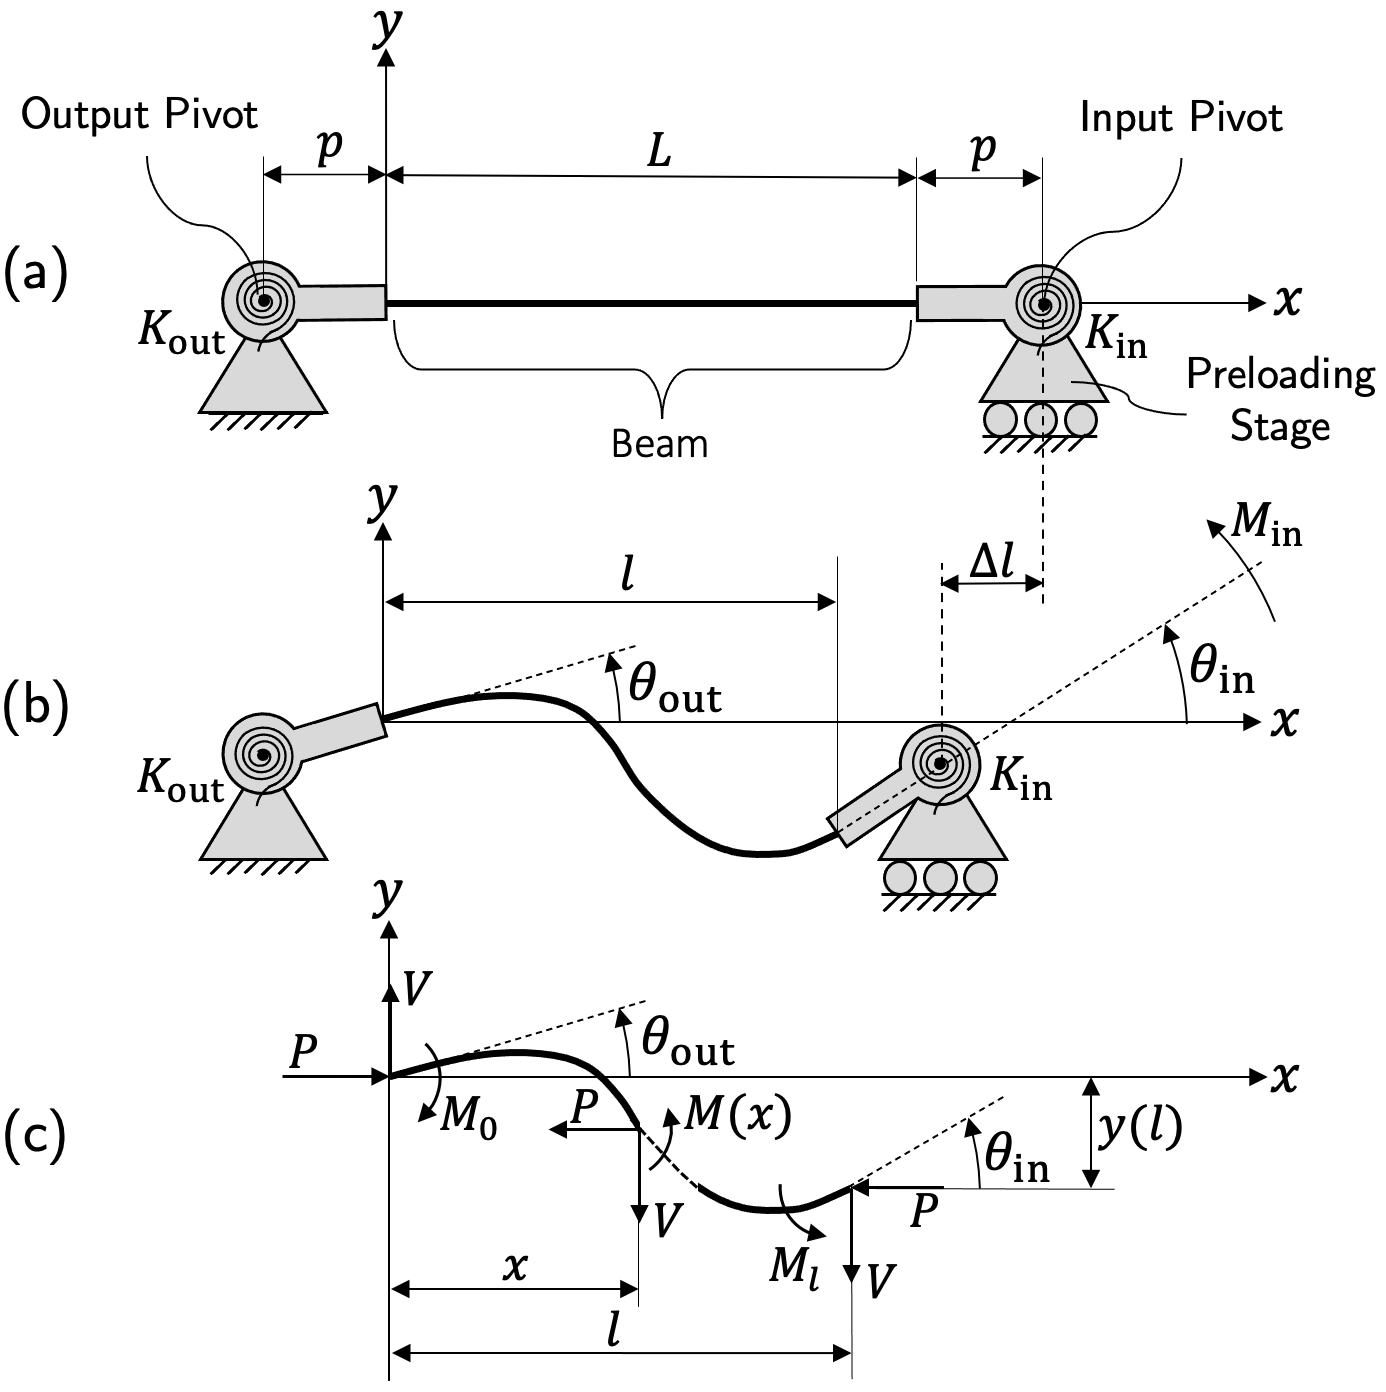
\includegraphics[width=0.7\columnwidth]{images/chap7/buckled_beam_model.png}
  \caption[Diagram of the bistable mechanism]{Diagram of the bistable mechanism (a) As-fabricated, (b) deformed and (c) free-body diagram of the buckling beam.}
  \label{fig:buckled-beam-schematic}
\end{figure}

Based on the hypothesis described in the work by \cite{tivot2021} and the Euler-Bernoulli beam theory, the beam deflection can be expressed as :
\begin{equation}\label{eq:deflection}
  y(x) = \left(A\sin{kx}+B(\cos{kx}-1)+C\frac{x}{l}\right) l {\theta }_\textrm{in}
\end{equation}
where $k=\sqrt{P/(EI)}$ and the boundary conditions are
\[y(0)=0\]
\[y'(0)\cong{\theta }_\textrm{out}\]
\[M_0\cong K_\textrm{out}\theta_\textrm{out}+Vp-Pp\theta_\textrm{out}\]
\[y(l)\cong -p(\theta_\textrm{out}+\theta_\textrm{in})\]
\[y'(l)\cong \theta_\textrm{in}\]
Furthermore, the deflection parameters are given by
\begin{equation}\label{A_norm}
A =    \frac{(1+2\overline{p})kl+{\varepsilon }_0\left(\overline{p}  \sin{kl}-\frac{\cos{kl}-1}{kl}\right)}
{kl\left( kl \cos{kl}-\sin{kl}-\left({\overline{p}}^2+\overline{p}\right){(kl)}^2\sin{kl}+{\varepsilon }_0\left(\sin{kl}+2\frac{\cos{kl}-1}{kl}\right)\right)}
\end{equation}
\begin{equation} \label{B_norm}
B = \frac{  \overline{p}(1+2\overline{p}){(kl)}^2+{\varepsilon }_0 \left(\overline{p} \left(\cos{kl}-1\right) + \frac{\sin{kl}}{kl} -1\right)}
{kl\left( kl \cos{kl}-\sin{kl}-\left({\overline{p}}^2+\overline{p}\right){(kl)}^2\sin{kl}+{\varepsilon }_0\left(\sin{kl}+2\frac{\cos{kl}-1}{kl}\right)\right)}
\end{equation}
\begin{equation} \label{C_norm}
C = \frac{  {\overline{p}}^2{(kl)}^2\sin{kl} -2\overline{p} kl\cos{kl} -\sin{kl} - {\varepsilon }_0\left(\overline{p}\sin{kl}-\frac{\cos{kl}-1}{kl}\right)}
{ kl \cos{kl}-\sin{kl}-\left({\overline{p}}^2+\overline{p}\right){(kl)}^2\sin{kl}+{\varepsilon }_0\left(\sin{kl}+2\frac{\cos{kl}-1}{kl}\right)}
\end{equation}
where $\overline{p} = p/l $ and $\varepsilon_0=K_\textrm{out}/(EI/l)$. When considering the beam’s arc length as constant, the end-shorting, $\Delta l$, can be approximated using the following expression
\begin{equation}\label{eq:delta_l}
 \Delta l\cong \frac{p}{2}({\theta }^2_\textrm{in}+\theta ^2_\textrm{out})+\int^l_0{\frac{y'(x)^2}{2}dx}=H l{\theta }^2_\textrm{in}
\end{equation}
Here, the coefficient $H$ is expressed as
\begin{multline}\label{eq:H-smabb}
 H = \frac{\left({A}^2+{B}^2\right){\left(kl\right)}^2}{4} + \frac{\left({A}^2-{B}^2\right)kl\sin{2kl} }{8} + \frac{AB kl\left(\cos{2kl}-1\right)}{4}\\
 +AC\sin{kl} + BC\left(\cos{kl}-1\right) + \frac{{C}^2}{2} +\frac{\overline{p}}{2}\left({\left( Akl+C\right)}^2+1\right)
\end{multline}

By rearranging the \cref{eq:delta_l}, the input angle is expressed as
\begin{equation}\label{eq:theta_in}
 {\theta}_\textrm{in}=\pm \sqrt{\frac{\Delta l}{l}}\sqrt{\frac{1}{H}}
\end{equation}

Finally, the input moment can be described as the following \cref{eq:M_in}
\begin{equation}
\begin{split}
 M_\textrm{in} &\cong M_l+K_\textrm{in}{\theta }_\textrm{in}+Vp-Pp{\theta}_\textrm{in}\\
 &=\frac{EI}{l}\left({\left(kl\right)}^2\left(\overline{p}\left(C-1\right)-A\sin{kl}-B\cos{kl}\right)+{\varepsilon }_l\right){\theta}_\textrm{in}
 \label{eq:M_in}
\end{split}
\end{equation}
\noindent{where ${\varepsilon }_l=K_\textrm{in}/(EI/l)$.}

\subsection{Design and Fabrication of Kinematic Stage}
With the help of this analytical model, a flexure-based kinematic stage can be designed and sized accordingly. In this case, cross-spring pivots as shown in \cref{fig:bistable-mechanism} are used for the input and output pivots that mount the buckled beam. Based on the work by \cite{heneinConceptionStructuresArticulees2005}, their angular stiffness can be estimated using the equation below
\begin{equation}
    K_p = \frac{2Ebh_p^3}{3L_p},
\end{equation}
where $h_p$ and $L_p$ are the thickness and the total diagonal length of the cross blades, respectively. The interface between the SMA coils and the kinematic stage consists of a lever arm that can be sized to adapt the force and stroke requirements of the SMA so as to trigger the snap-through of the buckled beam. The preloading screw, as observed in \cref{fig:bistable-mechanism} (b), is used to displace the preloading stage by $\Delta l$ so as to cause the buckling of the initially straight beam. This buckling creates the bistability observed within the kinematic stage. In this gripper, the jaws are required to move towards the centre symmetrical in a parallel motion. This jaw guidance mechanism, linked to the output pivot, is comprised of a reverse motion linkage of lever length, $r$, and two linear stages to ensure that the jaws move is opposite directions with the same amplitude, $x_\textrm{out}$, when the gripper is triggered to open. The angular stiffness, $K_\textrm{out}$ of the jaw guidance mechanism perceived at the output pivot was estimated using FEM simulations for small values of the output angle, $\theta_\mathrm{out}$. As the gripper is triggered to close, $x_\textrm{out}$ drops to zero and $\theta_\mathrm{out}$ is approximated to zero. Due to the reaction torque experience by the output pivot coming from the buckled beam, a gripping force, $F_\textrm{out}$, is applied by each jaw onto the payload. These jaws can be interchanged to accommodate differing sizes and types of payload, allowing the gripper to be used in a wide variety of scenarios.

\begin{figure}[hbt!] % t for top of the page, H could be put to impose the position of the float
  \centering
  \begin{tikzpicture}
    \node[anchor=south west,inner sep=0] (graph) at (0,0) {\includegraphics[trim={0 1.4cm 0 0},clip, width=\textwidth]{images/chap7/bistable_mechanism.png}};
	% Insert a relative reference based on image dimensions
    \begin{scope}[x={(graph.south east)},y={(graph.north west)}]
    \node[] at (0.17, -0.02) {\large (a)};
    \node[] at (0.495, -0.02) {\large(b)};
    \node[] at (0.84, -0.02) {\large(c)};
    \end{scope}
    \end{tikzpicture}
  \caption[Schematic view of the bistable mechanism as fabricated]{(a) Schematic view of the bistable mechanism as fabricated. Gripper with mounted jaws and the beam preloaded, (b) in open stable equilibrium and (c) in closed unstable equilibrium.}
  \label{fig:bistable-mechanism}
\end{figure}
The gripping requirements of the gripper can be estimated using the following equations.
\begin{equation}\label{eq:x_out}
  x_\textrm{out}\cong r{\theta }_\textrm{out}=\left(A kl+C\right)r{\theta }_\textrm{in}
\end{equation}

\begin{equation}\label{eq:f_out}
  F_\textrm{out}=\frac{M_0-Vp}{2r}=-\frac{EI}{l}\frac{{\left(B+C\overline{p}\right)\left(kl\right)}^2}{2r}{\theta }_\textrm{in}
\end{equation}
where $K_\mathrm{out}$ tends to infinity when $F_\mathrm{out}$ is calculated as the object is considered to be infinitely rigid. In this case, the specifications of the gripper are sized with a jaw stroke, $x_\mathrm{out}$, of $1.5$ mm and a gripping force, $F_\mathrm{out}$, of $1$ N.

The flexure-based kinematic stage was fabricated from \textit{Bohler K390} steel due to its high yield strength to Young's modulus ratio ($\sigma_y/E$). The prototype of the mechanism was fabricated using wire-cut electrical discharge machining (EDM) which allows a minimal thickness of 50 $\mu$m for the blades with a tolerance of a few $\mu$m. The design parameters of the fabricated prototype can be found in \cref{tab:bb-design-parameters}.

\begin{table}[hbt!]
    \centering
    \caption{A summary of the design parameters for the flexure-based bistable mechanism.}
    \label{tab:bb-design-parameters}
    % !TEX root = ../sethomas_thesis_main.tex
\documentclass[border=1mm,
               class=article
               preview]{standalone}
% \newcommand{\microm}{$\mu$m}
\begin{document}
\def\arraystretch{1.2}
{\rowcolors{1}{black!10}{black!5}
\begin{tabular}{rrl}
\hline
\rowcolor{black}                     & \textbf{\color{white}Parameter}       & \textbf{\color{white}Value}\\
\cellcolor{black!10}  & $E$         & 220 GPa      \\
\cellcolor{black!10}   \multirow{-2}{*}{Material (B\"{o}hler K390)}                  & $\sigma_y$      & 2300 MPa     \\
Structure Width        & $b$             & 10 mm        \\
Preloading Stage       & $\Delta l$       & 1.25 mm      \\
          & $h$             & 150 $\mu$m   \\
\cellcolor{black!5}      & $L$             & 40 mm        \\
\multirow{-3}{*}{Buckled Beam}     & $p$             & 2 mm         \\
           & $h_p$           & 60 $\mu$m    \\
\cellcolor{black!10}                   & $L_p$           & 11.2 mm      \\
\multirow{-3}{*}{Input Pivot}                      & $K_\textrm{in}=K_p$    & 28.3 Nmm/rad \\
           & $r$             & 14 mm        \\
\cellcolor{black!5}    \multirow{-2}{*}{Jaw Guidance} & $K_\textrm{out}$       & 205 Nmm/rad  \\
\cellcolor{black!10}      & ${\varepsilon }_0$  & 12.8         \\
\cellcolor{black!10}  \multirow{-2}{*}{Relative Stiffness} & ${\varepsilon }_l$  & 1.77         \\
\end{tabular}}
\def\arraystretch{1.5}
\end{document}

\end{table}

\subsection{Testing and Validation of the Kinematic Stage}
The validating of the bistable mechanism design and analytical modelling, a finite element method (FEM) 2D static study was conducted with the help of the commercial software, \textit{Comsol Multiphysics 5.4}. The material was, first, verified to determine whether the compliant structure can withstand the internal stresses during its maximal deformation. This determines the maximal admissible deformation to verify if the material is sufficient. Numerical simulations of the force-displacement characteristics of the mechanism were established to verify the analytical model as shown in \cref{fig:bistable graph}. As the numerical results fit the analytical model quite well, its implies that this model can be used to adequately size the SMA actuator as described in the sizing methodology proposed in \cref{chap:design-methodology}.

Furthermore, a test bench was constructed to validate the analytical model with experimental results. The test bench consists of a manual micrometer linear stage to push the input lever arm, $\theta_\mathrm{in}$ and measure the required force using the \textit{Kistler Model 9207} force sensor for the input torque, $M_\mathrm{in}$. Lastly, another force sensor is placed between the two jaws to measure the gripping force, $F_\mathrm{out}$.

The experimental results of the mechanical behaviour of the gripper are portrayed in \cref{fig:bistable graph}. Based on the equations \ref{eq:theta_in}-\ref{eq:f_out}, the analytical model is traced out with the parameter $kl$ ranging from $1.4\pi$ (near stable position) to $2.4\pi$ (near unstable position) for the opening sequence and from $1.3\pi$ (near stable position) to $2.2\pi$ (near unstable position) for the closing sequence. Here, $l$ is approximated as $L-\Delta l$. The FEM results are also presented in the same figure to display the minor discrepancies present between the analytical, numerical model and experimental results.
\begin{figure}[htp!] % t for top of the page, H could be put to impose the position of the float
    \centering
    \resizebox{0.7\textwidth}{!}{% !TEX root = ../../sethomas_thesis_main.tex
\documentclass[border=1mm,
               class=article
               preview]{standalone}
\usepackage{tikz}
\begin{document}
\renewcommand{\arraystretch}{1} % to increase the space between rows
\begin{tikzpicture}
\node[anchor=south west,inner sep=0] (graph) at (0,0) {%% Creator: Matplotlib, PGF backend
%%
%% To include the figure in your LaTeX document, write
%%   \input{<filename>.pgf}
%%
%% Make sure the required packages are loaded in your preamble
%%   \usepackage{pgf}
%%
%% and, on pdftex
%%   \usepackage[utf8]{inputenc}\DeclareUnicodeCharacter{2212}{-}
%%
%% or, on luatex and xetex
%%   \usepackage{unicode-math}
%%
%% Figures using additional raster images can only be included by \input if
%% they are in the same directory as the main LaTeX file. For loading figures
%% from other directories you can use the `import` package
%%   \usepackage{import}
%%
%% and then include the figures with
%%   \import{<path to file>}{<filename>.pgf}
%%
%% Matplotlib used the following preamble
%%
\begingroup%
\makeatletter%
\begin{pgfpicture}%
\pgfpathrectangle{\pgfpointorigin}{\pgfqpoint{3.820060in}{6.784086in}}%
\pgfusepath{use as bounding box, clip}%
\begin{pgfscope}%
\pgfsetbuttcap%
\pgfsetmiterjoin%
\pgfsetlinewidth{0.000000pt}%
\definecolor{currentstroke}{rgb}{0.000000,0.000000,0.000000}%
\pgfsetstrokecolor{currentstroke}%
\pgfsetstrokeopacity{0.000000}%
\pgfsetdash{}{0pt}%
\pgfpathmoveto{\pgfqpoint{0.000000in}{0.000000in}}%
\pgfpathlineto{\pgfqpoint{3.820060in}{0.000000in}}%
\pgfpathlineto{\pgfqpoint{3.820060in}{6.784086in}}%
\pgfpathlineto{\pgfqpoint{0.000000in}{6.784086in}}%
\pgfpathclose%
\pgfusepath{}%
\end{pgfscope}%
\begin{pgfscope}%
\pgfsetbuttcap%
\pgfsetmiterjoin%
\pgfsetlinewidth{0.000000pt}%
\definecolor{currentstroke}{rgb}{0.000000,0.000000,0.000000}%
\pgfsetstrokecolor{currentstroke}%
\pgfsetstrokeopacity{0.000000}%
\pgfsetdash{}{0pt}%
\pgfpathmoveto{\pgfqpoint{0.620060in}{4.851013in}}%
\pgfpathlineto{\pgfqpoint{3.720060in}{4.851013in}}%
\pgfpathlineto{\pgfqpoint{3.720060in}{6.662778in}}%
\pgfpathlineto{\pgfqpoint{0.620060in}{6.662778in}}%
\pgfpathclose%
\pgfusepath{}%
\end{pgfscope}%
\begin{pgfscope}%
\pgfpathrectangle{\pgfqpoint{0.620060in}{4.851013in}}{\pgfqpoint{3.100000in}{1.811765in}}%
\pgfusepath{clip}%
\pgfsetbuttcap%
\pgfsetroundjoin%
\pgfsetlinewidth{0.803000pt}%
\definecolor{currentstroke}{rgb}{0.690196,0.690196,0.690196}%
\pgfsetstrokecolor{currentstroke}%
\pgfsetstrokeopacity{0.900000}%
\pgfsetdash{{0.800000pt}{1.320000pt}}{0.000000pt}%
\pgfpathmoveto{\pgfqpoint{0.993118in}{4.851013in}}%
\pgfpathlineto{\pgfqpoint{0.993118in}{6.662778in}}%
\pgfusepath{stroke}%
\end{pgfscope}%
\begin{pgfscope}%
\pgfsetbuttcap%
\pgfsetroundjoin%
\definecolor{currentfill}{rgb}{0.000000,0.000000,0.000000}%
\pgfsetfillcolor{currentfill}%
\pgfsetlinewidth{0.803000pt}%
\definecolor{currentstroke}{rgb}{0.000000,0.000000,0.000000}%
\pgfsetstrokecolor{currentstroke}%
\pgfsetdash{}{0pt}%
\pgfsys@defobject{currentmarker}{\pgfqpoint{0.000000in}{-0.048611in}}{\pgfqpoint{0.000000in}{0.000000in}}{%
\pgfpathmoveto{\pgfqpoint{0.000000in}{0.000000in}}%
\pgfpathlineto{\pgfqpoint{0.000000in}{-0.048611in}}%
\pgfusepath{stroke,fill}%
}%
\begin{pgfscope}%
\pgfsys@transformshift{0.993118in}{4.851013in}%
\pgfsys@useobject{currentmarker}{}%
\end{pgfscope}%
\end{pgfscope}%
\begin{pgfscope}%
\pgfpathrectangle{\pgfqpoint{0.620060in}{4.851013in}}{\pgfqpoint{3.100000in}{1.811765in}}%
\pgfusepath{clip}%
\pgfsetbuttcap%
\pgfsetroundjoin%
\pgfsetlinewidth{0.803000pt}%
\definecolor{currentstroke}{rgb}{0.690196,0.690196,0.690196}%
\pgfsetstrokecolor{currentstroke}%
\pgfsetstrokeopacity{0.900000}%
\pgfsetdash{{0.800000pt}{1.320000pt}}{0.000000pt}%
\pgfpathmoveto{\pgfqpoint{1.594550in}{4.851013in}}%
\pgfpathlineto{\pgfqpoint{1.594550in}{6.662778in}}%
\pgfusepath{stroke}%
\end{pgfscope}%
\begin{pgfscope}%
\pgfsetbuttcap%
\pgfsetroundjoin%
\definecolor{currentfill}{rgb}{0.000000,0.000000,0.000000}%
\pgfsetfillcolor{currentfill}%
\pgfsetlinewidth{0.803000pt}%
\definecolor{currentstroke}{rgb}{0.000000,0.000000,0.000000}%
\pgfsetstrokecolor{currentstroke}%
\pgfsetdash{}{0pt}%
\pgfsys@defobject{currentmarker}{\pgfqpoint{0.000000in}{-0.048611in}}{\pgfqpoint{0.000000in}{0.000000in}}{%
\pgfpathmoveto{\pgfqpoint{0.000000in}{0.000000in}}%
\pgfpathlineto{\pgfqpoint{0.000000in}{-0.048611in}}%
\pgfusepath{stroke,fill}%
}%
\begin{pgfscope}%
\pgfsys@transformshift{1.594550in}{4.851013in}%
\pgfsys@useobject{currentmarker}{}%
\end{pgfscope}%
\end{pgfscope}%
\begin{pgfscope}%
\pgfpathrectangle{\pgfqpoint{0.620060in}{4.851013in}}{\pgfqpoint{3.100000in}{1.811765in}}%
\pgfusepath{clip}%
\pgfsetbuttcap%
\pgfsetroundjoin%
\pgfsetlinewidth{0.803000pt}%
\definecolor{currentstroke}{rgb}{0.690196,0.690196,0.690196}%
\pgfsetstrokecolor{currentstroke}%
\pgfsetstrokeopacity{0.900000}%
\pgfsetdash{{0.800000pt}{1.320000pt}}{0.000000pt}%
\pgfpathmoveto{\pgfqpoint{2.195982in}{4.851013in}}%
\pgfpathlineto{\pgfqpoint{2.195982in}{6.662778in}}%
\pgfusepath{stroke}%
\end{pgfscope}%
\begin{pgfscope}%
\pgfsetbuttcap%
\pgfsetroundjoin%
\definecolor{currentfill}{rgb}{0.000000,0.000000,0.000000}%
\pgfsetfillcolor{currentfill}%
\pgfsetlinewidth{0.803000pt}%
\definecolor{currentstroke}{rgb}{0.000000,0.000000,0.000000}%
\pgfsetstrokecolor{currentstroke}%
\pgfsetdash{}{0pt}%
\pgfsys@defobject{currentmarker}{\pgfqpoint{0.000000in}{-0.048611in}}{\pgfqpoint{0.000000in}{0.000000in}}{%
\pgfpathmoveto{\pgfqpoint{0.000000in}{0.000000in}}%
\pgfpathlineto{\pgfqpoint{0.000000in}{-0.048611in}}%
\pgfusepath{stroke,fill}%
}%
\begin{pgfscope}%
\pgfsys@transformshift{2.195982in}{4.851013in}%
\pgfsys@useobject{currentmarker}{}%
\end{pgfscope}%
\end{pgfscope}%
\begin{pgfscope}%
\pgfpathrectangle{\pgfqpoint{0.620060in}{4.851013in}}{\pgfqpoint{3.100000in}{1.811765in}}%
\pgfusepath{clip}%
\pgfsetbuttcap%
\pgfsetroundjoin%
\pgfsetlinewidth{0.803000pt}%
\definecolor{currentstroke}{rgb}{0.690196,0.690196,0.690196}%
\pgfsetstrokecolor{currentstroke}%
\pgfsetstrokeopacity{0.900000}%
\pgfsetdash{{0.800000pt}{1.320000pt}}{0.000000pt}%
\pgfpathmoveto{\pgfqpoint{2.797415in}{4.851013in}}%
\pgfpathlineto{\pgfqpoint{2.797415in}{6.662778in}}%
\pgfusepath{stroke}%
\end{pgfscope}%
\begin{pgfscope}%
\pgfsetbuttcap%
\pgfsetroundjoin%
\definecolor{currentfill}{rgb}{0.000000,0.000000,0.000000}%
\pgfsetfillcolor{currentfill}%
\pgfsetlinewidth{0.803000pt}%
\definecolor{currentstroke}{rgb}{0.000000,0.000000,0.000000}%
\pgfsetstrokecolor{currentstroke}%
\pgfsetdash{}{0pt}%
\pgfsys@defobject{currentmarker}{\pgfqpoint{0.000000in}{-0.048611in}}{\pgfqpoint{0.000000in}{0.000000in}}{%
\pgfpathmoveto{\pgfqpoint{0.000000in}{0.000000in}}%
\pgfpathlineto{\pgfqpoint{0.000000in}{-0.048611in}}%
\pgfusepath{stroke,fill}%
}%
\begin{pgfscope}%
\pgfsys@transformshift{2.797415in}{4.851013in}%
\pgfsys@useobject{currentmarker}{}%
\end{pgfscope}%
\end{pgfscope}%
\begin{pgfscope}%
\pgfpathrectangle{\pgfqpoint{0.620060in}{4.851013in}}{\pgfqpoint{3.100000in}{1.811765in}}%
\pgfusepath{clip}%
\pgfsetbuttcap%
\pgfsetroundjoin%
\pgfsetlinewidth{0.803000pt}%
\definecolor{currentstroke}{rgb}{0.690196,0.690196,0.690196}%
\pgfsetstrokecolor{currentstroke}%
\pgfsetstrokeopacity{0.900000}%
\pgfsetdash{{0.800000pt}{1.320000pt}}{0.000000pt}%
\pgfpathmoveto{\pgfqpoint{3.398847in}{4.851013in}}%
\pgfpathlineto{\pgfqpoint{3.398847in}{6.662778in}}%
\pgfusepath{stroke}%
\end{pgfscope}%
\begin{pgfscope}%
\pgfsetbuttcap%
\pgfsetroundjoin%
\definecolor{currentfill}{rgb}{0.000000,0.000000,0.000000}%
\pgfsetfillcolor{currentfill}%
\pgfsetlinewidth{0.803000pt}%
\definecolor{currentstroke}{rgb}{0.000000,0.000000,0.000000}%
\pgfsetstrokecolor{currentstroke}%
\pgfsetdash{}{0pt}%
\pgfsys@defobject{currentmarker}{\pgfqpoint{0.000000in}{-0.048611in}}{\pgfqpoint{0.000000in}{0.000000in}}{%
\pgfpathmoveto{\pgfqpoint{0.000000in}{0.000000in}}%
\pgfpathlineto{\pgfqpoint{0.000000in}{-0.048611in}}%
\pgfusepath{stroke,fill}%
}%
\begin{pgfscope}%
\pgfsys@transformshift{3.398847in}{4.851013in}%
\pgfsys@useobject{currentmarker}{}%
\end{pgfscope}%
\end{pgfscope}%
\begin{pgfscope}%
\pgfpathrectangle{\pgfqpoint{0.620060in}{4.851013in}}{\pgfqpoint{3.100000in}{1.811765in}}%
\pgfusepath{clip}%
\pgfsetbuttcap%
\pgfsetroundjoin%
\pgfsetlinewidth{0.803000pt}%
\definecolor{currentstroke}{rgb}{0.690196,0.690196,0.690196}%
\pgfsetstrokecolor{currentstroke}%
\pgfsetstrokeopacity{0.900000}%
\pgfsetdash{{0.800000pt}{1.320000pt}}{0.000000pt}%
\pgfpathmoveto{\pgfqpoint{0.620060in}{4.873108in}}%
\pgfpathlineto{\pgfqpoint{3.720060in}{4.873108in}}%
\pgfusepath{stroke}%
\end{pgfscope}%
\begin{pgfscope}%
\pgfsetbuttcap%
\pgfsetroundjoin%
\definecolor{currentfill}{rgb}{0.000000,0.000000,0.000000}%
\pgfsetfillcolor{currentfill}%
\pgfsetlinewidth{0.803000pt}%
\definecolor{currentstroke}{rgb}{0.000000,0.000000,0.000000}%
\pgfsetstrokecolor{currentstroke}%
\pgfsetdash{}{0pt}%
\pgfsys@defobject{currentmarker}{\pgfqpoint{-0.048611in}{0.000000in}}{\pgfqpoint{-0.000000in}{0.000000in}}{%
\pgfpathmoveto{\pgfqpoint{-0.000000in}{0.000000in}}%
\pgfpathlineto{\pgfqpoint{-0.048611in}{0.000000in}}%
\pgfusepath{stroke,fill}%
}%
\begin{pgfscope}%
\pgfsys@transformshift{0.620060in}{4.873108in}%
\pgfsys@useobject{currentmarker}{}%
\end{pgfscope}%
\end{pgfscope}%
\begin{pgfscope}%
\definecolor{textcolor}{rgb}{0.000000,0.000000,0.000000}%
\pgfsetstrokecolor{textcolor}%
\pgfsetfillcolor{textcolor}%
\pgftext[x=0.294444in, y=4.829705in, left, base]{\color{textcolor}\rmfamily\fontsize{9.000000}{10.800000}\selectfont \(\displaystyle {-40}\)}%
\end{pgfscope}%
\begin{pgfscope}%
\pgfpathrectangle{\pgfqpoint{0.620060in}{4.851013in}}{\pgfqpoint{3.100000in}{1.811765in}}%
\pgfusepath{clip}%
\pgfsetbuttcap%
\pgfsetroundjoin%
\pgfsetlinewidth{0.803000pt}%
\definecolor{currentstroke}{rgb}{0.690196,0.690196,0.690196}%
\pgfsetstrokecolor{currentstroke}%
\pgfsetstrokeopacity{0.900000}%
\pgfsetdash{{0.800000pt}{1.320000pt}}{0.000000pt}%
\pgfpathmoveto{\pgfqpoint{0.620060in}{5.315002in}}%
\pgfpathlineto{\pgfqpoint{3.720060in}{5.315002in}}%
\pgfusepath{stroke}%
\end{pgfscope}%
\begin{pgfscope}%
\pgfsetbuttcap%
\pgfsetroundjoin%
\definecolor{currentfill}{rgb}{0.000000,0.000000,0.000000}%
\pgfsetfillcolor{currentfill}%
\pgfsetlinewidth{0.803000pt}%
\definecolor{currentstroke}{rgb}{0.000000,0.000000,0.000000}%
\pgfsetstrokecolor{currentstroke}%
\pgfsetdash{}{0pt}%
\pgfsys@defobject{currentmarker}{\pgfqpoint{-0.048611in}{0.000000in}}{\pgfqpoint{-0.000000in}{0.000000in}}{%
\pgfpathmoveto{\pgfqpoint{-0.000000in}{0.000000in}}%
\pgfpathlineto{\pgfqpoint{-0.048611in}{0.000000in}}%
\pgfusepath{stroke,fill}%
}%
\begin{pgfscope}%
\pgfsys@transformshift{0.620060in}{5.315002in}%
\pgfsys@useobject{currentmarker}{}%
\end{pgfscope}%
\end{pgfscope}%
\begin{pgfscope}%
\definecolor{textcolor}{rgb}{0.000000,0.000000,0.000000}%
\pgfsetstrokecolor{textcolor}%
\pgfsetfillcolor{textcolor}%
\pgftext[x=0.294444in, y=5.271599in, left, base]{\color{textcolor}\rmfamily\fontsize{9.000000}{10.800000}\selectfont \(\displaystyle {-20}\)}%
\end{pgfscope}%
\begin{pgfscope}%
\pgfpathrectangle{\pgfqpoint{0.620060in}{4.851013in}}{\pgfqpoint{3.100000in}{1.811765in}}%
\pgfusepath{clip}%
\pgfsetbuttcap%
\pgfsetroundjoin%
\pgfsetlinewidth{0.803000pt}%
\definecolor{currentstroke}{rgb}{0.690196,0.690196,0.690196}%
\pgfsetstrokecolor{currentstroke}%
\pgfsetstrokeopacity{0.900000}%
\pgfsetdash{{0.800000pt}{1.320000pt}}{0.000000pt}%
\pgfpathmoveto{\pgfqpoint{0.620060in}{5.756895in}}%
\pgfpathlineto{\pgfqpoint{3.720060in}{5.756895in}}%
\pgfusepath{stroke}%
\end{pgfscope}%
\begin{pgfscope}%
\pgfsetbuttcap%
\pgfsetroundjoin%
\definecolor{currentfill}{rgb}{0.000000,0.000000,0.000000}%
\pgfsetfillcolor{currentfill}%
\pgfsetlinewidth{0.803000pt}%
\definecolor{currentstroke}{rgb}{0.000000,0.000000,0.000000}%
\pgfsetstrokecolor{currentstroke}%
\pgfsetdash{}{0pt}%
\pgfsys@defobject{currentmarker}{\pgfqpoint{-0.048611in}{0.000000in}}{\pgfqpoint{-0.000000in}{0.000000in}}{%
\pgfpathmoveto{\pgfqpoint{-0.000000in}{0.000000in}}%
\pgfpathlineto{\pgfqpoint{-0.048611in}{0.000000in}}%
\pgfusepath{stroke,fill}%
}%
\begin{pgfscope}%
\pgfsys@transformshift{0.620060in}{5.756895in}%
\pgfsys@useobject{currentmarker}{}%
\end{pgfscope}%
\end{pgfscope}%
\begin{pgfscope}%
\definecolor{textcolor}{rgb}{0.000000,0.000000,0.000000}%
\pgfsetstrokecolor{textcolor}%
\pgfsetfillcolor{textcolor}%
\pgftext[x=0.458602in, y=5.713493in, left, base]{\color{textcolor}\rmfamily\fontsize{9.000000}{10.800000}\selectfont \(\displaystyle {0}\)}%
\end{pgfscope}%
\begin{pgfscope}%
\pgfpathrectangle{\pgfqpoint{0.620060in}{4.851013in}}{\pgfqpoint{3.100000in}{1.811765in}}%
\pgfusepath{clip}%
\pgfsetbuttcap%
\pgfsetroundjoin%
\pgfsetlinewidth{0.803000pt}%
\definecolor{currentstroke}{rgb}{0.690196,0.690196,0.690196}%
\pgfsetstrokecolor{currentstroke}%
\pgfsetstrokeopacity{0.900000}%
\pgfsetdash{{0.800000pt}{1.320000pt}}{0.000000pt}%
\pgfpathmoveto{\pgfqpoint{0.620060in}{6.198789in}}%
\pgfpathlineto{\pgfqpoint{3.720060in}{6.198789in}}%
\pgfusepath{stroke}%
\end{pgfscope}%
\begin{pgfscope}%
\pgfsetbuttcap%
\pgfsetroundjoin%
\definecolor{currentfill}{rgb}{0.000000,0.000000,0.000000}%
\pgfsetfillcolor{currentfill}%
\pgfsetlinewidth{0.803000pt}%
\definecolor{currentstroke}{rgb}{0.000000,0.000000,0.000000}%
\pgfsetstrokecolor{currentstroke}%
\pgfsetdash{}{0pt}%
\pgfsys@defobject{currentmarker}{\pgfqpoint{-0.048611in}{0.000000in}}{\pgfqpoint{-0.000000in}{0.000000in}}{%
\pgfpathmoveto{\pgfqpoint{-0.000000in}{0.000000in}}%
\pgfpathlineto{\pgfqpoint{-0.048611in}{0.000000in}}%
\pgfusepath{stroke,fill}%
}%
\begin{pgfscope}%
\pgfsys@transformshift{0.620060in}{6.198789in}%
\pgfsys@useobject{currentmarker}{}%
\end{pgfscope}%
\end{pgfscope}%
\begin{pgfscope}%
\definecolor{textcolor}{rgb}{0.000000,0.000000,0.000000}%
\pgfsetstrokecolor{textcolor}%
\pgfsetfillcolor{textcolor}%
\pgftext[x=0.394367in, y=6.155386in, left, base]{\color{textcolor}\rmfamily\fontsize{9.000000}{10.800000}\selectfont \(\displaystyle {20}\)}%
\end{pgfscope}%
\begin{pgfscope}%
\pgfpathrectangle{\pgfqpoint{0.620060in}{4.851013in}}{\pgfqpoint{3.100000in}{1.811765in}}%
\pgfusepath{clip}%
\pgfsetbuttcap%
\pgfsetroundjoin%
\pgfsetlinewidth{0.803000pt}%
\definecolor{currentstroke}{rgb}{0.690196,0.690196,0.690196}%
\pgfsetstrokecolor{currentstroke}%
\pgfsetstrokeopacity{0.900000}%
\pgfsetdash{{0.800000pt}{1.320000pt}}{0.000000pt}%
\pgfpathmoveto{\pgfqpoint{0.620060in}{6.640683in}}%
\pgfpathlineto{\pgfqpoint{3.720060in}{6.640683in}}%
\pgfusepath{stroke}%
\end{pgfscope}%
\begin{pgfscope}%
\pgfsetbuttcap%
\pgfsetroundjoin%
\definecolor{currentfill}{rgb}{0.000000,0.000000,0.000000}%
\pgfsetfillcolor{currentfill}%
\pgfsetlinewidth{0.803000pt}%
\definecolor{currentstroke}{rgb}{0.000000,0.000000,0.000000}%
\pgfsetstrokecolor{currentstroke}%
\pgfsetdash{}{0pt}%
\pgfsys@defobject{currentmarker}{\pgfqpoint{-0.048611in}{0.000000in}}{\pgfqpoint{-0.000000in}{0.000000in}}{%
\pgfpathmoveto{\pgfqpoint{-0.000000in}{0.000000in}}%
\pgfpathlineto{\pgfqpoint{-0.048611in}{0.000000in}}%
\pgfusepath{stroke,fill}%
}%
\begin{pgfscope}%
\pgfsys@transformshift{0.620060in}{6.640683in}%
\pgfsys@useobject{currentmarker}{}%
\end{pgfscope}%
\end{pgfscope}%
\begin{pgfscope}%
\definecolor{textcolor}{rgb}{0.000000,0.000000,0.000000}%
\pgfsetstrokecolor{textcolor}%
\pgfsetfillcolor{textcolor}%
\pgftext[x=0.394367in, y=6.597280in, left, base]{\color{textcolor}\rmfamily\fontsize{9.000000}{10.800000}\selectfont \(\displaystyle {40}\)}%
\end{pgfscope}%
\begin{pgfscope}%
\definecolor{textcolor}{rgb}{0.000000,0.000000,0.000000}%
\pgfsetstrokecolor{textcolor}%
\pgfsetfillcolor{textcolor}%
\pgftext[x=0.238889in,y=5.756895in,,bottom,rotate=90.000000]{\color{textcolor}\rmfamily\fontsize{10.000000}{12.000000}\selectfont \textbf{Input Moment \(\displaystyle M_\mathrm{in}\) [Nmm]}}%
\end{pgfscope}%
\begin{pgfscope}%
\pgfpathrectangle{\pgfqpoint{0.620060in}{4.851013in}}{\pgfqpoint{3.100000in}{1.811765in}}%
\pgfusepath{clip}%
\pgfsetrectcap%
\pgfsetroundjoin%
\pgfsetlinewidth{1.505625pt}%
\definecolor{currentstroke}{rgb}{0.000000,0.447059,0.741176}%
\pgfsetstrokecolor{currentstroke}%
\pgfsetstrokeopacity{0.800000}%
\pgfsetdash{}{0pt}%
\pgfpathmoveto{\pgfqpoint{0.760969in}{5.552612in}}%
\pgfpathlineto{\pgfqpoint{0.772666in}{5.569589in}}%
\pgfpathlineto{\pgfqpoint{0.784620in}{5.586711in}}%
\pgfpathlineto{\pgfqpoint{0.796838in}{5.603977in}}%
\pgfpathlineto{\pgfqpoint{0.809328in}{5.621385in}}%
\pgfpathlineto{\pgfqpoint{0.822096in}{5.638934in}}%
\pgfpathlineto{\pgfqpoint{0.835152in}{5.656623in}}%
\pgfpathlineto{\pgfqpoint{0.848502in}{5.674450in}}%
\pgfpathlineto{\pgfqpoint{0.862156in}{5.692413in}}%
\pgfpathlineto{\pgfqpoint{0.876120in}{5.710509in}}%
\pgfpathlineto{\pgfqpoint{0.890405in}{5.728735in}}%
\pgfpathlineto{\pgfqpoint{0.905019in}{5.747090in}}%
\pgfpathlineto{\pgfqpoint{0.919971in}{5.765570in}}%
\pgfpathlineto{\pgfqpoint{0.935271in}{5.784172in}}%
\pgfpathlineto{\pgfqpoint{0.950928in}{5.802890in}}%
\pgfpathlineto{\pgfqpoint{0.966952in}{5.821722in}}%
\pgfpathlineto{\pgfqpoint{0.983354in}{5.840663in}}%
\pgfpathlineto{\pgfqpoint{1.000144in}{5.859707in}}%
\pgfpathlineto{\pgfqpoint{1.017332in}{5.878849in}}%
\pgfpathlineto{\pgfqpoint{1.034929in}{5.898083in}}%
\pgfpathlineto{\pgfqpoint{1.052946in}{5.917401in}}%
\pgfpathlineto{\pgfqpoint{1.071395in}{5.936797in}}%
\pgfpathlineto{\pgfqpoint{1.090287in}{5.956263in}}%
\pgfpathlineto{\pgfqpoint{1.109634in}{5.975789in}}%
\pgfpathlineto{\pgfqpoint{1.129447in}{5.995367in}}%
\pgfpathlineto{\pgfqpoint{1.149738in}{6.014986in}}%
\pgfpathlineto{\pgfqpoint{1.170520in}{6.034634in}}%
\pgfpathlineto{\pgfqpoint{1.191803in}{6.054301in}}%
\pgfpathlineto{\pgfqpoint{1.213600in}{6.073973in}}%
\pgfpathlineto{\pgfqpoint{1.235924in}{6.093636in}}%
\pgfpathlineto{\pgfqpoint{1.258785in}{6.113275in}}%
\pgfpathlineto{\pgfqpoint{1.282195in}{6.132873in}}%
\pgfpathlineto{\pgfqpoint{1.306166in}{6.152413in}}%
\pgfpathlineto{\pgfqpoint{1.330709in}{6.171876in}}%
\pgfpathlineto{\pgfqpoint{1.355835in}{6.191243in}}%
\pgfpathlineto{\pgfqpoint{1.381553in}{6.210491in}}%
\pgfpathlineto{\pgfqpoint{1.407874in}{6.229597in}}%
\pgfpathlineto{\pgfqpoint{1.434806in}{6.248537in}}%
\pgfpathlineto{\pgfqpoint{1.462357in}{6.267284in}}%
\pgfpathlineto{\pgfqpoint{1.490535in}{6.285810in}}%
\pgfpathlineto{\pgfqpoint{1.519345in}{6.304086in}}%
\pgfpathlineto{\pgfqpoint{1.548792in}{6.322081in}}%
\pgfpathlineto{\pgfqpoint{1.578879in}{6.339760in}}%
\pgfpathlineto{\pgfqpoint{1.609608in}{6.357088in}}%
\pgfpathlineto{\pgfqpoint{1.640978in}{6.374029in}}%
\pgfpathlineto{\pgfqpoint{1.672988in}{6.390544in}}%
\pgfpathlineto{\pgfqpoint{1.705632in}{6.406591in}}%
\pgfpathlineto{\pgfqpoint{1.738903in}{6.422128in}}%
\pgfpathlineto{\pgfqpoint{1.772793in}{6.437111in}}%
\pgfpathlineto{\pgfqpoint{1.807288in}{6.451494in}}%
\pgfpathlineto{\pgfqpoint{1.842373in}{6.465229in}}%
\pgfpathlineto{\pgfqpoint{1.878029in}{6.478266in}}%
\pgfpathlineto{\pgfqpoint{1.914233in}{6.490556in}}%
\pgfpathlineto{\pgfqpoint{1.950958in}{6.502046in}}%
\pgfpathlineto{\pgfqpoint{1.988175in}{6.512685in}}%
\pgfpathlineto{\pgfqpoint{2.025850in}{6.522420in}}%
\pgfpathlineto{\pgfqpoint{2.063943in}{6.531197in}}%
\pgfpathlineto{\pgfqpoint{2.102413in}{6.538964in}}%
\pgfpathlineto{\pgfqpoint{2.141211in}{6.545667in}}%
\pgfpathlineto{\pgfqpoint{2.180287in}{6.551254in}}%
\pgfpathlineto{\pgfqpoint{2.219584in}{6.555676in}}%
\pgfpathlineto{\pgfqpoint{2.259043in}{6.558883in}}%
\pgfpathlineto{\pgfqpoint{2.298599in}{6.560829in}}%
\pgfpathlineto{\pgfqpoint{2.338185in}{6.561469in}}%
\pgfpathlineto{\pgfqpoint{2.377728in}{6.560763in}}%
\pgfpathlineto{\pgfqpoint{2.417156in}{6.558674in}}%
\pgfpathlineto{\pgfqpoint{2.456389in}{6.555168in}}%
\pgfpathlineto{\pgfqpoint{2.495348in}{6.550218in}}%
\pgfpathlineto{\pgfqpoint{2.533953in}{6.543799in}}%
\pgfpathlineto{\pgfqpoint{2.572119in}{6.535894in}}%
\pgfpathlineto{\pgfqpoint{2.609764in}{6.526490in}}%
\pgfpathlineto{\pgfqpoint{2.646805in}{6.515580in}}%
\pgfpathlineto{\pgfqpoint{2.683159in}{6.503164in}}%
\pgfpathlineto{\pgfqpoint{2.718744in}{6.489247in}}%
\pgfpathlineto{\pgfqpoint{2.753482in}{6.473841in}}%
\pgfpathlineto{\pgfqpoint{2.787295in}{6.456963in}}%
\pgfpathlineto{\pgfqpoint{2.820112in}{6.438637in}}%
\pgfpathlineto{\pgfqpoint{2.851861in}{6.418893in}}%
\pgfpathlineto{\pgfqpoint{2.882478in}{6.397765in}}%
\pgfpathlineto{\pgfqpoint{2.911903in}{6.375294in}}%
\pgfpathlineto{\pgfqpoint{2.940079in}{6.351523in}}%
\pgfpathlineto{\pgfqpoint{2.966956in}{6.326503in}}%
\pgfpathlineto{\pgfqpoint{2.992491in}{6.300285in}}%
\pgfpathlineto{\pgfqpoint{3.016643in}{6.272926in}}%
\pgfpathlineto{\pgfqpoint{3.039381in}{6.244485in}}%
\pgfpathlineto{\pgfqpoint{3.060675in}{6.215022in}}%
\pgfpathlineto{\pgfqpoint{3.080504in}{6.184600in}}%
\pgfpathlineto{\pgfqpoint{3.098851in}{6.153282in}}%
\pgfpathlineto{\pgfqpoint{3.115705in}{6.121134in}}%
\pgfpathlineto{\pgfqpoint{3.131059in}{6.088220in}}%
\pgfpathlineto{\pgfqpoint{3.144912in}{6.054605in}}%
\pgfpathlineto{\pgfqpoint{3.157264in}{6.020352in}}%
\pgfpathlineto{\pgfqpoint{3.168122in}{5.985526in}}%
\pgfpathlineto{\pgfqpoint{3.177497in}{5.950188in}}%
\pgfpathlineto{\pgfqpoint{3.185399in}{5.914399in}}%
\pgfpathlineto{\pgfqpoint{3.191846in}{5.878218in}}%
\pgfpathlineto{\pgfqpoint{3.196855in}{5.841703in}}%
\pgfpathlineto{\pgfqpoint{3.200446in}{5.804911in}}%
\pgfpathlineto{\pgfqpoint{3.202640in}{5.767894in}}%
\pgfpathlineto{\pgfqpoint{3.203461in}{5.730705in}}%
\pgfusepath{stroke}%
\end{pgfscope}%
\begin{pgfscope}%
\pgfpathrectangle{\pgfqpoint{0.620060in}{4.851013in}}{\pgfqpoint{3.100000in}{1.811765in}}%
\pgfusepath{clip}%
\pgfsetrectcap%
\pgfsetroundjoin%
\pgfsetlinewidth{1.505625pt}%
\definecolor{currentstroke}{rgb}{0.905882,0.207843,0.219608}%
\pgfsetstrokecolor{currentstroke}%
\pgfsetstrokeopacity{0.800000}%
\pgfsetdash{}{0pt}%
\pgfpathmoveto{\pgfqpoint{3.579151in}{5.956138in}}%
\pgfpathlineto{\pgfqpoint{3.567547in}{5.940896in}}%
\pgfpathlineto{\pgfqpoint{3.555690in}{5.925523in}}%
\pgfpathlineto{\pgfqpoint{3.543575in}{5.910019in}}%
\pgfpathlineto{\pgfqpoint{3.531193in}{5.894385in}}%
\pgfpathlineto{\pgfqpoint{3.518538in}{5.878624in}}%
\pgfpathlineto{\pgfqpoint{3.505602in}{5.862735in}}%
\pgfpathlineto{\pgfqpoint{3.492378in}{5.846721in}}%
\pgfpathlineto{\pgfqpoint{3.478857in}{5.830583in}}%
\pgfpathlineto{\pgfqpoint{3.465032in}{5.814324in}}%
\pgfpathlineto{\pgfqpoint{3.450894in}{5.797945in}}%
\pgfpathlineto{\pgfqpoint{3.436434in}{5.781449in}}%
\pgfpathlineto{\pgfqpoint{3.421644in}{5.764839in}}%
\pgfpathlineto{\pgfqpoint{3.406515in}{5.748118in}}%
\pgfpathlineto{\pgfqpoint{3.391036in}{5.731288in}}%
\pgfpathlineto{\pgfqpoint{3.375200in}{5.714355in}}%
\pgfpathlineto{\pgfqpoint{3.358996in}{5.697321in}}%
\pgfpathlineto{\pgfqpoint{3.342414in}{5.680192in}}%
\pgfpathlineto{\pgfqpoint{3.325443in}{5.662972in}}%
\pgfpathlineto{\pgfqpoint{3.308075in}{5.645668in}}%
\pgfpathlineto{\pgfqpoint{3.290297in}{5.628283in}}%
\pgfpathlineto{\pgfqpoint{3.272100in}{5.610826in}}%
\pgfpathlineto{\pgfqpoint{3.253472in}{5.593303in}}%
\pgfpathlineto{\pgfqpoint{3.234403in}{5.575722in}}%
\pgfpathlineto{\pgfqpoint{3.214881in}{5.558092in}}%
\pgfpathlineto{\pgfqpoint{3.194895in}{5.540421in}}%
\pgfpathlineto{\pgfqpoint{3.174434in}{5.522718in}}%
\pgfpathlineto{\pgfqpoint{3.153486in}{5.504996in}}%
\pgfpathlineto{\pgfqpoint{3.132041in}{5.487265in}}%
\pgfpathlineto{\pgfqpoint{3.110088in}{5.469538in}}%
\pgfpathlineto{\pgfqpoint{3.087614in}{5.451828in}}%
\pgfpathlineto{\pgfqpoint{3.064610in}{5.434150in}}%
\pgfpathlineto{\pgfqpoint{3.041065in}{5.416519in}}%
\pgfpathlineto{\pgfqpoint{3.016968in}{5.398952in}}%
\pgfpathlineto{\pgfqpoint{2.992310in}{5.381467in}}%
\pgfpathlineto{\pgfqpoint{2.967082in}{5.364083in}}%
\pgfpathlineto{\pgfqpoint{2.941275in}{5.346821in}}%
\pgfpathlineto{\pgfqpoint{2.914881in}{5.329702in}}%
\pgfpathlineto{\pgfqpoint{2.887893in}{5.312751in}}%
\pgfpathlineto{\pgfqpoint{2.860305in}{5.295992in}}%
\pgfpathlineto{\pgfqpoint{2.832112in}{5.279451in}}%
\pgfpathlineto{\pgfqpoint{2.803311in}{5.263157in}}%
\pgfpathlineto{\pgfqpoint{2.773899in}{5.247140in}}%
\pgfpathlineto{\pgfqpoint{2.743876in}{5.231430in}}%
\pgfpathlineto{\pgfqpoint{2.713243in}{5.216061in}}%
\pgfpathlineto{\pgfqpoint{2.682005in}{5.201068in}}%
\pgfpathlineto{\pgfqpoint{2.650165in}{5.186488in}}%
\pgfpathlineto{\pgfqpoint{2.617733in}{5.172357in}}%
\pgfpathlineto{\pgfqpoint{2.584719in}{5.158717in}}%
\pgfpathlineto{\pgfqpoint{2.551136in}{5.145608in}}%
\pgfpathlineto{\pgfqpoint{2.517002in}{5.133073in}}%
\pgfpathlineto{\pgfqpoint{2.482336in}{5.121155in}}%
\pgfpathlineto{\pgfqpoint{2.447161in}{5.109900in}}%
\pgfpathlineto{\pgfqpoint{2.411505in}{5.099355in}}%
\pgfpathlineto{\pgfqpoint{2.375398in}{5.089565in}}%
\pgfpathlineto{\pgfqpoint{2.338874in}{5.080579in}}%
\pgfpathlineto{\pgfqpoint{2.301974in}{5.072443in}}%
\pgfpathlineto{\pgfqpoint{2.264740in}{5.065206in}}%
\pgfpathlineto{\pgfqpoint{2.227219in}{5.058915in}}%
\pgfpathlineto{\pgfqpoint{2.189462in}{5.053617in}}%
\pgfpathlineto{\pgfqpoint{2.151524in}{5.049355in}}%
\pgfpathlineto{\pgfqpoint{2.113467in}{5.046176in}}%
\pgfpathlineto{\pgfqpoint{2.075352in}{5.044120in}}%
\pgfpathlineto{\pgfqpoint{2.037246in}{5.043227in}}%
\pgfpathlineto{\pgfqpoint{1.999220in}{5.043534in}}%
\pgfpathlineto{\pgfqpoint{1.961347in}{5.045074in}}%
\pgfpathlineto{\pgfqpoint{1.923703in}{5.047877in}}%
\pgfpathlineto{\pgfqpoint{1.886366in}{5.051969in}}%
\pgfpathlineto{\pgfqpoint{1.849415in}{5.057371in}}%
\pgfpathlineto{\pgfqpoint{1.812930in}{5.064100in}}%
\pgfpathlineto{\pgfqpoint{1.776993in}{5.072167in}}%
\pgfpathlineto{\pgfqpoint{1.741683in}{5.081580in}}%
\pgfpathlineto{\pgfqpoint{1.707081in}{5.092338in}}%
\pgfpathlineto{\pgfqpoint{1.673266in}{5.104439in}}%
\pgfpathlineto{\pgfqpoint{1.640312in}{5.117871in}}%
\pgfpathlineto{\pgfqpoint{1.608294in}{5.132619in}}%
\pgfpathlineto{\pgfqpoint{1.577281in}{5.148663in}}%
\pgfpathlineto{\pgfqpoint{1.547341in}{5.165977in}}%
\pgfpathlineto{\pgfqpoint{1.518535in}{5.184531in}}%
\pgfpathlineto{\pgfqpoint{1.490921in}{5.204289in}}%
\pgfpathlineto{\pgfqpoint{1.464551in}{5.225211in}}%
\pgfpathlineto{\pgfqpoint{1.439472in}{5.247255in}}%
\pgfpathlineto{\pgfqpoint{1.415727in}{5.270375in}}%
\pgfpathlineto{\pgfqpoint{1.393351in}{5.294519in}}%
\pgfpathlineto{\pgfqpoint{1.372375in}{5.319637in}}%
\pgfpathlineto{\pgfqpoint{1.352825in}{5.345674in}}%
\pgfpathlineto{\pgfqpoint{1.334720in}{5.372575in}}%
\pgfpathlineto{\pgfqpoint{1.318076in}{5.400283in}}%
\pgfpathlineto{\pgfqpoint{1.302902in}{5.428740in}}%
\pgfpathlineto{\pgfqpoint{1.289202in}{5.457890in}}%
\pgfpathlineto{\pgfqpoint{1.276979in}{5.487673in}}%
\pgfpathlineto{\pgfqpoint{1.266227in}{5.518033in}}%
\pgfpathlineto{\pgfqpoint{1.256941in}{5.548914in}}%
\pgfpathlineto{\pgfqpoint{1.249110in}{5.580260in}}%
\pgfpathlineto{\pgfqpoint{1.242719in}{5.612015in}}%
\pgfpathlineto{\pgfqpoint{1.237754in}{5.644128in}}%
\pgfpathlineto{\pgfqpoint{1.234196in}{5.676546in}}%
\pgfpathlineto{\pgfqpoint{1.232025in}{5.709219in}}%
\pgfpathlineto{\pgfqpoint{1.231218in}{5.742098in}}%
\pgfpathlineto{\pgfqpoint{1.231752in}{5.775137in}}%
\pgfusepath{stroke}%
\end{pgfscope}%
\begin{pgfscope}%
\pgfpathrectangle{\pgfqpoint{0.620060in}{4.851013in}}{\pgfqpoint{3.100000in}{1.811765in}}%
\pgfusepath{clip}%
\pgfsetbuttcap%
\pgfsetroundjoin%
\pgfsetlinewidth{1.505625pt}%
\definecolor{currentstroke}{rgb}{0.000000,0.447059,0.741176}%
\pgfsetstrokecolor{currentstroke}%
\pgfsetdash{{1.500000pt}{2.475000pt}}{0.000000pt}%
\pgfpathmoveto{\pgfqpoint{0.872831in}{5.726389in}}%
\pgfpathlineto{\pgfqpoint{0.993118in}{5.876353in}}%
\pgfpathlineto{\pgfqpoint{1.113404in}{6.008930in}}%
\pgfpathlineto{\pgfqpoint{1.233691in}{6.125744in}}%
\pgfpathlineto{\pgfqpoint{1.353977in}{6.227976in}}%
\pgfpathlineto{\pgfqpoint{1.474264in}{6.316421in}}%
\pgfpathlineto{\pgfqpoint{1.594550in}{6.393178in}}%
\pgfpathlineto{\pgfqpoint{1.714837in}{6.457231in}}%
\pgfpathlineto{\pgfqpoint{1.835123in}{6.509463in}}%
\pgfpathlineto{\pgfqpoint{1.955409in}{6.550051in}}%
\pgfpathlineto{\pgfqpoint{2.075696in}{6.578995in}}%
\pgfpathlineto{\pgfqpoint{2.195982in}{6.595831in}}%
\pgfpathlineto{\pgfqpoint{2.316269in}{6.600117in}}%
\pgfpathlineto{\pgfqpoint{2.436555in}{6.594837in}}%
\pgfpathlineto{\pgfqpoint{2.556842in}{6.566467in}}%
\pgfpathlineto{\pgfqpoint{2.677128in}{6.526895in}}%
\pgfpathlineto{\pgfqpoint{2.797415in}{6.463064in}}%
\pgfpathlineto{\pgfqpoint{2.917701in}{6.363770in}}%
\pgfpathlineto{\pgfqpoint{3.037987in}{6.216620in}}%
\pgfpathlineto{\pgfqpoint{3.158274in}{5.946510in}}%
\pgfusepath{stroke}%
\end{pgfscope}%
\begin{pgfscope}%
\pgfpathrectangle{\pgfqpoint{0.620060in}{4.851013in}}{\pgfqpoint{3.100000in}{1.811765in}}%
\pgfusepath{clip}%
\pgfsetbuttcap%
\pgfsetroundjoin%
\pgfsetlinewidth{1.505625pt}%
\definecolor{currentstroke}{rgb}{0.905882,0.207843,0.219608}%
\pgfsetstrokecolor{currentstroke}%
\pgfsetdash{{1.500000pt}{2.475000pt}}{0.000000pt}%
\pgfpathmoveto{\pgfqpoint{3.519133in}{5.889757in}}%
\pgfpathlineto{\pgfqpoint{3.398847in}{5.744145in}}%
\pgfpathlineto{\pgfqpoint{3.278560in}{5.615251in}}%
\pgfpathlineto{\pgfqpoint{3.158274in}{5.501194in}}%
\pgfpathlineto{\pgfqpoint{3.037987in}{5.400398in}}%
\pgfpathlineto{\pgfqpoint{2.917701in}{5.312085in}}%
\pgfpathlineto{\pgfqpoint{2.797415in}{5.235682in}}%
\pgfpathlineto{\pgfqpoint{2.677128in}{5.170547in}}%
\pgfpathlineto{\pgfqpoint{2.556842in}{5.116326in}}%
\pgfpathlineto{\pgfqpoint{2.436555in}{5.072137in}}%
\pgfpathlineto{\pgfqpoint{2.316269in}{5.040298in}}%
\pgfpathlineto{\pgfqpoint{2.195982in}{5.018248in}}%
\pgfpathlineto{\pgfqpoint{2.075696in}{5.008747in}}%
\pgfpathlineto{\pgfqpoint{1.955409in}{5.010957in}}%
\pgfpathlineto{\pgfqpoint{1.835123in}{5.028102in}}%
\pgfpathlineto{\pgfqpoint{1.714837in}{5.060957in}}%
\pgfpathlineto{\pgfqpoint{1.594550in}{5.115133in}}%
\pgfpathlineto{\pgfqpoint{1.474264in}{5.198496in}}%
\pgfpathlineto{\pgfqpoint{1.353977in}{5.332324in}}%
\pgfpathlineto{\pgfqpoint{1.233691in}{5.652463in}}%
\pgfusepath{stroke}%
\end{pgfscope}%
\begin{pgfscope}%
\pgfpathrectangle{\pgfqpoint{0.620060in}{4.851013in}}{\pgfqpoint{3.100000in}{1.811765in}}%
\pgfusepath{clip}%
\pgfsetbuttcap%
\pgfsetroundjoin%
\definecolor{currentfill}{rgb}{0.000000,0.447059,0.741176}%
\pgfsetfillcolor{currentfill}%
\pgfsetlinewidth{1.003750pt}%
\definecolor{currentstroke}{rgb}{0.000000,0.447059,0.741176}%
\pgfsetstrokecolor{currentstroke}%
\pgfsetdash{}{0pt}%
\pgfsys@defobject{currentmarker}{\pgfqpoint{-0.027778in}{-0.027778in}}{\pgfqpoint{0.027778in}{0.027778in}}{%
\pgfpathmoveto{\pgfqpoint{-0.027778in}{-0.027778in}}%
\pgfpathlineto{\pgfqpoint{0.027778in}{0.027778in}}%
\pgfpathmoveto{\pgfqpoint{-0.027778in}{0.027778in}}%
\pgfpathlineto{\pgfqpoint{0.027778in}{-0.027778in}}%
\pgfusepath{stroke,fill}%
}%
\begin{pgfscope}%
\pgfsys@transformshift{0.937515in}{5.756895in}%
\pgfsys@useobject{currentmarker}{}%
\end{pgfscope}%
\begin{pgfscope}%
\pgfsys@transformshift{1.046553in}{5.931288in}%
\pgfsys@useobject{currentmarker}{}%
\end{pgfscope}%
\begin{pgfscope}%
\pgfsys@transformshift{1.141311in}{6.034742in}%
\pgfsys@useobject{currentmarker}{}%
\end{pgfscope}%
\begin{pgfscope}%
\pgfsys@transformshift{1.233213in}{6.118982in}%
\pgfsys@useobject{currentmarker}{}%
\end{pgfscope}%
\begin{pgfscope}%
\pgfsys@transformshift{1.326639in}{6.167753in}%
\pgfsys@useobject{currentmarker}{}%
\end{pgfscope}%
\begin{pgfscope}%
\pgfsys@transformshift{1.426264in}{6.238693in}%
\pgfsys@useobject{currentmarker}{}%
\end{pgfscope}%
\begin{pgfscope}%
\pgfsys@transformshift{1.522481in}{6.288942in}%
\pgfsys@useobject{currentmarker}{}%
\end{pgfscope}%
\begin{pgfscope}%
\pgfsys@transformshift{1.624771in}{6.351014in}%
\pgfsys@useobject{currentmarker}{}%
\end{pgfscope}%
\begin{pgfscope}%
\pgfsys@transformshift{1.723251in}{6.389439in}%
\pgfsys@useobject{currentmarker}{}%
\end{pgfscope}%
\begin{pgfscope}%
\pgfsys@transformshift{1.827604in}{6.433776in}%
\pgfsys@useobject{currentmarker}{}%
\end{pgfscope}%
\begin{pgfscope}%
\pgfsys@transformshift{1.937777in}{6.466290in}%
\pgfsys@useobject{currentmarker}{}%
\end{pgfscope}%
\begin{pgfscope}%
\pgfsys@transformshift{2.048606in}{6.486981in}%
\pgfsys@useobject{currentmarker}{}%
\end{pgfscope}%
\begin{pgfscope}%
\pgfsys@transformshift{2.154803in}{6.495848in}%
\pgfsys@useobject{currentmarker}{}%
\end{pgfscope}%
\begin{pgfscope}%
\pgfsys@transformshift{2.261193in}{6.498804in}%
\pgfsys@useobject{currentmarker}{}%
\end{pgfscope}%
\begin{pgfscope}%
\pgfsys@transformshift{2.367573in}{6.495848in}%
\pgfsys@useobject{currentmarker}{}%
\end{pgfscope}%
\begin{pgfscope}%
\pgfsys@transformshift{2.478789in}{6.489937in}%
\pgfsys@useobject{currentmarker}{}%
\end{pgfscope}%
\begin{pgfscope}%
\pgfsys@transformshift{2.589541in}{6.466290in}%
\pgfsys@useobject{currentmarker}{}%
\end{pgfscope}%
\begin{pgfscope}%
\pgfsys@transformshift{2.699608in}{6.407174in}%
\pgfsys@useobject{currentmarker}{}%
\end{pgfscope}%
\begin{pgfscope}%
\pgfsys@transformshift{2.813709in}{6.333279in}%
\pgfsys@useobject{currentmarker}{}%
\end{pgfscope}%
\begin{pgfscope}%
\pgfsys@transformshift{2.931467in}{6.241649in}%
\pgfsys@useobject{currentmarker}{}%
\end{pgfscope}%
\begin{pgfscope}%
\pgfsys@transformshift{3.013940in}{6.144501in}%
\pgfsys@useobject{currentmarker}{}%
\end{pgfscope}%
\end{pgfscope}%
\begin{pgfscope}%
\pgfpathrectangle{\pgfqpoint{0.620060in}{4.851013in}}{\pgfqpoint{3.100000in}{1.811765in}}%
\pgfusepath{clip}%
\pgfsetbuttcap%
\pgfsetroundjoin%
\definecolor{currentfill}{rgb}{0.905882,0.207843,0.219608}%
\pgfsetfillcolor{currentfill}%
\pgfsetlinewidth{1.003750pt}%
\definecolor{currentstroke}{rgb}{0.905882,0.207843,0.219608}%
\pgfsetstrokecolor{currentstroke}%
\pgfsetdash{}{0pt}%
\pgfsys@defobject{currentmarker}{\pgfqpoint{-0.027778in}{-0.027778in}}{\pgfqpoint{0.027778in}{0.027778in}}{%
\pgfpathmoveto{\pgfqpoint{-0.027778in}{-0.027778in}}%
\pgfpathlineto{\pgfqpoint{0.027778in}{0.027778in}}%
\pgfpathmoveto{\pgfqpoint{-0.027778in}{0.027778in}}%
\pgfpathlineto{\pgfqpoint{0.027778in}{-0.027778in}}%
\pgfusepath{stroke,fill}%
}%
\begin{pgfscope}%
\pgfsys@transformshift{3.384588in}{5.756895in}%
\pgfsys@useobject{currentmarker}{}%
\end{pgfscope}%
\begin{pgfscope}%
\pgfsys@transformshift{3.288299in}{5.657137in}%
\pgfsys@useobject{currentmarker}{}%
\end{pgfscope}%
\begin{pgfscope}%
\pgfsys@transformshift{3.190318in}{5.568462in}%
\pgfsys@useobject{currentmarker}{}%
\end{pgfscope}%
\begin{pgfscope}%
\pgfsys@transformshift{3.090765in}{5.490872in}%
\pgfsys@useobject{currentmarker}{}%
\end{pgfscope}%
\begin{pgfscope}%
\pgfsys@transformshift{2.989770in}{5.440993in}%
\pgfsys@useobject{currentmarker}{}%
\end{pgfscope}%
\begin{pgfscope}%
\pgfsys@transformshift{2.887480in}{5.363403in}%
\pgfsys@useobject{currentmarker}{}%
\end{pgfscope}%
\begin{pgfscope}%
\pgfsys@transformshift{2.784052in}{5.319066in}%
\pgfsys@useobject{currentmarker}{}%
\end{pgfscope}%
\begin{pgfscope}%
\pgfsys@transformshift{2.679656in}{5.258934in}%
\pgfsys@useobject{currentmarker}{}%
\end{pgfscope}%
\begin{pgfscope}%
\pgfsys@transformshift{2.574474in}{5.216536in}%
\pgfsys@useobject{currentmarker}{}%
\end{pgfscope}%
\begin{pgfscope}%
\pgfsys@transformshift{2.471723in}{5.180512in}%
\pgfsys@useobject{currentmarker}{}%
\end{pgfscope}%
\begin{pgfscope}%
\pgfsys@transformshift{2.370104in}{5.147259in}%
\pgfsys@useobject{currentmarker}{}%
\end{pgfscope}%
\begin{pgfscope}%
\pgfsys@transformshift{2.264740in}{5.119549in}%
\pgfsys@useobject{currentmarker}{}%
\end{pgfscope}%
\begin{pgfscope}%
\pgfsys@transformshift{2.160879in}{5.105693in}%
\pgfsys@useobject{currentmarker}{}%
\end{pgfscope}%
\begin{pgfscope}%
\pgfsys@transformshift{2.053656in}{5.094609in}%
\pgfsys@useobject{currentmarker}{}%
\end{pgfscope}%
\begin{pgfscope}%
\pgfsys@transformshift{1.948331in}{5.091838in}%
\pgfsys@useobject{currentmarker}{}%
\end{pgfscope}%
\begin{pgfscope}%
\pgfsys@transformshift{1.843080in}{5.097380in}%
\pgfsys@useobject{currentmarker}{}%
\end{pgfscope}%
\begin{pgfscope}%
\pgfsys@transformshift{1.738598in}{5.114006in}%
\pgfsys@useobject{currentmarker}{}%
\end{pgfscope}%
\begin{pgfscope}%
\pgfsys@transformshift{1.632123in}{5.147259in}%
\pgfsys@useobject{currentmarker}{}%
\end{pgfscope}%
\begin{pgfscope}%
\pgfsys@transformshift{1.527324in}{5.194368in}%
\pgfsys@useobject{currentmarker}{}%
\end{pgfscope}%
\begin{pgfscope}%
\pgfsys@transformshift{1.421486in}{5.271958in}%
\pgfsys@useobject{currentmarker}{}%
\end{pgfscope}%
\begin{pgfscope}%
\pgfsys@transformshift{1.317700in}{5.368945in}%
\pgfsys@useobject{currentmarker}{}%
\end{pgfscope}%
\begin{pgfscope}%
\pgfsys@transformshift{1.214707in}{5.540752in}%
\pgfsys@useobject{currentmarker}{}%
\end{pgfscope}%
\end{pgfscope}%
\begin{pgfscope}%
\pgfsetrectcap%
\pgfsetmiterjoin%
\pgfsetlinewidth{0.803000pt}%
\definecolor{currentstroke}{rgb}{0.000000,0.000000,0.000000}%
\pgfsetstrokecolor{currentstroke}%
\pgfsetdash{}{0pt}%
\pgfpathmoveto{\pgfqpoint{0.620060in}{4.851013in}}%
\pgfpathlineto{\pgfqpoint{0.620060in}{6.662778in}}%
\pgfusepath{stroke}%
\end{pgfscope}%
\begin{pgfscope}%
\pgfsetrectcap%
\pgfsetmiterjoin%
\pgfsetlinewidth{0.803000pt}%
\definecolor{currentstroke}{rgb}{0.000000,0.000000,0.000000}%
\pgfsetstrokecolor{currentstroke}%
\pgfsetdash{}{0pt}%
\pgfpathmoveto{\pgfqpoint{3.720060in}{4.851013in}}%
\pgfpathlineto{\pgfqpoint{3.720060in}{6.662778in}}%
\pgfusepath{stroke}%
\end{pgfscope}%
\begin{pgfscope}%
\pgfsetrectcap%
\pgfsetmiterjoin%
\pgfsetlinewidth{0.803000pt}%
\definecolor{currentstroke}{rgb}{0.000000,0.000000,0.000000}%
\pgfsetstrokecolor{currentstroke}%
\pgfsetdash{}{0pt}%
\pgfpathmoveto{\pgfqpoint{0.620060in}{4.851013in}}%
\pgfpathlineto{\pgfqpoint{3.720060in}{4.851013in}}%
\pgfusepath{stroke}%
\end{pgfscope}%
\begin{pgfscope}%
\pgfsetrectcap%
\pgfsetmiterjoin%
\pgfsetlinewidth{0.803000pt}%
\definecolor{currentstroke}{rgb}{0.000000,0.000000,0.000000}%
\pgfsetstrokecolor{currentstroke}%
\pgfsetdash{}{0pt}%
\pgfpathmoveto{\pgfqpoint{0.620060in}{6.662778in}}%
\pgfpathlineto{\pgfqpoint{3.720060in}{6.662778in}}%
\pgfusepath{stroke}%
\end{pgfscope}%
\begin{pgfscope}%
\pgfsetbuttcap%
\pgfsetmiterjoin%
\pgfsetlinewidth{0.000000pt}%
\definecolor{currentstroke}{rgb}{0.000000,0.000000,0.000000}%
\pgfsetstrokecolor{currentstroke}%
\pgfsetstrokeopacity{0.000000}%
\pgfsetdash{}{0pt}%
\pgfpathmoveto{\pgfqpoint{0.620060in}{2.676895in}}%
\pgfpathlineto{\pgfqpoint{3.720060in}{2.676895in}}%
\pgfpathlineto{\pgfqpoint{3.720060in}{4.488660in}}%
\pgfpathlineto{\pgfqpoint{0.620060in}{4.488660in}}%
\pgfpathclose%
\pgfusepath{}%
\end{pgfscope}%
\begin{pgfscope}%
\pgfpathrectangle{\pgfqpoint{0.620060in}{2.676895in}}{\pgfqpoint{3.100000in}{1.811765in}}%
\pgfusepath{clip}%
\pgfsetbuttcap%
\pgfsetroundjoin%
\pgfsetlinewidth{0.803000pt}%
\definecolor{currentstroke}{rgb}{0.690196,0.690196,0.690196}%
\pgfsetstrokecolor{currentstroke}%
\pgfsetstrokeopacity{0.900000}%
\pgfsetdash{{0.800000pt}{1.320000pt}}{0.000000pt}%
\pgfpathmoveto{\pgfqpoint{0.993118in}{2.676895in}}%
\pgfpathlineto{\pgfqpoint{0.993118in}{4.488660in}}%
\pgfusepath{stroke}%
\end{pgfscope}%
\begin{pgfscope}%
\pgfsetbuttcap%
\pgfsetroundjoin%
\definecolor{currentfill}{rgb}{0.000000,0.000000,0.000000}%
\pgfsetfillcolor{currentfill}%
\pgfsetlinewidth{0.803000pt}%
\definecolor{currentstroke}{rgb}{0.000000,0.000000,0.000000}%
\pgfsetstrokecolor{currentstroke}%
\pgfsetdash{}{0pt}%
\pgfsys@defobject{currentmarker}{\pgfqpoint{0.000000in}{-0.048611in}}{\pgfqpoint{0.000000in}{0.000000in}}{%
\pgfpathmoveto{\pgfqpoint{0.000000in}{0.000000in}}%
\pgfpathlineto{\pgfqpoint{0.000000in}{-0.048611in}}%
\pgfusepath{stroke,fill}%
}%
\begin{pgfscope}%
\pgfsys@transformshift{0.993118in}{2.676895in}%
\pgfsys@useobject{currentmarker}{}%
\end{pgfscope}%
\end{pgfscope}%
\begin{pgfscope}%
\pgfpathrectangle{\pgfqpoint{0.620060in}{2.676895in}}{\pgfqpoint{3.100000in}{1.811765in}}%
\pgfusepath{clip}%
\pgfsetbuttcap%
\pgfsetroundjoin%
\pgfsetlinewidth{0.803000pt}%
\definecolor{currentstroke}{rgb}{0.690196,0.690196,0.690196}%
\pgfsetstrokecolor{currentstroke}%
\pgfsetstrokeopacity{0.900000}%
\pgfsetdash{{0.800000pt}{1.320000pt}}{0.000000pt}%
\pgfpathmoveto{\pgfqpoint{1.594550in}{2.676895in}}%
\pgfpathlineto{\pgfqpoint{1.594550in}{4.488660in}}%
\pgfusepath{stroke}%
\end{pgfscope}%
\begin{pgfscope}%
\pgfsetbuttcap%
\pgfsetroundjoin%
\definecolor{currentfill}{rgb}{0.000000,0.000000,0.000000}%
\pgfsetfillcolor{currentfill}%
\pgfsetlinewidth{0.803000pt}%
\definecolor{currentstroke}{rgb}{0.000000,0.000000,0.000000}%
\pgfsetstrokecolor{currentstroke}%
\pgfsetdash{}{0pt}%
\pgfsys@defobject{currentmarker}{\pgfqpoint{0.000000in}{-0.048611in}}{\pgfqpoint{0.000000in}{0.000000in}}{%
\pgfpathmoveto{\pgfqpoint{0.000000in}{0.000000in}}%
\pgfpathlineto{\pgfqpoint{0.000000in}{-0.048611in}}%
\pgfusepath{stroke,fill}%
}%
\begin{pgfscope}%
\pgfsys@transformshift{1.594550in}{2.676895in}%
\pgfsys@useobject{currentmarker}{}%
\end{pgfscope}%
\end{pgfscope}%
\begin{pgfscope}%
\pgfpathrectangle{\pgfqpoint{0.620060in}{2.676895in}}{\pgfqpoint{3.100000in}{1.811765in}}%
\pgfusepath{clip}%
\pgfsetbuttcap%
\pgfsetroundjoin%
\pgfsetlinewidth{0.803000pt}%
\definecolor{currentstroke}{rgb}{0.690196,0.690196,0.690196}%
\pgfsetstrokecolor{currentstroke}%
\pgfsetstrokeopacity{0.900000}%
\pgfsetdash{{0.800000pt}{1.320000pt}}{0.000000pt}%
\pgfpathmoveto{\pgfqpoint{2.195982in}{2.676895in}}%
\pgfpathlineto{\pgfqpoint{2.195982in}{4.488660in}}%
\pgfusepath{stroke}%
\end{pgfscope}%
\begin{pgfscope}%
\pgfsetbuttcap%
\pgfsetroundjoin%
\definecolor{currentfill}{rgb}{0.000000,0.000000,0.000000}%
\pgfsetfillcolor{currentfill}%
\pgfsetlinewidth{0.803000pt}%
\definecolor{currentstroke}{rgb}{0.000000,0.000000,0.000000}%
\pgfsetstrokecolor{currentstroke}%
\pgfsetdash{}{0pt}%
\pgfsys@defobject{currentmarker}{\pgfqpoint{0.000000in}{-0.048611in}}{\pgfqpoint{0.000000in}{0.000000in}}{%
\pgfpathmoveto{\pgfqpoint{0.000000in}{0.000000in}}%
\pgfpathlineto{\pgfqpoint{0.000000in}{-0.048611in}}%
\pgfusepath{stroke,fill}%
}%
\begin{pgfscope}%
\pgfsys@transformshift{2.195982in}{2.676895in}%
\pgfsys@useobject{currentmarker}{}%
\end{pgfscope}%
\end{pgfscope}%
\begin{pgfscope}%
\pgfpathrectangle{\pgfqpoint{0.620060in}{2.676895in}}{\pgfqpoint{3.100000in}{1.811765in}}%
\pgfusepath{clip}%
\pgfsetbuttcap%
\pgfsetroundjoin%
\pgfsetlinewidth{0.803000pt}%
\definecolor{currentstroke}{rgb}{0.690196,0.690196,0.690196}%
\pgfsetstrokecolor{currentstroke}%
\pgfsetstrokeopacity{0.900000}%
\pgfsetdash{{0.800000pt}{1.320000pt}}{0.000000pt}%
\pgfpathmoveto{\pgfqpoint{2.797415in}{2.676895in}}%
\pgfpathlineto{\pgfqpoint{2.797415in}{4.488660in}}%
\pgfusepath{stroke}%
\end{pgfscope}%
\begin{pgfscope}%
\pgfsetbuttcap%
\pgfsetroundjoin%
\definecolor{currentfill}{rgb}{0.000000,0.000000,0.000000}%
\pgfsetfillcolor{currentfill}%
\pgfsetlinewidth{0.803000pt}%
\definecolor{currentstroke}{rgb}{0.000000,0.000000,0.000000}%
\pgfsetstrokecolor{currentstroke}%
\pgfsetdash{}{0pt}%
\pgfsys@defobject{currentmarker}{\pgfqpoint{0.000000in}{-0.048611in}}{\pgfqpoint{0.000000in}{0.000000in}}{%
\pgfpathmoveto{\pgfqpoint{0.000000in}{0.000000in}}%
\pgfpathlineto{\pgfqpoint{0.000000in}{-0.048611in}}%
\pgfusepath{stroke,fill}%
}%
\begin{pgfscope}%
\pgfsys@transformshift{2.797415in}{2.676895in}%
\pgfsys@useobject{currentmarker}{}%
\end{pgfscope}%
\end{pgfscope}%
\begin{pgfscope}%
\pgfpathrectangle{\pgfqpoint{0.620060in}{2.676895in}}{\pgfqpoint{3.100000in}{1.811765in}}%
\pgfusepath{clip}%
\pgfsetbuttcap%
\pgfsetroundjoin%
\pgfsetlinewidth{0.803000pt}%
\definecolor{currentstroke}{rgb}{0.690196,0.690196,0.690196}%
\pgfsetstrokecolor{currentstroke}%
\pgfsetstrokeopacity{0.900000}%
\pgfsetdash{{0.800000pt}{1.320000pt}}{0.000000pt}%
\pgfpathmoveto{\pgfqpoint{3.398847in}{2.676895in}}%
\pgfpathlineto{\pgfqpoint{3.398847in}{4.488660in}}%
\pgfusepath{stroke}%
\end{pgfscope}%
\begin{pgfscope}%
\pgfsetbuttcap%
\pgfsetroundjoin%
\definecolor{currentfill}{rgb}{0.000000,0.000000,0.000000}%
\pgfsetfillcolor{currentfill}%
\pgfsetlinewidth{0.803000pt}%
\definecolor{currentstroke}{rgb}{0.000000,0.000000,0.000000}%
\pgfsetstrokecolor{currentstroke}%
\pgfsetdash{}{0pt}%
\pgfsys@defobject{currentmarker}{\pgfqpoint{0.000000in}{-0.048611in}}{\pgfqpoint{0.000000in}{0.000000in}}{%
\pgfpathmoveto{\pgfqpoint{0.000000in}{0.000000in}}%
\pgfpathlineto{\pgfqpoint{0.000000in}{-0.048611in}}%
\pgfusepath{stroke,fill}%
}%
\begin{pgfscope}%
\pgfsys@transformshift{3.398847in}{2.676895in}%
\pgfsys@useobject{currentmarker}{}%
\end{pgfscope}%
\end{pgfscope}%
\begin{pgfscope}%
\pgfpathrectangle{\pgfqpoint{0.620060in}{2.676895in}}{\pgfqpoint{3.100000in}{1.811765in}}%
\pgfusepath{clip}%
\pgfsetbuttcap%
\pgfsetroundjoin%
\pgfsetlinewidth{0.803000pt}%
\definecolor{currentstroke}{rgb}{0.690196,0.690196,0.690196}%
\pgfsetstrokecolor{currentstroke}%
\pgfsetstrokeopacity{0.900000}%
\pgfsetdash{{0.800000pt}{1.320000pt}}{0.000000pt}%
\pgfpathmoveto{\pgfqpoint{0.620060in}{2.676895in}}%
\pgfpathlineto{\pgfqpoint{3.720060in}{2.676895in}}%
\pgfusepath{stroke}%
\end{pgfscope}%
\begin{pgfscope}%
\pgfsetbuttcap%
\pgfsetroundjoin%
\definecolor{currentfill}{rgb}{0.000000,0.000000,0.000000}%
\pgfsetfillcolor{currentfill}%
\pgfsetlinewidth{0.803000pt}%
\definecolor{currentstroke}{rgb}{0.000000,0.000000,0.000000}%
\pgfsetstrokecolor{currentstroke}%
\pgfsetdash{}{0pt}%
\pgfsys@defobject{currentmarker}{\pgfqpoint{-0.048611in}{0.000000in}}{\pgfqpoint{-0.000000in}{0.000000in}}{%
\pgfpathmoveto{\pgfqpoint{-0.000000in}{0.000000in}}%
\pgfpathlineto{\pgfqpoint{-0.048611in}{0.000000in}}%
\pgfusepath{stroke,fill}%
}%
\begin{pgfscope}%
\pgfsys@transformshift{0.620060in}{2.676895in}%
\pgfsys@useobject{currentmarker}{}%
\end{pgfscope}%
\end{pgfscope}%
\begin{pgfscope}%
\definecolor{textcolor}{rgb}{0.000000,0.000000,0.000000}%
\pgfsetstrokecolor{textcolor}%
\pgfsetfillcolor{textcolor}%
\pgftext[x=0.358680in, y=2.633493in, left, base]{\color{textcolor}\rmfamily\fontsize{9.000000}{10.800000}\selectfont \(\displaystyle {0.0}\)}%
\end{pgfscope}%
\begin{pgfscope}%
\pgfpathrectangle{\pgfqpoint{0.620060in}{2.676895in}}{\pgfqpoint{3.100000in}{1.811765in}}%
\pgfusepath{clip}%
\pgfsetbuttcap%
\pgfsetroundjoin%
\pgfsetlinewidth{0.803000pt}%
\definecolor{currentstroke}{rgb}{0.690196,0.690196,0.690196}%
\pgfsetstrokecolor{currentstroke}%
\pgfsetstrokeopacity{0.900000}%
\pgfsetdash{{0.800000pt}{1.320000pt}}{0.000000pt}%
\pgfpathmoveto{\pgfqpoint{0.620060in}{3.180163in}}%
\pgfpathlineto{\pgfqpoint{3.720060in}{3.180163in}}%
\pgfusepath{stroke}%
\end{pgfscope}%
\begin{pgfscope}%
\pgfsetbuttcap%
\pgfsetroundjoin%
\definecolor{currentfill}{rgb}{0.000000,0.000000,0.000000}%
\pgfsetfillcolor{currentfill}%
\pgfsetlinewidth{0.803000pt}%
\definecolor{currentstroke}{rgb}{0.000000,0.000000,0.000000}%
\pgfsetstrokecolor{currentstroke}%
\pgfsetdash{}{0pt}%
\pgfsys@defobject{currentmarker}{\pgfqpoint{-0.048611in}{0.000000in}}{\pgfqpoint{-0.000000in}{0.000000in}}{%
\pgfpathmoveto{\pgfqpoint{-0.000000in}{0.000000in}}%
\pgfpathlineto{\pgfqpoint{-0.048611in}{0.000000in}}%
\pgfusepath{stroke,fill}%
}%
\begin{pgfscope}%
\pgfsys@transformshift{0.620060in}{3.180163in}%
\pgfsys@useobject{currentmarker}{}%
\end{pgfscope}%
\end{pgfscope}%
\begin{pgfscope}%
\definecolor{textcolor}{rgb}{0.000000,0.000000,0.000000}%
\pgfsetstrokecolor{textcolor}%
\pgfsetfillcolor{textcolor}%
\pgftext[x=0.358680in, y=3.136761in, left, base]{\color{textcolor}\rmfamily\fontsize{9.000000}{10.800000}\selectfont \(\displaystyle {0.5}\)}%
\end{pgfscope}%
\begin{pgfscope}%
\pgfpathrectangle{\pgfqpoint{0.620060in}{2.676895in}}{\pgfqpoint{3.100000in}{1.811765in}}%
\pgfusepath{clip}%
\pgfsetbuttcap%
\pgfsetroundjoin%
\pgfsetlinewidth{0.803000pt}%
\definecolor{currentstroke}{rgb}{0.690196,0.690196,0.690196}%
\pgfsetstrokecolor{currentstroke}%
\pgfsetstrokeopacity{0.900000}%
\pgfsetdash{{0.800000pt}{1.320000pt}}{0.000000pt}%
\pgfpathmoveto{\pgfqpoint{0.620060in}{3.683431in}}%
\pgfpathlineto{\pgfqpoint{3.720060in}{3.683431in}}%
\pgfusepath{stroke}%
\end{pgfscope}%
\begin{pgfscope}%
\pgfsetbuttcap%
\pgfsetroundjoin%
\definecolor{currentfill}{rgb}{0.000000,0.000000,0.000000}%
\pgfsetfillcolor{currentfill}%
\pgfsetlinewidth{0.803000pt}%
\definecolor{currentstroke}{rgb}{0.000000,0.000000,0.000000}%
\pgfsetstrokecolor{currentstroke}%
\pgfsetdash{}{0pt}%
\pgfsys@defobject{currentmarker}{\pgfqpoint{-0.048611in}{0.000000in}}{\pgfqpoint{-0.000000in}{0.000000in}}{%
\pgfpathmoveto{\pgfqpoint{-0.000000in}{0.000000in}}%
\pgfpathlineto{\pgfqpoint{-0.048611in}{0.000000in}}%
\pgfusepath{stroke,fill}%
}%
\begin{pgfscope}%
\pgfsys@transformshift{0.620060in}{3.683431in}%
\pgfsys@useobject{currentmarker}{}%
\end{pgfscope}%
\end{pgfscope}%
\begin{pgfscope}%
\definecolor{textcolor}{rgb}{0.000000,0.000000,0.000000}%
\pgfsetstrokecolor{textcolor}%
\pgfsetfillcolor{textcolor}%
\pgftext[x=0.358680in, y=3.640029in, left, base]{\color{textcolor}\rmfamily\fontsize{9.000000}{10.800000}\selectfont \(\displaystyle {1.0}\)}%
\end{pgfscope}%
\begin{pgfscope}%
\pgfpathrectangle{\pgfqpoint{0.620060in}{2.676895in}}{\pgfqpoint{3.100000in}{1.811765in}}%
\pgfusepath{clip}%
\pgfsetbuttcap%
\pgfsetroundjoin%
\pgfsetlinewidth{0.803000pt}%
\definecolor{currentstroke}{rgb}{0.690196,0.690196,0.690196}%
\pgfsetstrokecolor{currentstroke}%
\pgfsetstrokeopacity{0.900000}%
\pgfsetdash{{0.800000pt}{1.320000pt}}{0.000000pt}%
\pgfpathmoveto{\pgfqpoint{0.620060in}{4.186699in}}%
\pgfpathlineto{\pgfqpoint{3.720060in}{4.186699in}}%
\pgfusepath{stroke}%
\end{pgfscope}%
\begin{pgfscope}%
\pgfsetbuttcap%
\pgfsetroundjoin%
\definecolor{currentfill}{rgb}{0.000000,0.000000,0.000000}%
\pgfsetfillcolor{currentfill}%
\pgfsetlinewidth{0.803000pt}%
\definecolor{currentstroke}{rgb}{0.000000,0.000000,0.000000}%
\pgfsetstrokecolor{currentstroke}%
\pgfsetdash{}{0pt}%
\pgfsys@defobject{currentmarker}{\pgfqpoint{-0.048611in}{0.000000in}}{\pgfqpoint{-0.000000in}{0.000000in}}{%
\pgfpathmoveto{\pgfqpoint{-0.000000in}{0.000000in}}%
\pgfpathlineto{\pgfqpoint{-0.048611in}{0.000000in}}%
\pgfusepath{stroke,fill}%
}%
\begin{pgfscope}%
\pgfsys@transformshift{0.620060in}{4.186699in}%
\pgfsys@useobject{currentmarker}{}%
\end{pgfscope}%
\end{pgfscope}%
\begin{pgfscope}%
\definecolor{textcolor}{rgb}{0.000000,0.000000,0.000000}%
\pgfsetstrokecolor{textcolor}%
\pgfsetfillcolor{textcolor}%
\pgftext[x=0.358680in, y=4.143297in, left, base]{\color{textcolor}\rmfamily\fontsize{9.000000}{10.800000}\selectfont \(\displaystyle {1.5}\)}%
\end{pgfscope}%
\begin{pgfscope}%
\definecolor{textcolor}{rgb}{0.000000,0.000000,0.000000}%
\pgfsetstrokecolor{textcolor}%
\pgfsetfillcolor{textcolor}%
\pgftext[x=0.303125in,y=3.582778in,,bottom,rotate=90.000000]{\color{textcolor}\rmfamily\fontsize{10.000000}{12.000000}\selectfont \textbf{Output Force \(\displaystyle F_\mathrm{out}\) [N]}}%
\end{pgfscope}%
\begin{pgfscope}%
\pgfpathrectangle{\pgfqpoint{0.620060in}{2.676895in}}{\pgfqpoint{3.100000in}{1.811765in}}%
\pgfusepath{clip}%
\pgfsetrectcap%
\pgfsetroundjoin%
\pgfsetlinewidth{1.505625pt}%
\definecolor{currentstroke}{rgb}{0.000000,0.447059,0.741176}%
\pgfsetstrokecolor{currentstroke}%
\pgfsetstrokeopacity{0.800000}%
\pgfsetdash{}{0pt}%
\pgfpathmoveto{\pgfqpoint{0.760969in}{3.588108in}}%
\pgfpathlineto{\pgfqpoint{0.772666in}{3.590423in}}%
\pgfpathlineto{\pgfqpoint{0.784620in}{3.592827in}}%
\pgfpathlineto{\pgfqpoint{0.796838in}{3.595324in}}%
\pgfpathlineto{\pgfqpoint{0.809328in}{3.597916in}}%
\pgfpathlineto{\pgfqpoint{0.822096in}{3.600607in}}%
\pgfpathlineto{\pgfqpoint{0.835152in}{3.603398in}}%
\pgfpathlineto{\pgfqpoint{0.848502in}{3.606295in}}%
\pgfpathlineto{\pgfqpoint{0.862156in}{3.609299in}}%
\pgfpathlineto{\pgfqpoint{0.876120in}{3.612414in}}%
\pgfpathlineto{\pgfqpoint{0.890405in}{3.615643in}}%
\pgfpathlineto{\pgfqpoint{0.905019in}{3.618990in}}%
\pgfpathlineto{\pgfqpoint{0.919971in}{3.622458in}}%
\pgfpathlineto{\pgfqpoint{0.935271in}{3.626051in}}%
\pgfpathlineto{\pgfqpoint{0.950928in}{3.629772in}}%
\pgfpathlineto{\pgfqpoint{0.966952in}{3.633625in}}%
\pgfpathlineto{\pgfqpoint{0.983354in}{3.637614in}}%
\pgfpathlineto{\pgfqpoint{1.000144in}{3.641742in}}%
\pgfpathlineto{\pgfqpoint{1.017332in}{3.646012in}}%
\pgfpathlineto{\pgfqpoint{1.034929in}{3.650430in}}%
\pgfpathlineto{\pgfqpoint{1.052946in}{3.654998in}}%
\pgfpathlineto{\pgfqpoint{1.071395in}{3.659720in}}%
\pgfpathlineto{\pgfqpoint{1.090287in}{3.664599in}}%
\pgfpathlineto{\pgfqpoint{1.109634in}{3.669641in}}%
\pgfpathlineto{\pgfqpoint{1.129447in}{3.674847in}}%
\pgfpathlineto{\pgfqpoint{1.149738in}{3.680223in}}%
\pgfpathlineto{\pgfqpoint{1.170520in}{3.685770in}}%
\pgfpathlineto{\pgfqpoint{1.191803in}{3.691493in}}%
\pgfpathlineto{\pgfqpoint{1.213600in}{3.697395in}}%
\pgfpathlineto{\pgfqpoint{1.235924in}{3.703479in}}%
\pgfpathlineto{\pgfqpoint{1.258785in}{3.709747in}}%
\pgfpathlineto{\pgfqpoint{1.282195in}{3.716203in}}%
\pgfpathlineto{\pgfqpoint{1.306166in}{3.722848in}}%
\pgfpathlineto{\pgfqpoint{1.330709in}{3.729686in}}%
\pgfpathlineto{\pgfqpoint{1.355835in}{3.736717in}}%
\pgfpathlineto{\pgfqpoint{1.381553in}{3.743943in}}%
\pgfpathlineto{\pgfqpoint{1.407874in}{3.751366in}}%
\pgfpathlineto{\pgfqpoint{1.434806in}{3.758984in}}%
\pgfpathlineto{\pgfqpoint{1.462357in}{3.766800in}}%
\pgfpathlineto{\pgfqpoint{1.490535in}{3.774811in}}%
\pgfpathlineto{\pgfqpoint{1.519345in}{3.783018in}}%
\pgfpathlineto{\pgfqpoint{1.548792in}{3.791417in}}%
\pgfpathlineto{\pgfqpoint{1.578879in}{3.800007in}}%
\pgfpathlineto{\pgfqpoint{1.609608in}{3.808784in}}%
\pgfpathlineto{\pgfqpoint{1.640978in}{3.817743in}}%
\pgfpathlineto{\pgfqpoint{1.672988in}{3.826881in}}%
\pgfpathlineto{\pgfqpoint{1.705632in}{3.836190in}}%
\pgfpathlineto{\pgfqpoint{1.738903in}{3.845664in}}%
\pgfpathlineto{\pgfqpoint{1.772793in}{3.855295in}}%
\pgfpathlineto{\pgfqpoint{1.807288in}{3.865074in}}%
\pgfpathlineto{\pgfqpoint{1.842373in}{3.874990in}}%
\pgfpathlineto{\pgfqpoint{1.878029in}{3.885033in}}%
\pgfpathlineto{\pgfqpoint{1.914233in}{3.895189in}}%
\pgfpathlineto{\pgfqpoint{1.950958in}{3.905446in}}%
\pgfpathlineto{\pgfqpoint{1.988175in}{3.915789in}}%
\pgfpathlineto{\pgfqpoint{2.025850in}{3.926202in}}%
\pgfpathlineto{\pgfqpoint{2.063943in}{3.936668in}}%
\pgfpathlineto{\pgfqpoint{2.102413in}{3.947171in}}%
\pgfpathlineto{\pgfqpoint{2.141211in}{3.957692in}}%
\pgfpathlineto{\pgfqpoint{2.180287in}{3.968211in}}%
\pgfpathlineto{\pgfqpoint{2.219584in}{3.978710in}}%
\pgfpathlineto{\pgfqpoint{2.259043in}{3.989168in}}%
\pgfpathlineto{\pgfqpoint{2.298599in}{3.999565in}}%
\pgfpathlineto{\pgfqpoint{2.338185in}{4.009881in}}%
\pgfpathlineto{\pgfqpoint{2.377728in}{4.020096in}}%
\pgfpathlineto{\pgfqpoint{2.417156in}{4.030190in}}%
\pgfpathlineto{\pgfqpoint{2.456389in}{4.040144in}}%
\pgfpathlineto{\pgfqpoint{2.495348in}{4.049940in}}%
\pgfpathlineto{\pgfqpoint{2.533953in}{4.059560in}}%
\pgfpathlineto{\pgfqpoint{2.572119in}{4.068989in}}%
\pgfpathlineto{\pgfqpoint{2.609764in}{4.078213in}}%
\pgfpathlineto{\pgfqpoint{2.646805in}{4.087219in}}%
\pgfpathlineto{\pgfqpoint{2.683159in}{4.095997in}}%
\pgfpathlineto{\pgfqpoint{2.718744in}{4.104538in}}%
\pgfpathlineto{\pgfqpoint{2.753482in}{4.112837in}}%
\pgfpathlineto{\pgfqpoint{2.787295in}{4.120889in}}%
\pgfpathlineto{\pgfqpoint{2.820112in}{4.128693in}}%
\pgfpathlineto{\pgfqpoint{2.851861in}{4.136250in}}%
\pgfpathlineto{\pgfqpoint{2.882478in}{4.143563in}}%
\pgfpathlineto{\pgfqpoint{2.911903in}{4.150639in}}%
\pgfpathlineto{\pgfqpoint{2.940079in}{4.157486in}}%
\pgfpathlineto{\pgfqpoint{2.966956in}{4.164114in}}%
\pgfpathlineto{\pgfqpoint{2.992491in}{4.170535in}}%
\pgfpathlineto{\pgfqpoint{3.016643in}{4.176763in}}%
\pgfpathlineto{\pgfqpoint{3.039381in}{4.182816in}}%
\pgfpathlineto{\pgfqpoint{3.060675in}{4.188710in}}%
\pgfpathlineto{\pgfqpoint{3.080504in}{4.194465in}}%
\pgfpathlineto{\pgfqpoint{3.098851in}{4.200099in}}%
\pgfpathlineto{\pgfqpoint{3.115705in}{4.205634in}}%
\pgfpathlineto{\pgfqpoint{3.131059in}{4.211092in}}%
\pgfpathlineto{\pgfqpoint{3.144912in}{4.216493in}}%
\pgfpathlineto{\pgfqpoint{3.157264in}{4.221860in}}%
\pgfpathlineto{\pgfqpoint{3.168122in}{4.227215in}}%
\pgfpathlineto{\pgfqpoint{3.177497in}{4.232579in}}%
\pgfpathlineto{\pgfqpoint{3.185399in}{4.237973in}}%
\pgfpathlineto{\pgfqpoint{3.191846in}{4.243419in}}%
\pgfpathlineto{\pgfqpoint{3.196855in}{4.248937in}}%
\pgfpathlineto{\pgfqpoint{3.200446in}{4.254545in}}%
\pgfpathlineto{\pgfqpoint{3.202640in}{4.260262in}}%
\pgfpathlineto{\pgfqpoint{3.203461in}{4.266105in}}%
\pgfusepath{stroke}%
\end{pgfscope}%
\begin{pgfscope}%
\pgfpathrectangle{\pgfqpoint{0.620060in}{2.676895in}}{\pgfqpoint{3.100000in}{1.811765in}}%
\pgfusepath{clip}%
\pgfsetrectcap%
\pgfsetroundjoin%
\pgfsetlinewidth{4.015000pt}%
\definecolor{currentstroke}{rgb}{0.905882,0.207843,0.219608}%
\pgfsetstrokecolor{currentstroke}%
\pgfsetstrokeopacity{0.800000}%
\pgfsetdash{}{0pt}%
\pgfpathmoveto{\pgfqpoint{3.579151in}{2.676895in}}%
\pgfpathlineto{\pgfqpoint{3.567547in}{2.676895in}}%
\pgfpathlineto{\pgfqpoint{3.555690in}{2.676895in}}%
\pgfpathlineto{\pgfqpoint{3.543575in}{2.676895in}}%
\pgfpathlineto{\pgfqpoint{3.531193in}{2.676895in}}%
\pgfpathlineto{\pgfqpoint{3.518538in}{2.676895in}}%
\pgfpathlineto{\pgfqpoint{3.505602in}{2.676895in}}%
\pgfpathlineto{\pgfqpoint{3.492378in}{2.676895in}}%
\pgfpathlineto{\pgfqpoint{3.478857in}{2.676895in}}%
\pgfpathlineto{\pgfqpoint{3.465032in}{2.676895in}}%
\pgfpathlineto{\pgfqpoint{3.450894in}{2.676895in}}%
\pgfpathlineto{\pgfqpoint{3.436434in}{2.676895in}}%
\pgfpathlineto{\pgfqpoint{3.421644in}{2.676895in}}%
\pgfpathlineto{\pgfqpoint{3.406515in}{2.676895in}}%
\pgfpathlineto{\pgfqpoint{3.391036in}{2.676895in}}%
\pgfpathlineto{\pgfqpoint{3.375200in}{2.676895in}}%
\pgfpathlineto{\pgfqpoint{3.358996in}{2.676895in}}%
\pgfpathlineto{\pgfqpoint{3.342414in}{2.676895in}}%
\pgfpathlineto{\pgfqpoint{3.325443in}{2.676895in}}%
\pgfpathlineto{\pgfqpoint{3.308075in}{2.676895in}}%
\pgfpathlineto{\pgfqpoint{3.290297in}{2.676895in}}%
\pgfpathlineto{\pgfqpoint{3.272100in}{2.676895in}}%
\pgfpathlineto{\pgfqpoint{3.253472in}{2.676895in}}%
\pgfpathlineto{\pgfqpoint{3.234403in}{2.676895in}}%
\pgfpathlineto{\pgfqpoint{3.214881in}{2.676895in}}%
\pgfpathlineto{\pgfqpoint{3.194895in}{2.676895in}}%
\pgfpathlineto{\pgfqpoint{3.174434in}{2.676895in}}%
\pgfpathlineto{\pgfqpoint{3.153486in}{2.676895in}}%
\pgfpathlineto{\pgfqpoint{3.132041in}{2.676895in}}%
\pgfpathlineto{\pgfqpoint{3.110088in}{2.676895in}}%
\pgfpathlineto{\pgfqpoint{3.087614in}{2.676895in}}%
\pgfpathlineto{\pgfqpoint{3.064610in}{2.676895in}}%
\pgfpathlineto{\pgfqpoint{3.041065in}{2.676895in}}%
\pgfpathlineto{\pgfqpoint{3.016968in}{2.676895in}}%
\pgfpathlineto{\pgfqpoint{2.992310in}{2.676895in}}%
\pgfpathlineto{\pgfqpoint{2.967082in}{2.676895in}}%
\pgfpathlineto{\pgfqpoint{2.941275in}{2.676895in}}%
\pgfpathlineto{\pgfqpoint{2.914881in}{2.676895in}}%
\pgfpathlineto{\pgfqpoint{2.887893in}{2.676895in}}%
\pgfpathlineto{\pgfqpoint{2.860305in}{2.676895in}}%
\pgfpathlineto{\pgfqpoint{2.832112in}{2.676895in}}%
\pgfpathlineto{\pgfqpoint{2.803311in}{2.676895in}}%
\pgfpathlineto{\pgfqpoint{2.773899in}{2.676895in}}%
\pgfpathlineto{\pgfqpoint{2.743876in}{2.676895in}}%
\pgfpathlineto{\pgfqpoint{2.713243in}{2.676895in}}%
\pgfpathlineto{\pgfqpoint{2.682005in}{2.676895in}}%
\pgfpathlineto{\pgfqpoint{2.650165in}{2.676895in}}%
\pgfpathlineto{\pgfqpoint{2.617733in}{2.676895in}}%
\pgfpathlineto{\pgfqpoint{2.584719in}{2.676895in}}%
\pgfpathlineto{\pgfqpoint{2.551136in}{2.676895in}}%
\pgfpathlineto{\pgfqpoint{2.517002in}{2.676895in}}%
\pgfpathlineto{\pgfqpoint{2.482336in}{2.676895in}}%
\pgfpathlineto{\pgfqpoint{2.447161in}{2.676895in}}%
\pgfpathlineto{\pgfqpoint{2.411505in}{2.676895in}}%
\pgfpathlineto{\pgfqpoint{2.375398in}{2.676895in}}%
\pgfpathlineto{\pgfqpoint{2.338874in}{2.676895in}}%
\pgfpathlineto{\pgfqpoint{2.301974in}{2.676895in}}%
\pgfpathlineto{\pgfqpoint{2.264740in}{2.676895in}}%
\pgfpathlineto{\pgfqpoint{2.227219in}{2.676895in}}%
\pgfpathlineto{\pgfqpoint{2.189462in}{2.676895in}}%
\pgfpathlineto{\pgfqpoint{2.151524in}{2.676895in}}%
\pgfpathlineto{\pgfqpoint{2.113467in}{2.676895in}}%
\pgfpathlineto{\pgfqpoint{2.075352in}{2.676895in}}%
\pgfpathlineto{\pgfqpoint{2.037246in}{2.676895in}}%
\pgfpathlineto{\pgfqpoint{1.999220in}{2.676895in}}%
\pgfpathlineto{\pgfqpoint{1.961347in}{2.676895in}}%
\pgfpathlineto{\pgfqpoint{1.923703in}{2.676895in}}%
\pgfpathlineto{\pgfqpoint{1.886366in}{2.676895in}}%
\pgfpathlineto{\pgfqpoint{1.849415in}{2.676895in}}%
\pgfpathlineto{\pgfqpoint{1.812930in}{2.676895in}}%
\pgfpathlineto{\pgfqpoint{1.776993in}{2.676895in}}%
\pgfpathlineto{\pgfqpoint{1.741683in}{2.676895in}}%
\pgfpathlineto{\pgfqpoint{1.707081in}{2.676895in}}%
\pgfpathlineto{\pgfqpoint{1.673266in}{2.676895in}}%
\pgfpathlineto{\pgfqpoint{1.640312in}{2.676895in}}%
\pgfpathlineto{\pgfqpoint{1.608294in}{2.676895in}}%
\pgfpathlineto{\pgfqpoint{1.577281in}{2.676895in}}%
\pgfpathlineto{\pgfqpoint{1.547341in}{2.676895in}}%
\pgfpathlineto{\pgfqpoint{1.518535in}{2.676895in}}%
\pgfpathlineto{\pgfqpoint{1.490921in}{2.676895in}}%
\pgfpathlineto{\pgfqpoint{1.464551in}{2.676895in}}%
\pgfpathlineto{\pgfqpoint{1.439472in}{2.676895in}}%
\pgfpathlineto{\pgfqpoint{1.415727in}{2.676895in}}%
\pgfpathlineto{\pgfqpoint{1.393351in}{2.676895in}}%
\pgfpathlineto{\pgfqpoint{1.372375in}{2.676895in}}%
\pgfpathlineto{\pgfqpoint{1.352825in}{2.676895in}}%
\pgfpathlineto{\pgfqpoint{1.334720in}{2.676895in}}%
\pgfpathlineto{\pgfqpoint{1.318076in}{2.676895in}}%
\pgfpathlineto{\pgfqpoint{1.302902in}{2.676895in}}%
\pgfpathlineto{\pgfqpoint{1.289202in}{2.676895in}}%
\pgfpathlineto{\pgfqpoint{1.276979in}{2.676895in}}%
\pgfpathlineto{\pgfqpoint{1.266227in}{2.676895in}}%
\pgfpathlineto{\pgfqpoint{1.256941in}{2.676895in}}%
\pgfpathlineto{\pgfqpoint{1.249110in}{2.676895in}}%
\pgfpathlineto{\pgfqpoint{1.242719in}{2.676895in}}%
\pgfpathlineto{\pgfqpoint{1.237754in}{2.676895in}}%
\pgfpathlineto{\pgfqpoint{1.234196in}{2.676895in}}%
\pgfpathlineto{\pgfqpoint{1.232025in}{2.676895in}}%
\pgfpathlineto{\pgfqpoint{1.231218in}{2.676895in}}%
\pgfpathlineto{\pgfqpoint{1.231752in}{2.676895in}}%
\pgfusepath{stroke}%
\end{pgfscope}%
\begin{pgfscope}%
\pgfpathrectangle{\pgfqpoint{0.620060in}{2.676895in}}{\pgfqpoint{3.100000in}{1.811765in}}%
\pgfusepath{clip}%
\pgfsetbuttcap%
\pgfsetroundjoin%
\pgfsetlinewidth{1.505625pt}%
\definecolor{currentstroke}{rgb}{0.000000,0.447059,0.741176}%
\pgfsetstrokecolor{currentstroke}%
\pgfsetdash{{1.500000pt}{2.475000pt}}{0.000000pt}%
\pgfpathmoveto{\pgfqpoint{0.872831in}{3.614665in}}%
\pgfpathlineto{\pgfqpoint{0.993118in}{3.648072in}}%
\pgfpathlineto{\pgfqpoint{1.113404in}{3.683260in}}%
\pgfpathlineto{\pgfqpoint{1.233691in}{3.719667in}}%
\pgfpathlineto{\pgfqpoint{1.353977in}{3.756707in}}%
\pgfpathlineto{\pgfqpoint{1.474264in}{3.794050in}}%
\pgfpathlineto{\pgfqpoint{1.594550in}{3.831090in}}%
\pgfpathlineto{\pgfqpoint{1.714837in}{3.867829in}}%
\pgfpathlineto{\pgfqpoint{1.835123in}{3.903963in}}%
\pgfpathlineto{\pgfqpoint{1.955409in}{3.939293in}}%
\pgfpathlineto{\pgfqpoint{2.075696in}{3.973314in}}%
\pgfpathlineto{\pgfqpoint{2.195982in}{4.006429in}}%
\pgfpathlineto{\pgfqpoint{2.316269in}{4.038135in}}%
\pgfpathlineto{\pgfqpoint{2.436555in}{4.063600in}}%
\pgfpathlineto{\pgfqpoint{2.556842in}{4.096816in}}%
\pgfpathlineto{\pgfqpoint{2.677128in}{4.121778in}}%
\pgfpathlineto{\pgfqpoint{2.797415in}{4.147243in}}%
\pgfpathlineto{\pgfqpoint{2.917701in}{4.173715in}}%
\pgfpathlineto{\pgfqpoint{3.037987in}{4.199080in}}%
\pgfpathlineto{\pgfqpoint{3.158274in}{4.221928in}}%
\pgfusepath{stroke}%
\end{pgfscope}%
\begin{pgfscope}%
\pgfpathrectangle{\pgfqpoint{0.620060in}{2.676895in}}{\pgfqpoint{3.100000in}{1.811765in}}%
\pgfusepath{clip}%
\pgfsetbuttcap%
\pgfsetroundjoin%
\definecolor{currentfill}{rgb}{0.000000,0.447059,0.741176}%
\pgfsetfillcolor{currentfill}%
\pgfsetlinewidth{1.003750pt}%
\definecolor{currentstroke}{rgb}{0.000000,0.447059,0.741176}%
\pgfsetstrokecolor{currentstroke}%
\pgfsetdash{}{0pt}%
\pgfsys@defobject{currentmarker}{\pgfqpoint{-0.027778in}{-0.027778in}}{\pgfqpoint{0.027778in}{0.027778in}}{%
\pgfpathmoveto{\pgfqpoint{-0.027778in}{-0.027778in}}%
\pgfpathlineto{\pgfqpoint{0.027778in}{0.027778in}}%
\pgfpathmoveto{\pgfqpoint{-0.027778in}{0.027778in}}%
\pgfpathlineto{\pgfqpoint{0.027778in}{-0.027778in}}%
\pgfusepath{stroke,fill}%
}%
\begin{pgfscope}%
\pgfsys@transformshift{0.937515in}{3.592283in}%
\pgfsys@useobject{currentmarker}{}%
\end{pgfscope}%
\begin{pgfscope}%
\pgfsys@transformshift{1.046553in}{3.612183in}%
\pgfsys@useobject{currentmarker}{}%
\end{pgfscope}%
\begin{pgfscope}%
\pgfsys@transformshift{1.141311in}{3.632083in}%
\pgfsys@useobject{currentmarker}{}%
\end{pgfscope}%
\begin{pgfscope}%
\pgfsys@transformshift{1.233213in}{3.661933in}%
\pgfsys@useobject{currentmarker}{}%
\end{pgfscope}%
\begin{pgfscope}%
\pgfsys@transformshift{1.326639in}{3.691782in}%
\pgfsys@useobject{currentmarker}{}%
\end{pgfscope}%
\begin{pgfscope}%
\pgfsys@transformshift{1.426264in}{3.711682in}%
\pgfsys@useobject{currentmarker}{}%
\end{pgfscope}%
\begin{pgfscope}%
\pgfsys@transformshift{1.522481in}{3.751481in}%
\pgfsys@useobject{currentmarker}{}%
\end{pgfscope}%
\begin{pgfscope}%
\pgfsys@transformshift{1.624771in}{3.771381in}%
\pgfsys@useobject{currentmarker}{}%
\end{pgfscope}%
\begin{pgfscope}%
\pgfsys@transformshift{1.723251in}{3.791281in}%
\pgfsys@useobject{currentmarker}{}%
\end{pgfscope}%
\begin{pgfscope}%
\pgfsys@transformshift{1.827604in}{3.821130in}%
\pgfsys@useobject{currentmarker}{}%
\end{pgfscope}%
\begin{pgfscope}%
\pgfsys@transformshift{1.937777in}{3.850980in}%
\pgfsys@useobject{currentmarker}{}%
\end{pgfscope}%
\begin{pgfscope}%
\pgfsys@transformshift{2.048606in}{3.880830in}%
\pgfsys@useobject{currentmarker}{}%
\end{pgfscope}%
\begin{pgfscope}%
\pgfsys@transformshift{2.154803in}{3.910679in}%
\pgfsys@useobject{currentmarker}{}%
\end{pgfscope}%
\begin{pgfscope}%
\pgfsys@transformshift{2.261193in}{3.930579in}%
\pgfsys@useobject{currentmarker}{}%
\end{pgfscope}%
\begin{pgfscope}%
\pgfsys@transformshift{2.367573in}{3.970379in}%
\pgfsys@useobject{currentmarker}{}%
\end{pgfscope}%
\begin{pgfscope}%
\pgfsys@transformshift{2.478789in}{3.990278in}%
\pgfsys@useobject{currentmarker}{}%
\end{pgfscope}%
\begin{pgfscope}%
\pgfsys@transformshift{2.589541in}{4.020128in}%
\pgfsys@useobject{currentmarker}{}%
\end{pgfscope}%
\begin{pgfscope}%
\pgfsys@transformshift{2.699608in}{4.049977in}%
\pgfsys@useobject{currentmarker}{}%
\end{pgfscope}%
\begin{pgfscope}%
\pgfsys@transformshift{2.813709in}{4.069877in}%
\pgfsys@useobject{currentmarker}{}%
\end{pgfscope}%
\begin{pgfscope}%
\pgfsys@transformshift{2.931467in}{4.089777in}%
\pgfsys@useobject{currentmarker}{}%
\end{pgfscope}%
\begin{pgfscope}%
\pgfsys@transformshift{3.013940in}{4.104702in}%
\pgfsys@useobject{currentmarker}{}%
\end{pgfscope}%
\end{pgfscope}%
\begin{pgfscope}%
\pgfsetrectcap%
\pgfsetmiterjoin%
\pgfsetlinewidth{0.803000pt}%
\definecolor{currentstroke}{rgb}{0.000000,0.000000,0.000000}%
\pgfsetstrokecolor{currentstroke}%
\pgfsetdash{}{0pt}%
\pgfpathmoveto{\pgfqpoint{0.620060in}{2.676895in}}%
\pgfpathlineto{\pgfqpoint{0.620060in}{4.488660in}}%
\pgfusepath{stroke}%
\end{pgfscope}%
\begin{pgfscope}%
\pgfsetrectcap%
\pgfsetmiterjoin%
\pgfsetlinewidth{0.803000pt}%
\definecolor{currentstroke}{rgb}{0.000000,0.000000,0.000000}%
\pgfsetstrokecolor{currentstroke}%
\pgfsetdash{}{0pt}%
\pgfpathmoveto{\pgfqpoint{3.720060in}{2.676895in}}%
\pgfpathlineto{\pgfqpoint{3.720060in}{4.488660in}}%
\pgfusepath{stroke}%
\end{pgfscope}%
\begin{pgfscope}%
\pgfsetrectcap%
\pgfsetmiterjoin%
\pgfsetlinewidth{0.803000pt}%
\definecolor{currentstroke}{rgb}{0.000000,0.000000,0.000000}%
\pgfsetstrokecolor{currentstroke}%
\pgfsetdash{}{0pt}%
\pgfpathmoveto{\pgfqpoint{0.620060in}{2.676895in}}%
\pgfpathlineto{\pgfqpoint{3.720060in}{2.676895in}}%
\pgfusepath{stroke}%
\end{pgfscope}%
\begin{pgfscope}%
\pgfsetrectcap%
\pgfsetmiterjoin%
\pgfsetlinewidth{0.803000pt}%
\definecolor{currentstroke}{rgb}{0.000000,0.000000,0.000000}%
\pgfsetstrokecolor{currentstroke}%
\pgfsetdash{}{0pt}%
\pgfpathmoveto{\pgfqpoint{0.620060in}{4.488660in}}%
\pgfpathlineto{\pgfqpoint{3.720060in}{4.488660in}}%
\pgfusepath{stroke}%
\end{pgfscope}%
\begin{pgfscope}%
\pgfsetbuttcap%
\pgfsetmiterjoin%
\pgfsetlinewidth{0.000000pt}%
\definecolor{currentstroke}{rgb}{0.000000,0.000000,0.000000}%
\pgfsetstrokecolor{currentstroke}%
\pgfsetstrokeopacity{0.000000}%
\pgfsetdash{}{0pt}%
\pgfpathmoveto{\pgfqpoint{0.620060in}{0.502778in}}%
\pgfpathlineto{\pgfqpoint{3.720060in}{0.502778in}}%
\pgfpathlineto{\pgfqpoint{3.720060in}{2.314542in}}%
\pgfpathlineto{\pgfqpoint{0.620060in}{2.314542in}}%
\pgfpathclose%
\pgfusepath{}%
\end{pgfscope}%
\begin{pgfscope}%
\pgfpathrectangle{\pgfqpoint{0.620060in}{0.502778in}}{\pgfqpoint{3.100000in}{1.811765in}}%
\pgfusepath{clip}%
\pgfsetbuttcap%
\pgfsetroundjoin%
\pgfsetlinewidth{0.803000pt}%
\definecolor{currentstroke}{rgb}{0.690196,0.690196,0.690196}%
\pgfsetstrokecolor{currentstroke}%
\pgfsetstrokeopacity{0.900000}%
\pgfsetdash{{0.800000pt}{1.320000pt}}{0.000000pt}%
\pgfpathmoveto{\pgfqpoint{0.993118in}{0.502778in}}%
\pgfpathlineto{\pgfqpoint{0.993118in}{2.314542in}}%
\pgfusepath{stroke}%
\end{pgfscope}%
\begin{pgfscope}%
\pgfsetbuttcap%
\pgfsetroundjoin%
\definecolor{currentfill}{rgb}{0.000000,0.000000,0.000000}%
\pgfsetfillcolor{currentfill}%
\pgfsetlinewidth{0.803000pt}%
\definecolor{currentstroke}{rgb}{0.000000,0.000000,0.000000}%
\pgfsetstrokecolor{currentstroke}%
\pgfsetdash{}{0pt}%
\pgfsys@defobject{currentmarker}{\pgfqpoint{0.000000in}{-0.048611in}}{\pgfqpoint{0.000000in}{0.000000in}}{%
\pgfpathmoveto{\pgfqpoint{0.000000in}{0.000000in}}%
\pgfpathlineto{\pgfqpoint{0.000000in}{-0.048611in}}%
\pgfusepath{stroke,fill}%
}%
\begin{pgfscope}%
\pgfsys@transformshift{0.993118in}{0.502778in}%
\pgfsys@useobject{currentmarker}{}%
\end{pgfscope}%
\end{pgfscope}%
\begin{pgfscope}%
\definecolor{textcolor}{rgb}{0.000000,0.000000,0.000000}%
\pgfsetstrokecolor{textcolor}%
\pgfsetfillcolor{textcolor}%
\pgftext[x=0.993118in,y=0.405556in,,top]{\color{textcolor}\rmfamily\fontsize{9.000000}{10.800000}\selectfont \(\displaystyle {-20}\)}%
\end{pgfscope}%
\begin{pgfscope}%
\pgfpathrectangle{\pgfqpoint{0.620060in}{0.502778in}}{\pgfqpoint{3.100000in}{1.811765in}}%
\pgfusepath{clip}%
\pgfsetbuttcap%
\pgfsetroundjoin%
\pgfsetlinewidth{0.803000pt}%
\definecolor{currentstroke}{rgb}{0.690196,0.690196,0.690196}%
\pgfsetstrokecolor{currentstroke}%
\pgfsetstrokeopacity{0.900000}%
\pgfsetdash{{0.800000pt}{1.320000pt}}{0.000000pt}%
\pgfpathmoveto{\pgfqpoint{1.594550in}{0.502778in}}%
\pgfpathlineto{\pgfqpoint{1.594550in}{2.314542in}}%
\pgfusepath{stroke}%
\end{pgfscope}%
\begin{pgfscope}%
\pgfsetbuttcap%
\pgfsetroundjoin%
\definecolor{currentfill}{rgb}{0.000000,0.000000,0.000000}%
\pgfsetfillcolor{currentfill}%
\pgfsetlinewidth{0.803000pt}%
\definecolor{currentstroke}{rgb}{0.000000,0.000000,0.000000}%
\pgfsetstrokecolor{currentstroke}%
\pgfsetdash{}{0pt}%
\pgfsys@defobject{currentmarker}{\pgfqpoint{0.000000in}{-0.048611in}}{\pgfqpoint{0.000000in}{0.000000in}}{%
\pgfpathmoveto{\pgfqpoint{0.000000in}{0.000000in}}%
\pgfpathlineto{\pgfqpoint{0.000000in}{-0.048611in}}%
\pgfusepath{stroke,fill}%
}%
\begin{pgfscope}%
\pgfsys@transformshift{1.594550in}{0.502778in}%
\pgfsys@useobject{currentmarker}{}%
\end{pgfscope}%
\end{pgfscope}%
\begin{pgfscope}%
\definecolor{textcolor}{rgb}{0.000000,0.000000,0.000000}%
\pgfsetstrokecolor{textcolor}%
\pgfsetfillcolor{textcolor}%
\pgftext[x=1.594550in,y=0.405556in,,top]{\color{textcolor}\rmfamily\fontsize{9.000000}{10.800000}\selectfont \(\displaystyle {-10}\)}%
\end{pgfscope}%
\begin{pgfscope}%
\pgfpathrectangle{\pgfqpoint{0.620060in}{0.502778in}}{\pgfqpoint{3.100000in}{1.811765in}}%
\pgfusepath{clip}%
\pgfsetbuttcap%
\pgfsetroundjoin%
\pgfsetlinewidth{0.803000pt}%
\definecolor{currentstroke}{rgb}{0.690196,0.690196,0.690196}%
\pgfsetstrokecolor{currentstroke}%
\pgfsetstrokeopacity{0.900000}%
\pgfsetdash{{0.800000pt}{1.320000pt}}{0.000000pt}%
\pgfpathmoveto{\pgfqpoint{2.195982in}{0.502778in}}%
\pgfpathlineto{\pgfqpoint{2.195982in}{2.314542in}}%
\pgfusepath{stroke}%
\end{pgfscope}%
\begin{pgfscope}%
\pgfsetbuttcap%
\pgfsetroundjoin%
\definecolor{currentfill}{rgb}{0.000000,0.000000,0.000000}%
\pgfsetfillcolor{currentfill}%
\pgfsetlinewidth{0.803000pt}%
\definecolor{currentstroke}{rgb}{0.000000,0.000000,0.000000}%
\pgfsetstrokecolor{currentstroke}%
\pgfsetdash{}{0pt}%
\pgfsys@defobject{currentmarker}{\pgfqpoint{0.000000in}{-0.048611in}}{\pgfqpoint{0.000000in}{0.000000in}}{%
\pgfpathmoveto{\pgfqpoint{0.000000in}{0.000000in}}%
\pgfpathlineto{\pgfqpoint{0.000000in}{-0.048611in}}%
\pgfusepath{stroke,fill}%
}%
\begin{pgfscope}%
\pgfsys@transformshift{2.195982in}{0.502778in}%
\pgfsys@useobject{currentmarker}{}%
\end{pgfscope}%
\end{pgfscope}%
\begin{pgfscope}%
\definecolor{textcolor}{rgb}{0.000000,0.000000,0.000000}%
\pgfsetstrokecolor{textcolor}%
\pgfsetfillcolor{textcolor}%
\pgftext[x=2.195982in,y=0.405556in,,top]{\color{textcolor}\rmfamily\fontsize{9.000000}{10.800000}\selectfont \(\displaystyle {0}\)}%
\end{pgfscope}%
\begin{pgfscope}%
\pgfpathrectangle{\pgfqpoint{0.620060in}{0.502778in}}{\pgfqpoint{3.100000in}{1.811765in}}%
\pgfusepath{clip}%
\pgfsetbuttcap%
\pgfsetroundjoin%
\pgfsetlinewidth{0.803000pt}%
\definecolor{currentstroke}{rgb}{0.690196,0.690196,0.690196}%
\pgfsetstrokecolor{currentstroke}%
\pgfsetstrokeopacity{0.900000}%
\pgfsetdash{{0.800000pt}{1.320000pt}}{0.000000pt}%
\pgfpathmoveto{\pgfqpoint{2.797415in}{0.502778in}}%
\pgfpathlineto{\pgfqpoint{2.797415in}{2.314542in}}%
\pgfusepath{stroke}%
\end{pgfscope}%
\begin{pgfscope}%
\pgfsetbuttcap%
\pgfsetroundjoin%
\definecolor{currentfill}{rgb}{0.000000,0.000000,0.000000}%
\pgfsetfillcolor{currentfill}%
\pgfsetlinewidth{0.803000pt}%
\definecolor{currentstroke}{rgb}{0.000000,0.000000,0.000000}%
\pgfsetstrokecolor{currentstroke}%
\pgfsetdash{}{0pt}%
\pgfsys@defobject{currentmarker}{\pgfqpoint{0.000000in}{-0.048611in}}{\pgfqpoint{0.000000in}{0.000000in}}{%
\pgfpathmoveto{\pgfqpoint{0.000000in}{0.000000in}}%
\pgfpathlineto{\pgfqpoint{0.000000in}{-0.048611in}}%
\pgfusepath{stroke,fill}%
}%
\begin{pgfscope}%
\pgfsys@transformshift{2.797415in}{0.502778in}%
\pgfsys@useobject{currentmarker}{}%
\end{pgfscope}%
\end{pgfscope}%
\begin{pgfscope}%
\definecolor{textcolor}{rgb}{0.000000,0.000000,0.000000}%
\pgfsetstrokecolor{textcolor}%
\pgfsetfillcolor{textcolor}%
\pgftext[x=2.797415in,y=0.405556in,,top]{\color{textcolor}\rmfamily\fontsize{9.000000}{10.800000}\selectfont \(\displaystyle {10}\)}%
\end{pgfscope}%
\begin{pgfscope}%
\pgfpathrectangle{\pgfqpoint{0.620060in}{0.502778in}}{\pgfqpoint{3.100000in}{1.811765in}}%
\pgfusepath{clip}%
\pgfsetbuttcap%
\pgfsetroundjoin%
\pgfsetlinewidth{0.803000pt}%
\definecolor{currentstroke}{rgb}{0.690196,0.690196,0.690196}%
\pgfsetstrokecolor{currentstroke}%
\pgfsetstrokeopacity{0.900000}%
\pgfsetdash{{0.800000pt}{1.320000pt}}{0.000000pt}%
\pgfpathmoveto{\pgfqpoint{3.398847in}{0.502778in}}%
\pgfpathlineto{\pgfqpoint{3.398847in}{2.314542in}}%
\pgfusepath{stroke}%
\end{pgfscope}%
\begin{pgfscope}%
\pgfsetbuttcap%
\pgfsetroundjoin%
\definecolor{currentfill}{rgb}{0.000000,0.000000,0.000000}%
\pgfsetfillcolor{currentfill}%
\pgfsetlinewidth{0.803000pt}%
\definecolor{currentstroke}{rgb}{0.000000,0.000000,0.000000}%
\pgfsetstrokecolor{currentstroke}%
\pgfsetdash{}{0pt}%
\pgfsys@defobject{currentmarker}{\pgfqpoint{0.000000in}{-0.048611in}}{\pgfqpoint{0.000000in}{0.000000in}}{%
\pgfpathmoveto{\pgfqpoint{0.000000in}{0.000000in}}%
\pgfpathlineto{\pgfqpoint{0.000000in}{-0.048611in}}%
\pgfusepath{stroke,fill}%
}%
\begin{pgfscope}%
\pgfsys@transformshift{3.398847in}{0.502778in}%
\pgfsys@useobject{currentmarker}{}%
\end{pgfscope}%
\end{pgfscope}%
\begin{pgfscope}%
\definecolor{textcolor}{rgb}{0.000000,0.000000,0.000000}%
\pgfsetstrokecolor{textcolor}%
\pgfsetfillcolor{textcolor}%
\pgftext[x=3.398847in,y=0.405556in,,top]{\color{textcolor}\rmfamily\fontsize{9.000000}{10.800000}\selectfont \(\displaystyle {20}\)}%
\end{pgfscope}%
\begin{pgfscope}%
\definecolor{textcolor}{rgb}{0.000000,0.000000,0.000000}%
\pgfsetstrokecolor{textcolor}%
\pgfsetfillcolor{textcolor}%
\pgftext[x=2.170060in,y=0.238889in,,top]{\color{textcolor}\rmfamily\fontsize{10.000000}{12.000000}\selectfont \textbf{Input Angle \(\displaystyle \theta_\mathrm{in}\) [°]}}%
\end{pgfscope}%
\begin{pgfscope}%
\pgfpathrectangle{\pgfqpoint{0.620060in}{0.502778in}}{\pgfqpoint{3.100000in}{1.811765in}}%
\pgfusepath{clip}%
\pgfsetbuttcap%
\pgfsetroundjoin%
\pgfsetlinewidth{0.803000pt}%
\definecolor{currentstroke}{rgb}{0.690196,0.690196,0.690196}%
\pgfsetstrokecolor{currentstroke}%
\pgfsetstrokeopacity{0.900000}%
\pgfsetdash{{0.800000pt}{1.320000pt}}{0.000000pt}%
\pgfpathmoveto{\pgfqpoint{0.620060in}{0.502778in}}%
\pgfpathlineto{\pgfqpoint{3.720060in}{0.502778in}}%
\pgfusepath{stroke}%
\end{pgfscope}%
\begin{pgfscope}%
\pgfsetbuttcap%
\pgfsetroundjoin%
\definecolor{currentfill}{rgb}{0.000000,0.000000,0.000000}%
\pgfsetfillcolor{currentfill}%
\pgfsetlinewidth{0.803000pt}%
\definecolor{currentstroke}{rgb}{0.000000,0.000000,0.000000}%
\pgfsetstrokecolor{currentstroke}%
\pgfsetdash{}{0pt}%
\pgfsys@defobject{currentmarker}{\pgfqpoint{-0.048611in}{0.000000in}}{\pgfqpoint{-0.000000in}{0.000000in}}{%
\pgfpathmoveto{\pgfqpoint{-0.000000in}{0.000000in}}%
\pgfpathlineto{\pgfqpoint{-0.048611in}{0.000000in}}%
\pgfusepath{stroke,fill}%
}%
\begin{pgfscope}%
\pgfsys@transformshift{0.620060in}{0.502778in}%
\pgfsys@useobject{currentmarker}{}%
\end{pgfscope}%
\end{pgfscope}%
\begin{pgfscope}%
\definecolor{textcolor}{rgb}{0.000000,0.000000,0.000000}%
\pgfsetstrokecolor{textcolor}%
\pgfsetfillcolor{textcolor}%
\pgftext[x=0.358680in, y=0.459375in, left, base]{\color{textcolor}\rmfamily\fontsize{9.000000}{10.800000}\selectfont \(\displaystyle {0.0}\)}%
\end{pgfscope}%
\begin{pgfscope}%
\pgfpathrectangle{\pgfqpoint{0.620060in}{0.502778in}}{\pgfqpoint{3.100000in}{1.811765in}}%
\pgfusepath{clip}%
\pgfsetbuttcap%
\pgfsetroundjoin%
\pgfsetlinewidth{0.803000pt}%
\definecolor{currentstroke}{rgb}{0.690196,0.690196,0.690196}%
\pgfsetstrokecolor{currentstroke}%
\pgfsetstrokeopacity{0.900000}%
\pgfsetdash{{0.800000pt}{1.320000pt}}{0.000000pt}%
\pgfpathmoveto{\pgfqpoint{0.620060in}{0.851194in}}%
\pgfpathlineto{\pgfqpoint{3.720060in}{0.851194in}}%
\pgfusepath{stroke}%
\end{pgfscope}%
\begin{pgfscope}%
\pgfsetbuttcap%
\pgfsetroundjoin%
\definecolor{currentfill}{rgb}{0.000000,0.000000,0.000000}%
\pgfsetfillcolor{currentfill}%
\pgfsetlinewidth{0.803000pt}%
\definecolor{currentstroke}{rgb}{0.000000,0.000000,0.000000}%
\pgfsetstrokecolor{currentstroke}%
\pgfsetdash{}{0pt}%
\pgfsys@defobject{currentmarker}{\pgfqpoint{-0.048611in}{0.000000in}}{\pgfqpoint{-0.000000in}{0.000000in}}{%
\pgfpathmoveto{\pgfqpoint{-0.000000in}{0.000000in}}%
\pgfpathlineto{\pgfqpoint{-0.048611in}{0.000000in}}%
\pgfusepath{stroke,fill}%
}%
\begin{pgfscope}%
\pgfsys@transformshift{0.620060in}{0.851194in}%
\pgfsys@useobject{currentmarker}{}%
\end{pgfscope}%
\end{pgfscope}%
\begin{pgfscope}%
\definecolor{textcolor}{rgb}{0.000000,0.000000,0.000000}%
\pgfsetstrokecolor{textcolor}%
\pgfsetfillcolor{textcolor}%
\pgftext[x=0.358680in, y=0.807791in, left, base]{\color{textcolor}\rmfamily\fontsize{9.000000}{10.800000}\selectfont \(\displaystyle {0.5}\)}%
\end{pgfscope}%
\begin{pgfscope}%
\pgfpathrectangle{\pgfqpoint{0.620060in}{0.502778in}}{\pgfqpoint{3.100000in}{1.811765in}}%
\pgfusepath{clip}%
\pgfsetbuttcap%
\pgfsetroundjoin%
\pgfsetlinewidth{0.803000pt}%
\definecolor{currentstroke}{rgb}{0.690196,0.690196,0.690196}%
\pgfsetstrokecolor{currentstroke}%
\pgfsetstrokeopacity{0.900000}%
\pgfsetdash{{0.800000pt}{1.320000pt}}{0.000000pt}%
\pgfpathmoveto{\pgfqpoint{0.620060in}{1.199610in}}%
\pgfpathlineto{\pgfqpoint{3.720060in}{1.199610in}}%
\pgfusepath{stroke}%
\end{pgfscope}%
\begin{pgfscope}%
\pgfsetbuttcap%
\pgfsetroundjoin%
\definecolor{currentfill}{rgb}{0.000000,0.000000,0.000000}%
\pgfsetfillcolor{currentfill}%
\pgfsetlinewidth{0.803000pt}%
\definecolor{currentstroke}{rgb}{0.000000,0.000000,0.000000}%
\pgfsetstrokecolor{currentstroke}%
\pgfsetdash{}{0pt}%
\pgfsys@defobject{currentmarker}{\pgfqpoint{-0.048611in}{0.000000in}}{\pgfqpoint{-0.000000in}{0.000000in}}{%
\pgfpathmoveto{\pgfqpoint{-0.000000in}{0.000000in}}%
\pgfpathlineto{\pgfqpoint{-0.048611in}{0.000000in}}%
\pgfusepath{stroke,fill}%
}%
\begin{pgfscope}%
\pgfsys@transformshift{0.620060in}{1.199610in}%
\pgfsys@useobject{currentmarker}{}%
\end{pgfscope}%
\end{pgfscope}%
\begin{pgfscope}%
\definecolor{textcolor}{rgb}{0.000000,0.000000,0.000000}%
\pgfsetstrokecolor{textcolor}%
\pgfsetfillcolor{textcolor}%
\pgftext[x=0.358680in, y=1.156208in, left, base]{\color{textcolor}\rmfamily\fontsize{9.000000}{10.800000}\selectfont \(\displaystyle {1.0}\)}%
\end{pgfscope}%
\begin{pgfscope}%
\pgfpathrectangle{\pgfqpoint{0.620060in}{0.502778in}}{\pgfqpoint{3.100000in}{1.811765in}}%
\pgfusepath{clip}%
\pgfsetbuttcap%
\pgfsetroundjoin%
\pgfsetlinewidth{0.803000pt}%
\definecolor{currentstroke}{rgb}{0.690196,0.690196,0.690196}%
\pgfsetstrokecolor{currentstroke}%
\pgfsetstrokeopacity{0.900000}%
\pgfsetdash{{0.800000pt}{1.320000pt}}{0.000000pt}%
\pgfpathmoveto{\pgfqpoint{0.620060in}{1.548027in}}%
\pgfpathlineto{\pgfqpoint{3.720060in}{1.548027in}}%
\pgfusepath{stroke}%
\end{pgfscope}%
\begin{pgfscope}%
\pgfsetbuttcap%
\pgfsetroundjoin%
\definecolor{currentfill}{rgb}{0.000000,0.000000,0.000000}%
\pgfsetfillcolor{currentfill}%
\pgfsetlinewidth{0.803000pt}%
\definecolor{currentstroke}{rgb}{0.000000,0.000000,0.000000}%
\pgfsetstrokecolor{currentstroke}%
\pgfsetdash{}{0pt}%
\pgfsys@defobject{currentmarker}{\pgfqpoint{-0.048611in}{0.000000in}}{\pgfqpoint{-0.000000in}{0.000000in}}{%
\pgfpathmoveto{\pgfqpoint{-0.000000in}{0.000000in}}%
\pgfpathlineto{\pgfqpoint{-0.048611in}{0.000000in}}%
\pgfusepath{stroke,fill}%
}%
\begin{pgfscope}%
\pgfsys@transformshift{0.620060in}{1.548027in}%
\pgfsys@useobject{currentmarker}{}%
\end{pgfscope}%
\end{pgfscope}%
\begin{pgfscope}%
\definecolor{textcolor}{rgb}{0.000000,0.000000,0.000000}%
\pgfsetstrokecolor{textcolor}%
\pgfsetfillcolor{textcolor}%
\pgftext[x=0.358680in, y=1.504624in, left, base]{\color{textcolor}\rmfamily\fontsize{9.000000}{10.800000}\selectfont \(\displaystyle {1.5}\)}%
\end{pgfscope}%
\begin{pgfscope}%
\pgfpathrectangle{\pgfqpoint{0.620060in}{0.502778in}}{\pgfqpoint{3.100000in}{1.811765in}}%
\pgfusepath{clip}%
\pgfsetbuttcap%
\pgfsetroundjoin%
\pgfsetlinewidth{0.803000pt}%
\definecolor{currentstroke}{rgb}{0.690196,0.690196,0.690196}%
\pgfsetstrokecolor{currentstroke}%
\pgfsetstrokeopacity{0.900000}%
\pgfsetdash{{0.800000pt}{1.320000pt}}{0.000000pt}%
\pgfpathmoveto{\pgfqpoint{0.620060in}{1.896443in}}%
\pgfpathlineto{\pgfqpoint{3.720060in}{1.896443in}}%
\pgfusepath{stroke}%
\end{pgfscope}%
\begin{pgfscope}%
\pgfsetbuttcap%
\pgfsetroundjoin%
\definecolor{currentfill}{rgb}{0.000000,0.000000,0.000000}%
\pgfsetfillcolor{currentfill}%
\pgfsetlinewidth{0.803000pt}%
\definecolor{currentstroke}{rgb}{0.000000,0.000000,0.000000}%
\pgfsetstrokecolor{currentstroke}%
\pgfsetdash{}{0pt}%
\pgfsys@defobject{currentmarker}{\pgfqpoint{-0.048611in}{0.000000in}}{\pgfqpoint{-0.000000in}{0.000000in}}{%
\pgfpathmoveto{\pgfqpoint{-0.000000in}{0.000000in}}%
\pgfpathlineto{\pgfqpoint{-0.048611in}{0.000000in}}%
\pgfusepath{stroke,fill}%
}%
\begin{pgfscope}%
\pgfsys@transformshift{0.620060in}{1.896443in}%
\pgfsys@useobject{currentmarker}{}%
\end{pgfscope}%
\end{pgfscope}%
\begin{pgfscope}%
\definecolor{textcolor}{rgb}{0.000000,0.000000,0.000000}%
\pgfsetstrokecolor{textcolor}%
\pgfsetfillcolor{textcolor}%
\pgftext[x=0.358680in, y=1.853040in, left, base]{\color{textcolor}\rmfamily\fontsize{9.000000}{10.800000}\selectfont \(\displaystyle {2.0}\)}%
\end{pgfscope}%
\begin{pgfscope}%
\pgfpathrectangle{\pgfqpoint{0.620060in}{0.502778in}}{\pgfqpoint{3.100000in}{1.811765in}}%
\pgfusepath{clip}%
\pgfsetbuttcap%
\pgfsetroundjoin%
\pgfsetlinewidth{0.803000pt}%
\definecolor{currentstroke}{rgb}{0.690196,0.690196,0.690196}%
\pgfsetstrokecolor{currentstroke}%
\pgfsetstrokeopacity{0.900000}%
\pgfsetdash{{0.800000pt}{1.320000pt}}{0.000000pt}%
\pgfpathmoveto{\pgfqpoint{0.620060in}{2.244859in}}%
\pgfpathlineto{\pgfqpoint{3.720060in}{2.244859in}}%
\pgfusepath{stroke}%
\end{pgfscope}%
\begin{pgfscope}%
\pgfsetbuttcap%
\pgfsetroundjoin%
\definecolor{currentfill}{rgb}{0.000000,0.000000,0.000000}%
\pgfsetfillcolor{currentfill}%
\pgfsetlinewidth{0.803000pt}%
\definecolor{currentstroke}{rgb}{0.000000,0.000000,0.000000}%
\pgfsetstrokecolor{currentstroke}%
\pgfsetdash{}{0pt}%
\pgfsys@defobject{currentmarker}{\pgfqpoint{-0.048611in}{0.000000in}}{\pgfqpoint{-0.000000in}{0.000000in}}{%
\pgfpathmoveto{\pgfqpoint{-0.000000in}{0.000000in}}%
\pgfpathlineto{\pgfqpoint{-0.048611in}{0.000000in}}%
\pgfusepath{stroke,fill}%
}%
\begin{pgfscope}%
\pgfsys@transformshift{0.620060in}{2.244859in}%
\pgfsys@useobject{currentmarker}{}%
\end{pgfscope}%
\end{pgfscope}%
\begin{pgfscope}%
\definecolor{textcolor}{rgb}{0.000000,0.000000,0.000000}%
\pgfsetstrokecolor{textcolor}%
\pgfsetfillcolor{textcolor}%
\pgftext[x=0.358680in, y=2.201456in, left, base]{\color{textcolor}\rmfamily\fontsize{9.000000}{10.800000}\selectfont \(\displaystyle {2.5}\)}%
\end{pgfscope}%
\begin{pgfscope}%
\definecolor{textcolor}{rgb}{0.000000,0.000000,0.000000}%
\pgfsetstrokecolor{textcolor}%
\pgfsetfillcolor{textcolor}%
\pgftext[x=0.303125in,y=1.408660in,,bottom,rotate=90.000000]{\color{textcolor}\rmfamily\fontsize{10.000000}{12.000000}\selectfont \textbf{Output Displacement \(\displaystyle x_\mathrm{out}\) [mm]}}%
\end{pgfscope}%
\begin{pgfscope}%
\pgfpathrectangle{\pgfqpoint{0.620060in}{0.502778in}}{\pgfqpoint{3.100000in}{1.811765in}}%
\pgfusepath{clip}%
\pgfsetrectcap%
\pgfsetroundjoin%
\pgfsetlinewidth{4.015000pt}%
\definecolor{currentstroke}{rgb}{0.000000,0.447059,0.741176}%
\pgfsetstrokecolor{currentstroke}%
\pgfsetstrokeopacity{0.800000}%
\pgfsetdash{}{0pt}%
\pgfpathmoveto{\pgfqpoint{0.760969in}{0.502778in}}%
\pgfpathlineto{\pgfqpoint{0.772666in}{0.502778in}}%
\pgfpathlineto{\pgfqpoint{0.784620in}{0.502778in}}%
\pgfpathlineto{\pgfqpoint{0.796838in}{0.502778in}}%
\pgfpathlineto{\pgfqpoint{0.809328in}{0.502778in}}%
\pgfpathlineto{\pgfqpoint{0.822096in}{0.502778in}}%
\pgfpathlineto{\pgfqpoint{0.835152in}{0.502778in}}%
\pgfpathlineto{\pgfqpoint{0.848502in}{0.502778in}}%
\pgfpathlineto{\pgfqpoint{0.862156in}{0.502778in}}%
\pgfpathlineto{\pgfqpoint{0.876120in}{0.502778in}}%
\pgfpathlineto{\pgfqpoint{0.890405in}{0.502778in}}%
\pgfpathlineto{\pgfqpoint{0.905019in}{0.502778in}}%
\pgfpathlineto{\pgfqpoint{0.919971in}{0.502778in}}%
\pgfpathlineto{\pgfqpoint{0.935271in}{0.502778in}}%
\pgfpathlineto{\pgfqpoint{0.950928in}{0.502778in}}%
\pgfpathlineto{\pgfqpoint{0.966952in}{0.502778in}}%
\pgfpathlineto{\pgfqpoint{0.983354in}{0.502778in}}%
\pgfpathlineto{\pgfqpoint{1.000144in}{0.502778in}}%
\pgfpathlineto{\pgfqpoint{1.017332in}{0.502778in}}%
\pgfpathlineto{\pgfqpoint{1.034929in}{0.502778in}}%
\pgfpathlineto{\pgfqpoint{1.052946in}{0.502778in}}%
\pgfpathlineto{\pgfqpoint{1.071395in}{0.502778in}}%
\pgfpathlineto{\pgfqpoint{1.090287in}{0.502778in}}%
\pgfpathlineto{\pgfqpoint{1.109634in}{0.502778in}}%
\pgfpathlineto{\pgfqpoint{1.129447in}{0.502778in}}%
\pgfpathlineto{\pgfqpoint{1.149738in}{0.502778in}}%
\pgfpathlineto{\pgfqpoint{1.170520in}{0.502778in}}%
\pgfpathlineto{\pgfqpoint{1.191803in}{0.502778in}}%
\pgfpathlineto{\pgfqpoint{1.213600in}{0.502778in}}%
\pgfpathlineto{\pgfqpoint{1.235924in}{0.502778in}}%
\pgfpathlineto{\pgfqpoint{1.258785in}{0.502778in}}%
\pgfpathlineto{\pgfqpoint{1.282195in}{0.502778in}}%
\pgfpathlineto{\pgfqpoint{1.306166in}{0.502778in}}%
\pgfpathlineto{\pgfqpoint{1.330709in}{0.502778in}}%
\pgfpathlineto{\pgfqpoint{1.355835in}{0.502778in}}%
\pgfpathlineto{\pgfqpoint{1.381553in}{0.502778in}}%
\pgfpathlineto{\pgfqpoint{1.407874in}{0.502778in}}%
\pgfpathlineto{\pgfqpoint{1.434806in}{0.502778in}}%
\pgfpathlineto{\pgfqpoint{1.462357in}{0.502778in}}%
\pgfpathlineto{\pgfqpoint{1.490535in}{0.502778in}}%
\pgfpathlineto{\pgfqpoint{1.519345in}{0.502778in}}%
\pgfpathlineto{\pgfqpoint{1.548792in}{0.502778in}}%
\pgfpathlineto{\pgfqpoint{1.578879in}{0.502778in}}%
\pgfpathlineto{\pgfqpoint{1.609608in}{0.502778in}}%
\pgfpathlineto{\pgfqpoint{1.640978in}{0.502778in}}%
\pgfpathlineto{\pgfqpoint{1.672988in}{0.502778in}}%
\pgfpathlineto{\pgfqpoint{1.705632in}{0.502778in}}%
\pgfpathlineto{\pgfqpoint{1.738903in}{0.502778in}}%
\pgfpathlineto{\pgfqpoint{1.772793in}{0.502778in}}%
\pgfpathlineto{\pgfqpoint{1.807288in}{0.502778in}}%
\pgfpathlineto{\pgfqpoint{1.842373in}{0.502778in}}%
\pgfpathlineto{\pgfqpoint{1.878029in}{0.502778in}}%
\pgfpathlineto{\pgfqpoint{1.914233in}{0.502778in}}%
\pgfpathlineto{\pgfqpoint{1.950958in}{0.502778in}}%
\pgfpathlineto{\pgfqpoint{1.988175in}{0.502778in}}%
\pgfpathlineto{\pgfqpoint{2.025850in}{0.502778in}}%
\pgfpathlineto{\pgfqpoint{2.063943in}{0.502778in}}%
\pgfpathlineto{\pgfqpoint{2.102413in}{0.502778in}}%
\pgfpathlineto{\pgfqpoint{2.141211in}{0.502778in}}%
\pgfpathlineto{\pgfqpoint{2.180287in}{0.502778in}}%
\pgfpathlineto{\pgfqpoint{2.219584in}{0.502778in}}%
\pgfpathlineto{\pgfqpoint{2.259043in}{0.502778in}}%
\pgfpathlineto{\pgfqpoint{2.298599in}{0.502778in}}%
\pgfpathlineto{\pgfqpoint{2.338185in}{0.502778in}}%
\pgfpathlineto{\pgfqpoint{2.377728in}{0.502778in}}%
\pgfpathlineto{\pgfqpoint{2.417156in}{0.502778in}}%
\pgfpathlineto{\pgfqpoint{2.456389in}{0.502778in}}%
\pgfpathlineto{\pgfqpoint{2.495348in}{0.502778in}}%
\pgfpathlineto{\pgfqpoint{2.533953in}{0.502778in}}%
\pgfpathlineto{\pgfqpoint{2.572119in}{0.502778in}}%
\pgfpathlineto{\pgfqpoint{2.609764in}{0.502778in}}%
\pgfpathlineto{\pgfqpoint{2.646805in}{0.502778in}}%
\pgfpathlineto{\pgfqpoint{2.683159in}{0.502778in}}%
\pgfpathlineto{\pgfqpoint{2.718744in}{0.502778in}}%
\pgfpathlineto{\pgfqpoint{2.753482in}{0.502778in}}%
\pgfpathlineto{\pgfqpoint{2.787295in}{0.502778in}}%
\pgfpathlineto{\pgfqpoint{2.820112in}{0.502778in}}%
\pgfpathlineto{\pgfqpoint{2.851861in}{0.502778in}}%
\pgfpathlineto{\pgfqpoint{2.882478in}{0.502778in}}%
\pgfpathlineto{\pgfqpoint{2.911903in}{0.502778in}}%
\pgfpathlineto{\pgfqpoint{2.940079in}{0.502778in}}%
\pgfpathlineto{\pgfqpoint{2.966956in}{0.502778in}}%
\pgfpathlineto{\pgfqpoint{2.992491in}{0.502778in}}%
\pgfpathlineto{\pgfqpoint{3.016643in}{0.502778in}}%
\pgfpathlineto{\pgfqpoint{3.039381in}{0.502778in}}%
\pgfpathlineto{\pgfqpoint{3.060675in}{0.502778in}}%
\pgfpathlineto{\pgfqpoint{3.080504in}{0.502778in}}%
\pgfpathlineto{\pgfqpoint{3.098851in}{0.502778in}}%
\pgfpathlineto{\pgfqpoint{3.115705in}{0.502778in}}%
\pgfpathlineto{\pgfqpoint{3.131059in}{0.502778in}}%
\pgfpathlineto{\pgfqpoint{3.144912in}{0.502778in}}%
\pgfpathlineto{\pgfqpoint{3.157264in}{0.502778in}}%
\pgfpathlineto{\pgfqpoint{3.168122in}{0.502778in}}%
\pgfpathlineto{\pgfqpoint{3.177497in}{0.502778in}}%
\pgfpathlineto{\pgfqpoint{3.185399in}{0.502778in}}%
\pgfpathlineto{\pgfqpoint{3.191846in}{0.502778in}}%
\pgfpathlineto{\pgfqpoint{3.196855in}{0.502778in}}%
\pgfpathlineto{\pgfqpoint{3.200446in}{0.502778in}}%
\pgfpathlineto{\pgfqpoint{3.202640in}{0.502778in}}%
\pgfpathlineto{\pgfqpoint{3.203461in}{0.502778in}}%
\pgfusepath{stroke}%
\end{pgfscope}%
\begin{pgfscope}%
\pgfpathrectangle{\pgfqpoint{0.620060in}{0.502778in}}{\pgfqpoint{3.100000in}{1.811765in}}%
\pgfusepath{clip}%
\pgfsetrectcap%
\pgfsetroundjoin%
\pgfsetlinewidth{1.505625pt}%
\definecolor{currentstroke}{rgb}{0.905882,0.207843,0.219608}%
\pgfsetstrokecolor{currentstroke}%
\pgfsetstrokeopacity{0.800000}%
\pgfsetdash{}{0pt}%
\pgfpathmoveto{\pgfqpoint{3.579151in}{1.522222in}}%
\pgfpathlineto{\pgfqpoint{3.567547in}{1.527037in}}%
\pgfpathlineto{\pgfqpoint{3.555690in}{1.531968in}}%
\pgfpathlineto{\pgfqpoint{3.543575in}{1.537015in}}%
\pgfpathlineto{\pgfqpoint{3.531193in}{1.542183in}}%
\pgfpathlineto{\pgfqpoint{3.518538in}{1.547474in}}%
\pgfpathlineto{\pgfqpoint{3.505602in}{1.552891in}}%
\pgfpathlineto{\pgfqpoint{3.492378in}{1.558437in}}%
\pgfpathlineto{\pgfqpoint{3.478857in}{1.564115in}}%
\pgfpathlineto{\pgfqpoint{3.465032in}{1.569929in}}%
\pgfpathlineto{\pgfqpoint{3.450894in}{1.575881in}}%
\pgfpathlineto{\pgfqpoint{3.436434in}{1.581974in}}%
\pgfpathlineto{\pgfqpoint{3.421644in}{1.588211in}}%
\pgfpathlineto{\pgfqpoint{3.406515in}{1.594597in}}%
\pgfpathlineto{\pgfqpoint{3.391036in}{1.601133in}}%
\pgfpathlineto{\pgfqpoint{3.375200in}{1.607822in}}%
\pgfpathlineto{\pgfqpoint{3.358996in}{1.614669in}}%
\pgfpathlineto{\pgfqpoint{3.342414in}{1.621675in}}%
\pgfpathlineto{\pgfqpoint{3.325443in}{1.628844in}}%
\pgfpathlineto{\pgfqpoint{3.308075in}{1.636179in}}%
\pgfpathlineto{\pgfqpoint{3.290297in}{1.643682in}}%
\pgfpathlineto{\pgfqpoint{3.272100in}{1.651356in}}%
\pgfpathlineto{\pgfqpoint{3.253472in}{1.659204in}}%
\pgfpathlineto{\pgfqpoint{3.234403in}{1.667229in}}%
\pgfpathlineto{\pgfqpoint{3.214881in}{1.675431in}}%
\pgfpathlineto{\pgfqpoint{3.194895in}{1.683815in}}%
\pgfpathlineto{\pgfqpoint{3.174434in}{1.692380in}}%
\pgfpathlineto{\pgfqpoint{3.153486in}{1.701129in}}%
\pgfpathlineto{\pgfqpoint{3.132041in}{1.710063in}}%
\pgfpathlineto{\pgfqpoint{3.110088in}{1.719184in}}%
\pgfpathlineto{\pgfqpoint{3.087614in}{1.728490in}}%
\pgfpathlineto{\pgfqpoint{3.064610in}{1.737984in}}%
\pgfpathlineto{\pgfqpoint{3.041065in}{1.747663in}}%
\pgfpathlineto{\pgfqpoint{3.016968in}{1.757528in}}%
\pgfpathlineto{\pgfqpoint{2.992310in}{1.767576in}}%
\pgfpathlineto{\pgfqpoint{2.967082in}{1.777807in}}%
\pgfpathlineto{\pgfqpoint{2.941275in}{1.788216in}}%
\pgfpathlineto{\pgfqpoint{2.914881in}{1.798802in}}%
\pgfpathlineto{\pgfqpoint{2.887893in}{1.809558in}}%
\pgfpathlineto{\pgfqpoint{2.860305in}{1.820480in}}%
\pgfpathlineto{\pgfqpoint{2.832112in}{1.831563in}}%
\pgfpathlineto{\pgfqpoint{2.803311in}{1.842799in}}%
\pgfpathlineto{\pgfqpoint{2.773899in}{1.854179in}}%
\pgfpathlineto{\pgfqpoint{2.743876in}{1.865696in}}%
\pgfpathlineto{\pgfqpoint{2.713243in}{1.877337in}}%
\pgfpathlineto{\pgfqpoint{2.682005in}{1.889093in}}%
\pgfpathlineto{\pgfqpoint{2.650165in}{1.900950in}}%
\pgfpathlineto{\pgfqpoint{2.617733in}{1.912893in}}%
\pgfpathlineto{\pgfqpoint{2.584719in}{1.924908in}}%
\pgfpathlineto{\pgfqpoint{2.551136in}{1.936978in}}%
\pgfpathlineto{\pgfqpoint{2.517002in}{1.949084in}}%
\pgfpathlineto{\pgfqpoint{2.482336in}{1.961207in}}%
\pgfpathlineto{\pgfqpoint{2.447161in}{1.973326in}}%
\pgfpathlineto{\pgfqpoint{2.411505in}{1.985420in}}%
\pgfpathlineto{\pgfqpoint{2.375398in}{1.997464in}}%
\pgfpathlineto{\pgfqpoint{2.338874in}{2.009435in}}%
\pgfpathlineto{\pgfqpoint{2.301974in}{2.021306in}}%
\pgfpathlineto{\pgfqpoint{2.264740in}{2.033052in}}%
\pgfpathlineto{\pgfqpoint{2.227219in}{2.044646in}}%
\pgfpathlineto{\pgfqpoint{2.189462in}{2.056060in}}%
\pgfpathlineto{\pgfqpoint{2.151524in}{2.067267in}}%
\pgfpathlineto{\pgfqpoint{2.113467in}{2.078238in}}%
\pgfpathlineto{\pgfqpoint{2.075352in}{2.088946in}}%
\pgfpathlineto{\pgfqpoint{2.037246in}{2.099364in}}%
\pgfpathlineto{\pgfqpoint{1.999220in}{2.109465in}}%
\pgfpathlineto{\pgfqpoint{1.961347in}{2.119224in}}%
\pgfpathlineto{\pgfqpoint{1.923703in}{2.128617in}}%
\pgfpathlineto{\pgfqpoint{1.886366in}{2.137623in}}%
\pgfpathlineto{\pgfqpoint{1.849415in}{2.146221in}}%
\pgfpathlineto{\pgfqpoint{1.812930in}{2.154393in}}%
\pgfpathlineto{\pgfqpoint{1.776993in}{2.162124in}}%
\pgfpathlineto{\pgfqpoint{1.741683in}{2.169401in}}%
\pgfpathlineto{\pgfqpoint{1.707081in}{2.176217in}}%
\pgfpathlineto{\pgfqpoint{1.673266in}{2.182563in}}%
\pgfpathlineto{\pgfqpoint{1.640312in}{2.188438in}}%
\pgfpathlineto{\pgfqpoint{1.608294in}{2.193843in}}%
\pgfpathlineto{\pgfqpoint{1.577281in}{2.198781in}}%
\pgfpathlineto{\pgfqpoint{1.547341in}{2.203260in}}%
\pgfpathlineto{\pgfqpoint{1.518535in}{2.207291in}}%
\pgfpathlineto{\pgfqpoint{1.490921in}{2.210889in}}%
\pgfpathlineto{\pgfqpoint{1.464551in}{2.214070in}}%
\pgfpathlineto{\pgfqpoint{1.439472in}{2.216856in}}%
\pgfpathlineto{\pgfqpoint{1.415727in}{2.219269in}}%
\pgfpathlineto{\pgfqpoint{1.393351in}{2.221333in}}%
\pgfpathlineto{\pgfqpoint{1.372375in}{2.223078in}}%
\pgfpathlineto{\pgfqpoint{1.352825in}{2.224532in}}%
\pgfpathlineto{\pgfqpoint{1.334720in}{2.225726in}}%
\pgfpathlineto{\pgfqpoint{1.318076in}{2.226691in}}%
\pgfpathlineto{\pgfqpoint{1.302902in}{2.227461in}}%
\pgfpathlineto{\pgfqpoint{1.289202in}{2.228069in}}%
\pgfpathlineto{\pgfqpoint{1.276979in}{2.228549in}}%
\pgfpathlineto{\pgfqpoint{1.266227in}{2.228933in}}%
\pgfpathlineto{\pgfqpoint{1.256941in}{2.229257in}}%
\pgfpathlineto{\pgfqpoint{1.249110in}{2.229551in}}%
\pgfpathlineto{\pgfqpoint{1.242719in}{2.229848in}}%
\pgfpathlineto{\pgfqpoint{1.237754in}{2.230180in}}%
\pgfpathlineto{\pgfqpoint{1.234196in}{2.230577in}}%
\pgfpathlineto{\pgfqpoint{1.232025in}{2.231066in}}%
\pgfpathlineto{\pgfqpoint{1.231218in}{2.231677in}}%
\pgfpathlineto{\pgfqpoint{1.231752in}{2.232434in}}%
\pgfusepath{stroke}%
\end{pgfscope}%
\begin{pgfscope}%
\pgfpathrectangle{\pgfqpoint{0.620060in}{0.502778in}}{\pgfqpoint{3.100000in}{1.811765in}}%
\pgfusepath{clip}%
\pgfsetbuttcap%
\pgfsetroundjoin%
\pgfsetlinewidth{1.505625pt}%
\definecolor{currentstroke}{rgb}{0.905882,0.207843,0.219608}%
\pgfsetstrokecolor{currentstroke}%
\pgfsetdash{{1.500000pt}{2.475000pt}}{0.000000pt}%
\pgfpathmoveto{\pgfqpoint{3.519133in}{1.570534in}}%
\pgfpathlineto{\pgfqpoint{3.398847in}{1.619591in}}%
\pgfpathlineto{\pgfqpoint{3.278560in}{1.667952in}}%
\pgfpathlineto{\pgfqpoint{3.158274in}{1.715266in}}%
\pgfpathlineto{\pgfqpoint{3.037987in}{1.760491in}}%
\pgfpathlineto{\pgfqpoint{2.917701in}{1.804391in}}%
\pgfpathlineto{\pgfqpoint{2.797415in}{1.846062in}}%
\pgfpathlineto{\pgfqpoint{2.677128in}{1.885642in}}%
\pgfpathlineto{\pgfqpoint{2.556842in}{1.923132in}}%
\pgfpathlineto{\pgfqpoint{2.436555in}{1.951214in}}%
\pgfpathlineto{\pgfqpoint{2.316269in}{1.990864in}}%
\pgfpathlineto{\pgfqpoint{2.195982in}{2.014974in}}%
\pgfpathlineto{\pgfqpoint{2.075696in}{2.047377in}}%
\pgfpathlineto{\pgfqpoint{1.955409in}{2.066052in}}%
\pgfpathlineto{\pgfqpoint{1.835123in}{2.095110in}}%
\pgfpathlineto{\pgfqpoint{1.714837in}{2.108698in}}%
\pgfpathlineto{\pgfqpoint{1.594550in}{2.127791in}}%
\pgfpathlineto{\pgfqpoint{1.474264in}{2.140752in}}%
\pgfpathlineto{\pgfqpoint{1.353977in}{2.143609in}}%
\pgfpathlineto{\pgfqpoint{1.233691in}{2.144724in}}%
\pgfusepath{stroke}%
\end{pgfscope}%
\begin{pgfscope}%
\pgfpathrectangle{\pgfqpoint{0.620060in}{0.502778in}}{\pgfqpoint{3.100000in}{1.811765in}}%
\pgfusepath{clip}%
\pgfsetbuttcap%
\pgfsetroundjoin%
\definecolor{currentfill}{rgb}{0.905882,0.207843,0.219608}%
\pgfsetfillcolor{currentfill}%
\pgfsetlinewidth{1.003750pt}%
\definecolor{currentstroke}{rgb}{0.905882,0.207843,0.219608}%
\pgfsetstrokecolor{currentstroke}%
\pgfsetdash{}{0pt}%
\pgfsys@defobject{currentmarker}{\pgfqpoint{-0.027778in}{-0.027778in}}{\pgfqpoint{0.027778in}{0.027778in}}{%
\pgfpathmoveto{\pgfqpoint{-0.027778in}{-0.027778in}}%
\pgfpathlineto{\pgfqpoint{0.027778in}{0.027778in}}%
\pgfpathmoveto{\pgfqpoint{-0.027778in}{0.027778in}}%
\pgfpathlineto{\pgfqpoint{0.027778in}{-0.027778in}}%
\pgfusepath{stroke,fill}%
}%
\begin{pgfscope}%
\pgfsys@transformshift{3.384588in}{1.673457in}%
\pgfsys@useobject{currentmarker}{}%
\end{pgfscope}%
\begin{pgfscope}%
\pgfsys@transformshift{3.288299in}{1.706904in}%
\pgfsys@useobject{currentmarker}{}%
\end{pgfscope}%
\begin{pgfscope}%
\pgfsys@transformshift{3.190318in}{1.750108in}%
\pgfsys@useobject{currentmarker}{}%
\end{pgfscope}%
\begin{pgfscope}%
\pgfsys@transformshift{3.090765in}{1.791918in}%
\pgfsys@useobject{currentmarker}{}%
\end{pgfscope}%
\begin{pgfscope}%
\pgfsys@transformshift{2.989770in}{1.826760in}%
\pgfsys@useobject{currentmarker}{}%
\end{pgfscope}%
\begin{pgfscope}%
\pgfsys@transformshift{2.887480in}{1.868570in}%
\pgfsys@useobject{currentmarker}{}%
\end{pgfscope}%
\begin{pgfscope}%
\pgfsys@transformshift{2.784052in}{1.903411in}%
\pgfsys@useobject{currentmarker}{}%
\end{pgfscope}%
\begin{pgfscope}%
\pgfsys@transformshift{2.679656in}{1.934769in}%
\pgfsys@useobject{currentmarker}{}%
\end{pgfscope}%
\begin{pgfscope}%
\pgfsys@transformshift{2.574474in}{1.966126in}%
\pgfsys@useobject{currentmarker}{}%
\end{pgfscope}%
\begin{pgfscope}%
\pgfsys@transformshift{2.471723in}{2.000968in}%
\pgfsys@useobject{currentmarker}{}%
\end{pgfscope}%
\begin{pgfscope}%
\pgfsys@transformshift{2.370104in}{2.028841in}%
\pgfsys@useobject{currentmarker}{}%
\end{pgfscope}%
\begin{pgfscope}%
\pgfsys@transformshift{2.264740in}{2.060199in}%
\pgfsys@useobject{currentmarker}{}%
\end{pgfscope}%
\begin{pgfscope}%
\pgfsys@transformshift{2.160879in}{2.088072in}%
\pgfsys@useobject{currentmarker}{}%
\end{pgfscope}%
\begin{pgfscope}%
\pgfsys@transformshift{2.053656in}{2.105493in}%
\pgfsys@useobject{currentmarker}{}%
\end{pgfscope}%
\begin{pgfscope}%
\pgfsys@transformshift{1.948331in}{2.133366in}%
\pgfsys@useobject{currentmarker}{}%
\end{pgfscope}%
\begin{pgfscope}%
\pgfsys@transformshift{1.843080in}{2.161239in}%
\pgfsys@useobject{currentmarker}{}%
\end{pgfscope}%
\begin{pgfscope}%
\pgfsys@transformshift{1.738598in}{2.175176in}%
\pgfsys@useobject{currentmarker}{}%
\end{pgfscope}%
\begin{pgfscope}%
\pgfsys@transformshift{1.632123in}{2.189113in}%
\pgfsys@useobject{currentmarker}{}%
\end{pgfscope}%
\begin{pgfscope}%
\pgfsys@transformshift{1.527324in}{2.203049in}%
\pgfsys@useobject{currentmarker}{}%
\end{pgfscope}%
\begin{pgfscope}%
\pgfsys@transformshift{1.421486in}{2.213502in}%
\pgfsys@useobject{currentmarker}{}%
\end{pgfscope}%
\begin{pgfscope}%
\pgfsys@transformshift{1.317700in}{2.216986in}%
\pgfsys@useobject{currentmarker}{}%
\end{pgfscope}%
\begin{pgfscope}%
\pgfsys@transformshift{1.214707in}{2.223954in}%
\pgfsys@useobject{currentmarker}{}%
\end{pgfscope}%
\end{pgfscope}%
\begin{pgfscope}%
\pgfsetrectcap%
\pgfsetmiterjoin%
\pgfsetlinewidth{0.803000pt}%
\definecolor{currentstroke}{rgb}{0.000000,0.000000,0.000000}%
\pgfsetstrokecolor{currentstroke}%
\pgfsetdash{}{0pt}%
\pgfpathmoveto{\pgfqpoint{0.620060in}{0.502778in}}%
\pgfpathlineto{\pgfqpoint{0.620060in}{2.314542in}}%
\pgfusepath{stroke}%
\end{pgfscope}%
\begin{pgfscope}%
\pgfsetrectcap%
\pgfsetmiterjoin%
\pgfsetlinewidth{0.803000pt}%
\definecolor{currentstroke}{rgb}{0.000000,0.000000,0.000000}%
\pgfsetstrokecolor{currentstroke}%
\pgfsetdash{}{0pt}%
\pgfpathmoveto{\pgfqpoint{3.720060in}{0.502778in}}%
\pgfpathlineto{\pgfqpoint{3.720060in}{2.314542in}}%
\pgfusepath{stroke}%
\end{pgfscope}%
\begin{pgfscope}%
\pgfsetrectcap%
\pgfsetmiterjoin%
\pgfsetlinewidth{0.803000pt}%
\definecolor{currentstroke}{rgb}{0.000000,0.000000,0.000000}%
\pgfsetstrokecolor{currentstroke}%
\pgfsetdash{}{0pt}%
\pgfpathmoveto{\pgfqpoint{0.620060in}{0.502778in}}%
\pgfpathlineto{\pgfqpoint{3.720060in}{0.502778in}}%
\pgfusepath{stroke}%
\end{pgfscope}%
\begin{pgfscope}%
\pgfsetrectcap%
\pgfsetmiterjoin%
\pgfsetlinewidth{0.803000pt}%
\definecolor{currentstroke}{rgb}{0.000000,0.000000,0.000000}%
\pgfsetstrokecolor{currentstroke}%
\pgfsetdash{}{0pt}%
\pgfpathmoveto{\pgfqpoint{0.620060in}{2.314542in}}%
\pgfpathlineto{\pgfqpoint{3.720060in}{2.314542in}}%
\pgfusepath{stroke}%
\end{pgfscope}%
\end{pgfpicture}%
\makeatother%
\endgroup%
};
% Insert a relative reference based on image dimensions
\begin{scope}[x={(graph.south east)},y={(graph.north west)}]
     \draw[thick,-latex,dashed] (0.323,0.85) -- node[right] {\footnotesize Snap-through} (0.324,0.9) ;
     \draw[thick,-latex,dashed] (0.837,0.85) -- node[left] {\footnotesize Snap-through} (0.837,0.82) ;

     \draw[thick,{Circle[scale=0.5]}-latex,dashed] (0.324,0.394) -- node[right] {\footnotesize Snap-through} (0.324,0.545) ;
     \draw[thick,{Circle[scale=0.5]}-latex,dashed] (0.837,0.63) -- node[left] {\footnotesize Snap-through} (0.837,0.394) ;

     \draw[thick,{Circle[scale=0.5]}-latex,dashed] (0.324,0.33) -- node[right] {\footnotesize Snap-through} (0.324,0.075) ;
     \draw[thick,{Circle[scale=0.5]}-latex,dashed] (0.837,0.075) -- node[left] {\footnotesize Snap-through} (0.837,0.245) ;

     \draw[thick,{Circle[scale=0.8]}-,dashed] (0.24,0.848) -- (0.27,0.925) node[above] {\footnotesize \begin{tabular}{c} Stable closed \\ state \end{tabular}};
     \draw[thick,{Circle[scale=0.8]}-,dashed] (0.837,0.847) -- (0.84,0.925) node[above] {\footnotesize \begin{tabular}{c} Unstable closed \\ state \end{tabular}};
     \draw[thick,{Circle[scale=0.8]}-,dashed] (0.323,0.853) -- (0.28,0.77) node[below] {\footnotesize \begin{tabular}{c} Unstable open \\ state \end{tabular}};
     \draw[thick,{Circle[scale=0.8]}-,dashed] (0.895,0.853) -- (0.88,0.77) node[below] {\footnotesize \begin{tabular}{c} Stable open \\ state \end{tabular}};

    % \draw[help lines,xstep=.05,ystep=.05] (0,0) grid (1,1);
    % \foreach \x in {0,1,...,9} { \node [anchor=north] at (\x/10,0) {0.\x}; }
    % \foreach \y in {0,1,...,9} { \node [anchor=east] at (0,\y/10) {0.\y}; }
\end{scope}
\end{tikzpicture}%
\end{document}
}
    \begin{tabular}{l@{ }l l@{ }l l@{ }l}
        {\color{myblue} \rule[2pt]{10pt}{0.5mm} } & {\footnotesize Theory (Opening)} & {\color{myblue} \rule[2pt]{1pt}{0.5mm} \rule[2pt]{1pt}{0.5mm} \rule[2pt]{1pt}{0.5mm} } & {\footnotesize FEM (Opening)} & {\color{myblue} x } & {\footnotesize Expt. (Opening)}\\
        {\color{myred} \rule[2pt]{10pt}{0.5mm} } & {\footnotesize Theory (Closing)} & {\color{myred} \rule[2pt]{1pt}{0.5mm} \rule[2pt]{1pt}{0.5mm} \rule[2pt]{1pt}{0.5mm} } & {\footnotesize FEM (Closing)} & {\color{myred} x } & {\footnotesize Expt. (Closing)}\\
    \end{tabular}
    \caption{Validation of the analytical model of the bistable mechanism against the finite element model and experimental results.}
    \label{fig:bistable graph}
\end{figure}

As shown in \cref{fig:bistable graph}, the gripper is in its stable states when the input lever angle is at $-20^{\circ}$ and at $21^{\circ}$, which corresponds to its open and closed positions, respectively. The snap-through occurs when the lever angle exceeds the unstable position which corresponds to $-16^{\circ}$ when the gripper is open and $17^{\circ}$ when the gripper is closed. As the snap-through occurs, a rapid change between the open and closed gripper positions are observed. Furthermore, the high hysteresis of the bistable mechanism helps keep the gripper in a fixed state against any external perturbations such as accelerations and shocks to the gripper frame.

The output force and displacements also always stay positive. This implies that the gripper will continuously apply a gripping force during the opening transition and will always be open for the closing transition. However, during these transitions the output force and displacement increase by nearly $50$\%.

\section{Sizing of the Actuator using the Proposed Methodology}
The goal of this section is to validate the sizing methodology of presented in \cref{subsec:design-methodology-antagonistic} by sizing the SMA coils for the proposed bistable gripper. The sizing of the SMA coils is a critical part in designing this proposed bistable gripper as the active element must have sufficient pull force to switch the bistable element while not being too rigid to overwrite the required bistability. In this design, the SMA coils are heated using Joule's heating and cooled passively. This implies that the cooling time of the SMA coil is directly and principally determined by the wire thickness of the coil. The thinnest wire diameter provided by the supplier was 200 $\mu$m and thus, the sizing methodology was applied to size the mechanism to work with such a thin SMA coil. Furthermore, by utilising the thinnest SMA coil available, the time between opening and closing sequence is minimised.

As mentioned in \cref{fig:bistable-mechanism}, a lever arm is used to convert the linear motion of the SMA actuator to a rotational output of the input pivot of the kinematic stage. By increasing the length of this lever arm, the required force to switch the stable state of the buckled beam within the kinematic stage can be controlled. However, increasing the lever arm length also increases the required stroke to trigger the snap-through.

Using the simplified sizing methodology presented in \cref{chap:design-methodology}, the operating points of the SMA actuator are determine by estimating the intersection between the force-displacement curve of the SMA and the kinematic stage. As the SMA is activated, the coil must overcome the switching requirements of the bistable mechanism as well as the detwinning requirements of the antagonistic SMA. In this case, the analytical model of the buckled beam developed in the previous sections is added to the curve of the antagonistic SMA to determine the biasing curve. The operating points are, thus, estimated by obtaining the intersection between the high temperature SMA curve and the combined buckled beam and cold temperature antagonistic SMA curve as shown in \cref{fig:smabb-sizing} as \bigcircled{$1$} and \bigcircled{$2$}. It is important to note that both SMA must be cool to re-initiate the switching sequence to prevent both SMAs applying a pulling force on the kinematic stage at the same time. This operating point where both SMAs are cooled is represented in the figure as \bigcircled{$1'$}.

\begin{figure}[hbt!] % t for top of the page, H could be put to impose the position of the float
  \centering
  \resizebox{0.75\textwidth}{!}{% !TEX root = ../sethomas_thesis_main.tex
\documentclass[border=1mm,
               class=article
               preview]{standalone}
\usepackage{tikz}
\begin{document}
\begin{tikzpicture}
    \node[anchor=south west,inner sep=0] (graph) at (0,0) {\resizebox{0.9\columnwidth}{!}{%% Creator: Matplotlib, PGF backend
%%
%% To include the figure in your LaTeX document, write
%%   \input{<filename>.pgf}
%%
%% Make sure the required packages are loaded in your preamble
%%   \usepackage{pgf}
%%
%% and, on pdftex
%%   \usepackage[utf8]{inputenc}\DeclareUnicodeCharacter{2212}{-}
%%
%% or, on luatex and xetex
%%   \usepackage{unicode-math}
%%
%% Figures using additional raster images can only be included by \input if
%% they are in the same directory as the main LaTeX file. For loading figures
%% from other directories you can use the `import` package
%%   \usepackage{import}
%%
%% and then include the figures with
%%   \import{<path to file>}{<filename>.pgf}
%%
%% Matplotlib used the following preamble
%%
\begingroup%
\makeatletter%
\begin{pgfpicture}%
\pgfpathrectangle{\pgfpointorigin}{\pgfqpoint{5.675970in}{4.454795in}}%
\pgfusepath{use as bounding box, clip}%
\begin{pgfscope}%
\pgfsetbuttcap%
\pgfsetmiterjoin%
\pgfsetlinewidth{0.000000pt}%
\definecolor{currentstroke}{rgb}{0.000000,0.000000,0.000000}%
\pgfsetstrokecolor{currentstroke}%
\pgfsetstrokeopacity{0.000000}%
\pgfsetdash{}{0pt}%
\pgfpathmoveto{\pgfqpoint{0.000000in}{0.000000in}}%
\pgfpathlineto{\pgfqpoint{5.675970in}{0.000000in}}%
\pgfpathlineto{\pgfqpoint{5.675970in}{4.454795in}}%
\pgfpathlineto{\pgfqpoint{0.000000in}{4.454795in}}%
\pgfpathclose%
\pgfusepath{}%
\end{pgfscope}%
\begin{pgfscope}%
\pgfsetbuttcap%
\pgfsetmiterjoin%
\pgfsetlinewidth{0.000000pt}%
\definecolor{currentstroke}{rgb}{0.000000,0.000000,0.000000}%
\pgfsetstrokecolor{currentstroke}%
\pgfsetstrokeopacity{0.000000}%
\pgfsetdash{}{0pt}%
\pgfpathmoveto{\pgfqpoint{0.615970in}{0.600925in}}%
\pgfpathlineto{\pgfqpoint{5.575970in}{0.600925in}}%
\pgfpathlineto{\pgfqpoint{5.575970in}{4.296925in}}%
\pgfpathlineto{\pgfqpoint{0.615970in}{4.296925in}}%
\pgfpathclose%
\pgfusepath{}%
\end{pgfscope}%
\begin{pgfscope}%
\pgfpathrectangle{\pgfqpoint{0.615970in}{0.600925in}}{\pgfqpoint{4.960000in}{3.696000in}}%
\pgfusepath{clip}%
\pgfsetbuttcap%
\pgfsetroundjoin%
\pgfsetlinewidth{0.803000pt}%
\definecolor{currentstroke}{rgb}{0.690196,0.690196,0.690196}%
\pgfsetstrokecolor{currentstroke}%
\pgfsetstrokeopacity{0.500000}%
\pgfsetdash{{0.800000pt}{1.320000pt}}{0.000000pt}%
\pgfpathmoveto{\pgfqpoint{0.615970in}{0.600925in}}%
\pgfpathlineto{\pgfqpoint{0.615970in}{4.296925in}}%
\pgfusepath{stroke}%
\end{pgfscope}%
\begin{pgfscope}%
\pgfsetbuttcap%
\pgfsetroundjoin%
\definecolor{currentfill}{rgb}{0.000000,0.000000,0.000000}%
\pgfsetfillcolor{currentfill}%
\pgfsetlinewidth{0.803000pt}%
\definecolor{currentstroke}{rgb}{0.000000,0.000000,0.000000}%
\pgfsetstrokecolor{currentstroke}%
\pgfsetdash{}{0pt}%
\pgfsys@defobject{currentmarker}{\pgfqpoint{0.000000in}{-0.048611in}}{\pgfqpoint{0.000000in}{0.000000in}}{%
\pgfpathmoveto{\pgfqpoint{0.000000in}{0.000000in}}%
\pgfpathlineto{\pgfqpoint{0.000000in}{-0.048611in}}%
\pgfusepath{stroke,fill}%
}%
\begin{pgfscope}%
\pgfsys@transformshift{0.615970in}{0.600925in}%
\pgfsys@useobject{currentmarker}{}%
\end{pgfscope}%
\end{pgfscope}%
\begin{pgfscope}%
\definecolor{textcolor}{rgb}{0.000000,0.000000,0.000000}%
\pgfsetstrokecolor{textcolor}%
\pgfsetfillcolor{textcolor}%
\pgftext[x=0.615970in,y=0.503703in,,top]{\color{textcolor}\rmfamily\fontsize{12.000000}{14.400000}\selectfont \(\displaystyle {0}\)}%
\end{pgfscope}%
\begin{pgfscope}%
\pgfpathrectangle{\pgfqpoint{0.615970in}{0.600925in}}{\pgfqpoint{4.960000in}{3.696000in}}%
\pgfusepath{clip}%
\pgfsetbuttcap%
\pgfsetroundjoin%
\pgfsetlinewidth{0.803000pt}%
\definecolor{currentstroke}{rgb}{0.690196,0.690196,0.690196}%
\pgfsetstrokecolor{currentstroke}%
\pgfsetstrokeopacity{0.500000}%
\pgfsetdash{{0.800000pt}{1.320000pt}}{0.000000pt}%
\pgfpathmoveto{\pgfqpoint{1.550130in}{0.600925in}}%
\pgfpathlineto{\pgfqpoint{1.550130in}{4.296925in}}%
\pgfusepath{stroke}%
\end{pgfscope}%
\begin{pgfscope}%
\pgfsetbuttcap%
\pgfsetroundjoin%
\definecolor{currentfill}{rgb}{0.000000,0.000000,0.000000}%
\pgfsetfillcolor{currentfill}%
\pgfsetlinewidth{0.803000pt}%
\definecolor{currentstroke}{rgb}{0.000000,0.000000,0.000000}%
\pgfsetstrokecolor{currentstroke}%
\pgfsetdash{}{0pt}%
\pgfsys@defobject{currentmarker}{\pgfqpoint{0.000000in}{-0.048611in}}{\pgfqpoint{0.000000in}{0.000000in}}{%
\pgfpathmoveto{\pgfqpoint{0.000000in}{0.000000in}}%
\pgfpathlineto{\pgfqpoint{0.000000in}{-0.048611in}}%
\pgfusepath{stroke,fill}%
}%
\begin{pgfscope}%
\pgfsys@transformshift{1.550130in}{0.600925in}%
\pgfsys@useobject{currentmarker}{}%
\end{pgfscope}%
\end{pgfscope}%
\begin{pgfscope}%
\definecolor{textcolor}{rgb}{0.000000,0.000000,0.000000}%
\pgfsetstrokecolor{textcolor}%
\pgfsetfillcolor{textcolor}%
\pgftext[x=1.550130in,y=0.503703in,,top]{\color{textcolor}\rmfamily\fontsize{12.000000}{14.400000}\selectfont \(\displaystyle {5}\)}%
\end{pgfscope}%
\begin{pgfscope}%
\pgfpathrectangle{\pgfqpoint{0.615970in}{0.600925in}}{\pgfqpoint{4.960000in}{3.696000in}}%
\pgfusepath{clip}%
\pgfsetbuttcap%
\pgfsetroundjoin%
\pgfsetlinewidth{0.803000pt}%
\definecolor{currentstroke}{rgb}{0.690196,0.690196,0.690196}%
\pgfsetstrokecolor{currentstroke}%
\pgfsetstrokeopacity{0.500000}%
\pgfsetdash{{0.800000pt}{1.320000pt}}{0.000000pt}%
\pgfpathmoveto{\pgfqpoint{2.484291in}{0.600925in}}%
\pgfpathlineto{\pgfqpoint{2.484291in}{4.296925in}}%
\pgfusepath{stroke}%
\end{pgfscope}%
\begin{pgfscope}%
\pgfsetbuttcap%
\pgfsetroundjoin%
\definecolor{currentfill}{rgb}{0.000000,0.000000,0.000000}%
\pgfsetfillcolor{currentfill}%
\pgfsetlinewidth{0.803000pt}%
\definecolor{currentstroke}{rgb}{0.000000,0.000000,0.000000}%
\pgfsetstrokecolor{currentstroke}%
\pgfsetdash{}{0pt}%
\pgfsys@defobject{currentmarker}{\pgfqpoint{0.000000in}{-0.048611in}}{\pgfqpoint{0.000000in}{0.000000in}}{%
\pgfpathmoveto{\pgfqpoint{0.000000in}{0.000000in}}%
\pgfpathlineto{\pgfqpoint{0.000000in}{-0.048611in}}%
\pgfusepath{stroke,fill}%
}%
\begin{pgfscope}%
\pgfsys@transformshift{2.484291in}{0.600925in}%
\pgfsys@useobject{currentmarker}{}%
\end{pgfscope}%
\end{pgfscope}%
\begin{pgfscope}%
\definecolor{textcolor}{rgb}{0.000000,0.000000,0.000000}%
\pgfsetstrokecolor{textcolor}%
\pgfsetfillcolor{textcolor}%
\pgftext[x=2.484291in,y=0.503703in,,top]{\color{textcolor}\rmfamily\fontsize{12.000000}{14.400000}\selectfont \(\displaystyle {10}\)}%
\end{pgfscope}%
\begin{pgfscope}%
\pgfpathrectangle{\pgfqpoint{0.615970in}{0.600925in}}{\pgfqpoint{4.960000in}{3.696000in}}%
\pgfusepath{clip}%
\pgfsetbuttcap%
\pgfsetroundjoin%
\pgfsetlinewidth{0.803000pt}%
\definecolor{currentstroke}{rgb}{0.690196,0.690196,0.690196}%
\pgfsetstrokecolor{currentstroke}%
\pgfsetstrokeopacity{0.500000}%
\pgfsetdash{{0.800000pt}{1.320000pt}}{0.000000pt}%
\pgfpathmoveto{\pgfqpoint{3.418451in}{0.600925in}}%
\pgfpathlineto{\pgfqpoint{3.418451in}{4.296925in}}%
\pgfusepath{stroke}%
\end{pgfscope}%
\begin{pgfscope}%
\pgfsetbuttcap%
\pgfsetroundjoin%
\definecolor{currentfill}{rgb}{0.000000,0.000000,0.000000}%
\pgfsetfillcolor{currentfill}%
\pgfsetlinewidth{0.803000pt}%
\definecolor{currentstroke}{rgb}{0.000000,0.000000,0.000000}%
\pgfsetstrokecolor{currentstroke}%
\pgfsetdash{}{0pt}%
\pgfsys@defobject{currentmarker}{\pgfqpoint{0.000000in}{-0.048611in}}{\pgfqpoint{0.000000in}{0.000000in}}{%
\pgfpathmoveto{\pgfqpoint{0.000000in}{0.000000in}}%
\pgfpathlineto{\pgfqpoint{0.000000in}{-0.048611in}}%
\pgfusepath{stroke,fill}%
}%
\begin{pgfscope}%
\pgfsys@transformshift{3.418451in}{0.600925in}%
\pgfsys@useobject{currentmarker}{}%
\end{pgfscope}%
\end{pgfscope}%
\begin{pgfscope}%
\definecolor{textcolor}{rgb}{0.000000,0.000000,0.000000}%
\pgfsetstrokecolor{textcolor}%
\pgfsetfillcolor{textcolor}%
\pgftext[x=3.418451in,y=0.503703in,,top]{\color{textcolor}\rmfamily\fontsize{12.000000}{14.400000}\selectfont \(\displaystyle {15}\)}%
\end{pgfscope}%
\begin{pgfscope}%
\pgfpathrectangle{\pgfqpoint{0.615970in}{0.600925in}}{\pgfqpoint{4.960000in}{3.696000in}}%
\pgfusepath{clip}%
\pgfsetbuttcap%
\pgfsetroundjoin%
\pgfsetlinewidth{0.803000pt}%
\definecolor{currentstroke}{rgb}{0.690196,0.690196,0.690196}%
\pgfsetstrokecolor{currentstroke}%
\pgfsetstrokeopacity{0.500000}%
\pgfsetdash{{0.800000pt}{1.320000pt}}{0.000000pt}%
\pgfpathmoveto{\pgfqpoint{4.352611in}{0.600925in}}%
\pgfpathlineto{\pgfqpoint{4.352611in}{4.296925in}}%
\pgfusepath{stroke}%
\end{pgfscope}%
\begin{pgfscope}%
\pgfsetbuttcap%
\pgfsetroundjoin%
\definecolor{currentfill}{rgb}{0.000000,0.000000,0.000000}%
\pgfsetfillcolor{currentfill}%
\pgfsetlinewidth{0.803000pt}%
\definecolor{currentstroke}{rgb}{0.000000,0.000000,0.000000}%
\pgfsetstrokecolor{currentstroke}%
\pgfsetdash{}{0pt}%
\pgfsys@defobject{currentmarker}{\pgfqpoint{0.000000in}{-0.048611in}}{\pgfqpoint{0.000000in}{0.000000in}}{%
\pgfpathmoveto{\pgfqpoint{0.000000in}{0.000000in}}%
\pgfpathlineto{\pgfqpoint{0.000000in}{-0.048611in}}%
\pgfusepath{stroke,fill}%
}%
\begin{pgfscope}%
\pgfsys@transformshift{4.352611in}{0.600925in}%
\pgfsys@useobject{currentmarker}{}%
\end{pgfscope}%
\end{pgfscope}%
\begin{pgfscope}%
\definecolor{textcolor}{rgb}{0.000000,0.000000,0.000000}%
\pgfsetstrokecolor{textcolor}%
\pgfsetfillcolor{textcolor}%
\pgftext[x=4.352611in,y=0.503703in,,top]{\color{textcolor}\rmfamily\fontsize{12.000000}{14.400000}\selectfont \(\displaystyle {20}\)}%
\end{pgfscope}%
\begin{pgfscope}%
\pgfpathrectangle{\pgfqpoint{0.615970in}{0.600925in}}{\pgfqpoint{4.960000in}{3.696000in}}%
\pgfusepath{clip}%
\pgfsetbuttcap%
\pgfsetroundjoin%
\pgfsetlinewidth{0.803000pt}%
\definecolor{currentstroke}{rgb}{0.690196,0.690196,0.690196}%
\pgfsetstrokecolor{currentstroke}%
\pgfsetstrokeopacity{0.500000}%
\pgfsetdash{{0.800000pt}{1.320000pt}}{0.000000pt}%
\pgfpathmoveto{\pgfqpoint{5.286771in}{0.600925in}}%
\pgfpathlineto{\pgfqpoint{5.286771in}{4.296925in}}%
\pgfusepath{stroke}%
\end{pgfscope}%
\begin{pgfscope}%
\pgfsetbuttcap%
\pgfsetroundjoin%
\definecolor{currentfill}{rgb}{0.000000,0.000000,0.000000}%
\pgfsetfillcolor{currentfill}%
\pgfsetlinewidth{0.803000pt}%
\definecolor{currentstroke}{rgb}{0.000000,0.000000,0.000000}%
\pgfsetstrokecolor{currentstroke}%
\pgfsetdash{}{0pt}%
\pgfsys@defobject{currentmarker}{\pgfqpoint{0.000000in}{-0.048611in}}{\pgfqpoint{0.000000in}{0.000000in}}{%
\pgfpathmoveto{\pgfqpoint{0.000000in}{0.000000in}}%
\pgfpathlineto{\pgfqpoint{0.000000in}{-0.048611in}}%
\pgfusepath{stroke,fill}%
}%
\begin{pgfscope}%
\pgfsys@transformshift{5.286771in}{0.600925in}%
\pgfsys@useobject{currentmarker}{}%
\end{pgfscope}%
\end{pgfscope}%
\begin{pgfscope}%
\definecolor{textcolor}{rgb}{0.000000,0.000000,0.000000}%
\pgfsetstrokecolor{textcolor}%
\pgfsetfillcolor{textcolor}%
\pgftext[x=5.286771in,y=0.503703in,,top]{\color{textcolor}\rmfamily\fontsize{12.000000}{14.400000}\selectfont \(\displaystyle {25}\)}%
\end{pgfscope}%
\begin{pgfscope}%
\definecolor{textcolor}{rgb}{0.000000,0.000000,0.000000}%
\pgfsetstrokecolor{textcolor}%
\pgfsetfillcolor{textcolor}%
\pgftext[x=3.095970in,y=0.300000in,,top]{\color{textcolor}\rmfamily\fontsize{14.000000}{16.800000}\selectfont \textbf{Stroke [mm]}}%
\end{pgfscope}%
\begin{pgfscope}%
\pgfpathrectangle{\pgfqpoint{0.615970in}{0.600925in}}{\pgfqpoint{4.960000in}{3.696000in}}%
\pgfusepath{clip}%
\pgfsetbuttcap%
\pgfsetroundjoin%
\pgfsetlinewidth{0.803000pt}%
\definecolor{currentstroke}{rgb}{0.690196,0.690196,0.690196}%
\pgfsetstrokecolor{currentstroke}%
\pgfsetstrokeopacity{0.500000}%
\pgfsetdash{{0.800000pt}{1.320000pt}}{0.000000pt}%
\pgfpathmoveto{\pgfqpoint{0.615970in}{0.600925in}}%
\pgfpathlineto{\pgfqpoint{5.575970in}{0.600925in}}%
\pgfusepath{stroke}%
\end{pgfscope}%
\begin{pgfscope}%
\pgfsetbuttcap%
\pgfsetroundjoin%
\definecolor{currentfill}{rgb}{0.000000,0.000000,0.000000}%
\pgfsetfillcolor{currentfill}%
\pgfsetlinewidth{0.803000pt}%
\definecolor{currentstroke}{rgb}{0.000000,0.000000,0.000000}%
\pgfsetstrokecolor{currentstroke}%
\pgfsetdash{}{0pt}%
\pgfsys@defobject{currentmarker}{\pgfqpoint{-0.048611in}{0.000000in}}{\pgfqpoint{-0.000000in}{0.000000in}}{%
\pgfpathmoveto{\pgfqpoint{-0.000000in}{0.000000in}}%
\pgfpathlineto{\pgfqpoint{-0.048611in}{0.000000in}}%
\pgfusepath{stroke,fill}%
}%
\begin{pgfscope}%
\pgfsys@transformshift{0.615970in}{0.600925in}%
\pgfsys@useobject{currentmarker}{}%
\end{pgfscope}%
\end{pgfscope}%
\begin{pgfscope}%
\definecolor{textcolor}{rgb}{0.000000,0.000000,0.000000}%
\pgfsetstrokecolor{textcolor}%
\pgfsetfillcolor{textcolor}%
\pgftext[x=0.437152in, y=0.543055in, left, base]{\color{textcolor}\rmfamily\fontsize{12.000000}{14.400000}\selectfont \(\displaystyle {0}\)}%
\end{pgfscope}%
\begin{pgfscope}%
\pgfpathrectangle{\pgfqpoint{0.615970in}{0.600925in}}{\pgfqpoint{4.960000in}{3.696000in}}%
\pgfusepath{clip}%
\pgfsetbuttcap%
\pgfsetroundjoin%
\pgfsetlinewidth{0.803000pt}%
\definecolor{currentstroke}{rgb}{0.690196,0.690196,0.690196}%
\pgfsetstrokecolor{currentstroke}%
\pgfsetstrokeopacity{0.500000}%
\pgfsetdash{{0.800000pt}{1.320000pt}}{0.000000pt}%
\pgfpathmoveto{\pgfqpoint{0.615970in}{1.340125in}}%
\pgfpathlineto{\pgfqpoint{5.575970in}{1.340125in}}%
\pgfusepath{stroke}%
\end{pgfscope}%
\begin{pgfscope}%
\pgfsetbuttcap%
\pgfsetroundjoin%
\definecolor{currentfill}{rgb}{0.000000,0.000000,0.000000}%
\pgfsetfillcolor{currentfill}%
\pgfsetlinewidth{0.803000pt}%
\definecolor{currentstroke}{rgb}{0.000000,0.000000,0.000000}%
\pgfsetstrokecolor{currentstroke}%
\pgfsetdash{}{0pt}%
\pgfsys@defobject{currentmarker}{\pgfqpoint{-0.048611in}{0.000000in}}{\pgfqpoint{-0.000000in}{0.000000in}}{%
\pgfpathmoveto{\pgfqpoint{-0.000000in}{0.000000in}}%
\pgfpathlineto{\pgfqpoint{-0.048611in}{0.000000in}}%
\pgfusepath{stroke,fill}%
}%
\begin{pgfscope}%
\pgfsys@transformshift{0.615970in}{1.340125in}%
\pgfsys@useobject{currentmarker}{}%
\end{pgfscope}%
\end{pgfscope}%
\begin{pgfscope}%
\definecolor{textcolor}{rgb}{0.000000,0.000000,0.000000}%
\pgfsetstrokecolor{textcolor}%
\pgfsetfillcolor{textcolor}%
\pgftext[x=0.437152in, y=1.282255in, left, base]{\color{textcolor}\rmfamily\fontsize{12.000000}{14.400000}\selectfont \(\displaystyle {2}\)}%
\end{pgfscope}%
\begin{pgfscope}%
\pgfpathrectangle{\pgfqpoint{0.615970in}{0.600925in}}{\pgfqpoint{4.960000in}{3.696000in}}%
\pgfusepath{clip}%
\pgfsetbuttcap%
\pgfsetroundjoin%
\pgfsetlinewidth{0.803000pt}%
\definecolor{currentstroke}{rgb}{0.690196,0.690196,0.690196}%
\pgfsetstrokecolor{currentstroke}%
\pgfsetstrokeopacity{0.500000}%
\pgfsetdash{{0.800000pt}{1.320000pt}}{0.000000pt}%
\pgfpathmoveto{\pgfqpoint{0.615970in}{2.079325in}}%
\pgfpathlineto{\pgfqpoint{5.575970in}{2.079325in}}%
\pgfusepath{stroke}%
\end{pgfscope}%
\begin{pgfscope}%
\pgfsetbuttcap%
\pgfsetroundjoin%
\definecolor{currentfill}{rgb}{0.000000,0.000000,0.000000}%
\pgfsetfillcolor{currentfill}%
\pgfsetlinewidth{0.803000pt}%
\definecolor{currentstroke}{rgb}{0.000000,0.000000,0.000000}%
\pgfsetstrokecolor{currentstroke}%
\pgfsetdash{}{0pt}%
\pgfsys@defobject{currentmarker}{\pgfqpoint{-0.048611in}{0.000000in}}{\pgfqpoint{-0.000000in}{0.000000in}}{%
\pgfpathmoveto{\pgfqpoint{-0.000000in}{0.000000in}}%
\pgfpathlineto{\pgfqpoint{-0.048611in}{0.000000in}}%
\pgfusepath{stroke,fill}%
}%
\begin{pgfscope}%
\pgfsys@transformshift{0.615970in}{2.079325in}%
\pgfsys@useobject{currentmarker}{}%
\end{pgfscope}%
\end{pgfscope}%
\begin{pgfscope}%
\definecolor{textcolor}{rgb}{0.000000,0.000000,0.000000}%
\pgfsetstrokecolor{textcolor}%
\pgfsetfillcolor{textcolor}%
\pgftext[x=0.437152in, y=2.021455in, left, base]{\color{textcolor}\rmfamily\fontsize{12.000000}{14.400000}\selectfont \(\displaystyle {4}\)}%
\end{pgfscope}%
\begin{pgfscope}%
\pgfpathrectangle{\pgfqpoint{0.615970in}{0.600925in}}{\pgfqpoint{4.960000in}{3.696000in}}%
\pgfusepath{clip}%
\pgfsetbuttcap%
\pgfsetroundjoin%
\pgfsetlinewidth{0.803000pt}%
\definecolor{currentstroke}{rgb}{0.690196,0.690196,0.690196}%
\pgfsetstrokecolor{currentstroke}%
\pgfsetstrokeopacity{0.500000}%
\pgfsetdash{{0.800000pt}{1.320000pt}}{0.000000pt}%
\pgfpathmoveto{\pgfqpoint{0.615970in}{2.818525in}}%
\pgfpathlineto{\pgfqpoint{5.575970in}{2.818525in}}%
\pgfusepath{stroke}%
\end{pgfscope}%
\begin{pgfscope}%
\pgfsetbuttcap%
\pgfsetroundjoin%
\definecolor{currentfill}{rgb}{0.000000,0.000000,0.000000}%
\pgfsetfillcolor{currentfill}%
\pgfsetlinewidth{0.803000pt}%
\definecolor{currentstroke}{rgb}{0.000000,0.000000,0.000000}%
\pgfsetstrokecolor{currentstroke}%
\pgfsetdash{}{0pt}%
\pgfsys@defobject{currentmarker}{\pgfqpoint{-0.048611in}{0.000000in}}{\pgfqpoint{-0.000000in}{0.000000in}}{%
\pgfpathmoveto{\pgfqpoint{-0.000000in}{0.000000in}}%
\pgfpathlineto{\pgfqpoint{-0.048611in}{0.000000in}}%
\pgfusepath{stroke,fill}%
}%
\begin{pgfscope}%
\pgfsys@transformshift{0.615970in}{2.818525in}%
\pgfsys@useobject{currentmarker}{}%
\end{pgfscope}%
\end{pgfscope}%
\begin{pgfscope}%
\definecolor{textcolor}{rgb}{0.000000,0.000000,0.000000}%
\pgfsetstrokecolor{textcolor}%
\pgfsetfillcolor{textcolor}%
\pgftext[x=0.437152in, y=2.760655in, left, base]{\color{textcolor}\rmfamily\fontsize{12.000000}{14.400000}\selectfont \(\displaystyle {6}\)}%
\end{pgfscope}%
\begin{pgfscope}%
\pgfpathrectangle{\pgfqpoint{0.615970in}{0.600925in}}{\pgfqpoint{4.960000in}{3.696000in}}%
\pgfusepath{clip}%
\pgfsetbuttcap%
\pgfsetroundjoin%
\pgfsetlinewidth{0.803000pt}%
\definecolor{currentstroke}{rgb}{0.690196,0.690196,0.690196}%
\pgfsetstrokecolor{currentstroke}%
\pgfsetstrokeopacity{0.500000}%
\pgfsetdash{{0.800000pt}{1.320000pt}}{0.000000pt}%
\pgfpathmoveto{\pgfqpoint{0.615970in}{3.557725in}}%
\pgfpathlineto{\pgfqpoint{5.575970in}{3.557725in}}%
\pgfusepath{stroke}%
\end{pgfscope}%
\begin{pgfscope}%
\pgfsetbuttcap%
\pgfsetroundjoin%
\definecolor{currentfill}{rgb}{0.000000,0.000000,0.000000}%
\pgfsetfillcolor{currentfill}%
\pgfsetlinewidth{0.803000pt}%
\definecolor{currentstroke}{rgb}{0.000000,0.000000,0.000000}%
\pgfsetstrokecolor{currentstroke}%
\pgfsetdash{}{0pt}%
\pgfsys@defobject{currentmarker}{\pgfqpoint{-0.048611in}{0.000000in}}{\pgfqpoint{-0.000000in}{0.000000in}}{%
\pgfpathmoveto{\pgfqpoint{-0.000000in}{0.000000in}}%
\pgfpathlineto{\pgfqpoint{-0.048611in}{0.000000in}}%
\pgfusepath{stroke,fill}%
}%
\begin{pgfscope}%
\pgfsys@transformshift{0.615970in}{3.557725in}%
\pgfsys@useobject{currentmarker}{}%
\end{pgfscope}%
\end{pgfscope}%
\begin{pgfscope}%
\definecolor{textcolor}{rgb}{0.000000,0.000000,0.000000}%
\pgfsetstrokecolor{textcolor}%
\pgfsetfillcolor{textcolor}%
\pgftext[x=0.437152in, y=3.499855in, left, base]{\color{textcolor}\rmfamily\fontsize{12.000000}{14.400000}\selectfont \(\displaystyle {8}\)}%
\end{pgfscope}%
\begin{pgfscope}%
\pgfpathrectangle{\pgfqpoint{0.615970in}{0.600925in}}{\pgfqpoint{4.960000in}{3.696000in}}%
\pgfusepath{clip}%
\pgfsetbuttcap%
\pgfsetroundjoin%
\pgfsetlinewidth{0.803000pt}%
\definecolor{currentstroke}{rgb}{0.690196,0.690196,0.690196}%
\pgfsetstrokecolor{currentstroke}%
\pgfsetstrokeopacity{0.500000}%
\pgfsetdash{{0.800000pt}{1.320000pt}}{0.000000pt}%
\pgfpathmoveto{\pgfqpoint{0.615970in}{4.296925in}}%
\pgfpathlineto{\pgfqpoint{5.575970in}{4.296925in}}%
\pgfusepath{stroke}%
\end{pgfscope}%
\begin{pgfscope}%
\pgfsetbuttcap%
\pgfsetroundjoin%
\definecolor{currentfill}{rgb}{0.000000,0.000000,0.000000}%
\pgfsetfillcolor{currentfill}%
\pgfsetlinewidth{0.803000pt}%
\definecolor{currentstroke}{rgb}{0.000000,0.000000,0.000000}%
\pgfsetstrokecolor{currentstroke}%
\pgfsetdash{}{0pt}%
\pgfsys@defobject{currentmarker}{\pgfqpoint{-0.048611in}{0.000000in}}{\pgfqpoint{-0.000000in}{0.000000in}}{%
\pgfpathmoveto{\pgfqpoint{-0.000000in}{0.000000in}}%
\pgfpathlineto{\pgfqpoint{-0.048611in}{0.000000in}}%
\pgfusepath{stroke,fill}%
}%
\begin{pgfscope}%
\pgfsys@transformshift{0.615970in}{4.296925in}%
\pgfsys@useobject{currentmarker}{}%
\end{pgfscope}%
\end{pgfscope}%
\begin{pgfscope}%
\definecolor{textcolor}{rgb}{0.000000,0.000000,0.000000}%
\pgfsetstrokecolor{textcolor}%
\pgfsetfillcolor{textcolor}%
\pgftext[x=0.355555in, y=4.239055in, left, base]{\color{textcolor}\rmfamily\fontsize{12.000000}{14.400000}\selectfont \(\displaystyle {10}\)}%
\end{pgfscope}%
\begin{pgfscope}%
\definecolor{textcolor}{rgb}{0.000000,0.000000,0.000000}%
\pgfsetstrokecolor{textcolor}%
\pgfsetfillcolor{textcolor}%
\pgftext[x=0.300000in,y=2.448925in,,bottom,rotate=90.000000]{\color{textcolor}\rmfamily\fontsize{14.000000}{16.800000}\selectfont \textbf{Force [N]}}%
\end{pgfscope}%
\begin{pgfscope}%
\pgfpathrectangle{\pgfqpoint{0.615970in}{0.600925in}}{\pgfqpoint{4.960000in}{3.696000in}}%
\pgfusepath{clip}%
\pgfsetrectcap%
\pgfsetroundjoin%
\pgfsetlinewidth{1.505625pt}%
\definecolor{currentstroke}{rgb}{0.000000,0.447059,0.741176}%
\pgfsetstrokecolor{currentstroke}%
\pgfsetdash{}{0pt}%
\pgfpathmoveto{\pgfqpoint{0.615970in}{0.641272in}}%
\pgfpathlineto{\pgfqpoint{5.575970in}{3.819940in}}%
\pgfpathlineto{\pgfqpoint{5.575970in}{3.819940in}}%
\pgfusepath{stroke}%
\end{pgfscope}%
\begin{pgfscope}%
\pgfpathrectangle{\pgfqpoint{0.615970in}{0.600925in}}{\pgfqpoint{4.960000in}{3.696000in}}%
\pgfusepath{clip}%
\pgfsetrectcap%
\pgfsetroundjoin%
\pgfsetlinewidth{1.505625pt}%
\definecolor{currentstroke}{rgb}{0.905882,0.207843,0.219608}%
\pgfsetstrokecolor{currentstroke}%
\pgfsetdash{}{0pt}%
\pgfpathmoveto{\pgfqpoint{0.622893in}{0.597592in}}%
\pgfpathlineto{\pgfqpoint{2.396458in}{4.300258in}}%
\pgfpathlineto{\pgfqpoint{2.396458in}{4.300258in}}%
\pgfusepath{stroke}%
\end{pgfscope}%
\begin{pgfscope}%
\pgfpathrectangle{\pgfqpoint{0.615970in}{0.600925in}}{\pgfqpoint{4.960000in}{3.696000in}}%
\pgfusepath{clip}%
\pgfsetbuttcap%
\pgfsetroundjoin%
\pgfsetlinewidth{1.505625pt}%
\definecolor{currentstroke}{rgb}{0.000000,0.447059,0.741176}%
\pgfsetstrokecolor{currentstroke}%
\pgfsetstrokeopacity{0.500000}%
\pgfsetdash{{1.500000pt}{2.475000pt}}{0.000000pt}%
\pgfpathmoveto{\pgfqpoint{0.615970in}{3.819940in}}%
\pgfpathlineto{\pgfqpoint{5.575970in}{0.641272in}}%
\pgfpathlineto{\pgfqpoint{5.575970in}{0.641272in}}%
\pgfusepath{stroke}%
\end{pgfscope}%
\begin{pgfscope}%
\pgfpathrectangle{\pgfqpoint{0.615970in}{0.600925in}}{\pgfqpoint{4.960000in}{3.696000in}}%
\pgfusepath{clip}%
\pgfsetbuttcap%
\pgfsetroundjoin%
\pgfsetlinewidth{1.505625pt}%
\definecolor{currentstroke}{rgb}{0.156863,0.172549,0.203922}%
\pgfsetstrokecolor{currentstroke}%
\pgfsetstrokeopacity{0.500000}%
\pgfsetdash{{1.500000pt}{2.475000pt}}{0.000000pt}%
\pgfpathmoveto{\pgfqpoint{0.626287in}{0.597592in}}%
\pgfpathlineto{\pgfqpoint{3.269510in}{4.300258in}}%
\pgfpathlineto{\pgfqpoint{3.269510in}{4.300258in}}%
\pgfusepath{stroke}%
\end{pgfscope}%
\begin{pgfscope}%
\pgfpathrectangle{\pgfqpoint{0.615970in}{0.600925in}}{\pgfqpoint{4.960000in}{3.696000in}}%
\pgfusepath{clip}%
\pgfsetrectcap%
\pgfsetroundjoin%
\pgfsetlinewidth{1.505625pt}%
\definecolor{currentstroke}{rgb}{0.317647,0.596078,0.423529}%
\pgfsetstrokecolor{currentstroke}%
\pgfsetdash{}{0pt}%
\pgfpathmoveto{\pgfqpoint{4.151607in}{0.843303in}}%
\pgfpathlineto{\pgfqpoint{4.129585in}{0.941445in}}%
\pgfpathlineto{\pgfqpoint{4.107376in}{1.037054in}}%
\pgfpathlineto{\pgfqpoint{4.084907in}{1.130527in}}%
\pgfpathlineto{\pgfqpoint{4.062204in}{1.221826in}}%
\pgfpathlineto{\pgfqpoint{4.039267in}{1.311014in}}%
\pgfpathlineto{\pgfqpoint{4.016070in}{1.398252in}}%
\pgfpathlineto{\pgfqpoint{3.992657in}{1.483436in}}%
\pgfpathlineto{\pgfqpoint{3.969060in}{1.566512in}}%
\pgfpathlineto{\pgfqpoint{3.945192in}{1.647841in}}%
\pgfpathlineto{\pgfqpoint{3.921163in}{1.727100in}}%
\pgfpathlineto{\pgfqpoint{3.896970in}{1.804363in}}%
\pgfpathlineto{\pgfqpoint{3.872597in}{1.879743in}}%
\pgfpathlineto{\pgfqpoint{3.848007in}{1.953392in}}%
\pgfpathlineto{\pgfqpoint{3.823294in}{2.025080in}}%
\pgfpathlineto{\pgfqpoint{3.798407in}{2.095005in}}%
\pgfpathlineto{\pgfqpoint{3.773434in}{2.162971in}}%
\pgfpathlineto{\pgfqpoint{3.748303in}{2.229218in}}%
\pgfpathlineto{\pgfqpoint{3.723096in}{2.293580in}}%
\pgfpathlineto{\pgfqpoint{3.697897in}{2.355894in}}%
\pgfpathlineto{\pgfqpoint{3.672612in}{2.416453in}}%
\pgfpathlineto{\pgfqpoint{3.647315in}{2.475124in}}%
\pgfpathlineto{\pgfqpoint{3.622085in}{2.531780in}}%
\pgfpathlineto{\pgfqpoint{3.596797in}{2.586754in}}%
\pgfpathlineto{\pgfqpoint{3.571516in}{2.639942in}}%
\pgfpathlineto{\pgfqpoint{3.546310in}{2.691248in}}%
\pgfpathlineto{\pgfqpoint{3.521250in}{2.740585in}}%
\pgfpathlineto{\pgfqpoint{3.496408in}{2.787877in}}%
\pgfpathlineto{\pgfqpoint{3.471616in}{2.833497in}}%
\pgfpathlineto{\pgfqpoint{3.446929in}{2.877381in}}%
\pgfpathlineto{\pgfqpoint{3.422406in}{2.919472in}}%
\pgfpathlineto{\pgfqpoint{3.398102in}{2.959722in}}%
\pgfpathlineto{\pgfqpoint{3.374075in}{2.998094in}}%
\pgfpathlineto{\pgfqpoint{3.350114in}{3.034967in}}%
\pgfpathlineto{\pgfqpoint{3.326534in}{3.069901in}}%
\pgfpathlineto{\pgfqpoint{3.303113in}{3.103278in}}%
\pgfpathlineto{\pgfqpoint{3.280173in}{3.134692in}}%
\pgfpathlineto{\pgfqpoint{3.257481in}{3.164523in}}%
\pgfpathlineto{\pgfqpoint{3.235077in}{3.192761in}}%
\pgfpathlineto{\pgfqpoint{3.212998in}{3.219404in}}%
\pgfpathlineto{\pgfqpoint{3.191281in}{3.244455in}}%
\pgfpathlineto{\pgfqpoint{3.169961in}{3.267927in}}%
\pgfpathlineto{\pgfqpoint{3.149071in}{3.289837in}}%
\pgfpathlineto{\pgfqpoint{3.128342in}{3.310505in}}%
\pgfpathlineto{\pgfqpoint{3.108101in}{3.329640in}}%
\pgfpathlineto{\pgfqpoint{3.088374in}{3.347281in}}%
\pgfpathlineto{\pgfqpoint{3.068882in}{3.363720in}}%
\pgfpathlineto{\pgfqpoint{3.049952in}{3.378725in}}%
\pgfpathlineto{\pgfqpoint{3.031297in}{3.392569in}}%
\pgfpathlineto{\pgfqpoint{3.013243in}{3.405061in}}%
\pgfpathlineto{\pgfqpoint{2.995499in}{3.416449in}}%
\pgfpathlineto{\pgfqpoint{2.978080in}{3.426752in}}%
\pgfpathlineto{\pgfqpoint{2.961000in}{3.435992in}}%
\pgfpathlineto{\pgfqpoint{2.944272in}{3.444194in}}%
\pgfpathlineto{\pgfqpoint{2.928209in}{3.451257in}}%
\pgfpathlineto{\pgfqpoint{2.912517in}{3.457369in}}%
\pgfpathlineto{\pgfqpoint{2.896903in}{3.462654in}}%
\pgfpathlineto{\pgfqpoint{2.881679in}{3.467020in}}%
\pgfpathlineto{\pgfqpoint{2.866851in}{3.470501in}}%
\pgfpathlineto{\pgfqpoint{2.852423in}{3.473133in}}%
\pgfpathlineto{\pgfqpoint{2.838401in}{3.474954in}}%
\pgfpathlineto{\pgfqpoint{2.824498in}{3.476017in}}%
\pgfpathlineto{\pgfqpoint{2.811010in}{3.476316in}}%
\pgfpathlineto{\pgfqpoint{2.797655in}{3.475874in}}%
\pgfpathlineto{\pgfqpoint{2.784444in}{3.474685in}}%
\pgfpathlineto{\pgfqpoint{2.771661in}{3.472795in}}%
\pgfpathlineto{\pgfqpoint{2.759032in}{3.470182in}}%
\pgfpathlineto{\pgfqpoint{2.746566in}{3.466844in}}%
\pgfpathlineto{\pgfqpoint{2.734270in}{3.462779in}}%
\pgfpathlineto{\pgfqpoint{2.722154in}{3.457986in}}%
\pgfpathlineto{\pgfqpoint{2.710224in}{3.452465in}}%
\pgfpathlineto{\pgfqpoint{2.698489in}{3.446217in}}%
\pgfpathlineto{\pgfqpoint{2.686956in}{3.439244in}}%
\pgfpathlineto{\pgfqpoint{2.675388in}{3.431372in}}%
\pgfpathlineto{\pgfqpoint{2.664047in}{3.422749in}}%
\pgfpathlineto{\pgfqpoint{2.652938in}{3.413380in}}%
\pgfpathlineto{\pgfqpoint{2.641840in}{3.403046in}}%
\pgfpathlineto{\pgfqpoint{2.631000in}{3.391946in}}%
\pgfpathlineto{\pgfqpoint{2.620206in}{3.379832in}}%
\pgfpathlineto{\pgfqpoint{2.609482in}{3.366664in}}%
\pgfpathlineto{\pgfqpoint{2.599057in}{3.352693in}}%
\pgfpathlineto{\pgfqpoint{2.588739in}{3.337627in}}%
\pgfpathlineto{\pgfqpoint{2.578552in}{3.321430in}}%
\pgfpathlineto{\pgfqpoint{2.568523in}{3.304069in}}%
\pgfpathlineto{\pgfqpoint{2.558676in}{3.285513in}}%
\pgfpathlineto{\pgfqpoint{2.549038in}{3.265731in}}%
\pgfpathlineto{\pgfqpoint{2.539801in}{3.245080in}}%
\pgfpathlineto{\pgfqpoint{2.530811in}{3.223184in}}%
\pgfpathlineto{\pgfqpoint{2.522095in}{3.200017in}}%
\pgfpathlineto{\pgfqpoint{2.513680in}{3.175562in}}%
\pgfpathlineto{\pgfqpoint{2.505591in}{3.149798in}}%
\pgfpathlineto{\pgfqpoint{2.497731in}{3.122254in}}%
\pgfpathlineto{\pgfqpoint{2.490268in}{3.093346in}}%
\pgfpathlineto{\pgfqpoint{2.483227in}{3.063067in}}%
\pgfpathlineto{\pgfqpoint{2.476635in}{3.031412in}}%
\pgfpathlineto{\pgfqpoint{2.470517in}{2.998379in}}%
\pgfpathlineto{\pgfqpoint{2.464899in}{2.963971in}}%
\pgfpathlineto{\pgfqpoint{2.459803in}{2.928191in}}%
\pgfpathlineto{\pgfqpoint{2.455192in}{2.890497in}}%
\pgfpathlineto{\pgfqpoint{2.451169in}{2.851428in}}%
\pgfpathlineto{\pgfqpoint{2.447755in}{2.811002in}}%
\pgfpathlineto{\pgfqpoint{2.444973in}{2.769238in}}%
\pgfpathlineto{\pgfqpoint{2.442842in}{2.726158in}}%
\pgfpathlineto{\pgfqpoint{2.441367in}{2.681185in}}%
\pgfpathlineto{\pgfqpoint{2.440600in}{2.634935in}}%
\pgfpathlineto{\pgfqpoint{2.440491in}{2.614038in}}%
\pgfpathlineto{\pgfqpoint{2.440491in}{2.614038in}}%
\pgfusepath{stroke}%
\end{pgfscope}%
\begin{pgfscope}%
\pgfpathrectangle{\pgfqpoint{0.615970in}{0.600925in}}{\pgfqpoint{4.960000in}{3.696000in}}%
\pgfusepath{clip}%
\pgfsetrectcap%
\pgfsetroundjoin%
\pgfsetlinewidth{1.505625pt}%
\definecolor{currentstroke}{rgb}{0.317647,0.596078,0.423529}%
\pgfsetstrokecolor{currentstroke}%
\pgfsetdash{}{0pt}%
\pgfpathmoveto{\pgfqpoint{2.066303in}{3.580298in}}%
\pgfpathlineto{\pgfqpoint{2.088658in}{3.488012in}}%
\pgfpathlineto{\pgfqpoint{2.111260in}{3.397846in}}%
\pgfpathlineto{\pgfqpoint{2.134168in}{3.309499in}}%
\pgfpathlineto{\pgfqpoint{2.157266in}{3.223355in}}%
\pgfpathlineto{\pgfqpoint{2.180609in}{3.139138in}}%
\pgfpathlineto{\pgfqpoint{2.204210in}{3.056750in}}%
\pgfpathlineto{\pgfqpoint{2.228110in}{2.976003in}}%
\pgfpathlineto{\pgfqpoint{2.252173in}{2.897301in}}%
\pgfpathlineto{\pgfqpoint{2.276471in}{2.820351in}}%
\pgfpathlineto{\pgfqpoint{2.300996in}{2.745136in}}%
\pgfpathlineto{\pgfqpoint{2.325750in}{2.671600in}}%
\pgfpathlineto{\pgfqpoint{2.350622in}{2.600025in}}%
\pgfpathlineto{\pgfqpoint{2.375766in}{2.529923in}}%
\pgfpathlineto{\pgfqpoint{2.400943in}{2.461907in}}%
\pgfpathlineto{\pgfqpoint{2.426337in}{2.395431in}}%
\pgfpathlineto{\pgfqpoint{2.451859in}{2.330689in}}%
\pgfpathlineto{\pgfqpoint{2.477414in}{2.267872in}}%
\pgfpathlineto{\pgfqpoint{2.503072in}{2.206752in}}%
\pgfpathlineto{\pgfqpoint{2.528747in}{2.147490in}}%
\pgfpathlineto{\pgfqpoint{2.554532in}{2.089822in}}%
\pgfpathlineto{\pgfqpoint{2.580353in}{2.033884in}}%
\pgfpathlineto{\pgfqpoint{2.606126in}{1.979803in}}%
\pgfpathlineto{\pgfqpoint{2.631977in}{1.927277in}}%
\pgfpathlineto{\pgfqpoint{2.657620in}{1.876834in}}%
\pgfpathlineto{\pgfqpoint{2.683190in}{1.828153in}}%
\pgfpathlineto{\pgfqpoint{2.708842in}{1.780904in}}%
\pgfpathlineto{\pgfqpoint{2.734285in}{1.735589in}}%
\pgfpathlineto{\pgfqpoint{2.759684in}{1.691865in}}%
\pgfpathlineto{\pgfqpoint{2.784733in}{1.650209in}}%
\pgfpathlineto{\pgfqpoint{2.809609in}{1.610266in}}%
\pgfpathlineto{\pgfqpoint{2.834251in}{1.572085in}}%
\pgfpathlineto{\pgfqpoint{2.858601in}{1.535705in}}%
\pgfpathlineto{\pgfqpoint{2.882867in}{1.500777in}}%
\pgfpathlineto{\pgfqpoint{2.906733in}{1.467716in}}%
\pgfpathlineto{\pgfqpoint{2.930418in}{1.436170in}}%
\pgfpathlineto{\pgfqpoint{2.953599in}{1.406518in}}%
\pgfpathlineto{\pgfqpoint{2.976506in}{1.378409in}}%
\pgfpathlineto{\pgfqpoint{2.999098in}{1.351853in}}%
\pgfpathlineto{\pgfqpoint{3.021337in}{1.326855in}}%
\pgfpathlineto{\pgfqpoint{3.043184in}{1.303411in}}%
\pgfpathlineto{\pgfqpoint{3.064603in}{1.281511in}}%
\pgfpathlineto{\pgfqpoint{3.085561in}{1.261135in}}%
\pgfpathlineto{\pgfqpoint{3.106026in}{1.242259in}}%
\pgfpathlineto{\pgfqpoint{3.125970in}{1.224851in}}%
\pgfpathlineto{\pgfqpoint{3.145666in}{1.208634in}}%
\pgfpathlineto{\pgfqpoint{3.164792in}{1.193832in}}%
\pgfpathlineto{\pgfqpoint{3.183625in}{1.180188in}}%
\pgfpathlineto{\pgfqpoint{3.201848in}{1.167885in}}%
\pgfpathlineto{\pgfqpoint{3.219743in}{1.156689in}}%
\pgfpathlineto{\pgfqpoint{3.237293in}{1.146581in}}%
\pgfpathlineto{\pgfqpoint{3.254187in}{1.137692in}}%
\pgfpathlineto{\pgfqpoint{3.270712in}{1.129819in}}%
\pgfpathlineto{\pgfqpoint{3.286856in}{1.122937in}}%
\pgfpathlineto{\pgfqpoint{3.302608in}{1.117018in}}%
\pgfpathlineto{\pgfqpoint{3.317961in}{1.112033in}}%
\pgfpathlineto{\pgfqpoint{3.332907in}{1.107950in}}%
\pgfpathlineto{\pgfqpoint{3.347440in}{1.104735in}}%
\pgfpathlineto{\pgfqpoint{3.361837in}{1.102313in}}%
\pgfpathlineto{\pgfqpoint{3.375807in}{1.100719in}}%
\pgfpathlineto{\pgfqpoint{3.389348in}{1.099913in}}%
\pgfpathlineto{\pgfqpoint{3.402730in}{1.099864in}}%
\pgfpathlineto{\pgfqpoint{3.415674in}{1.100555in}}%
\pgfpathlineto{\pgfqpoint{3.428447in}{1.101982in}}%
\pgfpathlineto{\pgfqpoint{3.440777in}{1.104097in}}%
\pgfpathlineto{\pgfqpoint{3.452923in}{1.106924in}}%
\pgfpathlineto{\pgfqpoint{3.464877in}{1.110465in}}%
\pgfpathlineto{\pgfqpoint{3.476631in}{1.114721in}}%
\pgfpathlineto{\pgfqpoint{3.488176in}{1.119691in}}%
\pgfpathlineto{\pgfqpoint{3.499504in}{1.125374in}}%
\pgfpathlineto{\pgfqpoint{3.510607in}{1.131769in}}%
\pgfpathlineto{\pgfqpoint{3.521478in}{1.138873in}}%
\pgfpathlineto{\pgfqpoint{3.532334in}{1.146856in}}%
\pgfpathlineto{\pgfqpoint{3.542933in}{1.155569in}}%
\pgfpathlineto{\pgfqpoint{3.553481in}{1.165212in}}%
\pgfpathlineto{\pgfqpoint{3.563747in}{1.175603in}}%
\pgfpathlineto{\pgfqpoint{3.573926in}{1.186969in}}%
\pgfpathlineto{\pgfqpoint{3.583798in}{1.199096in}}%
\pgfpathlineto{\pgfqpoint{3.593546in}{1.212240in}}%
\pgfpathlineto{\pgfqpoint{3.603143in}{1.226434in}}%
\pgfpathlineto{\pgfqpoint{3.612566in}{1.241710in}}%
\pgfpathlineto{\pgfqpoint{3.621786in}{1.258099in}}%
\pgfpathlineto{\pgfqpoint{3.630779in}{1.275629in}}%
\pgfpathlineto{\pgfqpoint{3.639364in}{1.293987in}}%
\pgfpathlineto{\pgfqpoint{3.647683in}{1.313507in}}%
\pgfpathlineto{\pgfqpoint{3.655709in}{1.334212in}}%
\pgfpathlineto{\pgfqpoint{3.663545in}{1.356507in}}%
\pgfpathlineto{\pgfqpoint{3.671018in}{1.380053in}}%
\pgfpathlineto{\pgfqpoint{3.678102in}{1.404864in}}%
\pgfpathlineto{\pgfqpoint{3.684770in}{1.430952in}}%
\pgfpathlineto{\pgfqpoint{3.690997in}{1.458325in}}%
\pgfpathlineto{\pgfqpoint{3.696756in}{1.486987in}}%
\pgfpathlineto{\pgfqpoint{3.702023in}{1.516941in}}%
\pgfpathlineto{\pgfqpoint{3.706839in}{1.548665in}}%
\pgfpathlineto{\pgfqpoint{3.711097in}{1.581699in}}%
\pgfpathlineto{\pgfqpoint{3.714772in}{1.616035in}}%
\pgfpathlineto{\pgfqpoint{3.717842in}{1.651661in}}%
\pgfpathlineto{\pgfqpoint{3.720315in}{1.689087in}}%
\pgfpathlineto{\pgfqpoint{3.722122in}{1.727789in}}%
\pgfpathlineto{\pgfqpoint{3.723244in}{1.767745in}}%
\pgfpathlineto{\pgfqpoint{3.723661in}{1.808928in}}%
\pgfpathlineto{\pgfqpoint{3.723348in}{1.851871in}}%
\pgfpathlineto{\pgfqpoint{3.723311in}{1.854119in}}%
\pgfpathlineto{\pgfqpoint{3.723311in}{1.854119in}}%
\pgfusepath{stroke}%
\end{pgfscope}%
\begin{pgfscope}%
\pgfpathrectangle{\pgfqpoint{0.615970in}{0.600925in}}{\pgfqpoint{4.960000in}{3.696000in}}%
\pgfusepath{clip}%
\pgfsetrectcap%
\pgfsetroundjoin%
\pgfsetlinewidth{1.505625pt}%
\definecolor{currentstroke}{rgb}{0.317647,0.596078,0.423529}%
\pgfsetstrokecolor{currentstroke}%
\pgfsetdash{}{0pt}%
\pgfpathmoveto{\pgfqpoint{2.586279in}{3.343178in}}%
\pgfpathlineto{\pgfqpoint{2.579578in}{3.333790in}}%
\pgfpathlineto{\pgfqpoint{2.572876in}{3.324402in}}%
\pgfpathlineto{\pgfqpoint{2.566174in}{3.315014in}}%
\pgfpathlineto{\pgfqpoint{2.559472in}{3.305626in}}%
\pgfpathlineto{\pgfqpoint{2.552771in}{3.296239in}}%
\pgfpathlineto{\pgfqpoint{2.546069in}{3.286851in}}%
\pgfpathlineto{\pgfqpoint{2.539367in}{3.277463in}}%
\pgfpathlineto{\pgfqpoint{2.532665in}{3.268075in}}%
\pgfpathlineto{\pgfqpoint{2.525964in}{3.258687in}}%
\pgfpathlineto{\pgfqpoint{2.519262in}{3.249299in}}%
\pgfpathlineto{\pgfqpoint{2.512560in}{3.239911in}}%
\pgfpathlineto{\pgfqpoint{2.505859in}{3.230523in}}%
\pgfpathlineto{\pgfqpoint{2.499157in}{3.221135in}}%
\pgfpathlineto{\pgfqpoint{2.492455in}{3.211748in}}%
\pgfpathlineto{\pgfqpoint{2.485753in}{3.202360in}}%
\pgfpathlineto{\pgfqpoint{2.479052in}{3.192972in}}%
\pgfpathlineto{\pgfqpoint{2.472350in}{3.183584in}}%
\pgfpathlineto{\pgfqpoint{2.465648in}{3.174196in}}%
\pgfpathlineto{\pgfqpoint{2.458946in}{3.164808in}}%
\pgfpathlineto{\pgfqpoint{2.452245in}{3.155420in}}%
\pgfpathlineto{\pgfqpoint{2.445543in}{3.146032in}}%
\pgfpathlineto{\pgfqpoint{2.438841in}{3.136644in}}%
\pgfpathlineto{\pgfqpoint{2.432139in}{3.127257in}}%
\pgfpathlineto{\pgfqpoint{2.425438in}{3.117869in}}%
\pgfpathlineto{\pgfqpoint{2.418736in}{3.108481in}}%
\pgfpathlineto{\pgfqpoint{2.412034in}{3.099093in}}%
\pgfpathlineto{\pgfqpoint{2.405333in}{3.089705in}}%
\pgfpathlineto{\pgfqpoint{2.398631in}{3.080317in}}%
\pgfpathlineto{\pgfqpoint{2.391929in}{3.070929in}}%
\pgfpathlineto{\pgfqpoint{2.385227in}{3.061541in}}%
\pgfpathlineto{\pgfqpoint{2.378526in}{3.052153in}}%
\pgfpathlineto{\pgfqpoint{2.371824in}{3.042766in}}%
\pgfpathlineto{\pgfqpoint{2.365122in}{3.033378in}}%
\pgfpathlineto{\pgfqpoint{2.358420in}{3.023990in}}%
\pgfpathlineto{\pgfqpoint{2.351719in}{3.014602in}}%
\pgfpathlineto{\pgfqpoint{2.345017in}{3.005214in}}%
\pgfpathlineto{\pgfqpoint{2.338315in}{2.995826in}}%
\pgfpathlineto{\pgfqpoint{2.331614in}{2.986438in}}%
\pgfpathlineto{\pgfqpoint{2.324912in}{2.977050in}}%
\pgfpathlineto{\pgfqpoint{2.318210in}{2.967663in}}%
\pgfpathlineto{\pgfqpoint{2.311508in}{2.958275in}}%
\pgfpathlineto{\pgfqpoint{2.304807in}{2.948887in}}%
\pgfpathlineto{\pgfqpoint{2.298105in}{2.939499in}}%
\pgfpathlineto{\pgfqpoint{2.291403in}{2.930111in}}%
\pgfpathlineto{\pgfqpoint{2.284701in}{2.920723in}}%
\pgfpathlineto{\pgfqpoint{2.278000in}{2.911335in}}%
\pgfpathlineto{\pgfqpoint{2.271298in}{2.901947in}}%
\pgfpathlineto{\pgfqpoint{2.264596in}{2.892559in}}%
\pgfpathlineto{\pgfqpoint{2.257894in}{2.883172in}}%
\pgfusepath{stroke}%
\end{pgfscope}%
\begin{pgfscope}%
\pgfsetrectcap%
\pgfsetmiterjoin%
\pgfsetlinewidth{0.803000pt}%
\definecolor{currentstroke}{rgb}{0.000000,0.000000,0.000000}%
\pgfsetstrokecolor{currentstroke}%
\pgfsetdash{}{0pt}%
\pgfpathmoveto{\pgfqpoint{0.615970in}{0.600925in}}%
\pgfpathlineto{\pgfqpoint{0.615970in}{4.296925in}}%
\pgfusepath{stroke}%
\end{pgfscope}%
\begin{pgfscope}%
\pgfsetrectcap%
\pgfsetmiterjoin%
\pgfsetlinewidth{0.803000pt}%
\definecolor{currentstroke}{rgb}{0.000000,0.000000,0.000000}%
\pgfsetstrokecolor{currentstroke}%
\pgfsetdash{}{0pt}%
\pgfpathmoveto{\pgfqpoint{5.575970in}{0.600925in}}%
\pgfpathlineto{\pgfqpoint{5.575970in}{4.296925in}}%
\pgfusepath{stroke}%
\end{pgfscope}%
\begin{pgfscope}%
\pgfsetrectcap%
\pgfsetmiterjoin%
\pgfsetlinewidth{0.803000pt}%
\definecolor{currentstroke}{rgb}{0.000000,0.000000,0.000000}%
\pgfsetstrokecolor{currentstroke}%
\pgfsetdash{}{0pt}%
\pgfpathmoveto{\pgfqpoint{0.615970in}{0.600925in}}%
\pgfpathlineto{\pgfqpoint{5.575970in}{0.600925in}}%
\pgfusepath{stroke}%
\end{pgfscope}%
\begin{pgfscope}%
\pgfsetrectcap%
\pgfsetmiterjoin%
\pgfsetlinewidth{0.803000pt}%
\definecolor{currentstroke}{rgb}{0.000000,0.000000,0.000000}%
\pgfsetstrokecolor{currentstroke}%
\pgfsetdash{}{0pt}%
\pgfpathmoveto{\pgfqpoint{0.615970in}{4.296925in}}%
\pgfpathlineto{\pgfqpoint{5.575970in}{4.296925in}}%
\pgfusepath{stroke}%
\end{pgfscope}%
\begin{pgfscope}%
\pgfpathrectangle{\pgfqpoint{0.615970in}{0.600925in}}{\pgfqpoint{4.960000in}{3.696000in}}%
\pgfusepath{clip}%
\pgfsetbuttcap%
\pgfsetroundjoin%
\definecolor{currentfill}{rgb}{0.000000,0.000000,0.000000}%
\pgfsetfillcolor{currentfill}%
\pgfsetlinewidth{1.003750pt}%
\definecolor{currentstroke}{rgb}{0.000000,0.000000,0.000000}%
\pgfsetstrokecolor{currentstroke}%
\pgfsetdash{}{0pt}%
\pgfsys@defobject{currentmarker}{\pgfqpoint{-0.038036in}{-0.038036in}}{\pgfqpoint{0.038036in}{0.038036in}}{%
\pgfpathmoveto{\pgfqpoint{0.000000in}{-0.038036in}}%
\pgfpathcurveto{\pgfqpoint{0.010087in}{-0.038036in}}{\pgfqpoint{0.019763in}{-0.034029in}}{\pgfqpoint{0.026896in}{-0.026896in}}%
\pgfpathcurveto{\pgfqpoint{0.034029in}{-0.019763in}}{\pgfqpoint{0.038036in}{-0.010087in}}{\pgfqpoint{0.038036in}{0.000000in}}%
\pgfpathcurveto{\pgfqpoint{0.038036in}{0.010087in}}{\pgfqpoint{0.034029in}{0.019763in}}{\pgfqpoint{0.026896in}{0.026896in}}%
\pgfpathcurveto{\pgfqpoint{0.019763in}{0.034029in}}{\pgfqpoint{0.010087in}{0.038036in}}{\pgfqpoint{0.000000in}{0.038036in}}%
\pgfpathcurveto{\pgfqpoint{-0.010087in}{0.038036in}}{\pgfqpoint{-0.019763in}{0.034029in}}{\pgfqpoint{-0.026896in}{0.026896in}}%
\pgfpathcurveto{\pgfqpoint{-0.034029in}{0.019763in}}{\pgfqpoint{-0.038036in}{0.010087in}}{\pgfqpoint{-0.038036in}{0.000000in}}%
\pgfpathcurveto{\pgfqpoint{-0.038036in}{-0.010087in}}{\pgfqpoint{-0.034029in}{-0.019763in}}{\pgfqpoint{-0.026896in}{-0.026896in}}%
\pgfpathcurveto{\pgfqpoint{-0.019763in}{-0.034029in}}{\pgfqpoint{-0.010087in}{-0.038036in}}{\pgfqpoint{0.000000in}{-0.038036in}}%
\pgfpathclose%
\pgfusepath{stroke,fill}%
}%
\begin{pgfscope}%
\pgfsys@transformshift{3.602685in}{2.555339in}%
\pgfsys@useobject{currentmarker}{}%
\end{pgfscope}%
\end{pgfscope}%
\begin{pgfscope}%
\pgfpathrectangle{\pgfqpoint{0.615970in}{0.600925in}}{\pgfqpoint{4.960000in}{3.696000in}}%
\pgfusepath{clip}%
\pgfsetbuttcap%
\pgfsetroundjoin%
\definecolor{currentfill}{rgb}{0.000000,0.000000,0.000000}%
\pgfsetfillcolor{currentfill}%
\pgfsetlinewidth{1.003750pt}%
\definecolor{currentstroke}{rgb}{0.000000,0.000000,0.000000}%
\pgfsetstrokecolor{currentstroke}%
\pgfsetdash{}{0pt}%
\pgfsys@defobject{currentmarker}{\pgfqpoint{-0.038036in}{-0.038036in}}{\pgfqpoint{0.038036in}{0.038036in}}{%
\pgfpathmoveto{\pgfqpoint{0.000000in}{-0.038036in}}%
\pgfpathcurveto{\pgfqpoint{0.010087in}{-0.038036in}}{\pgfqpoint{0.019763in}{-0.034029in}}{\pgfqpoint{0.026896in}{-0.026896in}}%
\pgfpathcurveto{\pgfqpoint{0.034029in}{-0.019763in}}{\pgfqpoint{0.038036in}{-0.010087in}}{\pgfqpoint{0.038036in}{0.000000in}}%
\pgfpathcurveto{\pgfqpoint{0.038036in}{0.010087in}}{\pgfqpoint{0.034029in}{0.019763in}}{\pgfqpoint{0.026896in}{0.026896in}}%
\pgfpathcurveto{\pgfqpoint{0.019763in}{0.034029in}}{\pgfqpoint{0.010087in}{0.038036in}}{\pgfqpoint{0.000000in}{0.038036in}}%
\pgfpathcurveto{\pgfqpoint{-0.010087in}{0.038036in}}{\pgfqpoint{-0.019763in}{0.034029in}}{\pgfqpoint{-0.026896in}{0.026896in}}%
\pgfpathcurveto{\pgfqpoint{-0.034029in}{0.019763in}}{\pgfqpoint{-0.038036in}{0.010087in}}{\pgfqpoint{-0.038036in}{0.000000in}}%
\pgfpathcurveto{\pgfqpoint{-0.038036in}{-0.010087in}}{\pgfqpoint{-0.034029in}{-0.019763in}}{\pgfqpoint{-0.026896in}{-0.026896in}}%
\pgfpathcurveto{\pgfqpoint{-0.019763in}{-0.034029in}}{\pgfqpoint{-0.010087in}{-0.038036in}}{\pgfqpoint{0.000000in}{-0.038036in}}%
\pgfpathclose%
\pgfusepath{stroke,fill}%
}%
\begin{pgfscope}%
\pgfsys@transformshift{2.057490in}{3.592597in}%
\pgfsys@useobject{currentmarker}{}%
\end{pgfscope}%
\end{pgfscope}%
\begin{pgfscope}%
\pgfpathrectangle{\pgfqpoint{0.615970in}{0.600925in}}{\pgfqpoint{4.960000in}{3.696000in}}%
\pgfusepath{clip}%
\pgfsetbuttcap%
\pgfsetroundjoin%
\definecolor{currentfill}{rgb}{0.000000,0.000000,0.000000}%
\pgfsetfillcolor{currentfill}%
\pgfsetlinewidth{1.003750pt}%
\definecolor{currentstroke}{rgb}{0.000000,0.000000,0.000000}%
\pgfsetstrokecolor{currentstroke}%
\pgfsetdash{}{0pt}%
\pgfsys@defobject{currentmarker}{\pgfqpoint{-0.031056in}{-0.031056in}}{\pgfqpoint{0.031056in}{0.031056in}}{%
\pgfpathmoveto{\pgfqpoint{0.000000in}{-0.031056in}}%
\pgfpathcurveto{\pgfqpoint{0.008236in}{-0.031056in}}{\pgfqpoint{0.016136in}{-0.027784in}}{\pgfqpoint{0.021960in}{-0.021960in}}%
\pgfpathcurveto{\pgfqpoint{0.027784in}{-0.016136in}}{\pgfqpoint{0.031056in}{-0.008236in}}{\pgfqpoint{0.031056in}{0.000000in}}%
\pgfpathcurveto{\pgfqpoint{0.031056in}{0.008236in}}{\pgfqpoint{0.027784in}{0.016136in}}{\pgfqpoint{0.021960in}{0.021960in}}%
\pgfpathcurveto{\pgfqpoint{0.016136in}{0.027784in}}{\pgfqpoint{0.008236in}{0.031056in}}{\pgfqpoint{0.000000in}{0.031056in}}%
\pgfpathcurveto{\pgfqpoint{-0.008236in}{0.031056in}}{\pgfqpoint{-0.016136in}{0.027784in}}{\pgfqpoint{-0.021960in}{0.021960in}}%
\pgfpathcurveto{\pgfqpoint{-0.027784in}{0.016136in}}{\pgfqpoint{-0.031056in}{0.008236in}}{\pgfqpoint{-0.031056in}{0.000000in}}%
\pgfpathcurveto{\pgfqpoint{-0.031056in}{-0.008236in}}{\pgfqpoint{-0.027784in}{-0.016136in}}{\pgfqpoint{-0.021960in}{-0.021960in}}%
\pgfpathcurveto{\pgfqpoint{-0.016136in}{-0.027784in}}{\pgfqpoint{-0.008236in}{-0.031056in}}{\pgfqpoint{0.000000in}{-0.031056in}}%
\pgfpathclose%
\pgfusepath{stroke,fill}%
}%
\begin{pgfscope}%
\pgfsys@transformshift{2.586279in}{3.343178in}%
\pgfsys@useobject{currentmarker}{}%
\end{pgfscope}%
\end{pgfscope}%
\begin{pgfscope}%
\pgfpathrectangle{\pgfqpoint{0.615970in}{0.600925in}}{\pgfqpoint{4.960000in}{3.696000in}}%
\pgfusepath{clip}%
\pgfsetbuttcap%
\pgfsetroundjoin%
\definecolor{currentfill}{rgb}{0.000000,0.000000,0.000000}%
\pgfsetfillcolor{currentfill}%
\pgfsetlinewidth{1.003750pt}%
\definecolor{currentstroke}{rgb}{0.000000,0.000000,0.000000}%
\pgfsetstrokecolor{currentstroke}%
\pgfsetdash{}{0pt}%
\pgfsys@defobject{currentmarker}{\pgfqpoint{-0.031056in}{-0.031056in}}{\pgfqpoint{0.031056in}{0.031056in}}{%
\pgfpathmoveto{\pgfqpoint{0.000000in}{-0.031056in}}%
\pgfpathcurveto{\pgfqpoint{0.008236in}{-0.031056in}}{\pgfqpoint{0.016136in}{-0.027784in}}{\pgfqpoint{0.021960in}{-0.021960in}}%
\pgfpathcurveto{\pgfqpoint{0.027784in}{-0.016136in}}{\pgfqpoint{0.031056in}{-0.008236in}}{\pgfqpoint{0.031056in}{0.000000in}}%
\pgfpathcurveto{\pgfqpoint{0.031056in}{0.008236in}}{\pgfqpoint{0.027784in}{0.016136in}}{\pgfqpoint{0.021960in}{0.021960in}}%
\pgfpathcurveto{\pgfqpoint{0.016136in}{0.027784in}}{\pgfqpoint{0.008236in}{0.031056in}}{\pgfqpoint{0.000000in}{0.031056in}}%
\pgfpathcurveto{\pgfqpoint{-0.008236in}{0.031056in}}{\pgfqpoint{-0.016136in}{0.027784in}}{\pgfqpoint{-0.021960in}{0.021960in}}%
\pgfpathcurveto{\pgfqpoint{-0.027784in}{0.016136in}}{\pgfqpoint{-0.031056in}{0.008236in}}{\pgfqpoint{-0.031056in}{0.000000in}}%
\pgfpathcurveto{\pgfqpoint{-0.031056in}{-0.008236in}}{\pgfqpoint{-0.027784in}{-0.016136in}}{\pgfqpoint{-0.021960in}{-0.021960in}}%
\pgfpathcurveto{\pgfqpoint{-0.016136in}{-0.027784in}}{\pgfqpoint{-0.008236in}{-0.031056in}}{\pgfqpoint{0.000000in}{-0.031056in}}%
\pgfpathclose%
\pgfusepath{stroke,fill}%
}%
\begin{pgfscope}%
\pgfsys@transformshift{2.257894in}{2.883172in}%
\pgfsys@useobject{currentmarker}{}%
\end{pgfscope}%
\end{pgfscope}%
\begin{pgfscope}%
\pgfpathrectangle{\pgfqpoint{0.615970in}{0.600925in}}{\pgfqpoint{4.960000in}{3.696000in}}%
\pgfusepath{clip}%
\pgfsetbuttcap%
\pgfsetroundjoin%
\definecolor{currentfill}{rgb}{0.000000,0.000000,0.000000}%
\pgfsetfillcolor{currentfill}%
\pgfsetlinewidth{1.003750pt}%
\definecolor{currentstroke}{rgb}{0.000000,0.000000,0.000000}%
\pgfsetstrokecolor{currentstroke}%
\pgfsetdash{}{0pt}%
\pgfsys@defobject{currentmarker}{\pgfqpoint{-0.031056in}{-0.031056in}}{\pgfqpoint{0.031056in}{0.031056in}}{%
\pgfpathmoveto{\pgfqpoint{0.000000in}{-0.031056in}}%
\pgfpathcurveto{\pgfqpoint{0.008236in}{-0.031056in}}{\pgfqpoint{0.016136in}{-0.027784in}}{\pgfqpoint{0.021960in}{-0.021960in}}%
\pgfpathcurveto{\pgfqpoint{0.027784in}{-0.016136in}}{\pgfqpoint{0.031056in}{-0.008236in}}{\pgfqpoint{0.031056in}{0.000000in}}%
\pgfpathcurveto{\pgfqpoint{0.031056in}{0.008236in}}{\pgfqpoint{0.027784in}{0.016136in}}{\pgfqpoint{0.021960in}{0.021960in}}%
\pgfpathcurveto{\pgfqpoint{0.016136in}{0.027784in}}{\pgfqpoint{0.008236in}{0.031056in}}{\pgfqpoint{0.000000in}{0.031056in}}%
\pgfpathcurveto{\pgfqpoint{-0.008236in}{0.031056in}}{\pgfqpoint{-0.016136in}{0.027784in}}{\pgfqpoint{-0.021960in}{0.021960in}}%
\pgfpathcurveto{\pgfqpoint{-0.027784in}{0.016136in}}{\pgfqpoint{-0.031056in}{0.008236in}}{\pgfqpoint{-0.031056in}{0.000000in}}%
\pgfpathcurveto{\pgfqpoint{-0.031056in}{-0.008236in}}{\pgfqpoint{-0.027784in}{-0.016136in}}{\pgfqpoint{-0.021960in}{-0.021960in}}%
\pgfpathcurveto{\pgfqpoint{-0.016136in}{-0.027784in}}{\pgfqpoint{-0.008236in}{-0.031056in}}{\pgfqpoint{0.000000in}{-0.031056in}}%
\pgfpathclose%
\pgfusepath{stroke,fill}%
}%
\begin{pgfscope}%
\pgfsys@transformshift{2.639357in}{1.937981in}%
\pgfsys@useobject{currentmarker}{}%
\end{pgfscope}%
\end{pgfscope}%
\end{pgfpicture}%
\makeatother%
\endgroup%
}};
	% Insert a relative reference based on image dimensions
    \begin{scope}[x={(graph.south east)},y={(graph.north west)}]
        \node[] at (0.320,0.823) {\footnotesize\bigcircled{2}};
        \node[] at (0.695,0.555) {\footnotesize\bigcircled{1}};
        \node[] at (0.450,0.355) {\footnotesize\bigcircled{$1^\prime$}};
        \node[rotate=55] at (0.455,0.815)
        {\footnotesize Snap-through};
        % \path[tips, ->, color=mygreen] (0.5,0.5);
        \draw[->,>={LaTeX[scale=1.5]},draw opacity=0, color=mygreen] (0.5815,0.70) -- (0.581,0.701);
        \draw[->,>={LaTeX[scale=1.5]},draw opacity=0, color=mygreen] (0.4106,0.671) -- (0.410,0.67);
        \draw[->,>={LaTeX[scale=1.5]},draw opacity=0, color=mygreen] (0.3723,0.75) -- (0.372,0.751);
        \draw[->,>={LaTeX[scale=1.5]},draw opacity=0, color=mygreen] (0.4457,0.481) -- (0.446,0.48);
    % For old adapted graph
    % \filldraw[black] (0.355,0.783) circle (1.5pt) node[anchor=east] {\circled{2}};
    % \filldraw[black] (0.646,0.58) circle (1.5pt) node[anchor=north west] {\circled{1}};
    \end{scope}
  \end{tikzpicture}
\end{document}
}
  \begin{tabular}{l@{ }l l@{ }l}
    {\color{myblue} \rule[2pt]{10pt}{0.5mm} } & {\footnotesize SMA at 30$^{\circ}$C} & {\color{mygreen} \rule[2pt]{10pt}{0.5mm}} & {\footnotesize Buckled Beam + Ant. SMA at 30$^{\circ}$C}\\
    {\color{myred} \rule[2pt]{10pt}{0.5mm} } & {\footnotesize SMA at 120$^{\circ}$C} & {\color{myblack} \dottedrule} & {\footnotesize SMA at snap-through temperature}\\
    {\color{myblue} \rule[2pt]{1pt}{0.5mm} \rule[2pt]{1pt}{0.5mm} \rule[2pt]{1pt}{0.5mm}} & {\footnotesize Ant. SMA at 30$^{\circ}$C} & \\
  \end{tabular}
  \caption[An estimation of the operating points of the bistable mechanism based on the adapted sizing methodology]{An estimation of the operating points of the bistable mechanism based on the adapted sizing methodology. Here, the lever arm is assumed to have a length of $12$ mm and the SMA coils are pre-stretched by $7.5$ mm when attached to the lever.}
  \label{fig:smabb-sizing}
\end{figure}

As stated earlier, an important parameter in sizing the SMA actuator is the length of the lever arm which can be used to adapt the switching requirements of the buckled beam. The linear SMA model, obtained using a pull-tester while maintaining the coil at a fixed temperature using a PID controller and a thermal camera as a feedback loop, can be used to determine the capabilities of the SMA coil. By sizing the lever arm, the curve of the bistable kinematic stage can be transformed such that the resulting force-displacement curve only intersects the SMA curve at two points preventing any undesired operating points. Furthermore, another important parameter to consider in the sizing strategy is the initial preloading deformation of the SMA coil. By adjusting this parameter, the SMA can be preloaded to recover more strain when heating but this comes at the cost of increased restoring force for the detwinning of the antagonistic SMA which is added to the force requirements of the activated SMA. This parameter can be visualised in \cref{fig:smabb-sizing} as a shift in the SMA curve along the $x$-axis. The final sizing parameters of the lever arm and the SMA are summarized in \cref{tab:sma-design-parameters}.

\begin{table}[hbt!]
    \centering
    \caption[The design parameters of the SMA actuator]{The design parameters of the SMA actuator. The SMA coils were supplied by \textit{Dynalloy, Inc.}}
    \label{tab:sma-design-parameters}
    % !TEX root = ../sethomas_thesis_main.tex
\documentclass[border=1mm,
               class=article
               preview]{standalone}
\usepackage{tikz}
\begin{document}
{\rowcolors{1}{black!10}{black!5}
\begin{tabular}{rl}
    \hline
    \rowcolor{black} \textbf{\color{white} Parameter}  & \textbf{\color{white}Value} \\
    SMA dimensions & \begin{tabular}[c]{@{}l@{}}Coil: $\varnothing1.37\times12\,\mathrm{mm}$\\Wire: $\varnothing0.2\,\mathrm{mm}$\end{tabular} \\
    Transition temperature & $90~^\circ$C \\
    Lever arm & $12\,\mathrm{mm}$ \\
    SMA prestretch & $7.5\,\textrm{mm}$ \\
    Cooling time  & $2.83\,\mathrm{s}$ \\
\end{tabular}}
\end{document}

\end{table}

The implementation of the lever arm and the SMA pre-stretching mechanism can be seen in \cref{fig:assembly-gripper}. This interface between the SMA coils and the bistable kinematic stage, shown in white, is fabricated from polyoxymethylene (POM) using laser cutting. This interface acts as a thermally and electrically insulated layer. Here, the interface consists of two parallel leaf spring stages that allow the preloading of the SMA using a screw and a trapped nut. This interface is constructed as a layer which can be mounted on top of the kinematic stage. Making use of this 2.5D design, an additional interface layer can be mounted on the opposing side to double the amount of SMAs coils, effectively doubling the pulling force of the SMA actuator without increasing the cooling time.

\begin{figure}[hbt!] % t for top of the page, H could be put to impose the position of the float
  \centering
  % !TEX root = ../sethomas_thesis_main.tex
\documentclass[border=1mm,
               class=article
               preview]{standalone}
\usepackage{tikz}
\begin{document}
\renewcommand{\arraystretch}{1} % to increase the space between rows
\begin{annotationimage}{width=0.25\textwidth}{images/chap7/Gripper rendu.JPG}
 \draw[annotation left = {\begin{tabular}{r} Limit \\ Switch \end{tabular} at 0.8}] to (0.45,0.8);
 \draw[annotation left = {Jaw at 0.15}] to (0.22,0.15);
 \draw[annotation right = {\begin{tabular}{l} SMA Prestretching \\ Stage \end{tabular} at 0.42}] to (0.7,0.42);
 \draw[annotation right = {\begin{tabular}{l} Bistable\\Layer\end{tabular} at 0.6}] to (0.85,0.6);
 \draw[annotation left = {SMA Coil at 0.65}] to (0.165,0.65);
 \draw[annotation right = {Lever Arm at 0.87}] to (0.7,0.87);
\end{annotationimage}
\renewcommand{\arraystretch}{1.5} % to increase the space between rows
\end{document}

  \caption[The assembly of the bistable gripper]{The assembly of the bistable gripper. Here, in white, the interface layer between the SMA actuator and the bistable mechanism can be seen.}
  \label{fig:assembly-gripper}
\end{figure}

As previously stated, the main advantage to the proposed sizing methodology is the ability to adequately size the SMA elements based on the require force-displacement requirements of the bistable kinematic stage. This allows the gripper to employ the thinnest SMA coils and thus, when passively cooled, results in the shortest cooling time. As presented in \cref{subsec:thermal-sizing}, the cooling time of the SMA can be estimated using a simple thermal model. As shown in the model, the cooling time can be further optimised by increasing the thermal gradient between the SMA and the ambient temperature. Thus, by employing SMA coils with high transition temperature, the cooling time can be further reduced. Additionally, as shown in the sizing of the SMA, the antagonistic cold SMA provides some additional force requirements when triggering the system. Thus, using the sizing methodology, the temperature of the antagonistic cold SMA can be sized such that the system operates at a temperature above ambient, further increasing the bandwidth of the gripper. It is important to note, however, that the temperature of the antagonistic SMA must be below $\Mf$. In the case of the proposed bistable SMA gripper, using 200 $\mu$m SMA coils and a transition temperature of $90~^\circ$C, a cooling time of $2.83$ s was obtained.

\section{Actuation using the Mechanically-Intelligent Control Strategy}
As explained previously, the principle behind the operating of the gripper consists of alternately heating the SMA coils by passing a current through them and cooling the coils passively by heat exchange with the surrounding air. Here, the basic working principle of the control is to heat the first SMA coil till the buckled beam switches and then leave sufficient time to cool the coil. Once, the temperature of the coil decreases sufficiently, the opposing antagonistic SMA is heated.

Thus, the heating and cooling time of the SMA coils are critical parameters to consider when implementing the control. By reducing these parameters, the time required between the opening and closing sequences can be minimised, implying that the time response of the gripper can be increased. Based on the methodology of an integrated control scheme presented in \cref{chap:integrated-control}, the mechanical behaviour of the SMA and the kinematic stage is exploited to control the SMA and prevent any overheating. In this design, the bistability of the buckled beam is used to cut the current flow across the corresponding SMA to prevent overheating. The electrical contact across the SMA is implemented using a limit switch. This Honeywell SX, 5A, 1CO, 0.2N limit switch is used to pass a current across the coils as it is rated for high current. Furthermore, the limit switch, activated by the buckled beam snap-through, is used to detect the state of the output pivot and cut the electrical contacts across the SMA coils, as shown in \cref{fig:assembly-gripper} and \cref{fig:final-prototype}.
\begin{figure}[hbt!] % t for top of the page, H could be put to impose the position of the float
    \centering
    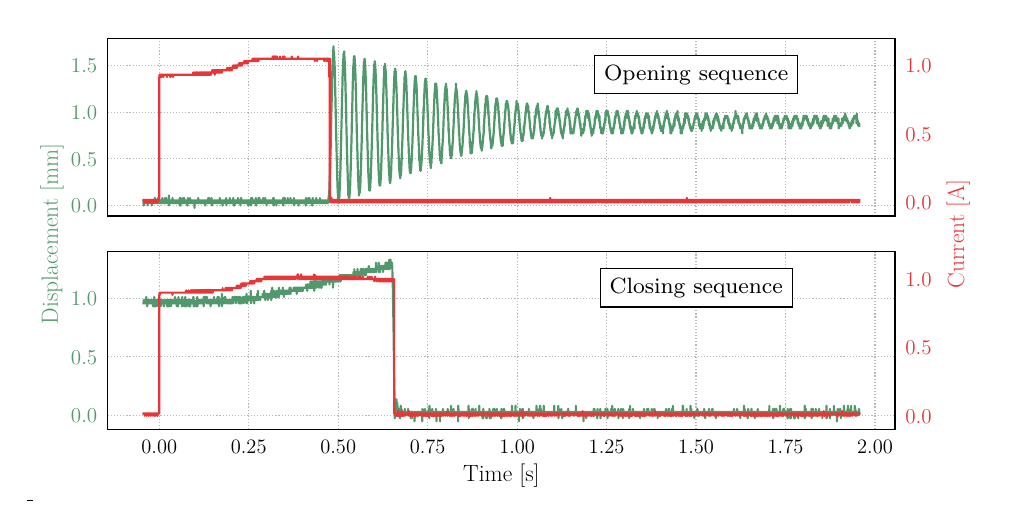
\begin{tikzpicture}
    \node[anchor=south west,inner sep=0] (graph) at (0,0) {\resizebox{\textwidth}{!}{%% Creator: Matplotlib, PGF backend
%%
%% To include the figure in your LaTeX document, write
%%   \input{<filename>.pgf}
%%
%% Make sure the required packages are loaded in your preamble
%%   \usepackage{pgf}
%%
%% and, on pdftex
%%   \usepackage[utf8]{inputenc}\DeclareUnicodeCharacter{2212}{-}
%%
%% or, on luatex and xetex
%%   \usepackage{unicode-math}
%%
%% Figures using additional raster images can only be included by \input if
%% they are in the same directory as the main LaTeX file. For loading figures
%% from other directories you can use the `import` package
%%   \usepackage{import}
%%
%% and then include the figures with
%%   \import{<path to file>}{<filename>.pgf}
%%
%% Matplotlib used the following preamble
%%
\begingroup%
\makeatletter%
\begin{pgfpicture}%
\pgfpathrectangle{\pgfpointorigin}{\pgfqpoint{9.021944in}{4.466138in}}%
\pgfusepath{use as bounding box, clip}%
\begin{pgfscope}%
\pgfsetbuttcap%
\pgfsetmiterjoin%
\pgfsetlinewidth{0.000000pt}%
\definecolor{currentstroke}{rgb}{0.000000,0.000000,0.000000}%
\pgfsetstrokecolor{currentstroke}%
\pgfsetstrokeopacity{0.000000}%
\pgfsetdash{}{0pt}%
\pgfpathmoveto{\pgfqpoint{0.000000in}{0.000000in}}%
\pgfpathlineto{\pgfqpoint{9.021944in}{0.000000in}}%
\pgfpathlineto{\pgfqpoint{9.021944in}{4.466138in}}%
\pgfpathlineto{\pgfqpoint{0.000000in}{4.466138in}}%
\pgfpathclose%
\pgfusepath{}%
\end{pgfscope}%
\begin{pgfscope}%
\pgfsetbuttcap%
\pgfsetmiterjoin%
\pgfsetlinewidth{0.000000pt}%
\definecolor{currentstroke}{rgb}{0.000000,0.000000,0.000000}%
\pgfsetstrokecolor{currentstroke}%
\pgfsetstrokeopacity{0.000000}%
\pgfsetdash{}{0pt}%
\pgfpathmoveto{\pgfqpoint{0.756250in}{2.686138in}}%
\pgfpathlineto{\pgfqpoint{8.196250in}{2.686138in}}%
\pgfpathlineto{\pgfqpoint{8.196250in}{4.366138in}}%
\pgfpathlineto{\pgfqpoint{0.756250in}{4.366138in}}%
\pgfpathclose%
\pgfusepath{}%
\end{pgfscope}%
\begin{pgfscope}%
\pgfpathrectangle{\pgfqpoint{0.756250in}{2.686138in}}{\pgfqpoint{7.440000in}{1.680000in}}%
\pgfusepath{clip}%
\pgfsetbuttcap%
\pgfsetroundjoin%
\pgfsetlinewidth{0.803000pt}%
\definecolor{currentstroke}{rgb}{0.690196,0.690196,0.690196}%
\pgfsetstrokecolor{currentstroke}%
\pgfsetstrokeopacity{0.900000}%
\pgfsetdash{{0.800000pt}{1.320000pt}}{0.000000pt}%
\pgfpathmoveto{\pgfqpoint{1.243346in}{2.686138in}}%
\pgfpathlineto{\pgfqpoint{1.243346in}{4.366138in}}%
\pgfusepath{stroke}%
\end{pgfscope}%
\begin{pgfscope}%
\pgfsetbuttcap%
\pgfsetroundjoin%
\definecolor{currentfill}{rgb}{0.000000,0.000000,0.000000}%
\pgfsetfillcolor{currentfill}%
\pgfsetlinewidth{0.803000pt}%
\definecolor{currentstroke}{rgb}{0.000000,0.000000,0.000000}%
\pgfsetstrokecolor{currentstroke}%
\pgfsetdash{}{0pt}%
\pgfsys@defobject{currentmarker}{\pgfqpoint{0.000000in}{-0.048611in}}{\pgfqpoint{0.000000in}{0.000000in}}{%
\pgfpathmoveto{\pgfqpoint{0.000000in}{0.000000in}}%
\pgfpathlineto{\pgfqpoint{0.000000in}{-0.048611in}}%
\pgfusepath{stroke,fill}%
}%
\begin{pgfscope}%
\pgfsys@transformshift{1.243346in}{2.686138in}%
\pgfsys@useobject{currentmarker}{}%
\end{pgfscope}%
\end{pgfscope}%
\begin{pgfscope}%
\pgfpathrectangle{\pgfqpoint{0.756250in}{2.686138in}}{\pgfqpoint{7.440000in}{1.680000in}}%
\pgfusepath{clip}%
\pgfsetbuttcap%
\pgfsetroundjoin%
\pgfsetlinewidth{0.803000pt}%
\definecolor{currentstroke}{rgb}{0.690196,0.690196,0.690196}%
\pgfsetstrokecolor{currentstroke}%
\pgfsetstrokeopacity{0.900000}%
\pgfsetdash{{0.800000pt}{1.320000pt}}{0.000000pt}%
\pgfpathmoveto{\pgfqpoint{2.088782in}{2.686138in}}%
\pgfpathlineto{\pgfqpoint{2.088782in}{4.366138in}}%
\pgfusepath{stroke}%
\end{pgfscope}%
\begin{pgfscope}%
\pgfsetbuttcap%
\pgfsetroundjoin%
\definecolor{currentfill}{rgb}{0.000000,0.000000,0.000000}%
\pgfsetfillcolor{currentfill}%
\pgfsetlinewidth{0.803000pt}%
\definecolor{currentstroke}{rgb}{0.000000,0.000000,0.000000}%
\pgfsetstrokecolor{currentstroke}%
\pgfsetdash{}{0pt}%
\pgfsys@defobject{currentmarker}{\pgfqpoint{0.000000in}{-0.048611in}}{\pgfqpoint{0.000000in}{0.000000in}}{%
\pgfpathmoveto{\pgfqpoint{0.000000in}{0.000000in}}%
\pgfpathlineto{\pgfqpoint{0.000000in}{-0.048611in}}%
\pgfusepath{stroke,fill}%
}%
\begin{pgfscope}%
\pgfsys@transformshift{2.088782in}{2.686138in}%
\pgfsys@useobject{currentmarker}{}%
\end{pgfscope}%
\end{pgfscope}%
\begin{pgfscope}%
\pgfpathrectangle{\pgfqpoint{0.756250in}{2.686138in}}{\pgfqpoint{7.440000in}{1.680000in}}%
\pgfusepath{clip}%
\pgfsetbuttcap%
\pgfsetroundjoin%
\pgfsetlinewidth{0.803000pt}%
\definecolor{currentstroke}{rgb}{0.690196,0.690196,0.690196}%
\pgfsetstrokecolor{currentstroke}%
\pgfsetstrokeopacity{0.900000}%
\pgfsetdash{{0.800000pt}{1.320000pt}}{0.000000pt}%
\pgfpathmoveto{\pgfqpoint{2.934217in}{2.686138in}}%
\pgfpathlineto{\pgfqpoint{2.934217in}{4.366138in}}%
\pgfusepath{stroke}%
\end{pgfscope}%
\begin{pgfscope}%
\pgfsetbuttcap%
\pgfsetroundjoin%
\definecolor{currentfill}{rgb}{0.000000,0.000000,0.000000}%
\pgfsetfillcolor{currentfill}%
\pgfsetlinewidth{0.803000pt}%
\definecolor{currentstroke}{rgb}{0.000000,0.000000,0.000000}%
\pgfsetstrokecolor{currentstroke}%
\pgfsetdash{}{0pt}%
\pgfsys@defobject{currentmarker}{\pgfqpoint{0.000000in}{-0.048611in}}{\pgfqpoint{0.000000in}{0.000000in}}{%
\pgfpathmoveto{\pgfqpoint{0.000000in}{0.000000in}}%
\pgfpathlineto{\pgfqpoint{0.000000in}{-0.048611in}}%
\pgfusepath{stroke,fill}%
}%
\begin{pgfscope}%
\pgfsys@transformshift{2.934217in}{2.686138in}%
\pgfsys@useobject{currentmarker}{}%
\end{pgfscope}%
\end{pgfscope}%
\begin{pgfscope}%
\pgfpathrectangle{\pgfqpoint{0.756250in}{2.686138in}}{\pgfqpoint{7.440000in}{1.680000in}}%
\pgfusepath{clip}%
\pgfsetbuttcap%
\pgfsetroundjoin%
\pgfsetlinewidth{0.803000pt}%
\definecolor{currentstroke}{rgb}{0.690196,0.690196,0.690196}%
\pgfsetstrokecolor{currentstroke}%
\pgfsetstrokeopacity{0.900000}%
\pgfsetdash{{0.800000pt}{1.320000pt}}{0.000000pt}%
\pgfpathmoveto{\pgfqpoint{3.779653in}{2.686138in}}%
\pgfpathlineto{\pgfqpoint{3.779653in}{4.366138in}}%
\pgfusepath{stroke}%
\end{pgfscope}%
\begin{pgfscope}%
\pgfsetbuttcap%
\pgfsetroundjoin%
\definecolor{currentfill}{rgb}{0.000000,0.000000,0.000000}%
\pgfsetfillcolor{currentfill}%
\pgfsetlinewidth{0.803000pt}%
\definecolor{currentstroke}{rgb}{0.000000,0.000000,0.000000}%
\pgfsetstrokecolor{currentstroke}%
\pgfsetdash{}{0pt}%
\pgfsys@defobject{currentmarker}{\pgfqpoint{0.000000in}{-0.048611in}}{\pgfqpoint{0.000000in}{0.000000in}}{%
\pgfpathmoveto{\pgfqpoint{0.000000in}{0.000000in}}%
\pgfpathlineto{\pgfqpoint{0.000000in}{-0.048611in}}%
\pgfusepath{stroke,fill}%
}%
\begin{pgfscope}%
\pgfsys@transformshift{3.779653in}{2.686138in}%
\pgfsys@useobject{currentmarker}{}%
\end{pgfscope}%
\end{pgfscope}%
\begin{pgfscope}%
\pgfpathrectangle{\pgfqpoint{0.756250in}{2.686138in}}{\pgfqpoint{7.440000in}{1.680000in}}%
\pgfusepath{clip}%
\pgfsetbuttcap%
\pgfsetroundjoin%
\pgfsetlinewidth{0.803000pt}%
\definecolor{currentstroke}{rgb}{0.690196,0.690196,0.690196}%
\pgfsetstrokecolor{currentstroke}%
\pgfsetstrokeopacity{0.900000}%
\pgfsetdash{{0.800000pt}{1.320000pt}}{0.000000pt}%
\pgfpathmoveto{\pgfqpoint{4.625088in}{2.686138in}}%
\pgfpathlineto{\pgfqpoint{4.625088in}{4.366138in}}%
\pgfusepath{stroke}%
\end{pgfscope}%
\begin{pgfscope}%
\pgfsetbuttcap%
\pgfsetroundjoin%
\definecolor{currentfill}{rgb}{0.000000,0.000000,0.000000}%
\pgfsetfillcolor{currentfill}%
\pgfsetlinewidth{0.803000pt}%
\definecolor{currentstroke}{rgb}{0.000000,0.000000,0.000000}%
\pgfsetstrokecolor{currentstroke}%
\pgfsetdash{}{0pt}%
\pgfsys@defobject{currentmarker}{\pgfqpoint{0.000000in}{-0.048611in}}{\pgfqpoint{0.000000in}{0.000000in}}{%
\pgfpathmoveto{\pgfqpoint{0.000000in}{0.000000in}}%
\pgfpathlineto{\pgfqpoint{0.000000in}{-0.048611in}}%
\pgfusepath{stroke,fill}%
}%
\begin{pgfscope}%
\pgfsys@transformshift{4.625088in}{2.686138in}%
\pgfsys@useobject{currentmarker}{}%
\end{pgfscope}%
\end{pgfscope}%
\begin{pgfscope}%
\pgfpathrectangle{\pgfqpoint{0.756250in}{2.686138in}}{\pgfqpoint{7.440000in}{1.680000in}}%
\pgfusepath{clip}%
\pgfsetbuttcap%
\pgfsetroundjoin%
\pgfsetlinewidth{0.803000pt}%
\definecolor{currentstroke}{rgb}{0.690196,0.690196,0.690196}%
\pgfsetstrokecolor{currentstroke}%
\pgfsetstrokeopacity{0.900000}%
\pgfsetdash{{0.800000pt}{1.320000pt}}{0.000000pt}%
\pgfpathmoveto{\pgfqpoint{5.470524in}{2.686138in}}%
\pgfpathlineto{\pgfqpoint{5.470524in}{4.366138in}}%
\pgfusepath{stroke}%
\end{pgfscope}%
\begin{pgfscope}%
\pgfsetbuttcap%
\pgfsetroundjoin%
\definecolor{currentfill}{rgb}{0.000000,0.000000,0.000000}%
\pgfsetfillcolor{currentfill}%
\pgfsetlinewidth{0.803000pt}%
\definecolor{currentstroke}{rgb}{0.000000,0.000000,0.000000}%
\pgfsetstrokecolor{currentstroke}%
\pgfsetdash{}{0pt}%
\pgfsys@defobject{currentmarker}{\pgfqpoint{0.000000in}{-0.048611in}}{\pgfqpoint{0.000000in}{0.000000in}}{%
\pgfpathmoveto{\pgfqpoint{0.000000in}{0.000000in}}%
\pgfpathlineto{\pgfqpoint{0.000000in}{-0.048611in}}%
\pgfusepath{stroke,fill}%
}%
\begin{pgfscope}%
\pgfsys@transformshift{5.470524in}{2.686138in}%
\pgfsys@useobject{currentmarker}{}%
\end{pgfscope}%
\end{pgfscope}%
\begin{pgfscope}%
\pgfpathrectangle{\pgfqpoint{0.756250in}{2.686138in}}{\pgfqpoint{7.440000in}{1.680000in}}%
\pgfusepath{clip}%
\pgfsetbuttcap%
\pgfsetroundjoin%
\pgfsetlinewidth{0.803000pt}%
\definecolor{currentstroke}{rgb}{0.690196,0.690196,0.690196}%
\pgfsetstrokecolor{currentstroke}%
\pgfsetstrokeopacity{0.900000}%
\pgfsetdash{{0.800000pt}{1.320000pt}}{0.000000pt}%
\pgfpathmoveto{\pgfqpoint{6.315959in}{2.686138in}}%
\pgfpathlineto{\pgfqpoint{6.315959in}{4.366138in}}%
\pgfusepath{stroke}%
\end{pgfscope}%
\begin{pgfscope}%
\pgfsetbuttcap%
\pgfsetroundjoin%
\definecolor{currentfill}{rgb}{0.000000,0.000000,0.000000}%
\pgfsetfillcolor{currentfill}%
\pgfsetlinewidth{0.803000pt}%
\definecolor{currentstroke}{rgb}{0.000000,0.000000,0.000000}%
\pgfsetstrokecolor{currentstroke}%
\pgfsetdash{}{0pt}%
\pgfsys@defobject{currentmarker}{\pgfqpoint{0.000000in}{-0.048611in}}{\pgfqpoint{0.000000in}{0.000000in}}{%
\pgfpathmoveto{\pgfqpoint{0.000000in}{0.000000in}}%
\pgfpathlineto{\pgfqpoint{0.000000in}{-0.048611in}}%
\pgfusepath{stroke,fill}%
}%
\begin{pgfscope}%
\pgfsys@transformshift{6.315959in}{2.686138in}%
\pgfsys@useobject{currentmarker}{}%
\end{pgfscope}%
\end{pgfscope}%
\begin{pgfscope}%
\pgfpathrectangle{\pgfqpoint{0.756250in}{2.686138in}}{\pgfqpoint{7.440000in}{1.680000in}}%
\pgfusepath{clip}%
\pgfsetbuttcap%
\pgfsetroundjoin%
\pgfsetlinewidth{0.803000pt}%
\definecolor{currentstroke}{rgb}{0.690196,0.690196,0.690196}%
\pgfsetstrokecolor{currentstroke}%
\pgfsetstrokeopacity{0.900000}%
\pgfsetdash{{0.800000pt}{1.320000pt}}{0.000000pt}%
\pgfpathmoveto{\pgfqpoint{7.161395in}{2.686138in}}%
\pgfpathlineto{\pgfqpoint{7.161395in}{4.366138in}}%
\pgfusepath{stroke}%
\end{pgfscope}%
\begin{pgfscope}%
\pgfsetbuttcap%
\pgfsetroundjoin%
\definecolor{currentfill}{rgb}{0.000000,0.000000,0.000000}%
\pgfsetfillcolor{currentfill}%
\pgfsetlinewidth{0.803000pt}%
\definecolor{currentstroke}{rgb}{0.000000,0.000000,0.000000}%
\pgfsetstrokecolor{currentstroke}%
\pgfsetdash{}{0pt}%
\pgfsys@defobject{currentmarker}{\pgfqpoint{0.000000in}{-0.048611in}}{\pgfqpoint{0.000000in}{0.000000in}}{%
\pgfpathmoveto{\pgfqpoint{0.000000in}{0.000000in}}%
\pgfpathlineto{\pgfqpoint{0.000000in}{-0.048611in}}%
\pgfusepath{stroke,fill}%
}%
\begin{pgfscope}%
\pgfsys@transformshift{7.161395in}{2.686138in}%
\pgfsys@useobject{currentmarker}{}%
\end{pgfscope}%
\end{pgfscope}%
\begin{pgfscope}%
\pgfpathrectangle{\pgfqpoint{0.756250in}{2.686138in}}{\pgfqpoint{7.440000in}{1.680000in}}%
\pgfusepath{clip}%
\pgfsetbuttcap%
\pgfsetroundjoin%
\pgfsetlinewidth{0.803000pt}%
\definecolor{currentstroke}{rgb}{0.690196,0.690196,0.690196}%
\pgfsetstrokecolor{currentstroke}%
\pgfsetstrokeopacity{0.900000}%
\pgfsetdash{{0.800000pt}{1.320000pt}}{0.000000pt}%
\pgfpathmoveto{\pgfqpoint{8.006830in}{2.686138in}}%
\pgfpathlineto{\pgfqpoint{8.006830in}{4.366138in}}%
\pgfusepath{stroke}%
\end{pgfscope}%
\begin{pgfscope}%
\pgfsetbuttcap%
\pgfsetroundjoin%
\definecolor{currentfill}{rgb}{0.000000,0.000000,0.000000}%
\pgfsetfillcolor{currentfill}%
\pgfsetlinewidth{0.803000pt}%
\definecolor{currentstroke}{rgb}{0.000000,0.000000,0.000000}%
\pgfsetstrokecolor{currentstroke}%
\pgfsetdash{}{0pt}%
\pgfsys@defobject{currentmarker}{\pgfqpoint{0.000000in}{-0.048611in}}{\pgfqpoint{0.000000in}{0.000000in}}{%
\pgfpathmoveto{\pgfqpoint{0.000000in}{0.000000in}}%
\pgfpathlineto{\pgfqpoint{0.000000in}{-0.048611in}}%
\pgfusepath{stroke,fill}%
}%
\begin{pgfscope}%
\pgfsys@transformshift{8.006830in}{2.686138in}%
\pgfsys@useobject{currentmarker}{}%
\end{pgfscope}%
\end{pgfscope}%
\begin{pgfscope}%
\pgfpathrectangle{\pgfqpoint{0.756250in}{2.686138in}}{\pgfqpoint{7.440000in}{1.680000in}}%
\pgfusepath{clip}%
\pgfsetbuttcap%
\pgfsetroundjoin%
\pgfsetlinewidth{0.803000pt}%
\definecolor{currentstroke}{rgb}{0.690196,0.690196,0.690196}%
\pgfsetstrokecolor{currentstroke}%
\pgfsetstrokeopacity{0.900000}%
\pgfsetdash{{0.800000pt}{1.320000pt}}{0.000000pt}%
\pgfpathmoveto{\pgfqpoint{0.756250in}{2.785998in}}%
\pgfpathlineto{\pgfqpoint{8.196250in}{2.785998in}}%
\pgfusepath{stroke}%
\end{pgfscope}%
\begin{pgfscope}%
\pgfsetbuttcap%
\pgfsetroundjoin%
\definecolor{currentfill}{rgb}{0.000000,0.000000,0.000000}%
\pgfsetfillcolor{currentfill}%
\pgfsetlinewidth{0.803000pt}%
\definecolor{currentstroke}{rgb}{0.000000,0.000000,0.000000}%
\pgfsetstrokecolor{currentstroke}%
\pgfsetdash{}{0pt}%
\pgfsys@defobject{currentmarker}{\pgfqpoint{-0.048611in}{0.000000in}}{\pgfqpoint{-0.000000in}{0.000000in}}{%
\pgfpathmoveto{\pgfqpoint{-0.000000in}{0.000000in}}%
\pgfpathlineto{\pgfqpoint{-0.048611in}{0.000000in}}%
\pgfusepath{stroke,fill}%
}%
\begin{pgfscope}%
\pgfsys@transformshift{0.756250in}{2.785998in}%
\pgfsys@useobject{currentmarker}{}%
\end{pgfscope}%
\end{pgfscope}%
\begin{pgfscope}%
\definecolor{textcolor}{rgb}{0.317647,0.596078,0.423529}%
\pgfsetstrokecolor{textcolor}%
\pgfsetfillcolor{textcolor}%
\pgftext[x=0.408799in, y=2.716554in, left, base]{\color{textcolor}\rmfamily\fontsize{14.000000}{16.800000}\selectfont \(\displaystyle {0.0}\)}%
\end{pgfscope}%
\begin{pgfscope}%
\pgfpathrectangle{\pgfqpoint{0.756250in}{2.686138in}}{\pgfqpoint{7.440000in}{1.680000in}}%
\pgfusepath{clip}%
\pgfsetbuttcap%
\pgfsetroundjoin%
\pgfsetlinewidth{0.803000pt}%
\definecolor{currentstroke}{rgb}{0.690196,0.690196,0.690196}%
\pgfsetstrokecolor{currentstroke}%
\pgfsetstrokeopacity{0.900000}%
\pgfsetdash{{0.800000pt}{1.320000pt}}{0.000000pt}%
\pgfpathmoveto{\pgfqpoint{0.756250in}{3.226557in}}%
\pgfpathlineto{\pgfqpoint{8.196250in}{3.226557in}}%
\pgfusepath{stroke}%
\end{pgfscope}%
\begin{pgfscope}%
\pgfsetbuttcap%
\pgfsetroundjoin%
\definecolor{currentfill}{rgb}{0.000000,0.000000,0.000000}%
\pgfsetfillcolor{currentfill}%
\pgfsetlinewidth{0.803000pt}%
\definecolor{currentstroke}{rgb}{0.000000,0.000000,0.000000}%
\pgfsetstrokecolor{currentstroke}%
\pgfsetdash{}{0pt}%
\pgfsys@defobject{currentmarker}{\pgfqpoint{-0.048611in}{0.000000in}}{\pgfqpoint{-0.000000in}{0.000000in}}{%
\pgfpathmoveto{\pgfqpoint{-0.000000in}{0.000000in}}%
\pgfpathlineto{\pgfqpoint{-0.048611in}{0.000000in}}%
\pgfusepath{stroke,fill}%
}%
\begin{pgfscope}%
\pgfsys@transformshift{0.756250in}{3.226557in}%
\pgfsys@useobject{currentmarker}{}%
\end{pgfscope}%
\end{pgfscope}%
\begin{pgfscope}%
\definecolor{textcolor}{rgb}{0.317647,0.596078,0.423529}%
\pgfsetstrokecolor{textcolor}%
\pgfsetfillcolor{textcolor}%
\pgftext[x=0.408799in, y=3.157113in, left, base]{\color{textcolor}\rmfamily\fontsize{14.000000}{16.800000}\selectfont \(\displaystyle {0.5}\)}%
\end{pgfscope}%
\begin{pgfscope}%
\pgfpathrectangle{\pgfqpoint{0.756250in}{2.686138in}}{\pgfqpoint{7.440000in}{1.680000in}}%
\pgfusepath{clip}%
\pgfsetbuttcap%
\pgfsetroundjoin%
\pgfsetlinewidth{0.803000pt}%
\definecolor{currentstroke}{rgb}{0.690196,0.690196,0.690196}%
\pgfsetstrokecolor{currentstroke}%
\pgfsetstrokeopacity{0.900000}%
\pgfsetdash{{0.800000pt}{1.320000pt}}{0.000000pt}%
\pgfpathmoveto{\pgfqpoint{0.756250in}{3.667116in}}%
\pgfpathlineto{\pgfqpoint{8.196250in}{3.667116in}}%
\pgfusepath{stroke}%
\end{pgfscope}%
\begin{pgfscope}%
\pgfsetbuttcap%
\pgfsetroundjoin%
\definecolor{currentfill}{rgb}{0.000000,0.000000,0.000000}%
\pgfsetfillcolor{currentfill}%
\pgfsetlinewidth{0.803000pt}%
\definecolor{currentstroke}{rgb}{0.000000,0.000000,0.000000}%
\pgfsetstrokecolor{currentstroke}%
\pgfsetdash{}{0pt}%
\pgfsys@defobject{currentmarker}{\pgfqpoint{-0.048611in}{0.000000in}}{\pgfqpoint{-0.000000in}{0.000000in}}{%
\pgfpathmoveto{\pgfqpoint{-0.000000in}{0.000000in}}%
\pgfpathlineto{\pgfqpoint{-0.048611in}{0.000000in}}%
\pgfusepath{stroke,fill}%
}%
\begin{pgfscope}%
\pgfsys@transformshift{0.756250in}{3.667116in}%
\pgfsys@useobject{currentmarker}{}%
\end{pgfscope}%
\end{pgfscope}%
\begin{pgfscope}%
\definecolor{textcolor}{rgb}{0.317647,0.596078,0.423529}%
\pgfsetstrokecolor{textcolor}%
\pgfsetfillcolor{textcolor}%
\pgftext[x=0.408799in, y=3.597672in, left, base]{\color{textcolor}\rmfamily\fontsize{14.000000}{16.800000}\selectfont \(\displaystyle {1.0}\)}%
\end{pgfscope}%
\begin{pgfscope}%
\pgfpathrectangle{\pgfqpoint{0.756250in}{2.686138in}}{\pgfqpoint{7.440000in}{1.680000in}}%
\pgfusepath{clip}%
\pgfsetbuttcap%
\pgfsetroundjoin%
\pgfsetlinewidth{0.803000pt}%
\definecolor{currentstroke}{rgb}{0.690196,0.690196,0.690196}%
\pgfsetstrokecolor{currentstroke}%
\pgfsetstrokeopacity{0.900000}%
\pgfsetdash{{0.800000pt}{1.320000pt}}{0.000000pt}%
\pgfpathmoveto{\pgfqpoint{0.756250in}{4.107675in}}%
\pgfpathlineto{\pgfqpoint{8.196250in}{4.107675in}}%
\pgfusepath{stroke}%
\end{pgfscope}%
\begin{pgfscope}%
\pgfsetbuttcap%
\pgfsetroundjoin%
\definecolor{currentfill}{rgb}{0.000000,0.000000,0.000000}%
\pgfsetfillcolor{currentfill}%
\pgfsetlinewidth{0.803000pt}%
\definecolor{currentstroke}{rgb}{0.000000,0.000000,0.000000}%
\pgfsetstrokecolor{currentstroke}%
\pgfsetdash{}{0pt}%
\pgfsys@defobject{currentmarker}{\pgfqpoint{-0.048611in}{0.000000in}}{\pgfqpoint{-0.000000in}{0.000000in}}{%
\pgfpathmoveto{\pgfqpoint{-0.000000in}{0.000000in}}%
\pgfpathlineto{\pgfqpoint{-0.048611in}{0.000000in}}%
\pgfusepath{stroke,fill}%
}%
\begin{pgfscope}%
\pgfsys@transformshift{0.756250in}{4.107675in}%
\pgfsys@useobject{currentmarker}{}%
\end{pgfscope}%
\end{pgfscope}%
\begin{pgfscope}%
\definecolor{textcolor}{rgb}{0.317647,0.596078,0.423529}%
\pgfsetstrokecolor{textcolor}%
\pgfsetfillcolor{textcolor}%
\pgftext[x=0.408799in, y=4.038231in, left, base]{\color{textcolor}\rmfamily\fontsize{14.000000}{16.800000}\selectfont \(\displaystyle {1.5}\)}%
\end{pgfscope}%
\begin{pgfscope}%
\pgfpathrectangle{\pgfqpoint{0.756250in}{2.686138in}}{\pgfqpoint{7.440000in}{1.680000in}}%
\pgfusepath{clip}%
\pgfsetrectcap%
\pgfsetroundjoin%
\pgfsetlinewidth{1.505625pt}%
\definecolor{currentstroke}{rgb}{0.317647,0.596078,0.423529}%
\pgfsetstrokecolor{currentstroke}%
\pgfsetdash{}{0pt}%
\pgfpathmoveto{\pgfqpoint{1.094431in}{2.809495in}}%
\pgfpathlineto{\pgfqpoint{1.094702in}{2.809495in}}%
\pgfpathlineto{\pgfqpoint{1.095108in}{2.832991in}}%
\pgfpathlineto{\pgfqpoint{1.095378in}{2.809495in}}%
\pgfpathlineto{\pgfqpoint{1.095784in}{2.832991in}}%
\pgfpathlineto{\pgfqpoint{1.095919in}{2.832991in}}%
\pgfpathlineto{\pgfqpoint{1.096460in}{2.785998in}}%
\pgfpathlineto{\pgfqpoint{1.096731in}{2.832991in}}%
\pgfpathlineto{\pgfqpoint{1.096866in}{2.809495in}}%
\pgfpathlineto{\pgfqpoint{1.097272in}{2.832991in}}%
\pgfpathlineto{\pgfqpoint{1.097678in}{2.832991in}}%
\pgfpathlineto{\pgfqpoint{1.098084in}{2.809495in}}%
\pgfpathlineto{\pgfqpoint{1.098354in}{2.809495in}}%
\pgfpathlineto{\pgfqpoint{1.098760in}{2.832991in}}%
\pgfpathlineto{\pgfqpoint{1.098895in}{2.832991in}}%
\pgfpathlineto{\pgfqpoint{1.099301in}{2.809495in}}%
\pgfpathlineto{\pgfqpoint{1.099436in}{2.809495in}}%
\pgfpathlineto{\pgfqpoint{1.099572in}{2.832991in}}%
\pgfpathlineto{\pgfqpoint{1.099707in}{2.809495in}}%
\pgfpathlineto{\pgfqpoint{1.099977in}{2.809495in}}%
\pgfpathlineto{\pgfqpoint{1.100383in}{2.832991in}}%
\pgfpathlineto{\pgfqpoint{1.100654in}{2.832991in}}%
\pgfpathlineto{\pgfqpoint{1.101060in}{2.809495in}}%
\pgfpathlineto{\pgfqpoint{1.101601in}{2.809495in}}%
\pgfpathlineto{\pgfqpoint{1.102007in}{2.832991in}}%
\pgfpathlineto{\pgfqpoint{1.102142in}{2.832991in}}%
\pgfpathlineto{\pgfqpoint{1.102412in}{2.809495in}}%
\pgfpathlineto{\pgfqpoint{1.102818in}{2.832991in}}%
\pgfpathlineto{\pgfqpoint{1.102953in}{2.832991in}}%
\pgfpathlineto{\pgfqpoint{1.103359in}{2.809495in}}%
\pgfpathlineto{\pgfqpoint{1.103494in}{2.832991in}}%
\pgfpathlineto{\pgfqpoint{1.103630in}{2.809495in}}%
\pgfpathlineto{\pgfqpoint{1.103765in}{2.809495in}}%
\pgfpathlineto{\pgfqpoint{1.104171in}{2.832991in}}%
\pgfpathlineto{\pgfqpoint{1.104982in}{2.832991in}}%
\pgfpathlineto{\pgfqpoint{1.105388in}{2.809495in}}%
\pgfpathlineto{\pgfqpoint{1.105659in}{2.832991in}}%
\pgfpathlineto{\pgfqpoint{1.105794in}{2.809495in}}%
\pgfpathlineto{\pgfqpoint{1.105929in}{2.832991in}}%
\pgfpathlineto{\pgfqpoint{1.106470in}{2.832991in}}%
\pgfpathlineto{\pgfqpoint{1.106606in}{2.809495in}}%
\pgfpathlineto{\pgfqpoint{1.106741in}{2.832991in}}%
\pgfpathlineto{\pgfqpoint{1.106876in}{2.832991in}}%
\pgfpathlineto{\pgfqpoint{1.107147in}{2.809495in}}%
\pgfpathlineto{\pgfqpoint{1.107553in}{2.832991in}}%
\pgfpathlineto{\pgfqpoint{1.107688in}{2.809495in}}%
\pgfpathlineto{\pgfqpoint{1.107823in}{2.832991in}}%
\pgfpathlineto{\pgfqpoint{1.108229in}{2.832991in}}%
\pgfpathlineto{\pgfqpoint{1.108364in}{2.809495in}}%
\pgfpathlineto{\pgfqpoint{1.108499in}{2.832991in}}%
\pgfpathlineto{\pgfqpoint{1.109041in}{2.832991in}}%
\pgfpathlineto{\pgfqpoint{1.109311in}{2.809495in}}%
\pgfpathlineto{\pgfqpoint{1.109582in}{2.832991in}}%
\pgfpathlineto{\pgfqpoint{1.109987in}{2.809495in}}%
\pgfpathlineto{\pgfqpoint{1.110393in}{2.832991in}}%
\pgfpathlineto{\pgfqpoint{1.110528in}{2.832991in}}%
\pgfpathlineto{\pgfqpoint{1.110664in}{2.809495in}}%
\pgfpathlineto{\pgfqpoint{1.110799in}{2.832991in}}%
\pgfpathlineto{\pgfqpoint{1.111070in}{2.832991in}}%
\pgfpathlineto{\pgfqpoint{1.111340in}{2.809495in}}%
\pgfpathlineto{\pgfqpoint{1.111746in}{2.832991in}}%
\pgfpathlineto{\pgfqpoint{1.111881in}{2.832991in}}%
\pgfpathlineto{\pgfqpoint{1.112287in}{2.809495in}}%
\pgfpathlineto{\pgfqpoint{1.112558in}{2.809495in}}%
\pgfpathlineto{\pgfqpoint{1.112963in}{2.832991in}}%
\pgfpathlineto{\pgfqpoint{1.113369in}{2.832991in}}%
\pgfpathlineto{\pgfqpoint{1.113640in}{2.809495in}}%
\pgfpathlineto{\pgfqpoint{1.113910in}{2.832991in}}%
\pgfpathlineto{\pgfqpoint{1.114181in}{2.809495in}}%
\pgfpathlineto{\pgfqpoint{1.114587in}{2.832991in}}%
\pgfpathlineto{\pgfqpoint{1.114857in}{2.832991in}}%
\pgfpathlineto{\pgfqpoint{1.115128in}{2.809495in}}%
\pgfpathlineto{\pgfqpoint{1.115263in}{2.832991in}}%
\pgfpathlineto{\pgfqpoint{1.115398in}{2.809495in}}%
\pgfpathlineto{\pgfqpoint{1.115533in}{2.809495in}}%
\pgfpathlineto{\pgfqpoint{1.115804in}{2.832991in}}%
\pgfpathlineto{\pgfqpoint{1.116075in}{2.809495in}}%
\pgfpathlineto{\pgfqpoint{1.116480in}{2.832991in}}%
\pgfpathlineto{\pgfqpoint{1.116751in}{2.809495in}}%
\pgfpathlineto{\pgfqpoint{1.117157in}{2.832991in}}%
\pgfpathlineto{\pgfqpoint{1.117427in}{2.832991in}}%
\pgfpathlineto{\pgfqpoint{1.117833in}{2.809495in}}%
\pgfpathlineto{\pgfqpoint{1.117968in}{2.832991in}}%
\pgfpathlineto{\pgfqpoint{1.118104in}{2.809495in}}%
\pgfpathlineto{\pgfqpoint{1.118374in}{2.809495in}}%
\pgfpathlineto{\pgfqpoint{1.118780in}{2.832991in}}%
\pgfpathlineto{\pgfqpoint{1.119321in}{2.832991in}}%
\pgfpathlineto{\pgfqpoint{1.119727in}{2.809495in}}%
\pgfpathlineto{\pgfqpoint{1.119997in}{2.832991in}}%
\pgfpathlineto{\pgfqpoint{1.120403in}{2.809495in}}%
\pgfpathlineto{\pgfqpoint{1.120809in}{2.832991in}}%
\pgfpathlineto{\pgfqpoint{1.121080in}{2.832991in}}%
\pgfpathlineto{\pgfqpoint{1.121350in}{2.809495in}}%
\pgfpathlineto{\pgfqpoint{1.121756in}{2.832991in}}%
\pgfpathlineto{\pgfqpoint{1.122162in}{2.809495in}}%
\pgfpathlineto{\pgfqpoint{1.122567in}{2.832991in}}%
\pgfpathlineto{\pgfqpoint{1.122703in}{2.832991in}}%
\pgfpathlineto{\pgfqpoint{1.123109in}{2.809495in}}%
\pgfpathlineto{\pgfqpoint{1.123244in}{2.832991in}}%
\pgfpathlineto{\pgfqpoint{1.123379in}{2.809495in}}%
\pgfpathlineto{\pgfqpoint{1.123514in}{2.809495in}}%
\pgfpathlineto{\pgfqpoint{1.123785in}{2.832991in}}%
\pgfpathlineto{\pgfqpoint{1.124055in}{2.809495in}}%
\pgfpathlineto{\pgfqpoint{1.124461in}{2.832991in}}%
\pgfpathlineto{\pgfqpoint{1.124597in}{2.832991in}}%
\pgfpathlineto{\pgfqpoint{1.125002in}{2.809495in}}%
\pgfpathlineto{\pgfqpoint{1.125138in}{2.809495in}}%
\pgfpathlineto{\pgfqpoint{1.125543in}{2.832991in}}%
\pgfpathlineto{\pgfqpoint{1.126085in}{2.832991in}}%
\pgfpathlineto{\pgfqpoint{1.126490in}{2.809495in}}%
\pgfpathlineto{\pgfqpoint{1.126626in}{2.809495in}}%
\pgfpathlineto{\pgfqpoint{1.127031in}{2.832991in}}%
\pgfpathlineto{\pgfqpoint{1.127167in}{2.809495in}}%
\pgfpathlineto{\pgfqpoint{1.127302in}{2.832991in}}%
\pgfpathlineto{\pgfqpoint{1.127437in}{2.832991in}}%
\pgfpathlineto{\pgfqpoint{1.127572in}{2.809495in}}%
\pgfpathlineto{\pgfqpoint{1.127708in}{2.832991in}}%
\pgfpathlineto{\pgfqpoint{1.129060in}{2.832991in}}%
\pgfpathlineto{\pgfqpoint{1.129466in}{2.809495in}}%
\pgfpathlineto{\pgfqpoint{1.129872in}{2.809495in}}%
\pgfpathlineto{\pgfqpoint{1.130278in}{2.832991in}}%
\pgfpathlineto{\pgfqpoint{1.130413in}{2.832991in}}%
\pgfpathlineto{\pgfqpoint{1.130819in}{2.809495in}}%
\pgfpathlineto{\pgfqpoint{1.130954in}{2.809495in}}%
\pgfpathlineto{\pgfqpoint{1.131360in}{2.832991in}}%
\pgfpathlineto{\pgfqpoint{1.131766in}{2.809495in}}%
\pgfpathlineto{\pgfqpoint{1.132172in}{2.832991in}}%
\pgfpathlineto{\pgfqpoint{1.132307in}{2.832991in}}%
\pgfpathlineto{\pgfqpoint{1.132713in}{2.809495in}}%
\pgfpathlineto{\pgfqpoint{1.132983in}{2.809495in}}%
\pgfpathlineto{\pgfqpoint{1.133389in}{2.832991in}}%
\pgfpathlineto{\pgfqpoint{1.133524in}{2.785998in}}%
\pgfpathlineto{\pgfqpoint{1.133660in}{2.832991in}}%
\pgfpathlineto{\pgfqpoint{1.133795in}{2.832991in}}%
\pgfpathlineto{\pgfqpoint{1.134065in}{2.809495in}}%
\pgfpathlineto{\pgfqpoint{1.134471in}{2.832991in}}%
\pgfpathlineto{\pgfqpoint{1.135418in}{2.832991in}}%
\pgfpathlineto{\pgfqpoint{1.135824in}{2.809495in}}%
\pgfpathlineto{\pgfqpoint{1.136230in}{2.832991in}}%
\pgfpathlineto{\pgfqpoint{1.136365in}{2.832991in}}%
\pgfpathlineto{\pgfqpoint{1.136500in}{2.809495in}}%
\pgfpathlineto{\pgfqpoint{1.136636in}{2.832991in}}%
\pgfpathlineto{\pgfqpoint{1.136906in}{2.832991in}}%
\pgfpathlineto{\pgfqpoint{1.137312in}{2.809495in}}%
\pgfpathlineto{\pgfqpoint{1.137447in}{2.809495in}}%
\pgfpathlineto{\pgfqpoint{1.137582in}{2.832991in}}%
\pgfpathlineto{\pgfqpoint{1.137718in}{2.809495in}}%
\pgfpathlineto{\pgfqpoint{1.137988in}{2.809495in}}%
\pgfpathlineto{\pgfqpoint{1.138124in}{2.832991in}}%
\pgfpathlineto{\pgfqpoint{1.138259in}{2.809495in}}%
\pgfpathlineto{\pgfqpoint{1.138394in}{2.809495in}}%
\pgfpathlineto{\pgfqpoint{1.138800in}{2.832991in}}%
\pgfpathlineto{\pgfqpoint{1.139070in}{2.809495in}}%
\pgfpathlineto{\pgfqpoint{1.139476in}{2.832991in}}%
\pgfpathlineto{\pgfqpoint{1.140017in}{2.832991in}}%
\pgfpathlineto{\pgfqpoint{1.140153in}{2.809495in}}%
\pgfpathlineto{\pgfqpoint{1.140288in}{2.832991in}}%
\pgfpathlineto{\pgfqpoint{1.141505in}{2.832991in}}%
\pgfpathlineto{\pgfqpoint{1.141911in}{2.809495in}}%
\pgfpathlineto{\pgfqpoint{1.142317in}{2.832991in}}%
\pgfpathlineto{\pgfqpoint{1.142587in}{2.832991in}}%
\pgfpathlineto{\pgfqpoint{1.142723in}{2.809495in}}%
\pgfpathlineto{\pgfqpoint{1.142858in}{2.832991in}}%
\pgfpathlineto{\pgfqpoint{1.142993in}{2.832991in}}%
\pgfpathlineto{\pgfqpoint{1.143128in}{2.809495in}}%
\pgfpathlineto{\pgfqpoint{1.143264in}{2.832991in}}%
\pgfpathlineto{\pgfqpoint{1.143534in}{2.832991in}}%
\pgfpathlineto{\pgfqpoint{1.143940in}{2.809495in}}%
\pgfpathlineto{\pgfqpoint{1.144075in}{2.809495in}}%
\pgfpathlineto{\pgfqpoint{1.144346in}{2.832991in}}%
\pgfpathlineto{\pgfqpoint{1.144481in}{2.809495in}}%
\pgfpathlineto{\pgfqpoint{1.144616in}{2.832991in}}%
\pgfpathlineto{\pgfqpoint{1.144752in}{2.832991in}}%
\pgfpathlineto{\pgfqpoint{1.144887in}{2.809495in}}%
\pgfpathlineto{\pgfqpoint{1.145022in}{2.832991in}}%
\pgfpathlineto{\pgfqpoint{1.145563in}{2.832991in}}%
\pgfpathlineto{\pgfqpoint{1.145834in}{2.809495in}}%
\pgfpathlineto{\pgfqpoint{1.145969in}{2.832991in}}%
\pgfpathlineto{\pgfqpoint{1.146104in}{2.809495in}}%
\pgfpathlineto{\pgfqpoint{1.147051in}{2.809495in}}%
\pgfpathlineto{\pgfqpoint{1.147457in}{2.832991in}}%
\pgfpathlineto{\pgfqpoint{1.147592in}{2.832991in}}%
\pgfpathlineto{\pgfqpoint{1.147728in}{2.809495in}}%
\pgfpathlineto{\pgfqpoint{1.147863in}{2.832991in}}%
\pgfpathlineto{\pgfqpoint{1.147998in}{2.832991in}}%
\pgfpathlineto{\pgfqpoint{1.148269in}{2.809495in}}%
\pgfpathlineto{\pgfqpoint{1.148539in}{2.832991in}}%
\pgfpathlineto{\pgfqpoint{1.148675in}{2.809495in}}%
\pgfpathlineto{\pgfqpoint{1.148810in}{2.832991in}}%
\pgfpathlineto{\pgfqpoint{1.148945in}{2.832991in}}%
\pgfpathlineto{\pgfqpoint{1.149351in}{2.809495in}}%
\pgfpathlineto{\pgfqpoint{1.149892in}{2.809495in}}%
\pgfpathlineto{\pgfqpoint{1.150163in}{2.832991in}}%
\pgfpathlineto{\pgfqpoint{1.150568in}{2.809495in}}%
\pgfpathlineto{\pgfqpoint{1.151109in}{2.809495in}}%
\pgfpathlineto{\pgfqpoint{1.151380in}{2.832991in}}%
\pgfpathlineto{\pgfqpoint{1.151786in}{2.809495in}}%
\pgfpathlineto{\pgfqpoint{1.152192in}{2.832991in}}%
\pgfpathlineto{\pgfqpoint{1.152462in}{2.809495in}}%
\pgfpathlineto{\pgfqpoint{1.152868in}{2.832991in}}%
\pgfpathlineto{\pgfqpoint{1.153138in}{2.832991in}}%
\pgfpathlineto{\pgfqpoint{1.153409in}{2.809495in}}%
\pgfpathlineto{\pgfqpoint{1.153815in}{2.832991in}}%
\pgfpathlineto{\pgfqpoint{1.154085in}{2.809495in}}%
\pgfpathlineto{\pgfqpoint{1.154491in}{2.832991in}}%
\pgfpathlineto{\pgfqpoint{1.154762in}{2.832991in}}%
\pgfpathlineto{\pgfqpoint{1.155167in}{2.809495in}}%
\pgfpathlineto{\pgfqpoint{1.155573in}{2.832991in}}%
\pgfpathlineto{\pgfqpoint{1.155979in}{2.809495in}}%
\pgfpathlineto{\pgfqpoint{1.156114in}{2.809495in}}%
\pgfpathlineto{\pgfqpoint{1.156250in}{2.832991in}}%
\pgfpathlineto{\pgfqpoint{1.156385in}{2.809495in}}%
\pgfpathlineto{\pgfqpoint{1.156520in}{2.809495in}}%
\pgfpathlineto{\pgfqpoint{1.156655in}{2.832991in}}%
\pgfpathlineto{\pgfqpoint{1.156791in}{2.809495in}}%
\pgfpathlineto{\pgfqpoint{1.156926in}{2.809495in}}%
\pgfpathlineto{\pgfqpoint{1.157197in}{2.832991in}}%
\pgfpathlineto{\pgfqpoint{1.157602in}{2.809495in}}%
\pgfpathlineto{\pgfqpoint{1.158414in}{2.809495in}}%
\pgfpathlineto{\pgfqpoint{1.158820in}{2.832991in}}%
\pgfpathlineto{\pgfqpoint{1.159496in}{2.832991in}}%
\pgfpathlineto{\pgfqpoint{1.159631in}{2.809495in}}%
\pgfpathlineto{\pgfqpoint{1.159767in}{2.832991in}}%
\pgfpathlineto{\pgfqpoint{1.160037in}{2.832991in}}%
\pgfpathlineto{\pgfqpoint{1.160443in}{2.809495in}}%
\pgfpathlineto{\pgfqpoint{1.160578in}{2.809495in}}%
\pgfpathlineto{\pgfqpoint{1.160984in}{2.832991in}}%
\pgfpathlineto{\pgfqpoint{1.161390in}{2.809495in}}%
\pgfpathlineto{\pgfqpoint{1.162066in}{2.809495in}}%
\pgfpathlineto{\pgfqpoint{1.162202in}{2.832991in}}%
\pgfpathlineto{\pgfqpoint{1.162337in}{2.809495in}}%
\pgfpathlineto{\pgfqpoint{1.162472in}{2.809495in}}%
\pgfpathlineto{\pgfqpoint{1.162878in}{2.832991in}}%
\pgfpathlineto{\pgfqpoint{1.163013in}{2.832991in}}%
\pgfpathlineto{\pgfqpoint{1.163284in}{2.809495in}}%
\pgfpathlineto{\pgfqpoint{1.163554in}{2.832991in}}%
\pgfpathlineto{\pgfqpoint{1.163960in}{2.809495in}}%
\pgfpathlineto{\pgfqpoint{1.164231in}{2.832991in}}%
\pgfpathlineto{\pgfqpoint{1.164501in}{2.809495in}}%
\pgfpathlineto{\pgfqpoint{1.164772in}{2.832991in}}%
\pgfpathlineto{\pgfqpoint{1.165177in}{2.809495in}}%
\pgfpathlineto{\pgfqpoint{1.165448in}{2.832991in}}%
\pgfpathlineto{\pgfqpoint{1.165583in}{2.809495in}}%
\pgfpathlineto{\pgfqpoint{1.165719in}{2.832991in}}%
\pgfpathlineto{\pgfqpoint{1.165989in}{2.832991in}}%
\pgfpathlineto{\pgfqpoint{1.166124in}{2.809495in}}%
\pgfpathlineto{\pgfqpoint{1.166260in}{2.832991in}}%
\pgfpathlineto{\pgfqpoint{1.166395in}{2.832991in}}%
\pgfpathlineto{\pgfqpoint{1.166801in}{2.809495in}}%
\pgfpathlineto{\pgfqpoint{1.166936in}{2.809495in}}%
\pgfpathlineto{\pgfqpoint{1.167342in}{2.832991in}}%
\pgfpathlineto{\pgfqpoint{1.167748in}{2.809495in}}%
\pgfpathlineto{\pgfqpoint{1.167883in}{2.832991in}}%
\pgfpathlineto{\pgfqpoint{1.168018in}{2.809495in}}%
\pgfpathlineto{\pgfqpoint{1.168289in}{2.809495in}}%
\pgfpathlineto{\pgfqpoint{1.168424in}{2.832991in}}%
\pgfpathlineto{\pgfqpoint{1.168559in}{2.809495in}}%
\pgfpathlineto{\pgfqpoint{1.168694in}{2.809495in}}%
\pgfpathlineto{\pgfqpoint{1.168965in}{2.832991in}}%
\pgfpathlineto{\pgfqpoint{1.169371in}{2.809495in}}%
\pgfpathlineto{\pgfqpoint{1.169777in}{2.832991in}}%
\pgfpathlineto{\pgfqpoint{1.170047in}{2.809495in}}%
\pgfpathlineto{\pgfqpoint{1.170182in}{2.832991in}}%
\pgfpathlineto{\pgfqpoint{1.170318in}{2.809495in}}%
\pgfpathlineto{\pgfqpoint{1.170588in}{2.809495in}}%
\pgfpathlineto{\pgfqpoint{1.170994in}{2.832991in}}%
\pgfpathlineto{\pgfqpoint{1.171265in}{2.809495in}}%
\pgfpathlineto{\pgfqpoint{1.171670in}{2.832991in}}%
\pgfpathlineto{\pgfqpoint{1.172076in}{2.809495in}}%
\pgfpathlineto{\pgfqpoint{1.172347in}{2.832991in}}%
\pgfpathlineto{\pgfqpoint{1.172482in}{2.785998in}}%
\pgfpathlineto{\pgfqpoint{1.172753in}{2.809495in}}%
\pgfpathlineto{\pgfqpoint{1.172888in}{2.832991in}}%
\pgfpathlineto{\pgfqpoint{1.173023in}{2.809495in}}%
\pgfpathlineto{\pgfqpoint{1.173158in}{2.809495in}}%
\pgfpathlineto{\pgfqpoint{1.173564in}{2.832991in}}%
\pgfpathlineto{\pgfqpoint{1.173835in}{2.809495in}}%
\pgfpathlineto{\pgfqpoint{1.174241in}{2.832991in}}%
\pgfpathlineto{\pgfqpoint{1.174646in}{2.832991in}}%
\pgfpathlineto{\pgfqpoint{1.174782in}{2.809495in}}%
\pgfpathlineto{\pgfqpoint{1.174917in}{2.832991in}}%
\pgfpathlineto{\pgfqpoint{1.175052in}{2.832991in}}%
\pgfpathlineto{\pgfqpoint{1.175187in}{2.809495in}}%
\pgfpathlineto{\pgfqpoint{1.175323in}{2.832991in}}%
\pgfpathlineto{\pgfqpoint{1.176134in}{2.832991in}}%
\pgfpathlineto{\pgfqpoint{1.176405in}{2.809495in}}%
\pgfpathlineto{\pgfqpoint{1.176540in}{2.832991in}}%
\pgfpathlineto{\pgfqpoint{1.176675in}{2.809495in}}%
\pgfpathlineto{\pgfqpoint{1.176811in}{2.809495in}}%
\pgfpathlineto{\pgfqpoint{1.176946in}{2.832991in}}%
\pgfpathlineto{\pgfqpoint{1.177081in}{2.809495in}}%
\pgfpathlineto{\pgfqpoint{1.177352in}{2.809495in}}%
\pgfpathlineto{\pgfqpoint{1.177758in}{2.832991in}}%
\pgfpathlineto{\pgfqpoint{1.177893in}{2.832991in}}%
\pgfpathlineto{\pgfqpoint{1.178163in}{2.809495in}}%
\pgfpathlineto{\pgfqpoint{1.178569in}{2.832991in}}%
\pgfpathlineto{\pgfqpoint{1.178975in}{2.809495in}}%
\pgfpathlineto{\pgfqpoint{1.179381in}{2.809495in}}%
\pgfpathlineto{\pgfqpoint{1.179787in}{2.832991in}}%
\pgfpathlineto{\pgfqpoint{1.180057in}{2.809495in}}%
\pgfpathlineto{\pgfqpoint{1.180463in}{2.832991in}}%
\pgfpathlineto{\pgfqpoint{1.180598in}{2.809495in}}%
\pgfpathlineto{\pgfqpoint{1.180733in}{2.832991in}}%
\pgfpathlineto{\pgfqpoint{1.180869in}{2.832991in}}%
\pgfpathlineto{\pgfqpoint{1.181004in}{2.809495in}}%
\pgfpathlineto{\pgfqpoint{1.181139in}{2.832991in}}%
\pgfpathlineto{\pgfqpoint{1.181410in}{2.832991in}}%
\pgfpathlineto{\pgfqpoint{1.181680in}{2.809495in}}%
\pgfpathlineto{\pgfqpoint{1.181951in}{2.832991in}}%
\pgfpathlineto{\pgfqpoint{1.182357in}{2.809495in}}%
\pgfpathlineto{\pgfqpoint{1.182492in}{2.809495in}}%
\pgfpathlineto{\pgfqpoint{1.182898in}{2.832991in}}%
\pgfpathlineto{\pgfqpoint{1.183168in}{2.809495in}}%
\pgfpathlineto{\pgfqpoint{1.183574in}{2.832991in}}%
\pgfpathlineto{\pgfqpoint{1.183709in}{2.832991in}}%
\pgfpathlineto{\pgfqpoint{1.183845in}{2.809495in}}%
\pgfpathlineto{\pgfqpoint{1.183980in}{2.832991in}}%
\pgfpathlineto{\pgfqpoint{1.184115in}{2.832991in}}%
\pgfpathlineto{\pgfqpoint{1.184521in}{2.809495in}}%
\pgfpathlineto{\pgfqpoint{1.185333in}{2.809495in}}%
\pgfpathlineto{\pgfqpoint{1.185738in}{2.832991in}}%
\pgfpathlineto{\pgfqpoint{1.186144in}{2.832991in}}%
\pgfpathlineto{\pgfqpoint{1.186550in}{2.809495in}}%
\pgfpathlineto{\pgfqpoint{1.186685in}{2.832991in}}%
\pgfpathlineto{\pgfqpoint{1.186821in}{2.809495in}}%
\pgfpathlineto{\pgfqpoint{1.187091in}{2.809495in}}%
\pgfpathlineto{\pgfqpoint{1.187226in}{2.832991in}}%
\pgfpathlineto{\pgfqpoint{1.187362in}{2.809495in}}%
\pgfpathlineto{\pgfqpoint{1.187497in}{2.809495in}}%
\pgfpathlineto{\pgfqpoint{1.187903in}{2.832991in}}%
\pgfpathlineto{\pgfqpoint{1.188309in}{2.809495in}}%
\pgfpathlineto{\pgfqpoint{1.188714in}{2.809495in}}%
\pgfpathlineto{\pgfqpoint{1.189120in}{2.832991in}}%
\pgfpathlineto{\pgfqpoint{1.189526in}{2.809495in}}%
\pgfpathlineto{\pgfqpoint{1.190067in}{2.809495in}}%
\pgfpathlineto{\pgfqpoint{1.190202in}{2.832991in}}%
\pgfpathlineto{\pgfqpoint{1.190338in}{2.809495in}}%
\pgfpathlineto{\pgfqpoint{1.190473in}{2.809495in}}%
\pgfpathlineto{\pgfqpoint{1.190879in}{2.832991in}}%
\pgfpathlineto{\pgfqpoint{1.191284in}{2.809495in}}%
\pgfpathlineto{\pgfqpoint{1.191690in}{2.809495in}}%
\pgfpathlineto{\pgfqpoint{1.191826in}{2.832991in}}%
\pgfpathlineto{\pgfqpoint{1.191961in}{2.809495in}}%
\pgfpathlineto{\pgfqpoint{1.192367in}{2.809495in}}%
\pgfpathlineto{\pgfqpoint{1.192772in}{2.832991in}}%
\pgfpathlineto{\pgfqpoint{1.192908in}{2.832991in}}%
\pgfpathlineto{\pgfqpoint{1.193314in}{2.809495in}}%
\pgfpathlineto{\pgfqpoint{1.193449in}{2.809495in}}%
\pgfpathlineto{\pgfqpoint{1.193855in}{2.832991in}}%
\pgfpathlineto{\pgfqpoint{1.194260in}{2.809495in}}%
\pgfpathlineto{\pgfqpoint{1.194666in}{2.832991in}}%
\pgfpathlineto{\pgfqpoint{1.194802in}{2.832991in}}%
\pgfpathlineto{\pgfqpoint{1.194937in}{2.809495in}}%
\pgfpathlineto{\pgfqpoint{1.195072in}{2.832991in}}%
\pgfpathlineto{\pgfqpoint{1.195613in}{2.832991in}}%
\pgfpathlineto{\pgfqpoint{1.195884in}{2.809495in}}%
\pgfpathlineto{\pgfqpoint{1.196289in}{2.832991in}}%
\pgfpathlineto{\pgfqpoint{1.196560in}{2.809495in}}%
\pgfpathlineto{\pgfqpoint{1.196966in}{2.832991in}}%
\pgfpathlineto{\pgfqpoint{1.197101in}{2.832991in}}%
\pgfpathlineto{\pgfqpoint{1.197372in}{2.809495in}}%
\pgfpathlineto{\pgfqpoint{1.197777in}{2.832991in}}%
\pgfpathlineto{\pgfqpoint{1.198048in}{2.832991in}}%
\pgfpathlineto{\pgfqpoint{1.198454in}{2.809495in}}%
\pgfpathlineto{\pgfqpoint{1.198589in}{2.809495in}}%
\pgfpathlineto{\pgfqpoint{1.198860in}{2.832991in}}%
\pgfpathlineto{\pgfqpoint{1.199265in}{2.809495in}}%
\pgfpathlineto{\pgfqpoint{1.199671in}{2.832991in}}%
\pgfpathlineto{\pgfqpoint{1.199942in}{2.809495in}}%
\pgfpathlineto{\pgfqpoint{1.200212in}{2.832991in}}%
\pgfpathlineto{\pgfqpoint{1.200348in}{2.809495in}}%
\pgfpathlineto{\pgfqpoint{1.200483in}{2.856488in}}%
\pgfpathlineto{\pgfqpoint{1.200753in}{2.832991in}}%
\pgfpathlineto{\pgfqpoint{1.201024in}{2.809495in}}%
\pgfpathlineto{\pgfqpoint{1.201430in}{2.832991in}}%
\pgfpathlineto{\pgfqpoint{1.201565in}{2.809495in}}%
\pgfpathlineto{\pgfqpoint{1.201700in}{2.832991in}}%
\pgfpathlineto{\pgfqpoint{1.201836in}{2.832991in}}%
\pgfpathlineto{\pgfqpoint{1.202241in}{2.809495in}}%
\pgfpathlineto{\pgfqpoint{1.202377in}{2.832991in}}%
\pgfpathlineto{\pgfqpoint{1.202512in}{2.809495in}}%
\pgfpathlineto{\pgfqpoint{1.202782in}{2.809495in}}%
\pgfpathlineto{\pgfqpoint{1.203053in}{2.832991in}}%
\pgfpathlineto{\pgfqpoint{1.203323in}{2.809495in}}%
\pgfpathlineto{\pgfqpoint{1.203459in}{2.832991in}}%
\pgfpathlineto{\pgfqpoint{1.203594in}{2.809495in}}%
\pgfpathlineto{\pgfqpoint{1.203865in}{2.809495in}}%
\pgfpathlineto{\pgfqpoint{1.204270in}{2.856488in}}%
\pgfpathlineto{\pgfqpoint{1.204811in}{2.809495in}}%
\pgfpathlineto{\pgfqpoint{1.204947in}{2.809495in}}%
\pgfpathlineto{\pgfqpoint{1.205353in}{2.832991in}}%
\pgfpathlineto{\pgfqpoint{1.205623in}{2.832991in}}%
\pgfpathlineto{\pgfqpoint{1.205758in}{2.809495in}}%
\pgfpathlineto{\pgfqpoint{1.205894in}{2.832991in}}%
\pgfpathlineto{\pgfqpoint{1.206029in}{2.832991in}}%
\pgfpathlineto{\pgfqpoint{1.206164in}{2.809495in}}%
\pgfpathlineto{\pgfqpoint{1.206299in}{2.832991in}}%
\pgfpathlineto{\pgfqpoint{1.206435in}{2.832991in}}%
\pgfpathlineto{\pgfqpoint{1.206570in}{2.809495in}}%
\pgfpathlineto{\pgfqpoint{1.206705in}{2.832991in}}%
\pgfpathlineto{\pgfqpoint{1.206841in}{2.832991in}}%
\pgfpathlineto{\pgfqpoint{1.207111in}{2.809495in}}%
\pgfpathlineto{\pgfqpoint{1.207382in}{2.832991in}}%
\pgfpathlineto{\pgfqpoint{1.207652in}{2.809495in}}%
\pgfpathlineto{\pgfqpoint{1.208058in}{2.832991in}}%
\pgfpathlineto{\pgfqpoint{1.208328in}{2.809495in}}%
\pgfpathlineto{\pgfqpoint{1.208734in}{2.832991in}}%
\pgfpathlineto{\pgfqpoint{1.209005in}{2.832991in}}%
\pgfpathlineto{\pgfqpoint{1.209411in}{2.809495in}}%
\pgfpathlineto{\pgfqpoint{1.209816in}{2.832991in}}%
\pgfpathlineto{\pgfqpoint{1.210899in}{2.832991in}}%
\pgfpathlineto{\pgfqpoint{1.211304in}{2.809495in}}%
\pgfpathlineto{\pgfqpoint{1.211845in}{2.809495in}}%
\pgfpathlineto{\pgfqpoint{1.212251in}{2.832991in}}%
\pgfpathlineto{\pgfqpoint{1.212522in}{2.809495in}}%
\pgfpathlineto{\pgfqpoint{1.212657in}{2.832991in}}%
\pgfpathlineto{\pgfqpoint{1.212792in}{2.809495in}}%
\pgfpathlineto{\pgfqpoint{1.212928in}{2.809495in}}%
\pgfpathlineto{\pgfqpoint{1.213333in}{2.832991in}}%
\pgfpathlineto{\pgfqpoint{1.213875in}{2.832991in}}%
\pgfpathlineto{\pgfqpoint{1.214010in}{2.809495in}}%
\pgfpathlineto{\pgfqpoint{1.214145in}{2.832991in}}%
\pgfpathlineto{\pgfqpoint{1.215633in}{2.832991in}}%
\pgfpathlineto{\pgfqpoint{1.215768in}{2.809495in}}%
\pgfpathlineto{\pgfqpoint{1.215904in}{2.832991in}}%
\pgfpathlineto{\pgfqpoint{1.216309in}{2.832991in}}%
\pgfpathlineto{\pgfqpoint{1.216580in}{2.809495in}}%
\pgfpathlineto{\pgfqpoint{1.216850in}{2.832991in}}%
\pgfpathlineto{\pgfqpoint{1.216986in}{2.809495in}}%
\pgfpathlineto{\pgfqpoint{1.217121in}{2.832991in}}%
\pgfpathlineto{\pgfqpoint{1.217392in}{2.832991in}}%
\pgfpathlineto{\pgfqpoint{1.217797in}{2.809495in}}%
\pgfpathlineto{\pgfqpoint{1.217933in}{2.832991in}}%
\pgfpathlineto{\pgfqpoint{1.218068in}{2.809495in}}%
\pgfpathlineto{\pgfqpoint{1.218338in}{2.809495in}}%
\pgfpathlineto{\pgfqpoint{1.218474in}{2.832991in}}%
\pgfpathlineto{\pgfqpoint{1.218609in}{2.809495in}}%
\pgfpathlineto{\pgfqpoint{1.218744in}{2.809495in}}%
\pgfpathlineto{\pgfqpoint{1.219150in}{2.832991in}}%
\pgfpathlineto{\pgfqpoint{1.219421in}{2.832991in}}%
\pgfpathlineto{\pgfqpoint{1.219826in}{2.809495in}}%
\pgfpathlineto{\pgfqpoint{1.220232in}{2.832991in}}%
\pgfpathlineto{\pgfqpoint{1.220503in}{2.809495in}}%
\pgfpathlineto{\pgfqpoint{1.220773in}{2.832991in}}%
\pgfpathlineto{\pgfqpoint{1.221179in}{2.809495in}}%
\pgfpathlineto{\pgfqpoint{1.221585in}{2.832991in}}%
\pgfpathlineto{\pgfqpoint{1.221991in}{2.809495in}}%
\pgfpathlineto{\pgfqpoint{1.222397in}{2.832991in}}%
\pgfpathlineto{\pgfqpoint{1.222532in}{2.832991in}}%
\pgfpathlineto{\pgfqpoint{1.222667in}{2.809495in}}%
\pgfpathlineto{\pgfqpoint{1.222802in}{2.832991in}}%
\pgfpathlineto{\pgfqpoint{1.223343in}{2.832991in}}%
\pgfpathlineto{\pgfqpoint{1.223749in}{2.809495in}}%
\pgfpathlineto{\pgfqpoint{1.223884in}{2.832991in}}%
\pgfpathlineto{\pgfqpoint{1.224020in}{2.809495in}}%
\pgfpathlineto{\pgfqpoint{1.224155in}{2.809495in}}%
\pgfpathlineto{\pgfqpoint{1.224426in}{2.832991in}}%
\pgfpathlineto{\pgfqpoint{1.224696in}{2.809495in}}%
\pgfpathlineto{\pgfqpoint{1.224967in}{2.832991in}}%
\pgfpathlineto{\pgfqpoint{1.225237in}{2.809495in}}%
\pgfpathlineto{\pgfqpoint{1.225643in}{2.832991in}}%
\pgfpathlineto{\pgfqpoint{1.225914in}{2.832991in}}%
\pgfpathlineto{\pgfqpoint{1.226049in}{2.809495in}}%
\pgfpathlineto{\pgfqpoint{1.226184in}{2.832991in}}%
\pgfpathlineto{\pgfqpoint{1.226319in}{2.832991in}}%
\pgfpathlineto{\pgfqpoint{1.226590in}{2.809495in}}%
\pgfpathlineto{\pgfqpoint{1.226996in}{2.832991in}}%
\pgfpathlineto{\pgfqpoint{1.227131in}{2.809495in}}%
\pgfpathlineto{\pgfqpoint{1.227266in}{2.832991in}}%
\pgfpathlineto{\pgfqpoint{1.227807in}{2.832991in}}%
\pgfpathlineto{\pgfqpoint{1.228213in}{2.809495in}}%
\pgfpathlineto{\pgfqpoint{1.228348in}{2.809495in}}%
\pgfpathlineto{\pgfqpoint{1.228754in}{2.832991in}}%
\pgfpathlineto{\pgfqpoint{1.229025in}{2.832991in}}%
\pgfpathlineto{\pgfqpoint{1.229295in}{2.809495in}}%
\pgfpathlineto{\pgfqpoint{1.229701in}{2.832991in}}%
\pgfpathlineto{\pgfqpoint{1.230242in}{2.832991in}}%
\pgfpathlineto{\pgfqpoint{1.230377in}{2.809495in}}%
\pgfpathlineto{\pgfqpoint{1.230513in}{2.832991in}}%
\pgfpathlineto{\pgfqpoint{1.230648in}{2.832991in}}%
\pgfpathlineto{\pgfqpoint{1.231054in}{2.809495in}}%
\pgfpathlineto{\pgfqpoint{1.231324in}{2.809495in}}%
\pgfpathlineto{\pgfqpoint{1.231730in}{2.832991in}}%
\pgfpathlineto{\pgfqpoint{1.231865in}{2.832991in}}%
\pgfpathlineto{\pgfqpoint{1.232001in}{2.856488in}}%
\pgfpathlineto{\pgfqpoint{1.232136in}{2.832991in}}%
\pgfpathlineto{\pgfqpoint{1.232271in}{2.832991in}}%
\pgfpathlineto{\pgfqpoint{1.232406in}{2.809495in}}%
\pgfpathlineto{\pgfqpoint{1.232542in}{2.832991in}}%
\pgfpathlineto{\pgfqpoint{1.232812in}{2.832991in}}%
\pgfpathlineto{\pgfqpoint{1.233083in}{2.809495in}}%
\pgfpathlineto{\pgfqpoint{1.233489in}{2.832991in}}%
\pgfpathlineto{\pgfqpoint{1.233759in}{2.832991in}}%
\pgfpathlineto{\pgfqpoint{1.234165in}{2.809495in}}%
\pgfpathlineto{\pgfqpoint{1.234436in}{2.809495in}}%
\pgfpathlineto{\pgfqpoint{1.234571in}{2.832991in}}%
\pgfpathlineto{\pgfqpoint{1.234706in}{2.809495in}}%
\pgfpathlineto{\pgfqpoint{1.234977in}{2.809495in}}%
\pgfpathlineto{\pgfqpoint{1.235382in}{2.832991in}}%
\pgfpathlineto{\pgfqpoint{1.235518in}{2.832991in}}%
\pgfpathlineto{\pgfqpoint{1.235788in}{2.809495in}}%
\pgfpathlineto{\pgfqpoint{1.235923in}{2.832991in}}%
\pgfpathlineto{\pgfqpoint{1.236059in}{2.809495in}}%
\pgfpathlineto{\pgfqpoint{1.236194in}{2.809495in}}%
\pgfpathlineto{\pgfqpoint{1.236600in}{2.832991in}}%
\pgfpathlineto{\pgfqpoint{1.237006in}{2.832991in}}%
\pgfpathlineto{\pgfqpoint{1.237411in}{2.809495in}}%
\pgfpathlineto{\pgfqpoint{1.237817in}{2.832991in}}%
\pgfpathlineto{\pgfqpoint{1.238088in}{2.832991in}}%
\pgfpathlineto{\pgfqpoint{1.238223in}{2.856488in}}%
\pgfpathlineto{\pgfqpoint{1.238358in}{2.832991in}}%
\pgfpathlineto{\pgfqpoint{1.238494in}{2.809495in}}%
\pgfpathlineto{\pgfqpoint{1.238629in}{2.832991in}}%
\pgfpathlineto{\pgfqpoint{1.238764in}{2.832991in}}%
\pgfpathlineto{\pgfqpoint{1.239170in}{2.809495in}}%
\pgfpathlineto{\pgfqpoint{1.239305in}{2.809495in}}%
\pgfpathlineto{\pgfqpoint{1.239711in}{2.832991in}}%
\pgfpathlineto{\pgfqpoint{1.239982in}{2.809495in}}%
\pgfpathlineto{\pgfqpoint{1.240117in}{2.832991in}}%
\pgfpathlineto{\pgfqpoint{1.240252in}{2.809495in}}%
\pgfpathlineto{\pgfqpoint{1.240928in}{2.809495in}}%
\pgfpathlineto{\pgfqpoint{1.241334in}{2.832991in}}%
\pgfpathlineto{\pgfqpoint{1.241605in}{2.809495in}}%
\pgfpathlineto{\pgfqpoint{1.241875in}{2.832991in}}%
\pgfpathlineto{\pgfqpoint{1.242011in}{2.809495in}}%
\pgfpathlineto{\pgfqpoint{1.242146in}{2.832991in}}%
\pgfpathlineto{\pgfqpoint{1.242281in}{2.832991in}}%
\pgfpathlineto{\pgfqpoint{1.242416in}{2.809495in}}%
\pgfpathlineto{\pgfqpoint{1.242552in}{2.832991in}}%
\pgfpathlineto{\pgfqpoint{1.242958in}{2.832991in}}%
\pgfpathlineto{\pgfqpoint{1.243363in}{2.809495in}}%
\pgfpathlineto{\pgfqpoint{1.243634in}{2.832991in}}%
\pgfpathlineto{\pgfqpoint{1.244040in}{2.809495in}}%
\pgfpathlineto{\pgfqpoint{1.244445in}{2.809495in}}%
\pgfpathlineto{\pgfqpoint{1.244851in}{2.832991in}}%
\pgfpathlineto{\pgfqpoint{1.245257in}{2.809495in}}%
\pgfpathlineto{\pgfqpoint{1.245663in}{2.832991in}}%
\pgfpathlineto{\pgfqpoint{1.246069in}{2.809495in}}%
\pgfpathlineto{\pgfqpoint{1.246339in}{2.832991in}}%
\pgfpathlineto{\pgfqpoint{1.246475in}{2.809495in}}%
\pgfpathlineto{\pgfqpoint{1.246610in}{2.832991in}}%
\pgfpathlineto{\pgfqpoint{1.246745in}{2.832991in}}%
\pgfpathlineto{\pgfqpoint{1.247016in}{2.809495in}}%
\pgfpathlineto{\pgfqpoint{1.247151in}{2.832991in}}%
\pgfpathlineto{\pgfqpoint{1.247286in}{2.809495in}}%
\pgfpathlineto{\pgfqpoint{1.248233in}{2.809495in}}%
\pgfpathlineto{\pgfqpoint{1.248504in}{2.832991in}}%
\pgfpathlineto{\pgfqpoint{1.248909in}{2.809495in}}%
\pgfpathlineto{\pgfqpoint{1.249315in}{2.832991in}}%
\pgfpathlineto{\pgfqpoint{1.249450in}{2.832991in}}%
\pgfpathlineto{\pgfqpoint{1.249856in}{2.809495in}}%
\pgfpathlineto{\pgfqpoint{1.250127in}{2.809495in}}%
\pgfpathlineto{\pgfqpoint{1.250533in}{2.832991in}}%
\pgfpathlineto{\pgfqpoint{1.251344in}{2.832991in}}%
\pgfpathlineto{\pgfqpoint{1.251480in}{2.809495in}}%
\pgfpathlineto{\pgfqpoint{1.251615in}{2.832991in}}%
\pgfpathlineto{\pgfqpoint{1.251750in}{2.832991in}}%
\pgfpathlineto{\pgfqpoint{1.252021in}{2.809495in}}%
\pgfpathlineto{\pgfqpoint{1.252156in}{2.832991in}}%
\pgfpathlineto{\pgfqpoint{1.252291in}{2.809495in}}%
\pgfpathlineto{\pgfqpoint{1.252426in}{2.809495in}}%
\pgfpathlineto{\pgfqpoint{1.252832in}{2.832991in}}%
\pgfpathlineto{\pgfqpoint{1.253103in}{2.832991in}}%
\pgfpathlineto{\pgfqpoint{1.253238in}{2.809495in}}%
\pgfpathlineto{\pgfqpoint{1.253373in}{2.832991in}}%
\pgfpathlineto{\pgfqpoint{1.254050in}{2.832991in}}%
\pgfpathlineto{\pgfqpoint{1.254185in}{2.809495in}}%
\pgfpathlineto{\pgfqpoint{1.254320in}{2.832991in}}%
\pgfpathlineto{\pgfqpoint{1.254455in}{2.832991in}}%
\pgfpathlineto{\pgfqpoint{1.254861in}{2.809495in}}%
\pgfpathlineto{\pgfqpoint{1.255132in}{2.809495in}}%
\pgfpathlineto{\pgfqpoint{1.255267in}{2.832991in}}%
\pgfpathlineto{\pgfqpoint{1.255402in}{2.809495in}}%
\pgfpathlineto{\pgfqpoint{1.255538in}{2.809495in}}%
\pgfpathlineto{\pgfqpoint{1.255943in}{2.832991in}}%
\pgfpathlineto{\pgfqpoint{1.256214in}{2.832991in}}%
\pgfpathlineto{\pgfqpoint{1.256484in}{2.809495in}}%
\pgfpathlineto{\pgfqpoint{1.256620in}{2.832991in}}%
\pgfpathlineto{\pgfqpoint{1.256755in}{2.809495in}}%
\pgfpathlineto{\pgfqpoint{1.256890in}{2.809495in}}%
\pgfpathlineto{\pgfqpoint{1.257296in}{2.832991in}}%
\pgfpathlineto{\pgfqpoint{1.257567in}{2.832991in}}%
\pgfpathlineto{\pgfqpoint{1.257702in}{2.809495in}}%
\pgfpathlineto{\pgfqpoint{1.257837in}{2.832991in}}%
\pgfpathlineto{\pgfqpoint{1.258108in}{2.832991in}}%
\pgfpathlineto{\pgfqpoint{1.258514in}{2.809495in}}%
\pgfpathlineto{\pgfqpoint{1.258649in}{2.809495in}}%
\pgfpathlineto{\pgfqpoint{1.259055in}{2.832991in}}%
\pgfpathlineto{\pgfqpoint{1.259460in}{2.809495in}}%
\pgfpathlineto{\pgfqpoint{1.259866in}{2.832991in}}%
\pgfpathlineto{\pgfqpoint{1.260137in}{2.832991in}}%
\pgfpathlineto{\pgfqpoint{1.260407in}{2.809495in}}%
\pgfpathlineto{\pgfqpoint{1.260813in}{2.832991in}}%
\pgfpathlineto{\pgfqpoint{1.260948in}{2.809495in}}%
\pgfpathlineto{\pgfqpoint{1.261084in}{2.832991in}}%
\pgfpathlineto{\pgfqpoint{1.261219in}{2.832991in}}%
\pgfpathlineto{\pgfqpoint{1.261354in}{2.809495in}}%
\pgfpathlineto{\pgfqpoint{1.261489in}{2.832991in}}%
\pgfpathlineto{\pgfqpoint{1.261625in}{2.832991in}}%
\pgfpathlineto{\pgfqpoint{1.261760in}{2.809495in}}%
\pgfpathlineto{\pgfqpoint{1.261895in}{2.832991in}}%
\pgfpathlineto{\pgfqpoint{1.262166in}{2.832991in}}%
\pgfpathlineto{\pgfqpoint{1.262572in}{2.809495in}}%
\pgfpathlineto{\pgfqpoint{1.262842in}{2.832991in}}%
\pgfpathlineto{\pgfqpoint{1.263248in}{2.809495in}}%
\pgfpathlineto{\pgfqpoint{1.263383in}{2.809495in}}%
\pgfpathlineto{\pgfqpoint{1.263654in}{2.832991in}}%
\pgfpathlineto{\pgfqpoint{1.264060in}{2.809495in}}%
\pgfpathlineto{\pgfqpoint{1.264195in}{2.809495in}}%
\pgfpathlineto{\pgfqpoint{1.264601in}{2.832991in}}%
\pgfpathlineto{\pgfqpoint{1.264736in}{2.809495in}}%
\pgfpathlineto{\pgfqpoint{1.264871in}{2.832991in}}%
\pgfpathlineto{\pgfqpoint{1.265006in}{2.832991in}}%
\pgfpathlineto{\pgfqpoint{1.265142in}{2.809495in}}%
\pgfpathlineto{\pgfqpoint{1.265277in}{2.832991in}}%
\pgfpathlineto{\pgfqpoint{1.265818in}{2.832991in}}%
\pgfpathlineto{\pgfqpoint{1.266224in}{2.809495in}}%
\pgfpathlineto{\pgfqpoint{1.266494in}{2.832991in}}%
\pgfpathlineto{\pgfqpoint{1.266900in}{2.809495in}}%
\pgfpathlineto{\pgfqpoint{1.267171in}{2.832991in}}%
\pgfpathlineto{\pgfqpoint{1.267577in}{2.809495in}}%
\pgfpathlineto{\pgfqpoint{1.267982in}{2.832991in}}%
\pgfpathlineto{\pgfqpoint{1.270958in}{2.832991in}}%
\pgfpathlineto{\pgfqpoint{1.271364in}{2.809495in}}%
\pgfpathlineto{\pgfqpoint{1.271499in}{2.832991in}}%
\pgfpathlineto{\pgfqpoint{1.271635in}{2.809495in}}%
\pgfpathlineto{\pgfqpoint{1.271905in}{2.809495in}}%
\pgfpathlineto{\pgfqpoint{1.272311in}{2.832991in}}%
\pgfpathlineto{\pgfqpoint{1.272446in}{2.809495in}}%
\pgfpathlineto{\pgfqpoint{1.272582in}{2.856488in}}%
\pgfpathlineto{\pgfqpoint{1.272852in}{2.832991in}}%
\pgfpathlineto{\pgfqpoint{1.273528in}{2.832991in}}%
\pgfpathlineto{\pgfqpoint{1.273934in}{2.809495in}}%
\pgfpathlineto{\pgfqpoint{1.274340in}{2.832991in}}%
\pgfpathlineto{\pgfqpoint{1.274475in}{2.809495in}}%
\pgfpathlineto{\pgfqpoint{1.274611in}{2.832991in}}%
\pgfpathlineto{\pgfqpoint{1.274746in}{2.832991in}}%
\pgfpathlineto{\pgfqpoint{1.275016in}{2.809495in}}%
\pgfpathlineto{\pgfqpoint{1.275422in}{2.832991in}}%
\pgfpathlineto{\pgfqpoint{1.275828in}{2.809495in}}%
\pgfpathlineto{\pgfqpoint{1.276234in}{2.832991in}}%
\pgfpathlineto{\pgfqpoint{1.276910in}{2.832991in}}%
\pgfpathlineto{\pgfqpoint{1.277316in}{2.809495in}}%
\pgfpathlineto{\pgfqpoint{1.277587in}{2.832991in}}%
\pgfpathlineto{\pgfqpoint{1.277857in}{2.809495in}}%
\pgfpathlineto{\pgfqpoint{1.278128in}{2.832991in}}%
\pgfpathlineto{\pgfqpoint{1.278398in}{2.809495in}}%
\pgfpathlineto{\pgfqpoint{1.278804in}{2.832991in}}%
\pgfpathlineto{\pgfqpoint{1.279075in}{2.832991in}}%
\pgfpathlineto{\pgfqpoint{1.279210in}{2.809495in}}%
\pgfpathlineto{\pgfqpoint{1.279345in}{2.832991in}}%
\pgfpathlineto{\pgfqpoint{1.279616in}{2.832991in}}%
\pgfpathlineto{\pgfqpoint{1.280021in}{2.809495in}}%
\pgfpathlineto{\pgfqpoint{1.280292in}{2.832991in}}%
\pgfpathlineto{\pgfqpoint{1.280427in}{2.809495in}}%
\pgfpathlineto{\pgfqpoint{1.280562in}{2.832991in}}%
\pgfpathlineto{\pgfqpoint{1.281104in}{2.832991in}}%
\pgfpathlineto{\pgfqpoint{1.281509in}{2.809495in}}%
\pgfpathlineto{\pgfqpoint{1.281645in}{2.809495in}}%
\pgfpathlineto{\pgfqpoint{1.282050in}{2.832991in}}%
\pgfpathlineto{\pgfqpoint{1.282321in}{2.832991in}}%
\pgfpathlineto{\pgfqpoint{1.282727in}{2.809495in}}%
\pgfpathlineto{\pgfqpoint{1.282997in}{2.809495in}}%
\pgfpathlineto{\pgfqpoint{1.283268in}{2.832991in}}%
\pgfpathlineto{\pgfqpoint{1.283674in}{2.809495in}}%
\pgfpathlineto{\pgfqpoint{1.283809in}{2.809495in}}%
\pgfpathlineto{\pgfqpoint{1.284080in}{2.832991in}}%
\pgfpathlineto{\pgfqpoint{1.284215in}{2.809495in}}%
\pgfpathlineto{\pgfqpoint{1.284350in}{2.832991in}}%
\pgfpathlineto{\pgfqpoint{1.285297in}{2.832991in}}%
\pgfpathlineto{\pgfqpoint{1.285432in}{2.809495in}}%
\pgfpathlineto{\pgfqpoint{1.285567in}{2.832991in}}%
\pgfpathlineto{\pgfqpoint{1.285703in}{2.832991in}}%
\pgfpathlineto{\pgfqpoint{1.285838in}{2.809495in}}%
\pgfpathlineto{\pgfqpoint{1.285973in}{2.832991in}}%
\pgfpathlineto{\pgfqpoint{1.286244in}{2.832991in}}%
\pgfpathlineto{\pgfqpoint{1.286514in}{2.809495in}}%
\pgfpathlineto{\pgfqpoint{1.286785in}{2.832991in}}%
\pgfpathlineto{\pgfqpoint{1.287191in}{2.809495in}}%
\pgfpathlineto{\pgfqpoint{1.287597in}{2.832991in}}%
\pgfpathlineto{\pgfqpoint{1.287867in}{2.809495in}}%
\pgfpathlineto{\pgfqpoint{1.288138in}{2.832991in}}%
\pgfpathlineto{\pgfqpoint{1.288408in}{2.809495in}}%
\pgfpathlineto{\pgfqpoint{1.288814in}{2.832991in}}%
\pgfpathlineto{\pgfqpoint{1.289220in}{2.809495in}}%
\pgfpathlineto{\pgfqpoint{1.289626in}{2.832991in}}%
\pgfpathlineto{\pgfqpoint{1.290031in}{2.809495in}}%
\pgfpathlineto{\pgfqpoint{1.290437in}{2.832991in}}%
\pgfpathlineto{\pgfqpoint{1.290708in}{2.809495in}}%
\pgfpathlineto{\pgfqpoint{1.290978in}{2.832991in}}%
\pgfpathlineto{\pgfqpoint{1.291384in}{2.809495in}}%
\pgfpathlineto{\pgfqpoint{1.291790in}{2.832991in}}%
\pgfpathlineto{\pgfqpoint{1.291925in}{2.832991in}}%
\pgfpathlineto{\pgfqpoint{1.292331in}{2.809495in}}%
\pgfpathlineto{\pgfqpoint{1.292466in}{2.809495in}}%
\pgfpathlineto{\pgfqpoint{1.292872in}{2.832991in}}%
\pgfpathlineto{\pgfqpoint{1.293684in}{2.832991in}}%
\pgfpathlineto{\pgfqpoint{1.293954in}{2.809495in}}%
\pgfpathlineto{\pgfqpoint{1.294089in}{2.832991in}}%
\pgfpathlineto{\pgfqpoint{1.294225in}{2.809495in}}%
\pgfpathlineto{\pgfqpoint{1.294631in}{2.809495in}}%
\pgfpathlineto{\pgfqpoint{1.294766in}{2.832991in}}%
\pgfpathlineto{\pgfqpoint{1.294901in}{2.809495in}}%
\pgfpathlineto{\pgfqpoint{1.295442in}{2.809495in}}%
\pgfpathlineto{\pgfqpoint{1.295713in}{2.832991in}}%
\pgfpathlineto{\pgfqpoint{1.296119in}{2.809495in}}%
\pgfpathlineto{\pgfqpoint{1.296524in}{2.832991in}}%
\pgfpathlineto{\pgfqpoint{1.296930in}{2.832991in}}%
\pgfpathlineto{\pgfqpoint{1.297065in}{2.809495in}}%
\pgfpathlineto{\pgfqpoint{1.297201in}{2.832991in}}%
\pgfpathlineto{\pgfqpoint{1.297336in}{2.832991in}}%
\pgfpathlineto{\pgfqpoint{1.297471in}{2.809495in}}%
\pgfpathlineto{\pgfqpoint{1.297606in}{2.832991in}}%
\pgfpathlineto{\pgfqpoint{1.297742in}{2.832991in}}%
\pgfpathlineto{\pgfqpoint{1.297877in}{2.809495in}}%
\pgfpathlineto{\pgfqpoint{1.298012in}{2.832991in}}%
\pgfpathlineto{\pgfqpoint{1.298148in}{2.856488in}}%
\pgfpathlineto{\pgfqpoint{1.298418in}{2.809495in}}%
\pgfpathlineto{\pgfqpoint{1.298553in}{2.832991in}}%
\pgfpathlineto{\pgfqpoint{1.298824in}{2.832991in}}%
\pgfpathlineto{\pgfqpoint{1.299230in}{2.809495in}}%
\pgfpathlineto{\pgfqpoint{1.299500in}{2.809495in}}%
\pgfpathlineto{\pgfqpoint{1.299771in}{2.832991in}}%
\pgfpathlineto{\pgfqpoint{1.300177in}{2.809495in}}%
\pgfpathlineto{\pgfqpoint{1.300312in}{2.809495in}}%
\pgfpathlineto{\pgfqpoint{1.300582in}{2.832991in}}%
\pgfpathlineto{\pgfqpoint{1.300718in}{2.809495in}}%
\pgfpathlineto{\pgfqpoint{1.300853in}{2.832991in}}%
\pgfpathlineto{\pgfqpoint{1.300988in}{2.832991in}}%
\pgfpathlineto{\pgfqpoint{1.301394in}{2.809495in}}%
\pgfpathlineto{\pgfqpoint{1.301665in}{2.832991in}}%
\pgfpathlineto{\pgfqpoint{1.302070in}{2.809495in}}%
\pgfpathlineto{\pgfqpoint{1.302341in}{2.809495in}}%
\pgfpathlineto{\pgfqpoint{1.302611in}{2.832991in}}%
\pgfpathlineto{\pgfqpoint{1.303017in}{2.809495in}}%
\pgfpathlineto{\pgfqpoint{1.303423in}{2.832991in}}%
\pgfpathlineto{\pgfqpoint{1.303694in}{2.809495in}}%
\pgfpathlineto{\pgfqpoint{1.303829in}{2.832991in}}%
\pgfpathlineto{\pgfqpoint{1.303964in}{2.809495in}}%
\pgfpathlineto{\pgfqpoint{1.304505in}{2.809495in}}%
\pgfpathlineto{\pgfqpoint{1.304911in}{2.832991in}}%
\pgfpathlineto{\pgfqpoint{1.305317in}{2.809495in}}%
\pgfpathlineto{\pgfqpoint{1.305723in}{2.809495in}}%
\pgfpathlineto{\pgfqpoint{1.306128in}{2.832991in}}%
\pgfpathlineto{\pgfqpoint{1.306264in}{2.832991in}}%
\pgfpathlineto{\pgfqpoint{1.306399in}{2.809495in}}%
\pgfpathlineto{\pgfqpoint{1.306534in}{2.832991in}}%
\pgfpathlineto{\pgfqpoint{1.306805in}{2.832991in}}%
\pgfpathlineto{\pgfqpoint{1.307211in}{2.809495in}}%
\pgfpathlineto{\pgfqpoint{1.307346in}{2.832991in}}%
\pgfpathlineto{\pgfqpoint{1.307481in}{2.809495in}}%
\pgfpathlineto{\pgfqpoint{1.307616in}{2.809495in}}%
\pgfpathlineto{\pgfqpoint{1.308022in}{2.832991in}}%
\pgfpathlineto{\pgfqpoint{1.308158in}{2.832991in}}%
\pgfpathlineto{\pgfqpoint{1.308293in}{2.809495in}}%
\pgfpathlineto{\pgfqpoint{1.308428in}{2.832991in}}%
\pgfpathlineto{\pgfqpoint{1.308563in}{2.832991in}}%
\pgfpathlineto{\pgfqpoint{1.308969in}{2.809495in}}%
\pgfpathlineto{\pgfqpoint{1.309104in}{2.856488in}}%
\pgfpathlineto{\pgfqpoint{1.309375in}{2.832991in}}%
\pgfpathlineto{\pgfqpoint{1.309510in}{2.832991in}}%
\pgfpathlineto{\pgfqpoint{1.309781in}{2.809495in}}%
\pgfpathlineto{\pgfqpoint{1.310187in}{2.832991in}}%
\pgfpathlineto{\pgfqpoint{1.310322in}{2.832991in}}%
\pgfpathlineto{\pgfqpoint{1.310728in}{2.809495in}}%
\pgfpathlineto{\pgfqpoint{1.310863in}{2.809495in}}%
\pgfpathlineto{\pgfqpoint{1.311269in}{2.832991in}}%
\pgfpathlineto{\pgfqpoint{1.311675in}{2.809495in}}%
\pgfpathlineto{\pgfqpoint{1.311810in}{2.832991in}}%
\pgfpathlineto{\pgfqpoint{1.311945in}{2.809495in}}%
\pgfpathlineto{\pgfqpoint{1.312216in}{2.809495in}}%
\pgfpathlineto{\pgfqpoint{1.312486in}{2.832991in}}%
\pgfpathlineto{\pgfqpoint{1.312621in}{2.809495in}}%
\pgfpathlineto{\pgfqpoint{1.312757in}{2.832991in}}%
\pgfpathlineto{\pgfqpoint{1.313027in}{2.832991in}}%
\pgfpathlineto{\pgfqpoint{1.313433in}{2.809495in}}%
\pgfpathlineto{\pgfqpoint{1.313839in}{2.832991in}}%
\pgfpathlineto{\pgfqpoint{1.314109in}{2.809495in}}%
\pgfpathlineto{\pgfqpoint{1.314380in}{2.832991in}}%
\pgfpathlineto{\pgfqpoint{1.314786in}{2.809495in}}%
\pgfpathlineto{\pgfqpoint{1.314921in}{2.809495in}}%
\pgfpathlineto{\pgfqpoint{1.315192in}{2.832991in}}%
\pgfpathlineto{\pgfqpoint{1.315327in}{2.809495in}}%
\pgfpathlineto{\pgfqpoint{1.315462in}{2.832991in}}%
\pgfpathlineto{\pgfqpoint{1.316138in}{2.832991in}}%
\pgfpathlineto{\pgfqpoint{1.316544in}{2.809495in}}%
\pgfpathlineto{\pgfqpoint{1.316950in}{2.832991in}}%
\pgfpathlineto{\pgfqpoint{1.317356in}{2.809495in}}%
\pgfpathlineto{\pgfqpoint{1.317762in}{2.809495in}}%
\pgfpathlineto{\pgfqpoint{1.318167in}{2.832991in}}%
\pgfpathlineto{\pgfqpoint{1.318303in}{2.832991in}}%
\pgfpathlineto{\pgfqpoint{1.318709in}{2.809495in}}%
\pgfpathlineto{\pgfqpoint{1.318844in}{2.809495in}}%
\pgfpathlineto{\pgfqpoint{1.319250in}{2.832991in}}%
\pgfpathlineto{\pgfqpoint{1.319520in}{2.832991in}}%
\pgfpathlineto{\pgfqpoint{1.319655in}{2.809495in}}%
\pgfpathlineto{\pgfqpoint{1.319791in}{2.832991in}}%
\pgfpathlineto{\pgfqpoint{1.320467in}{2.832991in}}%
\pgfpathlineto{\pgfqpoint{1.320602in}{2.809495in}}%
\pgfpathlineto{\pgfqpoint{1.320738in}{2.832991in}}%
\pgfpathlineto{\pgfqpoint{1.321279in}{2.832991in}}%
\pgfpathlineto{\pgfqpoint{1.321684in}{2.809495in}}%
\pgfpathlineto{\pgfqpoint{1.322090in}{2.832991in}}%
\pgfpathlineto{\pgfqpoint{1.322361in}{2.832991in}}%
\pgfpathlineto{\pgfqpoint{1.322767in}{2.809495in}}%
\pgfpathlineto{\pgfqpoint{1.322902in}{2.809495in}}%
\pgfpathlineto{\pgfqpoint{1.323308in}{2.832991in}}%
\pgfpathlineto{\pgfqpoint{1.323714in}{2.809495in}}%
\pgfpathlineto{\pgfqpoint{1.324119in}{2.832991in}}%
\pgfpathlineto{\pgfqpoint{1.324525in}{2.809495in}}%
\pgfpathlineto{\pgfqpoint{1.324796in}{2.809495in}}%
\pgfpathlineto{\pgfqpoint{1.325201in}{2.832991in}}%
\pgfpathlineto{\pgfqpoint{1.325472in}{2.832991in}}%
\pgfpathlineto{\pgfqpoint{1.325743in}{2.809495in}}%
\pgfpathlineto{\pgfqpoint{1.326148in}{2.832991in}}%
\pgfpathlineto{\pgfqpoint{1.326554in}{2.832991in}}%
\pgfpathlineto{\pgfqpoint{1.326960in}{2.809495in}}%
\pgfpathlineto{\pgfqpoint{1.327231in}{2.832991in}}%
\pgfpathlineto{\pgfqpoint{1.327501in}{2.809495in}}%
\pgfpathlineto{\pgfqpoint{1.327636in}{2.832991in}}%
\pgfpathlineto{\pgfqpoint{1.327772in}{2.809495in}}%
\pgfpathlineto{\pgfqpoint{1.328042in}{2.809495in}}%
\pgfpathlineto{\pgfqpoint{1.328313in}{2.832991in}}%
\pgfpathlineto{\pgfqpoint{1.328448in}{2.809495in}}%
\pgfpathlineto{\pgfqpoint{1.328583in}{2.832991in}}%
\pgfpathlineto{\pgfqpoint{1.329530in}{2.832991in}}%
\pgfpathlineto{\pgfqpoint{1.329665in}{2.809495in}}%
\pgfpathlineto{\pgfqpoint{1.329801in}{2.832991in}}%
\pgfpathlineto{\pgfqpoint{1.330071in}{2.832991in}}%
\pgfpathlineto{\pgfqpoint{1.330206in}{2.809495in}}%
\pgfpathlineto{\pgfqpoint{1.330342in}{2.832991in}}%
\pgfpathlineto{\pgfqpoint{1.330612in}{2.832991in}}%
\pgfpathlineto{\pgfqpoint{1.330748in}{2.809495in}}%
\pgfpathlineto{\pgfqpoint{1.330883in}{2.832991in}}%
\pgfpathlineto{\pgfqpoint{1.331018in}{2.832991in}}%
\pgfpathlineto{\pgfqpoint{1.331153in}{2.809495in}}%
\pgfpathlineto{\pgfqpoint{1.331289in}{2.832991in}}%
\pgfpathlineto{\pgfqpoint{1.331559in}{2.832991in}}%
\pgfpathlineto{\pgfqpoint{1.331965in}{2.809495in}}%
\pgfpathlineto{\pgfqpoint{1.332371in}{2.832991in}}%
\pgfpathlineto{\pgfqpoint{1.332641in}{2.832991in}}%
\pgfpathlineto{\pgfqpoint{1.333047in}{2.809495in}}%
\pgfpathlineto{\pgfqpoint{1.333318in}{2.832991in}}%
\pgfpathlineto{\pgfqpoint{1.333453in}{2.809495in}}%
\pgfpathlineto{\pgfqpoint{1.333588in}{2.832991in}}%
\pgfpathlineto{\pgfqpoint{1.334129in}{2.832991in}}%
\pgfpathlineto{\pgfqpoint{1.334265in}{2.809495in}}%
\pgfpathlineto{\pgfqpoint{1.334400in}{2.832991in}}%
\pgfpathlineto{\pgfqpoint{1.334535in}{2.832991in}}%
\pgfpathlineto{\pgfqpoint{1.334670in}{2.785998in}}%
\pgfpathlineto{\pgfqpoint{1.334806in}{2.832991in}}%
\pgfpathlineto{\pgfqpoint{1.335076in}{2.832991in}}%
\pgfpathlineto{\pgfqpoint{1.335211in}{2.809495in}}%
\pgfpathlineto{\pgfqpoint{1.335347in}{2.832991in}}%
\pgfpathlineto{\pgfqpoint{1.335482in}{2.879984in}}%
\pgfpathlineto{\pgfqpoint{1.335617in}{2.832991in}}%
\pgfpathlineto{\pgfqpoint{1.335888in}{2.832991in}}%
\pgfpathlineto{\pgfqpoint{1.336294in}{2.809495in}}%
\pgfpathlineto{\pgfqpoint{1.336429in}{2.832991in}}%
\pgfpathlineto{\pgfqpoint{1.336564in}{2.809495in}}%
\pgfpathlineto{\pgfqpoint{1.336835in}{2.809495in}}%
\pgfpathlineto{\pgfqpoint{1.337105in}{2.832991in}}%
\pgfpathlineto{\pgfqpoint{1.337376in}{2.809495in}}%
\pgfpathlineto{\pgfqpoint{1.337511in}{2.832991in}}%
\pgfpathlineto{\pgfqpoint{1.337646in}{2.809495in}}%
\pgfpathlineto{\pgfqpoint{1.337917in}{2.809495in}}%
\pgfpathlineto{\pgfqpoint{1.338052in}{2.832991in}}%
\pgfpathlineto{\pgfqpoint{1.338187in}{2.809495in}}%
\pgfpathlineto{\pgfqpoint{1.338323in}{2.809495in}}%
\pgfpathlineto{\pgfqpoint{1.338728in}{2.832991in}}%
\pgfpathlineto{\pgfqpoint{1.338999in}{2.832991in}}%
\pgfpathlineto{\pgfqpoint{1.339405in}{2.809495in}}%
\pgfpathlineto{\pgfqpoint{1.339811in}{2.809495in}}%
\pgfpathlineto{\pgfqpoint{1.340081in}{2.832991in}}%
\pgfpathlineto{\pgfqpoint{1.340216in}{2.809495in}}%
\pgfpathlineto{\pgfqpoint{1.340352in}{2.832991in}}%
\pgfpathlineto{\pgfqpoint{1.340622in}{2.832991in}}%
\pgfpathlineto{\pgfqpoint{1.340757in}{2.809495in}}%
\pgfpathlineto{\pgfqpoint{1.340893in}{2.832991in}}%
\pgfpathlineto{\pgfqpoint{1.341028in}{2.832991in}}%
\pgfpathlineto{\pgfqpoint{1.341434in}{2.809495in}}%
\pgfpathlineto{\pgfqpoint{1.341704in}{2.832991in}}%
\pgfpathlineto{\pgfqpoint{1.342110in}{2.809495in}}%
\pgfpathlineto{\pgfqpoint{1.342516in}{2.832991in}}%
\pgfpathlineto{\pgfqpoint{1.342787in}{2.809495in}}%
\pgfpathlineto{\pgfqpoint{1.343057in}{2.832991in}}%
\pgfpathlineto{\pgfqpoint{1.343328in}{2.809495in}}%
\pgfpathlineto{\pgfqpoint{1.343733in}{2.832991in}}%
\pgfpathlineto{\pgfqpoint{1.343869in}{2.832991in}}%
\pgfpathlineto{\pgfqpoint{1.344004in}{2.809495in}}%
\pgfpathlineto{\pgfqpoint{1.344139in}{2.832991in}}%
\pgfpathlineto{\pgfqpoint{1.344410in}{2.832991in}}%
\pgfpathlineto{\pgfqpoint{1.344816in}{2.809495in}}%
\pgfpathlineto{\pgfqpoint{1.345086in}{2.809495in}}%
\pgfpathlineto{\pgfqpoint{1.345221in}{2.832991in}}%
\pgfpathlineto{\pgfqpoint{1.345357in}{2.809495in}}%
\pgfpathlineto{\pgfqpoint{1.346709in}{2.809495in}}%
\pgfpathlineto{\pgfqpoint{1.346980in}{2.832991in}}%
\pgfpathlineto{\pgfqpoint{1.347386in}{2.809495in}}%
\pgfpathlineto{\pgfqpoint{1.347792in}{2.832991in}}%
\pgfpathlineto{\pgfqpoint{1.348062in}{2.809495in}}%
\pgfpathlineto{\pgfqpoint{1.348468in}{2.832991in}}%
\pgfpathlineto{\pgfqpoint{1.348738in}{2.832991in}}%
\pgfpathlineto{\pgfqpoint{1.349009in}{2.809495in}}%
\pgfpathlineto{\pgfqpoint{1.349415in}{2.832991in}}%
\pgfpathlineto{\pgfqpoint{1.349685in}{2.809495in}}%
\pgfpathlineto{\pgfqpoint{1.349956in}{2.832991in}}%
\pgfpathlineto{\pgfqpoint{1.350362in}{2.809495in}}%
\pgfpathlineto{\pgfqpoint{1.350497in}{2.809495in}}%
\pgfpathlineto{\pgfqpoint{1.350767in}{2.832991in}}%
\pgfpathlineto{\pgfqpoint{1.350903in}{2.809495in}}%
\pgfpathlineto{\pgfqpoint{1.351038in}{2.832991in}}%
\pgfpathlineto{\pgfqpoint{1.351850in}{2.832991in}}%
\pgfpathlineto{\pgfqpoint{1.351985in}{2.809495in}}%
\pgfpathlineto{\pgfqpoint{1.352120in}{2.832991in}}%
\pgfpathlineto{\pgfqpoint{1.352526in}{2.832991in}}%
\pgfpathlineto{\pgfqpoint{1.352661in}{2.809495in}}%
\pgfpathlineto{\pgfqpoint{1.352797in}{2.832991in}}%
\pgfpathlineto{\pgfqpoint{1.352932in}{2.832991in}}%
\pgfpathlineto{\pgfqpoint{1.353338in}{2.809495in}}%
\pgfpathlineto{\pgfqpoint{1.353743in}{2.832991in}}%
\pgfpathlineto{\pgfqpoint{1.353879in}{2.832991in}}%
\pgfpathlineto{\pgfqpoint{1.354014in}{2.809495in}}%
\pgfpathlineto{\pgfqpoint{1.354149in}{2.832991in}}%
\pgfpathlineto{\pgfqpoint{1.355096in}{2.832991in}}%
\pgfpathlineto{\pgfqpoint{1.355502in}{2.809495in}}%
\pgfpathlineto{\pgfqpoint{1.355637in}{2.809495in}}%
\pgfpathlineto{\pgfqpoint{1.356043in}{2.832991in}}%
\pgfpathlineto{\pgfqpoint{1.356178in}{2.809495in}}%
\pgfpathlineto{\pgfqpoint{1.356314in}{2.832991in}}%
\pgfpathlineto{\pgfqpoint{1.356449in}{2.832991in}}%
\pgfpathlineto{\pgfqpoint{1.356719in}{2.809495in}}%
\pgfpathlineto{\pgfqpoint{1.357125in}{2.832991in}}%
\pgfpathlineto{\pgfqpoint{1.357396in}{2.832991in}}%
\pgfpathlineto{\pgfqpoint{1.357531in}{2.809495in}}%
\pgfpathlineto{\pgfqpoint{1.357666in}{2.832991in}}%
\pgfpathlineto{\pgfqpoint{1.357937in}{2.832991in}}%
\pgfpathlineto{\pgfqpoint{1.358343in}{2.809495in}}%
\pgfpathlineto{\pgfqpoint{1.358478in}{2.832991in}}%
\pgfpathlineto{\pgfqpoint{1.358613in}{2.809495in}}%
\pgfpathlineto{\pgfqpoint{1.358748in}{2.809495in}}%
\pgfpathlineto{\pgfqpoint{1.359154in}{2.832991in}}%
\pgfpathlineto{\pgfqpoint{1.359425in}{2.832991in}}%
\pgfpathlineto{\pgfqpoint{1.359831in}{2.809495in}}%
\pgfpathlineto{\pgfqpoint{1.360236in}{2.809495in}}%
\pgfpathlineto{\pgfqpoint{1.360642in}{2.832991in}}%
\pgfpathlineto{\pgfqpoint{1.360777in}{2.809495in}}%
\pgfpathlineto{\pgfqpoint{1.360913in}{2.832991in}}%
\pgfpathlineto{\pgfqpoint{1.361183in}{2.832991in}}%
\pgfpathlineto{\pgfqpoint{1.361318in}{2.809495in}}%
\pgfpathlineto{\pgfqpoint{1.361454in}{2.832991in}}%
\pgfpathlineto{\pgfqpoint{1.361589in}{2.832991in}}%
\pgfpathlineto{\pgfqpoint{1.361995in}{2.809495in}}%
\pgfpathlineto{\pgfqpoint{1.362265in}{2.832991in}}%
\pgfpathlineto{\pgfqpoint{1.362671in}{2.809495in}}%
\pgfpathlineto{\pgfqpoint{1.362806in}{2.832991in}}%
\pgfpathlineto{\pgfqpoint{1.362942in}{2.809495in}}%
\pgfpathlineto{\pgfqpoint{1.363077in}{2.809495in}}%
\pgfpathlineto{\pgfqpoint{1.363483in}{2.832991in}}%
\pgfpathlineto{\pgfqpoint{1.363889in}{2.809495in}}%
\pgfpathlineto{\pgfqpoint{1.364159in}{2.809495in}}%
\pgfpathlineto{\pgfqpoint{1.364565in}{2.832991in}}%
\pgfpathlineto{\pgfqpoint{1.364836in}{2.832991in}}%
\pgfpathlineto{\pgfqpoint{1.365241in}{2.809495in}}%
\pgfpathlineto{\pgfqpoint{1.365512in}{2.809495in}}%
\pgfpathlineto{\pgfqpoint{1.365918in}{2.832991in}}%
\pgfpathlineto{\pgfqpoint{1.366053in}{2.832991in}}%
\pgfpathlineto{\pgfqpoint{1.366188in}{2.809495in}}%
\pgfpathlineto{\pgfqpoint{1.366323in}{2.832991in}}%
\pgfpathlineto{\pgfqpoint{1.366594in}{2.832991in}}%
\pgfpathlineto{\pgfqpoint{1.366729in}{2.809495in}}%
\pgfpathlineto{\pgfqpoint{1.366865in}{2.832991in}}%
\pgfpathlineto{\pgfqpoint{1.367270in}{2.832991in}}%
\pgfpathlineto{\pgfqpoint{1.367406in}{2.809495in}}%
\pgfpathlineto{\pgfqpoint{1.367541in}{2.832991in}}%
\pgfpathlineto{\pgfqpoint{1.367947in}{2.832991in}}%
\pgfpathlineto{\pgfqpoint{1.368353in}{2.809495in}}%
\pgfpathlineto{\pgfqpoint{1.368758in}{2.832991in}}%
\pgfpathlineto{\pgfqpoint{1.368894in}{2.832991in}}%
\pgfpathlineto{\pgfqpoint{1.369029in}{2.809495in}}%
\pgfpathlineto{\pgfqpoint{1.369164in}{2.856488in}}%
\pgfpathlineto{\pgfqpoint{1.369299in}{2.809495in}}%
\pgfpathlineto{\pgfqpoint{1.369570in}{2.809495in}}%
\pgfpathlineto{\pgfqpoint{1.369705in}{2.832991in}}%
\pgfpathlineto{\pgfqpoint{1.369840in}{2.809495in}}%
\pgfpathlineto{\pgfqpoint{1.370111in}{2.809495in}}%
\pgfpathlineto{\pgfqpoint{1.370517in}{2.832991in}}%
\pgfpathlineto{\pgfqpoint{1.370652in}{2.832991in}}%
\pgfpathlineto{\pgfqpoint{1.370923in}{2.809495in}}%
\pgfpathlineto{\pgfqpoint{1.371058in}{2.832991in}}%
\pgfpathlineto{\pgfqpoint{1.371193in}{2.809495in}}%
\pgfpathlineto{\pgfqpoint{1.371328in}{2.809495in}}%
\pgfpathlineto{\pgfqpoint{1.371464in}{2.832991in}}%
\pgfpathlineto{\pgfqpoint{1.371599in}{2.809495in}}%
\pgfpathlineto{\pgfqpoint{1.371870in}{2.809495in}}%
\pgfpathlineto{\pgfqpoint{1.372275in}{2.832991in}}%
\pgfpathlineto{\pgfqpoint{1.372546in}{2.832991in}}%
\pgfpathlineto{\pgfqpoint{1.372952in}{2.809495in}}%
\pgfpathlineto{\pgfqpoint{1.373087in}{2.832991in}}%
\pgfpathlineto{\pgfqpoint{1.373222in}{2.809495in}}%
\pgfpathlineto{\pgfqpoint{1.373628in}{2.809495in}}%
\pgfpathlineto{\pgfqpoint{1.374034in}{2.832991in}}%
\pgfpathlineto{\pgfqpoint{1.374304in}{2.809495in}}%
\pgfpathlineto{\pgfqpoint{1.374575in}{2.832991in}}%
\pgfpathlineto{\pgfqpoint{1.374981in}{2.809495in}}%
\pgfpathlineto{\pgfqpoint{1.375251in}{2.832991in}}%
\pgfpathlineto{\pgfqpoint{1.375657in}{2.809495in}}%
\pgfpathlineto{\pgfqpoint{1.376063in}{2.809495in}}%
\pgfpathlineto{\pgfqpoint{1.376469in}{2.832991in}}%
\pgfpathlineto{\pgfqpoint{1.376604in}{2.832991in}}%
\pgfpathlineto{\pgfqpoint{1.376875in}{2.809495in}}%
\pgfpathlineto{\pgfqpoint{1.377280in}{2.832991in}}%
\pgfpathlineto{\pgfqpoint{1.377957in}{2.832991in}}%
\pgfpathlineto{\pgfqpoint{1.378092in}{2.809495in}}%
\pgfpathlineto{\pgfqpoint{1.378227in}{2.832991in}}%
\pgfpathlineto{\pgfqpoint{1.378362in}{2.832991in}}%
\pgfpathlineto{\pgfqpoint{1.378633in}{2.809495in}}%
\pgfpathlineto{\pgfqpoint{1.379039in}{2.832991in}}%
\pgfpathlineto{\pgfqpoint{1.379309in}{2.809495in}}%
\pgfpathlineto{\pgfqpoint{1.379715in}{2.832991in}}%
\pgfpathlineto{\pgfqpoint{1.379986in}{2.832991in}}%
\pgfpathlineto{\pgfqpoint{1.380392in}{2.809495in}}%
\pgfpathlineto{\pgfqpoint{1.380527in}{2.809495in}}%
\pgfpathlineto{\pgfqpoint{1.380933in}{2.832991in}}%
\pgfpathlineto{\pgfqpoint{1.381068in}{2.832991in}}%
\pgfpathlineto{\pgfqpoint{1.381474in}{2.809495in}}%
\pgfpathlineto{\pgfqpoint{1.381609in}{2.832991in}}%
\pgfpathlineto{\pgfqpoint{1.381744in}{2.809495in}}%
\pgfpathlineto{\pgfqpoint{1.382015in}{2.809495in}}%
\pgfpathlineto{\pgfqpoint{1.382150in}{2.832991in}}%
\pgfpathlineto{\pgfqpoint{1.382285in}{2.809495in}}%
\pgfpathlineto{\pgfqpoint{1.383232in}{2.809495in}}%
\pgfpathlineto{\pgfqpoint{1.383367in}{2.832991in}}%
\pgfpathlineto{\pgfqpoint{1.383503in}{2.809495in}}%
\pgfpathlineto{\pgfqpoint{1.383638in}{2.809495in}}%
\pgfpathlineto{\pgfqpoint{1.383773in}{2.832991in}}%
\pgfpathlineto{\pgfqpoint{1.383909in}{2.809495in}}%
\pgfpathlineto{\pgfqpoint{1.384314in}{2.809495in}}%
\pgfpathlineto{\pgfqpoint{1.384450in}{2.832991in}}%
\pgfpathlineto{\pgfqpoint{1.384585in}{2.809495in}}%
\pgfpathlineto{\pgfqpoint{1.384720in}{2.809495in}}%
\pgfpathlineto{\pgfqpoint{1.384991in}{2.832991in}}%
\pgfpathlineto{\pgfqpoint{1.385396in}{2.809495in}}%
\pgfpathlineto{\pgfqpoint{1.385532in}{2.809495in}}%
\pgfpathlineto{\pgfqpoint{1.385802in}{2.832991in}}%
\pgfpathlineto{\pgfqpoint{1.386208in}{2.809495in}}%
\pgfpathlineto{\pgfqpoint{1.386479in}{2.809495in}}%
\pgfpathlineto{\pgfqpoint{1.386749in}{2.832991in}}%
\pgfpathlineto{\pgfqpoint{1.387155in}{2.809495in}}%
\pgfpathlineto{\pgfqpoint{1.388372in}{2.809495in}}%
\pgfpathlineto{\pgfqpoint{1.388643in}{2.832991in}}%
\pgfpathlineto{\pgfqpoint{1.389049in}{2.809495in}}%
\pgfpathlineto{\pgfqpoint{1.389319in}{2.809495in}}%
\pgfpathlineto{\pgfqpoint{1.389590in}{2.832991in}}%
\pgfpathlineto{\pgfqpoint{1.389996in}{2.809495in}}%
\pgfpathlineto{\pgfqpoint{1.391078in}{2.809495in}}%
\pgfpathlineto{\pgfqpoint{1.391348in}{2.832991in}}%
\pgfpathlineto{\pgfqpoint{1.391754in}{2.809495in}}%
\pgfpathlineto{\pgfqpoint{1.392160in}{2.832991in}}%
\pgfpathlineto{\pgfqpoint{1.392566in}{2.809495in}}%
\pgfpathlineto{\pgfqpoint{1.392701in}{2.809495in}}%
\pgfpathlineto{\pgfqpoint{1.392836in}{2.832991in}}%
\pgfpathlineto{\pgfqpoint{1.392972in}{2.809495in}}%
\pgfpathlineto{\pgfqpoint{1.393107in}{2.809495in}}%
\pgfpathlineto{\pgfqpoint{1.393242in}{2.832991in}}%
\pgfpathlineto{\pgfqpoint{1.393377in}{2.809495in}}%
\pgfpathlineto{\pgfqpoint{1.393918in}{2.809495in}}%
\pgfpathlineto{\pgfqpoint{1.394054in}{2.832991in}}%
\pgfpathlineto{\pgfqpoint{1.394189in}{2.809495in}}%
\pgfpathlineto{\pgfqpoint{1.394324in}{2.809495in}}%
\pgfpathlineto{\pgfqpoint{1.394730in}{2.832991in}}%
\pgfpathlineto{\pgfqpoint{1.394865in}{2.832991in}}%
\pgfpathlineto{\pgfqpoint{1.395001in}{2.809495in}}%
\pgfpathlineto{\pgfqpoint{1.395136in}{2.832991in}}%
\pgfpathlineto{\pgfqpoint{1.395406in}{2.832991in}}%
\pgfpathlineto{\pgfqpoint{1.395542in}{2.809495in}}%
\pgfpathlineto{\pgfqpoint{1.395677in}{2.832991in}}%
\pgfpathlineto{\pgfqpoint{1.395948in}{2.832991in}}%
\pgfpathlineto{\pgfqpoint{1.396353in}{2.809495in}}%
\pgfpathlineto{\pgfqpoint{1.396489in}{2.832991in}}%
\pgfpathlineto{\pgfqpoint{1.396624in}{2.809495in}}%
\pgfpathlineto{\pgfqpoint{1.397030in}{2.809495in}}%
\pgfpathlineto{\pgfqpoint{1.397435in}{2.832991in}}%
\pgfpathlineto{\pgfqpoint{1.397571in}{2.832991in}}%
\pgfpathlineto{\pgfqpoint{1.397706in}{2.809495in}}%
\pgfpathlineto{\pgfqpoint{1.397841in}{2.832991in}}%
\pgfpathlineto{\pgfqpoint{1.397977in}{2.832991in}}%
\pgfpathlineto{\pgfqpoint{1.398382in}{2.809495in}}%
\pgfpathlineto{\pgfqpoint{1.398518in}{2.809495in}}%
\pgfpathlineto{\pgfqpoint{1.398653in}{2.832991in}}%
\pgfpathlineto{\pgfqpoint{1.398788in}{2.809495in}}%
\pgfpathlineto{\pgfqpoint{1.399194in}{2.809495in}}%
\pgfpathlineto{\pgfqpoint{1.399329in}{2.832991in}}%
\pgfpathlineto{\pgfqpoint{1.399465in}{2.809495in}}%
\pgfpathlineto{\pgfqpoint{1.399735in}{2.809495in}}%
\pgfpathlineto{\pgfqpoint{1.400141in}{2.832991in}}%
\pgfpathlineto{\pgfqpoint{1.400547in}{2.809495in}}%
\pgfpathlineto{\pgfqpoint{1.400817in}{2.832991in}}%
\pgfpathlineto{\pgfqpoint{1.401223in}{2.809495in}}%
\pgfpathlineto{\pgfqpoint{1.401494in}{2.832991in}}%
\pgfpathlineto{\pgfqpoint{1.401764in}{2.809495in}}%
\pgfpathlineto{\pgfqpoint{1.401899in}{2.832991in}}%
\pgfpathlineto{\pgfqpoint{1.402035in}{2.809495in}}%
\pgfpathlineto{\pgfqpoint{1.402576in}{2.809495in}}%
\pgfpathlineto{\pgfqpoint{1.402982in}{2.832991in}}%
\pgfpathlineto{\pgfqpoint{1.403117in}{2.832991in}}%
\pgfpathlineto{\pgfqpoint{1.403523in}{2.809495in}}%
\pgfpathlineto{\pgfqpoint{1.403658in}{2.832991in}}%
\pgfpathlineto{\pgfqpoint{1.403793in}{2.809495in}}%
\pgfpathlineto{\pgfqpoint{1.403928in}{2.809495in}}%
\pgfpathlineto{\pgfqpoint{1.404334in}{2.832991in}}%
\pgfpathlineto{\pgfqpoint{1.404605in}{2.809495in}}%
\pgfpathlineto{\pgfqpoint{1.404875in}{2.832991in}}%
\pgfpathlineto{\pgfqpoint{1.405281in}{2.809495in}}%
\pgfpathlineto{\pgfqpoint{1.405687in}{2.832991in}}%
\pgfpathlineto{\pgfqpoint{1.405822in}{2.832991in}}%
\pgfpathlineto{\pgfqpoint{1.406228in}{2.809495in}}%
\pgfpathlineto{\pgfqpoint{1.406634in}{2.809495in}}%
\pgfpathlineto{\pgfqpoint{1.407040in}{2.832991in}}%
\pgfpathlineto{\pgfqpoint{1.407310in}{2.809495in}}%
\pgfpathlineto{\pgfqpoint{1.407716in}{2.832991in}}%
\pgfpathlineto{\pgfqpoint{1.407851in}{2.809495in}}%
\pgfpathlineto{\pgfqpoint{1.407987in}{2.832991in}}%
\pgfpathlineto{\pgfqpoint{1.408122in}{2.832991in}}%
\pgfpathlineto{\pgfqpoint{1.408257in}{2.809495in}}%
\pgfpathlineto{\pgfqpoint{1.408392in}{2.832991in}}%
\pgfpathlineto{\pgfqpoint{1.408663in}{2.832991in}}%
\pgfpathlineto{\pgfqpoint{1.408933in}{2.809495in}}%
\pgfpathlineto{\pgfqpoint{1.409204in}{2.832991in}}%
\pgfpathlineto{\pgfqpoint{1.409339in}{2.809495in}}%
\pgfpathlineto{\pgfqpoint{1.409474in}{2.832991in}}%
\pgfpathlineto{\pgfqpoint{1.409610in}{2.832991in}}%
\pgfpathlineto{\pgfqpoint{1.410016in}{2.809495in}}%
\pgfpathlineto{\pgfqpoint{1.410421in}{2.832991in}}%
\pgfpathlineto{\pgfqpoint{1.410827in}{2.809495in}}%
\pgfpathlineto{\pgfqpoint{1.411233in}{2.832991in}}%
\pgfpathlineto{\pgfqpoint{1.411639in}{2.809495in}}%
\pgfpathlineto{\pgfqpoint{1.412045in}{2.832991in}}%
\pgfpathlineto{\pgfqpoint{1.412180in}{2.832991in}}%
\pgfpathlineto{\pgfqpoint{1.412450in}{2.809495in}}%
\pgfpathlineto{\pgfqpoint{1.412856in}{2.832991in}}%
\pgfpathlineto{\pgfqpoint{1.412992in}{2.809495in}}%
\pgfpathlineto{\pgfqpoint{1.413127in}{2.832991in}}%
\pgfpathlineto{\pgfqpoint{1.413397in}{2.832991in}}%
\pgfpathlineto{\pgfqpoint{1.413803in}{2.809495in}}%
\pgfpathlineto{\pgfqpoint{1.414074in}{2.809495in}}%
\pgfpathlineto{\pgfqpoint{1.414479in}{2.832991in}}%
\pgfpathlineto{\pgfqpoint{1.414750in}{2.809495in}}%
\pgfpathlineto{\pgfqpoint{1.415156in}{2.832991in}}%
\pgfpathlineto{\pgfqpoint{1.415426in}{2.809495in}}%
\pgfpathlineto{\pgfqpoint{1.415562in}{2.832991in}}%
\pgfpathlineto{\pgfqpoint{1.415697in}{2.809495in}}%
\pgfpathlineto{\pgfqpoint{1.417455in}{2.809495in}}%
\pgfpathlineto{\pgfqpoint{1.417861in}{2.832991in}}%
\pgfpathlineto{\pgfqpoint{1.417996in}{2.832991in}}%
\pgfpathlineto{\pgfqpoint{1.418402in}{2.809495in}}%
\pgfpathlineto{\pgfqpoint{1.418538in}{2.832991in}}%
\pgfpathlineto{\pgfqpoint{1.418673in}{2.809495in}}%
\pgfpathlineto{\pgfqpoint{1.419349in}{2.809495in}}%
\pgfpathlineto{\pgfqpoint{1.419755in}{2.832991in}}%
\pgfpathlineto{\pgfqpoint{1.420161in}{2.809495in}}%
\pgfpathlineto{\pgfqpoint{1.420296in}{2.832991in}}%
\pgfpathlineto{\pgfqpoint{1.420431in}{2.809495in}}%
\pgfpathlineto{\pgfqpoint{1.420567in}{2.809495in}}%
\pgfpathlineto{\pgfqpoint{1.420972in}{2.832991in}}%
\pgfpathlineto{\pgfqpoint{1.421243in}{2.832991in}}%
\pgfpathlineto{\pgfqpoint{1.421514in}{2.809495in}}%
\pgfpathlineto{\pgfqpoint{1.421649in}{2.832991in}}%
\pgfpathlineto{\pgfqpoint{1.421784in}{2.809495in}}%
\pgfpathlineto{\pgfqpoint{1.421919in}{2.809495in}}%
\pgfpathlineto{\pgfqpoint{1.422325in}{2.832991in}}%
\pgfpathlineto{\pgfqpoint{1.422460in}{2.832991in}}%
\pgfpathlineto{\pgfqpoint{1.422596in}{2.809495in}}%
\pgfpathlineto{\pgfqpoint{1.422731in}{2.832991in}}%
\pgfpathlineto{\pgfqpoint{1.422866in}{2.832991in}}%
\pgfpathlineto{\pgfqpoint{1.423272in}{2.809495in}}%
\pgfpathlineto{\pgfqpoint{1.423678in}{2.832991in}}%
\pgfpathlineto{\pgfqpoint{1.423813in}{2.832991in}}%
\pgfpathlineto{\pgfqpoint{1.424219in}{2.809495in}}%
\pgfpathlineto{\pgfqpoint{1.424354in}{2.832991in}}%
\pgfpathlineto{\pgfqpoint{1.424489in}{2.809495in}}%
\pgfpathlineto{\pgfqpoint{1.424895in}{2.809495in}}%
\pgfpathlineto{\pgfqpoint{1.425301in}{2.832991in}}%
\pgfpathlineto{\pgfqpoint{1.425436in}{2.809495in}}%
\pgfpathlineto{\pgfqpoint{1.425572in}{2.832991in}}%
\pgfpathlineto{\pgfqpoint{1.426518in}{2.832991in}}%
\pgfpathlineto{\pgfqpoint{1.426654in}{2.809495in}}%
\pgfpathlineto{\pgfqpoint{1.426789in}{2.832991in}}%
\pgfpathlineto{\pgfqpoint{1.426924in}{2.832991in}}%
\pgfpathlineto{\pgfqpoint{1.427330in}{2.809495in}}%
\pgfpathlineto{\pgfqpoint{1.427736in}{2.832991in}}%
\pgfpathlineto{\pgfqpoint{1.427871in}{2.809495in}}%
\pgfpathlineto{\pgfqpoint{1.428006in}{2.832991in}}%
\pgfpathlineto{\pgfqpoint{1.428277in}{2.832991in}}%
\pgfpathlineto{\pgfqpoint{1.428412in}{2.809495in}}%
\pgfpathlineto{\pgfqpoint{1.428548in}{2.832991in}}%
\pgfpathlineto{\pgfqpoint{1.428683in}{2.832991in}}%
\pgfpathlineto{\pgfqpoint{1.429089in}{2.809495in}}%
\pgfpathlineto{\pgfqpoint{1.429494in}{2.809495in}}%
\pgfpathlineto{\pgfqpoint{1.429900in}{2.832991in}}%
\pgfpathlineto{\pgfqpoint{1.430171in}{2.832991in}}%
\pgfpathlineto{\pgfqpoint{1.430577in}{2.809495in}}%
\pgfpathlineto{\pgfqpoint{1.430847in}{2.809495in}}%
\pgfpathlineto{\pgfqpoint{1.431253in}{2.832991in}}%
\pgfpathlineto{\pgfqpoint{1.431523in}{2.809495in}}%
\pgfpathlineto{\pgfqpoint{1.431929in}{2.832991in}}%
\pgfpathlineto{\pgfqpoint{1.432200in}{2.832991in}}%
\pgfpathlineto{\pgfqpoint{1.432606in}{2.809495in}}%
\pgfpathlineto{\pgfqpoint{1.432741in}{2.832991in}}%
\pgfpathlineto{\pgfqpoint{1.432876in}{2.809495in}}%
\pgfpathlineto{\pgfqpoint{1.433553in}{2.809495in}}%
\pgfpathlineto{\pgfqpoint{1.433688in}{2.832991in}}%
\pgfpathlineto{\pgfqpoint{1.433823in}{2.809495in}}%
\pgfpathlineto{\pgfqpoint{1.433958in}{2.809495in}}%
\pgfpathlineto{\pgfqpoint{1.434229in}{2.832991in}}%
\pgfpathlineto{\pgfqpoint{1.434499in}{2.809495in}}%
\pgfpathlineto{\pgfqpoint{1.434905in}{2.832991in}}%
\pgfpathlineto{\pgfqpoint{1.435176in}{2.809495in}}%
\pgfpathlineto{\pgfqpoint{1.435582in}{2.832991in}}%
\pgfpathlineto{\pgfqpoint{1.435852in}{2.809495in}}%
\pgfpathlineto{\pgfqpoint{1.435987in}{2.856488in}}%
\pgfpathlineto{\pgfqpoint{1.436123in}{2.809495in}}%
\pgfpathlineto{\pgfqpoint{1.436393in}{2.809495in}}%
\pgfpathlineto{\pgfqpoint{1.436664in}{2.832991in}}%
\pgfpathlineto{\pgfqpoint{1.437070in}{2.809495in}}%
\pgfpathlineto{\pgfqpoint{1.437205in}{2.809495in}}%
\pgfpathlineto{\pgfqpoint{1.437340in}{2.832991in}}%
\pgfpathlineto{\pgfqpoint{1.437475in}{2.785998in}}%
\pgfpathlineto{\pgfqpoint{1.437746in}{2.809495in}}%
\pgfpathlineto{\pgfqpoint{1.438016in}{2.832991in}}%
\pgfpathlineto{\pgfqpoint{1.438422in}{2.809495in}}%
\pgfpathlineto{\pgfqpoint{1.438557in}{2.832991in}}%
\pgfpathlineto{\pgfqpoint{1.438693in}{2.809495in}}%
\pgfpathlineto{\pgfqpoint{1.438963in}{2.809495in}}%
\pgfpathlineto{\pgfqpoint{1.439099in}{2.832991in}}%
\pgfpathlineto{\pgfqpoint{1.439234in}{2.809495in}}%
\pgfpathlineto{\pgfqpoint{1.439369in}{2.809495in}}%
\pgfpathlineto{\pgfqpoint{1.439775in}{2.832991in}}%
\pgfpathlineto{\pgfqpoint{1.440045in}{2.809495in}}%
\pgfpathlineto{\pgfqpoint{1.440451in}{2.832991in}}%
\pgfpathlineto{\pgfqpoint{1.440722in}{2.809495in}}%
\pgfpathlineto{\pgfqpoint{1.441128in}{2.832991in}}%
\pgfpathlineto{\pgfqpoint{1.441263in}{2.832991in}}%
\pgfpathlineto{\pgfqpoint{1.441669in}{2.809495in}}%
\pgfpathlineto{\pgfqpoint{1.441939in}{2.832991in}}%
\pgfpathlineto{\pgfqpoint{1.442210in}{2.809495in}}%
\pgfpathlineto{\pgfqpoint{1.442616in}{2.832991in}}%
\pgfpathlineto{\pgfqpoint{1.442886in}{2.832991in}}%
\pgfpathlineto{\pgfqpoint{1.443157in}{2.809495in}}%
\pgfpathlineto{\pgfqpoint{1.443562in}{2.832991in}}%
\pgfpathlineto{\pgfqpoint{1.443698in}{2.832991in}}%
\pgfpathlineto{\pgfqpoint{1.444104in}{2.809495in}}%
\pgfpathlineto{\pgfqpoint{1.444239in}{2.809495in}}%
\pgfpathlineto{\pgfqpoint{1.444374in}{2.832991in}}%
\pgfpathlineto{\pgfqpoint{1.444509in}{2.809495in}}%
\pgfpathlineto{\pgfqpoint{1.444645in}{2.785998in}}%
\pgfpathlineto{\pgfqpoint{1.444780in}{2.856488in}}%
\pgfpathlineto{\pgfqpoint{1.445050in}{2.832991in}}%
\pgfpathlineto{\pgfqpoint{1.445321in}{2.832991in}}%
\pgfpathlineto{\pgfqpoint{1.445592in}{2.809495in}}%
\pgfpathlineto{\pgfqpoint{1.445997in}{2.832991in}}%
\pgfpathlineto{\pgfqpoint{1.446133in}{2.832991in}}%
\pgfpathlineto{\pgfqpoint{1.446268in}{2.809495in}}%
\pgfpathlineto{\pgfqpoint{1.446403in}{2.832991in}}%
\pgfpathlineto{\pgfqpoint{1.446944in}{2.832991in}}%
\pgfpathlineto{\pgfqpoint{1.447079in}{2.809495in}}%
\pgfpathlineto{\pgfqpoint{1.447215in}{2.832991in}}%
\pgfpathlineto{\pgfqpoint{1.447350in}{2.832991in}}%
\pgfpathlineto{\pgfqpoint{1.447485in}{2.809495in}}%
\pgfpathlineto{\pgfqpoint{1.447621in}{2.832991in}}%
\pgfpathlineto{\pgfqpoint{1.447891in}{2.832991in}}%
\pgfpathlineto{\pgfqpoint{1.448297in}{2.809495in}}%
\pgfpathlineto{\pgfqpoint{1.448703in}{2.832991in}}%
\pgfpathlineto{\pgfqpoint{1.449109in}{2.809495in}}%
\pgfpathlineto{\pgfqpoint{1.449244in}{2.809495in}}%
\pgfpathlineto{\pgfqpoint{1.449650in}{2.832991in}}%
\pgfpathlineto{\pgfqpoint{1.450055in}{2.832991in}}%
\pgfpathlineto{\pgfqpoint{1.450191in}{2.809495in}}%
\pgfpathlineto{\pgfqpoint{1.450326in}{2.832991in}}%
\pgfpathlineto{\pgfqpoint{1.451408in}{2.832991in}}%
\pgfpathlineto{\pgfqpoint{1.451814in}{2.809495in}}%
\pgfpathlineto{\pgfqpoint{1.451949in}{2.809495in}}%
\pgfpathlineto{\pgfqpoint{1.452084in}{2.832991in}}%
\pgfpathlineto{\pgfqpoint{1.452220in}{2.809495in}}%
\pgfpathlineto{\pgfqpoint{1.452490in}{2.809495in}}%
\pgfpathlineto{\pgfqpoint{1.452896in}{2.832991in}}%
\pgfpathlineto{\pgfqpoint{1.453031in}{2.832991in}}%
\pgfpathlineto{\pgfqpoint{1.453437in}{2.809495in}}%
\pgfpathlineto{\pgfqpoint{1.453843in}{2.832991in}}%
\pgfpathlineto{\pgfqpoint{1.453978in}{2.832991in}}%
\pgfpathlineto{\pgfqpoint{1.454384in}{2.809495in}}%
\pgfpathlineto{\pgfqpoint{1.454519in}{2.809495in}}%
\pgfpathlineto{\pgfqpoint{1.454655in}{2.832991in}}%
\pgfpathlineto{\pgfqpoint{1.454790in}{2.809495in}}%
\pgfpathlineto{\pgfqpoint{1.455060in}{2.809495in}}%
\pgfpathlineto{\pgfqpoint{1.455466in}{2.832991in}}%
\pgfpathlineto{\pgfqpoint{1.455601in}{2.832991in}}%
\pgfpathlineto{\pgfqpoint{1.456007in}{2.809495in}}%
\pgfpathlineto{\pgfqpoint{1.456413in}{2.832991in}}%
\pgfpathlineto{\pgfqpoint{1.456684in}{2.809495in}}%
\pgfpathlineto{\pgfqpoint{1.457089in}{2.832991in}}%
\pgfpathlineto{\pgfqpoint{1.457495in}{2.832991in}}%
\pgfpathlineto{\pgfqpoint{1.457631in}{2.809495in}}%
\pgfpathlineto{\pgfqpoint{1.457766in}{2.832991in}}%
\pgfpathlineto{\pgfqpoint{1.457901in}{2.832991in}}%
\pgfpathlineto{\pgfqpoint{1.458172in}{2.809495in}}%
\pgfpathlineto{\pgfqpoint{1.458442in}{2.832991in}}%
\pgfpathlineto{\pgfqpoint{1.458713in}{2.809495in}}%
\pgfpathlineto{\pgfqpoint{1.459118in}{2.832991in}}%
\pgfpathlineto{\pgfqpoint{1.459254in}{2.809495in}}%
\pgfpathlineto{\pgfqpoint{1.459389in}{2.832991in}}%
\pgfpathlineto{\pgfqpoint{1.459795in}{2.832991in}}%
\pgfpathlineto{\pgfqpoint{1.460201in}{2.809495in}}%
\pgfpathlineto{\pgfqpoint{1.460606in}{2.832991in}}%
\pgfpathlineto{\pgfqpoint{1.461148in}{2.832991in}}%
\pgfpathlineto{\pgfqpoint{1.461283in}{2.809495in}}%
\pgfpathlineto{\pgfqpoint{1.461418in}{2.832991in}}%
\pgfpathlineto{\pgfqpoint{1.461824in}{2.832991in}}%
\pgfpathlineto{\pgfqpoint{1.462230in}{2.809495in}}%
\pgfpathlineto{\pgfqpoint{1.462635in}{2.832991in}}%
\pgfpathlineto{\pgfqpoint{1.463718in}{2.832991in}}%
\pgfpathlineto{\pgfqpoint{1.464123in}{2.809495in}}%
\pgfpathlineto{\pgfqpoint{1.464394in}{2.809495in}}%
\pgfpathlineto{\pgfqpoint{1.464529in}{2.832991in}}%
\pgfpathlineto{\pgfqpoint{1.464665in}{2.809495in}}%
\pgfpathlineto{\pgfqpoint{1.465070in}{2.809495in}}%
\pgfpathlineto{\pgfqpoint{1.465341in}{2.832991in}}%
\pgfpathlineto{\pgfqpoint{1.465747in}{2.809495in}}%
\pgfpathlineto{\pgfqpoint{1.466017in}{2.809495in}}%
\pgfpathlineto{\pgfqpoint{1.466423in}{2.832991in}}%
\pgfpathlineto{\pgfqpoint{1.466558in}{2.809495in}}%
\pgfpathlineto{\pgfqpoint{1.466694in}{2.832991in}}%
\pgfpathlineto{\pgfqpoint{1.467235in}{2.832991in}}%
\pgfpathlineto{\pgfqpoint{1.467370in}{2.809495in}}%
\pgfpathlineto{\pgfqpoint{1.467505in}{2.832991in}}%
\pgfpathlineto{\pgfqpoint{1.467776in}{2.832991in}}%
\pgfpathlineto{\pgfqpoint{1.467911in}{2.856488in}}%
\pgfpathlineto{\pgfqpoint{1.468046in}{2.832991in}}%
\pgfpathlineto{\pgfqpoint{1.468182in}{2.832991in}}%
\pgfpathlineto{\pgfqpoint{1.468587in}{2.809495in}}%
\pgfpathlineto{\pgfqpoint{1.468993in}{2.832991in}}%
\pgfpathlineto{\pgfqpoint{1.469128in}{2.809495in}}%
\pgfpathlineto{\pgfqpoint{1.469264in}{2.832991in}}%
\pgfpathlineto{\pgfqpoint{1.470616in}{2.832991in}}%
\pgfpathlineto{\pgfqpoint{1.470752in}{2.809495in}}%
\pgfpathlineto{\pgfqpoint{1.470887in}{2.832991in}}%
\pgfpathlineto{\pgfqpoint{1.471157in}{2.832991in}}%
\pgfpathlineto{\pgfqpoint{1.471293in}{2.809495in}}%
\pgfpathlineto{\pgfqpoint{1.471428in}{2.832991in}}%
\pgfpathlineto{\pgfqpoint{1.472510in}{2.832991in}}%
\pgfpathlineto{\pgfqpoint{1.472916in}{2.809495in}}%
\pgfpathlineto{\pgfqpoint{1.473322in}{2.832991in}}%
\pgfpathlineto{\pgfqpoint{1.473592in}{2.832991in}}%
\pgfpathlineto{\pgfqpoint{1.473728in}{2.856488in}}%
\pgfpathlineto{\pgfqpoint{1.473863in}{2.832991in}}%
\pgfpathlineto{\pgfqpoint{1.474674in}{2.832991in}}%
\pgfpathlineto{\pgfqpoint{1.474810in}{2.809495in}}%
\pgfpathlineto{\pgfqpoint{1.474945in}{2.832991in}}%
\pgfpathlineto{\pgfqpoint{1.475486in}{2.832991in}}%
\pgfpathlineto{\pgfqpoint{1.475757in}{2.809495in}}%
\pgfpathlineto{\pgfqpoint{1.475892in}{2.832991in}}%
\pgfpathlineto{\pgfqpoint{1.476027in}{2.809495in}}%
\pgfpathlineto{\pgfqpoint{1.476568in}{2.809495in}}%
\pgfpathlineto{\pgfqpoint{1.476974in}{2.832991in}}%
\pgfpathlineto{\pgfqpoint{1.477921in}{2.832991in}}%
\pgfpathlineto{\pgfqpoint{1.478191in}{2.809495in}}%
\pgfpathlineto{\pgfqpoint{1.478597in}{2.832991in}}%
\pgfpathlineto{\pgfqpoint{1.478868in}{2.832991in}}%
\pgfpathlineto{\pgfqpoint{1.479274in}{2.809495in}}%
\pgfpathlineto{\pgfqpoint{1.479409in}{2.809495in}}%
\pgfpathlineto{\pgfqpoint{1.479950in}{2.856488in}}%
\pgfpathlineto{\pgfqpoint{1.480356in}{2.809495in}}%
\pgfpathlineto{\pgfqpoint{1.480762in}{2.832991in}}%
\pgfpathlineto{\pgfqpoint{1.481303in}{2.832991in}}%
\pgfpathlineto{\pgfqpoint{1.481573in}{2.809495in}}%
\pgfpathlineto{\pgfqpoint{1.481979in}{2.832991in}}%
\pgfpathlineto{\pgfqpoint{1.482114in}{2.809495in}}%
\pgfpathlineto{\pgfqpoint{1.482250in}{2.832991in}}%
\pgfpathlineto{\pgfqpoint{1.482926in}{2.832991in}}%
\pgfpathlineto{\pgfqpoint{1.483061in}{2.809495in}}%
\pgfpathlineto{\pgfqpoint{1.483196in}{2.832991in}}%
\pgfpathlineto{\pgfqpoint{1.483738in}{2.832991in}}%
\pgfpathlineto{\pgfqpoint{1.483873in}{2.809495in}}%
\pgfpathlineto{\pgfqpoint{1.484008in}{2.832991in}}%
\pgfpathlineto{\pgfqpoint{1.484549in}{2.832991in}}%
\pgfpathlineto{\pgfqpoint{1.484955in}{2.809495in}}%
\pgfpathlineto{\pgfqpoint{1.485090in}{2.809495in}}%
\pgfpathlineto{\pgfqpoint{1.485361in}{2.832991in}}%
\pgfpathlineto{\pgfqpoint{1.485767in}{2.809495in}}%
\pgfpathlineto{\pgfqpoint{1.486172in}{2.832991in}}%
\pgfpathlineto{\pgfqpoint{1.486308in}{2.832991in}}%
\pgfpathlineto{\pgfqpoint{1.486713in}{2.809495in}}%
\pgfpathlineto{\pgfqpoint{1.487119in}{2.832991in}}%
\pgfpathlineto{\pgfqpoint{1.487255in}{2.832991in}}%
\pgfpathlineto{\pgfqpoint{1.487390in}{2.809495in}}%
\pgfpathlineto{\pgfqpoint{1.487525in}{2.832991in}}%
\pgfpathlineto{\pgfqpoint{1.487796in}{2.832991in}}%
\pgfpathlineto{\pgfqpoint{1.488201in}{2.809495in}}%
\pgfpathlineto{\pgfqpoint{1.488607in}{2.832991in}}%
\pgfpathlineto{\pgfqpoint{1.488878in}{2.832991in}}%
\pgfpathlineto{\pgfqpoint{1.489013in}{2.809495in}}%
\pgfpathlineto{\pgfqpoint{1.489148in}{2.832991in}}%
\pgfpathlineto{\pgfqpoint{1.489419in}{2.832991in}}%
\pgfpathlineto{\pgfqpoint{1.489554in}{2.809495in}}%
\pgfpathlineto{\pgfqpoint{1.489689in}{2.832991in}}%
\pgfpathlineto{\pgfqpoint{1.490231in}{2.832991in}}%
\pgfpathlineto{\pgfqpoint{1.490366in}{2.809495in}}%
\pgfpathlineto{\pgfqpoint{1.490501in}{2.832991in}}%
\pgfpathlineto{\pgfqpoint{1.491042in}{2.832991in}}%
\pgfpathlineto{\pgfqpoint{1.491313in}{2.809495in}}%
\pgfpathlineto{\pgfqpoint{1.491718in}{2.832991in}}%
\pgfpathlineto{\pgfqpoint{1.491989in}{2.832991in}}%
\pgfpathlineto{\pgfqpoint{1.492124in}{2.809495in}}%
\pgfpathlineto{\pgfqpoint{1.492260in}{2.832991in}}%
\pgfpathlineto{\pgfqpoint{1.493342in}{2.832991in}}%
\pgfpathlineto{\pgfqpoint{1.493748in}{2.809495in}}%
\pgfpathlineto{\pgfqpoint{1.493883in}{2.832991in}}%
\pgfpathlineto{\pgfqpoint{1.494018in}{2.809495in}}%
\pgfpathlineto{\pgfqpoint{1.494289in}{2.809495in}}%
\pgfpathlineto{\pgfqpoint{1.494559in}{2.832991in}}%
\pgfpathlineto{\pgfqpoint{1.494965in}{2.809495in}}%
\pgfpathlineto{\pgfqpoint{1.495506in}{2.809495in}}%
\pgfpathlineto{\pgfqpoint{1.495912in}{2.832991in}}%
\pgfpathlineto{\pgfqpoint{1.496318in}{2.832991in}}%
\pgfpathlineto{\pgfqpoint{1.496723in}{2.809495in}}%
\pgfpathlineto{\pgfqpoint{1.496994in}{2.832991in}}%
\pgfpathlineto{\pgfqpoint{1.497265in}{2.809495in}}%
\pgfpathlineto{\pgfqpoint{1.497535in}{2.832991in}}%
\pgfpathlineto{\pgfqpoint{1.497941in}{2.809495in}}%
\pgfpathlineto{\pgfqpoint{1.498076in}{2.809495in}}%
\pgfpathlineto{\pgfqpoint{1.498482in}{2.832991in}}%
\pgfpathlineto{\pgfqpoint{1.499158in}{2.832991in}}%
\pgfpathlineto{\pgfqpoint{1.499294in}{2.809495in}}%
\pgfpathlineto{\pgfqpoint{1.499429in}{2.832991in}}%
\pgfpathlineto{\pgfqpoint{1.499699in}{2.832991in}}%
\pgfpathlineto{\pgfqpoint{1.499970in}{2.809495in}}%
\pgfpathlineto{\pgfqpoint{1.500376in}{2.832991in}}%
\pgfpathlineto{\pgfqpoint{1.500782in}{2.809495in}}%
\pgfpathlineto{\pgfqpoint{1.501052in}{2.809495in}}%
\pgfpathlineto{\pgfqpoint{1.501187in}{2.832991in}}%
\pgfpathlineto{\pgfqpoint{1.501323in}{2.809495in}}%
\pgfpathlineto{\pgfqpoint{1.501458in}{2.809495in}}%
\pgfpathlineto{\pgfqpoint{1.501728in}{2.832991in}}%
\pgfpathlineto{\pgfqpoint{1.502134in}{2.809495in}}%
\pgfpathlineto{\pgfqpoint{1.502540in}{2.832991in}}%
\pgfpathlineto{\pgfqpoint{1.502946in}{2.832991in}}%
\pgfpathlineto{\pgfqpoint{1.503352in}{2.809495in}}%
\pgfpathlineto{\pgfqpoint{1.503487in}{2.809495in}}%
\pgfpathlineto{\pgfqpoint{1.503757in}{2.832991in}}%
\pgfpathlineto{\pgfqpoint{1.504028in}{2.809495in}}%
\pgfpathlineto{\pgfqpoint{1.504163in}{2.832991in}}%
\pgfpathlineto{\pgfqpoint{1.504299in}{2.809495in}}%
\pgfpathlineto{\pgfqpoint{1.504569in}{2.809495in}}%
\pgfpathlineto{\pgfqpoint{1.504840in}{2.832991in}}%
\pgfpathlineto{\pgfqpoint{1.505110in}{2.809495in}}%
\pgfpathlineto{\pgfqpoint{1.505516in}{2.832991in}}%
\pgfpathlineto{\pgfqpoint{1.505922in}{2.832991in}}%
\pgfpathlineto{\pgfqpoint{1.506328in}{2.809495in}}%
\pgfpathlineto{\pgfqpoint{1.506463in}{2.809495in}}%
\pgfpathlineto{\pgfqpoint{1.506869in}{2.832991in}}%
\pgfpathlineto{\pgfqpoint{1.507004in}{2.809495in}}%
\pgfpathlineto{\pgfqpoint{1.507139in}{2.832991in}}%
\pgfpathlineto{\pgfqpoint{1.507410in}{2.832991in}}%
\pgfpathlineto{\pgfqpoint{1.507545in}{2.809495in}}%
\pgfpathlineto{\pgfqpoint{1.507680in}{2.832991in}}%
\pgfpathlineto{\pgfqpoint{1.508086in}{2.832991in}}%
\pgfpathlineto{\pgfqpoint{1.508221in}{2.785998in}}%
\pgfpathlineto{\pgfqpoint{1.508492in}{2.809495in}}%
\pgfpathlineto{\pgfqpoint{1.508898in}{2.832991in}}%
\pgfpathlineto{\pgfqpoint{1.509304in}{2.809495in}}%
\pgfpathlineto{\pgfqpoint{1.509709in}{2.832991in}}%
\pgfpathlineto{\pgfqpoint{1.509845in}{2.832991in}}%
\pgfpathlineto{\pgfqpoint{1.509980in}{2.809495in}}%
\pgfpathlineto{\pgfqpoint{1.510115in}{2.832991in}}%
\pgfpathlineto{\pgfqpoint{1.510791in}{2.832991in}}%
\pgfpathlineto{\pgfqpoint{1.511062in}{2.809495in}}%
\pgfpathlineto{\pgfqpoint{1.511468in}{2.832991in}}%
\pgfpathlineto{\pgfqpoint{1.512415in}{2.832991in}}%
\pgfpathlineto{\pgfqpoint{1.512821in}{2.809495in}}%
\pgfpathlineto{\pgfqpoint{1.513091in}{2.832991in}}%
\pgfpathlineto{\pgfqpoint{1.513497in}{2.809495in}}%
\pgfpathlineto{\pgfqpoint{1.513767in}{2.809495in}}%
\pgfpathlineto{\pgfqpoint{1.513903in}{2.832991in}}%
\pgfpathlineto{\pgfqpoint{1.514038in}{2.809495in}}%
\pgfpathlineto{\pgfqpoint{1.514309in}{2.809495in}}%
\pgfpathlineto{\pgfqpoint{1.514714in}{2.856488in}}%
\pgfpathlineto{\pgfqpoint{1.515255in}{2.809495in}}%
\pgfpathlineto{\pgfqpoint{1.515932in}{2.809495in}}%
\pgfpathlineto{\pgfqpoint{1.516202in}{2.832991in}}%
\pgfpathlineto{\pgfqpoint{1.516608in}{2.809495in}}%
\pgfpathlineto{\pgfqpoint{1.517014in}{2.809495in}}%
\pgfpathlineto{\pgfqpoint{1.517420in}{2.832991in}}%
\pgfpathlineto{\pgfqpoint{1.517555in}{2.832991in}}%
\pgfpathlineto{\pgfqpoint{1.517690in}{2.809495in}}%
\pgfpathlineto{\pgfqpoint{1.517826in}{2.832991in}}%
\pgfpathlineto{\pgfqpoint{1.518231in}{2.832991in}}%
\pgfpathlineto{\pgfqpoint{1.518502in}{2.809495in}}%
\pgfpathlineto{\pgfqpoint{1.518772in}{2.832991in}}%
\pgfpathlineto{\pgfqpoint{1.519043in}{2.809495in}}%
\pgfpathlineto{\pgfqpoint{1.519449in}{2.832991in}}%
\pgfpathlineto{\pgfqpoint{1.519855in}{2.809495in}}%
\pgfpathlineto{\pgfqpoint{1.519990in}{2.809495in}}%
\pgfpathlineto{\pgfqpoint{1.520396in}{2.832991in}}%
\pgfpathlineto{\pgfqpoint{1.520801in}{2.832991in}}%
\pgfpathlineto{\pgfqpoint{1.521207in}{2.809495in}}%
\pgfpathlineto{\pgfqpoint{1.521478in}{2.832991in}}%
\pgfpathlineto{\pgfqpoint{1.521884in}{2.809495in}}%
\pgfpathlineto{\pgfqpoint{1.522289in}{2.832991in}}%
\pgfpathlineto{\pgfqpoint{1.522425in}{2.832991in}}%
\pgfpathlineto{\pgfqpoint{1.522830in}{2.809495in}}%
\pgfpathlineto{\pgfqpoint{1.523236in}{2.832991in}}%
\pgfpathlineto{\pgfqpoint{1.523642in}{2.809495in}}%
\pgfpathlineto{\pgfqpoint{1.523777in}{2.809495in}}%
\pgfpathlineto{\pgfqpoint{1.523913in}{2.832991in}}%
\pgfpathlineto{\pgfqpoint{1.524048in}{2.809495in}}%
\pgfpathlineto{\pgfqpoint{1.524183in}{2.809495in}}%
\pgfpathlineto{\pgfqpoint{1.524589in}{2.832991in}}%
\pgfpathlineto{\pgfqpoint{1.525130in}{2.832991in}}%
\pgfpathlineto{\pgfqpoint{1.525536in}{2.809495in}}%
\pgfpathlineto{\pgfqpoint{1.525942in}{2.832991in}}%
\pgfpathlineto{\pgfqpoint{1.526077in}{2.832991in}}%
\pgfpathlineto{\pgfqpoint{1.526212in}{2.809495in}}%
\pgfpathlineto{\pgfqpoint{1.526348in}{2.832991in}}%
\pgfpathlineto{\pgfqpoint{1.526889in}{2.832991in}}%
\pgfpathlineto{\pgfqpoint{1.527294in}{2.809495in}}%
\pgfpathlineto{\pgfqpoint{1.527700in}{2.832991in}}%
\pgfpathlineto{\pgfqpoint{1.528106in}{2.832991in}}%
\pgfpathlineto{\pgfqpoint{1.528241in}{2.809495in}}%
\pgfpathlineto{\pgfqpoint{1.528377in}{2.832991in}}%
\pgfpathlineto{\pgfqpoint{1.528647in}{2.832991in}}%
\pgfpathlineto{\pgfqpoint{1.528782in}{2.809495in}}%
\pgfpathlineto{\pgfqpoint{1.528918in}{2.832991in}}%
\pgfpathlineto{\pgfqpoint{1.529053in}{2.832991in}}%
\pgfpathlineto{\pgfqpoint{1.529188in}{2.809495in}}%
\pgfpathlineto{\pgfqpoint{1.529323in}{2.832991in}}%
\pgfpathlineto{\pgfqpoint{1.529459in}{2.832991in}}%
\pgfpathlineto{\pgfqpoint{1.529865in}{2.809495in}}%
\pgfpathlineto{\pgfqpoint{1.530000in}{2.809495in}}%
\pgfpathlineto{\pgfqpoint{1.530135in}{2.832991in}}%
\pgfpathlineto{\pgfqpoint{1.530270in}{2.809495in}}%
\pgfpathlineto{\pgfqpoint{1.530676in}{2.809495in}}%
\pgfpathlineto{\pgfqpoint{1.530811in}{2.832991in}}%
\pgfpathlineto{\pgfqpoint{1.530947in}{2.809495in}}%
\pgfpathlineto{\pgfqpoint{1.531352in}{2.809495in}}%
\pgfpathlineto{\pgfqpoint{1.531758in}{2.832991in}}%
\pgfpathlineto{\pgfqpoint{1.532299in}{2.832991in}}%
\pgfpathlineto{\pgfqpoint{1.532705in}{2.809495in}}%
\pgfpathlineto{\pgfqpoint{1.533111in}{2.809495in}}%
\pgfpathlineto{\pgfqpoint{1.533382in}{2.832991in}}%
\pgfpathlineto{\pgfqpoint{1.533787in}{2.809495in}}%
\pgfpathlineto{\pgfqpoint{1.534058in}{2.809495in}}%
\pgfpathlineto{\pgfqpoint{1.534328in}{2.832991in}}%
\pgfpathlineto{\pgfqpoint{1.534734in}{2.809495in}}%
\pgfpathlineto{\pgfqpoint{1.535140in}{2.856488in}}%
\pgfpathlineto{\pgfqpoint{1.535275in}{2.809495in}}%
\pgfpathlineto{\pgfqpoint{1.535546in}{2.832991in}}%
\pgfpathlineto{\pgfqpoint{1.535952in}{2.832991in}}%
\pgfpathlineto{\pgfqpoint{1.536222in}{2.809495in}}%
\pgfpathlineto{\pgfqpoint{1.536493in}{2.832991in}}%
\pgfpathlineto{\pgfqpoint{1.536899in}{2.809495in}}%
\pgfpathlineto{\pgfqpoint{1.537169in}{2.832991in}}%
\pgfpathlineto{\pgfqpoint{1.537575in}{2.809495in}}%
\pgfpathlineto{\pgfqpoint{1.537710in}{2.832991in}}%
\pgfpathlineto{\pgfqpoint{1.537845in}{2.809495in}}%
\pgfpathlineto{\pgfqpoint{1.538251in}{2.809495in}}%
\pgfpathlineto{\pgfqpoint{1.538522in}{2.832991in}}%
\pgfpathlineto{\pgfqpoint{1.538928in}{2.809495in}}%
\pgfpathlineto{\pgfqpoint{1.539198in}{2.809495in}}%
\pgfpathlineto{\pgfqpoint{1.539604in}{2.832991in}}%
\pgfpathlineto{\pgfqpoint{1.539739in}{2.809495in}}%
\pgfpathlineto{\pgfqpoint{1.539874in}{2.832991in}}%
\pgfpathlineto{\pgfqpoint{1.540145in}{2.832991in}}%
\pgfpathlineto{\pgfqpoint{1.540551in}{2.809495in}}%
\pgfpathlineto{\pgfqpoint{1.540957in}{2.809495in}}%
\pgfpathlineto{\pgfqpoint{1.541362in}{2.832991in}}%
\pgfpathlineto{\pgfqpoint{1.541768in}{2.832991in}}%
\pgfpathlineto{\pgfqpoint{1.541904in}{2.809495in}}%
\pgfpathlineto{\pgfqpoint{1.542039in}{2.832991in}}%
\pgfpathlineto{\pgfqpoint{1.542174in}{2.832991in}}%
\pgfpathlineto{\pgfqpoint{1.542580in}{2.809495in}}%
\pgfpathlineto{\pgfqpoint{1.542715in}{2.809495in}}%
\pgfpathlineto{\pgfqpoint{1.542850in}{2.832991in}}%
\pgfpathlineto{\pgfqpoint{1.542986in}{2.809495in}}%
\pgfpathlineto{\pgfqpoint{1.543121in}{2.809495in}}%
\pgfpathlineto{\pgfqpoint{1.543527in}{2.832991in}}%
\pgfpathlineto{\pgfqpoint{1.543662in}{2.809495in}}%
\pgfpathlineto{\pgfqpoint{1.543797in}{2.832991in}}%
\pgfpathlineto{\pgfqpoint{1.544068in}{2.832991in}}%
\pgfpathlineto{\pgfqpoint{1.544474in}{2.809495in}}%
\pgfpathlineto{\pgfqpoint{1.544609in}{2.809495in}}%
\pgfpathlineto{\pgfqpoint{1.545015in}{2.832991in}}%
\pgfpathlineto{\pgfqpoint{1.545150in}{2.809495in}}%
\pgfpathlineto{\pgfqpoint{1.545285in}{2.832991in}}%
\pgfpathlineto{\pgfqpoint{1.545556in}{2.832991in}}%
\pgfpathlineto{\pgfqpoint{1.545691in}{2.809495in}}%
\pgfpathlineto{\pgfqpoint{1.545826in}{2.832991in}}%
\pgfpathlineto{\pgfqpoint{1.545962in}{2.832991in}}%
\pgfpathlineto{\pgfqpoint{1.546367in}{2.809495in}}%
\pgfpathlineto{\pgfqpoint{1.546503in}{2.809495in}}%
\pgfpathlineto{\pgfqpoint{1.546909in}{2.832991in}}%
\pgfpathlineto{\pgfqpoint{1.547044in}{2.832991in}}%
\pgfpathlineto{\pgfqpoint{1.547450in}{2.809495in}}%
\pgfpathlineto{\pgfqpoint{1.547585in}{2.832991in}}%
\pgfpathlineto{\pgfqpoint{1.547720in}{2.809495in}}%
\pgfpathlineto{\pgfqpoint{1.548126in}{2.809495in}}%
\pgfpathlineto{\pgfqpoint{1.548532in}{2.832991in}}%
\pgfpathlineto{\pgfqpoint{1.548938in}{2.809495in}}%
\pgfpathlineto{\pgfqpoint{1.549073in}{2.832991in}}%
\pgfpathlineto{\pgfqpoint{1.549208in}{2.809495in}}%
\pgfpathlineto{\pgfqpoint{1.549479in}{2.809495in}}%
\pgfpathlineto{\pgfqpoint{1.549884in}{2.832991in}}%
\pgfpathlineto{\pgfqpoint{1.550290in}{2.809495in}}%
\pgfpathlineto{\pgfqpoint{1.550426in}{2.809495in}}%
\pgfpathlineto{\pgfqpoint{1.550831in}{2.832991in}}%
\pgfpathlineto{\pgfqpoint{1.550967in}{2.809495in}}%
\pgfpathlineto{\pgfqpoint{1.551102in}{2.832991in}}%
\pgfpathlineto{\pgfqpoint{1.551643in}{2.832991in}}%
\pgfpathlineto{\pgfqpoint{1.552049in}{2.809495in}}%
\pgfpathlineto{\pgfqpoint{1.552319in}{2.809495in}}%
\pgfpathlineto{\pgfqpoint{1.552725in}{2.832991in}}%
\pgfpathlineto{\pgfqpoint{1.552860in}{2.809495in}}%
\pgfpathlineto{\pgfqpoint{1.552996in}{2.832991in}}%
\pgfpathlineto{\pgfqpoint{1.553266in}{2.832991in}}%
\pgfpathlineto{\pgfqpoint{1.553672in}{2.809495in}}%
\pgfpathlineto{\pgfqpoint{1.553943in}{2.809495in}}%
\pgfpathlineto{\pgfqpoint{1.554213in}{2.832991in}}%
\pgfpathlineto{\pgfqpoint{1.554619in}{2.809495in}}%
\pgfpathlineto{\pgfqpoint{1.554754in}{2.809495in}}%
\pgfpathlineto{\pgfqpoint{1.555160in}{2.832991in}}%
\pgfpathlineto{\pgfqpoint{1.555701in}{2.832991in}}%
\pgfpathlineto{\pgfqpoint{1.556107in}{2.809495in}}%
\pgfpathlineto{\pgfqpoint{1.556242in}{2.809495in}}%
\pgfpathlineto{\pgfqpoint{1.556648in}{2.832991in}}%
\pgfpathlineto{\pgfqpoint{1.556918in}{2.809495in}}%
\pgfpathlineto{\pgfqpoint{1.557054in}{2.832991in}}%
\pgfpathlineto{\pgfqpoint{1.557189in}{2.809495in}}%
\pgfpathlineto{\pgfqpoint{1.557460in}{2.809495in}}%
\pgfpathlineto{\pgfqpoint{1.557865in}{2.832991in}}%
\pgfpathlineto{\pgfqpoint{1.558136in}{2.809495in}}%
\pgfpathlineto{\pgfqpoint{1.558542in}{2.832991in}}%
\pgfpathlineto{\pgfqpoint{1.558812in}{2.832991in}}%
\pgfpathlineto{\pgfqpoint{1.559218in}{2.809495in}}%
\pgfpathlineto{\pgfqpoint{1.559353in}{2.809495in}}%
\pgfpathlineto{\pgfqpoint{1.559489in}{2.832991in}}%
\pgfpathlineto{\pgfqpoint{1.559624in}{2.809495in}}%
\pgfpathlineto{\pgfqpoint{1.559894in}{2.809495in}}%
\pgfpathlineto{\pgfqpoint{1.560030in}{2.832991in}}%
\pgfpathlineto{\pgfqpoint{1.560165in}{2.809495in}}%
\pgfpathlineto{\pgfqpoint{1.560435in}{2.809495in}}%
\pgfpathlineto{\pgfqpoint{1.560571in}{2.832991in}}%
\pgfpathlineto{\pgfqpoint{1.560706in}{2.809495in}}%
\pgfpathlineto{\pgfqpoint{1.560841in}{2.809495in}}%
\pgfpathlineto{\pgfqpoint{1.561247in}{2.832991in}}%
\pgfpathlineto{\pgfqpoint{1.561653in}{2.832991in}}%
\pgfpathlineto{\pgfqpoint{1.561923in}{2.809495in}}%
\pgfpathlineto{\pgfqpoint{1.562329in}{2.832991in}}%
\pgfpathlineto{\pgfqpoint{1.562600in}{2.832991in}}%
\pgfpathlineto{\pgfqpoint{1.563006in}{2.809495in}}%
\pgfpathlineto{\pgfqpoint{1.563411in}{2.832991in}}%
\pgfpathlineto{\pgfqpoint{1.563547in}{2.832991in}}%
\pgfpathlineto{\pgfqpoint{1.563817in}{2.809495in}}%
\pgfpathlineto{\pgfqpoint{1.564223in}{2.832991in}}%
\pgfpathlineto{\pgfqpoint{1.564629in}{2.809495in}}%
\pgfpathlineto{\pgfqpoint{1.564899in}{2.832991in}}%
\pgfpathlineto{\pgfqpoint{1.565305in}{2.809495in}}%
\pgfpathlineto{\pgfqpoint{1.565576in}{2.809495in}}%
\pgfpathlineto{\pgfqpoint{1.565982in}{2.832991in}}%
\pgfpathlineto{\pgfqpoint{1.566252in}{2.809495in}}%
\pgfpathlineto{\pgfqpoint{1.566387in}{2.832991in}}%
\pgfpathlineto{\pgfqpoint{1.566523in}{2.809495in}}%
\pgfpathlineto{\pgfqpoint{1.566658in}{2.809495in}}%
\pgfpathlineto{\pgfqpoint{1.567064in}{2.832991in}}%
\pgfpathlineto{\pgfqpoint{1.567199in}{2.832991in}}%
\pgfpathlineto{\pgfqpoint{1.567605in}{2.809495in}}%
\pgfpathlineto{\pgfqpoint{1.568011in}{2.832991in}}%
\pgfpathlineto{\pgfqpoint{1.568416in}{2.809495in}}%
\pgfpathlineto{\pgfqpoint{1.568552in}{2.832991in}}%
\pgfpathlineto{\pgfqpoint{1.568687in}{2.809495in}}%
\pgfpathlineto{\pgfqpoint{1.568822in}{2.809495in}}%
\pgfpathlineto{\pgfqpoint{1.569228in}{2.832991in}}%
\pgfpathlineto{\pgfqpoint{1.569634in}{2.809495in}}%
\pgfpathlineto{\pgfqpoint{1.570040in}{2.832991in}}%
\pgfpathlineto{\pgfqpoint{1.570445in}{2.832991in}}%
\pgfpathlineto{\pgfqpoint{1.570851in}{2.809495in}}%
\pgfpathlineto{\pgfqpoint{1.570987in}{2.809495in}}%
\pgfpathlineto{\pgfqpoint{1.571392in}{2.832991in}}%
\pgfpathlineto{\pgfqpoint{1.571663in}{2.809495in}}%
\pgfpathlineto{\pgfqpoint{1.571933in}{2.832991in}}%
\pgfpathlineto{\pgfqpoint{1.572204in}{2.809495in}}%
\pgfpathlineto{\pgfqpoint{1.572339in}{2.832991in}}%
\pgfpathlineto{\pgfqpoint{1.572474in}{2.809495in}}%
\pgfpathlineto{\pgfqpoint{1.572610in}{2.809495in}}%
\pgfpathlineto{\pgfqpoint{1.573016in}{2.832991in}}%
\pgfpathlineto{\pgfqpoint{1.573286in}{2.832991in}}%
\pgfpathlineto{\pgfqpoint{1.573421in}{2.809495in}}%
\pgfpathlineto{\pgfqpoint{1.573557in}{2.832991in}}%
\pgfpathlineto{\pgfqpoint{1.573692in}{2.832991in}}%
\pgfpathlineto{\pgfqpoint{1.574098in}{2.809495in}}%
\pgfpathlineto{\pgfqpoint{1.574233in}{2.809495in}}%
\pgfpathlineto{\pgfqpoint{1.574639in}{2.832991in}}%
\pgfpathlineto{\pgfqpoint{1.575856in}{2.832991in}}%
\pgfpathlineto{\pgfqpoint{1.576262in}{2.809495in}}%
\pgfpathlineto{\pgfqpoint{1.576397in}{2.809495in}}%
\pgfpathlineto{\pgfqpoint{1.576533in}{2.832991in}}%
\pgfpathlineto{\pgfqpoint{1.576668in}{2.809495in}}%
\pgfpathlineto{\pgfqpoint{1.577074in}{2.809495in}}%
\pgfpathlineto{\pgfqpoint{1.577209in}{2.832991in}}%
\pgfpathlineto{\pgfqpoint{1.577344in}{2.762502in}}%
\pgfpathlineto{\pgfqpoint{1.577615in}{2.809495in}}%
\pgfpathlineto{\pgfqpoint{1.577885in}{2.809495in}}%
\pgfpathlineto{\pgfqpoint{1.578021in}{2.832991in}}%
\pgfpathlineto{\pgfqpoint{1.578156in}{2.809495in}}%
\pgfpathlineto{\pgfqpoint{1.578426in}{2.809495in}}%
\pgfpathlineto{\pgfqpoint{1.578832in}{2.832991in}}%
\pgfpathlineto{\pgfqpoint{1.579238in}{2.809495in}}%
\pgfpathlineto{\pgfqpoint{1.579644in}{2.832991in}}%
\pgfpathlineto{\pgfqpoint{1.579914in}{2.832991in}}%
\pgfpathlineto{\pgfqpoint{1.580050in}{2.809495in}}%
\pgfpathlineto{\pgfqpoint{1.580185in}{2.832991in}}%
\pgfpathlineto{\pgfqpoint{1.580455in}{2.832991in}}%
\pgfpathlineto{\pgfqpoint{1.580861in}{2.809495in}}%
\pgfpathlineto{\pgfqpoint{1.581132in}{2.809495in}}%
\pgfpathlineto{\pgfqpoint{1.581538in}{2.832991in}}%
\pgfpathlineto{\pgfqpoint{1.581943in}{2.809495in}}%
\pgfpathlineto{\pgfqpoint{1.582079in}{2.832991in}}%
\pgfpathlineto{\pgfqpoint{1.582214in}{2.809495in}}%
\pgfpathlineto{\pgfqpoint{1.582620in}{2.809495in}}%
\pgfpathlineto{\pgfqpoint{1.583026in}{2.832991in}}%
\pgfpathlineto{\pgfqpoint{1.583296in}{2.809495in}}%
\pgfpathlineto{\pgfqpoint{1.583567in}{2.832991in}}%
\pgfpathlineto{\pgfqpoint{1.583972in}{2.809495in}}%
\pgfpathlineto{\pgfqpoint{1.584108in}{2.832991in}}%
\pgfpathlineto{\pgfqpoint{1.584243in}{2.809495in}}%
\pgfpathlineto{\pgfqpoint{1.584513in}{2.809495in}}%
\pgfpathlineto{\pgfqpoint{1.584784in}{2.832991in}}%
\pgfpathlineto{\pgfqpoint{1.585055in}{2.809495in}}%
\pgfpathlineto{\pgfqpoint{1.585460in}{2.832991in}}%
\pgfpathlineto{\pgfqpoint{1.585596in}{2.809495in}}%
\pgfpathlineto{\pgfqpoint{1.585731in}{2.832991in}}%
\pgfpathlineto{\pgfqpoint{1.585866in}{2.832991in}}%
\pgfpathlineto{\pgfqpoint{1.586137in}{2.809495in}}%
\pgfpathlineto{\pgfqpoint{1.586272in}{2.832991in}}%
\pgfpathlineto{\pgfqpoint{1.586407in}{2.809495in}}%
\pgfpathlineto{\pgfqpoint{1.586678in}{2.809495in}}%
\pgfpathlineto{\pgfqpoint{1.586948in}{2.832991in}}%
\pgfpathlineto{\pgfqpoint{1.587354in}{2.809495in}}%
\pgfpathlineto{\pgfqpoint{1.587625in}{2.832991in}}%
\pgfpathlineto{\pgfqpoint{1.588030in}{2.809495in}}%
\pgfpathlineto{\pgfqpoint{1.588572in}{2.809495in}}%
\pgfpathlineto{\pgfqpoint{1.588977in}{2.832991in}}%
\pgfpathlineto{\pgfqpoint{1.589248in}{2.809495in}}%
\pgfpathlineto{\pgfqpoint{1.589654in}{2.832991in}}%
\pgfpathlineto{\pgfqpoint{1.589924in}{2.809495in}}%
\pgfpathlineto{\pgfqpoint{1.590330in}{2.832991in}}%
\pgfpathlineto{\pgfqpoint{1.590465in}{2.809495in}}%
\pgfpathlineto{\pgfqpoint{1.590601in}{2.832991in}}%
\pgfpathlineto{\pgfqpoint{1.591547in}{2.832991in}}%
\pgfpathlineto{\pgfqpoint{1.591818in}{2.809495in}}%
\pgfpathlineto{\pgfqpoint{1.592089in}{2.832991in}}%
\pgfpathlineto{\pgfqpoint{1.592494in}{2.809495in}}%
\pgfpathlineto{\pgfqpoint{1.592765in}{2.809495in}}%
\pgfpathlineto{\pgfqpoint{1.593171in}{2.832991in}}%
\pgfpathlineto{\pgfqpoint{1.593577in}{2.832991in}}%
\pgfpathlineto{\pgfqpoint{1.593847in}{2.809495in}}%
\pgfpathlineto{\pgfqpoint{1.594253in}{2.832991in}}%
\pgfpathlineto{\pgfqpoint{1.594523in}{2.832991in}}%
\pgfpathlineto{\pgfqpoint{1.594929in}{2.809495in}}%
\pgfpathlineto{\pgfqpoint{1.595335in}{2.809495in}}%
\pgfpathlineto{\pgfqpoint{1.595606in}{2.832991in}}%
\pgfpathlineto{\pgfqpoint{1.596011in}{2.809495in}}%
\pgfpathlineto{\pgfqpoint{1.596417in}{2.832991in}}%
\pgfpathlineto{\pgfqpoint{1.596688in}{2.809495in}}%
\pgfpathlineto{\pgfqpoint{1.597094in}{2.832991in}}%
\pgfpathlineto{\pgfqpoint{1.597229in}{2.832991in}}%
\pgfpathlineto{\pgfqpoint{1.597364in}{2.809495in}}%
\pgfpathlineto{\pgfqpoint{1.597499in}{2.832991in}}%
\pgfpathlineto{\pgfqpoint{1.597770in}{2.832991in}}%
\pgfpathlineto{\pgfqpoint{1.598176in}{2.809495in}}%
\pgfpathlineto{\pgfqpoint{1.598311in}{2.832991in}}%
\pgfpathlineto{\pgfqpoint{1.598446in}{2.809495in}}%
\pgfpathlineto{\pgfqpoint{1.598717in}{2.809495in}}%
\pgfpathlineto{\pgfqpoint{1.599123in}{2.832991in}}%
\pgfpathlineto{\pgfqpoint{1.599393in}{2.809495in}}%
\pgfpathlineto{\pgfqpoint{1.599799in}{2.832991in}}%
\pgfpathlineto{\pgfqpoint{1.599934in}{2.832991in}}%
\pgfpathlineto{\pgfqpoint{1.600069in}{2.809495in}}%
\pgfpathlineto{\pgfqpoint{1.600205in}{2.832991in}}%
\pgfpathlineto{\pgfqpoint{1.600475in}{2.832991in}}%
\pgfpathlineto{\pgfqpoint{1.600881in}{2.809495in}}%
\pgfpathlineto{\pgfqpoint{1.601287in}{2.832991in}}%
\pgfpathlineto{\pgfqpoint{1.601422in}{2.832991in}}%
\pgfpathlineto{\pgfqpoint{1.601828in}{2.809495in}}%
\pgfpathlineto{\pgfqpoint{1.601963in}{2.832991in}}%
\pgfpathlineto{\pgfqpoint{1.602099in}{2.809495in}}%
\pgfpathlineto{\pgfqpoint{1.602369in}{2.809495in}}%
\pgfpathlineto{\pgfqpoint{1.602775in}{2.832991in}}%
\pgfpathlineto{\pgfqpoint{1.602910in}{2.832991in}}%
\pgfpathlineto{\pgfqpoint{1.603316in}{2.809495in}}%
\pgfpathlineto{\pgfqpoint{1.603722in}{2.832991in}}%
\pgfpathlineto{\pgfqpoint{1.604128in}{2.809495in}}%
\pgfpathlineto{\pgfqpoint{1.604533in}{2.832991in}}%
\pgfpathlineto{\pgfqpoint{1.604669in}{2.832991in}}%
\pgfpathlineto{\pgfqpoint{1.605074in}{2.809495in}}%
\pgfpathlineto{\pgfqpoint{1.605345in}{2.832991in}}%
\pgfpathlineto{\pgfqpoint{1.605751in}{2.809495in}}%
\pgfpathlineto{\pgfqpoint{1.606157in}{2.832991in}}%
\pgfpathlineto{\pgfqpoint{1.606562in}{2.832991in}}%
\pgfpathlineto{\pgfqpoint{1.606968in}{2.809495in}}%
\pgfpathlineto{\pgfqpoint{1.607374in}{2.832991in}}%
\pgfpathlineto{\pgfqpoint{1.607509in}{2.809495in}}%
\pgfpathlineto{\pgfqpoint{1.607645in}{2.832991in}}%
\pgfpathlineto{\pgfqpoint{1.607915in}{2.832991in}}%
\pgfpathlineto{\pgfqpoint{1.608186in}{2.809495in}}%
\pgfpathlineto{\pgfqpoint{1.608456in}{2.832991in}}%
\pgfpathlineto{\pgfqpoint{1.608591in}{2.809495in}}%
\pgfpathlineto{\pgfqpoint{1.608727in}{2.832991in}}%
\pgfpathlineto{\pgfqpoint{1.609674in}{2.832991in}}%
\pgfpathlineto{\pgfqpoint{1.610079in}{2.809495in}}%
\pgfpathlineto{\pgfqpoint{1.610485in}{2.832991in}}%
\pgfpathlineto{\pgfqpoint{1.610756in}{2.832991in}}%
\pgfpathlineto{\pgfqpoint{1.611162in}{2.809495in}}%
\pgfpathlineto{\pgfqpoint{1.611432in}{2.809495in}}%
\pgfpathlineto{\pgfqpoint{1.611703in}{2.856488in}}%
\pgfpathlineto{\pgfqpoint{1.611838in}{2.809495in}}%
\pgfpathlineto{\pgfqpoint{1.612108in}{2.832991in}}%
\pgfpathlineto{\pgfqpoint{1.612514in}{2.809495in}}%
\pgfpathlineto{\pgfqpoint{1.612650in}{2.809495in}}%
\pgfpathlineto{\pgfqpoint{1.612785in}{2.832991in}}%
\pgfpathlineto{\pgfqpoint{1.612920in}{2.809495in}}%
\pgfpathlineto{\pgfqpoint{1.613055in}{2.809495in}}%
\pgfpathlineto{\pgfqpoint{1.613461in}{2.832991in}}%
\pgfpathlineto{\pgfqpoint{1.614679in}{2.832991in}}%
\pgfpathlineto{\pgfqpoint{1.614814in}{2.809495in}}%
\pgfpathlineto{\pgfqpoint{1.614949in}{2.832991in}}%
\pgfpathlineto{\pgfqpoint{1.615084in}{2.832991in}}%
\pgfpathlineto{\pgfqpoint{1.615220in}{2.809495in}}%
\pgfpathlineto{\pgfqpoint{1.615355in}{2.832991in}}%
\pgfpathlineto{\pgfqpoint{1.615490in}{2.832991in}}%
\pgfpathlineto{\pgfqpoint{1.615896in}{2.809495in}}%
\pgfpathlineto{\pgfqpoint{1.616302in}{2.832991in}}%
\pgfpathlineto{\pgfqpoint{1.616437in}{2.832991in}}%
\pgfpathlineto{\pgfqpoint{1.616708in}{2.809495in}}%
\pgfpathlineto{\pgfqpoint{1.617113in}{2.832991in}}%
\pgfpathlineto{\pgfqpoint{1.617519in}{2.809495in}}%
\pgfpathlineto{\pgfqpoint{1.617925in}{2.832991in}}%
\pgfpathlineto{\pgfqpoint{1.618060in}{2.809495in}}%
\pgfpathlineto{\pgfqpoint{1.618196in}{2.832991in}}%
\pgfpathlineto{\pgfqpoint{1.618466in}{2.832991in}}%
\pgfpathlineto{\pgfqpoint{1.618872in}{2.809495in}}%
\pgfpathlineto{\pgfqpoint{1.619007in}{2.809495in}}%
\pgfpathlineto{\pgfqpoint{1.619278in}{2.832991in}}%
\pgfpathlineto{\pgfqpoint{1.619548in}{2.809495in}}%
\pgfpathlineto{\pgfqpoint{1.619954in}{2.832991in}}%
\pgfpathlineto{\pgfqpoint{1.620360in}{2.809495in}}%
\pgfpathlineto{\pgfqpoint{1.620495in}{2.809495in}}%
\pgfpathlineto{\pgfqpoint{1.620766in}{2.832991in}}%
\pgfpathlineto{\pgfqpoint{1.621172in}{2.809495in}}%
\pgfpathlineto{\pgfqpoint{1.621577in}{2.832991in}}%
\pgfpathlineto{\pgfqpoint{1.621713in}{2.809495in}}%
\pgfpathlineto{\pgfqpoint{1.621848in}{2.832991in}}%
\pgfpathlineto{\pgfqpoint{1.621983in}{2.832991in}}%
\pgfpathlineto{\pgfqpoint{1.622118in}{2.809495in}}%
\pgfpathlineto{\pgfqpoint{1.622254in}{2.832991in}}%
\pgfpathlineto{\pgfqpoint{1.622524in}{2.832991in}}%
\pgfpathlineto{\pgfqpoint{1.622795in}{2.809495in}}%
\pgfpathlineto{\pgfqpoint{1.623201in}{2.832991in}}%
\pgfpathlineto{\pgfqpoint{1.623606in}{2.832991in}}%
\pgfpathlineto{\pgfqpoint{1.623877in}{2.809495in}}%
\pgfpathlineto{\pgfqpoint{1.624283in}{2.832991in}}%
\pgfpathlineto{\pgfqpoint{1.624553in}{2.809495in}}%
\pgfpathlineto{\pgfqpoint{1.624959in}{2.832991in}}%
\pgfpathlineto{\pgfqpoint{1.625365in}{2.832991in}}%
\pgfpathlineto{\pgfqpoint{1.625635in}{2.809495in}}%
\pgfpathlineto{\pgfqpoint{1.626041in}{2.832991in}}%
\pgfpathlineto{\pgfqpoint{1.626312in}{2.832991in}}%
\pgfpathlineto{\pgfqpoint{1.626718in}{2.809495in}}%
\pgfpathlineto{\pgfqpoint{1.626853in}{2.809495in}}%
\pgfpathlineto{\pgfqpoint{1.627259in}{2.832991in}}%
\pgfpathlineto{\pgfqpoint{1.627394in}{2.809495in}}%
\pgfpathlineto{\pgfqpoint{1.627529in}{2.832991in}}%
\pgfpathlineto{\pgfqpoint{1.627800in}{2.832991in}}%
\pgfpathlineto{\pgfqpoint{1.627935in}{2.809495in}}%
\pgfpathlineto{\pgfqpoint{1.628070in}{2.832991in}}%
\pgfpathlineto{\pgfqpoint{1.628747in}{2.832991in}}%
\pgfpathlineto{\pgfqpoint{1.628882in}{2.809495in}}%
\pgfpathlineto{\pgfqpoint{1.629017in}{2.832991in}}%
\pgfpathlineto{\pgfqpoint{1.629288in}{2.832991in}}%
\pgfpathlineto{\pgfqpoint{1.629423in}{2.809495in}}%
\pgfpathlineto{\pgfqpoint{1.629558in}{2.832991in}}%
\pgfpathlineto{\pgfqpoint{1.629694in}{2.832991in}}%
\pgfpathlineto{\pgfqpoint{1.629964in}{2.809495in}}%
\pgfpathlineto{\pgfqpoint{1.630235in}{2.832991in}}%
\pgfpathlineto{\pgfqpoint{1.630640in}{2.809495in}}%
\pgfpathlineto{\pgfqpoint{1.631046in}{2.832991in}}%
\pgfpathlineto{\pgfqpoint{1.631182in}{2.832991in}}%
\pgfpathlineto{\pgfqpoint{1.631317in}{2.809495in}}%
\pgfpathlineto{\pgfqpoint{1.631452in}{2.832991in}}%
\pgfpathlineto{\pgfqpoint{1.631587in}{2.832991in}}%
\pgfpathlineto{\pgfqpoint{1.631723in}{2.809495in}}%
\pgfpathlineto{\pgfqpoint{1.631858in}{2.832991in}}%
\pgfpathlineto{\pgfqpoint{1.631993in}{2.832991in}}%
\pgfpathlineto{\pgfqpoint{1.632264in}{2.809495in}}%
\pgfpathlineto{\pgfqpoint{1.632669in}{2.832991in}}%
\pgfpathlineto{\pgfqpoint{1.633075in}{2.809495in}}%
\pgfpathlineto{\pgfqpoint{1.633346in}{2.832991in}}%
\pgfpathlineto{\pgfqpoint{1.633752in}{2.809495in}}%
\pgfpathlineto{\pgfqpoint{1.634157in}{2.832991in}}%
\pgfpathlineto{\pgfqpoint{1.634563in}{2.809495in}}%
\pgfpathlineto{\pgfqpoint{1.634834in}{2.832991in}}%
\pgfpathlineto{\pgfqpoint{1.635240in}{2.809495in}}%
\pgfpathlineto{\pgfqpoint{1.635375in}{2.809495in}}%
\pgfpathlineto{\pgfqpoint{1.635781in}{2.832991in}}%
\pgfpathlineto{\pgfqpoint{1.636051in}{2.809495in}}%
\pgfpathlineto{\pgfqpoint{1.636186in}{2.832991in}}%
\pgfpathlineto{\pgfqpoint{1.636322in}{2.809495in}}%
\pgfpathlineto{\pgfqpoint{1.636457in}{2.809495in}}%
\pgfpathlineto{\pgfqpoint{1.636728in}{2.832991in}}%
\pgfpathlineto{\pgfqpoint{1.637133in}{2.809495in}}%
\pgfpathlineto{\pgfqpoint{1.637404in}{2.832991in}}%
\pgfpathlineto{\pgfqpoint{1.637539in}{2.809495in}}%
\pgfpathlineto{\pgfqpoint{1.637674in}{2.832991in}}%
\pgfpathlineto{\pgfqpoint{1.637945in}{2.832991in}}%
\pgfpathlineto{\pgfqpoint{1.638351in}{2.809495in}}%
\pgfpathlineto{\pgfqpoint{1.638486in}{2.809495in}}%
\pgfpathlineto{\pgfqpoint{1.638892in}{2.832991in}}%
\pgfpathlineto{\pgfqpoint{1.639027in}{2.809495in}}%
\pgfpathlineto{\pgfqpoint{1.639162in}{2.832991in}}%
\pgfpathlineto{\pgfqpoint{1.640109in}{2.832991in}}%
\pgfpathlineto{\pgfqpoint{1.640245in}{2.809495in}}%
\pgfpathlineto{\pgfqpoint{1.640380in}{2.832991in}}%
\pgfpathlineto{\pgfqpoint{1.640515in}{2.832991in}}%
\pgfpathlineto{\pgfqpoint{1.640786in}{2.809495in}}%
\pgfpathlineto{\pgfqpoint{1.641056in}{2.832991in}}%
\pgfpathlineto{\pgfqpoint{1.641191in}{2.809495in}}%
\pgfpathlineto{\pgfqpoint{1.641327in}{2.832991in}}%
\pgfpathlineto{\pgfqpoint{1.641462in}{2.832991in}}%
\pgfpathlineto{\pgfqpoint{1.641733in}{2.809495in}}%
\pgfpathlineto{\pgfqpoint{1.642138in}{2.832991in}}%
\pgfpathlineto{\pgfqpoint{1.642409in}{2.809495in}}%
\pgfpathlineto{\pgfqpoint{1.642815in}{2.832991in}}%
\pgfpathlineto{\pgfqpoint{1.643356in}{2.832991in}}%
\pgfpathlineto{\pgfqpoint{1.643762in}{2.809495in}}%
\pgfpathlineto{\pgfqpoint{1.644167in}{2.809495in}}%
\pgfpathlineto{\pgfqpoint{1.644573in}{2.832991in}}%
\pgfpathlineto{\pgfqpoint{1.645114in}{2.832991in}}%
\pgfpathlineto{\pgfqpoint{1.645250in}{2.809495in}}%
\pgfpathlineto{\pgfqpoint{1.645385in}{2.832991in}}%
\pgfpathlineto{\pgfqpoint{1.646196in}{2.832991in}}%
\pgfpathlineto{\pgfqpoint{1.646467in}{2.809495in}}%
\pgfpathlineto{\pgfqpoint{1.646738in}{2.832991in}}%
\pgfpathlineto{\pgfqpoint{1.647143in}{2.809495in}}%
\pgfpathlineto{\pgfqpoint{1.647414in}{2.832991in}}%
\pgfpathlineto{\pgfqpoint{1.647820in}{2.809495in}}%
\pgfpathlineto{\pgfqpoint{1.648225in}{2.832991in}}%
\pgfpathlineto{\pgfqpoint{1.648902in}{2.832991in}}%
\pgfpathlineto{\pgfqpoint{1.649308in}{2.809495in}}%
\pgfpathlineto{\pgfqpoint{1.649578in}{2.809495in}}%
\pgfpathlineto{\pgfqpoint{1.649713in}{2.832991in}}%
\pgfpathlineto{\pgfqpoint{1.649849in}{2.809495in}}%
\pgfpathlineto{\pgfqpoint{1.650119in}{2.809495in}}%
\pgfpathlineto{\pgfqpoint{1.650390in}{2.832991in}}%
\pgfpathlineto{\pgfqpoint{1.650525in}{2.809495in}}%
\pgfpathlineto{\pgfqpoint{1.650660in}{2.832991in}}%
\pgfpathlineto{\pgfqpoint{1.650796in}{2.832991in}}%
\pgfpathlineto{\pgfqpoint{1.651201in}{2.809495in}}%
\pgfpathlineto{\pgfqpoint{1.651607in}{2.832991in}}%
\pgfpathlineto{\pgfqpoint{1.652013in}{2.809495in}}%
\pgfpathlineto{\pgfqpoint{1.652419in}{2.832991in}}%
\pgfpathlineto{\pgfqpoint{1.652689in}{2.809495in}}%
\pgfpathlineto{\pgfqpoint{1.652960in}{2.832991in}}%
\pgfpathlineto{\pgfqpoint{1.653366in}{2.809495in}}%
\pgfpathlineto{\pgfqpoint{1.653772in}{2.832991in}}%
\pgfpathlineto{\pgfqpoint{1.654177in}{2.809495in}}%
\pgfpathlineto{\pgfqpoint{1.654583in}{2.832991in}}%
\pgfpathlineto{\pgfqpoint{1.654989in}{2.809495in}}%
\pgfpathlineto{\pgfqpoint{1.655395in}{2.832991in}}%
\pgfpathlineto{\pgfqpoint{1.655665in}{2.832991in}}%
\pgfpathlineto{\pgfqpoint{1.656071in}{2.809495in}}%
\pgfpathlineto{\pgfqpoint{1.656477in}{2.809495in}}%
\pgfpathlineto{\pgfqpoint{1.656747in}{2.832991in}}%
\pgfpathlineto{\pgfqpoint{1.657153in}{2.809495in}}%
\pgfpathlineto{\pgfqpoint{1.657424in}{2.832991in}}%
\pgfpathlineto{\pgfqpoint{1.657694in}{2.809495in}}%
\pgfpathlineto{\pgfqpoint{1.658100in}{2.832991in}}%
\pgfpathlineto{\pgfqpoint{1.658371in}{2.832991in}}%
\pgfpathlineto{\pgfqpoint{1.658641in}{2.809495in}}%
\pgfpathlineto{\pgfqpoint{1.659047in}{2.832991in}}%
\pgfpathlineto{\pgfqpoint{1.659588in}{2.832991in}}%
\pgfpathlineto{\pgfqpoint{1.659859in}{2.809495in}}%
\pgfpathlineto{\pgfqpoint{1.660129in}{2.832991in}}%
\pgfpathlineto{\pgfqpoint{1.660264in}{2.809495in}}%
\pgfpathlineto{\pgfqpoint{1.660400in}{2.832991in}}%
\pgfpathlineto{\pgfqpoint{1.661752in}{2.832991in}}%
\pgfpathlineto{\pgfqpoint{1.662158in}{2.809495in}}%
\pgfpathlineto{\pgfqpoint{1.662294in}{2.809495in}}%
\pgfpathlineto{\pgfqpoint{1.662564in}{2.832991in}}%
\pgfpathlineto{\pgfqpoint{1.662970in}{2.809495in}}%
\pgfpathlineto{\pgfqpoint{1.663105in}{2.809495in}}%
\pgfpathlineto{\pgfqpoint{1.663376in}{2.832991in}}%
\pgfpathlineto{\pgfqpoint{1.663511in}{2.809495in}}%
\pgfpathlineto{\pgfqpoint{1.663646in}{2.832991in}}%
\pgfpathlineto{\pgfqpoint{1.664187in}{2.832991in}}%
\pgfpathlineto{\pgfqpoint{1.664458in}{2.809495in}}%
\pgfpathlineto{\pgfqpoint{1.664728in}{2.832991in}}%
\pgfpathlineto{\pgfqpoint{1.665134in}{2.809495in}}%
\pgfpathlineto{\pgfqpoint{1.665269in}{2.809495in}}%
\pgfpathlineto{\pgfqpoint{1.665540in}{2.832991in}}%
\pgfpathlineto{\pgfqpoint{1.665946in}{2.809495in}}%
\pgfpathlineto{\pgfqpoint{1.666352in}{2.832991in}}%
\pgfpathlineto{\pgfqpoint{1.666622in}{2.832991in}}%
\pgfpathlineto{\pgfqpoint{1.667028in}{2.809495in}}%
\pgfpathlineto{\pgfqpoint{1.667163in}{2.809495in}}%
\pgfpathlineto{\pgfqpoint{1.667434in}{2.832991in}}%
\pgfpathlineto{\pgfqpoint{1.667840in}{2.809495in}}%
\pgfpathlineto{\pgfqpoint{1.668651in}{2.809495in}}%
\pgfpathlineto{\pgfqpoint{1.669057in}{2.832991in}}%
\pgfpathlineto{\pgfqpoint{1.669463in}{2.832991in}}%
\pgfpathlineto{\pgfqpoint{1.669598in}{2.809495in}}%
\pgfpathlineto{\pgfqpoint{1.669733in}{2.832991in}}%
\pgfpathlineto{\pgfqpoint{1.670410in}{2.832991in}}%
\pgfpathlineto{\pgfqpoint{1.670680in}{2.809495in}}%
\pgfpathlineto{\pgfqpoint{1.671086in}{2.832991in}}%
\pgfpathlineto{\pgfqpoint{1.671357in}{2.809495in}}%
\pgfpathlineto{\pgfqpoint{1.671762in}{2.832991in}}%
\pgfpathlineto{\pgfqpoint{1.672033in}{2.832991in}}%
\pgfpathlineto{\pgfqpoint{1.672303in}{2.809495in}}%
\pgfpathlineto{\pgfqpoint{1.672709in}{2.832991in}}%
\pgfpathlineto{\pgfqpoint{1.673115in}{2.809495in}}%
\pgfpathlineto{\pgfqpoint{1.673521in}{2.832991in}}%
\pgfpathlineto{\pgfqpoint{1.673656in}{2.832991in}}%
\pgfpathlineto{\pgfqpoint{1.673791in}{2.809495in}}%
\pgfpathlineto{\pgfqpoint{1.673927in}{2.832991in}}%
\pgfpathlineto{\pgfqpoint{1.674062in}{2.832991in}}%
\pgfpathlineto{\pgfqpoint{1.674468in}{2.809495in}}%
\pgfpathlineto{\pgfqpoint{1.674603in}{2.809495in}}%
\pgfpathlineto{\pgfqpoint{1.675009in}{2.832991in}}%
\pgfpathlineto{\pgfqpoint{1.675415in}{2.809495in}}%
\pgfpathlineto{\pgfqpoint{1.676497in}{2.809495in}}%
\pgfpathlineto{\pgfqpoint{1.676903in}{2.832991in}}%
\pgfpathlineto{\pgfqpoint{1.677038in}{2.809495in}}%
\pgfpathlineto{\pgfqpoint{1.677173in}{2.832991in}}%
\pgfpathlineto{\pgfqpoint{1.677308in}{2.832991in}}%
\pgfpathlineto{\pgfqpoint{1.677714in}{2.809495in}}%
\pgfpathlineto{\pgfqpoint{1.677985in}{2.809495in}}%
\pgfpathlineto{\pgfqpoint{1.678120in}{2.832991in}}%
\pgfpathlineto{\pgfqpoint{1.678255in}{2.785998in}}%
\pgfpathlineto{\pgfqpoint{1.678526in}{2.809495in}}%
\pgfpathlineto{\pgfqpoint{1.678661in}{2.809495in}}%
\pgfpathlineto{\pgfqpoint{1.679067in}{2.832991in}}%
\pgfpathlineto{\pgfqpoint{1.679202in}{2.832991in}}%
\pgfpathlineto{\pgfqpoint{1.679338in}{2.809495in}}%
\pgfpathlineto{\pgfqpoint{1.679473in}{2.832991in}}%
\pgfpathlineto{\pgfqpoint{1.679879in}{2.832991in}}%
\pgfpathlineto{\pgfqpoint{1.680284in}{2.809495in}}%
\pgfpathlineto{\pgfqpoint{1.680420in}{2.809495in}}%
\pgfpathlineto{\pgfqpoint{1.680555in}{2.832991in}}%
\pgfpathlineto{\pgfqpoint{1.680690in}{2.809495in}}%
\pgfpathlineto{\pgfqpoint{1.681096in}{2.809495in}}%
\pgfpathlineto{\pgfqpoint{1.681367in}{2.832991in}}%
\pgfpathlineto{\pgfqpoint{1.681637in}{2.809495in}}%
\pgfpathlineto{\pgfqpoint{1.682043in}{2.832991in}}%
\pgfpathlineto{\pgfqpoint{1.682449in}{2.832991in}}%
\pgfpathlineto{\pgfqpoint{1.682855in}{2.809495in}}%
\pgfpathlineto{\pgfqpoint{1.683125in}{2.832991in}}%
\pgfpathlineto{\pgfqpoint{1.683531in}{2.809495in}}%
\pgfpathlineto{\pgfqpoint{1.683937in}{2.809495in}}%
\pgfpathlineto{\pgfqpoint{1.684343in}{2.832991in}}%
\pgfpathlineto{\pgfqpoint{1.684478in}{2.809495in}}%
\pgfpathlineto{\pgfqpoint{1.684613in}{2.832991in}}%
\pgfpathlineto{\pgfqpoint{1.685289in}{2.832991in}}%
\pgfpathlineto{\pgfqpoint{1.685560in}{2.809495in}}%
\pgfpathlineto{\pgfqpoint{1.685695in}{2.832991in}}%
\pgfpathlineto{\pgfqpoint{1.685830in}{2.809495in}}%
\pgfpathlineto{\pgfqpoint{1.685966in}{2.809495in}}%
\pgfpathlineto{\pgfqpoint{1.686101in}{2.832991in}}%
\pgfpathlineto{\pgfqpoint{1.686236in}{2.809495in}}%
\pgfpathlineto{\pgfqpoint{1.687183in}{2.809495in}}%
\pgfpathlineto{\pgfqpoint{1.687454in}{2.832991in}}%
\pgfpathlineto{\pgfqpoint{1.687860in}{2.809495in}}%
\pgfpathlineto{\pgfqpoint{1.687995in}{2.832991in}}%
\pgfpathlineto{\pgfqpoint{1.688130in}{2.809495in}}%
\pgfpathlineto{\pgfqpoint{1.688265in}{2.809495in}}%
\pgfpathlineto{\pgfqpoint{1.688401in}{2.832991in}}%
\pgfpathlineto{\pgfqpoint{1.688536in}{2.809495in}}%
\pgfpathlineto{\pgfqpoint{1.688671in}{2.809495in}}%
\pgfpathlineto{\pgfqpoint{1.689077in}{2.832991in}}%
\pgfpathlineto{\pgfqpoint{1.689483in}{2.809495in}}%
\pgfpathlineto{\pgfqpoint{1.689618in}{2.832991in}}%
\pgfpathlineto{\pgfqpoint{1.689753in}{2.809495in}}%
\pgfpathlineto{\pgfqpoint{1.690294in}{2.809495in}}%
\pgfpathlineto{\pgfqpoint{1.690700in}{2.832991in}}%
\pgfpathlineto{\pgfqpoint{1.690835in}{2.809495in}}%
\pgfpathlineto{\pgfqpoint{1.690971in}{2.832991in}}%
\pgfpathlineto{\pgfqpoint{1.691241in}{2.832991in}}%
\pgfpathlineto{\pgfqpoint{1.691647in}{2.809495in}}%
\pgfpathlineto{\pgfqpoint{1.692188in}{2.809495in}}%
\pgfpathlineto{\pgfqpoint{1.692459in}{2.832991in}}%
\pgfpathlineto{\pgfqpoint{1.692864in}{2.809495in}}%
\pgfpathlineto{\pgfqpoint{1.693000in}{2.809495in}}%
\pgfpathlineto{\pgfqpoint{1.693135in}{2.832991in}}%
\pgfpathlineto{\pgfqpoint{1.693270in}{2.809495in}}%
\pgfpathlineto{\pgfqpoint{1.693406in}{2.809495in}}%
\pgfpathlineto{\pgfqpoint{1.693811in}{2.832991in}}%
\pgfpathlineto{\pgfqpoint{1.693947in}{2.832991in}}%
\pgfpathlineto{\pgfqpoint{1.694217in}{2.809495in}}%
\pgfpathlineto{\pgfqpoint{1.694623in}{2.832991in}}%
\pgfpathlineto{\pgfqpoint{1.695029in}{2.809495in}}%
\pgfpathlineto{\pgfqpoint{1.695435in}{2.832991in}}%
\pgfpathlineto{\pgfqpoint{1.695840in}{2.809495in}}%
\pgfpathlineto{\pgfqpoint{1.695976in}{2.809495in}}%
\pgfpathlineto{\pgfqpoint{1.696111in}{2.832991in}}%
\pgfpathlineto{\pgfqpoint{1.696246in}{2.809495in}}%
\pgfpathlineto{\pgfqpoint{1.696382in}{2.809495in}}%
\pgfpathlineto{\pgfqpoint{1.696652in}{2.832991in}}%
\pgfpathlineto{\pgfqpoint{1.696923in}{2.809495in}}%
\pgfpathlineto{\pgfqpoint{1.697058in}{2.832991in}}%
\pgfpathlineto{\pgfqpoint{1.697193in}{2.809495in}}%
\pgfpathlineto{\pgfqpoint{1.697328in}{2.809495in}}%
\pgfpathlineto{\pgfqpoint{1.697599in}{2.832991in}}%
\pgfpathlineto{\pgfqpoint{1.697869in}{2.809495in}}%
\pgfpathlineto{\pgfqpoint{1.698140in}{2.832991in}}%
\pgfpathlineto{\pgfqpoint{1.698275in}{2.809495in}}%
\pgfpathlineto{\pgfqpoint{1.698411in}{2.832991in}}%
\pgfpathlineto{\pgfqpoint{1.699222in}{2.832991in}}%
\pgfpathlineto{\pgfqpoint{1.699628in}{2.809495in}}%
\pgfpathlineto{\pgfqpoint{1.699763in}{2.809495in}}%
\pgfpathlineto{\pgfqpoint{1.700034in}{2.832991in}}%
\pgfpathlineto{\pgfqpoint{1.700169in}{2.809495in}}%
\pgfpathlineto{\pgfqpoint{1.700304in}{2.832991in}}%
\pgfpathlineto{\pgfqpoint{1.700575in}{2.832991in}}%
\pgfpathlineto{\pgfqpoint{1.700845in}{2.809495in}}%
\pgfpathlineto{\pgfqpoint{1.701251in}{2.832991in}}%
\pgfpathlineto{\pgfqpoint{1.701657in}{2.832991in}}%
\pgfpathlineto{\pgfqpoint{1.701928in}{2.809495in}}%
\pgfpathlineto{\pgfqpoint{1.702198in}{2.832991in}}%
\pgfpathlineto{\pgfqpoint{1.702469in}{2.809495in}}%
\pgfpathlineto{\pgfqpoint{1.702874in}{2.832991in}}%
\pgfpathlineto{\pgfqpoint{1.703280in}{2.809495in}}%
\pgfpathlineto{\pgfqpoint{1.703686in}{2.832991in}}%
\pgfpathlineto{\pgfqpoint{1.704092in}{2.809495in}}%
\pgfpathlineto{\pgfqpoint{1.704227in}{2.809495in}}%
\pgfpathlineto{\pgfqpoint{1.704362in}{2.832991in}}%
\pgfpathlineto{\pgfqpoint{1.704498in}{2.809495in}}%
\pgfpathlineto{\pgfqpoint{1.704633in}{2.809495in}}%
\pgfpathlineto{\pgfqpoint{1.705039in}{2.832991in}}%
\pgfpathlineto{\pgfqpoint{1.705309in}{2.832991in}}%
\pgfpathlineto{\pgfqpoint{1.705715in}{2.809495in}}%
\pgfpathlineto{\pgfqpoint{1.705850in}{2.809495in}}%
\pgfpathlineto{\pgfqpoint{1.706121in}{2.832991in}}%
\pgfpathlineto{\pgfqpoint{1.706256in}{2.809495in}}%
\pgfpathlineto{\pgfqpoint{1.706391in}{2.832991in}}%
\pgfpathlineto{\pgfqpoint{1.706527in}{2.856488in}}%
\pgfpathlineto{\pgfqpoint{1.706662in}{2.832991in}}%
\pgfpathlineto{\pgfqpoint{1.707068in}{2.832991in}}%
\pgfpathlineto{\pgfqpoint{1.707338in}{2.809495in}}%
\pgfpathlineto{\pgfqpoint{1.707609in}{2.832991in}}%
\pgfpathlineto{\pgfqpoint{1.707879in}{2.809495in}}%
\pgfpathlineto{\pgfqpoint{1.708150in}{2.832991in}}%
\pgfpathlineto{\pgfqpoint{1.708556in}{2.809495in}}%
\pgfpathlineto{\pgfqpoint{1.708962in}{2.832991in}}%
\pgfpathlineto{\pgfqpoint{1.709097in}{2.832991in}}%
\pgfpathlineto{\pgfqpoint{1.709503in}{2.809495in}}%
\pgfpathlineto{\pgfqpoint{1.709773in}{2.809495in}}%
\pgfpathlineto{\pgfqpoint{1.710179in}{2.832991in}}%
\pgfpathlineto{\pgfqpoint{1.710314in}{2.832991in}}%
\pgfpathlineto{\pgfqpoint{1.710720in}{2.809495in}}%
\pgfpathlineto{\pgfqpoint{1.710991in}{2.809495in}}%
\pgfpathlineto{\pgfqpoint{1.711396in}{2.832991in}}%
\pgfpathlineto{\pgfqpoint{1.711532in}{2.809495in}}%
\pgfpathlineto{\pgfqpoint{1.711667in}{2.832991in}}%
\pgfpathlineto{\pgfqpoint{1.711802in}{2.832991in}}%
\pgfpathlineto{\pgfqpoint{1.712073in}{2.809495in}}%
\pgfpathlineto{\pgfqpoint{1.712479in}{2.832991in}}%
\pgfpathlineto{\pgfqpoint{1.712749in}{2.832991in}}%
\pgfpathlineto{\pgfqpoint{1.712884in}{2.856488in}}%
\pgfpathlineto{\pgfqpoint{1.713020in}{2.832991in}}%
\pgfpathlineto{\pgfqpoint{1.713425in}{2.832991in}}%
\pgfpathlineto{\pgfqpoint{1.713561in}{2.809495in}}%
\pgfpathlineto{\pgfqpoint{1.713696in}{2.832991in}}%
\pgfpathlineto{\pgfqpoint{1.713831in}{2.832991in}}%
\pgfpathlineto{\pgfqpoint{1.714237in}{2.809495in}}%
\pgfpathlineto{\pgfqpoint{1.714643in}{2.832991in}}%
\pgfpathlineto{\pgfqpoint{1.715049in}{2.809495in}}%
\pgfpathlineto{\pgfqpoint{1.715455in}{2.832991in}}%
\pgfpathlineto{\pgfqpoint{1.715590in}{2.809495in}}%
\pgfpathlineto{\pgfqpoint{1.715725in}{2.832991in}}%
\pgfpathlineto{\pgfqpoint{1.715860in}{2.832991in}}%
\pgfpathlineto{\pgfqpoint{1.715996in}{2.809495in}}%
\pgfpathlineto{\pgfqpoint{1.716131in}{2.832991in}}%
\pgfpathlineto{\pgfqpoint{1.716672in}{2.832991in}}%
\pgfpathlineto{\pgfqpoint{1.716942in}{2.809495in}}%
\pgfpathlineto{\pgfqpoint{1.717078in}{2.832991in}}%
\pgfpathlineto{\pgfqpoint{1.717213in}{2.809495in}}%
\pgfpathlineto{\pgfqpoint{1.717348in}{2.809495in}}%
\pgfpathlineto{\pgfqpoint{1.717619in}{2.832991in}}%
\pgfpathlineto{\pgfqpoint{1.717754in}{2.809495in}}%
\pgfpathlineto{\pgfqpoint{1.717889in}{2.832991in}}%
\pgfpathlineto{\pgfqpoint{1.718025in}{2.832991in}}%
\pgfpathlineto{\pgfqpoint{1.718160in}{2.809495in}}%
\pgfpathlineto{\pgfqpoint{1.718295in}{2.832991in}}%
\pgfpathlineto{\pgfqpoint{1.718701in}{2.832991in}}%
\pgfpathlineto{\pgfqpoint{1.718836in}{2.809495in}}%
\pgfpathlineto{\pgfqpoint{1.718972in}{2.832991in}}%
\pgfpathlineto{\pgfqpoint{1.719242in}{2.832991in}}%
\pgfpathlineto{\pgfqpoint{1.719513in}{2.809495in}}%
\pgfpathlineto{\pgfqpoint{1.719648in}{2.832991in}}%
\pgfpathlineto{\pgfqpoint{1.719783in}{2.809495in}}%
\pgfpathlineto{\pgfqpoint{1.720460in}{2.809495in}}%
\pgfpathlineto{\pgfqpoint{1.720730in}{2.832991in}}%
\pgfpathlineto{\pgfqpoint{1.721136in}{2.809495in}}%
\pgfpathlineto{\pgfqpoint{1.721406in}{2.832991in}}%
\pgfpathlineto{\pgfqpoint{1.721542in}{2.809495in}}%
\pgfpathlineto{\pgfqpoint{1.721677in}{2.832991in}}%
\pgfpathlineto{\pgfqpoint{1.721812in}{2.832991in}}%
\pgfpathlineto{\pgfqpoint{1.721947in}{2.809495in}}%
\pgfpathlineto{\pgfqpoint{1.722083in}{2.832991in}}%
\pgfpathlineto{\pgfqpoint{1.722218in}{2.832991in}}%
\pgfpathlineto{\pgfqpoint{1.722353in}{2.809495in}}%
\pgfpathlineto{\pgfqpoint{1.722489in}{2.832991in}}%
\pgfpathlineto{\pgfqpoint{1.722624in}{2.832991in}}%
\pgfpathlineto{\pgfqpoint{1.722759in}{2.809495in}}%
\pgfpathlineto{\pgfqpoint{1.722894in}{2.832991in}}%
\pgfpathlineto{\pgfqpoint{1.723030in}{2.832991in}}%
\pgfpathlineto{\pgfqpoint{1.723435in}{2.809495in}}%
\pgfpathlineto{\pgfqpoint{1.723841in}{2.832991in}}%
\pgfpathlineto{\pgfqpoint{1.724247in}{2.832991in}}%
\pgfpathlineto{\pgfqpoint{1.724382in}{2.809495in}}%
\pgfpathlineto{\pgfqpoint{1.724518in}{2.832991in}}%
\pgfpathlineto{\pgfqpoint{1.724653in}{2.832991in}}%
\pgfpathlineto{\pgfqpoint{1.725059in}{2.809495in}}%
\pgfpathlineto{\pgfqpoint{1.725464in}{2.832991in}}%
\pgfpathlineto{\pgfqpoint{1.725735in}{2.809495in}}%
\pgfpathlineto{\pgfqpoint{1.726141in}{2.832991in}}%
\pgfpathlineto{\pgfqpoint{1.726276in}{2.832991in}}%
\pgfpathlineto{\pgfqpoint{1.726682in}{2.809495in}}%
\pgfpathlineto{\pgfqpoint{1.727088in}{2.809495in}}%
\pgfpathlineto{\pgfqpoint{1.727494in}{2.832991in}}%
\pgfpathlineto{\pgfqpoint{1.727899in}{2.832991in}}%
\pgfpathlineto{\pgfqpoint{1.728305in}{2.809495in}}%
\pgfpathlineto{\pgfqpoint{1.728846in}{2.809495in}}%
\pgfpathlineto{\pgfqpoint{1.729252in}{2.832991in}}%
\pgfpathlineto{\pgfqpoint{1.729658in}{2.832991in}}%
\pgfpathlineto{\pgfqpoint{1.729793in}{2.809495in}}%
\pgfpathlineto{\pgfqpoint{1.729928in}{2.832991in}}%
\pgfpathlineto{\pgfqpoint{1.730199in}{2.832991in}}%
\pgfpathlineto{\pgfqpoint{1.730469in}{2.809495in}}%
\pgfpathlineto{\pgfqpoint{1.730605in}{2.832991in}}%
\pgfpathlineto{\pgfqpoint{1.730740in}{2.809495in}}%
\pgfpathlineto{\pgfqpoint{1.730875in}{2.809495in}}%
\pgfpathlineto{\pgfqpoint{1.731146in}{2.832991in}}%
\pgfpathlineto{\pgfqpoint{1.731281in}{2.809495in}}%
\pgfpathlineto{\pgfqpoint{1.731416in}{2.832991in}}%
\pgfpathlineto{\pgfqpoint{1.731822in}{2.832991in}}%
\pgfpathlineto{\pgfqpoint{1.732093in}{2.809495in}}%
\pgfpathlineto{\pgfqpoint{1.732499in}{2.832991in}}%
\pgfpathlineto{\pgfqpoint{1.732769in}{2.809495in}}%
\pgfpathlineto{\pgfqpoint{1.733175in}{2.832991in}}%
\pgfpathlineto{\pgfqpoint{1.733581in}{2.832991in}}%
\pgfpathlineto{\pgfqpoint{1.733716in}{2.809495in}}%
\pgfpathlineto{\pgfqpoint{1.733851in}{2.832991in}}%
\pgfpathlineto{\pgfqpoint{1.733986in}{2.832991in}}%
\pgfpathlineto{\pgfqpoint{1.734122in}{2.809495in}}%
\pgfpathlineto{\pgfqpoint{1.734257in}{2.832991in}}%
\pgfpathlineto{\pgfqpoint{1.734392in}{2.832991in}}%
\pgfpathlineto{\pgfqpoint{1.734528in}{2.809495in}}%
\pgfpathlineto{\pgfqpoint{1.734663in}{2.832991in}}%
\pgfpathlineto{\pgfqpoint{1.734933in}{2.832991in}}%
\pgfpathlineto{\pgfqpoint{1.735204in}{2.809495in}}%
\pgfpathlineto{\pgfqpoint{1.735474in}{2.832991in}}%
\pgfpathlineto{\pgfqpoint{1.735880in}{2.809495in}}%
\pgfpathlineto{\pgfqpoint{1.736421in}{2.809495in}}%
\pgfpathlineto{\pgfqpoint{1.736827in}{2.832991in}}%
\pgfpathlineto{\pgfqpoint{1.737098in}{2.809495in}}%
\pgfpathlineto{\pgfqpoint{1.737503in}{2.856488in}}%
\pgfpathlineto{\pgfqpoint{1.737909in}{2.809495in}}%
\pgfpathlineto{\pgfqpoint{1.738315in}{2.832991in}}%
\pgfpathlineto{\pgfqpoint{1.738721in}{2.832991in}}%
\pgfpathlineto{\pgfqpoint{1.738856in}{2.809495in}}%
\pgfpathlineto{\pgfqpoint{1.738991in}{2.832991in}}%
\pgfpathlineto{\pgfqpoint{1.739397in}{2.832991in}}%
\pgfpathlineto{\pgfqpoint{1.739668in}{2.809495in}}%
\pgfpathlineto{\pgfqpoint{1.739938in}{2.832991in}}%
\pgfpathlineto{\pgfqpoint{1.740209in}{2.809495in}}%
\pgfpathlineto{\pgfqpoint{1.740615in}{2.832991in}}%
\pgfpathlineto{\pgfqpoint{1.740885in}{2.832991in}}%
\pgfpathlineto{\pgfqpoint{1.741020in}{2.785998in}}%
\pgfpathlineto{\pgfqpoint{1.741291in}{2.809495in}}%
\pgfpathlineto{\pgfqpoint{1.741426in}{2.809495in}}%
\pgfpathlineto{\pgfqpoint{1.741562in}{2.832991in}}%
\pgfpathlineto{\pgfqpoint{1.741697in}{2.809495in}}%
\pgfpathlineto{\pgfqpoint{1.741967in}{2.809495in}}%
\pgfpathlineto{\pgfqpoint{1.742238in}{2.832991in}}%
\pgfpathlineto{\pgfqpoint{1.742373in}{2.809495in}}%
\pgfpathlineto{\pgfqpoint{1.742508in}{2.832991in}}%
\pgfpathlineto{\pgfqpoint{1.742644in}{2.832991in}}%
\pgfpathlineto{\pgfqpoint{1.742779in}{2.809495in}}%
\pgfpathlineto{\pgfqpoint{1.742914in}{2.832991in}}%
\pgfpathlineto{\pgfqpoint{1.743185in}{2.832991in}}%
\pgfpathlineto{\pgfqpoint{1.743591in}{2.809495in}}%
\pgfpathlineto{\pgfqpoint{1.743996in}{2.832991in}}%
\pgfpathlineto{\pgfqpoint{1.744267in}{2.809495in}}%
\pgfpathlineto{\pgfqpoint{1.744673in}{2.832991in}}%
\pgfpathlineto{\pgfqpoint{1.744943in}{2.809495in}}%
\pgfpathlineto{\pgfqpoint{1.745349in}{2.832991in}}%
\pgfpathlineto{\pgfqpoint{1.745755in}{2.832991in}}%
\pgfpathlineto{\pgfqpoint{1.746161in}{2.809495in}}%
\pgfpathlineto{\pgfqpoint{1.746431in}{2.809495in}}%
\pgfpathlineto{\pgfqpoint{1.746837in}{2.832991in}}%
\pgfpathlineto{\pgfqpoint{1.746972in}{2.809495in}}%
\pgfpathlineto{\pgfqpoint{1.747108in}{2.832991in}}%
\pgfpathlineto{\pgfqpoint{1.747243in}{2.832991in}}%
\pgfpathlineto{\pgfqpoint{1.747513in}{2.809495in}}%
\pgfpathlineto{\pgfqpoint{1.747784in}{2.832991in}}%
\pgfpathlineto{\pgfqpoint{1.748055in}{2.809495in}}%
\pgfpathlineto{\pgfqpoint{1.748460in}{2.832991in}}%
\pgfpathlineto{\pgfqpoint{1.748596in}{2.809495in}}%
\pgfpathlineto{\pgfqpoint{1.748731in}{2.832991in}}%
\pgfpathlineto{\pgfqpoint{1.748866in}{2.832991in}}%
\pgfpathlineto{\pgfqpoint{1.749272in}{2.809495in}}%
\pgfpathlineto{\pgfqpoint{1.750084in}{2.809495in}}%
\pgfpathlineto{\pgfqpoint{1.750489in}{2.832991in}}%
\pgfpathlineto{\pgfqpoint{1.750625in}{2.832991in}}%
\pgfpathlineto{\pgfqpoint{1.750895in}{2.809495in}}%
\pgfpathlineto{\pgfqpoint{1.751030in}{2.832991in}}%
\pgfpathlineto{\pgfqpoint{1.751166in}{2.809495in}}%
\pgfpathlineto{\pgfqpoint{1.751301in}{2.809495in}}%
\pgfpathlineto{\pgfqpoint{1.751572in}{2.832991in}}%
\pgfpathlineto{\pgfqpoint{1.751707in}{2.809495in}}%
\pgfpathlineto{\pgfqpoint{1.751842in}{2.832991in}}%
\pgfpathlineto{\pgfqpoint{1.752113in}{2.832991in}}%
\pgfpathlineto{\pgfqpoint{1.752383in}{2.809495in}}%
\pgfpathlineto{\pgfqpoint{1.752518in}{2.832991in}}%
\pgfpathlineto{\pgfqpoint{1.752654in}{2.809495in}}%
\pgfpathlineto{\pgfqpoint{1.753060in}{2.809495in}}%
\pgfpathlineto{\pgfqpoint{1.753195in}{2.832991in}}%
\pgfpathlineto{\pgfqpoint{1.753330in}{2.809495in}}%
\pgfpathlineto{\pgfqpoint{1.753465in}{2.809495in}}%
\pgfpathlineto{\pgfqpoint{1.753736in}{2.832991in}}%
\pgfpathlineto{\pgfqpoint{1.754006in}{2.809495in}}%
\pgfpathlineto{\pgfqpoint{1.754142in}{2.832991in}}%
\pgfpathlineto{\pgfqpoint{1.754277in}{2.809495in}}%
\pgfpathlineto{\pgfqpoint{1.754683in}{2.809495in}}%
\pgfpathlineto{\pgfqpoint{1.754953in}{2.832991in}}%
\pgfpathlineto{\pgfqpoint{1.755359in}{2.809495in}}%
\pgfpathlineto{\pgfqpoint{1.755765in}{2.832991in}}%
\pgfpathlineto{\pgfqpoint{1.756035in}{2.809495in}}%
\pgfpathlineto{\pgfqpoint{1.756306in}{2.832991in}}%
\pgfpathlineto{\pgfqpoint{1.756712in}{2.809495in}}%
\pgfpathlineto{\pgfqpoint{1.756847in}{2.809495in}}%
\pgfpathlineto{\pgfqpoint{1.757253in}{2.832991in}}%
\pgfpathlineto{\pgfqpoint{1.757388in}{2.809495in}}%
\pgfpathlineto{\pgfqpoint{1.757523in}{2.832991in}}%
\pgfpathlineto{\pgfqpoint{1.757929in}{2.832991in}}%
\pgfpathlineto{\pgfqpoint{1.758335in}{2.809495in}}%
\pgfpathlineto{\pgfqpoint{1.758741in}{2.832991in}}%
\pgfpathlineto{\pgfqpoint{1.758876in}{2.809495in}}%
\pgfpathlineto{\pgfqpoint{1.759011in}{2.832991in}}%
\pgfpathlineto{\pgfqpoint{1.759282in}{2.832991in}}%
\pgfpathlineto{\pgfqpoint{1.759688in}{2.809495in}}%
\pgfpathlineto{\pgfqpoint{1.760094in}{2.832991in}}%
\pgfpathlineto{\pgfqpoint{1.760229in}{2.809495in}}%
\pgfpathlineto{\pgfqpoint{1.760364in}{2.832991in}}%
\pgfpathlineto{\pgfqpoint{1.760770in}{2.832991in}}%
\pgfpathlineto{\pgfqpoint{1.761176in}{2.809495in}}%
\pgfpathlineto{\pgfqpoint{1.761311in}{2.832991in}}%
\pgfpathlineto{\pgfqpoint{1.761446in}{2.809495in}}%
\pgfpathlineto{\pgfqpoint{1.761852in}{2.809495in}}%
\pgfpathlineto{\pgfqpoint{1.762258in}{2.832991in}}%
\pgfpathlineto{\pgfqpoint{1.762934in}{2.832991in}}%
\pgfpathlineto{\pgfqpoint{1.763069in}{2.809495in}}%
\pgfpathlineto{\pgfqpoint{1.763205in}{2.832991in}}%
\pgfpathlineto{\pgfqpoint{1.763340in}{2.832991in}}%
\pgfpathlineto{\pgfqpoint{1.763746in}{2.809495in}}%
\pgfpathlineto{\pgfqpoint{1.763881in}{2.809495in}}%
\pgfpathlineto{\pgfqpoint{1.764152in}{2.832991in}}%
\pgfpathlineto{\pgfqpoint{1.764422in}{2.809495in}}%
\pgfpathlineto{\pgfqpoint{1.764557in}{2.832991in}}%
\pgfpathlineto{\pgfqpoint{1.764693in}{2.809495in}}%
\pgfpathlineto{\pgfqpoint{1.764963in}{2.809495in}}%
\pgfpathlineto{\pgfqpoint{1.765369in}{2.832991in}}%
\pgfpathlineto{\pgfqpoint{1.765775in}{2.809495in}}%
\pgfpathlineto{\pgfqpoint{1.766181in}{2.832991in}}%
\pgfpathlineto{\pgfqpoint{1.766316in}{2.832991in}}%
\pgfpathlineto{\pgfqpoint{1.766451in}{2.809495in}}%
\pgfpathlineto{\pgfqpoint{1.766586in}{2.832991in}}%
\pgfpathlineto{\pgfqpoint{1.766722in}{2.832991in}}%
\pgfpathlineto{\pgfqpoint{1.766857in}{2.809495in}}%
\pgfpathlineto{\pgfqpoint{1.766992in}{2.832991in}}%
\pgfpathlineto{\pgfqpoint{1.767398in}{2.832991in}}%
\pgfpathlineto{\pgfqpoint{1.767533in}{2.809495in}}%
\pgfpathlineto{\pgfqpoint{1.767669in}{2.832991in}}%
\pgfpathlineto{\pgfqpoint{1.767804in}{2.832991in}}%
\pgfpathlineto{\pgfqpoint{1.768210in}{2.809495in}}%
\pgfpathlineto{\pgfqpoint{1.768480in}{2.832991in}}%
\pgfpathlineto{\pgfqpoint{1.768616in}{2.809495in}}%
\pgfpathlineto{\pgfqpoint{1.768751in}{2.832991in}}%
\pgfpathlineto{\pgfqpoint{1.768886in}{2.832991in}}%
\pgfpathlineto{\pgfqpoint{1.769292in}{2.809495in}}%
\pgfpathlineto{\pgfqpoint{1.769427in}{2.809495in}}%
\pgfpathlineto{\pgfqpoint{1.769562in}{2.832991in}}%
\pgfpathlineto{\pgfqpoint{1.769698in}{2.809495in}}%
\pgfpathlineto{\pgfqpoint{1.769968in}{2.809495in}}%
\pgfpathlineto{\pgfqpoint{1.770103in}{2.832991in}}%
\pgfpathlineto{\pgfqpoint{1.770239in}{2.809495in}}%
\pgfpathlineto{\pgfqpoint{1.770374in}{2.809495in}}%
\pgfpathlineto{\pgfqpoint{1.770645in}{2.832991in}}%
\pgfpathlineto{\pgfqpoint{1.771050in}{2.809495in}}%
\pgfpathlineto{\pgfqpoint{1.771321in}{2.809495in}}%
\pgfpathlineto{\pgfqpoint{1.771727in}{2.832991in}}%
\pgfpathlineto{\pgfqpoint{1.771862in}{2.832991in}}%
\pgfpathlineto{\pgfqpoint{1.772133in}{2.809495in}}%
\pgfpathlineto{\pgfqpoint{1.772268in}{2.832991in}}%
\pgfpathlineto{\pgfqpoint{1.772403in}{2.809495in}}%
\pgfpathlineto{\pgfqpoint{1.772538in}{2.809495in}}%
\pgfpathlineto{\pgfqpoint{1.772809in}{2.832991in}}%
\pgfpathlineto{\pgfqpoint{1.772944in}{2.809495in}}%
\pgfpathlineto{\pgfqpoint{1.773079in}{2.832991in}}%
\pgfpathlineto{\pgfqpoint{1.773350in}{2.832991in}}%
\pgfpathlineto{\pgfqpoint{1.773485in}{2.809495in}}%
\pgfpathlineto{\pgfqpoint{1.773620in}{2.832991in}}%
\pgfpathlineto{\pgfqpoint{1.774703in}{2.832991in}}%
\pgfpathlineto{\pgfqpoint{1.774838in}{2.809495in}}%
\pgfpathlineto{\pgfqpoint{1.774973in}{2.832991in}}%
\pgfpathlineto{\pgfqpoint{1.775108in}{2.832991in}}%
\pgfpathlineto{\pgfqpoint{1.775514in}{2.809495in}}%
\pgfpathlineto{\pgfqpoint{1.775920in}{2.832991in}}%
\pgfpathlineto{\pgfqpoint{1.776055in}{2.832991in}}%
\pgfpathlineto{\pgfqpoint{1.776191in}{2.809495in}}%
\pgfpathlineto{\pgfqpoint{1.776326in}{2.832991in}}%
\pgfpathlineto{\pgfqpoint{1.776596in}{2.832991in}}%
\pgfpathlineto{\pgfqpoint{1.777002in}{2.809495in}}%
\pgfpathlineto{\pgfqpoint{1.777408in}{2.832991in}}%
\pgfpathlineto{\pgfqpoint{1.777679in}{2.809495in}}%
\pgfpathlineto{\pgfqpoint{1.777814in}{2.832991in}}%
\pgfpathlineto{\pgfqpoint{1.777949in}{2.809495in}}%
\pgfpathlineto{\pgfqpoint{1.778355in}{2.809495in}}%
\pgfpathlineto{\pgfqpoint{1.778761in}{2.832991in}}%
\pgfpathlineto{\pgfqpoint{1.779167in}{2.809495in}}%
\pgfpathlineto{\pgfqpoint{1.779302in}{2.832991in}}%
\pgfpathlineto{\pgfqpoint{1.779437in}{2.809495in}}%
\pgfpathlineto{\pgfqpoint{1.779708in}{2.809495in}}%
\pgfpathlineto{\pgfqpoint{1.780113in}{2.832991in}}%
\pgfpathlineto{\pgfqpoint{1.780790in}{2.832991in}}%
\pgfpathlineto{\pgfqpoint{1.781196in}{2.809495in}}%
\pgfpathlineto{\pgfqpoint{1.781601in}{2.832991in}}%
\pgfpathlineto{\pgfqpoint{1.781737in}{2.832991in}}%
\pgfpathlineto{\pgfqpoint{1.781872in}{2.809495in}}%
\pgfpathlineto{\pgfqpoint{1.782007in}{2.832991in}}%
\pgfpathlineto{\pgfqpoint{1.782142in}{2.832991in}}%
\pgfpathlineto{\pgfqpoint{1.782548in}{2.809495in}}%
\pgfpathlineto{\pgfqpoint{1.782684in}{2.832991in}}%
\pgfpathlineto{\pgfqpoint{1.782819in}{2.809495in}}%
\pgfpathlineto{\pgfqpoint{1.782954in}{2.809495in}}%
\pgfpathlineto{\pgfqpoint{1.783225in}{2.832991in}}%
\pgfpathlineto{\pgfqpoint{1.783495in}{2.809495in}}%
\pgfpathlineto{\pgfqpoint{1.783630in}{2.832991in}}%
\pgfpathlineto{\pgfqpoint{1.783766in}{2.809495in}}%
\pgfpathlineto{\pgfqpoint{1.784307in}{2.809495in}}%
\pgfpathlineto{\pgfqpoint{1.784713in}{2.832991in}}%
\pgfpathlineto{\pgfqpoint{1.784848in}{2.832991in}}%
\pgfpathlineto{\pgfqpoint{1.785254in}{2.809495in}}%
\pgfpathlineto{\pgfqpoint{1.785389in}{2.809495in}}%
\pgfpathlineto{\pgfqpoint{1.785795in}{2.832991in}}%
\pgfpathlineto{\pgfqpoint{1.786201in}{2.809495in}}%
\pgfpathlineto{\pgfqpoint{1.786471in}{2.809495in}}%
\pgfpathlineto{\pgfqpoint{1.786606in}{2.832991in}}%
\pgfpathlineto{\pgfqpoint{1.786742in}{2.809495in}}%
\pgfpathlineto{\pgfqpoint{1.786877in}{2.809495in}}%
\pgfpathlineto{\pgfqpoint{1.787283in}{2.832991in}}%
\pgfpathlineto{\pgfqpoint{1.787553in}{2.809495in}}%
\pgfpathlineto{\pgfqpoint{1.787689in}{2.832991in}}%
\pgfpathlineto{\pgfqpoint{1.787824in}{2.809495in}}%
\pgfpathlineto{\pgfqpoint{1.788365in}{2.809495in}}%
\pgfpathlineto{\pgfqpoint{1.788771in}{2.832991in}}%
\pgfpathlineto{\pgfqpoint{1.789177in}{2.809495in}}%
\pgfpathlineto{\pgfqpoint{1.789312in}{2.809495in}}%
\pgfpathlineto{\pgfqpoint{1.789447in}{2.832991in}}%
\pgfpathlineto{\pgfqpoint{1.789582in}{2.809495in}}%
\pgfpathlineto{\pgfqpoint{1.789718in}{2.809495in}}%
\pgfpathlineto{\pgfqpoint{1.789853in}{2.832991in}}%
\pgfpathlineto{\pgfqpoint{1.789988in}{2.809495in}}%
\pgfpathlineto{\pgfqpoint{1.790394in}{2.809495in}}%
\pgfpathlineto{\pgfqpoint{1.790529in}{2.832991in}}%
\pgfpathlineto{\pgfqpoint{1.790664in}{2.809495in}}%
\pgfpathlineto{\pgfqpoint{1.791206in}{2.809495in}}%
\pgfpathlineto{\pgfqpoint{1.791476in}{2.832991in}}%
\pgfpathlineto{\pgfqpoint{1.791882in}{2.809495in}}%
\pgfpathlineto{\pgfqpoint{1.792152in}{2.832991in}}%
\pgfpathlineto{\pgfqpoint{1.792423in}{2.809495in}}%
\pgfpathlineto{\pgfqpoint{1.792829in}{2.832991in}}%
\pgfpathlineto{\pgfqpoint{1.792964in}{2.832991in}}%
\pgfpathlineto{\pgfqpoint{1.793370in}{2.809495in}}%
\pgfpathlineto{\pgfqpoint{1.793505in}{2.832991in}}%
\pgfpathlineto{\pgfqpoint{1.793640in}{2.809495in}}%
\pgfpathlineto{\pgfqpoint{1.794046in}{2.809495in}}%
\pgfpathlineto{\pgfqpoint{1.794452in}{2.832991in}}%
\pgfpathlineto{\pgfqpoint{1.794858in}{2.809495in}}%
\pgfpathlineto{\pgfqpoint{1.796211in}{2.809495in}}%
\pgfpathlineto{\pgfqpoint{1.796481in}{2.832991in}}%
\pgfpathlineto{\pgfqpoint{1.796887in}{2.809495in}}%
\pgfpathlineto{\pgfqpoint{1.797293in}{2.832991in}}%
\pgfpathlineto{\pgfqpoint{1.797428in}{2.832991in}}%
\pgfpathlineto{\pgfqpoint{1.797834in}{2.809495in}}%
\pgfpathlineto{\pgfqpoint{1.798375in}{2.809495in}}%
\pgfpathlineto{\pgfqpoint{1.798781in}{2.832991in}}%
\pgfpathlineto{\pgfqpoint{1.798916in}{2.809495in}}%
\pgfpathlineto{\pgfqpoint{1.799051in}{2.832991in}}%
\pgfpathlineto{\pgfqpoint{1.799186in}{2.832991in}}%
\pgfpathlineto{\pgfqpoint{1.799592in}{2.809495in}}%
\pgfpathlineto{\pgfqpoint{1.799728in}{2.809495in}}%
\pgfpathlineto{\pgfqpoint{1.800133in}{2.832991in}}%
\pgfpathlineto{\pgfqpoint{1.800404in}{2.809495in}}%
\pgfpathlineto{\pgfqpoint{1.800810in}{2.832991in}}%
\pgfpathlineto{\pgfqpoint{1.801080in}{2.809495in}}%
\pgfpathlineto{\pgfqpoint{1.801486in}{2.832991in}}%
\pgfpathlineto{\pgfqpoint{1.801757in}{2.832991in}}%
\pgfpathlineto{\pgfqpoint{1.802162in}{2.809495in}}%
\pgfpathlineto{\pgfqpoint{1.802568in}{2.809495in}}%
\pgfpathlineto{\pgfqpoint{1.802839in}{2.832991in}}%
\pgfpathlineto{\pgfqpoint{1.802974in}{2.809495in}}%
\pgfpathlineto{\pgfqpoint{1.803109in}{2.832991in}}%
\pgfpathlineto{\pgfqpoint{1.803245in}{2.832991in}}%
\pgfpathlineto{\pgfqpoint{1.803650in}{2.809495in}}%
\pgfpathlineto{\pgfqpoint{1.804056in}{2.832991in}}%
\pgfpathlineto{\pgfqpoint{1.804462in}{2.809495in}}%
\pgfpathlineto{\pgfqpoint{1.804597in}{2.832991in}}%
\pgfpathlineto{\pgfqpoint{1.804733in}{2.809495in}}%
\pgfpathlineto{\pgfqpoint{1.804868in}{2.809495in}}%
\pgfpathlineto{\pgfqpoint{1.805274in}{2.832991in}}%
\pgfpathlineto{\pgfqpoint{1.805409in}{2.809495in}}%
\pgfpathlineto{\pgfqpoint{1.805544in}{2.832991in}}%
\pgfpathlineto{\pgfqpoint{1.805815in}{2.832991in}}%
\pgfpathlineto{\pgfqpoint{1.806085in}{2.809495in}}%
\pgfpathlineto{\pgfqpoint{1.806356in}{2.832991in}}%
\pgfpathlineto{\pgfqpoint{1.806762in}{2.809495in}}%
\pgfpathlineto{\pgfqpoint{1.807167in}{2.832991in}}%
\pgfpathlineto{\pgfqpoint{1.807573in}{2.809495in}}%
\pgfpathlineto{\pgfqpoint{1.807979in}{2.809495in}}%
\pgfpathlineto{\pgfqpoint{1.808114in}{2.832991in}}%
\pgfpathlineto{\pgfqpoint{1.808250in}{2.809495in}}%
\pgfpathlineto{\pgfqpoint{1.808385in}{2.809495in}}%
\pgfpathlineto{\pgfqpoint{1.808520in}{2.832991in}}%
\pgfpathlineto{\pgfqpoint{1.808655in}{2.809495in}}%
\pgfpathlineto{\pgfqpoint{1.809602in}{2.809495in}}%
\pgfpathlineto{\pgfqpoint{1.809873in}{2.832991in}}%
\pgfpathlineto{\pgfqpoint{1.810008in}{2.809495in}}%
\pgfpathlineto{\pgfqpoint{1.810143in}{2.832991in}}%
\pgfpathlineto{\pgfqpoint{1.810279in}{2.832991in}}%
\pgfpathlineto{\pgfqpoint{1.810549in}{2.809495in}}%
\pgfpathlineto{\pgfqpoint{1.810684in}{2.832991in}}%
\pgfpathlineto{\pgfqpoint{1.810820in}{2.809495in}}%
\pgfpathlineto{\pgfqpoint{1.810955in}{2.809495in}}%
\pgfpathlineto{\pgfqpoint{1.811361in}{2.832991in}}%
\pgfpathlineto{\pgfqpoint{1.811767in}{2.809495in}}%
\pgfpathlineto{\pgfqpoint{1.811902in}{2.809495in}}%
\pgfpathlineto{\pgfqpoint{1.812037in}{2.832991in}}%
\pgfpathlineto{\pgfqpoint{1.812172in}{2.809495in}}%
\pgfpathlineto{\pgfqpoint{1.812443in}{2.809495in}}%
\pgfpathlineto{\pgfqpoint{1.812578in}{2.832991in}}%
\pgfpathlineto{\pgfqpoint{1.812713in}{2.809495in}}%
\pgfpathlineto{\pgfqpoint{1.812849in}{2.809495in}}%
\pgfpathlineto{\pgfqpoint{1.813255in}{2.832991in}}%
\pgfpathlineto{\pgfqpoint{1.813525in}{2.809495in}}%
\pgfpathlineto{\pgfqpoint{1.813660in}{2.832991in}}%
\pgfpathlineto{\pgfqpoint{1.813796in}{2.809495in}}%
\pgfpathlineto{\pgfqpoint{1.813931in}{2.809495in}}%
\pgfpathlineto{\pgfqpoint{1.814337in}{2.856488in}}%
\pgfpathlineto{\pgfqpoint{1.814878in}{2.809495in}}%
\pgfpathlineto{\pgfqpoint{1.815284in}{2.832991in}}%
\pgfpathlineto{\pgfqpoint{1.815419in}{2.832991in}}%
\pgfpathlineto{\pgfqpoint{1.815825in}{2.809495in}}%
\pgfpathlineto{\pgfqpoint{1.816230in}{2.809495in}}%
\pgfpathlineto{\pgfqpoint{1.816636in}{2.832991in}}%
\pgfpathlineto{\pgfqpoint{1.816772in}{2.832991in}}%
\pgfpathlineto{\pgfqpoint{1.816907in}{2.809495in}}%
\pgfpathlineto{\pgfqpoint{1.817042in}{2.832991in}}%
\pgfpathlineto{\pgfqpoint{1.817177in}{2.832991in}}%
\pgfpathlineto{\pgfqpoint{1.817583in}{2.809495in}}%
\pgfpathlineto{\pgfqpoint{1.817989in}{2.809495in}}%
\pgfpathlineto{\pgfqpoint{1.818259in}{2.832991in}}%
\pgfpathlineto{\pgfqpoint{1.818665in}{2.809495in}}%
\pgfpathlineto{\pgfqpoint{1.818801in}{2.832991in}}%
\pgfpathlineto{\pgfqpoint{1.818936in}{2.809495in}}%
\pgfpathlineto{\pgfqpoint{1.819477in}{2.809495in}}%
\pgfpathlineto{\pgfqpoint{1.819883in}{2.832991in}}%
\pgfpathlineto{\pgfqpoint{1.820153in}{2.809495in}}%
\pgfpathlineto{\pgfqpoint{1.820424in}{2.832991in}}%
\pgfpathlineto{\pgfqpoint{1.820830in}{2.809495in}}%
\pgfpathlineto{\pgfqpoint{1.821235in}{2.832991in}}%
\pgfpathlineto{\pgfqpoint{1.821371in}{2.832991in}}%
\pgfpathlineto{\pgfqpoint{1.821641in}{2.809495in}}%
\pgfpathlineto{\pgfqpoint{1.821777in}{2.832991in}}%
\pgfpathlineto{\pgfqpoint{1.821912in}{2.809495in}}%
\pgfpathlineto{\pgfqpoint{1.822047in}{2.809495in}}%
\pgfpathlineto{\pgfqpoint{1.822453in}{2.832991in}}%
\pgfpathlineto{\pgfqpoint{1.822723in}{2.809495in}}%
\pgfpathlineto{\pgfqpoint{1.822859in}{2.832991in}}%
\pgfpathlineto{\pgfqpoint{1.822994in}{2.809495in}}%
\pgfpathlineto{\pgfqpoint{1.823264in}{2.809495in}}%
\pgfpathlineto{\pgfqpoint{1.823670in}{2.832991in}}%
\pgfpathlineto{\pgfqpoint{1.824076in}{2.809495in}}%
\pgfpathlineto{\pgfqpoint{1.824347in}{2.832991in}}%
\pgfpathlineto{\pgfqpoint{1.824752in}{2.809495in}}%
\pgfpathlineto{\pgfqpoint{1.825158in}{2.832991in}}%
\pgfpathlineto{\pgfqpoint{1.825564in}{2.809495in}}%
\pgfpathlineto{\pgfqpoint{1.825835in}{2.809495in}}%
\pgfpathlineto{\pgfqpoint{1.826105in}{2.832991in}}%
\pgfpathlineto{\pgfqpoint{1.826376in}{2.809495in}}%
\pgfpathlineto{\pgfqpoint{1.826646in}{2.832991in}}%
\pgfpathlineto{\pgfqpoint{1.827052in}{2.809495in}}%
\pgfpathlineto{\pgfqpoint{1.827458in}{2.832991in}}%
\pgfpathlineto{\pgfqpoint{1.827593in}{2.809495in}}%
\pgfpathlineto{\pgfqpoint{1.827728in}{2.832991in}}%
\pgfpathlineto{\pgfqpoint{1.827864in}{2.832991in}}%
\pgfpathlineto{\pgfqpoint{1.828269in}{2.809495in}}%
\pgfpathlineto{\pgfqpoint{1.828405in}{2.809495in}}%
\pgfpathlineto{\pgfqpoint{1.828811in}{2.832991in}}%
\pgfpathlineto{\pgfqpoint{1.829216in}{2.832991in}}%
\pgfpathlineto{\pgfqpoint{1.829487in}{2.809495in}}%
\pgfpathlineto{\pgfqpoint{1.829757in}{2.832991in}}%
\pgfpathlineto{\pgfqpoint{1.830163in}{2.809495in}}%
\pgfpathlineto{\pgfqpoint{1.830569in}{2.832991in}}%
\pgfpathlineto{\pgfqpoint{1.830840in}{2.832991in}}%
\pgfpathlineto{\pgfqpoint{1.831245in}{2.809495in}}%
\pgfpathlineto{\pgfqpoint{1.831516in}{2.832991in}}%
\pgfpathlineto{\pgfqpoint{1.831786in}{2.809495in}}%
\pgfpathlineto{\pgfqpoint{1.832057in}{2.832991in}}%
\pgfpathlineto{\pgfqpoint{1.832463in}{2.809495in}}%
\pgfpathlineto{\pgfqpoint{1.832869in}{2.832991in}}%
\pgfpathlineto{\pgfqpoint{1.833004in}{2.832991in}}%
\pgfpathlineto{\pgfqpoint{1.833410in}{2.809495in}}%
\pgfpathlineto{\pgfqpoint{1.833816in}{2.809495in}}%
\pgfpathlineto{\pgfqpoint{1.834086in}{2.832991in}}%
\pgfpathlineto{\pgfqpoint{1.834492in}{2.809495in}}%
\pgfpathlineto{\pgfqpoint{1.834762in}{2.809495in}}%
\pgfpathlineto{\pgfqpoint{1.835033in}{2.832991in}}%
\pgfpathlineto{\pgfqpoint{1.835303in}{2.809495in}}%
\pgfpathlineto{\pgfqpoint{1.835709in}{2.832991in}}%
\pgfpathlineto{\pgfqpoint{1.836250in}{2.832991in}}%
\pgfpathlineto{\pgfqpoint{1.836656in}{2.809495in}}%
\pgfpathlineto{\pgfqpoint{1.837062in}{2.832991in}}%
\pgfpathlineto{\pgfqpoint{1.837738in}{2.832991in}}%
\pgfpathlineto{\pgfqpoint{1.838144in}{2.809495in}}%
\pgfpathlineto{\pgfqpoint{1.838279in}{2.809495in}}%
\pgfpathlineto{\pgfqpoint{1.838685in}{2.832991in}}%
\pgfpathlineto{\pgfqpoint{1.839091in}{2.809495in}}%
\pgfpathlineto{\pgfqpoint{1.839226in}{2.809495in}}%
\pgfpathlineto{\pgfqpoint{1.839362in}{2.832991in}}%
\pgfpathlineto{\pgfqpoint{1.839497in}{2.809495in}}%
\pgfpathlineto{\pgfqpoint{1.839632in}{2.809495in}}%
\pgfpathlineto{\pgfqpoint{1.839767in}{2.832991in}}%
\pgfpathlineto{\pgfqpoint{1.839903in}{2.809495in}}%
\pgfpathlineto{\pgfqpoint{1.840579in}{2.809495in}}%
\pgfpathlineto{\pgfqpoint{1.840714in}{2.785998in}}%
\pgfpathlineto{\pgfqpoint{1.840850in}{2.809495in}}%
\pgfpathlineto{\pgfqpoint{1.840985in}{2.809495in}}%
\pgfpathlineto{\pgfqpoint{1.841391in}{2.832991in}}%
\pgfpathlineto{\pgfqpoint{1.841526in}{2.809495in}}%
\pgfpathlineto{\pgfqpoint{1.841661in}{2.832991in}}%
\pgfpathlineto{\pgfqpoint{1.841796in}{2.832991in}}%
\pgfpathlineto{\pgfqpoint{1.841932in}{2.809495in}}%
\pgfpathlineto{\pgfqpoint{1.842067in}{2.832991in}}%
\pgfpathlineto{\pgfqpoint{1.842337in}{2.832991in}}%
\pgfpathlineto{\pgfqpoint{1.842473in}{2.809495in}}%
\pgfpathlineto{\pgfqpoint{1.842608in}{2.832991in}}%
\pgfpathlineto{\pgfqpoint{1.843149in}{2.832991in}}%
\pgfpathlineto{\pgfqpoint{1.843555in}{2.809495in}}%
\pgfpathlineto{\pgfqpoint{1.843825in}{2.809495in}}%
\pgfpathlineto{\pgfqpoint{1.844231in}{2.832991in}}%
\pgfpathlineto{\pgfqpoint{1.844367in}{2.832991in}}%
\pgfpathlineto{\pgfqpoint{1.844772in}{2.809495in}}%
\pgfpathlineto{\pgfqpoint{1.845313in}{2.809495in}}%
\pgfpathlineto{\pgfqpoint{1.845719in}{2.832991in}}%
\pgfpathlineto{\pgfqpoint{1.845990in}{2.832991in}}%
\pgfpathlineto{\pgfqpoint{1.846396in}{2.809495in}}%
\pgfpathlineto{\pgfqpoint{1.846531in}{2.809495in}}%
\pgfpathlineto{\pgfqpoint{1.846666in}{2.832991in}}%
\pgfpathlineto{\pgfqpoint{1.846801in}{2.809495in}}%
\pgfpathlineto{\pgfqpoint{1.847072in}{2.809495in}}%
\pgfpathlineto{\pgfqpoint{1.847478in}{2.832991in}}%
\pgfpathlineto{\pgfqpoint{1.847613in}{2.832991in}}%
\pgfpathlineto{\pgfqpoint{1.848019in}{2.809495in}}%
\pgfpathlineto{\pgfqpoint{1.848154in}{2.832991in}}%
\pgfpathlineto{\pgfqpoint{1.848289in}{2.809495in}}%
\pgfpathlineto{\pgfqpoint{1.848560in}{2.809495in}}%
\pgfpathlineto{\pgfqpoint{1.848695in}{2.832991in}}%
\pgfpathlineto{\pgfqpoint{1.848830in}{2.809495in}}%
\pgfpathlineto{\pgfqpoint{1.849101in}{2.809495in}}%
\pgfpathlineto{\pgfqpoint{1.849507in}{2.832991in}}%
\pgfpathlineto{\pgfqpoint{1.849642in}{2.809495in}}%
\pgfpathlineto{\pgfqpoint{1.849777in}{2.832991in}}%
\pgfpathlineto{\pgfqpoint{1.849913in}{2.832991in}}%
\pgfpathlineto{\pgfqpoint{1.850048in}{2.809495in}}%
\pgfpathlineto{\pgfqpoint{1.850183in}{2.832991in}}%
\pgfpathlineto{\pgfqpoint{1.850318in}{2.832991in}}%
\pgfpathlineto{\pgfqpoint{1.850724in}{2.809495in}}%
\pgfpathlineto{\pgfqpoint{1.850859in}{2.832991in}}%
\pgfpathlineto{\pgfqpoint{1.850995in}{2.809495in}}%
\pgfpathlineto{\pgfqpoint{1.851401in}{2.809495in}}%
\pgfpathlineto{\pgfqpoint{1.851671in}{2.832991in}}%
\pgfpathlineto{\pgfqpoint{1.851942in}{2.809495in}}%
\pgfpathlineto{\pgfqpoint{1.852077in}{2.832991in}}%
\pgfpathlineto{\pgfqpoint{1.852212in}{2.809495in}}%
\pgfpathlineto{\pgfqpoint{1.852889in}{2.809495in}}%
\pgfpathlineto{\pgfqpoint{1.853024in}{2.832991in}}%
\pgfpathlineto{\pgfqpoint{1.853159in}{2.809495in}}%
\pgfpathlineto{\pgfqpoint{1.853294in}{2.809495in}}%
\pgfpathlineto{\pgfqpoint{1.853700in}{2.832991in}}%
\pgfpathlineto{\pgfqpoint{1.853835in}{2.809495in}}%
\pgfpathlineto{\pgfqpoint{1.853971in}{2.832991in}}%
\pgfpathlineto{\pgfqpoint{1.854106in}{2.832991in}}%
\pgfpathlineto{\pgfqpoint{1.854512in}{2.809495in}}%
\pgfpathlineto{\pgfqpoint{1.854782in}{2.809495in}}%
\pgfpathlineto{\pgfqpoint{1.855053in}{2.832991in}}%
\pgfpathlineto{\pgfqpoint{1.855188in}{2.809495in}}%
\pgfpathlineto{\pgfqpoint{1.855323in}{2.832991in}}%
\pgfpathlineto{\pgfqpoint{1.855594in}{2.832991in}}%
\pgfpathlineto{\pgfqpoint{1.855864in}{2.809495in}}%
\pgfpathlineto{\pgfqpoint{1.856000in}{2.832991in}}%
\pgfpathlineto{\pgfqpoint{1.856135in}{2.809495in}}%
\pgfpathlineto{\pgfqpoint{1.856270in}{2.809495in}}%
\pgfpathlineto{\pgfqpoint{1.856541in}{2.832991in}}%
\pgfpathlineto{\pgfqpoint{1.856947in}{2.809495in}}%
\pgfpathlineto{\pgfqpoint{1.857217in}{2.809495in}}%
\pgfpathlineto{\pgfqpoint{1.857623in}{2.832991in}}%
\pgfpathlineto{\pgfqpoint{1.858029in}{2.809495in}}%
\pgfpathlineto{\pgfqpoint{1.858435in}{2.832991in}}%
\pgfpathlineto{\pgfqpoint{1.858705in}{2.809495in}}%
\pgfpathlineto{\pgfqpoint{1.858840in}{2.832991in}}%
\pgfpathlineto{\pgfqpoint{1.858976in}{2.809495in}}%
\pgfpathlineto{\pgfqpoint{1.859787in}{2.809495in}}%
\pgfpathlineto{\pgfqpoint{1.860193in}{2.832991in}}%
\pgfpathlineto{\pgfqpoint{1.860328in}{2.832991in}}%
\pgfpathlineto{\pgfqpoint{1.860734in}{2.809495in}}%
\pgfpathlineto{\pgfqpoint{1.860869in}{2.809495in}}%
\pgfpathlineto{\pgfqpoint{1.861005in}{2.832991in}}%
\pgfpathlineto{\pgfqpoint{1.861140in}{2.809495in}}%
\pgfpathlineto{\pgfqpoint{1.862087in}{2.809495in}}%
\pgfpathlineto{\pgfqpoint{1.862357in}{2.832991in}}%
\pgfpathlineto{\pgfqpoint{1.862628in}{2.809495in}}%
\pgfpathlineto{\pgfqpoint{1.863034in}{2.832991in}}%
\pgfpathlineto{\pgfqpoint{1.863440in}{2.809495in}}%
\pgfpathlineto{\pgfqpoint{1.863575in}{2.832991in}}%
\pgfpathlineto{\pgfqpoint{1.863710in}{2.809495in}}%
\pgfpathlineto{\pgfqpoint{1.864251in}{2.809495in}}%
\pgfpathlineto{\pgfqpoint{1.864657in}{2.832991in}}%
\pgfpathlineto{\pgfqpoint{1.864792in}{2.809495in}}%
\pgfpathlineto{\pgfqpoint{1.864928in}{2.832991in}}%
\pgfpathlineto{\pgfqpoint{1.865198in}{2.832991in}}%
\pgfpathlineto{\pgfqpoint{1.865604in}{2.809495in}}%
\pgfpathlineto{\pgfqpoint{1.866010in}{2.832991in}}%
\pgfpathlineto{\pgfqpoint{1.866280in}{2.832991in}}%
\pgfpathlineto{\pgfqpoint{1.866415in}{2.809495in}}%
\pgfpathlineto{\pgfqpoint{1.866551in}{2.832991in}}%
\pgfpathlineto{\pgfqpoint{1.866686in}{2.832991in}}%
\pgfpathlineto{\pgfqpoint{1.866957in}{2.809495in}}%
\pgfpathlineto{\pgfqpoint{1.867092in}{2.832991in}}%
\pgfpathlineto{\pgfqpoint{1.867227in}{2.809495in}}%
\pgfpathlineto{\pgfqpoint{1.867362in}{2.809495in}}%
\pgfpathlineto{\pgfqpoint{1.867498in}{2.832991in}}%
\pgfpathlineto{\pgfqpoint{1.867633in}{2.809495in}}%
\pgfpathlineto{\pgfqpoint{1.867768in}{2.809495in}}%
\pgfpathlineto{\pgfqpoint{1.868039in}{2.832991in}}%
\pgfpathlineto{\pgfqpoint{1.868309in}{2.809495in}}%
\pgfpathlineto{\pgfqpoint{1.868715in}{2.832991in}}%
\pgfpathlineto{\pgfqpoint{1.868986in}{2.832991in}}%
\pgfpathlineto{\pgfqpoint{1.869391in}{2.809495in}}%
\pgfpathlineto{\pgfqpoint{1.869662in}{2.809495in}}%
\pgfpathlineto{\pgfqpoint{1.869933in}{2.832991in}}%
\pgfpathlineto{\pgfqpoint{1.870203in}{2.809495in}}%
\pgfpathlineto{\pgfqpoint{1.870609in}{2.832991in}}%
\pgfpathlineto{\pgfqpoint{1.870744in}{2.832991in}}%
\pgfpathlineto{\pgfqpoint{1.871150in}{2.809495in}}%
\pgfpathlineto{\pgfqpoint{1.871285in}{2.809495in}}%
\pgfpathlineto{\pgfqpoint{1.871691in}{2.832991in}}%
\pgfpathlineto{\pgfqpoint{1.871826in}{2.809495in}}%
\pgfpathlineto{\pgfqpoint{1.871962in}{2.832991in}}%
\pgfpathlineto{\pgfqpoint{1.872232in}{2.832991in}}%
\pgfpathlineto{\pgfqpoint{1.872638in}{2.809495in}}%
\pgfpathlineto{\pgfqpoint{1.872773in}{2.809495in}}%
\pgfpathlineto{\pgfqpoint{1.873179in}{2.832991in}}%
\pgfpathlineto{\pgfqpoint{1.873314in}{2.809495in}}%
\pgfpathlineto{\pgfqpoint{1.873450in}{2.832991in}}%
\pgfpathlineto{\pgfqpoint{1.873855in}{2.832991in}}%
\pgfpathlineto{\pgfqpoint{1.874261in}{2.809495in}}%
\pgfpathlineto{\pgfqpoint{1.874532in}{2.832991in}}%
\pgfpathlineto{\pgfqpoint{1.874802in}{2.809495in}}%
\pgfpathlineto{\pgfqpoint{1.875073in}{2.856488in}}%
\pgfpathlineto{\pgfqpoint{1.875208in}{2.832991in}}%
\pgfpathlineto{\pgfqpoint{1.875343in}{2.832991in}}%
\pgfpathlineto{\pgfqpoint{1.875749in}{2.809495in}}%
\pgfpathlineto{\pgfqpoint{1.876020in}{2.832991in}}%
\pgfpathlineto{\pgfqpoint{1.876425in}{2.809495in}}%
\pgfpathlineto{\pgfqpoint{1.876831in}{2.832991in}}%
\pgfpathlineto{\pgfqpoint{1.877508in}{2.832991in}}%
\pgfpathlineto{\pgfqpoint{1.877643in}{2.785998in}}%
\pgfpathlineto{\pgfqpoint{1.877778in}{2.832991in}}%
\pgfpathlineto{\pgfqpoint{1.877913in}{2.832991in}}%
\pgfpathlineto{\pgfqpoint{1.878049in}{2.809495in}}%
\pgfpathlineto{\pgfqpoint{1.878184in}{2.832991in}}%
\pgfpathlineto{\pgfqpoint{1.878725in}{2.832991in}}%
\pgfpathlineto{\pgfqpoint{1.879131in}{2.809495in}}%
\pgfpathlineto{\pgfqpoint{1.879537in}{2.832991in}}%
\pgfpathlineto{\pgfqpoint{1.879942in}{2.809495in}}%
\pgfpathlineto{\pgfqpoint{1.880078in}{2.809495in}}%
\pgfpathlineto{\pgfqpoint{1.880484in}{2.832991in}}%
\pgfpathlineto{\pgfqpoint{1.880754in}{2.809495in}}%
\pgfpathlineto{\pgfqpoint{1.881025in}{2.832991in}}%
\pgfpathlineto{\pgfqpoint{1.881430in}{2.809495in}}%
\pgfpathlineto{\pgfqpoint{1.881701in}{2.809495in}}%
\pgfpathlineto{\pgfqpoint{1.882107in}{2.832991in}}%
\pgfpathlineto{\pgfqpoint{1.882648in}{2.832991in}}%
\pgfpathlineto{\pgfqpoint{1.883054in}{2.809495in}}%
\pgfpathlineto{\pgfqpoint{1.883459in}{2.832991in}}%
\pgfpathlineto{\pgfqpoint{1.883865in}{2.809495in}}%
\pgfpathlineto{\pgfqpoint{1.884001in}{2.809495in}}%
\pgfpathlineto{\pgfqpoint{1.884271in}{2.832991in}}%
\pgfpathlineto{\pgfqpoint{1.884542in}{2.809495in}}%
\pgfpathlineto{\pgfqpoint{1.884947in}{2.832991in}}%
\pgfpathlineto{\pgfqpoint{1.886165in}{2.832991in}}%
\pgfpathlineto{\pgfqpoint{1.886300in}{2.809495in}}%
\pgfpathlineto{\pgfqpoint{1.886435in}{2.832991in}}%
\pgfpathlineto{\pgfqpoint{1.886976in}{2.832991in}}%
\pgfpathlineto{\pgfqpoint{1.887112in}{2.809495in}}%
\pgfpathlineto{\pgfqpoint{1.887247in}{2.832991in}}%
\pgfpathlineto{\pgfqpoint{1.887382in}{2.832991in}}%
\pgfpathlineto{\pgfqpoint{1.887518in}{2.809495in}}%
\pgfpathlineto{\pgfqpoint{1.887653in}{2.832991in}}%
\pgfpathlineto{\pgfqpoint{1.887788in}{2.832991in}}%
\pgfpathlineto{\pgfqpoint{1.888194in}{2.809495in}}%
\pgfpathlineto{\pgfqpoint{1.888464in}{2.809495in}}%
\pgfpathlineto{\pgfqpoint{1.888870in}{2.832991in}}%
\pgfpathlineto{\pgfqpoint{1.889006in}{2.832991in}}%
\pgfpathlineto{\pgfqpoint{1.889411in}{2.809495in}}%
\pgfpathlineto{\pgfqpoint{1.889817in}{2.832991in}}%
\pgfpathlineto{\pgfqpoint{1.889952in}{2.809495in}}%
\pgfpathlineto{\pgfqpoint{1.890088in}{2.832991in}}%
\pgfpathlineto{\pgfqpoint{1.890629in}{2.832991in}}%
\pgfpathlineto{\pgfqpoint{1.890764in}{2.809495in}}%
\pgfpathlineto{\pgfqpoint{1.890899in}{2.832991in}}%
\pgfpathlineto{\pgfqpoint{1.891035in}{2.832991in}}%
\pgfpathlineto{\pgfqpoint{1.891440in}{2.809495in}}%
\pgfpathlineto{\pgfqpoint{1.891846in}{2.832991in}}%
\pgfpathlineto{\pgfqpoint{1.892117in}{2.832991in}}%
\pgfpathlineto{\pgfqpoint{1.892252in}{2.809495in}}%
\pgfpathlineto{\pgfqpoint{1.892387in}{2.832991in}}%
\pgfpathlineto{\pgfqpoint{1.892658in}{2.832991in}}%
\pgfpathlineto{\pgfqpoint{1.893064in}{2.809495in}}%
\pgfpathlineto{\pgfqpoint{1.893469in}{2.832991in}}%
\pgfpathlineto{\pgfqpoint{1.893605in}{2.832991in}}%
\pgfpathlineto{\pgfqpoint{1.893740in}{2.809495in}}%
\pgfpathlineto{\pgfqpoint{1.893875in}{2.832991in}}%
\pgfpathlineto{\pgfqpoint{1.894146in}{2.832991in}}%
\pgfpathlineto{\pgfqpoint{1.894281in}{2.809495in}}%
\pgfpathlineto{\pgfqpoint{1.894416in}{2.832991in}}%
\pgfpathlineto{\pgfqpoint{1.894552in}{2.832991in}}%
\pgfpathlineto{\pgfqpoint{1.894687in}{2.809495in}}%
\pgfpathlineto{\pgfqpoint{1.894822in}{2.832991in}}%
\pgfpathlineto{\pgfqpoint{1.895634in}{2.832991in}}%
\pgfpathlineto{\pgfqpoint{1.895769in}{2.809495in}}%
\pgfpathlineto{\pgfqpoint{1.895904in}{2.832991in}}%
\pgfpathlineto{\pgfqpoint{1.896310in}{2.832991in}}%
\pgfpathlineto{\pgfqpoint{1.896716in}{2.809495in}}%
\pgfpathlineto{\pgfqpoint{1.897122in}{2.832991in}}%
\pgfpathlineto{\pgfqpoint{1.897257in}{2.809495in}}%
\pgfpathlineto{\pgfqpoint{1.897392in}{2.832991in}}%
\pgfpathlineto{\pgfqpoint{1.897798in}{2.832991in}}%
\pgfpathlineto{\pgfqpoint{1.898204in}{2.809495in}}%
\pgfpathlineto{\pgfqpoint{1.898610in}{2.832991in}}%
\pgfpathlineto{\pgfqpoint{1.899015in}{2.832991in}}%
\pgfpathlineto{\pgfqpoint{1.899151in}{2.809495in}}%
\pgfpathlineto{\pgfqpoint{1.899286in}{2.832991in}}%
\pgfpathlineto{\pgfqpoint{1.899421in}{2.832991in}}%
\pgfpathlineto{\pgfqpoint{1.899692in}{2.809495in}}%
\pgfpathlineto{\pgfqpoint{1.900098in}{2.832991in}}%
\pgfpathlineto{\pgfqpoint{1.900233in}{2.832991in}}%
\pgfpathlineto{\pgfqpoint{1.900639in}{2.809495in}}%
\pgfpathlineto{\pgfqpoint{1.901045in}{2.832991in}}%
\pgfpathlineto{\pgfqpoint{1.901450in}{2.832991in}}%
\pgfpathlineto{\pgfqpoint{1.901721in}{2.809495in}}%
\pgfpathlineto{\pgfqpoint{1.901856in}{2.832991in}}%
\pgfpathlineto{\pgfqpoint{1.901991in}{2.809495in}}%
\pgfpathlineto{\pgfqpoint{1.902668in}{2.809495in}}%
\pgfpathlineto{\pgfqpoint{1.903074in}{2.832991in}}%
\pgfpathlineto{\pgfqpoint{1.903209in}{2.809495in}}%
\pgfpathlineto{\pgfqpoint{1.903344in}{2.832991in}}%
\pgfpathlineto{\pgfqpoint{1.903479in}{2.832991in}}%
\pgfpathlineto{\pgfqpoint{1.903750in}{2.809495in}}%
\pgfpathlineto{\pgfqpoint{1.904156in}{2.832991in}}%
\pgfpathlineto{\pgfqpoint{1.904291in}{2.809495in}}%
\pgfpathlineto{\pgfqpoint{1.904426in}{2.832991in}}%
\pgfpathlineto{\pgfqpoint{1.904697in}{2.832991in}}%
\pgfpathlineto{\pgfqpoint{1.904967in}{2.809495in}}%
\pgfpathlineto{\pgfqpoint{1.905238in}{2.832991in}}%
\pgfpathlineto{\pgfqpoint{1.905373in}{2.809495in}}%
\pgfpathlineto{\pgfqpoint{1.905508in}{2.832991in}}%
\pgfpathlineto{\pgfqpoint{1.906050in}{2.832991in}}%
\pgfpathlineto{\pgfqpoint{1.906455in}{2.809495in}}%
\pgfpathlineto{\pgfqpoint{1.906591in}{2.809495in}}%
\pgfpathlineto{\pgfqpoint{1.906996in}{2.832991in}}%
\pgfpathlineto{\pgfqpoint{1.908484in}{2.832991in}}%
\pgfpathlineto{\pgfqpoint{1.908755in}{2.809495in}}%
\pgfpathlineto{\pgfqpoint{1.909025in}{2.832991in}}%
\pgfpathlineto{\pgfqpoint{1.909296in}{2.809495in}}%
\pgfpathlineto{\pgfqpoint{1.909702in}{2.856488in}}%
\pgfpathlineto{\pgfqpoint{1.910243in}{2.809495in}}%
\pgfpathlineto{\pgfqpoint{1.910513in}{2.832991in}}%
\pgfpathlineto{\pgfqpoint{1.910919in}{2.809495in}}%
\pgfpathlineto{\pgfqpoint{1.911190in}{2.832991in}}%
\pgfpathlineto{\pgfqpoint{1.911325in}{2.809495in}}%
\pgfpathlineto{\pgfqpoint{1.911460in}{2.832991in}}%
\pgfpathlineto{\pgfqpoint{1.911866in}{2.832991in}}%
\pgfpathlineto{\pgfqpoint{1.912272in}{2.809495in}}%
\pgfpathlineto{\pgfqpoint{1.912542in}{2.809495in}}%
\pgfpathlineto{\pgfqpoint{1.912948in}{2.832991in}}%
\pgfpathlineto{\pgfqpoint{1.913895in}{2.832991in}}%
\pgfpathlineto{\pgfqpoint{1.914030in}{2.809495in}}%
\pgfpathlineto{\pgfqpoint{1.914166in}{2.832991in}}%
\pgfpathlineto{\pgfqpoint{1.914707in}{2.832991in}}%
\pgfpathlineto{\pgfqpoint{1.914977in}{2.809495in}}%
\pgfpathlineto{\pgfqpoint{1.915383in}{2.832991in}}%
\pgfpathlineto{\pgfqpoint{1.915789in}{2.809495in}}%
\pgfpathlineto{\pgfqpoint{1.915924in}{2.832991in}}%
\pgfpathlineto{\pgfqpoint{1.916059in}{2.809495in}}%
\pgfpathlineto{\pgfqpoint{1.916195in}{2.809495in}}%
\pgfpathlineto{\pgfqpoint{1.916601in}{2.832991in}}%
\pgfpathlineto{\pgfqpoint{1.917006in}{2.832991in}}%
\pgfpathlineto{\pgfqpoint{1.917277in}{2.809495in}}%
\pgfpathlineto{\pgfqpoint{1.917412in}{2.832991in}}%
\pgfpathlineto{\pgfqpoint{1.917547in}{2.809495in}}%
\pgfpathlineto{\pgfqpoint{1.917818in}{2.809495in}}%
\pgfpathlineto{\pgfqpoint{1.918224in}{2.832991in}}%
\pgfpathlineto{\pgfqpoint{1.918359in}{2.832991in}}%
\pgfpathlineto{\pgfqpoint{1.918765in}{2.809495in}}%
\pgfpathlineto{\pgfqpoint{1.919171in}{2.832991in}}%
\pgfpathlineto{\pgfqpoint{1.919306in}{2.809495in}}%
\pgfpathlineto{\pgfqpoint{1.919441in}{2.832991in}}%
\pgfpathlineto{\pgfqpoint{1.919712in}{2.832991in}}%
\pgfpathlineto{\pgfqpoint{1.920118in}{2.809495in}}%
\pgfpathlineto{\pgfqpoint{1.920523in}{2.809495in}}%
\pgfpathlineto{\pgfqpoint{1.920794in}{2.832991in}}%
\pgfpathlineto{\pgfqpoint{1.921200in}{2.809495in}}%
\pgfpathlineto{\pgfqpoint{1.921470in}{2.832991in}}%
\pgfpathlineto{\pgfqpoint{1.921741in}{2.809495in}}%
\pgfpathlineto{\pgfqpoint{1.922147in}{2.832991in}}%
\pgfpathlineto{\pgfqpoint{1.922282in}{2.832991in}}%
\pgfpathlineto{\pgfqpoint{1.922417in}{2.809495in}}%
\pgfpathlineto{\pgfqpoint{1.922552in}{2.832991in}}%
\pgfpathlineto{\pgfqpoint{1.922823in}{2.832991in}}%
\pgfpathlineto{\pgfqpoint{1.922958in}{2.809495in}}%
\pgfpathlineto{\pgfqpoint{1.923093in}{2.832991in}}%
\pgfpathlineto{\pgfqpoint{1.923499in}{2.832991in}}%
\pgfpathlineto{\pgfqpoint{1.923905in}{2.809495in}}%
\pgfpathlineto{\pgfqpoint{1.924311in}{2.832991in}}%
\pgfpathlineto{\pgfqpoint{1.924446in}{2.809495in}}%
\pgfpathlineto{\pgfqpoint{1.924581in}{2.832991in}}%
\pgfpathlineto{\pgfqpoint{1.924717in}{2.832991in}}%
\pgfpathlineto{\pgfqpoint{1.924987in}{2.809495in}}%
\pgfpathlineto{\pgfqpoint{1.925393in}{2.832991in}}%
\pgfpathlineto{\pgfqpoint{1.925528in}{2.809495in}}%
\pgfpathlineto{\pgfqpoint{1.925664in}{2.832991in}}%
\pgfpathlineto{\pgfqpoint{1.925934in}{2.832991in}}%
\pgfpathlineto{\pgfqpoint{1.926340in}{2.809495in}}%
\pgfpathlineto{\pgfqpoint{1.926475in}{2.809495in}}%
\pgfpathlineto{\pgfqpoint{1.926611in}{2.832991in}}%
\pgfpathlineto{\pgfqpoint{1.926746in}{2.809495in}}%
\pgfpathlineto{\pgfqpoint{1.926881in}{2.809495in}}%
\pgfpathlineto{\pgfqpoint{1.927287in}{2.832991in}}%
\pgfpathlineto{\pgfqpoint{1.927422in}{2.809495in}}%
\pgfpathlineto{\pgfqpoint{1.927557in}{2.832991in}}%
\pgfpathlineto{\pgfqpoint{1.927963in}{2.832991in}}%
\pgfpathlineto{\pgfqpoint{1.928369in}{2.809495in}}%
\pgfpathlineto{\pgfqpoint{1.928504in}{2.809495in}}%
\pgfpathlineto{\pgfqpoint{1.928910in}{2.832991in}}%
\pgfpathlineto{\pgfqpoint{1.929992in}{2.832991in}}%
\pgfpathlineto{\pgfqpoint{1.930128in}{2.809495in}}%
\pgfpathlineto{\pgfqpoint{1.930263in}{2.832991in}}%
\pgfpathlineto{\pgfqpoint{1.930398in}{2.832991in}}%
\pgfpathlineto{\pgfqpoint{1.930533in}{2.809495in}}%
\pgfpathlineto{\pgfqpoint{1.930669in}{2.832991in}}%
\pgfpathlineto{\pgfqpoint{1.930804in}{2.832991in}}%
\pgfpathlineto{\pgfqpoint{1.931074in}{2.809495in}}%
\pgfpathlineto{\pgfqpoint{1.931480in}{2.832991in}}%
\pgfpathlineto{\pgfqpoint{1.931615in}{2.809495in}}%
\pgfpathlineto{\pgfqpoint{1.931751in}{2.832991in}}%
\pgfpathlineto{\pgfqpoint{1.932021in}{2.832991in}}%
\pgfpathlineto{\pgfqpoint{1.932427in}{2.809495in}}%
\pgfpathlineto{\pgfqpoint{1.932562in}{2.809495in}}%
\pgfpathlineto{\pgfqpoint{1.932968in}{2.832991in}}%
\pgfpathlineto{\pgfqpoint{1.933103in}{2.832991in}}%
\pgfpathlineto{\pgfqpoint{1.933374in}{2.809495in}}%
\pgfpathlineto{\pgfqpoint{1.933509in}{2.832991in}}%
\pgfpathlineto{\pgfqpoint{1.933645in}{2.809495in}}%
\pgfpathlineto{\pgfqpoint{1.934050in}{2.809495in}}%
\pgfpathlineto{\pgfqpoint{1.934321in}{2.832991in}}%
\pgfpathlineto{\pgfqpoint{1.934727in}{2.809495in}}%
\pgfpathlineto{\pgfqpoint{1.935132in}{2.832991in}}%
\pgfpathlineto{\pgfqpoint{1.935268in}{2.832991in}}%
\pgfpathlineto{\pgfqpoint{1.935403in}{2.809495in}}%
\pgfpathlineto{\pgfqpoint{1.935538in}{2.832991in}}%
\pgfpathlineto{\pgfqpoint{1.935674in}{2.832991in}}%
\pgfpathlineto{\pgfqpoint{1.936079in}{2.809495in}}%
\pgfpathlineto{\pgfqpoint{1.936485in}{2.832991in}}%
\pgfpathlineto{\pgfqpoint{1.936620in}{2.809495in}}%
\pgfpathlineto{\pgfqpoint{1.936756in}{2.832991in}}%
\pgfpathlineto{\pgfqpoint{1.936891in}{2.832991in}}%
\pgfpathlineto{\pgfqpoint{1.937026in}{2.809495in}}%
\pgfpathlineto{\pgfqpoint{1.937162in}{2.832991in}}%
\pgfpathlineto{\pgfqpoint{1.937567in}{2.832991in}}%
\pgfpathlineto{\pgfqpoint{1.937973in}{2.809495in}}%
\pgfpathlineto{\pgfqpoint{1.938379in}{2.809495in}}%
\pgfpathlineto{\pgfqpoint{1.938785in}{2.832991in}}%
\pgfpathlineto{\pgfqpoint{1.939191in}{2.809495in}}%
\pgfpathlineto{\pgfqpoint{1.939596in}{2.832991in}}%
\pgfpathlineto{\pgfqpoint{1.939732in}{2.832991in}}%
\pgfpathlineto{\pgfqpoint{1.940137in}{2.809495in}}%
\pgfpathlineto{\pgfqpoint{1.940543in}{2.832991in}}%
\pgfpathlineto{\pgfqpoint{1.940679in}{2.832991in}}%
\pgfpathlineto{\pgfqpoint{1.940814in}{2.809495in}}%
\pgfpathlineto{\pgfqpoint{1.940949in}{2.832991in}}%
\pgfpathlineto{\pgfqpoint{1.941355in}{2.832991in}}%
\pgfpathlineto{\pgfqpoint{1.941625in}{2.809495in}}%
\pgfpathlineto{\pgfqpoint{1.941761in}{2.832991in}}%
\pgfpathlineto{\pgfqpoint{1.941896in}{2.809495in}}%
\pgfpathlineto{\pgfqpoint{1.942031in}{2.809495in}}%
\pgfpathlineto{\pgfqpoint{1.942572in}{2.856488in}}%
\pgfpathlineto{\pgfqpoint{1.942843in}{2.809495in}}%
\pgfpathlineto{\pgfqpoint{1.942978in}{2.832991in}}%
\pgfpathlineto{\pgfqpoint{1.943384in}{2.832991in}}%
\pgfpathlineto{\pgfqpoint{1.943654in}{2.809495in}}%
\pgfpathlineto{\pgfqpoint{1.944060in}{2.832991in}}%
\pgfpathlineto{\pgfqpoint{1.944601in}{2.832991in}}%
\pgfpathlineto{\pgfqpoint{1.944737in}{2.809495in}}%
\pgfpathlineto{\pgfqpoint{1.944872in}{2.832991in}}%
\pgfpathlineto{\pgfqpoint{1.945007in}{2.832991in}}%
\pgfpathlineto{\pgfqpoint{1.945413in}{2.809495in}}%
\pgfpathlineto{\pgfqpoint{1.945684in}{2.832991in}}%
\pgfpathlineto{\pgfqpoint{1.945954in}{2.809495in}}%
\pgfpathlineto{\pgfqpoint{1.946225in}{2.832991in}}%
\pgfpathlineto{\pgfqpoint{1.946630in}{2.785998in}}%
\pgfpathlineto{\pgfqpoint{1.946901in}{2.832991in}}%
\pgfpathlineto{\pgfqpoint{1.947036in}{2.809495in}}%
\pgfpathlineto{\pgfqpoint{1.947442in}{2.832991in}}%
\pgfpathlineto{\pgfqpoint{1.947577in}{2.809495in}}%
\pgfpathlineto{\pgfqpoint{1.947713in}{2.832991in}}%
\pgfpathlineto{\pgfqpoint{1.947848in}{2.832991in}}%
\pgfpathlineto{\pgfqpoint{1.948254in}{2.809495in}}%
\pgfpathlineto{\pgfqpoint{1.948659in}{2.809495in}}%
\pgfpathlineto{\pgfqpoint{1.948930in}{2.832991in}}%
\pgfpathlineto{\pgfqpoint{1.949336in}{2.809495in}}%
\pgfpathlineto{\pgfqpoint{1.949742in}{2.832991in}}%
\pgfpathlineto{\pgfqpoint{1.950012in}{2.832991in}}%
\pgfpathlineto{\pgfqpoint{1.950147in}{2.809495in}}%
\pgfpathlineto{\pgfqpoint{1.950283in}{2.832991in}}%
\pgfpathlineto{\pgfqpoint{1.951365in}{2.832991in}}%
\pgfpathlineto{\pgfqpoint{1.951500in}{2.809495in}}%
\pgfpathlineto{\pgfqpoint{1.951635in}{2.832991in}}%
\pgfpathlineto{\pgfqpoint{1.951906in}{2.832991in}}%
\pgfpathlineto{\pgfqpoint{1.952176in}{2.809495in}}%
\pgfpathlineto{\pgfqpoint{1.952447in}{2.832991in}}%
\pgfpathlineto{\pgfqpoint{1.952718in}{2.809495in}}%
\pgfpathlineto{\pgfqpoint{1.953123in}{2.832991in}}%
\pgfpathlineto{\pgfqpoint{1.954070in}{2.832991in}}%
\pgfpathlineto{\pgfqpoint{1.954476in}{2.809495in}}%
\pgfpathlineto{\pgfqpoint{1.954882in}{2.809495in}}%
\pgfpathlineto{\pgfqpoint{1.955017in}{2.832991in}}%
\pgfpathlineto{\pgfqpoint{1.955152in}{2.785998in}}%
\pgfpathlineto{\pgfqpoint{1.955288in}{2.809495in}}%
\pgfpathlineto{\pgfqpoint{1.955693in}{2.832991in}}%
\pgfpathlineto{\pgfqpoint{1.955829in}{2.832991in}}%
\pgfpathlineto{\pgfqpoint{1.956099in}{2.809495in}}%
\pgfpathlineto{\pgfqpoint{1.956505in}{2.832991in}}%
\pgfpathlineto{\pgfqpoint{1.956640in}{2.809495in}}%
\pgfpathlineto{\pgfqpoint{1.956776in}{2.832991in}}%
\pgfpathlineto{\pgfqpoint{1.957317in}{2.832991in}}%
\pgfpathlineto{\pgfqpoint{1.957723in}{2.809495in}}%
\pgfpathlineto{\pgfqpoint{1.957858in}{2.809495in}}%
\pgfpathlineto{\pgfqpoint{1.957993in}{2.832991in}}%
\pgfpathlineto{\pgfqpoint{1.958128in}{2.809495in}}%
\pgfpathlineto{\pgfqpoint{1.958264in}{2.809495in}}%
\pgfpathlineto{\pgfqpoint{1.958669in}{2.832991in}}%
\pgfpathlineto{\pgfqpoint{1.958940in}{2.809495in}}%
\pgfpathlineto{\pgfqpoint{1.959346in}{2.832991in}}%
\pgfpathlineto{\pgfqpoint{1.959481in}{2.809495in}}%
\pgfpathlineto{\pgfqpoint{1.959616in}{2.832991in}}%
\pgfpathlineto{\pgfqpoint{1.959752in}{2.832991in}}%
\pgfpathlineto{\pgfqpoint{1.959887in}{2.809495in}}%
\pgfpathlineto{\pgfqpoint{1.960022in}{2.832991in}}%
\pgfpathlineto{\pgfqpoint{1.960157in}{2.832991in}}%
\pgfpathlineto{\pgfqpoint{1.960563in}{2.809495in}}%
\pgfpathlineto{\pgfqpoint{1.960698in}{2.809495in}}%
\pgfpathlineto{\pgfqpoint{1.961104in}{2.832991in}}%
\pgfpathlineto{\pgfqpoint{1.961375in}{2.809495in}}%
\pgfpathlineto{\pgfqpoint{1.961781in}{2.832991in}}%
\pgfpathlineto{\pgfqpoint{1.962186in}{2.832991in}}%
\pgfpathlineto{\pgfqpoint{1.962322in}{2.809495in}}%
\pgfpathlineto{\pgfqpoint{1.962457in}{2.832991in}}%
\pgfpathlineto{\pgfqpoint{1.962863in}{2.832991in}}%
\pgfpathlineto{\pgfqpoint{1.962998in}{2.809495in}}%
\pgfpathlineto{\pgfqpoint{1.963133in}{2.832991in}}%
\pgfpathlineto{\pgfqpoint{1.963404in}{2.832991in}}%
\pgfpathlineto{\pgfqpoint{1.963810in}{2.809495in}}%
\pgfpathlineto{\pgfqpoint{1.963945in}{2.809495in}}%
\pgfpathlineto{\pgfqpoint{1.964351in}{2.832991in}}%
\pgfpathlineto{\pgfqpoint{1.964621in}{2.832991in}}%
\pgfpathlineto{\pgfqpoint{1.965027in}{2.809495in}}%
\pgfpathlineto{\pgfqpoint{1.965433in}{2.832991in}}%
\pgfpathlineto{\pgfqpoint{1.965839in}{2.832991in}}%
\pgfpathlineto{\pgfqpoint{1.966109in}{2.809495in}}%
\pgfpathlineto{\pgfqpoint{1.966245in}{2.832991in}}%
\pgfpathlineto{\pgfqpoint{1.966380in}{2.809495in}}%
\pgfpathlineto{\pgfqpoint{1.966650in}{2.809495in}}%
\pgfpathlineto{\pgfqpoint{1.967056in}{2.832991in}}%
\pgfpathlineto{\pgfqpoint{1.967597in}{2.832991in}}%
\pgfpathlineto{\pgfqpoint{1.967868in}{2.809495in}}%
\pgfpathlineto{\pgfqpoint{1.968274in}{2.832991in}}%
\pgfpathlineto{\pgfqpoint{1.968409in}{2.832991in}}%
\pgfpathlineto{\pgfqpoint{1.968815in}{2.809495in}}%
\pgfpathlineto{\pgfqpoint{1.968950in}{2.832991in}}%
\pgfpathlineto{\pgfqpoint{1.969085in}{2.809495in}}%
\pgfpathlineto{\pgfqpoint{1.969626in}{2.809495in}}%
\pgfpathlineto{\pgfqpoint{1.969897in}{2.832991in}}%
\pgfpathlineto{\pgfqpoint{1.970303in}{2.809495in}}%
\pgfpathlineto{\pgfqpoint{1.970438in}{2.809495in}}%
\pgfpathlineto{\pgfqpoint{1.970844in}{2.832991in}}%
\pgfpathlineto{\pgfqpoint{1.971250in}{2.809495in}}%
\pgfpathlineto{\pgfqpoint{1.971385in}{2.809495in}}%
\pgfpathlineto{\pgfqpoint{1.971791in}{2.832991in}}%
\pgfpathlineto{\pgfqpoint{1.972467in}{2.832991in}}%
\pgfpathlineto{\pgfqpoint{1.972602in}{2.809495in}}%
\pgfpathlineto{\pgfqpoint{1.972737in}{2.832991in}}%
\pgfpathlineto{\pgfqpoint{1.972873in}{2.832991in}}%
\pgfpathlineto{\pgfqpoint{1.973143in}{2.809495in}}%
\pgfpathlineto{\pgfqpoint{1.973549in}{2.832991in}}%
\pgfpathlineto{\pgfqpoint{1.974225in}{2.832991in}}%
\pgfpathlineto{\pgfqpoint{1.974361in}{2.809495in}}%
\pgfpathlineto{\pgfqpoint{1.974496in}{2.832991in}}%
\pgfpathlineto{\pgfqpoint{1.974631in}{2.832991in}}%
\pgfpathlineto{\pgfqpoint{1.974767in}{2.809495in}}%
\pgfpathlineto{\pgfqpoint{1.974902in}{2.832991in}}%
\pgfpathlineto{\pgfqpoint{1.975308in}{2.832991in}}%
\pgfpathlineto{\pgfqpoint{1.975713in}{2.809495in}}%
\pgfpathlineto{\pgfqpoint{1.975849in}{2.809495in}}%
\pgfpathlineto{\pgfqpoint{1.976119in}{2.832991in}}%
\pgfpathlineto{\pgfqpoint{1.976254in}{2.809495in}}%
\pgfpathlineto{\pgfqpoint{1.976390in}{2.832991in}}%
\pgfpathlineto{\pgfqpoint{1.976796in}{2.832991in}}%
\pgfpathlineto{\pgfqpoint{1.977066in}{2.809495in}}%
\pgfpathlineto{\pgfqpoint{1.977472in}{2.832991in}}%
\pgfpathlineto{\pgfqpoint{1.977878in}{2.832991in}}%
\pgfpathlineto{\pgfqpoint{1.978013in}{2.809495in}}%
\pgfpathlineto{\pgfqpoint{1.978148in}{2.832991in}}%
\pgfpathlineto{\pgfqpoint{1.978689in}{2.832991in}}%
\pgfpathlineto{\pgfqpoint{1.979095in}{2.809495in}}%
\pgfpathlineto{\pgfqpoint{1.979501in}{2.832991in}}%
\pgfpathlineto{\pgfqpoint{1.979907in}{2.809495in}}%
\pgfpathlineto{\pgfqpoint{1.980042in}{2.809495in}}%
\pgfpathlineto{\pgfqpoint{1.980313in}{2.832991in}}%
\pgfpathlineto{\pgfqpoint{1.980718in}{2.809495in}}%
\pgfpathlineto{\pgfqpoint{1.981124in}{2.832991in}}%
\pgfpathlineto{\pgfqpoint{1.981936in}{2.832991in}}%
\pgfpathlineto{\pgfqpoint{1.982342in}{2.809495in}}%
\pgfpathlineto{\pgfqpoint{1.982747in}{2.832991in}}%
\pgfpathlineto{\pgfqpoint{1.982883in}{2.832991in}}%
\pgfpathlineto{\pgfqpoint{1.983153in}{2.809495in}}%
\pgfpathlineto{\pgfqpoint{1.983559in}{2.832991in}}%
\pgfpathlineto{\pgfqpoint{1.983694in}{2.809495in}}%
\pgfpathlineto{\pgfqpoint{1.983830in}{2.832991in}}%
\pgfpathlineto{\pgfqpoint{1.983965in}{2.832991in}}%
\pgfpathlineto{\pgfqpoint{1.984371in}{2.809495in}}%
\pgfpathlineto{\pgfqpoint{1.984776in}{2.832991in}}%
\pgfpathlineto{\pgfqpoint{1.985047in}{2.832991in}}%
\pgfpathlineto{\pgfqpoint{1.985453in}{2.809495in}}%
\pgfpathlineto{\pgfqpoint{1.985588in}{2.809495in}}%
\pgfpathlineto{\pgfqpoint{1.985994in}{2.832991in}}%
\pgfpathlineto{\pgfqpoint{1.986806in}{2.832991in}}%
\pgfpathlineto{\pgfqpoint{1.987211in}{2.809495in}}%
\pgfpathlineto{\pgfqpoint{1.987347in}{2.809495in}}%
\pgfpathlineto{\pgfqpoint{1.987482in}{2.856488in}}%
\pgfpathlineto{\pgfqpoint{1.987752in}{2.832991in}}%
\pgfpathlineto{\pgfqpoint{1.988158in}{2.809495in}}%
\pgfpathlineto{\pgfqpoint{1.988564in}{2.832991in}}%
\pgfpathlineto{\pgfqpoint{1.988699in}{2.832991in}}%
\pgfpathlineto{\pgfqpoint{1.988970in}{2.809495in}}%
\pgfpathlineto{\pgfqpoint{1.989376in}{2.832991in}}%
\pgfpathlineto{\pgfqpoint{1.989511in}{2.809495in}}%
\pgfpathlineto{\pgfqpoint{1.989646in}{2.832991in}}%
\pgfpathlineto{\pgfqpoint{1.990052in}{2.832991in}}%
\pgfpathlineto{\pgfqpoint{1.990187in}{2.809495in}}%
\pgfpathlineto{\pgfqpoint{1.990323in}{2.832991in}}%
\pgfpathlineto{\pgfqpoint{1.990593in}{2.832991in}}%
\pgfpathlineto{\pgfqpoint{1.990999in}{2.809495in}}%
\pgfpathlineto{\pgfqpoint{1.991405in}{2.832991in}}%
\pgfpathlineto{\pgfqpoint{1.991540in}{2.809495in}}%
\pgfpathlineto{\pgfqpoint{1.991675in}{2.832991in}}%
\pgfpathlineto{\pgfqpoint{1.991946in}{2.832991in}}%
\pgfpathlineto{\pgfqpoint{1.992216in}{2.809495in}}%
\pgfpathlineto{\pgfqpoint{1.992622in}{2.832991in}}%
\pgfpathlineto{\pgfqpoint{1.993028in}{2.809495in}}%
\pgfpathlineto{\pgfqpoint{1.993163in}{2.809495in}}%
\pgfpathlineto{\pgfqpoint{1.993434in}{2.832991in}}%
\pgfpathlineto{\pgfqpoint{1.993704in}{2.809495in}}%
\pgfpathlineto{\pgfqpoint{1.994110in}{2.832991in}}%
\pgfpathlineto{\pgfqpoint{1.994245in}{2.832991in}}%
\pgfpathlineto{\pgfqpoint{1.994651in}{2.809495in}}%
\pgfpathlineto{\pgfqpoint{1.995328in}{2.809495in}}%
\pgfpathlineto{\pgfqpoint{1.995733in}{2.832991in}}%
\pgfpathlineto{\pgfqpoint{1.996004in}{2.832991in}}%
\pgfpathlineto{\pgfqpoint{1.996274in}{2.809495in}}%
\pgfpathlineto{\pgfqpoint{1.996680in}{2.832991in}}%
\pgfpathlineto{\pgfqpoint{1.997627in}{2.832991in}}%
\pgfpathlineto{\pgfqpoint{1.997898in}{2.809495in}}%
\pgfpathlineto{\pgfqpoint{1.998303in}{2.832991in}}%
\pgfpathlineto{\pgfqpoint{1.998439in}{2.832991in}}%
\pgfpathlineto{\pgfqpoint{1.998845in}{2.809495in}}%
\pgfpathlineto{\pgfqpoint{1.999115in}{2.809495in}}%
\pgfpathlineto{\pgfqpoint{1.999521in}{2.832991in}}%
\pgfpathlineto{\pgfqpoint{1.999791in}{2.832991in}}%
\pgfpathlineto{\pgfqpoint{1.999927in}{2.809495in}}%
\pgfpathlineto{\pgfqpoint{2.000062in}{2.832991in}}%
\pgfpathlineto{\pgfqpoint{2.000468in}{2.832991in}}%
\pgfpathlineto{\pgfqpoint{2.000874in}{2.809495in}}%
\pgfpathlineto{\pgfqpoint{2.001279in}{2.832991in}}%
\pgfpathlineto{\pgfqpoint{2.001415in}{2.809495in}}%
\pgfpathlineto{\pgfqpoint{2.001550in}{2.832991in}}%
\pgfpathlineto{\pgfqpoint{2.001956in}{2.832991in}}%
\pgfpathlineto{\pgfqpoint{2.002091in}{2.809495in}}%
\pgfpathlineto{\pgfqpoint{2.002226in}{2.832991in}}%
\pgfpathlineto{\pgfqpoint{2.002632in}{2.832991in}}%
\pgfpathlineto{\pgfqpoint{2.003038in}{2.809495in}}%
\pgfpathlineto{\pgfqpoint{2.003173in}{2.809495in}}%
\pgfpathlineto{\pgfqpoint{2.003444in}{2.832991in}}%
\pgfpathlineto{\pgfqpoint{2.003714in}{2.809495in}}%
\pgfpathlineto{\pgfqpoint{2.003985in}{2.832991in}}%
\pgfpathlineto{\pgfqpoint{2.004120in}{2.809495in}}%
\pgfpathlineto{\pgfqpoint{2.004255in}{2.832991in}}%
\pgfpathlineto{\pgfqpoint{2.004796in}{2.832991in}}%
\pgfpathlineto{\pgfqpoint{2.005067in}{2.809495in}}%
\pgfpathlineto{\pgfqpoint{2.005202in}{2.832991in}}%
\pgfpathlineto{\pgfqpoint{2.005337in}{2.809495in}}%
\pgfpathlineto{\pgfqpoint{2.005743in}{2.809495in}}%
\pgfpathlineto{\pgfqpoint{2.006014in}{2.832991in}}%
\pgfpathlineto{\pgfqpoint{2.006149in}{2.809495in}}%
\pgfpathlineto{\pgfqpoint{2.006284in}{2.832991in}}%
\pgfpathlineto{\pgfqpoint{2.006420in}{2.832991in}}%
\pgfpathlineto{\pgfqpoint{2.006825in}{2.809495in}}%
\pgfpathlineto{\pgfqpoint{2.007231in}{2.832991in}}%
\pgfpathlineto{\pgfqpoint{2.007502in}{2.832991in}}%
\pgfpathlineto{\pgfqpoint{2.007772in}{2.809495in}}%
\pgfpathlineto{\pgfqpoint{2.007908in}{2.832991in}}%
\pgfpathlineto{\pgfqpoint{2.008043in}{2.809495in}}%
\pgfpathlineto{\pgfqpoint{2.008178in}{2.809495in}}%
\pgfpathlineto{\pgfqpoint{2.008584in}{2.832991in}}%
\pgfpathlineto{\pgfqpoint{2.008854in}{2.809495in}}%
\pgfpathlineto{\pgfqpoint{2.009260in}{2.832991in}}%
\pgfpathlineto{\pgfqpoint{2.009531in}{2.832991in}}%
\pgfpathlineto{\pgfqpoint{2.009937in}{2.785998in}}%
\pgfpathlineto{\pgfqpoint{2.010342in}{2.832991in}}%
\pgfpathlineto{\pgfqpoint{2.010478in}{2.809495in}}%
\pgfpathlineto{\pgfqpoint{2.010613in}{2.832991in}}%
\pgfpathlineto{\pgfqpoint{2.011425in}{2.832991in}}%
\pgfpathlineto{\pgfqpoint{2.011695in}{2.809495in}}%
\pgfpathlineto{\pgfqpoint{2.011966in}{2.832991in}}%
\pgfpathlineto{\pgfqpoint{2.012101in}{2.809495in}}%
\pgfpathlineto{\pgfqpoint{2.012236in}{2.832991in}}%
\pgfpathlineto{\pgfqpoint{2.012371in}{2.832991in}}%
\pgfpathlineto{\pgfqpoint{2.012507in}{2.809495in}}%
\pgfpathlineto{\pgfqpoint{2.012642in}{2.832991in}}%
\pgfpathlineto{\pgfqpoint{2.012777in}{2.832991in}}%
\pgfpathlineto{\pgfqpoint{2.013183in}{2.809495in}}%
\pgfpathlineto{\pgfqpoint{2.013589in}{2.832991in}}%
\pgfpathlineto{\pgfqpoint{2.013724in}{2.809495in}}%
\pgfpathlineto{\pgfqpoint{2.013859in}{2.832991in}}%
\pgfpathlineto{\pgfqpoint{2.013995in}{2.832991in}}%
\pgfpathlineto{\pgfqpoint{2.014130in}{2.809495in}}%
\pgfpathlineto{\pgfqpoint{2.014265in}{2.832991in}}%
\pgfpathlineto{\pgfqpoint{2.014671in}{2.832991in}}%
\pgfpathlineto{\pgfqpoint{2.014806in}{2.809495in}}%
\pgfpathlineto{\pgfqpoint{2.014942in}{2.832991in}}%
\pgfpathlineto{\pgfqpoint{2.015077in}{2.832991in}}%
\pgfpathlineto{\pgfqpoint{2.015483in}{2.809495in}}%
\pgfpathlineto{\pgfqpoint{2.016159in}{2.809495in}}%
\pgfpathlineto{\pgfqpoint{2.016294in}{2.856488in}}%
\pgfpathlineto{\pgfqpoint{2.016565in}{2.832991in}}%
\pgfpathlineto{\pgfqpoint{2.016971in}{2.809495in}}%
\pgfpathlineto{\pgfqpoint{2.017241in}{2.809495in}}%
\pgfpathlineto{\pgfqpoint{2.017647in}{2.856488in}}%
\pgfpathlineto{\pgfqpoint{2.017782in}{2.809495in}}%
\pgfpathlineto{\pgfqpoint{2.018053in}{2.832991in}}%
\pgfpathlineto{\pgfqpoint{2.018323in}{2.832991in}}%
\pgfpathlineto{\pgfqpoint{2.018729in}{2.809495in}}%
\pgfpathlineto{\pgfqpoint{2.018864in}{2.809495in}}%
\pgfpathlineto{\pgfqpoint{2.019270in}{2.832991in}}%
\pgfpathlineto{\pgfqpoint{2.019406in}{2.832991in}}%
\pgfpathlineto{\pgfqpoint{2.019541in}{2.809495in}}%
\pgfpathlineto{\pgfqpoint{2.019676in}{2.832991in}}%
\pgfpathlineto{\pgfqpoint{2.019947in}{2.832991in}}%
\pgfpathlineto{\pgfqpoint{2.020352in}{2.809495in}}%
\pgfpathlineto{\pgfqpoint{2.020623in}{2.809495in}}%
\pgfpathlineto{\pgfqpoint{2.020758in}{2.832991in}}%
\pgfpathlineto{\pgfqpoint{2.020893in}{2.809495in}}%
\pgfpathlineto{\pgfqpoint{2.021029in}{2.809495in}}%
\pgfpathlineto{\pgfqpoint{2.021435in}{2.832991in}}%
\pgfpathlineto{\pgfqpoint{2.021840in}{2.809495in}}%
\pgfpathlineto{\pgfqpoint{2.021976in}{2.809495in}}%
\pgfpathlineto{\pgfqpoint{2.022246in}{2.832991in}}%
\pgfpathlineto{\pgfqpoint{2.022652in}{2.809495in}}%
\pgfpathlineto{\pgfqpoint{2.023058in}{2.832991in}}%
\pgfpathlineto{\pgfqpoint{2.023193in}{2.832991in}}%
\pgfpathlineto{\pgfqpoint{2.023599in}{2.809495in}}%
\pgfpathlineto{\pgfqpoint{2.023869in}{2.832991in}}%
\pgfpathlineto{\pgfqpoint{2.024140in}{2.809495in}}%
\pgfpathlineto{\pgfqpoint{2.024275in}{2.832991in}}%
\pgfpathlineto{\pgfqpoint{2.024410in}{2.809495in}}%
\pgfpathlineto{\pgfqpoint{2.024546in}{2.809495in}}%
\pgfpathlineto{\pgfqpoint{2.024952in}{2.832991in}}%
\pgfpathlineto{\pgfqpoint{2.025357in}{2.809495in}}%
\pgfpathlineto{\pgfqpoint{2.025898in}{2.809495in}}%
\pgfpathlineto{\pgfqpoint{2.026034in}{2.832991in}}%
\pgfpathlineto{\pgfqpoint{2.026169in}{2.809495in}}%
\pgfpathlineto{\pgfqpoint{2.026304in}{2.809495in}}%
\pgfpathlineto{\pgfqpoint{2.026440in}{2.832991in}}%
\pgfpathlineto{\pgfqpoint{2.026575in}{2.809495in}}%
\pgfpathlineto{\pgfqpoint{2.026710in}{2.809495in}}%
\pgfpathlineto{\pgfqpoint{2.027116in}{2.832991in}}%
\pgfpathlineto{\pgfqpoint{2.027792in}{2.832991in}}%
\pgfpathlineto{\pgfqpoint{2.027928in}{2.809495in}}%
\pgfpathlineto{\pgfqpoint{2.028063in}{2.832991in}}%
\pgfpathlineto{\pgfqpoint{2.028198in}{2.832991in}}%
\pgfpathlineto{\pgfqpoint{2.028333in}{2.809495in}}%
\pgfpathlineto{\pgfqpoint{2.028469in}{2.832991in}}%
\pgfpathlineto{\pgfqpoint{2.029686in}{2.832991in}}%
\pgfpathlineto{\pgfqpoint{2.030092in}{2.809495in}}%
\pgfpathlineto{\pgfqpoint{2.030498in}{2.832991in}}%
\pgfpathlineto{\pgfqpoint{2.031986in}{2.832991in}}%
\pgfpathlineto{\pgfqpoint{2.032256in}{2.809495in}}%
\pgfpathlineto{\pgfqpoint{2.032662in}{2.832991in}}%
\pgfpathlineto{\pgfqpoint{2.032932in}{2.832991in}}%
\pgfpathlineto{\pgfqpoint{2.033068in}{2.809495in}}%
\pgfpathlineto{\pgfqpoint{2.033203in}{2.832991in}}%
\pgfpathlineto{\pgfqpoint{2.033338in}{2.832991in}}%
\pgfpathlineto{\pgfqpoint{2.033609in}{2.809495in}}%
\pgfpathlineto{\pgfqpoint{2.033879in}{2.832991in}}%
\pgfpathlineto{\pgfqpoint{2.034285in}{2.809495in}}%
\pgfpathlineto{\pgfqpoint{2.034556in}{2.809495in}}%
\pgfpathlineto{\pgfqpoint{2.034691in}{2.832991in}}%
\pgfpathlineto{\pgfqpoint{2.034826in}{2.809495in}}%
\pgfpathlineto{\pgfqpoint{2.034962in}{2.809495in}}%
\pgfpathlineto{\pgfqpoint{2.035367in}{2.832991in}}%
\pgfpathlineto{\pgfqpoint{2.035638in}{2.832991in}}%
\pgfpathlineto{\pgfqpoint{2.035908in}{2.809495in}}%
\pgfpathlineto{\pgfqpoint{2.036179in}{2.832991in}}%
\pgfpathlineto{\pgfqpoint{2.036314in}{2.809495in}}%
\pgfpathlineto{\pgfqpoint{2.036449in}{2.832991in}}%
\pgfpathlineto{\pgfqpoint{2.036991in}{2.832991in}}%
\pgfpathlineto{\pgfqpoint{2.037396in}{2.809495in}}%
\pgfpathlineto{\pgfqpoint{2.037802in}{2.832991in}}%
\pgfpathlineto{\pgfqpoint{2.038073in}{2.832991in}}%
\pgfpathlineto{\pgfqpoint{2.038208in}{2.809495in}}%
\pgfpathlineto{\pgfqpoint{2.038343in}{2.832991in}}%
\pgfpathlineto{\pgfqpoint{2.038479in}{2.832991in}}%
\pgfpathlineto{\pgfqpoint{2.038749in}{2.809495in}}%
\pgfpathlineto{\pgfqpoint{2.039020in}{2.832991in}}%
\pgfpathlineto{\pgfqpoint{2.039425in}{2.809495in}}%
\pgfpathlineto{\pgfqpoint{2.039561in}{2.809495in}}%
\pgfpathlineto{\pgfqpoint{2.039967in}{2.832991in}}%
\pgfpathlineto{\pgfqpoint{2.040372in}{2.809495in}}%
\pgfpathlineto{\pgfqpoint{2.040778in}{2.832991in}}%
\pgfpathlineto{\pgfqpoint{2.040913in}{2.809495in}}%
\pgfpathlineto{\pgfqpoint{2.041049in}{2.832991in}}%
\pgfpathlineto{\pgfqpoint{2.041319in}{2.832991in}}%
\pgfpathlineto{\pgfqpoint{2.041454in}{2.809495in}}%
\pgfpathlineto{\pgfqpoint{2.041590in}{2.832991in}}%
\pgfpathlineto{\pgfqpoint{2.041860in}{2.832991in}}%
\pgfpathlineto{\pgfqpoint{2.042266in}{2.809495in}}%
\pgfpathlineto{\pgfqpoint{2.042401in}{2.809495in}}%
\pgfpathlineto{\pgfqpoint{2.042537in}{2.832991in}}%
\pgfpathlineto{\pgfqpoint{2.042672in}{2.809495in}}%
\pgfpathlineto{\pgfqpoint{2.042807in}{2.809495in}}%
\pgfpathlineto{\pgfqpoint{2.042942in}{2.832991in}}%
\pgfpathlineto{\pgfqpoint{2.043078in}{2.809495in}}%
\pgfpathlineto{\pgfqpoint{2.043213in}{2.809495in}}%
\pgfpathlineto{\pgfqpoint{2.043619in}{2.832991in}}%
\pgfpathlineto{\pgfqpoint{2.043754in}{2.832991in}}%
\pgfpathlineto{\pgfqpoint{2.044160in}{2.809495in}}%
\pgfpathlineto{\pgfqpoint{2.044836in}{2.809495in}}%
\pgfpathlineto{\pgfqpoint{2.044971in}{2.832991in}}%
\pgfpathlineto{\pgfqpoint{2.045107in}{2.809495in}}%
\pgfpathlineto{\pgfqpoint{2.045242in}{2.809495in}}%
\pgfpathlineto{\pgfqpoint{2.045513in}{2.832991in}}%
\pgfpathlineto{\pgfqpoint{2.045918in}{2.809495in}}%
\pgfpathlineto{\pgfqpoint{2.046324in}{2.832991in}}%
\pgfpathlineto{\pgfqpoint{2.046730in}{2.832991in}}%
\pgfpathlineto{\pgfqpoint{2.047136in}{2.809495in}}%
\pgfpathlineto{\pgfqpoint{2.047271in}{2.832991in}}%
\pgfpathlineto{\pgfqpoint{2.047406in}{2.809495in}}%
\pgfpathlineto{\pgfqpoint{2.047542in}{2.809495in}}%
\pgfpathlineto{\pgfqpoint{2.047812in}{2.832991in}}%
\pgfpathlineto{\pgfqpoint{2.048218in}{2.809495in}}%
\pgfpathlineto{\pgfqpoint{2.048488in}{2.832991in}}%
\pgfpathlineto{\pgfqpoint{2.048759in}{2.809495in}}%
\pgfpathlineto{\pgfqpoint{2.048894in}{2.832991in}}%
\pgfpathlineto{\pgfqpoint{2.049030in}{2.809495in}}%
\pgfpathlineto{\pgfqpoint{2.049165in}{2.809495in}}%
\pgfpathlineto{\pgfqpoint{2.049435in}{2.832991in}}%
\pgfpathlineto{\pgfqpoint{2.049841in}{2.809495in}}%
\pgfpathlineto{\pgfqpoint{2.050112in}{2.832991in}}%
\pgfpathlineto{\pgfqpoint{2.050247in}{2.809495in}}%
\pgfpathlineto{\pgfqpoint{2.050382in}{2.832991in}}%
\pgfpathlineto{\pgfqpoint{2.050518in}{2.832991in}}%
\pgfpathlineto{\pgfqpoint{2.050653in}{2.809495in}}%
\pgfpathlineto{\pgfqpoint{2.050788in}{2.832991in}}%
\pgfpathlineto{\pgfqpoint{2.051059in}{2.832991in}}%
\pgfpathlineto{\pgfqpoint{2.051194in}{2.809495in}}%
\pgfpathlineto{\pgfqpoint{2.051329in}{2.832991in}}%
\pgfpathlineto{\pgfqpoint{2.051464in}{2.832991in}}%
\pgfpathlineto{\pgfqpoint{2.051870in}{2.809495in}}%
\pgfpathlineto{\pgfqpoint{2.052276in}{2.832991in}}%
\pgfpathlineto{\pgfqpoint{2.052547in}{2.832991in}}%
\pgfpathlineto{\pgfqpoint{2.052952in}{2.809495in}}%
\pgfpathlineto{\pgfqpoint{2.053088in}{2.809495in}}%
\pgfpathlineto{\pgfqpoint{2.053493in}{2.832991in}}%
\pgfpathlineto{\pgfqpoint{2.053899in}{2.832991in}}%
\pgfpathlineto{\pgfqpoint{2.054035in}{2.809495in}}%
\pgfpathlineto{\pgfqpoint{2.054170in}{2.832991in}}%
\pgfpathlineto{\pgfqpoint{2.054440in}{2.832991in}}%
\pgfpathlineto{\pgfqpoint{2.054711in}{2.809495in}}%
\pgfpathlineto{\pgfqpoint{2.055117in}{2.832991in}}%
\pgfpathlineto{\pgfqpoint{2.055387in}{2.832991in}}%
\pgfpathlineto{\pgfqpoint{2.055793in}{2.809495in}}%
\pgfpathlineto{\pgfqpoint{2.056199in}{2.809495in}}%
\pgfpathlineto{\pgfqpoint{2.056605in}{2.832991in}}%
\pgfpathlineto{\pgfqpoint{2.056875in}{2.809495in}}%
\pgfpathlineto{\pgfqpoint{2.057281in}{2.832991in}}%
\pgfpathlineto{\pgfqpoint{2.057416in}{2.832991in}}%
\pgfpathlineto{\pgfqpoint{2.057822in}{2.809495in}}%
\pgfpathlineto{\pgfqpoint{2.057957in}{2.809495in}}%
\pgfpathlineto{\pgfqpoint{2.058363in}{2.832991in}}%
\pgfpathlineto{\pgfqpoint{2.058904in}{2.832991in}}%
\pgfpathlineto{\pgfqpoint{2.059175in}{2.809495in}}%
\pgfpathlineto{\pgfqpoint{2.059445in}{2.832991in}}%
\pgfpathlineto{\pgfqpoint{2.059581in}{2.809495in}}%
\pgfpathlineto{\pgfqpoint{2.059716in}{2.832991in}}%
\pgfpathlineto{\pgfqpoint{2.060122in}{2.832991in}}%
\pgfpathlineto{\pgfqpoint{2.060392in}{2.809495in}}%
\pgfpathlineto{\pgfqpoint{2.060527in}{2.832991in}}%
\pgfpathlineto{\pgfqpoint{2.060663in}{2.809495in}}%
\pgfpathlineto{\pgfqpoint{2.060798in}{2.809495in}}%
\pgfpathlineto{\pgfqpoint{2.061204in}{2.832991in}}%
\pgfpathlineto{\pgfqpoint{2.061339in}{2.832991in}}%
\pgfpathlineto{\pgfqpoint{2.061745in}{2.809495in}}%
\pgfpathlineto{\pgfqpoint{2.062151in}{2.832991in}}%
\pgfpathlineto{\pgfqpoint{2.062557in}{2.809495in}}%
\pgfpathlineto{\pgfqpoint{2.062827in}{2.832991in}}%
\pgfpathlineto{\pgfqpoint{2.062962in}{2.809495in}}%
\pgfpathlineto{\pgfqpoint{2.063098in}{2.832991in}}%
\pgfpathlineto{\pgfqpoint{2.063503in}{2.832991in}}%
\pgfpathlineto{\pgfqpoint{2.063639in}{2.809495in}}%
\pgfpathlineto{\pgfqpoint{2.063774in}{2.832991in}}%
\pgfpathlineto{\pgfqpoint{2.063909in}{2.832991in}}%
\pgfpathlineto{\pgfqpoint{2.064315in}{2.809495in}}%
\pgfpathlineto{\pgfqpoint{2.064586in}{2.832991in}}%
\pgfpathlineto{\pgfqpoint{2.064856in}{2.809495in}}%
\pgfpathlineto{\pgfqpoint{2.064991in}{2.832991in}}%
\pgfpathlineto{\pgfqpoint{2.065127in}{2.809495in}}%
\pgfpathlineto{\pgfqpoint{2.065397in}{2.809495in}}%
\pgfpathlineto{\pgfqpoint{2.065803in}{2.832991in}}%
\pgfpathlineto{\pgfqpoint{2.066209in}{2.832991in}}%
\pgfpathlineto{\pgfqpoint{2.066344in}{2.809495in}}%
\pgfpathlineto{\pgfqpoint{2.066479in}{2.832991in}}%
\pgfpathlineto{\pgfqpoint{2.066750in}{2.832991in}}%
\pgfpathlineto{\pgfqpoint{2.067020in}{2.809495in}}%
\pgfpathlineto{\pgfqpoint{2.067426in}{2.832991in}}%
\pgfpathlineto{\pgfqpoint{2.067697in}{2.809495in}}%
\pgfpathlineto{\pgfqpoint{2.067832in}{2.832991in}}%
\pgfpathlineto{\pgfqpoint{2.067967in}{2.809495in}}%
\pgfpathlineto{\pgfqpoint{2.068103in}{2.809495in}}%
\pgfpathlineto{\pgfqpoint{2.068508in}{2.832991in}}%
\pgfpathlineto{\pgfqpoint{2.068779in}{2.809495in}}%
\pgfpathlineto{\pgfqpoint{2.069185in}{2.832991in}}%
\pgfpathlineto{\pgfqpoint{2.069455in}{2.832991in}}%
\pgfpathlineto{\pgfqpoint{2.069726in}{2.809495in}}%
\pgfpathlineto{\pgfqpoint{2.069861in}{2.832991in}}%
\pgfpathlineto{\pgfqpoint{2.069996in}{2.809495in}}%
\pgfpathlineto{\pgfqpoint{2.070132in}{2.809495in}}%
\pgfpathlineto{\pgfqpoint{2.070537in}{2.832991in}}%
\pgfpathlineto{\pgfqpoint{2.070673in}{2.832991in}}%
\pgfpathlineto{\pgfqpoint{2.071079in}{2.809495in}}%
\pgfpathlineto{\pgfqpoint{2.071484in}{2.832991in}}%
\pgfpathlineto{\pgfqpoint{2.071755in}{2.832991in}}%
\pgfpathlineto{\pgfqpoint{2.072161in}{2.809495in}}%
\pgfpathlineto{\pgfqpoint{2.072566in}{2.809495in}}%
\pgfpathlineto{\pgfqpoint{2.072972in}{2.832991in}}%
\pgfpathlineto{\pgfqpoint{2.073378in}{2.809495in}}%
\pgfpathlineto{\pgfqpoint{2.073513in}{2.809495in}}%
\pgfpathlineto{\pgfqpoint{2.073919in}{2.832991in}}%
\pgfpathlineto{\pgfqpoint{2.074190in}{2.809495in}}%
\pgfpathlineto{\pgfqpoint{2.074596in}{2.832991in}}%
\pgfpathlineto{\pgfqpoint{2.075001in}{2.809495in}}%
\pgfpathlineto{\pgfqpoint{2.075137in}{2.832991in}}%
\pgfpathlineto{\pgfqpoint{2.075272in}{2.809495in}}%
\pgfpathlineto{\pgfqpoint{2.075407in}{2.809495in}}%
\pgfpathlineto{\pgfqpoint{2.075813in}{2.832991in}}%
\pgfpathlineto{\pgfqpoint{2.075948in}{2.832991in}}%
\pgfpathlineto{\pgfqpoint{2.076354in}{2.809495in}}%
\pgfpathlineto{\pgfqpoint{2.076760in}{2.832991in}}%
\pgfpathlineto{\pgfqpoint{2.077301in}{2.832991in}}%
\pgfpathlineto{\pgfqpoint{2.077707in}{2.809495in}}%
\pgfpathlineto{\pgfqpoint{2.077977in}{2.809495in}}%
\pgfpathlineto{\pgfqpoint{2.078383in}{2.832991in}}%
\pgfpathlineto{\pgfqpoint{2.078654in}{2.832991in}}%
\pgfpathlineto{\pgfqpoint{2.078789in}{2.809495in}}%
\pgfpathlineto{\pgfqpoint{2.078924in}{2.832991in}}%
\pgfpathlineto{\pgfqpoint{2.079059in}{2.832991in}}%
\pgfpathlineto{\pgfqpoint{2.079330in}{2.809495in}}%
\pgfpathlineto{\pgfqpoint{2.079736in}{2.832991in}}%
\pgfpathlineto{\pgfqpoint{2.080006in}{2.832991in}}%
\pgfpathlineto{\pgfqpoint{2.080142in}{2.809495in}}%
\pgfpathlineto{\pgfqpoint{2.080277in}{2.832991in}}%
\pgfpathlineto{\pgfqpoint{2.081224in}{2.832991in}}%
\pgfpathlineto{\pgfqpoint{2.081630in}{2.809495in}}%
\pgfpathlineto{\pgfqpoint{2.081765in}{2.832991in}}%
\pgfpathlineto{\pgfqpoint{2.081900in}{2.785998in}}%
\pgfpathlineto{\pgfqpoint{2.082171in}{2.809495in}}%
\pgfpathlineto{\pgfqpoint{2.082441in}{2.832991in}}%
\pgfpathlineto{\pgfqpoint{2.082576in}{2.809495in}}%
\pgfpathlineto{\pgfqpoint{2.082712in}{2.832991in}}%
\pgfpathlineto{\pgfqpoint{2.083118in}{2.832991in}}%
\pgfpathlineto{\pgfqpoint{2.083253in}{2.809495in}}%
\pgfpathlineto{\pgfqpoint{2.083388in}{2.832991in}}%
\pgfpathlineto{\pgfqpoint{2.083523in}{2.832991in}}%
\pgfpathlineto{\pgfqpoint{2.083794in}{2.809495in}}%
\pgfpathlineto{\pgfqpoint{2.084200in}{2.832991in}}%
\pgfpathlineto{\pgfqpoint{2.084741in}{2.832991in}}%
\pgfpathlineto{\pgfqpoint{2.084876in}{2.809495in}}%
\pgfpathlineto{\pgfqpoint{2.085011in}{2.832991in}}%
\pgfpathlineto{\pgfqpoint{2.085147in}{2.832991in}}%
\pgfpathlineto{\pgfqpoint{2.085552in}{2.809495in}}%
\pgfpathlineto{\pgfqpoint{2.085958in}{2.832991in}}%
\pgfpathlineto{\pgfqpoint{2.086093in}{2.785998in}}%
\pgfpathlineto{\pgfqpoint{2.086229in}{2.809495in}}%
\pgfpathlineto{\pgfqpoint{2.086364in}{2.832991in}}%
\pgfpathlineto{\pgfqpoint{2.086499in}{2.809495in}}%
\pgfpathlineto{\pgfqpoint{2.086635in}{2.809495in}}%
\pgfpathlineto{\pgfqpoint{2.087040in}{2.832991in}}%
\pgfpathlineto{\pgfqpoint{2.087311in}{2.809495in}}%
\pgfpathlineto{\pgfqpoint{2.087581in}{2.832991in}}%
\pgfpathlineto{\pgfqpoint{2.087717in}{2.785998in}}%
\pgfpathlineto{\pgfqpoint{2.087852in}{2.832991in}}%
\pgfpathlineto{\pgfqpoint{2.088258in}{2.832991in}}%
\pgfpathlineto{\pgfqpoint{2.088664in}{2.809495in}}%
\pgfpathlineto{\pgfqpoint{2.088934in}{2.832991in}}%
\pgfpathlineto{\pgfqpoint{2.089205in}{2.809495in}}%
\pgfpathlineto{\pgfqpoint{2.089610in}{2.832991in}}%
\pgfpathlineto{\pgfqpoint{2.089881in}{2.832991in}}%
\pgfpathlineto{\pgfqpoint{2.090016in}{2.809495in}}%
\pgfpathlineto{\pgfqpoint{2.090152in}{2.832991in}}%
\pgfpathlineto{\pgfqpoint{2.090287in}{2.832991in}}%
\pgfpathlineto{\pgfqpoint{2.090422in}{2.809495in}}%
\pgfpathlineto{\pgfqpoint{2.090557in}{2.832991in}}%
\pgfpathlineto{\pgfqpoint{2.091234in}{2.832991in}}%
\pgfpathlineto{\pgfqpoint{2.091504in}{2.809495in}}%
\pgfpathlineto{\pgfqpoint{2.091640in}{2.832991in}}%
\pgfpathlineto{\pgfqpoint{2.091775in}{2.809495in}}%
\pgfpathlineto{\pgfqpoint{2.091910in}{2.809495in}}%
\pgfpathlineto{\pgfqpoint{2.092316in}{2.832991in}}%
\pgfpathlineto{\pgfqpoint{2.092451in}{2.809495in}}%
\pgfpathlineto{\pgfqpoint{2.092586in}{2.832991in}}%
\pgfpathlineto{\pgfqpoint{2.092722in}{2.832991in}}%
\pgfpathlineto{\pgfqpoint{2.092857in}{2.809495in}}%
\pgfpathlineto{\pgfqpoint{2.092992in}{2.832991in}}%
\pgfpathlineto{\pgfqpoint{2.093263in}{2.832991in}}%
\pgfpathlineto{\pgfqpoint{2.093533in}{2.809495in}}%
\pgfpathlineto{\pgfqpoint{2.093939in}{2.832991in}}%
\pgfpathlineto{\pgfqpoint{2.094074in}{2.809495in}}%
\pgfpathlineto{\pgfqpoint{2.094210in}{2.832991in}}%
\pgfpathlineto{\pgfqpoint{2.095562in}{2.832991in}}%
\pgfpathlineto{\pgfqpoint{2.095698in}{2.809495in}}%
\pgfpathlineto{\pgfqpoint{2.095833in}{2.832991in}}%
\pgfpathlineto{\pgfqpoint{2.096103in}{2.832991in}}%
\pgfpathlineto{\pgfqpoint{2.096374in}{2.809495in}}%
\pgfpathlineto{\pgfqpoint{2.096509in}{2.832991in}}%
\pgfpathlineto{\pgfqpoint{2.096645in}{2.809495in}}%
\pgfpathlineto{\pgfqpoint{2.096915in}{2.809495in}}%
\pgfpathlineto{\pgfqpoint{2.097321in}{2.832991in}}%
\pgfpathlineto{\pgfqpoint{2.097591in}{2.832991in}}%
\pgfpathlineto{\pgfqpoint{2.097727in}{2.809495in}}%
\pgfpathlineto{\pgfqpoint{2.097862in}{2.832991in}}%
\pgfpathlineto{\pgfqpoint{2.098132in}{2.832991in}}%
\pgfpathlineto{\pgfqpoint{2.098538in}{2.809495in}}%
\pgfpathlineto{\pgfqpoint{2.098944in}{2.809495in}}%
\pgfpathlineto{\pgfqpoint{2.099215in}{2.832991in}}%
\pgfpathlineto{\pgfqpoint{2.099350in}{2.809495in}}%
\pgfpathlineto{\pgfqpoint{2.099485in}{2.832991in}}%
\pgfpathlineto{\pgfqpoint{2.101108in}{2.832991in}}%
\pgfpathlineto{\pgfqpoint{2.101514in}{2.809495in}}%
\pgfpathlineto{\pgfqpoint{2.101920in}{2.832991in}}%
\pgfpathlineto{\pgfqpoint{2.102326in}{2.809495in}}%
\pgfpathlineto{\pgfqpoint{2.102732in}{2.809495in}}%
\pgfpathlineto{\pgfqpoint{2.103137in}{2.832991in}}%
\pgfpathlineto{\pgfqpoint{2.103543in}{2.809495in}}%
\pgfpathlineto{\pgfqpoint{2.103679in}{2.809495in}}%
\pgfpathlineto{\pgfqpoint{2.104084in}{2.832991in}}%
\pgfpathlineto{\pgfqpoint{2.104490in}{2.809495in}}%
\pgfpathlineto{\pgfqpoint{2.104896in}{2.832991in}}%
\pgfpathlineto{\pgfqpoint{2.105708in}{2.832991in}}%
\pgfpathlineto{\pgfqpoint{2.106113in}{2.809495in}}%
\pgfpathlineto{\pgfqpoint{2.106519in}{2.832991in}}%
\pgfpathlineto{\pgfqpoint{2.107060in}{2.832991in}}%
\pgfpathlineto{\pgfqpoint{2.107196in}{2.809495in}}%
\pgfpathlineto{\pgfqpoint{2.107331in}{2.832991in}}%
\pgfpathlineto{\pgfqpoint{2.107872in}{2.832991in}}%
\pgfpathlineto{\pgfqpoint{2.108142in}{2.809495in}}%
\pgfpathlineto{\pgfqpoint{2.108413in}{2.832991in}}%
\pgfpathlineto{\pgfqpoint{2.108548in}{2.809495in}}%
\pgfpathlineto{\pgfqpoint{2.108684in}{2.832991in}}%
\pgfpathlineto{\pgfqpoint{2.109089in}{2.832991in}}%
\pgfpathlineto{\pgfqpoint{2.109360in}{2.809495in}}%
\pgfpathlineto{\pgfqpoint{2.109495in}{2.856488in}}%
\pgfpathlineto{\pgfqpoint{2.109766in}{2.832991in}}%
\pgfpathlineto{\pgfqpoint{2.110171in}{2.832991in}}%
\pgfpathlineto{\pgfqpoint{2.110442in}{2.785998in}}%
\pgfpathlineto{\pgfqpoint{2.110577in}{2.809495in}}%
\pgfpathlineto{\pgfqpoint{2.110848in}{2.809495in}}%
\pgfpathlineto{\pgfqpoint{2.111254in}{2.832991in}}%
\pgfpathlineto{\pgfqpoint{2.111389in}{2.809495in}}%
\pgfpathlineto{\pgfqpoint{2.111524in}{2.832991in}}%
\pgfpathlineto{\pgfqpoint{2.111659in}{2.832991in}}%
\pgfpathlineto{\pgfqpoint{2.111795in}{2.809495in}}%
\pgfpathlineto{\pgfqpoint{2.111930in}{2.832991in}}%
\pgfpathlineto{\pgfqpoint{2.112065in}{2.856488in}}%
\pgfpathlineto{\pgfqpoint{2.112336in}{2.809495in}}%
\pgfpathlineto{\pgfqpoint{2.112471in}{2.832991in}}%
\pgfpathlineto{\pgfqpoint{2.112606in}{2.832991in}}%
\pgfpathlineto{\pgfqpoint{2.113012in}{2.809495in}}%
\pgfpathlineto{\pgfqpoint{2.113283in}{2.832991in}}%
\pgfpathlineto{\pgfqpoint{2.113553in}{2.809495in}}%
\pgfpathlineto{\pgfqpoint{2.113959in}{2.832991in}}%
\pgfpathlineto{\pgfqpoint{2.114230in}{2.832991in}}%
\pgfpathlineto{\pgfqpoint{2.114635in}{2.809495in}}%
\pgfpathlineto{\pgfqpoint{2.115041in}{2.832991in}}%
\pgfpathlineto{\pgfqpoint{2.115176in}{2.832991in}}%
\pgfpathlineto{\pgfqpoint{2.115312in}{2.856488in}}%
\pgfpathlineto{\pgfqpoint{2.115447in}{2.832991in}}%
\pgfpathlineto{\pgfqpoint{2.117070in}{2.832991in}}%
\pgfpathlineto{\pgfqpoint{2.117205in}{2.809495in}}%
\pgfpathlineto{\pgfqpoint{2.117341in}{2.832991in}}%
\pgfpathlineto{\pgfqpoint{2.117747in}{2.832991in}}%
\pgfpathlineto{\pgfqpoint{2.117882in}{2.809495in}}%
\pgfpathlineto{\pgfqpoint{2.118017in}{2.832991in}}%
\pgfpathlineto{\pgfqpoint{2.118288in}{2.832991in}}%
\pgfpathlineto{\pgfqpoint{2.118423in}{2.809495in}}%
\pgfpathlineto{\pgfqpoint{2.118558in}{2.832991in}}%
\pgfpathlineto{\pgfqpoint{2.118693in}{2.832991in}}%
\pgfpathlineto{\pgfqpoint{2.118964in}{2.809495in}}%
\pgfpathlineto{\pgfqpoint{2.119235in}{2.832991in}}%
\pgfpathlineto{\pgfqpoint{2.119370in}{2.809495in}}%
\pgfpathlineto{\pgfqpoint{2.119505in}{2.832991in}}%
\pgfpathlineto{\pgfqpoint{2.119640in}{2.832991in}}%
\pgfpathlineto{\pgfqpoint{2.119911in}{2.809495in}}%
\pgfpathlineto{\pgfqpoint{2.120317in}{2.832991in}}%
\pgfpathlineto{\pgfqpoint{2.120858in}{2.832991in}}%
\pgfpathlineto{\pgfqpoint{2.121264in}{2.809495in}}%
\pgfpathlineto{\pgfqpoint{2.121399in}{2.832991in}}%
\pgfpathlineto{\pgfqpoint{2.121534in}{2.809495in}}%
\pgfpathlineto{\pgfqpoint{2.121669in}{2.809495in}}%
\pgfpathlineto{\pgfqpoint{2.121805in}{2.856488in}}%
\pgfpathlineto{\pgfqpoint{2.122075in}{2.832991in}}%
\pgfpathlineto{\pgfqpoint{2.122346in}{2.832991in}}%
\pgfpathlineto{\pgfqpoint{2.122481in}{2.809495in}}%
\pgfpathlineto{\pgfqpoint{2.122616in}{2.832991in}}%
\pgfpathlineto{\pgfqpoint{2.122887in}{2.832991in}}%
\pgfpathlineto{\pgfqpoint{2.123293in}{2.809495in}}%
\pgfpathlineto{\pgfqpoint{2.123428in}{2.832991in}}%
\pgfpathlineto{\pgfqpoint{2.123563in}{2.809495in}}%
\pgfpathlineto{\pgfqpoint{2.123698in}{2.809495in}}%
\pgfpathlineto{\pgfqpoint{2.124104in}{2.832991in}}%
\pgfpathlineto{\pgfqpoint{2.124645in}{2.832991in}}%
\pgfpathlineto{\pgfqpoint{2.125051in}{2.809495in}}%
\pgfpathlineto{\pgfqpoint{2.125322in}{2.809495in}}%
\pgfpathlineto{\pgfqpoint{2.125727in}{2.832991in}}%
\pgfpathlineto{\pgfqpoint{2.126404in}{2.832991in}}%
\pgfpathlineto{\pgfqpoint{2.126674in}{2.809495in}}%
\pgfpathlineto{\pgfqpoint{2.127080in}{2.832991in}}%
\pgfpathlineto{\pgfqpoint{2.127215in}{2.809495in}}%
\pgfpathlineto{\pgfqpoint{2.127351in}{2.832991in}}%
\pgfpathlineto{\pgfqpoint{2.130191in}{2.832991in}}%
\pgfpathlineto{\pgfqpoint{2.130462in}{2.809495in}}%
\pgfpathlineto{\pgfqpoint{2.130732in}{2.832991in}}%
\pgfpathlineto{\pgfqpoint{2.131003in}{2.809495in}}%
\pgfpathlineto{\pgfqpoint{2.131409in}{2.832991in}}%
\pgfpathlineto{\pgfqpoint{2.131544in}{2.832991in}}%
\pgfpathlineto{\pgfqpoint{2.131679in}{2.809495in}}%
\pgfpathlineto{\pgfqpoint{2.131815in}{2.832991in}}%
\pgfpathlineto{\pgfqpoint{2.132220in}{2.832991in}}%
\pgfpathlineto{\pgfqpoint{2.132356in}{2.809495in}}%
\pgfpathlineto{\pgfqpoint{2.132491in}{2.832991in}}%
\pgfpathlineto{\pgfqpoint{2.133438in}{2.832991in}}%
\pgfpathlineto{\pgfqpoint{2.133844in}{2.809495in}}%
\pgfpathlineto{\pgfqpoint{2.134249in}{2.832991in}}%
\pgfpathlineto{\pgfqpoint{2.134791in}{2.832991in}}%
\pgfpathlineto{\pgfqpoint{2.134926in}{2.809495in}}%
\pgfpathlineto{\pgfqpoint{2.135061in}{2.832991in}}%
\pgfpathlineto{\pgfqpoint{2.135196in}{2.832991in}}%
\pgfpathlineto{\pgfqpoint{2.135332in}{2.809495in}}%
\pgfpathlineto{\pgfqpoint{2.135467in}{2.832991in}}%
\pgfpathlineto{\pgfqpoint{2.135873in}{2.832991in}}%
\pgfpathlineto{\pgfqpoint{2.136008in}{2.809495in}}%
\pgfpathlineto{\pgfqpoint{2.136143in}{2.832991in}}%
\pgfpathlineto{\pgfqpoint{2.136414in}{2.832991in}}%
\pgfpathlineto{\pgfqpoint{2.136549in}{2.809495in}}%
\pgfpathlineto{\pgfqpoint{2.136684in}{2.832991in}}%
\pgfpathlineto{\pgfqpoint{2.136955in}{2.832991in}}%
\pgfpathlineto{\pgfqpoint{2.137090in}{2.809495in}}%
\pgfpathlineto{\pgfqpoint{2.137225in}{2.832991in}}%
\pgfpathlineto{\pgfqpoint{2.138984in}{2.832991in}}%
\pgfpathlineto{\pgfqpoint{2.139119in}{2.809495in}}%
\pgfpathlineto{\pgfqpoint{2.139254in}{2.832991in}}%
\pgfpathlineto{\pgfqpoint{2.139931in}{2.832991in}}%
\pgfpathlineto{\pgfqpoint{2.140066in}{2.809495in}}%
\pgfpathlineto{\pgfqpoint{2.140201in}{2.832991in}}%
\pgfpathlineto{\pgfqpoint{2.140337in}{2.832991in}}%
\pgfpathlineto{\pgfqpoint{2.140472in}{2.809495in}}%
\pgfpathlineto{\pgfqpoint{2.140607in}{2.832991in}}%
\pgfpathlineto{\pgfqpoint{2.141013in}{2.832991in}}%
\pgfpathlineto{\pgfqpoint{2.141419in}{2.809495in}}%
\pgfpathlineto{\pgfqpoint{2.141825in}{2.832991in}}%
\pgfpathlineto{\pgfqpoint{2.141960in}{2.832991in}}%
\pgfpathlineto{\pgfqpoint{2.142366in}{2.809495in}}%
\pgfpathlineto{\pgfqpoint{2.142501in}{2.809495in}}%
\pgfpathlineto{\pgfqpoint{2.142636in}{2.832991in}}%
\pgfpathlineto{\pgfqpoint{2.142771in}{2.809495in}}%
\pgfpathlineto{\pgfqpoint{2.143042in}{2.809495in}}%
\pgfpathlineto{\pgfqpoint{2.143448in}{2.832991in}}%
\pgfpathlineto{\pgfqpoint{2.143718in}{2.832991in}}%
\pgfpathlineto{\pgfqpoint{2.143854in}{2.809495in}}%
\pgfpathlineto{\pgfqpoint{2.143989in}{2.832991in}}%
\pgfpathlineto{\pgfqpoint{2.144395in}{2.832991in}}%
\pgfpathlineto{\pgfqpoint{2.144530in}{2.809495in}}%
\pgfpathlineto{\pgfqpoint{2.144665in}{2.832991in}}%
\pgfpathlineto{\pgfqpoint{2.145071in}{2.832991in}}%
\pgfpathlineto{\pgfqpoint{2.145342in}{2.809495in}}%
\pgfpathlineto{\pgfqpoint{2.145747in}{2.832991in}}%
\pgfpathlineto{\pgfqpoint{2.146424in}{2.832991in}}%
\pgfpathlineto{\pgfqpoint{2.146694in}{2.809495in}}%
\pgfpathlineto{\pgfqpoint{2.146965in}{2.832991in}}%
\pgfpathlineto{\pgfqpoint{2.147100in}{2.809495in}}%
\pgfpathlineto{\pgfqpoint{2.147235in}{2.832991in}}%
\pgfpathlineto{\pgfqpoint{2.147912in}{2.832991in}}%
\pgfpathlineto{\pgfqpoint{2.148318in}{2.809495in}}%
\pgfpathlineto{\pgfqpoint{2.148453in}{2.809495in}}%
\pgfpathlineto{\pgfqpoint{2.148723in}{2.832991in}}%
\pgfpathlineto{\pgfqpoint{2.148859in}{2.809495in}}%
\pgfpathlineto{\pgfqpoint{2.148994in}{2.832991in}}%
\pgfpathlineto{\pgfqpoint{2.149400in}{2.832991in}}%
\pgfpathlineto{\pgfqpoint{2.149805in}{2.809495in}}%
\pgfpathlineto{\pgfqpoint{2.150347in}{2.809495in}}%
\pgfpathlineto{\pgfqpoint{2.150752in}{2.832991in}}%
\pgfpathlineto{\pgfqpoint{2.151023in}{2.832991in}}%
\pgfpathlineto{\pgfqpoint{2.151158in}{2.809495in}}%
\pgfpathlineto{\pgfqpoint{2.151293in}{2.832991in}}%
\pgfpathlineto{\pgfqpoint{2.151699in}{2.832991in}}%
\pgfpathlineto{\pgfqpoint{2.152105in}{2.809495in}}%
\pgfpathlineto{\pgfqpoint{2.152511in}{2.832991in}}%
\pgfpathlineto{\pgfqpoint{2.153052in}{2.832991in}}%
\pgfpathlineto{\pgfqpoint{2.153187in}{2.809495in}}%
\pgfpathlineto{\pgfqpoint{2.153323in}{2.832991in}}%
\pgfpathlineto{\pgfqpoint{2.153999in}{2.832991in}}%
\pgfpathlineto{\pgfqpoint{2.154269in}{2.809495in}}%
\pgfpathlineto{\pgfqpoint{2.154405in}{2.856488in}}%
\pgfpathlineto{\pgfqpoint{2.154540in}{2.832991in}}%
\pgfpathlineto{\pgfqpoint{2.154946in}{2.809495in}}%
\pgfpathlineto{\pgfqpoint{2.155081in}{2.832991in}}%
\pgfpathlineto{\pgfqpoint{2.155216in}{2.809495in}}%
\pgfpathlineto{\pgfqpoint{2.155352in}{2.809495in}}%
\pgfpathlineto{\pgfqpoint{2.155622in}{2.832991in}}%
\pgfpathlineto{\pgfqpoint{2.156028in}{2.809495in}}%
\pgfpathlineto{\pgfqpoint{2.156298in}{2.809495in}}%
\pgfpathlineto{\pgfqpoint{2.156569in}{2.832991in}}%
\pgfpathlineto{\pgfqpoint{2.156975in}{2.785998in}}%
\pgfpathlineto{\pgfqpoint{2.157516in}{2.832991in}}%
\pgfpathlineto{\pgfqpoint{2.157651in}{2.832991in}}%
\pgfpathlineto{\pgfqpoint{2.157786in}{2.809495in}}%
\pgfpathlineto{\pgfqpoint{2.157922in}{2.832991in}}%
\pgfpathlineto{\pgfqpoint{2.158057in}{2.832991in}}%
\pgfpathlineto{\pgfqpoint{2.158463in}{2.809495in}}%
\pgfpathlineto{\pgfqpoint{2.158733in}{2.809495in}}%
\pgfpathlineto{\pgfqpoint{2.159139in}{2.832991in}}%
\pgfpathlineto{\pgfqpoint{2.159274in}{2.832991in}}%
\pgfpathlineto{\pgfqpoint{2.159680in}{2.809495in}}%
\pgfpathlineto{\pgfqpoint{2.160086in}{2.832991in}}%
\pgfpathlineto{\pgfqpoint{2.160357in}{2.809495in}}%
\pgfpathlineto{\pgfqpoint{2.160762in}{2.832991in}}%
\pgfpathlineto{\pgfqpoint{2.161574in}{2.832991in}}%
\pgfpathlineto{\pgfqpoint{2.161844in}{2.809495in}}%
\pgfpathlineto{\pgfqpoint{2.162250in}{2.832991in}}%
\pgfpathlineto{\pgfqpoint{2.162521in}{2.832991in}}%
\pgfpathlineto{\pgfqpoint{2.162927in}{2.809495in}}%
\pgfpathlineto{\pgfqpoint{2.163062in}{2.809495in}}%
\pgfpathlineto{\pgfqpoint{2.163468in}{2.832991in}}%
\pgfpathlineto{\pgfqpoint{2.163603in}{2.832991in}}%
\pgfpathlineto{\pgfqpoint{2.164009in}{2.809495in}}%
\pgfpathlineto{\pgfqpoint{2.164415in}{2.832991in}}%
\pgfpathlineto{\pgfqpoint{2.164820in}{2.809495in}}%
\pgfpathlineto{\pgfqpoint{2.165226in}{2.832991in}}%
\pgfpathlineto{\pgfqpoint{2.165497in}{2.832991in}}%
\pgfpathlineto{\pgfqpoint{2.165632in}{2.809495in}}%
\pgfpathlineto{\pgfqpoint{2.165767in}{2.832991in}}%
\pgfpathlineto{\pgfqpoint{2.166444in}{2.832991in}}%
\pgfpathlineto{\pgfqpoint{2.166579in}{2.809495in}}%
\pgfpathlineto{\pgfqpoint{2.166714in}{2.832991in}}%
\pgfpathlineto{\pgfqpoint{2.166985in}{2.832991in}}%
\pgfpathlineto{\pgfqpoint{2.167120in}{2.809495in}}%
\pgfpathlineto{\pgfqpoint{2.167255in}{2.832991in}}%
\pgfpathlineto{\pgfqpoint{2.167661in}{2.832991in}}%
\pgfpathlineto{\pgfqpoint{2.168067in}{2.809495in}}%
\pgfpathlineto{\pgfqpoint{2.168337in}{2.832991in}}%
\pgfpathlineto{\pgfqpoint{2.168473in}{2.809495in}}%
\pgfpathlineto{\pgfqpoint{2.168608in}{2.832991in}}%
\pgfpathlineto{\pgfqpoint{2.168743in}{2.832991in}}%
\pgfpathlineto{\pgfqpoint{2.168879in}{2.809495in}}%
\pgfpathlineto{\pgfqpoint{2.169014in}{2.832991in}}%
\pgfpathlineto{\pgfqpoint{2.169420in}{2.832991in}}%
\pgfpathlineto{\pgfqpoint{2.169825in}{2.809495in}}%
\pgfpathlineto{\pgfqpoint{2.170096in}{2.832991in}}%
\pgfpathlineto{\pgfqpoint{2.170502in}{2.809495in}}%
\pgfpathlineto{\pgfqpoint{2.170908in}{2.832991in}}%
\pgfpathlineto{\pgfqpoint{2.171313in}{2.809495in}}%
\pgfpathlineto{\pgfqpoint{2.171584in}{2.832991in}}%
\pgfpathlineto{\pgfqpoint{2.171990in}{2.809495in}}%
\pgfpathlineto{\pgfqpoint{2.172396in}{2.832991in}}%
\pgfpathlineto{\pgfqpoint{2.172937in}{2.832991in}}%
\pgfpathlineto{\pgfqpoint{2.173072in}{2.809495in}}%
\pgfpathlineto{\pgfqpoint{2.173207in}{2.832991in}}%
\pgfpathlineto{\pgfqpoint{2.173478in}{2.832991in}}%
\pgfpathlineto{\pgfqpoint{2.173883in}{2.809495in}}%
\pgfpathlineto{\pgfqpoint{2.174019in}{2.809495in}}%
\pgfpathlineto{\pgfqpoint{2.174425in}{2.832991in}}%
\pgfpathlineto{\pgfqpoint{2.174560in}{2.809495in}}%
\pgfpathlineto{\pgfqpoint{2.174695in}{2.832991in}}%
\pgfpathlineto{\pgfqpoint{2.174966in}{2.832991in}}%
\pgfpathlineto{\pgfqpoint{2.175101in}{2.809495in}}%
\pgfpathlineto{\pgfqpoint{2.175236in}{2.832991in}}%
\pgfpathlineto{\pgfqpoint{2.175371in}{2.832991in}}%
\pgfpathlineto{\pgfqpoint{2.175777in}{2.809495in}}%
\pgfpathlineto{\pgfqpoint{2.176183in}{2.832991in}}%
\pgfpathlineto{\pgfqpoint{2.176454in}{2.832991in}}%
\pgfpathlineto{\pgfqpoint{2.176589in}{2.809495in}}%
\pgfpathlineto{\pgfqpoint{2.176724in}{2.832991in}}%
\pgfpathlineto{\pgfqpoint{2.176859in}{2.832991in}}%
\pgfpathlineto{\pgfqpoint{2.177265in}{2.809495in}}%
\pgfpathlineto{\pgfqpoint{2.177671in}{2.832991in}}%
\pgfpathlineto{\pgfqpoint{2.177806in}{2.809495in}}%
\pgfpathlineto{\pgfqpoint{2.177942in}{2.832991in}}%
\pgfpathlineto{\pgfqpoint{2.178347in}{2.832991in}}%
\pgfpathlineto{\pgfqpoint{2.178483in}{2.809495in}}%
\pgfpathlineto{\pgfqpoint{2.178618in}{2.832991in}}%
\pgfpathlineto{\pgfqpoint{2.179430in}{2.832991in}}%
\pgfpathlineto{\pgfqpoint{2.179835in}{2.809495in}}%
\pgfpathlineto{\pgfqpoint{2.180241in}{2.832991in}}%
\pgfpathlineto{\pgfqpoint{2.180376in}{2.832991in}}%
\pgfpathlineto{\pgfqpoint{2.180782in}{2.809495in}}%
\pgfpathlineto{\pgfqpoint{2.181323in}{2.856488in}}%
\pgfpathlineto{\pgfqpoint{2.181594in}{2.809495in}}%
\pgfpathlineto{\pgfqpoint{2.181729in}{2.832991in}}%
\pgfpathlineto{\pgfqpoint{2.182000in}{2.832991in}}%
\pgfpathlineto{\pgfqpoint{2.182405in}{2.809495in}}%
\pgfpathlineto{\pgfqpoint{2.182676in}{2.832991in}}%
\pgfpathlineto{\pgfqpoint{2.182947in}{2.809495in}}%
\pgfpathlineto{\pgfqpoint{2.183217in}{2.832991in}}%
\pgfpathlineto{\pgfqpoint{2.183352in}{2.809495in}}%
\pgfpathlineto{\pgfqpoint{2.183488in}{2.832991in}}%
\pgfpathlineto{\pgfqpoint{2.183758in}{2.832991in}}%
\pgfpathlineto{\pgfqpoint{2.184164in}{2.809495in}}%
\pgfpathlineto{\pgfqpoint{2.184299in}{2.809495in}}%
\pgfpathlineto{\pgfqpoint{2.184435in}{2.832991in}}%
\pgfpathlineto{\pgfqpoint{2.184570in}{2.809495in}}%
\pgfpathlineto{\pgfqpoint{2.184705in}{2.809495in}}%
\pgfpathlineto{\pgfqpoint{2.185111in}{2.832991in}}%
\pgfpathlineto{\pgfqpoint{2.185652in}{2.832991in}}%
\pgfpathlineto{\pgfqpoint{2.186058in}{2.809495in}}%
\pgfpathlineto{\pgfqpoint{2.186464in}{2.832991in}}%
\pgfpathlineto{\pgfqpoint{2.186599in}{2.809495in}}%
\pgfpathlineto{\pgfqpoint{2.186734in}{2.832991in}}%
\pgfpathlineto{\pgfqpoint{2.187005in}{2.832991in}}%
\pgfpathlineto{\pgfqpoint{2.187410in}{2.809495in}}%
\pgfpathlineto{\pgfqpoint{2.187816in}{2.832991in}}%
\pgfpathlineto{\pgfqpoint{2.187952in}{2.809495in}}%
\pgfpathlineto{\pgfqpoint{2.188087in}{2.832991in}}%
\pgfpathlineto{\pgfqpoint{2.188493in}{2.832991in}}%
\pgfpathlineto{\pgfqpoint{2.188628in}{2.809495in}}%
\pgfpathlineto{\pgfqpoint{2.188763in}{2.832991in}}%
\pgfpathlineto{\pgfqpoint{2.189169in}{2.832991in}}%
\pgfpathlineto{\pgfqpoint{2.189440in}{2.809495in}}%
\pgfpathlineto{\pgfqpoint{2.189710in}{2.832991in}}%
\pgfpathlineto{\pgfqpoint{2.189981in}{2.809495in}}%
\pgfpathlineto{\pgfqpoint{2.190251in}{2.832991in}}%
\pgfpathlineto{\pgfqpoint{2.190522in}{2.809495in}}%
\pgfpathlineto{\pgfqpoint{2.190657in}{2.856488in}}%
\pgfpathlineto{\pgfqpoint{2.190792in}{2.832991in}}%
\pgfpathlineto{\pgfqpoint{2.190927in}{2.809495in}}%
\pgfpathlineto{\pgfqpoint{2.191063in}{2.832991in}}%
\pgfpathlineto{\pgfqpoint{2.191198in}{2.832991in}}%
\pgfpathlineto{\pgfqpoint{2.191333in}{2.809495in}}%
\pgfpathlineto{\pgfqpoint{2.191469in}{2.832991in}}%
\pgfpathlineto{\pgfqpoint{2.191739in}{2.832991in}}%
\pgfpathlineto{\pgfqpoint{2.191874in}{2.809495in}}%
\pgfpathlineto{\pgfqpoint{2.192010in}{2.832991in}}%
\pgfpathlineto{\pgfqpoint{2.192821in}{2.832991in}}%
\pgfpathlineto{\pgfqpoint{2.192957in}{2.809495in}}%
\pgfpathlineto{\pgfqpoint{2.193092in}{2.832991in}}%
\pgfpathlineto{\pgfqpoint{2.193362in}{2.832991in}}%
\pgfpathlineto{\pgfqpoint{2.193498in}{2.809495in}}%
\pgfpathlineto{\pgfqpoint{2.193633in}{2.832991in}}%
\pgfpathlineto{\pgfqpoint{2.193768in}{2.832991in}}%
\pgfpathlineto{\pgfqpoint{2.194039in}{2.809495in}}%
\pgfpathlineto{\pgfqpoint{2.194444in}{2.832991in}}%
\pgfpathlineto{\pgfqpoint{2.194580in}{2.832991in}}%
\pgfpathlineto{\pgfqpoint{2.194986in}{2.809495in}}%
\pgfpathlineto{\pgfqpoint{2.195256in}{2.809495in}}%
\pgfpathlineto{\pgfqpoint{2.195391in}{2.832991in}}%
\pgfpathlineto{\pgfqpoint{2.195527in}{2.809495in}}%
\pgfpathlineto{\pgfqpoint{2.195932in}{2.809495in}}%
\pgfpathlineto{\pgfqpoint{2.196203in}{2.832991in}}%
\pgfpathlineto{\pgfqpoint{2.196609in}{2.809495in}}%
\pgfpathlineto{\pgfqpoint{2.197015in}{2.832991in}}%
\pgfpathlineto{\pgfqpoint{2.197150in}{2.832991in}}%
\pgfpathlineto{\pgfqpoint{2.197420in}{2.809495in}}%
\pgfpathlineto{\pgfqpoint{2.197826in}{2.832991in}}%
\pgfpathlineto{\pgfqpoint{2.198232in}{2.809495in}}%
\pgfpathlineto{\pgfqpoint{2.198503in}{2.809495in}}%
\pgfpathlineto{\pgfqpoint{2.198773in}{2.832991in}}%
\pgfpathlineto{\pgfqpoint{2.199044in}{2.809495in}}%
\pgfpathlineto{\pgfqpoint{2.199314in}{2.832991in}}%
\pgfpathlineto{\pgfqpoint{2.199449in}{2.809495in}}%
\pgfpathlineto{\pgfqpoint{2.199585in}{2.832991in}}%
\pgfpathlineto{\pgfqpoint{2.200532in}{2.832991in}}%
\pgfpathlineto{\pgfqpoint{2.200667in}{2.809495in}}%
\pgfpathlineto{\pgfqpoint{2.200802in}{2.832991in}}%
\pgfpathlineto{\pgfqpoint{2.200937in}{2.832991in}}%
\pgfpathlineto{\pgfqpoint{2.201343in}{2.809495in}}%
\pgfpathlineto{\pgfqpoint{2.201479in}{2.832991in}}%
\pgfpathlineto{\pgfqpoint{2.201614in}{2.809495in}}%
\pgfpathlineto{\pgfqpoint{2.201749in}{2.809495in}}%
\pgfpathlineto{\pgfqpoint{2.202155in}{2.832991in}}%
\pgfpathlineto{\pgfqpoint{2.202425in}{2.832991in}}%
\pgfpathlineto{\pgfqpoint{2.202831in}{2.809495in}}%
\pgfpathlineto{\pgfqpoint{2.203237in}{2.832991in}}%
\pgfpathlineto{\pgfqpoint{2.203508in}{2.809495in}}%
\pgfpathlineto{\pgfqpoint{2.203643in}{2.832991in}}%
\pgfpathlineto{\pgfqpoint{2.203778in}{2.809495in}}%
\pgfpathlineto{\pgfqpoint{2.203913in}{2.809495in}}%
\pgfpathlineto{\pgfqpoint{2.204319in}{2.832991in}}%
\pgfpathlineto{\pgfqpoint{2.204725in}{2.809495in}}%
\pgfpathlineto{\pgfqpoint{2.204860in}{2.809495in}}%
\pgfpathlineto{\pgfqpoint{2.204996in}{2.832991in}}%
\pgfpathlineto{\pgfqpoint{2.205131in}{2.809495in}}%
\pgfpathlineto{\pgfqpoint{2.205537in}{2.809495in}}%
\pgfpathlineto{\pgfqpoint{2.205672in}{2.832991in}}%
\pgfpathlineto{\pgfqpoint{2.205807in}{2.809495in}}%
\pgfpathlineto{\pgfqpoint{2.206078in}{2.809495in}}%
\pgfpathlineto{\pgfqpoint{2.206348in}{2.832991in}}%
\pgfpathlineto{\pgfqpoint{2.206619in}{2.809495in}}%
\pgfpathlineto{\pgfqpoint{2.207025in}{2.832991in}}%
\pgfpathlineto{\pgfqpoint{2.207160in}{2.832991in}}%
\pgfpathlineto{\pgfqpoint{2.207566in}{2.809495in}}%
\pgfpathlineto{\pgfqpoint{2.207836in}{2.832991in}}%
\pgfpathlineto{\pgfqpoint{2.207971in}{2.809495in}}%
\pgfpathlineto{\pgfqpoint{2.208107in}{2.832991in}}%
\pgfpathlineto{\pgfqpoint{2.208648in}{2.832991in}}%
\pgfpathlineto{\pgfqpoint{2.208783in}{2.809495in}}%
\pgfpathlineto{\pgfqpoint{2.208918in}{2.832991in}}%
\pgfpathlineto{\pgfqpoint{2.209054in}{2.832991in}}%
\pgfpathlineto{\pgfqpoint{2.209189in}{2.809495in}}%
\pgfpathlineto{\pgfqpoint{2.209324in}{2.832991in}}%
\pgfpathlineto{\pgfqpoint{2.209459in}{2.832991in}}%
\pgfpathlineto{\pgfqpoint{2.209865in}{2.809495in}}%
\pgfpathlineto{\pgfqpoint{2.210271in}{2.832991in}}%
\pgfpathlineto{\pgfqpoint{2.210677in}{2.809495in}}%
\pgfpathlineto{\pgfqpoint{2.210812in}{2.809495in}}%
\pgfpathlineto{\pgfqpoint{2.211218in}{2.832991in}}%
\pgfpathlineto{\pgfqpoint{2.211624in}{2.809495in}}%
\pgfpathlineto{\pgfqpoint{2.211759in}{2.832991in}}%
\pgfpathlineto{\pgfqpoint{2.211894in}{2.809495in}}%
\pgfpathlineto{\pgfqpoint{2.212030in}{2.809495in}}%
\pgfpathlineto{\pgfqpoint{2.212300in}{2.832991in}}%
\pgfpathlineto{\pgfqpoint{2.212435in}{2.809495in}}%
\pgfpathlineto{\pgfqpoint{2.212571in}{2.832991in}}%
\pgfpathlineto{\pgfqpoint{2.213518in}{2.832991in}}%
\pgfpathlineto{\pgfqpoint{2.213653in}{2.809495in}}%
\pgfpathlineto{\pgfqpoint{2.213788in}{2.832991in}}%
\pgfpathlineto{\pgfqpoint{2.213923in}{2.832991in}}%
\pgfpathlineto{\pgfqpoint{2.214329in}{2.809495in}}%
\pgfpathlineto{\pgfqpoint{2.214870in}{2.809495in}}%
\pgfpathlineto{\pgfqpoint{2.215005in}{2.832991in}}%
\pgfpathlineto{\pgfqpoint{2.215141in}{2.809495in}}%
\pgfpathlineto{\pgfqpoint{2.215276in}{2.809495in}}%
\pgfpathlineto{\pgfqpoint{2.215682in}{2.832991in}}%
\pgfpathlineto{\pgfqpoint{2.215952in}{2.832991in}}%
\pgfpathlineto{\pgfqpoint{2.216358in}{2.809495in}}%
\pgfpathlineto{\pgfqpoint{2.216629in}{2.832991in}}%
\pgfpathlineto{\pgfqpoint{2.216899in}{2.809495in}}%
\pgfpathlineto{\pgfqpoint{2.217305in}{2.832991in}}%
\pgfpathlineto{\pgfqpoint{2.217846in}{2.832991in}}%
\pgfpathlineto{\pgfqpoint{2.217981in}{2.809495in}}%
\pgfpathlineto{\pgfqpoint{2.218117in}{2.832991in}}%
\pgfpathlineto{\pgfqpoint{2.219875in}{2.832991in}}%
\pgfpathlineto{\pgfqpoint{2.220281in}{2.809495in}}%
\pgfpathlineto{\pgfqpoint{2.220552in}{2.832991in}}%
\pgfpathlineto{\pgfqpoint{2.220822in}{2.809495in}}%
\pgfpathlineto{\pgfqpoint{2.221093in}{2.832991in}}%
\pgfpathlineto{\pgfqpoint{2.221498in}{2.809495in}}%
\pgfpathlineto{\pgfqpoint{2.221634in}{2.832991in}}%
\pgfpathlineto{\pgfqpoint{2.221769in}{2.809495in}}%
\pgfpathlineto{\pgfqpoint{2.222175in}{2.809495in}}%
\pgfpathlineto{\pgfqpoint{2.222581in}{2.832991in}}%
\pgfpathlineto{\pgfqpoint{2.222851in}{2.832991in}}%
\pgfpathlineto{\pgfqpoint{2.223257in}{2.809495in}}%
\pgfpathlineto{\pgfqpoint{2.223392in}{2.809495in}}%
\pgfpathlineto{\pgfqpoint{2.223663in}{2.832991in}}%
\pgfpathlineto{\pgfqpoint{2.223798in}{2.809495in}}%
\pgfpathlineto{\pgfqpoint{2.223933in}{2.832991in}}%
\pgfpathlineto{\pgfqpoint{2.224880in}{2.832991in}}%
\pgfpathlineto{\pgfqpoint{2.225015in}{2.809495in}}%
\pgfpathlineto{\pgfqpoint{2.225151in}{2.856488in}}%
\pgfpathlineto{\pgfqpoint{2.225286in}{2.832991in}}%
\pgfpathlineto{\pgfqpoint{2.225692in}{2.809495in}}%
\pgfpathlineto{\pgfqpoint{2.225827in}{2.809495in}}%
\pgfpathlineto{\pgfqpoint{2.226233in}{2.832991in}}%
\pgfpathlineto{\pgfqpoint{2.226368in}{2.832991in}}%
\pgfpathlineto{\pgfqpoint{2.226639in}{2.809495in}}%
\pgfpathlineto{\pgfqpoint{2.226909in}{2.832991in}}%
\pgfpathlineto{\pgfqpoint{2.227180in}{2.809495in}}%
\pgfpathlineto{\pgfqpoint{2.227586in}{2.832991in}}%
\pgfpathlineto{\pgfqpoint{2.227721in}{2.809495in}}%
\pgfpathlineto{\pgfqpoint{2.227856in}{2.832991in}}%
\pgfpathlineto{\pgfqpoint{2.227991in}{2.832991in}}%
\pgfpathlineto{\pgfqpoint{2.228397in}{2.809495in}}%
\pgfpathlineto{\pgfqpoint{2.228803in}{2.832991in}}%
\pgfpathlineto{\pgfqpoint{2.229209in}{2.832991in}}%
\pgfpathlineto{\pgfqpoint{2.229344in}{2.809495in}}%
\pgfpathlineto{\pgfqpoint{2.229479in}{2.832991in}}%
\pgfpathlineto{\pgfqpoint{2.230697in}{2.832991in}}%
\pgfpathlineto{\pgfqpoint{2.231103in}{2.809495in}}%
\pgfpathlineto{\pgfqpoint{2.231238in}{2.832991in}}%
\pgfpathlineto{\pgfqpoint{2.231373in}{2.809495in}}%
\pgfpathlineto{\pgfqpoint{2.231779in}{2.809495in}}%
\pgfpathlineto{\pgfqpoint{2.232185in}{2.832991in}}%
\pgfpathlineto{\pgfqpoint{2.232455in}{2.832991in}}%
\pgfpathlineto{\pgfqpoint{2.232726in}{2.809495in}}%
\pgfpathlineto{\pgfqpoint{2.233132in}{2.832991in}}%
\pgfpathlineto{\pgfqpoint{2.233402in}{2.809495in}}%
\pgfpathlineto{\pgfqpoint{2.233537in}{2.832991in}}%
\pgfpathlineto{\pgfqpoint{2.233673in}{2.809495in}}%
\pgfpathlineto{\pgfqpoint{2.233808in}{2.809495in}}%
\pgfpathlineto{\pgfqpoint{2.234214in}{2.832991in}}%
\pgfpathlineto{\pgfqpoint{2.234484in}{2.809495in}}%
\pgfpathlineto{\pgfqpoint{2.234755in}{2.832991in}}%
\pgfpathlineto{\pgfqpoint{2.234890in}{2.809495in}}%
\pgfpathlineto{\pgfqpoint{2.235025in}{2.832991in}}%
\pgfpathlineto{\pgfqpoint{2.235431in}{2.832991in}}%
\pgfpathlineto{\pgfqpoint{2.235566in}{2.809495in}}%
\pgfpathlineto{\pgfqpoint{2.235702in}{2.832991in}}%
\pgfpathlineto{\pgfqpoint{2.235837in}{2.832991in}}%
\pgfpathlineto{\pgfqpoint{2.236243in}{2.809495in}}%
\pgfpathlineto{\pgfqpoint{2.236378in}{2.809495in}}%
\pgfpathlineto{\pgfqpoint{2.236784in}{2.832991in}}%
\pgfpathlineto{\pgfqpoint{2.237190in}{2.809495in}}%
\pgfpathlineto{\pgfqpoint{2.237596in}{2.832991in}}%
\pgfpathlineto{\pgfqpoint{2.237866in}{2.832991in}}%
\pgfpathlineto{\pgfqpoint{2.238137in}{2.809495in}}%
\pgfpathlineto{\pgfqpoint{2.238542in}{2.832991in}}%
\pgfpathlineto{\pgfqpoint{2.238948in}{2.832991in}}%
\pgfpathlineto{\pgfqpoint{2.239219in}{2.809495in}}%
\pgfpathlineto{\pgfqpoint{2.239354in}{2.832991in}}%
\pgfpathlineto{\pgfqpoint{2.239489in}{2.809495in}}%
\pgfpathlineto{\pgfqpoint{2.239760in}{2.809495in}}%
\pgfpathlineto{\pgfqpoint{2.240166in}{2.832991in}}%
\pgfpathlineto{\pgfqpoint{2.240436in}{2.832991in}}%
\pgfpathlineto{\pgfqpoint{2.240571in}{2.809495in}}%
\pgfpathlineto{\pgfqpoint{2.240707in}{2.832991in}}%
\pgfpathlineto{\pgfqpoint{2.240842in}{2.832991in}}%
\pgfpathlineto{\pgfqpoint{2.240977in}{2.809495in}}%
\pgfpathlineto{\pgfqpoint{2.241113in}{2.832991in}}%
\pgfpathlineto{\pgfqpoint{2.241789in}{2.832991in}}%
\pgfpathlineto{\pgfqpoint{2.242195in}{2.809495in}}%
\pgfpathlineto{\pgfqpoint{2.242465in}{2.809495in}}%
\pgfpathlineto{\pgfqpoint{2.242736in}{2.832991in}}%
\pgfpathlineto{\pgfqpoint{2.243006in}{2.809495in}}%
\pgfpathlineto{\pgfqpoint{2.243142in}{2.832991in}}%
\pgfpathlineto{\pgfqpoint{2.243277in}{2.809495in}}%
\pgfpathlineto{\pgfqpoint{2.243412in}{2.809495in}}%
\pgfpathlineto{\pgfqpoint{2.243818in}{2.832991in}}%
\pgfpathlineto{\pgfqpoint{2.243953in}{2.832991in}}%
\pgfpathlineto{\pgfqpoint{2.244088in}{2.809495in}}%
\pgfpathlineto{\pgfqpoint{2.244224in}{2.832991in}}%
\pgfpathlineto{\pgfqpoint{2.244359in}{2.832991in}}%
\pgfpathlineto{\pgfqpoint{2.244765in}{2.809495in}}%
\pgfpathlineto{\pgfqpoint{2.245035in}{2.832991in}}%
\pgfpathlineto{\pgfqpoint{2.245171in}{2.809495in}}%
\pgfpathlineto{\pgfqpoint{2.245306in}{2.832991in}}%
\pgfpathlineto{\pgfqpoint{2.245576in}{2.832991in}}%
\pgfpathlineto{\pgfqpoint{2.245712in}{2.856488in}}%
\pgfpathlineto{\pgfqpoint{2.245847in}{2.832991in}}%
\pgfpathlineto{\pgfqpoint{2.246253in}{2.809495in}}%
\pgfpathlineto{\pgfqpoint{2.247064in}{2.809495in}}%
\pgfpathlineto{\pgfqpoint{2.247470in}{2.832991in}}%
\pgfpathlineto{\pgfqpoint{2.247605in}{2.832991in}}%
\pgfpathlineto{\pgfqpoint{2.247741in}{2.809495in}}%
\pgfpathlineto{\pgfqpoint{2.247876in}{2.832991in}}%
\pgfpathlineto{\pgfqpoint{2.248147in}{2.832991in}}%
\pgfpathlineto{\pgfqpoint{2.248282in}{2.809495in}}%
\pgfpathlineto{\pgfqpoint{2.248417in}{2.832991in}}%
\pgfpathlineto{\pgfqpoint{2.248688in}{2.832991in}}%
\pgfpathlineto{\pgfqpoint{2.248823in}{2.809495in}}%
\pgfpathlineto{\pgfqpoint{2.248958in}{2.832991in}}%
\pgfpathlineto{\pgfqpoint{2.249364in}{2.832991in}}%
\pgfpathlineto{\pgfqpoint{2.249499in}{2.809495in}}%
\pgfpathlineto{\pgfqpoint{2.249635in}{2.832991in}}%
\pgfpathlineto{\pgfqpoint{2.249770in}{2.832991in}}%
\pgfpathlineto{\pgfqpoint{2.250040in}{2.809495in}}%
\pgfpathlineto{\pgfqpoint{2.250446in}{2.832991in}}%
\pgfpathlineto{\pgfqpoint{2.250717in}{2.832991in}}%
\pgfpathlineto{\pgfqpoint{2.250987in}{2.809495in}}%
\pgfpathlineto{\pgfqpoint{2.251393in}{2.832991in}}%
\pgfpathlineto{\pgfqpoint{2.251528in}{2.832991in}}%
\pgfpathlineto{\pgfqpoint{2.251799in}{2.809495in}}%
\pgfpathlineto{\pgfqpoint{2.252069in}{2.832991in}}%
\pgfpathlineto{\pgfqpoint{2.252205in}{2.809495in}}%
\pgfpathlineto{\pgfqpoint{2.252340in}{2.832991in}}%
\pgfpathlineto{\pgfqpoint{2.252746in}{2.832991in}}%
\pgfpathlineto{\pgfqpoint{2.252881in}{2.809495in}}%
\pgfpathlineto{\pgfqpoint{2.253016in}{2.832991in}}%
\pgfpathlineto{\pgfqpoint{2.253422in}{2.832991in}}%
\pgfpathlineto{\pgfqpoint{2.253557in}{2.809495in}}%
\pgfpathlineto{\pgfqpoint{2.253693in}{2.832991in}}%
\pgfpathlineto{\pgfqpoint{2.253828in}{2.832991in}}%
\pgfpathlineto{\pgfqpoint{2.254234in}{2.809495in}}%
\pgfpathlineto{\pgfqpoint{2.254639in}{2.832991in}}%
\pgfpathlineto{\pgfqpoint{2.254910in}{2.832991in}}%
\pgfpathlineto{\pgfqpoint{2.255316in}{2.809495in}}%
\pgfpathlineto{\pgfqpoint{2.255586in}{2.832991in}}%
\pgfpathlineto{\pgfqpoint{2.255857in}{2.809495in}}%
\pgfpathlineto{\pgfqpoint{2.256263in}{2.832991in}}%
\pgfpathlineto{\pgfqpoint{2.256533in}{2.832991in}}%
\pgfpathlineto{\pgfqpoint{2.256804in}{2.809495in}}%
\pgfpathlineto{\pgfqpoint{2.257210in}{2.832991in}}%
\pgfpathlineto{\pgfqpoint{2.257480in}{2.832991in}}%
\pgfpathlineto{\pgfqpoint{2.257886in}{2.785998in}}%
\pgfpathlineto{\pgfqpoint{2.258427in}{2.832991in}}%
\pgfpathlineto{\pgfqpoint{2.258562in}{2.832991in}}%
\pgfpathlineto{\pgfqpoint{2.258968in}{2.809495in}}%
\pgfpathlineto{\pgfqpoint{2.259374in}{2.809495in}}%
\pgfpathlineto{\pgfqpoint{2.259644in}{2.832991in}}%
\pgfpathlineto{\pgfqpoint{2.260050in}{2.809495in}}%
\pgfpathlineto{\pgfqpoint{2.260456in}{2.832991in}}%
\pgfpathlineto{\pgfqpoint{2.260591in}{2.832991in}}%
\pgfpathlineto{\pgfqpoint{2.260727in}{2.809495in}}%
\pgfpathlineto{\pgfqpoint{2.260862in}{2.832991in}}%
\pgfpathlineto{\pgfqpoint{2.260997in}{2.832991in}}%
\pgfpathlineto{\pgfqpoint{2.261132in}{2.809495in}}%
\pgfpathlineto{\pgfqpoint{2.261268in}{2.832991in}}%
\pgfpathlineto{\pgfqpoint{2.261403in}{2.832991in}}%
\pgfpathlineto{\pgfqpoint{2.261809in}{2.809495in}}%
\pgfpathlineto{\pgfqpoint{2.262215in}{2.832991in}}%
\pgfpathlineto{\pgfqpoint{2.262485in}{2.832991in}}%
\pgfpathlineto{\pgfqpoint{2.262891in}{2.809495in}}%
\pgfpathlineto{\pgfqpoint{2.263297in}{2.832991in}}%
\pgfpathlineto{\pgfqpoint{2.264108in}{2.832991in}}%
\pgfpathlineto{\pgfqpoint{2.264514in}{2.809495in}}%
\pgfpathlineto{\pgfqpoint{2.264649in}{2.832991in}}%
\pgfpathlineto{\pgfqpoint{2.264785in}{2.809495in}}%
\pgfpathlineto{\pgfqpoint{2.264920in}{2.809495in}}%
\pgfpathlineto{\pgfqpoint{2.265191in}{2.832991in}}%
\pgfpathlineto{\pgfqpoint{2.265461in}{2.809495in}}%
\pgfpathlineto{\pgfqpoint{2.265867in}{2.832991in}}%
\pgfpathlineto{\pgfqpoint{2.266137in}{2.832991in}}%
\pgfpathlineto{\pgfqpoint{2.266273in}{2.809495in}}%
\pgfpathlineto{\pgfqpoint{2.266408in}{2.832991in}}%
\pgfpathlineto{\pgfqpoint{2.266543in}{2.832991in}}%
\pgfpathlineto{\pgfqpoint{2.266949in}{2.809495in}}%
\pgfpathlineto{\pgfqpoint{2.267084in}{2.809495in}}%
\pgfpathlineto{\pgfqpoint{2.267220in}{2.832991in}}%
\pgfpathlineto{\pgfqpoint{2.267355in}{2.809495in}}%
\pgfpathlineto{\pgfqpoint{2.267896in}{2.809495in}}%
\pgfpathlineto{\pgfqpoint{2.268302in}{2.832991in}}%
\pgfpathlineto{\pgfqpoint{2.268437in}{2.832991in}}%
\pgfpathlineto{\pgfqpoint{2.268708in}{2.809495in}}%
\pgfpathlineto{\pgfqpoint{2.269113in}{2.832991in}}%
\pgfpathlineto{\pgfqpoint{2.269249in}{2.832991in}}%
\pgfpathlineto{\pgfqpoint{2.269654in}{2.809495in}}%
\pgfpathlineto{\pgfqpoint{2.269790in}{2.832991in}}%
\pgfpathlineto{\pgfqpoint{2.269925in}{2.809495in}}%
\pgfpathlineto{\pgfqpoint{2.270060in}{2.809495in}}%
\pgfpathlineto{\pgfqpoint{2.270466in}{2.832991in}}%
\pgfpathlineto{\pgfqpoint{2.270872in}{2.809495in}}%
\pgfpathlineto{\pgfqpoint{2.271007in}{2.809495in}}%
\pgfpathlineto{\pgfqpoint{2.271142in}{2.832991in}}%
\pgfpathlineto{\pgfqpoint{2.271278in}{2.809495in}}%
\pgfpathlineto{\pgfqpoint{2.271413in}{2.809495in}}%
\pgfpathlineto{\pgfqpoint{2.271548in}{2.832991in}}%
\pgfpathlineto{\pgfqpoint{2.271683in}{2.809495in}}%
\pgfpathlineto{\pgfqpoint{2.271954in}{2.809495in}}%
\pgfpathlineto{\pgfqpoint{2.272360in}{2.832991in}}%
\pgfpathlineto{\pgfqpoint{2.272495in}{2.832991in}}%
\pgfpathlineto{\pgfqpoint{2.272901in}{2.809495in}}%
\pgfpathlineto{\pgfqpoint{2.273442in}{2.809495in}}%
\pgfpathlineto{\pgfqpoint{2.273848in}{2.832991in}}%
\pgfpathlineto{\pgfqpoint{2.273983in}{2.832991in}}%
\pgfpathlineto{\pgfqpoint{2.274389in}{2.809495in}}%
\pgfpathlineto{\pgfqpoint{2.274795in}{2.832991in}}%
\pgfpathlineto{\pgfqpoint{2.275065in}{2.809495in}}%
\pgfpathlineto{\pgfqpoint{2.275200in}{2.832991in}}%
\pgfpathlineto{\pgfqpoint{2.275336in}{2.809495in}}%
\pgfpathlineto{\pgfqpoint{2.275606in}{2.809495in}}%
\pgfpathlineto{\pgfqpoint{2.276012in}{2.832991in}}%
\pgfpathlineto{\pgfqpoint{2.276283in}{2.832991in}}%
\pgfpathlineto{\pgfqpoint{2.276418in}{2.809495in}}%
\pgfpathlineto{\pgfqpoint{2.276553in}{2.832991in}}%
\pgfpathlineto{\pgfqpoint{2.276688in}{2.832991in}}%
\pgfpathlineto{\pgfqpoint{2.276959in}{2.809495in}}%
\pgfpathlineto{\pgfqpoint{2.277365in}{2.832991in}}%
\pgfpathlineto{\pgfqpoint{2.277635in}{2.832991in}}%
\pgfpathlineto{\pgfqpoint{2.277906in}{2.809495in}}%
\pgfpathlineto{\pgfqpoint{2.278312in}{2.832991in}}%
\pgfpathlineto{\pgfqpoint{2.278718in}{2.832991in}}%
\pgfpathlineto{\pgfqpoint{2.279123in}{2.809495in}}%
\pgfpathlineto{\pgfqpoint{2.279259in}{2.809495in}}%
\pgfpathlineto{\pgfqpoint{2.279664in}{2.832991in}}%
\pgfpathlineto{\pgfqpoint{2.280070in}{2.832991in}}%
\pgfpathlineto{\pgfqpoint{2.280476in}{2.809495in}}%
\pgfpathlineto{\pgfqpoint{2.280882in}{2.832991in}}%
\pgfpathlineto{\pgfqpoint{2.281288in}{2.809495in}}%
\pgfpathlineto{\pgfqpoint{2.281693in}{2.832991in}}%
\pgfpathlineto{\pgfqpoint{2.281829in}{2.809495in}}%
\pgfpathlineto{\pgfqpoint{2.281964in}{2.832991in}}%
\pgfpathlineto{\pgfqpoint{2.282235in}{2.832991in}}%
\pgfpathlineto{\pgfqpoint{2.282370in}{2.809495in}}%
\pgfpathlineto{\pgfqpoint{2.282505in}{2.832991in}}%
\pgfpathlineto{\pgfqpoint{2.283317in}{2.832991in}}%
\pgfpathlineto{\pgfqpoint{2.283452in}{2.809495in}}%
\pgfpathlineto{\pgfqpoint{2.283587in}{2.832991in}}%
\pgfpathlineto{\pgfqpoint{2.283993in}{2.832991in}}%
\pgfpathlineto{\pgfqpoint{2.284399in}{2.809495in}}%
\pgfpathlineto{\pgfqpoint{2.284534in}{2.809495in}}%
\pgfpathlineto{\pgfqpoint{2.284805in}{2.832991in}}%
\pgfpathlineto{\pgfqpoint{2.285210in}{2.809495in}}%
\pgfpathlineto{\pgfqpoint{2.285616in}{2.832991in}}%
\pgfpathlineto{\pgfqpoint{2.285752in}{2.809495in}}%
\pgfpathlineto{\pgfqpoint{2.285887in}{2.832991in}}%
\pgfpathlineto{\pgfqpoint{2.286157in}{2.832991in}}%
\pgfpathlineto{\pgfqpoint{2.286293in}{2.809495in}}%
\pgfpathlineto{\pgfqpoint{2.286428in}{2.832991in}}%
\pgfpathlineto{\pgfqpoint{2.287239in}{2.832991in}}%
\pgfpathlineto{\pgfqpoint{2.287375in}{2.809495in}}%
\pgfpathlineto{\pgfqpoint{2.287510in}{2.832991in}}%
\pgfpathlineto{\pgfqpoint{2.288322in}{2.832991in}}%
\pgfpathlineto{\pgfqpoint{2.288592in}{2.809495in}}%
\pgfpathlineto{\pgfqpoint{2.288998in}{2.832991in}}%
\pgfpathlineto{\pgfqpoint{2.289674in}{2.832991in}}%
\pgfpathlineto{\pgfqpoint{2.289810in}{2.809495in}}%
\pgfpathlineto{\pgfqpoint{2.289945in}{2.832991in}}%
\pgfpathlineto{\pgfqpoint{2.290080in}{2.832991in}}%
\pgfpathlineto{\pgfqpoint{2.290486in}{2.809495in}}%
\pgfpathlineto{\pgfqpoint{2.290892in}{2.832991in}}%
\pgfpathlineto{\pgfqpoint{2.291298in}{2.809495in}}%
\pgfpathlineto{\pgfqpoint{2.291703in}{2.832991in}}%
\pgfpathlineto{\pgfqpoint{2.292244in}{2.832991in}}%
\pgfpathlineto{\pgfqpoint{2.292650in}{2.809495in}}%
\pgfpathlineto{\pgfqpoint{2.292786in}{2.809495in}}%
\pgfpathlineto{\pgfqpoint{2.292921in}{2.832991in}}%
\pgfpathlineto{\pgfqpoint{2.293056in}{2.809495in}}%
\pgfpathlineto{\pgfqpoint{2.293327in}{2.809495in}}%
\pgfpathlineto{\pgfqpoint{2.293597in}{2.832991in}}%
\pgfpathlineto{\pgfqpoint{2.293868in}{2.809495in}}%
\pgfpathlineto{\pgfqpoint{2.294003in}{2.832991in}}%
\pgfpathlineto{\pgfqpoint{2.294138in}{2.809495in}}%
\pgfpathlineto{\pgfqpoint{2.294274in}{2.809495in}}%
\pgfpathlineto{\pgfqpoint{2.294544in}{2.832991in}}%
\pgfpathlineto{\pgfqpoint{2.294679in}{2.809495in}}%
\pgfpathlineto{\pgfqpoint{2.294815in}{2.832991in}}%
\pgfpathlineto{\pgfqpoint{2.294950in}{2.832991in}}%
\pgfpathlineto{\pgfqpoint{2.295220in}{2.809495in}}%
\pgfpathlineto{\pgfqpoint{2.295626in}{2.832991in}}%
\pgfpathlineto{\pgfqpoint{2.295761in}{2.809495in}}%
\pgfpathlineto{\pgfqpoint{2.295897in}{2.832991in}}%
\pgfpathlineto{\pgfqpoint{2.296032in}{2.832991in}}%
\pgfpathlineto{\pgfqpoint{2.296303in}{2.809495in}}%
\pgfpathlineto{\pgfqpoint{2.296708in}{2.832991in}}%
\pgfpathlineto{\pgfqpoint{2.297114in}{2.832991in}}%
\pgfpathlineto{\pgfqpoint{2.297520in}{2.809495in}}%
\pgfpathlineto{\pgfqpoint{2.297926in}{2.832991in}}%
\pgfpathlineto{\pgfqpoint{2.298061in}{2.832991in}}%
\pgfpathlineto{\pgfqpoint{2.298467in}{2.809495in}}%
\pgfpathlineto{\pgfqpoint{2.298602in}{2.832991in}}%
\pgfpathlineto{\pgfqpoint{2.298737in}{2.809495in}}%
\pgfpathlineto{\pgfqpoint{2.298873in}{2.809495in}}%
\pgfpathlineto{\pgfqpoint{2.299278in}{2.832991in}}%
\pgfpathlineto{\pgfqpoint{2.299684in}{2.832991in}}%
\pgfpathlineto{\pgfqpoint{2.299820in}{2.809495in}}%
\pgfpathlineto{\pgfqpoint{2.299955in}{2.832991in}}%
\pgfpathlineto{\pgfqpoint{2.300090in}{2.832991in}}%
\pgfpathlineto{\pgfqpoint{2.300496in}{2.809495in}}%
\pgfpathlineto{\pgfqpoint{2.300902in}{2.832991in}}%
\pgfpathlineto{\pgfqpoint{2.301443in}{2.832991in}}%
\pgfpathlineto{\pgfqpoint{2.301578in}{2.809495in}}%
\pgfpathlineto{\pgfqpoint{2.301713in}{2.832991in}}%
\pgfpathlineto{\pgfqpoint{2.302254in}{2.832991in}}%
\pgfpathlineto{\pgfqpoint{2.302390in}{2.809495in}}%
\pgfpathlineto{\pgfqpoint{2.302525in}{2.832991in}}%
\pgfpathlineto{\pgfqpoint{2.302660in}{2.832991in}}%
\pgfpathlineto{\pgfqpoint{2.302796in}{2.809495in}}%
\pgfpathlineto{\pgfqpoint{2.302931in}{2.832991in}}%
\pgfpathlineto{\pgfqpoint{2.303201in}{2.832991in}}%
\pgfpathlineto{\pgfqpoint{2.303607in}{2.809495in}}%
\pgfpathlineto{\pgfqpoint{2.303878in}{2.809495in}}%
\pgfpathlineto{\pgfqpoint{2.304013in}{2.832991in}}%
\pgfpathlineto{\pgfqpoint{2.304148in}{2.809495in}}%
\pgfpathlineto{\pgfqpoint{2.304283in}{2.809495in}}%
\pgfpathlineto{\pgfqpoint{2.304689in}{2.832991in}}%
\pgfpathlineto{\pgfqpoint{2.305095in}{2.832991in}}%
\pgfpathlineto{\pgfqpoint{2.305230in}{2.809495in}}%
\pgfpathlineto{\pgfqpoint{2.305366in}{2.832991in}}%
\pgfpathlineto{\pgfqpoint{2.305501in}{2.832991in}}%
\pgfpathlineto{\pgfqpoint{2.305771in}{2.809495in}}%
\pgfpathlineto{\pgfqpoint{2.306177in}{2.832991in}}%
\pgfpathlineto{\pgfqpoint{2.306448in}{2.832991in}}%
\pgfpathlineto{\pgfqpoint{2.306583in}{2.809495in}}%
\pgfpathlineto{\pgfqpoint{2.306718in}{2.832991in}}%
\pgfpathlineto{\pgfqpoint{2.306989in}{2.832991in}}%
\pgfpathlineto{\pgfqpoint{2.307259in}{2.809495in}}%
\pgfpathlineto{\pgfqpoint{2.307530in}{2.832991in}}%
\pgfpathlineto{\pgfqpoint{2.307665in}{2.809495in}}%
\pgfpathlineto{\pgfqpoint{2.307800in}{2.832991in}}%
\pgfpathlineto{\pgfqpoint{2.308612in}{2.832991in}}%
\pgfpathlineto{\pgfqpoint{2.309018in}{2.809495in}}%
\pgfpathlineto{\pgfqpoint{2.309288in}{2.832991in}}%
\pgfpathlineto{\pgfqpoint{2.309424in}{2.809495in}}%
\pgfpathlineto{\pgfqpoint{2.309559in}{2.832991in}}%
\pgfpathlineto{\pgfqpoint{2.310100in}{2.832991in}}%
\pgfpathlineto{\pgfqpoint{2.310371in}{2.809495in}}%
\pgfpathlineto{\pgfqpoint{2.310506in}{2.832991in}}%
\pgfpathlineto{\pgfqpoint{2.310641in}{2.809495in}}%
\pgfpathlineto{\pgfqpoint{2.310776in}{2.809495in}}%
\pgfpathlineto{\pgfqpoint{2.311047in}{2.832991in}}%
\pgfpathlineto{\pgfqpoint{2.311453in}{2.809495in}}%
\pgfpathlineto{\pgfqpoint{2.311859in}{2.832991in}}%
\pgfpathlineto{\pgfqpoint{2.312264in}{2.809495in}}%
\pgfpathlineto{\pgfqpoint{2.312400in}{2.809495in}}%
\pgfpathlineto{\pgfqpoint{2.312805in}{2.832991in}}%
\pgfpathlineto{\pgfqpoint{2.312941in}{2.809495in}}%
\pgfpathlineto{\pgfqpoint{2.313076in}{2.832991in}}%
\pgfpathlineto{\pgfqpoint{2.314293in}{2.832991in}}%
\pgfpathlineto{\pgfqpoint{2.314429in}{2.809495in}}%
\pgfpathlineto{\pgfqpoint{2.314564in}{2.832991in}}%
\pgfpathlineto{\pgfqpoint{2.314699in}{2.832991in}}%
\pgfpathlineto{\pgfqpoint{2.314835in}{2.809495in}}%
\pgfpathlineto{\pgfqpoint{2.314970in}{2.832991in}}%
\pgfpathlineto{\pgfqpoint{2.315646in}{2.832991in}}%
\pgfpathlineto{\pgfqpoint{2.316052in}{2.809495in}}%
\pgfpathlineto{\pgfqpoint{2.316458in}{2.832991in}}%
\pgfpathlineto{\pgfqpoint{2.316728in}{2.809495in}}%
\pgfpathlineto{\pgfqpoint{2.317134in}{2.832991in}}%
\pgfpathlineto{\pgfqpoint{2.317540in}{2.809495in}}%
\pgfpathlineto{\pgfqpoint{2.317675in}{2.809495in}}%
\pgfpathlineto{\pgfqpoint{2.317946in}{2.832991in}}%
\pgfpathlineto{\pgfqpoint{2.318081in}{2.809495in}}%
\pgfpathlineto{\pgfqpoint{2.318216in}{2.832991in}}%
\pgfpathlineto{\pgfqpoint{2.318352in}{2.832991in}}%
\pgfpathlineto{\pgfqpoint{2.318757in}{2.809495in}}%
\pgfpathlineto{\pgfqpoint{2.318893in}{2.809495in}}%
\pgfpathlineto{\pgfqpoint{2.319163in}{2.856488in}}%
\pgfpathlineto{\pgfqpoint{2.319298in}{2.832991in}}%
\pgfpathlineto{\pgfqpoint{2.319839in}{2.832991in}}%
\pgfpathlineto{\pgfqpoint{2.320110in}{2.809495in}}%
\pgfpathlineto{\pgfqpoint{2.320381in}{2.832991in}}%
\pgfpathlineto{\pgfqpoint{2.320786in}{2.809495in}}%
\pgfpathlineto{\pgfqpoint{2.320922in}{2.809495in}}%
\pgfpathlineto{\pgfqpoint{2.321327in}{2.832991in}}%
\pgfpathlineto{\pgfqpoint{2.321598in}{2.832991in}}%
\pgfpathlineto{\pgfqpoint{2.321733in}{2.809495in}}%
\pgfpathlineto{\pgfqpoint{2.321869in}{2.832991in}}%
\pgfpathlineto{\pgfqpoint{2.322004in}{2.832991in}}%
\pgfpathlineto{\pgfqpoint{2.322410in}{2.809495in}}%
\pgfpathlineto{\pgfqpoint{2.322815in}{2.832991in}}%
\pgfpathlineto{\pgfqpoint{2.323492in}{2.832991in}}%
\pgfpathlineto{\pgfqpoint{2.323627in}{2.785998in}}%
\pgfpathlineto{\pgfqpoint{2.323762in}{2.809495in}}%
\pgfpathlineto{\pgfqpoint{2.324168in}{2.832991in}}%
\pgfpathlineto{\pgfqpoint{2.324574in}{2.832991in}}%
\pgfpathlineto{\pgfqpoint{2.324709in}{2.856488in}}%
\pgfpathlineto{\pgfqpoint{2.324844in}{2.832991in}}%
\pgfpathlineto{\pgfqpoint{2.325250in}{2.809495in}}%
\pgfpathlineto{\pgfqpoint{2.325386in}{2.809495in}}%
\pgfpathlineto{\pgfqpoint{2.325791in}{2.832991in}}%
\pgfpathlineto{\pgfqpoint{2.325927in}{2.785998in}}%
\pgfpathlineto{\pgfqpoint{2.326062in}{2.832991in}}%
\pgfpathlineto{\pgfqpoint{2.326603in}{2.832991in}}%
\pgfpathlineto{\pgfqpoint{2.327009in}{2.809495in}}%
\pgfpathlineto{\pgfqpoint{2.327144in}{2.832991in}}%
\pgfpathlineto{\pgfqpoint{2.327279in}{2.809495in}}%
\pgfpathlineto{\pgfqpoint{2.327550in}{2.809495in}}%
\pgfpathlineto{\pgfqpoint{2.327956in}{2.832991in}}%
\pgfpathlineto{\pgfqpoint{2.328226in}{2.832991in}}%
\pgfpathlineto{\pgfqpoint{2.328632in}{2.809495in}}%
\pgfpathlineto{\pgfqpoint{2.328767in}{2.809495in}}%
\pgfpathlineto{\pgfqpoint{2.328903in}{2.832991in}}%
\pgfpathlineto{\pgfqpoint{2.329038in}{2.809495in}}%
\pgfpathlineto{\pgfqpoint{2.329173in}{2.809495in}}%
\pgfpathlineto{\pgfqpoint{2.329579in}{2.832991in}}%
\pgfpathlineto{\pgfqpoint{2.330391in}{2.832991in}}%
\pgfpathlineto{\pgfqpoint{2.330526in}{2.809495in}}%
\pgfpathlineto{\pgfqpoint{2.330661in}{2.832991in}}%
\pgfpathlineto{\pgfqpoint{2.330932in}{2.832991in}}%
\pgfpathlineto{\pgfqpoint{2.331067in}{2.809495in}}%
\pgfpathlineto{\pgfqpoint{2.331202in}{2.832991in}}%
\pgfpathlineto{\pgfqpoint{2.331337in}{2.832991in}}%
\pgfpathlineto{\pgfqpoint{2.331473in}{2.809495in}}%
\pgfpathlineto{\pgfqpoint{2.331608in}{2.832991in}}%
\pgfpathlineto{\pgfqpoint{2.331743in}{2.832991in}}%
\pgfpathlineto{\pgfqpoint{2.332149in}{2.809495in}}%
\pgfpathlineto{\pgfqpoint{2.332555in}{2.832991in}}%
\pgfpathlineto{\pgfqpoint{2.333366in}{2.832991in}}%
\pgfpathlineto{\pgfqpoint{2.333502in}{2.809495in}}%
\pgfpathlineto{\pgfqpoint{2.333637in}{2.832991in}}%
\pgfpathlineto{\pgfqpoint{2.334313in}{2.832991in}}%
\pgfpathlineto{\pgfqpoint{2.334449in}{2.809495in}}%
\pgfpathlineto{\pgfqpoint{2.334584in}{2.832991in}}%
\pgfpathlineto{\pgfqpoint{2.334854in}{2.832991in}}%
\pgfpathlineto{\pgfqpoint{2.335260in}{2.809495in}}%
\pgfpathlineto{\pgfqpoint{2.335666in}{2.832991in}}%
\pgfpathlineto{\pgfqpoint{2.335937in}{2.809495in}}%
\pgfpathlineto{\pgfqpoint{2.336072in}{2.832991in}}%
\pgfpathlineto{\pgfqpoint{2.336207in}{2.809495in}}%
\pgfpathlineto{\pgfqpoint{2.336342in}{2.809495in}}%
\pgfpathlineto{\pgfqpoint{2.336748in}{2.832991in}}%
\pgfpathlineto{\pgfqpoint{2.336883in}{2.832991in}}%
\pgfpathlineto{\pgfqpoint{2.337019in}{2.809495in}}%
\pgfpathlineto{\pgfqpoint{2.337154in}{2.832991in}}%
\pgfpathlineto{\pgfqpoint{2.337560in}{2.832991in}}%
\pgfpathlineto{\pgfqpoint{2.337695in}{2.809495in}}%
\pgfpathlineto{\pgfqpoint{2.337830in}{2.832991in}}%
\pgfpathlineto{\pgfqpoint{2.338371in}{2.832991in}}%
\pgfpathlineto{\pgfqpoint{2.338507in}{2.809495in}}%
\pgfpathlineto{\pgfqpoint{2.338642in}{2.832991in}}%
\pgfpathlineto{\pgfqpoint{2.339724in}{2.832991in}}%
\pgfpathlineto{\pgfqpoint{2.339995in}{2.809495in}}%
\pgfpathlineto{\pgfqpoint{2.340265in}{2.832991in}}%
\pgfpathlineto{\pgfqpoint{2.340400in}{2.809495in}}%
\pgfpathlineto{\pgfqpoint{2.340536in}{2.832991in}}%
\pgfpathlineto{\pgfqpoint{2.340806in}{2.832991in}}%
\pgfpathlineto{\pgfqpoint{2.340942in}{2.809495in}}%
\pgfpathlineto{\pgfqpoint{2.341077in}{2.832991in}}%
\pgfpathlineto{\pgfqpoint{2.341212in}{2.832991in}}%
\pgfpathlineto{\pgfqpoint{2.341347in}{2.809495in}}%
\pgfpathlineto{\pgfqpoint{2.341483in}{2.832991in}}%
\pgfpathlineto{\pgfqpoint{2.342700in}{2.832991in}}%
\pgfpathlineto{\pgfqpoint{2.343106in}{2.809495in}}%
\pgfpathlineto{\pgfqpoint{2.343241in}{2.809495in}}%
\pgfpathlineto{\pgfqpoint{2.343647in}{2.832991in}}%
\pgfpathlineto{\pgfqpoint{2.344053in}{2.809495in}}%
\pgfpathlineto{\pgfqpoint{2.344323in}{2.809495in}}%
\pgfpathlineto{\pgfqpoint{2.344729in}{2.832991in}}%
\pgfpathlineto{\pgfqpoint{2.345000in}{2.832991in}}%
\pgfpathlineto{\pgfqpoint{2.345405in}{2.809495in}}%
\pgfpathlineto{\pgfqpoint{2.345811in}{2.832991in}}%
\pgfpathlineto{\pgfqpoint{2.346082in}{2.832991in}}%
\pgfpathlineto{\pgfqpoint{2.346217in}{2.809495in}}%
\pgfpathlineto{\pgfqpoint{2.346352in}{2.832991in}}%
\pgfpathlineto{\pgfqpoint{2.347435in}{2.832991in}}%
\pgfpathlineto{\pgfqpoint{2.347570in}{2.809495in}}%
\pgfpathlineto{\pgfqpoint{2.347705in}{2.832991in}}%
\pgfpathlineto{\pgfqpoint{2.347976in}{2.832991in}}%
\pgfpathlineto{\pgfqpoint{2.348111in}{2.809495in}}%
\pgfpathlineto{\pgfqpoint{2.348246in}{2.832991in}}%
\pgfpathlineto{\pgfqpoint{2.348652in}{2.832991in}}%
\pgfpathlineto{\pgfqpoint{2.348787in}{2.809495in}}%
\pgfpathlineto{\pgfqpoint{2.348922in}{2.832991in}}%
\pgfpathlineto{\pgfqpoint{2.349058in}{2.832991in}}%
\pgfpathlineto{\pgfqpoint{2.349328in}{2.809495in}}%
\pgfpathlineto{\pgfqpoint{2.349464in}{2.832991in}}%
\pgfpathlineto{\pgfqpoint{2.349599in}{2.809495in}}%
\pgfpathlineto{\pgfqpoint{2.349734in}{2.809495in}}%
\pgfpathlineto{\pgfqpoint{2.350005in}{2.832991in}}%
\pgfpathlineto{\pgfqpoint{2.350140in}{2.785998in}}%
\pgfpathlineto{\pgfqpoint{2.350410in}{2.809495in}}%
\pgfpathlineto{\pgfqpoint{2.350816in}{2.809495in}}%
\pgfpathlineto{\pgfqpoint{2.351222in}{2.832991in}}%
\pgfpathlineto{\pgfqpoint{2.351628in}{2.809495in}}%
\pgfpathlineto{\pgfqpoint{2.351763in}{2.809495in}}%
\pgfpathlineto{\pgfqpoint{2.352169in}{2.832991in}}%
\pgfpathlineto{\pgfqpoint{2.352439in}{2.832991in}}%
\pgfpathlineto{\pgfqpoint{2.352710in}{2.809495in}}%
\pgfpathlineto{\pgfqpoint{2.353116in}{2.832991in}}%
\pgfpathlineto{\pgfqpoint{2.353522in}{2.809495in}}%
\pgfpathlineto{\pgfqpoint{2.353792in}{2.809495in}}%
\pgfpathlineto{\pgfqpoint{2.354063in}{2.832991in}}%
\pgfpathlineto{\pgfqpoint{2.354198in}{2.809495in}}%
\pgfpathlineto{\pgfqpoint{2.354333in}{2.832991in}}%
\pgfpathlineto{\pgfqpoint{2.354604in}{2.832991in}}%
\pgfpathlineto{\pgfqpoint{2.354739in}{2.809495in}}%
\pgfpathlineto{\pgfqpoint{2.354874in}{2.832991in}}%
\pgfpathlineto{\pgfqpoint{2.355145in}{2.832991in}}%
\pgfpathlineto{\pgfqpoint{2.355280in}{2.809495in}}%
\pgfpathlineto{\pgfqpoint{2.355415in}{2.832991in}}%
\pgfpathlineto{\pgfqpoint{2.355551in}{2.832991in}}%
\pgfpathlineto{\pgfqpoint{2.355686in}{2.809495in}}%
\pgfpathlineto{\pgfqpoint{2.355821in}{2.832991in}}%
\pgfpathlineto{\pgfqpoint{2.356498in}{2.832991in}}%
\pgfpathlineto{\pgfqpoint{2.356903in}{2.809495in}}%
\pgfpathlineto{\pgfqpoint{2.357309in}{2.832991in}}%
\pgfpathlineto{\pgfqpoint{2.357444in}{2.832991in}}%
\pgfpathlineto{\pgfqpoint{2.357580in}{2.809495in}}%
\pgfpathlineto{\pgfqpoint{2.357715in}{2.832991in}}%
\pgfpathlineto{\pgfqpoint{2.357850in}{2.832991in}}%
\pgfpathlineto{\pgfqpoint{2.357986in}{2.809495in}}%
\pgfpathlineto{\pgfqpoint{2.358121in}{2.832991in}}%
\pgfpathlineto{\pgfqpoint{2.358256in}{2.832991in}}%
\pgfpathlineto{\pgfqpoint{2.358662in}{2.809495in}}%
\pgfpathlineto{\pgfqpoint{2.359068in}{2.832991in}}%
\pgfpathlineto{\pgfqpoint{2.359203in}{2.809495in}}%
\pgfpathlineto{\pgfqpoint{2.359338in}{2.832991in}}%
\pgfpathlineto{\pgfqpoint{2.359474in}{2.832991in}}%
\pgfpathlineto{\pgfqpoint{2.359744in}{2.809495in}}%
\pgfpathlineto{\pgfqpoint{2.360150in}{2.832991in}}%
\pgfpathlineto{\pgfqpoint{2.360285in}{2.809495in}}%
\pgfpathlineto{\pgfqpoint{2.360420in}{2.832991in}}%
\pgfpathlineto{\pgfqpoint{2.360691in}{2.832991in}}%
\pgfpathlineto{\pgfqpoint{2.361097in}{2.809495in}}%
\pgfpathlineto{\pgfqpoint{2.361503in}{2.832991in}}%
\pgfpathlineto{\pgfqpoint{2.361908in}{2.832991in}}%
\pgfpathlineto{\pgfqpoint{2.362179in}{2.809495in}}%
\pgfpathlineto{\pgfqpoint{2.362585in}{2.832991in}}%
\pgfpathlineto{\pgfqpoint{2.362720in}{2.832991in}}%
\pgfpathlineto{\pgfqpoint{2.362991in}{2.809495in}}%
\pgfpathlineto{\pgfqpoint{2.363261in}{2.832991in}}%
\pgfpathlineto{\pgfqpoint{2.363532in}{2.809495in}}%
\pgfpathlineto{\pgfqpoint{2.363802in}{2.832991in}}%
\pgfpathlineto{\pgfqpoint{2.363937in}{2.809495in}}%
\pgfpathlineto{\pgfqpoint{2.364073in}{2.832991in}}%
\pgfpathlineto{\pgfqpoint{2.364478in}{2.832991in}}%
\pgfpathlineto{\pgfqpoint{2.364614in}{2.809495in}}%
\pgfpathlineto{\pgfqpoint{2.364749in}{2.832991in}}%
\pgfpathlineto{\pgfqpoint{2.365290in}{2.832991in}}%
\pgfpathlineto{\pgfqpoint{2.365696in}{2.809495in}}%
\pgfpathlineto{\pgfqpoint{2.365966in}{2.809495in}}%
\pgfpathlineto{\pgfqpoint{2.366372in}{2.832991in}}%
\pgfpathlineto{\pgfqpoint{2.366508in}{2.832991in}}%
\pgfpathlineto{\pgfqpoint{2.366913in}{2.809495in}}%
\pgfpathlineto{\pgfqpoint{2.367319in}{2.832991in}}%
\pgfpathlineto{\pgfqpoint{2.367454in}{2.832991in}}%
\pgfpathlineto{\pgfqpoint{2.367590in}{2.809495in}}%
\pgfpathlineto{\pgfqpoint{2.367725in}{2.832991in}}%
\pgfpathlineto{\pgfqpoint{2.367995in}{2.832991in}}%
\pgfpathlineto{\pgfqpoint{2.368266in}{2.809495in}}%
\pgfpathlineto{\pgfqpoint{2.368672in}{2.832991in}}%
\pgfpathlineto{\pgfqpoint{2.368807in}{2.832991in}}%
\pgfpathlineto{\pgfqpoint{2.369213in}{2.809495in}}%
\pgfpathlineto{\pgfqpoint{2.369619in}{2.832991in}}%
\pgfpathlineto{\pgfqpoint{2.370025in}{2.809495in}}%
\pgfpathlineto{\pgfqpoint{2.370430in}{2.832991in}}%
\pgfpathlineto{\pgfqpoint{2.370836in}{2.832991in}}%
\pgfpathlineto{\pgfqpoint{2.371107in}{2.809495in}}%
\pgfpathlineto{\pgfqpoint{2.371513in}{2.832991in}}%
\pgfpathlineto{\pgfqpoint{2.371648in}{2.832991in}}%
\pgfpathlineto{\pgfqpoint{2.371918in}{2.809495in}}%
\pgfpathlineto{\pgfqpoint{2.372324in}{2.832991in}}%
\pgfpathlineto{\pgfqpoint{2.372459in}{2.832991in}}%
\pgfpathlineto{\pgfqpoint{2.372730in}{2.809495in}}%
\pgfpathlineto{\pgfqpoint{2.373136in}{2.832991in}}%
\pgfpathlineto{\pgfqpoint{2.374083in}{2.832991in}}%
\pgfpathlineto{\pgfqpoint{2.374353in}{2.809495in}}%
\pgfpathlineto{\pgfqpoint{2.374759in}{2.832991in}}%
\pgfpathlineto{\pgfqpoint{2.374894in}{2.832991in}}%
\pgfpathlineto{\pgfqpoint{2.375030in}{2.809495in}}%
\pgfpathlineto{\pgfqpoint{2.375165in}{2.832991in}}%
\pgfpathlineto{\pgfqpoint{2.375300in}{2.832991in}}%
\pgfpathlineto{\pgfqpoint{2.375435in}{2.809495in}}%
\pgfpathlineto{\pgfqpoint{2.375571in}{2.832991in}}%
\pgfpathlineto{\pgfqpoint{2.375706in}{2.832991in}}%
\pgfpathlineto{\pgfqpoint{2.376112in}{2.809495in}}%
\pgfpathlineto{\pgfqpoint{2.376517in}{2.832991in}}%
\pgfpathlineto{\pgfqpoint{2.376788in}{2.832991in}}%
\pgfpathlineto{\pgfqpoint{2.377194in}{2.809495in}}%
\pgfpathlineto{\pgfqpoint{2.377329in}{2.832991in}}%
\pgfpathlineto{\pgfqpoint{2.377464in}{2.809495in}}%
\pgfpathlineto{\pgfqpoint{2.377600in}{2.809495in}}%
\pgfpathlineto{\pgfqpoint{2.378005in}{2.832991in}}%
\pgfpathlineto{\pgfqpoint{2.378141in}{2.832991in}}%
\pgfpathlineto{\pgfqpoint{2.378276in}{2.809495in}}%
\pgfpathlineto{\pgfqpoint{2.378411in}{2.832991in}}%
\pgfpathlineto{\pgfqpoint{2.378817in}{2.832991in}}%
\pgfpathlineto{\pgfqpoint{2.379088in}{2.809495in}}%
\pgfpathlineto{\pgfqpoint{2.379493in}{2.832991in}}%
\pgfpathlineto{\pgfqpoint{2.380440in}{2.832991in}}%
\pgfpathlineto{\pgfqpoint{2.380576in}{2.809495in}}%
\pgfpathlineto{\pgfqpoint{2.380711in}{2.832991in}}%
\pgfpathlineto{\pgfqpoint{2.380846in}{2.832991in}}%
\pgfpathlineto{\pgfqpoint{2.381252in}{2.809495in}}%
\pgfpathlineto{\pgfqpoint{2.381387in}{2.809495in}}%
\pgfpathlineto{\pgfqpoint{2.381793in}{2.832991in}}%
\pgfpathlineto{\pgfqpoint{2.382199in}{2.809495in}}%
\pgfpathlineto{\pgfqpoint{2.382605in}{2.832991in}}%
\pgfpathlineto{\pgfqpoint{2.382740in}{2.809495in}}%
\pgfpathlineto{\pgfqpoint{2.382875in}{2.832991in}}%
\pgfpathlineto{\pgfqpoint{2.383010in}{2.832991in}}%
\pgfpathlineto{\pgfqpoint{2.383146in}{2.809495in}}%
\pgfpathlineto{\pgfqpoint{2.383281in}{2.832991in}}%
\pgfpathlineto{\pgfqpoint{2.383687in}{2.832991in}}%
\pgfpathlineto{\pgfqpoint{2.383822in}{2.809495in}}%
\pgfpathlineto{\pgfqpoint{2.383957in}{2.832991in}}%
\pgfpathlineto{\pgfqpoint{2.384093in}{2.832991in}}%
\pgfpathlineto{\pgfqpoint{2.384363in}{2.809495in}}%
\pgfpathlineto{\pgfqpoint{2.384634in}{2.832991in}}%
\pgfpathlineto{\pgfqpoint{2.384904in}{2.809495in}}%
\pgfpathlineto{\pgfqpoint{2.385175in}{2.832991in}}%
\pgfpathlineto{\pgfqpoint{2.385310in}{2.809495in}}%
\pgfpathlineto{\pgfqpoint{2.385445in}{2.832991in}}%
\pgfpathlineto{\pgfqpoint{2.385986in}{2.832991in}}%
\pgfpathlineto{\pgfqpoint{2.386257in}{2.809495in}}%
\pgfpathlineto{\pgfqpoint{2.386527in}{2.832991in}}%
\pgfpathlineto{\pgfqpoint{2.386798in}{2.809495in}}%
\pgfpathlineto{\pgfqpoint{2.387204in}{2.832991in}}%
\pgfpathlineto{\pgfqpoint{2.388015in}{2.832991in}}%
\pgfpathlineto{\pgfqpoint{2.388421in}{2.809495in}}%
\pgfpathlineto{\pgfqpoint{2.388556in}{2.809495in}}%
\pgfpathlineto{\pgfqpoint{2.388827in}{2.832991in}}%
\pgfpathlineto{\pgfqpoint{2.388962in}{2.809495in}}%
\pgfpathlineto{\pgfqpoint{2.389098in}{2.832991in}}%
\pgfpathlineto{\pgfqpoint{2.389368in}{2.832991in}}%
\pgfpathlineto{\pgfqpoint{2.389503in}{2.809495in}}%
\pgfpathlineto{\pgfqpoint{2.389639in}{2.832991in}}%
\pgfpathlineto{\pgfqpoint{2.390044in}{2.832991in}}%
\pgfpathlineto{\pgfqpoint{2.390180in}{2.809495in}}%
\pgfpathlineto{\pgfqpoint{2.390315in}{2.832991in}}%
\pgfpathlineto{\pgfqpoint{2.390721in}{2.832991in}}%
\pgfpathlineto{\pgfqpoint{2.390856in}{2.809495in}}%
\pgfpathlineto{\pgfqpoint{2.390991in}{2.832991in}}%
\pgfpathlineto{\pgfqpoint{2.392885in}{2.832991in}}%
\pgfpathlineto{\pgfqpoint{2.393156in}{2.809495in}}%
\pgfpathlineto{\pgfqpoint{2.393291in}{2.832991in}}%
\pgfpathlineto{\pgfqpoint{2.393426in}{2.809495in}}%
\pgfpathlineto{\pgfqpoint{2.393561in}{2.809495in}}%
\pgfpathlineto{\pgfqpoint{2.393832in}{2.832991in}}%
\pgfpathlineto{\pgfqpoint{2.394103in}{2.809495in}}%
\pgfpathlineto{\pgfqpoint{2.394508in}{2.832991in}}%
\pgfpathlineto{\pgfqpoint{2.394644in}{2.832991in}}%
\pgfpathlineto{\pgfqpoint{2.394779in}{2.809495in}}%
\pgfpathlineto{\pgfqpoint{2.394914in}{2.832991in}}%
\pgfpathlineto{\pgfqpoint{2.395185in}{2.832991in}}%
\pgfpathlineto{\pgfqpoint{2.395591in}{2.809495in}}%
\pgfpathlineto{\pgfqpoint{2.395861in}{2.832991in}}%
\pgfpathlineto{\pgfqpoint{2.395996in}{2.809495in}}%
\pgfpathlineto{\pgfqpoint{2.396132in}{2.832991in}}%
\pgfpathlineto{\pgfqpoint{2.396402in}{2.832991in}}%
\pgfpathlineto{\pgfqpoint{2.396537in}{2.809495in}}%
\pgfpathlineto{\pgfqpoint{2.396673in}{2.832991in}}%
\pgfpathlineto{\pgfqpoint{2.396808in}{2.832991in}}%
\pgfpathlineto{\pgfqpoint{2.396943in}{2.809495in}}%
\pgfpathlineto{\pgfqpoint{2.397078in}{2.832991in}}%
\pgfpathlineto{\pgfqpoint{2.397484in}{2.832991in}}%
\pgfpathlineto{\pgfqpoint{2.397890in}{2.809495in}}%
\pgfpathlineto{\pgfqpoint{2.398025in}{2.809495in}}%
\pgfpathlineto{\pgfqpoint{2.398431in}{2.832991in}}%
\pgfpathlineto{\pgfqpoint{2.398566in}{2.832991in}}%
\pgfpathlineto{\pgfqpoint{2.398702in}{2.809495in}}%
\pgfpathlineto{\pgfqpoint{2.398837in}{2.832991in}}%
\pgfpathlineto{\pgfqpoint{2.398972in}{2.832991in}}%
\pgfpathlineto{\pgfqpoint{2.399378in}{2.809495in}}%
\pgfpathlineto{\pgfqpoint{2.399649in}{2.809495in}}%
\pgfpathlineto{\pgfqpoint{2.399919in}{2.832991in}}%
\pgfpathlineto{\pgfqpoint{2.400325in}{2.809495in}}%
\pgfpathlineto{\pgfqpoint{2.400866in}{2.809495in}}%
\pgfpathlineto{\pgfqpoint{2.401137in}{2.832991in}}%
\pgfpathlineto{\pgfqpoint{2.401407in}{2.809495in}}%
\pgfpathlineto{\pgfqpoint{2.401813in}{2.832991in}}%
\pgfpathlineto{\pgfqpoint{2.402083in}{2.809495in}}%
\pgfpathlineto{\pgfqpoint{2.402354in}{2.832991in}}%
\pgfpathlineto{\pgfqpoint{2.402760in}{2.809495in}}%
\pgfpathlineto{\pgfqpoint{2.403166in}{2.832991in}}%
\pgfpathlineto{\pgfqpoint{2.403436in}{2.832991in}}%
\pgfpathlineto{\pgfqpoint{2.403707in}{2.809495in}}%
\pgfpathlineto{\pgfqpoint{2.404112in}{2.832991in}}%
\pgfpathlineto{\pgfqpoint{2.404248in}{2.832991in}}%
\pgfpathlineto{\pgfqpoint{2.404654in}{2.809495in}}%
\pgfpathlineto{\pgfqpoint{2.404924in}{2.832991in}}%
\pgfpathlineto{\pgfqpoint{2.405195in}{2.809495in}}%
\pgfpathlineto{\pgfqpoint{2.405600in}{2.832991in}}%
\pgfpathlineto{\pgfqpoint{2.405736in}{2.809495in}}%
\pgfpathlineto{\pgfqpoint{2.405871in}{2.832991in}}%
\pgfpathlineto{\pgfqpoint{2.406142in}{2.832991in}}%
\pgfpathlineto{\pgfqpoint{2.406412in}{2.809495in}}%
\pgfpathlineto{\pgfqpoint{2.406818in}{2.832991in}}%
\pgfpathlineto{\pgfqpoint{2.406953in}{2.832991in}}%
\pgfpathlineto{\pgfqpoint{2.407088in}{2.809495in}}%
\pgfpathlineto{\pgfqpoint{2.407224in}{2.832991in}}%
\pgfpathlineto{\pgfqpoint{2.407359in}{2.832991in}}%
\pgfpathlineto{\pgfqpoint{2.407765in}{2.809495in}}%
\pgfpathlineto{\pgfqpoint{2.408171in}{2.832991in}}%
\pgfpathlineto{\pgfqpoint{2.408441in}{2.809495in}}%
\pgfpathlineto{\pgfqpoint{2.408847in}{2.832991in}}%
\pgfpathlineto{\pgfqpoint{2.409117in}{2.809495in}}%
\pgfpathlineto{\pgfqpoint{2.409523in}{2.832991in}}%
\pgfpathlineto{\pgfqpoint{2.409794in}{2.832991in}}%
\pgfpathlineto{\pgfqpoint{2.410200in}{2.809495in}}%
\pgfpathlineto{\pgfqpoint{2.410470in}{2.832991in}}%
\pgfpathlineto{\pgfqpoint{2.410605in}{2.809495in}}%
\pgfpathlineto{\pgfqpoint{2.410741in}{2.832991in}}%
\pgfpathlineto{\pgfqpoint{2.410876in}{2.832991in}}%
\pgfpathlineto{\pgfqpoint{2.411147in}{2.809495in}}%
\pgfpathlineto{\pgfqpoint{2.411282in}{2.832991in}}%
\pgfpathlineto{\pgfqpoint{2.411417in}{2.809495in}}%
\pgfpathlineto{\pgfqpoint{2.411823in}{2.809495in}}%
\pgfpathlineto{\pgfqpoint{2.412229in}{2.832991in}}%
\pgfpathlineto{\pgfqpoint{2.412499in}{2.809495in}}%
\pgfpathlineto{\pgfqpoint{2.412905in}{2.832991in}}%
\pgfpathlineto{\pgfqpoint{2.413040in}{2.832991in}}%
\pgfpathlineto{\pgfqpoint{2.413176in}{2.809495in}}%
\pgfpathlineto{\pgfqpoint{2.413311in}{2.832991in}}%
\pgfpathlineto{\pgfqpoint{2.415069in}{2.832991in}}%
\pgfpathlineto{\pgfqpoint{2.415205in}{2.856488in}}%
\pgfpathlineto{\pgfqpoint{2.415340in}{2.832991in}}%
\pgfpathlineto{\pgfqpoint{2.415475in}{2.785998in}}%
\pgfpathlineto{\pgfqpoint{2.415610in}{2.832991in}}%
\pgfpathlineto{\pgfqpoint{2.416016in}{2.832991in}}%
\pgfpathlineto{\pgfqpoint{2.416422in}{2.809495in}}%
\pgfpathlineto{\pgfqpoint{2.416828in}{2.832991in}}%
\pgfpathlineto{\pgfqpoint{2.417234in}{2.809495in}}%
\pgfpathlineto{\pgfqpoint{2.417369in}{2.809495in}}%
\pgfpathlineto{\pgfqpoint{2.417775in}{2.832991in}}%
\pgfpathlineto{\pgfqpoint{2.418045in}{2.832991in}}%
\pgfpathlineto{\pgfqpoint{2.418181in}{2.809495in}}%
\pgfpathlineto{\pgfqpoint{2.418316in}{2.832991in}}%
\pgfpathlineto{\pgfqpoint{2.418586in}{2.832991in}}%
\pgfpathlineto{\pgfqpoint{2.418857in}{2.809495in}}%
\pgfpathlineto{\pgfqpoint{2.419263in}{2.832991in}}%
\pgfpathlineto{\pgfqpoint{2.419669in}{2.809495in}}%
\pgfpathlineto{\pgfqpoint{2.420074in}{2.832991in}}%
\pgfpathlineto{\pgfqpoint{2.420345in}{2.832991in}}%
\pgfpathlineto{\pgfqpoint{2.420480in}{2.809495in}}%
\pgfpathlineto{\pgfqpoint{2.420615in}{2.832991in}}%
\pgfpathlineto{\pgfqpoint{2.420886in}{2.832991in}}%
\pgfpathlineto{\pgfqpoint{2.421021in}{2.809495in}}%
\pgfpathlineto{\pgfqpoint{2.421156in}{2.832991in}}%
\pgfpathlineto{\pgfqpoint{2.421292in}{2.832991in}}%
\pgfpathlineto{\pgfqpoint{2.421427in}{2.809495in}}%
\pgfpathlineto{\pgfqpoint{2.421562in}{2.832991in}}%
\pgfpathlineto{\pgfqpoint{2.421833in}{2.832991in}}%
\pgfpathlineto{\pgfqpoint{2.422239in}{2.809495in}}%
\pgfpathlineto{\pgfqpoint{2.422509in}{2.832991in}}%
\pgfpathlineto{\pgfqpoint{2.422644in}{2.809495in}}%
\pgfpathlineto{\pgfqpoint{2.422780in}{2.832991in}}%
\pgfpathlineto{\pgfqpoint{2.423727in}{2.832991in}}%
\pgfpathlineto{\pgfqpoint{2.423862in}{2.809495in}}%
\pgfpathlineto{\pgfqpoint{2.423997in}{2.832991in}}%
\pgfpathlineto{\pgfqpoint{2.424268in}{2.832991in}}%
\pgfpathlineto{\pgfqpoint{2.424403in}{2.809495in}}%
\pgfpathlineto{\pgfqpoint{2.424538in}{2.832991in}}%
\pgfpathlineto{\pgfqpoint{2.424944in}{2.832991in}}%
\pgfpathlineto{\pgfqpoint{2.425079in}{2.809495in}}%
\pgfpathlineto{\pgfqpoint{2.425215in}{2.832991in}}%
\pgfpathlineto{\pgfqpoint{2.425620in}{2.832991in}}%
\pgfpathlineto{\pgfqpoint{2.426026in}{2.809495in}}%
\pgfpathlineto{\pgfqpoint{2.426432in}{2.832991in}}%
\pgfpathlineto{\pgfqpoint{2.426838in}{2.809495in}}%
\pgfpathlineto{\pgfqpoint{2.427379in}{2.856488in}}%
\pgfpathlineto{\pgfqpoint{2.427920in}{2.809495in}}%
\pgfpathlineto{\pgfqpoint{2.428326in}{2.832991in}}%
\pgfpathlineto{\pgfqpoint{2.428596in}{2.832991in}}%
\pgfpathlineto{\pgfqpoint{2.428732in}{2.856488in}}%
\pgfpathlineto{\pgfqpoint{2.428867in}{2.832991in}}%
\pgfpathlineto{\pgfqpoint{2.429137in}{2.809495in}}%
\pgfpathlineto{\pgfqpoint{2.429543in}{2.832991in}}%
\pgfpathlineto{\pgfqpoint{2.430220in}{2.832991in}}%
\pgfpathlineto{\pgfqpoint{2.430625in}{2.809495in}}%
\pgfpathlineto{\pgfqpoint{2.430896in}{2.832991in}}%
\pgfpathlineto{\pgfqpoint{2.431031in}{2.809495in}}%
\pgfpathlineto{\pgfqpoint{2.431166in}{2.832991in}}%
\pgfpathlineto{\pgfqpoint{2.431302in}{2.832991in}}%
\pgfpathlineto{\pgfqpoint{2.431708in}{2.809495in}}%
\pgfpathlineto{\pgfqpoint{2.431843in}{2.809495in}}%
\pgfpathlineto{\pgfqpoint{2.432113in}{2.832991in}}%
\pgfpathlineto{\pgfqpoint{2.432384in}{2.809495in}}%
\pgfpathlineto{\pgfqpoint{2.432790in}{2.832991in}}%
\pgfpathlineto{\pgfqpoint{2.433195in}{2.809495in}}%
\pgfpathlineto{\pgfqpoint{2.433601in}{2.809495in}}%
\pgfpathlineto{\pgfqpoint{2.434007in}{2.832991in}}%
\pgfpathlineto{\pgfqpoint{2.434413in}{2.809495in}}%
\pgfpathlineto{\pgfqpoint{2.434819in}{2.832991in}}%
\pgfpathlineto{\pgfqpoint{2.435225in}{2.809495in}}%
\pgfpathlineto{\pgfqpoint{2.435630in}{2.832991in}}%
\pgfpathlineto{\pgfqpoint{2.436307in}{2.832991in}}%
\pgfpathlineto{\pgfqpoint{2.436442in}{2.809495in}}%
\pgfpathlineto{\pgfqpoint{2.436577in}{2.832991in}}%
\pgfpathlineto{\pgfqpoint{2.436983in}{2.832991in}}%
\pgfpathlineto{\pgfqpoint{2.437389in}{2.809495in}}%
\pgfpathlineto{\pgfqpoint{2.437524in}{2.832991in}}%
\pgfpathlineto{\pgfqpoint{2.437659in}{2.809495in}}%
\pgfpathlineto{\pgfqpoint{2.437930in}{2.809495in}}%
\pgfpathlineto{\pgfqpoint{2.438200in}{2.832991in}}%
\pgfpathlineto{\pgfqpoint{2.438606in}{2.809495in}}%
\pgfpathlineto{\pgfqpoint{2.438877in}{2.832991in}}%
\pgfpathlineto{\pgfqpoint{2.439147in}{2.809495in}}%
\pgfpathlineto{\pgfqpoint{2.439553in}{2.832991in}}%
\pgfpathlineto{\pgfqpoint{2.440230in}{2.832991in}}%
\pgfpathlineto{\pgfqpoint{2.440365in}{2.809495in}}%
\pgfpathlineto{\pgfqpoint{2.440500in}{2.832991in}}%
\pgfpathlineto{\pgfqpoint{2.440635in}{2.832991in}}%
\pgfpathlineto{\pgfqpoint{2.440906in}{2.809495in}}%
\pgfpathlineto{\pgfqpoint{2.441312in}{2.832991in}}%
\pgfpathlineto{\pgfqpoint{2.441582in}{2.832991in}}%
\pgfpathlineto{\pgfqpoint{2.441988in}{2.809495in}}%
\pgfpathlineto{\pgfqpoint{2.442259in}{2.832991in}}%
\pgfpathlineto{\pgfqpoint{2.442394in}{2.809495in}}%
\pgfpathlineto{\pgfqpoint{2.442529in}{2.832991in}}%
\pgfpathlineto{\pgfqpoint{2.442664in}{2.832991in}}%
\pgfpathlineto{\pgfqpoint{2.442800in}{2.809495in}}%
\pgfpathlineto{\pgfqpoint{2.442935in}{2.832991in}}%
\pgfpathlineto{\pgfqpoint{2.443341in}{2.832991in}}%
\pgfpathlineto{\pgfqpoint{2.443611in}{2.809495in}}%
\pgfpathlineto{\pgfqpoint{2.444017in}{2.832991in}}%
\pgfpathlineto{\pgfqpoint{2.444288in}{2.832991in}}%
\pgfpathlineto{\pgfqpoint{2.444423in}{2.809495in}}%
\pgfpathlineto{\pgfqpoint{2.444558in}{2.832991in}}%
\pgfpathlineto{\pgfqpoint{2.445099in}{2.832991in}}%
\pgfpathlineto{\pgfqpoint{2.445505in}{2.809495in}}%
\pgfpathlineto{\pgfqpoint{2.445911in}{2.832991in}}%
\pgfpathlineto{\pgfqpoint{2.446587in}{2.832991in}}%
\pgfpathlineto{\pgfqpoint{2.446722in}{2.809495in}}%
\pgfpathlineto{\pgfqpoint{2.446858in}{2.832991in}}%
\pgfpathlineto{\pgfqpoint{2.446993in}{2.832991in}}%
\pgfpathlineto{\pgfqpoint{2.447264in}{2.809495in}}%
\pgfpathlineto{\pgfqpoint{2.447669in}{2.832991in}}%
\pgfpathlineto{\pgfqpoint{2.448075in}{2.832991in}}%
\pgfpathlineto{\pgfqpoint{2.448481in}{2.809495in}}%
\pgfpathlineto{\pgfqpoint{2.448887in}{2.832991in}}%
\pgfpathlineto{\pgfqpoint{2.449022in}{2.809495in}}%
\pgfpathlineto{\pgfqpoint{2.449157in}{2.832991in}}%
\pgfpathlineto{\pgfqpoint{2.449834in}{2.832991in}}%
\pgfpathlineto{\pgfqpoint{2.449969in}{2.809495in}}%
\pgfpathlineto{\pgfqpoint{2.450104in}{2.832991in}}%
\pgfpathlineto{\pgfqpoint{2.450375in}{2.832991in}}%
\pgfpathlineto{\pgfqpoint{2.450781in}{2.809495in}}%
\pgfpathlineto{\pgfqpoint{2.451186in}{2.832991in}}%
\pgfpathlineto{\pgfqpoint{2.451322in}{2.809495in}}%
\pgfpathlineto{\pgfqpoint{2.451457in}{2.832991in}}%
\pgfpathlineto{\pgfqpoint{2.451592in}{2.832991in}}%
\pgfpathlineto{\pgfqpoint{2.451998in}{2.809495in}}%
\pgfpathlineto{\pgfqpoint{2.452269in}{2.832991in}}%
\pgfpathlineto{\pgfqpoint{2.452674in}{2.809495in}}%
\pgfpathlineto{\pgfqpoint{2.452810in}{2.809495in}}%
\pgfpathlineto{\pgfqpoint{2.453215in}{2.832991in}}%
\pgfpathlineto{\pgfqpoint{2.453621in}{2.809495in}}%
\pgfpathlineto{\pgfqpoint{2.454027in}{2.832991in}}%
\pgfpathlineto{\pgfqpoint{2.454162in}{2.832991in}}%
\pgfpathlineto{\pgfqpoint{2.454433in}{2.809495in}}%
\pgfpathlineto{\pgfqpoint{2.454839in}{2.832991in}}%
\pgfpathlineto{\pgfqpoint{2.455109in}{2.809495in}}%
\pgfpathlineto{\pgfqpoint{2.455380in}{2.832991in}}%
\pgfpathlineto{\pgfqpoint{2.455515in}{2.809495in}}%
\pgfpathlineto{\pgfqpoint{2.455650in}{2.832991in}}%
\pgfpathlineto{\pgfqpoint{2.456056in}{2.832991in}}%
\pgfpathlineto{\pgfqpoint{2.456191in}{2.809495in}}%
\pgfpathlineto{\pgfqpoint{2.456327in}{2.832991in}}%
\pgfpathlineto{\pgfqpoint{2.456868in}{2.832991in}}%
\pgfpathlineto{\pgfqpoint{2.457273in}{2.809495in}}%
\pgfpathlineto{\pgfqpoint{2.457544in}{2.856488in}}%
\pgfpathlineto{\pgfqpoint{2.457679in}{2.809495in}}%
\pgfpathlineto{\pgfqpoint{2.457950in}{2.832991in}}%
\pgfpathlineto{\pgfqpoint{2.458085in}{2.809495in}}%
\pgfpathlineto{\pgfqpoint{2.458220in}{2.832991in}}%
\pgfpathlineto{\pgfqpoint{2.458491in}{2.832991in}}%
\pgfpathlineto{\pgfqpoint{2.458626in}{2.809495in}}%
\pgfpathlineto{\pgfqpoint{2.458761in}{2.832991in}}%
\pgfpathlineto{\pgfqpoint{2.460114in}{2.832991in}}%
\pgfpathlineto{\pgfqpoint{2.460385in}{2.809495in}}%
\pgfpathlineto{\pgfqpoint{2.460790in}{2.832991in}}%
\pgfpathlineto{\pgfqpoint{2.461061in}{2.809495in}}%
\pgfpathlineto{\pgfqpoint{2.461332in}{2.832991in}}%
\pgfpathlineto{\pgfqpoint{2.461467in}{2.809495in}}%
\pgfpathlineto{\pgfqpoint{2.461602in}{2.832991in}}%
\pgfpathlineto{\pgfqpoint{2.461737in}{2.832991in}}%
\pgfpathlineto{\pgfqpoint{2.462143in}{2.809495in}}%
\pgfpathlineto{\pgfqpoint{2.462414in}{2.832991in}}%
\pgfpathlineto{\pgfqpoint{2.462549in}{2.809495in}}%
\pgfpathlineto{\pgfqpoint{2.462684in}{2.832991in}}%
\pgfpathlineto{\pgfqpoint{2.463090in}{2.832991in}}%
\pgfpathlineto{\pgfqpoint{2.463361in}{2.809495in}}%
\pgfpathlineto{\pgfqpoint{2.463496in}{2.832991in}}%
\pgfpathlineto{\pgfqpoint{2.463631in}{2.809495in}}%
\pgfpathlineto{\pgfqpoint{2.463766in}{2.809495in}}%
\pgfpathlineto{\pgfqpoint{2.464172in}{2.832991in}}%
\pgfpathlineto{\pgfqpoint{2.464443in}{2.809495in}}%
\pgfpathlineto{\pgfqpoint{2.464849in}{2.832991in}}%
\pgfpathlineto{\pgfqpoint{2.465254in}{2.809495in}}%
\pgfpathlineto{\pgfqpoint{2.465390in}{2.809495in}}%
\pgfpathlineto{\pgfqpoint{2.465525in}{2.832991in}}%
\pgfpathlineto{\pgfqpoint{2.465660in}{2.809495in}}%
\pgfpathlineto{\pgfqpoint{2.465795in}{2.809495in}}%
\pgfpathlineto{\pgfqpoint{2.466201in}{2.832991in}}%
\pgfpathlineto{\pgfqpoint{2.467419in}{2.832991in}}%
\pgfpathlineto{\pgfqpoint{2.467825in}{2.809495in}}%
\pgfpathlineto{\pgfqpoint{2.468230in}{2.832991in}}%
\pgfpathlineto{\pgfqpoint{2.468366in}{2.832991in}}%
\pgfpathlineto{\pgfqpoint{2.468636in}{2.809495in}}%
\pgfpathlineto{\pgfqpoint{2.468771in}{2.832991in}}%
\pgfpathlineto{\pgfqpoint{2.468907in}{2.809495in}}%
\pgfpathlineto{\pgfqpoint{2.469042in}{2.809495in}}%
\pgfpathlineto{\pgfqpoint{2.469448in}{2.832991in}}%
\pgfpathlineto{\pgfqpoint{2.469583in}{2.809495in}}%
\pgfpathlineto{\pgfqpoint{2.469718in}{2.832991in}}%
\pgfpathlineto{\pgfqpoint{2.469989in}{2.832991in}}%
\pgfpathlineto{\pgfqpoint{2.470395in}{2.809495in}}%
\pgfpathlineto{\pgfqpoint{2.470530in}{2.832991in}}%
\pgfpathlineto{\pgfqpoint{2.470665in}{2.809495in}}%
\pgfpathlineto{\pgfqpoint{2.470800in}{2.809495in}}%
\pgfpathlineto{\pgfqpoint{2.470936in}{2.832991in}}%
\pgfpathlineto{\pgfqpoint{2.471071in}{2.809495in}}%
\pgfpathlineto{\pgfqpoint{2.471612in}{2.809495in}}%
\pgfpathlineto{\pgfqpoint{2.471747in}{2.832991in}}%
\pgfpathlineto{\pgfqpoint{2.471883in}{2.809495in}}%
\pgfpathlineto{\pgfqpoint{2.472288in}{2.809495in}}%
\pgfpathlineto{\pgfqpoint{2.472694in}{2.832991in}}%
\pgfpathlineto{\pgfqpoint{2.473100in}{2.809495in}}%
\pgfpathlineto{\pgfqpoint{2.473371in}{2.809495in}}%
\pgfpathlineto{\pgfqpoint{2.473776in}{2.832991in}}%
\pgfpathlineto{\pgfqpoint{2.474182in}{2.832991in}}%
\pgfpathlineto{\pgfqpoint{2.474588in}{2.809495in}}%
\pgfpathlineto{\pgfqpoint{2.474994in}{2.832991in}}%
\pgfpathlineto{\pgfqpoint{2.475400in}{2.832991in}}%
\pgfpathlineto{\pgfqpoint{2.475805in}{2.809495in}}%
\pgfpathlineto{\pgfqpoint{2.476211in}{2.809495in}}%
\pgfpathlineto{\pgfqpoint{2.476617in}{2.832991in}}%
\pgfpathlineto{\pgfqpoint{2.477023in}{2.809495in}}%
\pgfpathlineto{\pgfqpoint{2.477429in}{2.809495in}}%
\pgfpathlineto{\pgfqpoint{2.477564in}{2.832991in}}%
\pgfpathlineto{\pgfqpoint{2.477699in}{2.809495in}}%
\pgfpathlineto{\pgfqpoint{2.478105in}{2.809495in}}%
\pgfpathlineto{\pgfqpoint{2.478511in}{2.832991in}}%
\pgfpathlineto{\pgfqpoint{2.478646in}{2.809495in}}%
\pgfpathlineto{\pgfqpoint{2.478781in}{2.832991in}}%
\pgfpathlineto{\pgfqpoint{2.479187in}{2.832991in}}%
\pgfpathlineto{\pgfqpoint{2.479593in}{2.809495in}}%
\pgfpathlineto{\pgfqpoint{2.479999in}{2.809495in}}%
\pgfpathlineto{\pgfqpoint{2.480269in}{2.832991in}}%
\pgfpathlineto{\pgfqpoint{2.480540in}{2.809495in}}%
\pgfpathlineto{\pgfqpoint{2.480675in}{2.832991in}}%
\pgfpathlineto{\pgfqpoint{2.480810in}{2.809495in}}%
\pgfpathlineto{\pgfqpoint{2.481216in}{2.809495in}}%
\pgfpathlineto{\pgfqpoint{2.481351in}{2.832991in}}%
\pgfpathlineto{\pgfqpoint{2.481487in}{2.809495in}}%
\pgfpathlineto{\pgfqpoint{2.481622in}{2.809495in}}%
\pgfpathlineto{\pgfqpoint{2.482028in}{2.832991in}}%
\pgfpathlineto{\pgfqpoint{2.482163in}{2.809495in}}%
\pgfpathlineto{\pgfqpoint{2.482298in}{2.832991in}}%
\pgfpathlineto{\pgfqpoint{2.482434in}{2.832991in}}%
\pgfpathlineto{\pgfqpoint{2.482839in}{2.809495in}}%
\pgfpathlineto{\pgfqpoint{2.482975in}{2.809495in}}%
\pgfpathlineto{\pgfqpoint{2.483381in}{2.832991in}}%
\pgfpathlineto{\pgfqpoint{2.484057in}{2.832991in}}%
\pgfpathlineto{\pgfqpoint{2.484192in}{2.856488in}}%
\pgfpathlineto{\pgfqpoint{2.484598in}{2.809495in}}%
\pgfpathlineto{\pgfqpoint{2.484869in}{2.856488in}}%
\pgfpathlineto{\pgfqpoint{2.485004in}{2.832991in}}%
\pgfpathlineto{\pgfqpoint{2.485139in}{2.832991in}}%
\pgfpathlineto{\pgfqpoint{2.485545in}{2.809495in}}%
\pgfpathlineto{\pgfqpoint{2.486086in}{2.809495in}}%
\pgfpathlineto{\pgfqpoint{2.486492in}{2.832991in}}%
\pgfpathlineto{\pgfqpoint{2.486762in}{2.809495in}}%
\pgfpathlineto{\pgfqpoint{2.487168in}{2.832991in}}%
\pgfpathlineto{\pgfqpoint{2.487980in}{2.832991in}}%
\pgfpathlineto{\pgfqpoint{2.488115in}{2.809495in}}%
\pgfpathlineto{\pgfqpoint{2.488250in}{2.832991in}}%
\pgfpathlineto{\pgfqpoint{2.488386in}{2.832991in}}%
\pgfpathlineto{\pgfqpoint{2.488791in}{2.809495in}}%
\pgfpathlineto{\pgfqpoint{2.489197in}{2.809495in}}%
\pgfpathlineto{\pgfqpoint{2.489468in}{2.832991in}}%
\pgfpathlineto{\pgfqpoint{2.489738in}{2.809495in}}%
\pgfpathlineto{\pgfqpoint{2.490144in}{2.832991in}}%
\pgfpathlineto{\pgfqpoint{2.490279in}{2.832991in}}%
\pgfpathlineto{\pgfqpoint{2.490415in}{2.809495in}}%
\pgfpathlineto{\pgfqpoint{2.490550in}{2.832991in}}%
\pgfpathlineto{\pgfqpoint{2.490685in}{2.832991in}}%
\pgfpathlineto{\pgfqpoint{2.491091in}{2.809495in}}%
\pgfpathlineto{\pgfqpoint{2.491497in}{2.832991in}}%
\pgfpathlineto{\pgfqpoint{2.491903in}{2.832991in}}%
\pgfpathlineto{\pgfqpoint{2.492173in}{2.809495in}}%
\pgfpathlineto{\pgfqpoint{2.492308in}{2.832991in}}%
\pgfpathlineto{\pgfqpoint{2.492444in}{2.809495in}}%
\pgfpathlineto{\pgfqpoint{2.492714in}{2.809495in}}%
\pgfpathlineto{\pgfqpoint{2.493120in}{2.832991in}}%
\pgfpathlineto{\pgfqpoint{2.493390in}{2.809495in}}%
\pgfpathlineto{\pgfqpoint{2.493796in}{2.832991in}}%
\pgfpathlineto{\pgfqpoint{2.493932in}{2.809495in}}%
\pgfpathlineto{\pgfqpoint{2.494067in}{2.832991in}}%
\pgfpathlineto{\pgfqpoint{2.494473in}{2.832991in}}%
\pgfpathlineto{\pgfqpoint{2.494743in}{2.809495in}}%
\pgfpathlineto{\pgfqpoint{2.495149in}{2.832991in}}%
\pgfpathlineto{\pgfqpoint{2.495284in}{2.809495in}}%
\pgfpathlineto{\pgfqpoint{2.495420in}{2.832991in}}%
\pgfpathlineto{\pgfqpoint{2.495690in}{2.832991in}}%
\pgfpathlineto{\pgfqpoint{2.496096in}{2.809495in}}%
\pgfpathlineto{\pgfqpoint{2.496366in}{2.809495in}}%
\pgfpathlineto{\pgfqpoint{2.496772in}{2.832991in}}%
\pgfpathlineto{\pgfqpoint{2.496908in}{2.809495in}}%
\pgfpathlineto{\pgfqpoint{2.497043in}{2.832991in}}%
\pgfpathlineto{\pgfqpoint{2.497313in}{2.832991in}}%
\pgfpathlineto{\pgfqpoint{2.497719in}{2.809495in}}%
\pgfpathlineto{\pgfqpoint{2.497990in}{2.832991in}}%
\pgfpathlineto{\pgfqpoint{2.498260in}{2.809495in}}%
\pgfpathlineto{\pgfqpoint{2.498666in}{2.832991in}}%
\pgfpathlineto{\pgfqpoint{2.498937in}{2.832991in}}%
\pgfpathlineto{\pgfqpoint{2.499342in}{2.809495in}}%
\pgfpathlineto{\pgfqpoint{2.499748in}{2.832991in}}%
\pgfpathlineto{\pgfqpoint{2.500154in}{2.832991in}}%
\pgfpathlineto{\pgfqpoint{2.500560in}{2.809495in}}%
\pgfpathlineto{\pgfqpoint{2.500966in}{2.832991in}}%
\pgfpathlineto{\pgfqpoint{2.501101in}{2.832991in}}%
\pgfpathlineto{\pgfqpoint{2.501371in}{2.809495in}}%
\pgfpathlineto{\pgfqpoint{2.501642in}{2.832991in}}%
\pgfpathlineto{\pgfqpoint{2.501777in}{2.809495in}}%
\pgfpathlineto{\pgfqpoint{2.501912in}{2.832991in}}%
\pgfpathlineto{\pgfqpoint{2.502048in}{2.832991in}}%
\pgfpathlineto{\pgfqpoint{2.502318in}{2.809495in}}%
\pgfpathlineto{\pgfqpoint{2.502724in}{2.832991in}}%
\pgfpathlineto{\pgfqpoint{2.503130in}{2.809495in}}%
\pgfpathlineto{\pgfqpoint{2.503400in}{2.809495in}}%
\pgfpathlineto{\pgfqpoint{2.503806in}{2.832991in}}%
\pgfpathlineto{\pgfqpoint{2.504077in}{2.809495in}}%
\pgfpathlineto{\pgfqpoint{2.504483in}{2.832991in}}%
\pgfpathlineto{\pgfqpoint{2.505159in}{2.832991in}}%
\pgfpathlineto{\pgfqpoint{2.505294in}{2.809495in}}%
\pgfpathlineto{\pgfqpoint{2.505429in}{2.832991in}}%
\pgfpathlineto{\pgfqpoint{2.505565in}{2.832991in}}%
\pgfpathlineto{\pgfqpoint{2.505700in}{2.809495in}}%
\pgfpathlineto{\pgfqpoint{2.505835in}{2.832991in}}%
\pgfpathlineto{\pgfqpoint{2.506241in}{2.832991in}}%
\pgfpathlineto{\pgfqpoint{2.506376in}{2.809495in}}%
\pgfpathlineto{\pgfqpoint{2.506512in}{2.832991in}}%
\pgfpathlineto{\pgfqpoint{2.506647in}{2.832991in}}%
\pgfpathlineto{\pgfqpoint{2.506917in}{2.809495in}}%
\pgfpathlineto{\pgfqpoint{2.507188in}{2.832991in}}%
\pgfpathlineto{\pgfqpoint{2.507594in}{2.809495in}}%
\pgfpathlineto{\pgfqpoint{2.507729in}{2.809495in}}%
\pgfpathlineto{\pgfqpoint{2.508135in}{2.832991in}}%
\pgfpathlineto{\pgfqpoint{2.508270in}{2.832991in}}%
\pgfpathlineto{\pgfqpoint{2.508541in}{2.809495in}}%
\pgfpathlineto{\pgfqpoint{2.508676in}{2.832991in}}%
\pgfpathlineto{\pgfqpoint{2.508811in}{2.809495in}}%
\pgfpathlineto{\pgfqpoint{2.508947in}{2.809495in}}%
\pgfpathlineto{\pgfqpoint{2.509352in}{2.832991in}}%
\pgfpathlineto{\pgfqpoint{2.509623in}{2.809495in}}%
\pgfpathlineto{\pgfqpoint{2.509893in}{2.832991in}}%
\pgfpathlineto{\pgfqpoint{2.510299in}{2.809495in}}%
\pgfpathlineto{\pgfqpoint{2.510705in}{2.832991in}}%
\pgfpathlineto{\pgfqpoint{2.510976in}{2.832991in}}%
\pgfpathlineto{\pgfqpoint{2.511381in}{2.809495in}}%
\pgfpathlineto{\pgfqpoint{2.511787in}{2.809495in}}%
\pgfpathlineto{\pgfqpoint{2.512193in}{2.832991in}}%
\pgfpathlineto{\pgfqpoint{2.512734in}{2.832991in}}%
\pgfpathlineto{\pgfqpoint{2.513140in}{2.809495in}}%
\pgfpathlineto{\pgfqpoint{2.513275in}{2.809495in}}%
\pgfpathlineto{\pgfqpoint{2.513410in}{2.832991in}}%
\pgfpathlineto{\pgfqpoint{2.513546in}{2.809495in}}%
\pgfpathlineto{\pgfqpoint{2.513681in}{2.809495in}}%
\pgfpathlineto{\pgfqpoint{2.513951in}{2.832991in}}%
\pgfpathlineto{\pgfqpoint{2.514222in}{2.809495in}}%
\pgfpathlineto{\pgfqpoint{2.514628in}{2.832991in}}%
\pgfpathlineto{\pgfqpoint{2.514763in}{2.832991in}}%
\pgfpathlineto{\pgfqpoint{2.514898in}{2.809495in}}%
\pgfpathlineto{\pgfqpoint{2.515034in}{2.832991in}}%
\pgfpathlineto{\pgfqpoint{2.515304in}{2.832991in}}%
\pgfpathlineto{\pgfqpoint{2.515439in}{2.809495in}}%
\pgfpathlineto{\pgfqpoint{2.515575in}{2.832991in}}%
\pgfpathlineto{\pgfqpoint{2.515710in}{2.856488in}}%
\pgfpathlineto{\pgfqpoint{2.515845in}{2.832991in}}%
\pgfpathlineto{\pgfqpoint{2.515981in}{2.832991in}}%
\pgfpathlineto{\pgfqpoint{2.516386in}{2.809495in}}%
\pgfpathlineto{\pgfqpoint{2.516522in}{2.809495in}}%
\pgfpathlineto{\pgfqpoint{2.516657in}{2.832991in}}%
\pgfpathlineto{\pgfqpoint{2.516792in}{2.809495in}}%
\pgfpathlineto{\pgfqpoint{2.516927in}{2.809495in}}%
\pgfpathlineto{\pgfqpoint{2.517063in}{2.832991in}}%
\pgfpathlineto{\pgfqpoint{2.517198in}{2.809495in}}%
\pgfpathlineto{\pgfqpoint{2.517333in}{2.809495in}}%
\pgfpathlineto{\pgfqpoint{2.517739in}{2.832991in}}%
\pgfpathlineto{\pgfqpoint{2.518145in}{2.785998in}}%
\pgfpathlineto{\pgfqpoint{2.518551in}{2.832991in}}%
\pgfpathlineto{\pgfqpoint{2.518686in}{2.832991in}}%
\pgfpathlineto{\pgfqpoint{2.518821in}{2.809495in}}%
\pgfpathlineto{\pgfqpoint{2.518956in}{2.832991in}}%
\pgfpathlineto{\pgfqpoint{2.520039in}{2.832991in}}%
\pgfpathlineto{\pgfqpoint{2.520174in}{2.809495in}}%
\pgfpathlineto{\pgfqpoint{2.520309in}{2.832991in}}%
\pgfpathlineto{\pgfqpoint{2.520580in}{2.832991in}}%
\pgfpathlineto{\pgfqpoint{2.520715in}{2.809495in}}%
\pgfpathlineto{\pgfqpoint{2.520850in}{2.832991in}}%
\pgfpathlineto{\pgfqpoint{2.521256in}{2.832991in}}%
\pgfpathlineto{\pgfqpoint{2.521527in}{2.809495in}}%
\pgfpathlineto{\pgfqpoint{2.521662in}{2.832991in}}%
\pgfpathlineto{\pgfqpoint{2.521797in}{2.809495in}}%
\pgfpathlineto{\pgfqpoint{2.522068in}{2.809495in}}%
\pgfpathlineto{\pgfqpoint{2.522203in}{2.832991in}}%
\pgfpathlineto{\pgfqpoint{2.522338in}{2.809495in}}%
\pgfpathlineto{\pgfqpoint{2.522473in}{2.809495in}}%
\pgfpathlineto{\pgfqpoint{2.522879in}{2.832991in}}%
\pgfpathlineto{\pgfqpoint{2.523285in}{2.832991in}}%
\pgfpathlineto{\pgfqpoint{2.523691in}{2.809495in}}%
\pgfpathlineto{\pgfqpoint{2.523826in}{2.809495in}}%
\pgfpathlineto{\pgfqpoint{2.524232in}{2.832991in}}%
\pgfpathlineto{\pgfqpoint{2.524773in}{2.832991in}}%
\pgfpathlineto{\pgfqpoint{2.524908in}{2.809495in}}%
\pgfpathlineto{\pgfqpoint{2.525044in}{2.832991in}}%
\pgfpathlineto{\pgfqpoint{2.526261in}{2.832991in}}%
\pgfpathlineto{\pgfqpoint{2.526396in}{2.809495in}}%
\pgfpathlineto{\pgfqpoint{2.526532in}{2.832991in}}%
\pgfpathlineto{\pgfqpoint{2.526802in}{2.832991in}}%
\pgfpathlineto{\pgfqpoint{2.526937in}{2.809495in}}%
\pgfpathlineto{\pgfqpoint{2.527073in}{2.832991in}}%
\pgfpathlineto{\pgfqpoint{2.528020in}{2.832991in}}%
\pgfpathlineto{\pgfqpoint{2.528155in}{2.809495in}}%
\pgfpathlineto{\pgfqpoint{2.528290in}{2.832991in}}%
\pgfpathlineto{\pgfqpoint{2.529643in}{2.832991in}}%
\pgfpathlineto{\pgfqpoint{2.529778in}{2.809495in}}%
\pgfpathlineto{\pgfqpoint{2.529913in}{2.832991in}}%
\pgfpathlineto{\pgfqpoint{2.530725in}{2.832991in}}%
\pgfpathlineto{\pgfqpoint{2.530995in}{2.809495in}}%
\pgfpathlineto{\pgfqpoint{2.531401in}{2.832991in}}%
\pgfpathlineto{\pgfqpoint{2.531672in}{2.832991in}}%
\pgfpathlineto{\pgfqpoint{2.532078in}{2.809495in}}%
\pgfpathlineto{\pgfqpoint{2.532213in}{2.809495in}}%
\pgfpathlineto{\pgfqpoint{2.532619in}{2.832991in}}%
\pgfpathlineto{\pgfqpoint{2.532889in}{2.832991in}}%
\pgfpathlineto{\pgfqpoint{2.533025in}{2.809495in}}%
\pgfpathlineto{\pgfqpoint{2.533160in}{2.832991in}}%
\pgfpathlineto{\pgfqpoint{2.533430in}{2.832991in}}%
\pgfpathlineto{\pgfqpoint{2.533701in}{2.809495in}}%
\pgfpathlineto{\pgfqpoint{2.534107in}{2.832991in}}%
\pgfpathlineto{\pgfqpoint{2.534242in}{2.832991in}}%
\pgfpathlineto{\pgfqpoint{2.534648in}{2.809495in}}%
\pgfpathlineto{\pgfqpoint{2.534918in}{2.832991in}}%
\pgfpathlineto{\pgfqpoint{2.535324in}{2.809495in}}%
\pgfpathlineto{\pgfqpoint{2.535595in}{2.832991in}}%
\pgfpathlineto{\pgfqpoint{2.535730in}{2.809495in}}%
\pgfpathlineto{\pgfqpoint{2.535865in}{2.832991in}}%
\pgfpathlineto{\pgfqpoint{2.536000in}{2.832991in}}%
\pgfpathlineto{\pgfqpoint{2.536136in}{2.809495in}}%
\pgfpathlineto{\pgfqpoint{2.536271in}{2.832991in}}%
\pgfpathlineto{\pgfqpoint{2.536542in}{2.832991in}}%
\pgfpathlineto{\pgfqpoint{2.536947in}{2.809495in}}%
\pgfpathlineto{\pgfqpoint{2.537353in}{2.832991in}}%
\pgfpathlineto{\pgfqpoint{2.537624in}{2.832991in}}%
\pgfpathlineto{\pgfqpoint{2.537894in}{2.809495in}}%
\pgfpathlineto{\pgfqpoint{2.538165in}{2.832991in}}%
\pgfpathlineto{\pgfqpoint{2.538571in}{2.809495in}}%
\pgfpathlineto{\pgfqpoint{2.538706in}{2.809495in}}%
\pgfpathlineto{\pgfqpoint{2.539112in}{2.832991in}}%
\pgfpathlineto{\pgfqpoint{2.539247in}{2.832991in}}%
\pgfpathlineto{\pgfqpoint{2.539382in}{2.809495in}}%
\pgfpathlineto{\pgfqpoint{2.539517in}{2.832991in}}%
\pgfpathlineto{\pgfqpoint{2.539923in}{2.832991in}}%
\pgfpathlineto{\pgfqpoint{2.540329in}{2.809495in}}%
\pgfpathlineto{\pgfqpoint{2.540600in}{2.809495in}}%
\pgfpathlineto{\pgfqpoint{2.541005in}{2.832991in}}%
\pgfpathlineto{\pgfqpoint{2.541276in}{2.809495in}}%
\pgfpathlineto{\pgfqpoint{2.541411in}{2.832991in}}%
\pgfpathlineto{\pgfqpoint{2.541546in}{2.809495in}}%
\pgfpathlineto{\pgfqpoint{2.541682in}{2.809495in}}%
\pgfpathlineto{\pgfqpoint{2.542088in}{2.832991in}}%
\pgfpathlineto{\pgfqpoint{2.542493in}{2.809495in}}%
\pgfpathlineto{\pgfqpoint{2.542629in}{2.832991in}}%
\pgfpathlineto{\pgfqpoint{2.542764in}{2.809495in}}%
\pgfpathlineto{\pgfqpoint{2.543170in}{2.809495in}}%
\pgfpathlineto{\pgfqpoint{2.543305in}{2.832991in}}%
\pgfpathlineto{\pgfqpoint{2.543440in}{2.809495in}}%
\pgfpathlineto{\pgfqpoint{2.543576in}{2.809495in}}%
\pgfpathlineto{\pgfqpoint{2.543846in}{2.832991in}}%
\pgfpathlineto{\pgfqpoint{2.544252in}{2.809495in}}%
\pgfpathlineto{\pgfqpoint{2.544658in}{2.832991in}}%
\pgfpathlineto{\pgfqpoint{2.545199in}{2.832991in}}%
\pgfpathlineto{\pgfqpoint{2.545334in}{2.809495in}}%
\pgfpathlineto{\pgfqpoint{2.545469in}{2.832991in}}%
\pgfpathlineto{\pgfqpoint{2.546146in}{2.832991in}}%
\pgfpathlineto{\pgfqpoint{2.546551in}{2.809495in}}%
\pgfpathlineto{\pgfqpoint{2.546687in}{2.809495in}}%
\pgfpathlineto{\pgfqpoint{2.546957in}{2.832991in}}%
\pgfpathlineto{\pgfqpoint{2.547228in}{2.809495in}}%
\pgfpathlineto{\pgfqpoint{2.547634in}{2.832991in}}%
\pgfpathlineto{\pgfqpoint{2.548175in}{2.832991in}}%
\pgfpathlineto{\pgfqpoint{2.548445in}{2.809495in}}%
\pgfpathlineto{\pgfqpoint{2.548851in}{2.832991in}}%
\pgfpathlineto{\pgfqpoint{2.548986in}{2.809495in}}%
\pgfpathlineto{\pgfqpoint{2.549122in}{2.832991in}}%
\pgfpathlineto{\pgfqpoint{2.549257in}{2.832991in}}%
\pgfpathlineto{\pgfqpoint{2.549663in}{2.809495in}}%
\pgfpathlineto{\pgfqpoint{2.550068in}{2.832991in}}%
\pgfpathlineto{\pgfqpoint{2.550204in}{2.809495in}}%
\pgfpathlineto{\pgfqpoint{2.550339in}{2.832991in}}%
\pgfpathlineto{\pgfqpoint{2.550880in}{2.832991in}}%
\pgfpathlineto{\pgfqpoint{2.551015in}{2.809495in}}%
\pgfpathlineto{\pgfqpoint{2.551151in}{2.832991in}}%
\pgfpathlineto{\pgfqpoint{2.551421in}{2.832991in}}%
\pgfpathlineto{\pgfqpoint{2.551556in}{2.809495in}}%
\pgfpathlineto{\pgfqpoint{2.551692in}{2.832991in}}%
\pgfpathlineto{\pgfqpoint{2.552233in}{2.832991in}}%
\pgfpathlineto{\pgfqpoint{2.552368in}{2.809495in}}%
\pgfpathlineto{\pgfqpoint{2.552503in}{2.832991in}}%
\pgfpathlineto{\pgfqpoint{2.553044in}{2.832991in}}%
\pgfpathlineto{\pgfqpoint{2.553180in}{2.809495in}}%
\pgfpathlineto{\pgfqpoint{2.553315in}{2.832991in}}%
\pgfpathlineto{\pgfqpoint{2.553721in}{2.832991in}}%
\pgfpathlineto{\pgfqpoint{2.553856in}{2.809495in}}%
\pgfpathlineto{\pgfqpoint{2.553991in}{2.832991in}}%
\pgfpathlineto{\pgfqpoint{2.555209in}{2.832991in}}%
\pgfpathlineto{\pgfqpoint{2.555344in}{2.809495in}}%
\pgfpathlineto{\pgfqpoint{2.555479in}{2.832991in}}%
\pgfpathlineto{\pgfqpoint{2.555885in}{2.832991in}}%
\pgfpathlineto{\pgfqpoint{2.556291in}{2.809495in}}%
\pgfpathlineto{\pgfqpoint{2.556697in}{2.832991in}}%
\pgfpathlineto{\pgfqpoint{2.557103in}{2.809495in}}%
\pgfpathlineto{\pgfqpoint{2.557238in}{2.832991in}}%
\pgfpathlineto{\pgfqpoint{2.557373in}{2.809495in}}%
\pgfpathlineto{\pgfqpoint{2.557508in}{2.809495in}}%
\pgfpathlineto{\pgfqpoint{2.557914in}{2.832991in}}%
\pgfpathlineto{\pgfqpoint{2.558455in}{2.785998in}}%
\pgfpathlineto{\pgfqpoint{2.558996in}{2.832991in}}%
\pgfpathlineto{\pgfqpoint{2.559402in}{2.832991in}}%
\pgfpathlineto{\pgfqpoint{2.559808in}{2.809495in}}%
\pgfpathlineto{\pgfqpoint{2.559943in}{2.809495in}}%
\pgfpathlineto{\pgfqpoint{2.560349in}{2.832991in}}%
\pgfpathlineto{\pgfqpoint{2.560484in}{2.809495in}}%
\pgfpathlineto{\pgfqpoint{2.560620in}{2.832991in}}%
\pgfpathlineto{\pgfqpoint{2.560755in}{2.832991in}}%
\pgfpathlineto{\pgfqpoint{2.561025in}{2.809495in}}%
\pgfpathlineto{\pgfqpoint{2.561431in}{2.832991in}}%
\pgfpathlineto{\pgfqpoint{2.561566in}{2.809495in}}%
\pgfpathlineto{\pgfqpoint{2.561702in}{2.832991in}}%
\pgfpathlineto{\pgfqpoint{2.561972in}{2.832991in}}%
\pgfpathlineto{\pgfqpoint{2.562107in}{2.809495in}}%
\pgfpathlineto{\pgfqpoint{2.562243in}{2.832991in}}%
\pgfpathlineto{\pgfqpoint{2.562513in}{2.832991in}}%
\pgfpathlineto{\pgfqpoint{2.562919in}{2.809495in}}%
\pgfpathlineto{\pgfqpoint{2.563190in}{2.809495in}}%
\pgfpathlineto{\pgfqpoint{2.563595in}{2.832991in}}%
\pgfpathlineto{\pgfqpoint{2.563866in}{2.832991in}}%
\pgfpathlineto{\pgfqpoint{2.564001in}{2.809495in}}%
\pgfpathlineto{\pgfqpoint{2.564137in}{2.832991in}}%
\pgfpathlineto{\pgfqpoint{2.564272in}{2.832991in}}%
\pgfpathlineto{\pgfqpoint{2.564407in}{2.809495in}}%
\pgfpathlineto{\pgfqpoint{2.564542in}{2.832991in}}%
\pgfpathlineto{\pgfqpoint{2.564678in}{2.832991in}}%
\pgfpathlineto{\pgfqpoint{2.565083in}{2.809495in}}%
\pgfpathlineto{\pgfqpoint{2.565489in}{2.832991in}}%
\pgfpathlineto{\pgfqpoint{2.565625in}{2.832991in}}%
\pgfpathlineto{\pgfqpoint{2.565895in}{2.809495in}}%
\pgfpathlineto{\pgfqpoint{2.566166in}{2.832991in}}%
\pgfpathlineto{\pgfqpoint{2.566436in}{2.809495in}}%
\pgfpathlineto{\pgfqpoint{2.566842in}{2.832991in}}%
\pgfpathlineto{\pgfqpoint{2.566977in}{2.809495in}}%
\pgfpathlineto{\pgfqpoint{2.567112in}{2.832991in}}%
\pgfpathlineto{\pgfqpoint{2.567518in}{2.832991in}}%
\pgfpathlineto{\pgfqpoint{2.567924in}{2.809495in}}%
\pgfpathlineto{\pgfqpoint{2.568330in}{2.832991in}}%
\pgfpathlineto{\pgfqpoint{2.568736in}{2.809495in}}%
\pgfpathlineto{\pgfqpoint{2.568871in}{2.832991in}}%
\pgfpathlineto{\pgfqpoint{2.569006in}{2.809495in}}%
\pgfpathlineto{\pgfqpoint{2.569142in}{2.809495in}}%
\pgfpathlineto{\pgfqpoint{2.569547in}{2.832991in}}%
\pgfpathlineto{\pgfqpoint{2.569953in}{2.809495in}}%
\pgfpathlineto{\pgfqpoint{2.570088in}{2.809495in}}%
\pgfpathlineto{\pgfqpoint{2.570494in}{2.832991in}}%
\pgfpathlineto{\pgfqpoint{2.570900in}{2.809495in}}%
\pgfpathlineto{\pgfqpoint{2.571306in}{2.832991in}}%
\pgfpathlineto{\pgfqpoint{2.571441in}{2.832991in}}%
\pgfpathlineto{\pgfqpoint{2.571576in}{2.809495in}}%
\pgfpathlineto{\pgfqpoint{2.571712in}{2.832991in}}%
\pgfpathlineto{\pgfqpoint{2.571847in}{2.832991in}}%
\pgfpathlineto{\pgfqpoint{2.571982in}{2.809495in}}%
\pgfpathlineto{\pgfqpoint{2.572117in}{2.832991in}}%
\pgfpathlineto{\pgfqpoint{2.572388in}{2.832991in}}%
\pgfpathlineto{\pgfqpoint{2.572523in}{2.809495in}}%
\pgfpathlineto{\pgfqpoint{2.572659in}{2.832991in}}%
\pgfpathlineto{\pgfqpoint{2.572794in}{2.832991in}}%
\pgfpathlineto{\pgfqpoint{2.572929in}{2.809495in}}%
\pgfpathlineto{\pgfqpoint{2.573064in}{2.832991in}}%
\pgfpathlineto{\pgfqpoint{2.573470in}{2.832991in}}%
\pgfpathlineto{\pgfqpoint{2.573605in}{2.809495in}}%
\pgfpathlineto{\pgfqpoint{2.573741in}{2.832991in}}%
\pgfpathlineto{\pgfqpoint{2.574146in}{2.832991in}}%
\pgfpathlineto{\pgfqpoint{2.574282in}{2.809495in}}%
\pgfpathlineto{\pgfqpoint{2.574417in}{2.832991in}}%
\pgfpathlineto{\pgfqpoint{2.574958in}{2.832991in}}%
\pgfpathlineto{\pgfqpoint{2.575093in}{2.809495in}}%
\pgfpathlineto{\pgfqpoint{2.575229in}{2.832991in}}%
\pgfpathlineto{\pgfqpoint{2.575364in}{2.832991in}}%
\pgfpathlineto{\pgfqpoint{2.575634in}{2.809495in}}%
\pgfpathlineto{\pgfqpoint{2.575905in}{2.832991in}}%
\pgfpathlineto{\pgfqpoint{2.576040in}{2.809495in}}%
\pgfpathlineto{\pgfqpoint{2.576176in}{2.832991in}}%
\pgfpathlineto{\pgfqpoint{2.576311in}{2.832991in}}%
\pgfpathlineto{\pgfqpoint{2.576446in}{2.809495in}}%
\pgfpathlineto{\pgfqpoint{2.576581in}{2.832991in}}%
\pgfpathlineto{\pgfqpoint{2.576852in}{2.832991in}}%
\pgfpathlineto{\pgfqpoint{2.576987in}{2.809495in}}%
\pgfpathlineto{\pgfqpoint{2.577122in}{2.832991in}}%
\pgfpathlineto{\pgfqpoint{2.577393in}{2.832991in}}%
\pgfpathlineto{\pgfqpoint{2.577799in}{2.809495in}}%
\pgfpathlineto{\pgfqpoint{2.577934in}{2.832991in}}%
\pgfpathlineto{\pgfqpoint{2.578069in}{2.809495in}}%
\pgfpathlineto{\pgfqpoint{2.578205in}{2.809495in}}%
\pgfpathlineto{\pgfqpoint{2.578610in}{2.832991in}}%
\pgfpathlineto{\pgfqpoint{2.579016in}{2.832991in}}%
\pgfpathlineto{\pgfqpoint{2.579287in}{2.809495in}}%
\pgfpathlineto{\pgfqpoint{2.579693in}{2.832991in}}%
\pgfpathlineto{\pgfqpoint{2.580504in}{2.832991in}}%
\pgfpathlineto{\pgfqpoint{2.580639in}{2.809495in}}%
\pgfpathlineto{\pgfqpoint{2.580775in}{2.832991in}}%
\pgfpathlineto{\pgfqpoint{2.581316in}{2.832991in}}%
\pgfpathlineto{\pgfqpoint{2.581451in}{2.809495in}}%
\pgfpathlineto{\pgfqpoint{2.581586in}{2.832991in}}%
\pgfpathlineto{\pgfqpoint{2.581992in}{2.832991in}}%
\pgfpathlineto{\pgfqpoint{2.582263in}{2.809495in}}%
\pgfpathlineto{\pgfqpoint{2.582668in}{2.832991in}}%
\pgfpathlineto{\pgfqpoint{2.582939in}{2.832991in}}%
\pgfpathlineto{\pgfqpoint{2.583345in}{2.809495in}}%
\pgfpathlineto{\pgfqpoint{2.583751in}{2.832991in}}%
\pgfpathlineto{\pgfqpoint{2.584156in}{2.832991in}}%
\pgfpathlineto{\pgfqpoint{2.584427in}{2.809495in}}%
\pgfpathlineto{\pgfqpoint{2.584833in}{2.832991in}}%
\pgfpathlineto{\pgfqpoint{2.584968in}{2.809495in}}%
\pgfpathlineto{\pgfqpoint{2.585103in}{2.832991in}}%
\pgfpathlineto{\pgfqpoint{2.585780in}{2.832991in}}%
\pgfpathlineto{\pgfqpoint{2.585915in}{2.809495in}}%
\pgfpathlineto{\pgfqpoint{2.586050in}{2.832991in}}%
\pgfpathlineto{\pgfqpoint{2.586591in}{2.832991in}}%
\pgfpathlineto{\pgfqpoint{2.586997in}{2.809495in}}%
\pgfpathlineto{\pgfqpoint{2.587403in}{2.832991in}}%
\pgfpathlineto{\pgfqpoint{2.588485in}{2.832991in}}%
\pgfpathlineto{\pgfqpoint{2.588620in}{2.809495in}}%
\pgfpathlineto{\pgfqpoint{2.588756in}{2.832991in}}%
\pgfpathlineto{\pgfqpoint{2.589838in}{2.832991in}}%
\pgfpathlineto{\pgfqpoint{2.589973in}{2.809495in}}%
\pgfpathlineto{\pgfqpoint{2.590108in}{2.832991in}}%
\pgfpathlineto{\pgfqpoint{2.590785in}{2.832991in}}%
\pgfpathlineto{\pgfqpoint{2.590920in}{2.809495in}}%
\pgfpathlineto{\pgfqpoint{2.591055in}{2.832991in}}%
\pgfpathlineto{\pgfqpoint{2.591732in}{2.832991in}}%
\pgfpathlineto{\pgfqpoint{2.592137in}{2.809495in}}%
\pgfpathlineto{\pgfqpoint{2.592543in}{2.832991in}}%
\pgfpathlineto{\pgfqpoint{2.592814in}{2.832991in}}%
\pgfpathlineto{\pgfqpoint{2.593220in}{2.809495in}}%
\pgfpathlineto{\pgfqpoint{2.593625in}{2.832991in}}%
\pgfpathlineto{\pgfqpoint{2.594302in}{2.832991in}}%
\pgfpathlineto{\pgfqpoint{2.594707in}{2.809495in}}%
\pgfpathlineto{\pgfqpoint{2.595113in}{2.832991in}}%
\pgfpathlineto{\pgfqpoint{2.595249in}{2.832991in}}%
\pgfpathlineto{\pgfqpoint{2.595654in}{2.809495in}}%
\pgfpathlineto{\pgfqpoint{2.595925in}{2.832991in}}%
\pgfpathlineto{\pgfqpoint{2.596060in}{2.809495in}}%
\pgfpathlineto{\pgfqpoint{2.596195in}{2.832991in}}%
\pgfpathlineto{\pgfqpoint{2.596601in}{2.832991in}}%
\pgfpathlineto{\pgfqpoint{2.596737in}{2.809495in}}%
\pgfpathlineto{\pgfqpoint{2.596872in}{2.832991in}}%
\pgfpathlineto{\pgfqpoint{2.597819in}{2.832991in}}%
\pgfpathlineto{\pgfqpoint{2.597954in}{2.809495in}}%
\pgfpathlineto{\pgfqpoint{2.598089in}{2.832991in}}%
\pgfpathlineto{\pgfqpoint{2.598224in}{2.832991in}}%
\pgfpathlineto{\pgfqpoint{2.598495in}{2.809495in}}%
\pgfpathlineto{\pgfqpoint{2.598766in}{2.832991in}}%
\pgfpathlineto{\pgfqpoint{2.598901in}{2.809495in}}%
\pgfpathlineto{\pgfqpoint{2.599036in}{2.832991in}}%
\pgfpathlineto{\pgfqpoint{2.599442in}{2.832991in}}%
\pgfpathlineto{\pgfqpoint{2.599577in}{2.809495in}}%
\pgfpathlineto{\pgfqpoint{2.599712in}{2.832991in}}%
\pgfpathlineto{\pgfqpoint{2.599983in}{2.832991in}}%
\pgfpathlineto{\pgfqpoint{2.600389in}{2.809495in}}%
\pgfpathlineto{\pgfqpoint{2.600524in}{2.809495in}}%
\pgfpathlineto{\pgfqpoint{2.600930in}{2.832991in}}%
\pgfpathlineto{\pgfqpoint{2.602012in}{2.832991in}}%
\pgfpathlineto{\pgfqpoint{2.602147in}{2.809495in}}%
\pgfpathlineto{\pgfqpoint{2.602283in}{2.832991in}}%
\pgfpathlineto{\pgfqpoint{2.602418in}{2.832991in}}%
\pgfpathlineto{\pgfqpoint{2.602824in}{2.809495in}}%
\pgfpathlineto{\pgfqpoint{2.603094in}{2.832991in}}%
\pgfpathlineto{\pgfqpoint{2.603500in}{2.809495in}}%
\pgfpathlineto{\pgfqpoint{2.603906in}{2.832991in}}%
\pgfpathlineto{\pgfqpoint{2.604447in}{2.832991in}}%
\pgfpathlineto{\pgfqpoint{2.604582in}{2.809495in}}%
\pgfpathlineto{\pgfqpoint{2.604717in}{2.832991in}}%
\pgfpathlineto{\pgfqpoint{2.605529in}{2.832991in}}%
\pgfpathlineto{\pgfqpoint{2.605935in}{2.809495in}}%
\pgfpathlineto{\pgfqpoint{2.606070in}{2.809495in}}%
\pgfpathlineto{\pgfqpoint{2.606476in}{2.832991in}}%
\pgfpathlineto{\pgfqpoint{2.606746in}{2.832991in}}%
\pgfpathlineto{\pgfqpoint{2.607152in}{2.809495in}}%
\pgfpathlineto{\pgfqpoint{2.607288in}{2.809495in}}%
\pgfpathlineto{\pgfqpoint{2.607423in}{2.832991in}}%
\pgfpathlineto{\pgfqpoint{2.607558in}{2.809495in}}%
\pgfpathlineto{\pgfqpoint{2.607693in}{2.809495in}}%
\pgfpathlineto{\pgfqpoint{2.608099in}{2.832991in}}%
\pgfpathlineto{\pgfqpoint{2.608234in}{2.832991in}}%
\pgfpathlineto{\pgfqpoint{2.608370in}{2.809495in}}%
\pgfpathlineto{\pgfqpoint{2.608505in}{2.832991in}}%
\pgfpathlineto{\pgfqpoint{2.609046in}{2.832991in}}%
\pgfpathlineto{\pgfqpoint{2.609452in}{2.809495in}}%
\pgfpathlineto{\pgfqpoint{2.609858in}{2.832991in}}%
\pgfpathlineto{\pgfqpoint{2.609993in}{2.832991in}}%
\pgfpathlineto{\pgfqpoint{2.610128in}{2.809495in}}%
\pgfpathlineto{\pgfqpoint{2.610263in}{2.832991in}}%
\pgfpathlineto{\pgfqpoint{2.610940in}{2.832991in}}%
\pgfpathlineto{\pgfqpoint{2.611346in}{2.809495in}}%
\pgfpathlineto{\pgfqpoint{2.611481in}{2.809495in}}%
\pgfpathlineto{\pgfqpoint{2.611887in}{2.832991in}}%
\pgfpathlineto{\pgfqpoint{2.612022in}{2.809495in}}%
\pgfpathlineto{\pgfqpoint{2.612157in}{2.832991in}}%
\pgfpathlineto{\pgfqpoint{2.612563in}{2.832991in}}%
\pgfpathlineto{\pgfqpoint{2.612834in}{2.809495in}}%
\pgfpathlineto{\pgfqpoint{2.613239in}{2.832991in}}%
\pgfpathlineto{\pgfqpoint{2.613645in}{2.832991in}}%
\pgfpathlineto{\pgfqpoint{2.614051in}{2.809495in}}%
\pgfpathlineto{\pgfqpoint{2.614457in}{2.832991in}}%
\pgfpathlineto{\pgfqpoint{2.614863in}{2.809495in}}%
\pgfpathlineto{\pgfqpoint{2.614998in}{2.832991in}}%
\pgfpathlineto{\pgfqpoint{2.615133in}{2.809495in}}%
\pgfpathlineto{\pgfqpoint{2.615268in}{2.809495in}}%
\pgfpathlineto{\pgfqpoint{2.615674in}{2.832991in}}%
\pgfpathlineto{\pgfqpoint{2.615945in}{2.832991in}}%
\pgfpathlineto{\pgfqpoint{2.616215in}{2.809495in}}%
\pgfpathlineto{\pgfqpoint{2.616621in}{2.832991in}}%
\pgfpathlineto{\pgfqpoint{2.617027in}{2.832991in}}%
\pgfpathlineto{\pgfqpoint{2.617298in}{2.809495in}}%
\pgfpathlineto{\pgfqpoint{2.617568in}{2.832991in}}%
\pgfpathlineto{\pgfqpoint{2.617703in}{2.809495in}}%
\pgfpathlineto{\pgfqpoint{2.617839in}{2.832991in}}%
\pgfpathlineto{\pgfqpoint{2.617974in}{2.832991in}}%
\pgfpathlineto{\pgfqpoint{2.618244in}{2.809495in}}%
\pgfpathlineto{\pgfqpoint{2.618380in}{2.832991in}}%
\pgfpathlineto{\pgfqpoint{2.618515in}{2.809495in}}%
\pgfpathlineto{\pgfqpoint{2.618650in}{2.809495in}}%
\pgfpathlineto{\pgfqpoint{2.619056in}{2.832991in}}%
\pgfpathlineto{\pgfqpoint{2.619327in}{2.809495in}}%
\pgfpathlineto{\pgfqpoint{2.619732in}{2.832991in}}%
\pgfpathlineto{\pgfqpoint{2.620003in}{2.832991in}}%
\pgfpathlineto{\pgfqpoint{2.620409in}{2.809495in}}%
\pgfpathlineto{\pgfqpoint{2.620815in}{2.832991in}}%
\pgfpathlineto{\pgfqpoint{2.621085in}{2.832991in}}%
\pgfpathlineto{\pgfqpoint{2.621491in}{2.809495in}}%
\pgfpathlineto{\pgfqpoint{2.621761in}{2.832991in}}%
\pgfpathlineto{\pgfqpoint{2.621897in}{2.809495in}}%
\pgfpathlineto{\pgfqpoint{2.622032in}{2.832991in}}%
\pgfpathlineto{\pgfqpoint{2.622303in}{2.832991in}}%
\pgfpathlineto{\pgfqpoint{2.622438in}{2.809495in}}%
\pgfpathlineto{\pgfqpoint{2.622573in}{2.832991in}}%
\pgfpathlineto{\pgfqpoint{2.623249in}{2.832991in}}%
\pgfpathlineto{\pgfqpoint{2.623655in}{2.809495in}}%
\pgfpathlineto{\pgfqpoint{2.624061in}{2.832991in}}%
\pgfpathlineto{\pgfqpoint{2.624332in}{2.832991in}}%
\pgfpathlineto{\pgfqpoint{2.624467in}{2.809495in}}%
\pgfpathlineto{\pgfqpoint{2.624602in}{2.832991in}}%
\pgfpathlineto{\pgfqpoint{2.624737in}{2.832991in}}%
\pgfpathlineto{\pgfqpoint{2.624873in}{2.809495in}}%
\pgfpathlineto{\pgfqpoint{2.625008in}{2.832991in}}%
\pgfpathlineto{\pgfqpoint{2.625278in}{2.832991in}}%
\pgfpathlineto{\pgfqpoint{2.625684in}{2.809495in}}%
\pgfpathlineto{\pgfqpoint{2.626090in}{2.832991in}}%
\pgfpathlineto{\pgfqpoint{2.626361in}{2.809495in}}%
\pgfpathlineto{\pgfqpoint{2.626631in}{2.832991in}}%
\pgfpathlineto{\pgfqpoint{2.626766in}{2.809495in}}%
\pgfpathlineto{\pgfqpoint{2.626902in}{2.832991in}}%
\pgfpathlineto{\pgfqpoint{2.627578in}{2.832991in}}%
\pgfpathlineto{\pgfqpoint{2.627713in}{2.785998in}}%
\pgfpathlineto{\pgfqpoint{2.627849in}{2.809495in}}%
\pgfpathlineto{\pgfqpoint{2.628119in}{2.832991in}}%
\pgfpathlineto{\pgfqpoint{2.628390in}{2.809495in}}%
\pgfpathlineto{\pgfqpoint{2.628660in}{2.832991in}}%
\pgfpathlineto{\pgfqpoint{2.628931in}{2.809495in}}%
\pgfpathlineto{\pgfqpoint{2.629337in}{2.832991in}}%
\pgfpathlineto{\pgfqpoint{2.629607in}{2.832991in}}%
\pgfpathlineto{\pgfqpoint{2.629742in}{2.809495in}}%
\pgfpathlineto{\pgfqpoint{2.629878in}{2.832991in}}%
\pgfpathlineto{\pgfqpoint{2.630148in}{2.832991in}}%
\pgfpathlineto{\pgfqpoint{2.630283in}{2.856488in}}%
\pgfpathlineto{\pgfqpoint{2.630689in}{2.809495in}}%
\pgfpathlineto{\pgfqpoint{2.630824in}{2.856488in}}%
\pgfpathlineto{\pgfqpoint{2.631095in}{2.832991in}}%
\pgfpathlineto{\pgfqpoint{2.632042in}{2.832991in}}%
\pgfpathlineto{\pgfqpoint{2.632448in}{2.809495in}}%
\pgfpathlineto{\pgfqpoint{2.632718in}{2.809495in}}%
\pgfpathlineto{\pgfqpoint{2.633124in}{2.832991in}}%
\pgfpathlineto{\pgfqpoint{2.634206in}{2.832991in}}%
\pgfpathlineto{\pgfqpoint{2.634342in}{2.809495in}}%
\pgfpathlineto{\pgfqpoint{2.634477in}{2.832991in}}%
\pgfpathlineto{\pgfqpoint{2.634612in}{2.832991in}}%
\pgfpathlineto{\pgfqpoint{2.634747in}{2.809495in}}%
\pgfpathlineto{\pgfqpoint{2.634883in}{2.832991in}}%
\pgfpathlineto{\pgfqpoint{2.635288in}{2.832991in}}%
\pgfpathlineto{\pgfqpoint{2.635424in}{2.809495in}}%
\pgfpathlineto{\pgfqpoint{2.635559in}{2.832991in}}%
\pgfpathlineto{\pgfqpoint{2.635829in}{2.832991in}}%
\pgfpathlineto{\pgfqpoint{2.635965in}{2.809495in}}%
\pgfpathlineto{\pgfqpoint{2.636100in}{2.832991in}}%
\pgfpathlineto{\pgfqpoint{2.637723in}{2.832991in}}%
\pgfpathlineto{\pgfqpoint{2.638129in}{2.809495in}}%
\pgfpathlineto{\pgfqpoint{2.638535in}{2.832991in}}%
\pgfpathlineto{\pgfqpoint{2.638670in}{2.832991in}}%
\pgfpathlineto{\pgfqpoint{2.639076in}{2.809495in}}%
\pgfpathlineto{\pgfqpoint{2.639346in}{2.809495in}}%
\pgfpathlineto{\pgfqpoint{2.639752in}{2.832991in}}%
\pgfpathlineto{\pgfqpoint{2.640023in}{2.832991in}}%
\pgfpathlineto{\pgfqpoint{2.640158in}{2.809495in}}%
\pgfpathlineto{\pgfqpoint{2.640293in}{2.832991in}}%
\pgfpathlineto{\pgfqpoint{2.640970in}{2.832991in}}%
\pgfpathlineto{\pgfqpoint{2.641105in}{2.809495in}}%
\pgfpathlineto{\pgfqpoint{2.641240in}{2.832991in}}%
\pgfpathlineto{\pgfqpoint{2.641376in}{2.832991in}}%
\pgfpathlineto{\pgfqpoint{2.641781in}{2.809495in}}%
\pgfpathlineto{\pgfqpoint{2.641917in}{2.832991in}}%
\pgfpathlineto{\pgfqpoint{2.642052in}{2.809495in}}%
\pgfpathlineto{\pgfqpoint{2.642458in}{2.809495in}}%
\pgfpathlineto{\pgfqpoint{2.642863in}{2.832991in}}%
\pgfpathlineto{\pgfqpoint{2.643540in}{2.832991in}}%
\pgfpathlineto{\pgfqpoint{2.643675in}{2.809495in}}%
\pgfpathlineto{\pgfqpoint{2.643810in}{2.832991in}}%
\pgfpathlineto{\pgfqpoint{2.644893in}{2.832991in}}%
\pgfpathlineto{\pgfqpoint{2.645298in}{2.809495in}}%
\pgfpathlineto{\pgfqpoint{2.645975in}{2.809495in}}%
\pgfpathlineto{\pgfqpoint{2.646381in}{2.832991in}}%
\pgfpathlineto{\pgfqpoint{2.646651in}{2.809495in}}%
\pgfpathlineto{\pgfqpoint{2.646922in}{2.832991in}}%
\pgfpathlineto{\pgfqpoint{2.647327in}{2.809495in}}%
\pgfpathlineto{\pgfqpoint{2.647598in}{2.832991in}}%
\pgfpathlineto{\pgfqpoint{2.647733in}{2.809495in}}%
\pgfpathlineto{\pgfqpoint{2.647868in}{2.832991in}}%
\pgfpathlineto{\pgfqpoint{2.648274in}{2.832991in}}%
\pgfpathlineto{\pgfqpoint{2.648680in}{2.809495in}}%
\pgfpathlineto{\pgfqpoint{2.648815in}{2.809495in}}%
\pgfpathlineto{\pgfqpoint{2.649086in}{2.832991in}}%
\pgfpathlineto{\pgfqpoint{2.649356in}{2.809495in}}%
\pgfpathlineto{\pgfqpoint{2.649762in}{2.832991in}}%
\pgfpathlineto{\pgfqpoint{2.650303in}{2.832991in}}%
\pgfpathlineto{\pgfqpoint{2.650709in}{2.809495in}}%
\pgfpathlineto{\pgfqpoint{2.650844in}{2.809495in}}%
\pgfpathlineto{\pgfqpoint{2.650980in}{2.832991in}}%
\pgfpathlineto{\pgfqpoint{2.651115in}{2.809495in}}%
\pgfpathlineto{\pgfqpoint{2.651250in}{2.809495in}}%
\pgfpathlineto{\pgfqpoint{2.651385in}{2.832991in}}%
\pgfpathlineto{\pgfqpoint{2.651521in}{2.809495in}}%
\pgfpathlineto{\pgfqpoint{2.652062in}{2.809495in}}%
\pgfpathlineto{\pgfqpoint{2.652468in}{2.832991in}}%
\pgfpathlineto{\pgfqpoint{2.652873in}{2.809495in}}%
\pgfpathlineto{\pgfqpoint{2.653279in}{2.832991in}}%
\pgfpathlineto{\pgfqpoint{2.653415in}{2.832991in}}%
\pgfpathlineto{\pgfqpoint{2.653550in}{2.809495in}}%
\pgfpathlineto{\pgfqpoint{2.653685in}{2.856488in}}%
\pgfpathlineto{\pgfqpoint{2.653956in}{2.832991in}}%
\pgfpathlineto{\pgfqpoint{2.654632in}{2.832991in}}%
\pgfpathlineto{\pgfqpoint{2.654902in}{2.809495in}}%
\pgfpathlineto{\pgfqpoint{2.655308in}{2.832991in}}%
\pgfpathlineto{\pgfqpoint{2.655985in}{2.832991in}}%
\pgfpathlineto{\pgfqpoint{2.656120in}{2.809495in}}%
\pgfpathlineto{\pgfqpoint{2.656255in}{2.832991in}}%
\pgfpathlineto{\pgfqpoint{2.656390in}{2.832991in}}%
\pgfpathlineto{\pgfqpoint{2.656796in}{2.809495in}}%
\pgfpathlineto{\pgfqpoint{2.657202in}{2.832991in}}%
\pgfpathlineto{\pgfqpoint{2.657337in}{2.832991in}}%
\pgfpathlineto{\pgfqpoint{2.657473in}{2.809495in}}%
\pgfpathlineto{\pgfqpoint{2.657608in}{2.832991in}}%
\pgfpathlineto{\pgfqpoint{2.657878in}{2.832991in}}%
\pgfpathlineto{\pgfqpoint{2.658014in}{2.809495in}}%
\pgfpathlineto{\pgfqpoint{2.658149in}{2.832991in}}%
\pgfpathlineto{\pgfqpoint{2.658961in}{2.832991in}}%
\pgfpathlineto{\pgfqpoint{2.659366in}{2.809495in}}%
\pgfpathlineto{\pgfqpoint{2.659502in}{2.809495in}}%
\pgfpathlineto{\pgfqpoint{2.659772in}{2.832991in}}%
\pgfpathlineto{\pgfqpoint{2.660178in}{2.809495in}}%
\pgfpathlineto{\pgfqpoint{2.660584in}{2.832991in}}%
\pgfpathlineto{\pgfqpoint{2.660990in}{2.809495in}}%
\pgfpathlineto{\pgfqpoint{2.661395in}{2.809495in}}%
\pgfpathlineto{\pgfqpoint{2.661531in}{2.832991in}}%
\pgfpathlineto{\pgfqpoint{2.661666in}{2.809495in}}%
\pgfpathlineto{\pgfqpoint{2.661801in}{2.809495in}}%
\pgfpathlineto{\pgfqpoint{2.661937in}{2.832991in}}%
\pgfpathlineto{\pgfqpoint{2.662072in}{2.809495in}}%
\pgfpathlineto{\pgfqpoint{2.662207in}{2.809495in}}%
\pgfpathlineto{\pgfqpoint{2.662613in}{2.832991in}}%
\pgfpathlineto{\pgfqpoint{2.662748in}{2.832991in}}%
\pgfpathlineto{\pgfqpoint{2.663154in}{2.809495in}}%
\pgfpathlineto{\pgfqpoint{2.663289in}{2.832991in}}%
\pgfpathlineto{\pgfqpoint{2.663424in}{2.809495in}}%
\pgfpathlineto{\pgfqpoint{2.663966in}{2.809495in}}%
\pgfpathlineto{\pgfqpoint{2.664371in}{2.856488in}}%
\pgfpathlineto{\pgfqpoint{2.664507in}{2.809495in}}%
\pgfpathlineto{\pgfqpoint{2.664777in}{2.832991in}}%
\pgfpathlineto{\pgfqpoint{2.664912in}{2.832991in}}%
\pgfpathlineto{\pgfqpoint{2.665183in}{2.809495in}}%
\pgfpathlineto{\pgfqpoint{2.665589in}{2.832991in}}%
\pgfpathlineto{\pgfqpoint{2.665859in}{2.809495in}}%
\pgfpathlineto{\pgfqpoint{2.665995in}{2.832991in}}%
\pgfpathlineto{\pgfqpoint{2.666130in}{2.809495in}}%
\pgfpathlineto{\pgfqpoint{2.666536in}{2.809495in}}%
\pgfpathlineto{\pgfqpoint{2.666941in}{2.832991in}}%
\pgfpathlineto{\pgfqpoint{2.667212in}{2.809495in}}%
\pgfpathlineto{\pgfqpoint{2.667618in}{2.832991in}}%
\pgfpathlineto{\pgfqpoint{2.667753in}{2.809495in}}%
\pgfpathlineto{\pgfqpoint{2.667888in}{2.832991in}}%
\pgfpathlineto{\pgfqpoint{2.668159in}{2.832991in}}%
\pgfpathlineto{\pgfqpoint{2.668565in}{2.809495in}}%
\pgfpathlineto{\pgfqpoint{2.668835in}{2.832991in}}%
\pgfpathlineto{\pgfqpoint{2.669241in}{2.809495in}}%
\pgfpathlineto{\pgfqpoint{2.669376in}{2.809495in}}%
\pgfpathlineto{\pgfqpoint{2.669647in}{2.832991in}}%
\pgfpathlineto{\pgfqpoint{2.669782in}{2.809495in}}%
\pgfpathlineto{\pgfqpoint{2.669917in}{2.832991in}}%
\pgfpathlineto{\pgfqpoint{2.671135in}{2.832991in}}%
\pgfpathlineto{\pgfqpoint{2.671405in}{2.809495in}}%
\pgfpathlineto{\pgfqpoint{2.671811in}{2.832991in}}%
\pgfpathlineto{\pgfqpoint{2.672082in}{2.832991in}}%
\pgfpathlineto{\pgfqpoint{2.672352in}{2.809495in}}%
\pgfpathlineto{\pgfqpoint{2.672488in}{2.832991in}}%
\pgfpathlineto{\pgfqpoint{2.672623in}{2.809495in}}%
\pgfpathlineto{\pgfqpoint{2.672758in}{2.809495in}}%
\pgfpathlineto{\pgfqpoint{2.673164in}{2.832991in}}%
\pgfpathlineto{\pgfqpoint{2.673434in}{2.832991in}}%
\pgfpathlineto{\pgfqpoint{2.673840in}{2.809495in}}%
\pgfpathlineto{\pgfqpoint{2.673976in}{2.809495in}}%
\pgfpathlineto{\pgfqpoint{2.674381in}{2.832991in}}%
\pgfpathlineto{\pgfqpoint{2.674787in}{2.809495in}}%
\pgfpathlineto{\pgfqpoint{2.674922in}{2.809495in}}%
\pgfpathlineto{\pgfqpoint{2.675058in}{2.832991in}}%
\pgfpathlineto{\pgfqpoint{2.675193in}{2.809495in}}%
\pgfpathlineto{\pgfqpoint{2.675463in}{2.809495in}}%
\pgfpathlineto{\pgfqpoint{2.675869in}{2.832991in}}%
\pgfpathlineto{\pgfqpoint{2.676275in}{2.832991in}}%
\pgfpathlineto{\pgfqpoint{2.676681in}{2.809495in}}%
\pgfpathlineto{\pgfqpoint{2.677087in}{2.832991in}}%
\pgfpathlineto{\pgfqpoint{2.677493in}{2.832991in}}%
\pgfpathlineto{\pgfqpoint{2.677898in}{2.809495in}}%
\pgfpathlineto{\pgfqpoint{2.678034in}{2.809495in}}%
\pgfpathlineto{\pgfqpoint{2.678169in}{2.832991in}}%
\pgfpathlineto{\pgfqpoint{2.678304in}{2.809495in}}%
\pgfpathlineto{\pgfqpoint{2.678439in}{2.809495in}}%
\pgfpathlineto{\pgfqpoint{2.678845in}{2.832991in}}%
\pgfpathlineto{\pgfqpoint{2.679386in}{2.832991in}}%
\pgfpathlineto{\pgfqpoint{2.679522in}{2.809495in}}%
\pgfpathlineto{\pgfqpoint{2.679657in}{2.832991in}}%
\pgfpathlineto{\pgfqpoint{2.679792in}{2.832991in}}%
\pgfpathlineto{\pgfqpoint{2.679927in}{2.809495in}}%
\pgfpathlineto{\pgfqpoint{2.680063in}{2.832991in}}%
\pgfpathlineto{\pgfqpoint{2.680604in}{2.832991in}}%
\pgfpathlineto{\pgfqpoint{2.680874in}{2.809495in}}%
\pgfpathlineto{\pgfqpoint{2.681280in}{2.832991in}}%
\pgfpathlineto{\pgfqpoint{2.682362in}{2.832991in}}%
\pgfpathlineto{\pgfqpoint{2.682498in}{2.809495in}}%
\pgfpathlineto{\pgfqpoint{2.682633in}{2.832991in}}%
\pgfpathlineto{\pgfqpoint{2.684527in}{2.832991in}}%
\pgfpathlineto{\pgfqpoint{2.684797in}{2.809495in}}%
\pgfpathlineto{\pgfqpoint{2.684932in}{2.832991in}}%
\pgfpathlineto{\pgfqpoint{2.685068in}{2.809495in}}%
\pgfpathlineto{\pgfqpoint{2.685609in}{2.809495in}}%
\pgfpathlineto{\pgfqpoint{2.686015in}{2.832991in}}%
\pgfpathlineto{\pgfqpoint{2.686150in}{2.809495in}}%
\pgfpathlineto{\pgfqpoint{2.686285in}{2.832991in}}%
\pgfpathlineto{\pgfqpoint{2.686556in}{2.832991in}}%
\pgfpathlineto{\pgfqpoint{2.686826in}{2.809495in}}%
\pgfpathlineto{\pgfqpoint{2.687097in}{2.832991in}}%
\pgfpathlineto{\pgfqpoint{2.687367in}{2.809495in}}%
\pgfpathlineto{\pgfqpoint{2.687638in}{2.832991in}}%
\pgfpathlineto{\pgfqpoint{2.687773in}{2.809495in}}%
\pgfpathlineto{\pgfqpoint{2.687908in}{2.832991in}}%
\pgfpathlineto{\pgfqpoint{2.688044in}{2.832991in}}%
\pgfpathlineto{\pgfqpoint{2.688449in}{2.809495in}}%
\pgfpathlineto{\pgfqpoint{2.688720in}{2.832991in}}%
\pgfpathlineto{\pgfqpoint{2.688855in}{2.785998in}}%
\pgfpathlineto{\pgfqpoint{2.688990in}{2.809495in}}%
\pgfpathlineto{\pgfqpoint{2.689261in}{2.832991in}}%
\pgfpathlineto{\pgfqpoint{2.689396in}{2.809495in}}%
\pgfpathlineto{\pgfqpoint{2.689532in}{2.832991in}}%
\pgfpathlineto{\pgfqpoint{2.689667in}{2.832991in}}%
\pgfpathlineto{\pgfqpoint{2.690073in}{2.809495in}}%
\pgfpathlineto{\pgfqpoint{2.690478in}{2.832991in}}%
\pgfpathlineto{\pgfqpoint{2.690884in}{2.809495in}}%
\pgfpathlineto{\pgfqpoint{2.691290in}{2.832991in}}%
\pgfpathlineto{\pgfqpoint{2.691425in}{2.809495in}}%
\pgfpathlineto{\pgfqpoint{2.691561in}{2.832991in}}%
\pgfpathlineto{\pgfqpoint{2.691696in}{2.832991in}}%
\pgfpathlineto{\pgfqpoint{2.692102in}{2.809495in}}%
\pgfpathlineto{\pgfqpoint{2.692237in}{2.832991in}}%
\pgfpathlineto{\pgfqpoint{2.692372in}{2.809495in}}%
\pgfpathlineto{\pgfqpoint{2.692507in}{2.809495in}}%
\pgfpathlineto{\pgfqpoint{2.692913in}{2.832991in}}%
\pgfpathlineto{\pgfqpoint{2.693319in}{2.809495in}}%
\pgfpathlineto{\pgfqpoint{2.693725in}{2.832991in}}%
\pgfpathlineto{\pgfqpoint{2.693860in}{2.809495in}}%
\pgfpathlineto{\pgfqpoint{2.693995in}{2.832991in}}%
\pgfpathlineto{\pgfqpoint{2.694266in}{2.832991in}}%
\pgfpathlineto{\pgfqpoint{2.694401in}{2.856488in}}%
\pgfpathlineto{\pgfqpoint{2.694672in}{2.809495in}}%
\pgfpathlineto{\pgfqpoint{2.694807in}{2.832991in}}%
\pgfpathlineto{\pgfqpoint{2.694942in}{2.832991in}}%
\pgfpathlineto{\pgfqpoint{2.695348in}{2.809495in}}%
\pgfpathlineto{\pgfqpoint{2.695619in}{2.832991in}}%
\pgfpathlineto{\pgfqpoint{2.695889in}{2.809495in}}%
\pgfpathlineto{\pgfqpoint{2.696295in}{2.832991in}}%
\pgfpathlineto{\pgfqpoint{2.696566in}{2.809495in}}%
\pgfpathlineto{\pgfqpoint{2.696836in}{2.832991in}}%
\pgfpathlineto{\pgfqpoint{2.696971in}{2.809495in}}%
\pgfpathlineto{\pgfqpoint{2.697107in}{2.832991in}}%
\pgfpathlineto{\pgfqpoint{2.697783in}{2.832991in}}%
\pgfpathlineto{\pgfqpoint{2.698189in}{2.809495in}}%
\pgfpathlineto{\pgfqpoint{2.698595in}{2.832991in}}%
\pgfpathlineto{\pgfqpoint{2.699000in}{2.832991in}}%
\pgfpathlineto{\pgfqpoint{2.699406in}{2.809495in}}%
\pgfpathlineto{\pgfqpoint{2.699541in}{2.809495in}}%
\pgfpathlineto{\pgfqpoint{2.699947in}{2.832991in}}%
\pgfpathlineto{\pgfqpoint{2.700353in}{2.809495in}}%
\pgfpathlineto{\pgfqpoint{2.700894in}{2.809495in}}%
\pgfpathlineto{\pgfqpoint{2.701300in}{2.832991in}}%
\pgfpathlineto{\pgfqpoint{2.701435in}{2.832991in}}%
\pgfpathlineto{\pgfqpoint{2.701841in}{2.809495in}}%
\pgfpathlineto{\pgfqpoint{2.701976in}{2.809495in}}%
\pgfpathlineto{\pgfqpoint{2.702382in}{2.832991in}}%
\pgfpathlineto{\pgfqpoint{2.702923in}{2.832991in}}%
\pgfpathlineto{\pgfqpoint{2.703059in}{2.809495in}}%
\pgfpathlineto{\pgfqpoint{2.703194in}{2.832991in}}%
\pgfpathlineto{\pgfqpoint{2.703329in}{2.832991in}}%
\pgfpathlineto{\pgfqpoint{2.703464in}{2.809495in}}%
\pgfpathlineto{\pgfqpoint{2.703600in}{2.832991in}}%
\pgfpathlineto{\pgfqpoint{2.704682in}{2.832991in}}%
\pgfpathlineto{\pgfqpoint{2.704817in}{2.809495in}}%
\pgfpathlineto{\pgfqpoint{2.704952in}{2.832991in}}%
\pgfpathlineto{\pgfqpoint{2.705088in}{2.832991in}}%
\pgfpathlineto{\pgfqpoint{2.705358in}{2.809495in}}%
\pgfpathlineto{\pgfqpoint{2.705629in}{2.832991in}}%
\pgfpathlineto{\pgfqpoint{2.705899in}{2.809495in}}%
\pgfpathlineto{\pgfqpoint{2.706305in}{2.832991in}}%
\pgfpathlineto{\pgfqpoint{2.706440in}{2.832991in}}%
\pgfpathlineto{\pgfqpoint{2.706576in}{2.809495in}}%
\pgfpathlineto{\pgfqpoint{2.706711in}{2.832991in}}%
\pgfpathlineto{\pgfqpoint{2.706846in}{2.832991in}}%
\pgfpathlineto{\pgfqpoint{2.707252in}{2.809495in}}%
\pgfpathlineto{\pgfqpoint{2.707658in}{2.832991in}}%
\pgfpathlineto{\pgfqpoint{2.708063in}{2.809495in}}%
\pgfpathlineto{\pgfqpoint{2.708334in}{2.832991in}}%
\pgfpathlineto{\pgfqpoint{2.708469in}{2.809495in}}%
\pgfpathlineto{\pgfqpoint{2.708605in}{2.832991in}}%
\pgfpathlineto{\pgfqpoint{2.708875in}{2.832991in}}%
\pgfpathlineto{\pgfqpoint{2.709146in}{2.809495in}}%
\pgfpathlineto{\pgfqpoint{2.709551in}{2.832991in}}%
\pgfpathlineto{\pgfqpoint{2.709822in}{2.809495in}}%
\pgfpathlineto{\pgfqpoint{2.709957in}{2.832991in}}%
\pgfpathlineto{\pgfqpoint{2.710093in}{2.809495in}}%
\pgfpathlineto{\pgfqpoint{2.710634in}{2.809495in}}%
\pgfpathlineto{\pgfqpoint{2.711039in}{2.832991in}}%
\pgfpathlineto{\pgfqpoint{2.711580in}{2.832991in}}%
\pgfpathlineto{\pgfqpoint{2.711986in}{2.809495in}}%
\pgfpathlineto{\pgfqpoint{2.712392in}{2.832991in}}%
\pgfpathlineto{\pgfqpoint{2.712663in}{2.832991in}}%
\pgfpathlineto{\pgfqpoint{2.712933in}{2.809495in}}%
\pgfpathlineto{\pgfqpoint{2.713204in}{2.832991in}}%
\pgfpathlineto{\pgfqpoint{2.713339in}{2.809495in}}%
\pgfpathlineto{\pgfqpoint{2.713474in}{2.832991in}}%
\pgfpathlineto{\pgfqpoint{2.713745in}{2.832991in}}%
\pgfpathlineto{\pgfqpoint{2.713880in}{2.809495in}}%
\pgfpathlineto{\pgfqpoint{2.714015in}{2.832991in}}%
\pgfpathlineto{\pgfqpoint{2.714151in}{2.832991in}}%
\pgfpathlineto{\pgfqpoint{2.714286in}{2.809495in}}%
\pgfpathlineto{\pgfqpoint{2.714421in}{2.832991in}}%
\pgfpathlineto{\pgfqpoint{2.714692in}{2.832991in}}%
\pgfpathlineto{\pgfqpoint{2.714962in}{2.809495in}}%
\pgfpathlineto{\pgfqpoint{2.715368in}{2.832991in}}%
\pgfpathlineto{\pgfqpoint{2.716180in}{2.832991in}}%
\pgfpathlineto{\pgfqpoint{2.716585in}{2.809495in}}%
\pgfpathlineto{\pgfqpoint{2.716721in}{2.832991in}}%
\pgfpathlineto{\pgfqpoint{2.716856in}{2.809495in}}%
\pgfpathlineto{\pgfqpoint{2.716991in}{2.809495in}}%
\pgfpathlineto{\pgfqpoint{2.717262in}{2.832991in}}%
\pgfpathlineto{\pgfqpoint{2.717668in}{2.809495in}}%
\pgfpathlineto{\pgfqpoint{2.718073in}{2.832991in}}%
\pgfpathlineto{\pgfqpoint{2.718344in}{2.809495in}}%
\pgfpathlineto{\pgfqpoint{2.718750in}{2.832991in}}%
\pgfpathlineto{\pgfqpoint{2.719020in}{2.832991in}}%
\pgfpathlineto{\pgfqpoint{2.719156in}{2.809495in}}%
\pgfpathlineto{\pgfqpoint{2.719291in}{2.832991in}}%
\pgfpathlineto{\pgfqpoint{2.719697in}{2.832991in}}%
\pgfpathlineto{\pgfqpoint{2.719832in}{2.809495in}}%
\pgfpathlineto{\pgfqpoint{2.719967in}{2.832991in}}%
\pgfpathlineto{\pgfqpoint{2.720102in}{2.832991in}}%
\pgfpathlineto{\pgfqpoint{2.720373in}{2.809495in}}%
\pgfpathlineto{\pgfqpoint{2.720779in}{2.832991in}}%
\pgfpathlineto{\pgfqpoint{2.720914in}{2.832991in}}%
\pgfpathlineto{\pgfqpoint{2.721049in}{2.809495in}}%
\pgfpathlineto{\pgfqpoint{2.721185in}{2.832991in}}%
\pgfpathlineto{\pgfqpoint{2.721726in}{2.832991in}}%
\pgfpathlineto{\pgfqpoint{2.721861in}{2.809495in}}%
\pgfpathlineto{\pgfqpoint{2.721996in}{2.832991in}}%
\pgfpathlineto{\pgfqpoint{2.722132in}{2.832991in}}%
\pgfpathlineto{\pgfqpoint{2.722537in}{2.809495in}}%
\pgfpathlineto{\pgfqpoint{2.722808in}{2.809495in}}%
\pgfpathlineto{\pgfqpoint{2.723078in}{2.832991in}}%
\pgfpathlineto{\pgfqpoint{2.723484in}{2.809495in}}%
\pgfpathlineto{\pgfqpoint{2.723890in}{2.832991in}}%
\pgfpathlineto{\pgfqpoint{2.724296in}{2.832991in}}%
\pgfpathlineto{\pgfqpoint{2.724702in}{2.809495in}}%
\pgfpathlineto{\pgfqpoint{2.725107in}{2.832991in}}%
\pgfpathlineto{\pgfqpoint{2.725243in}{2.809495in}}%
\pgfpathlineto{\pgfqpoint{2.725378in}{2.832991in}}%
\pgfpathlineto{\pgfqpoint{2.726054in}{2.832991in}}%
\pgfpathlineto{\pgfqpoint{2.726190in}{2.809495in}}%
\pgfpathlineto{\pgfqpoint{2.726325in}{2.832991in}}%
\pgfpathlineto{\pgfqpoint{2.727001in}{2.832991in}}%
\pgfpathlineto{\pgfqpoint{2.727137in}{2.856488in}}%
\pgfpathlineto{\pgfqpoint{2.727272in}{2.832991in}}%
\pgfpathlineto{\pgfqpoint{2.727407in}{2.809495in}}%
\pgfpathlineto{\pgfqpoint{2.727542in}{2.832991in}}%
\pgfpathlineto{\pgfqpoint{2.727678in}{2.832991in}}%
\pgfpathlineto{\pgfqpoint{2.727948in}{2.809495in}}%
\pgfpathlineto{\pgfqpoint{2.728354in}{2.832991in}}%
\pgfpathlineto{\pgfqpoint{2.728489in}{2.832991in}}%
\pgfpathlineto{\pgfqpoint{2.728895in}{2.809495in}}%
\pgfpathlineto{\pgfqpoint{2.729301in}{2.832991in}}%
\pgfpathlineto{\pgfqpoint{2.729707in}{2.809495in}}%
\pgfpathlineto{\pgfqpoint{2.729977in}{2.832991in}}%
\pgfpathlineto{\pgfqpoint{2.730383in}{2.809495in}}%
\pgfpathlineto{\pgfqpoint{2.730654in}{2.832991in}}%
\pgfpathlineto{\pgfqpoint{2.730924in}{2.809495in}}%
\pgfpathlineto{\pgfqpoint{2.731330in}{2.832991in}}%
\pgfpathlineto{\pgfqpoint{2.731465in}{2.809495in}}%
\pgfpathlineto{\pgfqpoint{2.731600in}{2.832991in}}%
\pgfpathlineto{\pgfqpoint{2.731871in}{2.832991in}}%
\pgfpathlineto{\pgfqpoint{2.732006in}{2.809495in}}%
\pgfpathlineto{\pgfqpoint{2.732141in}{2.832991in}}%
\pgfpathlineto{\pgfqpoint{2.732683in}{2.832991in}}%
\pgfpathlineto{\pgfqpoint{2.733088in}{2.809495in}}%
\pgfpathlineto{\pgfqpoint{2.733359in}{2.832991in}}%
\pgfpathlineto{\pgfqpoint{2.733494in}{2.809495in}}%
\pgfpathlineto{\pgfqpoint{2.733629in}{2.832991in}}%
\pgfpathlineto{\pgfqpoint{2.734847in}{2.832991in}}%
\pgfpathlineto{\pgfqpoint{2.735253in}{2.809495in}}%
\pgfpathlineto{\pgfqpoint{2.735658in}{2.832991in}}%
\pgfpathlineto{\pgfqpoint{2.736064in}{2.809495in}}%
\pgfpathlineto{\pgfqpoint{2.736335in}{2.832991in}}%
\pgfpathlineto{\pgfqpoint{2.736470in}{2.809495in}}%
\pgfpathlineto{\pgfqpoint{2.736605in}{2.832991in}}%
\pgfpathlineto{\pgfqpoint{2.737011in}{2.832991in}}%
\pgfpathlineto{\pgfqpoint{2.737417in}{2.809495in}}%
\pgfpathlineto{\pgfqpoint{2.737823in}{2.832991in}}%
\pgfpathlineto{\pgfqpoint{2.738770in}{2.832991in}}%
\pgfpathlineto{\pgfqpoint{2.738905in}{2.809495in}}%
\pgfpathlineto{\pgfqpoint{2.739040in}{2.832991in}}%
\pgfpathlineto{\pgfqpoint{2.739581in}{2.832991in}}%
\pgfpathlineto{\pgfqpoint{2.739852in}{2.809495in}}%
\pgfpathlineto{\pgfqpoint{2.740258in}{2.832991in}}%
\pgfpathlineto{\pgfqpoint{2.740528in}{2.832991in}}%
\pgfpathlineto{\pgfqpoint{2.740934in}{2.809495in}}%
\pgfpathlineto{\pgfqpoint{2.741340in}{2.832991in}}%
\pgfpathlineto{\pgfqpoint{2.741746in}{2.809495in}}%
\pgfpathlineto{\pgfqpoint{2.742016in}{2.832991in}}%
\pgfpathlineto{\pgfqpoint{2.742422in}{2.809495in}}%
\pgfpathlineto{\pgfqpoint{2.742693in}{2.809495in}}%
\pgfpathlineto{\pgfqpoint{2.742828in}{2.832991in}}%
\pgfpathlineto{\pgfqpoint{2.742963in}{2.809495in}}%
\pgfpathlineto{\pgfqpoint{2.743098in}{2.809495in}}%
\pgfpathlineto{\pgfqpoint{2.743504in}{2.832991in}}%
\pgfpathlineto{\pgfqpoint{2.743910in}{2.832991in}}%
\pgfpathlineto{\pgfqpoint{2.744316in}{2.809495in}}%
\pgfpathlineto{\pgfqpoint{2.744451in}{2.809495in}}%
\pgfpathlineto{\pgfqpoint{2.744586in}{2.832991in}}%
\pgfpathlineto{\pgfqpoint{2.744722in}{2.809495in}}%
\pgfpathlineto{\pgfqpoint{2.744857in}{2.809495in}}%
\pgfpathlineto{\pgfqpoint{2.745127in}{2.832991in}}%
\pgfpathlineto{\pgfqpoint{2.745263in}{2.809495in}}%
\pgfpathlineto{\pgfqpoint{2.745398in}{2.832991in}}%
\pgfpathlineto{\pgfqpoint{2.745533in}{2.832991in}}%
\pgfpathlineto{\pgfqpoint{2.745804in}{2.809495in}}%
\pgfpathlineto{\pgfqpoint{2.746074in}{2.832991in}}%
\pgfpathlineto{\pgfqpoint{2.746480in}{2.809495in}}%
\pgfpathlineto{\pgfqpoint{2.746886in}{2.832991in}}%
\pgfpathlineto{\pgfqpoint{2.747292in}{2.809495in}}%
\pgfpathlineto{\pgfqpoint{2.747698in}{2.832991in}}%
\pgfpathlineto{\pgfqpoint{2.748103in}{2.809495in}}%
\pgfpathlineto{\pgfqpoint{2.748374in}{2.832991in}}%
\pgfpathlineto{\pgfqpoint{2.748644in}{2.809495in}}%
\pgfpathlineto{\pgfqpoint{2.749050in}{2.832991in}}%
\pgfpathlineto{\pgfqpoint{2.749321in}{2.809495in}}%
\pgfpathlineto{\pgfqpoint{2.749727in}{2.832991in}}%
\pgfpathlineto{\pgfqpoint{2.750132in}{2.832991in}}%
\pgfpathlineto{\pgfqpoint{2.750538in}{2.809495in}}%
\pgfpathlineto{\pgfqpoint{2.750944in}{2.832991in}}%
\pgfpathlineto{\pgfqpoint{2.751350in}{2.809495in}}%
\pgfpathlineto{\pgfqpoint{2.751756in}{2.832991in}}%
\pgfpathlineto{\pgfqpoint{2.751891in}{2.832991in}}%
\pgfpathlineto{\pgfqpoint{2.752161in}{2.809495in}}%
\pgfpathlineto{\pgfqpoint{2.752567in}{2.832991in}}%
\pgfpathlineto{\pgfqpoint{2.752702in}{2.809495in}}%
\pgfpathlineto{\pgfqpoint{2.752838in}{2.832991in}}%
\pgfpathlineto{\pgfqpoint{2.752973in}{2.832991in}}%
\pgfpathlineto{\pgfqpoint{2.753108in}{2.809495in}}%
\pgfpathlineto{\pgfqpoint{2.753244in}{2.832991in}}%
\pgfpathlineto{\pgfqpoint{2.753649in}{2.832991in}}%
\pgfpathlineto{\pgfqpoint{2.753920in}{2.809495in}}%
\pgfpathlineto{\pgfqpoint{2.754326in}{2.832991in}}%
\pgfpathlineto{\pgfqpoint{2.754596in}{2.809495in}}%
\pgfpathlineto{\pgfqpoint{2.755002in}{2.832991in}}%
\pgfpathlineto{\pgfqpoint{2.755408in}{2.809495in}}%
\pgfpathlineto{\pgfqpoint{2.755543in}{2.809495in}}%
\pgfpathlineto{\pgfqpoint{2.755814in}{2.832991in}}%
\pgfpathlineto{\pgfqpoint{2.755949in}{2.809495in}}%
\pgfpathlineto{\pgfqpoint{2.756084in}{2.832991in}}%
\pgfpathlineto{\pgfqpoint{2.756490in}{2.832991in}}%
\pgfpathlineto{\pgfqpoint{2.756625in}{2.809495in}}%
\pgfpathlineto{\pgfqpoint{2.756761in}{2.832991in}}%
\pgfpathlineto{\pgfqpoint{2.757437in}{2.832991in}}%
\pgfpathlineto{\pgfqpoint{2.757843in}{2.809495in}}%
\pgfpathlineto{\pgfqpoint{2.758113in}{2.832991in}}%
\pgfpathlineto{\pgfqpoint{2.758249in}{2.809495in}}%
\pgfpathlineto{\pgfqpoint{2.758384in}{2.832991in}}%
\pgfpathlineto{\pgfqpoint{2.758654in}{2.832991in}}%
\pgfpathlineto{\pgfqpoint{2.758790in}{2.809495in}}%
\pgfpathlineto{\pgfqpoint{2.758925in}{2.832991in}}%
\pgfpathlineto{\pgfqpoint{2.759466in}{2.832991in}}%
\pgfpathlineto{\pgfqpoint{2.759737in}{2.809495in}}%
\pgfpathlineto{\pgfqpoint{2.759872in}{2.832991in}}%
\pgfpathlineto{\pgfqpoint{2.760007in}{2.809495in}}%
\pgfpathlineto{\pgfqpoint{2.760142in}{2.809495in}}%
\pgfpathlineto{\pgfqpoint{2.760548in}{2.832991in}}%
\pgfpathlineto{\pgfqpoint{2.760819in}{2.832991in}}%
\pgfpathlineto{\pgfqpoint{2.760954in}{2.809495in}}%
\pgfpathlineto{\pgfqpoint{2.761089in}{2.832991in}}%
\pgfpathlineto{\pgfqpoint{2.761224in}{2.856488in}}%
\pgfpathlineto{\pgfqpoint{2.761630in}{2.809495in}}%
\pgfpathlineto{\pgfqpoint{2.761901in}{2.832991in}}%
\pgfpathlineto{\pgfqpoint{2.762171in}{2.809495in}}%
\pgfpathlineto{\pgfqpoint{2.762577in}{2.832991in}}%
\pgfpathlineto{\pgfqpoint{2.762848in}{2.809495in}}%
\pgfpathlineto{\pgfqpoint{2.763254in}{2.832991in}}%
\pgfpathlineto{\pgfqpoint{2.763524in}{2.809495in}}%
\pgfpathlineto{\pgfqpoint{2.763930in}{2.832991in}}%
\pgfpathlineto{\pgfqpoint{2.764065in}{2.832991in}}%
\pgfpathlineto{\pgfqpoint{2.764200in}{2.809495in}}%
\pgfpathlineto{\pgfqpoint{2.764336in}{2.832991in}}%
\pgfpathlineto{\pgfqpoint{2.764741in}{2.832991in}}%
\pgfpathlineto{\pgfqpoint{2.765012in}{2.809495in}}%
\pgfpathlineto{\pgfqpoint{2.765418in}{2.832991in}}%
\pgfpathlineto{\pgfqpoint{2.765959in}{2.832991in}}%
\pgfpathlineto{\pgfqpoint{2.766229in}{2.809495in}}%
\pgfpathlineto{\pgfqpoint{2.766635in}{2.832991in}}%
\pgfpathlineto{\pgfqpoint{2.766771in}{2.832991in}}%
\pgfpathlineto{\pgfqpoint{2.766906in}{2.809495in}}%
\pgfpathlineto{\pgfqpoint{2.767041in}{2.832991in}}%
\pgfpathlineto{\pgfqpoint{2.767176in}{2.832991in}}%
\pgfpathlineto{\pgfqpoint{2.767582in}{2.809495in}}%
\pgfpathlineto{\pgfqpoint{2.767853in}{2.832991in}}%
\pgfpathlineto{\pgfqpoint{2.768258in}{2.809495in}}%
\pgfpathlineto{\pgfqpoint{2.768664in}{2.832991in}}%
\pgfpathlineto{\pgfqpoint{2.769341in}{2.832991in}}%
\pgfpathlineto{\pgfqpoint{2.769746in}{2.809495in}}%
\pgfpathlineto{\pgfqpoint{2.770152in}{2.832991in}}%
\pgfpathlineto{\pgfqpoint{2.770423in}{2.809495in}}%
\pgfpathlineto{\pgfqpoint{2.770829in}{2.832991in}}%
\pgfpathlineto{\pgfqpoint{2.770964in}{2.832991in}}%
\pgfpathlineto{\pgfqpoint{2.771370in}{2.809495in}}%
\pgfpathlineto{\pgfqpoint{2.771640in}{2.832991in}}%
\pgfpathlineto{\pgfqpoint{2.771776in}{2.809495in}}%
\pgfpathlineto{\pgfqpoint{2.771911in}{2.832991in}}%
\pgfpathlineto{\pgfqpoint{2.772722in}{2.832991in}}%
\pgfpathlineto{\pgfqpoint{2.772993in}{2.809495in}}%
\pgfpathlineto{\pgfqpoint{2.773128in}{2.832991in}}%
\pgfpathlineto{\pgfqpoint{2.773263in}{2.809495in}}%
\pgfpathlineto{\pgfqpoint{2.773399in}{2.809495in}}%
\pgfpathlineto{\pgfqpoint{2.773805in}{2.832991in}}%
\pgfpathlineto{\pgfqpoint{2.774075in}{2.832991in}}%
\pgfpathlineto{\pgfqpoint{2.774481in}{2.809495in}}%
\pgfpathlineto{\pgfqpoint{2.774616in}{2.809495in}}%
\pgfpathlineto{\pgfqpoint{2.775022in}{2.832991in}}%
\pgfpathlineto{\pgfqpoint{2.775157in}{2.809495in}}%
\pgfpathlineto{\pgfqpoint{2.775293in}{2.832991in}}%
\pgfpathlineto{\pgfqpoint{2.776104in}{2.832991in}}%
\pgfpathlineto{\pgfqpoint{2.776375in}{2.809495in}}%
\pgfpathlineto{\pgfqpoint{2.776780in}{2.832991in}}%
\pgfpathlineto{\pgfqpoint{2.777998in}{2.832991in}}%
\pgfpathlineto{\pgfqpoint{2.778133in}{2.809495in}}%
\pgfpathlineto{\pgfqpoint{2.778268in}{2.832991in}}%
\pgfpathlineto{\pgfqpoint{2.778539in}{2.832991in}}%
\pgfpathlineto{\pgfqpoint{2.778810in}{2.809495in}}%
\pgfpathlineto{\pgfqpoint{2.779080in}{2.832991in}}%
\pgfpathlineto{\pgfqpoint{2.779486in}{2.809495in}}%
\pgfpathlineto{\pgfqpoint{2.779756in}{2.832991in}}%
\pgfpathlineto{\pgfqpoint{2.780027in}{2.809495in}}%
\pgfpathlineto{\pgfqpoint{2.780433in}{2.832991in}}%
\pgfpathlineto{\pgfqpoint{2.780839in}{2.832991in}}%
\pgfpathlineto{\pgfqpoint{2.781244in}{2.809495in}}%
\pgfpathlineto{\pgfqpoint{2.781650in}{2.832991in}}%
\pgfpathlineto{\pgfqpoint{2.781921in}{2.809495in}}%
\pgfpathlineto{\pgfqpoint{2.782191in}{2.832991in}}%
\pgfpathlineto{\pgfqpoint{2.782462in}{2.809495in}}%
\pgfpathlineto{\pgfqpoint{2.782597in}{2.832991in}}%
\pgfpathlineto{\pgfqpoint{2.782732in}{2.809495in}}%
\pgfpathlineto{\pgfqpoint{2.782868in}{2.809495in}}%
\pgfpathlineto{\pgfqpoint{2.783273in}{2.832991in}}%
\pgfpathlineto{\pgfqpoint{2.784220in}{2.832991in}}%
\pgfpathlineto{\pgfqpoint{2.784356in}{2.809495in}}%
\pgfpathlineto{\pgfqpoint{2.784491in}{2.832991in}}%
\pgfpathlineto{\pgfqpoint{2.785032in}{2.832991in}}%
\pgfpathlineto{\pgfqpoint{2.785438in}{2.809495in}}%
\pgfpathlineto{\pgfqpoint{2.785844in}{2.832991in}}%
\pgfpathlineto{\pgfqpoint{2.786655in}{2.832991in}}%
\pgfpathlineto{\pgfqpoint{2.786790in}{2.809495in}}%
\pgfpathlineto{\pgfqpoint{2.786926in}{2.832991in}}%
\pgfpathlineto{\pgfqpoint{2.787467in}{2.832991in}}%
\pgfpathlineto{\pgfqpoint{2.787873in}{2.809495in}}%
\pgfpathlineto{\pgfqpoint{2.788008in}{2.832991in}}%
\pgfpathlineto{\pgfqpoint{2.788143in}{2.809495in}}%
\pgfpathlineto{\pgfqpoint{2.788278in}{2.809495in}}%
\pgfpathlineto{\pgfqpoint{2.788549in}{2.832991in}}%
\pgfpathlineto{\pgfqpoint{2.788684in}{2.809495in}}%
\pgfpathlineto{\pgfqpoint{2.788819in}{2.832991in}}%
\pgfpathlineto{\pgfqpoint{2.789496in}{2.832991in}}%
\pgfpathlineto{\pgfqpoint{2.789631in}{2.809495in}}%
\pgfpathlineto{\pgfqpoint{2.789766in}{2.832991in}}%
\pgfpathlineto{\pgfqpoint{2.790443in}{2.832991in}}%
\pgfpathlineto{\pgfqpoint{2.790578in}{2.809495in}}%
\pgfpathlineto{\pgfqpoint{2.790713in}{2.832991in}}%
\pgfpathlineto{\pgfqpoint{2.791119in}{2.832991in}}%
\pgfpathlineto{\pgfqpoint{2.791254in}{2.809495in}}%
\pgfpathlineto{\pgfqpoint{2.791390in}{2.832991in}}%
\pgfpathlineto{\pgfqpoint{2.792742in}{2.832991in}}%
\pgfpathlineto{\pgfqpoint{2.792878in}{2.809495in}}%
\pgfpathlineto{\pgfqpoint{2.793013in}{2.832991in}}%
\pgfpathlineto{\pgfqpoint{2.793689in}{2.832991in}}%
\pgfpathlineto{\pgfqpoint{2.793960in}{2.809495in}}%
\pgfpathlineto{\pgfqpoint{2.794095in}{2.832991in}}%
\pgfpathlineto{\pgfqpoint{2.794230in}{2.809495in}}%
\pgfpathlineto{\pgfqpoint{2.794366in}{2.809495in}}%
\pgfpathlineto{\pgfqpoint{2.794771in}{2.832991in}}%
\pgfpathlineto{\pgfqpoint{2.795448in}{2.832991in}}%
\pgfpathlineto{\pgfqpoint{2.795583in}{2.809495in}}%
\pgfpathlineto{\pgfqpoint{2.795718in}{2.832991in}}%
\pgfpathlineto{\pgfqpoint{2.797341in}{2.832991in}}%
\pgfpathlineto{\pgfqpoint{2.797747in}{2.809495in}}%
\pgfpathlineto{\pgfqpoint{2.798153in}{2.832991in}}%
\pgfpathlineto{\pgfqpoint{2.798288in}{2.809495in}}%
\pgfpathlineto{\pgfqpoint{2.798424in}{2.832991in}}%
\pgfpathlineto{\pgfqpoint{2.798829in}{2.832991in}}%
\pgfpathlineto{\pgfqpoint{2.799235in}{2.809495in}}%
\pgfpathlineto{\pgfqpoint{2.799371in}{2.832991in}}%
\pgfpathlineto{\pgfqpoint{2.799506in}{2.809495in}}%
\pgfpathlineto{\pgfqpoint{2.799776in}{2.809495in}}%
\pgfpathlineto{\pgfqpoint{2.800182in}{2.832991in}}%
\pgfpathlineto{\pgfqpoint{2.801129in}{2.832991in}}%
\pgfpathlineto{\pgfqpoint{2.801264in}{2.809495in}}%
\pgfpathlineto{\pgfqpoint{2.801400in}{2.832991in}}%
\pgfpathlineto{\pgfqpoint{2.801535in}{2.832991in}}%
\pgfpathlineto{\pgfqpoint{2.801670in}{2.809495in}}%
\pgfpathlineto{\pgfqpoint{2.801805in}{2.832991in}}%
\pgfpathlineto{\pgfqpoint{2.802076in}{2.832991in}}%
\pgfpathlineto{\pgfqpoint{2.802211in}{2.809495in}}%
\pgfpathlineto{\pgfqpoint{2.802346in}{2.832991in}}%
\pgfpathlineto{\pgfqpoint{2.802617in}{2.832991in}}%
\pgfpathlineto{\pgfqpoint{2.803023in}{2.809495in}}%
\pgfpathlineto{\pgfqpoint{2.803564in}{2.809495in}}%
\pgfpathlineto{\pgfqpoint{2.803834in}{2.832991in}}%
\pgfpathlineto{\pgfqpoint{2.804240in}{2.809495in}}%
\pgfpathlineto{\pgfqpoint{2.804375in}{2.809495in}}%
\pgfpathlineto{\pgfqpoint{2.804511in}{2.832991in}}%
\pgfpathlineto{\pgfqpoint{2.804646in}{2.809495in}}%
\pgfpathlineto{\pgfqpoint{2.804781in}{2.809495in}}%
\pgfpathlineto{\pgfqpoint{2.805052in}{2.832991in}}%
\pgfpathlineto{\pgfqpoint{2.805458in}{2.809495in}}%
\pgfpathlineto{\pgfqpoint{2.805593in}{2.832991in}}%
\pgfpathlineto{\pgfqpoint{2.805728in}{2.809495in}}%
\pgfpathlineto{\pgfqpoint{2.805863in}{2.809495in}}%
\pgfpathlineto{\pgfqpoint{2.806269in}{2.832991in}}%
\pgfpathlineto{\pgfqpoint{2.806810in}{2.832991in}}%
\pgfpathlineto{\pgfqpoint{2.807216in}{2.809495in}}%
\pgfpathlineto{\pgfqpoint{2.807487in}{2.832991in}}%
\pgfpathlineto{\pgfqpoint{2.807893in}{2.809495in}}%
\pgfpathlineto{\pgfqpoint{2.808163in}{2.832991in}}%
\pgfpathlineto{\pgfqpoint{2.808569in}{2.809495in}}%
\pgfpathlineto{\pgfqpoint{2.808975in}{2.832991in}}%
\pgfpathlineto{\pgfqpoint{2.809245in}{2.809495in}}%
\pgfpathlineto{\pgfqpoint{2.809380in}{2.832991in}}%
\pgfpathlineto{\pgfqpoint{2.809516in}{2.809495in}}%
\pgfpathlineto{\pgfqpoint{2.809786in}{2.809495in}}%
\pgfpathlineto{\pgfqpoint{2.810192in}{2.832991in}}%
\pgfpathlineto{\pgfqpoint{2.810598in}{2.809495in}}%
\pgfpathlineto{\pgfqpoint{2.810733in}{2.832991in}}%
\pgfpathlineto{\pgfqpoint{2.810868in}{2.809495in}}%
\pgfpathlineto{\pgfqpoint{2.811274in}{2.809495in}}%
\pgfpathlineto{\pgfqpoint{2.811545in}{2.832991in}}%
\pgfpathlineto{\pgfqpoint{2.811680in}{2.809495in}}%
\pgfpathlineto{\pgfqpoint{2.811815in}{2.832991in}}%
\pgfpathlineto{\pgfqpoint{2.811951in}{2.832991in}}%
\pgfpathlineto{\pgfqpoint{2.812086in}{2.809495in}}%
\pgfpathlineto{\pgfqpoint{2.812221in}{2.832991in}}%
\pgfpathlineto{\pgfqpoint{2.813439in}{2.832991in}}%
\pgfpathlineto{\pgfqpoint{2.813574in}{2.809495in}}%
\pgfpathlineto{\pgfqpoint{2.813709in}{2.832991in}}%
\pgfpathlineto{\pgfqpoint{2.813844in}{2.832991in}}%
\pgfpathlineto{\pgfqpoint{2.813980in}{2.809495in}}%
\pgfpathlineto{\pgfqpoint{2.814115in}{2.832991in}}%
\pgfpathlineto{\pgfqpoint{2.814385in}{2.832991in}}%
\pgfpathlineto{\pgfqpoint{2.814791in}{2.809495in}}%
\pgfpathlineto{\pgfqpoint{2.815197in}{2.832991in}}%
\pgfpathlineto{\pgfqpoint{2.815332in}{2.809495in}}%
\pgfpathlineto{\pgfqpoint{2.815468in}{2.832991in}}%
\pgfpathlineto{\pgfqpoint{2.815738in}{2.832991in}}%
\pgfpathlineto{\pgfqpoint{2.816009in}{2.809495in}}%
\pgfpathlineto{\pgfqpoint{2.816415in}{2.832991in}}%
\pgfpathlineto{\pgfqpoint{2.816685in}{2.832991in}}%
\pgfpathlineto{\pgfqpoint{2.816820in}{2.809495in}}%
\pgfpathlineto{\pgfqpoint{2.816956in}{2.832991in}}%
\pgfpathlineto{\pgfqpoint{2.817361in}{2.832991in}}%
\pgfpathlineto{\pgfqpoint{2.817632in}{2.809495in}}%
\pgfpathlineto{\pgfqpoint{2.818038in}{2.832991in}}%
\pgfpathlineto{\pgfqpoint{2.818444in}{2.809495in}}%
\pgfpathlineto{\pgfqpoint{2.818714in}{2.832991in}}%
\pgfpathlineto{\pgfqpoint{2.819120in}{2.809495in}}%
\pgfpathlineto{\pgfqpoint{2.819255in}{2.832991in}}%
\pgfpathlineto{\pgfqpoint{2.819390in}{2.809495in}}%
\pgfpathlineto{\pgfqpoint{2.819661in}{2.809495in}}%
\pgfpathlineto{\pgfqpoint{2.819932in}{2.832991in}}%
\pgfpathlineto{\pgfqpoint{2.820067in}{2.809495in}}%
\pgfpathlineto{\pgfqpoint{2.820202in}{2.832991in}}%
\pgfpathlineto{\pgfqpoint{2.820743in}{2.832991in}}%
\pgfpathlineto{\pgfqpoint{2.821149in}{2.809495in}}%
\pgfpathlineto{\pgfqpoint{2.821555in}{2.832991in}}%
\pgfpathlineto{\pgfqpoint{2.822637in}{2.832991in}}%
\pgfpathlineto{\pgfqpoint{2.822772in}{2.809495in}}%
\pgfpathlineto{\pgfqpoint{2.822907in}{2.832991in}}%
\pgfpathlineto{\pgfqpoint{2.824666in}{2.832991in}}%
\pgfpathlineto{\pgfqpoint{2.824801in}{2.809495in}}%
\pgfpathlineto{\pgfqpoint{2.824936in}{2.832991in}}%
\pgfpathlineto{\pgfqpoint{2.826019in}{2.832991in}}%
\pgfpathlineto{\pgfqpoint{2.826424in}{2.809495in}}%
\pgfpathlineto{\pgfqpoint{2.826695in}{2.832991in}}%
\pgfpathlineto{\pgfqpoint{2.827101in}{2.809495in}}%
\pgfpathlineto{\pgfqpoint{2.827236in}{2.809495in}}%
\pgfpathlineto{\pgfqpoint{2.827642in}{2.832991in}}%
\pgfpathlineto{\pgfqpoint{2.827777in}{2.832991in}}%
\pgfpathlineto{\pgfqpoint{2.828183in}{2.809495in}}%
\pgfpathlineto{\pgfqpoint{2.828454in}{2.809495in}}%
\pgfpathlineto{\pgfqpoint{2.828859in}{2.832991in}}%
\pgfpathlineto{\pgfqpoint{2.829400in}{2.832991in}}%
\pgfpathlineto{\pgfqpoint{2.829671in}{2.809495in}}%
\pgfpathlineto{\pgfqpoint{2.830077in}{2.832991in}}%
\pgfpathlineto{\pgfqpoint{2.830347in}{2.832991in}}%
\pgfpathlineto{\pgfqpoint{2.830753in}{2.809495in}}%
\pgfpathlineto{\pgfqpoint{2.831024in}{2.832991in}}%
\pgfpathlineto{\pgfqpoint{2.831429in}{2.809495in}}%
\pgfpathlineto{\pgfqpoint{2.831835in}{2.832991in}}%
\pgfpathlineto{\pgfqpoint{2.832647in}{2.832991in}}%
\pgfpathlineto{\pgfqpoint{2.832917in}{2.809495in}}%
\pgfpathlineto{\pgfqpoint{2.833323in}{2.832991in}}%
\pgfpathlineto{\pgfqpoint{2.833729in}{2.832991in}}%
\pgfpathlineto{\pgfqpoint{2.834000in}{2.809495in}}%
\pgfpathlineto{\pgfqpoint{2.834270in}{2.832991in}}%
\pgfpathlineto{\pgfqpoint{2.834405in}{2.809495in}}%
\pgfpathlineto{\pgfqpoint{2.834541in}{2.832991in}}%
\pgfpathlineto{\pgfqpoint{2.835623in}{2.832991in}}%
\pgfpathlineto{\pgfqpoint{2.835758in}{2.809495in}}%
\pgfpathlineto{\pgfqpoint{2.835893in}{2.832991in}}%
\pgfpathlineto{\pgfqpoint{2.836434in}{2.832991in}}%
\pgfpathlineto{\pgfqpoint{2.836570in}{2.809495in}}%
\pgfpathlineto{\pgfqpoint{2.836705in}{2.832991in}}%
\pgfpathlineto{\pgfqpoint{2.836840in}{2.832991in}}%
\pgfpathlineto{\pgfqpoint{2.836975in}{2.809495in}}%
\pgfpathlineto{\pgfqpoint{2.837111in}{2.832991in}}%
\pgfpathlineto{\pgfqpoint{2.837787in}{2.832991in}}%
\pgfpathlineto{\pgfqpoint{2.838193in}{2.809495in}}%
\pgfpathlineto{\pgfqpoint{2.838328in}{2.809495in}}%
\pgfpathlineto{\pgfqpoint{2.838599in}{2.832991in}}%
\pgfpathlineto{\pgfqpoint{2.839005in}{2.809495in}}%
\pgfpathlineto{\pgfqpoint{2.839546in}{2.809495in}}%
\pgfpathlineto{\pgfqpoint{2.839816in}{2.832991in}}%
\pgfpathlineto{\pgfqpoint{2.840222in}{2.809495in}}%
\pgfpathlineto{\pgfqpoint{2.840628in}{2.832991in}}%
\pgfpathlineto{\pgfqpoint{2.840898in}{2.832991in}}%
\pgfpathlineto{\pgfqpoint{2.841169in}{2.809495in}}%
\pgfpathlineto{\pgfqpoint{2.841575in}{2.832991in}}%
\pgfpathlineto{\pgfqpoint{2.842657in}{2.832991in}}%
\pgfpathlineto{\pgfqpoint{2.842792in}{2.856488in}}%
\pgfpathlineto{\pgfqpoint{2.842927in}{2.832991in}}%
\pgfpathlineto{\pgfqpoint{2.843063in}{2.832991in}}%
\pgfpathlineto{\pgfqpoint{2.843333in}{2.856488in}}%
\pgfpathlineto{\pgfqpoint{2.843468in}{2.832991in}}%
\pgfpathlineto{\pgfqpoint{2.843604in}{2.856488in}}%
\pgfpathlineto{\pgfqpoint{2.844686in}{2.856488in}}%
\pgfpathlineto{\pgfqpoint{2.845092in}{2.879984in}}%
\pgfpathlineto{\pgfqpoint{2.845497in}{2.879984in}}%
\pgfpathlineto{\pgfqpoint{2.845633in}{2.856488in}}%
\pgfpathlineto{\pgfqpoint{2.845768in}{2.879984in}}%
\pgfpathlineto{\pgfqpoint{2.845903in}{2.879984in}}%
\pgfpathlineto{\pgfqpoint{2.846174in}{2.856488in}}%
\pgfpathlineto{\pgfqpoint{2.846580in}{2.879984in}}%
\pgfpathlineto{\pgfqpoint{2.847391in}{2.879984in}}%
\pgfpathlineto{\pgfqpoint{2.847527in}{2.903480in}}%
\pgfpathlineto{\pgfqpoint{2.847662in}{2.879984in}}%
\pgfpathlineto{\pgfqpoint{2.848068in}{2.879984in}}%
\pgfpathlineto{\pgfqpoint{2.848609in}{2.926977in}}%
\pgfpathlineto{\pgfqpoint{2.848744in}{2.903480in}}%
\pgfpathlineto{\pgfqpoint{2.848879in}{2.926977in}}%
\pgfpathlineto{\pgfqpoint{2.850638in}{2.926977in}}%
\pgfpathlineto{\pgfqpoint{2.851044in}{2.950474in}}%
\pgfpathlineto{\pgfqpoint{2.851179in}{2.926977in}}%
\pgfpathlineto{\pgfqpoint{2.851314in}{2.950474in}}%
\pgfpathlineto{\pgfqpoint{2.851449in}{2.950474in}}%
\pgfpathlineto{\pgfqpoint{2.851720in}{2.973970in}}%
\pgfpathlineto{\pgfqpoint{2.851855in}{2.950474in}}%
\pgfpathlineto{\pgfqpoint{2.851990in}{2.973970in}}%
\pgfpathlineto{\pgfqpoint{2.852126in}{2.973970in}}%
\pgfpathlineto{\pgfqpoint{2.852532in}{2.997467in}}%
\pgfpathlineto{\pgfqpoint{2.852802in}{2.997467in}}%
\pgfpathlineto{\pgfqpoint{2.853208in}{3.020963in}}%
\pgfpathlineto{\pgfqpoint{2.853884in}{3.020963in}}%
\pgfpathlineto{\pgfqpoint{2.854290in}{3.044459in}}%
\pgfpathlineto{\pgfqpoint{2.854831in}{3.044459in}}%
\pgfpathlineto{\pgfqpoint{2.855237in}{3.067956in}}%
\pgfpathlineto{\pgfqpoint{2.855507in}{3.067956in}}%
\pgfpathlineto{\pgfqpoint{2.855913in}{3.091453in}}%
\pgfpathlineto{\pgfqpoint{2.856049in}{3.091453in}}%
\pgfpathlineto{\pgfqpoint{2.856454in}{3.114949in}}%
\pgfpathlineto{\pgfqpoint{2.856860in}{3.114949in}}%
\pgfpathlineto{\pgfqpoint{2.856995in}{3.185437in}}%
\pgfpathlineto{\pgfqpoint{2.857266in}{3.138445in}}%
\pgfpathlineto{\pgfqpoint{2.857401in}{3.138445in}}%
\pgfpathlineto{\pgfqpoint{2.857536in}{3.114949in}}%
\pgfpathlineto{\pgfqpoint{2.858078in}{3.185437in}}%
\pgfpathlineto{\pgfqpoint{2.858213in}{3.138445in}}%
\pgfpathlineto{\pgfqpoint{2.858348in}{3.185437in}}%
\pgfpathlineto{\pgfqpoint{2.858619in}{3.185437in}}%
\pgfpathlineto{\pgfqpoint{2.858754in}{3.208935in}}%
\pgfpathlineto{\pgfqpoint{2.858889in}{3.185437in}}%
\pgfpathlineto{\pgfqpoint{2.859024in}{3.138445in}}%
\pgfpathlineto{\pgfqpoint{2.859160in}{3.208935in}}%
\pgfpathlineto{\pgfqpoint{2.859430in}{3.208935in}}%
\pgfpathlineto{\pgfqpoint{2.859701in}{3.232433in}}%
\pgfpathlineto{\pgfqpoint{2.859836in}{3.208935in}}%
\pgfpathlineto{\pgfqpoint{2.859971in}{3.232433in}}%
\pgfpathlineto{\pgfqpoint{2.860107in}{3.232433in}}%
\pgfpathlineto{\pgfqpoint{2.860512in}{3.255927in}}%
\pgfpathlineto{\pgfqpoint{2.860648in}{3.255927in}}%
\pgfpathlineto{\pgfqpoint{2.861053in}{3.279424in}}%
\pgfpathlineto{\pgfqpoint{2.861459in}{3.279424in}}%
\pgfpathlineto{\pgfqpoint{2.862000in}{3.326416in}}%
\pgfpathlineto{\pgfqpoint{2.862406in}{3.326416in}}%
\pgfpathlineto{\pgfqpoint{2.862812in}{3.349914in}}%
\pgfpathlineto{\pgfqpoint{2.862947in}{3.349914in}}%
\pgfpathlineto{\pgfqpoint{2.863083in}{3.326416in}}%
\pgfpathlineto{\pgfqpoint{2.863218in}{3.349914in}}%
\pgfpathlineto{\pgfqpoint{2.863353in}{3.349914in}}%
\pgfpathlineto{\pgfqpoint{2.863894in}{3.396906in}}%
\pgfpathlineto{\pgfqpoint{2.864029in}{3.396906in}}%
\pgfpathlineto{\pgfqpoint{2.864435in}{3.420403in}}%
\pgfpathlineto{\pgfqpoint{2.864706in}{3.420403in}}%
\pgfpathlineto{\pgfqpoint{2.865112in}{3.467395in}}%
\pgfpathlineto{\pgfqpoint{2.865247in}{3.443901in}}%
\pgfpathlineto{\pgfqpoint{2.865382in}{3.467395in}}%
\pgfpathlineto{\pgfqpoint{2.865923in}{3.467395in}}%
\pgfpathlineto{\pgfqpoint{2.866464in}{3.514390in}}%
\pgfpathlineto{\pgfqpoint{2.866735in}{3.514390in}}%
\pgfpathlineto{\pgfqpoint{2.867276in}{3.561382in}}%
\pgfpathlineto{\pgfqpoint{2.867411in}{3.537885in}}%
\pgfpathlineto{\pgfqpoint{2.867546in}{3.561382in}}%
\pgfpathlineto{\pgfqpoint{2.868088in}{3.561382in}}%
\pgfpathlineto{\pgfqpoint{2.868629in}{3.608374in}}%
\pgfpathlineto{\pgfqpoint{2.868764in}{3.608374in}}%
\pgfpathlineto{\pgfqpoint{2.869170in}{3.655369in}}%
\pgfpathlineto{\pgfqpoint{2.869711in}{3.655369in}}%
\pgfpathlineto{\pgfqpoint{2.870117in}{3.678863in}}%
\pgfpathlineto{\pgfqpoint{2.870522in}{3.678863in}}%
\pgfpathlineto{\pgfqpoint{2.871063in}{3.725859in}}%
\pgfpathlineto{\pgfqpoint{2.871469in}{3.725859in}}%
\pgfpathlineto{\pgfqpoint{2.871875in}{3.749353in}}%
\pgfpathlineto{\pgfqpoint{2.872146in}{3.749353in}}%
\pgfpathlineto{\pgfqpoint{2.872687in}{3.796348in}}%
\pgfpathlineto{\pgfqpoint{2.872957in}{3.796348in}}%
\pgfpathlineto{\pgfqpoint{2.873363in}{3.819842in}}%
\pgfpathlineto{\pgfqpoint{2.873498in}{3.819842in}}%
\pgfpathlineto{\pgfqpoint{2.873904in}{3.843340in}}%
\pgfpathlineto{\pgfqpoint{2.874175in}{3.843340in}}%
\pgfpathlineto{\pgfqpoint{2.874716in}{3.890332in}}%
\pgfpathlineto{\pgfqpoint{2.874851in}{3.866838in}}%
\pgfpathlineto{\pgfqpoint{2.874986in}{3.890332in}}%
\pgfpathlineto{\pgfqpoint{2.875122in}{3.890332in}}%
\pgfpathlineto{\pgfqpoint{2.875392in}{3.913829in}}%
\pgfpathlineto{\pgfqpoint{2.875527in}{3.890332in}}%
\pgfpathlineto{\pgfqpoint{2.875933in}{3.937327in}}%
\pgfpathlineto{\pgfqpoint{2.876474in}{3.937327in}}%
\pgfpathlineto{\pgfqpoint{2.877015in}{3.984319in}}%
\pgfpathlineto{\pgfqpoint{2.877556in}{3.984319in}}%
\pgfpathlineto{\pgfqpoint{2.877962in}{4.031311in}}%
\pgfpathlineto{\pgfqpoint{2.878233in}{4.007817in}}%
\pgfpathlineto{\pgfqpoint{2.878774in}{4.054808in}}%
\pgfpathlineto{\pgfqpoint{2.878909in}{4.031311in}}%
\pgfpathlineto{\pgfqpoint{2.879044in}{4.054808in}}%
\pgfpathlineto{\pgfqpoint{2.879585in}{4.054808in}}%
\pgfpathlineto{\pgfqpoint{2.879991in}{4.078306in}}%
\pgfpathlineto{\pgfqpoint{2.880262in}{4.078306in}}%
\pgfpathlineto{\pgfqpoint{2.880668in}{4.101800in}}%
\pgfpathlineto{\pgfqpoint{2.881209in}{4.101800in}}%
\pgfpathlineto{\pgfqpoint{2.881479in}{4.125298in}}%
\pgfpathlineto{\pgfqpoint{2.881614in}{4.101800in}}%
\pgfpathlineto{\pgfqpoint{2.881750in}{4.125298in}}%
\pgfpathlineto{\pgfqpoint{2.882291in}{4.125298in}}%
\pgfpathlineto{\pgfqpoint{2.882561in}{4.148796in}}%
\pgfpathlineto{\pgfqpoint{2.882697in}{4.125298in}}%
\pgfpathlineto{\pgfqpoint{2.882832in}{4.148796in}}%
\pgfpathlineto{\pgfqpoint{2.883238in}{4.148796in}}%
\pgfpathlineto{\pgfqpoint{2.883644in}{4.172290in}}%
\pgfpathlineto{\pgfqpoint{2.884185in}{4.172290in}}%
\pgfpathlineto{\pgfqpoint{2.884590in}{4.195787in}}%
\pgfpathlineto{\pgfqpoint{2.884996in}{4.195787in}}%
\pgfpathlineto{\pgfqpoint{2.885402in}{4.219285in}}%
\pgfpathlineto{\pgfqpoint{2.885537in}{4.195787in}}%
\pgfpathlineto{\pgfqpoint{2.885673in}{4.219285in}}%
\pgfpathlineto{\pgfqpoint{2.887702in}{4.219285in}}%
\pgfpathlineto{\pgfqpoint{2.887972in}{4.266277in}}%
\pgfpathlineto{\pgfqpoint{2.888107in}{4.242779in}}%
\pgfpathlineto{\pgfqpoint{2.888243in}{4.242779in}}%
\pgfpathlineto{\pgfqpoint{2.888378in}{4.219285in}}%
\pgfpathlineto{\pgfqpoint{2.888513in}{4.242779in}}%
\pgfpathlineto{\pgfqpoint{2.889054in}{4.242779in}}%
\pgfpathlineto{\pgfqpoint{2.889190in}{4.289774in}}%
\pgfpathlineto{\pgfqpoint{2.889460in}{4.266277in}}%
\pgfpathlineto{\pgfqpoint{2.889731in}{4.242779in}}%
\pgfpathlineto{\pgfqpoint{2.889866in}{4.266277in}}%
\pgfpathlineto{\pgfqpoint{2.890001in}{4.242779in}}%
\pgfpathlineto{\pgfqpoint{2.891219in}{4.242779in}}%
\pgfpathlineto{\pgfqpoint{2.891354in}{4.219285in}}%
\pgfpathlineto{\pgfqpoint{2.891489in}{4.242779in}}%
\pgfpathlineto{\pgfqpoint{2.892842in}{4.242779in}}%
\pgfpathlineto{\pgfqpoint{2.893248in}{4.219285in}}%
\pgfpathlineto{\pgfqpoint{2.893518in}{4.219285in}}%
\pgfpathlineto{\pgfqpoint{2.893653in}{4.195787in}}%
\pgfpathlineto{\pgfqpoint{2.893789in}{4.219285in}}%
\pgfpathlineto{\pgfqpoint{2.895277in}{4.219285in}}%
\pgfpathlineto{\pgfqpoint{2.895683in}{4.195787in}}%
\pgfpathlineto{\pgfqpoint{2.896088in}{4.195787in}}%
\pgfpathlineto{\pgfqpoint{2.896494in}{4.172290in}}%
\pgfpathlineto{\pgfqpoint{2.896900in}{4.172290in}}%
\pgfpathlineto{\pgfqpoint{2.897306in}{4.148796in}}%
\pgfpathlineto{\pgfqpoint{2.897847in}{4.148796in}}%
\pgfpathlineto{\pgfqpoint{2.898253in}{4.125298in}}%
\pgfpathlineto{\pgfqpoint{2.898388in}{4.125298in}}%
\pgfpathlineto{\pgfqpoint{2.898523in}{4.148796in}}%
\pgfpathlineto{\pgfqpoint{2.898658in}{4.125298in}}%
\pgfpathlineto{\pgfqpoint{2.899335in}{4.125298in}}%
\pgfpathlineto{\pgfqpoint{2.899741in}{4.101800in}}%
\pgfpathlineto{\pgfqpoint{2.899876in}{4.101800in}}%
\pgfpathlineto{\pgfqpoint{2.900282in}{4.078306in}}%
\pgfpathlineto{\pgfqpoint{2.900823in}{4.078306in}}%
\pgfpathlineto{\pgfqpoint{2.900958in}{4.101800in}}%
\pgfpathlineto{\pgfqpoint{2.901093in}{4.078306in}}%
\pgfpathlineto{\pgfqpoint{2.901634in}{4.031311in}}%
\pgfpathlineto{\pgfqpoint{2.901770in}{4.031311in}}%
\pgfpathlineto{\pgfqpoint{2.901905in}{4.054808in}}%
\pgfpathlineto{\pgfqpoint{2.902040in}{4.007817in}}%
\pgfpathlineto{\pgfqpoint{2.902311in}{4.031311in}}%
\pgfpathlineto{\pgfqpoint{2.902581in}{4.031311in}}%
\pgfpathlineto{\pgfqpoint{2.903122in}{3.984319in}}%
\pgfpathlineto{\pgfqpoint{2.903258in}{4.007817in}}%
\pgfpathlineto{\pgfqpoint{2.903393in}{3.984319in}}%
\pgfpathlineto{\pgfqpoint{2.903663in}{3.984319in}}%
\pgfpathlineto{\pgfqpoint{2.904069in}{3.960821in}}%
\pgfpathlineto{\pgfqpoint{2.904205in}{3.960821in}}%
\pgfpathlineto{\pgfqpoint{2.904610in}{3.937327in}}%
\pgfpathlineto{\pgfqpoint{2.904881in}{3.937327in}}%
\pgfpathlineto{\pgfqpoint{2.905016in}{3.890332in}}%
\pgfpathlineto{\pgfqpoint{2.905287in}{3.913829in}}%
\pgfpathlineto{\pgfqpoint{2.905692in}{3.890332in}}%
\pgfpathlineto{\pgfqpoint{2.905963in}{3.890332in}}%
\pgfpathlineto{\pgfqpoint{2.906504in}{3.843340in}}%
\pgfpathlineto{\pgfqpoint{2.906639in}{3.866838in}}%
\pgfpathlineto{\pgfqpoint{2.906775in}{3.843340in}}%
\pgfpathlineto{\pgfqpoint{2.906910in}{3.843340in}}%
\pgfpathlineto{\pgfqpoint{2.907316in}{3.819842in}}%
\pgfpathlineto{\pgfqpoint{2.907586in}{3.819842in}}%
\pgfpathlineto{\pgfqpoint{2.908127in}{3.772851in}}%
\pgfpathlineto{\pgfqpoint{2.908398in}{3.772851in}}%
\pgfpathlineto{\pgfqpoint{2.908804in}{3.749353in}}%
\pgfpathlineto{\pgfqpoint{2.908939in}{3.749353in}}%
\pgfpathlineto{\pgfqpoint{2.909345in}{3.725859in}}%
\pgfpathlineto{\pgfqpoint{2.909480in}{3.725859in}}%
\pgfpathlineto{\pgfqpoint{2.909886in}{3.702361in}}%
\pgfpathlineto{\pgfqpoint{2.910021in}{3.702361in}}%
\pgfpathlineto{\pgfqpoint{2.910427in}{3.678863in}}%
\pgfpathlineto{\pgfqpoint{2.910697in}{3.678863in}}%
\pgfpathlineto{\pgfqpoint{2.911239in}{3.631872in}}%
\pgfpathlineto{\pgfqpoint{2.911644in}{3.631872in}}%
\pgfpathlineto{\pgfqpoint{2.912050in}{3.608374in}}%
\pgfpathlineto{\pgfqpoint{2.912185in}{3.608374in}}%
\pgfpathlineto{\pgfqpoint{2.912591in}{3.584880in}}%
\pgfpathlineto{\pgfqpoint{2.912727in}{3.584880in}}%
\pgfpathlineto{\pgfqpoint{2.913268in}{3.537885in}}%
\pgfpathlineto{\pgfqpoint{2.913403in}{3.561382in}}%
\pgfpathlineto{\pgfqpoint{2.913538in}{3.537885in}}%
\pgfpathlineto{\pgfqpoint{2.913673in}{3.537885in}}%
\pgfpathlineto{\pgfqpoint{2.914214in}{3.490893in}}%
\pgfpathlineto{\pgfqpoint{2.914350in}{3.490893in}}%
\pgfpathlineto{\pgfqpoint{2.914620in}{3.467395in}}%
\pgfpathlineto{\pgfqpoint{2.914756in}{3.490893in}}%
\pgfpathlineto{\pgfqpoint{2.914891in}{3.467395in}}%
\pgfpathlineto{\pgfqpoint{2.915161in}{3.467395in}}%
\pgfpathlineto{\pgfqpoint{2.915567in}{3.443901in}}%
\pgfpathlineto{\pgfqpoint{2.915702in}{3.443901in}}%
\pgfpathlineto{\pgfqpoint{2.915973in}{3.396906in}}%
\pgfpathlineto{\pgfqpoint{2.916108in}{3.420403in}}%
\pgfpathlineto{\pgfqpoint{2.916244in}{3.420403in}}%
\pgfpathlineto{\pgfqpoint{2.916649in}{3.396906in}}%
\pgfpathlineto{\pgfqpoint{2.916785in}{3.396906in}}%
\pgfpathlineto{\pgfqpoint{2.917326in}{3.349914in}}%
\pgfpathlineto{\pgfqpoint{2.917461in}{3.373411in}}%
\pgfpathlineto{\pgfqpoint{2.917596in}{3.349914in}}%
\pgfpathlineto{\pgfqpoint{2.917731in}{3.349914in}}%
\pgfpathlineto{\pgfqpoint{2.917867in}{3.326416in}}%
\pgfpathlineto{\pgfqpoint{2.918002in}{3.349914in}}%
\pgfpathlineto{\pgfqpoint{2.918137in}{3.349914in}}%
\pgfpathlineto{\pgfqpoint{2.918678in}{3.302922in}}%
\pgfpathlineto{\pgfqpoint{2.919084in}{3.302922in}}%
\pgfpathlineto{\pgfqpoint{2.919625in}{3.255927in}}%
\pgfpathlineto{\pgfqpoint{2.920302in}{3.255927in}}%
\pgfpathlineto{\pgfqpoint{2.920843in}{3.208935in}}%
\pgfpathlineto{\pgfqpoint{2.921519in}{3.208935in}}%
\pgfpathlineto{\pgfqpoint{2.922060in}{3.161943in}}%
\pgfpathlineto{\pgfqpoint{2.922195in}{3.161943in}}%
\pgfpathlineto{\pgfqpoint{2.922601in}{3.138445in}}%
\pgfpathlineto{\pgfqpoint{2.922872in}{3.138445in}}%
\pgfpathlineto{\pgfqpoint{2.923278in}{3.114949in}}%
\pgfpathlineto{\pgfqpoint{2.923819in}{3.114949in}}%
\pgfpathlineto{\pgfqpoint{2.924360in}{3.067956in}}%
\pgfpathlineto{\pgfqpoint{2.924495in}{3.091453in}}%
\pgfpathlineto{\pgfqpoint{2.924630in}{3.067956in}}%
\pgfpathlineto{\pgfqpoint{2.925171in}{3.067956in}}%
\pgfpathlineto{\pgfqpoint{2.925712in}{3.020963in}}%
\pgfpathlineto{\pgfqpoint{2.925848in}{3.020963in}}%
\pgfpathlineto{\pgfqpoint{2.925983in}{3.044459in}}%
\pgfpathlineto{\pgfqpoint{2.926118in}{3.020963in}}%
\pgfpathlineto{\pgfqpoint{2.926524in}{3.020963in}}%
\pgfpathlineto{\pgfqpoint{2.927065in}{2.973970in}}%
\pgfpathlineto{\pgfqpoint{2.927200in}{2.997467in}}%
\pgfpathlineto{\pgfqpoint{2.927336in}{2.973970in}}%
\pgfpathlineto{\pgfqpoint{2.927877in}{2.973970in}}%
\pgfpathlineto{\pgfqpoint{2.928147in}{2.950474in}}%
\pgfpathlineto{\pgfqpoint{2.928283in}{2.973970in}}%
\pgfpathlineto{\pgfqpoint{2.928418in}{2.950474in}}%
\pgfpathlineto{\pgfqpoint{2.928824in}{2.950474in}}%
\pgfpathlineto{\pgfqpoint{2.929229in}{2.926977in}}%
\pgfpathlineto{\pgfqpoint{2.929906in}{2.926977in}}%
\pgfpathlineto{\pgfqpoint{2.930041in}{2.903480in}}%
\pgfpathlineto{\pgfqpoint{2.930176in}{2.926977in}}%
\pgfpathlineto{\pgfqpoint{2.930312in}{2.926977in}}%
\pgfpathlineto{\pgfqpoint{2.930717in}{2.903480in}}%
\pgfpathlineto{\pgfqpoint{2.930988in}{2.903480in}}%
\pgfpathlineto{\pgfqpoint{2.931394in}{2.879984in}}%
\pgfpathlineto{\pgfqpoint{2.931935in}{2.879984in}}%
\pgfpathlineto{\pgfqpoint{2.932205in}{2.856488in}}%
\pgfpathlineto{\pgfqpoint{2.932341in}{2.879984in}}%
\pgfpathlineto{\pgfqpoint{2.932476in}{2.856488in}}%
\pgfpathlineto{\pgfqpoint{2.932611in}{2.856488in}}%
\pgfpathlineto{\pgfqpoint{2.932746in}{2.879984in}}%
\pgfpathlineto{\pgfqpoint{2.932882in}{2.832991in}}%
\pgfpathlineto{\pgfqpoint{2.933152in}{2.856488in}}%
\pgfpathlineto{\pgfqpoint{2.933693in}{2.856488in}}%
\pgfpathlineto{\pgfqpoint{2.933964in}{2.832991in}}%
\pgfpathlineto{\pgfqpoint{2.934099in}{2.856488in}}%
\pgfpathlineto{\pgfqpoint{2.934234in}{2.832991in}}%
\pgfpathlineto{\pgfqpoint{2.934505in}{2.832991in}}%
\pgfpathlineto{\pgfqpoint{2.934640in}{2.856488in}}%
\pgfpathlineto{\pgfqpoint{2.934775in}{2.832991in}}%
\pgfpathlineto{\pgfqpoint{2.935722in}{2.832991in}}%
\pgfpathlineto{\pgfqpoint{2.936128in}{2.809495in}}%
\pgfpathlineto{\pgfqpoint{2.936534in}{2.832991in}}%
\pgfpathlineto{\pgfqpoint{2.936805in}{2.809495in}}%
\pgfpathlineto{\pgfqpoint{2.936940in}{2.832991in}}%
\pgfpathlineto{\pgfqpoint{2.937075in}{2.809495in}}%
\pgfpathlineto{\pgfqpoint{2.939510in}{2.809495in}}%
\pgfpathlineto{\pgfqpoint{2.939645in}{2.832991in}}%
\pgfpathlineto{\pgfqpoint{2.939780in}{2.809495in}}%
\pgfpathlineto{\pgfqpoint{2.940457in}{2.809495in}}%
\pgfpathlineto{\pgfqpoint{2.940863in}{2.832991in}}%
\pgfpathlineto{\pgfqpoint{2.941539in}{2.832991in}}%
\pgfpathlineto{\pgfqpoint{2.941674in}{2.856488in}}%
\pgfpathlineto{\pgfqpoint{2.941809in}{2.832991in}}%
\pgfpathlineto{\pgfqpoint{2.942621in}{2.832991in}}%
\pgfpathlineto{\pgfqpoint{2.943027in}{2.856488in}}%
\pgfpathlineto{\pgfqpoint{2.945327in}{2.856488in}}%
\pgfpathlineto{\pgfqpoint{2.945732in}{2.879984in}}%
\pgfpathlineto{\pgfqpoint{2.946273in}{2.879984in}}%
\pgfpathlineto{\pgfqpoint{2.946679in}{2.903480in}}%
\pgfpathlineto{\pgfqpoint{2.947356in}{2.903480in}}%
\pgfpathlineto{\pgfqpoint{2.947761in}{2.926977in}}%
\pgfpathlineto{\pgfqpoint{2.948979in}{2.926977in}}%
\pgfpathlineto{\pgfqpoint{2.949385in}{2.950474in}}%
\pgfpathlineto{\pgfqpoint{2.949926in}{2.950474in}}%
\pgfpathlineto{\pgfqpoint{2.950331in}{2.973970in}}%
\pgfpathlineto{\pgfqpoint{2.950602in}{2.973970in}}%
\pgfpathlineto{\pgfqpoint{2.951008in}{2.997467in}}%
\pgfpathlineto{\pgfqpoint{2.951414in}{2.997467in}}%
\pgfpathlineto{\pgfqpoint{2.951819in}{3.020963in}}%
\pgfpathlineto{\pgfqpoint{2.951955in}{3.020963in}}%
\pgfpathlineto{\pgfqpoint{2.952361in}{3.044459in}}%
\pgfpathlineto{\pgfqpoint{2.952496in}{3.044459in}}%
\pgfpathlineto{\pgfqpoint{2.952902in}{3.067956in}}%
\pgfpathlineto{\pgfqpoint{2.953578in}{3.067956in}}%
\pgfpathlineto{\pgfqpoint{2.953984in}{3.091453in}}%
\pgfpathlineto{\pgfqpoint{2.954119in}{3.091453in}}%
\pgfpathlineto{\pgfqpoint{2.954525in}{3.114949in}}%
\pgfpathlineto{\pgfqpoint{2.954931in}{3.114949in}}%
\pgfpathlineto{\pgfqpoint{2.955336in}{3.138445in}}%
\pgfpathlineto{\pgfqpoint{2.955472in}{3.138445in}}%
\pgfpathlineto{\pgfqpoint{2.955878in}{3.161943in}}%
\pgfpathlineto{\pgfqpoint{2.956013in}{3.161943in}}%
\pgfpathlineto{\pgfqpoint{2.956419in}{3.185437in}}%
\pgfpathlineto{\pgfqpoint{2.956689in}{3.185437in}}%
\pgfpathlineto{\pgfqpoint{2.957095in}{3.255927in}}%
\pgfpathlineto{\pgfqpoint{2.957366in}{3.208935in}}%
\pgfpathlineto{\pgfqpoint{2.957501in}{3.232433in}}%
\pgfpathlineto{\pgfqpoint{2.957907in}{3.232433in}}%
\pgfpathlineto{\pgfqpoint{2.958042in}{3.279424in}}%
\pgfpathlineto{\pgfqpoint{2.958312in}{3.255927in}}%
\pgfpathlineto{\pgfqpoint{2.958718in}{3.255927in}}%
\pgfpathlineto{\pgfqpoint{2.959259in}{3.302922in}}%
\pgfpathlineto{\pgfqpoint{2.959665in}{3.302922in}}%
\pgfpathlineto{\pgfqpoint{2.960071in}{3.326416in}}%
\pgfpathlineto{\pgfqpoint{2.960341in}{3.326416in}}%
\pgfpathlineto{\pgfqpoint{2.960747in}{3.349914in}}%
\pgfpathlineto{\pgfqpoint{2.961018in}{3.349914in}}%
\pgfpathlineto{\pgfqpoint{2.961559in}{3.396906in}}%
\pgfpathlineto{\pgfqpoint{2.962100in}{3.396906in}}%
\pgfpathlineto{\pgfqpoint{2.962506in}{3.443901in}}%
\pgfpathlineto{\pgfqpoint{2.962641in}{3.420403in}}%
\pgfpathlineto{\pgfqpoint{2.962776in}{3.443901in}}%
\pgfpathlineto{\pgfqpoint{2.963047in}{3.443901in}}%
\pgfpathlineto{\pgfqpoint{2.963317in}{3.467395in}}%
\pgfpathlineto{\pgfqpoint{2.963453in}{3.443901in}}%
\pgfpathlineto{\pgfqpoint{2.963588in}{3.467395in}}%
\pgfpathlineto{\pgfqpoint{2.963723in}{3.467395in}}%
\pgfpathlineto{\pgfqpoint{2.964264in}{3.514390in}}%
\pgfpathlineto{\pgfqpoint{2.964400in}{3.514390in}}%
\pgfpathlineto{\pgfqpoint{2.964535in}{3.537885in}}%
\pgfpathlineto{\pgfqpoint{2.964670in}{3.514390in}}%
\pgfpathlineto{\pgfqpoint{2.964805in}{3.514390in}}%
\pgfpathlineto{\pgfqpoint{2.965346in}{3.561382in}}%
\pgfpathlineto{\pgfqpoint{2.965752in}{3.561382in}}%
\pgfpathlineto{\pgfqpoint{2.966158in}{3.584880in}}%
\pgfpathlineto{\pgfqpoint{2.966293in}{3.561382in}}%
\pgfpathlineto{\pgfqpoint{2.966699in}{3.608374in}}%
\pgfpathlineto{\pgfqpoint{2.966834in}{3.608374in}}%
\pgfpathlineto{\pgfqpoint{2.967375in}{3.655369in}}%
\pgfpathlineto{\pgfqpoint{2.967781in}{3.655369in}}%
\pgfpathlineto{\pgfqpoint{2.968187in}{3.678863in}}%
\pgfpathlineto{\pgfqpoint{2.968458in}{3.678863in}}%
\pgfpathlineto{\pgfqpoint{2.968999in}{3.725859in}}%
\pgfpathlineto{\pgfqpoint{2.969540in}{3.725859in}}%
\pgfpathlineto{\pgfqpoint{2.969946in}{3.749353in}}%
\pgfpathlineto{\pgfqpoint{2.970216in}{3.749353in}}%
\pgfpathlineto{\pgfqpoint{2.970757in}{3.796348in}}%
\pgfpathlineto{\pgfqpoint{2.970892in}{3.796348in}}%
\pgfpathlineto{\pgfqpoint{2.971298in}{3.819842in}}%
\pgfpathlineto{\pgfqpoint{2.971569in}{3.819842in}}%
\pgfpathlineto{\pgfqpoint{2.971975in}{3.843340in}}%
\pgfpathlineto{\pgfqpoint{2.972110in}{3.843340in}}%
\pgfpathlineto{\pgfqpoint{2.972380in}{3.866838in}}%
\pgfpathlineto{\pgfqpoint{2.972516in}{3.843340in}}%
\pgfpathlineto{\pgfqpoint{2.972922in}{3.890332in}}%
\pgfpathlineto{\pgfqpoint{2.973598in}{3.890332in}}%
\pgfpathlineto{\pgfqpoint{2.974139in}{3.937327in}}%
\pgfpathlineto{\pgfqpoint{2.974274in}{3.937327in}}%
\pgfpathlineto{\pgfqpoint{2.974680in}{3.960821in}}%
\pgfpathlineto{\pgfqpoint{2.974951in}{3.960821in}}%
\pgfpathlineto{\pgfqpoint{2.975356in}{3.984319in}}%
\pgfpathlineto{\pgfqpoint{2.975492in}{3.984319in}}%
\pgfpathlineto{\pgfqpoint{2.975897in}{4.007817in}}%
\pgfpathlineto{\pgfqpoint{2.976574in}{4.007817in}}%
\pgfpathlineto{\pgfqpoint{2.976980in}{4.031311in}}%
\pgfpathlineto{\pgfqpoint{2.977385in}{4.031311in}}%
\pgfpathlineto{\pgfqpoint{2.977791in}{4.054808in}}%
\pgfpathlineto{\pgfqpoint{2.977927in}{4.054808in}}%
\pgfpathlineto{\pgfqpoint{2.978332in}{4.078306in}}%
\pgfpathlineto{\pgfqpoint{2.978468in}{4.054808in}}%
\pgfpathlineto{\pgfqpoint{2.978603in}{4.078306in}}%
\pgfpathlineto{\pgfqpoint{2.979279in}{4.078306in}}%
\pgfpathlineto{\pgfqpoint{2.979820in}{4.125298in}}%
\pgfpathlineto{\pgfqpoint{2.981038in}{4.125298in}}%
\pgfpathlineto{\pgfqpoint{2.981444in}{4.148796in}}%
\pgfpathlineto{\pgfqpoint{2.982390in}{4.148796in}}%
\pgfpathlineto{\pgfqpoint{2.982796in}{4.172290in}}%
\pgfpathlineto{\pgfqpoint{2.982931in}{4.172290in}}%
\pgfpathlineto{\pgfqpoint{2.983067in}{4.148796in}}%
\pgfpathlineto{\pgfqpoint{2.983202in}{4.172290in}}%
\pgfpathlineto{\pgfqpoint{2.983743in}{4.172290in}}%
\pgfpathlineto{\pgfqpoint{2.984149in}{4.195787in}}%
\pgfpathlineto{\pgfqpoint{2.984690in}{4.195787in}}%
\pgfpathlineto{\pgfqpoint{2.984961in}{4.219285in}}%
\pgfpathlineto{\pgfqpoint{2.985096in}{4.195787in}}%
\pgfpathlineto{\pgfqpoint{2.985231in}{4.219285in}}%
\pgfpathlineto{\pgfqpoint{2.990371in}{4.219285in}}%
\pgfpathlineto{\pgfqpoint{2.990507in}{4.242779in}}%
\pgfpathlineto{\pgfqpoint{2.990642in}{4.219285in}}%
\pgfpathlineto{\pgfqpoint{2.990912in}{4.219285in}}%
\pgfpathlineto{\pgfqpoint{2.991048in}{4.195787in}}%
\pgfpathlineto{\pgfqpoint{2.991183in}{4.219285in}}%
\pgfpathlineto{\pgfqpoint{2.991453in}{4.219285in}}%
\pgfpathlineto{\pgfqpoint{2.991724in}{4.195787in}}%
\pgfpathlineto{\pgfqpoint{2.992130in}{4.219285in}}%
\pgfpathlineto{\pgfqpoint{2.992671in}{4.172290in}}%
\pgfpathlineto{\pgfqpoint{2.993077in}{4.195787in}}%
\pgfpathlineto{\pgfqpoint{2.993483in}{4.172290in}}%
\pgfpathlineto{\pgfqpoint{2.993888in}{4.172290in}}%
\pgfpathlineto{\pgfqpoint{2.994294in}{4.148796in}}%
\pgfpathlineto{\pgfqpoint{2.995376in}{4.148796in}}%
\pgfpathlineto{\pgfqpoint{2.995782in}{4.125298in}}%
\pgfpathlineto{\pgfqpoint{2.995917in}{4.125298in}}%
\pgfpathlineto{\pgfqpoint{2.996053in}{4.148796in}}%
\pgfpathlineto{\pgfqpoint{2.996188in}{4.125298in}}%
\pgfpathlineto{\pgfqpoint{2.996594in}{4.125298in}}%
\pgfpathlineto{\pgfqpoint{2.997000in}{4.078306in}}%
\pgfpathlineto{\pgfqpoint{2.997270in}{4.101800in}}%
\pgfpathlineto{\pgfqpoint{2.997676in}{4.078306in}}%
\pgfpathlineto{\pgfqpoint{2.998082in}{4.078306in}}%
\pgfpathlineto{\pgfqpoint{2.998217in}{4.031311in}}%
\pgfpathlineto{\pgfqpoint{2.998352in}{4.054808in}}%
\pgfpathlineto{\pgfqpoint{2.998623in}{4.078306in}}%
\pgfpathlineto{\pgfqpoint{2.999029in}{4.054808in}}%
\pgfpathlineto{\pgfqpoint{2.999299in}{4.054808in}}%
\pgfpathlineto{\pgfqpoint{2.999705in}{4.031311in}}%
\pgfpathlineto{\pgfqpoint{2.999975in}{4.031311in}}%
\pgfpathlineto{\pgfqpoint{3.000381in}{4.007817in}}%
\pgfpathlineto{\pgfqpoint{3.000652in}{4.007817in}}%
\pgfpathlineto{\pgfqpoint{3.001058in}{3.984319in}}%
\pgfpathlineto{\pgfqpoint{3.001463in}{3.984319in}}%
\pgfpathlineto{\pgfqpoint{3.001869in}{3.960821in}}%
\pgfpathlineto{\pgfqpoint{3.002140in}{3.960821in}}%
\pgfpathlineto{\pgfqpoint{3.002681in}{3.913829in}}%
\pgfpathlineto{\pgfqpoint{3.002951in}{3.913829in}}%
\pgfpathlineto{\pgfqpoint{3.003357in}{3.890332in}}%
\pgfpathlineto{\pgfqpoint{3.003628in}{3.890332in}}%
\pgfpathlineto{\pgfqpoint{3.004034in}{3.866838in}}%
\pgfpathlineto{\pgfqpoint{3.004304in}{3.866838in}}%
\pgfpathlineto{\pgfqpoint{3.004710in}{3.843340in}}%
\pgfpathlineto{\pgfqpoint{3.004980in}{3.843340in}}%
\pgfpathlineto{\pgfqpoint{3.005386in}{3.819842in}}%
\pgfpathlineto{\pgfqpoint{3.005657in}{3.819842in}}%
\pgfpathlineto{\pgfqpoint{3.006063in}{3.772851in}}%
\pgfpathlineto{\pgfqpoint{3.006333in}{3.772851in}}%
\pgfpathlineto{\pgfqpoint{3.006739in}{3.749353in}}%
\pgfpathlineto{\pgfqpoint{3.007009in}{3.749353in}}%
\pgfpathlineto{\pgfqpoint{3.007280in}{3.725859in}}%
\pgfpathlineto{\pgfqpoint{3.007415in}{3.749353in}}%
\pgfpathlineto{\pgfqpoint{3.007551in}{3.725859in}}%
\pgfpathlineto{\pgfqpoint{3.007686in}{3.725859in}}%
\pgfpathlineto{\pgfqpoint{3.008227in}{3.678863in}}%
\pgfpathlineto{\pgfqpoint{3.008768in}{3.678863in}}%
\pgfpathlineto{\pgfqpoint{3.009309in}{3.631872in}}%
\pgfpathlineto{\pgfqpoint{3.009444in}{3.655369in}}%
\pgfpathlineto{\pgfqpoint{3.009580in}{3.631872in}}%
\pgfpathlineto{\pgfqpoint{3.009850in}{3.631872in}}%
\pgfpathlineto{\pgfqpoint{3.010256in}{3.608374in}}%
\pgfpathlineto{\pgfqpoint{3.010391in}{3.608374in}}%
\pgfpathlineto{\pgfqpoint{3.010932in}{3.561382in}}%
\pgfpathlineto{\pgfqpoint{3.011338in}{3.561382in}}%
\pgfpathlineto{\pgfqpoint{3.011879in}{3.514390in}}%
\pgfpathlineto{\pgfqpoint{3.012420in}{3.514390in}}%
\pgfpathlineto{\pgfqpoint{3.012961in}{3.467395in}}%
\pgfpathlineto{\pgfqpoint{3.013502in}{3.467395in}}%
\pgfpathlineto{\pgfqpoint{3.013908in}{3.443901in}}%
\pgfpathlineto{\pgfqpoint{3.014044in}{3.443901in}}%
\pgfpathlineto{\pgfqpoint{3.014585in}{3.396906in}}%
\pgfpathlineto{\pgfqpoint{3.015126in}{3.396906in}}%
\pgfpathlineto{\pgfqpoint{3.015667in}{3.349914in}}%
\pgfpathlineto{\pgfqpoint{3.015802in}{3.373411in}}%
\pgfpathlineto{\pgfqpoint{3.015937in}{3.349914in}}%
\pgfpathlineto{\pgfqpoint{3.016614in}{3.349914in}}%
\pgfpathlineto{\pgfqpoint{3.017019in}{3.302922in}}%
\pgfpathlineto{\pgfqpoint{3.017155in}{3.326416in}}%
\pgfpathlineto{\pgfqpoint{3.017290in}{3.302922in}}%
\pgfpathlineto{\pgfqpoint{3.017696in}{3.302922in}}%
\pgfpathlineto{\pgfqpoint{3.018102in}{3.279424in}}%
\pgfpathlineto{\pgfqpoint{3.018237in}{3.279424in}}%
\pgfpathlineto{\pgfqpoint{3.018643in}{3.255927in}}%
\pgfpathlineto{\pgfqpoint{3.019184in}{3.255927in}}%
\pgfpathlineto{\pgfqpoint{3.019319in}{3.208935in}}%
\pgfpathlineto{\pgfqpoint{3.019590in}{3.232433in}}%
\pgfpathlineto{\pgfqpoint{3.019995in}{3.185437in}}%
\pgfpathlineto{\pgfqpoint{3.020266in}{3.208935in}}%
\pgfpathlineto{\pgfqpoint{3.020807in}{3.161943in}}%
\pgfpathlineto{\pgfqpoint{3.020942in}{3.185437in}}%
\pgfpathlineto{\pgfqpoint{3.021078in}{3.161943in}}%
\pgfpathlineto{\pgfqpoint{3.021213in}{3.161943in}}%
\pgfpathlineto{\pgfqpoint{3.021619in}{3.138445in}}%
\pgfpathlineto{\pgfqpoint{3.022024in}{3.138445in}}%
\pgfpathlineto{\pgfqpoint{3.022430in}{3.114949in}}%
\pgfpathlineto{\pgfqpoint{3.022971in}{3.114949in}}%
\pgfpathlineto{\pgfqpoint{3.023377in}{3.067956in}}%
\pgfpathlineto{\pgfqpoint{3.023512in}{3.091453in}}%
\pgfpathlineto{\pgfqpoint{3.023648in}{3.067956in}}%
\pgfpathlineto{\pgfqpoint{3.024324in}{3.067956in}}%
\pgfpathlineto{\pgfqpoint{3.024730in}{3.044459in}}%
\pgfpathlineto{\pgfqpoint{3.024865in}{3.067956in}}%
\pgfpathlineto{\pgfqpoint{3.025000in}{3.044459in}}%
\pgfpathlineto{\pgfqpoint{3.025406in}{3.020963in}}%
\pgfpathlineto{\pgfqpoint{3.025947in}{3.020963in}}%
\pgfpathlineto{\pgfqpoint{3.026353in}{2.997467in}}%
\pgfpathlineto{\pgfqpoint{3.026624in}{2.997467in}}%
\pgfpathlineto{\pgfqpoint{3.026894in}{2.973970in}}%
\pgfpathlineto{\pgfqpoint{3.027029in}{2.997467in}}%
\pgfpathlineto{\pgfqpoint{3.027165in}{2.973970in}}%
\pgfpathlineto{\pgfqpoint{3.027976in}{2.973970in}}%
\pgfpathlineto{\pgfqpoint{3.028382in}{2.950474in}}%
\pgfpathlineto{\pgfqpoint{3.028653in}{2.950474in}}%
\pgfpathlineto{\pgfqpoint{3.028788in}{2.879984in}}%
\pgfpathlineto{\pgfqpoint{3.028923in}{2.950474in}}%
\pgfpathlineto{\pgfqpoint{3.029194in}{2.950474in}}%
\pgfpathlineto{\pgfqpoint{3.029600in}{2.926977in}}%
\pgfpathlineto{\pgfqpoint{3.030411in}{2.926977in}}%
\pgfpathlineto{\pgfqpoint{3.030817in}{2.903480in}}%
\pgfpathlineto{\pgfqpoint{3.030952in}{2.926977in}}%
\pgfpathlineto{\pgfqpoint{3.031087in}{2.903480in}}%
\pgfpathlineto{\pgfqpoint{3.032305in}{2.903480in}}%
\pgfpathlineto{\pgfqpoint{3.032711in}{2.879984in}}%
\pgfpathlineto{\pgfqpoint{3.032981in}{2.879984in}}%
\pgfpathlineto{\pgfqpoint{3.033117in}{2.856488in}}%
\pgfpathlineto{\pgfqpoint{3.033252in}{2.879984in}}%
\pgfpathlineto{\pgfqpoint{3.033522in}{2.879984in}}%
\pgfpathlineto{\pgfqpoint{3.033658in}{2.856488in}}%
\pgfpathlineto{\pgfqpoint{3.033793in}{2.879984in}}%
\pgfpathlineto{\pgfqpoint{3.033928in}{2.879984in}}%
\pgfpathlineto{\pgfqpoint{3.034063in}{2.856488in}}%
\pgfpathlineto{\pgfqpoint{3.034199in}{2.879984in}}%
\pgfpathlineto{\pgfqpoint{3.034334in}{2.879984in}}%
\pgfpathlineto{\pgfqpoint{3.034740in}{2.856488in}}%
\pgfpathlineto{\pgfqpoint{3.036634in}{2.856488in}}%
\pgfpathlineto{\pgfqpoint{3.036769in}{2.879984in}}%
\pgfpathlineto{\pgfqpoint{3.036904in}{2.856488in}}%
\pgfpathlineto{\pgfqpoint{3.038798in}{2.856488in}}%
\pgfpathlineto{\pgfqpoint{3.038933in}{2.879984in}}%
\pgfpathlineto{\pgfqpoint{3.039068in}{2.856488in}}%
\pgfpathlineto{\pgfqpoint{3.039339in}{2.856488in}}%
\pgfpathlineto{\pgfqpoint{3.039474in}{2.879984in}}%
\pgfpathlineto{\pgfqpoint{3.039609in}{2.856488in}}%
\pgfpathlineto{\pgfqpoint{3.039880in}{2.856488in}}%
\pgfpathlineto{\pgfqpoint{3.040286in}{2.879984in}}%
\pgfpathlineto{\pgfqpoint{3.041097in}{2.879984in}}%
\pgfpathlineto{\pgfqpoint{3.041233in}{2.903480in}}%
\pgfpathlineto{\pgfqpoint{3.041368in}{2.879984in}}%
\pgfpathlineto{\pgfqpoint{3.041774in}{2.879984in}}%
\pgfpathlineto{\pgfqpoint{3.042180in}{2.903480in}}%
\pgfpathlineto{\pgfqpoint{3.042315in}{2.879984in}}%
\pgfpathlineto{\pgfqpoint{3.042721in}{2.926977in}}%
\pgfpathlineto{\pgfqpoint{3.042991in}{2.903480in}}%
\pgfpathlineto{\pgfqpoint{3.043397in}{2.926977in}}%
\pgfpathlineto{\pgfqpoint{3.044614in}{2.926977in}}%
\pgfpathlineto{\pgfqpoint{3.044750in}{2.950474in}}%
\pgfpathlineto{\pgfqpoint{3.044885in}{2.926977in}}%
\pgfpathlineto{\pgfqpoint{3.045020in}{2.926977in}}%
\pgfpathlineto{\pgfqpoint{3.045426in}{2.950474in}}%
\pgfpathlineto{\pgfqpoint{3.045967in}{2.950474in}}%
\pgfpathlineto{\pgfqpoint{3.046373in}{2.973970in}}%
\pgfpathlineto{\pgfqpoint{3.046508in}{2.950474in}}%
\pgfpathlineto{\pgfqpoint{3.046644in}{2.973970in}}%
\pgfpathlineto{\pgfqpoint{3.047320in}{2.973970in}}%
\pgfpathlineto{\pgfqpoint{3.047726in}{2.997467in}}%
\pgfpathlineto{\pgfqpoint{3.048267in}{2.997467in}}%
\pgfpathlineto{\pgfqpoint{3.048673in}{3.020963in}}%
\pgfpathlineto{\pgfqpoint{3.049078in}{3.020963in}}%
\pgfpathlineto{\pgfqpoint{3.049619in}{3.067956in}}%
\pgfpathlineto{\pgfqpoint{3.050702in}{3.067956in}}%
\pgfpathlineto{\pgfqpoint{3.051243in}{3.114949in}}%
\pgfpathlineto{\pgfqpoint{3.051378in}{3.091453in}}%
\pgfpathlineto{\pgfqpoint{3.051513in}{3.114949in}}%
\pgfpathlineto{\pgfqpoint{3.052054in}{3.114949in}}%
\pgfpathlineto{\pgfqpoint{3.052460in}{3.138445in}}%
\pgfpathlineto{\pgfqpoint{3.052731in}{3.138445in}}%
\pgfpathlineto{\pgfqpoint{3.053136in}{3.185437in}}%
\pgfpathlineto{\pgfqpoint{3.053272in}{3.161943in}}%
\pgfpathlineto{\pgfqpoint{3.053407in}{3.185437in}}%
\pgfpathlineto{\pgfqpoint{3.053948in}{3.185437in}}%
\pgfpathlineto{\pgfqpoint{3.054489in}{3.232433in}}%
\pgfpathlineto{\pgfqpoint{3.054760in}{3.208935in}}%
\pgfpathlineto{\pgfqpoint{3.055301in}{3.255927in}}%
\pgfpathlineto{\pgfqpoint{3.055707in}{3.255927in}}%
\pgfpathlineto{\pgfqpoint{3.055977in}{3.279424in}}%
\pgfpathlineto{\pgfqpoint{3.056112in}{3.255927in}}%
\pgfpathlineto{\pgfqpoint{3.056248in}{3.279424in}}%
\pgfpathlineto{\pgfqpoint{3.056383in}{3.279424in}}%
\pgfpathlineto{\pgfqpoint{3.056789in}{3.302922in}}%
\pgfpathlineto{\pgfqpoint{3.056924in}{3.302922in}}%
\pgfpathlineto{\pgfqpoint{3.057330in}{3.349914in}}%
\pgfpathlineto{\pgfqpoint{3.057736in}{3.326416in}}%
\pgfpathlineto{\pgfqpoint{3.058141in}{3.349914in}}%
\pgfpathlineto{\pgfqpoint{3.058412in}{3.349914in}}%
\pgfpathlineto{\pgfqpoint{3.058953in}{3.396906in}}%
\pgfpathlineto{\pgfqpoint{3.059088in}{3.373411in}}%
\pgfpathlineto{\pgfqpoint{3.059224in}{3.420403in}}%
\pgfpathlineto{\pgfqpoint{3.059494in}{3.396906in}}%
\pgfpathlineto{\pgfqpoint{3.059900in}{3.420403in}}%
\pgfpathlineto{\pgfqpoint{3.060035in}{3.420403in}}%
\pgfpathlineto{\pgfqpoint{3.060441in}{3.443901in}}%
\pgfpathlineto{\pgfqpoint{3.060847in}{3.443901in}}%
\pgfpathlineto{\pgfqpoint{3.061388in}{3.490893in}}%
\pgfpathlineto{\pgfqpoint{3.061523in}{3.467395in}}%
\pgfpathlineto{\pgfqpoint{3.061658in}{3.490893in}}%
\pgfpathlineto{\pgfqpoint{3.061794in}{3.490893in}}%
\pgfpathlineto{\pgfqpoint{3.062200in}{3.514390in}}%
\pgfpathlineto{\pgfqpoint{3.062470in}{3.514390in}}%
\pgfpathlineto{\pgfqpoint{3.063011in}{3.561382in}}%
\pgfpathlineto{\pgfqpoint{3.063146in}{3.561382in}}%
\pgfpathlineto{\pgfqpoint{3.063552in}{3.584880in}}%
\pgfpathlineto{\pgfqpoint{3.063687in}{3.584880in}}%
\pgfpathlineto{\pgfqpoint{3.064093in}{3.608374in}}%
\pgfpathlineto{\pgfqpoint{3.064229in}{3.608374in}}%
\pgfpathlineto{\pgfqpoint{3.064634in}{3.655369in}}%
\pgfpathlineto{\pgfqpoint{3.064905in}{3.631872in}}%
\pgfpathlineto{\pgfqpoint{3.065446in}{3.678863in}}%
\pgfpathlineto{\pgfqpoint{3.065852in}{3.678863in}}%
\pgfpathlineto{\pgfqpoint{3.065987in}{3.702361in}}%
\pgfpathlineto{\pgfqpoint{3.066122in}{3.678863in}}%
\pgfpathlineto{\pgfqpoint{3.066258in}{3.678863in}}%
\pgfpathlineto{\pgfqpoint{3.066799in}{3.725859in}}%
\pgfpathlineto{\pgfqpoint{3.067069in}{3.725859in}}%
\pgfpathlineto{\pgfqpoint{3.067475in}{3.749353in}}%
\pgfpathlineto{\pgfqpoint{3.067881in}{3.749353in}}%
\pgfpathlineto{\pgfqpoint{3.068287in}{3.772851in}}%
\pgfpathlineto{\pgfqpoint{3.068422in}{3.772851in}}%
\pgfpathlineto{\pgfqpoint{3.068963in}{3.819842in}}%
\pgfpathlineto{\pgfqpoint{3.069369in}{3.819842in}}%
\pgfpathlineto{\pgfqpoint{3.069910in}{3.866838in}}%
\pgfpathlineto{\pgfqpoint{3.070045in}{3.866838in}}%
\pgfpathlineto{\pgfqpoint{3.070316in}{3.843340in}}%
\pgfpathlineto{\pgfqpoint{3.070857in}{3.890332in}}%
\pgfpathlineto{\pgfqpoint{3.071263in}{3.890332in}}%
\pgfpathlineto{\pgfqpoint{3.071804in}{3.937327in}}%
\pgfpathlineto{\pgfqpoint{3.071939in}{3.937327in}}%
\pgfpathlineto{\pgfqpoint{3.072074in}{3.960821in}}%
\pgfpathlineto{\pgfqpoint{3.072209in}{3.937327in}}%
\pgfpathlineto{\pgfqpoint{3.072345in}{3.937327in}}%
\pgfpathlineto{\pgfqpoint{3.072751in}{3.960821in}}%
\pgfpathlineto{\pgfqpoint{3.073021in}{3.960821in}}%
\pgfpathlineto{\pgfqpoint{3.073427in}{3.984319in}}%
\pgfpathlineto{\pgfqpoint{3.073697in}{3.984319in}}%
\pgfpathlineto{\pgfqpoint{3.074103in}{4.007817in}}%
\pgfpathlineto{\pgfqpoint{3.074374in}{4.007817in}}%
\pgfpathlineto{\pgfqpoint{3.074780in}{4.031311in}}%
\pgfpathlineto{\pgfqpoint{3.074915in}{4.007817in}}%
\pgfpathlineto{\pgfqpoint{3.075050in}{4.031311in}}%
\pgfpathlineto{\pgfqpoint{3.075456in}{4.031311in}}%
\pgfpathlineto{\pgfqpoint{3.075862in}{4.054808in}}%
\pgfpathlineto{\pgfqpoint{3.076268in}{4.054808in}}%
\pgfpathlineto{\pgfqpoint{3.076673in}{4.078306in}}%
\pgfpathlineto{\pgfqpoint{3.077079in}{4.078306in}}%
\pgfpathlineto{\pgfqpoint{3.077485in}{4.101800in}}%
\pgfpathlineto{\pgfqpoint{3.077620in}{4.078306in}}%
\pgfpathlineto{\pgfqpoint{3.077756in}{4.101800in}}%
\pgfpathlineto{\pgfqpoint{3.078161in}{4.101800in}}%
\pgfpathlineto{\pgfqpoint{3.078567in}{4.125298in}}%
\pgfpathlineto{\pgfqpoint{3.079785in}{4.125298in}}%
\pgfpathlineto{\pgfqpoint{3.080190in}{4.148796in}}%
\pgfpathlineto{\pgfqpoint{3.081137in}{4.148796in}}%
\pgfpathlineto{\pgfqpoint{3.081543in}{4.172290in}}%
\pgfpathlineto{\pgfqpoint{3.081814in}{4.148796in}}%
\pgfpathlineto{\pgfqpoint{3.082219in}{4.172290in}}%
\pgfpathlineto{\pgfqpoint{3.083437in}{4.172290in}}%
\pgfpathlineto{\pgfqpoint{3.083572in}{4.195787in}}%
\pgfpathlineto{\pgfqpoint{3.083707in}{4.172290in}}%
\pgfpathlineto{\pgfqpoint{3.083843in}{4.172290in}}%
\pgfpathlineto{\pgfqpoint{3.084248in}{4.195787in}}%
\pgfpathlineto{\pgfqpoint{3.084654in}{4.172290in}}%
\pgfpathlineto{\pgfqpoint{3.085060in}{4.195787in}}%
\pgfpathlineto{\pgfqpoint{3.085195in}{4.195787in}}%
\pgfpathlineto{\pgfqpoint{3.085331in}{4.172290in}}%
\pgfpathlineto{\pgfqpoint{3.085466in}{4.195787in}}%
\pgfpathlineto{\pgfqpoint{3.086954in}{4.195787in}}%
\pgfpathlineto{\pgfqpoint{3.087360in}{4.172290in}}%
\pgfpathlineto{\pgfqpoint{3.087495in}{4.172290in}}%
\pgfpathlineto{\pgfqpoint{3.087901in}{4.195787in}}%
\pgfpathlineto{\pgfqpoint{3.088036in}{4.195787in}}%
\pgfpathlineto{\pgfqpoint{3.088442in}{4.172290in}}%
\pgfpathlineto{\pgfqpoint{3.089389in}{4.172290in}}%
\pgfpathlineto{\pgfqpoint{3.089524in}{4.148796in}}%
\pgfpathlineto{\pgfqpoint{3.089659in}{4.172290in}}%
\pgfpathlineto{\pgfqpoint{3.089795in}{4.172290in}}%
\pgfpathlineto{\pgfqpoint{3.090065in}{4.148796in}}%
\pgfpathlineto{\pgfqpoint{3.090200in}{4.172290in}}%
\pgfpathlineto{\pgfqpoint{3.090336in}{4.148796in}}%
\pgfpathlineto{\pgfqpoint{3.091688in}{4.148796in}}%
\pgfpathlineto{\pgfqpoint{3.092094in}{4.125298in}}%
\pgfpathlineto{\pgfqpoint{3.093041in}{4.125298in}}%
\pgfpathlineto{\pgfqpoint{3.093447in}{4.101800in}}%
\pgfpathlineto{\pgfqpoint{3.093988in}{4.101800in}}%
\pgfpathlineto{\pgfqpoint{3.094394in}{4.078306in}}%
\pgfpathlineto{\pgfqpoint{3.094800in}{4.078306in}}%
\pgfpathlineto{\pgfqpoint{3.095205in}{4.054808in}}%
\pgfpathlineto{\pgfqpoint{3.096017in}{4.054808in}}%
\pgfpathlineto{\pgfqpoint{3.096423in}{4.031311in}}%
\pgfpathlineto{\pgfqpoint{3.096693in}{4.031311in}}%
\pgfpathlineto{\pgfqpoint{3.097099in}{4.007817in}}%
\pgfpathlineto{\pgfqpoint{3.097370in}{4.007817in}}%
\pgfpathlineto{\pgfqpoint{3.097775in}{3.984319in}}%
\pgfpathlineto{\pgfqpoint{3.098317in}{3.984319in}}%
\pgfpathlineto{\pgfqpoint{3.098722in}{3.960821in}}%
\pgfpathlineto{\pgfqpoint{3.098858in}{3.960821in}}%
\pgfpathlineto{\pgfqpoint{3.099263in}{3.937327in}}%
\pgfpathlineto{\pgfqpoint{3.099669in}{3.937327in}}%
\pgfpathlineto{\pgfqpoint{3.100210in}{3.890332in}}%
\pgfpathlineto{\pgfqpoint{3.100751in}{3.890332in}}%
\pgfpathlineto{\pgfqpoint{3.101292in}{3.843340in}}%
\pgfpathlineto{\pgfqpoint{3.101428in}{3.866838in}}%
\pgfpathlineto{\pgfqpoint{3.101563in}{3.843340in}}%
\pgfpathlineto{\pgfqpoint{3.101834in}{3.843340in}}%
\pgfpathlineto{\pgfqpoint{3.102104in}{3.796348in}}%
\pgfpathlineto{\pgfqpoint{3.102239in}{3.819842in}}%
\pgfpathlineto{\pgfqpoint{3.102510in}{3.819842in}}%
\pgfpathlineto{\pgfqpoint{3.102916in}{3.796348in}}%
\pgfpathlineto{\pgfqpoint{3.103051in}{3.796348in}}%
\pgfpathlineto{\pgfqpoint{3.103592in}{3.749353in}}%
\pgfpathlineto{\pgfqpoint{3.104404in}{3.749353in}}%
\pgfpathlineto{\pgfqpoint{3.104809in}{3.725859in}}%
\pgfpathlineto{\pgfqpoint{3.104945in}{3.725859in}}%
\pgfpathlineto{\pgfqpoint{3.105486in}{3.678863in}}%
\pgfpathlineto{\pgfqpoint{3.105756in}{3.678863in}}%
\pgfpathlineto{\pgfqpoint{3.105892in}{3.655369in}}%
\pgfpathlineto{\pgfqpoint{3.106027in}{3.678863in}}%
\pgfpathlineto{\pgfqpoint{3.106162in}{3.678863in}}%
\pgfpathlineto{\pgfqpoint{3.106703in}{3.631872in}}%
\pgfpathlineto{\pgfqpoint{3.107109in}{3.631872in}}%
\pgfpathlineto{\pgfqpoint{3.107515in}{3.608374in}}%
\pgfpathlineto{\pgfqpoint{3.107785in}{3.608374in}}%
\pgfpathlineto{\pgfqpoint{3.108326in}{3.561382in}}%
\pgfpathlineto{\pgfqpoint{3.108868in}{3.561382in}}%
\pgfpathlineto{\pgfqpoint{3.109409in}{3.514390in}}%
\pgfpathlineto{\pgfqpoint{3.109814in}{3.514390in}}%
\pgfpathlineto{\pgfqpoint{3.110356in}{3.467395in}}%
\pgfpathlineto{\pgfqpoint{3.110897in}{3.467395in}}%
\pgfpathlineto{\pgfqpoint{3.111302in}{3.443901in}}%
\pgfpathlineto{\pgfqpoint{3.111573in}{3.443901in}}%
\pgfpathlineto{\pgfqpoint{3.111979in}{3.420403in}}%
\pgfpathlineto{\pgfqpoint{3.112114in}{3.420403in}}%
\pgfpathlineto{\pgfqpoint{3.112520in}{3.396906in}}%
\pgfpathlineto{\pgfqpoint{3.112655in}{3.396906in}}%
\pgfpathlineto{\pgfqpoint{3.113061in}{3.373411in}}%
\pgfpathlineto{\pgfqpoint{3.113602in}{3.373411in}}%
\pgfpathlineto{\pgfqpoint{3.114008in}{3.326416in}}%
\pgfpathlineto{\pgfqpoint{3.114278in}{3.349914in}}%
\pgfpathlineto{\pgfqpoint{3.114684in}{3.326416in}}%
\pgfpathlineto{\pgfqpoint{3.114955in}{3.326416in}}%
\pgfpathlineto{\pgfqpoint{3.115496in}{3.279424in}}%
\pgfpathlineto{\pgfqpoint{3.115631in}{3.302922in}}%
\pgfpathlineto{\pgfqpoint{3.115766in}{3.279424in}}%
\pgfpathlineto{\pgfqpoint{3.115902in}{3.279424in}}%
\pgfpathlineto{\pgfqpoint{3.116307in}{3.255927in}}%
\pgfpathlineto{\pgfqpoint{3.116713in}{3.255927in}}%
\pgfpathlineto{\pgfqpoint{3.117119in}{3.232433in}}%
\pgfpathlineto{\pgfqpoint{3.117390in}{3.232433in}}%
\pgfpathlineto{\pgfqpoint{3.117795in}{3.208935in}}%
\pgfpathlineto{\pgfqpoint{3.117931in}{3.208935in}}%
\pgfpathlineto{\pgfqpoint{3.118336in}{3.185437in}}%
\pgfpathlineto{\pgfqpoint{3.118607in}{3.185437in}}%
\pgfpathlineto{\pgfqpoint{3.119013in}{3.161943in}}%
\pgfpathlineto{\pgfqpoint{3.119283in}{3.161943in}}%
\pgfpathlineto{\pgfqpoint{3.119689in}{3.138445in}}%
\pgfpathlineto{\pgfqpoint{3.120095in}{3.138445in}}%
\pgfpathlineto{\pgfqpoint{3.120501in}{3.114949in}}%
\pgfpathlineto{\pgfqpoint{3.121042in}{3.114949in}}%
\pgfpathlineto{\pgfqpoint{3.121448in}{3.091453in}}%
\pgfpathlineto{\pgfqpoint{3.121583in}{3.091453in}}%
\pgfpathlineto{\pgfqpoint{3.121989in}{3.067956in}}%
\pgfpathlineto{\pgfqpoint{3.122530in}{3.067956in}}%
\pgfpathlineto{\pgfqpoint{3.122936in}{3.044459in}}%
\pgfpathlineto{\pgfqpoint{3.123477in}{3.044459in}}%
\pgfpathlineto{\pgfqpoint{3.123612in}{3.020963in}}%
\pgfpathlineto{\pgfqpoint{3.123747in}{3.067956in}}%
\pgfpathlineto{\pgfqpoint{3.123882in}{3.020963in}}%
\pgfpathlineto{\pgfqpoint{3.124424in}{3.020963in}}%
\pgfpathlineto{\pgfqpoint{3.124829in}{2.997467in}}%
\pgfpathlineto{\pgfqpoint{3.125100in}{2.997467in}}%
\pgfpathlineto{\pgfqpoint{3.125235in}{2.973970in}}%
\pgfpathlineto{\pgfqpoint{3.125370in}{2.997467in}}%
\pgfpathlineto{\pgfqpoint{3.125506in}{2.997467in}}%
\pgfpathlineto{\pgfqpoint{3.125912in}{2.973970in}}%
\pgfpathlineto{\pgfqpoint{3.126588in}{2.973970in}}%
\pgfpathlineto{\pgfqpoint{3.126994in}{2.950474in}}%
\pgfpathlineto{\pgfqpoint{3.128076in}{2.950474in}}%
\pgfpathlineto{\pgfqpoint{3.128482in}{2.926977in}}%
\pgfpathlineto{\pgfqpoint{3.130375in}{2.926977in}}%
\pgfpathlineto{\pgfqpoint{3.130511in}{2.879984in}}%
\pgfpathlineto{\pgfqpoint{3.130646in}{2.926977in}}%
\pgfpathlineto{\pgfqpoint{3.130781in}{2.926977in}}%
\pgfpathlineto{\pgfqpoint{3.131187in}{2.903480in}}%
\pgfpathlineto{\pgfqpoint{3.131322in}{2.903480in}}%
\pgfpathlineto{\pgfqpoint{3.131458in}{2.926977in}}%
\pgfpathlineto{\pgfqpoint{3.131593in}{2.903480in}}%
\pgfpathlineto{\pgfqpoint{3.131999in}{2.903480in}}%
\pgfpathlineto{\pgfqpoint{3.132134in}{2.950474in}}%
\pgfpathlineto{\pgfqpoint{3.132269in}{2.903480in}}%
\pgfpathlineto{\pgfqpoint{3.134839in}{2.903480in}}%
\pgfpathlineto{\pgfqpoint{3.134975in}{2.926977in}}%
\pgfpathlineto{\pgfqpoint{3.135110in}{2.903480in}}%
\pgfpathlineto{\pgfqpoint{3.135651in}{2.903480in}}%
\pgfpathlineto{\pgfqpoint{3.136057in}{2.950474in}}%
\pgfpathlineto{\pgfqpoint{3.136327in}{2.903480in}}%
\pgfpathlineto{\pgfqpoint{3.136463in}{2.926977in}}%
\pgfpathlineto{\pgfqpoint{3.136868in}{2.903480in}}%
\pgfpathlineto{\pgfqpoint{3.137139in}{2.903480in}}%
\pgfpathlineto{\pgfqpoint{3.137274in}{2.926977in}}%
\pgfpathlineto{\pgfqpoint{3.137409in}{2.903480in}}%
\pgfpathlineto{\pgfqpoint{3.137545in}{2.903480in}}%
\pgfpathlineto{\pgfqpoint{3.137815in}{2.926977in}}%
\pgfpathlineto{\pgfqpoint{3.137951in}{2.903480in}}%
\pgfpathlineto{\pgfqpoint{3.138086in}{2.926977in}}%
\pgfpathlineto{\pgfqpoint{3.139980in}{2.926977in}}%
\pgfpathlineto{\pgfqpoint{3.140385in}{2.950474in}}%
\pgfpathlineto{\pgfqpoint{3.140521in}{2.950474in}}%
\pgfpathlineto{\pgfqpoint{3.140926in}{2.926977in}}%
\pgfpathlineto{\pgfqpoint{3.141332in}{2.950474in}}%
\pgfpathlineto{\pgfqpoint{3.141468in}{2.950474in}}%
\pgfpathlineto{\pgfqpoint{3.141738in}{2.973970in}}%
\pgfpathlineto{\pgfqpoint{3.142009in}{2.950474in}}%
\pgfpathlineto{\pgfqpoint{3.142414in}{2.973970in}}%
\pgfpathlineto{\pgfqpoint{3.142685in}{2.973970in}}%
\pgfpathlineto{\pgfqpoint{3.143091in}{2.997467in}}%
\pgfpathlineto{\pgfqpoint{3.143902in}{2.997467in}}%
\pgfpathlineto{\pgfqpoint{3.144173in}{3.020963in}}%
\pgfpathlineto{\pgfqpoint{3.144308in}{2.997467in}}%
\pgfpathlineto{\pgfqpoint{3.144443in}{3.020963in}}%
\pgfpathlineto{\pgfqpoint{3.144714in}{3.020963in}}%
\pgfpathlineto{\pgfqpoint{3.145120in}{3.044459in}}%
\pgfpathlineto{\pgfqpoint{3.145390in}{3.020963in}}%
\pgfpathlineto{\pgfqpoint{3.145796in}{3.044459in}}%
\pgfpathlineto{\pgfqpoint{3.145931in}{3.044459in}}%
\pgfpathlineto{\pgfqpoint{3.146337in}{3.067956in}}%
\pgfpathlineto{\pgfqpoint{3.146878in}{3.067956in}}%
\pgfpathlineto{\pgfqpoint{3.147284in}{3.091453in}}%
\pgfpathlineto{\pgfqpoint{3.147555in}{3.091453in}}%
\pgfpathlineto{\pgfqpoint{3.147961in}{3.114949in}}%
\pgfpathlineto{\pgfqpoint{3.148231in}{3.114949in}}%
\pgfpathlineto{\pgfqpoint{3.148637in}{3.138445in}}%
\pgfpathlineto{\pgfqpoint{3.149043in}{3.138445in}}%
\pgfpathlineto{\pgfqpoint{3.149178in}{3.161943in}}%
\pgfpathlineto{\pgfqpoint{3.149313in}{3.138445in}}%
\pgfpathlineto{\pgfqpoint{3.149448in}{3.138445in}}%
\pgfpathlineto{\pgfqpoint{3.149854in}{3.185437in}}%
\pgfpathlineto{\pgfqpoint{3.150260in}{3.185437in}}%
\pgfpathlineto{\pgfqpoint{3.150666in}{3.208935in}}%
\pgfpathlineto{\pgfqpoint{3.151072in}{3.208935in}}%
\pgfpathlineto{\pgfqpoint{3.151613in}{3.255927in}}%
\pgfpathlineto{\pgfqpoint{3.151748in}{3.232433in}}%
\pgfpathlineto{\pgfqpoint{3.151883in}{3.255927in}}%
\pgfpathlineto{\pgfqpoint{3.152424in}{3.255927in}}%
\pgfpathlineto{\pgfqpoint{3.152830in}{3.279424in}}%
\pgfpathlineto{\pgfqpoint{3.152965in}{3.279424in}}%
\pgfpathlineto{\pgfqpoint{3.153371in}{3.302922in}}%
\pgfpathlineto{\pgfqpoint{3.153642in}{3.302922in}}%
\pgfpathlineto{\pgfqpoint{3.154048in}{3.326416in}}%
\pgfpathlineto{\pgfqpoint{3.154318in}{3.326416in}}%
\pgfpathlineto{\pgfqpoint{3.154724in}{3.349914in}}%
\pgfpathlineto{\pgfqpoint{3.155130in}{3.349914in}}%
\pgfpathlineto{\pgfqpoint{3.155671in}{3.396906in}}%
\pgfpathlineto{\pgfqpoint{3.155806in}{3.373411in}}%
\pgfpathlineto{\pgfqpoint{3.155941in}{3.396906in}}%
\pgfpathlineto{\pgfqpoint{3.156347in}{3.396906in}}%
\pgfpathlineto{\pgfqpoint{3.156753in}{3.420403in}}%
\pgfpathlineto{\pgfqpoint{3.156888in}{3.420403in}}%
\pgfpathlineto{\pgfqpoint{3.157294in}{3.443901in}}%
\pgfpathlineto{\pgfqpoint{3.157565in}{3.443901in}}%
\pgfpathlineto{\pgfqpoint{3.157970in}{3.467395in}}%
\pgfpathlineto{\pgfqpoint{3.158241in}{3.467395in}}%
\pgfpathlineto{\pgfqpoint{3.158782in}{3.514390in}}%
\pgfpathlineto{\pgfqpoint{3.158917in}{3.490893in}}%
\pgfpathlineto{\pgfqpoint{3.159053in}{3.514390in}}%
\pgfpathlineto{\pgfqpoint{3.159458in}{3.514390in}}%
\pgfpathlineto{\pgfqpoint{3.160000in}{3.561382in}}%
\pgfpathlineto{\pgfqpoint{3.160270in}{3.561382in}}%
\pgfpathlineto{\pgfqpoint{3.160676in}{3.608374in}}%
\pgfpathlineto{\pgfqpoint{3.160811in}{3.584880in}}%
\pgfpathlineto{\pgfqpoint{3.160946in}{3.608374in}}%
\pgfpathlineto{\pgfqpoint{3.161352in}{3.608374in}}%
\pgfpathlineto{\pgfqpoint{3.161758in}{3.631872in}}%
\pgfpathlineto{\pgfqpoint{3.162029in}{3.631872in}}%
\pgfpathlineto{\pgfqpoint{3.162299in}{3.678863in}}%
\pgfpathlineto{\pgfqpoint{3.162434in}{3.631872in}}%
\pgfpathlineto{\pgfqpoint{3.162570in}{3.655369in}}%
\pgfpathlineto{\pgfqpoint{3.162975in}{3.678863in}}%
\pgfpathlineto{\pgfqpoint{3.163111in}{3.678863in}}%
\pgfpathlineto{\pgfqpoint{3.163652in}{3.725859in}}%
\pgfpathlineto{\pgfqpoint{3.164328in}{3.725859in}}%
\pgfpathlineto{\pgfqpoint{3.164734in}{3.749353in}}%
\pgfpathlineto{\pgfqpoint{3.165140in}{3.749353in}}%
\pgfpathlineto{\pgfqpoint{3.165681in}{3.796348in}}%
\pgfpathlineto{\pgfqpoint{3.166087in}{3.796348in}}%
\pgfpathlineto{\pgfqpoint{3.166492in}{3.819842in}}%
\pgfpathlineto{\pgfqpoint{3.166763in}{3.819842in}}%
\pgfpathlineto{\pgfqpoint{3.167169in}{3.843340in}}%
\pgfpathlineto{\pgfqpoint{3.167304in}{3.843340in}}%
\pgfpathlineto{\pgfqpoint{3.167710in}{3.866838in}}%
\pgfpathlineto{\pgfqpoint{3.167980in}{3.866838in}}%
\pgfpathlineto{\pgfqpoint{3.168251in}{3.890332in}}%
\pgfpathlineto{\pgfqpoint{3.168386in}{3.866838in}}%
\pgfpathlineto{\pgfqpoint{3.168521in}{3.890332in}}%
\pgfpathlineto{\pgfqpoint{3.168657in}{3.890332in}}%
\pgfpathlineto{\pgfqpoint{3.168792in}{3.913829in}}%
\pgfpathlineto{\pgfqpoint{3.168927in}{3.890332in}}%
\pgfpathlineto{\pgfqpoint{3.169063in}{3.890332in}}%
\pgfpathlineto{\pgfqpoint{3.169604in}{3.937327in}}%
\pgfpathlineto{\pgfqpoint{3.170009in}{3.937327in}}%
\pgfpathlineto{\pgfqpoint{3.170145in}{3.913829in}}%
\pgfpathlineto{\pgfqpoint{3.170686in}{3.984319in}}%
\pgfpathlineto{\pgfqpoint{3.170821in}{3.960821in}}%
\pgfpathlineto{\pgfqpoint{3.170956in}{3.984319in}}%
\pgfpathlineto{\pgfqpoint{3.171362in}{3.984319in}}%
\pgfpathlineto{\pgfqpoint{3.171497in}{4.007817in}}%
\pgfpathlineto{\pgfqpoint{3.171633in}{3.984319in}}%
\pgfpathlineto{\pgfqpoint{3.171903in}{3.984319in}}%
\pgfpathlineto{\pgfqpoint{3.172309in}{4.007817in}}%
\pgfpathlineto{\pgfqpoint{3.172580in}{4.007817in}}%
\pgfpathlineto{\pgfqpoint{3.172985in}{4.031311in}}%
\pgfpathlineto{\pgfqpoint{3.173526in}{4.031311in}}%
\pgfpathlineto{\pgfqpoint{3.173932in}{4.054808in}}%
\pgfpathlineto{\pgfqpoint{3.174473in}{4.054808in}}%
\pgfpathlineto{\pgfqpoint{3.174879in}{4.078306in}}%
\pgfpathlineto{\pgfqpoint{3.175420in}{4.078306in}}%
\pgfpathlineto{\pgfqpoint{3.175556in}{4.101800in}}%
\pgfpathlineto{\pgfqpoint{3.175691in}{4.078306in}}%
\pgfpathlineto{\pgfqpoint{3.175826in}{4.078306in}}%
\pgfpathlineto{\pgfqpoint{3.176232in}{4.101800in}}%
\pgfpathlineto{\pgfqpoint{3.176773in}{4.101800in}}%
\pgfpathlineto{\pgfqpoint{3.177179in}{4.125298in}}%
\pgfpathlineto{\pgfqpoint{3.178126in}{4.125298in}}%
\pgfpathlineto{\pgfqpoint{3.178261in}{4.148796in}}%
\pgfpathlineto{\pgfqpoint{3.178396in}{4.125298in}}%
\pgfpathlineto{\pgfqpoint{3.178667in}{4.125298in}}%
\pgfpathlineto{\pgfqpoint{3.179073in}{4.148796in}}%
\pgfpathlineto{\pgfqpoint{3.180155in}{4.148796in}}%
\pgfpathlineto{\pgfqpoint{3.180290in}{4.125298in}}%
\pgfpathlineto{\pgfqpoint{3.180425in}{4.148796in}}%
\pgfpathlineto{\pgfqpoint{3.182725in}{4.148796in}}%
\pgfpathlineto{\pgfqpoint{3.182860in}{4.172290in}}%
\pgfpathlineto{\pgfqpoint{3.182995in}{4.148796in}}%
\pgfpathlineto{\pgfqpoint{3.183672in}{4.148796in}}%
\pgfpathlineto{\pgfqpoint{3.183807in}{4.172290in}}%
\pgfpathlineto{\pgfqpoint{3.183942in}{4.148796in}}%
\pgfpathlineto{\pgfqpoint{3.184078in}{4.148796in}}%
\pgfpathlineto{\pgfqpoint{3.184213in}{4.172290in}}%
\pgfpathlineto{\pgfqpoint{3.184348in}{4.148796in}}%
\pgfpathlineto{\pgfqpoint{3.186783in}{4.148796in}}%
\pgfpathlineto{\pgfqpoint{3.187189in}{4.125298in}}%
\pgfpathlineto{\pgfqpoint{3.188271in}{4.125298in}}%
\pgfpathlineto{\pgfqpoint{3.188677in}{4.101800in}}%
\pgfpathlineto{\pgfqpoint{3.188812in}{4.125298in}}%
\pgfpathlineto{\pgfqpoint{3.188947in}{4.101800in}}%
\pgfpathlineto{\pgfqpoint{3.189218in}{4.101800in}}%
\pgfpathlineto{\pgfqpoint{3.189353in}{4.078306in}}%
\pgfpathlineto{\pgfqpoint{3.189488in}{4.101800in}}%
\pgfpathlineto{\pgfqpoint{3.189624in}{4.101800in}}%
\pgfpathlineto{\pgfqpoint{3.190029in}{4.078306in}}%
\pgfpathlineto{\pgfqpoint{3.190976in}{4.078306in}}%
\pgfpathlineto{\pgfqpoint{3.191382in}{4.054808in}}%
\pgfpathlineto{\pgfqpoint{3.192058in}{4.054808in}}%
\pgfpathlineto{\pgfqpoint{3.192464in}{4.031311in}}%
\pgfpathlineto{\pgfqpoint{3.192735in}{4.031311in}}%
\pgfpathlineto{\pgfqpoint{3.193141in}{4.007817in}}%
\pgfpathlineto{\pgfqpoint{3.194087in}{4.007817in}}%
\pgfpathlineto{\pgfqpoint{3.194493in}{3.960821in}}%
\pgfpathlineto{\pgfqpoint{3.194629in}{3.984319in}}%
\pgfpathlineto{\pgfqpoint{3.194764in}{3.960821in}}%
\pgfpathlineto{\pgfqpoint{3.195034in}{3.960821in}}%
\pgfpathlineto{\pgfqpoint{3.195440in}{3.937327in}}%
\pgfpathlineto{\pgfqpoint{3.196117in}{3.937327in}}%
\pgfpathlineto{\pgfqpoint{3.196658in}{3.890332in}}%
\pgfpathlineto{\pgfqpoint{3.196793in}{3.913829in}}%
\pgfpathlineto{\pgfqpoint{3.196928in}{3.890332in}}%
\pgfpathlineto{\pgfqpoint{3.197334in}{3.890332in}}%
\pgfpathlineto{\pgfqpoint{3.197740in}{3.866838in}}%
\pgfpathlineto{\pgfqpoint{3.198146in}{3.866838in}}%
\pgfpathlineto{\pgfqpoint{3.198551in}{3.843340in}}%
\pgfpathlineto{\pgfqpoint{3.198822in}{3.843340in}}%
\pgfpathlineto{\pgfqpoint{3.199228in}{3.796348in}}%
\pgfpathlineto{\pgfqpoint{3.199363in}{3.819842in}}%
\pgfpathlineto{\pgfqpoint{3.199498in}{3.796348in}}%
\pgfpathlineto{\pgfqpoint{3.200039in}{3.796348in}}%
\pgfpathlineto{\pgfqpoint{3.200580in}{3.749353in}}%
\pgfpathlineto{\pgfqpoint{3.201121in}{3.749353in}}%
\pgfpathlineto{\pgfqpoint{3.201527in}{3.725859in}}%
\pgfpathlineto{\pgfqpoint{3.201663in}{3.725859in}}%
\pgfpathlineto{\pgfqpoint{3.202068in}{3.702361in}}%
\pgfpathlineto{\pgfqpoint{3.202204in}{3.702361in}}%
\pgfpathlineto{\pgfqpoint{3.202609in}{3.678863in}}%
\pgfpathlineto{\pgfqpoint{3.203015in}{3.678863in}}%
\pgfpathlineto{\pgfqpoint{3.203421in}{3.631872in}}%
\pgfpathlineto{\pgfqpoint{3.203556in}{3.655369in}}%
\pgfpathlineto{\pgfqpoint{3.203692in}{3.631872in}}%
\pgfpathlineto{\pgfqpoint{3.204233in}{3.631872in}}%
\pgfpathlineto{\pgfqpoint{3.204774in}{3.584880in}}%
\pgfpathlineto{\pgfqpoint{3.204909in}{3.608374in}}%
\pgfpathlineto{\pgfqpoint{3.205044in}{3.584880in}}%
\pgfpathlineto{\pgfqpoint{3.205180in}{3.584880in}}%
\pgfpathlineto{\pgfqpoint{3.205585in}{3.561382in}}%
\pgfpathlineto{\pgfqpoint{3.205856in}{3.561382in}}%
\pgfpathlineto{\pgfqpoint{3.206397in}{3.514390in}}%
\pgfpathlineto{\pgfqpoint{3.206668in}{3.514390in}}%
\pgfpathlineto{\pgfqpoint{3.206803in}{3.490893in}}%
\pgfpathlineto{\pgfqpoint{3.206938in}{3.514390in}}%
\pgfpathlineto{\pgfqpoint{3.207073in}{3.514390in}}%
\pgfpathlineto{\pgfqpoint{3.207614in}{3.467395in}}%
\pgfpathlineto{\pgfqpoint{3.208291in}{3.467395in}}%
\pgfpathlineto{\pgfqpoint{3.208697in}{3.443901in}}%
\pgfpathlineto{\pgfqpoint{3.208967in}{3.443901in}}%
\pgfpathlineto{\pgfqpoint{3.209508in}{3.396906in}}%
\pgfpathlineto{\pgfqpoint{3.210320in}{3.396906in}}%
\pgfpathlineto{\pgfqpoint{3.210861in}{3.349914in}}%
\pgfpathlineto{\pgfqpoint{3.210996in}{3.373411in}}%
\pgfpathlineto{\pgfqpoint{3.211131in}{3.349914in}}%
\pgfpathlineto{\pgfqpoint{3.211267in}{3.349914in}}%
\pgfpathlineto{\pgfqpoint{3.211402in}{3.326416in}}%
\pgfpathlineto{\pgfqpoint{3.211537in}{3.349914in}}%
\pgfpathlineto{\pgfqpoint{3.211673in}{3.349914in}}%
\pgfpathlineto{\pgfqpoint{3.212214in}{3.302922in}}%
\pgfpathlineto{\pgfqpoint{3.212349in}{3.326416in}}%
\pgfpathlineto{\pgfqpoint{3.212484in}{3.302922in}}%
\pgfpathlineto{\pgfqpoint{3.213025in}{3.302922in}}%
\pgfpathlineto{\pgfqpoint{3.213566in}{3.255927in}}%
\pgfpathlineto{\pgfqpoint{3.214378in}{3.255927in}}%
\pgfpathlineto{\pgfqpoint{3.214784in}{3.208935in}}%
\pgfpathlineto{\pgfqpoint{3.215054in}{3.232433in}}%
\pgfpathlineto{\pgfqpoint{3.215460in}{3.208935in}}%
\pgfpathlineto{\pgfqpoint{3.215866in}{3.208935in}}%
\pgfpathlineto{\pgfqpoint{3.216272in}{3.185437in}}%
\pgfpathlineto{\pgfqpoint{3.216542in}{3.185437in}}%
\pgfpathlineto{\pgfqpoint{3.217083in}{3.138445in}}%
\pgfpathlineto{\pgfqpoint{3.217760in}{3.138445in}}%
\pgfpathlineto{\pgfqpoint{3.218165in}{3.114949in}}%
\pgfpathlineto{\pgfqpoint{3.218707in}{3.114949in}}%
\pgfpathlineto{\pgfqpoint{3.219112in}{3.091453in}}%
\pgfpathlineto{\pgfqpoint{3.219383in}{3.091453in}}%
\pgfpathlineto{\pgfqpoint{3.219518in}{3.067956in}}%
\pgfpathlineto{\pgfqpoint{3.219653in}{3.091453in}}%
\pgfpathlineto{\pgfqpoint{3.219789in}{3.091453in}}%
\pgfpathlineto{\pgfqpoint{3.220195in}{3.067956in}}%
\pgfpathlineto{\pgfqpoint{3.220736in}{3.067956in}}%
\pgfpathlineto{\pgfqpoint{3.221141in}{3.044459in}}%
\pgfpathlineto{\pgfqpoint{3.221547in}{3.044459in}}%
\pgfpathlineto{\pgfqpoint{3.221953in}{3.020963in}}%
\pgfpathlineto{\pgfqpoint{3.222765in}{3.020963in}}%
\pgfpathlineto{\pgfqpoint{3.223035in}{2.997467in}}%
\pgfpathlineto{\pgfqpoint{3.223170in}{3.020963in}}%
\pgfpathlineto{\pgfqpoint{3.223306in}{2.997467in}}%
\pgfpathlineto{\pgfqpoint{3.224523in}{2.997467in}}%
\pgfpathlineto{\pgfqpoint{3.224929in}{2.973970in}}%
\pgfpathlineto{\pgfqpoint{3.226011in}{2.973970in}}%
\pgfpathlineto{\pgfqpoint{3.226146in}{2.950474in}}%
\pgfpathlineto{\pgfqpoint{3.226282in}{2.973970in}}%
\pgfpathlineto{\pgfqpoint{3.226552in}{2.973970in}}%
\pgfpathlineto{\pgfqpoint{3.226823in}{2.950474in}}%
\pgfpathlineto{\pgfqpoint{3.227229in}{2.973970in}}%
\pgfpathlineto{\pgfqpoint{3.227634in}{2.950474in}}%
\pgfpathlineto{\pgfqpoint{3.228311in}{2.950474in}}%
\pgfpathlineto{\pgfqpoint{3.228446in}{2.926977in}}%
\pgfpathlineto{\pgfqpoint{3.228581in}{2.950474in}}%
\pgfpathlineto{\pgfqpoint{3.228987in}{2.950474in}}%
\pgfpathlineto{\pgfqpoint{3.229393in}{2.926977in}}%
\pgfpathlineto{\pgfqpoint{3.229799in}{2.926977in}}%
\pgfpathlineto{\pgfqpoint{3.229934in}{2.950474in}}%
\pgfpathlineto{\pgfqpoint{3.230069in}{2.926977in}}%
\pgfpathlineto{\pgfqpoint{3.232098in}{2.926977in}}%
\pgfpathlineto{\pgfqpoint{3.232369in}{2.950474in}}%
\pgfpathlineto{\pgfqpoint{3.232775in}{2.926977in}}%
\pgfpathlineto{\pgfqpoint{3.233045in}{2.926977in}}%
\pgfpathlineto{\pgfqpoint{3.233451in}{2.950474in}}%
\pgfpathlineto{\pgfqpoint{3.233857in}{2.950474in}}%
\pgfpathlineto{\pgfqpoint{3.233992in}{2.926977in}}%
\pgfpathlineto{\pgfqpoint{3.234127in}{2.950474in}}%
\pgfpathlineto{\pgfqpoint{3.234533in}{2.950474in}}%
\pgfpathlineto{\pgfqpoint{3.234668in}{2.926977in}}%
\pgfpathlineto{\pgfqpoint{3.234804in}{2.950474in}}%
\pgfpathlineto{\pgfqpoint{3.235480in}{2.950474in}}%
\pgfpathlineto{\pgfqpoint{3.235615in}{2.973970in}}%
\pgfpathlineto{\pgfqpoint{3.235751in}{2.950474in}}%
\pgfpathlineto{\pgfqpoint{3.235886in}{2.950474in}}%
\pgfpathlineto{\pgfqpoint{3.236292in}{2.973970in}}%
\pgfpathlineto{\pgfqpoint{3.236427in}{2.950474in}}%
\pgfpathlineto{\pgfqpoint{3.236562in}{2.973970in}}%
\pgfpathlineto{\pgfqpoint{3.237374in}{2.973970in}}%
\pgfpathlineto{\pgfqpoint{3.237780in}{2.997467in}}%
\pgfpathlineto{\pgfqpoint{3.237915in}{2.973970in}}%
\pgfpathlineto{\pgfqpoint{3.238050in}{2.997467in}}%
\pgfpathlineto{\pgfqpoint{3.239538in}{2.997467in}}%
\pgfpathlineto{\pgfqpoint{3.239944in}{3.020963in}}%
\pgfpathlineto{\pgfqpoint{3.240350in}{3.020963in}}%
\pgfpathlineto{\pgfqpoint{3.240485in}{3.044459in}}%
\pgfpathlineto{\pgfqpoint{3.240620in}{3.020963in}}%
\pgfpathlineto{\pgfqpoint{3.240756in}{3.020963in}}%
\pgfpathlineto{\pgfqpoint{3.241161in}{3.067956in}}%
\pgfpathlineto{\pgfqpoint{3.241567in}{3.044459in}}%
\pgfpathlineto{\pgfqpoint{3.241973in}{3.067956in}}%
\pgfpathlineto{\pgfqpoint{3.242785in}{3.067956in}}%
\pgfpathlineto{\pgfqpoint{3.243326in}{3.114949in}}%
\pgfpathlineto{\pgfqpoint{3.243461in}{3.091453in}}%
\pgfpathlineto{\pgfqpoint{3.243596in}{3.114949in}}%
\pgfpathlineto{\pgfqpoint{3.244408in}{3.114949in}}%
\pgfpathlineto{\pgfqpoint{3.244814in}{3.138445in}}%
\pgfpathlineto{\pgfqpoint{3.244949in}{3.138445in}}%
\pgfpathlineto{\pgfqpoint{3.245084in}{3.161943in}}%
\pgfpathlineto{\pgfqpoint{3.245219in}{3.138445in}}%
\pgfpathlineto{\pgfqpoint{3.245355in}{3.138445in}}%
\pgfpathlineto{\pgfqpoint{3.245896in}{3.185437in}}%
\pgfpathlineto{\pgfqpoint{3.246166in}{3.161943in}}%
\pgfpathlineto{\pgfqpoint{3.246572in}{3.208935in}}%
\pgfpathlineto{\pgfqpoint{3.246707in}{3.185437in}}%
\pgfpathlineto{\pgfqpoint{3.246843in}{3.208935in}}%
\pgfpathlineto{\pgfqpoint{3.247113in}{3.208935in}}%
\pgfpathlineto{\pgfqpoint{3.247248in}{3.232433in}}%
\pgfpathlineto{\pgfqpoint{3.247384in}{3.208935in}}%
\pgfpathlineto{\pgfqpoint{3.247519in}{3.208935in}}%
\pgfpathlineto{\pgfqpoint{3.247925in}{3.232433in}}%
\pgfpathlineto{\pgfqpoint{3.248195in}{3.232433in}}%
\pgfpathlineto{\pgfqpoint{3.248601in}{3.255927in}}%
\pgfpathlineto{\pgfqpoint{3.249142in}{3.255927in}}%
\pgfpathlineto{\pgfqpoint{3.249683in}{3.302922in}}%
\pgfpathlineto{\pgfqpoint{3.250224in}{3.302922in}}%
\pgfpathlineto{\pgfqpoint{3.250630in}{3.326416in}}%
\pgfpathlineto{\pgfqpoint{3.250901in}{3.326416in}}%
\pgfpathlineto{\pgfqpoint{3.251307in}{3.349914in}}%
\pgfpathlineto{\pgfqpoint{3.251577in}{3.349914in}}%
\pgfpathlineto{\pgfqpoint{3.251983in}{3.373411in}}%
\pgfpathlineto{\pgfqpoint{3.252253in}{3.373411in}}%
\pgfpathlineto{\pgfqpoint{3.252659in}{3.396906in}}%
\pgfpathlineto{\pgfqpoint{3.253200in}{3.396906in}}%
\pgfpathlineto{\pgfqpoint{3.253741in}{3.443901in}}%
\pgfpathlineto{\pgfqpoint{3.254282in}{3.443901in}}%
\pgfpathlineto{\pgfqpoint{3.254688in}{3.467395in}}%
\pgfpathlineto{\pgfqpoint{3.255094in}{3.467395in}}%
\pgfpathlineto{\pgfqpoint{3.255500in}{3.514390in}}%
\pgfpathlineto{\pgfqpoint{3.255635in}{3.490893in}}%
\pgfpathlineto{\pgfqpoint{3.255770in}{3.514390in}}%
\pgfpathlineto{\pgfqpoint{3.256312in}{3.514390in}}%
\pgfpathlineto{\pgfqpoint{3.256853in}{3.561382in}}%
\pgfpathlineto{\pgfqpoint{3.256988in}{3.561382in}}%
\pgfpathlineto{\pgfqpoint{3.257394in}{3.584880in}}%
\pgfpathlineto{\pgfqpoint{3.257664in}{3.584880in}}%
\pgfpathlineto{\pgfqpoint{3.258070in}{3.608374in}}%
\pgfpathlineto{\pgfqpoint{3.258341in}{3.608374in}}%
\pgfpathlineto{\pgfqpoint{3.258746in}{3.631872in}}%
\pgfpathlineto{\pgfqpoint{3.259017in}{3.631872in}}%
\pgfpathlineto{\pgfqpoint{3.259423in}{3.655369in}}%
\pgfpathlineto{\pgfqpoint{3.259558in}{3.655369in}}%
\pgfpathlineto{\pgfqpoint{3.259964in}{3.678863in}}%
\pgfpathlineto{\pgfqpoint{3.260370in}{3.678863in}}%
\pgfpathlineto{\pgfqpoint{3.260911in}{3.725859in}}%
\pgfpathlineto{\pgfqpoint{3.261316in}{3.725859in}}%
\pgfpathlineto{\pgfqpoint{3.261722in}{3.749353in}}%
\pgfpathlineto{\pgfqpoint{3.261993in}{3.749353in}}%
\pgfpathlineto{\pgfqpoint{3.262128in}{3.772851in}}%
\pgfpathlineto{\pgfqpoint{3.262263in}{3.749353in}}%
\pgfpathlineto{\pgfqpoint{3.262399in}{3.749353in}}%
\pgfpathlineto{\pgfqpoint{3.262940in}{3.796348in}}%
\pgfpathlineto{\pgfqpoint{3.263346in}{3.796348in}}%
\pgfpathlineto{\pgfqpoint{3.263887in}{3.843340in}}%
\pgfpathlineto{\pgfqpoint{3.264563in}{3.843340in}}%
\pgfpathlineto{\pgfqpoint{3.264969in}{3.866838in}}%
\pgfpathlineto{\pgfqpoint{3.265104in}{3.866838in}}%
\pgfpathlineto{\pgfqpoint{3.265510in}{3.890332in}}%
\pgfpathlineto{\pgfqpoint{3.265916in}{3.890332in}}%
\pgfpathlineto{\pgfqpoint{3.266051in}{3.913829in}}%
\pgfpathlineto{\pgfqpoint{3.266186in}{3.890332in}}%
\pgfpathlineto{\pgfqpoint{3.266321in}{3.890332in}}%
\pgfpathlineto{\pgfqpoint{3.266863in}{3.937327in}}%
\pgfpathlineto{\pgfqpoint{3.267674in}{3.937327in}}%
\pgfpathlineto{\pgfqpoint{3.268080in}{3.960821in}}%
\pgfpathlineto{\pgfqpoint{3.268351in}{3.960821in}}%
\pgfpathlineto{\pgfqpoint{3.268756in}{3.984319in}}%
\pgfpathlineto{\pgfqpoint{3.269027in}{3.984319in}}%
\pgfpathlineto{\pgfqpoint{3.269433in}{4.007817in}}%
\pgfpathlineto{\pgfqpoint{3.270380in}{4.007817in}}%
\pgfpathlineto{\pgfqpoint{3.270785in}{4.031311in}}%
\pgfpathlineto{\pgfqpoint{3.271462in}{4.031311in}}%
\pgfpathlineto{\pgfqpoint{3.271868in}{4.054808in}}%
\pgfpathlineto{\pgfqpoint{3.272273in}{4.054808in}}%
\pgfpathlineto{\pgfqpoint{3.272409in}{4.078306in}}%
\pgfpathlineto{\pgfqpoint{3.272544in}{4.054808in}}%
\pgfpathlineto{\pgfqpoint{3.272814in}{4.054808in}}%
\pgfpathlineto{\pgfqpoint{3.273220in}{4.078306in}}%
\pgfpathlineto{\pgfqpoint{3.274167in}{4.078306in}}%
\pgfpathlineto{\pgfqpoint{3.274573in}{4.101800in}}%
\pgfpathlineto{\pgfqpoint{3.275520in}{4.101800in}}%
\pgfpathlineto{\pgfqpoint{3.275926in}{4.125298in}}%
\pgfpathlineto{\pgfqpoint{3.279443in}{4.125298in}}%
\pgfpathlineto{\pgfqpoint{3.279578in}{4.148796in}}%
\pgfpathlineto{\pgfqpoint{3.279713in}{4.125298in}}%
\pgfpathlineto{\pgfqpoint{3.279984in}{4.125298in}}%
\pgfpathlineto{\pgfqpoint{3.280119in}{4.148796in}}%
\pgfpathlineto{\pgfqpoint{3.280254in}{4.125298in}}%
\pgfpathlineto{\pgfqpoint{3.283501in}{4.125298in}}%
\pgfpathlineto{\pgfqpoint{3.283907in}{4.101800in}}%
\pgfpathlineto{\pgfqpoint{3.284448in}{4.101800in}}%
\pgfpathlineto{\pgfqpoint{3.284853in}{4.078306in}}%
\pgfpathlineto{\pgfqpoint{3.286341in}{4.078306in}}%
\pgfpathlineto{\pgfqpoint{3.286747in}{4.054808in}}%
\pgfpathlineto{\pgfqpoint{3.287424in}{4.054808in}}%
\pgfpathlineto{\pgfqpoint{3.287829in}{4.031311in}}%
\pgfpathlineto{\pgfqpoint{3.288506in}{4.031311in}}%
\pgfpathlineto{\pgfqpoint{3.288641in}{4.007817in}}%
\pgfpathlineto{\pgfqpoint{3.288776in}{4.031311in}}%
\pgfpathlineto{\pgfqpoint{3.288912in}{4.031311in}}%
\pgfpathlineto{\pgfqpoint{3.289317in}{4.007817in}}%
\pgfpathlineto{\pgfqpoint{3.289723in}{4.007817in}}%
\pgfpathlineto{\pgfqpoint{3.290129in}{3.984319in}}%
\pgfpathlineto{\pgfqpoint{3.290399in}{3.984319in}}%
\pgfpathlineto{\pgfqpoint{3.290535in}{3.960821in}}%
\pgfpathlineto{\pgfqpoint{3.290670in}{3.984319in}}%
\pgfpathlineto{\pgfqpoint{3.290805in}{3.984319in}}%
\pgfpathlineto{\pgfqpoint{3.291346in}{3.937327in}}%
\pgfpathlineto{\pgfqpoint{3.291482in}{3.960821in}}%
\pgfpathlineto{\pgfqpoint{3.291617in}{3.937327in}}%
\pgfpathlineto{\pgfqpoint{3.292023in}{3.937327in}}%
\pgfpathlineto{\pgfqpoint{3.292158in}{3.890332in}}%
\pgfpathlineto{\pgfqpoint{3.292293in}{3.913829in}}%
\pgfpathlineto{\pgfqpoint{3.292429in}{3.937327in}}%
\pgfpathlineto{\pgfqpoint{3.292564in}{3.913829in}}%
\pgfpathlineto{\pgfqpoint{3.292834in}{3.913829in}}%
\pgfpathlineto{\pgfqpoint{3.293240in}{3.890332in}}%
\pgfpathlineto{\pgfqpoint{3.293511in}{3.890332in}}%
\pgfpathlineto{\pgfqpoint{3.293916in}{3.866838in}}%
\pgfpathlineto{\pgfqpoint{3.294458in}{3.866838in}}%
\pgfpathlineto{\pgfqpoint{3.294999in}{3.819842in}}%
\pgfpathlineto{\pgfqpoint{3.295134in}{3.843340in}}%
\pgfpathlineto{\pgfqpoint{3.295269in}{3.819842in}}%
\pgfpathlineto{\pgfqpoint{3.295540in}{3.819842in}}%
\pgfpathlineto{\pgfqpoint{3.295946in}{3.796348in}}%
\pgfpathlineto{\pgfqpoint{3.296487in}{3.796348in}}%
\pgfpathlineto{\pgfqpoint{3.296622in}{3.749353in}}%
\pgfpathlineto{\pgfqpoint{3.296892in}{3.772851in}}%
\pgfpathlineto{\pgfqpoint{3.297298in}{3.749353in}}%
\pgfpathlineto{\pgfqpoint{3.297569in}{3.749353in}}%
\pgfpathlineto{\pgfqpoint{3.297975in}{3.725859in}}%
\pgfpathlineto{\pgfqpoint{3.298245in}{3.725859in}}%
\pgfpathlineto{\pgfqpoint{3.298786in}{3.678863in}}%
\pgfpathlineto{\pgfqpoint{3.299598in}{3.678863in}}%
\pgfpathlineto{\pgfqpoint{3.300004in}{3.631872in}}%
\pgfpathlineto{\pgfqpoint{3.300274in}{3.655369in}}%
\pgfpathlineto{\pgfqpoint{3.300680in}{3.631872in}}%
\pgfpathlineto{\pgfqpoint{3.300951in}{3.631872in}}%
\pgfpathlineto{\pgfqpoint{3.301356in}{3.608374in}}%
\pgfpathlineto{\pgfqpoint{3.301492in}{3.608374in}}%
\pgfpathlineto{\pgfqpoint{3.302033in}{3.561382in}}%
\pgfpathlineto{\pgfqpoint{3.302438in}{3.561382in}}%
\pgfpathlineto{\pgfqpoint{3.302844in}{3.537885in}}%
\pgfpathlineto{\pgfqpoint{3.303250in}{3.537885in}}%
\pgfpathlineto{\pgfqpoint{3.303656in}{3.514390in}}%
\pgfpathlineto{\pgfqpoint{3.303791in}{3.514390in}}%
\pgfpathlineto{\pgfqpoint{3.304197in}{3.490893in}}%
\pgfpathlineto{\pgfqpoint{3.304332in}{3.490893in}}%
\pgfpathlineto{\pgfqpoint{3.304738in}{3.467395in}}%
\pgfpathlineto{\pgfqpoint{3.305009in}{3.467395in}}%
\pgfpathlineto{\pgfqpoint{3.305144in}{3.420403in}}%
\pgfpathlineto{\pgfqpoint{3.305414in}{3.443901in}}%
\pgfpathlineto{\pgfqpoint{3.305955in}{3.443901in}}%
\pgfpathlineto{\pgfqpoint{3.306497in}{3.396906in}}%
\pgfpathlineto{\pgfqpoint{3.307038in}{3.396906in}}%
\pgfpathlineto{\pgfqpoint{3.307443in}{3.373411in}}%
\pgfpathlineto{\pgfqpoint{3.307714in}{3.373411in}}%
\pgfpathlineto{\pgfqpoint{3.307985in}{3.349914in}}%
\pgfpathlineto{\pgfqpoint{3.308120in}{3.373411in}}%
\pgfpathlineto{\pgfqpoint{3.308255in}{3.349914in}}%
\pgfpathlineto{\pgfqpoint{3.308661in}{3.349914in}}%
\pgfpathlineto{\pgfqpoint{3.308931in}{3.326416in}}%
\pgfpathlineto{\pgfqpoint{3.309067in}{3.349914in}}%
\pgfpathlineto{\pgfqpoint{3.309202in}{3.326416in}}%
\pgfpathlineto{\pgfqpoint{3.309337in}{3.326416in}}%
\pgfpathlineto{\pgfqpoint{3.309743in}{3.302922in}}%
\pgfpathlineto{\pgfqpoint{3.310014in}{3.302922in}}%
\pgfpathlineto{\pgfqpoint{3.310419in}{3.279424in}}%
\pgfpathlineto{\pgfqpoint{3.310690in}{3.279424in}}%
\pgfpathlineto{\pgfqpoint{3.311096in}{3.255927in}}%
\pgfpathlineto{\pgfqpoint{3.311502in}{3.255927in}}%
\pgfpathlineto{\pgfqpoint{3.311907in}{3.232433in}}%
\pgfpathlineto{\pgfqpoint{3.312448in}{3.232433in}}%
\pgfpathlineto{\pgfqpoint{3.312854in}{3.208935in}}%
\pgfpathlineto{\pgfqpoint{3.313125in}{3.208935in}}%
\pgfpathlineto{\pgfqpoint{3.313531in}{3.185437in}}%
\pgfpathlineto{\pgfqpoint{3.314072in}{3.185437in}}%
\pgfpathlineto{\pgfqpoint{3.314613in}{3.138445in}}%
\pgfpathlineto{\pgfqpoint{3.314748in}{3.161943in}}%
\pgfpathlineto{\pgfqpoint{3.314883in}{3.138445in}}%
\pgfpathlineto{\pgfqpoint{3.315695in}{3.138445in}}%
\pgfpathlineto{\pgfqpoint{3.316101in}{3.114949in}}%
\pgfpathlineto{\pgfqpoint{3.316642in}{3.114949in}}%
\pgfpathlineto{\pgfqpoint{3.316912in}{3.091453in}}%
\pgfpathlineto{\pgfqpoint{3.317048in}{3.114949in}}%
\pgfpathlineto{\pgfqpoint{3.317183in}{3.091453in}}%
\pgfpathlineto{\pgfqpoint{3.317724in}{3.091453in}}%
\pgfpathlineto{\pgfqpoint{3.318130in}{3.067956in}}%
\pgfpathlineto{\pgfqpoint{3.318671in}{3.067956in}}%
\pgfpathlineto{\pgfqpoint{3.319077in}{3.044459in}}%
\pgfpathlineto{\pgfqpoint{3.319888in}{3.044459in}}%
\pgfpathlineto{\pgfqpoint{3.320024in}{3.020963in}}%
\pgfpathlineto{\pgfqpoint{3.320159in}{3.044459in}}%
\pgfpathlineto{\pgfqpoint{3.320294in}{3.044459in}}%
\pgfpathlineto{\pgfqpoint{3.320700in}{3.020963in}}%
\pgfpathlineto{\pgfqpoint{3.322188in}{3.020963in}}%
\pgfpathlineto{\pgfqpoint{3.322594in}{2.997467in}}%
\pgfpathlineto{\pgfqpoint{3.324217in}{2.997467in}}%
\pgfpathlineto{\pgfqpoint{3.324352in}{2.973970in}}%
\pgfpathlineto{\pgfqpoint{3.324487in}{2.997467in}}%
\pgfpathlineto{\pgfqpoint{3.324623in}{2.997467in}}%
\pgfpathlineto{\pgfqpoint{3.324893in}{2.973970in}}%
\pgfpathlineto{\pgfqpoint{3.325029in}{2.997467in}}%
\pgfpathlineto{\pgfqpoint{3.325164in}{2.973970in}}%
\pgfpathlineto{\pgfqpoint{3.326516in}{2.973970in}}%
\pgfpathlineto{\pgfqpoint{3.326652in}{2.997467in}}%
\pgfpathlineto{\pgfqpoint{3.326787in}{2.973970in}}%
\pgfpathlineto{\pgfqpoint{3.328816in}{2.973970in}}%
\pgfpathlineto{\pgfqpoint{3.328951in}{2.997467in}}%
\pgfpathlineto{\pgfqpoint{3.329087in}{2.973970in}}%
\pgfpathlineto{\pgfqpoint{3.329357in}{2.973970in}}%
\pgfpathlineto{\pgfqpoint{3.329492in}{2.997467in}}%
\pgfpathlineto{\pgfqpoint{3.329628in}{2.973970in}}%
\pgfpathlineto{\pgfqpoint{3.330575in}{2.973970in}}%
\pgfpathlineto{\pgfqpoint{3.330980in}{2.997467in}}%
\pgfpathlineto{\pgfqpoint{3.331251in}{2.997467in}}%
\pgfpathlineto{\pgfqpoint{3.331521in}{2.973970in}}%
\pgfpathlineto{\pgfqpoint{3.331927in}{2.997467in}}%
\pgfpathlineto{\pgfqpoint{3.333415in}{2.997467in}}%
\pgfpathlineto{\pgfqpoint{3.333821in}{3.020963in}}%
\pgfpathlineto{\pgfqpoint{3.335309in}{3.020963in}}%
\pgfpathlineto{\pgfqpoint{3.335715in}{3.067956in}}%
\pgfpathlineto{\pgfqpoint{3.336121in}{3.044459in}}%
\pgfpathlineto{\pgfqpoint{3.336256in}{3.044459in}}%
\pgfpathlineto{\pgfqpoint{3.336662in}{3.067956in}}%
\pgfpathlineto{\pgfqpoint{3.337744in}{3.067956in}}%
\pgfpathlineto{\pgfqpoint{3.338014in}{3.114949in}}%
\pgfpathlineto{\pgfqpoint{3.338150in}{3.091453in}}%
\pgfpathlineto{\pgfqpoint{3.338555in}{3.091453in}}%
\pgfpathlineto{\pgfqpoint{3.338961in}{3.114949in}}%
\pgfpathlineto{\pgfqpoint{3.339773in}{3.114949in}}%
\pgfpathlineto{\pgfqpoint{3.339908in}{3.138445in}}%
\pgfpathlineto{\pgfqpoint{3.340043in}{3.114949in}}%
\pgfpathlineto{\pgfqpoint{3.340179in}{3.114949in}}%
\pgfpathlineto{\pgfqpoint{3.340720in}{3.161943in}}%
\pgfpathlineto{\pgfqpoint{3.341126in}{3.138445in}}%
\pgfpathlineto{\pgfqpoint{3.341667in}{3.185437in}}%
\pgfpathlineto{\pgfqpoint{3.342343in}{3.185437in}}%
\pgfpathlineto{\pgfqpoint{3.342749in}{3.208935in}}%
\pgfpathlineto{\pgfqpoint{3.342884in}{3.208935in}}%
\pgfpathlineto{\pgfqpoint{3.343290in}{3.232433in}}%
\pgfpathlineto{\pgfqpoint{3.343696in}{3.232433in}}%
\pgfpathlineto{\pgfqpoint{3.344102in}{3.255927in}}%
\pgfpathlineto{\pgfqpoint{3.344507in}{3.255927in}}%
\pgfpathlineto{\pgfqpoint{3.344643in}{3.279424in}}%
\pgfpathlineto{\pgfqpoint{3.344778in}{3.255927in}}%
\pgfpathlineto{\pgfqpoint{3.344913in}{3.255927in}}%
\pgfpathlineto{\pgfqpoint{3.345319in}{3.302922in}}%
\pgfpathlineto{\pgfqpoint{3.345590in}{3.279424in}}%
\pgfpathlineto{\pgfqpoint{3.345995in}{3.302922in}}%
\pgfpathlineto{\pgfqpoint{3.346266in}{3.302922in}}%
\pgfpathlineto{\pgfqpoint{3.346672in}{3.326416in}}%
\pgfpathlineto{\pgfqpoint{3.346942in}{3.326416in}}%
\pgfpathlineto{\pgfqpoint{3.347348in}{3.349914in}}%
\pgfpathlineto{\pgfqpoint{3.347754in}{3.349914in}}%
\pgfpathlineto{\pgfqpoint{3.348160in}{3.373411in}}%
\pgfpathlineto{\pgfqpoint{3.348295in}{3.373411in}}%
\pgfpathlineto{\pgfqpoint{3.348701in}{3.396906in}}%
\pgfpathlineto{\pgfqpoint{3.348971in}{3.396906in}}%
\pgfpathlineto{\pgfqpoint{3.349107in}{3.420403in}}%
\pgfpathlineto{\pgfqpoint{3.349242in}{3.396906in}}%
\pgfpathlineto{\pgfqpoint{3.349377in}{3.396906in}}%
\pgfpathlineto{\pgfqpoint{3.349918in}{3.443901in}}%
\pgfpathlineto{\pgfqpoint{3.350324in}{3.443901in}}%
\pgfpathlineto{\pgfqpoint{3.350730in}{3.467395in}}%
\pgfpathlineto{\pgfqpoint{3.351271in}{3.467395in}}%
\pgfpathlineto{\pgfqpoint{3.351677in}{3.490893in}}%
\pgfpathlineto{\pgfqpoint{3.351812in}{3.490893in}}%
\pgfpathlineto{\pgfqpoint{3.352218in}{3.514390in}}%
\pgfpathlineto{\pgfqpoint{3.352353in}{3.490893in}}%
\pgfpathlineto{\pgfqpoint{3.352488in}{3.514390in}}%
\pgfpathlineto{\pgfqpoint{3.352624in}{3.514390in}}%
\pgfpathlineto{\pgfqpoint{3.353029in}{3.537885in}}%
\pgfpathlineto{\pgfqpoint{3.353300in}{3.537885in}}%
\pgfpathlineto{\pgfqpoint{3.353841in}{3.584880in}}%
\pgfpathlineto{\pgfqpoint{3.353976in}{3.561382in}}%
\pgfpathlineto{\pgfqpoint{3.354112in}{3.584880in}}%
\pgfpathlineto{\pgfqpoint{3.354382in}{3.584880in}}%
\pgfpathlineto{\pgfqpoint{3.354788in}{3.608374in}}%
\pgfpathlineto{\pgfqpoint{3.355058in}{3.608374in}}%
\pgfpathlineto{\pgfqpoint{3.355464in}{3.631872in}}%
\pgfpathlineto{\pgfqpoint{3.355735in}{3.631872in}}%
\pgfpathlineto{\pgfqpoint{3.356141in}{3.678863in}}%
\pgfpathlineto{\pgfqpoint{3.356276in}{3.655369in}}%
\pgfpathlineto{\pgfqpoint{3.356411in}{3.678863in}}%
\pgfpathlineto{\pgfqpoint{3.356817in}{3.678863in}}%
\pgfpathlineto{\pgfqpoint{3.357223in}{3.725859in}}%
\pgfpathlineto{\pgfqpoint{3.357629in}{3.702361in}}%
\pgfpathlineto{\pgfqpoint{3.357764in}{3.702361in}}%
\pgfpathlineto{\pgfqpoint{3.358170in}{3.749353in}}%
\pgfpathlineto{\pgfqpoint{3.358305in}{3.725859in}}%
\pgfpathlineto{\pgfqpoint{3.358440in}{3.749353in}}%
\pgfpathlineto{\pgfqpoint{3.359116in}{3.749353in}}%
\pgfpathlineto{\pgfqpoint{3.359658in}{3.796348in}}%
\pgfpathlineto{\pgfqpoint{3.360199in}{3.796348in}}%
\pgfpathlineto{\pgfqpoint{3.360740in}{3.843340in}}%
\pgfpathlineto{\pgfqpoint{3.360875in}{3.819842in}}%
\pgfpathlineto{\pgfqpoint{3.361010in}{3.843340in}}%
\pgfpathlineto{\pgfqpoint{3.361551in}{3.843340in}}%
\pgfpathlineto{\pgfqpoint{3.362092in}{3.890332in}}%
\pgfpathlineto{\pgfqpoint{3.362228in}{3.890332in}}%
\pgfpathlineto{\pgfqpoint{3.362363in}{3.866838in}}%
\pgfpathlineto{\pgfqpoint{3.362498in}{3.890332in}}%
\pgfpathlineto{\pgfqpoint{3.363175in}{3.890332in}}%
\pgfpathlineto{\pgfqpoint{3.363580in}{3.913829in}}%
\pgfpathlineto{\pgfqpoint{3.363716in}{3.913829in}}%
\pgfpathlineto{\pgfqpoint{3.364121in}{3.937327in}}%
\pgfpathlineto{\pgfqpoint{3.364257in}{3.937327in}}%
\pgfpathlineto{\pgfqpoint{3.364392in}{3.984319in}}%
\pgfpathlineto{\pgfqpoint{3.364527in}{3.937327in}}%
\pgfpathlineto{\pgfqpoint{3.364798in}{3.937327in}}%
\pgfpathlineto{\pgfqpoint{3.365204in}{3.960821in}}%
\pgfpathlineto{\pgfqpoint{3.365339in}{3.937327in}}%
\pgfpathlineto{\pgfqpoint{3.365474in}{3.960821in}}%
\pgfpathlineto{\pgfqpoint{3.365880in}{3.960821in}}%
\pgfpathlineto{\pgfqpoint{3.366286in}{3.984319in}}%
\pgfpathlineto{\pgfqpoint{3.366556in}{3.984319in}}%
\pgfpathlineto{\pgfqpoint{3.366962in}{4.007817in}}%
\pgfpathlineto{\pgfqpoint{3.368044in}{4.007817in}}%
\pgfpathlineto{\pgfqpoint{3.368450in}{4.031311in}}%
\pgfpathlineto{\pgfqpoint{3.368856in}{4.031311in}}%
\pgfpathlineto{\pgfqpoint{3.368991in}{4.054808in}}%
\pgfpathlineto{\pgfqpoint{3.369126in}{4.031311in}}%
\pgfpathlineto{\pgfqpoint{3.369262in}{4.031311in}}%
\pgfpathlineto{\pgfqpoint{3.369532in}{4.054808in}}%
\pgfpathlineto{\pgfqpoint{3.369668in}{4.007817in}}%
\pgfpathlineto{\pgfqpoint{3.369803in}{4.101800in}}%
\pgfpathlineto{\pgfqpoint{3.370073in}{4.054808in}}%
\pgfpathlineto{\pgfqpoint{3.370614in}{4.054808in}}%
\pgfpathlineto{\pgfqpoint{3.370750in}{4.078306in}}%
\pgfpathlineto{\pgfqpoint{3.370885in}{4.054808in}}%
\pgfpathlineto{\pgfqpoint{3.371020in}{4.054808in}}%
\pgfpathlineto{\pgfqpoint{3.371426in}{4.078306in}}%
\pgfpathlineto{\pgfqpoint{3.371832in}{4.054808in}}%
\pgfpathlineto{\pgfqpoint{3.372238in}{4.078306in}}%
\pgfpathlineto{\pgfqpoint{3.373455in}{4.078306in}}%
\pgfpathlineto{\pgfqpoint{3.373590in}{4.101800in}}%
\pgfpathlineto{\pgfqpoint{3.373726in}{4.078306in}}%
\pgfpathlineto{\pgfqpoint{3.373996in}{4.078306in}}%
\pgfpathlineto{\pgfqpoint{3.374402in}{4.101800in}}%
\pgfpathlineto{\pgfqpoint{3.374943in}{4.101800in}}%
\pgfpathlineto{\pgfqpoint{3.375078in}{4.078306in}}%
\pgfpathlineto{\pgfqpoint{3.375214in}{4.101800in}}%
\pgfpathlineto{\pgfqpoint{3.375349in}{4.101800in}}%
\pgfpathlineto{\pgfqpoint{3.375484in}{4.078306in}}%
\pgfpathlineto{\pgfqpoint{3.375619in}{4.101800in}}%
\pgfpathlineto{\pgfqpoint{3.376431in}{4.101800in}}%
\pgfpathlineto{\pgfqpoint{3.376566in}{4.125298in}}%
\pgfpathlineto{\pgfqpoint{3.376702in}{4.101800in}}%
\pgfpathlineto{\pgfqpoint{3.377107in}{4.101800in}}%
\pgfpathlineto{\pgfqpoint{3.377243in}{4.078306in}}%
\pgfpathlineto{\pgfqpoint{3.377378in}{4.101800in}}%
\pgfpathlineto{\pgfqpoint{3.377513in}{4.101800in}}%
\pgfpathlineto{\pgfqpoint{3.377919in}{4.078306in}}%
\pgfpathlineto{\pgfqpoint{3.378325in}{4.101800in}}%
\pgfpathlineto{\pgfqpoint{3.378731in}{4.078306in}}%
\pgfpathlineto{\pgfqpoint{3.378866in}{4.078306in}}%
\pgfpathlineto{\pgfqpoint{3.379001in}{4.101800in}}%
\pgfpathlineto{\pgfqpoint{3.379136in}{4.078306in}}%
\pgfpathlineto{\pgfqpoint{3.380354in}{4.078306in}}%
\pgfpathlineto{\pgfqpoint{3.380489in}{4.054808in}}%
\pgfpathlineto{\pgfqpoint{3.380624in}{4.078306in}}%
\pgfpathlineto{\pgfqpoint{3.380760in}{4.078306in}}%
\pgfpathlineto{\pgfqpoint{3.381165in}{4.054808in}}%
\pgfpathlineto{\pgfqpoint{3.382383in}{4.054808in}}%
\pgfpathlineto{\pgfqpoint{3.382789in}{4.031311in}}%
\pgfpathlineto{\pgfqpoint{3.382924in}{4.031311in}}%
\pgfpathlineto{\pgfqpoint{3.383059in}{4.054808in}}%
\pgfpathlineto{\pgfqpoint{3.383194in}{4.031311in}}%
\pgfpathlineto{\pgfqpoint{3.383736in}{4.031311in}}%
\pgfpathlineto{\pgfqpoint{3.384141in}{4.007817in}}%
\pgfpathlineto{\pgfqpoint{3.384953in}{4.007817in}}%
\pgfpathlineto{\pgfqpoint{3.385359in}{3.984319in}}%
\pgfpathlineto{\pgfqpoint{3.386035in}{3.984319in}}%
\pgfpathlineto{\pgfqpoint{3.386441in}{3.960821in}}%
\pgfpathlineto{\pgfqpoint{3.386847in}{3.960821in}}%
\pgfpathlineto{\pgfqpoint{3.387253in}{3.937327in}}%
\pgfpathlineto{\pgfqpoint{3.387929in}{3.937327in}}%
\pgfpathlineto{\pgfqpoint{3.388470in}{3.890332in}}%
\pgfpathlineto{\pgfqpoint{3.388605in}{3.890332in}}%
\pgfpathlineto{\pgfqpoint{3.388741in}{3.913829in}}%
\pgfpathlineto{\pgfqpoint{3.388876in}{3.890332in}}%
\pgfpathlineto{\pgfqpoint{3.389552in}{3.890332in}}%
\pgfpathlineto{\pgfqpoint{3.389958in}{3.866838in}}%
\pgfpathlineto{\pgfqpoint{3.390229in}{3.866838in}}%
\pgfpathlineto{\pgfqpoint{3.390634in}{3.843340in}}%
\pgfpathlineto{\pgfqpoint{3.391040in}{3.843340in}}%
\pgfpathlineto{\pgfqpoint{3.391446in}{3.819842in}}%
\pgfpathlineto{\pgfqpoint{3.391716in}{3.819842in}}%
\pgfpathlineto{\pgfqpoint{3.392122in}{3.796348in}}%
\pgfpathlineto{\pgfqpoint{3.392393in}{3.796348in}}%
\pgfpathlineto{\pgfqpoint{3.392799in}{3.772851in}}%
\pgfpathlineto{\pgfqpoint{3.393069in}{3.772851in}}%
\pgfpathlineto{\pgfqpoint{3.393475in}{3.749353in}}%
\pgfpathlineto{\pgfqpoint{3.393881in}{3.749353in}}%
\pgfpathlineto{\pgfqpoint{3.394287in}{3.725859in}}%
\pgfpathlineto{\pgfqpoint{3.394692in}{3.725859in}}%
\pgfpathlineto{\pgfqpoint{3.395098in}{3.702361in}}%
\pgfpathlineto{\pgfqpoint{3.395233in}{3.702361in}}%
\pgfpathlineto{\pgfqpoint{3.395639in}{3.678863in}}%
\pgfpathlineto{\pgfqpoint{3.395910in}{3.678863in}}%
\pgfpathlineto{\pgfqpoint{3.396180in}{3.655369in}}%
\pgfpathlineto{\pgfqpoint{3.396316in}{3.678863in}}%
\pgfpathlineto{\pgfqpoint{3.396721in}{3.631872in}}%
\pgfpathlineto{\pgfqpoint{3.397127in}{3.631872in}}%
\pgfpathlineto{\pgfqpoint{3.397533in}{3.608374in}}%
\pgfpathlineto{\pgfqpoint{3.397668in}{3.608374in}}%
\pgfpathlineto{\pgfqpoint{3.397804in}{3.631872in}}%
\pgfpathlineto{\pgfqpoint{3.397939in}{3.608374in}}%
\pgfpathlineto{\pgfqpoint{3.398345in}{3.584880in}}%
\pgfpathlineto{\pgfqpoint{3.398615in}{3.584880in}}%
\pgfpathlineto{\pgfqpoint{3.399156in}{3.537885in}}%
\pgfpathlineto{\pgfqpoint{3.399292in}{3.561382in}}%
\pgfpathlineto{\pgfqpoint{3.399427in}{3.537885in}}%
\pgfpathlineto{\pgfqpoint{3.399697in}{3.537885in}}%
\pgfpathlineto{\pgfqpoint{3.400103in}{3.514390in}}%
\pgfpathlineto{\pgfqpoint{3.400509in}{3.514390in}}%
\pgfpathlineto{\pgfqpoint{3.400915in}{3.467395in}}%
\pgfpathlineto{\pgfqpoint{3.401050in}{3.490893in}}%
\pgfpathlineto{\pgfqpoint{3.401185in}{3.467395in}}%
\pgfpathlineto{\pgfqpoint{3.401997in}{3.467395in}}%
\pgfpathlineto{\pgfqpoint{3.402403in}{3.443901in}}%
\pgfpathlineto{\pgfqpoint{3.402673in}{3.443901in}}%
\pgfpathlineto{\pgfqpoint{3.403079in}{3.420403in}}%
\pgfpathlineto{\pgfqpoint{3.403350in}{3.420403in}}%
\pgfpathlineto{\pgfqpoint{3.403755in}{3.396906in}}%
\pgfpathlineto{\pgfqpoint{3.404026in}{3.396906in}}%
\pgfpathlineto{\pgfqpoint{3.404432in}{3.373411in}}%
\pgfpathlineto{\pgfqpoint{3.404838in}{3.373411in}}%
\pgfpathlineto{\pgfqpoint{3.405243in}{3.349914in}}%
\pgfpathlineto{\pgfqpoint{3.405514in}{3.349914in}}%
\pgfpathlineto{\pgfqpoint{3.405920in}{3.326416in}}%
\pgfpathlineto{\pgfqpoint{3.406461in}{3.326416in}}%
\pgfpathlineto{\pgfqpoint{3.406867in}{3.302922in}}%
\pgfpathlineto{\pgfqpoint{3.407408in}{3.302922in}}%
\pgfpathlineto{\pgfqpoint{3.407814in}{3.279424in}}%
\pgfpathlineto{\pgfqpoint{3.408084in}{3.279424in}}%
\pgfpathlineto{\pgfqpoint{3.408490in}{3.255927in}}%
\pgfpathlineto{\pgfqpoint{3.409166in}{3.255927in}}%
\pgfpathlineto{\pgfqpoint{3.409572in}{3.232433in}}%
\pgfpathlineto{\pgfqpoint{3.409707in}{3.232433in}}%
\pgfpathlineto{\pgfqpoint{3.409978in}{3.208935in}}%
\pgfpathlineto{\pgfqpoint{3.410113in}{3.232433in}}%
\pgfpathlineto{\pgfqpoint{3.410248in}{3.208935in}}%
\pgfpathlineto{\pgfqpoint{3.410519in}{3.208935in}}%
\pgfpathlineto{\pgfqpoint{3.410654in}{3.185437in}}%
\pgfpathlineto{\pgfqpoint{3.410790in}{3.208935in}}%
\pgfpathlineto{\pgfqpoint{3.410925in}{3.208935in}}%
\pgfpathlineto{\pgfqpoint{3.411331in}{3.185437in}}%
\pgfpathlineto{\pgfqpoint{3.411601in}{3.185437in}}%
\pgfpathlineto{\pgfqpoint{3.412007in}{3.161943in}}%
\pgfpathlineto{\pgfqpoint{3.412142in}{3.161943in}}%
\pgfpathlineto{\pgfqpoint{3.412277in}{3.138445in}}%
\pgfpathlineto{\pgfqpoint{3.412413in}{3.161943in}}%
\pgfpathlineto{\pgfqpoint{3.412548in}{3.161943in}}%
\pgfpathlineto{\pgfqpoint{3.412954in}{3.138445in}}%
\pgfpathlineto{\pgfqpoint{3.413495in}{3.138445in}}%
\pgfpathlineto{\pgfqpoint{3.413901in}{3.114949in}}%
\pgfpathlineto{\pgfqpoint{3.414848in}{3.114949in}}%
\pgfpathlineto{\pgfqpoint{3.415253in}{3.091453in}}%
\pgfpathlineto{\pgfqpoint{3.416065in}{3.091453in}}%
\pgfpathlineto{\pgfqpoint{3.416471in}{3.067956in}}%
\pgfpathlineto{\pgfqpoint{3.417959in}{3.067956in}}%
\pgfpathlineto{\pgfqpoint{3.418365in}{3.044459in}}%
\pgfpathlineto{\pgfqpoint{3.419311in}{3.044459in}}%
\pgfpathlineto{\pgfqpoint{3.419717in}{3.020963in}}%
\pgfpathlineto{\pgfqpoint{3.422693in}{3.020963in}}%
\pgfpathlineto{\pgfqpoint{3.422829in}{2.997467in}}%
\pgfpathlineto{\pgfqpoint{3.422964in}{3.020963in}}%
\pgfpathlineto{\pgfqpoint{3.423911in}{3.020963in}}%
\pgfpathlineto{\pgfqpoint{3.424046in}{2.997467in}}%
\pgfpathlineto{\pgfqpoint{3.424181in}{3.020963in}}%
\pgfpathlineto{\pgfqpoint{3.424858in}{3.020963in}}%
\pgfpathlineto{\pgfqpoint{3.425263in}{2.997467in}}%
\pgfpathlineto{\pgfqpoint{3.425669in}{3.020963in}}%
\pgfpathlineto{\pgfqpoint{3.428780in}{3.020963in}}%
\pgfpathlineto{\pgfqpoint{3.429321in}{3.067956in}}%
\pgfpathlineto{\pgfqpoint{3.429727in}{3.044459in}}%
\pgfpathlineto{\pgfqpoint{3.429863in}{3.044459in}}%
\pgfpathlineto{\pgfqpoint{3.430268in}{3.067956in}}%
\pgfpathlineto{\pgfqpoint{3.430404in}{3.044459in}}%
\pgfpathlineto{\pgfqpoint{3.430539in}{3.067956in}}%
\pgfpathlineto{\pgfqpoint{3.432433in}{3.067956in}}%
\pgfpathlineto{\pgfqpoint{3.432838in}{3.091453in}}%
\pgfpathlineto{\pgfqpoint{3.433244in}{3.091453in}}%
\pgfpathlineto{\pgfqpoint{3.433650in}{3.114949in}}%
\pgfpathlineto{\pgfqpoint{3.434868in}{3.114949in}}%
\pgfpathlineto{\pgfqpoint{3.435273in}{3.138445in}}%
\pgfpathlineto{\pgfqpoint{3.435814in}{3.138445in}}%
\pgfpathlineto{\pgfqpoint{3.436220in}{3.161943in}}%
\pgfpathlineto{\pgfqpoint{3.436491in}{3.161943in}}%
\pgfpathlineto{\pgfqpoint{3.436897in}{3.185437in}}%
\pgfpathlineto{\pgfqpoint{3.437843in}{3.185437in}}%
\pgfpathlineto{\pgfqpoint{3.438249in}{3.208935in}}%
\pgfpathlineto{\pgfqpoint{3.438385in}{3.208935in}}%
\pgfpathlineto{\pgfqpoint{3.438790in}{3.232433in}}%
\pgfpathlineto{\pgfqpoint{3.439196in}{3.232433in}}%
\pgfpathlineto{\pgfqpoint{3.439602in}{3.255927in}}%
\pgfpathlineto{\pgfqpoint{3.440278in}{3.255927in}}%
\pgfpathlineto{\pgfqpoint{3.440684in}{3.279424in}}%
\pgfpathlineto{\pgfqpoint{3.441225in}{3.279424in}}%
\pgfpathlineto{\pgfqpoint{3.441631in}{3.302922in}}%
\pgfpathlineto{\pgfqpoint{3.441766in}{3.302922in}}%
\pgfpathlineto{\pgfqpoint{3.442172in}{3.326416in}}%
\pgfpathlineto{\pgfqpoint{3.442713in}{3.326416in}}%
\pgfpathlineto{\pgfqpoint{3.443119in}{3.349914in}}%
\pgfpathlineto{\pgfqpoint{3.443660in}{3.349914in}}%
\pgfpathlineto{\pgfqpoint{3.444066in}{3.373411in}}%
\pgfpathlineto{\pgfqpoint{3.444336in}{3.373411in}}%
\pgfpathlineto{\pgfqpoint{3.444742in}{3.396906in}}%
\pgfpathlineto{\pgfqpoint{3.445013in}{3.396906in}}%
\pgfpathlineto{\pgfqpoint{3.445419in}{3.420403in}}%
\pgfpathlineto{\pgfqpoint{3.445689in}{3.420403in}}%
\pgfpathlineto{\pgfqpoint{3.446095in}{3.443901in}}%
\pgfpathlineto{\pgfqpoint{3.446636in}{3.443901in}}%
\pgfpathlineto{\pgfqpoint{3.447042in}{3.467395in}}%
\pgfpathlineto{\pgfqpoint{3.447312in}{3.467395in}}%
\pgfpathlineto{\pgfqpoint{3.447448in}{3.490893in}}%
\pgfpathlineto{\pgfqpoint{3.447583in}{3.467395in}}%
\pgfpathlineto{\pgfqpoint{3.447718in}{3.467395in}}%
\pgfpathlineto{\pgfqpoint{3.448259in}{3.514390in}}%
\pgfpathlineto{\pgfqpoint{3.448936in}{3.514390in}}%
\pgfpathlineto{\pgfqpoint{3.449477in}{3.561382in}}%
\pgfpathlineto{\pgfqpoint{3.450018in}{3.561382in}}%
\pgfpathlineto{\pgfqpoint{3.450424in}{3.584880in}}%
\pgfpathlineto{\pgfqpoint{3.450694in}{3.584880in}}%
\pgfpathlineto{\pgfqpoint{3.451100in}{3.608374in}}%
\pgfpathlineto{\pgfqpoint{3.451370in}{3.608374in}}%
\pgfpathlineto{\pgfqpoint{3.451911in}{3.655369in}}%
\pgfpathlineto{\pgfqpoint{3.452182in}{3.631872in}}%
\pgfpathlineto{\pgfqpoint{3.452723in}{3.678863in}}%
\pgfpathlineto{\pgfqpoint{3.453399in}{3.678863in}}%
\pgfpathlineto{\pgfqpoint{3.453805in}{3.702361in}}%
\pgfpathlineto{\pgfqpoint{3.453941in}{3.702361in}}%
\pgfpathlineto{\pgfqpoint{3.454346in}{3.725859in}}%
\pgfpathlineto{\pgfqpoint{3.454617in}{3.725859in}}%
\pgfpathlineto{\pgfqpoint{3.455023in}{3.749353in}}%
\pgfpathlineto{\pgfqpoint{3.455834in}{3.749353in}}%
\pgfpathlineto{\pgfqpoint{3.456240in}{3.796348in}}%
\pgfpathlineto{\pgfqpoint{3.456511in}{3.772851in}}%
\pgfpathlineto{\pgfqpoint{3.456916in}{3.796348in}}%
\pgfpathlineto{\pgfqpoint{3.457187in}{3.796348in}}%
\pgfpathlineto{\pgfqpoint{3.457593in}{3.819842in}}%
\pgfpathlineto{\pgfqpoint{3.457863in}{3.819842in}}%
\pgfpathlineto{\pgfqpoint{3.458269in}{3.843340in}}%
\pgfpathlineto{\pgfqpoint{3.458540in}{3.843340in}}%
\pgfpathlineto{\pgfqpoint{3.458946in}{3.866838in}}%
\pgfpathlineto{\pgfqpoint{3.459216in}{3.866838in}}%
\pgfpathlineto{\pgfqpoint{3.459622in}{3.890332in}}%
\pgfpathlineto{\pgfqpoint{3.460163in}{3.890332in}}%
\pgfpathlineto{\pgfqpoint{3.460433in}{3.913829in}}%
\pgfpathlineto{\pgfqpoint{3.460569in}{3.890332in}}%
\pgfpathlineto{\pgfqpoint{3.460704in}{3.913829in}}%
\pgfpathlineto{\pgfqpoint{3.460975in}{3.913829in}}%
\pgfpathlineto{\pgfqpoint{3.461380in}{3.937327in}}%
\pgfpathlineto{\pgfqpoint{3.462463in}{3.937327in}}%
\pgfpathlineto{\pgfqpoint{3.463004in}{3.984319in}}%
\pgfpathlineto{\pgfqpoint{3.463274in}{3.984319in}}%
\pgfpathlineto{\pgfqpoint{3.463409in}{3.960821in}}%
\pgfpathlineto{\pgfqpoint{3.463545in}{3.984319in}}%
\pgfpathlineto{\pgfqpoint{3.464356in}{3.984319in}}%
\pgfpathlineto{\pgfqpoint{3.464762in}{4.007817in}}%
\pgfpathlineto{\pgfqpoint{3.465574in}{4.007817in}}%
\pgfpathlineto{\pgfqpoint{3.465709in}{4.031311in}}%
\pgfpathlineto{\pgfqpoint{3.465844in}{4.007817in}}%
\pgfpathlineto{\pgfqpoint{3.465980in}{4.007817in}}%
\pgfpathlineto{\pgfqpoint{3.466385in}{4.031311in}}%
\pgfpathlineto{\pgfqpoint{3.466656in}{4.031311in}}%
\pgfpathlineto{\pgfqpoint{3.466791in}{4.054808in}}%
\pgfpathlineto{\pgfqpoint{3.466926in}{4.031311in}}%
\pgfpathlineto{\pgfqpoint{3.467062in}{4.031311in}}%
\pgfpathlineto{\pgfqpoint{3.467197in}{4.054808in}}%
\pgfpathlineto{\pgfqpoint{3.467332in}{4.031311in}}%
\pgfpathlineto{\pgfqpoint{3.467603in}{4.031311in}}%
\pgfpathlineto{\pgfqpoint{3.468009in}{4.054808in}}%
\pgfpathlineto{\pgfqpoint{3.468144in}{4.031311in}}%
\pgfpathlineto{\pgfqpoint{3.468279in}{4.054808in}}%
\pgfpathlineto{\pgfqpoint{3.468550in}{4.054808in}}%
\pgfpathlineto{\pgfqpoint{3.468685in}{4.031311in}}%
\pgfpathlineto{\pgfqpoint{3.468820in}{4.054808in}}%
\pgfpathlineto{\pgfqpoint{3.470985in}{4.054808in}}%
\pgfpathlineto{\pgfqpoint{3.471120in}{4.078306in}}%
\pgfpathlineto{\pgfqpoint{3.471255in}{4.054808in}}%
\pgfpathlineto{\pgfqpoint{3.471931in}{4.054808in}}%
\pgfpathlineto{\pgfqpoint{3.472067in}{4.078306in}}%
\pgfpathlineto{\pgfqpoint{3.472202in}{4.054808in}}%
\pgfpathlineto{\pgfqpoint{3.472472in}{4.054808in}}%
\pgfpathlineto{\pgfqpoint{3.472878in}{4.078306in}}%
\pgfpathlineto{\pgfqpoint{3.473284in}{4.054808in}}%
\pgfpathlineto{\pgfqpoint{3.473419in}{4.078306in}}%
\pgfpathlineto{\pgfqpoint{3.473555in}{4.054808in}}%
\pgfpathlineto{\pgfqpoint{3.473690in}{4.054808in}}%
\pgfpathlineto{\pgfqpoint{3.473825in}{4.078306in}}%
\pgfpathlineto{\pgfqpoint{3.473960in}{4.054808in}}%
\pgfpathlineto{\pgfqpoint{3.475719in}{4.054808in}}%
\pgfpathlineto{\pgfqpoint{3.475854in}{4.031311in}}%
\pgfpathlineto{\pgfqpoint{3.475989in}{4.054808in}}%
\pgfpathlineto{\pgfqpoint{3.476395in}{4.054808in}}%
\pgfpathlineto{\pgfqpoint{3.476801in}{4.031311in}}%
\pgfpathlineto{\pgfqpoint{3.477072in}{4.031311in}}%
\pgfpathlineto{\pgfqpoint{3.477207in}{4.054808in}}%
\pgfpathlineto{\pgfqpoint{3.477342in}{4.031311in}}%
\pgfpathlineto{\pgfqpoint{3.478424in}{4.031311in}}%
\pgfpathlineto{\pgfqpoint{3.478695in}{4.007817in}}%
\pgfpathlineto{\pgfqpoint{3.478830in}{4.031311in}}%
\pgfpathlineto{\pgfqpoint{3.478965in}{4.007817in}}%
\pgfpathlineto{\pgfqpoint{3.479642in}{4.007817in}}%
\pgfpathlineto{\pgfqpoint{3.479777in}{3.984319in}}%
\pgfpathlineto{\pgfqpoint{3.479912in}{4.007817in}}%
\pgfpathlineto{\pgfqpoint{3.480048in}{4.007817in}}%
\pgfpathlineto{\pgfqpoint{3.480453in}{3.984319in}}%
\pgfpathlineto{\pgfqpoint{3.480859in}{3.984319in}}%
\pgfpathlineto{\pgfqpoint{3.481265in}{3.960821in}}%
\pgfpathlineto{\pgfqpoint{3.481400in}{3.984319in}}%
\pgfpathlineto{\pgfqpoint{3.481536in}{3.960821in}}%
\pgfpathlineto{\pgfqpoint{3.481941in}{3.960821in}}%
\pgfpathlineto{\pgfqpoint{3.482347in}{3.937327in}}%
\pgfpathlineto{\pgfqpoint{3.483565in}{3.937327in}}%
\pgfpathlineto{\pgfqpoint{3.484106in}{3.890332in}}%
\pgfpathlineto{\pgfqpoint{3.484241in}{3.913829in}}%
\pgfpathlineto{\pgfqpoint{3.484376in}{3.890332in}}%
\pgfpathlineto{\pgfqpoint{3.484917in}{3.890332in}}%
\pgfpathlineto{\pgfqpoint{3.485323in}{3.866838in}}%
\pgfpathlineto{\pgfqpoint{3.485458in}{3.890332in}}%
\pgfpathlineto{\pgfqpoint{3.485594in}{3.866838in}}%
\pgfpathlineto{\pgfqpoint{3.485999in}{3.866838in}}%
\pgfpathlineto{\pgfqpoint{3.486405in}{3.843340in}}%
\pgfpathlineto{\pgfqpoint{3.486676in}{3.843340in}}%
\pgfpathlineto{\pgfqpoint{3.487082in}{3.819842in}}%
\pgfpathlineto{\pgfqpoint{3.487352in}{3.819842in}}%
\pgfpathlineto{\pgfqpoint{3.487758in}{3.796348in}}%
\pgfpathlineto{\pgfqpoint{3.488570in}{3.796348in}}%
\pgfpathlineto{\pgfqpoint{3.488705in}{3.749353in}}%
\pgfpathlineto{\pgfqpoint{3.488975in}{3.772851in}}%
\pgfpathlineto{\pgfqpoint{3.489381in}{3.749353in}}%
\pgfpathlineto{\pgfqpoint{3.489922in}{3.749353in}}%
\pgfpathlineto{\pgfqpoint{3.490463in}{3.702361in}}%
\pgfpathlineto{\pgfqpoint{3.490599in}{3.725859in}}%
\pgfpathlineto{\pgfqpoint{3.490734in}{3.702361in}}%
\pgfpathlineto{\pgfqpoint{3.491275in}{3.702361in}}%
\pgfpathlineto{\pgfqpoint{3.491681in}{3.678863in}}%
\pgfpathlineto{\pgfqpoint{3.491951in}{3.678863in}}%
\pgfpathlineto{\pgfqpoint{3.492357in}{3.655369in}}%
\pgfpathlineto{\pgfqpoint{3.492628in}{3.655369in}}%
\pgfpathlineto{\pgfqpoint{3.493033in}{3.631872in}}%
\pgfpathlineto{\pgfqpoint{3.493304in}{3.631872in}}%
\pgfpathlineto{\pgfqpoint{3.493710in}{3.608374in}}%
\pgfpathlineto{\pgfqpoint{3.494386in}{3.608374in}}%
\pgfpathlineto{\pgfqpoint{3.494927in}{3.561382in}}%
\pgfpathlineto{\pgfqpoint{3.495333in}{3.561382in}}%
\pgfpathlineto{\pgfqpoint{3.495604in}{3.537885in}}%
\pgfpathlineto{\pgfqpoint{3.495739in}{3.561382in}}%
\pgfpathlineto{\pgfqpoint{3.495874in}{3.537885in}}%
\pgfpathlineto{\pgfqpoint{3.496009in}{3.537885in}}%
\pgfpathlineto{\pgfqpoint{3.496415in}{3.514390in}}%
\pgfpathlineto{\pgfqpoint{3.497092in}{3.514390in}}%
\pgfpathlineto{\pgfqpoint{3.497633in}{3.467395in}}%
\pgfpathlineto{\pgfqpoint{3.498174in}{3.467395in}}%
\pgfpathlineto{\pgfqpoint{3.498309in}{3.443901in}}%
\pgfpathlineto{\pgfqpoint{3.498444in}{3.467395in}}%
\pgfpathlineto{\pgfqpoint{3.498580in}{3.467395in}}%
\pgfpathlineto{\pgfqpoint{3.498985in}{3.443901in}}%
\pgfpathlineto{\pgfqpoint{3.499121in}{3.443901in}}%
\pgfpathlineto{\pgfqpoint{3.499391in}{3.420403in}}%
\pgfpathlineto{\pgfqpoint{3.499526in}{3.443901in}}%
\pgfpathlineto{\pgfqpoint{3.499662in}{3.420403in}}%
\pgfpathlineto{\pgfqpoint{3.499932in}{3.420403in}}%
\pgfpathlineto{\pgfqpoint{3.500338in}{3.396906in}}%
\pgfpathlineto{\pgfqpoint{3.500744in}{3.396906in}}%
\pgfpathlineto{\pgfqpoint{3.501014in}{3.373411in}}%
\pgfpathlineto{\pgfqpoint{3.501150in}{3.396906in}}%
\pgfpathlineto{\pgfqpoint{3.501285in}{3.373411in}}%
\pgfpathlineto{\pgfqpoint{3.501420in}{3.373411in}}%
\pgfpathlineto{\pgfqpoint{3.501961in}{3.326416in}}%
\pgfpathlineto{\pgfqpoint{3.502367in}{3.349914in}}%
\pgfpathlineto{\pgfqpoint{3.502638in}{3.349914in}}%
\pgfpathlineto{\pgfqpoint{3.503043in}{3.326416in}}%
\pgfpathlineto{\pgfqpoint{3.503585in}{3.326416in}}%
\pgfpathlineto{\pgfqpoint{3.503990in}{3.302922in}}%
\pgfpathlineto{\pgfqpoint{3.504126in}{3.302922in}}%
\pgfpathlineto{\pgfqpoint{3.504396in}{3.279424in}}%
\pgfpathlineto{\pgfqpoint{3.504531in}{3.302922in}}%
\pgfpathlineto{\pgfqpoint{3.504667in}{3.279424in}}%
\pgfpathlineto{\pgfqpoint{3.505072in}{3.279424in}}%
\pgfpathlineto{\pgfqpoint{3.505478in}{3.255927in}}%
\pgfpathlineto{\pgfqpoint{3.506155in}{3.255927in}}%
\pgfpathlineto{\pgfqpoint{3.506560in}{3.232433in}}%
\pgfpathlineto{\pgfqpoint{3.507237in}{3.232433in}}%
\pgfpathlineto{\pgfqpoint{3.507643in}{3.208935in}}%
\pgfpathlineto{\pgfqpoint{3.507778in}{3.208935in}}%
\pgfpathlineto{\pgfqpoint{3.507913in}{3.161943in}}%
\pgfpathlineto{\pgfqpoint{3.508048in}{3.208935in}}%
\pgfpathlineto{\pgfqpoint{3.508184in}{3.208935in}}%
\pgfpathlineto{\pgfqpoint{3.508589in}{3.185437in}}%
\pgfpathlineto{\pgfqpoint{3.509266in}{3.185437in}}%
\pgfpathlineto{\pgfqpoint{3.509672in}{3.161943in}}%
\pgfpathlineto{\pgfqpoint{3.509807in}{3.185437in}}%
\pgfpathlineto{\pgfqpoint{3.509942in}{3.161943in}}%
\pgfpathlineto{\pgfqpoint{3.510213in}{3.161943in}}%
\pgfpathlineto{\pgfqpoint{3.510483in}{3.138445in}}%
\pgfpathlineto{\pgfqpoint{3.510619in}{3.161943in}}%
\pgfpathlineto{\pgfqpoint{3.510754in}{3.138445in}}%
\pgfpathlineto{\pgfqpoint{3.511430in}{3.138445in}}%
\pgfpathlineto{\pgfqpoint{3.511836in}{3.114949in}}%
\pgfpathlineto{\pgfqpoint{3.513324in}{3.114949in}}%
\pgfpathlineto{\pgfqpoint{3.513730in}{3.091453in}}%
\pgfpathlineto{\pgfqpoint{3.515353in}{3.091453in}}%
\pgfpathlineto{\pgfqpoint{3.515759in}{3.067956in}}%
\pgfpathlineto{\pgfqpoint{3.519411in}{3.067956in}}%
\pgfpathlineto{\pgfqpoint{3.519546in}{3.044459in}}%
\pgfpathlineto{\pgfqpoint{3.519682in}{3.067956in}}%
\pgfpathlineto{\pgfqpoint{3.519817in}{3.067956in}}%
\pgfpathlineto{\pgfqpoint{3.519952in}{3.044459in}}%
\pgfpathlineto{\pgfqpoint{3.520087in}{3.067956in}}%
\pgfpathlineto{\pgfqpoint{3.520223in}{3.067956in}}%
\pgfpathlineto{\pgfqpoint{3.520358in}{3.044459in}}%
\pgfpathlineto{\pgfqpoint{3.520493in}{3.067956in}}%
\pgfpathlineto{\pgfqpoint{3.520628in}{3.067956in}}%
\pgfpathlineto{\pgfqpoint{3.520764in}{3.044459in}}%
\pgfpathlineto{\pgfqpoint{3.520899in}{3.067956in}}%
\pgfpathlineto{\pgfqpoint{3.521170in}{3.067956in}}%
\pgfpathlineto{\pgfqpoint{3.521575in}{3.044459in}}%
\pgfpathlineto{\pgfqpoint{3.521711in}{3.044459in}}%
\pgfpathlineto{\pgfqpoint{3.522116in}{3.067956in}}%
\pgfpathlineto{\pgfqpoint{3.525092in}{3.067956in}}%
\pgfpathlineto{\pgfqpoint{3.525498in}{3.091453in}}%
\pgfpathlineto{\pgfqpoint{3.525769in}{3.067956in}}%
\pgfpathlineto{\pgfqpoint{3.526175in}{3.091453in}}%
\pgfpathlineto{\pgfqpoint{3.526851in}{3.091453in}}%
\pgfpathlineto{\pgfqpoint{3.527257in}{3.114949in}}%
\pgfpathlineto{\pgfqpoint{3.528609in}{3.114949in}}%
\pgfpathlineto{\pgfqpoint{3.529015in}{3.138445in}}%
\pgfpathlineto{\pgfqpoint{3.529286in}{3.138445in}}%
\pgfpathlineto{\pgfqpoint{3.529421in}{3.114949in}}%
\pgfpathlineto{\pgfqpoint{3.529556in}{3.138445in}}%
\pgfpathlineto{\pgfqpoint{3.530368in}{3.138445in}}%
\pgfpathlineto{\pgfqpoint{3.530774in}{3.161943in}}%
\pgfpathlineto{\pgfqpoint{3.531315in}{3.161943in}}%
\pgfpathlineto{\pgfqpoint{3.531585in}{3.185437in}}%
\pgfpathlineto{\pgfqpoint{3.531721in}{3.161943in}}%
\pgfpathlineto{\pgfqpoint{3.531856in}{3.185437in}}%
\pgfpathlineto{\pgfqpoint{3.532126in}{3.185437in}}%
\pgfpathlineto{\pgfqpoint{3.532262in}{3.232433in}}%
\pgfpathlineto{\pgfqpoint{3.532397in}{3.208935in}}%
\pgfpathlineto{\pgfqpoint{3.532532in}{3.185437in}}%
\pgfpathlineto{\pgfqpoint{3.532667in}{3.208935in}}%
\pgfpathlineto{\pgfqpoint{3.532803in}{3.232433in}}%
\pgfpathlineto{\pgfqpoint{3.532938in}{3.208935in}}%
\pgfpathlineto{\pgfqpoint{3.533209in}{3.208935in}}%
\pgfpathlineto{\pgfqpoint{3.533344in}{3.232433in}}%
\pgfpathlineto{\pgfqpoint{3.533479in}{3.208935in}}%
\pgfpathlineto{\pgfqpoint{3.533614in}{3.208935in}}%
\pgfpathlineto{\pgfqpoint{3.534020in}{3.232433in}}%
\pgfpathlineto{\pgfqpoint{3.534291in}{3.232433in}}%
\pgfpathlineto{\pgfqpoint{3.534697in}{3.255927in}}%
\pgfpathlineto{\pgfqpoint{3.535238in}{3.255927in}}%
\pgfpathlineto{\pgfqpoint{3.535643in}{3.279424in}}%
\pgfpathlineto{\pgfqpoint{3.535914in}{3.255927in}}%
\pgfpathlineto{\pgfqpoint{3.536455in}{3.302922in}}%
\pgfpathlineto{\pgfqpoint{3.537267in}{3.302922in}}%
\pgfpathlineto{\pgfqpoint{3.537672in}{3.326416in}}%
\pgfpathlineto{\pgfqpoint{3.538349in}{3.326416in}}%
\pgfpathlineto{\pgfqpoint{3.538755in}{3.349914in}}%
\pgfpathlineto{\pgfqpoint{3.539296in}{3.349914in}}%
\pgfpathlineto{\pgfqpoint{3.539702in}{3.373411in}}%
\pgfpathlineto{\pgfqpoint{3.539972in}{3.373411in}}%
\pgfpathlineto{\pgfqpoint{3.540378in}{3.396906in}}%
\pgfpathlineto{\pgfqpoint{3.540784in}{3.396906in}}%
\pgfpathlineto{\pgfqpoint{3.541189in}{3.420403in}}%
\pgfpathlineto{\pgfqpoint{3.541325in}{3.420403in}}%
\pgfpathlineto{\pgfqpoint{3.541460in}{3.443901in}}%
\pgfpathlineto{\pgfqpoint{3.541595in}{3.420403in}}%
\pgfpathlineto{\pgfqpoint{3.541866in}{3.420403in}}%
\pgfpathlineto{\pgfqpoint{3.542407in}{3.467395in}}%
\pgfpathlineto{\pgfqpoint{3.543083in}{3.467395in}}%
\pgfpathlineto{\pgfqpoint{3.543219in}{3.490893in}}%
\pgfpathlineto{\pgfqpoint{3.543354in}{3.467395in}}%
\pgfpathlineto{\pgfqpoint{3.543489in}{3.467395in}}%
\pgfpathlineto{\pgfqpoint{3.544030in}{3.514390in}}%
\pgfpathlineto{\pgfqpoint{3.544706in}{3.514390in}}%
\pgfpathlineto{\pgfqpoint{3.545248in}{3.561382in}}%
\pgfpathlineto{\pgfqpoint{3.545383in}{3.537885in}}%
\pgfpathlineto{\pgfqpoint{3.545518in}{3.561382in}}%
\pgfpathlineto{\pgfqpoint{3.545789in}{3.561382in}}%
\pgfpathlineto{\pgfqpoint{3.545924in}{3.584880in}}%
\pgfpathlineto{\pgfqpoint{3.546059in}{3.561382in}}%
\pgfpathlineto{\pgfqpoint{3.546194in}{3.561382in}}%
\pgfpathlineto{\pgfqpoint{3.546600in}{3.584880in}}%
\pgfpathlineto{\pgfqpoint{3.546736in}{3.584880in}}%
\pgfpathlineto{\pgfqpoint{3.547141in}{3.608374in}}%
\pgfpathlineto{\pgfqpoint{3.547547in}{3.608374in}}%
\pgfpathlineto{\pgfqpoint{3.547953in}{3.631872in}}%
\pgfpathlineto{\pgfqpoint{3.548088in}{3.631872in}}%
\pgfpathlineto{\pgfqpoint{3.548359in}{3.655369in}}%
\pgfpathlineto{\pgfqpoint{3.548494in}{3.631872in}}%
\pgfpathlineto{\pgfqpoint{3.548629in}{3.655369in}}%
\pgfpathlineto{\pgfqpoint{3.549035in}{3.655369in}}%
\pgfpathlineto{\pgfqpoint{3.549576in}{3.702361in}}%
\pgfpathlineto{\pgfqpoint{3.549847in}{3.678863in}}%
\pgfpathlineto{\pgfqpoint{3.549982in}{3.725859in}}%
\pgfpathlineto{\pgfqpoint{3.550253in}{3.702361in}}%
\pgfpathlineto{\pgfqpoint{3.550523in}{3.702361in}}%
\pgfpathlineto{\pgfqpoint{3.550929in}{3.725859in}}%
\pgfpathlineto{\pgfqpoint{3.551335in}{3.725859in}}%
\pgfpathlineto{\pgfqpoint{3.551741in}{3.749353in}}%
\pgfpathlineto{\pgfqpoint{3.552146in}{3.749353in}}%
\pgfpathlineto{\pgfqpoint{3.552552in}{3.772851in}}%
\pgfpathlineto{\pgfqpoint{3.552823in}{3.772851in}}%
\pgfpathlineto{\pgfqpoint{3.553364in}{3.819842in}}%
\pgfpathlineto{\pgfqpoint{3.553499in}{3.796348in}}%
\pgfpathlineto{\pgfqpoint{3.553634in}{3.819842in}}%
\pgfpathlineto{\pgfqpoint{3.554446in}{3.819842in}}%
\pgfpathlineto{\pgfqpoint{3.554852in}{3.843340in}}%
\pgfpathlineto{\pgfqpoint{3.555258in}{3.843340in}}%
\pgfpathlineto{\pgfqpoint{3.555663in}{3.866838in}}%
\pgfpathlineto{\pgfqpoint{3.556204in}{3.866838in}}%
\pgfpathlineto{\pgfqpoint{3.556610in}{3.890332in}}%
\pgfpathlineto{\pgfqpoint{3.557151in}{3.890332in}}%
\pgfpathlineto{\pgfqpoint{3.557557in}{3.913829in}}%
\pgfpathlineto{\pgfqpoint{3.558233in}{3.913829in}}%
\pgfpathlineto{\pgfqpoint{3.558639in}{3.937327in}}%
\pgfpathlineto{\pgfqpoint{3.559316in}{3.937327in}}%
\pgfpathlineto{\pgfqpoint{3.559721in}{3.960821in}}%
\pgfpathlineto{\pgfqpoint{3.560668in}{3.960821in}}%
\pgfpathlineto{\pgfqpoint{3.561074in}{3.984319in}}%
\pgfpathlineto{\pgfqpoint{3.561615in}{3.984319in}}%
\pgfpathlineto{\pgfqpoint{3.561750in}{4.007817in}}%
\pgfpathlineto{\pgfqpoint{3.561886in}{3.984319in}}%
\pgfpathlineto{\pgfqpoint{3.562156in}{3.984319in}}%
\pgfpathlineto{\pgfqpoint{3.562562in}{4.007817in}}%
\pgfpathlineto{\pgfqpoint{3.564321in}{4.007817in}}%
\pgfpathlineto{\pgfqpoint{3.564726in}{4.031311in}}%
\pgfpathlineto{\pgfqpoint{3.564997in}{4.031311in}}%
\pgfpathlineto{\pgfqpoint{3.565267in}{4.007817in}}%
\pgfpathlineto{\pgfqpoint{3.565673in}{4.031311in}}%
\pgfpathlineto{\pgfqpoint{3.568514in}{4.031311in}}%
\pgfpathlineto{\pgfqpoint{3.568649in}{4.054808in}}%
\pgfpathlineto{\pgfqpoint{3.568784in}{4.031311in}}%
\pgfpathlineto{\pgfqpoint{3.569731in}{4.031311in}}%
\pgfpathlineto{\pgfqpoint{3.569867in}{4.054808in}}%
\pgfpathlineto{\pgfqpoint{3.570002in}{4.031311in}}%
\pgfpathlineto{\pgfqpoint{3.571625in}{4.031311in}}%
\pgfpathlineto{\pgfqpoint{3.572031in}{4.007817in}}%
\pgfpathlineto{\pgfqpoint{3.572166in}{4.007817in}}%
\pgfpathlineto{\pgfqpoint{3.572302in}{4.031311in}}%
\pgfpathlineto{\pgfqpoint{3.572437in}{4.007817in}}%
\pgfpathlineto{\pgfqpoint{3.572572in}{4.007817in}}%
\pgfpathlineto{\pgfqpoint{3.572707in}{4.031311in}}%
\pgfpathlineto{\pgfqpoint{3.572843in}{4.007817in}}%
\pgfpathlineto{\pgfqpoint{3.574195in}{4.007817in}}%
\pgfpathlineto{\pgfqpoint{3.574601in}{3.984319in}}%
\pgfpathlineto{\pgfqpoint{3.575819in}{3.984319in}}%
\pgfpathlineto{\pgfqpoint{3.576224in}{3.960821in}}%
\pgfpathlineto{\pgfqpoint{3.576360in}{3.984319in}}%
\pgfpathlineto{\pgfqpoint{3.576495in}{3.960821in}}%
\pgfpathlineto{\pgfqpoint{3.577036in}{3.960821in}}%
\pgfpathlineto{\pgfqpoint{3.577442in}{3.937327in}}%
\pgfpathlineto{\pgfqpoint{3.578389in}{3.937327in}}%
\pgfpathlineto{\pgfqpoint{3.578794in}{3.913829in}}%
\pgfpathlineto{\pgfqpoint{3.579200in}{3.913829in}}%
\pgfpathlineto{\pgfqpoint{3.579606in}{3.890332in}}%
\pgfpathlineto{\pgfqpoint{3.579877in}{3.890332in}}%
\pgfpathlineto{\pgfqpoint{3.580012in}{3.866838in}}%
\pgfpathlineto{\pgfqpoint{3.580147in}{3.890332in}}%
\pgfpathlineto{\pgfqpoint{3.580282in}{3.890332in}}%
\pgfpathlineto{\pgfqpoint{3.580688in}{3.866838in}}%
\pgfpathlineto{\pgfqpoint{3.580959in}{3.866838in}}%
\pgfpathlineto{\pgfqpoint{3.581365in}{3.843340in}}%
\pgfpathlineto{\pgfqpoint{3.582041in}{3.843340in}}%
\pgfpathlineto{\pgfqpoint{3.582447in}{3.819842in}}%
\pgfpathlineto{\pgfqpoint{3.582988in}{3.819842in}}%
\pgfpathlineto{\pgfqpoint{3.583394in}{3.796348in}}%
\pgfpathlineto{\pgfqpoint{3.583664in}{3.796348in}}%
\pgfpathlineto{\pgfqpoint{3.583799in}{3.772851in}}%
\pgfpathlineto{\pgfqpoint{3.583935in}{3.796348in}}%
\pgfpathlineto{\pgfqpoint{3.584070in}{3.796348in}}%
\pgfpathlineto{\pgfqpoint{3.584611in}{3.749353in}}%
\pgfpathlineto{\pgfqpoint{3.585693in}{3.749353in}}%
\pgfpathlineto{\pgfqpoint{3.586099in}{3.725859in}}%
\pgfpathlineto{\pgfqpoint{3.586370in}{3.725859in}}%
\pgfpathlineto{\pgfqpoint{3.586775in}{3.702361in}}%
\pgfpathlineto{\pgfqpoint{3.587046in}{3.702361in}}%
\pgfpathlineto{\pgfqpoint{3.587452in}{3.678863in}}%
\pgfpathlineto{\pgfqpoint{3.587858in}{3.678863in}}%
\pgfpathlineto{\pgfqpoint{3.588263in}{3.655369in}}%
\pgfpathlineto{\pgfqpoint{3.588669in}{3.655369in}}%
\pgfpathlineto{\pgfqpoint{3.588940in}{3.631872in}}%
\pgfpathlineto{\pgfqpoint{3.589075in}{3.655369in}}%
\pgfpathlineto{\pgfqpoint{3.589210in}{3.631872in}}%
\pgfpathlineto{\pgfqpoint{3.589345in}{3.631872in}}%
\pgfpathlineto{\pgfqpoint{3.589751in}{3.608374in}}%
\pgfpathlineto{\pgfqpoint{3.590157in}{3.608374in}}%
\pgfpathlineto{\pgfqpoint{3.590563in}{3.584880in}}%
\pgfpathlineto{\pgfqpoint{3.590698in}{3.584880in}}%
\pgfpathlineto{\pgfqpoint{3.590833in}{3.561382in}}%
\pgfpathlineto{\pgfqpoint{3.590969in}{3.584880in}}%
\pgfpathlineto{\pgfqpoint{3.591104in}{3.584880in}}%
\pgfpathlineto{\pgfqpoint{3.591510in}{3.561382in}}%
\pgfpathlineto{\pgfqpoint{3.591645in}{3.561382in}}%
\pgfpathlineto{\pgfqpoint{3.592051in}{3.537885in}}%
\pgfpathlineto{\pgfqpoint{3.592186in}{3.537885in}}%
\pgfpathlineto{\pgfqpoint{3.592592in}{3.514390in}}%
\pgfpathlineto{\pgfqpoint{3.592862in}{3.514390in}}%
\pgfpathlineto{\pgfqpoint{3.592998in}{3.490893in}}%
\pgfpathlineto{\pgfqpoint{3.593133in}{3.514390in}}%
\pgfpathlineto{\pgfqpoint{3.593268in}{3.514390in}}%
\pgfpathlineto{\pgfqpoint{3.593674in}{3.490893in}}%
\pgfpathlineto{\pgfqpoint{3.593809in}{3.490893in}}%
\pgfpathlineto{\pgfqpoint{3.594215in}{3.467395in}}%
\pgfpathlineto{\pgfqpoint{3.594756in}{3.467395in}}%
\pgfpathlineto{\pgfqpoint{3.595162in}{3.443901in}}%
\pgfpathlineto{\pgfqpoint{3.595838in}{3.443901in}}%
\pgfpathlineto{\pgfqpoint{3.596244in}{3.420403in}}%
\pgfpathlineto{\pgfqpoint{3.596515in}{3.420403in}}%
\pgfpathlineto{\pgfqpoint{3.596921in}{3.396906in}}%
\pgfpathlineto{\pgfqpoint{3.597191in}{3.396906in}}%
\pgfpathlineto{\pgfqpoint{3.597597in}{3.373411in}}%
\pgfpathlineto{\pgfqpoint{3.598138in}{3.373411in}}%
\pgfpathlineto{\pgfqpoint{3.598409in}{3.349914in}}%
\pgfpathlineto{\pgfqpoint{3.598544in}{3.373411in}}%
\pgfpathlineto{\pgfqpoint{3.598679in}{3.349914in}}%
\pgfpathlineto{\pgfqpoint{3.599491in}{3.349914in}}%
\pgfpathlineto{\pgfqpoint{3.599897in}{3.326416in}}%
\pgfpathlineto{\pgfqpoint{3.600302in}{3.326416in}}%
\pgfpathlineto{\pgfqpoint{3.600708in}{3.279424in}}%
\pgfpathlineto{\pgfqpoint{3.601114in}{3.302922in}}%
\pgfpathlineto{\pgfqpoint{3.601249in}{3.302922in}}%
\pgfpathlineto{\pgfqpoint{3.601655in}{3.279424in}}%
\pgfpathlineto{\pgfqpoint{3.602331in}{3.279424in}}%
\pgfpathlineto{\pgfqpoint{3.602737in}{3.255927in}}%
\pgfpathlineto{\pgfqpoint{3.603549in}{3.255927in}}%
\pgfpathlineto{\pgfqpoint{3.603955in}{3.232433in}}%
\pgfpathlineto{\pgfqpoint{3.604360in}{3.232433in}}%
\pgfpathlineto{\pgfqpoint{3.604631in}{3.208935in}}%
\pgfpathlineto{\pgfqpoint{3.604766in}{3.232433in}}%
\pgfpathlineto{\pgfqpoint{3.604901in}{3.208935in}}%
\pgfpathlineto{\pgfqpoint{3.605578in}{3.208935in}}%
\pgfpathlineto{\pgfqpoint{3.605984in}{3.185437in}}%
\pgfpathlineto{\pgfqpoint{3.607336in}{3.185437in}}%
\pgfpathlineto{\pgfqpoint{3.607742in}{3.161943in}}%
\pgfpathlineto{\pgfqpoint{3.607877in}{3.161943in}}%
\pgfpathlineto{\pgfqpoint{3.608013in}{3.138445in}}%
\pgfpathlineto{\pgfqpoint{3.608148in}{3.161943in}}%
\pgfpathlineto{\pgfqpoint{3.608419in}{3.161943in}}%
\pgfpathlineto{\pgfqpoint{3.608824in}{3.138445in}}%
\pgfpathlineto{\pgfqpoint{3.609771in}{3.138445in}}%
\pgfpathlineto{\pgfqpoint{3.609906in}{3.114949in}}%
\pgfpathlineto{\pgfqpoint{3.610042in}{3.138445in}}%
\pgfpathlineto{\pgfqpoint{3.610448in}{3.138445in}}%
\pgfpathlineto{\pgfqpoint{3.610853in}{3.114949in}}%
\pgfpathlineto{\pgfqpoint{3.610989in}{3.138445in}}%
\pgfpathlineto{\pgfqpoint{3.611124in}{3.114949in}}%
\pgfpathlineto{\pgfqpoint{3.613153in}{3.114949in}}%
\pgfpathlineto{\pgfqpoint{3.613288in}{3.091453in}}%
\pgfpathlineto{\pgfqpoint{3.613423in}{3.114949in}}%
\pgfpathlineto{\pgfqpoint{3.613965in}{3.114949in}}%
\pgfpathlineto{\pgfqpoint{3.614235in}{3.091453in}}%
\pgfpathlineto{\pgfqpoint{3.614506in}{3.114949in}}%
\pgfpathlineto{\pgfqpoint{3.614641in}{3.091453in}}%
\pgfpathlineto{\pgfqpoint{3.614776in}{3.114949in}}%
\pgfpathlineto{\pgfqpoint{3.615047in}{3.114949in}}%
\pgfpathlineto{\pgfqpoint{3.615317in}{3.091453in}}%
\pgfpathlineto{\pgfqpoint{3.615453in}{3.114949in}}%
\pgfpathlineto{\pgfqpoint{3.615588in}{3.091453in}}%
\pgfpathlineto{\pgfqpoint{3.615858in}{3.091453in}}%
\pgfpathlineto{\pgfqpoint{3.616264in}{3.114949in}}%
\pgfpathlineto{\pgfqpoint{3.616670in}{3.091453in}}%
\pgfpathlineto{\pgfqpoint{3.616941in}{3.091453in}}%
\pgfpathlineto{\pgfqpoint{3.617211in}{3.114949in}}%
\pgfpathlineto{\pgfqpoint{3.617482in}{3.091453in}}%
\pgfpathlineto{\pgfqpoint{3.617887in}{3.114949in}}%
\pgfpathlineto{\pgfqpoint{3.618023in}{3.114949in}}%
\pgfpathlineto{\pgfqpoint{3.618158in}{3.091453in}}%
\pgfpathlineto{\pgfqpoint{3.618293in}{3.114949in}}%
\pgfpathlineto{\pgfqpoint{3.618699in}{3.114949in}}%
\pgfpathlineto{\pgfqpoint{3.618834in}{3.091453in}}%
\pgfpathlineto{\pgfqpoint{3.618970in}{3.114949in}}%
\pgfpathlineto{\pgfqpoint{3.619240in}{3.114949in}}%
\pgfpathlineto{\pgfqpoint{3.619375in}{3.091453in}}%
\pgfpathlineto{\pgfqpoint{3.619511in}{3.114949in}}%
\pgfpathlineto{\pgfqpoint{3.622216in}{3.114949in}}%
\pgfpathlineto{\pgfqpoint{3.622622in}{3.138445in}}%
\pgfpathlineto{\pgfqpoint{3.622892in}{3.114949in}}%
\pgfpathlineto{\pgfqpoint{3.623298in}{3.138445in}}%
\pgfpathlineto{\pgfqpoint{3.624245in}{3.138445in}}%
\pgfpathlineto{\pgfqpoint{3.624651in}{3.161943in}}%
\pgfpathlineto{\pgfqpoint{3.624786in}{3.138445in}}%
\pgfpathlineto{\pgfqpoint{3.624921in}{3.161943in}}%
\pgfpathlineto{\pgfqpoint{3.625598in}{3.161943in}}%
\pgfpathlineto{\pgfqpoint{3.626004in}{3.185437in}}%
\pgfpathlineto{\pgfqpoint{3.626815in}{3.185437in}}%
\pgfpathlineto{\pgfqpoint{3.627221in}{3.208935in}}%
\pgfpathlineto{\pgfqpoint{3.628303in}{3.208935in}}%
\pgfpathlineto{\pgfqpoint{3.628709in}{3.232433in}}%
\pgfpathlineto{\pgfqpoint{3.629250in}{3.232433in}}%
\pgfpathlineto{\pgfqpoint{3.629656in}{3.255927in}}%
\pgfpathlineto{\pgfqpoint{3.630603in}{3.255927in}}%
\pgfpathlineto{\pgfqpoint{3.631009in}{3.279424in}}%
\pgfpathlineto{\pgfqpoint{3.631550in}{3.279424in}}%
\pgfpathlineto{\pgfqpoint{3.631955in}{3.302922in}}%
\pgfpathlineto{\pgfqpoint{3.632497in}{3.302922in}}%
\pgfpathlineto{\pgfqpoint{3.632902in}{3.326416in}}%
\pgfpathlineto{\pgfqpoint{3.633308in}{3.326416in}}%
\pgfpathlineto{\pgfqpoint{3.633579in}{3.349914in}}%
\pgfpathlineto{\pgfqpoint{3.633714in}{3.326416in}}%
\pgfpathlineto{\pgfqpoint{3.633849in}{3.349914in}}%
\pgfpathlineto{\pgfqpoint{3.634120in}{3.349914in}}%
\pgfpathlineto{\pgfqpoint{3.634255in}{3.326416in}}%
\pgfpathlineto{\pgfqpoint{3.634390in}{3.349914in}}%
\pgfpathlineto{\pgfqpoint{3.634796in}{3.349914in}}%
\pgfpathlineto{\pgfqpoint{3.635202in}{3.373411in}}%
\pgfpathlineto{\pgfqpoint{3.635337in}{3.373411in}}%
\pgfpathlineto{\pgfqpoint{3.635608in}{3.396906in}}%
\pgfpathlineto{\pgfqpoint{3.635743in}{3.373411in}}%
\pgfpathlineto{\pgfqpoint{3.635878in}{3.396906in}}%
\pgfpathlineto{\pgfqpoint{3.636419in}{3.396906in}}%
\pgfpathlineto{\pgfqpoint{3.636825in}{3.420403in}}%
\pgfpathlineto{\pgfqpoint{3.637096in}{3.420403in}}%
\pgfpathlineto{\pgfqpoint{3.637501in}{3.443901in}}%
\pgfpathlineto{\pgfqpoint{3.638043in}{3.443901in}}%
\pgfpathlineto{\pgfqpoint{3.638448in}{3.467395in}}%
\pgfpathlineto{\pgfqpoint{3.639395in}{3.467395in}}%
\pgfpathlineto{\pgfqpoint{3.639936in}{3.514390in}}%
\pgfpathlineto{\pgfqpoint{3.640477in}{3.514390in}}%
\pgfpathlineto{\pgfqpoint{3.640883in}{3.537885in}}%
\pgfpathlineto{\pgfqpoint{3.641154in}{3.537885in}}%
\pgfpathlineto{\pgfqpoint{3.641560in}{3.561382in}}%
\pgfpathlineto{\pgfqpoint{3.642101in}{3.561382in}}%
\pgfpathlineto{\pgfqpoint{3.642642in}{3.608374in}}%
\pgfpathlineto{\pgfqpoint{3.643048in}{3.608374in}}%
\pgfpathlineto{\pgfqpoint{3.643183in}{3.655369in}}%
\pgfpathlineto{\pgfqpoint{3.643318in}{3.608374in}}%
\pgfpathlineto{\pgfqpoint{3.643453in}{3.608374in}}%
\pgfpathlineto{\pgfqpoint{3.643724in}{3.631872in}}%
\pgfpathlineto{\pgfqpoint{3.643859in}{3.608374in}}%
\pgfpathlineto{\pgfqpoint{3.643994in}{3.631872in}}%
\pgfpathlineto{\pgfqpoint{3.644130in}{3.631872in}}%
\pgfpathlineto{\pgfqpoint{3.644265in}{3.655369in}}%
\pgfpathlineto{\pgfqpoint{3.644400in}{3.631872in}}%
\pgfpathlineto{\pgfqpoint{3.644536in}{3.631872in}}%
\pgfpathlineto{\pgfqpoint{3.644671in}{3.678863in}}%
\pgfpathlineto{\pgfqpoint{3.644941in}{3.655369in}}%
\pgfpathlineto{\pgfqpoint{3.645212in}{3.655369in}}%
\pgfpathlineto{\pgfqpoint{3.645618in}{3.678863in}}%
\pgfpathlineto{\pgfqpoint{3.646294in}{3.678863in}}%
\pgfpathlineto{\pgfqpoint{3.646835in}{3.725859in}}%
\pgfpathlineto{\pgfqpoint{3.647511in}{3.725859in}}%
\pgfpathlineto{\pgfqpoint{3.647647in}{3.749353in}}%
\pgfpathlineto{\pgfqpoint{3.647782in}{3.725859in}}%
\pgfpathlineto{\pgfqpoint{3.647917in}{3.725859in}}%
\pgfpathlineto{\pgfqpoint{3.648323in}{3.749353in}}%
\pgfpathlineto{\pgfqpoint{3.648594in}{3.749353in}}%
\pgfpathlineto{\pgfqpoint{3.648999in}{3.772851in}}%
\pgfpathlineto{\pgfqpoint{3.649270in}{3.772851in}}%
\pgfpathlineto{\pgfqpoint{3.649676in}{3.796348in}}%
\pgfpathlineto{\pgfqpoint{3.650352in}{3.796348in}}%
\pgfpathlineto{\pgfqpoint{3.650758in}{3.819842in}}%
\pgfpathlineto{\pgfqpoint{3.651164in}{3.819842in}}%
\pgfpathlineto{\pgfqpoint{3.651570in}{3.843340in}}%
\pgfpathlineto{\pgfqpoint{3.652246in}{3.843340in}}%
\pgfpathlineto{\pgfqpoint{3.652652in}{3.866838in}}%
\pgfpathlineto{\pgfqpoint{3.653193in}{3.866838in}}%
\pgfpathlineto{\pgfqpoint{3.653599in}{3.890332in}}%
\pgfpathlineto{\pgfqpoint{3.654275in}{3.890332in}}%
\pgfpathlineto{\pgfqpoint{3.654410in}{3.913829in}}%
\pgfpathlineto{\pgfqpoint{3.654545in}{3.890332in}}%
\pgfpathlineto{\pgfqpoint{3.654681in}{3.890332in}}%
\pgfpathlineto{\pgfqpoint{3.655222in}{3.937327in}}%
\pgfpathlineto{\pgfqpoint{3.655357in}{3.937327in}}%
\pgfpathlineto{\pgfqpoint{3.655492in}{3.913829in}}%
\pgfpathlineto{\pgfqpoint{3.655628in}{3.937327in}}%
\pgfpathlineto{\pgfqpoint{3.656710in}{3.937327in}}%
\pgfpathlineto{\pgfqpoint{3.657116in}{3.960821in}}%
\pgfpathlineto{\pgfqpoint{3.657251in}{3.937327in}}%
\pgfpathlineto{\pgfqpoint{3.657386in}{3.960821in}}%
\pgfpathlineto{\pgfqpoint{3.658333in}{3.960821in}}%
\pgfpathlineto{\pgfqpoint{3.658739in}{3.984319in}}%
\pgfpathlineto{\pgfqpoint{3.660497in}{3.984319in}}%
\pgfpathlineto{\pgfqpoint{3.660633in}{4.007817in}}%
\pgfpathlineto{\pgfqpoint{3.660768in}{3.984319in}}%
\pgfpathlineto{\pgfqpoint{3.661174in}{3.984319in}}%
\pgfpathlineto{\pgfqpoint{3.661579in}{4.007817in}}%
\pgfpathlineto{\pgfqpoint{3.661715in}{3.984319in}}%
\pgfpathlineto{\pgfqpoint{3.661850in}{4.007817in}}%
\pgfpathlineto{\pgfqpoint{3.665232in}{4.007817in}}%
\pgfpathlineto{\pgfqpoint{3.665502in}{3.984319in}}%
\pgfpathlineto{\pgfqpoint{3.665908in}{4.007817in}}%
\pgfpathlineto{\pgfqpoint{3.666314in}{4.007817in}}%
\pgfpathlineto{\pgfqpoint{3.666720in}{3.984319in}}%
\pgfpathlineto{\pgfqpoint{3.666855in}{3.984319in}}%
\pgfpathlineto{\pgfqpoint{3.666990in}{4.007817in}}%
\pgfpathlineto{\pgfqpoint{3.667126in}{3.984319in}}%
\pgfpathlineto{\pgfqpoint{3.667261in}{3.984319in}}%
\pgfpathlineto{\pgfqpoint{3.667396in}{3.960821in}}%
\pgfpathlineto{\pgfqpoint{3.667531in}{4.007817in}}%
\pgfpathlineto{\pgfqpoint{3.667802in}{3.984319in}}%
\pgfpathlineto{\pgfqpoint{3.668072in}{3.984319in}}%
\pgfpathlineto{\pgfqpoint{3.668208in}{4.007817in}}%
\pgfpathlineto{\pgfqpoint{3.668343in}{3.984319in}}%
\pgfpathlineto{\pgfqpoint{3.669696in}{3.984319in}}%
\pgfpathlineto{\pgfqpoint{3.669966in}{3.960821in}}%
\pgfpathlineto{\pgfqpoint{3.670101in}{3.984319in}}%
\pgfpathlineto{\pgfqpoint{3.670237in}{3.960821in}}%
\pgfpathlineto{\pgfqpoint{3.671589in}{3.960821in}}%
\pgfpathlineto{\pgfqpoint{3.671860in}{3.937327in}}%
\pgfpathlineto{\pgfqpoint{3.671995in}{3.960821in}}%
\pgfpathlineto{\pgfqpoint{3.672131in}{3.937327in}}%
\pgfpathlineto{\pgfqpoint{3.673213in}{3.937327in}}%
\pgfpathlineto{\pgfqpoint{3.673618in}{3.913829in}}%
\pgfpathlineto{\pgfqpoint{3.673754in}{3.913829in}}%
\pgfpathlineto{\pgfqpoint{3.674160in}{3.890332in}}%
\pgfpathlineto{\pgfqpoint{3.675648in}{3.890332in}}%
\pgfpathlineto{\pgfqpoint{3.676053in}{3.866838in}}%
\pgfpathlineto{\pgfqpoint{3.676324in}{3.866838in}}%
\pgfpathlineto{\pgfqpoint{3.676730in}{3.843340in}}%
\pgfpathlineto{\pgfqpoint{3.677406in}{3.843340in}}%
\pgfpathlineto{\pgfqpoint{3.677812in}{3.819842in}}%
\pgfpathlineto{\pgfqpoint{3.678082in}{3.819842in}}%
\pgfpathlineto{\pgfqpoint{3.678218in}{3.772851in}}%
\pgfpathlineto{\pgfqpoint{3.678488in}{3.796348in}}%
\pgfpathlineto{\pgfqpoint{3.678759in}{3.796348in}}%
\pgfpathlineto{\pgfqpoint{3.678894in}{3.819842in}}%
\pgfpathlineto{\pgfqpoint{3.679029in}{3.796348in}}%
\pgfpathlineto{\pgfqpoint{3.679300in}{3.796348in}}%
\pgfpathlineto{\pgfqpoint{3.679706in}{3.772851in}}%
\pgfpathlineto{\pgfqpoint{3.679841in}{3.796348in}}%
\pgfpathlineto{\pgfqpoint{3.679976in}{3.772851in}}%
\pgfpathlineto{\pgfqpoint{3.680382in}{3.749353in}}%
\pgfpathlineto{\pgfqpoint{3.680923in}{3.749353in}}%
\pgfpathlineto{\pgfqpoint{3.681058in}{3.725859in}}%
\pgfpathlineto{\pgfqpoint{3.681194in}{3.749353in}}%
\pgfpathlineto{\pgfqpoint{3.681329in}{3.749353in}}%
\pgfpathlineto{\pgfqpoint{3.681735in}{3.725859in}}%
\pgfpathlineto{\pgfqpoint{3.682140in}{3.725859in}}%
\pgfpathlineto{\pgfqpoint{3.682682in}{3.678863in}}%
\pgfpathlineto{\pgfqpoint{3.683764in}{3.678863in}}%
\pgfpathlineto{\pgfqpoint{3.684305in}{3.631872in}}%
\pgfpathlineto{\pgfqpoint{3.684440in}{3.655369in}}%
\pgfpathlineto{\pgfqpoint{3.684575in}{3.631872in}}%
\pgfpathlineto{\pgfqpoint{3.685387in}{3.631872in}}%
\pgfpathlineto{\pgfqpoint{3.685793in}{3.608374in}}%
\pgfpathlineto{\pgfqpoint{3.686063in}{3.608374in}}%
\pgfpathlineto{\pgfqpoint{3.686334in}{3.584880in}}%
\pgfpathlineto{\pgfqpoint{3.686469in}{3.608374in}}%
\pgfpathlineto{\pgfqpoint{3.686604in}{3.584880in}}%
\pgfpathlineto{\pgfqpoint{3.686875in}{3.584880in}}%
\pgfpathlineto{\pgfqpoint{3.687281in}{3.561382in}}%
\pgfpathlineto{\pgfqpoint{3.687687in}{3.561382in}}%
\pgfpathlineto{\pgfqpoint{3.688092in}{3.537885in}}%
\pgfpathlineto{\pgfqpoint{3.688363in}{3.537885in}}%
\pgfpathlineto{\pgfqpoint{3.688769in}{3.514390in}}%
\pgfpathlineto{\pgfqpoint{3.689310in}{3.514390in}}%
\pgfpathlineto{\pgfqpoint{3.689716in}{3.490893in}}%
\pgfpathlineto{\pgfqpoint{3.690121in}{3.490893in}}%
\pgfpathlineto{\pgfqpoint{3.690527in}{3.467395in}}%
\pgfpathlineto{\pgfqpoint{3.691204in}{3.467395in}}%
\pgfpathlineto{\pgfqpoint{3.691609in}{3.443901in}}%
\pgfpathlineto{\pgfqpoint{3.692150in}{3.443901in}}%
\pgfpathlineto{\pgfqpoint{3.692556in}{3.420403in}}%
\pgfpathlineto{\pgfqpoint{3.692962in}{3.420403in}}%
\pgfpathlineto{\pgfqpoint{3.693368in}{3.396906in}}%
\pgfpathlineto{\pgfqpoint{3.693909in}{3.396906in}}%
\pgfpathlineto{\pgfqpoint{3.694315in}{3.373411in}}%
\pgfpathlineto{\pgfqpoint{3.694991in}{3.373411in}}%
\pgfpathlineto{\pgfqpoint{3.695397in}{3.349914in}}%
\pgfpathlineto{\pgfqpoint{3.696344in}{3.349914in}}%
\pgfpathlineto{\pgfqpoint{3.696750in}{3.326416in}}%
\pgfpathlineto{\pgfqpoint{3.697291in}{3.326416in}}%
\pgfpathlineto{\pgfqpoint{3.697697in}{3.302922in}}%
\pgfpathlineto{\pgfqpoint{3.698373in}{3.302922in}}%
\pgfpathlineto{\pgfqpoint{3.698779in}{3.279424in}}%
\pgfpathlineto{\pgfqpoint{3.699455in}{3.279424in}}%
\pgfpathlineto{\pgfqpoint{3.699861in}{3.255927in}}%
\pgfpathlineto{\pgfqpoint{3.700672in}{3.255927in}}%
\pgfpathlineto{\pgfqpoint{3.701078in}{3.208935in}}%
\pgfpathlineto{\pgfqpoint{3.701349in}{3.255927in}}%
\pgfpathlineto{\pgfqpoint{3.701484in}{3.232433in}}%
\pgfpathlineto{\pgfqpoint{3.701619in}{3.255927in}}%
\pgfpathlineto{\pgfqpoint{3.701755in}{3.232433in}}%
\pgfpathlineto{\pgfqpoint{3.702160in}{3.208935in}}%
\pgfpathlineto{\pgfqpoint{3.702296in}{3.232433in}}%
\pgfpathlineto{\pgfqpoint{3.702431in}{3.208935in}}%
\pgfpathlineto{\pgfqpoint{3.702566in}{3.208935in}}%
\pgfpathlineto{\pgfqpoint{3.702701in}{3.232433in}}%
\pgfpathlineto{\pgfqpoint{3.702837in}{3.208935in}}%
\pgfpathlineto{\pgfqpoint{3.703784in}{3.208935in}}%
\pgfpathlineto{\pgfqpoint{3.704189in}{3.185437in}}%
\pgfpathlineto{\pgfqpoint{3.704325in}{3.185437in}}%
\pgfpathlineto{\pgfqpoint{3.704460in}{3.208935in}}%
\pgfpathlineto{\pgfqpoint{3.704595in}{3.185437in}}%
\pgfpathlineto{\pgfqpoint{3.705542in}{3.185437in}}%
\pgfpathlineto{\pgfqpoint{3.705677in}{3.161943in}}%
\pgfpathlineto{\pgfqpoint{3.705813in}{3.185437in}}%
\pgfpathlineto{\pgfqpoint{3.706083in}{3.185437in}}%
\pgfpathlineto{\pgfqpoint{3.706489in}{3.161943in}}%
\pgfpathlineto{\pgfqpoint{3.706760in}{3.161943in}}%
\pgfpathlineto{\pgfqpoint{3.707030in}{3.138445in}}%
\pgfpathlineto{\pgfqpoint{3.707436in}{3.161943in}}%
\pgfpathlineto{\pgfqpoint{3.707571in}{3.161943in}}%
\pgfpathlineto{\pgfqpoint{3.707706in}{3.138445in}}%
\pgfpathlineto{\pgfqpoint{3.707842in}{3.161943in}}%
\pgfpathlineto{\pgfqpoint{3.708112in}{3.161943in}}%
\pgfpathlineto{\pgfqpoint{3.708518in}{3.138445in}}%
\pgfpathlineto{\pgfqpoint{3.709194in}{3.138445in}}%
\pgfpathlineto{\pgfqpoint{3.709330in}{3.114949in}}%
\pgfpathlineto{\pgfqpoint{3.709465in}{3.138445in}}%
\pgfpathlineto{\pgfqpoint{3.710818in}{3.138445in}}%
\pgfpathlineto{\pgfqpoint{3.710953in}{3.114949in}}%
\pgfpathlineto{\pgfqpoint{3.711088in}{3.138445in}}%
\pgfpathlineto{\pgfqpoint{3.711223in}{3.138445in}}%
\pgfpathlineto{\pgfqpoint{3.711359in}{3.114949in}}%
\pgfpathlineto{\pgfqpoint{3.711494in}{3.138445in}}%
\pgfpathlineto{\pgfqpoint{3.712576in}{3.138445in}}%
\pgfpathlineto{\pgfqpoint{3.712711in}{3.114949in}}%
\pgfpathlineto{\pgfqpoint{3.712847in}{3.138445in}}%
\pgfpathlineto{\pgfqpoint{3.714876in}{3.138445in}}%
\pgfpathlineto{\pgfqpoint{3.715146in}{3.114949in}}%
\pgfpathlineto{\pgfqpoint{3.715552in}{3.138445in}}%
\pgfpathlineto{\pgfqpoint{3.716905in}{3.138445in}}%
\pgfpathlineto{\pgfqpoint{3.717311in}{3.161943in}}%
\pgfpathlineto{\pgfqpoint{3.717716in}{3.161943in}}%
\pgfpathlineto{\pgfqpoint{3.717852in}{3.138445in}}%
\pgfpathlineto{\pgfqpoint{3.717987in}{3.161943in}}%
\pgfpathlineto{\pgfqpoint{3.719204in}{3.161943in}}%
\pgfpathlineto{\pgfqpoint{3.719610in}{3.185437in}}%
\pgfpathlineto{\pgfqpoint{3.720692in}{3.185437in}}%
\pgfpathlineto{\pgfqpoint{3.721098in}{3.208935in}}%
\pgfpathlineto{\pgfqpoint{3.721369in}{3.208935in}}%
\pgfpathlineto{\pgfqpoint{3.721504in}{3.185437in}}%
\pgfpathlineto{\pgfqpoint{3.721639in}{3.208935in}}%
\pgfpathlineto{\pgfqpoint{3.722451in}{3.208935in}}%
\pgfpathlineto{\pgfqpoint{3.722721in}{3.232433in}}%
\pgfpathlineto{\pgfqpoint{3.722857in}{3.208935in}}%
\pgfpathlineto{\pgfqpoint{3.722992in}{3.232433in}}%
\pgfpathlineto{\pgfqpoint{3.723668in}{3.232433in}}%
\pgfpathlineto{\pgfqpoint{3.724074in}{3.255927in}}%
\pgfpathlineto{\pgfqpoint{3.725427in}{3.255927in}}%
\pgfpathlineto{\pgfqpoint{3.725833in}{3.279424in}}%
\pgfpathlineto{\pgfqpoint{3.726374in}{3.279424in}}%
\pgfpathlineto{\pgfqpoint{3.726779in}{3.302922in}}%
\pgfpathlineto{\pgfqpoint{3.727321in}{3.302922in}}%
\pgfpathlineto{\pgfqpoint{3.727726in}{3.326416in}}%
\pgfpathlineto{\pgfqpoint{3.728132in}{3.326416in}}%
\pgfpathlineto{\pgfqpoint{3.728538in}{3.349914in}}%
\pgfpathlineto{\pgfqpoint{3.728809in}{3.326416in}}%
\pgfpathlineto{\pgfqpoint{3.729214in}{3.349914in}}%
\pgfpathlineto{\pgfqpoint{3.729755in}{3.349914in}}%
\pgfpathlineto{\pgfqpoint{3.730161in}{3.373411in}}%
\pgfpathlineto{\pgfqpoint{3.730702in}{3.373411in}}%
\pgfpathlineto{\pgfqpoint{3.731108in}{3.396906in}}%
\pgfpathlineto{\pgfqpoint{3.731920in}{3.396906in}}%
\pgfpathlineto{\pgfqpoint{3.732461in}{3.443901in}}%
\pgfpathlineto{\pgfqpoint{3.732731in}{3.420403in}}%
\pgfpathlineto{\pgfqpoint{3.733002in}{3.443901in}}%
\pgfpathlineto{\pgfqpoint{3.733137in}{3.420403in}}%
\pgfpathlineto{\pgfqpoint{3.733272in}{3.443901in}}%
\pgfpathlineto{\pgfqpoint{3.733408in}{3.443901in}}%
\pgfpathlineto{\pgfqpoint{3.733814in}{3.467395in}}%
\pgfpathlineto{\pgfqpoint{3.734625in}{3.467395in}}%
\pgfpathlineto{\pgfqpoint{3.734760in}{3.490893in}}%
\pgfpathlineto{\pgfqpoint{3.734896in}{3.467395in}}%
\pgfpathlineto{\pgfqpoint{3.735031in}{3.467395in}}%
\pgfpathlineto{\pgfqpoint{3.735572in}{3.514390in}}%
\pgfpathlineto{\pgfqpoint{3.736248in}{3.514390in}}%
\pgfpathlineto{\pgfqpoint{3.736654in}{3.537885in}}%
\pgfpathlineto{\pgfqpoint{3.737195in}{3.537885in}}%
\pgfpathlineto{\pgfqpoint{3.737601in}{3.561382in}}%
\pgfpathlineto{\pgfqpoint{3.737872in}{3.561382in}}%
\pgfpathlineto{\pgfqpoint{3.738277in}{3.584880in}}%
\pgfpathlineto{\pgfqpoint{3.738413in}{3.584880in}}%
\pgfpathlineto{\pgfqpoint{3.738548in}{3.631872in}}%
\pgfpathlineto{\pgfqpoint{3.738683in}{3.608374in}}%
\pgfpathlineto{\pgfqpoint{3.738818in}{3.584880in}}%
\pgfpathlineto{\pgfqpoint{3.738954in}{3.608374in}}%
\pgfpathlineto{\pgfqpoint{3.739089in}{3.608374in}}%
\pgfpathlineto{\pgfqpoint{3.739224in}{3.584880in}}%
\pgfpathlineto{\pgfqpoint{3.739360in}{3.608374in}}%
\pgfpathlineto{\pgfqpoint{3.739630in}{3.608374in}}%
\pgfpathlineto{\pgfqpoint{3.739901in}{3.631872in}}%
\pgfpathlineto{\pgfqpoint{3.740036in}{3.608374in}}%
\pgfpathlineto{\pgfqpoint{3.740171in}{3.631872in}}%
\pgfpathlineto{\pgfqpoint{3.740442in}{3.631872in}}%
\pgfpathlineto{\pgfqpoint{3.740848in}{3.702361in}}%
\pgfpathlineto{\pgfqpoint{3.741253in}{3.655369in}}%
\pgfpathlineto{\pgfqpoint{3.741659in}{3.678863in}}%
\pgfpathlineto{\pgfqpoint{3.742200in}{3.678863in}}%
\pgfpathlineto{\pgfqpoint{3.742606in}{3.702361in}}%
\pgfpathlineto{\pgfqpoint{3.742877in}{3.702361in}}%
\pgfpathlineto{\pgfqpoint{3.743282in}{3.725859in}}%
\pgfpathlineto{\pgfqpoint{3.743959in}{3.725859in}}%
\pgfpathlineto{\pgfqpoint{3.744365in}{3.749353in}}%
\pgfpathlineto{\pgfqpoint{3.745447in}{3.749353in}}%
\pgfpathlineto{\pgfqpoint{3.745717in}{3.796348in}}%
\pgfpathlineto{\pgfqpoint{3.745853in}{3.772851in}}%
\pgfpathlineto{\pgfqpoint{3.746258in}{3.796348in}}%
\pgfpathlineto{\pgfqpoint{3.746935in}{3.796348in}}%
\pgfpathlineto{\pgfqpoint{3.747340in}{3.819842in}}%
\pgfpathlineto{\pgfqpoint{3.747611in}{3.819842in}}%
\pgfpathlineto{\pgfqpoint{3.747746in}{3.843340in}}%
\pgfpathlineto{\pgfqpoint{3.747882in}{3.819842in}}%
\pgfpathlineto{\pgfqpoint{3.748017in}{3.819842in}}%
\pgfpathlineto{\pgfqpoint{3.748423in}{3.843340in}}%
\pgfpathlineto{\pgfqpoint{3.749234in}{3.843340in}}%
\pgfpathlineto{\pgfqpoint{3.749370in}{3.866838in}}%
\pgfpathlineto{\pgfqpoint{3.749505in}{3.843340in}}%
\pgfpathlineto{\pgfqpoint{3.749640in}{3.843340in}}%
\pgfpathlineto{\pgfqpoint{3.750046in}{3.866838in}}%
\pgfpathlineto{\pgfqpoint{3.750316in}{3.866838in}}%
\pgfpathlineto{\pgfqpoint{3.750722in}{3.890332in}}%
\pgfpathlineto{\pgfqpoint{3.751804in}{3.890332in}}%
\pgfpathlineto{\pgfqpoint{3.752210in}{3.913829in}}%
\pgfpathlineto{\pgfqpoint{3.752345in}{3.890332in}}%
\pgfpathlineto{\pgfqpoint{3.752481in}{3.937327in}}%
\pgfpathlineto{\pgfqpoint{3.752751in}{3.913829in}}%
\pgfpathlineto{\pgfqpoint{3.753157in}{3.937327in}}%
\pgfpathlineto{\pgfqpoint{3.753428in}{3.913829in}}%
\pgfpathlineto{\pgfqpoint{3.753833in}{3.937327in}}%
\pgfpathlineto{\pgfqpoint{3.754780in}{3.937327in}}%
\pgfpathlineto{\pgfqpoint{3.754916in}{3.960821in}}%
\pgfpathlineto{\pgfqpoint{3.755051in}{3.937327in}}%
\pgfpathlineto{\pgfqpoint{3.755457in}{3.937327in}}%
\pgfpathlineto{\pgfqpoint{3.755727in}{3.960821in}}%
\pgfpathlineto{\pgfqpoint{3.755862in}{3.937327in}}%
\pgfpathlineto{\pgfqpoint{3.755998in}{3.960821in}}%
\pgfpathlineto{\pgfqpoint{3.756404in}{3.960821in}}%
\pgfpathlineto{\pgfqpoint{3.756539in}{3.937327in}}%
\pgfpathlineto{\pgfqpoint{3.756674in}{3.960821in}}%
\pgfpathlineto{\pgfqpoint{3.757621in}{3.960821in}}%
\pgfpathlineto{\pgfqpoint{3.757892in}{3.984319in}}%
\pgfpathlineto{\pgfqpoint{3.758027in}{3.960821in}}%
\pgfpathlineto{\pgfqpoint{3.758162in}{3.984319in}}%
\pgfpathlineto{\pgfqpoint{3.758568in}{3.984319in}}%
\pgfpathlineto{\pgfqpoint{3.758703in}{3.960821in}}%
\pgfpathlineto{\pgfqpoint{3.758838in}{3.984319in}}%
\pgfpathlineto{\pgfqpoint{3.761409in}{3.984319in}}%
\pgfpathlineto{\pgfqpoint{3.761544in}{3.960821in}}%
\pgfpathlineto{\pgfqpoint{3.761679in}{3.984319in}}%
\pgfpathlineto{\pgfqpoint{3.762220in}{3.984319in}}%
\pgfpathlineto{\pgfqpoint{3.762626in}{3.960821in}}%
\pgfpathlineto{\pgfqpoint{3.762761in}{3.984319in}}%
\pgfpathlineto{\pgfqpoint{3.762896in}{3.960821in}}%
\pgfpathlineto{\pgfqpoint{3.763843in}{3.960821in}}%
\pgfpathlineto{\pgfqpoint{3.763979in}{3.937327in}}%
\pgfpathlineto{\pgfqpoint{3.764114in}{3.960821in}}%
\pgfpathlineto{\pgfqpoint{3.764249in}{3.960821in}}%
\pgfpathlineto{\pgfqpoint{3.764520in}{3.937327in}}%
\pgfpathlineto{\pgfqpoint{3.764790in}{3.960821in}}%
\pgfpathlineto{\pgfqpoint{3.765061in}{3.937327in}}%
\pgfpathlineto{\pgfqpoint{3.765467in}{3.960821in}}%
\pgfpathlineto{\pgfqpoint{3.765872in}{3.937327in}}%
\pgfpathlineto{\pgfqpoint{3.767225in}{3.937327in}}%
\pgfpathlineto{\pgfqpoint{3.767766in}{3.890332in}}%
\pgfpathlineto{\pgfqpoint{3.768037in}{3.913829in}}%
\pgfpathlineto{\pgfqpoint{3.768443in}{3.890332in}}%
\pgfpathlineto{\pgfqpoint{3.768578in}{3.913829in}}%
\pgfpathlineto{\pgfqpoint{3.768713in}{3.890332in}}%
\pgfpathlineto{\pgfqpoint{3.769931in}{3.890332in}}%
\pgfpathlineto{\pgfqpoint{3.770066in}{3.866838in}}%
\pgfpathlineto{\pgfqpoint{3.770201in}{3.890332in}}%
\pgfpathlineto{\pgfqpoint{3.770336in}{3.890332in}}%
\pgfpathlineto{\pgfqpoint{3.770742in}{3.866838in}}%
\pgfpathlineto{\pgfqpoint{3.771283in}{3.866838in}}%
\pgfpathlineto{\pgfqpoint{3.771689in}{3.843340in}}%
\pgfpathlineto{\pgfqpoint{3.772771in}{3.843340in}}%
\pgfpathlineto{\pgfqpoint{3.773177in}{3.819842in}}%
\pgfpathlineto{\pgfqpoint{3.773853in}{3.819842in}}%
\pgfpathlineto{\pgfqpoint{3.774259in}{3.796348in}}%
\pgfpathlineto{\pgfqpoint{3.774800in}{3.796348in}}%
\pgfpathlineto{\pgfqpoint{3.775206in}{3.772851in}}%
\pgfpathlineto{\pgfqpoint{3.775341in}{3.772851in}}%
\pgfpathlineto{\pgfqpoint{3.775612in}{3.749353in}}%
\pgfpathlineto{\pgfqpoint{3.775747in}{3.772851in}}%
\pgfpathlineto{\pgfqpoint{3.775882in}{3.749353in}}%
\pgfpathlineto{\pgfqpoint{3.776559in}{3.749353in}}%
\pgfpathlineto{\pgfqpoint{3.776965in}{3.725859in}}%
\pgfpathlineto{\pgfqpoint{3.777100in}{3.749353in}}%
\pgfpathlineto{\pgfqpoint{3.777235in}{3.725859in}}%
\pgfpathlineto{\pgfqpoint{3.778047in}{3.725859in}}%
\pgfpathlineto{\pgfqpoint{3.778588in}{3.678863in}}%
\pgfpathlineto{\pgfqpoint{3.779535in}{3.678863in}}%
\pgfpathlineto{\pgfqpoint{3.779805in}{3.655369in}}%
\pgfpathlineto{\pgfqpoint{3.780076in}{3.678863in}}%
\pgfpathlineto{\pgfqpoint{3.780482in}{3.655369in}}%
\pgfpathlineto{\pgfqpoint{3.780617in}{3.655369in}}%
\pgfpathlineto{\pgfqpoint{3.781023in}{3.631872in}}%
\pgfpathlineto{\pgfqpoint{3.781158in}{3.631872in}}%
\pgfpathlineto{\pgfqpoint{3.781564in}{3.608374in}}%
\pgfpathlineto{\pgfqpoint{3.782511in}{3.608374in}}%
\pgfpathlineto{\pgfqpoint{3.782916in}{3.584880in}}%
\pgfpathlineto{\pgfqpoint{3.783322in}{3.584880in}}%
\pgfpathlineto{\pgfqpoint{3.783728in}{3.561382in}}%
\pgfpathlineto{\pgfqpoint{3.783999in}{3.561382in}}%
\pgfpathlineto{\pgfqpoint{3.784404in}{3.537885in}}%
\pgfpathlineto{\pgfqpoint{3.784810in}{3.537885in}}%
\pgfpathlineto{\pgfqpoint{3.785216in}{3.514390in}}%
\pgfpathlineto{\pgfqpoint{3.785487in}{3.514390in}}%
\pgfpathlineto{\pgfqpoint{3.785892in}{3.490893in}}%
\pgfpathlineto{\pgfqpoint{3.786163in}{3.490893in}}%
\pgfpathlineto{\pgfqpoint{3.786433in}{3.467395in}}%
\pgfpathlineto{\pgfqpoint{3.786569in}{3.490893in}}%
\pgfpathlineto{\pgfqpoint{3.786704in}{3.467395in}}%
\pgfpathlineto{\pgfqpoint{3.787651in}{3.467395in}}%
\pgfpathlineto{\pgfqpoint{3.788057in}{3.443901in}}%
\pgfpathlineto{\pgfqpoint{3.788192in}{3.467395in}}%
\pgfpathlineto{\pgfqpoint{3.788327in}{3.443901in}}%
\pgfpathlineto{\pgfqpoint{3.788868in}{3.443901in}}%
\pgfpathlineto{\pgfqpoint{3.789274in}{3.420403in}}%
\pgfpathlineto{\pgfqpoint{3.789680in}{3.420403in}}%
\pgfpathlineto{\pgfqpoint{3.790086in}{3.396906in}}%
\pgfpathlineto{\pgfqpoint{3.790897in}{3.396906in}}%
\pgfpathlineto{\pgfqpoint{3.791303in}{3.373411in}}%
\pgfpathlineto{\pgfqpoint{3.791979in}{3.373411in}}%
\pgfpathlineto{\pgfqpoint{3.792385in}{3.349914in}}%
\pgfpathlineto{\pgfqpoint{3.793062in}{3.349914in}}%
\pgfpathlineto{\pgfqpoint{3.793467in}{3.326416in}}%
\pgfpathlineto{\pgfqpoint{3.794685in}{3.326416in}}%
\pgfpathlineto{\pgfqpoint{3.795091in}{3.302922in}}%
\pgfpathlineto{\pgfqpoint{3.795361in}{3.302922in}}%
\pgfpathlineto{\pgfqpoint{3.795496in}{3.279424in}}%
\pgfpathlineto{\pgfqpoint{3.795632in}{3.302922in}}%
\pgfpathlineto{\pgfqpoint{3.795767in}{3.302922in}}%
\pgfpathlineto{\pgfqpoint{3.796173in}{3.279424in}}%
\pgfpathlineto{\pgfqpoint{3.796714in}{3.279424in}}%
\pgfpathlineto{\pgfqpoint{3.797120in}{3.255927in}}%
\pgfpathlineto{\pgfqpoint{3.797255in}{3.279424in}}%
\pgfpathlineto{\pgfqpoint{3.797390in}{3.255927in}}%
\pgfpathlineto{\pgfqpoint{3.798743in}{3.255927in}}%
\pgfpathlineto{\pgfqpoint{3.799149in}{3.232433in}}%
\pgfpathlineto{\pgfqpoint{3.799825in}{3.232433in}}%
\pgfpathlineto{\pgfqpoint{3.800231in}{3.208935in}}%
\pgfpathlineto{\pgfqpoint{3.800501in}{3.208935in}}%
\pgfpathlineto{\pgfqpoint{3.800637in}{3.232433in}}%
\pgfpathlineto{\pgfqpoint{3.800772in}{3.208935in}}%
\pgfpathlineto{\pgfqpoint{3.802125in}{3.208935in}}%
\pgfpathlineto{\pgfqpoint{3.802260in}{3.185437in}}%
\pgfpathlineto{\pgfqpoint{3.802395in}{3.208935in}}%
\pgfpathlineto{\pgfqpoint{3.802531in}{3.208935in}}%
\pgfpathlineto{\pgfqpoint{3.802936in}{3.185437in}}%
\pgfpathlineto{\pgfqpoint{3.806453in}{3.185437in}}%
\pgfpathlineto{\pgfqpoint{3.806589in}{3.161943in}}%
\pgfpathlineto{\pgfqpoint{3.806724in}{3.185437in}}%
\pgfpathlineto{\pgfqpoint{3.806994in}{3.185437in}}%
\pgfpathlineto{\pgfqpoint{3.807130in}{3.161943in}}%
\pgfpathlineto{\pgfqpoint{3.807265in}{3.208935in}}%
\pgfpathlineto{\pgfqpoint{3.807535in}{3.185437in}}%
\pgfpathlineto{\pgfqpoint{3.807806in}{3.161943in}}%
\pgfpathlineto{\pgfqpoint{3.807941in}{3.185437in}}%
\pgfpathlineto{\pgfqpoint{3.808077in}{3.161943in}}%
\pgfpathlineto{\pgfqpoint{3.808212in}{3.161943in}}%
\pgfpathlineto{\pgfqpoint{3.808482in}{3.185437in}}%
\pgfpathlineto{\pgfqpoint{3.808618in}{3.161943in}}%
\pgfpathlineto{\pgfqpoint{3.808753in}{3.185437in}}%
\pgfpathlineto{\pgfqpoint{3.809294in}{3.185437in}}%
\pgfpathlineto{\pgfqpoint{3.809700in}{3.138445in}}%
\pgfpathlineto{\pgfqpoint{3.810106in}{3.185437in}}%
\pgfpathlineto{\pgfqpoint{3.810647in}{3.185437in}}%
\pgfpathlineto{\pgfqpoint{3.810782in}{3.161943in}}%
\pgfpathlineto{\pgfqpoint{3.810917in}{3.185437in}}%
\pgfpathlineto{\pgfqpoint{3.812135in}{3.185437in}}%
\pgfpathlineto{\pgfqpoint{3.812270in}{3.208935in}}%
\pgfpathlineto{\pgfqpoint{3.812405in}{3.185437in}}%
\pgfpathlineto{\pgfqpoint{3.813623in}{3.185437in}}%
\pgfpathlineto{\pgfqpoint{3.813758in}{3.208935in}}%
\pgfpathlineto{\pgfqpoint{3.813893in}{3.185437in}}%
\pgfpathlineto{\pgfqpoint{3.814028in}{3.185437in}}%
\pgfpathlineto{\pgfqpoint{3.814434in}{3.208935in}}%
\pgfpathlineto{\pgfqpoint{3.815246in}{3.208935in}}%
\pgfpathlineto{\pgfqpoint{3.815381in}{3.185437in}}%
\pgfpathlineto{\pgfqpoint{3.815516in}{3.208935in}}%
\pgfpathlineto{\pgfqpoint{3.816057in}{3.208935in}}%
\pgfpathlineto{\pgfqpoint{3.816463in}{3.232433in}}%
\pgfpathlineto{\pgfqpoint{3.817275in}{3.232433in}}%
\pgfpathlineto{\pgfqpoint{3.817545in}{3.255927in}}%
\pgfpathlineto{\pgfqpoint{3.817951in}{3.232433in}}%
\pgfpathlineto{\pgfqpoint{3.818357in}{3.255927in}}%
\pgfpathlineto{\pgfqpoint{3.819710in}{3.255927in}}%
\pgfpathlineto{\pgfqpoint{3.820116in}{3.279424in}}%
\pgfpathlineto{\pgfqpoint{3.820792in}{3.279424in}}%
\pgfpathlineto{\pgfqpoint{3.820927in}{3.302922in}}%
\pgfpathlineto{\pgfqpoint{3.821062in}{3.279424in}}%
\pgfpathlineto{\pgfqpoint{3.821198in}{3.279424in}}%
\pgfpathlineto{\pgfqpoint{3.821604in}{3.302922in}}%
\pgfpathlineto{\pgfqpoint{3.822145in}{3.302922in}}%
\pgfpathlineto{\pgfqpoint{3.822550in}{3.326416in}}%
\pgfpathlineto{\pgfqpoint{3.823092in}{3.326416in}}%
\pgfpathlineto{\pgfqpoint{3.823497in}{3.349914in}}%
\pgfpathlineto{\pgfqpoint{3.823633in}{3.349914in}}%
\pgfpathlineto{\pgfqpoint{3.823768in}{3.326416in}}%
\pgfpathlineto{\pgfqpoint{3.823903in}{3.349914in}}%
\pgfpathlineto{\pgfqpoint{3.825121in}{3.349914in}}%
\pgfpathlineto{\pgfqpoint{3.825526in}{3.373411in}}%
\pgfpathlineto{\pgfqpoint{3.826067in}{3.373411in}}%
\pgfpathlineto{\pgfqpoint{3.826473in}{3.396906in}}%
\pgfpathlineto{\pgfqpoint{3.826744in}{3.396906in}}%
\pgfpathlineto{\pgfqpoint{3.826879in}{3.420403in}}%
\pgfpathlineto{\pgfqpoint{3.827014in}{3.396906in}}%
\pgfpathlineto{\pgfqpoint{3.827150in}{3.396906in}}%
\pgfpathlineto{\pgfqpoint{3.827555in}{3.420403in}}%
\pgfpathlineto{\pgfqpoint{3.827961in}{3.420403in}}%
\pgfpathlineto{\pgfqpoint{3.828367in}{3.443901in}}%
\pgfpathlineto{\pgfqpoint{3.829179in}{3.443901in}}%
\pgfpathlineto{\pgfqpoint{3.829584in}{3.467395in}}%
\pgfpathlineto{\pgfqpoint{3.830531in}{3.467395in}}%
\pgfpathlineto{\pgfqpoint{3.830937in}{3.490893in}}%
\pgfpathlineto{\pgfqpoint{3.831072in}{3.490893in}}%
\pgfpathlineto{\pgfqpoint{3.831478in}{3.514390in}}%
\pgfpathlineto{\pgfqpoint{3.832155in}{3.514390in}}%
\pgfpathlineto{\pgfqpoint{3.832425in}{3.537885in}}%
\pgfpathlineto{\pgfqpoint{3.832560in}{3.514390in}}%
\pgfpathlineto{\pgfqpoint{3.832696in}{3.537885in}}%
\pgfpathlineto{\pgfqpoint{3.832966in}{3.537885in}}%
\pgfpathlineto{\pgfqpoint{3.833372in}{3.561382in}}%
\pgfpathlineto{\pgfqpoint{3.834048in}{3.561382in}}%
\pgfpathlineto{\pgfqpoint{3.834454in}{3.608374in}}%
\pgfpathlineto{\pgfqpoint{3.834589in}{3.584880in}}%
\pgfpathlineto{\pgfqpoint{3.834725in}{3.608374in}}%
\pgfpathlineto{\pgfqpoint{3.835266in}{3.608374in}}%
\pgfpathlineto{\pgfqpoint{3.835672in}{3.631872in}}%
\pgfpathlineto{\pgfqpoint{3.835807in}{3.608374in}}%
\pgfpathlineto{\pgfqpoint{3.835942in}{3.631872in}}%
\pgfpathlineto{\pgfqpoint{3.836618in}{3.631872in}}%
\pgfpathlineto{\pgfqpoint{3.837024in}{3.655369in}}%
\pgfpathlineto{\pgfqpoint{3.837160in}{3.655369in}}%
\pgfpathlineto{\pgfqpoint{3.837565in}{3.678863in}}%
\pgfpathlineto{\pgfqpoint{3.838242in}{3.678863in}}%
\pgfpathlineto{\pgfqpoint{3.838377in}{3.702361in}}%
\pgfpathlineto{\pgfqpoint{3.838512in}{3.678863in}}%
\pgfpathlineto{\pgfqpoint{3.838648in}{3.678863in}}%
\pgfpathlineto{\pgfqpoint{3.839053in}{3.702361in}}%
\pgfpathlineto{\pgfqpoint{3.839324in}{3.702361in}}%
\pgfpathlineto{\pgfqpoint{3.839730in}{3.725859in}}%
\pgfpathlineto{\pgfqpoint{3.840406in}{3.725859in}}%
\pgfpathlineto{\pgfqpoint{3.840812in}{3.749353in}}%
\pgfpathlineto{\pgfqpoint{3.841623in}{3.749353in}}%
\pgfpathlineto{\pgfqpoint{3.841894in}{3.772851in}}%
\pgfpathlineto{\pgfqpoint{3.842029in}{3.749353in}}%
\pgfpathlineto{\pgfqpoint{3.842165in}{3.772851in}}%
\pgfpathlineto{\pgfqpoint{3.842300in}{3.772851in}}%
\pgfpathlineto{\pgfqpoint{3.842706in}{3.796348in}}%
\pgfpathlineto{\pgfqpoint{3.842976in}{3.796348in}}%
\pgfpathlineto{\pgfqpoint{3.843111in}{3.819842in}}%
\pgfpathlineto{\pgfqpoint{3.843247in}{3.796348in}}%
\pgfpathlineto{\pgfqpoint{3.843382in}{3.796348in}}%
\pgfpathlineto{\pgfqpoint{3.843517in}{3.819842in}}%
\pgfpathlineto{\pgfqpoint{3.843652in}{3.796348in}}%
\pgfpathlineto{\pgfqpoint{3.843788in}{3.796348in}}%
\pgfpathlineto{\pgfqpoint{3.844194in}{3.819842in}}%
\pgfpathlineto{\pgfqpoint{3.844735in}{3.819842in}}%
\pgfpathlineto{\pgfqpoint{3.845140in}{3.843340in}}%
\pgfpathlineto{\pgfqpoint{3.845276in}{3.819842in}}%
\pgfpathlineto{\pgfqpoint{3.845411in}{3.843340in}}%
\pgfpathlineto{\pgfqpoint{3.846087in}{3.843340in}}%
\pgfpathlineto{\pgfqpoint{3.846493in}{3.866838in}}%
\pgfpathlineto{\pgfqpoint{3.847440in}{3.866838in}}%
\pgfpathlineto{\pgfqpoint{3.847846in}{3.890332in}}%
\pgfpathlineto{\pgfqpoint{3.849740in}{3.890332in}}%
\pgfpathlineto{\pgfqpoint{3.850010in}{3.913829in}}%
\pgfpathlineto{\pgfqpoint{3.850281in}{3.890332in}}%
\pgfpathlineto{\pgfqpoint{3.850687in}{3.937327in}}%
\pgfpathlineto{\pgfqpoint{3.851092in}{3.913829in}}%
\pgfpathlineto{\pgfqpoint{3.851498in}{3.937327in}}%
\pgfpathlineto{\pgfqpoint{3.861373in}{3.937327in}}%
\pgfpathlineto{\pgfqpoint{3.861779in}{3.913829in}}%
\pgfpathlineto{\pgfqpoint{3.861914in}{3.913829in}}%
\pgfpathlineto{\pgfqpoint{3.862049in}{3.890332in}}%
\pgfpathlineto{\pgfqpoint{3.862184in}{3.913829in}}%
\pgfpathlineto{\pgfqpoint{3.862320in}{3.913829in}}%
\pgfpathlineto{\pgfqpoint{3.862726in}{3.890332in}}%
\pgfpathlineto{\pgfqpoint{3.862861in}{3.890332in}}%
\pgfpathlineto{\pgfqpoint{3.862996in}{3.913829in}}%
\pgfpathlineto{\pgfqpoint{3.863131in}{3.890332in}}%
\pgfpathlineto{\pgfqpoint{3.864349in}{3.890332in}}%
\pgfpathlineto{\pgfqpoint{3.864755in}{3.866838in}}%
\pgfpathlineto{\pgfqpoint{3.865701in}{3.866838in}}%
\pgfpathlineto{\pgfqpoint{3.866107in}{3.843340in}}%
\pgfpathlineto{\pgfqpoint{3.866243in}{3.843340in}}%
\pgfpathlineto{\pgfqpoint{3.866378in}{3.866838in}}%
\pgfpathlineto{\pgfqpoint{3.866513in}{3.843340in}}%
\pgfpathlineto{\pgfqpoint{3.867866in}{3.843340in}}%
\pgfpathlineto{\pgfqpoint{3.868272in}{3.819842in}}%
\pgfpathlineto{\pgfqpoint{3.868407in}{3.819842in}}%
\pgfpathlineto{\pgfqpoint{3.868813in}{3.796348in}}%
\pgfpathlineto{\pgfqpoint{3.868948in}{3.796348in}}%
\pgfpathlineto{\pgfqpoint{3.869083in}{3.819842in}}%
\pgfpathlineto{\pgfqpoint{3.869218in}{3.796348in}}%
\pgfpathlineto{\pgfqpoint{3.869895in}{3.796348in}}%
\pgfpathlineto{\pgfqpoint{3.870030in}{3.772851in}}%
\pgfpathlineto{\pgfqpoint{3.870165in}{3.796348in}}%
\pgfpathlineto{\pgfqpoint{3.870301in}{3.796348in}}%
\pgfpathlineto{\pgfqpoint{3.870842in}{3.749353in}}%
\pgfpathlineto{\pgfqpoint{3.870977in}{3.749353in}}%
\pgfpathlineto{\pgfqpoint{3.871112in}{3.772851in}}%
\pgfpathlineto{\pgfqpoint{3.871248in}{3.749353in}}%
\pgfpathlineto{\pgfqpoint{3.872194in}{3.749353in}}%
\pgfpathlineto{\pgfqpoint{3.872600in}{3.725859in}}%
\pgfpathlineto{\pgfqpoint{3.873277in}{3.725859in}}%
\pgfpathlineto{\pgfqpoint{3.873682in}{3.702361in}}%
\pgfpathlineto{\pgfqpoint{3.873818in}{3.702361in}}%
\pgfpathlineto{\pgfqpoint{3.874223in}{3.678863in}}%
\pgfpathlineto{\pgfqpoint{3.874359in}{3.678863in}}%
\pgfpathlineto{\pgfqpoint{3.874494in}{3.702361in}}%
\pgfpathlineto{\pgfqpoint{3.874629in}{3.678863in}}%
\pgfpathlineto{\pgfqpoint{3.875170in}{3.678863in}}%
\pgfpathlineto{\pgfqpoint{3.875576in}{3.655369in}}%
\pgfpathlineto{\pgfqpoint{3.875711in}{3.678863in}}%
\pgfpathlineto{\pgfqpoint{3.875847in}{3.655369in}}%
\pgfpathlineto{\pgfqpoint{3.875982in}{3.655369in}}%
\pgfpathlineto{\pgfqpoint{3.876252in}{3.631872in}}%
\pgfpathlineto{\pgfqpoint{3.876388in}{3.655369in}}%
\pgfpathlineto{\pgfqpoint{3.876523in}{3.631872in}}%
\pgfpathlineto{\pgfqpoint{3.877199in}{3.631872in}}%
\pgfpathlineto{\pgfqpoint{3.877605in}{3.608374in}}%
\pgfpathlineto{\pgfqpoint{3.878282in}{3.608374in}}%
\pgfpathlineto{\pgfqpoint{3.878687in}{3.584880in}}%
\pgfpathlineto{\pgfqpoint{3.879228in}{3.584880in}}%
\pgfpathlineto{\pgfqpoint{3.879634in}{3.561382in}}%
\pgfpathlineto{\pgfqpoint{3.880175in}{3.561382in}}%
\pgfpathlineto{\pgfqpoint{3.880581in}{3.537885in}}%
\pgfpathlineto{\pgfqpoint{3.880716in}{3.537885in}}%
\pgfpathlineto{\pgfqpoint{3.881122in}{3.490893in}}%
\pgfpathlineto{\pgfqpoint{3.881528in}{3.514390in}}%
\pgfpathlineto{\pgfqpoint{3.881663in}{3.490893in}}%
\pgfpathlineto{\pgfqpoint{3.881799in}{3.514390in}}%
\pgfpathlineto{\pgfqpoint{3.881934in}{3.514390in}}%
\pgfpathlineto{\pgfqpoint{3.882475in}{3.467395in}}%
\pgfpathlineto{\pgfqpoint{3.882610in}{3.490893in}}%
\pgfpathlineto{\pgfqpoint{3.882745in}{3.467395in}}%
\pgfpathlineto{\pgfqpoint{3.883963in}{3.467395in}}%
\pgfpathlineto{\pgfqpoint{3.884369in}{3.443901in}}%
\pgfpathlineto{\pgfqpoint{3.885316in}{3.443901in}}%
\pgfpathlineto{\pgfqpoint{3.885721in}{3.420403in}}%
\pgfpathlineto{\pgfqpoint{3.886398in}{3.420403in}}%
\pgfpathlineto{\pgfqpoint{3.886804in}{3.396906in}}%
\pgfpathlineto{\pgfqpoint{3.887615in}{3.396906in}}%
\pgfpathlineto{\pgfqpoint{3.888021in}{3.373411in}}%
\pgfpathlineto{\pgfqpoint{3.888562in}{3.373411in}}%
\pgfpathlineto{\pgfqpoint{3.888968in}{3.349914in}}%
\pgfpathlineto{\pgfqpoint{3.890321in}{3.349914in}}%
\pgfpathlineto{\pgfqpoint{3.890726in}{3.326416in}}%
\pgfpathlineto{\pgfqpoint{3.892079in}{3.326416in}}%
\pgfpathlineto{\pgfqpoint{3.892485in}{3.302922in}}%
\pgfpathlineto{\pgfqpoint{3.893026in}{3.302922in}}%
\pgfpathlineto{\pgfqpoint{3.893432in}{3.279424in}}%
\pgfpathlineto{\pgfqpoint{3.893838in}{3.279424in}}%
\pgfpathlineto{\pgfqpoint{3.893973in}{3.255927in}}%
\pgfpathlineto{\pgfqpoint{3.894108in}{3.279424in}}%
\pgfpathlineto{\pgfqpoint{3.894784in}{3.279424in}}%
\pgfpathlineto{\pgfqpoint{3.895190in}{3.255927in}}%
\pgfpathlineto{\pgfqpoint{3.897084in}{3.255927in}}%
\pgfpathlineto{\pgfqpoint{3.897490in}{3.232433in}}%
\pgfpathlineto{\pgfqpoint{3.897625in}{3.255927in}}%
\pgfpathlineto{\pgfqpoint{3.897760in}{3.232433in}}%
\pgfpathlineto{\pgfqpoint{3.898031in}{3.232433in}}%
\pgfpathlineto{\pgfqpoint{3.898166in}{3.255927in}}%
\pgfpathlineto{\pgfqpoint{3.898301in}{3.232433in}}%
\pgfpathlineto{\pgfqpoint{3.899248in}{3.232433in}}%
\pgfpathlineto{\pgfqpoint{3.899519in}{3.208935in}}%
\pgfpathlineto{\pgfqpoint{3.899925in}{3.232433in}}%
\pgfpathlineto{\pgfqpoint{3.900330in}{3.208935in}}%
\pgfpathlineto{\pgfqpoint{3.900736in}{3.208935in}}%
\pgfpathlineto{\pgfqpoint{3.900872in}{3.232433in}}%
\pgfpathlineto{\pgfqpoint{3.901007in}{3.208935in}}%
\pgfpathlineto{\pgfqpoint{3.905471in}{3.208935in}}%
\pgfpathlineto{\pgfqpoint{3.905741in}{3.185437in}}%
\pgfpathlineto{\pgfqpoint{3.906147in}{3.208935in}}%
\pgfpathlineto{\pgfqpoint{3.908176in}{3.208935in}}%
\pgfpathlineto{\pgfqpoint{3.908447in}{3.232433in}}%
\pgfpathlineto{\pgfqpoint{3.908852in}{3.208935in}}%
\pgfpathlineto{\pgfqpoint{3.909258in}{3.208935in}}%
\pgfpathlineto{\pgfqpoint{3.909664in}{3.232433in}}%
\pgfpathlineto{\pgfqpoint{3.910746in}{3.232433in}}%
\pgfpathlineto{\pgfqpoint{3.910882in}{3.185437in}}%
\pgfpathlineto{\pgfqpoint{3.911017in}{3.255927in}}%
\pgfpathlineto{\pgfqpoint{3.911152in}{3.255927in}}%
\pgfpathlineto{\pgfqpoint{3.911558in}{3.232433in}}%
\pgfpathlineto{\pgfqpoint{3.911828in}{3.255927in}}%
\pgfpathlineto{\pgfqpoint{3.911964in}{3.232433in}}%
\pgfpathlineto{\pgfqpoint{3.912099in}{3.255927in}}%
\pgfpathlineto{\pgfqpoint{3.914128in}{3.255927in}}%
\pgfpathlineto{\pgfqpoint{3.914534in}{3.279424in}}%
\pgfpathlineto{\pgfqpoint{3.914940in}{3.279424in}}%
\pgfpathlineto{\pgfqpoint{3.915345in}{3.302922in}}%
\pgfpathlineto{\pgfqpoint{3.916428in}{3.302922in}}%
\pgfpathlineto{\pgfqpoint{3.916833in}{3.326416in}}%
\pgfpathlineto{\pgfqpoint{3.916969in}{3.326416in}}%
\pgfpathlineto{\pgfqpoint{3.917104in}{3.302922in}}%
\pgfpathlineto{\pgfqpoint{3.917239in}{3.326416in}}%
\pgfpathlineto{\pgfqpoint{3.918051in}{3.326416in}}%
\pgfpathlineto{\pgfqpoint{3.918186in}{3.349914in}}%
\pgfpathlineto{\pgfqpoint{3.918321in}{3.326416in}}%
\pgfpathlineto{\pgfqpoint{3.918457in}{3.326416in}}%
\pgfpathlineto{\pgfqpoint{3.918862in}{3.349914in}}%
\pgfpathlineto{\pgfqpoint{3.919809in}{3.349914in}}%
\pgfpathlineto{\pgfqpoint{3.920215in}{3.373411in}}%
\pgfpathlineto{\pgfqpoint{3.921162in}{3.373411in}}%
\pgfpathlineto{\pgfqpoint{3.921568in}{3.396906in}}%
\pgfpathlineto{\pgfqpoint{3.922379in}{3.396906in}}%
\pgfpathlineto{\pgfqpoint{3.922785in}{3.420403in}}%
\pgfpathlineto{\pgfqpoint{3.923191in}{3.420403in}}%
\pgfpathlineto{\pgfqpoint{3.923597in}{3.443901in}}%
\pgfpathlineto{\pgfqpoint{3.923732in}{3.443901in}}%
\pgfpathlineto{\pgfqpoint{3.923867in}{3.420403in}}%
\pgfpathlineto{\pgfqpoint{3.924003in}{3.443901in}}%
\pgfpathlineto{\pgfqpoint{3.924138in}{3.443901in}}%
\pgfpathlineto{\pgfqpoint{3.924273in}{3.467395in}}%
\pgfpathlineto{\pgfqpoint{3.924408in}{3.443901in}}%
\pgfpathlineto{\pgfqpoint{3.924544in}{3.443901in}}%
\pgfpathlineto{\pgfqpoint{3.924950in}{3.467395in}}%
\pgfpathlineto{\pgfqpoint{3.925896in}{3.467395in}}%
\pgfpathlineto{\pgfqpoint{3.926302in}{3.490893in}}%
\pgfpathlineto{\pgfqpoint{3.926708in}{3.490893in}}%
\pgfpathlineto{\pgfqpoint{3.927114in}{3.514390in}}%
\pgfpathlineto{\pgfqpoint{3.927926in}{3.514390in}}%
\pgfpathlineto{\pgfqpoint{3.928331in}{3.537885in}}%
\pgfpathlineto{\pgfqpoint{3.928467in}{3.537885in}}%
\pgfpathlineto{\pgfqpoint{3.928737in}{3.561382in}}%
\pgfpathlineto{\pgfqpoint{3.929143in}{3.537885in}}%
\pgfpathlineto{\pgfqpoint{3.929684in}{3.584880in}}%
\pgfpathlineto{\pgfqpoint{3.929819in}{3.584880in}}%
\pgfpathlineto{\pgfqpoint{3.929955in}{3.561382in}}%
\pgfpathlineto{\pgfqpoint{3.930090in}{3.584880in}}%
\pgfpathlineto{\pgfqpoint{3.930225in}{3.584880in}}%
\pgfpathlineto{\pgfqpoint{3.930631in}{3.608374in}}%
\pgfpathlineto{\pgfqpoint{3.931578in}{3.608374in}}%
\pgfpathlineto{\pgfqpoint{3.931848in}{3.631872in}}%
\pgfpathlineto{\pgfqpoint{3.932254in}{3.608374in}}%
\pgfpathlineto{\pgfqpoint{3.932660in}{3.631872in}}%
\pgfpathlineto{\pgfqpoint{3.932930in}{3.631872in}}%
\pgfpathlineto{\pgfqpoint{3.933336in}{3.655369in}}%
\pgfpathlineto{\pgfqpoint{3.933607in}{3.655369in}}%
\pgfpathlineto{\pgfqpoint{3.934013in}{3.678863in}}%
\pgfpathlineto{\pgfqpoint{3.934689in}{3.678863in}}%
\pgfpathlineto{\pgfqpoint{3.935095in}{3.702361in}}%
\pgfpathlineto{\pgfqpoint{3.935230in}{3.702361in}}%
\pgfpathlineto{\pgfqpoint{3.935365in}{3.678863in}}%
\pgfpathlineto{\pgfqpoint{3.935501in}{3.702361in}}%
\pgfpathlineto{\pgfqpoint{3.935636in}{3.702361in}}%
\pgfpathlineto{\pgfqpoint{3.935906in}{3.725859in}}%
\pgfpathlineto{\pgfqpoint{3.936042in}{3.702361in}}%
\pgfpathlineto{\pgfqpoint{3.936177in}{3.725859in}}%
\pgfpathlineto{\pgfqpoint{3.936718in}{3.725859in}}%
\pgfpathlineto{\pgfqpoint{3.937124in}{3.749353in}}%
\pgfpathlineto{\pgfqpoint{3.938341in}{3.749353in}}%
\pgfpathlineto{\pgfqpoint{3.938612in}{3.772851in}}%
\pgfpathlineto{\pgfqpoint{3.938747in}{3.749353in}}%
\pgfpathlineto{\pgfqpoint{3.938882in}{3.772851in}}%
\pgfpathlineto{\pgfqpoint{3.939153in}{3.772851in}}%
\pgfpathlineto{\pgfqpoint{3.939559in}{3.796348in}}%
\pgfpathlineto{\pgfqpoint{3.939694in}{3.772851in}}%
\pgfpathlineto{\pgfqpoint{3.939829in}{3.796348in}}%
\pgfpathlineto{\pgfqpoint{3.940370in}{3.796348in}}%
\pgfpathlineto{\pgfqpoint{3.940641in}{3.819842in}}%
\pgfpathlineto{\pgfqpoint{3.940776in}{3.772851in}}%
\pgfpathlineto{\pgfqpoint{3.940911in}{3.819842in}}%
\pgfpathlineto{\pgfqpoint{3.941047in}{3.819842in}}%
\pgfpathlineto{\pgfqpoint{3.941182in}{3.843340in}}%
\pgfpathlineto{\pgfqpoint{3.941317in}{3.819842in}}%
\pgfpathlineto{\pgfqpoint{3.941588in}{3.819842in}}%
\pgfpathlineto{\pgfqpoint{3.941858in}{3.843340in}}%
\pgfpathlineto{\pgfqpoint{3.942129in}{3.819842in}}%
\pgfpathlineto{\pgfqpoint{3.942535in}{3.843340in}}%
\pgfpathlineto{\pgfqpoint{3.943617in}{3.843340in}}%
\pgfpathlineto{\pgfqpoint{3.944023in}{3.866838in}}%
\pgfpathlineto{\pgfqpoint{3.944834in}{3.866838in}}%
\pgfpathlineto{\pgfqpoint{3.944969in}{3.890332in}}%
\pgfpathlineto{\pgfqpoint{3.945105in}{3.866838in}}%
\pgfpathlineto{\pgfqpoint{3.945375in}{3.866838in}}%
\pgfpathlineto{\pgfqpoint{3.945781in}{3.890332in}}%
\pgfpathlineto{\pgfqpoint{3.945916in}{3.866838in}}%
\pgfpathlineto{\pgfqpoint{3.946052in}{3.890332in}}%
\pgfpathlineto{\pgfqpoint{3.948216in}{3.890332in}}%
\pgfpathlineto{\pgfqpoint{3.948622in}{3.913829in}}%
\pgfpathlineto{\pgfqpoint{3.948757in}{3.890332in}}%
\pgfpathlineto{\pgfqpoint{3.948892in}{3.913829in}}%
\pgfpathlineto{\pgfqpoint{3.949163in}{3.913829in}}%
\pgfpathlineto{\pgfqpoint{3.949433in}{3.890332in}}%
\pgfpathlineto{\pgfqpoint{3.949839in}{3.913829in}}%
\pgfpathlineto{\pgfqpoint{3.951868in}{3.913829in}}%
\pgfpathlineto{\pgfqpoint{3.952004in}{3.937327in}}%
\pgfpathlineto{\pgfqpoint{3.952139in}{3.913829in}}%
\pgfpathlineto{\pgfqpoint{3.955250in}{3.913829in}}%
\pgfpathlineto{\pgfqpoint{3.955656in}{3.890332in}}%
\pgfpathlineto{\pgfqpoint{3.955791in}{3.913829in}}%
\pgfpathlineto{\pgfqpoint{3.955926in}{3.890332in}}%
\pgfpathlineto{\pgfqpoint{3.958361in}{3.890332in}}%
\pgfpathlineto{\pgfqpoint{3.958767in}{3.866838in}}%
\pgfpathlineto{\pgfqpoint{3.959038in}{3.890332in}}%
\pgfpathlineto{\pgfqpoint{3.959443in}{3.866838in}}%
\pgfpathlineto{\pgfqpoint{3.960526in}{3.866838in}}%
\pgfpathlineto{\pgfqpoint{3.960931in}{3.843340in}}%
\pgfpathlineto{\pgfqpoint{3.962284in}{3.843340in}}%
\pgfpathlineto{\pgfqpoint{3.962555in}{3.819842in}}%
\pgfpathlineto{\pgfqpoint{3.962690in}{3.843340in}}%
\pgfpathlineto{\pgfqpoint{3.962825in}{3.819842in}}%
\pgfpathlineto{\pgfqpoint{3.963772in}{3.819842in}}%
\pgfpathlineto{\pgfqpoint{3.963907in}{3.796348in}}%
\pgfpathlineto{\pgfqpoint{3.964043in}{3.819842in}}%
\pgfpathlineto{\pgfqpoint{3.964178in}{3.819842in}}%
\pgfpathlineto{\pgfqpoint{3.964584in}{3.796348in}}%
\pgfpathlineto{\pgfqpoint{3.965125in}{3.796348in}}%
\pgfpathlineto{\pgfqpoint{3.965260in}{3.772851in}}%
\pgfpathlineto{\pgfqpoint{3.965395in}{3.796348in}}%
\pgfpathlineto{\pgfqpoint{3.965530in}{3.796348in}}%
\pgfpathlineto{\pgfqpoint{3.965936in}{3.772851in}}%
\pgfpathlineto{\pgfqpoint{3.966072in}{3.772851in}}%
\pgfpathlineto{\pgfqpoint{3.966477in}{3.749353in}}%
\pgfpathlineto{\pgfqpoint{3.967560in}{3.749353in}}%
\pgfpathlineto{\pgfqpoint{3.967965in}{3.725859in}}%
\pgfpathlineto{\pgfqpoint{3.968777in}{3.725859in}}%
\pgfpathlineto{\pgfqpoint{3.969047in}{3.702361in}}%
\pgfpathlineto{\pgfqpoint{3.969183in}{3.725859in}}%
\pgfpathlineto{\pgfqpoint{3.969318in}{3.702361in}}%
\pgfpathlineto{\pgfqpoint{3.969724in}{3.702361in}}%
\pgfpathlineto{\pgfqpoint{3.970130in}{3.678863in}}%
\pgfpathlineto{\pgfqpoint{3.970806in}{3.678863in}}%
\pgfpathlineto{\pgfqpoint{3.971212in}{3.655369in}}%
\pgfpathlineto{\pgfqpoint{3.972159in}{3.655369in}}%
\pgfpathlineto{\pgfqpoint{3.972429in}{3.631872in}}%
\pgfpathlineto{\pgfqpoint{3.972565in}{3.655369in}}%
\pgfpathlineto{\pgfqpoint{3.972700in}{3.608374in}}%
\pgfpathlineto{\pgfqpoint{3.972970in}{3.631872in}}%
\pgfpathlineto{\pgfqpoint{3.973376in}{3.608374in}}%
\pgfpathlineto{\pgfqpoint{3.974458in}{3.608374in}}%
\pgfpathlineto{\pgfqpoint{3.974864in}{3.584880in}}%
\pgfpathlineto{\pgfqpoint{3.975270in}{3.584880in}}%
\pgfpathlineto{\pgfqpoint{3.975676in}{3.561382in}}%
\pgfpathlineto{\pgfqpoint{3.976217in}{3.561382in}}%
\pgfpathlineto{\pgfqpoint{3.976487in}{3.537885in}}%
\pgfpathlineto{\pgfqpoint{3.976623in}{3.561382in}}%
\pgfpathlineto{\pgfqpoint{3.976758in}{3.537885in}}%
\pgfpathlineto{\pgfqpoint{3.977164in}{3.537885in}}%
\pgfpathlineto{\pgfqpoint{3.977299in}{3.490893in}}%
\pgfpathlineto{\pgfqpoint{3.977569in}{3.514390in}}%
\pgfpathlineto{\pgfqpoint{3.978246in}{3.514390in}}%
\pgfpathlineto{\pgfqpoint{3.978381in}{3.490893in}}%
\pgfpathlineto{\pgfqpoint{3.978516in}{3.514390in}}%
\pgfpathlineto{\pgfqpoint{3.978652in}{3.514390in}}%
\pgfpathlineto{\pgfqpoint{3.979193in}{3.467395in}}%
\pgfpathlineto{\pgfqpoint{3.980140in}{3.467395in}}%
\pgfpathlineto{\pgfqpoint{3.980275in}{3.443901in}}%
\pgfpathlineto{\pgfqpoint{3.980410in}{3.467395in}}%
\pgfpathlineto{\pgfqpoint{3.980681in}{3.467395in}}%
\pgfpathlineto{\pgfqpoint{3.981086in}{3.443901in}}%
\pgfpathlineto{\pgfqpoint{3.982033in}{3.443901in}}%
\pgfpathlineto{\pgfqpoint{3.982439in}{3.420403in}}%
\pgfpathlineto{\pgfqpoint{3.982710in}{3.420403in}}%
\pgfpathlineto{\pgfqpoint{3.983116in}{3.396906in}}%
\pgfpathlineto{\pgfqpoint{3.983792in}{3.396906in}}%
\pgfpathlineto{\pgfqpoint{3.983927in}{3.373411in}}%
\pgfpathlineto{\pgfqpoint{3.984062in}{3.396906in}}%
\pgfpathlineto{\pgfqpoint{3.984333in}{3.396906in}}%
\pgfpathlineto{\pgfqpoint{3.984739in}{3.373411in}}%
\pgfpathlineto{\pgfqpoint{3.985415in}{3.373411in}}%
\pgfpathlineto{\pgfqpoint{3.985550in}{3.349914in}}%
\pgfpathlineto{\pgfqpoint{3.985686in}{3.373411in}}%
\pgfpathlineto{\pgfqpoint{3.985956in}{3.373411in}}%
\pgfpathlineto{\pgfqpoint{3.986362in}{3.349914in}}%
\pgfpathlineto{\pgfqpoint{3.987038in}{3.349914in}}%
\pgfpathlineto{\pgfqpoint{3.987174in}{3.326416in}}%
\pgfpathlineto{\pgfqpoint{3.987309in}{3.349914in}}%
\pgfpathlineto{\pgfqpoint{3.987444in}{3.349914in}}%
\pgfpathlineto{\pgfqpoint{3.987850in}{3.326416in}}%
\pgfpathlineto{\pgfqpoint{3.987985in}{3.349914in}}%
\pgfpathlineto{\pgfqpoint{3.988121in}{3.326416in}}%
\pgfpathlineto{\pgfqpoint{3.988932in}{3.326416in}}%
\pgfpathlineto{\pgfqpoint{3.989338in}{3.302922in}}%
\pgfpathlineto{\pgfqpoint{3.989744in}{3.326416in}}%
\pgfpathlineto{\pgfqpoint{3.990150in}{3.302922in}}%
\pgfpathlineto{\pgfqpoint{3.990420in}{3.302922in}}%
\pgfpathlineto{\pgfqpoint{3.990555in}{3.279424in}}%
\pgfpathlineto{\pgfqpoint{3.990691in}{3.302922in}}%
\pgfpathlineto{\pgfqpoint{3.991367in}{3.302922in}}%
\pgfpathlineto{\pgfqpoint{3.991773in}{3.279424in}}%
\pgfpathlineto{\pgfqpoint{3.992855in}{3.279424in}}%
\pgfpathlineto{\pgfqpoint{3.993261in}{3.255927in}}%
\pgfpathlineto{\pgfqpoint{3.997319in}{3.255927in}}%
\pgfpathlineto{\pgfqpoint{3.997725in}{3.232433in}}%
\pgfpathlineto{\pgfqpoint{3.998130in}{3.232433in}}%
\pgfpathlineto{\pgfqpoint{3.998401in}{3.255927in}}%
\pgfpathlineto{\pgfqpoint{3.998807in}{3.232433in}}%
\pgfpathlineto{\pgfqpoint{3.999348in}{3.232433in}}%
\pgfpathlineto{\pgfqpoint{3.999483in}{3.255927in}}%
\pgfpathlineto{\pgfqpoint{3.999618in}{3.232433in}}%
\pgfpathlineto{\pgfqpoint{4.000160in}{3.232433in}}%
\pgfpathlineto{\pgfqpoint{4.000295in}{3.255927in}}%
\pgfpathlineto{\pgfqpoint{4.000430in}{3.232433in}}%
\pgfpathlineto{\pgfqpoint{4.002053in}{3.232433in}}%
\pgfpathlineto{\pgfqpoint{4.002189in}{3.255927in}}%
\pgfpathlineto{\pgfqpoint{4.002324in}{3.232433in}}%
\pgfpathlineto{\pgfqpoint{4.002730in}{3.232433in}}%
\pgfpathlineto{\pgfqpoint{4.003135in}{3.255927in}}%
\pgfpathlineto{\pgfqpoint{4.006652in}{3.255927in}}%
\pgfpathlineto{\pgfqpoint{4.006923in}{3.279424in}}%
\pgfpathlineto{\pgfqpoint{4.007194in}{3.255927in}}%
\pgfpathlineto{\pgfqpoint{4.007329in}{3.279424in}}%
\pgfpathlineto{\pgfqpoint{4.007464in}{3.255927in}}%
\pgfpathlineto{\pgfqpoint{4.007599in}{3.255927in}}%
\pgfpathlineto{\pgfqpoint{4.008005in}{3.279424in}}%
\pgfpathlineto{\pgfqpoint{4.008546in}{3.279424in}}%
\pgfpathlineto{\pgfqpoint{4.008682in}{3.255927in}}%
\pgfpathlineto{\pgfqpoint{4.008817in}{3.279424in}}%
\pgfpathlineto{\pgfqpoint{4.009223in}{3.279424in}}%
\pgfpathlineto{\pgfqpoint{4.009628in}{3.302922in}}%
\pgfpathlineto{\pgfqpoint{4.010711in}{3.302922in}}%
\pgfpathlineto{\pgfqpoint{4.011116in}{3.326416in}}%
\pgfpathlineto{\pgfqpoint{4.011252in}{3.302922in}}%
\pgfpathlineto{\pgfqpoint{4.011387in}{3.326416in}}%
\pgfpathlineto{\pgfqpoint{4.012740in}{3.326416in}}%
\pgfpathlineto{\pgfqpoint{4.012875in}{3.349914in}}%
\pgfpathlineto{\pgfqpoint{4.013010in}{3.326416in}}%
\pgfpathlineto{\pgfqpoint{4.013145in}{3.326416in}}%
\pgfpathlineto{\pgfqpoint{4.013551in}{3.349914in}}%
\pgfpathlineto{\pgfqpoint{4.014769in}{3.349914in}}%
\pgfpathlineto{\pgfqpoint{4.015174in}{3.373411in}}%
\pgfpathlineto{\pgfqpoint{4.015310in}{3.373411in}}%
\pgfpathlineto{\pgfqpoint{4.015445in}{3.349914in}}%
\pgfpathlineto{\pgfqpoint{4.015580in}{3.373411in}}%
\pgfpathlineto{\pgfqpoint{4.015716in}{3.373411in}}%
\pgfpathlineto{\pgfqpoint{4.016121in}{3.396906in}}%
\pgfpathlineto{\pgfqpoint{4.017609in}{3.396906in}}%
\pgfpathlineto{\pgfqpoint{4.018015in}{3.420403in}}%
\pgfpathlineto{\pgfqpoint{4.018150in}{3.396906in}}%
\pgfpathlineto{\pgfqpoint{4.018286in}{3.420403in}}%
\pgfpathlineto{\pgfqpoint{4.018556in}{3.420403in}}%
\pgfpathlineto{\pgfqpoint{4.018962in}{3.443901in}}%
\pgfpathlineto{\pgfqpoint{4.019097in}{3.420403in}}%
\pgfpathlineto{\pgfqpoint{4.019233in}{3.443901in}}%
\pgfpathlineto{\pgfqpoint{4.019909in}{3.443901in}}%
\pgfpathlineto{\pgfqpoint{4.020315in}{3.467395in}}%
\pgfpathlineto{\pgfqpoint{4.020991in}{3.467395in}}%
\pgfpathlineto{\pgfqpoint{4.021397in}{3.490893in}}%
\pgfpathlineto{\pgfqpoint{4.021803in}{3.467395in}}%
\pgfpathlineto{\pgfqpoint{4.021938in}{3.467395in}}%
\pgfpathlineto{\pgfqpoint{4.022479in}{3.514390in}}%
\pgfpathlineto{\pgfqpoint{4.023561in}{3.514390in}}%
\pgfpathlineto{\pgfqpoint{4.023832in}{3.537885in}}%
\pgfpathlineto{\pgfqpoint{4.023967in}{3.514390in}}%
\pgfpathlineto{\pgfqpoint{4.024102in}{3.537885in}}%
\pgfpathlineto{\pgfqpoint{4.024643in}{3.537885in}}%
\pgfpathlineto{\pgfqpoint{4.025049in}{3.561382in}}%
\pgfpathlineto{\pgfqpoint{4.025590in}{3.561382in}}%
\pgfpathlineto{\pgfqpoint{4.025861in}{3.584880in}}%
\pgfpathlineto{\pgfqpoint{4.025996in}{3.561382in}}%
\pgfpathlineto{\pgfqpoint{4.026131in}{3.584880in}}%
\pgfpathlineto{\pgfqpoint{4.026402in}{3.584880in}}%
\pgfpathlineto{\pgfqpoint{4.026808in}{3.608374in}}%
\pgfpathlineto{\pgfqpoint{4.027349in}{3.608374in}}%
\pgfpathlineto{\pgfqpoint{4.027755in}{3.631872in}}%
\pgfpathlineto{\pgfqpoint{4.028296in}{3.631872in}}%
\pgfpathlineto{\pgfqpoint{4.028431in}{3.655369in}}%
\pgfpathlineto{\pgfqpoint{4.028566in}{3.631872in}}%
\pgfpathlineto{\pgfqpoint{4.028701in}{3.631872in}}%
\pgfpathlineto{\pgfqpoint{4.029107in}{3.655369in}}%
\pgfpathlineto{\pgfqpoint{4.029784in}{3.655369in}}%
\pgfpathlineto{\pgfqpoint{4.030189in}{3.678863in}}%
\pgfpathlineto{\pgfqpoint{4.031272in}{3.678863in}}%
\pgfpathlineto{\pgfqpoint{4.031677in}{3.702361in}}%
\pgfpathlineto{\pgfqpoint{4.032083in}{3.702361in}}%
\pgfpathlineto{\pgfqpoint{4.032489in}{3.725859in}}%
\pgfpathlineto{\pgfqpoint{4.033436in}{3.725859in}}%
\pgfpathlineto{\pgfqpoint{4.033842in}{3.749353in}}%
\pgfpathlineto{\pgfqpoint{4.034924in}{3.749353in}}%
\pgfpathlineto{\pgfqpoint{4.035330in}{3.772851in}}%
\pgfpathlineto{\pgfqpoint{4.036006in}{3.772851in}}%
\pgfpathlineto{\pgfqpoint{4.036412in}{3.796348in}}%
\pgfpathlineto{\pgfqpoint{4.036818in}{3.796348in}}%
\pgfpathlineto{\pgfqpoint{4.036953in}{3.819842in}}%
\pgfpathlineto{\pgfqpoint{4.037088in}{3.796348in}}%
\pgfpathlineto{\pgfqpoint{4.037223in}{3.796348in}}%
\pgfpathlineto{\pgfqpoint{4.037629in}{3.819842in}}%
\pgfpathlineto{\pgfqpoint{4.037764in}{3.796348in}}%
\pgfpathlineto{\pgfqpoint{4.037900in}{3.819842in}}%
\pgfpathlineto{\pgfqpoint{4.039252in}{3.819842in}}%
\pgfpathlineto{\pgfqpoint{4.039658in}{3.843340in}}%
\pgfpathlineto{\pgfqpoint{4.042093in}{3.843340in}}%
\pgfpathlineto{\pgfqpoint{4.042499in}{3.866838in}}%
\pgfpathlineto{\pgfqpoint{4.044122in}{3.866838in}}%
\pgfpathlineto{\pgfqpoint{4.044528in}{3.890332in}}%
\pgfpathlineto{\pgfqpoint{4.046286in}{3.890332in}}%
\pgfpathlineto{\pgfqpoint{4.046422in}{3.843340in}}%
\pgfpathlineto{\pgfqpoint{4.046557in}{3.937327in}}%
\pgfpathlineto{\pgfqpoint{4.046828in}{3.890332in}}%
\pgfpathlineto{\pgfqpoint{4.047774in}{3.890332in}}%
\pgfpathlineto{\pgfqpoint{4.047910in}{3.913829in}}%
\pgfpathlineto{\pgfqpoint{4.048045in}{3.890332in}}%
\pgfpathlineto{\pgfqpoint{4.051562in}{3.890332in}}%
\pgfpathlineto{\pgfqpoint{4.051833in}{3.866838in}}%
\pgfpathlineto{\pgfqpoint{4.051968in}{3.890332in}}%
\pgfpathlineto{\pgfqpoint{4.052103in}{3.866838in}}%
\pgfpathlineto{\pgfqpoint{4.054673in}{3.866838in}}%
\pgfpathlineto{\pgfqpoint{4.055079in}{3.843340in}}%
\pgfpathlineto{\pgfqpoint{4.055620in}{3.843340in}}%
\pgfpathlineto{\pgfqpoint{4.055755in}{3.866838in}}%
\pgfpathlineto{\pgfqpoint{4.055891in}{3.843340in}}%
\pgfpathlineto{\pgfqpoint{4.056702in}{3.843340in}}%
\pgfpathlineto{\pgfqpoint{4.056973in}{3.819842in}}%
\pgfpathlineto{\pgfqpoint{4.057108in}{3.843340in}}%
\pgfpathlineto{\pgfqpoint{4.057243in}{3.819842in}}%
\pgfpathlineto{\pgfqpoint{4.057379in}{3.819842in}}%
\pgfpathlineto{\pgfqpoint{4.057514in}{3.843340in}}%
\pgfpathlineto{\pgfqpoint{4.057649in}{3.819842in}}%
\pgfpathlineto{\pgfqpoint{4.058731in}{3.819842in}}%
\pgfpathlineto{\pgfqpoint{4.059137in}{3.796348in}}%
\pgfpathlineto{\pgfqpoint{4.059272in}{3.819842in}}%
\pgfpathlineto{\pgfqpoint{4.059408in}{3.796348in}}%
\pgfpathlineto{\pgfqpoint{4.060490in}{3.796348in}}%
\pgfpathlineto{\pgfqpoint{4.060896in}{3.772851in}}%
\pgfpathlineto{\pgfqpoint{4.061166in}{3.772851in}}%
\pgfpathlineto{\pgfqpoint{4.061572in}{3.749353in}}%
\pgfpathlineto{\pgfqpoint{4.062789in}{3.749353in}}%
\pgfpathlineto{\pgfqpoint{4.063060in}{3.725859in}}%
\pgfpathlineto{\pgfqpoint{4.063195in}{3.749353in}}%
\pgfpathlineto{\pgfqpoint{4.063330in}{3.725859in}}%
\pgfpathlineto{\pgfqpoint{4.064683in}{3.725859in}}%
\pgfpathlineto{\pgfqpoint{4.065089in}{3.702361in}}%
\pgfpathlineto{\pgfqpoint{4.065495in}{3.702361in}}%
\pgfpathlineto{\pgfqpoint{4.065901in}{3.678863in}}%
\pgfpathlineto{\pgfqpoint{4.066577in}{3.678863in}}%
\pgfpathlineto{\pgfqpoint{4.066983in}{3.655369in}}%
\pgfpathlineto{\pgfqpoint{4.068065in}{3.655369in}}%
\pgfpathlineto{\pgfqpoint{4.068471in}{3.631872in}}%
\pgfpathlineto{\pgfqpoint{4.068877in}{3.631872in}}%
\pgfpathlineto{\pgfqpoint{4.069147in}{3.608374in}}%
\pgfpathlineto{\pgfqpoint{4.069282in}{3.631872in}}%
\pgfpathlineto{\pgfqpoint{4.069418in}{3.608374in}}%
\pgfpathlineto{\pgfqpoint{4.070500in}{3.608374in}}%
\pgfpathlineto{\pgfqpoint{4.070906in}{3.584880in}}%
\pgfpathlineto{\pgfqpoint{4.071041in}{3.584880in}}%
\pgfpathlineto{\pgfqpoint{4.071447in}{3.561382in}}%
\pgfpathlineto{\pgfqpoint{4.071582in}{3.584880in}}%
\pgfpathlineto{\pgfqpoint{4.071717in}{3.561382in}}%
\pgfpathlineto{\pgfqpoint{4.072258in}{3.561382in}}%
\pgfpathlineto{\pgfqpoint{4.072664in}{3.537885in}}%
\pgfpathlineto{\pgfqpoint{4.073340in}{3.537885in}}%
\pgfpathlineto{\pgfqpoint{4.073746in}{3.514390in}}%
\pgfpathlineto{\pgfqpoint{4.074964in}{3.514390in}}%
\pgfpathlineto{\pgfqpoint{4.075369in}{3.490893in}}%
\pgfpathlineto{\pgfqpoint{4.075640in}{3.490893in}}%
\pgfpathlineto{\pgfqpoint{4.076046in}{3.467395in}}%
\pgfpathlineto{\pgfqpoint{4.076722in}{3.467395in}}%
\pgfpathlineto{\pgfqpoint{4.076857in}{3.443901in}}%
\pgfpathlineto{\pgfqpoint{4.076993in}{3.467395in}}%
\pgfpathlineto{\pgfqpoint{4.077399in}{3.467395in}}%
\pgfpathlineto{\pgfqpoint{4.077804in}{3.443901in}}%
\pgfpathlineto{\pgfqpoint{4.079022in}{3.443901in}}%
\pgfpathlineto{\pgfqpoint{4.079428in}{3.420403in}}%
\pgfpathlineto{\pgfqpoint{4.079833in}{3.420403in}}%
\pgfpathlineto{\pgfqpoint{4.080239in}{3.396906in}}%
\pgfpathlineto{\pgfqpoint{4.081457in}{3.396906in}}%
\pgfpathlineto{\pgfqpoint{4.081862in}{3.373411in}}%
\pgfpathlineto{\pgfqpoint{4.082809in}{3.373411in}}%
\pgfpathlineto{\pgfqpoint{4.083215in}{3.349914in}}%
\pgfpathlineto{\pgfqpoint{4.083350in}{3.349914in}}%
\pgfpathlineto{\pgfqpoint{4.083486in}{3.373411in}}%
\pgfpathlineto{\pgfqpoint{4.083621in}{3.349914in}}%
\pgfpathlineto{\pgfqpoint{4.085109in}{3.349914in}}%
\pgfpathlineto{\pgfqpoint{4.085515in}{3.326416in}}%
\pgfpathlineto{\pgfqpoint{4.085650in}{3.349914in}}%
\pgfpathlineto{\pgfqpoint{4.085785in}{3.326416in}}%
\pgfpathlineto{\pgfqpoint{4.086326in}{3.326416in}}%
\pgfpathlineto{\pgfqpoint{4.086462in}{3.302922in}}%
\pgfpathlineto{\pgfqpoint{4.086597in}{3.326416in}}%
\pgfpathlineto{\pgfqpoint{4.087138in}{3.326416in}}%
\pgfpathlineto{\pgfqpoint{4.087408in}{3.302922in}}%
\pgfpathlineto{\pgfqpoint{4.087544in}{3.326416in}}%
\pgfpathlineto{\pgfqpoint{4.087679in}{3.302922in}}%
\pgfpathlineto{\pgfqpoint{4.089843in}{3.302922in}}%
\pgfpathlineto{\pgfqpoint{4.090114in}{3.279424in}}%
\pgfpathlineto{\pgfqpoint{4.090249in}{3.302922in}}%
\pgfpathlineto{\pgfqpoint{4.090384in}{3.279424in}}%
\pgfpathlineto{\pgfqpoint{4.090655in}{3.279424in}}%
\pgfpathlineto{\pgfqpoint{4.090790in}{3.302922in}}%
\pgfpathlineto{\pgfqpoint{4.090925in}{3.279424in}}%
\pgfpathlineto{\pgfqpoint{4.093225in}{3.279424in}}%
\pgfpathlineto{\pgfqpoint{4.093496in}{3.255927in}}%
\pgfpathlineto{\pgfqpoint{4.093631in}{3.279424in}}%
\pgfpathlineto{\pgfqpoint{4.093766in}{3.255927in}}%
\pgfpathlineto{\pgfqpoint{4.093901in}{3.255927in}}%
\pgfpathlineto{\pgfqpoint{4.094037in}{3.279424in}}%
\pgfpathlineto{\pgfqpoint{4.094172in}{3.255927in}}%
\pgfpathlineto{\pgfqpoint{4.094307in}{3.255927in}}%
\pgfpathlineto{\pgfqpoint{4.094442in}{3.279424in}}%
\pgfpathlineto{\pgfqpoint{4.094578in}{3.255927in}}%
\pgfpathlineto{\pgfqpoint{4.095525in}{3.255927in}}%
\pgfpathlineto{\pgfqpoint{4.095660in}{3.279424in}}%
\pgfpathlineto{\pgfqpoint{4.095795in}{3.255927in}}%
\pgfpathlineto{\pgfqpoint{4.096336in}{3.255927in}}%
\pgfpathlineto{\pgfqpoint{4.096472in}{3.279424in}}%
\pgfpathlineto{\pgfqpoint{4.096607in}{3.255927in}}%
\pgfpathlineto{\pgfqpoint{4.096742in}{3.255927in}}%
\pgfpathlineto{\pgfqpoint{4.096877in}{3.279424in}}%
\pgfpathlineto{\pgfqpoint{4.097013in}{3.255927in}}%
\pgfpathlineto{\pgfqpoint{4.097554in}{3.255927in}}%
\pgfpathlineto{\pgfqpoint{4.097960in}{3.279424in}}%
\pgfpathlineto{\pgfqpoint{4.098365in}{3.255927in}}%
\pgfpathlineto{\pgfqpoint{4.098501in}{3.279424in}}%
\pgfpathlineto{\pgfqpoint{4.098636in}{3.255927in}}%
\pgfpathlineto{\pgfqpoint{4.098906in}{3.255927in}}%
\pgfpathlineto{\pgfqpoint{4.099312in}{3.279424in}}%
\pgfpathlineto{\pgfqpoint{4.099447in}{3.279424in}}%
\pgfpathlineto{\pgfqpoint{4.099583in}{3.255927in}}%
\pgfpathlineto{\pgfqpoint{4.099718in}{3.279424in}}%
\pgfpathlineto{\pgfqpoint{4.099853in}{3.279424in}}%
\pgfpathlineto{\pgfqpoint{4.099989in}{3.255927in}}%
\pgfpathlineto{\pgfqpoint{4.100124in}{3.279424in}}%
\pgfpathlineto{\pgfqpoint{4.100394in}{3.279424in}}%
\pgfpathlineto{\pgfqpoint{4.100530in}{3.255927in}}%
\pgfpathlineto{\pgfqpoint{4.100665in}{3.279424in}}%
\pgfpathlineto{\pgfqpoint{4.102694in}{3.279424in}}%
\pgfpathlineto{\pgfqpoint{4.103100in}{3.302922in}}%
\pgfpathlineto{\pgfqpoint{4.104588in}{3.302922in}}%
\pgfpathlineto{\pgfqpoint{4.104723in}{3.326416in}}%
\pgfpathlineto{\pgfqpoint{4.104858in}{3.302922in}}%
\pgfpathlineto{\pgfqpoint{4.104994in}{3.302922in}}%
\pgfpathlineto{\pgfqpoint{4.105399in}{3.326416in}}%
\pgfpathlineto{\pgfqpoint{4.106887in}{3.326416in}}%
\pgfpathlineto{\pgfqpoint{4.107293in}{3.349914in}}%
\pgfpathlineto{\pgfqpoint{4.107428in}{3.326416in}}%
\pgfpathlineto{\pgfqpoint{4.107564in}{3.349914in}}%
\pgfpathlineto{\pgfqpoint{4.109728in}{3.349914in}}%
\pgfpathlineto{\pgfqpoint{4.110134in}{3.373411in}}%
\pgfpathlineto{\pgfqpoint{4.110540in}{3.373411in}}%
\pgfpathlineto{\pgfqpoint{4.110675in}{3.396906in}}%
\pgfpathlineto{\pgfqpoint{4.110810in}{3.373411in}}%
\pgfpathlineto{\pgfqpoint{4.111351in}{3.373411in}}%
\pgfpathlineto{\pgfqpoint{4.111486in}{3.443901in}}%
\pgfpathlineto{\pgfqpoint{4.111757in}{3.396906in}}%
\pgfpathlineto{\pgfqpoint{4.112704in}{3.396906in}}%
\pgfpathlineto{\pgfqpoint{4.113110in}{3.420403in}}%
\pgfpathlineto{\pgfqpoint{4.113245in}{3.420403in}}%
\pgfpathlineto{\pgfqpoint{4.113380in}{3.443901in}}%
\pgfpathlineto{\pgfqpoint{4.113516in}{3.420403in}}%
\pgfpathlineto{\pgfqpoint{4.113786in}{3.420403in}}%
\pgfpathlineto{\pgfqpoint{4.114057in}{3.443901in}}%
\pgfpathlineto{\pgfqpoint{4.114192in}{3.420403in}}%
\pgfpathlineto{\pgfqpoint{4.114327in}{3.443901in}}%
\pgfpathlineto{\pgfqpoint{4.115003in}{3.443901in}}%
\pgfpathlineto{\pgfqpoint{4.115409in}{3.467395in}}%
\pgfpathlineto{\pgfqpoint{4.115545in}{3.443901in}}%
\pgfpathlineto{\pgfqpoint{4.115680in}{3.467395in}}%
\pgfpathlineto{\pgfqpoint{4.117438in}{3.467395in}}%
\pgfpathlineto{\pgfqpoint{4.117979in}{3.514390in}}%
\pgfpathlineto{\pgfqpoint{4.119332in}{3.514390in}}%
\pgfpathlineto{\pgfqpoint{4.119603in}{3.537885in}}%
\pgfpathlineto{\pgfqpoint{4.119873in}{3.514390in}}%
\pgfpathlineto{\pgfqpoint{4.120279in}{3.537885in}}%
\pgfpathlineto{\pgfqpoint{4.120414in}{3.514390in}}%
\pgfpathlineto{\pgfqpoint{4.120820in}{3.561382in}}%
\pgfpathlineto{\pgfqpoint{4.120955in}{3.537885in}}%
\pgfpathlineto{\pgfqpoint{4.121091in}{3.561382in}}%
\pgfpathlineto{\pgfqpoint{4.122038in}{3.561382in}}%
\pgfpathlineto{\pgfqpoint{4.122579in}{3.608374in}}%
\pgfpathlineto{\pgfqpoint{4.122714in}{3.584880in}}%
\pgfpathlineto{\pgfqpoint{4.122849in}{3.608374in}}%
\pgfpathlineto{\pgfqpoint{4.122984in}{3.608374in}}%
\pgfpathlineto{\pgfqpoint{4.123120in}{3.584880in}}%
\pgfpathlineto{\pgfqpoint{4.123255in}{3.608374in}}%
\pgfpathlineto{\pgfqpoint{4.124067in}{3.608374in}}%
\pgfpathlineto{\pgfqpoint{4.124337in}{3.631872in}}%
\pgfpathlineto{\pgfqpoint{4.124472in}{3.608374in}}%
\pgfpathlineto{\pgfqpoint{4.124608in}{3.631872in}}%
\pgfpathlineto{\pgfqpoint{4.125284in}{3.631872in}}%
\pgfpathlineto{\pgfqpoint{4.125690in}{3.655369in}}%
\pgfpathlineto{\pgfqpoint{4.126637in}{3.655369in}}%
\pgfpathlineto{\pgfqpoint{4.127042in}{3.678863in}}%
\pgfpathlineto{\pgfqpoint{4.128125in}{3.678863in}}%
\pgfpathlineto{\pgfqpoint{4.128530in}{3.702361in}}%
\pgfpathlineto{\pgfqpoint{4.128936in}{3.702361in}}%
\pgfpathlineto{\pgfqpoint{4.129342in}{3.725859in}}%
\pgfpathlineto{\pgfqpoint{4.130289in}{3.725859in}}%
\pgfpathlineto{\pgfqpoint{4.130695in}{3.749353in}}%
\pgfpathlineto{\pgfqpoint{4.132318in}{3.749353in}}%
\pgfpathlineto{\pgfqpoint{4.132724in}{3.772851in}}%
\pgfpathlineto{\pgfqpoint{4.133535in}{3.772851in}}%
\pgfpathlineto{\pgfqpoint{4.133941in}{3.796348in}}%
\pgfpathlineto{\pgfqpoint{4.134482in}{3.796348in}}%
\pgfpathlineto{\pgfqpoint{4.134618in}{3.819842in}}%
\pgfpathlineto{\pgfqpoint{4.134753in}{3.796348in}}%
\pgfpathlineto{\pgfqpoint{4.135023in}{3.796348in}}%
\pgfpathlineto{\pgfqpoint{4.135294in}{3.819842in}}%
\pgfpathlineto{\pgfqpoint{4.135429in}{3.796348in}}%
\pgfpathlineto{\pgfqpoint{4.135564in}{3.819842in}}%
\pgfpathlineto{\pgfqpoint{4.137323in}{3.819842in}}%
\pgfpathlineto{\pgfqpoint{4.137594in}{3.843340in}}%
\pgfpathlineto{\pgfqpoint{4.137864in}{3.819842in}}%
\pgfpathlineto{\pgfqpoint{4.138270in}{3.843340in}}%
\pgfpathlineto{\pgfqpoint{4.140975in}{3.843340in}}%
\pgfpathlineto{\pgfqpoint{4.141111in}{3.866838in}}%
\pgfpathlineto{\pgfqpoint{4.141246in}{3.843340in}}%
\pgfpathlineto{\pgfqpoint{4.141652in}{3.843340in}}%
\pgfpathlineto{\pgfqpoint{4.141922in}{3.866838in}}%
\pgfpathlineto{\pgfqpoint{4.142328in}{3.843340in}}%
\pgfpathlineto{\pgfqpoint{4.142463in}{3.843340in}}%
\pgfpathlineto{\pgfqpoint{4.142869in}{3.866838in}}%
\pgfpathlineto{\pgfqpoint{4.143004in}{3.843340in}}%
\pgfpathlineto{\pgfqpoint{4.143140in}{3.866838in}}%
\pgfpathlineto{\pgfqpoint{4.143275in}{3.866838in}}%
\pgfpathlineto{\pgfqpoint{4.143410in}{3.843340in}}%
\pgfpathlineto{\pgfqpoint{4.143545in}{3.866838in}}%
\pgfpathlineto{\pgfqpoint{4.143681in}{3.866838in}}%
\pgfpathlineto{\pgfqpoint{4.143816in}{3.843340in}}%
\pgfpathlineto{\pgfqpoint{4.143951in}{3.866838in}}%
\pgfpathlineto{\pgfqpoint{4.144628in}{3.866838in}}%
\pgfpathlineto{\pgfqpoint{4.145033in}{3.843340in}}%
\pgfpathlineto{\pgfqpoint{4.145439in}{3.866838in}}%
\pgfpathlineto{\pgfqpoint{4.146386in}{3.866838in}}%
\pgfpathlineto{\pgfqpoint{4.146521in}{3.843340in}}%
\pgfpathlineto{\pgfqpoint{4.146657in}{3.866838in}}%
\pgfpathlineto{\pgfqpoint{4.147062in}{3.866838in}}%
\pgfpathlineto{\pgfqpoint{4.147468in}{3.843340in}}%
\pgfpathlineto{\pgfqpoint{4.147739in}{3.843340in}}%
\pgfpathlineto{\pgfqpoint{4.147874in}{3.866838in}}%
\pgfpathlineto{\pgfqpoint{4.148009in}{3.843340in}}%
\pgfpathlineto{\pgfqpoint{4.149633in}{3.843340in}}%
\pgfpathlineto{\pgfqpoint{4.149768in}{3.819842in}}%
\pgfpathlineto{\pgfqpoint{4.149903in}{3.843340in}}%
\pgfpathlineto{\pgfqpoint{4.151662in}{3.843340in}}%
\pgfpathlineto{\pgfqpoint{4.151797in}{3.796348in}}%
\pgfpathlineto{\pgfqpoint{4.152067in}{3.819842in}}%
\pgfpathlineto{\pgfqpoint{4.153150in}{3.819842in}}%
\pgfpathlineto{\pgfqpoint{4.153555in}{3.796348in}}%
\pgfpathlineto{\pgfqpoint{4.153691in}{3.796348in}}%
\pgfpathlineto{\pgfqpoint{4.153826in}{3.819842in}}%
\pgfpathlineto{\pgfqpoint{4.153961in}{3.796348in}}%
\pgfpathlineto{\pgfqpoint{4.155179in}{3.796348in}}%
\pgfpathlineto{\pgfqpoint{4.155584in}{3.772851in}}%
\pgfpathlineto{\pgfqpoint{4.155990in}{3.772851in}}%
\pgfpathlineto{\pgfqpoint{4.156396in}{3.749353in}}%
\pgfpathlineto{\pgfqpoint{4.156531in}{3.772851in}}%
\pgfpathlineto{\pgfqpoint{4.156667in}{3.749353in}}%
\pgfpathlineto{\pgfqpoint{4.158290in}{3.749353in}}%
\pgfpathlineto{\pgfqpoint{4.158696in}{3.725859in}}%
\pgfpathlineto{\pgfqpoint{4.159913in}{3.725859in}}%
\pgfpathlineto{\pgfqpoint{4.160319in}{3.702361in}}%
\pgfpathlineto{\pgfqpoint{4.160454in}{3.702361in}}%
\pgfpathlineto{\pgfqpoint{4.160589in}{3.725859in}}%
\pgfpathlineto{\pgfqpoint{4.160725in}{3.702361in}}%
\pgfpathlineto{\pgfqpoint{4.160860in}{3.702361in}}%
\pgfpathlineto{\pgfqpoint{4.161130in}{3.678863in}}%
\pgfpathlineto{\pgfqpoint{4.161266in}{3.702361in}}%
\pgfpathlineto{\pgfqpoint{4.161401in}{3.678863in}}%
\pgfpathlineto{\pgfqpoint{4.162618in}{3.678863in}}%
\pgfpathlineto{\pgfqpoint{4.163024in}{3.655369in}}%
\pgfpathlineto{\pgfqpoint{4.163971in}{3.655369in}}%
\pgfpathlineto{\pgfqpoint{4.164377in}{3.631872in}}%
\pgfpathlineto{\pgfqpoint{4.165189in}{3.631872in}}%
\pgfpathlineto{\pgfqpoint{4.165594in}{3.608374in}}%
\pgfpathlineto{\pgfqpoint{4.166677in}{3.608374in}}%
\pgfpathlineto{\pgfqpoint{4.167082in}{3.584880in}}%
\pgfpathlineto{\pgfqpoint{4.167623in}{3.584880in}}%
\pgfpathlineto{\pgfqpoint{4.168029in}{3.561382in}}%
\pgfpathlineto{\pgfqpoint{4.168841in}{3.561382in}}%
\pgfpathlineto{\pgfqpoint{4.169247in}{3.537885in}}%
\pgfpathlineto{\pgfqpoint{4.169382in}{3.537885in}}%
\pgfpathlineto{\pgfqpoint{4.169788in}{3.514390in}}%
\pgfpathlineto{\pgfqpoint{4.169923in}{3.514390in}}%
\pgfpathlineto{\pgfqpoint{4.170058in}{3.537885in}}%
\pgfpathlineto{\pgfqpoint{4.170194in}{3.514390in}}%
\pgfpathlineto{\pgfqpoint{4.171140in}{3.514390in}}%
\pgfpathlineto{\pgfqpoint{4.171546in}{3.490893in}}%
\pgfpathlineto{\pgfqpoint{4.172087in}{3.490893in}}%
\pgfpathlineto{\pgfqpoint{4.172493in}{3.467395in}}%
\pgfpathlineto{\pgfqpoint{4.174387in}{3.467395in}}%
\pgfpathlineto{\pgfqpoint{4.174793in}{3.443901in}}%
\pgfpathlineto{\pgfqpoint{4.175063in}{3.443901in}}%
\pgfpathlineto{\pgfqpoint{4.175198in}{3.467395in}}%
\pgfpathlineto{\pgfqpoint{4.175334in}{3.443901in}}%
\pgfpathlineto{\pgfqpoint{4.175875in}{3.443901in}}%
\pgfpathlineto{\pgfqpoint{4.176281in}{3.420403in}}%
\pgfpathlineto{\pgfqpoint{4.177092in}{3.420403in}}%
\pgfpathlineto{\pgfqpoint{4.177498in}{3.396906in}}%
\pgfpathlineto{\pgfqpoint{4.177904in}{3.396906in}}%
\pgfpathlineto{\pgfqpoint{4.178039in}{3.373411in}}%
\pgfpathlineto{\pgfqpoint{4.178174in}{3.396906in}}%
\pgfpathlineto{\pgfqpoint{4.178716in}{3.396906in}}%
\pgfpathlineto{\pgfqpoint{4.178986in}{3.373411in}}%
\pgfpathlineto{\pgfqpoint{4.179257in}{3.396906in}}%
\pgfpathlineto{\pgfqpoint{4.179662in}{3.373411in}}%
\pgfpathlineto{\pgfqpoint{4.180203in}{3.373411in}}%
\pgfpathlineto{\pgfqpoint{4.180609in}{3.349914in}}%
\pgfpathlineto{\pgfqpoint{4.181015in}{3.396906in}}%
\pgfpathlineto{\pgfqpoint{4.181421in}{3.349914in}}%
\pgfpathlineto{\pgfqpoint{4.182909in}{3.349914in}}%
\pgfpathlineto{\pgfqpoint{4.183044in}{3.326416in}}%
\pgfpathlineto{\pgfqpoint{4.183179in}{3.349914in}}%
\pgfpathlineto{\pgfqpoint{4.183315in}{3.349914in}}%
\pgfpathlineto{\pgfqpoint{4.183720in}{3.326416in}}%
\pgfpathlineto{\pgfqpoint{4.183856in}{3.326416in}}%
\pgfpathlineto{\pgfqpoint{4.183991in}{3.349914in}}%
\pgfpathlineto{\pgfqpoint{4.184126in}{3.326416in}}%
\pgfpathlineto{\pgfqpoint{4.184532in}{3.326416in}}%
\pgfpathlineto{\pgfqpoint{4.184667in}{3.373411in}}%
\pgfpathlineto{\pgfqpoint{4.184803in}{3.326416in}}%
\pgfpathlineto{\pgfqpoint{4.184938in}{3.279424in}}%
\pgfpathlineto{\pgfqpoint{4.185073in}{3.326416in}}%
\pgfpathlineto{\pgfqpoint{4.185885in}{3.326416in}}%
\pgfpathlineto{\pgfqpoint{4.186020in}{3.302922in}}%
\pgfpathlineto{\pgfqpoint{4.186155in}{3.326416in}}%
\pgfpathlineto{\pgfqpoint{4.186291in}{3.326416in}}%
\pgfpathlineto{\pgfqpoint{4.186696in}{3.302922in}}%
\pgfpathlineto{\pgfqpoint{4.187102in}{3.326416in}}%
\pgfpathlineto{\pgfqpoint{4.187508in}{3.302922in}}%
\pgfpathlineto{\pgfqpoint{4.191160in}{3.302922in}}%
\pgfpathlineto{\pgfqpoint{4.191566in}{3.279424in}}%
\pgfpathlineto{\pgfqpoint{4.191972in}{3.302922in}}%
\pgfpathlineto{\pgfqpoint{4.192107in}{3.279424in}}%
\pgfpathlineto{\pgfqpoint{4.192242in}{3.302922in}}%
\pgfpathlineto{\pgfqpoint{4.192378in}{3.302922in}}%
\pgfpathlineto{\pgfqpoint{4.192784in}{3.279424in}}%
\pgfpathlineto{\pgfqpoint{4.193189in}{3.302922in}}%
\pgfpathlineto{\pgfqpoint{4.193325in}{3.302922in}}%
\pgfpathlineto{\pgfqpoint{4.193730in}{3.279424in}}%
\pgfpathlineto{\pgfqpoint{4.194136in}{3.302922in}}%
\pgfpathlineto{\pgfqpoint{4.194272in}{3.302922in}}%
\pgfpathlineto{\pgfqpoint{4.194407in}{3.279424in}}%
\pgfpathlineto{\pgfqpoint{4.194542in}{3.302922in}}%
\pgfpathlineto{\pgfqpoint{4.195489in}{3.302922in}}%
\pgfpathlineto{\pgfqpoint{4.195624in}{3.279424in}}%
\pgfpathlineto{\pgfqpoint{4.195759in}{3.302922in}}%
\pgfpathlineto{\pgfqpoint{4.197383in}{3.302922in}}%
\pgfpathlineto{\pgfqpoint{4.197653in}{3.326416in}}%
\pgfpathlineto{\pgfqpoint{4.198059in}{3.302922in}}%
\pgfpathlineto{\pgfqpoint{4.198330in}{3.302922in}}%
\pgfpathlineto{\pgfqpoint{4.198735in}{3.326416in}}%
\pgfpathlineto{\pgfqpoint{4.201306in}{3.326416in}}%
\pgfpathlineto{\pgfqpoint{4.201711in}{3.349914in}}%
\pgfpathlineto{\pgfqpoint{4.204281in}{3.349914in}}%
\pgfpathlineto{\pgfqpoint{4.204687in}{3.373411in}}%
\pgfpathlineto{\pgfqpoint{4.205905in}{3.373411in}}%
\pgfpathlineto{\pgfqpoint{4.206311in}{3.396906in}}%
\pgfpathlineto{\pgfqpoint{4.206446in}{3.396906in}}%
\pgfpathlineto{\pgfqpoint{4.206581in}{3.373411in}}%
\pgfpathlineto{\pgfqpoint{4.206716in}{3.396906in}}%
\pgfpathlineto{\pgfqpoint{4.207663in}{3.396906in}}%
\pgfpathlineto{\pgfqpoint{4.207798in}{3.420403in}}%
\pgfpathlineto{\pgfqpoint{4.207934in}{3.396906in}}%
\pgfpathlineto{\pgfqpoint{4.208204in}{3.396906in}}%
\pgfpathlineto{\pgfqpoint{4.208610in}{3.420403in}}%
\pgfpathlineto{\pgfqpoint{4.209286in}{3.420403in}}%
\pgfpathlineto{\pgfqpoint{4.209692in}{3.443901in}}%
\pgfpathlineto{\pgfqpoint{4.210910in}{3.443901in}}%
\pgfpathlineto{\pgfqpoint{4.211316in}{3.467395in}}%
\pgfpathlineto{\pgfqpoint{4.212668in}{3.467395in}}%
\pgfpathlineto{\pgfqpoint{4.213074in}{3.490893in}}%
\pgfpathlineto{\pgfqpoint{4.213615in}{3.490893in}}%
\pgfpathlineto{\pgfqpoint{4.214021in}{3.514390in}}%
\pgfpathlineto{\pgfqpoint{4.214562in}{3.514390in}}%
\pgfpathlineto{\pgfqpoint{4.214697in}{3.490893in}}%
\pgfpathlineto{\pgfqpoint{4.214833in}{3.514390in}}%
\pgfpathlineto{\pgfqpoint{4.215374in}{3.514390in}}%
\pgfpathlineto{\pgfqpoint{4.215779in}{3.537885in}}%
\pgfpathlineto{\pgfqpoint{4.216456in}{3.537885in}}%
\pgfpathlineto{\pgfqpoint{4.216862in}{3.561382in}}%
\pgfpathlineto{\pgfqpoint{4.217673in}{3.561382in}}%
\pgfpathlineto{\pgfqpoint{4.218079in}{3.584880in}}%
\pgfpathlineto{\pgfqpoint{4.218350in}{3.584880in}}%
\pgfpathlineto{\pgfqpoint{4.218485in}{3.608374in}}%
\pgfpathlineto{\pgfqpoint{4.218620in}{3.584880in}}%
\pgfpathlineto{\pgfqpoint{4.218755in}{3.584880in}}%
\pgfpathlineto{\pgfqpoint{4.218891in}{3.608374in}}%
\pgfpathlineto{\pgfqpoint{4.219026in}{3.561382in}}%
\pgfpathlineto{\pgfqpoint{4.219296in}{3.584880in}}%
\pgfpathlineto{\pgfqpoint{4.219702in}{3.608374in}}%
\pgfpathlineto{\pgfqpoint{4.220108in}{3.608374in}}%
\pgfpathlineto{\pgfqpoint{4.220379in}{3.631872in}}%
\pgfpathlineto{\pgfqpoint{4.220514in}{3.608374in}}%
\pgfpathlineto{\pgfqpoint{4.220649in}{3.655369in}}%
\pgfpathlineto{\pgfqpoint{4.220920in}{3.631872in}}%
\pgfpathlineto{\pgfqpoint{4.221325in}{3.631872in}}%
\pgfpathlineto{\pgfqpoint{4.221731in}{3.655369in}}%
\pgfpathlineto{\pgfqpoint{4.221867in}{3.631872in}}%
\pgfpathlineto{\pgfqpoint{4.222002in}{3.655369in}}%
\pgfpathlineto{\pgfqpoint{4.222813in}{3.655369in}}%
\pgfpathlineto{\pgfqpoint{4.223219in}{3.678863in}}%
\pgfpathlineto{\pgfqpoint{4.224707in}{3.678863in}}%
\pgfpathlineto{\pgfqpoint{4.225113in}{3.702361in}}%
\pgfpathlineto{\pgfqpoint{4.225789in}{3.702361in}}%
\pgfpathlineto{\pgfqpoint{4.226195in}{3.725859in}}%
\pgfpathlineto{\pgfqpoint{4.227007in}{3.725859in}}%
\pgfpathlineto{\pgfqpoint{4.227277in}{3.749353in}}%
\pgfpathlineto{\pgfqpoint{4.227413in}{3.725859in}}%
\pgfpathlineto{\pgfqpoint{4.227548in}{3.749353in}}%
\pgfpathlineto{\pgfqpoint{4.228089in}{3.749353in}}%
\pgfpathlineto{\pgfqpoint{4.228224in}{3.725859in}}%
\pgfpathlineto{\pgfqpoint{4.228359in}{3.749353in}}%
\pgfpathlineto{\pgfqpoint{4.229577in}{3.749353in}}%
\pgfpathlineto{\pgfqpoint{4.229712in}{3.772851in}}%
\pgfpathlineto{\pgfqpoint{4.229847in}{3.749353in}}%
\pgfpathlineto{\pgfqpoint{4.229983in}{3.749353in}}%
\pgfpathlineto{\pgfqpoint{4.230389in}{3.772851in}}%
\pgfpathlineto{\pgfqpoint{4.230659in}{3.772851in}}%
\pgfpathlineto{\pgfqpoint{4.231065in}{3.796348in}}%
\pgfpathlineto{\pgfqpoint{4.231200in}{3.772851in}}%
\pgfpathlineto{\pgfqpoint{4.231335in}{3.796348in}}%
\pgfpathlineto{\pgfqpoint{4.231471in}{3.796348in}}%
\pgfpathlineto{\pgfqpoint{4.231876in}{3.772851in}}%
\pgfpathlineto{\pgfqpoint{4.232282in}{3.796348in}}%
\pgfpathlineto{\pgfqpoint{4.233906in}{3.796348in}}%
\pgfpathlineto{\pgfqpoint{4.234176in}{3.819842in}}%
\pgfpathlineto{\pgfqpoint{4.234311in}{3.796348in}}%
\pgfpathlineto{\pgfqpoint{4.234447in}{3.819842in}}%
\pgfpathlineto{\pgfqpoint{4.236611in}{3.819842in}}%
\pgfpathlineto{\pgfqpoint{4.237017in}{3.843340in}}%
\pgfpathlineto{\pgfqpoint{4.237152in}{3.819842in}}%
\pgfpathlineto{\pgfqpoint{4.237287in}{3.843340in}}%
\pgfpathlineto{\pgfqpoint{4.237423in}{3.843340in}}%
\pgfpathlineto{\pgfqpoint{4.237828in}{3.819842in}}%
\pgfpathlineto{\pgfqpoint{4.238099in}{3.843340in}}%
\pgfpathlineto{\pgfqpoint{4.238234in}{3.819842in}}%
\pgfpathlineto{\pgfqpoint{4.238369in}{3.843340in}}%
\pgfpathlineto{\pgfqpoint{4.238775in}{3.843340in}}%
\pgfpathlineto{\pgfqpoint{4.239181in}{3.819842in}}%
\pgfpathlineto{\pgfqpoint{4.239587in}{3.843340in}}%
\pgfpathlineto{\pgfqpoint{4.239993in}{3.843340in}}%
\pgfpathlineto{\pgfqpoint{4.240128in}{3.819842in}}%
\pgfpathlineto{\pgfqpoint{4.240263in}{3.843340in}}%
\pgfpathlineto{\pgfqpoint{4.240398in}{3.843340in}}%
\pgfpathlineto{\pgfqpoint{4.240534in}{3.819842in}}%
\pgfpathlineto{\pgfqpoint{4.240669in}{3.843340in}}%
\pgfpathlineto{\pgfqpoint{4.240804in}{3.866838in}}%
\pgfpathlineto{\pgfqpoint{4.240940in}{3.843340in}}%
\pgfpathlineto{\pgfqpoint{4.241075in}{3.819842in}}%
\pgfpathlineto{\pgfqpoint{4.241210in}{3.843340in}}%
\pgfpathlineto{\pgfqpoint{4.241751in}{3.843340in}}%
\pgfpathlineto{\pgfqpoint{4.242022in}{3.819842in}}%
\pgfpathlineto{\pgfqpoint{4.242157in}{3.843340in}}%
\pgfpathlineto{\pgfqpoint{4.242292in}{3.819842in}}%
\pgfpathlineto{\pgfqpoint{4.242428in}{3.819842in}}%
\pgfpathlineto{\pgfqpoint{4.242833in}{3.843340in}}%
\pgfpathlineto{\pgfqpoint{4.243104in}{3.819842in}}%
\pgfpathlineto{\pgfqpoint{4.243374in}{3.843340in}}%
\pgfpathlineto{\pgfqpoint{4.243780in}{3.819842in}}%
\pgfpathlineto{\pgfqpoint{4.243915in}{3.843340in}}%
\pgfpathlineto{\pgfqpoint{4.244051in}{3.819842in}}%
\pgfpathlineto{\pgfqpoint{4.244186in}{3.819842in}}%
\pgfpathlineto{\pgfqpoint{4.244321in}{3.843340in}}%
\pgfpathlineto{\pgfqpoint{4.244457in}{3.819842in}}%
\pgfpathlineto{\pgfqpoint{4.246621in}{3.819842in}}%
\pgfpathlineto{\pgfqpoint{4.246756in}{3.796348in}}%
\pgfpathlineto{\pgfqpoint{4.246891in}{3.819842in}}%
\pgfpathlineto{\pgfqpoint{4.247027in}{3.819842in}}%
\pgfpathlineto{\pgfqpoint{4.247297in}{3.796348in}}%
\pgfpathlineto{\pgfqpoint{4.247433in}{3.819842in}}%
\pgfpathlineto{\pgfqpoint{4.247568in}{3.796348in}}%
\pgfpathlineto{\pgfqpoint{4.248785in}{3.796348in}}%
\pgfpathlineto{\pgfqpoint{4.248920in}{3.772851in}}%
\pgfpathlineto{\pgfqpoint{4.249056in}{3.796348in}}%
\pgfpathlineto{\pgfqpoint{4.249191in}{3.796348in}}%
\pgfpathlineto{\pgfqpoint{4.249597in}{3.772851in}}%
\pgfpathlineto{\pgfqpoint{4.249732in}{3.796348in}}%
\pgfpathlineto{\pgfqpoint{4.249867in}{3.772851in}}%
\pgfpathlineto{\pgfqpoint{4.250138in}{3.772851in}}%
\pgfpathlineto{\pgfqpoint{4.250273in}{3.796348in}}%
\pgfpathlineto{\pgfqpoint{4.250408in}{3.772851in}}%
\pgfpathlineto{\pgfqpoint{4.250544in}{3.772851in}}%
\pgfpathlineto{\pgfqpoint{4.250950in}{3.749353in}}%
\pgfpathlineto{\pgfqpoint{4.251220in}{3.772851in}}%
\pgfpathlineto{\pgfqpoint{4.251626in}{3.749353in}}%
\pgfpathlineto{\pgfqpoint{4.253114in}{3.749353in}}%
\pgfpathlineto{\pgfqpoint{4.253249in}{3.702361in}}%
\pgfpathlineto{\pgfqpoint{4.253520in}{3.725859in}}%
\pgfpathlineto{\pgfqpoint{4.253790in}{3.725859in}}%
\pgfpathlineto{\pgfqpoint{4.253925in}{3.749353in}}%
\pgfpathlineto{\pgfqpoint{4.254061in}{3.725859in}}%
\pgfpathlineto{\pgfqpoint{4.255684in}{3.725859in}}%
\pgfpathlineto{\pgfqpoint{4.255954in}{3.702361in}}%
\pgfpathlineto{\pgfqpoint{4.256090in}{3.725859in}}%
\pgfpathlineto{\pgfqpoint{4.256225in}{3.702361in}}%
\pgfpathlineto{\pgfqpoint{4.256360in}{3.702361in}}%
\pgfpathlineto{\pgfqpoint{4.256496in}{3.678863in}}%
\pgfpathlineto{\pgfqpoint{4.256631in}{3.702361in}}%
\pgfpathlineto{\pgfqpoint{4.256901in}{3.702361in}}%
\pgfpathlineto{\pgfqpoint{4.257172in}{3.678863in}}%
\pgfpathlineto{\pgfqpoint{4.257307in}{3.702361in}}%
\pgfpathlineto{\pgfqpoint{4.257442in}{3.678863in}}%
\pgfpathlineto{\pgfqpoint{4.258254in}{3.678863in}}%
\pgfpathlineto{\pgfqpoint{4.258660in}{3.655369in}}%
\pgfpathlineto{\pgfqpoint{4.258930in}{3.678863in}}%
\pgfpathlineto{\pgfqpoint{4.259336in}{3.655369in}}%
\pgfpathlineto{\pgfqpoint{4.259472in}{3.655369in}}%
\pgfpathlineto{\pgfqpoint{4.259877in}{3.631872in}}%
\pgfpathlineto{\pgfqpoint{4.260689in}{3.631872in}}%
\pgfpathlineto{\pgfqpoint{4.260824in}{3.608374in}}%
\pgfpathlineto{\pgfqpoint{4.260959in}{3.631872in}}%
\pgfpathlineto{\pgfqpoint{4.261095in}{3.631872in}}%
\pgfpathlineto{\pgfqpoint{4.261501in}{3.608374in}}%
\pgfpathlineto{\pgfqpoint{4.262583in}{3.608374in}}%
\pgfpathlineto{\pgfqpoint{4.262989in}{3.584880in}}%
\pgfpathlineto{\pgfqpoint{4.263530in}{3.584880in}}%
\pgfpathlineto{\pgfqpoint{4.263665in}{3.561382in}}%
\pgfpathlineto{\pgfqpoint{4.263800in}{3.584880in}}%
\pgfpathlineto{\pgfqpoint{4.263935in}{3.584880in}}%
\pgfpathlineto{\pgfqpoint{4.264341in}{3.561382in}}%
\pgfpathlineto{\pgfqpoint{4.264747in}{3.561382in}}%
\pgfpathlineto{\pgfqpoint{4.265153in}{3.537885in}}%
\pgfpathlineto{\pgfqpoint{4.266100in}{3.537885in}}%
\pgfpathlineto{\pgfqpoint{4.266506in}{3.514390in}}%
\pgfpathlineto{\pgfqpoint{4.267723in}{3.514390in}}%
\pgfpathlineto{\pgfqpoint{4.268129in}{3.490893in}}%
\pgfpathlineto{\pgfqpoint{4.268805in}{3.490893in}}%
\pgfpathlineto{\pgfqpoint{4.268940in}{3.467395in}}%
\pgfpathlineto{\pgfqpoint{4.269076in}{3.490893in}}%
\pgfpathlineto{\pgfqpoint{4.269211in}{3.490893in}}%
\pgfpathlineto{\pgfqpoint{4.269617in}{3.467395in}}%
\pgfpathlineto{\pgfqpoint{4.270969in}{3.467395in}}%
\pgfpathlineto{\pgfqpoint{4.271240in}{3.443901in}}%
\pgfpathlineto{\pgfqpoint{4.271375in}{3.467395in}}%
\pgfpathlineto{\pgfqpoint{4.271511in}{3.443901in}}%
\pgfpathlineto{\pgfqpoint{4.272593in}{3.443901in}}%
\pgfpathlineto{\pgfqpoint{4.272863in}{3.420403in}}%
\pgfpathlineto{\pgfqpoint{4.273134in}{3.443901in}}%
\pgfpathlineto{\pgfqpoint{4.273540in}{3.420403in}}%
\pgfpathlineto{\pgfqpoint{4.273675in}{3.420403in}}%
\pgfpathlineto{\pgfqpoint{4.274081in}{3.396906in}}%
\pgfpathlineto{\pgfqpoint{4.274486in}{3.420403in}}%
\pgfpathlineto{\pgfqpoint{4.274622in}{3.420403in}}%
\pgfpathlineto{\pgfqpoint{4.275028in}{3.396906in}}%
\pgfpathlineto{\pgfqpoint{4.276245in}{3.396906in}}%
\pgfpathlineto{\pgfqpoint{4.276651in}{3.373411in}}%
\pgfpathlineto{\pgfqpoint{4.276786in}{3.373411in}}%
\pgfpathlineto{\pgfqpoint{4.276921in}{3.396906in}}%
\pgfpathlineto{\pgfqpoint{4.277057in}{3.373411in}}%
\pgfpathlineto{\pgfqpoint{4.278274in}{3.373411in}}%
\pgfpathlineto{\pgfqpoint{4.278680in}{3.349914in}}%
\pgfpathlineto{\pgfqpoint{4.279356in}{3.349914in}}%
\pgfpathlineto{\pgfqpoint{4.279491in}{3.373411in}}%
\pgfpathlineto{\pgfqpoint{4.279627in}{3.349914in}}%
\pgfpathlineto{\pgfqpoint{4.282062in}{3.349914in}}%
\pgfpathlineto{\pgfqpoint{4.282332in}{3.326416in}}%
\pgfpathlineto{\pgfqpoint{4.282603in}{3.349914in}}%
\pgfpathlineto{\pgfqpoint{4.283008in}{3.326416in}}%
\pgfpathlineto{\pgfqpoint{4.283279in}{3.326416in}}%
\pgfpathlineto{\pgfqpoint{4.283414in}{3.349914in}}%
\pgfpathlineto{\pgfqpoint{4.283550in}{3.326416in}}%
\pgfpathlineto{\pgfqpoint{4.283820in}{3.326416in}}%
\pgfpathlineto{\pgfqpoint{4.283955in}{3.373411in}}%
\pgfpathlineto{\pgfqpoint{4.284091in}{3.326416in}}%
\pgfpathlineto{\pgfqpoint{4.289907in}{3.326416in}}%
\pgfpathlineto{\pgfqpoint{4.290042in}{3.302922in}}%
\pgfpathlineto{\pgfqpoint{4.290178in}{3.326416in}}%
\pgfpathlineto{\pgfqpoint{4.294506in}{3.326416in}}%
\pgfpathlineto{\pgfqpoint{4.294777in}{3.349914in}}%
\pgfpathlineto{\pgfqpoint{4.294912in}{3.326416in}}%
\pgfpathlineto{\pgfqpoint{4.295047in}{3.349914in}}%
\pgfpathlineto{\pgfqpoint{4.295183in}{3.349914in}}%
\pgfpathlineto{\pgfqpoint{4.295318in}{3.326416in}}%
\pgfpathlineto{\pgfqpoint{4.295453in}{3.349914in}}%
\pgfpathlineto{\pgfqpoint{4.298294in}{3.349914in}}%
\pgfpathlineto{\pgfqpoint{4.298700in}{3.373411in}}%
\pgfpathlineto{\pgfqpoint{4.298835in}{3.373411in}}%
\pgfpathlineto{\pgfqpoint{4.298970in}{3.349914in}}%
\pgfpathlineto{\pgfqpoint{4.299106in}{3.373411in}}%
\pgfpathlineto{\pgfqpoint{4.300188in}{3.373411in}}%
\pgfpathlineto{\pgfqpoint{4.300323in}{3.396906in}}%
\pgfpathlineto{\pgfqpoint{4.300458in}{3.373411in}}%
\pgfpathlineto{\pgfqpoint{4.300729in}{3.373411in}}%
\pgfpathlineto{\pgfqpoint{4.301135in}{3.396906in}}%
\pgfpathlineto{\pgfqpoint{4.302623in}{3.396906in}}%
\pgfpathlineto{\pgfqpoint{4.302758in}{3.420403in}}%
\pgfpathlineto{\pgfqpoint{4.302893in}{3.396906in}}%
\pgfpathlineto{\pgfqpoint{4.303028in}{3.396906in}}%
\pgfpathlineto{\pgfqpoint{4.303434in}{3.420403in}}%
\pgfpathlineto{\pgfqpoint{4.303705in}{3.420403in}}%
\pgfpathlineto{\pgfqpoint{4.304111in}{3.443901in}}%
\pgfpathlineto{\pgfqpoint{4.306275in}{3.443901in}}%
\pgfpathlineto{\pgfqpoint{4.306681in}{3.467395in}}%
\pgfpathlineto{\pgfqpoint{4.308304in}{3.467395in}}%
\pgfpathlineto{\pgfqpoint{4.308439in}{3.490893in}}%
\pgfpathlineto{\pgfqpoint{4.308574in}{3.467395in}}%
\pgfpathlineto{\pgfqpoint{4.308710in}{3.467395in}}%
\pgfpathlineto{\pgfqpoint{4.309251in}{3.514390in}}%
\pgfpathlineto{\pgfqpoint{4.309657in}{3.490893in}}%
\pgfpathlineto{\pgfqpoint{4.309927in}{3.537885in}}%
\pgfpathlineto{\pgfqpoint{4.310062in}{3.514390in}}%
\pgfpathlineto{\pgfqpoint{4.311009in}{3.514390in}}%
\pgfpathlineto{\pgfqpoint{4.311280in}{3.537885in}}%
\pgfpathlineto{\pgfqpoint{4.311415in}{3.514390in}}%
\pgfpathlineto{\pgfqpoint{4.311550in}{3.537885in}}%
\pgfpathlineto{\pgfqpoint{4.312497in}{3.537885in}}%
\pgfpathlineto{\pgfqpoint{4.312903in}{3.561382in}}%
\pgfpathlineto{\pgfqpoint{4.313579in}{3.561382in}}%
\pgfpathlineto{\pgfqpoint{4.313985in}{3.584880in}}%
\pgfpathlineto{\pgfqpoint{4.314391in}{3.584880in}}%
\pgfpathlineto{\pgfqpoint{4.314662in}{3.608374in}}%
\pgfpathlineto{\pgfqpoint{4.315067in}{3.584880in}}%
\pgfpathlineto{\pgfqpoint{4.315473in}{3.608374in}}%
\pgfpathlineto{\pgfqpoint{4.316420in}{3.608374in}}%
\pgfpathlineto{\pgfqpoint{4.316555in}{3.631872in}}%
\pgfpathlineto{\pgfqpoint{4.316691in}{3.608374in}}%
\pgfpathlineto{\pgfqpoint{4.316826in}{3.608374in}}%
\pgfpathlineto{\pgfqpoint{4.317232in}{3.631872in}}%
\pgfpathlineto{\pgfqpoint{4.317502in}{3.631872in}}%
\pgfpathlineto{\pgfqpoint{4.317908in}{3.655369in}}%
\pgfpathlineto{\pgfqpoint{4.318179in}{3.631872in}}%
\pgfpathlineto{\pgfqpoint{4.318314in}{3.655369in}}%
\pgfpathlineto{\pgfqpoint{4.318449in}{3.631872in}}%
\pgfpathlineto{\pgfqpoint{4.318584in}{3.631872in}}%
\pgfpathlineto{\pgfqpoint{4.318990in}{3.655369in}}%
\pgfpathlineto{\pgfqpoint{4.319531in}{3.655369in}}%
\pgfpathlineto{\pgfqpoint{4.319937in}{3.678863in}}%
\pgfpathlineto{\pgfqpoint{4.320072in}{3.678863in}}%
\pgfpathlineto{\pgfqpoint{4.320208in}{3.655369in}}%
\pgfpathlineto{\pgfqpoint{4.320343in}{3.678863in}}%
\pgfpathlineto{\pgfqpoint{4.321154in}{3.678863in}}%
\pgfpathlineto{\pgfqpoint{4.321290in}{3.702361in}}%
\pgfpathlineto{\pgfqpoint{4.321425in}{3.678863in}}%
\pgfpathlineto{\pgfqpoint{4.321831in}{3.678863in}}%
\pgfpathlineto{\pgfqpoint{4.322372in}{3.725859in}}%
\pgfpathlineto{\pgfqpoint{4.322778in}{3.702361in}}%
\pgfpathlineto{\pgfqpoint{4.323184in}{3.725859in}}%
\pgfpathlineto{\pgfqpoint{4.324401in}{3.725859in}}%
\pgfpathlineto{\pgfqpoint{4.324671in}{3.749353in}}%
\pgfpathlineto{\pgfqpoint{4.324807in}{3.725859in}}%
\pgfpathlineto{\pgfqpoint{4.324942in}{3.749353in}}%
\pgfpathlineto{\pgfqpoint{4.325077in}{3.749353in}}%
\pgfpathlineto{\pgfqpoint{4.325213in}{3.725859in}}%
\pgfpathlineto{\pgfqpoint{4.325348in}{3.749353in}}%
\pgfpathlineto{\pgfqpoint{4.327106in}{3.749353in}}%
\pgfpathlineto{\pgfqpoint{4.327242in}{3.772851in}}%
\pgfpathlineto{\pgfqpoint{4.327377in}{3.749353in}}%
\pgfpathlineto{\pgfqpoint{4.327647in}{3.749353in}}%
\pgfpathlineto{\pgfqpoint{4.327783in}{3.772851in}}%
\pgfpathlineto{\pgfqpoint{4.327918in}{3.749353in}}%
\pgfpathlineto{\pgfqpoint{4.328053in}{3.749353in}}%
\pgfpathlineto{\pgfqpoint{4.328459in}{3.772851in}}%
\pgfpathlineto{\pgfqpoint{4.328594in}{3.772851in}}%
\pgfpathlineto{\pgfqpoint{4.328730in}{3.796348in}}%
\pgfpathlineto{\pgfqpoint{4.328865in}{3.772851in}}%
\pgfpathlineto{\pgfqpoint{4.329406in}{3.772851in}}%
\pgfpathlineto{\pgfqpoint{4.329812in}{3.796348in}}%
\pgfpathlineto{\pgfqpoint{4.329947in}{3.796348in}}%
\pgfpathlineto{\pgfqpoint{4.330082in}{3.772851in}}%
\pgfpathlineto{\pgfqpoint{4.330218in}{3.796348in}}%
\pgfpathlineto{\pgfqpoint{4.331841in}{3.796348in}}%
\pgfpathlineto{\pgfqpoint{4.331976in}{3.819842in}}%
\pgfpathlineto{\pgfqpoint{4.332111in}{3.796348in}}%
\pgfpathlineto{\pgfqpoint{4.332382in}{3.796348in}}%
\pgfpathlineto{\pgfqpoint{4.332788in}{3.819842in}}%
\pgfpathlineto{\pgfqpoint{4.333058in}{3.796348in}}%
\pgfpathlineto{\pgfqpoint{4.333464in}{3.819842in}}%
\pgfpathlineto{\pgfqpoint{4.333599in}{3.819842in}}%
\pgfpathlineto{\pgfqpoint{4.333870in}{3.796348in}}%
\pgfpathlineto{\pgfqpoint{4.334276in}{3.819842in}}%
\pgfpathlineto{\pgfqpoint{4.334411in}{3.796348in}}%
\pgfpathlineto{\pgfqpoint{4.334546in}{3.819842in}}%
\pgfpathlineto{\pgfqpoint{4.334817in}{3.819842in}}%
\pgfpathlineto{\pgfqpoint{4.334952in}{3.796348in}}%
\pgfpathlineto{\pgfqpoint{4.335087in}{3.819842in}}%
\pgfpathlineto{\pgfqpoint{4.335223in}{3.819842in}}%
\pgfpathlineto{\pgfqpoint{4.335358in}{3.796348in}}%
\pgfpathlineto{\pgfqpoint{4.335493in}{3.819842in}}%
\pgfpathlineto{\pgfqpoint{4.336169in}{3.819842in}}%
\pgfpathlineto{\pgfqpoint{4.336305in}{3.796348in}}%
\pgfpathlineto{\pgfqpoint{4.336440in}{3.819842in}}%
\pgfpathlineto{\pgfqpoint{4.336710in}{3.819842in}}%
\pgfpathlineto{\pgfqpoint{4.336846in}{3.796348in}}%
\pgfpathlineto{\pgfqpoint{4.336981in}{3.819842in}}%
\pgfpathlineto{\pgfqpoint{4.337116in}{3.819842in}}%
\pgfpathlineto{\pgfqpoint{4.337252in}{3.796348in}}%
\pgfpathlineto{\pgfqpoint{4.337387in}{3.819842in}}%
\pgfpathlineto{\pgfqpoint{4.337657in}{3.819842in}}%
\pgfpathlineto{\pgfqpoint{4.337793in}{3.796348in}}%
\pgfpathlineto{\pgfqpoint{4.337928in}{3.819842in}}%
\pgfpathlineto{\pgfqpoint{4.338063in}{3.819842in}}%
\pgfpathlineto{\pgfqpoint{4.338334in}{3.796348in}}%
\pgfpathlineto{\pgfqpoint{4.338740in}{3.819842in}}%
\pgfpathlineto{\pgfqpoint{4.339551in}{3.819842in}}%
\pgfpathlineto{\pgfqpoint{4.339957in}{3.796348in}}%
\pgfpathlineto{\pgfqpoint{4.340092in}{3.796348in}}%
\pgfpathlineto{\pgfqpoint{4.340228in}{3.819842in}}%
\pgfpathlineto{\pgfqpoint{4.340363in}{3.796348in}}%
\pgfpathlineto{\pgfqpoint{4.341039in}{3.796348in}}%
\pgfpathlineto{\pgfqpoint{4.341310in}{3.819842in}}%
\pgfpathlineto{\pgfqpoint{4.341715in}{3.796348in}}%
\pgfpathlineto{\pgfqpoint{4.342257in}{3.796348in}}%
\pgfpathlineto{\pgfqpoint{4.342392in}{3.772851in}}%
\pgfpathlineto{\pgfqpoint{4.342527in}{3.796348in}}%
\pgfpathlineto{\pgfqpoint{4.342798in}{3.796348in}}%
\pgfpathlineto{\pgfqpoint{4.342933in}{3.819842in}}%
\pgfpathlineto{\pgfqpoint{4.343068in}{3.796348in}}%
\pgfpathlineto{\pgfqpoint{4.343203in}{3.796348in}}%
\pgfpathlineto{\pgfqpoint{4.343474in}{3.772851in}}%
\pgfpathlineto{\pgfqpoint{4.343880in}{3.796348in}}%
\pgfpathlineto{\pgfqpoint{4.344150in}{3.796348in}}%
\pgfpathlineto{\pgfqpoint{4.344556in}{3.772851in}}%
\pgfpathlineto{\pgfqpoint{4.345774in}{3.772851in}}%
\pgfpathlineto{\pgfqpoint{4.345909in}{3.796348in}}%
\pgfpathlineto{\pgfqpoint{4.346315in}{3.749353in}}%
\pgfpathlineto{\pgfqpoint{4.346450in}{3.749353in}}%
\pgfpathlineto{\pgfqpoint{4.346585in}{3.772851in}}%
\pgfpathlineto{\pgfqpoint{4.346720in}{3.749353in}}%
\pgfpathlineto{\pgfqpoint{4.347667in}{3.749353in}}%
\pgfpathlineto{\pgfqpoint{4.347803in}{3.725859in}}%
\pgfpathlineto{\pgfqpoint{4.347938in}{3.749353in}}%
\pgfpathlineto{\pgfqpoint{4.348614in}{3.749353in}}%
\pgfpathlineto{\pgfqpoint{4.348885in}{3.725859in}}%
\pgfpathlineto{\pgfqpoint{4.349020in}{3.749353in}}%
\pgfpathlineto{\pgfqpoint{4.349155in}{3.725859in}}%
\pgfpathlineto{\pgfqpoint{4.349291in}{3.678863in}}%
\pgfpathlineto{\pgfqpoint{4.349426in}{3.725859in}}%
\pgfpathlineto{\pgfqpoint{4.350643in}{3.725859in}}%
\pgfpathlineto{\pgfqpoint{4.351049in}{3.702361in}}%
\pgfpathlineto{\pgfqpoint{4.351184in}{3.725859in}}%
\pgfpathlineto{\pgfqpoint{4.351320in}{3.702361in}}%
\pgfpathlineto{\pgfqpoint{4.351725in}{3.702361in}}%
\pgfpathlineto{\pgfqpoint{4.351861in}{3.678863in}}%
\pgfpathlineto{\pgfqpoint{4.351996in}{3.702361in}}%
\pgfpathlineto{\pgfqpoint{4.352131in}{3.702361in}}%
\pgfpathlineto{\pgfqpoint{4.352402in}{3.678863in}}%
\pgfpathlineto{\pgfqpoint{4.352537in}{3.702361in}}%
\pgfpathlineto{\pgfqpoint{4.352672in}{3.655369in}}%
\pgfpathlineto{\pgfqpoint{4.352943in}{3.678863in}}%
\pgfpathlineto{\pgfqpoint{4.353484in}{3.678863in}}%
\pgfpathlineto{\pgfqpoint{4.353619in}{3.655369in}}%
\pgfpathlineto{\pgfqpoint{4.353754in}{3.678863in}}%
\pgfpathlineto{\pgfqpoint{4.354025in}{3.678863in}}%
\pgfpathlineto{\pgfqpoint{4.354431in}{3.655369in}}%
\pgfpathlineto{\pgfqpoint{4.354837in}{3.655369in}}%
\pgfpathlineto{\pgfqpoint{4.354972in}{3.678863in}}%
\pgfpathlineto{\pgfqpoint{4.355107in}{3.655369in}}%
\pgfpathlineto{\pgfqpoint{4.355513in}{3.631872in}}%
\pgfpathlineto{\pgfqpoint{4.357271in}{3.631872in}}%
\pgfpathlineto{\pgfqpoint{4.357677in}{3.608374in}}%
\pgfpathlineto{\pgfqpoint{4.358759in}{3.608374in}}%
\pgfpathlineto{\pgfqpoint{4.359165in}{3.584880in}}%
\pgfpathlineto{\pgfqpoint{4.359706in}{3.584880in}}%
\pgfpathlineto{\pgfqpoint{4.359842in}{3.561382in}}%
\pgfpathlineto{\pgfqpoint{4.359977in}{3.584880in}}%
\pgfpathlineto{\pgfqpoint{4.360247in}{3.584880in}}%
\pgfpathlineto{\pgfqpoint{4.360653in}{3.561382in}}%
\pgfpathlineto{\pgfqpoint{4.361465in}{3.561382in}}%
\pgfpathlineto{\pgfqpoint{4.361735in}{3.537885in}}%
\pgfpathlineto{\pgfqpoint{4.361871in}{3.561382in}}%
\pgfpathlineto{\pgfqpoint{4.362006in}{3.537885in}}%
\pgfpathlineto{\pgfqpoint{4.362682in}{3.537885in}}%
\pgfpathlineto{\pgfqpoint{4.363088in}{3.514390in}}%
\pgfpathlineto{\pgfqpoint{4.364170in}{3.514390in}}%
\pgfpathlineto{\pgfqpoint{4.364576in}{3.490893in}}%
\pgfpathlineto{\pgfqpoint{4.364711in}{3.490893in}}%
\pgfpathlineto{\pgfqpoint{4.364847in}{3.514390in}}%
\pgfpathlineto{\pgfqpoint{4.364982in}{3.490893in}}%
\pgfpathlineto{\pgfqpoint{4.365117in}{3.490893in}}%
\pgfpathlineto{\pgfqpoint{4.365252in}{3.514390in}}%
\pgfpathlineto{\pgfqpoint{4.365388in}{3.490893in}}%
\pgfpathlineto{\pgfqpoint{4.365523in}{3.490893in}}%
\pgfpathlineto{\pgfqpoint{4.365658in}{3.467395in}}%
\pgfpathlineto{\pgfqpoint{4.365793in}{3.490893in}}%
\pgfpathlineto{\pgfqpoint{4.365929in}{3.490893in}}%
\pgfpathlineto{\pgfqpoint{4.366335in}{3.467395in}}%
\pgfpathlineto{\pgfqpoint{4.368228in}{3.467395in}}%
\pgfpathlineto{\pgfqpoint{4.368634in}{3.443901in}}%
\pgfpathlineto{\pgfqpoint{4.368769in}{3.443901in}}%
\pgfpathlineto{\pgfqpoint{4.368905in}{3.467395in}}%
\pgfpathlineto{\pgfqpoint{4.369040in}{3.443901in}}%
\pgfpathlineto{\pgfqpoint{4.370122in}{3.443901in}}%
\pgfpathlineto{\pgfqpoint{4.370528in}{3.420403in}}%
\pgfpathlineto{\pgfqpoint{4.370798in}{3.443901in}}%
\pgfpathlineto{\pgfqpoint{4.371204in}{3.420403in}}%
\pgfpathlineto{\pgfqpoint{4.371881in}{3.420403in}}%
\pgfpathlineto{\pgfqpoint{4.372286in}{3.396906in}}%
\pgfpathlineto{\pgfqpoint{4.372422in}{3.420403in}}%
\pgfpathlineto{\pgfqpoint{4.372557in}{3.396906in}}%
\pgfpathlineto{\pgfqpoint{4.374315in}{3.396906in}}%
\pgfpathlineto{\pgfqpoint{4.374721in}{3.373411in}}%
\pgfpathlineto{\pgfqpoint{4.377697in}{3.373411in}}%
\pgfpathlineto{\pgfqpoint{4.378103in}{3.349914in}}%
\pgfpathlineto{\pgfqpoint{4.378374in}{3.373411in}}%
\pgfpathlineto{\pgfqpoint{4.378779in}{3.349914in}}%
\pgfpathlineto{\pgfqpoint{4.378915in}{3.349914in}}%
\pgfpathlineto{\pgfqpoint{4.379050in}{3.326416in}}%
\pgfpathlineto{\pgfqpoint{4.379185in}{3.349914in}}%
\pgfpathlineto{\pgfqpoint{4.380808in}{3.349914in}}%
\pgfpathlineto{\pgfqpoint{4.380944in}{3.326416in}}%
\pgfpathlineto{\pgfqpoint{4.381079in}{3.349914in}}%
\pgfpathlineto{\pgfqpoint{4.383649in}{3.349914in}}%
\pgfpathlineto{\pgfqpoint{4.383784in}{3.326416in}}%
\pgfpathlineto{\pgfqpoint{4.383920in}{3.349914in}}%
\pgfpathlineto{\pgfqpoint{4.384461in}{3.349914in}}%
\pgfpathlineto{\pgfqpoint{4.384596in}{3.373411in}}%
\pgfpathlineto{\pgfqpoint{4.384731in}{3.349914in}}%
\pgfpathlineto{\pgfqpoint{4.384867in}{3.349914in}}%
\pgfpathlineto{\pgfqpoint{4.385002in}{3.373411in}}%
\pgfpathlineto{\pgfqpoint{4.385137in}{3.349914in}}%
\pgfpathlineto{\pgfqpoint{4.391495in}{3.349914in}}%
\pgfpathlineto{\pgfqpoint{4.391901in}{3.373411in}}%
\pgfpathlineto{\pgfqpoint{4.392036in}{3.373411in}}%
\pgfpathlineto{\pgfqpoint{4.392442in}{3.349914in}}%
\pgfpathlineto{\pgfqpoint{4.392577in}{3.349914in}}%
\pgfpathlineto{\pgfqpoint{4.392983in}{3.373411in}}%
\pgfpathlineto{\pgfqpoint{4.393930in}{3.373411in}}%
\pgfpathlineto{\pgfqpoint{4.394200in}{3.396906in}}%
\pgfpathlineto{\pgfqpoint{4.394606in}{3.373411in}}%
\pgfpathlineto{\pgfqpoint{4.394741in}{3.373411in}}%
\pgfpathlineto{\pgfqpoint{4.395012in}{3.396906in}}%
\pgfpathlineto{\pgfqpoint{4.395418in}{3.373411in}}%
\pgfpathlineto{\pgfqpoint{4.395823in}{3.396906in}}%
\pgfpathlineto{\pgfqpoint{4.397582in}{3.396906in}}%
\pgfpathlineto{\pgfqpoint{4.397988in}{3.420403in}}%
\pgfpathlineto{\pgfqpoint{4.398123in}{3.396906in}}%
\pgfpathlineto{\pgfqpoint{4.398258in}{3.420403in}}%
\pgfpathlineto{\pgfqpoint{4.399070in}{3.420403in}}%
\pgfpathlineto{\pgfqpoint{4.399476in}{3.443901in}}%
\pgfpathlineto{\pgfqpoint{4.400964in}{3.443901in}}%
\pgfpathlineto{\pgfqpoint{4.401099in}{3.467395in}}%
\pgfpathlineto{\pgfqpoint{4.401234in}{3.443901in}}%
\pgfpathlineto{\pgfqpoint{4.401640in}{3.443901in}}%
\pgfpathlineto{\pgfqpoint{4.402046in}{3.467395in}}%
\pgfpathlineto{\pgfqpoint{4.404075in}{3.467395in}}%
\pgfpathlineto{\pgfqpoint{4.404481in}{3.490893in}}%
\pgfpathlineto{\pgfqpoint{4.404751in}{3.490893in}}%
\pgfpathlineto{\pgfqpoint{4.405157in}{3.514390in}}%
\pgfpathlineto{\pgfqpoint{4.406645in}{3.514390in}}%
\pgfpathlineto{\pgfqpoint{4.406915in}{3.537885in}}%
\pgfpathlineto{\pgfqpoint{4.407051in}{3.514390in}}%
\pgfpathlineto{\pgfqpoint{4.407186in}{3.537885in}}%
\pgfpathlineto{\pgfqpoint{4.408133in}{3.537885in}}%
\pgfpathlineto{\pgfqpoint{4.408268in}{3.561382in}}%
\pgfpathlineto{\pgfqpoint{4.408403in}{3.537885in}}%
\pgfpathlineto{\pgfqpoint{4.408539in}{3.537885in}}%
\pgfpathlineto{\pgfqpoint{4.408945in}{3.561382in}}%
\pgfpathlineto{\pgfqpoint{4.409486in}{3.561382in}}%
\pgfpathlineto{\pgfqpoint{4.409891in}{3.584880in}}%
\pgfpathlineto{\pgfqpoint{4.410838in}{3.584880in}}%
\pgfpathlineto{\pgfqpoint{4.411244in}{3.608374in}}%
\pgfpathlineto{\pgfqpoint{4.412056in}{3.608374in}}%
\pgfpathlineto{\pgfqpoint{4.412191in}{3.631872in}}%
\pgfpathlineto{\pgfqpoint{4.412326in}{3.608374in}}%
\pgfpathlineto{\pgfqpoint{4.413138in}{3.608374in}}%
\pgfpathlineto{\pgfqpoint{4.413544in}{3.631872in}}%
\pgfpathlineto{\pgfqpoint{4.413814in}{3.631872in}}%
\pgfpathlineto{\pgfqpoint{4.413949in}{3.655369in}}%
\pgfpathlineto{\pgfqpoint{4.414085in}{3.631872in}}%
\pgfpathlineto{\pgfqpoint{4.414626in}{3.631872in}}%
\pgfpathlineto{\pgfqpoint{4.414896in}{3.655369in}}%
\pgfpathlineto{\pgfqpoint{4.415032in}{3.631872in}}%
\pgfpathlineto{\pgfqpoint{4.415167in}{3.655369in}}%
\pgfpathlineto{\pgfqpoint{4.416114in}{3.655369in}}%
\pgfpathlineto{\pgfqpoint{4.416249in}{3.678863in}}%
\pgfpathlineto{\pgfqpoint{4.416384in}{3.655369in}}%
\pgfpathlineto{\pgfqpoint{4.416520in}{3.655369in}}%
\pgfpathlineto{\pgfqpoint{4.416925in}{3.678863in}}%
\pgfpathlineto{\pgfqpoint{4.417872in}{3.678863in}}%
\pgfpathlineto{\pgfqpoint{4.418008in}{3.702361in}}%
\pgfpathlineto{\pgfqpoint{4.418143in}{3.678863in}}%
\pgfpathlineto{\pgfqpoint{4.418278in}{3.678863in}}%
\pgfpathlineto{\pgfqpoint{4.418684in}{3.702361in}}%
\pgfpathlineto{\pgfqpoint{4.418819in}{3.702361in}}%
\pgfpathlineto{\pgfqpoint{4.418954in}{3.678863in}}%
\pgfpathlineto{\pgfqpoint{4.419090in}{3.725859in}}%
\pgfpathlineto{\pgfqpoint{4.419360in}{3.702361in}}%
\pgfpathlineto{\pgfqpoint{4.419631in}{3.702361in}}%
\pgfpathlineto{\pgfqpoint{4.419901in}{3.725859in}}%
\pgfpathlineto{\pgfqpoint{4.420037in}{3.678863in}}%
\pgfpathlineto{\pgfqpoint{4.420172in}{3.725859in}}%
\pgfpathlineto{\pgfqpoint{4.420578in}{3.725859in}}%
\pgfpathlineto{\pgfqpoint{4.420713in}{3.749353in}}%
\pgfpathlineto{\pgfqpoint{4.420848in}{3.725859in}}%
\pgfpathlineto{\pgfqpoint{4.420984in}{3.725859in}}%
\pgfpathlineto{\pgfqpoint{4.421119in}{3.749353in}}%
\pgfpathlineto{\pgfqpoint{4.421254in}{3.725859in}}%
\pgfpathlineto{\pgfqpoint{4.421389in}{3.725859in}}%
\pgfpathlineto{\pgfqpoint{4.421525in}{3.749353in}}%
\pgfpathlineto{\pgfqpoint{4.421660in}{3.725859in}}%
\pgfpathlineto{\pgfqpoint{4.422201in}{3.725859in}}%
\pgfpathlineto{\pgfqpoint{4.422607in}{3.749353in}}%
\pgfpathlineto{\pgfqpoint{4.424365in}{3.749353in}}%
\pgfpathlineto{\pgfqpoint{4.424501in}{3.772851in}}%
\pgfpathlineto{\pgfqpoint{4.424636in}{3.749353in}}%
\pgfpathlineto{\pgfqpoint{4.425312in}{3.749353in}}%
\pgfpathlineto{\pgfqpoint{4.425718in}{3.772851in}}%
\pgfpathlineto{\pgfqpoint{4.425853in}{3.749353in}}%
\pgfpathlineto{\pgfqpoint{4.425988in}{3.772851in}}%
\pgfpathlineto{\pgfqpoint{4.426665in}{3.772851in}}%
\pgfpathlineto{\pgfqpoint{4.426800in}{3.749353in}}%
\pgfpathlineto{\pgfqpoint{4.426935in}{3.772851in}}%
\pgfpathlineto{\pgfqpoint{4.427206in}{3.772851in}}%
\pgfpathlineto{\pgfqpoint{4.427341in}{3.749353in}}%
\pgfpathlineto{\pgfqpoint{4.427476in}{3.772851in}}%
\pgfpathlineto{\pgfqpoint{4.427747in}{3.772851in}}%
\pgfpathlineto{\pgfqpoint{4.427882in}{3.796348in}}%
\pgfpathlineto{\pgfqpoint{4.428018in}{3.772851in}}%
\pgfpathlineto{\pgfqpoint{4.428423in}{3.772851in}}%
\pgfpathlineto{\pgfqpoint{4.428829in}{3.796348in}}%
\pgfpathlineto{\pgfqpoint{4.428964in}{3.796348in}}%
\pgfpathlineto{\pgfqpoint{4.429370in}{3.772851in}}%
\pgfpathlineto{\pgfqpoint{4.429506in}{3.796348in}}%
\pgfpathlineto{\pgfqpoint{4.429641in}{3.772851in}}%
\pgfpathlineto{\pgfqpoint{4.429776in}{3.772851in}}%
\pgfpathlineto{\pgfqpoint{4.430182in}{3.796348in}}%
\pgfpathlineto{\pgfqpoint{4.430588in}{3.796348in}}%
\pgfpathlineto{\pgfqpoint{4.430723in}{3.772851in}}%
\pgfpathlineto{\pgfqpoint{4.430858in}{3.796348in}}%
\pgfpathlineto{\pgfqpoint{4.430993in}{3.796348in}}%
\pgfpathlineto{\pgfqpoint{4.431129in}{3.772851in}}%
\pgfpathlineto{\pgfqpoint{4.431264in}{3.796348in}}%
\pgfpathlineto{\pgfqpoint{4.432481in}{3.796348in}}%
\pgfpathlineto{\pgfqpoint{4.432887in}{3.772851in}}%
\pgfpathlineto{\pgfqpoint{4.433293in}{3.796348in}}%
\pgfpathlineto{\pgfqpoint{4.434646in}{3.796348in}}%
\pgfpathlineto{\pgfqpoint{4.434781in}{3.772851in}}%
\pgfpathlineto{\pgfqpoint{4.434916in}{3.796348in}}%
\pgfpathlineto{\pgfqpoint{4.435457in}{3.796348in}}%
\pgfpathlineto{\pgfqpoint{4.435728in}{3.772851in}}%
\pgfpathlineto{\pgfqpoint{4.436134in}{3.796348in}}%
\pgfpathlineto{\pgfqpoint{4.436269in}{3.796348in}}%
\pgfpathlineto{\pgfqpoint{4.436540in}{3.772851in}}%
\pgfpathlineto{\pgfqpoint{4.436945in}{3.796348in}}%
\pgfpathlineto{\pgfqpoint{4.437081in}{3.772851in}}%
\pgfpathlineto{\pgfqpoint{4.437216in}{3.796348in}}%
\pgfpathlineto{\pgfqpoint{4.437351in}{3.796348in}}%
\pgfpathlineto{\pgfqpoint{4.437757in}{3.772851in}}%
\pgfpathlineto{\pgfqpoint{4.438974in}{3.772851in}}%
\pgfpathlineto{\pgfqpoint{4.439380in}{3.749353in}}%
\pgfpathlineto{\pgfqpoint{4.439515in}{3.749353in}}%
\pgfpathlineto{\pgfqpoint{4.439921in}{3.772851in}}%
\pgfpathlineto{\pgfqpoint{4.440192in}{3.749353in}}%
\pgfpathlineto{\pgfqpoint{4.440462in}{3.772851in}}%
\pgfpathlineto{\pgfqpoint{4.440868in}{3.749353in}}%
\pgfpathlineto{\pgfqpoint{4.443438in}{3.749353in}}%
\pgfpathlineto{\pgfqpoint{4.443844in}{3.725859in}}%
\pgfpathlineto{\pgfqpoint{4.443979in}{3.749353in}}%
\pgfpathlineto{\pgfqpoint{4.444115in}{3.725859in}}%
\pgfpathlineto{\pgfqpoint{4.444520in}{3.725859in}}%
\pgfpathlineto{\pgfqpoint{4.444656in}{3.749353in}}%
\pgfpathlineto{\pgfqpoint{4.444791in}{3.725859in}}%
\pgfpathlineto{\pgfqpoint{4.445738in}{3.725859in}}%
\pgfpathlineto{\pgfqpoint{4.446144in}{3.702361in}}%
\pgfpathlineto{\pgfqpoint{4.446414in}{3.702361in}}%
\pgfpathlineto{\pgfqpoint{4.446549in}{3.725859in}}%
\pgfpathlineto{\pgfqpoint{4.446685in}{3.702361in}}%
\pgfpathlineto{\pgfqpoint{4.447361in}{3.702361in}}%
\pgfpathlineto{\pgfqpoint{4.447767in}{3.678863in}}%
\pgfpathlineto{\pgfqpoint{4.448984in}{3.678863in}}%
\pgfpathlineto{\pgfqpoint{4.449255in}{3.655369in}}%
\pgfpathlineto{\pgfqpoint{4.449661in}{3.678863in}}%
\pgfpathlineto{\pgfqpoint{4.449796in}{3.678863in}}%
\pgfpathlineto{\pgfqpoint{4.450202in}{3.655369in}}%
\pgfpathlineto{\pgfqpoint{4.451013in}{3.655369in}}%
\pgfpathlineto{\pgfqpoint{4.451419in}{3.631872in}}%
\pgfpathlineto{\pgfqpoint{4.451554in}{3.678863in}}%
\pgfpathlineto{\pgfqpoint{4.451690in}{3.631872in}}%
\pgfpathlineto{\pgfqpoint{4.452907in}{3.631872in}}%
\pgfpathlineto{\pgfqpoint{4.453313in}{3.608374in}}%
\pgfpathlineto{\pgfqpoint{4.454801in}{3.608374in}}%
\pgfpathlineto{\pgfqpoint{4.454936in}{3.584880in}}%
\pgfpathlineto{\pgfqpoint{4.455071in}{3.608374in}}%
\pgfpathlineto{\pgfqpoint{4.455207in}{3.608374in}}%
\pgfpathlineto{\pgfqpoint{4.455613in}{3.584880in}}%
\pgfpathlineto{\pgfqpoint{4.456018in}{3.584880in}}%
\pgfpathlineto{\pgfqpoint{4.456154in}{3.608374in}}%
\pgfpathlineto{\pgfqpoint{4.456559in}{3.561382in}}%
\pgfpathlineto{\pgfqpoint{4.457236in}{3.561382in}}%
\pgfpathlineto{\pgfqpoint{4.457371in}{3.537885in}}%
\pgfpathlineto{\pgfqpoint{4.457506in}{3.561382in}}%
\pgfpathlineto{\pgfqpoint{4.457642in}{3.561382in}}%
\pgfpathlineto{\pgfqpoint{4.457777in}{3.537885in}}%
\pgfpathlineto{\pgfqpoint{4.457912in}{3.561382in}}%
\pgfpathlineto{\pgfqpoint{4.458047in}{3.561382in}}%
\pgfpathlineto{\pgfqpoint{4.458453in}{3.537885in}}%
\pgfpathlineto{\pgfqpoint{4.458859in}{3.537885in}}%
\pgfpathlineto{\pgfqpoint{4.459265in}{3.514390in}}%
\pgfpathlineto{\pgfqpoint{4.461294in}{3.514390in}}%
\pgfpathlineto{\pgfqpoint{4.461700in}{3.490893in}}%
\pgfpathlineto{\pgfqpoint{4.461835in}{3.490893in}}%
\pgfpathlineto{\pgfqpoint{4.461970in}{3.467395in}}%
\pgfpathlineto{\pgfqpoint{4.462105in}{3.490893in}}%
\pgfpathlineto{\pgfqpoint{4.462511in}{3.490893in}}%
\pgfpathlineto{\pgfqpoint{4.462782in}{3.467395in}}%
\pgfpathlineto{\pgfqpoint{4.462917in}{3.490893in}}%
\pgfpathlineto{\pgfqpoint{4.463052in}{3.467395in}}%
\pgfpathlineto{\pgfqpoint{4.464676in}{3.467395in}}%
\pgfpathlineto{\pgfqpoint{4.464811in}{3.443901in}}%
\pgfpathlineto{\pgfqpoint{4.464946in}{3.467395in}}%
\pgfpathlineto{\pgfqpoint{4.465217in}{3.467395in}}%
\pgfpathlineto{\pgfqpoint{4.465623in}{3.443901in}}%
\pgfpathlineto{\pgfqpoint{4.467516in}{3.443901in}}%
\pgfpathlineto{\pgfqpoint{4.467787in}{3.420403in}}%
\pgfpathlineto{\pgfqpoint{4.467922in}{3.443901in}}%
\pgfpathlineto{\pgfqpoint{4.468057in}{3.420403in}}%
\pgfpathlineto{\pgfqpoint{4.469004in}{3.420403in}}%
\pgfpathlineto{\pgfqpoint{4.469140in}{3.396906in}}%
\pgfpathlineto{\pgfqpoint{4.469275in}{3.420403in}}%
\pgfpathlineto{\pgfqpoint{4.469681in}{3.420403in}}%
\pgfpathlineto{\pgfqpoint{4.470086in}{3.396906in}}%
\pgfpathlineto{\pgfqpoint{4.470222in}{3.396906in}}%
\pgfpathlineto{\pgfqpoint{4.470357in}{3.420403in}}%
\pgfpathlineto{\pgfqpoint{4.470492in}{3.396906in}}%
\pgfpathlineto{\pgfqpoint{4.473062in}{3.396906in}}%
\pgfpathlineto{\pgfqpoint{4.473468in}{3.373411in}}%
\pgfpathlineto{\pgfqpoint{4.474009in}{3.373411in}}%
\pgfpathlineto{\pgfqpoint{4.474144in}{3.396906in}}%
\pgfpathlineto{\pgfqpoint{4.474280in}{3.373411in}}%
\pgfpathlineto{\pgfqpoint{4.478203in}{3.373411in}}%
\pgfpathlineto{\pgfqpoint{4.478338in}{3.349914in}}%
\pgfpathlineto{\pgfqpoint{4.478473in}{3.373411in}}%
\pgfpathlineto{\pgfqpoint{4.478608in}{3.373411in}}%
\pgfpathlineto{\pgfqpoint{4.478744in}{3.349914in}}%
\pgfpathlineto{\pgfqpoint{4.478879in}{3.373411in}}%
\pgfpathlineto{\pgfqpoint{4.479014in}{3.373411in}}%
\pgfpathlineto{\pgfqpoint{4.479420in}{3.349914in}}%
\pgfpathlineto{\pgfqpoint{4.479826in}{3.396906in}}%
\pgfpathlineto{\pgfqpoint{4.479961in}{3.349914in}}%
\pgfpathlineto{\pgfqpoint{4.480232in}{3.373411in}}%
\pgfpathlineto{\pgfqpoint{4.480367in}{3.373411in}}%
\pgfpathlineto{\pgfqpoint{4.480502in}{3.349914in}}%
\pgfpathlineto{\pgfqpoint{4.480637in}{3.373411in}}%
\pgfpathlineto{\pgfqpoint{4.480773in}{3.373411in}}%
\pgfpathlineto{\pgfqpoint{4.480908in}{3.349914in}}%
\pgfpathlineto{\pgfqpoint{4.481043in}{3.373411in}}%
\pgfpathlineto{\pgfqpoint{4.481314in}{3.373411in}}%
\pgfpathlineto{\pgfqpoint{4.481720in}{3.349914in}}%
\pgfpathlineto{\pgfqpoint{4.482125in}{3.373411in}}%
\pgfpathlineto{\pgfqpoint{4.482261in}{3.349914in}}%
\pgfpathlineto{\pgfqpoint{4.482396in}{3.373411in}}%
\pgfpathlineto{\pgfqpoint{4.483208in}{3.373411in}}%
\pgfpathlineto{\pgfqpoint{4.483343in}{3.349914in}}%
\pgfpathlineto{\pgfqpoint{4.483478in}{3.373411in}}%
\pgfpathlineto{\pgfqpoint{4.486995in}{3.373411in}}%
\pgfpathlineto{\pgfqpoint{4.487130in}{3.396906in}}%
\pgfpathlineto{\pgfqpoint{4.487266in}{3.373411in}}%
\pgfpathlineto{\pgfqpoint{4.488077in}{3.373411in}}%
\pgfpathlineto{\pgfqpoint{4.488483in}{3.396906in}}%
\pgfpathlineto{\pgfqpoint{4.488889in}{3.396906in}}%
\pgfpathlineto{\pgfqpoint{4.489024in}{3.349914in}}%
\pgfpathlineto{\pgfqpoint{4.489159in}{3.396906in}}%
\pgfpathlineto{\pgfqpoint{4.490918in}{3.396906in}}%
\pgfpathlineto{\pgfqpoint{4.491053in}{3.420403in}}%
\pgfpathlineto{\pgfqpoint{4.491188in}{3.396906in}}%
\pgfpathlineto{\pgfqpoint{4.491324in}{3.396906in}}%
\pgfpathlineto{\pgfqpoint{4.491730in}{3.420403in}}%
\pgfpathlineto{\pgfqpoint{4.492135in}{3.396906in}}%
\pgfpathlineto{\pgfqpoint{4.492406in}{3.443901in}}%
\pgfpathlineto{\pgfqpoint{4.492541in}{3.420403in}}%
\pgfpathlineto{\pgfqpoint{4.493759in}{3.420403in}}%
\pgfpathlineto{\pgfqpoint{4.493894in}{3.443901in}}%
\pgfpathlineto{\pgfqpoint{4.494029in}{3.420403in}}%
\pgfpathlineto{\pgfqpoint{4.494164in}{3.420403in}}%
\pgfpathlineto{\pgfqpoint{4.494570in}{3.443901in}}%
\pgfpathlineto{\pgfqpoint{4.496193in}{3.443901in}}%
\pgfpathlineto{\pgfqpoint{4.496599in}{3.467395in}}%
\pgfpathlineto{\pgfqpoint{4.496870in}{3.443901in}}%
\pgfpathlineto{\pgfqpoint{4.497276in}{3.467395in}}%
\pgfpathlineto{\pgfqpoint{4.497411in}{3.467395in}}%
\pgfpathlineto{\pgfqpoint{4.497546in}{3.443901in}}%
\pgfpathlineto{\pgfqpoint{4.497681in}{3.467395in}}%
\pgfpathlineto{\pgfqpoint{4.498899in}{3.467395in}}%
\pgfpathlineto{\pgfqpoint{4.499169in}{3.490893in}}%
\pgfpathlineto{\pgfqpoint{4.499440in}{3.467395in}}%
\pgfpathlineto{\pgfqpoint{4.499846in}{3.490893in}}%
\pgfpathlineto{\pgfqpoint{4.500116in}{3.490893in}}%
\pgfpathlineto{\pgfqpoint{4.500252in}{3.514390in}}%
\pgfpathlineto{\pgfqpoint{4.500387in}{3.490893in}}%
\pgfpathlineto{\pgfqpoint{4.500522in}{3.490893in}}%
\pgfpathlineto{\pgfqpoint{4.500928in}{3.514390in}}%
\pgfpathlineto{\pgfqpoint{4.502957in}{3.514390in}}%
\pgfpathlineto{\pgfqpoint{4.503363in}{3.561382in}}%
\pgfpathlineto{\pgfqpoint{4.503769in}{3.537885in}}%
\pgfpathlineto{\pgfqpoint{4.503904in}{3.537885in}}%
\pgfpathlineto{\pgfqpoint{4.504174in}{3.561382in}}%
\pgfpathlineto{\pgfqpoint{4.504310in}{3.537885in}}%
\pgfpathlineto{\pgfqpoint{4.504445in}{3.561382in}}%
\pgfpathlineto{\pgfqpoint{4.505933in}{3.561382in}}%
\pgfpathlineto{\pgfqpoint{4.506339in}{3.584880in}}%
\pgfpathlineto{\pgfqpoint{4.506880in}{3.584880in}}%
\pgfpathlineto{\pgfqpoint{4.507286in}{3.608374in}}%
\pgfpathlineto{\pgfqpoint{4.509044in}{3.608374in}}%
\pgfpathlineto{\pgfqpoint{4.509450in}{3.631872in}}%
\pgfpathlineto{\pgfqpoint{4.509720in}{3.608374in}}%
\pgfpathlineto{\pgfqpoint{4.510126in}{3.631872in}}%
\pgfpathlineto{\pgfqpoint{4.510397in}{3.631872in}}%
\pgfpathlineto{\pgfqpoint{4.510532in}{3.655369in}}%
\pgfpathlineto{\pgfqpoint{4.510667in}{3.631872in}}%
\pgfpathlineto{\pgfqpoint{4.510803in}{3.631872in}}%
\pgfpathlineto{\pgfqpoint{4.510938in}{3.678863in}}%
\pgfpathlineto{\pgfqpoint{4.511208in}{3.655369in}}%
\pgfpathlineto{\pgfqpoint{4.512291in}{3.655369in}}%
\pgfpathlineto{\pgfqpoint{4.512561in}{3.678863in}}%
\pgfpathlineto{\pgfqpoint{4.512832in}{3.655369in}}%
\pgfpathlineto{\pgfqpoint{4.513237in}{3.678863in}}%
\pgfpathlineto{\pgfqpoint{4.514996in}{3.678863in}}%
\pgfpathlineto{\pgfqpoint{4.515402in}{3.702361in}}%
\pgfpathlineto{\pgfqpoint{4.517025in}{3.702361in}}%
\pgfpathlineto{\pgfqpoint{4.517296in}{3.725859in}}%
\pgfpathlineto{\pgfqpoint{4.517431in}{3.702361in}}%
\pgfpathlineto{\pgfqpoint{4.517566in}{3.725859in}}%
\pgfpathlineto{\pgfqpoint{4.518242in}{3.725859in}}%
\pgfpathlineto{\pgfqpoint{4.518378in}{3.749353in}}%
\pgfpathlineto{\pgfqpoint{4.518513in}{3.725859in}}%
\pgfpathlineto{\pgfqpoint{4.519730in}{3.725859in}}%
\pgfpathlineto{\pgfqpoint{4.520136in}{3.749353in}}%
\pgfpathlineto{\pgfqpoint{4.520813in}{3.749353in}}%
\pgfpathlineto{\pgfqpoint{4.520948in}{3.725859in}}%
\pgfpathlineto{\pgfqpoint{4.521083in}{3.749353in}}%
\pgfpathlineto{\pgfqpoint{4.524600in}{3.749353in}}%
\pgfpathlineto{\pgfqpoint{4.524735in}{3.772851in}}%
\pgfpathlineto{\pgfqpoint{4.524871in}{3.749353in}}%
\pgfpathlineto{\pgfqpoint{4.525276in}{3.749353in}}%
\pgfpathlineto{\pgfqpoint{4.525412in}{3.772851in}}%
\pgfpathlineto{\pgfqpoint{4.525547in}{3.749353in}}%
\pgfpathlineto{\pgfqpoint{4.525682in}{3.749353in}}%
\pgfpathlineto{\pgfqpoint{4.526088in}{3.772851in}}%
\pgfpathlineto{\pgfqpoint{4.526223in}{3.772851in}}%
\pgfpathlineto{\pgfqpoint{4.526629in}{3.749353in}}%
\pgfpathlineto{\pgfqpoint{4.526764in}{3.749353in}}%
\pgfpathlineto{\pgfqpoint{4.526900in}{3.772851in}}%
\pgfpathlineto{\pgfqpoint{4.527035in}{3.749353in}}%
\pgfpathlineto{\pgfqpoint{4.527305in}{3.749353in}}%
\pgfpathlineto{\pgfqpoint{4.527711in}{3.772851in}}%
\pgfpathlineto{\pgfqpoint{4.528117in}{3.772851in}}%
\pgfpathlineto{\pgfqpoint{4.528252in}{3.749353in}}%
\pgfpathlineto{\pgfqpoint{4.528388in}{3.772851in}}%
\pgfpathlineto{\pgfqpoint{4.528658in}{3.772851in}}%
\pgfpathlineto{\pgfqpoint{4.528793in}{3.749353in}}%
\pgfpathlineto{\pgfqpoint{4.528929in}{3.772851in}}%
\pgfpathlineto{\pgfqpoint{4.529335in}{3.772851in}}%
\pgfpathlineto{\pgfqpoint{4.529470in}{3.749353in}}%
\pgfpathlineto{\pgfqpoint{4.529605in}{3.772851in}}%
\pgfpathlineto{\pgfqpoint{4.530822in}{3.772851in}}%
\pgfpathlineto{\pgfqpoint{4.530958in}{3.749353in}}%
\pgfpathlineto{\pgfqpoint{4.531093in}{3.772851in}}%
\pgfpathlineto{\pgfqpoint{4.531228in}{3.772851in}}%
\pgfpathlineto{\pgfqpoint{4.531364in}{3.749353in}}%
\pgfpathlineto{\pgfqpoint{4.531499in}{3.772851in}}%
\pgfpathlineto{\pgfqpoint{4.531905in}{3.772851in}}%
\pgfpathlineto{\pgfqpoint{4.532310in}{3.749353in}}%
\pgfpathlineto{\pgfqpoint{4.532446in}{3.772851in}}%
\pgfpathlineto{\pgfqpoint{4.532581in}{3.749353in}}%
\pgfpathlineto{\pgfqpoint{4.536639in}{3.749353in}}%
\pgfpathlineto{\pgfqpoint{4.536774in}{3.725859in}}%
\pgfpathlineto{\pgfqpoint{4.536910in}{3.749353in}}%
\pgfpathlineto{\pgfqpoint{4.537045in}{3.749353in}}%
\pgfpathlineto{\pgfqpoint{4.537315in}{3.725859in}}%
\pgfpathlineto{\pgfqpoint{4.537586in}{3.749353in}}%
\pgfpathlineto{\pgfqpoint{4.537992in}{3.725859in}}%
\pgfpathlineto{\pgfqpoint{4.540021in}{3.725859in}}%
\pgfpathlineto{\pgfqpoint{4.540291in}{3.702361in}}%
\pgfpathlineto{\pgfqpoint{4.540562in}{3.725859in}}%
\pgfpathlineto{\pgfqpoint{4.540968in}{3.702361in}}%
\pgfpathlineto{\pgfqpoint{4.542050in}{3.702361in}}%
\pgfpathlineto{\pgfqpoint{4.542456in}{3.678863in}}%
\pgfpathlineto{\pgfqpoint{4.542726in}{3.702361in}}%
\pgfpathlineto{\pgfqpoint{4.543132in}{3.678863in}}%
\pgfpathlineto{\pgfqpoint{4.544620in}{3.678863in}}%
\pgfpathlineto{\pgfqpoint{4.545026in}{3.655369in}}%
\pgfpathlineto{\pgfqpoint{4.545432in}{3.655369in}}%
\pgfpathlineto{\pgfqpoint{4.545567in}{3.678863in}}%
\pgfpathlineto{\pgfqpoint{4.545702in}{3.655369in}}%
\pgfpathlineto{\pgfqpoint{4.546514in}{3.655369in}}%
\pgfpathlineto{\pgfqpoint{4.546649in}{3.631872in}}%
\pgfpathlineto{\pgfqpoint{4.546784in}{3.655369in}}%
\pgfpathlineto{\pgfqpoint{4.546920in}{3.655369in}}%
\pgfpathlineto{\pgfqpoint{4.547055in}{3.608374in}}%
\pgfpathlineto{\pgfqpoint{4.547325in}{3.631872in}}%
\pgfpathlineto{\pgfqpoint{4.548137in}{3.631872in}}%
\pgfpathlineto{\pgfqpoint{4.548272in}{3.655369in}}%
\pgfpathlineto{\pgfqpoint{4.548408in}{3.631872in}}%
\pgfpathlineto{\pgfqpoint{4.548678in}{3.631872in}}%
\pgfpathlineto{\pgfqpoint{4.548949in}{3.608374in}}%
\pgfpathlineto{\pgfqpoint{4.549219in}{3.631872in}}%
\pgfpathlineto{\pgfqpoint{4.549625in}{3.608374in}}%
\pgfpathlineto{\pgfqpoint{4.550437in}{3.608374in}}%
\pgfpathlineto{\pgfqpoint{4.550572in}{3.584880in}}%
\pgfpathlineto{\pgfqpoint{4.550707in}{3.608374in}}%
\pgfpathlineto{\pgfqpoint{4.550978in}{3.608374in}}%
\pgfpathlineto{\pgfqpoint{4.551383in}{3.584880in}}%
\pgfpathlineto{\pgfqpoint{4.551925in}{3.584880in}}%
\pgfpathlineto{\pgfqpoint{4.552060in}{3.561382in}}%
\pgfpathlineto{\pgfqpoint{4.552195in}{3.584880in}}%
\pgfpathlineto{\pgfqpoint{4.552330in}{3.584880in}}%
\pgfpathlineto{\pgfqpoint{4.552736in}{3.561382in}}%
\pgfpathlineto{\pgfqpoint{4.552871in}{3.584880in}}%
\pgfpathlineto{\pgfqpoint{4.553007in}{3.561382in}}%
\pgfpathlineto{\pgfqpoint{4.553277in}{3.561382in}}%
\pgfpathlineto{\pgfqpoint{4.553413in}{3.537885in}}%
\pgfpathlineto{\pgfqpoint{4.553548in}{3.561382in}}%
\pgfpathlineto{\pgfqpoint{4.553683in}{3.561382in}}%
\pgfpathlineto{\pgfqpoint{4.554089in}{3.537885in}}%
\pgfpathlineto{\pgfqpoint{4.554495in}{3.561382in}}%
\pgfpathlineto{\pgfqpoint{4.554901in}{3.537885in}}%
\pgfpathlineto{\pgfqpoint{4.555306in}{3.537885in}}%
\pgfpathlineto{\pgfqpoint{4.555712in}{3.514390in}}%
\pgfpathlineto{\pgfqpoint{4.557606in}{3.514390in}}%
\pgfpathlineto{\pgfqpoint{4.558012in}{3.490893in}}%
\pgfpathlineto{\pgfqpoint{4.558959in}{3.490893in}}%
\pgfpathlineto{\pgfqpoint{4.559229in}{3.467395in}}%
\pgfpathlineto{\pgfqpoint{4.559500in}{3.514390in}}%
\pgfpathlineto{\pgfqpoint{4.559635in}{3.490893in}}%
\pgfpathlineto{\pgfqpoint{4.559770in}{3.490893in}}%
\pgfpathlineto{\pgfqpoint{4.560176in}{3.467395in}}%
\pgfpathlineto{\pgfqpoint{4.562070in}{3.467395in}}%
\pgfpathlineto{\pgfqpoint{4.562205in}{3.443901in}}%
\pgfpathlineto{\pgfqpoint{4.562340in}{3.467395in}}%
\pgfpathlineto{\pgfqpoint{4.562611in}{3.467395in}}%
\pgfpathlineto{\pgfqpoint{4.563017in}{3.443901in}}%
\pgfpathlineto{\pgfqpoint{4.563422in}{3.443901in}}%
\pgfpathlineto{\pgfqpoint{4.563558in}{3.467395in}}%
\pgfpathlineto{\pgfqpoint{4.563693in}{3.443901in}}%
\pgfpathlineto{\pgfqpoint{4.565046in}{3.443901in}}%
\pgfpathlineto{\pgfqpoint{4.565181in}{3.420403in}}%
\pgfpathlineto{\pgfqpoint{4.565316in}{3.443901in}}%
\pgfpathlineto{\pgfqpoint{4.565587in}{3.443901in}}%
\pgfpathlineto{\pgfqpoint{4.565993in}{3.420403in}}%
\pgfpathlineto{\pgfqpoint{4.566263in}{3.443901in}}%
\pgfpathlineto{\pgfqpoint{4.566669in}{3.420403in}}%
\pgfpathlineto{\pgfqpoint{4.566940in}{3.420403in}}%
\pgfpathlineto{\pgfqpoint{4.567075in}{3.443901in}}%
\pgfpathlineto{\pgfqpoint{4.567210in}{3.420403in}}%
\pgfpathlineto{\pgfqpoint{4.567616in}{3.396906in}}%
\pgfpathlineto{\pgfqpoint{4.567886in}{3.420403in}}%
\pgfpathlineto{\pgfqpoint{4.568292in}{3.396906in}}%
\pgfpathlineto{\pgfqpoint{4.568427in}{3.420403in}}%
\pgfpathlineto{\pgfqpoint{4.568563in}{3.396906in}}%
\pgfpathlineto{\pgfqpoint{4.568698in}{3.396906in}}%
\pgfpathlineto{\pgfqpoint{4.569104in}{3.420403in}}%
\pgfpathlineto{\pgfqpoint{4.569510in}{3.396906in}}%
\pgfpathlineto{\pgfqpoint{4.572891in}{3.396906in}}%
\pgfpathlineto{\pgfqpoint{4.573027in}{3.373411in}}%
\pgfpathlineto{\pgfqpoint{4.573162in}{3.396906in}}%
\pgfpathlineto{\pgfqpoint{4.573432in}{3.396906in}}%
\pgfpathlineto{\pgfqpoint{4.573838in}{3.373411in}}%
\pgfpathlineto{\pgfqpoint{4.574244in}{3.396906in}}%
\pgfpathlineto{\pgfqpoint{4.574515in}{3.373411in}}%
\pgfpathlineto{\pgfqpoint{4.574920in}{3.396906in}}%
\pgfpathlineto{\pgfqpoint{4.575326in}{3.373411in}}%
\pgfpathlineto{\pgfqpoint{4.575461in}{3.396906in}}%
\pgfpathlineto{\pgfqpoint{4.575597in}{3.373411in}}%
\pgfpathlineto{\pgfqpoint{4.575867in}{3.373411in}}%
\pgfpathlineto{\pgfqpoint{4.576273in}{3.396906in}}%
\pgfpathlineto{\pgfqpoint{4.576679in}{3.373411in}}%
\pgfpathlineto{\pgfqpoint{4.577355in}{3.373411in}}%
\pgfpathlineto{\pgfqpoint{4.577491in}{3.396906in}}%
\pgfpathlineto{\pgfqpoint{4.577626in}{3.373411in}}%
\pgfpathlineto{\pgfqpoint{4.577761in}{3.373411in}}%
\pgfpathlineto{\pgfqpoint{4.577896in}{3.396906in}}%
\pgfpathlineto{\pgfqpoint{4.578032in}{3.373411in}}%
\pgfpathlineto{\pgfqpoint{4.578573in}{3.373411in}}%
\pgfpathlineto{\pgfqpoint{4.578979in}{3.396906in}}%
\pgfpathlineto{\pgfqpoint{4.579114in}{3.373411in}}%
\pgfpathlineto{\pgfqpoint{4.579249in}{3.396906in}}%
\pgfpathlineto{\pgfqpoint{4.579384in}{3.396906in}}%
\pgfpathlineto{\pgfqpoint{4.579520in}{3.373411in}}%
\pgfpathlineto{\pgfqpoint{4.579655in}{3.396906in}}%
\pgfpathlineto{\pgfqpoint{4.580872in}{3.396906in}}%
\pgfpathlineto{\pgfqpoint{4.581278in}{3.373411in}}%
\pgfpathlineto{\pgfqpoint{4.581684in}{3.396906in}}%
\pgfpathlineto{\pgfqpoint{4.584525in}{3.396906in}}%
\pgfpathlineto{\pgfqpoint{4.584795in}{3.420403in}}%
\pgfpathlineto{\pgfqpoint{4.585201in}{3.396906in}}%
\pgfpathlineto{\pgfqpoint{4.585336in}{3.420403in}}%
\pgfpathlineto{\pgfqpoint{4.585471in}{3.396906in}}%
\pgfpathlineto{\pgfqpoint{4.585607in}{3.373411in}}%
\pgfpathlineto{\pgfqpoint{4.585742in}{3.396906in}}%
\pgfpathlineto{\pgfqpoint{4.585877in}{3.396906in}}%
\pgfpathlineto{\pgfqpoint{4.586013in}{3.420403in}}%
\pgfpathlineto{\pgfqpoint{4.586148in}{3.396906in}}%
\pgfpathlineto{\pgfqpoint{4.586283in}{3.396906in}}%
\pgfpathlineto{\pgfqpoint{4.586689in}{3.420403in}}%
\pgfpathlineto{\pgfqpoint{4.587095in}{3.420403in}}%
\pgfpathlineto{\pgfqpoint{4.587500in}{3.443901in}}%
\pgfpathlineto{\pgfqpoint{4.587771in}{3.396906in}}%
\pgfpathlineto{\pgfqpoint{4.588177in}{3.443901in}}%
\pgfpathlineto{\pgfqpoint{4.588312in}{3.420403in}}%
\pgfpathlineto{\pgfqpoint{4.588447in}{3.443901in}}%
\pgfpathlineto{\pgfqpoint{4.588718in}{3.443901in}}%
\pgfpathlineto{\pgfqpoint{4.588853in}{3.420403in}}%
\pgfpathlineto{\pgfqpoint{4.588988in}{3.443901in}}%
\pgfpathlineto{\pgfqpoint{4.589124in}{3.443901in}}%
\pgfpathlineto{\pgfqpoint{4.589259in}{3.420403in}}%
\pgfpathlineto{\pgfqpoint{4.589394in}{3.443901in}}%
\pgfpathlineto{\pgfqpoint{4.590476in}{3.443901in}}%
\pgfpathlineto{\pgfqpoint{4.590882in}{3.467395in}}%
\pgfpathlineto{\pgfqpoint{4.591288in}{3.467395in}}%
\pgfpathlineto{\pgfqpoint{4.591423in}{3.443901in}}%
\pgfpathlineto{\pgfqpoint{4.591559in}{3.467395in}}%
\pgfpathlineto{\pgfqpoint{4.593858in}{3.467395in}}%
\pgfpathlineto{\pgfqpoint{4.594129in}{3.490893in}}%
\pgfpathlineto{\pgfqpoint{4.594399in}{3.467395in}}%
\pgfpathlineto{\pgfqpoint{4.594805in}{3.490893in}}%
\pgfpathlineto{\pgfqpoint{4.594940in}{3.467395in}}%
\pgfpathlineto{\pgfqpoint{4.595076in}{3.490893in}}%
\pgfpathlineto{\pgfqpoint{4.595211in}{3.490893in}}%
\pgfpathlineto{\pgfqpoint{4.595346in}{3.514390in}}%
\pgfpathlineto{\pgfqpoint{4.595481in}{3.490893in}}%
\pgfpathlineto{\pgfqpoint{4.595617in}{3.490893in}}%
\pgfpathlineto{\pgfqpoint{4.596022in}{3.514390in}}%
\pgfpathlineto{\pgfqpoint{4.596158in}{3.490893in}}%
\pgfpathlineto{\pgfqpoint{4.596293in}{3.514390in}}%
\pgfpathlineto{\pgfqpoint{4.598052in}{3.514390in}}%
\pgfpathlineto{\pgfqpoint{4.598457in}{3.537885in}}%
\pgfpathlineto{\pgfqpoint{4.598593in}{3.537885in}}%
\pgfpathlineto{\pgfqpoint{4.598728in}{3.514390in}}%
\pgfpathlineto{\pgfqpoint{4.598863in}{3.537885in}}%
\pgfpathlineto{\pgfqpoint{4.599539in}{3.537885in}}%
\pgfpathlineto{\pgfqpoint{4.599945in}{3.561382in}}%
\pgfpathlineto{\pgfqpoint{4.601839in}{3.561382in}}%
\pgfpathlineto{\pgfqpoint{4.602245in}{3.584880in}}%
\pgfpathlineto{\pgfqpoint{4.602786in}{3.584880in}}%
\pgfpathlineto{\pgfqpoint{4.603192in}{3.608374in}}%
\pgfpathlineto{\pgfqpoint{4.604950in}{3.608374in}}%
\pgfpathlineto{\pgfqpoint{4.605086in}{3.631872in}}%
\pgfpathlineto{\pgfqpoint{4.605221in}{3.608374in}}%
\pgfpathlineto{\pgfqpoint{4.605356in}{3.608374in}}%
\pgfpathlineto{\pgfqpoint{4.605762in}{3.631872in}}%
\pgfpathlineto{\pgfqpoint{4.607520in}{3.631872in}}%
\pgfpathlineto{\pgfqpoint{4.607926in}{3.655369in}}%
\pgfpathlineto{\pgfqpoint{4.609008in}{3.655369in}}%
\pgfpathlineto{\pgfqpoint{4.609414in}{3.678863in}}%
\pgfpathlineto{\pgfqpoint{4.609685in}{3.655369in}}%
\pgfpathlineto{\pgfqpoint{4.609955in}{3.678863in}}%
\pgfpathlineto{\pgfqpoint{4.610361in}{3.655369in}}%
\pgfpathlineto{\pgfqpoint{4.610767in}{3.678863in}}%
\pgfpathlineto{\pgfqpoint{4.611984in}{3.678863in}}%
\pgfpathlineto{\pgfqpoint{4.612120in}{3.702361in}}%
\pgfpathlineto{\pgfqpoint{4.612255in}{3.678863in}}%
\pgfpathlineto{\pgfqpoint{4.612390in}{3.678863in}}%
\pgfpathlineto{\pgfqpoint{4.612525in}{3.702361in}}%
\pgfpathlineto{\pgfqpoint{4.612661in}{3.678863in}}%
\pgfpathlineto{\pgfqpoint{4.612796in}{3.678863in}}%
\pgfpathlineto{\pgfqpoint{4.613202in}{3.702361in}}%
\pgfpathlineto{\pgfqpoint{4.613472in}{3.702361in}}%
\pgfpathlineto{\pgfqpoint{4.613743in}{3.678863in}}%
\pgfpathlineto{\pgfqpoint{4.614149in}{3.725859in}}%
\pgfpathlineto{\pgfqpoint{4.614284in}{3.702361in}}%
\pgfpathlineto{\pgfqpoint{4.614419in}{3.725859in}}%
\pgfpathlineto{\pgfqpoint{4.614554in}{3.725859in}}%
\pgfpathlineto{\pgfqpoint{4.614690in}{3.702361in}}%
\pgfpathlineto{\pgfqpoint{4.614825in}{3.725859in}}%
\pgfpathlineto{\pgfqpoint{4.615231in}{3.725859in}}%
\pgfpathlineto{\pgfqpoint{4.615637in}{3.702361in}}%
\pgfpathlineto{\pgfqpoint{4.616042in}{3.725859in}}%
\pgfpathlineto{\pgfqpoint{4.617936in}{3.725859in}}%
\pgfpathlineto{\pgfqpoint{4.618071in}{3.749353in}}%
\pgfpathlineto{\pgfqpoint{4.618207in}{3.725859in}}%
\pgfpathlineto{\pgfqpoint{4.618883in}{3.725859in}}%
\pgfpathlineto{\pgfqpoint{4.619289in}{3.772851in}}%
\pgfpathlineto{\pgfqpoint{4.619559in}{3.725859in}}%
\pgfpathlineto{\pgfqpoint{4.619695in}{3.749353in}}%
\pgfpathlineto{\pgfqpoint{4.619830in}{3.749353in}}%
\pgfpathlineto{\pgfqpoint{4.619965in}{3.725859in}}%
\pgfpathlineto{\pgfqpoint{4.620100in}{3.749353in}}%
\pgfpathlineto{\pgfqpoint{4.620777in}{3.749353in}}%
\pgfpathlineto{\pgfqpoint{4.620912in}{3.725859in}}%
\pgfpathlineto{\pgfqpoint{4.621047in}{3.749353in}}%
\pgfpathlineto{\pgfqpoint{4.625646in}{3.749353in}}%
\pgfpathlineto{\pgfqpoint{4.625782in}{3.725859in}}%
\pgfpathlineto{\pgfqpoint{4.625917in}{3.749353in}}%
\pgfpathlineto{\pgfqpoint{4.629028in}{3.749353in}}%
\pgfpathlineto{\pgfqpoint{4.629163in}{3.725859in}}%
\pgfpathlineto{\pgfqpoint{4.629299in}{3.749353in}}%
\pgfpathlineto{\pgfqpoint{4.629975in}{3.749353in}}%
\pgfpathlineto{\pgfqpoint{4.630110in}{3.725859in}}%
\pgfpathlineto{\pgfqpoint{4.630246in}{3.749353in}}%
\pgfpathlineto{\pgfqpoint{4.630787in}{3.749353in}}%
\pgfpathlineto{\pgfqpoint{4.631193in}{3.725859in}}%
\pgfpathlineto{\pgfqpoint{4.631734in}{3.725859in}}%
\pgfpathlineto{\pgfqpoint{4.631869in}{3.749353in}}%
\pgfpathlineto{\pgfqpoint{4.632004in}{3.725859in}}%
\pgfpathlineto{\pgfqpoint{4.634033in}{3.725859in}}%
\pgfpathlineto{\pgfqpoint{4.634168in}{3.702361in}}%
\pgfpathlineto{\pgfqpoint{4.634304in}{3.725859in}}%
\pgfpathlineto{\pgfqpoint{4.634574in}{3.725859in}}%
\pgfpathlineto{\pgfqpoint{4.634710in}{3.702361in}}%
\pgfpathlineto{\pgfqpoint{4.634845in}{3.725859in}}%
\pgfpathlineto{\pgfqpoint{4.634980in}{3.725859in}}%
\pgfpathlineto{\pgfqpoint{4.635386in}{3.702361in}}%
\pgfpathlineto{\pgfqpoint{4.635792in}{3.725859in}}%
\pgfpathlineto{\pgfqpoint{4.636333in}{3.678863in}}%
\pgfpathlineto{\pgfqpoint{4.636468in}{3.678863in}}%
\pgfpathlineto{\pgfqpoint{4.636874in}{3.702361in}}%
\pgfpathlineto{\pgfqpoint{4.637280in}{3.678863in}}%
\pgfpathlineto{\pgfqpoint{4.639579in}{3.678863in}}%
\pgfpathlineto{\pgfqpoint{4.639985in}{3.655369in}}%
\pgfpathlineto{\pgfqpoint{4.640120in}{3.655369in}}%
\pgfpathlineto{\pgfqpoint{4.640256in}{3.678863in}}%
\pgfpathlineto{\pgfqpoint{4.640391in}{3.655369in}}%
\pgfpathlineto{\pgfqpoint{4.642149in}{3.655369in}}%
\pgfpathlineto{\pgfqpoint{4.642555in}{3.631872in}}%
\pgfpathlineto{\pgfqpoint{4.643908in}{3.631872in}}%
\pgfpathlineto{\pgfqpoint{4.644314in}{3.608374in}}%
\pgfpathlineto{\pgfqpoint{4.644449in}{3.631872in}}%
\pgfpathlineto{\pgfqpoint{4.644584in}{3.608374in}}%
\pgfpathlineto{\pgfqpoint{4.645261in}{3.608374in}}%
\pgfpathlineto{\pgfqpoint{4.645396in}{3.584880in}}%
\pgfpathlineto{\pgfqpoint{4.645531in}{3.608374in}}%
\pgfpathlineto{\pgfqpoint{4.646207in}{3.608374in}}%
\pgfpathlineto{\pgfqpoint{4.646613in}{3.584880in}}%
\pgfpathlineto{\pgfqpoint{4.646884in}{3.584880in}}%
\pgfpathlineto{\pgfqpoint{4.647019in}{3.608374in}}%
\pgfpathlineto{\pgfqpoint{4.647154in}{3.584880in}}%
\pgfpathlineto{\pgfqpoint{4.647966in}{3.584880in}}%
\pgfpathlineto{\pgfqpoint{4.648372in}{3.561382in}}%
\pgfpathlineto{\pgfqpoint{4.649319in}{3.561382in}}%
\pgfpathlineto{\pgfqpoint{4.649724in}{3.537885in}}%
\pgfpathlineto{\pgfqpoint{4.650130in}{3.561382in}}%
\pgfpathlineto{\pgfqpoint{4.650266in}{3.561382in}}%
\pgfpathlineto{\pgfqpoint{4.650671in}{3.537885in}}%
\pgfpathlineto{\pgfqpoint{4.650807in}{3.561382in}}%
\pgfpathlineto{\pgfqpoint{4.650942in}{3.537885in}}%
\pgfpathlineto{\pgfqpoint{4.652295in}{3.537885in}}%
\pgfpathlineto{\pgfqpoint{4.652700in}{3.514390in}}%
\pgfpathlineto{\pgfqpoint{4.654188in}{3.514390in}}%
\pgfpathlineto{\pgfqpoint{4.654324in}{3.490893in}}%
\pgfpathlineto{\pgfqpoint{4.654459in}{3.514390in}}%
\pgfpathlineto{\pgfqpoint{4.654865in}{3.514390in}}%
\pgfpathlineto{\pgfqpoint{4.655271in}{3.490893in}}%
\pgfpathlineto{\pgfqpoint{4.656082in}{3.490893in}}%
\pgfpathlineto{\pgfqpoint{4.656353in}{3.467395in}}%
\pgfpathlineto{\pgfqpoint{4.656623in}{3.490893in}}%
\pgfpathlineto{\pgfqpoint{4.657029in}{3.467395in}}%
\pgfpathlineto{\pgfqpoint{4.660681in}{3.467395in}}%
\pgfpathlineto{\pgfqpoint{4.661087in}{3.443901in}}%
\pgfpathlineto{\pgfqpoint{4.662981in}{3.443901in}}%
\pgfpathlineto{\pgfqpoint{4.663116in}{3.420403in}}%
\pgfpathlineto{\pgfqpoint{4.663251in}{3.443901in}}%
\pgfpathlineto{\pgfqpoint{4.663522in}{3.443901in}}%
\pgfpathlineto{\pgfqpoint{4.663792in}{3.420403in}}%
\pgfpathlineto{\pgfqpoint{4.664198in}{3.443901in}}%
\pgfpathlineto{\pgfqpoint{4.664334in}{3.443901in}}%
\pgfpathlineto{\pgfqpoint{4.664739in}{3.420403in}}%
\pgfpathlineto{\pgfqpoint{4.665145in}{3.420403in}}%
\pgfpathlineto{\pgfqpoint{4.665280in}{3.443901in}}%
\pgfpathlineto{\pgfqpoint{4.665416in}{3.420403in}}%
\pgfpathlineto{\pgfqpoint{4.665551in}{3.420403in}}%
\pgfpathlineto{\pgfqpoint{4.665686in}{3.396906in}}%
\pgfpathlineto{\pgfqpoint{4.665822in}{3.420403in}}%
\pgfpathlineto{\pgfqpoint{4.666768in}{3.420403in}}%
\pgfpathlineto{\pgfqpoint{4.667039in}{3.396906in}}%
\pgfpathlineto{\pgfqpoint{4.667445in}{3.420403in}}%
\pgfpathlineto{\pgfqpoint{4.667715in}{3.420403in}}%
\pgfpathlineto{\pgfqpoint{4.668121in}{3.396906in}}%
\pgfpathlineto{\pgfqpoint{4.668256in}{3.396906in}}%
\pgfpathlineto{\pgfqpoint{4.668662in}{3.420403in}}%
\pgfpathlineto{\pgfqpoint{4.668933in}{3.420403in}}%
\pgfpathlineto{\pgfqpoint{4.669203in}{3.396906in}}%
\pgfpathlineto{\pgfqpoint{4.669339in}{3.420403in}}%
\pgfpathlineto{\pgfqpoint{4.669474in}{3.396906in}}%
\pgfpathlineto{\pgfqpoint{4.675020in}{3.396906in}}%
\pgfpathlineto{\pgfqpoint{4.675426in}{3.420403in}}%
\pgfpathlineto{\pgfqpoint{4.675831in}{3.396906in}}%
\pgfpathlineto{\pgfqpoint{4.675967in}{3.396906in}}%
\pgfpathlineto{\pgfqpoint{4.676373in}{3.420403in}}%
\pgfpathlineto{\pgfqpoint{4.676508in}{3.396906in}}%
\pgfpathlineto{\pgfqpoint{4.676643in}{3.420403in}}%
\pgfpathlineto{\pgfqpoint{4.676914in}{3.420403in}}%
\pgfpathlineto{\pgfqpoint{4.677319in}{3.396906in}}%
\pgfpathlineto{\pgfqpoint{4.677725in}{3.420403in}}%
\pgfpathlineto{\pgfqpoint{4.677996in}{3.420403in}}%
\pgfpathlineto{\pgfqpoint{4.678402in}{3.396906in}}%
\pgfpathlineto{\pgfqpoint{4.678807in}{3.420403in}}%
\pgfpathlineto{\pgfqpoint{4.679754in}{3.420403in}}%
\pgfpathlineto{\pgfqpoint{4.680025in}{3.443901in}}%
\pgfpathlineto{\pgfqpoint{4.680431in}{3.420403in}}%
\pgfpathlineto{\pgfqpoint{4.680566in}{3.420403in}}%
\pgfpathlineto{\pgfqpoint{4.680972in}{3.443901in}}%
\pgfpathlineto{\pgfqpoint{4.681107in}{3.443901in}}%
\pgfpathlineto{\pgfqpoint{4.681378in}{3.420403in}}%
\pgfpathlineto{\pgfqpoint{4.681783in}{3.443901in}}%
\pgfpathlineto{\pgfqpoint{4.684083in}{3.443901in}}%
\pgfpathlineto{\pgfqpoint{4.684218in}{3.467395in}}%
\pgfpathlineto{\pgfqpoint{4.684353in}{3.443901in}}%
\pgfpathlineto{\pgfqpoint{4.684759in}{3.443901in}}%
\pgfpathlineto{\pgfqpoint{4.684895in}{3.467395in}}%
\pgfpathlineto{\pgfqpoint{4.685030in}{3.443901in}}%
\pgfpathlineto{\pgfqpoint{4.685165in}{3.443901in}}%
\pgfpathlineto{\pgfqpoint{4.685571in}{3.467395in}}%
\pgfpathlineto{\pgfqpoint{4.685706in}{3.443901in}}%
\pgfpathlineto{\pgfqpoint{4.685841in}{3.467395in}}%
\pgfpathlineto{\pgfqpoint{4.688141in}{3.467395in}}%
\pgfpathlineto{\pgfqpoint{4.688547in}{3.537885in}}%
\pgfpathlineto{\pgfqpoint{4.688682in}{3.467395in}}%
\pgfpathlineto{\pgfqpoint{4.688953in}{3.490893in}}%
\pgfpathlineto{\pgfqpoint{4.689088in}{3.467395in}}%
\pgfpathlineto{\pgfqpoint{4.689223in}{3.490893in}}%
\pgfpathlineto{\pgfqpoint{4.690170in}{3.490893in}}%
\pgfpathlineto{\pgfqpoint{4.690576in}{3.514390in}}%
\pgfpathlineto{\pgfqpoint{4.693011in}{3.514390in}}%
\pgfpathlineto{\pgfqpoint{4.693417in}{3.537885in}}%
\pgfpathlineto{\pgfqpoint{4.694363in}{3.537885in}}%
\pgfpathlineto{\pgfqpoint{4.694499in}{3.561382in}}%
\pgfpathlineto{\pgfqpoint{4.694634in}{3.537885in}}%
\pgfpathlineto{\pgfqpoint{4.695175in}{3.537885in}}%
\pgfpathlineto{\pgfqpoint{4.695446in}{3.561382in}}%
\pgfpathlineto{\pgfqpoint{4.695581in}{3.537885in}}%
\pgfpathlineto{\pgfqpoint{4.695716in}{3.561382in}}%
\pgfpathlineto{\pgfqpoint{4.696663in}{3.561382in}}%
\pgfpathlineto{\pgfqpoint{4.697069in}{3.584880in}}%
\pgfpathlineto{\pgfqpoint{4.697339in}{3.561382in}}%
\pgfpathlineto{\pgfqpoint{4.697745in}{3.584880in}}%
\pgfpathlineto{\pgfqpoint{4.697880in}{3.561382in}}%
\pgfpathlineto{\pgfqpoint{4.698016in}{3.584880in}}%
\pgfpathlineto{\pgfqpoint{4.698557in}{3.584880in}}%
\pgfpathlineto{\pgfqpoint{4.698963in}{3.608374in}}%
\pgfpathlineto{\pgfqpoint{4.701127in}{3.608374in}}%
\pgfpathlineto{\pgfqpoint{4.701262in}{3.631872in}}%
\pgfpathlineto{\pgfqpoint{4.701397in}{3.608374in}}%
\pgfpathlineto{\pgfqpoint{4.701533in}{3.608374in}}%
\pgfpathlineto{\pgfqpoint{4.701803in}{3.631872in}}%
\pgfpathlineto{\pgfqpoint{4.701939in}{3.608374in}}%
\pgfpathlineto{\pgfqpoint{4.702074in}{3.631872in}}%
\pgfpathlineto{\pgfqpoint{4.702209in}{3.631872in}}%
\pgfpathlineto{\pgfqpoint{4.702344in}{3.608374in}}%
\pgfpathlineto{\pgfqpoint{4.702480in}{3.631872in}}%
\pgfpathlineto{\pgfqpoint{4.703021in}{3.631872in}}%
\pgfpathlineto{\pgfqpoint{4.703156in}{3.655369in}}%
\pgfpathlineto{\pgfqpoint{4.703291in}{3.631872in}}%
\pgfpathlineto{\pgfqpoint{4.703832in}{3.631872in}}%
\pgfpathlineto{\pgfqpoint{4.704238in}{3.655369in}}%
\pgfpathlineto{\pgfqpoint{4.705320in}{3.655369in}}%
\pgfpathlineto{\pgfqpoint{4.705726in}{3.678863in}}%
\pgfpathlineto{\pgfqpoint{4.706132in}{3.655369in}}%
\pgfpathlineto{\pgfqpoint{4.706538in}{3.678863in}}%
\pgfpathlineto{\pgfqpoint{4.708837in}{3.678863in}}%
\pgfpathlineto{\pgfqpoint{4.709243in}{3.702361in}}%
\pgfpathlineto{\pgfqpoint{4.709649in}{3.678863in}}%
\pgfpathlineto{\pgfqpoint{4.709919in}{3.702361in}}%
\pgfpathlineto{\pgfqpoint{4.710190in}{3.678863in}}%
\pgfpathlineto{\pgfqpoint{4.710596in}{3.702361in}}%
\pgfpathlineto{\pgfqpoint{4.710731in}{3.702361in}}%
\pgfpathlineto{\pgfqpoint{4.710866in}{3.678863in}}%
\pgfpathlineto{\pgfqpoint{4.711002in}{3.702361in}}%
\pgfpathlineto{\pgfqpoint{4.711678in}{3.702361in}}%
\pgfpathlineto{\pgfqpoint{4.711949in}{3.725859in}}%
\pgfpathlineto{\pgfqpoint{4.712354in}{3.702361in}}%
\pgfpathlineto{\pgfqpoint{4.712760in}{3.725859in}}%
\pgfpathlineto{\pgfqpoint{4.713031in}{3.725859in}}%
\pgfpathlineto{\pgfqpoint{4.713166in}{3.702361in}}%
\pgfpathlineto{\pgfqpoint{4.713301in}{3.725859in}}%
\pgfpathlineto{\pgfqpoint{4.713707in}{3.725859in}}%
\pgfpathlineto{\pgfqpoint{4.713842in}{3.702361in}}%
\pgfpathlineto{\pgfqpoint{4.713978in}{3.725859in}}%
\pgfpathlineto{\pgfqpoint{4.715736in}{3.725859in}}%
\pgfpathlineto{\pgfqpoint{4.715871in}{3.749353in}}%
\pgfpathlineto{\pgfqpoint{4.716007in}{3.725859in}}%
\pgfpathlineto{\pgfqpoint{4.717495in}{3.725859in}}%
\pgfpathlineto{\pgfqpoint{4.717630in}{3.749353in}}%
\pgfpathlineto{\pgfqpoint{4.717765in}{3.725859in}}%
\pgfpathlineto{\pgfqpoint{4.717900in}{3.725859in}}%
\pgfpathlineto{\pgfqpoint{4.718036in}{3.678863in}}%
\pgfpathlineto{\pgfqpoint{4.718171in}{3.725859in}}%
\pgfpathlineto{\pgfqpoint{4.718306in}{3.725859in}}%
\pgfpathlineto{\pgfqpoint{4.718441in}{3.749353in}}%
\pgfpathlineto{\pgfqpoint{4.718577in}{3.725859in}}%
\pgfpathlineto{\pgfqpoint{4.718983in}{3.725859in}}%
\pgfpathlineto{\pgfqpoint{4.719388in}{3.749353in}}%
\pgfpathlineto{\pgfqpoint{4.719794in}{3.725859in}}%
\pgfpathlineto{\pgfqpoint{4.720741in}{3.725859in}}%
\pgfpathlineto{\pgfqpoint{4.720876in}{3.749353in}}%
\pgfpathlineto{\pgfqpoint{4.721012in}{3.725859in}}%
\pgfpathlineto{\pgfqpoint{4.721553in}{3.725859in}}%
\pgfpathlineto{\pgfqpoint{4.721958in}{3.749353in}}%
\pgfpathlineto{\pgfqpoint{4.722364in}{3.725859in}}%
\pgfpathlineto{\pgfqpoint{4.725475in}{3.725859in}}%
\pgfpathlineto{\pgfqpoint{4.725611in}{3.702361in}}%
\pgfpathlineto{\pgfqpoint{4.725746in}{3.725859in}}%
\pgfpathlineto{\pgfqpoint{4.726828in}{3.725859in}}%
\pgfpathlineto{\pgfqpoint{4.727099in}{3.702361in}}%
\pgfpathlineto{\pgfqpoint{4.727505in}{3.725859in}}%
\pgfpathlineto{\pgfqpoint{4.727775in}{3.725859in}}%
\pgfpathlineto{\pgfqpoint{4.728046in}{3.702361in}}%
\pgfpathlineto{\pgfqpoint{4.728181in}{3.725859in}}%
\pgfpathlineto{\pgfqpoint{4.728316in}{3.702361in}}%
\pgfpathlineto{\pgfqpoint{4.728451in}{3.702361in}}%
\pgfpathlineto{\pgfqpoint{4.728587in}{3.678863in}}%
\pgfpathlineto{\pgfqpoint{4.728722in}{3.702361in}}%
\pgfpathlineto{\pgfqpoint{4.729263in}{3.702361in}}%
\pgfpathlineto{\pgfqpoint{4.729398in}{3.725859in}}%
\pgfpathlineto{\pgfqpoint{4.729534in}{3.702361in}}%
\pgfpathlineto{\pgfqpoint{4.729804in}{3.702361in}}%
\pgfpathlineto{\pgfqpoint{4.729939in}{3.678863in}}%
\pgfpathlineto{\pgfqpoint{4.730075in}{3.702361in}}%
\pgfpathlineto{\pgfqpoint{4.730751in}{3.702361in}}%
\pgfpathlineto{\pgfqpoint{4.731157in}{3.678863in}}%
\pgfpathlineto{\pgfqpoint{4.734403in}{3.678863in}}%
\pgfpathlineto{\pgfqpoint{4.734674in}{3.655369in}}%
\pgfpathlineto{\pgfqpoint{4.735080in}{3.678863in}}%
\pgfpathlineto{\pgfqpoint{4.735485in}{3.655369in}}%
\pgfpathlineto{\pgfqpoint{4.736703in}{3.655369in}}%
\pgfpathlineto{\pgfqpoint{4.737109in}{3.631872in}}%
\pgfpathlineto{\pgfqpoint{4.737379in}{3.631872in}}%
\pgfpathlineto{\pgfqpoint{4.737514in}{3.655369in}}%
\pgfpathlineto{\pgfqpoint{4.737650in}{3.631872in}}%
\pgfpathlineto{\pgfqpoint{4.739138in}{3.631872in}}%
\pgfpathlineto{\pgfqpoint{4.739544in}{3.608374in}}%
\pgfpathlineto{\pgfqpoint{4.739679in}{3.631872in}}%
\pgfpathlineto{\pgfqpoint{4.739814in}{3.608374in}}%
\pgfpathlineto{\pgfqpoint{4.741708in}{3.608374in}}%
\pgfpathlineto{\pgfqpoint{4.742114in}{3.584880in}}%
\pgfpathlineto{\pgfqpoint{4.742519in}{3.608374in}}%
\pgfpathlineto{\pgfqpoint{4.742925in}{3.584880in}}%
\pgfpathlineto{\pgfqpoint{4.743331in}{3.584880in}}%
\pgfpathlineto{\pgfqpoint{4.743602in}{3.561382in}}%
\pgfpathlineto{\pgfqpoint{4.743737in}{3.584880in}}%
\pgfpathlineto{\pgfqpoint{4.743872in}{3.561382in}}%
\pgfpathlineto{\pgfqpoint{4.744143in}{3.561382in}}%
\pgfpathlineto{\pgfqpoint{4.744278in}{3.584880in}}%
\pgfpathlineto{\pgfqpoint{4.744413in}{3.561382in}}%
\pgfpathlineto{\pgfqpoint{4.745225in}{3.561382in}}%
\pgfpathlineto{\pgfqpoint{4.745360in}{3.537885in}}%
\pgfpathlineto{\pgfqpoint{4.745495in}{3.561382in}}%
\pgfpathlineto{\pgfqpoint{4.745631in}{3.561382in}}%
\pgfpathlineto{\pgfqpoint{4.745766in}{3.537885in}}%
\pgfpathlineto{\pgfqpoint{4.745901in}{3.561382in}}%
\pgfpathlineto{\pgfqpoint{4.746036in}{3.561382in}}%
\pgfpathlineto{\pgfqpoint{4.746578in}{3.514390in}}%
\pgfpathlineto{\pgfqpoint{4.746983in}{3.537885in}}%
\pgfpathlineto{\pgfqpoint{4.747389in}{3.514390in}}%
\pgfpathlineto{\pgfqpoint{4.747660in}{3.537885in}}%
\pgfpathlineto{\pgfqpoint{4.748066in}{3.514390in}}%
\pgfpathlineto{\pgfqpoint{4.749959in}{3.514390in}}%
\pgfpathlineto{\pgfqpoint{4.750095in}{3.490893in}}%
\pgfpathlineto{\pgfqpoint{4.750230in}{3.514390in}}%
\pgfpathlineto{\pgfqpoint{4.750906in}{3.514390in}}%
\pgfpathlineto{\pgfqpoint{4.751312in}{3.490893in}}%
\pgfpathlineto{\pgfqpoint{4.751583in}{3.490893in}}%
\pgfpathlineto{\pgfqpoint{4.751718in}{3.514390in}}%
\pgfpathlineto{\pgfqpoint{4.751853in}{3.490893in}}%
\pgfpathlineto{\pgfqpoint{4.752394in}{3.490893in}}%
\pgfpathlineto{\pgfqpoint{4.752800in}{3.467395in}}%
\pgfpathlineto{\pgfqpoint{4.753070in}{3.467395in}}%
\pgfpathlineto{\pgfqpoint{4.753206in}{3.490893in}}%
\pgfpathlineto{\pgfqpoint{4.753341in}{3.467395in}}%
\pgfpathlineto{\pgfqpoint{4.754423in}{3.467395in}}%
\pgfpathlineto{\pgfqpoint{4.754558in}{3.490893in}}%
\pgfpathlineto{\pgfqpoint{4.754694in}{3.467395in}}%
\pgfpathlineto{\pgfqpoint{4.755100in}{3.467395in}}%
\pgfpathlineto{\pgfqpoint{4.755235in}{3.443901in}}%
\pgfpathlineto{\pgfqpoint{4.755370in}{3.467395in}}%
\pgfpathlineto{\pgfqpoint{4.757534in}{3.467395in}}%
\pgfpathlineto{\pgfqpoint{4.757940in}{3.443901in}}%
\pgfpathlineto{\pgfqpoint{4.758075in}{3.443901in}}%
\pgfpathlineto{\pgfqpoint{4.758211in}{3.467395in}}%
\pgfpathlineto{\pgfqpoint{4.758346in}{3.443901in}}%
\pgfpathlineto{\pgfqpoint{4.758481in}{3.443901in}}%
\pgfpathlineto{\pgfqpoint{4.758887in}{3.467395in}}%
\pgfpathlineto{\pgfqpoint{4.759293in}{3.443901in}}%
\pgfpathlineto{\pgfqpoint{4.761322in}{3.443901in}}%
\pgfpathlineto{\pgfqpoint{4.761457in}{3.420403in}}%
\pgfpathlineto{\pgfqpoint{4.761592in}{3.443901in}}%
\pgfpathlineto{\pgfqpoint{4.761863in}{3.443901in}}%
\pgfpathlineto{\pgfqpoint{4.761998in}{3.420403in}}%
\pgfpathlineto{\pgfqpoint{4.762134in}{3.443901in}}%
\pgfpathlineto{\pgfqpoint{4.762269in}{3.443901in}}%
\pgfpathlineto{\pgfqpoint{4.762675in}{3.420403in}}%
\pgfpathlineto{\pgfqpoint{4.762945in}{3.443901in}}%
\pgfpathlineto{\pgfqpoint{4.763351in}{3.420403in}}%
\pgfpathlineto{\pgfqpoint{4.763622in}{3.443901in}}%
\pgfpathlineto{\pgfqpoint{4.763892in}{3.420403in}}%
\pgfpathlineto{\pgfqpoint{4.764027in}{3.443901in}}%
\pgfpathlineto{\pgfqpoint{4.764163in}{3.420403in}}%
\pgfpathlineto{\pgfqpoint{4.765109in}{3.420403in}}%
\pgfpathlineto{\pgfqpoint{4.765380in}{3.443901in}}%
\pgfpathlineto{\pgfqpoint{4.765786in}{3.420403in}}%
\pgfpathlineto{\pgfqpoint{4.766192in}{3.443901in}}%
\pgfpathlineto{\pgfqpoint{4.766597in}{3.420403in}}%
\pgfpathlineto{\pgfqpoint{4.769844in}{3.420403in}}%
\pgfpathlineto{\pgfqpoint{4.769979in}{3.443901in}}%
\pgfpathlineto{\pgfqpoint{4.770114in}{3.420403in}}%
\pgfpathlineto{\pgfqpoint{4.771061in}{3.420403in}}%
\pgfpathlineto{\pgfqpoint{4.771197in}{3.443901in}}%
\pgfpathlineto{\pgfqpoint{4.771332in}{3.420403in}}%
\pgfpathlineto{\pgfqpoint{4.771467in}{3.420403in}}%
\pgfpathlineto{\pgfqpoint{4.771873in}{3.443901in}}%
\pgfpathlineto{\pgfqpoint{4.773090in}{3.443901in}}%
\pgfpathlineto{\pgfqpoint{4.773361in}{3.420403in}}%
\pgfpathlineto{\pgfqpoint{4.773767in}{3.443901in}}%
\pgfpathlineto{\pgfqpoint{4.774308in}{3.443901in}}%
\pgfpathlineto{\pgfqpoint{4.774443in}{3.420403in}}%
\pgfpathlineto{\pgfqpoint{4.774578in}{3.443901in}}%
\pgfpathlineto{\pgfqpoint{4.777419in}{3.443901in}}%
\pgfpathlineto{\pgfqpoint{4.777825in}{3.467395in}}%
\pgfpathlineto{\pgfqpoint{4.777960in}{3.443901in}}%
\pgfpathlineto{\pgfqpoint{4.778095in}{3.467395in}}%
\pgfpathlineto{\pgfqpoint{4.778366in}{3.467395in}}%
\pgfpathlineto{\pgfqpoint{4.778501in}{3.443901in}}%
\pgfpathlineto{\pgfqpoint{4.778636in}{3.467395in}}%
\pgfpathlineto{\pgfqpoint{4.779313in}{3.467395in}}%
\pgfpathlineto{\pgfqpoint{4.779448in}{3.443901in}}%
\pgfpathlineto{\pgfqpoint{4.779583in}{3.467395in}}%
\pgfpathlineto{\pgfqpoint{4.782289in}{3.467395in}}%
\pgfpathlineto{\pgfqpoint{4.782424in}{3.490893in}}%
\pgfpathlineto{\pgfqpoint{4.782559in}{3.467395in}}%
\pgfpathlineto{\pgfqpoint{4.782695in}{3.467395in}}%
\pgfpathlineto{\pgfqpoint{4.782830in}{3.490893in}}%
\pgfpathlineto{\pgfqpoint{4.782965in}{3.467395in}}%
\pgfpathlineto{\pgfqpoint{4.783236in}{3.467395in}}%
\pgfpathlineto{\pgfqpoint{4.783641in}{3.490893in}}%
\pgfpathlineto{\pgfqpoint{4.784183in}{3.490893in}}%
\pgfpathlineto{\pgfqpoint{4.784318in}{3.514390in}}%
\pgfpathlineto{\pgfqpoint{4.784453in}{3.490893in}}%
\pgfpathlineto{\pgfqpoint{4.784588in}{3.490893in}}%
\pgfpathlineto{\pgfqpoint{4.784994in}{3.514390in}}%
\pgfpathlineto{\pgfqpoint{4.785265in}{3.514390in}}%
\pgfpathlineto{\pgfqpoint{4.785400in}{3.490893in}}%
\pgfpathlineto{\pgfqpoint{4.785535in}{3.514390in}}%
\pgfpathlineto{\pgfqpoint{4.785806in}{3.514390in}}%
\pgfpathlineto{\pgfqpoint{4.786212in}{3.490893in}}%
\pgfpathlineto{\pgfqpoint{4.786753in}{3.537885in}}%
\pgfpathlineto{\pgfqpoint{4.787158in}{3.514390in}}%
\pgfpathlineto{\pgfqpoint{4.787429in}{3.514390in}}%
\pgfpathlineto{\pgfqpoint{4.787700in}{3.537885in}}%
\pgfpathlineto{\pgfqpoint{4.787970in}{3.514390in}}%
\pgfpathlineto{\pgfqpoint{4.788376in}{3.537885in}}%
\pgfpathlineto{\pgfqpoint{4.788511in}{3.514390in}}%
\pgfpathlineto{\pgfqpoint{4.788646in}{3.537885in}}%
\pgfpathlineto{\pgfqpoint{4.789458in}{3.537885in}}%
\pgfpathlineto{\pgfqpoint{4.789593in}{3.561382in}}%
\pgfpathlineto{\pgfqpoint{4.789729in}{3.537885in}}%
\pgfpathlineto{\pgfqpoint{4.790134in}{3.537885in}}%
\pgfpathlineto{\pgfqpoint{4.790540in}{3.561382in}}%
\pgfpathlineto{\pgfqpoint{4.791081in}{3.561382in}}%
\pgfpathlineto{\pgfqpoint{4.791217in}{3.631872in}}%
\pgfpathlineto{\pgfqpoint{4.791352in}{3.561382in}}%
\pgfpathlineto{\pgfqpoint{4.792434in}{3.561382in}}%
\pgfpathlineto{\pgfqpoint{4.792840in}{3.584880in}}%
\pgfpathlineto{\pgfqpoint{4.793787in}{3.584880in}}%
\pgfpathlineto{\pgfqpoint{4.793922in}{3.608374in}}%
\pgfpathlineto{\pgfqpoint{4.794057in}{3.584880in}}%
\pgfpathlineto{\pgfqpoint{4.794192in}{3.584880in}}%
\pgfpathlineto{\pgfqpoint{4.794463in}{3.608374in}}%
\pgfpathlineto{\pgfqpoint{4.794598in}{3.584880in}}%
\pgfpathlineto{\pgfqpoint{4.794734in}{3.608374in}}%
\pgfpathlineto{\pgfqpoint{4.797168in}{3.608374in}}%
\pgfpathlineto{\pgfqpoint{4.797439in}{3.631872in}}%
\pgfpathlineto{\pgfqpoint{4.797709in}{3.608374in}}%
\pgfpathlineto{\pgfqpoint{4.798115in}{3.631872in}}%
\pgfpathlineto{\pgfqpoint{4.799874in}{3.631872in}}%
\pgfpathlineto{\pgfqpoint{4.800144in}{3.655369in}}%
\pgfpathlineto{\pgfqpoint{4.800550in}{3.631872in}}%
\pgfpathlineto{\pgfqpoint{4.800956in}{3.655369in}}%
\pgfpathlineto{\pgfqpoint{4.801226in}{3.655369in}}%
\pgfpathlineto{\pgfqpoint{4.801362in}{3.678863in}}%
\pgfpathlineto{\pgfqpoint{4.801497in}{3.655369in}}%
\pgfpathlineto{\pgfqpoint{4.802579in}{3.655369in}}%
\pgfpathlineto{\pgfqpoint{4.802985in}{3.678863in}}%
\pgfpathlineto{\pgfqpoint{4.805690in}{3.678863in}}%
\pgfpathlineto{\pgfqpoint{4.805826in}{3.702361in}}%
\pgfpathlineto{\pgfqpoint{4.805961in}{3.678863in}}%
\pgfpathlineto{\pgfqpoint{4.807178in}{3.678863in}}%
\pgfpathlineto{\pgfqpoint{4.807314in}{3.702361in}}%
\pgfpathlineto{\pgfqpoint{4.807449in}{3.678863in}}%
\pgfpathlineto{\pgfqpoint{4.807584in}{3.678863in}}%
\pgfpathlineto{\pgfqpoint{4.807990in}{3.702361in}}%
\pgfpathlineto{\pgfqpoint{4.808396in}{3.702361in}}%
\pgfpathlineto{\pgfqpoint{4.808531in}{3.678863in}}%
\pgfpathlineto{\pgfqpoint{4.808666in}{3.702361in}}%
\pgfpathlineto{\pgfqpoint{4.809207in}{3.702361in}}%
\pgfpathlineto{\pgfqpoint{4.809343in}{3.725859in}}%
\pgfpathlineto{\pgfqpoint{4.809478in}{3.678863in}}%
\pgfpathlineto{\pgfqpoint{4.809748in}{3.702361in}}%
\pgfpathlineto{\pgfqpoint{4.810695in}{3.702361in}}%
\pgfpathlineto{\pgfqpoint{4.810831in}{3.725859in}}%
\pgfpathlineto{\pgfqpoint{4.810966in}{3.702361in}}%
\pgfpathlineto{\pgfqpoint{4.811507in}{3.702361in}}%
\pgfpathlineto{\pgfqpoint{4.811913in}{3.725859in}}%
\pgfpathlineto{\pgfqpoint{4.812183in}{3.725859in}}%
\pgfpathlineto{\pgfqpoint{4.812454in}{3.702361in}}%
\pgfpathlineto{\pgfqpoint{4.812860in}{3.725859in}}%
\pgfpathlineto{\pgfqpoint{4.813401in}{3.725859in}}%
\pgfpathlineto{\pgfqpoint{4.813536in}{3.702361in}}%
\pgfpathlineto{\pgfqpoint{4.813671in}{3.725859in}}%
\pgfpathlineto{\pgfqpoint{4.813942in}{3.725859in}}%
\pgfpathlineto{\pgfqpoint{4.814077in}{3.702361in}}%
\pgfpathlineto{\pgfqpoint{4.814212in}{3.725859in}}%
\pgfpathlineto{\pgfqpoint{4.814618in}{3.725859in}}%
\pgfpathlineto{\pgfqpoint{4.814753in}{3.702361in}}%
\pgfpathlineto{\pgfqpoint{4.814889in}{3.725859in}}%
\pgfpathlineto{\pgfqpoint{4.815565in}{3.725859in}}%
\pgfpathlineto{\pgfqpoint{4.815700in}{3.702361in}}%
\pgfpathlineto{\pgfqpoint{4.815836in}{3.725859in}}%
\pgfpathlineto{\pgfqpoint{4.816241in}{3.725859in}}%
\pgfpathlineto{\pgfqpoint{4.816377in}{3.702361in}}%
\pgfpathlineto{\pgfqpoint{4.816512in}{3.725859in}}%
\pgfpathlineto{\pgfqpoint{4.817053in}{3.725859in}}%
\pgfpathlineto{\pgfqpoint{4.817459in}{3.702361in}}%
\pgfpathlineto{\pgfqpoint{4.817594in}{3.725859in}}%
\pgfpathlineto{\pgfqpoint{4.817729in}{3.702361in}}%
\pgfpathlineto{\pgfqpoint{4.818000in}{3.702361in}}%
\pgfpathlineto{\pgfqpoint{4.818135in}{3.725859in}}%
\pgfpathlineto{\pgfqpoint{4.818270in}{3.702361in}}%
\pgfpathlineto{\pgfqpoint{4.818406in}{3.702361in}}%
\pgfpathlineto{\pgfqpoint{4.818676in}{3.749353in}}%
\pgfpathlineto{\pgfqpoint{4.819082in}{3.702361in}}%
\pgfpathlineto{\pgfqpoint{4.819488in}{3.725859in}}%
\pgfpathlineto{\pgfqpoint{4.820300in}{3.725859in}}%
\pgfpathlineto{\pgfqpoint{4.820435in}{3.702361in}}%
\pgfpathlineto{\pgfqpoint{4.820570in}{3.749353in}}%
\pgfpathlineto{\pgfqpoint{4.820705in}{3.702361in}}%
\pgfpathlineto{\pgfqpoint{4.820841in}{3.655369in}}%
\pgfpathlineto{\pgfqpoint{4.820976in}{3.702361in}}%
\pgfpathlineto{\pgfqpoint{4.821787in}{3.702361in}}%
\pgfpathlineto{\pgfqpoint{4.821923in}{3.725859in}}%
\pgfpathlineto{\pgfqpoint{4.822058in}{3.702361in}}%
\pgfpathlineto{\pgfqpoint{4.823546in}{3.702361in}}%
\pgfpathlineto{\pgfqpoint{4.823952in}{3.678863in}}%
\pgfpathlineto{\pgfqpoint{4.824763in}{3.678863in}}%
\pgfpathlineto{\pgfqpoint{4.824899in}{3.702361in}}%
\pgfpathlineto{\pgfqpoint{4.825034in}{3.678863in}}%
\pgfpathlineto{\pgfqpoint{4.827198in}{3.678863in}}%
\pgfpathlineto{\pgfqpoint{4.827604in}{3.655369in}}%
\pgfpathlineto{\pgfqpoint{4.828010in}{3.678863in}}%
\pgfpathlineto{\pgfqpoint{4.828551in}{3.678863in}}%
\pgfpathlineto{\pgfqpoint{4.828957in}{3.655369in}}%
\pgfpathlineto{\pgfqpoint{4.829498in}{3.655369in}}%
\pgfpathlineto{\pgfqpoint{4.829633in}{3.678863in}}%
\pgfpathlineto{\pgfqpoint{4.829768in}{3.655369in}}%
\pgfpathlineto{\pgfqpoint{4.830174in}{3.631872in}}%
\pgfpathlineto{\pgfqpoint{4.830309in}{3.655369in}}%
\pgfpathlineto{\pgfqpoint{4.830445in}{3.631872in}}%
\pgfpathlineto{\pgfqpoint{4.830580in}{3.631872in}}%
\pgfpathlineto{\pgfqpoint{4.830851in}{3.655369in}}%
\pgfpathlineto{\pgfqpoint{4.830986in}{3.631872in}}%
\pgfpathlineto{\pgfqpoint{4.831121in}{3.655369in}}%
\pgfpathlineto{\pgfqpoint{4.831256in}{3.655369in}}%
\pgfpathlineto{\pgfqpoint{4.831662in}{3.631872in}}%
\pgfpathlineto{\pgfqpoint{4.831933in}{3.655369in}}%
\pgfpathlineto{\pgfqpoint{4.832339in}{3.631872in}}%
\pgfpathlineto{\pgfqpoint{4.833691in}{3.631872in}}%
\pgfpathlineto{\pgfqpoint{4.834097in}{3.608374in}}%
\pgfpathlineto{\pgfqpoint{4.834368in}{3.608374in}}%
\pgfpathlineto{\pgfqpoint{4.834638in}{3.631872in}}%
\pgfpathlineto{\pgfqpoint{4.835044in}{3.608374in}}%
\pgfpathlineto{\pgfqpoint{4.836938in}{3.608374in}}%
\pgfpathlineto{\pgfqpoint{4.837344in}{3.584880in}}%
\pgfpathlineto{\pgfqpoint{4.837479in}{3.584880in}}%
\pgfpathlineto{\pgfqpoint{4.837614in}{3.608374in}}%
\pgfpathlineto{\pgfqpoint{4.837749in}{3.584880in}}%
\pgfpathlineto{\pgfqpoint{4.838020in}{3.584880in}}%
\pgfpathlineto{\pgfqpoint{4.838155in}{3.561382in}}%
\pgfpathlineto{\pgfqpoint{4.838290in}{3.584880in}}%
\pgfpathlineto{\pgfqpoint{4.838696in}{3.584880in}}%
\pgfpathlineto{\pgfqpoint{4.839102in}{3.561382in}}%
\pgfpathlineto{\pgfqpoint{4.840455in}{3.561382in}}%
\pgfpathlineto{\pgfqpoint{4.840590in}{3.537885in}}%
\pgfpathlineto{\pgfqpoint{4.840725in}{3.561382in}}%
\pgfpathlineto{\pgfqpoint{4.840861in}{3.561382in}}%
\pgfpathlineto{\pgfqpoint{4.841131in}{3.537885in}}%
\pgfpathlineto{\pgfqpoint{4.841266in}{3.561382in}}%
\pgfpathlineto{\pgfqpoint{4.841402in}{3.537885in}}%
\pgfpathlineto{\pgfqpoint{4.841807in}{3.537885in}}%
\pgfpathlineto{\pgfqpoint{4.841943in}{3.561382in}}%
\pgfpathlineto{\pgfqpoint{4.842078in}{3.537885in}}%
\pgfpathlineto{\pgfqpoint{4.843566in}{3.537885in}}%
\pgfpathlineto{\pgfqpoint{4.843972in}{3.514390in}}%
\pgfpathlineto{\pgfqpoint{4.844648in}{3.514390in}}%
\pgfpathlineto{\pgfqpoint{4.844783in}{3.537885in}}%
\pgfpathlineto{\pgfqpoint{4.844919in}{3.514390in}}%
\pgfpathlineto{\pgfqpoint{4.846407in}{3.514390in}}%
\pgfpathlineto{\pgfqpoint{4.846812in}{3.490893in}}%
\pgfpathlineto{\pgfqpoint{4.848030in}{3.490893in}}%
\pgfpathlineto{\pgfqpoint{4.848165in}{3.467395in}}%
\pgfpathlineto{\pgfqpoint{4.848300in}{3.490893in}}%
\pgfpathlineto{\pgfqpoint{4.848436in}{3.490893in}}%
\pgfpathlineto{\pgfqpoint{4.848706in}{3.467395in}}%
\pgfpathlineto{\pgfqpoint{4.848841in}{3.490893in}}%
\pgfpathlineto{\pgfqpoint{4.848977in}{3.467395in}}%
\pgfpathlineto{\pgfqpoint{4.849247in}{3.467395in}}%
\pgfpathlineto{\pgfqpoint{4.849383in}{3.490893in}}%
\pgfpathlineto{\pgfqpoint{4.849518in}{3.467395in}}%
\pgfpathlineto{\pgfqpoint{4.849788in}{3.467395in}}%
\pgfpathlineto{\pgfqpoint{4.849924in}{3.490893in}}%
\pgfpathlineto{\pgfqpoint{4.850059in}{3.467395in}}%
\pgfpathlineto{\pgfqpoint{4.853441in}{3.467395in}}%
\pgfpathlineto{\pgfqpoint{4.853576in}{3.443901in}}%
\pgfpathlineto{\pgfqpoint{4.853711in}{3.467395in}}%
\pgfpathlineto{\pgfqpoint{4.854252in}{3.467395in}}%
\pgfpathlineto{\pgfqpoint{4.854523in}{3.443901in}}%
\pgfpathlineto{\pgfqpoint{4.854658in}{3.467395in}}%
\pgfpathlineto{\pgfqpoint{4.854793in}{3.443901in}}%
\pgfpathlineto{\pgfqpoint{4.855064in}{3.443901in}}%
\pgfpathlineto{\pgfqpoint{4.855199in}{3.467395in}}%
\pgfpathlineto{\pgfqpoint{4.855334in}{3.443901in}}%
\pgfpathlineto{\pgfqpoint{4.858987in}{3.443901in}}%
\pgfpathlineto{\pgfqpoint{4.859122in}{3.420403in}}%
\pgfpathlineto{\pgfqpoint{4.859257in}{3.443901in}}%
\pgfpathlineto{\pgfqpoint{4.860880in}{3.443901in}}%
\pgfpathlineto{\pgfqpoint{4.861016in}{3.420403in}}%
\pgfpathlineto{\pgfqpoint{4.861151in}{3.443901in}}%
\pgfpathlineto{\pgfqpoint{4.868320in}{3.443901in}}%
\pgfpathlineto{\pgfqpoint{4.868456in}{3.467395in}}%
\pgfpathlineto{\pgfqpoint{4.868591in}{3.443901in}}%
\pgfpathlineto{\pgfqpoint{4.869673in}{3.443901in}}%
\pgfpathlineto{\pgfqpoint{4.869808in}{3.467395in}}%
\pgfpathlineto{\pgfqpoint{4.869943in}{3.443901in}}%
\pgfpathlineto{\pgfqpoint{4.870079in}{3.443901in}}%
\pgfpathlineto{\pgfqpoint{4.870214in}{3.467395in}}%
\pgfpathlineto{\pgfqpoint{4.870349in}{3.443901in}}%
\pgfpathlineto{\pgfqpoint{4.870755in}{3.443901in}}%
\pgfpathlineto{\pgfqpoint{4.870890in}{3.467395in}}%
\pgfpathlineto{\pgfqpoint{4.871026in}{3.443901in}}%
\pgfpathlineto{\pgfqpoint{4.871161in}{3.443901in}}%
\pgfpathlineto{\pgfqpoint{4.871567in}{3.467395in}}%
\pgfpathlineto{\pgfqpoint{4.871837in}{3.467395in}}%
\pgfpathlineto{\pgfqpoint{4.871973in}{3.443901in}}%
\pgfpathlineto{\pgfqpoint{4.872108in}{3.467395in}}%
\pgfpathlineto{\pgfqpoint{4.872784in}{3.467395in}}%
\pgfpathlineto{\pgfqpoint{4.872919in}{3.443901in}}%
\pgfpathlineto{\pgfqpoint{4.873055in}{3.467395in}}%
\pgfpathlineto{\pgfqpoint{4.876572in}{3.467395in}}%
\pgfpathlineto{\pgfqpoint{4.876978in}{3.490893in}}%
\pgfpathlineto{\pgfqpoint{4.877113in}{3.490893in}}%
\pgfpathlineto{\pgfqpoint{4.877248in}{3.467395in}}%
\pgfpathlineto{\pgfqpoint{4.877383in}{3.490893in}}%
\pgfpathlineto{\pgfqpoint{4.878195in}{3.490893in}}%
\pgfpathlineto{\pgfqpoint{4.878330in}{3.514390in}}%
\pgfpathlineto{\pgfqpoint{4.878465in}{3.490893in}}%
\pgfpathlineto{\pgfqpoint{4.878871in}{3.490893in}}%
\pgfpathlineto{\pgfqpoint{4.879277in}{3.514390in}}%
\pgfpathlineto{\pgfqpoint{4.879412in}{3.514390in}}%
\pgfpathlineto{\pgfqpoint{4.879548in}{3.490893in}}%
\pgfpathlineto{\pgfqpoint{4.879683in}{3.514390in}}%
\pgfpathlineto{\pgfqpoint{4.882253in}{3.514390in}}%
\pgfpathlineto{\pgfqpoint{4.882388in}{3.537885in}}%
\pgfpathlineto{\pgfqpoint{4.882524in}{3.514390in}}%
\pgfpathlineto{\pgfqpoint{4.882659in}{3.514390in}}%
\pgfpathlineto{\pgfqpoint{4.883065in}{3.537885in}}%
\pgfpathlineto{\pgfqpoint{4.884012in}{3.537885in}}%
\pgfpathlineto{\pgfqpoint{4.884147in}{3.561382in}}%
\pgfpathlineto{\pgfqpoint{4.884282in}{3.537885in}}%
\pgfpathlineto{\pgfqpoint{4.884417in}{3.514390in}}%
\pgfpathlineto{\pgfqpoint{4.884553in}{3.537885in}}%
\pgfpathlineto{\pgfqpoint{4.884688in}{3.561382in}}%
\pgfpathlineto{\pgfqpoint{4.884823in}{3.537885in}}%
\pgfpathlineto{\pgfqpoint{4.884958in}{3.537885in}}%
\pgfpathlineto{\pgfqpoint{4.885364in}{3.561382in}}%
\pgfpathlineto{\pgfqpoint{4.886987in}{3.561382in}}%
\pgfpathlineto{\pgfqpoint{4.887123in}{3.608374in}}%
\pgfpathlineto{\pgfqpoint{4.887393in}{3.584880in}}%
\pgfpathlineto{\pgfqpoint{4.887664in}{3.561382in}}%
\pgfpathlineto{\pgfqpoint{4.888070in}{3.584880in}}%
\pgfpathlineto{\pgfqpoint{4.889017in}{3.584880in}}%
\pgfpathlineto{\pgfqpoint{4.889422in}{3.608374in}}%
\pgfpathlineto{\pgfqpoint{4.889558in}{3.608374in}}%
\pgfpathlineto{\pgfqpoint{4.889693in}{3.584880in}}%
\pgfpathlineto{\pgfqpoint{4.889828in}{3.608374in}}%
\pgfpathlineto{\pgfqpoint{4.891857in}{3.608374in}}%
\pgfpathlineto{\pgfqpoint{4.892263in}{3.631872in}}%
\pgfpathlineto{\pgfqpoint{4.892398in}{3.631872in}}%
\pgfpathlineto{\pgfqpoint{4.892534in}{3.608374in}}%
\pgfpathlineto{\pgfqpoint{4.892669in}{3.631872in}}%
\pgfpathlineto{\pgfqpoint{4.893345in}{3.631872in}}%
\pgfpathlineto{\pgfqpoint{4.893480in}{3.608374in}}%
\pgfpathlineto{\pgfqpoint{4.893616in}{3.631872in}}%
\pgfpathlineto{\pgfqpoint{4.894157in}{3.631872in}}%
\pgfpathlineto{\pgfqpoint{4.894292in}{3.655369in}}%
\pgfpathlineto{\pgfqpoint{4.894427in}{3.631872in}}%
\pgfpathlineto{\pgfqpoint{4.894563in}{3.631872in}}%
\pgfpathlineto{\pgfqpoint{4.894698in}{3.655369in}}%
\pgfpathlineto{\pgfqpoint{4.894833in}{3.631872in}}%
\pgfpathlineto{\pgfqpoint{4.895239in}{3.631872in}}%
\pgfpathlineto{\pgfqpoint{4.895645in}{3.655369in}}%
\pgfpathlineto{\pgfqpoint{4.897539in}{3.655369in}}%
\pgfpathlineto{\pgfqpoint{4.897674in}{3.678863in}}%
\pgfpathlineto{\pgfqpoint{4.897809in}{3.655369in}}%
\pgfpathlineto{\pgfqpoint{4.898891in}{3.655369in}}%
\pgfpathlineto{\pgfqpoint{4.899297in}{3.678863in}}%
\pgfpathlineto{\pgfqpoint{4.903490in}{3.678863in}}%
\pgfpathlineto{\pgfqpoint{4.903896in}{3.702361in}}%
\pgfpathlineto{\pgfqpoint{4.904843in}{3.702361in}}%
\pgfpathlineto{\pgfqpoint{4.904978in}{3.678863in}}%
\pgfpathlineto{\pgfqpoint{4.905114in}{3.702361in}}%
\pgfpathlineto{\pgfqpoint{4.905790in}{3.702361in}}%
\pgfpathlineto{\pgfqpoint{4.905925in}{3.678863in}}%
\pgfpathlineto{\pgfqpoint{4.906061in}{3.702361in}}%
\pgfpathlineto{\pgfqpoint{4.906466in}{3.702361in}}%
\pgfpathlineto{\pgfqpoint{4.906602in}{3.678863in}}%
\pgfpathlineto{\pgfqpoint{4.906737in}{3.702361in}}%
\pgfpathlineto{\pgfqpoint{4.908090in}{3.702361in}}%
\pgfpathlineto{\pgfqpoint{4.908225in}{3.678863in}}%
\pgfpathlineto{\pgfqpoint{4.908360in}{3.702361in}}%
\pgfpathlineto{\pgfqpoint{4.908631in}{3.702361in}}%
\pgfpathlineto{\pgfqpoint{4.908766in}{3.725859in}}%
\pgfpathlineto{\pgfqpoint{4.908901in}{3.702361in}}%
\pgfpathlineto{\pgfqpoint{4.909713in}{3.702361in}}%
\pgfpathlineto{\pgfqpoint{4.909848in}{3.725859in}}%
\pgfpathlineto{\pgfqpoint{4.909983in}{3.702361in}}%
\pgfpathlineto{\pgfqpoint{4.910389in}{3.702361in}}%
\pgfpathlineto{\pgfqpoint{4.910524in}{3.678863in}}%
\pgfpathlineto{\pgfqpoint{4.910660in}{3.702361in}}%
\pgfpathlineto{\pgfqpoint{4.910795in}{3.702361in}}%
\pgfpathlineto{\pgfqpoint{4.910930in}{3.678863in}}%
\pgfpathlineto{\pgfqpoint{4.911065in}{3.702361in}}%
\pgfpathlineto{\pgfqpoint{4.913365in}{3.702361in}}%
\pgfpathlineto{\pgfqpoint{4.913500in}{3.725859in}}%
\pgfpathlineto{\pgfqpoint{4.913636in}{3.702361in}}%
\pgfpathlineto{\pgfqpoint{4.914312in}{3.702361in}}%
\pgfpathlineto{\pgfqpoint{4.914447in}{3.678863in}}%
\pgfpathlineto{\pgfqpoint{4.914582in}{3.702361in}}%
\pgfpathlineto{\pgfqpoint{4.914988in}{3.702361in}}%
\pgfpathlineto{\pgfqpoint{4.915394in}{3.678863in}}%
\pgfpathlineto{\pgfqpoint{4.915529in}{3.678863in}}%
\pgfpathlineto{\pgfqpoint{4.915665in}{3.702361in}}%
\pgfpathlineto{\pgfqpoint{4.915800in}{3.678863in}}%
\pgfpathlineto{\pgfqpoint{4.916612in}{3.678863in}}%
\pgfpathlineto{\pgfqpoint{4.916747in}{3.702361in}}%
\pgfpathlineto{\pgfqpoint{4.916882in}{3.678863in}}%
\pgfpathlineto{\pgfqpoint{4.921211in}{3.678863in}}%
\pgfpathlineto{\pgfqpoint{4.921481in}{3.655369in}}%
\pgfpathlineto{\pgfqpoint{4.921617in}{3.678863in}}%
\pgfpathlineto{\pgfqpoint{4.921752in}{3.655369in}}%
\pgfpathlineto{\pgfqpoint{4.922022in}{3.655369in}}%
\pgfpathlineto{\pgfqpoint{4.922158in}{3.678863in}}%
\pgfpathlineto{\pgfqpoint{4.922293in}{3.655369in}}%
\pgfpathlineto{\pgfqpoint{4.922428in}{3.655369in}}%
\pgfpathlineto{\pgfqpoint{4.922834in}{3.678863in}}%
\pgfpathlineto{\pgfqpoint{4.923240in}{3.655369in}}%
\pgfpathlineto{\pgfqpoint{4.924863in}{3.655369in}}%
\pgfpathlineto{\pgfqpoint{4.924998in}{3.678863in}}%
\pgfpathlineto{\pgfqpoint{4.925134in}{3.631872in}}%
\pgfpathlineto{\pgfqpoint{4.925404in}{3.655369in}}%
\pgfpathlineto{\pgfqpoint{4.925810in}{3.631872in}}%
\pgfpathlineto{\pgfqpoint{4.925945in}{3.655369in}}%
\pgfpathlineto{\pgfqpoint{4.926080in}{3.631872in}}%
\pgfpathlineto{\pgfqpoint{4.926216in}{3.631872in}}%
\pgfpathlineto{\pgfqpoint{4.926486in}{3.655369in}}%
\pgfpathlineto{\pgfqpoint{4.926892in}{3.631872in}}%
\pgfpathlineto{\pgfqpoint{4.927163in}{3.631872in}}%
\pgfpathlineto{\pgfqpoint{4.927298in}{3.678863in}}%
\pgfpathlineto{\pgfqpoint{4.927433in}{3.631872in}}%
\pgfpathlineto{\pgfqpoint{4.927568in}{3.631872in}}%
\pgfpathlineto{\pgfqpoint{4.927839in}{3.608374in}}%
\pgfpathlineto{\pgfqpoint{4.927974in}{3.631872in}}%
\pgfpathlineto{\pgfqpoint{4.928109in}{3.608374in}}%
\pgfpathlineto{\pgfqpoint{4.928786in}{3.608374in}}%
\pgfpathlineto{\pgfqpoint{4.928921in}{3.631872in}}%
\pgfpathlineto{\pgfqpoint{4.929056in}{3.608374in}}%
\pgfpathlineto{\pgfqpoint{4.930544in}{3.608374in}}%
\pgfpathlineto{\pgfqpoint{4.930680in}{3.561382in}}%
\pgfpathlineto{\pgfqpoint{4.930815in}{3.608374in}}%
\pgfpathlineto{\pgfqpoint{4.931491in}{3.608374in}}%
\pgfpathlineto{\pgfqpoint{4.931762in}{3.584880in}}%
\pgfpathlineto{\pgfqpoint{4.931897in}{3.608374in}}%
\pgfpathlineto{\pgfqpoint{4.932032in}{3.584880in}}%
\pgfpathlineto{\pgfqpoint{4.932303in}{3.584880in}}%
\pgfpathlineto{\pgfqpoint{4.932438in}{3.561382in}}%
\pgfpathlineto{\pgfqpoint{4.932573in}{3.584880in}}%
\pgfpathlineto{\pgfqpoint{4.933250in}{3.584880in}}%
\pgfpathlineto{\pgfqpoint{4.933656in}{3.561382in}}%
\pgfpathlineto{\pgfqpoint{4.935685in}{3.561382in}}%
\pgfpathlineto{\pgfqpoint{4.935820in}{3.537885in}}%
\pgfpathlineto{\pgfqpoint{4.935955in}{3.561382in}}%
\pgfpathlineto{\pgfqpoint{4.936361in}{3.561382in}}%
\pgfpathlineto{\pgfqpoint{4.936767in}{3.537885in}}%
\pgfpathlineto{\pgfqpoint{4.938119in}{3.537885in}}%
\pgfpathlineto{\pgfqpoint{4.938525in}{3.514390in}}%
\pgfpathlineto{\pgfqpoint{4.941095in}{3.514390in}}%
\pgfpathlineto{\pgfqpoint{4.941231in}{3.490893in}}%
\pgfpathlineto{\pgfqpoint{4.941366in}{3.514390in}}%
\pgfpathlineto{\pgfqpoint{4.942042in}{3.514390in}}%
\pgfpathlineto{\pgfqpoint{4.942178in}{3.490893in}}%
\pgfpathlineto{\pgfqpoint{4.942313in}{3.514390in}}%
\pgfpathlineto{\pgfqpoint{4.942448in}{3.514390in}}%
\pgfpathlineto{\pgfqpoint{4.942719in}{3.490893in}}%
\pgfpathlineto{\pgfqpoint{4.942989in}{3.514390in}}%
\pgfpathlineto{\pgfqpoint{4.943395in}{3.490893in}}%
\pgfpathlineto{\pgfqpoint{4.943665in}{3.490893in}}%
\pgfpathlineto{\pgfqpoint{4.943801in}{3.514390in}}%
\pgfpathlineto{\pgfqpoint{4.943936in}{3.490893in}}%
\pgfpathlineto{\pgfqpoint{4.944342in}{3.490893in}}%
\pgfpathlineto{\pgfqpoint{4.944748in}{3.467395in}}%
\pgfpathlineto{\pgfqpoint{4.944883in}{3.490893in}}%
\pgfpathlineto{\pgfqpoint{4.945018in}{3.467395in}}%
\pgfpathlineto{\pgfqpoint{4.950158in}{3.467395in}}%
\pgfpathlineto{\pgfqpoint{4.950294in}{3.443901in}}%
\pgfpathlineto{\pgfqpoint{4.950429in}{3.467395in}}%
\pgfpathlineto{\pgfqpoint{4.950970in}{3.467395in}}%
\pgfpathlineto{\pgfqpoint{4.951241in}{3.443901in}}%
\pgfpathlineto{\pgfqpoint{4.951646in}{3.467395in}}%
\pgfpathlineto{\pgfqpoint{4.951782in}{3.467395in}}%
\pgfpathlineto{\pgfqpoint{4.952052in}{3.443901in}}%
\pgfpathlineto{\pgfqpoint{4.952323in}{3.467395in}}%
\pgfpathlineto{\pgfqpoint{4.952729in}{3.443901in}}%
\pgfpathlineto{\pgfqpoint{4.952864in}{3.443901in}}%
\pgfpathlineto{\pgfqpoint{4.952999in}{3.467395in}}%
\pgfpathlineto{\pgfqpoint{4.953134in}{3.443901in}}%
\pgfpathlineto{\pgfqpoint{4.953270in}{3.443901in}}%
\pgfpathlineto{\pgfqpoint{4.953675in}{3.467395in}}%
\pgfpathlineto{\pgfqpoint{4.954217in}{3.467395in}}%
\pgfpathlineto{\pgfqpoint{4.954622in}{3.443901in}}%
\pgfpathlineto{\pgfqpoint{4.955028in}{3.443901in}}%
\pgfpathlineto{\pgfqpoint{4.955434in}{3.467395in}}%
\pgfpathlineto{\pgfqpoint{4.955704in}{3.420403in}}%
\pgfpathlineto{\pgfqpoint{4.955840in}{3.443901in}}%
\pgfpathlineto{\pgfqpoint{4.957734in}{3.443901in}}%
\pgfpathlineto{\pgfqpoint{4.957869in}{3.467395in}}%
\pgfpathlineto{\pgfqpoint{4.958004in}{3.443901in}}%
\pgfpathlineto{\pgfqpoint{4.962062in}{3.443901in}}%
\pgfpathlineto{\pgfqpoint{4.962468in}{3.467395in}}%
\pgfpathlineto{\pgfqpoint{4.962874in}{3.443901in}}%
\pgfpathlineto{\pgfqpoint{4.963280in}{3.467395in}}%
\pgfpathlineto{\pgfqpoint{4.963415in}{3.467395in}}%
\pgfpathlineto{\pgfqpoint{4.963821in}{3.443901in}}%
\pgfpathlineto{\pgfqpoint{4.964091in}{3.443901in}}%
\pgfpathlineto{\pgfqpoint{4.964497in}{3.467395in}}%
\pgfpathlineto{\pgfqpoint{4.969773in}{3.467395in}}%
\pgfpathlineto{\pgfqpoint{4.969908in}{3.490893in}}%
\pgfpathlineto{\pgfqpoint{4.970043in}{3.467395in}}%
\pgfpathlineto{\pgfqpoint{4.970178in}{3.467395in}}%
\pgfpathlineto{\pgfqpoint{4.970314in}{3.490893in}}%
\pgfpathlineto{\pgfqpoint{4.970449in}{3.467395in}}%
\pgfpathlineto{\pgfqpoint{4.970719in}{3.467395in}}%
\pgfpathlineto{\pgfqpoint{4.971125in}{3.490893in}}%
\pgfpathlineto{\pgfqpoint{4.971802in}{3.490893in}}%
\pgfpathlineto{\pgfqpoint{4.971937in}{3.514390in}}%
\pgfpathlineto{\pgfqpoint{4.972072in}{3.490893in}}%
\pgfpathlineto{\pgfqpoint{4.972207in}{3.490893in}}%
\pgfpathlineto{\pgfqpoint{4.972613in}{3.514390in}}%
\pgfpathlineto{\pgfqpoint{4.973019in}{3.490893in}}%
\pgfpathlineto{\pgfqpoint{4.973425in}{3.514390in}}%
\pgfpathlineto{\pgfqpoint{4.976265in}{3.514390in}}%
\pgfpathlineto{\pgfqpoint{4.976401in}{3.537885in}}%
\pgfpathlineto{\pgfqpoint{4.976536in}{3.514390in}}%
\pgfpathlineto{\pgfqpoint{4.976671in}{3.514390in}}%
\pgfpathlineto{\pgfqpoint{4.977077in}{3.537885in}}%
\pgfpathlineto{\pgfqpoint{4.978971in}{3.537885in}}%
\pgfpathlineto{\pgfqpoint{4.979377in}{3.561382in}}%
\pgfpathlineto{\pgfqpoint{4.981406in}{3.561382in}}%
\pgfpathlineto{\pgfqpoint{4.981676in}{3.584880in}}%
\pgfpathlineto{\pgfqpoint{4.981947in}{3.561382in}}%
\pgfpathlineto{\pgfqpoint{4.982217in}{3.584880in}}%
\pgfpathlineto{\pgfqpoint{4.982623in}{3.561382in}}%
\pgfpathlineto{\pgfqpoint{4.982758in}{3.561382in}}%
\pgfpathlineto{\pgfqpoint{4.983164in}{3.584880in}}%
\pgfpathlineto{\pgfqpoint{4.983435in}{3.584880in}}%
\pgfpathlineto{\pgfqpoint{4.983841in}{3.608374in}}%
\pgfpathlineto{\pgfqpoint{4.983976in}{3.608374in}}%
\pgfpathlineto{\pgfqpoint{4.984246in}{3.584880in}}%
\pgfpathlineto{\pgfqpoint{4.984652in}{3.608374in}}%
\pgfpathlineto{\pgfqpoint{4.984787in}{3.608374in}}%
\pgfpathlineto{\pgfqpoint{4.984923in}{3.584880in}}%
\pgfpathlineto{\pgfqpoint{4.985058in}{3.608374in}}%
\pgfpathlineto{\pgfqpoint{4.987087in}{3.608374in}}%
\pgfpathlineto{\pgfqpoint{4.987358in}{3.631872in}}%
\pgfpathlineto{\pgfqpoint{4.987493in}{3.608374in}}%
\pgfpathlineto{\pgfqpoint{4.987628in}{3.678863in}}%
\pgfpathlineto{\pgfqpoint{4.987899in}{3.631872in}}%
\pgfpathlineto{\pgfqpoint{4.988034in}{3.631872in}}%
\pgfpathlineto{\pgfqpoint{4.988169in}{3.608374in}}%
\pgfpathlineto{\pgfqpoint{4.988304in}{3.631872in}}%
\pgfpathlineto{\pgfqpoint{4.989928in}{3.631872in}}%
\pgfpathlineto{\pgfqpoint{4.990334in}{3.655369in}}%
\pgfpathlineto{\pgfqpoint{4.990604in}{3.631872in}}%
\pgfpathlineto{\pgfqpoint{4.990739in}{3.655369in}}%
\pgfpathlineto{\pgfqpoint{4.990875in}{3.631872in}}%
\pgfpathlineto{\pgfqpoint{4.991010in}{3.631872in}}%
\pgfpathlineto{\pgfqpoint{4.991416in}{3.655369in}}%
\pgfpathlineto{\pgfqpoint{4.991686in}{3.655369in}}%
\pgfpathlineto{\pgfqpoint{4.991821in}{3.631872in}}%
\pgfpathlineto{\pgfqpoint{4.991957in}{3.655369in}}%
\pgfpathlineto{\pgfqpoint{4.992768in}{3.655369in}}%
\pgfpathlineto{\pgfqpoint{4.992904in}{3.608374in}}%
\pgfpathlineto{\pgfqpoint{4.993039in}{3.678863in}}%
\pgfpathlineto{\pgfqpoint{4.993445in}{3.655369in}}%
\pgfpathlineto{\pgfqpoint{4.993851in}{3.655369in}}%
\pgfpathlineto{\pgfqpoint{4.993986in}{3.631872in}}%
\pgfpathlineto{\pgfqpoint{4.994121in}{3.655369in}}%
\pgfpathlineto{\pgfqpoint{4.994392in}{3.655369in}}%
\pgfpathlineto{\pgfqpoint{4.994797in}{3.678863in}}%
\pgfpathlineto{\pgfqpoint{4.995068in}{3.678863in}}%
\pgfpathlineto{\pgfqpoint{4.995203in}{3.655369in}}%
\pgfpathlineto{\pgfqpoint{4.995338in}{3.678863in}}%
\pgfpathlineto{\pgfqpoint{4.999938in}{3.678863in}}%
\pgfpathlineto{\pgfqpoint{5.000343in}{3.702361in}}%
\pgfpathlineto{\pgfqpoint{5.000749in}{3.678863in}}%
\pgfpathlineto{\pgfqpoint{5.001967in}{3.678863in}}%
\pgfpathlineto{\pgfqpoint{5.002237in}{3.702361in}}%
\pgfpathlineto{\pgfqpoint{5.002373in}{3.678863in}}%
\pgfpathlineto{\pgfqpoint{5.002508in}{3.702361in}}%
\pgfpathlineto{\pgfqpoint{5.002643in}{3.702361in}}%
\pgfpathlineto{\pgfqpoint{5.002778in}{3.678863in}}%
\pgfpathlineto{\pgfqpoint{5.002914in}{3.702361in}}%
\pgfpathlineto{\pgfqpoint{5.003049in}{3.702361in}}%
\pgfpathlineto{\pgfqpoint{5.003184in}{3.678863in}}%
\pgfpathlineto{\pgfqpoint{5.003319in}{3.702361in}}%
\pgfpathlineto{\pgfqpoint{5.003590in}{3.702361in}}%
\pgfpathlineto{\pgfqpoint{5.003996in}{3.678863in}}%
\pgfpathlineto{\pgfqpoint{5.004266in}{3.678863in}}%
\pgfpathlineto{\pgfqpoint{5.004537in}{3.702361in}}%
\pgfpathlineto{\pgfqpoint{5.004672in}{3.678863in}}%
\pgfpathlineto{\pgfqpoint{5.004807in}{3.702361in}}%
\pgfpathlineto{\pgfqpoint{5.004943in}{3.702361in}}%
\pgfpathlineto{\pgfqpoint{5.005213in}{3.678863in}}%
\pgfpathlineto{\pgfqpoint{5.005619in}{3.702361in}}%
\pgfpathlineto{\pgfqpoint{5.006025in}{3.678863in}}%
\pgfpathlineto{\pgfqpoint{5.006160in}{3.702361in}}%
\pgfpathlineto{\pgfqpoint{5.006295in}{3.678863in}}%
\pgfpathlineto{\pgfqpoint{5.006701in}{3.678863in}}%
\pgfpathlineto{\pgfqpoint{5.006972in}{3.702361in}}%
\pgfpathlineto{\pgfqpoint{5.007242in}{3.678863in}}%
\pgfpathlineto{\pgfqpoint{5.007648in}{3.702361in}}%
\pgfpathlineto{\pgfqpoint{5.007783in}{3.702361in}}%
\pgfpathlineto{\pgfqpoint{5.008189in}{3.678863in}}%
\pgfpathlineto{\pgfqpoint{5.008460in}{3.678863in}}%
\pgfpathlineto{\pgfqpoint{5.008595in}{3.702361in}}%
\pgfpathlineto{\pgfqpoint{5.008730in}{3.678863in}}%
\pgfpathlineto{\pgfqpoint{5.009136in}{3.678863in}}%
\pgfpathlineto{\pgfqpoint{5.009271in}{3.702361in}}%
\pgfpathlineto{\pgfqpoint{5.009407in}{3.678863in}}%
\pgfpathlineto{\pgfqpoint{5.010083in}{3.678863in}}%
\pgfpathlineto{\pgfqpoint{5.010218in}{3.702361in}}%
\pgfpathlineto{\pgfqpoint{5.010353in}{3.678863in}}%
\pgfpathlineto{\pgfqpoint{5.014682in}{3.678863in}}%
\pgfpathlineto{\pgfqpoint{5.014817in}{3.655369in}}%
\pgfpathlineto{\pgfqpoint{5.014953in}{3.678863in}}%
\pgfpathlineto{\pgfqpoint{5.015223in}{3.678863in}}%
\pgfpathlineto{\pgfqpoint{5.015358in}{3.655369in}}%
\pgfpathlineto{\pgfqpoint{5.015494in}{3.678863in}}%
\pgfpathlineto{\pgfqpoint{5.015899in}{3.678863in}}%
\pgfpathlineto{\pgfqpoint{5.016305in}{3.655369in}}%
\pgfpathlineto{\pgfqpoint{5.018740in}{3.655369in}}%
\pgfpathlineto{\pgfqpoint{5.019011in}{3.631872in}}%
\pgfpathlineto{\pgfqpoint{5.019417in}{3.655369in}}%
\pgfpathlineto{\pgfqpoint{5.019822in}{3.655369in}}%
\pgfpathlineto{\pgfqpoint{5.020228in}{3.631872in}}%
\pgfpathlineto{\pgfqpoint{5.020363in}{3.655369in}}%
\pgfpathlineto{\pgfqpoint{5.020499in}{3.631872in}}%
\pgfpathlineto{\pgfqpoint{5.021581in}{3.631872in}}%
\pgfpathlineto{\pgfqpoint{5.021716in}{3.608374in}}%
\pgfpathlineto{\pgfqpoint{5.021851in}{3.631872in}}%
\pgfpathlineto{\pgfqpoint{5.022528in}{3.631872in}}%
\pgfpathlineto{\pgfqpoint{5.022934in}{3.608374in}}%
\pgfpathlineto{\pgfqpoint{5.023339in}{3.631872in}}%
\pgfpathlineto{\pgfqpoint{5.023745in}{3.608374in}}%
\pgfpathlineto{\pgfqpoint{5.025639in}{3.608374in}}%
\pgfpathlineto{\pgfqpoint{5.025774in}{3.584880in}}%
\pgfpathlineto{\pgfqpoint{5.025909in}{3.608374in}}%
\pgfpathlineto{\pgfqpoint{5.026045in}{3.608374in}}%
\pgfpathlineto{\pgfqpoint{5.026451in}{3.584880in}}%
\pgfpathlineto{\pgfqpoint{5.026586in}{3.584880in}}%
\pgfpathlineto{\pgfqpoint{5.026721in}{3.608374in}}%
\pgfpathlineto{\pgfqpoint{5.026856in}{3.584880in}}%
\pgfpathlineto{\pgfqpoint{5.027127in}{3.584880in}}%
\pgfpathlineto{\pgfqpoint{5.027262in}{3.561382in}}%
\pgfpathlineto{\pgfqpoint{5.027397in}{3.584880in}}%
\pgfpathlineto{\pgfqpoint{5.028480in}{3.584880in}}%
\pgfpathlineto{\pgfqpoint{5.028615in}{3.561382in}}%
\pgfpathlineto{\pgfqpoint{5.028750in}{3.584880in}}%
\pgfpathlineto{\pgfqpoint{5.028885in}{3.584880in}}%
\pgfpathlineto{\pgfqpoint{5.029156in}{3.561382in}}%
\pgfpathlineto{\pgfqpoint{5.029291in}{3.584880in}}%
\pgfpathlineto{\pgfqpoint{5.029426in}{3.561382in}}%
\pgfpathlineto{\pgfqpoint{5.031050in}{3.561382in}}%
\pgfpathlineto{\pgfqpoint{5.031456in}{3.537885in}}%
\pgfpathlineto{\pgfqpoint{5.031591in}{3.537885in}}%
\pgfpathlineto{\pgfqpoint{5.031726in}{3.561382in}}%
\pgfpathlineto{\pgfqpoint{5.031861in}{3.537885in}}%
\pgfpathlineto{\pgfqpoint{5.033755in}{3.537885in}}%
\pgfpathlineto{\pgfqpoint{5.033890in}{3.514390in}}%
\pgfpathlineto{\pgfqpoint{5.034026in}{3.537885in}}%
\pgfpathlineto{\pgfqpoint{5.034161in}{3.537885in}}%
\pgfpathlineto{\pgfqpoint{5.034567in}{3.514390in}}%
\pgfpathlineto{\pgfqpoint{5.037272in}{3.514390in}}%
\pgfpathlineto{\pgfqpoint{5.037678in}{3.490893in}}%
\pgfpathlineto{\pgfqpoint{5.038084in}{3.490893in}}%
\pgfpathlineto{\pgfqpoint{5.038490in}{3.514390in}}%
\pgfpathlineto{\pgfqpoint{5.038895in}{3.490893in}}%
\pgfpathlineto{\pgfqpoint{5.039572in}{3.490893in}}%
\pgfpathlineto{\pgfqpoint{5.039707in}{3.467395in}}%
\pgfpathlineto{\pgfqpoint{5.039842in}{3.490893in}}%
\pgfpathlineto{\pgfqpoint{5.040113in}{3.490893in}}%
\pgfpathlineto{\pgfqpoint{5.040519in}{3.467395in}}%
\pgfpathlineto{\pgfqpoint{5.040654in}{3.467395in}}%
\pgfpathlineto{\pgfqpoint{5.040789in}{3.490893in}}%
\pgfpathlineto{\pgfqpoint{5.040924in}{3.467395in}}%
\pgfpathlineto{\pgfqpoint{5.041060in}{3.467395in}}%
\pgfpathlineto{\pgfqpoint{5.041465in}{3.490893in}}%
\pgfpathlineto{\pgfqpoint{5.041601in}{3.490893in}}%
\pgfpathlineto{\pgfqpoint{5.041871in}{3.467395in}}%
\pgfpathlineto{\pgfqpoint{5.042007in}{3.490893in}}%
\pgfpathlineto{\pgfqpoint{5.042142in}{3.467395in}}%
\pgfpathlineto{\pgfqpoint{5.047417in}{3.467395in}}%
\pgfpathlineto{\pgfqpoint{5.047823in}{3.443901in}}%
\pgfpathlineto{\pgfqpoint{5.048229in}{3.467395in}}%
\pgfpathlineto{\pgfqpoint{5.050799in}{3.467395in}}%
\pgfpathlineto{\pgfqpoint{5.050934in}{3.443901in}}%
\pgfpathlineto{\pgfqpoint{5.051070in}{3.467395in}}%
\pgfpathlineto{\pgfqpoint{5.051746in}{3.467395in}}%
\pgfpathlineto{\pgfqpoint{5.051881in}{3.443901in}}%
\pgfpathlineto{\pgfqpoint{5.052016in}{3.467395in}}%
\pgfpathlineto{\pgfqpoint{5.052422in}{3.467395in}}%
\pgfpathlineto{\pgfqpoint{5.052828in}{3.443901in}}%
\pgfpathlineto{\pgfqpoint{5.053234in}{3.467395in}}%
\pgfpathlineto{\pgfqpoint{5.054992in}{3.467395in}}%
\pgfpathlineto{\pgfqpoint{5.055128in}{3.443901in}}%
\pgfpathlineto{\pgfqpoint{5.055263in}{3.467395in}}%
\pgfpathlineto{\pgfqpoint{5.055534in}{3.467395in}}%
\pgfpathlineto{\pgfqpoint{5.055669in}{3.443901in}}%
\pgfpathlineto{\pgfqpoint{5.055804in}{3.467395in}}%
\pgfpathlineto{\pgfqpoint{5.056751in}{3.467395in}}%
\pgfpathlineto{\pgfqpoint{5.056886in}{3.420403in}}%
\pgfpathlineto{\pgfqpoint{5.057021in}{3.467395in}}%
\pgfpathlineto{\pgfqpoint{5.060403in}{3.467395in}}%
\pgfpathlineto{\pgfqpoint{5.060538in}{3.490893in}}%
\pgfpathlineto{\pgfqpoint{5.060674in}{3.467395in}}%
\pgfpathlineto{\pgfqpoint{5.062568in}{3.467395in}}%
\pgfpathlineto{\pgfqpoint{5.062838in}{3.490893in}}%
\pgfpathlineto{\pgfqpoint{5.063109in}{3.467395in}}%
\pgfpathlineto{\pgfqpoint{5.063244in}{3.490893in}}%
\pgfpathlineto{\pgfqpoint{5.063379in}{3.467395in}}%
\pgfpathlineto{\pgfqpoint{5.063514in}{3.467395in}}%
\pgfpathlineto{\pgfqpoint{5.063785in}{3.490893in}}%
\pgfpathlineto{\pgfqpoint{5.064055in}{3.467395in}}%
\pgfpathlineto{\pgfqpoint{5.064461in}{3.490893in}}%
\pgfpathlineto{\pgfqpoint{5.066085in}{3.490893in}}%
\pgfpathlineto{\pgfqpoint{5.066490in}{3.514390in}}%
\pgfpathlineto{\pgfqpoint{5.066626in}{3.514390in}}%
\pgfpathlineto{\pgfqpoint{5.066896in}{3.490893in}}%
\pgfpathlineto{\pgfqpoint{5.067302in}{3.514390in}}%
\pgfpathlineto{\pgfqpoint{5.067708in}{3.514390in}}%
\pgfpathlineto{\pgfqpoint{5.067843in}{3.490893in}}%
\pgfpathlineto{\pgfqpoint{5.067978in}{3.514390in}}%
\pgfpathlineto{\pgfqpoint{5.069602in}{3.514390in}}%
\pgfpathlineto{\pgfqpoint{5.069872in}{3.537885in}}%
\pgfpathlineto{\pgfqpoint{5.070278in}{3.514390in}}%
\pgfpathlineto{\pgfqpoint{5.070413in}{3.514390in}}%
\pgfpathlineto{\pgfqpoint{5.070819in}{3.537885in}}%
\pgfpathlineto{\pgfqpoint{5.071631in}{3.537885in}}%
\pgfpathlineto{\pgfqpoint{5.071766in}{3.561382in}}%
\pgfpathlineto{\pgfqpoint{5.071901in}{3.537885in}}%
\pgfpathlineto{\pgfqpoint{5.072713in}{3.537885in}}%
\pgfpathlineto{\pgfqpoint{5.072848in}{3.561382in}}%
\pgfpathlineto{\pgfqpoint{5.072983in}{3.537885in}}%
\pgfpathlineto{\pgfqpoint{5.073119in}{3.537885in}}%
\pgfpathlineto{\pgfqpoint{5.073389in}{3.561382in}}%
\pgfpathlineto{\pgfqpoint{5.073524in}{3.537885in}}%
\pgfpathlineto{\pgfqpoint{5.073660in}{3.561382in}}%
\pgfpathlineto{\pgfqpoint{5.073930in}{3.561382in}}%
\pgfpathlineto{\pgfqpoint{5.074065in}{3.537885in}}%
\pgfpathlineto{\pgfqpoint{5.074201in}{3.561382in}}%
\pgfpathlineto{\pgfqpoint{5.075689in}{3.561382in}}%
\pgfpathlineto{\pgfqpoint{5.075959in}{3.584880in}}%
\pgfpathlineto{\pgfqpoint{5.076365in}{3.561382in}}%
\pgfpathlineto{\pgfqpoint{5.076636in}{3.561382in}}%
\pgfpathlineto{\pgfqpoint{5.077041in}{3.584880in}}%
\pgfpathlineto{\pgfqpoint{5.078529in}{3.584880in}}%
\pgfpathlineto{\pgfqpoint{5.078935in}{3.608374in}}%
\pgfpathlineto{\pgfqpoint{5.082587in}{3.608374in}}%
\pgfpathlineto{\pgfqpoint{5.082993in}{3.631872in}}%
\pgfpathlineto{\pgfqpoint{5.085158in}{3.631872in}}%
\pgfpathlineto{\pgfqpoint{5.085563in}{3.655369in}}%
\pgfpathlineto{\pgfqpoint{5.085969in}{3.631872in}}%
\pgfpathlineto{\pgfqpoint{5.086375in}{3.655369in}}%
\pgfpathlineto{\pgfqpoint{5.087187in}{3.655369in}}%
\pgfpathlineto{\pgfqpoint{5.087322in}{3.678863in}}%
\pgfpathlineto{\pgfqpoint{5.087457in}{3.655369in}}%
\pgfpathlineto{\pgfqpoint{5.088134in}{3.655369in}}%
\pgfpathlineto{\pgfqpoint{5.088269in}{3.678863in}}%
\pgfpathlineto{\pgfqpoint{5.088404in}{3.655369in}}%
\pgfpathlineto{\pgfqpoint{5.089216in}{3.655369in}}%
\pgfpathlineto{\pgfqpoint{5.089486in}{3.678863in}}%
\pgfpathlineto{\pgfqpoint{5.089892in}{3.655369in}}%
\pgfpathlineto{\pgfqpoint{5.090298in}{3.678863in}}%
\pgfpathlineto{\pgfqpoint{5.090839in}{3.678863in}}%
\pgfpathlineto{\pgfqpoint{5.091109in}{3.655369in}}%
\pgfpathlineto{\pgfqpoint{5.091515in}{3.678863in}}%
\pgfpathlineto{\pgfqpoint{5.100037in}{3.678863in}}%
\pgfpathlineto{\pgfqpoint{5.100173in}{3.702361in}}%
\pgfpathlineto{\pgfqpoint{5.100308in}{3.678863in}}%
\pgfpathlineto{\pgfqpoint{5.104907in}{3.678863in}}%
\pgfpathlineto{\pgfqpoint{5.105313in}{3.655369in}}%
\pgfpathlineto{\pgfqpoint{5.105719in}{3.678863in}}%
\pgfpathlineto{\pgfqpoint{5.105989in}{3.678863in}}%
\pgfpathlineto{\pgfqpoint{5.106124in}{3.655369in}}%
\pgfpathlineto{\pgfqpoint{5.106260in}{3.678863in}}%
\pgfpathlineto{\pgfqpoint{5.106936in}{3.678863in}}%
\pgfpathlineto{\pgfqpoint{5.107207in}{3.655369in}}%
\pgfpathlineto{\pgfqpoint{5.107612in}{3.678863in}}%
\pgfpathlineto{\pgfqpoint{5.107748in}{3.655369in}}%
\pgfpathlineto{\pgfqpoint{5.107883in}{3.678863in}}%
\pgfpathlineto{\pgfqpoint{5.108018in}{3.678863in}}%
\pgfpathlineto{\pgfqpoint{5.108153in}{3.655369in}}%
\pgfpathlineto{\pgfqpoint{5.108289in}{3.678863in}}%
\pgfpathlineto{\pgfqpoint{5.108830in}{3.678863in}}%
\pgfpathlineto{\pgfqpoint{5.109100in}{3.631872in}}%
\pgfpathlineto{\pgfqpoint{5.109236in}{3.655369in}}%
\pgfpathlineto{\pgfqpoint{5.112212in}{3.655369in}}%
\pgfpathlineto{\pgfqpoint{5.112347in}{3.631872in}}%
\pgfpathlineto{\pgfqpoint{5.112482in}{3.655369in}}%
\pgfpathlineto{\pgfqpoint{5.112617in}{3.655369in}}%
\pgfpathlineto{\pgfqpoint{5.113023in}{3.631872in}}%
\pgfpathlineto{\pgfqpoint{5.113158in}{3.631872in}}%
\pgfpathlineto{\pgfqpoint{5.113294in}{3.655369in}}%
\pgfpathlineto{\pgfqpoint{5.113429in}{3.631872in}}%
\pgfpathlineto{\pgfqpoint{5.116134in}{3.631872in}}%
\pgfpathlineto{\pgfqpoint{5.116270in}{3.608374in}}%
\pgfpathlineto{\pgfqpoint{5.116405in}{3.631872in}}%
\pgfpathlineto{\pgfqpoint{5.116675in}{3.631872in}}%
\pgfpathlineto{\pgfqpoint{5.117081in}{3.608374in}}%
\pgfpathlineto{\pgfqpoint{5.117216in}{3.631872in}}%
\pgfpathlineto{\pgfqpoint{5.117352in}{3.608374in}}%
\pgfpathlineto{\pgfqpoint{5.118975in}{3.608374in}}%
\pgfpathlineto{\pgfqpoint{5.119110in}{3.584880in}}%
\pgfpathlineto{\pgfqpoint{5.119246in}{3.608374in}}%
\pgfpathlineto{\pgfqpoint{5.119516in}{3.608374in}}%
\pgfpathlineto{\pgfqpoint{5.119922in}{3.584880in}}%
\pgfpathlineto{\pgfqpoint{5.120057in}{3.608374in}}%
\pgfpathlineto{\pgfqpoint{5.120192in}{3.584880in}}%
\pgfpathlineto{\pgfqpoint{5.120733in}{3.584880in}}%
\pgfpathlineto{\pgfqpoint{5.120869in}{3.608374in}}%
\pgfpathlineto{\pgfqpoint{5.121004in}{3.584880in}}%
\pgfpathlineto{\pgfqpoint{5.121139in}{3.584880in}}%
\pgfpathlineto{\pgfqpoint{5.121275in}{3.561382in}}%
\pgfpathlineto{\pgfqpoint{5.121410in}{3.584880in}}%
\pgfpathlineto{\pgfqpoint{5.121951in}{3.584880in}}%
\pgfpathlineto{\pgfqpoint{5.122086in}{3.561382in}}%
\pgfpathlineto{\pgfqpoint{5.122221in}{3.584880in}}%
\pgfpathlineto{\pgfqpoint{5.122898in}{3.584880in}}%
\pgfpathlineto{\pgfqpoint{5.123304in}{3.537885in}}%
\pgfpathlineto{\pgfqpoint{5.123709in}{3.584880in}}%
\pgfpathlineto{\pgfqpoint{5.123980in}{3.561382in}}%
\pgfpathlineto{\pgfqpoint{5.124115in}{3.584880in}}%
\pgfpathlineto{\pgfqpoint{5.124251in}{3.561382in}}%
\pgfpathlineto{\pgfqpoint{5.124386in}{3.561382in}}%
\pgfpathlineto{\pgfqpoint{5.124521in}{3.537885in}}%
\pgfpathlineto{\pgfqpoint{5.124656in}{3.561382in}}%
\pgfpathlineto{\pgfqpoint{5.125197in}{3.561382in}}%
\pgfpathlineto{\pgfqpoint{5.125333in}{3.537885in}}%
\pgfpathlineto{\pgfqpoint{5.125468in}{3.561382in}}%
\pgfpathlineto{\pgfqpoint{5.125603in}{3.561382in}}%
\pgfpathlineto{\pgfqpoint{5.125874in}{3.537885in}}%
\pgfpathlineto{\pgfqpoint{5.126144in}{3.561382in}}%
\pgfpathlineto{\pgfqpoint{5.126550in}{3.537885in}}%
\pgfpathlineto{\pgfqpoint{5.127768in}{3.537885in}}%
\pgfpathlineto{\pgfqpoint{5.128173in}{3.467395in}}%
\pgfpathlineto{\pgfqpoint{5.128714in}{3.537885in}}%
\pgfpathlineto{\pgfqpoint{5.129120in}{3.514390in}}%
\pgfpathlineto{\pgfqpoint{5.129391in}{3.514390in}}%
\pgfpathlineto{\pgfqpoint{5.129526in}{3.537885in}}%
\pgfpathlineto{\pgfqpoint{5.129661in}{3.514390in}}%
\pgfpathlineto{\pgfqpoint{5.132096in}{3.514390in}}%
\pgfpathlineto{\pgfqpoint{5.132231in}{3.490893in}}%
\pgfpathlineto{\pgfqpoint{5.132367in}{3.514390in}}%
\pgfpathlineto{\pgfqpoint{5.132637in}{3.514390in}}%
\pgfpathlineto{\pgfqpoint{5.132772in}{3.490893in}}%
\pgfpathlineto{\pgfqpoint{5.132908in}{3.514390in}}%
\pgfpathlineto{\pgfqpoint{5.133043in}{3.514390in}}%
\pgfpathlineto{\pgfqpoint{5.133314in}{3.467395in}}%
\pgfpathlineto{\pgfqpoint{5.133449in}{3.490893in}}%
\pgfpathlineto{\pgfqpoint{5.134396in}{3.490893in}}%
\pgfpathlineto{\pgfqpoint{5.134531in}{3.467395in}}%
\pgfpathlineto{\pgfqpoint{5.134666in}{3.490893in}}%
\pgfpathlineto{\pgfqpoint{5.134937in}{3.490893in}}%
\pgfpathlineto{\pgfqpoint{5.135072in}{3.514390in}}%
\pgfpathlineto{\pgfqpoint{5.135478in}{3.467395in}}%
\pgfpathlineto{\pgfqpoint{5.135613in}{3.490893in}}%
\pgfpathlineto{\pgfqpoint{5.135748in}{3.467395in}}%
\pgfpathlineto{\pgfqpoint{5.135884in}{3.467395in}}%
\pgfpathlineto{\pgfqpoint{5.136154in}{3.490893in}}%
\pgfpathlineto{\pgfqpoint{5.136560in}{3.467395in}}%
\pgfpathlineto{\pgfqpoint{5.136831in}{3.467395in}}%
\pgfpathlineto{\pgfqpoint{5.136966in}{3.490893in}}%
\pgfpathlineto{\pgfqpoint{5.137101in}{3.467395in}}%
\pgfpathlineto{\pgfqpoint{5.155498in}{3.467395in}}%
\pgfpathlineto{\pgfqpoint{5.155633in}{3.490893in}}%
\pgfpathlineto{\pgfqpoint{5.155768in}{3.467395in}}%
\pgfpathlineto{\pgfqpoint{5.155904in}{3.467395in}}%
\pgfpathlineto{\pgfqpoint{5.156309in}{3.490893in}}%
\pgfpathlineto{\pgfqpoint{5.156715in}{3.467395in}}%
\pgfpathlineto{\pgfqpoint{5.156851in}{3.467395in}}%
\pgfpathlineto{\pgfqpoint{5.157256in}{3.490893in}}%
\pgfpathlineto{\pgfqpoint{5.159285in}{3.490893in}}%
\pgfpathlineto{\pgfqpoint{5.159421in}{3.514390in}}%
\pgfpathlineto{\pgfqpoint{5.159556in}{3.490893in}}%
\pgfpathlineto{\pgfqpoint{5.159826in}{3.490893in}}%
\pgfpathlineto{\pgfqpoint{5.160232in}{3.514390in}}%
\pgfpathlineto{\pgfqpoint{5.160503in}{3.514390in}}%
\pgfpathlineto{\pgfqpoint{5.160638in}{3.490893in}}%
\pgfpathlineto{\pgfqpoint{5.160773in}{3.514390in}}%
\pgfpathlineto{\pgfqpoint{5.163073in}{3.514390in}}%
\pgfpathlineto{\pgfqpoint{5.163208in}{3.537885in}}%
\pgfpathlineto{\pgfqpoint{5.163343in}{3.514390in}}%
\pgfpathlineto{\pgfqpoint{5.163749in}{3.514390in}}%
\pgfpathlineto{\pgfqpoint{5.163885in}{3.537885in}}%
\pgfpathlineto{\pgfqpoint{5.164020in}{3.514390in}}%
\pgfpathlineto{\pgfqpoint{5.164155in}{3.514390in}}%
\pgfpathlineto{\pgfqpoint{5.164561in}{3.537885in}}%
\pgfpathlineto{\pgfqpoint{5.166319in}{3.537885in}}%
\pgfpathlineto{\pgfqpoint{5.166590in}{3.561382in}}%
\pgfpathlineto{\pgfqpoint{5.166860in}{3.537885in}}%
\pgfpathlineto{\pgfqpoint{5.167266in}{3.561382in}}%
\pgfpathlineto{\pgfqpoint{5.167537in}{3.561382in}}%
\pgfpathlineto{\pgfqpoint{5.167807in}{3.537885in}}%
\pgfpathlineto{\pgfqpoint{5.168213in}{3.561382in}}%
\pgfpathlineto{\pgfqpoint{5.169295in}{3.561382in}}%
\pgfpathlineto{\pgfqpoint{5.169431in}{3.584880in}}%
\pgfpathlineto{\pgfqpoint{5.169566in}{3.561382in}}%
\pgfpathlineto{\pgfqpoint{5.170242in}{3.561382in}}%
\pgfpathlineto{\pgfqpoint{5.170648in}{3.584880in}}%
\pgfpathlineto{\pgfqpoint{5.170783in}{3.584880in}}%
\pgfpathlineto{\pgfqpoint{5.171054in}{3.561382in}}%
\pgfpathlineto{\pgfqpoint{5.171460in}{3.584880in}}%
\pgfpathlineto{\pgfqpoint{5.172677in}{3.584880in}}%
\pgfpathlineto{\pgfqpoint{5.173083in}{3.608374in}}%
\pgfpathlineto{\pgfqpoint{5.173218in}{3.608374in}}%
\pgfpathlineto{\pgfqpoint{5.173489in}{3.584880in}}%
\pgfpathlineto{\pgfqpoint{5.173894in}{3.608374in}}%
\pgfpathlineto{\pgfqpoint{5.175924in}{3.608374in}}%
\pgfpathlineto{\pgfqpoint{5.176329in}{3.631872in}}%
\pgfpathlineto{\pgfqpoint{5.176465in}{3.631872in}}%
\pgfpathlineto{\pgfqpoint{5.176870in}{3.608374in}}%
\pgfpathlineto{\pgfqpoint{5.177006in}{3.608374in}}%
\pgfpathlineto{\pgfqpoint{5.177411in}{3.631872in}}%
\pgfpathlineto{\pgfqpoint{5.180252in}{3.631872in}}%
\pgfpathlineto{\pgfqpoint{5.180387in}{3.655369in}}%
\pgfpathlineto{\pgfqpoint{5.180523in}{3.631872in}}%
\pgfpathlineto{\pgfqpoint{5.180793in}{3.631872in}}%
\pgfpathlineto{\pgfqpoint{5.181199in}{3.655369in}}%
\pgfpathlineto{\pgfqpoint{5.181605in}{3.631872in}}%
\pgfpathlineto{\pgfqpoint{5.182011in}{3.655369in}}%
\pgfpathlineto{\pgfqpoint{5.182687in}{3.655369in}}%
\pgfpathlineto{\pgfqpoint{5.182822in}{3.631872in}}%
\pgfpathlineto{\pgfqpoint{5.182958in}{3.655369in}}%
\pgfpathlineto{\pgfqpoint{5.183904in}{3.655369in}}%
\pgfpathlineto{\pgfqpoint{5.184040in}{3.678863in}}%
\pgfpathlineto{\pgfqpoint{5.184175in}{3.655369in}}%
\pgfpathlineto{\pgfqpoint{5.184446in}{3.655369in}}%
\pgfpathlineto{\pgfqpoint{5.184581in}{3.678863in}}%
\pgfpathlineto{\pgfqpoint{5.184716in}{3.655369in}}%
\pgfpathlineto{\pgfqpoint{5.185663in}{3.655369in}}%
\pgfpathlineto{\pgfqpoint{5.186069in}{3.678863in}}%
\pgfpathlineto{\pgfqpoint{5.186204in}{3.678863in}}%
\pgfpathlineto{\pgfqpoint{5.186475in}{3.655369in}}%
\pgfpathlineto{\pgfqpoint{5.186880in}{3.678863in}}%
\pgfpathlineto{\pgfqpoint{5.191750in}{3.678863in}}%
\pgfpathlineto{\pgfqpoint{5.191885in}{3.702361in}}%
\pgfpathlineto{\pgfqpoint{5.192021in}{3.678863in}}%
\pgfpathlineto{\pgfqpoint{5.197702in}{3.678863in}}%
\pgfpathlineto{\pgfqpoint{5.197837in}{3.702361in}}%
\pgfpathlineto{\pgfqpoint{5.197972in}{3.678863in}}%
\pgfpathlineto{\pgfqpoint{5.198514in}{3.678863in}}%
\pgfpathlineto{\pgfqpoint{5.198649in}{3.655369in}}%
\pgfpathlineto{\pgfqpoint{5.198784in}{3.678863in}}%
\pgfpathlineto{\pgfqpoint{5.199190in}{3.678863in}}%
\pgfpathlineto{\pgfqpoint{5.199325in}{3.655369in}}%
\pgfpathlineto{\pgfqpoint{5.199460in}{3.678863in}}%
\pgfpathlineto{\pgfqpoint{5.200137in}{3.678863in}}%
\pgfpathlineto{\pgfqpoint{5.200272in}{3.655369in}}%
\pgfpathlineto{\pgfqpoint{5.200407in}{3.678863in}}%
\pgfpathlineto{\pgfqpoint{5.200678in}{3.678863in}}%
\pgfpathlineto{\pgfqpoint{5.201084in}{3.655369in}}%
\pgfpathlineto{\pgfqpoint{5.201219in}{3.655369in}}%
\pgfpathlineto{\pgfqpoint{5.201625in}{3.678863in}}%
\pgfpathlineto{\pgfqpoint{5.202031in}{3.655369in}}%
\pgfpathlineto{\pgfqpoint{5.202436in}{3.678863in}}%
\pgfpathlineto{\pgfqpoint{5.202842in}{3.655369in}}%
\pgfpathlineto{\pgfqpoint{5.205818in}{3.655369in}}%
\pgfpathlineto{\pgfqpoint{5.205953in}{3.631872in}}%
\pgfpathlineto{\pgfqpoint{5.206089in}{3.655369in}}%
\pgfpathlineto{\pgfqpoint{5.206224in}{3.655369in}}%
\pgfpathlineto{\pgfqpoint{5.206494in}{3.631872in}}%
\pgfpathlineto{\pgfqpoint{5.206630in}{3.655369in}}%
\pgfpathlineto{\pgfqpoint{5.206765in}{3.631872in}}%
\pgfpathlineto{\pgfqpoint{5.209065in}{3.631872in}}%
\pgfpathlineto{\pgfqpoint{5.209200in}{3.608374in}}%
\pgfpathlineto{\pgfqpoint{5.209335in}{3.631872in}}%
\pgfpathlineto{\pgfqpoint{5.210282in}{3.631872in}}%
\pgfpathlineto{\pgfqpoint{5.210688in}{3.608374in}}%
\pgfpathlineto{\pgfqpoint{5.211094in}{3.608374in}}%
\pgfpathlineto{\pgfqpoint{5.211229in}{3.631872in}}%
\pgfpathlineto{\pgfqpoint{5.211364in}{3.608374in}}%
\pgfpathlineto{\pgfqpoint{5.214070in}{3.608374in}}%
\pgfpathlineto{\pgfqpoint{5.214475in}{3.584880in}}%
\pgfpathlineto{\pgfqpoint{5.216234in}{3.584880in}}%
\pgfpathlineto{\pgfqpoint{5.216504in}{3.561382in}}%
\pgfpathlineto{\pgfqpoint{5.216910in}{3.584880in}}%
\pgfpathlineto{\pgfqpoint{5.217046in}{3.584880in}}%
\pgfpathlineto{\pgfqpoint{5.217451in}{3.561382in}}%
\pgfpathlineto{\pgfqpoint{5.219480in}{3.561382in}}%
\pgfpathlineto{\pgfqpoint{5.219886in}{3.537885in}}%
\pgfpathlineto{\pgfqpoint{5.220021in}{3.537885in}}%
\pgfpathlineto{\pgfqpoint{5.220427in}{3.561382in}}%
\pgfpathlineto{\pgfqpoint{5.220833in}{3.537885in}}%
\pgfpathlineto{\pgfqpoint{5.222592in}{3.537885in}}%
\pgfpathlineto{\pgfqpoint{5.222997in}{3.514390in}}%
\pgfpathlineto{\pgfqpoint{5.223674in}{3.514390in}}%
\pgfpathlineto{\pgfqpoint{5.224080in}{3.537885in}}%
\pgfpathlineto{\pgfqpoint{5.224485in}{3.514390in}}%
\pgfpathlineto{\pgfqpoint{5.224891in}{3.514390in}}%
\pgfpathlineto{\pgfqpoint{5.225026in}{3.561382in}}%
\pgfpathlineto{\pgfqpoint{5.225162in}{3.514390in}}%
\pgfpathlineto{\pgfqpoint{5.227326in}{3.514390in}}%
\pgfpathlineto{\pgfqpoint{5.227461in}{3.490893in}}%
\pgfpathlineto{\pgfqpoint{5.227597in}{3.514390in}}%
\pgfpathlineto{\pgfqpoint{5.228002in}{3.514390in}}%
\pgfpathlineto{\pgfqpoint{5.228273in}{3.490893in}}%
\pgfpathlineto{\pgfqpoint{5.228679in}{3.514390in}}%
\pgfpathlineto{\pgfqpoint{5.229085in}{3.490893in}}%
\pgfpathlineto{\pgfqpoint{5.229490in}{3.490893in}}%
\pgfpathlineto{\pgfqpoint{5.229626in}{3.514390in}}%
\pgfpathlineto{\pgfqpoint{5.229761in}{3.490893in}}%
\pgfpathlineto{\pgfqpoint{5.229896in}{3.490893in}}%
\pgfpathlineto{\pgfqpoint{5.230031in}{3.467395in}}%
\pgfpathlineto{\pgfqpoint{5.230167in}{3.490893in}}%
\pgfpathlineto{\pgfqpoint{5.230437in}{3.490893in}}%
\pgfpathlineto{\pgfqpoint{5.230572in}{3.443901in}}%
\pgfpathlineto{\pgfqpoint{5.230708in}{3.467395in}}%
\pgfpathlineto{\pgfqpoint{5.230843in}{3.490893in}}%
\pgfpathlineto{\pgfqpoint{5.230978in}{3.467395in}}%
\pgfpathlineto{\pgfqpoint{5.231384in}{3.467395in}}%
\pgfpathlineto{\pgfqpoint{5.231655in}{3.490893in}}%
\pgfpathlineto{\pgfqpoint{5.232060in}{3.467395in}}%
\pgfpathlineto{\pgfqpoint{5.232196in}{3.490893in}}%
\pgfpathlineto{\pgfqpoint{5.232331in}{3.467395in}}%
\pgfpathlineto{\pgfqpoint{5.232466in}{3.467395in}}%
\pgfpathlineto{\pgfqpoint{5.232602in}{3.490893in}}%
\pgfpathlineto{\pgfqpoint{5.232737in}{3.467395in}}%
\pgfpathlineto{\pgfqpoint{5.233954in}{3.467395in}}%
\pgfpathlineto{\pgfqpoint{5.234089in}{3.490893in}}%
\pgfpathlineto{\pgfqpoint{5.234225in}{3.467395in}}%
\pgfpathlineto{\pgfqpoint{5.234901in}{3.467395in}}%
\pgfpathlineto{\pgfqpoint{5.235036in}{3.490893in}}%
\pgfpathlineto{\pgfqpoint{5.235172in}{3.467395in}}%
\pgfpathlineto{\pgfqpoint{5.247616in}{3.467395in}}%
\pgfpathlineto{\pgfqpoint{5.247752in}{3.490893in}}%
\pgfpathlineto{\pgfqpoint{5.247887in}{3.467395in}}%
\pgfpathlineto{\pgfqpoint{5.249240in}{3.467395in}}%
\pgfpathlineto{\pgfqpoint{5.249646in}{3.490893in}}%
\pgfpathlineto{\pgfqpoint{5.251675in}{3.490893in}}%
\pgfpathlineto{\pgfqpoint{5.251810in}{3.514390in}}%
\pgfpathlineto{\pgfqpoint{5.251945in}{3.490893in}}%
\pgfpathlineto{\pgfqpoint{5.252757in}{3.490893in}}%
\pgfpathlineto{\pgfqpoint{5.253163in}{3.514390in}}%
\pgfpathlineto{\pgfqpoint{5.253433in}{3.490893in}}%
\pgfpathlineto{\pgfqpoint{5.253839in}{3.514390in}}%
\pgfpathlineto{\pgfqpoint{5.253974in}{3.514390in}}%
\pgfpathlineto{\pgfqpoint{5.254109in}{3.490893in}}%
\pgfpathlineto{\pgfqpoint{5.254245in}{3.514390in}}%
\pgfpathlineto{\pgfqpoint{5.254380in}{3.514390in}}%
\pgfpathlineto{\pgfqpoint{5.254515in}{3.490893in}}%
\pgfpathlineto{\pgfqpoint{5.254650in}{3.514390in}}%
\pgfpathlineto{\pgfqpoint{5.256815in}{3.514390in}}%
\pgfpathlineto{\pgfqpoint{5.256950in}{3.490893in}}%
\pgfpathlineto{\pgfqpoint{5.257085in}{3.514390in}}%
\pgfpathlineto{\pgfqpoint{5.257221in}{3.561382in}}%
\pgfpathlineto{\pgfqpoint{5.257356in}{3.514390in}}%
\pgfpathlineto{\pgfqpoint{5.257491in}{3.514390in}}%
\pgfpathlineto{\pgfqpoint{5.257762in}{3.537885in}}%
\pgfpathlineto{\pgfqpoint{5.258032in}{3.514390in}}%
\pgfpathlineto{\pgfqpoint{5.258438in}{3.537885in}}%
\pgfpathlineto{\pgfqpoint{5.258573in}{3.514390in}}%
\pgfpathlineto{\pgfqpoint{5.258709in}{3.537885in}}%
\pgfpathlineto{\pgfqpoint{5.260332in}{3.537885in}}%
\pgfpathlineto{\pgfqpoint{5.260738in}{3.561382in}}%
\pgfpathlineto{\pgfqpoint{5.261008in}{3.561382in}}%
\pgfpathlineto{\pgfqpoint{5.261414in}{3.537885in}}%
\pgfpathlineto{\pgfqpoint{5.261685in}{3.561382in}}%
\pgfpathlineto{\pgfqpoint{5.261820in}{3.537885in}}%
\pgfpathlineto{\pgfqpoint{5.261955in}{3.561382in}}%
\pgfpathlineto{\pgfqpoint{5.262226in}{3.561382in}}%
\pgfpathlineto{\pgfqpoint{5.262361in}{3.537885in}}%
\pgfpathlineto{\pgfqpoint{5.262496in}{3.561382in}}%
\pgfpathlineto{\pgfqpoint{5.263443in}{3.561382in}}%
\pgfpathlineto{\pgfqpoint{5.263578in}{3.537885in}}%
\pgfpathlineto{\pgfqpoint{5.263714in}{3.561382in}}%
\pgfpathlineto{\pgfqpoint{5.264796in}{3.561382in}}%
\pgfpathlineto{\pgfqpoint{5.265202in}{3.608374in}}%
\pgfpathlineto{\pgfqpoint{5.265607in}{3.584880in}}%
\pgfpathlineto{\pgfqpoint{5.266148in}{3.584880in}}%
\pgfpathlineto{\pgfqpoint{5.266554in}{3.608374in}}%
\pgfpathlineto{\pgfqpoint{5.266960in}{3.584880in}}%
\pgfpathlineto{\pgfqpoint{5.267366in}{3.608374in}}%
\pgfpathlineto{\pgfqpoint{5.267501in}{3.608374in}}%
\pgfpathlineto{\pgfqpoint{5.267636in}{3.584880in}}%
\pgfpathlineto{\pgfqpoint{5.267772in}{3.608374in}}%
\pgfpathlineto{\pgfqpoint{5.268313in}{3.608374in}}%
\pgfpathlineto{\pgfqpoint{5.268448in}{3.631872in}}%
\pgfpathlineto{\pgfqpoint{5.268583in}{3.608374in}}%
\pgfpathlineto{\pgfqpoint{5.270748in}{3.608374in}}%
\pgfpathlineto{\pgfqpoint{5.271153in}{3.631872in}}%
\pgfpathlineto{\pgfqpoint{5.271559in}{3.608374in}}%
\pgfpathlineto{\pgfqpoint{5.271830in}{3.608374in}}%
\pgfpathlineto{\pgfqpoint{5.272100in}{3.631872in}}%
\pgfpathlineto{\pgfqpoint{5.272236in}{3.608374in}}%
\pgfpathlineto{\pgfqpoint{5.272371in}{3.631872in}}%
\pgfpathlineto{\pgfqpoint{5.274535in}{3.631872in}}%
\pgfpathlineto{\pgfqpoint{5.274941in}{3.655369in}}%
\pgfpathlineto{\pgfqpoint{5.275347in}{3.631872in}}%
\pgfpathlineto{\pgfqpoint{5.275482in}{3.631872in}}%
\pgfpathlineto{\pgfqpoint{5.275888in}{3.655369in}}%
\pgfpathlineto{\pgfqpoint{5.276158in}{3.655369in}}%
\pgfpathlineto{\pgfqpoint{5.276294in}{3.631872in}}%
\pgfpathlineto{\pgfqpoint{5.276429in}{3.655369in}}%
\pgfpathlineto{\pgfqpoint{5.278187in}{3.655369in}}%
\pgfpathlineto{\pgfqpoint{5.278323in}{3.631872in}}%
\pgfpathlineto{\pgfqpoint{5.278458in}{3.655369in}}%
\pgfpathlineto{\pgfqpoint{5.278728in}{3.655369in}}%
\pgfpathlineto{\pgfqpoint{5.278999in}{3.678863in}}%
\pgfpathlineto{\pgfqpoint{5.279405in}{3.655369in}}%
\pgfpathlineto{\pgfqpoint{5.279811in}{3.655369in}}%
\pgfpathlineto{\pgfqpoint{5.279946in}{3.678863in}}%
\pgfpathlineto{\pgfqpoint{5.280081in}{3.655369in}}%
\pgfpathlineto{\pgfqpoint{5.280487in}{3.655369in}}%
\pgfpathlineto{\pgfqpoint{5.280893in}{3.678863in}}%
\pgfpathlineto{\pgfqpoint{5.281028in}{3.655369in}}%
\pgfpathlineto{\pgfqpoint{5.281163in}{3.678863in}}%
\pgfpathlineto{\pgfqpoint{5.281299in}{3.678863in}}%
\pgfpathlineto{\pgfqpoint{5.281434in}{3.655369in}}%
\pgfpathlineto{\pgfqpoint{5.281569in}{3.678863in}}%
\pgfpathlineto{\pgfqpoint{5.282787in}{3.678863in}}%
\pgfpathlineto{\pgfqpoint{5.282922in}{3.655369in}}%
\pgfpathlineto{\pgfqpoint{5.283057in}{3.678863in}}%
\pgfpathlineto{\pgfqpoint{5.284816in}{3.678863in}}%
\pgfpathlineto{\pgfqpoint{5.285221in}{3.655369in}}%
\pgfpathlineto{\pgfqpoint{5.285627in}{3.678863in}}%
\pgfpathlineto{\pgfqpoint{5.290903in}{3.678863in}}%
\pgfpathlineto{\pgfqpoint{5.291038in}{3.655369in}}%
\pgfpathlineto{\pgfqpoint{5.291173in}{3.678863in}}%
\pgfpathlineto{\pgfqpoint{5.292932in}{3.678863in}}%
\pgfpathlineto{\pgfqpoint{5.293202in}{3.655369in}}%
\pgfpathlineto{\pgfqpoint{5.293473in}{3.678863in}}%
\pgfpathlineto{\pgfqpoint{5.293608in}{3.655369in}}%
\pgfpathlineto{\pgfqpoint{5.293743in}{3.678863in}}%
\pgfpathlineto{\pgfqpoint{5.293879in}{3.678863in}}%
\pgfpathlineto{\pgfqpoint{5.294285in}{3.655369in}}%
\pgfpathlineto{\pgfqpoint{5.294420in}{3.678863in}}%
\pgfpathlineto{\pgfqpoint{5.294555in}{3.655369in}}%
\pgfpathlineto{\pgfqpoint{5.294826in}{3.655369in}}%
\pgfpathlineto{\pgfqpoint{5.294961in}{3.678863in}}%
\pgfpathlineto{\pgfqpoint{5.295096in}{3.655369in}}%
\pgfpathlineto{\pgfqpoint{5.295637in}{3.655369in}}%
\pgfpathlineto{\pgfqpoint{5.295772in}{3.678863in}}%
\pgfpathlineto{\pgfqpoint{5.295908in}{3.655369in}}%
\pgfpathlineto{\pgfqpoint{5.297802in}{3.655369in}}%
\pgfpathlineto{\pgfqpoint{5.297937in}{3.608374in}}%
\pgfpathlineto{\pgfqpoint{5.298072in}{3.655369in}}%
\pgfpathlineto{\pgfqpoint{5.298884in}{3.655369in}}%
\pgfpathlineto{\pgfqpoint{5.299154in}{3.631872in}}%
\pgfpathlineto{\pgfqpoint{5.299560in}{3.655369in}}%
\pgfpathlineto{\pgfqpoint{5.299831in}{3.655369in}}%
\pgfpathlineto{\pgfqpoint{5.300101in}{3.631872in}}%
\pgfpathlineto{\pgfqpoint{5.300236in}{3.655369in}}%
\pgfpathlineto{\pgfqpoint{5.300372in}{3.631872in}}%
\pgfpathlineto{\pgfqpoint{5.300642in}{3.631872in}}%
\pgfpathlineto{\pgfqpoint{5.300777in}{3.655369in}}%
\pgfpathlineto{\pgfqpoint{5.300913in}{3.631872in}}%
\pgfpathlineto{\pgfqpoint{5.301860in}{3.631872in}}%
\pgfpathlineto{\pgfqpoint{5.301995in}{3.655369in}}%
\pgfpathlineto{\pgfqpoint{5.302130in}{3.631872in}}%
\pgfpathlineto{\pgfqpoint{5.304294in}{3.631872in}}%
\pgfpathlineto{\pgfqpoint{5.304700in}{3.608374in}}%
\pgfpathlineto{\pgfqpoint{5.305241in}{3.608374in}}%
\pgfpathlineto{\pgfqpoint{5.305377in}{3.631872in}}%
\pgfpathlineto{\pgfqpoint{5.305512in}{3.608374in}}%
\pgfpathlineto{\pgfqpoint{5.305918in}{3.608374in}}%
\pgfpathlineto{\pgfqpoint{5.306053in}{3.631872in}}%
\pgfpathlineto{\pgfqpoint{5.306188in}{3.608374in}}%
\pgfpathlineto{\pgfqpoint{5.307000in}{3.608374in}}%
\pgfpathlineto{\pgfqpoint{5.307135in}{3.584880in}}%
\pgfpathlineto{\pgfqpoint{5.307270in}{3.608374in}}%
\pgfpathlineto{\pgfqpoint{5.307676in}{3.608374in}}%
\pgfpathlineto{\pgfqpoint{5.307811in}{3.584880in}}%
\pgfpathlineto{\pgfqpoint{5.307947in}{3.608374in}}%
\pgfpathlineto{\pgfqpoint{5.308217in}{3.608374in}}%
\pgfpathlineto{\pgfqpoint{5.308623in}{3.584880in}}%
\pgfpathlineto{\pgfqpoint{5.310246in}{3.584880in}}%
\pgfpathlineto{\pgfqpoint{5.310517in}{3.561382in}}%
\pgfpathlineto{\pgfqpoint{5.310923in}{3.584880in}}%
\pgfpathlineto{\pgfqpoint{5.311599in}{3.584880in}}%
\pgfpathlineto{\pgfqpoint{5.312005in}{3.561382in}}%
\pgfpathlineto{\pgfqpoint{5.312411in}{3.561382in}}%
\pgfpathlineto{\pgfqpoint{5.312546in}{3.537885in}}%
\pgfpathlineto{\pgfqpoint{5.312681in}{3.561382in}}%
\pgfpathlineto{\pgfqpoint{5.314304in}{3.561382in}}%
\pgfpathlineto{\pgfqpoint{5.314710in}{3.537885in}}%
\pgfpathlineto{\pgfqpoint{5.315251in}{3.537885in}}%
\pgfpathlineto{\pgfqpoint{5.315387in}{3.561382in}}%
\pgfpathlineto{\pgfqpoint{5.315522in}{3.537885in}}%
\pgfpathlineto{\pgfqpoint{5.317280in}{3.537885in}}%
\pgfpathlineto{\pgfqpoint{5.317416in}{3.514390in}}%
\pgfpathlineto{\pgfqpoint{5.317551in}{3.537885in}}%
\pgfpathlineto{\pgfqpoint{5.317821in}{3.537885in}}%
\pgfpathlineto{\pgfqpoint{5.318227in}{3.514390in}}%
\pgfpathlineto{\pgfqpoint{5.321880in}{3.514390in}}%
\pgfpathlineto{\pgfqpoint{5.322015in}{3.490893in}}%
\pgfpathlineto{\pgfqpoint{5.322150in}{3.514390in}}%
\pgfpathlineto{\pgfqpoint{5.322285in}{3.514390in}}%
\pgfpathlineto{\pgfqpoint{5.322691in}{3.490893in}}%
\pgfpathlineto{\pgfqpoint{5.323097in}{3.514390in}}%
\pgfpathlineto{\pgfqpoint{5.323503in}{3.490893in}}%
\pgfpathlineto{\pgfqpoint{5.323773in}{3.490893in}}%
\pgfpathlineto{\pgfqpoint{5.323909in}{3.514390in}}%
\pgfpathlineto{\pgfqpoint{5.324044in}{3.490893in}}%
\pgfpathlineto{\pgfqpoint{5.325126in}{3.490893in}}%
\pgfpathlineto{\pgfqpoint{5.325261in}{3.467395in}}%
\pgfpathlineto{\pgfqpoint{5.325397in}{3.490893in}}%
\pgfpathlineto{\pgfqpoint{5.325532in}{3.514390in}}%
\pgfpathlineto{\pgfqpoint{5.325938in}{3.467395in}}%
\pgfpathlineto{\pgfqpoint{5.326343in}{3.490893in}}%
\pgfpathlineto{\pgfqpoint{5.326479in}{3.467395in}}%
\pgfpathlineto{\pgfqpoint{5.326614in}{3.490893in}}%
\pgfpathlineto{\pgfqpoint{5.326749in}{3.490893in}}%
\pgfpathlineto{\pgfqpoint{5.326884in}{3.514390in}}%
\pgfpathlineto{\pgfqpoint{5.327020in}{3.467395in}}%
\pgfpathlineto{\pgfqpoint{5.327290in}{3.490893in}}%
\pgfpathlineto{\pgfqpoint{5.327696in}{3.467395in}}%
\pgfpathlineto{\pgfqpoint{5.329590in}{3.467395in}}%
\pgfpathlineto{\pgfqpoint{5.329725in}{3.443901in}}%
\pgfpathlineto{\pgfqpoint{5.329860in}{3.467395in}}%
\pgfpathlineto{\pgfqpoint{5.335948in}{3.467395in}}%
\pgfpathlineto{\pgfqpoint{5.336083in}{3.490893in}}%
\pgfpathlineto{\pgfqpoint{5.336218in}{3.467395in}}%
\pgfpathlineto{\pgfqpoint{5.340141in}{3.467395in}}%
\pgfpathlineto{\pgfqpoint{5.340276in}{3.490893in}}%
\pgfpathlineto{\pgfqpoint{5.340411in}{3.467395in}}%
\pgfpathlineto{\pgfqpoint{5.341088in}{3.467395in}}%
\pgfpathlineto{\pgfqpoint{5.341223in}{3.490893in}}%
\pgfpathlineto{\pgfqpoint{5.341358in}{3.467395in}}%
\pgfpathlineto{\pgfqpoint{5.341494in}{3.467395in}}%
\pgfpathlineto{\pgfqpoint{5.341629in}{3.490893in}}%
\pgfpathlineto{\pgfqpoint{5.341764in}{3.467395in}}%
\pgfpathlineto{\pgfqpoint{5.341899in}{3.467395in}}%
\pgfpathlineto{\pgfqpoint{5.342035in}{3.490893in}}%
\pgfpathlineto{\pgfqpoint{5.342170in}{3.467395in}}%
\pgfpathlineto{\pgfqpoint{5.342305in}{3.467395in}}%
\pgfpathlineto{\pgfqpoint{5.342576in}{3.490893in}}%
\pgfpathlineto{\pgfqpoint{5.342982in}{3.467395in}}%
\pgfpathlineto{\pgfqpoint{5.343387in}{3.490893in}}%
\pgfpathlineto{\pgfqpoint{5.343523in}{3.467395in}}%
\pgfpathlineto{\pgfqpoint{5.343658in}{3.490893in}}%
\pgfpathlineto{\pgfqpoint{5.344605in}{3.490893in}}%
\pgfpathlineto{\pgfqpoint{5.344875in}{3.467395in}}%
\pgfpathlineto{\pgfqpoint{5.345281in}{3.490893in}}%
\pgfpathlineto{\pgfqpoint{5.345687in}{3.490893in}}%
\pgfpathlineto{\pgfqpoint{5.345822in}{3.514390in}}%
\pgfpathlineto{\pgfqpoint{5.345958in}{3.490893in}}%
\pgfpathlineto{\pgfqpoint{5.346499in}{3.490893in}}%
\pgfpathlineto{\pgfqpoint{5.346904in}{3.514390in}}%
\pgfpathlineto{\pgfqpoint{5.347175in}{3.514390in}}%
\pgfpathlineto{\pgfqpoint{5.347310in}{3.490893in}}%
\pgfpathlineto{\pgfqpoint{5.347445in}{3.514390in}}%
\pgfpathlineto{\pgfqpoint{5.350151in}{3.514390in}}%
\pgfpathlineto{\pgfqpoint{5.350286in}{3.537885in}}%
\pgfpathlineto{\pgfqpoint{5.350421in}{3.514390in}}%
\pgfpathlineto{\pgfqpoint{5.350963in}{3.514390in}}%
\pgfpathlineto{\pgfqpoint{5.351098in}{3.537885in}}%
\pgfpathlineto{\pgfqpoint{5.351233in}{3.514390in}}%
\pgfpathlineto{\pgfqpoint{5.351504in}{3.514390in}}%
\pgfpathlineto{\pgfqpoint{5.351909in}{3.537885in}}%
\pgfpathlineto{\pgfqpoint{5.352450in}{3.537885in}}%
\pgfpathlineto{\pgfqpoint{5.352856in}{3.514390in}}%
\pgfpathlineto{\pgfqpoint{5.352992in}{3.537885in}}%
\pgfpathlineto{\pgfqpoint{5.353127in}{3.514390in}}%
\pgfpathlineto{\pgfqpoint{5.353262in}{3.514390in}}%
\pgfpathlineto{\pgfqpoint{5.353668in}{3.537885in}}%
\pgfpathlineto{\pgfqpoint{5.354615in}{3.537885in}}%
\pgfpathlineto{\pgfqpoint{5.355021in}{3.561382in}}%
\pgfpathlineto{\pgfqpoint{5.355291in}{3.561382in}}%
\pgfpathlineto{\pgfqpoint{5.355562in}{3.537885in}}%
\pgfpathlineto{\pgfqpoint{5.355967in}{3.561382in}}%
\pgfpathlineto{\pgfqpoint{5.357997in}{3.561382in}}%
\pgfpathlineto{\pgfqpoint{5.358267in}{3.584880in}}%
\pgfpathlineto{\pgfqpoint{5.358402in}{3.561382in}}%
\pgfpathlineto{\pgfqpoint{5.358538in}{3.584880in}}%
\pgfpathlineto{\pgfqpoint{5.358808in}{3.584880in}}%
\pgfpathlineto{\pgfqpoint{5.358943in}{3.608374in}}%
\pgfpathlineto{\pgfqpoint{5.359079in}{3.584880in}}%
\pgfpathlineto{\pgfqpoint{5.359214in}{3.584880in}}%
\pgfpathlineto{\pgfqpoint{5.359349in}{3.561382in}}%
\pgfpathlineto{\pgfqpoint{5.359484in}{3.584880in}}%
\pgfpathlineto{\pgfqpoint{5.360567in}{3.584880in}}%
\pgfpathlineto{\pgfqpoint{5.360972in}{3.608374in}}%
\pgfpathlineto{\pgfqpoint{5.361108in}{3.584880in}}%
\pgfpathlineto{\pgfqpoint{5.361243in}{3.608374in}}%
\pgfpathlineto{\pgfqpoint{5.361649in}{3.608374in}}%
\pgfpathlineto{\pgfqpoint{5.361784in}{3.584880in}}%
\pgfpathlineto{\pgfqpoint{5.361919in}{3.608374in}}%
\pgfpathlineto{\pgfqpoint{5.364084in}{3.608374in}}%
\pgfpathlineto{\pgfqpoint{5.364219in}{3.631872in}}%
\pgfpathlineto{\pgfqpoint{5.364354in}{3.608374in}}%
\pgfpathlineto{\pgfqpoint{5.364625in}{3.608374in}}%
\pgfpathlineto{\pgfqpoint{5.364895in}{3.631872in}}%
\pgfpathlineto{\pgfqpoint{5.365301in}{3.608374in}}%
\pgfpathlineto{\pgfqpoint{5.365436in}{3.608374in}}%
\pgfpathlineto{\pgfqpoint{5.365572in}{3.631872in}}%
\pgfpathlineto{\pgfqpoint{5.365707in}{3.608374in}}%
\pgfpathlineto{\pgfqpoint{5.365977in}{3.608374in}}%
\pgfpathlineto{\pgfqpoint{5.366383in}{3.631872in}}%
\pgfpathlineto{\pgfqpoint{5.366789in}{3.631872in}}%
\pgfpathlineto{\pgfqpoint{5.366924in}{3.608374in}}%
\pgfpathlineto{\pgfqpoint{5.367060in}{3.631872in}}%
\pgfpathlineto{\pgfqpoint{5.369224in}{3.631872in}}%
\pgfpathlineto{\pgfqpoint{5.369359in}{3.608374in}}%
\pgfpathlineto{\pgfqpoint{5.369494in}{3.655369in}}%
\pgfpathlineto{\pgfqpoint{5.369765in}{3.631872in}}%
\pgfpathlineto{\pgfqpoint{5.370441in}{3.631872in}}%
\pgfpathlineto{\pgfqpoint{5.370712in}{3.655369in}}%
\pgfpathlineto{\pgfqpoint{5.370847in}{3.631872in}}%
\pgfpathlineto{\pgfqpoint{5.370982in}{3.655369in}}%
\pgfpathlineto{\pgfqpoint{5.371118in}{3.655369in}}%
\pgfpathlineto{\pgfqpoint{5.371523in}{3.631872in}}%
\pgfpathlineto{\pgfqpoint{5.371929in}{3.655369in}}%
\pgfpathlineto{\pgfqpoint{5.374635in}{3.655369in}}%
\pgfpathlineto{\pgfqpoint{5.374905in}{3.678863in}}%
\pgfpathlineto{\pgfqpoint{5.375311in}{3.655369in}}%
\pgfpathlineto{\pgfqpoint{5.375446in}{3.678863in}}%
\pgfpathlineto{\pgfqpoint{5.375582in}{3.655369in}}%
\pgfpathlineto{\pgfqpoint{5.375852in}{3.655369in}}%
\pgfpathlineto{\pgfqpoint{5.376258in}{3.678863in}}%
\pgfpathlineto{\pgfqpoint{5.376528in}{3.655369in}}%
\pgfpathlineto{\pgfqpoint{5.376664in}{3.678863in}}%
\pgfpathlineto{\pgfqpoint{5.376799in}{3.655369in}}%
\pgfpathlineto{\pgfqpoint{5.377340in}{3.655369in}}%
\pgfpathlineto{\pgfqpoint{5.377746in}{3.678863in}}%
\pgfpathlineto{\pgfqpoint{5.377881in}{3.655369in}}%
\pgfpathlineto{\pgfqpoint{5.378016in}{3.678863in}}%
\pgfpathlineto{\pgfqpoint{5.378287in}{3.678863in}}%
\pgfpathlineto{\pgfqpoint{5.378558in}{3.655369in}}%
\pgfpathlineto{\pgfqpoint{5.378963in}{3.678863in}}%
\pgfpathlineto{\pgfqpoint{5.379099in}{3.678863in}}%
\pgfpathlineto{\pgfqpoint{5.379504in}{3.655369in}}%
\pgfpathlineto{\pgfqpoint{5.379910in}{3.678863in}}%
\pgfpathlineto{\pgfqpoint{5.381398in}{3.678863in}}%
\pgfpathlineto{\pgfqpoint{5.381533in}{3.655369in}}%
\pgfpathlineto{\pgfqpoint{5.381669in}{3.678863in}}%
\pgfpathlineto{\pgfqpoint{5.382075in}{3.678863in}}%
\pgfpathlineto{\pgfqpoint{5.382210in}{3.655369in}}%
\pgfpathlineto{\pgfqpoint{5.382345in}{3.678863in}}%
\pgfpathlineto{\pgfqpoint{5.382480in}{3.678863in}}%
\pgfpathlineto{\pgfqpoint{5.382751in}{3.655369in}}%
\pgfpathlineto{\pgfqpoint{5.383157in}{3.678863in}}%
\pgfpathlineto{\pgfqpoint{5.383562in}{3.655369in}}%
\pgfpathlineto{\pgfqpoint{5.383833in}{3.678863in}}%
\pgfpathlineto{\pgfqpoint{5.384239in}{3.655369in}}%
\pgfpathlineto{\pgfqpoint{5.384374in}{3.655369in}}%
\pgfpathlineto{\pgfqpoint{5.384780in}{3.678863in}}%
\pgfpathlineto{\pgfqpoint{5.385050in}{3.655369in}}%
\pgfpathlineto{\pgfqpoint{5.385321in}{3.678863in}}%
\pgfpathlineto{\pgfqpoint{5.385592in}{3.655369in}}%
\pgfpathlineto{\pgfqpoint{5.385862in}{3.678863in}}%
\pgfpathlineto{\pgfqpoint{5.386133in}{3.655369in}}%
\pgfpathlineto{\pgfqpoint{5.386538in}{3.678863in}}%
\pgfpathlineto{\pgfqpoint{5.386809in}{3.655369in}}%
\pgfpathlineto{\pgfqpoint{5.387215in}{3.678863in}}%
\pgfpathlineto{\pgfqpoint{5.387350in}{3.678863in}}%
\pgfpathlineto{\pgfqpoint{5.387756in}{3.655369in}}%
\pgfpathlineto{\pgfqpoint{5.387891in}{3.678863in}}%
\pgfpathlineto{\pgfqpoint{5.388026in}{3.655369in}}%
\pgfpathlineto{\pgfqpoint{5.390867in}{3.655369in}}%
\pgfpathlineto{\pgfqpoint{5.391002in}{3.631872in}}%
\pgfpathlineto{\pgfqpoint{5.391138in}{3.655369in}}%
\pgfpathlineto{\pgfqpoint{5.392084in}{3.655369in}}%
\pgfpathlineto{\pgfqpoint{5.392490in}{3.631872in}}%
\pgfpathlineto{\pgfqpoint{5.393167in}{3.631872in}}%
\pgfpathlineto{\pgfqpoint{5.393572in}{3.655369in}}%
\pgfpathlineto{\pgfqpoint{5.393978in}{3.631872in}}%
\pgfpathlineto{\pgfqpoint{5.396954in}{3.631872in}}%
\pgfpathlineto{\pgfqpoint{5.397360in}{3.608374in}}%
\pgfpathlineto{\pgfqpoint{5.397495in}{3.608374in}}%
\pgfpathlineto{\pgfqpoint{5.397901in}{3.631872in}}%
\pgfpathlineto{\pgfqpoint{5.398307in}{3.608374in}}%
\pgfpathlineto{\pgfqpoint{5.400877in}{3.608374in}}%
\pgfpathlineto{\pgfqpoint{5.401012in}{3.584880in}}%
\pgfpathlineto{\pgfqpoint{5.401148in}{3.608374in}}%
\pgfpathlineto{\pgfqpoint{5.401283in}{3.608374in}}%
\pgfpathlineto{\pgfqpoint{5.401689in}{3.584880in}}%
\pgfpathlineto{\pgfqpoint{5.402636in}{3.584880in}}%
\pgfpathlineto{\pgfqpoint{5.402771in}{3.608374in}}%
\pgfpathlineto{\pgfqpoint{5.402906in}{3.584880in}}%
\pgfpathlineto{\pgfqpoint{5.403177in}{3.584880in}}%
\pgfpathlineto{\pgfqpoint{5.403312in}{3.631872in}}%
\pgfpathlineto{\pgfqpoint{5.403447in}{3.584880in}}%
\pgfpathlineto{\pgfqpoint{5.404665in}{3.584880in}}%
\pgfpathlineto{\pgfqpoint{5.405070in}{3.561382in}}%
\pgfpathlineto{\pgfqpoint{5.405341in}{3.584880in}}%
\pgfpathlineto{\pgfqpoint{5.405747in}{3.561382in}}%
\pgfpathlineto{\pgfqpoint{5.407776in}{3.561382in}}%
\pgfpathlineto{\pgfqpoint{5.407911in}{3.537885in}}%
\pgfpathlineto{\pgfqpoint{5.408046in}{3.561382in}}%
\pgfpathlineto{\pgfqpoint{5.408317in}{3.561382in}}%
\pgfpathlineto{\pgfqpoint{5.408723in}{3.537885in}}%
\pgfpathlineto{\pgfqpoint{5.410481in}{3.537885in}}%
\pgfpathlineto{\pgfqpoint{5.410616in}{3.514390in}}%
\pgfpathlineto{\pgfqpoint{5.410752in}{3.537885in}}%
\pgfpathlineto{\pgfqpoint{5.411293in}{3.537885in}}%
\pgfpathlineto{\pgfqpoint{5.411699in}{3.514390in}}%
\pgfpathlineto{\pgfqpoint{5.411969in}{3.514390in}}%
\pgfpathlineto{\pgfqpoint{5.412104in}{3.537885in}}%
\pgfpathlineto{\pgfqpoint{5.412240in}{3.514390in}}%
\pgfpathlineto{\pgfqpoint{5.412916in}{3.514390in}}%
\pgfpathlineto{\pgfqpoint{5.413051in}{3.537885in}}%
\pgfpathlineto{\pgfqpoint{5.413187in}{3.514390in}}%
\pgfpathlineto{\pgfqpoint{5.417515in}{3.514390in}}%
\pgfpathlineto{\pgfqpoint{5.417921in}{3.490893in}}%
\pgfpathlineto{\pgfqpoint{5.418327in}{3.490893in}}%
\pgfpathlineto{\pgfqpoint{5.418462in}{3.514390in}}%
\pgfpathlineto{\pgfqpoint{5.418597in}{3.490893in}}%
\pgfpathlineto{\pgfqpoint{5.419815in}{3.490893in}}%
\pgfpathlineto{\pgfqpoint{5.419950in}{3.467395in}}%
\pgfpathlineto{\pgfqpoint{5.420085in}{3.490893in}}%
\pgfpathlineto{\pgfqpoint{5.420221in}{3.490893in}}%
\pgfpathlineto{\pgfqpoint{5.420356in}{3.467395in}}%
\pgfpathlineto{\pgfqpoint{5.420491in}{3.490893in}}%
\pgfpathlineto{\pgfqpoint{5.420626in}{3.490893in}}%
\pgfpathlineto{\pgfqpoint{5.421032in}{3.467395in}}%
\pgfpathlineto{\pgfqpoint{5.421303in}{3.467395in}}%
\pgfpathlineto{\pgfqpoint{5.421438in}{3.490893in}}%
\pgfpathlineto{\pgfqpoint{5.421573in}{3.467395in}}%
\pgfpathlineto{\pgfqpoint{5.421709in}{3.467395in}}%
\pgfpathlineto{\pgfqpoint{5.421979in}{3.490893in}}%
\pgfpathlineto{\pgfqpoint{5.422114in}{3.467395in}}%
\pgfpathlineto{\pgfqpoint{5.422250in}{3.490893in}}%
\pgfpathlineto{\pgfqpoint{5.422385in}{3.490893in}}%
\pgfpathlineto{\pgfqpoint{5.422791in}{3.467395in}}%
\pgfpathlineto{\pgfqpoint{5.424279in}{3.467395in}}%
\pgfpathlineto{\pgfqpoint{5.424549in}{3.490893in}}%
\pgfpathlineto{\pgfqpoint{5.424955in}{3.467395in}}%
\pgfpathlineto{\pgfqpoint{5.425902in}{3.467395in}}%
\pgfpathlineto{\pgfqpoint{5.426037in}{3.514390in}}%
\pgfpathlineto{\pgfqpoint{5.426172in}{3.467395in}}%
\pgfpathlineto{\pgfqpoint{5.427255in}{3.467395in}}%
\pgfpathlineto{\pgfqpoint{5.427390in}{3.490893in}}%
\pgfpathlineto{\pgfqpoint{5.427525in}{3.467395in}}%
\pgfpathlineto{\pgfqpoint{5.428743in}{3.467395in}}%
\pgfpathlineto{\pgfqpoint{5.428878in}{3.490893in}}%
\pgfpathlineto{\pgfqpoint{5.429013in}{3.467395in}}%
\pgfpathlineto{\pgfqpoint{5.430636in}{3.467395in}}%
\pgfpathlineto{\pgfqpoint{5.430772in}{3.490893in}}%
\pgfpathlineto{\pgfqpoint{5.430907in}{3.467395in}}%
\pgfpathlineto{\pgfqpoint{5.432530in}{3.467395in}}%
\pgfpathlineto{\pgfqpoint{5.432665in}{3.490893in}}%
\pgfpathlineto{\pgfqpoint{5.432801in}{3.467395in}}%
\pgfpathlineto{\pgfqpoint{5.433477in}{3.467395in}}%
\pgfpathlineto{\pgfqpoint{5.433612in}{3.490893in}}%
\pgfpathlineto{\pgfqpoint{5.433748in}{3.467395in}}%
\pgfpathlineto{\pgfqpoint{5.434153in}{3.467395in}}%
\pgfpathlineto{\pgfqpoint{5.434289in}{3.490893in}}%
\pgfpathlineto{\pgfqpoint{5.434424in}{3.467395in}}%
\pgfpathlineto{\pgfqpoint{5.435236in}{3.467395in}}%
\pgfpathlineto{\pgfqpoint{5.435371in}{3.514390in}}%
\pgfpathlineto{\pgfqpoint{5.435506in}{3.467395in}}%
\pgfpathlineto{\pgfqpoint{5.436047in}{3.467395in}}%
\pgfpathlineto{\pgfqpoint{5.436318in}{3.490893in}}%
\pgfpathlineto{\pgfqpoint{5.436723in}{3.467395in}}%
\pgfpathlineto{\pgfqpoint{5.436859in}{3.467395in}}%
\pgfpathlineto{\pgfqpoint{5.437129in}{3.490893in}}%
\pgfpathlineto{\pgfqpoint{5.437265in}{3.467395in}}%
\pgfpathlineto{\pgfqpoint{5.437400in}{3.490893in}}%
\pgfpathlineto{\pgfqpoint{5.438211in}{3.490893in}}%
\pgfpathlineto{\pgfqpoint{5.438347in}{3.514390in}}%
\pgfpathlineto{\pgfqpoint{5.438482in}{3.490893in}}%
\pgfpathlineto{\pgfqpoint{5.439158in}{3.490893in}}%
\pgfpathlineto{\pgfqpoint{5.439564in}{3.514390in}}%
\pgfpathlineto{\pgfqpoint{5.439699in}{3.490893in}}%
\pgfpathlineto{\pgfqpoint{5.439835in}{3.514390in}}%
\pgfpathlineto{\pgfqpoint{5.439970in}{3.514390in}}%
\pgfpathlineto{\pgfqpoint{5.440376in}{3.490893in}}%
\pgfpathlineto{\pgfqpoint{5.440782in}{3.514390in}}%
\pgfpathlineto{\pgfqpoint{5.441052in}{3.514390in}}%
\pgfpathlineto{\pgfqpoint{5.441187in}{3.490893in}}%
\pgfpathlineto{\pgfqpoint{5.441323in}{3.514390in}}%
\pgfpathlineto{\pgfqpoint{5.443352in}{3.514390in}}%
\pgfpathlineto{\pgfqpoint{5.443487in}{3.537885in}}%
\pgfpathlineto{\pgfqpoint{5.443622in}{3.514390in}}%
\pgfpathlineto{\pgfqpoint{5.445110in}{3.514390in}}%
\pgfpathlineto{\pgfqpoint{5.445245in}{3.537885in}}%
\pgfpathlineto{\pgfqpoint{5.445381in}{3.514390in}}%
\pgfpathlineto{\pgfqpoint{5.445516in}{3.514390in}}%
\pgfpathlineto{\pgfqpoint{5.445922in}{3.537885in}}%
\pgfpathlineto{\pgfqpoint{5.446328in}{3.537885in}}%
\pgfpathlineto{\pgfqpoint{5.446733in}{3.514390in}}%
\pgfpathlineto{\pgfqpoint{5.447139in}{3.537885in}}%
\pgfpathlineto{\pgfqpoint{5.449033in}{3.537885in}}%
\pgfpathlineto{\pgfqpoint{5.449168in}{3.561382in}}%
\pgfpathlineto{\pgfqpoint{5.449304in}{3.537885in}}%
\pgfpathlineto{\pgfqpoint{5.449439in}{3.537885in}}%
\pgfpathlineto{\pgfqpoint{5.449845in}{3.561382in}}%
\pgfpathlineto{\pgfqpoint{5.451874in}{3.561382in}}%
\pgfpathlineto{\pgfqpoint{5.452009in}{3.584880in}}%
\pgfpathlineto{\pgfqpoint{5.452144in}{3.561382in}}%
\pgfpathlineto{\pgfqpoint{5.452415in}{3.561382in}}%
\pgfpathlineto{\pgfqpoint{5.452685in}{3.584880in}}%
\pgfpathlineto{\pgfqpoint{5.452956in}{3.561382in}}%
\pgfpathlineto{\pgfqpoint{5.453362in}{3.584880in}}%
\pgfpathlineto{\pgfqpoint{5.453497in}{3.561382in}}%
\pgfpathlineto{\pgfqpoint{5.453632in}{3.584880in}}%
\pgfpathlineto{\pgfqpoint{5.454444in}{3.584880in}}%
\pgfpathlineto{\pgfqpoint{5.454579in}{3.608374in}}%
\pgfpathlineto{\pgfqpoint{5.454714in}{3.584880in}}%
\pgfpathlineto{\pgfqpoint{5.454850in}{3.584880in}}%
\pgfpathlineto{\pgfqpoint{5.455255in}{3.608374in}}%
\pgfpathlineto{\pgfqpoint{5.456067in}{3.608374in}}%
\pgfpathlineto{\pgfqpoint{5.456202in}{3.584880in}}%
\pgfpathlineto{\pgfqpoint{5.456338in}{3.608374in}}%
\pgfpathlineto{\pgfqpoint{5.456473in}{3.608374in}}%
\pgfpathlineto{\pgfqpoint{5.456608in}{3.584880in}}%
\pgfpathlineto{\pgfqpoint{5.456743in}{3.608374in}}%
\pgfpathlineto{\pgfqpoint{5.459178in}{3.608374in}}%
\pgfpathlineto{\pgfqpoint{5.459314in}{3.631872in}}%
\pgfpathlineto{\pgfqpoint{5.459449in}{3.608374in}}%
\pgfpathlineto{\pgfqpoint{5.459719in}{3.608374in}}%
\pgfpathlineto{\pgfqpoint{5.459855in}{3.631872in}}%
\pgfpathlineto{\pgfqpoint{5.459990in}{3.584880in}}%
\pgfpathlineto{\pgfqpoint{5.460125in}{3.608374in}}%
\pgfpathlineto{\pgfqpoint{5.460396in}{3.631872in}}%
\pgfpathlineto{\pgfqpoint{5.460531in}{3.608374in}}%
\pgfpathlineto{\pgfqpoint{5.460666in}{3.631872in}}%
\pgfpathlineto{\pgfqpoint{5.460801in}{3.631872in}}%
\pgfpathlineto{\pgfqpoint{5.460937in}{3.655369in}}%
\pgfpathlineto{\pgfqpoint{5.461072in}{3.631872in}}%
\pgfpathlineto{\pgfqpoint{5.461207in}{3.631872in}}%
\pgfpathlineto{\pgfqpoint{5.461343in}{3.608374in}}%
\pgfpathlineto{\pgfqpoint{5.461478in}{3.631872in}}%
\pgfpathlineto{\pgfqpoint{5.463372in}{3.631872in}}%
\pgfpathlineto{\pgfqpoint{5.463507in}{3.655369in}}%
\pgfpathlineto{\pgfqpoint{5.463642in}{3.631872in}}%
\pgfpathlineto{\pgfqpoint{5.464183in}{3.631872in}}%
\pgfpathlineto{\pgfqpoint{5.464318in}{3.678863in}}%
\pgfpathlineto{\pgfqpoint{5.464589in}{3.655369in}}%
\pgfpathlineto{\pgfqpoint{5.464995in}{3.631872in}}%
\pgfpathlineto{\pgfqpoint{5.465401in}{3.655369in}}%
\pgfpathlineto{\pgfqpoint{5.465671in}{3.631872in}}%
\pgfpathlineto{\pgfqpoint{5.466077in}{3.655369in}}%
\pgfpathlineto{\pgfqpoint{5.468241in}{3.655369in}}%
\pgfpathlineto{\pgfqpoint{5.468377in}{3.678863in}}%
\pgfpathlineto{\pgfqpoint{5.468512in}{3.655369in}}%
\pgfpathlineto{\pgfqpoint{5.469188in}{3.655369in}}%
\pgfpathlineto{\pgfqpoint{5.469323in}{3.678863in}}%
\pgfpathlineto{\pgfqpoint{5.469459in}{3.655369in}}%
\pgfpathlineto{\pgfqpoint{5.470406in}{3.655369in}}%
\pgfpathlineto{\pgfqpoint{5.470541in}{3.678863in}}%
\pgfpathlineto{\pgfqpoint{5.470676in}{3.655369in}}%
\pgfpathlineto{\pgfqpoint{5.471217in}{3.655369in}}%
\pgfpathlineto{\pgfqpoint{5.471623in}{3.678863in}}%
\pgfpathlineto{\pgfqpoint{5.472029in}{3.655369in}}%
\pgfpathlineto{\pgfqpoint{5.472164in}{3.655369in}}%
\pgfpathlineto{\pgfqpoint{5.472570in}{3.678863in}}%
\pgfpathlineto{\pgfqpoint{5.472840in}{3.678863in}}%
\pgfpathlineto{\pgfqpoint{5.473246in}{3.655369in}}%
\pgfpathlineto{\pgfqpoint{5.473652in}{3.678863in}}%
\pgfpathlineto{\pgfqpoint{5.474058in}{3.655369in}}%
\pgfpathlineto{\pgfqpoint{5.474193in}{3.655369in}}%
\pgfpathlineto{\pgfqpoint{5.474464in}{3.678863in}}%
\pgfpathlineto{\pgfqpoint{5.474870in}{3.655369in}}%
\pgfpathlineto{\pgfqpoint{5.475005in}{3.678863in}}%
\pgfpathlineto{\pgfqpoint{5.475140in}{3.655369in}}%
\pgfpathlineto{\pgfqpoint{5.475681in}{3.655369in}}%
\pgfpathlineto{\pgfqpoint{5.476087in}{3.678863in}}%
\pgfpathlineto{\pgfqpoint{5.476493in}{3.655369in}}%
\pgfpathlineto{\pgfqpoint{5.476628in}{3.678863in}}%
\pgfpathlineto{\pgfqpoint{5.476763in}{3.655369in}}%
\pgfpathlineto{\pgfqpoint{5.476899in}{3.655369in}}%
\pgfpathlineto{\pgfqpoint{5.477169in}{3.678863in}}%
\pgfpathlineto{\pgfqpoint{5.477575in}{3.655369in}}%
\pgfpathlineto{\pgfqpoint{5.477845in}{3.655369in}}%
\pgfpathlineto{\pgfqpoint{5.478251in}{3.678863in}}%
\pgfpathlineto{\pgfqpoint{5.478387in}{3.678863in}}%
\pgfpathlineto{\pgfqpoint{5.478792in}{3.655369in}}%
\pgfpathlineto{\pgfqpoint{5.478928in}{3.655369in}}%
\pgfpathlineto{\pgfqpoint{5.479063in}{3.678863in}}%
\pgfpathlineto{\pgfqpoint{5.479198in}{3.655369in}}%
\pgfpathlineto{\pgfqpoint{5.482309in}{3.655369in}}%
\pgfpathlineto{\pgfqpoint{5.482445in}{3.678863in}}%
\pgfpathlineto{\pgfqpoint{5.482580in}{3.655369in}}%
\pgfpathlineto{\pgfqpoint{5.485962in}{3.655369in}}%
\pgfpathlineto{\pgfqpoint{5.486232in}{3.631872in}}%
\pgfpathlineto{\pgfqpoint{5.486367in}{3.655369in}}%
\pgfpathlineto{\pgfqpoint{5.486503in}{3.631872in}}%
\pgfpathlineto{\pgfqpoint{5.486773in}{3.631872in}}%
\pgfpathlineto{\pgfqpoint{5.486909in}{3.655369in}}%
\pgfpathlineto{\pgfqpoint{5.487044in}{3.631872in}}%
\pgfpathlineto{\pgfqpoint{5.489614in}{3.631872in}}%
\pgfpathlineto{\pgfqpoint{5.489749in}{3.608374in}}%
\pgfpathlineto{\pgfqpoint{5.489884in}{3.631872in}}%
\pgfpathlineto{\pgfqpoint{5.490426in}{3.631872in}}%
\pgfpathlineto{\pgfqpoint{5.490831in}{3.608374in}}%
\pgfpathlineto{\pgfqpoint{5.490967in}{3.608374in}}%
\pgfpathlineto{\pgfqpoint{5.491102in}{3.631872in}}%
\pgfpathlineto{\pgfqpoint{5.491237in}{3.608374in}}%
\pgfpathlineto{\pgfqpoint{5.491372in}{3.608374in}}%
\pgfpathlineto{\pgfqpoint{5.491778in}{3.631872in}}%
\pgfpathlineto{\pgfqpoint{5.492184in}{3.608374in}}%
\pgfpathlineto{\pgfqpoint{5.495160in}{3.608374in}}%
\pgfpathlineto{\pgfqpoint{5.495431in}{3.584880in}}%
\pgfpathlineto{\pgfqpoint{5.495836in}{3.608374in}}%
\pgfpathlineto{\pgfqpoint{5.495972in}{3.608374in}}%
\pgfpathlineto{\pgfqpoint{5.496107in}{3.561382in}}%
\pgfpathlineto{\pgfqpoint{5.496242in}{3.608374in}}%
\pgfpathlineto{\pgfqpoint{5.496377in}{3.608374in}}%
\pgfpathlineto{\pgfqpoint{5.496783in}{3.584880in}}%
\pgfpathlineto{\pgfqpoint{5.497460in}{3.584880in}}%
\pgfpathlineto{\pgfqpoint{5.497595in}{3.561382in}}%
\pgfpathlineto{\pgfqpoint{5.497730in}{3.584880in}}%
\pgfpathlineto{\pgfqpoint{5.497865in}{3.584880in}}%
\pgfpathlineto{\pgfqpoint{5.498271in}{3.561382in}}%
\pgfpathlineto{\pgfqpoint{5.498542in}{3.584880in}}%
\pgfpathlineto{\pgfqpoint{5.498677in}{3.561382in}}%
\pgfpathlineto{\pgfqpoint{5.498812in}{3.584880in}}%
\pgfpathlineto{\pgfqpoint{5.498948in}{3.584880in}}%
\pgfpathlineto{\pgfqpoint{5.499353in}{3.561382in}}%
\pgfpathlineto{\pgfqpoint{5.500977in}{3.561382in}}%
\pgfpathlineto{\pgfqpoint{5.501247in}{3.537885in}}%
\pgfpathlineto{\pgfqpoint{5.501653in}{3.561382in}}%
\pgfpathlineto{\pgfqpoint{5.501923in}{3.561382in}}%
\pgfpathlineto{\pgfqpoint{5.502059in}{3.537885in}}%
\pgfpathlineto{\pgfqpoint{5.502194in}{3.561382in}}%
\pgfpathlineto{\pgfqpoint{5.502600in}{3.561382in}}%
\pgfpathlineto{\pgfqpoint{5.503006in}{3.537885in}}%
\pgfpathlineto{\pgfqpoint{5.503141in}{3.537885in}}%
\pgfpathlineto{\pgfqpoint{5.503276in}{3.561382in}}%
\pgfpathlineto{\pgfqpoint{5.503411in}{3.537885in}}%
\pgfpathlineto{\pgfqpoint{5.504764in}{3.537885in}}%
\pgfpathlineto{\pgfqpoint{5.505035in}{3.514390in}}%
\pgfpathlineto{\pgfqpoint{5.505440in}{3.537885in}}%
\pgfpathlineto{\pgfqpoint{5.505711in}{3.514390in}}%
\pgfpathlineto{\pgfqpoint{5.506117in}{3.537885in}}%
\pgfpathlineto{\pgfqpoint{5.506523in}{3.514390in}}%
\pgfpathlineto{\pgfqpoint{5.509904in}{3.514390in}}%
\pgfpathlineto{\pgfqpoint{5.510040in}{3.490893in}}%
\pgfpathlineto{\pgfqpoint{5.510175in}{3.514390in}}%
\pgfpathlineto{\pgfqpoint{5.511122in}{3.514390in}}%
\pgfpathlineto{\pgfqpoint{5.511528in}{3.490893in}}%
\pgfpathlineto{\pgfqpoint{5.512069in}{3.490893in}}%
\pgfpathlineto{\pgfqpoint{5.512204in}{3.514390in}}%
\pgfpathlineto{\pgfqpoint{5.512339in}{3.490893in}}%
\pgfpathlineto{\pgfqpoint{5.515180in}{3.490893in}}%
\pgfpathlineto{\pgfqpoint{5.515586in}{3.467395in}}%
\pgfpathlineto{\pgfqpoint{5.515721in}{3.490893in}}%
\pgfpathlineto{\pgfqpoint{5.515856in}{3.467395in}}%
\pgfpathlineto{\pgfqpoint{5.515992in}{3.467395in}}%
\pgfpathlineto{\pgfqpoint{5.516127in}{3.490893in}}%
\pgfpathlineto{\pgfqpoint{5.516262in}{3.467395in}}%
\pgfpathlineto{\pgfqpoint{5.518291in}{3.467395in}}%
\pgfpathlineto{\pgfqpoint{5.518426in}{3.490893in}}%
\pgfpathlineto{\pgfqpoint{5.518562in}{3.467395in}}%
\pgfpathlineto{\pgfqpoint{5.520591in}{3.467395in}}%
\pgfpathlineto{\pgfqpoint{5.520726in}{3.490893in}}%
\pgfpathlineto{\pgfqpoint{5.520861in}{3.467395in}}%
\pgfpathlineto{\pgfqpoint{5.523567in}{3.467395in}}%
\pgfpathlineto{\pgfqpoint{5.523702in}{3.490893in}}%
\pgfpathlineto{\pgfqpoint{5.523837in}{3.467395in}}%
\pgfpathlineto{\pgfqpoint{5.525055in}{3.467395in}}%
\pgfpathlineto{\pgfqpoint{5.525190in}{3.490893in}}%
\pgfpathlineto{\pgfqpoint{5.525325in}{3.467395in}}%
\pgfpathlineto{\pgfqpoint{5.525731in}{3.467395in}}%
\pgfpathlineto{\pgfqpoint{5.525866in}{3.490893in}}%
\pgfpathlineto{\pgfqpoint{5.526001in}{3.467395in}}%
\pgfpathlineto{\pgfqpoint{5.526948in}{3.467395in}}%
\pgfpathlineto{\pgfqpoint{5.527354in}{3.490893in}}%
\pgfpathlineto{\pgfqpoint{5.527625in}{3.490893in}}%
\pgfpathlineto{\pgfqpoint{5.527760in}{3.467395in}}%
\pgfpathlineto{\pgfqpoint{5.527895in}{3.490893in}}%
\pgfpathlineto{\pgfqpoint{5.528031in}{3.514390in}}%
\pgfpathlineto{\pgfqpoint{5.528436in}{3.467395in}}%
\pgfpathlineto{\pgfqpoint{5.528707in}{3.467395in}}%
\pgfpathlineto{\pgfqpoint{5.528977in}{3.490893in}}%
\pgfpathlineto{\pgfqpoint{5.529383in}{3.467395in}}%
\pgfpathlineto{\pgfqpoint{5.529518in}{3.467395in}}%
\pgfpathlineto{\pgfqpoint{5.529924in}{3.490893in}}%
\pgfpathlineto{\pgfqpoint{5.530060in}{3.490893in}}%
\pgfpathlineto{\pgfqpoint{5.530465in}{3.467395in}}%
\pgfpathlineto{\pgfqpoint{5.530871in}{3.490893in}}%
\pgfpathlineto{\pgfqpoint{5.532224in}{3.490893in}}%
\pgfpathlineto{\pgfqpoint{5.532359in}{3.514390in}}%
\pgfpathlineto{\pgfqpoint{5.532494in}{3.490893in}}%
\pgfpathlineto{\pgfqpoint{5.532765in}{3.490893in}}%
\pgfpathlineto{\pgfqpoint{5.533171in}{3.514390in}}%
\pgfpathlineto{\pgfqpoint{5.533847in}{3.514390in}}%
\pgfpathlineto{\pgfqpoint{5.533982in}{3.490893in}}%
\pgfpathlineto{\pgfqpoint{5.534118in}{3.514390in}}%
\pgfpathlineto{\pgfqpoint{5.538176in}{3.514390in}}%
\pgfpathlineto{\pgfqpoint{5.538582in}{3.537885in}}%
\pgfpathlineto{\pgfqpoint{5.538987in}{3.514390in}}%
\pgfpathlineto{\pgfqpoint{5.539393in}{3.537885in}}%
\pgfpathlineto{\pgfqpoint{5.539528in}{3.537885in}}%
\pgfpathlineto{\pgfqpoint{5.539664in}{3.514390in}}%
\pgfpathlineto{\pgfqpoint{5.539799in}{3.537885in}}%
\pgfpathlineto{\pgfqpoint{5.539934in}{3.537885in}}%
\pgfpathlineto{\pgfqpoint{5.540205in}{3.514390in}}%
\pgfpathlineto{\pgfqpoint{5.540611in}{3.537885in}}%
\pgfpathlineto{\pgfqpoint{5.541016in}{3.537885in}}%
\pgfpathlineto{\pgfqpoint{5.541422in}{3.561382in}}%
\pgfpathlineto{\pgfqpoint{5.541693in}{3.537885in}}%
\pgfpathlineto{\pgfqpoint{5.542099in}{3.561382in}}%
\pgfpathlineto{\pgfqpoint{5.542369in}{3.561382in}}%
\pgfpathlineto{\pgfqpoint{5.542775in}{3.537885in}}%
\pgfpathlineto{\pgfqpoint{5.543181in}{3.561382in}}%
\pgfpathlineto{\pgfqpoint{5.545886in}{3.561382in}}%
\pgfpathlineto{\pgfqpoint{5.546021in}{3.584880in}}%
\pgfpathlineto{\pgfqpoint{5.546157in}{3.561382in}}%
\pgfpathlineto{\pgfqpoint{5.546292in}{3.561382in}}%
\pgfpathlineto{\pgfqpoint{5.546427in}{3.584880in}}%
\pgfpathlineto{\pgfqpoint{5.546562in}{3.561382in}}%
\pgfpathlineto{\pgfqpoint{5.546698in}{3.561382in}}%
\pgfpathlineto{\pgfqpoint{5.547104in}{3.584880in}}%
\pgfpathlineto{\pgfqpoint{5.547239in}{3.584880in}}%
\pgfpathlineto{\pgfqpoint{5.547374in}{3.561382in}}%
\pgfpathlineto{\pgfqpoint{5.547509in}{3.584880in}}%
\pgfpathlineto{\pgfqpoint{5.548050in}{3.584880in}}%
\pgfpathlineto{\pgfqpoint{5.548186in}{3.608374in}}%
\pgfpathlineto{\pgfqpoint{5.548321in}{3.584880in}}%
\pgfpathlineto{\pgfqpoint{5.548592in}{3.584880in}}%
\pgfpathlineto{\pgfqpoint{5.548997in}{3.608374in}}%
\pgfpathlineto{\pgfqpoint{5.549133in}{3.584880in}}%
\pgfpathlineto{\pgfqpoint{5.549268in}{3.608374in}}%
\pgfpathlineto{\pgfqpoint{5.550350in}{3.608374in}}%
\pgfpathlineto{\pgfqpoint{5.550485in}{3.584880in}}%
\pgfpathlineto{\pgfqpoint{5.550621in}{3.608374in}}%
\pgfpathlineto{\pgfqpoint{5.552244in}{3.608374in}}%
\pgfpathlineto{\pgfqpoint{5.552379in}{3.631872in}}%
\pgfpathlineto{\pgfqpoint{5.552514in}{3.608374in}}%
\pgfpathlineto{\pgfqpoint{5.552920in}{3.608374in}}%
\pgfpathlineto{\pgfqpoint{5.553055in}{3.631872in}}%
\pgfpathlineto{\pgfqpoint{5.553191in}{3.608374in}}%
\pgfpathlineto{\pgfqpoint{5.554002in}{3.608374in}}%
\pgfpathlineto{\pgfqpoint{5.554408in}{3.631872in}}%
\pgfpathlineto{\pgfqpoint{5.554814in}{3.608374in}}%
\pgfpathlineto{\pgfqpoint{5.555220in}{3.631872in}}%
\pgfpathlineto{\pgfqpoint{5.555355in}{3.631872in}}%
\pgfpathlineto{\pgfqpoint{5.555490in}{3.608374in}}%
\pgfpathlineto{\pgfqpoint{5.555626in}{3.631872in}}%
\pgfpathlineto{\pgfqpoint{5.558601in}{3.631872in}}%
\pgfpathlineto{\pgfqpoint{5.559007in}{3.655369in}}%
\pgfpathlineto{\pgfqpoint{5.559278in}{3.655369in}}%
\pgfpathlineto{\pgfqpoint{5.559684in}{3.631872in}}%
\pgfpathlineto{\pgfqpoint{5.560089in}{3.655369in}}%
\pgfpathlineto{\pgfqpoint{5.560495in}{3.655369in}}%
\pgfpathlineto{\pgfqpoint{5.560631in}{3.631872in}}%
\pgfpathlineto{\pgfqpoint{5.560766in}{3.655369in}}%
\pgfpathlineto{\pgfqpoint{5.563201in}{3.655369in}}%
\pgfpathlineto{\pgfqpoint{5.563336in}{3.631872in}}%
\pgfpathlineto{\pgfqpoint{5.563471in}{3.655369in}}%
\pgfpathlineto{\pgfqpoint{5.564418in}{3.655369in}}%
\pgfpathlineto{\pgfqpoint{5.564553in}{3.678863in}}%
\pgfpathlineto{\pgfqpoint{5.564689in}{3.655369in}}%
\pgfpathlineto{\pgfqpoint{5.565635in}{3.655369in}}%
\pgfpathlineto{\pgfqpoint{5.565906in}{3.678863in}}%
\pgfpathlineto{\pgfqpoint{5.566312in}{3.655369in}}%
\pgfpathlineto{\pgfqpoint{5.567935in}{3.655369in}}%
\pgfpathlineto{\pgfqpoint{5.568206in}{3.678863in}}%
\pgfpathlineto{\pgfqpoint{5.568611in}{3.655369in}}%
\pgfpathlineto{\pgfqpoint{5.568747in}{3.655369in}}%
\pgfpathlineto{\pgfqpoint{5.569153in}{3.678863in}}%
\pgfpathlineto{\pgfqpoint{5.569558in}{3.678863in}}%
\pgfpathlineto{\pgfqpoint{5.569964in}{3.655369in}}%
\pgfpathlineto{\pgfqpoint{5.570099in}{3.678863in}}%
\pgfpathlineto{\pgfqpoint{5.570235in}{3.655369in}}%
\pgfpathlineto{\pgfqpoint{5.571317in}{3.655369in}}%
\pgfpathlineto{\pgfqpoint{5.571723in}{3.678863in}}%
\pgfpathlineto{\pgfqpoint{5.572128in}{3.655369in}}%
\pgfpathlineto{\pgfqpoint{5.572264in}{3.655369in}}%
\pgfpathlineto{\pgfqpoint{5.572399in}{3.678863in}}%
\pgfpathlineto{\pgfqpoint{5.572534in}{3.655369in}}%
\pgfpathlineto{\pgfqpoint{5.573211in}{3.655369in}}%
\pgfpathlineto{\pgfqpoint{5.573346in}{3.678863in}}%
\pgfpathlineto{\pgfqpoint{5.573481in}{3.655369in}}%
\pgfpathlineto{\pgfqpoint{5.573616in}{3.655369in}}%
\pgfpathlineto{\pgfqpoint{5.573752in}{3.678863in}}%
\pgfpathlineto{\pgfqpoint{5.573887in}{3.655369in}}%
\pgfpathlineto{\pgfqpoint{5.576322in}{3.655369in}}%
\pgfpathlineto{\pgfqpoint{5.576457in}{3.678863in}}%
\pgfpathlineto{\pgfqpoint{5.576592in}{3.655369in}}%
\pgfpathlineto{\pgfqpoint{5.579027in}{3.655369in}}%
\pgfpathlineto{\pgfqpoint{5.579162in}{3.631872in}}%
\pgfpathlineto{\pgfqpoint{5.579298in}{3.655369in}}%
\pgfpathlineto{\pgfqpoint{5.579839in}{3.655369in}}%
\pgfpathlineto{\pgfqpoint{5.580245in}{3.631872in}}%
\pgfpathlineto{\pgfqpoint{5.580650in}{3.655369in}}%
\pgfpathlineto{\pgfqpoint{5.581056in}{3.631872in}}%
\pgfpathlineto{\pgfqpoint{5.581192in}{3.655369in}}%
\pgfpathlineto{\pgfqpoint{5.581327in}{3.631872in}}%
\pgfpathlineto{\pgfqpoint{5.584303in}{3.631872in}}%
\pgfpathlineto{\pgfqpoint{5.584573in}{3.608374in}}%
\pgfpathlineto{\pgfqpoint{5.584844in}{3.631872in}}%
\pgfpathlineto{\pgfqpoint{5.584979in}{3.608374in}}%
\pgfpathlineto{\pgfqpoint{5.585114in}{3.631872in}}%
\pgfpathlineto{\pgfqpoint{5.585250in}{3.631872in}}%
\pgfpathlineto{\pgfqpoint{5.585655in}{3.608374in}}%
\pgfpathlineto{\pgfqpoint{5.589849in}{3.608374in}}%
\pgfpathlineto{\pgfqpoint{5.590255in}{3.584880in}}%
\pgfpathlineto{\pgfqpoint{5.591201in}{3.584880in}}%
\pgfpathlineto{\pgfqpoint{5.591337in}{3.561382in}}%
\pgfpathlineto{\pgfqpoint{5.591472in}{3.584880in}}%
\pgfpathlineto{\pgfqpoint{5.591743in}{3.584880in}}%
\pgfpathlineto{\pgfqpoint{5.591878in}{3.561382in}}%
\pgfpathlineto{\pgfqpoint{5.592013in}{3.584880in}}%
\pgfpathlineto{\pgfqpoint{5.592284in}{3.584880in}}%
\pgfpathlineto{\pgfqpoint{5.592419in}{3.561382in}}%
\pgfpathlineto{\pgfqpoint{5.592554in}{3.584880in}}%
\pgfpathlineto{\pgfqpoint{5.592960in}{3.584880in}}%
\pgfpathlineto{\pgfqpoint{5.593366in}{3.561382in}}%
\pgfpathlineto{\pgfqpoint{5.595530in}{3.561382in}}%
\pgfpathlineto{\pgfqpoint{5.595936in}{3.537885in}}%
\pgfpathlineto{\pgfqpoint{5.596206in}{3.561382in}}%
\pgfpathlineto{\pgfqpoint{5.596342in}{3.537885in}}%
\pgfpathlineto{\pgfqpoint{5.596477in}{3.561382in}}%
\pgfpathlineto{\pgfqpoint{5.596612in}{3.561382in}}%
\pgfpathlineto{\pgfqpoint{5.597018in}{3.537885in}}%
\pgfpathlineto{\pgfqpoint{5.597424in}{3.561382in}}%
\pgfpathlineto{\pgfqpoint{5.597830in}{3.537885in}}%
\pgfpathlineto{\pgfqpoint{5.597965in}{3.561382in}}%
\pgfpathlineto{\pgfqpoint{5.598100in}{3.537885in}}%
\pgfpathlineto{\pgfqpoint{5.598506in}{3.537885in}}%
\pgfpathlineto{\pgfqpoint{5.598641in}{3.514390in}}%
\pgfpathlineto{\pgfqpoint{5.598777in}{3.537885in}}%
\pgfpathlineto{\pgfqpoint{5.599588in}{3.537885in}}%
\pgfpathlineto{\pgfqpoint{5.599723in}{3.514390in}}%
\pgfpathlineto{\pgfqpoint{5.599859in}{3.537885in}}%
\pgfpathlineto{\pgfqpoint{5.600129in}{3.537885in}}%
\pgfpathlineto{\pgfqpoint{5.600535in}{3.514390in}}%
\pgfpathlineto{\pgfqpoint{5.600941in}{3.537885in}}%
\pgfpathlineto{\pgfqpoint{5.601076in}{3.537885in}}%
\pgfpathlineto{\pgfqpoint{5.601482in}{3.514390in}}%
\pgfpathlineto{\pgfqpoint{5.602158in}{3.514390in}}%
\pgfpathlineto{\pgfqpoint{5.602294in}{3.537885in}}%
\pgfpathlineto{\pgfqpoint{5.602429in}{3.514390in}}%
\pgfpathlineto{\pgfqpoint{5.605946in}{3.514390in}}%
\pgfpathlineto{\pgfqpoint{5.606216in}{3.490893in}}%
\pgfpathlineto{\pgfqpoint{5.606352in}{3.514390in}}%
\pgfpathlineto{\pgfqpoint{5.606487in}{3.490893in}}%
\pgfpathlineto{\pgfqpoint{5.606757in}{3.490893in}}%
\pgfpathlineto{\pgfqpoint{5.607028in}{3.514390in}}%
\pgfpathlineto{\pgfqpoint{5.607434in}{3.490893in}}%
\pgfpathlineto{\pgfqpoint{5.607704in}{3.490893in}}%
\pgfpathlineto{\pgfqpoint{5.607840in}{3.514390in}}%
\pgfpathlineto{\pgfqpoint{5.607975in}{3.490893in}}%
\pgfpathlineto{\pgfqpoint{5.608110in}{3.490893in}}%
\pgfpathlineto{\pgfqpoint{5.608245in}{3.467395in}}%
\pgfpathlineto{\pgfqpoint{5.608381in}{3.490893in}}%
\pgfpathlineto{\pgfqpoint{5.610545in}{3.490893in}}%
\pgfpathlineto{\pgfqpoint{5.610680in}{3.467395in}}%
\pgfpathlineto{\pgfqpoint{5.610816in}{3.490893in}}%
\pgfpathlineto{\pgfqpoint{5.611492in}{3.490893in}}%
\pgfpathlineto{\pgfqpoint{5.611762in}{3.467395in}}%
\pgfpathlineto{\pgfqpoint{5.612168in}{3.490893in}}%
\pgfpathlineto{\pgfqpoint{5.612439in}{3.490893in}}%
\pgfpathlineto{\pgfqpoint{5.612574in}{3.467395in}}%
\pgfpathlineto{\pgfqpoint{5.612709in}{3.490893in}}%
\pgfpathlineto{\pgfqpoint{5.612845in}{3.490893in}}%
\pgfpathlineto{\pgfqpoint{5.613250in}{3.467395in}}%
\pgfpathlineto{\pgfqpoint{5.613656in}{3.490893in}}%
\pgfpathlineto{\pgfqpoint{5.614062in}{3.467395in}}%
\pgfpathlineto{\pgfqpoint{5.614738in}{3.467395in}}%
\pgfpathlineto{\pgfqpoint{5.615144in}{3.490893in}}%
\pgfpathlineto{\pgfqpoint{5.615279in}{3.490893in}}%
\pgfpathlineto{\pgfqpoint{5.615415in}{3.467395in}}%
\pgfpathlineto{\pgfqpoint{5.615550in}{3.490893in}}%
\pgfpathlineto{\pgfqpoint{5.615685in}{3.490893in}}%
\pgfpathlineto{\pgfqpoint{5.616091in}{3.467395in}}%
\pgfpathlineto{\pgfqpoint{5.616362in}{3.490893in}}%
\pgfpathlineto{\pgfqpoint{5.616632in}{3.467395in}}%
\pgfpathlineto{\pgfqpoint{5.617038in}{3.490893in}}%
\pgfpathlineto{\pgfqpoint{5.617444in}{3.467395in}}%
\pgfpathlineto{\pgfqpoint{5.617714in}{3.467395in}}%
\pgfpathlineto{\pgfqpoint{5.617850in}{3.490893in}}%
\pgfpathlineto{\pgfqpoint{5.617985in}{3.467395in}}%
\pgfpathlineto{\pgfqpoint{5.618391in}{3.467395in}}%
\pgfpathlineto{\pgfqpoint{5.618796in}{3.490893in}}%
\pgfpathlineto{\pgfqpoint{5.619067in}{3.467395in}}%
\pgfpathlineto{\pgfqpoint{5.619473in}{3.490893in}}%
\pgfpathlineto{\pgfqpoint{5.619879in}{3.467395in}}%
\pgfpathlineto{\pgfqpoint{5.620284in}{3.490893in}}%
\pgfpathlineto{\pgfqpoint{5.620420in}{3.490893in}}%
\pgfpathlineto{\pgfqpoint{5.620826in}{3.467395in}}%
\pgfpathlineto{\pgfqpoint{5.621231in}{3.490893in}}%
\pgfpathlineto{\pgfqpoint{5.621502in}{3.467395in}}%
\pgfpathlineto{\pgfqpoint{5.621908in}{3.490893in}}%
\pgfpathlineto{\pgfqpoint{5.622043in}{3.467395in}}%
\pgfpathlineto{\pgfqpoint{5.622178in}{3.490893in}}%
\pgfpathlineto{\pgfqpoint{5.622719in}{3.490893in}}%
\pgfpathlineto{\pgfqpoint{5.622855in}{3.467395in}}%
\pgfpathlineto{\pgfqpoint{5.622990in}{3.490893in}}%
\pgfpathlineto{\pgfqpoint{5.624072in}{3.490893in}}%
\pgfpathlineto{\pgfqpoint{5.624207in}{3.467395in}}%
\pgfpathlineto{\pgfqpoint{5.624343in}{3.490893in}}%
\pgfpathlineto{\pgfqpoint{5.624748in}{3.490893in}}%
\pgfpathlineto{\pgfqpoint{5.624884in}{3.467395in}}%
\pgfpathlineto{\pgfqpoint{5.625019in}{3.490893in}}%
\pgfpathlineto{\pgfqpoint{5.625289in}{3.490893in}}%
\pgfpathlineto{\pgfqpoint{5.625695in}{3.514390in}}%
\pgfpathlineto{\pgfqpoint{5.626101in}{3.490893in}}%
\pgfpathlineto{\pgfqpoint{5.626236in}{3.514390in}}%
\pgfpathlineto{\pgfqpoint{5.626372in}{3.490893in}}%
\pgfpathlineto{\pgfqpoint{5.626642in}{3.490893in}}%
\pgfpathlineto{\pgfqpoint{5.627048in}{3.514390in}}%
\pgfpathlineto{\pgfqpoint{5.627183in}{3.490893in}}%
\pgfpathlineto{\pgfqpoint{5.627318in}{3.514390in}}%
\pgfpathlineto{\pgfqpoint{5.627454in}{3.514390in}}%
\pgfpathlineto{\pgfqpoint{5.627589in}{3.490893in}}%
\pgfpathlineto{\pgfqpoint{5.627724in}{3.514390in}}%
\pgfpathlineto{\pgfqpoint{5.629889in}{3.514390in}}%
\pgfpathlineto{\pgfqpoint{5.630024in}{3.490893in}}%
\pgfpathlineto{\pgfqpoint{5.630159in}{3.514390in}}%
\pgfpathlineto{\pgfqpoint{5.631106in}{3.514390in}}%
\pgfpathlineto{\pgfqpoint{5.631241in}{3.537885in}}%
\pgfpathlineto{\pgfqpoint{5.631377in}{3.514390in}}%
\pgfpathlineto{\pgfqpoint{5.632729in}{3.514390in}}%
\pgfpathlineto{\pgfqpoint{5.633135in}{3.537885in}}%
\pgfpathlineto{\pgfqpoint{5.634082in}{3.537885in}}%
\pgfpathlineto{\pgfqpoint{5.634217in}{3.561382in}}%
\pgfpathlineto{\pgfqpoint{5.634352in}{3.537885in}}%
\pgfpathlineto{\pgfqpoint{5.635840in}{3.537885in}}%
\pgfpathlineto{\pgfqpoint{5.636246in}{3.561382in}}%
\pgfpathlineto{\pgfqpoint{5.636382in}{3.537885in}}%
\pgfpathlineto{\pgfqpoint{5.636517in}{3.561382in}}%
\pgfpathlineto{\pgfqpoint{5.636787in}{3.561382in}}%
\pgfpathlineto{\pgfqpoint{5.636923in}{3.584880in}}%
\pgfpathlineto{\pgfqpoint{5.637058in}{3.561382in}}%
\pgfpathlineto{\pgfqpoint{5.638005in}{3.561382in}}%
\pgfpathlineto{\pgfqpoint{5.638140in}{3.537885in}}%
\pgfpathlineto{\pgfqpoint{5.638275in}{3.561382in}}%
\pgfpathlineto{\pgfqpoint{5.638816in}{3.561382in}}%
\pgfpathlineto{\pgfqpoint{5.638952in}{3.537885in}}%
\pgfpathlineto{\pgfqpoint{5.639087in}{3.561382in}}%
\pgfpathlineto{\pgfqpoint{5.640304in}{3.561382in}}%
\pgfpathlineto{\pgfqpoint{5.640575in}{3.584880in}}%
\pgfpathlineto{\pgfqpoint{5.640710in}{3.561382in}}%
\pgfpathlineto{\pgfqpoint{5.640845in}{3.584880in}}%
\pgfpathlineto{\pgfqpoint{5.641657in}{3.584880in}}%
\pgfpathlineto{\pgfqpoint{5.641928in}{3.608374in}}%
\pgfpathlineto{\pgfqpoint{5.642198in}{3.584880in}}%
\pgfpathlineto{\pgfqpoint{5.642604in}{3.608374in}}%
\pgfpathlineto{\pgfqpoint{5.642739in}{3.584880in}}%
\pgfpathlineto{\pgfqpoint{5.642874in}{3.608374in}}%
\pgfpathlineto{\pgfqpoint{5.643010in}{3.608374in}}%
\pgfpathlineto{\pgfqpoint{5.643145in}{3.584880in}}%
\pgfpathlineto{\pgfqpoint{5.643280in}{3.608374in}}%
\pgfpathlineto{\pgfqpoint{5.643686in}{3.608374in}}%
\pgfpathlineto{\pgfqpoint{5.643821in}{3.584880in}}%
\pgfpathlineto{\pgfqpoint{5.643957in}{3.608374in}}%
\pgfpathlineto{\pgfqpoint{5.644092in}{3.608374in}}%
\pgfpathlineto{\pgfqpoint{5.644227in}{3.584880in}}%
\pgfpathlineto{\pgfqpoint{5.644362in}{3.608374in}}%
\pgfpathlineto{\pgfqpoint{5.647338in}{3.608374in}}%
\pgfpathlineto{\pgfqpoint{5.647474in}{3.631872in}}%
\pgfpathlineto{\pgfqpoint{5.647609in}{3.608374in}}%
\pgfpathlineto{\pgfqpoint{5.647744in}{3.608374in}}%
\pgfpathlineto{\pgfqpoint{5.648150in}{3.631872in}}%
\pgfpathlineto{\pgfqpoint{5.648421in}{3.631872in}}%
\pgfpathlineto{\pgfqpoint{5.648556in}{3.608374in}}%
\pgfpathlineto{\pgfqpoint{5.648691in}{3.631872in}}%
\pgfpathlineto{\pgfqpoint{5.649097in}{3.631872in}}%
\pgfpathlineto{\pgfqpoint{5.649232in}{3.608374in}}%
\pgfpathlineto{\pgfqpoint{5.649367in}{3.631872in}}%
\pgfpathlineto{\pgfqpoint{5.649503in}{3.631872in}}%
\pgfpathlineto{\pgfqpoint{5.649638in}{3.608374in}}%
\pgfpathlineto{\pgfqpoint{5.649773in}{3.631872in}}%
\pgfpathlineto{\pgfqpoint{5.651261in}{3.631872in}}%
\pgfpathlineto{\pgfqpoint{5.651396in}{3.655369in}}%
\pgfpathlineto{\pgfqpoint{5.651532in}{3.631872in}}%
\pgfpathlineto{\pgfqpoint{5.653426in}{3.631872in}}%
\pgfpathlineto{\pgfqpoint{5.653831in}{3.655369in}}%
\pgfpathlineto{\pgfqpoint{5.660595in}{3.655369in}}%
\pgfpathlineto{\pgfqpoint{5.660730in}{3.678863in}}%
\pgfpathlineto{\pgfqpoint{5.660865in}{3.655369in}}%
\pgfpathlineto{\pgfqpoint{5.663030in}{3.655369in}}%
\pgfpathlineto{\pgfqpoint{5.663165in}{3.678863in}}%
\pgfpathlineto{\pgfqpoint{5.663300in}{3.655369in}}%
\pgfpathlineto{\pgfqpoint{5.663435in}{3.655369in}}%
\pgfpathlineto{\pgfqpoint{5.663571in}{3.678863in}}%
\pgfpathlineto{\pgfqpoint{5.663706in}{3.655369in}}%
\pgfpathlineto{\pgfqpoint{5.663977in}{3.655369in}}%
\pgfpathlineto{\pgfqpoint{5.664112in}{3.678863in}}%
\pgfpathlineto{\pgfqpoint{5.664247in}{3.655369in}}%
\pgfpathlineto{\pgfqpoint{5.664382in}{3.655369in}}%
\pgfpathlineto{\pgfqpoint{5.664518in}{3.678863in}}%
\pgfpathlineto{\pgfqpoint{5.664653in}{3.655369in}}%
\pgfpathlineto{\pgfqpoint{5.665600in}{3.655369in}}%
\pgfpathlineto{\pgfqpoint{5.665735in}{3.631872in}}%
\pgfpathlineto{\pgfqpoint{5.665870in}{3.655369in}}%
\pgfpathlineto{\pgfqpoint{5.666952in}{3.655369in}}%
\pgfpathlineto{\pgfqpoint{5.667088in}{3.678863in}}%
\pgfpathlineto{\pgfqpoint{5.667223in}{3.655369in}}%
\pgfpathlineto{\pgfqpoint{5.668711in}{3.655369in}}%
\pgfpathlineto{\pgfqpoint{5.668846in}{3.678863in}}%
\pgfpathlineto{\pgfqpoint{5.668982in}{3.655369in}}%
\pgfpathlineto{\pgfqpoint{5.670605in}{3.655369in}}%
\pgfpathlineto{\pgfqpoint{5.670740in}{3.631872in}}%
\pgfpathlineto{\pgfqpoint{5.670875in}{3.655369in}}%
\pgfpathlineto{\pgfqpoint{5.672363in}{3.655369in}}%
\pgfpathlineto{\pgfqpoint{5.672499in}{3.608374in}}%
\pgfpathlineto{\pgfqpoint{5.672769in}{3.631872in}}%
\pgfpathlineto{\pgfqpoint{5.672904in}{3.655369in}}%
\pgfpathlineto{\pgfqpoint{5.673040in}{3.631872in}}%
\pgfpathlineto{\pgfqpoint{5.673175in}{3.631872in}}%
\pgfpathlineto{\pgfqpoint{5.673310in}{3.678863in}}%
\pgfpathlineto{\pgfqpoint{5.673445in}{3.631872in}}%
\pgfpathlineto{\pgfqpoint{5.673716in}{3.631872in}}%
\pgfpathlineto{\pgfqpoint{5.673987in}{3.655369in}}%
\pgfpathlineto{\pgfqpoint{5.674257in}{3.631872in}}%
\pgfpathlineto{\pgfqpoint{5.674392in}{3.655369in}}%
\pgfpathlineto{\pgfqpoint{5.674528in}{3.631872in}}%
\pgfpathlineto{\pgfqpoint{5.678315in}{3.631872in}}%
\pgfpathlineto{\pgfqpoint{5.678721in}{3.608374in}}%
\pgfpathlineto{\pgfqpoint{5.679127in}{3.608374in}}%
\pgfpathlineto{\pgfqpoint{5.679262in}{3.631872in}}%
\pgfpathlineto{\pgfqpoint{5.679397in}{3.608374in}}%
\pgfpathlineto{\pgfqpoint{5.679533in}{3.608374in}}%
\pgfpathlineto{\pgfqpoint{5.679938in}{3.631872in}}%
\pgfpathlineto{\pgfqpoint{5.680344in}{3.608374in}}%
\pgfpathlineto{\pgfqpoint{5.683185in}{3.608374in}}%
\pgfpathlineto{\pgfqpoint{5.683320in}{3.584880in}}%
\pgfpathlineto{\pgfqpoint{5.683455in}{3.608374in}}%
\pgfpathlineto{\pgfqpoint{5.683861in}{3.608374in}}%
\pgfpathlineto{\pgfqpoint{5.684267in}{3.584880in}}%
\pgfpathlineto{\pgfqpoint{5.684402in}{3.608374in}}%
\pgfpathlineto{\pgfqpoint{5.684538in}{3.584880in}}%
\pgfpathlineto{\pgfqpoint{5.684808in}{3.584880in}}%
\pgfpathlineto{\pgfqpoint{5.684943in}{3.608374in}}%
\pgfpathlineto{\pgfqpoint{5.685079in}{3.584880in}}%
\pgfpathlineto{\pgfqpoint{5.685755in}{3.584880in}}%
\pgfpathlineto{\pgfqpoint{5.685890in}{3.561382in}}%
\pgfpathlineto{\pgfqpoint{5.686026in}{3.584880in}}%
\pgfpathlineto{\pgfqpoint{5.686296in}{3.584880in}}%
\pgfpathlineto{\pgfqpoint{5.686431in}{3.561382in}}%
\pgfpathlineto{\pgfqpoint{5.686567in}{3.584880in}}%
\pgfpathlineto{\pgfqpoint{5.686972in}{3.584880in}}%
\pgfpathlineto{\pgfqpoint{5.687243in}{3.561382in}}%
\pgfpathlineto{\pgfqpoint{5.687378in}{3.584880in}}%
\pgfpathlineto{\pgfqpoint{5.687513in}{3.561382in}}%
\pgfpathlineto{\pgfqpoint{5.688055in}{3.561382in}}%
\pgfpathlineto{\pgfqpoint{5.688190in}{3.584880in}}%
\pgfpathlineto{\pgfqpoint{5.688325in}{3.561382in}}%
\pgfpathlineto{\pgfqpoint{5.688596in}{3.561382in}}%
\pgfpathlineto{\pgfqpoint{5.688731in}{3.584880in}}%
\pgfpathlineto{\pgfqpoint{5.688866in}{3.561382in}}%
\pgfpathlineto{\pgfqpoint{5.689678in}{3.561382in}}%
\pgfpathlineto{\pgfqpoint{5.689813in}{3.537885in}}%
\pgfpathlineto{\pgfqpoint{5.689948in}{3.561382in}}%
\pgfpathlineto{\pgfqpoint{5.690219in}{3.561382in}}%
\pgfpathlineto{\pgfqpoint{5.690489in}{3.537885in}}%
\pgfpathlineto{\pgfqpoint{5.690625in}{3.561382in}}%
\pgfpathlineto{\pgfqpoint{5.690760in}{3.537885in}}%
\pgfpathlineto{\pgfqpoint{5.691030in}{3.537885in}}%
\pgfpathlineto{\pgfqpoint{5.691301in}{3.561382in}}%
\pgfpathlineto{\pgfqpoint{5.691707in}{3.537885in}}%
\pgfpathlineto{\pgfqpoint{5.693195in}{3.537885in}}%
\pgfpathlineto{\pgfqpoint{5.693601in}{3.514390in}}%
\pgfpathlineto{\pgfqpoint{5.694006in}{3.537885in}}%
\pgfpathlineto{\pgfqpoint{5.694142in}{3.514390in}}%
\pgfpathlineto{\pgfqpoint{5.694277in}{3.537885in}}%
\pgfpathlineto{\pgfqpoint{5.694412in}{3.537885in}}%
\pgfpathlineto{\pgfqpoint{5.694818in}{3.514390in}}%
\pgfpathlineto{\pgfqpoint{5.695089in}{3.514390in}}%
\pgfpathlineto{\pgfqpoint{5.695224in}{3.537885in}}%
\pgfpathlineto{\pgfqpoint{5.695359in}{3.514390in}}%
\pgfpathlineto{\pgfqpoint{5.695494in}{3.514390in}}%
\pgfpathlineto{\pgfqpoint{5.695900in}{3.537885in}}%
\pgfpathlineto{\pgfqpoint{5.696171in}{3.514390in}}%
\pgfpathlineto{\pgfqpoint{5.696441in}{3.537885in}}%
\pgfpathlineto{\pgfqpoint{5.696847in}{3.514390in}}%
\pgfpathlineto{\pgfqpoint{5.698470in}{3.514390in}}%
\pgfpathlineto{\pgfqpoint{5.698606in}{3.537885in}}%
\pgfpathlineto{\pgfqpoint{5.698741in}{3.514390in}}%
\pgfpathlineto{\pgfqpoint{5.700364in}{3.514390in}}%
\pgfpathlineto{\pgfqpoint{5.700499in}{3.490893in}}%
\pgfpathlineto{\pgfqpoint{5.700635in}{3.514390in}}%
\pgfpathlineto{\pgfqpoint{5.701987in}{3.514390in}}%
\pgfpathlineto{\pgfqpoint{5.702393in}{3.490893in}}%
\pgfpathlineto{\pgfqpoint{5.702664in}{3.490893in}}%
\pgfpathlineto{\pgfqpoint{5.702934in}{3.514390in}}%
\pgfpathlineto{\pgfqpoint{5.703205in}{3.490893in}}%
\pgfpathlineto{\pgfqpoint{5.703611in}{3.514390in}}%
\pgfpathlineto{\pgfqpoint{5.704016in}{3.490893in}}%
\pgfpathlineto{\pgfqpoint{5.704152in}{3.490893in}}%
\pgfpathlineto{\pgfqpoint{5.704287in}{3.514390in}}%
\pgfpathlineto{\pgfqpoint{5.704422in}{3.490893in}}%
\pgfpathlineto{\pgfqpoint{5.704828in}{3.490893in}}%
\pgfpathlineto{\pgfqpoint{5.704963in}{3.467395in}}%
\pgfpathlineto{\pgfqpoint{5.705099in}{3.490893in}}%
\pgfpathlineto{\pgfqpoint{5.705775in}{3.490893in}}%
\pgfpathlineto{\pgfqpoint{5.705910in}{3.467395in}}%
\pgfpathlineto{\pgfqpoint{5.706045in}{3.490893in}}%
\pgfpathlineto{\pgfqpoint{5.706857in}{3.490893in}}%
\pgfpathlineto{\pgfqpoint{5.706992in}{3.467395in}}%
\pgfpathlineto{\pgfqpoint{5.707128in}{3.490893in}}%
\pgfpathlineto{\pgfqpoint{5.707263in}{3.490893in}}%
\pgfpathlineto{\pgfqpoint{5.707533in}{3.467395in}}%
\pgfpathlineto{\pgfqpoint{5.707939in}{3.490893in}}%
\pgfpathlineto{\pgfqpoint{5.708074in}{3.490893in}}%
\pgfpathlineto{\pgfqpoint{5.708480in}{3.467395in}}%
\pgfpathlineto{\pgfqpoint{5.708886in}{3.490893in}}%
\pgfpathlineto{\pgfqpoint{5.710239in}{3.490893in}}%
\pgfpathlineto{\pgfqpoint{5.710509in}{3.467395in}}%
\pgfpathlineto{\pgfqpoint{5.710780in}{3.490893in}}%
\pgfpathlineto{\pgfqpoint{5.711186in}{3.467395in}}%
\pgfpathlineto{\pgfqpoint{5.711456in}{3.490893in}}%
\pgfpathlineto{\pgfqpoint{5.711862in}{3.467395in}}%
\pgfpathlineto{\pgfqpoint{5.712268in}{3.490893in}}%
\pgfpathlineto{\pgfqpoint{5.712538in}{3.467395in}}%
\pgfpathlineto{\pgfqpoint{5.712944in}{3.490893in}}%
\pgfpathlineto{\pgfqpoint{5.713350in}{3.490893in}}%
\pgfpathlineto{\pgfqpoint{5.713485in}{3.467395in}}%
\pgfpathlineto{\pgfqpoint{5.713621in}{3.490893in}}%
\pgfpathlineto{\pgfqpoint{5.714026in}{3.490893in}}%
\pgfpathlineto{\pgfqpoint{5.714162in}{3.467395in}}%
\pgfpathlineto{\pgfqpoint{5.714297in}{3.490893in}}%
\pgfpathlineto{\pgfqpoint{5.714703in}{3.490893in}}%
\pgfpathlineto{\pgfqpoint{5.714838in}{3.514390in}}%
\pgfpathlineto{\pgfqpoint{5.714973in}{3.490893in}}%
\pgfpathlineto{\pgfqpoint{5.715244in}{3.467395in}}%
\pgfpathlineto{\pgfqpoint{5.715650in}{3.490893in}}%
\pgfpathlineto{\pgfqpoint{5.717138in}{3.490893in}}%
\pgfpathlineto{\pgfqpoint{5.717273in}{3.514390in}}%
\pgfpathlineto{\pgfqpoint{5.717408in}{3.490893in}}%
\pgfpathlineto{\pgfqpoint{5.718084in}{3.490893in}}%
\pgfpathlineto{\pgfqpoint{5.718355in}{3.514390in}}%
\pgfpathlineto{\pgfqpoint{5.718761in}{3.490893in}}%
\pgfpathlineto{\pgfqpoint{5.719167in}{3.514390in}}%
\pgfpathlineto{\pgfqpoint{5.719302in}{3.490893in}}%
\pgfpathlineto{\pgfqpoint{5.719437in}{3.514390in}}%
\pgfpathlineto{\pgfqpoint{5.719572in}{3.514390in}}%
\pgfpathlineto{\pgfqpoint{5.719708in}{3.490893in}}%
\pgfpathlineto{\pgfqpoint{5.719843in}{3.514390in}}%
\pgfpathlineto{\pgfqpoint{5.719978in}{3.514390in}}%
\pgfpathlineto{\pgfqpoint{5.720113in}{3.490893in}}%
\pgfpathlineto{\pgfqpoint{5.720249in}{3.514390in}}%
\pgfpathlineto{\pgfqpoint{5.720384in}{3.514390in}}%
\pgfpathlineto{\pgfqpoint{5.720519in}{3.490893in}}%
\pgfpathlineto{\pgfqpoint{5.720655in}{3.514390in}}%
\pgfpathlineto{\pgfqpoint{5.725389in}{3.514390in}}%
\pgfpathlineto{\pgfqpoint{5.725660in}{3.537885in}}%
\pgfpathlineto{\pgfqpoint{5.726065in}{3.514390in}}%
\pgfpathlineto{\pgfqpoint{5.726336in}{3.514390in}}%
\pgfpathlineto{\pgfqpoint{5.726742in}{3.537885in}}%
\pgfpathlineto{\pgfqpoint{5.726877in}{3.514390in}}%
\pgfpathlineto{\pgfqpoint{5.727012in}{3.537885in}}%
\pgfpathlineto{\pgfqpoint{5.727418in}{3.537885in}}%
\pgfpathlineto{\pgfqpoint{5.727689in}{3.514390in}}%
\pgfpathlineto{\pgfqpoint{5.728094in}{3.537885in}}%
\pgfpathlineto{\pgfqpoint{5.728906in}{3.537885in}}%
\pgfpathlineto{\pgfqpoint{5.729041in}{3.514390in}}%
\pgfpathlineto{\pgfqpoint{5.729177in}{3.537885in}}%
\pgfpathlineto{\pgfqpoint{5.729447in}{3.537885in}}%
\pgfpathlineto{\pgfqpoint{5.729718in}{3.561382in}}%
\pgfpathlineto{\pgfqpoint{5.730123in}{3.537885in}}%
\pgfpathlineto{\pgfqpoint{5.730529in}{3.561382in}}%
\pgfpathlineto{\pgfqpoint{5.730665in}{3.561382in}}%
\pgfpathlineto{\pgfqpoint{5.730800in}{3.537885in}}%
\pgfpathlineto{\pgfqpoint{5.730935in}{3.561382in}}%
\pgfpathlineto{\pgfqpoint{5.733505in}{3.561382in}}%
\pgfpathlineto{\pgfqpoint{5.733640in}{3.584880in}}%
\pgfpathlineto{\pgfqpoint{5.733776in}{3.561382in}}%
\pgfpathlineto{\pgfqpoint{5.734182in}{3.561382in}}%
\pgfpathlineto{\pgfqpoint{5.734587in}{3.584880in}}%
\pgfpathlineto{\pgfqpoint{5.735128in}{3.584880in}}%
\pgfpathlineto{\pgfqpoint{5.735264in}{3.514390in}}%
\pgfpathlineto{\pgfqpoint{5.735399in}{3.584880in}}%
\pgfpathlineto{\pgfqpoint{5.735669in}{3.608374in}}%
\pgfpathlineto{\pgfqpoint{5.736075in}{3.584880in}}%
\pgfpathlineto{\pgfqpoint{5.737563in}{3.584880in}}%
\pgfpathlineto{\pgfqpoint{5.737969in}{3.608374in}}%
\pgfpathlineto{\pgfqpoint{5.738104in}{3.584880in}}%
\pgfpathlineto{\pgfqpoint{5.738240in}{3.608374in}}%
\pgfpathlineto{\pgfqpoint{5.738916in}{3.608374in}}%
\pgfpathlineto{\pgfqpoint{5.739051in}{3.631872in}}%
\pgfpathlineto{\pgfqpoint{5.739186in}{3.608374in}}%
\pgfpathlineto{\pgfqpoint{5.741892in}{3.608374in}}%
\pgfpathlineto{\pgfqpoint{5.742027in}{3.631872in}}%
\pgfpathlineto{\pgfqpoint{5.742162in}{3.608374in}}%
\pgfpathlineto{\pgfqpoint{5.742704in}{3.608374in}}%
\pgfpathlineto{\pgfqpoint{5.742974in}{3.631872in}}%
\pgfpathlineto{\pgfqpoint{5.743380in}{3.608374in}}%
\pgfpathlineto{\pgfqpoint{5.743786in}{3.631872in}}%
\pgfpathlineto{\pgfqpoint{5.747708in}{3.631872in}}%
\pgfpathlineto{\pgfqpoint{5.747844in}{3.655369in}}%
\pgfpathlineto{\pgfqpoint{5.747979in}{3.631872in}}%
\pgfpathlineto{\pgfqpoint{5.748520in}{3.631872in}}%
\pgfpathlineto{\pgfqpoint{5.748926in}{3.655369in}}%
\pgfpathlineto{\pgfqpoint{5.749332in}{3.631872in}}%
\pgfpathlineto{\pgfqpoint{5.749738in}{3.655369in}}%
\pgfpathlineto{\pgfqpoint{5.753255in}{3.655369in}}%
\pgfpathlineto{\pgfqpoint{5.753390in}{3.631872in}}%
\pgfpathlineto{\pgfqpoint{5.753525in}{3.655369in}}%
\pgfpathlineto{\pgfqpoint{5.755419in}{3.655369in}}%
\pgfpathlineto{\pgfqpoint{5.755554in}{3.678863in}}%
\pgfpathlineto{\pgfqpoint{5.755689in}{3.655369in}}%
\pgfpathlineto{\pgfqpoint{5.758801in}{3.655369in}}%
\pgfpathlineto{\pgfqpoint{5.758936in}{3.631872in}}%
\pgfpathlineto{\pgfqpoint{5.759071in}{3.655369in}}%
\pgfpathlineto{\pgfqpoint{5.759883in}{3.655369in}}%
\pgfpathlineto{\pgfqpoint{5.760018in}{3.631872in}}%
\pgfpathlineto{\pgfqpoint{5.760153in}{3.655369in}}%
\pgfpathlineto{\pgfqpoint{5.762994in}{3.655369in}}%
\pgfpathlineto{\pgfqpoint{5.763129in}{3.631872in}}%
\pgfpathlineto{\pgfqpoint{5.763265in}{3.655369in}}%
\pgfpathlineto{\pgfqpoint{5.763670in}{3.655369in}}%
\pgfpathlineto{\pgfqpoint{5.763806in}{3.631872in}}%
\pgfpathlineto{\pgfqpoint{5.763941in}{3.655369in}}%
\pgfpathlineto{\pgfqpoint{5.764617in}{3.655369in}}%
\pgfpathlineto{\pgfqpoint{5.764752in}{3.631872in}}%
\pgfpathlineto{\pgfqpoint{5.764888in}{3.655369in}}%
\pgfpathlineto{\pgfqpoint{5.765158in}{3.655369in}}%
\pgfpathlineto{\pgfqpoint{5.765564in}{3.631872in}}%
\pgfpathlineto{\pgfqpoint{5.765835in}{3.631872in}}%
\pgfpathlineto{\pgfqpoint{5.766105in}{3.655369in}}%
\pgfpathlineto{\pgfqpoint{5.766511in}{3.631872in}}%
\pgfpathlineto{\pgfqpoint{5.766646in}{3.631872in}}%
\pgfpathlineto{\pgfqpoint{5.766782in}{3.655369in}}%
\pgfpathlineto{\pgfqpoint{5.766917in}{3.631872in}}%
\pgfpathlineto{\pgfqpoint{5.770840in}{3.631872in}}%
\pgfpathlineto{\pgfqpoint{5.771110in}{3.608374in}}%
\pgfpathlineto{\pgfqpoint{5.771516in}{3.631872in}}%
\pgfpathlineto{\pgfqpoint{5.771786in}{3.631872in}}%
\pgfpathlineto{\pgfqpoint{5.771922in}{3.608374in}}%
\pgfpathlineto{\pgfqpoint{5.772057in}{3.631872in}}%
\pgfpathlineto{\pgfqpoint{5.772328in}{3.631872in}}%
\pgfpathlineto{\pgfqpoint{5.772463in}{3.608374in}}%
\pgfpathlineto{\pgfqpoint{5.772598in}{3.631872in}}%
\pgfpathlineto{\pgfqpoint{5.772733in}{3.631872in}}%
\pgfpathlineto{\pgfqpoint{5.773139in}{3.608374in}}%
\pgfpathlineto{\pgfqpoint{5.774627in}{3.608374in}}%
\pgfpathlineto{\pgfqpoint{5.774762in}{3.631872in}}%
\pgfpathlineto{\pgfqpoint{5.774898in}{3.608374in}}%
\pgfpathlineto{\pgfqpoint{5.776115in}{3.608374in}}%
\pgfpathlineto{\pgfqpoint{5.776250in}{3.561382in}}%
\pgfpathlineto{\pgfqpoint{5.776386in}{3.608374in}}%
\pgfpathlineto{\pgfqpoint{5.777062in}{3.608374in}}%
\pgfpathlineto{\pgfqpoint{5.777333in}{3.584880in}}%
\pgfpathlineto{\pgfqpoint{5.777738in}{3.608374in}}%
\pgfpathlineto{\pgfqpoint{5.778144in}{3.584880in}}%
\pgfpathlineto{\pgfqpoint{5.778279in}{3.608374in}}%
\pgfpathlineto{\pgfqpoint{5.778415in}{3.584880in}}%
\pgfpathlineto{\pgfqpoint{5.779362in}{3.584880in}}%
\pgfpathlineto{\pgfqpoint{5.779497in}{3.561382in}}%
\pgfpathlineto{\pgfqpoint{5.779632in}{3.584880in}}%
\pgfpathlineto{\pgfqpoint{5.780579in}{3.584880in}}%
\pgfpathlineto{\pgfqpoint{5.780985in}{3.561382in}}%
\pgfpathlineto{\pgfqpoint{5.781391in}{3.561382in}}%
\pgfpathlineto{\pgfqpoint{5.781526in}{3.584880in}}%
\pgfpathlineto{\pgfqpoint{5.781661in}{3.561382in}}%
\pgfpathlineto{\pgfqpoint{5.783420in}{3.561382in}}%
\pgfpathlineto{\pgfqpoint{5.783555in}{3.537885in}}%
\pgfpathlineto{\pgfqpoint{5.783690in}{3.561382in}}%
\pgfpathlineto{\pgfqpoint{5.784231in}{3.561382in}}%
\pgfpathlineto{\pgfqpoint{5.784502in}{3.537885in}}%
\pgfpathlineto{\pgfqpoint{5.784908in}{3.561382in}}%
\pgfpathlineto{\pgfqpoint{5.785043in}{3.561382in}}%
\pgfpathlineto{\pgfqpoint{5.785449in}{3.537885in}}%
\pgfpathlineto{\pgfqpoint{5.786937in}{3.537885in}}%
\pgfpathlineto{\pgfqpoint{5.787072in}{3.514390in}}%
\pgfpathlineto{\pgfqpoint{5.787207in}{3.537885in}}%
\pgfpathlineto{\pgfqpoint{5.787613in}{3.537885in}}%
\pgfpathlineto{\pgfqpoint{5.787748in}{3.514390in}}%
\pgfpathlineto{\pgfqpoint{5.787884in}{3.537885in}}%
\pgfpathlineto{\pgfqpoint{5.788289in}{3.537885in}}%
\pgfpathlineto{\pgfqpoint{5.788695in}{3.514390in}}%
\pgfpathlineto{\pgfqpoint{5.788830in}{3.514390in}}%
\pgfpathlineto{\pgfqpoint{5.789236in}{3.537885in}}%
\pgfpathlineto{\pgfqpoint{5.789642in}{3.514390in}}%
\pgfpathlineto{\pgfqpoint{5.789777in}{3.537885in}}%
\pgfpathlineto{\pgfqpoint{5.789913in}{3.514390in}}%
\pgfpathlineto{\pgfqpoint{5.792753in}{3.514390in}}%
\pgfpathlineto{\pgfqpoint{5.792889in}{3.490893in}}%
\pgfpathlineto{\pgfqpoint{5.793024in}{3.514390in}}%
\pgfpathlineto{\pgfqpoint{5.794782in}{3.514390in}}%
\pgfpathlineto{\pgfqpoint{5.794918in}{3.490893in}}%
\pgfpathlineto{\pgfqpoint{5.795053in}{3.514390in}}%
\pgfpathlineto{\pgfqpoint{5.795188in}{3.514390in}}%
\pgfpathlineto{\pgfqpoint{5.795594in}{3.490893in}}%
\pgfpathlineto{\pgfqpoint{5.796000in}{3.514390in}}%
\pgfpathlineto{\pgfqpoint{5.796135in}{3.490893in}}%
\pgfpathlineto{\pgfqpoint{5.796270in}{3.514390in}}%
\pgfpathlineto{\pgfqpoint{5.796947in}{3.514390in}}%
\pgfpathlineto{\pgfqpoint{5.797082in}{3.490893in}}%
\pgfpathlineto{\pgfqpoint{5.797217in}{3.514390in}}%
\pgfpathlineto{\pgfqpoint{5.797352in}{3.514390in}}%
\pgfpathlineto{\pgfqpoint{5.797623in}{3.490893in}}%
\pgfpathlineto{\pgfqpoint{5.797758in}{3.514390in}}%
\pgfpathlineto{\pgfqpoint{5.797894in}{3.490893in}}%
\pgfpathlineto{\pgfqpoint{5.798705in}{3.490893in}}%
\pgfpathlineto{\pgfqpoint{5.798840in}{3.514390in}}%
\pgfpathlineto{\pgfqpoint{5.798976in}{3.490893in}}%
\pgfpathlineto{\pgfqpoint{5.799246in}{3.490893in}}%
\pgfpathlineto{\pgfqpoint{5.799382in}{3.467395in}}%
\pgfpathlineto{\pgfqpoint{5.799517in}{3.490893in}}%
\pgfpathlineto{\pgfqpoint{5.800599in}{3.490893in}}%
\pgfpathlineto{\pgfqpoint{5.800734in}{3.467395in}}%
\pgfpathlineto{\pgfqpoint{5.800869in}{3.490893in}}%
\pgfpathlineto{\pgfqpoint{5.802763in}{3.490893in}}%
\pgfpathlineto{\pgfqpoint{5.803034in}{3.467395in}}%
\pgfpathlineto{\pgfqpoint{5.803440in}{3.490893in}}%
\pgfpathlineto{\pgfqpoint{5.803575in}{3.467395in}}%
\pgfpathlineto{\pgfqpoint{5.803710in}{3.490893in}}%
\pgfpathlineto{\pgfqpoint{5.805469in}{3.490893in}}%
\pgfpathlineto{\pgfqpoint{5.805874in}{3.467395in}}%
\pgfpathlineto{\pgfqpoint{5.806280in}{3.490893in}}%
\pgfpathlineto{\pgfqpoint{5.806551in}{3.467395in}}%
\pgfpathlineto{\pgfqpoint{5.806957in}{3.514390in}}%
\pgfpathlineto{\pgfqpoint{5.807362in}{3.490893in}}%
\pgfpathlineto{\pgfqpoint{5.808580in}{3.490893in}}%
\pgfpathlineto{\pgfqpoint{5.808715in}{3.467395in}}%
\pgfpathlineto{\pgfqpoint{5.808850in}{3.490893in}}%
\pgfpathlineto{\pgfqpoint{5.808986in}{3.490893in}}%
\pgfpathlineto{\pgfqpoint{5.809121in}{3.467395in}}%
\pgfpathlineto{\pgfqpoint{5.809256in}{3.490893in}}%
\pgfpathlineto{\pgfqpoint{5.809933in}{3.490893in}}%
\pgfpathlineto{\pgfqpoint{5.810068in}{3.514390in}}%
\pgfpathlineto{\pgfqpoint{5.810203in}{3.490893in}}%
\pgfpathlineto{\pgfqpoint{5.810879in}{3.490893in}}%
\pgfpathlineto{\pgfqpoint{5.811285in}{3.514390in}}%
\pgfpathlineto{\pgfqpoint{5.811691in}{3.490893in}}%
\pgfpathlineto{\pgfqpoint{5.811826in}{3.490893in}}%
\pgfpathlineto{\pgfqpoint{5.812097in}{3.514390in}}%
\pgfpathlineto{\pgfqpoint{5.812503in}{3.490893in}}%
\pgfpathlineto{\pgfqpoint{5.812908in}{3.514390in}}%
\pgfpathlineto{\pgfqpoint{5.813314in}{3.514390in}}%
\pgfpathlineto{\pgfqpoint{5.813585in}{3.490893in}}%
\pgfpathlineto{\pgfqpoint{5.813991in}{3.514390in}}%
\pgfpathlineto{\pgfqpoint{5.814396in}{3.514390in}}%
\pgfpathlineto{\pgfqpoint{5.814532in}{3.490893in}}%
\pgfpathlineto{\pgfqpoint{5.814667in}{3.514390in}}%
\pgfpathlineto{\pgfqpoint{5.818590in}{3.514390in}}%
\pgfpathlineto{\pgfqpoint{5.818725in}{3.537885in}}%
\pgfpathlineto{\pgfqpoint{5.818860in}{3.514390in}}%
\pgfpathlineto{\pgfqpoint{5.819672in}{3.514390in}}%
\pgfpathlineto{\pgfqpoint{5.820078in}{3.537885in}}%
\pgfpathlineto{\pgfqpoint{5.820484in}{3.537885in}}%
\pgfpathlineto{\pgfqpoint{5.820619in}{3.514390in}}%
\pgfpathlineto{\pgfqpoint{5.820754in}{3.537885in}}%
\pgfpathlineto{\pgfqpoint{5.821295in}{3.537885in}}%
\pgfpathlineto{\pgfqpoint{5.821430in}{3.561382in}}%
\pgfpathlineto{\pgfqpoint{5.821566in}{3.537885in}}%
\pgfpathlineto{\pgfqpoint{5.823054in}{3.537885in}}%
\pgfpathlineto{\pgfqpoint{5.823324in}{3.561382in}}%
\pgfpathlineto{\pgfqpoint{5.823460in}{3.537885in}}%
\pgfpathlineto{\pgfqpoint{5.823595in}{3.561382in}}%
\pgfpathlineto{\pgfqpoint{5.823730in}{3.561382in}}%
\pgfpathlineto{\pgfqpoint{5.823865in}{3.537885in}}%
\pgfpathlineto{\pgfqpoint{5.824001in}{3.561382in}}%
\pgfpathlineto{\pgfqpoint{5.824136in}{3.561382in}}%
\pgfpathlineto{\pgfqpoint{5.824542in}{3.537885in}}%
\pgfpathlineto{\pgfqpoint{5.824677in}{3.537885in}}%
\pgfpathlineto{\pgfqpoint{5.824947in}{3.561382in}}%
\pgfpathlineto{\pgfqpoint{5.825083in}{3.537885in}}%
\pgfpathlineto{\pgfqpoint{5.825218in}{3.561382in}}%
\pgfpathlineto{\pgfqpoint{5.827112in}{3.561382in}}%
\pgfpathlineto{\pgfqpoint{5.827247in}{3.584880in}}%
\pgfpathlineto{\pgfqpoint{5.827382in}{3.561382in}}%
\pgfpathlineto{\pgfqpoint{5.827518in}{3.561382in}}%
\pgfpathlineto{\pgfqpoint{5.827653in}{3.584880in}}%
\pgfpathlineto{\pgfqpoint{5.827788in}{3.561382in}}%
\pgfpathlineto{\pgfqpoint{5.828059in}{3.561382in}}%
\pgfpathlineto{\pgfqpoint{5.828194in}{3.584880in}}%
\pgfpathlineto{\pgfqpoint{5.828329in}{3.561382in}}%
\pgfpathlineto{\pgfqpoint{5.828464in}{3.561382in}}%
\pgfpathlineto{\pgfqpoint{5.828870in}{3.584880in}}%
\pgfpathlineto{\pgfqpoint{5.829276in}{3.584880in}}%
\pgfpathlineto{\pgfqpoint{5.829411in}{3.608374in}}%
\pgfpathlineto{\pgfqpoint{5.829547in}{3.584880in}}%
\pgfpathlineto{\pgfqpoint{5.830088in}{3.584880in}}%
\pgfpathlineto{\pgfqpoint{5.830223in}{3.561382in}}%
\pgfpathlineto{\pgfqpoint{5.830358in}{3.584880in}}%
\pgfpathlineto{\pgfqpoint{5.830629in}{3.584880in}}%
\pgfpathlineto{\pgfqpoint{5.831035in}{3.608374in}}%
\pgfpathlineto{\pgfqpoint{5.831170in}{3.584880in}}%
\pgfpathlineto{\pgfqpoint{5.831305in}{3.608374in}}%
\pgfpathlineto{\pgfqpoint{5.831440in}{3.608374in}}%
\pgfpathlineto{\pgfqpoint{5.831576in}{3.584880in}}%
\pgfpathlineto{\pgfqpoint{5.831711in}{3.608374in}}%
\pgfpathlineto{\pgfqpoint{5.833605in}{3.608374in}}%
\pgfpathlineto{\pgfqpoint{5.834011in}{3.584880in}}%
\pgfpathlineto{\pgfqpoint{5.834416in}{3.608374in}}%
\pgfpathlineto{\pgfqpoint{5.835499in}{3.608374in}}%
\pgfpathlineto{\pgfqpoint{5.835769in}{3.631872in}}%
\pgfpathlineto{\pgfqpoint{5.835904in}{3.608374in}}%
\pgfpathlineto{\pgfqpoint{5.836040in}{3.631872in}}%
\pgfpathlineto{\pgfqpoint{5.836175in}{3.631872in}}%
\pgfpathlineto{\pgfqpoint{5.836581in}{3.608374in}}%
\pgfpathlineto{\pgfqpoint{5.836851in}{3.608374in}}%
\pgfpathlineto{\pgfqpoint{5.837122in}{3.631872in}}%
\pgfpathlineto{\pgfqpoint{5.837392in}{3.608374in}}%
\pgfpathlineto{\pgfqpoint{5.837798in}{3.631872in}}%
\pgfpathlineto{\pgfqpoint{5.837933in}{3.608374in}}%
\pgfpathlineto{\pgfqpoint{5.838069in}{3.631872in}}%
\pgfpathlineto{\pgfqpoint{5.839421in}{3.631872in}}%
\pgfpathlineto{\pgfqpoint{5.839557in}{3.608374in}}%
\pgfpathlineto{\pgfqpoint{5.839692in}{3.631872in}}%
\pgfpathlineto{\pgfqpoint{5.842127in}{3.631872in}}%
\pgfpathlineto{\pgfqpoint{5.842262in}{3.655369in}}%
\pgfpathlineto{\pgfqpoint{5.842397in}{3.631872in}}%
\pgfpathlineto{\pgfqpoint{5.842938in}{3.631872in}}%
\pgfpathlineto{\pgfqpoint{5.843209in}{3.655369in}}%
\pgfpathlineto{\pgfqpoint{5.843344in}{3.631872in}}%
\pgfpathlineto{\pgfqpoint{5.843479in}{3.655369in}}%
\pgfpathlineto{\pgfqpoint{5.843885in}{3.655369in}}%
\pgfpathlineto{\pgfqpoint{5.844156in}{3.631872in}}%
\pgfpathlineto{\pgfqpoint{5.844562in}{3.655369in}}%
\pgfpathlineto{\pgfqpoint{5.848349in}{3.655369in}}%
\pgfpathlineto{\pgfqpoint{5.848484in}{3.631872in}}%
\pgfpathlineto{\pgfqpoint{5.848620in}{3.655369in}}%
\pgfpathlineto{\pgfqpoint{5.849567in}{3.655369in}}%
\pgfpathlineto{\pgfqpoint{5.849702in}{3.631872in}}%
\pgfpathlineto{\pgfqpoint{5.849837in}{3.655369in}}%
\pgfpathlineto{\pgfqpoint{5.854436in}{3.655369in}}%
\pgfpathlineto{\pgfqpoint{5.854572in}{3.631872in}}%
\pgfpathlineto{\pgfqpoint{5.854707in}{3.655369in}}%
\pgfpathlineto{\pgfqpoint{5.856736in}{3.655369in}}%
\pgfpathlineto{\pgfqpoint{5.856871in}{3.631872in}}%
\pgfpathlineto{\pgfqpoint{5.857006in}{3.655369in}}%
\pgfpathlineto{\pgfqpoint{5.857142in}{3.655369in}}%
\pgfpathlineto{\pgfqpoint{5.857412in}{3.631872in}}%
\pgfpathlineto{\pgfqpoint{5.857547in}{3.655369in}}%
\pgfpathlineto{\pgfqpoint{5.857683in}{3.631872in}}%
\pgfpathlineto{\pgfqpoint{5.857818in}{3.631872in}}%
\pgfpathlineto{\pgfqpoint{5.858224in}{3.655369in}}%
\pgfpathlineto{\pgfqpoint{5.858630in}{3.631872in}}%
\pgfpathlineto{\pgfqpoint{5.858765in}{3.631872in}}%
\pgfpathlineto{\pgfqpoint{5.859035in}{3.655369in}}%
\pgfpathlineto{\pgfqpoint{5.859441in}{3.631872in}}%
\pgfpathlineto{\pgfqpoint{5.859577in}{3.631872in}}%
\pgfpathlineto{\pgfqpoint{5.859847in}{3.655369in}}%
\pgfpathlineto{\pgfqpoint{5.860253in}{3.631872in}}%
\pgfpathlineto{\pgfqpoint{5.862823in}{3.631872in}}%
\pgfpathlineto{\pgfqpoint{5.862958in}{3.608374in}}%
\pgfpathlineto{\pgfqpoint{5.863094in}{3.631872in}}%
\pgfpathlineto{\pgfqpoint{5.863635in}{3.631872in}}%
\pgfpathlineto{\pgfqpoint{5.863770in}{3.608374in}}%
\pgfpathlineto{\pgfqpoint{5.863905in}{3.631872in}}%
\pgfpathlineto{\pgfqpoint{5.864040in}{3.631872in}}%
\pgfpathlineto{\pgfqpoint{5.864446in}{3.608374in}}%
\pgfpathlineto{\pgfqpoint{5.864581in}{3.608374in}}%
\pgfpathlineto{\pgfqpoint{5.864852in}{3.631872in}}%
\pgfpathlineto{\pgfqpoint{5.865123in}{3.608374in}}%
\pgfpathlineto{\pgfqpoint{5.865258in}{3.631872in}}%
\pgfpathlineto{\pgfqpoint{5.865393in}{3.608374in}}%
\pgfpathlineto{\pgfqpoint{5.865528in}{3.608374in}}%
\pgfpathlineto{\pgfqpoint{5.865799in}{3.631872in}}%
\pgfpathlineto{\pgfqpoint{5.866205in}{3.608374in}}%
\pgfpathlineto{\pgfqpoint{5.867693in}{3.608374in}}%
\pgfpathlineto{\pgfqpoint{5.867828in}{3.584880in}}%
\pgfpathlineto{\pgfqpoint{5.867963in}{3.608374in}}%
\pgfpathlineto{\pgfqpoint{5.868910in}{3.608374in}}%
\pgfpathlineto{\pgfqpoint{5.869045in}{3.584880in}}%
\pgfpathlineto{\pgfqpoint{5.869181in}{3.608374in}}%
\pgfpathlineto{\pgfqpoint{5.870128in}{3.608374in}}%
\pgfpathlineto{\pgfqpoint{5.870533in}{3.584880in}}%
\pgfpathlineto{\pgfqpoint{5.870669in}{3.631872in}}%
\pgfpathlineto{\pgfqpoint{5.870804in}{3.608374in}}%
\pgfpathlineto{\pgfqpoint{5.871074in}{3.584880in}}%
\pgfpathlineto{\pgfqpoint{5.871345in}{3.608374in}}%
\pgfpathlineto{\pgfqpoint{5.871751in}{3.584880in}}%
\pgfpathlineto{\pgfqpoint{5.872968in}{3.584880in}}%
\pgfpathlineto{\pgfqpoint{5.873103in}{3.561382in}}%
\pgfpathlineto{\pgfqpoint{5.873239in}{3.584880in}}%
\pgfpathlineto{\pgfqpoint{5.873645in}{3.584880in}}%
\pgfpathlineto{\pgfqpoint{5.873915in}{3.561382in}}%
\pgfpathlineto{\pgfqpoint{5.874186in}{3.584880in}}%
\pgfpathlineto{\pgfqpoint{5.874591in}{3.561382in}}%
\pgfpathlineto{\pgfqpoint{5.874862in}{3.561382in}}%
\pgfpathlineto{\pgfqpoint{5.875268in}{3.584880in}}%
\pgfpathlineto{\pgfqpoint{5.875674in}{3.561382in}}%
\pgfpathlineto{\pgfqpoint{5.875809in}{3.584880in}}%
\pgfpathlineto{\pgfqpoint{5.875944in}{3.537885in}}%
\pgfpathlineto{\pgfqpoint{5.876215in}{3.561382in}}%
\pgfpathlineto{\pgfqpoint{5.877432in}{3.561382in}}%
\pgfpathlineto{\pgfqpoint{5.877567in}{3.514390in}}%
\pgfpathlineto{\pgfqpoint{5.877703in}{3.561382in}}%
\pgfpathlineto{\pgfqpoint{5.878244in}{3.561382in}}%
\pgfpathlineto{\pgfqpoint{5.878650in}{3.537885in}}%
\pgfpathlineto{\pgfqpoint{5.881761in}{3.537885in}}%
\pgfpathlineto{\pgfqpoint{5.882167in}{3.514390in}}%
\pgfpathlineto{\pgfqpoint{5.882572in}{3.537885in}}%
\pgfpathlineto{\pgfqpoint{5.882978in}{3.514390in}}%
\pgfpathlineto{\pgfqpoint{5.883113in}{3.537885in}}%
\pgfpathlineto{\pgfqpoint{5.883249in}{3.514390in}}%
\pgfpathlineto{\pgfqpoint{5.889471in}{3.514390in}}%
\pgfpathlineto{\pgfqpoint{5.889742in}{3.490893in}}%
\pgfpathlineto{\pgfqpoint{5.890147in}{3.514390in}}%
\pgfpathlineto{\pgfqpoint{5.890283in}{3.514390in}}%
\pgfpathlineto{\pgfqpoint{5.890418in}{3.490893in}}%
\pgfpathlineto{\pgfqpoint{5.890553in}{3.514390in}}%
\pgfpathlineto{\pgfqpoint{5.890689in}{3.514390in}}%
\pgfpathlineto{\pgfqpoint{5.890824in}{3.490893in}}%
\pgfpathlineto{\pgfqpoint{5.890959in}{3.514390in}}%
\pgfpathlineto{\pgfqpoint{5.891365in}{3.514390in}}%
\pgfpathlineto{\pgfqpoint{5.891771in}{3.490893in}}%
\pgfpathlineto{\pgfqpoint{5.892312in}{3.490893in}}%
\pgfpathlineto{\pgfqpoint{5.892582in}{3.514390in}}%
\pgfpathlineto{\pgfqpoint{5.892988in}{3.490893in}}%
\pgfpathlineto{\pgfqpoint{5.893123in}{3.514390in}}%
\pgfpathlineto{\pgfqpoint{5.893259in}{3.490893in}}%
\pgfpathlineto{\pgfqpoint{5.896099in}{3.490893in}}%
\pgfpathlineto{\pgfqpoint{5.896235in}{3.467395in}}%
\pgfpathlineto{\pgfqpoint{5.896370in}{3.490893in}}%
\pgfpathlineto{\pgfqpoint{5.896640in}{3.490893in}}%
\pgfpathlineto{\pgfqpoint{5.896776in}{3.467395in}}%
\pgfpathlineto{\pgfqpoint{5.896911in}{3.490893in}}%
\pgfpathlineto{\pgfqpoint{5.897993in}{3.490893in}}%
\pgfpathlineto{\pgfqpoint{5.898128in}{3.467395in}}%
\pgfpathlineto{\pgfqpoint{5.898264in}{3.490893in}}%
\pgfpathlineto{\pgfqpoint{5.898534in}{3.490893in}}%
\pgfpathlineto{\pgfqpoint{5.898669in}{3.514390in}}%
\pgfpathlineto{\pgfqpoint{5.898805in}{3.490893in}}%
\pgfpathlineto{\pgfqpoint{5.899075in}{3.490893in}}%
\pgfpathlineto{\pgfqpoint{5.899481in}{3.467395in}}%
\pgfpathlineto{\pgfqpoint{5.899887in}{3.490893in}}%
\pgfpathlineto{\pgfqpoint{5.900428in}{3.490893in}}%
\pgfpathlineto{\pgfqpoint{5.900563in}{3.467395in}}%
\pgfpathlineto{\pgfqpoint{5.900699in}{3.490893in}}%
\pgfpathlineto{\pgfqpoint{5.901645in}{3.490893in}}%
\pgfpathlineto{\pgfqpoint{5.901916in}{3.514390in}}%
\pgfpathlineto{\pgfqpoint{5.902051in}{3.467395in}}%
\pgfpathlineto{\pgfqpoint{5.902322in}{3.490893in}}%
\pgfpathlineto{\pgfqpoint{5.903133in}{3.490893in}}%
\pgfpathlineto{\pgfqpoint{5.903539in}{3.514390in}}%
\pgfpathlineto{\pgfqpoint{5.903945in}{3.490893in}}%
\pgfpathlineto{\pgfqpoint{5.904080in}{3.490893in}}%
\pgfpathlineto{\pgfqpoint{5.904486in}{3.514390in}}%
\pgfpathlineto{\pgfqpoint{5.904621in}{3.514390in}}%
\pgfpathlineto{\pgfqpoint{5.904892in}{3.490893in}}%
\pgfpathlineto{\pgfqpoint{5.905298in}{3.514390in}}%
\pgfpathlineto{\pgfqpoint{5.905568in}{3.490893in}}%
\pgfpathlineto{\pgfqpoint{5.905974in}{3.514390in}}%
\pgfpathlineto{\pgfqpoint{5.906245in}{3.490893in}}%
\pgfpathlineto{\pgfqpoint{5.906515in}{3.514390in}}%
\pgfpathlineto{\pgfqpoint{5.906650in}{3.490893in}}%
\pgfpathlineto{\pgfqpoint{5.906786in}{3.514390in}}%
\pgfpathlineto{\pgfqpoint{5.907327in}{3.514390in}}%
\pgfpathlineto{\pgfqpoint{5.907462in}{3.490893in}}%
\pgfpathlineto{\pgfqpoint{5.907597in}{3.514390in}}%
\pgfpathlineto{\pgfqpoint{5.910167in}{3.514390in}}%
\pgfpathlineto{\pgfqpoint{5.910303in}{3.537885in}}%
\pgfpathlineto{\pgfqpoint{5.910438in}{3.514390in}}%
\pgfpathlineto{\pgfqpoint{5.912061in}{3.514390in}}%
\pgfpathlineto{\pgfqpoint{5.912467in}{3.537885in}}%
\pgfpathlineto{\pgfqpoint{5.912602in}{3.537885in}}%
\pgfpathlineto{\pgfqpoint{5.913008in}{3.514390in}}%
\pgfpathlineto{\pgfqpoint{5.913143in}{3.514390in}}%
\pgfpathlineto{\pgfqpoint{5.913414in}{3.537885in}}%
\pgfpathlineto{\pgfqpoint{5.913684in}{3.514390in}}%
\pgfpathlineto{\pgfqpoint{5.914090in}{3.537885in}}%
\pgfpathlineto{\pgfqpoint{5.916796in}{3.537885in}}%
\pgfpathlineto{\pgfqpoint{5.916931in}{3.561382in}}%
\pgfpathlineto{\pgfqpoint{5.917066in}{3.537885in}}%
\pgfpathlineto{\pgfqpoint{5.917337in}{3.537885in}}%
\pgfpathlineto{\pgfqpoint{5.917742in}{3.561382in}}%
\pgfpathlineto{\pgfqpoint{5.918148in}{3.561382in}}%
\pgfpathlineto{\pgfqpoint{5.918284in}{3.537885in}}%
\pgfpathlineto{\pgfqpoint{5.918419in}{3.561382in}}%
\pgfpathlineto{\pgfqpoint{5.920989in}{3.561382in}}%
\pgfpathlineto{\pgfqpoint{5.921124in}{3.584880in}}%
\pgfpathlineto{\pgfqpoint{5.921259in}{3.561382in}}%
\pgfpathlineto{\pgfqpoint{5.921936in}{3.561382in}}%
\pgfpathlineto{\pgfqpoint{5.922071in}{3.584880in}}%
\pgfpathlineto{\pgfqpoint{5.922206in}{3.561382in}}%
\pgfpathlineto{\pgfqpoint{5.922612in}{3.561382in}}%
\pgfpathlineto{\pgfqpoint{5.923018in}{3.584880in}}%
\pgfpathlineto{\pgfqpoint{5.924100in}{3.584880in}}%
\pgfpathlineto{\pgfqpoint{5.924235in}{3.608374in}}%
\pgfpathlineto{\pgfqpoint{5.924371in}{3.584880in}}%
\pgfpathlineto{\pgfqpoint{5.924641in}{3.584880in}}%
\pgfpathlineto{\pgfqpoint{5.924777in}{3.608374in}}%
\pgfpathlineto{\pgfqpoint{5.924912in}{3.584880in}}%
\pgfpathlineto{\pgfqpoint{5.925182in}{3.584880in}}%
\pgfpathlineto{\pgfqpoint{5.925588in}{3.608374in}}%
\pgfpathlineto{\pgfqpoint{5.929511in}{3.608374in}}%
\pgfpathlineto{\pgfqpoint{5.929646in}{3.631872in}}%
\pgfpathlineto{\pgfqpoint{5.929781in}{3.608374in}}%
\pgfpathlineto{\pgfqpoint{5.930052in}{3.608374in}}%
\pgfpathlineto{\pgfqpoint{5.930187in}{3.631872in}}%
\pgfpathlineto{\pgfqpoint{5.930323in}{3.608374in}}%
\pgfpathlineto{\pgfqpoint{5.930999in}{3.608374in}}%
\pgfpathlineto{\pgfqpoint{5.931269in}{3.631872in}}%
\pgfpathlineto{\pgfqpoint{5.931405in}{3.608374in}}%
\pgfpathlineto{\pgfqpoint{5.931540in}{3.631872in}}%
\pgfpathlineto{\pgfqpoint{5.931675in}{3.631872in}}%
\pgfpathlineto{\pgfqpoint{5.931811in}{3.608374in}}%
\pgfpathlineto{\pgfqpoint{5.931946in}{3.631872in}}%
\pgfpathlineto{\pgfqpoint{5.932081in}{3.631872in}}%
\pgfpathlineto{\pgfqpoint{5.932216in}{3.608374in}}%
\pgfpathlineto{\pgfqpoint{5.932352in}{3.631872in}}%
\pgfpathlineto{\pgfqpoint{5.935598in}{3.631872in}}%
\pgfpathlineto{\pgfqpoint{5.936004in}{3.655369in}}%
\pgfpathlineto{\pgfqpoint{5.936410in}{3.631872in}}%
\pgfpathlineto{\pgfqpoint{5.937492in}{3.631872in}}%
\pgfpathlineto{\pgfqpoint{5.937898in}{3.655369in}}%
\pgfpathlineto{\pgfqpoint{5.938033in}{3.655369in}}%
\pgfpathlineto{\pgfqpoint{5.938168in}{3.631872in}}%
\pgfpathlineto{\pgfqpoint{5.938303in}{3.655369in}}%
\pgfpathlineto{\pgfqpoint{5.938439in}{3.655369in}}%
\pgfpathlineto{\pgfqpoint{5.938845in}{3.631872in}}%
\pgfpathlineto{\pgfqpoint{5.939115in}{3.655369in}}%
\pgfpathlineto{\pgfqpoint{5.939250in}{3.631872in}}%
\pgfpathlineto{\pgfqpoint{5.939386in}{3.655369in}}%
\pgfpathlineto{\pgfqpoint{5.939656in}{3.655369in}}%
\pgfpathlineto{\pgfqpoint{5.940062in}{3.631872in}}%
\pgfpathlineto{\pgfqpoint{5.940197in}{3.631872in}}%
\pgfpathlineto{\pgfqpoint{5.940603in}{3.655369in}}%
\pgfpathlineto{\pgfqpoint{5.941009in}{3.655369in}}%
\pgfpathlineto{\pgfqpoint{5.941415in}{3.631872in}}%
\pgfpathlineto{\pgfqpoint{5.941820in}{3.655369in}}%
\pgfpathlineto{\pgfqpoint{5.941956in}{3.631872in}}%
\pgfpathlineto{\pgfqpoint{5.942091in}{3.655369in}}%
\pgfpathlineto{\pgfqpoint{5.943173in}{3.655369in}}%
\pgfpathlineto{\pgfqpoint{5.943308in}{3.631872in}}%
\pgfpathlineto{\pgfqpoint{5.943444in}{3.655369in}}%
\pgfpathlineto{\pgfqpoint{5.945067in}{3.655369in}}%
\pgfpathlineto{\pgfqpoint{5.945202in}{3.631872in}}%
\pgfpathlineto{\pgfqpoint{5.945338in}{3.655369in}}%
\pgfpathlineto{\pgfqpoint{5.945743in}{3.655369in}}%
\pgfpathlineto{\pgfqpoint{5.945879in}{3.631872in}}%
\pgfpathlineto{\pgfqpoint{5.946014in}{3.678863in}}%
\pgfpathlineto{\pgfqpoint{5.946284in}{3.655369in}}%
\pgfpathlineto{\pgfqpoint{5.948178in}{3.655369in}}%
\pgfpathlineto{\pgfqpoint{5.948313in}{3.631872in}}%
\pgfpathlineto{\pgfqpoint{5.948449in}{3.655369in}}%
\pgfpathlineto{\pgfqpoint{5.949531in}{3.655369in}}%
\pgfpathlineto{\pgfqpoint{5.949937in}{3.631872in}}%
\pgfpathlineto{\pgfqpoint{5.950207in}{3.655369in}}%
\pgfpathlineto{\pgfqpoint{5.950478in}{3.631872in}}%
\pgfpathlineto{\pgfqpoint{5.950884in}{3.655369in}}%
\pgfpathlineto{\pgfqpoint{5.951154in}{3.655369in}}%
\pgfpathlineto{\pgfqpoint{5.951425in}{3.631872in}}%
\pgfpathlineto{\pgfqpoint{5.951830in}{3.655369in}}%
\pgfpathlineto{\pgfqpoint{5.952101in}{3.655369in}}%
\pgfpathlineto{\pgfqpoint{5.952507in}{3.631872in}}%
\pgfpathlineto{\pgfqpoint{5.953724in}{3.631872in}}%
\pgfpathlineto{\pgfqpoint{5.953859in}{3.655369in}}%
\pgfpathlineto{\pgfqpoint{5.953995in}{3.631872in}}%
\pgfpathlineto{\pgfqpoint{5.954265in}{3.631872in}}%
\pgfpathlineto{\pgfqpoint{5.954401in}{3.655369in}}%
\pgfpathlineto{\pgfqpoint{5.954536in}{3.631872in}}%
\pgfpathlineto{\pgfqpoint{5.958729in}{3.631872in}}%
\pgfpathlineto{\pgfqpoint{5.958864in}{3.608374in}}%
\pgfpathlineto{\pgfqpoint{5.959000in}{3.631872in}}%
\pgfpathlineto{\pgfqpoint{5.959135in}{3.631872in}}%
\pgfpathlineto{\pgfqpoint{5.959541in}{3.608374in}}%
\pgfpathlineto{\pgfqpoint{5.961570in}{3.608374in}}%
\pgfpathlineto{\pgfqpoint{5.961705in}{3.631872in}}%
\pgfpathlineto{\pgfqpoint{5.961840in}{3.608374in}}%
\pgfpathlineto{\pgfqpoint{5.962652in}{3.608374in}}%
\pgfpathlineto{\pgfqpoint{5.962787in}{3.584880in}}%
\pgfpathlineto{\pgfqpoint{5.962923in}{3.608374in}}%
\pgfpathlineto{\pgfqpoint{5.964546in}{3.608374in}}%
\pgfpathlineto{\pgfqpoint{5.964952in}{3.584880in}}%
\pgfpathlineto{\pgfqpoint{5.965087in}{3.608374in}}%
\pgfpathlineto{\pgfqpoint{5.965222in}{3.584880in}}%
\pgfpathlineto{\pgfqpoint{5.965357in}{3.584880in}}%
\pgfpathlineto{\pgfqpoint{5.965763in}{3.608374in}}%
\pgfpathlineto{\pgfqpoint{5.966169in}{3.584880in}}%
\pgfpathlineto{\pgfqpoint{5.967116in}{3.584880in}}%
\pgfpathlineto{\pgfqpoint{5.967251in}{3.561382in}}%
\pgfpathlineto{\pgfqpoint{5.967386in}{3.584880in}}%
\pgfpathlineto{\pgfqpoint{5.967657in}{3.584880in}}%
\pgfpathlineto{\pgfqpoint{5.967928in}{3.561382in}}%
\pgfpathlineto{\pgfqpoint{5.968198in}{3.584880in}}%
\pgfpathlineto{\pgfqpoint{5.968469in}{3.561382in}}%
\pgfpathlineto{\pgfqpoint{5.968739in}{3.584880in}}%
\pgfpathlineto{\pgfqpoint{5.969145in}{3.561382in}}%
\pgfpathlineto{\pgfqpoint{5.969551in}{3.561382in}}%
\pgfpathlineto{\pgfqpoint{5.969686in}{3.584880in}}%
\pgfpathlineto{\pgfqpoint{5.969821in}{3.561382in}}%
\pgfpathlineto{\pgfqpoint{5.971850in}{3.561382in}}%
\pgfpathlineto{\pgfqpoint{5.972121in}{3.537885in}}%
\pgfpathlineto{\pgfqpoint{5.972527in}{3.561382in}}%
\pgfpathlineto{\pgfqpoint{5.972797in}{3.537885in}}%
\pgfpathlineto{\pgfqpoint{5.972933in}{3.561382in}}%
\pgfpathlineto{\pgfqpoint{5.973068in}{3.537885in}}%
\pgfpathlineto{\pgfqpoint{5.973338in}{3.537885in}}%
\pgfpathlineto{\pgfqpoint{5.973474in}{3.561382in}}%
\pgfpathlineto{\pgfqpoint{5.973609in}{3.537885in}}%
\pgfpathlineto{\pgfqpoint{5.976855in}{3.537885in}}%
\pgfpathlineto{\pgfqpoint{5.976991in}{3.514390in}}%
\pgfpathlineto{\pgfqpoint{5.977126in}{3.537885in}}%
\pgfpathlineto{\pgfqpoint{5.977261in}{3.561382in}}%
\pgfpathlineto{\pgfqpoint{5.977396in}{3.537885in}}%
\pgfpathlineto{\pgfqpoint{5.977667in}{3.537885in}}%
\pgfpathlineto{\pgfqpoint{5.978073in}{3.514390in}}%
\pgfpathlineto{\pgfqpoint{5.980237in}{3.514390in}}%
\pgfpathlineto{\pgfqpoint{5.980372in}{3.537885in}}%
\pgfpathlineto{\pgfqpoint{5.980508in}{3.514390in}}%
\pgfpathlineto{\pgfqpoint{5.983754in}{3.514390in}}%
\pgfpathlineto{\pgfqpoint{5.983889in}{3.490893in}}%
\pgfpathlineto{\pgfqpoint{5.984025in}{3.514390in}}%
\pgfpathlineto{\pgfqpoint{5.984836in}{3.514390in}}%
\pgfpathlineto{\pgfqpoint{5.985107in}{3.490893in}}%
\pgfpathlineto{\pgfqpoint{5.985377in}{3.514390in}}%
\pgfpathlineto{\pgfqpoint{5.985513in}{3.490893in}}%
\pgfpathlineto{\pgfqpoint{5.985648in}{3.514390in}}%
\pgfpathlineto{\pgfqpoint{5.986054in}{3.514390in}}%
\pgfpathlineto{\pgfqpoint{5.986189in}{3.490893in}}%
\pgfpathlineto{\pgfqpoint{5.986324in}{3.514390in}}%
\pgfpathlineto{\pgfqpoint{5.986595in}{3.514390in}}%
\pgfpathlineto{\pgfqpoint{5.987001in}{3.490893in}}%
\pgfpathlineto{\pgfqpoint{5.987542in}{3.490893in}}%
\pgfpathlineto{\pgfqpoint{5.987947in}{3.514390in}}%
\pgfpathlineto{\pgfqpoint{5.988218in}{3.490893in}}%
\pgfpathlineto{\pgfqpoint{5.988353in}{3.514390in}}%
\pgfpathlineto{\pgfqpoint{5.988489in}{3.490893in}}%
\pgfpathlineto{\pgfqpoint{5.988894in}{3.490893in}}%
\pgfpathlineto{\pgfqpoint{5.989030in}{3.514390in}}%
\pgfpathlineto{\pgfqpoint{5.989165in}{3.490893in}}%
\pgfpathlineto{\pgfqpoint{5.989976in}{3.490893in}}%
\pgfpathlineto{\pgfqpoint{5.990112in}{3.514390in}}%
\pgfpathlineto{\pgfqpoint{5.990247in}{3.490893in}}%
\pgfpathlineto{\pgfqpoint{5.993899in}{3.490893in}}%
\pgfpathlineto{\pgfqpoint{5.994035in}{3.514390in}}%
\pgfpathlineto{\pgfqpoint{5.994170in}{3.490893in}}%
\pgfpathlineto{\pgfqpoint{5.994711in}{3.490893in}}%
\pgfpathlineto{\pgfqpoint{5.994846in}{3.514390in}}%
\pgfpathlineto{\pgfqpoint{5.994981in}{3.490893in}}%
\pgfpathlineto{\pgfqpoint{5.995928in}{3.490893in}}%
\pgfpathlineto{\pgfqpoint{5.996064in}{3.514390in}}%
\pgfpathlineto{\pgfqpoint{5.996199in}{3.490893in}}%
\pgfpathlineto{\pgfqpoint{5.996605in}{3.490893in}}%
\pgfpathlineto{\pgfqpoint{5.996740in}{3.514390in}}%
\pgfpathlineto{\pgfqpoint{5.996875in}{3.490893in}}%
\pgfpathlineto{\pgfqpoint{5.997011in}{3.490893in}}%
\pgfpathlineto{\pgfqpoint{5.997146in}{3.514390in}}%
\pgfpathlineto{\pgfqpoint{5.997281in}{3.490893in}}%
\pgfpathlineto{\pgfqpoint{5.997416in}{3.490893in}}%
\pgfpathlineto{\pgfqpoint{5.997822in}{3.514390in}}%
\pgfpathlineto{\pgfqpoint{5.998228in}{3.490893in}}%
\pgfpathlineto{\pgfqpoint{5.998634in}{3.514390in}}%
\pgfpathlineto{\pgfqpoint{5.999175in}{3.514390in}}%
\pgfpathlineto{\pgfqpoint{5.999310in}{3.490893in}}%
\pgfpathlineto{\pgfqpoint{5.999445in}{3.514390in}}%
\pgfpathlineto{\pgfqpoint{5.999851in}{3.514390in}}%
\pgfpathlineto{\pgfqpoint{5.999986in}{3.490893in}}%
\pgfpathlineto{\pgfqpoint{6.000122in}{3.514390in}}%
\pgfpathlineto{\pgfqpoint{6.002557in}{3.514390in}}%
\pgfpathlineto{\pgfqpoint{6.002692in}{3.537885in}}%
\pgfpathlineto{\pgfqpoint{6.002827in}{3.514390in}}%
\pgfpathlineto{\pgfqpoint{6.003774in}{3.514390in}}%
\pgfpathlineto{\pgfqpoint{6.003909in}{3.467395in}}%
\pgfpathlineto{\pgfqpoint{6.004045in}{3.514390in}}%
\pgfpathlineto{\pgfqpoint{6.006074in}{3.514390in}}%
\pgfpathlineto{\pgfqpoint{6.006479in}{3.537885in}}%
\pgfpathlineto{\pgfqpoint{6.006615in}{3.537885in}}%
\pgfpathlineto{\pgfqpoint{6.006885in}{3.514390in}}%
\pgfpathlineto{\pgfqpoint{6.007291in}{3.537885in}}%
\pgfpathlineto{\pgfqpoint{6.007832in}{3.537885in}}%
\pgfpathlineto{\pgfqpoint{6.007967in}{3.514390in}}%
\pgfpathlineto{\pgfqpoint{6.008103in}{3.537885in}}%
\pgfpathlineto{\pgfqpoint{6.010132in}{3.537885in}}%
\pgfpathlineto{\pgfqpoint{6.010267in}{3.561382in}}%
\pgfpathlineto{\pgfqpoint{6.010402in}{3.537885in}}%
\pgfpathlineto{\pgfqpoint{6.010537in}{3.537885in}}%
\pgfpathlineto{\pgfqpoint{6.010943in}{3.561382in}}%
\pgfpathlineto{\pgfqpoint{6.011349in}{3.537885in}}%
\pgfpathlineto{\pgfqpoint{6.011620in}{3.561382in}}%
\pgfpathlineto{\pgfqpoint{6.011755in}{3.537885in}}%
\pgfpathlineto{\pgfqpoint{6.011890in}{3.561382in}}%
\pgfpathlineto{\pgfqpoint{6.012161in}{3.561382in}}%
\pgfpathlineto{\pgfqpoint{6.012296in}{3.537885in}}%
\pgfpathlineto{\pgfqpoint{6.012431in}{3.561382in}}%
\pgfpathlineto{\pgfqpoint{6.012702in}{3.561382in}}%
\pgfpathlineto{\pgfqpoint{6.012837in}{3.537885in}}%
\pgfpathlineto{\pgfqpoint{6.012972in}{3.561382in}}%
\pgfpathlineto{\pgfqpoint{6.013243in}{3.561382in}}%
\pgfpathlineto{\pgfqpoint{6.013378in}{3.537885in}}%
\pgfpathlineto{\pgfqpoint{6.013513in}{3.561382in}}%
\pgfpathlineto{\pgfqpoint{6.014460in}{3.561382in}}%
\pgfpathlineto{\pgfqpoint{6.014731in}{3.584880in}}%
\pgfpathlineto{\pgfqpoint{6.014866in}{3.561382in}}%
\pgfpathlineto{\pgfqpoint{6.015001in}{3.584880in}}%
\pgfpathlineto{\pgfqpoint{6.015137in}{3.584880in}}%
\pgfpathlineto{\pgfqpoint{6.015542in}{3.561382in}}%
\pgfpathlineto{\pgfqpoint{6.015678in}{3.561382in}}%
\pgfpathlineto{\pgfqpoint{6.016084in}{3.584880in}}%
\pgfpathlineto{\pgfqpoint{6.016219in}{3.584880in}}%
\pgfpathlineto{\pgfqpoint{6.016354in}{3.561382in}}%
\pgfpathlineto{\pgfqpoint{6.016489in}{3.584880in}}%
\pgfpathlineto{\pgfqpoint{6.018654in}{3.584880in}}%
\pgfpathlineto{\pgfqpoint{6.018924in}{3.608374in}}%
\pgfpathlineto{\pgfqpoint{6.019059in}{3.584880in}}%
\pgfpathlineto{\pgfqpoint{6.019195in}{3.608374in}}%
\pgfpathlineto{\pgfqpoint{6.019465in}{3.608374in}}%
\pgfpathlineto{\pgfqpoint{6.019601in}{3.584880in}}%
\pgfpathlineto{\pgfqpoint{6.019736in}{3.608374in}}%
\pgfpathlineto{\pgfqpoint{6.020412in}{3.608374in}}%
\pgfpathlineto{\pgfqpoint{6.020547in}{3.584880in}}%
\pgfpathlineto{\pgfqpoint{6.020683in}{3.608374in}}%
\pgfpathlineto{\pgfqpoint{6.023794in}{3.608374in}}%
\pgfpathlineto{\pgfqpoint{6.024200in}{3.631872in}}%
\pgfpathlineto{\pgfqpoint{6.024606in}{3.608374in}}%
\pgfpathlineto{\pgfqpoint{6.024741in}{3.608374in}}%
\pgfpathlineto{\pgfqpoint{6.025147in}{3.631872in}}%
\pgfpathlineto{\pgfqpoint{6.025282in}{3.631872in}}%
\pgfpathlineto{\pgfqpoint{6.025552in}{3.608374in}}%
\pgfpathlineto{\pgfqpoint{6.025688in}{3.631872in}}%
\pgfpathlineto{\pgfqpoint{6.025823in}{3.608374in}}%
\pgfpathlineto{\pgfqpoint{6.025958in}{3.608374in}}%
\pgfpathlineto{\pgfqpoint{6.026364in}{3.631872in}}%
\pgfpathlineto{\pgfqpoint{6.029069in}{3.631872in}}%
\pgfpathlineto{\pgfqpoint{6.029205in}{3.655369in}}%
\pgfpathlineto{\pgfqpoint{6.029340in}{3.631872in}}%
\pgfpathlineto{\pgfqpoint{6.031504in}{3.631872in}}%
\pgfpathlineto{\pgfqpoint{6.031910in}{3.655369in}}%
\pgfpathlineto{\pgfqpoint{6.032045in}{3.655369in}}%
\pgfpathlineto{\pgfqpoint{6.032451in}{3.631872in}}%
\pgfpathlineto{\pgfqpoint{6.032857in}{3.655369in}}%
\pgfpathlineto{\pgfqpoint{6.033263in}{3.631872in}}%
\pgfpathlineto{\pgfqpoint{6.033669in}{3.655369in}}%
\pgfpathlineto{\pgfqpoint{6.034074in}{3.631872in}}%
\pgfpathlineto{\pgfqpoint{6.034210in}{3.631872in}}%
\pgfpathlineto{\pgfqpoint{6.034615in}{3.655369in}}%
\pgfpathlineto{\pgfqpoint{6.034751in}{3.655369in}}%
\pgfpathlineto{\pgfqpoint{6.034886in}{3.631872in}}%
\pgfpathlineto{\pgfqpoint{6.035021in}{3.655369in}}%
\pgfpathlineto{\pgfqpoint{6.035157in}{3.655369in}}%
\pgfpathlineto{\pgfqpoint{6.035292in}{3.631872in}}%
\pgfpathlineto{\pgfqpoint{6.035427in}{3.655369in}}%
\pgfpathlineto{\pgfqpoint{6.036509in}{3.655369in}}%
\pgfpathlineto{\pgfqpoint{6.036645in}{3.631872in}}%
\pgfpathlineto{\pgfqpoint{6.036780in}{3.655369in}}%
\pgfpathlineto{\pgfqpoint{6.037186in}{3.655369in}}%
\pgfpathlineto{\pgfqpoint{6.037321in}{3.631872in}}%
\pgfpathlineto{\pgfqpoint{6.037456in}{3.655369in}}%
\pgfpathlineto{\pgfqpoint{6.037997in}{3.655369in}}%
\pgfpathlineto{\pgfqpoint{6.038133in}{3.631872in}}%
\pgfpathlineto{\pgfqpoint{6.038268in}{3.655369in}}%
\pgfpathlineto{\pgfqpoint{6.039215in}{3.655369in}}%
\pgfpathlineto{\pgfqpoint{6.039350in}{3.678863in}}%
\pgfpathlineto{\pgfqpoint{6.039485in}{3.631872in}}%
\pgfpathlineto{\pgfqpoint{6.039756in}{3.655369in}}%
\pgfpathlineto{\pgfqpoint{6.040297in}{3.655369in}}%
\pgfpathlineto{\pgfqpoint{6.040432in}{3.631872in}}%
\pgfpathlineto{\pgfqpoint{6.040567in}{3.655369in}}%
\pgfpathlineto{\pgfqpoint{6.040703in}{3.678863in}}%
\pgfpathlineto{\pgfqpoint{6.040838in}{3.655369in}}%
\pgfpathlineto{\pgfqpoint{6.042055in}{3.655369in}}%
\pgfpathlineto{\pgfqpoint{6.042191in}{3.608374in}}%
\pgfpathlineto{\pgfqpoint{6.042326in}{3.631872in}}%
\pgfpathlineto{\pgfqpoint{6.042732in}{3.655369in}}%
\pgfpathlineto{\pgfqpoint{6.043002in}{3.655369in}}%
\pgfpathlineto{\pgfqpoint{6.043408in}{3.631872in}}%
\pgfpathlineto{\pgfqpoint{6.043679in}{3.655369in}}%
\pgfpathlineto{\pgfqpoint{6.043949in}{3.631872in}}%
\pgfpathlineto{\pgfqpoint{6.044355in}{3.655369in}}%
\pgfpathlineto{\pgfqpoint{6.044490in}{3.655369in}}%
\pgfpathlineto{\pgfqpoint{6.044896in}{3.631872in}}%
\pgfpathlineto{\pgfqpoint{6.045031in}{3.655369in}}%
\pgfpathlineto{\pgfqpoint{6.045167in}{3.631872in}}%
\pgfpathlineto{\pgfqpoint{6.046384in}{3.631872in}}%
\pgfpathlineto{\pgfqpoint{6.046519in}{3.655369in}}%
\pgfpathlineto{\pgfqpoint{6.046654in}{3.631872in}}%
\pgfpathlineto{\pgfqpoint{6.047331in}{3.631872in}}%
\pgfpathlineto{\pgfqpoint{6.047466in}{3.655369in}}%
\pgfpathlineto{\pgfqpoint{6.047601in}{3.631872in}}%
\pgfpathlineto{\pgfqpoint{6.050036in}{3.631872in}}%
\pgfpathlineto{\pgfqpoint{6.050442in}{3.608374in}}%
\pgfpathlineto{\pgfqpoint{6.050848in}{3.631872in}}%
\pgfpathlineto{\pgfqpoint{6.051389in}{3.631872in}}%
\pgfpathlineto{\pgfqpoint{6.051795in}{3.608374in}}%
\pgfpathlineto{\pgfqpoint{6.052201in}{3.631872in}}%
\pgfpathlineto{\pgfqpoint{6.052336in}{3.631872in}}%
\pgfpathlineto{\pgfqpoint{6.052471in}{3.608374in}}%
\pgfpathlineto{\pgfqpoint{6.052606in}{3.631872in}}%
\pgfpathlineto{\pgfqpoint{6.052877in}{3.631872in}}%
\pgfpathlineto{\pgfqpoint{6.053283in}{3.608374in}}%
\pgfpathlineto{\pgfqpoint{6.058423in}{3.608374in}}%
\pgfpathlineto{\pgfqpoint{6.058829in}{3.584880in}}%
\pgfpathlineto{\pgfqpoint{6.060858in}{3.584880in}}%
\pgfpathlineto{\pgfqpoint{6.060993in}{3.561382in}}%
\pgfpathlineto{\pgfqpoint{6.061128in}{3.584880in}}%
\pgfpathlineto{\pgfqpoint{6.061399in}{3.584880in}}%
\pgfpathlineto{\pgfqpoint{6.061805in}{3.561382in}}%
\pgfpathlineto{\pgfqpoint{6.061940in}{3.561382in}}%
\pgfpathlineto{\pgfqpoint{6.062075in}{3.584880in}}%
\pgfpathlineto{\pgfqpoint{6.062211in}{3.561382in}}%
\pgfpathlineto{\pgfqpoint{6.062481in}{3.561382in}}%
\pgfpathlineto{\pgfqpoint{6.062887in}{3.584880in}}%
\pgfpathlineto{\pgfqpoint{6.063293in}{3.561382in}}%
\pgfpathlineto{\pgfqpoint{6.063428in}{3.561382in}}%
\pgfpathlineto{\pgfqpoint{6.063563in}{3.584880in}}%
\pgfpathlineto{\pgfqpoint{6.063698in}{3.561382in}}%
\pgfpathlineto{\pgfqpoint{6.064916in}{3.561382in}}%
\pgfpathlineto{\pgfqpoint{6.065051in}{3.537885in}}%
\pgfpathlineto{\pgfqpoint{6.065186in}{3.561382in}}%
\pgfpathlineto{\pgfqpoint{6.065592in}{3.561382in}}%
\pgfpathlineto{\pgfqpoint{6.065998in}{3.537885in}}%
\pgfpathlineto{\pgfqpoint{6.066404in}{3.561382in}}%
\pgfpathlineto{\pgfqpoint{6.066810in}{3.561382in}}%
\pgfpathlineto{\pgfqpoint{6.066945in}{3.537885in}}%
\pgfpathlineto{\pgfqpoint{6.067080in}{3.561382in}}%
\pgfpathlineto{\pgfqpoint{6.067215in}{3.561382in}}%
\pgfpathlineto{\pgfqpoint{6.067486in}{3.537885in}}%
\pgfpathlineto{\pgfqpoint{6.067621in}{3.561382in}}%
\pgfpathlineto{\pgfqpoint{6.067757in}{3.537885in}}%
\pgfpathlineto{\pgfqpoint{6.069921in}{3.537885in}}%
\pgfpathlineto{\pgfqpoint{6.070056in}{3.514390in}}%
\pgfpathlineto{\pgfqpoint{6.070191in}{3.537885in}}%
\pgfpathlineto{\pgfqpoint{6.070868in}{3.537885in}}%
\pgfpathlineto{\pgfqpoint{6.071138in}{3.514390in}}%
\pgfpathlineto{\pgfqpoint{6.071409in}{3.537885in}}%
\pgfpathlineto{\pgfqpoint{6.071679in}{3.514390in}}%
\pgfpathlineto{\pgfqpoint{6.071815in}{3.537885in}}%
\pgfpathlineto{\pgfqpoint{6.071950in}{3.514390in}}%
\pgfpathlineto{\pgfqpoint{6.072085in}{3.514390in}}%
\pgfpathlineto{\pgfqpoint{6.072220in}{3.561382in}}%
\pgfpathlineto{\pgfqpoint{6.072356in}{3.514390in}}%
\pgfpathlineto{\pgfqpoint{6.072491in}{3.514390in}}%
\pgfpathlineto{\pgfqpoint{6.072762in}{3.537885in}}%
\pgfpathlineto{\pgfqpoint{6.073167in}{3.514390in}}%
\pgfpathlineto{\pgfqpoint{6.073573in}{3.514390in}}%
\pgfpathlineto{\pgfqpoint{6.073708in}{3.467395in}}%
\pgfpathlineto{\pgfqpoint{6.073844in}{3.514390in}}%
\pgfpathlineto{\pgfqpoint{6.077090in}{3.514390in}}%
\pgfpathlineto{\pgfqpoint{6.077225in}{3.537885in}}%
\pgfpathlineto{\pgfqpoint{6.077361in}{3.514390in}}%
\pgfpathlineto{\pgfqpoint{6.077631in}{3.514390in}}%
\pgfpathlineto{\pgfqpoint{6.077902in}{3.490893in}}%
\pgfpathlineto{\pgfqpoint{6.078308in}{3.514390in}}%
\pgfpathlineto{\pgfqpoint{6.078713in}{3.514390in}}%
\pgfpathlineto{\pgfqpoint{6.078849in}{3.490893in}}%
\pgfpathlineto{\pgfqpoint{6.078984in}{3.514390in}}%
\pgfpathlineto{\pgfqpoint{6.079254in}{3.514390in}}%
\pgfpathlineto{\pgfqpoint{6.079660in}{3.490893in}}%
\pgfpathlineto{\pgfqpoint{6.079931in}{3.514390in}}%
\pgfpathlineto{\pgfqpoint{6.080337in}{3.490893in}}%
\pgfpathlineto{\pgfqpoint{6.080742in}{3.514390in}}%
\pgfpathlineto{\pgfqpoint{6.081554in}{3.514390in}}%
\pgfpathlineto{\pgfqpoint{6.081689in}{3.467395in}}%
\pgfpathlineto{\pgfqpoint{6.081960in}{3.490893in}}%
\pgfpathlineto{\pgfqpoint{6.082095in}{3.490893in}}%
\pgfpathlineto{\pgfqpoint{6.082366in}{3.514390in}}%
\pgfpathlineto{\pgfqpoint{6.082772in}{3.490893in}}%
\pgfpathlineto{\pgfqpoint{6.083177in}{3.514390in}}%
\pgfpathlineto{\pgfqpoint{6.083583in}{3.490893in}}%
\pgfpathlineto{\pgfqpoint{6.084124in}{3.490893in}}%
\pgfpathlineto{\pgfqpoint{6.084395in}{3.514390in}}%
\pgfpathlineto{\pgfqpoint{6.084801in}{3.490893in}}%
\pgfpathlineto{\pgfqpoint{6.084936in}{3.490893in}}%
\pgfpathlineto{\pgfqpoint{6.085206in}{3.514390in}}%
\pgfpathlineto{\pgfqpoint{6.085612in}{3.490893in}}%
\pgfpathlineto{\pgfqpoint{6.086289in}{3.490893in}}%
\pgfpathlineto{\pgfqpoint{6.086424in}{3.514390in}}%
\pgfpathlineto{\pgfqpoint{6.086559in}{3.490893in}}%
\pgfpathlineto{\pgfqpoint{6.086965in}{3.490893in}}%
\pgfpathlineto{\pgfqpoint{6.087100in}{3.514390in}}%
\pgfpathlineto{\pgfqpoint{6.087235in}{3.490893in}}%
\pgfpathlineto{\pgfqpoint{6.087776in}{3.490893in}}%
\pgfpathlineto{\pgfqpoint{6.087912in}{3.514390in}}%
\pgfpathlineto{\pgfqpoint{6.088047in}{3.490893in}}%
\pgfpathlineto{\pgfqpoint{6.088588in}{3.490893in}}%
\pgfpathlineto{\pgfqpoint{6.088994in}{3.514390in}}%
\pgfpathlineto{\pgfqpoint{6.089264in}{3.490893in}}%
\pgfpathlineto{\pgfqpoint{6.089670in}{3.514390in}}%
\pgfpathlineto{\pgfqpoint{6.089806in}{3.514390in}}%
\pgfpathlineto{\pgfqpoint{6.089941in}{3.490893in}}%
\pgfpathlineto{\pgfqpoint{6.090076in}{3.514390in}}%
\pgfpathlineto{\pgfqpoint{6.090211in}{3.514390in}}%
\pgfpathlineto{\pgfqpoint{6.090482in}{3.490893in}}%
\pgfpathlineto{\pgfqpoint{6.090888in}{3.514390in}}%
\pgfpathlineto{\pgfqpoint{6.091023in}{3.514390in}}%
\pgfpathlineto{\pgfqpoint{6.091293in}{3.490893in}}%
\pgfpathlineto{\pgfqpoint{6.091699in}{3.514390in}}%
\pgfpathlineto{\pgfqpoint{6.092376in}{3.514390in}}%
\pgfpathlineto{\pgfqpoint{6.092511in}{3.490893in}}%
\pgfpathlineto{\pgfqpoint{6.092646in}{3.514390in}}%
\pgfpathlineto{\pgfqpoint{6.099274in}{3.514390in}}%
\pgfpathlineto{\pgfqpoint{6.099410in}{3.537885in}}%
\pgfpathlineto{\pgfqpoint{6.099545in}{3.514390in}}%
\pgfpathlineto{\pgfqpoint{6.099680in}{3.514390in}}%
\pgfpathlineto{\pgfqpoint{6.099815in}{3.537885in}}%
\pgfpathlineto{\pgfqpoint{6.099951in}{3.514390in}}%
\pgfpathlineto{\pgfqpoint{6.100086in}{3.514390in}}%
\pgfpathlineto{\pgfqpoint{6.100492in}{3.537885in}}%
\pgfpathlineto{\pgfqpoint{6.103197in}{3.537885in}}%
\pgfpathlineto{\pgfqpoint{6.103332in}{3.561382in}}%
\pgfpathlineto{\pgfqpoint{6.103468in}{3.537885in}}%
\pgfpathlineto{\pgfqpoint{6.104144in}{3.537885in}}%
\pgfpathlineto{\pgfqpoint{6.104550in}{3.561382in}}%
\pgfpathlineto{\pgfqpoint{6.104685in}{3.561382in}}%
\pgfpathlineto{\pgfqpoint{6.104956in}{3.537885in}}%
\pgfpathlineto{\pgfqpoint{6.105226in}{3.561382in}}%
\pgfpathlineto{\pgfqpoint{6.105632in}{3.537885in}}%
\pgfpathlineto{\pgfqpoint{6.106038in}{3.561382in}}%
\pgfpathlineto{\pgfqpoint{6.106173in}{3.537885in}}%
\pgfpathlineto{\pgfqpoint{6.106308in}{3.561382in}}%
\pgfpathlineto{\pgfqpoint{6.107120in}{3.561382in}}%
\pgfpathlineto{\pgfqpoint{6.107255in}{3.584880in}}%
\pgfpathlineto{\pgfqpoint{6.107391in}{3.561382in}}%
\pgfpathlineto{\pgfqpoint{6.108202in}{3.561382in}}%
\pgfpathlineto{\pgfqpoint{6.108337in}{3.537885in}}%
\pgfpathlineto{\pgfqpoint{6.108473in}{3.561382in}}%
\pgfpathlineto{\pgfqpoint{6.109961in}{3.561382in}}%
\pgfpathlineto{\pgfqpoint{6.110367in}{3.584880in}}%
\pgfpathlineto{\pgfqpoint{6.110502in}{3.561382in}}%
\pgfpathlineto{\pgfqpoint{6.110637in}{3.584880in}}%
\pgfpathlineto{\pgfqpoint{6.110772in}{3.608374in}}%
\pgfpathlineto{\pgfqpoint{6.110908in}{3.584880in}}%
\pgfpathlineto{\pgfqpoint{6.112531in}{3.584880in}}%
\pgfpathlineto{\pgfqpoint{6.112666in}{3.608374in}}%
\pgfpathlineto{\pgfqpoint{6.112801in}{3.537885in}}%
\pgfpathlineto{\pgfqpoint{6.113072in}{3.584880in}}%
\pgfpathlineto{\pgfqpoint{6.113342in}{3.608374in}}%
\pgfpathlineto{\pgfqpoint{6.113748in}{3.584880in}}%
\pgfpathlineto{\pgfqpoint{6.114154in}{3.608374in}}%
\pgfpathlineto{\pgfqpoint{6.115642in}{3.608374in}}%
\pgfpathlineto{\pgfqpoint{6.115777in}{3.584880in}}%
\pgfpathlineto{\pgfqpoint{6.115913in}{3.608374in}}%
\pgfpathlineto{\pgfqpoint{6.118753in}{3.608374in}}%
\pgfpathlineto{\pgfqpoint{6.119159in}{3.631872in}}%
\pgfpathlineto{\pgfqpoint{6.119565in}{3.608374in}}%
\pgfpathlineto{\pgfqpoint{6.119835in}{3.608374in}}%
\pgfpathlineto{\pgfqpoint{6.120241in}{3.631872in}}%
\pgfpathlineto{\pgfqpoint{6.120512in}{3.631872in}}%
\pgfpathlineto{\pgfqpoint{6.120782in}{3.608374in}}%
\pgfpathlineto{\pgfqpoint{6.121188in}{3.631872in}}%
\pgfpathlineto{\pgfqpoint{6.124435in}{3.631872in}}%
\pgfpathlineto{\pgfqpoint{6.124570in}{3.655369in}}%
\pgfpathlineto{\pgfqpoint{6.124705in}{3.631872in}}%
\pgfpathlineto{\pgfqpoint{6.125381in}{3.631872in}}%
\pgfpathlineto{\pgfqpoint{6.125517in}{3.655369in}}%
\pgfpathlineto{\pgfqpoint{6.125652in}{3.631872in}}%
\pgfpathlineto{\pgfqpoint{6.125787in}{3.631872in}}%
\pgfpathlineto{\pgfqpoint{6.125923in}{3.655369in}}%
\pgfpathlineto{\pgfqpoint{6.126058in}{3.631872in}}%
\pgfpathlineto{\pgfqpoint{6.126869in}{3.631872in}}%
\pgfpathlineto{\pgfqpoint{6.127005in}{3.655369in}}%
\pgfpathlineto{\pgfqpoint{6.127140in}{3.631872in}}%
\pgfpathlineto{\pgfqpoint{6.127275in}{3.631872in}}%
\pgfpathlineto{\pgfqpoint{6.127410in}{3.655369in}}%
\pgfpathlineto{\pgfqpoint{6.127546in}{3.631872in}}%
\pgfpathlineto{\pgfqpoint{6.127816in}{3.631872in}}%
\pgfpathlineto{\pgfqpoint{6.127952in}{3.655369in}}%
\pgfpathlineto{\pgfqpoint{6.128087in}{3.631872in}}%
\pgfpathlineto{\pgfqpoint{6.128357in}{3.631872in}}%
\pgfpathlineto{\pgfqpoint{6.128628in}{3.655369in}}%
\pgfpathlineto{\pgfqpoint{6.129034in}{3.631872in}}%
\pgfpathlineto{\pgfqpoint{6.129440in}{3.655369in}}%
\pgfpathlineto{\pgfqpoint{6.129845in}{3.655369in}}%
\pgfpathlineto{\pgfqpoint{6.129981in}{3.631872in}}%
\pgfpathlineto{\pgfqpoint{6.130116in}{3.655369in}}%
\pgfpathlineto{\pgfqpoint{6.130251in}{3.655369in}}%
\pgfpathlineto{\pgfqpoint{6.130657in}{3.631872in}}%
\pgfpathlineto{\pgfqpoint{6.130928in}{3.655369in}}%
\pgfpathlineto{\pgfqpoint{6.131333in}{3.631872in}}%
\pgfpathlineto{\pgfqpoint{6.131604in}{3.631872in}}%
\pgfpathlineto{\pgfqpoint{6.132010in}{3.655369in}}%
\pgfpathlineto{\pgfqpoint{6.132145in}{3.631872in}}%
\pgfpathlineto{\pgfqpoint{6.132280in}{3.655369in}}%
\pgfpathlineto{\pgfqpoint{6.132551in}{3.655369in}}%
\pgfpathlineto{\pgfqpoint{6.132686in}{3.631872in}}%
\pgfpathlineto{\pgfqpoint{6.132821in}{3.655369in}}%
\pgfpathlineto{\pgfqpoint{6.133227in}{3.655369in}}%
\pgfpathlineto{\pgfqpoint{6.133362in}{3.631872in}}%
\pgfpathlineto{\pgfqpoint{6.133498in}{3.655369in}}%
\pgfpathlineto{\pgfqpoint{6.133633in}{3.655369in}}%
\pgfpathlineto{\pgfqpoint{6.133768in}{3.631872in}}%
\pgfpathlineto{\pgfqpoint{6.133903in}{3.655369in}}%
\pgfpathlineto{\pgfqpoint{6.134309in}{3.655369in}}%
\pgfpathlineto{\pgfqpoint{6.134580in}{3.631872in}}%
\pgfpathlineto{\pgfqpoint{6.134986in}{3.655369in}}%
\pgfpathlineto{\pgfqpoint{6.135121in}{3.655369in}}%
\pgfpathlineto{\pgfqpoint{6.135391in}{3.631872in}}%
\pgfpathlineto{\pgfqpoint{6.135527in}{3.655369in}}%
\pgfpathlineto{\pgfqpoint{6.135662in}{3.631872in}}%
\pgfpathlineto{\pgfqpoint{6.135932in}{3.631872in}}%
\pgfpathlineto{\pgfqpoint{6.136338in}{3.655369in}}%
\pgfpathlineto{\pgfqpoint{6.136744in}{3.655369in}}%
\pgfpathlineto{\pgfqpoint{6.136879in}{3.631872in}}%
\pgfpathlineto{\pgfqpoint{6.137015in}{3.655369in}}%
\pgfpathlineto{\pgfqpoint{6.137285in}{3.655369in}}%
\pgfpathlineto{\pgfqpoint{6.137691in}{3.631872in}}%
\pgfpathlineto{\pgfqpoint{6.138367in}{3.631872in}}%
\pgfpathlineto{\pgfqpoint{6.138503in}{3.655369in}}%
\pgfpathlineto{\pgfqpoint{6.138638in}{3.631872in}}%
\pgfpathlineto{\pgfqpoint{6.139179in}{3.631872in}}%
\pgfpathlineto{\pgfqpoint{6.139449in}{3.678863in}}%
\pgfpathlineto{\pgfqpoint{6.139585in}{3.655369in}}%
\pgfpathlineto{\pgfqpoint{6.139991in}{3.631872in}}%
\pgfpathlineto{\pgfqpoint{6.144590in}{3.631872in}}%
\pgfpathlineto{\pgfqpoint{6.144996in}{3.608374in}}%
\pgfpathlineto{\pgfqpoint{6.145266in}{3.631872in}}%
\pgfpathlineto{\pgfqpoint{6.145537in}{3.608374in}}%
\pgfpathlineto{\pgfqpoint{6.145672in}{3.631872in}}%
\pgfpathlineto{\pgfqpoint{6.145807in}{3.608374in}}%
\pgfpathlineto{\pgfqpoint{6.145942in}{3.608374in}}%
\pgfpathlineto{\pgfqpoint{6.146078in}{3.584880in}}%
\pgfpathlineto{\pgfqpoint{6.146213in}{3.608374in}}%
\pgfpathlineto{\pgfqpoint{6.146348in}{3.631872in}}%
\pgfpathlineto{\pgfqpoint{6.146484in}{3.608374in}}%
\pgfpathlineto{\pgfqpoint{6.146619in}{3.608374in}}%
\pgfpathlineto{\pgfqpoint{6.147025in}{3.631872in}}%
\pgfpathlineto{\pgfqpoint{6.147430in}{3.608374in}}%
\pgfpathlineto{\pgfqpoint{6.152165in}{3.608374in}}%
\pgfpathlineto{\pgfqpoint{6.152571in}{3.584880in}}%
\pgfpathlineto{\pgfqpoint{6.152706in}{3.584880in}}%
\pgfpathlineto{\pgfqpoint{6.152841in}{3.608374in}}%
\pgfpathlineto{\pgfqpoint{6.152976in}{3.584880in}}%
\pgfpathlineto{\pgfqpoint{6.153112in}{3.584880in}}%
\pgfpathlineto{\pgfqpoint{6.153247in}{3.608374in}}%
\pgfpathlineto{\pgfqpoint{6.153382in}{3.584880in}}%
\pgfpathlineto{\pgfqpoint{6.156088in}{3.584880in}}%
\pgfpathlineto{\pgfqpoint{6.156493in}{3.561382in}}%
\pgfpathlineto{\pgfqpoint{6.156764in}{3.561382in}}%
\pgfpathlineto{\pgfqpoint{6.156899in}{3.584880in}}%
\pgfpathlineto{\pgfqpoint{6.157035in}{3.561382in}}%
\pgfpathlineto{\pgfqpoint{6.159875in}{3.561382in}}%
\pgfpathlineto{\pgfqpoint{6.160010in}{3.537885in}}%
\pgfpathlineto{\pgfqpoint{6.160146in}{3.561382in}}%
\pgfpathlineto{\pgfqpoint{6.160416in}{3.561382in}}%
\pgfpathlineto{\pgfqpoint{6.160552in}{3.537885in}}%
\pgfpathlineto{\pgfqpoint{6.160687in}{3.561382in}}%
\pgfpathlineto{\pgfqpoint{6.160957in}{3.561382in}}%
\pgfpathlineto{\pgfqpoint{6.161363in}{3.537885in}}%
\pgfpathlineto{\pgfqpoint{6.164204in}{3.537885in}}%
\pgfpathlineto{\pgfqpoint{6.164339in}{3.514390in}}%
\pgfpathlineto{\pgfqpoint{6.164474in}{3.537885in}}%
\pgfpathlineto{\pgfqpoint{6.165151in}{3.537885in}}%
\pgfpathlineto{\pgfqpoint{6.165286in}{3.514390in}}%
\pgfpathlineto{\pgfqpoint{6.165421in}{3.537885in}}%
\pgfpathlineto{\pgfqpoint{6.165557in}{3.537885in}}%
\pgfpathlineto{\pgfqpoint{6.165692in}{3.514390in}}%
\pgfpathlineto{\pgfqpoint{6.165827in}{3.537885in}}%
\pgfpathlineto{\pgfqpoint{6.165962in}{3.537885in}}%
\pgfpathlineto{\pgfqpoint{6.166368in}{3.514390in}}%
\pgfpathlineto{\pgfqpoint{6.166774in}{3.514390in}}%
\pgfpathlineto{\pgfqpoint{6.166909in}{3.537885in}}%
\pgfpathlineto{\pgfqpoint{6.167045in}{3.514390in}}%
\pgfpathlineto{\pgfqpoint{6.167315in}{3.514390in}}%
\pgfpathlineto{\pgfqpoint{6.167450in}{3.537885in}}%
\pgfpathlineto{\pgfqpoint{6.167586in}{3.514390in}}%
\pgfpathlineto{\pgfqpoint{6.168668in}{3.514390in}}%
\pgfpathlineto{\pgfqpoint{6.168938in}{3.537885in}}%
\pgfpathlineto{\pgfqpoint{6.169344in}{3.514390in}}%
\pgfpathlineto{\pgfqpoint{6.170426in}{3.514390in}}%
\pgfpathlineto{\pgfqpoint{6.170562in}{3.467395in}}%
\pgfpathlineto{\pgfqpoint{6.170697in}{3.514390in}}%
\pgfpathlineto{\pgfqpoint{6.171779in}{3.514390in}}%
\pgfpathlineto{\pgfqpoint{6.171914in}{3.467395in}}%
\pgfpathlineto{\pgfqpoint{6.172049in}{3.514390in}}%
\pgfpathlineto{\pgfqpoint{6.174755in}{3.514390in}}%
\pgfpathlineto{\pgfqpoint{6.175161in}{3.490893in}}%
\pgfpathlineto{\pgfqpoint{6.175567in}{3.514390in}}%
\pgfpathlineto{\pgfqpoint{6.175972in}{3.514390in}}%
\pgfpathlineto{\pgfqpoint{6.176378in}{3.490893in}}%
\pgfpathlineto{\pgfqpoint{6.176784in}{3.514390in}}%
\pgfpathlineto{\pgfqpoint{6.177054in}{3.467395in}}%
\pgfpathlineto{\pgfqpoint{6.177460in}{3.514390in}}%
\pgfpathlineto{\pgfqpoint{6.177866in}{3.490893in}}%
\pgfpathlineto{\pgfqpoint{6.178272in}{3.514390in}}%
\pgfpathlineto{\pgfqpoint{6.178678in}{3.514390in}}%
\pgfpathlineto{\pgfqpoint{6.178813in}{3.490893in}}%
\pgfpathlineto{\pgfqpoint{6.178948in}{3.514390in}}%
\pgfpathlineto{\pgfqpoint{6.179489in}{3.514390in}}%
\pgfpathlineto{\pgfqpoint{6.179895in}{3.490893in}}%
\pgfpathlineto{\pgfqpoint{6.180166in}{3.490893in}}%
\pgfpathlineto{\pgfqpoint{6.180301in}{3.514390in}}%
\pgfpathlineto{\pgfqpoint{6.180436in}{3.490893in}}%
\pgfpathlineto{\pgfqpoint{6.180571in}{3.490893in}}%
\pgfpathlineto{\pgfqpoint{6.180977in}{3.514390in}}%
\pgfpathlineto{\pgfqpoint{6.181113in}{3.514390in}}%
\pgfpathlineto{\pgfqpoint{6.181383in}{3.490893in}}%
\pgfpathlineto{\pgfqpoint{6.181518in}{3.514390in}}%
\pgfpathlineto{\pgfqpoint{6.181654in}{3.467395in}}%
\pgfpathlineto{\pgfqpoint{6.181924in}{3.490893in}}%
\pgfpathlineto{\pgfqpoint{6.182195in}{3.490893in}}%
\pgfpathlineto{\pgfqpoint{6.182330in}{3.514390in}}%
\pgfpathlineto{\pgfqpoint{6.182465in}{3.490893in}}%
\pgfpathlineto{\pgfqpoint{6.182736in}{3.490893in}}%
\pgfpathlineto{\pgfqpoint{6.183142in}{3.514390in}}%
\pgfpathlineto{\pgfqpoint{6.183412in}{3.514390in}}%
\pgfpathlineto{\pgfqpoint{6.183683in}{3.490893in}}%
\pgfpathlineto{\pgfqpoint{6.184088in}{3.514390in}}%
\pgfpathlineto{\pgfqpoint{6.184494in}{3.490893in}}%
\pgfpathlineto{\pgfqpoint{6.184630in}{3.490893in}}%
\pgfpathlineto{\pgfqpoint{6.185035in}{3.514390in}}%
\pgfpathlineto{\pgfqpoint{6.185171in}{3.490893in}}%
\pgfpathlineto{\pgfqpoint{6.185306in}{3.514390in}}%
\pgfpathlineto{\pgfqpoint{6.189905in}{3.514390in}}%
\pgfpathlineto{\pgfqpoint{6.190040in}{3.537885in}}%
\pgfpathlineto{\pgfqpoint{6.190176in}{3.514390in}}%
\pgfpathlineto{\pgfqpoint{6.190987in}{3.514390in}}%
\pgfpathlineto{\pgfqpoint{6.191123in}{3.537885in}}%
\pgfpathlineto{\pgfqpoint{6.191258in}{3.514390in}}%
\pgfpathlineto{\pgfqpoint{6.191934in}{3.514390in}}%
\pgfpathlineto{\pgfqpoint{6.192069in}{3.537885in}}%
\pgfpathlineto{\pgfqpoint{6.192205in}{3.514390in}}%
\pgfpathlineto{\pgfqpoint{6.192340in}{3.514390in}}%
\pgfpathlineto{\pgfqpoint{6.192746in}{3.537885in}}%
\pgfpathlineto{\pgfqpoint{6.193016in}{3.514390in}}%
\pgfpathlineto{\pgfqpoint{6.193287in}{3.537885in}}%
\pgfpathlineto{\pgfqpoint{6.193693in}{3.514390in}}%
\pgfpathlineto{\pgfqpoint{6.193828in}{3.514390in}}%
\pgfpathlineto{\pgfqpoint{6.193963in}{3.537885in}}%
\pgfpathlineto{\pgfqpoint{6.194098in}{3.514390in}}%
\pgfpathlineto{\pgfqpoint{6.194234in}{3.514390in}}%
\pgfpathlineto{\pgfqpoint{6.194640in}{3.537885in}}%
\pgfpathlineto{\pgfqpoint{6.196804in}{3.537885in}}%
\pgfpathlineto{\pgfqpoint{6.196939in}{3.561382in}}%
\pgfpathlineto{\pgfqpoint{6.197074in}{3.537885in}}%
\pgfpathlineto{\pgfqpoint{6.197751in}{3.537885in}}%
\pgfpathlineto{\pgfqpoint{6.198021in}{3.561382in}}%
\pgfpathlineto{\pgfqpoint{6.198427in}{3.537885in}}%
\pgfpathlineto{\pgfqpoint{6.198833in}{3.561382in}}%
\pgfpathlineto{\pgfqpoint{6.199239in}{3.561382in}}%
\pgfpathlineto{\pgfqpoint{6.199374in}{3.537885in}}%
\pgfpathlineto{\pgfqpoint{6.199509in}{3.561382in}}%
\pgfpathlineto{\pgfqpoint{6.201809in}{3.561382in}}%
\pgfpathlineto{\pgfqpoint{6.201944in}{3.584880in}}%
\pgfpathlineto{\pgfqpoint{6.202079in}{3.561382in}}%
\pgfpathlineto{\pgfqpoint{6.202485in}{3.561382in}}%
\pgfpathlineto{\pgfqpoint{6.202891in}{3.584880in}}%
\pgfpathlineto{\pgfqpoint{6.203162in}{3.561382in}}%
\pgfpathlineto{\pgfqpoint{6.203567in}{3.584880in}}%
\pgfpathlineto{\pgfqpoint{6.203973in}{3.584880in}}%
\pgfpathlineto{\pgfqpoint{6.204108in}{3.561382in}}%
\pgfpathlineto{\pgfqpoint{6.204244in}{3.584880in}}%
\pgfpathlineto{\pgfqpoint{6.204785in}{3.584880in}}%
\pgfpathlineto{\pgfqpoint{6.204920in}{3.608374in}}%
\pgfpathlineto{\pgfqpoint{6.205055in}{3.584880in}}%
\pgfpathlineto{\pgfqpoint{6.205867in}{3.584880in}}%
\pgfpathlineto{\pgfqpoint{6.206002in}{3.561382in}}%
\pgfpathlineto{\pgfqpoint{6.206137in}{3.584880in}}%
\pgfpathlineto{\pgfqpoint{6.207084in}{3.584880in}}%
\pgfpathlineto{\pgfqpoint{6.207220in}{3.561382in}}%
\pgfpathlineto{\pgfqpoint{6.207625in}{3.608374in}}%
\pgfpathlineto{\pgfqpoint{6.207761in}{3.608374in}}%
\pgfpathlineto{\pgfqpoint{6.207896in}{3.584880in}}%
\pgfpathlineto{\pgfqpoint{6.208031in}{3.608374in}}%
\pgfpathlineto{\pgfqpoint{6.208166in}{3.608374in}}%
\pgfpathlineto{\pgfqpoint{6.208302in}{3.584880in}}%
\pgfpathlineto{\pgfqpoint{6.208437in}{3.608374in}}%
\pgfpathlineto{\pgfqpoint{6.209113in}{3.608374in}}%
\pgfpathlineto{\pgfqpoint{6.209249in}{3.561382in}}%
\pgfpathlineto{\pgfqpoint{6.209384in}{3.608374in}}%
\pgfpathlineto{\pgfqpoint{6.209519in}{3.608374in}}%
\pgfpathlineto{\pgfqpoint{6.209654in}{3.584880in}}%
\pgfpathlineto{\pgfqpoint{6.209790in}{3.608374in}}%
\pgfpathlineto{\pgfqpoint{6.209925in}{3.608374in}}%
\pgfpathlineto{\pgfqpoint{6.210060in}{3.655369in}}%
\pgfpathlineto{\pgfqpoint{6.210196in}{3.608374in}}%
\pgfpathlineto{\pgfqpoint{6.212495in}{3.608374in}}%
\pgfpathlineto{\pgfqpoint{6.212901in}{3.631872in}}%
\pgfpathlineto{\pgfqpoint{6.213307in}{3.608374in}}%
\pgfpathlineto{\pgfqpoint{6.213442in}{3.608374in}}%
\pgfpathlineto{\pgfqpoint{6.213713in}{3.631872in}}%
\pgfpathlineto{\pgfqpoint{6.214118in}{3.608374in}}%
\pgfpathlineto{\pgfqpoint{6.214389in}{3.631872in}}%
\pgfpathlineto{\pgfqpoint{6.214524in}{3.608374in}}%
\pgfpathlineto{\pgfqpoint{6.214659in}{3.631872in}}%
\pgfpathlineto{\pgfqpoint{6.215336in}{3.631872in}}%
\pgfpathlineto{\pgfqpoint{6.215471in}{3.608374in}}%
\pgfpathlineto{\pgfqpoint{6.215606in}{3.631872in}}%
\pgfpathlineto{\pgfqpoint{6.216959in}{3.631872in}}%
\pgfpathlineto{\pgfqpoint{6.217094in}{3.608374in}}%
\pgfpathlineto{\pgfqpoint{6.217230in}{3.631872in}}%
\pgfpathlineto{\pgfqpoint{6.218312in}{3.631872in}}%
\pgfpathlineto{\pgfqpoint{6.218447in}{3.655369in}}%
\pgfpathlineto{\pgfqpoint{6.218582in}{3.631872in}}%
\pgfpathlineto{\pgfqpoint{6.219529in}{3.631872in}}%
\pgfpathlineto{\pgfqpoint{6.219664in}{3.655369in}}%
\pgfpathlineto{\pgfqpoint{6.219800in}{3.631872in}}%
\pgfpathlineto{\pgfqpoint{6.221152in}{3.631872in}}%
\pgfpathlineto{\pgfqpoint{6.221288in}{3.655369in}}%
\pgfpathlineto{\pgfqpoint{6.221423in}{3.631872in}}%
\pgfpathlineto{\pgfqpoint{6.221829in}{3.631872in}}%
\pgfpathlineto{\pgfqpoint{6.222235in}{3.655369in}}%
\pgfpathlineto{\pgfqpoint{6.222640in}{3.631872in}}%
\pgfpathlineto{\pgfqpoint{6.222911in}{3.631872in}}%
\pgfpathlineto{\pgfqpoint{6.223317in}{3.655369in}}%
\pgfpathlineto{\pgfqpoint{6.223723in}{3.631872in}}%
\pgfpathlineto{\pgfqpoint{6.224128in}{3.655369in}}%
\pgfpathlineto{\pgfqpoint{6.224399in}{3.631872in}}%
\pgfpathlineto{\pgfqpoint{6.224805in}{3.655369in}}%
\pgfpathlineto{\pgfqpoint{6.225075in}{3.631872in}}%
\pgfpathlineto{\pgfqpoint{6.225481in}{3.655369in}}%
\pgfpathlineto{\pgfqpoint{6.225752in}{3.655369in}}%
\pgfpathlineto{\pgfqpoint{6.225887in}{3.631872in}}%
\pgfpathlineto{\pgfqpoint{6.226022in}{3.655369in}}%
\pgfpathlineto{\pgfqpoint{6.226293in}{3.655369in}}%
\pgfpathlineto{\pgfqpoint{6.226698in}{3.631872in}}%
\pgfpathlineto{\pgfqpoint{6.226834in}{3.655369in}}%
\pgfpathlineto{\pgfqpoint{6.226969in}{3.631872in}}%
\pgfpathlineto{\pgfqpoint{6.227375in}{3.631872in}}%
\pgfpathlineto{\pgfqpoint{6.227510in}{3.655369in}}%
\pgfpathlineto{\pgfqpoint{6.227645in}{3.631872in}}%
\pgfpathlineto{\pgfqpoint{6.227781in}{3.631872in}}%
\pgfpathlineto{\pgfqpoint{6.227916in}{3.655369in}}%
\pgfpathlineto{\pgfqpoint{6.228051in}{3.631872in}}%
\pgfpathlineto{\pgfqpoint{6.228863in}{3.631872in}}%
\pgfpathlineto{\pgfqpoint{6.229269in}{3.655369in}}%
\pgfpathlineto{\pgfqpoint{6.229404in}{3.655369in}}%
\pgfpathlineto{\pgfqpoint{6.229539in}{3.631872in}}%
\pgfpathlineto{\pgfqpoint{6.229674in}{3.655369in}}%
\pgfpathlineto{\pgfqpoint{6.230351in}{3.655369in}}%
\pgfpathlineto{\pgfqpoint{6.230757in}{3.631872in}}%
\pgfpathlineto{\pgfqpoint{6.230892in}{3.631872in}}%
\pgfpathlineto{\pgfqpoint{6.231162in}{3.655369in}}%
\pgfpathlineto{\pgfqpoint{6.231568in}{3.631872in}}%
\pgfpathlineto{\pgfqpoint{6.231974in}{3.631872in}}%
\pgfpathlineto{\pgfqpoint{6.232245in}{3.655369in}}%
\pgfpathlineto{\pgfqpoint{6.232650in}{3.631872in}}%
\pgfpathlineto{\pgfqpoint{6.232786in}{3.655369in}}%
\pgfpathlineto{\pgfqpoint{6.232921in}{3.631872in}}%
\pgfpathlineto{\pgfqpoint{6.237385in}{3.631872in}}%
\pgfpathlineto{\pgfqpoint{6.237520in}{3.608374in}}%
\pgfpathlineto{\pgfqpoint{6.237655in}{3.631872in}}%
\pgfpathlineto{\pgfqpoint{6.239143in}{3.631872in}}%
\pgfpathlineto{\pgfqpoint{6.239549in}{3.608374in}}%
\pgfpathlineto{\pgfqpoint{6.239684in}{3.608374in}}%
\pgfpathlineto{\pgfqpoint{6.239820in}{3.631872in}}%
\pgfpathlineto{\pgfqpoint{6.239955in}{3.608374in}}%
\pgfpathlineto{\pgfqpoint{6.241172in}{3.608374in}}%
\pgfpathlineto{\pgfqpoint{6.241308in}{3.631872in}}%
\pgfpathlineto{\pgfqpoint{6.241443in}{3.608374in}}%
\pgfpathlineto{\pgfqpoint{6.244148in}{3.608374in}}%
\pgfpathlineto{\pgfqpoint{6.244284in}{3.584880in}}%
\pgfpathlineto{\pgfqpoint{6.244419in}{3.608374in}}%
\pgfpathlineto{\pgfqpoint{6.245230in}{3.608374in}}%
\pgfpathlineto{\pgfqpoint{6.245636in}{3.584880in}}%
\pgfpathlineto{\pgfqpoint{6.245907in}{3.608374in}}%
\pgfpathlineto{\pgfqpoint{6.246313in}{3.584880in}}%
\pgfpathlineto{\pgfqpoint{6.246583in}{3.584880in}}%
\pgfpathlineto{\pgfqpoint{6.246718in}{3.608374in}}%
\pgfpathlineto{\pgfqpoint{6.246854in}{3.584880in}}%
\pgfpathlineto{\pgfqpoint{6.248477in}{3.584880in}}%
\pgfpathlineto{\pgfqpoint{6.248612in}{3.561382in}}%
\pgfpathlineto{\pgfqpoint{6.248747in}{3.584880in}}%
\pgfpathlineto{\pgfqpoint{6.249694in}{3.584880in}}%
\pgfpathlineto{\pgfqpoint{6.249965in}{3.561382in}}%
\pgfpathlineto{\pgfqpoint{6.250100in}{3.584880in}}%
\pgfpathlineto{\pgfqpoint{6.250235in}{3.561382in}}%
\pgfpathlineto{\pgfqpoint{6.254158in}{3.561382in}}%
\pgfpathlineto{\pgfqpoint{6.254293in}{3.537885in}}%
\pgfpathlineto{\pgfqpoint{6.254429in}{3.561382in}}%
\pgfpathlineto{\pgfqpoint{6.254564in}{3.561382in}}%
\pgfpathlineto{\pgfqpoint{6.254699in}{3.537885in}}%
\pgfpathlineto{\pgfqpoint{6.254835in}{3.561382in}}%
\pgfpathlineto{\pgfqpoint{6.255105in}{3.561382in}}%
\pgfpathlineto{\pgfqpoint{6.255511in}{3.537885in}}%
\pgfpathlineto{\pgfqpoint{6.259028in}{3.537885in}}%
\pgfpathlineto{\pgfqpoint{6.259163in}{3.514390in}}%
\pgfpathlineto{\pgfqpoint{6.259298in}{3.537885in}}%
\pgfpathlineto{\pgfqpoint{6.259840in}{3.537885in}}%
\pgfpathlineto{\pgfqpoint{6.260245in}{3.514390in}}%
\pgfpathlineto{\pgfqpoint{6.260922in}{3.514390in}}%
\pgfpathlineto{\pgfqpoint{6.261057in}{3.537885in}}%
\pgfpathlineto{\pgfqpoint{6.261192in}{3.514390in}}%
\pgfpathlineto{\pgfqpoint{6.261327in}{3.514390in}}%
\pgfpathlineto{\pgfqpoint{6.261733in}{3.537885in}}%
\pgfpathlineto{\pgfqpoint{6.261869in}{3.514390in}}%
\pgfpathlineto{\pgfqpoint{6.262004in}{3.537885in}}%
\pgfpathlineto{\pgfqpoint{6.262274in}{3.537885in}}%
\pgfpathlineto{\pgfqpoint{6.262680in}{3.514390in}}%
\pgfpathlineto{\pgfqpoint{6.268226in}{3.514390in}}%
\pgfpathlineto{\pgfqpoint{6.268362in}{3.490893in}}%
\pgfpathlineto{\pgfqpoint{6.268497in}{3.514390in}}%
\pgfpathlineto{\pgfqpoint{6.271743in}{3.514390in}}%
\pgfpathlineto{\pgfqpoint{6.271879in}{3.490893in}}%
\pgfpathlineto{\pgfqpoint{6.272014in}{3.514390in}}%
\pgfpathlineto{\pgfqpoint{6.272149in}{3.514390in}}%
\pgfpathlineto{\pgfqpoint{6.272284in}{3.490893in}}%
\pgfpathlineto{\pgfqpoint{6.272420in}{3.514390in}}%
\pgfpathlineto{\pgfqpoint{6.272690in}{3.514390in}}%
\pgfpathlineto{\pgfqpoint{6.272825in}{3.490893in}}%
\pgfpathlineto{\pgfqpoint{6.272961in}{3.514390in}}%
\pgfpathlineto{\pgfqpoint{6.273637in}{3.514390in}}%
\pgfpathlineto{\pgfqpoint{6.273772in}{3.490893in}}%
\pgfpathlineto{\pgfqpoint{6.273908in}{3.514390in}}%
\pgfpathlineto{\pgfqpoint{6.274449in}{3.514390in}}%
\pgfpathlineto{\pgfqpoint{6.274584in}{3.490893in}}%
\pgfpathlineto{\pgfqpoint{6.274719in}{3.514390in}}%
\pgfpathlineto{\pgfqpoint{6.274854in}{3.514390in}}%
\pgfpathlineto{\pgfqpoint{6.275260in}{3.490893in}}%
\pgfpathlineto{\pgfqpoint{6.275531in}{3.514390in}}%
\pgfpathlineto{\pgfqpoint{6.275666in}{3.490893in}}%
\pgfpathlineto{\pgfqpoint{6.275801in}{3.514390in}}%
\pgfpathlineto{\pgfqpoint{6.276478in}{3.514390in}}%
\pgfpathlineto{\pgfqpoint{6.276613in}{3.490893in}}%
\pgfpathlineto{\pgfqpoint{6.276748in}{3.514390in}}%
\pgfpathlineto{\pgfqpoint{6.278642in}{3.514390in}}%
\pgfpathlineto{\pgfqpoint{6.278777in}{3.490893in}}%
\pgfpathlineto{\pgfqpoint{6.278913in}{3.514390in}}%
\pgfpathlineto{\pgfqpoint{6.284729in}{3.514390in}}%
\pgfpathlineto{\pgfqpoint{6.284864in}{3.537885in}}%
\pgfpathlineto{\pgfqpoint{6.285000in}{3.514390in}}%
\pgfpathlineto{\pgfqpoint{6.285405in}{3.514390in}}%
\pgfpathlineto{\pgfqpoint{6.285676in}{3.537885in}}%
\pgfpathlineto{\pgfqpoint{6.285947in}{3.514390in}}%
\pgfpathlineto{\pgfqpoint{6.286082in}{3.537885in}}%
\pgfpathlineto{\pgfqpoint{6.286217in}{3.514390in}}%
\pgfpathlineto{\pgfqpoint{6.286488in}{3.514390in}}%
\pgfpathlineto{\pgfqpoint{6.286893in}{3.537885in}}%
\pgfpathlineto{\pgfqpoint{6.287570in}{3.537885in}}%
\pgfpathlineto{\pgfqpoint{6.287976in}{3.514390in}}%
\pgfpathlineto{\pgfqpoint{6.288381in}{3.537885in}}%
\pgfpathlineto{\pgfqpoint{6.290410in}{3.537885in}}%
\pgfpathlineto{\pgfqpoint{6.290546in}{3.561382in}}%
\pgfpathlineto{\pgfqpoint{6.290681in}{3.537885in}}%
\pgfpathlineto{\pgfqpoint{6.290816in}{3.537885in}}%
\pgfpathlineto{\pgfqpoint{6.291222in}{3.561382in}}%
\pgfpathlineto{\pgfqpoint{6.291357in}{3.537885in}}%
\pgfpathlineto{\pgfqpoint{6.291493in}{3.561382in}}%
\pgfpathlineto{\pgfqpoint{6.291628in}{3.561382in}}%
\pgfpathlineto{\pgfqpoint{6.291898in}{3.537885in}}%
\pgfpathlineto{\pgfqpoint{6.292304in}{3.561382in}}%
\pgfpathlineto{\pgfqpoint{6.292440in}{3.537885in}}%
\pgfpathlineto{\pgfqpoint{6.292575in}{3.561382in}}%
\pgfpathlineto{\pgfqpoint{6.295280in}{3.561382in}}%
\pgfpathlineto{\pgfqpoint{6.295415in}{3.584880in}}%
\pgfpathlineto{\pgfqpoint{6.295551in}{3.561382in}}%
\pgfpathlineto{\pgfqpoint{6.295686in}{3.561382in}}%
\pgfpathlineto{\pgfqpoint{6.295957in}{3.584880in}}%
\pgfpathlineto{\pgfqpoint{6.296362in}{3.561382in}}%
\pgfpathlineto{\pgfqpoint{6.296498in}{3.561382in}}%
\pgfpathlineto{\pgfqpoint{6.296633in}{3.584880in}}%
\pgfpathlineto{\pgfqpoint{6.296768in}{3.561382in}}%
\pgfpathlineto{\pgfqpoint{6.296903in}{3.561382in}}%
\pgfpathlineto{\pgfqpoint{6.297309in}{3.584880in}}%
\pgfpathlineto{\pgfqpoint{6.297444in}{3.561382in}}%
\pgfpathlineto{\pgfqpoint{6.297580in}{3.584880in}}%
\pgfpathlineto{\pgfqpoint{6.298256in}{3.584880in}}%
\pgfpathlineto{\pgfqpoint{6.298527in}{3.561382in}}%
\pgfpathlineto{\pgfqpoint{6.298932in}{3.584880in}}%
\pgfpathlineto{\pgfqpoint{6.299744in}{3.584880in}}%
\pgfpathlineto{\pgfqpoint{6.300015in}{3.608374in}}%
\pgfpathlineto{\pgfqpoint{6.300420in}{3.584880in}}%
\pgfpathlineto{\pgfqpoint{6.300826in}{3.608374in}}%
\pgfpathlineto{\pgfqpoint{6.301232in}{3.584880in}}%
\pgfpathlineto{\pgfqpoint{6.301638in}{3.608374in}}%
\pgfpathlineto{\pgfqpoint{6.302044in}{3.584880in}}%
\pgfpathlineto{\pgfqpoint{6.302449in}{3.608374in}}%
\pgfpathlineto{\pgfqpoint{6.305290in}{3.608374in}}%
\pgfpathlineto{\pgfqpoint{6.305696in}{3.631872in}}%
\pgfpathlineto{\pgfqpoint{6.306102in}{3.608374in}}%
\pgfpathlineto{\pgfqpoint{6.307184in}{3.608374in}}%
\pgfpathlineto{\pgfqpoint{6.307319in}{3.631872in}}%
\pgfpathlineto{\pgfqpoint{6.307454in}{3.608374in}}%
\pgfpathlineto{\pgfqpoint{6.307860in}{3.608374in}}%
\pgfpathlineto{\pgfqpoint{6.307996in}{3.631872in}}%
\pgfpathlineto{\pgfqpoint{6.308131in}{3.608374in}}%
\pgfpathlineto{\pgfqpoint{6.308266in}{3.608374in}}%
\pgfpathlineto{\pgfqpoint{6.308401in}{3.631872in}}%
\pgfpathlineto{\pgfqpoint{6.308537in}{3.608374in}}%
\pgfpathlineto{\pgfqpoint{6.308672in}{3.608374in}}%
\pgfpathlineto{\pgfqpoint{6.309078in}{3.631872in}}%
\pgfpathlineto{\pgfqpoint{6.309619in}{3.631872in}}%
\pgfpathlineto{\pgfqpoint{6.309754in}{3.608374in}}%
\pgfpathlineto{\pgfqpoint{6.309889in}{3.631872in}}%
\pgfpathlineto{\pgfqpoint{6.310701in}{3.631872in}}%
\pgfpathlineto{\pgfqpoint{6.310836in}{3.608374in}}%
\pgfpathlineto{\pgfqpoint{6.310971in}{3.631872in}}%
\pgfpathlineto{\pgfqpoint{6.314488in}{3.631872in}}%
\pgfpathlineto{\pgfqpoint{6.314624in}{3.655369in}}%
\pgfpathlineto{\pgfqpoint{6.314759in}{3.631872in}}%
\pgfpathlineto{\pgfqpoint{6.315976in}{3.631872in}}%
\pgfpathlineto{\pgfqpoint{6.316112in}{3.655369in}}%
\pgfpathlineto{\pgfqpoint{6.316247in}{3.631872in}}%
\pgfpathlineto{\pgfqpoint{6.316923in}{3.631872in}}%
\pgfpathlineto{\pgfqpoint{6.317059in}{3.655369in}}%
\pgfpathlineto{\pgfqpoint{6.317194in}{3.631872in}}%
\pgfpathlineto{\pgfqpoint{6.317329in}{3.631872in}}%
\pgfpathlineto{\pgfqpoint{6.317600in}{3.655369in}}%
\pgfpathlineto{\pgfqpoint{6.318005in}{3.631872in}}%
\pgfpathlineto{\pgfqpoint{6.318817in}{3.631872in}}%
\pgfpathlineto{\pgfqpoint{6.318952in}{3.655369in}}%
\pgfpathlineto{\pgfqpoint{6.319088in}{3.631872in}}%
\pgfpathlineto{\pgfqpoint{6.319223in}{3.631872in}}%
\pgfpathlineto{\pgfqpoint{6.319629in}{3.655369in}}%
\pgfpathlineto{\pgfqpoint{6.320035in}{3.631872in}}%
\pgfpathlineto{\pgfqpoint{6.320170in}{3.655369in}}%
\pgfpathlineto{\pgfqpoint{6.320305in}{3.631872in}}%
\pgfpathlineto{\pgfqpoint{6.320711in}{3.631872in}}%
\pgfpathlineto{\pgfqpoint{6.320846in}{3.655369in}}%
\pgfpathlineto{\pgfqpoint{6.320981in}{3.631872in}}%
\pgfpathlineto{\pgfqpoint{6.321522in}{3.631872in}}%
\pgfpathlineto{\pgfqpoint{6.321928in}{3.655369in}}%
\pgfpathlineto{\pgfqpoint{6.322064in}{3.655369in}}%
\pgfpathlineto{\pgfqpoint{6.322469in}{3.631872in}}%
\pgfpathlineto{\pgfqpoint{6.322875in}{3.655369in}}%
\pgfpathlineto{\pgfqpoint{6.323281in}{3.631872in}}%
\pgfpathlineto{\pgfqpoint{6.323687in}{3.631872in}}%
\pgfpathlineto{\pgfqpoint{6.323822in}{3.655369in}}%
\pgfpathlineto{\pgfqpoint{6.323957in}{3.631872in}}%
\pgfpathlineto{\pgfqpoint{6.325040in}{3.631872in}}%
\pgfpathlineto{\pgfqpoint{6.325175in}{3.655369in}}%
\pgfpathlineto{\pgfqpoint{6.325310in}{3.631872in}}%
\pgfpathlineto{\pgfqpoint{6.325716in}{3.631872in}}%
\pgfpathlineto{\pgfqpoint{6.325851in}{3.655369in}}%
\pgfpathlineto{\pgfqpoint{6.325986in}{3.631872in}}%
\pgfpathlineto{\pgfqpoint{6.326257in}{3.631872in}}%
\pgfpathlineto{\pgfqpoint{6.326392in}{3.655369in}}%
\pgfpathlineto{\pgfqpoint{6.326527in}{3.631872in}}%
\pgfpathlineto{\pgfqpoint{6.329639in}{3.631872in}}%
\pgfpathlineto{\pgfqpoint{6.329774in}{3.608374in}}%
\pgfpathlineto{\pgfqpoint{6.329909in}{3.631872in}}%
\pgfpathlineto{\pgfqpoint{6.331262in}{3.631872in}}%
\pgfpathlineto{\pgfqpoint{6.331397in}{3.608374in}}%
\pgfpathlineto{\pgfqpoint{6.331532in}{3.631872in}}%
\pgfpathlineto{\pgfqpoint{6.331803in}{3.631872in}}%
\pgfpathlineto{\pgfqpoint{6.332209in}{3.608374in}}%
\pgfpathlineto{\pgfqpoint{6.332479in}{3.608374in}}%
\pgfpathlineto{\pgfqpoint{6.332750in}{3.631872in}}%
\pgfpathlineto{\pgfqpoint{6.333156in}{3.608374in}}%
\pgfpathlineto{\pgfqpoint{6.333291in}{3.608374in}}%
\pgfpathlineto{\pgfqpoint{6.333426in}{3.631872in}}%
\pgfpathlineto{\pgfqpoint{6.333561in}{3.608374in}}%
\pgfpathlineto{\pgfqpoint{6.333697in}{3.608374in}}%
\pgfpathlineto{\pgfqpoint{6.333967in}{3.631872in}}%
\pgfpathlineto{\pgfqpoint{6.334373in}{3.608374in}}%
\pgfpathlineto{\pgfqpoint{6.334779in}{3.608374in}}%
\pgfpathlineto{\pgfqpoint{6.334914in}{3.631872in}}%
\pgfpathlineto{\pgfqpoint{6.335049in}{3.608374in}}%
\pgfpathlineto{\pgfqpoint{6.339513in}{3.608374in}}%
\pgfpathlineto{\pgfqpoint{6.339919in}{3.584880in}}%
\pgfpathlineto{\pgfqpoint{6.340325in}{3.584880in}}%
\pgfpathlineto{\pgfqpoint{6.340731in}{3.608374in}}%
\pgfpathlineto{\pgfqpoint{6.340866in}{3.608374in}}%
\pgfpathlineto{\pgfqpoint{6.341272in}{3.584880in}}%
\pgfpathlineto{\pgfqpoint{6.341678in}{3.584880in}}%
\pgfpathlineto{\pgfqpoint{6.341813in}{3.561382in}}%
\pgfpathlineto{\pgfqpoint{6.341948in}{3.584880in}}%
\pgfpathlineto{\pgfqpoint{6.342219in}{3.584880in}}%
\pgfpathlineto{\pgfqpoint{6.342354in}{3.561382in}}%
\pgfpathlineto{\pgfqpoint{6.342489in}{3.584880in}}%
\pgfpathlineto{\pgfqpoint{6.342625in}{3.584880in}}%
\pgfpathlineto{\pgfqpoint{6.342760in}{3.561382in}}%
\pgfpathlineto{\pgfqpoint{6.342895in}{3.584880in}}%
\pgfpathlineto{\pgfqpoint{6.343436in}{3.584880in}}%
\pgfpathlineto{\pgfqpoint{6.343571in}{3.537885in}}%
\pgfpathlineto{\pgfqpoint{6.343842in}{3.561382in}}%
\pgfpathlineto{\pgfqpoint{6.344248in}{3.584880in}}%
\pgfpathlineto{\pgfqpoint{6.344383in}{3.584880in}}%
\pgfpathlineto{\pgfqpoint{6.344789in}{3.561382in}}%
\pgfpathlineto{\pgfqpoint{6.344924in}{3.561382in}}%
\pgfpathlineto{\pgfqpoint{6.345059in}{3.584880in}}%
\pgfpathlineto{\pgfqpoint{6.345195in}{3.561382in}}%
\pgfpathlineto{\pgfqpoint{6.345736in}{3.561382in}}%
\pgfpathlineto{\pgfqpoint{6.345871in}{3.584880in}}%
\pgfpathlineto{\pgfqpoint{6.346006in}{3.561382in}}%
\pgfpathlineto{\pgfqpoint{6.348847in}{3.561382in}}%
\pgfpathlineto{\pgfqpoint{6.349253in}{3.537885in}}%
\pgfpathlineto{\pgfqpoint{6.349388in}{3.537885in}}%
\pgfpathlineto{\pgfqpoint{6.349659in}{3.561382in}}%
\pgfpathlineto{\pgfqpoint{6.350064in}{3.537885in}}%
\pgfpathlineto{\pgfqpoint{6.350741in}{3.537885in}}%
\pgfpathlineto{\pgfqpoint{6.350876in}{3.561382in}}%
\pgfpathlineto{\pgfqpoint{6.351011in}{3.537885in}}%
\pgfpathlineto{\pgfqpoint{6.351958in}{3.537885in}}%
\pgfpathlineto{\pgfqpoint{6.352364in}{3.514390in}}%
\pgfpathlineto{\pgfqpoint{6.352770in}{3.537885in}}%
\pgfpathlineto{\pgfqpoint{6.353176in}{3.514390in}}%
\pgfpathlineto{\pgfqpoint{6.353581in}{3.537885in}}%
\pgfpathlineto{\pgfqpoint{6.353717in}{3.537885in}}%
\pgfpathlineto{\pgfqpoint{6.353852in}{3.514390in}}%
\pgfpathlineto{\pgfqpoint{6.353987in}{3.537885in}}%
\pgfpathlineto{\pgfqpoint{6.354528in}{3.537885in}}%
\pgfpathlineto{\pgfqpoint{6.354934in}{3.514390in}}%
\pgfpathlineto{\pgfqpoint{6.355340in}{3.514390in}}%
\pgfpathlineto{\pgfqpoint{6.355475in}{3.537885in}}%
\pgfpathlineto{\pgfqpoint{6.355610in}{3.514390in}}%
\pgfpathlineto{\pgfqpoint{6.356287in}{3.514390in}}%
\pgfpathlineto{\pgfqpoint{6.356693in}{3.537885in}}%
\pgfpathlineto{\pgfqpoint{6.357098in}{3.514390in}}%
\pgfpathlineto{\pgfqpoint{6.368191in}{3.514390in}}%
\pgfpathlineto{\pgfqpoint{6.368326in}{3.490893in}}%
\pgfpathlineto{\pgfqpoint{6.368461in}{3.514390in}}%
\pgfpathlineto{\pgfqpoint{6.374683in}{3.514390in}}%
\pgfpathlineto{\pgfqpoint{6.374819in}{3.561382in}}%
\pgfpathlineto{\pgfqpoint{6.374954in}{3.514390in}}%
\pgfpathlineto{\pgfqpoint{6.377389in}{3.514390in}}%
\pgfpathlineto{\pgfqpoint{6.377795in}{3.537885in}}%
\pgfpathlineto{\pgfqpoint{6.378200in}{3.514390in}}%
\pgfpathlineto{\pgfqpoint{6.378336in}{3.537885in}}%
\pgfpathlineto{\pgfqpoint{6.378471in}{3.514390in}}%
\pgfpathlineto{\pgfqpoint{6.378606in}{3.514390in}}%
\pgfpathlineto{\pgfqpoint{6.378877in}{3.584880in}}%
\pgfpathlineto{\pgfqpoint{6.379012in}{3.537885in}}%
\pgfpathlineto{\pgfqpoint{6.379418in}{3.537885in}}%
\pgfpathlineto{\pgfqpoint{6.379553in}{3.514390in}}%
\pgfpathlineto{\pgfqpoint{6.379688in}{3.537885in}}%
\pgfpathlineto{\pgfqpoint{6.379824in}{3.537885in}}%
\pgfpathlineto{\pgfqpoint{6.379959in}{3.514390in}}%
\pgfpathlineto{\pgfqpoint{6.380094in}{3.537885in}}%
\pgfpathlineto{\pgfqpoint{6.381582in}{3.537885in}}%
\pgfpathlineto{\pgfqpoint{6.381718in}{3.514390in}}%
\pgfpathlineto{\pgfqpoint{6.381853in}{3.537885in}}%
\pgfpathlineto{\pgfqpoint{6.381988in}{3.537885in}}%
\pgfpathlineto{\pgfqpoint{6.382123in}{3.514390in}}%
\pgfpathlineto{\pgfqpoint{6.382259in}{3.537885in}}%
\pgfpathlineto{\pgfqpoint{6.383747in}{3.537885in}}%
\pgfpathlineto{\pgfqpoint{6.384152in}{3.561382in}}%
\pgfpathlineto{\pgfqpoint{6.384558in}{3.537885in}}%
\pgfpathlineto{\pgfqpoint{6.384693in}{3.561382in}}%
\pgfpathlineto{\pgfqpoint{6.384829in}{3.537885in}}%
\pgfpathlineto{\pgfqpoint{6.384964in}{3.537885in}}%
\pgfpathlineto{\pgfqpoint{6.385370in}{3.561382in}}%
\pgfpathlineto{\pgfqpoint{6.385505in}{3.537885in}}%
\pgfpathlineto{\pgfqpoint{6.385640in}{3.561382in}}%
\pgfpathlineto{\pgfqpoint{6.385911in}{3.561382in}}%
\pgfpathlineto{\pgfqpoint{6.386046in}{3.537885in}}%
\pgfpathlineto{\pgfqpoint{6.386181in}{3.561382in}}%
\pgfpathlineto{\pgfqpoint{6.388346in}{3.561382in}}%
\pgfpathlineto{\pgfqpoint{6.388481in}{3.584880in}}%
\pgfpathlineto{\pgfqpoint{6.388616in}{3.561382in}}%
\pgfpathlineto{\pgfqpoint{6.388887in}{3.561382in}}%
\pgfpathlineto{\pgfqpoint{6.389022in}{3.584880in}}%
\pgfpathlineto{\pgfqpoint{6.389157in}{3.561382in}}%
\pgfpathlineto{\pgfqpoint{6.389293in}{3.561382in}}%
\pgfpathlineto{\pgfqpoint{6.389428in}{3.584880in}}%
\pgfpathlineto{\pgfqpoint{6.389563in}{3.561382in}}%
\pgfpathlineto{\pgfqpoint{6.389698in}{3.561382in}}%
\pgfpathlineto{\pgfqpoint{6.390104in}{3.584880in}}%
\pgfpathlineto{\pgfqpoint{6.390239in}{3.561382in}}%
\pgfpathlineto{\pgfqpoint{6.390375in}{3.584880in}}%
\pgfpathlineto{\pgfqpoint{6.390645in}{3.584880in}}%
\pgfpathlineto{\pgfqpoint{6.390781in}{3.561382in}}%
\pgfpathlineto{\pgfqpoint{6.390916in}{3.584880in}}%
\pgfpathlineto{\pgfqpoint{6.391186in}{3.584880in}}%
\pgfpathlineto{\pgfqpoint{6.391322in}{3.561382in}}%
\pgfpathlineto{\pgfqpoint{6.391457in}{3.584880in}}%
\pgfpathlineto{\pgfqpoint{6.391727in}{3.584880in}}%
\pgfpathlineto{\pgfqpoint{6.391863in}{3.561382in}}%
\pgfpathlineto{\pgfqpoint{6.391998in}{3.584880in}}%
\pgfpathlineto{\pgfqpoint{6.393757in}{3.584880in}}%
\pgfpathlineto{\pgfqpoint{6.393892in}{3.608374in}}%
\pgfpathlineto{\pgfqpoint{6.394027in}{3.584880in}}%
\pgfpathlineto{\pgfqpoint{6.394298in}{3.584880in}}%
\pgfpathlineto{\pgfqpoint{6.394568in}{3.608374in}}%
\pgfpathlineto{\pgfqpoint{6.394839in}{3.584880in}}%
\pgfpathlineto{\pgfqpoint{6.395244in}{3.608374in}}%
\pgfpathlineto{\pgfqpoint{6.396868in}{3.608374in}}%
\pgfpathlineto{\pgfqpoint{6.397003in}{3.584880in}}%
\pgfpathlineto{\pgfqpoint{6.397138in}{3.608374in}}%
\pgfpathlineto{\pgfqpoint{6.399844in}{3.608374in}}%
\pgfpathlineto{\pgfqpoint{6.399979in}{3.631872in}}%
\pgfpathlineto{\pgfqpoint{6.400114in}{3.608374in}}%
\pgfpathlineto{\pgfqpoint{6.400791in}{3.608374in}}%
\pgfpathlineto{\pgfqpoint{6.401196in}{3.631872in}}%
\pgfpathlineto{\pgfqpoint{6.401332in}{3.608374in}}%
\pgfpathlineto{\pgfqpoint{6.401467in}{3.631872in}}%
\pgfpathlineto{\pgfqpoint{6.401737in}{3.631872in}}%
\pgfpathlineto{\pgfqpoint{6.402143in}{3.608374in}}%
\pgfpathlineto{\pgfqpoint{6.402414in}{3.608374in}}%
\pgfpathlineto{\pgfqpoint{6.402820in}{3.631872in}}%
\pgfpathlineto{\pgfqpoint{6.403225in}{3.631872in}}%
\pgfpathlineto{\pgfqpoint{6.403631in}{3.608374in}}%
\pgfpathlineto{\pgfqpoint{6.404037in}{3.631872in}}%
\pgfpathlineto{\pgfqpoint{6.404443in}{3.631872in}}%
\pgfpathlineto{\pgfqpoint{6.404713in}{3.608374in}}%
\pgfpathlineto{\pgfqpoint{6.405119in}{3.655369in}}%
\pgfpathlineto{\pgfqpoint{6.405525in}{3.631872in}}%
\pgfpathlineto{\pgfqpoint{6.406472in}{3.631872in}}%
\pgfpathlineto{\pgfqpoint{6.406607in}{3.655369in}}%
\pgfpathlineto{\pgfqpoint{6.406742in}{3.631872in}}%
\pgfpathlineto{\pgfqpoint{6.407554in}{3.631872in}}%
\pgfpathlineto{\pgfqpoint{6.407689in}{3.608374in}}%
\pgfpathlineto{\pgfqpoint{6.407825in}{3.631872in}}%
\pgfpathlineto{\pgfqpoint{6.409854in}{3.631872in}}%
\pgfpathlineto{\pgfqpoint{6.409989in}{3.655369in}}%
\pgfpathlineto{\pgfqpoint{6.410124in}{3.631872in}}%
\pgfpathlineto{\pgfqpoint{6.411747in}{3.631872in}}%
\pgfpathlineto{\pgfqpoint{6.411883in}{3.655369in}}%
\pgfpathlineto{\pgfqpoint{6.412018in}{3.631872in}}%
\pgfpathlineto{\pgfqpoint{6.412288in}{3.631872in}}%
\pgfpathlineto{\pgfqpoint{6.412424in}{3.655369in}}%
\pgfpathlineto{\pgfqpoint{6.412559in}{3.631872in}}%
\pgfpathlineto{\pgfqpoint{6.412694in}{3.631872in}}%
\pgfpathlineto{\pgfqpoint{6.413100in}{3.655369in}}%
\pgfpathlineto{\pgfqpoint{6.413371in}{3.631872in}}%
\pgfpathlineto{\pgfqpoint{6.413506in}{3.655369in}}%
\pgfpathlineto{\pgfqpoint{6.413641in}{3.608374in}}%
\pgfpathlineto{\pgfqpoint{6.413912in}{3.631872in}}%
\pgfpathlineto{\pgfqpoint{6.414723in}{3.631872in}}%
\pgfpathlineto{\pgfqpoint{6.414859in}{3.655369in}}%
\pgfpathlineto{\pgfqpoint{6.414994in}{3.631872in}}%
\pgfpathlineto{\pgfqpoint{6.415400in}{3.631872in}}%
\pgfpathlineto{\pgfqpoint{6.415535in}{3.608374in}}%
\pgfpathlineto{\pgfqpoint{6.415670in}{3.631872in}}%
\pgfpathlineto{\pgfqpoint{6.416076in}{3.631872in}}%
\pgfpathlineto{\pgfqpoint{6.416347in}{3.655369in}}%
\pgfpathlineto{\pgfqpoint{6.416752in}{3.631872in}}%
\pgfpathlineto{\pgfqpoint{6.418105in}{3.631872in}}%
\pgfpathlineto{\pgfqpoint{6.418240in}{3.655369in}}%
\pgfpathlineto{\pgfqpoint{6.418376in}{3.631872in}}%
\pgfpathlineto{\pgfqpoint{6.423922in}{3.631872in}}%
\pgfpathlineto{\pgfqpoint{6.424192in}{3.608374in}}%
\pgfpathlineto{\pgfqpoint{6.424598in}{3.631872in}}%
\pgfpathlineto{\pgfqpoint{6.424733in}{3.608374in}}%
\pgfpathlineto{\pgfqpoint{6.424869in}{3.631872in}}%
\pgfpathlineto{\pgfqpoint{6.425004in}{3.631872in}}%
\pgfpathlineto{\pgfqpoint{6.425410in}{3.608374in}}%
\pgfpathlineto{\pgfqpoint{6.425545in}{3.608374in}}%
\pgfpathlineto{\pgfqpoint{6.425680in}{3.631872in}}%
\pgfpathlineto{\pgfqpoint{6.425815in}{3.608374in}}%
\pgfpathlineto{\pgfqpoint{6.425951in}{3.608374in}}%
\pgfpathlineto{\pgfqpoint{6.426086in}{3.631872in}}%
\pgfpathlineto{\pgfqpoint{6.426221in}{3.608374in}}%
\pgfpathlineto{\pgfqpoint{6.426492in}{3.608374in}}%
\pgfpathlineto{\pgfqpoint{6.426627in}{3.631872in}}%
\pgfpathlineto{\pgfqpoint{6.426762in}{3.608374in}}%
\pgfpathlineto{\pgfqpoint{6.427168in}{3.608374in}}%
\pgfpathlineto{\pgfqpoint{6.427303in}{3.631872in}}%
\pgfpathlineto{\pgfqpoint{6.427439in}{3.608374in}}%
\pgfpathlineto{\pgfqpoint{6.428656in}{3.608374in}}%
\pgfpathlineto{\pgfqpoint{6.428791in}{3.631872in}}%
\pgfpathlineto{\pgfqpoint{6.428927in}{3.608374in}}%
\pgfpathlineto{\pgfqpoint{6.431632in}{3.608374in}}%
\pgfpathlineto{\pgfqpoint{6.431767in}{3.584880in}}%
\pgfpathlineto{\pgfqpoint{6.431903in}{3.608374in}}%
\pgfpathlineto{\pgfqpoint{6.432038in}{3.608374in}}%
\pgfpathlineto{\pgfqpoint{6.432444in}{3.584880in}}%
\pgfpathlineto{\pgfqpoint{6.432849in}{3.608374in}}%
\pgfpathlineto{\pgfqpoint{6.432985in}{3.608374in}}%
\pgfpathlineto{\pgfqpoint{6.433391in}{3.584880in}}%
\pgfpathlineto{\pgfqpoint{6.433661in}{3.584880in}}%
\pgfpathlineto{\pgfqpoint{6.434067in}{3.608374in}}%
\pgfpathlineto{\pgfqpoint{6.434473in}{3.584880in}}%
\pgfpathlineto{\pgfqpoint{6.435555in}{3.584880in}}%
\pgfpathlineto{\pgfqpoint{6.435961in}{3.561382in}}%
\pgfpathlineto{\pgfqpoint{6.436366in}{3.584880in}}%
\pgfpathlineto{\pgfqpoint{6.436637in}{3.561382in}}%
\pgfpathlineto{\pgfqpoint{6.437043in}{3.584880in}}%
\pgfpathlineto{\pgfqpoint{6.437178in}{3.584880in}}%
\pgfpathlineto{\pgfqpoint{6.437449in}{3.561382in}}%
\pgfpathlineto{\pgfqpoint{6.437584in}{3.584880in}}%
\pgfpathlineto{\pgfqpoint{6.437719in}{3.561382in}}%
\pgfpathlineto{\pgfqpoint{6.437990in}{3.561382in}}%
\pgfpathlineto{\pgfqpoint{6.438125in}{3.584880in}}%
\pgfpathlineto{\pgfqpoint{6.438260in}{3.561382in}}%
\pgfpathlineto{\pgfqpoint{6.439072in}{3.561382in}}%
\pgfpathlineto{\pgfqpoint{6.439207in}{3.584880in}}%
\pgfpathlineto{\pgfqpoint{6.439342in}{3.561382in}}%
\pgfpathlineto{\pgfqpoint{6.440560in}{3.561382in}}%
\pgfpathlineto{\pgfqpoint{6.440695in}{3.584880in}}%
\pgfpathlineto{\pgfqpoint{6.440830in}{3.561382in}}%
\pgfpathlineto{\pgfqpoint{6.440966in}{3.561382in}}%
\pgfpathlineto{\pgfqpoint{6.441101in}{3.537885in}}%
\pgfpathlineto{\pgfqpoint{6.441236in}{3.561382in}}%
\pgfpathlineto{\pgfqpoint{6.442995in}{3.561382in}}%
\pgfpathlineto{\pgfqpoint{6.443400in}{3.537885in}}%
\pgfpathlineto{\pgfqpoint{6.443671in}{3.561382in}}%
\pgfpathlineto{\pgfqpoint{6.444077in}{3.537885in}}%
\pgfpathlineto{\pgfqpoint{6.444212in}{3.537885in}}%
\pgfpathlineto{\pgfqpoint{6.444483in}{3.561382in}}%
\pgfpathlineto{\pgfqpoint{6.444888in}{3.537885in}}%
\pgfpathlineto{\pgfqpoint{6.445159in}{3.537885in}}%
\pgfpathlineto{\pgfqpoint{6.445565in}{3.561382in}}%
\pgfpathlineto{\pgfqpoint{6.445971in}{3.537885in}}%
\pgfpathlineto{\pgfqpoint{6.447188in}{3.537885in}}%
\pgfpathlineto{\pgfqpoint{6.447323in}{3.514390in}}%
\pgfpathlineto{\pgfqpoint{6.447459in}{3.537885in}}%
\pgfpathlineto{\pgfqpoint{6.447864in}{3.537885in}}%
\pgfpathlineto{\pgfqpoint{6.448270in}{3.514390in}}%
\pgfpathlineto{\pgfqpoint{6.448676in}{3.537885in}}%
\pgfpathlineto{\pgfqpoint{6.449082in}{3.514390in}}%
\pgfpathlineto{\pgfqpoint{6.449488in}{3.514390in}}%
\pgfpathlineto{\pgfqpoint{6.449893in}{3.537885in}}%
\pgfpathlineto{\pgfqpoint{6.450164in}{3.514390in}}%
\pgfpathlineto{\pgfqpoint{6.450299in}{3.537885in}}%
\pgfpathlineto{\pgfqpoint{6.450435in}{3.514390in}}%
\pgfpathlineto{\pgfqpoint{6.452599in}{3.514390in}}%
\pgfpathlineto{\pgfqpoint{6.452734in}{3.537885in}}%
\pgfpathlineto{\pgfqpoint{6.452869in}{3.514390in}}%
\pgfpathlineto{\pgfqpoint{6.453816in}{3.514390in}}%
\pgfpathlineto{\pgfqpoint{6.453952in}{3.490893in}}%
\pgfpathlineto{\pgfqpoint{6.454087in}{3.514390in}}%
\pgfpathlineto{\pgfqpoint{6.470995in}{3.514390in}}%
\pgfpathlineto{\pgfqpoint{6.471401in}{3.537885in}}%
\pgfpathlineto{\pgfqpoint{6.471807in}{3.514390in}}%
\pgfpathlineto{\pgfqpoint{6.471942in}{3.514390in}}%
\pgfpathlineto{\pgfqpoint{6.472078in}{3.537885in}}%
\pgfpathlineto{\pgfqpoint{6.472213in}{3.514390in}}%
\pgfpathlineto{\pgfqpoint{6.472619in}{3.514390in}}%
\pgfpathlineto{\pgfqpoint{6.473025in}{3.537885in}}%
\pgfpathlineto{\pgfqpoint{6.473701in}{3.537885in}}%
\pgfpathlineto{\pgfqpoint{6.473836in}{3.514390in}}%
\pgfpathlineto{\pgfqpoint{6.473971in}{3.537885in}}%
\pgfpathlineto{\pgfqpoint{6.474783in}{3.537885in}}%
\pgfpathlineto{\pgfqpoint{6.474918in}{3.514390in}}%
\pgfpathlineto{\pgfqpoint{6.475054in}{3.537885in}}%
\pgfpathlineto{\pgfqpoint{6.476000in}{3.537885in}}%
\pgfpathlineto{\pgfqpoint{6.476136in}{3.584880in}}%
\pgfpathlineto{\pgfqpoint{6.476271in}{3.561382in}}%
\pgfpathlineto{\pgfqpoint{6.476677in}{3.537885in}}%
\pgfpathlineto{\pgfqpoint{6.478030in}{3.537885in}}%
\pgfpathlineto{\pgfqpoint{6.478165in}{3.561382in}}%
\pgfpathlineto{\pgfqpoint{6.478300in}{3.537885in}}%
\pgfpathlineto{\pgfqpoint{6.478706in}{3.537885in}}%
\pgfpathlineto{\pgfqpoint{6.478976in}{3.561382in}}%
\pgfpathlineto{\pgfqpoint{6.479382in}{3.537885in}}%
\pgfpathlineto{\pgfqpoint{6.479517in}{3.537885in}}%
\pgfpathlineto{\pgfqpoint{6.479923in}{3.561382in}}%
\pgfpathlineto{\pgfqpoint{6.482899in}{3.561382in}}%
\pgfpathlineto{\pgfqpoint{6.483305in}{3.584880in}}%
\pgfpathlineto{\pgfqpoint{6.483711in}{3.561382in}}%
\pgfpathlineto{\pgfqpoint{6.484522in}{3.561382in}}%
\pgfpathlineto{\pgfqpoint{6.484928in}{3.584880in}}%
\pgfpathlineto{\pgfqpoint{6.485469in}{3.584880in}}%
\pgfpathlineto{\pgfqpoint{6.485605in}{3.608374in}}%
\pgfpathlineto{\pgfqpoint{6.485740in}{3.584880in}}%
\pgfpathlineto{\pgfqpoint{6.486146in}{3.584880in}}%
\pgfpathlineto{\pgfqpoint{6.486281in}{3.561382in}}%
\pgfpathlineto{\pgfqpoint{6.486416in}{3.584880in}}%
\pgfpathlineto{\pgfqpoint{6.487498in}{3.584880in}}%
\pgfpathlineto{\pgfqpoint{6.487904in}{3.608374in}}%
\pgfpathlineto{\pgfqpoint{6.488175in}{3.608374in}}%
\pgfpathlineto{\pgfqpoint{6.488445in}{3.584880in}}%
\pgfpathlineto{\pgfqpoint{6.488851in}{3.608374in}}%
\pgfpathlineto{\pgfqpoint{6.489122in}{3.608374in}}%
\pgfpathlineto{\pgfqpoint{6.489392in}{3.584880in}}%
\pgfpathlineto{\pgfqpoint{6.489798in}{3.608374in}}%
\pgfpathlineto{\pgfqpoint{6.489933in}{3.584880in}}%
\pgfpathlineto{\pgfqpoint{6.490069in}{3.608374in}}%
\pgfpathlineto{\pgfqpoint{6.490204in}{3.608374in}}%
\pgfpathlineto{\pgfqpoint{6.490339in}{3.584880in}}%
\pgfpathlineto{\pgfqpoint{6.490474in}{3.608374in}}%
\pgfpathlineto{\pgfqpoint{6.491015in}{3.608374in}}%
\pgfpathlineto{\pgfqpoint{6.491151in}{3.584880in}}%
\pgfpathlineto{\pgfqpoint{6.491286in}{3.608374in}}%
\pgfpathlineto{\pgfqpoint{6.493991in}{3.608374in}}%
\pgfpathlineto{\pgfqpoint{6.494127in}{3.631872in}}%
\pgfpathlineto{\pgfqpoint{6.494262in}{3.608374in}}%
\pgfpathlineto{\pgfqpoint{6.494803in}{3.608374in}}%
\pgfpathlineto{\pgfqpoint{6.494938in}{3.631872in}}%
\pgfpathlineto{\pgfqpoint{6.495074in}{3.608374in}}%
\pgfpathlineto{\pgfqpoint{6.495615in}{3.608374in}}%
\pgfpathlineto{\pgfqpoint{6.496020in}{3.631872in}}%
\pgfpathlineto{\pgfqpoint{6.496426in}{3.631872in}}%
\pgfpathlineto{\pgfqpoint{6.496561in}{3.608374in}}%
\pgfpathlineto{\pgfqpoint{6.496697in}{3.631872in}}%
\pgfpathlineto{\pgfqpoint{6.496832in}{3.631872in}}%
\pgfpathlineto{\pgfqpoint{6.497103in}{3.608374in}}%
\pgfpathlineto{\pgfqpoint{6.497508in}{3.631872in}}%
\pgfpathlineto{\pgfqpoint{6.504813in}{3.631872in}}%
\pgfpathlineto{\pgfqpoint{6.504948in}{3.655369in}}%
\pgfpathlineto{\pgfqpoint{6.505083in}{3.631872in}}%
\pgfpathlineto{\pgfqpoint{6.505489in}{3.631872in}}%
\pgfpathlineto{\pgfqpoint{6.505625in}{3.655369in}}%
\pgfpathlineto{\pgfqpoint{6.505760in}{3.631872in}}%
\pgfpathlineto{\pgfqpoint{6.507518in}{3.631872in}}%
\pgfpathlineto{\pgfqpoint{6.507654in}{3.655369in}}%
\pgfpathlineto{\pgfqpoint{6.507789in}{3.631872in}}%
\pgfpathlineto{\pgfqpoint{6.508195in}{3.631872in}}%
\pgfpathlineto{\pgfqpoint{6.508330in}{3.655369in}}%
\pgfpathlineto{\pgfqpoint{6.508465in}{3.631872in}}%
\pgfpathlineto{\pgfqpoint{6.508736in}{3.631872in}}%
\pgfpathlineto{\pgfqpoint{6.508871in}{3.655369in}}%
\pgfpathlineto{\pgfqpoint{6.509006in}{3.631872in}}%
\pgfpathlineto{\pgfqpoint{6.509547in}{3.631872in}}%
\pgfpathlineto{\pgfqpoint{6.509683in}{3.655369in}}%
\pgfpathlineto{\pgfqpoint{6.509818in}{3.631872in}}%
\pgfpathlineto{\pgfqpoint{6.510630in}{3.631872in}}%
\pgfpathlineto{\pgfqpoint{6.510765in}{3.608374in}}%
\pgfpathlineto{\pgfqpoint{6.510900in}{3.631872in}}%
\pgfpathlineto{\pgfqpoint{6.511035in}{3.655369in}}%
\pgfpathlineto{\pgfqpoint{6.511171in}{3.631872in}}%
\pgfpathlineto{\pgfqpoint{6.514282in}{3.631872in}}%
\pgfpathlineto{\pgfqpoint{6.514417in}{3.608374in}}%
\pgfpathlineto{\pgfqpoint{6.514552in}{3.631872in}}%
\pgfpathlineto{\pgfqpoint{6.517799in}{3.631872in}}%
\pgfpathlineto{\pgfqpoint{6.517934in}{3.584880in}}%
\pgfpathlineto{\pgfqpoint{6.518069in}{3.631872in}}%
\pgfpathlineto{\pgfqpoint{6.518205in}{3.631872in}}%
\pgfpathlineto{\pgfqpoint{6.518475in}{3.584880in}}%
\pgfpathlineto{\pgfqpoint{6.518610in}{3.608374in}}%
\pgfpathlineto{\pgfqpoint{6.519016in}{3.631872in}}%
\pgfpathlineto{\pgfqpoint{6.519422in}{3.608374in}}%
\pgfpathlineto{\pgfqpoint{6.519557in}{3.608374in}}%
\pgfpathlineto{\pgfqpoint{6.519693in}{3.631872in}}%
\pgfpathlineto{\pgfqpoint{6.519828in}{3.608374in}}%
\pgfpathlineto{\pgfqpoint{6.519963in}{3.608374in}}%
\pgfpathlineto{\pgfqpoint{6.520098in}{3.631872in}}%
\pgfpathlineto{\pgfqpoint{6.520234in}{3.608374in}}%
\pgfpathlineto{\pgfqpoint{6.520639in}{3.608374in}}%
\pgfpathlineto{\pgfqpoint{6.520775in}{3.631872in}}%
\pgfpathlineto{\pgfqpoint{6.520910in}{3.608374in}}%
\pgfpathlineto{\pgfqpoint{6.521451in}{3.608374in}}%
\pgfpathlineto{\pgfqpoint{6.521586in}{3.631872in}}%
\pgfpathlineto{\pgfqpoint{6.521722in}{3.608374in}}%
\pgfpathlineto{\pgfqpoint{6.525509in}{3.608374in}}%
\pgfpathlineto{\pgfqpoint{6.525644in}{3.584880in}}%
\pgfpathlineto{\pgfqpoint{6.525780in}{3.608374in}}%
\pgfpathlineto{\pgfqpoint{6.526186in}{3.608374in}}%
\pgfpathlineto{\pgfqpoint{6.526321in}{3.584880in}}%
\pgfpathlineto{\pgfqpoint{6.526456in}{3.608374in}}%
\pgfpathlineto{\pgfqpoint{6.526862in}{3.608374in}}%
\pgfpathlineto{\pgfqpoint{6.527132in}{3.584880in}}%
\pgfpathlineto{\pgfqpoint{6.527538in}{3.608374in}}%
\pgfpathlineto{\pgfqpoint{6.527673in}{3.608374in}}%
\pgfpathlineto{\pgfqpoint{6.528079in}{3.584880in}}%
\pgfpathlineto{\pgfqpoint{6.528215in}{3.608374in}}%
\pgfpathlineto{\pgfqpoint{6.528350in}{3.584880in}}%
\pgfpathlineto{\pgfqpoint{6.530108in}{3.584880in}}%
\pgfpathlineto{\pgfqpoint{6.530244in}{3.561382in}}%
\pgfpathlineto{\pgfqpoint{6.530379in}{3.584880in}}%
\pgfpathlineto{\pgfqpoint{6.530514in}{3.584880in}}%
\pgfpathlineto{\pgfqpoint{6.530649in}{3.561382in}}%
\pgfpathlineto{\pgfqpoint{6.530785in}{3.584880in}}%
\pgfpathlineto{\pgfqpoint{6.530920in}{3.584880in}}%
\pgfpathlineto{\pgfqpoint{6.531055in}{3.561382in}}%
\pgfpathlineto{\pgfqpoint{6.531191in}{3.584880in}}%
\pgfpathlineto{\pgfqpoint{6.531326in}{3.584880in}}%
\pgfpathlineto{\pgfqpoint{6.531461in}{3.561382in}}%
\pgfpathlineto{\pgfqpoint{6.531596in}{3.584880in}}%
\pgfpathlineto{\pgfqpoint{6.531867in}{3.584880in}}%
\pgfpathlineto{\pgfqpoint{6.532273in}{3.561382in}}%
\pgfpathlineto{\pgfqpoint{6.533084in}{3.561382in}}%
\pgfpathlineto{\pgfqpoint{6.533220in}{3.584880in}}%
\pgfpathlineto{\pgfqpoint{6.533355in}{3.561382in}}%
\pgfpathlineto{\pgfqpoint{6.535384in}{3.561382in}}%
\pgfpathlineto{\pgfqpoint{6.535519in}{3.537885in}}%
\pgfpathlineto{\pgfqpoint{6.535654in}{3.561382in}}%
\pgfpathlineto{\pgfqpoint{6.536601in}{3.561382in}}%
\pgfpathlineto{\pgfqpoint{6.537007in}{3.537885in}}%
\pgfpathlineto{\pgfqpoint{6.537413in}{3.561382in}}%
\pgfpathlineto{\pgfqpoint{6.537548in}{3.561382in}}%
\pgfpathlineto{\pgfqpoint{6.537954in}{3.537885in}}%
\pgfpathlineto{\pgfqpoint{6.538089in}{3.561382in}}%
\pgfpathlineto{\pgfqpoint{6.538225in}{3.537885in}}%
\pgfpathlineto{\pgfqpoint{6.539307in}{3.537885in}}%
\pgfpathlineto{\pgfqpoint{6.539442in}{3.514390in}}%
\pgfpathlineto{\pgfqpoint{6.539577in}{3.537885in}}%
\pgfpathlineto{\pgfqpoint{6.540795in}{3.537885in}}%
\pgfpathlineto{\pgfqpoint{6.540930in}{3.514390in}}%
\pgfpathlineto{\pgfqpoint{6.541065in}{3.537885in}}%
\pgfpathlineto{\pgfqpoint{6.541606in}{3.537885in}}%
\pgfpathlineto{\pgfqpoint{6.541742in}{3.514390in}}%
\pgfpathlineto{\pgfqpoint{6.541877in}{3.537885in}}%
\pgfpathlineto{\pgfqpoint{6.542688in}{3.537885in}}%
\pgfpathlineto{\pgfqpoint{6.543094in}{3.514390in}}%
\pgfpathlineto{\pgfqpoint{6.543365in}{3.514390in}}%
\pgfpathlineto{\pgfqpoint{6.543635in}{3.537885in}}%
\pgfpathlineto{\pgfqpoint{6.544041in}{3.514390in}}%
\pgfpathlineto{\pgfqpoint{6.544176in}{3.537885in}}%
\pgfpathlineto{\pgfqpoint{6.544312in}{3.514390in}}%
\pgfpathlineto{\pgfqpoint{6.545529in}{3.514390in}}%
\pgfpathlineto{\pgfqpoint{6.545664in}{3.537885in}}%
\pgfpathlineto{\pgfqpoint{6.545800in}{3.514390in}}%
\pgfpathlineto{\pgfqpoint{6.548505in}{3.514390in}}%
\pgfpathlineto{\pgfqpoint{6.548640in}{3.537885in}}%
\pgfpathlineto{\pgfqpoint{6.548776in}{3.514390in}}%
\pgfpathlineto{\pgfqpoint{6.553645in}{3.514390in}}%
\pgfpathlineto{\pgfqpoint{6.553781in}{3.490893in}}%
\pgfpathlineto{\pgfqpoint{6.553916in}{3.514390in}}%
\pgfpathlineto{\pgfqpoint{6.564467in}{3.514390in}}%
\pgfpathlineto{\pgfqpoint{6.564737in}{3.537885in}}%
\pgfpathlineto{\pgfqpoint{6.565143in}{3.514390in}}%
\pgfpathlineto{\pgfqpoint{6.565278in}{3.537885in}}%
\pgfpathlineto{\pgfqpoint{6.565414in}{3.514390in}}%
\pgfpathlineto{\pgfqpoint{6.565820in}{3.514390in}}%
\pgfpathlineto{\pgfqpoint{6.566225in}{3.537885in}}%
\pgfpathlineto{\pgfqpoint{6.566361in}{3.514390in}}%
\pgfpathlineto{\pgfqpoint{6.566496in}{3.537885in}}%
\pgfpathlineto{\pgfqpoint{6.566766in}{3.537885in}}%
\pgfpathlineto{\pgfqpoint{6.567172in}{3.514390in}}%
\pgfpathlineto{\pgfqpoint{6.567308in}{3.514390in}}%
\pgfpathlineto{\pgfqpoint{6.567713in}{3.537885in}}%
\pgfpathlineto{\pgfqpoint{6.570419in}{3.537885in}}%
\pgfpathlineto{\pgfqpoint{6.570554in}{3.561382in}}%
\pgfpathlineto{\pgfqpoint{6.570689in}{3.537885in}}%
\pgfpathlineto{\pgfqpoint{6.571501in}{3.537885in}}%
\pgfpathlineto{\pgfqpoint{6.571636in}{3.561382in}}%
\pgfpathlineto{\pgfqpoint{6.571771in}{3.537885in}}%
\pgfpathlineto{\pgfqpoint{6.571907in}{3.537885in}}%
\pgfpathlineto{\pgfqpoint{6.572312in}{3.561382in}}%
\pgfpathlineto{\pgfqpoint{6.572583in}{3.561382in}}%
\pgfpathlineto{\pgfqpoint{6.572854in}{3.537885in}}%
\pgfpathlineto{\pgfqpoint{6.573259in}{3.561382in}}%
\pgfpathlineto{\pgfqpoint{6.574747in}{3.561382in}}%
\pgfpathlineto{\pgfqpoint{6.575153in}{3.514390in}}%
\pgfpathlineto{\pgfqpoint{6.575559in}{3.561382in}}%
\pgfpathlineto{\pgfqpoint{6.576100in}{3.561382in}}%
\pgfpathlineto{\pgfqpoint{6.576235in}{3.584880in}}%
\pgfpathlineto{\pgfqpoint{6.576371in}{3.561382in}}%
\pgfpathlineto{\pgfqpoint{6.576776in}{3.561382in}}%
\pgfpathlineto{\pgfqpoint{6.576912in}{3.584880in}}%
\pgfpathlineto{\pgfqpoint{6.577047in}{3.561382in}}%
\pgfpathlineto{\pgfqpoint{6.577317in}{3.561382in}}%
\pgfpathlineto{\pgfqpoint{6.577723in}{3.584880in}}%
\pgfpathlineto{\pgfqpoint{6.577994in}{3.584880in}}%
\pgfpathlineto{\pgfqpoint{6.578129in}{3.561382in}}%
\pgfpathlineto{\pgfqpoint{6.578264in}{3.584880in}}%
\pgfpathlineto{\pgfqpoint{6.579888in}{3.584880in}}%
\pgfpathlineto{\pgfqpoint{6.580023in}{3.608374in}}%
\pgfpathlineto{\pgfqpoint{6.580158in}{3.584880in}}%
\pgfpathlineto{\pgfqpoint{6.580564in}{3.584880in}}%
\pgfpathlineto{\pgfqpoint{6.580699in}{3.608374in}}%
\pgfpathlineto{\pgfqpoint{6.580834in}{3.584880in}}%
\pgfpathlineto{\pgfqpoint{6.580970in}{3.584880in}}%
\pgfpathlineto{\pgfqpoint{6.581105in}{3.608374in}}%
\pgfpathlineto{\pgfqpoint{6.581240in}{3.584880in}}%
\pgfpathlineto{\pgfqpoint{6.581917in}{3.584880in}}%
\pgfpathlineto{\pgfqpoint{6.582187in}{3.608374in}}%
\pgfpathlineto{\pgfqpoint{6.582458in}{3.584880in}}%
\pgfpathlineto{\pgfqpoint{6.582864in}{3.608374in}}%
\pgfpathlineto{\pgfqpoint{6.582999in}{3.608374in}}%
\pgfpathlineto{\pgfqpoint{6.583134in}{3.584880in}}%
\pgfpathlineto{\pgfqpoint{6.583269in}{3.608374in}}%
\pgfpathlineto{\pgfqpoint{6.583810in}{3.608374in}}%
\pgfpathlineto{\pgfqpoint{6.583946in}{3.584880in}}%
\pgfpathlineto{\pgfqpoint{6.584081in}{3.608374in}}%
\pgfpathlineto{\pgfqpoint{6.584893in}{3.608374in}}%
\pgfpathlineto{\pgfqpoint{6.585028in}{3.584880in}}%
\pgfpathlineto{\pgfqpoint{6.585163in}{3.608374in}}%
\pgfpathlineto{\pgfqpoint{6.588004in}{3.608374in}}%
\pgfpathlineto{\pgfqpoint{6.588139in}{3.631872in}}%
\pgfpathlineto{\pgfqpoint{6.588274in}{3.608374in}}%
\pgfpathlineto{\pgfqpoint{6.590033in}{3.608374in}}%
\pgfpathlineto{\pgfqpoint{6.590168in}{3.631872in}}%
\pgfpathlineto{\pgfqpoint{6.590303in}{3.608374in}}%
\pgfpathlineto{\pgfqpoint{6.590439in}{3.608374in}}%
\pgfpathlineto{\pgfqpoint{6.590709in}{3.631872in}}%
\pgfpathlineto{\pgfqpoint{6.590844in}{3.608374in}}%
\pgfpathlineto{\pgfqpoint{6.590980in}{3.631872in}}%
\pgfpathlineto{\pgfqpoint{6.591115in}{3.631872in}}%
\pgfpathlineto{\pgfqpoint{6.591250in}{3.608374in}}%
\pgfpathlineto{\pgfqpoint{6.591386in}{3.631872in}}%
\pgfpathlineto{\pgfqpoint{6.591656in}{3.631872in}}%
\pgfpathlineto{\pgfqpoint{6.591791in}{3.608374in}}%
\pgfpathlineto{\pgfqpoint{6.591927in}{3.631872in}}%
\pgfpathlineto{\pgfqpoint{6.592197in}{3.631872in}}%
\pgfpathlineto{\pgfqpoint{6.592468in}{3.608374in}}%
\pgfpathlineto{\pgfqpoint{6.592873in}{3.631872in}}%
\pgfpathlineto{\pgfqpoint{6.593415in}{3.631872in}}%
\pgfpathlineto{\pgfqpoint{6.593550in}{3.608374in}}%
\pgfpathlineto{\pgfqpoint{6.593685in}{3.631872in}}%
\pgfpathlineto{\pgfqpoint{6.593820in}{3.631872in}}%
\pgfpathlineto{\pgfqpoint{6.593956in}{3.608374in}}%
\pgfpathlineto{\pgfqpoint{6.594091in}{3.631872in}}%
\pgfpathlineto{\pgfqpoint{6.594226in}{3.631872in}}%
\pgfpathlineto{\pgfqpoint{6.594361in}{3.608374in}}%
\pgfpathlineto{\pgfqpoint{6.594497in}{3.631872in}}%
\pgfpathlineto{\pgfqpoint{6.607347in}{3.631872in}}%
\pgfpathlineto{\pgfqpoint{6.607483in}{3.608374in}}%
\pgfpathlineto{\pgfqpoint{6.607618in}{3.631872in}}%
\pgfpathlineto{\pgfqpoint{6.608024in}{3.631872in}}%
\pgfpathlineto{\pgfqpoint{6.608159in}{3.608374in}}%
\pgfpathlineto{\pgfqpoint{6.608294in}{3.631872in}}%
\pgfpathlineto{\pgfqpoint{6.610729in}{3.631872in}}%
\pgfpathlineto{\pgfqpoint{6.610864in}{3.608374in}}%
\pgfpathlineto{\pgfqpoint{6.611000in}{3.631872in}}%
\pgfpathlineto{\pgfqpoint{6.612082in}{3.631872in}}%
\pgfpathlineto{\pgfqpoint{6.612352in}{3.608374in}}%
\pgfpathlineto{\pgfqpoint{6.612758in}{3.631872in}}%
\pgfpathlineto{\pgfqpoint{6.613029in}{3.608374in}}%
\pgfpathlineto{\pgfqpoint{6.613164in}{3.631872in}}%
\pgfpathlineto{\pgfqpoint{6.613299in}{3.608374in}}%
\pgfpathlineto{\pgfqpoint{6.618981in}{3.608374in}}%
\pgfpathlineto{\pgfqpoint{6.619116in}{3.584880in}}%
\pgfpathlineto{\pgfqpoint{6.619251in}{3.608374in}}%
\pgfpathlineto{\pgfqpoint{6.619522in}{3.608374in}}%
\pgfpathlineto{\pgfqpoint{6.619927in}{3.584880in}}%
\pgfpathlineto{\pgfqpoint{6.620063in}{3.584880in}}%
\pgfpathlineto{\pgfqpoint{6.620469in}{3.608374in}}%
\pgfpathlineto{\pgfqpoint{6.621010in}{3.561382in}}%
\pgfpathlineto{\pgfqpoint{6.621415in}{3.608374in}}%
\pgfpathlineto{\pgfqpoint{6.621821in}{3.584880in}}%
\pgfpathlineto{\pgfqpoint{6.622633in}{3.584880in}}%
\pgfpathlineto{\pgfqpoint{6.622768in}{3.561382in}}%
\pgfpathlineto{\pgfqpoint{6.622903in}{3.584880in}}%
\pgfpathlineto{\pgfqpoint{6.624121in}{3.584880in}}%
\pgfpathlineto{\pgfqpoint{6.624527in}{3.561382in}}%
\pgfpathlineto{\pgfqpoint{6.624797in}{3.584880in}}%
\pgfpathlineto{\pgfqpoint{6.625068in}{3.561382in}}%
\pgfpathlineto{\pgfqpoint{6.625473in}{3.584880in}}%
\pgfpathlineto{\pgfqpoint{6.625609in}{3.584880in}}%
\pgfpathlineto{\pgfqpoint{6.626015in}{3.561382in}}%
\pgfpathlineto{\pgfqpoint{6.626150in}{3.584880in}}%
\pgfpathlineto{\pgfqpoint{6.626285in}{3.561382in}}%
\pgfpathlineto{\pgfqpoint{6.626556in}{3.561382in}}%
\pgfpathlineto{\pgfqpoint{6.626691in}{3.584880in}}%
\pgfpathlineto{\pgfqpoint{6.626826in}{3.561382in}}%
\pgfpathlineto{\pgfqpoint{6.629937in}{3.561382in}}%
\pgfpathlineto{\pgfqpoint{6.630208in}{3.537885in}}%
\pgfpathlineto{\pgfqpoint{6.630614in}{3.561382in}}%
\pgfpathlineto{\pgfqpoint{6.630884in}{3.537885in}}%
\pgfpathlineto{\pgfqpoint{6.631290in}{3.561382in}}%
\pgfpathlineto{\pgfqpoint{6.631425in}{3.561382in}}%
\pgfpathlineto{\pgfqpoint{6.631831in}{3.537885in}}%
\pgfpathlineto{\pgfqpoint{6.633184in}{3.537885in}}%
\pgfpathlineto{\pgfqpoint{6.633319in}{3.561382in}}%
\pgfpathlineto{\pgfqpoint{6.633454in}{3.537885in}}%
\pgfpathlineto{\pgfqpoint{6.634401in}{3.537885in}}%
\pgfpathlineto{\pgfqpoint{6.634537in}{3.514390in}}%
\pgfpathlineto{\pgfqpoint{6.634672in}{3.537885in}}%
\pgfpathlineto{\pgfqpoint{6.635889in}{3.537885in}}%
\pgfpathlineto{\pgfqpoint{6.636025in}{3.514390in}}%
\pgfpathlineto{\pgfqpoint{6.636160in}{3.537885in}}%
\pgfpathlineto{\pgfqpoint{6.636295in}{3.537885in}}%
\pgfpathlineto{\pgfqpoint{6.636566in}{3.514390in}}%
\pgfpathlineto{\pgfqpoint{6.636836in}{3.537885in}}%
\pgfpathlineto{\pgfqpoint{6.636971in}{3.514390in}}%
\pgfpathlineto{\pgfqpoint{6.637107in}{3.537885in}}%
\pgfpathlineto{\pgfqpoint{6.637512in}{3.537885in}}%
\pgfpathlineto{\pgfqpoint{6.637918in}{3.514390in}}%
\pgfpathlineto{\pgfqpoint{6.638054in}{3.514390in}}%
\pgfpathlineto{\pgfqpoint{6.638189in}{3.537885in}}%
\pgfpathlineto{\pgfqpoint{6.638324in}{3.514390in}}%
\pgfpathlineto{\pgfqpoint{6.638459in}{3.514390in}}%
\pgfpathlineto{\pgfqpoint{6.638730in}{3.537885in}}%
\pgfpathlineto{\pgfqpoint{6.638865in}{3.514390in}}%
\pgfpathlineto{\pgfqpoint{6.639000in}{3.537885in}}%
\pgfpathlineto{\pgfqpoint{6.639136in}{3.537885in}}%
\pgfpathlineto{\pgfqpoint{6.639406in}{3.514390in}}%
\pgfpathlineto{\pgfqpoint{6.639542in}{3.537885in}}%
\pgfpathlineto{\pgfqpoint{6.639677in}{3.514390in}}%
\pgfpathlineto{\pgfqpoint{6.639812in}{3.514390in}}%
\pgfpathlineto{\pgfqpoint{6.640083in}{3.537885in}}%
\pgfpathlineto{\pgfqpoint{6.640488in}{3.514390in}}%
\pgfpathlineto{\pgfqpoint{6.652122in}{3.514390in}}%
\pgfpathlineto{\pgfqpoint{6.652257in}{3.490893in}}%
\pgfpathlineto{\pgfqpoint{6.652392in}{3.514390in}}%
\pgfpathlineto{\pgfqpoint{6.656180in}{3.514390in}}%
\pgfpathlineto{\pgfqpoint{6.656586in}{3.537885in}}%
\pgfpathlineto{\pgfqpoint{6.656856in}{3.514390in}}%
\pgfpathlineto{\pgfqpoint{6.657262in}{3.537885in}}%
\pgfpathlineto{\pgfqpoint{6.657668in}{3.537885in}}%
\pgfpathlineto{\pgfqpoint{6.658073in}{3.514390in}}%
\pgfpathlineto{\pgfqpoint{6.658344in}{3.514390in}}%
\pgfpathlineto{\pgfqpoint{6.658750in}{3.537885in}}%
\pgfpathlineto{\pgfqpoint{6.658885in}{3.537885in}}%
\pgfpathlineto{\pgfqpoint{6.659020in}{3.514390in}}%
\pgfpathlineto{\pgfqpoint{6.659156in}{3.537885in}}%
\pgfpathlineto{\pgfqpoint{6.659291in}{3.537885in}}%
\pgfpathlineto{\pgfqpoint{6.659426in}{3.514390in}}%
\pgfpathlineto{\pgfqpoint{6.659561in}{3.537885in}}%
\pgfpathlineto{\pgfqpoint{6.660779in}{3.537885in}}%
\pgfpathlineto{\pgfqpoint{6.660914in}{3.514390in}}%
\pgfpathlineto{\pgfqpoint{6.661049in}{3.537885in}}%
\pgfpathlineto{\pgfqpoint{6.661590in}{3.537885in}}%
\pgfpathlineto{\pgfqpoint{6.661726in}{3.514390in}}%
\pgfpathlineto{\pgfqpoint{6.661861in}{3.537885in}}%
\pgfpathlineto{\pgfqpoint{6.662402in}{3.537885in}}%
\pgfpathlineto{\pgfqpoint{6.662537in}{3.561382in}}%
\pgfpathlineto{\pgfqpoint{6.662673in}{3.537885in}}%
\pgfpathlineto{\pgfqpoint{6.663620in}{3.537885in}}%
\pgfpathlineto{\pgfqpoint{6.664025in}{3.561382in}}%
\pgfpathlineto{\pgfqpoint{6.664431in}{3.537885in}}%
\pgfpathlineto{\pgfqpoint{6.664566in}{3.537885in}}%
\pgfpathlineto{\pgfqpoint{6.664702in}{3.561382in}}%
\pgfpathlineto{\pgfqpoint{6.664837in}{3.537885in}}%
\pgfpathlineto{\pgfqpoint{6.665107in}{3.537885in}}%
\pgfpathlineto{\pgfqpoint{6.665378in}{3.561382in}}%
\pgfpathlineto{\pgfqpoint{6.665784in}{3.537885in}}%
\pgfpathlineto{\pgfqpoint{6.666190in}{3.561382in}}%
\pgfpathlineto{\pgfqpoint{6.668489in}{3.561382in}}%
\pgfpathlineto{\pgfqpoint{6.668625in}{3.584880in}}%
\pgfpathlineto{\pgfqpoint{6.668760in}{3.561382in}}%
\pgfpathlineto{\pgfqpoint{6.670248in}{3.561382in}}%
\pgfpathlineto{\pgfqpoint{6.670518in}{3.584880in}}%
\pgfpathlineto{\pgfqpoint{6.670789in}{3.561382in}}%
\pgfpathlineto{\pgfqpoint{6.671195in}{3.584880in}}%
\pgfpathlineto{\pgfqpoint{6.671330in}{3.584880in}}%
\pgfpathlineto{\pgfqpoint{6.671465in}{3.561382in}}%
\pgfpathlineto{\pgfqpoint{6.671600in}{3.584880in}}%
\pgfpathlineto{\pgfqpoint{6.671736in}{3.584880in}}%
\pgfpathlineto{\pgfqpoint{6.672142in}{3.561382in}}%
\pgfpathlineto{\pgfqpoint{6.672547in}{3.584880in}}%
\pgfpathlineto{\pgfqpoint{6.672818in}{3.584880in}}%
\pgfpathlineto{\pgfqpoint{6.672953in}{3.561382in}}%
\pgfpathlineto{\pgfqpoint{6.673088in}{3.584880in}}%
\pgfpathlineto{\pgfqpoint{6.675117in}{3.584880in}}%
\pgfpathlineto{\pgfqpoint{6.675253in}{3.561382in}}%
\pgfpathlineto{\pgfqpoint{6.675659in}{3.608374in}}%
\pgfpathlineto{\pgfqpoint{6.676470in}{3.608374in}}%
\pgfpathlineto{\pgfqpoint{6.676605in}{3.584880in}}%
\pgfpathlineto{\pgfqpoint{6.676741in}{3.608374in}}%
\pgfpathlineto{\pgfqpoint{6.677011in}{3.608374in}}%
\pgfpathlineto{\pgfqpoint{6.677146in}{3.584880in}}%
\pgfpathlineto{\pgfqpoint{6.677282in}{3.608374in}}%
\pgfpathlineto{\pgfqpoint{6.680664in}{3.608374in}}%
\pgfpathlineto{\pgfqpoint{6.680799in}{3.631872in}}%
\pgfpathlineto{\pgfqpoint{6.680934in}{3.608374in}}%
\pgfpathlineto{\pgfqpoint{6.682287in}{3.608374in}}%
\pgfpathlineto{\pgfqpoint{6.682557in}{3.631872in}}%
\pgfpathlineto{\pgfqpoint{6.682963in}{3.608374in}}%
\pgfpathlineto{\pgfqpoint{6.683234in}{3.608374in}}%
\pgfpathlineto{\pgfqpoint{6.683639in}{3.631872in}}%
\pgfpathlineto{\pgfqpoint{6.683910in}{3.631872in}}%
\pgfpathlineto{\pgfqpoint{6.684045in}{3.608374in}}%
\pgfpathlineto{\pgfqpoint{6.684181in}{3.631872in}}%
\pgfpathlineto{\pgfqpoint{6.684316in}{3.631872in}}%
\pgfpathlineto{\pgfqpoint{6.684451in}{3.608374in}}%
\pgfpathlineto{\pgfqpoint{6.684586in}{3.631872in}}%
\pgfpathlineto{\pgfqpoint{6.685398in}{3.631872in}}%
\pgfpathlineto{\pgfqpoint{6.685804in}{3.608374in}}%
\pgfpathlineto{\pgfqpoint{6.685939in}{3.631872in}}%
\pgfpathlineto{\pgfqpoint{6.686074in}{3.608374in}}%
\pgfpathlineto{\pgfqpoint{6.686210in}{3.608374in}}%
\pgfpathlineto{\pgfqpoint{6.686615in}{3.631872in}}%
\pgfpathlineto{\pgfqpoint{6.686751in}{3.608374in}}%
\pgfpathlineto{\pgfqpoint{6.686886in}{3.631872in}}%
\pgfpathlineto{\pgfqpoint{6.687833in}{3.631872in}}%
\pgfpathlineto{\pgfqpoint{6.687968in}{3.655369in}}%
\pgfpathlineto{\pgfqpoint{6.688103in}{3.631872in}}%
\pgfpathlineto{\pgfqpoint{6.688239in}{3.631872in}}%
\pgfpathlineto{\pgfqpoint{6.688374in}{3.655369in}}%
\pgfpathlineto{\pgfqpoint{6.688509in}{3.631872in}}%
\pgfpathlineto{\pgfqpoint{6.689050in}{3.631872in}}%
\pgfpathlineto{\pgfqpoint{6.689186in}{3.678863in}}%
\pgfpathlineto{\pgfqpoint{6.689321in}{3.631872in}}%
\pgfpathlineto{\pgfqpoint{6.689591in}{3.631872in}}%
\pgfpathlineto{\pgfqpoint{6.689727in}{3.655369in}}%
\pgfpathlineto{\pgfqpoint{6.689862in}{3.631872in}}%
\pgfpathlineto{\pgfqpoint{6.690268in}{3.631872in}}%
\pgfpathlineto{\pgfqpoint{6.690403in}{3.655369in}}%
\pgfpathlineto{\pgfqpoint{6.690538in}{3.631872in}}%
\pgfpathlineto{\pgfqpoint{6.692297in}{3.631872in}}%
\pgfpathlineto{\pgfqpoint{6.692432in}{3.608374in}}%
\pgfpathlineto{\pgfqpoint{6.692567in}{3.631872in}}%
\pgfpathlineto{\pgfqpoint{6.693379in}{3.631872in}}%
\pgfpathlineto{\pgfqpoint{6.693514in}{3.655369in}}%
\pgfpathlineto{\pgfqpoint{6.693649in}{3.631872in}}%
\pgfpathlineto{\pgfqpoint{6.695543in}{3.631872in}}%
\pgfpathlineto{\pgfqpoint{6.695678in}{3.655369in}}%
\pgfpathlineto{\pgfqpoint{6.695814in}{3.631872in}}%
\pgfpathlineto{\pgfqpoint{6.703524in}{3.631872in}}%
\pgfpathlineto{\pgfqpoint{6.703795in}{3.608374in}}%
\pgfpathlineto{\pgfqpoint{6.704065in}{3.631872in}}%
\pgfpathlineto{\pgfqpoint{6.704200in}{3.608374in}}%
\pgfpathlineto{\pgfqpoint{6.704336in}{3.631872in}}%
\pgfpathlineto{\pgfqpoint{6.704606in}{3.631872in}}%
\pgfpathlineto{\pgfqpoint{6.704742in}{3.608374in}}%
\pgfpathlineto{\pgfqpoint{6.704877in}{3.631872in}}%
\pgfpathlineto{\pgfqpoint{6.705012in}{3.631872in}}%
\pgfpathlineto{\pgfqpoint{6.705283in}{3.608374in}}%
\pgfpathlineto{\pgfqpoint{6.705688in}{3.631872in}}%
\pgfpathlineto{\pgfqpoint{6.705824in}{3.608374in}}%
\pgfpathlineto{\pgfqpoint{6.705959in}{3.631872in}}%
\pgfpathlineto{\pgfqpoint{6.706229in}{3.631872in}}%
\pgfpathlineto{\pgfqpoint{6.706365in}{3.608374in}}%
\pgfpathlineto{\pgfqpoint{6.706500in}{3.631872in}}%
\pgfpathlineto{\pgfqpoint{6.706635in}{3.631872in}}%
\pgfpathlineto{\pgfqpoint{6.707041in}{3.608374in}}%
\pgfpathlineto{\pgfqpoint{6.707312in}{3.608374in}}%
\pgfpathlineto{\pgfqpoint{6.707447in}{3.631872in}}%
\pgfpathlineto{\pgfqpoint{6.707582in}{3.608374in}}%
\pgfpathlineto{\pgfqpoint{6.707853in}{3.608374in}}%
\pgfpathlineto{\pgfqpoint{6.708123in}{3.631872in}}%
\pgfpathlineto{\pgfqpoint{6.708529in}{3.608374in}}%
\pgfpathlineto{\pgfqpoint{6.713534in}{3.608374in}}%
\pgfpathlineto{\pgfqpoint{6.713669in}{3.631872in}}%
\pgfpathlineto{\pgfqpoint{6.713805in}{3.608374in}}%
\pgfpathlineto{\pgfqpoint{6.713940in}{3.584880in}}%
\pgfpathlineto{\pgfqpoint{6.714075in}{3.608374in}}%
\pgfpathlineto{\pgfqpoint{6.714210in}{3.608374in}}%
\pgfpathlineto{\pgfqpoint{6.714616in}{3.584880in}}%
\pgfpathlineto{\pgfqpoint{6.714751in}{3.584880in}}%
\pgfpathlineto{\pgfqpoint{6.715022in}{3.608374in}}%
\pgfpathlineto{\pgfqpoint{6.715428in}{3.584880in}}%
\pgfpathlineto{\pgfqpoint{6.716375in}{3.584880in}}%
\pgfpathlineto{\pgfqpoint{6.716510in}{3.608374in}}%
\pgfpathlineto{\pgfqpoint{6.716645in}{3.584880in}}%
\pgfpathlineto{\pgfqpoint{6.716916in}{3.584880in}}%
\pgfpathlineto{\pgfqpoint{6.717051in}{3.561382in}}%
\pgfpathlineto{\pgfqpoint{6.717186in}{3.584880in}}%
\pgfpathlineto{\pgfqpoint{6.717727in}{3.584880in}}%
\pgfpathlineto{\pgfqpoint{6.717863in}{3.561382in}}%
\pgfpathlineto{\pgfqpoint{6.717998in}{3.584880in}}%
\pgfpathlineto{\pgfqpoint{6.719080in}{3.584880in}}%
\pgfpathlineto{\pgfqpoint{6.719486in}{3.561382in}}%
\pgfpathlineto{\pgfqpoint{6.719756in}{3.584880in}}%
\pgfpathlineto{\pgfqpoint{6.719892in}{3.561382in}}%
\pgfpathlineto{\pgfqpoint{6.720027in}{3.584880in}}%
\pgfpathlineto{\pgfqpoint{6.720162in}{3.584880in}}%
\pgfpathlineto{\pgfqpoint{6.720433in}{3.561382in}}%
\pgfpathlineto{\pgfqpoint{6.720568in}{3.584880in}}%
\pgfpathlineto{\pgfqpoint{6.720703in}{3.561382in}}%
\pgfpathlineto{\pgfqpoint{6.725032in}{3.561382in}}%
\pgfpathlineto{\pgfqpoint{6.725167in}{3.537885in}}%
\pgfpathlineto{\pgfqpoint{6.725303in}{3.561382in}}%
\pgfpathlineto{\pgfqpoint{6.725979in}{3.561382in}}%
\pgfpathlineto{\pgfqpoint{6.726249in}{3.537885in}}%
\pgfpathlineto{\pgfqpoint{6.726520in}{3.561382in}}%
\pgfpathlineto{\pgfqpoint{6.726926in}{3.537885in}}%
\pgfpathlineto{\pgfqpoint{6.727873in}{3.537885in}}%
\pgfpathlineto{\pgfqpoint{6.728008in}{3.561382in}}%
\pgfpathlineto{\pgfqpoint{6.728143in}{3.537885in}}%
\pgfpathlineto{\pgfqpoint{6.732607in}{3.537885in}}%
\pgfpathlineto{\pgfqpoint{6.732742in}{3.514390in}}%
\pgfpathlineto{\pgfqpoint{6.732878in}{3.537885in}}%
\pgfpathlineto{\pgfqpoint{6.733013in}{3.537885in}}%
\pgfpathlineto{\pgfqpoint{6.733419in}{3.514390in}}%
\pgfpathlineto{\pgfqpoint{6.734095in}{3.514390in}}%
\pgfpathlineto{\pgfqpoint{6.734230in}{3.537885in}}%
\pgfpathlineto{\pgfqpoint{6.734366in}{3.514390in}}%
\pgfpathlineto{\pgfqpoint{6.735718in}{3.514390in}}%
\pgfpathlineto{\pgfqpoint{6.735854in}{3.537885in}}%
\pgfpathlineto{\pgfqpoint{6.735989in}{3.514390in}}%
\pgfpathlineto{\pgfqpoint{6.736665in}{3.514390in}}%
\pgfpathlineto{\pgfqpoint{6.736800in}{3.537885in}}%
\pgfpathlineto{\pgfqpoint{6.736936in}{3.514390in}}%
\pgfpathlineto{\pgfqpoint{6.738288in}{3.514390in}}%
\pgfpathlineto{\pgfqpoint{6.738424in}{3.537885in}}%
\pgfpathlineto{\pgfqpoint{6.738559in}{3.514390in}}%
\pgfpathlineto{\pgfqpoint{6.747893in}{3.514390in}}%
\pgfpathlineto{\pgfqpoint{6.748028in}{3.537885in}}%
\pgfpathlineto{\pgfqpoint{6.748163in}{3.514390in}}%
\pgfpathlineto{\pgfqpoint{6.748704in}{3.514390in}}%
\pgfpathlineto{\pgfqpoint{6.749110in}{3.537885in}}%
\pgfpathlineto{\pgfqpoint{6.749381in}{3.514390in}}%
\pgfpathlineto{\pgfqpoint{6.749651in}{3.537885in}}%
\pgfpathlineto{\pgfqpoint{6.749922in}{3.514390in}}%
\pgfpathlineto{\pgfqpoint{6.750057in}{3.537885in}}%
\pgfpathlineto{\pgfqpoint{6.750192in}{3.514390in}}%
\pgfpathlineto{\pgfqpoint{6.750598in}{3.514390in}}%
\pgfpathlineto{\pgfqpoint{6.750733in}{3.537885in}}%
\pgfpathlineto{\pgfqpoint{6.750868in}{3.514390in}}%
\pgfpathlineto{\pgfqpoint{6.751274in}{3.514390in}}%
\pgfpathlineto{\pgfqpoint{6.751680in}{3.537885in}}%
\pgfpathlineto{\pgfqpoint{6.751951in}{3.537885in}}%
\pgfpathlineto{\pgfqpoint{6.752356in}{3.514390in}}%
\pgfpathlineto{\pgfqpoint{6.752627in}{3.537885in}}%
\pgfpathlineto{\pgfqpoint{6.752762in}{3.467395in}}%
\pgfpathlineto{\pgfqpoint{6.752898in}{3.514390in}}%
\pgfpathlineto{\pgfqpoint{6.753303in}{3.537885in}}%
\pgfpathlineto{\pgfqpoint{6.754115in}{3.537885in}}%
\pgfpathlineto{\pgfqpoint{6.754250in}{3.514390in}}%
\pgfpathlineto{\pgfqpoint{6.754385in}{3.537885in}}%
\pgfpathlineto{\pgfqpoint{6.756685in}{3.537885in}}%
\pgfpathlineto{\pgfqpoint{6.756820in}{3.514390in}}%
\pgfpathlineto{\pgfqpoint{6.756956in}{3.537885in}}%
\pgfpathlineto{\pgfqpoint{6.757091in}{3.537885in}}%
\pgfpathlineto{\pgfqpoint{6.757226in}{3.561382in}}%
\pgfpathlineto{\pgfqpoint{6.757361in}{3.537885in}}%
\pgfpathlineto{\pgfqpoint{6.757767in}{3.537885in}}%
\pgfpathlineto{\pgfqpoint{6.758038in}{3.561382in}}%
\pgfpathlineto{\pgfqpoint{6.758173in}{3.537885in}}%
\pgfpathlineto{\pgfqpoint{6.758308in}{3.561382in}}%
\pgfpathlineto{\pgfqpoint{6.758579in}{3.561382in}}%
\pgfpathlineto{\pgfqpoint{6.758985in}{3.537885in}}%
\pgfpathlineto{\pgfqpoint{6.759390in}{3.561382in}}%
\pgfpathlineto{\pgfqpoint{6.759526in}{3.537885in}}%
\pgfpathlineto{\pgfqpoint{6.759661in}{3.561382in}}%
\pgfpathlineto{\pgfqpoint{6.759796in}{3.561382in}}%
\pgfpathlineto{\pgfqpoint{6.759932in}{3.537885in}}%
\pgfpathlineto{\pgfqpoint{6.760067in}{3.561382in}}%
\pgfpathlineto{\pgfqpoint{6.763449in}{3.561382in}}%
\pgfpathlineto{\pgfqpoint{6.763854in}{3.584880in}}%
\pgfpathlineto{\pgfqpoint{6.764260in}{3.561382in}}%
\pgfpathlineto{\pgfqpoint{6.764395in}{3.584880in}}%
\pgfpathlineto{\pgfqpoint{6.764531in}{3.561382in}}%
\pgfpathlineto{\pgfqpoint{6.764666in}{3.561382in}}%
\pgfpathlineto{\pgfqpoint{6.765072in}{3.584880in}}%
\pgfpathlineto{\pgfqpoint{6.765342in}{3.561382in}}%
\pgfpathlineto{\pgfqpoint{6.765748in}{3.584880in}}%
\pgfpathlineto{\pgfqpoint{6.765883in}{3.561382in}}%
\pgfpathlineto{\pgfqpoint{6.766019in}{3.584880in}}%
\pgfpathlineto{\pgfqpoint{6.766289in}{3.584880in}}%
\pgfpathlineto{\pgfqpoint{6.766424in}{3.561382in}}%
\pgfpathlineto{\pgfqpoint{6.766560in}{3.584880in}}%
\pgfpathlineto{\pgfqpoint{6.766966in}{3.584880in}}%
\pgfpathlineto{\pgfqpoint{6.767236in}{3.608374in}}%
\pgfpathlineto{\pgfqpoint{6.767642in}{3.584880in}}%
\pgfpathlineto{\pgfqpoint{6.768995in}{3.584880in}}%
\pgfpathlineto{\pgfqpoint{6.769130in}{3.608374in}}%
\pgfpathlineto{\pgfqpoint{6.769265in}{3.584880in}}%
\pgfpathlineto{\pgfqpoint{6.769806in}{3.584880in}}%
\pgfpathlineto{\pgfqpoint{6.770212in}{3.608374in}}%
\pgfpathlineto{\pgfqpoint{6.771565in}{3.608374in}}%
\pgfpathlineto{\pgfqpoint{6.771700in}{3.584880in}}%
\pgfpathlineto{\pgfqpoint{6.771835in}{3.608374in}}%
\pgfpathlineto{\pgfqpoint{6.775758in}{3.608374in}}%
\pgfpathlineto{\pgfqpoint{6.775893in}{3.631872in}}%
\pgfpathlineto{\pgfqpoint{6.776029in}{3.608374in}}%
\pgfpathlineto{\pgfqpoint{6.776570in}{3.608374in}}%
\pgfpathlineto{\pgfqpoint{6.776705in}{3.631872in}}%
\pgfpathlineto{\pgfqpoint{6.776840in}{3.608374in}}%
\pgfpathlineto{\pgfqpoint{6.777111in}{3.608374in}}%
\pgfpathlineto{\pgfqpoint{6.777517in}{3.631872in}}%
\pgfpathlineto{\pgfqpoint{6.777787in}{3.608374in}}%
\pgfpathlineto{\pgfqpoint{6.777922in}{3.631872in}}%
\pgfpathlineto{\pgfqpoint{6.778058in}{3.608374in}}%
\pgfpathlineto{\pgfqpoint{6.778193in}{3.608374in}}%
\pgfpathlineto{\pgfqpoint{6.778328in}{3.631872in}}%
\pgfpathlineto{\pgfqpoint{6.778463in}{3.608374in}}%
\pgfpathlineto{\pgfqpoint{6.778734in}{3.608374in}}%
\pgfpathlineto{\pgfqpoint{6.779140in}{3.631872in}}%
\pgfpathlineto{\pgfqpoint{6.779275in}{3.631872in}}%
\pgfpathlineto{\pgfqpoint{6.779546in}{3.608374in}}%
\pgfpathlineto{\pgfqpoint{6.779951in}{3.631872in}}%
\pgfpathlineto{\pgfqpoint{6.781034in}{3.631872in}}%
\pgfpathlineto{\pgfqpoint{6.781169in}{3.608374in}}%
\pgfpathlineto{\pgfqpoint{6.781304in}{3.631872in}}%
\pgfpathlineto{\pgfqpoint{6.781575in}{3.631872in}}%
\pgfpathlineto{\pgfqpoint{6.781710in}{3.608374in}}%
\pgfpathlineto{\pgfqpoint{6.781845in}{3.631872in}}%
\pgfpathlineto{\pgfqpoint{6.783198in}{3.631872in}}%
\pgfpathlineto{\pgfqpoint{6.783333in}{3.608374in}}%
\pgfpathlineto{\pgfqpoint{6.783468in}{3.631872in}}%
\pgfpathlineto{\pgfqpoint{6.784145in}{3.631872in}}%
\pgfpathlineto{\pgfqpoint{6.784280in}{3.608374in}}%
\pgfpathlineto{\pgfqpoint{6.784415in}{3.631872in}}%
\pgfpathlineto{\pgfqpoint{6.788203in}{3.631872in}}%
\pgfpathlineto{\pgfqpoint{6.788338in}{3.655369in}}%
\pgfpathlineto{\pgfqpoint{6.788473in}{3.631872in}}%
\pgfpathlineto{\pgfqpoint{6.793208in}{3.631872in}}%
\pgfpathlineto{\pgfqpoint{6.793343in}{3.655369in}}%
\pgfpathlineto{\pgfqpoint{6.793478in}{3.631872in}}%
\pgfpathlineto{\pgfqpoint{6.795507in}{3.631872in}}%
\pgfpathlineto{\pgfqpoint{6.795643in}{3.608374in}}%
\pgfpathlineto{\pgfqpoint{6.795778in}{3.631872in}}%
\pgfpathlineto{\pgfqpoint{6.796184in}{3.631872in}}%
\pgfpathlineto{\pgfqpoint{6.796319in}{3.655369in}}%
\pgfpathlineto{\pgfqpoint{6.796454in}{3.631872in}}%
\pgfpathlineto{\pgfqpoint{6.796590in}{3.631872in}}%
\pgfpathlineto{\pgfqpoint{6.796725in}{3.608374in}}%
\pgfpathlineto{\pgfqpoint{6.796860in}{3.631872in}}%
\pgfpathlineto{\pgfqpoint{6.797537in}{3.631872in}}%
\pgfpathlineto{\pgfqpoint{6.797672in}{3.608374in}}%
\pgfpathlineto{\pgfqpoint{6.797807in}{3.631872in}}%
\pgfpathlineto{\pgfqpoint{6.798213in}{3.631872in}}%
\pgfpathlineto{\pgfqpoint{6.798619in}{3.608374in}}%
\pgfpathlineto{\pgfqpoint{6.799024in}{3.631872in}}%
\pgfpathlineto{\pgfqpoint{6.799430in}{3.608374in}}%
\pgfpathlineto{\pgfqpoint{6.799566in}{3.631872in}}%
\pgfpathlineto{\pgfqpoint{6.799701in}{3.608374in}}%
\pgfpathlineto{\pgfqpoint{6.799836in}{3.608374in}}%
\pgfpathlineto{\pgfqpoint{6.800242in}{3.631872in}}%
\pgfpathlineto{\pgfqpoint{6.800377in}{3.608374in}}%
\pgfpathlineto{\pgfqpoint{6.800512in}{3.631872in}}%
\pgfpathlineto{\pgfqpoint{6.800783in}{3.631872in}}%
\pgfpathlineto{\pgfqpoint{6.801189in}{3.608374in}}%
\pgfpathlineto{\pgfqpoint{6.806194in}{3.608374in}}%
\pgfpathlineto{\pgfqpoint{6.806329in}{3.584880in}}%
\pgfpathlineto{\pgfqpoint{6.806464in}{3.608374in}}%
\pgfpathlineto{\pgfqpoint{6.807276in}{3.608374in}}%
\pgfpathlineto{\pgfqpoint{6.807546in}{3.584880in}}%
\pgfpathlineto{\pgfqpoint{6.807817in}{3.608374in}}%
\pgfpathlineto{\pgfqpoint{6.808088in}{3.584880in}}%
\pgfpathlineto{\pgfqpoint{6.808493in}{3.608374in}}%
\pgfpathlineto{\pgfqpoint{6.808629in}{3.608374in}}%
\pgfpathlineto{\pgfqpoint{6.809034in}{3.584880in}}%
\pgfpathlineto{\pgfqpoint{6.809170in}{3.608374in}}%
\pgfpathlineto{\pgfqpoint{6.809305in}{3.584880in}}%
\pgfpathlineto{\pgfqpoint{6.811199in}{3.584880in}}%
\pgfpathlineto{\pgfqpoint{6.811334in}{3.561382in}}%
\pgfpathlineto{\pgfqpoint{6.811469in}{3.584880in}}%
\pgfpathlineto{\pgfqpoint{6.812281in}{3.584880in}}%
\pgfpathlineto{\pgfqpoint{6.812551in}{3.561382in}}%
\pgfpathlineto{\pgfqpoint{6.812822in}{3.584880in}}%
\pgfpathlineto{\pgfqpoint{6.812957in}{3.561382in}}%
\pgfpathlineto{\pgfqpoint{6.813093in}{3.584880in}}%
\pgfpathlineto{\pgfqpoint{6.813228in}{3.584880in}}%
\pgfpathlineto{\pgfqpoint{6.813634in}{3.561382in}}%
\pgfpathlineto{\pgfqpoint{6.814716in}{3.561382in}}%
\pgfpathlineto{\pgfqpoint{6.814851in}{3.537885in}}%
\pgfpathlineto{\pgfqpoint{6.814986in}{3.561382in}}%
\pgfpathlineto{\pgfqpoint{6.816068in}{3.561382in}}%
\pgfpathlineto{\pgfqpoint{6.816204in}{3.584880in}}%
\pgfpathlineto{\pgfqpoint{6.816339in}{3.561382in}}%
\pgfpathlineto{\pgfqpoint{6.818233in}{3.561382in}}%
\pgfpathlineto{\pgfqpoint{6.818368in}{3.537885in}}%
\pgfpathlineto{\pgfqpoint{6.818503in}{3.561382in}}%
\pgfpathlineto{\pgfqpoint{6.818909in}{3.561382in}}%
\pgfpathlineto{\pgfqpoint{6.819044in}{3.537885in}}%
\pgfpathlineto{\pgfqpoint{6.819180in}{3.561382in}}%
\pgfpathlineto{\pgfqpoint{6.819315in}{3.561382in}}%
\pgfpathlineto{\pgfqpoint{6.819585in}{3.537885in}}%
\pgfpathlineto{\pgfqpoint{6.819991in}{3.561382in}}%
\pgfpathlineto{\pgfqpoint{6.820397in}{3.514390in}}%
\pgfpathlineto{\pgfqpoint{6.820803in}{3.537885in}}%
\pgfpathlineto{\pgfqpoint{6.821479in}{3.537885in}}%
\pgfpathlineto{\pgfqpoint{6.821615in}{3.561382in}}%
\pgfpathlineto{\pgfqpoint{6.821750in}{3.537885in}}%
\pgfpathlineto{\pgfqpoint{6.821885in}{3.537885in}}%
\pgfpathlineto{\pgfqpoint{6.822020in}{3.561382in}}%
\pgfpathlineto{\pgfqpoint{6.822156in}{3.537885in}}%
\pgfpathlineto{\pgfqpoint{6.824455in}{3.537885in}}%
\pgfpathlineto{\pgfqpoint{6.824590in}{3.514390in}}%
\pgfpathlineto{\pgfqpoint{6.824726in}{3.537885in}}%
\pgfpathlineto{\pgfqpoint{6.825402in}{3.537885in}}%
\pgfpathlineto{\pgfqpoint{6.825673in}{3.514390in}}%
\pgfpathlineto{\pgfqpoint{6.825943in}{3.537885in}}%
\pgfpathlineto{\pgfqpoint{6.826078in}{3.514390in}}%
\pgfpathlineto{\pgfqpoint{6.826214in}{3.537885in}}%
\pgfpathlineto{\pgfqpoint{6.826484in}{3.537885in}}%
\pgfpathlineto{\pgfqpoint{6.826620in}{3.514390in}}%
\pgfpathlineto{\pgfqpoint{6.826755in}{3.537885in}}%
\pgfpathlineto{\pgfqpoint{6.827025in}{3.537885in}}%
\pgfpathlineto{\pgfqpoint{6.827431in}{3.514390in}}%
\pgfpathlineto{\pgfqpoint{6.827837in}{3.537885in}}%
\pgfpathlineto{\pgfqpoint{6.828243in}{3.514390in}}%
\pgfpathlineto{\pgfqpoint{6.828513in}{3.514390in}}%
\pgfpathlineto{\pgfqpoint{6.828919in}{3.537885in}}%
\pgfpathlineto{\pgfqpoint{6.829325in}{3.514390in}}%
\pgfpathlineto{\pgfqpoint{6.829460in}{3.514390in}}%
\pgfpathlineto{\pgfqpoint{6.829731in}{3.537885in}}%
\pgfpathlineto{\pgfqpoint{6.830137in}{3.514390in}}%
\pgfpathlineto{\pgfqpoint{6.831354in}{3.514390in}}%
\pgfpathlineto{\pgfqpoint{6.831489in}{3.537885in}}%
\pgfpathlineto{\pgfqpoint{6.831624in}{3.514390in}}%
\pgfpathlineto{\pgfqpoint{6.831760in}{3.514390in}}%
\pgfpathlineto{\pgfqpoint{6.832166in}{3.537885in}}%
\pgfpathlineto{\pgfqpoint{6.832301in}{3.537885in}}%
\pgfpathlineto{\pgfqpoint{6.832707in}{3.514390in}}%
\pgfpathlineto{\pgfqpoint{6.833383in}{3.514390in}}%
\pgfpathlineto{\pgfqpoint{6.833518in}{3.537885in}}%
\pgfpathlineto{\pgfqpoint{6.833654in}{3.514390in}}%
\pgfpathlineto{\pgfqpoint{6.833924in}{3.514390in}}%
\pgfpathlineto{\pgfqpoint{6.834059in}{3.537885in}}%
\pgfpathlineto{\pgfqpoint{6.834195in}{3.514390in}}%
\pgfpathlineto{\pgfqpoint{6.835006in}{3.514390in}}%
\pgfpathlineto{\pgfqpoint{6.835141in}{3.537885in}}%
\pgfpathlineto{\pgfqpoint{6.835277in}{3.514390in}}%
\pgfpathlineto{\pgfqpoint{6.835547in}{3.514390in}}%
\pgfpathlineto{\pgfqpoint{6.835683in}{3.537885in}}%
\pgfpathlineto{\pgfqpoint{6.835818in}{3.514390in}}%
\pgfpathlineto{\pgfqpoint{6.838388in}{3.514390in}}%
\pgfpathlineto{\pgfqpoint{6.838523in}{3.537885in}}%
\pgfpathlineto{\pgfqpoint{6.838659in}{3.514390in}}%
\pgfpathlineto{\pgfqpoint{6.840011in}{3.514390in}}%
\pgfpathlineto{\pgfqpoint{6.840417in}{3.537885in}}%
\pgfpathlineto{\pgfqpoint{6.840552in}{3.514390in}}%
\pgfpathlineto{\pgfqpoint{6.840688in}{3.537885in}}%
\pgfpathlineto{\pgfqpoint{6.840958in}{3.537885in}}%
\pgfpathlineto{\pgfqpoint{6.841093in}{3.514390in}}%
\pgfpathlineto{\pgfqpoint{6.841229in}{3.537885in}}%
\pgfpathlineto{\pgfqpoint{6.841364in}{3.537885in}}%
\pgfpathlineto{\pgfqpoint{6.841499in}{3.514390in}}%
\pgfpathlineto{\pgfqpoint{6.841634in}{3.537885in}}%
\pgfpathlineto{\pgfqpoint{6.841770in}{3.537885in}}%
\pgfpathlineto{\pgfqpoint{6.842176in}{3.514390in}}%
\pgfpathlineto{\pgfqpoint{6.842581in}{3.537885in}}%
\pgfpathlineto{\pgfqpoint{6.842852in}{3.514390in}}%
\pgfpathlineto{\pgfqpoint{6.843258in}{3.537885in}}%
\pgfpathlineto{\pgfqpoint{6.843663in}{3.514390in}}%
\pgfpathlineto{\pgfqpoint{6.843934in}{3.537885in}}%
\pgfpathlineto{\pgfqpoint{6.844340in}{3.514390in}}%
\pgfpathlineto{\pgfqpoint{6.844746in}{3.537885in}}%
\pgfpathlineto{\pgfqpoint{6.844881in}{3.537885in}}%
\pgfpathlineto{\pgfqpoint{6.845016in}{3.514390in}}%
\pgfpathlineto{\pgfqpoint{6.845151in}{3.537885in}}%
\pgfpathlineto{\pgfqpoint{6.845287in}{3.537885in}}%
\pgfpathlineto{\pgfqpoint{6.845422in}{3.514390in}}%
\pgfpathlineto{\pgfqpoint{6.845557in}{3.537885in}}%
\pgfpathlineto{\pgfqpoint{6.847722in}{3.537885in}}%
\pgfpathlineto{\pgfqpoint{6.847992in}{3.514390in}}%
\pgfpathlineto{\pgfqpoint{6.848398in}{3.537885in}}%
\pgfpathlineto{\pgfqpoint{6.849210in}{3.537885in}}%
\pgfpathlineto{\pgfqpoint{6.849480in}{3.561382in}}%
\pgfpathlineto{\pgfqpoint{6.849886in}{3.537885in}}%
\pgfpathlineto{\pgfqpoint{6.850021in}{3.561382in}}%
\pgfpathlineto{\pgfqpoint{6.850156in}{3.537885in}}%
\pgfpathlineto{\pgfqpoint{6.850292in}{3.537885in}}%
\pgfpathlineto{\pgfqpoint{6.850698in}{3.561382in}}%
\pgfpathlineto{\pgfqpoint{6.850968in}{3.561382in}}%
\pgfpathlineto{\pgfqpoint{6.851374in}{3.537885in}}%
\pgfpathlineto{\pgfqpoint{6.851780in}{3.561382in}}%
\pgfpathlineto{\pgfqpoint{6.855026in}{3.561382in}}%
\pgfpathlineto{\pgfqpoint{6.855161in}{3.537885in}}%
\pgfpathlineto{\pgfqpoint{6.855297in}{3.561382in}}%
\pgfpathlineto{\pgfqpoint{6.856108in}{3.561382in}}%
\pgfpathlineto{\pgfqpoint{6.856244in}{3.537885in}}%
\pgfpathlineto{\pgfqpoint{6.856379in}{3.561382in}}%
\pgfpathlineto{\pgfqpoint{6.856514in}{3.561382in}}%
\pgfpathlineto{\pgfqpoint{6.856649in}{3.584880in}}%
\pgfpathlineto{\pgfqpoint{6.856785in}{3.561382in}}%
\pgfpathlineto{\pgfqpoint{6.857461in}{3.561382in}}%
\pgfpathlineto{\pgfqpoint{6.857867in}{3.584880in}}%
\pgfpathlineto{\pgfqpoint{6.858137in}{3.584880in}}%
\pgfpathlineto{\pgfqpoint{6.858273in}{3.561382in}}%
\pgfpathlineto{\pgfqpoint{6.858408in}{3.584880in}}%
\pgfpathlineto{\pgfqpoint{6.860166in}{3.584880in}}%
\pgfpathlineto{\pgfqpoint{6.860302in}{3.561382in}}%
\pgfpathlineto{\pgfqpoint{6.860437in}{3.584880in}}%
\pgfpathlineto{\pgfqpoint{6.860707in}{3.584880in}}%
\pgfpathlineto{\pgfqpoint{6.861113in}{3.608374in}}%
\pgfpathlineto{\pgfqpoint{6.861519in}{3.584880in}}%
\pgfpathlineto{\pgfqpoint{6.862466in}{3.584880in}}%
\pgfpathlineto{\pgfqpoint{6.862872in}{3.608374in}}%
\pgfpathlineto{\pgfqpoint{6.863278in}{3.584880in}}%
\pgfpathlineto{\pgfqpoint{6.863413in}{3.608374in}}%
\pgfpathlineto{\pgfqpoint{6.863548in}{3.584880in}}%
\pgfpathlineto{\pgfqpoint{6.863683in}{3.584880in}}%
\pgfpathlineto{\pgfqpoint{6.864089in}{3.608374in}}%
\pgfpathlineto{\pgfqpoint{6.864224in}{3.584880in}}%
\pgfpathlineto{\pgfqpoint{6.864360in}{3.608374in}}%
\pgfpathlineto{\pgfqpoint{6.864630in}{3.608374in}}%
\pgfpathlineto{\pgfqpoint{6.864766in}{3.584880in}}%
\pgfpathlineto{\pgfqpoint{6.864901in}{3.608374in}}%
\pgfpathlineto{\pgfqpoint{6.865442in}{3.608374in}}%
\pgfpathlineto{\pgfqpoint{6.865577in}{3.584880in}}%
\pgfpathlineto{\pgfqpoint{6.865712in}{3.608374in}}%
\pgfpathlineto{\pgfqpoint{6.865848in}{3.608374in}}%
\pgfpathlineto{\pgfqpoint{6.865983in}{3.584880in}}%
\pgfpathlineto{\pgfqpoint{6.866118in}{3.608374in}}%
\pgfpathlineto{\pgfqpoint{6.871123in}{3.608374in}}%
\pgfpathlineto{\pgfqpoint{6.871529in}{3.631872in}}%
\pgfpathlineto{\pgfqpoint{6.871664in}{3.631872in}}%
\pgfpathlineto{\pgfqpoint{6.872070in}{3.608374in}}%
\pgfpathlineto{\pgfqpoint{6.872476in}{3.631872in}}%
\pgfpathlineto{\pgfqpoint{6.872611in}{3.608374in}}%
\pgfpathlineto{\pgfqpoint{6.872746in}{3.631872in}}%
\pgfpathlineto{\pgfqpoint{6.872882in}{3.631872in}}%
\pgfpathlineto{\pgfqpoint{6.873152in}{3.608374in}}%
\pgfpathlineto{\pgfqpoint{6.873558in}{3.631872in}}%
\pgfpathlineto{\pgfqpoint{6.876263in}{3.631872in}}%
\pgfpathlineto{\pgfqpoint{6.876399in}{3.608374in}}%
\pgfpathlineto{\pgfqpoint{6.876534in}{3.631872in}}%
\pgfpathlineto{\pgfqpoint{6.878698in}{3.631872in}}%
\pgfpathlineto{\pgfqpoint{6.878834in}{3.608374in}}%
\pgfpathlineto{\pgfqpoint{6.878969in}{3.631872in}}%
\pgfpathlineto{\pgfqpoint{6.879510in}{3.631872in}}%
\pgfpathlineto{\pgfqpoint{6.879645in}{3.655369in}}%
\pgfpathlineto{\pgfqpoint{6.879780in}{3.631872in}}%
\pgfpathlineto{\pgfqpoint{6.879916in}{3.608374in}}%
\pgfpathlineto{\pgfqpoint{6.880051in}{3.631872in}}%
\pgfpathlineto{\pgfqpoint{6.881404in}{3.631872in}}%
\pgfpathlineto{\pgfqpoint{6.881539in}{3.608374in}}%
\pgfpathlineto{\pgfqpoint{6.881674in}{3.631872in}}%
\pgfpathlineto{\pgfqpoint{6.886138in}{3.631872in}}%
\pgfpathlineto{\pgfqpoint{6.886273in}{3.608374in}}%
\pgfpathlineto{\pgfqpoint{6.886409in}{3.631872in}}%
\pgfpathlineto{\pgfqpoint{6.887085in}{3.631872in}}%
\pgfpathlineto{\pgfqpoint{6.887220in}{3.655369in}}%
\pgfpathlineto{\pgfqpoint{6.887356in}{3.631872in}}%
\pgfpathlineto{\pgfqpoint{6.887491in}{3.608374in}}%
\pgfpathlineto{\pgfqpoint{6.887626in}{3.631872in}}%
\pgfpathlineto{\pgfqpoint{6.887897in}{3.631872in}}%
\pgfpathlineto{\pgfqpoint{6.888032in}{3.608374in}}%
\pgfpathlineto{\pgfqpoint{6.888167in}{3.631872in}}%
\pgfpathlineto{\pgfqpoint{6.888708in}{3.631872in}}%
\pgfpathlineto{\pgfqpoint{6.888979in}{3.584880in}}%
\pgfpathlineto{\pgfqpoint{6.889385in}{3.631872in}}%
\pgfpathlineto{\pgfqpoint{6.889520in}{3.631872in}}%
\pgfpathlineto{\pgfqpoint{6.889655in}{3.608374in}}%
\pgfpathlineto{\pgfqpoint{6.889790in}{3.631872in}}%
\pgfpathlineto{\pgfqpoint{6.889926in}{3.631872in}}%
\pgfpathlineto{\pgfqpoint{6.890196in}{3.608374in}}%
\pgfpathlineto{\pgfqpoint{6.890467in}{3.631872in}}%
\pgfpathlineto{\pgfqpoint{6.890873in}{3.608374in}}%
\pgfpathlineto{\pgfqpoint{6.891008in}{3.631872in}}%
\pgfpathlineto{\pgfqpoint{6.891143in}{3.608374in}}%
\pgfpathlineto{\pgfqpoint{6.891278in}{3.608374in}}%
\pgfpathlineto{\pgfqpoint{6.891684in}{3.631872in}}%
\pgfpathlineto{\pgfqpoint{6.892090in}{3.608374in}}%
\pgfpathlineto{\pgfqpoint{6.892225in}{3.655369in}}%
\pgfpathlineto{\pgfqpoint{6.892361in}{3.608374in}}%
\pgfpathlineto{\pgfqpoint{6.892766in}{3.608374in}}%
\pgfpathlineto{\pgfqpoint{6.893172in}{3.631872in}}%
\pgfpathlineto{\pgfqpoint{6.893578in}{3.608374in}}%
\pgfpathlineto{\pgfqpoint{6.893713in}{3.631872in}}%
\pgfpathlineto{\pgfqpoint{6.893849in}{3.608374in}}%
\pgfpathlineto{\pgfqpoint{6.898989in}{3.608374in}}%
\pgfpathlineto{\pgfqpoint{6.899124in}{3.584880in}}%
\pgfpathlineto{\pgfqpoint{6.899259in}{3.608374in}}%
\pgfpathlineto{\pgfqpoint{6.899530in}{3.608374in}}%
\pgfpathlineto{\pgfqpoint{6.899800in}{3.584880in}}%
\pgfpathlineto{\pgfqpoint{6.900206in}{3.608374in}}%
\pgfpathlineto{\pgfqpoint{6.900341in}{3.584880in}}%
\pgfpathlineto{\pgfqpoint{6.900477in}{3.608374in}}%
\pgfpathlineto{\pgfqpoint{6.901018in}{3.608374in}}%
\pgfpathlineto{\pgfqpoint{6.901424in}{3.584880in}}%
\pgfpathlineto{\pgfqpoint{6.901829in}{3.608374in}}%
\pgfpathlineto{\pgfqpoint{6.902235in}{3.584880in}}%
\pgfpathlineto{\pgfqpoint{6.902641in}{3.608374in}}%
\pgfpathlineto{\pgfqpoint{6.903047in}{3.584880in}}%
\pgfpathlineto{\pgfqpoint{6.903182in}{3.584880in}}%
\pgfpathlineto{\pgfqpoint{6.903317in}{3.608374in}}%
\pgfpathlineto{\pgfqpoint{6.903453in}{3.584880in}}%
\pgfpathlineto{\pgfqpoint{6.904805in}{3.584880in}}%
\pgfpathlineto{\pgfqpoint{6.904941in}{3.561382in}}%
\pgfpathlineto{\pgfqpoint{6.905076in}{3.584880in}}%
\pgfpathlineto{\pgfqpoint{6.905346in}{3.584880in}}%
\pgfpathlineto{\pgfqpoint{6.905482in}{3.561382in}}%
\pgfpathlineto{\pgfqpoint{6.905617in}{3.584880in}}%
\pgfpathlineto{\pgfqpoint{6.906023in}{3.584880in}}%
\pgfpathlineto{\pgfqpoint{6.906158in}{3.561382in}}%
\pgfpathlineto{\pgfqpoint{6.906293in}{3.584880in}}%
\pgfpathlineto{\pgfqpoint{6.906970in}{3.584880in}}%
\pgfpathlineto{\pgfqpoint{6.907376in}{3.561382in}}%
\pgfpathlineto{\pgfqpoint{6.909675in}{3.561382in}}%
\pgfpathlineto{\pgfqpoint{6.909810in}{3.537885in}}%
\pgfpathlineto{\pgfqpoint{6.909946in}{3.561382in}}%
\pgfpathlineto{\pgfqpoint{6.911163in}{3.561382in}}%
\pgfpathlineto{\pgfqpoint{6.911434in}{3.537885in}}%
\pgfpathlineto{\pgfqpoint{6.911839in}{3.561382in}}%
\pgfpathlineto{\pgfqpoint{6.912380in}{3.561382in}}%
\pgfpathlineto{\pgfqpoint{6.912651in}{3.537885in}}%
\pgfpathlineto{\pgfqpoint{6.913057in}{3.561382in}}%
\pgfpathlineto{\pgfqpoint{6.913598in}{3.561382in}}%
\pgfpathlineto{\pgfqpoint{6.913733in}{3.537885in}}%
\pgfpathlineto{\pgfqpoint{6.913868in}{3.561382in}}%
\pgfpathlineto{\pgfqpoint{6.914004in}{3.561382in}}%
\pgfpathlineto{\pgfqpoint{6.914410in}{3.537885in}}%
\pgfpathlineto{\pgfqpoint{6.915221in}{3.537885in}}%
\pgfpathlineto{\pgfqpoint{6.915356in}{3.561382in}}%
\pgfpathlineto{\pgfqpoint{6.915492in}{3.537885in}}%
\pgfpathlineto{\pgfqpoint{6.918738in}{3.537885in}}%
\pgfpathlineto{\pgfqpoint{6.919144in}{3.514390in}}%
\pgfpathlineto{\pgfqpoint{6.919279in}{3.514390in}}%
\pgfpathlineto{\pgfqpoint{6.919685in}{3.537885in}}%
\pgfpathlineto{\pgfqpoint{6.919956in}{3.537885in}}%
\pgfpathlineto{\pgfqpoint{6.920226in}{3.514390in}}%
\pgfpathlineto{\pgfqpoint{6.920632in}{3.537885in}}%
\pgfpathlineto{\pgfqpoint{6.921173in}{3.537885in}}%
\pgfpathlineto{\pgfqpoint{6.921308in}{3.514390in}}%
\pgfpathlineto{\pgfqpoint{6.921444in}{3.537885in}}%
\pgfpathlineto{\pgfqpoint{6.921714in}{3.537885in}}%
\pgfpathlineto{\pgfqpoint{6.921849in}{3.514390in}}%
\pgfpathlineto{\pgfqpoint{6.921985in}{3.537885in}}%
\pgfpathlineto{\pgfqpoint{6.922661in}{3.537885in}}%
\pgfpathlineto{\pgfqpoint{6.923067in}{3.514390in}}%
\pgfpathlineto{\pgfqpoint{6.923473in}{3.537885in}}%
\pgfpathlineto{\pgfqpoint{6.923878in}{3.514390in}}%
\pgfpathlineto{\pgfqpoint{6.924690in}{3.514390in}}%
\pgfpathlineto{\pgfqpoint{6.924825in}{3.537885in}}%
\pgfpathlineto{\pgfqpoint{6.924961in}{3.514390in}}%
\pgfpathlineto{\pgfqpoint{6.925096in}{3.514390in}}%
\pgfpathlineto{\pgfqpoint{6.925231in}{3.537885in}}%
\pgfpathlineto{\pgfqpoint{6.925366in}{3.514390in}}%
\pgfpathlineto{\pgfqpoint{6.927936in}{3.514390in}}%
\pgfpathlineto{\pgfqpoint{6.928072in}{3.537885in}}%
\pgfpathlineto{\pgfqpoint{6.928207in}{3.514390in}}%
\pgfpathlineto{\pgfqpoint{6.928613in}{3.514390in}}%
\pgfpathlineto{\pgfqpoint{6.928748in}{3.537885in}}%
\pgfpathlineto{\pgfqpoint{6.928883in}{3.514390in}}%
\pgfpathlineto{\pgfqpoint{6.929154in}{3.514390in}}%
\pgfpathlineto{\pgfqpoint{6.929424in}{3.537885in}}%
\pgfpathlineto{\pgfqpoint{6.929830in}{3.514390in}}%
\pgfpathlineto{\pgfqpoint{6.932130in}{3.514390in}}%
\pgfpathlineto{\pgfqpoint{6.932400in}{3.537885in}}%
\pgfpathlineto{\pgfqpoint{6.932806in}{3.514390in}}%
\pgfpathlineto{\pgfqpoint{6.932941in}{3.537885in}}%
\pgfpathlineto{\pgfqpoint{6.933077in}{3.514390in}}%
\pgfpathlineto{\pgfqpoint{6.934024in}{3.514390in}}%
\pgfpathlineto{\pgfqpoint{6.934159in}{3.537885in}}%
\pgfpathlineto{\pgfqpoint{6.934294in}{3.514390in}}%
\pgfpathlineto{\pgfqpoint{6.935512in}{3.514390in}}%
\pgfpathlineto{\pgfqpoint{6.935647in}{3.537885in}}%
\pgfpathlineto{\pgfqpoint{6.935782in}{3.514390in}}%
\pgfpathlineto{\pgfqpoint{6.935917in}{3.514390in}}%
\pgfpathlineto{\pgfqpoint{6.936323in}{3.537885in}}%
\pgfpathlineto{\pgfqpoint{6.936458in}{3.514390in}}%
\pgfpathlineto{\pgfqpoint{6.936594in}{3.537885in}}%
\pgfpathlineto{\pgfqpoint{6.936864in}{3.537885in}}%
\pgfpathlineto{\pgfqpoint{6.937000in}{3.514390in}}%
\pgfpathlineto{\pgfqpoint{6.937135in}{3.537885in}}%
\pgfpathlineto{\pgfqpoint{6.937270in}{3.537885in}}%
\pgfpathlineto{\pgfqpoint{6.937676in}{3.514390in}}%
\pgfpathlineto{\pgfqpoint{6.938082in}{3.537885in}}%
\pgfpathlineto{\pgfqpoint{6.938217in}{3.537885in}}%
\pgfpathlineto{\pgfqpoint{6.938352in}{3.514390in}}%
\pgfpathlineto{\pgfqpoint{6.938488in}{3.537885in}}%
\pgfpathlineto{\pgfqpoint{6.939029in}{3.537885in}}%
\pgfpathlineto{\pgfqpoint{6.939434in}{3.514390in}}%
\pgfpathlineto{\pgfqpoint{6.939840in}{3.537885in}}%
\pgfpathlineto{\pgfqpoint{6.943087in}{3.537885in}}%
\pgfpathlineto{\pgfqpoint{6.943493in}{3.561382in}}%
\pgfpathlineto{\pgfqpoint{6.943898in}{3.537885in}}%
\pgfpathlineto{\pgfqpoint{6.944304in}{3.561382in}}%
\pgfpathlineto{\pgfqpoint{6.944575in}{3.537885in}}%
\pgfpathlineto{\pgfqpoint{6.944980in}{3.561382in}}%
\pgfpathlineto{\pgfqpoint{6.945116in}{3.561382in}}%
\pgfpathlineto{\pgfqpoint{6.945522in}{3.537885in}}%
\pgfpathlineto{\pgfqpoint{6.945927in}{3.561382in}}%
\pgfpathlineto{\pgfqpoint{6.946333in}{3.561382in}}%
\pgfpathlineto{\pgfqpoint{6.946739in}{3.537885in}}%
\pgfpathlineto{\pgfqpoint{6.947145in}{3.561382in}}%
\pgfpathlineto{\pgfqpoint{6.949309in}{3.561382in}}%
\pgfpathlineto{\pgfqpoint{6.949444in}{3.584880in}}%
\pgfpathlineto{\pgfqpoint{6.949580in}{3.561382in}}%
\pgfpathlineto{\pgfqpoint{6.951203in}{3.561382in}}%
\pgfpathlineto{\pgfqpoint{6.951609in}{3.584880in}}%
\pgfpathlineto{\pgfqpoint{6.951744in}{3.561382in}}%
\pgfpathlineto{\pgfqpoint{6.951879in}{3.584880in}}%
\pgfpathlineto{\pgfqpoint{6.952285in}{3.584880in}}%
\pgfpathlineto{\pgfqpoint{6.952420in}{3.561382in}}%
\pgfpathlineto{\pgfqpoint{6.952556in}{3.584880in}}%
\pgfpathlineto{\pgfqpoint{6.952961in}{3.584880in}}%
\pgfpathlineto{\pgfqpoint{6.953097in}{3.561382in}}%
\pgfpathlineto{\pgfqpoint{6.953232in}{3.584880in}}%
\pgfpathlineto{\pgfqpoint{6.953502in}{3.584880in}}%
\pgfpathlineto{\pgfqpoint{6.953638in}{3.561382in}}%
\pgfpathlineto{\pgfqpoint{6.953773in}{3.584880in}}%
\pgfpathlineto{\pgfqpoint{6.954585in}{3.584880in}}%
\pgfpathlineto{\pgfqpoint{6.954720in}{3.608374in}}%
\pgfpathlineto{\pgfqpoint{6.954855in}{3.584880in}}%
\pgfpathlineto{\pgfqpoint{6.955667in}{3.584880in}}%
\pgfpathlineto{\pgfqpoint{6.955802in}{3.608374in}}%
\pgfpathlineto{\pgfqpoint{6.955937in}{3.584880in}}%
\pgfpathlineto{\pgfqpoint{6.956073in}{3.584880in}}%
\pgfpathlineto{\pgfqpoint{6.956208in}{3.608374in}}%
\pgfpathlineto{\pgfqpoint{6.956343in}{3.584880in}}%
\pgfpathlineto{\pgfqpoint{6.956884in}{3.584880in}}%
\pgfpathlineto{\pgfqpoint{6.957019in}{3.608374in}}%
\pgfpathlineto{\pgfqpoint{6.957155in}{3.584880in}}%
\pgfpathlineto{\pgfqpoint{6.957425in}{3.584880in}}%
\pgfpathlineto{\pgfqpoint{6.957831in}{3.608374in}}%
\pgfpathlineto{\pgfqpoint{6.959049in}{3.608374in}}%
\pgfpathlineto{\pgfqpoint{6.959184in}{3.584880in}}%
\pgfpathlineto{\pgfqpoint{6.959319in}{3.608374in}}%
\pgfpathlineto{\pgfqpoint{6.965000in}{3.608374in}}%
\pgfpathlineto{\pgfqpoint{6.965136in}{3.631872in}}%
\pgfpathlineto{\pgfqpoint{6.965271in}{3.608374in}}%
\pgfpathlineto{\pgfqpoint{6.965947in}{3.608374in}}%
\pgfpathlineto{\pgfqpoint{6.966353in}{3.631872in}}%
\pgfpathlineto{\pgfqpoint{6.966759in}{3.631872in}}%
\pgfpathlineto{\pgfqpoint{6.966894in}{3.608374in}}%
\pgfpathlineto{\pgfqpoint{6.967029in}{3.631872in}}%
\pgfpathlineto{\pgfqpoint{6.967300in}{3.631872in}}%
\pgfpathlineto{\pgfqpoint{6.967706in}{3.608374in}}%
\pgfpathlineto{\pgfqpoint{6.968112in}{3.631872in}}%
\pgfpathlineto{\pgfqpoint{6.968382in}{3.608374in}}%
\pgfpathlineto{\pgfqpoint{6.968788in}{3.631872in}}%
\pgfpathlineto{\pgfqpoint{6.969058in}{3.631872in}}%
\pgfpathlineto{\pgfqpoint{6.969329in}{3.608374in}}%
\pgfpathlineto{\pgfqpoint{6.969735in}{3.631872in}}%
\pgfpathlineto{\pgfqpoint{6.969870in}{3.631872in}}%
\pgfpathlineto{\pgfqpoint{6.970141in}{3.608374in}}%
\pgfpathlineto{\pgfqpoint{6.970546in}{3.631872in}}%
\pgfpathlineto{\pgfqpoint{6.971223in}{3.631872in}}%
\pgfpathlineto{\pgfqpoint{6.971629in}{3.608374in}}%
\pgfpathlineto{\pgfqpoint{6.972034in}{3.631872in}}%
\pgfpathlineto{\pgfqpoint{6.972846in}{3.631872in}}%
\pgfpathlineto{\pgfqpoint{6.972981in}{3.608374in}}%
\pgfpathlineto{\pgfqpoint{6.973117in}{3.631872in}}%
\pgfpathlineto{\pgfqpoint{6.974605in}{3.631872in}}%
\pgfpathlineto{\pgfqpoint{6.974740in}{3.608374in}}%
\pgfpathlineto{\pgfqpoint{6.974875in}{3.631872in}}%
\pgfpathlineto{\pgfqpoint{6.975957in}{3.631872in}}%
\pgfpathlineto{\pgfqpoint{6.976093in}{3.655369in}}%
\pgfpathlineto{\pgfqpoint{6.976228in}{3.631872in}}%
\pgfpathlineto{\pgfqpoint{6.976904in}{3.631872in}}%
\pgfpathlineto{\pgfqpoint{6.977039in}{3.608374in}}%
\pgfpathlineto{\pgfqpoint{6.977175in}{3.631872in}}%
\pgfpathlineto{\pgfqpoint{6.977716in}{3.631872in}}%
\pgfpathlineto{\pgfqpoint{6.977851in}{3.608374in}}%
\pgfpathlineto{\pgfqpoint{6.977986in}{3.631872in}}%
\pgfpathlineto{\pgfqpoint{6.979068in}{3.631872in}}%
\pgfpathlineto{\pgfqpoint{6.979204in}{3.608374in}}%
\pgfpathlineto{\pgfqpoint{6.979339in}{3.631872in}}%
\pgfpathlineto{\pgfqpoint{6.979474in}{3.631872in}}%
\pgfpathlineto{\pgfqpoint{6.979610in}{3.608374in}}%
\pgfpathlineto{\pgfqpoint{6.979745in}{3.631872in}}%
\pgfpathlineto{\pgfqpoint{6.980286in}{3.631872in}}%
\pgfpathlineto{\pgfqpoint{6.980421in}{3.608374in}}%
\pgfpathlineto{\pgfqpoint{6.980556in}{3.631872in}}%
\pgfpathlineto{\pgfqpoint{6.980692in}{3.631872in}}%
\pgfpathlineto{\pgfqpoint{6.980827in}{3.608374in}}%
\pgfpathlineto{\pgfqpoint{6.980962in}{3.631872in}}%
\pgfpathlineto{\pgfqpoint{6.981368in}{3.631872in}}%
\pgfpathlineto{\pgfqpoint{6.981639in}{3.608374in}}%
\pgfpathlineto{\pgfqpoint{6.982044in}{3.631872in}}%
\pgfpathlineto{\pgfqpoint{6.982450in}{3.608374in}}%
\pgfpathlineto{\pgfqpoint{6.982585in}{3.608374in}}%
\pgfpathlineto{\pgfqpoint{6.982991in}{3.631872in}}%
\pgfpathlineto{\pgfqpoint{6.983397in}{3.631872in}}%
\pgfpathlineto{\pgfqpoint{6.983532in}{3.608374in}}%
\pgfpathlineto{\pgfqpoint{6.983668in}{3.631872in}}%
\pgfpathlineto{\pgfqpoint{6.983938in}{3.631872in}}%
\pgfpathlineto{\pgfqpoint{6.984209in}{3.608374in}}%
\pgfpathlineto{\pgfqpoint{6.984344in}{3.631872in}}%
\pgfpathlineto{\pgfqpoint{6.984479in}{3.608374in}}%
\pgfpathlineto{\pgfqpoint{6.984614in}{3.608374in}}%
\pgfpathlineto{\pgfqpoint{6.984750in}{3.631872in}}%
\pgfpathlineto{\pgfqpoint{6.984885in}{3.608374in}}%
\pgfpathlineto{\pgfqpoint{6.986373in}{3.608374in}}%
\pgfpathlineto{\pgfqpoint{6.986508in}{3.631872in}}%
\pgfpathlineto{\pgfqpoint{6.986644in}{3.608374in}}%
\pgfpathlineto{\pgfqpoint{6.987590in}{3.608374in}}%
\pgfpathlineto{\pgfqpoint{6.987726in}{3.631872in}}%
\pgfpathlineto{\pgfqpoint{6.987861in}{3.608374in}}%
\pgfpathlineto{\pgfqpoint{6.988673in}{3.608374in}}%
\pgfpathlineto{\pgfqpoint{6.988808in}{3.631872in}}%
\pgfpathlineto{\pgfqpoint{6.988943in}{3.608374in}}%
\pgfpathlineto{\pgfqpoint{6.993542in}{3.608374in}}%
\pgfpathlineto{\pgfqpoint{6.993948in}{3.584880in}}%
\pgfpathlineto{\pgfqpoint{6.994354in}{3.608374in}}%
\pgfpathlineto{\pgfqpoint{6.995030in}{3.608374in}}%
\pgfpathlineto{\pgfqpoint{6.995436in}{3.584880in}}%
\pgfpathlineto{\pgfqpoint{6.995571in}{3.608374in}}%
\pgfpathlineto{\pgfqpoint{6.995707in}{3.584880in}}%
\pgfpathlineto{\pgfqpoint{6.995977in}{3.584880in}}%
\pgfpathlineto{\pgfqpoint{6.996112in}{3.608374in}}%
\pgfpathlineto{\pgfqpoint{6.996248in}{3.584880in}}%
\pgfpathlineto{\pgfqpoint{6.996518in}{3.584880in}}%
\pgfpathlineto{\pgfqpoint{6.996924in}{3.608374in}}%
\pgfpathlineto{\pgfqpoint{6.997330in}{3.584880in}}%
\pgfpathlineto{\pgfqpoint{6.998818in}{3.584880in}}%
\pgfpathlineto{\pgfqpoint{6.998953in}{3.561382in}}%
\pgfpathlineto{\pgfqpoint{6.999088in}{3.584880in}}%
\pgfpathlineto{\pgfqpoint{6.999629in}{3.584880in}}%
\pgfpathlineto{\pgfqpoint{6.999765in}{3.561382in}}%
\pgfpathlineto{\pgfqpoint{6.999900in}{3.584880in}}%
\pgfpathlineto{\pgfqpoint{7.000171in}{3.584880in}}%
\pgfpathlineto{\pgfqpoint{7.000306in}{3.561382in}}%
\pgfpathlineto{\pgfqpoint{7.000441in}{3.584880in}}%
\pgfpathlineto{\pgfqpoint{7.000576in}{3.584880in}}%
\pgfpathlineto{\pgfqpoint{7.000847in}{3.561382in}}%
\pgfpathlineto{\pgfqpoint{7.001253in}{3.584880in}}%
\pgfpathlineto{\pgfqpoint{7.001523in}{3.584880in}}%
\pgfpathlineto{\pgfqpoint{7.001929in}{3.561382in}}%
\pgfpathlineto{\pgfqpoint{7.002064in}{3.584880in}}%
\pgfpathlineto{\pgfqpoint{7.002200in}{3.561382in}}%
\pgfpathlineto{\pgfqpoint{7.004093in}{3.561382in}}%
\pgfpathlineto{\pgfqpoint{7.004229in}{3.537885in}}%
\pgfpathlineto{\pgfqpoint{7.004364in}{3.561382in}}%
\pgfpathlineto{\pgfqpoint{7.006393in}{3.561382in}}%
\pgfpathlineto{\pgfqpoint{7.006528in}{3.537885in}}%
\pgfpathlineto{\pgfqpoint{7.006663in}{3.561382in}}%
\pgfpathlineto{\pgfqpoint{7.007069in}{3.561382in}}%
\pgfpathlineto{\pgfqpoint{7.007475in}{3.537885in}}%
\pgfpathlineto{\pgfqpoint{7.007881in}{3.561382in}}%
\pgfpathlineto{\pgfqpoint{7.008151in}{3.561382in}}%
\pgfpathlineto{\pgfqpoint{7.008287in}{3.537885in}}%
\pgfpathlineto{\pgfqpoint{7.008422in}{3.561382in}}%
\pgfpathlineto{\pgfqpoint{7.008557in}{3.561382in}}%
\pgfpathlineto{\pgfqpoint{7.008963in}{3.537885in}}%
\pgfpathlineto{\pgfqpoint{7.009369in}{3.537885in}}%
\pgfpathlineto{\pgfqpoint{7.009775in}{3.561382in}}%
\pgfpathlineto{\pgfqpoint{7.010180in}{3.537885in}}%
\pgfpathlineto{\pgfqpoint{7.013562in}{3.537885in}}%
\pgfpathlineto{\pgfqpoint{7.013697in}{3.514390in}}%
\pgfpathlineto{\pgfqpoint{7.013833in}{3.537885in}}%
\pgfpathlineto{\pgfqpoint{7.014644in}{3.537885in}}%
\pgfpathlineto{\pgfqpoint{7.014780in}{3.514390in}}%
\pgfpathlineto{\pgfqpoint{7.014915in}{3.537885in}}%
\pgfpathlineto{\pgfqpoint{7.015456in}{3.537885in}}%
\pgfpathlineto{\pgfqpoint{7.015862in}{3.514390in}}%
\pgfpathlineto{\pgfqpoint{7.015997in}{3.514390in}}%
\pgfpathlineto{\pgfqpoint{7.016403in}{3.537885in}}%
\pgfpathlineto{\pgfqpoint{7.016809in}{3.514390in}}%
\pgfpathlineto{\pgfqpoint{7.017079in}{3.514390in}}%
\pgfpathlineto{\pgfqpoint{7.017350in}{3.537885in}}%
\pgfpathlineto{\pgfqpoint{7.017620in}{3.514390in}}%
\pgfpathlineto{\pgfqpoint{7.018026in}{3.537885in}}%
\pgfpathlineto{\pgfqpoint{7.018297in}{3.514390in}}%
\pgfpathlineto{\pgfqpoint{7.018432in}{3.537885in}}%
\pgfpathlineto{\pgfqpoint{7.018567in}{3.514390in}}%
\pgfpathlineto{\pgfqpoint{7.018702in}{3.514390in}}%
\pgfpathlineto{\pgfqpoint{7.018838in}{3.537885in}}%
\pgfpathlineto{\pgfqpoint{7.018973in}{3.514390in}}%
\pgfpathlineto{\pgfqpoint{7.019108in}{3.514390in}}%
\pgfpathlineto{\pgfqpoint{7.019244in}{3.537885in}}%
\pgfpathlineto{\pgfqpoint{7.019379in}{3.514390in}}%
\pgfpathlineto{\pgfqpoint{7.019785in}{3.514390in}}%
\pgfpathlineto{\pgfqpoint{7.019920in}{3.537885in}}%
\pgfpathlineto{\pgfqpoint{7.020055in}{3.514390in}}%
\pgfpathlineto{\pgfqpoint{7.021543in}{3.514390in}}%
\pgfpathlineto{\pgfqpoint{7.021814in}{3.537885in}}%
\pgfpathlineto{\pgfqpoint{7.022219in}{3.514390in}}%
\pgfpathlineto{\pgfqpoint{7.022355in}{3.514390in}}%
\pgfpathlineto{\pgfqpoint{7.022761in}{3.537885in}}%
\pgfpathlineto{\pgfqpoint{7.023166in}{3.514390in}}%
\pgfpathlineto{\pgfqpoint{7.023302in}{3.537885in}}%
\pgfpathlineto{\pgfqpoint{7.023437in}{3.514390in}}%
\pgfpathlineto{\pgfqpoint{7.023707in}{3.514390in}}%
\pgfpathlineto{\pgfqpoint{7.023843in}{3.537885in}}%
\pgfpathlineto{\pgfqpoint{7.023978in}{3.514390in}}%
\pgfpathlineto{\pgfqpoint{7.024519in}{3.514390in}}%
\pgfpathlineto{\pgfqpoint{7.024925in}{3.537885in}}%
\pgfpathlineto{\pgfqpoint{7.025331in}{3.514390in}}%
\pgfpathlineto{\pgfqpoint{7.025601in}{3.514390in}}%
\pgfpathlineto{\pgfqpoint{7.026007in}{3.537885in}}%
\pgfpathlineto{\pgfqpoint{7.026548in}{3.537885in}}%
\pgfpathlineto{\pgfqpoint{7.026954in}{3.514390in}}%
\pgfpathlineto{\pgfqpoint{7.027089in}{3.514390in}}%
\pgfpathlineto{\pgfqpoint{7.027495in}{3.537885in}}%
\pgfpathlineto{\pgfqpoint{7.027901in}{3.514390in}}%
\pgfpathlineto{\pgfqpoint{7.028036in}{3.537885in}}%
\pgfpathlineto{\pgfqpoint{7.028171in}{3.514390in}}%
\pgfpathlineto{\pgfqpoint{7.028577in}{3.514390in}}%
\pgfpathlineto{\pgfqpoint{7.028983in}{3.537885in}}%
\pgfpathlineto{\pgfqpoint{7.029118in}{3.514390in}}%
\pgfpathlineto{\pgfqpoint{7.029253in}{3.537885in}}%
\pgfpathlineto{\pgfqpoint{7.029795in}{3.537885in}}%
\pgfpathlineto{\pgfqpoint{7.029930in}{3.514390in}}%
\pgfpathlineto{\pgfqpoint{7.030065in}{3.537885in}}%
\pgfpathlineto{\pgfqpoint{7.030471in}{3.537885in}}%
\pgfpathlineto{\pgfqpoint{7.030606in}{3.514390in}}%
\pgfpathlineto{\pgfqpoint{7.030741in}{3.537885in}}%
\pgfpathlineto{\pgfqpoint{7.033041in}{3.537885in}}%
\pgfpathlineto{\pgfqpoint{7.033176in}{3.561382in}}%
\pgfpathlineto{\pgfqpoint{7.033312in}{3.537885in}}%
\pgfpathlineto{\pgfqpoint{7.036152in}{3.537885in}}%
\pgfpathlineto{\pgfqpoint{7.036288in}{3.561382in}}%
\pgfpathlineto{\pgfqpoint{7.036423in}{3.537885in}}%
\pgfpathlineto{\pgfqpoint{7.036693in}{3.537885in}}%
\pgfpathlineto{\pgfqpoint{7.036964in}{3.561382in}}%
\pgfpathlineto{\pgfqpoint{7.037234in}{3.537885in}}%
\pgfpathlineto{\pgfqpoint{7.037640in}{3.561382in}}%
\pgfpathlineto{\pgfqpoint{7.038046in}{3.537885in}}%
\pgfpathlineto{\pgfqpoint{7.038452in}{3.561382in}}%
\pgfpathlineto{\pgfqpoint{7.038587in}{3.537885in}}%
\pgfpathlineto{\pgfqpoint{7.038722in}{3.561382in}}%
\pgfpathlineto{\pgfqpoint{7.038993in}{3.561382in}}%
\pgfpathlineto{\pgfqpoint{7.039128in}{3.537885in}}%
\pgfpathlineto{\pgfqpoint{7.039263in}{3.561382in}}%
\pgfpathlineto{\pgfqpoint{7.040346in}{3.561382in}}%
\pgfpathlineto{\pgfqpoint{7.040481in}{3.537885in}}%
\pgfpathlineto{\pgfqpoint{7.040616in}{3.561382in}}%
\pgfpathlineto{\pgfqpoint{7.042510in}{3.561382in}}%
\pgfpathlineto{\pgfqpoint{7.042645in}{3.584880in}}%
\pgfpathlineto{\pgfqpoint{7.042780in}{3.561382in}}%
\pgfpathlineto{\pgfqpoint{7.042916in}{3.561382in}}%
\pgfpathlineto{\pgfqpoint{7.043051in}{3.584880in}}%
\pgfpathlineto{\pgfqpoint{7.043186in}{3.561382in}}%
\pgfpathlineto{\pgfqpoint{7.044133in}{3.561382in}}%
\pgfpathlineto{\pgfqpoint{7.044268in}{3.584880in}}%
\pgfpathlineto{\pgfqpoint{7.044404in}{3.561382in}}%
\pgfpathlineto{\pgfqpoint{7.044810in}{3.561382in}}%
\pgfpathlineto{\pgfqpoint{7.045215in}{3.584880in}}%
\pgfpathlineto{\pgfqpoint{7.045486in}{3.584880in}}%
\pgfpathlineto{\pgfqpoint{7.045621in}{3.561382in}}%
\pgfpathlineto{\pgfqpoint{7.045756in}{3.584880in}}%
\pgfpathlineto{\pgfqpoint{7.047244in}{3.584880in}}%
\pgfpathlineto{\pgfqpoint{7.047380in}{3.561382in}}%
\pgfpathlineto{\pgfqpoint{7.047515in}{3.584880in}}%
\pgfpathlineto{\pgfqpoint{7.048597in}{3.584880in}}%
\pgfpathlineto{\pgfqpoint{7.048732in}{3.561382in}}%
\pgfpathlineto{\pgfqpoint{7.048868in}{3.608374in}}%
\pgfpathlineto{\pgfqpoint{7.049138in}{3.584880in}}%
\pgfpathlineto{\pgfqpoint{7.049814in}{3.584880in}}%
\pgfpathlineto{\pgfqpoint{7.050085in}{3.608374in}}%
\pgfpathlineto{\pgfqpoint{7.050356in}{3.584880in}}%
\pgfpathlineto{\pgfqpoint{7.050761in}{3.608374in}}%
\pgfpathlineto{\pgfqpoint{7.052114in}{3.608374in}}%
\pgfpathlineto{\pgfqpoint{7.052249in}{3.584880in}}%
\pgfpathlineto{\pgfqpoint{7.052385in}{3.608374in}}%
\pgfpathlineto{\pgfqpoint{7.053873in}{3.608374in}}%
\pgfpathlineto{\pgfqpoint{7.054008in}{3.584880in}}%
\pgfpathlineto{\pgfqpoint{7.054143in}{3.608374in}}%
\pgfpathlineto{\pgfqpoint{7.058472in}{3.608374in}}%
\pgfpathlineto{\pgfqpoint{7.058607in}{3.631872in}}%
\pgfpathlineto{\pgfqpoint{7.058742in}{3.608374in}}%
\pgfpathlineto{\pgfqpoint{7.058878in}{3.608374in}}%
\pgfpathlineto{\pgfqpoint{7.059148in}{3.631872in}}%
\pgfpathlineto{\pgfqpoint{7.059554in}{3.608374in}}%
\pgfpathlineto{\pgfqpoint{7.059689in}{3.608374in}}%
\pgfpathlineto{\pgfqpoint{7.060095in}{3.631872in}}%
\pgfpathlineto{\pgfqpoint{7.060366in}{3.584880in}}%
\pgfpathlineto{\pgfqpoint{7.060771in}{3.631872in}}%
\pgfpathlineto{\pgfqpoint{7.060907in}{3.631872in}}%
\pgfpathlineto{\pgfqpoint{7.061177in}{3.608374in}}%
\pgfpathlineto{\pgfqpoint{7.061312in}{3.631872in}}%
\pgfpathlineto{\pgfqpoint{7.061448in}{3.608374in}}%
\pgfpathlineto{\pgfqpoint{7.061718in}{3.608374in}}%
\pgfpathlineto{\pgfqpoint{7.061989in}{3.631872in}}%
\pgfpathlineto{\pgfqpoint{7.062259in}{3.608374in}}%
\pgfpathlineto{\pgfqpoint{7.062665in}{3.631872in}}%
\pgfpathlineto{\pgfqpoint{7.062800in}{3.631872in}}%
\pgfpathlineto{\pgfqpoint{7.062936in}{3.608374in}}%
\pgfpathlineto{\pgfqpoint{7.063071in}{3.631872in}}%
\pgfpathlineto{\pgfqpoint{7.063206in}{3.631872in}}%
\pgfpathlineto{\pgfqpoint{7.063341in}{3.608374in}}%
\pgfpathlineto{\pgfqpoint{7.063477in}{3.631872in}}%
\pgfpathlineto{\pgfqpoint{7.063883in}{3.631872in}}%
\pgfpathlineto{\pgfqpoint{7.064153in}{3.608374in}}%
\pgfpathlineto{\pgfqpoint{7.064559in}{3.631872in}}%
\pgfpathlineto{\pgfqpoint{7.064965in}{3.608374in}}%
\pgfpathlineto{\pgfqpoint{7.065370in}{3.631872in}}%
\pgfpathlineto{\pgfqpoint{7.065641in}{3.631872in}}%
\pgfpathlineto{\pgfqpoint{7.065776in}{3.608374in}}%
\pgfpathlineto{\pgfqpoint{7.065912in}{3.631872in}}%
\pgfpathlineto{\pgfqpoint{7.069699in}{3.631872in}}%
\pgfpathlineto{\pgfqpoint{7.069834in}{3.608374in}}%
\pgfpathlineto{\pgfqpoint{7.069970in}{3.631872in}}%
\pgfpathlineto{\pgfqpoint{7.074839in}{3.631872in}}%
\pgfpathlineto{\pgfqpoint{7.074975in}{3.608374in}}%
\pgfpathlineto{\pgfqpoint{7.075110in}{3.631872in}}%
\pgfpathlineto{\pgfqpoint{7.075245in}{3.631872in}}%
\pgfpathlineto{\pgfqpoint{7.075516in}{3.608374in}}%
\pgfpathlineto{\pgfqpoint{7.075786in}{3.631872in}}%
\pgfpathlineto{\pgfqpoint{7.076192in}{3.608374in}}%
\pgfpathlineto{\pgfqpoint{7.076598in}{3.631872in}}%
\pgfpathlineto{\pgfqpoint{7.077004in}{3.631872in}}%
\pgfpathlineto{\pgfqpoint{7.077274in}{3.608374in}}%
\pgfpathlineto{\pgfqpoint{7.077545in}{3.631872in}}%
\pgfpathlineto{\pgfqpoint{7.077680in}{3.608374in}}%
\pgfpathlineto{\pgfqpoint{7.077815in}{3.631872in}}%
\pgfpathlineto{\pgfqpoint{7.077951in}{3.631872in}}%
\pgfpathlineto{\pgfqpoint{7.078356in}{3.608374in}}%
\pgfpathlineto{\pgfqpoint{7.078627in}{3.608374in}}%
\pgfpathlineto{\pgfqpoint{7.078762in}{3.631872in}}%
\pgfpathlineto{\pgfqpoint{7.078897in}{3.608374in}}%
\pgfpathlineto{\pgfqpoint{7.079168in}{3.608374in}}%
\pgfpathlineto{\pgfqpoint{7.079574in}{3.631872in}}%
\pgfpathlineto{\pgfqpoint{7.079980in}{3.608374in}}%
\pgfpathlineto{\pgfqpoint{7.081332in}{3.608374in}}%
\pgfpathlineto{\pgfqpoint{7.081468in}{3.631872in}}%
\pgfpathlineto{\pgfqpoint{7.081603in}{3.608374in}}%
\pgfpathlineto{\pgfqpoint{7.083226in}{3.608374in}}%
\pgfpathlineto{\pgfqpoint{7.083361in}{3.584880in}}%
\pgfpathlineto{\pgfqpoint{7.083497in}{3.608374in}}%
\pgfpathlineto{\pgfqpoint{7.084173in}{3.608374in}}%
\pgfpathlineto{\pgfqpoint{7.084308in}{3.561382in}}%
\pgfpathlineto{\pgfqpoint{7.084444in}{3.608374in}}%
\pgfpathlineto{\pgfqpoint{7.087014in}{3.608374in}}%
\pgfpathlineto{\pgfqpoint{7.087149in}{3.584880in}}%
\pgfpathlineto{\pgfqpoint{7.087284in}{3.608374in}}%
\pgfpathlineto{\pgfqpoint{7.087690in}{3.608374in}}%
\pgfpathlineto{\pgfqpoint{7.087825in}{3.584880in}}%
\pgfpathlineto{\pgfqpoint{7.087961in}{3.608374in}}%
\pgfpathlineto{\pgfqpoint{7.088366in}{3.608374in}}%
\pgfpathlineto{\pgfqpoint{7.088637in}{3.584880in}}%
\pgfpathlineto{\pgfqpoint{7.088907in}{3.608374in}}%
\pgfpathlineto{\pgfqpoint{7.089313in}{3.584880in}}%
\pgfpathlineto{\pgfqpoint{7.089990in}{3.584880in}}%
\pgfpathlineto{\pgfqpoint{7.090125in}{3.631872in}}%
\pgfpathlineto{\pgfqpoint{7.090260in}{3.584880in}}%
\pgfpathlineto{\pgfqpoint{7.091342in}{3.584880in}}%
\pgfpathlineto{\pgfqpoint{7.091478in}{3.608374in}}%
\pgfpathlineto{\pgfqpoint{7.091613in}{3.584880in}}%
\pgfpathlineto{\pgfqpoint{7.093507in}{3.584880in}}%
\pgfpathlineto{\pgfqpoint{7.093777in}{3.561382in}}%
\pgfpathlineto{\pgfqpoint{7.093912in}{3.584880in}}%
\pgfpathlineto{\pgfqpoint{7.094048in}{3.561382in}}%
\pgfpathlineto{\pgfqpoint{7.094589in}{3.561382in}}%
\pgfpathlineto{\pgfqpoint{7.094859in}{3.608374in}}%
\pgfpathlineto{\pgfqpoint{7.094995in}{3.584880in}}%
\pgfpathlineto{\pgfqpoint{7.095265in}{3.561382in}}%
\pgfpathlineto{\pgfqpoint{7.095671in}{3.584880in}}%
\pgfpathlineto{\pgfqpoint{7.096077in}{3.561382in}}%
\pgfpathlineto{\pgfqpoint{7.097294in}{3.561382in}}%
\pgfpathlineto{\pgfqpoint{7.097429in}{3.584880in}}%
\pgfpathlineto{\pgfqpoint{7.097565in}{3.561382in}}%
\pgfpathlineto{\pgfqpoint{7.100541in}{3.561382in}}%
\pgfpathlineto{\pgfqpoint{7.100676in}{3.537885in}}%
\pgfpathlineto{\pgfqpoint{7.100811in}{3.561382in}}%
\pgfpathlineto{\pgfqpoint{7.100946in}{3.561382in}}%
\pgfpathlineto{\pgfqpoint{7.101352in}{3.537885in}}%
\pgfpathlineto{\pgfqpoint{7.101758in}{3.561382in}}%
\pgfpathlineto{\pgfqpoint{7.102029in}{3.537885in}}%
\pgfpathlineto{\pgfqpoint{7.102299in}{3.561382in}}%
\pgfpathlineto{\pgfqpoint{7.102705in}{3.537885in}}%
\pgfpathlineto{\pgfqpoint{7.102840in}{3.537885in}}%
\pgfpathlineto{\pgfqpoint{7.103111in}{3.561382in}}%
\pgfpathlineto{\pgfqpoint{7.103517in}{3.537885in}}%
\pgfpathlineto{\pgfqpoint{7.103652in}{3.537885in}}%
\pgfpathlineto{\pgfqpoint{7.103787in}{3.561382in}}%
\pgfpathlineto{\pgfqpoint{7.103922in}{3.537885in}}%
\pgfpathlineto{\pgfqpoint{7.104193in}{3.537885in}}%
\pgfpathlineto{\pgfqpoint{7.104463in}{3.561382in}}%
\pgfpathlineto{\pgfqpoint{7.104869in}{3.537885in}}%
\pgfpathlineto{\pgfqpoint{7.105816in}{3.537885in}}%
\pgfpathlineto{\pgfqpoint{7.105951in}{3.514390in}}%
\pgfpathlineto{\pgfqpoint{7.106087in}{3.537885in}}%
\pgfpathlineto{\pgfqpoint{7.109874in}{3.537885in}}%
\pgfpathlineto{\pgfqpoint{7.110145in}{3.514390in}}%
\pgfpathlineto{\pgfqpoint{7.110415in}{3.537885in}}%
\pgfpathlineto{\pgfqpoint{7.110686in}{3.514390in}}%
\pgfpathlineto{\pgfqpoint{7.111092in}{3.537885in}}%
\pgfpathlineto{\pgfqpoint{7.111227in}{3.514390in}}%
\pgfpathlineto{\pgfqpoint{7.111362in}{3.537885in}}%
\pgfpathlineto{\pgfqpoint{7.111903in}{3.537885in}}%
\pgfpathlineto{\pgfqpoint{7.112039in}{3.514390in}}%
\pgfpathlineto{\pgfqpoint{7.112174in}{3.537885in}}%
\pgfpathlineto{\pgfqpoint{7.112444in}{3.537885in}}%
\pgfpathlineto{\pgfqpoint{7.112580in}{3.514390in}}%
\pgfpathlineto{\pgfqpoint{7.112715in}{3.537885in}}%
\pgfpathlineto{\pgfqpoint{7.113121in}{3.537885in}}%
\pgfpathlineto{\pgfqpoint{7.113391in}{3.514390in}}%
\pgfpathlineto{\pgfqpoint{7.113662in}{3.537885in}}%
\pgfpathlineto{\pgfqpoint{7.113797in}{3.514390in}}%
\pgfpathlineto{\pgfqpoint{7.113932in}{3.537885in}}%
\pgfpathlineto{\pgfqpoint{7.114203in}{3.537885in}}%
\pgfpathlineto{\pgfqpoint{7.114338in}{3.514390in}}%
\pgfpathlineto{\pgfqpoint{7.114473in}{3.537885in}}%
\pgfpathlineto{\pgfqpoint{7.114744in}{3.537885in}}%
\pgfpathlineto{\pgfqpoint{7.115150in}{3.514390in}}%
\pgfpathlineto{\pgfqpoint{7.115285in}{3.514390in}}%
\pgfpathlineto{\pgfqpoint{7.115420in}{3.537885in}}%
\pgfpathlineto{\pgfqpoint{7.115556in}{3.514390in}}%
\pgfpathlineto{\pgfqpoint{7.115691in}{3.514390in}}%
\pgfpathlineto{\pgfqpoint{7.116097in}{3.537885in}}%
\pgfpathlineto{\pgfqpoint{7.116232in}{3.537885in}}%
\pgfpathlineto{\pgfqpoint{7.116638in}{3.514390in}}%
\pgfpathlineto{\pgfqpoint{7.116908in}{3.514390in}}%
\pgfpathlineto{\pgfqpoint{7.117044in}{3.537885in}}%
\pgfpathlineto{\pgfqpoint{7.117179in}{3.514390in}}%
\pgfpathlineto{\pgfqpoint{7.117449in}{3.514390in}}%
\pgfpathlineto{\pgfqpoint{7.117720in}{3.537885in}}%
\pgfpathlineto{\pgfqpoint{7.117855in}{3.514390in}}%
\pgfpathlineto{\pgfqpoint{7.117990in}{3.537885in}}%
\pgfpathlineto{\pgfqpoint{7.118126in}{3.537885in}}%
\pgfpathlineto{\pgfqpoint{7.118261in}{3.514390in}}%
\pgfpathlineto{\pgfqpoint{7.118396in}{3.537885in}}%
\pgfpathlineto{\pgfqpoint{7.118531in}{3.537885in}}%
\pgfpathlineto{\pgfqpoint{7.118937in}{3.514390in}}%
\pgfpathlineto{\pgfqpoint{7.119073in}{3.514390in}}%
\pgfpathlineto{\pgfqpoint{7.119478in}{3.537885in}}%
\pgfpathlineto{\pgfqpoint{7.119614in}{3.514390in}}%
\pgfpathlineto{\pgfqpoint{7.119749in}{3.537885in}}%
\pgfpathlineto{\pgfqpoint{7.119884in}{3.537885in}}%
\pgfpathlineto{\pgfqpoint{7.120290in}{3.514390in}}%
\pgfpathlineto{\pgfqpoint{7.120425in}{3.514390in}}%
\pgfpathlineto{\pgfqpoint{7.120831in}{3.537885in}}%
\pgfpathlineto{\pgfqpoint{7.121102in}{3.537885in}}%
\pgfpathlineto{\pgfqpoint{7.121372in}{3.514390in}}%
\pgfpathlineto{\pgfqpoint{7.121778in}{3.537885in}}%
\pgfpathlineto{\pgfqpoint{7.122048in}{3.514390in}}%
\pgfpathlineto{\pgfqpoint{7.122184in}{3.537885in}}%
\pgfpathlineto{\pgfqpoint{7.122319in}{3.514390in}}%
\pgfpathlineto{\pgfqpoint{7.122454in}{3.514390in}}%
\pgfpathlineto{\pgfqpoint{7.122860in}{3.537885in}}%
\pgfpathlineto{\pgfqpoint{7.122995in}{3.514390in}}%
\pgfpathlineto{\pgfqpoint{7.123131in}{3.537885in}}%
\pgfpathlineto{\pgfqpoint{7.125295in}{3.537885in}}%
\pgfpathlineto{\pgfqpoint{7.125430in}{3.514390in}}%
\pgfpathlineto{\pgfqpoint{7.125566in}{3.537885in}}%
\pgfpathlineto{\pgfqpoint{7.127459in}{3.537885in}}%
\pgfpathlineto{\pgfqpoint{7.127595in}{3.561382in}}%
\pgfpathlineto{\pgfqpoint{7.127730in}{3.537885in}}%
\pgfpathlineto{\pgfqpoint{7.128406in}{3.537885in}}%
\pgfpathlineto{\pgfqpoint{7.128677in}{3.561382in}}%
\pgfpathlineto{\pgfqpoint{7.129083in}{3.537885in}}%
\pgfpathlineto{\pgfqpoint{7.130165in}{3.537885in}}%
\pgfpathlineto{\pgfqpoint{7.130435in}{3.561382in}}%
\pgfpathlineto{\pgfqpoint{7.130706in}{3.537885in}}%
\pgfpathlineto{\pgfqpoint{7.131112in}{3.561382in}}%
\pgfpathlineto{\pgfqpoint{7.131517in}{3.537885in}}%
\pgfpathlineto{\pgfqpoint{7.131653in}{3.537885in}}%
\pgfpathlineto{\pgfqpoint{7.131788in}{3.561382in}}%
\pgfpathlineto{\pgfqpoint{7.131923in}{3.537885in}}%
\pgfpathlineto{\pgfqpoint{7.132058in}{3.537885in}}%
\pgfpathlineto{\pgfqpoint{7.132329in}{3.561382in}}%
\pgfpathlineto{\pgfqpoint{7.132464in}{3.537885in}}%
\pgfpathlineto{\pgfqpoint{7.132600in}{3.561382in}}%
\pgfpathlineto{\pgfqpoint{7.132735in}{3.561382in}}%
\pgfpathlineto{\pgfqpoint{7.132870in}{3.537885in}}%
\pgfpathlineto{\pgfqpoint{7.133005in}{3.561382in}}%
\pgfpathlineto{\pgfqpoint{7.136928in}{3.561382in}}%
\pgfpathlineto{\pgfqpoint{7.137063in}{3.584880in}}%
\pgfpathlineto{\pgfqpoint{7.137199in}{3.561382in}}%
\pgfpathlineto{\pgfqpoint{7.137334in}{3.561382in}}%
\pgfpathlineto{\pgfqpoint{7.137740in}{3.584880in}}%
\pgfpathlineto{\pgfqpoint{7.137875in}{3.584880in}}%
\pgfpathlineto{\pgfqpoint{7.138010in}{3.561382in}}%
\pgfpathlineto{\pgfqpoint{7.138146in}{3.584880in}}%
\pgfpathlineto{\pgfqpoint{7.138281in}{3.584880in}}%
\pgfpathlineto{\pgfqpoint{7.138551in}{3.561382in}}%
\pgfpathlineto{\pgfqpoint{7.138822in}{3.584880in}}%
\pgfpathlineto{\pgfqpoint{7.138957in}{3.561382in}}%
\pgfpathlineto{\pgfqpoint{7.139092in}{3.584880in}}%
\pgfpathlineto{\pgfqpoint{7.139363in}{3.584880in}}%
\pgfpathlineto{\pgfqpoint{7.139498in}{3.561382in}}%
\pgfpathlineto{\pgfqpoint{7.139634in}{3.584880in}}%
\pgfpathlineto{\pgfqpoint{7.142745in}{3.584880in}}%
\pgfpathlineto{\pgfqpoint{7.142880in}{3.608374in}}%
\pgfpathlineto{\pgfqpoint{7.143015in}{3.584880in}}%
\pgfpathlineto{\pgfqpoint{7.143286in}{3.584880in}}%
\pgfpathlineto{\pgfqpoint{7.143421in}{3.608374in}}%
\pgfpathlineto{\pgfqpoint{7.143556in}{3.584880in}}%
\pgfpathlineto{\pgfqpoint{7.143827in}{3.584880in}}%
\pgfpathlineto{\pgfqpoint{7.144233in}{3.608374in}}%
\pgfpathlineto{\pgfqpoint{7.144639in}{3.608374in}}%
\pgfpathlineto{\pgfqpoint{7.144774in}{3.584880in}}%
\pgfpathlineto{\pgfqpoint{7.144909in}{3.608374in}}%
\pgfpathlineto{\pgfqpoint{7.152619in}{3.608374in}}%
\pgfpathlineto{\pgfqpoint{7.152755in}{3.631872in}}%
\pgfpathlineto{\pgfqpoint{7.152890in}{3.608374in}}%
\pgfpathlineto{\pgfqpoint{7.153161in}{3.608374in}}%
\pgfpathlineto{\pgfqpoint{7.153431in}{3.631872in}}%
\pgfpathlineto{\pgfqpoint{7.153837in}{3.608374in}}%
\pgfpathlineto{\pgfqpoint{7.155190in}{3.608374in}}%
\pgfpathlineto{\pgfqpoint{7.155595in}{3.631872in}}%
\pgfpathlineto{\pgfqpoint{7.155866in}{3.608374in}}%
\pgfpathlineto{\pgfqpoint{7.156001in}{3.631872in}}%
\pgfpathlineto{\pgfqpoint{7.156136in}{3.608374in}}%
\pgfpathlineto{\pgfqpoint{7.156542in}{3.608374in}}%
\pgfpathlineto{\pgfqpoint{7.156678in}{3.631872in}}%
\pgfpathlineto{\pgfqpoint{7.156813in}{3.608374in}}%
\pgfpathlineto{\pgfqpoint{7.156948in}{3.608374in}}%
\pgfpathlineto{\pgfqpoint{7.157219in}{3.631872in}}%
\pgfpathlineto{\pgfqpoint{7.157354in}{3.608374in}}%
\pgfpathlineto{\pgfqpoint{7.157489in}{3.631872in}}%
\pgfpathlineto{\pgfqpoint{7.158030in}{3.631872in}}%
\pgfpathlineto{\pgfqpoint{7.158166in}{3.608374in}}%
\pgfpathlineto{\pgfqpoint{7.158301in}{3.631872in}}%
\pgfpathlineto{\pgfqpoint{7.158707in}{3.631872in}}%
\pgfpathlineto{\pgfqpoint{7.159112in}{3.608374in}}%
\pgfpathlineto{\pgfqpoint{7.159518in}{3.631872in}}%
\pgfpathlineto{\pgfqpoint{7.159653in}{3.608374in}}%
\pgfpathlineto{\pgfqpoint{7.159789in}{3.631872in}}%
\pgfpathlineto{\pgfqpoint{7.160059in}{3.631872in}}%
\pgfpathlineto{\pgfqpoint{7.160465in}{3.608374in}}%
\pgfpathlineto{\pgfqpoint{7.160736in}{3.631872in}}%
\pgfpathlineto{\pgfqpoint{7.160871in}{3.608374in}}%
\pgfpathlineto{\pgfqpoint{7.161006in}{3.631872in}}%
\pgfpathlineto{\pgfqpoint{7.161547in}{3.631872in}}%
\pgfpathlineto{\pgfqpoint{7.161683in}{3.608374in}}%
\pgfpathlineto{\pgfqpoint{7.161818in}{3.631872in}}%
\pgfpathlineto{\pgfqpoint{7.162088in}{3.631872in}}%
\pgfpathlineto{\pgfqpoint{7.162224in}{3.608374in}}%
\pgfpathlineto{\pgfqpoint{7.162359in}{3.631872in}}%
\pgfpathlineto{\pgfqpoint{7.163035in}{3.631872in}}%
\pgfpathlineto{\pgfqpoint{7.163441in}{3.608374in}}%
\pgfpathlineto{\pgfqpoint{7.163576in}{3.608374in}}%
\pgfpathlineto{\pgfqpoint{7.163847in}{3.631872in}}%
\pgfpathlineto{\pgfqpoint{7.163982in}{3.608374in}}%
\pgfpathlineto{\pgfqpoint{7.164117in}{3.631872in}}%
\pgfpathlineto{\pgfqpoint{7.164658in}{3.631872in}}%
\pgfpathlineto{\pgfqpoint{7.164794in}{3.608374in}}%
\pgfpathlineto{\pgfqpoint{7.164929in}{3.631872in}}%
\pgfpathlineto{\pgfqpoint{7.166146in}{3.631872in}}%
\pgfpathlineto{\pgfqpoint{7.166282in}{3.608374in}}%
\pgfpathlineto{\pgfqpoint{7.166417in}{3.631872in}}%
\pgfpathlineto{\pgfqpoint{7.167364in}{3.631872in}}%
\pgfpathlineto{\pgfqpoint{7.167499in}{3.608374in}}%
\pgfpathlineto{\pgfqpoint{7.167634in}{3.631872in}}%
\pgfpathlineto{\pgfqpoint{7.167905in}{3.631872in}}%
\pgfpathlineto{\pgfqpoint{7.168311in}{3.608374in}}%
\pgfpathlineto{\pgfqpoint{7.168717in}{3.631872in}}%
\pgfpathlineto{\pgfqpoint{7.169122in}{3.608374in}}%
\pgfpathlineto{\pgfqpoint{7.169528in}{3.631872in}}%
\pgfpathlineto{\pgfqpoint{7.169934in}{3.608374in}}%
\pgfpathlineto{\pgfqpoint{7.170340in}{3.631872in}}%
\pgfpathlineto{\pgfqpoint{7.170610in}{3.631872in}}%
\pgfpathlineto{\pgfqpoint{7.171016in}{3.608374in}}%
\pgfpathlineto{\pgfqpoint{7.172098in}{3.608374in}}%
\pgfpathlineto{\pgfqpoint{7.172369in}{3.631872in}}%
\pgfpathlineto{\pgfqpoint{7.172775in}{3.608374in}}%
\pgfpathlineto{\pgfqpoint{7.173316in}{3.608374in}}%
\pgfpathlineto{\pgfqpoint{7.173451in}{3.631872in}}%
\pgfpathlineto{\pgfqpoint{7.173586in}{3.608374in}}%
\pgfpathlineto{\pgfqpoint{7.178185in}{3.608374in}}%
\pgfpathlineto{\pgfqpoint{7.178321in}{3.584880in}}%
\pgfpathlineto{\pgfqpoint{7.178456in}{3.608374in}}%
\pgfpathlineto{\pgfqpoint{7.180350in}{3.608374in}}%
\pgfpathlineto{\pgfqpoint{7.180756in}{3.584880in}}%
\pgfpathlineto{\pgfqpoint{7.181161in}{3.608374in}}%
\pgfpathlineto{\pgfqpoint{7.181838in}{3.608374in}}%
\pgfpathlineto{\pgfqpoint{7.182244in}{3.584880in}}%
\pgfpathlineto{\pgfqpoint{7.182649in}{3.608374in}}%
\pgfpathlineto{\pgfqpoint{7.182920in}{3.608374in}}%
\pgfpathlineto{\pgfqpoint{7.183326in}{3.584880in}}%
\pgfpathlineto{\pgfqpoint{7.183731in}{3.608374in}}%
\pgfpathlineto{\pgfqpoint{7.183867in}{3.608374in}}%
\pgfpathlineto{\pgfqpoint{7.184002in}{3.561382in}}%
\pgfpathlineto{\pgfqpoint{7.184273in}{3.584880in}}%
\pgfpathlineto{\pgfqpoint{7.184408in}{3.608374in}}%
\pgfpathlineto{\pgfqpoint{7.184543in}{3.584880in}}%
\pgfpathlineto{\pgfqpoint{7.184678in}{3.561382in}}%
\pgfpathlineto{\pgfqpoint{7.184814in}{3.584880in}}%
\pgfpathlineto{\pgfqpoint{7.184949in}{3.584880in}}%
\pgfpathlineto{\pgfqpoint{7.185084in}{3.561382in}}%
\pgfpathlineto{\pgfqpoint{7.185219in}{3.584880in}}%
\pgfpathlineto{\pgfqpoint{7.185355in}{3.608374in}}%
\pgfpathlineto{\pgfqpoint{7.185490in}{3.584880in}}%
\pgfpathlineto{\pgfqpoint{7.185896in}{3.584880in}}%
\pgfpathlineto{\pgfqpoint{7.186031in}{3.561382in}}%
\pgfpathlineto{\pgfqpoint{7.186166in}{3.584880in}}%
\pgfpathlineto{\pgfqpoint{7.186572in}{3.584880in}}%
\pgfpathlineto{\pgfqpoint{7.186978in}{3.561382in}}%
\pgfpathlineto{\pgfqpoint{7.187384in}{3.584880in}}%
\pgfpathlineto{\pgfqpoint{7.187925in}{3.584880in}}%
\pgfpathlineto{\pgfqpoint{7.188331in}{3.561382in}}%
\pgfpathlineto{\pgfqpoint{7.188736in}{3.561382in}}%
\pgfpathlineto{\pgfqpoint{7.188872in}{3.584880in}}%
\pgfpathlineto{\pgfqpoint{7.189007in}{3.561382in}}%
\pgfpathlineto{\pgfqpoint{7.189548in}{3.561382in}}%
\pgfpathlineto{\pgfqpoint{7.189683in}{3.514390in}}%
\pgfpathlineto{\pgfqpoint{7.189819in}{3.561382in}}%
\pgfpathlineto{\pgfqpoint{7.191577in}{3.561382in}}%
\pgfpathlineto{\pgfqpoint{7.191712in}{3.584880in}}%
\pgfpathlineto{\pgfqpoint{7.191848in}{3.561382in}}%
\pgfpathlineto{\pgfqpoint{7.193471in}{3.561382in}}%
\pgfpathlineto{\pgfqpoint{7.193606in}{3.537885in}}%
\pgfpathlineto{\pgfqpoint{7.193741in}{3.561382in}}%
\pgfpathlineto{\pgfqpoint{7.194283in}{3.561382in}}%
\pgfpathlineto{\pgfqpoint{7.194418in}{3.537885in}}%
\pgfpathlineto{\pgfqpoint{7.194553in}{3.561382in}}%
\pgfpathlineto{\pgfqpoint{7.194688in}{3.561382in}}%
\pgfpathlineto{\pgfqpoint{7.194959in}{3.537885in}}%
\pgfpathlineto{\pgfqpoint{7.195365in}{3.561382in}}%
\pgfpathlineto{\pgfqpoint{7.195770in}{3.537885in}}%
\pgfpathlineto{\pgfqpoint{7.196988in}{3.537885in}}%
\pgfpathlineto{\pgfqpoint{7.197394in}{3.561382in}}%
\pgfpathlineto{\pgfqpoint{7.197800in}{3.537885in}}%
\pgfpathlineto{\pgfqpoint{7.202128in}{3.537885in}}%
\pgfpathlineto{\pgfqpoint{7.202263in}{3.514390in}}%
\pgfpathlineto{\pgfqpoint{7.202399in}{3.537885in}}%
\pgfpathlineto{\pgfqpoint{7.203751in}{3.537885in}}%
\pgfpathlineto{\pgfqpoint{7.203887in}{3.514390in}}%
\pgfpathlineto{\pgfqpoint{7.204022in}{3.537885in}}%
\pgfpathlineto{\pgfqpoint{7.205510in}{3.537885in}}%
\pgfpathlineto{\pgfqpoint{7.205645in}{3.514390in}}%
\pgfpathlineto{\pgfqpoint{7.205780in}{3.537885in}}%
\pgfpathlineto{\pgfqpoint{7.205916in}{3.537885in}}%
\pgfpathlineto{\pgfqpoint{7.206186in}{3.514390in}}%
\pgfpathlineto{\pgfqpoint{7.206592in}{3.537885in}}%
\pgfpathlineto{\pgfqpoint{7.206727in}{3.537885in}}%
\pgfpathlineto{\pgfqpoint{7.207133in}{3.514390in}}%
\pgfpathlineto{\pgfqpoint{7.207539in}{3.537885in}}%
\pgfpathlineto{\pgfqpoint{7.207674in}{3.537885in}}%
\pgfpathlineto{\pgfqpoint{7.207945in}{3.514390in}}%
\pgfpathlineto{\pgfqpoint{7.208215in}{3.537885in}}%
\pgfpathlineto{\pgfqpoint{7.208351in}{3.514390in}}%
\pgfpathlineto{\pgfqpoint{7.208486in}{3.537885in}}%
\pgfpathlineto{\pgfqpoint{7.209297in}{3.537885in}}%
\pgfpathlineto{\pgfqpoint{7.209568in}{3.514390in}}%
\pgfpathlineto{\pgfqpoint{7.209974in}{3.537885in}}%
\pgfpathlineto{\pgfqpoint{7.210380in}{3.537885in}}%
\pgfpathlineto{\pgfqpoint{7.210650in}{3.514390in}}%
\pgfpathlineto{\pgfqpoint{7.210921in}{3.537885in}}%
\pgfpathlineto{\pgfqpoint{7.211326in}{3.514390in}}%
\pgfpathlineto{\pgfqpoint{7.211732in}{3.537885in}}%
\pgfpathlineto{\pgfqpoint{7.212003in}{3.514390in}}%
\pgfpathlineto{\pgfqpoint{7.212409in}{3.537885in}}%
\pgfpathlineto{\pgfqpoint{7.212544in}{3.537885in}}%
\pgfpathlineto{\pgfqpoint{7.212814in}{3.514390in}}%
\pgfpathlineto{\pgfqpoint{7.213220in}{3.537885in}}%
\pgfpathlineto{\pgfqpoint{7.215385in}{3.537885in}}%
\pgfpathlineto{\pgfqpoint{7.215520in}{3.514390in}}%
\pgfpathlineto{\pgfqpoint{7.215655in}{3.561382in}}%
\pgfpathlineto{\pgfqpoint{7.215926in}{3.537885in}}%
\pgfpathlineto{\pgfqpoint{7.216061in}{3.514390in}}%
\pgfpathlineto{\pgfqpoint{7.216196in}{3.537885in}}%
\pgfpathlineto{\pgfqpoint{7.216331in}{3.537885in}}%
\pgfpathlineto{\pgfqpoint{7.216467in}{3.514390in}}%
\pgfpathlineto{\pgfqpoint{7.216602in}{3.561382in}}%
\pgfpathlineto{\pgfqpoint{7.216873in}{3.537885in}}%
\pgfpathlineto{\pgfqpoint{7.217008in}{3.561382in}}%
\pgfpathlineto{\pgfqpoint{7.217143in}{3.537885in}}%
\pgfpathlineto{\pgfqpoint{7.220795in}{3.537885in}}%
\pgfpathlineto{\pgfqpoint{7.220931in}{3.561382in}}%
\pgfpathlineto{\pgfqpoint{7.221066in}{3.537885in}}%
\pgfpathlineto{\pgfqpoint{7.221742in}{3.537885in}}%
\pgfpathlineto{\pgfqpoint{7.222148in}{3.561382in}}%
\pgfpathlineto{\pgfqpoint{7.222283in}{3.561382in}}%
\pgfpathlineto{\pgfqpoint{7.222689in}{3.537885in}}%
\pgfpathlineto{\pgfqpoint{7.222960in}{3.561382in}}%
\pgfpathlineto{\pgfqpoint{7.223095in}{3.537885in}}%
\pgfpathlineto{\pgfqpoint{7.223230in}{3.561382in}}%
\pgfpathlineto{\pgfqpoint{7.223636in}{3.561382in}}%
\pgfpathlineto{\pgfqpoint{7.223771in}{3.537885in}}%
\pgfpathlineto{\pgfqpoint{7.223907in}{3.561382in}}%
\pgfpathlineto{\pgfqpoint{7.224177in}{3.561382in}}%
\pgfpathlineto{\pgfqpoint{7.224312in}{3.537885in}}%
\pgfpathlineto{\pgfqpoint{7.224448in}{3.561382in}}%
\pgfpathlineto{\pgfqpoint{7.225530in}{3.561382in}}%
\pgfpathlineto{\pgfqpoint{7.225665in}{3.584880in}}%
\pgfpathlineto{\pgfqpoint{7.225800in}{3.537885in}}%
\pgfpathlineto{\pgfqpoint{7.225936in}{3.561382in}}%
\pgfpathlineto{\pgfqpoint{7.226071in}{3.584880in}}%
\pgfpathlineto{\pgfqpoint{7.226206in}{3.561382in}}%
\pgfpathlineto{\pgfqpoint{7.226341in}{3.561382in}}%
\pgfpathlineto{\pgfqpoint{7.226477in}{3.537885in}}%
\pgfpathlineto{\pgfqpoint{7.226612in}{3.561382in}}%
\pgfpathlineto{\pgfqpoint{7.227965in}{3.561382in}}%
\pgfpathlineto{\pgfqpoint{7.228100in}{3.537885in}}%
\pgfpathlineto{\pgfqpoint{7.228235in}{3.561382in}}%
\pgfpathlineto{\pgfqpoint{7.229588in}{3.561382in}}%
\pgfpathlineto{\pgfqpoint{7.229994in}{3.584880in}}%
\pgfpathlineto{\pgfqpoint{7.230129in}{3.584880in}}%
\pgfpathlineto{\pgfqpoint{7.230264in}{3.561382in}}%
\pgfpathlineto{\pgfqpoint{7.230400in}{3.584880in}}%
\pgfpathlineto{\pgfqpoint{7.230535in}{3.584880in}}%
\pgfpathlineto{\pgfqpoint{7.230941in}{3.561382in}}%
\pgfpathlineto{\pgfqpoint{7.231482in}{3.561382in}}%
\pgfpathlineto{\pgfqpoint{7.231887in}{3.584880in}}%
\pgfpathlineto{\pgfqpoint{7.232023in}{3.561382in}}%
\pgfpathlineto{\pgfqpoint{7.232158in}{3.584880in}}%
\pgfpathlineto{\pgfqpoint{7.232970in}{3.584880in}}%
\pgfpathlineto{\pgfqpoint{7.233105in}{3.561382in}}%
\pgfpathlineto{\pgfqpoint{7.233240in}{3.608374in}}%
\pgfpathlineto{\pgfqpoint{7.233511in}{3.584880in}}%
\pgfpathlineto{\pgfqpoint{7.235810in}{3.584880in}}%
\pgfpathlineto{\pgfqpoint{7.235946in}{3.608374in}}%
\pgfpathlineto{\pgfqpoint{7.236081in}{3.584880in}}%
\pgfpathlineto{\pgfqpoint{7.236622in}{3.584880in}}%
\pgfpathlineto{\pgfqpoint{7.236757in}{3.608374in}}%
\pgfpathlineto{\pgfqpoint{7.236892in}{3.584880in}}%
\pgfpathlineto{\pgfqpoint{7.237163in}{3.584880in}}%
\pgfpathlineto{\pgfqpoint{7.237298in}{3.608374in}}%
\pgfpathlineto{\pgfqpoint{7.237434in}{3.584880in}}%
\pgfpathlineto{\pgfqpoint{7.237839in}{3.584880in}}%
\pgfpathlineto{\pgfqpoint{7.238245in}{3.608374in}}%
\pgfpathlineto{\pgfqpoint{7.238786in}{3.608374in}}%
\pgfpathlineto{\pgfqpoint{7.239192in}{3.584880in}}%
\pgfpathlineto{\pgfqpoint{7.239327in}{3.608374in}}%
\pgfpathlineto{\pgfqpoint{7.239463in}{3.584880in}}%
\pgfpathlineto{\pgfqpoint{7.239598in}{3.584880in}}%
\pgfpathlineto{\pgfqpoint{7.240004in}{3.608374in}}%
\pgfpathlineto{\pgfqpoint{7.244468in}{3.608374in}}%
\pgfpathlineto{\pgfqpoint{7.244603in}{3.631872in}}%
\pgfpathlineto{\pgfqpoint{7.244738in}{3.608374in}}%
\pgfpathlineto{\pgfqpoint{7.247714in}{3.608374in}}%
\pgfpathlineto{\pgfqpoint{7.247985in}{3.631872in}}%
\pgfpathlineto{\pgfqpoint{7.248390in}{3.608374in}}%
\pgfpathlineto{\pgfqpoint{7.249608in}{3.608374in}}%
\pgfpathlineto{\pgfqpoint{7.249743in}{3.631872in}}%
\pgfpathlineto{\pgfqpoint{7.249878in}{3.608374in}}%
\pgfpathlineto{\pgfqpoint{7.250014in}{3.608374in}}%
\pgfpathlineto{\pgfqpoint{7.250419in}{3.631872in}}%
\pgfpathlineto{\pgfqpoint{7.250555in}{3.608374in}}%
\pgfpathlineto{\pgfqpoint{7.250690in}{3.631872in}}%
\pgfpathlineto{\pgfqpoint{7.250961in}{3.631872in}}%
\pgfpathlineto{\pgfqpoint{7.251366in}{3.608374in}}%
\pgfpathlineto{\pgfqpoint{7.251772in}{3.631872in}}%
\pgfpathlineto{\pgfqpoint{7.252043in}{3.608374in}}%
\pgfpathlineto{\pgfqpoint{7.252448in}{3.631872in}}%
\pgfpathlineto{\pgfqpoint{7.252584in}{3.608374in}}%
\pgfpathlineto{\pgfqpoint{7.252719in}{3.631872in}}%
\pgfpathlineto{\pgfqpoint{7.252854in}{3.631872in}}%
\pgfpathlineto{\pgfqpoint{7.252990in}{3.608374in}}%
\pgfpathlineto{\pgfqpoint{7.253125in}{3.631872in}}%
\pgfpathlineto{\pgfqpoint{7.253260in}{3.631872in}}%
\pgfpathlineto{\pgfqpoint{7.253395in}{3.608374in}}%
\pgfpathlineto{\pgfqpoint{7.253531in}{3.631872in}}%
\pgfpathlineto{\pgfqpoint{7.253801in}{3.631872in}}%
\pgfpathlineto{\pgfqpoint{7.254207in}{3.608374in}}%
\pgfpathlineto{\pgfqpoint{7.254613in}{3.631872in}}%
\pgfpathlineto{\pgfqpoint{7.255019in}{3.608374in}}%
\pgfpathlineto{\pgfqpoint{7.255424in}{3.631872in}}%
\pgfpathlineto{\pgfqpoint{7.255830in}{3.608374in}}%
\pgfpathlineto{\pgfqpoint{7.256101in}{3.631872in}}%
\pgfpathlineto{\pgfqpoint{7.256371in}{3.608374in}}%
\pgfpathlineto{\pgfqpoint{7.256777in}{3.631872in}}%
\pgfpathlineto{\pgfqpoint{7.256912in}{3.631872in}}%
\pgfpathlineto{\pgfqpoint{7.257318in}{3.608374in}}%
\pgfpathlineto{\pgfqpoint{7.257724in}{3.631872in}}%
\pgfpathlineto{\pgfqpoint{7.257859in}{3.631872in}}%
\pgfpathlineto{\pgfqpoint{7.258130in}{3.608374in}}%
\pgfpathlineto{\pgfqpoint{7.258536in}{3.631872in}}%
\pgfpathlineto{\pgfqpoint{7.258806in}{3.608374in}}%
\pgfpathlineto{\pgfqpoint{7.259077in}{3.631872in}}%
\pgfpathlineto{\pgfqpoint{7.259482in}{3.608374in}}%
\pgfpathlineto{\pgfqpoint{7.259618in}{3.631872in}}%
\pgfpathlineto{\pgfqpoint{7.259753in}{3.608374in}}%
\pgfpathlineto{\pgfqpoint{7.259888in}{3.608374in}}%
\pgfpathlineto{\pgfqpoint{7.260159in}{3.631872in}}%
\pgfpathlineto{\pgfqpoint{7.260429in}{3.608374in}}%
\pgfpathlineto{\pgfqpoint{7.260835in}{3.631872in}}%
\pgfpathlineto{\pgfqpoint{7.260970in}{3.631872in}}%
\pgfpathlineto{\pgfqpoint{7.261241in}{3.608374in}}%
\pgfpathlineto{\pgfqpoint{7.261376in}{3.631872in}}%
\pgfpathlineto{\pgfqpoint{7.261512in}{3.608374in}}%
\pgfpathlineto{\pgfqpoint{7.261647in}{3.608374in}}%
\pgfpathlineto{\pgfqpoint{7.262053in}{3.631872in}}%
\pgfpathlineto{\pgfqpoint{7.262458in}{3.608374in}}%
\pgfpathlineto{\pgfqpoint{7.262729in}{3.608374in}}%
\pgfpathlineto{\pgfqpoint{7.263135in}{3.631872in}}%
\pgfpathlineto{\pgfqpoint{7.263405in}{3.608374in}}%
\pgfpathlineto{\pgfqpoint{7.263676in}{3.631872in}}%
\pgfpathlineto{\pgfqpoint{7.264082in}{3.608374in}}%
\pgfpathlineto{\pgfqpoint{7.264758in}{3.608374in}}%
\pgfpathlineto{\pgfqpoint{7.264893in}{3.631872in}}%
\pgfpathlineto{\pgfqpoint{7.265029in}{3.608374in}}%
\pgfpathlineto{\pgfqpoint{7.266246in}{3.608374in}}%
\pgfpathlineto{\pgfqpoint{7.266517in}{3.631872in}}%
\pgfpathlineto{\pgfqpoint{7.266922in}{3.608374in}}%
\pgfpathlineto{\pgfqpoint{7.274362in}{3.608374in}}%
\pgfpathlineto{\pgfqpoint{7.274633in}{3.584880in}}%
\pgfpathlineto{\pgfqpoint{7.275039in}{3.608374in}}%
\pgfpathlineto{\pgfqpoint{7.275444in}{3.584880in}}%
\pgfpathlineto{\pgfqpoint{7.275580in}{3.584880in}}%
\pgfpathlineto{\pgfqpoint{7.275715in}{3.561382in}}%
\pgfpathlineto{\pgfqpoint{7.275985in}{3.608374in}}%
\pgfpathlineto{\pgfqpoint{7.276121in}{3.584880in}}%
\pgfpathlineto{\pgfqpoint{7.279773in}{3.584880in}}%
\pgfpathlineto{\pgfqpoint{7.280043in}{3.561382in}}%
\pgfpathlineto{\pgfqpoint{7.280449in}{3.584880in}}%
\pgfpathlineto{\pgfqpoint{7.280855in}{3.561382in}}%
\pgfpathlineto{\pgfqpoint{7.281261in}{3.584880in}}%
\pgfpathlineto{\pgfqpoint{7.281396in}{3.584880in}}%
\pgfpathlineto{\pgfqpoint{7.281667in}{3.561382in}}%
\pgfpathlineto{\pgfqpoint{7.281802in}{3.584880in}}%
\pgfpathlineto{\pgfqpoint{7.281937in}{3.561382in}}%
\pgfpathlineto{\pgfqpoint{7.282343in}{3.561382in}}%
\pgfpathlineto{\pgfqpoint{7.282478in}{3.584880in}}%
\pgfpathlineto{\pgfqpoint{7.282614in}{3.561382in}}%
\pgfpathlineto{\pgfqpoint{7.285319in}{3.561382in}}%
\pgfpathlineto{\pgfqpoint{7.285454in}{3.537885in}}%
\pgfpathlineto{\pgfqpoint{7.285590in}{3.561382in}}%
\pgfpathlineto{\pgfqpoint{7.287483in}{3.561382in}}%
\pgfpathlineto{\pgfqpoint{7.287619in}{3.537885in}}%
\pgfpathlineto{\pgfqpoint{7.287754in}{3.561382in}}%
\pgfpathlineto{\pgfqpoint{7.288160in}{3.561382in}}%
\pgfpathlineto{\pgfqpoint{7.288295in}{3.537885in}}%
\pgfpathlineto{\pgfqpoint{7.288430in}{3.561382in}}%
\pgfpathlineto{\pgfqpoint{7.288836in}{3.561382in}}%
\pgfpathlineto{\pgfqpoint{7.288971in}{3.537885in}}%
\pgfpathlineto{\pgfqpoint{7.289107in}{3.561382in}}%
\pgfpathlineto{\pgfqpoint{7.289512in}{3.561382in}}%
\pgfpathlineto{\pgfqpoint{7.289783in}{3.537885in}}%
\pgfpathlineto{\pgfqpoint{7.289918in}{3.561382in}}%
\pgfpathlineto{\pgfqpoint{7.290053in}{3.537885in}}%
\pgfpathlineto{\pgfqpoint{7.292218in}{3.537885in}}%
\pgfpathlineto{\pgfqpoint{7.292353in}{3.561382in}}%
\pgfpathlineto{\pgfqpoint{7.292488in}{3.537885in}}%
\pgfpathlineto{\pgfqpoint{7.294788in}{3.537885in}}%
\pgfpathlineto{\pgfqpoint{7.294923in}{3.561382in}}%
\pgfpathlineto{\pgfqpoint{7.295058in}{3.537885in}}%
\pgfpathlineto{\pgfqpoint{7.295329in}{3.537885in}}%
\pgfpathlineto{\pgfqpoint{7.295464in}{3.514390in}}%
\pgfpathlineto{\pgfqpoint{7.295600in}{3.537885in}}%
\pgfpathlineto{\pgfqpoint{7.296276in}{3.537885in}}%
\pgfpathlineto{\pgfqpoint{7.296411in}{3.514390in}}%
\pgfpathlineto{\pgfqpoint{7.296546in}{3.537885in}}%
\pgfpathlineto{\pgfqpoint{7.296682in}{3.561382in}}%
\pgfpathlineto{\pgfqpoint{7.296817in}{3.537885in}}%
\pgfpathlineto{\pgfqpoint{7.297629in}{3.537885in}}%
\pgfpathlineto{\pgfqpoint{7.297764in}{3.561382in}}%
\pgfpathlineto{\pgfqpoint{7.297899in}{3.537885in}}%
\pgfpathlineto{\pgfqpoint{7.298034in}{3.537885in}}%
\pgfpathlineto{\pgfqpoint{7.298170in}{3.514390in}}%
\pgfpathlineto{\pgfqpoint{7.298305in}{3.537885in}}%
\pgfpathlineto{\pgfqpoint{7.298846in}{3.537885in}}%
\pgfpathlineto{\pgfqpoint{7.298981in}{3.514390in}}%
\pgfpathlineto{\pgfqpoint{7.299117in}{3.537885in}}%
\pgfpathlineto{\pgfqpoint{7.299522in}{3.537885in}}%
\pgfpathlineto{\pgfqpoint{7.299658in}{3.514390in}}%
\pgfpathlineto{\pgfqpoint{7.299793in}{3.537885in}}%
\pgfpathlineto{\pgfqpoint{7.300875in}{3.537885in}}%
\pgfpathlineto{\pgfqpoint{7.301010in}{3.514390in}}%
\pgfpathlineto{\pgfqpoint{7.301146in}{3.537885in}}%
\pgfpathlineto{\pgfqpoint{7.301551in}{3.537885in}}%
\pgfpathlineto{\pgfqpoint{7.301957in}{3.514390in}}%
\pgfpathlineto{\pgfqpoint{7.302092in}{3.537885in}}%
\pgfpathlineto{\pgfqpoint{7.302228in}{3.514390in}}%
\pgfpathlineto{\pgfqpoint{7.302363in}{3.514390in}}%
\pgfpathlineto{\pgfqpoint{7.302634in}{3.537885in}}%
\pgfpathlineto{\pgfqpoint{7.303039in}{3.514390in}}%
\pgfpathlineto{\pgfqpoint{7.303445in}{3.537885in}}%
\pgfpathlineto{\pgfqpoint{7.303580in}{3.537885in}}%
\pgfpathlineto{\pgfqpoint{7.303716in}{3.514390in}}%
\pgfpathlineto{\pgfqpoint{7.303851in}{3.537885in}}%
\pgfpathlineto{\pgfqpoint{7.303986in}{3.537885in}}%
\pgfpathlineto{\pgfqpoint{7.304121in}{3.514390in}}%
\pgfpathlineto{\pgfqpoint{7.304257in}{3.537885in}}%
\pgfpathlineto{\pgfqpoint{7.304933in}{3.537885in}}%
\pgfpathlineto{\pgfqpoint{7.305068in}{3.514390in}}%
\pgfpathlineto{\pgfqpoint{7.305204in}{3.537885in}}%
\pgfpathlineto{\pgfqpoint{7.306151in}{3.537885in}}%
\pgfpathlineto{\pgfqpoint{7.306286in}{3.514390in}}%
\pgfpathlineto{\pgfqpoint{7.306421in}{3.537885in}}%
\pgfpathlineto{\pgfqpoint{7.307503in}{3.537885in}}%
\pgfpathlineto{\pgfqpoint{7.307639in}{3.514390in}}%
\pgfpathlineto{\pgfqpoint{7.307774in}{3.537885in}}%
\pgfpathlineto{\pgfqpoint{7.307909in}{3.537885in}}%
\pgfpathlineto{\pgfqpoint{7.308044in}{3.514390in}}%
\pgfpathlineto{\pgfqpoint{7.308180in}{3.537885in}}%
\pgfpathlineto{\pgfqpoint{7.308721in}{3.537885in}}%
\pgfpathlineto{\pgfqpoint{7.309126in}{3.514390in}}%
\pgfpathlineto{\pgfqpoint{7.309532in}{3.537885in}}%
\pgfpathlineto{\pgfqpoint{7.309938in}{3.537885in}}%
\pgfpathlineto{\pgfqpoint{7.310073in}{3.514390in}}%
\pgfpathlineto{\pgfqpoint{7.310209in}{3.537885in}}%
\pgfpathlineto{\pgfqpoint{7.313726in}{3.537885in}}%
\pgfpathlineto{\pgfqpoint{7.313861in}{3.561382in}}%
\pgfpathlineto{\pgfqpoint{7.313996in}{3.537885in}}%
\pgfpathlineto{\pgfqpoint{7.314808in}{3.537885in}}%
\pgfpathlineto{\pgfqpoint{7.314943in}{3.561382in}}%
\pgfpathlineto{\pgfqpoint{7.315078in}{3.537885in}}%
\pgfpathlineto{\pgfqpoint{7.315214in}{3.537885in}}%
\pgfpathlineto{\pgfqpoint{7.315619in}{3.561382in}}%
\pgfpathlineto{\pgfqpoint{7.315755in}{3.561382in}}%
\pgfpathlineto{\pgfqpoint{7.316025in}{3.537885in}}%
\pgfpathlineto{\pgfqpoint{7.316160in}{3.561382in}}%
\pgfpathlineto{\pgfqpoint{7.316296in}{3.537885in}}%
\pgfpathlineto{\pgfqpoint{7.316431in}{3.537885in}}%
\pgfpathlineto{\pgfqpoint{7.316702in}{3.561382in}}%
\pgfpathlineto{\pgfqpoint{7.316837in}{3.537885in}}%
\pgfpathlineto{\pgfqpoint{7.316972in}{3.561382in}}%
\pgfpathlineto{\pgfqpoint{7.317784in}{3.561382in}}%
\pgfpathlineto{\pgfqpoint{7.318054in}{3.537885in}}%
\pgfpathlineto{\pgfqpoint{7.318460in}{3.561382in}}%
\pgfpathlineto{\pgfqpoint{7.320624in}{3.561382in}}%
\pgfpathlineto{\pgfqpoint{7.320760in}{3.537885in}}%
\pgfpathlineto{\pgfqpoint{7.320895in}{3.561382in}}%
\pgfpathlineto{\pgfqpoint{7.321977in}{3.561382in}}%
\pgfpathlineto{\pgfqpoint{7.322248in}{3.584880in}}%
\pgfpathlineto{\pgfqpoint{7.322653in}{3.561382in}}%
\pgfpathlineto{\pgfqpoint{7.324006in}{3.561382in}}%
\pgfpathlineto{\pgfqpoint{7.324141in}{3.584880in}}%
\pgfpathlineto{\pgfqpoint{7.324277in}{3.561382in}}%
\pgfpathlineto{\pgfqpoint{7.324682in}{3.561382in}}%
\pgfpathlineto{\pgfqpoint{7.324818in}{3.584880in}}%
\pgfpathlineto{\pgfqpoint{7.324953in}{3.561382in}}%
\pgfpathlineto{\pgfqpoint{7.325088in}{3.561382in}}%
\pgfpathlineto{\pgfqpoint{7.325494in}{3.584880in}}%
\pgfpathlineto{\pgfqpoint{7.325765in}{3.561382in}}%
\pgfpathlineto{\pgfqpoint{7.326170in}{3.584880in}}%
\pgfpathlineto{\pgfqpoint{7.326982in}{3.584880in}}%
\pgfpathlineto{\pgfqpoint{7.327117in}{3.561382in}}%
\pgfpathlineto{\pgfqpoint{7.327253in}{3.584880in}}%
\pgfpathlineto{\pgfqpoint{7.329282in}{3.584880in}}%
\pgfpathlineto{\pgfqpoint{7.329552in}{3.608374in}}%
\pgfpathlineto{\pgfqpoint{7.329823in}{3.584880in}}%
\pgfpathlineto{\pgfqpoint{7.330093in}{3.608374in}}%
\pgfpathlineto{\pgfqpoint{7.330364in}{3.584880in}}%
\pgfpathlineto{\pgfqpoint{7.330770in}{3.608374in}}%
\pgfpathlineto{\pgfqpoint{7.331040in}{3.608374in}}%
\pgfpathlineto{\pgfqpoint{7.331175in}{3.584880in}}%
\pgfpathlineto{\pgfqpoint{7.331311in}{3.608374in}}%
\pgfpathlineto{\pgfqpoint{7.331717in}{3.608374in}}%
\pgfpathlineto{\pgfqpoint{7.331852in}{3.631872in}}%
\pgfpathlineto{\pgfqpoint{7.331987in}{3.608374in}}%
\pgfpathlineto{\pgfqpoint{7.332393in}{3.608374in}}%
\pgfpathlineto{\pgfqpoint{7.332528in}{3.584880in}}%
\pgfpathlineto{\pgfqpoint{7.332663in}{3.608374in}}%
\pgfpathlineto{\pgfqpoint{7.338886in}{3.608374in}}%
\pgfpathlineto{\pgfqpoint{7.339021in}{3.631872in}}%
\pgfpathlineto{\pgfqpoint{7.339156in}{3.608374in}}%
\pgfpathlineto{\pgfqpoint{7.343485in}{3.608374in}}%
\pgfpathlineto{\pgfqpoint{7.343620in}{3.631872in}}%
\pgfpathlineto{\pgfqpoint{7.343756in}{3.608374in}}%
\pgfpathlineto{\pgfqpoint{7.344161in}{3.608374in}}%
\pgfpathlineto{\pgfqpoint{7.344297in}{3.631872in}}%
\pgfpathlineto{\pgfqpoint{7.344432in}{3.608374in}}%
\pgfpathlineto{\pgfqpoint{7.345379in}{3.608374in}}%
\pgfpathlineto{\pgfqpoint{7.345514in}{3.631872in}}%
\pgfpathlineto{\pgfqpoint{7.345649in}{3.608374in}}%
\pgfpathlineto{\pgfqpoint{7.345920in}{3.608374in}}%
\pgfpathlineto{\pgfqpoint{7.346326in}{3.631872in}}%
\pgfpathlineto{\pgfqpoint{7.346731in}{3.608374in}}%
\pgfpathlineto{\pgfqpoint{7.346867in}{3.608374in}}%
\pgfpathlineto{\pgfqpoint{7.347273in}{3.631872in}}%
\pgfpathlineto{\pgfqpoint{7.347543in}{3.631872in}}%
\pgfpathlineto{\pgfqpoint{7.347678in}{3.608374in}}%
\pgfpathlineto{\pgfqpoint{7.347814in}{3.631872in}}%
\pgfpathlineto{\pgfqpoint{7.348625in}{3.631872in}}%
\pgfpathlineto{\pgfqpoint{7.348760in}{3.608374in}}%
\pgfpathlineto{\pgfqpoint{7.348896in}{3.631872in}}%
\pgfpathlineto{\pgfqpoint{7.349302in}{3.631872in}}%
\pgfpathlineto{\pgfqpoint{7.349572in}{3.608374in}}%
\pgfpathlineto{\pgfqpoint{7.349978in}{3.631872in}}%
\pgfpathlineto{\pgfqpoint{7.350790in}{3.631872in}}%
\pgfpathlineto{\pgfqpoint{7.351195in}{3.608374in}}%
\pgfpathlineto{\pgfqpoint{7.351601in}{3.631872in}}%
\pgfpathlineto{\pgfqpoint{7.352007in}{3.608374in}}%
\pgfpathlineto{\pgfqpoint{7.352413in}{3.631872in}}%
\pgfpathlineto{\pgfqpoint{7.352683in}{3.631872in}}%
\pgfpathlineto{\pgfqpoint{7.352819in}{3.608374in}}%
\pgfpathlineto{\pgfqpoint{7.352954in}{3.631872in}}%
\pgfpathlineto{\pgfqpoint{7.353224in}{3.631872in}}%
\pgfpathlineto{\pgfqpoint{7.353360in}{3.608374in}}%
\pgfpathlineto{\pgfqpoint{7.353495in}{3.631872in}}%
\pgfpathlineto{\pgfqpoint{7.353765in}{3.631872in}}%
\pgfpathlineto{\pgfqpoint{7.353901in}{3.608374in}}%
\pgfpathlineto{\pgfqpoint{7.354036in}{3.631872in}}%
\pgfpathlineto{\pgfqpoint{7.354171in}{3.631872in}}%
\pgfpathlineto{\pgfqpoint{7.354577in}{3.608374in}}%
\pgfpathlineto{\pgfqpoint{7.354848in}{3.608374in}}%
\pgfpathlineto{\pgfqpoint{7.355253in}{3.631872in}}%
\pgfpathlineto{\pgfqpoint{7.356065in}{3.631872in}}%
\pgfpathlineto{\pgfqpoint{7.356471in}{3.608374in}}%
\pgfpathlineto{\pgfqpoint{7.357959in}{3.608374in}}%
\pgfpathlineto{\pgfqpoint{7.358094in}{3.631872in}}%
\pgfpathlineto{\pgfqpoint{7.358229in}{3.608374in}}%
\pgfpathlineto{\pgfqpoint{7.358365in}{3.608374in}}%
\pgfpathlineto{\pgfqpoint{7.358500in}{3.631872in}}%
\pgfpathlineto{\pgfqpoint{7.358635in}{3.608374in}}%
\pgfpathlineto{\pgfqpoint{7.358770in}{3.608374in}}%
\pgfpathlineto{\pgfqpoint{7.358906in}{3.631872in}}%
\pgfpathlineto{\pgfqpoint{7.359041in}{3.608374in}}%
\pgfpathlineto{\pgfqpoint{7.361070in}{3.608374in}}%
\pgfpathlineto{\pgfqpoint{7.361205in}{3.631872in}}%
\pgfpathlineto{\pgfqpoint{7.361341in}{3.608374in}}%
\pgfpathlineto{\pgfqpoint{7.362423in}{3.608374in}}%
\pgfpathlineto{\pgfqpoint{7.362558in}{3.631872in}}%
\pgfpathlineto{\pgfqpoint{7.362693in}{3.608374in}}%
\pgfpathlineto{\pgfqpoint{7.362964in}{3.608374in}}%
\pgfpathlineto{\pgfqpoint{7.363099in}{3.584880in}}%
\pgfpathlineto{\pgfqpoint{7.363234in}{3.608374in}}%
\pgfpathlineto{\pgfqpoint{7.366210in}{3.608374in}}%
\pgfpathlineto{\pgfqpoint{7.366346in}{3.584880in}}%
\pgfpathlineto{\pgfqpoint{7.366481in}{3.608374in}}%
\pgfpathlineto{\pgfqpoint{7.366751in}{3.608374in}}%
\pgfpathlineto{\pgfqpoint{7.367022in}{3.584880in}}%
\pgfpathlineto{\pgfqpoint{7.367428in}{3.608374in}}%
\pgfpathlineto{\pgfqpoint{7.367969in}{3.608374in}}%
\pgfpathlineto{\pgfqpoint{7.368104in}{3.584880in}}%
\pgfpathlineto{\pgfqpoint{7.368239in}{3.608374in}}%
\pgfpathlineto{\pgfqpoint{7.368375in}{3.608374in}}%
\pgfpathlineto{\pgfqpoint{7.368780in}{3.584880in}}%
\pgfpathlineto{\pgfqpoint{7.368916in}{3.584880in}}%
\pgfpathlineto{\pgfqpoint{7.369321in}{3.608374in}}%
\pgfpathlineto{\pgfqpoint{7.369457in}{3.608374in}}%
\pgfpathlineto{\pgfqpoint{7.369863in}{3.584880in}}%
\pgfpathlineto{\pgfqpoint{7.370268in}{3.584880in}}%
\pgfpathlineto{\pgfqpoint{7.370404in}{3.608374in}}%
\pgfpathlineto{\pgfqpoint{7.370539in}{3.584880in}}%
\pgfpathlineto{\pgfqpoint{7.371351in}{3.584880in}}%
\pgfpathlineto{\pgfqpoint{7.371486in}{3.608374in}}%
\pgfpathlineto{\pgfqpoint{7.371621in}{3.584880in}}%
\pgfpathlineto{\pgfqpoint{7.372162in}{3.584880in}}%
\pgfpathlineto{\pgfqpoint{7.372297in}{3.561382in}}%
\pgfpathlineto{\pgfqpoint{7.372433in}{3.584880in}}%
\pgfpathlineto{\pgfqpoint{7.373921in}{3.584880in}}%
\pgfpathlineto{\pgfqpoint{7.374326in}{3.561382in}}%
\pgfpathlineto{\pgfqpoint{7.375003in}{3.561382in}}%
\pgfpathlineto{\pgfqpoint{7.375409in}{3.584880in}}%
\pgfpathlineto{\pgfqpoint{7.375814in}{3.561382in}}%
\pgfpathlineto{\pgfqpoint{7.376220in}{3.561382in}}%
\pgfpathlineto{\pgfqpoint{7.376626in}{3.584880in}}%
\pgfpathlineto{\pgfqpoint{7.377032in}{3.561382in}}%
\pgfpathlineto{\pgfqpoint{7.377167in}{3.584880in}}%
\pgfpathlineto{\pgfqpoint{7.377302in}{3.561382in}}%
\pgfpathlineto{\pgfqpoint{7.380955in}{3.561382in}}%
\pgfpathlineto{\pgfqpoint{7.381225in}{3.537885in}}%
\pgfpathlineto{\pgfqpoint{7.381631in}{3.561382in}}%
\pgfpathlineto{\pgfqpoint{7.382307in}{3.561382in}}%
\pgfpathlineto{\pgfqpoint{7.382578in}{3.537885in}}%
\pgfpathlineto{\pgfqpoint{7.382848in}{3.561382in}}%
\pgfpathlineto{\pgfqpoint{7.383254in}{3.537885in}}%
\pgfpathlineto{\pgfqpoint{7.383660in}{3.561382in}}%
\pgfpathlineto{\pgfqpoint{7.383795in}{3.561382in}}%
\pgfpathlineto{\pgfqpoint{7.384201in}{3.537885in}}%
\pgfpathlineto{\pgfqpoint{7.384472in}{3.537885in}}%
\pgfpathlineto{\pgfqpoint{7.384607in}{3.561382in}}%
\pgfpathlineto{\pgfqpoint{7.384742in}{3.537885in}}%
\pgfpathlineto{\pgfqpoint{7.385419in}{3.537885in}}%
\pgfpathlineto{\pgfqpoint{7.385824in}{3.561382in}}%
\pgfpathlineto{\pgfqpoint{7.386230in}{3.537885in}}%
\pgfpathlineto{\pgfqpoint{7.386501in}{3.537885in}}%
\pgfpathlineto{\pgfqpoint{7.386636in}{3.561382in}}%
\pgfpathlineto{\pgfqpoint{7.386771in}{3.537885in}}%
\pgfpathlineto{\pgfqpoint{7.386907in}{3.537885in}}%
\pgfpathlineto{\pgfqpoint{7.387042in}{3.561382in}}%
\pgfpathlineto{\pgfqpoint{7.387177in}{3.537885in}}%
\pgfpathlineto{\pgfqpoint{7.389612in}{3.537885in}}%
\pgfpathlineto{\pgfqpoint{7.389747in}{3.561382in}}%
\pgfpathlineto{\pgfqpoint{7.389882in}{3.537885in}}%
\pgfpathlineto{\pgfqpoint{7.393535in}{3.537885in}}%
\pgfpathlineto{\pgfqpoint{7.393670in}{3.514390in}}%
\pgfpathlineto{\pgfqpoint{7.393805in}{3.537885in}}%
\pgfpathlineto{\pgfqpoint{7.395158in}{3.537885in}}%
\pgfpathlineto{\pgfqpoint{7.395293in}{3.514390in}}%
\pgfpathlineto{\pgfqpoint{7.395429in}{3.537885in}}%
\pgfpathlineto{\pgfqpoint{7.396916in}{3.537885in}}%
\pgfpathlineto{\pgfqpoint{7.397052in}{3.514390in}}%
\pgfpathlineto{\pgfqpoint{7.397187in}{3.537885in}}%
\pgfpathlineto{\pgfqpoint{7.397593in}{3.537885in}}%
\pgfpathlineto{\pgfqpoint{7.397999in}{3.514390in}}%
\pgfpathlineto{\pgfqpoint{7.398134in}{3.514390in}}%
\pgfpathlineto{\pgfqpoint{7.398540in}{3.537885in}}%
\pgfpathlineto{\pgfqpoint{7.398675in}{3.514390in}}%
\pgfpathlineto{\pgfqpoint{7.398810in}{3.537885in}}%
\pgfpathlineto{\pgfqpoint{7.398946in}{3.537885in}}%
\pgfpathlineto{\pgfqpoint{7.399081in}{3.514390in}}%
\pgfpathlineto{\pgfqpoint{7.399216in}{3.537885in}}%
\pgfpathlineto{\pgfqpoint{7.406656in}{3.537885in}}%
\pgfpathlineto{\pgfqpoint{7.406791in}{3.561382in}}%
\pgfpathlineto{\pgfqpoint{7.406926in}{3.537885in}}%
\pgfpathlineto{\pgfqpoint{7.407468in}{3.537885in}}%
\pgfpathlineto{\pgfqpoint{7.407603in}{3.561382in}}%
\pgfpathlineto{\pgfqpoint{7.407738in}{3.537885in}}%
\pgfpathlineto{\pgfqpoint{7.408685in}{3.537885in}}%
\pgfpathlineto{\pgfqpoint{7.408955in}{3.561382in}}%
\pgfpathlineto{\pgfqpoint{7.409361in}{3.537885in}}%
\pgfpathlineto{\pgfqpoint{7.409632in}{3.537885in}}%
\pgfpathlineto{\pgfqpoint{7.410038in}{3.561382in}}%
\pgfpathlineto{\pgfqpoint{7.410443in}{3.537885in}}%
\pgfpathlineto{\pgfqpoint{7.410579in}{3.537885in}}%
\pgfpathlineto{\pgfqpoint{7.410849in}{3.561382in}}%
\pgfpathlineto{\pgfqpoint{7.411255in}{3.537885in}}%
\pgfpathlineto{\pgfqpoint{7.411661in}{3.561382in}}%
\pgfpathlineto{\pgfqpoint{7.412473in}{3.561382in}}%
\pgfpathlineto{\pgfqpoint{7.412878in}{3.537885in}}%
\pgfpathlineto{\pgfqpoint{7.413284in}{3.561382in}}%
\pgfpathlineto{\pgfqpoint{7.415719in}{3.561382in}}%
\pgfpathlineto{\pgfqpoint{7.415854in}{3.584880in}}%
\pgfpathlineto{\pgfqpoint{7.415990in}{3.561382in}}%
\pgfpathlineto{\pgfqpoint{7.416260in}{3.561382in}}%
\pgfpathlineto{\pgfqpoint{7.416666in}{3.584880in}}%
\pgfpathlineto{\pgfqpoint{7.417072in}{3.561382in}}%
\pgfpathlineto{\pgfqpoint{7.417613in}{3.561382in}}%
\pgfpathlineto{\pgfqpoint{7.418019in}{3.584880in}}%
\pgfpathlineto{\pgfqpoint{7.418154in}{3.584880in}}%
\pgfpathlineto{\pgfqpoint{7.418424in}{3.561382in}}%
\pgfpathlineto{\pgfqpoint{7.418695in}{3.584880in}}%
\pgfpathlineto{\pgfqpoint{7.418830in}{3.561382in}}%
\pgfpathlineto{\pgfqpoint{7.418965in}{3.584880in}}%
\pgfpathlineto{\pgfqpoint{7.419371in}{3.584880in}}%
\pgfpathlineto{\pgfqpoint{7.419507in}{3.561382in}}%
\pgfpathlineto{\pgfqpoint{7.419642in}{3.584880in}}%
\pgfpathlineto{\pgfqpoint{7.420589in}{3.584880in}}%
\pgfpathlineto{\pgfqpoint{7.420724in}{3.561382in}}%
\pgfpathlineto{\pgfqpoint{7.420859in}{3.584880in}}%
\pgfpathlineto{\pgfqpoint{7.422618in}{3.584880in}}%
\pgfpathlineto{\pgfqpoint{7.422753in}{3.561382in}}%
\pgfpathlineto{\pgfqpoint{7.423159in}{3.608374in}}%
\pgfpathlineto{\pgfqpoint{7.423565in}{3.608374in}}%
\pgfpathlineto{\pgfqpoint{7.423970in}{3.584880in}}%
\pgfpathlineto{\pgfqpoint{7.424376in}{3.584880in}}%
\pgfpathlineto{\pgfqpoint{7.424647in}{3.608374in}}%
\pgfpathlineto{\pgfqpoint{7.425053in}{3.584880in}}%
\pgfpathlineto{\pgfqpoint{7.425188in}{3.584880in}}%
\pgfpathlineto{\pgfqpoint{7.425594in}{3.608374in}}%
\pgfpathlineto{\pgfqpoint{7.425729in}{3.561382in}}%
\pgfpathlineto{\pgfqpoint{7.425864in}{3.608374in}}%
\pgfpathlineto{\pgfqpoint{7.426135in}{3.608374in}}%
\pgfpathlineto{\pgfqpoint{7.426270in}{3.584880in}}%
\pgfpathlineto{\pgfqpoint{7.426405in}{3.608374in}}%
\pgfpathlineto{\pgfqpoint{7.428164in}{3.608374in}}%
\pgfpathlineto{\pgfqpoint{7.428299in}{3.584880in}}%
\pgfpathlineto{\pgfqpoint{7.428434in}{3.608374in}}%
\pgfpathlineto{\pgfqpoint{7.430193in}{3.608374in}}%
\pgfpathlineto{\pgfqpoint{7.430328in}{3.584880in}}%
\pgfpathlineto{\pgfqpoint{7.430463in}{3.608374in}}%
\pgfpathlineto{\pgfqpoint{7.431275in}{3.608374in}}%
\pgfpathlineto{\pgfqpoint{7.431410in}{3.631872in}}%
\pgfpathlineto{\pgfqpoint{7.431546in}{3.608374in}}%
\pgfpathlineto{\pgfqpoint{7.433980in}{3.608374in}}%
\pgfpathlineto{\pgfqpoint{7.434116in}{3.631872in}}%
\pgfpathlineto{\pgfqpoint{7.434251in}{3.608374in}}%
\pgfpathlineto{\pgfqpoint{7.435468in}{3.608374in}}%
\pgfpathlineto{\pgfqpoint{7.435874in}{3.631872in}}%
\pgfpathlineto{\pgfqpoint{7.436280in}{3.608374in}}%
\pgfpathlineto{\pgfqpoint{7.436415in}{3.608374in}}%
\pgfpathlineto{\pgfqpoint{7.436821in}{3.631872in}}%
\pgfpathlineto{\pgfqpoint{7.437227in}{3.608374in}}%
\pgfpathlineto{\pgfqpoint{7.437497in}{3.608374in}}%
\pgfpathlineto{\pgfqpoint{7.437768in}{3.631872in}}%
\pgfpathlineto{\pgfqpoint{7.438038in}{3.608374in}}%
\pgfpathlineto{\pgfqpoint{7.438444in}{3.631872in}}%
\pgfpathlineto{\pgfqpoint{7.438580in}{3.608374in}}%
\pgfpathlineto{\pgfqpoint{7.438715in}{3.631872in}}%
\pgfpathlineto{\pgfqpoint{7.438985in}{3.631872in}}%
\pgfpathlineto{\pgfqpoint{7.439391in}{3.608374in}}%
\pgfpathlineto{\pgfqpoint{7.439797in}{3.608374in}}%
\pgfpathlineto{\pgfqpoint{7.440203in}{3.631872in}}%
\pgfpathlineto{\pgfqpoint{7.440338in}{3.631872in}}%
\pgfpathlineto{\pgfqpoint{7.440473in}{3.608374in}}%
\pgfpathlineto{\pgfqpoint{7.440609in}{3.631872in}}%
\pgfpathlineto{\pgfqpoint{7.440744in}{3.631872in}}%
\pgfpathlineto{\pgfqpoint{7.440879in}{3.608374in}}%
\pgfpathlineto{\pgfqpoint{7.441014in}{3.631872in}}%
\pgfpathlineto{\pgfqpoint{7.441285in}{3.631872in}}%
\pgfpathlineto{\pgfqpoint{7.441420in}{3.608374in}}%
\pgfpathlineto{\pgfqpoint{7.441555in}{3.631872in}}%
\pgfpathlineto{\pgfqpoint{7.441691in}{3.631872in}}%
\pgfpathlineto{\pgfqpoint{7.441826in}{3.608374in}}%
\pgfpathlineto{\pgfqpoint{7.441961in}{3.631872in}}%
\pgfpathlineto{\pgfqpoint{7.442097in}{3.631872in}}%
\pgfpathlineto{\pgfqpoint{7.442502in}{3.608374in}}%
\pgfpathlineto{\pgfqpoint{7.443043in}{3.608374in}}%
\pgfpathlineto{\pgfqpoint{7.443449in}{3.631872in}}%
\pgfpathlineto{\pgfqpoint{7.443720in}{3.631872in}}%
\pgfpathlineto{\pgfqpoint{7.443990in}{3.608374in}}%
\pgfpathlineto{\pgfqpoint{7.444396in}{3.631872in}}%
\pgfpathlineto{\pgfqpoint{7.444667in}{3.608374in}}%
\pgfpathlineto{\pgfqpoint{7.444802in}{3.631872in}}%
\pgfpathlineto{\pgfqpoint{7.444937in}{3.608374in}}%
\pgfpathlineto{\pgfqpoint{7.445073in}{3.608374in}}%
\pgfpathlineto{\pgfqpoint{7.445343in}{3.631872in}}%
\pgfpathlineto{\pgfqpoint{7.445749in}{3.608374in}}%
\pgfpathlineto{\pgfqpoint{7.446155in}{3.631872in}}%
\pgfpathlineto{\pgfqpoint{7.446560in}{3.631872in}}%
\pgfpathlineto{\pgfqpoint{7.446696in}{3.608374in}}%
\pgfpathlineto{\pgfqpoint{7.446831in}{3.631872in}}%
\pgfpathlineto{\pgfqpoint{7.447102in}{3.631872in}}%
\pgfpathlineto{\pgfqpoint{7.447507in}{3.608374in}}%
\pgfpathlineto{\pgfqpoint{7.447778in}{3.608374in}}%
\pgfpathlineto{\pgfqpoint{7.448184in}{3.631872in}}%
\pgfpathlineto{\pgfqpoint{7.448319in}{3.631872in}}%
\pgfpathlineto{\pgfqpoint{7.448725in}{3.608374in}}%
\pgfpathlineto{\pgfqpoint{7.450213in}{3.608374in}}%
\pgfpathlineto{\pgfqpoint{7.450348in}{3.631872in}}%
\pgfpathlineto{\pgfqpoint{7.450483in}{3.608374in}}%
\pgfpathlineto{\pgfqpoint{7.450619in}{3.608374in}}%
\pgfpathlineto{\pgfqpoint{7.450754in}{3.631872in}}%
\pgfpathlineto{\pgfqpoint{7.450889in}{3.608374in}}%
\pgfpathlineto{\pgfqpoint{7.451971in}{3.608374in}}%
\pgfpathlineto{\pgfqpoint{7.452242in}{3.631872in}}%
\pgfpathlineto{\pgfqpoint{7.452648in}{3.608374in}}%
\pgfpathlineto{\pgfqpoint{7.454947in}{3.608374in}}%
\pgfpathlineto{\pgfqpoint{7.455082in}{3.631872in}}%
\pgfpathlineto{\pgfqpoint{7.455218in}{3.608374in}}%
\pgfpathlineto{\pgfqpoint{7.458599in}{3.608374in}}%
\pgfpathlineto{\pgfqpoint{7.458870in}{3.561382in}}%
\pgfpathlineto{\pgfqpoint{7.459141in}{3.631872in}}%
\pgfpathlineto{\pgfqpoint{7.459276in}{3.608374in}}%
\pgfpathlineto{\pgfqpoint{7.460087in}{3.608374in}}%
\pgfpathlineto{\pgfqpoint{7.460223in}{3.561382in}}%
\pgfpathlineto{\pgfqpoint{7.460493in}{3.584880in}}%
\pgfpathlineto{\pgfqpoint{7.460629in}{3.584880in}}%
\pgfpathlineto{\pgfqpoint{7.460899in}{3.608374in}}%
\pgfpathlineto{\pgfqpoint{7.461170in}{3.584880in}}%
\pgfpathlineto{\pgfqpoint{7.461575in}{3.608374in}}%
\pgfpathlineto{\pgfqpoint{7.461711in}{3.608374in}}%
\pgfpathlineto{\pgfqpoint{7.462116in}{3.584880in}}%
\pgfpathlineto{\pgfqpoint{7.462387in}{3.608374in}}%
\pgfpathlineto{\pgfqpoint{7.462793in}{3.584880in}}%
\pgfpathlineto{\pgfqpoint{7.463199in}{3.584880in}}%
\pgfpathlineto{\pgfqpoint{7.463604in}{3.608374in}}%
\pgfpathlineto{\pgfqpoint{7.464010in}{3.584880in}}%
\pgfpathlineto{\pgfqpoint{7.464957in}{3.584880in}}%
\pgfpathlineto{\pgfqpoint{7.465092in}{3.561382in}}%
\pgfpathlineto{\pgfqpoint{7.465228in}{3.584880in}}%
\pgfpathlineto{\pgfqpoint{7.465904in}{3.584880in}}%
\pgfpathlineto{\pgfqpoint{7.466039in}{3.561382in}}%
\pgfpathlineto{\pgfqpoint{7.466175in}{3.584880in}}%
\pgfpathlineto{\pgfqpoint{7.466445in}{3.584880in}}%
\pgfpathlineto{\pgfqpoint{7.466580in}{3.561382in}}%
\pgfpathlineto{\pgfqpoint{7.466716in}{3.584880in}}%
\pgfpathlineto{\pgfqpoint{7.466851in}{3.584880in}}%
\pgfpathlineto{\pgfqpoint{7.466986in}{3.561382in}}%
\pgfpathlineto{\pgfqpoint{7.467121in}{3.584880in}}%
\pgfpathlineto{\pgfqpoint{7.467663in}{3.584880in}}%
\pgfpathlineto{\pgfqpoint{7.468068in}{3.561382in}}%
\pgfpathlineto{\pgfqpoint{7.468204in}{3.608374in}}%
\pgfpathlineto{\pgfqpoint{7.468339in}{3.584880in}}%
\pgfpathlineto{\pgfqpoint{7.468609in}{3.561382in}}%
\pgfpathlineto{\pgfqpoint{7.468745in}{3.584880in}}%
\pgfpathlineto{\pgfqpoint{7.468880in}{3.561382in}}%
\pgfpathlineto{\pgfqpoint{7.469015in}{3.561382in}}%
\pgfpathlineto{\pgfqpoint{7.469286in}{3.584880in}}%
\pgfpathlineto{\pgfqpoint{7.469556in}{3.561382in}}%
\pgfpathlineto{\pgfqpoint{7.469692in}{3.584880in}}%
\pgfpathlineto{\pgfqpoint{7.469827in}{3.561382in}}%
\pgfpathlineto{\pgfqpoint{7.470909in}{3.561382in}}%
\pgfpathlineto{\pgfqpoint{7.471044in}{3.584880in}}%
\pgfpathlineto{\pgfqpoint{7.471180in}{3.561382in}}%
\pgfpathlineto{\pgfqpoint{7.474426in}{3.561382in}}%
\pgfpathlineto{\pgfqpoint{7.474561in}{3.537885in}}%
\pgfpathlineto{\pgfqpoint{7.474697in}{3.561382in}}%
\pgfpathlineto{\pgfqpoint{7.476185in}{3.561382in}}%
\pgfpathlineto{\pgfqpoint{7.476320in}{3.537885in}}%
\pgfpathlineto{\pgfqpoint{7.476455in}{3.561382in}}%
\pgfpathlineto{\pgfqpoint{7.476726in}{3.561382in}}%
\pgfpathlineto{\pgfqpoint{7.477131in}{3.537885in}}%
\pgfpathlineto{\pgfqpoint{7.477267in}{3.537885in}}%
\pgfpathlineto{\pgfqpoint{7.477673in}{3.561382in}}%
\pgfpathlineto{\pgfqpoint{7.477808in}{3.561382in}}%
\pgfpathlineto{\pgfqpoint{7.477943in}{3.537885in}}%
\pgfpathlineto{\pgfqpoint{7.478078in}{3.561382in}}%
\pgfpathlineto{\pgfqpoint{7.478214in}{3.561382in}}%
\pgfpathlineto{\pgfqpoint{7.478484in}{3.537885in}}%
\pgfpathlineto{\pgfqpoint{7.478755in}{3.561382in}}%
\pgfpathlineto{\pgfqpoint{7.479025in}{3.537885in}}%
\pgfpathlineto{\pgfqpoint{7.479431in}{3.561382in}}%
\pgfpathlineto{\pgfqpoint{7.479837in}{3.537885in}}%
\pgfpathlineto{\pgfqpoint{7.480107in}{3.537885in}}%
\pgfpathlineto{\pgfqpoint{7.480243in}{3.561382in}}%
\pgfpathlineto{\pgfqpoint{7.480378in}{3.537885in}}%
\pgfpathlineto{\pgfqpoint{7.480919in}{3.537885in}}%
\pgfpathlineto{\pgfqpoint{7.481054in}{3.561382in}}%
\pgfpathlineto{\pgfqpoint{7.481190in}{3.537885in}}%
\pgfpathlineto{\pgfqpoint{7.481325in}{3.537885in}}%
\pgfpathlineto{\pgfqpoint{7.481460in}{3.561382in}}%
\pgfpathlineto{\pgfqpoint{7.481595in}{3.537885in}}%
\pgfpathlineto{\pgfqpoint{7.482136in}{3.537885in}}%
\pgfpathlineto{\pgfqpoint{7.482272in}{3.561382in}}%
\pgfpathlineto{\pgfqpoint{7.482407in}{3.537885in}}%
\pgfpathlineto{\pgfqpoint{7.485653in}{3.537885in}}%
\pgfpathlineto{\pgfqpoint{7.485789in}{3.514390in}}%
\pgfpathlineto{\pgfqpoint{7.485924in}{3.561382in}}%
\pgfpathlineto{\pgfqpoint{7.486194in}{3.537885in}}%
\pgfpathlineto{\pgfqpoint{7.489576in}{3.537885in}}%
\pgfpathlineto{\pgfqpoint{7.489712in}{3.561382in}}%
\pgfpathlineto{\pgfqpoint{7.489847in}{3.537885in}}%
\pgfpathlineto{\pgfqpoint{7.492146in}{3.537885in}}%
\pgfpathlineto{\pgfqpoint{7.492282in}{3.514390in}}%
\pgfpathlineto{\pgfqpoint{7.492417in}{3.537885in}}%
\pgfpathlineto{\pgfqpoint{7.492823in}{3.537885in}}%
\pgfpathlineto{\pgfqpoint{7.492958in}{3.561382in}}%
\pgfpathlineto{\pgfqpoint{7.493093in}{3.537885in}}%
\pgfpathlineto{\pgfqpoint{7.493229in}{3.537885in}}%
\pgfpathlineto{\pgfqpoint{7.493364in}{3.514390in}}%
\pgfpathlineto{\pgfqpoint{7.493499in}{3.537885in}}%
\pgfpathlineto{\pgfqpoint{7.495122in}{3.537885in}}%
\pgfpathlineto{\pgfqpoint{7.495258in}{3.561382in}}%
\pgfpathlineto{\pgfqpoint{7.495393in}{3.537885in}}%
\pgfpathlineto{\pgfqpoint{7.498098in}{3.537885in}}%
\pgfpathlineto{\pgfqpoint{7.498504in}{3.561382in}}%
\pgfpathlineto{\pgfqpoint{7.498910in}{3.537885in}}%
\pgfpathlineto{\pgfqpoint{7.499316in}{3.537885in}}%
\pgfpathlineto{\pgfqpoint{7.499451in}{3.584880in}}%
\pgfpathlineto{\pgfqpoint{7.499586in}{3.537885in}}%
\pgfpathlineto{\pgfqpoint{7.500533in}{3.537885in}}%
\pgfpathlineto{\pgfqpoint{7.500804in}{3.561382in}}%
\pgfpathlineto{\pgfqpoint{7.501209in}{3.537885in}}%
\pgfpathlineto{\pgfqpoint{7.501480in}{3.537885in}}%
\pgfpathlineto{\pgfqpoint{7.501886in}{3.561382in}}%
\pgfpathlineto{\pgfqpoint{7.502292in}{3.537885in}}%
\pgfpathlineto{\pgfqpoint{7.502697in}{3.561382in}}%
\pgfpathlineto{\pgfqpoint{7.503238in}{3.561382in}}%
\pgfpathlineto{\pgfqpoint{7.503644in}{3.537885in}}%
\pgfpathlineto{\pgfqpoint{7.504050in}{3.561382in}}%
\pgfpathlineto{\pgfqpoint{7.504185in}{3.537885in}}%
\pgfpathlineto{\pgfqpoint{7.504321in}{3.561382in}}%
\pgfpathlineto{\pgfqpoint{7.506214in}{3.561382in}}%
\pgfpathlineto{\pgfqpoint{7.506350in}{3.537885in}}%
\pgfpathlineto{\pgfqpoint{7.506485in}{3.561382in}}%
\pgfpathlineto{\pgfqpoint{7.507432in}{3.561382in}}%
\pgfpathlineto{\pgfqpoint{7.507567in}{3.584880in}}%
\pgfpathlineto{\pgfqpoint{7.507702in}{3.561382in}}%
\pgfpathlineto{\pgfqpoint{7.509190in}{3.561382in}}%
\pgfpathlineto{\pgfqpoint{7.509326in}{3.584880in}}%
\pgfpathlineto{\pgfqpoint{7.509461in}{3.561382in}}%
\pgfpathlineto{\pgfqpoint{7.509731in}{3.561382in}}%
\pgfpathlineto{\pgfqpoint{7.510137in}{3.584880in}}%
\pgfpathlineto{\pgfqpoint{7.510543in}{3.561382in}}%
\pgfpathlineto{\pgfqpoint{7.510949in}{3.584880in}}%
\pgfpathlineto{\pgfqpoint{7.511084in}{3.561382in}}%
\pgfpathlineto{\pgfqpoint{7.511219in}{3.584880in}}%
\pgfpathlineto{\pgfqpoint{7.511355in}{3.584880in}}%
\pgfpathlineto{\pgfqpoint{7.511625in}{3.561382in}}%
\pgfpathlineto{\pgfqpoint{7.511896in}{3.584880in}}%
\pgfpathlineto{\pgfqpoint{7.512031in}{3.561382in}}%
\pgfpathlineto{\pgfqpoint{7.512166in}{3.584880in}}%
\pgfpathlineto{\pgfqpoint{7.512302in}{3.584880in}}%
\pgfpathlineto{\pgfqpoint{7.512437in}{3.561382in}}%
\pgfpathlineto{\pgfqpoint{7.512572in}{3.584880in}}%
\pgfpathlineto{\pgfqpoint{7.512843in}{3.584880in}}%
\pgfpathlineto{\pgfqpoint{7.512978in}{3.561382in}}%
\pgfpathlineto{\pgfqpoint{7.513113in}{3.584880in}}%
\pgfpathlineto{\pgfqpoint{7.513384in}{3.584880in}}%
\pgfpathlineto{\pgfqpoint{7.513519in}{3.561382in}}%
\pgfpathlineto{\pgfqpoint{7.513654in}{3.584880in}}%
\pgfpathlineto{\pgfqpoint{7.515683in}{3.584880in}}%
\pgfpathlineto{\pgfqpoint{7.515819in}{3.608374in}}%
\pgfpathlineto{\pgfqpoint{7.515954in}{3.584880in}}%
\pgfpathlineto{\pgfqpoint{7.516224in}{3.584880in}}%
\pgfpathlineto{\pgfqpoint{7.516495in}{3.608374in}}%
\pgfpathlineto{\pgfqpoint{7.516901in}{3.584880in}}%
\pgfpathlineto{\pgfqpoint{7.517442in}{3.584880in}}%
\pgfpathlineto{\pgfqpoint{7.517577in}{3.608374in}}%
\pgfpathlineto{\pgfqpoint{7.517712in}{3.584880in}}%
\pgfpathlineto{\pgfqpoint{7.517983in}{3.584880in}}%
\pgfpathlineto{\pgfqpoint{7.518118in}{3.608374in}}%
\pgfpathlineto{\pgfqpoint{7.518253in}{3.584880in}}%
\pgfpathlineto{\pgfqpoint{7.518524in}{3.584880in}}%
\pgfpathlineto{\pgfqpoint{7.518930in}{3.608374in}}%
\pgfpathlineto{\pgfqpoint{7.519200in}{3.584880in}}%
\pgfpathlineto{\pgfqpoint{7.519606in}{3.608374in}}%
\pgfpathlineto{\pgfqpoint{7.519877in}{3.608374in}}%
\pgfpathlineto{\pgfqpoint{7.520282in}{3.584880in}}%
\pgfpathlineto{\pgfqpoint{7.520688in}{3.608374in}}%
\pgfpathlineto{\pgfqpoint{7.520824in}{3.608374in}}%
\pgfpathlineto{\pgfqpoint{7.520959in}{3.631872in}}%
\pgfpathlineto{\pgfqpoint{7.521094in}{3.608374in}}%
\pgfpathlineto{\pgfqpoint{7.522311in}{3.608374in}}%
\pgfpathlineto{\pgfqpoint{7.522447in}{3.584880in}}%
\pgfpathlineto{\pgfqpoint{7.522582in}{3.608374in}}%
\pgfpathlineto{\pgfqpoint{7.524746in}{3.608374in}}%
\pgfpathlineto{\pgfqpoint{7.524882in}{3.584880in}}%
\pgfpathlineto{\pgfqpoint{7.525017in}{3.608374in}}%
\pgfpathlineto{\pgfqpoint{7.527858in}{3.608374in}}%
\pgfpathlineto{\pgfqpoint{7.528263in}{3.631872in}}%
\pgfpathlineto{\pgfqpoint{7.528669in}{3.608374in}}%
\pgfpathlineto{\pgfqpoint{7.529075in}{3.608374in}}%
\pgfpathlineto{\pgfqpoint{7.529210in}{3.631872in}}%
\pgfpathlineto{\pgfqpoint{7.529346in}{3.608374in}}%
\pgfpathlineto{\pgfqpoint{7.529481in}{3.608374in}}%
\pgfpathlineto{\pgfqpoint{7.529616in}{3.631872in}}%
\pgfpathlineto{\pgfqpoint{7.529751in}{3.608374in}}%
\pgfpathlineto{\pgfqpoint{7.530292in}{3.608374in}}%
\pgfpathlineto{\pgfqpoint{7.530698in}{3.631872in}}%
\pgfpathlineto{\pgfqpoint{7.531104in}{3.608374in}}%
\pgfpathlineto{\pgfqpoint{7.531375in}{3.608374in}}%
\pgfpathlineto{\pgfqpoint{7.531510in}{3.631872in}}%
\pgfpathlineto{\pgfqpoint{7.531645in}{3.608374in}}%
\pgfpathlineto{\pgfqpoint{7.532186in}{3.608374in}}%
\pgfpathlineto{\pgfqpoint{7.532321in}{3.631872in}}%
\pgfpathlineto{\pgfqpoint{7.532457in}{3.608374in}}%
\pgfpathlineto{\pgfqpoint{7.532592in}{3.608374in}}%
\pgfpathlineto{\pgfqpoint{7.532727in}{3.631872in}}%
\pgfpathlineto{\pgfqpoint{7.532863in}{3.608374in}}%
\pgfpathlineto{\pgfqpoint{7.533539in}{3.608374in}}%
\pgfpathlineto{\pgfqpoint{7.533809in}{3.631872in}}%
\pgfpathlineto{\pgfqpoint{7.534215in}{3.608374in}}%
\pgfpathlineto{\pgfqpoint{7.534350in}{3.608374in}}%
\pgfpathlineto{\pgfqpoint{7.534621in}{3.631872in}}%
\pgfpathlineto{\pgfqpoint{7.534756in}{3.608374in}}%
\pgfpathlineto{\pgfqpoint{7.534892in}{3.631872in}}%
\pgfpathlineto{\pgfqpoint{7.535162in}{3.631872in}}%
\pgfpathlineto{\pgfqpoint{7.535568in}{3.608374in}}%
\pgfpathlineto{\pgfqpoint{7.536244in}{3.608374in}}%
\pgfpathlineto{\pgfqpoint{7.536515in}{3.631872in}}%
\pgfpathlineto{\pgfqpoint{7.536785in}{3.608374in}}%
\pgfpathlineto{\pgfqpoint{7.537191in}{3.631872in}}%
\pgfpathlineto{\pgfqpoint{7.537326in}{3.631872in}}%
\pgfpathlineto{\pgfqpoint{7.537597in}{3.608374in}}%
\pgfpathlineto{\pgfqpoint{7.538003in}{3.631872in}}%
\pgfpathlineto{\pgfqpoint{7.538138in}{3.631872in}}%
\pgfpathlineto{\pgfqpoint{7.538544in}{3.608374in}}%
\pgfpathlineto{\pgfqpoint{7.538679in}{3.631872in}}%
\pgfpathlineto{\pgfqpoint{7.538814in}{3.608374in}}%
\pgfpathlineto{\pgfqpoint{7.539220in}{3.608374in}}%
\pgfpathlineto{\pgfqpoint{7.539355in}{3.631872in}}%
\pgfpathlineto{\pgfqpoint{7.539491in}{3.608374in}}%
\pgfpathlineto{\pgfqpoint{7.539897in}{3.608374in}}%
\pgfpathlineto{\pgfqpoint{7.540032in}{3.631872in}}%
\pgfpathlineto{\pgfqpoint{7.540167in}{3.608374in}}%
\pgfpathlineto{\pgfqpoint{7.540843in}{3.608374in}}%
\pgfpathlineto{\pgfqpoint{7.540979in}{3.631872in}}%
\pgfpathlineto{\pgfqpoint{7.541114in}{3.608374in}}%
\pgfpathlineto{\pgfqpoint{7.541249in}{3.608374in}}%
\pgfpathlineto{\pgfqpoint{7.541385in}{3.631872in}}%
\pgfpathlineto{\pgfqpoint{7.541520in}{3.608374in}}%
\pgfpathlineto{\pgfqpoint{7.541655in}{3.608374in}}%
\pgfpathlineto{\pgfqpoint{7.541926in}{3.631872in}}%
\pgfpathlineto{\pgfqpoint{7.542196in}{3.608374in}}%
\pgfpathlineto{\pgfqpoint{7.542331in}{3.631872in}}%
\pgfpathlineto{\pgfqpoint{7.542467in}{3.608374in}}%
\pgfpathlineto{\pgfqpoint{7.543008in}{3.608374in}}%
\pgfpathlineto{\pgfqpoint{7.543278in}{3.631872in}}%
\pgfpathlineto{\pgfqpoint{7.543684in}{3.608374in}}%
\pgfpathlineto{\pgfqpoint{7.544496in}{3.608374in}}%
\pgfpathlineto{\pgfqpoint{7.544631in}{3.631872in}}%
\pgfpathlineto{\pgfqpoint{7.544766in}{3.608374in}}%
\pgfpathlineto{\pgfqpoint{7.545037in}{3.608374in}}%
\pgfpathlineto{\pgfqpoint{7.545172in}{3.631872in}}%
\pgfpathlineto{\pgfqpoint{7.545307in}{3.608374in}}%
\pgfpathlineto{\pgfqpoint{7.548419in}{3.608374in}}%
\pgfpathlineto{\pgfqpoint{7.548554in}{3.584880in}}%
\pgfpathlineto{\pgfqpoint{7.548689in}{3.608374in}}%
\pgfpathlineto{\pgfqpoint{7.554100in}{3.608374in}}%
\pgfpathlineto{\pgfqpoint{7.554235in}{3.584880in}}%
\pgfpathlineto{\pgfqpoint{7.554370in}{3.608374in}}%
\pgfpathlineto{\pgfqpoint{7.554506in}{3.608374in}}%
\pgfpathlineto{\pgfqpoint{7.554641in}{3.584880in}}%
\pgfpathlineto{\pgfqpoint{7.554776in}{3.608374in}}%
\pgfpathlineto{\pgfqpoint{7.554911in}{3.608374in}}%
\pgfpathlineto{\pgfqpoint{7.555047in}{3.584880in}}%
\pgfpathlineto{\pgfqpoint{7.555182in}{3.608374in}}%
\pgfpathlineto{\pgfqpoint{7.556129in}{3.608374in}}%
\pgfpathlineto{\pgfqpoint{7.556535in}{3.584880in}}%
\pgfpathlineto{\pgfqpoint{7.556805in}{3.584880in}}%
\pgfpathlineto{\pgfqpoint{7.556941in}{3.608374in}}%
\pgfpathlineto{\pgfqpoint{7.557076in}{3.584880in}}%
\pgfpathlineto{\pgfqpoint{7.558429in}{3.584880in}}%
\pgfpathlineto{\pgfqpoint{7.558564in}{3.608374in}}%
\pgfpathlineto{\pgfqpoint{7.558699in}{3.584880in}}%
\pgfpathlineto{\pgfqpoint{7.559916in}{3.584880in}}%
\pgfpathlineto{\pgfqpoint{7.560052in}{3.537885in}}%
\pgfpathlineto{\pgfqpoint{7.560322in}{3.561382in}}%
\pgfpathlineto{\pgfqpoint{7.560728in}{3.584880in}}%
\pgfpathlineto{\pgfqpoint{7.561404in}{3.584880in}}%
\pgfpathlineto{\pgfqpoint{7.561540in}{3.561382in}}%
\pgfpathlineto{\pgfqpoint{7.561675in}{3.584880in}}%
\pgfpathlineto{\pgfqpoint{7.561946in}{3.584880in}}%
\pgfpathlineto{\pgfqpoint{7.562351in}{3.561382in}}%
\pgfpathlineto{\pgfqpoint{7.562487in}{3.561382in}}%
\pgfpathlineto{\pgfqpoint{7.562622in}{3.584880in}}%
\pgfpathlineto{\pgfqpoint{7.562757in}{3.561382in}}%
\pgfpathlineto{\pgfqpoint{7.563163in}{3.561382in}}%
\pgfpathlineto{\pgfqpoint{7.563298in}{3.584880in}}%
\pgfpathlineto{\pgfqpoint{7.563433in}{3.561382in}}%
\pgfpathlineto{\pgfqpoint{7.565327in}{3.561382in}}%
\pgfpathlineto{\pgfqpoint{7.565463in}{3.608374in}}%
\pgfpathlineto{\pgfqpoint{7.565598in}{3.561382in}}%
\pgfpathlineto{\pgfqpoint{7.566680in}{3.561382in}}%
\pgfpathlineto{\pgfqpoint{7.566815in}{3.608374in}}%
\pgfpathlineto{\pgfqpoint{7.567086in}{3.584880in}}%
\pgfpathlineto{\pgfqpoint{7.567492in}{3.561382in}}%
\pgfpathlineto{\pgfqpoint{7.569791in}{3.561382in}}%
\pgfpathlineto{\pgfqpoint{7.569926in}{3.537885in}}%
\pgfpathlineto{\pgfqpoint{7.570062in}{3.561382in}}%
\pgfpathlineto{\pgfqpoint{7.570468in}{3.561382in}}%
\pgfpathlineto{\pgfqpoint{7.570603in}{3.537885in}}%
\pgfpathlineto{\pgfqpoint{7.570738in}{3.561382in}}%
\pgfpathlineto{\pgfqpoint{7.571009in}{3.561382in}}%
\pgfpathlineto{\pgfqpoint{7.571144in}{3.537885in}}%
\pgfpathlineto{\pgfqpoint{7.571279in}{3.561382in}}%
\pgfpathlineto{\pgfqpoint{7.571550in}{3.561382in}}%
\pgfpathlineto{\pgfqpoint{7.571955in}{3.537885in}}%
\pgfpathlineto{\pgfqpoint{7.572226in}{3.537885in}}%
\pgfpathlineto{\pgfqpoint{7.572361in}{3.561382in}}%
\pgfpathlineto{\pgfqpoint{7.572497in}{3.537885in}}%
\pgfpathlineto{\pgfqpoint{7.574390in}{3.537885in}}%
\pgfpathlineto{\pgfqpoint{7.574526in}{3.561382in}}%
\pgfpathlineto{\pgfqpoint{7.574661in}{3.537885in}}%
\pgfpathlineto{\pgfqpoint{7.578178in}{3.537885in}}%
\pgfpathlineto{\pgfqpoint{7.578313in}{3.514390in}}%
\pgfpathlineto{\pgfqpoint{7.578448in}{3.537885in}}%
\pgfpathlineto{\pgfqpoint{7.581289in}{3.537885in}}%
\pgfpathlineto{\pgfqpoint{7.581424in}{3.514390in}}%
\pgfpathlineto{\pgfqpoint{7.581560in}{3.537885in}}%
\pgfpathlineto{\pgfqpoint{7.583048in}{3.537885in}}%
\pgfpathlineto{\pgfqpoint{7.583183in}{3.561382in}}%
\pgfpathlineto{\pgfqpoint{7.583318in}{3.537885in}}%
\pgfpathlineto{\pgfqpoint{7.584400in}{3.537885in}}%
\pgfpathlineto{\pgfqpoint{7.584536in}{3.514390in}}%
\pgfpathlineto{\pgfqpoint{7.584671in}{3.537885in}}%
\pgfpathlineto{\pgfqpoint{7.584941in}{3.537885in}}%
\pgfpathlineto{\pgfqpoint{7.585077in}{3.514390in}}%
\pgfpathlineto{\pgfqpoint{7.585212in}{3.537885in}}%
\pgfpathlineto{\pgfqpoint{7.586970in}{3.537885in}}%
\pgfpathlineto{\pgfqpoint{7.587106in}{3.514390in}}%
\pgfpathlineto{\pgfqpoint{7.587241in}{3.537885in}}%
\pgfpathlineto{\pgfqpoint{7.592246in}{3.537885in}}%
\pgfpathlineto{\pgfqpoint{7.592652in}{3.514390in}}%
\pgfpathlineto{\pgfqpoint{7.593058in}{3.537885in}}%
\pgfpathlineto{\pgfqpoint{7.593599in}{3.537885in}}%
\pgfpathlineto{\pgfqpoint{7.593734in}{3.561382in}}%
\pgfpathlineto{\pgfqpoint{7.593869in}{3.537885in}}%
\pgfpathlineto{\pgfqpoint{7.594140in}{3.537885in}}%
\pgfpathlineto{\pgfqpoint{7.594275in}{3.561382in}}%
\pgfpathlineto{\pgfqpoint{7.594410in}{3.537885in}}%
\pgfpathlineto{\pgfqpoint{7.594951in}{3.537885in}}%
\pgfpathlineto{\pgfqpoint{7.595357in}{3.561382in}}%
\pgfpathlineto{\pgfqpoint{7.595763in}{3.537885in}}%
\pgfpathlineto{\pgfqpoint{7.596710in}{3.537885in}}%
\pgfpathlineto{\pgfqpoint{7.596980in}{3.561382in}}%
\pgfpathlineto{\pgfqpoint{7.597116in}{3.537885in}}%
\pgfpathlineto{\pgfqpoint{7.597251in}{3.561382in}}%
\pgfpathlineto{\pgfqpoint{7.597521in}{3.561382in}}%
\pgfpathlineto{\pgfqpoint{7.597657in}{3.537885in}}%
\pgfpathlineto{\pgfqpoint{7.597792in}{3.561382in}}%
\pgfpathlineto{\pgfqpoint{7.603744in}{3.561382in}}%
\pgfpathlineto{\pgfqpoint{7.604014in}{3.584880in}}%
\pgfpathlineto{\pgfqpoint{7.604285in}{3.561382in}}%
\pgfpathlineto{\pgfqpoint{7.604691in}{3.584880in}}%
\pgfpathlineto{\pgfqpoint{7.605097in}{3.561382in}}%
\pgfpathlineto{\pgfqpoint{7.605367in}{3.584880in}}%
\pgfpathlineto{\pgfqpoint{7.605502in}{3.561382in}}%
\pgfpathlineto{\pgfqpoint{7.605638in}{3.584880in}}%
\pgfpathlineto{\pgfqpoint{7.606314in}{3.584880in}}%
\pgfpathlineto{\pgfqpoint{7.606449in}{3.561382in}}%
\pgfpathlineto{\pgfqpoint{7.606585in}{3.584880in}}%
\pgfpathlineto{\pgfqpoint{7.606720in}{3.584880in}}%
\pgfpathlineto{\pgfqpoint{7.607126in}{3.561382in}}%
\pgfpathlineto{\pgfqpoint{7.607531in}{3.584880in}}%
\pgfpathlineto{\pgfqpoint{7.607667in}{3.584880in}}%
\pgfpathlineto{\pgfqpoint{7.607802in}{3.608374in}}%
\pgfpathlineto{\pgfqpoint{7.607937in}{3.561382in}}%
\pgfpathlineto{\pgfqpoint{7.608208in}{3.584880in}}%
\pgfpathlineto{\pgfqpoint{7.609560in}{3.584880in}}%
\pgfpathlineto{\pgfqpoint{7.609696in}{3.608374in}}%
\pgfpathlineto{\pgfqpoint{7.609831in}{3.584880in}}%
\pgfpathlineto{\pgfqpoint{7.611454in}{3.584880in}}%
\pgfpathlineto{\pgfqpoint{7.611725in}{3.608374in}}%
\pgfpathlineto{\pgfqpoint{7.612131in}{3.584880in}}%
\pgfpathlineto{\pgfqpoint{7.612401in}{3.584880in}}%
\pgfpathlineto{\pgfqpoint{7.612807in}{3.608374in}}%
\pgfpathlineto{\pgfqpoint{7.612942in}{3.584880in}}%
\pgfpathlineto{\pgfqpoint{7.613077in}{3.608374in}}%
\pgfpathlineto{\pgfqpoint{7.613348in}{3.608374in}}%
\pgfpathlineto{\pgfqpoint{7.613754in}{3.584880in}}%
\pgfpathlineto{\pgfqpoint{7.614160in}{3.608374in}}%
\pgfpathlineto{\pgfqpoint{7.616324in}{3.608374in}}%
\pgfpathlineto{\pgfqpoint{7.616459in}{3.584880in}}%
\pgfpathlineto{\pgfqpoint{7.616594in}{3.608374in}}%
\pgfpathlineto{\pgfqpoint{7.620517in}{3.608374in}}%
\pgfpathlineto{\pgfqpoint{7.620653in}{3.631872in}}%
\pgfpathlineto{\pgfqpoint{7.620788in}{3.608374in}}%
\pgfpathlineto{\pgfqpoint{7.622952in}{3.608374in}}%
\pgfpathlineto{\pgfqpoint{7.623087in}{3.631872in}}%
\pgfpathlineto{\pgfqpoint{7.623223in}{3.608374in}}%
\pgfpathlineto{\pgfqpoint{7.623899in}{3.608374in}}%
\pgfpathlineto{\pgfqpoint{7.624034in}{3.631872in}}%
\pgfpathlineto{\pgfqpoint{7.624170in}{3.608374in}}%
\pgfpathlineto{\pgfqpoint{7.624711in}{3.608374in}}%
\pgfpathlineto{\pgfqpoint{7.625116in}{3.631872in}}%
\pgfpathlineto{\pgfqpoint{7.625387in}{3.584880in}}%
\pgfpathlineto{\pgfqpoint{7.625522in}{3.608374in}}%
\pgfpathlineto{\pgfqpoint{7.625658in}{3.608374in}}%
\pgfpathlineto{\pgfqpoint{7.625793in}{3.631872in}}%
\pgfpathlineto{\pgfqpoint{7.625928in}{3.608374in}}%
\pgfpathlineto{\pgfqpoint{7.626063in}{3.608374in}}%
\pgfpathlineto{\pgfqpoint{7.626334in}{3.631872in}}%
\pgfpathlineto{\pgfqpoint{7.626740in}{3.608374in}}%
\pgfpathlineto{\pgfqpoint{7.627010in}{3.608374in}}%
\pgfpathlineto{\pgfqpoint{7.627281in}{3.631872in}}%
\pgfpathlineto{\pgfqpoint{7.627551in}{3.608374in}}%
\pgfpathlineto{\pgfqpoint{7.627687in}{3.631872in}}%
\pgfpathlineto{\pgfqpoint{7.627822in}{3.608374in}}%
\pgfpathlineto{\pgfqpoint{7.628092in}{3.608374in}}%
\pgfpathlineto{\pgfqpoint{7.628228in}{3.631872in}}%
\pgfpathlineto{\pgfqpoint{7.628363in}{3.608374in}}%
\pgfpathlineto{\pgfqpoint{7.629175in}{3.608374in}}%
\pgfpathlineto{\pgfqpoint{7.629310in}{3.631872in}}%
\pgfpathlineto{\pgfqpoint{7.629445in}{3.608374in}}%
\pgfpathlineto{\pgfqpoint{7.630121in}{3.608374in}}%
\pgfpathlineto{\pgfqpoint{7.630257in}{3.631872in}}%
\pgfpathlineto{\pgfqpoint{7.630392in}{3.608374in}}%
\pgfpathlineto{\pgfqpoint{7.630798in}{3.608374in}}%
\pgfpathlineto{\pgfqpoint{7.630933in}{3.631872in}}%
\pgfpathlineto{\pgfqpoint{7.631068in}{3.608374in}}%
\pgfpathlineto{\pgfqpoint{7.631474in}{3.608374in}}%
\pgfpathlineto{\pgfqpoint{7.631609in}{3.631872in}}%
\pgfpathlineto{\pgfqpoint{7.631745in}{3.608374in}}%
\pgfpathlineto{\pgfqpoint{7.633097in}{3.608374in}}%
\pgfpathlineto{\pgfqpoint{7.633503in}{3.631872in}}%
\pgfpathlineto{\pgfqpoint{7.633909in}{3.608374in}}%
\pgfpathlineto{\pgfqpoint{7.634180in}{3.631872in}}%
\pgfpathlineto{\pgfqpoint{7.634585in}{3.608374in}}%
\pgfpathlineto{\pgfqpoint{7.634991in}{3.631872in}}%
\pgfpathlineto{\pgfqpoint{7.635397in}{3.608374in}}%
\pgfpathlineto{\pgfqpoint{7.635667in}{3.608374in}}%
\pgfpathlineto{\pgfqpoint{7.635803in}{3.631872in}}%
\pgfpathlineto{\pgfqpoint{7.635938in}{3.608374in}}%
\pgfpathlineto{\pgfqpoint{7.636885in}{3.608374in}}%
\pgfpathlineto{\pgfqpoint{7.637020in}{3.584880in}}%
\pgfpathlineto{\pgfqpoint{7.637155in}{3.608374in}}%
\pgfpathlineto{\pgfqpoint{7.637832in}{3.608374in}}%
\pgfpathlineto{\pgfqpoint{7.637967in}{3.631872in}}%
\pgfpathlineto{\pgfqpoint{7.638102in}{3.608374in}}%
\pgfpathlineto{\pgfqpoint{7.638238in}{3.608374in}}%
\pgfpathlineto{\pgfqpoint{7.638373in}{3.631872in}}%
\pgfpathlineto{\pgfqpoint{7.638508in}{3.608374in}}%
\pgfpathlineto{\pgfqpoint{7.639861in}{3.608374in}}%
\pgfpathlineto{\pgfqpoint{7.639996in}{3.631872in}}%
\pgfpathlineto{\pgfqpoint{7.640131in}{3.608374in}}%
\pgfpathlineto{\pgfqpoint{7.643513in}{3.608374in}}%
\pgfpathlineto{\pgfqpoint{7.643648in}{3.584880in}}%
\pgfpathlineto{\pgfqpoint{7.643784in}{3.608374in}}%
\pgfpathlineto{\pgfqpoint{7.645407in}{3.608374in}}%
\pgfpathlineto{\pgfqpoint{7.645813in}{3.584880in}}%
\pgfpathlineto{\pgfqpoint{7.646219in}{3.608374in}}%
\pgfpathlineto{\pgfqpoint{7.646760in}{3.608374in}}%
\pgfpathlineto{\pgfqpoint{7.646895in}{3.584880in}}%
\pgfpathlineto{\pgfqpoint{7.647030in}{3.608374in}}%
\pgfpathlineto{\pgfqpoint{7.647571in}{3.608374in}}%
\pgfpathlineto{\pgfqpoint{7.647977in}{3.584880in}}%
\pgfpathlineto{\pgfqpoint{7.648112in}{3.584880in}}%
\pgfpathlineto{\pgfqpoint{7.648518in}{3.608374in}}%
\pgfpathlineto{\pgfqpoint{7.648653in}{3.608374in}}%
\pgfpathlineto{\pgfqpoint{7.648789in}{3.584880in}}%
\pgfpathlineto{\pgfqpoint{7.648924in}{3.608374in}}%
\pgfpathlineto{\pgfqpoint{7.649059in}{3.608374in}}%
\pgfpathlineto{\pgfqpoint{7.649330in}{3.584880in}}%
\pgfpathlineto{\pgfqpoint{7.649465in}{3.608374in}}%
\pgfpathlineto{\pgfqpoint{7.649600in}{3.584880in}}%
\pgfpathlineto{\pgfqpoint{7.652170in}{3.584880in}}%
\pgfpathlineto{\pgfqpoint{7.652306in}{3.608374in}}%
\pgfpathlineto{\pgfqpoint{7.652441in}{3.584880in}}%
\pgfpathlineto{\pgfqpoint{7.653658in}{3.584880in}}%
\pgfpathlineto{\pgfqpoint{7.653929in}{3.561382in}}%
\pgfpathlineto{\pgfqpoint{7.654335in}{3.584880in}}%
\pgfpathlineto{\pgfqpoint{7.654470in}{3.584880in}}%
\pgfpathlineto{\pgfqpoint{7.654605in}{3.561382in}}%
\pgfpathlineto{\pgfqpoint{7.654741in}{3.584880in}}%
\pgfpathlineto{\pgfqpoint{7.655146in}{3.584880in}}%
\pgfpathlineto{\pgfqpoint{7.655282in}{3.561382in}}%
\pgfpathlineto{\pgfqpoint{7.655417in}{3.584880in}}%
\pgfpathlineto{\pgfqpoint{7.655552in}{3.584880in}}%
\pgfpathlineto{\pgfqpoint{7.655958in}{3.561382in}}%
\pgfpathlineto{\pgfqpoint{7.656364in}{3.584880in}}%
\pgfpathlineto{\pgfqpoint{7.656499in}{3.584880in}}%
\pgfpathlineto{\pgfqpoint{7.656905in}{3.561382in}}%
\pgfpathlineto{\pgfqpoint{7.660828in}{3.561382in}}%
\pgfpathlineto{\pgfqpoint{7.660963in}{3.608374in}}%
\pgfpathlineto{\pgfqpoint{7.661098in}{3.561382in}}%
\pgfpathlineto{\pgfqpoint{7.663127in}{3.561382in}}%
\pgfpathlineto{\pgfqpoint{7.663263in}{3.537885in}}%
\pgfpathlineto{\pgfqpoint{7.663398in}{3.561382in}}%
\pgfpathlineto{\pgfqpoint{7.663668in}{3.561382in}}%
\pgfpathlineto{\pgfqpoint{7.663804in}{3.514390in}}%
\pgfpathlineto{\pgfqpoint{7.663939in}{3.561382in}}%
\pgfpathlineto{\pgfqpoint{7.664074in}{3.561382in}}%
\pgfpathlineto{\pgfqpoint{7.664209in}{3.537885in}}%
\pgfpathlineto{\pgfqpoint{7.664345in}{3.561382in}}%
\pgfpathlineto{\pgfqpoint{7.664480in}{3.561382in}}%
\pgfpathlineto{\pgfqpoint{7.664886in}{3.537885in}}%
\pgfpathlineto{\pgfqpoint{7.665292in}{3.561382in}}%
\pgfpathlineto{\pgfqpoint{7.665427in}{3.561382in}}%
\pgfpathlineto{\pgfqpoint{7.665562in}{3.514390in}}%
\pgfpathlineto{\pgfqpoint{7.665697in}{3.537885in}}%
\pgfpathlineto{\pgfqpoint{7.666103in}{3.561382in}}%
\pgfpathlineto{\pgfqpoint{7.666509in}{3.537885in}}%
\pgfpathlineto{\pgfqpoint{7.667321in}{3.537885in}}%
\pgfpathlineto{\pgfqpoint{7.667456in}{3.561382in}}%
\pgfpathlineto{\pgfqpoint{7.667591in}{3.537885in}}%
\pgfpathlineto{\pgfqpoint{7.667997in}{3.537885in}}%
\pgfpathlineto{\pgfqpoint{7.668132in}{3.561382in}}%
\pgfpathlineto{\pgfqpoint{7.668267in}{3.537885in}}%
\pgfpathlineto{\pgfqpoint{7.670432in}{3.537885in}}%
\pgfpathlineto{\pgfqpoint{7.670567in}{3.561382in}}%
\pgfpathlineto{\pgfqpoint{7.670702in}{3.537885in}}%
\pgfpathlineto{\pgfqpoint{7.671379in}{3.537885in}}%
\pgfpathlineto{\pgfqpoint{7.671514in}{3.561382in}}%
\pgfpathlineto{\pgfqpoint{7.671649in}{3.537885in}}%
\pgfpathlineto{\pgfqpoint{7.675031in}{3.537885in}}%
\pgfpathlineto{\pgfqpoint{7.675166in}{3.561382in}}%
\pgfpathlineto{\pgfqpoint{7.675302in}{3.537885in}}%
\pgfpathlineto{\pgfqpoint{7.678819in}{3.537885in}}%
\pgfpathlineto{\pgfqpoint{7.679089in}{3.561382in}}%
\pgfpathlineto{\pgfqpoint{7.679495in}{3.537885in}}%
\pgfpathlineto{\pgfqpoint{7.680848in}{3.537885in}}%
\pgfpathlineto{\pgfqpoint{7.680983in}{3.561382in}}%
\pgfpathlineto{\pgfqpoint{7.681118in}{3.537885in}}%
\pgfpathlineto{\pgfqpoint{7.681794in}{3.537885in}}%
\pgfpathlineto{\pgfqpoint{7.681930in}{3.561382in}}%
\pgfpathlineto{\pgfqpoint{7.682065in}{3.537885in}}%
\pgfpathlineto{\pgfqpoint{7.684094in}{3.537885in}}%
\pgfpathlineto{\pgfqpoint{7.684229in}{3.561382in}}%
\pgfpathlineto{\pgfqpoint{7.684365in}{3.537885in}}%
\pgfpathlineto{\pgfqpoint{7.684635in}{3.537885in}}%
\pgfpathlineto{\pgfqpoint{7.685041in}{3.561382in}}%
\pgfpathlineto{\pgfqpoint{7.685311in}{3.561382in}}%
\pgfpathlineto{\pgfqpoint{7.685717in}{3.537885in}}%
\pgfpathlineto{\pgfqpoint{7.685988in}{3.561382in}}%
\pgfpathlineto{\pgfqpoint{7.686258in}{3.537885in}}%
\pgfpathlineto{\pgfqpoint{7.686664in}{3.561382in}}%
\pgfpathlineto{\pgfqpoint{7.686799in}{3.561382in}}%
\pgfpathlineto{\pgfqpoint{7.687205in}{3.537885in}}%
\pgfpathlineto{\pgfqpoint{7.687611in}{3.561382in}}%
\pgfpathlineto{\pgfqpoint{7.687746in}{3.537885in}}%
\pgfpathlineto{\pgfqpoint{7.687882in}{3.561382in}}%
\pgfpathlineto{\pgfqpoint{7.688152in}{3.561382in}}%
\pgfpathlineto{\pgfqpoint{7.688287in}{3.537885in}}%
\pgfpathlineto{\pgfqpoint{7.688423in}{3.561382in}}%
\pgfpathlineto{\pgfqpoint{7.688964in}{3.561382in}}%
\pgfpathlineto{\pgfqpoint{7.689099in}{3.537885in}}%
\pgfpathlineto{\pgfqpoint{7.689234in}{3.561382in}}%
\pgfpathlineto{\pgfqpoint{7.689640in}{3.561382in}}%
\pgfpathlineto{\pgfqpoint{7.689775in}{3.537885in}}%
\pgfpathlineto{\pgfqpoint{7.689911in}{3.561382in}}%
\pgfpathlineto{\pgfqpoint{7.694780in}{3.561382in}}%
\pgfpathlineto{\pgfqpoint{7.694916in}{3.584880in}}%
\pgfpathlineto{\pgfqpoint{7.695051in}{3.561382in}}%
\pgfpathlineto{\pgfqpoint{7.695186in}{3.561382in}}%
\pgfpathlineto{\pgfqpoint{7.695321in}{3.608374in}}%
\pgfpathlineto{\pgfqpoint{7.695457in}{3.584880in}}%
\pgfpathlineto{\pgfqpoint{7.695863in}{3.561382in}}%
\pgfpathlineto{\pgfqpoint{7.696674in}{3.561382in}}%
\pgfpathlineto{\pgfqpoint{7.697080in}{3.584880in}}%
\pgfpathlineto{\pgfqpoint{7.697350in}{3.584880in}}%
\pgfpathlineto{\pgfqpoint{7.697486in}{3.561382in}}%
\pgfpathlineto{\pgfqpoint{7.697621in}{3.584880in}}%
\pgfpathlineto{\pgfqpoint{7.698297in}{3.584880in}}%
\pgfpathlineto{\pgfqpoint{7.698568in}{3.561382in}}%
\pgfpathlineto{\pgfqpoint{7.698974in}{3.584880in}}%
\pgfpathlineto{\pgfqpoint{7.701273in}{3.584880in}}%
\pgfpathlineto{\pgfqpoint{7.701409in}{3.561382in}}%
\pgfpathlineto{\pgfqpoint{7.701544in}{3.584880in}}%
\pgfpathlineto{\pgfqpoint{7.702761in}{3.584880in}}%
\pgfpathlineto{\pgfqpoint{7.703167in}{3.608374in}}%
\pgfpathlineto{\pgfqpoint{7.703573in}{3.584880in}}%
\pgfpathlineto{\pgfqpoint{7.703708in}{3.584880in}}%
\pgfpathlineto{\pgfqpoint{7.703843in}{3.608374in}}%
\pgfpathlineto{\pgfqpoint{7.703979in}{3.584880in}}%
\pgfpathlineto{\pgfqpoint{7.704114in}{3.584880in}}%
\pgfpathlineto{\pgfqpoint{7.704384in}{3.608374in}}%
\pgfpathlineto{\pgfqpoint{7.704790in}{3.584880in}}%
\pgfpathlineto{\pgfqpoint{7.705196in}{3.608374in}}%
\pgfpathlineto{\pgfqpoint{7.705331in}{3.584880in}}%
\pgfpathlineto{\pgfqpoint{7.705467in}{3.608374in}}%
\pgfpathlineto{\pgfqpoint{7.706414in}{3.608374in}}%
\pgfpathlineto{\pgfqpoint{7.706549in}{3.584880in}}%
\pgfpathlineto{\pgfqpoint{7.706684in}{3.608374in}}%
\pgfpathlineto{\pgfqpoint{7.707496in}{3.608374in}}%
\pgfpathlineto{\pgfqpoint{7.707631in}{3.584880in}}%
\pgfpathlineto{\pgfqpoint{7.707766in}{3.608374in}}%
\pgfpathlineto{\pgfqpoint{7.708307in}{3.608374in}}%
\pgfpathlineto{\pgfqpoint{7.708443in}{3.584880in}}%
\pgfpathlineto{\pgfqpoint{7.708578in}{3.608374in}}%
\pgfpathlineto{\pgfqpoint{7.716559in}{3.608374in}}%
\pgfpathlineto{\pgfqpoint{7.716829in}{3.631872in}}%
\pgfpathlineto{\pgfqpoint{7.717235in}{3.608374in}}%
\pgfpathlineto{\pgfqpoint{7.717776in}{3.608374in}}%
\pgfpathlineto{\pgfqpoint{7.717911in}{3.631872in}}%
\pgfpathlineto{\pgfqpoint{7.718047in}{3.608374in}}%
\pgfpathlineto{\pgfqpoint{7.718317in}{3.608374in}}%
\pgfpathlineto{\pgfqpoint{7.718453in}{3.631872in}}%
\pgfpathlineto{\pgfqpoint{7.718588in}{3.608374in}}%
\pgfpathlineto{\pgfqpoint{7.719264in}{3.608374in}}%
\pgfpathlineto{\pgfqpoint{7.719399in}{3.631872in}}%
\pgfpathlineto{\pgfqpoint{7.719535in}{3.608374in}}%
\pgfpathlineto{\pgfqpoint{7.719941in}{3.608374in}}%
\pgfpathlineto{\pgfqpoint{7.720346in}{3.631872in}}%
\pgfpathlineto{\pgfqpoint{7.720482in}{3.631872in}}%
\pgfpathlineto{\pgfqpoint{7.720887in}{3.608374in}}%
\pgfpathlineto{\pgfqpoint{7.721293in}{3.608374in}}%
\pgfpathlineto{\pgfqpoint{7.721564in}{3.631872in}}%
\pgfpathlineto{\pgfqpoint{7.721834in}{3.608374in}}%
\pgfpathlineto{\pgfqpoint{7.721970in}{3.631872in}}%
\pgfpathlineto{\pgfqpoint{7.722105in}{3.608374in}}%
\pgfpathlineto{\pgfqpoint{7.722375in}{3.608374in}}%
\pgfpathlineto{\pgfqpoint{7.722781in}{3.631872in}}%
\pgfpathlineto{\pgfqpoint{7.723187in}{3.608374in}}%
\pgfpathlineto{\pgfqpoint{7.723593in}{3.631872in}}%
\pgfpathlineto{\pgfqpoint{7.723728in}{3.608374in}}%
\pgfpathlineto{\pgfqpoint{7.723863in}{3.631872in}}%
\pgfpathlineto{\pgfqpoint{7.723999in}{3.631872in}}%
\pgfpathlineto{\pgfqpoint{7.724404in}{3.608374in}}%
\pgfpathlineto{\pgfqpoint{7.724540in}{3.631872in}}%
\pgfpathlineto{\pgfqpoint{7.724675in}{3.608374in}}%
\pgfpathlineto{\pgfqpoint{7.724810in}{3.608374in}}%
\pgfpathlineto{\pgfqpoint{7.725081in}{3.631872in}}%
\pgfpathlineto{\pgfqpoint{7.725351in}{3.608374in}}%
\pgfpathlineto{\pgfqpoint{7.725757in}{3.655369in}}%
\pgfpathlineto{\pgfqpoint{7.726163in}{3.608374in}}%
\pgfpathlineto{\pgfqpoint{7.726569in}{3.631872in}}%
\pgfpathlineto{\pgfqpoint{7.726975in}{3.608374in}}%
\pgfpathlineto{\pgfqpoint{7.728057in}{3.608374in}}%
\pgfpathlineto{\pgfqpoint{7.728192in}{3.631872in}}%
\pgfpathlineto{\pgfqpoint{7.728327in}{3.608374in}}%
\pgfpathlineto{\pgfqpoint{7.728598in}{3.608374in}}%
\pgfpathlineto{\pgfqpoint{7.729004in}{3.631872in}}%
\pgfpathlineto{\pgfqpoint{7.729409in}{3.608374in}}%
\pgfpathlineto{\pgfqpoint{7.730897in}{3.608374in}}%
\pgfpathlineto{\pgfqpoint{7.731168in}{3.631872in}}%
\pgfpathlineto{\pgfqpoint{7.731574in}{3.608374in}}%
\pgfpathlineto{\pgfqpoint{7.731709in}{3.631872in}}%
\pgfpathlineto{\pgfqpoint{7.731844in}{3.608374in}}%
\pgfpathlineto{\pgfqpoint{7.732656in}{3.608374in}}%
\pgfpathlineto{\pgfqpoint{7.732791in}{3.584880in}}%
\pgfpathlineto{\pgfqpoint{7.732926in}{3.608374in}}%
\pgfpathlineto{\pgfqpoint{7.740501in}{3.608374in}}%
\pgfpathlineto{\pgfqpoint{7.740772in}{3.584880in}}%
\pgfpathlineto{\pgfqpoint{7.741178in}{3.608374in}}%
\pgfpathlineto{\pgfqpoint{7.741313in}{3.608374in}}%
\pgfpathlineto{\pgfqpoint{7.741719in}{3.584880in}}%
\pgfpathlineto{\pgfqpoint{7.741854in}{3.584880in}}%
\pgfpathlineto{\pgfqpoint{7.742260in}{3.608374in}}%
\pgfpathlineto{\pgfqpoint{7.742666in}{3.584880in}}%
\pgfpathlineto{\pgfqpoint{7.743613in}{3.584880in}}%
\pgfpathlineto{\pgfqpoint{7.744019in}{3.608374in}}%
\pgfpathlineto{\pgfqpoint{7.744424in}{3.584880in}}%
\pgfpathlineto{\pgfqpoint{7.748077in}{3.584880in}}%
\pgfpathlineto{\pgfqpoint{7.748212in}{3.561382in}}%
\pgfpathlineto{\pgfqpoint{7.748347in}{3.584880in}}%
\pgfpathlineto{\pgfqpoint{7.748888in}{3.584880in}}%
\pgfpathlineto{\pgfqpoint{7.749023in}{3.561382in}}%
\pgfpathlineto{\pgfqpoint{7.749159in}{3.584880in}}%
\pgfpathlineto{\pgfqpoint{7.749429in}{3.584880in}}%
\pgfpathlineto{\pgfqpoint{7.749835in}{3.561382in}}%
\pgfpathlineto{\pgfqpoint{7.749970in}{3.584880in}}%
\pgfpathlineto{\pgfqpoint{7.750106in}{3.561382in}}%
\pgfpathlineto{\pgfqpoint{7.750511in}{3.561382in}}%
\pgfpathlineto{\pgfqpoint{7.750647in}{3.584880in}}%
\pgfpathlineto{\pgfqpoint{7.750782in}{3.561382in}}%
\pgfpathlineto{\pgfqpoint{7.751053in}{3.561382in}}%
\pgfpathlineto{\pgfqpoint{7.751458in}{3.584880in}}%
\pgfpathlineto{\pgfqpoint{7.751729in}{3.561382in}}%
\pgfpathlineto{\pgfqpoint{7.751864in}{3.584880in}}%
\pgfpathlineto{\pgfqpoint{7.751999in}{3.561382in}}%
\pgfpathlineto{\pgfqpoint{7.753082in}{3.561382in}}%
\pgfpathlineto{\pgfqpoint{7.753217in}{3.584880in}}%
\pgfpathlineto{\pgfqpoint{7.753352in}{3.561382in}}%
\pgfpathlineto{\pgfqpoint{7.757681in}{3.561382in}}%
\pgfpathlineto{\pgfqpoint{7.757816in}{3.537885in}}%
\pgfpathlineto{\pgfqpoint{7.757951in}{3.561382in}}%
\pgfpathlineto{\pgfqpoint{7.758222in}{3.561382in}}%
\pgfpathlineto{\pgfqpoint{7.758357in}{3.537885in}}%
\pgfpathlineto{\pgfqpoint{7.758492in}{3.561382in}}%
\pgfpathlineto{\pgfqpoint{7.758628in}{3.561382in}}%
\pgfpathlineto{\pgfqpoint{7.759033in}{3.537885in}}%
\pgfpathlineto{\pgfqpoint{7.759575in}{3.537885in}}%
\pgfpathlineto{\pgfqpoint{7.759980in}{3.561382in}}%
\pgfpathlineto{\pgfqpoint{7.760386in}{3.537885in}}%
\pgfpathlineto{\pgfqpoint{7.760792in}{3.561382in}}%
\pgfpathlineto{\pgfqpoint{7.760927in}{3.561382in}}%
\pgfpathlineto{\pgfqpoint{7.761333in}{3.537885in}}%
\pgfpathlineto{\pgfqpoint{7.761604in}{3.561382in}}%
\pgfpathlineto{\pgfqpoint{7.762009in}{3.537885in}}%
\pgfpathlineto{\pgfqpoint{7.762145in}{3.561382in}}%
\pgfpathlineto{\pgfqpoint{7.762280in}{3.537885in}}%
\pgfpathlineto{\pgfqpoint{7.763633in}{3.537885in}}%
\pgfpathlineto{\pgfqpoint{7.764038in}{3.561382in}}%
\pgfpathlineto{\pgfqpoint{7.764444in}{3.537885in}}%
\pgfpathlineto{\pgfqpoint{7.765121in}{3.537885in}}%
\pgfpathlineto{\pgfqpoint{7.765526in}{3.561382in}}%
\pgfpathlineto{\pgfqpoint{7.765797in}{3.537885in}}%
\pgfpathlineto{\pgfqpoint{7.765932in}{3.561382in}}%
\pgfpathlineto{\pgfqpoint{7.766067in}{3.537885in}}%
\pgfpathlineto{\pgfqpoint{7.766473in}{3.537885in}}%
\pgfpathlineto{\pgfqpoint{7.766609in}{3.514390in}}%
\pgfpathlineto{\pgfqpoint{7.766744in}{3.561382in}}%
\pgfpathlineto{\pgfqpoint{7.767014in}{3.537885in}}%
\pgfpathlineto{\pgfqpoint{7.767285in}{3.537885in}}%
\pgfpathlineto{\pgfqpoint{7.767420in}{3.561382in}}%
\pgfpathlineto{\pgfqpoint{7.767555in}{3.537885in}}%
\pgfpathlineto{\pgfqpoint{7.769584in}{3.537885in}}%
\pgfpathlineto{\pgfqpoint{7.769720in}{3.561382in}}%
\pgfpathlineto{\pgfqpoint{7.769855in}{3.537885in}}%
\pgfpathlineto{\pgfqpoint{7.770126in}{3.537885in}}%
\pgfpathlineto{\pgfqpoint{7.770261in}{3.514390in}}%
\pgfpathlineto{\pgfqpoint{7.770396in}{3.537885in}}%
\pgfpathlineto{\pgfqpoint{7.770667in}{3.537885in}}%
\pgfpathlineto{\pgfqpoint{7.771072in}{3.561382in}}%
\pgfpathlineto{\pgfqpoint{7.771478in}{3.537885in}}%
\pgfpathlineto{\pgfqpoint{7.772290in}{3.537885in}}%
\pgfpathlineto{\pgfqpoint{7.772425in}{3.561382in}}%
\pgfpathlineto{\pgfqpoint{7.772560in}{3.537885in}}%
\pgfpathlineto{\pgfqpoint{7.772966in}{3.537885in}}%
\pgfpathlineto{\pgfqpoint{7.773101in}{3.561382in}}%
\pgfpathlineto{\pgfqpoint{7.773237in}{3.537885in}}%
\pgfpathlineto{\pgfqpoint{7.774319in}{3.537885in}}%
\pgfpathlineto{\pgfqpoint{7.774454in}{3.561382in}}%
\pgfpathlineto{\pgfqpoint{7.774589in}{3.537885in}}%
\pgfpathlineto{\pgfqpoint{7.774995in}{3.537885in}}%
\pgfpathlineto{\pgfqpoint{7.775131in}{3.561382in}}%
\pgfpathlineto{\pgfqpoint{7.775266in}{3.537885in}}%
\pgfpathlineto{\pgfqpoint{7.775536in}{3.537885in}}%
\pgfpathlineto{\pgfqpoint{7.775807in}{3.561382in}}%
\pgfpathlineto{\pgfqpoint{7.776213in}{3.537885in}}%
\pgfpathlineto{\pgfqpoint{7.776889in}{3.537885in}}%
\pgfpathlineto{\pgfqpoint{7.777295in}{3.561382in}}%
\pgfpathlineto{\pgfqpoint{7.777701in}{3.537885in}}%
\pgfpathlineto{\pgfqpoint{7.777971in}{3.537885in}}%
\pgfpathlineto{\pgfqpoint{7.778377in}{3.561382in}}%
\pgfpathlineto{\pgfqpoint{7.778783in}{3.537885in}}%
\pgfpathlineto{\pgfqpoint{7.779053in}{3.537885in}}%
\pgfpathlineto{\pgfqpoint{7.779459in}{3.561382in}}%
\pgfpathlineto{\pgfqpoint{7.780406in}{3.561382in}}%
\pgfpathlineto{\pgfqpoint{7.780541in}{3.537885in}}%
\pgfpathlineto{\pgfqpoint{7.780677in}{3.561382in}}%
\pgfpathlineto{\pgfqpoint{7.780812in}{3.561382in}}%
\pgfpathlineto{\pgfqpoint{7.780947in}{3.537885in}}%
\pgfpathlineto{\pgfqpoint{7.781082in}{3.561382in}}%
\pgfpathlineto{\pgfqpoint{7.781623in}{3.561382in}}%
\pgfpathlineto{\pgfqpoint{7.781759in}{3.537885in}}%
\pgfpathlineto{\pgfqpoint{7.781894in}{3.561382in}}%
\pgfpathlineto{\pgfqpoint{7.782029in}{3.561382in}}%
\pgfpathlineto{\pgfqpoint{7.782165in}{3.537885in}}%
\pgfpathlineto{\pgfqpoint{7.782300in}{3.561382in}}%
\pgfpathlineto{\pgfqpoint{7.784058in}{3.561382in}}%
\pgfpathlineto{\pgfqpoint{7.784194in}{3.537885in}}%
\pgfpathlineto{\pgfqpoint{7.784329in}{3.561382in}}%
\pgfpathlineto{\pgfqpoint{7.786087in}{3.561382in}}%
\pgfpathlineto{\pgfqpoint{7.786223in}{3.584880in}}%
\pgfpathlineto{\pgfqpoint{7.786358in}{3.561382in}}%
\pgfpathlineto{\pgfqpoint{7.786764in}{3.561382in}}%
\pgfpathlineto{\pgfqpoint{7.786899in}{3.584880in}}%
\pgfpathlineto{\pgfqpoint{7.787034in}{3.561382in}}%
\pgfpathlineto{\pgfqpoint{7.787575in}{3.561382in}}%
\pgfpathlineto{\pgfqpoint{7.787711in}{3.584880in}}%
\pgfpathlineto{\pgfqpoint{7.787846in}{3.561382in}}%
\pgfpathlineto{\pgfqpoint{7.788387in}{3.561382in}}%
\pgfpathlineto{\pgfqpoint{7.788658in}{3.584880in}}%
\pgfpathlineto{\pgfqpoint{7.789063in}{3.561382in}}%
\pgfpathlineto{\pgfqpoint{7.789469in}{3.584880in}}%
\pgfpathlineto{\pgfqpoint{7.789875in}{3.561382in}}%
\pgfpathlineto{\pgfqpoint{7.790822in}{3.561382in}}%
\pgfpathlineto{\pgfqpoint{7.791092in}{3.584880in}}%
\pgfpathlineto{\pgfqpoint{7.791228in}{3.561382in}}%
\pgfpathlineto{\pgfqpoint{7.791363in}{3.584880in}}%
\pgfpathlineto{\pgfqpoint{7.792175in}{3.584880in}}%
\pgfpathlineto{\pgfqpoint{7.792310in}{3.561382in}}%
\pgfpathlineto{\pgfqpoint{7.792445in}{3.584880in}}%
\pgfpathlineto{\pgfqpoint{7.792851in}{3.584880in}}%
\pgfpathlineto{\pgfqpoint{7.792986in}{3.561382in}}%
\pgfpathlineto{\pgfqpoint{7.793121in}{3.584880in}}%
\pgfpathlineto{\pgfqpoint{7.795150in}{3.584880in}}%
\pgfpathlineto{\pgfqpoint{7.795556in}{3.608374in}}%
\pgfpathlineto{\pgfqpoint{7.795962in}{3.584880in}}%
\pgfpathlineto{\pgfqpoint{7.796097in}{3.584880in}}%
\pgfpathlineto{\pgfqpoint{7.796233in}{3.608374in}}%
\pgfpathlineto{\pgfqpoint{7.796368in}{3.584880in}}%
\pgfpathlineto{\pgfqpoint{7.796774in}{3.584880in}}%
\pgfpathlineto{\pgfqpoint{7.796909in}{3.608374in}}%
\pgfpathlineto{\pgfqpoint{7.797044in}{3.584880in}}%
\pgfpathlineto{\pgfqpoint{7.797315in}{3.584880in}}%
\pgfpathlineto{\pgfqpoint{7.797721in}{3.608374in}}%
\pgfpathlineto{\pgfqpoint{7.798126in}{3.584880in}}%
\pgfpathlineto{\pgfqpoint{7.798532in}{3.584880in}}%
\pgfpathlineto{\pgfqpoint{7.798938in}{3.608374in}}%
\pgfpathlineto{\pgfqpoint{7.799073in}{3.608374in}}%
\pgfpathlineto{\pgfqpoint{7.799344in}{3.584880in}}%
\pgfpathlineto{\pgfqpoint{7.799750in}{3.608374in}}%
\pgfpathlineto{\pgfqpoint{7.800155in}{3.608374in}}%
\pgfpathlineto{\pgfqpoint{7.800561in}{3.584880in}}%
\pgfpathlineto{\pgfqpoint{7.800832in}{3.608374in}}%
\pgfpathlineto{\pgfqpoint{7.800967in}{3.561382in}}%
\pgfpathlineto{\pgfqpoint{7.801102in}{3.608374in}}%
\pgfpathlineto{\pgfqpoint{7.801373in}{3.608374in}}%
\pgfpathlineto{\pgfqpoint{7.801508in}{3.584880in}}%
\pgfpathlineto{\pgfqpoint{7.801643in}{3.608374in}}%
\pgfpathlineto{\pgfqpoint{7.801914in}{3.608374in}}%
\pgfpathlineto{\pgfqpoint{7.802049in}{3.584880in}}%
\pgfpathlineto{\pgfqpoint{7.802184in}{3.608374in}}%
\pgfpathlineto{\pgfqpoint{7.809489in}{3.608374in}}%
\pgfpathlineto{\pgfqpoint{7.809624in}{3.631872in}}%
\pgfpathlineto{\pgfqpoint{7.809760in}{3.608374in}}%
\pgfpathlineto{\pgfqpoint{7.810436in}{3.608374in}}%
\pgfpathlineto{\pgfqpoint{7.810571in}{3.631872in}}%
\pgfpathlineto{\pgfqpoint{7.810706in}{3.608374in}}%
\pgfpathlineto{\pgfqpoint{7.811383in}{3.608374in}}%
\pgfpathlineto{\pgfqpoint{7.811518in}{3.631872in}}%
\pgfpathlineto{\pgfqpoint{7.811653in}{3.608374in}}%
\pgfpathlineto{\pgfqpoint{7.812465in}{3.608374in}}%
\pgfpathlineto{\pgfqpoint{7.812600in}{3.631872in}}%
\pgfpathlineto{\pgfqpoint{7.812736in}{3.608374in}}%
\pgfpathlineto{\pgfqpoint{7.813277in}{3.608374in}}%
\pgfpathlineto{\pgfqpoint{7.813412in}{3.631872in}}%
\pgfpathlineto{\pgfqpoint{7.813547in}{3.608374in}}%
\pgfpathlineto{\pgfqpoint{7.814088in}{3.608374in}}%
\pgfpathlineto{\pgfqpoint{7.814223in}{3.631872in}}%
\pgfpathlineto{\pgfqpoint{7.814359in}{3.608374in}}%
\pgfpathlineto{\pgfqpoint{7.814765in}{3.608374in}}%
\pgfpathlineto{\pgfqpoint{7.814900in}{3.631872in}}%
\pgfpathlineto{\pgfqpoint{7.815035in}{3.608374in}}%
\pgfpathlineto{\pgfqpoint{7.815170in}{3.608374in}}%
\pgfpathlineto{\pgfqpoint{7.815306in}{3.631872in}}%
\pgfpathlineto{\pgfqpoint{7.815441in}{3.608374in}}%
\pgfpathlineto{\pgfqpoint{7.815847in}{3.608374in}}%
\pgfpathlineto{\pgfqpoint{7.816117in}{3.631872in}}%
\pgfpathlineto{\pgfqpoint{7.816523in}{3.608374in}}%
\pgfpathlineto{\pgfqpoint{7.816658in}{3.608374in}}%
\pgfpathlineto{\pgfqpoint{7.816794in}{3.631872in}}%
\pgfpathlineto{\pgfqpoint{7.816929in}{3.608374in}}%
\pgfpathlineto{\pgfqpoint{7.817335in}{3.608374in}}%
\pgfpathlineto{\pgfqpoint{7.817470in}{3.631872in}}%
\pgfpathlineto{\pgfqpoint{7.817605in}{3.608374in}}%
\pgfpathlineto{\pgfqpoint{7.818011in}{3.608374in}}%
\pgfpathlineto{\pgfqpoint{7.818146in}{3.631872in}}%
\pgfpathlineto{\pgfqpoint{7.818282in}{3.608374in}}%
\pgfpathlineto{\pgfqpoint{7.819228in}{3.608374in}}%
\pgfpathlineto{\pgfqpoint{7.819364in}{3.631872in}}%
\pgfpathlineto{\pgfqpoint{7.819499in}{3.608374in}}%
\pgfpathlineto{\pgfqpoint{7.820040in}{3.608374in}}%
\pgfpathlineto{\pgfqpoint{7.820175in}{3.631872in}}%
\pgfpathlineto{\pgfqpoint{7.820311in}{3.608374in}}%
\pgfpathlineto{\pgfqpoint{7.820581in}{3.608374in}}%
\pgfpathlineto{\pgfqpoint{7.820716in}{3.631872in}}%
\pgfpathlineto{\pgfqpoint{7.820852in}{3.608374in}}%
\pgfpathlineto{\pgfqpoint{7.821258in}{3.608374in}}%
\pgfpathlineto{\pgfqpoint{7.821528in}{3.631872in}}%
\pgfpathlineto{\pgfqpoint{7.821663in}{3.608374in}}%
\pgfpathlineto{\pgfqpoint{7.821799in}{3.631872in}}%
\pgfpathlineto{\pgfqpoint{7.821934in}{3.631872in}}%
\pgfpathlineto{\pgfqpoint{7.822340in}{3.608374in}}%
\pgfpathlineto{\pgfqpoint{7.832079in}{3.608374in}}%
\pgfpathlineto{\pgfqpoint{7.832214in}{3.561382in}}%
\pgfpathlineto{\pgfqpoint{7.832350in}{3.584880in}}%
\pgfpathlineto{\pgfqpoint{7.832755in}{3.608374in}}%
\pgfpathlineto{\pgfqpoint{7.832891in}{3.584880in}}%
\pgfpathlineto{\pgfqpoint{7.833026in}{3.608374in}}%
\pgfpathlineto{\pgfqpoint{7.833161in}{3.608374in}}%
\pgfpathlineto{\pgfqpoint{7.833297in}{3.655369in}}%
\pgfpathlineto{\pgfqpoint{7.833432in}{3.584880in}}%
\pgfpathlineto{\pgfqpoint{7.833702in}{3.608374in}}%
\pgfpathlineto{\pgfqpoint{7.833838in}{3.584880in}}%
\pgfpathlineto{\pgfqpoint{7.833973in}{3.608374in}}%
\pgfpathlineto{\pgfqpoint{7.834920in}{3.608374in}}%
\pgfpathlineto{\pgfqpoint{7.835326in}{3.584880in}}%
\pgfpathlineto{\pgfqpoint{7.835461in}{3.608374in}}%
\pgfpathlineto{\pgfqpoint{7.835596in}{3.584880in}}%
\pgfpathlineto{\pgfqpoint{7.835731in}{3.584880in}}%
\pgfpathlineto{\pgfqpoint{7.836137in}{3.608374in}}%
\pgfpathlineto{\pgfqpoint{7.836408in}{3.608374in}}%
\pgfpathlineto{\pgfqpoint{7.836814in}{3.561382in}}%
\pgfpathlineto{\pgfqpoint{7.837219in}{3.584880in}}%
\pgfpathlineto{\pgfqpoint{7.837490in}{3.584880in}}%
\pgfpathlineto{\pgfqpoint{7.837625in}{3.608374in}}%
\pgfpathlineto{\pgfqpoint{7.837760in}{3.584880in}}%
\pgfpathlineto{\pgfqpoint{7.838301in}{3.584880in}}%
\pgfpathlineto{\pgfqpoint{7.838707in}{3.608374in}}%
\pgfpathlineto{\pgfqpoint{7.839113in}{3.584880in}}%
\pgfpathlineto{\pgfqpoint{7.840872in}{3.584880in}}%
\pgfpathlineto{\pgfqpoint{7.841007in}{3.561382in}}%
\pgfpathlineto{\pgfqpoint{7.841142in}{3.584880in}}%
\pgfpathlineto{\pgfqpoint{7.841413in}{3.584880in}}%
\pgfpathlineto{\pgfqpoint{7.841548in}{3.561382in}}%
\pgfpathlineto{\pgfqpoint{7.841683in}{3.584880in}}%
\pgfpathlineto{\pgfqpoint{7.841954in}{3.584880in}}%
\pgfpathlineto{\pgfqpoint{7.842360in}{3.561382in}}%
\pgfpathlineto{\pgfqpoint{7.842765in}{3.584880in}}%
\pgfpathlineto{\pgfqpoint{7.843306in}{3.584880in}}%
\pgfpathlineto{\pgfqpoint{7.843712in}{3.561382in}}%
\pgfpathlineto{\pgfqpoint{7.844794in}{3.561382in}}%
\pgfpathlineto{\pgfqpoint{7.844930in}{3.584880in}}%
\pgfpathlineto{\pgfqpoint{7.845065in}{3.561382in}}%
\pgfpathlineto{\pgfqpoint{7.845741in}{3.561382in}}%
\pgfpathlineto{\pgfqpoint{7.846012in}{3.584880in}}%
\pgfpathlineto{\pgfqpoint{7.846418in}{3.561382in}}%
\pgfpathlineto{\pgfqpoint{7.848853in}{3.561382in}}%
\pgfpathlineto{\pgfqpoint{7.848988in}{3.537885in}}%
\pgfpathlineto{\pgfqpoint{7.849123in}{3.561382in}}%
\pgfpathlineto{\pgfqpoint{7.849258in}{3.561382in}}%
\pgfpathlineto{\pgfqpoint{7.849394in}{3.537885in}}%
\pgfpathlineto{\pgfqpoint{7.849529in}{3.561382in}}%
\pgfpathlineto{\pgfqpoint{7.852505in}{3.561382in}}%
\pgfpathlineto{\pgfqpoint{7.852911in}{3.537885in}}%
\pgfpathlineto{\pgfqpoint{7.853316in}{3.561382in}}%
\pgfpathlineto{\pgfqpoint{7.853722in}{3.537885in}}%
\pgfpathlineto{\pgfqpoint{7.854128in}{3.561382in}}%
\pgfpathlineto{\pgfqpoint{7.854669in}{3.561382in}}%
\pgfpathlineto{\pgfqpoint{7.855075in}{3.537885in}}%
\pgfpathlineto{\pgfqpoint{7.855345in}{3.561382in}}%
\pgfpathlineto{\pgfqpoint{7.855751in}{3.537885in}}%
\pgfpathlineto{\pgfqpoint{7.855887in}{3.537885in}}%
\pgfpathlineto{\pgfqpoint{7.856157in}{3.561382in}}%
\pgfpathlineto{\pgfqpoint{7.856563in}{3.537885in}}%
\pgfpathlineto{\pgfqpoint{7.857375in}{3.537885in}}%
\pgfpathlineto{\pgfqpoint{7.857510in}{3.561382in}}%
\pgfpathlineto{\pgfqpoint{7.857645in}{3.537885in}}%
\pgfpathlineto{\pgfqpoint{7.857780in}{3.537885in}}%
\pgfpathlineto{\pgfqpoint{7.857916in}{3.561382in}}%
\pgfpathlineto{\pgfqpoint{7.858051in}{3.537885in}}%
\pgfusepath{stroke}%
\end{pgfscope}%
\begin{pgfscope}%
\pgfsetrectcap%
\pgfsetmiterjoin%
\pgfsetlinewidth{0.803000pt}%
\definecolor{currentstroke}{rgb}{0.000000,0.000000,0.000000}%
\pgfsetstrokecolor{currentstroke}%
\pgfsetdash{}{0pt}%
\pgfpathmoveto{\pgfqpoint{0.756250in}{2.686138in}}%
\pgfpathlineto{\pgfqpoint{0.756250in}{4.366138in}}%
\pgfusepath{stroke}%
\end{pgfscope}%
\begin{pgfscope}%
\pgfsetrectcap%
\pgfsetmiterjoin%
\pgfsetlinewidth{0.803000pt}%
\definecolor{currentstroke}{rgb}{0.000000,0.000000,0.000000}%
\pgfsetstrokecolor{currentstroke}%
\pgfsetdash{}{0pt}%
\pgfpathmoveto{\pgfqpoint{8.196250in}{2.686138in}}%
\pgfpathlineto{\pgfqpoint{8.196250in}{4.366138in}}%
\pgfusepath{stroke}%
\end{pgfscope}%
\begin{pgfscope}%
\pgfsetrectcap%
\pgfsetmiterjoin%
\pgfsetlinewidth{0.803000pt}%
\definecolor{currentstroke}{rgb}{0.000000,0.000000,0.000000}%
\pgfsetstrokecolor{currentstroke}%
\pgfsetdash{}{0pt}%
\pgfpathmoveto{\pgfqpoint{0.756250in}{2.686138in}}%
\pgfpathlineto{\pgfqpoint{8.196250in}{2.686138in}}%
\pgfusepath{stroke}%
\end{pgfscope}%
\begin{pgfscope}%
\pgfsetrectcap%
\pgfsetmiterjoin%
\pgfsetlinewidth{0.803000pt}%
\definecolor{currentstroke}{rgb}{0.000000,0.000000,0.000000}%
\pgfsetstrokecolor{currentstroke}%
\pgfsetdash{}{0pt}%
\pgfpathmoveto{\pgfqpoint{0.756250in}{4.366138in}}%
\pgfpathlineto{\pgfqpoint{8.196250in}{4.366138in}}%
\pgfusepath{stroke}%
\end{pgfscope}%
\begin{pgfscope}%
\pgfsetbuttcap%
\pgfsetmiterjoin%
\pgfsetlinewidth{0.000000pt}%
\definecolor{currentstroke}{rgb}{0.000000,0.000000,0.000000}%
\pgfsetstrokecolor{currentstroke}%
\pgfsetstrokeopacity{0.000000}%
\pgfsetdash{}{0pt}%
\pgfpathmoveto{\pgfqpoint{0.756250in}{0.670138in}}%
\pgfpathlineto{\pgfqpoint{8.196250in}{0.670138in}}%
\pgfpathlineto{\pgfqpoint{8.196250in}{2.350138in}}%
\pgfpathlineto{\pgfqpoint{0.756250in}{2.350138in}}%
\pgfpathclose%
\pgfusepath{}%
\end{pgfscope}%
\begin{pgfscope}%
\pgfpathrectangle{\pgfqpoint{0.756250in}{0.670138in}}{\pgfqpoint{7.440000in}{1.680000in}}%
\pgfusepath{clip}%
\pgfsetbuttcap%
\pgfsetroundjoin%
\pgfsetlinewidth{0.803000pt}%
\definecolor{currentstroke}{rgb}{0.690196,0.690196,0.690196}%
\pgfsetstrokecolor{currentstroke}%
\pgfsetstrokeopacity{0.900000}%
\pgfsetdash{{0.800000pt}{1.320000pt}}{0.000000pt}%
\pgfpathmoveto{\pgfqpoint{1.243346in}{0.670138in}}%
\pgfpathlineto{\pgfqpoint{1.243346in}{2.350138in}}%
\pgfusepath{stroke}%
\end{pgfscope}%
\begin{pgfscope}%
\pgfsetbuttcap%
\pgfsetroundjoin%
\definecolor{currentfill}{rgb}{0.000000,0.000000,0.000000}%
\pgfsetfillcolor{currentfill}%
\pgfsetlinewidth{0.803000pt}%
\definecolor{currentstroke}{rgb}{0.000000,0.000000,0.000000}%
\pgfsetstrokecolor{currentstroke}%
\pgfsetdash{}{0pt}%
\pgfsys@defobject{currentmarker}{\pgfqpoint{0.000000in}{-0.048611in}}{\pgfqpoint{0.000000in}{0.000000in}}{%
\pgfpathmoveto{\pgfqpoint{0.000000in}{0.000000in}}%
\pgfpathlineto{\pgfqpoint{0.000000in}{-0.048611in}}%
\pgfusepath{stroke,fill}%
}%
\begin{pgfscope}%
\pgfsys@transformshift{1.243346in}{0.670138in}%
\pgfsys@useobject{currentmarker}{}%
\end{pgfscope}%
\end{pgfscope}%
\begin{pgfscope}%
\definecolor{textcolor}{rgb}{0.000000,0.000000,0.000000}%
\pgfsetstrokecolor{textcolor}%
\pgfsetfillcolor{textcolor}%
\pgftext[x=1.243346in,y=0.572916in,,top]{\color{textcolor}\rmfamily\fontsize{14.000000}{16.800000}\selectfont 0.00}%
\end{pgfscope}%
\begin{pgfscope}%
\pgfpathrectangle{\pgfqpoint{0.756250in}{0.670138in}}{\pgfqpoint{7.440000in}{1.680000in}}%
\pgfusepath{clip}%
\pgfsetbuttcap%
\pgfsetroundjoin%
\pgfsetlinewidth{0.803000pt}%
\definecolor{currentstroke}{rgb}{0.690196,0.690196,0.690196}%
\pgfsetstrokecolor{currentstroke}%
\pgfsetstrokeopacity{0.900000}%
\pgfsetdash{{0.800000pt}{1.320000pt}}{0.000000pt}%
\pgfpathmoveto{\pgfqpoint{2.088782in}{0.670138in}}%
\pgfpathlineto{\pgfqpoint{2.088782in}{2.350138in}}%
\pgfusepath{stroke}%
\end{pgfscope}%
\begin{pgfscope}%
\pgfsetbuttcap%
\pgfsetroundjoin%
\definecolor{currentfill}{rgb}{0.000000,0.000000,0.000000}%
\pgfsetfillcolor{currentfill}%
\pgfsetlinewidth{0.803000pt}%
\definecolor{currentstroke}{rgb}{0.000000,0.000000,0.000000}%
\pgfsetstrokecolor{currentstroke}%
\pgfsetdash{}{0pt}%
\pgfsys@defobject{currentmarker}{\pgfqpoint{0.000000in}{-0.048611in}}{\pgfqpoint{0.000000in}{0.000000in}}{%
\pgfpathmoveto{\pgfqpoint{0.000000in}{0.000000in}}%
\pgfpathlineto{\pgfqpoint{0.000000in}{-0.048611in}}%
\pgfusepath{stroke,fill}%
}%
\begin{pgfscope}%
\pgfsys@transformshift{2.088782in}{0.670138in}%
\pgfsys@useobject{currentmarker}{}%
\end{pgfscope}%
\end{pgfscope}%
\begin{pgfscope}%
\definecolor{textcolor}{rgb}{0.000000,0.000000,0.000000}%
\pgfsetstrokecolor{textcolor}%
\pgfsetfillcolor{textcolor}%
\pgftext[x=2.088782in,y=0.572916in,,top]{\color{textcolor}\rmfamily\fontsize{14.000000}{16.800000}\selectfont 0.25}%
\end{pgfscope}%
\begin{pgfscope}%
\pgfpathrectangle{\pgfqpoint{0.756250in}{0.670138in}}{\pgfqpoint{7.440000in}{1.680000in}}%
\pgfusepath{clip}%
\pgfsetbuttcap%
\pgfsetroundjoin%
\pgfsetlinewidth{0.803000pt}%
\definecolor{currentstroke}{rgb}{0.690196,0.690196,0.690196}%
\pgfsetstrokecolor{currentstroke}%
\pgfsetstrokeopacity{0.900000}%
\pgfsetdash{{0.800000pt}{1.320000pt}}{0.000000pt}%
\pgfpathmoveto{\pgfqpoint{2.934217in}{0.670138in}}%
\pgfpathlineto{\pgfqpoint{2.934217in}{2.350138in}}%
\pgfusepath{stroke}%
\end{pgfscope}%
\begin{pgfscope}%
\pgfsetbuttcap%
\pgfsetroundjoin%
\definecolor{currentfill}{rgb}{0.000000,0.000000,0.000000}%
\pgfsetfillcolor{currentfill}%
\pgfsetlinewidth{0.803000pt}%
\definecolor{currentstroke}{rgb}{0.000000,0.000000,0.000000}%
\pgfsetstrokecolor{currentstroke}%
\pgfsetdash{}{0pt}%
\pgfsys@defobject{currentmarker}{\pgfqpoint{0.000000in}{-0.048611in}}{\pgfqpoint{0.000000in}{0.000000in}}{%
\pgfpathmoveto{\pgfqpoint{0.000000in}{0.000000in}}%
\pgfpathlineto{\pgfqpoint{0.000000in}{-0.048611in}}%
\pgfusepath{stroke,fill}%
}%
\begin{pgfscope}%
\pgfsys@transformshift{2.934217in}{0.670138in}%
\pgfsys@useobject{currentmarker}{}%
\end{pgfscope}%
\end{pgfscope}%
\begin{pgfscope}%
\definecolor{textcolor}{rgb}{0.000000,0.000000,0.000000}%
\pgfsetstrokecolor{textcolor}%
\pgfsetfillcolor{textcolor}%
\pgftext[x=2.934217in,y=0.572916in,,top]{\color{textcolor}\rmfamily\fontsize{14.000000}{16.800000}\selectfont 0.50}%
\end{pgfscope}%
\begin{pgfscope}%
\pgfpathrectangle{\pgfqpoint{0.756250in}{0.670138in}}{\pgfqpoint{7.440000in}{1.680000in}}%
\pgfusepath{clip}%
\pgfsetbuttcap%
\pgfsetroundjoin%
\pgfsetlinewidth{0.803000pt}%
\definecolor{currentstroke}{rgb}{0.690196,0.690196,0.690196}%
\pgfsetstrokecolor{currentstroke}%
\pgfsetstrokeopacity{0.900000}%
\pgfsetdash{{0.800000pt}{1.320000pt}}{0.000000pt}%
\pgfpathmoveto{\pgfqpoint{3.779653in}{0.670138in}}%
\pgfpathlineto{\pgfqpoint{3.779653in}{2.350138in}}%
\pgfusepath{stroke}%
\end{pgfscope}%
\begin{pgfscope}%
\pgfsetbuttcap%
\pgfsetroundjoin%
\definecolor{currentfill}{rgb}{0.000000,0.000000,0.000000}%
\pgfsetfillcolor{currentfill}%
\pgfsetlinewidth{0.803000pt}%
\definecolor{currentstroke}{rgb}{0.000000,0.000000,0.000000}%
\pgfsetstrokecolor{currentstroke}%
\pgfsetdash{}{0pt}%
\pgfsys@defobject{currentmarker}{\pgfqpoint{0.000000in}{-0.048611in}}{\pgfqpoint{0.000000in}{0.000000in}}{%
\pgfpathmoveto{\pgfqpoint{0.000000in}{0.000000in}}%
\pgfpathlineto{\pgfqpoint{0.000000in}{-0.048611in}}%
\pgfusepath{stroke,fill}%
}%
\begin{pgfscope}%
\pgfsys@transformshift{3.779653in}{0.670138in}%
\pgfsys@useobject{currentmarker}{}%
\end{pgfscope}%
\end{pgfscope}%
\begin{pgfscope}%
\definecolor{textcolor}{rgb}{0.000000,0.000000,0.000000}%
\pgfsetstrokecolor{textcolor}%
\pgfsetfillcolor{textcolor}%
\pgftext[x=3.779653in,y=0.572916in,,top]{\color{textcolor}\rmfamily\fontsize{14.000000}{16.800000}\selectfont 0.75}%
\end{pgfscope}%
\begin{pgfscope}%
\pgfpathrectangle{\pgfqpoint{0.756250in}{0.670138in}}{\pgfqpoint{7.440000in}{1.680000in}}%
\pgfusepath{clip}%
\pgfsetbuttcap%
\pgfsetroundjoin%
\pgfsetlinewidth{0.803000pt}%
\definecolor{currentstroke}{rgb}{0.690196,0.690196,0.690196}%
\pgfsetstrokecolor{currentstroke}%
\pgfsetstrokeopacity{0.900000}%
\pgfsetdash{{0.800000pt}{1.320000pt}}{0.000000pt}%
\pgfpathmoveto{\pgfqpoint{4.625088in}{0.670138in}}%
\pgfpathlineto{\pgfqpoint{4.625088in}{2.350138in}}%
\pgfusepath{stroke}%
\end{pgfscope}%
\begin{pgfscope}%
\pgfsetbuttcap%
\pgfsetroundjoin%
\definecolor{currentfill}{rgb}{0.000000,0.000000,0.000000}%
\pgfsetfillcolor{currentfill}%
\pgfsetlinewidth{0.803000pt}%
\definecolor{currentstroke}{rgb}{0.000000,0.000000,0.000000}%
\pgfsetstrokecolor{currentstroke}%
\pgfsetdash{}{0pt}%
\pgfsys@defobject{currentmarker}{\pgfqpoint{0.000000in}{-0.048611in}}{\pgfqpoint{0.000000in}{0.000000in}}{%
\pgfpathmoveto{\pgfqpoint{0.000000in}{0.000000in}}%
\pgfpathlineto{\pgfqpoint{0.000000in}{-0.048611in}}%
\pgfusepath{stroke,fill}%
}%
\begin{pgfscope}%
\pgfsys@transformshift{4.625088in}{0.670138in}%
\pgfsys@useobject{currentmarker}{}%
\end{pgfscope}%
\end{pgfscope}%
\begin{pgfscope}%
\definecolor{textcolor}{rgb}{0.000000,0.000000,0.000000}%
\pgfsetstrokecolor{textcolor}%
\pgfsetfillcolor{textcolor}%
\pgftext[x=4.625088in,y=0.572916in,,top]{\color{textcolor}\rmfamily\fontsize{14.000000}{16.800000}\selectfont 1.00}%
\end{pgfscope}%
\begin{pgfscope}%
\pgfpathrectangle{\pgfqpoint{0.756250in}{0.670138in}}{\pgfqpoint{7.440000in}{1.680000in}}%
\pgfusepath{clip}%
\pgfsetbuttcap%
\pgfsetroundjoin%
\pgfsetlinewidth{0.803000pt}%
\definecolor{currentstroke}{rgb}{0.690196,0.690196,0.690196}%
\pgfsetstrokecolor{currentstroke}%
\pgfsetstrokeopacity{0.900000}%
\pgfsetdash{{0.800000pt}{1.320000pt}}{0.000000pt}%
\pgfpathmoveto{\pgfqpoint{5.470524in}{0.670138in}}%
\pgfpathlineto{\pgfqpoint{5.470524in}{2.350138in}}%
\pgfusepath{stroke}%
\end{pgfscope}%
\begin{pgfscope}%
\pgfsetbuttcap%
\pgfsetroundjoin%
\definecolor{currentfill}{rgb}{0.000000,0.000000,0.000000}%
\pgfsetfillcolor{currentfill}%
\pgfsetlinewidth{0.803000pt}%
\definecolor{currentstroke}{rgb}{0.000000,0.000000,0.000000}%
\pgfsetstrokecolor{currentstroke}%
\pgfsetdash{}{0pt}%
\pgfsys@defobject{currentmarker}{\pgfqpoint{0.000000in}{-0.048611in}}{\pgfqpoint{0.000000in}{0.000000in}}{%
\pgfpathmoveto{\pgfqpoint{0.000000in}{0.000000in}}%
\pgfpathlineto{\pgfqpoint{0.000000in}{-0.048611in}}%
\pgfusepath{stroke,fill}%
}%
\begin{pgfscope}%
\pgfsys@transformshift{5.470524in}{0.670138in}%
\pgfsys@useobject{currentmarker}{}%
\end{pgfscope}%
\end{pgfscope}%
\begin{pgfscope}%
\definecolor{textcolor}{rgb}{0.000000,0.000000,0.000000}%
\pgfsetstrokecolor{textcolor}%
\pgfsetfillcolor{textcolor}%
\pgftext[x=5.470524in,y=0.572916in,,top]{\color{textcolor}\rmfamily\fontsize{14.000000}{16.800000}\selectfont 1.25}%
\end{pgfscope}%
\begin{pgfscope}%
\pgfpathrectangle{\pgfqpoint{0.756250in}{0.670138in}}{\pgfqpoint{7.440000in}{1.680000in}}%
\pgfusepath{clip}%
\pgfsetbuttcap%
\pgfsetroundjoin%
\pgfsetlinewidth{0.803000pt}%
\definecolor{currentstroke}{rgb}{0.690196,0.690196,0.690196}%
\pgfsetstrokecolor{currentstroke}%
\pgfsetstrokeopacity{0.900000}%
\pgfsetdash{{0.800000pt}{1.320000pt}}{0.000000pt}%
\pgfpathmoveto{\pgfqpoint{6.315959in}{0.670138in}}%
\pgfpathlineto{\pgfqpoint{6.315959in}{2.350138in}}%
\pgfusepath{stroke}%
\end{pgfscope}%
\begin{pgfscope}%
\pgfsetbuttcap%
\pgfsetroundjoin%
\definecolor{currentfill}{rgb}{0.000000,0.000000,0.000000}%
\pgfsetfillcolor{currentfill}%
\pgfsetlinewidth{0.803000pt}%
\definecolor{currentstroke}{rgb}{0.000000,0.000000,0.000000}%
\pgfsetstrokecolor{currentstroke}%
\pgfsetdash{}{0pt}%
\pgfsys@defobject{currentmarker}{\pgfqpoint{0.000000in}{-0.048611in}}{\pgfqpoint{0.000000in}{0.000000in}}{%
\pgfpathmoveto{\pgfqpoint{0.000000in}{0.000000in}}%
\pgfpathlineto{\pgfqpoint{0.000000in}{-0.048611in}}%
\pgfusepath{stroke,fill}%
}%
\begin{pgfscope}%
\pgfsys@transformshift{6.315959in}{0.670138in}%
\pgfsys@useobject{currentmarker}{}%
\end{pgfscope}%
\end{pgfscope}%
\begin{pgfscope}%
\definecolor{textcolor}{rgb}{0.000000,0.000000,0.000000}%
\pgfsetstrokecolor{textcolor}%
\pgfsetfillcolor{textcolor}%
\pgftext[x=6.315959in,y=0.572916in,,top]{\color{textcolor}\rmfamily\fontsize{14.000000}{16.800000}\selectfont 1.50}%
\end{pgfscope}%
\begin{pgfscope}%
\pgfpathrectangle{\pgfqpoint{0.756250in}{0.670138in}}{\pgfqpoint{7.440000in}{1.680000in}}%
\pgfusepath{clip}%
\pgfsetbuttcap%
\pgfsetroundjoin%
\pgfsetlinewidth{0.803000pt}%
\definecolor{currentstroke}{rgb}{0.690196,0.690196,0.690196}%
\pgfsetstrokecolor{currentstroke}%
\pgfsetstrokeopacity{0.900000}%
\pgfsetdash{{0.800000pt}{1.320000pt}}{0.000000pt}%
\pgfpathmoveto{\pgfqpoint{7.161395in}{0.670138in}}%
\pgfpathlineto{\pgfqpoint{7.161395in}{2.350138in}}%
\pgfusepath{stroke}%
\end{pgfscope}%
\begin{pgfscope}%
\pgfsetbuttcap%
\pgfsetroundjoin%
\definecolor{currentfill}{rgb}{0.000000,0.000000,0.000000}%
\pgfsetfillcolor{currentfill}%
\pgfsetlinewidth{0.803000pt}%
\definecolor{currentstroke}{rgb}{0.000000,0.000000,0.000000}%
\pgfsetstrokecolor{currentstroke}%
\pgfsetdash{}{0pt}%
\pgfsys@defobject{currentmarker}{\pgfqpoint{0.000000in}{-0.048611in}}{\pgfqpoint{0.000000in}{0.000000in}}{%
\pgfpathmoveto{\pgfqpoint{0.000000in}{0.000000in}}%
\pgfpathlineto{\pgfqpoint{0.000000in}{-0.048611in}}%
\pgfusepath{stroke,fill}%
}%
\begin{pgfscope}%
\pgfsys@transformshift{7.161395in}{0.670138in}%
\pgfsys@useobject{currentmarker}{}%
\end{pgfscope}%
\end{pgfscope}%
\begin{pgfscope}%
\definecolor{textcolor}{rgb}{0.000000,0.000000,0.000000}%
\pgfsetstrokecolor{textcolor}%
\pgfsetfillcolor{textcolor}%
\pgftext[x=7.161395in,y=0.572916in,,top]{\color{textcolor}\rmfamily\fontsize{14.000000}{16.800000}\selectfont 1.75}%
\end{pgfscope}%
\begin{pgfscope}%
\pgfpathrectangle{\pgfqpoint{0.756250in}{0.670138in}}{\pgfqpoint{7.440000in}{1.680000in}}%
\pgfusepath{clip}%
\pgfsetbuttcap%
\pgfsetroundjoin%
\pgfsetlinewidth{0.803000pt}%
\definecolor{currentstroke}{rgb}{0.690196,0.690196,0.690196}%
\pgfsetstrokecolor{currentstroke}%
\pgfsetstrokeopacity{0.900000}%
\pgfsetdash{{0.800000pt}{1.320000pt}}{0.000000pt}%
\pgfpathmoveto{\pgfqpoint{8.006830in}{0.670138in}}%
\pgfpathlineto{\pgfqpoint{8.006830in}{2.350138in}}%
\pgfusepath{stroke}%
\end{pgfscope}%
\begin{pgfscope}%
\pgfsetbuttcap%
\pgfsetroundjoin%
\definecolor{currentfill}{rgb}{0.000000,0.000000,0.000000}%
\pgfsetfillcolor{currentfill}%
\pgfsetlinewidth{0.803000pt}%
\definecolor{currentstroke}{rgb}{0.000000,0.000000,0.000000}%
\pgfsetstrokecolor{currentstroke}%
\pgfsetdash{}{0pt}%
\pgfsys@defobject{currentmarker}{\pgfqpoint{0.000000in}{-0.048611in}}{\pgfqpoint{0.000000in}{0.000000in}}{%
\pgfpathmoveto{\pgfqpoint{0.000000in}{0.000000in}}%
\pgfpathlineto{\pgfqpoint{0.000000in}{-0.048611in}}%
\pgfusepath{stroke,fill}%
}%
\begin{pgfscope}%
\pgfsys@transformshift{8.006830in}{0.670138in}%
\pgfsys@useobject{currentmarker}{}%
\end{pgfscope}%
\end{pgfscope}%
\begin{pgfscope}%
\definecolor{textcolor}{rgb}{0.000000,0.000000,0.000000}%
\pgfsetstrokecolor{textcolor}%
\pgfsetfillcolor{textcolor}%
\pgftext[x=8.006830in,y=0.572916in,,top]{\color{textcolor}\rmfamily\fontsize{14.000000}{16.800000}\selectfont 2.00}%
\end{pgfscope}%
\begin{pgfscope}%
\definecolor{textcolor}{rgb}{0.000000,0.000000,0.000000}%
\pgfsetstrokecolor{textcolor}%
\pgfsetfillcolor{textcolor}%
\pgftext[x=4.476250in,y=0.339583in,,top]{\color{textcolor}\rmfamily\fontsize{16.000000}{19.200000}\selectfont Time [s]}%
\end{pgfscope}%
\begin{pgfscope}%
\pgfpathrectangle{\pgfqpoint{0.756250in}{0.670138in}}{\pgfqpoint{7.440000in}{1.680000in}}%
\pgfusepath{clip}%
\pgfsetbuttcap%
\pgfsetroundjoin%
\pgfsetlinewidth{0.803000pt}%
\definecolor{currentstroke}{rgb}{0.690196,0.690196,0.690196}%
\pgfsetstrokecolor{currentstroke}%
\pgfsetstrokeopacity{0.900000}%
\pgfsetdash{{0.800000pt}{1.320000pt}}{0.000000pt}%
\pgfpathmoveto{\pgfqpoint{0.756250in}{0.805243in}}%
\pgfpathlineto{\pgfqpoint{8.196250in}{0.805243in}}%
\pgfusepath{stroke}%
\end{pgfscope}%
\begin{pgfscope}%
\pgfsetbuttcap%
\pgfsetroundjoin%
\definecolor{currentfill}{rgb}{0.000000,0.000000,0.000000}%
\pgfsetfillcolor{currentfill}%
\pgfsetlinewidth{0.803000pt}%
\definecolor{currentstroke}{rgb}{0.000000,0.000000,0.000000}%
\pgfsetstrokecolor{currentstroke}%
\pgfsetdash{}{0pt}%
\pgfsys@defobject{currentmarker}{\pgfqpoint{-0.048611in}{0.000000in}}{\pgfqpoint{-0.000000in}{0.000000in}}{%
\pgfpathmoveto{\pgfqpoint{-0.000000in}{0.000000in}}%
\pgfpathlineto{\pgfqpoint{-0.048611in}{0.000000in}}%
\pgfusepath{stroke,fill}%
}%
\begin{pgfscope}%
\pgfsys@transformshift{0.756250in}{0.805243in}%
\pgfsys@useobject{currentmarker}{}%
\end{pgfscope}%
\end{pgfscope}%
\begin{pgfscope}%
\definecolor{textcolor}{rgb}{0.317647,0.596078,0.423529}%
\pgfsetstrokecolor{textcolor}%
\pgfsetfillcolor{textcolor}%
\pgftext[x=0.408799in, y=0.735799in, left, base]{\color{textcolor}\rmfamily\fontsize{14.000000}{16.800000}\selectfont \(\displaystyle {0.0}\)}%
\end{pgfscope}%
\begin{pgfscope}%
\pgfpathrectangle{\pgfqpoint{0.756250in}{0.670138in}}{\pgfqpoint{7.440000in}{1.680000in}}%
\pgfusepath{clip}%
\pgfsetbuttcap%
\pgfsetroundjoin%
\pgfsetlinewidth{0.803000pt}%
\definecolor{currentstroke}{rgb}{0.690196,0.690196,0.690196}%
\pgfsetstrokecolor{currentstroke}%
\pgfsetstrokeopacity{0.900000}%
\pgfsetdash{{0.800000pt}{1.320000pt}}{0.000000pt}%
\pgfpathmoveto{\pgfqpoint{0.756250in}{1.355943in}}%
\pgfpathlineto{\pgfqpoint{8.196250in}{1.355943in}}%
\pgfusepath{stroke}%
\end{pgfscope}%
\begin{pgfscope}%
\pgfsetbuttcap%
\pgfsetroundjoin%
\definecolor{currentfill}{rgb}{0.000000,0.000000,0.000000}%
\pgfsetfillcolor{currentfill}%
\pgfsetlinewidth{0.803000pt}%
\definecolor{currentstroke}{rgb}{0.000000,0.000000,0.000000}%
\pgfsetstrokecolor{currentstroke}%
\pgfsetdash{}{0pt}%
\pgfsys@defobject{currentmarker}{\pgfqpoint{-0.048611in}{0.000000in}}{\pgfqpoint{-0.000000in}{0.000000in}}{%
\pgfpathmoveto{\pgfqpoint{-0.000000in}{0.000000in}}%
\pgfpathlineto{\pgfqpoint{-0.048611in}{0.000000in}}%
\pgfusepath{stroke,fill}%
}%
\begin{pgfscope}%
\pgfsys@transformshift{0.756250in}{1.355943in}%
\pgfsys@useobject{currentmarker}{}%
\end{pgfscope}%
\end{pgfscope}%
\begin{pgfscope}%
\definecolor{textcolor}{rgb}{0.317647,0.596078,0.423529}%
\pgfsetstrokecolor{textcolor}%
\pgfsetfillcolor{textcolor}%
\pgftext[x=0.408799in, y=1.286498in, left, base]{\color{textcolor}\rmfamily\fontsize{14.000000}{16.800000}\selectfont \(\displaystyle {0.5}\)}%
\end{pgfscope}%
\begin{pgfscope}%
\pgfpathrectangle{\pgfqpoint{0.756250in}{0.670138in}}{\pgfqpoint{7.440000in}{1.680000in}}%
\pgfusepath{clip}%
\pgfsetbuttcap%
\pgfsetroundjoin%
\pgfsetlinewidth{0.803000pt}%
\definecolor{currentstroke}{rgb}{0.690196,0.690196,0.690196}%
\pgfsetstrokecolor{currentstroke}%
\pgfsetstrokeopacity{0.900000}%
\pgfsetdash{{0.800000pt}{1.320000pt}}{0.000000pt}%
\pgfpathmoveto{\pgfqpoint{0.756250in}{1.906643in}}%
\pgfpathlineto{\pgfqpoint{8.196250in}{1.906643in}}%
\pgfusepath{stroke}%
\end{pgfscope}%
\begin{pgfscope}%
\pgfsetbuttcap%
\pgfsetroundjoin%
\definecolor{currentfill}{rgb}{0.000000,0.000000,0.000000}%
\pgfsetfillcolor{currentfill}%
\pgfsetlinewidth{0.803000pt}%
\definecolor{currentstroke}{rgb}{0.000000,0.000000,0.000000}%
\pgfsetstrokecolor{currentstroke}%
\pgfsetdash{}{0pt}%
\pgfsys@defobject{currentmarker}{\pgfqpoint{-0.048611in}{0.000000in}}{\pgfqpoint{-0.000000in}{0.000000in}}{%
\pgfpathmoveto{\pgfqpoint{-0.000000in}{0.000000in}}%
\pgfpathlineto{\pgfqpoint{-0.048611in}{0.000000in}}%
\pgfusepath{stroke,fill}%
}%
\begin{pgfscope}%
\pgfsys@transformshift{0.756250in}{1.906643in}%
\pgfsys@useobject{currentmarker}{}%
\end{pgfscope}%
\end{pgfscope}%
\begin{pgfscope}%
\definecolor{textcolor}{rgb}{0.317647,0.596078,0.423529}%
\pgfsetstrokecolor{textcolor}%
\pgfsetfillcolor{textcolor}%
\pgftext[x=0.408799in, y=1.837198in, left, base]{\color{textcolor}\rmfamily\fontsize{14.000000}{16.800000}\selectfont \(\displaystyle {1.0}\)}%
\end{pgfscope}%
\begin{pgfscope}%
\pgfpathrectangle{\pgfqpoint{0.756250in}{0.670138in}}{\pgfqpoint{7.440000in}{1.680000in}}%
\pgfusepath{clip}%
\pgfsetrectcap%
\pgfsetroundjoin%
\pgfsetlinewidth{1.505625pt}%
\definecolor{currentstroke}{rgb}{0.317647,0.596078,0.423529}%
\pgfsetstrokecolor{currentstroke}%
\pgfsetdash{}{0pt}%
\pgfpathmoveto{\pgfqpoint{1.094448in}{1.862587in}}%
\pgfpathlineto{\pgfqpoint{1.095530in}{1.862587in}}%
\pgfpathlineto{\pgfqpoint{1.095666in}{1.891959in}}%
\pgfpathlineto{\pgfqpoint{1.095801in}{1.862587in}}%
\pgfpathlineto{\pgfqpoint{1.096477in}{1.862587in}}%
\pgfpathlineto{\pgfqpoint{1.096612in}{1.891959in}}%
\pgfpathlineto{\pgfqpoint{1.096748in}{1.862587in}}%
\pgfpathlineto{\pgfqpoint{1.097559in}{1.862587in}}%
\pgfpathlineto{\pgfqpoint{1.097695in}{1.891959in}}%
\pgfpathlineto{\pgfqpoint{1.097830in}{1.862587in}}%
\pgfpathlineto{\pgfqpoint{1.098100in}{1.862587in}}%
\pgfpathlineto{\pgfqpoint{1.098236in}{1.891959in}}%
\pgfpathlineto{\pgfqpoint{1.098371in}{1.862587in}}%
\pgfpathlineto{\pgfqpoint{1.100535in}{1.862587in}}%
\pgfpathlineto{\pgfqpoint{1.100671in}{1.891959in}}%
\pgfpathlineto{\pgfqpoint{1.100806in}{1.862587in}}%
\pgfpathlineto{\pgfqpoint{1.101347in}{1.862587in}}%
\pgfpathlineto{\pgfqpoint{1.101482in}{1.891959in}}%
\pgfpathlineto{\pgfqpoint{1.101617in}{1.862587in}}%
\pgfpathlineto{\pgfqpoint{1.101753in}{1.862587in}}%
\pgfpathlineto{\pgfqpoint{1.102023in}{1.891959in}}%
\pgfpathlineto{\pgfqpoint{1.102429in}{1.862587in}}%
\pgfpathlineto{\pgfqpoint{1.102700in}{1.862587in}}%
\pgfpathlineto{\pgfqpoint{1.103105in}{1.891959in}}%
\pgfpathlineto{\pgfqpoint{1.103511in}{1.862587in}}%
\pgfpathlineto{\pgfqpoint{1.104593in}{1.862587in}}%
\pgfpathlineto{\pgfqpoint{1.104729in}{1.891959in}}%
\pgfpathlineto{\pgfqpoint{1.104864in}{1.862587in}}%
\pgfpathlineto{\pgfqpoint{1.105270in}{1.862587in}}%
\pgfpathlineto{\pgfqpoint{1.105405in}{1.891959in}}%
\pgfpathlineto{\pgfqpoint{1.105540in}{1.862587in}}%
\pgfpathlineto{\pgfqpoint{1.105676in}{1.862587in}}%
\pgfpathlineto{\pgfqpoint{1.106081in}{1.891959in}}%
\pgfpathlineto{\pgfqpoint{1.106487in}{1.862587in}}%
\pgfpathlineto{\pgfqpoint{1.106622in}{1.862587in}}%
\pgfpathlineto{\pgfqpoint{1.106758in}{1.891959in}}%
\pgfpathlineto{\pgfqpoint{1.106893in}{1.862587in}}%
\pgfpathlineto{\pgfqpoint{1.108110in}{1.862587in}}%
\pgfpathlineto{\pgfqpoint{1.108246in}{1.891959in}}%
\pgfpathlineto{\pgfqpoint{1.108381in}{1.862587in}}%
\pgfpathlineto{\pgfqpoint{1.111492in}{1.862587in}}%
\pgfpathlineto{\pgfqpoint{1.111763in}{1.891959in}}%
\pgfpathlineto{\pgfqpoint{1.112169in}{1.862587in}}%
\pgfpathlineto{\pgfqpoint{1.112574in}{1.862587in}}%
\pgfpathlineto{\pgfqpoint{1.112710in}{1.891959in}}%
\pgfpathlineto{\pgfqpoint{1.112845in}{1.862587in}}%
\pgfpathlineto{\pgfqpoint{1.116632in}{1.862587in}}%
\pgfpathlineto{\pgfqpoint{1.117038in}{1.891959in}}%
\pgfpathlineto{\pgfqpoint{1.117444in}{1.862587in}}%
\pgfpathlineto{\pgfqpoint{1.117850in}{1.862587in}}%
\pgfpathlineto{\pgfqpoint{1.118120in}{1.891959in}}%
\pgfpathlineto{\pgfqpoint{1.118526in}{1.862587in}}%
\pgfpathlineto{\pgfqpoint{1.119203in}{1.862587in}}%
\pgfpathlineto{\pgfqpoint{1.119338in}{1.891959in}}%
\pgfpathlineto{\pgfqpoint{1.119473in}{1.862587in}}%
\pgfpathlineto{\pgfqpoint{1.120014in}{1.862587in}}%
\pgfpathlineto{\pgfqpoint{1.120149in}{1.891959in}}%
\pgfpathlineto{\pgfqpoint{1.120285in}{1.862587in}}%
\pgfpathlineto{\pgfqpoint{1.120555in}{1.862587in}}%
\pgfpathlineto{\pgfqpoint{1.120690in}{1.891959in}}%
\pgfpathlineto{\pgfqpoint{1.120826in}{1.862587in}}%
\pgfpathlineto{\pgfqpoint{1.121096in}{1.862587in}}%
\pgfpathlineto{\pgfqpoint{1.121232in}{1.921326in}}%
\pgfpathlineto{\pgfqpoint{1.121502in}{1.891959in}}%
\pgfpathlineto{\pgfqpoint{1.121908in}{1.862587in}}%
\pgfpathlineto{\pgfqpoint{1.122855in}{1.862587in}}%
\pgfpathlineto{\pgfqpoint{1.123261in}{1.891959in}}%
\pgfpathlineto{\pgfqpoint{1.123531in}{1.862587in}}%
\pgfpathlineto{\pgfqpoint{1.123666in}{1.891959in}}%
\pgfpathlineto{\pgfqpoint{1.123802in}{1.862587in}}%
\pgfpathlineto{\pgfqpoint{1.125966in}{1.862587in}}%
\pgfpathlineto{\pgfqpoint{1.126101in}{1.891959in}}%
\pgfpathlineto{\pgfqpoint{1.126237in}{1.862587in}}%
\pgfpathlineto{\pgfqpoint{1.126507in}{1.862587in}}%
\pgfpathlineto{\pgfqpoint{1.126642in}{1.891959in}}%
\pgfpathlineto{\pgfqpoint{1.126778in}{1.862587in}}%
\pgfpathlineto{\pgfqpoint{1.127183in}{1.862587in}}%
\pgfpathlineto{\pgfqpoint{1.127319in}{1.891959in}}%
\pgfpathlineto{\pgfqpoint{1.127454in}{1.862587in}}%
\pgfpathlineto{\pgfqpoint{1.129077in}{1.862587in}}%
\pgfpathlineto{\pgfqpoint{1.129212in}{1.833215in}}%
\pgfpathlineto{\pgfqpoint{1.129348in}{1.862587in}}%
\pgfpathlineto{\pgfqpoint{1.130024in}{1.862587in}}%
\pgfpathlineto{\pgfqpoint{1.130295in}{1.891959in}}%
\pgfpathlineto{\pgfqpoint{1.130700in}{1.862587in}}%
\pgfpathlineto{\pgfqpoint{1.134759in}{1.862587in}}%
\pgfpathlineto{\pgfqpoint{1.134894in}{1.891959in}}%
\pgfpathlineto{\pgfqpoint{1.135029in}{1.862587in}}%
\pgfpathlineto{\pgfqpoint{1.135570in}{1.862587in}}%
\pgfpathlineto{\pgfqpoint{1.135705in}{1.891959in}}%
\pgfpathlineto{\pgfqpoint{1.135841in}{1.862587in}}%
\pgfpathlineto{\pgfqpoint{1.136247in}{1.862587in}}%
\pgfpathlineto{\pgfqpoint{1.136382in}{1.891959in}}%
\pgfpathlineto{\pgfqpoint{1.136517in}{1.862587in}}%
\pgfpathlineto{\pgfqpoint{1.136652in}{1.862587in}}%
\pgfpathlineto{\pgfqpoint{1.136788in}{1.891959in}}%
\pgfpathlineto{\pgfqpoint{1.136923in}{1.862587in}}%
\pgfpathlineto{\pgfqpoint{1.137058in}{1.862587in}}%
\pgfpathlineto{\pgfqpoint{1.137193in}{1.891959in}}%
\pgfpathlineto{\pgfqpoint{1.137329in}{1.862587in}}%
\pgfpathlineto{\pgfqpoint{1.138276in}{1.862587in}}%
\pgfpathlineto{\pgfqpoint{1.138546in}{1.891959in}}%
\pgfpathlineto{\pgfqpoint{1.138952in}{1.862587in}}%
\pgfpathlineto{\pgfqpoint{1.139222in}{1.862587in}}%
\pgfpathlineto{\pgfqpoint{1.139358in}{1.891959in}}%
\pgfpathlineto{\pgfqpoint{1.139493in}{1.862587in}}%
\pgfpathlineto{\pgfqpoint{1.139628in}{1.862587in}}%
\pgfpathlineto{\pgfqpoint{1.139764in}{1.891959in}}%
\pgfpathlineto{\pgfqpoint{1.139899in}{1.862587in}}%
\pgfpathlineto{\pgfqpoint{1.140846in}{1.862587in}}%
\pgfpathlineto{\pgfqpoint{1.140981in}{1.891959in}}%
\pgfpathlineto{\pgfqpoint{1.141116in}{1.862587in}}%
\pgfpathlineto{\pgfqpoint{1.143281in}{1.862587in}}%
\pgfpathlineto{\pgfqpoint{1.143551in}{1.891959in}}%
\pgfpathlineto{\pgfqpoint{1.143957in}{1.862587in}}%
\pgfpathlineto{\pgfqpoint{1.145715in}{1.862587in}}%
\pgfpathlineto{\pgfqpoint{1.146121in}{1.891959in}}%
\pgfpathlineto{\pgfqpoint{1.146256in}{1.891959in}}%
\pgfpathlineto{\pgfqpoint{1.146662in}{1.862587in}}%
\pgfpathlineto{\pgfqpoint{1.152479in}{1.862587in}}%
\pgfpathlineto{\pgfqpoint{1.152614in}{1.891959in}}%
\pgfpathlineto{\pgfqpoint{1.152749in}{1.862587in}}%
\pgfpathlineto{\pgfqpoint{1.155184in}{1.862587in}}%
\pgfpathlineto{\pgfqpoint{1.155320in}{1.891959in}}%
\pgfpathlineto{\pgfqpoint{1.155455in}{1.862587in}}%
\pgfpathlineto{\pgfqpoint{1.155861in}{1.862587in}}%
\pgfpathlineto{\pgfqpoint{1.155996in}{1.891959in}}%
\pgfpathlineto{\pgfqpoint{1.156131in}{1.862587in}}%
\pgfpathlineto{\pgfqpoint{1.156672in}{1.862587in}}%
\pgfpathlineto{\pgfqpoint{1.156808in}{1.891959in}}%
\pgfpathlineto{\pgfqpoint{1.156943in}{1.862587in}}%
\pgfpathlineto{\pgfqpoint{1.157484in}{1.862587in}}%
\pgfpathlineto{\pgfqpoint{1.157619in}{1.891959in}}%
\pgfpathlineto{\pgfqpoint{1.157754in}{1.862587in}}%
\pgfpathlineto{\pgfqpoint{1.158972in}{1.862587in}}%
\pgfpathlineto{\pgfqpoint{1.159107in}{1.891959in}}%
\pgfpathlineto{\pgfqpoint{1.159242in}{1.862587in}}%
\pgfpathlineto{\pgfqpoint{1.159648in}{1.862587in}}%
\pgfpathlineto{\pgfqpoint{1.159783in}{1.891959in}}%
\pgfpathlineto{\pgfqpoint{1.159919in}{1.862587in}}%
\pgfpathlineto{\pgfqpoint{1.163436in}{1.862587in}}%
\pgfpathlineto{\pgfqpoint{1.163842in}{1.891959in}}%
\pgfpathlineto{\pgfqpoint{1.164247in}{1.862587in}}%
\pgfpathlineto{\pgfqpoint{1.164383in}{1.891959in}}%
\pgfpathlineto{\pgfqpoint{1.164518in}{1.862587in}}%
\pgfpathlineto{\pgfqpoint{1.165871in}{1.862587in}}%
\pgfpathlineto{\pgfqpoint{1.166006in}{1.891959in}}%
\pgfpathlineto{\pgfqpoint{1.166141in}{1.862587in}}%
\pgfpathlineto{\pgfqpoint{1.167359in}{1.862587in}}%
\pgfpathlineto{\pgfqpoint{1.167494in}{1.891959in}}%
\pgfpathlineto{\pgfqpoint{1.167629in}{1.862587in}}%
\pgfpathlineto{\pgfqpoint{1.169252in}{1.862587in}}%
\pgfpathlineto{\pgfqpoint{1.169388in}{1.891959in}}%
\pgfpathlineto{\pgfqpoint{1.169523in}{1.862587in}}%
\pgfpathlineto{\pgfqpoint{1.171011in}{1.862587in}}%
\pgfpathlineto{\pgfqpoint{1.171281in}{1.891959in}}%
\pgfpathlineto{\pgfqpoint{1.171687in}{1.862587in}}%
\pgfpathlineto{\pgfqpoint{1.174798in}{1.862587in}}%
\pgfpathlineto{\pgfqpoint{1.174934in}{1.891959in}}%
\pgfpathlineto{\pgfqpoint{1.175069in}{1.862587in}}%
\pgfpathlineto{\pgfqpoint{1.180074in}{1.862587in}}%
\pgfpathlineto{\pgfqpoint{1.180209in}{1.891959in}}%
\pgfpathlineto{\pgfqpoint{1.180344in}{1.862587in}}%
\pgfpathlineto{\pgfqpoint{1.181697in}{1.862587in}}%
\pgfpathlineto{\pgfqpoint{1.181832in}{1.891959in}}%
\pgfpathlineto{\pgfqpoint{1.181968in}{1.862587in}}%
\pgfpathlineto{\pgfqpoint{1.183456in}{1.862587in}}%
\pgfpathlineto{\pgfqpoint{1.183591in}{1.833215in}}%
\pgfpathlineto{\pgfqpoint{1.183726in}{1.862587in}}%
\pgfpathlineto{\pgfqpoint{1.184132in}{1.862587in}}%
\pgfpathlineto{\pgfqpoint{1.184267in}{1.891959in}}%
\pgfpathlineto{\pgfqpoint{1.184403in}{1.862587in}}%
\pgfpathlineto{\pgfqpoint{1.185349in}{1.862587in}}%
\pgfpathlineto{\pgfqpoint{1.185485in}{1.891959in}}%
\pgfpathlineto{\pgfqpoint{1.185620in}{1.862587in}}%
\pgfpathlineto{\pgfqpoint{1.185890in}{1.862587in}}%
\pgfpathlineto{\pgfqpoint{1.186026in}{1.891959in}}%
\pgfpathlineto{\pgfqpoint{1.186161in}{1.862587in}}%
\pgfpathlineto{\pgfqpoint{1.187649in}{1.862587in}}%
\pgfpathlineto{\pgfqpoint{1.188055in}{1.891959in}}%
\pgfpathlineto{\pgfqpoint{1.188596in}{1.833215in}}%
\pgfpathlineto{\pgfqpoint{1.189002in}{1.862587in}}%
\pgfpathlineto{\pgfqpoint{1.189137in}{1.862587in}}%
\pgfpathlineto{\pgfqpoint{1.189272in}{1.891959in}}%
\pgfpathlineto{\pgfqpoint{1.189407in}{1.862587in}}%
\pgfpathlineto{\pgfqpoint{1.192248in}{1.862587in}}%
\pgfpathlineto{\pgfqpoint{1.192383in}{1.891959in}}%
\pgfpathlineto{\pgfqpoint{1.192519in}{1.862587in}}%
\pgfpathlineto{\pgfqpoint{1.192789in}{1.862587in}}%
\pgfpathlineto{\pgfqpoint{1.192925in}{1.891959in}}%
\pgfpathlineto{\pgfqpoint{1.193060in}{1.862587in}}%
\pgfpathlineto{\pgfqpoint{1.195224in}{1.862587in}}%
\pgfpathlineto{\pgfqpoint{1.195359in}{1.921326in}}%
\pgfpathlineto{\pgfqpoint{1.195495in}{1.862587in}}%
\pgfpathlineto{\pgfqpoint{1.195900in}{1.862587in}}%
\pgfpathlineto{\pgfqpoint{1.196036in}{1.891959in}}%
\pgfpathlineto{\pgfqpoint{1.196171in}{1.862587in}}%
\pgfpathlineto{\pgfqpoint{1.196442in}{1.862587in}}%
\pgfpathlineto{\pgfqpoint{1.196577in}{1.833215in}}%
\pgfpathlineto{\pgfqpoint{1.196712in}{1.862587in}}%
\pgfpathlineto{\pgfqpoint{1.196847in}{1.862587in}}%
\pgfpathlineto{\pgfqpoint{1.196983in}{1.833215in}}%
\pgfpathlineto{\pgfqpoint{1.197118in}{1.862587in}}%
\pgfpathlineto{\pgfqpoint{1.199553in}{1.862587in}}%
\pgfpathlineto{\pgfqpoint{1.199688in}{1.891959in}}%
\pgfpathlineto{\pgfqpoint{1.199823in}{1.862587in}}%
\pgfpathlineto{\pgfqpoint{1.199959in}{1.833215in}}%
\pgfpathlineto{\pgfqpoint{1.200094in}{1.862587in}}%
\pgfpathlineto{\pgfqpoint{1.200635in}{1.862587in}}%
\pgfpathlineto{\pgfqpoint{1.200770in}{1.891959in}}%
\pgfpathlineto{\pgfqpoint{1.200905in}{1.862587in}}%
\pgfpathlineto{\pgfqpoint{1.204152in}{1.862587in}}%
\pgfpathlineto{\pgfqpoint{1.204287in}{1.833215in}}%
\pgfpathlineto{\pgfqpoint{1.204422in}{1.862587in}}%
\pgfpathlineto{\pgfqpoint{1.207534in}{1.862587in}}%
\pgfpathlineto{\pgfqpoint{1.207669in}{1.891959in}}%
\pgfpathlineto{\pgfqpoint{1.207804in}{1.862587in}}%
\pgfpathlineto{\pgfqpoint{1.208886in}{1.862587in}}%
\pgfpathlineto{\pgfqpoint{1.209022in}{1.833215in}}%
\pgfpathlineto{\pgfqpoint{1.209157in}{1.862587in}}%
\pgfpathlineto{\pgfqpoint{1.209563in}{1.862587in}}%
\pgfpathlineto{\pgfqpoint{1.209698in}{1.891959in}}%
\pgfpathlineto{\pgfqpoint{1.209833in}{1.862587in}}%
\pgfpathlineto{\pgfqpoint{1.211186in}{1.862587in}}%
\pgfpathlineto{\pgfqpoint{1.211321in}{1.891959in}}%
\pgfpathlineto{\pgfqpoint{1.211456in}{1.862587in}}%
\pgfpathlineto{\pgfqpoint{1.212133in}{1.862587in}}%
\pgfpathlineto{\pgfqpoint{1.212268in}{1.833215in}}%
\pgfpathlineto{\pgfqpoint{1.212403in}{1.862587in}}%
\pgfpathlineto{\pgfqpoint{1.217003in}{1.862587in}}%
\pgfpathlineto{\pgfqpoint{1.217138in}{1.891959in}}%
\pgfpathlineto{\pgfqpoint{1.217273in}{1.862587in}}%
\pgfpathlineto{\pgfqpoint{1.218085in}{1.862587in}}%
\pgfpathlineto{\pgfqpoint{1.218220in}{1.891959in}}%
\pgfpathlineto{\pgfqpoint{1.218355in}{1.862587in}}%
\pgfpathlineto{\pgfqpoint{1.221331in}{1.862587in}}%
\pgfpathlineto{\pgfqpoint{1.221466in}{1.891959in}}%
\pgfpathlineto{\pgfqpoint{1.221602in}{1.862587in}}%
\pgfpathlineto{\pgfqpoint{1.221872in}{1.862587in}}%
\pgfpathlineto{\pgfqpoint{1.222278in}{1.891959in}}%
\pgfpathlineto{\pgfqpoint{1.222684in}{1.862587in}}%
\pgfpathlineto{\pgfqpoint{1.224848in}{1.862587in}}%
\pgfpathlineto{\pgfqpoint{1.224983in}{1.891959in}}%
\pgfpathlineto{\pgfqpoint{1.225119in}{1.862587in}}%
\pgfpathlineto{\pgfqpoint{1.225254in}{1.862587in}}%
\pgfpathlineto{\pgfqpoint{1.225389in}{1.891959in}}%
\pgfpathlineto{\pgfqpoint{1.225525in}{1.862587in}}%
\pgfpathlineto{\pgfqpoint{1.227824in}{1.862587in}}%
\pgfpathlineto{\pgfqpoint{1.227959in}{1.891959in}}%
\pgfpathlineto{\pgfqpoint{1.228095in}{1.862587in}}%
\pgfpathlineto{\pgfqpoint{1.230800in}{1.862587in}}%
\pgfpathlineto{\pgfqpoint{1.230935in}{1.833215in}}%
\pgfpathlineto{\pgfqpoint{1.231071in}{1.862587in}}%
\pgfpathlineto{\pgfqpoint{1.231206in}{1.862587in}}%
\pgfpathlineto{\pgfqpoint{1.231612in}{1.891959in}}%
\pgfpathlineto{\pgfqpoint{1.232017in}{1.862587in}}%
\pgfpathlineto{\pgfqpoint{1.233370in}{1.862587in}}%
\pgfpathlineto{\pgfqpoint{1.233505in}{1.891959in}}%
\pgfpathlineto{\pgfqpoint{1.233641in}{1.833215in}}%
\pgfpathlineto{\pgfqpoint{1.233911in}{1.862587in}}%
\pgfpathlineto{\pgfqpoint{1.243245in}{1.862587in}}%
\pgfpathlineto{\pgfqpoint{1.243380in}{1.891959in}}%
\pgfpathlineto{\pgfqpoint{1.243515in}{1.862587in}}%
\pgfpathlineto{\pgfqpoint{1.246491in}{1.862587in}}%
\pgfpathlineto{\pgfqpoint{1.246762in}{1.891959in}}%
\pgfpathlineto{\pgfqpoint{1.247168in}{1.862587in}}%
\pgfpathlineto{\pgfqpoint{1.248791in}{1.862587in}}%
\pgfpathlineto{\pgfqpoint{1.248926in}{1.891959in}}%
\pgfpathlineto{\pgfqpoint{1.249061in}{1.862587in}}%
\pgfpathlineto{\pgfqpoint{1.251090in}{1.862587in}}%
\pgfpathlineto{\pgfqpoint{1.251226in}{1.891959in}}%
\pgfpathlineto{\pgfqpoint{1.251361in}{1.862587in}}%
\pgfpathlineto{\pgfqpoint{1.252173in}{1.862587in}}%
\pgfpathlineto{\pgfqpoint{1.252308in}{1.891959in}}%
\pgfpathlineto{\pgfqpoint{1.252443in}{1.862587in}}%
\pgfpathlineto{\pgfqpoint{1.254878in}{1.862587in}}%
\pgfpathlineto{\pgfqpoint{1.255284in}{1.891959in}}%
\pgfpathlineto{\pgfqpoint{1.255690in}{1.862587in}}%
\pgfpathlineto{\pgfqpoint{1.255825in}{1.891959in}}%
\pgfpathlineto{\pgfqpoint{1.255960in}{1.862587in}}%
\pgfpathlineto{\pgfqpoint{1.256501in}{1.862587in}}%
\pgfpathlineto{\pgfqpoint{1.256637in}{1.891959in}}%
\pgfpathlineto{\pgfqpoint{1.256772in}{1.862587in}}%
\pgfpathlineto{\pgfqpoint{1.257583in}{1.862587in}}%
\pgfpathlineto{\pgfqpoint{1.257719in}{1.833215in}}%
\pgfpathlineto{\pgfqpoint{1.257854in}{1.862587in}}%
\pgfpathlineto{\pgfqpoint{1.261100in}{1.862587in}}%
\pgfpathlineto{\pgfqpoint{1.261506in}{1.891959in}}%
\pgfpathlineto{\pgfqpoint{1.261912in}{1.862587in}}%
\pgfpathlineto{\pgfqpoint{1.262318in}{1.862587in}}%
\pgfpathlineto{\pgfqpoint{1.262453in}{1.891959in}}%
\pgfpathlineto{\pgfqpoint{1.262588in}{1.862587in}}%
\pgfpathlineto{\pgfqpoint{1.265023in}{1.862587in}}%
\pgfpathlineto{\pgfqpoint{1.265159in}{1.891959in}}%
\pgfpathlineto{\pgfqpoint{1.265294in}{1.862587in}}%
\pgfpathlineto{\pgfqpoint{1.268946in}{1.862587in}}%
\pgfpathlineto{\pgfqpoint{1.269081in}{1.891959in}}%
\pgfpathlineto{\pgfqpoint{1.269217in}{1.862587in}}%
\pgfpathlineto{\pgfqpoint{1.273951in}{1.862587in}}%
\pgfpathlineto{\pgfqpoint{1.274086in}{1.891959in}}%
\pgfpathlineto{\pgfqpoint{1.274222in}{1.862587in}}%
\pgfpathlineto{\pgfqpoint{1.281256in}{1.862587in}}%
\pgfpathlineto{\pgfqpoint{1.281391in}{1.891959in}}%
\pgfpathlineto{\pgfqpoint{1.281526in}{1.862587in}}%
\pgfpathlineto{\pgfqpoint{1.282744in}{1.862587in}}%
\pgfpathlineto{\pgfqpoint{1.282879in}{1.891959in}}%
\pgfpathlineto{\pgfqpoint{1.283014in}{1.862587in}}%
\pgfpathlineto{\pgfqpoint{1.283826in}{1.862587in}}%
\pgfpathlineto{\pgfqpoint{1.283961in}{1.891959in}}%
\pgfpathlineto{\pgfqpoint{1.284096in}{1.862587in}}%
\pgfpathlineto{\pgfqpoint{1.284908in}{1.862587in}}%
\pgfpathlineto{\pgfqpoint{1.285314in}{1.891959in}}%
\pgfpathlineto{\pgfqpoint{1.285449in}{1.833215in}}%
\pgfpathlineto{\pgfqpoint{1.285720in}{1.862587in}}%
\pgfpathlineto{\pgfqpoint{1.285855in}{1.862587in}}%
\pgfpathlineto{\pgfqpoint{1.285990in}{1.833215in}}%
\pgfpathlineto{\pgfqpoint{1.286125in}{1.862587in}}%
\pgfpathlineto{\pgfqpoint{1.287072in}{1.862587in}}%
\pgfpathlineto{\pgfqpoint{1.287207in}{1.833215in}}%
\pgfpathlineto{\pgfqpoint{1.287343in}{1.862587in}}%
\pgfpathlineto{\pgfqpoint{1.298705in}{1.862587in}}%
\pgfpathlineto{\pgfqpoint{1.299111in}{1.891959in}}%
\pgfpathlineto{\pgfqpoint{1.299517in}{1.862587in}}%
\pgfpathlineto{\pgfqpoint{1.301005in}{1.862587in}}%
\pgfpathlineto{\pgfqpoint{1.301140in}{1.891959in}}%
\pgfpathlineto{\pgfqpoint{1.301276in}{1.862587in}}%
\pgfpathlineto{\pgfqpoint{1.306010in}{1.862587in}}%
\pgfpathlineto{\pgfqpoint{1.306145in}{1.891959in}}%
\pgfpathlineto{\pgfqpoint{1.306281in}{1.862587in}}%
\pgfpathlineto{\pgfqpoint{1.307633in}{1.862587in}}%
\pgfpathlineto{\pgfqpoint{1.307768in}{1.891959in}}%
\pgfpathlineto{\pgfqpoint{1.307904in}{1.862587in}}%
\pgfpathlineto{\pgfqpoint{1.312097in}{1.862587in}}%
\pgfpathlineto{\pgfqpoint{1.312232in}{1.891959in}}%
\pgfpathlineto{\pgfqpoint{1.312368in}{1.862587in}}%
\pgfpathlineto{\pgfqpoint{1.314397in}{1.862587in}}%
\pgfpathlineto{\pgfqpoint{1.314532in}{1.891959in}}%
\pgfpathlineto{\pgfqpoint{1.314667in}{1.862587in}}%
\pgfpathlineto{\pgfqpoint{1.315208in}{1.862587in}}%
\pgfpathlineto{\pgfqpoint{1.315344in}{1.891959in}}%
\pgfpathlineto{\pgfqpoint{1.315479in}{1.862587in}}%
\pgfpathlineto{\pgfqpoint{1.319672in}{1.862587in}}%
\pgfpathlineto{\pgfqpoint{1.319807in}{1.833215in}}%
\pgfpathlineto{\pgfqpoint{1.319943in}{1.862587in}}%
\pgfpathlineto{\pgfqpoint{1.321566in}{1.862587in}}%
\pgfpathlineto{\pgfqpoint{1.321701in}{1.833215in}}%
\pgfpathlineto{\pgfqpoint{1.321837in}{1.862587in}}%
\pgfpathlineto{\pgfqpoint{1.322107in}{1.862587in}}%
\pgfpathlineto{\pgfqpoint{1.322242in}{1.891959in}}%
\pgfpathlineto{\pgfqpoint{1.322378in}{1.862587in}}%
\pgfpathlineto{\pgfqpoint{1.322513in}{1.833215in}}%
\pgfpathlineto{\pgfqpoint{1.322648in}{1.862587in}}%
\pgfpathlineto{\pgfqpoint{1.323460in}{1.862587in}}%
\pgfpathlineto{\pgfqpoint{1.323595in}{1.891959in}}%
\pgfpathlineto{\pgfqpoint{1.323730in}{1.862587in}}%
\pgfpathlineto{\pgfqpoint{1.324948in}{1.862587in}}%
\pgfpathlineto{\pgfqpoint{1.325083in}{1.891959in}}%
\pgfpathlineto{\pgfqpoint{1.325218in}{1.862587in}}%
\pgfpathlineto{\pgfqpoint{1.326436in}{1.862587in}}%
\pgfpathlineto{\pgfqpoint{1.326841in}{1.891959in}}%
\pgfpathlineto{\pgfqpoint{1.327247in}{1.862587in}}%
\pgfpathlineto{\pgfqpoint{1.330359in}{1.862587in}}%
\pgfpathlineto{\pgfqpoint{1.330494in}{1.833215in}}%
\pgfpathlineto{\pgfqpoint{1.330629in}{1.862587in}}%
\pgfpathlineto{\pgfqpoint{1.331441in}{1.862587in}}%
\pgfpathlineto{\pgfqpoint{1.331576in}{1.891959in}}%
\pgfpathlineto{\pgfqpoint{1.331711in}{1.862587in}}%
\pgfpathlineto{\pgfqpoint{1.332929in}{1.862587in}}%
\pgfpathlineto{\pgfqpoint{1.333064in}{1.891959in}}%
\pgfpathlineto{\pgfqpoint{1.333199in}{1.862587in}}%
\pgfpathlineto{\pgfqpoint{1.333334in}{1.862587in}}%
\pgfpathlineto{\pgfqpoint{1.333470in}{1.891959in}}%
\pgfpathlineto{\pgfqpoint{1.333605in}{1.862587in}}%
\pgfpathlineto{\pgfqpoint{1.337393in}{1.862587in}}%
\pgfpathlineto{\pgfqpoint{1.337528in}{1.891959in}}%
\pgfpathlineto{\pgfqpoint{1.337663in}{1.862587in}}%
\pgfpathlineto{\pgfqpoint{1.339286in}{1.862587in}}%
\pgfpathlineto{\pgfqpoint{1.339422in}{1.891959in}}%
\pgfpathlineto{\pgfqpoint{1.339557in}{1.862587in}}%
\pgfpathlineto{\pgfqpoint{1.340504in}{1.862587in}}%
\pgfpathlineto{\pgfqpoint{1.340639in}{1.891959in}}%
\pgfpathlineto{\pgfqpoint{1.340774in}{1.833215in}}%
\pgfpathlineto{\pgfqpoint{1.341045in}{1.862587in}}%
\pgfpathlineto{\pgfqpoint{1.342668in}{1.862587in}}%
\pgfpathlineto{\pgfqpoint{1.342803in}{1.891959in}}%
\pgfpathlineto{\pgfqpoint{1.342939in}{1.862587in}}%
\pgfpathlineto{\pgfqpoint{1.346320in}{1.862587in}}%
\pgfpathlineto{\pgfqpoint{1.346591in}{1.891959in}}%
\pgfpathlineto{\pgfqpoint{1.346997in}{1.862587in}}%
\pgfpathlineto{\pgfqpoint{1.347402in}{1.862587in}}%
\pgfpathlineto{\pgfqpoint{1.347538in}{1.891959in}}%
\pgfpathlineto{\pgfqpoint{1.347673in}{1.862587in}}%
\pgfpathlineto{\pgfqpoint{1.348755in}{1.862587in}}%
\pgfpathlineto{\pgfqpoint{1.348890in}{1.891959in}}%
\pgfpathlineto{\pgfqpoint{1.349026in}{1.862587in}}%
\pgfpathlineto{\pgfqpoint{1.352407in}{1.862587in}}%
\pgfpathlineto{\pgfqpoint{1.352543in}{1.891959in}}%
\pgfpathlineto{\pgfqpoint{1.352678in}{1.862587in}}%
\pgfpathlineto{\pgfqpoint{1.353354in}{1.862587in}}%
\pgfpathlineto{\pgfqpoint{1.353490in}{1.891959in}}%
\pgfpathlineto{\pgfqpoint{1.353625in}{1.862587in}}%
\pgfpathlineto{\pgfqpoint{1.354031in}{1.862587in}}%
\pgfpathlineto{\pgfqpoint{1.354166in}{1.833215in}}%
\pgfpathlineto{\pgfqpoint{1.354301in}{1.862587in}}%
\pgfpathlineto{\pgfqpoint{1.354437in}{1.891959in}}%
\pgfpathlineto{\pgfqpoint{1.354572in}{1.862587in}}%
\pgfpathlineto{\pgfqpoint{1.356466in}{1.862587in}}%
\pgfpathlineto{\pgfqpoint{1.356601in}{1.891959in}}%
\pgfpathlineto{\pgfqpoint{1.356736in}{1.862587in}}%
\pgfpathlineto{\pgfqpoint{1.359171in}{1.862587in}}%
\pgfpathlineto{\pgfqpoint{1.359306in}{1.891959in}}%
\pgfpathlineto{\pgfqpoint{1.359441in}{1.862587in}}%
\pgfpathlineto{\pgfqpoint{1.359712in}{1.862587in}}%
\pgfpathlineto{\pgfqpoint{1.359847in}{1.891959in}}%
\pgfpathlineto{\pgfqpoint{1.359983in}{1.862587in}}%
\pgfpathlineto{\pgfqpoint{1.360659in}{1.862587in}}%
\pgfpathlineto{\pgfqpoint{1.361065in}{1.891959in}}%
\pgfpathlineto{\pgfqpoint{1.361471in}{1.862587in}}%
\pgfpathlineto{\pgfqpoint{1.361876in}{1.862587in}}%
\pgfpathlineto{\pgfqpoint{1.362282in}{1.891959in}}%
\pgfpathlineto{\pgfqpoint{1.362688in}{1.862587in}}%
\pgfpathlineto{\pgfqpoint{1.363770in}{1.862587in}}%
\pgfpathlineto{\pgfqpoint{1.364176in}{1.891959in}}%
\pgfpathlineto{\pgfqpoint{1.364446in}{1.862587in}}%
\pgfpathlineto{\pgfqpoint{1.364582in}{1.891959in}}%
\pgfpathlineto{\pgfqpoint{1.364717in}{1.862587in}}%
\pgfpathlineto{\pgfqpoint{1.366746in}{1.862587in}}%
\pgfpathlineto{\pgfqpoint{1.366881in}{1.891959in}}%
\pgfpathlineto{\pgfqpoint{1.367017in}{1.862587in}}%
\pgfpathlineto{\pgfqpoint{1.369587in}{1.862587in}}%
\pgfpathlineto{\pgfqpoint{1.369722in}{1.891959in}}%
\pgfpathlineto{\pgfqpoint{1.369857in}{1.862587in}}%
\pgfpathlineto{\pgfqpoint{1.370398in}{1.862587in}}%
\pgfpathlineto{\pgfqpoint{1.370534in}{1.891959in}}%
\pgfpathlineto{\pgfqpoint{1.370669in}{1.862587in}}%
\pgfpathlineto{\pgfqpoint{1.372022in}{1.862587in}}%
\pgfpathlineto{\pgfqpoint{1.372157in}{1.891959in}}%
\pgfpathlineto{\pgfqpoint{1.372292in}{1.862587in}}%
\pgfpathlineto{\pgfqpoint{1.372698in}{1.862587in}}%
\pgfpathlineto{\pgfqpoint{1.372833in}{1.891959in}}%
\pgfpathlineto{\pgfqpoint{1.372968in}{1.862587in}}%
\pgfpathlineto{\pgfqpoint{1.383249in}{1.862587in}}%
\pgfpathlineto{\pgfqpoint{1.383384in}{1.891959in}}%
\pgfpathlineto{\pgfqpoint{1.383519in}{1.862587in}}%
\pgfpathlineto{\pgfqpoint{1.384196in}{1.862587in}}%
\pgfpathlineto{\pgfqpoint{1.384331in}{1.891959in}}%
\pgfpathlineto{\pgfqpoint{1.384466in}{1.862587in}}%
\pgfpathlineto{\pgfqpoint{1.385549in}{1.862587in}}%
\pgfpathlineto{\pgfqpoint{1.385684in}{1.891959in}}%
\pgfpathlineto{\pgfqpoint{1.385819in}{1.862587in}}%
\pgfpathlineto{\pgfqpoint{1.386631in}{1.862587in}}%
\pgfpathlineto{\pgfqpoint{1.386766in}{1.891959in}}%
\pgfpathlineto{\pgfqpoint{1.386901in}{1.862587in}}%
\pgfpathlineto{\pgfqpoint{1.387578in}{1.862587in}}%
\pgfpathlineto{\pgfqpoint{1.387713in}{1.891959in}}%
\pgfpathlineto{\pgfqpoint{1.387848in}{1.862587in}}%
\pgfpathlineto{\pgfqpoint{1.393124in}{1.862587in}}%
\pgfpathlineto{\pgfqpoint{1.393259in}{1.921326in}}%
\pgfpathlineto{\pgfqpoint{1.393394in}{1.862587in}}%
\pgfpathlineto{\pgfqpoint{1.400428in}{1.862587in}}%
\pgfpathlineto{\pgfqpoint{1.400563in}{1.891959in}}%
\pgfpathlineto{\pgfqpoint{1.400699in}{1.862587in}}%
\pgfpathlineto{\pgfqpoint{1.401375in}{1.862587in}}%
\pgfpathlineto{\pgfqpoint{1.401510in}{1.891959in}}%
\pgfpathlineto{\pgfqpoint{1.401646in}{1.862587in}}%
\pgfpathlineto{\pgfqpoint{1.403675in}{1.862587in}}%
\pgfpathlineto{\pgfqpoint{1.403810in}{1.891959in}}%
\pgfpathlineto{\pgfqpoint{1.403945in}{1.862587in}}%
\pgfpathlineto{\pgfqpoint{1.404486in}{1.862587in}}%
\pgfpathlineto{\pgfqpoint{1.404622in}{1.891959in}}%
\pgfpathlineto{\pgfqpoint{1.404757in}{1.862587in}}%
\pgfpathlineto{\pgfqpoint{1.408815in}{1.862587in}}%
\pgfpathlineto{\pgfqpoint{1.408950in}{1.833215in}}%
\pgfpathlineto{\pgfqpoint{1.409085in}{1.862587in}}%
\pgfpathlineto{\pgfqpoint{1.411926in}{1.862587in}}%
\pgfpathlineto{\pgfqpoint{1.412061in}{1.891959in}}%
\pgfpathlineto{\pgfqpoint{1.412197in}{1.862587in}}%
\pgfpathlineto{\pgfqpoint{1.414226in}{1.862587in}}%
\pgfpathlineto{\pgfqpoint{1.414361in}{1.891959in}}%
\pgfpathlineto{\pgfqpoint{1.414496in}{1.862587in}}%
\pgfpathlineto{\pgfqpoint{1.415714in}{1.862587in}}%
\pgfpathlineto{\pgfqpoint{1.415849in}{1.891959in}}%
\pgfpathlineto{\pgfqpoint{1.415984in}{1.862587in}}%
\pgfpathlineto{\pgfqpoint{1.416119in}{1.862587in}}%
\pgfpathlineto{\pgfqpoint{1.416255in}{1.891959in}}%
\pgfpathlineto{\pgfqpoint{1.416390in}{1.862587in}}%
\pgfpathlineto{\pgfqpoint{1.418013in}{1.862587in}}%
\pgfpathlineto{\pgfqpoint{1.418149in}{1.891959in}}%
\pgfpathlineto{\pgfqpoint{1.418284in}{1.862587in}}%
\pgfpathlineto{\pgfqpoint{1.418690in}{1.862587in}}%
\pgfpathlineto{\pgfqpoint{1.418825in}{1.891959in}}%
\pgfpathlineto{\pgfqpoint{1.418960in}{1.862587in}}%
\pgfpathlineto{\pgfqpoint{1.419095in}{1.862587in}}%
\pgfpathlineto{\pgfqpoint{1.419231in}{1.891959in}}%
\pgfpathlineto{\pgfqpoint{1.419366in}{1.862587in}}%
\pgfpathlineto{\pgfqpoint{1.419501in}{1.862587in}}%
\pgfpathlineto{\pgfqpoint{1.419636in}{1.891959in}}%
\pgfpathlineto{\pgfqpoint{1.419772in}{1.862587in}}%
\pgfpathlineto{\pgfqpoint{1.421260in}{1.862587in}}%
\pgfpathlineto{\pgfqpoint{1.421395in}{1.891959in}}%
\pgfpathlineto{\pgfqpoint{1.421530in}{1.833215in}}%
\pgfpathlineto{\pgfqpoint{1.421666in}{1.891959in}}%
\pgfpathlineto{\pgfqpoint{1.421801in}{1.891959in}}%
\pgfpathlineto{\pgfqpoint{1.422207in}{1.862587in}}%
\pgfpathlineto{\pgfqpoint{1.422883in}{1.862587in}}%
\pgfpathlineto{\pgfqpoint{1.423018in}{1.891959in}}%
\pgfpathlineto{\pgfqpoint{1.423154in}{1.862587in}}%
\pgfpathlineto{\pgfqpoint{1.423559in}{1.862587in}}%
\pgfpathlineto{\pgfqpoint{1.423965in}{1.891959in}}%
\pgfpathlineto{\pgfqpoint{1.424371in}{1.862587in}}%
\pgfpathlineto{\pgfqpoint{1.424641in}{1.862587in}}%
\pgfpathlineto{\pgfqpoint{1.424777in}{1.921326in}}%
\pgfpathlineto{\pgfqpoint{1.424912in}{1.862587in}}%
\pgfpathlineto{\pgfqpoint{1.425588in}{1.862587in}}%
\pgfpathlineto{\pgfqpoint{1.425724in}{1.891959in}}%
\pgfpathlineto{\pgfqpoint{1.425859in}{1.862587in}}%
\pgfpathlineto{\pgfqpoint{1.428564in}{1.862587in}}%
\pgfpathlineto{\pgfqpoint{1.428700in}{1.891959in}}%
\pgfpathlineto{\pgfqpoint{1.428835in}{1.862587in}}%
\pgfpathlineto{\pgfqpoint{1.429376in}{1.862587in}}%
\pgfpathlineto{\pgfqpoint{1.429511in}{1.891959in}}%
\pgfpathlineto{\pgfqpoint{1.429646in}{1.862587in}}%
\pgfpathlineto{\pgfqpoint{1.431405in}{1.862587in}}%
\pgfpathlineto{\pgfqpoint{1.431540in}{1.891959in}}%
\pgfpathlineto{\pgfqpoint{1.431676in}{1.862587in}}%
\pgfpathlineto{\pgfqpoint{1.432081in}{1.862587in}}%
\pgfpathlineto{\pgfqpoint{1.432217in}{1.891959in}}%
\pgfpathlineto{\pgfqpoint{1.432352in}{1.862587in}}%
\pgfpathlineto{\pgfqpoint{1.432622in}{1.862587in}}%
\pgfpathlineto{\pgfqpoint{1.432758in}{1.891959in}}%
\pgfpathlineto{\pgfqpoint{1.432893in}{1.862587in}}%
\pgfpathlineto{\pgfqpoint{1.433299in}{1.862587in}}%
\pgfpathlineto{\pgfqpoint{1.433434in}{1.891959in}}%
\pgfpathlineto{\pgfqpoint{1.433569in}{1.862587in}}%
\pgfpathlineto{\pgfqpoint{1.435193in}{1.862587in}}%
\pgfpathlineto{\pgfqpoint{1.435328in}{1.891959in}}%
\pgfpathlineto{\pgfqpoint{1.435463in}{1.862587in}}%
\pgfpathlineto{\pgfqpoint{1.437627in}{1.862587in}}%
\pgfpathlineto{\pgfqpoint{1.437763in}{1.891959in}}%
\pgfpathlineto{\pgfqpoint{1.437898in}{1.862587in}}%
\pgfpathlineto{\pgfqpoint{1.438845in}{1.862587in}}%
\pgfpathlineto{\pgfqpoint{1.438980in}{1.891959in}}%
\pgfpathlineto{\pgfqpoint{1.439115in}{1.862587in}}%
\pgfpathlineto{\pgfqpoint{1.440739in}{1.862587in}}%
\pgfpathlineto{\pgfqpoint{1.440874in}{1.891959in}}%
\pgfpathlineto{\pgfqpoint{1.441009in}{1.862587in}}%
\pgfpathlineto{\pgfqpoint{1.441685in}{1.862587in}}%
\pgfpathlineto{\pgfqpoint{1.441821in}{1.891959in}}%
\pgfpathlineto{\pgfqpoint{1.441956in}{1.862587in}}%
\pgfpathlineto{\pgfqpoint{1.443173in}{1.862587in}}%
\pgfpathlineto{\pgfqpoint{1.443309in}{1.891959in}}%
\pgfpathlineto{\pgfqpoint{1.443444in}{1.862587in}}%
\pgfpathlineto{\pgfqpoint{1.444120in}{1.862587in}}%
\pgfpathlineto{\pgfqpoint{1.444526in}{1.891959in}}%
\pgfpathlineto{\pgfqpoint{1.444932in}{1.862587in}}%
\pgfpathlineto{\pgfqpoint{1.445067in}{1.862587in}}%
\pgfpathlineto{\pgfqpoint{1.445338in}{1.891959in}}%
\pgfpathlineto{\pgfqpoint{1.445608in}{1.862587in}}%
\pgfpathlineto{\pgfqpoint{1.445744in}{1.891959in}}%
\pgfpathlineto{\pgfqpoint{1.445879in}{1.862587in}}%
\pgfpathlineto{\pgfqpoint{1.446555in}{1.862587in}}%
\pgfpathlineto{\pgfqpoint{1.446961in}{1.891959in}}%
\pgfpathlineto{\pgfqpoint{1.447367in}{1.862587in}}%
\pgfpathlineto{\pgfqpoint{1.447502in}{1.862587in}}%
\pgfpathlineto{\pgfqpoint{1.447637in}{1.891959in}}%
\pgfpathlineto{\pgfqpoint{1.447773in}{1.862587in}}%
\pgfpathlineto{\pgfqpoint{1.447908in}{1.862587in}}%
\pgfpathlineto{\pgfqpoint{1.448043in}{1.891959in}}%
\pgfpathlineto{\pgfqpoint{1.448178in}{1.862587in}}%
\pgfpathlineto{\pgfqpoint{1.449531in}{1.862587in}}%
\pgfpathlineto{\pgfqpoint{1.449666in}{1.891959in}}%
\pgfpathlineto{\pgfqpoint{1.449802in}{1.862587in}}%
\pgfpathlineto{\pgfqpoint{1.450749in}{1.862587in}}%
\pgfpathlineto{\pgfqpoint{1.450884in}{1.891959in}}%
\pgfpathlineto{\pgfqpoint{1.451019in}{1.862587in}}%
\pgfpathlineto{\pgfqpoint{1.451154in}{1.862587in}}%
\pgfpathlineto{\pgfqpoint{1.451560in}{1.891959in}}%
\pgfpathlineto{\pgfqpoint{1.451966in}{1.862587in}}%
\pgfpathlineto{\pgfqpoint{1.452372in}{1.862587in}}%
\pgfpathlineto{\pgfqpoint{1.452507in}{1.891959in}}%
\pgfpathlineto{\pgfqpoint{1.452642in}{1.862587in}}%
\pgfpathlineto{\pgfqpoint{1.452913in}{1.862587in}}%
\pgfpathlineto{\pgfqpoint{1.453048in}{1.891959in}}%
\pgfpathlineto{\pgfqpoint{1.453183in}{1.862587in}}%
\pgfpathlineto{\pgfqpoint{1.453995in}{1.862587in}}%
\pgfpathlineto{\pgfqpoint{1.454130in}{1.891959in}}%
\pgfpathlineto{\pgfqpoint{1.454266in}{1.862587in}}%
\pgfpathlineto{\pgfqpoint{1.456700in}{1.862587in}}%
\pgfpathlineto{\pgfqpoint{1.456836in}{1.891959in}}%
\pgfpathlineto{\pgfqpoint{1.456971in}{1.862587in}}%
\pgfpathlineto{\pgfqpoint{1.457377in}{1.862587in}}%
\pgfpathlineto{\pgfqpoint{1.457512in}{1.891959in}}%
\pgfpathlineto{\pgfqpoint{1.457647in}{1.862587in}}%
\pgfpathlineto{\pgfqpoint{1.457918in}{1.862587in}}%
\pgfpathlineto{\pgfqpoint{1.458053in}{1.833215in}}%
\pgfpathlineto{\pgfqpoint{1.458188in}{1.862587in}}%
\pgfpathlineto{\pgfqpoint{1.459271in}{1.862587in}}%
\pgfpathlineto{\pgfqpoint{1.459406in}{1.891959in}}%
\pgfpathlineto{\pgfqpoint{1.459541in}{1.862587in}}%
\pgfpathlineto{\pgfqpoint{1.459947in}{1.862587in}}%
\pgfpathlineto{\pgfqpoint{1.460082in}{1.921326in}}%
\pgfpathlineto{\pgfqpoint{1.460217in}{1.891959in}}%
\pgfpathlineto{\pgfqpoint{1.460623in}{1.862587in}}%
\pgfpathlineto{\pgfqpoint{1.460894in}{1.862587in}}%
\pgfpathlineto{\pgfqpoint{1.461029in}{1.891959in}}%
\pgfpathlineto{\pgfqpoint{1.461164in}{1.862587in}}%
\pgfpathlineto{\pgfqpoint{1.462788in}{1.862587in}}%
\pgfpathlineto{\pgfqpoint{1.462923in}{1.891959in}}%
\pgfpathlineto{\pgfqpoint{1.463058in}{1.862587in}}%
\pgfpathlineto{\pgfqpoint{1.463193in}{1.833215in}}%
\pgfpathlineto{\pgfqpoint{1.463329in}{1.862587in}}%
\pgfpathlineto{\pgfqpoint{1.464005in}{1.862587in}}%
\pgfpathlineto{\pgfqpoint{1.464140in}{1.891959in}}%
\pgfpathlineto{\pgfqpoint{1.464275in}{1.862587in}}%
\pgfpathlineto{\pgfqpoint{1.464952in}{1.862587in}}%
\pgfpathlineto{\pgfqpoint{1.465358in}{1.891959in}}%
\pgfpathlineto{\pgfqpoint{1.465763in}{1.862587in}}%
\pgfpathlineto{\pgfqpoint{1.467928in}{1.862587in}}%
\pgfpathlineto{\pgfqpoint{1.468063in}{1.891959in}}%
\pgfpathlineto{\pgfqpoint{1.468198in}{1.862587in}}%
\pgfpathlineto{\pgfqpoint{1.468334in}{1.862587in}}%
\pgfpathlineto{\pgfqpoint{1.468469in}{1.891959in}}%
\pgfpathlineto{\pgfqpoint{1.468604in}{1.862587in}}%
\pgfpathlineto{\pgfqpoint{1.470498in}{1.862587in}}%
\pgfpathlineto{\pgfqpoint{1.470633in}{1.891959in}}%
\pgfpathlineto{\pgfqpoint{1.470768in}{1.862587in}}%
\pgfpathlineto{\pgfqpoint{1.471986in}{1.862587in}}%
\pgfpathlineto{\pgfqpoint{1.472256in}{1.891959in}}%
\pgfpathlineto{\pgfqpoint{1.472662in}{1.862587in}}%
\pgfpathlineto{\pgfqpoint{1.472797in}{1.862587in}}%
\pgfpathlineto{\pgfqpoint{1.472933in}{1.891959in}}%
\pgfpathlineto{\pgfqpoint{1.473068in}{1.862587in}}%
\pgfpathlineto{\pgfqpoint{1.474421in}{1.862587in}}%
\pgfpathlineto{\pgfqpoint{1.474556in}{1.891959in}}%
\pgfpathlineto{\pgfqpoint{1.474691in}{1.862587in}}%
\pgfpathlineto{\pgfqpoint{1.479426in}{1.862587in}}%
\pgfpathlineto{\pgfqpoint{1.479561in}{1.833215in}}%
\pgfpathlineto{\pgfqpoint{1.479696in}{1.862587in}}%
\pgfpathlineto{\pgfqpoint{1.480778in}{1.862587in}}%
\pgfpathlineto{\pgfqpoint{1.480914in}{1.891959in}}%
\pgfpathlineto{\pgfqpoint{1.481049in}{1.862587in}}%
\pgfpathlineto{\pgfqpoint{1.481861in}{1.862587in}}%
\pgfpathlineto{\pgfqpoint{1.481996in}{1.891959in}}%
\pgfpathlineto{\pgfqpoint{1.482131in}{1.862587in}}%
\pgfpathlineto{\pgfqpoint{1.484431in}{1.862587in}}%
\pgfpathlineto{\pgfqpoint{1.484566in}{1.891959in}}%
\pgfpathlineto{\pgfqpoint{1.484701in}{1.862587in}}%
\pgfpathlineto{\pgfqpoint{1.485648in}{1.862587in}}%
\pgfpathlineto{\pgfqpoint{1.485783in}{1.891959in}}%
\pgfpathlineto{\pgfqpoint{1.485919in}{1.862587in}}%
\pgfpathlineto{\pgfqpoint{1.488218in}{1.862587in}}%
\pgfpathlineto{\pgfqpoint{1.488353in}{1.891959in}}%
\pgfpathlineto{\pgfqpoint{1.488489in}{1.862587in}}%
\pgfpathlineto{\pgfqpoint{1.488624in}{1.862587in}}%
\pgfpathlineto{\pgfqpoint{1.488759in}{1.891959in}}%
\pgfpathlineto{\pgfqpoint{1.488895in}{1.862587in}}%
\pgfpathlineto{\pgfqpoint{1.489436in}{1.862587in}}%
\pgfpathlineto{\pgfqpoint{1.489571in}{1.921326in}}%
\pgfpathlineto{\pgfqpoint{1.489706in}{1.862587in}}%
\pgfpathlineto{\pgfqpoint{1.490653in}{1.862587in}}%
\pgfpathlineto{\pgfqpoint{1.490788in}{1.833215in}}%
\pgfpathlineto{\pgfqpoint{1.490924in}{1.862587in}}%
\pgfpathlineto{\pgfqpoint{1.492682in}{1.862587in}}%
\pgfpathlineto{\pgfqpoint{1.493088in}{1.891959in}}%
\pgfpathlineto{\pgfqpoint{1.493494in}{1.862587in}}%
\pgfpathlineto{\pgfqpoint{1.495929in}{1.862587in}}%
\pgfpathlineto{\pgfqpoint{1.496064in}{1.891959in}}%
\pgfpathlineto{\pgfqpoint{1.496199in}{1.862587in}}%
\pgfpathlineto{\pgfqpoint{1.496334in}{1.862587in}}%
\pgfpathlineto{\pgfqpoint{1.496470in}{1.891959in}}%
\pgfpathlineto{\pgfqpoint{1.496605in}{1.862587in}}%
\pgfpathlineto{\pgfqpoint{1.497417in}{1.862587in}}%
\pgfpathlineto{\pgfqpoint{1.497552in}{1.891959in}}%
\pgfpathlineto{\pgfqpoint{1.497687in}{1.862587in}}%
\pgfpathlineto{\pgfqpoint{1.498499in}{1.862587in}}%
\pgfpathlineto{\pgfqpoint{1.498634in}{1.891959in}}%
\pgfpathlineto{\pgfqpoint{1.498769in}{1.862587in}}%
\pgfpathlineto{\pgfqpoint{1.499175in}{1.862587in}}%
\pgfpathlineto{\pgfqpoint{1.499581in}{1.891959in}}%
\pgfpathlineto{\pgfqpoint{1.499987in}{1.862587in}}%
\pgfpathlineto{\pgfqpoint{1.500393in}{1.862587in}}%
\pgfpathlineto{\pgfqpoint{1.500528in}{1.833215in}}%
\pgfpathlineto{\pgfqpoint{1.500663in}{1.862587in}}%
\pgfpathlineto{\pgfqpoint{1.501745in}{1.862587in}}%
\pgfpathlineto{\pgfqpoint{1.501880in}{1.891959in}}%
\pgfpathlineto{\pgfqpoint{1.502016in}{1.862587in}}%
\pgfpathlineto{\pgfqpoint{1.502557in}{1.862587in}}%
\pgfpathlineto{\pgfqpoint{1.502692in}{1.833215in}}%
\pgfpathlineto{\pgfqpoint{1.502827in}{1.862587in}}%
\pgfpathlineto{\pgfqpoint{1.503639in}{1.862587in}}%
\pgfpathlineto{\pgfqpoint{1.503774in}{1.891959in}}%
\pgfpathlineto{\pgfqpoint{1.503910in}{1.862587in}}%
\pgfpathlineto{\pgfqpoint{1.509861in}{1.862587in}}%
\pgfpathlineto{\pgfqpoint{1.509997in}{1.891959in}}%
\pgfpathlineto{\pgfqpoint{1.510132in}{1.862587in}}%
\pgfpathlineto{\pgfqpoint{1.510538in}{1.862587in}}%
\pgfpathlineto{\pgfqpoint{1.510673in}{1.891959in}}%
\pgfpathlineto{\pgfqpoint{1.510808in}{1.862587in}}%
\pgfpathlineto{\pgfqpoint{1.512837in}{1.862587in}}%
\pgfpathlineto{\pgfqpoint{1.512973in}{1.891959in}}%
\pgfpathlineto{\pgfqpoint{1.513108in}{1.862587in}}%
\pgfpathlineto{\pgfqpoint{1.514866in}{1.862587in}}%
\pgfpathlineto{\pgfqpoint{1.515002in}{1.891959in}}%
\pgfpathlineto{\pgfqpoint{1.515137in}{1.862587in}}%
\pgfpathlineto{\pgfqpoint{1.515543in}{1.862587in}}%
\pgfpathlineto{\pgfqpoint{1.515678in}{1.891959in}}%
\pgfpathlineto{\pgfqpoint{1.515813in}{1.862587in}}%
\pgfpathlineto{\pgfqpoint{1.516084in}{1.862587in}}%
\pgfpathlineto{\pgfqpoint{1.516219in}{1.891959in}}%
\pgfpathlineto{\pgfqpoint{1.516354in}{1.862587in}}%
\pgfpathlineto{\pgfqpoint{1.518519in}{1.862587in}}%
\pgfpathlineto{\pgfqpoint{1.518654in}{1.891959in}}%
\pgfpathlineto{\pgfqpoint{1.518789in}{1.862587in}}%
\pgfpathlineto{\pgfqpoint{1.522171in}{1.862587in}}%
\pgfpathlineto{\pgfqpoint{1.522441in}{1.891959in}}%
\pgfpathlineto{\pgfqpoint{1.522847in}{1.862587in}}%
\pgfpathlineto{\pgfqpoint{1.525688in}{1.862587in}}%
\pgfpathlineto{\pgfqpoint{1.525823in}{1.833215in}}%
\pgfpathlineto{\pgfqpoint{1.525958in}{1.891959in}}%
\pgfpathlineto{\pgfqpoint{1.526229in}{1.862587in}}%
\pgfpathlineto{\pgfqpoint{1.526364in}{1.862587in}}%
\pgfpathlineto{\pgfqpoint{1.526500in}{1.891959in}}%
\pgfpathlineto{\pgfqpoint{1.526635in}{1.862587in}}%
\pgfpathlineto{\pgfqpoint{1.527852in}{1.862587in}}%
\pgfpathlineto{\pgfqpoint{1.528258in}{1.891959in}}%
\pgfpathlineto{\pgfqpoint{1.528664in}{1.862587in}}%
\pgfpathlineto{\pgfqpoint{1.529340in}{1.862587in}}%
\pgfpathlineto{\pgfqpoint{1.529475in}{1.891959in}}%
\pgfpathlineto{\pgfqpoint{1.529611in}{1.862587in}}%
\pgfpathlineto{\pgfqpoint{1.529746in}{1.862587in}}%
\pgfpathlineto{\pgfqpoint{1.529881in}{1.891959in}}%
\pgfpathlineto{\pgfqpoint{1.530017in}{1.862587in}}%
\pgfpathlineto{\pgfqpoint{1.531505in}{1.862587in}}%
\pgfpathlineto{\pgfqpoint{1.531640in}{1.891959in}}%
\pgfpathlineto{\pgfqpoint{1.531775in}{1.862587in}}%
\pgfpathlineto{\pgfqpoint{1.533398in}{1.862587in}}%
\pgfpathlineto{\pgfqpoint{1.533534in}{1.891959in}}%
\pgfpathlineto{\pgfqpoint{1.533669in}{1.862587in}}%
\pgfpathlineto{\pgfqpoint{1.533804in}{1.862587in}}%
\pgfpathlineto{\pgfqpoint{1.533939in}{1.833215in}}%
\pgfpathlineto{\pgfqpoint{1.534075in}{1.862587in}}%
\pgfpathlineto{\pgfqpoint{1.534480in}{1.862587in}}%
\pgfpathlineto{\pgfqpoint{1.534616in}{1.891959in}}%
\pgfpathlineto{\pgfqpoint{1.534751in}{1.862587in}}%
\pgfpathlineto{\pgfqpoint{1.535292in}{1.862587in}}%
\pgfpathlineto{\pgfqpoint{1.535427in}{1.891959in}}%
\pgfpathlineto{\pgfqpoint{1.535563in}{1.862587in}}%
\pgfpathlineto{\pgfqpoint{1.536104in}{1.862587in}}%
\pgfpathlineto{\pgfqpoint{1.536239in}{1.833215in}}%
\pgfpathlineto{\pgfqpoint{1.536645in}{1.891959in}}%
\pgfpathlineto{\pgfqpoint{1.537051in}{1.862587in}}%
\pgfpathlineto{\pgfqpoint{1.538268in}{1.862587in}}%
\pgfpathlineto{\pgfqpoint{1.538403in}{1.891959in}}%
\pgfpathlineto{\pgfqpoint{1.538539in}{1.862587in}}%
\pgfpathlineto{\pgfqpoint{1.539621in}{1.862587in}}%
\pgfpathlineto{\pgfqpoint{1.539756in}{1.891959in}}%
\pgfpathlineto{\pgfqpoint{1.539891in}{1.862587in}}%
\pgfpathlineto{\pgfqpoint{1.540703in}{1.862587in}}%
\pgfpathlineto{\pgfqpoint{1.540838in}{1.891959in}}%
\pgfpathlineto{\pgfqpoint{1.540973in}{1.862587in}}%
\pgfpathlineto{\pgfqpoint{1.541920in}{1.862587in}}%
\pgfpathlineto{\pgfqpoint{1.542056in}{1.891959in}}%
\pgfpathlineto{\pgfqpoint{1.542191in}{1.862587in}}%
\pgfpathlineto{\pgfqpoint{1.545302in}{1.862587in}}%
\pgfpathlineto{\pgfqpoint{1.545437in}{1.891959in}}%
\pgfpathlineto{\pgfqpoint{1.545573in}{1.862587in}}%
\pgfpathlineto{\pgfqpoint{1.546519in}{1.862587in}}%
\pgfpathlineto{\pgfqpoint{1.546655in}{1.891959in}}%
\pgfpathlineto{\pgfqpoint{1.546790in}{1.862587in}}%
\pgfpathlineto{\pgfqpoint{1.547061in}{1.862587in}}%
\pgfpathlineto{\pgfqpoint{1.547196in}{1.891959in}}%
\pgfpathlineto{\pgfqpoint{1.547331in}{1.862587in}}%
\pgfpathlineto{\pgfqpoint{1.547466in}{1.862587in}}%
\pgfpathlineto{\pgfqpoint{1.547602in}{1.891959in}}%
\pgfpathlineto{\pgfqpoint{1.547737in}{1.862587in}}%
\pgfpathlineto{\pgfqpoint{1.551254in}{1.862587in}}%
\pgfpathlineto{\pgfqpoint{1.551389in}{1.891959in}}%
\pgfpathlineto{\pgfqpoint{1.551524in}{1.862587in}}%
\pgfpathlineto{\pgfqpoint{1.553283in}{1.862587in}}%
\pgfpathlineto{\pgfqpoint{1.553418in}{1.891959in}}%
\pgfpathlineto{\pgfqpoint{1.553553in}{1.862587in}}%
\pgfpathlineto{\pgfqpoint{1.555853in}{1.862587in}}%
\pgfpathlineto{\pgfqpoint{1.556124in}{1.891959in}}%
\pgfpathlineto{\pgfqpoint{1.556529in}{1.862587in}}%
\pgfpathlineto{\pgfqpoint{1.558153in}{1.862587in}}%
\pgfpathlineto{\pgfqpoint{1.558288in}{1.891959in}}%
\pgfpathlineto{\pgfqpoint{1.558423in}{1.862587in}}%
\pgfpathlineto{\pgfqpoint{1.558694in}{1.862587in}}%
\pgfpathlineto{\pgfqpoint{1.558829in}{1.891959in}}%
\pgfpathlineto{\pgfqpoint{1.558964in}{1.862587in}}%
\pgfpathlineto{\pgfqpoint{1.559235in}{1.862587in}}%
\pgfpathlineto{\pgfqpoint{1.559370in}{1.891959in}}%
\pgfpathlineto{\pgfqpoint{1.559505in}{1.862587in}}%
\pgfpathlineto{\pgfqpoint{1.560182in}{1.862587in}}%
\pgfpathlineto{\pgfqpoint{1.560317in}{1.891959in}}%
\pgfpathlineto{\pgfqpoint{1.560452in}{1.862587in}}%
\pgfpathlineto{\pgfqpoint{1.563563in}{1.862587in}}%
\pgfpathlineto{\pgfqpoint{1.563699in}{1.891959in}}%
\pgfpathlineto{\pgfqpoint{1.563834in}{1.862587in}}%
\pgfpathlineto{\pgfqpoint{1.564646in}{1.862587in}}%
\pgfpathlineto{\pgfqpoint{1.564916in}{1.921326in}}%
\pgfpathlineto{\pgfqpoint{1.565322in}{1.862587in}}%
\pgfpathlineto{\pgfqpoint{1.566269in}{1.862587in}}%
\pgfpathlineto{\pgfqpoint{1.566404in}{1.921326in}}%
\pgfpathlineto{\pgfqpoint{1.566539in}{1.862587in}}%
\pgfpathlineto{\pgfqpoint{1.568839in}{1.862587in}}%
\pgfpathlineto{\pgfqpoint{1.568974in}{1.833215in}}%
\pgfpathlineto{\pgfqpoint{1.569110in}{1.862587in}}%
\pgfpathlineto{\pgfqpoint{1.569245in}{1.891959in}}%
\pgfpathlineto{\pgfqpoint{1.569380in}{1.862587in}}%
\pgfpathlineto{\pgfqpoint{1.570192in}{1.862587in}}%
\pgfpathlineto{\pgfqpoint{1.570327in}{1.891959in}}%
\pgfpathlineto{\pgfqpoint{1.570462in}{1.862587in}}%
\pgfpathlineto{\pgfqpoint{1.570868in}{1.862587in}}%
\pgfpathlineto{\pgfqpoint{1.571003in}{1.891959in}}%
\pgfpathlineto{\pgfqpoint{1.571139in}{1.862587in}}%
\pgfpathlineto{\pgfqpoint{1.575061in}{1.862587in}}%
\pgfpathlineto{\pgfqpoint{1.575197in}{1.891959in}}%
\pgfpathlineto{\pgfqpoint{1.575332in}{1.862587in}}%
\pgfpathlineto{\pgfqpoint{1.575873in}{1.862587in}}%
\pgfpathlineto{\pgfqpoint{1.576008in}{1.833215in}}%
\pgfpathlineto{\pgfqpoint{1.576144in}{1.862587in}}%
\pgfpathlineto{\pgfqpoint{1.580743in}{1.862587in}}%
\pgfpathlineto{\pgfqpoint{1.580878in}{1.833215in}}%
\pgfpathlineto{\pgfqpoint{1.581013in}{1.862587in}}%
\pgfpathlineto{\pgfqpoint{1.594405in}{1.862587in}}%
\pgfpathlineto{\pgfqpoint{1.594540in}{1.833215in}}%
\pgfpathlineto{\pgfqpoint{1.594675in}{1.862587in}}%
\pgfpathlineto{\pgfqpoint{1.595893in}{1.862587in}}%
\pgfpathlineto{\pgfqpoint{1.596028in}{1.891959in}}%
\pgfpathlineto{\pgfqpoint{1.596163in}{1.862587in}}%
\pgfpathlineto{\pgfqpoint{1.598869in}{1.862587in}}%
\pgfpathlineto{\pgfqpoint{1.599004in}{1.891959in}}%
\pgfpathlineto{\pgfqpoint{1.599139in}{1.862587in}}%
\pgfpathlineto{\pgfqpoint{1.599275in}{1.833215in}}%
\pgfpathlineto{\pgfqpoint{1.599410in}{1.891959in}}%
\pgfpathlineto{\pgfqpoint{1.599545in}{1.862587in}}%
\pgfpathlineto{\pgfqpoint{1.599680in}{1.833215in}}%
\pgfpathlineto{\pgfqpoint{1.599816in}{1.862587in}}%
\pgfpathlineto{\pgfqpoint{1.601304in}{1.862587in}}%
\pgfpathlineto{\pgfqpoint{1.601439in}{1.921326in}}%
\pgfpathlineto{\pgfqpoint{1.601574in}{1.862587in}}%
\pgfpathlineto{\pgfqpoint{1.602386in}{1.862587in}}%
\pgfpathlineto{\pgfqpoint{1.602521in}{1.891959in}}%
\pgfpathlineto{\pgfqpoint{1.602656in}{1.862587in}}%
\pgfpathlineto{\pgfqpoint{1.602792in}{1.833215in}}%
\pgfpathlineto{\pgfqpoint{1.602927in}{1.862587in}}%
\pgfpathlineto{\pgfqpoint{1.604009in}{1.862587in}}%
\pgfpathlineto{\pgfqpoint{1.604144in}{1.891959in}}%
\pgfpathlineto{\pgfqpoint{1.604280in}{1.862587in}}%
\pgfpathlineto{\pgfqpoint{1.605362in}{1.862587in}}%
\pgfpathlineto{\pgfqpoint{1.605497in}{1.833215in}}%
\pgfpathlineto{\pgfqpoint{1.605632in}{1.862587in}}%
\pgfpathlineto{\pgfqpoint{1.608608in}{1.862587in}}%
\pgfpathlineto{\pgfqpoint{1.608879in}{1.891959in}}%
\pgfpathlineto{\pgfqpoint{1.609285in}{1.862587in}}%
\pgfpathlineto{\pgfqpoint{1.611449in}{1.862587in}}%
\pgfpathlineto{\pgfqpoint{1.611584in}{1.891959in}}%
\pgfpathlineto{\pgfqpoint{1.611719in}{1.862587in}}%
\pgfpathlineto{\pgfqpoint{1.612666in}{1.862587in}}%
\pgfpathlineto{\pgfqpoint{1.612802in}{1.891959in}}%
\pgfpathlineto{\pgfqpoint{1.612937in}{1.862587in}}%
\pgfpathlineto{\pgfqpoint{1.615642in}{1.862587in}}%
\pgfpathlineto{\pgfqpoint{1.615778in}{1.891959in}}%
\pgfpathlineto{\pgfqpoint{1.615913in}{1.862587in}}%
\pgfpathlineto{\pgfqpoint{1.617130in}{1.862587in}}%
\pgfpathlineto{\pgfqpoint{1.617401in}{1.891959in}}%
\pgfpathlineto{\pgfqpoint{1.617807in}{1.862587in}}%
\pgfpathlineto{\pgfqpoint{1.619159in}{1.862587in}}%
\pgfpathlineto{\pgfqpoint{1.619295in}{1.891959in}}%
\pgfpathlineto{\pgfqpoint{1.619430in}{1.862587in}}%
\pgfpathlineto{\pgfqpoint{1.622270in}{1.862587in}}%
\pgfpathlineto{\pgfqpoint{1.622676in}{1.891959in}}%
\pgfpathlineto{\pgfqpoint{1.622812in}{1.891959in}}%
\pgfpathlineto{\pgfqpoint{1.623217in}{1.862587in}}%
\pgfpathlineto{\pgfqpoint{1.623488in}{1.862587in}}%
\pgfpathlineto{\pgfqpoint{1.623758in}{1.891959in}}%
\pgfpathlineto{\pgfqpoint{1.624164in}{1.862587in}}%
\pgfpathlineto{\pgfqpoint{1.624300in}{1.891959in}}%
\pgfpathlineto{\pgfqpoint{1.624435in}{1.862587in}}%
\pgfpathlineto{\pgfqpoint{1.626734in}{1.862587in}}%
\pgfpathlineto{\pgfqpoint{1.626870in}{1.891959in}}%
\pgfpathlineto{\pgfqpoint{1.627005in}{1.862587in}}%
\pgfpathlineto{\pgfqpoint{1.627411in}{1.862587in}}%
\pgfpathlineto{\pgfqpoint{1.627681in}{1.891959in}}%
\pgfpathlineto{\pgfqpoint{1.628087in}{1.862587in}}%
\pgfpathlineto{\pgfqpoint{1.629305in}{1.862587in}}%
\pgfpathlineto{\pgfqpoint{1.629440in}{1.891959in}}%
\pgfpathlineto{\pgfqpoint{1.629575in}{1.862587in}}%
\pgfpathlineto{\pgfqpoint{1.631334in}{1.862587in}}%
\pgfpathlineto{\pgfqpoint{1.631469in}{1.891959in}}%
\pgfpathlineto{\pgfqpoint{1.631604in}{1.862587in}}%
\pgfpathlineto{\pgfqpoint{1.632010in}{1.862587in}}%
\pgfpathlineto{\pgfqpoint{1.632416in}{1.891959in}}%
\pgfpathlineto{\pgfqpoint{1.632551in}{1.891959in}}%
\pgfpathlineto{\pgfqpoint{1.632957in}{1.862587in}}%
\pgfpathlineto{\pgfqpoint{1.633227in}{1.862587in}}%
\pgfpathlineto{\pgfqpoint{1.633363in}{1.891959in}}%
\pgfpathlineto{\pgfqpoint{1.633498in}{1.862587in}}%
\pgfpathlineto{\pgfqpoint{1.634445in}{1.862587in}}%
\pgfpathlineto{\pgfqpoint{1.634851in}{1.891959in}}%
\pgfpathlineto{\pgfqpoint{1.634986in}{1.891959in}}%
\pgfpathlineto{\pgfqpoint{1.635392in}{1.862587in}}%
\pgfpathlineto{\pgfqpoint{1.635527in}{1.891959in}}%
\pgfpathlineto{\pgfqpoint{1.635662in}{1.862587in}}%
\pgfpathlineto{\pgfqpoint{1.635933in}{1.862587in}}%
\pgfpathlineto{\pgfqpoint{1.636339in}{1.891959in}}%
\pgfpathlineto{\pgfqpoint{1.636609in}{1.862587in}}%
\pgfpathlineto{\pgfqpoint{1.637015in}{1.891959in}}%
\pgfpathlineto{\pgfqpoint{1.637285in}{1.891959in}}%
\pgfpathlineto{\pgfqpoint{1.637691in}{1.862587in}}%
\pgfpathlineto{\pgfqpoint{1.638097in}{1.862587in}}%
\pgfpathlineto{\pgfqpoint{1.638503in}{1.891959in}}%
\pgfpathlineto{\pgfqpoint{1.638638in}{1.862587in}}%
\pgfpathlineto{\pgfqpoint{1.638773in}{1.891959in}}%
\pgfpathlineto{\pgfqpoint{1.638909in}{1.891959in}}%
\pgfpathlineto{\pgfqpoint{1.639044in}{1.862587in}}%
\pgfpathlineto{\pgfqpoint{1.639179in}{1.891959in}}%
\pgfpathlineto{\pgfqpoint{1.639314in}{1.891959in}}%
\pgfpathlineto{\pgfqpoint{1.639720in}{1.862587in}}%
\pgfpathlineto{\pgfqpoint{1.640126in}{1.862587in}}%
\pgfpathlineto{\pgfqpoint{1.640261in}{1.891959in}}%
\pgfpathlineto{\pgfqpoint{1.640397in}{1.862587in}}%
\pgfpathlineto{\pgfqpoint{1.640532in}{1.862587in}}%
\pgfpathlineto{\pgfqpoint{1.640938in}{1.891959in}}%
\pgfpathlineto{\pgfqpoint{1.641344in}{1.862587in}}%
\pgfpathlineto{\pgfqpoint{1.641479in}{1.862587in}}%
\pgfpathlineto{\pgfqpoint{1.641885in}{1.891959in}}%
\pgfpathlineto{\pgfqpoint{1.642561in}{1.891959in}}%
\pgfpathlineto{\pgfqpoint{1.642967in}{1.862587in}}%
\pgfpathlineto{\pgfqpoint{1.643102in}{1.862587in}}%
\pgfpathlineto{\pgfqpoint{1.643373in}{1.891959in}}%
\pgfpathlineto{\pgfqpoint{1.643778in}{1.862587in}}%
\pgfpathlineto{\pgfqpoint{1.644184in}{1.891959in}}%
\pgfpathlineto{\pgfqpoint{1.644319in}{1.891959in}}%
\pgfpathlineto{\pgfqpoint{1.644725in}{1.862587in}}%
\pgfpathlineto{\pgfqpoint{1.644861in}{1.891959in}}%
\pgfpathlineto{\pgfqpoint{1.644996in}{1.862587in}}%
\pgfpathlineto{\pgfqpoint{1.645131in}{1.862587in}}%
\pgfpathlineto{\pgfqpoint{1.645402in}{1.891959in}}%
\pgfpathlineto{\pgfqpoint{1.645807in}{1.862587in}}%
\pgfpathlineto{\pgfqpoint{1.646213in}{1.891959in}}%
\pgfpathlineto{\pgfqpoint{1.646484in}{1.862587in}}%
\pgfpathlineto{\pgfqpoint{1.646890in}{1.891959in}}%
\pgfpathlineto{\pgfqpoint{1.647025in}{1.891959in}}%
\pgfpathlineto{\pgfqpoint{1.647431in}{1.862587in}}%
\pgfpathlineto{\pgfqpoint{1.647566in}{1.891959in}}%
\pgfpathlineto{\pgfqpoint{1.647701in}{1.862587in}}%
\pgfpathlineto{\pgfqpoint{1.647972in}{1.862587in}}%
\pgfpathlineto{\pgfqpoint{1.648107in}{1.891959in}}%
\pgfpathlineto{\pgfqpoint{1.648242in}{1.862587in}}%
\pgfpathlineto{\pgfqpoint{1.648513in}{1.862587in}}%
\pgfpathlineto{\pgfqpoint{1.648648in}{1.891959in}}%
\pgfpathlineto{\pgfqpoint{1.648783in}{1.862587in}}%
\pgfpathlineto{\pgfqpoint{1.649054in}{1.862587in}}%
\pgfpathlineto{\pgfqpoint{1.649324in}{1.891959in}}%
\pgfpathlineto{\pgfqpoint{1.649730in}{1.862587in}}%
\pgfpathlineto{\pgfqpoint{1.650136in}{1.891959in}}%
\pgfpathlineto{\pgfqpoint{1.650407in}{1.891959in}}%
\pgfpathlineto{\pgfqpoint{1.650542in}{1.862587in}}%
\pgfpathlineto{\pgfqpoint{1.650677in}{1.891959in}}%
\pgfpathlineto{\pgfqpoint{1.651083in}{1.891959in}}%
\pgfpathlineto{\pgfqpoint{1.651218in}{1.862587in}}%
\pgfpathlineto{\pgfqpoint{1.651353in}{1.891959in}}%
\pgfpathlineto{\pgfqpoint{1.651895in}{1.891959in}}%
\pgfpathlineto{\pgfqpoint{1.652030in}{1.862587in}}%
\pgfpathlineto{\pgfqpoint{1.652165in}{1.891959in}}%
\pgfpathlineto{\pgfqpoint{1.652571in}{1.891959in}}%
\pgfpathlineto{\pgfqpoint{1.652706in}{1.862587in}}%
\pgfpathlineto{\pgfqpoint{1.652841in}{1.891959in}}%
\pgfpathlineto{\pgfqpoint{1.653518in}{1.891959in}}%
\pgfpathlineto{\pgfqpoint{1.653653in}{1.862587in}}%
\pgfpathlineto{\pgfqpoint{1.653788in}{1.891959in}}%
\pgfpathlineto{\pgfqpoint{1.654059in}{1.891959in}}%
\pgfpathlineto{\pgfqpoint{1.654194in}{1.862587in}}%
\pgfpathlineto{\pgfqpoint{1.654329in}{1.891959in}}%
\pgfpathlineto{\pgfqpoint{1.654600in}{1.891959in}}%
\pgfpathlineto{\pgfqpoint{1.654735in}{1.862587in}}%
\pgfpathlineto{\pgfqpoint{1.654870in}{1.891959in}}%
\pgfpathlineto{\pgfqpoint{1.655006in}{1.891959in}}%
\pgfpathlineto{\pgfqpoint{1.655276in}{1.862587in}}%
\pgfpathlineto{\pgfqpoint{1.655682in}{1.891959in}}%
\pgfpathlineto{\pgfqpoint{1.656088in}{1.891959in}}%
\pgfpathlineto{\pgfqpoint{1.656494in}{1.862587in}}%
\pgfpathlineto{\pgfqpoint{1.656629in}{1.862587in}}%
\pgfpathlineto{\pgfqpoint{1.656900in}{1.891959in}}%
\pgfpathlineto{\pgfqpoint{1.657170in}{1.862587in}}%
\pgfpathlineto{\pgfqpoint{1.657576in}{1.891959in}}%
\pgfpathlineto{\pgfqpoint{1.657982in}{1.891959in}}%
\pgfpathlineto{\pgfqpoint{1.658252in}{1.862587in}}%
\pgfpathlineto{\pgfqpoint{1.658658in}{1.891959in}}%
\pgfpathlineto{\pgfqpoint{1.658793in}{1.891959in}}%
\pgfpathlineto{\pgfqpoint{1.659064in}{1.862587in}}%
\pgfpathlineto{\pgfqpoint{1.659470in}{1.891959in}}%
\pgfpathlineto{\pgfqpoint{1.659605in}{1.891959in}}%
\pgfpathlineto{\pgfqpoint{1.659740in}{1.862587in}}%
\pgfpathlineto{\pgfqpoint{1.659875in}{1.891959in}}%
\pgfpathlineto{\pgfqpoint{1.660011in}{1.891959in}}%
\pgfpathlineto{\pgfqpoint{1.660281in}{1.862587in}}%
\pgfpathlineto{\pgfqpoint{1.660687in}{1.891959in}}%
\pgfpathlineto{\pgfqpoint{1.660822in}{1.862587in}}%
\pgfpathlineto{\pgfqpoint{1.660958in}{1.891959in}}%
\pgfpathlineto{\pgfqpoint{1.664204in}{1.891959in}}%
\pgfpathlineto{\pgfqpoint{1.664475in}{1.921326in}}%
\pgfpathlineto{\pgfqpoint{1.664610in}{1.833215in}}%
\pgfpathlineto{\pgfqpoint{1.664880in}{1.891959in}}%
\pgfpathlineto{\pgfqpoint{1.665692in}{1.891959in}}%
\pgfpathlineto{\pgfqpoint{1.665827in}{1.862587in}}%
\pgfpathlineto{\pgfqpoint{1.665963in}{1.891959in}}%
\pgfpathlineto{\pgfqpoint{1.667180in}{1.891959in}}%
\pgfpathlineto{\pgfqpoint{1.667315in}{1.862587in}}%
\pgfpathlineto{\pgfqpoint{1.667451in}{1.891959in}}%
\pgfpathlineto{\pgfqpoint{1.668127in}{1.891959in}}%
\pgfpathlineto{\pgfqpoint{1.668262in}{1.921326in}}%
\pgfpathlineto{\pgfqpoint{1.668397in}{1.891959in}}%
\pgfpathlineto{\pgfqpoint{1.670562in}{1.891959in}}%
\pgfpathlineto{\pgfqpoint{1.670697in}{1.921326in}}%
\pgfpathlineto{\pgfqpoint{1.670832in}{1.891959in}}%
\pgfpathlineto{\pgfqpoint{1.673944in}{1.891959in}}%
\pgfpathlineto{\pgfqpoint{1.674079in}{1.921326in}}%
\pgfpathlineto{\pgfqpoint{1.674214in}{1.891959in}}%
\pgfpathlineto{\pgfqpoint{1.678543in}{1.891959in}}%
\pgfpathlineto{\pgfqpoint{1.678678in}{1.921326in}}%
\pgfpathlineto{\pgfqpoint{1.678813in}{1.891959in}}%
\pgfpathlineto{\pgfqpoint{1.682736in}{1.891959in}}%
\pgfpathlineto{\pgfqpoint{1.682871in}{1.921326in}}%
\pgfpathlineto{\pgfqpoint{1.683007in}{1.891959in}}%
\pgfpathlineto{\pgfqpoint{1.686253in}{1.891959in}}%
\pgfpathlineto{\pgfqpoint{1.686388in}{1.921326in}}%
\pgfpathlineto{\pgfqpoint{1.686524in}{1.891959in}}%
\pgfpathlineto{\pgfqpoint{1.688688in}{1.891959in}}%
\pgfpathlineto{\pgfqpoint{1.688823in}{1.862587in}}%
\pgfpathlineto{\pgfqpoint{1.688958in}{1.891959in}}%
\pgfpathlineto{\pgfqpoint{1.691393in}{1.891959in}}%
\pgfpathlineto{\pgfqpoint{1.691529in}{1.862587in}}%
\pgfpathlineto{\pgfqpoint{1.691664in}{1.891959in}}%
\pgfpathlineto{\pgfqpoint{1.692205in}{1.891959in}}%
\pgfpathlineto{\pgfqpoint{1.692340in}{1.862587in}}%
\pgfpathlineto{\pgfqpoint{1.692475in}{1.891959in}}%
\pgfpathlineto{\pgfqpoint{1.693693in}{1.891959in}}%
\pgfpathlineto{\pgfqpoint{1.693828in}{1.862587in}}%
\pgfpathlineto{\pgfqpoint{1.693963in}{1.891959in}}%
\pgfpathlineto{\pgfqpoint{1.695451in}{1.891959in}}%
\pgfpathlineto{\pgfqpoint{1.695587in}{1.921326in}}%
\pgfpathlineto{\pgfqpoint{1.695722in}{1.891959in}}%
\pgfpathlineto{\pgfqpoint{1.697886in}{1.891959in}}%
\pgfpathlineto{\pgfqpoint{1.698022in}{1.862587in}}%
\pgfpathlineto{\pgfqpoint{1.698157in}{1.891959in}}%
\pgfpathlineto{\pgfqpoint{1.699915in}{1.891959in}}%
\pgfpathlineto{\pgfqpoint{1.700051in}{1.862587in}}%
\pgfpathlineto{\pgfqpoint{1.700186in}{1.891959in}}%
\pgfpathlineto{\pgfqpoint{1.703026in}{1.891959in}}%
\pgfpathlineto{\pgfqpoint{1.703162in}{1.862587in}}%
\pgfpathlineto{\pgfqpoint{1.703297in}{1.891959in}}%
\pgfpathlineto{\pgfqpoint{1.704379in}{1.891959in}}%
\pgfpathlineto{\pgfqpoint{1.704514in}{1.862587in}}%
\pgfpathlineto{\pgfqpoint{1.704650in}{1.891959in}}%
\pgfpathlineto{\pgfqpoint{1.704920in}{1.891959in}}%
\pgfpathlineto{\pgfqpoint{1.705056in}{1.862587in}}%
\pgfpathlineto{\pgfqpoint{1.705191in}{1.891959in}}%
\pgfpathlineto{\pgfqpoint{1.705597in}{1.891959in}}%
\pgfpathlineto{\pgfqpoint{1.705867in}{1.862587in}}%
\pgfpathlineto{\pgfqpoint{1.706273in}{1.891959in}}%
\pgfpathlineto{\pgfqpoint{1.706679in}{1.862587in}}%
\pgfpathlineto{\pgfqpoint{1.707085in}{1.891959in}}%
\pgfpathlineto{\pgfqpoint{1.707355in}{1.891959in}}%
\pgfpathlineto{\pgfqpoint{1.707626in}{1.862587in}}%
\pgfpathlineto{\pgfqpoint{1.708031in}{1.891959in}}%
\pgfpathlineto{\pgfqpoint{1.708302in}{1.891959in}}%
\pgfpathlineto{\pgfqpoint{1.708573in}{1.862587in}}%
\pgfpathlineto{\pgfqpoint{1.708978in}{1.891959in}}%
\pgfpathlineto{\pgfqpoint{1.709519in}{1.891959in}}%
\pgfpathlineto{\pgfqpoint{1.709790in}{1.862587in}}%
\pgfpathlineto{\pgfqpoint{1.710196in}{1.891959in}}%
\pgfpathlineto{\pgfqpoint{1.710331in}{1.862587in}}%
\pgfpathlineto{\pgfqpoint{1.710466in}{1.891959in}}%
\pgfpathlineto{\pgfqpoint{1.710602in}{1.891959in}}%
\pgfpathlineto{\pgfqpoint{1.710872in}{1.862587in}}%
\pgfpathlineto{\pgfqpoint{1.711007in}{1.891959in}}%
\pgfpathlineto{\pgfqpoint{1.711143in}{1.862587in}}%
\pgfpathlineto{\pgfqpoint{1.711278in}{1.862587in}}%
\pgfpathlineto{\pgfqpoint{1.711684in}{1.891959in}}%
\pgfpathlineto{\pgfqpoint{1.711954in}{1.891959in}}%
\pgfpathlineto{\pgfqpoint{1.712090in}{1.862587in}}%
\pgfpathlineto{\pgfqpoint{1.712225in}{1.891959in}}%
\pgfpathlineto{\pgfqpoint{1.712495in}{1.891959in}}%
\pgfpathlineto{\pgfqpoint{1.712766in}{1.862587in}}%
\pgfpathlineto{\pgfqpoint{1.713172in}{1.891959in}}%
\pgfpathlineto{\pgfqpoint{1.713848in}{1.891959in}}%
\pgfpathlineto{\pgfqpoint{1.714119in}{1.862587in}}%
\pgfpathlineto{\pgfqpoint{1.714254in}{1.891959in}}%
\pgfpathlineto{\pgfqpoint{1.714389in}{1.862587in}}%
\pgfpathlineto{\pgfqpoint{1.714524in}{1.862587in}}%
\pgfpathlineto{\pgfqpoint{1.714660in}{1.891959in}}%
\pgfpathlineto{\pgfqpoint{1.714795in}{1.862587in}}%
\pgfpathlineto{\pgfqpoint{1.715201in}{1.862587in}}%
\pgfpathlineto{\pgfqpoint{1.715471in}{1.891959in}}%
\pgfpathlineto{\pgfqpoint{1.715607in}{1.862587in}}%
\pgfpathlineto{\pgfqpoint{1.715742in}{1.891959in}}%
\pgfpathlineto{\pgfqpoint{1.715877in}{1.891959in}}%
\pgfpathlineto{\pgfqpoint{1.716283in}{1.862587in}}%
\pgfpathlineto{\pgfqpoint{1.716418in}{1.891959in}}%
\pgfpathlineto{\pgfqpoint{1.716553in}{1.862587in}}%
\pgfpathlineto{\pgfqpoint{1.716689in}{1.862587in}}%
\pgfpathlineto{\pgfqpoint{1.717095in}{1.891959in}}%
\pgfpathlineto{\pgfqpoint{1.717500in}{1.862587in}}%
\pgfpathlineto{\pgfqpoint{1.717771in}{1.891959in}}%
\pgfpathlineto{\pgfqpoint{1.718041in}{1.862587in}}%
\pgfpathlineto{\pgfqpoint{1.718447in}{1.891959in}}%
\pgfpathlineto{\pgfqpoint{1.718718in}{1.891959in}}%
\pgfpathlineto{\pgfqpoint{1.718988in}{1.862587in}}%
\pgfpathlineto{\pgfqpoint{1.719394in}{1.891959in}}%
\pgfpathlineto{\pgfqpoint{1.719665in}{1.862587in}}%
\pgfpathlineto{\pgfqpoint{1.720070in}{1.891959in}}%
\pgfpathlineto{\pgfqpoint{1.720476in}{1.862587in}}%
\pgfpathlineto{\pgfqpoint{1.720747in}{1.891959in}}%
\pgfpathlineto{\pgfqpoint{1.720882in}{1.862587in}}%
\pgfpathlineto{\pgfqpoint{1.721017in}{1.891959in}}%
\pgfpathlineto{\pgfqpoint{1.721558in}{1.891959in}}%
\pgfpathlineto{\pgfqpoint{1.721964in}{1.862587in}}%
\pgfpathlineto{\pgfqpoint{1.722235in}{1.891959in}}%
\pgfpathlineto{\pgfqpoint{1.722641in}{1.862587in}}%
\pgfpathlineto{\pgfqpoint{1.722776in}{1.862587in}}%
\pgfpathlineto{\pgfqpoint{1.723182in}{1.891959in}}%
\pgfpathlineto{\pgfqpoint{1.723452in}{1.862587in}}%
\pgfpathlineto{\pgfqpoint{1.723723in}{1.891959in}}%
\pgfpathlineto{\pgfqpoint{1.723858in}{1.862587in}}%
\pgfpathlineto{\pgfqpoint{1.723993in}{1.891959in}}%
\pgfpathlineto{\pgfqpoint{1.724129in}{1.891959in}}%
\pgfpathlineto{\pgfqpoint{1.724264in}{1.862587in}}%
\pgfpathlineto{\pgfqpoint{1.724399in}{1.891959in}}%
\pgfpathlineto{\pgfqpoint{1.724670in}{1.891959in}}%
\pgfpathlineto{\pgfqpoint{1.724805in}{1.862587in}}%
\pgfpathlineto{\pgfqpoint{1.724940in}{1.891959in}}%
\pgfpathlineto{\pgfqpoint{1.725752in}{1.891959in}}%
\pgfpathlineto{\pgfqpoint{1.726158in}{1.862587in}}%
\pgfpathlineto{\pgfqpoint{1.726563in}{1.862587in}}%
\pgfpathlineto{\pgfqpoint{1.726834in}{1.891959in}}%
\pgfpathlineto{\pgfqpoint{1.727104in}{1.862587in}}%
\pgfpathlineto{\pgfqpoint{1.727375in}{1.891959in}}%
\pgfpathlineto{\pgfqpoint{1.727781in}{1.862587in}}%
\pgfpathlineto{\pgfqpoint{1.727916in}{1.862587in}}%
\pgfpathlineto{\pgfqpoint{1.728187in}{1.891959in}}%
\pgfpathlineto{\pgfqpoint{1.728322in}{1.833215in}}%
\pgfpathlineto{\pgfqpoint{1.728592in}{1.862587in}}%
\pgfpathlineto{\pgfqpoint{1.728728in}{1.891959in}}%
\pgfpathlineto{\pgfqpoint{1.728863in}{1.833215in}}%
\pgfpathlineto{\pgfqpoint{1.729134in}{1.862587in}}%
\pgfpathlineto{\pgfqpoint{1.729404in}{1.862587in}}%
\pgfpathlineto{\pgfqpoint{1.729675in}{1.891959in}}%
\pgfpathlineto{\pgfqpoint{1.730080in}{1.862587in}}%
\pgfpathlineto{\pgfqpoint{1.730216in}{1.862587in}}%
\pgfpathlineto{\pgfqpoint{1.730351in}{1.891959in}}%
\pgfpathlineto{\pgfqpoint{1.730486in}{1.862587in}}%
\pgfpathlineto{\pgfqpoint{1.730757in}{1.862587in}}%
\pgfpathlineto{\pgfqpoint{1.731027in}{1.891959in}}%
\pgfpathlineto{\pgfqpoint{1.731433in}{1.862587in}}%
\pgfpathlineto{\pgfqpoint{1.731568in}{1.891959in}}%
\pgfpathlineto{\pgfqpoint{1.731704in}{1.862587in}}%
\pgfpathlineto{\pgfqpoint{1.731839in}{1.862587in}}%
\pgfpathlineto{\pgfqpoint{1.731974in}{1.891959in}}%
\pgfpathlineto{\pgfqpoint{1.732109in}{1.862587in}}%
\pgfpathlineto{\pgfqpoint{1.732651in}{1.862587in}}%
\pgfpathlineto{\pgfqpoint{1.733056in}{1.891959in}}%
\pgfpathlineto{\pgfqpoint{1.733192in}{1.862587in}}%
\pgfpathlineto{\pgfqpoint{1.733327in}{1.891959in}}%
\pgfpathlineto{\pgfqpoint{1.733462in}{1.891959in}}%
\pgfpathlineto{\pgfqpoint{1.733597in}{1.862587in}}%
\pgfpathlineto{\pgfqpoint{1.733733in}{1.891959in}}%
\pgfpathlineto{\pgfqpoint{1.734139in}{1.891959in}}%
\pgfpathlineto{\pgfqpoint{1.734544in}{1.862587in}}%
\pgfpathlineto{\pgfqpoint{1.734815in}{1.862587in}}%
\pgfpathlineto{\pgfqpoint{1.735221in}{1.891959in}}%
\pgfpathlineto{\pgfqpoint{1.735356in}{1.891959in}}%
\pgfpathlineto{\pgfqpoint{1.735491in}{1.862587in}}%
\pgfpathlineto{\pgfqpoint{1.735626in}{1.891959in}}%
\pgfpathlineto{\pgfqpoint{1.735897in}{1.891959in}}%
\pgfpathlineto{\pgfqpoint{1.736303in}{1.862587in}}%
\pgfpathlineto{\pgfqpoint{1.736438in}{1.862587in}}%
\pgfpathlineto{\pgfqpoint{1.736844in}{1.891959in}}%
\pgfpathlineto{\pgfqpoint{1.737114in}{1.891959in}}%
\pgfpathlineto{\pgfqpoint{1.737520in}{1.862587in}}%
\pgfpathlineto{\pgfqpoint{1.737791in}{1.862587in}}%
\pgfpathlineto{\pgfqpoint{1.738197in}{1.891959in}}%
\pgfpathlineto{\pgfqpoint{1.738602in}{1.862587in}}%
\pgfpathlineto{\pgfqpoint{1.738738in}{1.862587in}}%
\pgfpathlineto{\pgfqpoint{1.739143in}{1.891959in}}%
\pgfpathlineto{\pgfqpoint{1.739279in}{1.891959in}}%
\pgfpathlineto{\pgfqpoint{1.739549in}{1.862587in}}%
\pgfpathlineto{\pgfqpoint{1.739955in}{1.891959in}}%
\pgfpathlineto{\pgfqpoint{1.740226in}{1.891959in}}%
\pgfpathlineto{\pgfqpoint{1.740361in}{1.862587in}}%
\pgfpathlineto{\pgfqpoint{1.740496in}{1.891959in}}%
\pgfpathlineto{\pgfqpoint{1.740631in}{1.891959in}}%
\pgfpathlineto{\pgfqpoint{1.740767in}{1.862587in}}%
\pgfpathlineto{\pgfqpoint{1.740902in}{1.891959in}}%
\pgfpathlineto{\pgfqpoint{1.741037in}{1.891959in}}%
\pgfpathlineto{\pgfqpoint{1.741443in}{1.862587in}}%
\pgfpathlineto{\pgfqpoint{1.741578in}{1.862587in}}%
\pgfpathlineto{\pgfqpoint{1.741984in}{1.891959in}}%
\pgfpathlineto{\pgfqpoint{1.742119in}{1.862587in}}%
\pgfpathlineto{\pgfqpoint{1.742255in}{1.891959in}}%
\pgfpathlineto{\pgfqpoint{1.742390in}{1.891959in}}%
\pgfpathlineto{\pgfqpoint{1.742525in}{1.862587in}}%
\pgfpathlineto{\pgfqpoint{1.742661in}{1.891959in}}%
\pgfpathlineto{\pgfqpoint{1.742931in}{1.891959in}}%
\pgfpathlineto{\pgfqpoint{1.743066in}{1.862587in}}%
\pgfpathlineto{\pgfqpoint{1.743202in}{1.891959in}}%
\pgfpathlineto{\pgfqpoint{1.743743in}{1.891959in}}%
\pgfpathlineto{\pgfqpoint{1.744148in}{1.862587in}}%
\pgfpathlineto{\pgfqpoint{1.744419in}{1.891959in}}%
\pgfpathlineto{\pgfqpoint{1.744690in}{1.862587in}}%
\pgfpathlineto{\pgfqpoint{1.744825in}{1.891959in}}%
\pgfpathlineto{\pgfqpoint{1.744960in}{1.862587in}}%
\pgfpathlineto{\pgfqpoint{1.745095in}{1.862587in}}%
\pgfpathlineto{\pgfqpoint{1.745501in}{1.891959in}}%
\pgfpathlineto{\pgfqpoint{1.745636in}{1.891959in}}%
\pgfpathlineto{\pgfqpoint{1.745772in}{1.862587in}}%
\pgfpathlineto{\pgfqpoint{1.745907in}{1.891959in}}%
\pgfpathlineto{\pgfqpoint{1.747124in}{1.891959in}}%
\pgfpathlineto{\pgfqpoint{1.747260in}{1.862587in}}%
\pgfpathlineto{\pgfqpoint{1.747395in}{1.891959in}}%
\pgfpathlineto{\pgfqpoint{1.749153in}{1.891959in}}%
\pgfpathlineto{\pgfqpoint{1.749289in}{1.862587in}}%
\pgfpathlineto{\pgfqpoint{1.749424in}{1.891959in}}%
\pgfpathlineto{\pgfqpoint{1.749695in}{1.891959in}}%
\pgfpathlineto{\pgfqpoint{1.749830in}{1.862587in}}%
\pgfpathlineto{\pgfqpoint{1.749965in}{1.891959in}}%
\pgfpathlineto{\pgfqpoint{1.750371in}{1.891959in}}%
\pgfpathlineto{\pgfqpoint{1.750641in}{1.862587in}}%
\pgfpathlineto{\pgfqpoint{1.751047in}{1.891959in}}%
\pgfpathlineto{\pgfqpoint{1.751318in}{1.891959in}}%
\pgfpathlineto{\pgfqpoint{1.751453in}{1.862587in}}%
\pgfpathlineto{\pgfqpoint{1.751588in}{1.891959in}}%
\pgfpathlineto{\pgfqpoint{1.751724in}{1.891959in}}%
\pgfpathlineto{\pgfqpoint{1.751859in}{1.862587in}}%
\pgfpathlineto{\pgfqpoint{1.751994in}{1.891959in}}%
\pgfpathlineto{\pgfqpoint{1.752941in}{1.891959in}}%
\pgfpathlineto{\pgfqpoint{1.753076in}{1.862587in}}%
\pgfpathlineto{\pgfqpoint{1.753212in}{1.891959in}}%
\pgfpathlineto{\pgfqpoint{1.755376in}{1.891959in}}%
\pgfpathlineto{\pgfqpoint{1.755511in}{1.862587in}}%
\pgfpathlineto{\pgfqpoint{1.755646in}{1.891959in}}%
\pgfpathlineto{\pgfqpoint{1.757270in}{1.891959in}}%
\pgfpathlineto{\pgfqpoint{1.757405in}{1.862587in}}%
\pgfpathlineto{\pgfqpoint{1.757540in}{1.891959in}}%
\pgfpathlineto{\pgfqpoint{1.757675in}{1.891959in}}%
\pgfpathlineto{\pgfqpoint{1.757811in}{1.862587in}}%
\pgfpathlineto{\pgfqpoint{1.757946in}{1.891959in}}%
\pgfpathlineto{\pgfqpoint{1.758081in}{1.891959in}}%
\pgfpathlineto{\pgfqpoint{1.758217in}{1.862587in}}%
\pgfpathlineto{\pgfqpoint{1.758352in}{1.891959in}}%
\pgfpathlineto{\pgfqpoint{1.758893in}{1.891959in}}%
\pgfpathlineto{\pgfqpoint{1.759028in}{1.862587in}}%
\pgfpathlineto{\pgfqpoint{1.759163in}{1.891959in}}%
\pgfpathlineto{\pgfqpoint{1.759569in}{1.891959in}}%
\pgfpathlineto{\pgfqpoint{1.759704in}{1.862587in}}%
\pgfpathlineto{\pgfqpoint{1.759840in}{1.891959in}}%
\pgfpathlineto{\pgfqpoint{1.760922in}{1.891959in}}%
\pgfpathlineto{\pgfqpoint{1.761057in}{1.921326in}}%
\pgfpathlineto{\pgfqpoint{1.761192in}{1.891959in}}%
\pgfpathlineto{\pgfqpoint{1.761598in}{1.891959in}}%
\pgfpathlineto{\pgfqpoint{1.761869in}{1.862587in}}%
\pgfpathlineto{\pgfqpoint{1.762275in}{1.891959in}}%
\pgfpathlineto{\pgfqpoint{1.763086in}{1.891959in}}%
\pgfpathlineto{\pgfqpoint{1.763222in}{1.862587in}}%
\pgfpathlineto{\pgfqpoint{1.763357in}{1.891959in}}%
\pgfpathlineto{\pgfqpoint{1.764574in}{1.891959in}}%
\pgfpathlineto{\pgfqpoint{1.764709in}{1.862587in}}%
\pgfpathlineto{\pgfqpoint{1.764845in}{1.891959in}}%
\pgfpathlineto{\pgfqpoint{1.765792in}{1.891959in}}%
\pgfpathlineto{\pgfqpoint{1.765927in}{1.862587in}}%
\pgfpathlineto{\pgfqpoint{1.766062in}{1.891959in}}%
\pgfpathlineto{\pgfqpoint{1.771338in}{1.891959in}}%
\pgfpathlineto{\pgfqpoint{1.771473in}{1.862587in}}%
\pgfpathlineto{\pgfqpoint{1.771608in}{1.891959in}}%
\pgfpathlineto{\pgfqpoint{1.772285in}{1.891959in}}%
\pgfpathlineto{\pgfqpoint{1.772420in}{1.862587in}}%
\pgfpathlineto{\pgfqpoint{1.772555in}{1.891959in}}%
\pgfpathlineto{\pgfqpoint{1.780130in}{1.891959in}}%
\pgfpathlineto{\pgfqpoint{1.780265in}{1.862587in}}%
\pgfpathlineto{\pgfqpoint{1.780401in}{1.891959in}}%
\pgfpathlineto{\pgfqpoint{1.785406in}{1.891959in}}%
\pgfpathlineto{\pgfqpoint{1.785541in}{1.862587in}}%
\pgfpathlineto{\pgfqpoint{1.785676in}{1.891959in}}%
\pgfpathlineto{\pgfqpoint{1.786894in}{1.891959in}}%
\pgfpathlineto{\pgfqpoint{1.787029in}{1.862587in}}%
\pgfpathlineto{\pgfqpoint{1.787164in}{1.891959in}}%
\pgfpathlineto{\pgfqpoint{1.788787in}{1.891959in}}%
\pgfpathlineto{\pgfqpoint{1.788923in}{1.862587in}}%
\pgfpathlineto{\pgfqpoint{1.789058in}{1.891959in}}%
\pgfpathlineto{\pgfqpoint{1.789734in}{1.891959in}}%
\pgfpathlineto{\pgfqpoint{1.789870in}{1.862587in}}%
\pgfpathlineto{\pgfqpoint{1.790005in}{1.891959in}}%
\pgfpathlineto{\pgfqpoint{1.790952in}{1.891959in}}%
\pgfpathlineto{\pgfqpoint{1.791087in}{1.862587in}}%
\pgfpathlineto{\pgfqpoint{1.791222in}{1.891959in}}%
\pgfpathlineto{\pgfqpoint{1.791493in}{1.891959in}}%
\pgfpathlineto{\pgfqpoint{1.791628in}{1.862587in}}%
\pgfpathlineto{\pgfqpoint{1.791763in}{1.891959in}}%
\pgfpathlineto{\pgfqpoint{1.793116in}{1.891959in}}%
\pgfpathlineto{\pgfqpoint{1.793251in}{1.862587in}}%
\pgfpathlineto{\pgfqpoint{1.793387in}{1.891959in}}%
\pgfpathlineto{\pgfqpoint{1.793792in}{1.891959in}}%
\pgfpathlineto{\pgfqpoint{1.793928in}{1.862587in}}%
\pgfpathlineto{\pgfqpoint{1.794063in}{1.891959in}}%
\pgfpathlineto{\pgfqpoint{1.794198in}{1.921326in}}%
\pgfpathlineto{\pgfqpoint{1.794334in}{1.891959in}}%
\pgfpathlineto{\pgfqpoint{1.797039in}{1.891959in}}%
\pgfpathlineto{\pgfqpoint{1.797309in}{1.862587in}}%
\pgfpathlineto{\pgfqpoint{1.797715in}{1.891959in}}%
\pgfpathlineto{\pgfqpoint{1.798256in}{1.891959in}}%
\pgfpathlineto{\pgfqpoint{1.798392in}{1.862587in}}%
\pgfpathlineto{\pgfqpoint{1.798527in}{1.891959in}}%
\pgfpathlineto{\pgfqpoint{1.799068in}{1.891959in}}%
\pgfpathlineto{\pgfqpoint{1.799339in}{1.862587in}}%
\pgfpathlineto{\pgfqpoint{1.799744in}{1.891959in}}%
\pgfpathlineto{\pgfqpoint{1.799880in}{1.891959in}}%
\pgfpathlineto{\pgfqpoint{1.800015in}{1.862587in}}%
\pgfpathlineto{\pgfqpoint{1.800150in}{1.891959in}}%
\pgfpathlineto{\pgfqpoint{1.801097in}{1.891959in}}%
\pgfpathlineto{\pgfqpoint{1.801503in}{1.862587in}}%
\pgfpathlineto{\pgfqpoint{1.802044in}{1.921326in}}%
\pgfpathlineto{\pgfqpoint{1.802585in}{1.862587in}}%
\pgfpathlineto{\pgfqpoint{1.802856in}{1.862587in}}%
\pgfpathlineto{\pgfqpoint{1.803261in}{1.891959in}}%
\pgfpathlineto{\pgfqpoint{1.805020in}{1.891959in}}%
\pgfpathlineto{\pgfqpoint{1.805155in}{1.862587in}}%
\pgfpathlineto{\pgfqpoint{1.805290in}{1.891959in}}%
\pgfpathlineto{\pgfqpoint{1.805426in}{1.921326in}}%
\pgfpathlineto{\pgfqpoint{1.805561in}{1.891959in}}%
\pgfpathlineto{\pgfqpoint{1.806102in}{1.891959in}}%
\pgfpathlineto{\pgfqpoint{1.806237in}{1.862587in}}%
\pgfpathlineto{\pgfqpoint{1.806373in}{1.891959in}}%
\pgfpathlineto{\pgfqpoint{1.806778in}{1.891959in}}%
\pgfpathlineto{\pgfqpoint{1.807049in}{1.862587in}}%
\pgfpathlineto{\pgfqpoint{1.807455in}{1.891959in}}%
\pgfpathlineto{\pgfqpoint{1.807590in}{1.833215in}}%
\pgfpathlineto{\pgfqpoint{1.807725in}{1.891959in}}%
\pgfpathlineto{\pgfqpoint{1.807996in}{1.891959in}}%
\pgfpathlineto{\pgfqpoint{1.808402in}{1.862587in}}%
\pgfpathlineto{\pgfqpoint{1.808807in}{1.891959in}}%
\pgfpathlineto{\pgfqpoint{1.808943in}{1.862587in}}%
\pgfpathlineto{\pgfqpoint{1.809078in}{1.891959in}}%
\pgfpathlineto{\pgfqpoint{1.809348in}{1.891959in}}%
\pgfpathlineto{\pgfqpoint{1.809619in}{1.862587in}}%
\pgfpathlineto{\pgfqpoint{1.809890in}{1.891959in}}%
\pgfpathlineto{\pgfqpoint{1.810025in}{1.862587in}}%
\pgfpathlineto{\pgfqpoint{1.810160in}{1.891959in}}%
\pgfpathlineto{\pgfqpoint{1.810295in}{1.891959in}}%
\pgfpathlineto{\pgfqpoint{1.810431in}{1.862587in}}%
\pgfpathlineto{\pgfqpoint{1.810566in}{1.891959in}}%
\pgfpathlineto{\pgfqpoint{1.810701in}{1.891959in}}%
\pgfpathlineto{\pgfqpoint{1.810836in}{1.862587in}}%
\pgfpathlineto{\pgfqpoint{1.810972in}{1.891959in}}%
\pgfpathlineto{\pgfqpoint{1.812189in}{1.891959in}}%
\pgfpathlineto{\pgfqpoint{1.812324in}{1.862587in}}%
\pgfpathlineto{\pgfqpoint{1.812460in}{1.891959in}}%
\pgfpathlineto{\pgfqpoint{1.812595in}{1.891959in}}%
\pgfpathlineto{\pgfqpoint{1.812730in}{1.862587in}}%
\pgfpathlineto{\pgfqpoint{1.812865in}{1.891959in}}%
\pgfpathlineto{\pgfqpoint{1.813271in}{1.891959in}}%
\pgfpathlineto{\pgfqpoint{1.813677in}{1.862587in}}%
\pgfpathlineto{\pgfqpoint{1.813812in}{1.862587in}}%
\pgfpathlineto{\pgfqpoint{1.813948in}{1.891959in}}%
\pgfpathlineto{\pgfqpoint{1.814083in}{1.862587in}}%
\pgfpathlineto{\pgfqpoint{1.814895in}{1.862587in}}%
\pgfpathlineto{\pgfqpoint{1.815030in}{1.891959in}}%
\pgfpathlineto{\pgfqpoint{1.815165in}{1.862587in}}%
\pgfpathlineto{\pgfqpoint{1.816112in}{1.862587in}}%
\pgfpathlineto{\pgfqpoint{1.816247in}{1.891959in}}%
\pgfpathlineto{\pgfqpoint{1.816382in}{1.862587in}}%
\pgfpathlineto{\pgfqpoint{1.816518in}{1.862587in}}%
\pgfpathlineto{\pgfqpoint{1.816788in}{1.891959in}}%
\pgfpathlineto{\pgfqpoint{1.817194in}{1.862587in}}%
\pgfpathlineto{\pgfqpoint{1.817735in}{1.862587in}}%
\pgfpathlineto{\pgfqpoint{1.817870in}{1.891959in}}%
\pgfpathlineto{\pgfqpoint{1.818006in}{1.862587in}}%
\pgfpathlineto{\pgfqpoint{1.818412in}{1.862587in}}%
\pgfpathlineto{\pgfqpoint{1.818817in}{1.891959in}}%
\pgfpathlineto{\pgfqpoint{1.818953in}{1.891959in}}%
\pgfpathlineto{\pgfqpoint{1.819358in}{1.862587in}}%
\pgfpathlineto{\pgfqpoint{1.820305in}{1.862587in}}%
\pgfpathlineto{\pgfqpoint{1.820576in}{1.891959in}}%
\pgfpathlineto{\pgfqpoint{1.820982in}{1.862587in}}%
\pgfpathlineto{\pgfqpoint{1.821117in}{1.862587in}}%
\pgfpathlineto{\pgfqpoint{1.821523in}{1.891959in}}%
\pgfpathlineto{\pgfqpoint{1.821793in}{1.891959in}}%
\pgfpathlineto{\pgfqpoint{1.822199in}{1.862587in}}%
\pgfpathlineto{\pgfqpoint{1.822334in}{1.862587in}}%
\pgfpathlineto{\pgfqpoint{1.822470in}{1.891959in}}%
\pgfpathlineto{\pgfqpoint{1.822605in}{1.862587in}}%
\pgfpathlineto{\pgfqpoint{1.822740in}{1.862587in}}%
\pgfpathlineto{\pgfqpoint{1.822875in}{1.891959in}}%
\pgfpathlineto{\pgfqpoint{1.823011in}{1.862587in}}%
\pgfpathlineto{\pgfqpoint{1.823417in}{1.862587in}}%
\pgfpathlineto{\pgfqpoint{1.823822in}{1.891959in}}%
\pgfpathlineto{\pgfqpoint{1.824228in}{1.862587in}}%
\pgfpathlineto{\pgfqpoint{1.824363in}{1.891959in}}%
\pgfpathlineto{\pgfqpoint{1.824499in}{1.862587in}}%
\pgfpathlineto{\pgfqpoint{1.824634in}{1.862587in}}%
\pgfpathlineto{\pgfqpoint{1.824769in}{1.891959in}}%
\pgfpathlineto{\pgfqpoint{1.824904in}{1.862587in}}%
\pgfpathlineto{\pgfqpoint{1.825040in}{1.862587in}}%
\pgfpathlineto{\pgfqpoint{1.825175in}{1.891959in}}%
\pgfpathlineto{\pgfqpoint{1.825310in}{1.862587in}}%
\pgfpathlineto{\pgfqpoint{1.825446in}{1.862587in}}%
\pgfpathlineto{\pgfqpoint{1.825716in}{1.891959in}}%
\pgfpathlineto{\pgfqpoint{1.825987in}{1.862587in}}%
\pgfpathlineto{\pgfqpoint{1.826392in}{1.891959in}}%
\pgfpathlineto{\pgfqpoint{1.826934in}{1.891959in}}%
\pgfpathlineto{\pgfqpoint{1.827204in}{1.862587in}}%
\pgfpathlineto{\pgfqpoint{1.827610in}{1.891959in}}%
\pgfpathlineto{\pgfqpoint{1.827745in}{1.891959in}}%
\pgfpathlineto{\pgfqpoint{1.828151in}{1.862587in}}%
\pgfpathlineto{\pgfqpoint{1.828286in}{1.862587in}}%
\pgfpathlineto{\pgfqpoint{1.828692in}{1.891959in}}%
\pgfpathlineto{\pgfqpoint{1.829098in}{1.891959in}}%
\pgfpathlineto{\pgfqpoint{1.829368in}{1.862587in}}%
\pgfpathlineto{\pgfqpoint{1.829774in}{1.891959in}}%
\pgfpathlineto{\pgfqpoint{1.830045in}{1.891959in}}%
\pgfpathlineto{\pgfqpoint{1.830315in}{1.862587in}}%
\pgfpathlineto{\pgfqpoint{1.830721in}{1.891959in}}%
\pgfpathlineto{\pgfqpoint{1.831127in}{1.862587in}}%
\pgfpathlineto{\pgfqpoint{1.831533in}{1.891959in}}%
\pgfpathlineto{\pgfqpoint{1.831939in}{1.862587in}}%
\pgfpathlineto{\pgfqpoint{1.832209in}{1.891959in}}%
\pgfpathlineto{\pgfqpoint{1.832480in}{1.862587in}}%
\pgfpathlineto{\pgfqpoint{1.832615in}{1.891959in}}%
\pgfpathlineto{\pgfqpoint{1.832750in}{1.862587in}}%
\pgfpathlineto{\pgfqpoint{1.833021in}{1.862587in}}%
\pgfpathlineto{\pgfqpoint{1.833156in}{1.891959in}}%
\pgfpathlineto{\pgfqpoint{1.833291in}{1.862587in}}%
\pgfpathlineto{\pgfqpoint{1.833426in}{1.862587in}}%
\pgfpathlineto{\pgfqpoint{1.833697in}{1.891959in}}%
\pgfpathlineto{\pgfqpoint{1.833968in}{1.862587in}}%
\pgfpathlineto{\pgfqpoint{1.834373in}{1.891959in}}%
\pgfpathlineto{\pgfqpoint{1.834779in}{1.891959in}}%
\pgfpathlineto{\pgfqpoint{1.834914in}{1.950699in}}%
\pgfpathlineto{\pgfqpoint{1.835050in}{1.862587in}}%
\pgfpathlineto{\pgfqpoint{1.835320in}{1.891959in}}%
\pgfpathlineto{\pgfqpoint{1.835726in}{1.862587in}}%
\pgfpathlineto{\pgfqpoint{1.835861in}{1.891959in}}%
\pgfpathlineto{\pgfqpoint{1.835997in}{1.862587in}}%
\pgfpathlineto{\pgfqpoint{1.836267in}{1.862587in}}%
\pgfpathlineto{\pgfqpoint{1.836538in}{1.891959in}}%
\pgfpathlineto{\pgfqpoint{1.836943in}{1.833215in}}%
\pgfpathlineto{\pgfqpoint{1.837485in}{1.891959in}}%
\pgfpathlineto{\pgfqpoint{1.838296in}{1.891959in}}%
\pgfpathlineto{\pgfqpoint{1.838431in}{1.921326in}}%
\pgfpathlineto{\pgfqpoint{1.838837in}{1.862587in}}%
\pgfpathlineto{\pgfqpoint{1.839243in}{1.891959in}}%
\pgfpathlineto{\pgfqpoint{1.840325in}{1.891959in}}%
\pgfpathlineto{\pgfqpoint{1.840460in}{1.862587in}}%
\pgfpathlineto{\pgfqpoint{1.840596in}{1.891959in}}%
\pgfpathlineto{\pgfqpoint{1.841002in}{1.891959in}}%
\pgfpathlineto{\pgfqpoint{1.841407in}{1.862587in}}%
\pgfpathlineto{\pgfqpoint{1.841813in}{1.891959in}}%
\pgfpathlineto{\pgfqpoint{1.841948in}{1.891959in}}%
\pgfpathlineto{\pgfqpoint{1.842084in}{1.862587in}}%
\pgfpathlineto{\pgfqpoint{1.842219in}{1.891959in}}%
\pgfpathlineto{\pgfqpoint{1.845060in}{1.891959in}}%
\pgfpathlineto{\pgfqpoint{1.845195in}{1.862587in}}%
\pgfpathlineto{\pgfqpoint{1.845330in}{1.891959in}}%
\pgfpathlineto{\pgfqpoint{1.845736in}{1.891959in}}%
\pgfpathlineto{\pgfqpoint{1.845871in}{1.862587in}}%
\pgfpathlineto{\pgfqpoint{1.846007in}{1.891959in}}%
\pgfpathlineto{\pgfqpoint{1.846412in}{1.891959in}}%
\pgfpathlineto{\pgfqpoint{1.846818in}{1.862587in}}%
\pgfpathlineto{\pgfqpoint{1.846953in}{1.862587in}}%
\pgfpathlineto{\pgfqpoint{1.847359in}{1.891959in}}%
\pgfpathlineto{\pgfqpoint{1.848847in}{1.891959in}}%
\pgfpathlineto{\pgfqpoint{1.848982in}{1.862587in}}%
\pgfpathlineto{\pgfqpoint{1.849118in}{1.891959in}}%
\pgfpathlineto{\pgfqpoint{1.850606in}{1.891959in}}%
\pgfpathlineto{\pgfqpoint{1.850741in}{1.862587in}}%
\pgfpathlineto{\pgfqpoint{1.850876in}{1.891959in}}%
\pgfpathlineto{\pgfqpoint{1.860210in}{1.891959in}}%
\pgfpathlineto{\pgfqpoint{1.860345in}{1.862587in}}%
\pgfpathlineto{\pgfqpoint{1.860480in}{1.891959in}}%
\pgfpathlineto{\pgfqpoint{1.860886in}{1.891959in}}%
\pgfpathlineto{\pgfqpoint{1.861021in}{1.862587in}}%
\pgfpathlineto{\pgfqpoint{1.861157in}{1.891959in}}%
\pgfpathlineto{\pgfqpoint{1.861968in}{1.891959in}}%
\pgfpathlineto{\pgfqpoint{1.862104in}{1.921326in}}%
\pgfpathlineto{\pgfqpoint{1.862239in}{1.891959in}}%
\pgfpathlineto{\pgfqpoint{1.865350in}{1.891959in}}%
\pgfpathlineto{\pgfqpoint{1.865485in}{1.921326in}}%
\pgfpathlineto{\pgfqpoint{1.865621in}{1.891959in}}%
\pgfpathlineto{\pgfqpoint{1.866297in}{1.891959in}}%
\pgfpathlineto{\pgfqpoint{1.866432in}{1.862587in}}%
\pgfpathlineto{\pgfqpoint{1.866568in}{1.891959in}}%
\pgfpathlineto{\pgfqpoint{1.866703in}{1.891959in}}%
\pgfpathlineto{\pgfqpoint{1.866838in}{1.921326in}}%
\pgfpathlineto{\pgfqpoint{1.866973in}{1.891959in}}%
\pgfpathlineto{\pgfqpoint{1.869679in}{1.891959in}}%
\pgfpathlineto{\pgfqpoint{1.869814in}{1.862587in}}%
\pgfpathlineto{\pgfqpoint{1.869949in}{1.891959in}}%
\pgfpathlineto{\pgfqpoint{1.871167in}{1.891959in}}%
\pgfpathlineto{\pgfqpoint{1.871302in}{1.862587in}}%
\pgfpathlineto{\pgfqpoint{1.871437in}{1.891959in}}%
\pgfpathlineto{\pgfqpoint{1.871978in}{1.891959in}}%
\pgfpathlineto{\pgfqpoint{1.872114in}{1.862587in}}%
\pgfpathlineto{\pgfqpoint{1.872249in}{1.891959in}}%
\pgfpathlineto{\pgfqpoint{1.878742in}{1.891959in}}%
\pgfpathlineto{\pgfqpoint{1.878877in}{1.862587in}}%
\pgfpathlineto{\pgfqpoint{1.879012in}{1.891959in}}%
\pgfpathlineto{\pgfqpoint{1.881447in}{1.891959in}}%
\pgfpathlineto{\pgfqpoint{1.881582in}{1.862587in}}%
\pgfpathlineto{\pgfqpoint{1.881718in}{1.891959in}}%
\pgfpathlineto{\pgfqpoint{1.882124in}{1.891959in}}%
\pgfpathlineto{\pgfqpoint{1.882394in}{1.862587in}}%
\pgfpathlineto{\pgfqpoint{1.882800in}{1.891959in}}%
\pgfpathlineto{\pgfqpoint{1.886182in}{1.891959in}}%
\pgfpathlineto{\pgfqpoint{1.886587in}{1.862587in}}%
\pgfpathlineto{\pgfqpoint{1.886993in}{1.891959in}}%
\pgfpathlineto{\pgfqpoint{1.890240in}{1.891959in}}%
\pgfpathlineto{\pgfqpoint{1.890375in}{1.862587in}}%
\pgfpathlineto{\pgfqpoint{1.890510in}{1.891959in}}%
\pgfpathlineto{\pgfqpoint{1.891592in}{1.891959in}}%
\pgfpathlineto{\pgfqpoint{1.891728in}{1.862587in}}%
\pgfpathlineto{\pgfqpoint{1.891863in}{1.891959in}}%
\pgfpathlineto{\pgfqpoint{1.892269in}{1.891959in}}%
\pgfpathlineto{\pgfqpoint{1.892404in}{1.862587in}}%
\pgfpathlineto{\pgfqpoint{1.892539in}{1.891959in}}%
\pgfpathlineto{\pgfqpoint{1.894568in}{1.891959in}}%
\pgfpathlineto{\pgfqpoint{1.894704in}{1.862587in}}%
\pgfpathlineto{\pgfqpoint{1.894839in}{1.891959in}}%
\pgfpathlineto{\pgfqpoint{1.895380in}{1.891959in}}%
\pgfpathlineto{\pgfqpoint{1.895651in}{1.862587in}}%
\pgfpathlineto{\pgfqpoint{1.896056in}{1.891959in}}%
\pgfpathlineto{\pgfqpoint{1.896192in}{1.891959in}}%
\pgfpathlineto{\pgfqpoint{1.896327in}{1.862587in}}%
\pgfpathlineto{\pgfqpoint{1.896462in}{1.891959in}}%
\pgfpathlineto{\pgfqpoint{1.896597in}{1.891959in}}%
\pgfpathlineto{\pgfqpoint{1.896733in}{1.862587in}}%
\pgfpathlineto{\pgfqpoint{1.896868in}{1.891959in}}%
\pgfpathlineto{\pgfqpoint{1.897274in}{1.891959in}}%
\pgfpathlineto{\pgfqpoint{1.897409in}{1.862587in}}%
\pgfpathlineto{\pgfqpoint{1.897544in}{1.891959in}}%
\pgfpathlineto{\pgfqpoint{1.897815in}{1.891959in}}%
\pgfpathlineto{\pgfqpoint{1.897950in}{1.862587in}}%
\pgfpathlineto{\pgfqpoint{1.898085in}{1.891959in}}%
\pgfpathlineto{\pgfqpoint{1.902143in}{1.891959in}}%
\pgfpathlineto{\pgfqpoint{1.902279in}{1.862587in}}%
\pgfpathlineto{\pgfqpoint{1.902414in}{1.891959in}}%
\pgfpathlineto{\pgfqpoint{1.902685in}{1.891959in}}%
\pgfpathlineto{\pgfqpoint{1.902820in}{1.862587in}}%
\pgfpathlineto{\pgfqpoint{1.902955in}{1.891959in}}%
\pgfpathlineto{\pgfqpoint{1.903361in}{1.891959in}}%
\pgfpathlineto{\pgfqpoint{1.903496in}{1.862587in}}%
\pgfpathlineto{\pgfqpoint{1.903631in}{1.891959in}}%
\pgfpathlineto{\pgfqpoint{1.903767in}{1.891959in}}%
\pgfpathlineto{\pgfqpoint{1.904173in}{1.862587in}}%
\pgfpathlineto{\pgfqpoint{1.904578in}{1.891959in}}%
\pgfpathlineto{\pgfqpoint{1.905119in}{1.891959in}}%
\pgfpathlineto{\pgfqpoint{1.905255in}{1.862587in}}%
\pgfpathlineto{\pgfqpoint{1.905390in}{1.891959in}}%
\pgfpathlineto{\pgfqpoint{1.906202in}{1.891959in}}%
\pgfpathlineto{\pgfqpoint{1.906472in}{1.862587in}}%
\pgfpathlineto{\pgfqpoint{1.906878in}{1.891959in}}%
\pgfpathlineto{\pgfqpoint{1.907284in}{1.862587in}}%
\pgfpathlineto{\pgfqpoint{1.907554in}{1.891959in}}%
\pgfpathlineto{\pgfqpoint{1.907960in}{1.862587in}}%
\pgfpathlineto{\pgfqpoint{1.908095in}{1.862587in}}%
\pgfpathlineto{\pgfqpoint{1.908231in}{1.891959in}}%
\pgfpathlineto{\pgfqpoint{1.908366in}{1.862587in}}%
\pgfpathlineto{\pgfqpoint{1.908636in}{1.862587in}}%
\pgfpathlineto{\pgfqpoint{1.909042in}{1.891959in}}%
\pgfpathlineto{\pgfqpoint{1.909177in}{1.891959in}}%
\pgfpathlineto{\pgfqpoint{1.909313in}{1.862587in}}%
\pgfpathlineto{\pgfqpoint{1.909448in}{1.891959in}}%
\pgfpathlineto{\pgfqpoint{1.909583in}{1.891959in}}%
\pgfpathlineto{\pgfqpoint{1.909719in}{1.862587in}}%
\pgfpathlineto{\pgfqpoint{1.909854in}{1.891959in}}%
\pgfpathlineto{\pgfqpoint{1.911342in}{1.891959in}}%
\pgfpathlineto{\pgfqpoint{1.911612in}{1.862587in}}%
\pgfpathlineto{\pgfqpoint{1.912018in}{1.891959in}}%
\pgfpathlineto{\pgfqpoint{1.912559in}{1.891959in}}%
\pgfpathlineto{\pgfqpoint{1.912695in}{1.862587in}}%
\pgfpathlineto{\pgfqpoint{1.912830in}{1.891959in}}%
\pgfpathlineto{\pgfqpoint{1.912965in}{1.891959in}}%
\pgfpathlineto{\pgfqpoint{1.913371in}{1.862587in}}%
\pgfpathlineto{\pgfqpoint{1.913777in}{1.891959in}}%
\pgfpathlineto{\pgfqpoint{1.914318in}{1.891959in}}%
\pgfpathlineto{\pgfqpoint{1.914453in}{1.862587in}}%
\pgfpathlineto{\pgfqpoint{1.914588in}{1.891959in}}%
\pgfpathlineto{\pgfqpoint{1.914859in}{1.891959in}}%
\pgfpathlineto{\pgfqpoint{1.914994in}{1.862587in}}%
\pgfpathlineto{\pgfqpoint{1.915129in}{1.891959in}}%
\pgfpathlineto{\pgfqpoint{1.915400in}{1.891959in}}%
\pgfpathlineto{\pgfqpoint{1.915806in}{1.862587in}}%
\pgfpathlineto{\pgfqpoint{1.916212in}{1.891959in}}%
\pgfpathlineto{\pgfqpoint{1.916347in}{1.891959in}}%
\pgfpathlineto{\pgfqpoint{1.916617in}{1.862587in}}%
\pgfpathlineto{\pgfqpoint{1.916888in}{1.891959in}}%
\pgfpathlineto{\pgfqpoint{1.917294in}{1.862587in}}%
\pgfpathlineto{\pgfqpoint{1.917699in}{1.891959in}}%
\pgfpathlineto{\pgfqpoint{1.918511in}{1.891959in}}%
\pgfpathlineto{\pgfqpoint{1.918782in}{1.862587in}}%
\pgfpathlineto{\pgfqpoint{1.919052in}{1.891959in}}%
\pgfpathlineto{\pgfqpoint{1.919323in}{1.862587in}}%
\pgfpathlineto{\pgfqpoint{1.919729in}{1.891959in}}%
\pgfpathlineto{\pgfqpoint{1.919864in}{1.862587in}}%
\pgfpathlineto{\pgfqpoint{1.919999in}{1.891959in}}%
\pgfpathlineto{\pgfqpoint{1.920811in}{1.891959in}}%
\pgfpathlineto{\pgfqpoint{1.920946in}{1.862587in}}%
\pgfpathlineto{\pgfqpoint{1.921081in}{1.891959in}}%
\pgfpathlineto{\pgfqpoint{1.921487in}{1.891959in}}%
\pgfpathlineto{\pgfqpoint{1.921622in}{1.862587in}}%
\pgfpathlineto{\pgfqpoint{1.921758in}{1.891959in}}%
\pgfpathlineto{\pgfqpoint{1.922028in}{1.891959in}}%
\pgfpathlineto{\pgfqpoint{1.922434in}{1.862587in}}%
\pgfpathlineto{\pgfqpoint{1.922840in}{1.891959in}}%
\pgfpathlineto{\pgfqpoint{1.923516in}{1.891959in}}%
\pgfpathlineto{\pgfqpoint{1.923787in}{1.862587in}}%
\pgfpathlineto{\pgfqpoint{1.924192in}{1.891959in}}%
\pgfpathlineto{\pgfqpoint{1.924734in}{1.891959in}}%
\pgfpathlineto{\pgfqpoint{1.924869in}{1.862587in}}%
\pgfpathlineto{\pgfqpoint{1.925004in}{1.891959in}}%
\pgfpathlineto{\pgfqpoint{1.925139in}{1.891959in}}%
\pgfpathlineto{\pgfqpoint{1.925275in}{1.862587in}}%
\pgfpathlineto{\pgfqpoint{1.925410in}{1.891959in}}%
\pgfpathlineto{\pgfqpoint{1.927845in}{1.891959in}}%
\pgfpathlineto{\pgfqpoint{1.928115in}{1.862587in}}%
\pgfpathlineto{\pgfqpoint{1.928521in}{1.891959in}}%
\pgfpathlineto{\pgfqpoint{1.928927in}{1.862587in}}%
\pgfpathlineto{\pgfqpoint{1.929333in}{1.891959in}}%
\pgfpathlineto{\pgfqpoint{1.929468in}{1.862587in}}%
\pgfpathlineto{\pgfqpoint{1.929603in}{1.891959in}}%
\pgfpathlineto{\pgfqpoint{1.930144in}{1.891959in}}%
\pgfpathlineto{\pgfqpoint{1.930280in}{1.862587in}}%
\pgfpathlineto{\pgfqpoint{1.930415in}{1.891959in}}%
\pgfpathlineto{\pgfqpoint{1.934473in}{1.891959in}}%
\pgfpathlineto{\pgfqpoint{1.934608in}{1.862587in}}%
\pgfpathlineto{\pgfqpoint{1.934743in}{1.921326in}}%
\pgfpathlineto{\pgfqpoint{1.935014in}{1.891959in}}%
\pgfpathlineto{\pgfqpoint{1.935149in}{1.921326in}}%
\pgfpathlineto{\pgfqpoint{1.935285in}{1.891959in}}%
\pgfpathlineto{\pgfqpoint{1.935555in}{1.891959in}}%
\pgfpathlineto{\pgfqpoint{1.935690in}{1.862587in}}%
\pgfpathlineto{\pgfqpoint{1.935826in}{1.891959in}}%
\pgfpathlineto{\pgfqpoint{1.941236in}{1.891959in}}%
\pgfpathlineto{\pgfqpoint{1.941372in}{1.862587in}}%
\pgfpathlineto{\pgfqpoint{1.941507in}{1.891959in}}%
\pgfpathlineto{\pgfqpoint{1.947865in}{1.891959in}}%
\pgfpathlineto{\pgfqpoint{1.948000in}{1.921326in}}%
\pgfpathlineto{\pgfqpoint{1.948135in}{1.891959in}}%
\pgfpathlineto{\pgfqpoint{1.949082in}{1.891959in}}%
\pgfpathlineto{\pgfqpoint{1.949217in}{1.921326in}}%
\pgfpathlineto{\pgfqpoint{1.949353in}{1.891959in}}%
\pgfpathlineto{\pgfqpoint{1.950570in}{1.891959in}}%
\pgfpathlineto{\pgfqpoint{1.950705in}{1.921326in}}%
\pgfpathlineto{\pgfqpoint{1.950841in}{1.891959in}}%
\pgfpathlineto{\pgfqpoint{1.952058in}{1.891959in}}%
\pgfpathlineto{\pgfqpoint{1.952193in}{1.921326in}}%
\pgfpathlineto{\pgfqpoint{1.952329in}{1.891959in}}%
\pgfpathlineto{\pgfqpoint{1.953140in}{1.891959in}}%
\pgfpathlineto{\pgfqpoint{1.953275in}{1.921326in}}%
\pgfpathlineto{\pgfqpoint{1.953411in}{1.891959in}}%
\pgfpathlineto{\pgfqpoint{1.954087in}{1.891959in}}%
\pgfpathlineto{\pgfqpoint{1.954222in}{1.921326in}}%
\pgfpathlineto{\pgfqpoint{1.954358in}{1.891959in}}%
\pgfpathlineto{\pgfqpoint{1.955440in}{1.891959in}}%
\pgfpathlineto{\pgfqpoint{1.955575in}{1.921326in}}%
\pgfpathlineto{\pgfqpoint{1.955710in}{1.891959in}}%
\pgfpathlineto{\pgfqpoint{1.957063in}{1.891959in}}%
\pgfpathlineto{\pgfqpoint{1.957198in}{1.921326in}}%
\pgfpathlineto{\pgfqpoint{1.957334in}{1.891959in}}%
\pgfpathlineto{\pgfqpoint{1.958145in}{1.891959in}}%
\pgfpathlineto{\pgfqpoint{1.958280in}{1.921326in}}%
\pgfpathlineto{\pgfqpoint{1.958416in}{1.891959in}}%
\pgfpathlineto{\pgfqpoint{1.964232in}{1.891959in}}%
\pgfpathlineto{\pgfqpoint{1.964503in}{1.921326in}}%
\pgfpathlineto{\pgfqpoint{1.964909in}{1.891959in}}%
\pgfpathlineto{\pgfqpoint{1.965044in}{1.921326in}}%
\pgfpathlineto{\pgfqpoint{1.965179in}{1.891959in}}%
\pgfpathlineto{\pgfqpoint{1.965720in}{1.891959in}}%
\pgfpathlineto{\pgfqpoint{1.965855in}{1.921326in}}%
\pgfpathlineto{\pgfqpoint{1.965991in}{1.891959in}}%
\pgfpathlineto{\pgfqpoint{1.966397in}{1.891959in}}%
\pgfpathlineto{\pgfqpoint{1.966532in}{1.862587in}}%
\pgfpathlineto{\pgfqpoint{1.966667in}{1.891959in}}%
\pgfpathlineto{\pgfqpoint{1.967073in}{1.891959in}}%
\pgfpathlineto{\pgfqpoint{1.967208in}{1.921326in}}%
\pgfpathlineto{\pgfqpoint{1.967343in}{1.891959in}}%
\pgfpathlineto{\pgfqpoint{1.967749in}{1.891959in}}%
\pgfpathlineto{\pgfqpoint{1.968020in}{1.921326in}}%
\pgfpathlineto{\pgfqpoint{1.968426in}{1.891959in}}%
\pgfpathlineto{\pgfqpoint{1.968561in}{1.891959in}}%
\pgfpathlineto{\pgfqpoint{1.968696in}{1.921326in}}%
\pgfpathlineto{\pgfqpoint{1.968831in}{1.891959in}}%
\pgfpathlineto{\pgfqpoint{1.969373in}{1.891959in}}%
\pgfpathlineto{\pgfqpoint{1.969508in}{1.921326in}}%
\pgfpathlineto{\pgfqpoint{1.969643in}{1.891959in}}%
\pgfpathlineto{\pgfqpoint{1.969778in}{1.891959in}}%
\pgfpathlineto{\pgfqpoint{1.969914in}{1.921326in}}%
\pgfpathlineto{\pgfqpoint{1.970049in}{1.891959in}}%
\pgfpathlineto{\pgfqpoint{1.972078in}{1.891959in}}%
\pgfpathlineto{\pgfqpoint{1.972213in}{1.921326in}}%
\pgfpathlineto{\pgfqpoint{1.972348in}{1.891959in}}%
\pgfpathlineto{\pgfqpoint{1.972619in}{1.891959in}}%
\pgfpathlineto{\pgfqpoint{1.972754in}{1.921326in}}%
\pgfpathlineto{\pgfqpoint{1.972890in}{1.891959in}}%
\pgfpathlineto{\pgfqpoint{1.980465in}{1.891959in}}%
\pgfpathlineto{\pgfqpoint{1.980600in}{1.921326in}}%
\pgfpathlineto{\pgfqpoint{1.980735in}{1.891959in}}%
\pgfpathlineto{\pgfqpoint{1.991827in}{1.891959in}}%
\pgfpathlineto{\pgfqpoint{1.991963in}{1.921326in}}%
\pgfpathlineto{\pgfqpoint{1.992233in}{1.862587in}}%
\pgfpathlineto{\pgfqpoint{1.992368in}{1.891959in}}%
\pgfpathlineto{\pgfqpoint{1.993180in}{1.891959in}}%
\pgfpathlineto{\pgfqpoint{1.993315in}{1.862587in}}%
\pgfpathlineto{\pgfqpoint{1.993451in}{1.891959in}}%
\pgfpathlineto{\pgfqpoint{1.994397in}{1.891959in}}%
\pgfpathlineto{\pgfqpoint{1.994533in}{1.862587in}}%
\pgfpathlineto{\pgfqpoint{1.994668in}{1.891959in}}%
\pgfpathlineto{\pgfqpoint{1.995885in}{1.891959in}}%
\pgfpathlineto{\pgfqpoint{1.996021in}{1.921326in}}%
\pgfpathlineto{\pgfqpoint{1.996156in}{1.891959in}}%
\pgfpathlineto{\pgfqpoint{1.996832in}{1.891959in}}%
\pgfpathlineto{\pgfqpoint{1.996968in}{1.862587in}}%
\pgfpathlineto{\pgfqpoint{1.997103in}{1.891959in}}%
\pgfpathlineto{\pgfqpoint{1.998455in}{1.891959in}}%
\pgfpathlineto{\pgfqpoint{1.998591in}{1.862587in}}%
\pgfpathlineto{\pgfqpoint{1.998726in}{1.891959in}}%
\pgfpathlineto{\pgfqpoint{1.999538in}{1.891959in}}%
\pgfpathlineto{\pgfqpoint{1.999673in}{1.921326in}}%
\pgfpathlineto{\pgfqpoint{1.999808in}{1.891959in}}%
\pgfpathlineto{\pgfqpoint{2.000214in}{1.891959in}}%
\pgfpathlineto{\pgfqpoint{2.000485in}{1.862587in}}%
\pgfpathlineto{\pgfqpoint{2.000755in}{1.921326in}}%
\pgfpathlineto{\pgfqpoint{2.000890in}{1.891959in}}%
\pgfpathlineto{\pgfqpoint{2.001161in}{1.891959in}}%
\pgfpathlineto{\pgfqpoint{2.001296in}{1.862587in}}%
\pgfpathlineto{\pgfqpoint{2.001431in}{1.891959in}}%
\pgfpathlineto{\pgfqpoint{2.002784in}{1.891959in}}%
\pgfpathlineto{\pgfqpoint{2.002919in}{1.862587in}}%
\pgfpathlineto{\pgfqpoint{2.003055in}{1.891959in}}%
\pgfpathlineto{\pgfqpoint{2.003731in}{1.891959in}}%
\pgfpathlineto{\pgfqpoint{2.003866in}{1.862587in}}%
\pgfpathlineto{\pgfqpoint{2.004002in}{1.891959in}}%
\pgfpathlineto{\pgfqpoint{2.004948in}{1.891959in}}%
\pgfpathlineto{\pgfqpoint{2.005084in}{1.862587in}}%
\pgfpathlineto{\pgfqpoint{2.005219in}{1.891959in}}%
\pgfpathlineto{\pgfqpoint{2.005895in}{1.891959in}}%
\pgfpathlineto{\pgfqpoint{2.006031in}{1.862587in}}%
\pgfpathlineto{\pgfqpoint{2.006166in}{1.891959in}}%
\pgfpathlineto{\pgfqpoint{2.006301in}{1.891959in}}%
\pgfpathlineto{\pgfqpoint{2.006436in}{1.862587in}}%
\pgfpathlineto{\pgfqpoint{2.006572in}{1.891959in}}%
\pgfpathlineto{\pgfqpoint{2.006842in}{1.891959in}}%
\pgfpathlineto{\pgfqpoint{2.006977in}{1.862587in}}%
\pgfpathlineto{\pgfqpoint{2.007113in}{1.891959in}}%
\pgfpathlineto{\pgfqpoint{2.007248in}{1.891959in}}%
\pgfpathlineto{\pgfqpoint{2.007383in}{1.862587in}}%
\pgfpathlineto{\pgfqpoint{2.007519in}{1.891959in}}%
\pgfpathlineto{\pgfqpoint{2.007654in}{1.891959in}}%
\pgfpathlineto{\pgfqpoint{2.007924in}{1.862587in}}%
\pgfpathlineto{\pgfqpoint{2.008330in}{1.891959in}}%
\pgfpathlineto{\pgfqpoint{2.008601in}{1.891959in}}%
\pgfpathlineto{\pgfqpoint{2.008736in}{1.921326in}}%
\pgfpathlineto{\pgfqpoint{2.008871in}{1.891959in}}%
\pgfpathlineto{\pgfqpoint{2.009412in}{1.891959in}}%
\pgfpathlineto{\pgfqpoint{2.009818in}{1.862587in}}%
\pgfpathlineto{\pgfqpoint{2.010224in}{1.891959in}}%
\pgfpathlineto{\pgfqpoint{2.011306in}{1.891959in}}%
\pgfpathlineto{\pgfqpoint{2.011577in}{1.862587in}}%
\pgfpathlineto{\pgfqpoint{2.011982in}{1.891959in}}%
\pgfpathlineto{\pgfqpoint{2.013470in}{1.891959in}}%
\pgfpathlineto{\pgfqpoint{2.013876in}{1.862587in}}%
\pgfpathlineto{\pgfqpoint{2.014282in}{1.891959in}}%
\pgfpathlineto{\pgfqpoint{2.016852in}{1.891959in}}%
\pgfpathlineto{\pgfqpoint{2.016987in}{1.862587in}}%
\pgfpathlineto{\pgfqpoint{2.017123in}{1.891959in}}%
\pgfpathlineto{\pgfqpoint{2.018881in}{1.891959in}}%
\pgfpathlineto{\pgfqpoint{2.019016in}{1.862587in}}%
\pgfpathlineto{\pgfqpoint{2.019152in}{1.891959in}}%
\pgfpathlineto{\pgfqpoint{2.019422in}{1.891959in}}%
\pgfpathlineto{\pgfqpoint{2.019828in}{1.862587in}}%
\pgfpathlineto{\pgfqpoint{2.020234in}{1.891959in}}%
\pgfpathlineto{\pgfqpoint{2.021587in}{1.891959in}}%
\pgfpathlineto{\pgfqpoint{2.021722in}{1.862587in}}%
\pgfpathlineto{\pgfqpoint{2.021857in}{1.891959in}}%
\pgfpathlineto{\pgfqpoint{2.022128in}{1.891959in}}%
\pgfpathlineto{\pgfqpoint{2.022263in}{1.862587in}}%
\pgfpathlineto{\pgfqpoint{2.022398in}{1.891959in}}%
\pgfpathlineto{\pgfqpoint{2.022804in}{1.891959in}}%
\pgfpathlineto{\pgfqpoint{2.022939in}{1.862587in}}%
\pgfpathlineto{\pgfqpoint{2.023075in}{1.891959in}}%
\pgfpathlineto{\pgfqpoint{2.032814in}{1.891959in}}%
\pgfpathlineto{\pgfqpoint{2.032949in}{1.921326in}}%
\pgfpathlineto{\pgfqpoint{2.033085in}{1.891959in}}%
\pgfpathlineto{\pgfqpoint{2.037278in}{1.891959in}}%
\pgfpathlineto{\pgfqpoint{2.037413in}{1.921326in}}%
\pgfpathlineto{\pgfqpoint{2.037548in}{1.891959in}}%
\pgfpathlineto{\pgfqpoint{2.037954in}{1.891959in}}%
\pgfpathlineto{\pgfqpoint{2.038360in}{1.921326in}}%
\pgfpathlineto{\pgfqpoint{2.038766in}{1.891959in}}%
\pgfpathlineto{\pgfqpoint{2.040254in}{1.891959in}}%
\pgfpathlineto{\pgfqpoint{2.040389in}{1.921326in}}%
\pgfpathlineto{\pgfqpoint{2.040524in}{1.891959in}}%
\pgfpathlineto{\pgfqpoint{2.041201in}{1.891959in}}%
\pgfpathlineto{\pgfqpoint{2.041336in}{1.862587in}}%
\pgfpathlineto{\pgfqpoint{2.041471in}{1.891959in}}%
\pgfpathlineto{\pgfqpoint{2.041742in}{1.921326in}}%
\pgfpathlineto{\pgfqpoint{2.042012in}{1.891959in}}%
\pgfpathlineto{\pgfqpoint{2.042148in}{1.921326in}}%
\pgfpathlineto{\pgfqpoint{2.042283in}{1.891959in}}%
\pgfpathlineto{\pgfqpoint{2.042418in}{1.891959in}}%
\pgfpathlineto{\pgfqpoint{2.042824in}{1.921326in}}%
\pgfpathlineto{\pgfqpoint{2.042959in}{1.921326in}}%
\pgfpathlineto{\pgfqpoint{2.043365in}{1.891959in}}%
\pgfpathlineto{\pgfqpoint{2.043500in}{1.891959in}}%
\pgfpathlineto{\pgfqpoint{2.043636in}{1.862587in}}%
\pgfpathlineto{\pgfqpoint{2.043771in}{1.891959in}}%
\pgfpathlineto{\pgfqpoint{2.044177in}{1.891959in}}%
\pgfpathlineto{\pgfqpoint{2.044447in}{1.921326in}}%
\pgfpathlineto{\pgfqpoint{2.044853in}{1.891959in}}%
\pgfpathlineto{\pgfqpoint{2.045124in}{1.891959in}}%
\pgfpathlineto{\pgfqpoint{2.045394in}{1.921326in}}%
\pgfpathlineto{\pgfqpoint{2.045800in}{1.891959in}}%
\pgfpathlineto{\pgfqpoint{2.046206in}{1.921326in}}%
\pgfpathlineto{\pgfqpoint{2.046476in}{1.891959in}}%
\pgfpathlineto{\pgfqpoint{2.046747in}{1.921326in}}%
\pgfpathlineto{\pgfqpoint{2.047153in}{1.891959in}}%
\pgfpathlineto{\pgfqpoint{2.047423in}{1.891959in}}%
\pgfpathlineto{\pgfqpoint{2.047829in}{1.921326in}}%
\pgfpathlineto{\pgfqpoint{2.048235in}{1.921326in}}%
\pgfpathlineto{\pgfqpoint{2.048641in}{1.891959in}}%
\pgfpathlineto{\pgfqpoint{2.048911in}{1.891959in}}%
\pgfpathlineto{\pgfqpoint{2.049317in}{1.921326in}}%
\pgfpathlineto{\pgfqpoint{2.049452in}{1.891959in}}%
\pgfpathlineto{\pgfqpoint{2.049587in}{1.921326in}}%
\pgfpathlineto{\pgfqpoint{2.049858in}{1.921326in}}%
\pgfpathlineto{\pgfqpoint{2.050264in}{1.891959in}}%
\pgfpathlineto{\pgfqpoint{2.050534in}{1.891959in}}%
\pgfpathlineto{\pgfqpoint{2.050940in}{1.921326in}}%
\pgfpathlineto{\pgfqpoint{2.051211in}{1.921326in}}%
\pgfpathlineto{\pgfqpoint{2.051346in}{1.891959in}}%
\pgfpathlineto{\pgfqpoint{2.051481in}{1.921326in}}%
\pgfpathlineto{\pgfqpoint{2.051887in}{1.921326in}}%
\pgfpathlineto{\pgfqpoint{2.052158in}{1.891959in}}%
\pgfpathlineto{\pgfqpoint{2.052563in}{1.921326in}}%
\pgfpathlineto{\pgfqpoint{2.052834in}{1.891959in}}%
\pgfpathlineto{\pgfqpoint{2.053104in}{1.921326in}}%
\pgfpathlineto{\pgfqpoint{2.053375in}{1.891959in}}%
\pgfpathlineto{\pgfqpoint{2.053781in}{1.921326in}}%
\pgfpathlineto{\pgfqpoint{2.054187in}{1.891959in}}%
\pgfpathlineto{\pgfqpoint{2.054592in}{1.891959in}}%
\pgfpathlineto{\pgfqpoint{2.054998in}{1.921326in}}%
\pgfpathlineto{\pgfqpoint{2.055133in}{1.921326in}}%
\pgfpathlineto{\pgfqpoint{2.055269in}{1.891959in}}%
\pgfpathlineto{\pgfqpoint{2.055404in}{1.921326in}}%
\pgfpathlineto{\pgfqpoint{2.055810in}{1.921326in}}%
\pgfpathlineto{\pgfqpoint{2.056216in}{1.891959in}}%
\pgfpathlineto{\pgfqpoint{2.056892in}{1.891959in}}%
\pgfpathlineto{\pgfqpoint{2.057298in}{1.921326in}}%
\pgfpathlineto{\pgfqpoint{2.057433in}{1.921326in}}%
\pgfpathlineto{\pgfqpoint{2.057839in}{1.891959in}}%
\pgfpathlineto{\pgfqpoint{2.058245in}{1.921326in}}%
\pgfpathlineto{\pgfqpoint{2.058515in}{1.891959in}}%
\pgfpathlineto{\pgfqpoint{2.058650in}{1.921326in}}%
\pgfpathlineto{\pgfqpoint{2.058786in}{1.891959in}}%
\pgfpathlineto{\pgfqpoint{2.058921in}{1.891959in}}%
\pgfpathlineto{\pgfqpoint{2.059327in}{1.921326in}}%
\pgfpathlineto{\pgfqpoint{2.059733in}{1.891959in}}%
\pgfpathlineto{\pgfqpoint{2.060003in}{1.891959in}}%
\pgfpathlineto{\pgfqpoint{2.060138in}{1.921326in}}%
\pgfpathlineto{\pgfqpoint{2.060274in}{1.891959in}}%
\pgfpathlineto{\pgfqpoint{2.060544in}{1.891959in}}%
\pgfpathlineto{\pgfqpoint{2.060815in}{1.921326in}}%
\pgfpathlineto{\pgfqpoint{2.061221in}{1.891959in}}%
\pgfpathlineto{\pgfqpoint{2.061626in}{1.921326in}}%
\pgfpathlineto{\pgfqpoint{2.061762in}{1.891959in}}%
\pgfpathlineto{\pgfqpoint{2.061897in}{1.921326in}}%
\pgfpathlineto{\pgfqpoint{2.062303in}{1.921326in}}%
\pgfpathlineto{\pgfqpoint{2.062573in}{1.891959in}}%
\pgfpathlineto{\pgfqpoint{2.062709in}{1.921326in}}%
\pgfpathlineto{\pgfqpoint{2.062844in}{1.891959in}}%
\pgfpathlineto{\pgfqpoint{2.063114in}{1.891959in}}%
\pgfpathlineto{\pgfqpoint{2.063250in}{1.921326in}}%
\pgfpathlineto{\pgfqpoint{2.063385in}{1.891959in}}%
\pgfpathlineto{\pgfqpoint{2.063520in}{1.891959in}}%
\pgfpathlineto{\pgfqpoint{2.063791in}{1.921326in}}%
\pgfpathlineto{\pgfqpoint{2.064197in}{1.891959in}}%
\pgfpathlineto{\pgfqpoint{2.064332in}{1.921326in}}%
\pgfpathlineto{\pgfqpoint{2.064467in}{1.891959in}}%
\pgfpathlineto{\pgfqpoint{2.064602in}{1.891959in}}%
\pgfpathlineto{\pgfqpoint{2.065008in}{1.921326in}}%
\pgfpathlineto{\pgfqpoint{2.065279in}{1.921326in}}%
\pgfpathlineto{\pgfqpoint{2.065685in}{1.891959in}}%
\pgfpathlineto{\pgfqpoint{2.065955in}{1.921326in}}%
\pgfpathlineto{\pgfqpoint{2.066090in}{1.862587in}}%
\pgfpathlineto{\pgfqpoint{2.066361in}{1.891959in}}%
\pgfpathlineto{\pgfqpoint{2.066631in}{1.891959in}}%
\pgfpathlineto{\pgfqpoint{2.067037in}{1.921326in}}%
\pgfpathlineto{\pgfqpoint{2.067172in}{1.891959in}}%
\pgfpathlineto{\pgfqpoint{2.067308in}{1.921326in}}%
\pgfpathlineto{\pgfqpoint{2.067443in}{1.921326in}}%
\pgfpathlineto{\pgfqpoint{2.067849in}{1.891959in}}%
\pgfpathlineto{\pgfqpoint{2.067984in}{1.950699in}}%
\pgfpathlineto{\pgfqpoint{2.068119in}{1.891959in}}%
\pgfpathlineto{\pgfqpoint{2.068255in}{1.891959in}}%
\pgfpathlineto{\pgfqpoint{2.068390in}{1.921326in}}%
\pgfpathlineto{\pgfqpoint{2.068525in}{1.891959in}}%
\pgfpathlineto{\pgfqpoint{2.068660in}{1.862587in}}%
\pgfpathlineto{\pgfqpoint{2.069066in}{1.921326in}}%
\pgfpathlineto{\pgfqpoint{2.069337in}{1.921326in}}%
\pgfpathlineto{\pgfqpoint{2.069743in}{1.891959in}}%
\pgfpathlineto{\pgfqpoint{2.070148in}{1.921326in}}%
\pgfpathlineto{\pgfqpoint{2.070419in}{1.921326in}}%
\pgfpathlineto{\pgfqpoint{2.070554in}{1.891959in}}%
\pgfpathlineto{\pgfqpoint{2.070689in}{1.921326in}}%
\pgfpathlineto{\pgfqpoint{2.071501in}{1.921326in}}%
\pgfpathlineto{\pgfqpoint{2.071636in}{1.891959in}}%
\pgfpathlineto{\pgfqpoint{2.071772in}{1.921326in}}%
\pgfpathlineto{\pgfqpoint{2.072177in}{1.921326in}}%
\pgfpathlineto{\pgfqpoint{2.072313in}{1.891959in}}%
\pgfpathlineto{\pgfqpoint{2.072448in}{1.921326in}}%
\pgfpathlineto{\pgfqpoint{2.072989in}{1.921326in}}%
\pgfpathlineto{\pgfqpoint{2.073260in}{1.891959in}}%
\pgfpathlineto{\pgfqpoint{2.073530in}{1.921326in}}%
\pgfpathlineto{\pgfqpoint{2.073665in}{1.862587in}}%
\pgfpathlineto{\pgfqpoint{2.073801in}{1.891959in}}%
\pgfpathlineto{\pgfqpoint{2.074207in}{1.921326in}}%
\pgfpathlineto{\pgfqpoint{2.074342in}{1.921326in}}%
\pgfpathlineto{\pgfqpoint{2.074748in}{1.891959in}}%
\pgfpathlineto{\pgfqpoint{2.074883in}{1.921326in}}%
\pgfpathlineto{\pgfqpoint{2.075018in}{1.862587in}}%
\pgfpathlineto{\pgfqpoint{2.075153in}{1.921326in}}%
\pgfpathlineto{\pgfqpoint{2.075424in}{1.921326in}}%
\pgfpathlineto{\pgfqpoint{2.075830in}{1.891959in}}%
\pgfpathlineto{\pgfqpoint{2.076236in}{1.921326in}}%
\pgfpathlineto{\pgfqpoint{2.076506in}{1.891959in}}%
\pgfpathlineto{\pgfqpoint{2.076912in}{1.921326in}}%
\pgfpathlineto{\pgfqpoint{2.077318in}{1.921326in}}%
\pgfpathlineto{\pgfqpoint{2.077588in}{1.891959in}}%
\pgfpathlineto{\pgfqpoint{2.077994in}{1.921326in}}%
\pgfpathlineto{\pgfqpoint{2.078400in}{1.891959in}}%
\pgfpathlineto{\pgfqpoint{2.078535in}{1.921326in}}%
\pgfpathlineto{\pgfqpoint{2.078670in}{1.891959in}}%
\pgfpathlineto{\pgfqpoint{2.078941in}{1.891959in}}%
\pgfpathlineto{\pgfqpoint{2.079347in}{1.921326in}}%
\pgfpathlineto{\pgfqpoint{2.079617in}{1.921326in}}%
\pgfpathlineto{\pgfqpoint{2.080023in}{1.891959in}}%
\pgfpathlineto{\pgfqpoint{2.080294in}{1.891959in}}%
\pgfpathlineto{\pgfqpoint{2.080699in}{1.921326in}}%
\pgfpathlineto{\pgfqpoint{2.081105in}{1.891959in}}%
\pgfpathlineto{\pgfqpoint{2.081376in}{1.921326in}}%
\pgfpathlineto{\pgfqpoint{2.081511in}{1.891959in}}%
\pgfpathlineto{\pgfqpoint{2.081646in}{1.921326in}}%
\pgfpathlineto{\pgfqpoint{2.081917in}{1.921326in}}%
\pgfpathlineto{\pgfqpoint{2.082052in}{1.891959in}}%
\pgfpathlineto{\pgfqpoint{2.082187in}{1.921326in}}%
\pgfpathlineto{\pgfqpoint{2.082323in}{1.921326in}}%
\pgfpathlineto{\pgfqpoint{2.082728in}{1.891959in}}%
\pgfpathlineto{\pgfqpoint{2.082999in}{1.891959in}}%
\pgfpathlineto{\pgfqpoint{2.083405in}{1.921326in}}%
\pgfpathlineto{\pgfqpoint{2.083540in}{1.921326in}}%
\pgfpathlineto{\pgfqpoint{2.083811in}{1.891959in}}%
\pgfpathlineto{\pgfqpoint{2.084216in}{1.921326in}}%
\pgfpathlineto{\pgfqpoint{2.084487in}{1.921326in}}%
\pgfpathlineto{\pgfqpoint{2.084893in}{1.891959in}}%
\pgfpathlineto{\pgfqpoint{2.085299in}{1.921326in}}%
\pgfpathlineto{\pgfqpoint{2.085434in}{1.921326in}}%
\pgfpathlineto{\pgfqpoint{2.085840in}{1.891959in}}%
\pgfpathlineto{\pgfqpoint{2.085975in}{1.891959in}}%
\pgfpathlineto{\pgfqpoint{2.086110in}{1.921326in}}%
\pgfpathlineto{\pgfqpoint{2.086246in}{1.891959in}}%
\pgfpathlineto{\pgfqpoint{2.086516in}{1.891959in}}%
\pgfpathlineto{\pgfqpoint{2.086922in}{1.921326in}}%
\pgfpathlineto{\pgfqpoint{2.087192in}{1.891959in}}%
\pgfpathlineto{\pgfqpoint{2.087463in}{1.921326in}}%
\pgfpathlineto{\pgfqpoint{2.087733in}{1.891959in}}%
\pgfpathlineto{\pgfqpoint{2.088139in}{1.921326in}}%
\pgfpathlineto{\pgfqpoint{2.088275in}{1.921326in}}%
\pgfpathlineto{\pgfqpoint{2.088680in}{1.891959in}}%
\pgfpathlineto{\pgfqpoint{2.088816in}{1.891959in}}%
\pgfpathlineto{\pgfqpoint{2.089221in}{1.921326in}}%
\pgfpathlineto{\pgfqpoint{2.089492in}{1.891959in}}%
\pgfpathlineto{\pgfqpoint{2.089898in}{1.921326in}}%
\pgfpathlineto{\pgfqpoint{2.090304in}{1.891959in}}%
\pgfpathlineto{\pgfqpoint{2.090709in}{1.891959in}}%
\pgfpathlineto{\pgfqpoint{2.091115in}{1.921326in}}%
\pgfpathlineto{\pgfqpoint{2.091250in}{1.891959in}}%
\pgfpathlineto{\pgfqpoint{2.091386in}{1.921326in}}%
\pgfpathlineto{\pgfqpoint{2.091521in}{1.921326in}}%
\pgfpathlineto{\pgfqpoint{2.091927in}{1.891959in}}%
\pgfpathlineto{\pgfqpoint{2.092468in}{1.891959in}}%
\pgfpathlineto{\pgfqpoint{2.092603in}{1.921326in}}%
\pgfpathlineto{\pgfqpoint{2.092738in}{1.891959in}}%
\pgfpathlineto{\pgfqpoint{2.093144in}{1.891959in}}%
\pgfpathlineto{\pgfqpoint{2.093550in}{1.921326in}}%
\pgfpathlineto{\pgfqpoint{2.093956in}{1.921326in}}%
\pgfpathlineto{\pgfqpoint{2.094362in}{1.891959in}}%
\pgfpathlineto{\pgfqpoint{2.095038in}{1.891959in}}%
\pgfpathlineto{\pgfqpoint{2.095444in}{1.921326in}}%
\pgfpathlineto{\pgfqpoint{2.095714in}{1.891959in}}%
\pgfpathlineto{\pgfqpoint{2.095850in}{1.921326in}}%
\pgfpathlineto{\pgfqpoint{2.095985in}{1.891959in}}%
\pgfpathlineto{\pgfqpoint{2.096120in}{1.891959in}}%
\pgfpathlineto{\pgfqpoint{2.096526in}{1.921326in}}%
\pgfpathlineto{\pgfqpoint{2.097202in}{1.921326in}}%
\pgfpathlineto{\pgfqpoint{2.097608in}{1.891959in}}%
\pgfpathlineto{\pgfqpoint{2.098014in}{1.921326in}}%
\pgfpathlineto{\pgfqpoint{2.098149in}{1.921326in}}%
\pgfpathlineto{\pgfqpoint{2.098555in}{1.891959in}}%
\pgfpathlineto{\pgfqpoint{2.098690in}{1.921326in}}%
\pgfpathlineto{\pgfqpoint{2.098826in}{1.891959in}}%
\pgfpathlineto{\pgfqpoint{2.099367in}{1.891959in}}%
\pgfpathlineto{\pgfqpoint{2.099772in}{1.921326in}}%
\pgfpathlineto{\pgfqpoint{2.100449in}{1.921326in}}%
\pgfpathlineto{\pgfqpoint{2.100855in}{1.891959in}}%
\pgfpathlineto{\pgfqpoint{2.101125in}{1.891959in}}%
\pgfpathlineto{\pgfqpoint{2.101260in}{1.921326in}}%
\pgfpathlineto{\pgfqpoint{2.101396in}{1.891959in}}%
\pgfpathlineto{\pgfqpoint{2.101666in}{1.891959in}}%
\pgfpathlineto{\pgfqpoint{2.102072in}{1.921326in}}%
\pgfpathlineto{\pgfqpoint{2.102207in}{1.921326in}}%
\pgfpathlineto{\pgfqpoint{2.102343in}{1.891959in}}%
\pgfpathlineto{\pgfqpoint{2.102478in}{1.921326in}}%
\pgfpathlineto{\pgfqpoint{2.102613in}{1.921326in}}%
\pgfpathlineto{\pgfqpoint{2.102884in}{1.891959in}}%
\pgfpathlineto{\pgfqpoint{2.103289in}{1.921326in}}%
\pgfpathlineto{\pgfqpoint{2.103425in}{1.921326in}}%
\pgfpathlineto{\pgfqpoint{2.103831in}{1.891959in}}%
\pgfpathlineto{\pgfqpoint{2.104101in}{1.921326in}}%
\pgfpathlineto{\pgfqpoint{2.104507in}{1.891959in}}%
\pgfpathlineto{\pgfqpoint{2.104642in}{1.921326in}}%
\pgfpathlineto{\pgfqpoint{2.104777in}{1.891959in}}%
\pgfpathlineto{\pgfqpoint{2.105183in}{1.891959in}}%
\pgfpathlineto{\pgfqpoint{2.105319in}{1.921326in}}%
\pgfpathlineto{\pgfqpoint{2.105454in}{1.891959in}}%
\pgfpathlineto{\pgfqpoint{2.105589in}{1.891959in}}%
\pgfpathlineto{\pgfqpoint{2.105995in}{1.921326in}}%
\pgfpathlineto{\pgfqpoint{2.106130in}{1.891959in}}%
\pgfpathlineto{\pgfqpoint{2.106265in}{1.921326in}}%
\pgfpathlineto{\pgfqpoint{2.106671in}{1.921326in}}%
\pgfpathlineto{\pgfqpoint{2.106942in}{1.891959in}}%
\pgfpathlineto{\pgfqpoint{2.107212in}{1.921326in}}%
\pgfpathlineto{\pgfqpoint{2.107348in}{1.891959in}}%
\pgfpathlineto{\pgfqpoint{2.107483in}{1.921326in}}%
\pgfpathlineto{\pgfqpoint{2.107618in}{1.980071in}}%
\pgfpathlineto{\pgfqpoint{2.107753in}{1.921326in}}%
\pgfpathlineto{\pgfqpoint{2.108159in}{1.891959in}}%
\pgfpathlineto{\pgfqpoint{2.108294in}{1.891959in}}%
\pgfpathlineto{\pgfqpoint{2.108565in}{1.921326in}}%
\pgfpathlineto{\pgfqpoint{2.108700in}{1.891959in}}%
\pgfpathlineto{\pgfqpoint{2.108836in}{1.921326in}}%
\pgfpathlineto{\pgfqpoint{2.108971in}{1.921326in}}%
\pgfpathlineto{\pgfqpoint{2.109106in}{1.891959in}}%
\pgfpathlineto{\pgfqpoint{2.109241in}{1.921326in}}%
\pgfpathlineto{\pgfqpoint{2.109377in}{1.921326in}}%
\pgfpathlineto{\pgfqpoint{2.109647in}{1.891959in}}%
\pgfpathlineto{\pgfqpoint{2.110053in}{1.921326in}}%
\pgfpathlineto{\pgfqpoint{2.110188in}{1.921326in}}%
\pgfpathlineto{\pgfqpoint{2.110729in}{1.862587in}}%
\pgfpathlineto{\pgfqpoint{2.111270in}{1.921326in}}%
\pgfpathlineto{\pgfqpoint{2.111676in}{1.891959in}}%
\pgfpathlineto{\pgfqpoint{2.112082in}{1.891959in}}%
\pgfpathlineto{\pgfqpoint{2.112353in}{1.921326in}}%
\pgfpathlineto{\pgfqpoint{2.112488in}{1.891959in}}%
\pgfpathlineto{\pgfqpoint{2.112623in}{1.921326in}}%
\pgfpathlineto{\pgfqpoint{2.113029in}{1.921326in}}%
\pgfpathlineto{\pgfqpoint{2.113435in}{1.891959in}}%
\pgfpathlineto{\pgfqpoint{2.113841in}{1.891959in}}%
\pgfpathlineto{\pgfqpoint{2.113976in}{1.921326in}}%
\pgfpathlineto{\pgfqpoint{2.114111in}{1.891959in}}%
\pgfpathlineto{\pgfqpoint{2.114246in}{1.891959in}}%
\pgfpathlineto{\pgfqpoint{2.114517in}{1.921326in}}%
\pgfpathlineto{\pgfqpoint{2.114923in}{1.891959in}}%
\pgfpathlineto{\pgfqpoint{2.115193in}{1.891959in}}%
\pgfpathlineto{\pgfqpoint{2.115599in}{1.921326in}}%
\pgfpathlineto{\pgfqpoint{2.116005in}{1.891959in}}%
\pgfpathlineto{\pgfqpoint{2.116411in}{1.921326in}}%
\pgfpathlineto{\pgfqpoint{2.116816in}{1.891959in}}%
\pgfpathlineto{\pgfqpoint{2.116952in}{1.891959in}}%
\pgfpathlineto{\pgfqpoint{2.117358in}{1.921326in}}%
\pgfpathlineto{\pgfqpoint{2.117493in}{1.921326in}}%
\pgfpathlineto{\pgfqpoint{2.117628in}{1.891959in}}%
\pgfpathlineto{\pgfqpoint{2.117763in}{1.921326in}}%
\pgfpathlineto{\pgfqpoint{2.118440in}{1.921326in}}%
\pgfpathlineto{\pgfqpoint{2.118846in}{1.891959in}}%
\pgfpathlineto{\pgfqpoint{2.119116in}{1.891959in}}%
\pgfpathlineto{\pgfqpoint{2.119522in}{1.921326in}}%
\pgfpathlineto{\pgfqpoint{2.120604in}{1.921326in}}%
\pgfpathlineto{\pgfqpoint{2.120739in}{1.891959in}}%
\pgfpathlineto{\pgfqpoint{2.120875in}{1.921326in}}%
\pgfpathlineto{\pgfqpoint{2.121010in}{1.921326in}}%
\pgfpathlineto{\pgfqpoint{2.121416in}{1.891959in}}%
\pgfpathlineto{\pgfqpoint{2.121686in}{1.891959in}}%
\pgfpathlineto{\pgfqpoint{2.122092in}{1.921326in}}%
\pgfpathlineto{\pgfqpoint{2.122227in}{1.921326in}}%
\pgfpathlineto{\pgfqpoint{2.122363in}{1.891959in}}%
\pgfpathlineto{\pgfqpoint{2.122498in}{1.921326in}}%
\pgfpathlineto{\pgfqpoint{2.122633in}{1.921326in}}%
\pgfpathlineto{\pgfqpoint{2.122768in}{1.891959in}}%
\pgfpathlineto{\pgfqpoint{2.122904in}{1.921326in}}%
\pgfpathlineto{\pgfqpoint{2.123039in}{1.921326in}}%
\pgfpathlineto{\pgfqpoint{2.123309in}{1.891959in}}%
\pgfpathlineto{\pgfqpoint{2.123715in}{1.921326in}}%
\pgfpathlineto{\pgfqpoint{2.124121in}{1.921326in}}%
\pgfpathlineto{\pgfqpoint{2.124527in}{1.891959in}}%
\pgfpathlineto{\pgfqpoint{2.124933in}{1.921326in}}%
\pgfpathlineto{\pgfqpoint{2.125068in}{1.921326in}}%
\pgfpathlineto{\pgfqpoint{2.125474in}{1.891959in}}%
\pgfpathlineto{\pgfqpoint{2.125744in}{1.891959in}}%
\pgfpathlineto{\pgfqpoint{2.126150in}{1.921326in}}%
\pgfpathlineto{\pgfqpoint{2.126285in}{1.921326in}}%
\pgfpathlineto{\pgfqpoint{2.126421in}{1.891959in}}%
\pgfpathlineto{\pgfqpoint{2.126556in}{1.921326in}}%
\pgfpathlineto{\pgfqpoint{2.126962in}{1.921326in}}%
\pgfpathlineto{\pgfqpoint{2.127097in}{1.891959in}}%
\pgfpathlineto{\pgfqpoint{2.127232in}{1.921326in}}%
\pgfpathlineto{\pgfqpoint{2.127503in}{1.921326in}}%
\pgfpathlineto{\pgfqpoint{2.127773in}{1.891959in}}%
\pgfpathlineto{\pgfqpoint{2.127909in}{1.921326in}}%
\pgfpathlineto{\pgfqpoint{2.128044in}{1.891959in}}%
\pgfpathlineto{\pgfqpoint{2.128179in}{1.891959in}}%
\pgfpathlineto{\pgfqpoint{2.128450in}{1.921326in}}%
\pgfpathlineto{\pgfqpoint{2.128585in}{1.891959in}}%
\pgfpathlineto{\pgfqpoint{2.128720in}{1.921326in}}%
\pgfpathlineto{\pgfqpoint{2.129802in}{1.921326in}}%
\pgfpathlineto{\pgfqpoint{2.130208in}{1.891959in}}%
\pgfpathlineto{\pgfqpoint{2.130614in}{1.921326in}}%
\pgfpathlineto{\pgfqpoint{2.130885in}{1.891959in}}%
\pgfpathlineto{\pgfqpoint{2.131290in}{1.921326in}}%
\pgfpathlineto{\pgfqpoint{2.131696in}{1.891959in}}%
\pgfpathlineto{\pgfqpoint{2.131831in}{1.891959in}}%
\pgfpathlineto{\pgfqpoint{2.132237in}{1.921326in}}%
\pgfpathlineto{\pgfqpoint{2.132643in}{1.891959in}}%
\pgfpathlineto{\pgfqpoint{2.133049in}{1.921326in}}%
\pgfpathlineto{\pgfqpoint{2.133184in}{1.921326in}}%
\pgfpathlineto{\pgfqpoint{2.133590in}{1.891959in}}%
\pgfpathlineto{\pgfqpoint{2.133996in}{1.891959in}}%
\pgfpathlineto{\pgfqpoint{2.134402in}{1.921326in}}%
\pgfpathlineto{\pgfqpoint{2.135619in}{1.921326in}}%
\pgfpathlineto{\pgfqpoint{2.135754in}{1.891959in}}%
\pgfpathlineto{\pgfqpoint{2.135889in}{1.921326in}}%
\pgfpathlineto{\pgfqpoint{2.136566in}{1.921326in}}%
\pgfpathlineto{\pgfqpoint{2.136836in}{1.891959in}}%
\pgfpathlineto{\pgfqpoint{2.137242in}{1.921326in}}%
\pgfpathlineto{\pgfqpoint{2.137648in}{1.921326in}}%
\pgfpathlineto{\pgfqpoint{2.137783in}{1.862587in}}%
\pgfpathlineto{\pgfqpoint{2.137919in}{1.921326in}}%
\pgfpathlineto{\pgfqpoint{2.138054in}{1.921326in}}%
\pgfpathlineto{\pgfqpoint{2.138189in}{1.891959in}}%
\pgfpathlineto{\pgfqpoint{2.138324in}{1.921326in}}%
\pgfpathlineto{\pgfqpoint{2.138865in}{1.921326in}}%
\pgfpathlineto{\pgfqpoint{2.139001in}{1.891959in}}%
\pgfpathlineto{\pgfqpoint{2.139136in}{1.921326in}}%
\pgfpathlineto{\pgfqpoint{2.140624in}{1.921326in}}%
\pgfpathlineto{\pgfqpoint{2.140759in}{1.862587in}}%
\pgfpathlineto{\pgfqpoint{2.140894in}{1.921326in}}%
\pgfpathlineto{\pgfqpoint{2.141300in}{1.921326in}}%
\pgfpathlineto{\pgfqpoint{2.141436in}{1.891959in}}%
\pgfpathlineto{\pgfqpoint{2.141571in}{1.921326in}}%
\pgfpathlineto{\pgfqpoint{2.145088in}{1.921326in}}%
\pgfpathlineto{\pgfqpoint{2.145223in}{1.891959in}}%
\pgfpathlineto{\pgfqpoint{2.145358in}{1.921326in}}%
\pgfpathlineto{\pgfqpoint{2.151310in}{1.921326in}}%
\pgfpathlineto{\pgfqpoint{2.151445in}{1.891959in}}%
\pgfpathlineto{\pgfqpoint{2.151581in}{1.921326in}}%
\pgfpathlineto{\pgfqpoint{2.154557in}{1.921326in}}%
\pgfpathlineto{\pgfqpoint{2.154692in}{1.891959in}}%
\pgfpathlineto{\pgfqpoint{2.154827in}{1.921326in}}%
\pgfpathlineto{\pgfqpoint{2.160238in}{1.921326in}}%
\pgfpathlineto{\pgfqpoint{2.160373in}{1.891959in}}%
\pgfpathlineto{\pgfqpoint{2.160509in}{1.921326in}}%
\pgfpathlineto{\pgfqpoint{2.164026in}{1.921326in}}%
\pgfpathlineto{\pgfqpoint{2.164161in}{1.891959in}}%
\pgfpathlineto{\pgfqpoint{2.164296in}{1.921326in}}%
\pgfpathlineto{\pgfqpoint{2.168084in}{1.921326in}}%
\pgfpathlineto{\pgfqpoint{2.168219in}{1.950699in}}%
\pgfpathlineto{\pgfqpoint{2.168354in}{1.921326in}}%
\pgfpathlineto{\pgfqpoint{2.169436in}{1.921326in}}%
\pgfpathlineto{\pgfqpoint{2.169572in}{1.891959in}}%
\pgfpathlineto{\pgfqpoint{2.169707in}{1.921326in}}%
\pgfpathlineto{\pgfqpoint{2.174171in}{1.921326in}}%
\pgfpathlineto{\pgfqpoint{2.174306in}{1.891959in}}%
\pgfpathlineto{\pgfqpoint{2.174441in}{1.921326in}}%
\pgfpathlineto{\pgfqpoint{2.176470in}{1.921326in}}%
\pgfpathlineto{\pgfqpoint{2.176606in}{1.891959in}}%
\pgfpathlineto{\pgfqpoint{2.176741in}{1.980071in}}%
\pgfpathlineto{\pgfqpoint{2.177011in}{1.921326in}}%
\pgfpathlineto{\pgfqpoint{2.179717in}{1.921326in}}%
\pgfpathlineto{\pgfqpoint{2.179852in}{1.891959in}}%
\pgfpathlineto{\pgfqpoint{2.179987in}{1.921326in}}%
\pgfpathlineto{\pgfqpoint{2.197302in}{1.921326in}}%
\pgfpathlineto{\pgfqpoint{2.197437in}{1.891959in}}%
\pgfpathlineto{\pgfqpoint{2.197572in}{1.921326in}}%
\pgfpathlineto{\pgfqpoint{2.220839in}{1.921326in}}%
\pgfpathlineto{\pgfqpoint{2.220974in}{1.950699in}}%
\pgfpathlineto{\pgfqpoint{2.221109in}{1.921326in}}%
\pgfpathlineto{\pgfqpoint{2.221650in}{1.921326in}}%
\pgfpathlineto{\pgfqpoint{2.221786in}{1.950699in}}%
\pgfpathlineto{\pgfqpoint{2.221921in}{1.921326in}}%
\pgfpathlineto{\pgfqpoint{2.233825in}{1.921326in}}%
\pgfpathlineto{\pgfqpoint{2.233960in}{1.950699in}}%
\pgfpathlineto{\pgfqpoint{2.234095in}{1.921326in}}%
\pgfpathlineto{\pgfqpoint{2.235719in}{1.921326in}}%
\pgfpathlineto{\pgfqpoint{2.235854in}{1.980071in}}%
\pgfpathlineto{\pgfqpoint{2.235989in}{1.921326in}}%
\pgfpathlineto{\pgfqpoint{2.241670in}{1.921326in}}%
\pgfpathlineto{\pgfqpoint{2.241806in}{1.950699in}}%
\pgfpathlineto{\pgfqpoint{2.241941in}{1.921326in}}%
\pgfpathlineto{\pgfqpoint{2.242617in}{1.921326in}}%
\pgfpathlineto{\pgfqpoint{2.242753in}{1.950699in}}%
\pgfpathlineto{\pgfqpoint{2.242888in}{1.921326in}}%
\pgfpathlineto{\pgfqpoint{2.245052in}{1.921326in}}%
\pgfpathlineto{\pgfqpoint{2.245187in}{1.891959in}}%
\pgfpathlineto{\pgfqpoint{2.245323in}{1.921326in}}%
\pgfpathlineto{\pgfqpoint{2.247081in}{1.921326in}}%
\pgfpathlineto{\pgfqpoint{2.247216in}{1.950699in}}%
\pgfpathlineto{\pgfqpoint{2.247352in}{1.921326in}}%
\pgfpathlineto{\pgfqpoint{2.248028in}{1.921326in}}%
\pgfpathlineto{\pgfqpoint{2.248434in}{1.950699in}}%
\pgfpathlineto{\pgfqpoint{2.248840in}{1.921326in}}%
\pgfpathlineto{\pgfqpoint{2.250057in}{1.921326in}}%
\pgfpathlineto{\pgfqpoint{2.250192in}{1.950699in}}%
\pgfpathlineto{\pgfqpoint{2.250328in}{1.921326in}}%
\pgfpathlineto{\pgfqpoint{2.251951in}{1.921326in}}%
\pgfpathlineto{\pgfqpoint{2.252086in}{1.950699in}}%
\pgfpathlineto{\pgfqpoint{2.252221in}{1.921326in}}%
\pgfpathlineto{\pgfqpoint{2.252898in}{1.921326in}}%
\pgfpathlineto{\pgfqpoint{2.253033in}{1.950699in}}%
\pgfpathlineto{\pgfqpoint{2.253168in}{1.921326in}}%
\pgfpathlineto{\pgfqpoint{2.253574in}{1.921326in}}%
\pgfpathlineto{\pgfqpoint{2.253709in}{1.950699in}}%
\pgfpathlineto{\pgfqpoint{2.253845in}{1.921326in}}%
\pgfpathlineto{\pgfqpoint{2.254792in}{1.921326in}}%
\pgfpathlineto{\pgfqpoint{2.254927in}{1.950699in}}%
\pgfpathlineto{\pgfqpoint{2.255062in}{1.921326in}}%
\pgfpathlineto{\pgfqpoint{2.256821in}{1.921326in}}%
\pgfpathlineto{\pgfqpoint{2.256956in}{1.950699in}}%
\pgfpathlineto{\pgfqpoint{2.257091in}{1.921326in}}%
\pgfpathlineto{\pgfqpoint{2.258444in}{1.921326in}}%
\pgfpathlineto{\pgfqpoint{2.258579in}{1.950699in}}%
\pgfpathlineto{\pgfqpoint{2.258714in}{1.921326in}}%
\pgfpathlineto{\pgfqpoint{2.261420in}{1.921326in}}%
\pgfpathlineto{\pgfqpoint{2.261555in}{1.950699in}}%
\pgfpathlineto{\pgfqpoint{2.261690in}{1.921326in}}%
\pgfpathlineto{\pgfqpoint{2.262231in}{1.921326in}}%
\pgfpathlineto{\pgfqpoint{2.262367in}{1.950699in}}%
\pgfpathlineto{\pgfqpoint{2.262502in}{1.921326in}}%
\pgfpathlineto{\pgfqpoint{2.262908in}{1.921326in}}%
\pgfpathlineto{\pgfqpoint{2.263178in}{1.950699in}}%
\pgfpathlineto{\pgfqpoint{2.263584in}{1.921326in}}%
\pgfpathlineto{\pgfqpoint{2.263719in}{1.950699in}}%
\pgfpathlineto{\pgfqpoint{2.263855in}{1.921326in}}%
\pgfpathlineto{\pgfqpoint{2.264666in}{1.921326in}}%
\pgfpathlineto{\pgfqpoint{2.265072in}{1.950699in}}%
\pgfpathlineto{\pgfqpoint{2.265478in}{1.921326in}}%
\pgfpathlineto{\pgfqpoint{2.265613in}{1.950699in}}%
\pgfpathlineto{\pgfqpoint{2.265748in}{1.921326in}}%
\pgfpathlineto{\pgfqpoint{2.266966in}{1.921326in}}%
\pgfpathlineto{\pgfqpoint{2.267101in}{1.950699in}}%
\pgfpathlineto{\pgfqpoint{2.267236in}{1.921326in}}%
\pgfpathlineto{\pgfqpoint{2.267913in}{1.921326in}}%
\pgfpathlineto{\pgfqpoint{2.268048in}{1.950699in}}%
\pgfpathlineto{\pgfqpoint{2.268183in}{1.921326in}}%
\pgfpathlineto{\pgfqpoint{2.268589in}{1.921326in}}%
\pgfpathlineto{\pgfqpoint{2.268724in}{1.950699in}}%
\pgfpathlineto{\pgfqpoint{2.268860in}{1.921326in}}%
\pgfpathlineto{\pgfqpoint{2.269265in}{1.921326in}}%
\pgfpathlineto{\pgfqpoint{2.269671in}{1.950699in}}%
\pgfpathlineto{\pgfqpoint{2.270077in}{1.921326in}}%
\pgfpathlineto{\pgfqpoint{2.270889in}{1.921326in}}%
\pgfpathlineto{\pgfqpoint{2.271024in}{1.891959in}}%
\pgfpathlineto{\pgfqpoint{2.271159in}{1.921326in}}%
\pgfpathlineto{\pgfqpoint{2.271430in}{1.921326in}}%
\pgfpathlineto{\pgfqpoint{2.271565in}{1.950699in}}%
\pgfpathlineto{\pgfqpoint{2.271700in}{1.921326in}}%
\pgfpathlineto{\pgfqpoint{2.273459in}{1.921326in}}%
\pgfpathlineto{\pgfqpoint{2.273594in}{1.950699in}}%
\pgfpathlineto{\pgfqpoint{2.273729in}{1.921326in}}%
\pgfpathlineto{\pgfqpoint{2.274811in}{1.921326in}}%
\pgfpathlineto{\pgfqpoint{2.274947in}{1.950699in}}%
\pgfpathlineto{\pgfqpoint{2.275082in}{1.921326in}}%
\pgfpathlineto{\pgfqpoint{2.276840in}{1.921326in}}%
\pgfpathlineto{\pgfqpoint{2.277111in}{1.950699in}}%
\pgfpathlineto{\pgfqpoint{2.277517in}{1.921326in}}%
\pgfpathlineto{\pgfqpoint{2.277652in}{1.921326in}}%
\pgfpathlineto{\pgfqpoint{2.277787in}{1.950699in}}%
\pgfpathlineto{\pgfqpoint{2.277923in}{1.921326in}}%
\pgfpathlineto{\pgfqpoint{2.278058in}{1.921326in}}%
\pgfpathlineto{\pgfqpoint{2.278328in}{1.950699in}}%
\pgfpathlineto{\pgfqpoint{2.278734in}{1.921326in}}%
\pgfpathlineto{\pgfqpoint{2.279275in}{1.921326in}}%
\pgfpathlineto{\pgfqpoint{2.279411in}{1.950699in}}%
\pgfpathlineto{\pgfqpoint{2.279546in}{1.921326in}}%
\pgfpathlineto{\pgfqpoint{2.280628in}{1.921326in}}%
\pgfpathlineto{\pgfqpoint{2.281034in}{1.950699in}}%
\pgfpathlineto{\pgfqpoint{2.281440in}{1.921326in}}%
\pgfpathlineto{\pgfqpoint{2.281845in}{1.921326in}}%
\pgfpathlineto{\pgfqpoint{2.281981in}{1.950699in}}%
\pgfpathlineto{\pgfqpoint{2.282116in}{1.921326in}}%
\pgfpathlineto{\pgfqpoint{2.282387in}{1.921326in}}%
\pgfpathlineto{\pgfqpoint{2.282522in}{1.950699in}}%
\pgfpathlineto{\pgfqpoint{2.282657in}{1.921326in}}%
\pgfpathlineto{\pgfqpoint{2.283469in}{1.921326in}}%
\pgfpathlineto{\pgfqpoint{2.283604in}{1.950699in}}%
\pgfpathlineto{\pgfqpoint{2.283739in}{1.921326in}}%
\pgfpathlineto{\pgfqpoint{2.284416in}{1.921326in}}%
\pgfpathlineto{\pgfqpoint{2.284551in}{1.950699in}}%
\pgfpathlineto{\pgfqpoint{2.284686in}{1.921326in}}%
\pgfpathlineto{\pgfqpoint{2.284821in}{1.921326in}}%
\pgfpathlineto{\pgfqpoint{2.284957in}{1.950699in}}%
\pgfpathlineto{\pgfqpoint{2.285092in}{1.921326in}}%
\pgfpathlineto{\pgfqpoint{2.285498in}{1.921326in}}%
\pgfpathlineto{\pgfqpoint{2.285633in}{1.950699in}}%
\pgfpathlineto{\pgfqpoint{2.285768in}{1.921326in}}%
\pgfpathlineto{\pgfqpoint{2.286986in}{1.921326in}}%
\pgfpathlineto{\pgfqpoint{2.287121in}{1.950699in}}%
\pgfpathlineto{\pgfqpoint{2.287256in}{1.921326in}}%
\pgfpathlineto{\pgfqpoint{2.287392in}{1.921326in}}%
\pgfpathlineto{\pgfqpoint{2.287662in}{1.950699in}}%
\pgfpathlineto{\pgfqpoint{2.288068in}{1.921326in}}%
\pgfpathlineto{\pgfqpoint{2.288203in}{1.921326in}}%
\pgfpathlineto{\pgfqpoint{2.288609in}{1.950699in}}%
\pgfpathlineto{\pgfqpoint{2.289015in}{1.921326in}}%
\pgfpathlineto{\pgfqpoint{2.290638in}{1.921326in}}%
\pgfpathlineto{\pgfqpoint{2.290773in}{1.950699in}}%
\pgfpathlineto{\pgfqpoint{2.290909in}{1.921326in}}%
\pgfpathlineto{\pgfqpoint{2.291044in}{1.921326in}}%
\pgfpathlineto{\pgfqpoint{2.291450in}{1.950699in}}%
\pgfpathlineto{\pgfqpoint{2.291585in}{1.950699in}}%
\pgfpathlineto{\pgfqpoint{2.291991in}{1.921326in}}%
\pgfpathlineto{\pgfqpoint{2.292126in}{1.921326in}}%
\pgfpathlineto{\pgfqpoint{2.292261in}{1.950699in}}%
\pgfpathlineto{\pgfqpoint{2.292397in}{1.921326in}}%
\pgfpathlineto{\pgfqpoint{2.292938in}{1.921326in}}%
\pgfpathlineto{\pgfqpoint{2.293343in}{1.950699in}}%
\pgfpathlineto{\pgfqpoint{2.293749in}{1.921326in}}%
\pgfpathlineto{\pgfqpoint{2.294155in}{1.950699in}}%
\pgfpathlineto{\pgfqpoint{2.294290in}{1.950699in}}%
\pgfpathlineto{\pgfqpoint{2.294561in}{1.921326in}}%
\pgfpathlineto{\pgfqpoint{2.294696in}{1.950699in}}%
\pgfpathlineto{\pgfqpoint{2.294831in}{1.921326in}}%
\pgfpathlineto{\pgfqpoint{2.294967in}{1.921326in}}%
\pgfpathlineto{\pgfqpoint{2.295372in}{1.950699in}}%
\pgfpathlineto{\pgfqpoint{2.295778in}{1.950699in}}%
\pgfpathlineto{\pgfqpoint{2.296049in}{1.921326in}}%
\pgfpathlineto{\pgfqpoint{2.296184in}{1.950699in}}%
\pgfpathlineto{\pgfqpoint{2.296319in}{1.921326in}}%
\pgfpathlineto{\pgfqpoint{2.297401in}{1.921326in}}%
\pgfpathlineto{\pgfqpoint{2.297807in}{1.950699in}}%
\pgfpathlineto{\pgfqpoint{2.298078in}{1.921326in}}%
\pgfpathlineto{\pgfqpoint{2.298484in}{1.950699in}}%
\pgfpathlineto{\pgfqpoint{2.298754in}{1.950699in}}%
\pgfpathlineto{\pgfqpoint{2.298889in}{1.921326in}}%
\pgfpathlineto{\pgfqpoint{2.299025in}{1.950699in}}%
\pgfpathlineto{\pgfqpoint{2.299160in}{1.950699in}}%
\pgfpathlineto{\pgfqpoint{2.299566in}{1.921326in}}%
\pgfpathlineto{\pgfqpoint{2.299972in}{1.950699in}}%
\pgfpathlineto{\pgfqpoint{2.300107in}{1.921326in}}%
\pgfpathlineto{\pgfqpoint{2.300242in}{1.950699in}}%
\pgfpathlineto{\pgfqpoint{2.300377in}{1.950699in}}%
\pgfpathlineto{\pgfqpoint{2.300783in}{1.921326in}}%
\pgfpathlineto{\pgfqpoint{2.300919in}{1.921326in}}%
\pgfpathlineto{\pgfqpoint{2.301054in}{1.950699in}}%
\pgfpathlineto{\pgfqpoint{2.301189in}{1.921326in}}%
\pgfpathlineto{\pgfqpoint{2.301595in}{1.921326in}}%
\pgfpathlineto{\pgfqpoint{2.301730in}{1.891959in}}%
\pgfpathlineto{\pgfqpoint{2.301865in}{1.921326in}}%
\pgfpathlineto{\pgfqpoint{2.302001in}{1.980071in}}%
\pgfpathlineto{\pgfqpoint{2.302136in}{1.921326in}}%
\pgfpathlineto{\pgfqpoint{2.302271in}{1.921326in}}%
\pgfpathlineto{\pgfqpoint{2.302677in}{1.950699in}}%
\pgfpathlineto{\pgfqpoint{2.302948in}{1.921326in}}%
\pgfpathlineto{\pgfqpoint{2.303083in}{1.950699in}}%
\pgfpathlineto{\pgfqpoint{2.303218in}{1.921326in}}%
\pgfpathlineto{\pgfqpoint{2.303624in}{1.921326in}}%
\pgfpathlineto{\pgfqpoint{2.304030in}{1.950699in}}%
\pgfpathlineto{\pgfqpoint{2.304300in}{1.950699in}}%
\pgfpathlineto{\pgfqpoint{2.304571in}{1.921326in}}%
\pgfpathlineto{\pgfqpoint{2.304706in}{1.950699in}}%
\pgfpathlineto{\pgfqpoint{2.304841in}{1.921326in}}%
\pgfpathlineto{\pgfqpoint{2.304977in}{1.921326in}}%
\pgfpathlineto{\pgfqpoint{2.305112in}{1.950699in}}%
\pgfpathlineto{\pgfqpoint{2.305247in}{1.921326in}}%
\pgfpathlineto{\pgfqpoint{2.305382in}{1.921326in}}%
\pgfpathlineto{\pgfqpoint{2.305653in}{1.950699in}}%
\pgfpathlineto{\pgfqpoint{2.306059in}{1.921326in}}%
\pgfpathlineto{\pgfqpoint{2.306465in}{1.950699in}}%
\pgfpathlineto{\pgfqpoint{2.306600in}{1.950699in}}%
\pgfpathlineto{\pgfqpoint{2.307006in}{1.921326in}}%
\pgfpathlineto{\pgfqpoint{2.307547in}{1.921326in}}%
\pgfpathlineto{\pgfqpoint{2.307953in}{1.950699in}}%
\pgfpathlineto{\pgfqpoint{2.308088in}{1.950699in}}%
\pgfpathlineto{\pgfqpoint{2.308223in}{1.980071in}}%
\pgfpathlineto{\pgfqpoint{2.308358in}{1.950699in}}%
\pgfpathlineto{\pgfqpoint{2.308764in}{1.921326in}}%
\pgfpathlineto{\pgfqpoint{2.308899in}{1.921326in}}%
\pgfpathlineto{\pgfqpoint{2.309305in}{1.950699in}}%
\pgfpathlineto{\pgfqpoint{2.309711in}{1.921326in}}%
\pgfpathlineto{\pgfqpoint{2.310117in}{1.950699in}}%
\pgfpathlineto{\pgfqpoint{2.310523in}{1.950699in}}%
\pgfpathlineto{\pgfqpoint{2.310658in}{1.921326in}}%
\pgfpathlineto{\pgfqpoint{2.310793in}{2.009438in}}%
\pgfpathlineto{\pgfqpoint{2.311064in}{1.950699in}}%
\pgfpathlineto{\pgfqpoint{2.311334in}{1.950699in}}%
\pgfpathlineto{\pgfqpoint{2.311740in}{1.921326in}}%
\pgfpathlineto{\pgfqpoint{2.312011in}{1.921326in}}%
\pgfpathlineto{\pgfqpoint{2.312416in}{1.950699in}}%
\pgfpathlineto{\pgfqpoint{2.312552in}{1.921326in}}%
\pgfpathlineto{\pgfqpoint{2.312687in}{1.950699in}}%
\pgfpathlineto{\pgfqpoint{2.312822in}{1.950699in}}%
\pgfpathlineto{\pgfqpoint{2.312958in}{1.921326in}}%
\pgfpathlineto{\pgfqpoint{2.313093in}{1.950699in}}%
\pgfpathlineto{\pgfqpoint{2.313228in}{1.950699in}}%
\pgfpathlineto{\pgfqpoint{2.313499in}{1.921326in}}%
\pgfpathlineto{\pgfqpoint{2.313904in}{1.950699in}}%
\pgfpathlineto{\pgfqpoint{2.314175in}{1.950699in}}%
\pgfpathlineto{\pgfqpoint{2.314445in}{1.921326in}}%
\pgfpathlineto{\pgfqpoint{2.314851in}{1.950699in}}%
\pgfpathlineto{\pgfqpoint{2.315257in}{1.950699in}}%
\pgfpathlineto{\pgfqpoint{2.315528in}{1.921326in}}%
\pgfpathlineto{\pgfqpoint{2.315933in}{1.950699in}}%
\pgfpathlineto{\pgfqpoint{2.316069in}{1.950699in}}%
\pgfpathlineto{\pgfqpoint{2.316204in}{1.921326in}}%
\pgfpathlineto{\pgfqpoint{2.316339in}{1.950699in}}%
\pgfpathlineto{\pgfqpoint{2.316475in}{1.950699in}}%
\pgfpathlineto{\pgfqpoint{2.316610in}{1.921326in}}%
\pgfpathlineto{\pgfqpoint{2.316745in}{1.950699in}}%
\pgfpathlineto{\pgfqpoint{2.316880in}{1.950699in}}%
\pgfpathlineto{\pgfqpoint{2.317151in}{1.921326in}}%
\pgfpathlineto{\pgfqpoint{2.317557in}{1.950699in}}%
\pgfpathlineto{\pgfqpoint{2.317692in}{1.950699in}}%
\pgfpathlineto{\pgfqpoint{2.317962in}{1.921326in}}%
\pgfpathlineto{\pgfqpoint{2.318098in}{1.950699in}}%
\pgfpathlineto{\pgfqpoint{2.318233in}{1.921326in}}%
\pgfpathlineto{\pgfqpoint{2.318504in}{1.921326in}}%
\pgfpathlineto{\pgfqpoint{2.318639in}{1.950699in}}%
\pgfpathlineto{\pgfqpoint{2.318774in}{1.921326in}}%
\pgfpathlineto{\pgfqpoint{2.318909in}{1.921326in}}%
\pgfpathlineto{\pgfqpoint{2.319315in}{1.950699in}}%
\pgfpathlineto{\pgfqpoint{2.319721in}{1.950699in}}%
\pgfpathlineto{\pgfqpoint{2.319992in}{1.921326in}}%
\pgfpathlineto{\pgfqpoint{2.320397in}{1.950699in}}%
\pgfpathlineto{\pgfqpoint{2.320533in}{1.950699in}}%
\pgfpathlineto{\pgfqpoint{2.320668in}{1.980071in}}%
\pgfpathlineto{\pgfqpoint{2.320938in}{1.921326in}}%
\pgfpathlineto{\pgfqpoint{2.321074in}{1.950699in}}%
\pgfpathlineto{\pgfqpoint{2.321344in}{1.950699in}}%
\pgfpathlineto{\pgfqpoint{2.321750in}{1.921326in}}%
\pgfpathlineto{\pgfqpoint{2.322156in}{1.950699in}}%
\pgfpathlineto{\pgfqpoint{2.322291in}{1.950699in}}%
\pgfpathlineto{\pgfqpoint{2.322697in}{1.921326in}}%
\pgfpathlineto{\pgfqpoint{2.322832in}{1.950699in}}%
\pgfpathlineto{\pgfqpoint{2.322967in}{1.921326in}}%
\pgfpathlineto{\pgfqpoint{2.323509in}{1.921326in}}%
\pgfpathlineto{\pgfqpoint{2.323914in}{1.950699in}}%
\pgfpathlineto{\pgfqpoint{2.324050in}{1.950699in}}%
\pgfpathlineto{\pgfqpoint{2.324185in}{1.921326in}}%
\pgfpathlineto{\pgfqpoint{2.324320in}{1.950699in}}%
\pgfpathlineto{\pgfqpoint{2.324591in}{1.950699in}}%
\pgfpathlineto{\pgfqpoint{2.324726in}{1.921326in}}%
\pgfpathlineto{\pgfqpoint{2.324861in}{1.950699in}}%
\pgfpathlineto{\pgfqpoint{2.325538in}{1.950699in}}%
\pgfpathlineto{\pgfqpoint{2.325943in}{1.921326in}}%
\pgfpathlineto{\pgfqpoint{2.326349in}{1.950699in}}%
\pgfpathlineto{\pgfqpoint{2.326755in}{1.921326in}}%
\pgfpathlineto{\pgfqpoint{2.326890in}{1.921326in}}%
\pgfpathlineto{\pgfqpoint{2.327296in}{1.950699in}}%
\pgfpathlineto{\pgfqpoint{2.327431in}{1.950699in}}%
\pgfpathlineto{\pgfqpoint{2.327837in}{1.921326in}}%
\pgfpathlineto{\pgfqpoint{2.328108in}{1.921326in}}%
\pgfpathlineto{\pgfqpoint{2.328514in}{1.950699in}}%
\pgfpathlineto{\pgfqpoint{2.328649in}{1.950699in}}%
\pgfpathlineto{\pgfqpoint{2.328784in}{1.980071in}}%
\pgfpathlineto{\pgfqpoint{2.328919in}{1.950699in}}%
\pgfpathlineto{\pgfqpoint{2.329190in}{1.950699in}}%
\pgfpathlineto{\pgfqpoint{2.329596in}{1.921326in}}%
\pgfpathlineto{\pgfqpoint{2.330001in}{1.950699in}}%
\pgfpathlineto{\pgfqpoint{2.330272in}{1.950699in}}%
\pgfpathlineto{\pgfqpoint{2.330678in}{1.921326in}}%
\pgfpathlineto{\pgfqpoint{2.331084in}{1.950699in}}%
\pgfpathlineto{\pgfqpoint{2.332842in}{1.950699in}}%
\pgfpathlineto{\pgfqpoint{2.332977in}{1.921326in}}%
\pgfpathlineto{\pgfqpoint{2.333113in}{1.950699in}}%
\pgfpathlineto{\pgfqpoint{2.334330in}{1.950699in}}%
\pgfpathlineto{\pgfqpoint{2.334465in}{1.921326in}}%
\pgfpathlineto{\pgfqpoint{2.334601in}{1.950699in}}%
\pgfpathlineto{\pgfqpoint{2.334736in}{1.950699in}}%
\pgfpathlineto{\pgfqpoint{2.334871in}{1.921326in}}%
\pgfpathlineto{\pgfqpoint{2.335006in}{1.950699in}}%
\pgfpathlineto{\pgfqpoint{2.335548in}{1.950699in}}%
\pgfpathlineto{\pgfqpoint{2.335953in}{1.921326in}}%
\pgfpathlineto{\pgfqpoint{2.336359in}{1.950699in}}%
\pgfpathlineto{\pgfqpoint{2.336494in}{1.950699in}}%
\pgfpathlineto{\pgfqpoint{2.336630in}{1.921326in}}%
\pgfpathlineto{\pgfqpoint{2.336765in}{1.950699in}}%
\pgfpathlineto{\pgfqpoint{2.339606in}{1.950699in}}%
\pgfpathlineto{\pgfqpoint{2.339741in}{1.921326in}}%
\pgfpathlineto{\pgfqpoint{2.339876in}{1.950699in}}%
\pgfpathlineto{\pgfqpoint{2.343664in}{1.950699in}}%
\pgfpathlineto{\pgfqpoint{2.343934in}{1.921326in}}%
\pgfpathlineto{\pgfqpoint{2.344340in}{1.950699in}}%
\pgfpathlineto{\pgfqpoint{2.344881in}{1.950699in}}%
\pgfpathlineto{\pgfqpoint{2.345016in}{1.921326in}}%
\pgfpathlineto{\pgfqpoint{2.345152in}{1.950699in}}%
\pgfpathlineto{\pgfqpoint{2.347587in}{1.950699in}}%
\pgfpathlineto{\pgfqpoint{2.347722in}{1.921326in}}%
\pgfpathlineto{\pgfqpoint{2.347857in}{1.950699in}}%
\pgfpathlineto{\pgfqpoint{2.349886in}{1.950699in}}%
\pgfpathlineto{\pgfqpoint{2.350021in}{1.980071in}}%
\pgfpathlineto{\pgfqpoint{2.350157in}{1.921326in}}%
\pgfpathlineto{\pgfqpoint{2.350427in}{1.950699in}}%
\pgfpathlineto{\pgfqpoint{2.352186in}{1.950699in}}%
\pgfpathlineto{\pgfqpoint{2.352321in}{1.921326in}}%
\pgfpathlineto{\pgfqpoint{2.352456in}{1.950699in}}%
\pgfpathlineto{\pgfqpoint{2.353133in}{1.950699in}}%
\pgfpathlineto{\pgfqpoint{2.353268in}{1.921326in}}%
\pgfpathlineto{\pgfqpoint{2.353403in}{1.950699in}}%
\pgfpathlineto{\pgfqpoint{2.354621in}{1.950699in}}%
\pgfpathlineto{\pgfqpoint{2.354756in}{1.921326in}}%
\pgfpathlineto{\pgfqpoint{2.354891in}{1.950699in}}%
\pgfpathlineto{\pgfqpoint{2.355432in}{1.950699in}}%
\pgfpathlineto{\pgfqpoint{2.355838in}{1.921326in}}%
\pgfpathlineto{\pgfqpoint{2.356244in}{1.950699in}}%
\pgfpathlineto{\pgfqpoint{2.362196in}{1.950699in}}%
\pgfpathlineto{\pgfqpoint{2.362331in}{1.980071in}}%
\pgfpathlineto{\pgfqpoint{2.362466in}{1.950699in}}%
\pgfpathlineto{\pgfqpoint{2.364360in}{1.950699in}}%
\pgfpathlineto{\pgfqpoint{2.364495in}{1.921326in}}%
\pgfpathlineto{\pgfqpoint{2.364631in}{1.950699in}}%
\pgfpathlineto{\pgfqpoint{2.365713in}{1.950699in}}%
\pgfpathlineto{\pgfqpoint{2.365848in}{1.980071in}}%
\pgfpathlineto{\pgfqpoint{2.365983in}{1.950699in}}%
\pgfpathlineto{\pgfqpoint{2.367201in}{1.950699in}}%
\pgfpathlineto{\pgfqpoint{2.367336in}{1.921326in}}%
\pgfpathlineto{\pgfqpoint{2.367471in}{1.950699in}}%
\pgfpathlineto{\pgfqpoint{2.368012in}{1.950699in}}%
\pgfpathlineto{\pgfqpoint{2.368148in}{1.980071in}}%
\pgfpathlineto{\pgfqpoint{2.368283in}{1.950699in}}%
\pgfpathlineto{\pgfqpoint{2.368553in}{1.950699in}}%
\pgfpathlineto{\pgfqpoint{2.368689in}{1.980071in}}%
\pgfpathlineto{\pgfqpoint{2.368824in}{1.950699in}}%
\pgfpathlineto{\pgfqpoint{2.369906in}{1.950699in}}%
\pgfpathlineto{\pgfqpoint{2.370041in}{1.980071in}}%
\pgfpathlineto{\pgfqpoint{2.370177in}{1.950699in}}%
\pgfpathlineto{\pgfqpoint{2.370582in}{1.950699in}}%
\pgfpathlineto{\pgfqpoint{2.370718in}{1.980071in}}%
\pgfpathlineto{\pgfqpoint{2.370853in}{1.950699in}}%
\pgfpathlineto{\pgfqpoint{2.374370in}{1.950699in}}%
\pgfpathlineto{\pgfqpoint{2.374505in}{2.009438in}}%
\pgfpathlineto{\pgfqpoint{2.374776in}{1.980071in}}%
\pgfpathlineto{\pgfqpoint{2.375182in}{1.950699in}}%
\pgfpathlineto{\pgfqpoint{2.375993in}{1.950699in}}%
\pgfpathlineto{\pgfqpoint{2.376128in}{1.921326in}}%
\pgfpathlineto{\pgfqpoint{2.376264in}{1.950699in}}%
\pgfpathlineto{\pgfqpoint{2.376670in}{1.950699in}}%
\pgfpathlineto{\pgfqpoint{2.376805in}{1.980071in}}%
\pgfpathlineto{\pgfqpoint{2.376940in}{1.950699in}}%
\pgfpathlineto{\pgfqpoint{2.377075in}{1.950699in}}%
\pgfpathlineto{\pgfqpoint{2.377481in}{1.980071in}}%
\pgfpathlineto{\pgfqpoint{2.377887in}{1.950699in}}%
\pgfpathlineto{\pgfqpoint{2.378157in}{1.950699in}}%
\pgfpathlineto{\pgfqpoint{2.378293in}{1.980071in}}%
\pgfpathlineto{\pgfqpoint{2.378428in}{1.950699in}}%
\pgfpathlineto{\pgfqpoint{2.378834in}{1.950699in}}%
\pgfpathlineto{\pgfqpoint{2.379240in}{1.980071in}}%
\pgfpathlineto{\pgfqpoint{2.379375in}{1.980071in}}%
\pgfpathlineto{\pgfqpoint{2.379781in}{1.950699in}}%
\pgfpathlineto{\pgfqpoint{2.379916in}{1.950699in}}%
\pgfpathlineto{\pgfqpoint{2.380187in}{1.980071in}}%
\pgfpathlineto{\pgfqpoint{2.380592in}{1.950699in}}%
\pgfpathlineto{\pgfqpoint{2.381133in}{1.950699in}}%
\pgfpathlineto{\pgfqpoint{2.381269in}{1.980071in}}%
\pgfpathlineto{\pgfqpoint{2.381404in}{1.950699in}}%
\pgfpathlineto{\pgfqpoint{2.382080in}{1.950699in}}%
\pgfpathlineto{\pgfqpoint{2.382351in}{1.980071in}}%
\pgfpathlineto{\pgfqpoint{2.382757in}{1.950699in}}%
\pgfpathlineto{\pgfqpoint{2.382892in}{1.980071in}}%
\pgfpathlineto{\pgfqpoint{2.383027in}{1.950699in}}%
\pgfpathlineto{\pgfqpoint{2.383298in}{1.950699in}}%
\pgfpathlineto{\pgfqpoint{2.383704in}{1.980071in}}%
\pgfpathlineto{\pgfqpoint{2.383974in}{1.980071in}}%
\pgfpathlineto{\pgfqpoint{2.384380in}{1.950699in}}%
\pgfpathlineto{\pgfqpoint{2.384786in}{1.950699in}}%
\pgfpathlineto{\pgfqpoint{2.385056in}{1.980071in}}%
\pgfpathlineto{\pgfqpoint{2.385462in}{1.950699in}}%
\pgfpathlineto{\pgfqpoint{2.385597in}{1.950699in}}%
\pgfpathlineto{\pgfqpoint{2.386003in}{1.980071in}}%
\pgfpathlineto{\pgfqpoint{2.386409in}{1.950699in}}%
\pgfpathlineto{\pgfqpoint{2.386815in}{1.950699in}}%
\pgfpathlineto{\pgfqpoint{2.386950in}{1.980071in}}%
\pgfpathlineto{\pgfqpoint{2.387085in}{1.950699in}}%
\pgfpathlineto{\pgfqpoint{2.387356in}{1.950699in}}%
\pgfpathlineto{\pgfqpoint{2.387491in}{1.980071in}}%
\pgfpathlineto{\pgfqpoint{2.387626in}{1.950699in}}%
\pgfpathlineto{\pgfqpoint{2.389520in}{1.950699in}}%
\pgfpathlineto{\pgfqpoint{2.389655in}{1.980071in}}%
\pgfpathlineto{\pgfqpoint{2.389791in}{1.950699in}}%
\pgfpathlineto{\pgfqpoint{2.391414in}{1.950699in}}%
\pgfpathlineto{\pgfqpoint{2.391820in}{1.980071in}}%
\pgfpathlineto{\pgfqpoint{2.392226in}{1.950699in}}%
\pgfpathlineto{\pgfqpoint{2.392902in}{1.950699in}}%
\pgfpathlineto{\pgfqpoint{2.393037in}{1.980071in}}%
\pgfpathlineto{\pgfqpoint{2.393172in}{1.950699in}}%
\pgfpathlineto{\pgfqpoint{2.393308in}{1.950699in}}%
\pgfpathlineto{\pgfqpoint{2.393443in}{1.980071in}}%
\pgfpathlineto{\pgfqpoint{2.393578in}{1.950699in}}%
\pgfpathlineto{\pgfqpoint{2.393714in}{1.950699in}}%
\pgfpathlineto{\pgfqpoint{2.393849in}{1.980071in}}%
\pgfpathlineto{\pgfqpoint{2.393984in}{1.950699in}}%
\pgfpathlineto{\pgfqpoint{2.394119in}{1.950699in}}%
\pgfpathlineto{\pgfqpoint{2.394255in}{1.980071in}}%
\pgfpathlineto{\pgfqpoint{2.394390in}{1.950699in}}%
\pgfpathlineto{\pgfqpoint{2.394931in}{1.950699in}}%
\pgfpathlineto{\pgfqpoint{2.395066in}{1.980071in}}%
\pgfpathlineto{\pgfqpoint{2.395201in}{1.950699in}}%
\pgfpathlineto{\pgfqpoint{2.395743in}{1.950699in}}%
\pgfpathlineto{\pgfqpoint{2.395878in}{1.980071in}}%
\pgfpathlineto{\pgfqpoint{2.396013in}{1.950699in}}%
\pgfpathlineto{\pgfqpoint{2.396284in}{1.950699in}}%
\pgfpathlineto{\pgfqpoint{2.396554in}{1.980071in}}%
\pgfpathlineto{\pgfqpoint{2.396960in}{1.950699in}}%
\pgfpathlineto{\pgfqpoint{2.397772in}{1.950699in}}%
\pgfpathlineto{\pgfqpoint{2.398177in}{1.980071in}}%
\pgfpathlineto{\pgfqpoint{2.398448in}{1.950699in}}%
\pgfpathlineto{\pgfqpoint{2.398854in}{1.980071in}}%
\pgfpathlineto{\pgfqpoint{2.399260in}{1.950699in}}%
\pgfpathlineto{\pgfqpoint{2.399395in}{1.980071in}}%
\pgfpathlineto{\pgfqpoint{2.399530in}{1.950699in}}%
\pgfpathlineto{\pgfqpoint{2.399801in}{1.950699in}}%
\pgfpathlineto{\pgfqpoint{2.400206in}{1.980071in}}%
\pgfpathlineto{\pgfqpoint{2.400612in}{1.950699in}}%
\pgfpathlineto{\pgfqpoint{2.400748in}{1.950699in}}%
\pgfpathlineto{\pgfqpoint{2.400883in}{1.980071in}}%
\pgfpathlineto{\pgfqpoint{2.401018in}{1.950699in}}%
\pgfpathlineto{\pgfqpoint{2.401289in}{1.950699in}}%
\pgfpathlineto{\pgfqpoint{2.401424in}{1.980071in}}%
\pgfpathlineto{\pgfqpoint{2.401559in}{1.950699in}}%
\pgfpathlineto{\pgfqpoint{2.401965in}{1.950699in}}%
\pgfpathlineto{\pgfqpoint{2.402100in}{1.980071in}}%
\pgfpathlineto{\pgfqpoint{2.402235in}{1.950699in}}%
\pgfpathlineto{\pgfqpoint{2.402777in}{1.950699in}}%
\pgfpathlineto{\pgfqpoint{2.403047in}{1.980071in}}%
\pgfpathlineto{\pgfqpoint{2.403453in}{1.950699in}}%
\pgfpathlineto{\pgfqpoint{2.403723in}{1.980071in}}%
\pgfpathlineto{\pgfqpoint{2.403994in}{1.950699in}}%
\pgfpathlineto{\pgfqpoint{2.404265in}{1.980071in}}%
\pgfpathlineto{\pgfqpoint{2.404670in}{1.950699in}}%
\pgfpathlineto{\pgfqpoint{2.404806in}{1.950699in}}%
\pgfpathlineto{\pgfqpoint{2.405076in}{1.980071in}}%
\pgfpathlineto{\pgfqpoint{2.405482in}{1.950699in}}%
\pgfpathlineto{\pgfqpoint{2.405753in}{1.950699in}}%
\pgfpathlineto{\pgfqpoint{2.405888in}{1.980071in}}%
\pgfpathlineto{\pgfqpoint{2.406023in}{1.950699in}}%
\pgfpathlineto{\pgfqpoint{2.407105in}{1.950699in}}%
\pgfpathlineto{\pgfqpoint{2.407511in}{1.980071in}}%
\pgfpathlineto{\pgfqpoint{2.407917in}{1.950699in}}%
\pgfpathlineto{\pgfqpoint{2.408323in}{1.950699in}}%
\pgfpathlineto{\pgfqpoint{2.408593in}{1.980071in}}%
\pgfpathlineto{\pgfqpoint{2.408864in}{1.950699in}}%
\pgfpathlineto{\pgfqpoint{2.409134in}{1.980071in}}%
\pgfpathlineto{\pgfqpoint{2.409405in}{1.950699in}}%
\pgfpathlineto{\pgfqpoint{2.409811in}{1.980071in}}%
\pgfpathlineto{\pgfqpoint{2.409946in}{1.950699in}}%
\pgfpathlineto{\pgfqpoint{2.410081in}{1.980071in}}%
\pgfpathlineto{\pgfqpoint{2.410352in}{1.980071in}}%
\pgfpathlineto{\pgfqpoint{2.410622in}{1.950699in}}%
\pgfpathlineto{\pgfqpoint{2.410757in}{1.980071in}}%
\pgfpathlineto{\pgfqpoint{2.410893in}{1.950699in}}%
\pgfpathlineto{\pgfqpoint{2.411163in}{1.950699in}}%
\pgfpathlineto{\pgfqpoint{2.411299in}{2.009438in}}%
\pgfpathlineto{\pgfqpoint{2.411569in}{1.980071in}}%
\pgfpathlineto{\pgfqpoint{2.411975in}{1.950699in}}%
\pgfpathlineto{\pgfqpoint{2.412245in}{1.980071in}}%
\pgfpathlineto{\pgfqpoint{2.412651in}{1.950699in}}%
\pgfpathlineto{\pgfqpoint{2.412787in}{1.950699in}}%
\pgfpathlineto{\pgfqpoint{2.413192in}{1.980071in}}%
\pgfpathlineto{\pgfqpoint{2.413598in}{1.950699in}}%
\pgfpathlineto{\pgfqpoint{2.414004in}{1.950699in}}%
\pgfpathlineto{\pgfqpoint{2.414274in}{1.980071in}}%
\pgfpathlineto{\pgfqpoint{2.414680in}{1.950699in}}%
\pgfpathlineto{\pgfqpoint{2.414951in}{1.950699in}}%
\pgfpathlineto{\pgfqpoint{2.415357in}{1.980071in}}%
\pgfpathlineto{\pgfqpoint{2.415762in}{1.950699in}}%
\pgfpathlineto{\pgfqpoint{2.416033in}{1.950699in}}%
\pgfpathlineto{\pgfqpoint{2.416168in}{1.980071in}}%
\pgfpathlineto{\pgfqpoint{2.416304in}{1.950699in}}%
\pgfpathlineto{\pgfqpoint{2.416439in}{1.950699in}}%
\pgfpathlineto{\pgfqpoint{2.416845in}{1.980071in}}%
\pgfpathlineto{\pgfqpoint{2.417250in}{1.950699in}}%
\pgfpathlineto{\pgfqpoint{2.418062in}{1.950699in}}%
\pgfpathlineto{\pgfqpoint{2.418197in}{1.980071in}}%
\pgfpathlineto{\pgfqpoint{2.418333in}{1.950699in}}%
\pgfpathlineto{\pgfqpoint{2.418468in}{1.950699in}}%
\pgfpathlineto{\pgfqpoint{2.418738in}{1.980071in}}%
\pgfpathlineto{\pgfqpoint{2.418874in}{1.950699in}}%
\pgfpathlineto{\pgfqpoint{2.419009in}{1.980071in}}%
\pgfpathlineto{\pgfqpoint{2.419144in}{1.980071in}}%
\pgfpathlineto{\pgfqpoint{2.419550in}{1.950699in}}%
\pgfpathlineto{\pgfqpoint{2.420632in}{1.950699in}}%
\pgfpathlineto{\pgfqpoint{2.420767in}{1.921326in}}%
\pgfpathlineto{\pgfqpoint{2.420903in}{1.950699in}}%
\pgfpathlineto{\pgfqpoint{2.422391in}{1.950699in}}%
\pgfpathlineto{\pgfqpoint{2.422796in}{1.980071in}}%
\pgfpathlineto{\pgfqpoint{2.423202in}{1.950699in}}%
\pgfpathlineto{\pgfqpoint{2.423473in}{1.950699in}}%
\pgfpathlineto{\pgfqpoint{2.423608in}{1.980071in}}%
\pgfpathlineto{\pgfqpoint{2.423743in}{1.950699in}}%
\pgfpathlineto{\pgfqpoint{2.423879in}{1.950699in}}%
\pgfpathlineto{\pgfqpoint{2.424284in}{1.980071in}}%
\pgfpathlineto{\pgfqpoint{2.424690in}{1.950699in}}%
\pgfpathlineto{\pgfqpoint{2.424826in}{1.980071in}}%
\pgfpathlineto{\pgfqpoint{2.424961in}{1.950699in}}%
\pgfpathlineto{\pgfqpoint{2.425096in}{1.950699in}}%
\pgfpathlineto{\pgfqpoint{2.425367in}{1.980071in}}%
\pgfpathlineto{\pgfqpoint{2.425772in}{1.950699in}}%
\pgfpathlineto{\pgfqpoint{2.426178in}{1.980071in}}%
\pgfpathlineto{\pgfqpoint{2.426584in}{1.950699in}}%
\pgfpathlineto{\pgfqpoint{2.427666in}{1.950699in}}%
\pgfpathlineto{\pgfqpoint{2.427801in}{1.980071in}}%
\pgfpathlineto{\pgfqpoint{2.427937in}{1.950699in}}%
\pgfpathlineto{\pgfqpoint{2.428478in}{1.950699in}}%
\pgfpathlineto{\pgfqpoint{2.428884in}{1.980071in}}%
\pgfpathlineto{\pgfqpoint{2.429289in}{1.950699in}}%
\pgfpathlineto{\pgfqpoint{2.429831in}{1.950699in}}%
\pgfpathlineto{\pgfqpoint{2.429966in}{1.980071in}}%
\pgfpathlineto{\pgfqpoint{2.430101in}{1.950699in}}%
\pgfpathlineto{\pgfqpoint{2.430372in}{1.950699in}}%
\pgfpathlineto{\pgfqpoint{2.430507in}{1.980071in}}%
\pgfpathlineto{\pgfqpoint{2.430642in}{1.950699in}}%
\pgfpathlineto{\pgfqpoint{2.432265in}{1.950699in}}%
\pgfpathlineto{\pgfqpoint{2.432671in}{1.980071in}}%
\pgfpathlineto{\pgfqpoint{2.432942in}{1.950699in}}%
\pgfpathlineto{\pgfqpoint{2.433348in}{1.980071in}}%
\pgfpathlineto{\pgfqpoint{2.433753in}{1.950699in}}%
\pgfpathlineto{\pgfqpoint{2.434159in}{1.950699in}}%
\pgfpathlineto{\pgfqpoint{2.434565in}{1.980071in}}%
\pgfpathlineto{\pgfqpoint{2.434971in}{1.950699in}}%
\pgfpathlineto{\pgfqpoint{2.435377in}{1.980071in}}%
\pgfpathlineto{\pgfqpoint{2.435512in}{1.980071in}}%
\pgfpathlineto{\pgfqpoint{2.435918in}{1.950699in}}%
\pgfpathlineto{\pgfqpoint{2.436053in}{1.950699in}}%
\pgfpathlineto{\pgfqpoint{2.436459in}{1.980071in}}%
\pgfpathlineto{\pgfqpoint{2.436729in}{1.950699in}}%
\pgfpathlineto{\pgfqpoint{2.437135in}{1.980071in}}%
\pgfpathlineto{\pgfqpoint{2.437406in}{1.980071in}}%
\pgfpathlineto{\pgfqpoint{2.437811in}{1.950699in}}%
\pgfpathlineto{\pgfqpoint{2.437947in}{1.950699in}}%
\pgfpathlineto{\pgfqpoint{2.438217in}{1.980071in}}%
\pgfpathlineto{\pgfqpoint{2.438488in}{1.950699in}}%
\pgfpathlineto{\pgfqpoint{2.438758in}{1.980071in}}%
\pgfpathlineto{\pgfqpoint{2.438894in}{1.950699in}}%
\pgfpathlineto{\pgfqpoint{2.439029in}{1.980071in}}%
\pgfpathlineto{\pgfqpoint{2.439435in}{1.980071in}}%
\pgfpathlineto{\pgfqpoint{2.439570in}{1.950699in}}%
\pgfpathlineto{\pgfqpoint{2.439705in}{1.980071in}}%
\pgfpathlineto{\pgfqpoint{2.439840in}{1.980071in}}%
\pgfpathlineto{\pgfqpoint{2.439976in}{1.950699in}}%
\pgfpathlineto{\pgfqpoint{2.440111in}{1.980071in}}%
\pgfpathlineto{\pgfqpoint{2.440246in}{1.980071in}}%
\pgfpathlineto{\pgfqpoint{2.440382in}{1.950699in}}%
\pgfpathlineto{\pgfqpoint{2.440517in}{1.980071in}}%
\pgfpathlineto{\pgfqpoint{2.440923in}{1.980071in}}%
\pgfpathlineto{\pgfqpoint{2.441058in}{1.950699in}}%
\pgfpathlineto{\pgfqpoint{2.441193in}{1.980071in}}%
\pgfpathlineto{\pgfqpoint{2.441328in}{1.980071in}}%
\pgfpathlineto{\pgfqpoint{2.441464in}{1.950699in}}%
\pgfpathlineto{\pgfqpoint{2.441599in}{1.980071in}}%
\pgfpathlineto{\pgfqpoint{2.441734in}{1.980071in}}%
\pgfpathlineto{\pgfqpoint{2.441870in}{1.950699in}}%
\pgfpathlineto{\pgfqpoint{2.442005in}{1.980071in}}%
\pgfpathlineto{\pgfqpoint{2.442952in}{1.980071in}}%
\pgfpathlineto{\pgfqpoint{2.443087in}{1.950699in}}%
\pgfpathlineto{\pgfqpoint{2.443222in}{1.980071in}}%
\pgfpathlineto{\pgfqpoint{2.443493in}{1.980071in}}%
\pgfpathlineto{\pgfqpoint{2.443628in}{1.950699in}}%
\pgfpathlineto{\pgfqpoint{2.443763in}{1.980071in}}%
\pgfpathlineto{\pgfqpoint{2.444034in}{1.980071in}}%
\pgfpathlineto{\pgfqpoint{2.444169in}{1.950699in}}%
\pgfpathlineto{\pgfqpoint{2.444304in}{1.980071in}}%
\pgfpathlineto{\pgfqpoint{2.444440in}{1.980071in}}%
\pgfpathlineto{\pgfqpoint{2.444575in}{1.950699in}}%
\pgfpathlineto{\pgfqpoint{2.444710in}{1.980071in}}%
\pgfpathlineto{\pgfqpoint{2.445657in}{1.980071in}}%
\pgfpathlineto{\pgfqpoint{2.445928in}{1.950699in}}%
\pgfpathlineto{\pgfqpoint{2.446063in}{1.980071in}}%
\pgfpathlineto{\pgfqpoint{2.446198in}{1.950699in}}%
\pgfpathlineto{\pgfqpoint{2.446333in}{1.950699in}}%
\pgfpathlineto{\pgfqpoint{2.446604in}{1.980071in}}%
\pgfpathlineto{\pgfqpoint{2.446739in}{1.950699in}}%
\pgfpathlineto{\pgfqpoint{2.446874in}{1.980071in}}%
\pgfpathlineto{\pgfqpoint{2.447551in}{1.980071in}}%
\pgfpathlineto{\pgfqpoint{2.447686in}{1.950699in}}%
\pgfpathlineto{\pgfqpoint{2.447821in}{1.980071in}}%
\pgfpathlineto{\pgfqpoint{2.448227in}{1.980071in}}%
\pgfpathlineto{\pgfqpoint{2.448362in}{1.950699in}}%
\pgfpathlineto{\pgfqpoint{2.448498in}{1.980071in}}%
\pgfpathlineto{\pgfqpoint{2.458778in}{1.980071in}}%
\pgfpathlineto{\pgfqpoint{2.458913in}{1.950699in}}%
\pgfpathlineto{\pgfqpoint{2.459049in}{1.980071in}}%
\pgfpathlineto{\pgfqpoint{2.462025in}{1.980071in}}%
\pgfpathlineto{\pgfqpoint{2.462160in}{1.950699in}}%
\pgfpathlineto{\pgfqpoint{2.462295in}{1.980071in}}%
\pgfpathlineto{\pgfqpoint{2.470141in}{1.980071in}}%
\pgfpathlineto{\pgfqpoint{2.470276in}{1.950699in}}%
\pgfpathlineto{\pgfqpoint{2.470411in}{1.980071in}}%
\pgfpathlineto{\pgfqpoint{2.473658in}{1.980071in}}%
\pgfpathlineto{\pgfqpoint{2.473793in}{2.009438in}}%
\pgfpathlineto{\pgfqpoint{2.473928in}{1.980071in}}%
\pgfpathlineto{\pgfqpoint{2.482991in}{1.980071in}}%
\pgfpathlineto{\pgfqpoint{2.483127in}{2.009438in}}%
\pgfpathlineto{\pgfqpoint{2.483262in}{1.980071in}}%
\pgfpathlineto{\pgfqpoint{2.483668in}{1.980071in}}%
\pgfpathlineto{\pgfqpoint{2.483803in}{1.950699in}}%
\pgfpathlineto{\pgfqpoint{2.483938in}{1.980071in}}%
\pgfpathlineto{\pgfqpoint{2.484750in}{1.980071in}}%
\pgfpathlineto{\pgfqpoint{2.484885in}{2.009438in}}%
\pgfpathlineto{\pgfqpoint{2.485021in}{1.980071in}}%
\pgfpathlineto{\pgfqpoint{2.512751in}{1.980071in}}%
\pgfpathlineto{\pgfqpoint{2.512886in}{2.009438in}}%
\pgfpathlineto{\pgfqpoint{2.513021in}{1.980071in}}%
\pgfpathlineto{\pgfqpoint{2.517350in}{1.980071in}}%
\pgfpathlineto{\pgfqpoint{2.517485in}{2.009438in}}%
\pgfpathlineto{\pgfqpoint{2.517621in}{1.980071in}}%
\pgfpathlineto{\pgfqpoint{2.525872in}{1.980071in}}%
\pgfpathlineto{\pgfqpoint{2.526007in}{2.009438in}}%
\pgfpathlineto{\pgfqpoint{2.526143in}{1.980071in}}%
\pgfpathlineto{\pgfqpoint{2.528983in}{1.980071in}}%
\pgfpathlineto{\pgfqpoint{2.529118in}{2.009438in}}%
\pgfpathlineto{\pgfqpoint{2.529254in}{1.980071in}}%
\pgfpathlineto{\pgfqpoint{2.529389in}{1.980071in}}%
\pgfpathlineto{\pgfqpoint{2.529524in}{2.009438in}}%
\pgfpathlineto{\pgfqpoint{2.529660in}{1.980071in}}%
\pgfpathlineto{\pgfqpoint{2.530471in}{1.980071in}}%
\pgfpathlineto{\pgfqpoint{2.530606in}{2.009438in}}%
\pgfpathlineto{\pgfqpoint{2.530742in}{1.980071in}}%
\pgfpathlineto{\pgfqpoint{2.531283in}{1.980071in}}%
\pgfpathlineto{\pgfqpoint{2.531418in}{2.009438in}}%
\pgfpathlineto{\pgfqpoint{2.531553in}{1.980071in}}%
\pgfpathlineto{\pgfqpoint{2.531689in}{1.980071in}}%
\pgfpathlineto{\pgfqpoint{2.531824in}{2.009438in}}%
\pgfpathlineto{\pgfqpoint{2.531959in}{1.980071in}}%
\pgfpathlineto{\pgfqpoint{2.533041in}{1.980071in}}%
\pgfpathlineto{\pgfqpoint{2.533447in}{2.009438in}}%
\pgfpathlineto{\pgfqpoint{2.533853in}{1.980071in}}%
\pgfpathlineto{\pgfqpoint{2.535206in}{1.980071in}}%
\pgfpathlineto{\pgfqpoint{2.535341in}{2.009438in}}%
\pgfpathlineto{\pgfqpoint{2.535476in}{1.980071in}}%
\pgfpathlineto{\pgfqpoint{2.535611in}{1.980071in}}%
\pgfpathlineto{\pgfqpoint{2.535747in}{2.009438in}}%
\pgfpathlineto{\pgfqpoint{2.535882in}{1.980071in}}%
\pgfpathlineto{\pgfqpoint{2.536017in}{1.980071in}}%
\pgfpathlineto{\pgfqpoint{2.536152in}{2.009438in}}%
\pgfpathlineto{\pgfqpoint{2.536288in}{1.980071in}}%
\pgfpathlineto{\pgfqpoint{2.537640in}{1.980071in}}%
\pgfpathlineto{\pgfqpoint{2.537911in}{2.009438in}}%
\pgfpathlineto{\pgfqpoint{2.538317in}{1.980071in}}%
\pgfpathlineto{\pgfqpoint{2.538723in}{1.980071in}}%
\pgfpathlineto{\pgfqpoint{2.538858in}{2.009438in}}%
\pgfpathlineto{\pgfqpoint{2.538993in}{1.980071in}}%
\pgfpathlineto{\pgfqpoint{2.540075in}{1.980071in}}%
\pgfpathlineto{\pgfqpoint{2.540346in}{2.009438in}}%
\pgfpathlineto{\pgfqpoint{2.540616in}{1.980071in}}%
\pgfpathlineto{\pgfqpoint{2.540887in}{2.009438in}}%
\pgfpathlineto{\pgfqpoint{2.541022in}{1.980071in}}%
\pgfpathlineto{\pgfqpoint{2.541157in}{2.009438in}}%
\pgfpathlineto{\pgfqpoint{2.541428in}{2.009438in}}%
\pgfpathlineto{\pgfqpoint{2.541699in}{1.950699in}}%
\pgfpathlineto{\pgfqpoint{2.541834in}{1.980071in}}%
\pgfpathlineto{\pgfqpoint{2.542240in}{1.980071in}}%
\pgfpathlineto{\pgfqpoint{2.542375in}{2.009438in}}%
\pgfpathlineto{\pgfqpoint{2.542510in}{1.980071in}}%
\pgfpathlineto{\pgfqpoint{2.543592in}{1.980071in}}%
\pgfpathlineto{\pgfqpoint{2.543863in}{2.009438in}}%
\pgfpathlineto{\pgfqpoint{2.544269in}{1.980071in}}%
\pgfpathlineto{\pgfqpoint{2.544810in}{1.980071in}}%
\pgfpathlineto{\pgfqpoint{2.545080in}{2.009438in}}%
\pgfpathlineto{\pgfqpoint{2.545486in}{1.980071in}}%
\pgfpathlineto{\pgfqpoint{2.545892in}{1.980071in}}%
\pgfpathlineto{\pgfqpoint{2.546162in}{2.009438in}}%
\pgfpathlineto{\pgfqpoint{2.546298in}{1.980071in}}%
\pgfpathlineto{\pgfqpoint{2.546433in}{2.009438in}}%
\pgfpathlineto{\pgfqpoint{2.546568in}{2.009438in}}%
\pgfpathlineto{\pgfqpoint{2.546704in}{1.980071in}}%
\pgfpathlineto{\pgfqpoint{2.546839in}{2.009438in}}%
\pgfpathlineto{\pgfqpoint{2.546974in}{2.009438in}}%
\pgfpathlineto{\pgfqpoint{2.547380in}{1.980071in}}%
\pgfpathlineto{\pgfqpoint{2.547786in}{2.009438in}}%
\pgfpathlineto{\pgfqpoint{2.547921in}{2.009438in}}%
\pgfpathlineto{\pgfqpoint{2.548056in}{1.980071in}}%
\pgfpathlineto{\pgfqpoint{2.548191in}{2.009438in}}%
\pgfpathlineto{\pgfqpoint{2.548327in}{2.009438in}}%
\pgfpathlineto{\pgfqpoint{2.548733in}{1.980071in}}%
\pgfpathlineto{\pgfqpoint{2.549003in}{1.980071in}}%
\pgfpathlineto{\pgfqpoint{2.549138in}{2.009438in}}%
\pgfpathlineto{\pgfqpoint{2.549274in}{1.980071in}}%
\pgfpathlineto{\pgfqpoint{2.549409in}{1.980071in}}%
\pgfpathlineto{\pgfqpoint{2.549815in}{2.009438in}}%
\pgfpathlineto{\pgfqpoint{2.550221in}{2.009438in}}%
\pgfpathlineto{\pgfqpoint{2.550626in}{1.980071in}}%
\pgfpathlineto{\pgfqpoint{2.550762in}{1.980071in}}%
\pgfpathlineto{\pgfqpoint{2.551167in}{2.009438in}}%
\pgfpathlineto{\pgfqpoint{2.551573in}{1.980071in}}%
\pgfpathlineto{\pgfqpoint{2.552250in}{1.980071in}}%
\pgfpathlineto{\pgfqpoint{2.552520in}{2.009438in}}%
\pgfpathlineto{\pgfqpoint{2.552655in}{1.980071in}}%
\pgfpathlineto{\pgfqpoint{2.552791in}{2.009438in}}%
\pgfpathlineto{\pgfqpoint{2.553196in}{2.009438in}}%
\pgfpathlineto{\pgfqpoint{2.553467in}{1.980071in}}%
\pgfpathlineto{\pgfqpoint{2.553873in}{2.009438in}}%
\pgfpathlineto{\pgfqpoint{2.554008in}{1.980071in}}%
\pgfpathlineto{\pgfqpoint{2.554143in}{2.009438in}}%
\pgfpathlineto{\pgfqpoint{2.554549in}{2.009438in}}%
\pgfpathlineto{\pgfqpoint{2.554955in}{1.980071in}}%
\pgfpathlineto{\pgfqpoint{2.555361in}{1.980071in}}%
\pgfpathlineto{\pgfqpoint{2.555767in}{2.009438in}}%
\pgfpathlineto{\pgfqpoint{2.555902in}{2.009438in}}%
\pgfpathlineto{\pgfqpoint{2.556308in}{1.980071in}}%
\pgfpathlineto{\pgfqpoint{2.556443in}{2.009438in}}%
\pgfpathlineto{\pgfqpoint{2.556578in}{1.980071in}}%
\pgfpathlineto{\pgfqpoint{2.556713in}{1.980071in}}%
\pgfpathlineto{\pgfqpoint{2.557119in}{2.009438in}}%
\pgfpathlineto{\pgfqpoint{2.557796in}{2.009438in}}%
\pgfpathlineto{\pgfqpoint{2.558201in}{1.980071in}}%
\pgfpathlineto{\pgfqpoint{2.558337in}{1.980071in}}%
\pgfpathlineto{\pgfqpoint{2.558743in}{2.009438in}}%
\pgfpathlineto{\pgfqpoint{2.558878in}{1.980071in}}%
\pgfpathlineto{\pgfqpoint{2.559013in}{2.009438in}}%
\pgfpathlineto{\pgfqpoint{2.559148in}{2.009438in}}%
\pgfpathlineto{\pgfqpoint{2.559284in}{1.980071in}}%
\pgfpathlineto{\pgfqpoint{2.559419in}{2.009438in}}%
\pgfpathlineto{\pgfqpoint{2.559960in}{2.009438in}}%
\pgfpathlineto{\pgfqpoint{2.560095in}{1.980071in}}%
\pgfpathlineto{\pgfqpoint{2.560230in}{2.009438in}}%
\pgfpathlineto{\pgfqpoint{2.560501in}{2.009438in}}%
\pgfpathlineto{\pgfqpoint{2.560636in}{1.980071in}}%
\pgfpathlineto{\pgfqpoint{2.560772in}{2.009438in}}%
\pgfpathlineto{\pgfqpoint{2.560907in}{2.009438in}}%
\pgfpathlineto{\pgfqpoint{2.561042in}{1.980071in}}%
\pgfpathlineto{\pgfqpoint{2.561177in}{2.009438in}}%
\pgfpathlineto{\pgfqpoint{2.561854in}{2.009438in}}%
\pgfpathlineto{\pgfqpoint{2.562260in}{1.980071in}}%
\pgfpathlineto{\pgfqpoint{2.562665in}{2.009438in}}%
\pgfpathlineto{\pgfqpoint{2.562801in}{2.009438in}}%
\pgfpathlineto{\pgfqpoint{2.562936in}{1.980071in}}%
\pgfpathlineto{\pgfqpoint{2.563071in}{2.009438in}}%
\pgfpathlineto{\pgfqpoint{2.565506in}{2.009438in}}%
\pgfpathlineto{\pgfqpoint{2.565777in}{1.980071in}}%
\pgfpathlineto{\pgfqpoint{2.566182in}{2.009438in}}%
\pgfpathlineto{\pgfqpoint{2.566453in}{2.009438in}}%
\pgfpathlineto{\pgfqpoint{2.566723in}{1.980071in}}%
\pgfpathlineto{\pgfqpoint{2.567129in}{2.009438in}}%
\pgfpathlineto{\pgfqpoint{2.567265in}{1.980071in}}%
\pgfpathlineto{\pgfqpoint{2.567400in}{2.009438in}}%
\pgfpathlineto{\pgfqpoint{2.567535in}{2.009438in}}%
\pgfpathlineto{\pgfqpoint{2.567941in}{1.980071in}}%
\pgfpathlineto{\pgfqpoint{2.568076in}{2.009438in}}%
\pgfpathlineto{\pgfqpoint{2.568211in}{1.980071in}}%
\pgfpathlineto{\pgfqpoint{2.568347in}{1.980071in}}%
\pgfpathlineto{\pgfqpoint{2.568752in}{2.009438in}}%
\pgfpathlineto{\pgfqpoint{2.569429in}{2.009438in}}%
\pgfpathlineto{\pgfqpoint{2.569835in}{1.980071in}}%
\pgfpathlineto{\pgfqpoint{2.570240in}{2.009438in}}%
\pgfpathlineto{\pgfqpoint{2.570511in}{1.980071in}}%
\pgfpathlineto{\pgfqpoint{2.570917in}{2.009438in}}%
\pgfpathlineto{\pgfqpoint{2.572405in}{2.009438in}}%
\pgfpathlineto{\pgfqpoint{2.572540in}{1.980071in}}%
\pgfpathlineto{\pgfqpoint{2.572675in}{2.009438in}}%
\pgfpathlineto{\pgfqpoint{2.573081in}{2.009438in}}%
\pgfpathlineto{\pgfqpoint{2.573216in}{1.980071in}}%
\pgfpathlineto{\pgfqpoint{2.573352in}{2.009438in}}%
\pgfpathlineto{\pgfqpoint{2.573487in}{2.009438in}}%
\pgfpathlineto{\pgfqpoint{2.573622in}{1.980071in}}%
\pgfpathlineto{\pgfqpoint{2.573757in}{2.009438in}}%
\pgfpathlineto{\pgfqpoint{2.577004in}{2.009438in}}%
\pgfpathlineto{\pgfqpoint{2.577139in}{1.980071in}}%
\pgfpathlineto{\pgfqpoint{2.577274in}{2.009438in}}%
\pgfpathlineto{\pgfqpoint{2.579709in}{2.009438in}}%
\pgfpathlineto{\pgfqpoint{2.579845in}{1.980071in}}%
\pgfpathlineto{\pgfqpoint{2.579980in}{2.009438in}}%
\pgfpathlineto{\pgfqpoint{2.581874in}{2.009438in}}%
\pgfpathlineto{\pgfqpoint{2.582009in}{1.980071in}}%
\pgfpathlineto{\pgfqpoint{2.582144in}{2.009438in}}%
\pgfpathlineto{\pgfqpoint{2.582415in}{2.009438in}}%
\pgfpathlineto{\pgfqpoint{2.582821in}{1.980071in}}%
\pgfpathlineto{\pgfqpoint{2.583226in}{2.009438in}}%
\pgfpathlineto{\pgfqpoint{2.583767in}{2.009438in}}%
\pgfpathlineto{\pgfqpoint{2.583903in}{1.980071in}}%
\pgfpathlineto{\pgfqpoint{2.584038in}{2.009438in}}%
\pgfpathlineto{\pgfqpoint{2.584579in}{2.009438in}}%
\pgfpathlineto{\pgfqpoint{2.584850in}{1.980071in}}%
\pgfpathlineto{\pgfqpoint{2.585255in}{2.009438in}}%
\pgfpathlineto{\pgfqpoint{2.586067in}{2.009438in}}%
\pgfpathlineto{\pgfqpoint{2.586202in}{1.980071in}}%
\pgfpathlineto{\pgfqpoint{2.586338in}{2.009438in}}%
\pgfpathlineto{\pgfqpoint{2.587690in}{2.009438in}}%
\pgfpathlineto{\pgfqpoint{2.587826in}{1.980071in}}%
\pgfpathlineto{\pgfqpoint{2.587961in}{2.009438in}}%
\pgfpathlineto{\pgfqpoint{2.588502in}{2.009438in}}%
\pgfpathlineto{\pgfqpoint{2.588637in}{1.980071in}}%
\pgfpathlineto{\pgfqpoint{2.588772in}{2.009438in}}%
\pgfpathlineto{\pgfqpoint{2.590125in}{2.009438in}}%
\pgfpathlineto{\pgfqpoint{2.590260in}{1.980071in}}%
\pgfpathlineto{\pgfqpoint{2.590396in}{2.009438in}}%
\pgfpathlineto{\pgfqpoint{2.593642in}{2.009438in}}%
\pgfpathlineto{\pgfqpoint{2.593777in}{1.980071in}}%
\pgfpathlineto{\pgfqpoint{2.593913in}{2.009438in}}%
\pgfpathlineto{\pgfqpoint{2.595671in}{2.009438in}}%
\pgfpathlineto{\pgfqpoint{2.595806in}{1.980071in}}%
\pgfpathlineto{\pgfqpoint{2.595942in}{2.009438in}}%
\pgfpathlineto{\pgfqpoint{2.599594in}{2.009438in}}%
\pgfpathlineto{\pgfqpoint{2.599729in}{1.980071in}}%
\pgfpathlineto{\pgfqpoint{2.599865in}{2.009438in}}%
\pgfpathlineto{\pgfqpoint{2.601758in}{2.009438in}}%
\pgfpathlineto{\pgfqpoint{2.601894in}{1.980071in}}%
\pgfpathlineto{\pgfqpoint{2.602029in}{2.009438in}}%
\pgfpathlineto{\pgfqpoint{2.630706in}{2.009438in}}%
\pgfpathlineto{\pgfqpoint{2.630841in}{2.038811in}}%
\pgfpathlineto{\pgfqpoint{2.630977in}{2.009438in}}%
\pgfpathlineto{\pgfqpoint{2.642610in}{2.009438in}}%
\pgfpathlineto{\pgfqpoint{2.642745in}{1.980071in}}%
\pgfpathlineto{\pgfqpoint{2.642880in}{2.009438in}}%
\pgfpathlineto{\pgfqpoint{2.643557in}{2.009438in}}%
\pgfpathlineto{\pgfqpoint{2.643692in}{2.038811in}}%
\pgfpathlineto{\pgfqpoint{2.643827in}{2.009438in}}%
\pgfpathlineto{\pgfqpoint{2.644098in}{2.009438in}}%
\pgfpathlineto{\pgfqpoint{2.644233in}{2.038811in}}%
\pgfpathlineto{\pgfqpoint{2.644368in}{2.009438in}}%
\pgfpathlineto{\pgfqpoint{2.648832in}{2.009438in}}%
\pgfpathlineto{\pgfqpoint{2.648967in}{2.038811in}}%
\pgfpathlineto{\pgfqpoint{2.649103in}{2.009438in}}%
\pgfpathlineto{\pgfqpoint{2.656543in}{2.009438in}}%
\pgfpathlineto{\pgfqpoint{2.656678in}{2.038811in}}%
\pgfpathlineto{\pgfqpoint{2.656813in}{2.009438in}}%
\pgfpathlineto{\pgfqpoint{2.658301in}{2.009438in}}%
\pgfpathlineto{\pgfqpoint{2.658707in}{2.038811in}}%
\pgfpathlineto{\pgfqpoint{2.659113in}{2.009438in}}%
\pgfpathlineto{\pgfqpoint{2.662359in}{2.009438in}}%
\pgfpathlineto{\pgfqpoint{2.662494in}{2.038811in}}%
\pgfpathlineto{\pgfqpoint{2.662630in}{2.009438in}}%
\pgfpathlineto{\pgfqpoint{2.664659in}{2.009438in}}%
\pgfpathlineto{\pgfqpoint{2.664929in}{2.038811in}}%
\pgfpathlineto{\pgfqpoint{2.665335in}{2.009438in}}%
\pgfpathlineto{\pgfqpoint{2.666417in}{2.009438in}}%
\pgfpathlineto{\pgfqpoint{2.666688in}{2.038811in}}%
\pgfpathlineto{\pgfqpoint{2.667094in}{2.009438in}}%
\pgfpathlineto{\pgfqpoint{2.667499in}{2.038811in}}%
\pgfpathlineto{\pgfqpoint{2.667770in}{2.038811in}}%
\pgfpathlineto{\pgfqpoint{2.668176in}{2.009438in}}%
\pgfpathlineto{\pgfqpoint{2.668717in}{2.009438in}}%
\pgfpathlineto{\pgfqpoint{2.668852in}{2.038811in}}%
\pgfpathlineto{\pgfqpoint{2.668987in}{2.009438in}}%
\pgfpathlineto{\pgfqpoint{2.670475in}{2.009438in}}%
\pgfpathlineto{\pgfqpoint{2.670611in}{2.038811in}}%
\pgfpathlineto{\pgfqpoint{2.670746in}{2.009438in}}%
\pgfpathlineto{\pgfqpoint{2.671828in}{2.009438in}}%
\pgfpathlineto{\pgfqpoint{2.671963in}{2.038811in}}%
\pgfpathlineto{\pgfqpoint{2.672099in}{2.009438in}}%
\pgfpathlineto{\pgfqpoint{2.672369in}{2.009438in}}%
\pgfpathlineto{\pgfqpoint{2.672504in}{2.068183in}}%
\pgfpathlineto{\pgfqpoint{2.672775in}{2.038811in}}%
\pgfpathlineto{\pgfqpoint{2.673181in}{2.009438in}}%
\pgfpathlineto{\pgfqpoint{2.673586in}{2.009438in}}%
\pgfpathlineto{\pgfqpoint{2.673722in}{2.038811in}}%
\pgfpathlineto{\pgfqpoint{2.673857in}{2.009438in}}%
\pgfpathlineto{\pgfqpoint{2.673992in}{2.009438in}}%
\pgfpathlineto{\pgfqpoint{2.674128in}{2.038811in}}%
\pgfpathlineto{\pgfqpoint{2.674263in}{2.009438in}}%
\pgfpathlineto{\pgfqpoint{2.674804in}{2.009438in}}%
\pgfpathlineto{\pgfqpoint{2.674939in}{2.038811in}}%
\pgfpathlineto{\pgfqpoint{2.675074in}{2.009438in}}%
\pgfpathlineto{\pgfqpoint{2.676292in}{2.009438in}}%
\pgfpathlineto{\pgfqpoint{2.676562in}{2.038811in}}%
\pgfpathlineto{\pgfqpoint{2.676968in}{2.009438in}}%
\pgfpathlineto{\pgfqpoint{2.677103in}{2.009438in}}%
\pgfpathlineto{\pgfqpoint{2.677509in}{2.038811in}}%
\pgfpathlineto{\pgfqpoint{2.677915in}{2.009438in}}%
\pgfpathlineto{\pgfqpoint{2.678050in}{2.009438in}}%
\pgfpathlineto{\pgfqpoint{2.678456in}{2.038811in}}%
\pgfpathlineto{\pgfqpoint{2.678862in}{2.038811in}}%
\pgfpathlineto{\pgfqpoint{2.679268in}{2.009438in}}%
\pgfpathlineto{\pgfqpoint{2.679538in}{2.009438in}}%
\pgfpathlineto{\pgfqpoint{2.679674in}{2.038811in}}%
\pgfpathlineto{\pgfqpoint{2.679809in}{2.009438in}}%
\pgfpathlineto{\pgfqpoint{2.679944in}{2.009438in}}%
\pgfpathlineto{\pgfqpoint{2.680350in}{2.038811in}}%
\pgfpathlineto{\pgfqpoint{2.680485in}{2.009438in}}%
\pgfpathlineto{\pgfqpoint{2.680621in}{2.038811in}}%
\pgfpathlineto{\pgfqpoint{2.680891in}{2.038811in}}%
\pgfpathlineto{\pgfqpoint{2.681297in}{2.009438in}}%
\pgfpathlineto{\pgfqpoint{2.681432in}{2.038811in}}%
\pgfpathlineto{\pgfqpoint{2.681567in}{2.009438in}}%
\pgfpathlineto{\pgfqpoint{2.681703in}{2.009438in}}%
\pgfpathlineto{\pgfqpoint{2.681838in}{2.038811in}}%
\pgfpathlineto{\pgfqpoint{2.681973in}{2.009438in}}%
\pgfpathlineto{\pgfqpoint{2.682108in}{2.009438in}}%
\pgfpathlineto{\pgfqpoint{2.682379in}{2.038811in}}%
\pgfpathlineto{\pgfqpoint{2.682785in}{2.009438in}}%
\pgfpathlineto{\pgfqpoint{2.682920in}{2.009438in}}%
\pgfpathlineto{\pgfqpoint{2.683191in}{2.038811in}}%
\pgfpathlineto{\pgfqpoint{2.683596in}{2.009438in}}%
\pgfpathlineto{\pgfqpoint{2.683732in}{2.068183in}}%
\pgfpathlineto{\pgfqpoint{2.684002in}{2.038811in}}%
\pgfpathlineto{\pgfqpoint{2.684273in}{2.038811in}}%
\pgfpathlineto{\pgfqpoint{2.684679in}{2.009438in}}%
\pgfpathlineto{\pgfqpoint{2.684814in}{2.038811in}}%
\pgfpathlineto{\pgfqpoint{2.684949in}{2.009438in}}%
\pgfpathlineto{\pgfqpoint{2.685355in}{2.009438in}}%
\pgfpathlineto{\pgfqpoint{2.685761in}{2.038811in}}%
\pgfpathlineto{\pgfqpoint{2.686167in}{2.038811in}}%
\pgfpathlineto{\pgfqpoint{2.686572in}{2.009438in}}%
\pgfpathlineto{\pgfqpoint{2.686708in}{2.009438in}}%
\pgfpathlineto{\pgfqpoint{2.687113in}{2.038811in}}%
\pgfpathlineto{\pgfqpoint{2.687249in}{2.038811in}}%
\pgfpathlineto{\pgfqpoint{2.687519in}{2.009438in}}%
\pgfpathlineto{\pgfqpoint{2.687790in}{2.038811in}}%
\pgfpathlineto{\pgfqpoint{2.688060in}{2.009438in}}%
\pgfpathlineto{\pgfqpoint{2.688466in}{2.038811in}}%
\pgfpathlineto{\pgfqpoint{2.688872in}{2.038811in}}%
\pgfpathlineto{\pgfqpoint{2.689278in}{2.068183in}}%
\pgfpathlineto{\pgfqpoint{2.689413in}{2.068183in}}%
\pgfpathlineto{\pgfqpoint{2.689819in}{2.038811in}}%
\pgfpathlineto{\pgfqpoint{2.690360in}{2.038811in}}%
\pgfpathlineto{\pgfqpoint{2.690766in}{2.009438in}}%
\pgfpathlineto{\pgfqpoint{2.691172in}{2.038811in}}%
\pgfpathlineto{\pgfqpoint{2.691713in}{2.038811in}}%
\pgfpathlineto{\pgfqpoint{2.691848in}{2.009438in}}%
\pgfpathlineto{\pgfqpoint{2.691983in}{2.038811in}}%
\pgfpathlineto{\pgfqpoint{2.692389in}{2.038811in}}%
\pgfpathlineto{\pgfqpoint{2.692524in}{2.009438in}}%
\pgfpathlineto{\pgfqpoint{2.692660in}{2.038811in}}%
\pgfpathlineto{\pgfqpoint{2.694012in}{2.038811in}}%
\pgfpathlineto{\pgfqpoint{2.694147in}{2.009438in}}%
\pgfpathlineto{\pgfqpoint{2.694283in}{2.068183in}}%
\pgfpathlineto{\pgfqpoint{2.694553in}{2.038811in}}%
\pgfpathlineto{\pgfqpoint{2.695230in}{2.038811in}}%
\pgfpathlineto{\pgfqpoint{2.695365in}{2.009438in}}%
\pgfpathlineto{\pgfqpoint{2.695500in}{2.038811in}}%
\pgfpathlineto{\pgfqpoint{2.700505in}{2.038811in}}%
\pgfpathlineto{\pgfqpoint{2.700640in}{2.009438in}}%
\pgfpathlineto{\pgfqpoint{2.700776in}{2.038811in}}%
\pgfpathlineto{\pgfqpoint{2.702264in}{2.038811in}}%
\pgfpathlineto{\pgfqpoint{2.702669in}{2.068183in}}%
\pgfpathlineto{\pgfqpoint{2.703075in}{2.038811in}}%
\pgfpathlineto{\pgfqpoint{2.703887in}{2.038811in}}%
\pgfpathlineto{\pgfqpoint{2.704022in}{2.009438in}}%
\pgfpathlineto{\pgfqpoint{2.704157in}{2.068183in}}%
\pgfpathlineto{\pgfqpoint{2.704428in}{2.038811in}}%
\pgfpathlineto{\pgfqpoint{2.704563in}{2.038811in}}%
\pgfpathlineto{\pgfqpoint{2.704699in}{2.009438in}}%
\pgfpathlineto{\pgfqpoint{2.704834in}{2.038811in}}%
\pgfpathlineto{\pgfqpoint{2.705375in}{2.038811in}}%
\pgfpathlineto{\pgfqpoint{2.705510in}{2.068183in}}%
\pgfpathlineto{\pgfqpoint{2.705645in}{2.038811in}}%
\pgfpathlineto{\pgfqpoint{2.705916in}{2.038811in}}%
\pgfpathlineto{\pgfqpoint{2.706051in}{2.068183in}}%
\pgfpathlineto{\pgfqpoint{2.706186in}{2.038811in}}%
\pgfpathlineto{\pgfqpoint{2.706322in}{2.038811in}}%
\pgfpathlineto{\pgfqpoint{2.706457in}{2.068183in}}%
\pgfpathlineto{\pgfqpoint{2.706592in}{2.038811in}}%
\pgfpathlineto{\pgfqpoint{2.707674in}{2.038811in}}%
\pgfpathlineto{\pgfqpoint{2.707945in}{2.009438in}}%
\pgfpathlineto{\pgfqpoint{2.708080in}{2.038811in}}%
\pgfpathlineto{\pgfqpoint{2.708216in}{1.980071in}}%
\pgfpathlineto{\pgfqpoint{2.708351in}{2.038811in}}%
\pgfpathlineto{\pgfqpoint{2.708486in}{2.038811in}}%
\pgfpathlineto{\pgfqpoint{2.708621in}{2.009438in}}%
\pgfpathlineto{\pgfqpoint{2.708757in}{2.038811in}}%
\pgfpathlineto{\pgfqpoint{2.709027in}{2.038811in}}%
\pgfpathlineto{\pgfqpoint{2.709162in}{2.068183in}}%
\pgfpathlineto{\pgfqpoint{2.709298in}{2.038811in}}%
\pgfpathlineto{\pgfqpoint{2.709703in}{2.038811in}}%
\pgfpathlineto{\pgfqpoint{2.709839in}{2.068183in}}%
\pgfpathlineto{\pgfqpoint{2.709974in}{2.038811in}}%
\pgfpathlineto{\pgfqpoint{2.710380in}{2.038811in}}%
\pgfpathlineto{\pgfqpoint{2.710515in}{2.068183in}}%
\pgfpathlineto{\pgfqpoint{2.710650in}{2.038811in}}%
\pgfpathlineto{\pgfqpoint{2.712274in}{2.038811in}}%
\pgfpathlineto{\pgfqpoint{2.712409in}{2.068183in}}%
\pgfpathlineto{\pgfqpoint{2.712544in}{2.038811in}}%
\pgfpathlineto{\pgfqpoint{2.713221in}{2.038811in}}%
\pgfpathlineto{\pgfqpoint{2.713356in}{2.009438in}}%
\pgfpathlineto{\pgfqpoint{2.713491in}{2.038811in}}%
\pgfpathlineto{\pgfqpoint{2.714438in}{2.038811in}}%
\pgfpathlineto{\pgfqpoint{2.714573in}{2.068183in}}%
\pgfpathlineto{\pgfqpoint{2.714708in}{2.038811in}}%
\pgfpathlineto{\pgfqpoint{2.715250in}{2.038811in}}%
\pgfpathlineto{\pgfqpoint{2.715385in}{2.068183in}}%
\pgfpathlineto{\pgfqpoint{2.715520in}{2.038811in}}%
\pgfpathlineto{\pgfqpoint{2.715926in}{2.038811in}}%
\pgfpathlineto{\pgfqpoint{2.716196in}{2.097550in}}%
\pgfpathlineto{\pgfqpoint{2.716332in}{2.068183in}}%
\pgfpathlineto{\pgfqpoint{2.716467in}{2.068183in}}%
\pgfpathlineto{\pgfqpoint{2.716602in}{2.038811in}}%
\pgfpathlineto{\pgfqpoint{2.716738in}{2.068183in}}%
\pgfpathlineto{\pgfqpoint{2.717008in}{2.068183in}}%
\pgfpathlineto{\pgfqpoint{2.717279in}{2.038811in}}%
\pgfpathlineto{\pgfqpoint{2.717684in}{2.068183in}}%
\pgfpathlineto{\pgfqpoint{2.717955in}{2.068183in}}%
\pgfpathlineto{\pgfqpoint{2.718090in}{2.126923in}}%
\pgfpathlineto{\pgfqpoint{2.718225in}{2.068183in}}%
\pgfpathlineto{\pgfqpoint{2.718631in}{2.038811in}}%
\pgfpathlineto{\pgfqpoint{2.718902in}{2.038811in}}%
\pgfpathlineto{\pgfqpoint{2.719037in}{2.068183in}}%
\pgfpathlineto{\pgfqpoint{2.719172in}{2.038811in}}%
\pgfpathlineto{\pgfqpoint{2.720660in}{2.038811in}}%
\pgfpathlineto{\pgfqpoint{2.720796in}{2.009438in}}%
\pgfpathlineto{\pgfqpoint{2.720931in}{2.038811in}}%
\pgfpathlineto{\pgfqpoint{2.722554in}{2.038811in}}%
\pgfpathlineto{\pgfqpoint{2.722689in}{2.068183in}}%
\pgfpathlineto{\pgfqpoint{2.722825in}{2.038811in}}%
\pgfpathlineto{\pgfqpoint{2.722960in}{2.038811in}}%
\pgfpathlineto{\pgfqpoint{2.723230in}{2.068183in}}%
\pgfpathlineto{\pgfqpoint{2.723636in}{2.038811in}}%
\pgfpathlineto{\pgfqpoint{2.728100in}{2.038811in}}%
\pgfpathlineto{\pgfqpoint{2.728235in}{2.009438in}}%
\pgfpathlineto{\pgfqpoint{2.728371in}{2.038811in}}%
\pgfpathlineto{\pgfqpoint{2.733240in}{2.038811in}}%
\pgfpathlineto{\pgfqpoint{2.733376in}{2.068183in}}%
\pgfpathlineto{\pgfqpoint{2.733511in}{2.038811in}}%
\pgfpathlineto{\pgfqpoint{2.734052in}{2.038811in}}%
\pgfpathlineto{\pgfqpoint{2.734187in}{2.068183in}}%
\pgfpathlineto{\pgfqpoint{2.734323in}{2.038811in}}%
\pgfpathlineto{\pgfqpoint{2.737028in}{2.038811in}}%
\pgfpathlineto{\pgfqpoint{2.737163in}{2.068183in}}%
\pgfpathlineto{\pgfqpoint{2.737299in}{2.038811in}}%
\pgfpathlineto{\pgfqpoint{2.738381in}{2.038811in}}%
\pgfpathlineto{\pgfqpoint{2.738516in}{2.068183in}}%
\pgfpathlineto{\pgfqpoint{2.738651in}{2.038811in}}%
\pgfpathlineto{\pgfqpoint{2.738922in}{2.038811in}}%
\pgfpathlineto{\pgfqpoint{2.739057in}{2.068183in}}%
\pgfpathlineto{\pgfqpoint{2.739192in}{2.038811in}}%
\pgfpathlineto{\pgfqpoint{2.741492in}{2.038811in}}%
\pgfpathlineto{\pgfqpoint{2.741627in}{2.068183in}}%
\pgfpathlineto{\pgfqpoint{2.741762in}{2.038811in}}%
\pgfpathlineto{\pgfqpoint{2.741898in}{2.038811in}}%
\pgfpathlineto{\pgfqpoint{2.742033in}{2.068183in}}%
\pgfpathlineto{\pgfqpoint{2.742168in}{2.038811in}}%
\pgfpathlineto{\pgfqpoint{2.747985in}{2.038811in}}%
\pgfpathlineto{\pgfqpoint{2.748391in}{2.068183in}}%
\pgfpathlineto{\pgfqpoint{2.748932in}{2.068183in}}%
\pgfpathlineto{\pgfqpoint{2.749338in}{2.038811in}}%
\pgfpathlineto{\pgfqpoint{2.749608in}{2.038811in}}%
\pgfpathlineto{\pgfqpoint{2.749879in}{2.068183in}}%
\pgfpathlineto{\pgfqpoint{2.750284in}{2.038811in}}%
\pgfpathlineto{\pgfqpoint{2.750420in}{2.068183in}}%
\pgfpathlineto{\pgfqpoint{2.750555in}{2.038811in}}%
\pgfpathlineto{\pgfqpoint{2.751637in}{2.038811in}}%
\pgfpathlineto{\pgfqpoint{2.751772in}{2.009438in}}%
\pgfpathlineto{\pgfqpoint{2.751908in}{2.038811in}}%
\pgfpathlineto{\pgfqpoint{2.752990in}{2.038811in}}%
\pgfpathlineto{\pgfqpoint{2.753396in}{2.068183in}}%
\pgfpathlineto{\pgfqpoint{2.753531in}{2.068183in}}%
\pgfpathlineto{\pgfqpoint{2.754072in}{2.009438in}}%
\pgfpathlineto{\pgfqpoint{2.754478in}{2.038811in}}%
\pgfpathlineto{\pgfqpoint{2.754748in}{2.038811in}}%
\pgfpathlineto{\pgfqpoint{2.754884in}{2.068183in}}%
\pgfpathlineto{\pgfqpoint{2.755019in}{2.038811in}}%
\pgfpathlineto{\pgfqpoint{2.755289in}{2.038811in}}%
\pgfpathlineto{\pgfqpoint{2.755425in}{2.068183in}}%
\pgfpathlineto{\pgfqpoint{2.755560in}{2.038811in}}%
\pgfpathlineto{\pgfqpoint{2.756236in}{2.038811in}}%
\pgfpathlineto{\pgfqpoint{2.756372in}{2.068183in}}%
\pgfpathlineto{\pgfqpoint{2.756507in}{2.038811in}}%
\pgfpathlineto{\pgfqpoint{2.756642in}{2.038811in}}%
\pgfpathlineto{\pgfqpoint{2.756777in}{2.068183in}}%
\pgfpathlineto{\pgfqpoint{2.756913in}{2.038811in}}%
\pgfpathlineto{\pgfqpoint{2.757183in}{2.038811in}}%
\pgfpathlineto{\pgfqpoint{2.757318in}{2.068183in}}%
\pgfpathlineto{\pgfqpoint{2.757454in}{2.038811in}}%
\pgfpathlineto{\pgfqpoint{2.757860in}{2.038811in}}%
\pgfpathlineto{\pgfqpoint{2.758265in}{2.068183in}}%
\pgfpathlineto{\pgfqpoint{2.758671in}{2.038811in}}%
\pgfpathlineto{\pgfqpoint{2.758942in}{2.038811in}}%
\pgfpathlineto{\pgfqpoint{2.759077in}{2.068183in}}%
\pgfpathlineto{\pgfqpoint{2.759212in}{2.038811in}}%
\pgfpathlineto{\pgfqpoint{2.760294in}{2.038811in}}%
\pgfpathlineto{\pgfqpoint{2.760700in}{2.068183in}}%
\pgfpathlineto{\pgfqpoint{2.761106in}{2.038811in}}%
\pgfpathlineto{\pgfqpoint{2.761241in}{2.068183in}}%
\pgfpathlineto{\pgfqpoint{2.761377in}{2.038811in}}%
\pgfpathlineto{\pgfqpoint{2.762864in}{2.038811in}}%
\pgfpathlineto{\pgfqpoint{2.763135in}{2.068183in}}%
\pgfpathlineto{\pgfqpoint{2.763541in}{2.038811in}}%
\pgfpathlineto{\pgfqpoint{2.763947in}{2.038811in}}%
\pgfpathlineto{\pgfqpoint{2.764082in}{2.068183in}}%
\pgfpathlineto{\pgfqpoint{2.764217in}{2.038811in}}%
\pgfpathlineto{\pgfqpoint{2.764352in}{2.038811in}}%
\pgfpathlineto{\pgfqpoint{2.764488in}{2.068183in}}%
\pgfpathlineto{\pgfqpoint{2.764623in}{2.038811in}}%
\pgfpathlineto{\pgfqpoint{2.764758in}{2.038811in}}%
\pgfpathlineto{\pgfqpoint{2.765029in}{2.068183in}}%
\pgfpathlineto{\pgfqpoint{2.765435in}{2.038811in}}%
\pgfpathlineto{\pgfqpoint{2.766111in}{2.038811in}}%
\pgfpathlineto{\pgfqpoint{2.766517in}{2.068183in}}%
\pgfpathlineto{\pgfqpoint{2.766923in}{2.038811in}}%
\pgfpathlineto{\pgfqpoint{2.767058in}{2.068183in}}%
\pgfpathlineto{\pgfqpoint{2.767193in}{2.038811in}}%
\pgfpathlineto{\pgfqpoint{2.768005in}{2.038811in}}%
\pgfpathlineto{\pgfqpoint{2.768411in}{2.068183in}}%
\pgfpathlineto{\pgfqpoint{2.768546in}{2.038811in}}%
\pgfpathlineto{\pgfqpoint{2.768681in}{2.068183in}}%
\pgfpathlineto{\pgfqpoint{2.768816in}{2.068183in}}%
\pgfpathlineto{\pgfqpoint{2.769222in}{2.038811in}}%
\pgfpathlineto{\pgfqpoint{2.769357in}{2.038811in}}%
\pgfpathlineto{\pgfqpoint{2.769493in}{2.068183in}}%
\pgfpathlineto{\pgfqpoint{2.769628in}{2.038811in}}%
\pgfpathlineto{\pgfqpoint{2.770304in}{2.038811in}}%
\pgfpathlineto{\pgfqpoint{2.770440in}{2.068183in}}%
\pgfpathlineto{\pgfqpoint{2.770575in}{2.038811in}}%
\pgfpathlineto{\pgfqpoint{2.770710in}{2.009438in}}%
\pgfpathlineto{\pgfqpoint{2.770845in}{2.038811in}}%
\pgfpathlineto{\pgfqpoint{2.771251in}{2.038811in}}%
\pgfpathlineto{\pgfqpoint{2.771522in}{2.068183in}}%
\pgfpathlineto{\pgfqpoint{2.771928in}{2.038811in}}%
\pgfpathlineto{\pgfqpoint{2.772063in}{2.068183in}}%
\pgfpathlineto{\pgfqpoint{2.772469in}{2.009438in}}%
\pgfpathlineto{\pgfqpoint{2.772874in}{2.038811in}}%
\pgfpathlineto{\pgfqpoint{2.773145in}{2.038811in}}%
\pgfpathlineto{\pgfqpoint{2.773416in}{2.068183in}}%
\pgfpathlineto{\pgfqpoint{2.773551in}{2.009438in}}%
\pgfpathlineto{\pgfqpoint{2.773821in}{2.038811in}}%
\pgfpathlineto{\pgfqpoint{2.774227in}{2.068183in}}%
\pgfpathlineto{\pgfqpoint{2.774498in}{2.038811in}}%
\pgfpathlineto{\pgfqpoint{2.774768in}{2.068183in}}%
\pgfpathlineto{\pgfqpoint{2.775039in}{2.038811in}}%
\pgfpathlineto{\pgfqpoint{2.775174in}{2.068183in}}%
\pgfpathlineto{\pgfqpoint{2.775309in}{2.009438in}}%
\pgfpathlineto{\pgfqpoint{2.775580in}{2.038811in}}%
\pgfpathlineto{\pgfqpoint{2.776256in}{2.038811in}}%
\pgfpathlineto{\pgfqpoint{2.776662in}{2.068183in}}%
\pgfpathlineto{\pgfqpoint{2.777609in}{2.068183in}}%
\pgfpathlineto{\pgfqpoint{2.777744in}{2.009438in}}%
\pgfpathlineto{\pgfqpoint{2.778015in}{2.038811in}}%
\pgfpathlineto{\pgfqpoint{2.778150in}{2.068183in}}%
\pgfpathlineto{\pgfqpoint{2.778285in}{2.038811in}}%
\pgfpathlineto{\pgfqpoint{2.778420in}{2.038811in}}%
\pgfpathlineto{\pgfqpoint{2.778691in}{2.068183in}}%
\pgfpathlineto{\pgfqpoint{2.779097in}{2.038811in}}%
\pgfpathlineto{\pgfqpoint{2.779367in}{2.068183in}}%
\pgfpathlineto{\pgfqpoint{2.779773in}{2.038811in}}%
\pgfpathlineto{\pgfqpoint{2.779908in}{2.038811in}}%
\pgfpathlineto{\pgfqpoint{2.780314in}{2.068183in}}%
\pgfpathlineto{\pgfqpoint{2.780720in}{2.038811in}}%
\pgfpathlineto{\pgfqpoint{2.780991in}{2.038811in}}%
\pgfpathlineto{\pgfqpoint{2.781126in}{2.068183in}}%
\pgfpathlineto{\pgfqpoint{2.781261in}{2.038811in}}%
\pgfpathlineto{\pgfqpoint{2.781396in}{2.038811in}}%
\pgfpathlineto{\pgfqpoint{2.781532in}{2.068183in}}%
\pgfpathlineto{\pgfqpoint{2.781667in}{2.038811in}}%
\pgfpathlineto{\pgfqpoint{2.781938in}{2.038811in}}%
\pgfpathlineto{\pgfqpoint{2.782073in}{2.068183in}}%
\pgfpathlineto{\pgfqpoint{2.782208in}{2.038811in}}%
\pgfpathlineto{\pgfqpoint{2.782343in}{2.038811in}}%
\pgfpathlineto{\pgfqpoint{2.782749in}{2.068183in}}%
\pgfpathlineto{\pgfqpoint{2.782884in}{2.038811in}}%
\pgfpathlineto{\pgfqpoint{2.783020in}{2.068183in}}%
\pgfpathlineto{\pgfqpoint{2.783290in}{2.068183in}}%
\pgfpathlineto{\pgfqpoint{2.783425in}{2.038811in}}%
\pgfpathlineto{\pgfqpoint{2.783561in}{2.068183in}}%
\pgfpathlineto{\pgfqpoint{2.783831in}{2.068183in}}%
\pgfpathlineto{\pgfqpoint{2.783967in}{2.038811in}}%
\pgfpathlineto{\pgfqpoint{2.784102in}{2.068183in}}%
\pgfpathlineto{\pgfqpoint{2.784237in}{2.068183in}}%
\pgfpathlineto{\pgfqpoint{2.784372in}{2.038811in}}%
\pgfpathlineto{\pgfqpoint{2.784508in}{2.068183in}}%
\pgfpathlineto{\pgfqpoint{2.784643in}{2.068183in}}%
\pgfpathlineto{\pgfqpoint{2.784778in}{2.038811in}}%
\pgfpathlineto{\pgfqpoint{2.784913in}{2.068183in}}%
\pgfpathlineto{\pgfqpoint{2.785319in}{2.097550in}}%
\pgfpathlineto{\pgfqpoint{2.785860in}{2.038811in}}%
\pgfpathlineto{\pgfqpoint{2.786266in}{2.068183in}}%
\pgfpathlineto{\pgfqpoint{2.786807in}{2.068183in}}%
\pgfpathlineto{\pgfqpoint{2.786942in}{2.038811in}}%
\pgfpathlineto{\pgfqpoint{2.787078in}{2.068183in}}%
\pgfpathlineto{\pgfqpoint{2.787754in}{2.068183in}}%
\pgfpathlineto{\pgfqpoint{2.788160in}{2.038811in}}%
\pgfpathlineto{\pgfqpoint{2.788430in}{2.068183in}}%
\pgfpathlineto{\pgfqpoint{2.788701in}{2.038811in}}%
\pgfpathlineto{\pgfqpoint{2.789107in}{2.068183in}}%
\pgfpathlineto{\pgfqpoint{2.789242in}{2.068183in}}%
\pgfpathlineto{\pgfqpoint{2.789513in}{2.038811in}}%
\pgfpathlineto{\pgfqpoint{2.789918in}{2.068183in}}%
\pgfpathlineto{\pgfqpoint{2.790189in}{2.068183in}}%
\pgfpathlineto{\pgfqpoint{2.790459in}{2.038811in}}%
\pgfpathlineto{\pgfqpoint{2.790865in}{2.068183in}}%
\pgfpathlineto{\pgfqpoint{2.791001in}{2.038811in}}%
\pgfpathlineto{\pgfqpoint{2.791136in}{2.068183in}}%
\pgfpathlineto{\pgfqpoint{2.791812in}{2.068183in}}%
\pgfpathlineto{\pgfqpoint{2.792083in}{2.038811in}}%
\pgfpathlineto{\pgfqpoint{2.792489in}{2.068183in}}%
\pgfpathlineto{\pgfqpoint{2.792894in}{2.068183in}}%
\pgfpathlineto{\pgfqpoint{2.793165in}{2.038811in}}%
\pgfpathlineto{\pgfqpoint{2.793571in}{2.068183in}}%
\pgfpathlineto{\pgfqpoint{2.793706in}{2.038811in}}%
\pgfpathlineto{\pgfqpoint{2.793841in}{2.068183in}}%
\pgfpathlineto{\pgfqpoint{2.794382in}{2.068183in}}%
\pgfpathlineto{\pgfqpoint{2.794518in}{2.038811in}}%
\pgfpathlineto{\pgfqpoint{2.794653in}{2.068183in}}%
\pgfpathlineto{\pgfqpoint{2.796682in}{2.068183in}}%
\pgfpathlineto{\pgfqpoint{2.797088in}{2.038811in}}%
\pgfpathlineto{\pgfqpoint{2.797494in}{2.068183in}}%
\pgfpathlineto{\pgfqpoint{2.797899in}{2.038811in}}%
\pgfpathlineto{\pgfqpoint{2.798305in}{2.068183in}}%
\pgfpathlineto{\pgfqpoint{2.799928in}{2.068183in}}%
\pgfpathlineto{\pgfqpoint{2.800064in}{2.038811in}}%
\pgfpathlineto{\pgfqpoint{2.800199in}{2.068183in}}%
\pgfpathlineto{\pgfqpoint{2.800605in}{2.068183in}}%
\pgfpathlineto{\pgfqpoint{2.800740in}{2.038811in}}%
\pgfpathlineto{\pgfqpoint{2.800875in}{2.068183in}}%
\pgfpathlineto{\pgfqpoint{2.803040in}{2.068183in}}%
\pgfpathlineto{\pgfqpoint{2.803175in}{2.038811in}}%
\pgfpathlineto{\pgfqpoint{2.803310in}{2.068183in}}%
\pgfpathlineto{\pgfqpoint{2.804798in}{2.068183in}}%
\pgfpathlineto{\pgfqpoint{2.804933in}{2.038811in}}%
\pgfpathlineto{\pgfqpoint{2.805069in}{2.068183in}}%
\pgfpathlineto{\pgfqpoint{2.805204in}{2.068183in}}%
\pgfpathlineto{\pgfqpoint{2.805339in}{2.038811in}}%
\pgfpathlineto{\pgfqpoint{2.805474in}{2.068183in}}%
\pgfpathlineto{\pgfqpoint{2.806962in}{2.068183in}}%
\pgfpathlineto{\pgfqpoint{2.807368in}{2.038811in}}%
\pgfpathlineto{\pgfqpoint{2.807503in}{2.038811in}}%
\pgfpathlineto{\pgfqpoint{2.807909in}{2.068183in}}%
\pgfpathlineto{\pgfqpoint{2.808045in}{2.068183in}}%
\pgfpathlineto{\pgfqpoint{2.808180in}{2.097550in}}%
\pgfpathlineto{\pgfqpoint{2.808315in}{2.038811in}}%
\pgfpathlineto{\pgfqpoint{2.808586in}{2.068183in}}%
\pgfpathlineto{\pgfqpoint{2.809533in}{2.068183in}}%
\pgfpathlineto{\pgfqpoint{2.809668in}{2.097550in}}%
\pgfpathlineto{\pgfqpoint{2.809803in}{2.068183in}}%
\pgfpathlineto{\pgfqpoint{2.814673in}{2.068183in}}%
\pgfpathlineto{\pgfqpoint{2.814808in}{2.097550in}}%
\pgfpathlineto{\pgfqpoint{2.814943in}{2.068183in}}%
\pgfpathlineto{\pgfqpoint{2.815755in}{2.068183in}}%
\pgfpathlineto{\pgfqpoint{2.815890in}{2.038811in}}%
\pgfpathlineto{\pgfqpoint{2.816025in}{2.068183in}}%
\pgfpathlineto{\pgfqpoint{2.820084in}{2.068183in}}%
\pgfpathlineto{\pgfqpoint{2.820219in}{2.038811in}}%
\pgfpathlineto{\pgfqpoint{2.820354in}{2.068183in}}%
\pgfpathlineto{\pgfqpoint{2.827794in}{2.068183in}}%
\pgfpathlineto{\pgfqpoint{2.827929in}{2.097550in}}%
\pgfpathlineto{\pgfqpoint{2.828064in}{2.068183in}}%
\pgfpathlineto{\pgfqpoint{2.834016in}{2.068183in}}%
\pgfpathlineto{\pgfqpoint{2.834152in}{2.097550in}}%
\pgfpathlineto{\pgfqpoint{2.834287in}{2.068183in}}%
\pgfpathlineto{\pgfqpoint{2.840239in}{2.068183in}}%
\pgfpathlineto{\pgfqpoint{2.840374in}{2.097550in}}%
\pgfpathlineto{\pgfqpoint{2.840509in}{2.068183in}}%
\pgfpathlineto{\pgfqpoint{2.842133in}{2.068183in}}%
\pgfpathlineto{\pgfqpoint{2.842268in}{2.097550in}}%
\pgfpathlineto{\pgfqpoint{2.842403in}{2.068183in}}%
\pgfpathlineto{\pgfqpoint{2.843350in}{2.068183in}}%
\pgfpathlineto{\pgfqpoint{2.843756in}{2.097550in}}%
\pgfpathlineto{\pgfqpoint{2.844162in}{2.068183in}}%
\pgfpathlineto{\pgfqpoint{2.844838in}{2.068183in}}%
\pgfpathlineto{\pgfqpoint{2.845244in}{2.097550in}}%
\pgfpathlineto{\pgfqpoint{2.845379in}{2.097550in}}%
\pgfpathlineto{\pgfqpoint{2.845785in}{2.068183in}}%
\pgfpathlineto{\pgfqpoint{2.846055in}{2.068183in}}%
\pgfpathlineto{\pgfqpoint{2.846191in}{2.097550in}}%
\pgfpathlineto{\pgfqpoint{2.846326in}{2.068183in}}%
\pgfpathlineto{\pgfqpoint{2.846461in}{2.068183in}}%
\pgfpathlineto{\pgfqpoint{2.846596in}{2.097550in}}%
\pgfpathlineto{\pgfqpoint{2.846732in}{2.068183in}}%
\pgfpathlineto{\pgfqpoint{2.847137in}{2.068183in}}%
\pgfpathlineto{\pgfqpoint{2.847273in}{2.097550in}}%
\pgfpathlineto{\pgfqpoint{2.847408in}{2.068183in}}%
\pgfpathlineto{\pgfqpoint{2.847679in}{2.068183in}}%
\pgfpathlineto{\pgfqpoint{2.848084in}{2.097550in}}%
\pgfpathlineto{\pgfqpoint{2.848490in}{2.068183in}}%
\pgfpathlineto{\pgfqpoint{2.849978in}{2.068183in}}%
\pgfpathlineto{\pgfqpoint{2.850249in}{2.097550in}}%
\pgfpathlineto{\pgfqpoint{2.850655in}{2.068183in}}%
\pgfpathlineto{\pgfqpoint{2.851737in}{2.068183in}}%
\pgfpathlineto{\pgfqpoint{2.851872in}{2.038811in}}%
\pgfpathlineto{\pgfqpoint{2.852007in}{2.068183in}}%
\pgfpathlineto{\pgfqpoint{2.853766in}{2.068183in}}%
\pgfpathlineto{\pgfqpoint{2.853901in}{2.097550in}}%
\pgfpathlineto{\pgfqpoint{2.854036in}{2.068183in}}%
\pgfpathlineto{\pgfqpoint{2.854577in}{2.068183in}}%
\pgfpathlineto{\pgfqpoint{2.854848in}{2.097550in}}%
\pgfpathlineto{\pgfqpoint{2.855118in}{2.068183in}}%
\pgfpathlineto{\pgfqpoint{2.855254in}{2.097550in}}%
\pgfpathlineto{\pgfqpoint{2.855389in}{2.068183in}}%
\pgfpathlineto{\pgfqpoint{2.856336in}{2.068183in}}%
\pgfpathlineto{\pgfqpoint{2.856471in}{2.097550in}}%
\pgfpathlineto{\pgfqpoint{2.856606in}{2.068183in}}%
\pgfpathlineto{\pgfqpoint{2.857283in}{2.068183in}}%
\pgfpathlineto{\pgfqpoint{2.857418in}{2.097550in}}%
\pgfpathlineto{\pgfqpoint{2.857553in}{2.068183in}}%
\pgfpathlineto{\pgfqpoint{2.857959in}{2.068183in}}%
\pgfpathlineto{\pgfqpoint{2.858094in}{2.097550in}}%
\pgfpathlineto{\pgfqpoint{2.858230in}{2.068183in}}%
\pgfpathlineto{\pgfqpoint{2.858500in}{2.068183in}}%
\pgfpathlineto{\pgfqpoint{2.858635in}{2.097550in}}%
\pgfpathlineto{\pgfqpoint{2.858771in}{2.068183in}}%
\pgfpathlineto{\pgfqpoint{2.862558in}{2.068183in}}%
\pgfpathlineto{\pgfqpoint{2.862694in}{2.097550in}}%
\pgfpathlineto{\pgfqpoint{2.862829in}{2.068183in}}%
\pgfpathlineto{\pgfqpoint{2.864181in}{2.068183in}}%
\pgfpathlineto{\pgfqpoint{2.864317in}{2.097550in}}%
\pgfpathlineto{\pgfqpoint{2.864452in}{2.068183in}}%
\pgfpathlineto{\pgfqpoint{2.864993in}{2.068183in}}%
\pgfpathlineto{\pgfqpoint{2.865128in}{2.097550in}}%
\pgfpathlineto{\pgfqpoint{2.865264in}{2.068183in}}%
\pgfpathlineto{\pgfqpoint{2.865534in}{2.068183in}}%
\pgfpathlineto{\pgfqpoint{2.865940in}{2.097550in}}%
\pgfpathlineto{\pgfqpoint{2.866346in}{2.068183in}}%
\pgfpathlineto{\pgfqpoint{2.867293in}{2.068183in}}%
\pgfpathlineto{\pgfqpoint{2.867698in}{2.097550in}}%
\pgfpathlineto{\pgfqpoint{2.868104in}{2.068183in}}%
\pgfpathlineto{\pgfqpoint{2.868375in}{2.068183in}}%
\pgfpathlineto{\pgfqpoint{2.868510in}{2.097550in}}%
\pgfpathlineto{\pgfqpoint{2.868645in}{2.068183in}}%
\pgfpathlineto{\pgfqpoint{2.868916in}{2.068183in}}%
\pgfpathlineto{\pgfqpoint{2.869322in}{2.097550in}}%
\pgfpathlineto{\pgfqpoint{2.869728in}{2.068183in}}%
\pgfpathlineto{\pgfqpoint{2.870945in}{2.068183in}}%
\pgfpathlineto{\pgfqpoint{2.871080in}{2.097550in}}%
\pgfpathlineto{\pgfqpoint{2.871215in}{2.068183in}}%
\pgfpathlineto{\pgfqpoint{2.871351in}{2.068183in}}%
\pgfpathlineto{\pgfqpoint{2.871486in}{2.097550in}}%
\pgfpathlineto{\pgfqpoint{2.871621in}{2.068183in}}%
\pgfpathlineto{\pgfqpoint{2.871757in}{2.068183in}}%
\pgfpathlineto{\pgfqpoint{2.871892in}{2.097550in}}%
\pgfpathlineto{\pgfqpoint{2.872027in}{2.068183in}}%
\pgfpathlineto{\pgfqpoint{2.872298in}{2.068183in}}%
\pgfpathlineto{\pgfqpoint{2.872703in}{2.097550in}}%
\pgfpathlineto{\pgfqpoint{2.873109in}{2.068183in}}%
\pgfpathlineto{\pgfqpoint{2.873245in}{2.097550in}}%
\pgfpathlineto{\pgfqpoint{2.873380in}{2.068183in}}%
\pgfpathlineto{\pgfqpoint{2.873650in}{2.068183in}}%
\pgfpathlineto{\pgfqpoint{2.873786in}{2.097550in}}%
\pgfpathlineto{\pgfqpoint{2.873921in}{2.068183in}}%
\pgfpathlineto{\pgfqpoint{2.874191in}{2.068183in}}%
\pgfpathlineto{\pgfqpoint{2.874597in}{2.097550in}}%
\pgfpathlineto{\pgfqpoint{2.875003in}{2.068183in}}%
\pgfpathlineto{\pgfqpoint{2.875409in}{2.097550in}}%
\pgfpathlineto{\pgfqpoint{2.875544in}{2.097550in}}%
\pgfpathlineto{\pgfqpoint{2.875679in}{2.068183in}}%
\pgfpathlineto{\pgfqpoint{2.875815in}{2.097550in}}%
\pgfpathlineto{\pgfqpoint{2.875950in}{2.097550in}}%
\pgfpathlineto{\pgfqpoint{2.876356in}{2.068183in}}%
\pgfpathlineto{\pgfqpoint{2.877032in}{2.068183in}}%
\pgfpathlineto{\pgfqpoint{2.877438in}{2.097550in}}%
\pgfpathlineto{\pgfqpoint{2.877573in}{2.068183in}}%
\pgfpathlineto{\pgfqpoint{2.877708in}{2.097550in}}%
\pgfpathlineto{\pgfqpoint{2.877844in}{2.097550in}}%
\pgfpathlineto{\pgfqpoint{2.877979in}{2.068183in}}%
\pgfpathlineto{\pgfqpoint{2.878114in}{2.097550in}}%
\pgfpathlineto{\pgfqpoint{2.878385in}{2.097550in}}%
\pgfpathlineto{\pgfqpoint{2.878655in}{2.068183in}}%
\pgfpathlineto{\pgfqpoint{2.878926in}{2.097550in}}%
\pgfpathlineto{\pgfqpoint{2.879332in}{2.068183in}}%
\pgfpathlineto{\pgfqpoint{2.879602in}{2.097550in}}%
\pgfpathlineto{\pgfqpoint{2.879873in}{2.068183in}}%
\pgfpathlineto{\pgfqpoint{2.880008in}{2.097550in}}%
\pgfpathlineto{\pgfqpoint{2.880143in}{2.068183in}}%
\pgfpathlineto{\pgfqpoint{2.880414in}{2.068183in}}%
\pgfpathlineto{\pgfqpoint{2.880549in}{2.097550in}}%
\pgfpathlineto{\pgfqpoint{2.880684in}{2.068183in}}%
\pgfpathlineto{\pgfqpoint{2.880955in}{2.068183in}}%
\pgfpathlineto{\pgfqpoint{2.881090in}{2.097550in}}%
\pgfpathlineto{\pgfqpoint{2.881225in}{2.068183in}}%
\pgfpathlineto{\pgfqpoint{2.881361in}{2.068183in}}%
\pgfpathlineto{\pgfqpoint{2.881767in}{2.097550in}}%
\pgfpathlineto{\pgfqpoint{2.882172in}{2.068183in}}%
\pgfpathlineto{\pgfqpoint{2.882308in}{2.068183in}}%
\pgfpathlineto{\pgfqpoint{2.882443in}{2.097550in}}%
\pgfpathlineto{\pgfqpoint{2.882578in}{2.068183in}}%
\pgfpathlineto{\pgfqpoint{2.882713in}{2.068183in}}%
\pgfpathlineto{\pgfqpoint{2.883119in}{2.097550in}}%
\pgfpathlineto{\pgfqpoint{2.883660in}{2.097550in}}%
\pgfpathlineto{\pgfqpoint{2.884066in}{2.009438in}}%
\pgfpathlineto{\pgfqpoint{2.884607in}{2.097550in}}%
\pgfpathlineto{\pgfqpoint{2.884742in}{2.068183in}}%
\pgfpathlineto{\pgfqpoint{2.884878in}{2.097550in}}%
\pgfpathlineto{\pgfqpoint{2.885284in}{2.097550in}}%
\pgfpathlineto{\pgfqpoint{2.885419in}{2.068183in}}%
\pgfpathlineto{\pgfqpoint{2.885554in}{2.097550in}}%
\pgfpathlineto{\pgfqpoint{2.885825in}{2.097550in}}%
\pgfpathlineto{\pgfqpoint{2.885960in}{2.068183in}}%
\pgfpathlineto{\pgfqpoint{2.886095in}{2.097550in}}%
\pgfpathlineto{\pgfqpoint{2.887177in}{2.097550in}}%
\pgfpathlineto{\pgfqpoint{2.887583in}{2.068183in}}%
\pgfpathlineto{\pgfqpoint{2.887854in}{2.097550in}}%
\pgfpathlineto{\pgfqpoint{2.888124in}{2.068183in}}%
\pgfpathlineto{\pgfqpoint{2.888530in}{2.097550in}}%
\pgfpathlineto{\pgfqpoint{2.888936in}{2.068183in}}%
\pgfpathlineto{\pgfqpoint{2.889206in}{2.097550in}}%
\pgfpathlineto{\pgfqpoint{2.889477in}{2.068183in}}%
\pgfpathlineto{\pgfqpoint{2.889883in}{2.097550in}}%
\pgfpathlineto{\pgfqpoint{2.890694in}{2.097550in}}%
\pgfpathlineto{\pgfqpoint{2.890830in}{2.068183in}}%
\pgfpathlineto{\pgfqpoint{2.890965in}{2.097550in}}%
\pgfpathlineto{\pgfqpoint{2.891235in}{2.097550in}}%
\pgfpathlineto{\pgfqpoint{2.891506in}{2.068183in}}%
\pgfpathlineto{\pgfqpoint{2.891912in}{2.097550in}}%
\pgfpathlineto{\pgfqpoint{2.892047in}{2.097550in}}%
\pgfpathlineto{\pgfqpoint{2.892453in}{2.068183in}}%
\pgfpathlineto{\pgfqpoint{2.892588in}{2.097550in}}%
\pgfpathlineto{\pgfqpoint{2.892723in}{2.068183in}}%
\pgfpathlineto{\pgfqpoint{2.893129in}{2.068183in}}%
\pgfpathlineto{\pgfqpoint{2.893535in}{2.097550in}}%
\pgfpathlineto{\pgfqpoint{2.893806in}{2.068183in}}%
\pgfpathlineto{\pgfqpoint{2.894211in}{2.097550in}}%
\pgfpathlineto{\pgfqpoint{2.894347in}{2.097550in}}%
\pgfpathlineto{\pgfqpoint{2.894482in}{2.068183in}}%
\pgfpathlineto{\pgfqpoint{2.894617in}{2.097550in}}%
\pgfpathlineto{\pgfqpoint{2.894888in}{2.097550in}}%
\pgfpathlineto{\pgfqpoint{2.895158in}{2.068183in}}%
\pgfpathlineto{\pgfqpoint{2.895564in}{2.097550in}}%
\pgfpathlineto{\pgfqpoint{2.896511in}{2.097550in}}%
\pgfpathlineto{\pgfqpoint{2.896917in}{2.068183in}}%
\pgfpathlineto{\pgfqpoint{2.897323in}{2.097550in}}%
\pgfpathlineto{\pgfqpoint{2.897728in}{2.097550in}}%
\pgfpathlineto{\pgfqpoint{2.897864in}{2.068183in}}%
\pgfpathlineto{\pgfqpoint{2.897999in}{2.097550in}}%
\pgfpathlineto{\pgfqpoint{2.898134in}{2.097550in}}%
\pgfpathlineto{\pgfqpoint{2.898269in}{2.068183in}}%
\pgfpathlineto{\pgfqpoint{2.898405in}{2.097550in}}%
\pgfpathlineto{\pgfqpoint{2.898540in}{2.097550in}}%
\pgfpathlineto{\pgfqpoint{2.898811in}{2.068183in}}%
\pgfpathlineto{\pgfqpoint{2.899216in}{2.097550in}}%
\pgfpathlineto{\pgfqpoint{2.899352in}{2.097550in}}%
\pgfpathlineto{\pgfqpoint{2.899487in}{2.068183in}}%
\pgfpathlineto{\pgfqpoint{2.899622in}{2.097550in}}%
\pgfpathlineto{\pgfqpoint{2.899893in}{2.097550in}}%
\pgfpathlineto{\pgfqpoint{2.900298in}{2.068183in}}%
\pgfpathlineto{\pgfqpoint{2.900569in}{2.068183in}}%
\pgfpathlineto{\pgfqpoint{2.900975in}{2.097550in}}%
\pgfpathlineto{\pgfqpoint{2.901922in}{2.097550in}}%
\pgfpathlineto{\pgfqpoint{2.902057in}{2.068183in}}%
\pgfpathlineto{\pgfqpoint{2.902192in}{2.097550in}}%
\pgfpathlineto{\pgfqpoint{2.902463in}{2.097550in}}%
\pgfpathlineto{\pgfqpoint{2.902598in}{2.068183in}}%
\pgfpathlineto{\pgfqpoint{2.902733in}{2.097550in}}%
\pgfpathlineto{\pgfqpoint{2.903139in}{2.097550in}}%
\pgfpathlineto{\pgfqpoint{2.903545in}{2.068183in}}%
\pgfpathlineto{\pgfqpoint{2.903680in}{2.068183in}}%
\pgfpathlineto{\pgfqpoint{2.904086in}{2.097550in}}%
\pgfpathlineto{\pgfqpoint{2.905439in}{2.097550in}}%
\pgfpathlineto{\pgfqpoint{2.905845in}{2.068183in}}%
\pgfpathlineto{\pgfqpoint{2.906250in}{2.097550in}}%
\pgfpathlineto{\pgfqpoint{2.907062in}{2.097550in}}%
\pgfpathlineto{\pgfqpoint{2.907197in}{2.068183in}}%
\pgfpathlineto{\pgfqpoint{2.907333in}{2.097550in}}%
\pgfpathlineto{\pgfqpoint{2.908685in}{2.097550in}}%
\pgfpathlineto{\pgfqpoint{2.908820in}{2.068183in}}%
\pgfpathlineto{\pgfqpoint{2.908956in}{2.097550in}}%
\pgfpathlineto{\pgfqpoint{2.910714in}{2.097550in}}%
\pgfpathlineto{\pgfqpoint{2.911120in}{2.068183in}}%
\pgfpathlineto{\pgfqpoint{2.911526in}{2.097550in}}%
\pgfpathlineto{\pgfqpoint{2.912473in}{2.097550in}}%
\pgfpathlineto{\pgfqpoint{2.912608in}{2.068183in}}%
\pgfpathlineto{\pgfqpoint{2.912743in}{2.097550in}}%
\pgfpathlineto{\pgfqpoint{2.912879in}{2.097550in}}%
\pgfpathlineto{\pgfqpoint{2.913014in}{2.068183in}}%
\pgfpathlineto{\pgfqpoint{2.913149in}{2.097550in}}%
\pgfpathlineto{\pgfqpoint{2.914231in}{2.097550in}}%
\pgfpathlineto{\pgfqpoint{2.914637in}{2.068183in}}%
\pgfpathlineto{\pgfqpoint{2.915043in}{2.097550in}}%
\pgfpathlineto{\pgfqpoint{2.915854in}{2.097550in}}%
\pgfpathlineto{\pgfqpoint{2.915990in}{2.068183in}}%
\pgfpathlineto{\pgfqpoint{2.916125in}{2.097550in}}%
\pgfpathlineto{\pgfqpoint{2.916666in}{2.097550in}}%
\pgfpathlineto{\pgfqpoint{2.916801in}{2.068183in}}%
\pgfpathlineto{\pgfqpoint{2.916937in}{2.097550in}}%
\pgfpathlineto{\pgfqpoint{2.920995in}{2.097550in}}%
\pgfpathlineto{\pgfqpoint{2.921130in}{2.068183in}}%
\pgfpathlineto{\pgfqpoint{2.921265in}{2.097550in}}%
\pgfpathlineto{\pgfqpoint{2.921942in}{2.097550in}}%
\pgfpathlineto{\pgfqpoint{2.922077in}{2.068183in}}%
\pgfpathlineto{\pgfqpoint{2.922212in}{2.097550in}}%
\pgfpathlineto{\pgfqpoint{2.922347in}{2.097550in}}%
\pgfpathlineto{\pgfqpoint{2.922483in}{2.068183in}}%
\pgfpathlineto{\pgfqpoint{2.922618in}{2.097550in}}%
\pgfpathlineto{\pgfqpoint{2.923971in}{2.097550in}}%
\pgfpathlineto{\pgfqpoint{2.924106in}{2.068183in}}%
\pgfpathlineto{\pgfqpoint{2.924241in}{2.097550in}}%
\pgfpathlineto{\pgfqpoint{2.926135in}{2.097550in}}%
\pgfpathlineto{\pgfqpoint{2.926541in}{2.068183in}}%
\pgfpathlineto{\pgfqpoint{2.926947in}{2.097550in}}%
\pgfpathlineto{\pgfqpoint{2.941015in}{2.097550in}}%
\pgfpathlineto{\pgfqpoint{2.941150in}{2.068183in}}%
\pgfpathlineto{\pgfqpoint{2.941285in}{2.097550in}}%
\pgfpathlineto{\pgfqpoint{2.946020in}{2.097550in}}%
\pgfpathlineto{\pgfqpoint{2.946155in}{2.068183in}}%
\pgfpathlineto{\pgfqpoint{2.946290in}{2.097550in}}%
\pgfpathlineto{\pgfqpoint{2.947102in}{2.097550in}}%
\pgfpathlineto{\pgfqpoint{2.947237in}{2.126923in}}%
\pgfpathlineto{\pgfqpoint{2.947372in}{2.097550in}}%
\pgfpathlineto{\pgfqpoint{2.947913in}{2.097550in}}%
\pgfpathlineto{\pgfqpoint{2.948049in}{2.126923in}}%
\pgfpathlineto{\pgfqpoint{2.948184in}{2.097550in}}%
\pgfpathlineto{\pgfqpoint{2.949807in}{2.097550in}}%
\pgfpathlineto{\pgfqpoint{2.949942in}{2.126923in}}%
\pgfpathlineto{\pgfqpoint{2.950078in}{2.097550in}}%
\pgfpathlineto{\pgfqpoint{2.951566in}{2.097550in}}%
\pgfpathlineto{\pgfqpoint{2.951701in}{2.126923in}}%
\pgfpathlineto{\pgfqpoint{2.951836in}{2.097550in}}%
\pgfpathlineto{\pgfqpoint{2.952107in}{2.097550in}}%
\pgfpathlineto{\pgfqpoint{2.952242in}{2.126923in}}%
\pgfpathlineto{\pgfqpoint{2.952377in}{2.097550in}}%
\pgfpathlineto{\pgfqpoint{2.954542in}{2.097550in}}%
\pgfpathlineto{\pgfqpoint{2.954677in}{2.126923in}}%
\pgfpathlineto{\pgfqpoint{2.954812in}{2.097550in}}%
\pgfpathlineto{\pgfqpoint{2.955083in}{2.097550in}}%
\pgfpathlineto{\pgfqpoint{2.955489in}{2.126923in}}%
\pgfpathlineto{\pgfqpoint{2.955624in}{2.126923in}}%
\pgfpathlineto{\pgfqpoint{2.955894in}{2.097550in}}%
\pgfpathlineto{\pgfqpoint{2.956030in}{2.126923in}}%
\pgfpathlineto{\pgfqpoint{2.956165in}{2.097550in}}%
\pgfpathlineto{\pgfqpoint{2.956571in}{2.097550in}}%
\pgfpathlineto{\pgfqpoint{2.956706in}{2.126923in}}%
\pgfpathlineto{\pgfqpoint{2.956841in}{2.097550in}}%
\pgfpathlineto{\pgfqpoint{2.957382in}{2.097550in}}%
\pgfpathlineto{\pgfqpoint{2.957518in}{2.068183in}}%
\pgfpathlineto{\pgfqpoint{2.957653in}{2.097550in}}%
\pgfpathlineto{\pgfqpoint{2.957788in}{2.097550in}}%
\pgfpathlineto{\pgfqpoint{2.958194in}{2.126923in}}%
\pgfpathlineto{\pgfqpoint{2.958329in}{2.126923in}}%
\pgfpathlineto{\pgfqpoint{2.958735in}{2.097550in}}%
\pgfpathlineto{\pgfqpoint{2.959411in}{2.097550in}}%
\pgfpathlineto{\pgfqpoint{2.959547in}{2.126923in}}%
\pgfpathlineto{\pgfqpoint{2.959682in}{2.097550in}}%
\pgfpathlineto{\pgfqpoint{2.959817in}{2.097550in}}%
\pgfpathlineto{\pgfqpoint{2.960088in}{2.126923in}}%
\pgfpathlineto{\pgfqpoint{2.960223in}{2.097550in}}%
\pgfpathlineto{\pgfqpoint{2.960358in}{2.126923in}}%
\pgfpathlineto{\pgfqpoint{2.960493in}{2.126923in}}%
\pgfpathlineto{\pgfqpoint{2.960899in}{2.097550in}}%
\pgfpathlineto{\pgfqpoint{2.961035in}{2.097550in}}%
\pgfpathlineto{\pgfqpoint{2.961170in}{2.126923in}}%
\pgfpathlineto{\pgfqpoint{2.961305in}{2.097550in}}%
\pgfpathlineto{\pgfqpoint{2.962523in}{2.097550in}}%
\pgfpathlineto{\pgfqpoint{2.962658in}{2.126923in}}%
\pgfpathlineto{\pgfqpoint{2.962793in}{2.097550in}}%
\pgfpathlineto{\pgfqpoint{2.962928in}{2.097550in}}%
\pgfpathlineto{\pgfqpoint{2.963064in}{2.126923in}}%
\pgfpathlineto{\pgfqpoint{2.963199in}{2.097550in}}%
\pgfpathlineto{\pgfqpoint{2.963605in}{2.097550in}}%
\pgfpathlineto{\pgfqpoint{2.963740in}{2.126923in}}%
\pgfpathlineto{\pgfqpoint{2.963875in}{2.097550in}}%
\pgfpathlineto{\pgfqpoint{2.964957in}{2.097550in}}%
\pgfpathlineto{\pgfqpoint{2.965363in}{2.126923in}}%
\pgfpathlineto{\pgfqpoint{2.965769in}{2.097550in}}%
\pgfpathlineto{\pgfqpoint{2.965904in}{2.126923in}}%
\pgfpathlineto{\pgfqpoint{2.966040in}{2.097550in}}%
\pgfpathlineto{\pgfqpoint{2.966445in}{2.097550in}}%
\pgfpathlineto{\pgfqpoint{2.966581in}{2.126923in}}%
\pgfpathlineto{\pgfqpoint{2.966716in}{2.097550in}}%
\pgfpathlineto{\pgfqpoint{2.967257in}{2.097550in}}%
\pgfpathlineto{\pgfqpoint{2.967392in}{2.126923in}}%
\pgfpathlineto{\pgfqpoint{2.967528in}{2.097550in}}%
\pgfpathlineto{\pgfqpoint{2.968339in}{2.097550in}}%
\pgfpathlineto{\pgfqpoint{2.968474in}{2.126923in}}%
\pgfpathlineto{\pgfqpoint{2.968610in}{2.097550in}}%
\pgfpathlineto{\pgfqpoint{2.968880in}{2.097550in}}%
\pgfpathlineto{\pgfqpoint{2.969015in}{2.126923in}}%
\pgfpathlineto{\pgfqpoint{2.969151in}{2.097550in}}%
\pgfpathlineto{\pgfqpoint{2.969286in}{2.097550in}}%
\pgfpathlineto{\pgfqpoint{2.969421in}{2.126923in}}%
\pgfpathlineto{\pgfqpoint{2.969557in}{2.097550in}}%
\pgfpathlineto{\pgfqpoint{2.969692in}{2.097550in}}%
\pgfpathlineto{\pgfqpoint{2.969962in}{2.126923in}}%
\pgfpathlineto{\pgfqpoint{2.970233in}{2.097550in}}%
\pgfpathlineto{\pgfqpoint{2.970368in}{2.126923in}}%
\pgfpathlineto{\pgfqpoint{2.970503in}{2.097550in}}%
\pgfpathlineto{\pgfqpoint{2.970639in}{2.097550in}}%
\pgfpathlineto{\pgfqpoint{2.970774in}{2.126923in}}%
\pgfpathlineto{\pgfqpoint{2.970909in}{2.097550in}}%
\pgfpathlineto{\pgfqpoint{2.971045in}{2.097550in}}%
\pgfpathlineto{\pgfqpoint{2.971180in}{2.126923in}}%
\pgfpathlineto{\pgfqpoint{2.971315in}{2.097550in}}%
\pgfpathlineto{\pgfqpoint{2.971450in}{2.097550in}}%
\pgfpathlineto{\pgfqpoint{2.971856in}{2.126923in}}%
\pgfpathlineto{\pgfqpoint{2.971991in}{2.097550in}}%
\pgfpathlineto{\pgfqpoint{2.972127in}{2.126923in}}%
\pgfpathlineto{\pgfqpoint{2.972397in}{2.126923in}}%
\pgfpathlineto{\pgfqpoint{2.972803in}{2.097550in}}%
\pgfpathlineto{\pgfqpoint{2.972938in}{2.126923in}}%
\pgfpathlineto{\pgfqpoint{2.973074in}{2.097550in}}%
\pgfpathlineto{\pgfqpoint{2.973209in}{2.097550in}}%
\pgfpathlineto{\pgfqpoint{2.973615in}{2.126923in}}%
\pgfpathlineto{\pgfqpoint{2.973885in}{2.097550in}}%
\pgfpathlineto{\pgfqpoint{2.974291in}{2.126923in}}%
\pgfpathlineto{\pgfqpoint{2.974697in}{2.097550in}}%
\pgfpathlineto{\pgfqpoint{2.974832in}{2.097550in}}%
\pgfpathlineto{\pgfqpoint{2.975238in}{2.126923in}}%
\pgfpathlineto{\pgfqpoint{2.975644in}{2.097550in}}%
\pgfpathlineto{\pgfqpoint{2.975779in}{2.097550in}}%
\pgfpathlineto{\pgfqpoint{2.975914in}{2.126923in}}%
\pgfpathlineto{\pgfqpoint{2.976050in}{2.097550in}}%
\pgfpathlineto{\pgfqpoint{2.976185in}{2.097550in}}%
\pgfpathlineto{\pgfqpoint{2.976591in}{2.126923in}}%
\pgfpathlineto{\pgfqpoint{2.976726in}{2.126923in}}%
\pgfpathlineto{\pgfqpoint{2.976861in}{2.097550in}}%
\pgfpathlineto{\pgfqpoint{2.976996in}{2.126923in}}%
\pgfpathlineto{\pgfqpoint{2.977267in}{2.126923in}}%
\pgfpathlineto{\pgfqpoint{2.977402in}{2.097550in}}%
\pgfpathlineto{\pgfqpoint{2.977537in}{2.126923in}}%
\pgfpathlineto{\pgfqpoint{2.977808in}{2.126923in}}%
\pgfpathlineto{\pgfqpoint{2.978214in}{2.097550in}}%
\pgfpathlineto{\pgfqpoint{2.978349in}{2.097550in}}%
\pgfpathlineto{\pgfqpoint{2.978484in}{2.126923in}}%
\pgfpathlineto{\pgfqpoint{2.978620in}{2.097550in}}%
\pgfpathlineto{\pgfqpoint{2.978755in}{2.097550in}}%
\pgfpathlineto{\pgfqpoint{2.979161in}{2.126923in}}%
\pgfpathlineto{\pgfqpoint{2.979296in}{2.097550in}}%
\pgfpathlineto{\pgfqpoint{2.979431in}{2.126923in}}%
\pgfpathlineto{\pgfqpoint{2.979567in}{2.126923in}}%
\pgfpathlineto{\pgfqpoint{2.979702in}{2.097550in}}%
\pgfpathlineto{\pgfqpoint{2.979837in}{2.126923in}}%
\pgfpathlineto{\pgfqpoint{2.980243in}{2.126923in}}%
\pgfpathlineto{\pgfqpoint{2.980378in}{2.097550in}}%
\pgfpathlineto{\pgfqpoint{2.980513in}{2.126923in}}%
\pgfpathlineto{\pgfqpoint{2.980919in}{2.126923in}}%
\pgfpathlineto{\pgfqpoint{2.981054in}{2.097550in}}%
\pgfpathlineto{\pgfqpoint{2.981190in}{2.126923in}}%
\pgfpathlineto{\pgfqpoint{2.981325in}{2.126923in}}%
\pgfpathlineto{\pgfqpoint{2.981460in}{2.097550in}}%
\pgfpathlineto{\pgfqpoint{2.981596in}{2.126923in}}%
\pgfpathlineto{\pgfqpoint{2.982272in}{2.126923in}}%
\pgfpathlineto{\pgfqpoint{2.982407in}{2.097550in}}%
\pgfpathlineto{\pgfqpoint{2.982542in}{2.126923in}}%
\pgfpathlineto{\pgfqpoint{2.982813in}{2.126923in}}%
\pgfpathlineto{\pgfqpoint{2.983219in}{2.097550in}}%
\pgfpathlineto{\pgfqpoint{2.983354in}{2.097550in}}%
\pgfpathlineto{\pgfqpoint{2.983760in}{2.126923in}}%
\pgfpathlineto{\pgfqpoint{2.984030in}{2.126923in}}%
\pgfpathlineto{\pgfqpoint{2.984301in}{2.097550in}}%
\pgfpathlineto{\pgfqpoint{2.984707in}{2.126923in}}%
\pgfpathlineto{\pgfqpoint{2.985113in}{2.097550in}}%
\pgfpathlineto{\pgfqpoint{2.985383in}{2.126923in}}%
\pgfpathlineto{\pgfqpoint{2.985789in}{2.097550in}}%
\pgfpathlineto{\pgfqpoint{2.986059in}{2.126923in}}%
\pgfpathlineto{\pgfqpoint{2.986195in}{2.097550in}}%
\pgfpathlineto{\pgfqpoint{2.986330in}{2.126923in}}%
\pgfpathlineto{\pgfqpoint{2.986736in}{2.126923in}}%
\pgfpathlineto{\pgfqpoint{2.986871in}{2.097550in}}%
\pgfpathlineto{\pgfqpoint{2.987006in}{2.126923in}}%
\pgfpathlineto{\pgfqpoint{2.987142in}{2.126923in}}%
\pgfpathlineto{\pgfqpoint{2.987277in}{2.097550in}}%
\pgfpathlineto{\pgfqpoint{2.987412in}{2.126923in}}%
\pgfpathlineto{\pgfqpoint{2.988224in}{2.126923in}}%
\pgfpathlineto{\pgfqpoint{2.988359in}{2.097550in}}%
\pgfpathlineto{\pgfqpoint{2.988494in}{2.126923in}}%
\pgfpathlineto{\pgfqpoint{2.989441in}{2.126923in}}%
\pgfpathlineto{\pgfqpoint{2.989847in}{2.097550in}}%
\pgfpathlineto{\pgfqpoint{2.990253in}{2.126923in}}%
\pgfpathlineto{\pgfqpoint{2.991335in}{2.126923in}}%
\pgfpathlineto{\pgfqpoint{2.991470in}{2.097550in}}%
\pgfpathlineto{\pgfqpoint{2.991606in}{2.126923in}}%
\pgfpathlineto{\pgfqpoint{2.994717in}{2.126923in}}%
\pgfpathlineto{\pgfqpoint{2.995123in}{2.097550in}}%
\pgfpathlineto{\pgfqpoint{2.995393in}{2.097550in}}%
\pgfpathlineto{\pgfqpoint{2.995799in}{2.126923in}}%
\pgfpathlineto{\pgfqpoint{2.996610in}{2.126923in}}%
\pgfpathlineto{\pgfqpoint{2.996746in}{2.097550in}}%
\pgfpathlineto{\pgfqpoint{2.996881in}{2.126923in}}%
\pgfpathlineto{\pgfqpoint{2.997016in}{2.126923in}}%
\pgfpathlineto{\pgfqpoint{2.997422in}{2.097550in}}%
\pgfpathlineto{\pgfqpoint{2.997557in}{2.097550in}}%
\pgfpathlineto{\pgfqpoint{2.997693in}{2.126923in}}%
\pgfpathlineto{\pgfqpoint{2.997828in}{2.097550in}}%
\pgfpathlineto{\pgfqpoint{2.998775in}{2.097550in}}%
\pgfpathlineto{\pgfqpoint{2.999181in}{2.126923in}}%
\pgfpathlineto{\pgfqpoint{3.000263in}{2.126923in}}%
\pgfpathlineto{\pgfqpoint{3.000398in}{2.097550in}}%
\pgfpathlineto{\pgfqpoint{3.000533in}{2.126923in}}%
\pgfpathlineto{\pgfqpoint{3.000939in}{2.126923in}}%
\pgfpathlineto{\pgfqpoint{3.001074in}{2.097550in}}%
\pgfpathlineto{\pgfqpoint{3.001210in}{2.126923in}}%
\pgfpathlineto{\pgfqpoint{3.001480in}{2.126923in}}%
\pgfpathlineto{\pgfqpoint{3.001886in}{2.097550in}}%
\pgfpathlineto{\pgfqpoint{3.002292in}{2.126923in}}%
\pgfpathlineto{\pgfqpoint{3.002427in}{2.126923in}}%
\pgfpathlineto{\pgfqpoint{3.002562in}{2.097550in}}%
\pgfpathlineto{\pgfqpoint{3.002698in}{2.126923in}}%
\pgfpathlineto{\pgfqpoint{3.002968in}{2.126923in}}%
\pgfpathlineto{\pgfqpoint{3.003239in}{2.097550in}}%
\pgfpathlineto{\pgfqpoint{3.003645in}{2.126923in}}%
\pgfpathlineto{\pgfqpoint{3.004050in}{2.097550in}}%
\pgfpathlineto{\pgfqpoint{3.004456in}{2.126923in}}%
\pgfpathlineto{\pgfqpoint{3.004862in}{2.097550in}}%
\pgfpathlineto{\pgfqpoint{3.005268in}{2.126923in}}%
\pgfpathlineto{\pgfqpoint{3.005403in}{2.126923in}}%
\pgfpathlineto{\pgfqpoint{3.005538in}{2.097550in}}%
\pgfpathlineto{\pgfqpoint{3.005674in}{2.126923in}}%
\pgfpathlineto{\pgfqpoint{3.006215in}{2.126923in}}%
\pgfpathlineto{\pgfqpoint{3.006620in}{2.097550in}}%
\pgfpathlineto{\pgfqpoint{3.006891in}{2.126923in}}%
\pgfpathlineto{\pgfqpoint{3.007162in}{2.097550in}}%
\pgfpathlineto{\pgfqpoint{3.007567in}{2.126923in}}%
\pgfpathlineto{\pgfqpoint{3.007973in}{2.126923in}}%
\pgfpathlineto{\pgfqpoint{3.008244in}{2.097550in}}%
\pgfpathlineto{\pgfqpoint{3.008514in}{2.126923in}}%
\pgfpathlineto{\pgfqpoint{3.008649in}{2.097550in}}%
\pgfpathlineto{\pgfqpoint{3.008785in}{2.126923in}}%
\pgfpathlineto{\pgfqpoint{3.008920in}{2.126923in}}%
\pgfpathlineto{\pgfqpoint{3.009055in}{2.097550in}}%
\pgfpathlineto{\pgfqpoint{3.009191in}{2.126923in}}%
\pgfpathlineto{\pgfqpoint{3.012031in}{2.126923in}}%
\pgfpathlineto{\pgfqpoint{3.012167in}{2.097550in}}%
\pgfpathlineto{\pgfqpoint{3.012302in}{2.126923in}}%
\pgfpathlineto{\pgfqpoint{3.012437in}{2.126923in}}%
\pgfpathlineto{\pgfqpoint{3.012843in}{2.097550in}}%
\pgfpathlineto{\pgfqpoint{3.013113in}{2.126923in}}%
\pgfpathlineto{\pgfqpoint{3.013519in}{2.097550in}}%
\pgfpathlineto{\pgfqpoint{3.013790in}{2.097550in}}%
\pgfpathlineto{\pgfqpoint{3.014196in}{2.126923in}}%
\pgfpathlineto{\pgfqpoint{3.014466in}{2.126923in}}%
\pgfpathlineto{\pgfqpoint{3.014872in}{2.097550in}}%
\pgfpathlineto{\pgfqpoint{3.015007in}{2.126923in}}%
\pgfpathlineto{\pgfqpoint{3.015142in}{2.097550in}}%
\pgfpathlineto{\pgfqpoint{3.015278in}{2.097550in}}%
\pgfpathlineto{\pgfqpoint{3.015684in}{2.126923in}}%
\pgfpathlineto{\pgfqpoint{3.016225in}{2.126923in}}%
\pgfpathlineto{\pgfqpoint{3.016630in}{2.097550in}}%
\pgfpathlineto{\pgfqpoint{3.016766in}{2.097550in}}%
\pgfpathlineto{\pgfqpoint{3.017171in}{2.126923in}}%
\pgfpathlineto{\pgfqpoint{3.017848in}{2.126923in}}%
\pgfpathlineto{\pgfqpoint{3.018254in}{2.097550in}}%
\pgfpathlineto{\pgfqpoint{3.018659in}{2.126923in}}%
\pgfpathlineto{\pgfqpoint{3.018930in}{2.126923in}}%
\pgfpathlineto{\pgfqpoint{3.019201in}{2.097550in}}%
\pgfpathlineto{\pgfqpoint{3.019606in}{2.126923in}}%
\pgfpathlineto{\pgfqpoint{3.019742in}{2.126923in}}%
\pgfpathlineto{\pgfqpoint{3.019877in}{2.097550in}}%
\pgfpathlineto{\pgfqpoint{3.020012in}{2.126923in}}%
\pgfpathlineto{\pgfqpoint{3.020553in}{2.126923in}}%
\pgfpathlineto{\pgfqpoint{3.020688in}{2.097550in}}%
\pgfpathlineto{\pgfqpoint{3.020824in}{2.126923in}}%
\pgfpathlineto{\pgfqpoint{3.021094in}{2.126923in}}%
\pgfpathlineto{\pgfqpoint{3.021500in}{2.097550in}}%
\pgfpathlineto{\pgfqpoint{3.021771in}{2.126923in}}%
\pgfpathlineto{\pgfqpoint{3.021906in}{2.097550in}}%
\pgfpathlineto{\pgfqpoint{3.022041in}{2.126923in}}%
\pgfpathlineto{\pgfqpoint{3.022447in}{2.126923in}}%
\pgfpathlineto{\pgfqpoint{3.022853in}{2.097550in}}%
\pgfpathlineto{\pgfqpoint{3.023259in}{2.126923in}}%
\pgfpathlineto{\pgfqpoint{3.023394in}{2.126923in}}%
\pgfpathlineto{\pgfqpoint{3.023800in}{2.097550in}}%
\pgfpathlineto{\pgfqpoint{3.024070in}{2.126923in}}%
\pgfpathlineto{\pgfqpoint{3.024476in}{2.097550in}}%
\pgfpathlineto{\pgfqpoint{3.024882in}{2.126923in}}%
\pgfpathlineto{\pgfqpoint{3.025288in}{2.126923in}}%
\pgfpathlineto{\pgfqpoint{3.025693in}{2.097550in}}%
\pgfpathlineto{\pgfqpoint{3.026099in}{2.126923in}}%
\pgfpathlineto{\pgfqpoint{3.026235in}{2.097550in}}%
\pgfpathlineto{\pgfqpoint{3.026370in}{2.126923in}}%
\pgfpathlineto{\pgfqpoint{3.026505in}{2.126923in}}%
\pgfpathlineto{\pgfqpoint{3.026640in}{2.097550in}}%
\pgfpathlineto{\pgfqpoint{3.026776in}{2.126923in}}%
\pgfpathlineto{\pgfqpoint{3.027181in}{2.126923in}}%
\pgfpathlineto{\pgfqpoint{3.027317in}{2.097550in}}%
\pgfpathlineto{\pgfqpoint{3.027452in}{2.126923in}}%
\pgfpathlineto{\pgfqpoint{3.027993in}{2.126923in}}%
\pgfpathlineto{\pgfqpoint{3.028399in}{2.097550in}}%
\pgfpathlineto{\pgfqpoint{3.028669in}{2.097550in}}%
\pgfpathlineto{\pgfqpoint{3.029075in}{2.126923in}}%
\pgfpathlineto{\pgfqpoint{3.029210in}{2.126923in}}%
\pgfpathlineto{\pgfqpoint{3.029616in}{2.097550in}}%
\pgfpathlineto{\pgfqpoint{3.029752in}{2.097550in}}%
\pgfpathlineto{\pgfqpoint{3.029887in}{2.126923in}}%
\pgfpathlineto{\pgfqpoint{3.030022in}{2.097550in}}%
\pgfpathlineto{\pgfqpoint{3.030157in}{2.097550in}}%
\pgfpathlineto{\pgfqpoint{3.030293in}{2.126923in}}%
\pgfpathlineto{\pgfqpoint{3.030428in}{2.097550in}}%
\pgfpathlineto{\pgfqpoint{3.030698in}{2.097550in}}%
\pgfpathlineto{\pgfqpoint{3.031104in}{2.126923in}}%
\pgfpathlineto{\pgfqpoint{3.031375in}{2.126923in}}%
\pgfpathlineto{\pgfqpoint{3.031510in}{2.097550in}}%
\pgfpathlineto{\pgfqpoint{3.031645in}{2.126923in}}%
\pgfpathlineto{\pgfqpoint{3.032186in}{2.126923in}}%
\pgfpathlineto{\pgfqpoint{3.032457in}{2.097550in}}%
\pgfpathlineto{\pgfqpoint{3.032863in}{2.126923in}}%
\pgfpathlineto{\pgfqpoint{3.033539in}{2.126923in}}%
\pgfpathlineto{\pgfqpoint{3.033674in}{2.097550in}}%
\pgfpathlineto{\pgfqpoint{3.033810in}{2.126923in}}%
\pgfpathlineto{\pgfqpoint{3.034080in}{2.126923in}}%
\pgfpathlineto{\pgfqpoint{3.034486in}{2.097550in}}%
\pgfpathlineto{\pgfqpoint{3.034757in}{2.097550in}}%
\pgfpathlineto{\pgfqpoint{3.035027in}{2.126923in}}%
\pgfpathlineto{\pgfqpoint{3.035162in}{2.097550in}}%
\pgfpathlineto{\pgfqpoint{3.035298in}{2.126923in}}%
\pgfpathlineto{\pgfqpoint{3.035703in}{2.126923in}}%
\pgfpathlineto{\pgfqpoint{3.035974in}{2.097550in}}%
\pgfpathlineto{\pgfqpoint{3.036380in}{2.126923in}}%
\pgfpathlineto{\pgfqpoint{3.036650in}{2.126923in}}%
\pgfpathlineto{\pgfqpoint{3.036786in}{2.097550in}}%
\pgfpathlineto{\pgfqpoint{3.036921in}{2.126923in}}%
\pgfpathlineto{\pgfqpoint{3.037191in}{2.126923in}}%
\pgfpathlineto{\pgfqpoint{3.037462in}{2.097550in}}%
\pgfpathlineto{\pgfqpoint{3.037732in}{2.126923in}}%
\pgfpathlineto{\pgfqpoint{3.037868in}{2.097550in}}%
\pgfpathlineto{\pgfqpoint{3.038003in}{2.126923in}}%
\pgfpathlineto{\pgfqpoint{3.038950in}{2.126923in}}%
\pgfpathlineto{\pgfqpoint{3.039085in}{2.097550in}}%
\pgfpathlineto{\pgfqpoint{3.039220in}{2.126923in}}%
\pgfpathlineto{\pgfqpoint{3.039356in}{2.126923in}}%
\pgfpathlineto{\pgfqpoint{3.039491in}{2.097550in}}%
\pgfpathlineto{\pgfqpoint{3.039626in}{2.126923in}}%
\pgfpathlineto{\pgfqpoint{3.040979in}{2.126923in}}%
\pgfpathlineto{\pgfqpoint{3.041385in}{2.097550in}}%
\pgfpathlineto{\pgfqpoint{3.041791in}{2.126923in}}%
\pgfpathlineto{\pgfqpoint{3.043414in}{2.126923in}}%
\pgfpathlineto{\pgfqpoint{3.043549in}{2.097550in}}%
\pgfpathlineto{\pgfqpoint{3.043684in}{2.126923in}}%
\pgfpathlineto{\pgfqpoint{3.043955in}{2.126923in}}%
\pgfpathlineto{\pgfqpoint{3.044090in}{2.097550in}}%
\pgfpathlineto{\pgfqpoint{3.044225in}{2.126923in}}%
\pgfpathlineto{\pgfqpoint{3.045308in}{2.126923in}}%
\pgfpathlineto{\pgfqpoint{3.045443in}{2.097550in}}%
\pgfpathlineto{\pgfqpoint{3.045578in}{2.126923in}}%
\pgfpathlineto{\pgfqpoint{3.045984in}{2.126923in}}%
\pgfpathlineto{\pgfqpoint{3.046119in}{2.097550in}}%
\pgfpathlineto{\pgfqpoint{3.046254in}{2.126923in}}%
\pgfpathlineto{\pgfqpoint{3.059105in}{2.126923in}}%
\pgfpathlineto{\pgfqpoint{3.059240in}{2.097550in}}%
\pgfpathlineto{\pgfqpoint{3.059376in}{2.126923in}}%
\pgfpathlineto{\pgfqpoint{3.077908in}{2.126923in}}%
\pgfpathlineto{\pgfqpoint{3.078043in}{2.156295in}}%
\pgfpathlineto{\pgfqpoint{3.078178in}{2.126923in}}%
\pgfpathlineto{\pgfqpoint{3.083589in}{2.126923in}}%
\pgfpathlineto{\pgfqpoint{3.083724in}{2.156295in}}%
\pgfpathlineto{\pgfqpoint{3.083859in}{2.126923in}}%
\pgfpathlineto{\pgfqpoint{3.086971in}{2.126923in}}%
\pgfpathlineto{\pgfqpoint{3.087106in}{2.185662in}}%
\pgfpathlineto{\pgfqpoint{3.087241in}{2.126923in}}%
\pgfpathlineto{\pgfqpoint{3.091299in}{2.126923in}}%
\pgfpathlineto{\pgfqpoint{3.091435in}{2.097550in}}%
\pgfpathlineto{\pgfqpoint{3.091570in}{2.126923in}}%
\pgfpathlineto{\pgfqpoint{3.092923in}{2.126923in}}%
\pgfpathlineto{\pgfqpoint{3.093058in}{2.156295in}}%
\pgfpathlineto{\pgfqpoint{3.093193in}{2.126923in}}%
\pgfpathlineto{\pgfqpoint{3.094005in}{2.126923in}}%
\pgfpathlineto{\pgfqpoint{3.094140in}{2.156295in}}%
\pgfpathlineto{\pgfqpoint{3.094275in}{2.126923in}}%
\pgfpathlineto{\pgfqpoint{3.100903in}{2.126923in}}%
\pgfpathlineto{\pgfqpoint{3.101174in}{2.156295in}}%
\pgfpathlineto{\pgfqpoint{3.101580in}{2.126923in}}%
\pgfpathlineto{\pgfqpoint{3.104691in}{2.126923in}}%
\pgfpathlineto{\pgfqpoint{3.104826in}{2.156295in}}%
\pgfpathlineto{\pgfqpoint{3.104962in}{2.126923in}}%
\pgfpathlineto{\pgfqpoint{3.105367in}{2.126923in}}%
\pgfpathlineto{\pgfqpoint{3.105503in}{2.156295in}}%
\pgfpathlineto{\pgfqpoint{3.105638in}{2.126923in}}%
\pgfpathlineto{\pgfqpoint{3.109831in}{2.126923in}}%
\pgfpathlineto{\pgfqpoint{3.109966in}{2.156295in}}%
\pgfpathlineto{\pgfqpoint{3.110102in}{2.126923in}}%
\pgfpathlineto{\pgfqpoint{3.111860in}{2.126923in}}%
\pgfpathlineto{\pgfqpoint{3.111996in}{2.156295in}}%
\pgfpathlineto{\pgfqpoint{3.112131in}{2.126923in}}%
\pgfpathlineto{\pgfqpoint{3.114566in}{2.126923in}}%
\pgfpathlineto{\pgfqpoint{3.114701in}{2.156295in}}%
\pgfpathlineto{\pgfqpoint{3.114836in}{2.126923in}}%
\pgfpathlineto{\pgfqpoint{3.115513in}{2.126923in}}%
\pgfpathlineto{\pgfqpoint{3.115648in}{2.156295in}}%
\pgfpathlineto{\pgfqpoint{3.115783in}{2.126923in}}%
\pgfpathlineto{\pgfqpoint{3.116324in}{2.126923in}}%
\pgfpathlineto{\pgfqpoint{3.116459in}{2.185662in}}%
\pgfpathlineto{\pgfqpoint{3.116595in}{2.126923in}}%
\pgfpathlineto{\pgfqpoint{3.118894in}{2.126923in}}%
\pgfpathlineto{\pgfqpoint{3.119030in}{2.097550in}}%
\pgfpathlineto{\pgfqpoint{3.119165in}{2.126923in}}%
\pgfpathlineto{\pgfqpoint{3.119300in}{2.156295in}}%
\pgfpathlineto{\pgfqpoint{3.119435in}{2.126923in}}%
\pgfpathlineto{\pgfqpoint{3.120247in}{2.126923in}}%
\pgfpathlineto{\pgfqpoint{3.120382in}{2.156295in}}%
\pgfpathlineto{\pgfqpoint{3.120518in}{2.126923in}}%
\pgfpathlineto{\pgfqpoint{3.121194in}{2.126923in}}%
\pgfpathlineto{\pgfqpoint{3.121329in}{2.156295in}}%
\pgfpathlineto{\pgfqpoint{3.121464in}{2.126923in}}%
\pgfpathlineto{\pgfqpoint{3.122276in}{2.126923in}}%
\pgfpathlineto{\pgfqpoint{3.122411in}{2.156295in}}%
\pgfpathlineto{\pgfqpoint{3.122547in}{2.126923in}}%
\pgfpathlineto{\pgfqpoint{3.122952in}{2.126923in}}%
\pgfpathlineto{\pgfqpoint{3.123088in}{2.156295in}}%
\pgfpathlineto{\pgfqpoint{3.123223in}{2.126923in}}%
\pgfpathlineto{\pgfqpoint{3.124170in}{2.126923in}}%
\pgfpathlineto{\pgfqpoint{3.124305in}{2.156295in}}%
\pgfpathlineto{\pgfqpoint{3.124440in}{2.126923in}}%
\pgfpathlineto{\pgfqpoint{3.124711in}{2.126923in}}%
\pgfpathlineto{\pgfqpoint{3.124846in}{2.156295in}}%
\pgfpathlineto{\pgfqpoint{3.124981in}{2.126923in}}%
\pgfpathlineto{\pgfqpoint{3.125252in}{2.126923in}}%
\pgfpathlineto{\pgfqpoint{3.125658in}{2.156295in}}%
\pgfpathlineto{\pgfqpoint{3.125928in}{2.156295in}}%
\pgfpathlineto{\pgfqpoint{3.126199in}{2.126923in}}%
\pgfpathlineto{\pgfqpoint{3.126605in}{2.156295in}}%
\pgfpathlineto{\pgfqpoint{3.126875in}{2.126923in}}%
\pgfpathlineto{\pgfqpoint{3.127010in}{2.156295in}}%
\pgfpathlineto{\pgfqpoint{3.127146in}{2.126923in}}%
\pgfpathlineto{\pgfqpoint{3.127416in}{2.126923in}}%
\pgfpathlineto{\pgfqpoint{3.127687in}{2.156295in}}%
\pgfpathlineto{\pgfqpoint{3.127822in}{2.126923in}}%
\pgfpathlineto{\pgfqpoint{3.127957in}{2.156295in}}%
\pgfpathlineto{\pgfqpoint{3.128093in}{2.156295in}}%
\pgfpathlineto{\pgfqpoint{3.128363in}{2.126923in}}%
\pgfpathlineto{\pgfqpoint{3.128769in}{2.156295in}}%
\pgfpathlineto{\pgfqpoint{3.128904in}{2.156295in}}%
\pgfpathlineto{\pgfqpoint{3.129310in}{2.126923in}}%
\pgfpathlineto{\pgfqpoint{3.129445in}{2.126923in}}%
\pgfpathlineto{\pgfqpoint{3.129851in}{2.156295in}}%
\pgfpathlineto{\pgfqpoint{3.129986in}{2.156295in}}%
\pgfpathlineto{\pgfqpoint{3.130122in}{2.126923in}}%
\pgfpathlineto{\pgfqpoint{3.130257in}{2.156295in}}%
\pgfpathlineto{\pgfqpoint{3.130392in}{2.156295in}}%
\pgfpathlineto{\pgfqpoint{3.130663in}{2.126923in}}%
\pgfpathlineto{\pgfqpoint{3.131069in}{2.156295in}}%
\pgfpathlineto{\pgfqpoint{3.131204in}{2.126923in}}%
\pgfpathlineto{\pgfqpoint{3.131339in}{2.156295in}}%
\pgfpathlineto{\pgfqpoint{3.131745in}{2.156295in}}%
\pgfpathlineto{\pgfqpoint{3.131880in}{2.126923in}}%
\pgfpathlineto{\pgfqpoint{3.132015in}{2.156295in}}%
\pgfpathlineto{\pgfqpoint{3.132286in}{2.156295in}}%
\pgfpathlineto{\pgfqpoint{3.132692in}{2.126923in}}%
\pgfpathlineto{\pgfqpoint{3.132962in}{2.156295in}}%
\pgfpathlineto{\pgfqpoint{3.133233in}{2.126923in}}%
\pgfpathlineto{\pgfqpoint{3.133639in}{2.156295in}}%
\pgfpathlineto{\pgfqpoint{3.134044in}{2.156295in}}%
\pgfpathlineto{\pgfqpoint{3.134450in}{2.126923in}}%
\pgfpathlineto{\pgfqpoint{3.134721in}{2.156295in}}%
\pgfpathlineto{\pgfqpoint{3.134856in}{2.126923in}}%
\pgfpathlineto{\pgfqpoint{3.134991in}{2.156295in}}%
\pgfpathlineto{\pgfqpoint{3.135397in}{2.156295in}}%
\pgfpathlineto{\pgfqpoint{3.135803in}{2.126923in}}%
\pgfpathlineto{\pgfqpoint{3.136209in}{2.156295in}}%
\pgfpathlineto{\pgfqpoint{3.136344in}{2.126923in}}%
\pgfpathlineto{\pgfqpoint{3.136479in}{2.156295in}}%
\pgfpathlineto{\pgfqpoint{3.136615in}{2.156295in}}%
\pgfpathlineto{\pgfqpoint{3.136750in}{2.126923in}}%
\pgfpathlineto{\pgfqpoint{3.136885in}{2.156295in}}%
\pgfpathlineto{\pgfqpoint{3.137967in}{2.156295in}}%
\pgfpathlineto{\pgfqpoint{3.138103in}{2.126923in}}%
\pgfpathlineto{\pgfqpoint{3.138238in}{2.156295in}}%
\pgfpathlineto{\pgfqpoint{3.138373in}{2.156295in}}%
\pgfpathlineto{\pgfqpoint{3.138508in}{2.126923in}}%
\pgfpathlineto{\pgfqpoint{3.138644in}{2.156295in}}%
\pgfpathlineto{\pgfqpoint{3.140673in}{2.156295in}}%
\pgfpathlineto{\pgfqpoint{3.141079in}{2.126923in}}%
\pgfpathlineto{\pgfqpoint{3.141484in}{2.156295in}}%
\pgfpathlineto{\pgfqpoint{3.141620in}{2.156295in}}%
\pgfpathlineto{\pgfqpoint{3.141890in}{2.126923in}}%
\pgfpathlineto{\pgfqpoint{3.142296in}{2.156295in}}%
\pgfpathlineto{\pgfqpoint{3.142702in}{2.156295in}}%
\pgfpathlineto{\pgfqpoint{3.142837in}{2.126923in}}%
\pgfpathlineto{\pgfqpoint{3.142972in}{2.156295in}}%
\pgfpathlineto{\pgfqpoint{3.143378in}{2.156295in}}%
\pgfpathlineto{\pgfqpoint{3.143649in}{2.126923in}}%
\pgfpathlineto{\pgfqpoint{3.144054in}{2.156295in}}%
\pgfpathlineto{\pgfqpoint{3.144190in}{2.126923in}}%
\pgfpathlineto{\pgfqpoint{3.144325in}{2.156295in}}%
\pgfpathlineto{\pgfqpoint{3.145542in}{2.156295in}}%
\pgfpathlineto{\pgfqpoint{3.145678in}{2.126923in}}%
\pgfpathlineto{\pgfqpoint{3.145813in}{2.156295in}}%
\pgfpathlineto{\pgfqpoint{3.146083in}{2.156295in}}%
\pgfpathlineto{\pgfqpoint{3.146219in}{2.185662in}}%
\pgfpathlineto{\pgfqpoint{3.146354in}{2.156295in}}%
\pgfpathlineto{\pgfqpoint{3.149736in}{2.156295in}}%
\pgfpathlineto{\pgfqpoint{3.149871in}{2.185662in}}%
\pgfpathlineto{\pgfqpoint{3.150006in}{2.156295in}}%
\pgfpathlineto{\pgfqpoint{3.152576in}{2.156295in}}%
\pgfpathlineto{\pgfqpoint{3.152712in}{2.126923in}}%
\pgfpathlineto{\pgfqpoint{3.152847in}{2.156295in}}%
\pgfpathlineto{\pgfqpoint{3.154200in}{2.156295in}}%
\pgfpathlineto{\pgfqpoint{3.154335in}{2.126923in}}%
\pgfpathlineto{\pgfqpoint{3.154470in}{2.156295in}}%
\pgfpathlineto{\pgfqpoint{3.155688in}{2.156295in}}%
\pgfpathlineto{\pgfqpoint{3.155823in}{2.185662in}}%
\pgfpathlineto{\pgfqpoint{3.155958in}{2.156295in}}%
\pgfpathlineto{\pgfqpoint{3.157040in}{2.156295in}}%
\pgfpathlineto{\pgfqpoint{3.157176in}{2.126923in}}%
\pgfpathlineto{\pgfqpoint{3.157311in}{2.156295in}}%
\pgfpathlineto{\pgfqpoint{3.161775in}{2.156295in}}%
\pgfpathlineto{\pgfqpoint{3.161910in}{2.185662in}}%
\pgfpathlineto{\pgfqpoint{3.162045in}{2.156295in}}%
\pgfpathlineto{\pgfqpoint{3.165157in}{2.156295in}}%
\pgfpathlineto{\pgfqpoint{3.165292in}{2.126923in}}%
\pgfpathlineto{\pgfqpoint{3.165427in}{2.156295in}}%
\pgfpathlineto{\pgfqpoint{3.174084in}{2.156295in}}%
\pgfpathlineto{\pgfqpoint{3.174220in}{2.185662in}}%
\pgfpathlineto{\pgfqpoint{3.174355in}{2.156295in}}%
\pgfpathlineto{\pgfqpoint{3.185447in}{2.156295in}}%
\pgfpathlineto{\pgfqpoint{3.185582in}{2.126923in}}%
\pgfpathlineto{\pgfqpoint{3.185718in}{2.156295in}}%
\pgfpathlineto{\pgfqpoint{3.190722in}{2.156295in}}%
\pgfpathlineto{\pgfqpoint{3.190858in}{2.185662in}}%
\pgfpathlineto{\pgfqpoint{3.190993in}{2.156295in}}%
\pgfpathlineto{\pgfqpoint{3.195051in}{2.156295in}}%
\pgfpathlineto{\pgfqpoint{3.195186in}{2.126923in}}%
\pgfpathlineto{\pgfqpoint{3.195322in}{2.156295in}}%
\pgfpathlineto{\pgfqpoint{3.195727in}{2.156295in}}%
\pgfpathlineto{\pgfqpoint{3.195863in}{2.126923in}}%
\pgfpathlineto{\pgfqpoint{3.195998in}{2.156295in}}%
\pgfpathlineto{\pgfqpoint{3.198568in}{2.156295in}}%
\pgfpathlineto{\pgfqpoint{3.198703in}{2.185662in}}%
\pgfpathlineto{\pgfqpoint{3.198839in}{2.156295in}}%
\pgfpathlineto{\pgfqpoint{3.203032in}{2.156295in}}%
\pgfpathlineto{\pgfqpoint{3.203167in}{2.185662in}}%
\pgfpathlineto{\pgfqpoint{3.203303in}{2.156295in}}%
\pgfpathlineto{\pgfqpoint{3.208172in}{2.156295in}}%
\pgfpathlineto{\pgfqpoint{3.208308in}{2.185662in}}%
\pgfpathlineto{\pgfqpoint{3.208443in}{2.156295in}}%
\pgfpathlineto{\pgfqpoint{3.208713in}{2.156295in}}%
\pgfpathlineto{\pgfqpoint{3.208849in}{2.185662in}}%
\pgfpathlineto{\pgfqpoint{3.208984in}{2.156295in}}%
\pgfpathlineto{\pgfqpoint{3.210337in}{2.156295in}}%
\pgfpathlineto{\pgfqpoint{3.210472in}{2.185662in}}%
\pgfpathlineto{\pgfqpoint{3.210607in}{2.156295in}}%
\pgfpathlineto{\pgfqpoint{3.211283in}{2.156295in}}%
\pgfpathlineto{\pgfqpoint{3.211419in}{2.185662in}}%
\pgfpathlineto{\pgfqpoint{3.211554in}{2.156295in}}%
\pgfpathlineto{\pgfqpoint{3.212366in}{2.156295in}}%
\pgfpathlineto{\pgfqpoint{3.212771in}{2.185662in}}%
\pgfpathlineto{\pgfqpoint{3.213177in}{2.156295in}}%
\pgfpathlineto{\pgfqpoint{3.214665in}{2.156295in}}%
\pgfpathlineto{\pgfqpoint{3.214800in}{2.185662in}}%
\pgfpathlineto{\pgfqpoint{3.214936in}{2.156295in}}%
\pgfpathlineto{\pgfqpoint{3.215206in}{2.156295in}}%
\pgfpathlineto{\pgfqpoint{3.215342in}{2.185662in}}%
\pgfpathlineto{\pgfqpoint{3.215477in}{2.156295in}}%
\pgfpathlineto{\pgfqpoint{3.215747in}{2.156295in}}%
\pgfpathlineto{\pgfqpoint{3.216018in}{2.185662in}}%
\pgfpathlineto{\pgfqpoint{3.216424in}{2.156295in}}%
\pgfpathlineto{\pgfqpoint{3.216694in}{2.156295in}}%
\pgfpathlineto{\pgfqpoint{3.217100in}{2.185662in}}%
\pgfpathlineto{\pgfqpoint{3.217371in}{2.156295in}}%
\pgfpathlineto{\pgfqpoint{3.217506in}{2.185662in}}%
\pgfpathlineto{\pgfqpoint{3.217641in}{2.156295in}}%
\pgfpathlineto{\pgfqpoint{3.219941in}{2.156295in}}%
\pgfpathlineto{\pgfqpoint{3.220211in}{2.185662in}}%
\pgfpathlineto{\pgfqpoint{3.220617in}{2.156295in}}%
\pgfpathlineto{\pgfqpoint{3.220888in}{2.156295in}}%
\pgfpathlineto{\pgfqpoint{3.221023in}{2.185662in}}%
\pgfpathlineto{\pgfqpoint{3.221158in}{2.156295in}}%
\pgfpathlineto{\pgfqpoint{3.222105in}{2.156295in}}%
\pgfpathlineto{\pgfqpoint{3.222240in}{2.185662in}}%
\pgfpathlineto{\pgfqpoint{3.222376in}{2.156295in}}%
\pgfpathlineto{\pgfqpoint{3.222646in}{2.156295in}}%
\pgfpathlineto{\pgfqpoint{3.222781in}{2.215035in}}%
\pgfpathlineto{\pgfqpoint{3.222917in}{2.185662in}}%
\pgfpathlineto{\pgfqpoint{3.223187in}{2.156295in}}%
\pgfpathlineto{\pgfqpoint{3.223322in}{2.185662in}}%
\pgfpathlineto{\pgfqpoint{3.223458in}{2.156295in}}%
\pgfpathlineto{\pgfqpoint{3.223728in}{2.156295in}}%
\pgfpathlineto{\pgfqpoint{3.224134in}{2.185662in}}%
\pgfpathlineto{\pgfqpoint{3.224540in}{2.185662in}}%
\pgfpathlineto{\pgfqpoint{3.224946in}{2.156295in}}%
\pgfpathlineto{\pgfqpoint{3.225216in}{2.156295in}}%
\pgfpathlineto{\pgfqpoint{3.225622in}{2.185662in}}%
\pgfpathlineto{\pgfqpoint{3.226028in}{2.156295in}}%
\pgfpathlineto{\pgfqpoint{3.226163in}{2.156295in}}%
\pgfpathlineto{\pgfqpoint{3.226434in}{2.185662in}}%
\pgfpathlineto{\pgfqpoint{3.226569in}{2.156295in}}%
\pgfpathlineto{\pgfqpoint{3.226704in}{2.185662in}}%
\pgfpathlineto{\pgfqpoint{3.226840in}{2.185662in}}%
\pgfpathlineto{\pgfqpoint{3.227245in}{2.156295in}}%
\pgfpathlineto{\pgfqpoint{3.227516in}{2.185662in}}%
\pgfpathlineto{\pgfqpoint{3.227922in}{2.156295in}}%
\pgfpathlineto{\pgfqpoint{3.228057in}{2.156295in}}%
\pgfpathlineto{\pgfqpoint{3.228463in}{2.185662in}}%
\pgfpathlineto{\pgfqpoint{3.228733in}{2.185662in}}%
\pgfpathlineto{\pgfqpoint{3.229004in}{2.156295in}}%
\pgfpathlineto{\pgfqpoint{3.229410in}{2.185662in}}%
\pgfpathlineto{\pgfqpoint{3.229545in}{2.185662in}}%
\pgfpathlineto{\pgfqpoint{3.229951in}{2.156295in}}%
\pgfpathlineto{\pgfqpoint{3.230221in}{2.185662in}}%
\pgfpathlineto{\pgfqpoint{3.230492in}{2.156295in}}%
\pgfpathlineto{\pgfqpoint{3.230898in}{2.185662in}}%
\pgfpathlineto{\pgfqpoint{3.231033in}{2.185662in}}%
\pgfpathlineto{\pgfqpoint{3.231303in}{2.156295in}}%
\pgfpathlineto{\pgfqpoint{3.231439in}{2.185662in}}%
\pgfpathlineto{\pgfqpoint{3.231574in}{2.156295in}}%
\pgfpathlineto{\pgfqpoint{3.231844in}{2.156295in}}%
\pgfpathlineto{\pgfqpoint{3.232250in}{2.185662in}}%
\pgfpathlineto{\pgfqpoint{3.232927in}{2.185662in}}%
\pgfpathlineto{\pgfqpoint{3.233062in}{2.156295in}}%
\pgfpathlineto{\pgfqpoint{3.233197in}{2.185662in}}%
\pgfpathlineto{\pgfqpoint{3.233468in}{2.185662in}}%
\pgfpathlineto{\pgfqpoint{3.233874in}{2.156295in}}%
\pgfpathlineto{\pgfqpoint{3.234144in}{2.156295in}}%
\pgfpathlineto{\pgfqpoint{3.234550in}{2.185662in}}%
\pgfpathlineto{\pgfqpoint{3.234685in}{2.185662in}}%
\pgfpathlineto{\pgfqpoint{3.234820in}{2.156295in}}%
\pgfpathlineto{\pgfqpoint{3.234956in}{2.185662in}}%
\pgfpathlineto{\pgfqpoint{3.235361in}{2.185662in}}%
\pgfpathlineto{\pgfqpoint{3.235497in}{2.156295in}}%
\pgfpathlineto{\pgfqpoint{3.235632in}{2.185662in}}%
\pgfpathlineto{\pgfqpoint{3.236173in}{2.185662in}}%
\pgfpathlineto{\pgfqpoint{3.236579in}{2.156295in}}%
\pgfpathlineto{\pgfqpoint{3.236849in}{2.156295in}}%
\pgfpathlineto{\pgfqpoint{3.237255in}{2.185662in}}%
\pgfpathlineto{\pgfqpoint{3.237391in}{2.185662in}}%
\pgfpathlineto{\pgfqpoint{3.237526in}{2.156295in}}%
\pgfpathlineto{\pgfqpoint{3.237661in}{2.185662in}}%
\pgfpathlineto{\pgfqpoint{3.237796in}{2.185662in}}%
\pgfpathlineto{\pgfqpoint{3.237932in}{2.156295in}}%
\pgfpathlineto{\pgfqpoint{3.238067in}{2.185662in}}%
\pgfpathlineto{\pgfqpoint{3.238202in}{2.185662in}}%
\pgfpathlineto{\pgfqpoint{3.238337in}{2.156295in}}%
\pgfpathlineto{\pgfqpoint{3.238473in}{2.185662in}}%
\pgfpathlineto{\pgfqpoint{3.238608in}{2.185662in}}%
\pgfpathlineto{\pgfqpoint{3.238743in}{2.156295in}}%
\pgfpathlineto{\pgfqpoint{3.238879in}{2.185662in}}%
\pgfpathlineto{\pgfqpoint{3.239284in}{2.185662in}}%
\pgfpathlineto{\pgfqpoint{3.239420in}{2.156295in}}%
\pgfpathlineto{\pgfqpoint{3.239555in}{2.185662in}}%
\pgfpathlineto{\pgfqpoint{3.239690in}{2.185662in}}%
\pgfpathlineto{\pgfqpoint{3.240096in}{2.156295in}}%
\pgfpathlineto{\pgfqpoint{3.240502in}{2.185662in}}%
\pgfpathlineto{\pgfqpoint{3.240637in}{2.185662in}}%
\pgfpathlineto{\pgfqpoint{3.240908in}{2.156295in}}%
\pgfpathlineto{\pgfqpoint{3.241313in}{2.185662in}}%
\pgfpathlineto{\pgfqpoint{3.241719in}{2.185662in}}%
\pgfpathlineto{\pgfqpoint{3.242125in}{2.156295in}}%
\pgfpathlineto{\pgfqpoint{3.242531in}{2.185662in}}%
\pgfpathlineto{\pgfqpoint{3.242666in}{2.156295in}}%
\pgfpathlineto{\pgfqpoint{3.242801in}{2.185662in}}%
\pgfpathlineto{\pgfqpoint{3.243883in}{2.185662in}}%
\pgfpathlineto{\pgfqpoint{3.244289in}{2.156295in}}%
\pgfpathlineto{\pgfqpoint{3.244560in}{2.156295in}}%
\pgfpathlineto{\pgfqpoint{3.244966in}{2.185662in}}%
\pgfpathlineto{\pgfqpoint{3.247806in}{2.185662in}}%
\pgfpathlineto{\pgfqpoint{3.247942in}{2.156295in}}%
\pgfpathlineto{\pgfqpoint{3.248077in}{2.185662in}}%
\pgfpathlineto{\pgfqpoint{3.255246in}{2.185662in}}%
\pgfpathlineto{\pgfqpoint{3.255381in}{2.156295in}}%
\pgfpathlineto{\pgfqpoint{3.255517in}{2.185662in}}%
\pgfpathlineto{\pgfqpoint{3.255922in}{2.185662in}}%
\pgfpathlineto{\pgfqpoint{3.256328in}{2.156295in}}%
\pgfpathlineto{\pgfqpoint{3.256464in}{2.156295in}}%
\pgfpathlineto{\pgfqpoint{3.256869in}{2.185662in}}%
\pgfpathlineto{\pgfqpoint{3.257546in}{2.185662in}}%
\pgfpathlineto{\pgfqpoint{3.257681in}{2.156295in}}%
\pgfpathlineto{\pgfqpoint{3.257816in}{2.185662in}}%
\pgfpathlineto{\pgfqpoint{3.259710in}{2.185662in}}%
\pgfpathlineto{\pgfqpoint{3.259845in}{2.156295in}}%
\pgfpathlineto{\pgfqpoint{3.259981in}{2.185662in}}%
\pgfpathlineto{\pgfqpoint{3.260251in}{2.185662in}}%
\pgfpathlineto{\pgfqpoint{3.260386in}{2.156295in}}%
\pgfpathlineto{\pgfqpoint{3.260522in}{2.185662in}}%
\pgfpathlineto{\pgfqpoint{3.264309in}{2.185662in}}%
\pgfpathlineto{\pgfqpoint{3.264444in}{2.156295in}}%
\pgfpathlineto{\pgfqpoint{3.264580in}{2.185662in}}%
\pgfpathlineto{\pgfqpoint{3.270396in}{2.185662in}}%
\pgfpathlineto{\pgfqpoint{3.270532in}{2.156295in}}%
\pgfpathlineto{\pgfqpoint{3.270667in}{2.185662in}}%
\pgfpathlineto{\pgfqpoint{3.273643in}{2.185662in}}%
\pgfpathlineto{\pgfqpoint{3.273778in}{2.156295in}}%
\pgfpathlineto{\pgfqpoint{3.273913in}{2.185662in}}%
\pgfpathlineto{\pgfqpoint{3.278107in}{2.185662in}}%
\pgfpathlineto{\pgfqpoint{3.278377in}{2.156295in}}%
\pgfpathlineto{\pgfqpoint{3.278783in}{2.185662in}}%
\pgfpathlineto{\pgfqpoint{3.279054in}{2.185662in}}%
\pgfpathlineto{\pgfqpoint{3.279459in}{2.156295in}}%
\pgfpathlineto{\pgfqpoint{3.279595in}{2.156295in}}%
\pgfpathlineto{\pgfqpoint{3.280000in}{2.185662in}}%
\pgfpathlineto{\pgfqpoint{3.280677in}{2.185662in}}%
\pgfpathlineto{\pgfqpoint{3.280812in}{2.156295in}}%
\pgfpathlineto{\pgfqpoint{3.280947in}{2.185662in}}%
\pgfpathlineto{\pgfqpoint{3.291228in}{2.185662in}}%
\pgfpathlineto{\pgfqpoint{3.291363in}{2.244407in}}%
\pgfpathlineto{\pgfqpoint{3.291498in}{2.185662in}}%
\pgfpathlineto{\pgfqpoint{3.293933in}{2.185662in}}%
\pgfpathlineto{\pgfqpoint{3.294069in}{2.156295in}}%
\pgfpathlineto{\pgfqpoint{3.294204in}{2.185662in}}%
\pgfpathlineto{\pgfqpoint{3.294745in}{2.185662in}}%
\pgfpathlineto{\pgfqpoint{3.294880in}{2.215035in}}%
\pgfpathlineto{\pgfqpoint{3.295015in}{2.185662in}}%
\pgfpathlineto{\pgfqpoint{3.314224in}{2.185662in}}%
\pgfpathlineto{\pgfqpoint{3.314359in}{2.215035in}}%
\pgfpathlineto{\pgfqpoint{3.314494in}{2.185662in}}%
\pgfpathlineto{\pgfqpoint{3.316794in}{2.185662in}}%
\pgfpathlineto{\pgfqpoint{3.316929in}{2.244407in}}%
\pgfpathlineto{\pgfqpoint{3.317064in}{2.185662in}}%
\pgfpathlineto{\pgfqpoint{3.318823in}{2.185662in}}%
\pgfpathlineto{\pgfqpoint{3.318958in}{2.156295in}}%
\pgfpathlineto{\pgfqpoint{3.319093in}{2.185662in}}%
\pgfpathlineto{\pgfqpoint{3.321258in}{2.185662in}}%
\pgfpathlineto{\pgfqpoint{3.321393in}{2.156295in}}%
\pgfpathlineto{\pgfqpoint{3.321528in}{2.185662in}}%
\pgfpathlineto{\pgfqpoint{3.321664in}{2.185662in}}%
\pgfpathlineto{\pgfqpoint{3.321799in}{2.215035in}}%
\pgfpathlineto{\pgfqpoint{3.321934in}{2.185662in}}%
\pgfpathlineto{\pgfqpoint{3.323152in}{2.185662in}}%
\pgfpathlineto{\pgfqpoint{3.323287in}{2.215035in}}%
\pgfpathlineto{\pgfqpoint{3.323422in}{2.185662in}}%
\pgfpathlineto{\pgfqpoint{3.325316in}{2.185662in}}%
\pgfpathlineto{\pgfqpoint{3.325451in}{2.215035in}}%
\pgfpathlineto{\pgfqpoint{3.325586in}{2.185662in}}%
\pgfpathlineto{\pgfqpoint{3.327345in}{2.185662in}}%
\pgfpathlineto{\pgfqpoint{3.327480in}{2.156295in}}%
\pgfpathlineto{\pgfqpoint{3.327615in}{2.185662in}}%
\pgfpathlineto{\pgfqpoint{3.328292in}{2.185662in}}%
\pgfpathlineto{\pgfqpoint{3.328427in}{2.215035in}}%
\pgfpathlineto{\pgfqpoint{3.328562in}{2.185662in}}%
\pgfpathlineto{\pgfqpoint{3.331268in}{2.185662in}}%
\pgfpathlineto{\pgfqpoint{3.331538in}{2.215035in}}%
\pgfpathlineto{\pgfqpoint{3.331944in}{2.185662in}}%
\pgfpathlineto{\pgfqpoint{3.333297in}{2.185662in}}%
\pgfpathlineto{\pgfqpoint{3.333703in}{2.215035in}}%
\pgfpathlineto{\pgfqpoint{3.334108in}{2.185662in}}%
\pgfpathlineto{\pgfqpoint{3.339249in}{2.185662in}}%
\pgfpathlineto{\pgfqpoint{3.339384in}{2.215035in}}%
\pgfpathlineto{\pgfqpoint{3.339519in}{2.185662in}}%
\pgfpathlineto{\pgfqpoint{3.341683in}{2.185662in}}%
\pgfpathlineto{\pgfqpoint{3.342089in}{2.215035in}}%
\pgfpathlineto{\pgfqpoint{3.342495in}{2.185662in}}%
\pgfpathlineto{\pgfqpoint{3.343307in}{2.185662in}}%
\pgfpathlineto{\pgfqpoint{3.343442in}{2.215035in}}%
\pgfpathlineto{\pgfqpoint{3.343577in}{2.185662in}}%
\pgfpathlineto{\pgfqpoint{3.345877in}{2.185662in}}%
\pgfpathlineto{\pgfqpoint{3.346012in}{2.215035in}}%
\pgfpathlineto{\pgfqpoint{3.346147in}{2.185662in}}%
\pgfpathlineto{\pgfqpoint{3.346283in}{2.185662in}}%
\pgfpathlineto{\pgfqpoint{3.346688in}{2.215035in}}%
\pgfpathlineto{\pgfqpoint{3.347094in}{2.185662in}}%
\pgfpathlineto{\pgfqpoint{3.347230in}{2.215035in}}%
\pgfpathlineto{\pgfqpoint{3.347365in}{2.185662in}}%
\pgfpathlineto{\pgfqpoint{3.347771in}{2.185662in}}%
\pgfpathlineto{\pgfqpoint{3.348176in}{2.215035in}}%
\pgfpathlineto{\pgfqpoint{3.348312in}{2.185662in}}%
\pgfpathlineto{\pgfqpoint{3.348447in}{2.215035in}}%
\pgfpathlineto{\pgfqpoint{3.348582in}{2.215035in}}%
\pgfpathlineto{\pgfqpoint{3.348717in}{2.185662in}}%
\pgfpathlineto{\pgfqpoint{3.348853in}{2.215035in}}%
\pgfpathlineto{\pgfqpoint{3.348988in}{2.215035in}}%
\pgfpathlineto{\pgfqpoint{3.349394in}{2.185662in}}%
\pgfpathlineto{\pgfqpoint{3.349529in}{2.215035in}}%
\pgfpathlineto{\pgfqpoint{3.349664in}{2.185662in}}%
\pgfpathlineto{\pgfqpoint{3.349800in}{2.185662in}}%
\pgfpathlineto{\pgfqpoint{3.350205in}{2.215035in}}%
\pgfpathlineto{\pgfqpoint{3.350476in}{2.185662in}}%
\pgfpathlineto{\pgfqpoint{3.350611in}{2.215035in}}%
\pgfpathlineto{\pgfqpoint{3.350747in}{2.185662in}}%
\pgfpathlineto{\pgfqpoint{3.351152in}{2.185662in}}%
\pgfpathlineto{\pgfqpoint{3.351288in}{2.215035in}}%
\pgfpathlineto{\pgfqpoint{3.351423in}{2.185662in}}%
\pgfpathlineto{\pgfqpoint{3.351829in}{2.185662in}}%
\pgfpathlineto{\pgfqpoint{3.351964in}{2.215035in}}%
\pgfpathlineto{\pgfqpoint{3.352099in}{2.185662in}}%
\pgfpathlineto{\pgfqpoint{3.352911in}{2.185662in}}%
\pgfpathlineto{\pgfqpoint{3.353181in}{2.215035in}}%
\pgfpathlineto{\pgfqpoint{3.353587in}{2.185662in}}%
\pgfpathlineto{\pgfqpoint{3.353722in}{2.185662in}}%
\pgfpathlineto{\pgfqpoint{3.353858in}{2.215035in}}%
\pgfpathlineto{\pgfqpoint{3.353993in}{2.185662in}}%
\pgfpathlineto{\pgfqpoint{3.354128in}{2.185662in}}%
\pgfpathlineto{\pgfqpoint{3.354264in}{2.215035in}}%
\pgfpathlineto{\pgfqpoint{3.354399in}{2.185662in}}%
\pgfpathlineto{\pgfqpoint{3.355616in}{2.185662in}}%
\pgfpathlineto{\pgfqpoint{3.356022in}{2.215035in}}%
\pgfpathlineto{\pgfqpoint{3.356157in}{2.185662in}}%
\pgfpathlineto{\pgfqpoint{3.356293in}{2.215035in}}%
\pgfpathlineto{\pgfqpoint{3.356428in}{2.215035in}}%
\pgfpathlineto{\pgfqpoint{3.356834in}{2.185662in}}%
\pgfpathlineto{\pgfqpoint{3.356969in}{2.185662in}}%
\pgfpathlineto{\pgfqpoint{3.357104in}{2.215035in}}%
\pgfpathlineto{\pgfqpoint{3.357239in}{2.185662in}}%
\pgfpathlineto{\pgfqpoint{3.357645in}{2.185662in}}%
\pgfpathlineto{\pgfqpoint{3.357781in}{2.156295in}}%
\pgfpathlineto{\pgfqpoint{3.357916in}{2.185662in}}%
\pgfpathlineto{\pgfqpoint{3.358051in}{2.185662in}}%
\pgfpathlineto{\pgfqpoint{3.358457in}{2.215035in}}%
\pgfpathlineto{\pgfqpoint{3.358863in}{2.185662in}}%
\pgfpathlineto{\pgfqpoint{3.359133in}{2.215035in}}%
\pgfpathlineto{\pgfqpoint{3.359539in}{2.185662in}}%
\pgfpathlineto{\pgfqpoint{3.359810in}{2.185662in}}%
\pgfpathlineto{\pgfqpoint{3.359945in}{2.215035in}}%
\pgfpathlineto{\pgfqpoint{3.360080in}{2.185662in}}%
\pgfpathlineto{\pgfqpoint{3.360215in}{2.185662in}}%
\pgfpathlineto{\pgfqpoint{3.360621in}{2.215035in}}%
\pgfpathlineto{\pgfqpoint{3.361027in}{2.185662in}}%
\pgfpathlineto{\pgfqpoint{3.361162in}{2.215035in}}%
\pgfpathlineto{\pgfqpoint{3.361298in}{2.185662in}}%
\pgfpathlineto{\pgfqpoint{3.361974in}{2.185662in}}%
\pgfpathlineto{\pgfqpoint{3.362109in}{2.215035in}}%
\pgfpathlineto{\pgfqpoint{3.362244in}{2.185662in}}%
\pgfpathlineto{\pgfqpoint{3.362380in}{2.185662in}}%
\pgfpathlineto{\pgfqpoint{3.362786in}{2.215035in}}%
\pgfpathlineto{\pgfqpoint{3.362921in}{2.185662in}}%
\pgfpathlineto{\pgfqpoint{3.363056in}{2.215035in}}%
\pgfpathlineto{\pgfqpoint{3.363327in}{2.215035in}}%
\pgfpathlineto{\pgfqpoint{3.363732in}{2.185662in}}%
\pgfpathlineto{\pgfqpoint{3.364003in}{2.185662in}}%
\pgfpathlineto{\pgfqpoint{3.364138in}{2.215035in}}%
\pgfpathlineto{\pgfqpoint{3.364274in}{2.185662in}}%
\pgfpathlineto{\pgfqpoint{3.364409in}{2.185662in}}%
\pgfpathlineto{\pgfqpoint{3.364815in}{2.215035in}}%
\pgfpathlineto{\pgfqpoint{3.365085in}{2.185662in}}%
\pgfpathlineto{\pgfqpoint{3.365220in}{2.215035in}}%
\pgfpathlineto{\pgfqpoint{3.365356in}{2.185662in}}%
\pgfpathlineto{\pgfqpoint{3.365491in}{2.185662in}}%
\pgfpathlineto{\pgfqpoint{3.365626in}{2.215035in}}%
\pgfpathlineto{\pgfqpoint{3.365761in}{2.185662in}}%
\pgfpathlineto{\pgfqpoint{3.365897in}{2.185662in}}%
\pgfpathlineto{\pgfqpoint{3.366167in}{2.215035in}}%
\pgfpathlineto{\pgfqpoint{3.366573in}{2.185662in}}%
\pgfpathlineto{\pgfqpoint{3.366979in}{2.215035in}}%
\pgfpathlineto{\pgfqpoint{3.367114in}{2.215035in}}%
\pgfpathlineto{\pgfqpoint{3.367520in}{2.185662in}}%
\pgfpathlineto{\pgfqpoint{3.367655in}{2.185662in}}%
\pgfpathlineto{\pgfqpoint{3.368061in}{2.215035in}}%
\pgfpathlineto{\pgfqpoint{3.368332in}{2.185662in}}%
\pgfpathlineto{\pgfqpoint{3.368602in}{2.215035in}}%
\pgfpathlineto{\pgfqpoint{3.369008in}{2.185662in}}%
\pgfpathlineto{\pgfqpoint{3.369143in}{2.185662in}}%
\pgfpathlineto{\pgfqpoint{3.369414in}{2.215035in}}%
\pgfpathlineto{\pgfqpoint{3.369684in}{2.185662in}}%
\pgfpathlineto{\pgfqpoint{3.370090in}{2.215035in}}%
\pgfpathlineto{\pgfqpoint{3.370225in}{2.185662in}}%
\pgfpathlineto{\pgfqpoint{3.370361in}{2.215035in}}%
\pgfpathlineto{\pgfqpoint{3.370631in}{2.215035in}}%
\pgfpathlineto{\pgfqpoint{3.371037in}{2.185662in}}%
\pgfpathlineto{\pgfqpoint{3.371443in}{2.215035in}}%
\pgfpathlineto{\pgfqpoint{3.371578in}{2.215035in}}%
\pgfpathlineto{\pgfqpoint{3.371713in}{2.185662in}}%
\pgfpathlineto{\pgfqpoint{3.371849in}{2.215035in}}%
\pgfpathlineto{\pgfqpoint{3.373472in}{2.215035in}}%
\pgfpathlineto{\pgfqpoint{3.373742in}{2.185662in}}%
\pgfpathlineto{\pgfqpoint{3.374148in}{2.215035in}}%
\pgfpathlineto{\pgfqpoint{3.374960in}{2.215035in}}%
\pgfpathlineto{\pgfqpoint{3.375095in}{2.185662in}}%
\pgfpathlineto{\pgfqpoint{3.375230in}{2.215035in}}%
\pgfpathlineto{\pgfqpoint{3.376448in}{2.215035in}}%
\pgfpathlineto{\pgfqpoint{3.376583in}{2.185662in}}%
\pgfpathlineto{\pgfqpoint{3.376718in}{2.215035in}}%
\pgfpathlineto{\pgfqpoint{3.376989in}{2.215035in}}%
\pgfpathlineto{\pgfqpoint{3.377124in}{2.185662in}}%
\pgfpathlineto{\pgfqpoint{3.377259in}{2.215035in}}%
\pgfpathlineto{\pgfqpoint{3.377936in}{2.215035in}}%
\pgfpathlineto{\pgfqpoint{3.378071in}{2.185662in}}%
\pgfpathlineto{\pgfqpoint{3.378206in}{2.215035in}}%
\pgfpathlineto{\pgfqpoint{3.379018in}{2.215035in}}%
\pgfpathlineto{\pgfqpoint{3.379153in}{2.185662in}}%
\pgfpathlineto{\pgfqpoint{3.379288in}{2.215035in}}%
\pgfpathlineto{\pgfqpoint{3.381047in}{2.215035in}}%
\pgfpathlineto{\pgfqpoint{3.381317in}{2.244407in}}%
\pgfpathlineto{\pgfqpoint{3.381723in}{2.185662in}}%
\pgfpathlineto{\pgfqpoint{3.382129in}{2.215035in}}%
\pgfpathlineto{\pgfqpoint{3.382264in}{2.215035in}}%
\pgfpathlineto{\pgfqpoint{3.382400in}{2.244407in}}%
\pgfpathlineto{\pgfqpoint{3.382535in}{2.185662in}}%
\pgfpathlineto{\pgfqpoint{3.382805in}{2.215035in}}%
\pgfpathlineto{\pgfqpoint{3.382941in}{2.215035in}}%
\pgfpathlineto{\pgfqpoint{3.383076in}{2.185662in}}%
\pgfpathlineto{\pgfqpoint{3.383211in}{2.215035in}}%
\pgfpathlineto{\pgfqpoint{3.385376in}{2.215035in}}%
\pgfpathlineto{\pgfqpoint{3.385511in}{2.244407in}}%
\pgfpathlineto{\pgfqpoint{3.385917in}{2.185662in}}%
\pgfpathlineto{\pgfqpoint{3.386322in}{2.215035in}}%
\pgfpathlineto{\pgfqpoint{3.386593in}{2.215035in}}%
\pgfpathlineto{\pgfqpoint{3.386728in}{2.185662in}}%
\pgfpathlineto{\pgfqpoint{3.386864in}{2.215035in}}%
\pgfpathlineto{\pgfqpoint{3.388352in}{2.215035in}}%
\pgfpathlineto{\pgfqpoint{3.388487in}{2.185662in}}%
\pgfpathlineto{\pgfqpoint{3.388622in}{2.215035in}}%
\pgfpathlineto{\pgfqpoint{3.388893in}{2.215035in}}%
\pgfpathlineto{\pgfqpoint{3.389028in}{2.244407in}}%
\pgfpathlineto{\pgfqpoint{3.389163in}{2.215035in}}%
\pgfpathlineto{\pgfqpoint{3.391733in}{2.215035in}}%
\pgfpathlineto{\pgfqpoint{3.391869in}{2.244407in}}%
\pgfpathlineto{\pgfqpoint{3.392004in}{2.215035in}}%
\pgfpathlineto{\pgfqpoint{3.392139in}{2.215035in}}%
\pgfpathlineto{\pgfqpoint{3.392274in}{2.244407in}}%
\pgfpathlineto{\pgfqpoint{3.392410in}{2.215035in}}%
\pgfpathlineto{\pgfqpoint{3.392545in}{2.215035in}}%
\pgfpathlineto{\pgfqpoint{3.392680in}{2.244407in}}%
\pgfpathlineto{\pgfqpoint{3.392815in}{2.215035in}}%
\pgfpathlineto{\pgfqpoint{3.393627in}{2.215035in}}%
\pgfpathlineto{\pgfqpoint{3.394033in}{2.244407in}}%
\pgfpathlineto{\pgfqpoint{3.394168in}{2.244407in}}%
\pgfpathlineto{\pgfqpoint{3.394574in}{2.215035in}}%
\pgfpathlineto{\pgfqpoint{3.394709in}{2.215035in}}%
\pgfpathlineto{\pgfqpoint{3.394980in}{2.244407in}}%
\pgfpathlineto{\pgfqpoint{3.395386in}{2.185662in}}%
\pgfpathlineto{\pgfqpoint{3.395791in}{2.215035in}}%
\pgfpathlineto{\pgfqpoint{3.395927in}{2.215035in}}%
\pgfpathlineto{\pgfqpoint{3.396332in}{2.244407in}}%
\pgfpathlineto{\pgfqpoint{3.396603in}{2.215035in}}%
\pgfpathlineto{\pgfqpoint{3.396738in}{2.244407in}}%
\pgfpathlineto{\pgfqpoint{3.396873in}{2.215035in}}%
\pgfpathlineto{\pgfqpoint{3.397415in}{2.215035in}}%
\pgfpathlineto{\pgfqpoint{3.397550in}{2.244407in}}%
\pgfpathlineto{\pgfqpoint{3.397685in}{2.215035in}}%
\pgfpathlineto{\pgfqpoint{3.397820in}{2.215035in}}%
\pgfpathlineto{\pgfqpoint{3.398091in}{2.244407in}}%
\pgfpathlineto{\pgfqpoint{3.398361in}{2.215035in}}%
\pgfpathlineto{\pgfqpoint{3.398632in}{2.244407in}}%
\pgfpathlineto{\pgfqpoint{3.398903in}{2.215035in}}%
\pgfpathlineto{\pgfqpoint{3.399308in}{2.244407in}}%
\pgfpathlineto{\pgfqpoint{3.399714in}{2.215035in}}%
\pgfpathlineto{\pgfqpoint{3.399849in}{2.244407in}}%
\pgfpathlineto{\pgfqpoint{3.399985in}{2.215035in}}%
\pgfpathlineto{\pgfqpoint{3.400120in}{2.215035in}}%
\pgfpathlineto{\pgfqpoint{3.400526in}{2.244407in}}%
\pgfpathlineto{\pgfqpoint{3.401067in}{2.244407in}}%
\pgfpathlineto{\pgfqpoint{3.401473in}{2.215035in}}%
\pgfpathlineto{\pgfqpoint{3.401743in}{2.215035in}}%
\pgfpathlineto{\pgfqpoint{3.402014in}{2.244407in}}%
\pgfpathlineto{\pgfqpoint{3.402149in}{2.215035in}}%
\pgfpathlineto{\pgfqpoint{3.402284in}{2.244407in}}%
\pgfpathlineto{\pgfqpoint{3.402420in}{2.244407in}}%
\pgfpathlineto{\pgfqpoint{3.402825in}{2.215035in}}%
\pgfpathlineto{\pgfqpoint{3.403231in}{2.244407in}}%
\pgfpathlineto{\pgfqpoint{3.404584in}{2.244407in}}%
\pgfpathlineto{\pgfqpoint{3.404719in}{2.215035in}}%
\pgfpathlineto{\pgfqpoint{3.404854in}{2.244407in}}%
\pgfpathlineto{\pgfqpoint{3.405125in}{2.244407in}}%
\pgfpathlineto{\pgfqpoint{3.405260in}{2.215035in}}%
\pgfpathlineto{\pgfqpoint{3.405395in}{2.244407in}}%
\pgfpathlineto{\pgfqpoint{3.406207in}{2.244407in}}%
\pgfpathlineto{\pgfqpoint{3.406478in}{2.215035in}}%
\pgfpathlineto{\pgfqpoint{3.406883in}{2.244407in}}%
\pgfpathlineto{\pgfqpoint{3.407154in}{2.244407in}}%
\pgfpathlineto{\pgfqpoint{3.407560in}{2.185662in}}%
\pgfpathlineto{\pgfqpoint{3.407966in}{2.244407in}}%
\pgfpathlineto{\pgfqpoint{3.408101in}{2.215035in}}%
\pgfpathlineto{\pgfqpoint{3.408236in}{2.244407in}}%
\pgfpathlineto{\pgfqpoint{3.408507in}{2.244407in}}%
\pgfpathlineto{\pgfqpoint{3.408642in}{2.215035in}}%
\pgfpathlineto{\pgfqpoint{3.408777in}{2.244407in}}%
\pgfpathlineto{\pgfqpoint{3.409995in}{2.244407in}}%
\pgfpathlineto{\pgfqpoint{3.410130in}{2.215035in}}%
\pgfpathlineto{\pgfqpoint{3.410265in}{2.244407in}}%
\pgfpathlineto{\pgfqpoint{3.411077in}{2.244407in}}%
\pgfpathlineto{\pgfqpoint{3.411212in}{2.215035in}}%
\pgfpathlineto{\pgfqpoint{3.411347in}{2.244407in}}%
\pgfpathlineto{\pgfqpoint{3.411753in}{2.244407in}}%
\pgfpathlineto{\pgfqpoint{3.411888in}{2.215035in}}%
\pgfpathlineto{\pgfqpoint{3.412024in}{2.244407in}}%
\pgfpathlineto{\pgfqpoint{3.412294in}{2.244407in}}%
\pgfpathlineto{\pgfqpoint{3.412565in}{2.215035in}}%
\pgfpathlineto{\pgfqpoint{3.412971in}{2.244407in}}%
\pgfpathlineto{\pgfqpoint{3.414594in}{2.244407in}}%
\pgfpathlineto{\pgfqpoint{3.415000in}{2.215035in}}%
\pgfpathlineto{\pgfqpoint{3.415405in}{2.244407in}}%
\pgfpathlineto{\pgfqpoint{3.415541in}{2.244407in}}%
\pgfpathlineto{\pgfqpoint{3.415676in}{2.185662in}}%
\pgfpathlineto{\pgfqpoint{3.415811in}{2.244407in}}%
\pgfpathlineto{\pgfqpoint{3.416623in}{2.244407in}}%
\pgfpathlineto{\pgfqpoint{3.416758in}{2.273774in}}%
\pgfpathlineto{\pgfqpoint{3.416893in}{2.244407in}}%
\pgfpathlineto{\pgfqpoint{3.417164in}{2.244407in}}%
\pgfpathlineto{\pgfqpoint{3.417299in}{2.215035in}}%
\pgfpathlineto{\pgfqpoint{3.417434in}{2.244407in}}%
\pgfpathlineto{\pgfqpoint{3.420410in}{2.244407in}}%
\pgfpathlineto{\pgfqpoint{3.420546in}{2.215035in}}%
\pgfpathlineto{\pgfqpoint{3.420681in}{2.244407in}}%
\pgfpathlineto{\pgfqpoint{3.421357in}{2.244407in}}%
\pgfpathlineto{\pgfqpoint{3.421493in}{2.185662in}}%
\pgfpathlineto{\pgfqpoint{3.421628in}{2.244407in}}%
\pgfpathlineto{\pgfqpoint{3.429338in}{2.244407in}}%
\pgfpathlineto{\pgfqpoint{3.429473in}{2.273774in}}%
\pgfpathlineto{\pgfqpoint{3.429609in}{2.244407in}}%
\pgfpathlineto{\pgfqpoint{3.436237in}{2.244407in}}%
\pgfpathlineto{\pgfqpoint{3.436372in}{2.215035in}}%
\pgfpathlineto{\pgfqpoint{3.436508in}{2.244407in}}%
\pgfpathlineto{\pgfqpoint{3.443542in}{2.244407in}}%
\pgfpathlineto{\pgfqpoint{3.443947in}{2.215035in}}%
\pgfpathlineto{\pgfqpoint{3.444083in}{2.215035in}}%
\pgfpathlineto{\pgfqpoint{3.444218in}{2.185662in}}%
\pgfpathlineto{\pgfqpoint{3.444353in}{2.215035in}}%
\pgfpathlineto{\pgfqpoint{3.445030in}{2.215035in}}%
\pgfpathlineto{\pgfqpoint{3.445435in}{2.185662in}}%
\pgfpathlineto{\pgfqpoint{3.445976in}{2.185662in}}%
\pgfpathlineto{\pgfqpoint{3.446382in}{2.156295in}}%
\pgfpathlineto{\pgfqpoint{3.446923in}{2.156295in}}%
\pgfpathlineto{\pgfqpoint{3.447329in}{2.126923in}}%
\pgfpathlineto{\pgfqpoint{3.447600in}{2.126923in}}%
\pgfpathlineto{\pgfqpoint{3.448005in}{2.097550in}}%
\pgfpathlineto{\pgfqpoint{3.448682in}{2.097550in}}%
\pgfpathlineto{\pgfqpoint{3.449223in}{2.038811in}}%
\pgfpathlineto{\pgfqpoint{3.449358in}{2.068183in}}%
\pgfpathlineto{\pgfqpoint{3.449493in}{2.038811in}}%
\pgfpathlineto{\pgfqpoint{3.449764in}{2.038811in}}%
\pgfpathlineto{\pgfqpoint{3.450170in}{2.009438in}}%
\pgfpathlineto{\pgfqpoint{3.450711in}{2.009438in}}%
\pgfpathlineto{\pgfqpoint{3.451117in}{1.980071in}}%
\pgfpathlineto{\pgfqpoint{3.451387in}{1.980071in}}%
\pgfpathlineto{\pgfqpoint{3.451928in}{1.921326in}}%
\pgfpathlineto{\pgfqpoint{3.452334in}{1.921326in}}%
\pgfpathlineto{\pgfqpoint{3.452875in}{1.862587in}}%
\pgfpathlineto{\pgfqpoint{3.453010in}{1.891959in}}%
\pgfpathlineto{\pgfqpoint{3.453146in}{1.862587in}}%
\pgfpathlineto{\pgfqpoint{3.453551in}{1.862587in}}%
\pgfpathlineto{\pgfqpoint{3.453957in}{1.833215in}}%
\pgfpathlineto{\pgfqpoint{3.454093in}{1.833215in}}%
\pgfpathlineto{\pgfqpoint{3.454634in}{1.774475in}}%
\pgfpathlineto{\pgfqpoint{3.454769in}{1.803847in}}%
\pgfpathlineto{\pgfqpoint{3.454904in}{1.774475in}}%
\pgfpathlineto{\pgfqpoint{3.455039in}{1.774475in}}%
\pgfpathlineto{\pgfqpoint{3.455581in}{1.715735in}}%
\pgfpathlineto{\pgfqpoint{3.455716in}{1.715735in}}%
\pgfpathlineto{\pgfqpoint{3.456122in}{1.686363in}}%
\pgfpathlineto{\pgfqpoint{3.456257in}{1.686363in}}%
\pgfpathlineto{\pgfqpoint{3.456663in}{1.656991in}}%
\pgfpathlineto{\pgfqpoint{3.456798in}{1.656991in}}%
\pgfpathlineto{\pgfqpoint{3.457204in}{1.627623in}}%
\pgfpathlineto{\pgfqpoint{3.457474in}{1.627623in}}%
\pgfpathlineto{\pgfqpoint{3.458015in}{1.568879in}}%
\pgfpathlineto{\pgfqpoint{3.458151in}{1.568879in}}%
\pgfpathlineto{\pgfqpoint{3.458556in}{1.510139in}}%
\pgfpathlineto{\pgfqpoint{3.458962in}{1.510139in}}%
\pgfpathlineto{\pgfqpoint{3.459368in}{1.451399in}}%
\pgfpathlineto{\pgfqpoint{3.459503in}{1.480767in}}%
\pgfpathlineto{\pgfqpoint{3.459639in}{1.451399in}}%
\pgfpathlineto{\pgfqpoint{3.459774in}{1.451399in}}%
\pgfpathlineto{\pgfqpoint{3.460315in}{1.392655in}}%
\pgfpathlineto{\pgfqpoint{3.460450in}{1.392655in}}%
\pgfpathlineto{\pgfqpoint{3.460991in}{1.333915in}}%
\pgfpathlineto{\pgfqpoint{3.461127in}{1.333915in}}%
\pgfpathlineto{\pgfqpoint{3.461668in}{1.275175in}}%
\pgfpathlineto{\pgfqpoint{3.461803in}{1.275175in}}%
\pgfpathlineto{\pgfqpoint{3.462209in}{1.216432in}}%
\pgfpathlineto{\pgfqpoint{3.462479in}{1.216432in}}%
\pgfpathlineto{\pgfqpoint{3.462885in}{1.157691in}}%
\pgfpathlineto{\pgfqpoint{3.463156in}{1.157691in}}%
\pgfpathlineto{\pgfqpoint{3.463697in}{1.098950in}}%
\pgfpathlineto{\pgfqpoint{3.463832in}{1.098950in}}%
\pgfpathlineto{\pgfqpoint{3.464373in}{1.040208in}}%
\pgfpathlineto{\pgfqpoint{3.464508in}{1.040208in}}%
\pgfpathlineto{\pgfqpoint{3.464644in}{0.981467in}}%
\pgfpathlineto{\pgfqpoint{3.464914in}{1.010838in}}%
\pgfpathlineto{\pgfqpoint{3.465455in}{0.952096in}}%
\pgfpathlineto{\pgfqpoint{3.465590in}{0.952096in}}%
\pgfpathlineto{\pgfqpoint{3.466132in}{0.893355in}}%
\pgfpathlineto{\pgfqpoint{3.466537in}{0.893355in}}%
\pgfpathlineto{\pgfqpoint{3.466943in}{0.863984in}}%
\pgfpathlineto{\pgfqpoint{3.467214in}{0.863984in}}%
\pgfpathlineto{\pgfqpoint{3.467755in}{0.805243in}}%
\pgfpathlineto{\pgfqpoint{3.467890in}{0.834614in}}%
\pgfpathlineto{\pgfqpoint{3.468025in}{0.805243in}}%
\pgfpathlineto{\pgfqpoint{3.468702in}{0.805243in}}%
\pgfpathlineto{\pgfqpoint{3.468837in}{0.775872in}}%
\pgfpathlineto{\pgfqpoint{3.468972in}{0.805243in}}%
\pgfpathlineto{\pgfqpoint{3.471137in}{0.805243in}}%
\pgfpathlineto{\pgfqpoint{3.471272in}{0.834614in}}%
\pgfpathlineto{\pgfqpoint{3.471407in}{0.805243in}}%
\pgfpathlineto{\pgfqpoint{3.471542in}{0.805243in}}%
\pgfpathlineto{\pgfqpoint{3.471813in}{0.834614in}}%
\pgfpathlineto{\pgfqpoint{3.471948in}{0.805243in}}%
\pgfpathlineto{\pgfqpoint{3.472083in}{0.834614in}}%
\pgfpathlineto{\pgfqpoint{3.473301in}{0.834614in}}%
\pgfpathlineto{\pgfqpoint{3.473436in}{0.863984in}}%
\pgfpathlineto{\pgfqpoint{3.473571in}{0.834614in}}%
\pgfpathlineto{\pgfqpoint{3.473707in}{0.834614in}}%
\pgfpathlineto{\pgfqpoint{3.474112in}{0.863984in}}%
\pgfpathlineto{\pgfqpoint{3.474518in}{0.863984in}}%
\pgfpathlineto{\pgfqpoint{3.474654in}{0.893355in}}%
\pgfpathlineto{\pgfqpoint{3.474789in}{0.863984in}}%
\pgfpathlineto{\pgfqpoint{3.474924in}{0.863984in}}%
\pgfpathlineto{\pgfqpoint{3.475330in}{0.893355in}}%
\pgfpathlineto{\pgfqpoint{3.477900in}{0.893355in}}%
\pgfpathlineto{\pgfqpoint{3.478035in}{0.863984in}}%
\pgfpathlineto{\pgfqpoint{3.478171in}{0.893355in}}%
\pgfpathlineto{\pgfqpoint{3.478847in}{0.893355in}}%
\pgfpathlineto{\pgfqpoint{3.479117in}{0.863984in}}%
\pgfpathlineto{\pgfqpoint{3.479523in}{0.893355in}}%
\pgfpathlineto{\pgfqpoint{3.480741in}{0.893355in}}%
\pgfpathlineto{\pgfqpoint{3.480876in}{0.922726in}}%
\pgfpathlineto{\pgfqpoint{3.481011in}{0.893355in}}%
\pgfpathlineto{\pgfqpoint{3.481147in}{0.893355in}}%
\pgfpathlineto{\pgfqpoint{3.481552in}{0.922726in}}%
\pgfpathlineto{\pgfqpoint{3.481688in}{0.893355in}}%
\pgfpathlineto{\pgfqpoint{3.481823in}{0.922726in}}%
\pgfpathlineto{\pgfqpoint{3.481958in}{0.922726in}}%
\pgfpathlineto{\pgfqpoint{3.482093in}{0.893355in}}%
\pgfpathlineto{\pgfqpoint{3.482229in}{0.922726in}}%
\pgfpathlineto{\pgfqpoint{3.482499in}{0.922726in}}%
\pgfpathlineto{\pgfqpoint{3.482634in}{0.893355in}}%
\pgfpathlineto{\pgfqpoint{3.482770in}{0.922726in}}%
\pgfpathlineto{\pgfqpoint{3.482905in}{0.922726in}}%
\pgfpathlineto{\pgfqpoint{3.483040in}{0.893355in}}%
\pgfpathlineto{\pgfqpoint{3.483176in}{0.922726in}}%
\pgfpathlineto{\pgfqpoint{3.483311in}{0.952096in}}%
\pgfpathlineto{\pgfqpoint{3.483446in}{0.922726in}}%
\pgfpathlineto{\pgfqpoint{3.484258in}{0.922726in}}%
\pgfpathlineto{\pgfqpoint{3.484393in}{0.952096in}}%
\pgfpathlineto{\pgfqpoint{3.484528in}{0.922726in}}%
\pgfpathlineto{\pgfqpoint{3.484664in}{0.922726in}}%
\pgfpathlineto{\pgfqpoint{3.484799in}{0.952096in}}%
\pgfpathlineto{\pgfqpoint{3.484934in}{0.922726in}}%
\pgfpathlineto{\pgfqpoint{3.485205in}{0.922726in}}%
\pgfpathlineto{\pgfqpoint{3.485340in}{0.952096in}}%
\pgfpathlineto{\pgfqpoint{3.485475in}{0.922726in}}%
\pgfpathlineto{\pgfqpoint{3.486151in}{0.922726in}}%
\pgfpathlineto{\pgfqpoint{3.486287in}{0.893355in}}%
\pgfpathlineto{\pgfqpoint{3.486422in}{0.922726in}}%
\pgfpathlineto{\pgfqpoint{3.487775in}{0.922726in}}%
\pgfpathlineto{\pgfqpoint{3.488181in}{0.893355in}}%
\pgfpathlineto{\pgfqpoint{3.488451in}{0.893355in}}%
\pgfpathlineto{\pgfqpoint{3.488586in}{0.922726in}}%
\pgfpathlineto{\pgfqpoint{3.488722in}{0.893355in}}%
\pgfpathlineto{\pgfqpoint{3.490345in}{0.893355in}}%
\pgfpathlineto{\pgfqpoint{3.490480in}{0.863984in}}%
\pgfpathlineto{\pgfqpoint{3.490615in}{0.893355in}}%
\pgfpathlineto{\pgfqpoint{3.491292in}{0.893355in}}%
\pgfpathlineto{\pgfqpoint{3.491427in}{0.922726in}}%
\pgfpathlineto{\pgfqpoint{3.491562in}{0.893355in}}%
\pgfpathlineto{\pgfqpoint{3.492644in}{0.893355in}}%
\pgfpathlineto{\pgfqpoint{3.493050in}{0.863984in}}%
\pgfpathlineto{\pgfqpoint{3.493862in}{0.863984in}}%
\pgfpathlineto{\pgfqpoint{3.493997in}{0.893355in}}%
\pgfpathlineto{\pgfqpoint{3.494132in}{0.863984in}}%
\pgfpathlineto{\pgfqpoint{3.494944in}{0.863984in}}%
\pgfpathlineto{\pgfqpoint{3.495079in}{0.834614in}}%
\pgfpathlineto{\pgfqpoint{3.495215in}{0.863984in}}%
\pgfpathlineto{\pgfqpoint{3.495350in}{0.863984in}}%
\pgfpathlineto{\pgfqpoint{3.495756in}{0.834614in}}%
\pgfpathlineto{\pgfqpoint{3.498055in}{0.834614in}}%
\pgfpathlineto{\pgfqpoint{3.498461in}{0.805243in}}%
\pgfpathlineto{\pgfqpoint{3.498867in}{0.834614in}}%
\pgfpathlineto{\pgfqpoint{3.499002in}{0.805243in}}%
\pgfpathlineto{\pgfqpoint{3.499137in}{0.834614in}}%
\pgfpathlineto{\pgfqpoint{3.499273in}{0.834614in}}%
\pgfpathlineto{\pgfqpoint{3.499678in}{0.805243in}}%
\pgfpathlineto{\pgfqpoint{3.501572in}{0.805243in}}%
\pgfpathlineto{\pgfqpoint{3.501708in}{0.834614in}}%
\pgfpathlineto{\pgfqpoint{3.501843in}{0.805243in}}%
\pgfpathlineto{\pgfqpoint{3.502113in}{0.805243in}}%
\pgfpathlineto{\pgfqpoint{3.502249in}{0.834614in}}%
\pgfpathlineto{\pgfqpoint{3.502384in}{0.805243in}}%
\pgfpathlineto{\pgfqpoint{3.502654in}{0.805243in}}%
\pgfpathlineto{\pgfqpoint{3.503060in}{0.834614in}}%
\pgfpathlineto{\pgfqpoint{3.503466in}{0.805243in}}%
\pgfpathlineto{\pgfqpoint{3.503872in}{0.834614in}}%
\pgfpathlineto{\pgfqpoint{3.509418in}{0.834614in}}%
\pgfpathlineto{\pgfqpoint{3.509553in}{0.863984in}}%
\pgfpathlineto{\pgfqpoint{3.509688in}{0.834614in}}%
\pgfpathlineto{\pgfqpoint{3.511582in}{0.834614in}}%
\pgfpathlineto{\pgfqpoint{3.511988in}{0.805243in}}%
\pgfpathlineto{\pgfqpoint{3.512259in}{0.834614in}}%
\pgfpathlineto{\pgfqpoint{3.512664in}{0.805243in}}%
\pgfpathlineto{\pgfqpoint{3.517128in}{0.805243in}}%
\pgfpathlineto{\pgfqpoint{3.517264in}{0.775872in}}%
\pgfpathlineto{\pgfqpoint{3.517399in}{0.805243in}}%
\pgfpathlineto{\pgfqpoint{3.518075in}{0.805243in}}%
\pgfpathlineto{\pgfqpoint{3.518210in}{0.775872in}}%
\pgfpathlineto{\pgfqpoint{3.518346in}{0.805243in}}%
\pgfpathlineto{\pgfqpoint{3.521186in}{0.805243in}}%
\pgfpathlineto{\pgfqpoint{3.521592in}{0.834614in}}%
\pgfpathlineto{\pgfqpoint{3.523080in}{0.834614in}}%
\pgfpathlineto{\pgfqpoint{3.523215in}{0.805243in}}%
\pgfpathlineto{\pgfqpoint{3.523351in}{0.834614in}}%
\pgfpathlineto{\pgfqpoint{3.523756in}{0.834614in}}%
\pgfpathlineto{\pgfqpoint{3.524027in}{0.863984in}}%
\pgfpathlineto{\pgfqpoint{3.524433in}{0.834614in}}%
\pgfpathlineto{\pgfqpoint{3.524568in}{0.834614in}}%
\pgfpathlineto{\pgfqpoint{3.524839in}{0.893355in}}%
\pgfpathlineto{\pgfqpoint{3.525244in}{0.834614in}}%
\pgfpathlineto{\pgfqpoint{3.525515in}{0.834614in}}%
\pgfpathlineto{\pgfqpoint{3.525650in}{0.863984in}}%
\pgfpathlineto{\pgfqpoint{3.525786in}{0.834614in}}%
\pgfpathlineto{\pgfqpoint{3.526191in}{0.834614in}}%
\pgfpathlineto{\pgfqpoint{3.526462in}{0.863984in}}%
\pgfpathlineto{\pgfqpoint{3.526868in}{0.834614in}}%
\pgfpathlineto{\pgfqpoint{3.527273in}{0.863984in}}%
\pgfpathlineto{\pgfqpoint{3.527544in}{0.863984in}}%
\pgfpathlineto{\pgfqpoint{3.527679in}{0.834614in}}%
\pgfpathlineto{\pgfqpoint{3.527815in}{0.863984in}}%
\pgfpathlineto{\pgfqpoint{3.529032in}{0.863984in}}%
\pgfpathlineto{\pgfqpoint{3.529438in}{0.834614in}}%
\pgfpathlineto{\pgfqpoint{3.529708in}{0.834614in}}%
\pgfpathlineto{\pgfqpoint{3.529844in}{0.863984in}}%
\pgfpathlineto{\pgfqpoint{3.529979in}{0.834614in}}%
\pgfpathlineto{\pgfqpoint{3.531332in}{0.834614in}}%
\pgfpathlineto{\pgfqpoint{3.531467in}{0.863984in}}%
\pgfpathlineto{\pgfqpoint{3.531602in}{0.834614in}}%
\pgfpathlineto{\pgfqpoint{3.534984in}{0.834614in}}%
\pgfpathlineto{\pgfqpoint{3.535390in}{0.805243in}}%
\pgfpathlineto{\pgfqpoint{3.535795in}{0.834614in}}%
\pgfpathlineto{\pgfqpoint{3.536201in}{0.834614in}}%
\pgfpathlineto{\pgfqpoint{3.536472in}{0.805243in}}%
\pgfpathlineto{\pgfqpoint{3.536878in}{0.834614in}}%
\pgfpathlineto{\pgfqpoint{3.537013in}{0.834614in}}%
\pgfpathlineto{\pgfqpoint{3.537419in}{0.805243in}}%
\pgfpathlineto{\pgfqpoint{3.537689in}{0.834614in}}%
\pgfpathlineto{\pgfqpoint{3.538095in}{0.805243in}}%
\pgfpathlineto{\pgfqpoint{3.538501in}{0.834614in}}%
\pgfpathlineto{\pgfqpoint{3.538771in}{0.834614in}}%
\pgfpathlineto{\pgfqpoint{3.538907in}{0.805243in}}%
\pgfpathlineto{\pgfqpoint{3.539042in}{0.834614in}}%
\pgfpathlineto{\pgfqpoint{3.540124in}{0.834614in}}%
\pgfpathlineto{\pgfqpoint{3.540259in}{0.805243in}}%
\pgfpathlineto{\pgfqpoint{3.540395in}{0.834614in}}%
\pgfpathlineto{\pgfqpoint{3.546482in}{0.834614in}}%
\pgfpathlineto{\pgfqpoint{3.546617in}{0.805243in}}%
\pgfpathlineto{\pgfqpoint{3.546752in}{0.834614in}}%
\pgfpathlineto{\pgfqpoint{3.547023in}{0.834614in}}%
\pgfpathlineto{\pgfqpoint{3.547158in}{0.805243in}}%
\pgfpathlineto{\pgfqpoint{3.547293in}{0.834614in}}%
\pgfpathlineto{\pgfqpoint{3.548376in}{0.834614in}}%
\pgfpathlineto{\pgfqpoint{3.548781in}{0.805243in}}%
\pgfpathlineto{\pgfqpoint{3.549728in}{0.805243in}}%
\pgfpathlineto{\pgfqpoint{3.549864in}{0.834614in}}%
\pgfpathlineto{\pgfqpoint{3.549999in}{0.805243in}}%
\pgfpathlineto{\pgfqpoint{3.553651in}{0.805243in}}%
\pgfpathlineto{\pgfqpoint{3.553786in}{0.834614in}}%
\pgfpathlineto{\pgfqpoint{3.553922in}{0.805243in}}%
\pgfpathlineto{\pgfqpoint{3.554868in}{0.805243in}}%
\pgfpathlineto{\pgfqpoint{3.555274in}{0.834614in}}%
\pgfpathlineto{\pgfqpoint{3.555680in}{0.805243in}}%
\pgfpathlineto{\pgfqpoint{3.555951in}{0.805243in}}%
\pgfpathlineto{\pgfqpoint{3.556086in}{0.834614in}}%
\pgfpathlineto{\pgfqpoint{3.556221in}{0.805243in}}%
\pgfpathlineto{\pgfqpoint{3.556356in}{0.805243in}}%
\pgfpathlineto{\pgfqpoint{3.556762in}{0.834614in}}%
\pgfpathlineto{\pgfqpoint{3.556898in}{0.805243in}}%
\pgfpathlineto{\pgfqpoint{3.557033in}{0.834614in}}%
\pgfpathlineto{\pgfqpoint{3.557303in}{0.834614in}}%
\pgfpathlineto{\pgfqpoint{3.557709in}{0.805243in}}%
\pgfpathlineto{\pgfqpoint{3.558115in}{0.834614in}}%
\pgfpathlineto{\pgfqpoint{3.562985in}{0.834614in}}%
\pgfpathlineto{\pgfqpoint{3.563120in}{0.863984in}}%
\pgfpathlineto{\pgfqpoint{3.563255in}{0.834614in}}%
\pgfpathlineto{\pgfqpoint{3.563390in}{0.834614in}}%
\pgfpathlineto{\pgfqpoint{3.563526in}{0.863984in}}%
\pgfpathlineto{\pgfqpoint{3.563661in}{0.834614in}}%
\pgfpathlineto{\pgfqpoint{3.563796in}{0.834614in}}%
\pgfpathlineto{\pgfqpoint{3.563932in}{0.863984in}}%
\pgfpathlineto{\pgfqpoint{3.564067in}{0.834614in}}%
\pgfpathlineto{\pgfqpoint{3.569748in}{0.834614in}}%
\pgfpathlineto{\pgfqpoint{3.569883in}{0.805243in}}%
\pgfpathlineto{\pgfqpoint{3.570019in}{0.834614in}}%
\pgfpathlineto{\pgfqpoint{3.570830in}{0.834614in}}%
\pgfpathlineto{\pgfqpoint{3.570966in}{0.805243in}}%
\pgfpathlineto{\pgfqpoint{3.571101in}{0.834614in}}%
\pgfpathlineto{\pgfqpoint{3.572454in}{0.834614in}}%
\pgfpathlineto{\pgfqpoint{3.572589in}{0.805243in}}%
\pgfpathlineto{\pgfqpoint{3.572724in}{0.834614in}}%
\pgfpathlineto{\pgfqpoint{3.573130in}{0.834614in}}%
\pgfpathlineto{\pgfqpoint{3.573265in}{0.805243in}}%
\pgfpathlineto{\pgfqpoint{3.573400in}{0.834614in}}%
\pgfpathlineto{\pgfqpoint{3.573536in}{0.834614in}}%
\pgfpathlineto{\pgfqpoint{3.573806in}{0.805243in}}%
\pgfpathlineto{\pgfqpoint{3.574212in}{0.834614in}}%
\pgfpathlineto{\pgfqpoint{3.582464in}{0.834614in}}%
\pgfpathlineto{\pgfqpoint{3.582734in}{0.805243in}}%
\pgfpathlineto{\pgfqpoint{3.583140in}{0.834614in}}%
\pgfpathlineto{\pgfqpoint{3.583410in}{0.834614in}}%
\pgfpathlineto{\pgfqpoint{3.583816in}{0.805243in}}%
\pgfpathlineto{\pgfqpoint{3.584222in}{0.834614in}}%
\pgfpathlineto{\pgfqpoint{3.584357in}{0.834614in}}%
\pgfpathlineto{\pgfqpoint{3.584763in}{0.805243in}}%
\pgfpathlineto{\pgfqpoint{3.584898in}{0.834614in}}%
\pgfpathlineto{\pgfqpoint{3.585034in}{0.805243in}}%
\pgfpathlineto{\pgfqpoint{3.585304in}{0.805243in}}%
\pgfpathlineto{\pgfqpoint{3.585439in}{0.834614in}}%
\pgfpathlineto{\pgfqpoint{3.585575in}{0.805243in}}%
\pgfpathlineto{\pgfqpoint{3.588956in}{0.805243in}}%
\pgfpathlineto{\pgfqpoint{3.589092in}{0.834614in}}%
\pgfpathlineto{\pgfqpoint{3.589227in}{0.805243in}}%
\pgfpathlineto{\pgfqpoint{3.591391in}{0.805243in}}%
\pgfpathlineto{\pgfqpoint{3.591797in}{0.834614in}}%
\pgfpathlineto{\pgfqpoint{3.592203in}{0.805243in}}%
\pgfpathlineto{\pgfqpoint{3.592473in}{0.834614in}}%
\pgfpathlineto{\pgfqpoint{3.592609in}{0.805243in}}%
\pgfpathlineto{\pgfqpoint{3.592744in}{0.834614in}}%
\pgfpathlineto{\pgfqpoint{3.594773in}{0.834614in}}%
\pgfpathlineto{\pgfqpoint{3.594908in}{0.863984in}}%
\pgfpathlineto{\pgfqpoint{3.595044in}{0.834614in}}%
\pgfpathlineto{\pgfqpoint{3.595585in}{0.834614in}}%
\pgfpathlineto{\pgfqpoint{3.595720in}{0.805243in}}%
\pgfpathlineto{\pgfqpoint{3.595855in}{0.834614in}}%
\pgfpathlineto{\pgfqpoint{3.603566in}{0.834614in}}%
\pgfpathlineto{\pgfqpoint{3.603701in}{0.805243in}}%
\pgfpathlineto{\pgfqpoint{3.603836in}{0.834614in}}%
\pgfpathlineto{\pgfqpoint{3.608435in}{0.834614in}}%
\pgfpathlineto{\pgfqpoint{3.608571in}{0.805243in}}%
\pgfpathlineto{\pgfqpoint{3.608706in}{0.834614in}}%
\pgfpathlineto{\pgfqpoint{3.616146in}{0.834614in}}%
\pgfpathlineto{\pgfqpoint{3.616281in}{0.805243in}}%
\pgfpathlineto{\pgfqpoint{3.616416in}{0.834614in}}%
\pgfpathlineto{\pgfqpoint{3.618445in}{0.834614in}}%
\pgfpathlineto{\pgfqpoint{3.618581in}{0.805243in}}%
\pgfpathlineto{\pgfqpoint{3.618716in}{0.834614in}}%
\pgfpathlineto{\pgfqpoint{3.618851in}{0.834614in}}%
\pgfpathlineto{\pgfqpoint{3.619257in}{0.805243in}}%
\pgfpathlineto{\pgfqpoint{3.619663in}{0.805243in}}%
\pgfpathlineto{\pgfqpoint{3.619798in}{0.834614in}}%
\pgfpathlineto{\pgfqpoint{3.619933in}{0.805243in}}%
\pgfpathlineto{\pgfqpoint{3.620068in}{0.805243in}}%
\pgfpathlineto{\pgfqpoint{3.620204in}{0.834614in}}%
\pgfpathlineto{\pgfqpoint{3.620339in}{0.805243in}}%
\pgfpathlineto{\pgfqpoint{3.620474in}{0.805243in}}%
\pgfpathlineto{\pgfqpoint{3.620610in}{0.775872in}}%
\pgfpathlineto{\pgfqpoint{3.620745in}{0.805243in}}%
\pgfpathlineto{\pgfqpoint{3.621962in}{0.805243in}}%
\pgfpathlineto{\pgfqpoint{3.622098in}{0.834614in}}%
\pgfpathlineto{\pgfqpoint{3.622233in}{0.805243in}}%
\pgfpathlineto{\pgfqpoint{3.623450in}{0.805243in}}%
\pgfpathlineto{\pgfqpoint{3.623856in}{0.834614in}}%
\pgfpathlineto{\pgfqpoint{3.624262in}{0.805243in}}%
\pgfpathlineto{\pgfqpoint{3.625344in}{0.805243in}}%
\pgfpathlineto{\pgfqpoint{3.625615in}{0.834614in}}%
\pgfpathlineto{\pgfqpoint{3.626020in}{0.805243in}}%
\pgfpathlineto{\pgfqpoint{3.626291in}{0.834614in}}%
\pgfpathlineto{\pgfqpoint{3.626697in}{0.805243in}}%
\pgfpathlineto{\pgfqpoint{3.627103in}{0.834614in}}%
\pgfpathlineto{\pgfqpoint{3.627508in}{0.805243in}}%
\pgfpathlineto{\pgfqpoint{3.627914in}{0.834614in}}%
\pgfpathlineto{\pgfqpoint{3.628049in}{0.834614in}}%
\pgfpathlineto{\pgfqpoint{3.628185in}{0.805243in}}%
\pgfpathlineto{\pgfqpoint{3.628320in}{0.834614in}}%
\pgfpathlineto{\pgfqpoint{3.628590in}{0.834614in}}%
\pgfpathlineto{\pgfqpoint{3.628861in}{0.805243in}}%
\pgfpathlineto{\pgfqpoint{3.629132in}{0.834614in}}%
\pgfpathlineto{\pgfqpoint{3.629267in}{0.805243in}}%
\pgfpathlineto{\pgfqpoint{3.629402in}{0.834614in}}%
\pgfpathlineto{\pgfqpoint{3.629537in}{0.834614in}}%
\pgfpathlineto{\pgfqpoint{3.629808in}{0.775872in}}%
\pgfpathlineto{\pgfqpoint{3.630214in}{0.834614in}}%
\pgfpathlineto{\pgfqpoint{3.632919in}{0.834614in}}%
\pgfpathlineto{\pgfqpoint{3.633054in}{0.805243in}}%
\pgfpathlineto{\pgfqpoint{3.633190in}{0.834614in}}%
\pgfpathlineto{\pgfqpoint{3.636571in}{0.834614in}}%
\pgfpathlineto{\pgfqpoint{3.636707in}{0.805243in}}%
\pgfpathlineto{\pgfqpoint{3.636842in}{0.834614in}}%
\pgfpathlineto{\pgfqpoint{3.639142in}{0.834614in}}%
\pgfpathlineto{\pgfqpoint{3.639277in}{0.805243in}}%
\pgfpathlineto{\pgfqpoint{3.639412in}{0.834614in}}%
\pgfpathlineto{\pgfqpoint{3.639683in}{0.834614in}}%
\pgfpathlineto{\pgfqpoint{3.640088in}{0.805243in}}%
\pgfpathlineto{\pgfqpoint{3.640494in}{0.834614in}}%
\pgfpathlineto{\pgfqpoint{3.640900in}{0.834614in}}%
\pgfpathlineto{\pgfqpoint{3.641306in}{0.805243in}}%
\pgfpathlineto{\pgfqpoint{3.641712in}{0.834614in}}%
\pgfpathlineto{\pgfqpoint{3.643200in}{0.834614in}}%
\pgfpathlineto{\pgfqpoint{3.643335in}{0.805243in}}%
\pgfpathlineto{\pgfqpoint{3.643470in}{0.834614in}}%
\pgfpathlineto{\pgfqpoint{3.643605in}{0.834614in}}%
\pgfpathlineto{\pgfqpoint{3.643741in}{0.805243in}}%
\pgfpathlineto{\pgfqpoint{3.643876in}{0.834614in}}%
\pgfpathlineto{\pgfqpoint{3.644011in}{0.834614in}}%
\pgfpathlineto{\pgfqpoint{3.644146in}{0.805243in}}%
\pgfpathlineto{\pgfqpoint{3.644282in}{0.834614in}}%
\pgfpathlineto{\pgfqpoint{3.650234in}{0.834614in}}%
\pgfpathlineto{\pgfqpoint{3.650369in}{0.805243in}}%
\pgfpathlineto{\pgfqpoint{3.650504in}{0.834614in}}%
\pgfpathlineto{\pgfqpoint{3.652533in}{0.834614in}}%
\pgfpathlineto{\pgfqpoint{3.652668in}{0.805243in}}%
\pgfpathlineto{\pgfqpoint{3.652804in}{0.834614in}}%
\pgfpathlineto{\pgfqpoint{3.652939in}{0.834614in}}%
\pgfpathlineto{\pgfqpoint{3.653210in}{0.805243in}}%
\pgfpathlineto{\pgfqpoint{3.653615in}{0.834614in}}%
\pgfpathlineto{\pgfqpoint{3.653751in}{0.834614in}}%
\pgfpathlineto{\pgfqpoint{3.654156in}{0.805243in}}%
\pgfpathlineto{\pgfqpoint{3.654562in}{0.834614in}}%
\pgfpathlineto{\pgfqpoint{3.654968in}{0.805243in}}%
\pgfpathlineto{\pgfqpoint{3.655103in}{0.805243in}}%
\pgfpathlineto{\pgfqpoint{3.655239in}{0.746502in}}%
\pgfpathlineto{\pgfqpoint{3.655374in}{0.805243in}}%
\pgfpathlineto{\pgfqpoint{3.655780in}{0.805243in}}%
\pgfpathlineto{\pgfqpoint{3.656185in}{0.834614in}}%
\pgfpathlineto{\pgfqpoint{3.656456in}{0.834614in}}%
\pgfpathlineto{\pgfqpoint{3.656862in}{0.805243in}}%
\pgfpathlineto{\pgfqpoint{3.657944in}{0.805243in}}%
\pgfpathlineto{\pgfqpoint{3.658079in}{0.834614in}}%
\pgfpathlineto{\pgfqpoint{3.658215in}{0.805243in}}%
\pgfpathlineto{\pgfqpoint{3.659161in}{0.805243in}}%
\pgfpathlineto{\pgfqpoint{3.659297in}{0.775872in}}%
\pgfpathlineto{\pgfqpoint{3.659432in}{0.805243in}}%
\pgfpathlineto{\pgfqpoint{3.659702in}{0.834614in}}%
\pgfpathlineto{\pgfqpoint{3.659973in}{0.805243in}}%
\pgfpathlineto{\pgfqpoint{3.660244in}{0.834614in}}%
\pgfpathlineto{\pgfqpoint{3.660649in}{0.805243in}}%
\pgfpathlineto{\pgfqpoint{3.660920in}{0.805243in}}%
\pgfpathlineto{\pgfqpoint{3.661326in}{0.834614in}}%
\pgfpathlineto{\pgfqpoint{3.661596in}{0.834614in}}%
\pgfpathlineto{\pgfqpoint{3.662002in}{0.805243in}}%
\pgfpathlineto{\pgfqpoint{3.662408in}{0.834614in}}%
\pgfpathlineto{\pgfqpoint{3.662678in}{0.834614in}}%
\pgfpathlineto{\pgfqpoint{3.663084in}{0.805243in}}%
\pgfpathlineto{\pgfqpoint{3.663490in}{0.834614in}}%
\pgfpathlineto{\pgfqpoint{3.664166in}{0.834614in}}%
\pgfpathlineto{\pgfqpoint{3.664437in}{0.805243in}}%
\pgfpathlineto{\pgfqpoint{3.664843in}{0.834614in}}%
\pgfpathlineto{\pgfqpoint{3.668495in}{0.834614in}}%
\pgfpathlineto{\pgfqpoint{3.668630in}{0.805243in}}%
\pgfpathlineto{\pgfqpoint{3.668766in}{0.834614in}}%
\pgfpathlineto{\pgfqpoint{3.669442in}{0.834614in}}%
\pgfpathlineto{\pgfqpoint{3.669577in}{0.805243in}}%
\pgfpathlineto{\pgfqpoint{3.669712in}{0.834614in}}%
\pgfpathlineto{\pgfqpoint{3.671471in}{0.834614in}}%
\pgfpathlineto{\pgfqpoint{3.671606in}{0.805243in}}%
\pgfpathlineto{\pgfqpoint{3.671741in}{0.834614in}}%
\pgfpathlineto{\pgfqpoint{3.671877in}{0.834614in}}%
\pgfpathlineto{\pgfqpoint{3.672012in}{0.805243in}}%
\pgfpathlineto{\pgfqpoint{3.672147in}{0.834614in}}%
\pgfpathlineto{\pgfqpoint{3.672283in}{0.834614in}}%
\pgfpathlineto{\pgfqpoint{3.672418in}{0.805243in}}%
\pgfpathlineto{\pgfqpoint{3.672553in}{0.834614in}}%
\pgfpathlineto{\pgfqpoint{3.673635in}{0.834614in}}%
\pgfpathlineto{\pgfqpoint{3.673771in}{0.805243in}}%
\pgfpathlineto{\pgfqpoint{3.673906in}{0.834614in}}%
\pgfpathlineto{\pgfqpoint{3.674717in}{0.834614in}}%
\pgfpathlineto{\pgfqpoint{3.674853in}{0.805243in}}%
\pgfpathlineto{\pgfqpoint{3.674988in}{0.834614in}}%
\pgfpathlineto{\pgfqpoint{3.676746in}{0.834614in}}%
\pgfpathlineto{\pgfqpoint{3.677017in}{0.805243in}}%
\pgfpathlineto{\pgfqpoint{3.677288in}{0.834614in}}%
\pgfpathlineto{\pgfqpoint{3.677423in}{0.805243in}}%
\pgfpathlineto{\pgfqpoint{3.677558in}{0.834614in}}%
\pgfpathlineto{\pgfqpoint{3.678505in}{0.834614in}}%
\pgfpathlineto{\pgfqpoint{3.678640in}{0.805243in}}%
\pgfpathlineto{\pgfqpoint{3.678776in}{0.834614in}}%
\pgfpathlineto{\pgfqpoint{3.678911in}{0.834614in}}%
\pgfpathlineto{\pgfqpoint{3.679046in}{0.805243in}}%
\pgfpathlineto{\pgfqpoint{3.679181in}{0.834614in}}%
\pgfpathlineto{\pgfqpoint{3.679858in}{0.834614in}}%
\pgfpathlineto{\pgfqpoint{3.679993in}{0.805243in}}%
\pgfpathlineto{\pgfqpoint{3.680128in}{0.834614in}}%
\pgfpathlineto{\pgfqpoint{3.684322in}{0.834614in}}%
\pgfpathlineto{\pgfqpoint{3.684727in}{0.805243in}}%
\pgfpathlineto{\pgfqpoint{3.684998in}{0.834614in}}%
\pgfpathlineto{\pgfqpoint{3.685133in}{0.805243in}}%
\pgfpathlineto{\pgfqpoint{3.685268in}{0.834614in}}%
\pgfpathlineto{\pgfqpoint{3.686892in}{0.834614in}}%
\pgfpathlineto{\pgfqpoint{3.687027in}{0.805243in}}%
\pgfpathlineto{\pgfqpoint{3.687162in}{0.834614in}}%
\pgfpathlineto{\pgfqpoint{3.688244in}{0.834614in}}%
\pgfpathlineto{\pgfqpoint{3.688515in}{0.805243in}}%
\pgfpathlineto{\pgfqpoint{3.688921in}{0.834614in}}%
\pgfpathlineto{\pgfqpoint{3.689056in}{0.834614in}}%
\pgfpathlineto{\pgfqpoint{3.689327in}{0.805243in}}%
\pgfpathlineto{\pgfqpoint{3.689732in}{0.834614in}}%
\pgfpathlineto{\pgfqpoint{3.690138in}{0.805243in}}%
\pgfpathlineto{\pgfqpoint{3.690544in}{0.834614in}}%
\pgfpathlineto{\pgfqpoint{3.690679in}{0.805243in}}%
\pgfpathlineto{\pgfqpoint{3.690815in}{0.834614in}}%
\pgfpathlineto{\pgfqpoint{3.691085in}{0.834614in}}%
\pgfpathlineto{\pgfqpoint{3.691220in}{0.805243in}}%
\pgfpathlineto{\pgfqpoint{3.691356in}{0.834614in}}%
\pgfpathlineto{\pgfqpoint{3.691491in}{0.834614in}}%
\pgfpathlineto{\pgfqpoint{3.691626in}{0.805243in}}%
\pgfpathlineto{\pgfqpoint{3.691761in}{0.834614in}}%
\pgfpathlineto{\pgfqpoint{3.691897in}{0.834614in}}%
\pgfpathlineto{\pgfqpoint{3.692302in}{0.805243in}}%
\pgfpathlineto{\pgfqpoint{3.692708in}{0.834614in}}%
\pgfpathlineto{\pgfqpoint{3.692844in}{0.834614in}}%
\pgfpathlineto{\pgfqpoint{3.693249in}{0.805243in}}%
\pgfpathlineto{\pgfqpoint{3.693520in}{0.834614in}}%
\pgfpathlineto{\pgfqpoint{3.693655in}{0.805243in}}%
\pgfpathlineto{\pgfqpoint{3.693790in}{0.834614in}}%
\pgfpathlineto{\pgfqpoint{3.693926in}{0.834614in}}%
\pgfpathlineto{\pgfqpoint{3.694061in}{0.805243in}}%
\pgfpathlineto{\pgfqpoint{3.694196in}{0.834614in}}%
\pgfpathlineto{\pgfqpoint{3.694602in}{0.834614in}}%
\pgfpathlineto{\pgfqpoint{3.694873in}{0.805243in}}%
\pgfpathlineto{\pgfqpoint{3.695143in}{0.834614in}}%
\pgfpathlineto{\pgfqpoint{3.695549in}{0.805243in}}%
\pgfpathlineto{\pgfqpoint{3.695955in}{0.834614in}}%
\pgfpathlineto{\pgfqpoint{3.696090in}{0.834614in}}%
\pgfpathlineto{\pgfqpoint{3.696225in}{0.805243in}}%
\pgfpathlineto{\pgfqpoint{3.696361in}{0.834614in}}%
\pgfpathlineto{\pgfqpoint{3.696631in}{0.834614in}}%
\pgfpathlineto{\pgfqpoint{3.696766in}{0.805243in}}%
\pgfpathlineto{\pgfqpoint{3.696902in}{0.834614in}}%
\pgfpathlineto{\pgfqpoint{3.697037in}{0.834614in}}%
\pgfpathlineto{\pgfqpoint{3.697172in}{0.805243in}}%
\pgfpathlineto{\pgfqpoint{3.697307in}{0.834614in}}%
\pgfpathlineto{\pgfqpoint{3.697578in}{0.834614in}}%
\pgfpathlineto{\pgfqpoint{3.697713in}{0.805243in}}%
\pgfpathlineto{\pgfqpoint{3.697849in}{0.834614in}}%
\pgfpathlineto{\pgfqpoint{3.700013in}{0.834614in}}%
\pgfpathlineto{\pgfqpoint{3.700148in}{0.805243in}}%
\pgfpathlineto{\pgfqpoint{3.700283in}{0.834614in}}%
\pgfpathlineto{\pgfqpoint{3.700554in}{0.834614in}}%
\pgfpathlineto{\pgfqpoint{3.700824in}{0.805243in}}%
\pgfpathlineto{\pgfqpoint{3.701230in}{0.834614in}}%
\pgfpathlineto{\pgfqpoint{3.701907in}{0.834614in}}%
\pgfpathlineto{\pgfqpoint{3.702042in}{0.805243in}}%
\pgfpathlineto{\pgfqpoint{3.702177in}{0.834614in}}%
\pgfpathlineto{\pgfqpoint{3.703395in}{0.834614in}}%
\pgfpathlineto{\pgfqpoint{3.703530in}{0.805243in}}%
\pgfpathlineto{\pgfqpoint{3.703665in}{0.834614in}}%
\pgfpathlineto{\pgfqpoint{3.704612in}{0.834614in}}%
\pgfpathlineto{\pgfqpoint{3.704747in}{0.805243in}}%
\pgfpathlineto{\pgfqpoint{3.704883in}{0.834614in}}%
\pgfpathlineto{\pgfqpoint{3.705153in}{0.834614in}}%
\pgfpathlineto{\pgfqpoint{3.705424in}{0.805243in}}%
\pgfpathlineto{\pgfqpoint{3.705829in}{0.834614in}}%
\pgfpathlineto{\pgfqpoint{3.706100in}{0.834614in}}%
\pgfpathlineto{\pgfqpoint{3.706506in}{0.805243in}}%
\pgfpathlineto{\pgfqpoint{3.706912in}{0.834614in}}%
\pgfpathlineto{\pgfqpoint{3.707047in}{0.805243in}}%
\pgfpathlineto{\pgfqpoint{3.707182in}{0.834614in}}%
\pgfpathlineto{\pgfqpoint{3.707588in}{0.834614in}}%
\pgfpathlineto{\pgfqpoint{3.707859in}{0.805243in}}%
\pgfpathlineto{\pgfqpoint{3.708264in}{0.834614in}}%
\pgfpathlineto{\pgfqpoint{3.708400in}{0.805243in}}%
\pgfpathlineto{\pgfqpoint{3.708535in}{0.834614in}}%
\pgfpathlineto{\pgfqpoint{3.708670in}{0.834614in}}%
\pgfpathlineto{\pgfqpoint{3.709076in}{0.805243in}}%
\pgfpathlineto{\pgfqpoint{3.709482in}{0.834614in}}%
\pgfpathlineto{\pgfqpoint{3.709617in}{0.805243in}}%
\pgfpathlineto{\pgfqpoint{3.709752in}{0.834614in}}%
\pgfpathlineto{\pgfqpoint{3.710158in}{0.834614in}}%
\pgfpathlineto{\pgfqpoint{3.710293in}{0.805243in}}%
\pgfpathlineto{\pgfqpoint{3.710429in}{0.834614in}}%
\pgfpathlineto{\pgfqpoint{3.710564in}{0.834614in}}%
\pgfpathlineto{\pgfqpoint{3.710699in}{0.805243in}}%
\pgfpathlineto{\pgfqpoint{3.710834in}{0.834614in}}%
\pgfpathlineto{\pgfqpoint{3.711376in}{0.834614in}}%
\pgfpathlineto{\pgfqpoint{3.711511in}{0.805243in}}%
\pgfpathlineto{\pgfqpoint{3.711646in}{0.834614in}}%
\pgfpathlineto{\pgfqpoint{3.716516in}{0.834614in}}%
\pgfpathlineto{\pgfqpoint{3.716651in}{0.805243in}}%
\pgfpathlineto{\pgfqpoint{3.716786in}{0.834614in}}%
\pgfpathlineto{\pgfqpoint{3.718680in}{0.834614in}}%
\pgfpathlineto{\pgfqpoint{3.718815in}{0.805243in}}%
\pgfpathlineto{\pgfqpoint{3.718951in}{0.834614in}}%
\pgfpathlineto{\pgfqpoint{3.720033in}{0.834614in}}%
\pgfpathlineto{\pgfqpoint{3.720168in}{0.805243in}}%
\pgfpathlineto{\pgfqpoint{3.720303in}{0.834614in}}%
\pgfpathlineto{\pgfqpoint{3.722738in}{0.834614in}}%
\pgfpathlineto{\pgfqpoint{3.722873in}{0.805243in}}%
\pgfpathlineto{\pgfqpoint{3.723009in}{0.834614in}}%
\pgfpathlineto{\pgfqpoint{3.723820in}{0.834614in}}%
\pgfpathlineto{\pgfqpoint{3.723956in}{0.805243in}}%
\pgfpathlineto{\pgfqpoint{3.724091in}{0.834614in}}%
\pgfpathlineto{\pgfqpoint{3.724226in}{0.834614in}}%
\pgfpathlineto{\pgfqpoint{3.724497in}{0.805243in}}%
\pgfpathlineto{\pgfqpoint{3.724902in}{0.834614in}}%
\pgfpathlineto{\pgfqpoint{3.725444in}{0.834614in}}%
\pgfpathlineto{\pgfqpoint{3.725714in}{0.805243in}}%
\pgfpathlineto{\pgfqpoint{3.726120in}{0.834614in}}%
\pgfpathlineto{\pgfqpoint{3.726526in}{0.834614in}}%
\pgfpathlineto{\pgfqpoint{3.726661in}{0.805243in}}%
\pgfpathlineto{\pgfqpoint{3.726796in}{0.834614in}}%
\pgfpathlineto{\pgfqpoint{3.727608in}{0.834614in}}%
\pgfpathlineto{\pgfqpoint{3.727743in}{0.805243in}}%
\pgfpathlineto{\pgfqpoint{3.727878in}{0.834614in}}%
\pgfpathlineto{\pgfqpoint{3.728014in}{0.834614in}}%
\pgfpathlineto{\pgfqpoint{3.728149in}{0.746502in}}%
\pgfpathlineto{\pgfqpoint{3.728284in}{0.834614in}}%
\pgfpathlineto{\pgfqpoint{3.728555in}{0.834614in}}%
\pgfpathlineto{\pgfqpoint{3.728690in}{0.805243in}}%
\pgfpathlineto{\pgfqpoint{3.728825in}{0.834614in}}%
\pgfpathlineto{\pgfqpoint{3.729907in}{0.834614in}}%
\pgfpathlineto{\pgfqpoint{3.730043in}{0.863984in}}%
\pgfpathlineto{\pgfqpoint{3.730178in}{0.834614in}}%
\pgfpathlineto{\pgfqpoint{3.732207in}{0.834614in}}%
\pgfpathlineto{\pgfqpoint{3.732342in}{0.805243in}}%
\pgfpathlineto{\pgfqpoint{3.732478in}{0.834614in}}%
\pgfpathlineto{\pgfqpoint{3.733966in}{0.834614in}}%
\pgfpathlineto{\pgfqpoint{3.734101in}{0.805243in}}%
\pgfpathlineto{\pgfqpoint{3.734236in}{0.834614in}}%
\pgfpathlineto{\pgfqpoint{3.738429in}{0.834614in}}%
\pgfpathlineto{\pgfqpoint{3.738835in}{0.805243in}}%
\pgfpathlineto{\pgfqpoint{3.739241in}{0.834614in}}%
\pgfpathlineto{\pgfqpoint{3.739376in}{0.805243in}}%
\pgfpathlineto{\pgfqpoint{3.739512in}{0.834614in}}%
\pgfpathlineto{\pgfqpoint{3.739782in}{0.834614in}}%
\pgfpathlineto{\pgfqpoint{3.739917in}{0.805243in}}%
\pgfpathlineto{\pgfqpoint{3.740053in}{0.834614in}}%
\pgfpathlineto{\pgfqpoint{3.740594in}{0.834614in}}%
\pgfpathlineto{\pgfqpoint{3.740864in}{0.805243in}}%
\pgfpathlineto{\pgfqpoint{3.741000in}{0.834614in}}%
\pgfpathlineto{\pgfqpoint{3.741135in}{0.805243in}}%
\pgfpathlineto{\pgfqpoint{3.741270in}{0.805243in}}%
\pgfpathlineto{\pgfqpoint{3.741676in}{0.834614in}}%
\pgfpathlineto{\pgfqpoint{3.741811in}{0.834614in}}%
\pgfpathlineto{\pgfqpoint{3.741946in}{0.805243in}}%
\pgfpathlineto{\pgfqpoint{3.742082in}{0.834614in}}%
\pgfpathlineto{\pgfqpoint{3.742893in}{0.834614in}}%
\pgfpathlineto{\pgfqpoint{3.743029in}{0.805243in}}%
\pgfpathlineto{\pgfqpoint{3.743164in}{0.834614in}}%
\pgfpathlineto{\pgfqpoint{3.743976in}{0.834614in}}%
\pgfpathlineto{\pgfqpoint{3.744111in}{0.805243in}}%
\pgfpathlineto{\pgfqpoint{3.744246in}{0.834614in}}%
\pgfpathlineto{\pgfqpoint{3.744517in}{0.834614in}}%
\pgfpathlineto{\pgfqpoint{3.744922in}{0.805243in}}%
\pgfpathlineto{\pgfqpoint{3.745328in}{0.834614in}}%
\pgfpathlineto{\pgfqpoint{3.745463in}{0.834614in}}%
\pgfpathlineto{\pgfqpoint{3.745869in}{0.805243in}}%
\pgfpathlineto{\pgfqpoint{3.746275in}{0.834614in}}%
\pgfpathlineto{\pgfqpoint{3.747493in}{0.834614in}}%
\pgfpathlineto{\pgfqpoint{3.747628in}{0.805243in}}%
\pgfpathlineto{\pgfqpoint{3.747763in}{0.834614in}}%
\pgfpathlineto{\pgfqpoint{3.748845in}{0.834614in}}%
\pgfpathlineto{\pgfqpoint{3.748980in}{0.805243in}}%
\pgfpathlineto{\pgfqpoint{3.749116in}{0.834614in}}%
\pgfpathlineto{\pgfqpoint{3.751010in}{0.834614in}}%
\pgfpathlineto{\pgfqpoint{3.751145in}{0.805243in}}%
\pgfpathlineto{\pgfqpoint{3.751280in}{0.834614in}}%
\pgfpathlineto{\pgfqpoint{3.753850in}{0.834614in}}%
\pgfpathlineto{\pgfqpoint{3.753985in}{0.805243in}}%
\pgfpathlineto{\pgfqpoint{3.754121in}{0.834614in}}%
\pgfpathlineto{\pgfqpoint{3.754256in}{0.834614in}}%
\pgfpathlineto{\pgfqpoint{3.754391in}{0.863984in}}%
\pgfpathlineto{\pgfqpoint{3.754527in}{0.834614in}}%
\pgfpathlineto{\pgfqpoint{3.755338in}{0.834614in}}%
\pgfpathlineto{\pgfqpoint{3.755473in}{0.805243in}}%
\pgfpathlineto{\pgfqpoint{3.755609in}{0.834614in}}%
\pgfpathlineto{\pgfqpoint{3.758855in}{0.834614in}}%
\pgfpathlineto{\pgfqpoint{3.758990in}{0.805243in}}%
\pgfpathlineto{\pgfqpoint{3.759126in}{0.834614in}}%
\pgfpathlineto{\pgfqpoint{3.760614in}{0.834614in}}%
\pgfpathlineto{\pgfqpoint{3.760749in}{0.805243in}}%
\pgfpathlineto{\pgfqpoint{3.760884in}{0.834614in}}%
\pgfpathlineto{\pgfqpoint{3.761019in}{0.834614in}}%
\pgfpathlineto{\pgfqpoint{3.761155in}{0.805243in}}%
\pgfpathlineto{\pgfqpoint{3.761290in}{0.834614in}}%
\pgfpathlineto{\pgfqpoint{3.761561in}{0.834614in}}%
\pgfpathlineto{\pgfqpoint{3.761696in}{0.805243in}}%
\pgfpathlineto{\pgfqpoint{3.761831in}{0.834614in}}%
\pgfpathlineto{\pgfqpoint{3.763725in}{0.834614in}}%
\pgfpathlineto{\pgfqpoint{3.763995in}{0.805243in}}%
\pgfpathlineto{\pgfqpoint{3.764401in}{0.834614in}}%
\pgfpathlineto{\pgfqpoint{3.769541in}{0.834614in}}%
\pgfpathlineto{\pgfqpoint{3.769677in}{0.805243in}}%
\pgfpathlineto{\pgfqpoint{3.769812in}{0.834614in}}%
\pgfpathlineto{\pgfqpoint{3.776711in}{0.834614in}}%
\pgfpathlineto{\pgfqpoint{3.776846in}{0.805243in}}%
\pgfpathlineto{\pgfqpoint{3.776981in}{0.834614in}}%
\pgfpathlineto{\pgfqpoint{3.777522in}{0.834614in}}%
\pgfpathlineto{\pgfqpoint{3.777793in}{0.805243in}}%
\pgfpathlineto{\pgfqpoint{3.778199in}{0.834614in}}%
\pgfpathlineto{\pgfqpoint{3.779281in}{0.834614in}}%
\pgfpathlineto{\pgfqpoint{3.779416in}{0.805243in}}%
\pgfpathlineto{\pgfqpoint{3.779551in}{0.834614in}}%
\pgfpathlineto{\pgfqpoint{3.780634in}{0.834614in}}%
\pgfpathlineto{\pgfqpoint{3.780769in}{0.805243in}}%
\pgfpathlineto{\pgfqpoint{3.780904in}{0.834614in}}%
\pgfpathlineto{\pgfqpoint{3.782122in}{0.834614in}}%
\pgfpathlineto{\pgfqpoint{3.782257in}{0.805243in}}%
\pgfpathlineto{\pgfqpoint{3.782392in}{0.834614in}}%
\pgfpathlineto{\pgfqpoint{3.784421in}{0.834614in}}%
\pgfpathlineto{\pgfqpoint{3.784556in}{0.805243in}}%
\pgfpathlineto{\pgfqpoint{3.784692in}{0.834614in}}%
\pgfpathlineto{\pgfqpoint{3.787397in}{0.834614in}}%
\pgfpathlineto{\pgfqpoint{3.787532in}{0.805243in}}%
\pgfpathlineto{\pgfqpoint{3.787668in}{0.834614in}}%
\pgfpathlineto{\pgfqpoint{3.789020in}{0.834614in}}%
\pgfpathlineto{\pgfqpoint{3.789156in}{0.863984in}}%
\pgfpathlineto{\pgfqpoint{3.789291in}{0.834614in}}%
\pgfpathlineto{\pgfqpoint{3.792402in}{0.834614in}}%
\pgfpathlineto{\pgfqpoint{3.792808in}{0.805243in}}%
\pgfpathlineto{\pgfqpoint{3.792943in}{0.805243in}}%
\pgfpathlineto{\pgfqpoint{3.793349in}{0.834614in}}%
\pgfpathlineto{\pgfqpoint{3.794837in}{0.834614in}}%
\pgfpathlineto{\pgfqpoint{3.795243in}{0.775872in}}%
\pgfpathlineto{\pgfqpoint{3.795649in}{0.834614in}}%
\pgfpathlineto{\pgfqpoint{3.796325in}{0.834614in}}%
\pgfpathlineto{\pgfqpoint{3.796595in}{0.805243in}}%
\pgfpathlineto{\pgfqpoint{3.797001in}{0.834614in}}%
\pgfpathlineto{\pgfqpoint{3.797407in}{0.834614in}}%
\pgfpathlineto{\pgfqpoint{3.797542in}{0.893355in}}%
\pgfpathlineto{\pgfqpoint{3.797678in}{0.834614in}}%
\pgfpathlineto{\pgfqpoint{3.797948in}{0.834614in}}%
\pgfpathlineto{\pgfqpoint{3.798354in}{0.805243in}}%
\pgfpathlineto{\pgfqpoint{3.798760in}{0.834614in}}%
\pgfpathlineto{\pgfqpoint{3.799707in}{0.834614in}}%
\pgfpathlineto{\pgfqpoint{3.799842in}{0.805243in}}%
\pgfpathlineto{\pgfqpoint{3.799977in}{0.834614in}}%
\pgfpathlineto{\pgfqpoint{3.800789in}{0.834614in}}%
\pgfpathlineto{\pgfqpoint{3.800924in}{0.863984in}}%
\pgfpathlineto{\pgfqpoint{3.801059in}{0.834614in}}%
\pgfpathlineto{\pgfqpoint{3.801600in}{0.834614in}}%
\pgfpathlineto{\pgfqpoint{3.801736in}{0.805243in}}%
\pgfpathlineto{\pgfqpoint{3.801871in}{0.834614in}}%
\pgfpathlineto{\pgfqpoint{3.802277in}{0.834614in}}%
\pgfpathlineto{\pgfqpoint{3.802412in}{0.805243in}}%
\pgfpathlineto{\pgfqpoint{3.802547in}{0.834614in}}%
\pgfpathlineto{\pgfqpoint{3.804035in}{0.834614in}}%
\pgfpathlineto{\pgfqpoint{3.804171in}{0.805243in}}%
\pgfpathlineto{\pgfqpoint{3.804306in}{0.834614in}}%
\pgfpathlineto{\pgfqpoint{3.806470in}{0.834614in}}%
\pgfpathlineto{\pgfqpoint{3.806605in}{0.805243in}}%
\pgfpathlineto{\pgfqpoint{3.806741in}{0.834614in}}%
\pgfpathlineto{\pgfqpoint{3.809852in}{0.834614in}}%
\pgfpathlineto{\pgfqpoint{3.809987in}{0.805243in}}%
\pgfpathlineto{\pgfqpoint{3.810122in}{0.834614in}}%
\pgfpathlineto{\pgfqpoint{3.811610in}{0.834614in}}%
\pgfpathlineto{\pgfqpoint{3.811746in}{0.805243in}}%
\pgfpathlineto{\pgfqpoint{3.811881in}{0.834614in}}%
\pgfpathlineto{\pgfqpoint{3.812151in}{0.834614in}}%
\pgfpathlineto{\pgfqpoint{3.812287in}{0.805243in}}%
\pgfpathlineto{\pgfqpoint{3.812422in}{0.834614in}}%
\pgfpathlineto{\pgfqpoint{3.812828in}{0.834614in}}%
\pgfpathlineto{\pgfqpoint{3.813234in}{0.805243in}}%
\pgfpathlineto{\pgfqpoint{3.813369in}{0.805243in}}%
\pgfpathlineto{\pgfqpoint{3.813775in}{0.834614in}}%
\pgfpathlineto{\pgfqpoint{3.814180in}{0.834614in}}%
\pgfpathlineto{\pgfqpoint{3.814316in}{0.805243in}}%
\pgfpathlineto{\pgfqpoint{3.814451in}{0.834614in}}%
\pgfpathlineto{\pgfqpoint{3.815939in}{0.834614in}}%
\pgfpathlineto{\pgfqpoint{3.816074in}{0.805243in}}%
\pgfpathlineto{\pgfqpoint{3.816210in}{0.834614in}}%
\pgfpathlineto{\pgfqpoint{3.816480in}{0.834614in}}%
\pgfpathlineto{\pgfqpoint{3.816615in}{0.805243in}}%
\pgfpathlineto{\pgfqpoint{3.816751in}{0.834614in}}%
\pgfpathlineto{\pgfqpoint{3.817562in}{0.834614in}}%
\pgfpathlineto{\pgfqpoint{3.817697in}{0.805243in}}%
\pgfpathlineto{\pgfqpoint{3.817833in}{0.834614in}}%
\pgfpathlineto{\pgfqpoint{3.820673in}{0.834614in}}%
\pgfpathlineto{\pgfqpoint{3.820809in}{0.805243in}}%
\pgfpathlineto{\pgfqpoint{3.820944in}{0.834614in}}%
\pgfpathlineto{\pgfqpoint{3.822297in}{0.834614in}}%
\pgfpathlineto{\pgfqpoint{3.822702in}{0.805243in}}%
\pgfpathlineto{\pgfqpoint{3.823108in}{0.834614in}}%
\pgfpathlineto{\pgfqpoint{3.823514in}{0.834614in}}%
\pgfpathlineto{\pgfqpoint{3.823649in}{0.863984in}}%
\pgfpathlineto{\pgfqpoint{3.823920in}{0.805243in}}%
\pgfpathlineto{\pgfqpoint{3.824055in}{0.863984in}}%
\pgfpathlineto{\pgfqpoint{3.824326in}{0.834614in}}%
\pgfpathlineto{\pgfqpoint{3.825408in}{0.834614in}}%
\pgfpathlineto{\pgfqpoint{3.825543in}{0.805243in}}%
\pgfpathlineto{\pgfqpoint{3.825678in}{0.834614in}}%
\pgfpathlineto{\pgfqpoint{3.826084in}{0.834614in}}%
\pgfpathlineto{\pgfqpoint{3.826219in}{0.805243in}}%
\pgfpathlineto{\pgfqpoint{3.826355in}{0.834614in}}%
\pgfpathlineto{\pgfqpoint{3.826490in}{0.834614in}}%
\pgfpathlineto{\pgfqpoint{3.826625in}{0.805243in}}%
\pgfpathlineto{\pgfqpoint{3.826761in}{0.834614in}}%
\pgfpathlineto{\pgfqpoint{3.827707in}{0.834614in}}%
\pgfpathlineto{\pgfqpoint{3.827843in}{0.805243in}}%
\pgfpathlineto{\pgfqpoint{3.827978in}{0.834614in}}%
\pgfpathlineto{\pgfqpoint{3.828249in}{0.834614in}}%
\pgfpathlineto{\pgfqpoint{3.828654in}{0.805243in}}%
\pgfpathlineto{\pgfqpoint{3.828925in}{0.805243in}}%
\pgfpathlineto{\pgfqpoint{3.829331in}{0.834614in}}%
\pgfpathlineto{\pgfqpoint{3.833254in}{0.834614in}}%
\pgfpathlineto{\pgfqpoint{3.833389in}{0.805243in}}%
\pgfpathlineto{\pgfqpoint{3.833524in}{0.834614in}}%
\pgfpathlineto{\pgfqpoint{3.834877in}{0.834614in}}%
\pgfpathlineto{\pgfqpoint{3.835012in}{0.805243in}}%
\pgfpathlineto{\pgfqpoint{3.835147in}{0.834614in}}%
\pgfpathlineto{\pgfqpoint{3.840017in}{0.834614in}}%
\pgfpathlineto{\pgfqpoint{3.840152in}{0.805243in}}%
\pgfpathlineto{\pgfqpoint{3.840288in}{0.834614in}}%
\pgfpathlineto{\pgfqpoint{3.840964in}{0.834614in}}%
\pgfpathlineto{\pgfqpoint{3.841370in}{0.805243in}}%
\pgfpathlineto{\pgfqpoint{3.841775in}{0.834614in}}%
\pgfpathlineto{\pgfqpoint{3.842317in}{0.834614in}}%
\pgfpathlineto{\pgfqpoint{3.842587in}{0.805243in}}%
\pgfpathlineto{\pgfqpoint{3.842993in}{0.834614in}}%
\pgfpathlineto{\pgfqpoint{3.843940in}{0.834614in}}%
\pgfpathlineto{\pgfqpoint{3.844075in}{0.805243in}}%
\pgfpathlineto{\pgfqpoint{3.844210in}{0.834614in}}%
\pgfpathlineto{\pgfqpoint{3.844751in}{0.834614in}}%
\pgfpathlineto{\pgfqpoint{3.845022in}{0.805243in}}%
\pgfpathlineto{\pgfqpoint{3.845428in}{0.834614in}}%
\pgfpathlineto{\pgfqpoint{3.845834in}{0.834614in}}%
\pgfpathlineto{\pgfqpoint{3.846104in}{0.805243in}}%
\pgfpathlineto{\pgfqpoint{3.846510in}{0.834614in}}%
\pgfpathlineto{\pgfqpoint{3.846645in}{0.834614in}}%
\pgfpathlineto{\pgfqpoint{3.847051in}{0.805243in}}%
\pgfpathlineto{\pgfqpoint{3.847186in}{0.805243in}}%
\pgfpathlineto{\pgfqpoint{3.847457in}{0.834614in}}%
\pgfpathlineto{\pgfqpoint{3.847592in}{0.805243in}}%
\pgfpathlineto{\pgfqpoint{3.847727in}{0.834614in}}%
\pgfpathlineto{\pgfqpoint{3.848945in}{0.834614in}}%
\pgfpathlineto{\pgfqpoint{3.849080in}{0.805243in}}%
\pgfpathlineto{\pgfqpoint{3.849215in}{0.834614in}}%
\pgfpathlineto{\pgfqpoint{3.849756in}{0.834614in}}%
\pgfpathlineto{\pgfqpoint{3.849892in}{0.805243in}}%
\pgfpathlineto{\pgfqpoint{3.850027in}{0.834614in}}%
\pgfpathlineto{\pgfqpoint{3.850297in}{0.834614in}}%
\pgfpathlineto{\pgfqpoint{3.850433in}{0.805243in}}%
\pgfpathlineto{\pgfqpoint{3.850568in}{0.834614in}}%
\pgfpathlineto{\pgfqpoint{3.851380in}{0.834614in}}%
\pgfpathlineto{\pgfqpoint{3.851515in}{0.805243in}}%
\pgfpathlineto{\pgfqpoint{3.851650in}{0.834614in}}%
\pgfpathlineto{\pgfqpoint{3.852462in}{0.834614in}}%
\pgfpathlineto{\pgfqpoint{3.852732in}{0.805243in}}%
\pgfpathlineto{\pgfqpoint{3.853138in}{0.834614in}}%
\pgfpathlineto{\pgfqpoint{3.853409in}{0.805243in}}%
\pgfpathlineto{\pgfqpoint{3.853814in}{0.834614in}}%
\pgfpathlineto{\pgfqpoint{3.856249in}{0.834614in}}%
\pgfpathlineto{\pgfqpoint{3.856520in}{0.805243in}}%
\pgfpathlineto{\pgfqpoint{3.856790in}{0.834614in}}%
\pgfpathlineto{\pgfqpoint{3.856926in}{0.805243in}}%
\pgfpathlineto{\pgfqpoint{3.857061in}{0.834614in}}%
\pgfpathlineto{\pgfqpoint{3.857332in}{0.834614in}}%
\pgfpathlineto{\pgfqpoint{3.857467in}{0.863984in}}%
\pgfpathlineto{\pgfqpoint{3.857602in}{0.834614in}}%
\pgfpathlineto{\pgfqpoint{3.857873in}{0.834614in}}%
\pgfpathlineto{\pgfqpoint{3.858008in}{0.805243in}}%
\pgfpathlineto{\pgfqpoint{3.858143in}{0.834614in}}%
\pgfpathlineto{\pgfqpoint{3.858414in}{0.834614in}}%
\pgfpathlineto{\pgfqpoint{3.858684in}{0.805243in}}%
\pgfpathlineto{\pgfqpoint{3.858955in}{0.834614in}}%
\pgfpathlineto{\pgfqpoint{3.859225in}{0.805243in}}%
\pgfpathlineto{\pgfqpoint{3.859496in}{0.834614in}}%
\pgfpathlineto{\pgfqpoint{3.859631in}{0.805243in}}%
\pgfpathlineto{\pgfqpoint{3.859766in}{0.834614in}}%
\pgfpathlineto{\pgfqpoint{3.860037in}{0.834614in}}%
\pgfpathlineto{\pgfqpoint{3.860443in}{0.805243in}}%
\pgfpathlineto{\pgfqpoint{3.860849in}{0.834614in}}%
\pgfpathlineto{\pgfqpoint{3.861254in}{0.834614in}}%
\pgfpathlineto{\pgfqpoint{3.861660in}{0.805243in}}%
\pgfpathlineto{\pgfqpoint{3.862066in}{0.834614in}}%
\pgfpathlineto{\pgfqpoint{3.862336in}{0.834614in}}%
\pgfpathlineto{\pgfqpoint{3.862472in}{0.805243in}}%
\pgfpathlineto{\pgfqpoint{3.862607in}{0.834614in}}%
\pgfpathlineto{\pgfqpoint{3.862742in}{0.834614in}}%
\pgfpathlineto{\pgfqpoint{3.862878in}{0.746502in}}%
\pgfpathlineto{\pgfqpoint{3.863013in}{0.805243in}}%
\pgfpathlineto{\pgfqpoint{3.863419in}{0.834614in}}%
\pgfpathlineto{\pgfqpoint{3.863554in}{0.834614in}}%
\pgfpathlineto{\pgfqpoint{3.863960in}{0.805243in}}%
\pgfpathlineto{\pgfqpoint{3.864366in}{0.834614in}}%
\pgfpathlineto{\pgfqpoint{3.864636in}{0.805243in}}%
\pgfpathlineto{\pgfqpoint{3.864907in}{0.834614in}}%
\pgfpathlineto{\pgfqpoint{3.865312in}{0.805243in}}%
\pgfpathlineto{\pgfqpoint{3.865718in}{0.834614in}}%
\pgfpathlineto{\pgfqpoint{3.865853in}{0.834614in}}%
\pgfpathlineto{\pgfqpoint{3.866259in}{0.805243in}}%
\pgfpathlineto{\pgfqpoint{3.866395in}{0.805243in}}%
\pgfpathlineto{\pgfqpoint{3.866665in}{0.834614in}}%
\pgfpathlineto{\pgfqpoint{3.867071in}{0.805243in}}%
\pgfpathlineto{\pgfqpoint{3.867477in}{0.834614in}}%
\pgfpathlineto{\pgfqpoint{3.867612in}{0.834614in}}%
\pgfpathlineto{\pgfqpoint{3.867747in}{0.805243in}}%
\pgfpathlineto{\pgfqpoint{3.867883in}{0.834614in}}%
\pgfpathlineto{\pgfqpoint{3.868559in}{0.834614in}}%
\pgfpathlineto{\pgfqpoint{3.868829in}{0.805243in}}%
\pgfpathlineto{\pgfqpoint{3.869235in}{0.834614in}}%
\pgfpathlineto{\pgfqpoint{3.871670in}{0.834614in}}%
\pgfpathlineto{\pgfqpoint{3.871805in}{0.805243in}}%
\pgfpathlineto{\pgfqpoint{3.871941in}{0.834614in}}%
\pgfpathlineto{\pgfqpoint{3.875728in}{0.834614in}}%
\pgfpathlineto{\pgfqpoint{3.875863in}{0.805243in}}%
\pgfpathlineto{\pgfqpoint{3.875999in}{0.834614in}}%
\pgfpathlineto{\pgfqpoint{3.881951in}{0.834614in}}%
\pgfpathlineto{\pgfqpoint{3.882356in}{0.805243in}}%
\pgfpathlineto{\pgfqpoint{3.882762in}{0.834614in}}%
\pgfpathlineto{\pgfqpoint{3.883168in}{0.805243in}}%
\pgfpathlineto{\pgfqpoint{3.883574in}{0.834614in}}%
\pgfpathlineto{\pgfqpoint{3.886009in}{0.834614in}}%
\pgfpathlineto{\pgfqpoint{3.886414in}{0.805243in}}%
\pgfpathlineto{\pgfqpoint{3.886820in}{0.834614in}}%
\pgfpathlineto{\pgfqpoint{3.887091in}{0.834614in}}%
\pgfpathlineto{\pgfqpoint{3.887226in}{0.805243in}}%
\pgfpathlineto{\pgfqpoint{3.887361in}{0.834614in}}%
\pgfpathlineto{\pgfqpoint{3.889120in}{0.834614in}}%
\pgfpathlineto{\pgfqpoint{3.889255in}{0.805243in}}%
\pgfpathlineto{\pgfqpoint{3.889390in}{0.834614in}}%
\pgfpathlineto{\pgfqpoint{3.890202in}{0.834614in}}%
\pgfpathlineto{\pgfqpoint{3.890337in}{0.805243in}}%
\pgfpathlineto{\pgfqpoint{3.890473in}{0.834614in}}%
\pgfpathlineto{\pgfqpoint{3.891825in}{0.834614in}}%
\pgfpathlineto{\pgfqpoint{3.891961in}{0.805243in}}%
\pgfpathlineto{\pgfqpoint{3.892096in}{0.834614in}}%
\pgfpathlineto{\pgfqpoint{3.892907in}{0.834614in}}%
\pgfpathlineto{\pgfqpoint{3.893043in}{0.805243in}}%
\pgfpathlineto{\pgfqpoint{3.893178in}{0.834614in}}%
\pgfpathlineto{\pgfqpoint{3.893719in}{0.834614in}}%
\pgfpathlineto{\pgfqpoint{3.894125in}{0.805243in}}%
\pgfpathlineto{\pgfqpoint{3.894531in}{0.834614in}}%
\pgfpathlineto{\pgfqpoint{3.895207in}{0.834614in}}%
\pgfpathlineto{\pgfqpoint{3.895342in}{0.805243in}}%
\pgfpathlineto{\pgfqpoint{3.895478in}{0.834614in}}%
\pgfpathlineto{\pgfqpoint{3.895748in}{0.834614in}}%
\pgfpathlineto{\pgfqpoint{3.895883in}{0.805243in}}%
\pgfpathlineto{\pgfqpoint{3.896019in}{0.834614in}}%
\pgfpathlineto{\pgfqpoint{3.896154in}{0.834614in}}%
\pgfpathlineto{\pgfqpoint{3.896289in}{0.805243in}}%
\pgfpathlineto{\pgfqpoint{3.896424in}{0.834614in}}%
\pgfpathlineto{\pgfqpoint{3.896695in}{0.834614in}}%
\pgfpathlineto{\pgfqpoint{3.897236in}{0.746502in}}%
\pgfpathlineto{\pgfqpoint{3.897777in}{0.834614in}}%
\pgfpathlineto{\pgfqpoint{3.898183in}{0.805243in}}%
\pgfpathlineto{\pgfqpoint{3.898318in}{0.805243in}}%
\pgfpathlineto{\pgfqpoint{3.898724in}{0.834614in}}%
\pgfpathlineto{\pgfqpoint{3.898859in}{0.834614in}}%
\pgfpathlineto{\pgfqpoint{3.899130in}{0.805243in}}%
\pgfpathlineto{\pgfqpoint{3.899536in}{0.834614in}}%
\pgfpathlineto{\pgfqpoint{3.900077in}{0.834614in}}%
\pgfpathlineto{\pgfqpoint{3.900212in}{0.805243in}}%
\pgfpathlineto{\pgfqpoint{3.900347in}{0.834614in}}%
\pgfpathlineto{\pgfqpoint{3.901024in}{0.834614in}}%
\pgfpathlineto{\pgfqpoint{3.901159in}{0.805243in}}%
\pgfpathlineto{\pgfqpoint{3.901294in}{0.834614in}}%
\pgfpathlineto{\pgfqpoint{3.901429in}{0.834614in}}%
\pgfpathlineto{\pgfqpoint{3.901565in}{0.805243in}}%
\pgfpathlineto{\pgfqpoint{3.901700in}{0.834614in}}%
\pgfpathlineto{\pgfqpoint{3.903053in}{0.834614in}}%
\pgfpathlineto{\pgfqpoint{3.903188in}{0.805243in}}%
\pgfpathlineto{\pgfqpoint{3.903323in}{0.834614in}}%
\pgfpathlineto{\pgfqpoint{3.904270in}{0.834614in}}%
\pgfpathlineto{\pgfqpoint{3.904541in}{0.805243in}}%
\pgfpathlineto{\pgfqpoint{3.904946in}{0.834614in}}%
\pgfpathlineto{\pgfqpoint{3.906029in}{0.834614in}}%
\pgfpathlineto{\pgfqpoint{3.906164in}{0.805243in}}%
\pgfpathlineto{\pgfqpoint{3.906299in}{0.834614in}}%
\pgfpathlineto{\pgfqpoint{3.907517in}{0.834614in}}%
\pgfpathlineto{\pgfqpoint{3.907652in}{0.805243in}}%
\pgfpathlineto{\pgfqpoint{3.907787in}{0.834614in}}%
\pgfpathlineto{\pgfqpoint{3.917121in}{0.834614in}}%
\pgfpathlineto{\pgfqpoint{3.917256in}{0.805243in}}%
\pgfpathlineto{\pgfqpoint{3.917391in}{0.834614in}}%
\pgfpathlineto{\pgfqpoint{3.921314in}{0.834614in}}%
\pgfpathlineto{\pgfqpoint{3.921585in}{0.805243in}}%
\pgfpathlineto{\pgfqpoint{3.921990in}{0.834614in}}%
\pgfpathlineto{\pgfqpoint{3.922261in}{0.834614in}}%
\pgfpathlineto{\pgfqpoint{3.922396in}{0.805243in}}%
\pgfpathlineto{\pgfqpoint{3.922531in}{0.834614in}}%
\pgfpathlineto{\pgfqpoint{3.924290in}{0.834614in}}%
\pgfpathlineto{\pgfqpoint{3.924425in}{0.805243in}}%
\pgfpathlineto{\pgfqpoint{3.924561in}{0.834614in}}%
\pgfpathlineto{\pgfqpoint{3.924696in}{0.863984in}}%
\pgfpathlineto{\pgfqpoint{3.924831in}{0.834614in}}%
\pgfpathlineto{\pgfqpoint{3.924966in}{0.834614in}}%
\pgfpathlineto{\pgfqpoint{3.925102in}{0.805243in}}%
\pgfpathlineto{\pgfqpoint{3.925237in}{0.834614in}}%
\pgfpathlineto{\pgfqpoint{3.925507in}{0.834614in}}%
\pgfpathlineto{\pgfqpoint{3.925643in}{0.805243in}}%
\pgfpathlineto{\pgfqpoint{3.925778in}{0.834614in}}%
\pgfpathlineto{\pgfqpoint{3.927131in}{0.834614in}}%
\pgfpathlineto{\pgfqpoint{3.927401in}{0.805243in}}%
\pgfpathlineto{\pgfqpoint{3.927807in}{0.834614in}}%
\pgfpathlineto{\pgfqpoint{3.928213in}{0.834614in}}%
\pgfpathlineto{\pgfqpoint{3.928483in}{0.805243in}}%
\pgfpathlineto{\pgfqpoint{3.928889in}{0.834614in}}%
\pgfpathlineto{\pgfqpoint{3.929160in}{0.834614in}}%
\pgfpathlineto{\pgfqpoint{3.929566in}{0.805243in}}%
\pgfpathlineto{\pgfqpoint{3.929971in}{0.834614in}}%
\pgfpathlineto{\pgfqpoint{3.930242in}{0.805243in}}%
\pgfpathlineto{\pgfqpoint{3.930648in}{0.834614in}}%
\pgfpathlineto{\pgfqpoint{3.930783in}{0.834614in}}%
\pgfpathlineto{\pgfqpoint{3.930918in}{0.805243in}}%
\pgfpathlineto{\pgfqpoint{3.931053in}{0.834614in}}%
\pgfpathlineto{\pgfqpoint{3.931189in}{0.834614in}}%
\pgfpathlineto{\pgfqpoint{3.931595in}{0.805243in}}%
\pgfpathlineto{\pgfqpoint{3.931865in}{0.834614in}}%
\pgfpathlineto{\pgfqpoint{3.932271in}{0.805243in}}%
\pgfpathlineto{\pgfqpoint{3.932677in}{0.834614in}}%
\pgfpathlineto{\pgfqpoint{3.932812in}{0.805243in}}%
\pgfpathlineto{\pgfqpoint{3.932947in}{0.834614in}}%
\pgfpathlineto{\pgfqpoint{3.933083in}{0.834614in}}%
\pgfpathlineto{\pgfqpoint{3.933218in}{0.805243in}}%
\pgfpathlineto{\pgfqpoint{3.933353in}{0.834614in}}%
\pgfpathlineto{\pgfqpoint{3.933488in}{0.834614in}}%
\pgfpathlineto{\pgfqpoint{3.933624in}{0.805243in}}%
\pgfpathlineto{\pgfqpoint{3.933759in}{0.834614in}}%
\pgfpathlineto{\pgfqpoint{3.934029in}{0.834614in}}%
\pgfpathlineto{\pgfqpoint{3.934165in}{0.805243in}}%
\pgfpathlineto{\pgfqpoint{3.934300in}{0.834614in}}%
\pgfpathlineto{\pgfqpoint{3.934570in}{0.834614in}}%
\pgfpathlineto{\pgfqpoint{3.934841in}{0.805243in}}%
\pgfpathlineto{\pgfqpoint{3.935247in}{0.834614in}}%
\pgfpathlineto{\pgfqpoint{3.935382in}{0.805243in}}%
\pgfpathlineto{\pgfqpoint{3.935517in}{0.834614in}}%
\pgfpathlineto{\pgfqpoint{3.935923in}{0.834614in}}%
\pgfpathlineto{\pgfqpoint{3.936329in}{0.805243in}}%
\pgfpathlineto{\pgfqpoint{3.936735in}{0.834614in}}%
\pgfpathlineto{\pgfqpoint{3.939440in}{0.834614in}}%
\pgfpathlineto{\pgfqpoint{3.939575in}{0.805243in}}%
\pgfpathlineto{\pgfqpoint{3.939711in}{0.834614in}}%
\pgfpathlineto{\pgfqpoint{3.939981in}{0.834614in}}%
\pgfpathlineto{\pgfqpoint{3.940117in}{0.805243in}}%
\pgfpathlineto{\pgfqpoint{3.940252in}{0.834614in}}%
\pgfpathlineto{\pgfqpoint{3.940658in}{0.834614in}}%
\pgfpathlineto{\pgfqpoint{3.941063in}{0.805243in}}%
\pgfpathlineto{\pgfqpoint{3.941469in}{0.834614in}}%
\pgfpathlineto{\pgfqpoint{3.941605in}{0.834614in}}%
\pgfpathlineto{\pgfqpoint{3.941740in}{0.805243in}}%
\pgfpathlineto{\pgfqpoint{3.941875in}{0.834614in}}%
\pgfpathlineto{\pgfqpoint{3.943228in}{0.834614in}}%
\pgfpathlineto{\pgfqpoint{3.943498in}{0.805243in}}%
\pgfpathlineto{\pgfqpoint{3.943904in}{0.834614in}}%
\pgfpathlineto{\pgfqpoint{3.948233in}{0.834614in}}%
\pgfpathlineto{\pgfqpoint{3.948368in}{0.805243in}}%
\pgfpathlineto{\pgfqpoint{3.948503in}{0.834614in}}%
\pgfpathlineto{\pgfqpoint{3.949585in}{0.834614in}}%
\pgfpathlineto{\pgfqpoint{3.949721in}{0.805243in}}%
\pgfpathlineto{\pgfqpoint{3.949856in}{0.834614in}}%
\pgfpathlineto{\pgfqpoint{3.951073in}{0.834614in}}%
\pgfpathlineto{\pgfqpoint{3.951209in}{0.805243in}}%
\pgfpathlineto{\pgfqpoint{3.951344in}{0.834614in}}%
\pgfpathlineto{\pgfqpoint{3.953644in}{0.834614in}}%
\pgfpathlineto{\pgfqpoint{3.953914in}{0.805243in}}%
\pgfpathlineto{\pgfqpoint{3.954320in}{0.834614in}}%
\pgfpathlineto{\pgfqpoint{3.960678in}{0.834614in}}%
\pgfpathlineto{\pgfqpoint{3.960813in}{0.805243in}}%
\pgfpathlineto{\pgfqpoint{3.960948in}{0.834614in}}%
\pgfpathlineto{\pgfqpoint{3.963924in}{0.834614in}}%
\pgfpathlineto{\pgfqpoint{3.964059in}{0.805243in}}%
\pgfpathlineto{\pgfqpoint{3.964195in}{0.834614in}}%
\pgfpathlineto{\pgfqpoint{3.964736in}{0.834614in}}%
\pgfpathlineto{\pgfqpoint{3.965006in}{0.805243in}}%
\pgfpathlineto{\pgfqpoint{3.965412in}{0.834614in}}%
\pgfpathlineto{\pgfqpoint{3.965547in}{0.805243in}}%
\pgfpathlineto{\pgfqpoint{3.965683in}{0.834614in}}%
\pgfpathlineto{\pgfqpoint{3.966629in}{0.834614in}}%
\pgfpathlineto{\pgfqpoint{3.967035in}{0.805243in}}%
\pgfpathlineto{\pgfqpoint{3.967441in}{0.834614in}}%
\pgfpathlineto{\pgfqpoint{3.968794in}{0.834614in}}%
\pgfpathlineto{\pgfqpoint{3.968929in}{0.863984in}}%
\pgfpathlineto{\pgfqpoint{3.969064in}{0.805243in}}%
\pgfpathlineto{\pgfqpoint{3.969335in}{0.834614in}}%
\pgfpathlineto{\pgfqpoint{3.969470in}{0.834614in}}%
\pgfpathlineto{\pgfqpoint{3.969605in}{0.805243in}}%
\pgfpathlineto{\pgfqpoint{3.969741in}{0.834614in}}%
\pgfpathlineto{\pgfqpoint{3.971770in}{0.834614in}}%
\pgfpathlineto{\pgfqpoint{3.971905in}{0.805243in}}%
\pgfpathlineto{\pgfqpoint{3.972040in}{0.834614in}}%
\pgfpathlineto{\pgfqpoint{3.972311in}{0.834614in}}%
\pgfpathlineto{\pgfqpoint{3.972446in}{0.805243in}}%
\pgfpathlineto{\pgfqpoint{3.972581in}{0.834614in}}%
\pgfpathlineto{\pgfqpoint{3.973799in}{0.834614in}}%
\pgfpathlineto{\pgfqpoint{3.973934in}{0.805243in}}%
\pgfpathlineto{\pgfqpoint{3.974069in}{0.834614in}}%
\pgfpathlineto{\pgfqpoint{3.984214in}{0.834614in}}%
\pgfpathlineto{\pgfqpoint{3.984350in}{0.805243in}}%
\pgfpathlineto{\pgfqpoint{3.984485in}{0.834614in}}%
\pgfpathlineto{\pgfqpoint{3.988949in}{0.834614in}}%
\pgfpathlineto{\pgfqpoint{3.989084in}{0.805243in}}%
\pgfpathlineto{\pgfqpoint{3.989219in}{0.834614in}}%
\pgfpathlineto{\pgfqpoint{3.990572in}{0.834614in}}%
\pgfpathlineto{\pgfqpoint{3.990707in}{0.805243in}}%
\pgfpathlineto{\pgfqpoint{3.990843in}{0.834614in}}%
\pgfpathlineto{\pgfqpoint{3.996389in}{0.834614in}}%
\pgfpathlineto{\pgfqpoint{3.996524in}{0.805243in}}%
\pgfpathlineto{\pgfqpoint{3.996659in}{0.834614in}}%
\pgfpathlineto{\pgfqpoint{3.998688in}{0.834614in}}%
\pgfpathlineto{\pgfqpoint{3.998959in}{0.805243in}}%
\pgfpathlineto{\pgfqpoint{3.999229in}{0.834614in}}%
\pgfpathlineto{\pgfqpoint{3.999635in}{0.805243in}}%
\pgfpathlineto{\pgfqpoint{4.000041in}{0.834614in}}%
\pgfpathlineto{\pgfqpoint{4.000988in}{0.834614in}}%
\pgfpathlineto{\pgfqpoint{4.001123in}{0.893355in}}%
\pgfpathlineto{\pgfqpoint{4.001258in}{0.834614in}}%
\pgfpathlineto{\pgfqpoint{4.001664in}{0.834614in}}%
\pgfpathlineto{\pgfqpoint{4.001935in}{0.805243in}}%
\pgfpathlineto{\pgfqpoint{4.002341in}{0.834614in}}%
\pgfpathlineto{\pgfqpoint{4.003152in}{0.834614in}}%
\pgfpathlineto{\pgfqpoint{4.003287in}{0.805243in}}%
\pgfpathlineto{\pgfqpoint{4.003423in}{0.834614in}}%
\pgfpathlineto{\pgfqpoint{4.004775in}{0.834614in}}%
\pgfpathlineto{\pgfqpoint{4.004911in}{0.805243in}}%
\pgfpathlineto{\pgfqpoint{4.005046in}{0.834614in}}%
\pgfpathlineto{\pgfqpoint{4.005181in}{0.834614in}}%
\pgfpathlineto{\pgfqpoint{4.005317in}{0.805243in}}%
\pgfpathlineto{\pgfqpoint{4.005452in}{0.834614in}}%
\pgfpathlineto{\pgfqpoint{4.006399in}{0.834614in}}%
\pgfpathlineto{\pgfqpoint{4.006669in}{0.805243in}}%
\pgfpathlineto{\pgfqpoint{4.007075in}{0.834614in}}%
\pgfpathlineto{\pgfqpoint{4.022631in}{0.834614in}}%
\pgfpathlineto{\pgfqpoint{4.022766in}{0.805243in}}%
\pgfpathlineto{\pgfqpoint{4.022902in}{0.834614in}}%
\pgfpathlineto{\pgfqpoint{4.024119in}{0.834614in}}%
\pgfpathlineto{\pgfqpoint{4.024254in}{0.863984in}}%
\pgfpathlineto{\pgfqpoint{4.024390in}{0.834614in}}%
\pgfpathlineto{\pgfqpoint{4.025066in}{0.834614in}}%
\pgfpathlineto{\pgfqpoint{4.025201in}{0.805243in}}%
\pgfpathlineto{\pgfqpoint{4.025336in}{0.834614in}}%
\pgfpathlineto{\pgfqpoint{4.025472in}{0.834614in}}%
\pgfpathlineto{\pgfqpoint{4.025742in}{0.805243in}}%
\pgfpathlineto{\pgfqpoint{4.026148in}{0.834614in}}%
\pgfpathlineto{\pgfqpoint{4.026689in}{0.834614in}}%
\pgfpathlineto{\pgfqpoint{4.026824in}{0.805243in}}%
\pgfpathlineto{\pgfqpoint{4.026960in}{0.834614in}}%
\pgfpathlineto{\pgfqpoint{4.031153in}{0.834614in}}%
\pgfpathlineto{\pgfqpoint{4.031288in}{0.805243in}}%
\pgfpathlineto{\pgfqpoint{4.031424in}{0.834614in}}%
\pgfpathlineto{\pgfqpoint{4.036564in}{0.834614in}}%
\pgfpathlineto{\pgfqpoint{4.036699in}{0.805243in}}%
\pgfpathlineto{\pgfqpoint{4.036834in}{0.834614in}}%
\pgfpathlineto{\pgfqpoint{4.036970in}{0.834614in}}%
\pgfpathlineto{\pgfqpoint{4.037105in}{0.805243in}}%
\pgfpathlineto{\pgfqpoint{4.037240in}{0.834614in}}%
\pgfpathlineto{\pgfqpoint{4.039269in}{0.834614in}}%
\pgfpathlineto{\pgfqpoint{4.039405in}{0.805243in}}%
\pgfpathlineto{\pgfqpoint{4.039540in}{0.834614in}}%
\pgfpathlineto{\pgfqpoint{4.042380in}{0.834614in}}%
\pgfpathlineto{\pgfqpoint{4.042786in}{0.805243in}}%
\pgfpathlineto{\pgfqpoint{4.043192in}{0.834614in}}%
\pgfpathlineto{\pgfqpoint{4.043463in}{0.834614in}}%
\pgfpathlineto{\pgfqpoint{4.043598in}{0.805243in}}%
\pgfpathlineto{\pgfqpoint{4.043733in}{0.834614in}}%
\pgfpathlineto{\pgfqpoint{4.047926in}{0.834614in}}%
\pgfpathlineto{\pgfqpoint{4.048062in}{0.805243in}}%
\pgfpathlineto{\pgfqpoint{4.048197in}{0.834614in}}%
\pgfpathlineto{\pgfqpoint{4.049009in}{0.834614in}}%
\pgfpathlineto{\pgfqpoint{4.049144in}{0.805243in}}%
\pgfpathlineto{\pgfqpoint{4.049279in}{0.834614in}}%
\pgfpathlineto{\pgfqpoint{4.049820in}{0.834614in}}%
\pgfpathlineto{\pgfqpoint{4.049956in}{0.805243in}}%
\pgfpathlineto{\pgfqpoint{4.050091in}{0.834614in}}%
\pgfpathlineto{\pgfqpoint{4.050632in}{0.834614in}}%
\pgfpathlineto{\pgfqpoint{4.050767in}{0.805243in}}%
\pgfpathlineto{\pgfqpoint{4.050902in}{0.834614in}}%
\pgfpathlineto{\pgfqpoint{4.051444in}{0.834614in}}%
\pgfpathlineto{\pgfqpoint{4.051579in}{0.805243in}}%
\pgfpathlineto{\pgfqpoint{4.051714in}{0.834614in}}%
\pgfpathlineto{\pgfqpoint{4.052120in}{0.834614in}}%
\pgfpathlineto{\pgfqpoint{4.052255in}{0.805243in}}%
\pgfpathlineto{\pgfqpoint{4.052390in}{0.834614in}}%
\pgfpathlineto{\pgfqpoint{4.054014in}{0.834614in}}%
\pgfpathlineto{\pgfqpoint{4.054149in}{0.805243in}}%
\pgfpathlineto{\pgfqpoint{4.054284in}{0.834614in}}%
\pgfpathlineto{\pgfqpoint{4.056584in}{0.834614in}}%
\pgfpathlineto{\pgfqpoint{4.056719in}{0.805243in}}%
\pgfpathlineto{\pgfqpoint{4.056854in}{0.834614in}}%
\pgfpathlineto{\pgfqpoint{4.058613in}{0.834614in}}%
\pgfpathlineto{\pgfqpoint{4.058748in}{0.805243in}}%
\pgfpathlineto{\pgfqpoint{4.058883in}{0.834614in}}%
\pgfpathlineto{\pgfqpoint{4.060371in}{0.834614in}}%
\pgfpathlineto{\pgfqpoint{4.060507in}{0.805243in}}%
\pgfpathlineto{\pgfqpoint{4.060642in}{0.834614in}}%
\pgfpathlineto{\pgfqpoint{4.062806in}{0.834614in}}%
\pgfpathlineto{\pgfqpoint{4.062941in}{0.805243in}}%
\pgfpathlineto{\pgfqpoint{4.063077in}{0.834614in}}%
\pgfpathlineto{\pgfqpoint{4.065917in}{0.834614in}}%
\pgfpathlineto{\pgfqpoint{4.066053in}{0.805243in}}%
\pgfpathlineto{\pgfqpoint{4.066188in}{0.834614in}}%
\pgfpathlineto{\pgfqpoint{4.066864in}{0.834614in}}%
\pgfpathlineto{\pgfqpoint{4.067135in}{0.805243in}}%
\pgfpathlineto{\pgfqpoint{4.067270in}{0.834614in}}%
\pgfpathlineto{\pgfqpoint{4.067405in}{0.746502in}}%
\pgfpathlineto{\pgfqpoint{4.067541in}{0.834614in}}%
\pgfpathlineto{\pgfqpoint{4.067946in}{0.834614in}}%
\pgfpathlineto{\pgfqpoint{4.068082in}{0.893355in}}%
\pgfpathlineto{\pgfqpoint{4.068217in}{0.834614in}}%
\pgfpathlineto{\pgfqpoint{4.068352in}{0.834614in}}%
\pgfpathlineto{\pgfqpoint{4.068487in}{0.805243in}}%
\pgfpathlineto{\pgfqpoint{4.068623in}{0.834614in}}%
\pgfpathlineto{\pgfqpoint{4.069434in}{0.834614in}}%
\pgfpathlineto{\pgfqpoint{4.069840in}{0.805243in}}%
\pgfpathlineto{\pgfqpoint{4.070246in}{0.834614in}}%
\pgfpathlineto{\pgfqpoint{4.070922in}{0.834614in}}%
\pgfpathlineto{\pgfqpoint{4.071058in}{0.863984in}}%
\pgfpathlineto{\pgfqpoint{4.071193in}{0.834614in}}%
\pgfpathlineto{\pgfqpoint{4.071463in}{0.834614in}}%
\pgfpathlineto{\pgfqpoint{4.071869in}{0.805243in}}%
\pgfpathlineto{\pgfqpoint{4.072004in}{0.834614in}}%
\pgfpathlineto{\pgfqpoint{4.072140in}{0.805243in}}%
\pgfpathlineto{\pgfqpoint{4.072410in}{0.805243in}}%
\pgfpathlineto{\pgfqpoint{4.072546in}{0.834614in}}%
\pgfpathlineto{\pgfqpoint{4.072681in}{0.805243in}}%
\pgfpathlineto{\pgfqpoint{4.072816in}{0.805243in}}%
\pgfpathlineto{\pgfqpoint{4.073087in}{0.834614in}}%
\pgfpathlineto{\pgfqpoint{4.073222in}{0.805243in}}%
\pgfpathlineto{\pgfqpoint{4.073357in}{0.834614in}}%
\pgfpathlineto{\pgfqpoint{4.074034in}{0.834614in}}%
\pgfpathlineto{\pgfqpoint{4.074169in}{0.805243in}}%
\pgfpathlineto{\pgfqpoint{4.074304in}{0.834614in}}%
\pgfpathlineto{\pgfqpoint{4.074980in}{0.834614in}}%
\pgfpathlineto{\pgfqpoint{4.075116in}{0.805243in}}%
\pgfpathlineto{\pgfqpoint{4.075251in}{0.834614in}}%
\pgfpathlineto{\pgfqpoint{4.076333in}{0.834614in}}%
\pgfpathlineto{\pgfqpoint{4.076468in}{0.805243in}}%
\pgfpathlineto{\pgfqpoint{4.076604in}{0.834614in}}%
\pgfpathlineto{\pgfqpoint{4.077821in}{0.834614in}}%
\pgfpathlineto{\pgfqpoint{4.077956in}{0.805243in}}%
\pgfpathlineto{\pgfqpoint{4.078092in}{0.834614in}}%
\pgfpathlineto{\pgfqpoint{4.079039in}{0.834614in}}%
\pgfpathlineto{\pgfqpoint{4.079444in}{0.805243in}}%
\pgfpathlineto{\pgfqpoint{4.079580in}{0.805243in}}%
\pgfpathlineto{\pgfqpoint{4.079985in}{0.834614in}}%
\pgfpathlineto{\pgfqpoint{4.080121in}{0.834614in}}%
\pgfpathlineto{\pgfqpoint{4.080256in}{0.805243in}}%
\pgfpathlineto{\pgfqpoint{4.080391in}{0.834614in}}%
\pgfpathlineto{\pgfqpoint{4.080526in}{0.834614in}}%
\pgfpathlineto{\pgfqpoint{4.080662in}{0.805243in}}%
\pgfpathlineto{\pgfqpoint{4.080797in}{0.834614in}}%
\pgfpathlineto{\pgfqpoint{4.080932in}{0.834614in}}%
\pgfpathlineto{\pgfqpoint{4.081203in}{0.805243in}}%
\pgfpathlineto{\pgfqpoint{4.081609in}{0.834614in}}%
\pgfpathlineto{\pgfqpoint{4.082150in}{0.834614in}}%
\pgfpathlineto{\pgfqpoint{4.082285in}{0.805243in}}%
\pgfpathlineto{\pgfqpoint{4.082420in}{0.834614in}}%
\pgfpathlineto{\pgfqpoint{4.084043in}{0.834614in}}%
\pgfpathlineto{\pgfqpoint{4.084179in}{0.805243in}}%
\pgfpathlineto{\pgfqpoint{4.084314in}{0.834614in}}%
\pgfpathlineto{\pgfqpoint{4.085937in}{0.834614in}}%
\pgfpathlineto{\pgfqpoint{4.086343in}{0.805243in}}%
\pgfpathlineto{\pgfqpoint{4.086749in}{0.834614in}}%
\pgfpathlineto{\pgfqpoint{4.086884in}{0.834614in}}%
\pgfpathlineto{\pgfqpoint{4.087155in}{0.805243in}}%
\pgfpathlineto{\pgfqpoint{4.087561in}{0.834614in}}%
\pgfpathlineto{\pgfqpoint{4.087696in}{0.834614in}}%
\pgfpathlineto{\pgfqpoint{4.088102in}{0.805243in}}%
\pgfpathlineto{\pgfqpoint{4.088507in}{0.834614in}}%
\pgfpathlineto{\pgfqpoint{4.088913in}{0.834614in}}%
\pgfpathlineto{\pgfqpoint{4.089048in}{0.805243in}}%
\pgfpathlineto{\pgfqpoint{4.089184in}{0.834614in}}%
\pgfpathlineto{\pgfqpoint{4.096894in}{0.834614in}}%
\pgfpathlineto{\pgfqpoint{4.097029in}{0.805243in}}%
\pgfpathlineto{\pgfqpoint{4.097165in}{0.834614in}}%
\pgfpathlineto{\pgfqpoint{4.097841in}{0.834614in}}%
\pgfpathlineto{\pgfqpoint{4.097976in}{0.805243in}}%
\pgfpathlineto{\pgfqpoint{4.098112in}{0.834614in}}%
\pgfpathlineto{\pgfqpoint{4.099194in}{0.834614in}}%
\pgfpathlineto{\pgfqpoint{4.099329in}{0.805243in}}%
\pgfpathlineto{\pgfqpoint{4.099464in}{0.834614in}}%
\pgfpathlineto{\pgfqpoint{4.099735in}{0.834614in}}%
\pgfpathlineto{\pgfqpoint{4.100005in}{0.805243in}}%
\pgfpathlineto{\pgfqpoint{4.100411in}{0.834614in}}%
\pgfpathlineto{\pgfqpoint{4.104469in}{0.834614in}}%
\pgfpathlineto{\pgfqpoint{4.104604in}{0.805243in}}%
\pgfpathlineto{\pgfqpoint{4.104740in}{0.834614in}}%
\pgfpathlineto{\pgfqpoint{4.105416in}{0.834614in}}%
\pgfpathlineto{\pgfqpoint{4.105551in}{0.805243in}}%
\pgfpathlineto{\pgfqpoint{4.105687in}{0.834614in}}%
\pgfpathlineto{\pgfqpoint{4.106634in}{0.834614in}}%
\pgfpathlineto{\pgfqpoint{4.106904in}{0.805243in}}%
\pgfpathlineto{\pgfqpoint{4.107310in}{0.834614in}}%
\pgfpathlineto{\pgfqpoint{4.112044in}{0.834614in}}%
\pgfpathlineto{\pgfqpoint{4.112180in}{0.805243in}}%
\pgfpathlineto{\pgfqpoint{4.112315in}{0.834614in}}%
\pgfpathlineto{\pgfqpoint{4.117996in}{0.834614in}}%
\pgfpathlineto{\pgfqpoint{4.118131in}{0.805243in}}%
\pgfpathlineto{\pgfqpoint{4.118267in}{0.834614in}}%
\pgfpathlineto{\pgfqpoint{4.118673in}{0.834614in}}%
\pgfpathlineto{\pgfqpoint{4.119078in}{0.805243in}}%
\pgfpathlineto{\pgfqpoint{4.119484in}{0.834614in}}%
\pgfpathlineto{\pgfqpoint{4.121784in}{0.834614in}}%
\pgfpathlineto{\pgfqpoint{4.121919in}{0.805243in}}%
\pgfpathlineto{\pgfqpoint{4.122054in}{0.834614in}}%
\pgfpathlineto{\pgfqpoint{4.122460in}{0.834614in}}%
\pgfpathlineto{\pgfqpoint{4.122595in}{0.805243in}}%
\pgfpathlineto{\pgfqpoint{4.122731in}{0.834614in}}%
\pgfpathlineto{\pgfqpoint{4.123813in}{0.834614in}}%
\pgfpathlineto{\pgfqpoint{4.123948in}{0.805243in}}%
\pgfpathlineto{\pgfqpoint{4.124083in}{0.834614in}}%
\pgfpathlineto{\pgfqpoint{4.125436in}{0.834614in}}%
\pgfpathlineto{\pgfqpoint{4.125571in}{0.805243in}}%
\pgfpathlineto{\pgfqpoint{4.125707in}{0.834614in}}%
\pgfpathlineto{\pgfqpoint{4.126518in}{0.834614in}}%
\pgfpathlineto{\pgfqpoint{4.126653in}{0.805243in}}%
\pgfpathlineto{\pgfqpoint{4.126789in}{0.834614in}}%
\pgfpathlineto{\pgfqpoint{4.129494in}{0.834614in}}%
\pgfpathlineto{\pgfqpoint{4.129629in}{0.805243in}}%
\pgfpathlineto{\pgfqpoint{4.129765in}{0.834614in}}%
\pgfpathlineto{\pgfqpoint{4.132741in}{0.834614in}}%
\pgfpathlineto{\pgfqpoint{4.132876in}{0.805243in}}%
\pgfpathlineto{\pgfqpoint{4.133011in}{0.834614in}}%
\pgfpathlineto{\pgfqpoint{4.133823in}{0.834614in}}%
\pgfpathlineto{\pgfqpoint{4.133958in}{0.805243in}}%
\pgfpathlineto{\pgfqpoint{4.134093in}{0.834614in}}%
\pgfpathlineto{\pgfqpoint{4.136799in}{0.834614in}}%
\pgfpathlineto{\pgfqpoint{4.136934in}{0.805243in}}%
\pgfpathlineto{\pgfqpoint{4.137069in}{0.834614in}}%
\pgfpathlineto{\pgfqpoint{4.137746in}{0.834614in}}%
\pgfpathlineto{\pgfqpoint{4.138016in}{0.805243in}}%
\pgfpathlineto{\pgfqpoint{4.138422in}{0.834614in}}%
\pgfpathlineto{\pgfqpoint{4.141533in}{0.834614in}}%
\pgfpathlineto{\pgfqpoint{4.141939in}{0.805243in}}%
\pgfpathlineto{\pgfqpoint{4.142345in}{0.834614in}}%
\pgfpathlineto{\pgfqpoint{4.146403in}{0.834614in}}%
\pgfpathlineto{\pgfqpoint{4.146538in}{0.805243in}}%
\pgfpathlineto{\pgfqpoint{4.146673in}{0.834614in}}%
\pgfpathlineto{\pgfqpoint{4.148026in}{0.834614in}}%
\pgfpathlineto{\pgfqpoint{4.148161in}{0.805243in}}%
\pgfpathlineto{\pgfqpoint{4.148297in}{0.834614in}}%
\pgfpathlineto{\pgfqpoint{4.148567in}{0.834614in}}%
\pgfpathlineto{\pgfqpoint{4.148702in}{0.805243in}}%
\pgfpathlineto{\pgfqpoint{4.148838in}{0.834614in}}%
\pgfpathlineto{\pgfqpoint{4.150596in}{0.834614in}}%
\pgfpathlineto{\pgfqpoint{4.151002in}{0.805243in}}%
\pgfpathlineto{\pgfqpoint{4.151408in}{0.834614in}}%
\pgfpathlineto{\pgfqpoint{4.154248in}{0.834614in}}%
\pgfpathlineto{\pgfqpoint{4.154384in}{0.805243in}}%
\pgfpathlineto{\pgfqpoint{4.154519in}{0.834614in}}%
\pgfpathlineto{\pgfqpoint{4.156413in}{0.834614in}}%
\pgfpathlineto{\pgfqpoint{4.156548in}{0.805243in}}%
\pgfpathlineto{\pgfqpoint{4.156683in}{0.834614in}}%
\pgfpathlineto{\pgfqpoint{4.157901in}{0.834614in}}%
\pgfpathlineto{\pgfqpoint{4.158036in}{0.805243in}}%
\pgfpathlineto{\pgfqpoint{4.158171in}{0.834614in}}%
\pgfpathlineto{\pgfqpoint{4.163176in}{0.834614in}}%
\pgfpathlineto{\pgfqpoint{4.163312in}{0.805243in}}%
\pgfpathlineto{\pgfqpoint{4.163447in}{0.834614in}}%
\pgfpathlineto{\pgfqpoint{4.164258in}{0.834614in}}%
\pgfpathlineto{\pgfqpoint{4.164394in}{0.863984in}}%
\pgfpathlineto{\pgfqpoint{4.164529in}{0.834614in}}%
\pgfpathlineto{\pgfqpoint{4.164664in}{0.834614in}}%
\pgfpathlineto{\pgfqpoint{4.165070in}{0.805243in}}%
\pgfpathlineto{\pgfqpoint{4.165205in}{0.805243in}}%
\pgfpathlineto{\pgfqpoint{4.165611in}{0.834614in}}%
\pgfpathlineto{\pgfqpoint{4.165746in}{0.834614in}}%
\pgfpathlineto{\pgfqpoint{4.165882in}{0.893355in}}%
\pgfpathlineto{\pgfqpoint{4.166017in}{0.834614in}}%
\pgfpathlineto{\pgfqpoint{4.166964in}{0.834614in}}%
\pgfpathlineto{\pgfqpoint{4.167099in}{0.775872in}}%
\pgfpathlineto{\pgfqpoint{4.167234in}{0.834614in}}%
\pgfpathlineto{\pgfqpoint{4.172375in}{0.834614in}}%
\pgfpathlineto{\pgfqpoint{4.172510in}{0.863984in}}%
\pgfpathlineto{\pgfqpoint{4.172645in}{0.834614in}}%
\pgfpathlineto{\pgfqpoint{4.194965in}{0.834614in}}%
\pgfpathlineto{\pgfqpoint{4.195100in}{0.805243in}}%
\pgfpathlineto{\pgfqpoint{4.195235in}{0.834614in}}%
\pgfpathlineto{\pgfqpoint{4.197399in}{0.834614in}}%
\pgfpathlineto{\pgfqpoint{4.197535in}{0.805243in}}%
\pgfpathlineto{\pgfqpoint{4.197670in}{0.834614in}}%
\pgfpathlineto{\pgfqpoint{4.200646in}{0.834614in}}%
\pgfpathlineto{\pgfqpoint{4.200781in}{0.863984in}}%
\pgfpathlineto{\pgfqpoint{4.200917in}{0.834614in}}%
\pgfpathlineto{\pgfqpoint{4.203757in}{0.834614in}}%
\pgfpathlineto{\pgfqpoint{4.203892in}{0.863984in}}%
\pgfpathlineto{\pgfqpoint{4.204028in}{0.834614in}}%
\pgfpathlineto{\pgfqpoint{4.204975in}{0.834614in}}%
\pgfpathlineto{\pgfqpoint{4.205110in}{0.805243in}}%
\pgfpathlineto{\pgfqpoint{4.205245in}{0.834614in}}%
\pgfpathlineto{\pgfqpoint{4.205380in}{0.834614in}}%
\pgfpathlineto{\pgfqpoint{4.205516in}{0.805243in}}%
\pgfpathlineto{\pgfqpoint{4.205651in}{0.834614in}}%
\pgfpathlineto{\pgfqpoint{4.206733in}{0.834614in}}%
\pgfpathlineto{\pgfqpoint{4.206868in}{0.863984in}}%
\pgfpathlineto{\pgfqpoint{4.207004in}{0.834614in}}%
\pgfpathlineto{\pgfqpoint{4.209980in}{0.834614in}}%
\pgfpathlineto{\pgfqpoint{4.210250in}{0.805243in}}%
\pgfpathlineto{\pgfqpoint{4.210656in}{0.834614in}}%
\pgfpathlineto{\pgfqpoint{4.213091in}{0.834614in}}%
\pgfpathlineto{\pgfqpoint{4.213226in}{0.805243in}}%
\pgfpathlineto{\pgfqpoint{4.213361in}{0.834614in}}%
\pgfpathlineto{\pgfqpoint{4.214985in}{0.834614in}}%
\pgfpathlineto{\pgfqpoint{4.215120in}{0.805243in}}%
\pgfpathlineto{\pgfqpoint{4.215255in}{0.834614in}}%
\pgfpathlineto{\pgfqpoint{4.217284in}{0.834614in}}%
\pgfpathlineto{\pgfqpoint{4.217419in}{0.805243in}}%
\pgfpathlineto{\pgfqpoint{4.217555in}{0.834614in}}%
\pgfpathlineto{\pgfqpoint{4.222830in}{0.834614in}}%
\pgfpathlineto{\pgfqpoint{4.222965in}{0.805243in}}%
\pgfpathlineto{\pgfqpoint{4.223101in}{0.834614in}}%
\pgfpathlineto{\pgfqpoint{4.225941in}{0.834614in}}%
\pgfpathlineto{\pgfqpoint{4.226077in}{0.805243in}}%
\pgfpathlineto{\pgfqpoint{4.226212in}{0.834614in}}%
\pgfpathlineto{\pgfqpoint{4.229053in}{0.834614in}}%
\pgfpathlineto{\pgfqpoint{4.229323in}{0.805243in}}%
\pgfpathlineto{\pgfqpoint{4.229729in}{0.834614in}}%
\pgfpathlineto{\pgfqpoint{4.229864in}{0.805243in}}%
\pgfpathlineto{\pgfqpoint{4.229999in}{0.834614in}}%
\pgfpathlineto{\pgfqpoint{4.230676in}{0.834614in}}%
\pgfpathlineto{\pgfqpoint{4.230811in}{0.805243in}}%
\pgfpathlineto{\pgfqpoint{4.230946in}{0.834614in}}%
\pgfpathlineto{\pgfqpoint{4.231893in}{0.834614in}}%
\pgfpathlineto{\pgfqpoint{4.232029in}{0.863984in}}%
\pgfpathlineto{\pgfqpoint{4.232164in}{0.834614in}}%
\pgfpathlineto{\pgfqpoint{4.241362in}{0.834614in}}%
\pgfpathlineto{\pgfqpoint{4.241497in}{0.805243in}}%
\pgfpathlineto{\pgfqpoint{4.241633in}{0.834614in}}%
\pgfpathlineto{\pgfqpoint{4.249614in}{0.834614in}}%
\pgfpathlineto{\pgfqpoint{4.249749in}{0.805243in}}%
\pgfpathlineto{\pgfqpoint{4.249884in}{0.834614in}}%
\pgfpathlineto{\pgfqpoint{4.250966in}{0.834614in}}%
\pgfpathlineto{\pgfqpoint{4.251102in}{0.805243in}}%
\pgfpathlineto{\pgfqpoint{4.251237in}{0.834614in}}%
\pgfpathlineto{\pgfqpoint{4.254348in}{0.834614in}}%
\pgfpathlineto{\pgfqpoint{4.254483in}{0.805243in}}%
\pgfpathlineto{\pgfqpoint{4.254619in}{0.834614in}}%
\pgfpathlineto{\pgfqpoint{4.257865in}{0.834614in}}%
\pgfpathlineto{\pgfqpoint{4.258000in}{0.805243in}}%
\pgfpathlineto{\pgfqpoint{4.258136in}{0.834614in}}%
\pgfpathlineto{\pgfqpoint{4.258406in}{0.834614in}}%
\pgfpathlineto{\pgfqpoint{4.258541in}{0.805243in}}%
\pgfpathlineto{\pgfqpoint{4.258677in}{0.834614in}}%
\pgfpathlineto{\pgfqpoint{4.258812in}{0.834614in}}%
\pgfpathlineto{\pgfqpoint{4.258947in}{0.805243in}}%
\pgfpathlineto{\pgfqpoint{4.259082in}{0.834614in}}%
\pgfpathlineto{\pgfqpoint{4.260435in}{0.834614in}}%
\pgfpathlineto{\pgfqpoint{4.260570in}{0.805243in}}%
\pgfpathlineto{\pgfqpoint{4.260706in}{0.834614in}}%
\pgfpathlineto{\pgfqpoint{4.264358in}{0.834614in}}%
\pgfpathlineto{\pgfqpoint{4.264629in}{0.805243in}}%
\pgfpathlineto{\pgfqpoint{4.265034in}{0.834614in}}%
\pgfpathlineto{\pgfqpoint{4.267334in}{0.834614in}}%
\pgfpathlineto{\pgfqpoint{4.267469in}{0.893355in}}%
\pgfpathlineto{\pgfqpoint{4.267604in}{0.805243in}}%
\pgfpathlineto{\pgfqpoint{4.268010in}{0.834614in}}%
\pgfpathlineto{\pgfqpoint{4.271663in}{0.834614in}}%
\pgfpathlineto{\pgfqpoint{4.271798in}{0.805243in}}%
\pgfpathlineto{\pgfqpoint{4.271933in}{0.834614in}}%
\pgfpathlineto{\pgfqpoint{4.275315in}{0.834614in}}%
\pgfpathlineto{\pgfqpoint{4.275450in}{0.805243in}}%
\pgfpathlineto{\pgfqpoint{4.275585in}{0.834614in}}%
\pgfpathlineto{\pgfqpoint{4.277479in}{0.834614in}}%
\pgfpathlineto{\pgfqpoint{4.277614in}{0.805243in}}%
\pgfpathlineto{\pgfqpoint{4.277750in}{0.834614in}}%
\pgfpathlineto{\pgfqpoint{4.283972in}{0.834614in}}%
\pgfpathlineto{\pgfqpoint{4.284107in}{0.805243in}}%
\pgfpathlineto{\pgfqpoint{4.284243in}{0.834614in}}%
\pgfpathlineto{\pgfqpoint{4.285190in}{0.834614in}}%
\pgfpathlineto{\pgfqpoint{4.285325in}{0.805243in}}%
\pgfpathlineto{\pgfqpoint{4.285460in}{0.834614in}}%
\pgfpathlineto{\pgfqpoint{4.292359in}{0.834614in}}%
\pgfpathlineto{\pgfqpoint{4.292494in}{0.805243in}}%
\pgfpathlineto{\pgfqpoint{4.292629in}{0.834614in}}%
\pgfpathlineto{\pgfqpoint{4.298581in}{0.834614in}}%
\pgfpathlineto{\pgfqpoint{4.298716in}{0.775872in}}%
\pgfpathlineto{\pgfqpoint{4.298852in}{0.834614in}}%
\pgfpathlineto{\pgfqpoint{4.300475in}{0.834614in}}%
\pgfpathlineto{\pgfqpoint{4.300610in}{0.805243in}}%
\pgfpathlineto{\pgfqpoint{4.300746in}{0.834614in}}%
\pgfpathlineto{\pgfqpoint{4.301692in}{0.834614in}}%
\pgfpathlineto{\pgfqpoint{4.301828in}{0.805243in}}%
\pgfpathlineto{\pgfqpoint{4.301963in}{0.834614in}}%
\pgfpathlineto{\pgfqpoint{4.303721in}{0.834614in}}%
\pgfpathlineto{\pgfqpoint{4.303857in}{0.805243in}}%
\pgfpathlineto{\pgfqpoint{4.303992in}{0.834614in}}%
\pgfpathlineto{\pgfqpoint{4.305074in}{0.834614in}}%
\pgfpathlineto{\pgfqpoint{4.305209in}{0.775872in}}%
\pgfpathlineto{\pgfqpoint{4.305480in}{0.805243in}}%
\pgfpathlineto{\pgfqpoint{4.305615in}{0.863984in}}%
\pgfpathlineto{\pgfqpoint{4.305886in}{0.834614in}}%
\pgfpathlineto{\pgfqpoint{4.306021in}{0.834614in}}%
\pgfpathlineto{\pgfqpoint{4.306156in}{0.863984in}}%
\pgfpathlineto{\pgfqpoint{4.306292in}{0.834614in}}%
\pgfpathlineto{\pgfqpoint{4.306427in}{0.834614in}}%
\pgfpathlineto{\pgfqpoint{4.306833in}{0.805243in}}%
\pgfpathlineto{\pgfqpoint{4.307238in}{0.834614in}}%
\pgfpathlineto{\pgfqpoint{4.314002in}{0.834614in}}%
\pgfpathlineto{\pgfqpoint{4.314137in}{0.805243in}}%
\pgfpathlineto{\pgfqpoint{4.314273in}{0.834614in}}%
\pgfpathlineto{\pgfqpoint{4.318601in}{0.834614in}}%
\pgfpathlineto{\pgfqpoint{4.318872in}{0.805243in}}%
\pgfpathlineto{\pgfqpoint{4.319277in}{0.834614in}}%
\pgfpathlineto{\pgfqpoint{4.319683in}{0.834614in}}%
\pgfpathlineto{\pgfqpoint{4.319819in}{0.805243in}}%
\pgfpathlineto{\pgfqpoint{4.319954in}{0.834614in}}%
\pgfpathlineto{\pgfqpoint{4.320224in}{0.834614in}}%
\pgfpathlineto{\pgfqpoint{4.320360in}{0.805243in}}%
\pgfpathlineto{\pgfqpoint{4.320495in}{0.834614in}}%
\pgfpathlineto{\pgfqpoint{4.324418in}{0.834614in}}%
\pgfpathlineto{\pgfqpoint{4.324553in}{0.805243in}}%
\pgfpathlineto{\pgfqpoint{4.324688in}{0.834614in}}%
\pgfpathlineto{\pgfqpoint{4.328205in}{0.834614in}}%
\pgfpathlineto{\pgfqpoint{4.328611in}{0.805243in}}%
\pgfpathlineto{\pgfqpoint{4.328746in}{0.805243in}}%
\pgfpathlineto{\pgfqpoint{4.329152in}{0.834614in}}%
\pgfpathlineto{\pgfqpoint{4.329558in}{0.834614in}}%
\pgfpathlineto{\pgfqpoint{4.329693in}{0.805243in}}%
\pgfpathlineto{\pgfqpoint{4.329829in}{0.834614in}}%
\pgfpathlineto{\pgfqpoint{4.330099in}{0.834614in}}%
\pgfpathlineto{\pgfqpoint{4.330234in}{0.805243in}}%
\pgfpathlineto{\pgfqpoint{4.330370in}{0.834614in}}%
\pgfpathlineto{\pgfqpoint{4.331046in}{0.834614in}}%
\pgfpathlineto{\pgfqpoint{4.331181in}{0.805243in}}%
\pgfpathlineto{\pgfqpoint{4.331316in}{0.834614in}}%
\pgfpathlineto{\pgfqpoint{4.332399in}{0.834614in}}%
\pgfpathlineto{\pgfqpoint{4.332534in}{0.775872in}}%
\pgfpathlineto{\pgfqpoint{4.332669in}{0.834614in}}%
\pgfpathlineto{\pgfqpoint{4.335375in}{0.834614in}}%
\pgfpathlineto{\pgfqpoint{4.335510in}{0.805243in}}%
\pgfpathlineto{\pgfqpoint{4.335645in}{0.834614in}}%
\pgfpathlineto{\pgfqpoint{4.338621in}{0.834614in}}%
\pgfpathlineto{\pgfqpoint{4.338756in}{0.775872in}}%
\pgfpathlineto{\pgfqpoint{4.338892in}{0.834614in}}%
\pgfpathlineto{\pgfqpoint{4.339703in}{0.834614in}}%
\pgfpathlineto{\pgfqpoint{4.339974in}{0.805243in}}%
\pgfpathlineto{\pgfqpoint{4.340244in}{0.834614in}}%
\pgfpathlineto{\pgfqpoint{4.340380in}{0.805243in}}%
\pgfpathlineto{\pgfqpoint{4.340515in}{0.834614in}}%
\pgfpathlineto{\pgfqpoint{4.341326in}{0.834614in}}%
\pgfpathlineto{\pgfqpoint{4.341597in}{0.805243in}}%
\pgfpathlineto{\pgfqpoint{4.342003in}{0.834614in}}%
\pgfpathlineto{\pgfqpoint{4.342273in}{0.834614in}}%
\pgfpathlineto{\pgfqpoint{4.342409in}{0.805243in}}%
\pgfpathlineto{\pgfqpoint{4.342544in}{0.834614in}}%
\pgfpathlineto{\pgfqpoint{4.344032in}{0.834614in}}%
\pgfpathlineto{\pgfqpoint{4.344167in}{0.805243in}}%
\pgfpathlineto{\pgfqpoint{4.344302in}{0.834614in}}%
\pgfpathlineto{\pgfqpoint{4.345790in}{0.834614in}}%
\pgfpathlineto{\pgfqpoint{4.345926in}{0.805243in}}%
\pgfpathlineto{\pgfqpoint{4.346061in}{0.834614in}}%
\pgfpathlineto{\pgfqpoint{4.348090in}{0.834614in}}%
\pgfpathlineto{\pgfqpoint{4.348225in}{0.805243in}}%
\pgfpathlineto{\pgfqpoint{4.348360in}{0.834614in}}%
\pgfpathlineto{\pgfqpoint{4.348766in}{0.834614in}}%
\pgfpathlineto{\pgfqpoint{4.348902in}{0.805243in}}%
\pgfpathlineto{\pgfqpoint{4.349037in}{0.834614in}}%
\pgfpathlineto{\pgfqpoint{4.351742in}{0.834614in}}%
\pgfpathlineto{\pgfqpoint{4.351877in}{0.805243in}}%
\pgfpathlineto{\pgfqpoint{4.352013in}{0.834614in}}%
\pgfpathlineto{\pgfqpoint{4.359453in}{0.834614in}}%
\pgfpathlineto{\pgfqpoint{4.359588in}{0.805243in}}%
\pgfpathlineto{\pgfqpoint{4.359723in}{0.834614in}}%
\pgfpathlineto{\pgfqpoint{4.361211in}{0.834614in}}%
\pgfpathlineto{\pgfqpoint{4.361346in}{0.805243in}}%
\pgfpathlineto{\pgfqpoint{4.361482in}{0.834614in}}%
\pgfpathlineto{\pgfqpoint{4.362834in}{0.834614in}}%
\pgfpathlineto{\pgfqpoint{4.362970in}{0.863984in}}%
\pgfpathlineto{\pgfqpoint{4.363105in}{0.834614in}}%
\pgfpathlineto{\pgfqpoint{4.365810in}{0.834614in}}%
\pgfpathlineto{\pgfqpoint{4.365946in}{0.775872in}}%
\pgfpathlineto{\pgfqpoint{4.366081in}{0.834614in}}%
\pgfpathlineto{\pgfqpoint{4.367028in}{0.834614in}}%
\pgfpathlineto{\pgfqpoint{4.367298in}{0.805243in}}%
\pgfpathlineto{\pgfqpoint{4.367704in}{0.834614in}}%
\pgfpathlineto{\pgfqpoint{4.367839in}{0.805243in}}%
\pgfpathlineto{\pgfqpoint{4.367975in}{0.834614in}}%
\pgfpathlineto{\pgfqpoint{4.371762in}{0.834614in}}%
\pgfpathlineto{\pgfqpoint{4.371897in}{0.805243in}}%
\pgfpathlineto{\pgfqpoint{4.372033in}{0.834614in}}%
\pgfpathlineto{\pgfqpoint{4.375550in}{0.834614in}}%
\pgfpathlineto{\pgfqpoint{4.375955in}{0.805243in}}%
\pgfpathlineto{\pgfqpoint{4.376226in}{0.834614in}}%
\pgfpathlineto{\pgfqpoint{4.376632in}{0.775872in}}%
\pgfpathlineto{\pgfqpoint{4.377038in}{0.834614in}}%
\pgfpathlineto{\pgfqpoint{4.377579in}{0.834614in}}%
\pgfpathlineto{\pgfqpoint{4.377714in}{0.805243in}}%
\pgfpathlineto{\pgfqpoint{4.377849in}{0.834614in}}%
\pgfpathlineto{\pgfqpoint{4.381366in}{0.834614in}}%
\pgfpathlineto{\pgfqpoint{4.381502in}{0.805243in}}%
\pgfpathlineto{\pgfqpoint{4.381637in}{0.834614in}}%
\pgfpathlineto{\pgfqpoint{4.381907in}{0.834614in}}%
\pgfpathlineto{\pgfqpoint{4.382043in}{0.805243in}}%
\pgfpathlineto{\pgfqpoint{4.382178in}{0.834614in}}%
\pgfpathlineto{\pgfqpoint{4.385289in}{0.834614in}}%
\pgfpathlineto{\pgfqpoint{4.385424in}{0.805243in}}%
\pgfpathlineto{\pgfqpoint{4.385560in}{0.834614in}}%
\pgfpathlineto{\pgfqpoint{4.385965in}{0.834614in}}%
\pgfpathlineto{\pgfqpoint{4.386101in}{0.805243in}}%
\pgfpathlineto{\pgfqpoint{4.386236in}{0.834614in}}%
\pgfpathlineto{\pgfqpoint{4.389618in}{0.834614in}}%
\pgfpathlineto{\pgfqpoint{4.389753in}{0.805243in}}%
\pgfpathlineto{\pgfqpoint{4.389888in}{0.834614in}}%
\pgfpathlineto{\pgfqpoint{4.392999in}{0.834614in}}%
\pgfpathlineto{\pgfqpoint{4.393135in}{0.805243in}}%
\pgfpathlineto{\pgfqpoint{4.393270in}{0.834614in}}%
\pgfpathlineto{\pgfqpoint{4.393405in}{0.834614in}}%
\pgfpathlineto{\pgfqpoint{4.393541in}{0.805243in}}%
\pgfpathlineto{\pgfqpoint{4.393676in}{0.834614in}}%
\pgfpathlineto{\pgfqpoint{4.394082in}{0.834614in}}%
\pgfpathlineto{\pgfqpoint{4.394217in}{0.805243in}}%
\pgfpathlineto{\pgfqpoint{4.394352in}{0.834614in}}%
\pgfpathlineto{\pgfqpoint{4.395164in}{0.834614in}}%
\pgfpathlineto{\pgfqpoint{4.395299in}{0.805243in}}%
\pgfpathlineto{\pgfqpoint{4.395434in}{0.834614in}}%
\pgfpathlineto{\pgfqpoint{4.399357in}{0.834614in}}%
\pgfpathlineto{\pgfqpoint{4.399492in}{0.863984in}}%
\pgfpathlineto{\pgfqpoint{4.399628in}{0.834614in}}%
\pgfpathlineto{\pgfqpoint{4.400980in}{0.834614in}}%
\pgfpathlineto{\pgfqpoint{4.401116in}{0.805243in}}%
\pgfpathlineto{\pgfqpoint{4.401251in}{0.834614in}}%
\pgfpathlineto{\pgfqpoint{4.402333in}{0.834614in}}%
\pgfpathlineto{\pgfqpoint{4.402739in}{0.805243in}}%
\pgfpathlineto{\pgfqpoint{4.403145in}{0.834614in}}%
\pgfpathlineto{\pgfqpoint{4.404362in}{0.834614in}}%
\pgfpathlineto{\pgfqpoint{4.404497in}{0.805243in}}%
\pgfpathlineto{\pgfqpoint{4.404633in}{0.834614in}}%
\pgfpathlineto{\pgfqpoint{4.407473in}{0.834614in}}%
\pgfpathlineto{\pgfqpoint{4.407609in}{0.805243in}}%
\pgfpathlineto{\pgfqpoint{4.407744in}{0.834614in}}%
\pgfpathlineto{\pgfqpoint{4.408826in}{0.834614in}}%
\pgfpathlineto{\pgfqpoint{4.408961in}{0.805243in}}%
\pgfpathlineto{\pgfqpoint{4.409097in}{0.834614in}}%
\pgfpathlineto{\pgfqpoint{4.409232in}{0.834614in}}%
\pgfpathlineto{\pgfqpoint{4.409367in}{0.805243in}}%
\pgfpathlineto{\pgfqpoint{4.409502in}{0.834614in}}%
\pgfpathlineto{\pgfqpoint{4.410585in}{0.834614in}}%
\pgfpathlineto{\pgfqpoint{4.410720in}{0.863984in}}%
\pgfpathlineto{\pgfqpoint{4.410855in}{0.834614in}}%
\pgfpathlineto{\pgfqpoint{4.410990in}{0.834614in}}%
\pgfpathlineto{\pgfqpoint{4.411126in}{0.805243in}}%
\pgfpathlineto{\pgfqpoint{4.411261in}{0.834614in}}%
\pgfpathlineto{\pgfqpoint{4.415860in}{0.834614in}}%
\pgfpathlineto{\pgfqpoint{4.415995in}{0.805243in}}%
\pgfpathlineto{\pgfqpoint{4.416131in}{0.834614in}}%
\pgfpathlineto{\pgfqpoint{4.417348in}{0.834614in}}%
\pgfpathlineto{\pgfqpoint{4.417483in}{0.805243in}}%
\pgfpathlineto{\pgfqpoint{4.417619in}{0.834614in}}%
\pgfpathlineto{\pgfqpoint{4.425329in}{0.834614in}}%
\pgfpathlineto{\pgfqpoint{4.425464in}{0.805243in}}%
\pgfpathlineto{\pgfqpoint{4.425599in}{0.834614in}}%
\pgfpathlineto{\pgfqpoint{4.428170in}{0.834614in}}%
\pgfpathlineto{\pgfqpoint{4.428305in}{0.805243in}}%
\pgfpathlineto{\pgfqpoint{4.428440in}{0.834614in}}%
\pgfpathlineto{\pgfqpoint{4.433310in}{0.834614in}}%
\pgfpathlineto{\pgfqpoint{4.433445in}{0.863984in}}%
\pgfpathlineto{\pgfqpoint{4.433580in}{0.834614in}}%
\pgfpathlineto{\pgfqpoint{4.436150in}{0.834614in}}%
\pgfpathlineto{\pgfqpoint{4.436286in}{0.805243in}}%
\pgfpathlineto{\pgfqpoint{4.436421in}{0.834614in}}%
\pgfpathlineto{\pgfqpoint{4.444943in}{0.834614in}}%
\pgfpathlineto{\pgfqpoint{4.445078in}{0.805243in}}%
\pgfpathlineto{\pgfqpoint{4.445214in}{0.834614in}}%
\pgfpathlineto{\pgfqpoint{4.445619in}{0.834614in}}%
\pgfpathlineto{\pgfqpoint{4.445755in}{0.805243in}}%
\pgfpathlineto{\pgfqpoint{4.445890in}{0.834614in}}%
\pgfpathlineto{\pgfqpoint{4.447919in}{0.834614in}}%
\pgfpathlineto{\pgfqpoint{4.448054in}{0.805243in}}%
\pgfpathlineto{\pgfqpoint{4.448189in}{0.834614in}}%
\pgfpathlineto{\pgfqpoint{4.452789in}{0.834614in}}%
\pgfpathlineto{\pgfqpoint{4.452924in}{0.805243in}}%
\pgfpathlineto{\pgfqpoint{4.453059in}{0.834614in}}%
\pgfpathlineto{\pgfqpoint{4.456982in}{0.834614in}}%
\pgfpathlineto{\pgfqpoint{4.457117in}{0.805243in}}%
\pgfpathlineto{\pgfqpoint{4.457253in}{0.834614in}}%
\pgfpathlineto{\pgfqpoint{4.459011in}{0.834614in}}%
\pgfpathlineto{\pgfqpoint{4.459146in}{0.805243in}}%
\pgfpathlineto{\pgfqpoint{4.459282in}{0.834614in}}%
\pgfpathlineto{\pgfqpoint{4.460228in}{0.834614in}}%
\pgfpathlineto{\pgfqpoint{4.460364in}{0.805243in}}%
\pgfpathlineto{\pgfqpoint{4.460499in}{0.834614in}}%
\pgfpathlineto{\pgfqpoint{4.470103in}{0.834614in}}%
\pgfpathlineto{\pgfqpoint{4.470238in}{0.805243in}}%
\pgfpathlineto{\pgfqpoint{4.470374in}{0.834614in}}%
\pgfpathlineto{\pgfqpoint{4.471050in}{0.834614in}}%
\pgfpathlineto{\pgfqpoint{4.471185in}{0.805243in}}%
\pgfpathlineto{\pgfqpoint{4.471321in}{0.834614in}}%
\pgfpathlineto{\pgfqpoint{4.471862in}{0.834614in}}%
\pgfpathlineto{\pgfqpoint{4.472132in}{0.775872in}}%
\pgfpathlineto{\pgfqpoint{4.472538in}{0.834614in}}%
\pgfpathlineto{\pgfqpoint{4.472673in}{0.834614in}}%
\pgfpathlineto{\pgfqpoint{4.472809in}{0.805243in}}%
\pgfpathlineto{\pgfqpoint{4.472944in}{0.834614in}}%
\pgfpathlineto{\pgfqpoint{4.474026in}{0.834614in}}%
\pgfpathlineto{\pgfqpoint{4.474161in}{0.805243in}}%
\pgfpathlineto{\pgfqpoint{4.474297in}{0.834614in}}%
\pgfpathlineto{\pgfqpoint{4.476055in}{0.834614in}}%
\pgfpathlineto{\pgfqpoint{4.476190in}{0.863984in}}%
\pgfpathlineto{\pgfqpoint{4.476326in}{0.834614in}}%
\pgfpathlineto{\pgfqpoint{4.476461in}{0.834614in}}%
\pgfpathlineto{\pgfqpoint{4.476596in}{0.775872in}}%
\pgfpathlineto{\pgfqpoint{4.476731in}{0.834614in}}%
\pgfpathlineto{\pgfqpoint{4.477678in}{0.834614in}}%
\pgfpathlineto{\pgfqpoint{4.477814in}{0.805243in}}%
\pgfpathlineto{\pgfqpoint{4.477949in}{0.834614in}}%
\pgfpathlineto{\pgfqpoint{4.478219in}{0.834614in}}%
\pgfpathlineto{\pgfqpoint{4.478625in}{0.805243in}}%
\pgfpathlineto{\pgfqpoint{4.479031in}{0.834614in}}%
\pgfpathlineto{\pgfqpoint{4.479572in}{0.834614in}}%
\pgfpathlineto{\pgfqpoint{4.479707in}{0.805243in}}%
\pgfpathlineto{\pgfqpoint{4.479843in}{0.834614in}}%
\pgfpathlineto{\pgfqpoint{4.480384in}{0.834614in}}%
\pgfpathlineto{\pgfqpoint{4.480519in}{0.805243in}}%
\pgfpathlineto{\pgfqpoint{4.480654in}{0.834614in}}%
\pgfpathlineto{\pgfqpoint{4.481060in}{0.834614in}}%
\pgfpathlineto{\pgfqpoint{4.481195in}{0.805243in}}%
\pgfpathlineto{\pgfqpoint{4.481331in}{0.834614in}}%
\pgfpathlineto{\pgfqpoint{4.481466in}{0.834614in}}%
\pgfpathlineto{\pgfqpoint{4.481601in}{0.805243in}}%
\pgfpathlineto{\pgfqpoint{4.481736in}{0.834614in}}%
\pgfpathlineto{\pgfqpoint{4.482413in}{0.834614in}}%
\pgfpathlineto{\pgfqpoint{4.482548in}{0.805243in}}%
\pgfpathlineto{\pgfqpoint{4.482683in}{0.834614in}}%
\pgfpathlineto{\pgfqpoint{4.487418in}{0.834614in}}%
\pgfpathlineto{\pgfqpoint{4.487553in}{0.805243in}}%
\pgfpathlineto{\pgfqpoint{4.487688in}{0.834614in}}%
\pgfpathlineto{\pgfqpoint{4.490935in}{0.834614in}}%
\pgfpathlineto{\pgfqpoint{4.491070in}{0.805243in}}%
\pgfpathlineto{\pgfqpoint{4.491205in}{0.834614in}}%
\pgfpathlineto{\pgfqpoint{4.497022in}{0.834614in}}%
\pgfpathlineto{\pgfqpoint{4.497157in}{0.863984in}}%
\pgfpathlineto{\pgfqpoint{4.497292in}{0.834614in}}%
\pgfpathlineto{\pgfqpoint{4.500809in}{0.834614in}}%
\pgfpathlineto{\pgfqpoint{4.500945in}{0.805243in}}%
\pgfpathlineto{\pgfqpoint{4.501080in}{0.834614in}}%
\pgfpathlineto{\pgfqpoint{4.502297in}{0.834614in}}%
\pgfpathlineto{\pgfqpoint{4.502433in}{0.863984in}}%
\pgfpathlineto{\pgfqpoint{4.502568in}{0.805243in}}%
\pgfpathlineto{\pgfqpoint{4.502838in}{0.834614in}}%
\pgfpathlineto{\pgfqpoint{4.502974in}{0.834614in}}%
\pgfpathlineto{\pgfqpoint{4.503109in}{0.805243in}}%
\pgfpathlineto{\pgfqpoint{4.503244in}{0.834614in}}%
\pgfpathlineto{\pgfqpoint{4.504326in}{0.834614in}}%
\pgfpathlineto{\pgfqpoint{4.504597in}{0.805243in}}%
\pgfpathlineto{\pgfqpoint{4.505003in}{0.834614in}}%
\pgfpathlineto{\pgfqpoint{4.506220in}{0.834614in}}%
\pgfpathlineto{\pgfqpoint{4.506355in}{0.805243in}}%
\pgfpathlineto{\pgfqpoint{4.506491in}{0.834614in}}%
\pgfpathlineto{\pgfqpoint{4.506626in}{0.834614in}}%
\pgfpathlineto{\pgfqpoint{4.507032in}{0.805243in}}%
\pgfpathlineto{\pgfqpoint{4.507438in}{0.834614in}}%
\pgfpathlineto{\pgfqpoint{4.509467in}{0.834614in}}%
\pgfpathlineto{\pgfqpoint{4.509602in}{0.805243in}}%
\pgfpathlineto{\pgfqpoint{4.509737in}{0.834614in}}%
\pgfpathlineto{\pgfqpoint{4.510143in}{0.834614in}}%
\pgfpathlineto{\pgfqpoint{4.510278in}{0.805243in}}%
\pgfpathlineto{\pgfqpoint{4.510414in}{0.834614in}}%
\pgfpathlineto{\pgfqpoint{4.511090in}{0.834614in}}%
\pgfpathlineto{\pgfqpoint{4.511225in}{0.805243in}}%
\pgfpathlineto{\pgfqpoint{4.511360in}{0.834614in}}%
\pgfpathlineto{\pgfqpoint{4.511766in}{0.834614in}}%
\pgfpathlineto{\pgfqpoint{4.511902in}{0.805243in}}%
\pgfpathlineto{\pgfqpoint{4.512037in}{0.834614in}}%
\pgfpathlineto{\pgfqpoint{4.513254in}{0.834614in}}%
\pgfpathlineto{\pgfqpoint{4.513389in}{0.805243in}}%
\pgfpathlineto{\pgfqpoint{4.513525in}{0.834614in}}%
\pgfpathlineto{\pgfqpoint{4.517177in}{0.834614in}}%
\pgfpathlineto{\pgfqpoint{4.517312in}{0.805243in}}%
\pgfpathlineto{\pgfqpoint{4.517448in}{0.834614in}}%
\pgfpathlineto{\pgfqpoint{4.518936in}{0.834614in}}%
\pgfpathlineto{\pgfqpoint{4.519071in}{0.805243in}}%
\pgfpathlineto{\pgfqpoint{4.519206in}{0.834614in}}%
\pgfpathlineto{\pgfqpoint{4.519882in}{0.834614in}}%
\pgfpathlineto{\pgfqpoint{4.520018in}{0.805243in}}%
\pgfpathlineto{\pgfqpoint{4.520153in}{0.834614in}}%
\pgfpathlineto{\pgfqpoint{4.522047in}{0.834614in}}%
\pgfpathlineto{\pgfqpoint{4.522182in}{0.805243in}}%
\pgfpathlineto{\pgfqpoint{4.522317in}{0.834614in}}%
\pgfpathlineto{\pgfqpoint{4.527458in}{0.834614in}}%
\pgfpathlineto{\pgfqpoint{4.527593in}{0.805243in}}%
\pgfpathlineto{\pgfqpoint{4.527728in}{0.834614in}}%
\pgfpathlineto{\pgfqpoint{4.528404in}{0.834614in}}%
\pgfpathlineto{\pgfqpoint{4.528540in}{0.805243in}}%
\pgfpathlineto{\pgfqpoint{4.528675in}{0.834614in}}%
\pgfpathlineto{\pgfqpoint{4.531651in}{0.834614in}}%
\pgfpathlineto{\pgfqpoint{4.531786in}{0.805243in}}%
\pgfpathlineto{\pgfqpoint{4.531921in}{0.834614in}}%
\pgfpathlineto{\pgfqpoint{4.532598in}{0.834614in}}%
\pgfpathlineto{\pgfqpoint{4.532733in}{0.805243in}}%
\pgfpathlineto{\pgfqpoint{4.532868in}{0.834614in}}%
\pgfpathlineto{\pgfqpoint{4.534086in}{0.834614in}}%
\pgfpathlineto{\pgfqpoint{4.534221in}{0.805243in}}%
\pgfpathlineto{\pgfqpoint{4.534356in}{0.834614in}}%
\pgfpathlineto{\pgfqpoint{4.551536in}{0.834614in}}%
\pgfpathlineto{\pgfqpoint{4.551671in}{0.805243in}}%
\pgfpathlineto{\pgfqpoint{4.551806in}{0.834614in}}%
\pgfpathlineto{\pgfqpoint{4.552753in}{0.834614in}}%
\pgfpathlineto{\pgfqpoint{4.552888in}{0.805243in}}%
\pgfpathlineto{\pgfqpoint{4.553023in}{0.834614in}}%
\pgfpathlineto{\pgfqpoint{4.556541in}{0.834614in}}%
\pgfpathlineto{\pgfqpoint{4.556676in}{0.805243in}}%
\pgfpathlineto{\pgfqpoint{4.556811in}{0.834614in}}%
\pgfpathlineto{\pgfqpoint{4.561951in}{0.834614in}}%
\pgfpathlineto{\pgfqpoint{4.562087in}{0.805243in}}%
\pgfpathlineto{\pgfqpoint{4.562222in}{0.834614in}}%
\pgfpathlineto{\pgfqpoint{4.563304in}{0.834614in}}%
\pgfpathlineto{\pgfqpoint{4.563575in}{0.805243in}}%
\pgfpathlineto{\pgfqpoint{4.563980in}{0.834614in}}%
\pgfpathlineto{\pgfqpoint{4.564251in}{0.834614in}}%
\pgfpathlineto{\pgfqpoint{4.564386in}{0.805243in}}%
\pgfpathlineto{\pgfqpoint{4.564521in}{0.834614in}}%
\pgfpathlineto{\pgfqpoint{4.566145in}{0.834614in}}%
\pgfpathlineto{\pgfqpoint{4.566280in}{0.805243in}}%
\pgfpathlineto{\pgfqpoint{4.566415in}{0.834614in}}%
\pgfpathlineto{\pgfqpoint{4.567092in}{0.834614in}}%
\pgfpathlineto{\pgfqpoint{4.567227in}{0.805243in}}%
\pgfpathlineto{\pgfqpoint{4.567362in}{0.834614in}}%
\pgfpathlineto{\pgfqpoint{4.572638in}{0.834614in}}%
\pgfpathlineto{\pgfqpoint{4.572773in}{0.805243in}}%
\pgfpathlineto{\pgfqpoint{4.572908in}{0.834614in}}%
\pgfpathlineto{\pgfqpoint{4.573179in}{0.834614in}}%
\pgfpathlineto{\pgfqpoint{4.573314in}{0.805243in}}%
\pgfpathlineto{\pgfqpoint{4.573449in}{0.834614in}}%
\pgfpathlineto{\pgfqpoint{4.574261in}{0.834614in}}%
\pgfpathlineto{\pgfqpoint{4.574396in}{0.805243in}}%
\pgfpathlineto{\pgfqpoint{4.574531in}{0.834614in}}%
\pgfpathlineto{\pgfqpoint{4.575208in}{0.834614in}}%
\pgfpathlineto{\pgfqpoint{4.575343in}{0.805243in}}%
\pgfpathlineto{\pgfqpoint{4.575478in}{0.834614in}}%
\pgfpathlineto{\pgfqpoint{4.576831in}{0.834614in}}%
\pgfpathlineto{\pgfqpoint{4.576966in}{0.893355in}}%
\pgfpathlineto{\pgfqpoint{4.577102in}{0.834614in}}%
\pgfpathlineto{\pgfqpoint{4.583053in}{0.834614in}}%
\pgfpathlineto{\pgfqpoint{4.583189in}{0.805243in}}%
\pgfpathlineto{\pgfqpoint{4.583324in}{0.834614in}}%
\pgfpathlineto{\pgfqpoint{4.584136in}{0.834614in}}%
\pgfpathlineto{\pgfqpoint{4.584271in}{0.805243in}}%
\pgfpathlineto{\pgfqpoint{4.584406in}{0.834614in}}%
\pgfpathlineto{\pgfqpoint{4.586570in}{0.834614in}}%
\pgfpathlineto{\pgfqpoint{4.586706in}{0.805243in}}%
\pgfpathlineto{\pgfqpoint{4.586841in}{0.834614in}}%
\pgfpathlineto{\pgfqpoint{4.592793in}{0.834614in}}%
\pgfpathlineto{\pgfqpoint{4.592928in}{0.805243in}}%
\pgfpathlineto{\pgfqpoint{4.593063in}{0.834614in}}%
\pgfpathlineto{\pgfqpoint{4.598609in}{0.834614in}}%
\pgfpathlineto{\pgfqpoint{4.598745in}{0.805243in}}%
\pgfpathlineto{\pgfqpoint{4.598880in}{0.834614in}}%
\pgfpathlineto{\pgfqpoint{4.600097in}{0.834614in}}%
\pgfpathlineto{\pgfqpoint{4.600233in}{0.805243in}}%
\pgfpathlineto{\pgfqpoint{4.600368in}{0.834614in}}%
\pgfpathlineto{\pgfqpoint{4.602803in}{0.834614in}}%
\pgfpathlineto{\pgfqpoint{4.602938in}{0.805243in}}%
\pgfpathlineto{\pgfqpoint{4.603073in}{0.834614in}}%
\pgfpathlineto{\pgfqpoint{4.603885in}{0.834614in}}%
\pgfpathlineto{\pgfqpoint{4.604020in}{0.805243in}}%
\pgfpathlineto{\pgfqpoint{4.604155in}{0.834614in}}%
\pgfpathlineto{\pgfqpoint{4.604832in}{0.834614in}}%
\pgfpathlineto{\pgfqpoint{4.604967in}{0.805243in}}%
\pgfpathlineto{\pgfqpoint{4.605102in}{0.834614in}}%
\pgfpathlineto{\pgfqpoint{4.607402in}{0.834614in}}%
\pgfpathlineto{\pgfqpoint{4.607537in}{0.805243in}}%
\pgfpathlineto{\pgfqpoint{4.607672in}{0.834614in}}%
\pgfpathlineto{\pgfqpoint{4.610243in}{0.834614in}}%
\pgfpathlineto{\pgfqpoint{4.610378in}{0.893355in}}%
\pgfpathlineto{\pgfqpoint{4.610513in}{0.834614in}}%
\pgfpathlineto{\pgfqpoint{4.611731in}{0.834614in}}%
\pgfpathlineto{\pgfqpoint{4.611866in}{0.805243in}}%
\pgfpathlineto{\pgfqpoint{4.612001in}{0.834614in}}%
\pgfpathlineto{\pgfqpoint{4.613219in}{0.834614in}}%
\pgfpathlineto{\pgfqpoint{4.613354in}{0.805243in}}%
\pgfpathlineto{\pgfqpoint{4.613489in}{0.834614in}}%
\pgfpathlineto{\pgfqpoint{4.616871in}{0.834614in}}%
\pgfpathlineto{\pgfqpoint{4.617006in}{0.805243in}}%
\pgfpathlineto{\pgfqpoint{4.617141in}{0.834614in}}%
\pgfpathlineto{\pgfqpoint{4.620658in}{0.834614in}}%
\pgfpathlineto{\pgfqpoint{4.620794in}{0.805243in}}%
\pgfpathlineto{\pgfqpoint{4.620929in}{0.834614in}}%
\pgfpathlineto{\pgfqpoint{4.626204in}{0.834614in}}%
\pgfpathlineto{\pgfqpoint{4.626340in}{0.805243in}}%
\pgfpathlineto{\pgfqpoint{4.626475in}{0.834614in}}%
\pgfpathlineto{\pgfqpoint{4.627692in}{0.834614in}}%
\pgfpathlineto{\pgfqpoint{4.627828in}{0.805243in}}%
\pgfpathlineto{\pgfqpoint{4.627963in}{0.834614in}}%
\pgfpathlineto{\pgfqpoint{4.628369in}{0.834614in}}%
\pgfpathlineto{\pgfqpoint{4.628775in}{0.805243in}}%
\pgfpathlineto{\pgfqpoint{4.629180in}{0.834614in}}%
\pgfpathlineto{\pgfqpoint{4.634726in}{0.834614in}}%
\pgfpathlineto{\pgfqpoint{4.635132in}{0.805243in}}%
\pgfpathlineto{\pgfqpoint{4.635538in}{0.834614in}}%
\pgfpathlineto{\pgfqpoint{4.636350in}{0.834614in}}%
\pgfpathlineto{\pgfqpoint{4.636485in}{0.805243in}}%
\pgfpathlineto{\pgfqpoint{4.636620in}{0.834614in}}%
\pgfpathlineto{\pgfqpoint{4.637161in}{0.834614in}}%
\pgfpathlineto{\pgfqpoint{4.637297in}{0.805243in}}%
\pgfpathlineto{\pgfqpoint{4.637432in}{0.834614in}}%
\pgfpathlineto{\pgfqpoint{4.641896in}{0.834614in}}%
\pgfpathlineto{\pgfqpoint{4.642031in}{0.775872in}}%
\pgfpathlineto{\pgfqpoint{4.642166in}{0.834614in}}%
\pgfpathlineto{\pgfqpoint{4.643113in}{0.834614in}}%
\pgfpathlineto{\pgfqpoint{4.643248in}{0.746502in}}%
\pgfpathlineto{\pgfqpoint{4.643384in}{0.834614in}}%
\pgfpathlineto{\pgfqpoint{4.647983in}{0.834614in}}%
\pgfpathlineto{\pgfqpoint{4.648118in}{0.805243in}}%
\pgfpathlineto{\pgfqpoint{4.648253in}{0.834614in}}%
\pgfpathlineto{\pgfqpoint{4.650147in}{0.834614in}}%
\pgfpathlineto{\pgfqpoint{4.650282in}{0.805243in}}%
\pgfpathlineto{\pgfqpoint{4.650418in}{0.834614in}}%
\pgfpathlineto{\pgfqpoint{4.651365in}{0.834614in}}%
\pgfpathlineto{\pgfqpoint{4.651500in}{0.863984in}}%
\pgfpathlineto{\pgfqpoint{4.651635in}{0.834614in}}%
\pgfpathlineto{\pgfqpoint{4.656505in}{0.834614in}}%
\pgfpathlineto{\pgfqpoint{4.656640in}{0.805243in}}%
\pgfpathlineto{\pgfqpoint{4.656775in}{0.834614in}}%
\pgfpathlineto{\pgfqpoint{4.657181in}{0.834614in}}%
\pgfpathlineto{\pgfqpoint{4.657316in}{0.805243in}}%
\pgfpathlineto{\pgfqpoint{4.657452in}{0.834614in}}%
\pgfpathlineto{\pgfqpoint{4.659751in}{0.834614in}}%
\pgfpathlineto{\pgfqpoint{4.659887in}{0.805243in}}%
\pgfpathlineto{\pgfqpoint{4.660022in}{0.834614in}}%
\pgfpathlineto{\pgfqpoint{4.662186in}{0.834614in}}%
\pgfpathlineto{\pgfqpoint{4.662321in}{0.805243in}}%
\pgfpathlineto{\pgfqpoint{4.662457in}{0.834614in}}%
\pgfpathlineto{\pgfqpoint{4.665433in}{0.834614in}}%
\pgfpathlineto{\pgfqpoint{4.665568in}{0.805243in}}%
\pgfpathlineto{\pgfqpoint{4.665703in}{0.834614in}}%
\pgfpathlineto{\pgfqpoint{4.666380in}{0.834614in}}%
\pgfpathlineto{\pgfqpoint{4.666515in}{0.805243in}}%
\pgfpathlineto{\pgfqpoint{4.666650in}{0.834614in}}%
\pgfpathlineto{\pgfqpoint{4.667326in}{0.834614in}}%
\pgfpathlineto{\pgfqpoint{4.667462in}{0.805243in}}%
\pgfpathlineto{\pgfqpoint{4.667597in}{0.834614in}}%
\pgfpathlineto{\pgfqpoint{4.668679in}{0.834614in}}%
\pgfpathlineto{\pgfqpoint{4.668814in}{0.805243in}}%
\pgfpathlineto{\pgfqpoint{4.668950in}{0.834614in}}%
\pgfpathlineto{\pgfqpoint{4.671385in}{0.834614in}}%
\pgfpathlineto{\pgfqpoint{4.671520in}{0.805243in}}%
\pgfpathlineto{\pgfqpoint{4.671655in}{0.834614in}}%
\pgfpathlineto{\pgfqpoint{4.674902in}{0.834614in}}%
\pgfpathlineto{\pgfqpoint{4.675037in}{0.863984in}}%
\pgfpathlineto{\pgfqpoint{4.675172in}{0.834614in}}%
\pgfpathlineto{\pgfqpoint{4.677607in}{0.834614in}}%
\pgfpathlineto{\pgfqpoint{4.677742in}{0.775872in}}%
\pgfpathlineto{\pgfqpoint{4.677877in}{0.834614in}}%
\pgfpathlineto{\pgfqpoint{4.678689in}{0.834614in}}%
\pgfpathlineto{\pgfqpoint{4.678824in}{0.863984in}}%
\pgfpathlineto{\pgfqpoint{4.678960in}{0.834614in}}%
\pgfpathlineto{\pgfqpoint{4.699656in}{0.834614in}}%
\pgfpathlineto{\pgfqpoint{4.699791in}{0.805243in}}%
\pgfpathlineto{\pgfqpoint{4.699926in}{0.834614in}}%
\pgfpathlineto{\pgfqpoint{4.700873in}{0.834614in}}%
\pgfpathlineto{\pgfqpoint{4.701009in}{0.805243in}}%
\pgfpathlineto{\pgfqpoint{4.701144in}{0.834614in}}%
\pgfpathlineto{\pgfqpoint{4.703308in}{0.834614in}}%
\pgfpathlineto{\pgfqpoint{4.703443in}{0.805243in}}%
\pgfpathlineto{\pgfqpoint{4.703579in}{0.834614in}}%
\pgfpathlineto{\pgfqpoint{4.703714in}{0.834614in}}%
\pgfpathlineto{\pgfqpoint{4.703985in}{0.805243in}}%
\pgfpathlineto{\pgfqpoint{4.704390in}{0.834614in}}%
\pgfpathlineto{\pgfqpoint{4.709531in}{0.834614in}}%
\pgfpathlineto{\pgfqpoint{4.709666in}{0.805243in}}%
\pgfpathlineto{\pgfqpoint{4.709801in}{0.834614in}}%
\pgfpathlineto{\pgfqpoint{4.715753in}{0.834614in}}%
\pgfpathlineto{\pgfqpoint{4.715888in}{0.805243in}}%
\pgfpathlineto{\pgfqpoint{4.716024in}{0.834614in}}%
\pgfpathlineto{\pgfqpoint{4.717376in}{0.834614in}}%
\pgfpathlineto{\pgfqpoint{4.717511in}{0.805243in}}%
\pgfpathlineto{\pgfqpoint{4.717647in}{0.834614in}}%
\pgfpathlineto{\pgfqpoint{4.718864in}{0.834614in}}%
\pgfpathlineto{\pgfqpoint{4.718999in}{0.805243in}}%
\pgfpathlineto{\pgfqpoint{4.719135in}{0.834614in}}%
\pgfpathlineto{\pgfqpoint{4.721299in}{0.834614in}}%
\pgfpathlineto{\pgfqpoint{4.721434in}{0.805243in}}%
\pgfpathlineto{\pgfqpoint{4.721570in}{0.834614in}}%
\pgfpathlineto{\pgfqpoint{4.723599in}{0.834614in}}%
\pgfpathlineto{\pgfqpoint{4.723734in}{0.805243in}}%
\pgfpathlineto{\pgfqpoint{4.723869in}{0.834614in}}%
\pgfpathlineto{\pgfqpoint{4.724275in}{0.834614in}}%
\pgfpathlineto{\pgfqpoint{4.724410in}{0.805243in}}%
\pgfpathlineto{\pgfqpoint{4.724545in}{0.834614in}}%
\pgfpathlineto{\pgfqpoint{4.729145in}{0.834614in}}%
\pgfpathlineto{\pgfqpoint{4.729280in}{0.805243in}}%
\pgfpathlineto{\pgfqpoint{4.729415in}{0.834614in}}%
\pgfpathlineto{\pgfqpoint{4.730768in}{0.834614in}}%
\pgfpathlineto{\pgfqpoint{4.730903in}{0.805243in}}%
\pgfpathlineto{\pgfqpoint{4.731038in}{0.834614in}}%
\pgfpathlineto{\pgfqpoint{4.733338in}{0.834614in}}%
\pgfpathlineto{\pgfqpoint{4.733473in}{0.805243in}}%
\pgfpathlineto{\pgfqpoint{4.733609in}{0.834614in}}%
\pgfpathlineto{\pgfqpoint{4.736043in}{0.834614in}}%
\pgfpathlineto{\pgfqpoint{4.736179in}{0.863984in}}%
\pgfpathlineto{\pgfqpoint{4.736314in}{0.834614in}}%
\pgfpathlineto{\pgfqpoint{4.736449in}{0.805243in}}%
\pgfpathlineto{\pgfqpoint{4.736584in}{0.834614in}}%
\pgfpathlineto{\pgfqpoint{4.737261in}{0.834614in}}%
\pgfpathlineto{\pgfqpoint{4.737396in}{0.805243in}}%
\pgfpathlineto{\pgfqpoint{4.737531in}{0.834614in}}%
\pgfpathlineto{\pgfqpoint{4.741860in}{0.834614in}}%
\pgfpathlineto{\pgfqpoint{4.741995in}{0.805243in}}%
\pgfpathlineto{\pgfqpoint{4.742131in}{0.834614in}}%
\pgfpathlineto{\pgfqpoint{4.746053in}{0.834614in}}%
\pgfpathlineto{\pgfqpoint{4.746189in}{0.805243in}}%
\pgfpathlineto{\pgfqpoint{4.746324in}{0.834614in}}%
\pgfpathlineto{\pgfqpoint{4.748353in}{0.834614in}}%
\pgfpathlineto{\pgfqpoint{4.748488in}{0.805243in}}%
\pgfpathlineto{\pgfqpoint{4.748623in}{0.834614in}}%
\pgfpathlineto{\pgfqpoint{4.749435in}{0.834614in}}%
\pgfpathlineto{\pgfqpoint{4.749570in}{0.805243in}}%
\pgfpathlineto{\pgfqpoint{4.749706in}{0.834614in}}%
\pgfpathlineto{\pgfqpoint{4.752276in}{0.834614in}}%
\pgfpathlineto{\pgfqpoint{4.752682in}{0.805243in}}%
\pgfpathlineto{\pgfqpoint{4.753087in}{0.834614in}}%
\pgfpathlineto{\pgfqpoint{4.753493in}{0.834614in}}%
\pgfpathlineto{\pgfqpoint{4.753628in}{0.805243in}}%
\pgfpathlineto{\pgfqpoint{4.753764in}{0.834614in}}%
\pgfpathlineto{\pgfqpoint{4.760121in}{0.834614in}}%
\pgfpathlineto{\pgfqpoint{4.760257in}{0.805243in}}%
\pgfpathlineto{\pgfqpoint{4.760392in}{0.834614in}}%
\pgfpathlineto{\pgfqpoint{4.762556in}{0.834614in}}%
\pgfpathlineto{\pgfqpoint{4.762692in}{0.805243in}}%
\pgfpathlineto{\pgfqpoint{4.762827in}{0.834614in}}%
\pgfpathlineto{\pgfqpoint{4.764991in}{0.834614in}}%
\pgfpathlineto{\pgfqpoint{4.765126in}{0.805243in}}%
\pgfpathlineto{\pgfqpoint{4.765262in}{0.834614in}}%
\pgfpathlineto{\pgfqpoint{4.767020in}{0.834614in}}%
\pgfpathlineto{\pgfqpoint{4.767155in}{0.805243in}}%
\pgfpathlineto{\pgfqpoint{4.767291in}{0.834614in}}%
\pgfpathlineto{\pgfqpoint{4.767832in}{0.834614in}}%
\pgfpathlineto{\pgfqpoint{4.767967in}{0.805243in}}%
\pgfpathlineto{\pgfqpoint{4.768102in}{0.834614in}}%
\pgfpathlineto{\pgfqpoint{4.769184in}{0.834614in}}%
\pgfpathlineto{\pgfqpoint{4.769320in}{0.805243in}}%
\pgfpathlineto{\pgfqpoint{4.769455in}{0.834614in}}%
\pgfpathlineto{\pgfqpoint{4.769726in}{0.834614in}}%
\pgfpathlineto{\pgfqpoint{4.769861in}{0.805243in}}%
\pgfpathlineto{\pgfqpoint{4.769996in}{0.834614in}}%
\pgfpathlineto{\pgfqpoint{4.772972in}{0.834614in}}%
\pgfpathlineto{\pgfqpoint{4.773107in}{0.805243in}}%
\pgfpathlineto{\pgfqpoint{4.773243in}{0.834614in}}%
\pgfpathlineto{\pgfqpoint{4.775948in}{0.834614in}}%
\pgfpathlineto{\pgfqpoint{4.776083in}{0.805243in}}%
\pgfpathlineto{\pgfqpoint{4.776219in}{0.834614in}}%
\pgfpathlineto{\pgfqpoint{4.778383in}{0.834614in}}%
\pgfpathlineto{\pgfqpoint{4.778518in}{0.805243in}}%
\pgfpathlineto{\pgfqpoint{4.778653in}{0.834614in}}%
\pgfpathlineto{\pgfqpoint{4.778789in}{0.834614in}}%
\pgfpathlineto{\pgfqpoint{4.779059in}{0.775872in}}%
\pgfpathlineto{\pgfqpoint{4.779194in}{0.805243in}}%
\pgfpathlineto{\pgfqpoint{4.779600in}{0.834614in}}%
\pgfpathlineto{\pgfqpoint{4.779736in}{0.834614in}}%
\pgfpathlineto{\pgfqpoint{4.779871in}{0.805243in}}%
\pgfpathlineto{\pgfqpoint{4.780006in}{0.834614in}}%
\pgfpathlineto{\pgfqpoint{4.780682in}{0.834614in}}%
\pgfpathlineto{\pgfqpoint{4.780818in}{0.805243in}}%
\pgfpathlineto{\pgfqpoint{4.780953in}{0.834614in}}%
\pgfpathlineto{\pgfqpoint{4.783253in}{0.834614in}}%
\pgfpathlineto{\pgfqpoint{4.783388in}{0.805243in}}%
\pgfpathlineto{\pgfqpoint{4.783523in}{0.834614in}}%
\pgfpathlineto{\pgfqpoint{4.787987in}{0.834614in}}%
\pgfpathlineto{\pgfqpoint{4.788122in}{0.805243in}}%
\pgfpathlineto{\pgfqpoint{4.788258in}{0.834614in}}%
\pgfpathlineto{\pgfqpoint{4.789204in}{0.834614in}}%
\pgfpathlineto{\pgfqpoint{4.789340in}{0.805243in}}%
\pgfpathlineto{\pgfqpoint{4.789475in}{0.834614in}}%
\pgfpathlineto{\pgfqpoint{4.796780in}{0.834614in}}%
\pgfpathlineto{\pgfqpoint{4.796915in}{0.805243in}}%
\pgfpathlineto{\pgfqpoint{4.797050in}{0.834614in}}%
\pgfpathlineto{\pgfqpoint{4.797456in}{0.834614in}}%
\pgfpathlineto{\pgfqpoint{4.797726in}{0.805243in}}%
\pgfpathlineto{\pgfqpoint{4.798132in}{0.834614in}}%
\pgfpathlineto{\pgfqpoint{4.798267in}{0.805243in}}%
\pgfpathlineto{\pgfqpoint{4.798403in}{0.834614in}}%
\pgfpathlineto{\pgfqpoint{4.798538in}{0.834614in}}%
\pgfpathlineto{\pgfqpoint{4.798673in}{0.805243in}}%
\pgfpathlineto{\pgfqpoint{4.798809in}{0.834614in}}%
\pgfpathlineto{\pgfqpoint{4.800026in}{0.834614in}}%
\pgfpathlineto{\pgfqpoint{4.800161in}{0.805243in}}%
\pgfpathlineto{\pgfqpoint{4.800297in}{0.834614in}}%
\pgfpathlineto{\pgfqpoint{4.807195in}{0.834614in}}%
\pgfpathlineto{\pgfqpoint{4.807331in}{0.893355in}}%
\pgfpathlineto{\pgfqpoint{4.807466in}{0.834614in}}%
\pgfpathlineto{\pgfqpoint{4.810712in}{0.834614in}}%
\pgfpathlineto{\pgfqpoint{4.810848in}{0.805243in}}%
\pgfpathlineto{\pgfqpoint{4.810983in}{0.834614in}}%
\pgfpathlineto{\pgfqpoint{4.811118in}{0.834614in}}%
\pgfpathlineto{\pgfqpoint{4.811389in}{0.805243in}}%
\pgfpathlineto{\pgfqpoint{4.811524in}{0.863984in}}%
\pgfpathlineto{\pgfqpoint{4.811794in}{0.834614in}}%
\pgfpathlineto{\pgfqpoint{4.813012in}{0.834614in}}%
\pgfpathlineto{\pgfqpoint{4.813147in}{0.805243in}}%
\pgfpathlineto{\pgfqpoint{4.813282in}{0.834614in}}%
\pgfpathlineto{\pgfqpoint{4.813418in}{0.834614in}}%
\pgfpathlineto{\pgfqpoint{4.813823in}{0.805243in}}%
\pgfpathlineto{\pgfqpoint{4.814229in}{0.834614in}}%
\pgfpathlineto{\pgfqpoint{4.815582in}{0.834614in}}%
\pgfpathlineto{\pgfqpoint{4.815717in}{0.805243in}}%
\pgfpathlineto{\pgfqpoint{4.815853in}{0.834614in}}%
\pgfpathlineto{\pgfqpoint{4.816799in}{0.834614in}}%
\pgfpathlineto{\pgfqpoint{4.816935in}{0.805243in}}%
\pgfpathlineto{\pgfqpoint{4.817070in}{0.834614in}}%
\pgfpathlineto{\pgfqpoint{4.820587in}{0.834614in}}%
\pgfpathlineto{\pgfqpoint{4.820722in}{0.805243in}}%
\pgfpathlineto{\pgfqpoint{4.820858in}{0.834614in}}%
\pgfpathlineto{\pgfqpoint{4.821534in}{0.834614in}}%
\pgfpathlineto{\pgfqpoint{4.821669in}{0.805243in}}%
\pgfpathlineto{\pgfqpoint{4.821804in}{0.834614in}}%
\pgfpathlineto{\pgfqpoint{4.826809in}{0.834614in}}%
\pgfpathlineto{\pgfqpoint{4.826945in}{0.805243in}}%
\pgfpathlineto{\pgfqpoint{4.827080in}{0.834614in}}%
\pgfpathlineto{\pgfqpoint{4.828703in}{0.834614in}}%
\pgfpathlineto{\pgfqpoint{4.828838in}{0.805243in}}%
\pgfpathlineto{\pgfqpoint{4.828974in}{0.834614in}}%
\pgfpathlineto{\pgfqpoint{4.831003in}{0.834614in}}%
\pgfpathlineto{\pgfqpoint{4.831409in}{0.805243in}}%
\pgfpathlineto{\pgfqpoint{4.831814in}{0.834614in}}%
\pgfpathlineto{\pgfqpoint{4.834790in}{0.834614in}}%
\pgfpathlineto{\pgfqpoint{4.834926in}{0.863984in}}%
\pgfpathlineto{\pgfqpoint{4.835061in}{0.834614in}}%
\pgfpathlineto{\pgfqpoint{4.836008in}{0.834614in}}%
\pgfpathlineto{\pgfqpoint{4.836143in}{0.805243in}}%
\pgfpathlineto{\pgfqpoint{4.836278in}{0.834614in}}%
\pgfpathlineto{\pgfqpoint{4.838172in}{0.834614in}}%
\pgfpathlineto{\pgfqpoint{4.838578in}{0.805243in}}%
\pgfpathlineto{\pgfqpoint{4.838984in}{0.834614in}}%
\pgfpathlineto{\pgfqpoint{4.840607in}{0.834614in}}%
\pgfpathlineto{\pgfqpoint{4.840742in}{0.805243in}}%
\pgfpathlineto{\pgfqpoint{4.840877in}{0.834614in}}%
\pgfpathlineto{\pgfqpoint{4.841148in}{0.834614in}}%
\pgfpathlineto{\pgfqpoint{4.841283in}{0.805243in}}%
\pgfpathlineto{\pgfqpoint{4.841419in}{0.893355in}}%
\pgfpathlineto{\pgfqpoint{4.841689in}{0.834614in}}%
\pgfpathlineto{\pgfqpoint{4.843853in}{0.834614in}}%
\pgfpathlineto{\pgfqpoint{4.843989in}{0.893355in}}%
\pgfpathlineto{\pgfqpoint{4.844124in}{0.834614in}}%
\pgfpathlineto{\pgfqpoint{4.849264in}{0.834614in}}%
\pgfpathlineto{\pgfqpoint{4.849399in}{0.805243in}}%
\pgfpathlineto{\pgfqpoint{4.849535in}{0.863984in}}%
\pgfpathlineto{\pgfqpoint{4.849805in}{0.834614in}}%
\pgfpathlineto{\pgfqpoint{4.850887in}{0.834614in}}%
\pgfpathlineto{\pgfqpoint{4.851023in}{0.805243in}}%
\pgfpathlineto{\pgfqpoint{4.851158in}{0.834614in}}%
\pgfpathlineto{\pgfqpoint{4.851293in}{0.834614in}}%
\pgfpathlineto{\pgfqpoint{4.851564in}{0.805243in}}%
\pgfpathlineto{\pgfqpoint{4.851970in}{0.834614in}}%
\pgfpathlineto{\pgfqpoint{4.856163in}{0.834614in}}%
\pgfpathlineto{\pgfqpoint{4.856298in}{0.805243in}}%
\pgfpathlineto{\pgfqpoint{4.856433in}{0.834614in}}%
\pgfpathlineto{\pgfqpoint{4.858327in}{0.834614in}}%
\pgfpathlineto{\pgfqpoint{4.858462in}{0.805243in}}%
\pgfpathlineto{\pgfqpoint{4.858598in}{0.834614in}}%
\pgfpathlineto{\pgfqpoint{4.859139in}{0.834614in}}%
\pgfpathlineto{\pgfqpoint{4.859274in}{0.805243in}}%
\pgfpathlineto{\pgfqpoint{4.859409in}{0.834614in}}%
\pgfpathlineto{\pgfqpoint{4.860627in}{0.834614in}}%
\pgfpathlineto{\pgfqpoint{4.860762in}{0.805243in}}%
\pgfpathlineto{\pgfqpoint{4.860897in}{0.834614in}}%
\pgfpathlineto{\pgfqpoint{4.864820in}{0.834614in}}%
\pgfpathlineto{\pgfqpoint{4.864955in}{0.805243in}}%
\pgfpathlineto{\pgfqpoint{4.865091in}{0.834614in}}%
\pgfpathlineto{\pgfqpoint{4.866714in}{0.834614in}}%
\pgfpathlineto{\pgfqpoint{4.866849in}{0.805243in}}%
\pgfpathlineto{\pgfqpoint{4.866984in}{0.834614in}}%
\pgfpathlineto{\pgfqpoint{4.867120in}{0.834614in}}%
\pgfpathlineto{\pgfqpoint{4.867390in}{0.805243in}}%
\pgfpathlineto{\pgfqpoint{4.867796in}{0.834614in}}%
\pgfpathlineto{\pgfqpoint{4.868202in}{0.805243in}}%
\pgfpathlineto{\pgfqpoint{4.868337in}{0.805243in}}%
\pgfpathlineto{\pgfqpoint{4.868743in}{0.834614in}}%
\pgfpathlineto{\pgfqpoint{4.870096in}{0.834614in}}%
\pgfpathlineto{\pgfqpoint{4.870231in}{0.805243in}}%
\pgfpathlineto{\pgfqpoint{4.870366in}{0.834614in}}%
\pgfpathlineto{\pgfqpoint{4.870772in}{0.834614in}}%
\pgfpathlineto{\pgfqpoint{4.871043in}{0.805243in}}%
\pgfpathlineto{\pgfqpoint{4.871448in}{0.834614in}}%
\pgfpathlineto{\pgfqpoint{4.871584in}{0.834614in}}%
\pgfpathlineto{\pgfqpoint{4.871719in}{0.805243in}}%
\pgfpathlineto{\pgfqpoint{4.871854in}{0.834614in}}%
\pgfpathlineto{\pgfqpoint{4.872666in}{0.834614in}}%
\pgfpathlineto{\pgfqpoint{4.872801in}{0.805243in}}%
\pgfpathlineto{\pgfqpoint{4.872936in}{0.834614in}}%
\pgfpathlineto{\pgfqpoint{4.873342in}{0.834614in}}%
\pgfpathlineto{\pgfqpoint{4.873477in}{0.805243in}}%
\pgfpathlineto{\pgfqpoint{4.873613in}{0.834614in}}%
\pgfpathlineto{\pgfqpoint{4.876859in}{0.834614in}}%
\pgfpathlineto{\pgfqpoint{4.876994in}{0.893355in}}%
\pgfpathlineto{\pgfqpoint{4.877130in}{0.834614in}}%
\pgfpathlineto{\pgfqpoint{4.877806in}{0.834614in}}%
\pgfpathlineto{\pgfqpoint{4.877941in}{0.805243in}}%
\pgfpathlineto{\pgfqpoint{4.878077in}{0.834614in}}%
\pgfpathlineto{\pgfqpoint{4.880241in}{0.834614in}}%
\pgfpathlineto{\pgfqpoint{4.880376in}{0.805243in}}%
\pgfpathlineto{\pgfqpoint{4.880511in}{0.834614in}}%
\pgfpathlineto{\pgfqpoint{4.880782in}{0.834614in}}%
\pgfpathlineto{\pgfqpoint{4.880917in}{0.805243in}}%
\pgfpathlineto{\pgfqpoint{4.881053in}{0.834614in}}%
\pgfpathlineto{\pgfqpoint{4.883758in}{0.834614in}}%
\pgfpathlineto{\pgfqpoint{4.883893in}{0.805243in}}%
\pgfpathlineto{\pgfqpoint{4.884028in}{0.834614in}}%
\pgfpathlineto{\pgfqpoint{4.884434in}{0.834614in}}%
\pgfpathlineto{\pgfqpoint{4.884840in}{0.805243in}}%
\pgfpathlineto{\pgfqpoint{4.885246in}{0.834614in}}%
\pgfpathlineto{\pgfqpoint{4.885381in}{0.834614in}}%
\pgfpathlineto{\pgfqpoint{4.885516in}{0.805243in}}%
\pgfpathlineto{\pgfqpoint{4.885652in}{0.834614in}}%
\pgfpathlineto{\pgfqpoint{4.889439in}{0.834614in}}%
\pgfpathlineto{\pgfqpoint{4.889575in}{0.805243in}}%
\pgfpathlineto{\pgfqpoint{4.889710in}{0.834614in}}%
\pgfpathlineto{\pgfqpoint{4.891604in}{0.834614in}}%
\pgfpathlineto{\pgfqpoint{4.892009in}{0.805243in}}%
\pgfpathlineto{\pgfqpoint{4.892415in}{0.834614in}}%
\pgfpathlineto{\pgfqpoint{4.893633in}{0.834614in}}%
\pgfpathlineto{\pgfqpoint{4.893768in}{0.805243in}}%
\pgfpathlineto{\pgfqpoint{4.893903in}{0.834614in}}%
\pgfpathlineto{\pgfqpoint{4.895662in}{0.834614in}}%
\pgfpathlineto{\pgfqpoint{4.895797in}{0.805243in}}%
\pgfpathlineto{\pgfqpoint{4.895932in}{0.834614in}}%
\pgfpathlineto{\pgfqpoint{4.896338in}{0.834614in}}%
\pgfpathlineto{\pgfqpoint{4.896473in}{0.805243in}}%
\pgfpathlineto{\pgfqpoint{4.896609in}{0.834614in}}%
\pgfpathlineto{\pgfqpoint{4.897285in}{0.834614in}}%
\pgfpathlineto{\pgfqpoint{4.897420in}{0.805243in}}%
\pgfpathlineto{\pgfqpoint{4.897555in}{0.834614in}}%
\pgfpathlineto{\pgfqpoint{4.897691in}{0.834614in}}%
\pgfpathlineto{\pgfqpoint{4.897826in}{0.805243in}}%
\pgfpathlineto{\pgfqpoint{4.897961in}{0.834614in}}%
\pgfpathlineto{\pgfqpoint{4.899449in}{0.834614in}}%
\pgfpathlineto{\pgfqpoint{4.899584in}{0.805243in}}%
\pgfpathlineto{\pgfqpoint{4.899720in}{0.834614in}}%
\pgfpathlineto{\pgfqpoint{4.900667in}{0.834614in}}%
\pgfpathlineto{\pgfqpoint{4.900802in}{0.805243in}}%
\pgfpathlineto{\pgfqpoint{4.900937in}{0.834614in}}%
\pgfpathlineto{\pgfqpoint{4.901072in}{0.834614in}}%
\pgfpathlineto{\pgfqpoint{4.901208in}{0.805243in}}%
\pgfpathlineto{\pgfqpoint{4.901343in}{0.834614in}}%
\pgfpathlineto{\pgfqpoint{4.902696in}{0.834614in}}%
\pgfpathlineto{\pgfqpoint{4.902831in}{0.805243in}}%
\pgfpathlineto{\pgfqpoint{4.902966in}{0.834614in}}%
\pgfpathlineto{\pgfqpoint{4.904184in}{0.834614in}}%
\pgfpathlineto{\pgfqpoint{4.904319in}{0.805243in}}%
\pgfpathlineto{\pgfqpoint{4.904454in}{0.834614in}}%
\pgfpathlineto{\pgfqpoint{4.904725in}{0.834614in}}%
\pgfpathlineto{\pgfqpoint{4.904995in}{0.805243in}}%
\pgfpathlineto{\pgfqpoint{4.905401in}{0.834614in}}%
\pgfpathlineto{\pgfqpoint{4.907160in}{0.834614in}}%
\pgfpathlineto{\pgfqpoint{4.907295in}{0.805243in}}%
\pgfpathlineto{\pgfqpoint{4.907430in}{0.834614in}}%
\pgfpathlineto{\pgfqpoint{4.908648in}{0.834614in}}%
\pgfpathlineto{\pgfqpoint{4.908783in}{0.805243in}}%
\pgfpathlineto{\pgfqpoint{4.908918in}{0.834614in}}%
\pgfpathlineto{\pgfqpoint{4.909324in}{0.834614in}}%
\pgfpathlineto{\pgfqpoint{4.909459in}{0.805243in}}%
\pgfpathlineto{\pgfqpoint{4.909594in}{0.834614in}}%
\pgfpathlineto{\pgfqpoint{4.910271in}{0.834614in}}%
\pgfpathlineto{\pgfqpoint{4.910406in}{0.805243in}}%
\pgfpathlineto{\pgfqpoint{4.910541in}{0.834614in}}%
\pgfpathlineto{\pgfqpoint{4.911082in}{0.834614in}}%
\pgfpathlineto{\pgfqpoint{4.911218in}{0.805243in}}%
\pgfpathlineto{\pgfqpoint{4.911353in}{0.834614in}}%
\pgfpathlineto{\pgfqpoint{4.915546in}{0.834614in}}%
\pgfpathlineto{\pgfqpoint{4.915682in}{0.805243in}}%
\pgfpathlineto{\pgfqpoint{4.915817in}{0.834614in}}%
\pgfpathlineto{\pgfqpoint{4.915952in}{0.834614in}}%
\pgfpathlineto{\pgfqpoint{4.916087in}{0.805243in}}%
\pgfpathlineto{\pgfqpoint{4.916223in}{0.834614in}}%
\pgfpathlineto{\pgfqpoint{4.916899in}{0.834614in}}%
\pgfpathlineto{\pgfqpoint{4.917034in}{0.805243in}}%
\pgfpathlineto{\pgfqpoint{4.917170in}{0.834614in}}%
\pgfpathlineto{\pgfqpoint{4.917305in}{0.834614in}}%
\pgfpathlineto{\pgfqpoint{4.917575in}{0.805243in}}%
\pgfpathlineto{\pgfqpoint{4.917981in}{0.834614in}}%
\pgfpathlineto{\pgfqpoint{4.919875in}{0.834614in}}%
\pgfpathlineto{\pgfqpoint{4.920010in}{0.805243in}}%
\pgfpathlineto{\pgfqpoint{4.920145in}{0.834614in}}%
\pgfpathlineto{\pgfqpoint{4.921769in}{0.834614in}}%
\pgfpathlineto{\pgfqpoint{4.921904in}{0.805243in}}%
\pgfpathlineto{\pgfqpoint{4.922039in}{0.834614in}}%
\pgfpathlineto{\pgfqpoint{4.922716in}{0.834614in}}%
\pgfpathlineto{\pgfqpoint{4.923121in}{0.805243in}}%
\pgfpathlineto{\pgfqpoint{4.923527in}{0.834614in}}%
\pgfpathlineto{\pgfqpoint{4.923798in}{0.834614in}}%
\pgfpathlineto{\pgfqpoint{4.923933in}{0.805243in}}%
\pgfpathlineto{\pgfqpoint{4.924068in}{0.834614in}}%
\pgfpathlineto{\pgfqpoint{4.925015in}{0.834614in}}%
\pgfpathlineto{\pgfqpoint{4.925150in}{0.805243in}}%
\pgfpathlineto{\pgfqpoint{4.925286in}{0.834614in}}%
\pgfpathlineto{\pgfqpoint{4.925421in}{0.834614in}}%
\pgfpathlineto{\pgfqpoint{4.925556in}{0.805243in}}%
\pgfpathlineto{\pgfqpoint{4.925692in}{0.834614in}}%
\pgfpathlineto{\pgfqpoint{4.927450in}{0.834614in}}%
\pgfpathlineto{\pgfqpoint{4.927721in}{0.805243in}}%
\pgfpathlineto{\pgfqpoint{4.928126in}{0.834614in}}%
\pgfpathlineto{\pgfqpoint{4.928262in}{0.805243in}}%
\pgfpathlineto{\pgfqpoint{4.928397in}{0.834614in}}%
\pgfpathlineto{\pgfqpoint{4.929614in}{0.834614in}}%
\pgfpathlineto{\pgfqpoint{4.929750in}{0.805243in}}%
\pgfpathlineto{\pgfqpoint{4.929885in}{0.834614in}}%
\pgfpathlineto{\pgfqpoint{4.930020in}{0.834614in}}%
\pgfpathlineto{\pgfqpoint{4.930155in}{0.805243in}}%
\pgfpathlineto{\pgfqpoint{4.930291in}{0.834614in}}%
\pgfpathlineto{\pgfqpoint{4.930426in}{0.834614in}}%
\pgfpathlineto{\pgfqpoint{4.930561in}{0.805243in}}%
\pgfpathlineto{\pgfqpoint{4.930696in}{0.834614in}}%
\pgfpathlineto{\pgfqpoint{4.930832in}{0.834614in}}%
\pgfpathlineto{\pgfqpoint{4.931102in}{0.805243in}}%
\pgfpathlineto{\pgfqpoint{4.931508in}{0.834614in}}%
\pgfpathlineto{\pgfqpoint{4.931643in}{0.834614in}}%
\pgfpathlineto{\pgfqpoint{4.931779in}{0.805243in}}%
\pgfpathlineto{\pgfqpoint{4.931914in}{0.834614in}}%
\pgfpathlineto{\pgfqpoint{4.932049in}{0.834614in}}%
\pgfpathlineto{\pgfqpoint{4.932184in}{0.805243in}}%
\pgfpathlineto{\pgfqpoint{4.932320in}{0.834614in}}%
\pgfpathlineto{\pgfqpoint{4.934078in}{0.834614in}}%
\pgfpathlineto{\pgfqpoint{4.934484in}{0.805243in}}%
\pgfpathlineto{\pgfqpoint{4.934890in}{0.834614in}}%
\pgfpathlineto{\pgfqpoint{4.935296in}{0.834614in}}%
\pgfpathlineto{\pgfqpoint{4.935431in}{0.805243in}}%
\pgfpathlineto{\pgfqpoint{4.935566in}{0.834614in}}%
\pgfpathlineto{\pgfqpoint{4.936243in}{0.834614in}}%
\pgfpathlineto{\pgfqpoint{4.936648in}{0.805243in}}%
\pgfpathlineto{\pgfqpoint{4.937054in}{0.834614in}}%
\pgfpathlineto{\pgfqpoint{4.937595in}{0.834614in}}%
\pgfpathlineto{\pgfqpoint{4.938001in}{0.805243in}}%
\pgfpathlineto{\pgfqpoint{4.938136in}{0.805243in}}%
\pgfpathlineto{\pgfqpoint{4.938272in}{0.834614in}}%
\pgfpathlineto{\pgfqpoint{4.938407in}{0.805243in}}%
\pgfpathlineto{\pgfqpoint{4.938542in}{0.805243in}}%
\pgfpathlineto{\pgfqpoint{4.938948in}{0.834614in}}%
\pgfpathlineto{\pgfqpoint{4.940030in}{0.834614in}}%
\pgfpathlineto{\pgfqpoint{4.940165in}{0.805243in}}%
\pgfpathlineto{\pgfqpoint{4.940301in}{0.834614in}}%
\pgfpathlineto{\pgfqpoint{4.944223in}{0.834614in}}%
\pgfpathlineto{\pgfqpoint{4.944359in}{0.805243in}}%
\pgfpathlineto{\pgfqpoint{4.944494in}{0.834614in}}%
\pgfpathlineto{\pgfqpoint{4.944765in}{0.834614in}}%
\pgfpathlineto{\pgfqpoint{4.944900in}{0.805243in}}%
\pgfpathlineto{\pgfqpoint{4.945035in}{0.834614in}}%
\pgfpathlineto{\pgfqpoint{4.947605in}{0.834614in}}%
\pgfpathlineto{\pgfqpoint{4.947740in}{0.805243in}}%
\pgfpathlineto{\pgfqpoint{4.947876in}{0.834614in}}%
\pgfpathlineto{\pgfqpoint{4.948958in}{0.834614in}}%
\pgfpathlineto{\pgfqpoint{4.949093in}{0.805243in}}%
\pgfpathlineto{\pgfqpoint{4.949228in}{0.834614in}}%
\pgfpathlineto{\pgfqpoint{4.949499in}{0.834614in}}%
\pgfpathlineto{\pgfqpoint{4.949634in}{0.805243in}}%
\pgfpathlineto{\pgfqpoint{4.949770in}{0.834614in}}%
\pgfpathlineto{\pgfqpoint{4.949905in}{0.834614in}}%
\pgfpathlineto{\pgfqpoint{4.950175in}{0.805243in}}%
\pgfpathlineto{\pgfqpoint{4.950581in}{0.834614in}}%
\pgfpathlineto{\pgfqpoint{4.950987in}{0.834614in}}%
\pgfpathlineto{\pgfqpoint{4.951122in}{0.805243in}}%
\pgfpathlineto{\pgfqpoint{4.951257in}{0.834614in}}%
\pgfpathlineto{\pgfqpoint{4.953287in}{0.834614in}}%
\pgfpathlineto{\pgfqpoint{4.953422in}{0.805243in}}%
\pgfpathlineto{\pgfqpoint{4.953557in}{0.834614in}}%
\pgfpathlineto{\pgfqpoint{4.954369in}{0.834614in}}%
\pgfpathlineto{\pgfqpoint{4.954504in}{0.805243in}}%
\pgfpathlineto{\pgfqpoint{4.954639in}{0.834614in}}%
\pgfpathlineto{\pgfqpoint{4.954910in}{0.834614in}}%
\pgfpathlineto{\pgfqpoint{4.955045in}{0.805243in}}%
\pgfpathlineto{\pgfqpoint{4.955180in}{0.834614in}}%
\pgfpathlineto{\pgfqpoint{4.955451in}{0.834614in}}%
\pgfpathlineto{\pgfqpoint{4.955586in}{0.805243in}}%
\pgfpathlineto{\pgfqpoint{4.955721in}{0.834614in}}%
\pgfpathlineto{\pgfqpoint{4.956398in}{0.834614in}}%
\pgfpathlineto{\pgfqpoint{4.956533in}{0.805243in}}%
\pgfpathlineto{\pgfqpoint{4.956668in}{0.834614in}}%
\pgfpathlineto{\pgfqpoint{4.957615in}{0.834614in}}%
\pgfpathlineto{\pgfqpoint{4.958021in}{0.805243in}}%
\pgfpathlineto{\pgfqpoint{4.958427in}{0.834614in}}%
\pgfpathlineto{\pgfqpoint{4.958697in}{0.805243in}}%
\pgfpathlineto{\pgfqpoint{4.959103in}{0.834614in}}%
\pgfpathlineto{\pgfqpoint{4.961944in}{0.834614in}}%
\pgfpathlineto{\pgfqpoint{4.962079in}{0.805243in}}%
\pgfpathlineto{\pgfqpoint{4.962214in}{0.834614in}}%
\pgfpathlineto{\pgfqpoint{4.962891in}{0.834614in}}%
\pgfpathlineto{\pgfqpoint{4.963026in}{0.805243in}}%
\pgfpathlineto{\pgfqpoint{4.963161in}{0.834614in}}%
\pgfpathlineto{\pgfqpoint{4.966543in}{0.834614in}}%
\pgfpathlineto{\pgfqpoint{4.966678in}{0.805243in}}%
\pgfpathlineto{\pgfqpoint{4.966814in}{0.834614in}}%
\pgfpathlineto{\pgfqpoint{4.968301in}{0.834614in}}%
\pgfpathlineto{\pgfqpoint{4.968437in}{0.805243in}}%
\pgfpathlineto{\pgfqpoint{4.968572in}{0.834614in}}%
\pgfpathlineto{\pgfqpoint{4.968978in}{0.834614in}}%
\pgfpathlineto{\pgfqpoint{4.969113in}{0.805243in}}%
\pgfpathlineto{\pgfqpoint{4.969248in}{0.834614in}}%
\pgfpathlineto{\pgfqpoint{4.972765in}{0.834614in}}%
\pgfpathlineto{\pgfqpoint{4.972901in}{0.805243in}}%
\pgfpathlineto{\pgfqpoint{4.973036in}{0.834614in}}%
\pgfpathlineto{\pgfqpoint{4.973712in}{0.834614in}}%
\pgfpathlineto{\pgfqpoint{4.973848in}{0.805243in}}%
\pgfpathlineto{\pgfqpoint{4.973983in}{0.834614in}}%
\pgfpathlineto{\pgfqpoint{4.974389in}{0.834614in}}%
\pgfpathlineto{\pgfqpoint{4.974794in}{0.805243in}}%
\pgfpathlineto{\pgfqpoint{4.974930in}{0.805243in}}%
\pgfpathlineto{\pgfqpoint{4.975335in}{0.834614in}}%
\pgfpathlineto{\pgfqpoint{4.975471in}{0.834614in}}%
\pgfpathlineto{\pgfqpoint{4.975606in}{0.805243in}}%
\pgfpathlineto{\pgfqpoint{4.975741in}{0.834614in}}%
\pgfpathlineto{\pgfqpoint{4.975877in}{0.893355in}}%
\pgfpathlineto{\pgfqpoint{4.976012in}{0.834614in}}%
\pgfpathlineto{\pgfqpoint{4.976418in}{0.834614in}}%
\pgfpathlineto{\pgfqpoint{4.976553in}{0.805243in}}%
\pgfpathlineto{\pgfqpoint{4.976688in}{0.834614in}}%
\pgfpathlineto{\pgfqpoint{4.979935in}{0.834614in}}%
\pgfpathlineto{\pgfqpoint{4.980070in}{0.805243in}}%
\pgfpathlineto{\pgfqpoint{4.980205in}{0.834614in}}%
\pgfpathlineto{\pgfqpoint{4.982370in}{0.834614in}}%
\pgfpathlineto{\pgfqpoint{4.982505in}{0.805243in}}%
\pgfpathlineto{\pgfqpoint{4.982640in}{0.834614in}}%
\pgfpathlineto{\pgfqpoint{4.983316in}{0.834614in}}%
\pgfpathlineto{\pgfqpoint{4.983452in}{0.805243in}}%
\pgfpathlineto{\pgfqpoint{4.983587in}{0.834614in}}%
\pgfpathlineto{\pgfqpoint{4.986563in}{0.834614in}}%
\pgfpathlineto{\pgfqpoint{4.986698in}{0.805243in}}%
\pgfpathlineto{\pgfqpoint{4.986833in}{0.834614in}}%
\pgfpathlineto{\pgfqpoint{4.989539in}{0.834614in}}%
\pgfpathlineto{\pgfqpoint{4.989674in}{0.805243in}}%
\pgfpathlineto{\pgfqpoint{4.989809in}{0.834614in}}%
\pgfpathlineto{\pgfqpoint{4.990350in}{0.834614in}}%
\pgfpathlineto{\pgfqpoint{4.990486in}{0.805243in}}%
\pgfpathlineto{\pgfqpoint{4.990621in}{0.834614in}}%
\pgfpathlineto{\pgfqpoint{4.990756in}{0.834614in}}%
\pgfpathlineto{\pgfqpoint{4.990892in}{0.805243in}}%
\pgfpathlineto{\pgfqpoint{4.991027in}{0.834614in}}%
\pgfpathlineto{\pgfqpoint{4.992109in}{0.834614in}}%
\pgfpathlineto{\pgfqpoint{4.992515in}{0.805243in}}%
\pgfpathlineto{\pgfqpoint{4.992921in}{0.834614in}}%
\pgfpathlineto{\pgfqpoint{4.994409in}{0.834614in}}%
\pgfpathlineto{\pgfqpoint{4.994544in}{0.805243in}}%
\pgfpathlineto{\pgfqpoint{4.994679in}{0.834614in}}%
\pgfpathlineto{\pgfqpoint{4.995761in}{0.834614in}}%
\pgfpathlineto{\pgfqpoint{4.995896in}{0.805243in}}%
\pgfpathlineto{\pgfqpoint{4.996032in}{0.834614in}}%
\pgfpathlineto{\pgfqpoint{4.996573in}{0.834614in}}%
\pgfpathlineto{\pgfqpoint{4.996708in}{0.805243in}}%
\pgfpathlineto{\pgfqpoint{4.996843in}{0.834614in}}%
\pgfpathlineto{\pgfqpoint{4.997114in}{0.834614in}}%
\pgfpathlineto{\pgfqpoint{4.997249in}{0.805243in}}%
\pgfpathlineto{\pgfqpoint{4.997384in}{0.834614in}}%
\pgfpathlineto{\pgfqpoint{4.999955in}{0.834614in}}%
\pgfpathlineto{\pgfqpoint{5.000360in}{0.805243in}}%
\pgfpathlineto{\pgfqpoint{5.000766in}{0.834614in}}%
\pgfpathlineto{\pgfqpoint{5.003336in}{0.834614in}}%
\pgfpathlineto{\pgfqpoint{5.003472in}{0.805243in}}%
\pgfpathlineto{\pgfqpoint{5.003607in}{0.834614in}}%
\pgfpathlineto{\pgfqpoint{5.003877in}{0.834614in}}%
\pgfpathlineto{\pgfqpoint{5.004013in}{0.805243in}}%
\pgfpathlineto{\pgfqpoint{5.004148in}{0.834614in}}%
\pgfpathlineto{\pgfqpoint{5.004283in}{0.834614in}}%
\pgfpathlineto{\pgfqpoint{5.004418in}{0.805243in}}%
\pgfpathlineto{\pgfqpoint{5.004554in}{0.834614in}}%
\pgfpathlineto{\pgfqpoint{5.006718in}{0.834614in}}%
\pgfpathlineto{\pgfqpoint{5.006853in}{0.805243in}}%
\pgfpathlineto{\pgfqpoint{5.006989in}{0.834614in}}%
\pgfpathlineto{\pgfqpoint{5.007394in}{0.834614in}}%
\pgfpathlineto{\pgfqpoint{5.007530in}{0.805243in}}%
\pgfpathlineto{\pgfqpoint{5.007665in}{0.834614in}}%
\pgfpathlineto{\pgfqpoint{5.007800in}{0.834614in}}%
\pgfpathlineto{\pgfqpoint{5.007935in}{0.805243in}}%
\pgfpathlineto{\pgfqpoint{5.008071in}{0.834614in}}%
\pgfpathlineto{\pgfqpoint{5.012264in}{0.834614in}}%
\pgfpathlineto{\pgfqpoint{5.012399in}{0.805243in}}%
\pgfpathlineto{\pgfqpoint{5.012535in}{0.834614in}}%
\pgfpathlineto{\pgfqpoint{5.013211in}{0.834614in}}%
\pgfpathlineto{\pgfqpoint{5.013346in}{0.805243in}}%
\pgfpathlineto{\pgfqpoint{5.013482in}{0.834614in}}%
\pgfpathlineto{\pgfqpoint{5.013887in}{0.834614in}}%
\pgfpathlineto{\pgfqpoint{5.014023in}{0.805243in}}%
\pgfpathlineto{\pgfqpoint{5.014158in}{0.834614in}}%
\pgfpathlineto{\pgfqpoint{5.014428in}{0.834614in}}%
\pgfpathlineto{\pgfqpoint{5.014564in}{0.893355in}}%
\pgfpathlineto{\pgfqpoint{5.014699in}{0.834614in}}%
\pgfpathlineto{\pgfqpoint{5.015240in}{0.834614in}}%
\pgfpathlineto{\pgfqpoint{5.015375in}{0.775872in}}%
\pgfpathlineto{\pgfqpoint{5.015511in}{0.834614in}}%
\pgfpathlineto{\pgfqpoint{5.016457in}{0.834614in}}%
\pgfpathlineto{\pgfqpoint{5.016593in}{0.863984in}}%
\pgfpathlineto{\pgfqpoint{5.016728in}{0.834614in}}%
\pgfpathlineto{\pgfqpoint{5.017675in}{0.834614in}}%
\pgfpathlineto{\pgfqpoint{5.017810in}{0.805243in}}%
\pgfpathlineto{\pgfqpoint{5.017945in}{0.834614in}}%
\pgfpathlineto{\pgfqpoint{5.019163in}{0.834614in}}%
\pgfpathlineto{\pgfqpoint{5.019298in}{0.805243in}}%
\pgfpathlineto{\pgfqpoint{5.019433in}{0.834614in}}%
\pgfpathlineto{\pgfqpoint{5.020245in}{0.834614in}}%
\pgfpathlineto{\pgfqpoint{5.020380in}{0.863984in}}%
\pgfpathlineto{\pgfqpoint{5.020516in}{0.834614in}}%
\pgfpathlineto{\pgfqpoint{5.020651in}{0.805243in}}%
\pgfpathlineto{\pgfqpoint{5.020786in}{0.834614in}}%
\pgfpathlineto{\pgfqpoint{5.027009in}{0.834614in}}%
\pgfpathlineto{\pgfqpoint{5.027144in}{0.805243in}}%
\pgfpathlineto{\pgfqpoint{5.027279in}{0.834614in}}%
\pgfpathlineto{\pgfqpoint{5.029579in}{0.834614in}}%
\pgfpathlineto{\pgfqpoint{5.029714in}{0.805243in}}%
\pgfpathlineto{\pgfqpoint{5.029849in}{0.834614in}}%
\pgfpathlineto{\pgfqpoint{5.036342in}{0.834614in}}%
\pgfpathlineto{\pgfqpoint{5.036477in}{0.805243in}}%
\pgfpathlineto{\pgfqpoint{5.036613in}{0.834614in}}%
\pgfpathlineto{\pgfqpoint{5.039589in}{0.834614in}}%
\pgfpathlineto{\pgfqpoint{5.039724in}{0.805243in}}%
\pgfpathlineto{\pgfqpoint{5.039859in}{0.834614in}}%
\pgfpathlineto{\pgfqpoint{5.041618in}{0.834614in}}%
\pgfpathlineto{\pgfqpoint{5.041753in}{0.805243in}}%
\pgfpathlineto{\pgfqpoint{5.041888in}{0.834614in}}%
\pgfpathlineto{\pgfqpoint{5.042429in}{0.834614in}}%
\pgfpathlineto{\pgfqpoint{5.042565in}{0.863984in}}%
\pgfpathlineto{\pgfqpoint{5.042700in}{0.834614in}}%
\pgfpathlineto{\pgfqpoint{5.047299in}{0.834614in}}%
\pgfpathlineto{\pgfqpoint{5.047705in}{0.805243in}}%
\pgfpathlineto{\pgfqpoint{5.048111in}{0.834614in}}%
\pgfpathlineto{\pgfqpoint{5.049193in}{0.834614in}}%
\pgfpathlineto{\pgfqpoint{5.049328in}{0.805243in}}%
\pgfpathlineto{\pgfqpoint{5.049463in}{0.834614in}}%
\pgfpathlineto{\pgfqpoint{5.050140in}{0.834614in}}%
\pgfpathlineto{\pgfqpoint{5.050275in}{0.805243in}}%
\pgfpathlineto{\pgfqpoint{5.050410in}{0.834614in}}%
\pgfpathlineto{\pgfqpoint{5.051222in}{0.834614in}}%
\pgfpathlineto{\pgfqpoint{5.051357in}{0.775872in}}%
\pgfpathlineto{\pgfqpoint{5.051492in}{0.834614in}}%
\pgfpathlineto{\pgfqpoint{5.053251in}{0.834614in}}%
\pgfpathlineto{\pgfqpoint{5.053386in}{0.805243in}}%
\pgfpathlineto{\pgfqpoint{5.053521in}{0.834614in}}%
\pgfpathlineto{\pgfqpoint{5.054333in}{0.834614in}}%
\pgfpathlineto{\pgfqpoint{5.054468in}{0.805243in}}%
\pgfpathlineto{\pgfqpoint{5.054604in}{0.834614in}}%
\pgfpathlineto{\pgfqpoint{5.056497in}{0.834614in}}%
\pgfpathlineto{\pgfqpoint{5.056633in}{0.805243in}}%
\pgfpathlineto{\pgfqpoint{5.056768in}{0.834614in}}%
\pgfpathlineto{\pgfqpoint{5.064343in}{0.834614in}}%
\pgfpathlineto{\pgfqpoint{5.064478in}{0.805243in}}%
\pgfpathlineto{\pgfqpoint{5.064613in}{0.834614in}}%
\pgfpathlineto{\pgfqpoint{5.065155in}{0.834614in}}%
\pgfpathlineto{\pgfqpoint{5.065290in}{0.805243in}}%
\pgfpathlineto{\pgfqpoint{5.065425in}{0.834614in}}%
\pgfpathlineto{\pgfqpoint{5.065831in}{0.834614in}}%
\pgfpathlineto{\pgfqpoint{5.065966in}{0.805243in}}%
\pgfpathlineto{\pgfqpoint{5.066101in}{0.834614in}}%
\pgfpathlineto{\pgfqpoint{5.066372in}{0.834614in}}%
\pgfpathlineto{\pgfqpoint{5.066507in}{0.805243in}}%
\pgfpathlineto{\pgfqpoint{5.066643in}{0.834614in}}%
\pgfpathlineto{\pgfqpoint{5.066913in}{0.834614in}}%
\pgfpathlineto{\pgfqpoint{5.067048in}{0.805243in}}%
\pgfpathlineto{\pgfqpoint{5.067184in}{0.834614in}}%
\pgfpathlineto{\pgfqpoint{5.068672in}{0.834614in}}%
\pgfpathlineto{\pgfqpoint{5.068807in}{0.805243in}}%
\pgfpathlineto{\pgfqpoint{5.068942in}{0.834614in}}%
\pgfpathlineto{\pgfqpoint{5.069213in}{0.834614in}}%
\pgfpathlineto{\pgfqpoint{5.069348in}{0.805243in}}%
\pgfpathlineto{\pgfqpoint{5.069483in}{0.834614in}}%
\pgfpathlineto{\pgfqpoint{5.070701in}{0.834614in}}%
\pgfpathlineto{\pgfqpoint{5.070836in}{0.805243in}}%
\pgfpathlineto{\pgfqpoint{5.070971in}{0.834614in}}%
\pgfpathlineto{\pgfqpoint{5.073541in}{0.834614in}}%
\pgfpathlineto{\pgfqpoint{5.073677in}{0.805243in}}%
\pgfpathlineto{\pgfqpoint{5.073812in}{0.834614in}}%
\pgfpathlineto{\pgfqpoint{5.073947in}{0.834614in}}%
\pgfpathlineto{\pgfqpoint{5.074353in}{0.805243in}}%
\pgfpathlineto{\pgfqpoint{5.074488in}{0.805243in}}%
\pgfpathlineto{\pgfqpoint{5.074894in}{0.834614in}}%
\pgfpathlineto{\pgfqpoint{5.075300in}{0.834614in}}%
\pgfpathlineto{\pgfqpoint{5.075706in}{0.805243in}}%
\pgfpathlineto{\pgfqpoint{5.076111in}{0.834614in}}%
\pgfpathlineto{\pgfqpoint{5.076382in}{0.805243in}}%
\pgfpathlineto{\pgfqpoint{5.076788in}{0.834614in}}%
\pgfpathlineto{\pgfqpoint{5.080575in}{0.834614in}}%
\pgfpathlineto{\pgfqpoint{5.080711in}{0.805243in}}%
\pgfpathlineto{\pgfqpoint{5.080846in}{0.834614in}}%
\pgfpathlineto{\pgfqpoint{5.083822in}{0.834614in}}%
\pgfpathlineto{\pgfqpoint{5.083957in}{0.805243in}}%
\pgfpathlineto{\pgfqpoint{5.084092in}{0.834614in}}%
\pgfpathlineto{\pgfqpoint{5.084363in}{0.834614in}}%
\pgfpathlineto{\pgfqpoint{5.084498in}{0.805243in}}%
\pgfpathlineto{\pgfqpoint{5.084633in}{0.834614in}}%
\pgfpathlineto{\pgfqpoint{5.085851in}{0.834614in}}%
\pgfpathlineto{\pgfqpoint{5.085986in}{0.805243in}}%
\pgfpathlineto{\pgfqpoint{5.086121in}{0.834614in}}%
\pgfpathlineto{\pgfqpoint{5.086933in}{0.834614in}}%
\pgfpathlineto{\pgfqpoint{5.087068in}{0.805243in}}%
\pgfpathlineto{\pgfqpoint{5.087204in}{0.834614in}}%
\pgfpathlineto{\pgfqpoint{5.087474in}{0.834614in}}%
\pgfpathlineto{\pgfqpoint{5.087609in}{0.805243in}}%
\pgfpathlineto{\pgfqpoint{5.087745in}{0.834614in}}%
\pgfpathlineto{\pgfqpoint{5.087880in}{0.834614in}}%
\pgfpathlineto{\pgfqpoint{5.088015in}{0.805243in}}%
\pgfpathlineto{\pgfqpoint{5.088150in}{0.834614in}}%
\pgfpathlineto{\pgfqpoint{5.088691in}{0.834614in}}%
\pgfpathlineto{\pgfqpoint{5.088827in}{0.805243in}}%
\pgfpathlineto{\pgfqpoint{5.088962in}{0.834614in}}%
\pgfpathlineto{\pgfqpoint{5.091126in}{0.834614in}}%
\pgfpathlineto{\pgfqpoint{5.091262in}{0.805243in}}%
\pgfpathlineto{\pgfqpoint{5.091397in}{0.834614in}}%
\pgfpathlineto{\pgfqpoint{5.096267in}{0.834614in}}%
\pgfpathlineto{\pgfqpoint{5.096402in}{0.805243in}}%
\pgfpathlineto{\pgfqpoint{5.096537in}{0.834614in}}%
\pgfpathlineto{\pgfqpoint{5.099243in}{0.834614in}}%
\pgfpathlineto{\pgfqpoint{5.099378in}{0.805243in}}%
\pgfpathlineto{\pgfqpoint{5.099513in}{0.834614in}}%
\pgfpathlineto{\pgfqpoint{5.101407in}{0.834614in}}%
\pgfpathlineto{\pgfqpoint{5.101542in}{0.805243in}}%
\pgfpathlineto{\pgfqpoint{5.101677in}{0.834614in}}%
\pgfpathlineto{\pgfqpoint{5.104924in}{0.834614in}}%
\pgfpathlineto{\pgfqpoint{5.105059in}{0.805243in}}%
\pgfpathlineto{\pgfqpoint{5.105194in}{0.834614in}}%
\pgfpathlineto{\pgfqpoint{5.106277in}{0.834614in}}%
\pgfpathlineto{\pgfqpoint{5.106412in}{0.805243in}}%
\pgfpathlineto{\pgfqpoint{5.106547in}{0.834614in}}%
\pgfpathlineto{\pgfqpoint{5.106682in}{0.863984in}}%
\pgfpathlineto{\pgfqpoint{5.106818in}{0.834614in}}%
\pgfpathlineto{\pgfqpoint{5.108170in}{0.834614in}}%
\pgfpathlineto{\pgfqpoint{5.108306in}{0.805243in}}%
\pgfpathlineto{\pgfqpoint{5.108441in}{0.834614in}}%
\pgfpathlineto{\pgfqpoint{5.108576in}{0.834614in}}%
\pgfpathlineto{\pgfqpoint{5.108711in}{0.863984in}}%
\pgfpathlineto{\pgfqpoint{5.108847in}{0.834614in}}%
\pgfpathlineto{\pgfqpoint{5.111687in}{0.834614in}}%
\pgfpathlineto{\pgfqpoint{5.111823in}{0.805243in}}%
\pgfpathlineto{\pgfqpoint{5.111958in}{0.834614in}}%
\pgfpathlineto{\pgfqpoint{5.112634in}{0.834614in}}%
\pgfpathlineto{\pgfqpoint{5.112769in}{0.805243in}}%
\pgfpathlineto{\pgfqpoint{5.112905in}{0.834614in}}%
\pgfpathlineto{\pgfqpoint{5.113852in}{0.834614in}}%
\pgfpathlineto{\pgfqpoint{5.113987in}{0.805243in}}%
\pgfpathlineto{\pgfqpoint{5.114122in}{0.834614in}}%
\pgfpathlineto{\pgfqpoint{5.114799in}{0.834614in}}%
\pgfpathlineto{\pgfqpoint{5.115069in}{0.805243in}}%
\pgfpathlineto{\pgfqpoint{5.115475in}{0.834614in}}%
\pgfpathlineto{\pgfqpoint{5.119398in}{0.834614in}}%
\pgfpathlineto{\pgfqpoint{5.119668in}{0.805243in}}%
\pgfpathlineto{\pgfqpoint{5.120074in}{0.834614in}}%
\pgfpathlineto{\pgfqpoint{5.120750in}{0.834614in}}%
\pgfpathlineto{\pgfqpoint{5.121021in}{0.805243in}}%
\pgfpathlineto{\pgfqpoint{5.121427in}{0.834614in}}%
\pgfpathlineto{\pgfqpoint{5.121697in}{0.834614in}}%
\pgfpathlineto{\pgfqpoint{5.121833in}{0.805243in}}%
\pgfpathlineto{\pgfqpoint{5.121968in}{0.834614in}}%
\pgfpathlineto{\pgfqpoint{5.123726in}{0.834614in}}%
\pgfpathlineto{\pgfqpoint{5.123862in}{0.805243in}}%
\pgfpathlineto{\pgfqpoint{5.123997in}{0.834614in}}%
\pgfpathlineto{\pgfqpoint{5.124267in}{0.834614in}}%
\pgfpathlineto{\pgfqpoint{5.124403in}{0.805243in}}%
\pgfpathlineto{\pgfqpoint{5.124538in}{0.834614in}}%
\pgfpathlineto{\pgfqpoint{5.125350in}{0.834614in}}%
\pgfpathlineto{\pgfqpoint{5.125485in}{0.805243in}}%
\pgfpathlineto{\pgfqpoint{5.125620in}{0.834614in}}%
\pgfpathlineto{\pgfqpoint{5.129137in}{0.834614in}}%
\pgfpathlineto{\pgfqpoint{5.129408in}{0.805243in}}%
\pgfpathlineto{\pgfqpoint{5.129813in}{0.834614in}}%
\pgfpathlineto{\pgfqpoint{5.138606in}{0.834614in}}%
\pgfpathlineto{\pgfqpoint{5.138741in}{0.805243in}}%
\pgfpathlineto{\pgfqpoint{5.138877in}{0.834614in}}%
\pgfpathlineto{\pgfqpoint{5.139147in}{0.834614in}}%
\pgfpathlineto{\pgfqpoint{5.139282in}{0.805243in}}%
\pgfpathlineto{\pgfqpoint{5.139418in}{0.834614in}}%
\pgfpathlineto{\pgfqpoint{5.142258in}{0.834614in}}%
\pgfpathlineto{\pgfqpoint{5.142529in}{0.805243in}}%
\pgfpathlineto{\pgfqpoint{5.142935in}{0.834614in}}%
\pgfpathlineto{\pgfqpoint{5.143611in}{0.834614in}}%
\pgfpathlineto{\pgfqpoint{5.143746in}{0.805243in}}%
\pgfpathlineto{\pgfqpoint{5.143882in}{0.834614in}}%
\pgfpathlineto{\pgfqpoint{5.147804in}{0.834614in}}%
\pgfpathlineto{\pgfqpoint{5.147940in}{0.805243in}}%
\pgfpathlineto{\pgfqpoint{5.148075in}{0.834614in}}%
\pgfpathlineto{\pgfqpoint{5.148481in}{0.834614in}}%
\pgfpathlineto{\pgfqpoint{5.148886in}{0.805243in}}%
\pgfpathlineto{\pgfqpoint{5.149292in}{0.834614in}}%
\pgfpathlineto{\pgfqpoint{5.149698in}{0.834614in}}%
\pgfpathlineto{\pgfqpoint{5.149833in}{0.805243in}}%
\pgfpathlineto{\pgfqpoint{5.149969in}{0.834614in}}%
\pgfpathlineto{\pgfqpoint{5.152809in}{0.834614in}}%
\pgfpathlineto{\pgfqpoint{5.152945in}{0.805243in}}%
\pgfpathlineto{\pgfqpoint{5.153080in}{0.834614in}}%
\pgfpathlineto{\pgfqpoint{5.154568in}{0.834614in}}%
\pgfpathlineto{\pgfqpoint{5.154703in}{0.805243in}}%
\pgfpathlineto{\pgfqpoint{5.154838in}{0.834614in}}%
\pgfpathlineto{\pgfqpoint{5.158220in}{0.834614in}}%
\pgfpathlineto{\pgfqpoint{5.158355in}{0.805243in}}%
\pgfpathlineto{\pgfqpoint{5.158491in}{0.834614in}}%
\pgfpathlineto{\pgfqpoint{5.163090in}{0.834614in}}%
\pgfpathlineto{\pgfqpoint{5.163496in}{0.805243in}}%
\pgfpathlineto{\pgfqpoint{5.163901in}{0.834614in}}%
\pgfpathlineto{\pgfqpoint{5.164307in}{0.834614in}}%
\pgfpathlineto{\pgfqpoint{5.164443in}{0.805243in}}%
\pgfpathlineto{\pgfqpoint{5.164578in}{0.834614in}}%
\pgfpathlineto{\pgfqpoint{5.165930in}{0.834614in}}%
\pgfpathlineto{\pgfqpoint{5.166066in}{0.805243in}}%
\pgfpathlineto{\pgfqpoint{5.166201in}{0.834614in}}%
\pgfpathlineto{\pgfqpoint{5.166472in}{0.834614in}}%
\pgfpathlineto{\pgfqpoint{5.166607in}{0.805243in}}%
\pgfpathlineto{\pgfqpoint{5.166742in}{0.834614in}}%
\pgfpathlineto{\pgfqpoint{5.169042in}{0.834614in}}%
\pgfpathlineto{\pgfqpoint{5.169177in}{0.805243in}}%
\pgfpathlineto{\pgfqpoint{5.169312in}{0.834614in}}%
\pgfpathlineto{\pgfqpoint{5.170530in}{0.834614in}}%
\pgfpathlineto{\pgfqpoint{5.170665in}{0.805243in}}%
\pgfpathlineto{\pgfqpoint{5.170800in}{0.834614in}}%
\pgfpathlineto{\pgfqpoint{5.171206in}{0.834614in}}%
\pgfpathlineto{\pgfqpoint{5.171477in}{0.805243in}}%
\pgfpathlineto{\pgfqpoint{5.171882in}{0.834614in}}%
\pgfpathlineto{\pgfqpoint{5.173506in}{0.834614in}}%
\pgfpathlineto{\pgfqpoint{5.173641in}{0.805243in}}%
\pgfpathlineto{\pgfqpoint{5.173776in}{0.834614in}}%
\pgfpathlineto{\pgfqpoint{5.175940in}{0.834614in}}%
\pgfpathlineto{\pgfqpoint{5.176076in}{0.805243in}}%
\pgfpathlineto{\pgfqpoint{5.176211in}{0.834614in}}%
\pgfpathlineto{\pgfqpoint{5.176887in}{0.834614in}}%
\pgfpathlineto{\pgfqpoint{5.177293in}{0.805243in}}%
\pgfpathlineto{\pgfqpoint{5.177699in}{0.834614in}}%
\pgfpathlineto{\pgfqpoint{5.178105in}{0.834614in}}%
\pgfpathlineto{\pgfqpoint{5.178511in}{0.805243in}}%
\pgfpathlineto{\pgfqpoint{5.178916in}{0.834614in}}%
\pgfpathlineto{\pgfqpoint{5.179322in}{0.834614in}}%
\pgfpathlineto{\pgfqpoint{5.179728in}{0.805243in}}%
\pgfpathlineto{\pgfqpoint{5.180134in}{0.893355in}}%
\pgfpathlineto{\pgfqpoint{5.180269in}{0.805243in}}%
\pgfpathlineto{\pgfqpoint{5.180540in}{0.834614in}}%
\pgfpathlineto{\pgfqpoint{5.181486in}{0.834614in}}%
\pgfpathlineto{\pgfqpoint{5.181757in}{0.805243in}}%
\pgfpathlineto{\pgfqpoint{5.182163in}{0.834614in}}%
\pgfpathlineto{\pgfqpoint{5.183786in}{0.834614in}}%
\pgfpathlineto{\pgfqpoint{5.183921in}{0.805243in}}%
\pgfpathlineto{\pgfqpoint{5.184057in}{0.834614in}}%
\pgfpathlineto{\pgfqpoint{5.186356in}{0.834614in}}%
\pgfpathlineto{\pgfqpoint{5.186491in}{0.805243in}}%
\pgfpathlineto{\pgfqpoint{5.186627in}{0.834614in}}%
\pgfpathlineto{\pgfqpoint{5.187033in}{0.834614in}}%
\pgfpathlineto{\pgfqpoint{5.187438in}{0.805243in}}%
\pgfpathlineto{\pgfqpoint{5.187844in}{0.834614in}}%
\pgfpathlineto{\pgfqpoint{5.187979in}{0.834614in}}%
\pgfpathlineto{\pgfqpoint{5.188115in}{0.805243in}}%
\pgfpathlineto{\pgfqpoint{5.188250in}{0.834614in}}%
\pgfpathlineto{\pgfqpoint{5.188385in}{0.834614in}}%
\pgfpathlineto{\pgfqpoint{5.188521in}{0.805243in}}%
\pgfpathlineto{\pgfqpoint{5.188656in}{0.834614in}}%
\pgfpathlineto{\pgfqpoint{5.188791in}{0.834614in}}%
\pgfpathlineto{\pgfqpoint{5.188926in}{0.805243in}}%
\pgfpathlineto{\pgfqpoint{5.189062in}{0.834614in}}%
\pgfpathlineto{\pgfqpoint{5.190008in}{0.834614in}}%
\pgfpathlineto{\pgfqpoint{5.190279in}{0.805243in}}%
\pgfpathlineto{\pgfqpoint{5.190685in}{0.834614in}}%
\pgfpathlineto{\pgfqpoint{5.193796in}{0.834614in}}%
\pgfpathlineto{\pgfqpoint{5.194202in}{0.805243in}}%
\pgfpathlineto{\pgfqpoint{5.194608in}{0.834614in}}%
\pgfpathlineto{\pgfqpoint{5.196096in}{0.834614in}}%
\pgfpathlineto{\pgfqpoint{5.196366in}{0.805243in}}%
\pgfpathlineto{\pgfqpoint{5.196772in}{0.834614in}}%
\pgfpathlineto{\pgfqpoint{5.198260in}{0.834614in}}%
\pgfpathlineto{\pgfqpoint{5.198395in}{0.805243in}}%
\pgfpathlineto{\pgfqpoint{5.198530in}{0.834614in}}%
\pgfpathlineto{\pgfqpoint{5.198801in}{0.834614in}}%
\pgfpathlineto{\pgfqpoint{5.198936in}{0.805243in}}%
\pgfpathlineto{\pgfqpoint{5.199072in}{0.834614in}}%
\pgfpathlineto{\pgfqpoint{5.199748in}{0.834614in}}%
\pgfpathlineto{\pgfqpoint{5.199883in}{0.805243in}}%
\pgfpathlineto{\pgfqpoint{5.200018in}{0.834614in}}%
\pgfpathlineto{\pgfqpoint{5.208135in}{0.834614in}}%
\pgfpathlineto{\pgfqpoint{5.208270in}{0.805243in}}%
\pgfpathlineto{\pgfqpoint{5.208405in}{0.834614in}}%
\pgfpathlineto{\pgfqpoint{5.210028in}{0.834614in}}%
\pgfpathlineto{\pgfqpoint{5.210164in}{0.805243in}}%
\pgfpathlineto{\pgfqpoint{5.210299in}{0.834614in}}%
\pgfpathlineto{\pgfqpoint{5.212734in}{0.834614in}}%
\pgfpathlineto{\pgfqpoint{5.212869in}{0.805243in}}%
\pgfpathlineto{\pgfqpoint{5.213004in}{0.834614in}}%
\pgfpathlineto{\pgfqpoint{5.214628in}{0.834614in}}%
\pgfpathlineto{\pgfqpoint{5.214763in}{0.805243in}}%
\pgfpathlineto{\pgfqpoint{5.214898in}{0.834614in}}%
\pgfpathlineto{\pgfqpoint{5.215169in}{0.834614in}}%
\pgfpathlineto{\pgfqpoint{5.215304in}{0.805243in}}%
\pgfpathlineto{\pgfqpoint{5.215439in}{0.834614in}}%
\pgfpathlineto{\pgfqpoint{5.216386in}{0.834614in}}%
\pgfpathlineto{\pgfqpoint{5.216521in}{0.805243in}}%
\pgfpathlineto{\pgfqpoint{5.216657in}{0.834614in}}%
\pgfpathlineto{\pgfqpoint{5.216927in}{0.834614in}}%
\pgfpathlineto{\pgfqpoint{5.217062in}{0.805243in}}%
\pgfpathlineto{\pgfqpoint{5.217198in}{0.834614in}}%
\pgfpathlineto{\pgfqpoint{5.217874in}{0.834614in}}%
\pgfpathlineto{\pgfqpoint{5.218009in}{0.805243in}}%
\pgfpathlineto{\pgfqpoint{5.218145in}{0.834614in}}%
\pgfpathlineto{\pgfqpoint{5.220444in}{0.834614in}}%
\pgfpathlineto{\pgfqpoint{5.220579in}{0.805243in}}%
\pgfpathlineto{\pgfqpoint{5.220715in}{0.834614in}}%
\pgfpathlineto{\pgfqpoint{5.221932in}{0.834614in}}%
\pgfpathlineto{\pgfqpoint{5.222067in}{0.805243in}}%
\pgfpathlineto{\pgfqpoint{5.222203in}{0.834614in}}%
\pgfpathlineto{\pgfqpoint{5.227208in}{0.834614in}}%
\pgfpathlineto{\pgfqpoint{5.227478in}{0.805243in}}%
\pgfpathlineto{\pgfqpoint{5.227884in}{0.834614in}}%
\pgfpathlineto{\pgfqpoint{5.231401in}{0.834614in}}%
\pgfpathlineto{\pgfqpoint{5.231536in}{0.805243in}}%
\pgfpathlineto{\pgfqpoint{5.231672in}{0.834614in}}%
\pgfpathlineto{\pgfqpoint{5.232348in}{0.834614in}}%
\pgfpathlineto{\pgfqpoint{5.232483in}{0.805243in}}%
\pgfpathlineto{\pgfqpoint{5.232618in}{0.834614in}}%
\pgfpathlineto{\pgfqpoint{5.233971in}{0.834614in}}%
\pgfpathlineto{\pgfqpoint{5.234106in}{0.805243in}}%
\pgfpathlineto{\pgfqpoint{5.234242in}{0.834614in}}%
\pgfpathlineto{\pgfqpoint{5.234783in}{0.834614in}}%
\pgfpathlineto{\pgfqpoint{5.234918in}{0.805243in}}%
\pgfpathlineto{\pgfqpoint{5.235053in}{0.834614in}}%
\pgfpathlineto{\pgfqpoint{5.238029in}{0.834614in}}%
\pgfpathlineto{\pgfqpoint{5.238164in}{0.805243in}}%
\pgfpathlineto{\pgfqpoint{5.238300in}{0.834614in}}%
\pgfpathlineto{\pgfqpoint{5.239788in}{0.834614in}}%
\pgfpathlineto{\pgfqpoint{5.239923in}{0.805243in}}%
\pgfpathlineto{\pgfqpoint{5.240058in}{0.834614in}}%
\pgfpathlineto{\pgfqpoint{5.240870in}{0.834614in}}%
\pgfpathlineto{\pgfqpoint{5.241005in}{0.805243in}}%
\pgfpathlineto{\pgfqpoint{5.241140in}{0.834614in}}%
\pgfpathlineto{\pgfqpoint{5.241411in}{0.834614in}}%
\pgfpathlineto{\pgfqpoint{5.241546in}{0.805243in}}%
\pgfpathlineto{\pgfqpoint{5.241682in}{0.834614in}}%
\pgfpathlineto{\pgfqpoint{5.242087in}{0.834614in}}%
\pgfpathlineto{\pgfqpoint{5.242493in}{0.805243in}}%
\pgfpathlineto{\pgfqpoint{5.242899in}{0.834614in}}%
\pgfpathlineto{\pgfqpoint{5.243981in}{0.834614in}}%
\pgfpathlineto{\pgfqpoint{5.244116in}{0.805243in}}%
\pgfpathlineto{\pgfqpoint{5.244252in}{0.834614in}}%
\pgfpathlineto{\pgfqpoint{5.245334in}{0.834614in}}%
\pgfpathlineto{\pgfqpoint{5.245469in}{0.805243in}}%
\pgfpathlineto{\pgfqpoint{5.245604in}{0.834614in}}%
\pgfpathlineto{\pgfqpoint{5.245740in}{0.834614in}}%
\pgfpathlineto{\pgfqpoint{5.245875in}{0.805243in}}%
\pgfpathlineto{\pgfqpoint{5.246010in}{0.834614in}}%
\pgfpathlineto{\pgfqpoint{5.246822in}{0.834614in}}%
\pgfpathlineto{\pgfqpoint{5.246957in}{0.805243in}}%
\pgfpathlineto{\pgfqpoint{5.247092in}{0.834614in}}%
\pgfpathlineto{\pgfqpoint{5.250339in}{0.834614in}}%
\pgfpathlineto{\pgfqpoint{5.250474in}{0.805243in}}%
\pgfpathlineto{\pgfqpoint{5.250609in}{0.834614in}}%
\pgfpathlineto{\pgfqpoint{5.251827in}{0.834614in}}%
\pgfpathlineto{\pgfqpoint{5.252233in}{0.805243in}}%
\pgfpathlineto{\pgfqpoint{5.252368in}{0.834614in}}%
\pgfpathlineto{\pgfqpoint{5.252503in}{0.746502in}}%
\pgfpathlineto{\pgfqpoint{5.252638in}{0.834614in}}%
\pgfpathlineto{\pgfqpoint{5.253179in}{0.834614in}}%
\pgfpathlineto{\pgfqpoint{5.253315in}{0.805243in}}%
\pgfpathlineto{\pgfqpoint{5.253450in}{0.834614in}}%
\pgfpathlineto{\pgfqpoint{5.255885in}{0.834614in}}%
\pgfpathlineto{\pgfqpoint{5.256155in}{0.805243in}}%
\pgfpathlineto{\pgfqpoint{5.256561in}{0.834614in}}%
\pgfpathlineto{\pgfqpoint{5.259131in}{0.834614in}}%
\pgfpathlineto{\pgfqpoint{5.259402in}{0.805243in}}%
\pgfpathlineto{\pgfqpoint{5.259672in}{0.834614in}}%
\pgfpathlineto{\pgfqpoint{5.260078in}{0.805243in}}%
\pgfpathlineto{\pgfqpoint{5.260484in}{0.834614in}}%
\pgfpathlineto{\pgfqpoint{5.261431in}{0.834614in}}%
\pgfpathlineto{\pgfqpoint{5.261837in}{0.805243in}}%
\pgfpathlineto{\pgfqpoint{5.262242in}{0.834614in}}%
\pgfpathlineto{\pgfqpoint{5.264542in}{0.834614in}}%
\pgfpathlineto{\pgfqpoint{5.264677in}{0.805243in}}%
\pgfpathlineto{\pgfqpoint{5.264813in}{0.834614in}}%
\pgfpathlineto{\pgfqpoint{5.269141in}{0.834614in}}%
\pgfpathlineto{\pgfqpoint{5.269277in}{0.805243in}}%
\pgfpathlineto{\pgfqpoint{5.269412in}{0.834614in}}%
\pgfpathlineto{\pgfqpoint{5.269953in}{0.834614in}}%
\pgfpathlineto{\pgfqpoint{5.270088in}{0.805243in}}%
\pgfpathlineto{\pgfqpoint{5.270223in}{0.834614in}}%
\pgfpathlineto{\pgfqpoint{5.271576in}{0.834614in}}%
\pgfpathlineto{\pgfqpoint{5.271847in}{0.805243in}}%
\pgfpathlineto{\pgfqpoint{5.272252in}{0.834614in}}%
\pgfpathlineto{\pgfqpoint{5.273335in}{0.834614in}}%
\pgfpathlineto{\pgfqpoint{5.273470in}{0.805243in}}%
\pgfpathlineto{\pgfqpoint{5.273605in}{0.834614in}}%
\pgfpathlineto{\pgfqpoint{5.273876in}{0.834614in}}%
\pgfpathlineto{\pgfqpoint{5.274011in}{0.805243in}}%
\pgfpathlineto{\pgfqpoint{5.274146in}{0.834614in}}%
\pgfpathlineto{\pgfqpoint{5.274417in}{0.834614in}}%
\pgfpathlineto{\pgfqpoint{5.274552in}{0.805243in}}%
\pgfpathlineto{\pgfqpoint{5.274687in}{0.834614in}}%
\pgfpathlineto{\pgfqpoint{5.276040in}{0.834614in}}%
\pgfpathlineto{\pgfqpoint{5.276175in}{0.805243in}}%
\pgfpathlineto{\pgfqpoint{5.276311in}{0.834614in}}%
\pgfpathlineto{\pgfqpoint{5.277257in}{0.834614in}}%
\pgfpathlineto{\pgfqpoint{5.277393in}{0.775872in}}%
\pgfpathlineto{\pgfqpoint{5.277528in}{0.805243in}}%
\pgfpathlineto{\pgfqpoint{5.277934in}{0.834614in}}%
\pgfpathlineto{\pgfqpoint{5.278069in}{0.805243in}}%
\pgfpathlineto{\pgfqpoint{5.278204in}{0.834614in}}%
\pgfpathlineto{\pgfqpoint{5.279692in}{0.834614in}}%
\pgfpathlineto{\pgfqpoint{5.279828in}{0.805243in}}%
\pgfpathlineto{\pgfqpoint{5.279963in}{0.834614in}}%
\pgfpathlineto{\pgfqpoint{5.280233in}{0.834614in}}%
\pgfpathlineto{\pgfqpoint{5.280369in}{0.805243in}}%
\pgfpathlineto{\pgfqpoint{5.280504in}{0.834614in}}%
\pgfpathlineto{\pgfqpoint{5.282398in}{0.834614in}}%
\pgfpathlineto{\pgfqpoint{5.282533in}{0.805243in}}%
\pgfpathlineto{\pgfqpoint{5.282668in}{0.834614in}}%
\pgfpathlineto{\pgfqpoint{5.285374in}{0.834614in}}%
\pgfpathlineto{\pgfqpoint{5.285509in}{0.805243in}}%
\pgfpathlineto{\pgfqpoint{5.285644in}{0.834614in}}%
\pgfpathlineto{\pgfqpoint{5.285915in}{0.834614in}}%
\pgfpathlineto{\pgfqpoint{5.286050in}{0.805243in}}%
\pgfpathlineto{\pgfqpoint{5.286185in}{0.834614in}}%
\pgfpathlineto{\pgfqpoint{5.287808in}{0.834614in}}%
\pgfpathlineto{\pgfqpoint{5.288214in}{0.805243in}}%
\pgfpathlineto{\pgfqpoint{5.288620in}{0.834614in}}%
\pgfpathlineto{\pgfqpoint{5.291325in}{0.834614in}}%
\pgfpathlineto{\pgfqpoint{5.291461in}{0.805243in}}%
\pgfpathlineto{\pgfqpoint{5.291596in}{0.834614in}}%
\pgfpathlineto{\pgfqpoint{5.293355in}{0.834614in}}%
\pgfpathlineto{\pgfqpoint{5.293490in}{0.805243in}}%
\pgfpathlineto{\pgfqpoint{5.293625in}{0.834614in}}%
\pgfpathlineto{\pgfqpoint{5.293760in}{0.834614in}}%
\pgfpathlineto{\pgfqpoint{5.293896in}{0.805243in}}%
\pgfpathlineto{\pgfqpoint{5.294031in}{0.834614in}}%
\pgfpathlineto{\pgfqpoint{5.294437in}{0.834614in}}%
\pgfpathlineto{\pgfqpoint{5.294572in}{0.805243in}}%
\pgfpathlineto{\pgfqpoint{5.294707in}{0.834614in}}%
\pgfpathlineto{\pgfqpoint{5.297413in}{0.834614in}}%
\pgfpathlineto{\pgfqpoint{5.297548in}{0.805243in}}%
\pgfpathlineto{\pgfqpoint{5.297683in}{0.834614in}}%
\pgfpathlineto{\pgfqpoint{5.298630in}{0.834614in}}%
\pgfpathlineto{\pgfqpoint{5.298765in}{0.805243in}}%
\pgfpathlineto{\pgfqpoint{5.298901in}{0.834614in}}%
\pgfpathlineto{\pgfqpoint{5.301877in}{0.834614in}}%
\pgfpathlineto{\pgfqpoint{5.302282in}{0.805243in}}%
\pgfpathlineto{\pgfqpoint{5.302688in}{0.834614in}}%
\pgfpathlineto{\pgfqpoint{5.304447in}{0.834614in}}%
\pgfpathlineto{\pgfqpoint{5.304717in}{0.805243in}}%
\pgfpathlineto{\pgfqpoint{5.305123in}{0.834614in}}%
\pgfpathlineto{\pgfqpoint{5.305529in}{0.834614in}}%
\pgfpathlineto{\pgfqpoint{5.305664in}{0.805243in}}%
\pgfpathlineto{\pgfqpoint{5.305799in}{0.834614in}}%
\pgfpathlineto{\pgfqpoint{5.308911in}{0.834614in}}%
\pgfpathlineto{\pgfqpoint{5.309046in}{0.805243in}}%
\pgfpathlineto{\pgfqpoint{5.309181in}{0.834614in}}%
\pgfpathlineto{\pgfqpoint{5.310128in}{0.834614in}}%
\pgfpathlineto{\pgfqpoint{5.310263in}{0.805243in}}%
\pgfpathlineto{\pgfqpoint{5.310399in}{0.834614in}}%
\pgfpathlineto{\pgfqpoint{5.311210in}{0.834614in}}%
\pgfpathlineto{\pgfqpoint{5.311345in}{0.805243in}}%
\pgfpathlineto{\pgfqpoint{5.311481in}{0.834614in}}%
\pgfpathlineto{\pgfqpoint{5.316215in}{0.834614in}}%
\pgfpathlineto{\pgfqpoint{5.316350in}{0.805243in}}%
\pgfpathlineto{\pgfqpoint{5.316486in}{0.834614in}}%
\pgfpathlineto{\pgfqpoint{5.318650in}{0.834614in}}%
\pgfpathlineto{\pgfqpoint{5.319056in}{0.805243in}}%
\pgfpathlineto{\pgfqpoint{5.319462in}{0.834614in}}%
\pgfpathlineto{\pgfqpoint{5.320003in}{0.834614in}}%
\pgfpathlineto{\pgfqpoint{5.320138in}{0.805243in}}%
\pgfpathlineto{\pgfqpoint{5.320273in}{0.834614in}}%
\pgfpathlineto{\pgfqpoint{5.320408in}{0.834614in}}%
\pgfpathlineto{\pgfqpoint{5.320544in}{0.805243in}}%
\pgfpathlineto{\pgfqpoint{5.320679in}{0.834614in}}%
\pgfpathlineto{\pgfqpoint{5.321896in}{0.834614in}}%
\pgfpathlineto{\pgfqpoint{5.322032in}{0.805243in}}%
\pgfpathlineto{\pgfqpoint{5.322167in}{0.834614in}}%
\pgfpathlineto{\pgfqpoint{5.322708in}{0.834614in}}%
\pgfpathlineto{\pgfqpoint{5.323114in}{0.805243in}}%
\pgfpathlineto{\pgfqpoint{5.323520in}{0.834614in}}%
\pgfpathlineto{\pgfqpoint{5.324737in}{0.834614in}}%
\pgfpathlineto{\pgfqpoint{5.324872in}{0.805243in}}%
\pgfpathlineto{\pgfqpoint{5.325008in}{0.834614in}}%
\pgfpathlineto{\pgfqpoint{5.326360in}{0.834614in}}%
\pgfpathlineto{\pgfqpoint{5.326631in}{0.805243in}}%
\pgfpathlineto{\pgfqpoint{5.326901in}{0.834614in}}%
\pgfpathlineto{\pgfqpoint{5.327172in}{0.805243in}}%
\pgfpathlineto{\pgfqpoint{5.327578in}{0.834614in}}%
\pgfpathlineto{\pgfqpoint{5.327984in}{0.834614in}}%
\pgfpathlineto{\pgfqpoint{5.328119in}{0.805243in}}%
\pgfpathlineto{\pgfqpoint{5.328254in}{0.834614in}}%
\pgfpathlineto{\pgfqpoint{5.330824in}{0.834614in}}%
\pgfpathlineto{\pgfqpoint{5.330959in}{0.805243in}}%
\pgfpathlineto{\pgfqpoint{5.331095in}{0.834614in}}%
\pgfpathlineto{\pgfqpoint{5.338129in}{0.834614in}}%
\pgfpathlineto{\pgfqpoint{5.338399in}{0.805243in}}%
\pgfpathlineto{\pgfqpoint{5.338805in}{0.834614in}}%
\pgfpathlineto{\pgfqpoint{5.339211in}{0.834614in}}%
\pgfpathlineto{\pgfqpoint{5.339346in}{0.805243in}}%
\pgfpathlineto{\pgfqpoint{5.339481in}{0.834614in}}%
\pgfpathlineto{\pgfqpoint{5.340564in}{0.834614in}}%
\pgfpathlineto{\pgfqpoint{5.340699in}{0.805243in}}%
\pgfpathlineto{\pgfqpoint{5.340834in}{0.834614in}}%
\pgfpathlineto{\pgfqpoint{5.342593in}{0.834614in}}%
\pgfpathlineto{\pgfqpoint{5.342728in}{0.805243in}}%
\pgfpathlineto{\pgfqpoint{5.342863in}{0.834614in}}%
\pgfpathlineto{\pgfqpoint{5.343810in}{0.834614in}}%
\pgfpathlineto{\pgfqpoint{5.344081in}{0.805243in}}%
\pgfpathlineto{\pgfqpoint{5.344486in}{0.834614in}}%
\pgfpathlineto{\pgfqpoint{5.344757in}{0.834614in}}%
\pgfpathlineto{\pgfqpoint{5.344892in}{0.805243in}}%
\pgfpathlineto{\pgfqpoint{5.345028in}{0.834614in}}%
\pgfpathlineto{\pgfqpoint{5.346110in}{0.834614in}}%
\pgfpathlineto{\pgfqpoint{5.346245in}{0.805243in}}%
\pgfpathlineto{\pgfqpoint{5.346380in}{0.834614in}}%
\pgfpathlineto{\pgfqpoint{5.346921in}{0.834614in}}%
\pgfpathlineto{\pgfqpoint{5.347057in}{0.805243in}}%
\pgfpathlineto{\pgfqpoint{5.347192in}{0.834614in}}%
\pgfpathlineto{\pgfqpoint{5.348139in}{0.834614in}}%
\pgfpathlineto{\pgfqpoint{5.348274in}{0.805243in}}%
\pgfpathlineto{\pgfqpoint{5.348409in}{0.834614in}}%
\pgfpathlineto{\pgfqpoint{5.348545in}{0.863984in}}%
\pgfpathlineto{\pgfqpoint{5.348680in}{0.834614in}}%
\pgfpathlineto{\pgfqpoint{5.349627in}{0.834614in}}%
\pgfpathlineto{\pgfqpoint{5.349762in}{0.805243in}}%
\pgfpathlineto{\pgfqpoint{5.349897in}{0.834614in}}%
\pgfpathlineto{\pgfqpoint{5.350303in}{0.834614in}}%
\pgfpathlineto{\pgfqpoint{5.350709in}{0.805243in}}%
\pgfpathlineto{\pgfqpoint{5.351115in}{0.834614in}}%
\pgfpathlineto{\pgfqpoint{5.353685in}{0.834614in}}%
\pgfpathlineto{\pgfqpoint{5.353820in}{0.805243in}}%
\pgfpathlineto{\pgfqpoint{5.353955in}{0.834614in}}%
\pgfpathlineto{\pgfqpoint{5.354902in}{0.834614in}}%
\pgfpathlineto{\pgfqpoint{5.355173in}{0.805243in}}%
\pgfpathlineto{\pgfqpoint{5.355579in}{0.863984in}}%
\pgfpathlineto{\pgfqpoint{5.355984in}{0.834614in}}%
\pgfpathlineto{\pgfqpoint{5.356255in}{0.834614in}}%
\pgfpathlineto{\pgfqpoint{5.356390in}{0.805243in}}%
\pgfpathlineto{\pgfqpoint{5.356525in}{0.834614in}}%
\pgfpathlineto{\pgfqpoint{5.357202in}{0.834614in}}%
\pgfpathlineto{\pgfqpoint{5.357337in}{0.805243in}}%
\pgfpathlineto{\pgfqpoint{5.357472in}{0.834614in}}%
\pgfpathlineto{\pgfqpoint{5.357878in}{0.834614in}}%
\pgfpathlineto{\pgfqpoint{5.358013in}{0.805243in}}%
\pgfpathlineto{\pgfqpoint{5.358149in}{0.834614in}}%
\pgfpathlineto{\pgfqpoint{5.358419in}{0.834614in}}%
\pgfpathlineto{\pgfqpoint{5.358690in}{0.805243in}}%
\pgfpathlineto{\pgfqpoint{5.359096in}{0.834614in}}%
\pgfpathlineto{\pgfqpoint{5.360313in}{0.834614in}}%
\pgfpathlineto{\pgfqpoint{5.360448in}{0.805243in}}%
\pgfpathlineto{\pgfqpoint{5.360584in}{0.834614in}}%
\pgfpathlineto{\pgfqpoint{5.361260in}{0.834614in}}%
\pgfpathlineto{\pgfqpoint{5.361395in}{0.805243in}}%
\pgfpathlineto{\pgfqpoint{5.361530in}{0.834614in}}%
\pgfpathlineto{\pgfqpoint{5.362342in}{0.834614in}}%
\pgfpathlineto{\pgfqpoint{5.362477in}{0.805243in}}%
\pgfpathlineto{\pgfqpoint{5.362613in}{0.834614in}}%
\pgfpathlineto{\pgfqpoint{5.362748in}{0.834614in}}%
\pgfpathlineto{\pgfqpoint{5.363018in}{0.805243in}}%
\pgfpathlineto{\pgfqpoint{5.363424in}{0.834614in}}%
\pgfpathlineto{\pgfqpoint{5.365994in}{0.834614in}}%
\pgfpathlineto{\pgfqpoint{5.366130in}{0.805243in}}%
\pgfpathlineto{\pgfqpoint{5.366265in}{0.834614in}}%
\pgfpathlineto{\pgfqpoint{5.369647in}{0.834614in}}%
\pgfpathlineto{\pgfqpoint{5.370052in}{0.805243in}}%
\pgfpathlineto{\pgfqpoint{5.370188in}{0.805243in}}%
\pgfpathlineto{\pgfqpoint{5.370594in}{0.834614in}}%
\pgfpathlineto{\pgfqpoint{5.371946in}{0.834614in}}%
\pgfpathlineto{\pgfqpoint{5.372081in}{0.805243in}}%
\pgfpathlineto{\pgfqpoint{5.372217in}{0.834614in}}%
\pgfpathlineto{\pgfqpoint{5.372352in}{0.834614in}}%
\pgfpathlineto{\pgfqpoint{5.372623in}{0.805243in}}%
\pgfpathlineto{\pgfqpoint{5.373028in}{0.834614in}}%
\pgfpathlineto{\pgfqpoint{5.373434in}{0.834614in}}%
\pgfpathlineto{\pgfqpoint{5.373569in}{0.805243in}}%
\pgfpathlineto{\pgfqpoint{5.373705in}{0.834614in}}%
\pgfpathlineto{\pgfqpoint{5.374246in}{0.834614in}}%
\pgfpathlineto{\pgfqpoint{5.374381in}{0.805243in}}%
\pgfpathlineto{\pgfqpoint{5.374516in}{0.834614in}}%
\pgfpathlineto{\pgfqpoint{5.374652in}{0.834614in}}%
\pgfpathlineto{\pgfqpoint{5.374787in}{0.805243in}}%
\pgfpathlineto{\pgfqpoint{5.374922in}{0.834614in}}%
\pgfpathlineto{\pgfqpoint{5.376410in}{0.834614in}}%
\pgfpathlineto{\pgfqpoint{5.376545in}{0.805243in}}%
\pgfpathlineto{\pgfqpoint{5.376681in}{0.834614in}}%
\pgfpathlineto{\pgfqpoint{5.377357in}{0.834614in}}%
\pgfpathlineto{\pgfqpoint{5.377492in}{0.805243in}}%
\pgfpathlineto{\pgfqpoint{5.377628in}{0.834614in}}%
\pgfpathlineto{\pgfqpoint{5.378304in}{0.834614in}}%
\pgfpathlineto{\pgfqpoint{5.378710in}{0.805243in}}%
\pgfpathlineto{\pgfqpoint{5.379116in}{0.834614in}}%
\pgfpathlineto{\pgfqpoint{5.379251in}{0.834614in}}%
\pgfpathlineto{\pgfqpoint{5.379386in}{0.805243in}}%
\pgfpathlineto{\pgfqpoint{5.379521in}{0.834614in}}%
\pgfpathlineto{\pgfqpoint{5.380739in}{0.834614in}}%
\pgfpathlineto{\pgfqpoint{5.381009in}{0.805243in}}%
\pgfpathlineto{\pgfqpoint{5.381415in}{0.834614in}}%
\pgfpathlineto{\pgfqpoint{5.381956in}{0.834614in}}%
\pgfpathlineto{\pgfqpoint{5.382091in}{0.775872in}}%
\pgfpathlineto{\pgfqpoint{5.382227in}{0.834614in}}%
\pgfpathlineto{\pgfqpoint{5.382903in}{0.834614in}}%
\pgfpathlineto{\pgfqpoint{5.383038in}{0.805243in}}%
\pgfpathlineto{\pgfqpoint{5.383174in}{0.834614in}}%
\pgfpathlineto{\pgfqpoint{5.384932in}{0.834614in}}%
\pgfpathlineto{\pgfqpoint{5.385067in}{0.863984in}}%
\pgfpathlineto{\pgfqpoint{5.385203in}{0.834614in}}%
\pgfpathlineto{\pgfqpoint{5.386285in}{0.834614in}}%
\pgfpathlineto{\pgfqpoint{5.386420in}{0.805243in}}%
\pgfpathlineto{\pgfqpoint{5.386555in}{0.834614in}}%
\pgfpathlineto{\pgfqpoint{5.387908in}{0.834614in}}%
\pgfpathlineto{\pgfqpoint{5.388179in}{0.805243in}}%
\pgfpathlineto{\pgfqpoint{5.388584in}{0.834614in}}%
\pgfpathlineto{\pgfqpoint{5.389261in}{0.834614in}}%
\pgfpathlineto{\pgfqpoint{5.389531in}{0.805243in}}%
\pgfpathlineto{\pgfqpoint{5.389937in}{0.834614in}}%
\pgfpathlineto{\pgfqpoint{5.390072in}{0.805243in}}%
\pgfpathlineto{\pgfqpoint{5.390208in}{0.834614in}}%
\pgfpathlineto{\pgfqpoint{5.390343in}{0.834614in}}%
\pgfpathlineto{\pgfqpoint{5.390613in}{0.805243in}}%
\pgfpathlineto{\pgfqpoint{5.391019in}{0.834614in}}%
\pgfpathlineto{\pgfqpoint{5.392101in}{0.834614in}}%
\pgfpathlineto{\pgfqpoint{5.392237in}{0.805243in}}%
\pgfpathlineto{\pgfqpoint{5.392372in}{0.834614in}}%
\pgfpathlineto{\pgfqpoint{5.393184in}{0.834614in}}%
\pgfpathlineto{\pgfqpoint{5.393319in}{0.805243in}}%
\pgfpathlineto{\pgfqpoint{5.393454in}{0.834614in}}%
\pgfpathlineto{\pgfqpoint{5.394401in}{0.834614in}}%
\pgfpathlineto{\pgfqpoint{5.394536in}{0.805243in}}%
\pgfpathlineto{\pgfqpoint{5.394672in}{0.834614in}}%
\pgfpathlineto{\pgfqpoint{5.395348in}{0.834614in}}%
\pgfpathlineto{\pgfqpoint{5.395483in}{0.805243in}}%
\pgfpathlineto{\pgfqpoint{5.395618in}{0.834614in}}%
\pgfpathlineto{\pgfqpoint{5.396565in}{0.834614in}}%
\pgfpathlineto{\pgfqpoint{5.396836in}{0.805243in}}%
\pgfpathlineto{\pgfqpoint{5.397242in}{0.834614in}}%
\pgfpathlineto{\pgfqpoint{5.398189in}{0.834614in}}%
\pgfpathlineto{\pgfqpoint{5.398324in}{0.805243in}}%
\pgfpathlineto{\pgfqpoint{5.398459in}{0.834614in}}%
\pgfpathlineto{\pgfqpoint{5.399135in}{0.834614in}}%
\pgfpathlineto{\pgfqpoint{5.399271in}{0.805243in}}%
\pgfpathlineto{\pgfqpoint{5.399406in}{0.834614in}}%
\pgfpathlineto{\pgfqpoint{5.400488in}{0.834614in}}%
\pgfpathlineto{\pgfqpoint{5.400623in}{0.805243in}}%
\pgfpathlineto{\pgfqpoint{5.400759in}{0.834614in}}%
\pgfpathlineto{\pgfqpoint{5.401435in}{0.834614in}}%
\pgfpathlineto{\pgfqpoint{5.401570in}{0.805243in}}%
\pgfpathlineto{\pgfqpoint{5.401706in}{0.834614in}}%
\pgfpathlineto{\pgfqpoint{5.403329in}{0.834614in}}%
\pgfpathlineto{\pgfqpoint{5.403464in}{0.805243in}}%
\pgfpathlineto{\pgfqpoint{5.403599in}{0.834614in}}%
\pgfpathlineto{\pgfqpoint{5.404140in}{0.834614in}}%
\pgfpathlineto{\pgfqpoint{5.404546in}{0.805243in}}%
\pgfpathlineto{\pgfqpoint{5.404952in}{0.834614in}}%
\pgfpathlineto{\pgfqpoint{5.405493in}{0.834614in}}%
\pgfpathlineto{\pgfqpoint{5.405899in}{0.805243in}}%
\pgfpathlineto{\pgfqpoint{5.406305in}{0.834614in}}%
\pgfpathlineto{\pgfqpoint{5.406846in}{0.834614in}}%
\pgfpathlineto{\pgfqpoint{5.406981in}{0.805243in}}%
\pgfpathlineto{\pgfqpoint{5.407116in}{0.834614in}}%
\pgfpathlineto{\pgfqpoint{5.407387in}{0.834614in}}%
\pgfpathlineto{\pgfqpoint{5.407657in}{0.805243in}}%
\pgfpathlineto{\pgfqpoint{5.408063in}{0.834614in}}%
\pgfpathlineto{\pgfqpoint{5.408604in}{0.834614in}}%
\pgfpathlineto{\pgfqpoint{5.408740in}{0.805243in}}%
\pgfpathlineto{\pgfqpoint{5.408875in}{0.834614in}}%
\pgfpathlineto{\pgfqpoint{5.409686in}{0.834614in}}%
\pgfpathlineto{\pgfqpoint{5.409822in}{0.805243in}}%
\pgfpathlineto{\pgfqpoint{5.409957in}{0.834614in}}%
\pgfpathlineto{\pgfqpoint{5.410769in}{0.834614in}}%
\pgfpathlineto{\pgfqpoint{5.410904in}{0.805243in}}%
\pgfpathlineto{\pgfqpoint{5.411039in}{0.863984in}}%
\pgfpathlineto{\pgfqpoint{5.411310in}{0.834614in}}%
\pgfpathlineto{\pgfqpoint{5.411445in}{0.834614in}}%
\pgfpathlineto{\pgfqpoint{5.411580in}{0.805243in}}%
\pgfpathlineto{\pgfqpoint{5.411715in}{0.834614in}}%
\pgfpathlineto{\pgfqpoint{5.412257in}{0.834614in}}%
\pgfpathlineto{\pgfqpoint{5.412392in}{0.775872in}}%
\pgfpathlineto{\pgfqpoint{5.412527in}{0.834614in}}%
\pgfpathlineto{\pgfqpoint{5.414150in}{0.834614in}}%
\pgfpathlineto{\pgfqpoint{5.414286in}{0.805243in}}%
\pgfpathlineto{\pgfqpoint{5.414421in}{0.834614in}}%
\pgfpathlineto{\pgfqpoint{5.415774in}{0.834614in}}%
\pgfpathlineto{\pgfqpoint{5.415909in}{0.805243in}}%
\pgfpathlineto{\pgfqpoint{5.416044in}{0.834614in}}%
\pgfpathlineto{\pgfqpoint{5.417667in}{0.834614in}}%
\pgfpathlineto{\pgfqpoint{5.417803in}{0.805243in}}%
\pgfpathlineto{\pgfqpoint{5.417938in}{0.834614in}}%
\pgfpathlineto{\pgfqpoint{5.419291in}{0.834614in}}%
\pgfpathlineto{\pgfqpoint{5.419561in}{0.805243in}}%
\pgfpathlineto{\pgfqpoint{5.419967in}{0.834614in}}%
\pgfpathlineto{\pgfqpoint{5.420102in}{0.834614in}}%
\pgfpathlineto{\pgfqpoint{5.420237in}{0.805243in}}%
\pgfpathlineto{\pgfqpoint{5.420373in}{0.834614in}}%
\pgfpathlineto{\pgfqpoint{5.421049in}{0.834614in}}%
\pgfpathlineto{\pgfqpoint{5.421320in}{0.805243in}}%
\pgfpathlineto{\pgfqpoint{5.421725in}{0.834614in}}%
\pgfpathlineto{\pgfqpoint{5.423890in}{0.834614in}}%
\pgfpathlineto{\pgfqpoint{5.424025in}{0.805243in}}%
\pgfpathlineto{\pgfqpoint{5.424160in}{0.834614in}}%
\pgfpathlineto{\pgfqpoint{5.424566in}{0.834614in}}%
\pgfpathlineto{\pgfqpoint{5.424701in}{0.805243in}}%
\pgfpathlineto{\pgfqpoint{5.424837in}{0.834614in}}%
\pgfpathlineto{\pgfqpoint{5.425648in}{0.834614in}}%
\pgfpathlineto{\pgfqpoint{5.425784in}{0.805243in}}%
\pgfpathlineto{\pgfqpoint{5.425919in}{0.834614in}}%
\pgfpathlineto{\pgfqpoint{5.430653in}{0.834614in}}%
\pgfpathlineto{\pgfqpoint{5.430789in}{0.805243in}}%
\pgfpathlineto{\pgfqpoint{5.430924in}{0.834614in}}%
\pgfpathlineto{\pgfqpoint{5.431735in}{0.834614in}}%
\pgfpathlineto{\pgfqpoint{5.431871in}{0.805243in}}%
\pgfpathlineto{\pgfqpoint{5.432006in}{0.834614in}}%
\pgfpathlineto{\pgfqpoint{5.433764in}{0.834614in}}%
\pgfpathlineto{\pgfqpoint{5.433900in}{0.805243in}}%
\pgfpathlineto{\pgfqpoint{5.434035in}{0.834614in}}%
\pgfpathlineto{\pgfqpoint{5.442422in}{0.834614in}}%
\pgfpathlineto{\pgfqpoint{5.442557in}{0.805243in}}%
\pgfpathlineto{\pgfqpoint{5.442692in}{0.834614in}}%
\pgfpathlineto{\pgfqpoint{5.444992in}{0.834614in}}%
\pgfpathlineto{\pgfqpoint{5.445127in}{0.805243in}}%
\pgfpathlineto{\pgfqpoint{5.445262in}{0.834614in}}%
\pgfpathlineto{\pgfqpoint{5.446480in}{0.834614in}}%
\pgfpathlineto{\pgfqpoint{5.446615in}{0.805243in}}%
\pgfpathlineto{\pgfqpoint{5.446750in}{0.834614in}}%
\pgfpathlineto{\pgfqpoint{5.447021in}{0.834614in}}%
\pgfpathlineto{\pgfqpoint{5.447156in}{0.805243in}}%
\pgfpathlineto{\pgfqpoint{5.447291in}{0.834614in}}%
\pgfpathlineto{\pgfqpoint{5.447833in}{0.834614in}}%
\pgfpathlineto{\pgfqpoint{5.447968in}{0.805243in}}%
\pgfpathlineto{\pgfqpoint{5.448103in}{0.834614in}}%
\pgfpathlineto{\pgfqpoint{5.448374in}{0.834614in}}%
\pgfpathlineto{\pgfqpoint{5.448509in}{0.805243in}}%
\pgfpathlineto{\pgfqpoint{5.448644in}{0.834614in}}%
\pgfpathlineto{\pgfqpoint{5.452973in}{0.834614in}}%
\pgfpathlineto{\pgfqpoint{5.453108in}{0.805243in}}%
\pgfpathlineto{\pgfqpoint{5.453243in}{0.834614in}}%
\pgfpathlineto{\pgfqpoint{5.454731in}{0.834614in}}%
\pgfpathlineto{\pgfqpoint{5.454867in}{0.805243in}}%
\pgfpathlineto{\pgfqpoint{5.455002in}{0.834614in}}%
\pgfpathlineto{\pgfqpoint{5.456084in}{0.834614in}}%
\pgfpathlineto{\pgfqpoint{5.456354in}{0.805243in}}%
\pgfpathlineto{\pgfqpoint{5.456760in}{0.834614in}}%
\pgfpathlineto{\pgfqpoint{5.458654in}{0.834614in}}%
\pgfpathlineto{\pgfqpoint{5.458789in}{0.863984in}}%
\pgfpathlineto{\pgfqpoint{5.458925in}{0.834614in}}%
\pgfpathlineto{\pgfqpoint{5.460683in}{0.834614in}}%
\pgfpathlineto{\pgfqpoint{5.460818in}{0.805243in}}%
\pgfpathlineto{\pgfqpoint{5.460954in}{0.834614in}}%
\pgfpathlineto{\pgfqpoint{5.461630in}{0.834614in}}%
\pgfpathlineto{\pgfqpoint{5.461765in}{0.805243in}}%
\pgfpathlineto{\pgfqpoint{5.461901in}{0.834614in}}%
\pgfpathlineto{\pgfqpoint{5.472857in}{0.834614in}}%
\pgfpathlineto{\pgfqpoint{5.472993in}{0.805243in}}%
\pgfpathlineto{\pgfqpoint{5.473128in}{0.834614in}}%
\pgfpathlineto{\pgfqpoint{5.477862in}{0.834614in}}%
\pgfpathlineto{\pgfqpoint{5.477998in}{0.863984in}}%
\pgfpathlineto{\pgfqpoint{5.478133in}{0.834614in}}%
\pgfpathlineto{\pgfqpoint{5.479486in}{0.834614in}}%
\pgfpathlineto{\pgfqpoint{5.479621in}{0.775872in}}%
\pgfpathlineto{\pgfqpoint{5.479756in}{0.834614in}}%
\pgfpathlineto{\pgfqpoint{5.482056in}{0.834614in}}%
\pgfpathlineto{\pgfqpoint{5.482191in}{0.805243in}}%
\pgfpathlineto{\pgfqpoint{5.482326in}{0.834614in}}%
\pgfpathlineto{\pgfqpoint{5.483003in}{0.834614in}}%
\pgfpathlineto{\pgfqpoint{5.483138in}{0.805243in}}%
\pgfpathlineto{\pgfqpoint{5.483273in}{0.834614in}}%
\pgfpathlineto{\pgfqpoint{5.491389in}{0.834614in}}%
\pgfpathlineto{\pgfqpoint{5.491525in}{0.805243in}}%
\pgfpathlineto{\pgfqpoint{5.491660in}{0.834614in}}%
\pgfpathlineto{\pgfqpoint{5.492066in}{0.834614in}}%
\pgfpathlineto{\pgfqpoint{5.492472in}{0.805243in}}%
\pgfpathlineto{\pgfqpoint{5.492877in}{0.834614in}}%
\pgfpathlineto{\pgfqpoint{5.497341in}{0.834614in}}%
\pgfpathlineto{\pgfqpoint{5.497476in}{0.805243in}}%
\pgfpathlineto{\pgfqpoint{5.497612in}{0.834614in}}%
\pgfpathlineto{\pgfqpoint{5.502211in}{0.834614in}}%
\pgfpathlineto{\pgfqpoint{5.502346in}{0.805243in}}%
\pgfpathlineto{\pgfqpoint{5.502481in}{0.834614in}}%
\pgfpathlineto{\pgfqpoint{5.502752in}{0.834614in}}%
\pgfpathlineto{\pgfqpoint{5.502887in}{0.805243in}}%
\pgfpathlineto{\pgfqpoint{5.503023in}{0.834614in}}%
\pgfpathlineto{\pgfqpoint{5.505593in}{0.834614in}}%
\pgfpathlineto{\pgfqpoint{5.505728in}{0.805243in}}%
\pgfpathlineto{\pgfqpoint{5.505863in}{0.834614in}}%
\pgfpathlineto{\pgfqpoint{5.511409in}{0.834614in}}%
\pgfpathlineto{\pgfqpoint{5.511545in}{0.805243in}}%
\pgfpathlineto{\pgfqpoint{5.511680in}{0.834614in}}%
\pgfpathlineto{\pgfqpoint{5.513168in}{0.834614in}}%
\pgfpathlineto{\pgfqpoint{5.513303in}{0.805243in}}%
\pgfpathlineto{\pgfqpoint{5.513438in}{0.863984in}}%
\pgfpathlineto{\pgfqpoint{5.513709in}{0.834614in}}%
\pgfpathlineto{\pgfqpoint{5.514250in}{0.834614in}}%
\pgfpathlineto{\pgfqpoint{5.514385in}{0.805243in}}%
\pgfpathlineto{\pgfqpoint{5.514520in}{0.834614in}}%
\pgfpathlineto{\pgfqpoint{5.516550in}{0.834614in}}%
\pgfpathlineto{\pgfqpoint{5.516685in}{0.805243in}}%
\pgfpathlineto{\pgfqpoint{5.516820in}{0.834614in}}%
\pgfpathlineto{\pgfqpoint{5.517361in}{0.834614in}}%
\pgfpathlineto{\pgfqpoint{5.517496in}{0.805243in}}%
\pgfpathlineto{\pgfqpoint{5.517632in}{0.834614in}}%
\pgfpathlineto{\pgfqpoint{5.518037in}{0.834614in}}%
\pgfpathlineto{\pgfqpoint{5.518173in}{0.805243in}}%
\pgfpathlineto{\pgfqpoint{5.518308in}{0.834614in}}%
\pgfpathlineto{\pgfqpoint{5.519931in}{0.834614in}}%
\pgfpathlineto{\pgfqpoint{5.520067in}{0.805243in}}%
\pgfpathlineto{\pgfqpoint{5.520202in}{0.834614in}}%
\pgfpathlineto{\pgfqpoint{5.522772in}{0.834614in}}%
\pgfpathlineto{\pgfqpoint{5.522907in}{0.893355in}}%
\pgfpathlineto{\pgfqpoint{5.523042in}{0.834614in}}%
\pgfpathlineto{\pgfqpoint{5.523989in}{0.834614in}}%
\pgfpathlineto{\pgfqpoint{5.524125in}{0.805243in}}%
\pgfpathlineto{\pgfqpoint{5.524260in}{0.834614in}}%
\pgfpathlineto{\pgfqpoint{5.526154in}{0.834614in}}%
\pgfpathlineto{\pgfqpoint{5.526289in}{0.805243in}}%
\pgfpathlineto{\pgfqpoint{5.526424in}{0.834614in}}%
\pgfpathlineto{\pgfqpoint{5.526695in}{0.834614in}}%
\pgfpathlineto{\pgfqpoint{5.526830in}{0.805243in}}%
\pgfpathlineto{\pgfqpoint{5.526965in}{0.834614in}}%
\pgfpathlineto{\pgfqpoint{5.527777in}{0.834614in}}%
\pgfpathlineto{\pgfqpoint{5.527912in}{0.805243in}}%
\pgfpathlineto{\pgfqpoint{5.528047in}{0.834614in}}%
\pgfpathlineto{\pgfqpoint{5.531835in}{0.834614in}}%
\pgfpathlineto{\pgfqpoint{5.531970in}{0.805243in}}%
\pgfpathlineto{\pgfqpoint{5.532106in}{0.834614in}}%
\pgfpathlineto{\pgfqpoint{5.532241in}{0.834614in}}%
\pgfpathlineto{\pgfqpoint{5.532376in}{0.805243in}}%
\pgfpathlineto{\pgfqpoint{5.532511in}{0.834614in}}%
\pgfpathlineto{\pgfqpoint{5.532782in}{0.834614in}}%
\pgfpathlineto{\pgfqpoint{5.532917in}{0.805243in}}%
\pgfpathlineto{\pgfqpoint{5.533052in}{0.834614in}}%
\pgfpathlineto{\pgfqpoint{5.534676in}{0.834614in}}%
\pgfpathlineto{\pgfqpoint{5.534811in}{0.805243in}}%
\pgfpathlineto{\pgfqpoint{5.534946in}{0.834614in}}%
\pgfpathlineto{\pgfqpoint{5.539004in}{0.834614in}}%
\pgfpathlineto{\pgfqpoint{5.539140in}{0.805243in}}%
\pgfpathlineto{\pgfqpoint{5.539275in}{0.834614in}}%
\pgfpathlineto{\pgfqpoint{5.541574in}{0.834614in}}%
\pgfpathlineto{\pgfqpoint{5.541710in}{0.805243in}}%
\pgfpathlineto{\pgfqpoint{5.541845in}{0.834614in}}%
\pgfpathlineto{\pgfqpoint{5.543874in}{0.834614in}}%
\pgfpathlineto{\pgfqpoint{5.544145in}{0.805243in}}%
\pgfpathlineto{\pgfqpoint{5.544550in}{0.834614in}}%
\pgfpathlineto{\pgfqpoint{5.544821in}{0.834614in}}%
\pgfpathlineto{\pgfqpoint{5.544956in}{0.805243in}}%
\pgfpathlineto{\pgfqpoint{5.545091in}{0.834614in}}%
\pgfpathlineto{\pgfqpoint{5.545497in}{0.834614in}}%
\pgfpathlineto{\pgfqpoint{5.545632in}{0.805243in}}%
\pgfpathlineto{\pgfqpoint{5.545768in}{0.834614in}}%
\pgfpathlineto{\pgfqpoint{5.546174in}{0.834614in}}%
\pgfpathlineto{\pgfqpoint{5.546309in}{0.805243in}}%
\pgfpathlineto{\pgfqpoint{5.546444in}{0.834614in}}%
\pgfpathlineto{\pgfqpoint{5.547256in}{0.834614in}}%
\pgfpathlineto{\pgfqpoint{5.547391in}{0.805243in}}%
\pgfpathlineto{\pgfqpoint{5.547526in}{0.834614in}}%
\pgfpathlineto{\pgfqpoint{5.547932in}{0.834614in}}%
\pgfpathlineto{\pgfqpoint{5.548067in}{0.863984in}}%
\pgfpathlineto{\pgfqpoint{5.548203in}{0.805243in}}%
\pgfpathlineto{\pgfqpoint{5.548473in}{0.834614in}}%
\pgfpathlineto{\pgfqpoint{5.550367in}{0.834614in}}%
\pgfpathlineto{\pgfqpoint{5.550637in}{0.805243in}}%
\pgfpathlineto{\pgfqpoint{5.551043in}{0.834614in}}%
\pgfpathlineto{\pgfqpoint{5.552802in}{0.834614in}}%
\pgfpathlineto{\pgfqpoint{5.552937in}{0.805243in}}%
\pgfpathlineto{\pgfqpoint{5.553072in}{0.834614in}}%
\pgfpathlineto{\pgfqpoint{5.553343in}{0.834614in}}%
\pgfpathlineto{\pgfqpoint{5.553478in}{0.805243in}}%
\pgfpathlineto{\pgfqpoint{5.553613in}{0.834614in}}%
\pgfpathlineto{\pgfqpoint{5.558483in}{0.834614in}}%
\pgfpathlineto{\pgfqpoint{5.558618in}{0.805243in}}%
\pgfpathlineto{\pgfqpoint{5.558754in}{0.834614in}}%
\pgfpathlineto{\pgfqpoint{5.559565in}{0.834614in}}%
\pgfpathlineto{\pgfqpoint{5.559701in}{0.805243in}}%
\pgfpathlineto{\pgfqpoint{5.559836in}{0.834614in}}%
\pgfpathlineto{\pgfqpoint{5.561053in}{0.834614in}}%
\pgfpathlineto{\pgfqpoint{5.561189in}{0.805243in}}%
\pgfpathlineto{\pgfqpoint{5.561324in}{0.834614in}}%
\pgfpathlineto{\pgfqpoint{5.562271in}{0.834614in}}%
\pgfpathlineto{\pgfqpoint{5.562406in}{0.805243in}}%
\pgfpathlineto{\pgfqpoint{5.562541in}{0.834614in}}%
\pgfpathlineto{\pgfqpoint{5.563218in}{0.834614in}}%
\pgfpathlineto{\pgfqpoint{5.563353in}{0.805243in}}%
\pgfpathlineto{\pgfqpoint{5.563488in}{0.834614in}}%
\pgfpathlineto{\pgfqpoint{5.564435in}{0.834614in}}%
\pgfpathlineto{\pgfqpoint{5.564570in}{0.805243in}}%
\pgfpathlineto{\pgfqpoint{5.564706in}{0.834614in}}%
\pgfpathlineto{\pgfqpoint{5.566329in}{0.834614in}}%
\pgfpathlineto{\pgfqpoint{5.566464in}{0.805243in}}%
\pgfpathlineto{\pgfqpoint{5.566599in}{0.834614in}}%
\pgfpathlineto{\pgfqpoint{5.568764in}{0.834614in}}%
\pgfpathlineto{\pgfqpoint{5.568899in}{0.805243in}}%
\pgfpathlineto{\pgfqpoint{5.569034in}{0.834614in}}%
\pgfpathlineto{\pgfqpoint{5.570928in}{0.834614in}}%
\pgfpathlineto{\pgfqpoint{5.571063in}{0.805243in}}%
\pgfpathlineto{\pgfqpoint{5.571198in}{0.834614in}}%
\pgfpathlineto{\pgfqpoint{5.575527in}{0.834614in}}%
\pgfpathlineto{\pgfqpoint{5.575798in}{0.805243in}}%
\pgfpathlineto{\pgfqpoint{5.576203in}{0.834614in}}%
\pgfpathlineto{\pgfqpoint{5.576745in}{0.834614in}}%
\pgfpathlineto{\pgfqpoint{5.576880in}{0.805243in}}%
\pgfpathlineto{\pgfqpoint{5.577015in}{0.834614in}}%
\pgfpathlineto{\pgfqpoint{5.577150in}{0.834614in}}%
\pgfpathlineto{\pgfqpoint{5.577286in}{0.805243in}}%
\pgfpathlineto{\pgfqpoint{5.577421in}{0.834614in}}%
\pgfpathlineto{\pgfqpoint{5.580803in}{0.834614in}}%
\pgfpathlineto{\pgfqpoint{5.580938in}{0.863984in}}%
\pgfpathlineto{\pgfqpoint{5.581073in}{0.834614in}}%
\pgfpathlineto{\pgfqpoint{5.581885in}{0.834614in}}%
\pgfpathlineto{\pgfqpoint{5.582020in}{0.775872in}}%
\pgfpathlineto{\pgfqpoint{5.582155in}{0.834614in}}%
\pgfpathlineto{\pgfqpoint{5.585131in}{0.834614in}}%
\pgfpathlineto{\pgfqpoint{5.585267in}{0.805243in}}%
\pgfpathlineto{\pgfqpoint{5.585402in}{0.834614in}}%
\pgfpathlineto{\pgfqpoint{5.587025in}{0.834614in}}%
\pgfpathlineto{\pgfqpoint{5.587160in}{0.805243in}}%
\pgfpathlineto{\pgfqpoint{5.587296in}{0.834614in}}%
\pgfpathlineto{\pgfqpoint{5.594600in}{0.834614in}}%
\pgfpathlineto{\pgfqpoint{5.594735in}{0.805243in}}%
\pgfpathlineto{\pgfqpoint{5.594871in}{0.834614in}}%
\pgfpathlineto{\pgfqpoint{5.606504in}{0.834614in}}%
\pgfpathlineto{\pgfqpoint{5.606639in}{0.805243in}}%
\pgfpathlineto{\pgfqpoint{5.606774in}{0.834614in}}%
\pgfpathlineto{\pgfqpoint{5.606910in}{0.834614in}}%
\pgfpathlineto{\pgfqpoint{5.607045in}{0.863984in}}%
\pgfpathlineto{\pgfqpoint{5.607180in}{0.834614in}}%
\pgfpathlineto{\pgfqpoint{5.607315in}{0.805243in}}%
\pgfpathlineto{\pgfqpoint{5.607451in}{0.834614in}}%
\pgfpathlineto{\pgfqpoint{5.610427in}{0.834614in}}%
\pgfpathlineto{\pgfqpoint{5.610562in}{0.805243in}}%
\pgfpathlineto{\pgfqpoint{5.610697in}{0.834614in}}%
\pgfpathlineto{\pgfqpoint{5.615702in}{0.834614in}}%
\pgfpathlineto{\pgfqpoint{5.615973in}{0.805243in}}%
\pgfpathlineto{\pgfqpoint{5.616379in}{0.834614in}}%
\pgfpathlineto{\pgfqpoint{5.621519in}{0.834614in}}%
\pgfpathlineto{\pgfqpoint{5.621654in}{0.805243in}}%
\pgfpathlineto{\pgfqpoint{5.621789in}{0.834614in}}%
\pgfpathlineto{\pgfqpoint{5.624765in}{0.834614in}}%
\pgfpathlineto{\pgfqpoint{5.624901in}{0.775872in}}%
\pgfpathlineto{\pgfqpoint{5.625171in}{0.805243in}}%
\pgfpathlineto{\pgfqpoint{5.625577in}{0.834614in}}%
\pgfpathlineto{\pgfqpoint{5.627065in}{0.834614in}}%
\pgfpathlineto{\pgfqpoint{5.627200in}{0.863984in}}%
\pgfpathlineto{\pgfqpoint{5.627335in}{0.834614in}}%
\pgfpathlineto{\pgfqpoint{5.633152in}{0.834614in}}%
\pgfpathlineto{\pgfqpoint{5.633287in}{0.805243in}}%
\pgfpathlineto{\pgfqpoint{5.633423in}{0.834614in}}%
\pgfpathlineto{\pgfqpoint{5.635316in}{0.834614in}}%
\pgfpathlineto{\pgfqpoint{5.635452in}{0.805243in}}%
\pgfpathlineto{\pgfqpoint{5.635587in}{0.834614in}}%
\pgfpathlineto{\pgfqpoint{5.639915in}{0.834614in}}%
\pgfpathlineto{\pgfqpoint{5.640051in}{0.805243in}}%
\pgfpathlineto{\pgfqpoint{5.640186in}{0.834614in}}%
\pgfpathlineto{\pgfqpoint{5.643974in}{0.834614in}}%
\pgfpathlineto{\pgfqpoint{5.644109in}{0.805243in}}%
\pgfpathlineto{\pgfqpoint{5.644244in}{0.834614in}}%
\pgfpathlineto{\pgfqpoint{5.645191in}{0.834614in}}%
\pgfpathlineto{\pgfqpoint{5.645462in}{0.805243in}}%
\pgfpathlineto{\pgfqpoint{5.645867in}{0.834614in}}%
\pgfpathlineto{\pgfqpoint{5.646003in}{0.805243in}}%
\pgfpathlineto{\pgfqpoint{5.646138in}{0.834614in}}%
\pgfpathlineto{\pgfqpoint{5.648573in}{0.834614in}}%
\pgfpathlineto{\pgfqpoint{5.648708in}{0.805243in}}%
\pgfpathlineto{\pgfqpoint{5.648843in}{0.834614in}}%
\pgfpathlineto{\pgfqpoint{5.651684in}{0.834614in}}%
\pgfpathlineto{\pgfqpoint{5.651819in}{0.805243in}}%
\pgfpathlineto{\pgfqpoint{5.651954in}{0.834614in}}%
\pgfpathlineto{\pgfqpoint{5.656148in}{0.834614in}}%
\pgfpathlineto{\pgfqpoint{5.656283in}{0.805243in}}%
\pgfpathlineto{\pgfqpoint{5.656418in}{0.834614in}}%
\pgfpathlineto{\pgfqpoint{5.657365in}{0.834614in}}%
\pgfpathlineto{\pgfqpoint{5.657501in}{0.805243in}}%
\pgfpathlineto{\pgfqpoint{5.657636in}{0.834614in}}%
\pgfpathlineto{\pgfqpoint{5.659665in}{0.834614in}}%
\pgfpathlineto{\pgfqpoint{5.659800in}{0.805243in}}%
\pgfpathlineto{\pgfqpoint{5.659935in}{0.834614in}}%
\pgfpathlineto{\pgfqpoint{5.660071in}{0.834614in}}%
\pgfpathlineto{\pgfqpoint{5.660206in}{0.805243in}}%
\pgfpathlineto{\pgfqpoint{5.660341in}{0.834614in}}%
\pgfpathlineto{\pgfqpoint{5.661153in}{0.834614in}}%
\pgfpathlineto{\pgfqpoint{5.661288in}{0.805243in}}%
\pgfpathlineto{\pgfqpoint{5.661423in}{0.834614in}}%
\pgfpathlineto{\pgfqpoint{5.663588in}{0.834614in}}%
\pgfpathlineto{\pgfqpoint{5.663723in}{0.805243in}}%
\pgfpathlineto{\pgfqpoint{5.663858in}{0.834614in}}%
\pgfpathlineto{\pgfqpoint{5.670216in}{0.834614in}}%
\pgfpathlineto{\pgfqpoint{5.670351in}{0.805243in}}%
\pgfpathlineto{\pgfqpoint{5.670486in}{0.834614in}}%
\pgfpathlineto{\pgfqpoint{5.672515in}{0.834614in}}%
\pgfpathlineto{\pgfqpoint{5.672651in}{0.805243in}}%
\pgfpathlineto{\pgfqpoint{5.672786in}{0.834614in}}%
\pgfpathlineto{\pgfqpoint{5.673598in}{0.834614in}}%
\pgfpathlineto{\pgfqpoint{5.673733in}{0.805243in}}%
\pgfpathlineto{\pgfqpoint{5.673868in}{0.834614in}}%
\pgfpathlineto{\pgfqpoint{5.674680in}{0.834614in}}%
\pgfpathlineto{\pgfqpoint{5.674815in}{0.805243in}}%
\pgfpathlineto{\pgfqpoint{5.674950in}{0.834614in}}%
\pgfpathlineto{\pgfqpoint{5.681849in}{0.834614in}}%
\pgfpathlineto{\pgfqpoint{5.681984in}{0.805243in}}%
\pgfpathlineto{\pgfqpoint{5.682120in}{0.834614in}}%
\pgfpathlineto{\pgfqpoint{5.683608in}{0.834614in}}%
\pgfpathlineto{\pgfqpoint{5.683743in}{0.775872in}}%
\pgfpathlineto{\pgfqpoint{5.683878in}{0.834614in}}%
\pgfpathlineto{\pgfqpoint{5.684284in}{0.834614in}}%
\pgfpathlineto{\pgfqpoint{5.684419in}{0.863984in}}%
\pgfpathlineto{\pgfqpoint{5.684554in}{0.834614in}}%
\pgfpathlineto{\pgfqpoint{5.686042in}{0.834614in}}%
\pgfpathlineto{\pgfqpoint{5.686178in}{0.805243in}}%
\pgfpathlineto{\pgfqpoint{5.686313in}{0.834614in}}%
\pgfpathlineto{\pgfqpoint{5.689289in}{0.834614in}}%
\pgfpathlineto{\pgfqpoint{5.689424in}{0.863984in}}%
\pgfpathlineto{\pgfqpoint{5.689559in}{0.834614in}}%
\pgfpathlineto{\pgfqpoint{5.691047in}{0.834614in}}%
\pgfpathlineto{\pgfqpoint{5.691183in}{0.805243in}}%
\pgfpathlineto{\pgfqpoint{5.691318in}{0.834614in}}%
\pgfpathlineto{\pgfqpoint{5.692535in}{0.834614in}}%
\pgfpathlineto{\pgfqpoint{5.692671in}{0.893355in}}%
\pgfpathlineto{\pgfqpoint{5.692806in}{0.834614in}}%
\pgfpathlineto{\pgfqpoint{5.693753in}{0.834614in}}%
\pgfpathlineto{\pgfqpoint{5.693888in}{0.805243in}}%
\pgfpathlineto{\pgfqpoint{5.694023in}{0.834614in}}%
\pgfpathlineto{\pgfqpoint{5.699840in}{0.834614in}}%
\pgfpathlineto{\pgfqpoint{5.699975in}{0.805243in}}%
\pgfpathlineto{\pgfqpoint{5.700110in}{0.834614in}}%
\pgfpathlineto{\pgfqpoint{5.708903in}{0.834614in}}%
\pgfpathlineto{\pgfqpoint{5.709038in}{0.805243in}}%
\pgfpathlineto{\pgfqpoint{5.709174in}{0.834614in}}%
\pgfpathlineto{\pgfqpoint{5.715125in}{0.834614in}}%
\pgfpathlineto{\pgfqpoint{5.715261in}{0.805243in}}%
\pgfpathlineto{\pgfqpoint{5.715396in}{0.834614in}}%
\pgfpathlineto{\pgfqpoint{5.716749in}{0.834614in}}%
\pgfpathlineto{\pgfqpoint{5.716884in}{0.805243in}}%
\pgfpathlineto{\pgfqpoint{5.717019in}{0.834614in}}%
\pgfpathlineto{\pgfqpoint{5.718913in}{0.834614in}}%
\pgfpathlineto{\pgfqpoint{5.719048in}{0.863984in}}%
\pgfpathlineto{\pgfqpoint{5.719183in}{0.834614in}}%
\pgfpathlineto{\pgfqpoint{5.724594in}{0.834614in}}%
\pgfpathlineto{\pgfqpoint{5.724730in}{0.805243in}}%
\pgfpathlineto{\pgfqpoint{5.724865in}{0.834614in}}%
\pgfpathlineto{\pgfqpoint{5.728517in}{0.834614in}}%
\pgfpathlineto{\pgfqpoint{5.728652in}{0.805243in}}%
\pgfpathlineto{\pgfqpoint{5.728788in}{0.834614in}}%
\pgfpathlineto{\pgfqpoint{5.735145in}{0.834614in}}%
\pgfpathlineto{\pgfqpoint{5.735281in}{0.805243in}}%
\pgfpathlineto{\pgfqpoint{5.735416in}{0.834614in}}%
\pgfpathlineto{\pgfqpoint{5.736092in}{0.834614in}}%
\pgfpathlineto{\pgfqpoint{5.736227in}{0.805243in}}%
\pgfpathlineto{\pgfqpoint{5.736363in}{0.834614in}}%
\pgfpathlineto{\pgfqpoint{5.737039in}{0.834614in}}%
\pgfpathlineto{\pgfqpoint{5.737174in}{0.805243in}}%
\pgfpathlineto{\pgfqpoint{5.737310in}{0.834614in}}%
\pgfpathlineto{\pgfqpoint{5.743803in}{0.834614in}}%
\pgfpathlineto{\pgfqpoint{5.743938in}{0.805243in}}%
\pgfpathlineto{\pgfqpoint{5.744073in}{0.834614in}}%
\pgfpathlineto{\pgfqpoint{5.744344in}{0.834614in}}%
\pgfpathlineto{\pgfqpoint{5.744479in}{0.805243in}}%
\pgfpathlineto{\pgfqpoint{5.744614in}{0.834614in}}%
\pgfpathlineto{\pgfqpoint{5.745155in}{0.834614in}}%
\pgfpathlineto{\pgfqpoint{5.745291in}{0.805243in}}%
\pgfpathlineto{\pgfqpoint{5.745426in}{0.834614in}}%
\pgfpathlineto{\pgfqpoint{5.747725in}{0.834614in}}%
\pgfpathlineto{\pgfqpoint{5.747861in}{0.805243in}}%
\pgfpathlineto{\pgfqpoint{5.747996in}{0.834614in}}%
\pgfpathlineto{\pgfqpoint{5.748266in}{0.834614in}}%
\pgfpathlineto{\pgfqpoint{5.748402in}{0.805243in}}%
\pgfpathlineto{\pgfqpoint{5.748537in}{0.834614in}}%
\pgfpathlineto{\pgfqpoint{5.749619in}{0.834614in}}%
\pgfpathlineto{\pgfqpoint{5.749754in}{0.805243in}}%
\pgfpathlineto{\pgfqpoint{5.749890in}{0.834614in}}%
\pgfpathlineto{\pgfqpoint{5.753136in}{0.834614in}}%
\pgfpathlineto{\pgfqpoint{5.753271in}{0.805243in}}%
\pgfpathlineto{\pgfqpoint{5.753407in}{0.834614in}}%
\pgfpathlineto{\pgfqpoint{5.758141in}{0.834614in}}%
\pgfpathlineto{\pgfqpoint{5.758276in}{0.805243in}}%
\pgfpathlineto{\pgfqpoint{5.758412in}{0.834614in}}%
\pgfpathlineto{\pgfqpoint{5.759359in}{0.834614in}}%
\pgfpathlineto{\pgfqpoint{5.759494in}{0.805243in}}%
\pgfpathlineto{\pgfqpoint{5.759629in}{0.834614in}}%
\pgfpathlineto{\pgfqpoint{5.763011in}{0.834614in}}%
\pgfpathlineto{\pgfqpoint{5.763146in}{0.805243in}}%
\pgfpathlineto{\pgfqpoint{5.763281in}{0.834614in}}%
\pgfpathlineto{\pgfqpoint{5.763552in}{0.834614in}}%
\pgfpathlineto{\pgfqpoint{5.763958in}{0.805243in}}%
\pgfpathlineto{\pgfqpoint{5.764364in}{0.834614in}}%
\pgfpathlineto{\pgfqpoint{5.764499in}{0.805243in}}%
\pgfpathlineto{\pgfqpoint{5.764634in}{0.834614in}}%
\pgfpathlineto{\pgfqpoint{5.764769in}{0.834614in}}%
\pgfpathlineto{\pgfqpoint{5.764905in}{0.805243in}}%
\pgfpathlineto{\pgfqpoint{5.765040in}{0.834614in}}%
\pgfpathlineto{\pgfqpoint{5.765852in}{0.834614in}}%
\pgfpathlineto{\pgfqpoint{5.765987in}{0.805243in}}%
\pgfpathlineto{\pgfqpoint{5.766122in}{0.834614in}}%
\pgfpathlineto{\pgfqpoint{5.767340in}{0.834614in}}%
\pgfpathlineto{\pgfqpoint{5.767475in}{0.805243in}}%
\pgfpathlineto{\pgfqpoint{5.767610in}{0.834614in}}%
\pgfpathlineto{\pgfqpoint{5.768151in}{0.834614in}}%
\pgfpathlineto{\pgfqpoint{5.768286in}{0.805243in}}%
\pgfpathlineto{\pgfqpoint{5.768422in}{0.834614in}}%
\pgfpathlineto{\pgfqpoint{5.768827in}{0.834614in}}%
\pgfpathlineto{\pgfqpoint{5.768963in}{0.805243in}}%
\pgfpathlineto{\pgfqpoint{5.769098in}{0.834614in}}%
\pgfpathlineto{\pgfqpoint{5.773156in}{0.834614in}}%
\pgfpathlineto{\pgfqpoint{5.773291in}{0.805243in}}%
\pgfpathlineto{\pgfqpoint{5.773427in}{0.834614in}}%
\pgfpathlineto{\pgfqpoint{5.775726in}{0.834614in}}%
\pgfpathlineto{\pgfqpoint{5.775861in}{0.805243in}}%
\pgfpathlineto{\pgfqpoint{5.775997in}{0.834614in}}%
\pgfpathlineto{\pgfqpoint{5.776267in}{0.834614in}}%
\pgfpathlineto{\pgfqpoint{5.776403in}{0.805243in}}%
\pgfpathlineto{\pgfqpoint{5.776538in}{0.834614in}}%
\pgfpathlineto{\pgfqpoint{5.780325in}{0.834614in}}%
\pgfpathlineto{\pgfqpoint{5.780461in}{0.805243in}}%
\pgfpathlineto{\pgfqpoint{5.780596in}{0.834614in}}%
\pgfpathlineto{\pgfqpoint{5.780866in}{0.834614in}}%
\pgfpathlineto{\pgfqpoint{5.781002in}{0.805243in}}%
\pgfpathlineto{\pgfqpoint{5.781137in}{0.834614in}}%
\pgfpathlineto{\pgfqpoint{5.785060in}{0.834614in}}%
\pgfpathlineto{\pgfqpoint{5.785195in}{0.805243in}}%
\pgfpathlineto{\pgfqpoint{5.785330in}{0.834614in}}%
\pgfpathlineto{\pgfqpoint{5.787224in}{0.834614in}}%
\pgfpathlineto{\pgfqpoint{5.787359in}{0.775872in}}%
\pgfpathlineto{\pgfqpoint{5.787630in}{0.805243in}}%
\pgfpathlineto{\pgfqpoint{5.788036in}{0.834614in}}%
\pgfpathlineto{\pgfqpoint{5.788442in}{0.834614in}}%
\pgfpathlineto{\pgfqpoint{5.788847in}{0.805243in}}%
\pgfpathlineto{\pgfqpoint{5.789253in}{0.834614in}}%
\pgfpathlineto{\pgfqpoint{5.790471in}{0.834614in}}%
\pgfpathlineto{\pgfqpoint{5.790606in}{0.805243in}}%
\pgfpathlineto{\pgfqpoint{5.790741in}{0.834614in}}%
\pgfpathlineto{\pgfqpoint{5.790876in}{0.834614in}}%
\pgfpathlineto{\pgfqpoint{5.791012in}{0.805243in}}%
\pgfpathlineto{\pgfqpoint{5.791147in}{0.834614in}}%
\pgfpathlineto{\pgfqpoint{5.793852in}{0.834614in}}%
\pgfpathlineto{\pgfqpoint{5.793988in}{0.805243in}}%
\pgfpathlineto{\pgfqpoint{5.794123in}{0.834614in}}%
\pgfpathlineto{\pgfqpoint{5.794664in}{0.834614in}}%
\pgfpathlineto{\pgfqpoint{5.794799in}{0.805243in}}%
\pgfpathlineto{\pgfqpoint{5.794935in}{0.834614in}}%
\pgfpathlineto{\pgfqpoint{5.795746in}{0.834614in}}%
\pgfpathlineto{\pgfqpoint{5.795881in}{0.805243in}}%
\pgfpathlineto{\pgfqpoint{5.796017in}{0.834614in}}%
\pgfpathlineto{\pgfqpoint{5.796152in}{0.834614in}}%
\pgfpathlineto{\pgfqpoint{5.796422in}{0.805243in}}%
\pgfpathlineto{\pgfqpoint{5.796828in}{0.834614in}}%
\pgfpathlineto{\pgfqpoint{5.797640in}{0.834614in}}%
\pgfpathlineto{\pgfqpoint{5.797775in}{0.805243in}}%
\pgfpathlineto{\pgfqpoint{5.797910in}{0.834614in}}%
\pgfpathlineto{\pgfqpoint{5.803051in}{0.834614in}}%
\pgfpathlineto{\pgfqpoint{5.803186in}{0.805243in}}%
\pgfpathlineto{\pgfqpoint{5.803321in}{0.834614in}}%
\pgfpathlineto{\pgfqpoint{5.805621in}{0.834614in}}%
\pgfpathlineto{\pgfqpoint{5.805756in}{0.805243in}}%
\pgfpathlineto{\pgfqpoint{5.805891in}{0.834614in}}%
\pgfpathlineto{\pgfqpoint{5.814954in}{0.834614in}}%
\pgfpathlineto{\pgfqpoint{5.815090in}{0.805243in}}%
\pgfpathlineto{\pgfqpoint{5.815225in}{0.834614in}}%
\pgfpathlineto{\pgfqpoint{5.815496in}{0.834614in}}%
\pgfpathlineto{\pgfqpoint{5.815631in}{0.805243in}}%
\pgfpathlineto{\pgfqpoint{5.815766in}{0.834614in}}%
\pgfpathlineto{\pgfqpoint{5.818201in}{0.834614in}}%
\pgfpathlineto{\pgfqpoint{5.818336in}{0.805243in}}%
\pgfpathlineto{\pgfqpoint{5.818471in}{0.834614in}}%
\pgfpathlineto{\pgfqpoint{5.822935in}{0.834614in}}%
\pgfpathlineto{\pgfqpoint{5.823071in}{0.805243in}}%
\pgfpathlineto{\pgfqpoint{5.823206in}{0.863984in}}%
\pgfpathlineto{\pgfqpoint{5.823476in}{0.834614in}}%
\pgfpathlineto{\pgfqpoint{5.825100in}{0.834614in}}%
\pgfpathlineto{\pgfqpoint{5.825235in}{0.805243in}}%
\pgfpathlineto{\pgfqpoint{5.825370in}{0.834614in}}%
\pgfpathlineto{\pgfqpoint{5.827399in}{0.834614in}}%
\pgfpathlineto{\pgfqpoint{5.827535in}{0.805243in}}%
\pgfpathlineto{\pgfqpoint{5.827670in}{0.834614in}}%
\pgfpathlineto{\pgfqpoint{5.828346in}{0.834614in}}%
\pgfpathlineto{\pgfqpoint{5.828481in}{0.805243in}}%
\pgfpathlineto{\pgfqpoint{5.828617in}{0.834614in}}%
\pgfpathlineto{\pgfqpoint{5.831593in}{0.834614in}}%
\pgfpathlineto{\pgfqpoint{5.831728in}{0.805243in}}%
\pgfpathlineto{\pgfqpoint{5.831863in}{0.834614in}}%
\pgfpathlineto{\pgfqpoint{5.833892in}{0.834614in}}%
\pgfpathlineto{\pgfqpoint{5.834027in}{0.805243in}}%
\pgfpathlineto{\pgfqpoint{5.834163in}{0.834614in}}%
\pgfpathlineto{\pgfqpoint{5.843902in}{0.834614in}}%
\pgfpathlineto{\pgfqpoint{5.844037in}{0.805243in}}%
\pgfpathlineto{\pgfqpoint{5.844173in}{0.834614in}}%
\pgfpathlineto{\pgfqpoint{5.844308in}{0.834614in}}%
\pgfpathlineto{\pgfqpoint{5.844443in}{0.805243in}}%
\pgfpathlineto{\pgfqpoint{5.844578in}{0.834614in}}%
\pgfpathlineto{\pgfqpoint{5.844984in}{0.834614in}}%
\pgfpathlineto{\pgfqpoint{5.845120in}{0.805243in}}%
\pgfpathlineto{\pgfqpoint{5.845255in}{0.834614in}}%
\pgfpathlineto{\pgfqpoint{5.848907in}{0.834614in}}%
\pgfpathlineto{\pgfqpoint{5.849042in}{0.805243in}}%
\pgfpathlineto{\pgfqpoint{5.849178in}{0.834614in}}%
\pgfpathlineto{\pgfqpoint{5.852424in}{0.834614in}}%
\pgfpathlineto{\pgfqpoint{5.852559in}{0.805243in}}%
\pgfpathlineto{\pgfqpoint{5.852695in}{0.834614in}}%
\pgfpathlineto{\pgfqpoint{5.853642in}{0.834614in}}%
\pgfpathlineto{\pgfqpoint{5.853777in}{0.863984in}}%
\pgfpathlineto{\pgfqpoint{5.853912in}{0.834614in}}%
\pgfpathlineto{\pgfqpoint{5.858782in}{0.834614in}}%
\pgfpathlineto{\pgfqpoint{5.858917in}{0.805243in}}%
\pgfpathlineto{\pgfqpoint{5.859052in}{0.834614in}}%
\pgfpathlineto{\pgfqpoint{5.859864in}{0.834614in}}%
\pgfpathlineto{\pgfqpoint{5.859999in}{0.805243in}}%
\pgfpathlineto{\pgfqpoint{5.860135in}{0.834614in}}%
\pgfpathlineto{\pgfqpoint{5.861081in}{0.834614in}}%
\pgfpathlineto{\pgfqpoint{5.861217in}{0.805243in}}%
\pgfpathlineto{\pgfqpoint{5.861352in}{0.834614in}}%
\pgfpathlineto{\pgfqpoint{5.862434in}{0.834614in}}%
\pgfpathlineto{\pgfqpoint{5.862569in}{0.863984in}}%
\pgfpathlineto{\pgfqpoint{5.862705in}{0.834614in}}%
\pgfpathlineto{\pgfqpoint{5.863652in}{0.834614in}}%
\pgfpathlineto{\pgfqpoint{5.863787in}{0.863984in}}%
\pgfpathlineto{\pgfqpoint{5.863922in}{0.834614in}}%
\pgfpathlineto{\pgfqpoint{5.864328in}{0.834614in}}%
\pgfpathlineto{\pgfqpoint{5.864463in}{0.863984in}}%
\pgfpathlineto{\pgfqpoint{5.864598in}{0.834614in}}%
\pgfpathlineto{\pgfqpoint{5.866492in}{0.834614in}}%
\pgfpathlineto{\pgfqpoint{5.866627in}{0.805243in}}%
\pgfpathlineto{\pgfqpoint{5.866763in}{0.834614in}}%
\pgfpathlineto{\pgfqpoint{5.867439in}{0.834614in}}%
\pgfpathlineto{\pgfqpoint{5.867574in}{0.805243in}}%
\pgfpathlineto{\pgfqpoint{5.867710in}{0.834614in}}%
\pgfpathlineto{\pgfqpoint{5.874338in}{0.834614in}}%
\pgfpathlineto{\pgfqpoint{5.874473in}{0.805243in}}%
\pgfpathlineto{\pgfqpoint{5.874608in}{0.834614in}}%
\pgfpathlineto{\pgfqpoint{5.876232in}{0.834614in}}%
\pgfpathlineto{\pgfqpoint{5.876367in}{0.805243in}}%
\pgfpathlineto{\pgfqpoint{5.876502in}{0.834614in}}%
\pgfpathlineto{\pgfqpoint{5.881372in}{0.834614in}}%
\pgfpathlineto{\pgfqpoint{5.881507in}{0.805243in}}%
\pgfpathlineto{\pgfqpoint{5.881642in}{0.834614in}}%
\pgfpathlineto{\pgfqpoint{5.884889in}{0.834614in}}%
\pgfpathlineto{\pgfqpoint{5.885024in}{0.805243in}}%
\pgfpathlineto{\pgfqpoint{5.885159in}{0.834614in}}%
\pgfpathlineto{\pgfqpoint{5.885430in}{0.834614in}}%
\pgfpathlineto{\pgfqpoint{5.885836in}{0.805243in}}%
\pgfpathlineto{\pgfqpoint{5.886242in}{0.834614in}}%
\pgfpathlineto{\pgfqpoint{5.888812in}{0.834614in}}%
\pgfpathlineto{\pgfqpoint{5.888947in}{0.805243in}}%
\pgfpathlineto{\pgfqpoint{5.889082in}{0.834614in}}%
\pgfpathlineto{\pgfqpoint{5.889217in}{0.834614in}}%
\pgfpathlineto{\pgfqpoint{5.889353in}{0.805243in}}%
\pgfpathlineto{\pgfqpoint{5.889488in}{0.834614in}}%
\pgfpathlineto{\pgfqpoint{5.889894in}{0.834614in}}%
\pgfpathlineto{\pgfqpoint{5.890029in}{0.805243in}}%
\pgfpathlineto{\pgfqpoint{5.890164in}{0.834614in}}%
\pgfpathlineto{\pgfqpoint{5.891923in}{0.834614in}}%
\pgfpathlineto{\pgfqpoint{5.892058in}{0.805243in}}%
\pgfpathlineto{\pgfqpoint{5.892193in}{0.834614in}}%
\pgfpathlineto{\pgfqpoint{5.892464in}{0.834614in}}%
\pgfpathlineto{\pgfqpoint{5.892599in}{0.805243in}}%
\pgfpathlineto{\pgfqpoint{5.892735in}{0.834614in}}%
\pgfpathlineto{\pgfqpoint{5.893276in}{0.834614in}}%
\pgfpathlineto{\pgfqpoint{5.893411in}{0.805243in}}%
\pgfpathlineto{\pgfqpoint{5.893546in}{0.834614in}}%
\pgfpathlineto{\pgfqpoint{5.896252in}{0.834614in}}%
\pgfpathlineto{\pgfqpoint{5.896387in}{0.863984in}}%
\pgfpathlineto{\pgfqpoint{5.896522in}{0.834614in}}%
\pgfpathlineto{\pgfqpoint{5.896928in}{0.834614in}}%
\pgfpathlineto{\pgfqpoint{5.897063in}{0.863984in}}%
\pgfpathlineto{\pgfqpoint{5.897198in}{0.834614in}}%
\pgfpathlineto{\pgfqpoint{5.902609in}{0.834614in}}%
\pgfpathlineto{\pgfqpoint{5.902744in}{0.805243in}}%
\pgfpathlineto{\pgfqpoint{5.902880in}{0.834614in}}%
\pgfpathlineto{\pgfqpoint{5.903556in}{0.834614in}}%
\pgfpathlineto{\pgfqpoint{5.903691in}{0.805243in}}%
\pgfpathlineto{\pgfqpoint{5.903827in}{0.834614in}}%
\pgfpathlineto{\pgfqpoint{5.905450in}{0.834614in}}%
\pgfpathlineto{\pgfqpoint{5.905585in}{0.805243in}}%
\pgfpathlineto{\pgfqpoint{5.905720in}{0.834614in}}%
\pgfpathlineto{\pgfqpoint{5.908832in}{0.834614in}}%
\pgfpathlineto{\pgfqpoint{5.908967in}{0.805243in}}%
\pgfpathlineto{\pgfqpoint{5.909102in}{0.834614in}}%
\pgfpathlineto{\pgfqpoint{5.915460in}{0.834614in}}%
\pgfpathlineto{\pgfqpoint{5.915595in}{0.805243in}}%
\pgfpathlineto{\pgfqpoint{5.915730in}{0.834614in}}%
\pgfpathlineto{\pgfqpoint{5.916271in}{0.834614in}}%
\pgfpathlineto{\pgfqpoint{5.916407in}{0.805243in}}%
\pgfpathlineto{\pgfqpoint{5.916542in}{0.834614in}}%
\pgfpathlineto{\pgfqpoint{5.917624in}{0.834614in}}%
\pgfpathlineto{\pgfqpoint{5.917895in}{0.805243in}}%
\pgfpathlineto{\pgfqpoint{5.918436in}{0.863984in}}%
\pgfpathlineto{\pgfqpoint{5.918842in}{0.834614in}}%
\pgfpathlineto{\pgfqpoint{5.919924in}{0.834614in}}%
\pgfpathlineto{\pgfqpoint{5.920059in}{0.805243in}}%
\pgfpathlineto{\pgfqpoint{5.920194in}{0.834614in}}%
\pgfpathlineto{\pgfqpoint{5.921276in}{0.834614in}}%
\pgfpathlineto{\pgfqpoint{5.921412in}{0.863984in}}%
\pgfpathlineto{\pgfqpoint{5.921547in}{0.834614in}}%
\pgfpathlineto{\pgfqpoint{5.921953in}{0.834614in}}%
\pgfpathlineto{\pgfqpoint{5.922088in}{0.805243in}}%
\pgfpathlineto{\pgfqpoint{5.922223in}{0.834614in}}%
\pgfpathlineto{\pgfqpoint{5.922629in}{0.834614in}}%
\pgfpathlineto{\pgfqpoint{5.922764in}{0.863984in}}%
\pgfpathlineto{\pgfqpoint{5.922900in}{0.834614in}}%
\pgfpathlineto{\pgfqpoint{5.924117in}{0.834614in}}%
\pgfpathlineto{\pgfqpoint{5.924252in}{0.863984in}}%
\pgfpathlineto{\pgfqpoint{5.924388in}{0.834614in}}%
\pgfpathlineto{\pgfqpoint{5.926011in}{0.834614in}}%
\pgfpathlineto{\pgfqpoint{5.926146in}{0.805243in}}%
\pgfpathlineto{\pgfqpoint{5.926281in}{0.834614in}}%
\pgfpathlineto{\pgfqpoint{5.928040in}{0.834614in}}%
\pgfpathlineto{\pgfqpoint{5.928446in}{0.805243in}}%
\pgfpathlineto{\pgfqpoint{5.928852in}{0.834614in}}%
\pgfpathlineto{\pgfqpoint{5.930475in}{0.834614in}}%
\pgfpathlineto{\pgfqpoint{5.930610in}{0.805243in}}%
\pgfpathlineto{\pgfqpoint{5.930745in}{0.834614in}}%
\pgfpathlineto{\pgfqpoint{5.931557in}{0.834614in}}%
\pgfpathlineto{\pgfqpoint{5.931827in}{0.805243in}}%
\pgfpathlineto{\pgfqpoint{5.932233in}{0.834614in}}%
\pgfpathlineto{\pgfqpoint{5.935886in}{0.834614in}}%
\pgfpathlineto{\pgfqpoint{5.936021in}{0.805243in}}%
\pgfpathlineto{\pgfqpoint{5.936156in}{0.834614in}}%
\pgfpathlineto{\pgfqpoint{5.942108in}{0.834614in}}%
\pgfpathlineto{\pgfqpoint{5.942243in}{0.805243in}}%
\pgfpathlineto{\pgfqpoint{5.942378in}{0.834614in}}%
\pgfpathlineto{\pgfqpoint{5.942649in}{0.834614in}}%
\pgfpathlineto{\pgfqpoint{5.942784in}{0.805243in}}%
\pgfpathlineto{\pgfqpoint{5.942920in}{0.834614in}}%
\pgfpathlineto{\pgfqpoint{5.944272in}{0.834614in}}%
\pgfpathlineto{\pgfqpoint{5.944678in}{0.805243in}}%
\pgfpathlineto{\pgfqpoint{5.945084in}{0.834614in}}%
\pgfpathlineto{\pgfqpoint{5.951036in}{0.834614in}}%
\pgfpathlineto{\pgfqpoint{5.951171in}{0.805243in}}%
\pgfpathlineto{\pgfqpoint{5.951306in}{0.834614in}}%
\pgfpathlineto{\pgfqpoint{5.952659in}{0.834614in}}%
\pgfpathlineto{\pgfqpoint{5.952794in}{0.775872in}}%
\pgfpathlineto{\pgfqpoint{5.952930in}{0.834614in}}%
\pgfpathlineto{\pgfqpoint{5.966456in}{0.834614in}}%
\pgfpathlineto{\pgfqpoint{5.966592in}{0.805243in}}%
\pgfpathlineto{\pgfqpoint{5.966727in}{0.834614in}}%
\pgfpathlineto{\pgfqpoint{5.967268in}{0.834614in}}%
\pgfpathlineto{\pgfqpoint{5.967403in}{0.805243in}}%
\pgfpathlineto{\pgfqpoint{5.967539in}{0.834614in}}%
\pgfpathlineto{\pgfqpoint{5.978495in}{0.834614in}}%
\pgfpathlineto{\pgfqpoint{5.978631in}{0.805243in}}%
\pgfpathlineto{\pgfqpoint{5.978766in}{0.834614in}}%
\pgfpathlineto{\pgfqpoint{5.982148in}{0.834614in}}%
\pgfpathlineto{\pgfqpoint{5.982283in}{0.805243in}}%
\pgfpathlineto{\pgfqpoint{5.982418in}{0.834614in}}%
\pgfpathlineto{\pgfqpoint{5.983230in}{0.834614in}}%
\pgfpathlineto{\pgfqpoint{5.983365in}{0.805243in}}%
\pgfpathlineto{\pgfqpoint{5.983500in}{0.834614in}}%
\pgfpathlineto{\pgfqpoint{5.985259in}{0.834614in}}%
\pgfpathlineto{\pgfqpoint{5.985394in}{0.805243in}}%
\pgfpathlineto{\pgfqpoint{5.985530in}{0.834614in}}%
\pgfpathlineto{\pgfqpoint{5.987017in}{0.834614in}}%
\pgfpathlineto{\pgfqpoint{5.987153in}{0.805243in}}%
\pgfpathlineto{\pgfqpoint{5.987288in}{0.834614in}}%
\pgfpathlineto{\pgfqpoint{5.987829in}{0.834614in}}%
\pgfpathlineto{\pgfqpoint{5.987964in}{0.805243in}}%
\pgfpathlineto{\pgfqpoint{5.988100in}{0.834614in}}%
\pgfpathlineto{\pgfqpoint{5.989588in}{0.834614in}}%
\pgfpathlineto{\pgfqpoint{5.989993in}{0.805243in}}%
\pgfpathlineto{\pgfqpoint{5.990399in}{0.834614in}}%
\pgfpathlineto{\pgfqpoint{5.991076in}{0.834614in}}%
\pgfpathlineto{\pgfqpoint{5.991211in}{0.805243in}}%
\pgfpathlineto{\pgfqpoint{5.991346in}{0.834614in}}%
\pgfpathlineto{\pgfqpoint{5.991617in}{0.834614in}}%
\pgfpathlineto{\pgfqpoint{5.991752in}{0.805243in}}%
\pgfpathlineto{\pgfqpoint{5.991887in}{0.834614in}}%
\pgfpathlineto{\pgfqpoint{5.996216in}{0.834614in}}%
\pgfpathlineto{\pgfqpoint{5.996351in}{0.805243in}}%
\pgfpathlineto{\pgfqpoint{5.996486in}{0.834614in}}%
\pgfpathlineto{\pgfqpoint{5.997163in}{0.834614in}}%
\pgfpathlineto{\pgfqpoint{5.997569in}{0.805243in}}%
\pgfpathlineto{\pgfqpoint{5.997974in}{0.834614in}}%
\pgfpathlineto{\pgfqpoint{5.999056in}{0.834614in}}%
\pgfpathlineto{\pgfqpoint{5.999192in}{0.805243in}}%
\pgfpathlineto{\pgfqpoint{5.999327in}{0.834614in}}%
\pgfpathlineto{\pgfqpoint{5.999733in}{0.834614in}}%
\pgfpathlineto{\pgfqpoint{5.999868in}{0.805243in}}%
\pgfpathlineto{\pgfqpoint{6.000003in}{0.834614in}}%
\pgfpathlineto{\pgfqpoint{6.000409in}{0.834614in}}%
\pgfpathlineto{\pgfqpoint{6.000544in}{0.805243in}}%
\pgfpathlineto{\pgfqpoint{6.000680in}{0.834614in}}%
\pgfpathlineto{\pgfqpoint{6.003791in}{0.834614in}}%
\pgfpathlineto{\pgfqpoint{6.003926in}{0.805243in}}%
\pgfpathlineto{\pgfqpoint{6.004061in}{0.834614in}}%
\pgfpathlineto{\pgfqpoint{6.006226in}{0.834614in}}%
\pgfpathlineto{\pgfqpoint{6.006632in}{0.805243in}}%
\pgfpathlineto{\pgfqpoint{6.007037in}{0.834614in}}%
\pgfpathlineto{\pgfqpoint{6.010690in}{0.834614in}}%
\pgfpathlineto{\pgfqpoint{6.010825in}{0.805243in}}%
\pgfpathlineto{\pgfqpoint{6.010960in}{0.834614in}}%
\pgfpathlineto{\pgfqpoint{6.013530in}{0.834614in}}%
\pgfpathlineto{\pgfqpoint{6.013666in}{0.805243in}}%
\pgfpathlineto{\pgfqpoint{6.013801in}{0.834614in}}%
\pgfpathlineto{\pgfqpoint{6.016506in}{0.834614in}}%
\pgfpathlineto{\pgfqpoint{6.016642in}{0.805243in}}%
\pgfpathlineto{\pgfqpoint{6.016777in}{0.834614in}}%
\pgfpathlineto{\pgfqpoint{6.017047in}{0.834614in}}%
\pgfpathlineto{\pgfqpoint{6.017183in}{0.805243in}}%
\pgfpathlineto{\pgfqpoint{6.017318in}{0.834614in}}%
\pgfpathlineto{\pgfqpoint{6.017588in}{0.834614in}}%
\pgfpathlineto{\pgfqpoint{6.017994in}{0.805243in}}%
\pgfpathlineto{\pgfqpoint{6.018400in}{0.834614in}}%
\pgfpathlineto{\pgfqpoint{6.018806in}{0.834614in}}%
\pgfpathlineto{\pgfqpoint{6.018941in}{0.805243in}}%
\pgfpathlineto{\pgfqpoint{6.019076in}{0.834614in}}%
\pgfpathlineto{\pgfqpoint{6.019888in}{0.834614in}}%
\pgfpathlineto{\pgfqpoint{6.020023in}{0.805243in}}%
\pgfpathlineto{\pgfqpoint{6.020159in}{0.834614in}}%
\pgfpathlineto{\pgfqpoint{6.020429in}{0.834614in}}%
\pgfpathlineto{\pgfqpoint{6.020700in}{0.805243in}}%
\pgfpathlineto{\pgfqpoint{6.021105in}{0.834614in}}%
\pgfpathlineto{\pgfqpoint{6.022323in}{0.834614in}}%
\pgfpathlineto{\pgfqpoint{6.022458in}{0.805243in}}%
\pgfpathlineto{\pgfqpoint{6.022593in}{0.834614in}}%
\pgfpathlineto{\pgfqpoint{6.024217in}{0.834614in}}%
\pgfpathlineto{\pgfqpoint{6.024352in}{0.805243in}}%
\pgfpathlineto{\pgfqpoint{6.024487in}{0.834614in}}%
\pgfpathlineto{\pgfqpoint{6.024758in}{0.834614in}}%
\pgfpathlineto{\pgfqpoint{6.024893in}{0.805243in}}%
\pgfpathlineto{\pgfqpoint{6.025028in}{0.834614in}}%
\pgfpathlineto{\pgfqpoint{6.025434in}{0.834614in}}%
\pgfpathlineto{\pgfqpoint{6.025569in}{0.805243in}}%
\pgfpathlineto{\pgfqpoint{6.025705in}{0.834614in}}%
\pgfpathlineto{\pgfqpoint{6.028410in}{0.834614in}}%
\pgfpathlineto{\pgfqpoint{6.028545in}{0.805243in}}%
\pgfpathlineto{\pgfqpoint{6.028681in}{0.834614in}}%
\pgfpathlineto{\pgfqpoint{6.031521in}{0.834614in}}%
\pgfpathlineto{\pgfqpoint{6.031656in}{0.863984in}}%
\pgfpathlineto{\pgfqpoint{6.031792in}{0.834614in}}%
\pgfpathlineto{\pgfqpoint{6.031927in}{0.834614in}}%
\pgfpathlineto{\pgfqpoint{6.032062in}{0.805243in}}%
\pgfpathlineto{\pgfqpoint{6.032198in}{0.834614in}}%
\pgfpathlineto{\pgfqpoint{6.032468in}{0.834614in}}%
\pgfpathlineto{\pgfqpoint{6.032603in}{0.863984in}}%
\pgfpathlineto{\pgfqpoint{6.032739in}{0.834614in}}%
\pgfpathlineto{\pgfqpoint{6.033550in}{0.834614in}}%
\pgfpathlineto{\pgfqpoint{6.033686in}{0.805243in}}%
\pgfpathlineto{\pgfqpoint{6.033821in}{0.834614in}}%
\pgfpathlineto{\pgfqpoint{6.039367in}{0.834614in}}%
\pgfpathlineto{\pgfqpoint{6.039502in}{0.805243in}}%
\pgfpathlineto{\pgfqpoint{6.039637in}{0.834614in}}%
\pgfpathlineto{\pgfqpoint{6.042478in}{0.834614in}}%
\pgfpathlineto{\pgfqpoint{6.042613in}{0.805243in}}%
\pgfpathlineto{\pgfqpoint{6.042749in}{0.834614in}}%
\pgfpathlineto{\pgfqpoint{6.045183in}{0.834614in}}%
\pgfpathlineto{\pgfqpoint{6.045319in}{0.805243in}}%
\pgfpathlineto{\pgfqpoint{6.045454in}{0.834614in}}%
\pgfpathlineto{\pgfqpoint{6.046401in}{0.834614in}}%
\pgfpathlineto{\pgfqpoint{6.046807in}{0.805243in}}%
\pgfpathlineto{\pgfqpoint{6.047212in}{0.834614in}}%
\pgfpathlineto{\pgfqpoint{6.047483in}{0.834614in}}%
\pgfpathlineto{\pgfqpoint{6.047618in}{0.805243in}}%
\pgfpathlineto{\pgfqpoint{6.047754in}{0.834614in}}%
\pgfpathlineto{\pgfqpoint{6.050188in}{0.834614in}}%
\pgfpathlineto{\pgfqpoint{6.050324in}{0.805243in}}%
\pgfpathlineto{\pgfqpoint{6.050459in}{0.834614in}}%
\pgfpathlineto{\pgfqpoint{6.053435in}{0.834614in}}%
\pgfpathlineto{\pgfqpoint{6.053570in}{0.805243in}}%
\pgfpathlineto{\pgfqpoint{6.053705in}{0.834614in}}%
\pgfpathlineto{\pgfqpoint{6.053841in}{0.834614in}}%
\pgfpathlineto{\pgfqpoint{6.053976in}{0.805243in}}%
\pgfpathlineto{\pgfqpoint{6.054111in}{0.834614in}}%
\pgfpathlineto{\pgfqpoint{6.055599in}{0.834614in}}%
\pgfpathlineto{\pgfqpoint{6.055734in}{0.805243in}}%
\pgfpathlineto{\pgfqpoint{6.055870in}{0.834614in}}%
\pgfpathlineto{\pgfqpoint{6.056817in}{0.834614in}}%
\pgfpathlineto{\pgfqpoint{6.056952in}{0.863984in}}%
\pgfpathlineto{\pgfqpoint{6.057087in}{0.805243in}}%
\pgfpathlineto{\pgfqpoint{6.057358in}{0.834614in}}%
\pgfpathlineto{\pgfqpoint{6.057628in}{0.834614in}}%
\pgfpathlineto{\pgfqpoint{6.058034in}{0.805243in}}%
\pgfpathlineto{\pgfqpoint{6.058440in}{0.834614in}}%
\pgfpathlineto{\pgfqpoint{6.060875in}{0.834614in}}%
\pgfpathlineto{\pgfqpoint{6.061010in}{0.863984in}}%
\pgfpathlineto{\pgfqpoint{6.061145in}{0.834614in}}%
\pgfpathlineto{\pgfqpoint{6.063445in}{0.834614in}}%
\pgfpathlineto{\pgfqpoint{6.063580in}{0.805243in}}%
\pgfpathlineto{\pgfqpoint{6.063715in}{0.834614in}}%
\pgfpathlineto{\pgfqpoint{6.065744in}{0.834614in}}%
\pgfpathlineto{\pgfqpoint{6.065880in}{0.805243in}}%
\pgfpathlineto{\pgfqpoint{6.066015in}{0.834614in}}%
\pgfpathlineto{\pgfqpoint{6.066827in}{0.834614in}}%
\pgfpathlineto{\pgfqpoint{6.066962in}{0.805243in}}%
\pgfpathlineto{\pgfqpoint{6.067097in}{0.834614in}}%
\pgfpathlineto{\pgfqpoint{6.068044in}{0.834614in}}%
\pgfpathlineto{\pgfqpoint{6.068179in}{0.805243in}}%
\pgfpathlineto{\pgfqpoint{6.068315in}{0.834614in}}%
\pgfpathlineto{\pgfqpoint{6.068450in}{0.834614in}}%
\pgfpathlineto{\pgfqpoint{6.068585in}{0.805243in}}%
\pgfpathlineto{\pgfqpoint{6.068720in}{0.834614in}}%
\pgfpathlineto{\pgfqpoint{6.069803in}{0.834614in}}%
\pgfpathlineto{\pgfqpoint{6.069938in}{0.805243in}}%
\pgfpathlineto{\pgfqpoint{6.070073in}{0.834614in}}%
\pgfpathlineto{\pgfqpoint{6.079271in}{0.834614in}}%
\pgfpathlineto{\pgfqpoint{6.079407in}{0.805243in}}%
\pgfpathlineto{\pgfqpoint{6.079542in}{0.834614in}}%
\pgfpathlineto{\pgfqpoint{6.080759in}{0.834614in}}%
\pgfpathlineto{\pgfqpoint{6.080895in}{0.805243in}}%
\pgfpathlineto{\pgfqpoint{6.081030in}{0.834614in}}%
\pgfpathlineto{\pgfqpoint{6.087523in}{0.834614in}}%
\pgfpathlineto{\pgfqpoint{6.087658in}{0.863984in}}%
\pgfpathlineto{\pgfqpoint{6.087793in}{0.834614in}}%
\pgfpathlineto{\pgfqpoint{6.088470in}{0.834614in}}%
\pgfpathlineto{\pgfqpoint{6.088605in}{0.805243in}}%
\pgfpathlineto{\pgfqpoint{6.088740in}{0.834614in}}%
\pgfpathlineto{\pgfqpoint{6.089822in}{0.834614in}}%
\pgfpathlineto{\pgfqpoint{6.090093in}{0.805243in}}%
\pgfpathlineto{\pgfqpoint{6.090499in}{0.834614in}}%
\pgfpathlineto{\pgfqpoint{6.090769in}{0.834614in}}%
\pgfpathlineto{\pgfqpoint{6.090905in}{0.805243in}}%
\pgfpathlineto{\pgfqpoint{6.091040in}{0.863984in}}%
\pgfpathlineto{\pgfqpoint{6.091310in}{0.834614in}}%
\pgfpathlineto{\pgfqpoint{6.092393in}{0.834614in}}%
\pgfpathlineto{\pgfqpoint{6.092528in}{0.805243in}}%
\pgfpathlineto{\pgfqpoint{6.092663in}{0.834614in}}%
\pgfpathlineto{\pgfqpoint{6.093204in}{0.834614in}}%
\pgfpathlineto{\pgfqpoint{6.093339in}{0.805243in}}%
\pgfpathlineto{\pgfqpoint{6.093475in}{0.834614in}}%
\pgfpathlineto{\pgfqpoint{6.096180in}{0.834614in}}%
\pgfpathlineto{\pgfqpoint{6.096315in}{0.805243in}}%
\pgfpathlineto{\pgfqpoint{6.096856in}{0.893355in}}%
\pgfpathlineto{\pgfqpoint{6.097262in}{0.834614in}}%
\pgfpathlineto{\pgfqpoint{6.099562in}{0.834614in}}%
\pgfpathlineto{\pgfqpoint{6.099697in}{0.805243in}}%
\pgfpathlineto{\pgfqpoint{6.099832in}{0.834614in}}%
\pgfpathlineto{\pgfqpoint{6.100779in}{0.834614in}}%
\pgfpathlineto{\pgfqpoint{6.100915in}{0.805243in}}%
\pgfpathlineto{\pgfqpoint{6.101050in}{0.834614in}}%
\pgfpathlineto{\pgfqpoint{6.105243in}{0.834614in}}%
\pgfpathlineto{\pgfqpoint{6.105378in}{0.805243in}}%
\pgfpathlineto{\pgfqpoint{6.105514in}{0.834614in}}%
\pgfpathlineto{\pgfqpoint{6.106190in}{0.834614in}}%
\pgfpathlineto{\pgfqpoint{6.106325in}{0.805243in}}%
\pgfpathlineto{\pgfqpoint{6.106461in}{0.834614in}}%
\pgfpathlineto{\pgfqpoint{6.114171in}{0.834614in}}%
\pgfpathlineto{\pgfqpoint{6.114306in}{0.805243in}}%
\pgfpathlineto{\pgfqpoint{6.114442in}{0.834614in}}%
\pgfpathlineto{\pgfqpoint{6.114577in}{0.834614in}}%
\pgfpathlineto{\pgfqpoint{6.114712in}{0.805243in}}%
\pgfpathlineto{\pgfqpoint{6.114847in}{0.834614in}}%
\pgfpathlineto{\pgfqpoint{6.116471in}{0.834614in}}%
\pgfpathlineto{\pgfqpoint{6.116606in}{0.805243in}}%
\pgfpathlineto{\pgfqpoint{6.116741in}{0.834614in}}%
\pgfpathlineto{\pgfqpoint{6.117282in}{0.834614in}}%
\pgfpathlineto{\pgfqpoint{6.117417in}{0.805243in}}%
\pgfpathlineto{\pgfqpoint{6.117553in}{0.834614in}}%
\pgfpathlineto{\pgfqpoint{6.124993in}{0.834614in}}%
\pgfpathlineto{\pgfqpoint{6.125128in}{0.805243in}}%
\pgfpathlineto{\pgfqpoint{6.125263in}{0.834614in}}%
\pgfpathlineto{\pgfqpoint{6.126210in}{0.834614in}}%
\pgfpathlineto{\pgfqpoint{6.126345in}{0.805243in}}%
\pgfpathlineto{\pgfqpoint{6.126481in}{0.834614in}}%
\pgfpathlineto{\pgfqpoint{6.129456in}{0.834614in}}%
\pgfpathlineto{\pgfqpoint{6.129592in}{0.805243in}}%
\pgfpathlineto{\pgfqpoint{6.129727in}{0.834614in}}%
\pgfpathlineto{\pgfqpoint{6.132703in}{0.834614in}}%
\pgfpathlineto{\pgfqpoint{6.132838in}{0.805243in}}%
\pgfpathlineto{\pgfqpoint{6.132973in}{0.834614in}}%
\pgfpathlineto{\pgfqpoint{6.145824in}{0.834614in}}%
\pgfpathlineto{\pgfqpoint{6.145959in}{0.805243in}}%
\pgfpathlineto{\pgfqpoint{6.146095in}{0.834614in}}%
\pgfpathlineto{\pgfqpoint{6.147853in}{0.834614in}}%
\pgfpathlineto{\pgfqpoint{6.147988in}{0.805243in}}%
\pgfpathlineto{\pgfqpoint{6.148124in}{0.834614in}}%
\pgfpathlineto{\pgfqpoint{6.148665in}{0.834614in}}%
\pgfpathlineto{\pgfqpoint{6.148800in}{0.805243in}}%
\pgfpathlineto{\pgfqpoint{6.148935in}{0.834614in}}%
\pgfpathlineto{\pgfqpoint{6.152993in}{0.834614in}}%
\pgfpathlineto{\pgfqpoint{6.153129in}{0.805243in}}%
\pgfpathlineto{\pgfqpoint{6.153264in}{0.834614in}}%
\pgfpathlineto{\pgfqpoint{6.153534in}{0.834614in}}%
\pgfpathlineto{\pgfqpoint{6.153670in}{0.805243in}}%
\pgfpathlineto{\pgfqpoint{6.153805in}{0.834614in}}%
\pgfpathlineto{\pgfqpoint{6.158675in}{0.834614in}}%
\pgfpathlineto{\pgfqpoint{6.158810in}{0.805243in}}%
\pgfpathlineto{\pgfqpoint{6.158945in}{0.834614in}}%
\pgfpathlineto{\pgfqpoint{6.159757in}{0.834614in}}%
\pgfpathlineto{\pgfqpoint{6.159892in}{0.805243in}}%
\pgfpathlineto{\pgfqpoint{6.160027in}{0.834614in}}%
\pgfpathlineto{\pgfqpoint{6.160974in}{0.834614in}}%
\pgfpathlineto{\pgfqpoint{6.161110in}{0.805243in}}%
\pgfpathlineto{\pgfqpoint{6.161245in}{0.834614in}}%
\pgfpathlineto{\pgfqpoint{6.169226in}{0.834614in}}%
\pgfpathlineto{\pgfqpoint{6.169361in}{0.805243in}}%
\pgfpathlineto{\pgfqpoint{6.169496in}{0.834614in}}%
\pgfpathlineto{\pgfqpoint{6.172607in}{0.834614in}}%
\pgfpathlineto{\pgfqpoint{6.172743in}{0.805243in}}%
\pgfpathlineto{\pgfqpoint{6.172878in}{0.834614in}}%
\pgfpathlineto{\pgfqpoint{6.180453in}{0.834614in}}%
\pgfpathlineto{\pgfqpoint{6.180588in}{0.805243in}}%
\pgfpathlineto{\pgfqpoint{6.180724in}{0.834614in}}%
\pgfpathlineto{\pgfqpoint{6.181806in}{0.834614in}}%
\pgfpathlineto{\pgfqpoint{6.181941in}{0.805243in}}%
\pgfpathlineto{\pgfqpoint{6.182076in}{0.834614in}}%
\pgfpathlineto{\pgfqpoint{6.185052in}{0.834614in}}%
\pgfpathlineto{\pgfqpoint{6.185188in}{0.805243in}}%
\pgfpathlineto{\pgfqpoint{6.185323in}{0.834614in}}%
\pgfpathlineto{\pgfqpoint{6.190057in}{0.834614in}}%
\pgfpathlineto{\pgfqpoint{6.190193in}{0.893355in}}%
\pgfpathlineto{\pgfqpoint{6.190328in}{0.834614in}}%
\pgfpathlineto{\pgfqpoint{6.190463in}{0.805243in}}%
\pgfpathlineto{\pgfqpoint{6.190598in}{0.834614in}}%
\pgfpathlineto{\pgfqpoint{6.192357in}{0.834614in}}%
\pgfpathlineto{\pgfqpoint{6.192492in}{0.863984in}}%
\pgfpathlineto{\pgfqpoint{6.192627in}{0.834614in}}%
\pgfpathlineto{\pgfqpoint{6.193033in}{0.834614in}}%
\pgfpathlineto{\pgfqpoint{6.193168in}{0.893355in}}%
\pgfpathlineto{\pgfqpoint{6.193304in}{0.834614in}}%
\pgfpathlineto{\pgfqpoint{6.193845in}{0.834614in}}%
\pgfpathlineto{\pgfqpoint{6.193980in}{0.863984in}}%
\pgfpathlineto{\pgfqpoint{6.194115in}{0.834614in}}%
\pgfpathlineto{\pgfqpoint{6.198579in}{0.834614in}}%
\pgfpathlineto{\pgfqpoint{6.198715in}{0.805243in}}%
\pgfpathlineto{\pgfqpoint{6.198850in}{0.834614in}}%
\pgfpathlineto{\pgfqpoint{6.200338in}{0.834614in}}%
\pgfpathlineto{\pgfqpoint{6.200473in}{0.805243in}}%
\pgfpathlineto{\pgfqpoint{6.200608in}{0.834614in}}%
\pgfpathlineto{\pgfqpoint{6.206560in}{0.834614in}}%
\pgfpathlineto{\pgfqpoint{6.206695in}{0.805243in}}%
\pgfpathlineto{\pgfqpoint{6.206831in}{0.834614in}}%
\pgfpathlineto{\pgfqpoint{6.215623in}{0.834614in}}%
\pgfpathlineto{\pgfqpoint{6.215759in}{0.805243in}}%
\pgfpathlineto{\pgfqpoint{6.215894in}{0.834614in}}%
\pgfpathlineto{\pgfqpoint{6.226445in}{0.834614in}}%
\pgfpathlineto{\pgfqpoint{6.226580in}{0.863984in}}%
\pgfpathlineto{\pgfqpoint{6.226715in}{0.834614in}}%
\pgfpathlineto{\pgfqpoint{6.230368in}{0.834614in}}%
\pgfpathlineto{\pgfqpoint{6.230503in}{0.805243in}}%
\pgfpathlineto{\pgfqpoint{6.230638in}{0.834614in}}%
\pgfpathlineto{\pgfqpoint{6.231179in}{0.834614in}}%
\pgfpathlineto{\pgfqpoint{6.231315in}{0.805243in}}%
\pgfpathlineto{\pgfqpoint{6.231450in}{0.834614in}}%
\pgfpathlineto{\pgfqpoint{6.238349in}{0.834614in}}%
\pgfpathlineto{\pgfqpoint{6.238484in}{0.805243in}}%
\pgfpathlineto{\pgfqpoint{6.238619in}{0.834614in}}%
\pgfpathlineto{\pgfqpoint{6.251334in}{0.834614in}}%
\pgfpathlineto{\pgfqpoint{6.251470in}{0.805243in}}%
\pgfpathlineto{\pgfqpoint{6.251605in}{0.834614in}}%
\pgfpathlineto{\pgfqpoint{6.256745in}{0.834614in}}%
\pgfpathlineto{\pgfqpoint{6.256880in}{0.805243in}}%
\pgfpathlineto{\pgfqpoint{6.257016in}{0.834614in}}%
\pgfpathlineto{\pgfqpoint{6.263915in}{0.834614in}}%
\pgfpathlineto{\pgfqpoint{6.264050in}{0.893355in}}%
\pgfpathlineto{\pgfqpoint{6.264185in}{0.834614in}}%
\pgfpathlineto{\pgfqpoint{6.267296in}{0.834614in}}%
\pgfpathlineto{\pgfqpoint{6.267432in}{0.805243in}}%
\pgfpathlineto{\pgfqpoint{6.267567in}{0.834614in}}%
\pgfpathlineto{\pgfqpoint{6.269866in}{0.834614in}}%
\pgfpathlineto{\pgfqpoint{6.270002in}{0.805243in}}%
\pgfpathlineto{\pgfqpoint{6.270137in}{0.834614in}}%
\pgfpathlineto{\pgfqpoint{6.270543in}{0.834614in}}%
\pgfpathlineto{\pgfqpoint{6.270678in}{0.805243in}}%
\pgfpathlineto{\pgfqpoint{6.270813in}{0.834614in}}%
\pgfpathlineto{\pgfqpoint{6.271084in}{0.834614in}}%
\pgfpathlineto{\pgfqpoint{6.271219in}{0.863984in}}%
\pgfpathlineto{\pgfqpoint{6.271354in}{0.834614in}}%
\pgfpathlineto{\pgfqpoint{6.273383in}{0.834614in}}%
\pgfpathlineto{\pgfqpoint{6.273519in}{0.805243in}}%
\pgfpathlineto{\pgfqpoint{6.273654in}{0.834614in}}%
\pgfpathlineto{\pgfqpoint{6.278253in}{0.834614in}}%
\pgfpathlineto{\pgfqpoint{6.278388in}{0.805243in}}%
\pgfpathlineto{\pgfqpoint{6.278524in}{0.834614in}}%
\pgfpathlineto{\pgfqpoint{6.285422in}{0.834614in}}%
\pgfpathlineto{\pgfqpoint{6.285558in}{0.805243in}}%
\pgfpathlineto{\pgfqpoint{6.285693in}{0.834614in}}%
\pgfpathlineto{\pgfqpoint{6.287993in}{0.834614in}}%
\pgfpathlineto{\pgfqpoint{6.288128in}{0.805243in}}%
\pgfpathlineto{\pgfqpoint{6.288263in}{0.834614in}}%
\pgfpathlineto{\pgfqpoint{6.289886in}{0.834614in}}%
\pgfpathlineto{\pgfqpoint{6.290022in}{0.805243in}}%
\pgfpathlineto{\pgfqpoint{6.290157in}{0.834614in}}%
\pgfpathlineto{\pgfqpoint{6.292592in}{0.834614in}}%
\pgfpathlineto{\pgfqpoint{6.292998in}{0.805243in}}%
\pgfpathlineto{\pgfqpoint{6.293403in}{0.834614in}}%
\pgfpathlineto{\pgfqpoint{6.293539in}{0.834614in}}%
\pgfpathlineto{\pgfqpoint{6.293674in}{0.805243in}}%
\pgfpathlineto{\pgfqpoint{6.293809in}{0.834614in}}%
\pgfpathlineto{\pgfqpoint{6.294485in}{0.834614in}}%
\pgfpathlineto{\pgfqpoint{6.294621in}{0.805243in}}%
\pgfpathlineto{\pgfqpoint{6.294756in}{0.834614in}}%
\pgfpathlineto{\pgfqpoint{6.297326in}{0.834614in}}%
\pgfpathlineto{\pgfqpoint{6.297461in}{0.805243in}}%
\pgfpathlineto{\pgfqpoint{6.297597in}{0.834614in}}%
\pgfpathlineto{\pgfqpoint{6.299761in}{0.834614in}}%
\pgfpathlineto{\pgfqpoint{6.299896in}{0.775872in}}%
\pgfpathlineto{\pgfqpoint{6.300032in}{0.834614in}}%
\pgfpathlineto{\pgfqpoint{6.303819in}{0.834614in}}%
\pgfpathlineto{\pgfqpoint{6.303954in}{0.805243in}}%
\pgfpathlineto{\pgfqpoint{6.304090in}{0.834614in}}%
\pgfpathlineto{\pgfqpoint{6.306524in}{0.834614in}}%
\pgfpathlineto{\pgfqpoint{6.306660in}{0.805243in}}%
\pgfpathlineto{\pgfqpoint{6.306795in}{0.834614in}}%
\pgfpathlineto{\pgfqpoint{6.310718in}{0.834614in}}%
\pgfpathlineto{\pgfqpoint{6.310853in}{0.805243in}}%
\pgfpathlineto{\pgfqpoint{6.310988in}{0.834614in}}%
\pgfpathlineto{\pgfqpoint{6.311259in}{0.834614in}}%
\pgfpathlineto{\pgfqpoint{6.311394in}{0.805243in}}%
\pgfpathlineto{\pgfqpoint{6.311529in}{0.834614in}}%
\pgfpathlineto{\pgfqpoint{6.316264in}{0.834614in}}%
\pgfpathlineto{\pgfqpoint{6.316399in}{0.805243in}}%
\pgfpathlineto{\pgfqpoint{6.316534in}{0.834614in}}%
\pgfpathlineto{\pgfqpoint{6.317617in}{0.834614in}}%
\pgfpathlineto{\pgfqpoint{6.317752in}{0.805243in}}%
\pgfpathlineto{\pgfqpoint{6.317887in}{0.834614in}}%
\pgfpathlineto{\pgfqpoint{6.318022in}{0.834614in}}%
\pgfpathlineto{\pgfqpoint{6.318158in}{0.805243in}}%
\pgfpathlineto{\pgfqpoint{6.318293in}{0.834614in}}%
\pgfpathlineto{\pgfqpoint{6.321675in}{0.834614in}}%
\pgfpathlineto{\pgfqpoint{6.321810in}{0.805243in}}%
\pgfpathlineto{\pgfqpoint{6.321945in}{0.834614in}}%
\pgfpathlineto{\pgfqpoint{6.327897in}{0.834614in}}%
\pgfpathlineto{\pgfqpoint{6.328032in}{0.863984in}}%
\pgfpathlineto{\pgfqpoint{6.328168in}{0.834614in}}%
\pgfpathlineto{\pgfqpoint{6.328709in}{0.834614in}}%
\pgfpathlineto{\pgfqpoint{6.328844in}{0.805243in}}%
\pgfpathlineto{\pgfqpoint{6.328979in}{0.834614in}}%
\pgfpathlineto{\pgfqpoint{6.329385in}{0.834614in}}%
\pgfpathlineto{\pgfqpoint{6.329520in}{0.863984in}}%
\pgfpathlineto{\pgfqpoint{6.329656in}{0.834614in}}%
\pgfpathlineto{\pgfqpoint{6.332632in}{0.834614in}}%
\pgfpathlineto{\pgfqpoint{6.333037in}{0.805243in}}%
\pgfpathlineto{\pgfqpoint{6.333308in}{0.834614in}}%
\pgfpathlineto{\pgfqpoint{6.333443in}{0.805243in}}%
\pgfpathlineto{\pgfqpoint{6.333578in}{0.834614in}}%
\pgfpathlineto{\pgfqpoint{6.334119in}{0.834614in}}%
\pgfpathlineto{\pgfqpoint{6.334255in}{0.805243in}}%
\pgfpathlineto{\pgfqpoint{6.334390in}{0.834614in}}%
\pgfpathlineto{\pgfqpoint{6.335202in}{0.834614in}}%
\pgfpathlineto{\pgfqpoint{6.335337in}{0.805243in}}%
\pgfpathlineto{\pgfqpoint{6.335472in}{0.834614in}}%
\pgfpathlineto{\pgfqpoint{6.336419in}{0.834614in}}%
\pgfpathlineto{\pgfqpoint{6.336554in}{0.805243in}}%
\pgfpathlineto{\pgfqpoint{6.336690in}{0.834614in}}%
\pgfpathlineto{\pgfqpoint{6.339936in}{0.834614in}}%
\pgfpathlineto{\pgfqpoint{6.340071in}{0.805243in}}%
\pgfpathlineto{\pgfqpoint{6.340207in}{0.834614in}}%
\pgfpathlineto{\pgfqpoint{6.341018in}{0.834614in}}%
\pgfpathlineto{\pgfqpoint{6.341154in}{0.805243in}}%
\pgfpathlineto{\pgfqpoint{6.341289in}{0.834614in}}%
\pgfpathlineto{\pgfqpoint{6.343588in}{0.834614in}}%
\pgfpathlineto{\pgfqpoint{6.343724in}{0.805243in}}%
\pgfpathlineto{\pgfqpoint{6.343859in}{0.834614in}}%
\pgfpathlineto{\pgfqpoint{6.350081in}{0.834614in}}%
\pgfpathlineto{\pgfqpoint{6.350217in}{0.805243in}}%
\pgfpathlineto{\pgfqpoint{6.350352in}{0.834614in}}%
\pgfpathlineto{\pgfqpoint{6.352787in}{0.834614in}}%
\pgfpathlineto{\pgfqpoint{6.352922in}{0.805243in}}%
\pgfpathlineto{\pgfqpoint{6.353057in}{0.834614in}}%
\pgfpathlineto{\pgfqpoint{6.358333in}{0.834614in}}%
\pgfpathlineto{\pgfqpoint{6.358468in}{0.805243in}}%
\pgfpathlineto{\pgfqpoint{6.358603in}{0.834614in}}%
\pgfpathlineto{\pgfqpoint{6.363608in}{0.834614in}}%
\pgfpathlineto{\pgfqpoint{6.364014in}{0.805243in}}%
\pgfpathlineto{\pgfqpoint{6.364420in}{0.834614in}}%
\pgfpathlineto{\pgfqpoint{6.371724in}{0.834614in}}%
\pgfpathlineto{\pgfqpoint{6.371860in}{0.805243in}}%
\pgfpathlineto{\pgfqpoint{6.371995in}{0.834614in}}%
\pgfpathlineto{\pgfqpoint{6.373618in}{0.834614in}}%
\pgfpathlineto{\pgfqpoint{6.373754in}{0.805243in}}%
\pgfpathlineto{\pgfqpoint{6.373889in}{0.834614in}}%
\pgfpathlineto{\pgfqpoint{6.374024in}{0.834614in}}%
\pgfpathlineto{\pgfqpoint{6.374159in}{0.805243in}}%
\pgfpathlineto{\pgfqpoint{6.374295in}{0.834614in}}%
\pgfpathlineto{\pgfqpoint{6.377271in}{0.834614in}}%
\pgfpathlineto{\pgfqpoint{6.377406in}{0.805243in}}%
\pgfpathlineto{\pgfqpoint{6.377541in}{0.834614in}}%
\pgfpathlineto{\pgfqpoint{6.378353in}{0.834614in}}%
\pgfpathlineto{\pgfqpoint{6.378488in}{0.805243in}}%
\pgfpathlineto{\pgfqpoint{6.378623in}{0.834614in}}%
\pgfpathlineto{\pgfqpoint{6.382140in}{0.834614in}}%
\pgfpathlineto{\pgfqpoint{6.382275in}{0.805243in}}%
\pgfpathlineto{\pgfqpoint{6.382411in}{0.834614in}}%
\pgfpathlineto{\pgfqpoint{6.382546in}{0.834614in}}%
\pgfpathlineto{\pgfqpoint{6.382681in}{0.805243in}}%
\pgfpathlineto{\pgfqpoint{6.382817in}{0.834614in}}%
\pgfpathlineto{\pgfqpoint{6.385116in}{0.834614in}}%
\pgfpathlineto{\pgfqpoint{6.385251in}{0.805243in}}%
\pgfpathlineto{\pgfqpoint{6.385387in}{0.834614in}}%
\pgfpathlineto{\pgfqpoint{6.392285in}{0.834614in}}%
\pgfpathlineto{\pgfqpoint{6.392421in}{0.863984in}}%
\pgfpathlineto{\pgfqpoint{6.392556in}{0.834614in}}%
\pgfpathlineto{\pgfqpoint{6.394450in}{0.834614in}}%
\pgfpathlineto{\pgfqpoint{6.394585in}{0.805243in}}%
\pgfpathlineto{\pgfqpoint{6.394720in}{0.834614in}}%
\pgfpathlineto{\pgfqpoint{6.395802in}{0.834614in}}%
\pgfpathlineto{\pgfqpoint{6.395938in}{0.805243in}}%
\pgfpathlineto{\pgfqpoint{6.396073in}{0.834614in}}%
\pgfpathlineto{\pgfqpoint{6.398643in}{0.834614in}}%
\pgfpathlineto{\pgfqpoint{6.398914in}{0.805243in}}%
\pgfpathlineto{\pgfqpoint{6.399319in}{0.834614in}}%
\pgfpathlineto{\pgfqpoint{6.402025in}{0.834614in}}%
\pgfpathlineto{\pgfqpoint{6.402160in}{0.775872in}}%
\pgfpathlineto{\pgfqpoint{6.402295in}{0.805243in}}%
\pgfpathlineto{\pgfqpoint{6.402701in}{0.834614in}}%
\pgfpathlineto{\pgfqpoint{6.405001in}{0.834614in}}%
\pgfpathlineto{\pgfqpoint{6.405136in}{0.805243in}}%
\pgfpathlineto{\pgfqpoint{6.405271in}{0.834614in}}%
\pgfpathlineto{\pgfqpoint{6.411223in}{0.834614in}}%
\pgfpathlineto{\pgfqpoint{6.411358in}{0.805243in}}%
\pgfpathlineto{\pgfqpoint{6.411494in}{0.834614in}}%
\pgfpathlineto{\pgfqpoint{6.415011in}{0.834614in}}%
\pgfpathlineto{\pgfqpoint{6.415146in}{0.805243in}}%
\pgfpathlineto{\pgfqpoint{6.415281in}{0.834614in}}%
\pgfpathlineto{\pgfqpoint{6.416499in}{0.834614in}}%
\pgfpathlineto{\pgfqpoint{6.416634in}{0.805243in}}%
\pgfpathlineto{\pgfqpoint{6.416769in}{0.834614in}}%
\pgfpathlineto{\pgfqpoint{6.418257in}{0.834614in}}%
\pgfpathlineto{\pgfqpoint{6.418392in}{0.805243in}}%
\pgfpathlineto{\pgfqpoint{6.418528in}{0.834614in}}%
\pgfpathlineto{\pgfqpoint{6.422992in}{0.834614in}}%
\pgfpathlineto{\pgfqpoint{6.423127in}{0.805243in}}%
\pgfpathlineto{\pgfqpoint{6.423262in}{0.834614in}}%
\pgfpathlineto{\pgfqpoint{6.425697in}{0.834614in}}%
\pgfpathlineto{\pgfqpoint{6.425832in}{0.805243in}}%
\pgfpathlineto{\pgfqpoint{6.425968in}{0.834614in}}%
\pgfpathlineto{\pgfqpoint{6.427320in}{0.834614in}}%
\pgfpathlineto{\pgfqpoint{6.427456in}{0.805243in}}%
\pgfpathlineto{\pgfqpoint{6.427591in}{0.834614in}}%
\pgfpathlineto{\pgfqpoint{6.430567in}{0.834614in}}%
\pgfpathlineto{\pgfqpoint{6.430702in}{0.805243in}}%
\pgfpathlineto{\pgfqpoint{6.430837in}{0.834614in}}%
\pgfpathlineto{\pgfqpoint{6.432866in}{0.834614in}}%
\pgfpathlineto{\pgfqpoint{6.433002in}{0.805243in}}%
\pgfpathlineto{\pgfqpoint{6.433137in}{0.834614in}}%
\pgfpathlineto{\pgfqpoint{6.438277in}{0.834614in}}%
\pgfpathlineto{\pgfqpoint{6.438412in}{0.863984in}}%
\pgfpathlineto{\pgfqpoint{6.438548in}{0.834614in}}%
\pgfpathlineto{\pgfqpoint{6.438683in}{0.805243in}}%
\pgfpathlineto{\pgfqpoint{6.438818in}{0.834614in}}%
\pgfpathlineto{\pgfqpoint{6.439359in}{0.834614in}}%
\pgfpathlineto{\pgfqpoint{6.439495in}{0.805243in}}%
\pgfpathlineto{\pgfqpoint{6.439630in}{0.834614in}}%
\pgfpathlineto{\pgfqpoint{6.441659in}{0.834614in}}%
\pgfpathlineto{\pgfqpoint{6.441794in}{0.805243in}}%
\pgfpathlineto{\pgfqpoint{6.441929in}{0.834614in}}%
\pgfpathlineto{\pgfqpoint{6.445582in}{0.834614in}}%
\pgfpathlineto{\pgfqpoint{6.445988in}{0.805243in}}%
\pgfpathlineto{\pgfqpoint{6.446393in}{0.834614in}}%
\pgfpathlineto{\pgfqpoint{6.447205in}{0.834614in}}%
\pgfpathlineto{\pgfqpoint{6.447340in}{0.805243in}}%
\pgfpathlineto{\pgfqpoint{6.447475in}{0.834614in}}%
\pgfpathlineto{\pgfqpoint{6.452345in}{0.834614in}}%
\pgfpathlineto{\pgfqpoint{6.452480in}{0.805243in}}%
\pgfpathlineto{\pgfqpoint{6.452616in}{0.834614in}}%
\pgfpathlineto{\pgfqpoint{6.456268in}{0.834614in}}%
\pgfpathlineto{\pgfqpoint{6.456403in}{0.805243in}}%
\pgfpathlineto{\pgfqpoint{6.456539in}{0.834614in}}%
\pgfpathlineto{\pgfqpoint{6.459514in}{0.834614in}}%
\pgfpathlineto{\pgfqpoint{6.459920in}{0.805243in}}%
\pgfpathlineto{\pgfqpoint{6.460326in}{0.834614in}}%
\pgfpathlineto{\pgfqpoint{6.460867in}{0.834614in}}%
\pgfpathlineto{\pgfqpoint{6.461138in}{0.805243in}}%
\pgfpathlineto{\pgfqpoint{6.461544in}{0.834614in}}%
\pgfpathlineto{\pgfqpoint{6.467766in}{0.834614in}}%
\pgfpathlineto{\pgfqpoint{6.467901in}{0.863984in}}%
\pgfpathlineto{\pgfqpoint{6.468036in}{0.834614in}}%
\pgfpathlineto{\pgfqpoint{6.468307in}{0.834614in}}%
\pgfpathlineto{\pgfqpoint{6.468578in}{0.805243in}}%
\pgfpathlineto{\pgfqpoint{6.468983in}{0.834614in}}%
\pgfpathlineto{\pgfqpoint{6.469119in}{0.805243in}}%
\pgfpathlineto{\pgfqpoint{6.469254in}{0.834614in}}%
\pgfpathlineto{\pgfqpoint{6.472230in}{0.834614in}}%
\pgfpathlineto{\pgfqpoint{6.472365in}{0.863984in}}%
\pgfpathlineto{\pgfqpoint{6.472500in}{0.834614in}}%
\pgfpathlineto{\pgfqpoint{6.473041in}{0.834614in}}%
\pgfpathlineto{\pgfqpoint{6.473177in}{0.805243in}}%
\pgfpathlineto{\pgfqpoint{6.473312in}{0.834614in}}%
\pgfpathlineto{\pgfqpoint{6.474124in}{0.834614in}}%
\pgfpathlineto{\pgfqpoint{6.474259in}{0.805243in}}%
\pgfpathlineto{\pgfqpoint{6.474394in}{0.834614in}}%
\pgfpathlineto{\pgfqpoint{6.475070in}{0.834614in}}%
\pgfpathlineto{\pgfqpoint{6.475206in}{0.805243in}}%
\pgfpathlineto{\pgfqpoint{6.475341in}{0.834614in}}%
\pgfpathlineto{\pgfqpoint{6.475747in}{0.834614in}}%
\pgfpathlineto{\pgfqpoint{6.475882in}{0.805243in}}%
\pgfpathlineto{\pgfqpoint{6.476017in}{0.834614in}}%
\pgfpathlineto{\pgfqpoint{6.476423in}{0.834614in}}%
\pgfpathlineto{\pgfqpoint{6.476558in}{0.805243in}}%
\pgfpathlineto{\pgfqpoint{6.476694in}{0.834614in}}%
\pgfpathlineto{\pgfqpoint{6.482646in}{0.834614in}}%
\pgfpathlineto{\pgfqpoint{6.482781in}{0.805243in}}%
\pgfpathlineto{\pgfqpoint{6.482916in}{0.834614in}}%
\pgfpathlineto{\pgfqpoint{6.485622in}{0.834614in}}%
\pgfpathlineto{\pgfqpoint{6.485757in}{0.805243in}}%
\pgfpathlineto{\pgfqpoint{6.485892in}{0.834614in}}%
\pgfpathlineto{\pgfqpoint{6.486027in}{0.834614in}}%
\pgfpathlineto{\pgfqpoint{6.486163in}{0.805243in}}%
\pgfpathlineto{\pgfqpoint{6.486298in}{0.834614in}}%
\pgfpathlineto{\pgfqpoint{6.486568in}{0.834614in}}%
\pgfpathlineto{\pgfqpoint{6.486704in}{0.805243in}}%
\pgfpathlineto{\pgfqpoint{6.486839in}{0.834614in}}%
\pgfpathlineto{\pgfqpoint{6.490627in}{0.834614in}}%
\pgfpathlineto{\pgfqpoint{6.490762in}{0.805243in}}%
\pgfpathlineto{\pgfqpoint{6.490897in}{0.834614in}}%
\pgfpathlineto{\pgfqpoint{6.496173in}{0.834614in}}%
\pgfpathlineto{\pgfqpoint{6.496578in}{0.805243in}}%
\pgfpathlineto{\pgfqpoint{6.496984in}{0.834614in}}%
\pgfpathlineto{\pgfqpoint{6.502801in}{0.834614in}}%
\pgfpathlineto{\pgfqpoint{6.502936in}{0.805243in}}%
\pgfpathlineto{\pgfqpoint{6.503071in}{0.834614in}}%
\pgfpathlineto{\pgfqpoint{6.503612in}{0.834614in}}%
\pgfpathlineto{\pgfqpoint{6.503748in}{0.775872in}}%
\pgfpathlineto{\pgfqpoint{6.503883in}{0.834614in}}%
\pgfpathlineto{\pgfqpoint{6.504153in}{0.834614in}}%
\pgfpathlineto{\pgfqpoint{6.504289in}{0.775872in}}%
\pgfpathlineto{\pgfqpoint{6.504424in}{0.834614in}}%
\pgfpathlineto{\pgfqpoint{6.505777in}{0.834614in}}%
\pgfpathlineto{\pgfqpoint{6.505912in}{0.805243in}}%
\pgfpathlineto{\pgfqpoint{6.506047in}{0.834614in}}%
\pgfpathlineto{\pgfqpoint{6.506183in}{0.834614in}}%
\pgfpathlineto{\pgfqpoint{6.506318in}{0.805243in}}%
\pgfpathlineto{\pgfqpoint{6.506453in}{0.834614in}}%
\pgfpathlineto{\pgfqpoint{6.507941in}{0.834614in}}%
\pgfpathlineto{\pgfqpoint{6.508076in}{0.805243in}}%
\pgfpathlineto{\pgfqpoint{6.508212in}{0.834614in}}%
\pgfpathlineto{\pgfqpoint{6.511052in}{0.834614in}}%
\pgfpathlineto{\pgfqpoint{6.511188in}{0.805243in}}%
\pgfpathlineto{\pgfqpoint{6.511323in}{0.834614in}}%
\pgfpathlineto{\pgfqpoint{6.512270in}{0.834614in}}%
\pgfpathlineto{\pgfqpoint{6.512405in}{0.805243in}}%
\pgfpathlineto{\pgfqpoint{6.512540in}{0.834614in}}%
\pgfpathlineto{\pgfqpoint{6.519304in}{0.834614in}}%
\pgfpathlineto{\pgfqpoint{6.519439in}{0.805243in}}%
\pgfpathlineto{\pgfqpoint{6.519574in}{0.834614in}}%
\pgfpathlineto{\pgfqpoint{6.528773in}{0.834614in}}%
\pgfpathlineto{\pgfqpoint{6.528908in}{0.805243in}}%
\pgfpathlineto{\pgfqpoint{6.529043in}{0.834614in}}%
\pgfpathlineto{\pgfqpoint{6.530261in}{0.834614in}}%
\pgfpathlineto{\pgfqpoint{6.530396in}{0.805243in}}%
\pgfpathlineto{\pgfqpoint{6.530531in}{0.834614in}}%
\pgfpathlineto{\pgfqpoint{6.538106in}{0.834614in}}%
\pgfpathlineto{\pgfqpoint{6.538241in}{0.805243in}}%
\pgfpathlineto{\pgfqpoint{6.538377in}{0.834614in}}%
\pgfpathlineto{\pgfqpoint{6.538647in}{0.834614in}}%
\pgfpathlineto{\pgfqpoint{6.538783in}{0.805243in}}%
\pgfpathlineto{\pgfqpoint{6.538918in}{0.834614in}}%
\pgfpathlineto{\pgfqpoint{6.540812in}{0.834614in}}%
\pgfpathlineto{\pgfqpoint{6.540947in}{0.805243in}}%
\pgfpathlineto{\pgfqpoint{6.541082in}{0.834614in}}%
\pgfpathlineto{\pgfqpoint{6.547440in}{0.834614in}}%
\pgfpathlineto{\pgfqpoint{6.547575in}{0.805243in}}%
\pgfpathlineto{\pgfqpoint{6.547710in}{0.834614in}}%
\pgfpathlineto{\pgfqpoint{6.547981in}{0.834614in}}%
\pgfpathlineto{\pgfqpoint{6.548116in}{0.805243in}}%
\pgfpathlineto{\pgfqpoint{6.548251in}{0.834614in}}%
\pgfpathlineto{\pgfqpoint{6.549334in}{0.834614in}}%
\pgfpathlineto{\pgfqpoint{6.549469in}{0.805243in}}%
\pgfpathlineto{\pgfqpoint{6.549604in}{0.834614in}}%
\pgfpathlineto{\pgfqpoint{6.551092in}{0.834614in}}%
\pgfpathlineto{\pgfqpoint{6.551227in}{0.805243in}}%
\pgfpathlineto{\pgfqpoint{6.551363in}{0.834614in}}%
\pgfpathlineto{\pgfqpoint{6.564348in}{0.834614in}}%
\pgfpathlineto{\pgfqpoint{6.564484in}{0.805243in}}%
\pgfpathlineto{\pgfqpoint{6.564619in}{0.834614in}}%
\pgfpathlineto{\pgfqpoint{6.566919in}{0.834614in}}%
\pgfpathlineto{\pgfqpoint{6.567324in}{0.805243in}}%
\pgfpathlineto{\pgfqpoint{6.567730in}{0.834614in}}%
\pgfpathlineto{\pgfqpoint{6.570841in}{0.834614in}}%
\pgfpathlineto{\pgfqpoint{6.570977in}{0.805243in}}%
\pgfpathlineto{\pgfqpoint{6.571112in}{0.834614in}}%
\pgfpathlineto{\pgfqpoint{6.571924in}{0.834614in}}%
\pgfpathlineto{\pgfqpoint{6.572059in}{0.805243in}}%
\pgfpathlineto{\pgfqpoint{6.572194in}{0.834614in}}%
\pgfpathlineto{\pgfqpoint{6.573412in}{0.834614in}}%
\pgfpathlineto{\pgfqpoint{6.573682in}{0.805243in}}%
\pgfpathlineto{\pgfqpoint{6.574088in}{0.834614in}}%
\pgfpathlineto{\pgfqpoint{6.574358in}{0.834614in}}%
\pgfpathlineto{\pgfqpoint{6.574494in}{0.805243in}}%
\pgfpathlineto{\pgfqpoint{6.574629in}{0.834614in}}%
\pgfpathlineto{\pgfqpoint{6.575441in}{0.834614in}}%
\pgfpathlineto{\pgfqpoint{6.575576in}{0.805243in}}%
\pgfpathlineto{\pgfqpoint{6.575711in}{0.834614in}}%
\pgfpathlineto{\pgfqpoint{6.578958in}{0.834614in}}%
\pgfpathlineto{\pgfqpoint{6.579093in}{0.805243in}}%
\pgfpathlineto{\pgfqpoint{6.579228in}{0.834614in}}%
\pgfpathlineto{\pgfqpoint{6.587750in}{0.834614in}}%
\pgfpathlineto{\pgfqpoint{6.587885in}{0.805243in}}%
\pgfpathlineto{\pgfqpoint{6.588021in}{0.834614in}}%
\pgfpathlineto{\pgfqpoint{6.588562in}{0.834614in}}%
\pgfpathlineto{\pgfqpoint{6.588697in}{0.805243in}}%
\pgfpathlineto{\pgfqpoint{6.588832in}{0.834614in}}%
\pgfpathlineto{\pgfqpoint{6.589373in}{0.834614in}}%
\pgfpathlineto{\pgfqpoint{6.589509in}{0.805243in}}%
\pgfpathlineto{\pgfqpoint{6.589644in}{0.834614in}}%
\pgfpathlineto{\pgfqpoint{6.591267in}{0.834614in}}%
\pgfpathlineto{\pgfqpoint{6.591402in}{0.805243in}}%
\pgfpathlineto{\pgfqpoint{6.591538in}{0.834614in}}%
\pgfpathlineto{\pgfqpoint{6.592890in}{0.834614in}}%
\pgfpathlineto{\pgfqpoint{6.593026in}{0.805243in}}%
\pgfpathlineto{\pgfqpoint{6.593161in}{0.834614in}}%
\pgfpathlineto{\pgfqpoint{6.593837in}{0.834614in}}%
\pgfpathlineto{\pgfqpoint{6.594108in}{0.805243in}}%
\pgfpathlineto{\pgfqpoint{6.594514in}{0.834614in}}%
\pgfpathlineto{\pgfqpoint{6.594649in}{0.834614in}}%
\pgfpathlineto{\pgfqpoint{6.594784in}{0.805243in}}%
\pgfpathlineto{\pgfqpoint{6.594919in}{0.834614in}}%
\pgfpathlineto{\pgfqpoint{6.596407in}{0.834614in}}%
\pgfpathlineto{\pgfqpoint{6.596813in}{0.805243in}}%
\pgfpathlineto{\pgfqpoint{6.597084in}{0.834614in}}%
\pgfpathlineto{\pgfqpoint{6.597219in}{0.805243in}}%
\pgfpathlineto{\pgfqpoint{6.597354in}{0.834614in}}%
\pgfpathlineto{\pgfqpoint{6.599248in}{0.834614in}}%
\pgfpathlineto{\pgfqpoint{6.599383in}{0.805243in}}%
\pgfpathlineto{\pgfqpoint{6.599519in}{0.834614in}}%
\pgfpathlineto{\pgfqpoint{6.602630in}{0.834614in}}%
\pgfpathlineto{\pgfqpoint{6.602765in}{0.805243in}}%
\pgfpathlineto{\pgfqpoint{6.602900in}{0.834614in}}%
\pgfpathlineto{\pgfqpoint{6.604118in}{0.834614in}}%
\pgfpathlineto{\pgfqpoint{6.604253in}{0.805243in}}%
\pgfpathlineto{\pgfqpoint{6.604388in}{0.834614in}}%
\pgfpathlineto{\pgfqpoint{6.606823in}{0.834614in}}%
\pgfpathlineto{\pgfqpoint{6.606958in}{0.805243in}}%
\pgfpathlineto{\pgfqpoint{6.607094in}{0.834614in}}%
\pgfpathlineto{\pgfqpoint{6.610611in}{0.834614in}}%
\pgfpathlineto{\pgfqpoint{6.610746in}{0.805243in}}%
\pgfpathlineto{\pgfqpoint{6.610881in}{0.834614in}}%
\pgfpathlineto{\pgfqpoint{6.611963in}{0.834614in}}%
\pgfpathlineto{\pgfqpoint{6.612099in}{0.805243in}}%
\pgfpathlineto{\pgfqpoint{6.612234in}{0.834614in}}%
\pgfpathlineto{\pgfqpoint{6.612910in}{0.834614in}}%
\pgfpathlineto{\pgfqpoint{6.613316in}{0.805243in}}%
\pgfpathlineto{\pgfqpoint{6.613722in}{0.834614in}}%
\pgfpathlineto{\pgfqpoint{6.614263in}{0.834614in}}%
\pgfpathlineto{\pgfqpoint{6.614669in}{0.805243in}}%
\pgfpathlineto{\pgfqpoint{6.615075in}{0.834614in}}%
\pgfpathlineto{\pgfqpoint{6.618186in}{0.834614in}}%
\pgfpathlineto{\pgfqpoint{6.618321in}{0.805243in}}%
\pgfpathlineto{\pgfqpoint{6.618456in}{0.834614in}}%
\pgfpathlineto{\pgfqpoint{6.618997in}{0.834614in}}%
\pgfpathlineto{\pgfqpoint{6.619133in}{0.805243in}}%
\pgfpathlineto{\pgfqpoint{6.619268in}{0.834614in}}%
\pgfpathlineto{\pgfqpoint{6.619809in}{0.834614in}}%
\pgfpathlineto{\pgfqpoint{6.619944in}{0.805243in}}%
\pgfpathlineto{\pgfqpoint{6.620080in}{0.834614in}}%
\pgfpathlineto{\pgfqpoint{6.622920in}{0.834614in}}%
\pgfpathlineto{\pgfqpoint{6.623326in}{0.805243in}}%
\pgfpathlineto{\pgfqpoint{6.623732in}{0.834614in}}%
\pgfpathlineto{\pgfqpoint{6.623867in}{0.834614in}}%
\pgfpathlineto{\pgfqpoint{6.624002in}{0.805243in}}%
\pgfpathlineto{\pgfqpoint{6.624138in}{0.834614in}}%
\pgfpathlineto{\pgfqpoint{6.625626in}{0.834614in}}%
\pgfpathlineto{\pgfqpoint{6.625761in}{0.805243in}}%
\pgfpathlineto{\pgfqpoint{6.625896in}{0.834614in}}%
\pgfpathlineto{\pgfqpoint{6.631442in}{0.834614in}}%
\pgfpathlineto{\pgfqpoint{6.631578in}{0.805243in}}%
\pgfpathlineto{\pgfqpoint{6.631713in}{0.834614in}}%
\pgfpathlineto{\pgfqpoint{6.632524in}{0.834614in}}%
\pgfpathlineto{\pgfqpoint{6.632660in}{0.805243in}}%
\pgfpathlineto{\pgfqpoint{6.632795in}{0.834614in}}%
\pgfpathlineto{\pgfqpoint{6.634959in}{0.834614in}}%
\pgfpathlineto{\pgfqpoint{6.635095in}{0.805243in}}%
\pgfpathlineto{\pgfqpoint{6.635230in}{0.834614in}}%
\pgfpathlineto{\pgfqpoint{6.636583in}{0.834614in}}%
\pgfpathlineto{\pgfqpoint{6.636718in}{0.805243in}}%
\pgfpathlineto{\pgfqpoint{6.636853in}{0.834614in}}%
\pgfpathlineto{\pgfqpoint{6.637665in}{0.834614in}}%
\pgfpathlineto{\pgfqpoint{6.637800in}{0.805243in}}%
\pgfpathlineto{\pgfqpoint{6.637935in}{0.834614in}}%
\pgfpathlineto{\pgfqpoint{6.639694in}{0.834614in}}%
\pgfpathlineto{\pgfqpoint{6.639829in}{0.805243in}}%
\pgfpathlineto{\pgfqpoint{6.639964in}{0.834614in}}%
\pgfpathlineto{\pgfqpoint{6.640235in}{0.834614in}}%
\pgfpathlineto{\pgfqpoint{6.640370in}{0.805243in}}%
\pgfpathlineto{\pgfqpoint{6.640505in}{0.834614in}}%
\pgfpathlineto{\pgfqpoint{6.642264in}{0.834614in}}%
\pgfpathlineto{\pgfqpoint{6.642399in}{0.805243in}}%
\pgfpathlineto{\pgfqpoint{6.642534in}{0.834614in}}%
\pgfpathlineto{\pgfqpoint{6.642940in}{0.834614in}}%
\pgfpathlineto{\pgfqpoint{6.643346in}{0.805243in}}%
\pgfpathlineto{\pgfqpoint{6.643752in}{0.834614in}}%
\pgfpathlineto{\pgfqpoint{6.648080in}{0.834614in}}%
\pgfpathlineto{\pgfqpoint{6.648216in}{0.805243in}}%
\pgfpathlineto{\pgfqpoint{6.648351in}{0.834614in}}%
\pgfpathlineto{\pgfqpoint{6.653626in}{0.834614in}}%
\pgfpathlineto{\pgfqpoint{6.653762in}{0.805243in}}%
\pgfpathlineto{\pgfqpoint{6.653897in}{0.834614in}}%
\pgfpathlineto{\pgfqpoint{6.654844in}{0.834614in}}%
\pgfpathlineto{\pgfqpoint{6.654979in}{0.805243in}}%
\pgfpathlineto{\pgfqpoint{6.655114in}{0.834614in}}%
\pgfpathlineto{\pgfqpoint{6.655520in}{0.834614in}}%
\pgfpathlineto{\pgfqpoint{6.655656in}{0.805243in}}%
\pgfpathlineto{\pgfqpoint{6.655791in}{0.834614in}}%
\pgfpathlineto{\pgfqpoint{6.656332in}{0.834614in}}%
\pgfpathlineto{\pgfqpoint{6.656467in}{0.805243in}}%
\pgfpathlineto{\pgfqpoint{6.656602in}{0.834614in}}%
\pgfpathlineto{\pgfqpoint{6.657008in}{0.834614in}}%
\pgfpathlineto{\pgfqpoint{6.657143in}{0.805243in}}%
\pgfpathlineto{\pgfqpoint{6.657279in}{0.834614in}}%
\pgfpathlineto{\pgfqpoint{6.659308in}{0.834614in}}%
\pgfpathlineto{\pgfqpoint{6.659443in}{0.805243in}}%
\pgfpathlineto{\pgfqpoint{6.659578in}{0.834614in}}%
\pgfpathlineto{\pgfqpoint{6.661743in}{0.834614in}}%
\pgfpathlineto{\pgfqpoint{6.661878in}{0.805243in}}%
\pgfpathlineto{\pgfqpoint{6.662013in}{0.834614in}}%
\pgfpathlineto{\pgfqpoint{6.664042in}{0.834614in}}%
\pgfpathlineto{\pgfqpoint{6.664178in}{0.805243in}}%
\pgfpathlineto{\pgfqpoint{6.664313in}{0.834614in}}%
\pgfpathlineto{\pgfqpoint{6.668371in}{0.834614in}}%
\pgfpathlineto{\pgfqpoint{6.668506in}{0.805243in}}%
\pgfpathlineto{\pgfqpoint{6.668641in}{0.834614in}}%
\pgfpathlineto{\pgfqpoint{6.668912in}{0.834614in}}%
\pgfpathlineto{\pgfqpoint{6.669047in}{0.805243in}}%
\pgfpathlineto{\pgfqpoint{6.669182in}{0.834614in}}%
\pgfpathlineto{\pgfqpoint{6.669453in}{0.834614in}}%
\pgfpathlineto{\pgfqpoint{6.669859in}{0.805243in}}%
\pgfpathlineto{\pgfqpoint{6.670265in}{0.834614in}}%
\pgfpathlineto{\pgfqpoint{6.671076in}{0.834614in}}%
\pgfpathlineto{\pgfqpoint{6.671482in}{0.805243in}}%
\pgfpathlineto{\pgfqpoint{6.671888in}{0.834614in}}%
\pgfpathlineto{\pgfqpoint{6.672023in}{0.834614in}}%
\pgfpathlineto{\pgfqpoint{6.672158in}{0.805243in}}%
\pgfpathlineto{\pgfqpoint{6.672294in}{0.834614in}}%
\pgfpathlineto{\pgfqpoint{6.672970in}{0.834614in}}%
\pgfpathlineto{\pgfqpoint{6.673241in}{0.805243in}}%
\pgfpathlineto{\pgfqpoint{6.673646in}{0.863984in}}%
\pgfpathlineto{\pgfqpoint{6.674187in}{0.805243in}}%
\pgfpathlineto{\pgfqpoint{6.674323in}{0.805243in}}%
\pgfpathlineto{\pgfqpoint{6.674729in}{0.834614in}}%
\pgfpathlineto{\pgfqpoint{6.675540in}{0.834614in}}%
\pgfpathlineto{\pgfqpoint{6.675675in}{0.805243in}}%
\pgfpathlineto{\pgfqpoint{6.675811in}{0.834614in}}%
\pgfpathlineto{\pgfqpoint{6.676217in}{0.834614in}}%
\pgfpathlineto{\pgfqpoint{6.676352in}{0.805243in}}%
\pgfpathlineto{\pgfqpoint{6.676487in}{0.834614in}}%
\pgfpathlineto{\pgfqpoint{6.677434in}{0.834614in}}%
\pgfpathlineto{\pgfqpoint{6.677569in}{0.805243in}}%
\pgfpathlineto{\pgfqpoint{6.677704in}{0.834614in}}%
\pgfpathlineto{\pgfqpoint{6.678922in}{0.834614in}}%
\pgfpathlineto{\pgfqpoint{6.679057in}{0.805243in}}%
\pgfpathlineto{\pgfqpoint{6.679192in}{0.834614in}}%
\pgfpathlineto{\pgfqpoint{6.680275in}{0.834614in}}%
\pgfpathlineto{\pgfqpoint{6.680410in}{0.805243in}}%
\pgfpathlineto{\pgfqpoint{6.680545in}{0.834614in}}%
\pgfpathlineto{\pgfqpoint{6.680680in}{0.834614in}}%
\pgfpathlineto{\pgfqpoint{6.681086in}{0.805243in}}%
\pgfpathlineto{\pgfqpoint{6.681492in}{0.834614in}}%
\pgfpathlineto{\pgfqpoint{6.682439in}{0.834614in}}%
\pgfpathlineto{\pgfqpoint{6.682574in}{0.805243in}}%
\pgfpathlineto{\pgfqpoint{6.682709in}{0.834614in}}%
\pgfpathlineto{\pgfqpoint{6.682980in}{0.834614in}}%
\pgfpathlineto{\pgfqpoint{6.683386in}{0.805243in}}%
\pgfpathlineto{\pgfqpoint{6.683521in}{0.805243in}}%
\pgfpathlineto{\pgfqpoint{6.683927in}{0.834614in}}%
\pgfpathlineto{\pgfqpoint{6.684333in}{0.834614in}}%
\pgfpathlineto{\pgfqpoint{6.684739in}{0.805243in}}%
\pgfpathlineto{\pgfqpoint{6.684874in}{0.834614in}}%
\pgfpathlineto{\pgfqpoint{6.685009in}{0.805243in}}%
\pgfpathlineto{\pgfqpoint{6.685144in}{0.805243in}}%
\pgfpathlineto{\pgfqpoint{6.685280in}{0.834614in}}%
\pgfpathlineto{\pgfqpoint{6.685415in}{0.805243in}}%
\pgfpathlineto{\pgfqpoint{6.685550in}{0.805243in}}%
\pgfpathlineto{\pgfqpoint{6.685956in}{0.834614in}}%
\pgfpathlineto{\pgfqpoint{6.686497in}{0.834614in}}%
\pgfpathlineto{\pgfqpoint{6.686632in}{0.805243in}}%
\pgfpathlineto{\pgfqpoint{6.686768in}{0.834614in}}%
\pgfpathlineto{\pgfqpoint{6.689338in}{0.834614in}}%
\pgfpathlineto{\pgfqpoint{6.689608in}{0.805243in}}%
\pgfpathlineto{\pgfqpoint{6.689879in}{0.834614in}}%
\pgfpathlineto{\pgfqpoint{6.690014in}{0.805243in}}%
\pgfpathlineto{\pgfqpoint{6.690149in}{0.834614in}}%
\pgfpathlineto{\pgfqpoint{6.690285in}{0.834614in}}%
\pgfpathlineto{\pgfqpoint{6.690420in}{0.805243in}}%
\pgfpathlineto{\pgfqpoint{6.690555in}{0.834614in}}%
\pgfpathlineto{\pgfqpoint{6.691231in}{0.834614in}}%
\pgfpathlineto{\pgfqpoint{6.691367in}{0.805243in}}%
\pgfpathlineto{\pgfqpoint{6.691502in}{0.834614in}}%
\pgfpathlineto{\pgfqpoint{6.691908in}{0.834614in}}%
\pgfpathlineto{\pgfqpoint{6.692178in}{0.805243in}}%
\pgfpathlineto{\pgfqpoint{6.692584in}{0.834614in}}%
\pgfpathlineto{\pgfqpoint{6.692855in}{0.834614in}}%
\pgfpathlineto{\pgfqpoint{6.693261in}{0.805243in}}%
\pgfpathlineto{\pgfqpoint{6.693666in}{0.834614in}}%
\pgfpathlineto{\pgfqpoint{6.696642in}{0.834614in}}%
\pgfpathlineto{\pgfqpoint{6.696778in}{0.805243in}}%
\pgfpathlineto{\pgfqpoint{6.696913in}{0.834614in}}%
\pgfpathlineto{\pgfqpoint{6.697724in}{0.834614in}}%
\pgfpathlineto{\pgfqpoint{6.698130in}{0.805243in}}%
\pgfpathlineto{\pgfqpoint{6.698536in}{0.834614in}}%
\pgfpathlineto{\pgfqpoint{6.699212in}{0.834614in}}%
\pgfpathlineto{\pgfqpoint{6.699618in}{0.805243in}}%
\pgfpathlineto{\pgfqpoint{6.700024in}{0.834614in}}%
\pgfpathlineto{\pgfqpoint{6.700700in}{0.834614in}}%
\pgfpathlineto{\pgfqpoint{6.700836in}{0.805243in}}%
\pgfpathlineto{\pgfqpoint{6.700971in}{0.834614in}}%
\pgfpathlineto{\pgfqpoint{6.702459in}{0.834614in}}%
\pgfpathlineto{\pgfqpoint{6.702594in}{0.805243in}}%
\pgfpathlineto{\pgfqpoint{6.702729in}{0.834614in}}%
\pgfpathlineto{\pgfqpoint{6.703270in}{0.834614in}}%
\pgfpathlineto{\pgfqpoint{6.703676in}{0.805243in}}%
\pgfpathlineto{\pgfqpoint{6.704217in}{0.863984in}}%
\pgfpathlineto{\pgfqpoint{6.704623in}{0.834614in}}%
\pgfpathlineto{\pgfqpoint{6.706517in}{0.834614in}}%
\pgfpathlineto{\pgfqpoint{6.706652in}{0.805243in}}%
\pgfpathlineto{\pgfqpoint{6.706787in}{0.834614in}}%
\pgfpathlineto{\pgfqpoint{6.712334in}{0.834614in}}%
\pgfpathlineto{\pgfqpoint{6.712469in}{0.805243in}}%
\pgfpathlineto{\pgfqpoint{6.712604in}{0.834614in}}%
\pgfpathlineto{\pgfqpoint{6.713010in}{0.834614in}}%
\pgfpathlineto{\pgfqpoint{6.713145in}{0.805243in}}%
\pgfpathlineto{\pgfqpoint{6.713280in}{0.834614in}}%
\pgfpathlineto{\pgfqpoint{6.713416in}{0.834614in}}%
\pgfpathlineto{\pgfqpoint{6.713551in}{0.805243in}}%
\pgfpathlineto{\pgfqpoint{6.713686in}{0.834614in}}%
\pgfpathlineto{\pgfqpoint{6.716797in}{0.834614in}}%
\pgfpathlineto{\pgfqpoint{6.716933in}{0.805243in}}%
\pgfpathlineto{\pgfqpoint{6.717068in}{0.834614in}}%
\pgfpathlineto{\pgfqpoint{6.719097in}{0.834614in}}%
\pgfpathlineto{\pgfqpoint{6.719232in}{0.805243in}}%
\pgfpathlineto{\pgfqpoint{6.719368in}{0.834614in}}%
\pgfpathlineto{\pgfqpoint{6.719638in}{0.834614in}}%
\pgfpathlineto{\pgfqpoint{6.719773in}{0.805243in}}%
\pgfpathlineto{\pgfqpoint{6.719909in}{0.834614in}}%
\pgfpathlineto{\pgfqpoint{6.721802in}{0.834614in}}%
\pgfpathlineto{\pgfqpoint{6.721938in}{0.805243in}}%
\pgfpathlineto{\pgfqpoint{6.722073in}{0.834614in}}%
\pgfpathlineto{\pgfqpoint{6.723020in}{0.834614in}}%
\pgfpathlineto{\pgfqpoint{6.723290in}{0.805243in}}%
\pgfpathlineto{\pgfqpoint{6.723696in}{0.834614in}}%
\pgfpathlineto{\pgfqpoint{6.726537in}{0.834614in}}%
\pgfpathlineto{\pgfqpoint{6.726672in}{0.805243in}}%
\pgfpathlineto{\pgfqpoint{6.726807in}{0.834614in}}%
\pgfpathlineto{\pgfqpoint{6.727890in}{0.834614in}}%
\pgfpathlineto{\pgfqpoint{6.728025in}{0.805243in}}%
\pgfpathlineto{\pgfqpoint{6.728160in}{0.834614in}}%
\pgfpathlineto{\pgfqpoint{6.728295in}{0.834614in}}%
\pgfpathlineto{\pgfqpoint{6.728431in}{0.805243in}}%
\pgfpathlineto{\pgfqpoint{6.728566in}{0.834614in}}%
\pgfpathlineto{\pgfqpoint{6.729648in}{0.834614in}}%
\pgfpathlineto{\pgfqpoint{6.729783in}{0.805243in}}%
\pgfpathlineto{\pgfqpoint{6.729919in}{0.834614in}}%
\pgfpathlineto{\pgfqpoint{6.731001in}{0.834614in}}%
\pgfpathlineto{\pgfqpoint{6.731136in}{0.805243in}}%
\pgfpathlineto{\pgfqpoint{6.731271in}{0.834614in}}%
\pgfpathlineto{\pgfqpoint{6.733571in}{0.834614in}}%
\pgfpathlineto{\pgfqpoint{6.733706in}{0.805243in}}%
\pgfpathlineto{\pgfqpoint{6.733841in}{0.834614in}}%
\pgfpathlineto{\pgfqpoint{6.733977in}{0.834614in}}%
\pgfpathlineto{\pgfqpoint{6.734112in}{0.775872in}}%
\pgfpathlineto{\pgfqpoint{6.734247in}{0.834614in}}%
\pgfpathlineto{\pgfqpoint{6.735465in}{0.834614in}}%
\pgfpathlineto{\pgfqpoint{6.735600in}{0.805243in}}%
\pgfpathlineto{\pgfqpoint{6.735735in}{0.834614in}}%
\pgfpathlineto{\pgfqpoint{6.736412in}{0.834614in}}%
\pgfpathlineto{\pgfqpoint{6.736547in}{0.805243in}}%
\pgfpathlineto{\pgfqpoint{6.736682in}{0.834614in}}%
\pgfpathlineto{\pgfqpoint{6.738846in}{0.834614in}}%
\pgfpathlineto{\pgfqpoint{6.738982in}{0.805243in}}%
\pgfpathlineto{\pgfqpoint{6.739117in}{0.834614in}}%
\pgfpathlineto{\pgfqpoint{6.739252in}{0.834614in}}%
\pgfpathlineto{\pgfqpoint{6.739387in}{0.805243in}}%
\pgfpathlineto{\pgfqpoint{6.739523in}{0.834614in}}%
\pgfpathlineto{\pgfqpoint{6.739658in}{0.834614in}}%
\pgfpathlineto{\pgfqpoint{6.739793in}{0.805243in}}%
\pgfpathlineto{\pgfqpoint{6.739929in}{0.834614in}}%
\pgfpathlineto{\pgfqpoint{6.741822in}{0.834614in}}%
\pgfpathlineto{\pgfqpoint{6.741958in}{0.805243in}}%
\pgfpathlineto{\pgfqpoint{6.742093in}{0.834614in}}%
\pgfpathlineto{\pgfqpoint{6.746421in}{0.834614in}}%
\pgfpathlineto{\pgfqpoint{6.746557in}{0.805243in}}%
\pgfpathlineto{\pgfqpoint{6.746692in}{0.834614in}}%
\pgfpathlineto{\pgfqpoint{6.748315in}{0.834614in}}%
\pgfpathlineto{\pgfqpoint{6.748451in}{0.805243in}}%
\pgfpathlineto{\pgfqpoint{6.748586in}{0.834614in}}%
\pgfpathlineto{\pgfqpoint{6.749127in}{0.834614in}}%
\pgfpathlineto{\pgfqpoint{6.749262in}{0.805243in}}%
\pgfpathlineto{\pgfqpoint{6.749397in}{0.834614in}}%
\pgfpathlineto{\pgfqpoint{6.753185in}{0.834614in}}%
\pgfpathlineto{\pgfqpoint{6.753320in}{0.805243in}}%
\pgfpathlineto{\pgfqpoint{6.753456in}{0.834614in}}%
\pgfpathlineto{\pgfqpoint{6.756296in}{0.834614in}}%
\pgfpathlineto{\pgfqpoint{6.756431in}{0.805243in}}%
\pgfpathlineto{\pgfqpoint{6.756567in}{0.834614in}}%
\pgfpathlineto{\pgfqpoint{6.757919in}{0.834614in}}%
\pgfpathlineto{\pgfqpoint{6.758190in}{0.805243in}}%
\pgfpathlineto{\pgfqpoint{6.758596in}{0.834614in}}%
\pgfpathlineto{\pgfqpoint{6.759137in}{0.834614in}}%
\pgfpathlineto{\pgfqpoint{6.759272in}{0.805243in}}%
\pgfpathlineto{\pgfqpoint{6.759407in}{0.834614in}}%
\pgfpathlineto{\pgfqpoint{6.759948in}{0.834614in}}%
\pgfpathlineto{\pgfqpoint{6.760084in}{0.805243in}}%
\pgfpathlineto{\pgfqpoint{6.760219in}{0.834614in}}%
\pgfpathlineto{\pgfqpoint{6.761301in}{0.834614in}}%
\pgfpathlineto{\pgfqpoint{6.761436in}{0.805243in}}%
\pgfpathlineto{\pgfqpoint{6.761572in}{0.834614in}}%
\pgfpathlineto{\pgfqpoint{6.766982in}{0.834614in}}%
\pgfpathlineto{\pgfqpoint{6.767118in}{0.805243in}}%
\pgfpathlineto{\pgfqpoint{6.767253in}{0.834614in}}%
\pgfpathlineto{\pgfqpoint{6.768741in}{0.834614in}}%
\pgfpathlineto{\pgfqpoint{6.768876in}{0.893355in}}%
\pgfpathlineto{\pgfqpoint{6.769012in}{0.834614in}}%
\pgfpathlineto{\pgfqpoint{6.773746in}{0.834614in}}%
\pgfpathlineto{\pgfqpoint{6.773881in}{0.805243in}}%
\pgfpathlineto{\pgfqpoint{6.774017in}{0.834614in}}%
\pgfpathlineto{\pgfqpoint{6.774558in}{0.834614in}}%
\pgfpathlineto{\pgfqpoint{6.774828in}{0.805243in}}%
\pgfpathlineto{\pgfqpoint{6.775234in}{0.834614in}}%
\pgfpathlineto{\pgfqpoint{6.775369in}{0.834614in}}%
\pgfpathlineto{\pgfqpoint{6.775504in}{0.805243in}}%
\pgfpathlineto{\pgfqpoint{6.775640in}{0.834614in}}%
\pgfpathlineto{\pgfqpoint{6.775775in}{0.863984in}}%
\pgfpathlineto{\pgfqpoint{6.775910in}{0.834614in}}%
\pgfpathlineto{\pgfqpoint{6.778075in}{0.834614in}}%
\pgfpathlineto{\pgfqpoint{6.778210in}{0.805243in}}%
\pgfpathlineto{\pgfqpoint{6.778345in}{0.834614in}}%
\pgfpathlineto{\pgfqpoint{6.783080in}{0.834614in}}%
\pgfpathlineto{\pgfqpoint{6.783215in}{0.805243in}}%
\pgfpathlineto{\pgfqpoint{6.783350in}{0.834614in}}%
\pgfpathlineto{\pgfqpoint{6.784432in}{0.834614in}}%
\pgfpathlineto{\pgfqpoint{6.784568in}{0.805243in}}%
\pgfpathlineto{\pgfqpoint{6.784703in}{0.834614in}}%
\pgfpathlineto{\pgfqpoint{6.784973in}{0.834614in}}%
\pgfpathlineto{\pgfqpoint{6.785109in}{0.805243in}}%
\pgfpathlineto{\pgfqpoint{6.785244in}{0.834614in}}%
\pgfpathlineto{\pgfqpoint{6.785379in}{0.834614in}}%
\pgfpathlineto{\pgfqpoint{6.785514in}{0.805243in}}%
\pgfpathlineto{\pgfqpoint{6.785650in}{0.834614in}}%
\pgfpathlineto{\pgfqpoint{6.786597in}{0.834614in}}%
\pgfpathlineto{\pgfqpoint{6.786732in}{0.805243in}}%
\pgfpathlineto{\pgfqpoint{6.786867in}{0.834614in}}%
\pgfpathlineto{\pgfqpoint{6.787002in}{0.834614in}}%
\pgfpathlineto{\pgfqpoint{6.787138in}{0.805243in}}%
\pgfpathlineto{\pgfqpoint{6.787273in}{0.834614in}}%
\pgfpathlineto{\pgfqpoint{6.787543in}{0.834614in}}%
\pgfpathlineto{\pgfqpoint{6.787814in}{0.805243in}}%
\pgfpathlineto{\pgfqpoint{6.788220in}{0.834614in}}%
\pgfpathlineto{\pgfqpoint{6.791602in}{0.834614in}}%
\pgfpathlineto{\pgfqpoint{6.791737in}{0.805243in}}%
\pgfpathlineto{\pgfqpoint{6.791872in}{0.834614in}}%
\pgfpathlineto{\pgfqpoint{6.793225in}{0.834614in}}%
\pgfpathlineto{\pgfqpoint{6.793360in}{0.805243in}}%
\pgfpathlineto{\pgfqpoint{6.793495in}{0.834614in}}%
\pgfpathlineto{\pgfqpoint{6.796471in}{0.834614in}}%
\pgfpathlineto{\pgfqpoint{6.796607in}{0.805243in}}%
\pgfpathlineto{\pgfqpoint{6.796742in}{0.834614in}}%
\pgfpathlineto{\pgfqpoint{6.797689in}{0.834614in}}%
\pgfpathlineto{\pgfqpoint{6.797824in}{0.805243in}}%
\pgfpathlineto{\pgfqpoint{6.797959in}{0.834614in}}%
\pgfpathlineto{\pgfqpoint{6.799582in}{0.834614in}}%
\pgfpathlineto{\pgfqpoint{6.799718in}{0.805243in}}%
\pgfpathlineto{\pgfqpoint{6.799853in}{0.834614in}}%
\pgfpathlineto{\pgfqpoint{6.800124in}{0.834614in}}%
\pgfpathlineto{\pgfqpoint{6.800259in}{0.805243in}}%
\pgfpathlineto{\pgfqpoint{6.800394in}{0.834614in}}%
\pgfpathlineto{\pgfqpoint{6.802017in}{0.834614in}}%
\pgfpathlineto{\pgfqpoint{6.802153in}{0.805243in}}%
\pgfpathlineto{\pgfqpoint{6.802288in}{0.834614in}}%
\pgfpathlineto{\pgfqpoint{6.803505in}{0.834614in}}%
\pgfpathlineto{\pgfqpoint{6.803776in}{0.805243in}}%
\pgfpathlineto{\pgfqpoint{6.803911in}{0.834614in}}%
\pgfpathlineto{\pgfqpoint{6.804046in}{0.805243in}}%
\pgfpathlineto{\pgfqpoint{6.804182in}{0.775872in}}%
\pgfpathlineto{\pgfqpoint{6.804587in}{0.834614in}}%
\pgfpathlineto{\pgfqpoint{6.808375in}{0.834614in}}%
\pgfpathlineto{\pgfqpoint{6.808510in}{0.863984in}}%
\pgfpathlineto{\pgfqpoint{6.808646in}{0.834614in}}%
\pgfpathlineto{\pgfqpoint{6.810539in}{0.834614in}}%
\pgfpathlineto{\pgfqpoint{6.810675in}{0.805243in}}%
\pgfpathlineto{\pgfqpoint{6.810810in}{0.834614in}}%
\pgfpathlineto{\pgfqpoint{6.810945in}{0.834614in}}%
\pgfpathlineto{\pgfqpoint{6.811080in}{0.805243in}}%
\pgfpathlineto{\pgfqpoint{6.811216in}{0.834614in}}%
\pgfpathlineto{\pgfqpoint{6.816626in}{0.834614in}}%
\pgfpathlineto{\pgfqpoint{6.816762in}{0.805243in}}%
\pgfpathlineto{\pgfqpoint{6.816897in}{0.834614in}}%
\pgfpathlineto{\pgfqpoint{6.822714in}{0.834614in}}%
\pgfpathlineto{\pgfqpoint{6.822984in}{0.805243in}}%
\pgfpathlineto{\pgfqpoint{6.823390in}{0.834614in}}%
\pgfpathlineto{\pgfqpoint{6.824202in}{0.834614in}}%
\pgfpathlineto{\pgfqpoint{6.824337in}{0.805243in}}%
\pgfpathlineto{\pgfqpoint{6.824472in}{0.834614in}}%
\pgfpathlineto{\pgfqpoint{6.825419in}{0.834614in}}%
\pgfpathlineto{\pgfqpoint{6.825554in}{0.805243in}}%
\pgfpathlineto{\pgfqpoint{6.825690in}{0.834614in}}%
\pgfpathlineto{\pgfqpoint{6.826636in}{0.834614in}}%
\pgfpathlineto{\pgfqpoint{6.826772in}{0.805243in}}%
\pgfpathlineto{\pgfqpoint{6.826907in}{0.834614in}}%
\pgfpathlineto{\pgfqpoint{6.830965in}{0.834614in}}%
\pgfpathlineto{\pgfqpoint{6.831100in}{0.805243in}}%
\pgfpathlineto{\pgfqpoint{6.831236in}{0.834614in}}%
\pgfpathlineto{\pgfqpoint{6.835835in}{0.834614in}}%
\pgfpathlineto{\pgfqpoint{6.835970in}{0.805243in}}%
\pgfpathlineto{\pgfqpoint{6.836105in}{0.834614in}}%
\pgfpathlineto{\pgfqpoint{6.838540in}{0.834614in}}%
\pgfpathlineto{\pgfqpoint{6.838675in}{0.805243in}}%
\pgfpathlineto{\pgfqpoint{6.838811in}{0.834614in}}%
\pgfpathlineto{\pgfqpoint{6.839216in}{0.834614in}}%
\pgfpathlineto{\pgfqpoint{6.839352in}{0.863984in}}%
\pgfpathlineto{\pgfqpoint{6.839487in}{0.834614in}}%
\pgfpathlineto{\pgfqpoint{6.840840in}{0.834614in}}%
\pgfpathlineto{\pgfqpoint{6.840975in}{0.863984in}}%
\pgfpathlineto{\pgfqpoint{6.841110in}{0.805243in}}%
\pgfpathlineto{\pgfqpoint{6.841381in}{0.834614in}}%
\pgfpathlineto{\pgfqpoint{6.845168in}{0.834614in}}%
\pgfpathlineto{\pgfqpoint{6.845304in}{0.805243in}}%
\pgfpathlineto{\pgfqpoint{6.845439in}{0.834614in}}%
\pgfpathlineto{\pgfqpoint{6.846251in}{0.834614in}}%
\pgfpathlineto{\pgfqpoint{6.846386in}{0.805243in}}%
\pgfpathlineto{\pgfqpoint{6.846521in}{0.834614in}}%
\pgfpathlineto{\pgfqpoint{6.847197in}{0.834614in}}%
\pgfpathlineto{\pgfqpoint{6.847468in}{0.805243in}}%
\pgfpathlineto{\pgfqpoint{6.847874in}{0.834614in}}%
\pgfpathlineto{\pgfqpoint{6.848009in}{0.834614in}}%
\pgfpathlineto{\pgfqpoint{6.848144in}{0.805243in}}%
\pgfpathlineto{\pgfqpoint{6.848280in}{0.834614in}}%
\pgfpathlineto{\pgfqpoint{6.852473in}{0.834614in}}%
\pgfpathlineto{\pgfqpoint{6.852608in}{0.805243in}}%
\pgfpathlineto{\pgfqpoint{6.852743in}{0.834614in}}%
\pgfpathlineto{\pgfqpoint{6.858425in}{0.834614in}}%
\pgfpathlineto{\pgfqpoint{6.858560in}{0.805243in}}%
\pgfpathlineto{\pgfqpoint{6.858695in}{0.834614in}}%
\pgfpathlineto{\pgfqpoint{6.860183in}{0.834614in}}%
\pgfpathlineto{\pgfqpoint{6.860319in}{0.805243in}}%
\pgfpathlineto{\pgfqpoint{6.860454in}{0.834614in}}%
\pgfpathlineto{\pgfqpoint{6.864512in}{0.834614in}}%
\pgfpathlineto{\pgfqpoint{6.864647in}{0.805243in}}%
\pgfpathlineto{\pgfqpoint{6.864782in}{0.834614in}}%
\pgfpathlineto{\pgfqpoint{6.866000in}{0.834614in}}%
\pgfpathlineto{\pgfqpoint{6.866135in}{0.805243in}}%
\pgfpathlineto{\pgfqpoint{6.866270in}{0.834614in}}%
\pgfpathlineto{\pgfqpoint{6.867353in}{0.834614in}}%
\pgfpathlineto{\pgfqpoint{6.867623in}{0.805243in}}%
\pgfpathlineto{\pgfqpoint{6.868029in}{0.834614in}}%
\pgfpathlineto{\pgfqpoint{6.870870in}{0.834614in}}%
\pgfpathlineto{\pgfqpoint{6.871005in}{0.805243in}}%
\pgfpathlineto{\pgfqpoint{6.871140in}{0.834614in}}%
\pgfpathlineto{\pgfqpoint{6.872087in}{0.834614in}}%
\pgfpathlineto{\pgfqpoint{6.872222in}{0.775872in}}%
\pgfpathlineto{\pgfqpoint{6.872358in}{0.834614in}}%
\pgfpathlineto{\pgfqpoint{6.875604in}{0.834614in}}%
\pgfpathlineto{\pgfqpoint{6.875739in}{0.805243in}}%
\pgfpathlineto{\pgfqpoint{6.875875in}{0.834614in}}%
\pgfpathlineto{\pgfqpoint{6.880609in}{0.834614in}}%
\pgfpathlineto{\pgfqpoint{6.881015in}{0.805243in}}%
\pgfpathlineto{\pgfqpoint{6.881150in}{0.834614in}}%
\pgfpathlineto{\pgfqpoint{6.881285in}{0.805243in}}%
\pgfpathlineto{\pgfqpoint{6.881421in}{0.805243in}}%
\pgfpathlineto{\pgfqpoint{6.881826in}{0.834614in}}%
\pgfpathlineto{\pgfqpoint{6.883855in}{0.834614in}}%
\pgfpathlineto{\pgfqpoint{6.884126in}{0.805243in}}%
\pgfpathlineto{\pgfqpoint{6.884532in}{0.834614in}}%
\pgfpathlineto{\pgfqpoint{6.886561in}{0.834614in}}%
\pgfpathlineto{\pgfqpoint{6.886696in}{0.805243in}}%
\pgfpathlineto{\pgfqpoint{6.886831in}{0.834614in}}%
\pgfpathlineto{\pgfqpoint{6.886967in}{0.834614in}}%
\pgfpathlineto{\pgfqpoint{6.887102in}{0.805243in}}%
\pgfpathlineto{\pgfqpoint{6.887237in}{0.834614in}}%
\pgfpathlineto{\pgfqpoint{6.887508in}{0.834614in}}%
\pgfpathlineto{\pgfqpoint{6.887643in}{0.805243in}}%
\pgfpathlineto{\pgfqpoint{6.887778in}{0.834614in}}%
\pgfpathlineto{\pgfqpoint{6.890078in}{0.834614in}}%
\pgfpathlineto{\pgfqpoint{6.890213in}{0.805243in}}%
\pgfpathlineto{\pgfqpoint{6.890348in}{0.834614in}}%
\pgfpathlineto{\pgfqpoint{6.891431in}{0.834614in}}%
\pgfpathlineto{\pgfqpoint{6.891566in}{0.805243in}}%
\pgfpathlineto{\pgfqpoint{6.891701in}{0.834614in}}%
\pgfpathlineto{\pgfqpoint{6.891972in}{0.834614in}}%
\pgfpathlineto{\pgfqpoint{6.892107in}{0.805243in}}%
\pgfpathlineto{\pgfqpoint{6.892242in}{0.834614in}}%
\pgfpathlineto{\pgfqpoint{6.894271in}{0.834614in}}%
\pgfpathlineto{\pgfqpoint{6.894407in}{0.805243in}}%
\pgfpathlineto{\pgfqpoint{6.894542in}{0.834614in}}%
\pgfpathlineto{\pgfqpoint{6.894677in}{0.834614in}}%
\pgfpathlineto{\pgfqpoint{6.894812in}{0.805243in}}%
\pgfpathlineto{\pgfqpoint{6.894948in}{0.834614in}}%
\pgfpathlineto{\pgfqpoint{6.898465in}{0.834614in}}%
\pgfpathlineto{\pgfqpoint{6.898600in}{0.863984in}}%
\pgfpathlineto{\pgfqpoint{6.898735in}{0.834614in}}%
\pgfpathlineto{\pgfqpoint{6.902929in}{0.834614in}}%
\pgfpathlineto{\pgfqpoint{6.903064in}{0.805243in}}%
\pgfpathlineto{\pgfqpoint{6.903199in}{0.834614in}}%
\pgfpathlineto{\pgfqpoint{6.911045in}{0.834614in}}%
\pgfpathlineto{\pgfqpoint{6.911180in}{0.805243in}}%
\pgfpathlineto{\pgfqpoint{6.911315in}{0.834614in}}%
\pgfpathlineto{\pgfqpoint{6.914832in}{0.834614in}}%
\pgfpathlineto{\pgfqpoint{6.914968in}{0.805243in}}%
\pgfpathlineto{\pgfqpoint{6.915103in}{0.834614in}}%
\pgfpathlineto{\pgfqpoint{6.918755in}{0.834614in}}%
\pgfpathlineto{\pgfqpoint{6.918890in}{0.805243in}}%
\pgfpathlineto{\pgfqpoint{6.919026in}{0.834614in}}%
\pgfpathlineto{\pgfqpoint{6.922813in}{0.834614in}}%
\pgfpathlineto{\pgfqpoint{6.922948in}{0.805243in}}%
\pgfpathlineto{\pgfqpoint{6.923084in}{0.834614in}}%
\pgfpathlineto{\pgfqpoint{6.925924in}{0.834614in}}%
\pgfpathlineto{\pgfqpoint{6.926060in}{0.805243in}}%
\pgfpathlineto{\pgfqpoint{6.926195in}{0.834614in}}%
\pgfpathlineto{\pgfqpoint{6.927818in}{0.834614in}}%
\pgfpathlineto{\pgfqpoint{6.927953in}{0.805243in}}%
\pgfpathlineto{\pgfqpoint{6.928089in}{0.834614in}}%
\pgfpathlineto{\pgfqpoint{6.931335in}{0.834614in}}%
\pgfpathlineto{\pgfqpoint{6.931470in}{0.805243in}}%
\pgfpathlineto{\pgfqpoint{6.931606in}{0.834614in}}%
\pgfpathlineto{\pgfqpoint{6.932282in}{0.834614in}}%
\pgfpathlineto{\pgfqpoint{6.932417in}{0.805243in}}%
\pgfpathlineto{\pgfqpoint{6.932553in}{0.834614in}}%
\pgfpathlineto{\pgfqpoint{6.933770in}{0.834614in}}%
\pgfpathlineto{\pgfqpoint{6.933905in}{0.805243in}}%
\pgfpathlineto{\pgfqpoint{6.934041in}{0.834614in}}%
\pgfpathlineto{\pgfqpoint{6.937422in}{0.834614in}}%
\pgfpathlineto{\pgfqpoint{6.937558in}{0.805243in}}%
\pgfpathlineto{\pgfqpoint{6.937693in}{0.834614in}}%
\pgfpathlineto{\pgfqpoint{6.939316in}{0.834614in}}%
\pgfpathlineto{\pgfqpoint{6.939451in}{0.805243in}}%
\pgfpathlineto{\pgfqpoint{6.939587in}{0.834614in}}%
\pgfpathlineto{\pgfqpoint{6.943374in}{0.834614in}}%
\pgfpathlineto{\pgfqpoint{6.943509in}{0.805243in}}%
\pgfpathlineto{\pgfqpoint{6.943645in}{0.834614in}}%
\pgfpathlineto{\pgfqpoint{6.944997in}{0.834614in}}%
\pgfpathlineto{\pgfqpoint{6.945133in}{0.805243in}}%
\pgfpathlineto{\pgfqpoint{6.945268in}{0.834614in}}%
\pgfpathlineto{\pgfqpoint{6.945538in}{0.834614in}}%
\pgfpathlineto{\pgfqpoint{6.945674in}{0.805243in}}%
\pgfpathlineto{\pgfqpoint{6.945809in}{0.834614in}}%
\pgfpathlineto{\pgfqpoint{6.947432in}{0.834614in}}%
\pgfpathlineto{\pgfqpoint{6.947568in}{0.805243in}}%
\pgfpathlineto{\pgfqpoint{6.947703in}{0.834614in}}%
\pgfpathlineto{\pgfqpoint{6.948785in}{0.834614in}}%
\pgfpathlineto{\pgfqpoint{6.948920in}{0.805243in}}%
\pgfpathlineto{\pgfqpoint{6.949055in}{0.834614in}}%
\pgfpathlineto{\pgfqpoint{6.950408in}{0.834614in}}%
\pgfpathlineto{\pgfqpoint{6.950543in}{0.805243in}}%
\pgfpathlineto{\pgfqpoint{6.950679in}{0.834614in}}%
\pgfpathlineto{\pgfqpoint{6.953384in}{0.834614in}}%
\pgfpathlineto{\pgfqpoint{6.953519in}{0.805243in}}%
\pgfpathlineto{\pgfqpoint{6.953655in}{0.834614in}}%
\pgfpathlineto{\pgfqpoint{6.956090in}{0.834614in}}%
\pgfpathlineto{\pgfqpoint{6.956225in}{0.805243in}}%
\pgfpathlineto{\pgfqpoint{6.956360in}{0.834614in}}%
\pgfpathlineto{\pgfqpoint{6.956766in}{0.834614in}}%
\pgfpathlineto{\pgfqpoint{6.956901in}{0.805243in}}%
\pgfpathlineto{\pgfqpoint{6.957036in}{0.834614in}}%
\pgfpathlineto{\pgfqpoint{6.957307in}{0.834614in}}%
\pgfpathlineto{\pgfqpoint{6.957442in}{0.805243in}}%
\pgfpathlineto{\pgfqpoint{6.957577in}{0.834614in}}%
\pgfpathlineto{\pgfqpoint{6.958254in}{0.834614in}}%
\pgfpathlineto{\pgfqpoint{6.958524in}{0.805243in}}%
\pgfpathlineto{\pgfqpoint{6.958930in}{0.834614in}}%
\pgfpathlineto{\pgfqpoint{6.960012in}{0.834614in}}%
\pgfpathlineto{\pgfqpoint{6.960148in}{0.805243in}}%
\pgfpathlineto{\pgfqpoint{6.960283in}{0.834614in}}%
\pgfpathlineto{\pgfqpoint{6.961230in}{0.834614in}}%
\pgfpathlineto{\pgfqpoint{6.961365in}{0.805243in}}%
\pgfpathlineto{\pgfqpoint{6.961500in}{0.834614in}}%
\pgfpathlineto{\pgfqpoint{6.962582in}{0.834614in}}%
\pgfpathlineto{\pgfqpoint{6.962718in}{0.805243in}}%
\pgfpathlineto{\pgfqpoint{6.962853in}{0.834614in}}%
\pgfpathlineto{\pgfqpoint{6.962988in}{0.834614in}}%
\pgfpathlineto{\pgfqpoint{6.963124in}{0.805243in}}%
\pgfpathlineto{\pgfqpoint{6.963259in}{0.834614in}}%
\pgfpathlineto{\pgfqpoint{6.963935in}{0.834614in}}%
\pgfpathlineto{\pgfqpoint{6.964070in}{0.805243in}}%
\pgfpathlineto{\pgfqpoint{6.964206in}{0.834614in}}%
\pgfpathlineto{\pgfqpoint{6.966235in}{0.834614in}}%
\pgfpathlineto{\pgfqpoint{6.966505in}{0.805243in}}%
\pgfpathlineto{\pgfqpoint{6.966911in}{0.834614in}}%
\pgfpathlineto{\pgfqpoint{6.967182in}{0.834614in}}%
\pgfpathlineto{\pgfqpoint{6.967317in}{0.805243in}}%
\pgfpathlineto{\pgfqpoint{6.967452in}{0.834614in}}%
\pgfpathlineto{\pgfqpoint{6.967993in}{0.834614in}}%
\pgfpathlineto{\pgfqpoint{6.968129in}{0.805243in}}%
\pgfpathlineto{\pgfqpoint{6.968264in}{0.834614in}}%
\pgfpathlineto{\pgfqpoint{6.969481in}{0.834614in}}%
\pgfpathlineto{\pgfqpoint{6.969616in}{0.805243in}}%
\pgfpathlineto{\pgfqpoint{6.969752in}{0.834614in}}%
\pgfpathlineto{\pgfqpoint{6.978138in}{0.834614in}}%
\pgfpathlineto{\pgfqpoint{6.978274in}{0.805243in}}%
\pgfpathlineto{\pgfqpoint{6.978409in}{0.834614in}}%
\pgfpathlineto{\pgfqpoint{6.978815in}{0.834614in}}%
\pgfpathlineto{\pgfqpoint{6.979221in}{0.805243in}}%
\pgfpathlineto{\pgfqpoint{6.979356in}{0.805243in}}%
\pgfpathlineto{\pgfqpoint{6.979762in}{0.834614in}}%
\pgfpathlineto{\pgfqpoint{6.979897in}{0.834614in}}%
\pgfpathlineto{\pgfqpoint{6.980168in}{0.805243in}}%
\pgfpathlineto{\pgfqpoint{6.980573in}{0.834614in}}%
\pgfpathlineto{\pgfqpoint{6.980844in}{0.805243in}}%
\pgfpathlineto{\pgfqpoint{6.981250in}{0.834614in}}%
\pgfpathlineto{\pgfqpoint{6.983685in}{0.834614in}}%
\pgfpathlineto{\pgfqpoint{6.983820in}{0.805243in}}%
\pgfpathlineto{\pgfqpoint{6.983955in}{0.834614in}}%
\pgfpathlineto{\pgfqpoint{6.984767in}{0.834614in}}%
\pgfpathlineto{\pgfqpoint{6.984902in}{0.805243in}}%
\pgfpathlineto{\pgfqpoint{6.985037in}{0.834614in}}%
\pgfpathlineto{\pgfqpoint{6.985984in}{0.834614in}}%
\pgfpathlineto{\pgfqpoint{6.986119in}{0.805243in}}%
\pgfpathlineto{\pgfqpoint{6.986255in}{0.834614in}}%
\pgfpathlineto{\pgfqpoint{6.987472in}{0.834614in}}%
\pgfpathlineto{\pgfqpoint{6.987607in}{0.805243in}}%
\pgfpathlineto{\pgfqpoint{6.987743in}{0.834614in}}%
\pgfpathlineto{\pgfqpoint{6.988554in}{0.834614in}}%
\pgfpathlineto{\pgfqpoint{6.988825in}{0.805243in}}%
\pgfpathlineto{\pgfqpoint{6.989231in}{0.834614in}}%
\pgfpathlineto{\pgfqpoint{6.989501in}{0.834614in}}%
\pgfpathlineto{\pgfqpoint{6.989636in}{0.805243in}}%
\pgfpathlineto{\pgfqpoint{6.989772in}{0.834614in}}%
\pgfpathlineto{\pgfqpoint{6.991395in}{0.834614in}}%
\pgfpathlineto{\pgfqpoint{6.991530in}{0.805243in}}%
\pgfpathlineto{\pgfqpoint{6.991665in}{0.834614in}}%
\pgfpathlineto{\pgfqpoint{6.993153in}{0.834614in}}%
\pgfpathlineto{\pgfqpoint{6.993289in}{0.805243in}}%
\pgfpathlineto{\pgfqpoint{6.993424in}{0.834614in}}%
\pgfpathlineto{\pgfqpoint{6.995182in}{0.834614in}}%
\pgfpathlineto{\pgfqpoint{6.995318in}{0.805243in}}%
\pgfpathlineto{\pgfqpoint{6.995453in}{0.834614in}}%
\pgfpathlineto{\pgfqpoint{6.999241in}{0.834614in}}%
\pgfpathlineto{\pgfqpoint{6.999376in}{0.805243in}}%
\pgfpathlineto{\pgfqpoint{6.999511in}{0.834614in}}%
\pgfpathlineto{\pgfqpoint{7.003028in}{0.834614in}}%
\pgfpathlineto{\pgfqpoint{7.003163in}{0.805243in}}%
\pgfpathlineto{\pgfqpoint{7.003299in}{0.834614in}}%
\pgfpathlineto{\pgfqpoint{7.006951in}{0.834614in}}%
\pgfpathlineto{\pgfqpoint{7.007086in}{0.805243in}}%
\pgfpathlineto{\pgfqpoint{7.007221in}{0.834614in}}%
\pgfpathlineto{\pgfqpoint{7.008304in}{0.834614in}}%
\pgfpathlineto{\pgfqpoint{7.008439in}{0.893355in}}%
\pgfpathlineto{\pgfqpoint{7.008574in}{0.834614in}}%
\pgfpathlineto{\pgfqpoint{7.008709in}{0.805243in}}%
\pgfpathlineto{\pgfqpoint{7.008845in}{0.834614in}}%
\pgfpathlineto{\pgfqpoint{7.011144in}{0.834614in}}%
\pgfpathlineto{\pgfqpoint{7.011280in}{0.805243in}}%
\pgfpathlineto{\pgfqpoint{7.011415in}{0.834614in}}%
\pgfpathlineto{\pgfqpoint{7.011821in}{0.834614in}}%
\pgfpathlineto{\pgfqpoint{7.012226in}{0.805243in}}%
\pgfpathlineto{\pgfqpoint{7.012632in}{0.834614in}}%
\pgfpathlineto{\pgfqpoint{7.015067in}{0.834614in}}%
\pgfpathlineto{\pgfqpoint{7.015202in}{0.805243in}}%
\pgfpathlineto{\pgfqpoint{7.015338in}{0.834614in}}%
\pgfpathlineto{\pgfqpoint{7.016961in}{0.834614in}}%
\pgfpathlineto{\pgfqpoint{7.017096in}{0.805243in}}%
\pgfpathlineto{\pgfqpoint{7.017231in}{0.834614in}}%
\pgfpathlineto{\pgfqpoint{7.018178in}{0.834614in}}%
\pgfpathlineto{\pgfqpoint{7.018314in}{0.805243in}}%
\pgfpathlineto{\pgfqpoint{7.018449in}{0.834614in}}%
\pgfpathlineto{\pgfqpoint{7.020613in}{0.834614in}}%
\pgfpathlineto{\pgfqpoint{7.020748in}{0.805243in}}%
\pgfpathlineto{\pgfqpoint{7.020884in}{0.834614in}}%
\pgfpathlineto{\pgfqpoint{7.024401in}{0.834614in}}%
\pgfpathlineto{\pgfqpoint{7.024536in}{0.805243in}}%
\pgfpathlineto{\pgfqpoint{7.024671in}{0.834614in}}%
\pgfpathlineto{\pgfqpoint{7.025889in}{0.834614in}}%
\pgfpathlineto{\pgfqpoint{7.026024in}{0.805243in}}%
\pgfpathlineto{\pgfqpoint{7.026159in}{0.834614in}}%
\pgfpathlineto{\pgfqpoint{7.029270in}{0.834614in}}%
\pgfpathlineto{\pgfqpoint{7.029676in}{0.805243in}}%
\pgfpathlineto{\pgfqpoint{7.030082in}{0.834614in}}%
\pgfpathlineto{\pgfqpoint{7.030217in}{0.805243in}}%
\pgfpathlineto{\pgfqpoint{7.030353in}{0.834614in}}%
\pgfpathlineto{\pgfqpoint{7.032246in}{0.834614in}}%
\pgfpathlineto{\pgfqpoint{7.032382in}{0.805243in}}%
\pgfpathlineto{\pgfqpoint{7.032517in}{0.834614in}}%
\pgfpathlineto{\pgfqpoint{7.033734in}{0.834614in}}%
\pgfpathlineto{\pgfqpoint{7.033870in}{0.805243in}}%
\pgfpathlineto{\pgfqpoint{7.034005in}{0.834614in}}%
\pgfpathlineto{\pgfqpoint{7.035222in}{0.834614in}}%
\pgfpathlineto{\pgfqpoint{7.035358in}{0.805243in}}%
\pgfpathlineto{\pgfqpoint{7.035493in}{0.834614in}}%
\pgfpathlineto{\pgfqpoint{7.040498in}{0.834614in}}%
\pgfpathlineto{\pgfqpoint{7.040633in}{0.805243in}}%
\pgfpathlineto{\pgfqpoint{7.040768in}{0.834614in}}%
\pgfpathlineto{\pgfqpoint{7.042797in}{0.834614in}}%
\pgfpathlineto{\pgfqpoint{7.042933in}{0.863984in}}%
\pgfpathlineto{\pgfqpoint{7.043068in}{0.834614in}}%
\pgfpathlineto{\pgfqpoint{7.044691in}{0.834614in}}%
\pgfpathlineto{\pgfqpoint{7.044962in}{0.775872in}}%
\pgfpathlineto{\pgfqpoint{7.045367in}{0.834614in}}%
\pgfpathlineto{\pgfqpoint{7.045503in}{0.775872in}}%
\pgfpathlineto{\pgfqpoint{7.045638in}{0.834614in}}%
\pgfpathlineto{\pgfqpoint{7.048749in}{0.834614in}}%
\pgfpathlineto{\pgfqpoint{7.048885in}{0.805243in}}%
\pgfpathlineto{\pgfqpoint{7.049020in}{0.834614in}}%
\pgfpathlineto{\pgfqpoint{7.054160in}{0.834614in}}%
\pgfpathlineto{\pgfqpoint{7.054295in}{0.863984in}}%
\pgfpathlineto{\pgfqpoint{7.054431in}{0.834614in}}%
\pgfpathlineto{\pgfqpoint{7.055107in}{0.834614in}}%
\pgfpathlineto{\pgfqpoint{7.055242in}{0.805243in}}%
\pgfpathlineto{\pgfqpoint{7.055377in}{0.834614in}}%
\pgfpathlineto{\pgfqpoint{7.055648in}{0.834614in}}%
\pgfpathlineto{\pgfqpoint{7.055783in}{0.805243in}}%
\pgfpathlineto{\pgfqpoint{7.055919in}{0.834614in}}%
\pgfpathlineto{\pgfqpoint{7.056189in}{0.834614in}}%
\pgfpathlineto{\pgfqpoint{7.056324in}{0.805243in}}%
\pgfpathlineto{\pgfqpoint{7.056460in}{0.834614in}}%
\pgfpathlineto{\pgfqpoint{7.061465in}{0.834614in}}%
\pgfpathlineto{\pgfqpoint{7.061600in}{0.805243in}}%
\pgfpathlineto{\pgfqpoint{7.061735in}{0.834614in}}%
\pgfpathlineto{\pgfqpoint{7.061870in}{0.834614in}}%
\pgfpathlineto{\pgfqpoint{7.062006in}{0.805243in}}%
\pgfpathlineto{\pgfqpoint{7.062141in}{0.834614in}}%
\pgfpathlineto{\pgfqpoint{7.065658in}{0.834614in}}%
\pgfpathlineto{\pgfqpoint{7.065793in}{0.805243in}}%
\pgfpathlineto{\pgfqpoint{7.065928in}{0.834614in}}%
\pgfpathlineto{\pgfqpoint{7.069175in}{0.834614in}}%
\pgfpathlineto{\pgfqpoint{7.069310in}{0.805243in}}%
\pgfpathlineto{\pgfqpoint{7.069445in}{0.834614in}}%
\pgfpathlineto{\pgfqpoint{7.070257in}{0.834614in}}%
\pgfpathlineto{\pgfqpoint{7.070392in}{0.863984in}}%
\pgfpathlineto{\pgfqpoint{7.070528in}{0.834614in}}%
\pgfpathlineto{\pgfqpoint{7.070663in}{0.834614in}}%
\pgfpathlineto{\pgfqpoint{7.070798in}{0.805243in}}%
\pgfpathlineto{\pgfqpoint{7.070933in}{0.834614in}}%
\pgfpathlineto{\pgfqpoint{7.073368in}{0.834614in}}%
\pgfpathlineto{\pgfqpoint{7.073504in}{0.805243in}}%
\pgfpathlineto{\pgfqpoint{7.073639in}{0.834614in}}%
\pgfpathlineto{\pgfqpoint{7.075803in}{0.834614in}}%
\pgfpathlineto{\pgfqpoint{7.075938in}{0.863984in}}%
\pgfpathlineto{\pgfqpoint{7.076074in}{0.834614in}}%
\pgfpathlineto{\pgfqpoint{7.076344in}{0.834614in}}%
\pgfpathlineto{\pgfqpoint{7.076480in}{0.805243in}}%
\pgfpathlineto{\pgfqpoint{7.076615in}{0.834614in}}%
\pgfpathlineto{\pgfqpoint{7.079997in}{0.834614in}}%
\pgfpathlineto{\pgfqpoint{7.080132in}{0.805243in}}%
\pgfpathlineto{\pgfqpoint{7.080267in}{0.834614in}}%
\pgfpathlineto{\pgfqpoint{7.080538in}{0.834614in}}%
\pgfpathlineto{\pgfqpoint{7.080673in}{0.805243in}}%
\pgfpathlineto{\pgfqpoint{7.080808in}{0.834614in}}%
\pgfpathlineto{\pgfqpoint{7.080943in}{0.834614in}}%
\pgfpathlineto{\pgfqpoint{7.081214in}{0.805243in}}%
\pgfpathlineto{\pgfqpoint{7.081620in}{0.834614in}}%
\pgfpathlineto{\pgfqpoint{7.082567in}{0.834614in}}%
\pgfpathlineto{\pgfqpoint{7.082702in}{0.805243in}}%
\pgfpathlineto{\pgfqpoint{7.082837in}{0.834614in}}%
\pgfpathlineto{\pgfqpoint{7.085137in}{0.834614in}}%
\pgfpathlineto{\pgfqpoint{7.085272in}{0.805243in}}%
\pgfpathlineto{\pgfqpoint{7.085407in}{0.834614in}}%
\pgfpathlineto{\pgfqpoint{7.086625in}{0.834614in}}%
\pgfpathlineto{\pgfqpoint{7.086760in}{0.805243in}}%
\pgfpathlineto{\pgfqpoint{7.086895in}{0.834614in}}%
\pgfpathlineto{\pgfqpoint{7.088789in}{0.834614in}}%
\pgfpathlineto{\pgfqpoint{7.089060in}{0.805243in}}%
\pgfpathlineto{\pgfqpoint{7.089465in}{0.834614in}}%
\pgfpathlineto{\pgfqpoint{7.091494in}{0.834614in}}%
\pgfpathlineto{\pgfqpoint{7.091630in}{0.805243in}}%
\pgfpathlineto{\pgfqpoint{7.091765in}{0.834614in}}%
\pgfpathlineto{\pgfqpoint{7.095958in}{0.834614in}}%
\pgfpathlineto{\pgfqpoint{7.096094in}{0.805243in}}%
\pgfpathlineto{\pgfqpoint{7.096229in}{0.834614in}}%
\pgfpathlineto{\pgfqpoint{7.097446in}{0.834614in}}%
\pgfpathlineto{\pgfqpoint{7.097582in}{0.805243in}}%
\pgfpathlineto{\pgfqpoint{7.097717in}{0.834614in}}%
\pgfpathlineto{\pgfqpoint{7.098528in}{0.834614in}}%
\pgfpathlineto{\pgfqpoint{7.098664in}{0.805243in}}%
\pgfpathlineto{\pgfqpoint{7.098799in}{0.834614in}}%
\pgfpathlineto{\pgfqpoint{7.108133in}{0.834614in}}%
\pgfpathlineto{\pgfqpoint{7.108268in}{0.893355in}}%
\pgfpathlineto{\pgfqpoint{7.108403in}{0.834614in}}%
\pgfpathlineto{\pgfqpoint{7.112326in}{0.834614in}}%
\pgfpathlineto{\pgfqpoint{7.112461in}{0.805243in}}%
\pgfpathlineto{\pgfqpoint{7.112597in}{0.834614in}}%
\pgfpathlineto{\pgfqpoint{7.115031in}{0.834614in}}%
\pgfpathlineto{\pgfqpoint{7.115167in}{0.805243in}}%
\pgfpathlineto{\pgfqpoint{7.115302in}{0.834614in}}%
\pgfpathlineto{\pgfqpoint{7.121660in}{0.834614in}}%
\pgfpathlineto{\pgfqpoint{7.121795in}{0.805243in}}%
\pgfpathlineto{\pgfqpoint{7.121930in}{0.834614in}}%
\pgfpathlineto{\pgfqpoint{7.123283in}{0.834614in}}%
\pgfpathlineto{\pgfqpoint{7.123418in}{0.805243in}}%
\pgfpathlineto{\pgfqpoint{7.123553in}{0.834614in}}%
\pgfpathlineto{\pgfqpoint{7.124500in}{0.834614in}}%
\pgfpathlineto{\pgfqpoint{7.124636in}{0.805243in}}%
\pgfpathlineto{\pgfqpoint{7.124771in}{0.834614in}}%
\pgfpathlineto{\pgfqpoint{7.125582in}{0.834614in}}%
\pgfpathlineto{\pgfqpoint{7.125718in}{0.805243in}}%
\pgfpathlineto{\pgfqpoint{7.125853in}{0.834614in}}%
\pgfpathlineto{\pgfqpoint{7.128694in}{0.834614in}}%
\pgfpathlineto{\pgfqpoint{7.128829in}{0.805243in}}%
\pgfpathlineto{\pgfqpoint{7.128964in}{0.834614in}}%
\pgfpathlineto{\pgfqpoint{7.131670in}{0.834614in}}%
\pgfpathlineto{\pgfqpoint{7.131805in}{0.805243in}}%
\pgfpathlineto{\pgfqpoint{7.131940in}{0.834614in}}%
\pgfpathlineto{\pgfqpoint{7.134645in}{0.834614in}}%
\pgfpathlineto{\pgfqpoint{7.134916in}{0.805243in}}%
\pgfpathlineto{\pgfqpoint{7.135322in}{0.834614in}}%
\pgfpathlineto{\pgfqpoint{7.140056in}{0.834614in}}%
\pgfpathlineto{\pgfqpoint{7.140192in}{0.863984in}}%
\pgfpathlineto{\pgfqpoint{7.140327in}{0.834614in}}%
\pgfpathlineto{\pgfqpoint{7.140462in}{0.805243in}}%
\pgfpathlineto{\pgfqpoint{7.140597in}{0.834614in}}%
\pgfpathlineto{\pgfqpoint{7.141409in}{0.834614in}}%
\pgfpathlineto{\pgfqpoint{7.141544in}{0.805243in}}%
\pgfpathlineto{\pgfqpoint{7.141680in}{0.834614in}}%
\pgfpathlineto{\pgfqpoint{7.142762in}{0.834614in}}%
\pgfpathlineto{\pgfqpoint{7.142897in}{0.863984in}}%
\pgfpathlineto{\pgfqpoint{7.143032in}{0.834614in}}%
\pgfpathlineto{\pgfqpoint{7.143167in}{0.834614in}}%
\pgfpathlineto{\pgfqpoint{7.143573in}{0.805243in}}%
\pgfpathlineto{\pgfqpoint{7.143979in}{0.834614in}}%
\pgfpathlineto{\pgfqpoint{7.144114in}{0.805243in}}%
\pgfpathlineto{\pgfqpoint{7.144250in}{0.834614in}}%
\pgfpathlineto{\pgfqpoint{7.145061in}{0.834614in}}%
\pgfpathlineto{\pgfqpoint{7.145197in}{0.805243in}}%
\pgfpathlineto{\pgfqpoint{7.145332in}{0.834614in}}%
\pgfpathlineto{\pgfqpoint{7.146143in}{0.834614in}}%
\pgfpathlineto{\pgfqpoint{7.146279in}{0.805243in}}%
\pgfpathlineto{\pgfqpoint{7.146414in}{0.834614in}}%
\pgfpathlineto{\pgfqpoint{7.147361in}{0.834614in}}%
\pgfpathlineto{\pgfqpoint{7.147496in}{0.805243in}}%
\pgfpathlineto{\pgfqpoint{7.147631in}{0.834614in}}%
\pgfpathlineto{\pgfqpoint{7.148308in}{0.834614in}}%
\pgfpathlineto{\pgfqpoint{7.148443in}{0.863984in}}%
\pgfpathlineto{\pgfqpoint{7.148578in}{0.834614in}}%
\pgfpathlineto{\pgfqpoint{7.149119in}{0.834614in}}%
\pgfpathlineto{\pgfqpoint{7.149255in}{0.805243in}}%
\pgfpathlineto{\pgfqpoint{7.149390in}{0.834614in}}%
\pgfpathlineto{\pgfqpoint{7.149931in}{0.834614in}}%
\pgfpathlineto{\pgfqpoint{7.150066in}{0.805243in}}%
\pgfpathlineto{\pgfqpoint{7.150201in}{0.834614in}}%
\pgfpathlineto{\pgfqpoint{7.151419in}{0.834614in}}%
\pgfpathlineto{\pgfqpoint{7.151554in}{0.805243in}}%
\pgfpathlineto{\pgfqpoint{7.151689in}{0.834614in}}%
\pgfpathlineto{\pgfqpoint{7.151960in}{0.834614in}}%
\pgfpathlineto{\pgfqpoint{7.152231in}{0.805243in}}%
\pgfpathlineto{\pgfqpoint{7.152636in}{0.834614in}}%
\pgfpathlineto{\pgfqpoint{7.153989in}{0.834614in}}%
\pgfpathlineto{\pgfqpoint{7.154124in}{0.805243in}}%
\pgfpathlineto{\pgfqpoint{7.154260in}{0.834614in}}%
\pgfpathlineto{\pgfqpoint{7.158859in}{0.834614in}}%
\pgfpathlineto{\pgfqpoint{7.159129in}{0.805243in}}%
\pgfpathlineto{\pgfqpoint{7.159535in}{0.834614in}}%
\pgfpathlineto{\pgfqpoint{7.159670in}{0.834614in}}%
\pgfpathlineto{\pgfqpoint{7.159806in}{0.805243in}}%
\pgfpathlineto{\pgfqpoint{7.159941in}{0.834614in}}%
\pgfpathlineto{\pgfqpoint{7.161835in}{0.834614in}}%
\pgfpathlineto{\pgfqpoint{7.161970in}{0.805243in}}%
\pgfpathlineto{\pgfqpoint{7.162105in}{0.834614in}}%
\pgfpathlineto{\pgfqpoint{7.166434in}{0.834614in}}%
\pgfpathlineto{\pgfqpoint{7.166569in}{0.805243in}}%
\pgfpathlineto{\pgfqpoint{7.166704in}{0.834614in}}%
\pgfpathlineto{\pgfqpoint{7.168192in}{0.834614in}}%
\pgfpathlineto{\pgfqpoint{7.168328in}{0.805243in}}%
\pgfpathlineto{\pgfqpoint{7.168463in}{0.834614in}}%
\pgfpathlineto{\pgfqpoint{7.170086in}{0.834614in}}%
\pgfpathlineto{\pgfqpoint{7.170221in}{0.805243in}}%
\pgfpathlineto{\pgfqpoint{7.170357in}{0.834614in}}%
\pgfpathlineto{\pgfqpoint{7.171439in}{0.834614in}}%
\pgfpathlineto{\pgfqpoint{7.171574in}{0.805243in}}%
\pgfpathlineto{\pgfqpoint{7.171709in}{0.834614in}}%
\pgfpathlineto{\pgfqpoint{7.172386in}{0.834614in}}%
\pgfpathlineto{\pgfqpoint{7.172521in}{0.805243in}}%
\pgfpathlineto{\pgfqpoint{7.172656in}{0.834614in}}%
\pgfpathlineto{\pgfqpoint{7.176444in}{0.834614in}}%
\pgfpathlineto{\pgfqpoint{7.176579in}{0.805243in}}%
\pgfpathlineto{\pgfqpoint{7.176714in}{0.834614in}}%
\pgfpathlineto{\pgfqpoint{7.178473in}{0.834614in}}%
\pgfpathlineto{\pgfqpoint{7.178608in}{0.775872in}}%
\pgfpathlineto{\pgfqpoint{7.178879in}{0.805243in}}%
\pgfpathlineto{\pgfqpoint{7.179284in}{0.834614in}}%
\pgfpathlineto{\pgfqpoint{7.180772in}{0.834614in}}%
\pgfpathlineto{\pgfqpoint{7.180908in}{0.863984in}}%
\pgfpathlineto{\pgfqpoint{7.181043in}{0.834614in}}%
\pgfpathlineto{\pgfqpoint{7.181719in}{0.834614in}}%
\pgfpathlineto{\pgfqpoint{7.181855in}{0.775872in}}%
\pgfpathlineto{\pgfqpoint{7.181990in}{0.834614in}}%
\pgfpathlineto{\pgfqpoint{7.182260in}{0.834614in}}%
\pgfpathlineto{\pgfqpoint{7.182396in}{0.805243in}}%
\pgfpathlineto{\pgfqpoint{7.182531in}{0.834614in}}%
\pgfpathlineto{\pgfqpoint{7.184425in}{0.834614in}}%
\pgfpathlineto{\pgfqpoint{7.184560in}{0.805243in}}%
\pgfpathlineto{\pgfqpoint{7.184695in}{0.834614in}}%
\pgfpathlineto{\pgfqpoint{7.190106in}{0.834614in}}%
\pgfpathlineto{\pgfqpoint{7.190241in}{0.805243in}}%
\pgfpathlineto{\pgfqpoint{7.190377in}{0.834614in}}%
\pgfpathlineto{\pgfqpoint{7.191459in}{0.834614in}}%
\pgfpathlineto{\pgfqpoint{7.191594in}{0.805243in}}%
\pgfpathlineto{\pgfqpoint{7.191729in}{0.834614in}}%
\pgfpathlineto{\pgfqpoint{7.193217in}{0.834614in}}%
\pgfpathlineto{\pgfqpoint{7.193353in}{0.805243in}}%
\pgfpathlineto{\pgfqpoint{7.193488in}{0.834614in}}%
\pgfpathlineto{\pgfqpoint{7.195923in}{0.834614in}}%
\pgfpathlineto{\pgfqpoint{7.196328in}{0.805243in}}%
\pgfpathlineto{\pgfqpoint{7.196734in}{0.834614in}}%
\pgfpathlineto{\pgfqpoint{7.196870in}{0.834614in}}%
\pgfpathlineto{\pgfqpoint{7.197005in}{0.805243in}}%
\pgfpathlineto{\pgfqpoint{7.197140in}{0.834614in}}%
\pgfpathlineto{\pgfqpoint{7.198358in}{0.834614in}}%
\pgfpathlineto{\pgfqpoint{7.198763in}{0.805243in}}%
\pgfpathlineto{\pgfqpoint{7.199169in}{0.834614in}}%
\pgfpathlineto{\pgfqpoint{7.200928in}{0.834614in}}%
\pgfpathlineto{\pgfqpoint{7.201333in}{0.805243in}}%
\pgfpathlineto{\pgfqpoint{7.201739in}{0.834614in}}%
\pgfpathlineto{\pgfqpoint{7.203904in}{0.834614in}}%
\pgfpathlineto{\pgfqpoint{7.204039in}{0.863984in}}%
\pgfpathlineto{\pgfqpoint{7.204174in}{0.775872in}}%
\pgfpathlineto{\pgfqpoint{7.204445in}{0.834614in}}%
\pgfpathlineto{\pgfqpoint{7.206474in}{0.834614in}}%
\pgfpathlineto{\pgfqpoint{7.206609in}{0.805243in}}%
\pgfpathlineto{\pgfqpoint{7.206744in}{0.834614in}}%
\pgfpathlineto{\pgfqpoint{7.210126in}{0.834614in}}%
\pgfpathlineto{\pgfqpoint{7.210261in}{0.775872in}}%
\pgfpathlineto{\pgfqpoint{7.210397in}{0.834614in}}%
\pgfpathlineto{\pgfqpoint{7.213914in}{0.834614in}}%
\pgfpathlineto{\pgfqpoint{7.214049in}{0.863984in}}%
\pgfpathlineto{\pgfqpoint{7.214184in}{0.834614in}}%
\pgfpathlineto{\pgfqpoint{7.219324in}{0.834614in}}%
\pgfpathlineto{\pgfqpoint{7.219460in}{0.805243in}}%
\pgfpathlineto{\pgfqpoint{7.219595in}{0.834614in}}%
\pgfpathlineto{\pgfqpoint{7.222977in}{0.834614in}}%
\pgfpathlineto{\pgfqpoint{7.223247in}{0.805243in}}%
\pgfpathlineto{\pgfqpoint{7.223653in}{0.834614in}}%
\pgfpathlineto{\pgfqpoint{7.224735in}{0.834614in}}%
\pgfpathlineto{\pgfqpoint{7.224870in}{0.805243in}}%
\pgfpathlineto{\pgfqpoint{7.225006in}{0.834614in}}%
\pgfpathlineto{\pgfqpoint{7.225953in}{0.834614in}}%
\pgfpathlineto{\pgfqpoint{7.226088in}{0.805243in}}%
\pgfpathlineto{\pgfqpoint{7.226223in}{0.834614in}}%
\pgfpathlineto{\pgfqpoint{7.227846in}{0.834614in}}%
\pgfpathlineto{\pgfqpoint{7.227982in}{0.805243in}}%
\pgfpathlineto{\pgfqpoint{7.228117in}{0.834614in}}%
\pgfpathlineto{\pgfqpoint{7.230146in}{0.834614in}}%
\pgfpathlineto{\pgfqpoint{7.230281in}{0.805243in}}%
\pgfpathlineto{\pgfqpoint{7.230416in}{0.834614in}}%
\pgfpathlineto{\pgfqpoint{7.232445in}{0.834614in}}%
\pgfpathlineto{\pgfqpoint{7.232581in}{0.805243in}}%
\pgfpathlineto{\pgfqpoint{7.232716in}{0.834614in}}%
\pgfpathlineto{\pgfqpoint{7.235827in}{0.834614in}}%
\pgfpathlineto{\pgfqpoint{7.235962in}{0.805243in}}%
\pgfpathlineto{\pgfqpoint{7.236098in}{0.834614in}}%
\pgfpathlineto{\pgfqpoint{7.237450in}{0.834614in}}%
\pgfpathlineto{\pgfqpoint{7.237586in}{0.805243in}}%
\pgfpathlineto{\pgfqpoint{7.237721in}{0.834614in}}%
\pgfpathlineto{\pgfqpoint{7.238803in}{0.834614in}}%
\pgfpathlineto{\pgfqpoint{7.238938in}{0.805243in}}%
\pgfpathlineto{\pgfqpoint{7.239074in}{0.834614in}}%
\pgfpathlineto{\pgfqpoint{7.240832in}{0.834614in}}%
\pgfpathlineto{\pgfqpoint{7.240967in}{0.805243in}}%
\pgfpathlineto{\pgfqpoint{7.241103in}{0.834614in}}%
\pgfpathlineto{\pgfqpoint{7.241644in}{0.834614in}}%
\pgfpathlineto{\pgfqpoint{7.241779in}{0.775872in}}%
\pgfpathlineto{\pgfqpoint{7.241914in}{0.834614in}}%
\pgfpathlineto{\pgfqpoint{7.242185in}{0.834614in}}%
\pgfpathlineto{\pgfqpoint{7.242320in}{0.805243in}}%
\pgfpathlineto{\pgfqpoint{7.242455in}{0.834614in}}%
\pgfpathlineto{\pgfqpoint{7.242997in}{0.834614in}}%
\pgfpathlineto{\pgfqpoint{7.243267in}{0.805243in}}%
\pgfpathlineto{\pgfqpoint{7.243673in}{0.834614in}}%
\pgfpathlineto{\pgfqpoint{7.243943in}{0.834614in}}%
\pgfpathlineto{\pgfqpoint{7.244079in}{0.775872in}}%
\pgfpathlineto{\pgfqpoint{7.244214in}{0.834614in}}%
\pgfpathlineto{\pgfqpoint{7.244620in}{0.834614in}}%
\pgfpathlineto{\pgfqpoint{7.245026in}{0.805243in}}%
\pgfpathlineto{\pgfqpoint{7.245431in}{0.834614in}}%
\pgfpathlineto{\pgfqpoint{7.246514in}{0.834614in}}%
\pgfpathlineto{\pgfqpoint{7.246649in}{0.775872in}}%
\pgfpathlineto{\pgfqpoint{7.246784in}{0.834614in}}%
\pgfpathlineto{\pgfqpoint{7.248678in}{0.834614in}}%
\pgfpathlineto{\pgfqpoint{7.248813in}{0.775872in}}%
\pgfpathlineto{\pgfqpoint{7.248948in}{0.834614in}}%
\pgfpathlineto{\pgfqpoint{7.249760in}{0.834614in}}%
\pgfpathlineto{\pgfqpoint{7.249895in}{0.805243in}}%
\pgfpathlineto{\pgfqpoint{7.250031in}{0.834614in}}%
\pgfpathlineto{\pgfqpoint{7.253953in}{0.834614in}}%
\pgfpathlineto{\pgfqpoint{7.254089in}{0.805243in}}%
\pgfpathlineto{\pgfqpoint{7.254224in}{0.834614in}}%
\pgfpathlineto{\pgfqpoint{7.254359in}{0.834614in}}%
\pgfpathlineto{\pgfqpoint{7.254494in}{0.805243in}}%
\pgfpathlineto{\pgfqpoint{7.254630in}{0.834614in}}%
\pgfpathlineto{\pgfqpoint{7.256523in}{0.834614in}}%
\pgfpathlineto{\pgfqpoint{7.256659in}{0.805243in}}%
\pgfpathlineto{\pgfqpoint{7.256794in}{0.834614in}}%
\pgfpathlineto{\pgfqpoint{7.257200in}{0.834614in}}%
\pgfpathlineto{\pgfqpoint{7.257335in}{0.805243in}}%
\pgfpathlineto{\pgfqpoint{7.257470in}{0.834614in}}%
\pgfpathlineto{\pgfqpoint{7.257606in}{0.834614in}}%
\pgfpathlineto{\pgfqpoint{7.257741in}{0.805243in}}%
\pgfpathlineto{\pgfqpoint{7.257876in}{0.834614in}}%
\pgfpathlineto{\pgfqpoint{7.258282in}{0.834614in}}%
\pgfpathlineto{\pgfqpoint{7.258553in}{0.805243in}}%
\pgfpathlineto{\pgfqpoint{7.258958in}{0.834614in}}%
\pgfpathlineto{\pgfqpoint{7.262475in}{0.834614in}}%
\pgfpathlineto{\pgfqpoint{7.262611in}{0.805243in}}%
\pgfpathlineto{\pgfqpoint{7.262746in}{0.834614in}}%
\pgfpathlineto{\pgfqpoint{7.263422in}{0.834614in}}%
\pgfpathlineto{\pgfqpoint{7.263557in}{0.805243in}}%
\pgfpathlineto{\pgfqpoint{7.263693in}{0.834614in}}%
\pgfpathlineto{\pgfqpoint{7.266263in}{0.834614in}}%
\pgfpathlineto{\pgfqpoint{7.266398in}{0.805243in}}%
\pgfpathlineto{\pgfqpoint{7.266533in}{0.834614in}}%
\pgfpathlineto{\pgfqpoint{7.267480in}{0.834614in}}%
\pgfpathlineto{\pgfqpoint{7.267616in}{0.805243in}}%
\pgfpathlineto{\pgfqpoint{7.267751in}{0.834614in}}%
\pgfpathlineto{\pgfqpoint{7.268021in}{0.834614in}}%
\pgfpathlineto{\pgfqpoint{7.268157in}{0.805243in}}%
\pgfpathlineto{\pgfqpoint{7.268292in}{0.834614in}}%
\pgfpathlineto{\pgfqpoint{7.268562in}{0.834614in}}%
\pgfpathlineto{\pgfqpoint{7.268698in}{0.805243in}}%
\pgfpathlineto{\pgfqpoint{7.268833in}{0.834614in}}%
\pgfpathlineto{\pgfqpoint{7.268968in}{0.834614in}}%
\pgfpathlineto{\pgfqpoint{7.269104in}{0.805243in}}%
\pgfpathlineto{\pgfqpoint{7.269239in}{0.834614in}}%
\pgfpathlineto{\pgfqpoint{7.270050in}{0.834614in}}%
\pgfpathlineto{\pgfqpoint{7.270186in}{0.805243in}}%
\pgfpathlineto{\pgfqpoint{7.270321in}{0.834614in}}%
\pgfpathlineto{\pgfqpoint{7.270456in}{0.834614in}}%
\pgfpathlineto{\pgfqpoint{7.270592in}{0.805243in}}%
\pgfpathlineto{\pgfqpoint{7.270727in}{0.834614in}}%
\pgfpathlineto{\pgfqpoint{7.272350in}{0.834614in}}%
\pgfpathlineto{\pgfqpoint{7.272756in}{0.805243in}}%
\pgfpathlineto{\pgfqpoint{7.273162in}{0.834614in}}%
\pgfpathlineto{\pgfqpoint{7.274109in}{0.834614in}}%
\pgfpathlineto{\pgfqpoint{7.274244in}{0.805243in}}%
\pgfpathlineto{\pgfqpoint{7.274379in}{0.834614in}}%
\pgfpathlineto{\pgfqpoint{7.275732in}{0.834614in}}%
\pgfpathlineto{\pgfqpoint{7.276002in}{0.805243in}}%
\pgfpathlineto{\pgfqpoint{7.276273in}{0.834614in}}%
\pgfpathlineto{\pgfqpoint{7.276408in}{0.805243in}}%
\pgfpathlineto{\pgfqpoint{7.276543in}{0.834614in}}%
\pgfpathlineto{\pgfqpoint{7.277220in}{0.834614in}}%
\pgfpathlineto{\pgfqpoint{7.277355in}{0.805243in}}%
\pgfpathlineto{\pgfqpoint{7.277490in}{0.834614in}}%
\pgfpathlineto{\pgfqpoint{7.278031in}{0.834614in}}%
\pgfpathlineto{\pgfqpoint{7.278302in}{0.805243in}}%
\pgfpathlineto{\pgfqpoint{7.278708in}{0.834614in}}%
\pgfpathlineto{\pgfqpoint{7.278843in}{0.805243in}}%
\pgfpathlineto{\pgfqpoint{7.278978in}{0.834614in}}%
\pgfpathlineto{\pgfqpoint{7.280872in}{0.834614in}}%
\pgfpathlineto{\pgfqpoint{7.281007in}{0.775872in}}%
\pgfpathlineto{\pgfqpoint{7.281143in}{0.834614in}}%
\pgfpathlineto{\pgfqpoint{7.281278in}{0.834614in}}%
\pgfpathlineto{\pgfqpoint{7.281413in}{0.805243in}}%
\pgfpathlineto{\pgfqpoint{7.281548in}{0.834614in}}%
\pgfpathlineto{\pgfqpoint{7.283036in}{0.834614in}}%
\pgfpathlineto{\pgfqpoint{7.283172in}{0.805243in}}%
\pgfpathlineto{\pgfqpoint{7.283307in}{0.834614in}}%
\pgfpathlineto{\pgfqpoint{7.283442in}{0.834614in}}%
\pgfpathlineto{\pgfqpoint{7.283577in}{0.805243in}}%
\pgfpathlineto{\pgfqpoint{7.283713in}{0.834614in}}%
\pgfpathlineto{\pgfqpoint{7.287771in}{0.834614in}}%
\pgfpathlineto{\pgfqpoint{7.288041in}{0.805243in}}%
\pgfpathlineto{\pgfqpoint{7.288447in}{0.834614in}}%
\pgfpathlineto{\pgfqpoint{7.288988in}{0.834614in}}%
\pgfpathlineto{\pgfqpoint{7.289123in}{0.805243in}}%
\pgfpathlineto{\pgfqpoint{7.289259in}{0.834614in}}%
\pgfpathlineto{\pgfqpoint{7.290611in}{0.834614in}}%
\pgfpathlineto{\pgfqpoint{7.290747in}{0.805243in}}%
\pgfpathlineto{\pgfqpoint{7.290882in}{0.834614in}}%
\pgfpathlineto{\pgfqpoint{7.291423in}{0.834614in}}%
\pgfpathlineto{\pgfqpoint{7.291558in}{0.805243in}}%
\pgfpathlineto{\pgfqpoint{7.291694in}{0.834614in}}%
\pgfpathlineto{\pgfqpoint{7.294940in}{0.834614in}}%
\pgfpathlineto{\pgfqpoint{7.295075in}{0.805243in}}%
\pgfpathlineto{\pgfqpoint{7.295211in}{0.834614in}}%
\pgfpathlineto{\pgfqpoint{7.295616in}{0.834614in}}%
\pgfpathlineto{\pgfqpoint{7.295752in}{0.805243in}}%
\pgfpathlineto{\pgfqpoint{7.295887in}{0.834614in}}%
\pgfpathlineto{\pgfqpoint{7.297240in}{0.834614in}}%
\pgfpathlineto{\pgfqpoint{7.297375in}{0.805243in}}%
\pgfpathlineto{\pgfqpoint{7.297510in}{0.834614in}}%
\pgfpathlineto{\pgfqpoint{7.298592in}{0.834614in}}%
\pgfpathlineto{\pgfqpoint{7.298728in}{0.805243in}}%
\pgfpathlineto{\pgfqpoint{7.298863in}{0.834614in}}%
\pgfpathlineto{\pgfqpoint{7.299945in}{0.834614in}}%
\pgfpathlineto{\pgfqpoint{7.300216in}{0.805243in}}%
\pgfpathlineto{\pgfqpoint{7.300621in}{0.834614in}}%
\pgfpathlineto{\pgfqpoint{7.302650in}{0.834614in}}%
\pgfpathlineto{\pgfqpoint{7.302786in}{0.805243in}}%
\pgfpathlineto{\pgfqpoint{7.302921in}{0.834614in}}%
\pgfpathlineto{\pgfqpoint{7.305356in}{0.834614in}}%
\pgfpathlineto{\pgfqpoint{7.305491in}{0.805243in}}%
\pgfpathlineto{\pgfqpoint{7.305626in}{0.834614in}}%
\pgfpathlineto{\pgfqpoint{7.311714in}{0.834614in}}%
\pgfpathlineto{\pgfqpoint{7.311849in}{0.805243in}}%
\pgfpathlineto{\pgfqpoint{7.311984in}{0.834614in}}%
\pgfpathlineto{\pgfqpoint{7.314148in}{0.834614in}}%
\pgfpathlineto{\pgfqpoint{7.314284in}{0.805243in}}%
\pgfpathlineto{\pgfqpoint{7.314419in}{0.834614in}}%
\pgfpathlineto{\pgfqpoint{7.317530in}{0.834614in}}%
\pgfpathlineto{\pgfqpoint{7.317665in}{0.805243in}}%
\pgfpathlineto{\pgfqpoint{7.317801in}{0.834614in}}%
\pgfpathlineto{\pgfqpoint{7.320100in}{0.834614in}}%
\pgfpathlineto{\pgfqpoint{7.320235in}{0.805243in}}%
\pgfpathlineto{\pgfqpoint{7.320371in}{0.834614in}}%
\pgfpathlineto{\pgfqpoint{7.323617in}{0.834614in}}%
\pgfpathlineto{\pgfqpoint{7.323753in}{0.805243in}}%
\pgfpathlineto{\pgfqpoint{7.323888in}{0.834614in}}%
\pgfpathlineto{\pgfqpoint{7.325511in}{0.834614in}}%
\pgfpathlineto{\pgfqpoint{7.325646in}{0.805243in}}%
\pgfpathlineto{\pgfqpoint{7.325782in}{0.834614in}}%
\pgfpathlineto{\pgfqpoint{7.326052in}{0.834614in}}%
\pgfpathlineto{\pgfqpoint{7.326187in}{0.805243in}}%
\pgfpathlineto{\pgfqpoint{7.326323in}{0.834614in}}%
\pgfpathlineto{\pgfqpoint{7.329975in}{0.834614in}}%
\pgfpathlineto{\pgfqpoint{7.330110in}{0.805243in}}%
\pgfpathlineto{\pgfqpoint{7.330245in}{0.834614in}}%
\pgfpathlineto{\pgfqpoint{7.335521in}{0.834614in}}%
\pgfpathlineto{\pgfqpoint{7.335656in}{0.805243in}}%
\pgfpathlineto{\pgfqpoint{7.335792in}{0.834614in}}%
\pgfpathlineto{\pgfqpoint{7.338632in}{0.834614in}}%
\pgfpathlineto{\pgfqpoint{7.338767in}{0.805243in}}%
\pgfpathlineto{\pgfqpoint{7.338903in}{0.834614in}}%
\pgfpathlineto{\pgfqpoint{7.340255in}{0.834614in}}%
\pgfpathlineto{\pgfqpoint{7.340661in}{0.805243in}}%
\pgfpathlineto{\pgfqpoint{7.341067in}{0.834614in}}%
\pgfpathlineto{\pgfqpoint{7.342284in}{0.834614in}}%
\pgfpathlineto{\pgfqpoint{7.342420in}{0.775872in}}%
\pgfpathlineto{\pgfqpoint{7.342555in}{0.834614in}}%
\pgfpathlineto{\pgfqpoint{7.343502in}{0.834614in}}%
\pgfpathlineto{\pgfqpoint{7.343637in}{0.893355in}}%
\pgfpathlineto{\pgfqpoint{7.343772in}{0.834614in}}%
\pgfpathlineto{\pgfqpoint{7.344043in}{0.834614in}}%
\pgfpathlineto{\pgfqpoint{7.344178in}{0.893355in}}%
\pgfpathlineto{\pgfqpoint{7.344313in}{0.805243in}}%
\pgfpathlineto{\pgfqpoint{7.344719in}{0.834614in}}%
\pgfpathlineto{\pgfqpoint{7.345260in}{0.834614in}}%
\pgfpathlineto{\pgfqpoint{7.345396in}{0.805243in}}%
\pgfpathlineto{\pgfqpoint{7.345531in}{0.834614in}}%
\pgfpathlineto{\pgfqpoint{7.346072in}{0.834614in}}%
\pgfpathlineto{\pgfqpoint{7.346207in}{0.805243in}}%
\pgfpathlineto{\pgfqpoint{7.346343in}{0.834614in}}%
\pgfpathlineto{\pgfqpoint{7.349454in}{0.834614in}}%
\pgfpathlineto{\pgfqpoint{7.349589in}{0.863984in}}%
\pgfpathlineto{\pgfqpoint{7.349724in}{0.834614in}}%
\pgfpathlineto{\pgfqpoint{7.351212in}{0.834614in}}%
\pgfpathlineto{\pgfqpoint{7.351348in}{0.805243in}}%
\pgfpathlineto{\pgfqpoint{7.351483in}{0.834614in}}%
\pgfpathlineto{\pgfqpoint{7.351618in}{0.834614in}}%
\pgfpathlineto{\pgfqpoint{7.351753in}{0.805243in}}%
\pgfpathlineto{\pgfqpoint{7.351889in}{0.834614in}}%
\pgfpathlineto{\pgfqpoint{7.352430in}{0.834614in}}%
\pgfpathlineto{\pgfqpoint{7.352565in}{0.805243in}}%
\pgfpathlineto{\pgfqpoint{7.352700in}{0.834614in}}%
\pgfpathlineto{\pgfqpoint{7.352971in}{0.834614in}}%
\pgfpathlineto{\pgfqpoint{7.353106in}{0.863984in}}%
\pgfpathlineto{\pgfqpoint{7.353241in}{0.834614in}}%
\pgfpathlineto{\pgfqpoint{7.353377in}{0.834614in}}%
\pgfpathlineto{\pgfqpoint{7.353512in}{0.805243in}}%
\pgfpathlineto{\pgfqpoint{7.353647in}{0.834614in}}%
\pgfpathlineto{\pgfqpoint{7.354729in}{0.834614in}}%
\pgfpathlineto{\pgfqpoint{7.355135in}{0.805243in}}%
\pgfpathlineto{\pgfqpoint{7.355541in}{0.834614in}}%
\pgfpathlineto{\pgfqpoint{7.356894in}{0.834614in}}%
\pgfpathlineto{\pgfqpoint{7.357029in}{0.805243in}}%
\pgfpathlineto{\pgfqpoint{7.357164in}{0.834614in}}%
\pgfpathlineto{\pgfqpoint{7.358517in}{0.834614in}}%
\pgfpathlineto{\pgfqpoint{7.358652in}{0.805243in}}%
\pgfpathlineto{\pgfqpoint{7.358787in}{0.834614in}}%
\pgfpathlineto{\pgfqpoint{7.361087in}{0.834614in}}%
\pgfpathlineto{\pgfqpoint{7.361222in}{0.805243in}}%
\pgfpathlineto{\pgfqpoint{7.361357in}{0.834614in}}%
\pgfpathlineto{\pgfqpoint{7.361493in}{0.834614in}}%
\pgfpathlineto{\pgfqpoint{7.361628in}{0.805243in}}%
\pgfpathlineto{\pgfqpoint{7.361763in}{0.834614in}}%
\pgfpathlineto{\pgfqpoint{7.363116in}{0.834614in}}%
\pgfpathlineto{\pgfqpoint{7.363251in}{0.805243in}}%
\pgfpathlineto{\pgfqpoint{7.363387in}{0.834614in}}%
\pgfpathlineto{\pgfqpoint{7.366768in}{0.834614in}}%
\pgfpathlineto{\pgfqpoint{7.366904in}{0.805243in}}%
\pgfpathlineto{\pgfqpoint{7.367039in}{0.834614in}}%
\pgfpathlineto{\pgfqpoint{7.369879in}{0.834614in}}%
\pgfpathlineto{\pgfqpoint{7.370015in}{0.805243in}}%
\pgfpathlineto{\pgfqpoint{7.370150in}{0.834614in}}%
\pgfpathlineto{\pgfqpoint{7.371367in}{0.834614in}}%
\pgfpathlineto{\pgfqpoint{7.371503in}{0.805243in}}%
\pgfpathlineto{\pgfqpoint{7.371638in}{0.834614in}}%
\pgfpathlineto{\pgfqpoint{7.372855in}{0.834614in}}%
\pgfpathlineto{\pgfqpoint{7.372991in}{0.805243in}}%
\pgfpathlineto{\pgfqpoint{7.373126in}{0.834614in}}%
\pgfpathlineto{\pgfqpoint{7.374073in}{0.834614in}}%
\pgfpathlineto{\pgfqpoint{7.374208in}{0.805243in}}%
\pgfpathlineto{\pgfqpoint{7.374343in}{0.834614in}}%
\pgfpathlineto{\pgfqpoint{7.376643in}{0.834614in}}%
\pgfpathlineto{\pgfqpoint{7.376778in}{0.805243in}}%
\pgfpathlineto{\pgfqpoint{7.376913in}{0.834614in}}%
\pgfpathlineto{\pgfqpoint{7.384353in}{0.834614in}}%
\pgfpathlineto{\pgfqpoint{7.384489in}{0.805243in}}%
\pgfpathlineto{\pgfqpoint{7.384624in}{0.834614in}}%
\pgfpathlineto{\pgfqpoint{7.384759in}{0.834614in}}%
\pgfpathlineto{\pgfqpoint{7.384894in}{0.805243in}}%
\pgfpathlineto{\pgfqpoint{7.385030in}{0.834614in}}%
\pgfpathlineto{\pgfqpoint{7.389223in}{0.834614in}}%
\pgfpathlineto{\pgfqpoint{7.389358in}{0.805243in}}%
\pgfpathlineto{\pgfqpoint{7.389494in}{0.834614in}}%
\pgfpathlineto{\pgfqpoint{7.389764in}{0.834614in}}%
\pgfpathlineto{\pgfqpoint{7.390170in}{0.805243in}}%
\pgfpathlineto{\pgfqpoint{7.390576in}{0.834614in}}%
\pgfpathlineto{\pgfqpoint{7.390846in}{0.834614in}}%
\pgfpathlineto{\pgfqpoint{7.390982in}{0.805243in}}%
\pgfpathlineto{\pgfqpoint{7.391117in}{0.834614in}}%
\pgfpathlineto{\pgfqpoint{7.393281in}{0.834614in}}%
\pgfpathlineto{\pgfqpoint{7.393416in}{0.805243in}}%
\pgfpathlineto{\pgfqpoint{7.393552in}{0.834614in}}%
\pgfpathlineto{\pgfqpoint{7.404509in}{0.834614in}}%
\pgfpathlineto{\pgfqpoint{7.404644in}{0.805243in}}%
\pgfpathlineto{\pgfqpoint{7.404779in}{0.834614in}}%
\pgfpathlineto{\pgfqpoint{7.405591in}{0.834614in}}%
\pgfpathlineto{\pgfqpoint{7.405726in}{0.863984in}}%
\pgfpathlineto{\pgfqpoint{7.405861in}{0.834614in}}%
\pgfpathlineto{\pgfqpoint{7.405996in}{0.805243in}}%
\pgfpathlineto{\pgfqpoint{7.406132in}{0.834614in}}%
\pgfpathlineto{\pgfqpoint{7.407755in}{0.834614in}}%
\pgfpathlineto{\pgfqpoint{7.407890in}{0.863984in}}%
\pgfpathlineto{\pgfqpoint{7.408026in}{0.834614in}}%
\pgfpathlineto{\pgfqpoint{7.408161in}{0.834614in}}%
\pgfpathlineto{\pgfqpoint{7.408296in}{0.775872in}}%
\pgfpathlineto{\pgfqpoint{7.408431in}{0.834614in}}%
\pgfpathlineto{\pgfqpoint{7.409649in}{0.834614in}}%
\pgfpathlineto{\pgfqpoint{7.409919in}{0.863984in}}%
\pgfpathlineto{\pgfqpoint{7.410325in}{0.834614in}}%
\pgfpathlineto{\pgfqpoint{7.412760in}{0.834614in}}%
\pgfpathlineto{\pgfqpoint{7.412895in}{0.863984in}}%
\pgfpathlineto{\pgfqpoint{7.413030in}{0.834614in}}%
\pgfpathlineto{\pgfqpoint{7.413707in}{0.834614in}}%
\pgfpathlineto{\pgfqpoint{7.413842in}{0.805243in}}%
\pgfpathlineto{\pgfqpoint{7.413977in}{0.834614in}}%
\pgfpathlineto{\pgfqpoint{7.419253in}{0.834614in}}%
\pgfpathlineto{\pgfqpoint{7.419388in}{0.863984in}}%
\pgfpathlineto{\pgfqpoint{7.419523in}{0.834614in}}%
\pgfpathlineto{\pgfqpoint{7.419659in}{0.805243in}}%
\pgfpathlineto{\pgfqpoint{7.419794in}{0.834614in}}%
\pgfpathlineto{\pgfqpoint{7.422770in}{0.834614in}}%
\pgfpathlineto{\pgfqpoint{7.422905in}{0.805243in}}%
\pgfpathlineto{\pgfqpoint{7.423040in}{0.834614in}}%
\pgfpathlineto{\pgfqpoint{7.426963in}{0.834614in}}%
\pgfpathlineto{\pgfqpoint{7.427099in}{0.805243in}}%
\pgfpathlineto{\pgfqpoint{7.427234in}{0.834614in}}%
\pgfpathlineto{\pgfqpoint{7.433591in}{0.834614in}}%
\pgfpathlineto{\pgfqpoint{7.433727in}{0.805243in}}%
\pgfpathlineto{\pgfqpoint{7.433862in}{0.834614in}}%
\pgfpathlineto{\pgfqpoint{7.438326in}{0.834614in}}%
\pgfpathlineto{\pgfqpoint{7.438461in}{0.805243in}}%
\pgfpathlineto{\pgfqpoint{7.438596in}{0.834614in}}%
\pgfpathlineto{\pgfqpoint{7.444143in}{0.834614in}}%
\pgfpathlineto{\pgfqpoint{7.444278in}{0.805243in}}%
\pgfpathlineto{\pgfqpoint{7.444413in}{0.834614in}}%
\pgfpathlineto{\pgfqpoint{7.445766in}{0.834614in}}%
\pgfpathlineto{\pgfqpoint{7.445901in}{0.863984in}}%
\pgfpathlineto{\pgfqpoint{7.446036in}{0.834614in}}%
\pgfpathlineto{\pgfqpoint{7.446307in}{0.834614in}}%
\pgfpathlineto{\pgfqpoint{7.446442in}{0.805243in}}%
\pgfpathlineto{\pgfqpoint{7.446577in}{0.834614in}}%
\pgfpathlineto{\pgfqpoint{7.447930in}{0.834614in}}%
\pgfpathlineto{\pgfqpoint{7.448065in}{0.805243in}}%
\pgfpathlineto{\pgfqpoint{7.448201in}{0.834614in}}%
\pgfpathlineto{\pgfqpoint{7.449148in}{0.834614in}}%
\pgfpathlineto{\pgfqpoint{7.449283in}{0.805243in}}%
\pgfpathlineto{\pgfqpoint{7.449418in}{0.834614in}}%
\pgfpathlineto{\pgfqpoint{7.455776in}{0.834614in}}%
\pgfpathlineto{\pgfqpoint{7.456046in}{0.805243in}}%
\pgfpathlineto{\pgfqpoint{7.456317in}{0.834614in}}%
\pgfpathlineto{\pgfqpoint{7.456452in}{0.805243in}}%
\pgfpathlineto{\pgfqpoint{7.456587in}{0.834614in}}%
\pgfpathlineto{\pgfqpoint{7.459157in}{0.834614in}}%
\pgfpathlineto{\pgfqpoint{7.459293in}{0.805243in}}%
\pgfpathlineto{\pgfqpoint{7.459428in}{0.834614in}}%
\pgfpathlineto{\pgfqpoint{7.461322in}{0.834614in}}%
\pgfpathlineto{\pgfqpoint{7.461457in}{0.805243in}}%
\pgfpathlineto{\pgfqpoint{7.461592in}{0.834614in}}%
\pgfpathlineto{\pgfqpoint{7.468762in}{0.834614in}}%
\pgfpathlineto{\pgfqpoint{7.468897in}{0.805243in}}%
\pgfpathlineto{\pgfqpoint{7.469032in}{0.834614in}}%
\pgfpathlineto{\pgfqpoint{7.469844in}{0.834614in}}%
\pgfpathlineto{\pgfqpoint{7.469979in}{0.805243in}}%
\pgfpathlineto{\pgfqpoint{7.470114in}{0.834614in}}%
\pgfpathlineto{\pgfqpoint{7.473226in}{0.834614in}}%
\pgfpathlineto{\pgfqpoint{7.473361in}{0.805243in}}%
\pgfpathlineto{\pgfqpoint{7.473496in}{0.834614in}}%
\pgfpathlineto{\pgfqpoint{7.474984in}{0.834614in}}%
\pgfpathlineto{\pgfqpoint{7.475119in}{0.805243in}}%
\pgfpathlineto{\pgfqpoint{7.475255in}{0.834614in}}%
\pgfpathlineto{\pgfqpoint{7.478230in}{0.834614in}}%
\pgfpathlineto{\pgfqpoint{7.478366in}{0.863984in}}%
\pgfpathlineto{\pgfqpoint{7.478501in}{0.834614in}}%
\pgfpathlineto{\pgfqpoint{7.479448in}{0.834614in}}%
\pgfpathlineto{\pgfqpoint{7.479583in}{0.805243in}}%
\pgfpathlineto{\pgfqpoint{7.479718in}{0.834614in}}%
\pgfpathlineto{\pgfqpoint{7.482965in}{0.834614in}}%
\pgfpathlineto{\pgfqpoint{7.483100in}{0.805243in}}%
\pgfpathlineto{\pgfqpoint{7.483235in}{0.834614in}}%
\pgfpathlineto{\pgfqpoint{7.486482in}{0.834614in}}%
\pgfpathlineto{\pgfqpoint{7.486617in}{0.805243in}}%
\pgfpathlineto{\pgfqpoint{7.486752in}{0.834614in}}%
\pgfpathlineto{\pgfqpoint{7.489999in}{0.834614in}}%
\pgfpathlineto{\pgfqpoint{7.490134in}{0.805243in}}%
\pgfpathlineto{\pgfqpoint{7.490269in}{0.834614in}}%
\pgfpathlineto{\pgfqpoint{7.494328in}{0.834614in}}%
\pgfpathlineto{\pgfqpoint{7.494463in}{0.805243in}}%
\pgfpathlineto{\pgfqpoint{7.494598in}{0.834614in}}%
\pgfpathlineto{\pgfqpoint{7.494733in}{0.834614in}}%
\pgfpathlineto{\pgfqpoint{7.494869in}{0.805243in}}%
\pgfpathlineto{\pgfqpoint{7.495004in}{0.834614in}}%
\pgfpathlineto{\pgfqpoint{7.498521in}{0.834614in}}%
\pgfpathlineto{\pgfqpoint{7.498656in}{0.805243in}}%
\pgfpathlineto{\pgfqpoint{7.498791in}{0.834614in}}%
\pgfpathlineto{\pgfqpoint{7.500415in}{0.834614in}}%
\pgfpathlineto{\pgfqpoint{7.500685in}{0.805243in}}%
\pgfpathlineto{\pgfqpoint{7.501091in}{0.834614in}}%
\pgfpathlineto{\pgfqpoint{7.504473in}{0.834614in}}%
\pgfpathlineto{\pgfqpoint{7.504608in}{0.805243in}}%
\pgfpathlineto{\pgfqpoint{7.504743in}{0.834614in}}%
\pgfpathlineto{\pgfqpoint{7.505014in}{0.834614in}}%
\pgfpathlineto{\pgfqpoint{7.505149in}{0.805243in}}%
\pgfpathlineto{\pgfqpoint{7.505284in}{0.834614in}}%
\pgfpathlineto{\pgfqpoint{7.507178in}{0.834614in}}%
\pgfpathlineto{\pgfqpoint{7.507313in}{0.805243in}}%
\pgfpathlineto{\pgfqpoint{7.507449in}{0.834614in}}%
\pgfpathlineto{\pgfqpoint{7.507584in}{0.834614in}}%
\pgfpathlineto{\pgfqpoint{7.507719in}{0.805243in}}%
\pgfpathlineto{\pgfqpoint{7.507855in}{0.834614in}}%
\pgfpathlineto{\pgfqpoint{7.508531in}{0.834614in}}%
\pgfpathlineto{\pgfqpoint{7.508666in}{0.805243in}}%
\pgfpathlineto{\pgfqpoint{7.508801in}{0.834614in}}%
\pgfpathlineto{\pgfqpoint{7.509207in}{0.834614in}}%
\pgfpathlineto{\pgfqpoint{7.509343in}{0.775872in}}%
\pgfpathlineto{\pgfqpoint{7.509478in}{0.805243in}}%
\pgfpathlineto{\pgfqpoint{7.509884in}{0.834614in}}%
\pgfpathlineto{\pgfqpoint{7.510425in}{0.834614in}}%
\pgfpathlineto{\pgfqpoint{7.510560in}{0.805243in}}%
\pgfpathlineto{\pgfqpoint{7.510695in}{0.834614in}}%
\pgfpathlineto{\pgfqpoint{7.512589in}{0.834614in}}%
\pgfpathlineto{\pgfqpoint{7.512724in}{0.805243in}}%
\pgfpathlineto{\pgfqpoint{7.512860in}{0.834614in}}%
\pgfpathlineto{\pgfqpoint{7.517729in}{0.834614in}}%
\pgfpathlineto{\pgfqpoint{7.518135in}{0.805243in}}%
\pgfpathlineto{\pgfqpoint{7.518541in}{0.834614in}}%
\pgfpathlineto{\pgfqpoint{7.518947in}{0.834614in}}%
\pgfpathlineto{\pgfqpoint{7.519082in}{0.805243in}}%
\pgfpathlineto{\pgfqpoint{7.519217in}{0.834614in}}%
\pgfpathlineto{\pgfqpoint{7.520164in}{0.834614in}}%
\pgfpathlineto{\pgfqpoint{7.520299in}{0.805243in}}%
\pgfpathlineto{\pgfqpoint{7.520435in}{0.834614in}}%
\pgfpathlineto{\pgfqpoint{7.522599in}{0.834614in}}%
\pgfpathlineto{\pgfqpoint{7.522869in}{0.805243in}}%
\pgfpathlineto{\pgfqpoint{7.523275in}{0.834614in}}%
\pgfpathlineto{\pgfqpoint{7.523952in}{0.834614in}}%
\pgfpathlineto{\pgfqpoint{7.524087in}{0.805243in}}%
\pgfpathlineto{\pgfqpoint{7.524222in}{0.834614in}}%
\pgfpathlineto{\pgfqpoint{7.528551in}{0.834614in}}%
\pgfpathlineto{\pgfqpoint{7.528686in}{0.805243in}}%
\pgfpathlineto{\pgfqpoint{7.528821in}{0.834614in}}%
\pgfpathlineto{\pgfqpoint{7.529498in}{0.834614in}}%
\pgfpathlineto{\pgfqpoint{7.529633in}{0.805243in}}%
\pgfpathlineto{\pgfqpoint{7.529768in}{0.834614in}}%
\pgfpathlineto{\pgfqpoint{7.530715in}{0.834614in}}%
\pgfpathlineto{\pgfqpoint{7.530850in}{0.805243in}}%
\pgfpathlineto{\pgfqpoint{7.530986in}{0.834614in}}%
\pgfpathlineto{\pgfqpoint{7.536532in}{0.834614in}}%
\pgfpathlineto{\pgfqpoint{7.536667in}{0.805243in}}%
\pgfpathlineto{\pgfqpoint{7.536802in}{0.834614in}}%
\pgfpathlineto{\pgfqpoint{7.537749in}{0.834614in}}%
\pgfpathlineto{\pgfqpoint{7.538020in}{0.805243in}}%
\pgfpathlineto{\pgfqpoint{7.538425in}{0.834614in}}%
\pgfpathlineto{\pgfqpoint{7.540455in}{0.834614in}}%
\pgfpathlineto{\pgfqpoint{7.540590in}{0.805243in}}%
\pgfpathlineto{\pgfqpoint{7.540725in}{0.834614in}}%
\pgfpathlineto{\pgfqpoint{7.541401in}{0.834614in}}%
\pgfpathlineto{\pgfqpoint{7.541537in}{0.805243in}}%
\pgfpathlineto{\pgfqpoint{7.541672in}{0.834614in}}%
\pgfpathlineto{\pgfqpoint{7.542078in}{0.834614in}}%
\pgfpathlineto{\pgfqpoint{7.542484in}{0.805243in}}%
\pgfpathlineto{\pgfqpoint{7.542889in}{0.834614in}}%
\pgfpathlineto{\pgfqpoint{7.545054in}{0.834614in}}%
\pgfpathlineto{\pgfqpoint{7.545189in}{0.805243in}}%
\pgfpathlineto{\pgfqpoint{7.545324in}{0.834614in}}%
\pgfpathlineto{\pgfqpoint{7.546947in}{0.834614in}}%
\pgfpathlineto{\pgfqpoint{7.547083in}{0.775872in}}%
\pgfpathlineto{\pgfqpoint{7.547218in}{0.834614in}}%
\pgfpathlineto{\pgfqpoint{7.547894in}{0.834614in}}%
\pgfpathlineto{\pgfqpoint{7.548030in}{0.893355in}}%
\pgfpathlineto{\pgfqpoint{7.548165in}{0.834614in}}%
\pgfpathlineto{\pgfqpoint{7.550600in}{0.834614in}}%
\pgfpathlineto{\pgfqpoint{7.550735in}{0.775872in}}%
\pgfpathlineto{\pgfqpoint{7.550870in}{0.834614in}}%
\pgfpathlineto{\pgfqpoint{7.558581in}{0.834614in}}%
\pgfpathlineto{\pgfqpoint{7.558716in}{0.805243in}}%
\pgfpathlineto{\pgfqpoint{7.558851in}{0.834614in}}%
\pgfpathlineto{\pgfqpoint{7.559528in}{0.834614in}}%
\pgfpathlineto{\pgfqpoint{7.559663in}{0.805243in}}%
\pgfpathlineto{\pgfqpoint{7.559798in}{0.834614in}}%
\pgfpathlineto{\pgfqpoint{7.561016in}{0.834614in}}%
\pgfpathlineto{\pgfqpoint{7.561151in}{0.805243in}}%
\pgfpathlineto{\pgfqpoint{7.561286in}{0.834614in}}%
\pgfpathlineto{\pgfqpoint{7.561692in}{0.834614in}}%
\pgfpathlineto{\pgfqpoint{7.562098in}{0.805243in}}%
\pgfpathlineto{\pgfqpoint{7.562504in}{0.834614in}}%
\pgfpathlineto{\pgfqpoint{7.562774in}{0.834614in}}%
\pgfpathlineto{\pgfqpoint{7.562909in}{0.805243in}}%
\pgfpathlineto{\pgfqpoint{7.563045in}{0.834614in}}%
\pgfpathlineto{\pgfqpoint{7.565209in}{0.834614in}}%
\pgfpathlineto{\pgfqpoint{7.565344in}{0.805243in}}%
\pgfpathlineto{\pgfqpoint{7.565479in}{0.834614in}}%
\pgfpathlineto{\pgfqpoint{7.565885in}{0.834614in}}%
\pgfpathlineto{\pgfqpoint{7.566291in}{0.805243in}}%
\pgfpathlineto{\pgfqpoint{7.566562in}{0.834614in}}%
\pgfpathlineto{\pgfqpoint{7.566697in}{0.805243in}}%
\pgfpathlineto{\pgfqpoint{7.566832in}{0.834614in}}%
\pgfpathlineto{\pgfqpoint{7.567508in}{0.834614in}}%
\pgfpathlineto{\pgfqpoint{7.567644in}{0.805243in}}%
\pgfpathlineto{\pgfqpoint{7.567779in}{0.834614in}}%
\pgfpathlineto{\pgfqpoint{7.568320in}{0.834614in}}%
\pgfpathlineto{\pgfqpoint{7.568455in}{0.805243in}}%
\pgfpathlineto{\pgfqpoint{7.568591in}{0.834614in}}%
\pgfpathlineto{\pgfqpoint{7.571296in}{0.834614in}}%
\pgfpathlineto{\pgfqpoint{7.571702in}{0.805243in}}%
\pgfpathlineto{\pgfqpoint{7.572108in}{0.834614in}}%
\pgfpathlineto{\pgfqpoint{7.572378in}{0.834614in}}%
\pgfpathlineto{\pgfqpoint{7.572513in}{0.805243in}}%
\pgfpathlineto{\pgfqpoint{7.572649in}{0.834614in}}%
\pgfpathlineto{\pgfqpoint{7.574543in}{0.834614in}}%
\pgfpathlineto{\pgfqpoint{7.574678in}{0.805243in}}%
\pgfpathlineto{\pgfqpoint{7.574813in}{0.834614in}}%
\pgfpathlineto{\pgfqpoint{7.574948in}{0.834614in}}%
\pgfpathlineto{\pgfqpoint{7.575084in}{0.805243in}}%
\pgfpathlineto{\pgfqpoint{7.575219in}{0.834614in}}%
\pgfpathlineto{\pgfqpoint{7.575489in}{0.834614in}}%
\pgfpathlineto{\pgfqpoint{7.575625in}{0.805243in}}%
\pgfpathlineto{\pgfqpoint{7.575760in}{0.834614in}}%
\pgfpathlineto{\pgfqpoint{7.577113in}{0.834614in}}%
\pgfpathlineto{\pgfqpoint{7.577383in}{0.805243in}}%
\pgfpathlineto{\pgfqpoint{7.577789in}{0.834614in}}%
\pgfpathlineto{\pgfqpoint{7.578195in}{0.834614in}}%
\pgfpathlineto{\pgfqpoint{7.578465in}{0.805243in}}%
\pgfpathlineto{\pgfqpoint{7.578871in}{0.834614in}}%
\pgfpathlineto{\pgfqpoint{7.579277in}{0.805243in}}%
\pgfpathlineto{\pgfqpoint{7.579683in}{0.834614in}}%
\pgfpathlineto{\pgfqpoint{7.580224in}{0.834614in}}%
\pgfpathlineto{\pgfqpoint{7.580359in}{0.863984in}}%
\pgfpathlineto{\pgfqpoint{7.580494in}{0.834614in}}%
\pgfpathlineto{\pgfqpoint{7.580765in}{0.834614in}}%
\pgfpathlineto{\pgfqpoint{7.581035in}{0.775872in}}%
\pgfpathlineto{\pgfqpoint{7.581306in}{0.834614in}}%
\pgfpathlineto{\pgfqpoint{7.581441in}{0.805243in}}%
\pgfpathlineto{\pgfqpoint{7.581577in}{0.834614in}}%
\pgfpathlineto{\pgfqpoint{7.581712in}{0.775872in}}%
\pgfpathlineto{\pgfqpoint{7.581847in}{0.834614in}}%
\pgfpathlineto{\pgfqpoint{7.582253in}{0.834614in}}%
\pgfpathlineto{\pgfqpoint{7.582388in}{0.805243in}}%
\pgfpathlineto{\pgfqpoint{7.582523in}{0.834614in}}%
\pgfpathlineto{\pgfqpoint{7.582659in}{0.834614in}}%
\pgfpathlineto{\pgfqpoint{7.582794in}{0.805243in}}%
\pgfpathlineto{\pgfqpoint{7.582929in}{0.834614in}}%
\pgfpathlineto{\pgfqpoint{7.583606in}{0.834614in}}%
\pgfpathlineto{\pgfqpoint{7.583741in}{0.805243in}}%
\pgfpathlineto{\pgfqpoint{7.583876in}{0.834614in}}%
\pgfpathlineto{\pgfqpoint{7.584823in}{0.834614in}}%
\pgfpathlineto{\pgfqpoint{7.584958in}{0.805243in}}%
\pgfpathlineto{\pgfqpoint{7.585094in}{0.834614in}}%
\pgfpathlineto{\pgfqpoint{7.586582in}{0.834614in}}%
\pgfpathlineto{\pgfqpoint{7.586987in}{0.805243in}}%
\pgfpathlineto{\pgfqpoint{7.587393in}{0.834614in}}%
\pgfpathlineto{\pgfqpoint{7.588205in}{0.834614in}}%
\pgfpathlineto{\pgfqpoint{7.588340in}{0.805243in}}%
\pgfpathlineto{\pgfqpoint{7.588475in}{0.834614in}}%
\pgfpathlineto{\pgfqpoint{7.589422in}{0.834614in}}%
\pgfpathlineto{\pgfqpoint{7.589557in}{0.805243in}}%
\pgfpathlineto{\pgfqpoint{7.589693in}{0.834614in}}%
\pgfpathlineto{\pgfqpoint{7.598756in}{0.834614in}}%
\pgfpathlineto{\pgfqpoint{7.598891in}{0.805243in}}%
\pgfpathlineto{\pgfqpoint{7.599026in}{0.834614in}}%
\pgfpathlineto{\pgfqpoint{7.599567in}{0.834614in}}%
\pgfpathlineto{\pgfqpoint{7.599703in}{0.805243in}}%
\pgfpathlineto{\pgfqpoint{7.599838in}{0.834614in}}%
\pgfpathlineto{\pgfqpoint{7.600244in}{0.834614in}}%
\pgfpathlineto{\pgfqpoint{7.600379in}{0.805243in}}%
\pgfpathlineto{\pgfqpoint{7.600514in}{0.834614in}}%
\pgfpathlineto{\pgfqpoint{7.601732in}{0.834614in}}%
\pgfpathlineto{\pgfqpoint{7.601867in}{0.805243in}}%
\pgfpathlineto{\pgfqpoint{7.602002in}{0.834614in}}%
\pgfpathlineto{\pgfqpoint{7.604843in}{0.834614in}}%
\pgfpathlineto{\pgfqpoint{7.604978in}{0.805243in}}%
\pgfpathlineto{\pgfqpoint{7.605113in}{0.834614in}}%
\pgfpathlineto{\pgfqpoint{7.608901in}{0.834614in}}%
\pgfpathlineto{\pgfqpoint{7.609036in}{0.805243in}}%
\pgfpathlineto{\pgfqpoint{7.609172in}{0.834614in}}%
\pgfpathlineto{\pgfqpoint{7.612553in}{0.834614in}}%
\pgfpathlineto{\pgfqpoint{7.612689in}{0.805243in}}%
\pgfpathlineto{\pgfqpoint{7.612824in}{0.834614in}}%
\pgfpathlineto{\pgfqpoint{7.612959in}{0.834614in}}%
\pgfpathlineto{\pgfqpoint{7.613094in}{0.805243in}}%
\pgfpathlineto{\pgfqpoint{7.613230in}{0.834614in}}%
\pgfpathlineto{\pgfqpoint{7.613635in}{0.834614in}}%
\pgfpathlineto{\pgfqpoint{7.613771in}{0.805243in}}%
\pgfpathlineto{\pgfqpoint{7.613906in}{0.834614in}}%
\pgfpathlineto{\pgfqpoint{7.614582in}{0.834614in}}%
\pgfpathlineto{\pgfqpoint{7.614718in}{0.805243in}}%
\pgfpathlineto{\pgfqpoint{7.614853in}{0.834614in}}%
\pgfpathlineto{\pgfqpoint{7.614988in}{0.834614in}}%
\pgfpathlineto{\pgfqpoint{7.615123in}{0.805243in}}%
\pgfpathlineto{\pgfqpoint{7.615259in}{0.834614in}}%
\pgfpathlineto{\pgfqpoint{7.618099in}{0.834614in}}%
\pgfpathlineto{\pgfqpoint{7.618235in}{0.893355in}}%
\pgfpathlineto{\pgfqpoint{7.618370in}{0.834614in}}%
\pgfpathlineto{\pgfqpoint{7.619723in}{0.834614in}}%
\pgfpathlineto{\pgfqpoint{7.619858in}{0.805243in}}%
\pgfpathlineto{\pgfqpoint{7.619993in}{0.834614in}}%
\pgfpathlineto{\pgfqpoint{7.622293in}{0.834614in}}%
\pgfpathlineto{\pgfqpoint{7.622428in}{0.805243in}}%
\pgfpathlineto{\pgfqpoint{7.622563in}{0.834614in}}%
\pgfpathlineto{\pgfqpoint{7.631897in}{0.834614in}}%
\pgfpathlineto{\pgfqpoint{7.632032in}{0.805243in}}%
\pgfpathlineto{\pgfqpoint{7.632167in}{0.834614in}}%
\pgfpathlineto{\pgfqpoint{7.633250in}{0.834614in}}%
\pgfpathlineto{\pgfqpoint{7.633385in}{0.805243in}}%
\pgfpathlineto{\pgfqpoint{7.633520in}{0.834614in}}%
\pgfpathlineto{\pgfqpoint{7.636090in}{0.834614in}}%
\pgfpathlineto{\pgfqpoint{7.636225in}{0.805243in}}%
\pgfpathlineto{\pgfqpoint{7.636361in}{0.834614in}}%
\pgfpathlineto{\pgfqpoint{7.636902in}{0.834614in}}%
\pgfpathlineto{\pgfqpoint{7.637037in}{0.805243in}}%
\pgfpathlineto{\pgfqpoint{7.637172in}{0.834614in}}%
\pgfpathlineto{\pgfqpoint{7.642448in}{0.834614in}}%
\pgfpathlineto{\pgfqpoint{7.642583in}{0.805243in}}%
\pgfpathlineto{\pgfqpoint{7.642718in}{0.834614in}}%
\pgfpathlineto{\pgfqpoint{7.643936in}{0.834614in}}%
\pgfpathlineto{\pgfqpoint{7.644071in}{0.805243in}}%
\pgfpathlineto{\pgfqpoint{7.644206in}{0.834614in}}%
\pgfpathlineto{\pgfqpoint{7.646506in}{0.834614in}}%
\pgfpathlineto{\pgfqpoint{7.646641in}{0.746502in}}%
\pgfpathlineto{\pgfqpoint{7.646777in}{0.834614in}}%
\pgfpathlineto{\pgfqpoint{7.650564in}{0.834614in}}%
\pgfpathlineto{\pgfqpoint{7.650970in}{0.805243in}}%
\pgfpathlineto{\pgfqpoint{7.651376in}{0.834614in}}%
\pgfpathlineto{\pgfqpoint{7.652187in}{0.834614in}}%
\pgfpathlineto{\pgfqpoint{7.652323in}{0.805243in}}%
\pgfpathlineto{\pgfqpoint{7.652458in}{0.834614in}}%
\pgfpathlineto{\pgfqpoint{7.652593in}{0.834614in}}%
\pgfpathlineto{\pgfqpoint{7.652728in}{0.805243in}}%
\pgfpathlineto{\pgfqpoint{7.652864in}{0.834614in}}%
\pgfpathlineto{\pgfqpoint{7.654081in}{0.834614in}}%
\pgfpathlineto{\pgfqpoint{7.654216in}{0.805243in}}%
\pgfpathlineto{\pgfqpoint{7.654352in}{0.834614in}}%
\pgfpathlineto{\pgfqpoint{7.655299in}{0.834614in}}%
\pgfpathlineto{\pgfqpoint{7.655434in}{0.863984in}}%
\pgfpathlineto{\pgfqpoint{7.655569in}{0.834614in}}%
\pgfpathlineto{\pgfqpoint{7.658410in}{0.834614in}}%
\pgfpathlineto{\pgfqpoint{7.658545in}{0.805243in}}%
\pgfpathlineto{\pgfqpoint{7.658680in}{0.834614in}}%
\pgfpathlineto{\pgfqpoint{7.660439in}{0.834614in}}%
\pgfpathlineto{\pgfqpoint{7.660709in}{0.805243in}}%
\pgfpathlineto{\pgfqpoint{7.661115in}{0.834614in}}%
\pgfpathlineto{\pgfqpoint{7.661250in}{0.834614in}}%
\pgfpathlineto{\pgfqpoint{7.661386in}{0.805243in}}%
\pgfpathlineto{\pgfqpoint{7.661521in}{0.834614in}}%
\pgfpathlineto{\pgfqpoint{7.662603in}{0.834614in}}%
\pgfpathlineto{\pgfqpoint{7.662738in}{0.805243in}}%
\pgfpathlineto{\pgfqpoint{7.662874in}{0.834614in}}%
\pgfpathlineto{\pgfqpoint{7.663550in}{0.834614in}}%
\pgfpathlineto{\pgfqpoint{7.663685in}{0.805243in}}%
\pgfpathlineto{\pgfqpoint{7.663820in}{0.834614in}}%
\pgfpathlineto{\pgfqpoint{7.665444in}{0.834614in}}%
\pgfpathlineto{\pgfqpoint{7.665579in}{0.805243in}}%
\pgfpathlineto{\pgfqpoint{7.665714in}{0.834614in}}%
\pgfpathlineto{\pgfqpoint{7.672478in}{0.834614in}}%
\pgfpathlineto{\pgfqpoint{7.672613in}{0.805243in}}%
\pgfpathlineto{\pgfqpoint{7.672748in}{0.834614in}}%
\pgfpathlineto{\pgfqpoint{7.674777in}{0.834614in}}%
\pgfpathlineto{\pgfqpoint{7.674913in}{0.805243in}}%
\pgfpathlineto{\pgfqpoint{7.675048in}{0.834614in}}%
\pgfpathlineto{\pgfqpoint{7.677077in}{0.834614in}}%
\pgfpathlineto{\pgfqpoint{7.677212in}{0.863984in}}%
\pgfpathlineto{\pgfqpoint{7.677347in}{0.834614in}}%
\pgfpathlineto{\pgfqpoint{7.678700in}{0.834614in}}%
\pgfpathlineto{\pgfqpoint{7.678835in}{0.863984in}}%
\pgfpathlineto{\pgfqpoint{7.678971in}{0.834614in}}%
\pgfpathlineto{\pgfqpoint{7.679782in}{0.834614in}}%
\pgfpathlineto{\pgfqpoint{7.680188in}{0.805243in}}%
\pgfpathlineto{\pgfqpoint{7.680594in}{0.834614in}}%
\pgfpathlineto{\pgfqpoint{7.682352in}{0.834614in}}%
\pgfpathlineto{\pgfqpoint{7.682488in}{0.805243in}}%
\pgfpathlineto{\pgfqpoint{7.682623in}{0.834614in}}%
\pgfpathlineto{\pgfqpoint{7.684246in}{0.834614in}}%
\pgfpathlineto{\pgfqpoint{7.684381in}{0.775872in}}%
\pgfpathlineto{\pgfqpoint{7.684517in}{0.834614in}}%
\pgfpathlineto{\pgfqpoint{7.686411in}{0.834614in}}%
\pgfpathlineto{\pgfqpoint{7.686546in}{0.805243in}}%
\pgfpathlineto{\pgfqpoint{7.686681in}{0.834614in}}%
\pgfpathlineto{\pgfqpoint{7.687357in}{0.834614in}}%
\pgfpathlineto{\pgfqpoint{7.687493in}{0.805243in}}%
\pgfpathlineto{\pgfqpoint{7.687628in}{0.834614in}}%
\pgfpathlineto{\pgfqpoint{7.688169in}{0.834614in}}%
\pgfpathlineto{\pgfqpoint{7.688304in}{0.805243in}}%
\pgfpathlineto{\pgfqpoint{7.688440in}{0.834614in}}%
\pgfpathlineto{\pgfqpoint{7.690198in}{0.834614in}}%
\pgfpathlineto{\pgfqpoint{7.690333in}{0.805243in}}%
\pgfpathlineto{\pgfqpoint{7.690469in}{0.834614in}}%
\pgfpathlineto{\pgfqpoint{7.691145in}{0.834614in}}%
\pgfpathlineto{\pgfqpoint{7.691280in}{0.805243in}}%
\pgfpathlineto{\pgfqpoint{7.691416in}{0.834614in}}%
\pgfpathlineto{\pgfqpoint{7.693309in}{0.834614in}}%
\pgfpathlineto{\pgfqpoint{7.693445in}{0.805243in}}%
\pgfpathlineto{\pgfqpoint{7.693580in}{0.834614in}}%
\pgfpathlineto{\pgfqpoint{7.693850in}{0.834614in}}%
\pgfpathlineto{\pgfqpoint{7.693986in}{0.805243in}}%
\pgfpathlineto{\pgfqpoint{7.694121in}{0.834614in}}%
\pgfpathlineto{\pgfqpoint{7.695609in}{0.834614in}}%
\pgfpathlineto{\pgfqpoint{7.696015in}{0.805243in}}%
\pgfpathlineto{\pgfqpoint{7.696420in}{0.834614in}}%
\pgfpathlineto{\pgfqpoint{7.698044in}{0.834614in}}%
\pgfpathlineto{\pgfqpoint{7.698179in}{0.805243in}}%
\pgfpathlineto{\pgfqpoint{7.698314in}{0.834614in}}%
\pgfpathlineto{\pgfqpoint{7.703184in}{0.834614in}}%
\pgfpathlineto{\pgfqpoint{7.703319in}{0.805243in}}%
\pgfpathlineto{\pgfqpoint{7.703455in}{0.834614in}}%
\pgfpathlineto{\pgfqpoint{7.704131in}{0.834614in}}%
\pgfpathlineto{\pgfqpoint{7.704266in}{0.805243in}}%
\pgfpathlineto{\pgfqpoint{7.704401in}{0.834614in}}%
\pgfpathlineto{\pgfqpoint{7.708189in}{0.834614in}}%
\pgfpathlineto{\pgfqpoint{7.708324in}{0.805243in}}%
\pgfpathlineto{\pgfqpoint{7.708459in}{0.834614in}}%
\pgfpathlineto{\pgfqpoint{7.709271in}{0.834614in}}%
\pgfpathlineto{\pgfqpoint{7.709406in}{0.805243in}}%
\pgfpathlineto{\pgfqpoint{7.709542in}{0.834614in}}%
\pgfpathlineto{\pgfqpoint{7.711706in}{0.834614in}}%
\pgfpathlineto{\pgfqpoint{7.711841in}{0.805243in}}%
\pgfpathlineto{\pgfqpoint{7.711977in}{0.834614in}}%
\pgfpathlineto{\pgfqpoint{7.712653in}{0.834614in}}%
\pgfpathlineto{\pgfqpoint{7.712923in}{0.805243in}}%
\pgfpathlineto{\pgfqpoint{7.713329in}{0.834614in}}%
\pgfpathlineto{\pgfqpoint{7.713735in}{0.834614in}}%
\pgfpathlineto{\pgfqpoint{7.713870in}{0.893355in}}%
\pgfpathlineto{\pgfqpoint{7.714006in}{0.834614in}}%
\pgfpathlineto{\pgfqpoint{7.717658in}{0.834614in}}%
\pgfpathlineto{\pgfqpoint{7.717793in}{0.805243in}}%
\pgfpathlineto{\pgfqpoint{7.717928in}{0.834614in}}%
\pgfpathlineto{\pgfqpoint{7.720904in}{0.834614in}}%
\pgfpathlineto{\pgfqpoint{7.721310in}{0.805243in}}%
\pgfpathlineto{\pgfqpoint{7.721581in}{0.834614in}}%
\pgfpathlineto{\pgfqpoint{7.721716in}{0.805243in}}%
\pgfpathlineto{\pgfqpoint{7.721851in}{0.834614in}}%
\pgfpathlineto{\pgfqpoint{7.722257in}{0.834614in}}%
\pgfpathlineto{\pgfqpoint{7.722392in}{0.805243in}}%
\pgfpathlineto{\pgfqpoint{7.722528in}{0.834614in}}%
\pgfpathlineto{\pgfqpoint{7.724962in}{0.834614in}}%
\pgfpathlineto{\pgfqpoint{7.725098in}{0.805243in}}%
\pgfpathlineto{\pgfqpoint{7.725233in}{0.834614in}}%
\pgfpathlineto{\pgfqpoint{7.725503in}{0.834614in}}%
\pgfpathlineto{\pgfqpoint{7.725639in}{0.805243in}}%
\pgfpathlineto{\pgfqpoint{7.725774in}{0.834614in}}%
\pgfpathlineto{\pgfqpoint{7.726586in}{0.834614in}}%
\pgfpathlineto{\pgfqpoint{7.726721in}{0.805243in}}%
\pgfpathlineto{\pgfqpoint{7.726856in}{0.834614in}}%
\pgfpathlineto{\pgfqpoint{7.730779in}{0.834614in}}%
\pgfpathlineto{\pgfqpoint{7.730914in}{0.805243in}}%
\pgfpathlineto{\pgfqpoint{7.731050in}{0.834614in}}%
\pgfpathlineto{\pgfqpoint{7.741871in}{0.834614in}}%
\pgfpathlineto{\pgfqpoint{7.742006in}{0.805243in}}%
\pgfpathlineto{\pgfqpoint{7.742142in}{0.834614in}}%
\pgfpathlineto{\pgfqpoint{7.743224in}{0.834614in}}%
\pgfpathlineto{\pgfqpoint{7.743630in}{0.805243in}}%
\pgfpathlineto{\pgfqpoint{7.744035in}{0.834614in}}%
\pgfpathlineto{\pgfqpoint{7.744171in}{0.834614in}}%
\pgfpathlineto{\pgfqpoint{7.744306in}{0.805243in}}%
\pgfpathlineto{\pgfqpoint{7.744441in}{0.834614in}}%
\pgfpathlineto{\pgfqpoint{7.744847in}{0.834614in}}%
\pgfpathlineto{\pgfqpoint{7.744982in}{0.805243in}}%
\pgfpathlineto{\pgfqpoint{7.745118in}{0.834614in}}%
\pgfpathlineto{\pgfqpoint{7.747011in}{0.834614in}}%
\pgfpathlineto{\pgfqpoint{7.747147in}{0.863984in}}%
\pgfpathlineto{\pgfqpoint{7.747282in}{0.834614in}}%
\pgfpathlineto{\pgfqpoint{7.748229in}{0.834614in}}%
\pgfpathlineto{\pgfqpoint{7.748364in}{0.805243in}}%
\pgfpathlineto{\pgfqpoint{7.748499in}{0.834614in}}%
\pgfpathlineto{\pgfqpoint{7.750528in}{0.834614in}}%
\pgfpathlineto{\pgfqpoint{7.750664in}{0.805243in}}%
\pgfpathlineto{\pgfqpoint{7.750799in}{0.893355in}}%
\pgfpathlineto{\pgfqpoint{7.751069in}{0.834614in}}%
\pgfpathlineto{\pgfqpoint{7.752963in}{0.834614in}}%
\pgfpathlineto{\pgfqpoint{7.753098in}{0.863984in}}%
\pgfpathlineto{\pgfqpoint{7.753234in}{0.834614in}}%
\pgfpathlineto{\pgfqpoint{7.753369in}{0.834614in}}%
\pgfpathlineto{\pgfqpoint{7.753504in}{0.805243in}}%
\pgfpathlineto{\pgfqpoint{7.753640in}{0.834614in}}%
\pgfpathlineto{\pgfqpoint{7.753775in}{0.834614in}}%
\pgfpathlineto{\pgfqpoint{7.753910in}{0.805243in}}%
\pgfpathlineto{\pgfqpoint{7.754045in}{0.834614in}}%
\pgfpathlineto{\pgfqpoint{7.754586in}{0.834614in}}%
\pgfpathlineto{\pgfqpoint{7.754722in}{0.805243in}}%
\pgfpathlineto{\pgfqpoint{7.754857in}{0.834614in}}%
\pgfpathlineto{\pgfqpoint{7.755669in}{0.834614in}}%
\pgfpathlineto{\pgfqpoint{7.755804in}{0.863984in}}%
\pgfpathlineto{\pgfqpoint{7.755939in}{0.834614in}}%
\pgfpathlineto{\pgfqpoint{7.756751in}{0.834614in}}%
\pgfpathlineto{\pgfqpoint{7.756886in}{0.805243in}}%
\pgfpathlineto{\pgfqpoint{7.757021in}{0.834614in}}%
\pgfpathlineto{\pgfqpoint{7.757968in}{0.834614in}}%
\pgfpathlineto{\pgfqpoint{7.758103in}{0.805243in}}%
\pgfpathlineto{\pgfqpoint{7.758239in}{0.834614in}}%
\pgfpathlineto{\pgfqpoint{7.759997in}{0.834614in}}%
\pgfpathlineto{\pgfqpoint{7.760133in}{0.805243in}}%
\pgfpathlineto{\pgfqpoint{7.760268in}{0.834614in}}%
\pgfpathlineto{\pgfqpoint{7.760944in}{0.834614in}}%
\pgfpathlineto{\pgfqpoint{7.761079in}{0.805243in}}%
\pgfpathlineto{\pgfqpoint{7.761215in}{0.834614in}}%
\pgfpathlineto{\pgfqpoint{7.762973in}{0.834614in}}%
\pgfpathlineto{\pgfqpoint{7.763108in}{0.805243in}}%
\pgfpathlineto{\pgfqpoint{7.763244in}{0.834614in}}%
\pgfpathlineto{\pgfqpoint{7.767031in}{0.834614in}}%
\pgfpathlineto{\pgfqpoint{7.767302in}{0.805243in}}%
\pgfpathlineto{\pgfqpoint{7.767708in}{0.834614in}}%
\pgfpathlineto{\pgfqpoint{7.768249in}{0.834614in}}%
\pgfpathlineto{\pgfqpoint{7.768384in}{0.805243in}}%
\pgfpathlineto{\pgfqpoint{7.768519in}{0.834614in}}%
\pgfpathlineto{\pgfqpoint{7.768925in}{0.834614in}}%
\pgfpathlineto{\pgfqpoint{7.769060in}{0.805243in}}%
\pgfpathlineto{\pgfqpoint{7.769196in}{0.834614in}}%
\pgfpathlineto{\pgfqpoint{7.770548in}{0.834614in}}%
\pgfpathlineto{\pgfqpoint{7.770684in}{0.805243in}}%
\pgfpathlineto{\pgfqpoint{7.770819in}{0.834614in}}%
\pgfpathlineto{\pgfqpoint{7.774065in}{0.834614in}}%
\pgfpathlineto{\pgfqpoint{7.774201in}{0.805243in}}%
\pgfpathlineto{\pgfqpoint{7.774336in}{0.834614in}}%
\pgfpathlineto{\pgfqpoint{7.775418in}{0.834614in}}%
\pgfpathlineto{\pgfqpoint{7.775553in}{0.805243in}}%
\pgfpathlineto{\pgfqpoint{7.775689in}{0.834614in}}%
\pgfpathlineto{\pgfqpoint{7.778800in}{0.834614in}}%
\pgfpathlineto{\pgfqpoint{7.778935in}{0.863984in}}%
\pgfpathlineto{\pgfqpoint{7.779070in}{0.805243in}}%
\pgfpathlineto{\pgfqpoint{7.779341in}{0.834614in}}%
\pgfpathlineto{\pgfqpoint{7.780558in}{0.834614in}}%
\pgfpathlineto{\pgfqpoint{7.780694in}{0.863984in}}%
\pgfpathlineto{\pgfqpoint{7.780829in}{0.834614in}}%
\pgfpathlineto{\pgfqpoint{7.780964in}{0.834614in}}%
\pgfpathlineto{\pgfqpoint{7.781099in}{0.893355in}}%
\pgfpathlineto{\pgfqpoint{7.781235in}{0.834614in}}%
\pgfpathlineto{\pgfqpoint{7.781776in}{0.834614in}}%
\pgfpathlineto{\pgfqpoint{7.782046in}{0.805243in}}%
\pgfpathlineto{\pgfqpoint{7.782317in}{0.834614in}}%
\pgfpathlineto{\pgfqpoint{7.782587in}{0.805243in}}%
\pgfpathlineto{\pgfqpoint{7.782993in}{0.834614in}}%
\pgfpathlineto{\pgfqpoint{7.785157in}{0.834614in}}%
\pgfpathlineto{\pgfqpoint{7.785293in}{0.805243in}}%
\pgfpathlineto{\pgfqpoint{7.785428in}{0.834614in}}%
\pgfpathlineto{\pgfqpoint{7.787322in}{0.834614in}}%
\pgfpathlineto{\pgfqpoint{7.787592in}{0.805243in}}%
\pgfpathlineto{\pgfqpoint{7.787998in}{0.834614in}}%
\pgfpathlineto{\pgfqpoint{7.788945in}{0.834614in}}%
\pgfpathlineto{\pgfqpoint{7.789080in}{0.805243in}}%
\pgfpathlineto{\pgfqpoint{7.789215in}{0.834614in}}%
\pgfpathlineto{\pgfqpoint{7.793138in}{0.834614in}}%
\pgfpathlineto{\pgfqpoint{7.793274in}{0.805243in}}%
\pgfpathlineto{\pgfqpoint{7.793409in}{0.834614in}}%
\pgfpathlineto{\pgfqpoint{7.794085in}{0.834614in}}%
\pgfpathlineto{\pgfqpoint{7.794220in}{0.805243in}}%
\pgfpathlineto{\pgfqpoint{7.794356in}{0.834614in}}%
\pgfpathlineto{\pgfqpoint{7.799090in}{0.834614in}}%
\pgfpathlineto{\pgfqpoint{7.799225in}{0.805243in}}%
\pgfpathlineto{\pgfqpoint{7.799361in}{0.834614in}}%
\pgfpathlineto{\pgfqpoint{7.799767in}{0.834614in}}%
\pgfpathlineto{\pgfqpoint{7.799902in}{0.805243in}}%
\pgfpathlineto{\pgfqpoint{7.800037in}{0.834614in}}%
\pgfpathlineto{\pgfqpoint{7.800308in}{0.834614in}}%
\pgfpathlineto{\pgfqpoint{7.800443in}{0.805243in}}%
\pgfpathlineto{\pgfqpoint{7.800578in}{0.834614in}}%
\pgfpathlineto{\pgfqpoint{7.808289in}{0.834614in}}%
\pgfpathlineto{\pgfqpoint{7.808424in}{0.805243in}}%
\pgfpathlineto{\pgfqpoint{7.808559in}{0.834614in}}%
\pgfpathlineto{\pgfqpoint{7.810994in}{0.834614in}}%
\pgfpathlineto{\pgfqpoint{7.811129in}{0.805243in}}%
\pgfpathlineto{\pgfqpoint{7.811264in}{0.834614in}}%
\pgfpathlineto{\pgfqpoint{7.811535in}{0.834614in}}%
\pgfpathlineto{\pgfqpoint{7.811670in}{0.805243in}}%
\pgfpathlineto{\pgfqpoint{7.811806in}{0.834614in}}%
\pgfpathlineto{\pgfqpoint{7.815323in}{0.834614in}}%
\pgfpathlineto{\pgfqpoint{7.815458in}{0.805243in}}%
\pgfpathlineto{\pgfqpoint{7.815593in}{0.834614in}}%
\pgfpathlineto{\pgfqpoint{7.816134in}{0.834614in}}%
\pgfpathlineto{\pgfqpoint{7.816269in}{0.893355in}}%
\pgfpathlineto{\pgfqpoint{7.816405in}{0.834614in}}%
\pgfpathlineto{\pgfqpoint{7.819651in}{0.834614in}}%
\pgfpathlineto{\pgfqpoint{7.820057in}{0.805243in}}%
\pgfpathlineto{\pgfqpoint{7.820463in}{0.834614in}}%
\pgfpathlineto{\pgfqpoint{7.821274in}{0.834614in}}%
\pgfpathlineto{\pgfqpoint{7.821410in}{0.863984in}}%
\pgfpathlineto{\pgfqpoint{7.821545in}{0.834614in}}%
\pgfpathlineto{\pgfqpoint{7.826144in}{0.834614in}}%
\pgfpathlineto{\pgfqpoint{7.826279in}{0.805243in}}%
\pgfpathlineto{\pgfqpoint{7.826415in}{0.834614in}}%
\pgfpathlineto{\pgfqpoint{7.827091in}{0.834614in}}%
\pgfpathlineto{\pgfqpoint{7.827226in}{0.805243in}}%
\pgfpathlineto{\pgfqpoint{7.827362in}{0.834614in}}%
\pgfpathlineto{\pgfqpoint{7.828579in}{0.834614in}}%
\pgfpathlineto{\pgfqpoint{7.828714in}{0.805243in}}%
\pgfpathlineto{\pgfqpoint{7.828850in}{0.834614in}}%
\pgfpathlineto{\pgfqpoint{7.831555in}{0.834614in}}%
\pgfpathlineto{\pgfqpoint{7.831961in}{0.805243in}}%
\pgfpathlineto{\pgfqpoint{7.832367in}{0.834614in}}%
\pgfpathlineto{\pgfqpoint{7.833449in}{0.834614in}}%
\pgfpathlineto{\pgfqpoint{7.833584in}{0.805243in}}%
\pgfpathlineto{\pgfqpoint{7.833719in}{0.834614in}}%
\pgfpathlineto{\pgfqpoint{7.835748in}{0.834614in}}%
\pgfpathlineto{\pgfqpoint{7.835884in}{0.805243in}}%
\pgfpathlineto{\pgfqpoint{7.836019in}{0.834614in}}%
\pgfpathlineto{\pgfqpoint{7.836560in}{0.834614in}}%
\pgfpathlineto{\pgfqpoint{7.836695in}{0.805243in}}%
\pgfpathlineto{\pgfqpoint{7.836830in}{0.834614in}}%
\pgfpathlineto{\pgfqpoint{7.837236in}{0.834614in}}%
\pgfpathlineto{\pgfqpoint{7.837372in}{0.805243in}}%
\pgfpathlineto{\pgfqpoint{7.837507in}{0.834614in}}%
\pgfpathlineto{\pgfqpoint{7.837642in}{0.834614in}}%
\pgfpathlineto{\pgfqpoint{7.838048in}{0.805243in}}%
\pgfpathlineto{\pgfqpoint{7.838454in}{0.834614in}}%
\pgfpathlineto{\pgfqpoint{7.838995in}{0.834614in}}%
\pgfpathlineto{\pgfqpoint{7.839130in}{0.805243in}}%
\pgfpathlineto{\pgfqpoint{7.839265in}{0.834614in}}%
\pgfpathlineto{\pgfqpoint{7.840889in}{0.834614in}}%
\pgfpathlineto{\pgfqpoint{7.841294in}{0.805243in}}%
\pgfpathlineto{\pgfqpoint{7.841430in}{0.805243in}}%
\pgfpathlineto{\pgfqpoint{7.841835in}{0.834614in}}%
\pgfpathlineto{\pgfqpoint{7.842241in}{0.834614in}}%
\pgfpathlineto{\pgfqpoint{7.842376in}{0.805243in}}%
\pgfpathlineto{\pgfqpoint{7.842512in}{0.834614in}}%
\pgfpathlineto{\pgfqpoint{7.846164in}{0.834614in}}%
\pgfpathlineto{\pgfqpoint{7.846435in}{0.805243in}}%
\pgfpathlineto{\pgfqpoint{7.846840in}{0.834614in}}%
\pgfpathlineto{\pgfqpoint{7.846976in}{0.805243in}}%
\pgfpathlineto{\pgfqpoint{7.847111in}{0.834614in}}%
\pgfpathlineto{\pgfqpoint{7.847381in}{0.834614in}}%
\pgfpathlineto{\pgfqpoint{7.847517in}{0.805243in}}%
\pgfpathlineto{\pgfqpoint{7.847652in}{0.834614in}}%
\pgfpathlineto{\pgfqpoint{7.849140in}{0.834614in}}%
\pgfpathlineto{\pgfqpoint{7.849275in}{0.805243in}}%
\pgfpathlineto{\pgfqpoint{7.849411in}{0.834614in}}%
\pgfpathlineto{\pgfqpoint{7.851440in}{0.834614in}}%
\pgfpathlineto{\pgfqpoint{7.851575in}{0.805243in}}%
\pgfpathlineto{\pgfqpoint{7.851710in}{0.834614in}}%
\pgfpathlineto{\pgfqpoint{7.852251in}{0.834614in}}%
\pgfpathlineto{\pgfqpoint{7.852386in}{0.805243in}}%
\pgfpathlineto{\pgfqpoint{7.852522in}{0.834614in}}%
\pgfpathlineto{\pgfqpoint{7.854551in}{0.834614in}}%
\pgfpathlineto{\pgfqpoint{7.854686in}{0.863984in}}%
\pgfpathlineto{\pgfqpoint{7.854821in}{0.834614in}}%
\pgfpathlineto{\pgfqpoint{7.855903in}{0.834614in}}%
\pgfpathlineto{\pgfqpoint{7.856039in}{0.805243in}}%
\pgfpathlineto{\pgfqpoint{7.856174in}{0.834614in}}%
\pgfpathlineto{\pgfqpoint{7.856309in}{0.834614in}}%
\pgfpathlineto{\pgfqpoint{7.856445in}{0.805243in}}%
\pgfpathlineto{\pgfqpoint{7.856580in}{0.834614in}}%
\pgfpathlineto{\pgfqpoint{7.856850in}{0.834614in}}%
\pgfpathlineto{\pgfqpoint{7.856986in}{0.805243in}}%
\pgfpathlineto{\pgfqpoint{7.857121in}{0.834614in}}%
\pgfpathlineto{\pgfqpoint{7.858068in}{0.834614in}}%
\pgfpathlineto{\pgfqpoint{7.858068in}{0.834614in}}%
\pgfusepath{stroke}%
\end{pgfscope}%
\begin{pgfscope}%
\pgfsetrectcap%
\pgfsetmiterjoin%
\pgfsetlinewidth{0.803000pt}%
\definecolor{currentstroke}{rgb}{0.000000,0.000000,0.000000}%
\pgfsetstrokecolor{currentstroke}%
\pgfsetdash{}{0pt}%
\pgfpathmoveto{\pgfqpoint{0.756250in}{0.670138in}}%
\pgfpathlineto{\pgfqpoint{0.756250in}{2.350138in}}%
\pgfusepath{stroke}%
\end{pgfscope}%
\begin{pgfscope}%
\pgfsetrectcap%
\pgfsetmiterjoin%
\pgfsetlinewidth{0.803000pt}%
\definecolor{currentstroke}{rgb}{0.000000,0.000000,0.000000}%
\pgfsetstrokecolor{currentstroke}%
\pgfsetdash{}{0pt}%
\pgfpathmoveto{\pgfqpoint{8.196250in}{0.670138in}}%
\pgfpathlineto{\pgfqpoint{8.196250in}{2.350138in}}%
\pgfusepath{stroke}%
\end{pgfscope}%
\begin{pgfscope}%
\pgfsetrectcap%
\pgfsetmiterjoin%
\pgfsetlinewidth{0.803000pt}%
\definecolor{currentstroke}{rgb}{0.000000,0.000000,0.000000}%
\pgfsetstrokecolor{currentstroke}%
\pgfsetdash{}{0pt}%
\pgfpathmoveto{\pgfqpoint{0.756250in}{0.670138in}}%
\pgfpathlineto{\pgfqpoint{8.196250in}{0.670138in}}%
\pgfusepath{stroke}%
\end{pgfscope}%
\begin{pgfscope}%
\pgfsetrectcap%
\pgfsetmiterjoin%
\pgfsetlinewidth{0.803000pt}%
\definecolor{currentstroke}{rgb}{0.000000,0.000000,0.000000}%
\pgfsetstrokecolor{currentstroke}%
\pgfsetdash{}{0pt}%
\pgfpathmoveto{\pgfqpoint{0.756250in}{2.350138in}}%
\pgfpathlineto{\pgfqpoint{8.196250in}{2.350138in}}%
\pgfusepath{stroke}%
\end{pgfscope}%
\begin{pgfscope}%
\pgfsetbuttcap%
\pgfsetroundjoin%
\definecolor{currentfill}{rgb}{0.000000,0.000000,0.000000}%
\pgfsetfillcolor{currentfill}%
\pgfsetlinewidth{0.803000pt}%
\definecolor{currentstroke}{rgb}{0.000000,0.000000,0.000000}%
\pgfsetstrokecolor{currentstroke}%
\pgfsetdash{}{0pt}%
\pgfsys@defobject{currentmarker}{\pgfqpoint{0.000000in}{0.000000in}}{\pgfqpoint{0.048611in}{0.000000in}}{%
\pgfpathmoveto{\pgfqpoint{0.000000in}{0.000000in}}%
\pgfpathlineto{\pgfqpoint{0.048611in}{0.000000in}}%
\pgfusepath{stroke,fill}%
}%
\begin{pgfscope}%
\pgfsys@transformshift{8.196250in}{2.815369in}%
\pgfsys@useobject{currentmarker}{}%
\end{pgfscope}%
\end{pgfscope}%
\begin{pgfscope}%
\definecolor{textcolor}{rgb}{0.905882,0.207843,0.219608}%
\pgfsetstrokecolor{textcolor}%
\pgfsetfillcolor{textcolor}%
\pgftext[x=8.293472in, y=2.745925in, left, base]{\color{textcolor}\rmfamily\fontsize{14.000000}{16.800000}\selectfont \(\displaystyle {0.0}\)}%
\end{pgfscope}%
\begin{pgfscope}%
\pgfsetbuttcap%
\pgfsetroundjoin%
\definecolor{currentfill}{rgb}{0.000000,0.000000,0.000000}%
\pgfsetfillcolor{currentfill}%
\pgfsetlinewidth{0.803000pt}%
\definecolor{currentstroke}{rgb}{0.000000,0.000000,0.000000}%
\pgfsetstrokecolor{currentstroke}%
\pgfsetdash{}{0pt}%
\pgfsys@defobject{currentmarker}{\pgfqpoint{0.000000in}{0.000000in}}{\pgfqpoint{0.048611in}{0.000000in}}{%
\pgfpathmoveto{\pgfqpoint{0.000000in}{0.000000in}}%
\pgfpathlineto{\pgfqpoint{0.048611in}{0.000000in}}%
\pgfusepath{stroke,fill}%
}%
\begin{pgfscope}%
\pgfsys@transformshift{8.196250in}{3.461523in}%
\pgfsys@useobject{currentmarker}{}%
\end{pgfscope}%
\end{pgfscope}%
\begin{pgfscope}%
\definecolor{textcolor}{rgb}{0.905882,0.207843,0.219608}%
\pgfsetstrokecolor{textcolor}%
\pgfsetfillcolor{textcolor}%
\pgftext[x=8.293472in, y=3.392078in, left, base]{\color{textcolor}\rmfamily\fontsize{14.000000}{16.800000}\selectfont \(\displaystyle {0.5}\)}%
\end{pgfscope}%
\begin{pgfscope}%
\pgfsetbuttcap%
\pgfsetroundjoin%
\definecolor{currentfill}{rgb}{0.000000,0.000000,0.000000}%
\pgfsetfillcolor{currentfill}%
\pgfsetlinewidth{0.803000pt}%
\definecolor{currentstroke}{rgb}{0.000000,0.000000,0.000000}%
\pgfsetstrokecolor{currentstroke}%
\pgfsetdash{}{0pt}%
\pgfsys@defobject{currentmarker}{\pgfqpoint{0.000000in}{0.000000in}}{\pgfqpoint{0.048611in}{0.000000in}}{%
\pgfpathmoveto{\pgfqpoint{0.000000in}{0.000000in}}%
\pgfpathlineto{\pgfqpoint{0.048611in}{0.000000in}}%
\pgfusepath{stroke,fill}%
}%
\begin{pgfscope}%
\pgfsys@transformshift{8.196250in}{4.107677in}%
\pgfsys@useobject{currentmarker}{}%
\end{pgfscope}%
\end{pgfscope}%
\begin{pgfscope}%
\definecolor{textcolor}{rgb}{0.905882,0.207843,0.219608}%
\pgfsetstrokecolor{textcolor}%
\pgfsetfillcolor{textcolor}%
\pgftext[x=8.293472in, y=4.038232in, left, base]{\color{textcolor}\rmfamily\fontsize{14.000000}{16.800000}\selectfont \(\displaystyle {1.0}\)}%
\end{pgfscope}%
\begin{pgfscope}%
\pgfpathrectangle{\pgfqpoint{0.756250in}{2.686138in}}{\pgfqpoint{7.440000in}{1.680000in}}%
\pgfusepath{clip}%
\pgfsetrectcap%
\pgfsetroundjoin%
\pgfsetlinewidth{1.505625pt}%
\definecolor{currentstroke}{rgb}{0.905882,0.207843,0.219608}%
\pgfsetstrokecolor{currentstroke}%
\pgfsetdash{}{0pt}%
\pgfpathmoveto{\pgfqpoint{1.094431in}{2.836907in}}%
\pgfpathlineto{\pgfqpoint{1.101736in}{2.836907in}}%
\pgfpathlineto{\pgfqpoint{1.101871in}{2.815369in}}%
\pgfpathlineto{\pgfqpoint{1.102007in}{2.836907in}}%
\pgfpathlineto{\pgfqpoint{1.104982in}{2.836907in}}%
\pgfpathlineto{\pgfqpoint{1.105118in}{2.815369in}}%
\pgfpathlineto{\pgfqpoint{1.105253in}{2.836907in}}%
\pgfpathlineto{\pgfqpoint{1.107011in}{2.836907in}}%
\pgfpathlineto{\pgfqpoint{1.107147in}{2.815369in}}%
\pgfpathlineto{\pgfqpoint{1.107282in}{2.836907in}}%
\pgfpathlineto{\pgfqpoint{1.108905in}{2.836907in}}%
\pgfpathlineto{\pgfqpoint{1.109041in}{2.815369in}}%
\pgfpathlineto{\pgfqpoint{1.109176in}{2.836907in}}%
\pgfpathlineto{\pgfqpoint{1.119050in}{2.836907in}}%
\pgfpathlineto{\pgfqpoint{1.119186in}{2.815369in}}%
\pgfpathlineto{\pgfqpoint{1.119321in}{2.836907in}}%
\pgfpathlineto{\pgfqpoint{1.124326in}{2.836907in}}%
\pgfpathlineto{\pgfqpoint{1.124461in}{2.815369in}}%
\pgfpathlineto{\pgfqpoint{1.124597in}{2.836907in}}%
\pgfpathlineto{\pgfqpoint{1.129331in}{2.836907in}}%
\pgfpathlineto{\pgfqpoint{1.129466in}{2.815369in}}%
\pgfpathlineto{\pgfqpoint{1.129602in}{2.836907in}}%
\pgfpathlineto{\pgfqpoint{1.130954in}{2.836907in}}%
\pgfpathlineto{\pgfqpoint{1.131089in}{2.815369in}}%
\pgfpathlineto{\pgfqpoint{1.131225in}{2.836907in}}%
\pgfpathlineto{\pgfqpoint{1.137041in}{2.836907in}}%
\pgfpathlineto{\pgfqpoint{1.137177in}{2.815369in}}%
\pgfpathlineto{\pgfqpoint{1.137312in}{2.836907in}}%
\pgfpathlineto{\pgfqpoint{1.139206in}{2.836907in}}%
\pgfpathlineto{\pgfqpoint{1.139476in}{2.815369in}}%
\pgfpathlineto{\pgfqpoint{1.139882in}{2.836907in}}%
\pgfpathlineto{\pgfqpoint{1.144887in}{2.836907in}}%
\pgfpathlineto{\pgfqpoint{1.145158in}{2.815369in}}%
\pgfpathlineto{\pgfqpoint{1.145563in}{2.836907in}}%
\pgfpathlineto{\pgfqpoint{1.149621in}{2.836907in}}%
\pgfpathlineto{\pgfqpoint{1.149757in}{2.815369in}}%
\pgfpathlineto{\pgfqpoint{1.149892in}{2.836907in}}%
\pgfpathlineto{\pgfqpoint{1.161660in}{2.836907in}}%
\pgfpathlineto{\pgfqpoint{1.161796in}{2.815369in}}%
\pgfpathlineto{\pgfqpoint{1.161931in}{2.836907in}}%
\pgfpathlineto{\pgfqpoint{1.165177in}{2.836907in}}%
\pgfpathlineto{\pgfqpoint{1.165313in}{2.815369in}}%
\pgfpathlineto{\pgfqpoint{1.165448in}{2.836907in}}%
\pgfpathlineto{\pgfqpoint{1.172347in}{2.836907in}}%
\pgfpathlineto{\pgfqpoint{1.172482in}{2.815369in}}%
\pgfpathlineto{\pgfqpoint{1.172617in}{2.836907in}}%
\pgfpathlineto{\pgfqpoint{1.173023in}{2.836907in}}%
\pgfpathlineto{\pgfqpoint{1.173158in}{2.815369in}}%
\pgfpathlineto{\pgfqpoint{1.173294in}{2.836907in}}%
\pgfpathlineto{\pgfqpoint{1.173429in}{2.836907in}}%
\pgfpathlineto{\pgfqpoint{1.173564in}{2.815369in}}%
\pgfpathlineto{\pgfqpoint{1.173699in}{2.836907in}}%
\pgfpathlineto{\pgfqpoint{1.178028in}{2.836907in}}%
\pgfpathlineto{\pgfqpoint{1.178163in}{2.815369in}}%
\pgfpathlineto{\pgfqpoint{1.178299in}{2.836907in}}%
\pgfpathlineto{\pgfqpoint{1.179787in}{2.836907in}}%
\pgfpathlineto{\pgfqpoint{1.179922in}{2.815369in}}%
\pgfpathlineto{\pgfqpoint{1.180057in}{2.836907in}}%
\pgfpathlineto{\pgfqpoint{1.183168in}{2.836907in}}%
\pgfpathlineto{\pgfqpoint{1.183439in}{2.815369in}}%
\pgfpathlineto{\pgfqpoint{1.183845in}{2.836907in}}%
\pgfpathlineto{\pgfqpoint{1.186280in}{2.836907in}}%
\pgfpathlineto{\pgfqpoint{1.186415in}{2.815369in}}%
\pgfpathlineto{\pgfqpoint{1.186550in}{2.836907in}}%
\pgfpathlineto{\pgfqpoint{1.188579in}{2.836907in}}%
\pgfpathlineto{\pgfqpoint{1.188714in}{2.815369in}}%
\pgfpathlineto{\pgfqpoint{1.188850in}{2.836907in}}%
\pgfpathlineto{\pgfqpoint{1.194666in}{2.836907in}}%
\pgfpathlineto{\pgfqpoint{1.194802in}{2.815369in}}%
\pgfpathlineto{\pgfqpoint{1.194937in}{2.836907in}}%
\pgfpathlineto{\pgfqpoint{1.197507in}{2.836907in}}%
\pgfpathlineto{\pgfqpoint{1.197642in}{2.815369in}}%
\pgfpathlineto{\pgfqpoint{1.197777in}{2.836907in}}%
\pgfpathlineto{\pgfqpoint{1.198319in}{2.836907in}}%
\pgfpathlineto{\pgfqpoint{1.198454in}{2.815369in}}%
\pgfpathlineto{\pgfqpoint{1.198589in}{2.836907in}}%
\pgfpathlineto{\pgfqpoint{1.198860in}{2.836907in}}%
\pgfpathlineto{\pgfqpoint{1.198995in}{2.815369in}}%
\pgfpathlineto{\pgfqpoint{1.199130in}{2.836907in}}%
\pgfpathlineto{\pgfqpoint{1.201836in}{2.836907in}}%
\pgfpathlineto{\pgfqpoint{1.201971in}{2.815369in}}%
\pgfpathlineto{\pgfqpoint{1.202106in}{2.836907in}}%
\pgfpathlineto{\pgfqpoint{1.204135in}{2.836907in}}%
\pgfpathlineto{\pgfqpoint{1.204270in}{2.815369in}}%
\pgfpathlineto{\pgfqpoint{1.204406in}{2.836907in}}%
\pgfpathlineto{\pgfqpoint{1.206705in}{2.836907in}}%
\pgfpathlineto{\pgfqpoint{1.206841in}{2.815369in}}%
\pgfpathlineto{\pgfqpoint{1.206976in}{2.836907in}}%
\pgfpathlineto{\pgfqpoint{1.212387in}{2.836907in}}%
\pgfpathlineto{\pgfqpoint{1.212522in}{2.815369in}}%
\pgfpathlineto{\pgfqpoint{1.212657in}{2.836907in}}%
\pgfpathlineto{\pgfqpoint{1.213333in}{2.836907in}}%
\pgfpathlineto{\pgfqpoint{1.213469in}{2.815369in}}%
\pgfpathlineto{\pgfqpoint{1.213604in}{2.836907in}}%
\pgfpathlineto{\pgfqpoint{1.216174in}{2.836907in}}%
\pgfpathlineto{\pgfqpoint{1.216309in}{2.815369in}}%
\pgfpathlineto{\pgfqpoint{1.216445in}{2.836907in}}%
\pgfpathlineto{\pgfqpoint{1.217662in}{2.836907in}}%
\pgfpathlineto{\pgfqpoint{1.217797in}{2.815369in}}%
\pgfpathlineto{\pgfqpoint{1.217933in}{2.836907in}}%
\pgfpathlineto{\pgfqpoint{1.221314in}{2.836907in}}%
\pgfpathlineto{\pgfqpoint{1.221450in}{2.815369in}}%
\pgfpathlineto{\pgfqpoint{1.221585in}{2.836907in}}%
\pgfpathlineto{\pgfqpoint{1.225237in}{2.836907in}}%
\pgfpathlineto{\pgfqpoint{1.225372in}{2.815369in}}%
\pgfpathlineto{\pgfqpoint{1.225508in}{2.836907in}}%
\pgfpathlineto{\pgfqpoint{1.243228in}{2.836907in}}%
\pgfpathlineto{\pgfqpoint{1.243634in}{3.999985in}}%
\pgfpathlineto{\pgfqpoint{1.245528in}{3.999985in}}%
\pgfpathlineto{\pgfqpoint{1.245663in}{4.021522in}}%
\pgfpathlineto{\pgfqpoint{1.245798in}{3.999985in}}%
\pgfpathlineto{\pgfqpoint{1.246069in}{3.999985in}}%
\pgfpathlineto{\pgfqpoint{1.246339in}{4.021522in}}%
\pgfpathlineto{\pgfqpoint{1.246610in}{3.999985in}}%
\pgfpathlineto{\pgfqpoint{1.247016in}{4.021522in}}%
\pgfpathlineto{\pgfqpoint{1.247286in}{4.021522in}}%
\pgfpathlineto{\pgfqpoint{1.247421in}{3.999985in}}%
\pgfpathlineto{\pgfqpoint{1.247557in}{4.021522in}}%
\pgfpathlineto{\pgfqpoint{1.247827in}{4.021522in}}%
\pgfpathlineto{\pgfqpoint{1.248233in}{3.999985in}}%
\pgfpathlineto{\pgfqpoint{1.248639in}{4.021522in}}%
\pgfpathlineto{\pgfqpoint{1.248774in}{3.999985in}}%
\pgfpathlineto{\pgfqpoint{1.248909in}{4.021522in}}%
\pgfpathlineto{\pgfqpoint{1.249721in}{4.021522in}}%
\pgfpathlineto{\pgfqpoint{1.249856in}{3.999985in}}%
\pgfpathlineto{\pgfqpoint{1.249992in}{4.021522in}}%
\pgfpathlineto{\pgfqpoint{1.250262in}{4.021522in}}%
\pgfpathlineto{\pgfqpoint{1.250397in}{3.999985in}}%
\pgfpathlineto{\pgfqpoint{1.250533in}{4.021522in}}%
\pgfpathlineto{\pgfqpoint{1.250938in}{4.021522in}}%
\pgfpathlineto{\pgfqpoint{1.251074in}{3.999985in}}%
\pgfpathlineto{\pgfqpoint{1.251209in}{4.021522in}}%
\pgfpathlineto{\pgfqpoint{1.252021in}{4.021522in}}%
\pgfpathlineto{\pgfqpoint{1.252156in}{3.999985in}}%
\pgfpathlineto{\pgfqpoint{1.252291in}{4.021522in}}%
\pgfpathlineto{\pgfqpoint{1.253914in}{4.021522in}}%
\pgfpathlineto{\pgfqpoint{1.254050in}{3.999985in}}%
\pgfpathlineto{\pgfqpoint{1.254185in}{4.021522in}}%
\pgfpathlineto{\pgfqpoint{1.254997in}{4.021522in}}%
\pgfpathlineto{\pgfqpoint{1.255132in}{3.999985in}}%
\pgfpathlineto{\pgfqpoint{1.255267in}{4.021522in}}%
\pgfpathlineto{\pgfqpoint{1.257431in}{4.021522in}}%
\pgfpathlineto{\pgfqpoint{1.257567in}{3.999985in}}%
\pgfpathlineto{\pgfqpoint{1.257702in}{4.021522in}}%
\pgfpathlineto{\pgfqpoint{1.258784in}{4.021522in}}%
\pgfpathlineto{\pgfqpoint{1.258919in}{3.999985in}}%
\pgfpathlineto{\pgfqpoint{1.259055in}{4.021522in}}%
\pgfpathlineto{\pgfqpoint{1.262031in}{4.021522in}}%
\pgfpathlineto{\pgfqpoint{1.262166in}{3.999985in}}%
\pgfpathlineto{\pgfqpoint{1.262301in}{4.021522in}}%
\pgfpathlineto{\pgfqpoint{1.263654in}{4.021522in}}%
\pgfpathlineto{\pgfqpoint{1.263789in}{3.999985in}}%
\pgfpathlineto{\pgfqpoint{1.263924in}{4.021522in}}%
\pgfpathlineto{\pgfqpoint{1.267441in}{4.021522in}}%
\pgfpathlineto{\pgfqpoint{1.267577in}{3.999985in}}%
\pgfpathlineto{\pgfqpoint{1.267712in}{4.021522in}}%
\pgfpathlineto{\pgfqpoint{1.284350in}{4.021522in}}%
\pgfpathlineto{\pgfqpoint{1.284485in}{3.999985in}}%
\pgfpathlineto{\pgfqpoint{1.284621in}{4.021522in}}%
\pgfpathlineto{\pgfqpoint{1.315868in}{4.021522in}}%
\pgfpathlineto{\pgfqpoint{1.316003in}{3.999985in}}%
\pgfpathlineto{\pgfqpoint{1.316138in}{4.021522in}}%
\pgfpathlineto{\pgfqpoint{1.346439in}{4.021522in}}%
\pgfpathlineto{\pgfqpoint{1.346574in}{3.999985in}}%
\pgfpathlineto{\pgfqpoint{1.346709in}{4.021522in}}%
\pgfpathlineto{\pgfqpoint{1.350632in}{4.021522in}}%
\pgfpathlineto{\pgfqpoint{1.350767in}{3.999985in}}%
\pgfpathlineto{\pgfqpoint{1.350903in}{4.021522in}}%
\pgfpathlineto{\pgfqpoint{1.372411in}{4.021522in}}%
\pgfpathlineto{\pgfqpoint{1.372546in}{3.999985in}}%
\pgfpathlineto{\pgfqpoint{1.372681in}{4.021522in}}%
\pgfpathlineto{\pgfqpoint{1.563682in}{4.021522in}}%
\pgfpathlineto{\pgfqpoint{1.563817in}{4.043061in}}%
\pgfpathlineto{\pgfqpoint{1.563952in}{4.021522in}}%
\pgfpathlineto{\pgfqpoint{1.566793in}{4.021522in}}%
\pgfpathlineto{\pgfqpoint{1.566928in}{4.043061in}}%
\pgfpathlineto{\pgfqpoint{1.567064in}{4.021522in}}%
\pgfpathlineto{\pgfqpoint{1.579238in}{4.021522in}}%
\pgfpathlineto{\pgfqpoint{1.579373in}{4.043061in}}%
\pgfpathlineto{\pgfqpoint{1.579508in}{4.021522in}}%
\pgfpathlineto{\pgfqpoint{1.581132in}{4.021522in}}%
\pgfpathlineto{\pgfqpoint{1.581267in}{4.043061in}}%
\pgfpathlineto{\pgfqpoint{1.581402in}{4.021522in}}%
\pgfpathlineto{\pgfqpoint{1.582620in}{4.021522in}}%
\pgfpathlineto{\pgfqpoint{1.582890in}{4.043061in}}%
\pgfpathlineto{\pgfqpoint{1.583296in}{4.021522in}}%
\pgfpathlineto{\pgfqpoint{1.584108in}{4.021522in}}%
\pgfpathlineto{\pgfqpoint{1.584513in}{4.043061in}}%
\pgfpathlineto{\pgfqpoint{1.584784in}{4.043061in}}%
\pgfpathlineto{\pgfqpoint{1.585190in}{4.021522in}}%
\pgfpathlineto{\pgfqpoint{1.592224in}{4.021522in}}%
\pgfpathlineto{\pgfqpoint{1.592359in}{4.043061in}}%
\pgfpathlineto{\pgfqpoint{1.592494in}{4.021522in}}%
\pgfpathlineto{\pgfqpoint{1.593306in}{4.021522in}}%
\pgfpathlineto{\pgfqpoint{1.593441in}{4.043061in}}%
\pgfpathlineto{\pgfqpoint{1.593577in}{4.021522in}}%
\pgfpathlineto{\pgfqpoint{1.597229in}{4.021522in}}%
\pgfpathlineto{\pgfqpoint{1.597364in}{4.043061in}}%
\pgfpathlineto{\pgfqpoint{1.597499in}{4.021522in}}%
\pgfpathlineto{\pgfqpoint{1.597770in}{4.021522in}}%
\pgfpathlineto{\pgfqpoint{1.597905in}{4.043061in}}%
\pgfpathlineto{\pgfqpoint{1.598040in}{4.021522in}}%
\pgfpathlineto{\pgfqpoint{1.602910in}{4.021522in}}%
\pgfpathlineto{\pgfqpoint{1.603045in}{4.043061in}}%
\pgfpathlineto{\pgfqpoint{1.603181in}{4.021522in}}%
\pgfpathlineto{\pgfqpoint{1.607645in}{4.021522in}}%
\pgfpathlineto{\pgfqpoint{1.607780in}{4.043061in}}%
\pgfpathlineto{\pgfqpoint{1.607915in}{4.021522in}}%
\pgfpathlineto{\pgfqpoint{1.618466in}{4.021522in}}%
\pgfpathlineto{\pgfqpoint{1.618601in}{4.043061in}}%
\pgfpathlineto{\pgfqpoint{1.618737in}{4.021522in}}%
\pgfpathlineto{\pgfqpoint{1.620360in}{4.021522in}}%
\pgfpathlineto{\pgfqpoint{1.620766in}{4.043061in}}%
\pgfpathlineto{\pgfqpoint{1.621036in}{4.021522in}}%
\pgfpathlineto{\pgfqpoint{1.621172in}{4.043061in}}%
\pgfpathlineto{\pgfqpoint{1.621307in}{4.021522in}}%
\pgfpathlineto{\pgfqpoint{1.621713in}{4.021522in}}%
\pgfpathlineto{\pgfqpoint{1.621848in}{4.043061in}}%
\pgfpathlineto{\pgfqpoint{1.621983in}{4.021522in}}%
\pgfpathlineto{\pgfqpoint{1.622930in}{4.021522in}}%
\pgfpathlineto{\pgfqpoint{1.623065in}{4.043061in}}%
\pgfpathlineto{\pgfqpoint{1.623201in}{4.021522in}}%
\pgfpathlineto{\pgfqpoint{1.624012in}{4.021522in}}%
\pgfpathlineto{\pgfqpoint{1.624147in}{4.043061in}}%
\pgfpathlineto{\pgfqpoint{1.624283in}{4.021522in}}%
\pgfpathlineto{\pgfqpoint{1.625230in}{4.021522in}}%
\pgfpathlineto{\pgfqpoint{1.625635in}{4.043061in}}%
\pgfpathlineto{\pgfqpoint{1.626041in}{4.021522in}}%
\pgfpathlineto{\pgfqpoint{1.627123in}{4.021522in}}%
\pgfpathlineto{\pgfqpoint{1.627259in}{4.043061in}}%
\pgfpathlineto{\pgfqpoint{1.627394in}{4.021522in}}%
\pgfpathlineto{\pgfqpoint{1.627935in}{4.021522in}}%
\pgfpathlineto{\pgfqpoint{1.628070in}{4.043061in}}%
\pgfpathlineto{\pgfqpoint{1.628206in}{4.021522in}}%
\pgfpathlineto{\pgfqpoint{1.628747in}{4.021522in}}%
\pgfpathlineto{\pgfqpoint{1.628882in}{4.043061in}}%
\pgfpathlineto{\pgfqpoint{1.629017in}{4.021522in}}%
\pgfpathlineto{\pgfqpoint{1.629558in}{4.021522in}}%
\pgfpathlineto{\pgfqpoint{1.629694in}{4.043061in}}%
\pgfpathlineto{\pgfqpoint{1.629829in}{4.021522in}}%
\pgfpathlineto{\pgfqpoint{1.630505in}{4.021522in}}%
\pgfpathlineto{\pgfqpoint{1.630640in}{4.043061in}}%
\pgfpathlineto{\pgfqpoint{1.630776in}{4.021522in}}%
\pgfpathlineto{\pgfqpoint{1.631993in}{4.021522in}}%
\pgfpathlineto{\pgfqpoint{1.632399in}{4.043061in}}%
\pgfpathlineto{\pgfqpoint{1.632805in}{4.021522in}}%
\pgfpathlineto{\pgfqpoint{1.633075in}{4.021522in}}%
\pgfpathlineto{\pgfqpoint{1.633211in}{4.043061in}}%
\pgfpathlineto{\pgfqpoint{1.633346in}{4.021522in}}%
\pgfpathlineto{\pgfqpoint{1.636322in}{4.021522in}}%
\pgfpathlineto{\pgfqpoint{1.636592in}{4.043061in}}%
\pgfpathlineto{\pgfqpoint{1.636998in}{4.021522in}}%
\pgfpathlineto{\pgfqpoint{1.637269in}{4.021522in}}%
\pgfpathlineto{\pgfqpoint{1.637404in}{4.043061in}}%
\pgfpathlineto{\pgfqpoint{1.637539in}{4.021522in}}%
\pgfpathlineto{\pgfqpoint{1.638621in}{4.021522in}}%
\pgfpathlineto{\pgfqpoint{1.638757in}{4.043061in}}%
\pgfpathlineto{\pgfqpoint{1.638892in}{4.021522in}}%
\pgfpathlineto{\pgfqpoint{1.640109in}{4.021522in}}%
\pgfpathlineto{\pgfqpoint{1.640515in}{4.043061in}}%
\pgfpathlineto{\pgfqpoint{1.640921in}{4.021522in}}%
\pgfpathlineto{\pgfqpoint{1.641327in}{4.021522in}}%
\pgfpathlineto{\pgfqpoint{1.641462in}{4.043061in}}%
\pgfpathlineto{\pgfqpoint{1.641597in}{4.021522in}}%
\pgfpathlineto{\pgfqpoint{1.641733in}{4.021522in}}%
\pgfpathlineto{\pgfqpoint{1.641868in}{4.043061in}}%
\pgfpathlineto{\pgfqpoint{1.642003in}{4.021522in}}%
\pgfpathlineto{\pgfqpoint{1.642138in}{4.021522in}}%
\pgfpathlineto{\pgfqpoint{1.642544in}{4.043061in}}%
\pgfpathlineto{\pgfqpoint{1.642679in}{4.043061in}}%
\pgfpathlineto{\pgfqpoint{1.643085in}{4.021522in}}%
\pgfpathlineto{\pgfqpoint{1.643356in}{4.021522in}}%
\pgfpathlineto{\pgfqpoint{1.643491in}{4.043061in}}%
\pgfpathlineto{\pgfqpoint{1.643626in}{4.021522in}}%
\pgfpathlineto{\pgfqpoint{1.645114in}{4.021522in}}%
\pgfpathlineto{\pgfqpoint{1.645250in}{4.043061in}}%
\pgfpathlineto{\pgfqpoint{1.645385in}{4.021522in}}%
\pgfpathlineto{\pgfqpoint{1.645655in}{4.021522in}}%
\pgfpathlineto{\pgfqpoint{1.645791in}{4.043061in}}%
\pgfpathlineto{\pgfqpoint{1.645926in}{4.021522in}}%
\pgfpathlineto{\pgfqpoint{1.647143in}{4.021522in}}%
\pgfpathlineto{\pgfqpoint{1.647279in}{4.043061in}}%
\pgfpathlineto{\pgfqpoint{1.647414in}{4.021522in}}%
\pgfpathlineto{\pgfqpoint{1.649172in}{4.021522in}}%
\pgfpathlineto{\pgfqpoint{1.649308in}{4.043061in}}%
\pgfpathlineto{\pgfqpoint{1.649443in}{4.021522in}}%
\pgfpathlineto{\pgfqpoint{1.650119in}{4.021522in}}%
\pgfpathlineto{\pgfqpoint{1.650255in}{4.043061in}}%
\pgfpathlineto{\pgfqpoint{1.650390in}{4.021522in}}%
\pgfpathlineto{\pgfqpoint{1.650660in}{4.021522in}}%
\pgfpathlineto{\pgfqpoint{1.650796in}{4.043061in}}%
\pgfpathlineto{\pgfqpoint{1.650931in}{4.021522in}}%
\pgfpathlineto{\pgfqpoint{1.651066in}{4.021522in}}%
\pgfpathlineto{\pgfqpoint{1.651337in}{4.043061in}}%
\pgfpathlineto{\pgfqpoint{1.651743in}{4.021522in}}%
\pgfpathlineto{\pgfqpoint{1.652013in}{4.021522in}}%
\pgfpathlineto{\pgfqpoint{1.652419in}{4.043061in}}%
\pgfpathlineto{\pgfqpoint{1.652689in}{4.043061in}}%
\pgfpathlineto{\pgfqpoint{1.652960in}{4.021522in}}%
\pgfpathlineto{\pgfqpoint{1.653366in}{4.043061in}}%
\pgfpathlineto{\pgfqpoint{1.653772in}{4.021522in}}%
\pgfpathlineto{\pgfqpoint{1.654042in}{4.021522in}}%
\pgfpathlineto{\pgfqpoint{1.654448in}{4.043061in}}%
\pgfpathlineto{\pgfqpoint{1.654718in}{4.021522in}}%
\pgfpathlineto{\pgfqpoint{1.654854in}{4.043061in}}%
\pgfpathlineto{\pgfqpoint{1.654989in}{4.021522in}}%
\pgfpathlineto{\pgfqpoint{1.655260in}{4.021522in}}%
\pgfpathlineto{\pgfqpoint{1.655665in}{4.043061in}}%
\pgfpathlineto{\pgfqpoint{1.656071in}{4.021522in}}%
\pgfpathlineto{\pgfqpoint{1.656342in}{4.043061in}}%
\pgfpathlineto{\pgfqpoint{1.656477in}{4.021522in}}%
\pgfpathlineto{\pgfqpoint{1.656612in}{4.043061in}}%
\pgfpathlineto{\pgfqpoint{1.656747in}{4.043061in}}%
\pgfpathlineto{\pgfqpoint{1.657153in}{4.021522in}}%
\pgfpathlineto{\pgfqpoint{1.657694in}{4.021522in}}%
\pgfpathlineto{\pgfqpoint{1.657965in}{4.043061in}}%
\pgfpathlineto{\pgfqpoint{1.658100in}{4.021522in}}%
\pgfpathlineto{\pgfqpoint{1.658235in}{4.043061in}}%
\pgfpathlineto{\pgfqpoint{1.658371in}{4.043061in}}%
\pgfpathlineto{\pgfqpoint{1.658777in}{4.021522in}}%
\pgfpathlineto{\pgfqpoint{1.658912in}{4.021522in}}%
\pgfpathlineto{\pgfqpoint{1.659318in}{4.043061in}}%
\pgfpathlineto{\pgfqpoint{1.659723in}{4.021522in}}%
\pgfpathlineto{\pgfqpoint{1.660129in}{4.043061in}}%
\pgfpathlineto{\pgfqpoint{1.660535in}{4.021522in}}%
\pgfpathlineto{\pgfqpoint{1.660806in}{4.021522in}}%
\pgfpathlineto{\pgfqpoint{1.661211in}{4.043061in}}%
\pgfpathlineto{\pgfqpoint{1.661617in}{4.021522in}}%
\pgfpathlineto{\pgfqpoint{1.661888in}{4.021522in}}%
\pgfpathlineto{\pgfqpoint{1.662023in}{4.043061in}}%
\pgfpathlineto{\pgfqpoint{1.662158in}{4.021522in}}%
\pgfpathlineto{\pgfqpoint{1.662294in}{4.021522in}}%
\pgfpathlineto{\pgfqpoint{1.662429in}{4.043061in}}%
\pgfpathlineto{\pgfqpoint{1.662564in}{4.021522in}}%
\pgfpathlineto{\pgfqpoint{1.662699in}{4.021522in}}%
\pgfpathlineto{\pgfqpoint{1.662970in}{4.043061in}}%
\pgfpathlineto{\pgfqpoint{1.663240in}{4.021522in}}%
\pgfpathlineto{\pgfqpoint{1.663646in}{4.043061in}}%
\pgfpathlineto{\pgfqpoint{1.663782in}{4.043061in}}%
\pgfpathlineto{\pgfqpoint{1.664052in}{4.021522in}}%
\pgfpathlineto{\pgfqpoint{1.664323in}{4.043061in}}%
\pgfpathlineto{\pgfqpoint{1.664728in}{4.021522in}}%
\pgfpathlineto{\pgfqpoint{1.664864in}{4.021522in}}%
\pgfpathlineto{\pgfqpoint{1.664999in}{4.043061in}}%
\pgfpathlineto{\pgfqpoint{1.665134in}{4.021522in}}%
\pgfpathlineto{\pgfqpoint{1.665269in}{4.021522in}}%
\pgfpathlineto{\pgfqpoint{1.665675in}{4.043061in}}%
\pgfpathlineto{\pgfqpoint{1.666081in}{4.043061in}}%
\pgfpathlineto{\pgfqpoint{1.666487in}{4.021522in}}%
\pgfpathlineto{\pgfqpoint{1.666622in}{4.021522in}}%
\pgfpathlineto{\pgfqpoint{1.666757in}{4.043061in}}%
\pgfpathlineto{\pgfqpoint{1.666893in}{4.021522in}}%
\pgfpathlineto{\pgfqpoint{1.667028in}{4.021522in}}%
\pgfpathlineto{\pgfqpoint{1.667163in}{4.043061in}}%
\pgfpathlineto{\pgfqpoint{1.667299in}{4.021522in}}%
\pgfpathlineto{\pgfqpoint{1.667704in}{4.021522in}}%
\pgfpathlineto{\pgfqpoint{1.667975in}{4.043061in}}%
\pgfpathlineto{\pgfqpoint{1.668381in}{4.021522in}}%
\pgfpathlineto{\pgfqpoint{1.668516in}{4.021522in}}%
\pgfpathlineto{\pgfqpoint{1.668922in}{4.043061in}}%
\pgfpathlineto{\pgfqpoint{1.669328in}{4.021522in}}%
\pgfpathlineto{\pgfqpoint{1.669733in}{4.043061in}}%
\pgfpathlineto{\pgfqpoint{1.669869in}{4.043061in}}%
\pgfpathlineto{\pgfqpoint{1.670274in}{4.021522in}}%
\pgfpathlineto{\pgfqpoint{1.670680in}{4.043061in}}%
\pgfpathlineto{\pgfqpoint{1.670951in}{4.043061in}}%
\pgfpathlineto{\pgfqpoint{1.671357in}{4.021522in}}%
\pgfpathlineto{\pgfqpoint{1.671627in}{4.043061in}}%
\pgfpathlineto{\pgfqpoint{1.672033in}{4.021522in}}%
\pgfpathlineto{\pgfqpoint{1.672168in}{4.043061in}}%
\pgfpathlineto{\pgfqpoint{1.672303in}{4.021522in}}%
\pgfpathlineto{\pgfqpoint{1.672439in}{4.021522in}}%
\pgfpathlineto{\pgfqpoint{1.672845in}{4.043061in}}%
\pgfpathlineto{\pgfqpoint{1.673250in}{4.021522in}}%
\pgfpathlineto{\pgfqpoint{1.673386in}{4.043061in}}%
\pgfpathlineto{\pgfqpoint{1.673521in}{4.021522in}}%
\pgfpathlineto{\pgfqpoint{1.673656in}{4.021522in}}%
\pgfpathlineto{\pgfqpoint{1.674062in}{4.043061in}}%
\pgfpathlineto{\pgfqpoint{1.674333in}{4.021522in}}%
\pgfpathlineto{\pgfqpoint{1.674468in}{4.043061in}}%
\pgfpathlineto{\pgfqpoint{1.674603in}{4.021522in}}%
\pgfpathlineto{\pgfqpoint{1.674874in}{4.021522in}}%
\pgfpathlineto{\pgfqpoint{1.675009in}{4.043061in}}%
\pgfpathlineto{\pgfqpoint{1.675144in}{4.021522in}}%
\pgfpathlineto{\pgfqpoint{1.675279in}{4.021522in}}%
\pgfpathlineto{\pgfqpoint{1.675415in}{4.043061in}}%
\pgfpathlineto{\pgfqpoint{1.675550in}{4.021522in}}%
\pgfpathlineto{\pgfqpoint{1.675821in}{4.021522in}}%
\pgfpathlineto{\pgfqpoint{1.676226in}{4.043061in}}%
\pgfpathlineto{\pgfqpoint{1.676632in}{4.021522in}}%
\pgfpathlineto{\pgfqpoint{1.676767in}{4.043061in}}%
\pgfpathlineto{\pgfqpoint{1.676903in}{4.021522in}}%
\pgfpathlineto{\pgfqpoint{1.677714in}{4.021522in}}%
\pgfpathlineto{\pgfqpoint{1.677850in}{4.043061in}}%
\pgfpathlineto{\pgfqpoint{1.677985in}{4.021522in}}%
\pgfpathlineto{\pgfqpoint{1.678120in}{4.021522in}}%
\pgfpathlineto{\pgfqpoint{1.678526in}{4.043061in}}%
\pgfpathlineto{\pgfqpoint{1.678796in}{4.043061in}}%
\pgfpathlineto{\pgfqpoint{1.678932in}{4.021522in}}%
\pgfpathlineto{\pgfqpoint{1.679067in}{4.043061in}}%
\pgfpathlineto{\pgfqpoint{1.679608in}{4.043061in}}%
\pgfpathlineto{\pgfqpoint{1.680014in}{4.021522in}}%
\pgfpathlineto{\pgfqpoint{1.680284in}{4.043061in}}%
\pgfpathlineto{\pgfqpoint{1.680555in}{4.021522in}}%
\pgfpathlineto{\pgfqpoint{1.680961in}{4.043061in}}%
\pgfpathlineto{\pgfqpoint{1.681096in}{4.043061in}}%
\pgfpathlineto{\pgfqpoint{1.681502in}{4.021522in}}%
\pgfpathlineto{\pgfqpoint{1.681908in}{4.021522in}}%
\pgfpathlineto{\pgfqpoint{1.682313in}{4.043061in}}%
\pgfpathlineto{\pgfqpoint{1.682584in}{4.043061in}}%
\pgfpathlineto{\pgfqpoint{1.682990in}{4.021522in}}%
\pgfpathlineto{\pgfqpoint{1.683260in}{4.021522in}}%
\pgfpathlineto{\pgfqpoint{1.683666in}{4.043061in}}%
\pgfpathlineto{\pgfqpoint{1.683937in}{4.043061in}}%
\pgfpathlineto{\pgfqpoint{1.684343in}{4.021522in}}%
\pgfpathlineto{\pgfqpoint{1.684478in}{4.021522in}}%
\pgfpathlineto{\pgfqpoint{1.684884in}{4.043061in}}%
\pgfpathlineto{\pgfqpoint{1.685019in}{4.021522in}}%
\pgfpathlineto{\pgfqpoint{1.685154in}{4.043061in}}%
\pgfpathlineto{\pgfqpoint{1.685289in}{4.043061in}}%
\pgfpathlineto{\pgfqpoint{1.685695in}{4.021522in}}%
\pgfpathlineto{\pgfqpoint{1.686101in}{4.043061in}}%
\pgfpathlineto{\pgfqpoint{1.687318in}{4.043061in}}%
\pgfpathlineto{\pgfqpoint{1.687454in}{4.021522in}}%
\pgfpathlineto{\pgfqpoint{1.687589in}{4.043061in}}%
\pgfpathlineto{\pgfqpoint{1.689212in}{4.043061in}}%
\pgfpathlineto{\pgfqpoint{1.689483in}{4.021522in}}%
\pgfpathlineto{\pgfqpoint{1.689889in}{4.043061in}}%
\pgfpathlineto{\pgfqpoint{1.690159in}{4.043061in}}%
\pgfpathlineto{\pgfqpoint{1.690565in}{4.021522in}}%
\pgfpathlineto{\pgfqpoint{1.690700in}{4.021522in}}%
\pgfpathlineto{\pgfqpoint{1.691106in}{4.043061in}}%
\pgfpathlineto{\pgfqpoint{1.691241in}{4.043061in}}%
\pgfpathlineto{\pgfqpoint{1.691647in}{4.021522in}}%
\pgfpathlineto{\pgfqpoint{1.691918in}{4.043061in}}%
\pgfpathlineto{\pgfqpoint{1.692188in}{4.021522in}}%
\pgfpathlineto{\pgfqpoint{1.692459in}{4.043061in}}%
\pgfpathlineto{\pgfqpoint{1.692729in}{4.021522in}}%
\pgfpathlineto{\pgfqpoint{1.693135in}{4.043061in}}%
\pgfpathlineto{\pgfqpoint{1.693947in}{4.043061in}}%
\pgfpathlineto{\pgfqpoint{1.694082in}{4.021522in}}%
\pgfpathlineto{\pgfqpoint{1.694217in}{4.043061in}}%
\pgfpathlineto{\pgfqpoint{1.694352in}{4.043061in}}%
\pgfpathlineto{\pgfqpoint{1.694758in}{4.021522in}}%
\pgfpathlineto{\pgfqpoint{1.694894in}{4.021522in}}%
\pgfpathlineto{\pgfqpoint{1.695164in}{4.043061in}}%
\pgfpathlineto{\pgfqpoint{1.695299in}{4.021522in}}%
\pgfpathlineto{\pgfqpoint{1.695435in}{4.043061in}}%
\pgfpathlineto{\pgfqpoint{1.696382in}{4.043061in}}%
\pgfpathlineto{\pgfqpoint{1.696517in}{4.021522in}}%
\pgfpathlineto{\pgfqpoint{1.696652in}{4.043061in}}%
\pgfpathlineto{\pgfqpoint{1.698411in}{4.043061in}}%
\pgfpathlineto{\pgfqpoint{1.698546in}{4.021522in}}%
\pgfpathlineto{\pgfqpoint{1.698681in}{4.043061in}}%
\pgfpathlineto{\pgfqpoint{1.700845in}{4.043061in}}%
\pgfpathlineto{\pgfqpoint{1.700981in}{4.021522in}}%
\pgfpathlineto{\pgfqpoint{1.701116in}{4.043061in}}%
\pgfpathlineto{\pgfqpoint{1.702063in}{4.043061in}}%
\pgfpathlineto{\pgfqpoint{1.702469in}{4.021522in}}%
\pgfpathlineto{\pgfqpoint{1.702874in}{4.043061in}}%
\pgfpathlineto{\pgfqpoint{1.703010in}{4.021522in}}%
\pgfpathlineto{\pgfqpoint{1.703145in}{4.043061in}}%
\pgfpathlineto{\pgfqpoint{1.704903in}{4.043061in}}%
\pgfpathlineto{\pgfqpoint{1.705039in}{4.021522in}}%
\pgfpathlineto{\pgfqpoint{1.705174in}{4.043061in}}%
\pgfpathlineto{\pgfqpoint{1.706527in}{4.043061in}}%
\pgfpathlineto{\pgfqpoint{1.706662in}{4.021522in}}%
\pgfpathlineto{\pgfqpoint{1.706797in}{4.043061in}}%
\pgfpathlineto{\pgfqpoint{1.707203in}{4.043061in}}%
\pgfpathlineto{\pgfqpoint{1.707474in}{4.021522in}}%
\pgfpathlineto{\pgfqpoint{1.707879in}{4.043061in}}%
\pgfpathlineto{\pgfqpoint{1.709097in}{4.043061in}}%
\pgfpathlineto{\pgfqpoint{1.709232in}{4.021522in}}%
\pgfpathlineto{\pgfqpoint{1.709367in}{4.043061in}}%
\pgfpathlineto{\pgfqpoint{1.709638in}{4.043061in}}%
\pgfpathlineto{\pgfqpoint{1.709773in}{4.021522in}}%
\pgfpathlineto{\pgfqpoint{1.709908in}{4.043061in}}%
\pgfpathlineto{\pgfqpoint{1.710450in}{4.043061in}}%
\pgfpathlineto{\pgfqpoint{1.710855in}{4.021522in}}%
\pgfpathlineto{\pgfqpoint{1.711261in}{4.043061in}}%
\pgfpathlineto{\pgfqpoint{1.712343in}{4.043061in}}%
\pgfpathlineto{\pgfqpoint{1.712479in}{4.021522in}}%
\pgfpathlineto{\pgfqpoint{1.712614in}{4.043061in}}%
\pgfpathlineto{\pgfqpoint{1.714913in}{4.043061in}}%
\pgfpathlineto{\pgfqpoint{1.715319in}{4.021522in}}%
\pgfpathlineto{\pgfqpoint{1.715725in}{4.043061in}}%
\pgfpathlineto{\pgfqpoint{1.717754in}{4.043061in}}%
\pgfpathlineto{\pgfqpoint{1.717889in}{4.021522in}}%
\pgfpathlineto{\pgfqpoint{1.718025in}{4.043061in}}%
\pgfpathlineto{\pgfqpoint{1.719648in}{4.043061in}}%
\pgfpathlineto{\pgfqpoint{1.719783in}{4.021522in}}%
\pgfpathlineto{\pgfqpoint{1.719918in}{4.043061in}}%
\pgfpathlineto{\pgfqpoint{1.720595in}{4.043061in}}%
\pgfpathlineto{\pgfqpoint{1.720730in}{4.021522in}}%
\pgfpathlineto{\pgfqpoint{1.720865in}{4.043061in}}%
\pgfpathlineto{\pgfqpoint{1.721271in}{4.043061in}}%
\pgfpathlineto{\pgfqpoint{1.721406in}{4.021522in}}%
\pgfpathlineto{\pgfqpoint{1.721542in}{4.043061in}}%
\pgfpathlineto{\pgfqpoint{1.722759in}{4.043061in}}%
\pgfpathlineto{\pgfqpoint{1.722894in}{4.021522in}}%
\pgfpathlineto{\pgfqpoint{1.723030in}{4.043061in}}%
\pgfpathlineto{\pgfqpoint{1.723571in}{4.043061in}}%
\pgfpathlineto{\pgfqpoint{1.723841in}{4.021522in}}%
\pgfpathlineto{\pgfqpoint{1.724112in}{4.043061in}}%
\pgfpathlineto{\pgfqpoint{1.724247in}{4.021522in}}%
\pgfpathlineto{\pgfqpoint{1.724382in}{4.043061in}}%
\pgfpathlineto{\pgfqpoint{1.725600in}{4.043061in}}%
\pgfpathlineto{\pgfqpoint{1.725735in}{4.021522in}}%
\pgfpathlineto{\pgfqpoint{1.725870in}{4.043061in}}%
\pgfpathlineto{\pgfqpoint{1.728576in}{4.043061in}}%
\pgfpathlineto{\pgfqpoint{1.728711in}{4.021522in}}%
\pgfpathlineto{\pgfqpoint{1.728846in}{4.043061in}}%
\pgfpathlineto{\pgfqpoint{1.729117in}{4.043061in}}%
\pgfpathlineto{\pgfqpoint{1.729252in}{4.021522in}}%
\pgfpathlineto{\pgfqpoint{1.729387in}{4.043061in}}%
\pgfpathlineto{\pgfqpoint{1.733310in}{4.043061in}}%
\pgfpathlineto{\pgfqpoint{1.733445in}{4.021522in}}%
\pgfpathlineto{\pgfqpoint{1.733581in}{4.043061in}}%
\pgfpathlineto{\pgfqpoint{1.743185in}{4.043061in}}%
\pgfpathlineto{\pgfqpoint{1.743320in}{4.064600in}}%
\pgfpathlineto{\pgfqpoint{1.743455in}{4.043061in}}%
\pgfpathlineto{\pgfqpoint{1.747243in}{4.043061in}}%
\pgfpathlineto{\pgfqpoint{1.747378in}{4.064600in}}%
\pgfpathlineto{\pgfqpoint{1.747513in}{4.043061in}}%
\pgfpathlineto{\pgfqpoint{1.756577in}{4.043061in}}%
\pgfpathlineto{\pgfqpoint{1.756712in}{4.064600in}}%
\pgfpathlineto{\pgfqpoint{1.756847in}{4.043061in}}%
\pgfpathlineto{\pgfqpoint{1.763746in}{4.043061in}}%
\pgfpathlineto{\pgfqpoint{1.763881in}{4.064600in}}%
\pgfpathlineto{\pgfqpoint{1.764016in}{4.043061in}}%
\pgfpathlineto{\pgfqpoint{1.766992in}{4.043061in}}%
\pgfpathlineto{\pgfqpoint{1.767128in}{4.021522in}}%
\pgfpathlineto{\pgfqpoint{1.767263in}{4.043061in}}%
\pgfpathlineto{\pgfqpoint{1.768751in}{4.043061in}}%
\pgfpathlineto{\pgfqpoint{1.768886in}{4.064600in}}%
\pgfpathlineto{\pgfqpoint{1.769021in}{4.043061in}}%
\pgfpathlineto{\pgfqpoint{1.771862in}{4.043061in}}%
\pgfpathlineto{\pgfqpoint{1.771997in}{4.064600in}}%
\pgfpathlineto{\pgfqpoint{1.772133in}{4.043061in}}%
\pgfpathlineto{\pgfqpoint{1.772403in}{4.043061in}}%
\pgfpathlineto{\pgfqpoint{1.772538in}{4.064600in}}%
\pgfpathlineto{\pgfqpoint{1.772674in}{4.043061in}}%
\pgfpathlineto{\pgfqpoint{1.774838in}{4.043061in}}%
\pgfpathlineto{\pgfqpoint{1.774973in}{4.064600in}}%
\pgfpathlineto{\pgfqpoint{1.775108in}{4.043061in}}%
\pgfpathlineto{\pgfqpoint{1.775785in}{4.043061in}}%
\pgfpathlineto{\pgfqpoint{1.775920in}{4.064600in}}%
\pgfpathlineto{\pgfqpoint{1.776055in}{4.043061in}}%
\pgfpathlineto{\pgfqpoint{1.776461in}{4.043061in}}%
\pgfpathlineto{\pgfqpoint{1.776596in}{4.064600in}}%
\pgfpathlineto{\pgfqpoint{1.776732in}{4.043061in}}%
\pgfpathlineto{\pgfqpoint{1.776867in}{4.043061in}}%
\pgfpathlineto{\pgfqpoint{1.777273in}{4.064600in}}%
\pgfpathlineto{\pgfqpoint{1.777543in}{4.043061in}}%
\pgfpathlineto{\pgfqpoint{1.777679in}{4.064600in}}%
\pgfpathlineto{\pgfqpoint{1.777814in}{4.043061in}}%
\pgfpathlineto{\pgfqpoint{1.779572in}{4.043061in}}%
\pgfpathlineto{\pgfqpoint{1.779708in}{4.064600in}}%
\pgfpathlineto{\pgfqpoint{1.779843in}{4.043061in}}%
\pgfpathlineto{\pgfqpoint{1.780113in}{4.043061in}}%
\pgfpathlineto{\pgfqpoint{1.780249in}{4.064600in}}%
\pgfpathlineto{\pgfqpoint{1.780384in}{4.043061in}}%
\pgfpathlineto{\pgfqpoint{1.780790in}{4.043061in}}%
\pgfpathlineto{\pgfqpoint{1.780925in}{4.064600in}}%
\pgfpathlineto{\pgfqpoint{1.781060in}{4.043061in}}%
\pgfpathlineto{\pgfqpoint{1.781466in}{4.043061in}}%
\pgfpathlineto{\pgfqpoint{1.781601in}{4.064600in}}%
\pgfpathlineto{\pgfqpoint{1.781737in}{4.043061in}}%
\pgfpathlineto{\pgfqpoint{1.782548in}{4.043061in}}%
\pgfpathlineto{\pgfqpoint{1.782684in}{4.064600in}}%
\pgfpathlineto{\pgfqpoint{1.782819in}{4.043061in}}%
\pgfpathlineto{\pgfqpoint{1.783360in}{4.043061in}}%
\pgfpathlineto{\pgfqpoint{1.783766in}{4.064600in}}%
\pgfpathlineto{\pgfqpoint{1.783901in}{4.064600in}}%
\pgfpathlineto{\pgfqpoint{1.784172in}{4.043061in}}%
\pgfpathlineto{\pgfqpoint{1.784442in}{4.064600in}}%
\pgfpathlineto{\pgfqpoint{1.784848in}{4.043061in}}%
\pgfpathlineto{\pgfqpoint{1.785795in}{4.043061in}}%
\pgfpathlineto{\pgfqpoint{1.786201in}{4.064600in}}%
\pgfpathlineto{\pgfqpoint{1.786336in}{4.064600in}}%
\pgfpathlineto{\pgfqpoint{1.786606in}{4.043061in}}%
\pgfpathlineto{\pgfqpoint{1.786742in}{4.064600in}}%
\pgfpathlineto{\pgfqpoint{1.786877in}{4.043061in}}%
\pgfpathlineto{\pgfqpoint{1.787689in}{4.043061in}}%
\pgfpathlineto{\pgfqpoint{1.788094in}{4.064600in}}%
\pgfpathlineto{\pgfqpoint{1.788365in}{4.043061in}}%
\pgfpathlineto{\pgfqpoint{1.788500in}{4.064600in}}%
\pgfpathlineto{\pgfqpoint{1.788635in}{4.043061in}}%
\pgfpathlineto{\pgfqpoint{1.788771in}{4.043061in}}%
\pgfpathlineto{\pgfqpoint{1.788906in}{4.064600in}}%
\pgfpathlineto{\pgfqpoint{1.789041in}{4.043061in}}%
\pgfpathlineto{\pgfqpoint{1.790259in}{4.043061in}}%
\pgfpathlineto{\pgfqpoint{1.790664in}{4.064600in}}%
\pgfpathlineto{\pgfqpoint{1.790800in}{4.064600in}}%
\pgfpathlineto{\pgfqpoint{1.791070in}{4.043061in}}%
\pgfpathlineto{\pgfqpoint{1.791476in}{4.064600in}}%
\pgfpathlineto{\pgfqpoint{1.791611in}{4.064600in}}%
\pgfpathlineto{\pgfqpoint{1.792017in}{4.043061in}}%
\pgfpathlineto{\pgfqpoint{1.792288in}{4.064600in}}%
\pgfpathlineto{\pgfqpoint{1.792558in}{4.043061in}}%
\pgfpathlineto{\pgfqpoint{1.792829in}{4.064600in}}%
\pgfpathlineto{\pgfqpoint{1.792964in}{4.043061in}}%
\pgfpathlineto{\pgfqpoint{1.793099in}{4.064600in}}%
\pgfpathlineto{\pgfqpoint{1.793505in}{4.064600in}}%
\pgfpathlineto{\pgfqpoint{1.793911in}{4.043061in}}%
\pgfpathlineto{\pgfqpoint{1.794317in}{4.064600in}}%
\pgfpathlineto{\pgfqpoint{1.794452in}{4.064600in}}%
\pgfpathlineto{\pgfqpoint{1.794587in}{4.043061in}}%
\pgfpathlineto{\pgfqpoint{1.794723in}{4.064600in}}%
\pgfpathlineto{\pgfqpoint{1.794993in}{4.064600in}}%
\pgfpathlineto{\pgfqpoint{1.795264in}{4.043061in}}%
\pgfpathlineto{\pgfqpoint{1.795669in}{4.064600in}}%
\pgfpathlineto{\pgfqpoint{1.795940in}{4.064600in}}%
\pgfpathlineto{\pgfqpoint{1.796346in}{4.043061in}}%
\pgfpathlineto{\pgfqpoint{1.796481in}{4.043061in}}%
\pgfpathlineto{\pgfqpoint{1.796887in}{4.064600in}}%
\pgfpathlineto{\pgfqpoint{1.797293in}{4.064600in}}%
\pgfpathlineto{\pgfqpoint{1.797698in}{4.043061in}}%
\pgfpathlineto{\pgfqpoint{1.797834in}{4.043061in}}%
\pgfpathlineto{\pgfqpoint{1.798104in}{4.064600in}}%
\pgfpathlineto{\pgfqpoint{1.798510in}{4.043061in}}%
\pgfpathlineto{\pgfqpoint{1.798645in}{4.043061in}}%
\pgfpathlineto{\pgfqpoint{1.799051in}{4.064600in}}%
\pgfpathlineto{\pgfqpoint{1.799728in}{4.064600in}}%
\pgfpathlineto{\pgfqpoint{1.800133in}{4.043061in}}%
\pgfpathlineto{\pgfqpoint{1.800674in}{4.043061in}}%
\pgfpathlineto{\pgfqpoint{1.801080in}{4.064600in}}%
\pgfpathlineto{\pgfqpoint{1.801216in}{4.043061in}}%
\pgfpathlineto{\pgfqpoint{1.801351in}{4.064600in}}%
\pgfpathlineto{\pgfqpoint{1.802027in}{4.064600in}}%
\pgfpathlineto{\pgfqpoint{1.802298in}{4.043061in}}%
\pgfpathlineto{\pgfqpoint{1.802568in}{4.064600in}}%
\pgfpathlineto{\pgfqpoint{1.802703in}{4.043061in}}%
\pgfpathlineto{\pgfqpoint{1.802839in}{4.064600in}}%
\pgfpathlineto{\pgfqpoint{1.802974in}{4.064600in}}%
\pgfpathlineto{\pgfqpoint{1.803109in}{4.043061in}}%
\pgfpathlineto{\pgfqpoint{1.803245in}{4.064600in}}%
\pgfpathlineto{\pgfqpoint{1.803515in}{4.064600in}}%
\pgfpathlineto{\pgfqpoint{1.803650in}{4.043061in}}%
\pgfpathlineto{\pgfqpoint{1.803786in}{4.064600in}}%
\pgfpathlineto{\pgfqpoint{1.803921in}{4.064600in}}%
\pgfpathlineto{\pgfqpoint{1.804191in}{4.043061in}}%
\pgfpathlineto{\pgfqpoint{1.804597in}{4.064600in}}%
\pgfpathlineto{\pgfqpoint{1.805679in}{4.064600in}}%
\pgfpathlineto{\pgfqpoint{1.806085in}{4.043061in}}%
\pgfpathlineto{\pgfqpoint{1.806220in}{4.043061in}}%
\pgfpathlineto{\pgfqpoint{1.806626in}{4.064600in}}%
\pgfpathlineto{\pgfqpoint{1.806897in}{4.043061in}}%
\pgfpathlineto{\pgfqpoint{1.807303in}{4.064600in}}%
\pgfpathlineto{\pgfqpoint{1.807438in}{4.043061in}}%
\pgfpathlineto{\pgfqpoint{1.807573in}{4.064600in}}%
\pgfpathlineto{\pgfqpoint{1.807844in}{4.064600in}}%
\pgfpathlineto{\pgfqpoint{1.807979in}{4.043061in}}%
\pgfpathlineto{\pgfqpoint{1.808114in}{4.064600in}}%
\pgfpathlineto{\pgfqpoint{1.808520in}{4.064600in}}%
\pgfpathlineto{\pgfqpoint{1.808655in}{4.043061in}}%
\pgfpathlineto{\pgfqpoint{1.808791in}{4.064600in}}%
\pgfpathlineto{\pgfqpoint{1.809467in}{4.064600in}}%
\pgfpathlineto{\pgfqpoint{1.809873in}{4.043061in}}%
\pgfpathlineto{\pgfqpoint{1.810279in}{4.064600in}}%
\pgfpathlineto{\pgfqpoint{1.810414in}{4.064600in}}%
\pgfpathlineto{\pgfqpoint{1.810820in}{4.043061in}}%
\pgfpathlineto{\pgfqpoint{1.811225in}{4.064600in}}%
\pgfpathlineto{\pgfqpoint{1.811631in}{4.043061in}}%
\pgfpathlineto{\pgfqpoint{1.812037in}{4.064600in}}%
\pgfpathlineto{\pgfqpoint{1.812172in}{4.043061in}}%
\pgfpathlineto{\pgfqpoint{1.812308in}{4.064600in}}%
\pgfpathlineto{\pgfqpoint{1.813119in}{4.064600in}}%
\pgfpathlineto{\pgfqpoint{1.813255in}{4.043061in}}%
\pgfpathlineto{\pgfqpoint{1.813390in}{4.064600in}}%
\pgfpathlineto{\pgfqpoint{1.814742in}{4.064600in}}%
\pgfpathlineto{\pgfqpoint{1.815148in}{4.043061in}}%
\pgfpathlineto{\pgfqpoint{1.815554in}{4.064600in}}%
\pgfpathlineto{\pgfqpoint{1.815825in}{4.064600in}}%
\pgfpathlineto{\pgfqpoint{1.815960in}{4.043061in}}%
\pgfpathlineto{\pgfqpoint{1.816095in}{4.064600in}}%
\pgfpathlineto{\pgfqpoint{1.817989in}{4.064600in}}%
\pgfpathlineto{\pgfqpoint{1.818124in}{4.043061in}}%
\pgfpathlineto{\pgfqpoint{1.818259in}{4.064600in}}%
\pgfpathlineto{\pgfqpoint{1.819747in}{4.064600in}}%
\pgfpathlineto{\pgfqpoint{1.819883in}{4.043061in}}%
\pgfpathlineto{\pgfqpoint{1.820018in}{4.064600in}}%
\pgfpathlineto{\pgfqpoint{1.823806in}{4.064600in}}%
\pgfpathlineto{\pgfqpoint{1.823941in}{4.043061in}}%
\pgfpathlineto{\pgfqpoint{1.824076in}{4.064600in}}%
\pgfpathlineto{\pgfqpoint{1.824617in}{4.064600in}}%
\pgfpathlineto{\pgfqpoint{1.824752in}{4.043061in}}%
\pgfpathlineto{\pgfqpoint{1.824888in}{4.064600in}}%
\pgfpathlineto{\pgfqpoint{1.827187in}{4.064600in}}%
\pgfpathlineto{\pgfqpoint{1.827323in}{4.043061in}}%
\pgfpathlineto{\pgfqpoint{1.827458in}{4.064600in}}%
\pgfpathlineto{\pgfqpoint{1.830028in}{4.064600in}}%
\pgfpathlineto{\pgfqpoint{1.830163in}{4.043061in}}%
\pgfpathlineto{\pgfqpoint{1.830298in}{4.064600in}}%
\pgfpathlineto{\pgfqpoint{1.836791in}{4.064600in}}%
\pgfpathlineto{\pgfqpoint{1.836927in}{4.043061in}}%
\pgfpathlineto{\pgfqpoint{1.837062in}{4.064600in}}%
\pgfpathlineto{\pgfqpoint{1.883324in}{4.064600in}}%
\pgfpathlineto{\pgfqpoint{1.883459in}{4.086138in}}%
\pgfpathlineto{\pgfqpoint{1.883595in}{4.064600in}}%
\pgfpathlineto{\pgfqpoint{1.890223in}{4.064600in}}%
\pgfpathlineto{\pgfqpoint{1.890358in}{4.086138in}}%
\pgfpathlineto{\pgfqpoint{1.890494in}{4.064600in}}%
\pgfpathlineto{\pgfqpoint{1.897933in}{4.064600in}}%
\pgfpathlineto{\pgfqpoint{1.898069in}{4.086138in}}%
\pgfpathlineto{\pgfqpoint{1.898204in}{4.064600in}}%
\pgfpathlineto{\pgfqpoint{1.898474in}{4.064600in}}%
\pgfpathlineto{\pgfqpoint{1.898610in}{4.086138in}}%
\pgfpathlineto{\pgfqpoint{1.898745in}{4.064600in}}%
\pgfpathlineto{\pgfqpoint{1.900909in}{4.064600in}}%
\pgfpathlineto{\pgfqpoint{1.901045in}{4.086138in}}%
\pgfpathlineto{\pgfqpoint{1.901180in}{4.064600in}}%
\pgfpathlineto{\pgfqpoint{1.901991in}{4.064600in}}%
\pgfpathlineto{\pgfqpoint{1.902262in}{4.086138in}}%
\pgfpathlineto{\pgfqpoint{1.902668in}{4.064600in}}%
\pgfpathlineto{\pgfqpoint{1.902803in}{4.064600in}}%
\pgfpathlineto{\pgfqpoint{1.902938in}{4.086138in}}%
\pgfpathlineto{\pgfqpoint{1.903074in}{4.064600in}}%
\pgfpathlineto{\pgfqpoint{1.903344in}{4.064600in}}%
\pgfpathlineto{\pgfqpoint{1.903750in}{4.086138in}}%
\pgfpathlineto{\pgfqpoint{1.903885in}{4.086138in}}%
\pgfpathlineto{\pgfqpoint{1.904291in}{4.064600in}}%
\pgfpathlineto{\pgfqpoint{1.905644in}{4.064600in}}%
\pgfpathlineto{\pgfqpoint{1.905779in}{4.086138in}}%
\pgfpathlineto{\pgfqpoint{1.905914in}{4.064600in}}%
\pgfpathlineto{\pgfqpoint{1.906185in}{4.064600in}}%
\pgfpathlineto{\pgfqpoint{1.906591in}{4.086138in}}%
\pgfpathlineto{\pgfqpoint{1.907132in}{4.086138in}}%
\pgfpathlineto{\pgfqpoint{1.907537in}{4.064600in}}%
\pgfpathlineto{\pgfqpoint{1.907808in}{4.064600in}}%
\pgfpathlineto{\pgfqpoint{1.908079in}{4.086138in}}%
\pgfpathlineto{\pgfqpoint{1.908214in}{4.064600in}}%
\pgfpathlineto{\pgfqpoint{1.908349in}{4.086138in}}%
\pgfpathlineto{\pgfqpoint{1.908484in}{4.086138in}}%
\pgfpathlineto{\pgfqpoint{1.908620in}{4.064600in}}%
\pgfpathlineto{\pgfqpoint{1.908755in}{4.086138in}}%
\pgfpathlineto{\pgfqpoint{1.909567in}{4.086138in}}%
\pgfpathlineto{\pgfqpoint{1.909702in}{4.064600in}}%
\pgfpathlineto{\pgfqpoint{1.909837in}{4.086138in}}%
\pgfpathlineto{\pgfqpoint{1.909972in}{4.086138in}}%
\pgfpathlineto{\pgfqpoint{1.910243in}{4.064600in}}%
\pgfpathlineto{\pgfqpoint{1.910649in}{4.086138in}}%
\pgfpathlineto{\pgfqpoint{1.910784in}{4.064600in}}%
\pgfpathlineto{\pgfqpoint{1.910919in}{4.086138in}}%
\pgfpathlineto{\pgfqpoint{1.911054in}{4.086138in}}%
\pgfpathlineto{\pgfqpoint{1.911190in}{4.064600in}}%
\pgfpathlineto{\pgfqpoint{1.911325in}{4.086138in}}%
\pgfpathlineto{\pgfqpoint{1.911731in}{4.086138in}}%
\pgfpathlineto{\pgfqpoint{1.912137in}{4.064600in}}%
\pgfpathlineto{\pgfqpoint{1.912542in}{4.086138in}}%
\pgfpathlineto{\pgfqpoint{1.912678in}{4.086138in}}%
\pgfpathlineto{\pgfqpoint{1.912948in}{4.064600in}}%
\pgfpathlineto{\pgfqpoint{1.913084in}{4.086138in}}%
\pgfpathlineto{\pgfqpoint{1.913219in}{4.064600in}}%
\pgfpathlineto{\pgfqpoint{1.913354in}{4.064600in}}%
\pgfpathlineto{\pgfqpoint{1.913760in}{4.086138in}}%
\pgfpathlineto{\pgfqpoint{1.914166in}{4.086138in}}%
\pgfpathlineto{\pgfqpoint{1.914572in}{4.064600in}}%
\pgfpathlineto{\pgfqpoint{1.914842in}{4.086138in}}%
\pgfpathlineto{\pgfqpoint{1.914977in}{4.064600in}}%
\pgfpathlineto{\pgfqpoint{1.915113in}{4.086138in}}%
\pgfpathlineto{\pgfqpoint{1.915654in}{4.086138in}}%
\pgfpathlineto{\pgfqpoint{1.915924in}{4.064600in}}%
\pgfpathlineto{\pgfqpoint{1.916330in}{4.086138in}}%
\pgfpathlineto{\pgfqpoint{1.916601in}{4.086138in}}%
\pgfpathlineto{\pgfqpoint{1.916871in}{4.064600in}}%
\pgfpathlineto{\pgfqpoint{1.917006in}{4.086138in}}%
\pgfpathlineto{\pgfqpoint{1.917142in}{4.064600in}}%
\pgfpathlineto{\pgfqpoint{1.917277in}{4.064600in}}%
\pgfpathlineto{\pgfqpoint{1.917547in}{4.086138in}}%
\pgfpathlineto{\pgfqpoint{1.917683in}{4.064600in}}%
\pgfpathlineto{\pgfqpoint{1.917818in}{4.086138in}}%
\pgfpathlineto{\pgfqpoint{1.918630in}{4.086138in}}%
\pgfpathlineto{\pgfqpoint{1.918765in}{4.064600in}}%
\pgfpathlineto{\pgfqpoint{1.918900in}{4.086138in}}%
\pgfpathlineto{\pgfqpoint{1.919035in}{4.086138in}}%
\pgfpathlineto{\pgfqpoint{1.919171in}{4.064600in}}%
\pgfpathlineto{\pgfqpoint{1.919306in}{4.086138in}}%
\pgfpathlineto{\pgfqpoint{1.919441in}{4.086138in}}%
\pgfpathlineto{\pgfqpoint{1.919576in}{4.064600in}}%
\pgfpathlineto{\pgfqpoint{1.919712in}{4.086138in}}%
\pgfpathlineto{\pgfqpoint{1.921335in}{4.086138in}}%
\pgfpathlineto{\pgfqpoint{1.921470in}{4.064600in}}%
\pgfpathlineto{\pgfqpoint{1.921606in}{4.086138in}}%
\pgfpathlineto{\pgfqpoint{1.930804in}{4.086138in}}%
\pgfpathlineto{\pgfqpoint{1.930939in}{4.064600in}}%
\pgfpathlineto{\pgfqpoint{1.931074in}{4.086138in}}%
\pgfpathlineto{\pgfqpoint{1.937973in}{4.086138in}}%
\pgfpathlineto{\pgfqpoint{1.938108in}{4.107677in}}%
\pgfpathlineto{\pgfqpoint{1.938244in}{4.086138in}}%
\pgfpathlineto{\pgfqpoint{1.942843in}{4.086138in}}%
\pgfpathlineto{\pgfqpoint{1.942978in}{4.107677in}}%
\pgfpathlineto{\pgfqpoint{1.943113in}{4.086138in}}%
\pgfpathlineto{\pgfqpoint{1.945954in}{4.086138in}}%
\pgfpathlineto{\pgfqpoint{1.946089in}{4.107677in}}%
\pgfpathlineto{\pgfqpoint{1.946225in}{4.086138in}}%
\pgfpathlineto{\pgfqpoint{1.949065in}{4.086138in}}%
\pgfpathlineto{\pgfqpoint{1.949201in}{4.107677in}}%
\pgfpathlineto{\pgfqpoint{1.949336in}{4.086138in}}%
\pgfpathlineto{\pgfqpoint{1.950147in}{4.086138in}}%
\pgfpathlineto{\pgfqpoint{1.950283in}{4.107677in}}%
\pgfpathlineto{\pgfqpoint{1.950418in}{4.086138in}}%
\pgfpathlineto{\pgfqpoint{1.951771in}{4.086138in}}%
\pgfpathlineto{\pgfqpoint{1.951906in}{4.107677in}}%
\pgfpathlineto{\pgfqpoint{1.952041in}{4.086138in}}%
\pgfpathlineto{\pgfqpoint{1.954611in}{4.086138in}}%
\pgfpathlineto{\pgfqpoint{1.955017in}{4.107677in}}%
\pgfpathlineto{\pgfqpoint{1.955423in}{4.086138in}}%
\pgfpathlineto{\pgfqpoint{1.955693in}{4.086138in}}%
\pgfpathlineto{\pgfqpoint{1.956099in}{4.107677in}}%
\pgfpathlineto{\pgfqpoint{1.956235in}{4.107677in}}%
\pgfpathlineto{\pgfqpoint{1.956640in}{4.086138in}}%
\pgfpathlineto{\pgfqpoint{1.956776in}{4.086138in}}%
\pgfpathlineto{\pgfqpoint{1.956911in}{4.107677in}}%
\pgfpathlineto{\pgfqpoint{1.957046in}{4.086138in}}%
\pgfpathlineto{\pgfqpoint{1.957587in}{4.086138in}}%
\pgfpathlineto{\pgfqpoint{1.957723in}{4.107677in}}%
\pgfpathlineto{\pgfqpoint{1.957858in}{4.086138in}}%
\pgfpathlineto{\pgfqpoint{1.959346in}{4.086138in}}%
\pgfpathlineto{\pgfqpoint{1.959481in}{4.107677in}}%
\pgfpathlineto{\pgfqpoint{1.959616in}{4.086138in}}%
\pgfpathlineto{\pgfqpoint{1.960022in}{4.086138in}}%
\pgfpathlineto{\pgfqpoint{1.960157in}{4.107677in}}%
\pgfpathlineto{\pgfqpoint{1.960293in}{4.086138in}}%
\pgfpathlineto{\pgfqpoint{1.960428in}{4.086138in}}%
\pgfpathlineto{\pgfqpoint{1.960834in}{4.107677in}}%
\pgfpathlineto{\pgfqpoint{1.960969in}{4.086138in}}%
\pgfpathlineto{\pgfqpoint{1.961104in}{4.107677in}}%
\pgfpathlineto{\pgfqpoint{1.961240in}{4.107677in}}%
\pgfpathlineto{\pgfqpoint{1.961645in}{4.086138in}}%
\pgfpathlineto{\pgfqpoint{1.961781in}{4.107677in}}%
\pgfpathlineto{\pgfqpoint{1.961916in}{4.086138in}}%
\pgfpathlineto{\pgfqpoint{1.962051in}{4.086138in}}%
\pgfpathlineto{\pgfqpoint{1.962457in}{4.107677in}}%
\pgfpathlineto{\pgfqpoint{1.962728in}{4.107677in}}%
\pgfpathlineto{\pgfqpoint{1.963133in}{4.086138in}}%
\pgfpathlineto{\pgfqpoint{1.963539in}{4.086138in}}%
\pgfpathlineto{\pgfqpoint{1.963945in}{4.107677in}}%
\pgfpathlineto{\pgfqpoint{1.964351in}{4.086138in}}%
\pgfpathlineto{\pgfqpoint{1.964486in}{4.086138in}}%
\pgfpathlineto{\pgfqpoint{1.964757in}{4.107677in}}%
\pgfpathlineto{\pgfqpoint{1.964892in}{4.086138in}}%
\pgfpathlineto{\pgfqpoint{1.965027in}{4.107677in}}%
\pgfpathlineto{\pgfqpoint{1.965568in}{4.107677in}}%
\pgfpathlineto{\pgfqpoint{1.965703in}{4.086138in}}%
\pgfpathlineto{\pgfqpoint{1.965839in}{4.107677in}}%
\pgfpathlineto{\pgfqpoint{1.965974in}{4.107677in}}%
\pgfpathlineto{\pgfqpoint{1.966245in}{4.086138in}}%
\pgfpathlineto{\pgfqpoint{1.966650in}{4.107677in}}%
\pgfpathlineto{\pgfqpoint{1.967191in}{4.107677in}}%
\pgfpathlineto{\pgfqpoint{1.967597in}{4.086138in}}%
\pgfpathlineto{\pgfqpoint{1.968003in}{4.107677in}}%
\pgfpathlineto{\pgfqpoint{1.969220in}{4.107677in}}%
\pgfpathlineto{\pgfqpoint{1.969626in}{4.086138in}}%
\pgfpathlineto{\pgfqpoint{1.970032in}{4.107677in}}%
\pgfpathlineto{\pgfqpoint{1.970303in}{4.107677in}}%
\pgfpathlineto{\pgfqpoint{1.970708in}{4.086138in}}%
\pgfpathlineto{\pgfqpoint{1.971114in}{4.107677in}}%
\pgfpathlineto{\pgfqpoint{1.971385in}{4.107677in}}%
\pgfpathlineto{\pgfqpoint{1.971791in}{4.086138in}}%
\pgfpathlineto{\pgfqpoint{1.972196in}{4.107677in}}%
\pgfpathlineto{\pgfqpoint{1.973008in}{4.107677in}}%
\pgfpathlineto{\pgfqpoint{1.973143in}{4.086138in}}%
\pgfpathlineto{\pgfqpoint{1.973279in}{4.107677in}}%
\pgfpathlineto{\pgfqpoint{1.973820in}{4.107677in}}%
\pgfpathlineto{\pgfqpoint{1.973955in}{4.086138in}}%
\pgfpathlineto{\pgfqpoint{1.974090in}{4.107677in}}%
\pgfpathlineto{\pgfqpoint{1.975172in}{4.107677in}}%
\pgfpathlineto{\pgfqpoint{1.975308in}{4.086138in}}%
\pgfpathlineto{\pgfqpoint{1.975443in}{4.107677in}}%
\pgfpathlineto{\pgfqpoint{1.977607in}{4.107677in}}%
\pgfpathlineto{\pgfqpoint{1.977742in}{4.086138in}}%
\pgfpathlineto{\pgfqpoint{1.977878in}{4.107677in}}%
\pgfpathlineto{\pgfqpoint{1.995192in}{4.107677in}}%
\pgfpathlineto{\pgfqpoint{1.995328in}{4.129215in}}%
\pgfpathlineto{\pgfqpoint{1.995463in}{4.107677in}}%
\pgfpathlineto{\pgfqpoint{1.998033in}{4.107677in}}%
\pgfpathlineto{\pgfqpoint{1.998168in}{4.129215in}}%
\pgfpathlineto{\pgfqpoint{1.998303in}{4.107677in}}%
\pgfpathlineto{\pgfqpoint{2.001279in}{4.107677in}}%
\pgfpathlineto{\pgfqpoint{2.001415in}{4.129215in}}%
\pgfpathlineto{\pgfqpoint{2.001550in}{4.107677in}}%
\pgfpathlineto{\pgfqpoint{2.002362in}{4.107677in}}%
\pgfpathlineto{\pgfqpoint{2.002497in}{4.129215in}}%
\pgfpathlineto{\pgfqpoint{2.002632in}{4.107677in}}%
\pgfpathlineto{\pgfqpoint{2.002767in}{4.107677in}}%
\pgfpathlineto{\pgfqpoint{2.003173in}{4.129215in}}%
\pgfpathlineto{\pgfqpoint{2.003579in}{4.107677in}}%
\pgfpathlineto{\pgfqpoint{2.003849in}{4.107677in}}%
\pgfpathlineto{\pgfqpoint{2.003985in}{4.129215in}}%
\pgfpathlineto{\pgfqpoint{2.004120in}{4.107677in}}%
\pgfpathlineto{\pgfqpoint{2.004796in}{4.107677in}}%
\pgfpathlineto{\pgfqpoint{2.004932in}{4.129215in}}%
\pgfpathlineto{\pgfqpoint{2.005067in}{4.107677in}}%
\pgfpathlineto{\pgfqpoint{2.005202in}{4.107677in}}%
\pgfpathlineto{\pgfqpoint{2.005608in}{4.129215in}}%
\pgfpathlineto{\pgfqpoint{2.005743in}{4.129215in}}%
\pgfpathlineto{\pgfqpoint{2.006149in}{4.107677in}}%
\pgfpathlineto{\pgfqpoint{2.006555in}{4.129215in}}%
\pgfpathlineto{\pgfqpoint{2.006961in}{4.107677in}}%
\pgfpathlineto{\pgfqpoint{2.007096in}{4.129215in}}%
\pgfpathlineto{\pgfqpoint{2.007231in}{4.107677in}}%
\pgfpathlineto{\pgfqpoint{2.007367in}{4.107677in}}%
\pgfpathlineto{\pgfqpoint{2.007772in}{4.129215in}}%
\pgfpathlineto{\pgfqpoint{2.008178in}{4.107677in}}%
\pgfpathlineto{\pgfqpoint{2.008313in}{4.107677in}}%
\pgfpathlineto{\pgfqpoint{2.008719in}{4.129215in}}%
\pgfpathlineto{\pgfqpoint{2.009125in}{4.107677in}}%
\pgfpathlineto{\pgfqpoint{2.009260in}{4.129215in}}%
\pgfpathlineto{\pgfqpoint{2.009396in}{4.107677in}}%
\pgfpathlineto{\pgfqpoint{2.009531in}{4.107677in}}%
\pgfpathlineto{\pgfqpoint{2.009937in}{4.129215in}}%
\pgfpathlineto{\pgfqpoint{2.010342in}{4.107677in}}%
\pgfpathlineto{\pgfqpoint{2.010613in}{4.107677in}}%
\pgfpathlineto{\pgfqpoint{2.011019in}{4.129215in}}%
\pgfpathlineto{\pgfqpoint{2.011560in}{4.129215in}}%
\pgfpathlineto{\pgfqpoint{2.011695in}{4.107677in}}%
\pgfpathlineto{\pgfqpoint{2.011830in}{4.129215in}}%
\pgfpathlineto{\pgfqpoint{2.012236in}{4.129215in}}%
\pgfpathlineto{\pgfqpoint{2.012507in}{4.107677in}}%
\pgfpathlineto{\pgfqpoint{2.012642in}{4.129215in}}%
\pgfpathlineto{\pgfqpoint{2.012777in}{4.107677in}}%
\pgfpathlineto{\pgfqpoint{2.012913in}{4.107677in}}%
\pgfpathlineto{\pgfqpoint{2.013318in}{4.129215in}}%
\pgfpathlineto{\pgfqpoint{2.013995in}{4.129215in}}%
\pgfpathlineto{\pgfqpoint{2.014130in}{4.107677in}}%
\pgfpathlineto{\pgfqpoint{2.014265in}{4.129215in}}%
\pgfpathlineto{\pgfqpoint{2.014671in}{4.129215in}}%
\pgfpathlineto{\pgfqpoint{2.015077in}{4.107677in}}%
\pgfpathlineto{\pgfqpoint{2.015483in}{4.129215in}}%
\pgfpathlineto{\pgfqpoint{2.015889in}{4.107677in}}%
\pgfpathlineto{\pgfqpoint{2.016294in}{4.129215in}}%
\pgfpathlineto{\pgfqpoint{2.016430in}{4.129215in}}%
\pgfpathlineto{\pgfqpoint{2.016565in}{4.107677in}}%
\pgfpathlineto{\pgfqpoint{2.016700in}{4.129215in}}%
\pgfpathlineto{\pgfqpoint{2.016835in}{4.129215in}}%
\pgfpathlineto{\pgfqpoint{2.017106in}{4.107677in}}%
\pgfpathlineto{\pgfqpoint{2.017376in}{4.129215in}}%
\pgfpathlineto{\pgfqpoint{2.017647in}{4.107677in}}%
\pgfpathlineto{\pgfqpoint{2.018053in}{4.129215in}}%
\pgfpathlineto{\pgfqpoint{2.018594in}{4.129215in}}%
\pgfpathlineto{\pgfqpoint{2.018729in}{4.107677in}}%
\pgfpathlineto{\pgfqpoint{2.018864in}{4.129215in}}%
\pgfpathlineto{\pgfqpoint{2.019135in}{4.129215in}}%
\pgfpathlineto{\pgfqpoint{2.019270in}{4.107677in}}%
\pgfpathlineto{\pgfqpoint{2.019406in}{4.129215in}}%
\pgfpathlineto{\pgfqpoint{2.019676in}{4.129215in}}%
\pgfpathlineto{\pgfqpoint{2.019811in}{4.107677in}}%
\pgfpathlineto{\pgfqpoint{2.019947in}{4.129215in}}%
\pgfpathlineto{\pgfqpoint{2.021570in}{4.129215in}}%
\pgfpathlineto{\pgfqpoint{2.021705in}{4.107677in}}%
\pgfpathlineto{\pgfqpoint{2.021840in}{4.129215in}}%
\pgfpathlineto{\pgfqpoint{2.025628in}{4.129215in}}%
\pgfpathlineto{\pgfqpoint{2.025763in}{4.107677in}}%
\pgfpathlineto{\pgfqpoint{2.025898in}{4.129215in}}%
\pgfpathlineto{\pgfqpoint{2.046595in}{4.129215in}}%
\pgfpathlineto{\pgfqpoint{2.046730in}{4.150753in}}%
\pgfpathlineto{\pgfqpoint{2.046865in}{4.129215in}}%
\pgfpathlineto{\pgfqpoint{2.047001in}{4.129215in}}%
\pgfpathlineto{\pgfqpoint{2.047136in}{4.150753in}}%
\pgfpathlineto{\pgfqpoint{2.047271in}{4.129215in}}%
\pgfpathlineto{\pgfqpoint{2.049435in}{4.129215in}}%
\pgfpathlineto{\pgfqpoint{2.049571in}{4.150753in}}%
\pgfpathlineto{\pgfqpoint{2.049706in}{4.129215in}}%
\pgfpathlineto{\pgfqpoint{2.052276in}{4.129215in}}%
\pgfpathlineto{\pgfqpoint{2.052411in}{4.150753in}}%
\pgfpathlineto{\pgfqpoint{2.052547in}{4.129215in}}%
\pgfpathlineto{\pgfqpoint{2.052952in}{4.129215in}}%
\pgfpathlineto{\pgfqpoint{2.053088in}{4.150753in}}%
\pgfpathlineto{\pgfqpoint{2.053223in}{4.129215in}}%
\pgfpathlineto{\pgfqpoint{2.053358in}{4.129215in}}%
\pgfpathlineto{\pgfqpoint{2.053493in}{4.150753in}}%
\pgfpathlineto{\pgfqpoint{2.053629in}{4.129215in}}%
\pgfpathlineto{\pgfqpoint{2.053764in}{4.129215in}}%
\pgfpathlineto{\pgfqpoint{2.053899in}{4.150753in}}%
\pgfpathlineto{\pgfqpoint{2.054035in}{4.129215in}}%
\pgfpathlineto{\pgfqpoint{2.054440in}{4.129215in}}%
\pgfpathlineto{\pgfqpoint{2.054846in}{4.150753in}}%
\pgfpathlineto{\pgfqpoint{2.054981in}{4.129215in}}%
\pgfpathlineto{\pgfqpoint{2.055117in}{4.150753in}}%
\pgfpathlineto{\pgfqpoint{2.055252in}{4.150753in}}%
\pgfpathlineto{\pgfqpoint{2.055658in}{4.129215in}}%
\pgfpathlineto{\pgfqpoint{2.055928in}{4.129215in}}%
\pgfpathlineto{\pgfqpoint{2.056064in}{4.150753in}}%
\pgfpathlineto{\pgfqpoint{2.056199in}{4.129215in}}%
\pgfpathlineto{\pgfqpoint{2.056469in}{4.129215in}}%
\pgfpathlineto{\pgfqpoint{2.056605in}{4.150753in}}%
\pgfpathlineto{\pgfqpoint{2.056740in}{4.129215in}}%
\pgfpathlineto{\pgfqpoint{2.057010in}{4.129215in}}%
\pgfpathlineto{\pgfqpoint{2.057146in}{4.150753in}}%
\pgfpathlineto{\pgfqpoint{2.057281in}{4.129215in}}%
\pgfpathlineto{\pgfqpoint{2.057552in}{4.129215in}}%
\pgfpathlineto{\pgfqpoint{2.057687in}{4.150753in}}%
\pgfpathlineto{\pgfqpoint{2.057822in}{4.129215in}}%
\pgfpathlineto{\pgfqpoint{2.058228in}{4.129215in}}%
\pgfpathlineto{\pgfqpoint{2.058363in}{4.150753in}}%
\pgfpathlineto{\pgfqpoint{2.058498in}{4.129215in}}%
\pgfpathlineto{\pgfqpoint{2.059445in}{4.129215in}}%
\pgfpathlineto{\pgfqpoint{2.059581in}{4.150753in}}%
\pgfpathlineto{\pgfqpoint{2.059716in}{4.129215in}}%
\pgfpathlineto{\pgfqpoint{2.059986in}{4.129215in}}%
\pgfpathlineto{\pgfqpoint{2.060392in}{4.150753in}}%
\pgfpathlineto{\pgfqpoint{2.060527in}{4.129215in}}%
\pgfpathlineto{\pgfqpoint{2.060663in}{4.150753in}}%
\pgfpathlineto{\pgfqpoint{2.061069in}{4.150753in}}%
\pgfpathlineto{\pgfqpoint{2.061474in}{4.129215in}}%
\pgfpathlineto{\pgfqpoint{2.061880in}{4.150753in}}%
\pgfpathlineto{\pgfqpoint{2.062286in}{4.129215in}}%
\pgfpathlineto{\pgfqpoint{2.062557in}{4.150753in}}%
\pgfpathlineto{\pgfqpoint{2.062962in}{4.129215in}}%
\pgfpathlineto{\pgfqpoint{2.063098in}{4.129215in}}%
\pgfpathlineto{\pgfqpoint{2.063503in}{4.150753in}}%
\pgfpathlineto{\pgfqpoint{2.063639in}{4.129215in}}%
\pgfpathlineto{\pgfqpoint{2.063774in}{4.150753in}}%
\pgfpathlineto{\pgfqpoint{2.063909in}{4.150753in}}%
\pgfpathlineto{\pgfqpoint{2.064180in}{4.129215in}}%
\pgfpathlineto{\pgfqpoint{2.064586in}{4.150753in}}%
\pgfpathlineto{\pgfqpoint{2.064721in}{4.150753in}}%
\pgfpathlineto{\pgfqpoint{2.064991in}{4.129215in}}%
\pgfpathlineto{\pgfqpoint{2.065397in}{4.150753in}}%
\pgfpathlineto{\pgfqpoint{2.065938in}{4.150753in}}%
\pgfpathlineto{\pgfqpoint{2.066209in}{4.129215in}}%
\pgfpathlineto{\pgfqpoint{2.066615in}{4.150753in}}%
\pgfpathlineto{\pgfqpoint{2.067832in}{4.150753in}}%
\pgfpathlineto{\pgfqpoint{2.068238in}{4.129215in}}%
\pgfpathlineto{\pgfqpoint{2.068644in}{4.150753in}}%
\pgfpathlineto{\pgfqpoint{2.069049in}{4.150753in}}%
\pgfpathlineto{\pgfqpoint{2.069320in}{4.129215in}}%
\pgfpathlineto{\pgfqpoint{2.069726in}{4.150753in}}%
\pgfpathlineto{\pgfqpoint{2.071484in}{4.150753in}}%
\pgfpathlineto{\pgfqpoint{2.071620in}{4.129215in}}%
\pgfpathlineto{\pgfqpoint{2.071755in}{4.150753in}}%
\pgfpathlineto{\pgfqpoint{2.073108in}{4.150753in}}%
\pgfpathlineto{\pgfqpoint{2.073243in}{4.129215in}}%
\pgfpathlineto{\pgfqpoint{2.073378in}{4.150753in}}%
\pgfpathlineto{\pgfqpoint{2.074866in}{4.150753in}}%
\pgfpathlineto{\pgfqpoint{2.075137in}{4.129215in}}%
\pgfpathlineto{\pgfqpoint{2.075542in}{4.150753in}}%
\pgfpathlineto{\pgfqpoint{2.076354in}{4.150753in}}%
\pgfpathlineto{\pgfqpoint{2.076760in}{4.129215in}}%
\pgfpathlineto{\pgfqpoint{2.077166in}{4.150753in}}%
\pgfpathlineto{\pgfqpoint{2.078113in}{4.150753in}}%
\pgfpathlineto{\pgfqpoint{2.078248in}{4.129215in}}%
\pgfpathlineto{\pgfqpoint{2.078383in}{4.150753in}}%
\pgfpathlineto{\pgfqpoint{2.081359in}{4.150753in}}%
\pgfpathlineto{\pgfqpoint{2.081494in}{4.129215in}}%
\pgfpathlineto{\pgfqpoint{2.081630in}{4.150753in}}%
\pgfpathlineto{\pgfqpoint{2.124510in}{4.150753in}}%
\pgfpathlineto{\pgfqpoint{2.124645in}{4.172292in}}%
\pgfpathlineto{\pgfqpoint{2.124781in}{4.150753in}}%
\pgfpathlineto{\pgfqpoint{2.127215in}{4.150753in}}%
\pgfpathlineto{\pgfqpoint{2.127351in}{4.172292in}}%
\pgfpathlineto{\pgfqpoint{2.127486in}{4.150753in}}%
\pgfpathlineto{\pgfqpoint{2.127757in}{4.150753in}}%
\pgfpathlineto{\pgfqpoint{2.127892in}{4.172292in}}%
\pgfpathlineto{\pgfqpoint{2.128027in}{4.150753in}}%
\pgfpathlineto{\pgfqpoint{2.128433in}{4.150753in}}%
\pgfpathlineto{\pgfqpoint{2.128568in}{4.172292in}}%
\pgfpathlineto{\pgfqpoint{2.128703in}{4.150753in}}%
\pgfpathlineto{\pgfqpoint{2.129650in}{4.150753in}}%
\pgfpathlineto{\pgfqpoint{2.129921in}{4.172292in}}%
\pgfpathlineto{\pgfqpoint{2.130327in}{4.150753in}}%
\pgfpathlineto{\pgfqpoint{2.131274in}{4.150753in}}%
\pgfpathlineto{\pgfqpoint{2.131409in}{4.172292in}}%
\pgfpathlineto{\pgfqpoint{2.131544in}{4.150753in}}%
\pgfpathlineto{\pgfqpoint{2.131679in}{4.150753in}}%
\pgfpathlineto{\pgfqpoint{2.132085in}{4.172292in}}%
\pgfpathlineto{\pgfqpoint{2.132220in}{4.150753in}}%
\pgfpathlineto{\pgfqpoint{2.132356in}{4.172292in}}%
\pgfpathlineto{\pgfqpoint{2.132491in}{4.172292in}}%
\pgfpathlineto{\pgfqpoint{2.132897in}{4.150753in}}%
\pgfpathlineto{\pgfqpoint{2.133303in}{4.172292in}}%
\pgfpathlineto{\pgfqpoint{2.133438in}{4.172292in}}%
\pgfpathlineto{\pgfqpoint{2.133844in}{4.150753in}}%
\pgfpathlineto{\pgfqpoint{2.134385in}{4.150753in}}%
\pgfpathlineto{\pgfqpoint{2.134520in}{4.172292in}}%
\pgfpathlineto{\pgfqpoint{2.134655in}{4.150753in}}%
\pgfpathlineto{\pgfqpoint{2.135061in}{4.150753in}}%
\pgfpathlineto{\pgfqpoint{2.135467in}{4.172292in}}%
\pgfpathlineto{\pgfqpoint{2.135737in}{4.150753in}}%
\pgfpathlineto{\pgfqpoint{2.136143in}{4.172292in}}%
\pgfpathlineto{\pgfqpoint{2.136549in}{4.150753in}}%
\pgfpathlineto{\pgfqpoint{2.136955in}{4.150753in}}%
\pgfpathlineto{\pgfqpoint{2.137225in}{4.172292in}}%
\pgfpathlineto{\pgfqpoint{2.137631in}{4.150753in}}%
\pgfpathlineto{\pgfqpoint{2.137766in}{4.172292in}}%
\pgfpathlineto{\pgfqpoint{2.137902in}{4.150753in}}%
\pgfpathlineto{\pgfqpoint{2.138037in}{4.150753in}}%
\pgfpathlineto{\pgfqpoint{2.138443in}{4.172292in}}%
\pgfpathlineto{\pgfqpoint{2.138578in}{4.172292in}}%
\pgfpathlineto{\pgfqpoint{2.138984in}{4.150753in}}%
\pgfpathlineto{\pgfqpoint{2.139390in}{4.172292in}}%
\pgfpathlineto{\pgfqpoint{2.139796in}{4.150753in}}%
\pgfpathlineto{\pgfqpoint{2.140066in}{4.172292in}}%
\pgfpathlineto{\pgfqpoint{2.140337in}{4.150753in}}%
\pgfpathlineto{\pgfqpoint{2.140607in}{4.172292in}}%
\pgfpathlineto{\pgfqpoint{2.141013in}{4.150753in}}%
\pgfpathlineto{\pgfqpoint{2.141283in}{4.150753in}}%
\pgfpathlineto{\pgfqpoint{2.141419in}{4.172292in}}%
\pgfpathlineto{\pgfqpoint{2.141554in}{4.150753in}}%
\pgfpathlineto{\pgfqpoint{2.141960in}{4.150753in}}%
\pgfpathlineto{\pgfqpoint{2.142366in}{4.172292in}}%
\pgfpathlineto{\pgfqpoint{2.142636in}{4.150753in}}%
\pgfpathlineto{\pgfqpoint{2.143042in}{4.172292in}}%
\pgfpathlineto{\pgfqpoint{2.143177in}{4.172292in}}%
\pgfpathlineto{\pgfqpoint{2.143583in}{4.150753in}}%
\pgfpathlineto{\pgfqpoint{2.143989in}{4.172292in}}%
\pgfpathlineto{\pgfqpoint{2.144395in}{4.150753in}}%
\pgfpathlineto{\pgfqpoint{2.144801in}{4.172292in}}%
\pgfpathlineto{\pgfqpoint{2.145206in}{4.172292in}}%
\pgfpathlineto{\pgfqpoint{2.145612in}{4.150753in}}%
\pgfpathlineto{\pgfqpoint{2.145747in}{4.150753in}}%
\pgfpathlineto{\pgfqpoint{2.146153in}{4.172292in}}%
\pgfpathlineto{\pgfqpoint{2.146424in}{4.150753in}}%
\pgfpathlineto{\pgfqpoint{2.146694in}{4.172292in}}%
\pgfpathlineto{\pgfqpoint{2.146830in}{4.150753in}}%
\pgfpathlineto{\pgfqpoint{2.146965in}{4.172292in}}%
\pgfpathlineto{\pgfqpoint{2.147100in}{4.172292in}}%
\pgfpathlineto{\pgfqpoint{2.147371in}{4.150753in}}%
\pgfpathlineto{\pgfqpoint{2.147641in}{4.172292in}}%
\pgfpathlineto{\pgfqpoint{2.148047in}{4.150753in}}%
\pgfpathlineto{\pgfqpoint{2.148453in}{4.172292in}}%
\pgfpathlineto{\pgfqpoint{2.148588in}{4.172292in}}%
\pgfpathlineto{\pgfqpoint{2.148994in}{4.150753in}}%
\pgfpathlineto{\pgfqpoint{2.149400in}{4.172292in}}%
\pgfpathlineto{\pgfqpoint{2.149941in}{4.172292in}}%
\pgfpathlineto{\pgfqpoint{2.150076in}{4.150753in}}%
\pgfpathlineto{\pgfqpoint{2.150211in}{4.172292in}}%
\pgfpathlineto{\pgfqpoint{2.150347in}{4.172292in}}%
\pgfpathlineto{\pgfqpoint{2.150752in}{4.150753in}}%
\pgfpathlineto{\pgfqpoint{2.151158in}{4.172292in}}%
\pgfpathlineto{\pgfqpoint{2.151293in}{4.150753in}}%
\pgfpathlineto{\pgfqpoint{2.151429in}{4.172292in}}%
\pgfpathlineto{\pgfqpoint{2.151970in}{4.172292in}}%
\pgfpathlineto{\pgfqpoint{2.152105in}{4.150753in}}%
\pgfpathlineto{\pgfqpoint{2.152240in}{4.172292in}}%
\pgfpathlineto{\pgfqpoint{2.153323in}{4.172292in}}%
\pgfpathlineto{\pgfqpoint{2.153593in}{4.150753in}}%
\pgfpathlineto{\pgfqpoint{2.153999in}{4.172292in}}%
\pgfpathlineto{\pgfqpoint{2.154134in}{4.172292in}}%
\pgfpathlineto{\pgfqpoint{2.154540in}{4.150753in}}%
\pgfpathlineto{\pgfqpoint{2.154946in}{4.172292in}}%
\pgfpathlineto{\pgfqpoint{2.156569in}{4.172292in}}%
\pgfpathlineto{\pgfqpoint{2.156975in}{4.150753in}}%
\pgfpathlineto{\pgfqpoint{2.157381in}{4.172292in}}%
\pgfpathlineto{\pgfqpoint{2.158598in}{4.172292in}}%
\pgfpathlineto{\pgfqpoint{2.159004in}{4.150753in}}%
\pgfpathlineto{\pgfqpoint{2.159410in}{4.172292in}}%
\pgfpathlineto{\pgfqpoint{2.159545in}{4.150753in}}%
\pgfpathlineto{\pgfqpoint{2.159680in}{4.172292in}}%
\pgfpathlineto{\pgfqpoint{2.160627in}{4.172292in}}%
\pgfpathlineto{\pgfqpoint{2.160762in}{4.150753in}}%
\pgfpathlineto{\pgfqpoint{2.160898in}{4.172292in}}%
\pgfpathlineto{\pgfqpoint{2.161574in}{4.172292in}}%
\pgfpathlineto{\pgfqpoint{2.161709in}{4.150753in}}%
\pgfpathlineto{\pgfqpoint{2.161844in}{4.172292in}}%
\pgfpathlineto{\pgfqpoint{2.163874in}{4.172292in}}%
\pgfpathlineto{\pgfqpoint{2.164144in}{4.150753in}}%
\pgfpathlineto{\pgfqpoint{2.164550in}{4.172292in}}%
\pgfpathlineto{\pgfqpoint{2.165091in}{4.172292in}}%
\pgfpathlineto{\pgfqpoint{2.165226in}{4.150753in}}%
\pgfpathlineto{\pgfqpoint{2.165362in}{4.172292in}}%
\pgfpathlineto{\pgfqpoint{2.168608in}{4.172292in}}%
\pgfpathlineto{\pgfqpoint{2.168879in}{4.150753in}}%
\pgfpathlineto{\pgfqpoint{2.169284in}{4.172292in}}%
\pgfpathlineto{\pgfqpoint{2.170772in}{4.172292in}}%
\pgfpathlineto{\pgfqpoint{2.170908in}{4.150753in}}%
\pgfpathlineto{\pgfqpoint{2.171043in}{4.172292in}}%
\pgfpathlineto{\pgfqpoint{2.171449in}{4.172292in}}%
\pgfpathlineto{\pgfqpoint{2.171584in}{4.150753in}}%
\pgfpathlineto{\pgfqpoint{2.171719in}{4.172292in}}%
\pgfpathlineto{\pgfqpoint{2.172801in}{4.172292in}}%
\pgfpathlineto{\pgfqpoint{2.173207in}{4.150753in}}%
\pgfpathlineto{\pgfqpoint{2.173613in}{4.172292in}}%
\pgfpathlineto{\pgfqpoint{2.174695in}{4.172292in}}%
\pgfpathlineto{\pgfqpoint{2.174830in}{4.150753in}}%
\pgfpathlineto{\pgfqpoint{2.174966in}{4.172292in}}%
\pgfpathlineto{\pgfqpoint{2.175642in}{4.172292in}}%
\pgfpathlineto{\pgfqpoint{2.175777in}{4.150753in}}%
\pgfpathlineto{\pgfqpoint{2.175913in}{4.172292in}}%
\pgfpathlineto{\pgfqpoint{2.178618in}{4.172292in}}%
\pgfpathlineto{\pgfqpoint{2.178753in}{4.150753in}}%
\pgfpathlineto{\pgfqpoint{2.178888in}{4.172292in}}%
\pgfpathlineto{\pgfqpoint{2.180512in}{4.172292in}}%
\pgfpathlineto{\pgfqpoint{2.180647in}{4.150753in}}%
\pgfpathlineto{\pgfqpoint{2.180782in}{4.172292in}}%
\pgfpathlineto{\pgfqpoint{2.314835in}{4.172292in}}%
\pgfpathlineto{\pgfqpoint{2.314970in}{4.193831in}}%
\pgfpathlineto{\pgfqpoint{2.315105in}{4.172292in}}%
\pgfpathlineto{\pgfqpoint{2.320922in}{4.172292in}}%
\pgfpathlineto{\pgfqpoint{2.321057in}{4.193831in}}%
\pgfpathlineto{\pgfqpoint{2.321192in}{4.172292in}}%
\pgfpathlineto{\pgfqpoint{2.330526in}{4.172292in}}%
\pgfpathlineto{\pgfqpoint{2.330661in}{4.193831in}}%
\pgfpathlineto{\pgfqpoint{2.330796in}{4.172292in}}%
\pgfpathlineto{\pgfqpoint{2.331608in}{4.172292in}}%
\pgfpathlineto{\pgfqpoint{2.331743in}{4.193831in}}%
\pgfpathlineto{\pgfqpoint{2.331878in}{4.172292in}}%
\pgfpathlineto{\pgfqpoint{2.343647in}{4.172292in}}%
\pgfpathlineto{\pgfqpoint{2.343782in}{4.193831in}}%
\pgfpathlineto{\pgfqpoint{2.343917in}{4.172292in}}%
\pgfpathlineto{\pgfqpoint{2.353251in}{4.172292in}}%
\pgfpathlineto{\pgfqpoint{2.353386in}{4.193831in}}%
\pgfpathlineto{\pgfqpoint{2.353522in}{4.172292in}}%
\pgfpathlineto{\pgfqpoint{2.356092in}{4.172292in}}%
\pgfpathlineto{\pgfqpoint{2.356227in}{4.193831in}}%
\pgfpathlineto{\pgfqpoint{2.356362in}{4.172292in}}%
\pgfpathlineto{\pgfqpoint{2.384904in}{4.172292in}}%
\pgfpathlineto{\pgfqpoint{2.385039in}{4.193831in}}%
\pgfpathlineto{\pgfqpoint{2.385175in}{4.172292in}}%
\pgfpathlineto{\pgfqpoint{2.412634in}{4.172292in}}%
\pgfpathlineto{\pgfqpoint{2.412770in}{4.193831in}}%
\pgfpathlineto{\pgfqpoint{2.412905in}{4.172292in}}%
\pgfpathlineto{\pgfqpoint{2.425891in}{4.172292in}}%
\pgfpathlineto{\pgfqpoint{2.426026in}{4.193831in}}%
\pgfpathlineto{\pgfqpoint{2.426161in}{4.172292in}}%
\pgfpathlineto{\pgfqpoint{2.494878in}{4.172292in}}%
\pgfpathlineto{\pgfqpoint{2.495014in}{4.193831in}}%
\pgfpathlineto{\pgfqpoint{2.495149in}{4.172292in}}%
\pgfpathlineto{\pgfqpoint{2.553450in}{4.172292in}}%
\pgfpathlineto{\pgfqpoint{2.553586in}{4.193831in}}%
\pgfpathlineto{\pgfqpoint{2.553721in}{4.172292in}}%
\pgfpathlineto{\pgfqpoint{2.713204in}{4.172292in}}%
\pgfpathlineto{\pgfqpoint{2.713339in}{4.150753in}}%
\pgfpathlineto{\pgfqpoint{2.713474in}{4.172292in}}%
\pgfpathlineto{\pgfqpoint{2.733088in}{4.172292in}}%
\pgfpathlineto{\pgfqpoint{2.733224in}{4.150753in}}%
\pgfpathlineto{\pgfqpoint{2.733359in}{4.172292in}}%
\pgfpathlineto{\pgfqpoint{2.801805in}{4.172292in}}%
\pgfpathlineto{\pgfqpoint{2.801941in}{4.150753in}}%
\pgfpathlineto{\pgfqpoint{2.802076in}{4.172292in}}%
\pgfpathlineto{\pgfqpoint{2.819390in}{4.172292in}}%
\pgfpathlineto{\pgfqpoint{2.819526in}{4.150753in}}%
\pgfpathlineto{\pgfqpoint{2.819661in}{4.172292in}}%
\pgfpathlineto{\pgfqpoint{2.830753in}{4.172292in}}%
\pgfpathlineto{\pgfqpoint{2.830888in}{4.150753in}}%
\pgfpathlineto{\pgfqpoint{2.831024in}{4.172292in}}%
\pgfpathlineto{\pgfqpoint{2.841439in}{4.172292in}}%
\pgfpathlineto{\pgfqpoint{2.841845in}{4.150753in}}%
\pgfpathlineto{\pgfqpoint{2.842251in}{4.172292in}}%
\pgfpathlineto{\pgfqpoint{2.842927in}{4.172292in}}%
\pgfpathlineto{\pgfqpoint{2.843063in}{4.150753in}}%
\pgfpathlineto{\pgfqpoint{2.843198in}{4.172292in}}%
\pgfpathlineto{\pgfqpoint{2.849420in}{4.172292in}}%
\pgfpathlineto{\pgfqpoint{2.849556in}{4.150753in}}%
\pgfpathlineto{\pgfqpoint{2.849691in}{4.172292in}}%
\pgfpathlineto{\pgfqpoint{2.850502in}{4.172292in}}%
\pgfpathlineto{\pgfqpoint{2.850638in}{3.999985in}}%
\pgfpathlineto{\pgfqpoint{2.850773in}{4.150753in}}%
\pgfpathlineto{\pgfqpoint{2.851179in}{4.172292in}}%
\pgfpathlineto{\pgfqpoint{2.853073in}{4.172292in}}%
\pgfpathlineto{\pgfqpoint{2.853208in}{4.150753in}}%
\pgfpathlineto{\pgfqpoint{2.853478in}{3.978446in}}%
\pgfpathlineto{\pgfqpoint{2.853749in}{2.836907in}}%
\pgfpathlineto{\pgfqpoint{2.854019in}{4.172292in}}%
\pgfpathlineto{\pgfqpoint{2.854155in}{4.150753in}}%
\pgfpathlineto{\pgfqpoint{2.854561in}{4.172292in}}%
\pgfpathlineto{\pgfqpoint{2.856049in}{4.172292in}}%
\pgfpathlineto{\pgfqpoint{2.856319in}{4.086138in}}%
\pgfpathlineto{\pgfqpoint{2.856725in}{2.836907in}}%
\pgfpathlineto{\pgfqpoint{2.859701in}{2.836907in}}%
\pgfpathlineto{\pgfqpoint{2.859836in}{2.815369in}}%
\pgfpathlineto{\pgfqpoint{2.859971in}{2.836907in}}%
\pgfpathlineto{\pgfqpoint{2.862406in}{2.836907in}}%
\pgfpathlineto{\pgfqpoint{2.862541in}{2.815369in}}%
\pgfpathlineto{\pgfqpoint{2.862677in}{2.836907in}}%
\pgfpathlineto{\pgfqpoint{2.864706in}{2.836907in}}%
\pgfpathlineto{\pgfqpoint{2.864841in}{2.815369in}}%
\pgfpathlineto{\pgfqpoint{2.864976in}{2.836907in}}%
\pgfpathlineto{\pgfqpoint{2.870252in}{2.836907in}}%
\pgfpathlineto{\pgfqpoint{2.870387in}{2.858446in}}%
\pgfpathlineto{\pgfqpoint{2.870522in}{2.836907in}}%
\pgfpathlineto{\pgfqpoint{2.873363in}{2.836907in}}%
\pgfpathlineto{\pgfqpoint{2.873498in}{2.815369in}}%
\pgfpathlineto{\pgfqpoint{2.873634in}{2.836907in}}%
\pgfpathlineto{\pgfqpoint{2.874175in}{2.836907in}}%
\pgfpathlineto{\pgfqpoint{2.874310in}{2.815369in}}%
\pgfpathlineto{\pgfqpoint{2.874445in}{2.836907in}}%
\pgfpathlineto{\pgfqpoint{2.874716in}{2.836907in}}%
\pgfpathlineto{\pgfqpoint{2.874851in}{2.815369in}}%
\pgfpathlineto{\pgfqpoint{2.874986in}{2.836907in}}%
\pgfpathlineto{\pgfqpoint{2.875122in}{2.836907in}}%
\pgfpathlineto{\pgfqpoint{2.875257in}{2.815369in}}%
\pgfpathlineto{\pgfqpoint{2.875392in}{2.836907in}}%
\pgfpathlineto{\pgfqpoint{2.875798in}{2.836907in}}%
\pgfpathlineto{\pgfqpoint{2.875933in}{2.815369in}}%
\pgfpathlineto{\pgfqpoint{2.876068in}{2.836907in}}%
\pgfpathlineto{\pgfqpoint{2.876339in}{2.836907in}}%
\pgfpathlineto{\pgfqpoint{2.876474in}{2.815369in}}%
\pgfpathlineto{\pgfqpoint{2.876610in}{2.836907in}}%
\pgfpathlineto{\pgfqpoint{2.876880in}{2.836907in}}%
\pgfpathlineto{\pgfqpoint{2.877015in}{2.815369in}}%
\pgfpathlineto{\pgfqpoint{2.877151in}{2.836907in}}%
\pgfpathlineto{\pgfqpoint{2.877827in}{2.836907in}}%
\pgfpathlineto{\pgfqpoint{2.877962in}{2.815369in}}%
\pgfpathlineto{\pgfqpoint{2.878097in}{2.836907in}}%
\pgfpathlineto{\pgfqpoint{2.878233in}{2.836907in}}%
\pgfpathlineto{\pgfqpoint{2.878503in}{2.815369in}}%
\pgfpathlineto{\pgfqpoint{2.878909in}{2.836907in}}%
\pgfpathlineto{\pgfqpoint{2.879450in}{2.836907in}}%
\pgfpathlineto{\pgfqpoint{2.879721in}{2.815369in}}%
\pgfpathlineto{\pgfqpoint{2.880127in}{2.836907in}}%
\pgfpathlineto{\pgfqpoint{2.880803in}{2.836907in}}%
\pgfpathlineto{\pgfqpoint{2.881209in}{2.815369in}}%
\pgfpathlineto{\pgfqpoint{2.881614in}{2.836907in}}%
\pgfpathlineto{\pgfqpoint{2.882561in}{2.836907in}}%
\pgfpathlineto{\pgfqpoint{2.882697in}{2.815369in}}%
\pgfpathlineto{\pgfqpoint{2.882832in}{2.836907in}}%
\pgfpathlineto{\pgfqpoint{2.883102in}{2.836907in}}%
\pgfpathlineto{\pgfqpoint{2.883238in}{2.815369in}}%
\pgfpathlineto{\pgfqpoint{2.883373in}{2.836907in}}%
\pgfpathlineto{\pgfqpoint{2.884049in}{2.836907in}}%
\pgfpathlineto{\pgfqpoint{2.884185in}{2.815369in}}%
\pgfpathlineto{\pgfqpoint{2.884320in}{2.836907in}}%
\pgfpathlineto{\pgfqpoint{2.884590in}{2.836907in}}%
\pgfpathlineto{\pgfqpoint{2.884726in}{2.815369in}}%
\pgfpathlineto{\pgfqpoint{2.884861in}{2.836907in}}%
\pgfpathlineto{\pgfqpoint{2.885132in}{2.836907in}}%
\pgfpathlineto{\pgfqpoint{2.885267in}{2.815369in}}%
\pgfpathlineto{\pgfqpoint{2.885402in}{2.836907in}}%
\pgfpathlineto{\pgfqpoint{2.886078in}{2.836907in}}%
\pgfpathlineto{\pgfqpoint{2.886214in}{2.815369in}}%
\pgfpathlineto{\pgfqpoint{2.886349in}{2.836907in}}%
\pgfpathlineto{\pgfqpoint{2.887702in}{2.836907in}}%
\pgfpathlineto{\pgfqpoint{2.887837in}{2.815369in}}%
\pgfpathlineto{\pgfqpoint{2.887972in}{2.836907in}}%
\pgfpathlineto{\pgfqpoint{2.888107in}{2.836907in}}%
\pgfpathlineto{\pgfqpoint{2.888243in}{2.815369in}}%
\pgfpathlineto{\pgfqpoint{2.888378in}{2.836907in}}%
\pgfpathlineto{\pgfqpoint{2.892301in}{2.836907in}}%
\pgfpathlineto{\pgfqpoint{2.892436in}{2.815369in}}%
\pgfpathlineto{\pgfqpoint{2.892571in}{2.836907in}}%
\pgfpathlineto{\pgfqpoint{2.892977in}{2.836907in}}%
\pgfpathlineto{\pgfqpoint{2.893112in}{2.815369in}}%
\pgfpathlineto{\pgfqpoint{2.893248in}{2.836907in}}%
\pgfpathlineto{\pgfqpoint{2.893653in}{2.836907in}}%
\pgfpathlineto{\pgfqpoint{2.893789in}{2.815369in}}%
\pgfpathlineto{\pgfqpoint{2.893924in}{2.836907in}}%
\pgfpathlineto{\pgfqpoint{2.895412in}{2.836907in}}%
\pgfpathlineto{\pgfqpoint{2.895547in}{2.815369in}}%
\pgfpathlineto{\pgfqpoint{2.895683in}{2.836907in}}%
\pgfpathlineto{\pgfqpoint{2.897576in}{2.836907in}}%
\pgfpathlineto{\pgfqpoint{2.897712in}{2.815369in}}%
\pgfpathlineto{\pgfqpoint{2.897847in}{2.836907in}}%
\pgfpathlineto{\pgfqpoint{2.898658in}{2.836907in}}%
\pgfpathlineto{\pgfqpoint{2.898794in}{2.815369in}}%
\pgfpathlineto{\pgfqpoint{2.898929in}{2.836907in}}%
\pgfpathlineto{\pgfqpoint{2.901499in}{2.836907in}}%
\pgfpathlineto{\pgfqpoint{2.901634in}{2.815369in}}%
\pgfpathlineto{\pgfqpoint{2.901770in}{2.836907in}}%
\pgfpathlineto{\pgfqpoint{2.902446in}{2.836907in}}%
\pgfpathlineto{\pgfqpoint{2.902581in}{2.815369in}}%
\pgfpathlineto{\pgfqpoint{2.902717in}{2.836907in}}%
\pgfpathlineto{\pgfqpoint{2.904746in}{2.836907in}}%
\pgfpathlineto{\pgfqpoint{2.904881in}{2.815369in}}%
\pgfpathlineto{\pgfqpoint{2.905016in}{2.836907in}}%
\pgfpathlineto{\pgfqpoint{2.905557in}{2.836907in}}%
\pgfpathlineto{\pgfqpoint{2.905692in}{2.815369in}}%
\pgfpathlineto{\pgfqpoint{2.905828in}{2.836907in}}%
\pgfpathlineto{\pgfqpoint{2.906234in}{2.836907in}}%
\pgfpathlineto{\pgfqpoint{2.906369in}{2.815369in}}%
\pgfpathlineto{\pgfqpoint{2.906504in}{2.836907in}}%
\pgfpathlineto{\pgfqpoint{2.907180in}{2.836907in}}%
\pgfpathlineto{\pgfqpoint{2.907316in}{2.815369in}}%
\pgfpathlineto{\pgfqpoint{2.907451in}{2.836907in}}%
\pgfpathlineto{\pgfqpoint{2.909751in}{2.836907in}}%
\pgfpathlineto{\pgfqpoint{2.909886in}{2.815369in}}%
\pgfpathlineto{\pgfqpoint{2.910021in}{2.836907in}}%
\pgfpathlineto{\pgfqpoint{2.910968in}{2.836907in}}%
\pgfpathlineto{\pgfqpoint{2.911103in}{2.815369in}}%
\pgfpathlineto{\pgfqpoint{2.911239in}{2.836907in}}%
\pgfpathlineto{\pgfqpoint{2.912185in}{2.836907in}}%
\pgfpathlineto{\pgfqpoint{2.912321in}{2.815369in}}%
\pgfpathlineto{\pgfqpoint{2.912456in}{2.836907in}}%
\pgfpathlineto{\pgfqpoint{2.912997in}{2.836907in}}%
\pgfpathlineto{\pgfqpoint{2.913132in}{2.815369in}}%
\pgfpathlineto{\pgfqpoint{2.913268in}{2.836907in}}%
\pgfpathlineto{\pgfqpoint{2.913673in}{2.836907in}}%
\pgfpathlineto{\pgfqpoint{2.913809in}{2.815369in}}%
\pgfpathlineto{\pgfqpoint{2.913944in}{2.836907in}}%
\pgfpathlineto{\pgfqpoint{2.914891in}{2.836907in}}%
\pgfpathlineto{\pgfqpoint{2.915026in}{2.815369in}}%
\pgfpathlineto{\pgfqpoint{2.915161in}{2.836907in}}%
\pgfpathlineto{\pgfqpoint{2.915838in}{2.836907in}}%
\pgfpathlineto{\pgfqpoint{2.915973in}{2.815369in}}%
\pgfpathlineto{\pgfqpoint{2.916108in}{2.836907in}}%
\pgfpathlineto{\pgfqpoint{2.919355in}{2.836907in}}%
\pgfpathlineto{\pgfqpoint{2.919490in}{2.815369in}}%
\pgfpathlineto{\pgfqpoint{2.919625in}{2.836907in}}%
\pgfpathlineto{\pgfqpoint{2.923413in}{2.836907in}}%
\pgfpathlineto{\pgfqpoint{2.923683in}{2.815369in}}%
\pgfpathlineto{\pgfqpoint{2.924089in}{2.836907in}}%
\pgfpathlineto{\pgfqpoint{2.928688in}{2.836907in}}%
\pgfpathlineto{\pgfqpoint{2.928824in}{2.815369in}}%
\pgfpathlineto{\pgfqpoint{2.928959in}{2.836907in}}%
\pgfpathlineto{\pgfqpoint{2.929365in}{2.836907in}}%
\pgfpathlineto{\pgfqpoint{2.929635in}{2.815369in}}%
\pgfpathlineto{\pgfqpoint{2.930041in}{2.836907in}}%
\pgfpathlineto{\pgfqpoint{2.938969in}{2.836907in}}%
\pgfpathlineto{\pgfqpoint{2.939104in}{2.815369in}}%
\pgfpathlineto{\pgfqpoint{2.939239in}{2.836907in}}%
\pgfpathlineto{\pgfqpoint{2.940186in}{2.836907in}}%
\pgfpathlineto{\pgfqpoint{2.940322in}{2.815369in}}%
\pgfpathlineto{\pgfqpoint{2.940457in}{2.836907in}}%
\pgfpathlineto{\pgfqpoint{2.940863in}{2.836907in}}%
\pgfpathlineto{\pgfqpoint{2.940998in}{2.815369in}}%
\pgfpathlineto{\pgfqpoint{2.941133in}{2.836907in}}%
\pgfpathlineto{\pgfqpoint{2.946814in}{2.836907in}}%
\pgfpathlineto{\pgfqpoint{2.946950in}{2.815369in}}%
\pgfpathlineto{\pgfqpoint{2.947085in}{2.836907in}}%
\pgfpathlineto{\pgfqpoint{2.947220in}{2.836907in}}%
\pgfpathlineto{\pgfqpoint{2.947356in}{2.815369in}}%
\pgfpathlineto{\pgfqpoint{2.947491in}{2.836907in}}%
\pgfpathlineto{\pgfqpoint{2.954119in}{2.836907in}}%
\pgfpathlineto{\pgfqpoint{2.954525in}{2.815369in}}%
\pgfpathlineto{\pgfqpoint{2.954931in}{2.836907in}}%
\pgfpathlineto{\pgfqpoint{2.956013in}{2.836907in}}%
\pgfpathlineto{\pgfqpoint{2.956148in}{2.815369in}}%
\pgfpathlineto{\pgfqpoint{2.956283in}{2.836907in}}%
\pgfpathlineto{\pgfqpoint{2.956419in}{2.836907in}}%
\pgfpathlineto{\pgfqpoint{2.956554in}{2.815369in}}%
\pgfpathlineto{\pgfqpoint{2.956689in}{2.836907in}}%
\pgfpathlineto{\pgfqpoint{2.956960in}{2.836907in}}%
\pgfpathlineto{\pgfqpoint{2.957230in}{2.815369in}}%
\pgfpathlineto{\pgfqpoint{2.957636in}{2.836907in}}%
\pgfpathlineto{\pgfqpoint{2.959259in}{2.836907in}}%
\pgfpathlineto{\pgfqpoint{2.959665in}{2.815369in}}%
\pgfpathlineto{\pgfqpoint{2.960071in}{2.836907in}}%
\pgfpathlineto{\pgfqpoint{2.960747in}{2.836907in}}%
\pgfpathlineto{\pgfqpoint{2.961018in}{2.815369in}}%
\pgfpathlineto{\pgfqpoint{2.961288in}{2.836907in}}%
\pgfpathlineto{\pgfqpoint{2.961694in}{2.815369in}}%
\pgfpathlineto{\pgfqpoint{2.962100in}{2.836907in}}%
\pgfpathlineto{\pgfqpoint{2.962641in}{2.836907in}}%
\pgfpathlineto{\pgfqpoint{2.962776in}{2.815369in}}%
\pgfpathlineto{\pgfqpoint{2.962912in}{2.836907in}}%
\pgfpathlineto{\pgfqpoint{2.964941in}{2.836907in}}%
\pgfpathlineto{\pgfqpoint{2.965346in}{2.815369in}}%
\pgfpathlineto{\pgfqpoint{2.965752in}{2.836907in}}%
\pgfpathlineto{\pgfqpoint{2.966970in}{2.836907in}}%
\pgfpathlineto{\pgfqpoint{2.967105in}{2.815369in}}%
\pgfpathlineto{\pgfqpoint{2.967240in}{2.836907in}}%
\pgfpathlineto{\pgfqpoint{2.967375in}{2.836907in}}%
\pgfpathlineto{\pgfqpoint{2.967511in}{2.815369in}}%
\pgfpathlineto{\pgfqpoint{2.967646in}{2.836907in}}%
\pgfpathlineto{\pgfqpoint{2.971569in}{2.836907in}}%
\pgfpathlineto{\pgfqpoint{2.971704in}{2.815369in}}%
\pgfpathlineto{\pgfqpoint{2.971839in}{2.836907in}}%
\pgfpathlineto{\pgfqpoint{2.973057in}{2.836907in}}%
\pgfpathlineto{\pgfqpoint{2.973463in}{2.815369in}}%
\pgfpathlineto{\pgfqpoint{2.973868in}{2.836907in}}%
\pgfpathlineto{\pgfqpoint{2.974139in}{2.815369in}}%
\pgfpathlineto{\pgfqpoint{2.974545in}{2.836907in}}%
\pgfpathlineto{\pgfqpoint{2.974680in}{2.836907in}}%
\pgfpathlineto{\pgfqpoint{2.974815in}{2.815369in}}%
\pgfpathlineto{\pgfqpoint{2.974951in}{2.836907in}}%
\pgfpathlineto{\pgfqpoint{2.975897in}{2.836907in}}%
\pgfpathlineto{\pgfqpoint{2.976033in}{2.815369in}}%
\pgfpathlineto{\pgfqpoint{2.976168in}{2.836907in}}%
\pgfpathlineto{\pgfqpoint{2.977115in}{2.836907in}}%
\pgfpathlineto{\pgfqpoint{2.977250in}{2.815369in}}%
\pgfpathlineto{\pgfqpoint{2.977385in}{2.836907in}}%
\pgfpathlineto{\pgfqpoint{2.978468in}{2.836907in}}%
\pgfpathlineto{\pgfqpoint{2.978603in}{2.815369in}}%
\pgfpathlineto{\pgfqpoint{2.978738in}{2.836907in}}%
\pgfpathlineto{\pgfqpoint{2.979279in}{2.836907in}}%
\pgfpathlineto{\pgfqpoint{2.979550in}{2.815369in}}%
\pgfpathlineto{\pgfqpoint{2.979820in}{2.836907in}}%
\pgfpathlineto{\pgfqpoint{2.979956in}{2.815369in}}%
\pgfpathlineto{\pgfqpoint{2.980091in}{2.836907in}}%
\pgfpathlineto{\pgfqpoint{2.980632in}{2.836907in}}%
\pgfpathlineto{\pgfqpoint{2.980767in}{2.815369in}}%
\pgfpathlineto{\pgfqpoint{2.980902in}{2.836907in}}%
\pgfpathlineto{\pgfqpoint{2.981173in}{2.836907in}}%
\pgfpathlineto{\pgfqpoint{2.981308in}{2.815369in}}%
\pgfpathlineto{\pgfqpoint{2.981444in}{2.836907in}}%
\pgfpathlineto{\pgfqpoint{2.983067in}{2.836907in}}%
\pgfpathlineto{\pgfqpoint{2.983202in}{2.815369in}}%
\pgfpathlineto{\pgfqpoint{2.983337in}{2.836907in}}%
\pgfpathlineto{\pgfqpoint{2.983608in}{2.836907in}}%
\pgfpathlineto{\pgfqpoint{2.983878in}{2.815369in}}%
\pgfpathlineto{\pgfqpoint{2.984284in}{2.836907in}}%
\pgfpathlineto{\pgfqpoint{2.992400in}{2.836907in}}%
\pgfpathlineto{\pgfqpoint{2.992536in}{2.815369in}}%
\pgfpathlineto{\pgfqpoint{2.992671in}{2.836907in}}%
\pgfpathlineto{\pgfqpoint{2.993347in}{2.836907in}}%
\pgfpathlineto{\pgfqpoint{2.993618in}{2.815369in}}%
\pgfpathlineto{\pgfqpoint{2.994024in}{2.836907in}}%
\pgfpathlineto{\pgfqpoint{2.995917in}{2.836907in}}%
\pgfpathlineto{\pgfqpoint{2.996053in}{2.815369in}}%
\pgfpathlineto{\pgfqpoint{2.996188in}{2.836907in}}%
\pgfpathlineto{\pgfqpoint{2.996864in}{2.836907in}}%
\pgfpathlineto{\pgfqpoint{2.997000in}{2.815369in}}%
\pgfpathlineto{\pgfqpoint{2.997135in}{2.836907in}}%
\pgfpathlineto{\pgfqpoint{2.998217in}{2.836907in}}%
\pgfpathlineto{\pgfqpoint{2.998623in}{2.815369in}}%
\pgfpathlineto{\pgfqpoint{2.999029in}{2.836907in}}%
\pgfpathlineto{\pgfqpoint{3.001058in}{2.836907in}}%
\pgfpathlineto{\pgfqpoint{3.001193in}{2.815369in}}%
\pgfpathlineto{\pgfqpoint{3.001328in}{2.836907in}}%
\pgfpathlineto{\pgfqpoint{3.002546in}{2.836907in}}%
\pgfpathlineto{\pgfqpoint{3.002816in}{2.815369in}}%
\pgfpathlineto{\pgfqpoint{3.003222in}{2.836907in}}%
\pgfpathlineto{\pgfqpoint{3.003763in}{2.836907in}}%
\pgfpathlineto{\pgfqpoint{3.003898in}{2.815369in}}%
\pgfpathlineto{\pgfqpoint{3.004034in}{2.836907in}}%
\pgfpathlineto{\pgfqpoint{3.004169in}{2.836907in}}%
\pgfpathlineto{\pgfqpoint{3.004304in}{2.815369in}}%
\pgfpathlineto{\pgfqpoint{3.004439in}{2.836907in}}%
\pgfpathlineto{\pgfqpoint{3.005522in}{2.836907in}}%
\pgfpathlineto{\pgfqpoint{3.005657in}{2.815369in}}%
\pgfpathlineto{\pgfqpoint{3.005792in}{2.836907in}}%
\pgfpathlineto{\pgfqpoint{3.007009in}{2.836907in}}%
\pgfpathlineto{\pgfqpoint{3.007145in}{2.815369in}}%
\pgfpathlineto{\pgfqpoint{3.007280in}{2.836907in}}%
\pgfpathlineto{\pgfqpoint{3.008092in}{2.836907in}}%
\pgfpathlineto{\pgfqpoint{3.008227in}{2.815369in}}%
\pgfpathlineto{\pgfqpoint{3.008362in}{2.836907in}}%
\pgfpathlineto{\pgfqpoint{3.011879in}{2.836907in}}%
\pgfpathlineto{\pgfqpoint{3.012014in}{2.815369in}}%
\pgfpathlineto{\pgfqpoint{3.012150in}{2.836907in}}%
\pgfpathlineto{\pgfqpoint{3.012285in}{2.836907in}}%
\pgfpathlineto{\pgfqpoint{3.012420in}{2.815369in}}%
\pgfpathlineto{\pgfqpoint{3.012556in}{2.836907in}}%
\pgfpathlineto{\pgfqpoint{3.012826in}{2.836907in}}%
\pgfpathlineto{\pgfqpoint{3.012961in}{2.815369in}}%
\pgfpathlineto{\pgfqpoint{3.013097in}{2.836907in}}%
\pgfpathlineto{\pgfqpoint{3.017019in}{2.836907in}}%
\pgfpathlineto{\pgfqpoint{3.017290in}{2.815369in}}%
\pgfpathlineto{\pgfqpoint{3.017696in}{2.836907in}}%
\pgfpathlineto{\pgfqpoint{3.017966in}{2.836907in}}%
\pgfpathlineto{\pgfqpoint{3.018237in}{2.815369in}}%
\pgfpathlineto{\pgfqpoint{3.018643in}{2.836907in}}%
\pgfpathlineto{\pgfqpoint{3.019590in}{2.836907in}}%
\pgfpathlineto{\pgfqpoint{3.019725in}{2.815369in}}%
\pgfpathlineto{\pgfqpoint{3.019860in}{2.836907in}}%
\pgfpathlineto{\pgfqpoint{3.025406in}{2.836907in}}%
\pgfpathlineto{\pgfqpoint{3.025541in}{2.815369in}}%
\pgfpathlineto{\pgfqpoint{3.025677in}{2.836907in}}%
\pgfpathlineto{\pgfqpoint{3.029464in}{2.836907in}}%
\pgfpathlineto{\pgfqpoint{3.029600in}{2.815369in}}%
\pgfpathlineto{\pgfqpoint{3.029735in}{2.836907in}}%
\pgfpathlineto{\pgfqpoint{3.030005in}{2.836907in}}%
\pgfpathlineto{\pgfqpoint{3.030141in}{2.815369in}}%
\pgfpathlineto{\pgfqpoint{3.030276in}{2.836907in}}%
\pgfpathlineto{\pgfqpoint{3.035416in}{2.836907in}}%
\pgfpathlineto{\pgfqpoint{3.035551in}{2.815369in}}%
\pgfpathlineto{\pgfqpoint{3.035687in}{2.836907in}}%
\pgfpathlineto{\pgfqpoint{3.039474in}{2.836907in}}%
\pgfpathlineto{\pgfqpoint{3.039609in}{2.815369in}}%
\pgfpathlineto{\pgfqpoint{3.039745in}{2.836907in}}%
\pgfpathlineto{\pgfqpoint{3.040015in}{2.836907in}}%
\pgfpathlineto{\pgfqpoint{3.040151in}{2.815369in}}%
\pgfpathlineto{\pgfqpoint{3.040286in}{2.836907in}}%
\pgfpathlineto{\pgfqpoint{3.047049in}{2.836907in}}%
\pgfpathlineto{\pgfqpoint{3.047185in}{2.815369in}}%
\pgfpathlineto{\pgfqpoint{3.047320in}{2.836907in}}%
\pgfpathlineto{\pgfqpoint{3.049484in}{2.836907in}}%
\pgfpathlineto{\pgfqpoint{3.049619in}{2.815369in}}%
\pgfpathlineto{\pgfqpoint{3.049755in}{2.836907in}}%
\pgfpathlineto{\pgfqpoint{3.051107in}{2.836907in}}%
\pgfpathlineto{\pgfqpoint{3.051513in}{2.815369in}}%
\pgfpathlineto{\pgfqpoint{3.051919in}{2.836907in}}%
\pgfpathlineto{\pgfqpoint{3.053407in}{2.836907in}}%
\pgfpathlineto{\pgfqpoint{3.053542in}{2.815369in}}%
\pgfpathlineto{\pgfqpoint{3.053678in}{2.836907in}}%
\pgfpathlineto{\pgfqpoint{3.055977in}{2.836907in}}%
\pgfpathlineto{\pgfqpoint{3.056112in}{2.815369in}}%
\pgfpathlineto{\pgfqpoint{3.056248in}{2.836907in}}%
\pgfpathlineto{\pgfqpoint{3.057059in}{2.836907in}}%
\pgfpathlineto{\pgfqpoint{3.057195in}{2.815369in}}%
\pgfpathlineto{\pgfqpoint{3.057330in}{2.836907in}}%
\pgfpathlineto{\pgfqpoint{3.060712in}{2.836907in}}%
\pgfpathlineto{\pgfqpoint{3.060847in}{2.815369in}}%
\pgfpathlineto{\pgfqpoint{3.060982in}{2.836907in}}%
\pgfpathlineto{\pgfqpoint{3.061253in}{2.836907in}}%
\pgfpathlineto{\pgfqpoint{3.061388in}{2.815369in}}%
\pgfpathlineto{\pgfqpoint{3.061523in}{2.836907in}}%
\pgfpathlineto{\pgfqpoint{3.061929in}{2.836907in}}%
\pgfpathlineto{\pgfqpoint{3.062064in}{2.815369in}}%
\pgfpathlineto{\pgfqpoint{3.062200in}{2.836907in}}%
\pgfpathlineto{\pgfqpoint{3.062741in}{2.836907in}}%
\pgfpathlineto{\pgfqpoint{3.062876in}{2.815369in}}%
\pgfpathlineto{\pgfqpoint{3.063011in}{2.836907in}}%
\pgfpathlineto{\pgfqpoint{3.064499in}{2.836907in}}%
\pgfpathlineto{\pgfqpoint{3.064634in}{2.815369in}}%
\pgfpathlineto{\pgfqpoint{3.064770in}{2.836907in}}%
\pgfpathlineto{\pgfqpoint{3.070451in}{2.836907in}}%
\pgfpathlineto{\pgfqpoint{3.070722in}{2.815369in}}%
\pgfpathlineto{\pgfqpoint{3.071127in}{2.836907in}}%
\pgfpathlineto{\pgfqpoint{3.073292in}{2.836907in}}%
\pgfpathlineto{\pgfqpoint{3.073427in}{2.815369in}}%
\pgfpathlineto{\pgfqpoint{3.073562in}{2.836907in}}%
\pgfpathlineto{\pgfqpoint{3.075997in}{2.836907in}}%
\pgfpathlineto{\pgfqpoint{3.076132in}{2.815369in}}%
\pgfpathlineto{\pgfqpoint{3.076268in}{2.836907in}}%
\pgfpathlineto{\pgfqpoint{3.078838in}{2.836907in}}%
\pgfpathlineto{\pgfqpoint{3.078973in}{2.815369in}}%
\pgfpathlineto{\pgfqpoint{3.079108in}{2.836907in}}%
\pgfpathlineto{\pgfqpoint{3.079379in}{2.836907in}}%
\pgfpathlineto{\pgfqpoint{3.079514in}{2.815369in}}%
\pgfpathlineto{\pgfqpoint{3.079649in}{2.836907in}}%
\pgfpathlineto{\pgfqpoint{3.081543in}{2.836907in}}%
\pgfpathlineto{\pgfqpoint{3.081949in}{2.815369in}}%
\pgfpathlineto{\pgfqpoint{3.082355in}{2.836907in}}%
\pgfpathlineto{\pgfqpoint{3.083572in}{2.836907in}}%
\pgfpathlineto{\pgfqpoint{3.083707in}{2.815369in}}%
\pgfpathlineto{\pgfqpoint{3.083843in}{2.836907in}}%
\pgfpathlineto{\pgfqpoint{3.083978in}{2.836907in}}%
\pgfpathlineto{\pgfqpoint{3.084113in}{2.815369in}}%
\pgfpathlineto{\pgfqpoint{3.084248in}{2.836907in}}%
\pgfpathlineto{\pgfqpoint{3.084519in}{2.836907in}}%
\pgfpathlineto{\pgfqpoint{3.084925in}{2.815369in}}%
\pgfpathlineto{\pgfqpoint{3.085331in}{2.836907in}}%
\pgfpathlineto{\pgfqpoint{3.085872in}{2.836907in}}%
\pgfpathlineto{\pgfqpoint{3.086007in}{2.815369in}}%
\pgfpathlineto{\pgfqpoint{3.086142in}{2.836907in}}%
\pgfpathlineto{\pgfqpoint{3.088442in}{2.836907in}}%
\pgfpathlineto{\pgfqpoint{3.088848in}{2.815369in}}%
\pgfpathlineto{\pgfqpoint{3.089253in}{2.836907in}}%
\pgfpathlineto{\pgfqpoint{3.089524in}{2.836907in}}%
\pgfpathlineto{\pgfqpoint{3.089659in}{2.815369in}}%
\pgfpathlineto{\pgfqpoint{3.089795in}{2.836907in}}%
\pgfpathlineto{\pgfqpoint{3.090471in}{2.836907in}}%
\pgfpathlineto{\pgfqpoint{3.090741in}{2.815369in}}%
\pgfpathlineto{\pgfqpoint{3.090877in}{2.836907in}}%
\pgfpathlineto{\pgfqpoint{3.091012in}{2.815369in}}%
\pgfpathlineto{\pgfqpoint{3.091147in}{2.815369in}}%
\pgfpathlineto{\pgfqpoint{3.091553in}{2.836907in}}%
\pgfpathlineto{\pgfqpoint{3.092770in}{2.836907in}}%
\pgfpathlineto{\pgfqpoint{3.092906in}{2.815369in}}%
\pgfpathlineto{\pgfqpoint{3.093041in}{2.836907in}}%
\pgfpathlineto{\pgfqpoint{3.093176in}{2.836907in}}%
\pgfpathlineto{\pgfqpoint{3.093312in}{2.815369in}}%
\pgfpathlineto{\pgfqpoint{3.093447in}{2.836907in}}%
\pgfpathlineto{\pgfqpoint{3.094394in}{2.836907in}}%
\pgfpathlineto{\pgfqpoint{3.094529in}{2.815369in}}%
\pgfpathlineto{\pgfqpoint{3.094664in}{2.836907in}}%
\pgfpathlineto{\pgfqpoint{3.097234in}{2.836907in}}%
\pgfpathlineto{\pgfqpoint{3.097640in}{2.815369in}}%
\pgfpathlineto{\pgfqpoint{3.097911in}{2.836907in}}%
\pgfpathlineto{\pgfqpoint{3.098046in}{2.815369in}}%
\pgfpathlineto{\pgfqpoint{3.098181in}{2.836907in}}%
\pgfpathlineto{\pgfqpoint{3.098722in}{2.836907in}}%
\pgfpathlineto{\pgfqpoint{3.098858in}{2.815369in}}%
\pgfpathlineto{\pgfqpoint{3.098993in}{2.836907in}}%
\pgfpathlineto{\pgfqpoint{3.101157in}{2.836907in}}%
\pgfpathlineto{\pgfqpoint{3.101292in}{2.815369in}}%
\pgfpathlineto{\pgfqpoint{3.101428in}{2.836907in}}%
\pgfpathlineto{\pgfqpoint{3.102645in}{2.836907in}}%
\pgfpathlineto{\pgfqpoint{3.102780in}{2.815369in}}%
\pgfpathlineto{\pgfqpoint{3.102916in}{2.836907in}}%
\pgfpathlineto{\pgfqpoint{3.103998in}{2.836907in}}%
\pgfpathlineto{\pgfqpoint{3.104133in}{2.815369in}}%
\pgfpathlineto{\pgfqpoint{3.104268in}{2.836907in}}%
\pgfpathlineto{\pgfqpoint{3.104945in}{2.836907in}}%
\pgfpathlineto{\pgfqpoint{3.105080in}{2.815369in}}%
\pgfpathlineto{\pgfqpoint{3.105215in}{2.836907in}}%
\pgfpathlineto{\pgfqpoint{3.105486in}{2.836907in}}%
\pgfpathlineto{\pgfqpoint{3.105621in}{2.815369in}}%
\pgfpathlineto{\pgfqpoint{3.105756in}{2.836907in}}%
\pgfpathlineto{\pgfqpoint{3.107244in}{2.836907in}}%
\pgfpathlineto{\pgfqpoint{3.107380in}{2.815369in}}%
\pgfpathlineto{\pgfqpoint{3.107515in}{2.836907in}}%
\pgfpathlineto{\pgfqpoint{3.110897in}{2.836907in}}%
\pgfpathlineto{\pgfqpoint{3.111032in}{2.815369in}}%
\pgfpathlineto{\pgfqpoint{3.111167in}{2.836907in}}%
\pgfpathlineto{\pgfqpoint{3.112520in}{2.836907in}}%
\pgfpathlineto{\pgfqpoint{3.112926in}{2.815369in}}%
\pgfpathlineto{\pgfqpoint{3.113331in}{2.836907in}}%
\pgfpathlineto{\pgfqpoint{3.113873in}{2.836907in}}%
\pgfpathlineto{\pgfqpoint{3.114008in}{2.815369in}}%
\pgfpathlineto{\pgfqpoint{3.114143in}{2.836907in}}%
\pgfpathlineto{\pgfqpoint{3.114819in}{2.836907in}}%
\pgfpathlineto{\pgfqpoint{3.114955in}{2.815369in}}%
\pgfpathlineto{\pgfqpoint{3.115090in}{2.836907in}}%
\pgfpathlineto{\pgfqpoint{3.115496in}{2.836907in}}%
\pgfpathlineto{\pgfqpoint{3.115902in}{2.815369in}}%
\pgfpathlineto{\pgfqpoint{3.116307in}{2.836907in}}%
\pgfpathlineto{\pgfqpoint{3.117254in}{2.836907in}}%
\pgfpathlineto{\pgfqpoint{3.117390in}{2.815369in}}%
\pgfpathlineto{\pgfqpoint{3.117525in}{2.836907in}}%
\pgfpathlineto{\pgfqpoint{3.117795in}{2.836907in}}%
\pgfpathlineto{\pgfqpoint{3.117931in}{2.815369in}}%
\pgfpathlineto{\pgfqpoint{3.118066in}{2.836907in}}%
\pgfpathlineto{\pgfqpoint{3.124153in}{2.836907in}}%
\pgfpathlineto{\pgfqpoint{3.124559in}{2.815369in}}%
\pgfpathlineto{\pgfqpoint{3.124694in}{2.815369in}}%
\pgfpathlineto{\pgfqpoint{3.124965in}{2.836907in}}%
\pgfpathlineto{\pgfqpoint{3.125100in}{2.815369in}}%
\pgfpathlineto{\pgfqpoint{3.125235in}{2.836907in}}%
\pgfpathlineto{\pgfqpoint{3.125776in}{2.836907in}}%
\pgfpathlineto{\pgfqpoint{3.126182in}{2.815369in}}%
\pgfpathlineto{\pgfqpoint{3.126453in}{2.836907in}}%
\pgfpathlineto{\pgfqpoint{3.126588in}{2.815369in}}%
\pgfpathlineto{\pgfqpoint{3.126723in}{2.836907in}}%
\pgfpathlineto{\pgfqpoint{3.127535in}{2.836907in}}%
\pgfpathlineto{\pgfqpoint{3.127670in}{2.815369in}}%
\pgfpathlineto{\pgfqpoint{3.127805in}{2.836907in}}%
\pgfpathlineto{\pgfqpoint{3.128752in}{2.836907in}}%
\pgfpathlineto{\pgfqpoint{3.128887in}{2.815369in}}%
\pgfpathlineto{\pgfqpoint{3.129023in}{2.836907in}}%
\pgfpathlineto{\pgfqpoint{3.129293in}{2.836907in}}%
\pgfpathlineto{\pgfqpoint{3.129429in}{2.815369in}}%
\pgfpathlineto{\pgfqpoint{3.129564in}{2.836907in}}%
\pgfpathlineto{\pgfqpoint{3.133081in}{2.836907in}}%
\pgfpathlineto{\pgfqpoint{3.133216in}{2.815369in}}%
\pgfpathlineto{\pgfqpoint{3.133351in}{2.836907in}}%
\pgfpathlineto{\pgfqpoint{3.133892in}{2.836907in}}%
\pgfpathlineto{\pgfqpoint{3.134028in}{2.815369in}}%
\pgfpathlineto{\pgfqpoint{3.134163in}{2.836907in}}%
\pgfpathlineto{\pgfqpoint{3.134569in}{2.836907in}}%
\pgfpathlineto{\pgfqpoint{3.134975in}{2.815369in}}%
\pgfpathlineto{\pgfqpoint{3.135380in}{2.836907in}}%
\pgfpathlineto{\pgfqpoint{3.135921in}{2.836907in}}%
\pgfpathlineto{\pgfqpoint{3.136327in}{2.815369in}}%
\pgfpathlineto{\pgfqpoint{3.136733in}{2.836907in}}%
\pgfpathlineto{\pgfqpoint{3.138356in}{2.836907in}}%
\pgfpathlineto{\pgfqpoint{3.138762in}{2.815369in}}%
\pgfpathlineto{\pgfqpoint{3.139168in}{2.836907in}}%
\pgfpathlineto{\pgfqpoint{3.142550in}{2.836907in}}%
\pgfpathlineto{\pgfqpoint{3.142685in}{2.815369in}}%
\pgfpathlineto{\pgfqpoint{3.142820in}{2.836907in}}%
\pgfpathlineto{\pgfqpoint{3.144579in}{2.836907in}}%
\pgfpathlineto{\pgfqpoint{3.144714in}{2.815369in}}%
\pgfpathlineto{\pgfqpoint{3.144849in}{2.836907in}}%
\pgfpathlineto{\pgfqpoint{3.147149in}{2.836907in}}%
\pgfpathlineto{\pgfqpoint{3.147284in}{2.815369in}}%
\pgfpathlineto{\pgfqpoint{3.147419in}{2.836907in}}%
\pgfpathlineto{\pgfqpoint{3.148096in}{2.836907in}}%
\pgfpathlineto{\pgfqpoint{3.148231in}{2.815369in}}%
\pgfpathlineto{\pgfqpoint{3.148366in}{2.836907in}}%
\pgfpathlineto{\pgfqpoint{3.149043in}{2.836907in}}%
\pgfpathlineto{\pgfqpoint{3.149178in}{2.815369in}}%
\pgfpathlineto{\pgfqpoint{3.149313in}{2.836907in}}%
\pgfpathlineto{\pgfqpoint{3.149854in}{2.836907in}}%
\pgfpathlineto{\pgfqpoint{3.150260in}{2.815369in}}%
\pgfpathlineto{\pgfqpoint{3.150666in}{2.836907in}}%
\pgfpathlineto{\pgfqpoint{3.159188in}{2.836907in}}%
\pgfpathlineto{\pgfqpoint{3.159323in}{2.815369in}}%
\pgfpathlineto{\pgfqpoint{3.159458in}{2.836907in}}%
\pgfpathlineto{\pgfqpoint{3.161082in}{2.836907in}}%
\pgfpathlineto{\pgfqpoint{3.161217in}{2.815369in}}%
\pgfpathlineto{\pgfqpoint{3.161352in}{2.836907in}}%
\pgfpathlineto{\pgfqpoint{3.162434in}{2.836907in}}%
\pgfpathlineto{\pgfqpoint{3.162570in}{2.815369in}}%
\pgfpathlineto{\pgfqpoint{3.162705in}{2.836907in}}%
\pgfpathlineto{\pgfqpoint{3.162975in}{2.836907in}}%
\pgfpathlineto{\pgfqpoint{3.163111in}{2.815369in}}%
\pgfpathlineto{\pgfqpoint{3.163246in}{2.836907in}}%
\pgfpathlineto{\pgfqpoint{3.163787in}{2.836907in}}%
\pgfpathlineto{\pgfqpoint{3.163922in}{2.815369in}}%
\pgfpathlineto{\pgfqpoint{3.164058in}{2.836907in}}%
\pgfpathlineto{\pgfqpoint{3.164734in}{2.836907in}}%
\pgfpathlineto{\pgfqpoint{3.164869in}{2.815369in}}%
\pgfpathlineto{\pgfqpoint{3.165004in}{2.836907in}}%
\pgfpathlineto{\pgfqpoint{3.165275in}{2.836907in}}%
\pgfpathlineto{\pgfqpoint{3.165410in}{2.815369in}}%
\pgfpathlineto{\pgfqpoint{3.165546in}{2.836907in}}%
\pgfpathlineto{\pgfqpoint{3.166628in}{2.836907in}}%
\pgfpathlineto{\pgfqpoint{3.167034in}{2.815369in}}%
\pgfpathlineto{\pgfqpoint{3.167439in}{2.836907in}}%
\pgfpathlineto{\pgfqpoint{3.169063in}{2.836907in}}%
\pgfpathlineto{\pgfqpoint{3.169198in}{2.815369in}}%
\pgfpathlineto{\pgfqpoint{3.169333in}{2.836907in}}%
\pgfpathlineto{\pgfqpoint{3.169604in}{2.836907in}}%
\pgfpathlineto{\pgfqpoint{3.169739in}{2.815369in}}%
\pgfpathlineto{\pgfqpoint{3.169874in}{2.836907in}}%
\pgfpathlineto{\pgfqpoint{3.171227in}{2.836907in}}%
\pgfpathlineto{\pgfqpoint{3.171362in}{2.815369in}}%
\pgfpathlineto{\pgfqpoint{3.171497in}{2.836907in}}%
\pgfpathlineto{\pgfqpoint{3.173662in}{2.836907in}}%
\pgfpathlineto{\pgfqpoint{3.174068in}{2.815369in}}%
\pgfpathlineto{\pgfqpoint{3.174203in}{2.815369in}}%
\pgfpathlineto{\pgfqpoint{3.174609in}{2.836907in}}%
\pgfpathlineto{\pgfqpoint{3.175014in}{2.836907in}}%
\pgfpathlineto{\pgfqpoint{3.175150in}{2.815369in}}%
\pgfpathlineto{\pgfqpoint{3.175285in}{2.836907in}}%
\pgfpathlineto{\pgfqpoint{3.179073in}{2.836907in}}%
\pgfpathlineto{\pgfqpoint{3.179208in}{2.815369in}}%
\pgfpathlineto{\pgfqpoint{3.179343in}{2.836907in}}%
\pgfpathlineto{\pgfqpoint{3.180019in}{2.836907in}}%
\pgfpathlineto{\pgfqpoint{3.180425in}{2.815369in}}%
\pgfpathlineto{\pgfqpoint{3.180831in}{2.836907in}}%
\pgfpathlineto{\pgfqpoint{3.181102in}{2.836907in}}%
\pgfpathlineto{\pgfqpoint{3.181237in}{2.815369in}}%
\pgfpathlineto{\pgfqpoint{3.181372in}{2.836907in}}%
\pgfpathlineto{\pgfqpoint{3.182048in}{2.836907in}}%
\pgfpathlineto{\pgfqpoint{3.182184in}{2.815369in}}%
\pgfpathlineto{\pgfqpoint{3.182319in}{2.836907in}}%
\pgfpathlineto{\pgfqpoint{3.182454in}{2.836907in}}%
\pgfpathlineto{\pgfqpoint{3.182860in}{2.815369in}}%
\pgfpathlineto{\pgfqpoint{3.183266in}{2.836907in}}%
\pgfpathlineto{\pgfqpoint{3.183942in}{2.836907in}}%
\pgfpathlineto{\pgfqpoint{3.184078in}{2.815369in}}%
\pgfpathlineto{\pgfqpoint{3.184213in}{2.836907in}}%
\pgfpathlineto{\pgfqpoint{3.185295in}{2.836907in}}%
\pgfpathlineto{\pgfqpoint{3.185430in}{2.815369in}}%
\pgfpathlineto{\pgfqpoint{3.185565in}{2.836907in}}%
\pgfpathlineto{\pgfqpoint{3.187595in}{2.836907in}}%
\pgfpathlineto{\pgfqpoint{3.187730in}{2.815369in}}%
\pgfpathlineto{\pgfqpoint{3.187865in}{2.836907in}}%
\pgfpathlineto{\pgfqpoint{3.188406in}{2.836907in}}%
\pgfpathlineto{\pgfqpoint{3.188541in}{2.815369in}}%
\pgfpathlineto{\pgfqpoint{3.188677in}{2.836907in}}%
\pgfpathlineto{\pgfqpoint{3.190029in}{2.836907in}}%
\pgfpathlineto{\pgfqpoint{3.190165in}{2.815369in}}%
\pgfpathlineto{\pgfqpoint{3.190300in}{2.836907in}}%
\pgfpathlineto{\pgfqpoint{3.191247in}{2.836907in}}%
\pgfpathlineto{\pgfqpoint{3.191382in}{2.815369in}}%
\pgfpathlineto{\pgfqpoint{3.191517in}{2.836907in}}%
\pgfpathlineto{\pgfqpoint{3.191788in}{2.836907in}}%
\pgfpathlineto{\pgfqpoint{3.192194in}{2.815369in}}%
\pgfpathlineto{\pgfqpoint{3.192464in}{2.836907in}}%
\pgfpathlineto{\pgfqpoint{3.192599in}{2.815369in}}%
\pgfpathlineto{\pgfqpoint{3.192735in}{2.836907in}}%
\pgfpathlineto{\pgfqpoint{3.193276in}{2.836907in}}%
\pgfpathlineto{\pgfqpoint{3.193411in}{2.815369in}}%
\pgfpathlineto{\pgfqpoint{3.193546in}{2.836907in}}%
\pgfpathlineto{\pgfqpoint{3.196522in}{2.836907in}}%
\pgfpathlineto{\pgfqpoint{3.196658in}{2.815369in}}%
\pgfpathlineto{\pgfqpoint{3.196793in}{2.836907in}}%
\pgfpathlineto{\pgfqpoint{3.196928in}{2.836907in}}%
\pgfpathlineto{\pgfqpoint{3.197063in}{2.815369in}}%
\pgfpathlineto{\pgfqpoint{3.197199in}{2.836907in}}%
\pgfpathlineto{\pgfqpoint{3.201257in}{2.836907in}}%
\pgfpathlineto{\pgfqpoint{3.201392in}{2.815369in}}%
\pgfpathlineto{\pgfqpoint{3.201527in}{2.836907in}}%
\pgfpathlineto{\pgfqpoint{3.202339in}{2.836907in}}%
\pgfpathlineto{\pgfqpoint{3.202474in}{2.815369in}}%
\pgfpathlineto{\pgfqpoint{3.202609in}{2.836907in}}%
\pgfpathlineto{\pgfqpoint{3.203286in}{2.836907in}}%
\pgfpathlineto{\pgfqpoint{3.203556in}{2.815369in}}%
\pgfpathlineto{\pgfqpoint{3.203962in}{2.836907in}}%
\pgfpathlineto{\pgfqpoint{3.206126in}{2.836907in}}%
\pgfpathlineto{\pgfqpoint{3.206397in}{2.815369in}}%
\pgfpathlineto{\pgfqpoint{3.206803in}{2.836907in}}%
\pgfpathlineto{\pgfqpoint{3.209914in}{2.836907in}}%
\pgfpathlineto{\pgfqpoint{3.210049in}{2.815369in}}%
\pgfpathlineto{\pgfqpoint{3.210185in}{2.836907in}}%
\pgfpathlineto{\pgfqpoint{3.210320in}{2.836907in}}%
\pgfpathlineto{\pgfqpoint{3.210455in}{2.815369in}}%
\pgfpathlineto{\pgfqpoint{3.210590in}{2.836907in}}%
\pgfpathlineto{\pgfqpoint{3.210726in}{2.836907in}}%
\pgfpathlineto{\pgfqpoint{3.210861in}{2.815369in}}%
\pgfpathlineto{\pgfqpoint{3.210996in}{2.836907in}}%
\pgfpathlineto{\pgfqpoint{3.215190in}{2.836907in}}%
\pgfpathlineto{\pgfqpoint{3.215325in}{2.815369in}}%
\pgfpathlineto{\pgfqpoint{3.215460in}{2.836907in}}%
\pgfpathlineto{\pgfqpoint{3.218842in}{2.836907in}}%
\pgfpathlineto{\pgfqpoint{3.218977in}{2.815369in}}%
\pgfpathlineto{\pgfqpoint{3.219112in}{2.836907in}}%
\pgfpathlineto{\pgfqpoint{3.221818in}{2.836907in}}%
\pgfpathlineto{\pgfqpoint{3.221953in}{2.815369in}}%
\pgfpathlineto{\pgfqpoint{3.222088in}{2.836907in}}%
\pgfpathlineto{\pgfqpoint{3.222494in}{2.836907in}}%
\pgfpathlineto{\pgfqpoint{3.222629in}{2.815369in}}%
\pgfpathlineto{\pgfqpoint{3.222765in}{2.836907in}}%
\pgfpathlineto{\pgfqpoint{3.224794in}{2.836907in}}%
\pgfpathlineto{\pgfqpoint{3.224929in}{2.815369in}}%
\pgfpathlineto{\pgfqpoint{3.225064in}{2.836907in}}%
\pgfpathlineto{\pgfqpoint{3.226687in}{2.836907in}}%
\pgfpathlineto{\pgfqpoint{3.226958in}{2.815369in}}%
\pgfpathlineto{\pgfqpoint{3.227364in}{2.836907in}}%
\pgfpathlineto{\pgfqpoint{3.229528in}{2.836907in}}%
\pgfpathlineto{\pgfqpoint{3.229663in}{2.815369in}}%
\pgfpathlineto{\pgfqpoint{3.229799in}{2.836907in}}%
\pgfpathlineto{\pgfqpoint{3.230340in}{2.836907in}}%
\pgfpathlineto{\pgfqpoint{3.230475in}{2.815369in}}%
\pgfpathlineto{\pgfqpoint{3.230610in}{2.836907in}}%
\pgfpathlineto{\pgfqpoint{3.233721in}{2.836907in}}%
\pgfpathlineto{\pgfqpoint{3.233857in}{2.815369in}}%
\pgfpathlineto{\pgfqpoint{3.233992in}{2.836907in}}%
\pgfpathlineto{\pgfqpoint{3.236427in}{2.836907in}}%
\pgfpathlineto{\pgfqpoint{3.236562in}{2.815369in}}%
\pgfpathlineto{\pgfqpoint{3.236697in}{2.836907in}}%
\pgfpathlineto{\pgfqpoint{3.246843in}{2.836907in}}%
\pgfpathlineto{\pgfqpoint{3.247248in}{2.815369in}}%
\pgfpathlineto{\pgfqpoint{3.247654in}{2.836907in}}%
\pgfpathlineto{\pgfqpoint{3.250630in}{2.836907in}}%
\pgfpathlineto{\pgfqpoint{3.250765in}{2.815369in}}%
\pgfpathlineto{\pgfqpoint{3.250901in}{2.836907in}}%
\pgfpathlineto{\pgfqpoint{3.253877in}{2.836907in}}%
\pgfpathlineto{\pgfqpoint{3.254012in}{2.815369in}}%
\pgfpathlineto{\pgfqpoint{3.254147in}{2.836907in}}%
\pgfpathlineto{\pgfqpoint{3.255906in}{2.836907in}}%
\pgfpathlineto{\pgfqpoint{3.256041in}{2.815369in}}%
\pgfpathlineto{\pgfqpoint{3.256176in}{2.836907in}}%
\pgfpathlineto{\pgfqpoint{3.258070in}{2.836907in}}%
\pgfpathlineto{\pgfqpoint{3.258205in}{2.815369in}}%
\pgfpathlineto{\pgfqpoint{3.258341in}{2.836907in}}%
\pgfpathlineto{\pgfqpoint{3.258746in}{2.836907in}}%
\pgfpathlineto{\pgfqpoint{3.259152in}{2.815369in}}%
\pgfpathlineto{\pgfqpoint{3.259558in}{2.836907in}}%
\pgfpathlineto{\pgfqpoint{3.259964in}{2.836907in}}%
\pgfpathlineto{\pgfqpoint{3.260370in}{2.815369in}}%
\pgfpathlineto{\pgfqpoint{3.260775in}{2.836907in}}%
\pgfpathlineto{\pgfqpoint{3.261587in}{2.836907in}}%
\pgfpathlineto{\pgfqpoint{3.261993in}{2.815369in}}%
\pgfpathlineto{\pgfqpoint{3.262399in}{2.836907in}}%
\pgfpathlineto{\pgfqpoint{3.263751in}{2.836907in}}%
\pgfpathlineto{\pgfqpoint{3.263887in}{2.815369in}}%
\pgfpathlineto{\pgfqpoint{3.264022in}{2.836907in}}%
\pgfpathlineto{\pgfqpoint{3.264563in}{2.836907in}}%
\pgfpathlineto{\pgfqpoint{3.264969in}{2.815369in}}%
\pgfpathlineto{\pgfqpoint{3.265375in}{2.836907in}}%
\pgfpathlineto{\pgfqpoint{3.265780in}{2.836907in}}%
\pgfpathlineto{\pgfqpoint{3.265916in}{2.815369in}}%
\pgfpathlineto{\pgfqpoint{3.266051in}{2.836907in}}%
\pgfpathlineto{\pgfqpoint{3.266457in}{2.836907in}}%
\pgfpathlineto{\pgfqpoint{3.266592in}{2.815369in}}%
\pgfpathlineto{\pgfqpoint{3.266727in}{2.836907in}}%
\pgfpathlineto{\pgfqpoint{3.266998in}{2.836907in}}%
\pgfpathlineto{\pgfqpoint{3.267133in}{2.815369in}}%
\pgfpathlineto{\pgfqpoint{3.267268in}{2.836907in}}%
\pgfpathlineto{\pgfqpoint{3.269568in}{2.836907in}}%
\pgfpathlineto{\pgfqpoint{3.269703in}{2.815369in}}%
\pgfpathlineto{\pgfqpoint{3.269838in}{2.836907in}}%
\pgfpathlineto{\pgfqpoint{3.270380in}{2.836907in}}%
\pgfpathlineto{\pgfqpoint{3.270785in}{2.815369in}}%
\pgfpathlineto{\pgfqpoint{3.271191in}{2.836907in}}%
\pgfpathlineto{\pgfqpoint{3.271326in}{2.836907in}}%
\pgfpathlineto{\pgfqpoint{3.271462in}{2.815369in}}%
\pgfpathlineto{\pgfqpoint{3.271597in}{2.836907in}}%
\pgfpathlineto{\pgfqpoint{3.272950in}{2.836907in}}%
\pgfpathlineto{\pgfqpoint{3.273220in}{2.815369in}}%
\pgfpathlineto{\pgfqpoint{3.273491in}{2.836907in}}%
\pgfpathlineto{\pgfqpoint{3.273626in}{2.815369in}}%
\pgfpathlineto{\pgfqpoint{3.273761in}{2.836907in}}%
\pgfpathlineto{\pgfqpoint{3.273897in}{2.836907in}}%
\pgfpathlineto{\pgfqpoint{3.274032in}{2.815369in}}%
\pgfpathlineto{\pgfqpoint{3.274167in}{2.836907in}}%
\pgfpathlineto{\pgfqpoint{3.276467in}{2.836907in}}%
\pgfpathlineto{\pgfqpoint{3.276602in}{2.815369in}}%
\pgfpathlineto{\pgfqpoint{3.276737in}{2.836907in}}%
\pgfpathlineto{\pgfqpoint{3.277278in}{2.836907in}}%
\pgfpathlineto{\pgfqpoint{3.277414in}{2.815369in}}%
\pgfpathlineto{\pgfqpoint{3.277549in}{2.836907in}}%
\pgfpathlineto{\pgfqpoint{3.279307in}{2.836907in}}%
\pgfpathlineto{\pgfqpoint{3.279443in}{2.815369in}}%
\pgfpathlineto{\pgfqpoint{3.279578in}{2.836907in}}%
\pgfpathlineto{\pgfqpoint{3.279848in}{2.836907in}}%
\pgfpathlineto{\pgfqpoint{3.279984in}{2.815369in}}%
\pgfpathlineto{\pgfqpoint{3.280119in}{2.836907in}}%
\pgfpathlineto{\pgfqpoint{3.280390in}{2.836907in}}%
\pgfpathlineto{\pgfqpoint{3.280525in}{2.815369in}}%
\pgfpathlineto{\pgfqpoint{3.280660in}{2.836907in}}%
\pgfpathlineto{\pgfqpoint{3.281472in}{2.836907in}}%
\pgfpathlineto{\pgfqpoint{3.281607in}{2.815369in}}%
\pgfpathlineto{\pgfqpoint{3.281742in}{2.836907in}}%
\pgfpathlineto{\pgfqpoint{3.282013in}{2.836907in}}%
\pgfpathlineto{\pgfqpoint{3.282148in}{2.815369in}}%
\pgfpathlineto{\pgfqpoint{3.282283in}{2.836907in}}%
\pgfpathlineto{\pgfqpoint{3.286341in}{2.836907in}}%
\pgfpathlineto{\pgfqpoint{3.286477in}{2.815369in}}%
\pgfpathlineto{\pgfqpoint{3.286612in}{2.836907in}}%
\pgfpathlineto{\pgfqpoint{3.288506in}{2.836907in}}%
\pgfpathlineto{\pgfqpoint{3.288641in}{2.815369in}}%
\pgfpathlineto{\pgfqpoint{3.288776in}{2.836907in}}%
\pgfpathlineto{\pgfqpoint{3.290129in}{2.836907in}}%
\pgfpathlineto{\pgfqpoint{3.290264in}{2.815369in}}%
\pgfpathlineto{\pgfqpoint{3.290399in}{2.836907in}}%
\pgfpathlineto{\pgfqpoint{3.291211in}{2.836907in}}%
\pgfpathlineto{\pgfqpoint{3.291346in}{2.815369in}}%
\pgfpathlineto{\pgfqpoint{3.291482in}{2.836907in}}%
\pgfpathlineto{\pgfqpoint{3.292564in}{2.836907in}}%
\pgfpathlineto{\pgfqpoint{3.292699in}{2.815369in}}%
\pgfpathlineto{\pgfqpoint{3.292834in}{2.836907in}}%
\pgfpathlineto{\pgfqpoint{3.293511in}{2.836907in}}%
\pgfpathlineto{\pgfqpoint{3.293646in}{2.815369in}}%
\pgfpathlineto{\pgfqpoint{3.293781in}{2.836907in}}%
\pgfpathlineto{\pgfqpoint{3.294187in}{2.836907in}}%
\pgfpathlineto{\pgfqpoint{3.294593in}{2.815369in}}%
\pgfpathlineto{\pgfqpoint{3.294999in}{2.836907in}}%
\pgfpathlineto{\pgfqpoint{3.296216in}{2.836907in}}%
\pgfpathlineto{\pgfqpoint{3.296351in}{2.815369in}}%
\pgfpathlineto{\pgfqpoint{3.296487in}{2.836907in}}%
\pgfpathlineto{\pgfqpoint{3.298245in}{2.836907in}}%
\pgfpathlineto{\pgfqpoint{3.298380in}{2.815369in}}%
\pgfpathlineto{\pgfqpoint{3.298516in}{2.836907in}}%
\pgfpathlineto{\pgfqpoint{3.298786in}{2.836907in}}%
\pgfpathlineto{\pgfqpoint{3.298921in}{2.815369in}}%
\pgfpathlineto{\pgfqpoint{3.299057in}{2.836907in}}%
\pgfpathlineto{\pgfqpoint{3.304062in}{2.836907in}}%
\pgfpathlineto{\pgfqpoint{3.304197in}{2.815369in}}%
\pgfpathlineto{\pgfqpoint{3.304332in}{2.836907in}}%
\pgfpathlineto{\pgfqpoint{3.306091in}{2.836907in}}%
\pgfpathlineto{\pgfqpoint{3.306226in}{2.815369in}}%
\pgfpathlineto{\pgfqpoint{3.306361in}{2.836907in}}%
\pgfpathlineto{\pgfqpoint{3.306767in}{2.836907in}}%
\pgfpathlineto{\pgfqpoint{3.306902in}{2.815369in}}%
\pgfpathlineto{\pgfqpoint{3.307038in}{2.836907in}}%
\pgfpathlineto{\pgfqpoint{3.307173in}{2.836907in}}%
\pgfpathlineto{\pgfqpoint{3.307308in}{2.815369in}}%
\pgfpathlineto{\pgfqpoint{3.307443in}{2.836907in}}%
\pgfpathlineto{\pgfqpoint{3.307579in}{2.836907in}}%
\pgfpathlineto{\pgfqpoint{3.307714in}{2.815369in}}%
\pgfpathlineto{\pgfqpoint{3.307849in}{2.836907in}}%
\pgfpathlineto{\pgfqpoint{3.310690in}{2.836907in}}%
\pgfpathlineto{\pgfqpoint{3.310825in}{2.815369in}}%
\pgfpathlineto{\pgfqpoint{3.310960in}{2.836907in}}%
\pgfpathlineto{\pgfqpoint{3.311772in}{2.836907in}}%
\pgfpathlineto{\pgfqpoint{3.311907in}{2.815369in}}%
\pgfpathlineto{\pgfqpoint{3.312043in}{2.836907in}}%
\pgfpathlineto{\pgfqpoint{3.313936in}{2.836907in}}%
\pgfpathlineto{\pgfqpoint{3.314072in}{2.815369in}}%
\pgfpathlineto{\pgfqpoint{3.314207in}{2.836907in}}%
\pgfpathlineto{\pgfqpoint{3.315019in}{2.836907in}}%
\pgfpathlineto{\pgfqpoint{3.315154in}{2.815369in}}%
\pgfpathlineto{\pgfqpoint{3.315289in}{2.836907in}}%
\pgfpathlineto{\pgfqpoint{3.315424in}{2.836907in}}%
\pgfpathlineto{\pgfqpoint{3.315830in}{2.815369in}}%
\pgfpathlineto{\pgfqpoint{3.316101in}{2.836907in}}%
\pgfpathlineto{\pgfqpoint{3.316507in}{2.815369in}}%
\pgfpathlineto{\pgfqpoint{3.316912in}{2.836907in}}%
\pgfpathlineto{\pgfqpoint{3.317048in}{2.836907in}}%
\pgfpathlineto{\pgfqpoint{3.317183in}{2.815369in}}%
\pgfpathlineto{\pgfqpoint{3.317318in}{2.836907in}}%
\pgfpathlineto{\pgfqpoint{3.317453in}{2.836907in}}%
\pgfpathlineto{\pgfqpoint{3.317724in}{2.815369in}}%
\pgfpathlineto{\pgfqpoint{3.317994in}{2.836907in}}%
\pgfpathlineto{\pgfqpoint{3.318130in}{2.815369in}}%
\pgfpathlineto{\pgfqpoint{3.318265in}{2.836907in}}%
\pgfpathlineto{\pgfqpoint{3.318400in}{2.836907in}}%
\pgfpathlineto{\pgfqpoint{3.318536in}{2.815369in}}%
\pgfpathlineto{\pgfqpoint{3.318671in}{2.836907in}}%
\pgfpathlineto{\pgfqpoint{3.318806in}{2.836907in}}%
\pgfpathlineto{\pgfqpoint{3.318941in}{2.815369in}}%
\pgfpathlineto{\pgfqpoint{3.319077in}{2.836907in}}%
\pgfpathlineto{\pgfqpoint{3.319482in}{2.836907in}}%
\pgfpathlineto{\pgfqpoint{3.319618in}{2.815369in}}%
\pgfpathlineto{\pgfqpoint{3.319753in}{2.836907in}}%
\pgfpathlineto{\pgfqpoint{3.320159in}{2.836907in}}%
\pgfpathlineto{\pgfqpoint{3.320294in}{2.815369in}}%
\pgfpathlineto{\pgfqpoint{3.320429in}{2.836907in}}%
\pgfpathlineto{\pgfqpoint{3.320970in}{2.836907in}}%
\pgfpathlineto{\pgfqpoint{3.321106in}{2.815369in}}%
\pgfpathlineto{\pgfqpoint{3.321241in}{2.836907in}}%
\pgfpathlineto{\pgfqpoint{3.321782in}{2.836907in}}%
\pgfpathlineto{\pgfqpoint{3.321917in}{2.815369in}}%
\pgfpathlineto{\pgfqpoint{3.322053in}{2.836907in}}%
\pgfpathlineto{\pgfqpoint{3.323135in}{2.836907in}}%
\pgfpathlineto{\pgfqpoint{3.323270in}{2.815369in}}%
\pgfpathlineto{\pgfqpoint{3.323405in}{2.836907in}}%
\pgfpathlineto{\pgfqpoint{3.324217in}{2.836907in}}%
\pgfpathlineto{\pgfqpoint{3.324352in}{2.815369in}}%
\pgfpathlineto{\pgfqpoint{3.324487in}{2.836907in}}%
\pgfpathlineto{\pgfqpoint{3.325164in}{2.836907in}}%
\pgfpathlineto{\pgfqpoint{3.325299in}{2.815369in}}%
\pgfpathlineto{\pgfqpoint{3.325434in}{2.836907in}}%
\pgfpathlineto{\pgfqpoint{3.326516in}{2.836907in}}%
\pgfpathlineto{\pgfqpoint{3.326652in}{2.815369in}}%
\pgfpathlineto{\pgfqpoint{3.326787in}{2.836907in}}%
\pgfpathlineto{\pgfqpoint{3.328275in}{2.836907in}}%
\pgfpathlineto{\pgfqpoint{3.328546in}{2.815369in}}%
\pgfpathlineto{\pgfqpoint{3.328951in}{2.836907in}}%
\pgfpathlineto{\pgfqpoint{3.329087in}{2.815369in}}%
\pgfpathlineto{\pgfqpoint{3.329222in}{2.836907in}}%
\pgfpathlineto{\pgfqpoint{3.330575in}{2.836907in}}%
\pgfpathlineto{\pgfqpoint{3.330710in}{2.815369in}}%
\pgfpathlineto{\pgfqpoint{3.330845in}{2.836907in}}%
\pgfpathlineto{\pgfqpoint{3.332874in}{2.836907in}}%
\pgfpathlineto{\pgfqpoint{3.333009in}{2.815369in}}%
\pgfpathlineto{\pgfqpoint{3.333145in}{2.836907in}}%
\pgfpathlineto{\pgfqpoint{3.333280in}{2.836907in}}%
\pgfpathlineto{\pgfqpoint{3.333415in}{2.815369in}}%
\pgfpathlineto{\pgfqpoint{3.333551in}{2.836907in}}%
\pgfpathlineto{\pgfqpoint{3.334497in}{2.836907in}}%
\pgfpathlineto{\pgfqpoint{3.334903in}{2.815369in}}%
\pgfpathlineto{\pgfqpoint{3.335309in}{2.815369in}}%
\pgfpathlineto{\pgfqpoint{3.335715in}{2.836907in}}%
\pgfpathlineto{\pgfqpoint{3.336121in}{2.836907in}}%
\pgfpathlineto{\pgfqpoint{3.336256in}{2.815369in}}%
\pgfpathlineto{\pgfqpoint{3.336391in}{2.836907in}}%
\pgfpathlineto{\pgfqpoint{3.336526in}{2.836907in}}%
\pgfpathlineto{\pgfqpoint{3.336932in}{2.815369in}}%
\pgfpathlineto{\pgfqpoint{3.337338in}{2.836907in}}%
\pgfpathlineto{\pgfqpoint{3.337473in}{2.836907in}}%
\pgfpathlineto{\pgfqpoint{3.337879in}{2.815369in}}%
\pgfpathlineto{\pgfqpoint{3.338285in}{2.836907in}}%
\pgfpathlineto{\pgfqpoint{3.340043in}{2.836907in}}%
\pgfpathlineto{\pgfqpoint{3.340314in}{2.815369in}}%
\pgfpathlineto{\pgfqpoint{3.340720in}{2.836907in}}%
\pgfpathlineto{\pgfqpoint{3.341126in}{2.836907in}}%
\pgfpathlineto{\pgfqpoint{3.341261in}{2.815369in}}%
\pgfpathlineto{\pgfqpoint{3.341396in}{2.836907in}}%
\pgfpathlineto{\pgfqpoint{3.341531in}{2.836907in}}%
\pgfpathlineto{\pgfqpoint{3.341937in}{2.815369in}}%
\pgfpathlineto{\pgfqpoint{3.342343in}{2.836907in}}%
\pgfpathlineto{\pgfqpoint{3.342478in}{2.836907in}}%
\pgfpathlineto{\pgfqpoint{3.342614in}{2.815369in}}%
\pgfpathlineto{\pgfqpoint{3.342749in}{2.836907in}}%
\pgfpathlineto{\pgfqpoint{3.344913in}{2.836907in}}%
\pgfpathlineto{\pgfqpoint{3.345048in}{2.815369in}}%
\pgfpathlineto{\pgfqpoint{3.345184in}{2.836907in}}%
\pgfpathlineto{\pgfqpoint{3.345319in}{2.836907in}}%
\pgfpathlineto{\pgfqpoint{3.345454in}{2.815369in}}%
\pgfpathlineto{\pgfqpoint{3.345590in}{2.836907in}}%
\pgfpathlineto{\pgfqpoint{3.346942in}{2.836907in}}%
\pgfpathlineto{\pgfqpoint{3.347348in}{2.815369in}}%
\pgfpathlineto{\pgfqpoint{3.347619in}{2.815369in}}%
\pgfpathlineto{\pgfqpoint{3.347754in}{2.836907in}}%
\pgfpathlineto{\pgfqpoint{3.347889in}{2.815369in}}%
\pgfpathlineto{\pgfqpoint{3.348024in}{2.815369in}}%
\pgfpathlineto{\pgfqpoint{3.348295in}{2.836907in}}%
\pgfpathlineto{\pgfqpoint{3.348430in}{2.815369in}}%
\pgfpathlineto{\pgfqpoint{3.348565in}{2.836907in}}%
\pgfpathlineto{\pgfqpoint{3.348701in}{2.836907in}}%
\pgfpathlineto{\pgfqpoint{3.349107in}{2.815369in}}%
\pgfpathlineto{\pgfqpoint{3.349512in}{2.836907in}}%
\pgfpathlineto{\pgfqpoint{3.349918in}{2.815369in}}%
\pgfpathlineto{\pgfqpoint{3.350324in}{2.836907in}}%
\pgfpathlineto{\pgfqpoint{3.350730in}{2.836907in}}%
\pgfpathlineto{\pgfqpoint{3.351136in}{2.815369in}}%
\pgfpathlineto{\pgfqpoint{3.351541in}{2.836907in}}%
\pgfpathlineto{\pgfqpoint{3.352218in}{2.836907in}}%
\pgfpathlineto{\pgfqpoint{3.352488in}{2.815369in}}%
\pgfpathlineto{\pgfqpoint{3.352894in}{2.836907in}}%
\pgfpathlineto{\pgfqpoint{3.353029in}{2.836907in}}%
\pgfpathlineto{\pgfqpoint{3.353165in}{2.815369in}}%
\pgfpathlineto{\pgfqpoint{3.353300in}{2.836907in}}%
\pgfpathlineto{\pgfqpoint{3.353706in}{2.836907in}}%
\pgfpathlineto{\pgfqpoint{3.353841in}{2.815369in}}%
\pgfpathlineto{\pgfqpoint{3.353976in}{2.836907in}}%
\pgfpathlineto{\pgfqpoint{3.354112in}{2.836907in}}%
\pgfpathlineto{\pgfqpoint{3.354247in}{2.815369in}}%
\pgfpathlineto{\pgfqpoint{3.354382in}{2.836907in}}%
\pgfpathlineto{\pgfqpoint{3.355735in}{2.836907in}}%
\pgfpathlineto{\pgfqpoint{3.356141in}{2.815369in}}%
\pgfpathlineto{\pgfqpoint{3.356546in}{2.836907in}}%
\pgfpathlineto{\pgfqpoint{3.357629in}{2.836907in}}%
\pgfpathlineto{\pgfqpoint{3.358034in}{2.815369in}}%
\pgfpathlineto{\pgfqpoint{3.358440in}{2.836907in}}%
\pgfpathlineto{\pgfqpoint{3.359387in}{2.836907in}}%
\pgfpathlineto{\pgfqpoint{3.359793in}{2.815369in}}%
\pgfpathlineto{\pgfqpoint{3.359928in}{2.815369in}}%
\pgfpathlineto{\pgfqpoint{3.360334in}{2.836907in}}%
\pgfpathlineto{\pgfqpoint{3.361822in}{2.836907in}}%
\pgfpathlineto{\pgfqpoint{3.361957in}{2.815369in}}%
\pgfpathlineto{\pgfqpoint{3.362092in}{2.836907in}}%
\pgfpathlineto{\pgfqpoint{3.362363in}{2.836907in}}%
\pgfpathlineto{\pgfqpoint{3.362498in}{2.815369in}}%
\pgfpathlineto{\pgfqpoint{3.362633in}{2.836907in}}%
\pgfpathlineto{\pgfqpoint{3.363445in}{2.836907in}}%
\pgfpathlineto{\pgfqpoint{3.363580in}{2.815369in}}%
\pgfpathlineto{\pgfqpoint{3.363716in}{2.836907in}}%
\pgfpathlineto{\pgfqpoint{3.364121in}{2.836907in}}%
\pgfpathlineto{\pgfqpoint{3.364257in}{2.815369in}}%
\pgfpathlineto{\pgfqpoint{3.364392in}{2.836907in}}%
\pgfpathlineto{\pgfqpoint{3.364798in}{2.836907in}}%
\pgfpathlineto{\pgfqpoint{3.364933in}{2.815369in}}%
\pgfpathlineto{\pgfqpoint{3.365068in}{2.836907in}}%
\pgfpathlineto{\pgfqpoint{3.365745in}{2.836907in}}%
\pgfpathlineto{\pgfqpoint{3.365880in}{2.815369in}}%
\pgfpathlineto{\pgfqpoint{3.366015in}{2.836907in}}%
\pgfpathlineto{\pgfqpoint{3.366962in}{2.836907in}}%
\pgfpathlineto{\pgfqpoint{3.367097in}{2.815369in}}%
\pgfpathlineto{\pgfqpoint{3.367233in}{2.836907in}}%
\pgfpathlineto{\pgfqpoint{3.370614in}{2.836907in}}%
\pgfpathlineto{\pgfqpoint{3.371020in}{2.815369in}}%
\pgfpathlineto{\pgfqpoint{3.371426in}{2.836907in}}%
\pgfpathlineto{\pgfqpoint{3.371561in}{2.836907in}}%
\pgfpathlineto{\pgfqpoint{3.371697in}{2.815369in}}%
\pgfpathlineto{\pgfqpoint{3.371832in}{2.836907in}}%
\pgfpathlineto{\pgfqpoint{3.374537in}{2.836907in}}%
\pgfpathlineto{\pgfqpoint{3.374672in}{2.815369in}}%
\pgfpathlineto{\pgfqpoint{3.374808in}{2.836907in}}%
\pgfpathlineto{\pgfqpoint{3.375214in}{2.836907in}}%
\pgfpathlineto{\pgfqpoint{3.375619in}{2.815369in}}%
\pgfpathlineto{\pgfqpoint{3.375890in}{2.836907in}}%
\pgfpathlineto{\pgfqpoint{3.376025in}{2.815369in}}%
\pgfpathlineto{\pgfqpoint{3.376160in}{2.836907in}}%
\pgfpathlineto{\pgfqpoint{3.379272in}{2.836907in}}%
\pgfpathlineto{\pgfqpoint{3.379407in}{2.815369in}}%
\pgfpathlineto{\pgfqpoint{3.379542in}{2.836907in}}%
\pgfpathlineto{\pgfqpoint{3.379948in}{2.836907in}}%
\pgfpathlineto{\pgfqpoint{3.380083in}{2.815369in}}%
\pgfpathlineto{\pgfqpoint{3.380219in}{2.836907in}}%
\pgfpathlineto{\pgfqpoint{3.380489in}{2.836907in}}%
\pgfpathlineto{\pgfqpoint{3.380624in}{2.815369in}}%
\pgfpathlineto{\pgfqpoint{3.380760in}{2.836907in}}%
\pgfpathlineto{\pgfqpoint{3.381301in}{2.836907in}}%
\pgfpathlineto{\pgfqpoint{3.381707in}{2.815369in}}%
\pgfpathlineto{\pgfqpoint{3.381842in}{2.815369in}}%
\pgfpathlineto{\pgfqpoint{3.382248in}{2.836907in}}%
\pgfpathlineto{\pgfqpoint{3.384412in}{2.836907in}}%
\pgfpathlineto{\pgfqpoint{3.384547in}{2.815369in}}%
\pgfpathlineto{\pgfqpoint{3.384682in}{2.836907in}}%
\pgfpathlineto{\pgfqpoint{3.387253in}{2.836907in}}%
\pgfpathlineto{\pgfqpoint{3.387388in}{2.815369in}}%
\pgfpathlineto{\pgfqpoint{3.387523in}{2.836907in}}%
\pgfpathlineto{\pgfqpoint{3.389417in}{2.836907in}}%
\pgfpathlineto{\pgfqpoint{3.389552in}{2.815369in}}%
\pgfpathlineto{\pgfqpoint{3.389687in}{2.836907in}}%
\pgfpathlineto{\pgfqpoint{3.389958in}{2.836907in}}%
\pgfpathlineto{\pgfqpoint{3.390093in}{2.815369in}}%
\pgfpathlineto{\pgfqpoint{3.390229in}{2.836907in}}%
\pgfpathlineto{\pgfqpoint{3.390770in}{2.836907in}}%
\pgfpathlineto{\pgfqpoint{3.390905in}{2.815369in}}%
\pgfpathlineto{\pgfqpoint{3.391040in}{2.836907in}}%
\pgfpathlineto{\pgfqpoint{3.391987in}{2.836907in}}%
\pgfpathlineto{\pgfqpoint{3.392122in}{2.815369in}}%
\pgfpathlineto{\pgfqpoint{3.392258in}{2.836907in}}%
\pgfpathlineto{\pgfqpoint{3.393340in}{2.836907in}}%
\pgfpathlineto{\pgfqpoint{3.393475in}{2.815369in}}%
\pgfpathlineto{\pgfqpoint{3.393610in}{2.836907in}}%
\pgfpathlineto{\pgfqpoint{3.393881in}{2.836907in}}%
\pgfpathlineto{\pgfqpoint{3.394016in}{2.815369in}}%
\pgfpathlineto{\pgfqpoint{3.394151in}{2.836907in}}%
\pgfpathlineto{\pgfqpoint{3.395504in}{2.836907in}}%
\pgfpathlineto{\pgfqpoint{3.395910in}{2.815369in}}%
\pgfpathlineto{\pgfqpoint{3.396316in}{2.836907in}}%
\pgfpathlineto{\pgfqpoint{3.396451in}{2.815369in}}%
\pgfpathlineto{\pgfqpoint{3.396586in}{2.836907in}}%
\pgfpathlineto{\pgfqpoint{3.397939in}{2.836907in}}%
\pgfpathlineto{\pgfqpoint{3.398074in}{2.815369in}}%
\pgfpathlineto{\pgfqpoint{3.398209in}{2.836907in}}%
\pgfpathlineto{\pgfqpoint{3.398615in}{2.836907in}}%
\pgfpathlineto{\pgfqpoint{3.398750in}{2.815369in}}%
\pgfpathlineto{\pgfqpoint{3.398886in}{2.836907in}}%
\pgfpathlineto{\pgfqpoint{3.399156in}{2.836907in}}%
\pgfpathlineto{\pgfqpoint{3.399427in}{2.815369in}}%
\pgfpathlineto{\pgfqpoint{3.399833in}{2.836907in}}%
\pgfpathlineto{\pgfqpoint{3.400103in}{2.836907in}}%
\pgfpathlineto{\pgfqpoint{3.400238in}{2.815369in}}%
\pgfpathlineto{\pgfqpoint{3.400374in}{2.836907in}}%
\pgfpathlineto{\pgfqpoint{3.401185in}{2.836907in}}%
\pgfpathlineto{\pgfqpoint{3.401321in}{2.815369in}}%
\pgfpathlineto{\pgfqpoint{3.401456in}{2.836907in}}%
\pgfpathlineto{\pgfqpoint{3.409707in}{2.836907in}}%
\pgfpathlineto{\pgfqpoint{3.409843in}{2.815369in}}%
\pgfpathlineto{\pgfqpoint{3.409978in}{2.836907in}}%
\pgfpathlineto{\pgfqpoint{3.410790in}{2.836907in}}%
\pgfpathlineto{\pgfqpoint{3.411060in}{2.815369in}}%
\pgfpathlineto{\pgfqpoint{3.411466in}{2.836907in}}%
\pgfpathlineto{\pgfqpoint{3.411872in}{2.836907in}}%
\pgfpathlineto{\pgfqpoint{3.412142in}{2.815369in}}%
\pgfpathlineto{\pgfqpoint{3.412548in}{2.836907in}}%
\pgfpathlineto{\pgfqpoint{3.412683in}{2.815369in}}%
\pgfpathlineto{\pgfqpoint{3.412819in}{2.836907in}}%
\pgfpathlineto{\pgfqpoint{3.412954in}{2.836907in}}%
\pgfpathlineto{\pgfqpoint{3.413089in}{2.815369in}}%
\pgfpathlineto{\pgfqpoint{3.413224in}{2.836907in}}%
\pgfpathlineto{\pgfqpoint{3.414577in}{2.836907in}}%
\pgfpathlineto{\pgfqpoint{3.414848in}{2.815369in}}%
\pgfpathlineto{\pgfqpoint{3.415253in}{2.836907in}}%
\pgfpathlineto{\pgfqpoint{3.415794in}{2.836907in}}%
\pgfpathlineto{\pgfqpoint{3.416065in}{2.815369in}}%
\pgfpathlineto{\pgfqpoint{3.416471in}{2.836907in}}%
\pgfpathlineto{\pgfqpoint{3.417553in}{2.836907in}}%
\pgfpathlineto{\pgfqpoint{3.417688in}{2.815369in}}%
\pgfpathlineto{\pgfqpoint{3.417824in}{2.836907in}}%
\pgfpathlineto{\pgfqpoint{3.418770in}{2.836907in}}%
\pgfpathlineto{\pgfqpoint{3.419041in}{2.815369in}}%
\pgfpathlineto{\pgfqpoint{3.419447in}{2.836907in}}%
\pgfpathlineto{\pgfqpoint{3.419717in}{2.836907in}}%
\pgfpathlineto{\pgfqpoint{3.419988in}{2.815369in}}%
\pgfpathlineto{\pgfqpoint{3.420394in}{2.836907in}}%
\pgfpathlineto{\pgfqpoint{3.420529in}{2.815369in}}%
\pgfpathlineto{\pgfqpoint{3.420664in}{2.836907in}}%
\pgfpathlineto{\pgfqpoint{3.422964in}{2.836907in}}%
\pgfpathlineto{\pgfqpoint{3.423099in}{2.815369in}}%
\pgfpathlineto{\pgfqpoint{3.423234in}{2.836907in}}%
\pgfpathlineto{\pgfqpoint{3.424181in}{2.836907in}}%
\pgfpathlineto{\pgfqpoint{3.424316in}{2.815369in}}%
\pgfpathlineto{\pgfqpoint{3.424452in}{2.836907in}}%
\pgfpathlineto{\pgfqpoint{3.426210in}{2.836907in}}%
\pgfpathlineto{\pgfqpoint{3.426346in}{2.815369in}}%
\pgfpathlineto{\pgfqpoint{3.426481in}{2.836907in}}%
\pgfpathlineto{\pgfqpoint{3.426887in}{2.836907in}}%
\pgfpathlineto{\pgfqpoint{3.427022in}{2.815369in}}%
\pgfpathlineto{\pgfqpoint{3.427157in}{2.836907in}}%
\pgfpathlineto{\pgfqpoint{3.427698in}{2.836907in}}%
\pgfpathlineto{\pgfqpoint{3.427833in}{2.815369in}}%
\pgfpathlineto{\pgfqpoint{3.427969in}{2.836907in}}%
\pgfpathlineto{\pgfqpoint{3.429186in}{2.836907in}}%
\pgfpathlineto{\pgfqpoint{3.429321in}{2.815369in}}%
\pgfpathlineto{\pgfqpoint{3.429457in}{2.836907in}}%
\pgfpathlineto{\pgfqpoint{3.431080in}{2.836907in}}%
\pgfpathlineto{\pgfqpoint{3.431486in}{2.815369in}}%
\pgfpathlineto{\pgfqpoint{3.431621in}{2.836907in}}%
\pgfpathlineto{\pgfqpoint{3.431756in}{2.815369in}}%
\pgfpathlineto{\pgfqpoint{3.431892in}{2.815369in}}%
\pgfpathlineto{\pgfqpoint{3.432297in}{2.836907in}}%
\pgfpathlineto{\pgfqpoint{3.435003in}{2.836907in}}%
\pgfpathlineto{\pgfqpoint{3.435138in}{2.815369in}}%
\pgfpathlineto{\pgfqpoint{3.435273in}{2.836907in}}%
\pgfpathlineto{\pgfqpoint{3.435544in}{2.836907in}}%
\pgfpathlineto{\pgfqpoint{3.435679in}{2.815369in}}%
\pgfpathlineto{\pgfqpoint{3.435814in}{2.836907in}}%
\pgfpathlineto{\pgfqpoint{3.436491in}{2.836907in}}%
\pgfpathlineto{\pgfqpoint{3.436626in}{2.815369in}}%
\pgfpathlineto{\pgfqpoint{3.436761in}{2.836907in}}%
\pgfpathlineto{\pgfqpoint{3.437302in}{2.836907in}}%
\pgfpathlineto{\pgfqpoint{3.437438in}{2.815369in}}%
\pgfpathlineto{\pgfqpoint{3.437573in}{2.836907in}}%
\pgfpathlineto{\pgfqpoint{3.439872in}{2.836907in}}%
\pgfpathlineto{\pgfqpoint{3.440008in}{2.815369in}}%
\pgfpathlineto{\pgfqpoint{3.440143in}{2.836907in}}%
\pgfpathlineto{\pgfqpoint{3.440955in}{2.836907in}}%
\pgfpathlineto{\pgfqpoint{3.441090in}{2.815369in}}%
\pgfpathlineto{\pgfqpoint{3.441225in}{2.836907in}}%
\pgfpathlineto{\pgfqpoint{3.441360in}{2.836907in}}%
\pgfpathlineto{\pgfqpoint{3.441496in}{2.815369in}}%
\pgfpathlineto{\pgfqpoint{3.441631in}{2.836907in}}%
\pgfpathlineto{\pgfqpoint{3.443389in}{2.836907in}}%
\pgfpathlineto{\pgfqpoint{3.443525in}{2.815369in}}%
\pgfpathlineto{\pgfqpoint{3.443660in}{2.836907in}}%
\pgfpathlineto{\pgfqpoint{3.444336in}{2.836907in}}%
\pgfpathlineto{\pgfqpoint{3.444472in}{2.815369in}}%
\pgfpathlineto{\pgfqpoint{3.444607in}{2.836907in}}%
\pgfpathlineto{\pgfqpoint{3.445283in}{2.836907in}}%
\pgfpathlineto{\pgfqpoint{3.445419in}{2.815369in}}%
\pgfpathlineto{\pgfqpoint{3.445554in}{2.836907in}}%
\pgfpathlineto{\pgfqpoint{3.446230in}{2.836907in}}%
\pgfpathlineto{\pgfqpoint{3.446365in}{2.815369in}}%
\pgfpathlineto{\pgfqpoint{3.446501in}{2.836907in}}%
\pgfpathlineto{\pgfqpoint{3.446907in}{2.836907in}}%
\pgfpathlineto{\pgfqpoint{3.447042in}{2.815369in}}%
\pgfpathlineto{\pgfqpoint{3.447177in}{2.836907in}}%
\pgfpathlineto{\pgfqpoint{3.448936in}{2.836907in}}%
\pgfpathlineto{\pgfqpoint{3.449071in}{2.815369in}}%
\pgfpathlineto{\pgfqpoint{3.449206in}{2.836907in}}%
\pgfpathlineto{\pgfqpoint{3.450694in}{2.836907in}}%
\pgfpathlineto{\pgfqpoint{3.450829in}{2.815369in}}%
\pgfpathlineto{\pgfqpoint{3.450965in}{2.836907in}}%
\pgfpathlineto{\pgfqpoint{3.452182in}{2.836907in}}%
\pgfpathlineto{\pgfqpoint{3.452317in}{2.815369in}}%
\pgfpathlineto{\pgfqpoint{3.452453in}{2.836907in}}%
\pgfpathlineto{\pgfqpoint{3.455023in}{2.836907in}}%
\pgfpathlineto{\pgfqpoint{3.455158in}{2.815369in}}%
\pgfpathlineto{\pgfqpoint{3.455293in}{2.836907in}}%
\pgfpathlineto{\pgfqpoint{3.455428in}{2.836907in}}%
\pgfpathlineto{\pgfqpoint{3.455564in}{2.815369in}}%
\pgfpathlineto{\pgfqpoint{3.455699in}{2.836907in}}%
\pgfpathlineto{\pgfqpoint{3.465168in}{2.836907in}}%
\pgfpathlineto{\pgfqpoint{3.465303in}{2.815369in}}%
\pgfpathlineto{\pgfqpoint{3.465438in}{2.836907in}}%
\pgfpathlineto{\pgfqpoint{3.467738in}{2.836907in}}%
\pgfpathlineto{\pgfqpoint{3.467873in}{2.815369in}}%
\pgfpathlineto{\pgfqpoint{3.468009in}{2.836907in}}%
\pgfpathlineto{\pgfqpoint{3.468685in}{2.836907in}}%
\pgfpathlineto{\pgfqpoint{3.468820in}{2.815369in}}%
\pgfpathlineto{\pgfqpoint{3.468955in}{2.836907in}}%
\pgfpathlineto{\pgfqpoint{3.469497in}{2.836907in}}%
\pgfpathlineto{\pgfqpoint{3.469767in}{2.815369in}}%
\pgfpathlineto{\pgfqpoint{3.470173in}{2.836907in}}%
\pgfpathlineto{\pgfqpoint{3.470308in}{2.836907in}}%
\pgfpathlineto{\pgfqpoint{3.470443in}{2.815369in}}%
\pgfpathlineto{\pgfqpoint{3.470579in}{2.836907in}}%
\pgfpathlineto{\pgfqpoint{3.470985in}{2.836907in}}%
\pgfpathlineto{\pgfqpoint{3.471120in}{2.815369in}}%
\pgfpathlineto{\pgfqpoint{3.471255in}{2.836907in}}%
\pgfpathlineto{\pgfqpoint{3.471526in}{2.836907in}}%
\pgfpathlineto{\pgfqpoint{3.471661in}{2.815369in}}%
\pgfpathlineto{\pgfqpoint{3.471796in}{2.836907in}}%
\pgfpathlineto{\pgfqpoint{3.472067in}{2.836907in}}%
\pgfpathlineto{\pgfqpoint{3.472202in}{2.815369in}}%
\pgfpathlineto{\pgfqpoint{3.472337in}{2.836907in}}%
\pgfpathlineto{\pgfqpoint{3.474096in}{2.836907in}}%
\pgfpathlineto{\pgfqpoint{3.474231in}{2.815369in}}%
\pgfpathlineto{\pgfqpoint{3.474366in}{2.836907in}}%
\pgfpathlineto{\pgfqpoint{3.478019in}{2.836907in}}%
\pgfpathlineto{\pgfqpoint{3.478289in}{2.815369in}}%
\pgfpathlineto{\pgfqpoint{3.478695in}{2.836907in}}%
\pgfpathlineto{\pgfqpoint{3.482077in}{2.836907in}}%
\pgfpathlineto{\pgfqpoint{3.482212in}{2.815369in}}%
\pgfpathlineto{\pgfqpoint{3.482347in}{2.836907in}}%
\pgfpathlineto{\pgfqpoint{3.484376in}{2.836907in}}%
\pgfpathlineto{\pgfqpoint{3.484782in}{2.815369in}}%
\pgfpathlineto{\pgfqpoint{3.485188in}{2.836907in}}%
\pgfpathlineto{\pgfqpoint{3.486541in}{2.836907in}}%
\pgfpathlineto{\pgfqpoint{3.486676in}{2.815369in}}%
\pgfpathlineto{\pgfqpoint{3.486811in}{2.836907in}}%
\pgfpathlineto{\pgfqpoint{3.487758in}{2.836907in}}%
\pgfpathlineto{\pgfqpoint{3.487893in}{2.815369in}}%
\pgfpathlineto{\pgfqpoint{3.488028in}{2.836907in}}%
\pgfpathlineto{\pgfqpoint{3.488840in}{2.836907in}}%
\pgfpathlineto{\pgfqpoint{3.488975in}{2.815369in}}%
\pgfpathlineto{\pgfqpoint{3.489111in}{2.836907in}}%
\pgfpathlineto{\pgfqpoint{3.489787in}{2.836907in}}%
\pgfpathlineto{\pgfqpoint{3.489922in}{2.815369in}}%
\pgfpathlineto{\pgfqpoint{3.490058in}{2.836907in}}%
\pgfpathlineto{\pgfqpoint{3.490193in}{2.836907in}}%
\pgfpathlineto{\pgfqpoint{3.490328in}{2.815369in}}%
\pgfpathlineto{\pgfqpoint{3.490463in}{2.836907in}}%
\pgfpathlineto{\pgfqpoint{3.496280in}{2.836907in}}%
\pgfpathlineto{\pgfqpoint{3.496686in}{2.815369in}}%
\pgfpathlineto{\pgfqpoint{3.496956in}{2.836907in}}%
\pgfpathlineto{\pgfqpoint{3.497092in}{2.815369in}}%
\pgfpathlineto{\pgfqpoint{3.497227in}{2.836907in}}%
\pgfpathlineto{\pgfqpoint{3.500609in}{2.836907in}}%
\pgfpathlineto{\pgfqpoint{3.500744in}{2.815369in}}%
\pgfpathlineto{\pgfqpoint{3.500879in}{2.836907in}}%
\pgfpathlineto{\pgfqpoint{3.501285in}{2.836907in}}%
\pgfpathlineto{\pgfqpoint{3.501420in}{2.815369in}}%
\pgfpathlineto{\pgfqpoint{3.501555in}{2.836907in}}%
\pgfpathlineto{\pgfqpoint{3.501691in}{2.836907in}}%
\pgfpathlineto{\pgfqpoint{3.501826in}{2.815369in}}%
\pgfpathlineto{\pgfqpoint{3.501961in}{2.836907in}}%
\pgfpathlineto{\pgfqpoint{3.502638in}{2.836907in}}%
\pgfpathlineto{\pgfqpoint{3.502773in}{2.815369in}}%
\pgfpathlineto{\pgfqpoint{3.502908in}{2.836907in}}%
\pgfpathlineto{\pgfqpoint{3.503449in}{2.836907in}}%
\pgfpathlineto{\pgfqpoint{3.503585in}{2.815369in}}%
\pgfpathlineto{\pgfqpoint{3.503720in}{2.836907in}}%
\pgfpathlineto{\pgfqpoint{3.505478in}{2.836907in}}%
\pgfpathlineto{\pgfqpoint{3.505614in}{2.815369in}}%
\pgfpathlineto{\pgfqpoint{3.505749in}{2.836907in}}%
\pgfpathlineto{\pgfqpoint{3.506155in}{2.836907in}}%
\pgfpathlineto{\pgfqpoint{3.506290in}{2.815369in}}%
\pgfpathlineto{\pgfqpoint{3.506425in}{2.836907in}}%
\pgfpathlineto{\pgfqpoint{3.507237in}{2.836907in}}%
\pgfpathlineto{\pgfqpoint{3.507643in}{2.815369in}}%
\pgfpathlineto{\pgfqpoint{3.507778in}{2.815369in}}%
\pgfpathlineto{\pgfqpoint{3.508184in}{2.836907in}}%
\pgfpathlineto{\pgfqpoint{3.509401in}{2.836907in}}%
\pgfpathlineto{\pgfqpoint{3.509536in}{2.815369in}}%
\pgfpathlineto{\pgfqpoint{3.509672in}{2.836907in}}%
\pgfpathlineto{\pgfqpoint{3.510213in}{2.836907in}}%
\pgfpathlineto{\pgfqpoint{3.510348in}{2.815369in}}%
\pgfpathlineto{\pgfqpoint{3.510483in}{2.836907in}}%
\pgfpathlineto{\pgfqpoint{3.511836in}{2.836907in}}%
\pgfpathlineto{\pgfqpoint{3.511971in}{2.815369in}}%
\pgfpathlineto{\pgfqpoint{3.512106in}{2.836907in}}%
\pgfpathlineto{\pgfqpoint{3.513594in}{2.836907in}}%
\pgfpathlineto{\pgfqpoint{3.513730in}{2.815369in}}%
\pgfpathlineto{\pgfqpoint{3.513865in}{2.836907in}}%
\pgfpathlineto{\pgfqpoint{3.514947in}{2.836907in}}%
\pgfpathlineto{\pgfqpoint{3.515082in}{2.815369in}}%
\pgfpathlineto{\pgfqpoint{3.515218in}{2.836907in}}%
\pgfpathlineto{\pgfqpoint{3.515488in}{2.836907in}}%
\pgfpathlineto{\pgfqpoint{3.515624in}{2.815369in}}%
\pgfpathlineto{\pgfqpoint{3.515759in}{2.836907in}}%
\pgfpathlineto{\pgfqpoint{3.517788in}{2.836907in}}%
\pgfpathlineto{\pgfqpoint{3.518194in}{2.815369in}}%
\pgfpathlineto{\pgfqpoint{3.518599in}{2.836907in}}%
\pgfpathlineto{\pgfqpoint{3.518870in}{2.836907in}}%
\pgfpathlineto{\pgfqpoint{3.519276in}{2.815369in}}%
\pgfpathlineto{\pgfqpoint{3.519682in}{2.836907in}}%
\pgfpathlineto{\pgfqpoint{3.519817in}{2.815369in}}%
\pgfpathlineto{\pgfqpoint{3.519952in}{2.836907in}}%
\pgfpathlineto{\pgfqpoint{3.520087in}{2.836907in}}%
\pgfpathlineto{\pgfqpoint{3.520493in}{2.815369in}}%
\pgfpathlineto{\pgfqpoint{3.520899in}{2.836907in}}%
\pgfpathlineto{\pgfqpoint{3.521170in}{2.836907in}}%
\pgfpathlineto{\pgfqpoint{3.521305in}{2.815369in}}%
\pgfpathlineto{\pgfqpoint{3.521440in}{2.836907in}}%
\pgfpathlineto{\pgfqpoint{3.521846in}{2.836907in}}%
\pgfpathlineto{\pgfqpoint{3.521981in}{2.815369in}}%
\pgfpathlineto{\pgfqpoint{3.522116in}{2.836907in}}%
\pgfpathlineto{\pgfqpoint{3.524281in}{2.836907in}}%
\pgfpathlineto{\pgfqpoint{3.524416in}{2.815369in}}%
\pgfpathlineto{\pgfqpoint{3.524551in}{2.836907in}}%
\pgfpathlineto{\pgfqpoint{3.526039in}{2.836907in}}%
\pgfpathlineto{\pgfqpoint{3.526175in}{2.815369in}}%
\pgfpathlineto{\pgfqpoint{3.526310in}{2.836907in}}%
\pgfpathlineto{\pgfqpoint{3.527933in}{2.836907in}}%
\pgfpathlineto{\pgfqpoint{3.528204in}{2.815369in}}%
\pgfpathlineto{\pgfqpoint{3.528609in}{2.836907in}}%
\pgfpathlineto{\pgfqpoint{3.529421in}{2.836907in}}%
\pgfpathlineto{\pgfqpoint{3.529556in}{2.815369in}}%
\pgfpathlineto{\pgfqpoint{3.529692in}{2.836907in}}%
\pgfpathlineto{\pgfqpoint{3.531315in}{2.836907in}}%
\pgfpathlineto{\pgfqpoint{3.531450in}{2.815369in}}%
\pgfpathlineto{\pgfqpoint{3.531585in}{2.836907in}}%
\pgfpathlineto{\pgfqpoint{3.531991in}{2.836907in}}%
\pgfpathlineto{\pgfqpoint{3.532126in}{2.815369in}}%
\pgfpathlineto{\pgfqpoint{3.532262in}{2.836907in}}%
\pgfpathlineto{\pgfqpoint{3.532938in}{2.836907in}}%
\pgfpathlineto{\pgfqpoint{3.533209in}{2.815369in}}%
\pgfpathlineto{\pgfqpoint{3.533614in}{2.836907in}}%
\pgfpathlineto{\pgfqpoint{3.533885in}{2.836907in}}%
\pgfpathlineto{\pgfqpoint{3.534020in}{2.815369in}}%
\pgfpathlineto{\pgfqpoint{3.534155in}{2.836907in}}%
\pgfpathlineto{\pgfqpoint{3.534561in}{2.836907in}}%
\pgfpathlineto{\pgfqpoint{3.534697in}{2.815369in}}%
\pgfpathlineto{\pgfqpoint{3.534832in}{2.836907in}}%
\pgfpathlineto{\pgfqpoint{3.537537in}{2.836907in}}%
\pgfpathlineto{\pgfqpoint{3.537672in}{2.815369in}}%
\pgfpathlineto{\pgfqpoint{3.537808in}{2.836907in}}%
\pgfpathlineto{\pgfqpoint{3.539296in}{2.836907in}}%
\pgfpathlineto{\pgfqpoint{3.539431in}{2.815369in}}%
\pgfpathlineto{\pgfqpoint{3.539566in}{2.836907in}}%
\pgfpathlineto{\pgfqpoint{3.540243in}{2.836907in}}%
\pgfpathlineto{\pgfqpoint{3.540378in}{2.815369in}}%
\pgfpathlineto{\pgfqpoint{3.540513in}{2.836907in}}%
\pgfpathlineto{\pgfqpoint{3.542001in}{2.836907in}}%
\pgfpathlineto{\pgfqpoint{3.542136in}{2.815369in}}%
\pgfpathlineto{\pgfqpoint{3.542272in}{2.836907in}}%
\pgfpathlineto{\pgfqpoint{3.542407in}{2.836907in}}%
\pgfpathlineto{\pgfqpoint{3.542813in}{2.815369in}}%
\pgfpathlineto{\pgfqpoint{3.542948in}{2.815369in}}%
\pgfpathlineto{\pgfqpoint{3.543354in}{2.836907in}}%
\pgfpathlineto{\pgfqpoint{3.543489in}{2.815369in}}%
\pgfpathlineto{\pgfqpoint{3.543624in}{2.836907in}}%
\pgfpathlineto{\pgfqpoint{3.544030in}{2.836907in}}%
\pgfpathlineto{\pgfqpoint{3.544165in}{2.815369in}}%
\pgfpathlineto{\pgfqpoint{3.544301in}{2.836907in}}%
\pgfpathlineto{\pgfqpoint{3.545248in}{2.836907in}}%
\pgfpathlineto{\pgfqpoint{3.545383in}{2.815369in}}%
\pgfpathlineto{\pgfqpoint{3.545518in}{2.836907in}}%
\pgfpathlineto{\pgfqpoint{3.549441in}{2.836907in}}%
\pgfpathlineto{\pgfqpoint{3.549576in}{2.815369in}}%
\pgfpathlineto{\pgfqpoint{3.549711in}{2.836907in}}%
\pgfpathlineto{\pgfqpoint{3.551199in}{2.836907in}}%
\pgfpathlineto{\pgfqpoint{3.551335in}{2.815369in}}%
\pgfpathlineto{\pgfqpoint{3.551470in}{2.836907in}}%
\pgfpathlineto{\pgfqpoint{3.552011in}{2.836907in}}%
\pgfpathlineto{\pgfqpoint{3.552146in}{2.815369in}}%
\pgfpathlineto{\pgfqpoint{3.552282in}{2.836907in}}%
\pgfpathlineto{\pgfqpoint{3.552687in}{2.836907in}}%
\pgfpathlineto{\pgfqpoint{3.552823in}{2.815369in}}%
\pgfpathlineto{\pgfqpoint{3.552958in}{2.836907in}}%
\pgfpathlineto{\pgfqpoint{3.553905in}{2.836907in}}%
\pgfpathlineto{\pgfqpoint{3.554311in}{2.815369in}}%
\pgfpathlineto{\pgfqpoint{3.554716in}{2.836907in}}%
\pgfpathlineto{\pgfqpoint{3.554852in}{2.836907in}}%
\pgfpathlineto{\pgfqpoint{3.554987in}{2.815369in}}%
\pgfpathlineto{\pgfqpoint{3.555122in}{2.836907in}}%
\pgfpathlineto{\pgfqpoint{3.555528in}{2.836907in}}%
\pgfpathlineto{\pgfqpoint{3.555663in}{2.815369in}}%
\pgfpathlineto{\pgfqpoint{3.555799in}{2.836907in}}%
\pgfpathlineto{\pgfqpoint{3.558098in}{2.836907in}}%
\pgfpathlineto{\pgfqpoint{3.558233in}{2.815369in}}%
\pgfpathlineto{\pgfqpoint{3.558369in}{2.836907in}}%
\pgfpathlineto{\pgfqpoint{3.558775in}{2.836907in}}%
\pgfpathlineto{\pgfqpoint{3.558910in}{2.815369in}}%
\pgfpathlineto{\pgfqpoint{3.559045in}{2.836907in}}%
\pgfpathlineto{\pgfqpoint{3.559180in}{2.836907in}}%
\pgfpathlineto{\pgfqpoint{3.559316in}{2.815369in}}%
\pgfpathlineto{\pgfqpoint{3.559451in}{2.836907in}}%
\pgfpathlineto{\pgfqpoint{3.559721in}{2.836907in}}%
\pgfpathlineto{\pgfqpoint{3.559857in}{2.815369in}}%
\pgfpathlineto{\pgfqpoint{3.559992in}{2.836907in}}%
\pgfpathlineto{\pgfqpoint{3.561750in}{2.836907in}}%
\pgfpathlineto{\pgfqpoint{3.561886in}{2.815369in}}%
\pgfpathlineto{\pgfqpoint{3.562021in}{2.836907in}}%
\pgfpathlineto{\pgfqpoint{3.562156in}{2.836907in}}%
\pgfpathlineto{\pgfqpoint{3.562292in}{2.815369in}}%
\pgfpathlineto{\pgfqpoint{3.562427in}{2.836907in}}%
\pgfpathlineto{\pgfqpoint{3.563103in}{2.836907in}}%
\pgfpathlineto{\pgfqpoint{3.563238in}{2.815369in}}%
\pgfpathlineto{\pgfqpoint{3.563374in}{2.836907in}}%
\pgfpathlineto{\pgfqpoint{3.564456in}{2.836907in}}%
\pgfpathlineto{\pgfqpoint{3.564591in}{2.815369in}}%
\pgfpathlineto{\pgfqpoint{3.564726in}{2.836907in}}%
\pgfpathlineto{\pgfqpoint{3.572031in}{2.836907in}}%
\pgfpathlineto{\pgfqpoint{3.572166in}{2.815369in}}%
\pgfpathlineto{\pgfqpoint{3.572302in}{2.836907in}}%
\pgfpathlineto{\pgfqpoint{3.574331in}{2.836907in}}%
\pgfpathlineto{\pgfqpoint{3.574466in}{2.815369in}}%
\pgfpathlineto{\pgfqpoint{3.574601in}{2.836907in}}%
\pgfpathlineto{\pgfqpoint{3.575277in}{2.836907in}}%
\pgfpathlineto{\pgfqpoint{3.575413in}{2.815369in}}%
\pgfpathlineto{\pgfqpoint{3.575548in}{2.836907in}}%
\pgfpathlineto{\pgfqpoint{3.575683in}{2.836907in}}%
\pgfpathlineto{\pgfqpoint{3.575819in}{2.815369in}}%
\pgfpathlineto{\pgfqpoint{3.575954in}{2.836907in}}%
\pgfpathlineto{\pgfqpoint{3.580553in}{2.836907in}}%
\pgfpathlineto{\pgfqpoint{3.580688in}{2.815369in}}%
\pgfpathlineto{\pgfqpoint{3.580823in}{2.836907in}}%
\pgfpathlineto{\pgfqpoint{3.582582in}{2.836907in}}%
\pgfpathlineto{\pgfqpoint{3.582717in}{2.815369in}}%
\pgfpathlineto{\pgfqpoint{3.582853in}{2.836907in}}%
\pgfpathlineto{\pgfqpoint{3.585017in}{2.836907in}}%
\pgfpathlineto{\pgfqpoint{3.585152in}{2.815369in}}%
\pgfpathlineto{\pgfqpoint{3.585287in}{2.836907in}}%
\pgfpathlineto{\pgfqpoint{3.586911in}{2.836907in}}%
\pgfpathlineto{\pgfqpoint{3.587046in}{2.815369in}}%
\pgfpathlineto{\pgfqpoint{3.587181in}{2.836907in}}%
\pgfpathlineto{\pgfqpoint{3.589210in}{2.836907in}}%
\pgfpathlineto{\pgfqpoint{3.589345in}{2.815369in}}%
\pgfpathlineto{\pgfqpoint{3.589481in}{2.836907in}}%
\pgfpathlineto{\pgfqpoint{3.590698in}{2.836907in}}%
\pgfpathlineto{\pgfqpoint{3.590833in}{2.815369in}}%
\pgfpathlineto{\pgfqpoint{3.590969in}{2.836907in}}%
\pgfpathlineto{\pgfqpoint{3.594350in}{2.836907in}}%
\pgfpathlineto{\pgfqpoint{3.594756in}{2.815369in}}%
\pgfpathlineto{\pgfqpoint{3.595162in}{2.836907in}}%
\pgfpathlineto{\pgfqpoint{3.595838in}{2.836907in}}%
\pgfpathlineto{\pgfqpoint{3.595974in}{2.815369in}}%
\pgfpathlineto{\pgfqpoint{3.596109in}{2.836907in}}%
\pgfpathlineto{\pgfqpoint{3.597056in}{2.836907in}}%
\pgfpathlineto{\pgfqpoint{3.597191in}{2.815369in}}%
\pgfpathlineto{\pgfqpoint{3.597326in}{2.836907in}}%
\pgfpathlineto{\pgfqpoint{3.598814in}{2.836907in}}%
\pgfpathlineto{\pgfqpoint{3.598950in}{2.815369in}}%
\pgfpathlineto{\pgfqpoint{3.599085in}{2.836907in}}%
\pgfpathlineto{\pgfqpoint{3.604090in}{2.836907in}}%
\pgfpathlineto{\pgfqpoint{3.604225in}{2.815369in}}%
\pgfpathlineto{\pgfqpoint{3.604360in}{2.836907in}}%
\pgfpathlineto{\pgfqpoint{3.605443in}{2.836907in}}%
\pgfpathlineto{\pgfqpoint{3.605578in}{2.815369in}}%
\pgfpathlineto{\pgfqpoint{3.605713in}{2.836907in}}%
\pgfpathlineto{\pgfqpoint{3.609095in}{2.836907in}}%
\pgfpathlineto{\pgfqpoint{3.609230in}{2.815369in}}%
\pgfpathlineto{\pgfqpoint{3.609365in}{2.836907in}}%
\pgfpathlineto{\pgfqpoint{3.610853in}{2.836907in}}%
\pgfpathlineto{\pgfqpoint{3.611124in}{2.815369in}}%
\pgfpathlineto{\pgfqpoint{3.611530in}{2.836907in}}%
\pgfpathlineto{\pgfqpoint{3.613153in}{2.836907in}}%
\pgfpathlineto{\pgfqpoint{3.613423in}{2.815369in}}%
\pgfpathlineto{\pgfqpoint{3.613829in}{2.836907in}}%
\pgfpathlineto{\pgfqpoint{3.613965in}{2.815369in}}%
\pgfpathlineto{\pgfqpoint{3.614100in}{2.836907in}}%
\pgfpathlineto{\pgfqpoint{3.614506in}{2.836907in}}%
\pgfpathlineto{\pgfqpoint{3.614641in}{2.815369in}}%
\pgfpathlineto{\pgfqpoint{3.614776in}{2.836907in}}%
\pgfpathlineto{\pgfqpoint{3.615182in}{2.836907in}}%
\pgfpathlineto{\pgfqpoint{3.615317in}{2.815369in}}%
\pgfpathlineto{\pgfqpoint{3.615453in}{2.836907in}}%
\pgfpathlineto{\pgfqpoint{3.616129in}{2.836907in}}%
\pgfpathlineto{\pgfqpoint{3.616264in}{2.815369in}}%
\pgfpathlineto{\pgfqpoint{3.616399in}{2.836907in}}%
\pgfpathlineto{\pgfqpoint{3.618970in}{2.836907in}}%
\pgfpathlineto{\pgfqpoint{3.619105in}{2.815369in}}%
\pgfpathlineto{\pgfqpoint{3.619240in}{2.836907in}}%
\pgfpathlineto{\pgfqpoint{3.619781in}{2.836907in}}%
\pgfpathlineto{\pgfqpoint{3.620187in}{2.815369in}}%
\pgfpathlineto{\pgfqpoint{3.620593in}{2.836907in}}%
\pgfpathlineto{\pgfqpoint{3.621404in}{2.836907in}}%
\pgfpathlineto{\pgfqpoint{3.621540in}{2.815369in}}%
\pgfpathlineto{\pgfqpoint{3.621675in}{2.836907in}}%
\pgfpathlineto{\pgfqpoint{3.621810in}{2.836907in}}%
\pgfpathlineto{\pgfqpoint{3.621945in}{2.815369in}}%
\pgfpathlineto{\pgfqpoint{3.622081in}{2.836907in}}%
\pgfpathlineto{\pgfqpoint{3.624651in}{2.836907in}}%
\pgfpathlineto{\pgfqpoint{3.625057in}{2.815369in}}%
\pgfpathlineto{\pgfqpoint{3.625462in}{2.836907in}}%
\pgfpathlineto{\pgfqpoint{3.627221in}{2.836907in}}%
\pgfpathlineto{\pgfqpoint{3.627356in}{2.815369in}}%
\pgfpathlineto{\pgfqpoint{3.627492in}{2.836907in}}%
\pgfpathlineto{\pgfqpoint{3.631414in}{2.836907in}}%
\pgfpathlineto{\pgfqpoint{3.631685in}{2.815369in}}%
\pgfpathlineto{\pgfqpoint{3.632091in}{2.836907in}}%
\pgfpathlineto{\pgfqpoint{3.633038in}{2.836907in}}%
\pgfpathlineto{\pgfqpoint{3.633173in}{2.815369in}}%
\pgfpathlineto{\pgfqpoint{3.633308in}{2.836907in}}%
\pgfpathlineto{\pgfqpoint{3.633443in}{2.836907in}}%
\pgfpathlineto{\pgfqpoint{3.633579in}{2.815369in}}%
\pgfpathlineto{\pgfqpoint{3.633714in}{2.836907in}}%
\pgfpathlineto{\pgfqpoint{3.634255in}{2.836907in}}%
\pgfpathlineto{\pgfqpoint{3.634390in}{2.815369in}}%
\pgfpathlineto{\pgfqpoint{3.634526in}{2.836907in}}%
\pgfpathlineto{\pgfqpoint{3.634661in}{2.836907in}}%
\pgfpathlineto{\pgfqpoint{3.635067in}{2.815369in}}%
\pgfpathlineto{\pgfqpoint{3.635472in}{2.836907in}}%
\pgfpathlineto{\pgfqpoint{3.637501in}{2.836907in}}%
\pgfpathlineto{\pgfqpoint{3.637772in}{2.815369in}}%
\pgfpathlineto{\pgfqpoint{3.638043in}{2.836907in}}%
\pgfpathlineto{\pgfqpoint{3.638178in}{2.815369in}}%
\pgfpathlineto{\pgfqpoint{3.638313in}{2.836907in}}%
\pgfpathlineto{\pgfqpoint{3.638584in}{2.836907in}}%
\pgfpathlineto{\pgfqpoint{3.638719in}{2.815369in}}%
\pgfpathlineto{\pgfqpoint{3.638854in}{2.836907in}}%
\pgfpathlineto{\pgfqpoint{3.639260in}{2.836907in}}%
\pgfpathlineto{\pgfqpoint{3.639395in}{2.815369in}}%
\pgfpathlineto{\pgfqpoint{3.639531in}{2.836907in}}%
\pgfpathlineto{\pgfqpoint{3.640613in}{2.836907in}}%
\pgfpathlineto{\pgfqpoint{3.640748in}{2.815369in}}%
\pgfpathlineto{\pgfqpoint{3.640883in}{2.836907in}}%
\pgfpathlineto{\pgfqpoint{3.650082in}{2.836907in}}%
\pgfpathlineto{\pgfqpoint{3.650217in}{2.815369in}}%
\pgfpathlineto{\pgfqpoint{3.650352in}{2.836907in}}%
\pgfpathlineto{\pgfqpoint{3.654545in}{2.836907in}}%
\pgfpathlineto{\pgfqpoint{3.654681in}{2.815369in}}%
\pgfpathlineto{\pgfqpoint{3.654816in}{2.836907in}}%
\pgfpathlineto{\pgfqpoint{3.655898in}{2.836907in}}%
\pgfpathlineto{\pgfqpoint{3.656033in}{2.815369in}}%
\pgfpathlineto{\pgfqpoint{3.656169in}{2.836907in}}%
\pgfpathlineto{\pgfqpoint{3.656710in}{2.836907in}}%
\pgfpathlineto{\pgfqpoint{3.656845in}{2.815369in}}%
\pgfpathlineto{\pgfqpoint{3.656980in}{2.836907in}}%
\pgfpathlineto{\pgfqpoint{3.661444in}{2.836907in}}%
\pgfpathlineto{\pgfqpoint{3.661579in}{2.815369in}}%
\pgfpathlineto{\pgfqpoint{3.661715in}{2.836907in}}%
\pgfpathlineto{\pgfqpoint{3.662662in}{2.836907in}}%
\pgfpathlineto{\pgfqpoint{3.662797in}{2.815369in}}%
\pgfpathlineto{\pgfqpoint{3.662932in}{2.836907in}}%
\pgfpathlineto{\pgfqpoint{3.663067in}{2.836907in}}%
\pgfpathlineto{\pgfqpoint{3.663203in}{2.815369in}}%
\pgfpathlineto{\pgfqpoint{3.663338in}{2.836907in}}%
\pgfpathlineto{\pgfqpoint{3.664150in}{2.836907in}}%
\pgfpathlineto{\pgfqpoint{3.664285in}{2.815369in}}%
\pgfpathlineto{\pgfqpoint{3.664420in}{2.836907in}}%
\pgfpathlineto{\pgfqpoint{3.666179in}{2.836907in}}%
\pgfpathlineto{\pgfqpoint{3.666314in}{2.815369in}}%
\pgfpathlineto{\pgfqpoint{3.666449in}{2.836907in}}%
\pgfpathlineto{\pgfqpoint{3.667667in}{2.836907in}}%
\pgfpathlineto{\pgfqpoint{3.667802in}{2.815369in}}%
\pgfpathlineto{\pgfqpoint{3.667937in}{2.836907in}}%
\pgfpathlineto{\pgfqpoint{3.668478in}{2.836907in}}%
\pgfpathlineto{\pgfqpoint{3.668614in}{2.815369in}}%
\pgfpathlineto{\pgfqpoint{3.668749in}{2.836907in}}%
\pgfpathlineto{\pgfqpoint{3.669560in}{2.836907in}}%
\pgfpathlineto{\pgfqpoint{3.669696in}{2.815369in}}%
\pgfpathlineto{\pgfqpoint{3.669831in}{2.836907in}}%
\pgfpathlineto{\pgfqpoint{3.670778in}{2.836907in}}%
\pgfpathlineto{\pgfqpoint{3.670913in}{2.815369in}}%
\pgfpathlineto{\pgfqpoint{3.671048in}{2.836907in}}%
\pgfpathlineto{\pgfqpoint{3.672266in}{2.836907in}}%
\pgfpathlineto{\pgfqpoint{3.672672in}{2.815369in}}%
\pgfpathlineto{\pgfqpoint{3.673077in}{2.836907in}}%
\pgfpathlineto{\pgfqpoint{3.673483in}{2.836907in}}%
\pgfpathlineto{\pgfqpoint{3.673618in}{2.815369in}}%
\pgfpathlineto{\pgfqpoint{3.673754in}{2.836907in}}%
\pgfpathlineto{\pgfqpoint{3.675918in}{2.836907in}}%
\pgfpathlineto{\pgfqpoint{3.676053in}{2.815369in}}%
\pgfpathlineto{\pgfqpoint{3.676189in}{2.836907in}}%
\pgfpathlineto{\pgfqpoint{3.679300in}{2.836907in}}%
\pgfpathlineto{\pgfqpoint{3.679435in}{2.815369in}}%
\pgfpathlineto{\pgfqpoint{3.679570in}{2.836907in}}%
\pgfpathlineto{\pgfqpoint{3.680517in}{2.836907in}}%
\pgfpathlineto{\pgfqpoint{3.680653in}{2.815369in}}%
\pgfpathlineto{\pgfqpoint{3.680788in}{2.836907in}}%
\pgfpathlineto{\pgfqpoint{3.681194in}{2.836907in}}%
\pgfpathlineto{\pgfqpoint{3.681329in}{2.815369in}}%
\pgfpathlineto{\pgfqpoint{3.681464in}{2.836907in}}%
\pgfpathlineto{\pgfqpoint{3.685387in}{2.836907in}}%
\pgfpathlineto{\pgfqpoint{3.685522in}{2.815369in}}%
\pgfpathlineto{\pgfqpoint{3.685658in}{2.836907in}}%
\pgfpathlineto{\pgfqpoint{3.685793in}{2.836907in}}%
\pgfpathlineto{\pgfqpoint{3.685928in}{2.815369in}}%
\pgfpathlineto{\pgfqpoint{3.686063in}{2.836907in}}%
\pgfpathlineto{\pgfqpoint{3.687010in}{2.836907in}}%
\pgfpathlineto{\pgfqpoint{3.687145in}{2.815369in}}%
\pgfpathlineto{\pgfqpoint{3.687281in}{2.836907in}}%
\pgfpathlineto{\pgfqpoint{3.688363in}{2.836907in}}%
\pgfpathlineto{\pgfqpoint{3.688498in}{2.815369in}}%
\pgfpathlineto{\pgfqpoint{3.688633in}{2.836907in}}%
\pgfpathlineto{\pgfqpoint{3.690257in}{2.836907in}}%
\pgfpathlineto{\pgfqpoint{3.690392in}{2.815369in}}%
\pgfpathlineto{\pgfqpoint{3.690527in}{2.836907in}}%
\pgfpathlineto{\pgfqpoint{3.691880in}{2.836907in}}%
\pgfpathlineto{\pgfqpoint{3.692015in}{2.815369in}}%
\pgfpathlineto{\pgfqpoint{3.692150in}{2.836907in}}%
\pgfpathlineto{\pgfqpoint{3.693638in}{2.836907in}}%
\pgfpathlineto{\pgfqpoint{3.693774in}{2.815369in}}%
\pgfpathlineto{\pgfqpoint{3.693909in}{2.836907in}}%
\pgfpathlineto{\pgfqpoint{3.695532in}{2.836907in}}%
\pgfpathlineto{\pgfqpoint{3.695938in}{2.815369in}}%
\pgfpathlineto{\pgfqpoint{3.696344in}{2.836907in}}%
\pgfpathlineto{\pgfqpoint{3.697697in}{2.836907in}}%
\pgfpathlineto{\pgfqpoint{3.697832in}{2.815369in}}%
\pgfpathlineto{\pgfqpoint{3.697967in}{2.836907in}}%
\pgfpathlineto{\pgfqpoint{3.701214in}{2.836907in}}%
\pgfpathlineto{\pgfqpoint{3.701349in}{2.815369in}}%
\pgfpathlineto{\pgfqpoint{3.701484in}{2.836907in}}%
\pgfpathlineto{\pgfqpoint{3.702566in}{2.836907in}}%
\pgfpathlineto{\pgfqpoint{3.702701in}{2.815369in}}%
\pgfpathlineto{\pgfqpoint{3.702837in}{2.836907in}}%
\pgfpathlineto{\pgfqpoint{3.703243in}{2.836907in}}%
\pgfpathlineto{\pgfqpoint{3.703378in}{2.815369in}}%
\pgfpathlineto{\pgfqpoint{3.703513in}{2.836907in}}%
\pgfpathlineto{\pgfqpoint{3.703919in}{2.836907in}}%
\pgfpathlineto{\pgfqpoint{3.704054in}{2.815369in}}%
\pgfpathlineto{\pgfqpoint{3.704189in}{2.836907in}}%
\pgfpathlineto{\pgfqpoint{3.705542in}{2.836907in}}%
\pgfpathlineto{\pgfqpoint{3.705813in}{2.815369in}}%
\pgfpathlineto{\pgfqpoint{3.706218in}{2.836907in}}%
\pgfpathlineto{\pgfqpoint{3.707706in}{2.836907in}}%
\pgfpathlineto{\pgfqpoint{3.707842in}{2.815369in}}%
\pgfpathlineto{\pgfqpoint{3.707977in}{2.836907in}}%
\pgfpathlineto{\pgfqpoint{3.708789in}{2.836907in}}%
\pgfpathlineto{\pgfqpoint{3.708924in}{2.815369in}}%
\pgfpathlineto{\pgfqpoint{3.709059in}{2.836907in}}%
\pgfpathlineto{\pgfqpoint{3.714605in}{2.836907in}}%
\pgfpathlineto{\pgfqpoint{3.714740in}{2.815369in}}%
\pgfpathlineto{\pgfqpoint{3.714876in}{2.836907in}}%
\pgfpathlineto{\pgfqpoint{3.715011in}{2.836907in}}%
\pgfpathlineto{\pgfqpoint{3.715146in}{2.815369in}}%
\pgfpathlineto{\pgfqpoint{3.715282in}{2.836907in}}%
\pgfpathlineto{\pgfqpoint{3.715823in}{2.836907in}}%
\pgfpathlineto{\pgfqpoint{3.715958in}{2.815369in}}%
\pgfpathlineto{\pgfqpoint{3.716093in}{2.836907in}}%
\pgfpathlineto{\pgfqpoint{3.716364in}{2.836907in}}%
\pgfpathlineto{\pgfqpoint{3.716499in}{2.815369in}}%
\pgfpathlineto{\pgfqpoint{3.716634in}{2.836907in}}%
\pgfpathlineto{\pgfqpoint{3.717987in}{2.836907in}}%
\pgfpathlineto{\pgfqpoint{3.718122in}{2.815369in}}%
\pgfpathlineto{\pgfqpoint{3.718257in}{2.836907in}}%
\pgfpathlineto{\pgfqpoint{3.718934in}{2.836907in}}%
\pgfpathlineto{\pgfqpoint{3.719069in}{2.815369in}}%
\pgfpathlineto{\pgfqpoint{3.719204in}{2.836907in}}%
\pgfpathlineto{\pgfqpoint{3.720422in}{2.836907in}}%
\pgfpathlineto{\pgfqpoint{3.720557in}{2.815369in}}%
\pgfpathlineto{\pgfqpoint{3.720692in}{2.836907in}}%
\pgfpathlineto{\pgfqpoint{3.723262in}{2.836907in}}%
\pgfpathlineto{\pgfqpoint{3.723398in}{2.815369in}}%
\pgfpathlineto{\pgfqpoint{3.723533in}{2.836907in}}%
\pgfpathlineto{\pgfqpoint{3.723668in}{2.836907in}}%
\pgfpathlineto{\pgfqpoint{3.723804in}{2.815369in}}%
\pgfpathlineto{\pgfqpoint{3.723939in}{2.836907in}}%
\pgfpathlineto{\pgfqpoint{3.724345in}{2.836907in}}%
\pgfpathlineto{\pgfqpoint{3.724750in}{2.815369in}}%
\pgfpathlineto{\pgfqpoint{3.725156in}{2.836907in}}%
\pgfpathlineto{\pgfqpoint{3.725292in}{2.815369in}}%
\pgfpathlineto{\pgfqpoint{3.725427in}{2.836907in}}%
\pgfpathlineto{\pgfqpoint{3.726238in}{2.836907in}}%
\pgfpathlineto{\pgfqpoint{3.726374in}{2.815369in}}%
\pgfpathlineto{\pgfqpoint{3.726509in}{2.836907in}}%
\pgfpathlineto{\pgfqpoint{3.727050in}{2.836907in}}%
\pgfpathlineto{\pgfqpoint{3.727185in}{2.815369in}}%
\pgfpathlineto{\pgfqpoint{3.727321in}{2.836907in}}%
\pgfpathlineto{\pgfqpoint{3.727591in}{2.836907in}}%
\pgfpathlineto{\pgfqpoint{3.727997in}{2.815369in}}%
\pgfpathlineto{\pgfqpoint{3.728403in}{2.836907in}}%
\pgfpathlineto{\pgfqpoint{3.728538in}{2.836907in}}%
\pgfpathlineto{\pgfqpoint{3.728673in}{2.815369in}}%
\pgfpathlineto{\pgfqpoint{3.728809in}{2.836907in}}%
\pgfpathlineto{\pgfqpoint{3.729350in}{2.836907in}}%
\pgfpathlineto{\pgfqpoint{3.729620in}{2.815369in}}%
\pgfpathlineto{\pgfqpoint{3.730026in}{2.836907in}}%
\pgfpathlineto{\pgfqpoint{3.730838in}{2.836907in}}%
\pgfpathlineto{\pgfqpoint{3.731108in}{2.815369in}}%
\pgfpathlineto{\pgfqpoint{3.731514in}{2.836907in}}%
\pgfpathlineto{\pgfqpoint{3.732731in}{2.836907in}}%
\pgfpathlineto{\pgfqpoint{3.733002in}{2.815369in}}%
\pgfpathlineto{\pgfqpoint{3.733408in}{2.836907in}}%
\pgfpathlineto{\pgfqpoint{3.734760in}{2.836907in}}%
\pgfpathlineto{\pgfqpoint{3.735166in}{2.815369in}}%
\pgfpathlineto{\pgfqpoint{3.735572in}{2.836907in}}%
\pgfpathlineto{\pgfqpoint{3.735843in}{2.815369in}}%
\pgfpathlineto{\pgfqpoint{3.736113in}{2.836907in}}%
\pgfpathlineto{\pgfqpoint{3.736248in}{2.815369in}}%
\pgfpathlineto{\pgfqpoint{3.736384in}{2.836907in}}%
\pgfpathlineto{\pgfqpoint{3.736519in}{2.836907in}}%
\pgfpathlineto{\pgfqpoint{3.736654in}{2.815369in}}%
\pgfpathlineto{\pgfqpoint{3.736789in}{2.836907in}}%
\pgfpathlineto{\pgfqpoint{3.737331in}{2.836907in}}%
\pgfpathlineto{\pgfqpoint{3.737466in}{2.815369in}}%
\pgfpathlineto{\pgfqpoint{3.737601in}{2.836907in}}%
\pgfpathlineto{\pgfqpoint{3.740036in}{2.836907in}}%
\pgfpathlineto{\pgfqpoint{3.740171in}{2.815369in}}%
\pgfpathlineto{\pgfqpoint{3.740306in}{2.836907in}}%
\pgfpathlineto{\pgfqpoint{3.741659in}{2.836907in}}%
\pgfpathlineto{\pgfqpoint{3.741794in}{2.815369in}}%
\pgfpathlineto{\pgfqpoint{3.741930in}{2.836907in}}%
\pgfpathlineto{\pgfqpoint{3.742471in}{2.836907in}}%
\pgfpathlineto{\pgfqpoint{3.742606in}{2.815369in}}%
\pgfpathlineto{\pgfqpoint{3.742741in}{2.836907in}}%
\pgfpathlineto{\pgfqpoint{3.743553in}{2.836907in}}%
\pgfpathlineto{\pgfqpoint{3.743688in}{2.815369in}}%
\pgfpathlineto{\pgfqpoint{3.743823in}{2.836907in}}%
\pgfpathlineto{\pgfqpoint{3.746799in}{2.836907in}}%
\pgfpathlineto{\pgfqpoint{3.746935in}{2.815369in}}%
\pgfpathlineto{\pgfqpoint{3.747070in}{2.836907in}}%
\pgfpathlineto{\pgfqpoint{3.747340in}{2.836907in}}%
\pgfpathlineto{\pgfqpoint{3.747476in}{2.815369in}}%
\pgfpathlineto{\pgfqpoint{3.747611in}{2.836907in}}%
\pgfpathlineto{\pgfqpoint{3.749099in}{2.836907in}}%
\pgfpathlineto{\pgfqpoint{3.749234in}{2.815369in}}%
\pgfpathlineto{\pgfqpoint{3.749370in}{2.836907in}}%
\pgfpathlineto{\pgfqpoint{3.750587in}{2.836907in}}%
\pgfpathlineto{\pgfqpoint{3.750722in}{2.815369in}}%
\pgfpathlineto{\pgfqpoint{3.750857in}{2.836907in}}%
\pgfpathlineto{\pgfqpoint{3.751128in}{2.836907in}}%
\pgfpathlineto{\pgfqpoint{3.751399in}{2.815369in}}%
\pgfpathlineto{\pgfqpoint{3.751804in}{2.836907in}}%
\pgfpathlineto{\pgfqpoint{3.753022in}{2.836907in}}%
\pgfpathlineto{\pgfqpoint{3.753292in}{2.815369in}}%
\pgfpathlineto{\pgfqpoint{3.753698in}{2.836907in}}%
\pgfpathlineto{\pgfqpoint{3.754375in}{2.836907in}}%
\pgfpathlineto{\pgfqpoint{3.754645in}{2.815369in}}%
\pgfpathlineto{\pgfqpoint{3.755051in}{2.836907in}}%
\pgfpathlineto{\pgfqpoint{3.755457in}{2.836907in}}%
\pgfpathlineto{\pgfqpoint{3.755592in}{2.815369in}}%
\pgfpathlineto{\pgfqpoint{3.755727in}{2.836907in}}%
\pgfpathlineto{\pgfqpoint{3.756404in}{2.836907in}}%
\pgfpathlineto{\pgfqpoint{3.756539in}{2.815369in}}%
\pgfpathlineto{\pgfqpoint{3.756674in}{2.836907in}}%
\pgfpathlineto{\pgfqpoint{3.756945in}{2.836907in}}%
\pgfpathlineto{\pgfqpoint{3.757080in}{2.815369in}}%
\pgfpathlineto{\pgfqpoint{3.757215in}{2.836907in}}%
\pgfpathlineto{\pgfqpoint{3.762626in}{2.836907in}}%
\pgfpathlineto{\pgfqpoint{3.762761in}{2.815369in}}%
\pgfpathlineto{\pgfqpoint{3.762896in}{2.836907in}}%
\pgfpathlineto{\pgfqpoint{3.763438in}{2.836907in}}%
\pgfpathlineto{\pgfqpoint{3.763573in}{2.815369in}}%
\pgfpathlineto{\pgfqpoint{3.763708in}{2.836907in}}%
\pgfpathlineto{\pgfqpoint{3.764655in}{2.836907in}}%
\pgfpathlineto{\pgfqpoint{3.764790in}{2.815369in}}%
\pgfpathlineto{\pgfqpoint{3.764926in}{2.836907in}}%
\pgfpathlineto{\pgfqpoint{3.765467in}{2.836907in}}%
\pgfpathlineto{\pgfqpoint{3.765602in}{2.815369in}}%
\pgfpathlineto{\pgfqpoint{3.765737in}{2.836907in}}%
\pgfpathlineto{\pgfqpoint{3.771418in}{2.836907in}}%
\pgfpathlineto{\pgfqpoint{3.771554in}{2.815369in}}%
\pgfpathlineto{\pgfqpoint{3.771689in}{2.836907in}}%
\pgfpathlineto{\pgfqpoint{3.773583in}{2.836907in}}%
\pgfpathlineto{\pgfqpoint{3.773718in}{2.815369in}}%
\pgfpathlineto{\pgfqpoint{3.773853in}{2.836907in}}%
\pgfpathlineto{\pgfqpoint{3.778723in}{2.836907in}}%
\pgfpathlineto{\pgfqpoint{3.778858in}{2.815369in}}%
\pgfpathlineto{\pgfqpoint{3.778994in}{2.836907in}}%
\pgfpathlineto{\pgfqpoint{3.779129in}{2.836907in}}%
\pgfpathlineto{\pgfqpoint{3.779535in}{2.815369in}}%
\pgfpathlineto{\pgfqpoint{3.779940in}{2.836907in}}%
\pgfpathlineto{\pgfqpoint{3.780887in}{2.836907in}}%
\pgfpathlineto{\pgfqpoint{3.781023in}{2.815369in}}%
\pgfpathlineto{\pgfqpoint{3.781158in}{2.836907in}}%
\pgfpathlineto{\pgfqpoint{3.782646in}{2.836907in}}%
\pgfpathlineto{\pgfqpoint{3.782781in}{2.815369in}}%
\pgfpathlineto{\pgfqpoint{3.782916in}{2.836907in}}%
\pgfpathlineto{\pgfqpoint{3.783457in}{2.836907in}}%
\pgfpathlineto{\pgfqpoint{3.783863in}{2.815369in}}%
\pgfpathlineto{\pgfqpoint{3.784269in}{2.836907in}}%
\pgfpathlineto{\pgfqpoint{3.786298in}{2.836907in}}%
\pgfpathlineto{\pgfqpoint{3.786433in}{2.815369in}}%
\pgfpathlineto{\pgfqpoint{3.786569in}{2.836907in}}%
\pgfpathlineto{\pgfqpoint{3.788733in}{2.836907in}}%
\pgfpathlineto{\pgfqpoint{3.788868in}{2.815369in}}%
\pgfpathlineto{\pgfqpoint{3.789004in}{2.836907in}}%
\pgfpathlineto{\pgfqpoint{3.789950in}{2.836907in}}%
\pgfpathlineto{\pgfqpoint{3.790086in}{2.815369in}}%
\pgfpathlineto{\pgfqpoint{3.790221in}{2.836907in}}%
\pgfpathlineto{\pgfqpoint{3.791033in}{2.836907in}}%
\pgfpathlineto{\pgfqpoint{3.791303in}{2.815369in}}%
\pgfpathlineto{\pgfqpoint{3.791709in}{2.836907in}}%
\pgfpathlineto{\pgfqpoint{3.795226in}{2.836907in}}%
\pgfpathlineto{\pgfqpoint{3.795496in}{2.815369in}}%
\pgfpathlineto{\pgfqpoint{3.795902in}{2.836907in}}%
\pgfpathlineto{\pgfqpoint{3.797255in}{2.836907in}}%
\pgfpathlineto{\pgfqpoint{3.797390in}{2.815369in}}%
\pgfpathlineto{\pgfqpoint{3.797526in}{2.836907in}}%
\pgfpathlineto{\pgfqpoint{3.800637in}{2.836907in}}%
\pgfpathlineto{\pgfqpoint{3.800772in}{2.815369in}}%
\pgfpathlineto{\pgfqpoint{3.800907in}{2.836907in}}%
\pgfpathlineto{\pgfqpoint{3.801584in}{2.836907in}}%
\pgfpathlineto{\pgfqpoint{3.801719in}{2.815369in}}%
\pgfpathlineto{\pgfqpoint{3.801854in}{2.836907in}}%
\pgfpathlineto{\pgfqpoint{3.804830in}{2.836907in}}%
\pgfpathlineto{\pgfqpoint{3.804965in}{2.815369in}}%
\pgfpathlineto{\pgfqpoint{3.805101in}{2.836907in}}%
\pgfpathlineto{\pgfqpoint{3.808753in}{2.836907in}}%
\pgfpathlineto{\pgfqpoint{3.808888in}{2.815369in}}%
\pgfpathlineto{\pgfqpoint{3.809023in}{2.836907in}}%
\pgfpathlineto{\pgfqpoint{3.811594in}{2.836907in}}%
\pgfpathlineto{\pgfqpoint{3.811729in}{2.815369in}}%
\pgfpathlineto{\pgfqpoint{3.811864in}{2.836907in}}%
\pgfpathlineto{\pgfqpoint{3.811999in}{2.836907in}}%
\pgfpathlineto{\pgfqpoint{3.812135in}{2.815369in}}%
\pgfpathlineto{\pgfqpoint{3.812270in}{2.836907in}}%
\pgfpathlineto{\pgfqpoint{3.813082in}{2.836907in}}%
\pgfpathlineto{\pgfqpoint{3.813217in}{2.815369in}}%
\pgfpathlineto{\pgfqpoint{3.813352in}{2.836907in}}%
\pgfpathlineto{\pgfqpoint{3.815516in}{2.836907in}}%
\pgfpathlineto{\pgfqpoint{3.815652in}{2.815369in}}%
\pgfpathlineto{\pgfqpoint{3.815787in}{2.836907in}}%
\pgfpathlineto{\pgfqpoint{3.817004in}{2.836907in}}%
\pgfpathlineto{\pgfqpoint{3.817140in}{2.815369in}}%
\pgfpathlineto{\pgfqpoint{3.817275in}{2.836907in}}%
\pgfpathlineto{\pgfqpoint{3.819980in}{2.836907in}}%
\pgfpathlineto{\pgfqpoint{3.820116in}{2.815369in}}%
\pgfpathlineto{\pgfqpoint{3.820251in}{2.836907in}}%
\pgfpathlineto{\pgfqpoint{3.825391in}{2.836907in}}%
\pgfpathlineto{\pgfqpoint{3.825526in}{2.815369in}}%
\pgfpathlineto{\pgfqpoint{3.825662in}{2.836907in}}%
\pgfpathlineto{\pgfqpoint{3.828367in}{2.836907in}}%
\pgfpathlineto{\pgfqpoint{3.828502in}{2.815369in}}%
\pgfpathlineto{\pgfqpoint{3.828638in}{2.836907in}}%
\pgfpathlineto{\pgfqpoint{3.831884in}{2.836907in}}%
\pgfpathlineto{\pgfqpoint{3.832019in}{2.815369in}}%
\pgfpathlineto{\pgfqpoint{3.832155in}{2.836907in}}%
\pgfpathlineto{\pgfqpoint{3.837295in}{2.836907in}}%
\pgfpathlineto{\pgfqpoint{3.837701in}{2.815369in}}%
\pgfpathlineto{\pgfqpoint{3.838106in}{2.836907in}}%
\pgfpathlineto{\pgfqpoint{3.839459in}{2.836907in}}%
\pgfpathlineto{\pgfqpoint{3.839865in}{2.815369in}}%
\pgfpathlineto{\pgfqpoint{3.840271in}{2.836907in}}%
\pgfpathlineto{\pgfqpoint{3.840812in}{2.836907in}}%
\pgfpathlineto{\pgfqpoint{3.841082in}{2.815369in}}%
\pgfpathlineto{\pgfqpoint{3.841353in}{2.836907in}}%
\pgfpathlineto{\pgfqpoint{3.841488in}{2.815369in}}%
\pgfpathlineto{\pgfqpoint{3.841623in}{2.836907in}}%
\pgfpathlineto{\pgfqpoint{3.843517in}{2.836907in}}%
\pgfpathlineto{\pgfqpoint{3.843788in}{2.815369in}}%
\pgfpathlineto{\pgfqpoint{3.844194in}{2.836907in}}%
\pgfpathlineto{\pgfqpoint{3.844599in}{2.815369in}}%
\pgfpathlineto{\pgfqpoint{3.845005in}{2.836907in}}%
\pgfpathlineto{\pgfqpoint{3.845140in}{2.815369in}}%
\pgfpathlineto{\pgfqpoint{3.845276in}{2.836907in}}%
\pgfpathlineto{\pgfqpoint{3.845817in}{2.836907in}}%
\pgfpathlineto{\pgfqpoint{3.845952in}{2.815369in}}%
\pgfpathlineto{\pgfqpoint{3.846087in}{2.836907in}}%
\pgfpathlineto{\pgfqpoint{3.846358in}{2.836907in}}%
\pgfpathlineto{\pgfqpoint{3.846628in}{2.815369in}}%
\pgfpathlineto{\pgfqpoint{3.847034in}{2.836907in}}%
\pgfpathlineto{\pgfqpoint{3.847305in}{2.836907in}}%
\pgfpathlineto{\pgfqpoint{3.847440in}{2.815369in}}%
\pgfpathlineto{\pgfqpoint{3.847575in}{2.836907in}}%
\pgfpathlineto{\pgfqpoint{3.847711in}{2.836907in}}%
\pgfpathlineto{\pgfqpoint{3.848116in}{2.815369in}}%
\pgfpathlineto{\pgfqpoint{3.848387in}{2.836907in}}%
\pgfpathlineto{\pgfqpoint{3.848522in}{2.815369in}}%
\pgfpathlineto{\pgfqpoint{3.848657in}{2.836907in}}%
\pgfpathlineto{\pgfqpoint{3.848793in}{2.836907in}}%
\pgfpathlineto{\pgfqpoint{3.848928in}{2.815369in}}%
\pgfpathlineto{\pgfqpoint{3.849063in}{2.836907in}}%
\pgfpathlineto{\pgfqpoint{3.849334in}{2.836907in}}%
\pgfpathlineto{\pgfqpoint{3.849469in}{2.815369in}}%
\pgfpathlineto{\pgfqpoint{3.849604in}{2.836907in}}%
\pgfpathlineto{\pgfqpoint{3.849875in}{2.836907in}}%
\pgfpathlineto{\pgfqpoint{3.850010in}{2.815369in}}%
\pgfpathlineto{\pgfqpoint{3.850145in}{2.836907in}}%
\pgfpathlineto{\pgfqpoint{3.850551in}{2.836907in}}%
\pgfpathlineto{\pgfqpoint{3.850687in}{2.815369in}}%
\pgfpathlineto{\pgfqpoint{3.850822in}{2.836907in}}%
\pgfpathlineto{\pgfqpoint{3.851363in}{2.836907in}}%
\pgfpathlineto{\pgfqpoint{3.851498in}{2.815369in}}%
\pgfpathlineto{\pgfqpoint{3.851633in}{2.836907in}}%
\pgfpathlineto{\pgfqpoint{3.851904in}{2.836907in}}%
\pgfpathlineto{\pgfqpoint{3.852039in}{2.815369in}}%
\pgfpathlineto{\pgfqpoint{3.852174in}{2.836907in}}%
\pgfpathlineto{\pgfqpoint{3.852310in}{2.836907in}}%
\pgfpathlineto{\pgfqpoint{3.852445in}{2.815369in}}%
\pgfpathlineto{\pgfqpoint{3.852580in}{2.836907in}}%
\pgfpathlineto{\pgfqpoint{3.852716in}{2.836907in}}%
\pgfpathlineto{\pgfqpoint{3.852986in}{2.815369in}}%
\pgfpathlineto{\pgfqpoint{3.853257in}{2.836907in}}%
\pgfpathlineto{\pgfqpoint{3.853392in}{2.815369in}}%
\pgfpathlineto{\pgfqpoint{3.853527in}{2.836907in}}%
\pgfpathlineto{\pgfqpoint{3.855691in}{2.836907in}}%
\pgfpathlineto{\pgfqpoint{3.855827in}{2.815369in}}%
\pgfpathlineto{\pgfqpoint{3.855962in}{2.836907in}}%
\pgfpathlineto{\pgfqpoint{3.856909in}{2.836907in}}%
\pgfpathlineto{\pgfqpoint{3.857044in}{2.815369in}}%
\pgfpathlineto{\pgfqpoint{3.857179in}{2.836907in}}%
\pgfpathlineto{\pgfqpoint{3.860020in}{2.836907in}}%
\pgfpathlineto{\pgfqpoint{3.860155in}{2.815369in}}%
\pgfpathlineto{\pgfqpoint{3.860291in}{2.836907in}}%
\pgfpathlineto{\pgfqpoint{3.860561in}{2.836907in}}%
\pgfpathlineto{\pgfqpoint{3.860696in}{2.815369in}}%
\pgfpathlineto{\pgfqpoint{3.860832in}{2.836907in}}%
\pgfpathlineto{\pgfqpoint{3.861238in}{2.836907in}}%
\pgfpathlineto{\pgfqpoint{3.861373in}{2.815369in}}%
\pgfpathlineto{\pgfqpoint{3.861508in}{2.836907in}}%
\pgfpathlineto{\pgfqpoint{3.861643in}{2.836907in}}%
\pgfpathlineto{\pgfqpoint{3.861914in}{2.815369in}}%
\pgfpathlineto{\pgfqpoint{3.862320in}{2.836907in}}%
\pgfpathlineto{\pgfqpoint{3.862861in}{2.836907in}}%
\pgfpathlineto{\pgfqpoint{3.862996in}{2.815369in}}%
\pgfpathlineto{\pgfqpoint{3.863131in}{2.836907in}}%
\pgfpathlineto{\pgfqpoint{3.863402in}{2.836907in}}%
\pgfpathlineto{\pgfqpoint{3.863672in}{2.815369in}}%
\pgfpathlineto{\pgfqpoint{3.864078in}{2.836907in}}%
\pgfpathlineto{\pgfqpoint{3.864349in}{2.836907in}}%
\pgfpathlineto{\pgfqpoint{3.864484in}{2.815369in}}%
\pgfpathlineto{\pgfqpoint{3.864619in}{2.836907in}}%
\pgfpathlineto{\pgfqpoint{3.865566in}{2.836907in}}%
\pgfpathlineto{\pgfqpoint{3.865972in}{2.815369in}}%
\pgfpathlineto{\pgfqpoint{3.866243in}{2.836907in}}%
\pgfpathlineto{\pgfqpoint{3.866378in}{2.815369in}}%
\pgfpathlineto{\pgfqpoint{3.866513in}{2.836907in}}%
\pgfpathlineto{\pgfqpoint{3.867189in}{2.836907in}}%
\pgfpathlineto{\pgfqpoint{3.867325in}{2.815369in}}%
\pgfpathlineto{\pgfqpoint{3.867460in}{2.836907in}}%
\pgfpathlineto{\pgfqpoint{3.868813in}{2.836907in}}%
\pgfpathlineto{\pgfqpoint{3.869083in}{2.815369in}}%
\pgfpathlineto{\pgfqpoint{3.869489in}{2.836907in}}%
\pgfpathlineto{\pgfqpoint{3.870301in}{2.836907in}}%
\pgfpathlineto{\pgfqpoint{3.870571in}{2.815369in}}%
\pgfpathlineto{\pgfqpoint{3.870977in}{2.836907in}}%
\pgfpathlineto{\pgfqpoint{3.871248in}{2.836907in}}%
\pgfpathlineto{\pgfqpoint{3.871383in}{2.815369in}}%
\pgfpathlineto{\pgfqpoint{3.871518in}{2.836907in}}%
\pgfpathlineto{\pgfqpoint{3.871789in}{2.836907in}}%
\pgfpathlineto{\pgfqpoint{3.871924in}{2.815369in}}%
\pgfpathlineto{\pgfqpoint{3.872059in}{2.836907in}}%
\pgfpathlineto{\pgfqpoint{3.872465in}{2.836907in}}%
\pgfpathlineto{\pgfqpoint{3.872600in}{2.815369in}}%
\pgfpathlineto{\pgfqpoint{3.872735in}{2.836907in}}%
\pgfpathlineto{\pgfqpoint{3.873682in}{2.836907in}}%
\pgfpathlineto{\pgfqpoint{3.873818in}{2.815369in}}%
\pgfpathlineto{\pgfqpoint{3.873953in}{2.836907in}}%
\pgfpathlineto{\pgfqpoint{3.874765in}{2.836907in}}%
\pgfpathlineto{\pgfqpoint{3.874900in}{2.815369in}}%
\pgfpathlineto{\pgfqpoint{3.875035in}{2.836907in}}%
\pgfpathlineto{\pgfqpoint{3.875982in}{2.836907in}}%
\pgfpathlineto{\pgfqpoint{3.876117in}{2.815369in}}%
\pgfpathlineto{\pgfqpoint{3.876252in}{2.836907in}}%
\pgfpathlineto{\pgfqpoint{3.876388in}{2.836907in}}%
\pgfpathlineto{\pgfqpoint{3.876523in}{2.815369in}}%
\pgfpathlineto{\pgfqpoint{3.876658in}{2.836907in}}%
\pgfpathlineto{\pgfqpoint{3.883016in}{2.836907in}}%
\pgfpathlineto{\pgfqpoint{3.883151in}{2.815369in}}%
\pgfpathlineto{\pgfqpoint{3.883287in}{2.836907in}}%
\pgfpathlineto{\pgfqpoint{3.883828in}{2.836907in}}%
\pgfpathlineto{\pgfqpoint{3.883963in}{2.815369in}}%
\pgfpathlineto{\pgfqpoint{3.884098in}{2.836907in}}%
\pgfpathlineto{\pgfqpoint{3.884774in}{2.836907in}}%
\pgfpathlineto{\pgfqpoint{3.884910in}{2.815369in}}%
\pgfpathlineto{\pgfqpoint{3.885045in}{2.836907in}}%
\pgfpathlineto{\pgfqpoint{3.885721in}{2.836907in}}%
\pgfpathlineto{\pgfqpoint{3.886127in}{2.815369in}}%
\pgfpathlineto{\pgfqpoint{3.886262in}{2.815369in}}%
\pgfpathlineto{\pgfqpoint{3.886668in}{2.836907in}}%
\pgfpathlineto{\pgfqpoint{3.886804in}{2.815369in}}%
\pgfpathlineto{\pgfqpoint{3.886939in}{2.836907in}}%
\pgfpathlineto{\pgfqpoint{3.887750in}{2.836907in}}%
\pgfpathlineto{\pgfqpoint{3.887886in}{2.815369in}}%
\pgfpathlineto{\pgfqpoint{3.888021in}{2.836907in}}%
\pgfpathlineto{\pgfqpoint{3.888156in}{2.836907in}}%
\pgfpathlineto{\pgfqpoint{3.888291in}{2.815369in}}%
\pgfpathlineto{\pgfqpoint{3.888427in}{2.836907in}}%
\pgfpathlineto{\pgfqpoint{3.888697in}{2.836907in}}%
\pgfpathlineto{\pgfqpoint{3.888833in}{2.815369in}}%
\pgfpathlineto{\pgfqpoint{3.888968in}{2.836907in}}%
\pgfpathlineto{\pgfqpoint{3.890050in}{2.836907in}}%
\pgfpathlineto{\pgfqpoint{3.890185in}{2.815369in}}%
\pgfpathlineto{\pgfqpoint{3.890321in}{2.836907in}}%
\pgfpathlineto{\pgfqpoint{3.892214in}{2.836907in}}%
\pgfpathlineto{\pgfqpoint{3.892350in}{2.815369in}}%
\pgfpathlineto{\pgfqpoint{3.892485in}{2.836907in}}%
\pgfpathlineto{\pgfqpoint{3.892891in}{2.836907in}}%
\pgfpathlineto{\pgfqpoint{3.893026in}{2.815369in}}%
\pgfpathlineto{\pgfqpoint{3.893161in}{2.836907in}}%
\pgfpathlineto{\pgfqpoint{3.893432in}{2.836907in}}%
\pgfpathlineto{\pgfqpoint{3.893567in}{2.815369in}}%
\pgfpathlineto{\pgfqpoint{3.893702in}{2.836907in}}%
\pgfpathlineto{\pgfqpoint{3.894784in}{2.836907in}}%
\pgfpathlineto{\pgfqpoint{3.894920in}{2.815369in}}%
\pgfpathlineto{\pgfqpoint{3.895055in}{2.836907in}}%
\pgfpathlineto{\pgfqpoint{3.895731in}{2.836907in}}%
\pgfpathlineto{\pgfqpoint{3.895867in}{2.815369in}}%
\pgfpathlineto{\pgfqpoint{3.896002in}{2.836907in}}%
\pgfpathlineto{\pgfqpoint{3.897355in}{2.836907in}}%
\pgfpathlineto{\pgfqpoint{3.897490in}{2.815369in}}%
\pgfpathlineto{\pgfqpoint{3.897625in}{2.836907in}}%
\pgfpathlineto{\pgfqpoint{3.900195in}{2.836907in}}%
\pgfpathlineto{\pgfqpoint{3.900330in}{2.815369in}}%
\pgfpathlineto{\pgfqpoint{3.900466in}{2.836907in}}%
\pgfpathlineto{\pgfqpoint{3.902224in}{2.836907in}}%
\pgfpathlineto{\pgfqpoint{3.902360in}{2.815369in}}%
\pgfpathlineto{\pgfqpoint{3.902495in}{2.836907in}}%
\pgfpathlineto{\pgfqpoint{3.902765in}{2.836907in}}%
\pgfpathlineto{\pgfqpoint{3.903171in}{2.815369in}}%
\pgfpathlineto{\pgfqpoint{3.903306in}{2.815369in}}%
\pgfpathlineto{\pgfqpoint{3.903577in}{2.836907in}}%
\pgfpathlineto{\pgfqpoint{3.903712in}{2.815369in}}%
\pgfpathlineto{\pgfqpoint{3.903848in}{2.836907in}}%
\pgfpathlineto{\pgfqpoint{3.906012in}{2.836907in}}%
\pgfpathlineto{\pgfqpoint{3.906147in}{2.815369in}}%
\pgfpathlineto{\pgfqpoint{3.906282in}{2.836907in}}%
\pgfpathlineto{\pgfqpoint{3.906553in}{2.836907in}}%
\pgfpathlineto{\pgfqpoint{3.906959in}{2.815369in}}%
\pgfpathlineto{\pgfqpoint{3.907094in}{2.815369in}}%
\pgfpathlineto{\pgfqpoint{3.907500in}{2.836907in}}%
\pgfpathlineto{\pgfqpoint{3.910882in}{2.836907in}}%
\pgfpathlineto{\pgfqpoint{3.911017in}{2.815369in}}%
\pgfpathlineto{\pgfqpoint{3.911152in}{2.836907in}}%
\pgfpathlineto{\pgfqpoint{3.912099in}{2.836907in}}%
\pgfpathlineto{\pgfqpoint{3.912234in}{2.815369in}}%
\pgfpathlineto{\pgfqpoint{3.912369in}{2.836907in}}%
\pgfpathlineto{\pgfqpoint{3.912911in}{2.836907in}}%
\pgfpathlineto{\pgfqpoint{3.913046in}{2.815369in}}%
\pgfpathlineto{\pgfqpoint{3.913181in}{2.836907in}}%
\pgfpathlineto{\pgfqpoint{3.913722in}{2.836907in}}%
\pgfpathlineto{\pgfqpoint{3.913857in}{2.815369in}}%
\pgfpathlineto{\pgfqpoint{3.913993in}{2.836907in}}%
\pgfpathlineto{\pgfqpoint{3.914128in}{2.836907in}}%
\pgfpathlineto{\pgfqpoint{3.914399in}{2.815369in}}%
\pgfpathlineto{\pgfqpoint{3.914669in}{2.836907in}}%
\pgfpathlineto{\pgfqpoint{3.914804in}{2.815369in}}%
\pgfpathlineto{\pgfqpoint{3.914940in}{2.836907in}}%
\pgfpathlineto{\pgfqpoint{3.915210in}{2.836907in}}%
\pgfpathlineto{\pgfqpoint{3.915345in}{2.815369in}}%
\pgfpathlineto{\pgfqpoint{3.915481in}{2.836907in}}%
\pgfpathlineto{\pgfqpoint{3.915751in}{2.836907in}}%
\pgfpathlineto{\pgfqpoint{3.915887in}{2.815369in}}%
\pgfpathlineto{\pgfqpoint{3.916022in}{2.836907in}}%
\pgfpathlineto{\pgfqpoint{3.916157in}{2.836907in}}%
\pgfpathlineto{\pgfqpoint{3.916292in}{2.815369in}}%
\pgfpathlineto{\pgfqpoint{3.916428in}{2.836907in}}%
\pgfpathlineto{\pgfqpoint{3.916969in}{2.836907in}}%
\pgfpathlineto{\pgfqpoint{3.917104in}{2.815369in}}%
\pgfpathlineto{\pgfqpoint{3.917239in}{2.836907in}}%
\pgfpathlineto{\pgfqpoint{3.918051in}{2.836907in}}%
\pgfpathlineto{\pgfqpoint{3.918321in}{2.815369in}}%
\pgfpathlineto{\pgfqpoint{3.918727in}{2.836907in}}%
\pgfpathlineto{\pgfqpoint{3.918998in}{2.836907in}}%
\pgfpathlineto{\pgfqpoint{3.919133in}{2.815369in}}%
\pgfpathlineto{\pgfqpoint{3.919268in}{2.836907in}}%
\pgfpathlineto{\pgfqpoint{3.919674in}{2.836907in}}%
\pgfpathlineto{\pgfqpoint{3.919809in}{2.815369in}}%
\pgfpathlineto{\pgfqpoint{3.919945in}{2.836907in}}%
\pgfpathlineto{\pgfqpoint{3.920486in}{2.836907in}}%
\pgfpathlineto{\pgfqpoint{3.920891in}{2.815369in}}%
\pgfpathlineto{\pgfqpoint{3.921297in}{2.836907in}}%
\pgfpathlineto{\pgfqpoint{3.922785in}{2.836907in}}%
\pgfpathlineto{\pgfqpoint{3.922921in}{2.815369in}}%
\pgfpathlineto{\pgfqpoint{3.923056in}{2.836907in}}%
\pgfpathlineto{\pgfqpoint{3.923191in}{2.836907in}}%
\pgfpathlineto{\pgfqpoint{3.923462in}{2.815369in}}%
\pgfpathlineto{\pgfqpoint{3.923732in}{2.836907in}}%
\pgfpathlineto{\pgfqpoint{3.923867in}{2.815369in}}%
\pgfpathlineto{\pgfqpoint{3.924003in}{2.836907in}}%
\pgfpathlineto{\pgfqpoint{3.924408in}{2.836907in}}%
\pgfpathlineto{\pgfqpoint{3.924544in}{2.815369in}}%
\pgfpathlineto{\pgfqpoint{3.924679in}{2.836907in}}%
\pgfpathlineto{\pgfqpoint{3.925761in}{2.836907in}}%
\pgfpathlineto{\pgfqpoint{3.925896in}{2.815369in}}%
\pgfpathlineto{\pgfqpoint{3.926032in}{2.836907in}}%
\pgfpathlineto{\pgfqpoint{3.927384in}{2.836907in}}%
\pgfpathlineto{\pgfqpoint{3.927520in}{2.815369in}}%
\pgfpathlineto{\pgfqpoint{3.927655in}{2.836907in}}%
\pgfpathlineto{\pgfqpoint{3.929008in}{2.836907in}}%
\pgfpathlineto{\pgfqpoint{3.929143in}{2.815369in}}%
\pgfpathlineto{\pgfqpoint{3.929278in}{2.836907in}}%
\pgfpathlineto{\pgfqpoint{3.929413in}{2.836907in}}%
\pgfpathlineto{\pgfqpoint{3.929549in}{2.815369in}}%
\pgfpathlineto{\pgfqpoint{3.929684in}{2.836907in}}%
\pgfpathlineto{\pgfqpoint{3.929819in}{2.836907in}}%
\pgfpathlineto{\pgfqpoint{3.929955in}{2.815369in}}%
\pgfpathlineto{\pgfqpoint{3.930090in}{2.836907in}}%
\pgfpathlineto{\pgfqpoint{3.931713in}{2.836907in}}%
\pgfpathlineto{\pgfqpoint{3.931848in}{2.815369in}}%
\pgfpathlineto{\pgfqpoint{3.931984in}{2.836907in}}%
\pgfpathlineto{\pgfqpoint{3.932389in}{2.836907in}}%
\pgfpathlineto{\pgfqpoint{3.932525in}{2.815369in}}%
\pgfpathlineto{\pgfqpoint{3.932660in}{2.836907in}}%
\pgfpathlineto{\pgfqpoint{3.947404in}{2.836907in}}%
\pgfpathlineto{\pgfqpoint{3.947675in}{2.815369in}}%
\pgfpathlineto{\pgfqpoint{3.948081in}{2.836907in}}%
\pgfpathlineto{\pgfqpoint{3.948892in}{2.836907in}}%
\pgfpathlineto{\pgfqpoint{3.949298in}{2.815369in}}%
\pgfpathlineto{\pgfqpoint{3.949704in}{2.836907in}}%
\pgfpathlineto{\pgfqpoint{3.950110in}{2.836907in}}%
\pgfpathlineto{\pgfqpoint{3.950245in}{2.815369in}}%
\pgfpathlineto{\pgfqpoint{3.950380in}{2.836907in}}%
\pgfpathlineto{\pgfqpoint{3.953221in}{2.836907in}}%
\pgfpathlineto{\pgfqpoint{3.953356in}{2.815369in}}%
\pgfpathlineto{\pgfqpoint{3.953491in}{2.836907in}}%
\pgfpathlineto{\pgfqpoint{3.953897in}{2.836907in}}%
\pgfpathlineto{\pgfqpoint{3.954168in}{2.815369in}}%
\pgfpathlineto{\pgfqpoint{3.954574in}{2.836907in}}%
\pgfpathlineto{\pgfqpoint{3.955385in}{2.836907in}}%
\pgfpathlineto{\pgfqpoint{3.955521in}{2.815369in}}%
\pgfpathlineto{\pgfqpoint{3.955656in}{2.836907in}}%
\pgfpathlineto{\pgfqpoint{3.957144in}{2.836907in}}%
\pgfpathlineto{\pgfqpoint{3.957279in}{2.815369in}}%
\pgfpathlineto{\pgfqpoint{3.957414in}{2.836907in}}%
\pgfpathlineto{\pgfqpoint{3.961743in}{2.836907in}}%
\pgfpathlineto{\pgfqpoint{3.961878in}{2.815369in}}%
\pgfpathlineto{\pgfqpoint{3.962013in}{2.836907in}}%
\pgfpathlineto{\pgfqpoint{3.965260in}{2.836907in}}%
\pgfpathlineto{\pgfqpoint{3.965395in}{2.815369in}}%
\pgfpathlineto{\pgfqpoint{3.965530in}{2.836907in}}%
\pgfpathlineto{\pgfqpoint{3.965801in}{2.836907in}}%
\pgfpathlineto{\pgfqpoint{3.966207in}{2.815369in}}%
\pgfpathlineto{\pgfqpoint{3.966613in}{2.836907in}}%
\pgfpathlineto{\pgfqpoint{3.966883in}{2.836907in}}%
\pgfpathlineto{\pgfqpoint{3.967018in}{2.815369in}}%
\pgfpathlineto{\pgfqpoint{3.967154in}{2.836907in}}%
\pgfpathlineto{\pgfqpoint{3.967289in}{2.836907in}}%
\pgfpathlineto{\pgfqpoint{3.967424in}{2.815369in}}%
\pgfpathlineto{\pgfqpoint{3.967560in}{2.836907in}}%
\pgfpathlineto{\pgfqpoint{3.969724in}{2.836907in}}%
\pgfpathlineto{\pgfqpoint{3.969859in}{2.815369in}}%
\pgfpathlineto{\pgfqpoint{3.969994in}{2.836907in}}%
\pgfpathlineto{\pgfqpoint{3.970806in}{2.836907in}}%
\pgfpathlineto{\pgfqpoint{3.970941in}{2.815369in}}%
\pgfpathlineto{\pgfqpoint{3.971077in}{2.836907in}}%
\pgfpathlineto{\pgfqpoint{3.971212in}{2.836907in}}%
\pgfpathlineto{\pgfqpoint{3.971347in}{2.815369in}}%
\pgfpathlineto{\pgfqpoint{3.971482in}{2.836907in}}%
\pgfpathlineto{\pgfqpoint{3.972023in}{2.836907in}}%
\pgfpathlineto{\pgfqpoint{3.972294in}{2.815369in}}%
\pgfpathlineto{\pgfqpoint{3.972565in}{2.836907in}}%
\pgfpathlineto{\pgfqpoint{3.972970in}{2.815369in}}%
\pgfpathlineto{\pgfqpoint{3.973376in}{2.836907in}}%
\pgfpathlineto{\pgfqpoint{3.974323in}{2.836907in}}%
\pgfpathlineto{\pgfqpoint{3.974458in}{2.815369in}}%
\pgfpathlineto{\pgfqpoint{3.974594in}{2.836907in}}%
\pgfpathlineto{\pgfqpoint{3.974729in}{2.836907in}}%
\pgfpathlineto{\pgfqpoint{3.974864in}{2.815369in}}%
\pgfpathlineto{\pgfqpoint{3.974999in}{2.836907in}}%
\pgfpathlineto{\pgfqpoint{3.977028in}{2.836907in}}%
\pgfpathlineto{\pgfqpoint{3.977164in}{2.815369in}}%
\pgfpathlineto{\pgfqpoint{3.977299in}{2.836907in}}%
\pgfpathlineto{\pgfqpoint{3.978652in}{2.836907in}}%
\pgfpathlineto{\pgfqpoint{3.978922in}{2.815369in}}%
\pgfpathlineto{\pgfqpoint{3.979057in}{2.836907in}}%
\pgfpathlineto{\pgfqpoint{3.979193in}{2.815369in}}%
\pgfpathlineto{\pgfqpoint{3.979328in}{2.815369in}}%
\pgfpathlineto{\pgfqpoint{3.979734in}{2.836907in}}%
\pgfpathlineto{\pgfqpoint{3.979869in}{2.815369in}}%
\pgfpathlineto{\pgfqpoint{3.980004in}{2.836907in}}%
\pgfpathlineto{\pgfqpoint{3.980410in}{2.836907in}}%
\pgfpathlineto{\pgfqpoint{3.980545in}{2.815369in}}%
\pgfpathlineto{\pgfqpoint{3.980681in}{2.836907in}}%
\pgfpathlineto{\pgfqpoint{3.980816in}{2.836907in}}%
\pgfpathlineto{\pgfqpoint{3.980951in}{2.815369in}}%
\pgfpathlineto{\pgfqpoint{3.981086in}{2.836907in}}%
\pgfpathlineto{\pgfqpoint{3.981628in}{2.836907in}}%
\pgfpathlineto{\pgfqpoint{3.981763in}{2.815369in}}%
\pgfpathlineto{\pgfqpoint{3.981898in}{2.836907in}}%
\pgfpathlineto{\pgfqpoint{3.982304in}{2.836907in}}%
\pgfpathlineto{\pgfqpoint{3.982439in}{2.815369in}}%
\pgfpathlineto{\pgfqpoint{3.982574in}{2.836907in}}%
\pgfpathlineto{\pgfqpoint{3.982710in}{2.836907in}}%
\pgfpathlineto{\pgfqpoint{3.982980in}{2.815369in}}%
\pgfpathlineto{\pgfqpoint{3.983386in}{2.836907in}}%
\pgfpathlineto{\pgfqpoint{3.983521in}{2.836907in}}%
\pgfpathlineto{\pgfqpoint{3.983657in}{2.815369in}}%
\pgfpathlineto{\pgfqpoint{3.983792in}{2.836907in}}%
\pgfpathlineto{\pgfqpoint{3.985550in}{2.836907in}}%
\pgfpathlineto{\pgfqpoint{3.985821in}{2.815369in}}%
\pgfpathlineto{\pgfqpoint{3.986227in}{2.836907in}}%
\pgfpathlineto{\pgfqpoint{3.986362in}{2.815369in}}%
\pgfpathlineto{\pgfqpoint{3.986497in}{2.836907in}}%
\pgfpathlineto{\pgfqpoint{3.987038in}{2.836907in}}%
\pgfpathlineto{\pgfqpoint{3.987174in}{2.815369in}}%
\pgfpathlineto{\pgfqpoint{3.987309in}{2.836907in}}%
\pgfpathlineto{\pgfqpoint{3.987850in}{2.836907in}}%
\pgfpathlineto{\pgfqpoint{3.987985in}{2.815369in}}%
\pgfpathlineto{\pgfqpoint{3.988121in}{2.836907in}}%
\pgfpathlineto{\pgfqpoint{3.988526in}{2.836907in}}%
\pgfpathlineto{\pgfqpoint{3.988662in}{2.815369in}}%
\pgfpathlineto{\pgfqpoint{3.988797in}{2.836907in}}%
\pgfpathlineto{\pgfqpoint{3.989744in}{2.836907in}}%
\pgfpathlineto{\pgfqpoint{3.989879in}{2.815369in}}%
\pgfpathlineto{\pgfqpoint{3.990014in}{2.836907in}}%
\pgfpathlineto{\pgfqpoint{3.990691in}{2.836907in}}%
\pgfpathlineto{\pgfqpoint{3.990826in}{2.815369in}}%
\pgfpathlineto{\pgfqpoint{3.990961in}{2.836907in}}%
\pgfpathlineto{\pgfqpoint{3.991773in}{2.836907in}}%
\pgfpathlineto{\pgfqpoint{3.992179in}{2.815369in}}%
\pgfpathlineto{\pgfqpoint{3.992584in}{2.836907in}}%
\pgfpathlineto{\pgfqpoint{3.992720in}{2.836907in}}%
\pgfpathlineto{\pgfqpoint{3.992855in}{2.815369in}}%
\pgfpathlineto{\pgfqpoint{3.992990in}{2.836907in}}%
\pgfpathlineto{\pgfqpoint{3.996372in}{2.836907in}}%
\pgfpathlineto{\pgfqpoint{3.996507in}{2.815369in}}%
\pgfpathlineto{\pgfqpoint{3.996643in}{2.836907in}}%
\pgfpathlineto{\pgfqpoint{3.997319in}{2.836907in}}%
\pgfpathlineto{\pgfqpoint{3.997454in}{2.815369in}}%
\pgfpathlineto{\pgfqpoint{3.997589in}{2.836907in}}%
\pgfpathlineto{\pgfqpoint{3.998266in}{2.836907in}}%
\pgfpathlineto{\pgfqpoint{3.998401in}{2.815369in}}%
\pgfpathlineto{\pgfqpoint{3.998536in}{2.836907in}}%
\pgfpathlineto{\pgfqpoint{3.999213in}{2.836907in}}%
\pgfpathlineto{\pgfqpoint{3.999348in}{2.815369in}}%
\pgfpathlineto{\pgfqpoint{3.999483in}{2.836907in}}%
\pgfpathlineto{\pgfqpoint{4.003677in}{2.836907in}}%
\pgfpathlineto{\pgfqpoint{4.003812in}{2.815369in}}%
\pgfpathlineto{\pgfqpoint{4.003947in}{2.836907in}}%
\pgfpathlineto{\pgfqpoint{4.005841in}{2.836907in}}%
\pgfpathlineto{\pgfqpoint{4.005976in}{2.815369in}}%
\pgfpathlineto{\pgfqpoint{4.006111in}{2.836907in}}%
\pgfpathlineto{\pgfqpoint{4.011116in}{2.836907in}}%
\pgfpathlineto{\pgfqpoint{4.011252in}{2.815369in}}%
\pgfpathlineto{\pgfqpoint{4.011387in}{2.836907in}}%
\pgfpathlineto{\pgfqpoint{4.011657in}{2.836907in}}%
\pgfpathlineto{\pgfqpoint{4.011793in}{2.815369in}}%
\pgfpathlineto{\pgfqpoint{4.011928in}{2.836907in}}%
\pgfpathlineto{\pgfqpoint{4.016257in}{2.836907in}}%
\pgfpathlineto{\pgfqpoint{4.016392in}{2.815369in}}%
\pgfpathlineto{\pgfqpoint{4.016527in}{2.836907in}}%
\pgfpathlineto{\pgfqpoint{4.021803in}{2.836907in}}%
\pgfpathlineto{\pgfqpoint{4.021938in}{2.815369in}}%
\pgfpathlineto{\pgfqpoint{4.022073in}{2.836907in}}%
\pgfpathlineto{\pgfqpoint{4.023291in}{2.836907in}}%
\pgfpathlineto{\pgfqpoint{4.023426in}{2.815369in}}%
\pgfpathlineto{\pgfqpoint{4.023561in}{2.836907in}}%
\pgfpathlineto{\pgfqpoint{4.023832in}{2.836907in}}%
\pgfpathlineto{\pgfqpoint{4.023967in}{2.815369in}}%
\pgfpathlineto{\pgfqpoint{4.024102in}{2.836907in}}%
\pgfpathlineto{\pgfqpoint{4.024508in}{2.836907in}}%
\pgfpathlineto{\pgfqpoint{4.024914in}{2.815369in}}%
\pgfpathlineto{\pgfqpoint{4.025320in}{2.836907in}}%
\pgfpathlineto{\pgfqpoint{4.026402in}{2.836907in}}%
\pgfpathlineto{\pgfqpoint{4.026537in}{2.815369in}}%
\pgfpathlineto{\pgfqpoint{4.026672in}{2.836907in}}%
\pgfpathlineto{\pgfqpoint{4.027078in}{2.836907in}}%
\pgfpathlineto{\pgfqpoint{4.027349in}{2.815369in}}%
\pgfpathlineto{\pgfqpoint{4.027755in}{2.836907in}}%
\pgfpathlineto{\pgfqpoint{4.029243in}{2.836907in}}%
\pgfpathlineto{\pgfqpoint{4.029513in}{2.815369in}}%
\pgfpathlineto{\pgfqpoint{4.029919in}{2.836907in}}%
\pgfpathlineto{\pgfqpoint{4.035465in}{2.836907in}}%
\pgfpathlineto{\pgfqpoint{4.035600in}{2.815369in}}%
\pgfpathlineto{\pgfqpoint{4.035735in}{2.836907in}}%
\pgfpathlineto{\pgfqpoint{4.036412in}{2.836907in}}%
\pgfpathlineto{\pgfqpoint{4.036547in}{2.815369in}}%
\pgfpathlineto{\pgfqpoint{4.036682in}{2.836907in}}%
\pgfpathlineto{\pgfqpoint{4.041011in}{2.836907in}}%
\pgfpathlineto{\pgfqpoint{4.041146in}{2.815369in}}%
\pgfpathlineto{\pgfqpoint{4.041282in}{2.836907in}}%
\pgfpathlineto{\pgfqpoint{4.042905in}{2.836907in}}%
\pgfpathlineto{\pgfqpoint{4.043040in}{2.815369in}}%
\pgfpathlineto{\pgfqpoint{4.043175in}{2.836907in}}%
\pgfpathlineto{\pgfqpoint{4.043446in}{2.836907in}}%
\pgfpathlineto{\pgfqpoint{4.043581in}{2.815369in}}%
\pgfpathlineto{\pgfqpoint{4.043716in}{2.836907in}}%
\pgfpathlineto{\pgfqpoint{4.043987in}{2.836907in}}%
\pgfpathlineto{\pgfqpoint{4.044122in}{2.815369in}}%
\pgfpathlineto{\pgfqpoint{4.044257in}{2.836907in}}%
\pgfpathlineto{\pgfqpoint{4.045204in}{2.836907in}}%
\pgfpathlineto{\pgfqpoint{4.045340in}{2.815369in}}%
\pgfpathlineto{\pgfqpoint{4.045475in}{2.836907in}}%
\pgfpathlineto{\pgfqpoint{4.047233in}{2.836907in}}%
\pgfpathlineto{\pgfqpoint{4.047639in}{2.815369in}}%
\pgfpathlineto{\pgfqpoint{4.048045in}{2.836907in}}%
\pgfpathlineto{\pgfqpoint{4.048316in}{2.815369in}}%
\pgfpathlineto{\pgfqpoint{4.048721in}{2.836907in}}%
\pgfpathlineto{\pgfqpoint{4.059272in}{2.836907in}}%
\pgfpathlineto{\pgfqpoint{4.059408in}{2.815369in}}%
\pgfpathlineto{\pgfqpoint{4.059543in}{2.836907in}}%
\pgfpathlineto{\pgfqpoint{4.060490in}{2.836907in}}%
\pgfpathlineto{\pgfqpoint{4.060625in}{2.815369in}}%
\pgfpathlineto{\pgfqpoint{4.060760in}{2.836907in}}%
\pgfpathlineto{\pgfqpoint{4.061842in}{2.836907in}}%
\pgfpathlineto{\pgfqpoint{4.061978in}{2.815369in}}%
\pgfpathlineto{\pgfqpoint{4.062113in}{2.836907in}}%
\pgfpathlineto{\pgfqpoint{4.062789in}{2.836907in}}%
\pgfpathlineto{\pgfqpoint{4.062925in}{2.815369in}}%
\pgfpathlineto{\pgfqpoint{4.063060in}{2.836907in}}%
\pgfpathlineto{\pgfqpoint{4.065360in}{2.836907in}}%
\pgfpathlineto{\pgfqpoint{4.065495in}{2.815369in}}%
\pgfpathlineto{\pgfqpoint{4.065630in}{2.836907in}}%
\pgfpathlineto{\pgfqpoint{4.067794in}{2.836907in}}%
\pgfpathlineto{\pgfqpoint{4.067930in}{2.815369in}}%
\pgfpathlineto{\pgfqpoint{4.068065in}{2.836907in}}%
\pgfpathlineto{\pgfqpoint{4.069147in}{2.836907in}}%
\pgfpathlineto{\pgfqpoint{4.069282in}{2.815369in}}%
\pgfpathlineto{\pgfqpoint{4.069418in}{2.836907in}}%
\pgfpathlineto{\pgfqpoint{4.070364in}{2.836907in}}%
\pgfpathlineto{\pgfqpoint{4.070500in}{2.815369in}}%
\pgfpathlineto{\pgfqpoint{4.070635in}{2.836907in}}%
\pgfpathlineto{\pgfqpoint{4.071717in}{2.836907in}}%
\pgfpathlineto{\pgfqpoint{4.071852in}{2.815369in}}%
\pgfpathlineto{\pgfqpoint{4.071988in}{2.836907in}}%
\pgfpathlineto{\pgfqpoint{4.072258in}{2.836907in}}%
\pgfpathlineto{\pgfqpoint{4.072394in}{2.815369in}}%
\pgfpathlineto{\pgfqpoint{4.072529in}{2.836907in}}%
\pgfpathlineto{\pgfqpoint{4.073611in}{2.836907in}}%
\pgfpathlineto{\pgfqpoint{4.074017in}{2.815369in}}%
\pgfpathlineto{\pgfqpoint{4.074152in}{2.815369in}}%
\pgfpathlineto{\pgfqpoint{4.074558in}{2.836907in}}%
\pgfpathlineto{\pgfqpoint{4.076587in}{2.836907in}}%
\pgfpathlineto{\pgfqpoint{4.076722in}{2.815369in}}%
\pgfpathlineto{\pgfqpoint{4.076857in}{2.836907in}}%
\pgfpathlineto{\pgfqpoint{4.077940in}{2.836907in}}%
\pgfpathlineto{\pgfqpoint{4.078210in}{2.815369in}}%
\pgfpathlineto{\pgfqpoint{4.078616in}{2.836907in}}%
\pgfpathlineto{\pgfqpoint{4.078751in}{2.836907in}}%
\pgfpathlineto{\pgfqpoint{4.079157in}{2.815369in}}%
\pgfpathlineto{\pgfqpoint{4.079292in}{2.815369in}}%
\pgfpathlineto{\pgfqpoint{4.079428in}{2.836907in}}%
\pgfpathlineto{\pgfqpoint{4.079563in}{2.815369in}}%
\pgfpathlineto{\pgfqpoint{4.079698in}{2.815369in}}%
\pgfpathlineto{\pgfqpoint{4.080104in}{2.836907in}}%
\pgfpathlineto{\pgfqpoint{4.080780in}{2.836907in}}%
\pgfpathlineto{\pgfqpoint{4.081186in}{2.815369in}}%
\pgfpathlineto{\pgfqpoint{4.081592in}{2.836907in}}%
\pgfpathlineto{\pgfqpoint{4.082809in}{2.836907in}}%
\pgfpathlineto{\pgfqpoint{4.083215in}{2.815369in}}%
\pgfpathlineto{\pgfqpoint{4.083621in}{2.836907in}}%
\pgfpathlineto{\pgfqpoint{4.084433in}{2.836907in}}%
\pgfpathlineto{\pgfqpoint{4.084703in}{2.815369in}}%
\pgfpathlineto{\pgfqpoint{4.085109in}{2.836907in}}%
\pgfpathlineto{\pgfqpoint{4.085785in}{2.836907in}}%
\pgfpathlineto{\pgfqpoint{4.086056in}{2.815369in}}%
\pgfpathlineto{\pgfqpoint{4.086462in}{2.836907in}}%
\pgfpathlineto{\pgfqpoint{4.087544in}{2.836907in}}%
\pgfpathlineto{\pgfqpoint{4.087679in}{2.815369in}}%
\pgfpathlineto{\pgfqpoint{4.087814in}{2.836907in}}%
\pgfpathlineto{\pgfqpoint{4.089302in}{2.836907in}}%
\pgfpathlineto{\pgfqpoint{4.089438in}{2.815369in}}%
\pgfpathlineto{\pgfqpoint{4.089573in}{2.836907in}}%
\pgfpathlineto{\pgfqpoint{4.090520in}{2.836907in}}%
\pgfpathlineto{\pgfqpoint{4.090655in}{2.815369in}}%
\pgfpathlineto{\pgfqpoint{4.090790in}{2.836907in}}%
\pgfpathlineto{\pgfqpoint{4.092819in}{2.836907in}}%
\pgfpathlineto{\pgfqpoint{4.092955in}{2.815369in}}%
\pgfpathlineto{\pgfqpoint{4.093090in}{2.836907in}}%
\pgfpathlineto{\pgfqpoint{4.093225in}{2.836907in}}%
\pgfpathlineto{\pgfqpoint{4.093360in}{2.815369in}}%
\pgfpathlineto{\pgfqpoint{4.093496in}{2.836907in}}%
\pgfpathlineto{\pgfqpoint{4.094307in}{2.836907in}}%
\pgfpathlineto{\pgfqpoint{4.094442in}{2.815369in}}%
\pgfpathlineto{\pgfqpoint{4.094578in}{2.836907in}}%
\pgfpathlineto{\pgfqpoint{4.094984in}{2.836907in}}%
\pgfpathlineto{\pgfqpoint{4.095389in}{2.815369in}}%
\pgfpathlineto{\pgfqpoint{4.095795in}{2.836907in}}%
\pgfpathlineto{\pgfqpoint{4.099042in}{2.836907in}}%
\pgfpathlineto{\pgfqpoint{4.099312in}{2.815369in}}%
\pgfpathlineto{\pgfqpoint{4.099718in}{2.836907in}}%
\pgfpathlineto{\pgfqpoint{4.100530in}{2.836907in}}%
\pgfpathlineto{\pgfqpoint{4.100665in}{2.815369in}}%
\pgfpathlineto{\pgfqpoint{4.100800in}{2.836907in}}%
\pgfpathlineto{\pgfqpoint{4.101612in}{2.836907in}}%
\pgfpathlineto{\pgfqpoint{4.101747in}{2.815369in}}%
\pgfpathlineto{\pgfqpoint{4.101882in}{2.836907in}}%
\pgfpathlineto{\pgfqpoint{4.103100in}{2.836907in}}%
\pgfpathlineto{\pgfqpoint{4.103235in}{2.815369in}}%
\pgfpathlineto{\pgfqpoint{4.103370in}{2.836907in}}%
\pgfpathlineto{\pgfqpoint{4.104994in}{2.836907in}}%
\pgfpathlineto{\pgfqpoint{4.105129in}{2.815369in}}%
\pgfpathlineto{\pgfqpoint{4.105264in}{2.836907in}}%
\pgfpathlineto{\pgfqpoint{4.107293in}{2.836907in}}%
\pgfpathlineto{\pgfqpoint{4.107428in}{2.815369in}}%
\pgfpathlineto{\pgfqpoint{4.107564in}{2.836907in}}%
\pgfpathlineto{\pgfqpoint{4.108511in}{2.836907in}}%
\pgfpathlineto{\pgfqpoint{4.108646in}{2.815369in}}%
\pgfpathlineto{\pgfqpoint{4.108781in}{2.836907in}}%
\pgfpathlineto{\pgfqpoint{4.109052in}{2.836907in}}%
\pgfpathlineto{\pgfqpoint{4.109457in}{2.815369in}}%
\pgfpathlineto{\pgfqpoint{4.109863in}{2.836907in}}%
\pgfpathlineto{\pgfqpoint{4.109999in}{2.836907in}}%
\pgfpathlineto{\pgfqpoint{4.110134in}{2.815369in}}%
\pgfpathlineto{\pgfqpoint{4.110269in}{2.836907in}}%
\pgfpathlineto{\pgfqpoint{4.110404in}{2.836907in}}%
\pgfpathlineto{\pgfqpoint{4.110675in}{2.815369in}}%
\pgfpathlineto{\pgfqpoint{4.111081in}{2.836907in}}%
\pgfpathlineto{\pgfqpoint{4.112028in}{2.836907in}}%
\pgfpathlineto{\pgfqpoint{4.112163in}{2.815369in}}%
\pgfpathlineto{\pgfqpoint{4.112298in}{2.836907in}}%
\pgfpathlineto{\pgfqpoint{4.112569in}{2.836907in}}%
\pgfpathlineto{\pgfqpoint{4.112704in}{2.815369in}}%
\pgfpathlineto{\pgfqpoint{4.112839in}{2.836907in}}%
\pgfpathlineto{\pgfqpoint{4.119197in}{2.836907in}}%
\pgfpathlineto{\pgfqpoint{4.119332in}{2.815369in}}%
\pgfpathlineto{\pgfqpoint{4.119467in}{2.836907in}}%
\pgfpathlineto{\pgfqpoint{4.120550in}{2.836907in}}%
\pgfpathlineto{\pgfqpoint{4.120685in}{2.815369in}}%
\pgfpathlineto{\pgfqpoint{4.120820in}{2.836907in}}%
\pgfpathlineto{\pgfqpoint{4.120955in}{2.836907in}}%
\pgfpathlineto{\pgfqpoint{4.121091in}{2.815369in}}%
\pgfpathlineto{\pgfqpoint{4.121226in}{2.836907in}}%
\pgfpathlineto{\pgfqpoint{4.121496in}{2.836907in}}%
\pgfpathlineto{\pgfqpoint{4.121767in}{2.815369in}}%
\pgfpathlineto{\pgfqpoint{4.122173in}{2.836907in}}%
\pgfpathlineto{\pgfqpoint{4.122579in}{2.836907in}}%
\pgfpathlineto{\pgfqpoint{4.122714in}{2.815369in}}%
\pgfpathlineto{\pgfqpoint{4.122849in}{2.836907in}}%
\pgfpathlineto{\pgfqpoint{4.123931in}{2.836907in}}%
\pgfpathlineto{\pgfqpoint{4.124067in}{2.815369in}}%
\pgfpathlineto{\pgfqpoint{4.124202in}{2.836907in}}%
\pgfpathlineto{\pgfqpoint{4.126772in}{2.836907in}}%
\pgfpathlineto{\pgfqpoint{4.126907in}{2.815369in}}%
\pgfpathlineto{\pgfqpoint{4.127042in}{2.836907in}}%
\pgfpathlineto{\pgfqpoint{4.129477in}{2.836907in}}%
\pgfpathlineto{\pgfqpoint{4.129613in}{2.815369in}}%
\pgfpathlineto{\pgfqpoint{4.129748in}{2.836907in}}%
\pgfpathlineto{\pgfqpoint{4.130018in}{2.836907in}}%
\pgfpathlineto{\pgfqpoint{4.130154in}{2.815369in}}%
\pgfpathlineto{\pgfqpoint{4.130289in}{2.836907in}}%
\pgfpathlineto{\pgfqpoint{4.132183in}{2.836907in}}%
\pgfpathlineto{\pgfqpoint{4.132453in}{2.815369in}}%
\pgfpathlineto{\pgfqpoint{4.132859in}{2.836907in}}%
\pgfpathlineto{\pgfqpoint{4.132994in}{2.836907in}}%
\pgfpathlineto{\pgfqpoint{4.133130in}{2.815369in}}%
\pgfpathlineto{\pgfqpoint{4.133265in}{2.836907in}}%
\pgfpathlineto{\pgfqpoint{4.133535in}{2.836907in}}%
\pgfpathlineto{\pgfqpoint{4.133671in}{2.815369in}}%
\pgfpathlineto{\pgfqpoint{4.133806in}{2.836907in}}%
\pgfpathlineto{\pgfqpoint{4.134347in}{2.836907in}}%
\pgfpathlineto{\pgfqpoint{4.134482in}{2.815369in}}%
\pgfpathlineto{\pgfqpoint{4.134618in}{2.836907in}}%
\pgfpathlineto{\pgfqpoint{4.137458in}{2.836907in}}%
\pgfpathlineto{\pgfqpoint{4.137594in}{2.815369in}}%
\pgfpathlineto{\pgfqpoint{4.137729in}{2.836907in}}%
\pgfpathlineto{\pgfqpoint{4.137999in}{2.836907in}}%
\pgfpathlineto{\pgfqpoint{4.138135in}{2.815369in}}%
\pgfpathlineto{\pgfqpoint{4.138270in}{2.836907in}}%
\pgfpathlineto{\pgfqpoint{4.138811in}{2.836907in}}%
\pgfpathlineto{\pgfqpoint{4.138946in}{2.815369in}}%
\pgfpathlineto{\pgfqpoint{4.139081in}{2.836907in}}%
\pgfpathlineto{\pgfqpoint{4.139487in}{2.836907in}}%
\pgfpathlineto{\pgfqpoint{4.139623in}{2.815369in}}%
\pgfpathlineto{\pgfqpoint{4.139758in}{2.836907in}}%
\pgfpathlineto{\pgfqpoint{4.139893in}{2.836907in}}%
\pgfpathlineto{\pgfqpoint{4.140028in}{2.815369in}}%
\pgfpathlineto{\pgfqpoint{4.140164in}{2.836907in}}%
\pgfpathlineto{\pgfqpoint{4.141516in}{2.836907in}}%
\pgfpathlineto{\pgfqpoint{4.141787in}{2.815369in}}%
\pgfpathlineto{\pgfqpoint{4.142193in}{2.836907in}}%
\pgfpathlineto{\pgfqpoint{4.142463in}{2.836907in}}%
\pgfpathlineto{\pgfqpoint{4.142598in}{2.815369in}}%
\pgfpathlineto{\pgfqpoint{4.142734in}{2.836907in}}%
\pgfpathlineto{\pgfqpoint{4.143951in}{2.836907in}}%
\pgfpathlineto{\pgfqpoint{4.144222in}{2.815369in}}%
\pgfpathlineto{\pgfqpoint{4.144357in}{2.836907in}}%
\pgfpathlineto{\pgfqpoint{4.144492in}{2.815369in}}%
\pgfpathlineto{\pgfqpoint{4.144628in}{2.815369in}}%
\pgfpathlineto{\pgfqpoint{4.145033in}{2.836907in}}%
\pgfpathlineto{\pgfqpoint{4.145574in}{2.836907in}}%
\pgfpathlineto{\pgfqpoint{4.145980in}{2.815369in}}%
\pgfpathlineto{\pgfqpoint{4.146251in}{2.836907in}}%
\pgfpathlineto{\pgfqpoint{4.146521in}{2.815369in}}%
\pgfpathlineto{\pgfqpoint{4.146792in}{2.836907in}}%
\pgfpathlineto{\pgfqpoint{4.146927in}{2.815369in}}%
\pgfpathlineto{\pgfqpoint{4.147062in}{2.836907in}}%
\pgfpathlineto{\pgfqpoint{4.148956in}{2.836907in}}%
\pgfpathlineto{\pgfqpoint{4.149362in}{2.815369in}}%
\pgfpathlineto{\pgfqpoint{4.149768in}{2.836907in}}%
\pgfpathlineto{\pgfqpoint{4.150174in}{2.836907in}}%
\pgfpathlineto{\pgfqpoint{4.150309in}{2.815369in}}%
\pgfpathlineto{\pgfqpoint{4.150444in}{2.836907in}}%
\pgfpathlineto{\pgfqpoint{4.152338in}{2.836907in}}%
\pgfpathlineto{\pgfqpoint{4.152473in}{2.815369in}}%
\pgfpathlineto{\pgfqpoint{4.152608in}{2.836907in}}%
\pgfpathlineto{\pgfqpoint{4.153150in}{2.836907in}}%
\pgfpathlineto{\pgfqpoint{4.153420in}{2.815369in}}%
\pgfpathlineto{\pgfqpoint{4.153826in}{2.836907in}}%
\pgfpathlineto{\pgfqpoint{4.154096in}{2.836907in}}%
\pgfpathlineto{\pgfqpoint{4.154502in}{2.815369in}}%
\pgfpathlineto{\pgfqpoint{4.154908in}{2.836907in}}%
\pgfpathlineto{\pgfqpoint{4.155043in}{2.836907in}}%
\pgfpathlineto{\pgfqpoint{4.155314in}{2.815369in}}%
\pgfpathlineto{\pgfqpoint{4.155720in}{2.836907in}}%
\pgfpathlineto{\pgfqpoint{4.156261in}{2.836907in}}%
\pgfpathlineto{\pgfqpoint{4.156396in}{2.815369in}}%
\pgfpathlineto{\pgfqpoint{4.156531in}{2.836907in}}%
\pgfpathlineto{\pgfqpoint{4.160048in}{2.836907in}}%
\pgfpathlineto{\pgfqpoint{4.160319in}{2.815369in}}%
\pgfpathlineto{\pgfqpoint{4.160725in}{2.836907in}}%
\pgfpathlineto{\pgfqpoint{4.160995in}{2.836907in}}%
\pgfpathlineto{\pgfqpoint{4.161266in}{2.815369in}}%
\pgfpathlineto{\pgfqpoint{4.161672in}{2.836907in}}%
\pgfpathlineto{\pgfqpoint{4.161942in}{2.836907in}}%
\pgfpathlineto{\pgfqpoint{4.162077in}{2.815369in}}%
\pgfpathlineto{\pgfqpoint{4.162213in}{2.836907in}}%
\pgfpathlineto{\pgfqpoint{4.164106in}{2.836907in}}%
\pgfpathlineto{\pgfqpoint{4.164242in}{2.815369in}}%
\pgfpathlineto{\pgfqpoint{4.164377in}{2.836907in}}%
\pgfpathlineto{\pgfqpoint{4.166135in}{2.836907in}}%
\pgfpathlineto{\pgfqpoint{4.166271in}{2.815369in}}%
\pgfpathlineto{\pgfqpoint{4.166406in}{2.836907in}}%
\pgfpathlineto{\pgfqpoint{4.167488in}{2.836907in}}%
\pgfpathlineto{\pgfqpoint{4.167623in}{2.815369in}}%
\pgfpathlineto{\pgfqpoint{4.167759in}{2.836907in}}%
\pgfpathlineto{\pgfqpoint{4.169111in}{2.836907in}}%
\pgfpathlineto{\pgfqpoint{4.169247in}{2.815369in}}%
\pgfpathlineto{\pgfqpoint{4.169382in}{2.836907in}}%
\pgfpathlineto{\pgfqpoint{4.171005in}{2.836907in}}%
\pgfpathlineto{\pgfqpoint{4.171140in}{2.815369in}}%
\pgfpathlineto{\pgfqpoint{4.171276in}{2.836907in}}%
\pgfpathlineto{\pgfqpoint{4.171952in}{2.836907in}}%
\pgfpathlineto{\pgfqpoint{4.172358in}{2.815369in}}%
\pgfpathlineto{\pgfqpoint{4.172764in}{2.836907in}}%
\pgfpathlineto{\pgfqpoint{4.173440in}{2.836907in}}%
\pgfpathlineto{\pgfqpoint{4.173846in}{2.815369in}}%
\pgfpathlineto{\pgfqpoint{4.174252in}{2.836907in}}%
\pgfpathlineto{\pgfqpoint{4.174793in}{2.836907in}}%
\pgfpathlineto{\pgfqpoint{4.174928in}{2.815369in}}%
\pgfpathlineto{\pgfqpoint{4.175063in}{2.836907in}}%
\pgfpathlineto{\pgfqpoint{4.176416in}{2.836907in}}%
\pgfpathlineto{\pgfqpoint{4.176551in}{2.815369in}}%
\pgfpathlineto{\pgfqpoint{4.176686in}{2.836907in}}%
\pgfpathlineto{\pgfqpoint{4.177769in}{2.836907in}}%
\pgfpathlineto{\pgfqpoint{4.177904in}{2.815369in}}%
\pgfpathlineto{\pgfqpoint{4.178039in}{2.836907in}}%
\pgfpathlineto{\pgfqpoint{4.178174in}{2.836907in}}%
\pgfpathlineto{\pgfqpoint{4.178580in}{2.815369in}}%
\pgfpathlineto{\pgfqpoint{4.178986in}{2.836907in}}%
\pgfpathlineto{\pgfqpoint{4.183585in}{2.836907in}}%
\pgfpathlineto{\pgfqpoint{4.183720in}{2.815369in}}%
\pgfpathlineto{\pgfqpoint{4.183856in}{2.836907in}}%
\pgfpathlineto{\pgfqpoint{4.185344in}{2.836907in}}%
\pgfpathlineto{\pgfqpoint{4.185479in}{2.815369in}}%
\pgfpathlineto{\pgfqpoint{4.185614in}{2.836907in}}%
\pgfpathlineto{\pgfqpoint{4.186696in}{2.836907in}}%
\pgfpathlineto{\pgfqpoint{4.186832in}{2.815369in}}%
\pgfpathlineto{\pgfqpoint{4.186967in}{2.836907in}}%
\pgfpathlineto{\pgfqpoint{4.187508in}{2.836907in}}%
\pgfpathlineto{\pgfqpoint{4.187643in}{2.815369in}}%
\pgfpathlineto{\pgfqpoint{4.187779in}{2.836907in}}%
\pgfpathlineto{\pgfqpoint{4.191972in}{2.836907in}}%
\pgfpathlineto{\pgfqpoint{4.192107in}{2.815369in}}%
\pgfpathlineto{\pgfqpoint{4.192242in}{2.836907in}}%
\pgfpathlineto{\pgfqpoint{4.196030in}{2.836907in}}%
\pgfpathlineto{\pgfqpoint{4.196165in}{2.815369in}}%
\pgfpathlineto{\pgfqpoint{4.196301in}{2.836907in}}%
\pgfpathlineto{\pgfqpoint{4.197518in}{2.836907in}}%
\pgfpathlineto{\pgfqpoint{4.197789in}{2.815369in}}%
\pgfpathlineto{\pgfqpoint{4.198194in}{2.836907in}}%
\pgfpathlineto{\pgfqpoint{4.198465in}{2.836907in}}%
\pgfpathlineto{\pgfqpoint{4.198600in}{2.815369in}}%
\pgfpathlineto{\pgfqpoint{4.198735in}{2.836907in}}%
\pgfpathlineto{\pgfqpoint{4.198871in}{2.836907in}}%
\pgfpathlineto{\pgfqpoint{4.199006in}{2.815369in}}%
\pgfpathlineto{\pgfqpoint{4.199141in}{2.836907in}}%
\pgfpathlineto{\pgfqpoint{4.199818in}{2.836907in}}%
\pgfpathlineto{\pgfqpoint{4.199953in}{2.815369in}}%
\pgfpathlineto{\pgfqpoint{4.200088in}{2.836907in}}%
\pgfpathlineto{\pgfqpoint{4.200494in}{2.836907in}}%
\pgfpathlineto{\pgfqpoint{4.200629in}{2.815369in}}%
\pgfpathlineto{\pgfqpoint{4.200764in}{2.836907in}}%
\pgfpathlineto{\pgfqpoint{4.202388in}{2.836907in}}%
\pgfpathlineto{\pgfqpoint{4.202523in}{2.815369in}}%
\pgfpathlineto{\pgfqpoint{4.202658in}{2.836907in}}%
\pgfpathlineto{\pgfqpoint{4.203335in}{2.836907in}}%
\pgfpathlineto{\pgfqpoint{4.203470in}{2.815369in}}%
\pgfpathlineto{\pgfqpoint{4.203605in}{2.836907in}}%
\pgfpathlineto{\pgfqpoint{4.203876in}{2.836907in}}%
\pgfpathlineto{\pgfqpoint{4.204011in}{2.815369in}}%
\pgfpathlineto{\pgfqpoint{4.204146in}{2.836907in}}%
\pgfpathlineto{\pgfqpoint{4.204417in}{2.836907in}}%
\pgfpathlineto{\pgfqpoint{4.204552in}{2.815369in}}%
\pgfpathlineto{\pgfqpoint{4.204687in}{2.836907in}}%
\pgfpathlineto{\pgfqpoint{4.206040in}{2.836907in}}%
\pgfpathlineto{\pgfqpoint{4.206175in}{2.815369in}}%
\pgfpathlineto{\pgfqpoint{4.206311in}{2.836907in}}%
\pgfpathlineto{\pgfqpoint{4.208745in}{2.836907in}}%
\pgfpathlineto{\pgfqpoint{4.209016in}{2.815369in}}%
\pgfpathlineto{\pgfqpoint{4.209422in}{2.836907in}}%
\pgfpathlineto{\pgfqpoint{4.210774in}{2.836907in}}%
\pgfpathlineto{\pgfqpoint{4.211045in}{2.815369in}}%
\pgfpathlineto{\pgfqpoint{4.211451in}{2.836907in}}%
\pgfpathlineto{\pgfqpoint{4.214156in}{2.836907in}}%
\pgfpathlineto{\pgfqpoint{4.214562in}{2.815369in}}%
\pgfpathlineto{\pgfqpoint{4.214968in}{2.836907in}}%
\pgfpathlineto{\pgfqpoint{4.217267in}{2.836907in}}%
\pgfpathlineto{\pgfqpoint{4.217403in}{2.815369in}}%
\pgfpathlineto{\pgfqpoint{4.217538in}{2.836907in}}%
\pgfpathlineto{\pgfqpoint{4.218485in}{2.836907in}}%
\pgfpathlineto{\pgfqpoint{4.218891in}{2.815369in}}%
\pgfpathlineto{\pgfqpoint{4.219296in}{2.836907in}}%
\pgfpathlineto{\pgfqpoint{4.223625in}{2.836907in}}%
\pgfpathlineto{\pgfqpoint{4.223760in}{2.815369in}}%
\pgfpathlineto{\pgfqpoint{4.223896in}{2.836907in}}%
\pgfpathlineto{\pgfqpoint{4.224031in}{2.836907in}}%
\pgfpathlineto{\pgfqpoint{4.224166in}{2.815369in}}%
\pgfpathlineto{\pgfqpoint{4.224301in}{2.836907in}}%
\pgfpathlineto{\pgfqpoint{4.225248in}{2.836907in}}%
\pgfpathlineto{\pgfqpoint{4.225384in}{2.815369in}}%
\pgfpathlineto{\pgfqpoint{4.225519in}{2.836907in}}%
\pgfpathlineto{\pgfqpoint{4.227007in}{2.836907in}}%
\pgfpathlineto{\pgfqpoint{4.227413in}{2.815369in}}%
\pgfpathlineto{\pgfqpoint{4.227818in}{2.836907in}}%
\pgfpathlineto{\pgfqpoint{4.228630in}{2.836907in}}%
\pgfpathlineto{\pgfqpoint{4.228765in}{2.815369in}}%
\pgfpathlineto{\pgfqpoint{4.228901in}{2.836907in}}%
\pgfpathlineto{\pgfqpoint{4.229577in}{2.836907in}}%
\pgfpathlineto{\pgfqpoint{4.229712in}{2.815369in}}%
\pgfpathlineto{\pgfqpoint{4.229847in}{2.836907in}}%
\pgfpathlineto{\pgfqpoint{4.232282in}{2.836907in}}%
\pgfpathlineto{\pgfqpoint{4.232418in}{2.815369in}}%
\pgfpathlineto{\pgfqpoint{4.232553in}{2.836907in}}%
\pgfpathlineto{\pgfqpoint{4.232823in}{2.836907in}}%
\pgfpathlineto{\pgfqpoint{4.232959in}{2.815369in}}%
\pgfpathlineto{\pgfqpoint{4.233094in}{2.836907in}}%
\pgfpathlineto{\pgfqpoint{4.235123in}{2.836907in}}%
\pgfpathlineto{\pgfqpoint{4.235258in}{2.815369in}}%
\pgfpathlineto{\pgfqpoint{4.235394in}{2.836907in}}%
\pgfpathlineto{\pgfqpoint{4.236881in}{2.836907in}}%
\pgfpathlineto{\pgfqpoint{4.237017in}{2.815369in}}%
\pgfpathlineto{\pgfqpoint{4.237152in}{2.836907in}}%
\pgfpathlineto{\pgfqpoint{4.237287in}{2.836907in}}%
\pgfpathlineto{\pgfqpoint{4.237693in}{2.815369in}}%
\pgfpathlineto{\pgfqpoint{4.238099in}{2.836907in}}%
\pgfpathlineto{\pgfqpoint{4.238505in}{2.836907in}}%
\pgfpathlineto{\pgfqpoint{4.238640in}{2.815369in}}%
\pgfpathlineto{\pgfqpoint{4.238775in}{2.836907in}}%
\pgfpathlineto{\pgfqpoint{4.239722in}{2.836907in}}%
\pgfpathlineto{\pgfqpoint{4.239857in}{2.815369in}}%
\pgfpathlineto{\pgfqpoint{4.239993in}{2.836907in}}%
\pgfpathlineto{\pgfqpoint{4.240263in}{2.836907in}}%
\pgfpathlineto{\pgfqpoint{4.240398in}{2.815369in}}%
\pgfpathlineto{\pgfqpoint{4.240534in}{2.836907in}}%
\pgfpathlineto{\pgfqpoint{4.242157in}{2.836907in}}%
\pgfpathlineto{\pgfqpoint{4.242292in}{2.815369in}}%
\pgfpathlineto{\pgfqpoint{4.242428in}{2.836907in}}%
\pgfpathlineto{\pgfqpoint{4.244051in}{2.836907in}}%
\pgfpathlineto{\pgfqpoint{4.244186in}{2.815369in}}%
\pgfpathlineto{\pgfqpoint{4.244321in}{2.836907in}}%
\pgfpathlineto{\pgfqpoint{4.244862in}{2.836907in}}%
\pgfpathlineto{\pgfqpoint{4.244998in}{2.815369in}}%
\pgfpathlineto{\pgfqpoint{4.245133in}{2.836907in}}%
\pgfpathlineto{\pgfqpoint{4.246350in}{2.836907in}}%
\pgfpathlineto{\pgfqpoint{4.246486in}{2.815369in}}%
\pgfpathlineto{\pgfqpoint{4.246621in}{2.836907in}}%
\pgfpathlineto{\pgfqpoint{4.247433in}{2.836907in}}%
\pgfpathlineto{\pgfqpoint{4.247568in}{2.815369in}}%
\pgfpathlineto{\pgfqpoint{4.247703in}{2.836907in}}%
\pgfpathlineto{\pgfqpoint{4.247838in}{2.836907in}}%
\pgfpathlineto{\pgfqpoint{4.247974in}{2.815369in}}%
\pgfpathlineto{\pgfqpoint{4.248109in}{2.836907in}}%
\pgfpathlineto{\pgfqpoint{4.248244in}{2.836907in}}%
\pgfpathlineto{\pgfqpoint{4.248379in}{2.815369in}}%
\pgfpathlineto{\pgfqpoint{4.248515in}{2.836907in}}%
\pgfpathlineto{\pgfqpoint{4.249867in}{2.836907in}}%
\pgfpathlineto{\pgfqpoint{4.250003in}{2.815369in}}%
\pgfpathlineto{\pgfqpoint{4.250138in}{2.836907in}}%
\pgfpathlineto{\pgfqpoint{4.250544in}{2.836907in}}%
\pgfpathlineto{\pgfqpoint{4.250950in}{2.815369in}}%
\pgfpathlineto{\pgfqpoint{4.251085in}{2.815369in}}%
\pgfpathlineto{\pgfqpoint{4.251355in}{2.836907in}}%
\pgfpathlineto{\pgfqpoint{4.251491in}{2.815369in}}%
\pgfpathlineto{\pgfqpoint{4.251626in}{2.836907in}}%
\pgfpathlineto{\pgfqpoint{4.252437in}{2.836907in}}%
\pgfpathlineto{\pgfqpoint{4.252573in}{2.815369in}}%
\pgfpathlineto{\pgfqpoint{4.252708in}{2.836907in}}%
\pgfpathlineto{\pgfqpoint{4.257578in}{2.836907in}}%
\pgfpathlineto{\pgfqpoint{4.257713in}{2.815369in}}%
\pgfpathlineto{\pgfqpoint{4.257848in}{2.836907in}}%
\pgfpathlineto{\pgfqpoint{4.260013in}{2.836907in}}%
\pgfpathlineto{\pgfqpoint{4.260148in}{2.815369in}}%
\pgfpathlineto{\pgfqpoint{4.260283in}{2.836907in}}%
\pgfpathlineto{\pgfqpoint{4.261230in}{2.836907in}}%
\pgfpathlineto{\pgfqpoint{4.261365in}{2.815369in}}%
\pgfpathlineto{\pgfqpoint{4.261501in}{2.836907in}}%
\pgfpathlineto{\pgfqpoint{4.261771in}{2.836907in}}%
\pgfpathlineto{\pgfqpoint{4.261906in}{2.815369in}}%
\pgfpathlineto{\pgfqpoint{4.262042in}{2.836907in}}%
\pgfpathlineto{\pgfqpoint{4.263259in}{2.836907in}}%
\pgfpathlineto{\pgfqpoint{4.263665in}{2.815369in}}%
\pgfpathlineto{\pgfqpoint{4.264071in}{2.836907in}}%
\pgfpathlineto{\pgfqpoint{4.265423in}{2.836907in}}%
\pgfpathlineto{\pgfqpoint{4.265559in}{2.815369in}}%
\pgfpathlineto{\pgfqpoint{4.265694in}{2.836907in}}%
\pgfpathlineto{\pgfqpoint{4.267182in}{2.836907in}}%
\pgfpathlineto{\pgfqpoint{4.267317in}{2.815369in}}%
\pgfpathlineto{\pgfqpoint{4.267452in}{2.836907in}}%
\pgfpathlineto{\pgfqpoint{4.269076in}{2.836907in}}%
\pgfpathlineto{\pgfqpoint{4.269211in}{2.815369in}}%
\pgfpathlineto{\pgfqpoint{4.269346in}{2.836907in}}%
\pgfpathlineto{\pgfqpoint{4.270699in}{2.836907in}}%
\pgfpathlineto{\pgfqpoint{4.270834in}{2.815369in}}%
\pgfpathlineto{\pgfqpoint{4.270969in}{2.836907in}}%
\pgfpathlineto{\pgfqpoint{4.271375in}{2.836907in}}%
\pgfpathlineto{\pgfqpoint{4.271511in}{2.815369in}}%
\pgfpathlineto{\pgfqpoint{4.271646in}{2.836907in}}%
\pgfpathlineto{\pgfqpoint{4.272593in}{2.836907in}}%
\pgfpathlineto{\pgfqpoint{4.272728in}{2.815369in}}%
\pgfpathlineto{\pgfqpoint{4.272863in}{2.836907in}}%
\pgfpathlineto{\pgfqpoint{4.272998in}{2.836907in}}%
\pgfpathlineto{\pgfqpoint{4.273404in}{2.815369in}}%
\pgfpathlineto{\pgfqpoint{4.273810in}{2.836907in}}%
\pgfpathlineto{\pgfqpoint{4.275569in}{2.836907in}}%
\pgfpathlineto{\pgfqpoint{4.275704in}{2.815369in}}%
\pgfpathlineto{\pgfqpoint{4.275839in}{2.836907in}}%
\pgfpathlineto{\pgfqpoint{4.276786in}{2.836907in}}%
\pgfpathlineto{\pgfqpoint{4.276921in}{2.815369in}}%
\pgfpathlineto{\pgfqpoint{4.277057in}{2.836907in}}%
\pgfpathlineto{\pgfqpoint{4.277327in}{2.836907in}}%
\pgfpathlineto{\pgfqpoint{4.277462in}{2.815369in}}%
\pgfpathlineto{\pgfqpoint{4.277598in}{2.836907in}}%
\pgfpathlineto{\pgfqpoint{4.278003in}{2.836907in}}%
\pgfpathlineto{\pgfqpoint{4.278139in}{2.815369in}}%
\pgfpathlineto{\pgfqpoint{4.278274in}{2.836907in}}%
\pgfpathlineto{\pgfqpoint{4.278545in}{2.836907in}}%
\pgfpathlineto{\pgfqpoint{4.278680in}{2.815369in}}%
\pgfpathlineto{\pgfqpoint{4.278815in}{2.836907in}}%
\pgfpathlineto{\pgfqpoint{4.280844in}{2.836907in}}%
\pgfpathlineto{\pgfqpoint{4.280979in}{2.815369in}}%
\pgfpathlineto{\pgfqpoint{4.281115in}{2.836907in}}%
\pgfpathlineto{\pgfqpoint{4.282738in}{2.836907in}}%
\pgfpathlineto{\pgfqpoint{4.282873in}{2.815369in}}%
\pgfpathlineto{\pgfqpoint{4.283008in}{2.836907in}}%
\pgfpathlineto{\pgfqpoint{4.287067in}{2.836907in}}%
\pgfpathlineto{\pgfqpoint{4.287472in}{2.815369in}}%
\pgfpathlineto{\pgfqpoint{4.287878in}{2.836907in}}%
\pgfpathlineto{\pgfqpoint{4.289096in}{2.836907in}}%
\pgfpathlineto{\pgfqpoint{4.289231in}{2.815369in}}%
\pgfpathlineto{\pgfqpoint{4.289366in}{2.836907in}}%
\pgfpathlineto{\pgfqpoint{4.290584in}{2.836907in}}%
\pgfpathlineto{\pgfqpoint{4.290719in}{2.815369in}}%
\pgfpathlineto{\pgfqpoint{4.290854in}{2.836907in}}%
\pgfpathlineto{\pgfqpoint{4.291666in}{2.836907in}}%
\pgfpathlineto{\pgfqpoint{4.291801in}{2.815369in}}%
\pgfpathlineto{\pgfqpoint{4.291936in}{2.836907in}}%
\pgfpathlineto{\pgfqpoint{4.295724in}{2.836907in}}%
\pgfpathlineto{\pgfqpoint{4.295994in}{2.815369in}}%
\pgfpathlineto{\pgfqpoint{4.296400in}{2.836907in}}%
\pgfpathlineto{\pgfqpoint{4.296535in}{2.836907in}}%
\pgfpathlineto{\pgfqpoint{4.296671in}{2.815369in}}%
\pgfpathlineto{\pgfqpoint{4.296806in}{2.836907in}}%
\pgfpathlineto{\pgfqpoint{4.297212in}{2.836907in}}%
\pgfpathlineto{\pgfqpoint{4.297347in}{2.815369in}}%
\pgfpathlineto{\pgfqpoint{4.297482in}{2.836907in}}%
\pgfpathlineto{\pgfqpoint{4.297753in}{2.836907in}}%
\pgfpathlineto{\pgfqpoint{4.297888in}{2.815369in}}%
\pgfpathlineto{\pgfqpoint{4.298023in}{2.836907in}}%
\pgfpathlineto{\pgfqpoint{4.299106in}{2.836907in}}%
\pgfpathlineto{\pgfqpoint{4.299241in}{2.815369in}}%
\pgfpathlineto{\pgfqpoint{4.299376in}{2.836907in}}%
\pgfpathlineto{\pgfqpoint{4.300052in}{2.836907in}}%
\pgfpathlineto{\pgfqpoint{4.300188in}{2.815369in}}%
\pgfpathlineto{\pgfqpoint{4.300323in}{2.836907in}}%
\pgfpathlineto{\pgfqpoint{4.301135in}{2.836907in}}%
\pgfpathlineto{\pgfqpoint{4.301270in}{2.815369in}}%
\pgfpathlineto{\pgfqpoint{4.301405in}{2.836907in}}%
\pgfpathlineto{\pgfqpoint{4.301946in}{2.836907in}}%
\pgfpathlineto{\pgfqpoint{4.302081in}{2.815369in}}%
\pgfpathlineto{\pgfqpoint{4.302217in}{2.836907in}}%
\pgfpathlineto{\pgfqpoint{4.302487in}{2.836907in}}%
\pgfpathlineto{\pgfqpoint{4.302623in}{2.815369in}}%
\pgfpathlineto{\pgfqpoint{4.302758in}{2.836907in}}%
\pgfpathlineto{\pgfqpoint{4.307898in}{2.836907in}}%
\pgfpathlineto{\pgfqpoint{4.308304in}{2.815369in}}%
\pgfpathlineto{\pgfqpoint{4.308710in}{2.836907in}}%
\pgfpathlineto{\pgfqpoint{4.312091in}{2.836907in}}%
\pgfpathlineto{\pgfqpoint{4.312227in}{2.815369in}}%
\pgfpathlineto{\pgfqpoint{4.312362in}{2.836907in}}%
\pgfpathlineto{\pgfqpoint{4.312632in}{2.836907in}}%
\pgfpathlineto{\pgfqpoint{4.312768in}{2.815369in}}%
\pgfpathlineto{\pgfqpoint{4.312903in}{2.836907in}}%
\pgfpathlineto{\pgfqpoint{4.317773in}{2.836907in}}%
\pgfpathlineto{\pgfqpoint{4.317908in}{2.815369in}}%
\pgfpathlineto{\pgfqpoint{4.318043in}{2.836907in}}%
\pgfpathlineto{\pgfqpoint{4.318449in}{2.836907in}}%
\pgfpathlineto{\pgfqpoint{4.318584in}{2.815369in}}%
\pgfpathlineto{\pgfqpoint{4.318720in}{2.836907in}}%
\pgfpathlineto{\pgfqpoint{4.320343in}{2.836907in}}%
\pgfpathlineto{\pgfqpoint{4.320478in}{2.815369in}}%
\pgfpathlineto{\pgfqpoint{4.320613in}{2.836907in}}%
\pgfpathlineto{\pgfqpoint{4.320749in}{2.836907in}}%
\pgfpathlineto{\pgfqpoint{4.320884in}{2.815369in}}%
\pgfpathlineto{\pgfqpoint{4.321019in}{2.836907in}}%
\pgfpathlineto{\pgfqpoint{4.321290in}{2.836907in}}%
\pgfpathlineto{\pgfqpoint{4.321425in}{2.815369in}}%
\pgfpathlineto{\pgfqpoint{4.321560in}{2.836907in}}%
\pgfpathlineto{\pgfqpoint{4.321831in}{2.836907in}}%
\pgfpathlineto{\pgfqpoint{4.321966in}{2.815369in}}%
\pgfpathlineto{\pgfqpoint{4.322101in}{2.836907in}}%
\pgfpathlineto{\pgfqpoint{4.325754in}{2.836907in}}%
\pgfpathlineto{\pgfqpoint{4.326159in}{2.815369in}}%
\pgfpathlineto{\pgfqpoint{4.326295in}{2.815369in}}%
\pgfpathlineto{\pgfqpoint{4.326701in}{2.836907in}}%
\pgfpathlineto{\pgfqpoint{4.327242in}{2.836907in}}%
\pgfpathlineto{\pgfqpoint{4.327377in}{2.815369in}}%
\pgfpathlineto{\pgfqpoint{4.327512in}{2.836907in}}%
\pgfpathlineto{\pgfqpoint{4.328459in}{2.836907in}}%
\pgfpathlineto{\pgfqpoint{4.328594in}{2.815369in}}%
\pgfpathlineto{\pgfqpoint{4.328730in}{2.836907in}}%
\pgfpathlineto{\pgfqpoint{4.329947in}{2.836907in}}%
\pgfpathlineto{\pgfqpoint{4.330082in}{2.815369in}}%
\pgfpathlineto{\pgfqpoint{4.330218in}{2.836907in}}%
\pgfpathlineto{\pgfqpoint{4.330488in}{2.836907in}}%
\pgfpathlineto{\pgfqpoint{4.330894in}{2.815369in}}%
\pgfpathlineto{\pgfqpoint{4.331164in}{2.836907in}}%
\pgfpathlineto{\pgfqpoint{4.331300in}{2.815369in}}%
\pgfpathlineto{\pgfqpoint{4.331435in}{2.836907in}}%
\pgfpathlineto{\pgfqpoint{4.331706in}{2.836907in}}%
\pgfpathlineto{\pgfqpoint{4.331841in}{2.815369in}}%
\pgfpathlineto{\pgfqpoint{4.331976in}{2.836907in}}%
\pgfpathlineto{\pgfqpoint{4.336710in}{2.836907in}}%
\pgfpathlineto{\pgfqpoint{4.336846in}{2.815369in}}%
\pgfpathlineto{\pgfqpoint{4.336981in}{2.836907in}}%
\pgfpathlineto{\pgfqpoint{4.340228in}{2.836907in}}%
\pgfpathlineto{\pgfqpoint{4.340363in}{2.815369in}}%
\pgfpathlineto{\pgfqpoint{4.340498in}{2.836907in}}%
\pgfpathlineto{\pgfqpoint{4.340633in}{2.836907in}}%
\pgfpathlineto{\pgfqpoint{4.340769in}{2.815369in}}%
\pgfpathlineto{\pgfqpoint{4.340904in}{2.836907in}}%
\pgfpathlineto{\pgfqpoint{4.341715in}{2.836907in}}%
\pgfpathlineto{\pgfqpoint{4.341851in}{2.815369in}}%
\pgfpathlineto{\pgfqpoint{4.341986in}{2.836907in}}%
\pgfpathlineto{\pgfqpoint{4.342257in}{2.836907in}}%
\pgfpathlineto{\pgfqpoint{4.342392in}{2.815369in}}%
\pgfpathlineto{\pgfqpoint{4.342527in}{2.836907in}}%
\pgfpathlineto{\pgfqpoint{4.347262in}{2.836907in}}%
\pgfpathlineto{\pgfqpoint{4.347667in}{2.815369in}}%
\pgfpathlineto{\pgfqpoint{4.348073in}{2.836907in}}%
\pgfpathlineto{\pgfqpoint{4.349020in}{2.836907in}}%
\pgfpathlineto{\pgfqpoint{4.349155in}{2.815369in}}%
\pgfpathlineto{\pgfqpoint{4.349291in}{2.836907in}}%
\pgfpathlineto{\pgfqpoint{4.350508in}{2.836907in}}%
\pgfpathlineto{\pgfqpoint{4.350643in}{2.815369in}}%
\pgfpathlineto{\pgfqpoint{4.350779in}{2.836907in}}%
\pgfpathlineto{\pgfqpoint{4.352808in}{2.836907in}}%
\pgfpathlineto{\pgfqpoint{4.352943in}{2.815369in}}%
\pgfpathlineto{\pgfqpoint{4.353078in}{2.836907in}}%
\pgfpathlineto{\pgfqpoint{4.354160in}{2.836907in}}%
\pgfpathlineto{\pgfqpoint{4.354296in}{2.815369in}}%
\pgfpathlineto{\pgfqpoint{4.354431in}{2.836907in}}%
\pgfpathlineto{\pgfqpoint{4.356054in}{2.836907in}}%
\pgfpathlineto{\pgfqpoint{4.356189in}{2.815369in}}%
\pgfpathlineto{\pgfqpoint{4.356325in}{2.836907in}}%
\pgfpathlineto{\pgfqpoint{4.356730in}{2.836907in}}%
\pgfpathlineto{\pgfqpoint{4.356866in}{2.815369in}}%
\pgfpathlineto{\pgfqpoint{4.357001in}{2.836907in}}%
\pgfpathlineto{\pgfqpoint{4.357271in}{2.836907in}}%
\pgfpathlineto{\pgfqpoint{4.357407in}{2.815369in}}%
\pgfpathlineto{\pgfqpoint{4.357542in}{2.836907in}}%
\pgfpathlineto{\pgfqpoint{4.359842in}{2.836907in}}%
\pgfpathlineto{\pgfqpoint{4.359977in}{2.815369in}}%
\pgfpathlineto{\pgfqpoint{4.360112in}{2.836907in}}%
\pgfpathlineto{\pgfqpoint{4.363494in}{2.836907in}}%
\pgfpathlineto{\pgfqpoint{4.363629in}{2.815369in}}%
\pgfpathlineto{\pgfqpoint{4.363764in}{2.836907in}}%
\pgfpathlineto{\pgfqpoint{4.365658in}{2.836907in}}%
\pgfpathlineto{\pgfqpoint{4.365793in}{2.815369in}}%
\pgfpathlineto{\pgfqpoint{4.365929in}{2.836907in}}%
\pgfpathlineto{\pgfqpoint{4.366335in}{2.836907in}}%
\pgfpathlineto{\pgfqpoint{4.366470in}{2.815369in}}%
\pgfpathlineto{\pgfqpoint{4.366605in}{2.836907in}}%
\pgfpathlineto{\pgfqpoint{4.368093in}{2.836907in}}%
\pgfpathlineto{\pgfqpoint{4.368228in}{2.815369in}}%
\pgfpathlineto{\pgfqpoint{4.368364in}{2.836907in}}%
\pgfpathlineto{\pgfqpoint{4.370798in}{2.836907in}}%
\pgfpathlineto{\pgfqpoint{4.370934in}{2.815369in}}%
\pgfpathlineto{\pgfqpoint{4.371069in}{2.836907in}}%
\pgfpathlineto{\pgfqpoint{4.371745in}{2.836907in}}%
\pgfpathlineto{\pgfqpoint{4.371881in}{2.815369in}}%
\pgfpathlineto{\pgfqpoint{4.372016in}{2.836907in}}%
\pgfpathlineto{\pgfqpoint{4.372151in}{2.836907in}}%
\pgfpathlineto{\pgfqpoint{4.372286in}{2.815369in}}%
\pgfpathlineto{\pgfqpoint{4.372422in}{2.836907in}}%
\pgfpathlineto{\pgfqpoint{4.373233in}{2.836907in}}%
\pgfpathlineto{\pgfqpoint{4.373504in}{2.815369in}}%
\pgfpathlineto{\pgfqpoint{4.373910in}{2.836907in}}%
\pgfpathlineto{\pgfqpoint{4.374045in}{2.836907in}}%
\pgfpathlineto{\pgfqpoint{4.374180in}{2.815369in}}%
\pgfpathlineto{\pgfqpoint{4.374315in}{2.836907in}}%
\pgfpathlineto{\pgfqpoint{4.374721in}{2.836907in}}%
\pgfpathlineto{\pgfqpoint{4.374857in}{2.815369in}}%
\pgfpathlineto{\pgfqpoint{4.374992in}{2.836907in}}%
\pgfpathlineto{\pgfqpoint{4.375262in}{2.836907in}}%
\pgfpathlineto{\pgfqpoint{4.375398in}{2.815369in}}%
\pgfpathlineto{\pgfqpoint{4.375533in}{2.836907in}}%
\pgfpathlineto{\pgfqpoint{4.375803in}{2.836907in}}%
\pgfpathlineto{\pgfqpoint{4.375939in}{2.815369in}}%
\pgfpathlineto{\pgfqpoint{4.376074in}{2.836907in}}%
\pgfpathlineto{\pgfqpoint{4.377968in}{2.836907in}}%
\pgfpathlineto{\pgfqpoint{4.378238in}{2.815369in}}%
\pgfpathlineto{\pgfqpoint{4.378644in}{2.836907in}}%
\pgfpathlineto{\pgfqpoint{4.378779in}{2.836907in}}%
\pgfpathlineto{\pgfqpoint{4.378915in}{2.815369in}}%
\pgfpathlineto{\pgfqpoint{4.379050in}{2.836907in}}%
\pgfpathlineto{\pgfqpoint{4.381891in}{2.836907in}}%
\pgfpathlineto{\pgfqpoint{4.382296in}{2.815369in}}%
\pgfpathlineto{\pgfqpoint{4.382702in}{2.836907in}}%
\pgfpathlineto{\pgfqpoint{4.385813in}{2.836907in}}%
\pgfpathlineto{\pgfqpoint{4.385949in}{2.815369in}}%
\pgfpathlineto{\pgfqpoint{4.386084in}{2.836907in}}%
\pgfpathlineto{\pgfqpoint{4.388925in}{2.836907in}}%
\pgfpathlineto{\pgfqpoint{4.389060in}{2.815369in}}%
\pgfpathlineto{\pgfqpoint{4.389195in}{2.836907in}}%
\pgfpathlineto{\pgfqpoint{4.389736in}{2.836907in}}%
\pgfpathlineto{\pgfqpoint{4.389871in}{2.815369in}}%
\pgfpathlineto{\pgfqpoint{4.390007in}{2.836907in}}%
\pgfpathlineto{\pgfqpoint{4.390413in}{2.836907in}}%
\pgfpathlineto{\pgfqpoint{4.390548in}{2.815369in}}%
\pgfpathlineto{\pgfqpoint{4.390683in}{2.836907in}}%
\pgfpathlineto{\pgfqpoint{4.391495in}{2.836907in}}%
\pgfpathlineto{\pgfqpoint{4.391630in}{2.815369in}}%
\pgfpathlineto{\pgfqpoint{4.391765in}{2.836907in}}%
\pgfpathlineto{\pgfqpoint{4.391901in}{2.836907in}}%
\pgfpathlineto{\pgfqpoint{4.392036in}{2.815369in}}%
\pgfpathlineto{\pgfqpoint{4.392171in}{2.836907in}}%
\pgfpathlineto{\pgfqpoint{4.392577in}{2.836907in}}%
\pgfpathlineto{\pgfqpoint{4.392712in}{2.815369in}}%
\pgfpathlineto{\pgfqpoint{4.392847in}{2.836907in}}%
\pgfpathlineto{\pgfqpoint{4.396094in}{2.836907in}}%
\pgfpathlineto{\pgfqpoint{4.396229in}{2.815369in}}%
\pgfpathlineto{\pgfqpoint{4.396364in}{2.836907in}}%
\pgfpathlineto{\pgfqpoint{4.396770in}{2.836907in}}%
\pgfpathlineto{\pgfqpoint{4.396906in}{2.815369in}}%
\pgfpathlineto{\pgfqpoint{4.397041in}{2.836907in}}%
\pgfpathlineto{\pgfqpoint{4.397311in}{2.836907in}}%
\pgfpathlineto{\pgfqpoint{4.397582in}{2.815369in}}%
\pgfpathlineto{\pgfqpoint{4.397988in}{2.836907in}}%
\pgfpathlineto{\pgfqpoint{4.399205in}{2.836907in}}%
\pgfpathlineto{\pgfqpoint{4.399340in}{2.815369in}}%
\pgfpathlineto{\pgfqpoint{4.399476in}{2.836907in}}%
\pgfpathlineto{\pgfqpoint{4.400287in}{2.836907in}}%
\pgfpathlineto{\pgfqpoint{4.400423in}{2.815369in}}%
\pgfpathlineto{\pgfqpoint{4.400558in}{2.836907in}}%
\pgfpathlineto{\pgfqpoint{4.401369in}{2.836907in}}%
\pgfpathlineto{\pgfqpoint{4.401505in}{2.815369in}}%
\pgfpathlineto{\pgfqpoint{4.401640in}{2.836907in}}%
\pgfpathlineto{\pgfqpoint{4.403263in}{2.836907in}}%
\pgfpathlineto{\pgfqpoint{4.403398in}{2.815369in}}%
\pgfpathlineto{\pgfqpoint{4.403534in}{2.836907in}}%
\pgfpathlineto{\pgfqpoint{4.408674in}{2.836907in}}%
\pgfpathlineto{\pgfqpoint{4.408809in}{2.815369in}}%
\pgfpathlineto{\pgfqpoint{4.408945in}{2.836907in}}%
\pgfpathlineto{\pgfqpoint{4.409080in}{2.836907in}}%
\pgfpathlineto{\pgfqpoint{4.409215in}{2.815369in}}%
\pgfpathlineto{\pgfqpoint{4.409350in}{2.836907in}}%
\pgfpathlineto{\pgfqpoint{4.410568in}{2.836907in}}%
\pgfpathlineto{\pgfqpoint{4.410703in}{2.815369in}}%
\pgfpathlineto{\pgfqpoint{4.410838in}{2.836907in}}%
\pgfpathlineto{\pgfqpoint{4.413544in}{2.836907in}}%
\pgfpathlineto{\pgfqpoint{4.413679in}{2.815369in}}%
\pgfpathlineto{\pgfqpoint{4.413814in}{2.836907in}}%
\pgfpathlineto{\pgfqpoint{4.415032in}{2.836907in}}%
\pgfpathlineto{\pgfqpoint{4.415167in}{2.815369in}}%
\pgfpathlineto{\pgfqpoint{4.415302in}{2.836907in}}%
\pgfpathlineto{\pgfqpoint{4.415843in}{2.836907in}}%
\pgfpathlineto{\pgfqpoint{4.415979in}{2.815369in}}%
\pgfpathlineto{\pgfqpoint{4.416114in}{2.836907in}}%
\pgfpathlineto{\pgfqpoint{4.416790in}{2.836907in}}%
\pgfpathlineto{\pgfqpoint{4.416925in}{2.815369in}}%
\pgfpathlineto{\pgfqpoint{4.417061in}{2.836907in}}%
\pgfpathlineto{\pgfqpoint{4.420713in}{2.836907in}}%
\pgfpathlineto{\pgfqpoint{4.420848in}{2.815369in}}%
\pgfpathlineto{\pgfqpoint{4.420984in}{2.836907in}}%
\pgfpathlineto{\pgfqpoint{4.423554in}{2.836907in}}%
\pgfpathlineto{\pgfqpoint{4.423689in}{2.815369in}}%
\pgfpathlineto{\pgfqpoint{4.423824in}{2.836907in}}%
\pgfpathlineto{\pgfqpoint{4.428153in}{2.836907in}}%
\pgfpathlineto{\pgfqpoint{4.428423in}{2.815369in}}%
\pgfpathlineto{\pgfqpoint{4.428829in}{2.836907in}}%
\pgfpathlineto{\pgfqpoint{4.429100in}{2.836907in}}%
\pgfpathlineto{\pgfqpoint{4.429235in}{2.815369in}}%
\pgfpathlineto{\pgfqpoint{4.429370in}{2.836907in}}%
\pgfpathlineto{\pgfqpoint{4.429776in}{2.836907in}}%
\pgfpathlineto{\pgfqpoint{4.429911in}{2.815369in}}%
\pgfpathlineto{\pgfqpoint{4.430047in}{2.836907in}}%
\pgfpathlineto{\pgfqpoint{4.432752in}{2.836907in}}%
\pgfpathlineto{\pgfqpoint{4.432887in}{2.815369in}}%
\pgfpathlineto{\pgfqpoint{4.433023in}{2.836907in}}%
\pgfpathlineto{\pgfqpoint{4.433834in}{2.836907in}}%
\pgfpathlineto{\pgfqpoint{4.433969in}{2.815369in}}%
\pgfpathlineto{\pgfqpoint{4.434105in}{2.836907in}}%
\pgfpathlineto{\pgfqpoint{4.438433in}{2.836907in}}%
\pgfpathlineto{\pgfqpoint{4.438569in}{2.815369in}}%
\pgfpathlineto{\pgfqpoint{4.438704in}{2.836907in}}%
\pgfpathlineto{\pgfqpoint{4.439245in}{2.836907in}}%
\pgfpathlineto{\pgfqpoint{4.439515in}{2.815369in}}%
\pgfpathlineto{\pgfqpoint{4.439921in}{2.836907in}}%
\pgfpathlineto{\pgfqpoint{4.440057in}{2.836907in}}%
\pgfpathlineto{\pgfqpoint{4.440327in}{2.815369in}}%
\pgfpathlineto{\pgfqpoint{4.440462in}{2.836907in}}%
\pgfpathlineto{\pgfqpoint{4.440598in}{2.815369in}}%
\pgfpathlineto{\pgfqpoint{4.440733in}{2.815369in}}%
\pgfpathlineto{\pgfqpoint{4.441139in}{2.836907in}}%
\pgfpathlineto{\pgfqpoint{4.441409in}{2.836907in}}%
\pgfpathlineto{\pgfqpoint{4.441545in}{2.815369in}}%
\pgfpathlineto{\pgfqpoint{4.441680in}{2.836907in}}%
\pgfpathlineto{\pgfqpoint{4.442221in}{2.836907in}}%
\pgfpathlineto{\pgfqpoint{4.442627in}{2.815369in}}%
\pgfpathlineto{\pgfqpoint{4.442762in}{2.815369in}}%
\pgfpathlineto{\pgfqpoint{4.443168in}{2.836907in}}%
\pgfpathlineto{\pgfqpoint{4.444115in}{2.836907in}}%
\pgfpathlineto{\pgfqpoint{4.444250in}{2.815369in}}%
\pgfpathlineto{\pgfqpoint{4.444385in}{2.836907in}}%
\pgfpathlineto{\pgfqpoint{4.444656in}{2.836907in}}%
\pgfpathlineto{\pgfqpoint{4.444791in}{2.815369in}}%
\pgfpathlineto{\pgfqpoint{4.444926in}{2.836907in}}%
\pgfpathlineto{\pgfqpoint{4.445332in}{2.836907in}}%
\pgfpathlineto{\pgfqpoint{4.445467in}{2.815369in}}%
\pgfpathlineto{\pgfqpoint{4.445603in}{2.836907in}}%
\pgfpathlineto{\pgfqpoint{4.448984in}{2.836907in}}%
\pgfpathlineto{\pgfqpoint{4.449120in}{2.815369in}}%
\pgfpathlineto{\pgfqpoint{4.449255in}{2.836907in}}%
\pgfpathlineto{\pgfqpoint{4.453448in}{2.836907in}}%
\pgfpathlineto{\pgfqpoint{4.453584in}{2.815369in}}%
\pgfpathlineto{\pgfqpoint{4.453719in}{2.836907in}}%
\pgfpathlineto{\pgfqpoint{4.458994in}{2.836907in}}%
\pgfpathlineto{\pgfqpoint{4.459265in}{2.815369in}}%
\pgfpathlineto{\pgfqpoint{4.459671in}{2.836907in}}%
\pgfpathlineto{\pgfqpoint{4.461023in}{2.836907in}}%
\pgfpathlineto{\pgfqpoint{4.461294in}{2.815369in}}%
\pgfpathlineto{\pgfqpoint{4.461700in}{2.836907in}}%
\pgfpathlineto{\pgfqpoint{4.463593in}{2.836907in}}%
\pgfpathlineto{\pgfqpoint{4.463729in}{2.815369in}}%
\pgfpathlineto{\pgfqpoint{4.463864in}{2.836907in}}%
\pgfpathlineto{\pgfqpoint{4.464405in}{2.836907in}}%
\pgfpathlineto{\pgfqpoint{4.464540in}{2.815369in}}%
\pgfpathlineto{\pgfqpoint{4.464676in}{2.836907in}}%
\pgfpathlineto{\pgfqpoint{4.466434in}{2.836907in}}%
\pgfpathlineto{\pgfqpoint{4.466705in}{2.815369in}}%
\pgfpathlineto{\pgfqpoint{4.466975in}{2.836907in}}%
\pgfpathlineto{\pgfqpoint{4.467110in}{2.815369in}}%
\pgfpathlineto{\pgfqpoint{4.467246in}{2.836907in}}%
\pgfpathlineto{\pgfqpoint{4.467787in}{2.836907in}}%
\pgfpathlineto{\pgfqpoint{4.467922in}{2.815369in}}%
\pgfpathlineto{\pgfqpoint{4.468057in}{2.836907in}}%
\pgfpathlineto{\pgfqpoint{4.468463in}{2.836907in}}%
\pgfpathlineto{\pgfqpoint{4.468598in}{2.815369in}}%
\pgfpathlineto{\pgfqpoint{4.468734in}{2.836907in}}%
\pgfpathlineto{\pgfqpoint{4.469545in}{2.836907in}}%
\pgfpathlineto{\pgfqpoint{4.469681in}{2.815369in}}%
\pgfpathlineto{\pgfqpoint{4.469816in}{2.836907in}}%
\pgfpathlineto{\pgfqpoint{4.470763in}{2.836907in}}%
\pgfpathlineto{\pgfqpoint{4.470898in}{2.815369in}}%
\pgfpathlineto{\pgfqpoint{4.471033in}{2.836907in}}%
\pgfpathlineto{\pgfqpoint{4.471439in}{2.836907in}}%
\pgfpathlineto{\pgfqpoint{4.471574in}{2.815369in}}%
\pgfpathlineto{\pgfqpoint{4.471710in}{2.836907in}}%
\pgfpathlineto{\pgfqpoint{4.471845in}{2.836907in}}%
\pgfpathlineto{\pgfqpoint{4.471980in}{2.815369in}}%
\pgfpathlineto{\pgfqpoint{4.472115in}{2.836907in}}%
\pgfpathlineto{\pgfqpoint{4.472521in}{2.836907in}}%
\pgfpathlineto{\pgfqpoint{4.472792in}{2.815369in}}%
\pgfpathlineto{\pgfqpoint{4.473198in}{2.836907in}}%
\pgfpathlineto{\pgfqpoint{4.476444in}{2.836907in}}%
\pgfpathlineto{\pgfqpoint{4.476850in}{2.815369in}}%
\pgfpathlineto{\pgfqpoint{4.476985in}{2.815369in}}%
\pgfpathlineto{\pgfqpoint{4.477391in}{2.836907in}}%
\pgfpathlineto{\pgfqpoint{4.477526in}{2.815369in}}%
\pgfpathlineto{\pgfqpoint{4.477662in}{2.836907in}}%
\pgfpathlineto{\pgfqpoint{4.479285in}{2.836907in}}%
\pgfpathlineto{\pgfqpoint{4.479420in}{2.815369in}}%
\pgfpathlineto{\pgfqpoint{4.479555in}{2.836907in}}%
\pgfpathlineto{\pgfqpoint{4.480367in}{2.836907in}}%
\pgfpathlineto{\pgfqpoint{4.480502in}{2.815369in}}%
\pgfpathlineto{\pgfqpoint{4.480637in}{2.836907in}}%
\pgfpathlineto{\pgfqpoint{4.480908in}{2.836907in}}%
\pgfpathlineto{\pgfqpoint{4.481179in}{2.815369in}}%
\pgfpathlineto{\pgfqpoint{4.481584in}{2.836907in}}%
\pgfpathlineto{\pgfqpoint{4.481855in}{2.836907in}}%
\pgfpathlineto{\pgfqpoint{4.482125in}{2.815369in}}%
\pgfpathlineto{\pgfqpoint{4.482531in}{2.836907in}}%
\pgfpathlineto{\pgfqpoint{4.483208in}{2.836907in}}%
\pgfpathlineto{\pgfqpoint{4.483613in}{2.815369in}}%
\pgfpathlineto{\pgfqpoint{4.484019in}{2.836907in}}%
\pgfpathlineto{\pgfqpoint{4.484831in}{2.836907in}}%
\pgfpathlineto{\pgfqpoint{4.484966in}{2.815369in}}%
\pgfpathlineto{\pgfqpoint{4.485101in}{2.836907in}}%
\pgfpathlineto{\pgfqpoint{4.485507in}{2.836907in}}%
\pgfpathlineto{\pgfqpoint{4.485913in}{2.815369in}}%
\pgfpathlineto{\pgfqpoint{4.486319in}{2.836907in}}%
\pgfpathlineto{\pgfqpoint{4.486725in}{2.815369in}}%
\pgfpathlineto{\pgfqpoint{4.487130in}{2.836907in}}%
\pgfpathlineto{\pgfqpoint{4.487807in}{2.836907in}}%
\pgfpathlineto{\pgfqpoint{4.488213in}{2.815369in}}%
\pgfpathlineto{\pgfqpoint{4.488618in}{2.836907in}}%
\pgfpathlineto{\pgfqpoint{4.489701in}{2.836907in}}%
\pgfpathlineto{\pgfqpoint{4.489836in}{2.815369in}}%
\pgfpathlineto{\pgfqpoint{4.489971in}{2.836907in}}%
\pgfpathlineto{\pgfqpoint{4.490783in}{2.836907in}}%
\pgfpathlineto{\pgfqpoint{4.490918in}{2.815369in}}%
\pgfpathlineto{\pgfqpoint{4.491053in}{2.836907in}}%
\pgfpathlineto{\pgfqpoint{4.491730in}{2.836907in}}%
\pgfpathlineto{\pgfqpoint{4.491865in}{2.815369in}}%
\pgfpathlineto{\pgfqpoint{4.492000in}{2.836907in}}%
\pgfpathlineto{\pgfqpoint{4.492271in}{2.836907in}}%
\pgfpathlineto{\pgfqpoint{4.492676in}{2.815369in}}%
\pgfpathlineto{\pgfqpoint{4.493082in}{2.836907in}}%
\pgfpathlineto{\pgfqpoint{4.493488in}{2.836907in}}%
\pgfpathlineto{\pgfqpoint{4.493623in}{2.815369in}}%
\pgfpathlineto{\pgfqpoint{4.493759in}{2.836907in}}%
\pgfpathlineto{\pgfqpoint{4.493894in}{2.836907in}}%
\pgfpathlineto{\pgfqpoint{4.494029in}{2.815369in}}%
\pgfpathlineto{\pgfqpoint{4.494164in}{2.836907in}}%
\pgfpathlineto{\pgfqpoint{4.494841in}{2.836907in}}%
\pgfpathlineto{\pgfqpoint{4.494976in}{2.815369in}}%
\pgfpathlineto{\pgfqpoint{4.495111in}{2.836907in}}%
\pgfpathlineto{\pgfqpoint{4.495247in}{2.836907in}}%
\pgfpathlineto{\pgfqpoint{4.495652in}{2.815369in}}%
\pgfpathlineto{\pgfqpoint{4.496058in}{2.836907in}}%
\pgfpathlineto{\pgfqpoint{4.496193in}{2.815369in}}%
\pgfpathlineto{\pgfqpoint{4.496329in}{2.836907in}}%
\pgfpathlineto{\pgfqpoint{4.498764in}{2.836907in}}%
\pgfpathlineto{\pgfqpoint{4.499169in}{2.815369in}}%
\pgfpathlineto{\pgfqpoint{4.499575in}{2.836907in}}%
\pgfpathlineto{\pgfqpoint{4.499710in}{2.836907in}}%
\pgfpathlineto{\pgfqpoint{4.499846in}{2.815369in}}%
\pgfpathlineto{\pgfqpoint{4.499981in}{2.836907in}}%
\pgfpathlineto{\pgfqpoint{4.500116in}{2.836907in}}%
\pgfpathlineto{\pgfqpoint{4.500252in}{2.815369in}}%
\pgfpathlineto{\pgfqpoint{4.500387in}{2.836907in}}%
\pgfpathlineto{\pgfqpoint{4.502010in}{2.836907in}}%
\pgfpathlineto{\pgfqpoint{4.502145in}{2.815369in}}%
\pgfpathlineto{\pgfqpoint{4.502281in}{2.836907in}}%
\pgfpathlineto{\pgfqpoint{4.502551in}{2.836907in}}%
\pgfpathlineto{\pgfqpoint{4.502686in}{2.815369in}}%
\pgfpathlineto{\pgfqpoint{4.502822in}{2.836907in}}%
\pgfpathlineto{\pgfqpoint{4.503769in}{2.836907in}}%
\pgfpathlineto{\pgfqpoint{4.503904in}{2.815369in}}%
\pgfpathlineto{\pgfqpoint{4.504039in}{2.836907in}}%
\pgfpathlineto{\pgfqpoint{4.505527in}{2.836907in}}%
\pgfpathlineto{\pgfqpoint{4.505662in}{2.815369in}}%
\pgfpathlineto{\pgfqpoint{4.505798in}{2.836907in}}%
\pgfpathlineto{\pgfqpoint{4.506474in}{2.836907in}}%
\pgfpathlineto{\pgfqpoint{4.506609in}{2.815369in}}%
\pgfpathlineto{\pgfqpoint{4.506744in}{2.836907in}}%
\pgfpathlineto{\pgfqpoint{4.507421in}{2.836907in}}%
\pgfpathlineto{\pgfqpoint{4.507691in}{2.815369in}}%
\pgfpathlineto{\pgfqpoint{4.508097in}{2.836907in}}%
\pgfpathlineto{\pgfqpoint{4.508774in}{2.836907in}}%
\pgfpathlineto{\pgfqpoint{4.508909in}{2.815369in}}%
\pgfpathlineto{\pgfqpoint{4.509044in}{2.836907in}}%
\pgfpathlineto{\pgfqpoint{4.509856in}{2.836907in}}%
\pgfpathlineto{\pgfqpoint{4.509991in}{2.815369in}}%
\pgfpathlineto{\pgfqpoint{4.510126in}{2.836907in}}%
\pgfpathlineto{\pgfqpoint{4.511614in}{2.836907in}}%
\pgfpathlineto{\pgfqpoint{4.511749in}{2.815369in}}%
\pgfpathlineto{\pgfqpoint{4.511885in}{2.836907in}}%
\pgfpathlineto{\pgfqpoint{4.512967in}{2.836907in}}%
\pgfpathlineto{\pgfqpoint{4.513102in}{2.815369in}}%
\pgfpathlineto{\pgfqpoint{4.513237in}{2.836907in}}%
\pgfpathlineto{\pgfqpoint{4.513643in}{2.836907in}}%
\pgfpathlineto{\pgfqpoint{4.513779in}{2.815369in}}%
\pgfpathlineto{\pgfqpoint{4.513914in}{2.836907in}}%
\pgfpathlineto{\pgfqpoint{4.514049in}{2.836907in}}%
\pgfpathlineto{\pgfqpoint{4.514184in}{2.815369in}}%
\pgfpathlineto{\pgfqpoint{4.514320in}{2.836907in}}%
\pgfpathlineto{\pgfqpoint{4.516078in}{2.836907in}}%
\pgfpathlineto{\pgfqpoint{4.516213in}{2.815369in}}%
\pgfpathlineto{\pgfqpoint{4.516349in}{2.836907in}}%
\pgfpathlineto{\pgfqpoint{4.516484in}{2.836907in}}%
\pgfpathlineto{\pgfqpoint{4.516619in}{2.815369in}}%
\pgfpathlineto{\pgfqpoint{4.516754in}{2.836907in}}%
\pgfpathlineto{\pgfqpoint{4.517025in}{2.836907in}}%
\pgfpathlineto{\pgfqpoint{4.517160in}{2.815369in}}%
\pgfpathlineto{\pgfqpoint{4.517296in}{2.836907in}}%
\pgfpathlineto{\pgfqpoint{4.518513in}{2.836907in}}%
\pgfpathlineto{\pgfqpoint{4.518648in}{2.815369in}}%
\pgfpathlineto{\pgfqpoint{4.518783in}{2.836907in}}%
\pgfpathlineto{\pgfqpoint{4.519595in}{2.836907in}}%
\pgfpathlineto{\pgfqpoint{4.520001in}{2.815369in}}%
\pgfpathlineto{\pgfqpoint{4.520407in}{2.836907in}}%
\pgfpathlineto{\pgfqpoint{4.520542in}{2.836907in}}%
\pgfpathlineto{\pgfqpoint{4.520677in}{2.815369in}}%
\pgfpathlineto{\pgfqpoint{4.520813in}{2.836907in}}%
\pgfpathlineto{\pgfqpoint{4.522301in}{2.836907in}}%
\pgfpathlineto{\pgfqpoint{4.522436in}{2.815369in}}%
\pgfpathlineto{\pgfqpoint{4.522571in}{2.836907in}}%
\pgfpathlineto{\pgfqpoint{4.523112in}{2.836907in}}%
\pgfpathlineto{\pgfqpoint{4.523247in}{2.815369in}}%
\pgfpathlineto{\pgfqpoint{4.523383in}{2.836907in}}%
\pgfpathlineto{\pgfqpoint{4.524600in}{2.836907in}}%
\pgfpathlineto{\pgfqpoint{4.524735in}{2.815369in}}%
\pgfpathlineto{\pgfqpoint{4.524871in}{2.836907in}}%
\pgfpathlineto{\pgfqpoint{4.525682in}{2.836907in}}%
\pgfpathlineto{\pgfqpoint{4.525818in}{2.815369in}}%
\pgfpathlineto{\pgfqpoint{4.525953in}{2.836907in}}%
\pgfpathlineto{\pgfqpoint{4.526223in}{2.836907in}}%
\pgfpathlineto{\pgfqpoint{4.526359in}{2.815369in}}%
\pgfpathlineto{\pgfqpoint{4.526494in}{2.836907in}}%
\pgfpathlineto{\pgfqpoint{4.527441in}{2.836907in}}%
\pgfpathlineto{\pgfqpoint{4.527576in}{2.815369in}}%
\pgfpathlineto{\pgfqpoint{4.527711in}{2.836907in}}%
\pgfpathlineto{\pgfqpoint{4.530822in}{2.836907in}}%
\pgfpathlineto{\pgfqpoint{4.530958in}{2.815369in}}%
\pgfpathlineto{\pgfqpoint{4.531093in}{2.836907in}}%
\pgfpathlineto{\pgfqpoint{4.531634in}{2.836907in}}%
\pgfpathlineto{\pgfqpoint{4.531769in}{2.815369in}}%
\pgfpathlineto{\pgfqpoint{4.531905in}{2.836907in}}%
\pgfpathlineto{\pgfqpoint{4.532987in}{2.836907in}}%
\pgfpathlineto{\pgfqpoint{4.533122in}{2.815369in}}%
\pgfpathlineto{\pgfqpoint{4.533257in}{2.836907in}}%
\pgfpathlineto{\pgfqpoint{4.534881in}{2.836907in}}%
\pgfpathlineto{\pgfqpoint{4.535016in}{2.815369in}}%
\pgfpathlineto{\pgfqpoint{4.535151in}{2.836907in}}%
\pgfpathlineto{\pgfqpoint{4.538398in}{2.836907in}}%
\pgfpathlineto{\pgfqpoint{4.538533in}{2.815369in}}%
\pgfpathlineto{\pgfqpoint{4.538668in}{2.836907in}}%
\pgfpathlineto{\pgfqpoint{4.539209in}{2.836907in}}%
\pgfpathlineto{\pgfqpoint{4.539344in}{2.815369in}}%
\pgfpathlineto{\pgfqpoint{4.539480in}{2.836907in}}%
\pgfpathlineto{\pgfqpoint{4.544349in}{2.836907in}}%
\pgfpathlineto{\pgfqpoint{4.544485in}{2.815369in}}%
\pgfpathlineto{\pgfqpoint{4.544620in}{2.836907in}}%
\pgfpathlineto{\pgfqpoint{4.545026in}{2.836907in}}%
\pgfpathlineto{\pgfqpoint{4.545161in}{2.815369in}}%
\pgfpathlineto{\pgfqpoint{4.545296in}{2.836907in}}%
\pgfpathlineto{\pgfqpoint{4.545837in}{2.836907in}}%
\pgfpathlineto{\pgfqpoint{4.545973in}{2.815369in}}%
\pgfpathlineto{\pgfqpoint{4.546108in}{2.836907in}}%
\pgfpathlineto{\pgfqpoint{4.546243in}{2.836907in}}%
\pgfpathlineto{\pgfqpoint{4.546379in}{2.815369in}}%
\pgfpathlineto{\pgfqpoint{4.546514in}{2.836907in}}%
\pgfpathlineto{\pgfqpoint{4.548949in}{2.836907in}}%
\pgfpathlineto{\pgfqpoint{4.549084in}{2.815369in}}%
\pgfpathlineto{\pgfqpoint{4.549219in}{2.836907in}}%
\pgfpathlineto{\pgfqpoint{4.550572in}{2.836907in}}%
\pgfpathlineto{\pgfqpoint{4.550707in}{2.815369in}}%
\pgfpathlineto{\pgfqpoint{4.550842in}{2.836907in}}%
\pgfpathlineto{\pgfqpoint{4.552466in}{2.836907in}}%
\pgfpathlineto{\pgfqpoint{4.552601in}{2.815369in}}%
\pgfpathlineto{\pgfqpoint{4.552736in}{2.836907in}}%
\pgfpathlineto{\pgfqpoint{4.553683in}{2.836907in}}%
\pgfpathlineto{\pgfqpoint{4.553818in}{2.815369in}}%
\pgfpathlineto{\pgfqpoint{4.553954in}{2.836907in}}%
\pgfpathlineto{\pgfqpoint{4.554901in}{2.836907in}}%
\pgfpathlineto{\pgfqpoint{4.555036in}{2.815369in}}%
\pgfpathlineto{\pgfqpoint{4.555171in}{2.836907in}}%
\pgfpathlineto{\pgfqpoint{4.555442in}{2.836907in}}%
\pgfpathlineto{\pgfqpoint{4.555577in}{2.815369in}}%
\pgfpathlineto{\pgfqpoint{4.555712in}{2.836907in}}%
\pgfpathlineto{\pgfqpoint{4.556118in}{2.836907in}}%
\pgfpathlineto{\pgfqpoint{4.556253in}{2.815369in}}%
\pgfpathlineto{\pgfqpoint{4.556388in}{2.836907in}}%
\pgfpathlineto{\pgfqpoint{4.556794in}{2.836907in}}%
\pgfpathlineto{\pgfqpoint{4.556930in}{2.815369in}}%
\pgfpathlineto{\pgfqpoint{4.557065in}{2.836907in}}%
\pgfpathlineto{\pgfqpoint{4.558147in}{2.836907in}}%
\pgfpathlineto{\pgfqpoint{4.558282in}{2.815369in}}%
\pgfpathlineto{\pgfqpoint{4.558418in}{2.836907in}}%
\pgfpathlineto{\pgfqpoint{4.561123in}{2.836907in}}%
\pgfpathlineto{\pgfqpoint{4.561258in}{2.815369in}}%
\pgfpathlineto{\pgfqpoint{4.561393in}{2.836907in}}%
\pgfpathlineto{\pgfqpoint{4.561529in}{2.836907in}}%
\pgfpathlineto{\pgfqpoint{4.561664in}{2.815369in}}%
\pgfpathlineto{\pgfqpoint{4.561799in}{2.836907in}}%
\pgfpathlineto{\pgfqpoint{4.561935in}{2.836907in}}%
\pgfpathlineto{\pgfqpoint{4.562070in}{2.815369in}}%
\pgfpathlineto{\pgfqpoint{4.562205in}{2.836907in}}%
\pgfpathlineto{\pgfqpoint{4.563287in}{2.836907in}}%
\pgfpathlineto{\pgfqpoint{4.563422in}{2.815369in}}%
\pgfpathlineto{\pgfqpoint{4.563558in}{2.836907in}}%
\pgfpathlineto{\pgfqpoint{4.566804in}{2.836907in}}%
\pgfpathlineto{\pgfqpoint{4.566940in}{2.815369in}}%
\pgfpathlineto{\pgfqpoint{4.567075in}{2.836907in}}%
\pgfpathlineto{\pgfqpoint{4.570457in}{2.836907in}}%
\pgfpathlineto{\pgfqpoint{4.570592in}{2.815369in}}%
\pgfpathlineto{\pgfqpoint{4.570727in}{2.836907in}}%
\pgfpathlineto{\pgfqpoint{4.572891in}{2.836907in}}%
\pgfpathlineto{\pgfqpoint{4.573027in}{2.815369in}}%
\pgfpathlineto{\pgfqpoint{4.573162in}{2.836907in}}%
\pgfpathlineto{\pgfqpoint{4.573297in}{2.836907in}}%
\pgfpathlineto{\pgfqpoint{4.573432in}{2.815369in}}%
\pgfpathlineto{\pgfqpoint{4.573568in}{2.836907in}}%
\pgfpathlineto{\pgfqpoint{4.574379in}{2.836907in}}%
\pgfpathlineto{\pgfqpoint{4.574515in}{2.815369in}}%
\pgfpathlineto{\pgfqpoint{4.574650in}{2.836907in}}%
\pgfpathlineto{\pgfqpoint{4.580466in}{2.836907in}}%
\pgfpathlineto{\pgfqpoint{4.580602in}{2.815369in}}%
\pgfpathlineto{\pgfqpoint{4.580737in}{2.836907in}}%
\pgfpathlineto{\pgfqpoint{4.581549in}{2.836907in}}%
\pgfpathlineto{\pgfqpoint{4.581684in}{2.815369in}}%
\pgfpathlineto{\pgfqpoint{4.581819in}{2.836907in}}%
\pgfpathlineto{\pgfqpoint{4.583848in}{2.836907in}}%
\pgfpathlineto{\pgfqpoint{4.583983in}{2.815369in}}%
\pgfpathlineto{\pgfqpoint{4.584119in}{2.836907in}}%
\pgfpathlineto{\pgfqpoint{4.584930in}{2.836907in}}%
\pgfpathlineto{\pgfqpoint{4.585066in}{2.815369in}}%
\pgfpathlineto{\pgfqpoint{4.585201in}{2.836907in}}%
\pgfpathlineto{\pgfqpoint{4.585336in}{2.836907in}}%
\pgfpathlineto{\pgfqpoint{4.585471in}{2.815369in}}%
\pgfpathlineto{\pgfqpoint{4.585607in}{2.836907in}}%
\pgfpathlineto{\pgfqpoint{4.585742in}{2.836907in}}%
\pgfpathlineto{\pgfqpoint{4.585877in}{2.815369in}}%
\pgfpathlineto{\pgfqpoint{4.586013in}{2.836907in}}%
\pgfpathlineto{\pgfqpoint{4.587636in}{2.836907in}}%
\pgfpathlineto{\pgfqpoint{4.587771in}{2.815369in}}%
\pgfpathlineto{\pgfqpoint{4.587906in}{2.836907in}}%
\pgfpathlineto{\pgfqpoint{4.588042in}{2.836907in}}%
\pgfpathlineto{\pgfqpoint{4.588312in}{2.815369in}}%
\pgfpathlineto{\pgfqpoint{4.588718in}{2.836907in}}%
\pgfpathlineto{\pgfqpoint{4.590612in}{2.836907in}}%
\pgfpathlineto{\pgfqpoint{4.590747in}{2.815369in}}%
\pgfpathlineto{\pgfqpoint{4.590882in}{2.836907in}}%
\pgfpathlineto{\pgfqpoint{4.591018in}{2.836907in}}%
\pgfpathlineto{\pgfqpoint{4.591153in}{2.815369in}}%
\pgfpathlineto{\pgfqpoint{4.591288in}{2.836907in}}%
\pgfpathlineto{\pgfqpoint{4.592370in}{2.836907in}}%
\pgfpathlineto{\pgfqpoint{4.592505in}{2.815369in}}%
\pgfpathlineto{\pgfqpoint{4.592641in}{2.836907in}}%
\pgfpathlineto{\pgfqpoint{4.594670in}{2.836907in}}%
\pgfpathlineto{\pgfqpoint{4.595076in}{2.815369in}}%
\pgfpathlineto{\pgfqpoint{4.595481in}{2.836907in}}%
\pgfpathlineto{\pgfqpoint{4.597781in}{2.836907in}}%
\pgfpathlineto{\pgfqpoint{4.597916in}{2.815369in}}%
\pgfpathlineto{\pgfqpoint{4.598052in}{2.836907in}}%
\pgfpathlineto{\pgfqpoint{4.598593in}{2.836907in}}%
\pgfpathlineto{\pgfqpoint{4.598998in}{2.815369in}}%
\pgfpathlineto{\pgfqpoint{4.599404in}{2.836907in}}%
\pgfpathlineto{\pgfqpoint{4.601704in}{2.836907in}}%
\pgfpathlineto{\pgfqpoint{4.601839in}{2.815369in}}%
\pgfpathlineto{\pgfqpoint{4.601974in}{2.836907in}}%
\pgfpathlineto{\pgfqpoint{4.614419in}{2.836907in}}%
\pgfpathlineto{\pgfqpoint{4.614554in}{2.815369in}}%
\pgfpathlineto{\pgfqpoint{4.614690in}{2.836907in}}%
\pgfpathlineto{\pgfqpoint{4.625646in}{2.836907in}}%
\pgfpathlineto{\pgfqpoint{4.625917in}{2.815369in}}%
\pgfpathlineto{\pgfqpoint{4.626323in}{2.836907in}}%
\pgfpathlineto{\pgfqpoint{4.629705in}{2.836907in}}%
\pgfpathlineto{\pgfqpoint{4.629840in}{2.815369in}}%
\pgfpathlineto{\pgfqpoint{4.629975in}{2.836907in}}%
\pgfpathlineto{\pgfqpoint{4.638362in}{2.836907in}}%
\pgfpathlineto{\pgfqpoint{4.638497in}{2.815369in}}%
\pgfpathlineto{\pgfqpoint{4.638632in}{2.836907in}}%
\pgfpathlineto{\pgfqpoint{4.638903in}{2.836907in}}%
\pgfpathlineto{\pgfqpoint{4.639038in}{2.815369in}}%
\pgfpathlineto{\pgfqpoint{4.639173in}{2.836907in}}%
\pgfpathlineto{\pgfqpoint{4.640391in}{2.836907in}}%
\pgfpathlineto{\pgfqpoint{4.640526in}{2.815369in}}%
\pgfpathlineto{\pgfqpoint{4.640661in}{2.836907in}}%
\pgfpathlineto{\pgfqpoint{4.641879in}{2.836907in}}%
\pgfpathlineto{\pgfqpoint{4.642285in}{2.815369in}}%
\pgfpathlineto{\pgfqpoint{4.642555in}{2.836907in}}%
\pgfpathlineto{\pgfqpoint{4.642961in}{2.815369in}}%
\pgfpathlineto{\pgfqpoint{4.643096in}{2.815369in}}%
\pgfpathlineto{\pgfqpoint{4.643232in}{2.836907in}}%
\pgfpathlineto{\pgfqpoint{4.643367in}{2.815369in}}%
\pgfpathlineto{\pgfqpoint{4.643502in}{2.815369in}}%
\pgfpathlineto{\pgfqpoint{4.643908in}{2.836907in}}%
\pgfpathlineto{\pgfqpoint{4.644043in}{2.836907in}}%
\pgfpathlineto{\pgfqpoint{4.644178in}{2.815369in}}%
\pgfpathlineto{\pgfqpoint{4.644314in}{2.836907in}}%
\pgfpathlineto{\pgfqpoint{4.644719in}{2.836907in}}%
\pgfpathlineto{\pgfqpoint{4.644855in}{2.815369in}}%
\pgfpathlineto{\pgfqpoint{4.644990in}{2.836907in}}%
\pgfpathlineto{\pgfqpoint{4.645666in}{2.836907in}}%
\pgfpathlineto{\pgfqpoint{4.645802in}{2.815369in}}%
\pgfpathlineto{\pgfqpoint{4.645937in}{2.836907in}}%
\pgfpathlineto{\pgfqpoint{4.646613in}{2.836907in}}%
\pgfpathlineto{\pgfqpoint{4.647019in}{2.815369in}}%
\pgfpathlineto{\pgfqpoint{4.647425in}{2.836907in}}%
\pgfpathlineto{\pgfqpoint{4.652295in}{2.836907in}}%
\pgfpathlineto{\pgfqpoint{4.652430in}{2.815369in}}%
\pgfpathlineto{\pgfqpoint{4.652565in}{2.836907in}}%
\pgfpathlineto{\pgfqpoint{4.654324in}{2.836907in}}%
\pgfpathlineto{\pgfqpoint{4.654729in}{2.815369in}}%
\pgfpathlineto{\pgfqpoint{4.655135in}{2.836907in}}%
\pgfpathlineto{\pgfqpoint{4.658517in}{2.836907in}}%
\pgfpathlineto{\pgfqpoint{4.658652in}{2.815369in}}%
\pgfpathlineto{\pgfqpoint{4.658788in}{2.836907in}}%
\pgfpathlineto{\pgfqpoint{4.662034in}{2.836907in}}%
\pgfpathlineto{\pgfqpoint{4.662169in}{2.815369in}}%
\pgfpathlineto{\pgfqpoint{4.662305in}{2.836907in}}%
\pgfpathlineto{\pgfqpoint{4.662575in}{2.836907in}}%
\pgfpathlineto{\pgfqpoint{4.662710in}{2.815369in}}%
\pgfpathlineto{\pgfqpoint{4.662846in}{2.836907in}}%
\pgfpathlineto{\pgfqpoint{4.665010in}{2.836907in}}%
\pgfpathlineto{\pgfqpoint{4.665145in}{2.815369in}}%
\pgfpathlineto{\pgfqpoint{4.665280in}{2.836907in}}%
\pgfpathlineto{\pgfqpoint{4.666092in}{2.836907in}}%
\pgfpathlineto{\pgfqpoint{4.666227in}{2.815369in}}%
\pgfpathlineto{\pgfqpoint{4.666363in}{2.836907in}}%
\pgfpathlineto{\pgfqpoint{4.666904in}{2.836907in}}%
\pgfpathlineto{\pgfqpoint{4.667039in}{2.815369in}}%
\pgfpathlineto{\pgfqpoint{4.667174in}{2.836907in}}%
\pgfpathlineto{\pgfqpoint{4.673667in}{2.836907in}}%
\pgfpathlineto{\pgfqpoint{4.673802in}{2.815369in}}%
\pgfpathlineto{\pgfqpoint{4.673938in}{2.836907in}}%
\pgfpathlineto{\pgfqpoint{4.679619in}{2.836907in}}%
\pgfpathlineto{\pgfqpoint{4.679890in}{2.815369in}}%
\pgfpathlineto{\pgfqpoint{4.680295in}{2.836907in}}%
\pgfpathlineto{\pgfqpoint{4.680431in}{2.836907in}}%
\pgfpathlineto{\pgfqpoint{4.680566in}{2.815369in}}%
\pgfpathlineto{\pgfqpoint{4.680701in}{2.836907in}}%
\pgfpathlineto{\pgfqpoint{4.682054in}{2.836907in}}%
\pgfpathlineto{\pgfqpoint{4.682324in}{2.815369in}}%
\pgfpathlineto{\pgfqpoint{4.682730in}{2.836907in}}%
\pgfpathlineto{\pgfqpoint{4.683271in}{2.836907in}}%
\pgfpathlineto{\pgfqpoint{4.683407in}{2.815369in}}%
\pgfpathlineto{\pgfqpoint{4.683542in}{2.836907in}}%
\pgfpathlineto{\pgfqpoint{4.684489in}{2.836907in}}%
\pgfpathlineto{\pgfqpoint{4.684624in}{2.815369in}}%
\pgfpathlineto{\pgfqpoint{4.684759in}{2.836907in}}%
\pgfpathlineto{\pgfqpoint{4.688412in}{2.836907in}}%
\pgfpathlineto{\pgfqpoint{4.688817in}{2.815369in}}%
\pgfpathlineto{\pgfqpoint{4.689223in}{2.836907in}}%
\pgfpathlineto{\pgfqpoint{4.692199in}{2.836907in}}%
\pgfpathlineto{\pgfqpoint{4.692334in}{2.815369in}}%
\pgfpathlineto{\pgfqpoint{4.692470in}{2.836907in}}%
\pgfpathlineto{\pgfqpoint{4.692740in}{2.836907in}}%
\pgfpathlineto{\pgfqpoint{4.692875in}{2.815369in}}%
\pgfpathlineto{\pgfqpoint{4.693011in}{2.836907in}}%
\pgfpathlineto{\pgfqpoint{4.693687in}{2.836907in}}%
\pgfpathlineto{\pgfqpoint{4.693822in}{2.815369in}}%
\pgfpathlineto{\pgfqpoint{4.693958in}{2.836907in}}%
\pgfpathlineto{\pgfqpoint{4.694905in}{2.836907in}}%
\pgfpathlineto{\pgfqpoint{4.695040in}{2.815369in}}%
\pgfpathlineto{\pgfqpoint{4.695175in}{2.836907in}}%
\pgfpathlineto{\pgfqpoint{4.696257in}{2.836907in}}%
\pgfpathlineto{\pgfqpoint{4.696392in}{2.815369in}}%
\pgfpathlineto{\pgfqpoint{4.696528in}{2.836907in}}%
\pgfpathlineto{\pgfqpoint{4.697610in}{2.836907in}}%
\pgfpathlineto{\pgfqpoint{4.697745in}{2.815369in}}%
\pgfpathlineto{\pgfqpoint{4.697880in}{2.836907in}}%
\pgfpathlineto{\pgfqpoint{4.698422in}{2.836907in}}%
\pgfpathlineto{\pgfqpoint{4.698557in}{2.815369in}}%
\pgfpathlineto{\pgfqpoint{4.698692in}{2.836907in}}%
\pgfpathlineto{\pgfqpoint{4.703156in}{2.836907in}}%
\pgfpathlineto{\pgfqpoint{4.703291in}{2.815369in}}%
\pgfpathlineto{\pgfqpoint{4.703427in}{2.836907in}}%
\pgfpathlineto{\pgfqpoint{4.710731in}{2.836907in}}%
\pgfpathlineto{\pgfqpoint{4.710866in}{2.815369in}}%
\pgfpathlineto{\pgfqpoint{4.711002in}{2.836907in}}%
\pgfpathlineto{\pgfqpoint{4.715330in}{2.836907in}}%
\pgfpathlineto{\pgfqpoint{4.715466in}{2.815369in}}%
\pgfpathlineto{\pgfqpoint{4.715601in}{2.836907in}}%
\pgfpathlineto{\pgfqpoint{4.716683in}{2.836907in}}%
\pgfpathlineto{\pgfqpoint{4.716818in}{2.815369in}}%
\pgfpathlineto{\pgfqpoint{4.716953in}{2.836907in}}%
\pgfpathlineto{\pgfqpoint{4.722635in}{2.836907in}}%
\pgfpathlineto{\pgfqpoint{4.722770in}{2.815369in}}%
\pgfpathlineto{\pgfqpoint{4.722905in}{2.836907in}}%
\pgfpathlineto{\pgfqpoint{4.723582in}{2.836907in}}%
\pgfpathlineto{\pgfqpoint{4.723717in}{2.815369in}}%
\pgfpathlineto{\pgfqpoint{4.723852in}{2.836907in}}%
\pgfpathlineto{\pgfqpoint{4.724123in}{2.836907in}}%
\pgfpathlineto{\pgfqpoint{4.724258in}{2.815369in}}%
\pgfpathlineto{\pgfqpoint{4.724393in}{2.836907in}}%
\pgfpathlineto{\pgfqpoint{4.727640in}{2.836907in}}%
\pgfpathlineto{\pgfqpoint{4.727775in}{2.815369in}}%
\pgfpathlineto{\pgfqpoint{4.727910in}{2.836907in}}%
\pgfpathlineto{\pgfqpoint{4.735485in}{2.836907in}}%
\pgfpathlineto{\pgfqpoint{4.735621in}{2.815369in}}%
\pgfpathlineto{\pgfqpoint{4.735756in}{2.836907in}}%
\pgfpathlineto{\pgfqpoint{4.737920in}{2.836907in}}%
\pgfpathlineto{\pgfqpoint{4.738056in}{2.815369in}}%
\pgfpathlineto{\pgfqpoint{4.738191in}{2.836907in}}%
\pgfpathlineto{\pgfqpoint{4.740355in}{2.836907in}}%
\pgfpathlineto{\pgfqpoint{4.740490in}{2.815369in}}%
\pgfpathlineto{\pgfqpoint{4.740626in}{2.836907in}}%
\pgfpathlineto{\pgfqpoint{4.742519in}{2.836907in}}%
\pgfpathlineto{\pgfqpoint{4.742655in}{2.815369in}}%
\pgfpathlineto{\pgfqpoint{4.742790in}{2.836907in}}%
\pgfpathlineto{\pgfqpoint{4.743331in}{2.836907in}}%
\pgfpathlineto{\pgfqpoint{4.743466in}{2.815369in}}%
\pgfpathlineto{\pgfqpoint{4.743602in}{2.836907in}}%
\pgfpathlineto{\pgfqpoint{4.746036in}{2.836907in}}%
\pgfpathlineto{\pgfqpoint{4.746172in}{2.815369in}}%
\pgfpathlineto{\pgfqpoint{4.746307in}{2.836907in}}%
\pgfpathlineto{\pgfqpoint{4.746713in}{2.836907in}}%
\pgfpathlineto{\pgfqpoint{4.746848in}{2.815369in}}%
\pgfpathlineto{\pgfqpoint{4.746983in}{2.836907in}}%
\pgfpathlineto{\pgfqpoint{4.748607in}{2.836907in}}%
\pgfpathlineto{\pgfqpoint{4.748742in}{2.815369in}}%
\pgfpathlineto{\pgfqpoint{4.748877in}{2.836907in}}%
\pgfpathlineto{\pgfqpoint{4.759428in}{2.836907in}}%
\pgfpathlineto{\pgfqpoint{4.759563in}{2.815369in}}%
\pgfpathlineto{\pgfqpoint{4.759699in}{2.836907in}}%
\pgfpathlineto{\pgfqpoint{4.766327in}{2.836907in}}%
\pgfpathlineto{\pgfqpoint{4.766733in}{2.815369in}}%
\pgfpathlineto{\pgfqpoint{4.767003in}{2.815369in}}%
\pgfpathlineto{\pgfqpoint{4.767409in}{2.836907in}}%
\pgfpathlineto{\pgfqpoint{4.768491in}{2.836907in}}%
\pgfpathlineto{\pgfqpoint{4.768762in}{2.815369in}}%
\pgfpathlineto{\pgfqpoint{4.769168in}{2.836907in}}%
\pgfpathlineto{\pgfqpoint{4.770114in}{2.836907in}}%
\pgfpathlineto{\pgfqpoint{4.770520in}{2.815369in}}%
\pgfpathlineto{\pgfqpoint{4.770791in}{2.836907in}}%
\pgfpathlineto{\pgfqpoint{4.770926in}{2.815369in}}%
\pgfpathlineto{\pgfqpoint{4.771061in}{2.836907in}}%
\pgfpathlineto{\pgfqpoint{4.771738in}{2.836907in}}%
\pgfpathlineto{\pgfqpoint{4.771873in}{2.815369in}}%
\pgfpathlineto{\pgfqpoint{4.772008in}{2.836907in}}%
\pgfpathlineto{\pgfqpoint{4.772279in}{2.836907in}}%
\pgfpathlineto{\pgfqpoint{4.772414in}{2.815369in}}%
\pgfpathlineto{\pgfqpoint{4.772549in}{2.836907in}}%
\pgfpathlineto{\pgfqpoint{4.773767in}{2.836907in}}%
\pgfpathlineto{\pgfqpoint{4.773902in}{2.815369in}}%
\pgfpathlineto{\pgfqpoint{4.774037in}{2.836907in}}%
\pgfpathlineto{\pgfqpoint{4.774173in}{2.836907in}}%
\pgfpathlineto{\pgfqpoint{4.774308in}{2.815369in}}%
\pgfpathlineto{\pgfqpoint{4.774443in}{2.836907in}}%
\pgfpathlineto{\pgfqpoint{4.776066in}{2.836907in}}%
\pgfpathlineto{\pgfqpoint{4.776202in}{2.815369in}}%
\pgfpathlineto{\pgfqpoint{4.776337in}{2.836907in}}%
\pgfpathlineto{\pgfqpoint{4.776878in}{2.836907in}}%
\pgfpathlineto{\pgfqpoint{4.777013in}{2.815369in}}%
\pgfpathlineto{\pgfqpoint{4.777148in}{2.836907in}}%
\pgfpathlineto{\pgfqpoint{4.778231in}{2.836907in}}%
\pgfpathlineto{\pgfqpoint{4.778366in}{2.815369in}}%
\pgfpathlineto{\pgfqpoint{4.778501in}{2.836907in}}%
\pgfpathlineto{\pgfqpoint{4.783641in}{2.836907in}}%
\pgfpathlineto{\pgfqpoint{4.783777in}{2.815369in}}%
\pgfpathlineto{\pgfqpoint{4.783912in}{2.836907in}}%
\pgfpathlineto{\pgfqpoint{4.784724in}{2.836907in}}%
\pgfpathlineto{\pgfqpoint{4.784994in}{2.815369in}}%
\pgfpathlineto{\pgfqpoint{4.785400in}{2.836907in}}%
\pgfpathlineto{\pgfqpoint{4.785535in}{2.836907in}}%
\pgfpathlineto{\pgfqpoint{4.785806in}{2.815369in}}%
\pgfpathlineto{\pgfqpoint{4.786212in}{2.836907in}}%
\pgfpathlineto{\pgfqpoint{4.787023in}{2.836907in}}%
\pgfpathlineto{\pgfqpoint{4.787158in}{2.815369in}}%
\pgfpathlineto{\pgfqpoint{4.787294in}{2.836907in}}%
\pgfpathlineto{\pgfqpoint{4.791352in}{2.836907in}}%
\pgfpathlineto{\pgfqpoint{4.791487in}{2.815369in}}%
\pgfpathlineto{\pgfqpoint{4.791622in}{2.836907in}}%
\pgfpathlineto{\pgfqpoint{4.792299in}{2.836907in}}%
\pgfpathlineto{\pgfqpoint{4.792434in}{2.815369in}}%
\pgfpathlineto{\pgfqpoint{4.792569in}{2.836907in}}%
\pgfpathlineto{\pgfqpoint{4.792975in}{2.836907in}}%
\pgfpathlineto{\pgfqpoint{4.793246in}{2.815369in}}%
\pgfpathlineto{\pgfqpoint{4.793651in}{2.836907in}}%
\pgfpathlineto{\pgfqpoint{4.795680in}{2.836907in}}%
\pgfpathlineto{\pgfqpoint{4.796086in}{2.815369in}}%
\pgfpathlineto{\pgfqpoint{4.796492in}{2.836907in}}%
\pgfpathlineto{\pgfqpoint{4.796627in}{2.836907in}}%
\pgfpathlineto{\pgfqpoint{4.796763in}{2.815369in}}%
\pgfpathlineto{\pgfqpoint{4.796898in}{2.836907in}}%
\pgfpathlineto{\pgfqpoint{4.797709in}{2.836907in}}%
\pgfpathlineto{\pgfqpoint{4.797845in}{2.815369in}}%
\pgfpathlineto{\pgfqpoint{4.797980in}{2.836907in}}%
\pgfpathlineto{\pgfqpoint{4.798792in}{2.836907in}}%
\pgfpathlineto{\pgfqpoint{4.798927in}{2.815369in}}%
\pgfpathlineto{\pgfqpoint{4.799062in}{2.836907in}}%
\pgfpathlineto{\pgfqpoint{4.806773in}{2.836907in}}%
\pgfpathlineto{\pgfqpoint{4.806908in}{2.815369in}}%
\pgfpathlineto{\pgfqpoint{4.807043in}{2.836907in}}%
\pgfpathlineto{\pgfqpoint{4.807178in}{2.836907in}}%
\pgfpathlineto{\pgfqpoint{4.807314in}{2.815369in}}%
\pgfpathlineto{\pgfqpoint{4.807449in}{2.836907in}}%
\pgfpathlineto{\pgfqpoint{4.811778in}{2.836907in}}%
\pgfpathlineto{\pgfqpoint{4.811913in}{2.815369in}}%
\pgfpathlineto{\pgfqpoint{4.812048in}{2.836907in}}%
\pgfpathlineto{\pgfqpoint{4.812319in}{2.836907in}}%
\pgfpathlineto{\pgfqpoint{4.812454in}{2.815369in}}%
\pgfpathlineto{\pgfqpoint{4.812589in}{2.836907in}}%
\pgfpathlineto{\pgfqpoint{4.812724in}{2.836907in}}%
\pgfpathlineto{\pgfqpoint{4.812860in}{2.815369in}}%
\pgfpathlineto{\pgfqpoint{4.812995in}{2.836907in}}%
\pgfpathlineto{\pgfqpoint{4.814483in}{2.836907in}}%
\pgfpathlineto{\pgfqpoint{4.814618in}{2.815369in}}%
\pgfpathlineto{\pgfqpoint{4.814753in}{2.836907in}}%
\pgfpathlineto{\pgfqpoint{4.815565in}{2.836907in}}%
\pgfpathlineto{\pgfqpoint{4.815700in}{2.815369in}}%
\pgfpathlineto{\pgfqpoint{4.815836in}{2.836907in}}%
\pgfpathlineto{\pgfqpoint{4.816106in}{2.836907in}}%
\pgfpathlineto{\pgfqpoint{4.816241in}{2.815369in}}%
\pgfpathlineto{\pgfqpoint{4.816377in}{2.836907in}}%
\pgfpathlineto{\pgfqpoint{4.819217in}{2.836907in}}%
\pgfpathlineto{\pgfqpoint{4.819353in}{2.815369in}}%
\pgfpathlineto{\pgfqpoint{4.819488in}{2.836907in}}%
\pgfpathlineto{\pgfqpoint{4.823952in}{2.836907in}}%
\pgfpathlineto{\pgfqpoint{4.824087in}{2.815369in}}%
\pgfpathlineto{\pgfqpoint{4.824222in}{2.836907in}}%
\pgfpathlineto{\pgfqpoint{4.827198in}{2.836907in}}%
\pgfpathlineto{\pgfqpoint{4.827334in}{2.815369in}}%
\pgfpathlineto{\pgfqpoint{4.827469in}{2.836907in}}%
\pgfpathlineto{\pgfqpoint{4.828822in}{2.836907in}}%
\pgfpathlineto{\pgfqpoint{4.828957in}{2.815369in}}%
\pgfpathlineto{\pgfqpoint{4.829092in}{2.836907in}}%
\pgfpathlineto{\pgfqpoint{4.829227in}{2.836907in}}%
\pgfpathlineto{\pgfqpoint{4.829363in}{2.815369in}}%
\pgfpathlineto{\pgfqpoint{4.829498in}{2.836907in}}%
\pgfpathlineto{\pgfqpoint{4.832068in}{2.836907in}}%
\pgfpathlineto{\pgfqpoint{4.832203in}{2.815369in}}%
\pgfpathlineto{\pgfqpoint{4.832339in}{2.836907in}}%
\pgfpathlineto{\pgfqpoint{4.837749in}{2.836907in}}%
\pgfpathlineto{\pgfqpoint{4.837885in}{2.815369in}}%
\pgfpathlineto{\pgfqpoint{4.838020in}{2.836907in}}%
\pgfpathlineto{\pgfqpoint{4.839643in}{2.836907in}}%
\pgfpathlineto{\pgfqpoint{4.839778in}{2.815369in}}%
\pgfpathlineto{\pgfqpoint{4.839914in}{2.836907in}}%
\pgfpathlineto{\pgfqpoint{4.843431in}{2.836907in}}%
\pgfpathlineto{\pgfqpoint{4.843566in}{2.815369in}}%
\pgfpathlineto{\pgfqpoint{4.843701in}{2.836907in}}%
\pgfpathlineto{\pgfqpoint{4.844107in}{2.836907in}}%
\pgfpathlineto{\pgfqpoint{4.844242in}{2.815369in}}%
\pgfpathlineto{\pgfqpoint{4.844378in}{2.836907in}}%
\pgfpathlineto{\pgfqpoint{4.847353in}{2.836907in}}%
\pgfpathlineto{\pgfqpoint{4.847489in}{2.815369in}}%
\pgfpathlineto{\pgfqpoint{4.847624in}{2.836907in}}%
\pgfpathlineto{\pgfqpoint{4.849247in}{2.836907in}}%
\pgfpathlineto{\pgfqpoint{4.849653in}{2.815369in}}%
\pgfpathlineto{\pgfqpoint{4.850059in}{2.836907in}}%
\pgfpathlineto{\pgfqpoint{4.857499in}{2.836907in}}%
\pgfpathlineto{\pgfqpoint{4.857634in}{2.815369in}}%
\pgfpathlineto{\pgfqpoint{4.857769in}{2.836907in}}%
\pgfpathlineto{\pgfqpoint{4.859798in}{2.836907in}}%
\pgfpathlineto{\pgfqpoint{4.859934in}{2.815369in}}%
\pgfpathlineto{\pgfqpoint{4.860069in}{2.836907in}}%
\pgfpathlineto{\pgfqpoint{4.861016in}{2.836907in}}%
\pgfpathlineto{\pgfqpoint{4.861151in}{2.815369in}}%
\pgfpathlineto{\pgfqpoint{4.861286in}{2.836907in}}%
\pgfpathlineto{\pgfqpoint{4.863992in}{2.836907in}}%
\pgfpathlineto{\pgfqpoint{4.864127in}{2.815369in}}%
\pgfpathlineto{\pgfqpoint{4.864262in}{2.836907in}}%
\pgfpathlineto{\pgfqpoint{4.867103in}{2.836907in}}%
\pgfpathlineto{\pgfqpoint{4.867238in}{2.815369in}}%
\pgfpathlineto{\pgfqpoint{4.867373in}{2.836907in}}%
\pgfpathlineto{\pgfqpoint{4.869538in}{2.836907in}}%
\pgfpathlineto{\pgfqpoint{4.869673in}{2.815369in}}%
\pgfpathlineto{\pgfqpoint{4.869808in}{2.836907in}}%
\pgfpathlineto{\pgfqpoint{4.872649in}{2.836907in}}%
\pgfpathlineto{\pgfqpoint{4.872784in}{2.815369in}}%
\pgfpathlineto{\pgfqpoint{4.872919in}{2.836907in}}%
\pgfpathlineto{\pgfqpoint{4.877113in}{2.836907in}}%
\pgfpathlineto{\pgfqpoint{4.877248in}{2.815369in}}%
\pgfpathlineto{\pgfqpoint{4.877383in}{2.836907in}}%
\pgfpathlineto{\pgfqpoint{4.881577in}{2.836907in}}%
\pgfpathlineto{\pgfqpoint{4.881712in}{2.815369in}}%
\pgfpathlineto{\pgfqpoint{4.881847in}{2.836907in}}%
\pgfpathlineto{\pgfqpoint{4.882659in}{2.836907in}}%
\pgfpathlineto{\pgfqpoint{4.882929in}{2.815369in}}%
\pgfpathlineto{\pgfqpoint{4.883335in}{2.836907in}}%
\pgfpathlineto{\pgfqpoint{4.885229in}{2.836907in}}%
\pgfpathlineto{\pgfqpoint{4.885364in}{2.815369in}}%
\pgfpathlineto{\pgfqpoint{4.885500in}{2.836907in}}%
\pgfpathlineto{\pgfqpoint{4.890099in}{2.836907in}}%
\pgfpathlineto{\pgfqpoint{4.890234in}{2.815369in}}%
\pgfpathlineto{\pgfqpoint{4.890369in}{2.836907in}}%
\pgfpathlineto{\pgfqpoint{4.890910in}{2.836907in}}%
\pgfpathlineto{\pgfqpoint{4.891046in}{2.815369in}}%
\pgfpathlineto{\pgfqpoint{4.891181in}{2.836907in}}%
\pgfpathlineto{\pgfqpoint{4.891316in}{2.836907in}}%
\pgfpathlineto{\pgfqpoint{4.891722in}{2.815369in}}%
\pgfpathlineto{\pgfqpoint{4.892128in}{2.836907in}}%
\pgfpathlineto{\pgfqpoint{4.892804in}{2.836907in}}%
\pgfpathlineto{\pgfqpoint{4.893075in}{2.815369in}}%
\pgfpathlineto{\pgfqpoint{4.893480in}{2.836907in}}%
\pgfpathlineto{\pgfqpoint{4.894968in}{2.836907in}}%
\pgfpathlineto{\pgfqpoint{4.895104in}{2.815369in}}%
\pgfpathlineto{\pgfqpoint{4.895239in}{2.836907in}}%
\pgfpathlineto{\pgfqpoint{4.897133in}{2.836907in}}%
\pgfpathlineto{\pgfqpoint{4.897268in}{2.815369in}}%
\pgfpathlineto{\pgfqpoint{4.897403in}{2.836907in}}%
\pgfpathlineto{\pgfqpoint{4.899703in}{2.836907in}}%
\pgfpathlineto{\pgfqpoint{4.899838in}{2.815369in}}%
\pgfpathlineto{\pgfqpoint{4.899973in}{2.836907in}}%
\pgfpathlineto{\pgfqpoint{4.902408in}{2.836907in}}%
\pgfpathlineto{\pgfqpoint{4.902543in}{2.815369in}}%
\pgfpathlineto{\pgfqpoint{4.902679in}{2.836907in}}%
\pgfpathlineto{\pgfqpoint{4.903220in}{2.836907in}}%
\pgfpathlineto{\pgfqpoint{4.903355in}{2.815369in}}%
\pgfpathlineto{\pgfqpoint{4.903490in}{2.836907in}}%
\pgfpathlineto{\pgfqpoint{4.904708in}{2.836907in}}%
\pgfpathlineto{\pgfqpoint{4.905114in}{2.815369in}}%
\pgfpathlineto{\pgfqpoint{4.905519in}{2.836907in}}%
\pgfpathlineto{\pgfqpoint{4.906331in}{2.836907in}}%
\pgfpathlineto{\pgfqpoint{4.906466in}{2.815369in}}%
\pgfpathlineto{\pgfqpoint{4.906602in}{2.836907in}}%
\pgfpathlineto{\pgfqpoint{4.909307in}{2.836907in}}%
\pgfpathlineto{\pgfqpoint{4.909442in}{2.815369in}}%
\pgfpathlineto{\pgfqpoint{4.909578in}{2.836907in}}%
\pgfpathlineto{\pgfqpoint{4.911201in}{2.836907in}}%
\pgfpathlineto{\pgfqpoint{4.911336in}{2.815369in}}%
\pgfpathlineto{\pgfqpoint{4.911471in}{2.836907in}}%
\pgfpathlineto{\pgfqpoint{4.912824in}{2.836907in}}%
\pgfpathlineto{\pgfqpoint{4.912959in}{2.815369in}}%
\pgfpathlineto{\pgfqpoint{4.913095in}{2.836907in}}%
\pgfpathlineto{\pgfqpoint{4.913230in}{2.836907in}}%
\pgfpathlineto{\pgfqpoint{4.913365in}{2.815369in}}%
\pgfpathlineto{\pgfqpoint{4.913500in}{2.836907in}}%
\pgfpathlineto{\pgfqpoint{4.913906in}{2.836907in}}%
\pgfpathlineto{\pgfqpoint{4.914041in}{2.815369in}}%
\pgfpathlineto{\pgfqpoint{4.914177in}{2.836907in}}%
\pgfpathlineto{\pgfqpoint{4.914853in}{2.836907in}}%
\pgfpathlineto{\pgfqpoint{4.914988in}{2.815369in}}%
\pgfpathlineto{\pgfqpoint{4.915124in}{2.836907in}}%
\pgfpathlineto{\pgfqpoint{4.916341in}{2.836907in}}%
\pgfpathlineto{\pgfqpoint{4.916476in}{2.815369in}}%
\pgfpathlineto{\pgfqpoint{4.916612in}{2.836907in}}%
\pgfpathlineto{\pgfqpoint{4.920264in}{2.836907in}}%
\pgfpathlineto{\pgfqpoint{4.920399in}{2.815369in}}%
\pgfpathlineto{\pgfqpoint{4.920534in}{2.836907in}}%
\pgfpathlineto{\pgfqpoint{4.920670in}{2.836907in}}%
\pgfpathlineto{\pgfqpoint{4.920805in}{2.815369in}}%
\pgfpathlineto{\pgfqpoint{4.920940in}{2.836907in}}%
\pgfpathlineto{\pgfqpoint{4.924187in}{2.836907in}}%
\pgfpathlineto{\pgfqpoint{4.924322in}{2.815369in}}%
\pgfpathlineto{\pgfqpoint{4.924457in}{2.836907in}}%
\pgfpathlineto{\pgfqpoint{4.925404in}{2.836907in}}%
\pgfpathlineto{\pgfqpoint{4.925539in}{2.815369in}}%
\pgfpathlineto{\pgfqpoint{4.925675in}{2.836907in}}%
\pgfpathlineto{\pgfqpoint{4.925810in}{2.836907in}}%
\pgfpathlineto{\pgfqpoint{4.925945in}{2.815369in}}%
\pgfpathlineto{\pgfqpoint{4.926080in}{2.836907in}}%
\pgfpathlineto{\pgfqpoint{4.928109in}{2.836907in}}%
\pgfpathlineto{\pgfqpoint{4.928245in}{2.815369in}}%
\pgfpathlineto{\pgfqpoint{4.928380in}{2.836907in}}%
\pgfpathlineto{\pgfqpoint{4.929462in}{2.836907in}}%
\pgfpathlineto{\pgfqpoint{4.929597in}{2.815369in}}%
\pgfpathlineto{\pgfqpoint{4.929733in}{2.836907in}}%
\pgfpathlineto{\pgfqpoint{4.930544in}{2.836907in}}%
\pgfpathlineto{\pgfqpoint{4.930680in}{2.815369in}}%
\pgfpathlineto{\pgfqpoint{4.930815in}{2.836907in}}%
\pgfpathlineto{\pgfqpoint{4.930950in}{2.836907in}}%
\pgfpathlineto{\pgfqpoint{4.931085in}{2.815369in}}%
\pgfpathlineto{\pgfqpoint{4.931221in}{2.836907in}}%
\pgfpathlineto{\pgfqpoint{4.932979in}{2.836907in}}%
\pgfpathlineto{\pgfqpoint{4.933114in}{2.815369in}}%
\pgfpathlineto{\pgfqpoint{4.933250in}{2.836907in}}%
\pgfpathlineto{\pgfqpoint{4.934197in}{2.836907in}}%
\pgfpathlineto{\pgfqpoint{4.934332in}{2.815369in}}%
\pgfpathlineto{\pgfqpoint{4.934467in}{2.836907in}}%
\pgfpathlineto{\pgfqpoint{4.934738in}{2.836907in}}%
\pgfpathlineto{\pgfqpoint{4.934873in}{2.815369in}}%
\pgfpathlineto{\pgfqpoint{4.935008in}{2.836907in}}%
\pgfpathlineto{\pgfqpoint{4.935955in}{2.836907in}}%
\pgfpathlineto{\pgfqpoint{4.936226in}{2.815369in}}%
\pgfpathlineto{\pgfqpoint{4.936631in}{2.836907in}}%
\pgfpathlineto{\pgfqpoint{4.937173in}{2.836907in}}%
\pgfpathlineto{\pgfqpoint{4.937308in}{2.858446in}}%
\pgfpathlineto{\pgfqpoint{4.937443in}{2.836907in}}%
\pgfpathlineto{\pgfqpoint{4.937849in}{2.836907in}}%
\pgfpathlineto{\pgfqpoint{4.937984in}{2.815369in}}%
\pgfpathlineto{\pgfqpoint{4.938119in}{2.836907in}}%
\pgfpathlineto{\pgfqpoint{4.945153in}{2.836907in}}%
\pgfpathlineto{\pgfqpoint{4.945289in}{2.815369in}}%
\pgfpathlineto{\pgfqpoint{4.945424in}{2.836907in}}%
\pgfpathlineto{\pgfqpoint{4.945559in}{2.836907in}}%
\pgfpathlineto{\pgfqpoint{4.945965in}{2.815369in}}%
\pgfpathlineto{\pgfqpoint{4.946371in}{2.836907in}}%
\pgfpathlineto{\pgfqpoint{4.946777in}{2.836907in}}%
\pgfpathlineto{\pgfqpoint{4.946912in}{2.815369in}}%
\pgfpathlineto{\pgfqpoint{4.947047in}{2.836907in}}%
\pgfpathlineto{\pgfqpoint{4.947859in}{2.836907in}}%
\pgfpathlineto{\pgfqpoint{4.948265in}{2.815369in}}%
\pgfpathlineto{\pgfqpoint{4.948670in}{2.836907in}}%
\pgfpathlineto{\pgfqpoint{4.951511in}{2.836907in}}%
\pgfpathlineto{\pgfqpoint{4.951646in}{2.815369in}}%
\pgfpathlineto{\pgfqpoint{4.951782in}{2.836907in}}%
\pgfpathlineto{\pgfqpoint{4.952323in}{2.836907in}}%
\pgfpathlineto{\pgfqpoint{4.952458in}{2.815369in}}%
\pgfpathlineto{\pgfqpoint{4.952593in}{2.836907in}}%
\pgfpathlineto{\pgfqpoint{4.958004in}{2.836907in}}%
\pgfpathlineto{\pgfqpoint{4.958139in}{2.815369in}}%
\pgfpathlineto{\pgfqpoint{4.958275in}{2.836907in}}%
\pgfpathlineto{\pgfqpoint{4.959221in}{2.836907in}}%
\pgfpathlineto{\pgfqpoint{4.959357in}{2.815369in}}%
\pgfpathlineto{\pgfqpoint{4.959492in}{2.836907in}}%
\pgfpathlineto{\pgfqpoint{4.961115in}{2.836907in}}%
\pgfpathlineto{\pgfqpoint{4.961251in}{2.815369in}}%
\pgfpathlineto{\pgfqpoint{4.961386in}{2.836907in}}%
\pgfpathlineto{\pgfqpoint{4.964768in}{2.836907in}}%
\pgfpathlineto{\pgfqpoint{4.965038in}{2.815369in}}%
\pgfpathlineto{\pgfqpoint{4.965444in}{2.836907in}}%
\pgfpathlineto{\pgfqpoint{4.965579in}{2.836907in}}%
\pgfpathlineto{\pgfqpoint{4.965985in}{2.815369in}}%
\pgfpathlineto{\pgfqpoint{4.966256in}{2.836907in}}%
\pgfpathlineto{\pgfqpoint{4.966391in}{2.815369in}}%
\pgfpathlineto{\pgfqpoint{4.966526in}{2.836907in}}%
\pgfpathlineto{\pgfqpoint{4.967202in}{2.836907in}}%
\pgfpathlineto{\pgfqpoint{4.967338in}{2.815369in}}%
\pgfpathlineto{\pgfqpoint{4.967473in}{2.836907in}}%
\pgfpathlineto{\pgfqpoint{4.970855in}{2.836907in}}%
\pgfpathlineto{\pgfqpoint{4.970990in}{2.815369in}}%
\pgfpathlineto{\pgfqpoint{4.971125in}{2.836907in}}%
\pgfpathlineto{\pgfqpoint{4.972478in}{2.836907in}}%
\pgfpathlineto{\pgfqpoint{4.972613in}{2.815369in}}%
\pgfpathlineto{\pgfqpoint{4.972748in}{2.836907in}}%
\pgfpathlineto{\pgfqpoint{4.973425in}{2.836907in}}%
\pgfpathlineto{\pgfqpoint{4.973560in}{2.815369in}}%
\pgfpathlineto{\pgfqpoint{4.973695in}{2.836907in}}%
\pgfpathlineto{\pgfqpoint{4.974507in}{2.836907in}}%
\pgfpathlineto{\pgfqpoint{4.974642in}{2.815369in}}%
\pgfpathlineto{\pgfqpoint{4.974778in}{2.836907in}}%
\pgfpathlineto{\pgfqpoint{4.975995in}{2.836907in}}%
\pgfpathlineto{\pgfqpoint{4.976130in}{2.815369in}}%
\pgfpathlineto{\pgfqpoint{4.976265in}{2.836907in}}%
\pgfpathlineto{\pgfqpoint{4.976536in}{2.836907in}}%
\pgfpathlineto{\pgfqpoint{4.976671in}{2.815369in}}%
\pgfpathlineto{\pgfqpoint{4.976807in}{2.836907in}}%
\pgfpathlineto{\pgfqpoint{4.978295in}{2.836907in}}%
\pgfpathlineto{\pgfqpoint{4.978430in}{2.815369in}}%
\pgfpathlineto{\pgfqpoint{4.978565in}{2.836907in}}%
\pgfpathlineto{\pgfqpoint{4.979782in}{2.836907in}}%
\pgfpathlineto{\pgfqpoint{4.980188in}{2.815369in}}%
\pgfpathlineto{\pgfqpoint{4.980594in}{2.836907in}}%
\pgfpathlineto{\pgfqpoint{4.981270in}{2.836907in}}%
\pgfpathlineto{\pgfqpoint{4.981406in}{2.815369in}}%
\pgfpathlineto{\pgfqpoint{4.981541in}{2.836907in}}%
\pgfpathlineto{\pgfqpoint{4.983029in}{2.836907in}}%
\pgfpathlineto{\pgfqpoint{4.983164in}{2.815369in}}%
\pgfpathlineto{\pgfqpoint{4.983299in}{2.836907in}}%
\pgfpathlineto{\pgfqpoint{4.983705in}{2.836907in}}%
\pgfpathlineto{\pgfqpoint{4.983841in}{2.815369in}}%
\pgfpathlineto{\pgfqpoint{4.983976in}{2.836907in}}%
\pgfpathlineto{\pgfqpoint{4.986952in}{2.836907in}}%
\pgfpathlineto{\pgfqpoint{4.987087in}{2.815369in}}%
\pgfpathlineto{\pgfqpoint{4.987222in}{2.836907in}}%
\pgfpathlineto{\pgfqpoint{4.988440in}{2.836907in}}%
\pgfpathlineto{\pgfqpoint{4.988575in}{2.815369in}}%
\pgfpathlineto{\pgfqpoint{4.988710in}{2.836907in}}%
\pgfpathlineto{\pgfqpoint{4.990469in}{2.836907in}}%
\pgfpathlineto{\pgfqpoint{4.990604in}{2.815369in}}%
\pgfpathlineto{\pgfqpoint{4.990739in}{2.836907in}}%
\pgfpathlineto{\pgfqpoint{4.996150in}{2.836907in}}%
\pgfpathlineto{\pgfqpoint{4.996285in}{2.815369in}}%
\pgfpathlineto{\pgfqpoint{4.996421in}{2.836907in}}%
\pgfpathlineto{\pgfqpoint{4.996962in}{2.836907in}}%
\pgfpathlineto{\pgfqpoint{4.997097in}{2.815369in}}%
\pgfpathlineto{\pgfqpoint{4.997232in}{2.836907in}}%
\pgfpathlineto{\pgfqpoint{4.999397in}{2.836907in}}%
\pgfpathlineto{\pgfqpoint{4.999532in}{2.815369in}}%
\pgfpathlineto{\pgfqpoint{4.999667in}{2.836907in}}%
\pgfpathlineto{\pgfqpoint{5.005213in}{2.836907in}}%
\pgfpathlineto{\pgfqpoint{5.005348in}{2.815369in}}%
\pgfpathlineto{\pgfqpoint{5.005484in}{2.836907in}}%
\pgfpathlineto{\pgfqpoint{5.006836in}{2.836907in}}%
\pgfpathlineto{\pgfqpoint{5.006972in}{2.815369in}}%
\pgfpathlineto{\pgfqpoint{5.007107in}{2.836907in}}%
\pgfpathlineto{\pgfqpoint{5.007242in}{2.836907in}}%
\pgfpathlineto{\pgfqpoint{5.007377in}{2.815369in}}%
\pgfpathlineto{\pgfqpoint{5.007513in}{2.836907in}}%
\pgfpathlineto{\pgfqpoint{5.007783in}{2.836907in}}%
\pgfpathlineto{\pgfqpoint{5.007919in}{2.815369in}}%
\pgfpathlineto{\pgfqpoint{5.008054in}{2.836907in}}%
\pgfpathlineto{\pgfqpoint{5.008730in}{2.836907in}}%
\pgfpathlineto{\pgfqpoint{5.008865in}{2.815369in}}%
\pgfpathlineto{\pgfqpoint{5.009001in}{2.836907in}}%
\pgfpathlineto{\pgfqpoint{5.009677in}{2.836907in}}%
\pgfpathlineto{\pgfqpoint{5.009812in}{2.815369in}}%
\pgfpathlineto{\pgfqpoint{5.009948in}{2.836907in}}%
\pgfpathlineto{\pgfqpoint{5.012382in}{2.836907in}}%
\pgfpathlineto{\pgfqpoint{5.012518in}{2.815369in}}%
\pgfpathlineto{\pgfqpoint{5.012653in}{2.836907in}}%
\pgfpathlineto{\pgfqpoint{5.013059in}{2.836907in}}%
\pgfpathlineto{\pgfqpoint{5.013194in}{2.815369in}}%
\pgfpathlineto{\pgfqpoint{5.013329in}{2.836907in}}%
\pgfpathlineto{\pgfqpoint{5.013465in}{2.836907in}}%
\pgfpathlineto{\pgfqpoint{5.013600in}{2.815369in}}%
\pgfpathlineto{\pgfqpoint{5.013735in}{2.836907in}}%
\pgfpathlineto{\pgfqpoint{5.014682in}{2.836907in}}%
\pgfpathlineto{\pgfqpoint{5.014817in}{2.815369in}}%
\pgfpathlineto{\pgfqpoint{5.014953in}{2.836907in}}%
\pgfpathlineto{\pgfqpoint{5.015088in}{2.836907in}}%
\pgfpathlineto{\pgfqpoint{5.015223in}{2.815369in}}%
\pgfpathlineto{\pgfqpoint{5.015358in}{2.836907in}}%
\pgfpathlineto{\pgfqpoint{5.015764in}{2.836907in}}%
\pgfpathlineto{\pgfqpoint{5.016035in}{2.815369in}}%
\pgfpathlineto{\pgfqpoint{5.016441in}{2.836907in}}%
\pgfpathlineto{\pgfqpoint{5.017658in}{2.836907in}}%
\pgfpathlineto{\pgfqpoint{5.017793in}{2.815369in}}%
\pgfpathlineto{\pgfqpoint{5.017929in}{2.836907in}}%
\pgfpathlineto{\pgfqpoint{5.018470in}{2.836907in}}%
\pgfpathlineto{\pgfqpoint{5.018605in}{2.815369in}}%
\pgfpathlineto{\pgfqpoint{5.018740in}{2.836907in}}%
\pgfpathlineto{\pgfqpoint{5.018875in}{2.836907in}}%
\pgfpathlineto{\pgfqpoint{5.019011in}{2.815369in}}%
\pgfpathlineto{\pgfqpoint{5.019146in}{2.836907in}}%
\pgfpathlineto{\pgfqpoint{5.020499in}{2.836907in}}%
\pgfpathlineto{\pgfqpoint{5.020769in}{2.815369in}}%
\pgfpathlineto{\pgfqpoint{5.021040in}{2.836907in}}%
\pgfpathlineto{\pgfqpoint{5.021175in}{2.815369in}}%
\pgfpathlineto{\pgfqpoint{5.021310in}{2.836907in}}%
\pgfpathlineto{\pgfqpoint{5.023204in}{2.836907in}}%
\pgfpathlineto{\pgfqpoint{5.023339in}{2.815369in}}%
\pgfpathlineto{\pgfqpoint{5.023475in}{2.836907in}}%
\pgfpathlineto{\pgfqpoint{5.024286in}{2.836907in}}%
\pgfpathlineto{\pgfqpoint{5.024421in}{2.815369in}}%
\pgfpathlineto{\pgfqpoint{5.024557in}{2.836907in}}%
\pgfpathlineto{\pgfqpoint{5.025098in}{2.836907in}}%
\pgfpathlineto{\pgfqpoint{5.025233in}{2.815369in}}%
\pgfpathlineto{\pgfqpoint{5.025368in}{2.836907in}}%
\pgfpathlineto{\pgfqpoint{5.027803in}{2.836907in}}%
\pgfpathlineto{\pgfqpoint{5.028209in}{2.815369in}}%
\pgfpathlineto{\pgfqpoint{5.028615in}{2.836907in}}%
\pgfpathlineto{\pgfqpoint{5.035243in}{2.836907in}}%
\pgfpathlineto{\pgfqpoint{5.035378in}{2.815369in}}%
\pgfpathlineto{\pgfqpoint{5.035514in}{2.836907in}}%
\pgfpathlineto{\pgfqpoint{5.035649in}{2.836907in}}%
\pgfpathlineto{\pgfqpoint{5.035784in}{2.815369in}}%
\pgfpathlineto{\pgfqpoint{5.035919in}{2.836907in}}%
\pgfpathlineto{\pgfqpoint{5.037137in}{2.836907in}}%
\pgfpathlineto{\pgfqpoint{5.037272in}{2.815369in}}%
\pgfpathlineto{\pgfqpoint{5.037407in}{2.836907in}}%
\pgfpathlineto{\pgfqpoint{5.038625in}{2.836907in}}%
\pgfpathlineto{\pgfqpoint{5.038760in}{2.815369in}}%
\pgfpathlineto{\pgfqpoint{5.038895in}{2.836907in}}%
\pgfpathlineto{\pgfqpoint{5.040654in}{2.836907in}}%
\pgfpathlineto{\pgfqpoint{5.040789in}{2.815369in}}%
\pgfpathlineto{\pgfqpoint{5.040924in}{2.836907in}}%
\pgfpathlineto{\pgfqpoint{5.041060in}{2.836907in}}%
\pgfpathlineto{\pgfqpoint{5.041195in}{2.815369in}}%
\pgfpathlineto{\pgfqpoint{5.041330in}{2.836907in}}%
\pgfpathlineto{\pgfqpoint{5.042548in}{2.836907in}}%
\pgfpathlineto{\pgfqpoint{5.042683in}{2.815369in}}%
\pgfpathlineto{\pgfqpoint{5.042818in}{2.836907in}}%
\pgfpathlineto{\pgfqpoint{5.043630in}{2.836907in}}%
\pgfpathlineto{\pgfqpoint{5.043765in}{2.815369in}}%
\pgfpathlineto{\pgfqpoint{5.043900in}{2.836907in}}%
\pgfpathlineto{\pgfqpoint{5.044577in}{2.836907in}}%
\pgfpathlineto{\pgfqpoint{5.044982in}{2.815369in}}%
\pgfpathlineto{\pgfqpoint{5.045388in}{2.836907in}}%
\pgfpathlineto{\pgfqpoint{5.045794in}{2.836907in}}%
\pgfpathlineto{\pgfqpoint{5.045929in}{2.815369in}}%
\pgfpathlineto{\pgfqpoint{5.046065in}{2.836907in}}%
\pgfpathlineto{\pgfqpoint{5.046200in}{2.836907in}}%
\pgfpathlineto{\pgfqpoint{5.046335in}{2.815369in}}%
\pgfpathlineto{\pgfqpoint{5.046470in}{2.836907in}}%
\pgfpathlineto{\pgfqpoint{5.051881in}{2.836907in}}%
\pgfpathlineto{\pgfqpoint{5.052016in}{2.815369in}}%
\pgfpathlineto{\pgfqpoint{5.052152in}{2.836907in}}%
\pgfpathlineto{\pgfqpoint{5.054857in}{2.836907in}}%
\pgfpathlineto{\pgfqpoint{5.055128in}{2.815369in}}%
\pgfpathlineto{\pgfqpoint{5.055534in}{2.836907in}}%
\pgfpathlineto{\pgfqpoint{5.055669in}{2.815369in}}%
\pgfpathlineto{\pgfqpoint{5.055804in}{2.836907in}}%
\pgfpathlineto{\pgfqpoint{5.056616in}{2.836907in}}%
\pgfpathlineto{\pgfqpoint{5.056751in}{2.815369in}}%
\pgfpathlineto{\pgfqpoint{5.056886in}{2.836907in}}%
\pgfpathlineto{\pgfqpoint{5.059051in}{2.836907in}}%
\pgfpathlineto{\pgfqpoint{5.059186in}{2.815369in}}%
\pgfpathlineto{\pgfqpoint{5.059321in}{2.836907in}}%
\pgfpathlineto{\pgfqpoint{5.059997in}{2.836907in}}%
\pgfpathlineto{\pgfqpoint{5.060133in}{2.815369in}}%
\pgfpathlineto{\pgfqpoint{5.060268in}{2.836907in}}%
\pgfpathlineto{\pgfqpoint{5.060674in}{2.836907in}}%
\pgfpathlineto{\pgfqpoint{5.060809in}{2.815369in}}%
\pgfpathlineto{\pgfqpoint{5.060944in}{2.836907in}}%
\pgfpathlineto{\pgfqpoint{5.061485in}{2.836907in}}%
\pgfpathlineto{\pgfqpoint{5.061756in}{2.815369in}}%
\pgfpathlineto{\pgfqpoint{5.062162in}{2.836907in}}%
\pgfpathlineto{\pgfqpoint{5.063109in}{2.836907in}}%
\pgfpathlineto{\pgfqpoint{5.063244in}{2.815369in}}%
\pgfpathlineto{\pgfqpoint{5.063379in}{2.836907in}}%
\pgfpathlineto{\pgfqpoint{5.064461in}{2.836907in}}%
\pgfpathlineto{\pgfqpoint{5.064597in}{2.815369in}}%
\pgfpathlineto{\pgfqpoint{5.064732in}{2.836907in}}%
\pgfpathlineto{\pgfqpoint{5.065002in}{2.836907in}}%
\pgfpathlineto{\pgfqpoint{5.065138in}{2.815369in}}%
\pgfpathlineto{\pgfqpoint{5.065273in}{2.836907in}}%
\pgfpathlineto{\pgfqpoint{5.065814in}{2.836907in}}%
\pgfpathlineto{\pgfqpoint{5.065949in}{2.815369in}}%
\pgfpathlineto{\pgfqpoint{5.066085in}{2.836907in}}%
\pgfpathlineto{\pgfqpoint{5.068384in}{2.836907in}}%
\pgfpathlineto{\pgfqpoint{5.068519in}{2.815369in}}%
\pgfpathlineto{\pgfqpoint{5.068655in}{2.836907in}}%
\pgfpathlineto{\pgfqpoint{5.068925in}{2.836907in}}%
\pgfpathlineto{\pgfqpoint{5.069060in}{2.815369in}}%
\pgfpathlineto{\pgfqpoint{5.069196in}{2.836907in}}%
\pgfpathlineto{\pgfqpoint{5.070143in}{2.836907in}}%
\pgfpathlineto{\pgfqpoint{5.070278in}{2.815369in}}%
\pgfpathlineto{\pgfqpoint{5.070413in}{2.836907in}}%
\pgfpathlineto{\pgfqpoint{5.072307in}{2.836907in}}%
\pgfpathlineto{\pgfqpoint{5.072442in}{2.815369in}}%
\pgfpathlineto{\pgfqpoint{5.072577in}{2.836907in}}%
\pgfpathlineto{\pgfqpoint{5.073795in}{2.836907in}}%
\pgfpathlineto{\pgfqpoint{5.073930in}{2.815369in}}%
\pgfpathlineto{\pgfqpoint{5.074065in}{2.836907in}}%
\pgfpathlineto{\pgfqpoint{5.076906in}{2.836907in}}%
\pgfpathlineto{\pgfqpoint{5.077312in}{2.815369in}}%
\pgfpathlineto{\pgfqpoint{5.077718in}{2.836907in}}%
\pgfpathlineto{\pgfqpoint{5.077853in}{2.836907in}}%
\pgfpathlineto{\pgfqpoint{5.077988in}{2.815369in}}%
\pgfpathlineto{\pgfqpoint{5.078124in}{2.836907in}}%
\pgfpathlineto{\pgfqpoint{5.078259in}{2.836907in}}%
\pgfpathlineto{\pgfqpoint{5.078394in}{2.815369in}}%
\pgfpathlineto{\pgfqpoint{5.078529in}{2.836907in}}%
\pgfpathlineto{\pgfqpoint{5.080694in}{2.836907in}}%
\pgfpathlineto{\pgfqpoint{5.080829in}{2.815369in}}%
\pgfpathlineto{\pgfqpoint{5.080964in}{2.836907in}}%
\pgfpathlineto{\pgfqpoint{5.082723in}{2.836907in}}%
\pgfpathlineto{\pgfqpoint{5.082858in}{2.815369in}}%
\pgfpathlineto{\pgfqpoint{5.082993in}{2.836907in}}%
\pgfpathlineto{\pgfqpoint{5.083940in}{2.836907in}}%
\pgfpathlineto{\pgfqpoint{5.084075in}{2.815369in}}%
\pgfpathlineto{\pgfqpoint{5.084211in}{2.836907in}}%
\pgfpathlineto{\pgfqpoint{5.089486in}{2.836907in}}%
\pgfpathlineto{\pgfqpoint{5.089621in}{2.815369in}}%
\pgfpathlineto{\pgfqpoint{5.089757in}{2.836907in}}%
\pgfpathlineto{\pgfqpoint{5.090568in}{2.836907in}}%
\pgfpathlineto{\pgfqpoint{5.090704in}{2.815369in}}%
\pgfpathlineto{\pgfqpoint{5.090839in}{2.836907in}}%
\pgfpathlineto{\pgfqpoint{5.092597in}{2.836907in}}%
\pgfpathlineto{\pgfqpoint{5.092733in}{2.815369in}}%
\pgfpathlineto{\pgfqpoint{5.092868in}{2.836907in}}%
\pgfpathlineto{\pgfqpoint{5.093003in}{2.836907in}}%
\pgfpathlineto{\pgfqpoint{5.093138in}{2.815369in}}%
\pgfpathlineto{\pgfqpoint{5.093274in}{2.836907in}}%
\pgfpathlineto{\pgfqpoint{5.094085in}{2.836907in}}%
\pgfpathlineto{\pgfqpoint{5.094221in}{2.815369in}}%
\pgfpathlineto{\pgfqpoint{5.094356in}{2.836907in}}%
\pgfpathlineto{\pgfqpoint{5.094491in}{2.836907in}}%
\pgfpathlineto{\pgfqpoint{5.094626in}{2.815369in}}%
\pgfpathlineto{\pgfqpoint{5.094762in}{2.836907in}}%
\pgfpathlineto{\pgfqpoint{5.097738in}{2.836907in}}%
\pgfpathlineto{\pgfqpoint{5.097873in}{2.815369in}}%
\pgfpathlineto{\pgfqpoint{5.098008in}{2.836907in}}%
\pgfpathlineto{\pgfqpoint{5.098414in}{2.836907in}}%
\pgfpathlineto{\pgfqpoint{5.098820in}{2.815369in}}%
\pgfpathlineto{\pgfqpoint{5.099226in}{2.836907in}}%
\pgfpathlineto{\pgfqpoint{5.101255in}{2.836907in}}%
\pgfpathlineto{\pgfqpoint{5.101390in}{2.815369in}}%
\pgfpathlineto{\pgfqpoint{5.101525in}{2.836907in}}%
\pgfpathlineto{\pgfqpoint{5.102743in}{2.836907in}}%
\pgfpathlineto{\pgfqpoint{5.103013in}{2.815369in}}%
\pgfpathlineto{\pgfqpoint{5.103419in}{2.836907in}}%
\pgfpathlineto{\pgfqpoint{5.106665in}{2.836907in}}%
\pgfpathlineto{\pgfqpoint{5.106801in}{2.815369in}}%
\pgfpathlineto{\pgfqpoint{5.106936in}{2.836907in}}%
\pgfpathlineto{\pgfqpoint{5.108424in}{2.836907in}}%
\pgfpathlineto{\pgfqpoint{5.108559in}{2.815369in}}%
\pgfpathlineto{\pgfqpoint{5.108694in}{2.836907in}}%
\pgfpathlineto{\pgfqpoint{5.111806in}{2.836907in}}%
\pgfpathlineto{\pgfqpoint{5.111941in}{2.815369in}}%
\pgfpathlineto{\pgfqpoint{5.112076in}{2.836907in}}%
\pgfpathlineto{\pgfqpoint{5.113835in}{2.836907in}}%
\pgfpathlineto{\pgfqpoint{5.114105in}{2.815369in}}%
\pgfpathlineto{\pgfqpoint{5.114511in}{2.836907in}}%
\pgfpathlineto{\pgfqpoint{5.115729in}{2.836907in}}%
\pgfpathlineto{\pgfqpoint{5.115864in}{2.815369in}}%
\pgfpathlineto{\pgfqpoint{5.115999in}{2.836907in}}%
\pgfpathlineto{\pgfqpoint{5.118840in}{2.836907in}}%
\pgfpathlineto{\pgfqpoint{5.118975in}{2.815369in}}%
\pgfpathlineto{\pgfqpoint{5.119110in}{2.836907in}}%
\pgfpathlineto{\pgfqpoint{5.121410in}{2.836907in}}%
\pgfpathlineto{\pgfqpoint{5.121545in}{2.815369in}}%
\pgfpathlineto{\pgfqpoint{5.121680in}{2.836907in}}%
\pgfpathlineto{\pgfqpoint{5.121951in}{2.836907in}}%
\pgfpathlineto{\pgfqpoint{5.122221in}{2.815369in}}%
\pgfpathlineto{\pgfqpoint{5.122492in}{2.836907in}}%
\pgfpathlineto{\pgfqpoint{5.122898in}{2.815369in}}%
\pgfpathlineto{\pgfqpoint{5.123168in}{2.815369in}}%
\pgfpathlineto{\pgfqpoint{5.123574in}{2.836907in}}%
\pgfpathlineto{\pgfqpoint{5.125333in}{2.836907in}}%
\pgfpathlineto{\pgfqpoint{5.125603in}{2.815369in}}%
\pgfpathlineto{\pgfqpoint{5.125874in}{2.836907in}}%
\pgfpathlineto{\pgfqpoint{5.126144in}{2.815369in}}%
\pgfpathlineto{\pgfqpoint{5.126550in}{2.836907in}}%
\pgfpathlineto{\pgfqpoint{5.127632in}{2.836907in}}%
\pgfpathlineto{\pgfqpoint{5.127768in}{2.815369in}}%
\pgfpathlineto{\pgfqpoint{5.127903in}{2.836907in}}%
\pgfpathlineto{\pgfqpoint{5.128444in}{2.836907in}}%
\pgfpathlineto{\pgfqpoint{5.128579in}{2.815369in}}%
\pgfpathlineto{\pgfqpoint{5.128714in}{2.836907in}}%
\pgfpathlineto{\pgfqpoint{5.128985in}{2.836907in}}%
\pgfpathlineto{\pgfqpoint{5.129120in}{2.815369in}}%
\pgfpathlineto{\pgfqpoint{5.129255in}{2.836907in}}%
\pgfpathlineto{\pgfqpoint{5.130338in}{2.836907in}}%
\pgfpathlineto{\pgfqpoint{5.130473in}{2.815369in}}%
\pgfpathlineto{\pgfqpoint{5.130608in}{2.836907in}}%
\pgfpathlineto{\pgfqpoint{5.131420in}{2.836907in}}%
\pgfpathlineto{\pgfqpoint{5.131690in}{2.815369in}}%
\pgfpathlineto{\pgfqpoint{5.132096in}{2.836907in}}%
\pgfpathlineto{\pgfqpoint{5.132231in}{2.836907in}}%
\pgfpathlineto{\pgfqpoint{5.132637in}{2.815369in}}%
\pgfpathlineto{\pgfqpoint{5.132908in}{2.836907in}}%
\pgfpathlineto{\pgfqpoint{5.133043in}{2.815369in}}%
\pgfpathlineto{\pgfqpoint{5.133178in}{2.836907in}}%
\pgfpathlineto{\pgfqpoint{5.133855in}{2.836907in}}%
\pgfpathlineto{\pgfqpoint{5.133990in}{2.815369in}}%
\pgfpathlineto{\pgfqpoint{5.134125in}{2.836907in}}%
\pgfpathlineto{\pgfqpoint{5.134666in}{2.836907in}}%
\pgfpathlineto{\pgfqpoint{5.135072in}{2.815369in}}%
\pgfpathlineto{\pgfqpoint{5.135478in}{2.836907in}}%
\pgfpathlineto{\pgfqpoint{5.135613in}{2.815369in}}%
\pgfpathlineto{\pgfqpoint{5.135748in}{2.836907in}}%
\pgfpathlineto{\pgfqpoint{5.137101in}{2.836907in}}%
\pgfpathlineto{\pgfqpoint{5.137372in}{2.815369in}}%
\pgfpathlineto{\pgfqpoint{5.137777in}{2.836907in}}%
\pgfpathlineto{\pgfqpoint{5.138048in}{2.836907in}}%
\pgfpathlineto{\pgfqpoint{5.138183in}{2.815369in}}%
\pgfpathlineto{\pgfqpoint{5.138319in}{2.836907in}}%
\pgfpathlineto{\pgfqpoint{5.138995in}{2.836907in}}%
\pgfpathlineto{\pgfqpoint{5.139130in}{2.815369in}}%
\pgfpathlineto{\pgfqpoint{5.139265in}{2.836907in}}%
\pgfpathlineto{\pgfqpoint{5.139401in}{2.836907in}}%
\pgfpathlineto{\pgfqpoint{5.139536in}{2.815369in}}%
\pgfpathlineto{\pgfqpoint{5.139671in}{2.836907in}}%
\pgfpathlineto{\pgfqpoint{5.140618in}{2.836907in}}%
\pgfpathlineto{\pgfqpoint{5.140753in}{2.815369in}}%
\pgfpathlineto{\pgfqpoint{5.140889in}{2.836907in}}%
\pgfpathlineto{\pgfqpoint{5.141024in}{2.836907in}}%
\pgfpathlineto{\pgfqpoint{5.141159in}{2.815369in}}%
\pgfpathlineto{\pgfqpoint{5.141294in}{2.836907in}}%
\pgfpathlineto{\pgfqpoint{5.141430in}{2.836907in}}%
\pgfpathlineto{\pgfqpoint{5.141565in}{2.815369in}}%
\pgfpathlineto{\pgfqpoint{5.141700in}{2.836907in}}%
\pgfpathlineto{\pgfqpoint{5.142647in}{2.836907in}}%
\pgfpathlineto{\pgfqpoint{5.142782in}{2.815369in}}%
\pgfpathlineto{\pgfqpoint{5.142918in}{2.836907in}}%
\pgfpathlineto{\pgfqpoint{5.143188in}{2.836907in}}%
\pgfpathlineto{\pgfqpoint{5.143324in}{2.815369in}}%
\pgfpathlineto{\pgfqpoint{5.143459in}{2.836907in}}%
\pgfpathlineto{\pgfqpoint{5.143594in}{2.836907in}}%
\pgfpathlineto{\pgfqpoint{5.143729in}{2.815369in}}%
\pgfpathlineto{\pgfqpoint{5.143865in}{2.836907in}}%
\pgfpathlineto{\pgfqpoint{5.147111in}{2.836907in}}%
\pgfpathlineto{\pgfqpoint{5.147246in}{2.815369in}}%
\pgfpathlineto{\pgfqpoint{5.147382in}{2.836907in}}%
\pgfpathlineto{\pgfqpoint{5.147517in}{2.836907in}}%
\pgfpathlineto{\pgfqpoint{5.147923in}{2.815369in}}%
\pgfpathlineto{\pgfqpoint{5.148329in}{2.836907in}}%
\pgfpathlineto{\pgfqpoint{5.148464in}{2.836907in}}%
\pgfpathlineto{\pgfqpoint{5.148734in}{2.815369in}}%
\pgfpathlineto{\pgfqpoint{5.149005in}{2.836907in}}%
\pgfpathlineto{\pgfqpoint{5.149140in}{2.815369in}}%
\pgfpathlineto{\pgfqpoint{5.149275in}{2.836907in}}%
\pgfpathlineto{\pgfqpoint{5.149952in}{2.836907in}}%
\pgfpathlineto{\pgfqpoint{5.150222in}{2.815369in}}%
\pgfpathlineto{\pgfqpoint{5.150628in}{2.836907in}}%
\pgfpathlineto{\pgfqpoint{5.150899in}{2.815369in}}%
\pgfpathlineto{\pgfqpoint{5.151304in}{2.836907in}}%
\pgfpathlineto{\pgfqpoint{5.151440in}{2.836907in}}%
\pgfpathlineto{\pgfqpoint{5.151575in}{2.815369in}}%
\pgfpathlineto{\pgfqpoint{5.151710in}{2.836907in}}%
\pgfpathlineto{\pgfqpoint{5.154416in}{2.836907in}}%
\pgfpathlineto{\pgfqpoint{5.154551in}{2.815369in}}%
\pgfpathlineto{\pgfqpoint{5.154686in}{2.836907in}}%
\pgfpathlineto{\pgfqpoint{5.155498in}{2.836907in}}%
\pgfpathlineto{\pgfqpoint{5.155768in}{2.815369in}}%
\pgfpathlineto{\pgfqpoint{5.156174in}{2.836907in}}%
\pgfpathlineto{\pgfqpoint{5.156309in}{2.836907in}}%
\pgfpathlineto{\pgfqpoint{5.156445in}{2.815369in}}%
\pgfpathlineto{\pgfqpoint{5.156580in}{2.836907in}}%
\pgfpathlineto{\pgfqpoint{5.157662in}{2.836907in}}%
\pgfpathlineto{\pgfqpoint{5.157797in}{2.815369in}}%
\pgfpathlineto{\pgfqpoint{5.157933in}{2.836907in}}%
\pgfpathlineto{\pgfqpoint{5.158068in}{2.836907in}}%
\pgfpathlineto{\pgfqpoint{5.158203in}{2.815369in}}%
\pgfpathlineto{\pgfqpoint{5.158338in}{2.836907in}}%
\pgfpathlineto{\pgfqpoint{5.159285in}{2.836907in}}%
\pgfpathlineto{\pgfqpoint{5.159556in}{2.815369in}}%
\pgfpathlineto{\pgfqpoint{5.159962in}{2.836907in}}%
\pgfpathlineto{\pgfqpoint{5.160773in}{2.836907in}}%
\pgfpathlineto{\pgfqpoint{5.160909in}{2.815369in}}%
\pgfpathlineto{\pgfqpoint{5.161044in}{2.836907in}}%
\pgfpathlineto{\pgfqpoint{5.162532in}{2.836907in}}%
\pgfpathlineto{\pgfqpoint{5.162667in}{2.815369in}}%
\pgfpathlineto{\pgfqpoint{5.162802in}{2.836907in}}%
\pgfpathlineto{\pgfqpoint{5.164020in}{2.836907in}}%
\pgfpathlineto{\pgfqpoint{5.164155in}{2.815369in}}%
\pgfpathlineto{\pgfqpoint{5.164290in}{2.836907in}}%
\pgfpathlineto{\pgfqpoint{5.165914in}{2.836907in}}%
\pgfpathlineto{\pgfqpoint{5.166049in}{2.815369in}}%
\pgfpathlineto{\pgfqpoint{5.166184in}{2.836907in}}%
\pgfpathlineto{\pgfqpoint{5.167402in}{2.836907in}}%
\pgfpathlineto{\pgfqpoint{5.167537in}{2.815369in}}%
\pgfpathlineto{\pgfqpoint{5.167672in}{2.836907in}}%
\pgfpathlineto{\pgfqpoint{5.168890in}{2.836907in}}%
\pgfpathlineto{\pgfqpoint{5.169025in}{2.815369in}}%
\pgfpathlineto{\pgfqpoint{5.169160in}{2.836907in}}%
\pgfpathlineto{\pgfqpoint{5.169836in}{2.836907in}}%
\pgfpathlineto{\pgfqpoint{5.169972in}{2.815369in}}%
\pgfpathlineto{\pgfqpoint{5.170107in}{2.836907in}}%
\pgfpathlineto{\pgfqpoint{5.172001in}{2.836907in}}%
\pgfpathlineto{\pgfqpoint{5.172271in}{2.815369in}}%
\pgfpathlineto{\pgfqpoint{5.172677in}{2.836907in}}%
\pgfpathlineto{\pgfqpoint{5.172948in}{2.836907in}}%
\pgfpathlineto{\pgfqpoint{5.173083in}{2.815369in}}%
\pgfpathlineto{\pgfqpoint{5.173218in}{2.836907in}}%
\pgfpathlineto{\pgfqpoint{5.174300in}{2.836907in}}%
\pgfpathlineto{\pgfqpoint{5.174436in}{2.815369in}}%
\pgfpathlineto{\pgfqpoint{5.174571in}{2.836907in}}%
\pgfpathlineto{\pgfqpoint{5.177141in}{2.836907in}}%
\pgfpathlineto{\pgfqpoint{5.177276in}{2.815369in}}%
\pgfpathlineto{\pgfqpoint{5.177411in}{2.836907in}}%
\pgfpathlineto{\pgfqpoint{5.178494in}{2.836907in}}%
\pgfpathlineto{\pgfqpoint{5.178629in}{2.815369in}}%
\pgfpathlineto{\pgfqpoint{5.178764in}{2.836907in}}%
\pgfpathlineto{\pgfqpoint{5.182281in}{2.836907in}}%
\pgfpathlineto{\pgfqpoint{5.182416in}{2.815369in}}%
\pgfpathlineto{\pgfqpoint{5.182552in}{2.836907in}}%
\pgfpathlineto{\pgfqpoint{5.182687in}{2.836907in}}%
\pgfpathlineto{\pgfqpoint{5.182822in}{2.815369in}}%
\pgfpathlineto{\pgfqpoint{5.182958in}{2.836907in}}%
\pgfpathlineto{\pgfqpoint{5.185663in}{2.836907in}}%
\pgfpathlineto{\pgfqpoint{5.185933in}{2.815369in}}%
\pgfpathlineto{\pgfqpoint{5.186204in}{2.836907in}}%
\pgfpathlineto{\pgfqpoint{5.186339in}{2.815369in}}%
\pgfpathlineto{\pgfqpoint{5.186475in}{2.836907in}}%
\pgfpathlineto{\pgfqpoint{5.187151in}{2.836907in}}%
\pgfpathlineto{\pgfqpoint{5.187557in}{2.815369in}}%
\pgfpathlineto{\pgfqpoint{5.187963in}{2.836907in}}%
\pgfpathlineto{\pgfqpoint{5.189315in}{2.836907in}}%
\pgfpathlineto{\pgfqpoint{5.189450in}{2.815369in}}%
\pgfpathlineto{\pgfqpoint{5.189586in}{2.836907in}}%
\pgfpathlineto{\pgfqpoint{5.189856in}{2.836907in}}%
\pgfpathlineto{\pgfqpoint{5.189992in}{2.815369in}}%
\pgfpathlineto{\pgfqpoint{5.190127in}{2.836907in}}%
\pgfpathlineto{\pgfqpoint{5.190262in}{2.836907in}}%
\pgfpathlineto{\pgfqpoint{5.190397in}{2.815369in}}%
\pgfpathlineto{\pgfqpoint{5.190533in}{2.836907in}}%
\pgfpathlineto{\pgfqpoint{5.195402in}{2.836907in}}%
\pgfpathlineto{\pgfqpoint{5.195538in}{2.815369in}}%
\pgfpathlineto{\pgfqpoint{5.195673in}{2.836907in}}%
\pgfpathlineto{\pgfqpoint{5.196755in}{2.836907in}}%
\pgfpathlineto{\pgfqpoint{5.196890in}{2.815369in}}%
\pgfpathlineto{\pgfqpoint{5.197026in}{2.836907in}}%
\pgfpathlineto{\pgfqpoint{5.200948in}{2.836907in}}%
\pgfpathlineto{\pgfqpoint{5.201084in}{2.815369in}}%
\pgfpathlineto{\pgfqpoint{5.201219in}{2.836907in}}%
\pgfpathlineto{\pgfqpoint{5.208253in}{2.836907in}}%
\pgfpathlineto{\pgfqpoint{5.208388in}{2.815369in}}%
\pgfpathlineto{\pgfqpoint{5.208524in}{2.836907in}}%
\pgfpathlineto{\pgfqpoint{5.208794in}{2.836907in}}%
\pgfpathlineto{\pgfqpoint{5.208929in}{2.815369in}}%
\pgfpathlineto{\pgfqpoint{5.209065in}{2.836907in}}%
\pgfpathlineto{\pgfqpoint{5.209335in}{2.836907in}}%
\pgfpathlineto{\pgfqpoint{5.209741in}{2.815369in}}%
\pgfpathlineto{\pgfqpoint{5.210011in}{2.836907in}}%
\pgfpathlineto{\pgfqpoint{5.210147in}{2.815369in}}%
\pgfpathlineto{\pgfqpoint{5.210282in}{2.836907in}}%
\pgfpathlineto{\pgfqpoint{5.210823in}{2.836907in}}%
\pgfpathlineto{\pgfqpoint{5.211229in}{2.815369in}}%
\pgfpathlineto{\pgfqpoint{5.211635in}{2.836907in}}%
\pgfpathlineto{\pgfqpoint{5.212176in}{2.836907in}}%
\pgfpathlineto{\pgfqpoint{5.212311in}{2.815369in}}%
\pgfpathlineto{\pgfqpoint{5.212446in}{2.836907in}}%
\pgfpathlineto{\pgfqpoint{5.212852in}{2.836907in}}%
\pgfpathlineto{\pgfqpoint{5.213258in}{2.815369in}}%
\pgfpathlineto{\pgfqpoint{5.213393in}{2.815369in}}%
\pgfpathlineto{\pgfqpoint{5.213799in}{2.836907in}}%
\pgfpathlineto{\pgfqpoint{5.213934in}{2.836907in}}%
\pgfpathlineto{\pgfqpoint{5.214070in}{2.815369in}}%
\pgfpathlineto{\pgfqpoint{5.214205in}{2.836907in}}%
\pgfpathlineto{\pgfqpoint{5.214881in}{2.836907in}}%
\pgfpathlineto{\pgfqpoint{5.215016in}{2.815369in}}%
\pgfpathlineto{\pgfqpoint{5.215152in}{2.836907in}}%
\pgfpathlineto{\pgfqpoint{5.216775in}{2.836907in}}%
\pgfpathlineto{\pgfqpoint{5.216910in}{2.815369in}}%
\pgfpathlineto{\pgfqpoint{5.217046in}{2.836907in}}%
\pgfpathlineto{\pgfqpoint{5.217451in}{2.836907in}}%
\pgfpathlineto{\pgfqpoint{5.217587in}{2.815369in}}%
\pgfpathlineto{\pgfqpoint{5.217722in}{2.836907in}}%
\pgfpathlineto{\pgfqpoint{5.217857in}{2.836907in}}%
\pgfpathlineto{\pgfqpoint{5.217992in}{2.815369in}}%
\pgfpathlineto{\pgfqpoint{5.218128in}{2.836907in}}%
\pgfpathlineto{\pgfqpoint{5.219751in}{2.836907in}}%
\pgfpathlineto{\pgfqpoint{5.219886in}{2.815369in}}%
\pgfpathlineto{\pgfqpoint{5.220021in}{2.836907in}}%
\pgfpathlineto{\pgfqpoint{5.223403in}{2.836907in}}%
\pgfpathlineto{\pgfqpoint{5.223538in}{2.815369in}}%
\pgfpathlineto{\pgfqpoint{5.223674in}{2.836907in}}%
\pgfpathlineto{\pgfqpoint{5.224891in}{2.836907in}}%
\pgfpathlineto{\pgfqpoint{5.225026in}{2.815369in}}%
\pgfpathlineto{\pgfqpoint{5.225162in}{2.836907in}}%
\pgfpathlineto{\pgfqpoint{5.228138in}{2.836907in}}%
\pgfpathlineto{\pgfqpoint{5.228273in}{2.815369in}}%
\pgfpathlineto{\pgfqpoint{5.228408in}{2.836907in}}%
\pgfpathlineto{\pgfqpoint{5.231519in}{2.836907in}}%
\pgfpathlineto{\pgfqpoint{5.231655in}{2.815369in}}%
\pgfpathlineto{\pgfqpoint{5.231790in}{2.836907in}}%
\pgfpathlineto{\pgfqpoint{5.232737in}{2.836907in}}%
\pgfpathlineto{\pgfqpoint{5.233143in}{2.815369in}}%
\pgfpathlineto{\pgfqpoint{5.233548in}{2.836907in}}%
\pgfpathlineto{\pgfqpoint{5.233819in}{2.836907in}}%
\pgfpathlineto{\pgfqpoint{5.233954in}{2.815369in}}%
\pgfpathlineto{\pgfqpoint{5.234089in}{2.836907in}}%
\pgfpathlineto{\pgfqpoint{5.234225in}{2.836907in}}%
\pgfpathlineto{\pgfqpoint{5.234360in}{2.815369in}}%
\pgfpathlineto{\pgfqpoint{5.234495in}{2.836907in}}%
\pgfpathlineto{\pgfqpoint{5.237471in}{2.836907in}}%
\pgfpathlineto{\pgfqpoint{5.237607in}{2.815369in}}%
\pgfpathlineto{\pgfqpoint{5.237742in}{2.836907in}}%
\pgfpathlineto{\pgfqpoint{5.237877in}{2.836907in}}%
\pgfpathlineto{\pgfqpoint{5.238012in}{2.815369in}}%
\pgfpathlineto{\pgfqpoint{5.238148in}{2.836907in}}%
\pgfpathlineto{\pgfqpoint{5.239906in}{2.836907in}}%
\pgfpathlineto{\pgfqpoint{5.240041in}{2.815369in}}%
\pgfpathlineto{\pgfqpoint{5.240177in}{2.836907in}}%
\pgfpathlineto{\pgfqpoint{5.241529in}{2.836907in}}%
\pgfpathlineto{\pgfqpoint{5.241665in}{2.815369in}}%
\pgfpathlineto{\pgfqpoint{5.241800in}{2.836907in}}%
\pgfpathlineto{\pgfqpoint{5.243423in}{2.836907in}}%
\pgfpathlineto{\pgfqpoint{5.243558in}{2.815369in}}%
\pgfpathlineto{\pgfqpoint{5.243694in}{2.836907in}}%
\pgfpathlineto{\pgfqpoint{5.244641in}{2.836907in}}%
\pgfpathlineto{\pgfqpoint{5.244776in}{2.815369in}}%
\pgfpathlineto{\pgfqpoint{5.244911in}{2.836907in}}%
\pgfpathlineto{\pgfqpoint{5.247075in}{2.836907in}}%
\pgfpathlineto{\pgfqpoint{5.247211in}{2.815369in}}%
\pgfpathlineto{\pgfqpoint{5.247346in}{2.836907in}}%
\pgfpathlineto{\pgfqpoint{5.251404in}{2.836907in}}%
\pgfpathlineto{\pgfqpoint{5.251675in}{2.815369in}}%
\pgfpathlineto{\pgfqpoint{5.252080in}{2.836907in}}%
\pgfpathlineto{\pgfqpoint{5.254515in}{2.836907in}}%
\pgfpathlineto{\pgfqpoint{5.254786in}{2.815369in}}%
\pgfpathlineto{\pgfqpoint{5.255192in}{2.836907in}}%
\pgfpathlineto{\pgfqpoint{5.259114in}{2.836907in}}%
\pgfpathlineto{\pgfqpoint{5.259250in}{2.815369in}}%
\pgfpathlineto{\pgfqpoint{5.259385in}{2.836907in}}%
\pgfpathlineto{\pgfqpoint{5.259655in}{2.836907in}}%
\pgfpathlineto{\pgfqpoint{5.259791in}{2.815369in}}%
\pgfpathlineto{\pgfqpoint{5.259926in}{2.836907in}}%
\pgfpathlineto{\pgfqpoint{5.260061in}{2.836907in}}%
\pgfpathlineto{\pgfqpoint{5.260332in}{2.815369in}}%
\pgfpathlineto{\pgfqpoint{5.260602in}{2.836907in}}%
\pgfpathlineto{\pgfqpoint{5.260738in}{2.815369in}}%
\pgfpathlineto{\pgfqpoint{5.260873in}{2.836907in}}%
\pgfpathlineto{\pgfqpoint{5.261820in}{2.836907in}}%
\pgfpathlineto{\pgfqpoint{5.262226in}{2.815369in}}%
\pgfpathlineto{\pgfqpoint{5.262631in}{2.836907in}}%
\pgfpathlineto{\pgfqpoint{5.262767in}{2.836907in}}%
\pgfpathlineto{\pgfqpoint{5.262902in}{2.815369in}}%
\pgfpathlineto{\pgfqpoint{5.263037in}{2.836907in}}%
\pgfpathlineto{\pgfqpoint{5.264255in}{2.836907in}}%
\pgfpathlineto{\pgfqpoint{5.264390in}{2.815369in}}%
\pgfpathlineto{\pgfqpoint{5.264525in}{2.836907in}}%
\pgfpathlineto{\pgfqpoint{5.265066in}{2.836907in}}%
\pgfpathlineto{\pgfqpoint{5.265202in}{2.815369in}}%
\pgfpathlineto{\pgfqpoint{5.265337in}{2.836907in}}%
\pgfpathlineto{\pgfqpoint{5.265607in}{2.836907in}}%
\pgfpathlineto{\pgfqpoint{5.265878in}{2.815369in}}%
\pgfpathlineto{\pgfqpoint{5.266284in}{2.836907in}}%
\pgfpathlineto{\pgfqpoint{5.266554in}{2.836907in}}%
\pgfpathlineto{\pgfqpoint{5.266689in}{2.815369in}}%
\pgfpathlineto{\pgfqpoint{5.266825in}{2.836907in}}%
\pgfpathlineto{\pgfqpoint{5.266960in}{2.836907in}}%
\pgfpathlineto{\pgfqpoint{5.267095in}{2.815369in}}%
\pgfpathlineto{\pgfqpoint{5.267231in}{2.836907in}}%
\pgfpathlineto{\pgfqpoint{5.268719in}{2.836907in}}%
\pgfpathlineto{\pgfqpoint{5.268989in}{2.815369in}}%
\pgfpathlineto{\pgfqpoint{5.269395in}{2.836907in}}%
\pgfpathlineto{\pgfqpoint{5.269936in}{2.836907in}}%
\pgfpathlineto{\pgfqpoint{5.270071in}{2.815369in}}%
\pgfpathlineto{\pgfqpoint{5.270206in}{2.836907in}}%
\pgfpathlineto{\pgfqpoint{5.271289in}{2.836907in}}%
\pgfpathlineto{\pgfqpoint{5.271424in}{2.815369in}}%
\pgfpathlineto{\pgfqpoint{5.271559in}{2.836907in}}%
\pgfpathlineto{\pgfqpoint{5.271694in}{2.836907in}}%
\pgfpathlineto{\pgfqpoint{5.272100in}{2.815369in}}%
\pgfpathlineto{\pgfqpoint{5.272506in}{2.836907in}}%
\pgfpathlineto{\pgfqpoint{5.273859in}{2.836907in}}%
\pgfpathlineto{\pgfqpoint{5.273994in}{2.815369in}}%
\pgfpathlineto{\pgfqpoint{5.274129in}{2.836907in}}%
\pgfpathlineto{\pgfqpoint{5.274265in}{2.836907in}}%
\pgfpathlineto{\pgfqpoint{5.274670in}{2.815369in}}%
\pgfpathlineto{\pgfqpoint{5.275076in}{2.836907in}}%
\pgfpathlineto{\pgfqpoint{5.275347in}{2.836907in}}%
\pgfpathlineto{\pgfqpoint{5.275753in}{2.815369in}}%
\pgfpathlineto{\pgfqpoint{5.276158in}{2.836907in}}%
\pgfpathlineto{\pgfqpoint{5.278864in}{2.836907in}}%
\pgfpathlineto{\pgfqpoint{5.278999in}{2.815369in}}%
\pgfpathlineto{\pgfqpoint{5.279134in}{2.836907in}}%
\pgfpathlineto{\pgfqpoint{5.279946in}{2.836907in}}%
\pgfpathlineto{\pgfqpoint{5.280081in}{2.815369in}}%
\pgfpathlineto{\pgfqpoint{5.280216in}{2.836907in}}%
\pgfpathlineto{\pgfqpoint{5.281028in}{2.836907in}}%
\pgfpathlineto{\pgfqpoint{5.281434in}{2.815369in}}%
\pgfpathlineto{\pgfqpoint{5.281569in}{2.836907in}}%
\pgfpathlineto{\pgfqpoint{5.281704in}{2.815369in}}%
\pgfpathlineto{\pgfqpoint{5.281840in}{2.815369in}}%
\pgfpathlineto{\pgfqpoint{5.282246in}{2.836907in}}%
\pgfpathlineto{\pgfqpoint{5.282381in}{2.836907in}}%
\pgfpathlineto{\pgfqpoint{5.282516in}{2.815369in}}%
\pgfpathlineto{\pgfqpoint{5.282651in}{2.836907in}}%
\pgfpathlineto{\pgfqpoint{5.283869in}{2.836907in}}%
\pgfpathlineto{\pgfqpoint{5.284004in}{2.815369in}}%
\pgfpathlineto{\pgfqpoint{5.284139in}{2.836907in}}%
\pgfpathlineto{\pgfqpoint{5.286033in}{2.836907in}}%
\pgfpathlineto{\pgfqpoint{5.286168in}{2.815369in}}%
\pgfpathlineto{\pgfqpoint{5.286304in}{2.836907in}}%
\pgfpathlineto{\pgfqpoint{5.287521in}{2.836907in}}%
\pgfpathlineto{\pgfqpoint{5.287656in}{2.815369in}}%
\pgfpathlineto{\pgfqpoint{5.287792in}{2.836907in}}%
\pgfpathlineto{\pgfqpoint{5.289009in}{2.836907in}}%
\pgfpathlineto{\pgfqpoint{5.289144in}{2.815369in}}%
\pgfpathlineto{\pgfqpoint{5.289280in}{2.836907in}}%
\pgfpathlineto{\pgfqpoint{5.290497in}{2.836907in}}%
\pgfpathlineto{\pgfqpoint{5.290632in}{2.815369in}}%
\pgfpathlineto{\pgfqpoint{5.290767in}{2.836907in}}%
\pgfpathlineto{\pgfqpoint{5.291444in}{2.836907in}}%
\pgfpathlineto{\pgfqpoint{5.291579in}{2.815369in}}%
\pgfpathlineto{\pgfqpoint{5.291714in}{2.836907in}}%
\pgfpathlineto{\pgfqpoint{5.292120in}{2.836907in}}%
\pgfpathlineto{\pgfqpoint{5.292391in}{2.815369in}}%
\pgfpathlineto{\pgfqpoint{5.292797in}{2.836907in}}%
\pgfpathlineto{\pgfqpoint{5.295096in}{2.836907in}}%
\pgfpathlineto{\pgfqpoint{5.295231in}{2.815369in}}%
\pgfpathlineto{\pgfqpoint{5.295367in}{2.836907in}}%
\pgfpathlineto{\pgfqpoint{5.298207in}{2.836907in}}%
\pgfpathlineto{\pgfqpoint{5.298343in}{2.815369in}}%
\pgfpathlineto{\pgfqpoint{5.298478in}{2.836907in}}%
\pgfpathlineto{\pgfqpoint{5.300236in}{2.836907in}}%
\pgfpathlineto{\pgfqpoint{5.300372in}{2.815369in}}%
\pgfpathlineto{\pgfqpoint{5.300507in}{2.836907in}}%
\pgfpathlineto{\pgfqpoint{5.301860in}{2.836907in}}%
\pgfpathlineto{\pgfqpoint{5.301995in}{2.815369in}}%
\pgfpathlineto{\pgfqpoint{5.302130in}{2.836907in}}%
\pgfpathlineto{\pgfqpoint{5.303212in}{2.836907in}}%
\pgfpathlineto{\pgfqpoint{5.303348in}{2.815369in}}%
\pgfpathlineto{\pgfqpoint{5.303483in}{2.836907in}}%
\pgfpathlineto{\pgfqpoint{5.304565in}{2.836907in}}%
\pgfpathlineto{\pgfqpoint{5.304700in}{2.815369in}}%
\pgfpathlineto{\pgfqpoint{5.304836in}{2.836907in}}%
\pgfpathlineto{\pgfqpoint{5.305106in}{2.836907in}}%
\pgfpathlineto{\pgfqpoint{5.305241in}{2.815369in}}%
\pgfpathlineto{\pgfqpoint{5.305377in}{2.836907in}}%
\pgfpathlineto{\pgfqpoint{5.306053in}{2.836907in}}%
\pgfpathlineto{\pgfqpoint{5.306188in}{2.815369in}}%
\pgfpathlineto{\pgfqpoint{5.306324in}{2.836907in}}%
\pgfpathlineto{\pgfqpoint{5.307676in}{2.836907in}}%
\pgfpathlineto{\pgfqpoint{5.307811in}{2.815369in}}%
\pgfpathlineto{\pgfqpoint{5.307947in}{2.836907in}}%
\pgfpathlineto{\pgfqpoint{5.309299in}{2.836907in}}%
\pgfpathlineto{\pgfqpoint{5.309435in}{2.815369in}}%
\pgfpathlineto{\pgfqpoint{5.309570in}{2.836907in}}%
\pgfpathlineto{\pgfqpoint{5.310923in}{2.836907in}}%
\pgfpathlineto{\pgfqpoint{5.311058in}{2.815369in}}%
\pgfpathlineto{\pgfqpoint{5.311193in}{2.836907in}}%
\pgfpathlineto{\pgfqpoint{5.312275in}{2.836907in}}%
\pgfpathlineto{\pgfqpoint{5.312411in}{2.815369in}}%
\pgfpathlineto{\pgfqpoint{5.312546in}{2.836907in}}%
\pgfpathlineto{\pgfqpoint{5.312952in}{2.836907in}}%
\pgfpathlineto{\pgfqpoint{5.313087in}{2.815369in}}%
\pgfpathlineto{\pgfqpoint{5.313222in}{2.836907in}}%
\pgfpathlineto{\pgfqpoint{5.314440in}{2.836907in}}%
\pgfpathlineto{\pgfqpoint{5.314845in}{2.815369in}}%
\pgfpathlineto{\pgfqpoint{5.315116in}{2.836907in}}%
\pgfpathlineto{\pgfqpoint{5.315251in}{2.815369in}}%
\pgfpathlineto{\pgfqpoint{5.315387in}{2.836907in}}%
\pgfpathlineto{\pgfqpoint{5.319445in}{2.836907in}}%
\pgfpathlineto{\pgfqpoint{5.319715in}{2.815369in}}%
\pgfpathlineto{\pgfqpoint{5.320121in}{2.836907in}}%
\pgfpathlineto{\pgfqpoint{5.321474in}{2.836907in}}%
\pgfpathlineto{\pgfqpoint{5.321609in}{2.815369in}}%
\pgfpathlineto{\pgfqpoint{5.321744in}{2.836907in}}%
\pgfpathlineto{\pgfqpoint{5.327561in}{2.836907in}}%
\pgfpathlineto{\pgfqpoint{5.327696in}{2.815369in}}%
\pgfpathlineto{\pgfqpoint{5.327831in}{2.836907in}}%
\pgfpathlineto{\pgfqpoint{5.328643in}{2.836907in}}%
\pgfpathlineto{\pgfqpoint{5.328778in}{2.815369in}}%
\pgfpathlineto{\pgfqpoint{5.328914in}{2.836907in}}%
\pgfpathlineto{\pgfqpoint{5.329860in}{2.836907in}}%
\pgfpathlineto{\pgfqpoint{5.330266in}{2.815369in}}%
\pgfpathlineto{\pgfqpoint{5.330672in}{2.836907in}}%
\pgfpathlineto{\pgfqpoint{5.330807in}{2.836907in}}%
\pgfpathlineto{\pgfqpoint{5.330943in}{2.815369in}}%
\pgfpathlineto{\pgfqpoint{5.331078in}{2.836907in}}%
\pgfpathlineto{\pgfqpoint{5.334865in}{2.836907in}}%
\pgfpathlineto{\pgfqpoint{5.335136in}{2.815369in}}%
\pgfpathlineto{\pgfqpoint{5.335542in}{2.836907in}}%
\pgfpathlineto{\pgfqpoint{5.335812in}{2.815369in}}%
\pgfpathlineto{\pgfqpoint{5.336218in}{2.836907in}}%
\pgfpathlineto{\pgfqpoint{5.337841in}{2.836907in}}%
\pgfpathlineto{\pgfqpoint{5.337977in}{2.815369in}}%
\pgfpathlineto{\pgfqpoint{5.338112in}{2.836907in}}%
\pgfpathlineto{\pgfqpoint{5.339329in}{2.836907in}}%
\pgfpathlineto{\pgfqpoint{5.339465in}{2.815369in}}%
\pgfpathlineto{\pgfqpoint{5.339600in}{2.836907in}}%
\pgfpathlineto{\pgfqpoint{5.340141in}{2.836907in}}%
\pgfpathlineto{\pgfqpoint{5.340276in}{2.815369in}}%
\pgfpathlineto{\pgfqpoint{5.340411in}{2.836907in}}%
\pgfpathlineto{\pgfqpoint{5.342441in}{2.836907in}}%
\pgfpathlineto{\pgfqpoint{5.342576in}{2.815369in}}%
\pgfpathlineto{\pgfqpoint{5.342711in}{2.836907in}}%
\pgfpathlineto{\pgfqpoint{5.344064in}{2.836907in}}%
\pgfpathlineto{\pgfqpoint{5.344199in}{2.815369in}}%
\pgfpathlineto{\pgfqpoint{5.344334in}{2.836907in}}%
\pgfpathlineto{\pgfqpoint{5.344875in}{2.836907in}}%
\pgfpathlineto{\pgfqpoint{5.345011in}{2.815369in}}%
\pgfpathlineto{\pgfqpoint{5.345146in}{2.836907in}}%
\pgfpathlineto{\pgfqpoint{5.346634in}{2.836907in}}%
\pgfpathlineto{\pgfqpoint{5.346769in}{2.815369in}}%
\pgfpathlineto{\pgfqpoint{5.346904in}{2.836907in}}%
\pgfpathlineto{\pgfqpoint{5.349880in}{2.836907in}}%
\pgfpathlineto{\pgfqpoint{5.350151in}{2.815369in}}%
\pgfpathlineto{\pgfqpoint{5.350557in}{2.836907in}}%
\pgfpathlineto{\pgfqpoint{5.354480in}{2.836907in}}%
\pgfpathlineto{\pgfqpoint{5.354615in}{2.815369in}}%
\pgfpathlineto{\pgfqpoint{5.354750in}{2.836907in}}%
\pgfpathlineto{\pgfqpoint{5.355832in}{2.836907in}}%
\pgfpathlineto{\pgfqpoint{5.356238in}{2.815369in}}%
\pgfpathlineto{\pgfqpoint{5.356644in}{2.836907in}}%
\pgfpathlineto{\pgfqpoint{5.357997in}{2.836907in}}%
\pgfpathlineto{\pgfqpoint{5.358132in}{2.815369in}}%
\pgfpathlineto{\pgfqpoint{5.358267in}{2.836907in}}%
\pgfpathlineto{\pgfqpoint{5.358538in}{2.836907in}}%
\pgfpathlineto{\pgfqpoint{5.358808in}{2.815369in}}%
\pgfpathlineto{\pgfqpoint{5.359214in}{2.836907in}}%
\pgfpathlineto{\pgfqpoint{5.369900in}{2.836907in}}%
\pgfpathlineto{\pgfqpoint{5.370036in}{2.815369in}}%
\pgfpathlineto{\pgfqpoint{5.370171in}{2.836907in}}%
\pgfpathlineto{\pgfqpoint{5.370847in}{2.836907in}}%
\pgfpathlineto{\pgfqpoint{5.370982in}{2.815369in}}%
\pgfpathlineto{\pgfqpoint{5.371118in}{2.836907in}}%
\pgfpathlineto{\pgfqpoint{5.372741in}{2.836907in}}%
\pgfpathlineto{\pgfqpoint{5.372876in}{2.815369in}}%
\pgfpathlineto{\pgfqpoint{5.373011in}{2.836907in}}%
\pgfpathlineto{\pgfqpoint{5.373147in}{2.836907in}}%
\pgfpathlineto{\pgfqpoint{5.373282in}{2.815369in}}%
\pgfpathlineto{\pgfqpoint{5.373417in}{2.836907in}}%
\pgfpathlineto{\pgfqpoint{5.374770in}{2.836907in}}%
\pgfpathlineto{\pgfqpoint{5.374905in}{2.815369in}}%
\pgfpathlineto{\pgfqpoint{5.375041in}{2.836907in}}%
\pgfpathlineto{\pgfqpoint{5.377340in}{2.836907in}}%
\pgfpathlineto{\pgfqpoint{5.377475in}{2.815369in}}%
\pgfpathlineto{\pgfqpoint{5.377611in}{2.836907in}}%
\pgfpathlineto{\pgfqpoint{5.397631in}{2.836907in}}%
\pgfpathlineto{\pgfqpoint{5.398036in}{2.815369in}}%
\pgfpathlineto{\pgfqpoint{5.398442in}{2.836907in}}%
\pgfpathlineto{\pgfqpoint{5.406964in}{2.836907in}}%
\pgfpathlineto{\pgfqpoint{5.407099in}{2.815369in}}%
\pgfpathlineto{\pgfqpoint{5.407235in}{2.836907in}}%
\pgfpathlineto{\pgfqpoint{5.420085in}{2.836907in}}%
\pgfpathlineto{\pgfqpoint{5.420221in}{2.815369in}}%
\pgfpathlineto{\pgfqpoint{5.420356in}{2.836907in}}%
\pgfpathlineto{\pgfqpoint{5.422791in}{2.836907in}}%
\pgfpathlineto{\pgfqpoint{5.422926in}{2.815369in}}%
\pgfpathlineto{\pgfqpoint{5.423061in}{2.836907in}}%
\pgfpathlineto{\pgfqpoint{5.430366in}{2.836907in}}%
\pgfpathlineto{\pgfqpoint{5.430501in}{2.815369in}}%
\pgfpathlineto{\pgfqpoint{5.430636in}{2.836907in}}%
\pgfpathlineto{\pgfqpoint{5.433612in}{2.836907in}}%
\pgfpathlineto{\pgfqpoint{5.433748in}{2.815369in}}%
\pgfpathlineto{\pgfqpoint{5.433883in}{2.836907in}}%
\pgfpathlineto{\pgfqpoint{5.434965in}{2.836907in}}%
\pgfpathlineto{\pgfqpoint{5.435100in}{2.815369in}}%
\pgfpathlineto{\pgfqpoint{5.435236in}{2.836907in}}%
\pgfpathlineto{\pgfqpoint{5.435641in}{2.836907in}}%
\pgfpathlineto{\pgfqpoint{5.435777in}{2.815369in}}%
\pgfpathlineto{\pgfqpoint{5.435912in}{2.836907in}}%
\pgfpathlineto{\pgfqpoint{5.437400in}{2.836907in}}%
\pgfpathlineto{\pgfqpoint{5.437535in}{2.815369in}}%
\pgfpathlineto{\pgfqpoint{5.437670in}{2.836907in}}%
\pgfpathlineto{\pgfqpoint{5.446598in}{2.836907in}}%
\pgfpathlineto{\pgfqpoint{5.446733in}{2.815369in}}%
\pgfpathlineto{\pgfqpoint{5.446869in}{2.836907in}}%
\pgfpathlineto{\pgfqpoint{5.447680in}{2.836907in}}%
\pgfpathlineto{\pgfqpoint{5.447816in}{2.815369in}}%
\pgfpathlineto{\pgfqpoint{5.447951in}{2.836907in}}%
\pgfpathlineto{\pgfqpoint{5.451738in}{2.836907in}}%
\pgfpathlineto{\pgfqpoint{5.452009in}{2.815369in}}%
\pgfpathlineto{\pgfqpoint{5.452415in}{2.836907in}}%
\pgfpathlineto{\pgfqpoint{5.453767in}{2.836907in}}%
\pgfpathlineto{\pgfqpoint{5.453903in}{2.815369in}}%
\pgfpathlineto{\pgfqpoint{5.454038in}{2.836907in}}%
\pgfpathlineto{\pgfqpoint{5.457826in}{2.836907in}}%
\pgfpathlineto{\pgfqpoint{5.457961in}{2.815369in}}%
\pgfpathlineto{\pgfqpoint{5.458096in}{2.836907in}}%
\pgfpathlineto{\pgfqpoint{5.460125in}{2.836907in}}%
\pgfpathlineto{\pgfqpoint{5.460260in}{2.815369in}}%
\pgfpathlineto{\pgfqpoint{5.460396in}{2.836907in}}%
\pgfpathlineto{\pgfqpoint{5.461207in}{2.836907in}}%
\pgfpathlineto{\pgfqpoint{5.461343in}{2.815369in}}%
\pgfpathlineto{\pgfqpoint{5.461478in}{2.836907in}}%
\pgfpathlineto{\pgfqpoint{5.467294in}{2.836907in}}%
\pgfpathlineto{\pgfqpoint{5.467430in}{2.815369in}}%
\pgfpathlineto{\pgfqpoint{5.467565in}{2.836907in}}%
\pgfpathlineto{\pgfqpoint{5.467836in}{2.836907in}}%
\pgfpathlineto{\pgfqpoint{5.467971in}{2.815369in}}%
\pgfpathlineto{\pgfqpoint{5.468106in}{2.836907in}}%
\pgfpathlineto{\pgfqpoint{5.468918in}{2.836907in}}%
\pgfpathlineto{\pgfqpoint{5.469053in}{2.815369in}}%
\pgfpathlineto{\pgfqpoint{5.469188in}{2.836907in}}%
\pgfpathlineto{\pgfqpoint{5.470270in}{2.836907in}}%
\pgfpathlineto{\pgfqpoint{5.470406in}{2.815369in}}%
\pgfpathlineto{\pgfqpoint{5.470541in}{2.836907in}}%
\pgfpathlineto{\pgfqpoint{5.473382in}{2.836907in}}%
\pgfpathlineto{\pgfqpoint{5.473517in}{2.815369in}}%
\pgfpathlineto{\pgfqpoint{5.473652in}{2.836907in}}%
\pgfpathlineto{\pgfqpoint{5.475952in}{2.836907in}}%
\pgfpathlineto{\pgfqpoint{5.476087in}{2.815369in}}%
\pgfpathlineto{\pgfqpoint{5.476222in}{2.836907in}}%
\pgfpathlineto{\pgfqpoint{5.477034in}{2.836907in}}%
\pgfpathlineto{\pgfqpoint{5.477169in}{2.815369in}}%
\pgfpathlineto{\pgfqpoint{5.477304in}{2.836907in}}%
\pgfpathlineto{\pgfqpoint{5.477981in}{2.836907in}}%
\pgfpathlineto{\pgfqpoint{5.478251in}{2.815369in}}%
\pgfpathlineto{\pgfqpoint{5.478657in}{2.836907in}}%
\pgfpathlineto{\pgfqpoint{5.479063in}{2.836907in}}%
\pgfpathlineto{\pgfqpoint{5.479198in}{2.815369in}}%
\pgfpathlineto{\pgfqpoint{5.479333in}{2.836907in}}%
\pgfpathlineto{\pgfqpoint{5.481227in}{2.836907in}}%
\pgfpathlineto{\pgfqpoint{5.481362in}{2.815369in}}%
\pgfpathlineto{\pgfqpoint{5.481498in}{2.836907in}}%
\pgfpathlineto{\pgfqpoint{5.482715in}{2.836907in}}%
\pgfpathlineto{\pgfqpoint{5.482850in}{2.815369in}}%
\pgfpathlineto{\pgfqpoint{5.482986in}{2.836907in}}%
\pgfpathlineto{\pgfqpoint{5.486638in}{2.836907in}}%
\pgfpathlineto{\pgfqpoint{5.486773in}{2.815369in}}%
\pgfpathlineto{\pgfqpoint{5.486909in}{2.836907in}}%
\pgfpathlineto{\pgfqpoint{5.488126in}{2.836907in}}%
\pgfpathlineto{\pgfqpoint{5.488261in}{2.815369in}}%
\pgfpathlineto{\pgfqpoint{5.488397in}{2.836907in}}%
\pgfpathlineto{\pgfqpoint{5.489073in}{2.836907in}}%
\pgfpathlineto{\pgfqpoint{5.489208in}{2.815369in}}%
\pgfpathlineto{\pgfqpoint{5.489343in}{2.836907in}}%
\pgfpathlineto{\pgfqpoint{5.491102in}{2.836907in}}%
\pgfpathlineto{\pgfqpoint{5.491237in}{2.815369in}}%
\pgfpathlineto{\pgfqpoint{5.491372in}{2.836907in}}%
\pgfpathlineto{\pgfqpoint{5.491508in}{2.836907in}}%
\pgfpathlineto{\pgfqpoint{5.491643in}{2.815369in}}%
\pgfpathlineto{\pgfqpoint{5.491778in}{2.836907in}}%
\pgfpathlineto{\pgfqpoint{5.492184in}{2.836907in}}%
\pgfpathlineto{\pgfqpoint{5.492319in}{2.815369in}}%
\pgfpathlineto{\pgfqpoint{5.492455in}{2.836907in}}%
\pgfpathlineto{\pgfqpoint{5.493537in}{2.836907in}}%
\pgfpathlineto{\pgfqpoint{5.493672in}{2.815369in}}%
\pgfpathlineto{\pgfqpoint{5.493807in}{2.836907in}}%
\pgfpathlineto{\pgfqpoint{5.493943in}{2.836907in}}%
\pgfpathlineto{\pgfqpoint{5.494078in}{2.815369in}}%
\pgfpathlineto{\pgfqpoint{5.494213in}{2.836907in}}%
\pgfpathlineto{\pgfqpoint{5.497730in}{2.836907in}}%
\pgfpathlineto{\pgfqpoint{5.498001in}{2.815369in}}%
\pgfpathlineto{\pgfqpoint{5.498406in}{2.836907in}}%
\pgfpathlineto{\pgfqpoint{5.498542in}{2.815369in}}%
\pgfpathlineto{\pgfqpoint{5.498677in}{2.836907in}}%
\pgfpathlineto{\pgfqpoint{5.503141in}{2.836907in}}%
\pgfpathlineto{\pgfqpoint{5.503276in}{2.815369in}}%
\pgfpathlineto{\pgfqpoint{5.503411in}{2.836907in}}%
\pgfpathlineto{\pgfqpoint{5.506523in}{2.836907in}}%
\pgfpathlineto{\pgfqpoint{5.506658in}{2.815369in}}%
\pgfpathlineto{\pgfqpoint{5.506793in}{2.836907in}}%
\pgfpathlineto{\pgfqpoint{5.507470in}{2.836907in}}%
\pgfpathlineto{\pgfqpoint{5.507605in}{2.815369in}}%
\pgfpathlineto{\pgfqpoint{5.507740in}{2.836907in}}%
\pgfpathlineto{\pgfqpoint{5.508552in}{2.836907in}}%
\pgfpathlineto{\pgfqpoint{5.508687in}{2.815369in}}%
\pgfpathlineto{\pgfqpoint{5.508822in}{2.836907in}}%
\pgfpathlineto{\pgfqpoint{5.509769in}{2.836907in}}%
\pgfpathlineto{\pgfqpoint{5.509904in}{2.815369in}}%
\pgfpathlineto{\pgfqpoint{5.510040in}{2.836907in}}%
\pgfpathlineto{\pgfqpoint{5.512339in}{2.836907in}}%
\pgfpathlineto{\pgfqpoint{5.512475in}{2.815369in}}%
\pgfpathlineto{\pgfqpoint{5.512610in}{2.836907in}}%
\pgfpathlineto{\pgfqpoint{5.513421in}{2.836907in}}%
\pgfpathlineto{\pgfqpoint{5.513557in}{2.815369in}}%
\pgfpathlineto{\pgfqpoint{5.513692in}{2.836907in}}%
\pgfpathlineto{\pgfqpoint{5.516262in}{2.836907in}}%
\pgfpathlineto{\pgfqpoint{5.516397in}{2.815369in}}%
\pgfpathlineto{\pgfqpoint{5.516533in}{2.836907in}}%
\pgfpathlineto{\pgfqpoint{5.526407in}{2.836907in}}%
\pgfpathlineto{\pgfqpoint{5.526543in}{2.815369in}}%
\pgfpathlineto{\pgfqpoint{5.526678in}{2.836907in}}%
\pgfpathlineto{\pgfqpoint{5.531142in}{2.836907in}}%
\pgfpathlineto{\pgfqpoint{5.531277in}{2.815369in}}%
\pgfpathlineto{\pgfqpoint{5.531412in}{2.836907in}}%
\pgfpathlineto{\pgfqpoint{5.533712in}{2.836907in}}%
\pgfpathlineto{\pgfqpoint{5.533982in}{2.815369in}}%
\pgfpathlineto{\pgfqpoint{5.534253in}{2.836907in}}%
\pgfpathlineto{\pgfqpoint{5.534388in}{2.815369in}}%
\pgfpathlineto{\pgfqpoint{5.534523in}{2.836907in}}%
\pgfpathlineto{\pgfqpoint{5.537229in}{2.836907in}}%
\pgfpathlineto{\pgfqpoint{5.537364in}{2.815369in}}%
\pgfpathlineto{\pgfqpoint{5.537499in}{2.836907in}}%
\pgfpathlineto{\pgfqpoint{5.541963in}{2.836907in}}%
\pgfpathlineto{\pgfqpoint{5.542099in}{2.815369in}}%
\pgfpathlineto{\pgfqpoint{5.542234in}{2.836907in}}%
\pgfpathlineto{\pgfqpoint{5.545075in}{2.836907in}}%
\pgfpathlineto{\pgfqpoint{5.545210in}{2.815369in}}%
\pgfpathlineto{\pgfqpoint{5.545345in}{2.836907in}}%
\pgfpathlineto{\pgfqpoint{5.546698in}{2.836907in}}%
\pgfpathlineto{\pgfqpoint{5.546833in}{2.815369in}}%
\pgfpathlineto{\pgfqpoint{5.546968in}{2.836907in}}%
\pgfpathlineto{\pgfqpoint{5.551297in}{2.836907in}}%
\pgfpathlineto{\pgfqpoint{5.551432in}{2.815369in}}%
\pgfpathlineto{\pgfqpoint{5.551567in}{2.836907in}}%
\pgfpathlineto{\pgfqpoint{5.553732in}{2.836907in}}%
\pgfpathlineto{\pgfqpoint{5.553867in}{2.815369in}}%
\pgfpathlineto{\pgfqpoint{5.554002in}{2.836907in}}%
\pgfpathlineto{\pgfqpoint{5.554679in}{2.836907in}}%
\pgfpathlineto{\pgfqpoint{5.554814in}{2.815369in}}%
\pgfpathlineto{\pgfqpoint{5.554949in}{2.836907in}}%
\pgfpathlineto{\pgfqpoint{5.560089in}{2.836907in}}%
\pgfpathlineto{\pgfqpoint{5.560225in}{2.815369in}}%
\pgfpathlineto{\pgfqpoint{5.560360in}{2.836907in}}%
\pgfpathlineto{\pgfqpoint{5.561848in}{2.836907in}}%
\pgfpathlineto{\pgfqpoint{5.561983in}{2.815369in}}%
\pgfpathlineto{\pgfqpoint{5.562118in}{2.836907in}}%
\pgfpathlineto{\pgfqpoint{5.563471in}{2.836907in}}%
\pgfpathlineto{\pgfqpoint{5.563606in}{2.815369in}}%
\pgfpathlineto{\pgfqpoint{5.563742in}{2.836907in}}%
\pgfpathlineto{\pgfqpoint{5.564553in}{2.836907in}}%
\pgfpathlineto{\pgfqpoint{5.564689in}{2.815369in}}%
\pgfpathlineto{\pgfqpoint{5.564824in}{2.836907in}}%
\pgfpathlineto{\pgfqpoint{5.566853in}{2.836907in}}%
\pgfpathlineto{\pgfqpoint{5.566988in}{2.815369in}}%
\pgfpathlineto{\pgfqpoint{5.567123in}{2.836907in}}%
\pgfpathlineto{\pgfqpoint{5.569288in}{2.836907in}}%
\pgfpathlineto{\pgfqpoint{5.569423in}{2.815369in}}%
\pgfpathlineto{\pgfqpoint{5.569558in}{2.836907in}}%
\pgfpathlineto{\pgfqpoint{5.569829in}{2.836907in}}%
\pgfpathlineto{\pgfqpoint{5.569964in}{2.815369in}}%
\pgfpathlineto{\pgfqpoint{5.570099in}{2.836907in}}%
\pgfpathlineto{\pgfqpoint{5.571858in}{2.836907in}}%
\pgfpathlineto{\pgfqpoint{5.571993in}{2.815369in}}%
\pgfpathlineto{\pgfqpoint{5.572128in}{2.836907in}}%
\pgfpathlineto{\pgfqpoint{5.572399in}{2.836907in}}%
\pgfpathlineto{\pgfqpoint{5.572534in}{2.815369in}}%
\pgfpathlineto{\pgfqpoint{5.572670in}{2.836907in}}%
\pgfpathlineto{\pgfqpoint{5.573346in}{2.836907in}}%
\pgfpathlineto{\pgfqpoint{5.573481in}{2.815369in}}%
\pgfpathlineto{\pgfqpoint{5.573616in}{2.836907in}}%
\pgfpathlineto{\pgfqpoint{5.574428in}{2.836907in}}%
\pgfpathlineto{\pgfqpoint{5.574563in}{2.815369in}}%
\pgfpathlineto{\pgfqpoint{5.574699in}{2.836907in}}%
\pgfpathlineto{\pgfqpoint{5.577539in}{2.836907in}}%
\pgfpathlineto{\pgfqpoint{5.577674in}{2.815369in}}%
\pgfpathlineto{\pgfqpoint{5.577810in}{2.836907in}}%
\pgfpathlineto{\pgfqpoint{5.580245in}{2.836907in}}%
\pgfpathlineto{\pgfqpoint{5.580380in}{2.815369in}}%
\pgfpathlineto{\pgfqpoint{5.580515in}{2.836907in}}%
\pgfpathlineto{\pgfqpoint{5.581192in}{2.836907in}}%
\pgfpathlineto{\pgfqpoint{5.581462in}{2.815369in}}%
\pgfpathlineto{\pgfqpoint{5.581868in}{2.836907in}}%
\pgfpathlineto{\pgfqpoint{5.583356in}{2.836907in}}%
\pgfpathlineto{\pgfqpoint{5.583491in}{2.815369in}}%
\pgfpathlineto{\pgfqpoint{5.583626in}{2.836907in}}%
\pgfpathlineto{\pgfqpoint{5.587008in}{2.836907in}}%
\pgfpathlineto{\pgfqpoint{5.587143in}{2.815369in}}%
\pgfpathlineto{\pgfqpoint{5.587279in}{2.836907in}}%
\pgfpathlineto{\pgfqpoint{5.588090in}{2.836907in}}%
\pgfpathlineto{\pgfqpoint{5.588226in}{2.815369in}}%
\pgfpathlineto{\pgfqpoint{5.588361in}{2.836907in}}%
\pgfpathlineto{\pgfqpoint{5.591743in}{2.836907in}}%
\pgfpathlineto{\pgfqpoint{5.591878in}{2.815369in}}%
\pgfpathlineto{\pgfqpoint{5.592013in}{2.836907in}}%
\pgfpathlineto{\pgfqpoint{5.608922in}{2.836907in}}%
\pgfpathlineto{\pgfqpoint{5.609328in}{2.815369in}}%
\pgfpathlineto{\pgfqpoint{5.609463in}{2.815369in}}%
\pgfpathlineto{\pgfqpoint{5.609869in}{2.836907in}}%
\pgfpathlineto{\pgfqpoint{5.610139in}{2.836907in}}%
\pgfpathlineto{\pgfqpoint{5.610410in}{2.815369in}}%
\pgfpathlineto{\pgfqpoint{5.610816in}{2.836907in}}%
\pgfpathlineto{\pgfqpoint{5.612033in}{2.836907in}}%
\pgfpathlineto{\pgfqpoint{5.612439in}{2.815369in}}%
\pgfpathlineto{\pgfqpoint{5.612845in}{2.836907in}}%
\pgfpathlineto{\pgfqpoint{5.615009in}{2.836907in}}%
\pgfpathlineto{\pgfqpoint{5.615144in}{2.815369in}}%
\pgfpathlineto{\pgfqpoint{5.615279in}{2.836907in}}%
\pgfpathlineto{\pgfqpoint{5.615415in}{2.836907in}}%
\pgfpathlineto{\pgfqpoint{5.615550in}{2.815369in}}%
\pgfpathlineto{\pgfqpoint{5.615685in}{2.836907in}}%
\pgfpathlineto{\pgfqpoint{5.615956in}{2.836907in}}%
\pgfpathlineto{\pgfqpoint{5.616091in}{2.815369in}}%
\pgfpathlineto{\pgfqpoint{5.616226in}{2.836907in}}%
\pgfpathlineto{\pgfqpoint{5.618120in}{2.836907in}}%
\pgfpathlineto{\pgfqpoint{5.618255in}{2.815369in}}%
\pgfpathlineto{\pgfqpoint{5.618391in}{2.836907in}}%
\pgfpathlineto{\pgfqpoint{5.619608in}{2.836907in}}%
\pgfpathlineto{\pgfqpoint{5.619743in}{2.815369in}}%
\pgfpathlineto{\pgfqpoint{5.619879in}{2.836907in}}%
\pgfpathlineto{\pgfqpoint{5.620690in}{2.836907in}}%
\pgfpathlineto{\pgfqpoint{5.620826in}{2.815369in}}%
\pgfpathlineto{\pgfqpoint{5.620961in}{2.836907in}}%
\pgfpathlineto{\pgfqpoint{5.621231in}{2.836907in}}%
\pgfpathlineto{\pgfqpoint{5.621367in}{2.815369in}}%
\pgfpathlineto{\pgfqpoint{5.621502in}{2.836907in}}%
\pgfpathlineto{\pgfqpoint{5.622719in}{2.836907in}}%
\pgfpathlineto{\pgfqpoint{5.622855in}{2.815369in}}%
\pgfpathlineto{\pgfqpoint{5.622990in}{2.836907in}}%
\pgfpathlineto{\pgfqpoint{5.623531in}{2.836907in}}%
\pgfpathlineto{\pgfqpoint{5.623666in}{2.815369in}}%
\pgfpathlineto{\pgfqpoint{5.623801in}{2.836907in}}%
\pgfpathlineto{\pgfqpoint{5.625560in}{2.836907in}}%
\pgfpathlineto{\pgfqpoint{5.625695in}{2.815369in}}%
\pgfpathlineto{\pgfqpoint{5.625831in}{2.836907in}}%
\pgfpathlineto{\pgfqpoint{5.626507in}{2.836907in}}%
\pgfpathlineto{\pgfqpoint{5.626642in}{2.815369in}}%
\pgfpathlineto{\pgfqpoint{5.626777in}{2.836907in}}%
\pgfpathlineto{\pgfqpoint{5.627589in}{2.836907in}}%
\pgfpathlineto{\pgfqpoint{5.627724in}{2.815369in}}%
\pgfpathlineto{\pgfqpoint{5.627860in}{2.836907in}}%
\pgfpathlineto{\pgfqpoint{5.628265in}{2.836907in}}%
\pgfpathlineto{\pgfqpoint{5.628401in}{2.815369in}}%
\pgfpathlineto{\pgfqpoint{5.628536in}{2.836907in}}%
\pgfpathlineto{\pgfqpoint{5.630294in}{2.836907in}}%
\pgfpathlineto{\pgfqpoint{5.630430in}{2.815369in}}%
\pgfpathlineto{\pgfqpoint{5.630565in}{2.836907in}}%
\pgfpathlineto{\pgfqpoint{5.631647in}{2.836907in}}%
\pgfpathlineto{\pgfqpoint{5.631782in}{2.815369in}}%
\pgfpathlineto{\pgfqpoint{5.631918in}{2.836907in}}%
\pgfpathlineto{\pgfqpoint{5.633406in}{2.836907in}}%
\pgfpathlineto{\pgfqpoint{5.633676in}{2.815369in}}%
\pgfpathlineto{\pgfqpoint{5.634082in}{2.836907in}}%
\pgfpathlineto{\pgfqpoint{5.635029in}{2.836907in}}%
\pgfpathlineto{\pgfqpoint{5.635164in}{2.815369in}}%
\pgfpathlineto{\pgfqpoint{5.635299in}{2.836907in}}%
\pgfpathlineto{\pgfqpoint{5.635840in}{2.836907in}}%
\pgfpathlineto{\pgfqpoint{5.635976in}{2.815369in}}%
\pgfpathlineto{\pgfqpoint{5.636111in}{2.836907in}}%
\pgfpathlineto{\pgfqpoint{5.636246in}{2.836907in}}%
\pgfpathlineto{\pgfqpoint{5.636517in}{2.815369in}}%
\pgfpathlineto{\pgfqpoint{5.636923in}{2.836907in}}%
\pgfpathlineto{\pgfqpoint{5.637870in}{2.836907in}}%
\pgfpathlineto{\pgfqpoint{5.638005in}{2.815369in}}%
\pgfpathlineto{\pgfqpoint{5.638140in}{2.836907in}}%
\pgfpathlineto{\pgfqpoint{5.638952in}{2.836907in}}%
\pgfpathlineto{\pgfqpoint{5.639087in}{2.815369in}}%
\pgfpathlineto{\pgfqpoint{5.639222in}{2.836907in}}%
\pgfpathlineto{\pgfqpoint{5.639628in}{2.836907in}}%
\pgfpathlineto{\pgfqpoint{5.639899in}{2.815369in}}%
\pgfpathlineto{\pgfqpoint{5.640304in}{2.836907in}}%
\pgfpathlineto{\pgfqpoint{5.640440in}{2.836907in}}%
\pgfpathlineto{\pgfqpoint{5.640575in}{2.815369in}}%
\pgfpathlineto{\pgfqpoint{5.640710in}{2.836907in}}%
\pgfpathlineto{\pgfqpoint{5.642063in}{2.836907in}}%
\pgfpathlineto{\pgfqpoint{5.642198in}{2.815369in}}%
\pgfpathlineto{\pgfqpoint{5.642333in}{2.836907in}}%
\pgfpathlineto{\pgfqpoint{5.645174in}{2.836907in}}%
\pgfpathlineto{\pgfqpoint{5.645309in}{2.815369in}}%
\pgfpathlineto{\pgfqpoint{5.645445in}{2.836907in}}%
\pgfpathlineto{\pgfqpoint{5.648962in}{2.836907in}}%
\pgfpathlineto{\pgfqpoint{5.649097in}{2.815369in}}%
\pgfpathlineto{\pgfqpoint{5.649232in}{2.836907in}}%
\pgfpathlineto{\pgfqpoint{5.652749in}{2.836907in}}%
\pgfpathlineto{\pgfqpoint{5.652884in}{2.815369in}}%
\pgfpathlineto{\pgfqpoint{5.653020in}{2.836907in}}%
\pgfpathlineto{\pgfqpoint{5.654508in}{2.836907in}}%
\pgfpathlineto{\pgfqpoint{5.654643in}{2.815369in}}%
\pgfpathlineto{\pgfqpoint{5.654778in}{2.836907in}}%
\pgfpathlineto{\pgfqpoint{5.656131in}{2.836907in}}%
\pgfpathlineto{\pgfqpoint{5.656266in}{2.815369in}}%
\pgfpathlineto{\pgfqpoint{5.656401in}{2.836907in}}%
\pgfpathlineto{\pgfqpoint{5.657619in}{2.836907in}}%
\pgfpathlineto{\pgfqpoint{5.657754in}{2.815369in}}%
\pgfpathlineto{\pgfqpoint{5.657889in}{2.836907in}}%
\pgfpathlineto{\pgfqpoint{5.658160in}{2.836907in}}%
\pgfpathlineto{\pgfqpoint{5.658430in}{2.815369in}}%
\pgfpathlineto{\pgfqpoint{5.658836in}{2.836907in}}%
\pgfpathlineto{\pgfqpoint{5.659107in}{2.836907in}}%
\pgfpathlineto{\pgfqpoint{5.659242in}{2.815369in}}%
\pgfpathlineto{\pgfqpoint{5.659377in}{2.836907in}}%
\pgfpathlineto{\pgfqpoint{5.663435in}{2.836907in}}%
\pgfpathlineto{\pgfqpoint{5.663571in}{2.815369in}}%
\pgfpathlineto{\pgfqpoint{5.663706in}{2.836907in}}%
\pgfpathlineto{\pgfqpoint{5.664112in}{2.836907in}}%
\pgfpathlineto{\pgfqpoint{5.664247in}{2.815369in}}%
\pgfpathlineto{\pgfqpoint{5.664382in}{2.836907in}}%
\pgfpathlineto{\pgfqpoint{5.665059in}{2.836907in}}%
\pgfpathlineto{\pgfqpoint{5.665329in}{2.815369in}}%
\pgfpathlineto{\pgfqpoint{5.665735in}{2.836907in}}%
\pgfpathlineto{\pgfqpoint{5.666141in}{2.836907in}}%
\pgfpathlineto{\pgfqpoint{5.666276in}{2.815369in}}%
\pgfpathlineto{\pgfqpoint{5.666411in}{2.836907in}}%
\pgfpathlineto{\pgfqpoint{5.667223in}{2.836907in}}%
\pgfpathlineto{\pgfqpoint{5.667358in}{2.815369in}}%
\pgfpathlineto{\pgfqpoint{5.667494in}{2.836907in}}%
\pgfpathlineto{\pgfqpoint{5.668440in}{2.836907in}}%
\pgfpathlineto{\pgfqpoint{5.668576in}{2.815369in}}%
\pgfpathlineto{\pgfqpoint{5.668711in}{2.836907in}}%
\pgfpathlineto{\pgfqpoint{5.671146in}{2.836907in}}%
\pgfpathlineto{\pgfqpoint{5.671281in}{2.815369in}}%
\pgfpathlineto{\pgfqpoint{5.671416in}{2.836907in}}%
\pgfpathlineto{\pgfqpoint{5.674528in}{2.836907in}}%
\pgfpathlineto{\pgfqpoint{5.674663in}{2.815369in}}%
\pgfpathlineto{\pgfqpoint{5.674798in}{2.836907in}}%
\pgfpathlineto{\pgfqpoint{5.677368in}{2.836907in}}%
\pgfpathlineto{\pgfqpoint{5.677504in}{2.815369in}}%
\pgfpathlineto{\pgfqpoint{5.677639in}{2.836907in}}%
\pgfpathlineto{\pgfqpoint{5.678315in}{2.836907in}}%
\pgfpathlineto{\pgfqpoint{5.678450in}{2.815369in}}%
\pgfpathlineto{\pgfqpoint{5.678586in}{2.836907in}}%
\pgfpathlineto{\pgfqpoint{5.680074in}{2.836907in}}%
\pgfpathlineto{\pgfqpoint{5.680209in}{2.815369in}}%
\pgfpathlineto{\pgfqpoint{5.680344in}{2.836907in}}%
\pgfpathlineto{\pgfqpoint{5.683050in}{2.836907in}}%
\pgfpathlineto{\pgfqpoint{5.683185in}{2.815369in}}%
\pgfpathlineto{\pgfqpoint{5.683320in}{2.836907in}}%
\pgfpathlineto{\pgfqpoint{5.683861in}{2.836907in}}%
\pgfpathlineto{\pgfqpoint{5.684267in}{2.815369in}}%
\pgfpathlineto{\pgfqpoint{5.684402in}{2.815369in}}%
\pgfpathlineto{\pgfqpoint{5.684808in}{2.836907in}}%
\pgfpathlineto{\pgfqpoint{5.686702in}{2.836907in}}%
\pgfpathlineto{\pgfqpoint{5.686837in}{2.815369in}}%
\pgfpathlineto{\pgfqpoint{5.686972in}{2.836907in}}%
\pgfpathlineto{\pgfqpoint{5.698741in}{2.836907in}}%
\pgfpathlineto{\pgfqpoint{5.698876in}{2.815369in}}%
\pgfpathlineto{\pgfqpoint{5.699011in}{2.836907in}}%
\pgfpathlineto{\pgfqpoint{5.705640in}{2.836907in}}%
\pgfpathlineto{\pgfqpoint{5.705775in}{2.815369in}}%
\pgfpathlineto{\pgfqpoint{5.705910in}{2.836907in}}%
\pgfpathlineto{\pgfqpoint{5.706045in}{2.836907in}}%
\pgfpathlineto{\pgfqpoint{5.706451in}{2.815369in}}%
\pgfpathlineto{\pgfqpoint{5.706587in}{2.815369in}}%
\pgfpathlineto{\pgfqpoint{5.706992in}{2.836907in}}%
\pgfpathlineto{\pgfqpoint{5.708480in}{2.836907in}}%
\pgfpathlineto{\pgfqpoint{5.708616in}{2.815369in}}%
\pgfpathlineto{\pgfqpoint{5.708751in}{2.836907in}}%
\pgfpathlineto{\pgfqpoint{5.709292in}{2.836907in}}%
\pgfpathlineto{\pgfqpoint{5.709427in}{2.815369in}}%
\pgfpathlineto{\pgfqpoint{5.709562in}{2.836907in}}%
\pgfpathlineto{\pgfqpoint{5.718355in}{2.836907in}}%
\pgfpathlineto{\pgfqpoint{5.718626in}{2.815369in}}%
\pgfpathlineto{\pgfqpoint{5.719031in}{2.836907in}}%
\pgfpathlineto{\pgfqpoint{5.721331in}{2.836907in}}%
\pgfpathlineto{\pgfqpoint{5.721466in}{2.815369in}}%
\pgfpathlineto{\pgfqpoint{5.721601in}{2.836907in}}%
\pgfpathlineto{\pgfqpoint{5.724172in}{2.836907in}}%
\pgfpathlineto{\pgfqpoint{5.724307in}{2.815369in}}%
\pgfpathlineto{\pgfqpoint{5.724442in}{2.836907in}}%
\pgfpathlineto{\pgfqpoint{5.730123in}{2.836907in}}%
\pgfpathlineto{\pgfqpoint{5.730259in}{2.815369in}}%
\pgfpathlineto{\pgfqpoint{5.730394in}{2.836907in}}%
\pgfpathlineto{\pgfqpoint{5.732423in}{2.836907in}}%
\pgfpathlineto{\pgfqpoint{5.732558in}{2.815369in}}%
\pgfpathlineto{\pgfqpoint{5.732694in}{2.836907in}}%
\pgfpathlineto{\pgfqpoint{5.733776in}{2.836907in}}%
\pgfpathlineto{\pgfqpoint{5.733911in}{2.815369in}}%
\pgfpathlineto{\pgfqpoint{5.734046in}{2.836907in}}%
\pgfpathlineto{\pgfqpoint{5.736616in}{2.836907in}}%
\pgfpathlineto{\pgfqpoint{5.736752in}{2.815369in}}%
\pgfpathlineto{\pgfqpoint{5.736887in}{2.836907in}}%
\pgfpathlineto{\pgfqpoint{5.743515in}{2.836907in}}%
\pgfpathlineto{\pgfqpoint{5.743786in}{2.815369in}}%
\pgfpathlineto{\pgfqpoint{5.744191in}{2.836907in}}%
\pgfpathlineto{\pgfqpoint{5.744327in}{2.815369in}}%
\pgfpathlineto{\pgfqpoint{5.744462in}{2.836907in}}%
\pgfpathlineto{\pgfqpoint{5.748926in}{2.836907in}}%
\pgfpathlineto{\pgfqpoint{5.749332in}{2.815369in}}%
\pgfpathlineto{\pgfqpoint{5.749602in}{2.815369in}}%
\pgfpathlineto{\pgfqpoint{5.750008in}{2.836907in}}%
\pgfpathlineto{\pgfqpoint{5.754878in}{2.836907in}}%
\pgfpathlineto{\pgfqpoint{5.755013in}{2.815369in}}%
\pgfpathlineto{\pgfqpoint{5.755148in}{2.836907in}}%
\pgfpathlineto{\pgfqpoint{5.755284in}{2.836907in}}%
\pgfpathlineto{\pgfqpoint{5.755419in}{2.815369in}}%
\pgfpathlineto{\pgfqpoint{5.755554in}{2.836907in}}%
\pgfpathlineto{\pgfqpoint{5.756772in}{2.836907in}}%
\pgfpathlineto{\pgfqpoint{5.756907in}{2.815369in}}%
\pgfpathlineto{\pgfqpoint{5.757042in}{2.836907in}}%
\pgfpathlineto{\pgfqpoint{5.757989in}{2.836907in}}%
\pgfpathlineto{\pgfqpoint{5.758395in}{2.815369in}}%
\pgfpathlineto{\pgfqpoint{5.758801in}{2.836907in}}%
\pgfpathlineto{\pgfqpoint{5.759477in}{2.836907in}}%
\pgfpathlineto{\pgfqpoint{5.759883in}{2.815369in}}%
\pgfpathlineto{\pgfqpoint{5.760289in}{2.836907in}}%
\pgfpathlineto{\pgfqpoint{5.760830in}{2.836907in}}%
\pgfpathlineto{\pgfqpoint{5.760965in}{2.815369in}}%
\pgfpathlineto{\pgfqpoint{5.761100in}{2.836907in}}%
\pgfpathlineto{\pgfqpoint{5.763806in}{2.836907in}}%
\pgfpathlineto{\pgfqpoint{5.763941in}{2.815369in}}%
\pgfpathlineto{\pgfqpoint{5.764076in}{2.836907in}}%
\pgfpathlineto{\pgfqpoint{5.772733in}{2.836907in}}%
\pgfpathlineto{\pgfqpoint{5.772869in}{2.815369in}}%
\pgfpathlineto{\pgfqpoint{5.773004in}{2.836907in}}%
\pgfpathlineto{\pgfqpoint{5.778009in}{2.836907in}}%
\pgfpathlineto{\pgfqpoint{5.778144in}{2.815369in}}%
\pgfpathlineto{\pgfqpoint{5.778279in}{2.836907in}}%
\pgfpathlineto{\pgfqpoint{5.783284in}{2.836907in}}%
\pgfpathlineto{\pgfqpoint{5.783420in}{2.815369in}}%
\pgfpathlineto{\pgfqpoint{5.783555in}{2.836907in}}%
\pgfpathlineto{\pgfqpoint{5.786125in}{2.836907in}}%
\pgfpathlineto{\pgfqpoint{5.786260in}{2.815369in}}%
\pgfpathlineto{\pgfqpoint{5.786396in}{2.836907in}}%
\pgfpathlineto{\pgfqpoint{5.787478in}{2.836907in}}%
\pgfpathlineto{\pgfqpoint{5.787613in}{2.815369in}}%
\pgfpathlineto{\pgfqpoint{5.787748in}{2.836907in}}%
\pgfpathlineto{\pgfqpoint{5.793159in}{2.836907in}}%
\pgfpathlineto{\pgfqpoint{5.793294in}{2.815369in}}%
\pgfpathlineto{\pgfqpoint{5.793430in}{2.836907in}}%
\pgfpathlineto{\pgfqpoint{5.797894in}{2.836907in}}%
\pgfpathlineto{\pgfqpoint{5.798029in}{2.815369in}}%
\pgfpathlineto{\pgfqpoint{5.798164in}{2.836907in}}%
\pgfpathlineto{\pgfqpoint{5.816425in}{2.836907in}}%
\pgfpathlineto{\pgfqpoint{5.816561in}{2.815369in}}%
\pgfpathlineto{\pgfqpoint{5.816696in}{2.836907in}}%
\pgfpathlineto{\pgfqpoint{5.821025in}{2.836907in}}%
\pgfpathlineto{\pgfqpoint{5.821160in}{2.815369in}}%
\pgfpathlineto{\pgfqpoint{5.821295in}{2.836907in}}%
\pgfpathlineto{\pgfqpoint{5.824812in}{2.836907in}}%
\pgfpathlineto{\pgfqpoint{5.824947in}{2.815369in}}%
\pgfpathlineto{\pgfqpoint{5.825083in}{2.836907in}}%
\pgfpathlineto{\pgfqpoint{5.828194in}{2.836907in}}%
\pgfpathlineto{\pgfqpoint{5.828329in}{2.815369in}}%
\pgfpathlineto{\pgfqpoint{5.828464in}{2.836907in}}%
\pgfpathlineto{\pgfqpoint{5.829276in}{2.836907in}}%
\pgfpathlineto{\pgfqpoint{5.829411in}{2.815369in}}%
\pgfpathlineto{\pgfqpoint{5.829547in}{2.836907in}}%
\pgfpathlineto{\pgfqpoint{5.837122in}{2.836907in}}%
\pgfpathlineto{\pgfqpoint{5.837257in}{2.815369in}}%
\pgfpathlineto{\pgfqpoint{5.837392in}{2.836907in}}%
\pgfpathlineto{\pgfqpoint{5.848214in}{2.836907in}}%
\pgfpathlineto{\pgfqpoint{5.848349in}{2.815369in}}%
\pgfpathlineto{\pgfqpoint{5.848484in}{2.836907in}}%
\pgfpathlineto{\pgfqpoint{5.853760in}{2.836907in}}%
\pgfpathlineto{\pgfqpoint{5.853895in}{2.815369in}}%
\pgfpathlineto{\pgfqpoint{5.854030in}{2.836907in}}%
\pgfpathlineto{\pgfqpoint{5.854166in}{2.836907in}}%
\pgfpathlineto{\pgfqpoint{5.854301in}{2.815369in}}%
\pgfpathlineto{\pgfqpoint{5.854436in}{2.836907in}}%
\pgfpathlineto{\pgfqpoint{5.855383in}{2.836907in}}%
\pgfpathlineto{\pgfqpoint{5.855518in}{2.815369in}}%
\pgfpathlineto{\pgfqpoint{5.855654in}{2.836907in}}%
\pgfpathlineto{\pgfqpoint{5.856736in}{2.836907in}}%
\pgfpathlineto{\pgfqpoint{5.856871in}{2.815369in}}%
\pgfpathlineto{\pgfqpoint{5.857006in}{2.836907in}}%
\pgfpathlineto{\pgfqpoint{5.863770in}{2.836907in}}%
\pgfpathlineto{\pgfqpoint{5.863905in}{2.815369in}}%
\pgfpathlineto{\pgfqpoint{5.864040in}{2.836907in}}%
\pgfpathlineto{\pgfqpoint{5.872833in}{2.836907in}}%
\pgfpathlineto{\pgfqpoint{5.872968in}{2.815369in}}%
\pgfpathlineto{\pgfqpoint{5.873103in}{2.836907in}}%
\pgfpathlineto{\pgfqpoint{5.876215in}{2.836907in}}%
\pgfpathlineto{\pgfqpoint{5.876350in}{2.815369in}}%
\pgfpathlineto{\pgfqpoint{5.876485in}{2.836907in}}%
\pgfpathlineto{\pgfqpoint{5.879461in}{2.836907in}}%
\pgfpathlineto{\pgfqpoint{5.879596in}{2.815369in}}%
\pgfpathlineto{\pgfqpoint{5.879732in}{2.836907in}}%
\pgfpathlineto{\pgfqpoint{5.881220in}{2.836907in}}%
\pgfpathlineto{\pgfqpoint{5.881355in}{2.815369in}}%
\pgfpathlineto{\pgfqpoint{5.881490in}{2.836907in}}%
\pgfpathlineto{\pgfqpoint{5.885819in}{2.836907in}}%
\pgfpathlineto{\pgfqpoint{5.885954in}{2.815369in}}%
\pgfpathlineto{\pgfqpoint{5.886089in}{2.836907in}}%
\pgfpathlineto{\pgfqpoint{5.889065in}{2.836907in}}%
\pgfpathlineto{\pgfqpoint{5.889201in}{2.815369in}}%
\pgfpathlineto{\pgfqpoint{5.889336in}{2.836907in}}%
\pgfpathlineto{\pgfqpoint{5.891771in}{2.836907in}}%
\pgfpathlineto{\pgfqpoint{5.891906in}{2.815369in}}%
\pgfpathlineto{\pgfqpoint{5.892041in}{2.836907in}}%
\pgfpathlineto{\pgfqpoint{5.897317in}{2.836907in}}%
\pgfpathlineto{\pgfqpoint{5.897452in}{2.815369in}}%
\pgfpathlineto{\pgfqpoint{5.897587in}{2.836907in}}%
\pgfpathlineto{\pgfqpoint{5.903674in}{2.836907in}}%
\pgfpathlineto{\pgfqpoint{5.903810in}{2.815369in}}%
\pgfpathlineto{\pgfqpoint{5.903945in}{2.836907in}}%
\pgfpathlineto{\pgfqpoint{5.909491in}{2.836907in}}%
\pgfpathlineto{\pgfqpoint{5.909626in}{2.815369in}}%
\pgfpathlineto{\pgfqpoint{5.909762in}{2.836907in}}%
\pgfpathlineto{\pgfqpoint{5.923694in}{2.836907in}}%
\pgfpathlineto{\pgfqpoint{5.923830in}{2.815369in}}%
\pgfpathlineto{\pgfqpoint{5.923965in}{2.836907in}}%
\pgfpathlineto{\pgfqpoint{5.925859in}{2.836907in}}%
\pgfpathlineto{\pgfqpoint{5.925994in}{2.815369in}}%
\pgfpathlineto{\pgfqpoint{5.926129in}{2.836907in}}%
\pgfpathlineto{\pgfqpoint{5.926264in}{2.836907in}}%
\pgfpathlineto{\pgfqpoint{5.926535in}{2.815369in}}%
\pgfpathlineto{\pgfqpoint{5.926941in}{2.836907in}}%
\pgfpathlineto{\pgfqpoint{5.927211in}{2.836907in}}%
\pgfpathlineto{\pgfqpoint{5.927347in}{2.815369in}}%
\pgfpathlineto{\pgfqpoint{5.927482in}{2.836907in}}%
\pgfpathlineto{\pgfqpoint{5.927888in}{2.836907in}}%
\pgfpathlineto{\pgfqpoint{5.928294in}{2.815369in}}%
\pgfpathlineto{\pgfqpoint{5.928699in}{2.836907in}}%
\pgfpathlineto{\pgfqpoint{5.931540in}{2.836907in}}%
\pgfpathlineto{\pgfqpoint{5.931675in}{2.815369in}}%
\pgfpathlineto{\pgfqpoint{5.931811in}{2.836907in}}%
\pgfpathlineto{\pgfqpoint{5.931946in}{2.836907in}}%
\pgfpathlineto{\pgfqpoint{5.932216in}{2.815369in}}%
\pgfpathlineto{\pgfqpoint{5.932622in}{2.836907in}}%
\pgfpathlineto{\pgfqpoint{5.936004in}{2.836907in}}%
\pgfpathlineto{\pgfqpoint{5.936139in}{2.815369in}}%
\pgfpathlineto{\pgfqpoint{5.936274in}{2.836907in}}%
\pgfpathlineto{\pgfqpoint{5.937898in}{2.836907in}}%
\pgfpathlineto{\pgfqpoint{5.938033in}{2.815369in}}%
\pgfpathlineto{\pgfqpoint{5.938168in}{2.836907in}}%
\pgfpathlineto{\pgfqpoint{5.938439in}{2.836907in}}%
\pgfpathlineto{\pgfqpoint{5.938574in}{2.815369in}}%
\pgfpathlineto{\pgfqpoint{5.938709in}{2.836907in}}%
\pgfpathlineto{\pgfqpoint{5.947231in}{2.836907in}}%
\pgfpathlineto{\pgfqpoint{5.947367in}{2.815369in}}%
\pgfpathlineto{\pgfqpoint{5.947502in}{2.836907in}}%
\pgfpathlineto{\pgfqpoint{5.947772in}{2.836907in}}%
\pgfpathlineto{\pgfqpoint{5.947908in}{2.815369in}}%
\pgfpathlineto{\pgfqpoint{5.948043in}{2.836907in}}%
\pgfpathlineto{\pgfqpoint{5.948990in}{2.836907in}}%
\pgfpathlineto{\pgfqpoint{5.949125in}{2.815369in}}%
\pgfpathlineto{\pgfqpoint{5.949260in}{2.836907in}}%
\pgfpathlineto{\pgfqpoint{5.950342in}{2.836907in}}%
\pgfpathlineto{\pgfqpoint{5.950748in}{2.815369in}}%
\pgfpathlineto{\pgfqpoint{5.951019in}{2.836907in}}%
\pgfpathlineto{\pgfqpoint{5.951154in}{2.815369in}}%
\pgfpathlineto{\pgfqpoint{5.951289in}{2.836907in}}%
\pgfpathlineto{\pgfqpoint{5.951695in}{2.836907in}}%
\pgfpathlineto{\pgfqpoint{5.951830in}{2.815369in}}%
\pgfpathlineto{\pgfqpoint{5.951966in}{2.836907in}}%
\pgfpathlineto{\pgfqpoint{5.955483in}{2.836907in}}%
\pgfpathlineto{\pgfqpoint{5.955618in}{2.815369in}}%
\pgfpathlineto{\pgfqpoint{5.955753in}{2.836907in}}%
\pgfpathlineto{\pgfqpoint{5.956835in}{2.836907in}}%
\pgfpathlineto{\pgfqpoint{5.956971in}{2.815369in}}%
\pgfpathlineto{\pgfqpoint{5.957106in}{2.836907in}}%
\pgfpathlineto{\pgfqpoint{5.963328in}{2.836907in}}%
\pgfpathlineto{\pgfqpoint{5.963464in}{2.815369in}}%
\pgfpathlineto{\pgfqpoint{5.963599in}{2.836907in}}%
\pgfpathlineto{\pgfqpoint{5.965493in}{2.836907in}}%
\pgfpathlineto{\pgfqpoint{5.965628in}{2.815369in}}%
\pgfpathlineto{\pgfqpoint{5.965763in}{2.836907in}}%
\pgfpathlineto{\pgfqpoint{5.966575in}{2.836907in}}%
\pgfpathlineto{\pgfqpoint{5.966710in}{2.815369in}}%
\pgfpathlineto{\pgfqpoint{5.966845in}{2.836907in}}%
\pgfpathlineto{\pgfqpoint{5.969686in}{2.836907in}}%
\pgfpathlineto{\pgfqpoint{5.969821in}{2.815369in}}%
\pgfpathlineto{\pgfqpoint{5.969957in}{2.836907in}}%
\pgfpathlineto{\pgfqpoint{5.970092in}{2.836907in}}%
\pgfpathlineto{\pgfqpoint{5.970227in}{2.815369in}}%
\pgfpathlineto{\pgfqpoint{5.970362in}{2.836907in}}%
\pgfpathlineto{\pgfqpoint{5.971039in}{2.836907in}}%
\pgfpathlineto{\pgfqpoint{5.971174in}{2.815369in}}%
\pgfpathlineto{\pgfqpoint{5.971309in}{2.836907in}}%
\pgfpathlineto{\pgfqpoint{5.974150in}{2.836907in}}%
\pgfpathlineto{\pgfqpoint{5.974285in}{2.815369in}}%
\pgfpathlineto{\pgfqpoint{5.974420in}{2.836907in}}%
\pgfpathlineto{\pgfqpoint{5.977532in}{2.836907in}}%
\pgfpathlineto{\pgfqpoint{5.977802in}{2.815369in}}%
\pgfpathlineto{\pgfqpoint{5.978208in}{2.836907in}}%
\pgfpathlineto{\pgfqpoint{5.980237in}{2.836907in}}%
\pgfpathlineto{\pgfqpoint{5.980372in}{2.815369in}}%
\pgfpathlineto{\pgfqpoint{5.980508in}{2.836907in}}%
\pgfpathlineto{\pgfqpoint{5.982401in}{2.836907in}}%
\pgfpathlineto{\pgfqpoint{5.982537in}{2.815369in}}%
\pgfpathlineto{\pgfqpoint{5.982672in}{2.836907in}}%
\pgfpathlineto{\pgfqpoint{5.982807in}{2.836907in}}%
\pgfpathlineto{\pgfqpoint{5.982942in}{2.815369in}}%
\pgfpathlineto{\pgfqpoint{5.983078in}{2.836907in}}%
\pgfpathlineto{\pgfqpoint{5.988489in}{2.836907in}}%
\pgfpathlineto{\pgfqpoint{5.988624in}{2.815369in}}%
\pgfpathlineto{\pgfqpoint{5.988759in}{2.836907in}}%
\pgfpathlineto{\pgfqpoint{5.990788in}{2.836907in}}%
\pgfpathlineto{\pgfqpoint{5.990923in}{2.815369in}}%
\pgfpathlineto{\pgfqpoint{5.991059in}{2.836907in}}%
\pgfpathlineto{\pgfqpoint{5.993899in}{2.836907in}}%
\pgfpathlineto{\pgfqpoint{5.994035in}{2.815369in}}%
\pgfpathlineto{\pgfqpoint{5.994170in}{2.836907in}}%
\pgfpathlineto{\pgfqpoint{5.995252in}{2.836907in}}%
\pgfpathlineto{\pgfqpoint{5.995387in}{2.815369in}}%
\pgfpathlineto{\pgfqpoint{5.995523in}{2.836907in}}%
\pgfpathlineto{\pgfqpoint{5.998498in}{2.836907in}}%
\pgfpathlineto{\pgfqpoint{5.998904in}{2.815369in}}%
\pgfpathlineto{\pgfqpoint{5.999310in}{2.836907in}}%
\pgfpathlineto{\pgfqpoint{6.000392in}{2.836907in}}%
\pgfpathlineto{\pgfqpoint{6.000528in}{2.815369in}}%
\pgfpathlineto{\pgfqpoint{6.000663in}{2.836907in}}%
\pgfpathlineto{\pgfqpoint{6.001339in}{2.836907in}}%
\pgfpathlineto{\pgfqpoint{6.001474in}{2.815369in}}%
\pgfpathlineto{\pgfqpoint{6.001610in}{2.836907in}}%
\pgfpathlineto{\pgfqpoint{6.006479in}{2.836907in}}%
\pgfpathlineto{\pgfqpoint{6.006615in}{2.815369in}}%
\pgfpathlineto{\pgfqpoint{6.006750in}{2.836907in}}%
\pgfpathlineto{\pgfqpoint{6.011484in}{2.836907in}}%
\pgfpathlineto{\pgfqpoint{6.011755in}{2.815369in}}%
\pgfpathlineto{\pgfqpoint{6.012161in}{2.836907in}}%
\pgfpathlineto{\pgfqpoint{6.013784in}{2.836907in}}%
\pgfpathlineto{\pgfqpoint{6.013919in}{2.815369in}}%
\pgfpathlineto{\pgfqpoint{6.014055in}{2.836907in}}%
\pgfpathlineto{\pgfqpoint{6.022712in}{2.836907in}}%
\pgfpathlineto{\pgfqpoint{6.022847in}{2.815369in}}%
\pgfpathlineto{\pgfqpoint{6.022982in}{2.836907in}}%
\pgfpathlineto{\pgfqpoint{6.023523in}{2.836907in}}%
\pgfpathlineto{\pgfqpoint{6.023659in}{2.815369in}}%
\pgfpathlineto{\pgfqpoint{6.023794in}{2.836907in}}%
\pgfpathlineto{\pgfqpoint{6.027311in}{2.836907in}}%
\pgfpathlineto{\pgfqpoint{6.027446in}{2.815369in}}%
\pgfpathlineto{\pgfqpoint{6.027581in}{2.836907in}}%
\pgfpathlineto{\pgfqpoint{6.030016in}{2.836907in}}%
\pgfpathlineto{\pgfqpoint{6.030152in}{2.815369in}}%
\pgfpathlineto{\pgfqpoint{6.030287in}{2.836907in}}%
\pgfpathlineto{\pgfqpoint{6.030557in}{2.836907in}}%
\pgfpathlineto{\pgfqpoint{6.030693in}{2.815369in}}%
\pgfpathlineto{\pgfqpoint{6.030828in}{2.836907in}}%
\pgfpathlineto{\pgfqpoint{6.031098in}{2.836907in}}%
\pgfpathlineto{\pgfqpoint{6.031234in}{2.815369in}}%
\pgfpathlineto{\pgfqpoint{6.031369in}{2.836907in}}%
\pgfpathlineto{\pgfqpoint{6.031504in}{2.836907in}}%
\pgfpathlineto{\pgfqpoint{6.031640in}{2.815369in}}%
\pgfpathlineto{\pgfqpoint{6.031775in}{2.836907in}}%
\pgfpathlineto{\pgfqpoint{6.033939in}{2.836907in}}%
\pgfpathlineto{\pgfqpoint{6.034210in}{2.815369in}}%
\pgfpathlineto{\pgfqpoint{6.034615in}{2.836907in}}%
\pgfpathlineto{\pgfqpoint{6.041108in}{2.836907in}}%
\pgfpathlineto{\pgfqpoint{6.041379in}{2.815369in}}%
\pgfpathlineto{\pgfqpoint{6.041785in}{2.836907in}}%
\pgfpathlineto{\pgfqpoint{6.042326in}{2.836907in}}%
\pgfpathlineto{\pgfqpoint{6.042461in}{2.815369in}}%
\pgfpathlineto{\pgfqpoint{6.042596in}{2.836907in}}%
\pgfpathlineto{\pgfqpoint{6.043002in}{2.836907in}}%
\pgfpathlineto{\pgfqpoint{6.043137in}{2.815369in}}%
\pgfpathlineto{\pgfqpoint{6.043273in}{2.836907in}}%
\pgfpathlineto{\pgfqpoint{6.043679in}{2.836907in}}%
\pgfpathlineto{\pgfqpoint{6.043814in}{2.815369in}}%
\pgfpathlineto{\pgfqpoint{6.043949in}{2.836907in}}%
\pgfpathlineto{\pgfqpoint{6.044355in}{2.836907in}}%
\pgfpathlineto{\pgfqpoint{6.044490in}{2.815369in}}%
\pgfpathlineto{\pgfqpoint{6.044625in}{2.836907in}}%
\pgfpathlineto{\pgfqpoint{6.050172in}{2.836907in}}%
\pgfpathlineto{\pgfqpoint{6.050307in}{2.815369in}}%
\pgfpathlineto{\pgfqpoint{6.050442in}{2.836907in}}%
\pgfpathlineto{\pgfqpoint{6.058423in}{2.836907in}}%
\pgfpathlineto{\pgfqpoint{6.058558in}{2.815369in}}%
\pgfpathlineto{\pgfqpoint{6.058693in}{2.836907in}}%
\pgfpathlineto{\pgfqpoint{6.061669in}{2.836907in}}%
\pgfpathlineto{\pgfqpoint{6.061805in}{2.815369in}}%
\pgfpathlineto{\pgfqpoint{6.061940in}{2.836907in}}%
\pgfpathlineto{\pgfqpoint{6.062211in}{2.836907in}}%
\pgfpathlineto{\pgfqpoint{6.062346in}{2.815369in}}%
\pgfpathlineto{\pgfqpoint{6.062481in}{2.836907in}}%
\pgfpathlineto{\pgfqpoint{6.062616in}{2.836907in}}%
\pgfpathlineto{\pgfqpoint{6.062752in}{2.815369in}}%
\pgfpathlineto{\pgfqpoint{6.062887in}{2.836907in}}%
\pgfpathlineto{\pgfqpoint{6.065998in}{2.836907in}}%
\pgfpathlineto{\pgfqpoint{6.066133in}{2.815369in}}%
\pgfpathlineto{\pgfqpoint{6.066269in}{2.836907in}}%
\pgfpathlineto{\pgfqpoint{6.070462in}{2.836907in}}%
\pgfpathlineto{\pgfqpoint{6.070597in}{2.815369in}}%
\pgfpathlineto{\pgfqpoint{6.070732in}{2.836907in}}%
\pgfpathlineto{\pgfqpoint{6.072356in}{2.836907in}}%
\pgfpathlineto{\pgfqpoint{6.072491in}{2.815369in}}%
\pgfpathlineto{\pgfqpoint{6.072626in}{2.836907in}}%
\pgfpathlineto{\pgfqpoint{6.075737in}{2.836907in}}%
\pgfpathlineto{\pgfqpoint{6.075873in}{2.815369in}}%
\pgfpathlineto{\pgfqpoint{6.076008in}{2.836907in}}%
\pgfpathlineto{\pgfqpoint{6.076684in}{2.836907in}}%
\pgfpathlineto{\pgfqpoint{6.076820in}{2.815369in}}%
\pgfpathlineto{\pgfqpoint{6.076955in}{2.836907in}}%
\pgfpathlineto{\pgfqpoint{6.077090in}{2.836907in}}%
\pgfpathlineto{\pgfqpoint{6.077225in}{2.815369in}}%
\pgfpathlineto{\pgfqpoint{6.077361in}{2.836907in}}%
\pgfpathlineto{\pgfqpoint{6.077902in}{2.836907in}}%
\pgfpathlineto{\pgfqpoint{6.078037in}{2.815369in}}%
\pgfpathlineto{\pgfqpoint{6.078172in}{2.836907in}}%
\pgfpathlineto{\pgfqpoint{6.078578in}{2.836907in}}%
\pgfpathlineto{\pgfqpoint{6.078713in}{2.815369in}}%
\pgfpathlineto{\pgfqpoint{6.078849in}{2.836907in}}%
\pgfpathlineto{\pgfqpoint{6.079796in}{2.836907in}}%
\pgfpathlineto{\pgfqpoint{6.080201in}{2.815369in}}%
\pgfpathlineto{\pgfqpoint{6.080607in}{2.836907in}}%
\pgfpathlineto{\pgfqpoint{6.080742in}{2.836907in}}%
\pgfpathlineto{\pgfqpoint{6.080878in}{2.815369in}}%
\pgfpathlineto{\pgfqpoint{6.081013in}{2.836907in}}%
\pgfpathlineto{\pgfqpoint{6.081148in}{2.836907in}}%
\pgfpathlineto{\pgfqpoint{6.081284in}{2.815369in}}%
\pgfpathlineto{\pgfqpoint{6.081419in}{2.836907in}}%
\pgfpathlineto{\pgfqpoint{6.083177in}{2.836907in}}%
\pgfpathlineto{\pgfqpoint{6.083313in}{2.815369in}}%
\pgfpathlineto{\pgfqpoint{6.083448in}{2.836907in}}%
\pgfpathlineto{\pgfqpoint{6.084665in}{2.836907in}}%
\pgfpathlineto{\pgfqpoint{6.084801in}{2.815369in}}%
\pgfpathlineto{\pgfqpoint{6.084936in}{2.836907in}}%
\pgfpathlineto{\pgfqpoint{6.087912in}{2.836907in}}%
\pgfpathlineto{\pgfqpoint{6.088047in}{2.815369in}}%
\pgfpathlineto{\pgfqpoint{6.088182in}{2.836907in}}%
\pgfpathlineto{\pgfqpoint{6.089129in}{2.836907in}}%
\pgfpathlineto{\pgfqpoint{6.089535in}{2.815369in}}%
\pgfpathlineto{\pgfqpoint{6.089941in}{2.836907in}}%
\pgfpathlineto{\pgfqpoint{6.090347in}{2.836907in}}%
\pgfpathlineto{\pgfqpoint{6.090482in}{2.815369in}}%
\pgfpathlineto{\pgfqpoint{6.090617in}{2.836907in}}%
\pgfpathlineto{\pgfqpoint{6.092105in}{2.836907in}}%
\pgfpathlineto{\pgfqpoint{6.092240in}{2.815369in}}%
\pgfpathlineto{\pgfqpoint{6.092376in}{2.836907in}}%
\pgfpathlineto{\pgfqpoint{6.093187in}{2.836907in}}%
\pgfpathlineto{\pgfqpoint{6.093593in}{2.815369in}}%
\pgfpathlineto{\pgfqpoint{6.093999in}{2.836907in}}%
\pgfpathlineto{\pgfqpoint{6.094269in}{2.836907in}}%
\pgfpathlineto{\pgfqpoint{6.094405in}{2.815369in}}%
\pgfpathlineto{\pgfqpoint{6.094540in}{2.836907in}}%
\pgfpathlineto{\pgfqpoint{6.099545in}{2.836907in}}%
\pgfpathlineto{\pgfqpoint{6.099680in}{2.815369in}}%
\pgfpathlineto{\pgfqpoint{6.099815in}{2.836907in}}%
\pgfpathlineto{\pgfqpoint{6.101303in}{2.836907in}}%
\pgfpathlineto{\pgfqpoint{6.101439in}{2.815369in}}%
\pgfpathlineto{\pgfqpoint{6.101574in}{2.836907in}}%
\pgfpathlineto{\pgfqpoint{6.104956in}{2.836907in}}%
\pgfpathlineto{\pgfqpoint{6.105091in}{2.815369in}}%
\pgfpathlineto{\pgfqpoint{6.105226in}{2.836907in}}%
\pgfpathlineto{\pgfqpoint{6.105632in}{2.836907in}}%
\pgfpathlineto{\pgfqpoint{6.105767in}{2.815369in}}%
\pgfpathlineto{\pgfqpoint{6.105903in}{2.836907in}}%
\pgfpathlineto{\pgfqpoint{6.107796in}{2.836907in}}%
\pgfpathlineto{\pgfqpoint{6.107932in}{2.815369in}}%
\pgfpathlineto{\pgfqpoint{6.108067in}{2.836907in}}%
\pgfpathlineto{\pgfqpoint{6.114289in}{2.836907in}}%
\pgfpathlineto{\pgfqpoint{6.114425in}{2.815369in}}%
\pgfpathlineto{\pgfqpoint{6.114560in}{2.836907in}}%
\pgfpathlineto{\pgfqpoint{6.118483in}{2.836907in}}%
\pgfpathlineto{\pgfqpoint{6.118753in}{2.815369in}}%
\pgfpathlineto{\pgfqpoint{6.119024in}{2.836907in}}%
\pgfpathlineto{\pgfqpoint{6.119159in}{2.815369in}}%
\pgfpathlineto{\pgfqpoint{6.119294in}{2.836907in}}%
\pgfpathlineto{\pgfqpoint{6.121053in}{2.836907in}}%
\pgfpathlineto{\pgfqpoint{6.121188in}{2.815369in}}%
\pgfpathlineto{\pgfqpoint{6.121323in}{2.836907in}}%
\pgfpathlineto{\pgfqpoint{6.121459in}{2.836907in}}%
\pgfpathlineto{\pgfqpoint{6.121864in}{2.815369in}}%
\pgfpathlineto{\pgfqpoint{6.122270in}{2.836907in}}%
\pgfpathlineto{\pgfqpoint{6.124164in}{2.836907in}}%
\pgfpathlineto{\pgfqpoint{6.124299in}{2.815369in}}%
\pgfpathlineto{\pgfqpoint{6.124435in}{2.836907in}}%
\pgfpathlineto{\pgfqpoint{6.127681in}{2.836907in}}%
\pgfpathlineto{\pgfqpoint{6.127816in}{2.815369in}}%
\pgfpathlineto{\pgfqpoint{6.127952in}{2.836907in}}%
\pgfpathlineto{\pgfqpoint{6.130251in}{2.836907in}}%
\pgfpathlineto{\pgfqpoint{6.130386in}{2.815369in}}%
\pgfpathlineto{\pgfqpoint{6.130522in}{2.836907in}}%
\pgfpathlineto{\pgfqpoint{6.132957in}{2.836907in}}%
\pgfpathlineto{\pgfqpoint{6.133092in}{2.815369in}}%
\pgfpathlineto{\pgfqpoint{6.133227in}{2.836907in}}%
\pgfpathlineto{\pgfqpoint{6.134309in}{2.836907in}}%
\pgfpathlineto{\pgfqpoint{6.134445in}{2.815369in}}%
\pgfpathlineto{\pgfqpoint{6.134580in}{2.836907in}}%
\pgfpathlineto{\pgfqpoint{6.134850in}{2.836907in}}%
\pgfpathlineto{\pgfqpoint{6.134986in}{2.815369in}}%
\pgfpathlineto{\pgfqpoint{6.135121in}{2.836907in}}%
\pgfpathlineto{\pgfqpoint{6.139449in}{2.836907in}}%
\pgfpathlineto{\pgfqpoint{6.139585in}{2.815369in}}%
\pgfpathlineto{\pgfqpoint{6.139720in}{2.836907in}}%
\pgfpathlineto{\pgfqpoint{6.141208in}{2.836907in}}%
\pgfpathlineto{\pgfqpoint{6.141343in}{2.815369in}}%
\pgfpathlineto{\pgfqpoint{6.141479in}{2.836907in}}%
\pgfpathlineto{\pgfqpoint{6.142967in}{2.836907in}}%
\pgfpathlineto{\pgfqpoint{6.143102in}{2.815369in}}%
\pgfpathlineto{\pgfqpoint{6.143237in}{2.836907in}}%
\pgfpathlineto{\pgfqpoint{6.143508in}{2.836907in}}%
\pgfpathlineto{\pgfqpoint{6.143643in}{2.815369in}}%
\pgfpathlineto{\pgfqpoint{6.143778in}{2.836907in}}%
\pgfpathlineto{\pgfqpoint{6.145131in}{2.836907in}}%
\pgfpathlineto{\pgfqpoint{6.145266in}{2.815369in}}%
\pgfpathlineto{\pgfqpoint{6.145401in}{2.836907in}}%
\pgfpathlineto{\pgfqpoint{6.147430in}{2.836907in}}%
\pgfpathlineto{\pgfqpoint{6.147566in}{2.815369in}}%
\pgfpathlineto{\pgfqpoint{6.147701in}{2.836907in}}%
\pgfpathlineto{\pgfqpoint{6.147971in}{2.836907in}}%
\pgfpathlineto{\pgfqpoint{6.148107in}{2.815369in}}%
\pgfpathlineto{\pgfqpoint{6.148242in}{2.836907in}}%
\pgfpathlineto{\pgfqpoint{6.150001in}{2.836907in}}%
\pgfpathlineto{\pgfqpoint{6.150136in}{2.815369in}}%
\pgfpathlineto{\pgfqpoint{6.150271in}{2.836907in}}%
\pgfpathlineto{\pgfqpoint{6.153247in}{2.836907in}}%
\pgfpathlineto{\pgfqpoint{6.153382in}{2.815369in}}%
\pgfpathlineto{\pgfqpoint{6.153518in}{2.836907in}}%
\pgfpathlineto{\pgfqpoint{6.155817in}{2.836907in}}%
\pgfpathlineto{\pgfqpoint{6.155952in}{2.815369in}}%
\pgfpathlineto{\pgfqpoint{6.156088in}{2.836907in}}%
\pgfpathlineto{\pgfqpoint{6.157440in}{2.836907in}}%
\pgfpathlineto{\pgfqpoint{6.157576in}{2.815369in}}%
\pgfpathlineto{\pgfqpoint{6.157711in}{2.836907in}}%
\pgfpathlineto{\pgfqpoint{6.159875in}{2.836907in}}%
\pgfpathlineto{\pgfqpoint{6.160010in}{2.815369in}}%
\pgfpathlineto{\pgfqpoint{6.160146in}{2.836907in}}%
\pgfpathlineto{\pgfqpoint{6.166909in}{2.836907in}}%
\pgfpathlineto{\pgfqpoint{6.167045in}{2.815369in}}%
\pgfpathlineto{\pgfqpoint{6.167180in}{2.836907in}}%
\pgfpathlineto{\pgfqpoint{6.171103in}{2.836907in}}%
\pgfpathlineto{\pgfqpoint{6.171238in}{2.815369in}}%
\pgfpathlineto{\pgfqpoint{6.171373in}{2.836907in}}%
\pgfpathlineto{\pgfqpoint{6.172049in}{2.836907in}}%
\pgfpathlineto{\pgfqpoint{6.172185in}{2.815369in}}%
\pgfpathlineto{\pgfqpoint{6.172320in}{2.836907in}}%
\pgfpathlineto{\pgfqpoint{6.172591in}{2.836907in}}%
\pgfpathlineto{\pgfqpoint{6.172996in}{2.815369in}}%
\pgfpathlineto{\pgfqpoint{6.173402in}{2.836907in}}%
\pgfpathlineto{\pgfqpoint{6.173808in}{2.836907in}}%
\pgfpathlineto{\pgfqpoint{6.173943in}{2.815369in}}%
\pgfpathlineto{\pgfqpoint{6.174079in}{2.836907in}}%
\pgfpathlineto{\pgfqpoint{6.176649in}{2.836907in}}%
\pgfpathlineto{\pgfqpoint{6.177054in}{2.815369in}}%
\pgfpathlineto{\pgfqpoint{6.177190in}{2.815369in}}%
\pgfpathlineto{\pgfqpoint{6.177596in}{2.836907in}}%
\pgfpathlineto{\pgfqpoint{6.179219in}{2.836907in}}%
\pgfpathlineto{\pgfqpoint{6.179354in}{2.815369in}}%
\pgfpathlineto{\pgfqpoint{6.179489in}{2.836907in}}%
\pgfpathlineto{\pgfqpoint{6.188958in}{2.836907in}}%
\pgfpathlineto{\pgfqpoint{6.189093in}{2.815369in}}%
\pgfpathlineto{\pgfqpoint{6.189229in}{2.836907in}}%
\pgfpathlineto{\pgfqpoint{6.191123in}{2.836907in}}%
\pgfpathlineto{\pgfqpoint{6.191258in}{2.815369in}}%
\pgfpathlineto{\pgfqpoint{6.191393in}{2.836907in}}%
\pgfpathlineto{\pgfqpoint{6.193422in}{2.836907in}}%
\pgfpathlineto{\pgfqpoint{6.193693in}{2.815369in}}%
\pgfpathlineto{\pgfqpoint{6.194098in}{2.836907in}}%
\pgfpathlineto{\pgfqpoint{6.195722in}{2.836907in}}%
\pgfpathlineto{\pgfqpoint{6.195857in}{2.815369in}}%
\pgfpathlineto{\pgfqpoint{6.195992in}{2.836907in}}%
\pgfpathlineto{\pgfqpoint{6.196398in}{2.836907in}}%
\pgfpathlineto{\pgfqpoint{6.196533in}{2.815369in}}%
\pgfpathlineto{\pgfqpoint{6.196669in}{2.836907in}}%
\pgfpathlineto{\pgfqpoint{6.197615in}{2.836907in}}%
\pgfpathlineto{\pgfqpoint{6.197751in}{2.815369in}}%
\pgfpathlineto{\pgfqpoint{6.197886in}{2.836907in}}%
\pgfpathlineto{\pgfqpoint{6.198157in}{2.836907in}}%
\pgfpathlineto{\pgfqpoint{6.198292in}{2.815369in}}%
\pgfpathlineto{\pgfqpoint{6.198427in}{2.836907in}}%
\pgfpathlineto{\pgfqpoint{6.198968in}{2.836907in}}%
\pgfpathlineto{\pgfqpoint{6.199374in}{2.815369in}}%
\pgfpathlineto{\pgfqpoint{6.199780in}{2.836907in}}%
\pgfpathlineto{\pgfqpoint{6.199915in}{2.836907in}}%
\pgfpathlineto{\pgfqpoint{6.200050in}{2.815369in}}%
\pgfpathlineto{\pgfqpoint{6.200186in}{2.836907in}}%
\pgfpathlineto{\pgfqpoint{6.201809in}{2.836907in}}%
\pgfpathlineto{\pgfqpoint{6.201944in}{2.815369in}}%
\pgfpathlineto{\pgfqpoint{6.202079in}{2.836907in}}%
\pgfpathlineto{\pgfqpoint{6.206137in}{2.836907in}}%
\pgfpathlineto{\pgfqpoint{6.206273in}{2.815369in}}%
\pgfpathlineto{\pgfqpoint{6.206408in}{2.836907in}}%
\pgfpathlineto{\pgfqpoint{6.209249in}{2.836907in}}%
\pgfpathlineto{\pgfqpoint{6.209519in}{2.815369in}}%
\pgfpathlineto{\pgfqpoint{6.209925in}{2.836907in}}%
\pgfpathlineto{\pgfqpoint{6.211819in}{2.836907in}}%
\pgfpathlineto{\pgfqpoint{6.212089in}{2.815369in}}%
\pgfpathlineto{\pgfqpoint{6.212495in}{2.836907in}}%
\pgfpathlineto{\pgfqpoint{6.212901in}{2.836907in}}%
\pgfpathlineto{\pgfqpoint{6.213036in}{2.815369in}}%
\pgfpathlineto{\pgfqpoint{6.213171in}{2.836907in}}%
\pgfpathlineto{\pgfqpoint{6.214118in}{2.836907in}}%
\pgfpathlineto{\pgfqpoint{6.214254in}{2.815369in}}%
\pgfpathlineto{\pgfqpoint{6.214389in}{2.836907in}}%
\pgfpathlineto{\pgfqpoint{6.215877in}{2.836907in}}%
\pgfpathlineto{\pgfqpoint{6.216012in}{2.815369in}}%
\pgfpathlineto{\pgfqpoint{6.216147in}{2.836907in}}%
\pgfpathlineto{\pgfqpoint{6.217771in}{2.836907in}}%
\pgfpathlineto{\pgfqpoint{6.217906in}{2.815369in}}%
\pgfpathlineto{\pgfqpoint{6.218041in}{2.836907in}}%
\pgfpathlineto{\pgfqpoint{6.219935in}{2.836907in}}%
\pgfpathlineto{\pgfqpoint{6.220070in}{2.815369in}}%
\pgfpathlineto{\pgfqpoint{6.220206in}{2.836907in}}%
\pgfpathlineto{\pgfqpoint{6.221829in}{2.836907in}}%
\pgfpathlineto{\pgfqpoint{6.221964in}{2.815369in}}%
\pgfpathlineto{\pgfqpoint{6.222099in}{2.836907in}}%
\pgfpathlineto{\pgfqpoint{6.223046in}{2.836907in}}%
\pgfpathlineto{\pgfqpoint{6.223452in}{2.815369in}}%
\pgfpathlineto{\pgfqpoint{6.223858in}{2.836907in}}%
\pgfpathlineto{\pgfqpoint{6.223993in}{2.836907in}}%
\pgfpathlineto{\pgfqpoint{6.224128in}{2.815369in}}%
\pgfpathlineto{\pgfqpoint{6.224264in}{2.836907in}}%
\pgfpathlineto{\pgfqpoint{6.226022in}{2.836907in}}%
\pgfpathlineto{\pgfqpoint{6.226157in}{2.815369in}}%
\pgfpathlineto{\pgfqpoint{6.226293in}{2.836907in}}%
\pgfpathlineto{\pgfqpoint{6.228863in}{2.836907in}}%
\pgfpathlineto{\pgfqpoint{6.228998in}{2.858446in}}%
\pgfpathlineto{\pgfqpoint{6.229133in}{2.836907in}}%
\pgfpathlineto{\pgfqpoint{6.233868in}{2.836907in}}%
\pgfpathlineto{\pgfqpoint{6.234003in}{2.815369in}}%
\pgfpathlineto{\pgfqpoint{6.234138in}{2.836907in}}%
\pgfpathlineto{\pgfqpoint{6.235220in}{2.836907in}}%
\pgfpathlineto{\pgfqpoint{6.235356in}{2.815369in}}%
\pgfpathlineto{\pgfqpoint{6.235491in}{2.836907in}}%
\pgfpathlineto{\pgfqpoint{6.236573in}{2.836907in}}%
\pgfpathlineto{\pgfqpoint{6.236844in}{2.815369in}}%
\pgfpathlineto{\pgfqpoint{6.237114in}{2.836907in}}%
\pgfpathlineto{\pgfqpoint{6.237249in}{2.815369in}}%
\pgfpathlineto{\pgfqpoint{6.237385in}{2.836907in}}%
\pgfpathlineto{\pgfqpoint{6.238061in}{2.836907in}}%
\pgfpathlineto{\pgfqpoint{6.238196in}{2.815369in}}%
\pgfpathlineto{\pgfqpoint{6.238332in}{2.836907in}}%
\pgfpathlineto{\pgfqpoint{6.238737in}{2.836907in}}%
\pgfpathlineto{\pgfqpoint{6.239143in}{2.815369in}}%
\pgfpathlineto{\pgfqpoint{6.239549in}{2.836907in}}%
\pgfpathlineto{\pgfqpoint{6.239684in}{2.836907in}}%
\pgfpathlineto{\pgfqpoint{6.239820in}{2.815369in}}%
\pgfpathlineto{\pgfqpoint{6.239955in}{2.836907in}}%
\pgfpathlineto{\pgfqpoint{6.242931in}{2.836907in}}%
\pgfpathlineto{\pgfqpoint{6.243066in}{2.815369in}}%
\pgfpathlineto{\pgfqpoint{6.243201in}{2.836907in}}%
\pgfpathlineto{\pgfqpoint{6.243607in}{2.836907in}}%
\pgfpathlineto{\pgfqpoint{6.243742in}{2.815369in}}%
\pgfpathlineto{\pgfqpoint{6.243878in}{2.836907in}}%
\pgfpathlineto{\pgfqpoint{6.247259in}{2.836907in}}%
\pgfpathlineto{\pgfqpoint{6.247395in}{2.815369in}}%
\pgfpathlineto{\pgfqpoint{6.247530in}{2.836907in}}%
\pgfpathlineto{\pgfqpoint{6.250371in}{2.836907in}}%
\pgfpathlineto{\pgfqpoint{6.250506in}{2.815369in}}%
\pgfpathlineto{\pgfqpoint{6.250641in}{2.836907in}}%
\pgfpathlineto{\pgfqpoint{6.254699in}{2.836907in}}%
\pgfpathlineto{\pgfqpoint{6.254835in}{2.815369in}}%
\pgfpathlineto{\pgfqpoint{6.254970in}{2.836907in}}%
\pgfpathlineto{\pgfqpoint{6.258622in}{2.836907in}}%
\pgfpathlineto{\pgfqpoint{6.258757in}{2.815369in}}%
\pgfpathlineto{\pgfqpoint{6.258893in}{2.836907in}}%
\pgfpathlineto{\pgfqpoint{6.264574in}{2.836907in}}%
\pgfpathlineto{\pgfqpoint{6.264709in}{2.815369in}}%
\pgfpathlineto{\pgfqpoint{6.264844in}{2.836907in}}%
\pgfpathlineto{\pgfqpoint{6.266062in}{2.836907in}}%
\pgfpathlineto{\pgfqpoint{6.266197in}{2.815369in}}%
\pgfpathlineto{\pgfqpoint{6.266332in}{2.836907in}}%
\pgfpathlineto{\pgfqpoint{6.272420in}{2.836907in}}%
\pgfpathlineto{\pgfqpoint{6.272555in}{2.815369in}}%
\pgfpathlineto{\pgfqpoint{6.272690in}{2.836907in}}%
\pgfpathlineto{\pgfqpoint{6.275666in}{2.836907in}}%
\pgfpathlineto{\pgfqpoint{6.276072in}{2.815369in}}%
\pgfpathlineto{\pgfqpoint{6.276478in}{2.836907in}}%
\pgfpathlineto{\pgfqpoint{6.278236in}{2.836907in}}%
\pgfpathlineto{\pgfqpoint{6.278642in}{2.815369in}}%
\pgfpathlineto{\pgfqpoint{6.279048in}{2.836907in}}%
\pgfpathlineto{\pgfqpoint{6.280265in}{2.836907in}}%
\pgfpathlineto{\pgfqpoint{6.280536in}{2.815369in}}%
\pgfpathlineto{\pgfqpoint{6.280942in}{2.836907in}}%
\pgfpathlineto{\pgfqpoint{6.282430in}{2.836907in}}%
\pgfpathlineto{\pgfqpoint{6.282565in}{2.815369in}}%
\pgfpathlineto{\pgfqpoint{6.282700in}{2.836907in}}%
\pgfpathlineto{\pgfqpoint{6.286082in}{2.836907in}}%
\pgfpathlineto{\pgfqpoint{6.286217in}{2.815369in}}%
\pgfpathlineto{\pgfqpoint{6.286352in}{2.836907in}}%
\pgfpathlineto{\pgfqpoint{6.287570in}{2.836907in}}%
\pgfpathlineto{\pgfqpoint{6.287705in}{2.815369in}}%
\pgfpathlineto{\pgfqpoint{6.287840in}{2.836907in}}%
\pgfpathlineto{\pgfqpoint{6.293522in}{2.836907in}}%
\pgfpathlineto{\pgfqpoint{6.293657in}{2.815369in}}%
\pgfpathlineto{\pgfqpoint{6.293792in}{2.836907in}}%
\pgfpathlineto{\pgfqpoint{6.298256in}{2.836907in}}%
\pgfpathlineto{\pgfqpoint{6.298391in}{2.815369in}}%
\pgfpathlineto{\pgfqpoint{6.298527in}{2.836907in}}%
\pgfpathlineto{\pgfqpoint{6.300556in}{2.836907in}}%
\pgfpathlineto{\pgfqpoint{6.300691in}{2.815369in}}%
\pgfpathlineto{\pgfqpoint{6.300826in}{2.836907in}}%
\pgfpathlineto{\pgfqpoint{6.302314in}{2.836907in}}%
\pgfpathlineto{\pgfqpoint{6.302449in}{2.815369in}}%
\pgfpathlineto{\pgfqpoint{6.302585in}{2.836907in}}%
\pgfpathlineto{\pgfqpoint{6.303667in}{2.836907in}}%
\pgfpathlineto{\pgfqpoint{6.303802in}{2.815369in}}%
\pgfpathlineto{\pgfqpoint{6.303937in}{2.836907in}}%
\pgfpathlineto{\pgfqpoint{6.307590in}{2.836907in}}%
\pgfpathlineto{\pgfqpoint{6.307725in}{2.815369in}}%
\pgfpathlineto{\pgfqpoint{6.307860in}{2.836907in}}%
\pgfpathlineto{\pgfqpoint{6.308266in}{2.836907in}}%
\pgfpathlineto{\pgfqpoint{6.308401in}{2.815369in}}%
\pgfpathlineto{\pgfqpoint{6.308537in}{2.836907in}}%
\pgfpathlineto{\pgfqpoint{6.325716in}{2.836907in}}%
\pgfpathlineto{\pgfqpoint{6.325851in}{2.815369in}}%
\pgfpathlineto{\pgfqpoint{6.325986in}{2.836907in}}%
\pgfpathlineto{\pgfqpoint{6.331262in}{2.836907in}}%
\pgfpathlineto{\pgfqpoint{6.331397in}{2.815369in}}%
\pgfpathlineto{\pgfqpoint{6.331532in}{2.836907in}}%
\pgfpathlineto{\pgfqpoint{6.336673in}{2.836907in}}%
\pgfpathlineto{\pgfqpoint{6.336808in}{2.815369in}}%
\pgfpathlineto{\pgfqpoint{6.336943in}{2.836907in}}%
\pgfpathlineto{\pgfqpoint{6.343707in}{2.836907in}}%
\pgfpathlineto{\pgfqpoint{6.343842in}{2.815369in}}%
\pgfpathlineto{\pgfqpoint{6.343977in}{2.836907in}}%
\pgfpathlineto{\pgfqpoint{6.345195in}{2.836907in}}%
\pgfpathlineto{\pgfqpoint{6.345330in}{2.815369in}}%
\pgfpathlineto{\pgfqpoint{6.345465in}{2.836907in}}%
\pgfpathlineto{\pgfqpoint{6.347088in}{2.836907in}}%
\pgfpathlineto{\pgfqpoint{6.347224in}{2.815369in}}%
\pgfpathlineto{\pgfqpoint{6.347359in}{2.836907in}}%
\pgfpathlineto{\pgfqpoint{6.348035in}{2.836907in}}%
\pgfpathlineto{\pgfqpoint{6.348171in}{2.815369in}}%
\pgfpathlineto{\pgfqpoint{6.348306in}{2.836907in}}%
\pgfpathlineto{\pgfqpoint{6.349253in}{2.836907in}}%
\pgfpathlineto{\pgfqpoint{6.349388in}{2.815369in}}%
\pgfpathlineto{\pgfqpoint{6.349523in}{2.836907in}}%
\pgfpathlineto{\pgfqpoint{6.354393in}{2.836907in}}%
\pgfpathlineto{\pgfqpoint{6.354528in}{2.815369in}}%
\pgfpathlineto{\pgfqpoint{6.354664in}{2.836907in}}%
\pgfpathlineto{\pgfqpoint{6.355340in}{2.836907in}}%
\pgfpathlineto{\pgfqpoint{6.355475in}{2.815369in}}%
\pgfpathlineto{\pgfqpoint{6.355610in}{2.836907in}}%
\pgfpathlineto{\pgfqpoint{6.357640in}{2.836907in}}%
\pgfpathlineto{\pgfqpoint{6.357775in}{2.815369in}}%
\pgfpathlineto{\pgfqpoint{6.357910in}{2.836907in}}%
\pgfpathlineto{\pgfqpoint{6.358451in}{2.836907in}}%
\pgfpathlineto{\pgfqpoint{6.358586in}{2.815369in}}%
\pgfpathlineto{\pgfqpoint{6.358722in}{2.836907in}}%
\pgfpathlineto{\pgfqpoint{6.361968in}{2.836907in}}%
\pgfpathlineto{\pgfqpoint{6.362103in}{2.815369in}}%
\pgfpathlineto{\pgfqpoint{6.362239in}{2.836907in}}%
\pgfpathlineto{\pgfqpoint{6.363862in}{2.836907in}}%
\pgfpathlineto{\pgfqpoint{6.363997in}{2.815369in}}%
\pgfpathlineto{\pgfqpoint{6.364132in}{2.836907in}}%
\pgfpathlineto{\pgfqpoint{6.364268in}{2.836907in}}%
\pgfpathlineto{\pgfqpoint{6.364403in}{2.815369in}}%
\pgfpathlineto{\pgfqpoint{6.364538in}{2.836907in}}%
\pgfpathlineto{\pgfqpoint{6.366703in}{2.836907in}}%
\pgfpathlineto{\pgfqpoint{6.366838in}{2.815369in}}%
\pgfpathlineto{\pgfqpoint{6.366973in}{2.836907in}}%
\pgfpathlineto{\pgfqpoint{6.370490in}{2.836907in}}%
\pgfpathlineto{\pgfqpoint{6.370625in}{2.815369in}}%
\pgfpathlineto{\pgfqpoint{6.370761in}{2.836907in}}%
\pgfpathlineto{\pgfqpoint{6.371843in}{2.836907in}}%
\pgfpathlineto{\pgfqpoint{6.371978in}{2.815369in}}%
\pgfpathlineto{\pgfqpoint{6.372113in}{2.836907in}}%
\pgfpathlineto{\pgfqpoint{6.373466in}{2.836907in}}%
\pgfpathlineto{\pgfqpoint{6.373601in}{2.815369in}}%
\pgfpathlineto{\pgfqpoint{6.373737in}{2.836907in}}%
\pgfpathlineto{\pgfqpoint{6.374007in}{2.836907in}}%
\pgfpathlineto{\pgfqpoint{6.374142in}{2.815369in}}%
\pgfpathlineto{\pgfqpoint{6.374278in}{2.836907in}}%
\pgfpathlineto{\pgfqpoint{6.381041in}{2.836907in}}%
\pgfpathlineto{\pgfqpoint{6.381176in}{2.815369in}}%
\pgfpathlineto{\pgfqpoint{6.381312in}{2.836907in}}%
\pgfpathlineto{\pgfqpoint{6.386181in}{2.836907in}}%
\pgfpathlineto{\pgfqpoint{6.386317in}{2.815369in}}%
\pgfpathlineto{\pgfqpoint{6.386452in}{2.836907in}}%
\pgfpathlineto{\pgfqpoint{6.388481in}{2.836907in}}%
\pgfpathlineto{\pgfqpoint{6.388616in}{2.815369in}}%
\pgfpathlineto{\pgfqpoint{6.388752in}{2.836907in}}%
\pgfpathlineto{\pgfqpoint{6.389293in}{2.836907in}}%
\pgfpathlineto{\pgfqpoint{6.389428in}{2.815369in}}%
\pgfpathlineto{\pgfqpoint{6.389563in}{2.836907in}}%
\pgfpathlineto{\pgfqpoint{6.393080in}{2.836907in}}%
\pgfpathlineto{\pgfqpoint{6.393215in}{2.815369in}}%
\pgfpathlineto{\pgfqpoint{6.393351in}{2.836907in}}%
\pgfpathlineto{\pgfqpoint{6.394703in}{2.836907in}}%
\pgfpathlineto{\pgfqpoint{6.394839in}{2.815369in}}%
\pgfpathlineto{\pgfqpoint{6.394974in}{2.836907in}}%
\pgfpathlineto{\pgfqpoint{6.395109in}{2.836907in}}%
\pgfpathlineto{\pgfqpoint{6.395244in}{2.815369in}}%
\pgfpathlineto{\pgfqpoint{6.395380in}{2.836907in}}%
\pgfpathlineto{\pgfqpoint{6.398626in}{2.836907in}}%
\pgfpathlineto{\pgfqpoint{6.398761in}{2.815369in}}%
\pgfpathlineto{\pgfqpoint{6.398897in}{2.836907in}}%
\pgfpathlineto{\pgfqpoint{6.401332in}{2.836907in}}%
\pgfpathlineto{\pgfqpoint{6.401602in}{2.815369in}}%
\pgfpathlineto{\pgfqpoint{6.402008in}{2.836907in}}%
\pgfpathlineto{\pgfqpoint{6.402820in}{2.836907in}}%
\pgfpathlineto{\pgfqpoint{6.402955in}{2.815369in}}%
\pgfpathlineto{\pgfqpoint{6.403090in}{2.836907in}}%
\pgfpathlineto{\pgfqpoint{6.404713in}{2.836907in}}%
\pgfpathlineto{\pgfqpoint{6.404849in}{2.815369in}}%
\pgfpathlineto{\pgfqpoint{6.404984in}{2.836907in}}%
\pgfpathlineto{\pgfqpoint{6.405525in}{2.836907in}}%
\pgfpathlineto{\pgfqpoint{6.405660in}{2.815369in}}%
\pgfpathlineto{\pgfqpoint{6.405796in}{2.836907in}}%
\pgfpathlineto{\pgfqpoint{6.407013in}{2.836907in}}%
\pgfpathlineto{\pgfqpoint{6.407148in}{2.815369in}}%
\pgfpathlineto{\pgfqpoint{6.407283in}{2.836907in}}%
\pgfpathlineto{\pgfqpoint{6.407419in}{2.836907in}}%
\pgfpathlineto{\pgfqpoint{6.407554in}{2.815369in}}%
\pgfpathlineto{\pgfqpoint{6.407689in}{2.836907in}}%
\pgfpathlineto{\pgfqpoint{6.408366in}{2.836907in}}%
\pgfpathlineto{\pgfqpoint{6.408501in}{2.815369in}}%
\pgfpathlineto{\pgfqpoint{6.408636in}{2.836907in}}%
\pgfpathlineto{\pgfqpoint{6.409042in}{2.836907in}}%
\pgfpathlineto{\pgfqpoint{6.409177in}{2.815369in}}%
\pgfpathlineto{\pgfqpoint{6.409313in}{2.836907in}}%
\pgfpathlineto{\pgfqpoint{6.411477in}{2.836907in}}%
\pgfpathlineto{\pgfqpoint{6.411612in}{2.815369in}}%
\pgfpathlineto{\pgfqpoint{6.411747in}{2.836907in}}%
\pgfpathlineto{\pgfqpoint{6.411883in}{2.836907in}}%
\pgfpathlineto{\pgfqpoint{6.412018in}{2.815369in}}%
\pgfpathlineto{\pgfqpoint{6.412153in}{2.836907in}}%
\pgfpathlineto{\pgfqpoint{6.412559in}{2.836907in}}%
\pgfpathlineto{\pgfqpoint{6.412694in}{2.815369in}}%
\pgfpathlineto{\pgfqpoint{6.412830in}{2.836907in}}%
\pgfpathlineto{\pgfqpoint{6.413235in}{2.836907in}}%
\pgfpathlineto{\pgfqpoint{6.413371in}{2.815369in}}%
\pgfpathlineto{\pgfqpoint{6.413506in}{2.836907in}}%
\pgfpathlineto{\pgfqpoint{6.415129in}{2.836907in}}%
\pgfpathlineto{\pgfqpoint{6.415264in}{2.815369in}}%
\pgfpathlineto{\pgfqpoint{6.415400in}{2.836907in}}%
\pgfpathlineto{\pgfqpoint{6.416617in}{2.836907in}}%
\pgfpathlineto{\pgfqpoint{6.416752in}{2.815369in}}%
\pgfpathlineto{\pgfqpoint{6.416888in}{2.836907in}}%
\pgfpathlineto{\pgfqpoint{6.417699in}{2.836907in}}%
\pgfpathlineto{\pgfqpoint{6.417835in}{2.815369in}}%
\pgfpathlineto{\pgfqpoint{6.417970in}{2.836907in}}%
\pgfpathlineto{\pgfqpoint{6.418240in}{2.836907in}}%
\pgfpathlineto{\pgfqpoint{6.418376in}{2.815369in}}%
\pgfpathlineto{\pgfqpoint{6.418511in}{2.836907in}}%
\pgfpathlineto{\pgfqpoint{6.418646in}{2.836907in}}%
\pgfpathlineto{\pgfqpoint{6.418781in}{2.815369in}}%
\pgfpathlineto{\pgfqpoint{6.418917in}{2.836907in}}%
\pgfpathlineto{\pgfqpoint{6.419187in}{2.836907in}}%
\pgfpathlineto{\pgfqpoint{6.419322in}{2.815369in}}%
\pgfpathlineto{\pgfqpoint{6.419458in}{2.836907in}}%
\pgfpathlineto{\pgfqpoint{6.422028in}{2.836907in}}%
\pgfpathlineto{\pgfqpoint{6.422163in}{2.815369in}}%
\pgfpathlineto{\pgfqpoint{6.422298in}{2.836907in}}%
\pgfpathlineto{\pgfqpoint{6.430009in}{2.836907in}}%
\pgfpathlineto{\pgfqpoint{6.430144in}{2.815369in}}%
\pgfpathlineto{\pgfqpoint{6.430279in}{2.836907in}}%
\pgfpathlineto{\pgfqpoint{6.430820in}{2.836907in}}%
\pgfpathlineto{\pgfqpoint{6.431091in}{2.815369in}}%
\pgfpathlineto{\pgfqpoint{6.431497in}{2.836907in}}%
\pgfpathlineto{\pgfqpoint{6.432173in}{2.836907in}}%
\pgfpathlineto{\pgfqpoint{6.432308in}{2.815369in}}%
\pgfpathlineto{\pgfqpoint{6.432444in}{2.836907in}}%
\pgfpathlineto{\pgfqpoint{6.433120in}{2.836907in}}%
\pgfpathlineto{\pgfqpoint{6.433255in}{2.815369in}}%
\pgfpathlineto{\pgfqpoint{6.433391in}{2.836907in}}%
\pgfpathlineto{\pgfqpoint{6.434202in}{2.836907in}}%
\pgfpathlineto{\pgfqpoint{6.434337in}{2.815369in}}%
\pgfpathlineto{\pgfqpoint{6.434473in}{2.836907in}}%
\pgfpathlineto{\pgfqpoint{6.435420in}{2.836907in}}%
\pgfpathlineto{\pgfqpoint{6.435555in}{2.815369in}}%
\pgfpathlineto{\pgfqpoint{6.435690in}{2.836907in}}%
\pgfpathlineto{\pgfqpoint{6.436772in}{2.836907in}}%
\pgfpathlineto{\pgfqpoint{6.437178in}{2.815369in}}%
\pgfpathlineto{\pgfqpoint{6.437313in}{2.836907in}}%
\pgfpathlineto{\pgfqpoint{6.437449in}{2.815369in}}%
\pgfpathlineto{\pgfqpoint{6.437584in}{2.815369in}}%
\pgfpathlineto{\pgfqpoint{6.437990in}{2.836907in}}%
\pgfpathlineto{\pgfqpoint{6.438666in}{2.836907in}}%
\pgfpathlineto{\pgfqpoint{6.438801in}{2.815369in}}%
\pgfpathlineto{\pgfqpoint{6.438937in}{2.836907in}}%
\pgfpathlineto{\pgfqpoint{6.445835in}{2.836907in}}%
\pgfpathlineto{\pgfqpoint{6.445971in}{2.815369in}}%
\pgfpathlineto{\pgfqpoint{6.446106in}{2.836907in}}%
\pgfpathlineto{\pgfqpoint{6.447053in}{2.836907in}}%
\pgfpathlineto{\pgfqpoint{6.447188in}{2.815369in}}%
\pgfpathlineto{\pgfqpoint{6.447323in}{2.836907in}}%
\pgfpathlineto{\pgfqpoint{6.451111in}{2.836907in}}%
\pgfpathlineto{\pgfqpoint{6.451246in}{2.815369in}}%
\pgfpathlineto{\pgfqpoint{6.451381in}{2.836907in}}%
\pgfpathlineto{\pgfqpoint{6.456927in}{2.836907in}}%
\pgfpathlineto{\pgfqpoint{6.457063in}{2.815369in}}%
\pgfpathlineto{\pgfqpoint{6.457198in}{2.836907in}}%
\pgfpathlineto{\pgfqpoint{6.465044in}{2.836907in}}%
\pgfpathlineto{\pgfqpoint{6.465179in}{2.815369in}}%
\pgfpathlineto{\pgfqpoint{6.465314in}{2.836907in}}%
\pgfpathlineto{\pgfqpoint{6.467884in}{2.836907in}}%
\pgfpathlineto{\pgfqpoint{6.468020in}{2.815369in}}%
\pgfpathlineto{\pgfqpoint{6.468155in}{2.836907in}}%
\pgfpathlineto{\pgfqpoint{6.468696in}{2.836907in}}%
\pgfpathlineto{\pgfqpoint{6.468831in}{2.815369in}}%
\pgfpathlineto{\pgfqpoint{6.468966in}{2.836907in}}%
\pgfpathlineto{\pgfqpoint{6.471807in}{2.836907in}}%
\pgfpathlineto{\pgfqpoint{6.471942in}{2.815369in}}%
\pgfpathlineto{\pgfqpoint{6.472078in}{2.836907in}}%
\pgfpathlineto{\pgfqpoint{6.474242in}{2.836907in}}%
\pgfpathlineto{\pgfqpoint{6.474377in}{2.815369in}}%
\pgfpathlineto{\pgfqpoint{6.474513in}{2.836907in}}%
\pgfpathlineto{\pgfqpoint{6.477488in}{2.836907in}}%
\pgfpathlineto{\pgfqpoint{6.477624in}{2.815369in}}%
\pgfpathlineto{\pgfqpoint{6.477759in}{2.836907in}}%
\pgfpathlineto{\pgfqpoint{6.483305in}{2.836907in}}%
\pgfpathlineto{\pgfqpoint{6.483440in}{2.815369in}}%
\pgfpathlineto{\pgfqpoint{6.483576in}{2.836907in}}%
\pgfpathlineto{\pgfqpoint{6.485064in}{2.836907in}}%
\pgfpathlineto{\pgfqpoint{6.485199in}{2.815369in}}%
\pgfpathlineto{\pgfqpoint{6.485334in}{2.836907in}}%
\pgfpathlineto{\pgfqpoint{6.486281in}{2.836907in}}%
\pgfpathlineto{\pgfqpoint{6.486416in}{2.815369in}}%
\pgfpathlineto{\pgfqpoint{6.486552in}{2.836907in}}%
\pgfpathlineto{\pgfqpoint{6.487634in}{2.836907in}}%
\pgfpathlineto{\pgfqpoint{6.487769in}{2.815369in}}%
\pgfpathlineto{\pgfqpoint{6.487904in}{2.836907in}}%
\pgfpathlineto{\pgfqpoint{6.489392in}{2.836907in}}%
\pgfpathlineto{\pgfqpoint{6.489527in}{2.815369in}}%
\pgfpathlineto{\pgfqpoint{6.489663in}{2.836907in}}%
\pgfpathlineto{\pgfqpoint{6.495885in}{2.836907in}}%
\pgfpathlineto{\pgfqpoint{6.496156in}{2.815369in}}%
\pgfpathlineto{\pgfqpoint{6.496561in}{2.836907in}}%
\pgfpathlineto{\pgfqpoint{6.498455in}{2.836907in}}%
\pgfpathlineto{\pgfqpoint{6.498591in}{2.815369in}}%
\pgfpathlineto{\pgfqpoint{6.498726in}{2.836907in}}%
\pgfpathlineto{\pgfqpoint{6.498861in}{2.836907in}}%
\pgfpathlineto{\pgfqpoint{6.498996in}{2.815369in}}%
\pgfpathlineto{\pgfqpoint{6.499132in}{2.836907in}}%
\pgfpathlineto{\pgfqpoint{6.499267in}{2.836907in}}%
\pgfpathlineto{\pgfqpoint{6.499402in}{2.815369in}}%
\pgfpathlineto{\pgfqpoint{6.499537in}{2.836907in}}%
\pgfpathlineto{\pgfqpoint{6.500890in}{2.836907in}}%
\pgfpathlineto{\pgfqpoint{6.501025in}{2.815369in}}%
\pgfpathlineto{\pgfqpoint{6.501161in}{2.836907in}}%
\pgfpathlineto{\pgfqpoint{6.502243in}{2.836907in}}%
\pgfpathlineto{\pgfqpoint{6.502378in}{2.815369in}}%
\pgfpathlineto{\pgfqpoint{6.502513in}{2.836907in}}%
\pgfpathlineto{\pgfqpoint{6.504137in}{2.836907in}}%
\pgfpathlineto{\pgfqpoint{6.504272in}{2.815369in}}%
\pgfpathlineto{\pgfqpoint{6.504407in}{2.836907in}}%
\pgfpathlineto{\pgfqpoint{6.505489in}{2.836907in}}%
\pgfpathlineto{\pgfqpoint{6.505625in}{2.815369in}}%
\pgfpathlineto{\pgfqpoint{6.505760in}{2.836907in}}%
\pgfpathlineto{\pgfqpoint{6.510088in}{2.836907in}}%
\pgfpathlineto{\pgfqpoint{6.510224in}{2.815369in}}%
\pgfpathlineto{\pgfqpoint{6.510359in}{2.836907in}}%
\pgfpathlineto{\pgfqpoint{6.512523in}{2.836907in}}%
\pgfpathlineto{\pgfqpoint{6.512659in}{2.815369in}}%
\pgfpathlineto{\pgfqpoint{6.512794in}{2.836907in}}%
\pgfpathlineto{\pgfqpoint{6.513741in}{2.836907in}}%
\pgfpathlineto{\pgfqpoint{6.513876in}{2.815369in}}%
\pgfpathlineto{\pgfqpoint{6.514011in}{2.836907in}}%
\pgfpathlineto{\pgfqpoint{6.517258in}{2.836907in}}%
\pgfpathlineto{\pgfqpoint{6.517393in}{2.815369in}}%
\pgfpathlineto{\pgfqpoint{6.517528in}{2.836907in}}%
\pgfpathlineto{\pgfqpoint{6.519963in}{2.836907in}}%
\pgfpathlineto{\pgfqpoint{6.520098in}{2.815369in}}%
\pgfpathlineto{\pgfqpoint{6.520234in}{2.836907in}}%
\pgfpathlineto{\pgfqpoint{6.520910in}{2.836907in}}%
\pgfpathlineto{\pgfqpoint{6.521045in}{2.815369in}}%
\pgfpathlineto{\pgfqpoint{6.521181in}{2.836907in}}%
\pgfpathlineto{\pgfqpoint{6.525644in}{2.836907in}}%
\pgfpathlineto{\pgfqpoint{6.525780in}{2.815369in}}%
\pgfpathlineto{\pgfqpoint{6.525915in}{2.836907in}}%
\pgfpathlineto{\pgfqpoint{6.529297in}{2.836907in}}%
\pgfpathlineto{\pgfqpoint{6.529703in}{2.815369in}}%
\pgfpathlineto{\pgfqpoint{6.530108in}{2.836907in}}%
\pgfpathlineto{\pgfqpoint{6.532678in}{2.836907in}}%
\pgfpathlineto{\pgfqpoint{6.532814in}{2.815369in}}%
\pgfpathlineto{\pgfqpoint{6.532949in}{2.836907in}}%
\pgfpathlineto{\pgfqpoint{6.533761in}{2.836907in}}%
\pgfpathlineto{\pgfqpoint{6.534166in}{2.815369in}}%
\pgfpathlineto{\pgfqpoint{6.534572in}{2.836907in}}%
\pgfpathlineto{\pgfqpoint{6.537142in}{2.836907in}}%
\pgfpathlineto{\pgfqpoint{6.537278in}{2.815369in}}%
\pgfpathlineto{\pgfqpoint{6.537413in}{2.836907in}}%
\pgfpathlineto{\pgfqpoint{6.537683in}{2.836907in}}%
\pgfpathlineto{\pgfqpoint{6.537954in}{2.815369in}}%
\pgfpathlineto{\pgfqpoint{6.538360in}{2.836907in}}%
\pgfpathlineto{\pgfqpoint{6.540659in}{2.836907in}}%
\pgfpathlineto{\pgfqpoint{6.540795in}{2.815369in}}%
\pgfpathlineto{\pgfqpoint{6.540930in}{2.836907in}}%
\pgfpathlineto{\pgfqpoint{6.549317in}{2.836907in}}%
\pgfpathlineto{\pgfqpoint{6.549452in}{2.815369in}}%
\pgfpathlineto{\pgfqpoint{6.549587in}{2.836907in}}%
\pgfpathlineto{\pgfqpoint{6.553375in}{2.836907in}}%
\pgfpathlineto{\pgfqpoint{6.553510in}{2.815369in}}%
\pgfpathlineto{\pgfqpoint{6.553645in}{2.836907in}}%
\pgfpathlineto{\pgfqpoint{6.556215in}{2.836907in}}%
\pgfpathlineto{\pgfqpoint{6.556351in}{2.815369in}}%
\pgfpathlineto{\pgfqpoint{6.556486in}{2.836907in}}%
\pgfpathlineto{\pgfqpoint{6.557568in}{2.836907in}}%
\pgfpathlineto{\pgfqpoint{6.557703in}{2.815369in}}%
\pgfpathlineto{\pgfqpoint{6.557839in}{2.836907in}}%
\pgfpathlineto{\pgfqpoint{6.557974in}{2.836907in}}%
\pgfpathlineto{\pgfqpoint{6.558109in}{2.815369in}}%
\pgfpathlineto{\pgfqpoint{6.558244in}{2.836907in}}%
\pgfpathlineto{\pgfqpoint{6.559191in}{2.836907in}}%
\pgfpathlineto{\pgfqpoint{6.559327in}{2.815369in}}%
\pgfpathlineto{\pgfqpoint{6.559462in}{2.836907in}}%
\pgfpathlineto{\pgfqpoint{6.559732in}{2.836907in}}%
\pgfpathlineto{\pgfqpoint{6.559868in}{2.815369in}}%
\pgfpathlineto{\pgfqpoint{6.560003in}{2.836907in}}%
\pgfpathlineto{\pgfqpoint{6.560138in}{2.836907in}}%
\pgfpathlineto{\pgfqpoint{6.560273in}{2.815369in}}%
\pgfpathlineto{\pgfqpoint{6.560409in}{2.836907in}}%
\pgfpathlineto{\pgfqpoint{6.562303in}{2.836907in}}%
\pgfpathlineto{\pgfqpoint{6.562708in}{2.815369in}}%
\pgfpathlineto{\pgfqpoint{6.563114in}{2.836907in}}%
\pgfpathlineto{\pgfqpoint{6.563655in}{2.836907in}}%
\pgfpathlineto{\pgfqpoint{6.563926in}{2.815369in}}%
\pgfpathlineto{\pgfqpoint{6.564332in}{2.836907in}}%
\pgfpathlineto{\pgfqpoint{6.564467in}{2.836907in}}%
\pgfpathlineto{\pgfqpoint{6.564602in}{2.815369in}}%
\pgfpathlineto{\pgfqpoint{6.564737in}{2.836907in}}%
\pgfpathlineto{\pgfqpoint{6.565278in}{2.836907in}}%
\pgfpathlineto{\pgfqpoint{6.565414in}{2.815369in}}%
\pgfpathlineto{\pgfqpoint{6.565549in}{2.836907in}}%
\pgfpathlineto{\pgfqpoint{6.567308in}{2.836907in}}%
\pgfpathlineto{\pgfqpoint{6.567713in}{2.815369in}}%
\pgfpathlineto{\pgfqpoint{6.568119in}{2.836907in}}%
\pgfpathlineto{\pgfqpoint{6.568390in}{2.836907in}}%
\pgfpathlineto{\pgfqpoint{6.568525in}{2.815369in}}%
\pgfpathlineto{\pgfqpoint{6.568660in}{2.836907in}}%
\pgfpathlineto{\pgfqpoint{6.568931in}{2.836907in}}%
\pgfpathlineto{\pgfqpoint{6.569201in}{2.815369in}}%
\pgfpathlineto{\pgfqpoint{6.569607in}{2.836907in}}%
\pgfpathlineto{\pgfqpoint{6.577047in}{2.836907in}}%
\pgfpathlineto{\pgfqpoint{6.577182in}{2.815369in}}%
\pgfpathlineto{\pgfqpoint{6.577317in}{2.836907in}}%
\pgfpathlineto{\pgfqpoint{6.581781in}{2.836907in}}%
\pgfpathlineto{\pgfqpoint{6.581917in}{2.815369in}}%
\pgfpathlineto{\pgfqpoint{6.582052in}{2.836907in}}%
\pgfpathlineto{\pgfqpoint{6.582864in}{2.836907in}}%
\pgfpathlineto{\pgfqpoint{6.582999in}{2.815369in}}%
\pgfpathlineto{\pgfqpoint{6.583134in}{2.836907in}}%
\pgfpathlineto{\pgfqpoint{6.585704in}{2.836907in}}%
\pgfpathlineto{\pgfqpoint{6.585839in}{2.815369in}}%
\pgfpathlineto{\pgfqpoint{6.585975in}{2.836907in}}%
\pgfpathlineto{\pgfqpoint{6.586651in}{2.836907in}}%
\pgfpathlineto{\pgfqpoint{6.586786in}{2.815369in}}%
\pgfpathlineto{\pgfqpoint{6.586922in}{2.836907in}}%
\pgfpathlineto{\pgfqpoint{6.588680in}{2.836907in}}%
\pgfpathlineto{\pgfqpoint{6.588815in}{2.815369in}}%
\pgfpathlineto{\pgfqpoint{6.588951in}{2.836907in}}%
\pgfpathlineto{\pgfqpoint{6.590980in}{2.836907in}}%
\pgfpathlineto{\pgfqpoint{6.591115in}{2.815369in}}%
\pgfpathlineto{\pgfqpoint{6.591250in}{2.836907in}}%
\pgfpathlineto{\pgfqpoint{6.592603in}{2.836907in}}%
\pgfpathlineto{\pgfqpoint{6.592738in}{2.815369in}}%
\pgfpathlineto{\pgfqpoint{6.592873in}{2.836907in}}%
\pgfpathlineto{\pgfqpoint{6.596120in}{2.836907in}}%
\pgfpathlineto{\pgfqpoint{6.596255in}{2.815369in}}%
\pgfpathlineto{\pgfqpoint{6.596390in}{2.836907in}}%
\pgfpathlineto{\pgfqpoint{6.599096in}{2.836907in}}%
\pgfpathlineto{\pgfqpoint{6.599231in}{2.815369in}}%
\pgfpathlineto{\pgfqpoint{6.599366in}{2.836907in}}%
\pgfpathlineto{\pgfqpoint{6.600313in}{2.836907in}}%
\pgfpathlineto{\pgfqpoint{6.600449in}{2.815369in}}%
\pgfpathlineto{\pgfqpoint{6.600584in}{2.836907in}}%
\pgfpathlineto{\pgfqpoint{6.605859in}{2.836907in}}%
\pgfpathlineto{\pgfqpoint{6.605995in}{2.815369in}}%
\pgfpathlineto{\pgfqpoint{6.606130in}{2.836907in}}%
\pgfpathlineto{\pgfqpoint{6.611405in}{2.836907in}}%
\pgfpathlineto{\pgfqpoint{6.611541in}{2.815369in}}%
\pgfpathlineto{\pgfqpoint{6.611676in}{2.836907in}}%
\pgfpathlineto{\pgfqpoint{6.613705in}{2.836907in}}%
\pgfpathlineto{\pgfqpoint{6.613976in}{2.815369in}}%
\pgfpathlineto{\pgfqpoint{6.614381in}{2.836907in}}%
\pgfpathlineto{\pgfqpoint{6.614517in}{2.815369in}}%
\pgfpathlineto{\pgfqpoint{6.614652in}{2.836907in}}%
\pgfpathlineto{\pgfqpoint{6.620874in}{2.836907in}}%
\pgfpathlineto{\pgfqpoint{6.621145in}{2.815369in}}%
\pgfpathlineto{\pgfqpoint{6.621551in}{2.836907in}}%
\pgfpathlineto{\pgfqpoint{6.622092in}{2.836907in}}%
\pgfpathlineto{\pgfqpoint{6.622227in}{2.815369in}}%
\pgfpathlineto{\pgfqpoint{6.622362in}{2.836907in}}%
\pgfpathlineto{\pgfqpoint{6.623444in}{2.836907in}}%
\pgfpathlineto{\pgfqpoint{6.623580in}{2.815369in}}%
\pgfpathlineto{\pgfqpoint{6.623715in}{2.836907in}}%
\pgfpathlineto{\pgfqpoint{6.626691in}{2.836907in}}%
\pgfpathlineto{\pgfqpoint{6.626826in}{2.815369in}}%
\pgfpathlineto{\pgfqpoint{6.626961in}{2.836907in}}%
\pgfpathlineto{\pgfqpoint{6.632778in}{2.836907in}}%
\pgfpathlineto{\pgfqpoint{6.632913in}{2.815369in}}%
\pgfpathlineto{\pgfqpoint{6.633049in}{2.836907in}}%
\pgfpathlineto{\pgfqpoint{6.635619in}{2.836907in}}%
\pgfpathlineto{\pgfqpoint{6.635754in}{2.815369in}}%
\pgfpathlineto{\pgfqpoint{6.635889in}{2.836907in}}%
\pgfpathlineto{\pgfqpoint{6.639271in}{2.836907in}}%
\pgfpathlineto{\pgfqpoint{6.639406in}{2.815369in}}%
\pgfpathlineto{\pgfqpoint{6.639542in}{2.836907in}}%
\pgfpathlineto{\pgfqpoint{6.640624in}{2.836907in}}%
\pgfpathlineto{\pgfqpoint{6.640759in}{2.815369in}}%
\pgfpathlineto{\pgfqpoint{6.640894in}{2.836907in}}%
\pgfpathlineto{\pgfqpoint{6.642247in}{2.836907in}}%
\pgfpathlineto{\pgfqpoint{6.642382in}{2.815369in}}%
\pgfpathlineto{\pgfqpoint{6.642517in}{2.836907in}}%
\pgfpathlineto{\pgfqpoint{6.642788in}{2.836907in}}%
\pgfpathlineto{\pgfqpoint{6.642923in}{2.815369in}}%
\pgfpathlineto{\pgfqpoint{6.643059in}{2.836907in}}%
\pgfpathlineto{\pgfqpoint{6.645899in}{2.836907in}}%
\pgfpathlineto{\pgfqpoint{6.646034in}{2.815369in}}%
\pgfpathlineto{\pgfqpoint{6.646170in}{2.836907in}}%
\pgfpathlineto{\pgfqpoint{6.647387in}{2.836907in}}%
\pgfpathlineto{\pgfqpoint{6.647522in}{2.815369in}}%
\pgfpathlineto{\pgfqpoint{6.647658in}{2.836907in}}%
\pgfpathlineto{\pgfqpoint{6.648605in}{2.836907in}}%
\pgfpathlineto{\pgfqpoint{6.649010in}{2.815369in}}%
\pgfpathlineto{\pgfqpoint{6.649416in}{2.836907in}}%
\pgfpathlineto{\pgfqpoint{6.651581in}{2.836907in}}%
\pgfpathlineto{\pgfqpoint{6.651716in}{2.815369in}}%
\pgfpathlineto{\pgfqpoint{6.651851in}{2.836907in}}%
\pgfpathlineto{\pgfqpoint{6.652257in}{2.836907in}}%
\pgfpathlineto{\pgfqpoint{6.652663in}{2.815369in}}%
\pgfpathlineto{\pgfqpoint{6.653068in}{2.836907in}}%
\pgfpathlineto{\pgfqpoint{6.653339in}{2.836907in}}%
\pgfpathlineto{\pgfqpoint{6.653474in}{2.815369in}}%
\pgfpathlineto{\pgfqpoint{6.653610in}{2.836907in}}%
\pgfpathlineto{\pgfqpoint{6.654692in}{2.836907in}}%
\pgfpathlineto{\pgfqpoint{6.654962in}{2.815369in}}%
\pgfpathlineto{\pgfqpoint{6.655368in}{2.836907in}}%
\pgfpathlineto{\pgfqpoint{6.655909in}{2.836907in}}%
\pgfpathlineto{\pgfqpoint{6.656044in}{2.815369in}}%
\pgfpathlineto{\pgfqpoint{6.656180in}{2.836907in}}%
\pgfpathlineto{\pgfqpoint{6.660238in}{2.836907in}}%
\pgfpathlineto{\pgfqpoint{6.660373in}{2.815369in}}%
\pgfpathlineto{\pgfqpoint{6.660508in}{2.836907in}}%
\pgfpathlineto{\pgfqpoint{6.660644in}{2.836907in}}%
\pgfpathlineto{\pgfqpoint{6.660779in}{2.815369in}}%
\pgfpathlineto{\pgfqpoint{6.660914in}{2.836907in}}%
\pgfpathlineto{\pgfqpoint{6.664972in}{2.836907in}}%
\pgfpathlineto{\pgfqpoint{6.665107in}{2.815369in}}%
\pgfpathlineto{\pgfqpoint{6.665243in}{2.836907in}}%
\pgfpathlineto{\pgfqpoint{6.666731in}{2.836907in}}%
\pgfpathlineto{\pgfqpoint{6.666866in}{2.815369in}}%
\pgfpathlineto{\pgfqpoint{6.667001in}{2.836907in}}%
\pgfpathlineto{\pgfqpoint{6.668625in}{2.836907in}}%
\pgfpathlineto{\pgfqpoint{6.668760in}{2.815369in}}%
\pgfpathlineto{\pgfqpoint{6.668895in}{2.836907in}}%
\pgfpathlineto{\pgfqpoint{6.669301in}{2.836907in}}%
\pgfpathlineto{\pgfqpoint{6.669436in}{2.815369in}}%
\pgfpathlineto{\pgfqpoint{6.669571in}{2.836907in}}%
\pgfpathlineto{\pgfqpoint{6.670789in}{2.836907in}}%
\pgfpathlineto{\pgfqpoint{6.670924in}{2.815369in}}%
\pgfpathlineto{\pgfqpoint{6.671059in}{2.836907in}}%
\pgfpathlineto{\pgfqpoint{6.671330in}{2.836907in}}%
\pgfpathlineto{\pgfqpoint{6.671465in}{2.815369in}}%
\pgfpathlineto{\pgfqpoint{6.671600in}{2.836907in}}%
\pgfpathlineto{\pgfqpoint{6.671871in}{2.836907in}}%
\pgfpathlineto{\pgfqpoint{6.672006in}{2.815369in}}%
\pgfpathlineto{\pgfqpoint{6.672142in}{2.836907in}}%
\pgfpathlineto{\pgfqpoint{6.672277in}{2.836907in}}%
\pgfpathlineto{\pgfqpoint{6.672412in}{2.815369in}}%
\pgfpathlineto{\pgfqpoint{6.672547in}{2.836907in}}%
\pgfpathlineto{\pgfqpoint{6.672818in}{2.836907in}}%
\pgfpathlineto{\pgfqpoint{6.672953in}{2.815369in}}%
\pgfpathlineto{\pgfqpoint{6.673088in}{2.836907in}}%
\pgfpathlineto{\pgfqpoint{6.673900in}{2.836907in}}%
\pgfpathlineto{\pgfqpoint{6.674035in}{2.815369in}}%
\pgfpathlineto{\pgfqpoint{6.674171in}{2.836907in}}%
\pgfpathlineto{\pgfqpoint{6.674712in}{2.836907in}}%
\pgfpathlineto{\pgfqpoint{6.674847in}{2.815369in}}%
\pgfpathlineto{\pgfqpoint{6.674982in}{2.836907in}}%
\pgfpathlineto{\pgfqpoint{6.676741in}{2.836907in}}%
\pgfpathlineto{\pgfqpoint{6.676876in}{2.815369in}}%
\pgfpathlineto{\pgfqpoint{6.677011in}{2.836907in}}%
\pgfpathlineto{\pgfqpoint{6.677282in}{2.836907in}}%
\pgfpathlineto{\pgfqpoint{6.677417in}{2.815369in}}%
\pgfpathlineto{\pgfqpoint{6.677552in}{2.836907in}}%
\pgfpathlineto{\pgfqpoint{6.677958in}{2.836907in}}%
\pgfpathlineto{\pgfqpoint{6.678093in}{2.815369in}}%
\pgfpathlineto{\pgfqpoint{6.678229in}{2.836907in}}%
\pgfpathlineto{\pgfqpoint{6.679040in}{2.836907in}}%
\pgfpathlineto{\pgfqpoint{6.679176in}{2.815369in}}%
\pgfpathlineto{\pgfqpoint{6.679311in}{2.836907in}}%
\pgfpathlineto{\pgfqpoint{6.680258in}{2.836907in}}%
\pgfpathlineto{\pgfqpoint{6.680393in}{2.815369in}}%
\pgfpathlineto{\pgfqpoint{6.680528in}{2.836907in}}%
\pgfpathlineto{\pgfqpoint{6.682016in}{2.836907in}}%
\pgfpathlineto{\pgfqpoint{6.682151in}{2.815369in}}%
\pgfpathlineto{\pgfqpoint{6.682287in}{2.836907in}}%
\pgfpathlineto{\pgfqpoint{6.682693in}{2.836907in}}%
\pgfpathlineto{\pgfqpoint{6.682828in}{2.815369in}}%
\pgfpathlineto{\pgfqpoint{6.682963in}{2.836907in}}%
\pgfpathlineto{\pgfqpoint{6.686480in}{2.836907in}}%
\pgfpathlineto{\pgfqpoint{6.686615in}{2.815369in}}%
\pgfpathlineto{\pgfqpoint{6.686751in}{2.836907in}}%
\pgfpathlineto{\pgfqpoint{6.687021in}{2.836907in}}%
\pgfpathlineto{\pgfqpoint{6.687156in}{2.815369in}}%
\pgfpathlineto{\pgfqpoint{6.687292in}{2.836907in}}%
\pgfpathlineto{\pgfqpoint{6.688239in}{2.836907in}}%
\pgfpathlineto{\pgfqpoint{6.688509in}{2.815369in}}%
\pgfpathlineto{\pgfqpoint{6.688915in}{2.836907in}}%
\pgfpathlineto{\pgfqpoint{6.689997in}{2.836907in}}%
\pgfpathlineto{\pgfqpoint{6.690132in}{2.815369in}}%
\pgfpathlineto{\pgfqpoint{6.690268in}{2.836907in}}%
\pgfpathlineto{\pgfqpoint{6.695949in}{2.836907in}}%
\pgfpathlineto{\pgfqpoint{6.696084in}{2.815369in}}%
\pgfpathlineto{\pgfqpoint{6.696220in}{2.836907in}}%
\pgfpathlineto{\pgfqpoint{6.697031in}{2.836907in}}%
\pgfpathlineto{\pgfqpoint{6.697166in}{2.815369in}}%
\pgfpathlineto{\pgfqpoint{6.697302in}{2.836907in}}%
\pgfpathlineto{\pgfqpoint{6.697572in}{2.836907in}}%
\pgfpathlineto{\pgfqpoint{6.697707in}{2.815369in}}%
\pgfpathlineto{\pgfqpoint{6.697843in}{2.836907in}}%
\pgfpathlineto{\pgfqpoint{6.698519in}{2.836907in}}%
\pgfpathlineto{\pgfqpoint{6.698654in}{2.815369in}}%
\pgfpathlineto{\pgfqpoint{6.698790in}{2.836907in}}%
\pgfpathlineto{\pgfqpoint{6.702171in}{2.836907in}}%
\pgfpathlineto{\pgfqpoint{6.702307in}{2.815369in}}%
\pgfpathlineto{\pgfqpoint{6.702442in}{2.836907in}}%
\pgfpathlineto{\pgfqpoint{6.705418in}{2.836907in}}%
\pgfpathlineto{\pgfqpoint{6.705553in}{2.815369in}}%
\pgfpathlineto{\pgfqpoint{6.705688in}{2.836907in}}%
\pgfpathlineto{\pgfqpoint{6.707041in}{2.836907in}}%
\pgfpathlineto{\pgfqpoint{6.707176in}{2.815369in}}%
\pgfpathlineto{\pgfqpoint{6.707312in}{2.836907in}}%
\pgfpathlineto{\pgfqpoint{6.710152in}{2.836907in}}%
\pgfpathlineto{\pgfqpoint{6.710288in}{2.815369in}}%
\pgfpathlineto{\pgfqpoint{6.710423in}{2.836907in}}%
\pgfpathlineto{\pgfqpoint{6.712587in}{2.836907in}}%
\pgfpathlineto{\pgfqpoint{6.712722in}{2.815369in}}%
\pgfpathlineto{\pgfqpoint{6.712858in}{2.836907in}}%
\pgfpathlineto{\pgfqpoint{6.715293in}{2.836907in}}%
\pgfpathlineto{\pgfqpoint{6.715428in}{2.815369in}}%
\pgfpathlineto{\pgfqpoint{6.715563in}{2.836907in}}%
\pgfpathlineto{\pgfqpoint{6.718810in}{2.836907in}}%
\pgfpathlineto{\pgfqpoint{6.718945in}{2.815369in}}%
\pgfpathlineto{\pgfqpoint{6.719080in}{2.836907in}}%
\pgfpathlineto{\pgfqpoint{6.721515in}{2.836907in}}%
\pgfpathlineto{\pgfqpoint{6.721785in}{2.815369in}}%
\pgfpathlineto{\pgfqpoint{6.722191in}{2.836907in}}%
\pgfpathlineto{\pgfqpoint{6.724626in}{2.836907in}}%
\pgfpathlineto{\pgfqpoint{6.724761in}{2.815369in}}%
\pgfpathlineto{\pgfqpoint{6.724897in}{2.836907in}}%
\pgfpathlineto{\pgfqpoint{6.726926in}{2.836907in}}%
\pgfpathlineto{\pgfqpoint{6.727061in}{2.815369in}}%
\pgfpathlineto{\pgfqpoint{6.727196in}{2.836907in}}%
\pgfpathlineto{\pgfqpoint{6.727332in}{2.836907in}}%
\pgfpathlineto{\pgfqpoint{6.727467in}{2.815369in}}%
\pgfpathlineto{\pgfqpoint{6.727602in}{2.836907in}}%
\pgfpathlineto{\pgfqpoint{6.729090in}{2.836907in}}%
\pgfpathlineto{\pgfqpoint{6.729225in}{2.815369in}}%
\pgfpathlineto{\pgfqpoint{6.729361in}{2.836907in}}%
\pgfpathlineto{\pgfqpoint{6.730713in}{2.836907in}}%
\pgfpathlineto{\pgfqpoint{6.730849in}{2.815369in}}%
\pgfpathlineto{\pgfqpoint{6.730984in}{2.836907in}}%
\pgfpathlineto{\pgfqpoint{6.731254in}{2.836907in}}%
\pgfpathlineto{\pgfqpoint{6.731390in}{2.815369in}}%
\pgfpathlineto{\pgfqpoint{6.731525in}{2.836907in}}%
\pgfpathlineto{\pgfqpoint{6.735448in}{2.836907in}}%
\pgfpathlineto{\pgfqpoint{6.735583in}{2.815369in}}%
\pgfpathlineto{\pgfqpoint{6.735718in}{2.836907in}}%
\pgfpathlineto{\pgfqpoint{6.736936in}{2.836907in}}%
\pgfpathlineto{\pgfqpoint{6.737342in}{2.815369in}}%
\pgfpathlineto{\pgfqpoint{6.737747in}{2.836907in}}%
\pgfpathlineto{\pgfqpoint{6.738559in}{2.836907in}}%
\pgfpathlineto{\pgfqpoint{6.738694in}{2.815369in}}%
\pgfpathlineto{\pgfqpoint{6.738829in}{2.836907in}}%
\pgfpathlineto{\pgfqpoint{6.738965in}{2.836907in}}%
\pgfpathlineto{\pgfqpoint{6.739100in}{2.815369in}}%
\pgfpathlineto{\pgfqpoint{6.739235in}{2.836907in}}%
\pgfpathlineto{\pgfqpoint{6.740994in}{2.836907in}}%
\pgfpathlineto{\pgfqpoint{6.741129in}{2.815369in}}%
\pgfpathlineto{\pgfqpoint{6.741264in}{2.836907in}}%
\pgfpathlineto{\pgfqpoint{6.743564in}{2.836907in}}%
\pgfpathlineto{\pgfqpoint{6.743699in}{2.815369in}}%
\pgfpathlineto{\pgfqpoint{6.743834in}{2.836907in}}%
\pgfpathlineto{\pgfqpoint{6.744781in}{2.836907in}}%
\pgfpathlineto{\pgfqpoint{6.745052in}{2.815369in}}%
\pgfpathlineto{\pgfqpoint{6.745458in}{2.836907in}}%
\pgfpathlineto{\pgfqpoint{6.745728in}{2.836907in}}%
\pgfpathlineto{\pgfqpoint{6.745864in}{2.815369in}}%
\pgfpathlineto{\pgfqpoint{6.745999in}{2.836907in}}%
\pgfpathlineto{\pgfqpoint{6.746405in}{2.836907in}}%
\pgfpathlineto{\pgfqpoint{6.746540in}{2.815369in}}%
\pgfpathlineto{\pgfqpoint{6.746675in}{2.836907in}}%
\pgfpathlineto{\pgfqpoint{6.746946in}{2.836907in}}%
\pgfpathlineto{\pgfqpoint{6.747081in}{2.815369in}}%
\pgfpathlineto{\pgfqpoint{6.747216in}{2.836907in}}%
\pgfpathlineto{\pgfqpoint{6.748298in}{2.836907in}}%
\pgfpathlineto{\pgfqpoint{6.748434in}{2.815369in}}%
\pgfpathlineto{\pgfqpoint{6.748569in}{2.836907in}}%
\pgfpathlineto{\pgfqpoint{6.749110in}{2.836907in}}%
\pgfpathlineto{\pgfqpoint{6.749381in}{2.815369in}}%
\pgfpathlineto{\pgfqpoint{6.749786in}{2.836907in}}%
\pgfpathlineto{\pgfqpoint{6.750327in}{2.836907in}}%
\pgfpathlineto{\pgfqpoint{6.750463in}{2.815369in}}%
\pgfpathlineto{\pgfqpoint{6.750598in}{2.836907in}}%
\pgfpathlineto{\pgfqpoint{6.751680in}{2.836907in}}%
\pgfpathlineto{\pgfqpoint{6.751815in}{2.815369in}}%
\pgfpathlineto{\pgfqpoint{6.751951in}{2.836907in}}%
\pgfpathlineto{\pgfqpoint{6.755468in}{2.836907in}}%
\pgfpathlineto{\pgfqpoint{6.755603in}{2.815369in}}%
\pgfpathlineto{\pgfqpoint{6.755738in}{2.836907in}}%
\pgfpathlineto{\pgfqpoint{6.756144in}{2.836907in}}%
\pgfpathlineto{\pgfqpoint{6.756279in}{2.815369in}}%
\pgfpathlineto{\pgfqpoint{6.756415in}{2.836907in}}%
\pgfpathlineto{\pgfqpoint{6.757497in}{2.836907in}}%
\pgfpathlineto{\pgfqpoint{6.757632in}{2.815369in}}%
\pgfpathlineto{\pgfqpoint{6.757767in}{2.836907in}}%
\pgfpathlineto{\pgfqpoint{6.759661in}{2.836907in}}%
\pgfpathlineto{\pgfqpoint{6.759796in}{2.815369in}}%
\pgfpathlineto{\pgfqpoint{6.759932in}{2.836907in}}%
\pgfpathlineto{\pgfqpoint{6.760337in}{2.836907in}}%
\pgfpathlineto{\pgfqpoint{6.760473in}{2.815369in}}%
\pgfpathlineto{\pgfqpoint{6.760608in}{2.836907in}}%
\pgfpathlineto{\pgfqpoint{6.762231in}{2.836907in}}%
\pgfpathlineto{\pgfqpoint{6.762637in}{2.815369in}}%
\pgfpathlineto{\pgfqpoint{6.763043in}{2.836907in}}%
\pgfpathlineto{\pgfqpoint{6.764260in}{2.836907in}}%
\pgfpathlineto{\pgfqpoint{6.764395in}{2.815369in}}%
\pgfpathlineto{\pgfqpoint{6.764531in}{2.836907in}}%
\pgfpathlineto{\pgfqpoint{6.768183in}{2.836907in}}%
\pgfpathlineto{\pgfqpoint{6.768318in}{2.815369in}}%
\pgfpathlineto{\pgfqpoint{6.768454in}{2.836907in}}%
\pgfpathlineto{\pgfqpoint{6.771159in}{2.836907in}}%
\pgfpathlineto{\pgfqpoint{6.771294in}{2.815369in}}%
\pgfpathlineto{\pgfqpoint{6.771429in}{2.836907in}}%
\pgfpathlineto{\pgfqpoint{6.771565in}{2.836907in}}%
\pgfpathlineto{\pgfqpoint{6.771700in}{2.815369in}}%
\pgfpathlineto{\pgfqpoint{6.771835in}{2.836907in}}%
\pgfpathlineto{\pgfqpoint{6.773188in}{2.836907in}}%
\pgfpathlineto{\pgfqpoint{6.773459in}{2.815369in}}%
\pgfpathlineto{\pgfqpoint{6.773864in}{2.836907in}}%
\pgfpathlineto{\pgfqpoint{6.777517in}{2.836907in}}%
\pgfpathlineto{\pgfqpoint{6.777652in}{2.815369in}}%
\pgfpathlineto{\pgfqpoint{6.777787in}{2.836907in}}%
\pgfpathlineto{\pgfqpoint{6.780763in}{2.836907in}}%
\pgfpathlineto{\pgfqpoint{6.780898in}{2.815369in}}%
\pgfpathlineto{\pgfqpoint{6.781034in}{2.836907in}}%
\pgfpathlineto{\pgfqpoint{6.782927in}{2.836907in}}%
\pgfpathlineto{\pgfqpoint{6.783063in}{2.815369in}}%
\pgfpathlineto{\pgfqpoint{6.783198in}{2.836907in}}%
\pgfpathlineto{\pgfqpoint{6.784010in}{2.836907in}}%
\pgfpathlineto{\pgfqpoint{6.784145in}{2.815369in}}%
\pgfpathlineto{\pgfqpoint{6.784280in}{2.836907in}}%
\pgfpathlineto{\pgfqpoint{6.785498in}{2.836907in}}%
\pgfpathlineto{\pgfqpoint{6.785633in}{2.815369in}}%
\pgfpathlineto{\pgfqpoint{6.785768in}{2.836907in}}%
\pgfpathlineto{\pgfqpoint{6.787932in}{2.836907in}}%
\pgfpathlineto{\pgfqpoint{6.788068in}{2.815369in}}%
\pgfpathlineto{\pgfqpoint{6.788203in}{2.836907in}}%
\pgfpathlineto{\pgfqpoint{6.788338in}{2.836907in}}%
\pgfpathlineto{\pgfqpoint{6.788609in}{2.815369in}}%
\pgfpathlineto{\pgfqpoint{6.789015in}{2.836907in}}%
\pgfpathlineto{\pgfqpoint{6.790638in}{2.836907in}}%
\pgfpathlineto{\pgfqpoint{6.790908in}{2.815369in}}%
\pgfpathlineto{\pgfqpoint{6.791314in}{2.836907in}}%
\pgfpathlineto{\pgfqpoint{6.793343in}{2.836907in}}%
\pgfpathlineto{\pgfqpoint{6.793478in}{2.815369in}}%
\pgfpathlineto{\pgfqpoint{6.793614in}{2.836907in}}%
\pgfpathlineto{\pgfqpoint{6.793749in}{2.836907in}}%
\pgfpathlineto{\pgfqpoint{6.793884in}{2.815369in}}%
\pgfpathlineto{\pgfqpoint{6.794020in}{2.836907in}}%
\pgfpathlineto{\pgfqpoint{6.795913in}{2.836907in}}%
\pgfpathlineto{\pgfqpoint{6.796049in}{2.815369in}}%
\pgfpathlineto{\pgfqpoint{6.796184in}{2.836907in}}%
\pgfpathlineto{\pgfqpoint{6.799566in}{2.836907in}}%
\pgfpathlineto{\pgfqpoint{6.799701in}{2.815369in}}%
\pgfpathlineto{\pgfqpoint{6.799836in}{2.836907in}}%
\pgfpathlineto{\pgfqpoint{6.800377in}{2.836907in}}%
\pgfpathlineto{\pgfqpoint{6.800783in}{2.815369in}}%
\pgfpathlineto{\pgfqpoint{6.801189in}{2.836907in}}%
\pgfpathlineto{\pgfqpoint{6.803624in}{2.836907in}}%
\pgfpathlineto{\pgfqpoint{6.803759in}{2.815369in}}%
\pgfpathlineto{\pgfqpoint{6.803894in}{2.836907in}}%
\pgfpathlineto{\pgfqpoint{6.804029in}{2.836907in}}%
\pgfpathlineto{\pgfqpoint{6.804165in}{2.815369in}}%
\pgfpathlineto{\pgfqpoint{6.804300in}{2.836907in}}%
\pgfpathlineto{\pgfqpoint{6.805112in}{2.836907in}}%
\pgfpathlineto{\pgfqpoint{6.805247in}{2.815369in}}%
\pgfpathlineto{\pgfqpoint{6.805382in}{2.836907in}}%
\pgfpathlineto{\pgfqpoint{6.806059in}{2.836907in}}%
\pgfpathlineto{\pgfqpoint{6.806194in}{2.815369in}}%
\pgfpathlineto{\pgfqpoint{6.806329in}{2.836907in}}%
\pgfpathlineto{\pgfqpoint{6.806600in}{2.836907in}}%
\pgfpathlineto{\pgfqpoint{6.806735in}{2.815369in}}%
\pgfpathlineto{\pgfqpoint{6.806870in}{2.836907in}}%
\pgfpathlineto{\pgfqpoint{6.807005in}{2.836907in}}%
\pgfpathlineto{\pgfqpoint{6.807411in}{2.815369in}}%
\pgfpathlineto{\pgfqpoint{6.807817in}{2.836907in}}%
\pgfpathlineto{\pgfqpoint{6.811605in}{2.836907in}}%
\pgfpathlineto{\pgfqpoint{6.811875in}{2.815369in}}%
\pgfpathlineto{\pgfqpoint{6.812281in}{2.836907in}}%
\pgfpathlineto{\pgfqpoint{6.812687in}{2.836907in}}%
\pgfpathlineto{\pgfqpoint{6.812822in}{2.815369in}}%
\pgfpathlineto{\pgfqpoint{6.812957in}{2.836907in}}%
\pgfpathlineto{\pgfqpoint{6.814716in}{2.836907in}}%
\pgfpathlineto{\pgfqpoint{6.814851in}{2.815369in}}%
\pgfpathlineto{\pgfqpoint{6.814986in}{2.836907in}}%
\pgfpathlineto{\pgfqpoint{6.815798in}{2.836907in}}%
\pgfpathlineto{\pgfqpoint{6.816068in}{2.815369in}}%
\pgfpathlineto{\pgfqpoint{6.816474in}{2.836907in}}%
\pgfpathlineto{\pgfqpoint{6.817286in}{2.836907in}}%
\pgfpathlineto{\pgfqpoint{6.817421in}{2.815369in}}%
\pgfpathlineto{\pgfqpoint{6.817556in}{2.836907in}}%
\pgfpathlineto{\pgfqpoint{6.818639in}{2.836907in}}%
\pgfpathlineto{\pgfqpoint{6.818774in}{2.815369in}}%
\pgfpathlineto{\pgfqpoint{6.818909in}{2.836907in}}%
\pgfpathlineto{\pgfqpoint{6.820262in}{2.836907in}}%
\pgfpathlineto{\pgfqpoint{6.820668in}{2.815369in}}%
\pgfpathlineto{\pgfqpoint{6.820803in}{2.815369in}}%
\pgfpathlineto{\pgfqpoint{6.821209in}{2.836907in}}%
\pgfpathlineto{\pgfqpoint{6.823238in}{2.836907in}}%
\pgfpathlineto{\pgfqpoint{6.823373in}{2.815369in}}%
\pgfpathlineto{\pgfqpoint{6.823508in}{2.836907in}}%
\pgfpathlineto{\pgfqpoint{6.824455in}{2.836907in}}%
\pgfpathlineto{\pgfqpoint{6.824861in}{2.815369in}}%
\pgfpathlineto{\pgfqpoint{6.825267in}{2.836907in}}%
\pgfpathlineto{\pgfqpoint{6.825808in}{2.836907in}}%
\pgfpathlineto{\pgfqpoint{6.825943in}{2.815369in}}%
\pgfpathlineto{\pgfqpoint{6.826078in}{2.836907in}}%
\pgfpathlineto{\pgfqpoint{6.826755in}{2.836907in}}%
\pgfpathlineto{\pgfqpoint{6.827161in}{2.815369in}}%
\pgfpathlineto{\pgfqpoint{6.827566in}{2.836907in}}%
\pgfpathlineto{\pgfqpoint{6.827972in}{2.836907in}}%
\pgfpathlineto{\pgfqpoint{6.828243in}{2.815369in}}%
\pgfpathlineto{\pgfqpoint{6.828649in}{2.836907in}}%
\pgfpathlineto{\pgfqpoint{6.829325in}{2.836907in}}%
\pgfpathlineto{\pgfqpoint{6.829460in}{2.815369in}}%
\pgfpathlineto{\pgfqpoint{6.829595in}{2.836907in}}%
\pgfpathlineto{\pgfqpoint{6.829866in}{2.836907in}}%
\pgfpathlineto{\pgfqpoint{6.830001in}{2.815369in}}%
\pgfpathlineto{\pgfqpoint{6.830137in}{2.836907in}}%
\pgfpathlineto{\pgfqpoint{6.831083in}{2.836907in}}%
\pgfpathlineto{\pgfqpoint{6.831219in}{2.815369in}}%
\pgfpathlineto{\pgfqpoint{6.831354in}{2.836907in}}%
\pgfpathlineto{\pgfqpoint{6.832301in}{2.836907in}}%
\pgfpathlineto{\pgfqpoint{6.832707in}{2.815369in}}%
\pgfpathlineto{\pgfqpoint{6.833112in}{2.836907in}}%
\pgfpathlineto{\pgfqpoint{6.835141in}{2.836907in}}%
\pgfpathlineto{\pgfqpoint{6.835277in}{2.815369in}}%
\pgfpathlineto{\pgfqpoint{6.835412in}{2.836907in}}%
\pgfpathlineto{\pgfqpoint{6.839064in}{2.836907in}}%
\pgfpathlineto{\pgfqpoint{6.839200in}{2.815369in}}%
\pgfpathlineto{\pgfqpoint{6.839335in}{2.836907in}}%
\pgfpathlineto{\pgfqpoint{6.839605in}{2.836907in}}%
\pgfpathlineto{\pgfqpoint{6.839741in}{2.815369in}}%
\pgfpathlineto{\pgfqpoint{6.839876in}{2.836907in}}%
\pgfpathlineto{\pgfqpoint{6.840146in}{2.836907in}}%
\pgfpathlineto{\pgfqpoint{6.840282in}{2.815369in}}%
\pgfpathlineto{\pgfqpoint{6.840417in}{2.836907in}}%
\pgfpathlineto{\pgfqpoint{6.840823in}{2.836907in}}%
\pgfpathlineto{\pgfqpoint{6.840958in}{2.815369in}}%
\pgfpathlineto{\pgfqpoint{6.841093in}{2.836907in}}%
\pgfpathlineto{\pgfqpoint{6.841770in}{2.836907in}}%
\pgfpathlineto{\pgfqpoint{6.841905in}{2.815369in}}%
\pgfpathlineto{\pgfqpoint{6.842040in}{2.836907in}}%
\pgfpathlineto{\pgfqpoint{6.842987in}{2.836907in}}%
\pgfpathlineto{\pgfqpoint{6.843122in}{2.815369in}}%
\pgfpathlineto{\pgfqpoint{6.843258in}{2.836907in}}%
\pgfpathlineto{\pgfqpoint{6.844475in}{2.836907in}}%
\pgfpathlineto{\pgfqpoint{6.844610in}{2.815369in}}%
\pgfpathlineto{\pgfqpoint{6.844746in}{2.836907in}}%
\pgfpathlineto{\pgfqpoint{6.845422in}{2.836907in}}%
\pgfpathlineto{\pgfqpoint{6.845557in}{2.815369in}}%
\pgfpathlineto{\pgfqpoint{6.845693in}{2.836907in}}%
\pgfpathlineto{\pgfqpoint{6.847180in}{2.836907in}}%
\pgfpathlineto{\pgfqpoint{6.847316in}{2.815369in}}%
\pgfpathlineto{\pgfqpoint{6.847451in}{2.836907in}}%
\pgfpathlineto{\pgfqpoint{6.847992in}{2.836907in}}%
\pgfpathlineto{\pgfqpoint{6.848127in}{2.815369in}}%
\pgfpathlineto{\pgfqpoint{6.848263in}{2.836907in}}%
\pgfpathlineto{\pgfqpoint{6.851915in}{2.836907in}}%
\pgfpathlineto{\pgfqpoint{6.852050in}{2.815369in}}%
\pgfpathlineto{\pgfqpoint{6.852185in}{2.836907in}}%
\pgfpathlineto{\pgfqpoint{6.854620in}{2.836907in}}%
\pgfpathlineto{\pgfqpoint{6.855026in}{2.815369in}}%
\pgfpathlineto{\pgfqpoint{6.855432in}{2.836907in}}%
\pgfpathlineto{\pgfqpoint{6.861113in}{2.836907in}}%
\pgfpathlineto{\pgfqpoint{6.861249in}{2.815369in}}%
\pgfpathlineto{\pgfqpoint{6.861384in}{2.836907in}}%
\pgfpathlineto{\pgfqpoint{6.863413in}{2.836907in}}%
\pgfpathlineto{\pgfqpoint{6.863548in}{2.815369in}}%
\pgfpathlineto{\pgfqpoint{6.863683in}{2.836907in}}%
\pgfpathlineto{\pgfqpoint{6.865307in}{2.836907in}}%
\pgfpathlineto{\pgfqpoint{6.865442in}{2.815369in}}%
\pgfpathlineto{\pgfqpoint{6.865577in}{2.836907in}}%
\pgfpathlineto{\pgfqpoint{6.867065in}{2.836907in}}%
\pgfpathlineto{\pgfqpoint{6.867200in}{2.815369in}}%
\pgfpathlineto{\pgfqpoint{6.867336in}{2.836907in}}%
\pgfpathlineto{\pgfqpoint{6.867471in}{2.836907in}}%
\pgfpathlineto{\pgfqpoint{6.867606in}{2.815369in}}%
\pgfpathlineto{\pgfqpoint{6.867741in}{2.836907in}}%
\pgfpathlineto{\pgfqpoint{6.873288in}{2.836907in}}%
\pgfpathlineto{\pgfqpoint{6.873423in}{2.815369in}}%
\pgfpathlineto{\pgfqpoint{6.873558in}{2.836907in}}%
\pgfpathlineto{\pgfqpoint{6.875993in}{2.836907in}}%
\pgfpathlineto{\pgfqpoint{6.876128in}{2.815369in}}%
\pgfpathlineto{\pgfqpoint{6.876263in}{2.836907in}}%
\pgfpathlineto{\pgfqpoint{6.878157in}{2.836907in}}%
\pgfpathlineto{\pgfqpoint{6.878293in}{2.815369in}}%
\pgfpathlineto{\pgfqpoint{6.878428in}{2.836907in}}%
\pgfpathlineto{\pgfqpoint{6.889926in}{2.836907in}}%
\pgfpathlineto{\pgfqpoint{6.890061in}{2.815369in}}%
\pgfpathlineto{\pgfqpoint{6.890196in}{2.836907in}}%
\pgfpathlineto{\pgfqpoint{6.896148in}{2.836907in}}%
\pgfpathlineto{\pgfqpoint{6.896283in}{2.815369in}}%
\pgfpathlineto{\pgfqpoint{6.896419in}{2.836907in}}%
\pgfpathlineto{\pgfqpoint{6.897907in}{2.836907in}}%
\pgfpathlineto{\pgfqpoint{6.898042in}{2.815369in}}%
\pgfpathlineto{\pgfqpoint{6.898177in}{2.836907in}}%
\pgfpathlineto{\pgfqpoint{6.898448in}{2.836907in}}%
\pgfpathlineto{\pgfqpoint{6.898583in}{2.815369in}}%
\pgfpathlineto{\pgfqpoint{6.898718in}{2.836907in}}%
\pgfpathlineto{\pgfqpoint{6.899800in}{2.836907in}}%
\pgfpathlineto{\pgfqpoint{6.899936in}{2.815369in}}%
\pgfpathlineto{\pgfqpoint{6.900071in}{2.836907in}}%
\pgfpathlineto{\pgfqpoint{6.900612in}{2.836907in}}%
\pgfpathlineto{\pgfqpoint{6.900747in}{2.815369in}}%
\pgfpathlineto{\pgfqpoint{6.900883in}{2.836907in}}%
\pgfpathlineto{\pgfqpoint{6.905482in}{2.836907in}}%
\pgfpathlineto{\pgfqpoint{6.905617in}{2.815369in}}%
\pgfpathlineto{\pgfqpoint{6.905752in}{2.836907in}}%
\pgfpathlineto{\pgfqpoint{6.908999in}{2.836907in}}%
\pgfpathlineto{\pgfqpoint{6.909134in}{2.815369in}}%
\pgfpathlineto{\pgfqpoint{6.909269in}{2.836907in}}%
\pgfpathlineto{\pgfqpoint{6.918062in}{2.836907in}}%
\pgfpathlineto{\pgfqpoint{6.918197in}{2.815369in}}%
\pgfpathlineto{\pgfqpoint{6.918332in}{2.836907in}}%
\pgfpathlineto{\pgfqpoint{6.918738in}{2.836907in}}%
\pgfpathlineto{\pgfqpoint{6.918873in}{2.815369in}}%
\pgfpathlineto{\pgfqpoint{6.919009in}{2.836907in}}%
\pgfpathlineto{\pgfqpoint{6.920091in}{2.836907in}}%
\pgfpathlineto{\pgfqpoint{6.920226in}{2.815369in}}%
\pgfpathlineto{\pgfqpoint{6.920361in}{2.836907in}}%
\pgfpathlineto{\pgfqpoint{6.923202in}{2.836907in}}%
\pgfpathlineto{\pgfqpoint{6.923337in}{2.815369in}}%
\pgfpathlineto{\pgfqpoint{6.923473in}{2.836907in}}%
\pgfpathlineto{\pgfqpoint{6.923743in}{2.836907in}}%
\pgfpathlineto{\pgfqpoint{6.923878in}{2.815369in}}%
\pgfpathlineto{\pgfqpoint{6.924014in}{2.836907in}}%
\pgfpathlineto{\pgfqpoint{6.924825in}{2.836907in}}%
\pgfpathlineto{\pgfqpoint{6.925096in}{2.815369in}}%
\pgfpathlineto{\pgfqpoint{6.925502in}{2.836907in}}%
\pgfpathlineto{\pgfqpoint{6.926043in}{2.836907in}}%
\pgfpathlineto{\pgfqpoint{6.926178in}{2.815369in}}%
\pgfpathlineto{\pgfqpoint{6.926313in}{2.836907in}}%
\pgfpathlineto{\pgfqpoint{6.928207in}{2.836907in}}%
\pgfpathlineto{\pgfqpoint{6.928342in}{2.815369in}}%
\pgfpathlineto{\pgfqpoint{6.928478in}{2.836907in}}%
\pgfpathlineto{\pgfqpoint{6.930101in}{2.836907in}}%
\pgfpathlineto{\pgfqpoint{6.930236in}{2.815369in}}%
\pgfpathlineto{\pgfqpoint{6.930371in}{2.836907in}}%
\pgfpathlineto{\pgfqpoint{6.932806in}{2.836907in}}%
\pgfpathlineto{\pgfqpoint{6.932941in}{2.815369in}}%
\pgfpathlineto{\pgfqpoint{6.933077in}{2.836907in}}%
\pgfpathlineto{\pgfqpoint{6.934159in}{2.836907in}}%
\pgfpathlineto{\pgfqpoint{6.934294in}{2.815369in}}%
\pgfpathlineto{\pgfqpoint{6.934429in}{2.836907in}}%
\pgfpathlineto{\pgfqpoint{6.936458in}{2.836907in}}%
\pgfpathlineto{\pgfqpoint{6.936594in}{2.815369in}}%
\pgfpathlineto{\pgfqpoint{6.936729in}{2.836907in}}%
\pgfpathlineto{\pgfqpoint{6.940246in}{2.836907in}}%
\pgfpathlineto{\pgfqpoint{6.940652in}{2.815369in}}%
\pgfpathlineto{\pgfqpoint{6.941058in}{2.836907in}}%
\pgfpathlineto{\pgfqpoint{6.943222in}{2.836907in}}%
\pgfpathlineto{\pgfqpoint{6.943357in}{2.815369in}}%
\pgfpathlineto{\pgfqpoint{6.943493in}{2.836907in}}%
\pgfpathlineto{\pgfqpoint{6.944169in}{2.836907in}}%
\pgfpathlineto{\pgfqpoint{6.944304in}{2.815369in}}%
\pgfpathlineto{\pgfqpoint{6.944439in}{2.836907in}}%
\pgfpathlineto{\pgfqpoint{6.945522in}{2.836907in}}%
\pgfpathlineto{\pgfqpoint{6.945657in}{2.815369in}}%
\pgfpathlineto{\pgfqpoint{6.945792in}{2.836907in}}%
\pgfpathlineto{\pgfqpoint{6.949309in}{2.836907in}}%
\pgfpathlineto{\pgfqpoint{6.949444in}{2.815369in}}%
\pgfpathlineto{\pgfqpoint{6.949580in}{2.836907in}}%
\pgfpathlineto{\pgfqpoint{6.950662in}{2.836907in}}%
\pgfpathlineto{\pgfqpoint{6.950797in}{2.815369in}}%
\pgfpathlineto{\pgfqpoint{6.950932in}{2.836907in}}%
\pgfpathlineto{\pgfqpoint{6.954449in}{2.836907in}}%
\pgfpathlineto{\pgfqpoint{6.954585in}{2.815369in}}%
\pgfpathlineto{\pgfqpoint{6.954720in}{2.836907in}}%
\pgfpathlineto{\pgfqpoint{6.955667in}{2.836907in}}%
\pgfpathlineto{\pgfqpoint{6.955802in}{2.815369in}}%
\pgfpathlineto{\pgfqpoint{6.955937in}{2.836907in}}%
\pgfpathlineto{\pgfqpoint{6.957290in}{2.836907in}}%
\pgfpathlineto{\pgfqpoint{6.957425in}{2.815369in}}%
\pgfpathlineto{\pgfqpoint{6.957561in}{2.836907in}}%
\pgfpathlineto{\pgfqpoint{6.962430in}{2.836907in}}%
\pgfpathlineto{\pgfqpoint{6.962566in}{2.815369in}}%
\pgfpathlineto{\pgfqpoint{6.962701in}{2.836907in}}%
\pgfpathlineto{\pgfqpoint{6.963512in}{2.836907in}}%
\pgfpathlineto{\pgfqpoint{6.963648in}{2.815369in}}%
\pgfpathlineto{\pgfqpoint{6.963783in}{2.836907in}}%
\pgfpathlineto{\pgfqpoint{6.964189in}{2.836907in}}%
\pgfpathlineto{\pgfqpoint{6.964459in}{2.815369in}}%
\pgfpathlineto{\pgfqpoint{6.964865in}{2.836907in}}%
\pgfpathlineto{\pgfqpoint{6.965271in}{2.836907in}}%
\pgfpathlineto{\pgfqpoint{6.965406in}{2.815369in}}%
\pgfpathlineto{\pgfqpoint{6.965541in}{2.836907in}}%
\pgfpathlineto{\pgfqpoint{6.966218in}{2.836907in}}%
\pgfpathlineto{\pgfqpoint{6.966624in}{2.815369in}}%
\pgfpathlineto{\pgfqpoint{6.967029in}{2.836907in}}%
\pgfpathlineto{\pgfqpoint{6.967165in}{2.815369in}}%
\pgfpathlineto{\pgfqpoint{6.967300in}{2.836907in}}%
\pgfpathlineto{\pgfqpoint{6.968653in}{2.836907in}}%
\pgfpathlineto{\pgfqpoint{6.968788in}{2.815369in}}%
\pgfpathlineto{\pgfqpoint{6.968923in}{2.836907in}}%
\pgfpathlineto{\pgfqpoint{6.969194in}{2.836907in}}%
\pgfpathlineto{\pgfqpoint{6.969464in}{2.815369in}}%
\pgfpathlineto{\pgfqpoint{6.969870in}{2.836907in}}%
\pgfpathlineto{\pgfqpoint{6.970141in}{2.836907in}}%
\pgfpathlineto{\pgfqpoint{6.970276in}{2.815369in}}%
\pgfpathlineto{\pgfqpoint{6.970411in}{2.836907in}}%
\pgfpathlineto{\pgfqpoint{6.971223in}{2.836907in}}%
\pgfpathlineto{\pgfqpoint{6.971358in}{2.815369in}}%
\pgfpathlineto{\pgfqpoint{6.971493in}{2.836907in}}%
\pgfpathlineto{\pgfqpoint{6.972440in}{2.836907in}}%
\pgfpathlineto{\pgfqpoint{6.972711in}{2.815369in}}%
\pgfpathlineto{\pgfqpoint{6.973117in}{2.836907in}}%
\pgfpathlineto{\pgfqpoint{6.982721in}{2.836907in}}%
\pgfpathlineto{\pgfqpoint{6.983127in}{2.815369in}}%
\pgfpathlineto{\pgfqpoint{6.983532in}{2.836907in}}%
\pgfpathlineto{\pgfqpoint{6.984614in}{2.836907in}}%
\pgfpathlineto{\pgfqpoint{6.984750in}{2.815369in}}%
\pgfpathlineto{\pgfqpoint{6.984885in}{2.836907in}}%
\pgfpathlineto{\pgfqpoint{6.988402in}{2.836907in}}%
\pgfpathlineto{\pgfqpoint{6.988537in}{2.815369in}}%
\pgfpathlineto{\pgfqpoint{6.988673in}{2.836907in}}%
\pgfpathlineto{\pgfqpoint{6.990296in}{2.836907in}}%
\pgfpathlineto{\pgfqpoint{6.990431in}{2.815369in}}%
\pgfpathlineto{\pgfqpoint{6.990566in}{2.836907in}}%
\pgfpathlineto{\pgfqpoint{6.991919in}{2.836907in}}%
\pgfpathlineto{\pgfqpoint{6.992054in}{2.815369in}}%
\pgfpathlineto{\pgfqpoint{6.992190in}{2.836907in}}%
\pgfpathlineto{\pgfqpoint{6.996653in}{2.836907in}}%
\pgfpathlineto{\pgfqpoint{6.996789in}{2.815369in}}%
\pgfpathlineto{\pgfqpoint{6.996924in}{2.836907in}}%
\pgfpathlineto{\pgfqpoint{6.998818in}{2.836907in}}%
\pgfpathlineto{\pgfqpoint{6.998953in}{2.815369in}}%
\pgfpathlineto{\pgfqpoint{6.999088in}{2.836907in}}%
\pgfpathlineto{\pgfqpoint{6.999629in}{2.836907in}}%
\pgfpathlineto{\pgfqpoint{7.000035in}{2.815369in}}%
\pgfpathlineto{\pgfqpoint{7.000441in}{2.836907in}}%
\pgfpathlineto{\pgfqpoint{7.001523in}{2.836907in}}%
\pgfpathlineto{\pgfqpoint{7.001658in}{2.815369in}}%
\pgfpathlineto{\pgfqpoint{7.001794in}{2.836907in}}%
\pgfpathlineto{\pgfqpoint{7.002064in}{2.836907in}}%
\pgfpathlineto{\pgfqpoint{7.002200in}{2.815369in}}%
\pgfpathlineto{\pgfqpoint{7.002335in}{2.836907in}}%
\pgfpathlineto{\pgfqpoint{7.004229in}{2.836907in}}%
\pgfpathlineto{\pgfqpoint{7.004364in}{2.815369in}}%
\pgfpathlineto{\pgfqpoint{7.004499in}{2.836907in}}%
\pgfpathlineto{\pgfqpoint{7.004905in}{2.836907in}}%
\pgfpathlineto{\pgfqpoint{7.005040in}{2.815369in}}%
\pgfpathlineto{\pgfqpoint{7.005175in}{2.836907in}}%
\pgfpathlineto{\pgfqpoint{7.005987in}{2.836907in}}%
\pgfpathlineto{\pgfqpoint{7.006122in}{2.815369in}}%
\pgfpathlineto{\pgfqpoint{7.006258in}{2.836907in}}%
\pgfpathlineto{\pgfqpoint{7.007069in}{2.836907in}}%
\pgfpathlineto{\pgfqpoint{7.007205in}{2.815369in}}%
\pgfpathlineto{\pgfqpoint{7.007340in}{2.836907in}}%
\pgfpathlineto{\pgfqpoint{7.007881in}{2.836907in}}%
\pgfpathlineto{\pgfqpoint{7.008016in}{2.815369in}}%
\pgfpathlineto{\pgfqpoint{7.008151in}{2.836907in}}%
\pgfpathlineto{\pgfqpoint{7.009098in}{2.836907in}}%
\pgfpathlineto{\pgfqpoint{7.009234in}{2.815369in}}%
\pgfpathlineto{\pgfqpoint{7.009369in}{2.836907in}}%
\pgfpathlineto{\pgfqpoint{7.021814in}{2.836907in}}%
\pgfpathlineto{\pgfqpoint{7.021949in}{2.815369in}}%
\pgfpathlineto{\pgfqpoint{7.022084in}{2.836907in}}%
\pgfpathlineto{\pgfqpoint{7.023572in}{2.836907in}}%
\pgfpathlineto{\pgfqpoint{7.023707in}{2.815369in}}%
\pgfpathlineto{\pgfqpoint{7.023843in}{2.836907in}}%
\pgfpathlineto{\pgfqpoint{7.026413in}{2.836907in}}%
\pgfpathlineto{\pgfqpoint{7.026548in}{2.815369in}}%
\pgfpathlineto{\pgfqpoint{7.026683in}{2.836907in}}%
\pgfpathlineto{\pgfqpoint{7.027089in}{2.836907in}}%
\pgfpathlineto{\pgfqpoint{7.027224in}{2.815369in}}%
\pgfpathlineto{\pgfqpoint{7.027360in}{2.836907in}}%
\pgfpathlineto{\pgfqpoint{7.027766in}{2.836907in}}%
\pgfpathlineto{\pgfqpoint{7.027901in}{2.815369in}}%
\pgfpathlineto{\pgfqpoint{7.028036in}{2.836907in}}%
\pgfpathlineto{\pgfqpoint{7.028712in}{2.836907in}}%
\pgfpathlineto{\pgfqpoint{7.028848in}{2.815369in}}%
\pgfpathlineto{\pgfqpoint{7.028983in}{2.836907in}}%
\pgfpathlineto{\pgfqpoint{7.029659in}{2.836907in}}%
\pgfpathlineto{\pgfqpoint{7.029795in}{2.815369in}}%
\pgfpathlineto{\pgfqpoint{7.029930in}{2.836907in}}%
\pgfpathlineto{\pgfqpoint{7.030471in}{2.836907in}}%
\pgfpathlineto{\pgfqpoint{7.030606in}{2.815369in}}%
\pgfpathlineto{\pgfqpoint{7.030741in}{2.836907in}}%
\pgfpathlineto{\pgfqpoint{7.031147in}{2.836907in}}%
\pgfpathlineto{\pgfqpoint{7.031283in}{2.815369in}}%
\pgfpathlineto{\pgfqpoint{7.031418in}{2.836907in}}%
\pgfpathlineto{\pgfqpoint{7.032500in}{2.836907in}}%
\pgfpathlineto{\pgfqpoint{7.032635in}{2.815369in}}%
\pgfpathlineto{\pgfqpoint{7.032771in}{2.836907in}}%
\pgfpathlineto{\pgfqpoint{7.034800in}{2.836907in}}%
\pgfpathlineto{\pgfqpoint{7.034935in}{2.815369in}}%
\pgfpathlineto{\pgfqpoint{7.035070in}{2.836907in}}%
\pgfpathlineto{\pgfqpoint{7.036288in}{2.836907in}}%
\pgfpathlineto{\pgfqpoint{7.036423in}{2.815369in}}%
\pgfpathlineto{\pgfqpoint{7.036558in}{2.836907in}}%
\pgfpathlineto{\pgfqpoint{7.037911in}{2.836907in}}%
\pgfpathlineto{\pgfqpoint{7.038046in}{2.815369in}}%
\pgfpathlineto{\pgfqpoint{7.038181in}{2.836907in}}%
\pgfpathlineto{\pgfqpoint{7.039128in}{2.836907in}}%
\pgfpathlineto{\pgfqpoint{7.039263in}{2.815369in}}%
\pgfpathlineto{\pgfqpoint{7.039399in}{2.836907in}}%
\pgfpathlineto{\pgfqpoint{7.040346in}{2.836907in}}%
\pgfpathlineto{\pgfqpoint{7.040481in}{2.815369in}}%
\pgfpathlineto{\pgfqpoint{7.040616in}{2.836907in}}%
\pgfpathlineto{\pgfqpoint{7.041969in}{2.836907in}}%
\pgfpathlineto{\pgfqpoint{7.042104in}{2.815369in}}%
\pgfpathlineto{\pgfqpoint{7.042239in}{2.836907in}}%
\pgfpathlineto{\pgfqpoint{7.042645in}{2.836907in}}%
\pgfpathlineto{\pgfqpoint{7.042780in}{2.815369in}}%
\pgfpathlineto{\pgfqpoint{7.042916in}{2.836907in}}%
\pgfpathlineto{\pgfqpoint{7.043863in}{2.836907in}}%
\pgfpathlineto{\pgfqpoint{7.043998in}{2.815369in}}%
\pgfpathlineto{\pgfqpoint{7.044133in}{2.836907in}}%
\pgfpathlineto{\pgfqpoint{7.044268in}{2.836907in}}%
\pgfpathlineto{\pgfqpoint{7.044674in}{2.815369in}}%
\pgfpathlineto{\pgfqpoint{7.044810in}{2.815369in}}%
\pgfpathlineto{\pgfqpoint{7.045215in}{2.836907in}}%
\pgfpathlineto{\pgfqpoint{7.045486in}{2.836907in}}%
\pgfpathlineto{\pgfqpoint{7.045621in}{2.815369in}}%
\pgfpathlineto{\pgfqpoint{7.045756in}{2.836907in}}%
\pgfpathlineto{\pgfqpoint{7.046839in}{2.836907in}}%
\pgfpathlineto{\pgfqpoint{7.047244in}{2.815369in}}%
\pgfpathlineto{\pgfqpoint{7.047650in}{2.836907in}}%
\pgfpathlineto{\pgfqpoint{7.051573in}{2.836907in}}%
\pgfpathlineto{\pgfqpoint{7.051708in}{2.815369in}}%
\pgfpathlineto{\pgfqpoint{7.051844in}{2.836907in}}%
\pgfpathlineto{\pgfqpoint{7.055090in}{2.836907in}}%
\pgfpathlineto{\pgfqpoint{7.055225in}{2.815369in}}%
\pgfpathlineto{\pgfqpoint{7.055361in}{2.836907in}}%
\pgfpathlineto{\pgfqpoint{7.063206in}{2.836907in}}%
\pgfpathlineto{\pgfqpoint{7.063341in}{2.815369in}}%
\pgfpathlineto{\pgfqpoint{7.063477in}{2.836907in}}%
\pgfpathlineto{\pgfqpoint{7.064694in}{2.836907in}}%
\pgfpathlineto{\pgfqpoint{7.064829in}{2.815369in}}%
\pgfpathlineto{\pgfqpoint{7.064965in}{2.836907in}}%
\pgfpathlineto{\pgfqpoint{7.068888in}{2.836907in}}%
\pgfpathlineto{\pgfqpoint{7.069023in}{2.815369in}}%
\pgfpathlineto{\pgfqpoint{7.069158in}{2.836907in}}%
\pgfpathlineto{\pgfqpoint{7.069834in}{2.836907in}}%
\pgfpathlineto{\pgfqpoint{7.070105in}{2.815369in}}%
\pgfpathlineto{\pgfqpoint{7.070511in}{2.836907in}}%
\pgfpathlineto{\pgfqpoint{7.073892in}{2.836907in}}%
\pgfpathlineto{\pgfqpoint{7.074028in}{2.815369in}}%
\pgfpathlineto{\pgfqpoint{7.074163in}{2.836907in}}%
\pgfpathlineto{\pgfqpoint{7.075922in}{2.836907in}}%
\pgfpathlineto{\pgfqpoint{7.076057in}{2.815369in}}%
\pgfpathlineto{\pgfqpoint{7.076192in}{2.836907in}}%
\pgfpathlineto{\pgfqpoint{7.077815in}{2.836907in}}%
\pgfpathlineto{\pgfqpoint{7.077951in}{2.815369in}}%
\pgfpathlineto{\pgfqpoint{7.078086in}{2.836907in}}%
\pgfpathlineto{\pgfqpoint{7.078356in}{2.836907in}}%
\pgfpathlineto{\pgfqpoint{7.078492in}{2.815369in}}%
\pgfpathlineto{\pgfqpoint{7.078627in}{2.836907in}}%
\pgfpathlineto{\pgfqpoint{7.081603in}{2.836907in}}%
\pgfpathlineto{\pgfqpoint{7.081738in}{2.815369in}}%
\pgfpathlineto{\pgfqpoint{7.081873in}{2.836907in}}%
\pgfpathlineto{\pgfqpoint{7.082009in}{2.836907in}}%
\pgfpathlineto{\pgfqpoint{7.082144in}{2.815369in}}%
\pgfpathlineto{\pgfqpoint{7.082279in}{2.836907in}}%
\pgfpathlineto{\pgfqpoint{7.084173in}{2.836907in}}%
\pgfpathlineto{\pgfqpoint{7.084308in}{2.815369in}}%
\pgfpathlineto{\pgfqpoint{7.084444in}{2.836907in}}%
\pgfpathlineto{\pgfqpoint{7.085120in}{2.836907in}}%
\pgfpathlineto{\pgfqpoint{7.085255in}{2.815369in}}%
\pgfpathlineto{\pgfqpoint{7.085390in}{2.836907in}}%
\pgfpathlineto{\pgfqpoint{7.085931in}{2.836907in}}%
\pgfpathlineto{\pgfqpoint{7.086202in}{2.815369in}}%
\pgfpathlineto{\pgfqpoint{7.086608in}{2.836907in}}%
\pgfpathlineto{\pgfqpoint{7.088772in}{2.836907in}}%
\pgfpathlineto{\pgfqpoint{7.088907in}{2.815369in}}%
\pgfpathlineto{\pgfqpoint{7.089043in}{2.836907in}}%
\pgfpathlineto{\pgfqpoint{7.093912in}{2.836907in}}%
\pgfpathlineto{\pgfqpoint{7.094048in}{2.815369in}}%
\pgfpathlineto{\pgfqpoint{7.094183in}{2.836907in}}%
\pgfpathlineto{\pgfqpoint{7.095400in}{2.836907in}}%
\pgfpathlineto{\pgfqpoint{7.095536in}{2.815369in}}%
\pgfpathlineto{\pgfqpoint{7.095671in}{2.836907in}}%
\pgfpathlineto{\pgfqpoint{7.095941in}{2.836907in}}%
\pgfpathlineto{\pgfqpoint{7.096077in}{2.815369in}}%
\pgfpathlineto{\pgfqpoint{7.096212in}{2.836907in}}%
\pgfpathlineto{\pgfqpoint{7.097024in}{2.836907in}}%
\pgfpathlineto{\pgfqpoint{7.097159in}{2.815369in}}%
\pgfpathlineto{\pgfqpoint{7.097294in}{2.836907in}}%
\pgfpathlineto{\pgfqpoint{7.097565in}{2.836907in}}%
\pgfpathlineto{\pgfqpoint{7.097835in}{2.815369in}}%
\pgfpathlineto{\pgfqpoint{7.098241in}{2.836907in}}%
\pgfpathlineto{\pgfqpoint{7.099458in}{2.836907in}}%
\pgfpathlineto{\pgfqpoint{7.099594in}{2.815369in}}%
\pgfpathlineto{\pgfqpoint{7.099729in}{2.836907in}}%
\pgfpathlineto{\pgfqpoint{7.100270in}{2.836907in}}%
\pgfpathlineto{\pgfqpoint{7.100676in}{2.815369in}}%
\pgfpathlineto{\pgfqpoint{7.101082in}{2.836907in}}%
\pgfpathlineto{\pgfqpoint{7.101217in}{2.815369in}}%
\pgfpathlineto{\pgfqpoint{7.101352in}{2.836907in}}%
\pgfpathlineto{\pgfqpoint{7.102029in}{2.836907in}}%
\pgfpathlineto{\pgfqpoint{7.102164in}{2.815369in}}%
\pgfpathlineto{\pgfqpoint{7.102299in}{2.836907in}}%
\pgfpathlineto{\pgfqpoint{7.102570in}{2.836907in}}%
\pgfpathlineto{\pgfqpoint{7.102705in}{2.815369in}}%
\pgfpathlineto{\pgfqpoint{7.102840in}{2.836907in}}%
\pgfpathlineto{\pgfqpoint{7.104328in}{2.836907in}}%
\pgfpathlineto{\pgfqpoint{7.104463in}{2.815369in}}%
\pgfpathlineto{\pgfqpoint{7.104599in}{2.836907in}}%
\pgfpathlineto{\pgfqpoint{7.104734in}{2.836907in}}%
\pgfpathlineto{\pgfqpoint{7.105005in}{2.815369in}}%
\pgfpathlineto{\pgfqpoint{7.105410in}{2.836907in}}%
\pgfpathlineto{\pgfqpoint{7.105681in}{2.836907in}}%
\pgfpathlineto{\pgfqpoint{7.105816in}{2.815369in}}%
\pgfpathlineto{\pgfqpoint{7.105951in}{2.836907in}}%
\pgfpathlineto{\pgfqpoint{7.106357in}{2.836907in}}%
\pgfpathlineto{\pgfqpoint{7.106492in}{2.815369in}}%
\pgfpathlineto{\pgfqpoint{7.106628in}{2.836907in}}%
\pgfpathlineto{\pgfqpoint{7.107304in}{2.836907in}}%
\pgfpathlineto{\pgfqpoint{7.107710in}{2.815369in}}%
\pgfpathlineto{\pgfqpoint{7.108116in}{2.836907in}}%
\pgfpathlineto{\pgfqpoint{7.110009in}{2.836907in}}%
\pgfpathlineto{\pgfqpoint{7.110280in}{2.815369in}}%
\pgfpathlineto{\pgfqpoint{7.110686in}{2.836907in}}%
\pgfpathlineto{\pgfqpoint{7.110821in}{2.836907in}}%
\pgfpathlineto{\pgfqpoint{7.110956in}{2.815369in}}%
\pgfpathlineto{\pgfqpoint{7.111092in}{2.836907in}}%
\pgfpathlineto{\pgfqpoint{7.111227in}{2.836907in}}%
\pgfpathlineto{\pgfqpoint{7.111497in}{2.815369in}}%
\pgfpathlineto{\pgfqpoint{7.111903in}{2.836907in}}%
\pgfpathlineto{\pgfqpoint{7.112039in}{2.836907in}}%
\pgfpathlineto{\pgfqpoint{7.112174in}{2.815369in}}%
\pgfpathlineto{\pgfqpoint{7.112309in}{2.836907in}}%
\pgfpathlineto{\pgfqpoint{7.112715in}{2.836907in}}%
\pgfpathlineto{\pgfqpoint{7.112850in}{2.815369in}}%
\pgfpathlineto{\pgfqpoint{7.112985in}{2.836907in}}%
\pgfpathlineto{\pgfqpoint{7.114068in}{2.836907in}}%
\pgfpathlineto{\pgfqpoint{7.114473in}{2.815369in}}%
\pgfpathlineto{\pgfqpoint{7.114744in}{2.836907in}}%
\pgfpathlineto{\pgfqpoint{7.114879in}{2.815369in}}%
\pgfpathlineto{\pgfqpoint{7.115014in}{2.836907in}}%
\pgfpathlineto{\pgfqpoint{7.116638in}{2.836907in}}%
\pgfpathlineto{\pgfqpoint{7.116773in}{2.815369in}}%
\pgfpathlineto{\pgfqpoint{7.116908in}{2.836907in}}%
\pgfpathlineto{\pgfqpoint{7.117314in}{2.836907in}}%
\pgfpathlineto{\pgfqpoint{7.117449in}{2.815369in}}%
\pgfpathlineto{\pgfqpoint{7.117585in}{2.836907in}}%
\pgfpathlineto{\pgfqpoint{7.117990in}{2.836907in}}%
\pgfpathlineto{\pgfqpoint{7.118126in}{2.815369in}}%
\pgfpathlineto{\pgfqpoint{7.118261in}{2.836907in}}%
\pgfpathlineto{\pgfqpoint{7.118531in}{2.836907in}}%
\pgfpathlineto{\pgfqpoint{7.118667in}{2.815369in}}%
\pgfpathlineto{\pgfqpoint{7.118802in}{2.836907in}}%
\pgfpathlineto{\pgfqpoint{7.119208in}{2.836907in}}%
\pgfpathlineto{\pgfqpoint{7.119343in}{2.815369in}}%
\pgfpathlineto{\pgfqpoint{7.119478in}{2.836907in}}%
\pgfpathlineto{\pgfqpoint{7.122184in}{2.836907in}}%
\pgfpathlineto{\pgfqpoint{7.122319in}{2.815369in}}%
\pgfpathlineto{\pgfqpoint{7.122454in}{2.836907in}}%
\pgfpathlineto{\pgfqpoint{7.124619in}{2.836907in}}%
\pgfpathlineto{\pgfqpoint{7.124754in}{2.815369in}}%
\pgfpathlineto{\pgfqpoint{7.124889in}{2.836907in}}%
\pgfpathlineto{\pgfqpoint{7.126783in}{2.836907in}}%
\pgfpathlineto{\pgfqpoint{7.127053in}{2.815369in}}%
\pgfpathlineto{\pgfqpoint{7.127459in}{2.836907in}}%
\pgfpathlineto{\pgfqpoint{7.128271in}{2.836907in}}%
\pgfpathlineto{\pgfqpoint{7.128406in}{2.815369in}}%
\pgfpathlineto{\pgfqpoint{7.128541in}{2.836907in}}%
\pgfpathlineto{\pgfqpoint{7.129759in}{2.836907in}}%
\pgfpathlineto{\pgfqpoint{7.129894in}{2.815369in}}%
\pgfpathlineto{\pgfqpoint{7.130029in}{2.836907in}}%
\pgfpathlineto{\pgfqpoint{7.130976in}{2.836907in}}%
\pgfpathlineto{\pgfqpoint{7.131112in}{2.815369in}}%
\pgfpathlineto{\pgfqpoint{7.131247in}{2.836907in}}%
\pgfpathlineto{\pgfqpoint{7.133276in}{2.836907in}}%
\pgfpathlineto{\pgfqpoint{7.133411in}{2.815369in}}%
\pgfpathlineto{\pgfqpoint{7.133546in}{2.836907in}}%
\pgfpathlineto{\pgfqpoint{7.138957in}{2.836907in}}%
\pgfpathlineto{\pgfqpoint{7.139092in}{2.815369in}}%
\pgfpathlineto{\pgfqpoint{7.139228in}{2.836907in}}%
\pgfpathlineto{\pgfqpoint{7.139904in}{2.836907in}}%
\pgfpathlineto{\pgfqpoint{7.140039in}{2.815369in}}%
\pgfpathlineto{\pgfqpoint{7.140175in}{2.836907in}}%
\pgfpathlineto{\pgfqpoint{7.140986in}{2.836907in}}%
\pgfpathlineto{\pgfqpoint{7.141122in}{2.815369in}}%
\pgfpathlineto{\pgfqpoint{7.141257in}{2.836907in}}%
\pgfpathlineto{\pgfqpoint{7.142745in}{2.836907in}}%
\pgfpathlineto{\pgfqpoint{7.142880in}{2.815369in}}%
\pgfpathlineto{\pgfqpoint{7.143015in}{2.836907in}}%
\pgfpathlineto{\pgfqpoint{7.143421in}{2.836907in}}%
\pgfpathlineto{\pgfqpoint{7.143556in}{2.815369in}}%
\pgfpathlineto{\pgfqpoint{7.143692in}{2.836907in}}%
\pgfpathlineto{\pgfqpoint{7.145044in}{2.836907in}}%
\pgfpathlineto{\pgfqpoint{7.145180in}{2.815369in}}%
\pgfpathlineto{\pgfqpoint{7.145315in}{2.836907in}}%
\pgfpathlineto{\pgfqpoint{7.145721in}{2.836907in}}%
\pgfpathlineto{\pgfqpoint{7.145856in}{2.815369in}}%
\pgfpathlineto{\pgfqpoint{7.145991in}{2.836907in}}%
\pgfpathlineto{\pgfqpoint{7.146397in}{2.836907in}}%
\pgfpathlineto{\pgfqpoint{7.146532in}{2.815369in}}%
\pgfpathlineto{\pgfqpoint{7.146668in}{2.836907in}}%
\pgfpathlineto{\pgfqpoint{7.147885in}{2.836907in}}%
\pgfpathlineto{\pgfqpoint{7.148020in}{2.815369in}}%
\pgfpathlineto{\pgfqpoint{7.148156in}{2.836907in}}%
\pgfpathlineto{\pgfqpoint{7.152484in}{2.836907in}}%
\pgfpathlineto{\pgfqpoint{7.152890in}{2.815369in}}%
\pgfpathlineto{\pgfqpoint{7.153296in}{2.836907in}}%
\pgfpathlineto{\pgfqpoint{7.153566in}{2.836907in}}%
\pgfpathlineto{\pgfqpoint{7.153702in}{2.815369in}}%
\pgfpathlineto{\pgfqpoint{7.153837in}{2.836907in}}%
\pgfpathlineto{\pgfqpoint{7.154919in}{2.836907in}}%
\pgfpathlineto{\pgfqpoint{7.155190in}{2.815369in}}%
\pgfpathlineto{\pgfqpoint{7.155595in}{2.836907in}}%
\pgfpathlineto{\pgfqpoint{7.156542in}{2.836907in}}%
\pgfpathlineto{\pgfqpoint{7.156813in}{2.815369in}}%
\pgfpathlineto{\pgfqpoint{7.157219in}{2.836907in}}%
\pgfpathlineto{\pgfqpoint{7.160600in}{2.836907in}}%
\pgfpathlineto{\pgfqpoint{7.160736in}{2.815369in}}%
\pgfpathlineto{\pgfqpoint{7.160871in}{2.836907in}}%
\pgfpathlineto{\pgfqpoint{7.162765in}{2.836907in}}%
\pgfpathlineto{\pgfqpoint{7.162900in}{2.815369in}}%
\pgfpathlineto{\pgfqpoint{7.163035in}{2.836907in}}%
\pgfpathlineto{\pgfqpoint{7.163170in}{2.836907in}}%
\pgfpathlineto{\pgfqpoint{7.163441in}{2.815369in}}%
\pgfpathlineto{\pgfqpoint{7.163847in}{2.836907in}}%
\pgfpathlineto{\pgfqpoint{7.166417in}{2.836907in}}%
\pgfpathlineto{\pgfqpoint{7.166552in}{2.815369in}}%
\pgfpathlineto{\pgfqpoint{7.166687in}{2.836907in}}%
\pgfpathlineto{\pgfqpoint{7.166958in}{2.836907in}}%
\pgfpathlineto{\pgfqpoint{7.167093in}{2.815369in}}%
\pgfpathlineto{\pgfqpoint{7.167229in}{2.836907in}}%
\pgfpathlineto{\pgfqpoint{7.171151in}{2.836907in}}%
\pgfpathlineto{\pgfqpoint{7.171287in}{2.815369in}}%
\pgfpathlineto{\pgfqpoint{7.171422in}{2.836907in}}%
\pgfpathlineto{\pgfqpoint{7.171692in}{2.836907in}}%
\pgfpathlineto{\pgfqpoint{7.171828in}{2.815369in}}%
\pgfpathlineto{\pgfqpoint{7.171963in}{2.836907in}}%
\pgfpathlineto{\pgfqpoint{7.172098in}{2.836907in}}%
\pgfpathlineto{\pgfqpoint{7.172234in}{2.815369in}}%
\pgfpathlineto{\pgfqpoint{7.172369in}{2.836907in}}%
\pgfpathlineto{\pgfqpoint{7.174127in}{2.836907in}}%
\pgfpathlineto{\pgfqpoint{7.174263in}{2.815369in}}%
\pgfpathlineto{\pgfqpoint{7.174398in}{2.836907in}}%
\pgfpathlineto{\pgfqpoint{7.176833in}{2.836907in}}%
\pgfpathlineto{\pgfqpoint{7.177239in}{2.815369in}}%
\pgfpathlineto{\pgfqpoint{7.177644in}{2.836907in}}%
\pgfpathlineto{\pgfqpoint{7.180214in}{2.836907in}}%
\pgfpathlineto{\pgfqpoint{7.180350in}{2.815369in}}%
\pgfpathlineto{\pgfqpoint{7.180485in}{2.836907in}}%
\pgfpathlineto{\pgfqpoint{7.180620in}{2.836907in}}%
\pgfpathlineto{\pgfqpoint{7.180756in}{2.815369in}}%
\pgfpathlineto{\pgfqpoint{7.180891in}{2.836907in}}%
\pgfpathlineto{\pgfqpoint{7.183867in}{2.836907in}}%
\pgfpathlineto{\pgfqpoint{7.184273in}{2.815369in}}%
\pgfpathlineto{\pgfqpoint{7.184678in}{2.836907in}}%
\pgfpathlineto{\pgfqpoint{7.184949in}{2.836907in}}%
\pgfpathlineto{\pgfqpoint{7.185219in}{2.815369in}}%
\pgfpathlineto{\pgfqpoint{7.185625in}{2.836907in}}%
\pgfpathlineto{\pgfqpoint{7.186437in}{2.836907in}}%
\pgfpathlineto{\pgfqpoint{7.186572in}{2.815369in}}%
\pgfpathlineto{\pgfqpoint{7.186707in}{2.836907in}}%
\pgfpathlineto{\pgfqpoint{7.187113in}{2.836907in}}%
\pgfpathlineto{\pgfqpoint{7.187248in}{2.815369in}}%
\pgfpathlineto{\pgfqpoint{7.187384in}{2.836907in}}%
\pgfpathlineto{\pgfqpoint{7.187654in}{2.836907in}}%
\pgfpathlineto{\pgfqpoint{7.187790in}{2.815369in}}%
\pgfpathlineto{\pgfqpoint{7.187925in}{2.836907in}}%
\pgfpathlineto{\pgfqpoint{7.189548in}{2.836907in}}%
\pgfpathlineto{\pgfqpoint{7.189819in}{2.815369in}}%
\pgfpathlineto{\pgfqpoint{7.190224in}{2.836907in}}%
\pgfpathlineto{\pgfqpoint{7.190495in}{2.836907in}}%
\pgfpathlineto{\pgfqpoint{7.190630in}{2.815369in}}%
\pgfpathlineto{\pgfqpoint{7.190765in}{2.836907in}}%
\pgfpathlineto{\pgfqpoint{7.191577in}{2.836907in}}%
\pgfpathlineto{\pgfqpoint{7.191712in}{2.815369in}}%
\pgfpathlineto{\pgfqpoint{7.191848in}{2.836907in}}%
\pgfpathlineto{\pgfqpoint{7.192524in}{2.836907in}}%
\pgfpathlineto{\pgfqpoint{7.192659in}{2.815369in}}%
\pgfpathlineto{\pgfqpoint{7.192795in}{2.836907in}}%
\pgfpathlineto{\pgfqpoint{7.193065in}{2.836907in}}%
\pgfpathlineto{\pgfqpoint{7.193200in}{2.815369in}}%
\pgfpathlineto{\pgfqpoint{7.193336in}{2.836907in}}%
\pgfpathlineto{\pgfqpoint{7.196582in}{2.836907in}}%
\pgfpathlineto{\pgfqpoint{7.196717in}{2.815369in}}%
\pgfpathlineto{\pgfqpoint{7.196853in}{2.836907in}}%
\pgfpathlineto{\pgfqpoint{7.196988in}{2.836907in}}%
\pgfpathlineto{\pgfqpoint{7.197123in}{2.815369in}}%
\pgfpathlineto{\pgfqpoint{7.197258in}{2.836907in}}%
\pgfpathlineto{\pgfqpoint{7.197529in}{2.836907in}}%
\pgfpathlineto{\pgfqpoint{7.197935in}{2.815369in}}%
\pgfpathlineto{\pgfqpoint{7.198341in}{2.836907in}}%
\pgfpathlineto{\pgfqpoint{7.198746in}{2.836907in}}%
\pgfpathlineto{\pgfqpoint{7.198882in}{2.815369in}}%
\pgfpathlineto{\pgfqpoint{7.199017in}{2.836907in}}%
\pgfpathlineto{\pgfqpoint{7.199558in}{2.836907in}}%
\pgfpathlineto{\pgfqpoint{7.199964in}{2.815369in}}%
\pgfpathlineto{\pgfqpoint{7.200234in}{2.836907in}}%
\pgfpathlineto{\pgfqpoint{7.200505in}{2.815369in}}%
\pgfpathlineto{\pgfqpoint{7.200911in}{2.836907in}}%
\pgfpathlineto{\pgfqpoint{7.201046in}{2.836907in}}%
\pgfpathlineto{\pgfqpoint{7.201181in}{2.815369in}}%
\pgfpathlineto{\pgfqpoint{7.201317in}{2.836907in}}%
\pgfpathlineto{\pgfqpoint{7.202128in}{2.836907in}}%
\pgfpathlineto{\pgfqpoint{7.202534in}{2.815369in}}%
\pgfpathlineto{\pgfqpoint{7.202940in}{2.836907in}}%
\pgfpathlineto{\pgfqpoint{7.203075in}{2.836907in}}%
\pgfpathlineto{\pgfqpoint{7.203210in}{2.815369in}}%
\pgfpathlineto{\pgfqpoint{7.203346in}{2.836907in}}%
\pgfpathlineto{\pgfqpoint{7.204698in}{2.836907in}}%
\pgfpathlineto{\pgfqpoint{7.204834in}{2.815369in}}%
\pgfpathlineto{\pgfqpoint{7.204969in}{2.836907in}}%
\pgfpathlineto{\pgfqpoint{7.205104in}{2.836907in}}%
\pgfpathlineto{\pgfqpoint{7.205375in}{2.815369in}}%
\pgfpathlineto{\pgfqpoint{7.205780in}{2.836907in}}%
\pgfpathlineto{\pgfqpoint{7.206186in}{2.836907in}}%
\pgfpathlineto{\pgfqpoint{7.206322in}{2.815369in}}%
\pgfpathlineto{\pgfqpoint{7.206457in}{2.836907in}}%
\pgfpathlineto{\pgfqpoint{7.207133in}{2.836907in}}%
\pgfpathlineto{\pgfqpoint{7.207539in}{2.815369in}}%
\pgfpathlineto{\pgfqpoint{7.207945in}{2.836907in}}%
\pgfpathlineto{\pgfqpoint{7.208486in}{2.836907in}}%
\pgfpathlineto{\pgfqpoint{7.208621in}{2.815369in}}%
\pgfpathlineto{\pgfqpoint{7.208756in}{2.836907in}}%
\pgfpathlineto{\pgfqpoint{7.209027in}{2.836907in}}%
\pgfpathlineto{\pgfqpoint{7.209162in}{2.815369in}}%
\pgfpathlineto{\pgfqpoint{7.209297in}{2.836907in}}%
\pgfpathlineto{\pgfqpoint{7.210515in}{2.836907in}}%
\pgfpathlineto{\pgfqpoint{7.210650in}{2.815369in}}%
\pgfpathlineto{\pgfqpoint{7.210785in}{2.836907in}}%
\pgfpathlineto{\pgfqpoint{7.212138in}{2.836907in}}%
\pgfpathlineto{\pgfqpoint{7.212273in}{2.815369in}}%
\pgfpathlineto{\pgfqpoint{7.212409in}{2.836907in}}%
\pgfpathlineto{\pgfqpoint{7.213356in}{2.836907in}}%
\pgfpathlineto{\pgfqpoint{7.213491in}{2.815369in}}%
\pgfpathlineto{\pgfqpoint{7.213626in}{2.836907in}}%
\pgfpathlineto{\pgfqpoint{7.213897in}{2.836907in}}%
\pgfpathlineto{\pgfqpoint{7.214167in}{2.815369in}}%
\pgfpathlineto{\pgfqpoint{7.214573in}{2.836907in}}%
\pgfpathlineto{\pgfqpoint{7.215520in}{2.836907in}}%
\pgfpathlineto{\pgfqpoint{7.215655in}{2.815369in}}%
\pgfpathlineto{\pgfqpoint{7.215790in}{2.836907in}}%
\pgfpathlineto{\pgfqpoint{7.216331in}{2.836907in}}%
\pgfpathlineto{\pgfqpoint{7.216467in}{2.815369in}}%
\pgfpathlineto{\pgfqpoint{7.216602in}{2.836907in}}%
\pgfpathlineto{\pgfqpoint{7.217143in}{2.836907in}}%
\pgfpathlineto{\pgfqpoint{7.217278in}{2.815369in}}%
\pgfpathlineto{\pgfqpoint{7.217414in}{2.836907in}}%
\pgfpathlineto{\pgfqpoint{7.217549in}{2.836907in}}%
\pgfpathlineto{\pgfqpoint{7.217819in}{2.815369in}}%
\pgfpathlineto{\pgfqpoint{7.218225in}{2.836907in}}%
\pgfpathlineto{\pgfqpoint{7.218361in}{2.836907in}}%
\pgfpathlineto{\pgfqpoint{7.218631in}{2.815369in}}%
\pgfpathlineto{\pgfqpoint{7.219037in}{2.836907in}}%
\pgfpathlineto{\pgfqpoint{7.220119in}{2.836907in}}%
\pgfpathlineto{\pgfqpoint{7.220390in}{2.815369in}}%
\pgfpathlineto{\pgfqpoint{7.220795in}{2.836907in}}%
\pgfpathlineto{\pgfqpoint{7.221066in}{2.815369in}}%
\pgfpathlineto{\pgfqpoint{7.221472in}{2.836907in}}%
\pgfpathlineto{\pgfqpoint{7.221742in}{2.836907in}}%
\pgfpathlineto{\pgfqpoint{7.221878in}{2.815369in}}%
\pgfpathlineto{\pgfqpoint{7.222013in}{2.836907in}}%
\pgfpathlineto{\pgfqpoint{7.222554in}{2.836907in}}%
\pgfpathlineto{\pgfqpoint{7.222689in}{2.815369in}}%
\pgfpathlineto{\pgfqpoint{7.222824in}{2.836907in}}%
\pgfpathlineto{\pgfqpoint{7.223095in}{2.836907in}}%
\pgfpathlineto{\pgfqpoint{7.223365in}{2.815369in}}%
\pgfpathlineto{\pgfqpoint{7.223636in}{2.836907in}}%
\pgfpathlineto{\pgfqpoint{7.223907in}{2.815369in}}%
\pgfpathlineto{\pgfqpoint{7.224312in}{2.836907in}}%
\pgfpathlineto{\pgfqpoint{7.224583in}{2.815369in}}%
\pgfpathlineto{\pgfqpoint{7.224989in}{2.836907in}}%
\pgfpathlineto{\pgfqpoint{7.227018in}{2.836907in}}%
\pgfpathlineto{\pgfqpoint{7.227424in}{2.815369in}}%
\pgfpathlineto{\pgfqpoint{7.227829in}{2.836907in}}%
\pgfpathlineto{\pgfqpoint{7.227965in}{2.836907in}}%
\pgfpathlineto{\pgfqpoint{7.228100in}{2.815369in}}%
\pgfpathlineto{\pgfqpoint{7.228235in}{2.836907in}}%
\pgfpathlineto{\pgfqpoint{7.231211in}{2.836907in}}%
\pgfpathlineto{\pgfqpoint{7.231346in}{2.815369in}}%
\pgfpathlineto{\pgfqpoint{7.231482in}{2.836907in}}%
\pgfpathlineto{\pgfqpoint{7.232834in}{2.836907in}}%
\pgfpathlineto{\pgfqpoint{7.232970in}{2.815369in}}%
\pgfpathlineto{\pgfqpoint{7.233105in}{2.836907in}}%
\pgfpathlineto{\pgfqpoint{7.233240in}{2.836907in}}%
\pgfpathlineto{\pgfqpoint{7.233375in}{2.815369in}}%
\pgfpathlineto{\pgfqpoint{7.233511in}{2.836907in}}%
\pgfpathlineto{\pgfqpoint{7.234052in}{2.836907in}}%
\pgfpathlineto{\pgfqpoint{7.234187in}{2.815369in}}%
\pgfpathlineto{\pgfqpoint{7.234322in}{2.836907in}}%
\pgfpathlineto{\pgfqpoint{7.235134in}{2.836907in}}%
\pgfpathlineto{\pgfqpoint{7.235269in}{2.815369in}}%
\pgfpathlineto{\pgfqpoint{7.235404in}{2.836907in}}%
\pgfpathlineto{\pgfqpoint{7.235540in}{2.836907in}}%
\pgfpathlineto{\pgfqpoint{7.235675in}{2.815369in}}%
\pgfpathlineto{\pgfqpoint{7.235810in}{2.836907in}}%
\pgfpathlineto{\pgfqpoint{7.236081in}{2.836907in}}%
\pgfpathlineto{\pgfqpoint{7.236487in}{2.815369in}}%
\pgfpathlineto{\pgfqpoint{7.236622in}{2.815369in}}%
\pgfpathlineto{\pgfqpoint{7.237028in}{2.836907in}}%
\pgfpathlineto{\pgfqpoint{7.237163in}{2.815369in}}%
\pgfpathlineto{\pgfqpoint{7.237298in}{2.836907in}}%
\pgfpathlineto{\pgfqpoint{7.237569in}{2.836907in}}%
\pgfpathlineto{\pgfqpoint{7.237839in}{2.815369in}}%
\pgfpathlineto{\pgfqpoint{7.238110in}{2.836907in}}%
\pgfpathlineto{\pgfqpoint{7.238245in}{2.815369in}}%
\pgfpathlineto{\pgfqpoint{7.238380in}{2.836907in}}%
\pgfpathlineto{\pgfqpoint{7.238651in}{2.836907in}}%
\pgfpathlineto{\pgfqpoint{7.239057in}{2.815369in}}%
\pgfpathlineto{\pgfqpoint{7.239192in}{2.815369in}}%
\pgfpathlineto{\pgfqpoint{7.239598in}{2.836907in}}%
\pgfpathlineto{\pgfqpoint{7.240004in}{2.836907in}}%
\pgfpathlineto{\pgfqpoint{7.240139in}{2.815369in}}%
\pgfpathlineto{\pgfqpoint{7.240274in}{2.836907in}}%
\pgfpathlineto{\pgfqpoint{7.240409in}{2.836907in}}%
\pgfpathlineto{\pgfqpoint{7.240545in}{2.815369in}}%
\pgfpathlineto{\pgfqpoint{7.240680in}{2.836907in}}%
\pgfpathlineto{\pgfqpoint{7.241492in}{2.836907in}}%
\pgfpathlineto{\pgfqpoint{7.241627in}{2.815369in}}%
\pgfpathlineto{\pgfqpoint{7.241762in}{2.836907in}}%
\pgfpathlineto{\pgfqpoint{7.243521in}{2.836907in}}%
\pgfpathlineto{\pgfqpoint{7.243656in}{2.815369in}}%
\pgfpathlineto{\pgfqpoint{7.243791in}{2.836907in}}%
\pgfpathlineto{\pgfqpoint{7.247714in}{2.836907in}}%
\pgfpathlineto{\pgfqpoint{7.248120in}{2.815369in}}%
\pgfpathlineto{\pgfqpoint{7.248255in}{2.815369in}}%
\pgfpathlineto{\pgfqpoint{7.248661in}{2.836907in}}%
\pgfpathlineto{\pgfqpoint{7.252448in}{2.836907in}}%
\pgfpathlineto{\pgfqpoint{7.252719in}{2.815369in}}%
\pgfpathlineto{\pgfqpoint{7.253125in}{2.836907in}}%
\pgfpathlineto{\pgfqpoint{7.253260in}{2.836907in}}%
\pgfpathlineto{\pgfqpoint{7.253666in}{2.815369in}}%
\pgfpathlineto{\pgfqpoint{7.254072in}{2.836907in}}%
\pgfpathlineto{\pgfqpoint{7.255695in}{2.836907in}}%
\pgfpathlineto{\pgfqpoint{7.255965in}{2.815369in}}%
\pgfpathlineto{\pgfqpoint{7.256371in}{2.836907in}}%
\pgfpathlineto{\pgfqpoint{7.258400in}{2.836907in}}%
\pgfpathlineto{\pgfqpoint{7.258536in}{2.815369in}}%
\pgfpathlineto{\pgfqpoint{7.258671in}{2.836907in}}%
\pgfpathlineto{\pgfqpoint{7.258806in}{2.836907in}}%
\pgfpathlineto{\pgfqpoint{7.259212in}{2.815369in}}%
\pgfpathlineto{\pgfqpoint{7.259618in}{2.836907in}}%
\pgfpathlineto{\pgfqpoint{7.260294in}{2.836907in}}%
\pgfpathlineto{\pgfqpoint{7.260429in}{2.815369in}}%
\pgfpathlineto{\pgfqpoint{7.260565in}{2.836907in}}%
\pgfpathlineto{\pgfqpoint{7.261376in}{2.836907in}}%
\pgfpathlineto{\pgfqpoint{7.261782in}{2.815369in}}%
\pgfpathlineto{\pgfqpoint{7.262188in}{2.836907in}}%
\pgfpathlineto{\pgfqpoint{7.263405in}{2.836907in}}%
\pgfpathlineto{\pgfqpoint{7.263541in}{2.815369in}}%
\pgfpathlineto{\pgfqpoint{7.263676in}{2.836907in}}%
\pgfpathlineto{\pgfqpoint{7.263811in}{2.836907in}}%
\pgfpathlineto{\pgfqpoint{7.263946in}{2.815369in}}%
\pgfpathlineto{\pgfqpoint{7.264082in}{2.836907in}}%
\pgfpathlineto{\pgfqpoint{7.264217in}{2.836907in}}%
\pgfpathlineto{\pgfqpoint{7.264352in}{2.815369in}}%
\pgfpathlineto{\pgfqpoint{7.264487in}{2.836907in}}%
\pgfpathlineto{\pgfqpoint{7.265299in}{2.836907in}}%
\pgfpathlineto{\pgfqpoint{7.265570in}{2.815369in}}%
\pgfpathlineto{\pgfqpoint{7.265975in}{2.836907in}}%
\pgfpathlineto{\pgfqpoint{7.266787in}{2.836907in}}%
\pgfpathlineto{\pgfqpoint{7.266922in}{2.815369in}}%
\pgfpathlineto{\pgfqpoint{7.267058in}{2.836907in}}%
\pgfpathlineto{\pgfqpoint{7.268004in}{2.836907in}}%
\pgfpathlineto{\pgfqpoint{7.268410in}{2.815369in}}%
\pgfpathlineto{\pgfqpoint{7.268816in}{2.836907in}}%
\pgfpathlineto{\pgfqpoint{7.270575in}{2.836907in}}%
\pgfpathlineto{\pgfqpoint{7.270710in}{2.815369in}}%
\pgfpathlineto{\pgfqpoint{7.270845in}{2.836907in}}%
\pgfpathlineto{\pgfqpoint{7.271657in}{2.836907in}}%
\pgfpathlineto{\pgfqpoint{7.271792in}{2.815369in}}%
\pgfpathlineto{\pgfqpoint{7.271927in}{2.836907in}}%
\pgfpathlineto{\pgfqpoint{7.272468in}{2.836907in}}%
\pgfpathlineto{\pgfqpoint{7.272604in}{2.815369in}}%
\pgfpathlineto{\pgfqpoint{7.272739in}{2.836907in}}%
\pgfpathlineto{\pgfqpoint{7.273009in}{2.836907in}}%
\pgfpathlineto{\pgfqpoint{7.273415in}{2.815369in}}%
\pgfpathlineto{\pgfqpoint{7.273551in}{2.815369in}}%
\pgfpathlineto{\pgfqpoint{7.273686in}{2.836907in}}%
\pgfpathlineto{\pgfqpoint{7.273821in}{2.815369in}}%
\pgfpathlineto{\pgfqpoint{7.273956in}{2.815369in}}%
\pgfpathlineto{\pgfqpoint{7.274227in}{2.836907in}}%
\pgfpathlineto{\pgfqpoint{7.274362in}{2.815369in}}%
\pgfpathlineto{\pgfqpoint{7.274497in}{2.836907in}}%
\pgfpathlineto{\pgfqpoint{7.274768in}{2.836907in}}%
\pgfpathlineto{\pgfqpoint{7.274903in}{2.815369in}}%
\pgfpathlineto{\pgfqpoint{7.275039in}{2.836907in}}%
\pgfpathlineto{\pgfqpoint{7.275985in}{2.836907in}}%
\pgfpathlineto{\pgfqpoint{7.276121in}{2.815369in}}%
\pgfpathlineto{\pgfqpoint{7.276256in}{2.836907in}}%
\pgfpathlineto{\pgfqpoint{7.277338in}{2.836907in}}%
\pgfpathlineto{\pgfqpoint{7.277609in}{2.815369in}}%
\pgfpathlineto{\pgfqpoint{7.277879in}{2.836907in}}%
\pgfpathlineto{\pgfqpoint{7.278014in}{2.815369in}}%
\pgfpathlineto{\pgfqpoint{7.278150in}{2.836907in}}%
\pgfpathlineto{\pgfqpoint{7.280449in}{2.836907in}}%
\pgfpathlineto{\pgfqpoint{7.280585in}{2.815369in}}%
\pgfpathlineto{\pgfqpoint{7.280720in}{2.836907in}}%
\pgfpathlineto{\pgfqpoint{7.281396in}{2.836907in}}%
\pgfpathlineto{\pgfqpoint{7.281802in}{2.815369in}}%
\pgfpathlineto{\pgfqpoint{7.281937in}{2.815369in}}%
\pgfpathlineto{\pgfqpoint{7.282208in}{2.836907in}}%
\pgfpathlineto{\pgfqpoint{7.282343in}{2.815369in}}%
\pgfpathlineto{\pgfqpoint{7.282478in}{2.836907in}}%
\pgfpathlineto{\pgfqpoint{7.282614in}{2.836907in}}%
\pgfpathlineto{\pgfqpoint{7.282749in}{2.815369in}}%
\pgfpathlineto{\pgfqpoint{7.282884in}{2.836907in}}%
\pgfpathlineto{\pgfqpoint{7.284237in}{2.836907in}}%
\pgfpathlineto{\pgfqpoint{7.284372in}{2.815369in}}%
\pgfpathlineto{\pgfqpoint{7.284507in}{2.836907in}}%
\pgfpathlineto{\pgfqpoint{7.284643in}{2.836907in}}%
\pgfpathlineto{\pgfqpoint{7.284778in}{2.815369in}}%
\pgfpathlineto{\pgfqpoint{7.284913in}{2.836907in}}%
\pgfpathlineto{\pgfqpoint{7.285860in}{2.836907in}}%
\pgfpathlineto{\pgfqpoint{7.285995in}{2.815369in}}%
\pgfpathlineto{\pgfqpoint{7.286131in}{2.836907in}}%
\pgfpathlineto{\pgfqpoint{7.288160in}{2.836907in}}%
\pgfpathlineto{\pgfqpoint{7.288295in}{2.815369in}}%
\pgfpathlineto{\pgfqpoint{7.288430in}{2.836907in}}%
\pgfpathlineto{\pgfqpoint{7.289377in}{2.836907in}}%
\pgfpathlineto{\pgfqpoint{7.289783in}{2.815369in}}%
\pgfpathlineto{\pgfqpoint{7.290053in}{2.815369in}}%
\pgfpathlineto{\pgfqpoint{7.290459in}{2.836907in}}%
\pgfpathlineto{\pgfqpoint{7.291677in}{2.836907in}}%
\pgfpathlineto{\pgfqpoint{7.291812in}{2.815369in}}%
\pgfpathlineto{\pgfqpoint{7.291947in}{2.836907in}}%
\pgfpathlineto{\pgfqpoint{7.292624in}{2.836907in}}%
\pgfpathlineto{\pgfqpoint{7.292894in}{2.815369in}}%
\pgfpathlineto{\pgfqpoint{7.293029in}{2.836907in}}%
\pgfpathlineto{\pgfqpoint{7.293165in}{2.815369in}}%
\pgfpathlineto{\pgfqpoint{7.293300in}{2.815369in}}%
\pgfpathlineto{\pgfqpoint{7.293706in}{2.836907in}}%
\pgfpathlineto{\pgfqpoint{7.294112in}{2.836907in}}%
\pgfpathlineto{\pgfqpoint{7.294382in}{2.815369in}}%
\pgfpathlineto{\pgfqpoint{7.294788in}{2.836907in}}%
\pgfpathlineto{\pgfqpoint{7.296005in}{2.836907in}}%
\pgfpathlineto{\pgfqpoint{7.296411in}{2.815369in}}%
\pgfpathlineto{\pgfqpoint{7.296817in}{2.836907in}}%
\pgfpathlineto{\pgfqpoint{7.297087in}{2.836907in}}%
\pgfpathlineto{\pgfqpoint{7.297223in}{2.815369in}}%
\pgfpathlineto{\pgfqpoint{7.297358in}{2.836907in}}%
\pgfpathlineto{\pgfqpoint{7.299117in}{2.836907in}}%
\pgfpathlineto{\pgfqpoint{7.299252in}{2.815369in}}%
\pgfpathlineto{\pgfqpoint{7.299387in}{2.836907in}}%
\pgfpathlineto{\pgfqpoint{7.299522in}{2.836907in}}%
\pgfpathlineto{\pgfqpoint{7.299658in}{2.815369in}}%
\pgfpathlineto{\pgfqpoint{7.299793in}{2.836907in}}%
\pgfpathlineto{\pgfqpoint{7.301957in}{2.836907in}}%
\pgfpathlineto{\pgfqpoint{7.302363in}{2.815369in}}%
\pgfpathlineto{\pgfqpoint{7.302769in}{2.836907in}}%
\pgfpathlineto{\pgfqpoint{7.304392in}{2.836907in}}%
\pgfpathlineto{\pgfqpoint{7.304663in}{2.815369in}}%
\pgfpathlineto{\pgfqpoint{7.305068in}{2.836907in}}%
\pgfpathlineto{\pgfqpoint{7.305339in}{2.836907in}}%
\pgfpathlineto{\pgfqpoint{7.305474in}{2.815369in}}%
\pgfpathlineto{\pgfqpoint{7.305609in}{2.836907in}}%
\pgfpathlineto{\pgfqpoint{7.306286in}{2.836907in}}%
\pgfpathlineto{\pgfqpoint{7.306692in}{2.815369in}}%
\pgfpathlineto{\pgfqpoint{7.307097in}{2.836907in}}%
\pgfpathlineto{\pgfqpoint{7.307909in}{2.836907in}}%
\pgfpathlineto{\pgfqpoint{7.308180in}{2.815369in}}%
\pgfpathlineto{\pgfqpoint{7.308585in}{2.836907in}}%
\pgfpathlineto{\pgfqpoint{7.308991in}{2.815369in}}%
\pgfpathlineto{\pgfqpoint{7.309397in}{2.836907in}}%
\pgfpathlineto{\pgfqpoint{7.309532in}{2.815369in}}%
\pgfpathlineto{\pgfqpoint{7.309668in}{2.836907in}}%
\pgfpathlineto{\pgfqpoint{7.311291in}{2.836907in}}%
\pgfpathlineto{\pgfqpoint{7.311426in}{2.815369in}}%
\pgfpathlineto{\pgfqpoint{7.311561in}{2.836907in}}%
\pgfpathlineto{\pgfqpoint{7.311697in}{2.836907in}}%
\pgfpathlineto{\pgfqpoint{7.311832in}{2.815369in}}%
\pgfpathlineto{\pgfqpoint{7.311967in}{2.836907in}}%
\pgfpathlineto{\pgfqpoint{7.312914in}{2.836907in}}%
\pgfpathlineto{\pgfqpoint{7.313049in}{2.815369in}}%
\pgfpathlineto{\pgfqpoint{7.313185in}{2.836907in}}%
\pgfpathlineto{\pgfqpoint{7.314131in}{2.836907in}}%
\pgfpathlineto{\pgfqpoint{7.314267in}{2.815369in}}%
\pgfpathlineto{\pgfqpoint{7.314402in}{2.836907in}}%
\pgfpathlineto{\pgfqpoint{7.315619in}{2.836907in}}%
\pgfpathlineto{\pgfqpoint{7.316025in}{2.815369in}}%
\pgfpathlineto{\pgfqpoint{7.316431in}{2.836907in}}%
\pgfpathlineto{\pgfqpoint{7.317107in}{2.836907in}}%
\pgfpathlineto{\pgfqpoint{7.317243in}{2.815369in}}%
\pgfpathlineto{\pgfqpoint{7.317378in}{2.836907in}}%
\pgfpathlineto{\pgfqpoint{7.321436in}{2.836907in}}%
\pgfpathlineto{\pgfqpoint{7.321571in}{2.815369in}}%
\pgfpathlineto{\pgfqpoint{7.321707in}{2.836907in}}%
\pgfpathlineto{\pgfqpoint{7.323465in}{2.836907in}}%
\pgfpathlineto{\pgfqpoint{7.323600in}{2.815369in}}%
\pgfpathlineto{\pgfqpoint{7.323736in}{2.836907in}}%
\pgfpathlineto{\pgfqpoint{7.324006in}{2.836907in}}%
\pgfpathlineto{\pgfqpoint{7.324141in}{2.815369in}}%
\pgfpathlineto{\pgfqpoint{7.324277in}{2.836907in}}%
\pgfpathlineto{\pgfqpoint{7.324818in}{2.836907in}}%
\pgfpathlineto{\pgfqpoint{7.324953in}{2.815369in}}%
\pgfpathlineto{\pgfqpoint{7.325088in}{2.836907in}}%
\pgfpathlineto{\pgfqpoint{7.325359in}{2.836907in}}%
\pgfpathlineto{\pgfqpoint{7.325629in}{2.815369in}}%
\pgfpathlineto{\pgfqpoint{7.325900in}{2.836907in}}%
\pgfpathlineto{\pgfqpoint{7.326170in}{2.815369in}}%
\pgfpathlineto{\pgfqpoint{7.326441in}{2.836907in}}%
\pgfpathlineto{\pgfqpoint{7.326576in}{2.815369in}}%
\pgfpathlineto{\pgfqpoint{7.326712in}{2.836907in}}%
\pgfpathlineto{\pgfqpoint{7.326847in}{2.836907in}}%
\pgfpathlineto{\pgfqpoint{7.326982in}{2.815369in}}%
\pgfpathlineto{\pgfqpoint{7.327117in}{2.836907in}}%
\pgfpathlineto{\pgfqpoint{7.327658in}{2.836907in}}%
\pgfpathlineto{\pgfqpoint{7.327794in}{2.815369in}}%
\pgfpathlineto{\pgfqpoint{7.327929in}{2.836907in}}%
\pgfpathlineto{\pgfqpoint{7.328605in}{2.836907in}}%
\pgfpathlineto{\pgfqpoint{7.328741in}{2.815369in}}%
\pgfpathlineto{\pgfqpoint{7.328876in}{2.836907in}}%
\pgfpathlineto{\pgfqpoint{7.329282in}{2.836907in}}%
\pgfpathlineto{\pgfqpoint{7.329417in}{2.815369in}}%
\pgfpathlineto{\pgfqpoint{7.329552in}{2.836907in}}%
\pgfpathlineto{\pgfqpoint{7.329687in}{2.836907in}}%
\pgfpathlineto{\pgfqpoint{7.329823in}{2.815369in}}%
\pgfpathlineto{\pgfqpoint{7.329958in}{2.836907in}}%
\pgfpathlineto{\pgfqpoint{7.330093in}{2.836907in}}%
\pgfpathlineto{\pgfqpoint{7.330229in}{2.815369in}}%
\pgfpathlineto{\pgfqpoint{7.330364in}{2.836907in}}%
\pgfpathlineto{\pgfqpoint{7.330905in}{2.836907in}}%
\pgfpathlineto{\pgfqpoint{7.331040in}{2.815369in}}%
\pgfpathlineto{\pgfqpoint{7.331175in}{2.836907in}}%
\pgfpathlineto{\pgfqpoint{7.331446in}{2.836907in}}%
\pgfpathlineto{\pgfqpoint{7.331581in}{2.815369in}}%
\pgfpathlineto{\pgfqpoint{7.331717in}{2.836907in}}%
\pgfpathlineto{\pgfqpoint{7.333881in}{2.836907in}}%
\pgfpathlineto{\pgfqpoint{7.334287in}{2.815369in}}%
\pgfpathlineto{\pgfqpoint{7.334692in}{2.836907in}}%
\pgfpathlineto{\pgfqpoint{7.336451in}{2.836907in}}%
\pgfpathlineto{\pgfqpoint{7.336586in}{2.815369in}}%
\pgfpathlineto{\pgfqpoint{7.336721in}{2.836907in}}%
\pgfpathlineto{\pgfqpoint{7.339427in}{2.836907in}}%
\pgfpathlineto{\pgfqpoint{7.339562in}{2.815369in}}%
\pgfpathlineto{\pgfqpoint{7.339697in}{2.836907in}}%
\pgfpathlineto{\pgfqpoint{7.341185in}{2.836907in}}%
\pgfpathlineto{\pgfqpoint{7.341456in}{2.815369in}}%
\pgfpathlineto{\pgfqpoint{7.341862in}{2.836907in}}%
\pgfpathlineto{\pgfqpoint{7.343485in}{2.836907in}}%
\pgfpathlineto{\pgfqpoint{7.343756in}{2.815369in}}%
\pgfpathlineto{\pgfqpoint{7.344161in}{2.836907in}}%
\pgfpathlineto{\pgfqpoint{7.344702in}{2.836907in}}%
\pgfpathlineto{\pgfqpoint{7.344973in}{2.815369in}}%
\pgfpathlineto{\pgfqpoint{7.345379in}{2.836907in}}%
\pgfpathlineto{\pgfqpoint{7.346731in}{2.836907in}}%
\pgfpathlineto{\pgfqpoint{7.346867in}{2.815369in}}%
\pgfpathlineto{\pgfqpoint{7.347002in}{2.836907in}}%
\pgfpathlineto{\pgfqpoint{7.347678in}{2.836907in}}%
\pgfpathlineto{\pgfqpoint{7.347814in}{2.815369in}}%
\pgfpathlineto{\pgfqpoint{7.347949in}{2.836907in}}%
\pgfpathlineto{\pgfqpoint{7.348084in}{2.836907in}}%
\pgfpathlineto{\pgfqpoint{7.348219in}{2.815369in}}%
\pgfpathlineto{\pgfqpoint{7.348355in}{2.836907in}}%
\pgfpathlineto{\pgfqpoint{7.348760in}{2.836907in}}%
\pgfpathlineto{\pgfqpoint{7.348896in}{2.815369in}}%
\pgfpathlineto{\pgfqpoint{7.349031in}{2.836907in}}%
\pgfpathlineto{\pgfqpoint{7.350113in}{2.836907in}}%
\pgfpathlineto{\pgfqpoint{7.350248in}{2.815369in}}%
\pgfpathlineto{\pgfqpoint{7.350384in}{2.836907in}}%
\pgfpathlineto{\pgfqpoint{7.351195in}{2.836907in}}%
\pgfpathlineto{\pgfqpoint{7.351331in}{2.815369in}}%
\pgfpathlineto{\pgfqpoint{7.351466in}{2.836907in}}%
\pgfpathlineto{\pgfqpoint{7.352278in}{2.836907in}}%
\pgfpathlineto{\pgfqpoint{7.352413in}{2.815369in}}%
\pgfpathlineto{\pgfqpoint{7.352548in}{2.836907in}}%
\pgfpathlineto{\pgfqpoint{7.353224in}{2.836907in}}%
\pgfpathlineto{\pgfqpoint{7.353360in}{2.815369in}}%
\pgfpathlineto{\pgfqpoint{7.353495in}{2.836907in}}%
\pgfpathlineto{\pgfqpoint{7.360799in}{2.836907in}}%
\pgfpathlineto{\pgfqpoint{7.360935in}{2.815369in}}%
\pgfpathlineto{\pgfqpoint{7.361070in}{2.836907in}}%
\pgfpathlineto{\pgfqpoint{7.361205in}{2.836907in}}%
\pgfpathlineto{\pgfqpoint{7.361341in}{2.815369in}}%
\pgfpathlineto{\pgfqpoint{7.361476in}{2.836907in}}%
\pgfpathlineto{\pgfqpoint{7.362829in}{2.836907in}}%
\pgfpathlineto{\pgfqpoint{7.362964in}{2.815369in}}%
\pgfpathlineto{\pgfqpoint{7.363099in}{2.836907in}}%
\pgfpathlineto{\pgfqpoint{7.364181in}{2.836907in}}%
\pgfpathlineto{\pgfqpoint{7.364452in}{2.815369in}}%
\pgfpathlineto{\pgfqpoint{7.364858in}{2.836907in}}%
\pgfpathlineto{\pgfqpoint{7.366075in}{2.836907in}}%
\pgfpathlineto{\pgfqpoint{7.366210in}{2.815369in}}%
\pgfpathlineto{\pgfqpoint{7.366346in}{2.836907in}}%
\pgfpathlineto{\pgfqpoint{7.366481in}{2.836907in}}%
\pgfpathlineto{\pgfqpoint{7.366616in}{2.815369in}}%
\pgfpathlineto{\pgfqpoint{7.366751in}{2.836907in}}%
\pgfpathlineto{\pgfqpoint{7.369051in}{2.836907in}}%
\pgfpathlineto{\pgfqpoint{7.369321in}{2.815369in}}%
\pgfpathlineto{\pgfqpoint{7.369727in}{2.836907in}}%
\pgfpathlineto{\pgfqpoint{7.370133in}{2.836907in}}%
\pgfpathlineto{\pgfqpoint{7.370268in}{2.815369in}}%
\pgfpathlineto{\pgfqpoint{7.370404in}{2.836907in}}%
\pgfpathlineto{\pgfqpoint{7.371621in}{2.836907in}}%
\pgfpathlineto{\pgfqpoint{7.371756in}{2.815369in}}%
\pgfpathlineto{\pgfqpoint{7.371892in}{2.836907in}}%
\pgfpathlineto{\pgfqpoint{7.372027in}{2.836907in}}%
\pgfpathlineto{\pgfqpoint{7.372162in}{2.815369in}}%
\pgfpathlineto{\pgfqpoint{7.372297in}{2.836907in}}%
\pgfpathlineto{\pgfqpoint{7.373515in}{2.836907in}}%
\pgfpathlineto{\pgfqpoint{7.373650in}{2.815369in}}%
\pgfpathlineto{\pgfqpoint{7.373785in}{2.836907in}}%
\pgfpathlineto{\pgfqpoint{7.374732in}{2.836907in}}%
\pgfpathlineto{\pgfqpoint{7.375138in}{2.815369in}}%
\pgfpathlineto{\pgfqpoint{7.375544in}{2.836907in}}%
\pgfpathlineto{\pgfqpoint{7.375950in}{2.836907in}}%
\pgfpathlineto{\pgfqpoint{7.376220in}{2.815369in}}%
\pgfpathlineto{\pgfqpoint{7.376626in}{2.836907in}}%
\pgfpathlineto{\pgfqpoint{7.377167in}{2.836907in}}%
\pgfpathlineto{\pgfqpoint{7.377302in}{2.815369in}}%
\pgfpathlineto{\pgfqpoint{7.377438in}{2.836907in}}%
\pgfpathlineto{\pgfqpoint{7.380819in}{2.836907in}}%
\pgfpathlineto{\pgfqpoint{7.381090in}{2.815369in}}%
\pgfpathlineto{\pgfqpoint{7.381496in}{2.836907in}}%
\pgfpathlineto{\pgfqpoint{7.385824in}{2.836907in}}%
\pgfpathlineto{\pgfqpoint{7.386095in}{2.815369in}}%
\pgfpathlineto{\pgfqpoint{7.386365in}{2.836907in}}%
\pgfpathlineto{\pgfqpoint{7.386501in}{2.815369in}}%
\pgfpathlineto{\pgfqpoint{7.386636in}{2.836907in}}%
\pgfpathlineto{\pgfqpoint{7.387448in}{2.836907in}}%
\pgfpathlineto{\pgfqpoint{7.387583in}{2.815369in}}%
\pgfpathlineto{\pgfqpoint{7.387718in}{2.836907in}}%
\pgfpathlineto{\pgfqpoint{7.388259in}{2.836907in}}%
\pgfpathlineto{\pgfqpoint{7.388395in}{2.815369in}}%
\pgfpathlineto{\pgfqpoint{7.388530in}{2.836907in}}%
\pgfpathlineto{\pgfqpoint{7.389071in}{2.836907in}}%
\pgfpathlineto{\pgfqpoint{7.389477in}{2.815369in}}%
\pgfpathlineto{\pgfqpoint{7.389882in}{2.836907in}}%
\pgfpathlineto{\pgfqpoint{7.391235in}{2.836907in}}%
\pgfpathlineto{\pgfqpoint{7.391506in}{2.815369in}}%
\pgfpathlineto{\pgfqpoint{7.391912in}{2.836907in}}%
\pgfpathlineto{\pgfqpoint{7.392453in}{2.836907in}}%
\pgfpathlineto{\pgfqpoint{7.392588in}{2.815369in}}%
\pgfpathlineto{\pgfqpoint{7.392723in}{2.836907in}}%
\pgfpathlineto{\pgfqpoint{7.393535in}{2.836907in}}%
\pgfpathlineto{\pgfqpoint{7.393670in}{2.815369in}}%
\pgfpathlineto{\pgfqpoint{7.393805in}{2.836907in}}%
\pgfpathlineto{\pgfqpoint{7.393941in}{2.836907in}}%
\pgfpathlineto{\pgfqpoint{7.394076in}{2.815369in}}%
\pgfpathlineto{\pgfqpoint{7.394211in}{2.836907in}}%
\pgfpathlineto{\pgfqpoint{7.394887in}{2.836907in}}%
\pgfpathlineto{\pgfqpoint{7.395023in}{2.815369in}}%
\pgfpathlineto{\pgfqpoint{7.395158in}{2.836907in}}%
\pgfpathlineto{\pgfqpoint{7.396781in}{2.836907in}}%
\pgfpathlineto{\pgfqpoint{7.396916in}{2.815369in}}%
\pgfpathlineto{\pgfqpoint{7.397052in}{2.836907in}}%
\pgfpathlineto{\pgfqpoint{7.397728in}{2.836907in}}%
\pgfpathlineto{\pgfqpoint{7.397999in}{2.815369in}}%
\pgfpathlineto{\pgfqpoint{7.398269in}{2.836907in}}%
\pgfpathlineto{\pgfqpoint{7.398404in}{2.815369in}}%
\pgfpathlineto{\pgfqpoint{7.398540in}{2.836907in}}%
\pgfpathlineto{\pgfqpoint{7.400163in}{2.836907in}}%
\pgfpathlineto{\pgfqpoint{7.400298in}{2.815369in}}%
\pgfpathlineto{\pgfqpoint{7.400434in}{2.836907in}}%
\pgfpathlineto{\pgfqpoint{7.400839in}{2.836907in}}%
\pgfpathlineto{\pgfqpoint{7.400975in}{2.815369in}}%
\pgfpathlineto{\pgfqpoint{7.401110in}{2.836907in}}%
\pgfpathlineto{\pgfqpoint{7.402598in}{2.836907in}}%
\pgfpathlineto{\pgfqpoint{7.402733in}{2.815369in}}%
\pgfpathlineto{\pgfqpoint{7.402868in}{2.836907in}}%
\pgfpathlineto{\pgfqpoint{7.403004in}{2.836907in}}%
\pgfpathlineto{\pgfqpoint{7.403139in}{2.815369in}}%
\pgfpathlineto{\pgfqpoint{7.403274in}{2.836907in}}%
\pgfpathlineto{\pgfqpoint{7.405980in}{2.836907in}}%
\pgfpathlineto{\pgfqpoint{7.406115in}{2.815369in}}%
\pgfpathlineto{\pgfqpoint{7.406250in}{2.836907in}}%
\pgfpathlineto{\pgfqpoint{7.406521in}{2.836907in}}%
\pgfpathlineto{\pgfqpoint{7.406926in}{2.815369in}}%
\pgfpathlineto{\pgfqpoint{7.407062in}{2.815369in}}%
\pgfpathlineto{\pgfqpoint{7.407468in}{2.836907in}}%
\pgfpathlineto{\pgfqpoint{7.407873in}{2.836907in}}%
\pgfpathlineto{\pgfqpoint{7.408009in}{2.815369in}}%
\pgfpathlineto{\pgfqpoint{7.408144in}{2.836907in}}%
\pgfpathlineto{\pgfqpoint{7.412608in}{2.836907in}}%
\pgfpathlineto{\pgfqpoint{7.412743in}{2.815369in}}%
\pgfpathlineto{\pgfqpoint{7.412878in}{2.836907in}}%
\pgfpathlineto{\pgfqpoint{7.413960in}{2.836907in}}%
\pgfpathlineto{\pgfqpoint{7.414096in}{2.815369in}}%
\pgfpathlineto{\pgfqpoint{7.414231in}{2.836907in}}%
\pgfpathlineto{\pgfqpoint{7.415043in}{2.836907in}}%
\pgfpathlineto{\pgfqpoint{7.415178in}{2.815369in}}%
\pgfpathlineto{\pgfqpoint{7.415313in}{2.836907in}}%
\pgfpathlineto{\pgfqpoint{7.415584in}{2.836907in}}%
\pgfpathlineto{\pgfqpoint{7.415719in}{2.815369in}}%
\pgfpathlineto{\pgfqpoint{7.415854in}{2.836907in}}%
\pgfpathlineto{\pgfqpoint{7.416936in}{2.836907in}}%
\pgfpathlineto{\pgfqpoint{7.417207in}{2.815369in}}%
\pgfpathlineto{\pgfqpoint{7.417613in}{2.836907in}}%
\pgfpathlineto{\pgfqpoint{7.417748in}{2.815369in}}%
\pgfpathlineto{\pgfqpoint{7.417883in}{2.836907in}}%
\pgfpathlineto{\pgfqpoint{7.419236in}{2.836907in}}%
\pgfpathlineto{\pgfqpoint{7.419371in}{2.815369in}}%
\pgfpathlineto{\pgfqpoint{7.419507in}{2.836907in}}%
\pgfpathlineto{\pgfqpoint{7.420453in}{2.836907in}}%
\pgfpathlineto{\pgfqpoint{7.420589in}{2.815369in}}%
\pgfpathlineto{\pgfqpoint{7.420724in}{2.836907in}}%
\pgfpathlineto{\pgfqpoint{7.421265in}{2.836907in}}%
\pgfpathlineto{\pgfqpoint{7.421400in}{2.815369in}}%
\pgfpathlineto{\pgfqpoint{7.421536in}{2.836907in}}%
\pgfpathlineto{\pgfqpoint{7.422212in}{2.836907in}}%
\pgfpathlineto{\pgfqpoint{7.422618in}{2.815369in}}%
\pgfpathlineto{\pgfqpoint{7.423024in}{2.836907in}}%
\pgfpathlineto{\pgfqpoint{7.423565in}{2.836907in}}%
\pgfpathlineto{\pgfqpoint{7.423700in}{2.815369in}}%
\pgfpathlineto{\pgfqpoint{7.423835in}{2.836907in}}%
\pgfpathlineto{\pgfqpoint{7.425864in}{2.836907in}}%
\pgfpathlineto{\pgfqpoint{7.426270in}{2.815369in}}%
\pgfpathlineto{\pgfqpoint{7.426541in}{2.836907in}}%
\pgfpathlineto{\pgfqpoint{7.426676in}{2.815369in}}%
\pgfpathlineto{\pgfqpoint{7.426811in}{2.836907in}}%
\pgfpathlineto{\pgfqpoint{7.426946in}{2.836907in}}%
\pgfpathlineto{\pgfqpoint{7.427082in}{2.815369in}}%
\pgfpathlineto{\pgfqpoint{7.427217in}{2.836907in}}%
\pgfpathlineto{\pgfqpoint{7.427623in}{2.836907in}}%
\pgfpathlineto{\pgfqpoint{7.427758in}{2.815369in}}%
\pgfpathlineto{\pgfqpoint{7.427893in}{2.836907in}}%
\pgfpathlineto{\pgfqpoint{7.428434in}{2.836907in}}%
\pgfpathlineto{\pgfqpoint{7.428840in}{2.815369in}}%
\pgfpathlineto{\pgfqpoint{7.429111in}{2.836907in}}%
\pgfpathlineto{\pgfqpoint{7.429381in}{2.815369in}}%
\pgfpathlineto{\pgfqpoint{7.429787in}{2.836907in}}%
\pgfpathlineto{\pgfqpoint{7.433304in}{2.836907in}}%
\pgfpathlineto{\pgfqpoint{7.433439in}{2.815369in}}%
\pgfpathlineto{\pgfqpoint{7.433575in}{2.836907in}}%
\pgfpathlineto{\pgfqpoint{7.434657in}{2.836907in}}%
\pgfpathlineto{\pgfqpoint{7.434792in}{2.815369in}}%
\pgfpathlineto{\pgfqpoint{7.434927in}{2.836907in}}%
\pgfpathlineto{\pgfqpoint{7.435198in}{2.836907in}}%
\pgfpathlineto{\pgfqpoint{7.435468in}{2.815369in}}%
\pgfpathlineto{\pgfqpoint{7.435874in}{2.836907in}}%
\pgfpathlineto{\pgfqpoint{7.436686in}{2.836907in}}%
\pgfpathlineto{\pgfqpoint{7.436821in}{2.815369in}}%
\pgfpathlineto{\pgfqpoint{7.436956in}{2.836907in}}%
\pgfpathlineto{\pgfqpoint{7.438038in}{2.836907in}}%
\pgfpathlineto{\pgfqpoint{7.438174in}{2.815369in}}%
\pgfpathlineto{\pgfqpoint{7.438309in}{2.836907in}}%
\pgfpathlineto{\pgfqpoint{7.438850in}{2.836907in}}%
\pgfpathlineto{\pgfqpoint{7.438985in}{2.815369in}}%
\pgfpathlineto{\pgfqpoint{7.439121in}{2.836907in}}%
\pgfpathlineto{\pgfqpoint{7.444396in}{2.836907in}}%
\pgfpathlineto{\pgfqpoint{7.444531in}{2.815369in}}%
\pgfpathlineto{\pgfqpoint{7.444667in}{2.836907in}}%
\pgfpathlineto{\pgfqpoint{7.453459in}{2.836907in}}%
\pgfpathlineto{\pgfqpoint{7.453594in}{2.815369in}}%
\pgfpathlineto{\pgfqpoint{7.453730in}{2.836907in}}%
\pgfpathlineto{\pgfqpoint{7.455894in}{2.836907in}}%
\pgfpathlineto{\pgfqpoint{7.456029in}{2.815369in}}%
\pgfpathlineto{\pgfqpoint{7.456165in}{2.836907in}}%
\pgfpathlineto{\pgfqpoint{7.458599in}{2.836907in}}%
\pgfpathlineto{\pgfqpoint{7.459005in}{2.815369in}}%
\pgfpathlineto{\pgfqpoint{7.459141in}{2.815369in}}%
\pgfpathlineto{\pgfqpoint{7.459546in}{2.836907in}}%
\pgfpathlineto{\pgfqpoint{7.462116in}{2.836907in}}%
\pgfpathlineto{\pgfqpoint{7.462252in}{2.815369in}}%
\pgfpathlineto{\pgfqpoint{7.462387in}{2.836907in}}%
\pgfpathlineto{\pgfqpoint{7.462658in}{2.836907in}}%
\pgfpathlineto{\pgfqpoint{7.462928in}{2.815369in}}%
\pgfpathlineto{\pgfqpoint{7.463334in}{2.836907in}}%
\pgfpathlineto{\pgfqpoint{7.463469in}{2.836907in}}%
\pgfpathlineto{\pgfqpoint{7.463604in}{2.815369in}}%
\pgfpathlineto{\pgfqpoint{7.463740in}{2.836907in}}%
\pgfpathlineto{\pgfqpoint{7.467121in}{2.836907in}}%
\pgfpathlineto{\pgfqpoint{7.467257in}{2.815369in}}%
\pgfpathlineto{\pgfqpoint{7.467392in}{2.836907in}}%
\pgfpathlineto{\pgfqpoint{7.473479in}{2.836907in}}%
\pgfpathlineto{\pgfqpoint{7.473750in}{2.815369in}}%
\pgfpathlineto{\pgfqpoint{7.474155in}{2.836907in}}%
\pgfpathlineto{\pgfqpoint{7.477673in}{2.836907in}}%
\pgfpathlineto{\pgfqpoint{7.477808in}{2.815369in}}%
\pgfpathlineto{\pgfqpoint{7.477943in}{2.836907in}}%
\pgfpathlineto{\pgfqpoint{7.478484in}{2.836907in}}%
\pgfpathlineto{\pgfqpoint{7.478619in}{2.815369in}}%
\pgfpathlineto{\pgfqpoint{7.478755in}{2.836907in}}%
\pgfpathlineto{\pgfqpoint{7.479702in}{2.836907in}}%
\pgfpathlineto{\pgfqpoint{7.479837in}{2.815369in}}%
\pgfpathlineto{\pgfqpoint{7.479972in}{2.836907in}}%
\pgfpathlineto{\pgfqpoint{7.483895in}{2.836907in}}%
\pgfpathlineto{\pgfqpoint{7.484030in}{2.815369in}}%
\pgfpathlineto{\pgfqpoint{7.484165in}{2.836907in}}%
\pgfpathlineto{\pgfqpoint{7.484707in}{2.836907in}}%
\pgfpathlineto{\pgfqpoint{7.484842in}{2.815369in}}%
\pgfpathlineto{\pgfqpoint{7.484977in}{2.836907in}}%
\pgfpathlineto{\pgfqpoint{7.488359in}{2.836907in}}%
\pgfpathlineto{\pgfqpoint{7.488494in}{2.815369in}}%
\pgfpathlineto{\pgfqpoint{7.488629in}{2.836907in}}%
\pgfpathlineto{\pgfqpoint{7.489306in}{2.836907in}}%
\pgfpathlineto{\pgfqpoint{7.489441in}{2.815369in}}%
\pgfpathlineto{\pgfqpoint{7.489576in}{2.836907in}}%
\pgfpathlineto{\pgfqpoint{7.490523in}{2.836907in}}%
\pgfpathlineto{\pgfqpoint{7.490929in}{2.815369in}}%
\pgfpathlineto{\pgfqpoint{7.491199in}{2.836907in}}%
\pgfpathlineto{\pgfqpoint{7.491335in}{2.815369in}}%
\pgfpathlineto{\pgfqpoint{7.491470in}{2.836907in}}%
\pgfpathlineto{\pgfqpoint{7.491605in}{2.836907in}}%
\pgfpathlineto{\pgfqpoint{7.491876in}{2.815369in}}%
\pgfpathlineto{\pgfqpoint{7.492282in}{2.836907in}}%
\pgfpathlineto{\pgfqpoint{7.492552in}{2.836907in}}%
\pgfpathlineto{\pgfqpoint{7.492687in}{2.815369in}}%
\pgfpathlineto{\pgfqpoint{7.492823in}{2.836907in}}%
\pgfpathlineto{\pgfqpoint{7.494581in}{2.836907in}}%
\pgfpathlineto{\pgfqpoint{7.494716in}{2.815369in}}%
\pgfpathlineto{\pgfqpoint{7.494852in}{2.836907in}}%
\pgfpathlineto{\pgfqpoint{7.495122in}{2.836907in}}%
\pgfpathlineto{\pgfqpoint{7.495528in}{2.815369in}}%
\pgfpathlineto{\pgfqpoint{7.495799in}{2.836907in}}%
\pgfpathlineto{\pgfqpoint{7.496069in}{2.815369in}}%
\pgfpathlineto{\pgfqpoint{7.496475in}{2.836907in}}%
\pgfpathlineto{\pgfqpoint{7.498098in}{2.836907in}}%
\pgfpathlineto{\pgfqpoint{7.498504in}{2.815369in}}%
\pgfpathlineto{\pgfqpoint{7.498910in}{2.836907in}}%
\pgfpathlineto{\pgfqpoint{7.500398in}{2.836907in}}%
\pgfpathlineto{\pgfqpoint{7.500533in}{2.815369in}}%
\pgfpathlineto{\pgfqpoint{7.500668in}{2.836907in}}%
\pgfpathlineto{\pgfqpoint{7.503780in}{2.836907in}}%
\pgfpathlineto{\pgfqpoint{7.503915in}{2.815369in}}%
\pgfpathlineto{\pgfqpoint{7.504050in}{2.836907in}}%
\pgfpathlineto{\pgfqpoint{7.504862in}{2.836907in}}%
\pgfpathlineto{\pgfqpoint{7.505268in}{2.815369in}}%
\pgfpathlineto{\pgfqpoint{7.505673in}{2.836907in}}%
\pgfpathlineto{\pgfqpoint{7.505944in}{2.836907in}}%
\pgfpathlineto{\pgfqpoint{7.506214in}{2.815369in}}%
\pgfpathlineto{\pgfqpoint{7.506620in}{2.836907in}}%
\pgfpathlineto{\pgfqpoint{7.509055in}{2.836907in}}%
\pgfpathlineto{\pgfqpoint{7.509190in}{2.815369in}}%
\pgfpathlineto{\pgfqpoint{7.509326in}{2.836907in}}%
\pgfpathlineto{\pgfqpoint{7.511490in}{2.836907in}}%
\pgfpathlineto{\pgfqpoint{7.511625in}{2.815369in}}%
\pgfpathlineto{\pgfqpoint{7.511760in}{2.836907in}}%
\pgfpathlineto{\pgfqpoint{7.512437in}{2.836907in}}%
\pgfpathlineto{\pgfqpoint{7.512843in}{2.815369in}}%
\pgfpathlineto{\pgfqpoint{7.513248in}{2.836907in}}%
\pgfpathlineto{\pgfqpoint{7.514060in}{2.836907in}}%
\pgfpathlineto{\pgfqpoint{7.514195in}{2.815369in}}%
\pgfpathlineto{\pgfqpoint{7.514331in}{2.836907in}}%
\pgfpathlineto{\pgfqpoint{7.515548in}{2.836907in}}%
\pgfpathlineto{\pgfqpoint{7.515954in}{2.815369in}}%
\pgfpathlineto{\pgfqpoint{7.516360in}{2.836907in}}%
\pgfpathlineto{\pgfqpoint{7.518253in}{2.836907in}}%
\pgfpathlineto{\pgfqpoint{7.518389in}{2.815369in}}%
\pgfpathlineto{\pgfqpoint{7.518524in}{2.836907in}}%
\pgfpathlineto{\pgfqpoint{7.520959in}{2.836907in}}%
\pgfpathlineto{\pgfqpoint{7.521094in}{2.815369in}}%
\pgfpathlineto{\pgfqpoint{7.521229in}{2.836907in}}%
\pgfpathlineto{\pgfqpoint{7.525558in}{2.836907in}}%
\pgfpathlineto{\pgfqpoint{7.525693in}{2.815369in}}%
\pgfpathlineto{\pgfqpoint{7.525829in}{2.836907in}}%
\pgfpathlineto{\pgfqpoint{7.528804in}{2.836907in}}%
\pgfpathlineto{\pgfqpoint{7.529075in}{2.815369in}}%
\pgfpathlineto{\pgfqpoint{7.529210in}{2.836907in}}%
\pgfpathlineto{\pgfqpoint{7.529346in}{2.815369in}}%
\pgfpathlineto{\pgfqpoint{7.529481in}{2.815369in}}%
\pgfpathlineto{\pgfqpoint{7.529887in}{2.836907in}}%
\pgfpathlineto{\pgfqpoint{7.530292in}{2.815369in}}%
\pgfpathlineto{\pgfqpoint{7.530698in}{2.836907in}}%
\pgfpathlineto{\pgfqpoint{7.532051in}{2.836907in}}%
\pgfpathlineto{\pgfqpoint{7.532186in}{2.815369in}}%
\pgfpathlineto{\pgfqpoint{7.532321in}{2.836907in}}%
\pgfpathlineto{\pgfqpoint{7.533945in}{2.836907in}}%
\pgfpathlineto{\pgfqpoint{7.534080in}{2.815369in}}%
\pgfpathlineto{\pgfqpoint{7.534215in}{2.836907in}}%
\pgfpathlineto{\pgfqpoint{7.534756in}{2.836907in}}%
\pgfpathlineto{\pgfqpoint{7.534892in}{2.815369in}}%
\pgfpathlineto{\pgfqpoint{7.535027in}{2.836907in}}%
\pgfpathlineto{\pgfqpoint{7.535703in}{2.836907in}}%
\pgfpathlineto{\pgfqpoint{7.535838in}{2.815369in}}%
\pgfpathlineto{\pgfqpoint{7.535974in}{2.836907in}}%
\pgfpathlineto{\pgfqpoint{7.536785in}{2.836907in}}%
\pgfpathlineto{\pgfqpoint{7.537191in}{2.815369in}}%
\pgfpathlineto{\pgfqpoint{7.537597in}{2.836907in}}%
\pgfpathlineto{\pgfqpoint{7.546660in}{2.836907in}}%
\pgfpathlineto{\pgfqpoint{7.546795in}{2.815369in}}%
\pgfpathlineto{\pgfqpoint{7.546931in}{2.836907in}}%
\pgfpathlineto{\pgfqpoint{7.550583in}{2.836907in}}%
\pgfpathlineto{\pgfqpoint{7.550718in}{2.815369in}}%
\pgfpathlineto{\pgfqpoint{7.550853in}{2.836907in}}%
\pgfpathlineto{\pgfqpoint{7.552206in}{2.836907in}}%
\pgfpathlineto{\pgfqpoint{7.552477in}{2.815369in}}%
\pgfpathlineto{\pgfqpoint{7.552882in}{2.836907in}}%
\pgfpathlineto{\pgfqpoint{7.554370in}{2.836907in}}%
\pgfpathlineto{\pgfqpoint{7.554506in}{2.815369in}}%
\pgfpathlineto{\pgfqpoint{7.554641in}{2.836907in}}%
\pgfpathlineto{\pgfqpoint{7.573579in}{2.836907in}}%
\pgfpathlineto{\pgfqpoint{7.573714in}{2.815369in}}%
\pgfpathlineto{\pgfqpoint{7.573849in}{2.836907in}}%
\pgfpathlineto{\pgfqpoint{7.574120in}{2.836907in}}%
\pgfpathlineto{\pgfqpoint{7.574390in}{2.815369in}}%
\pgfpathlineto{\pgfqpoint{7.574796in}{2.836907in}}%
\pgfpathlineto{\pgfqpoint{7.575202in}{2.836907in}}%
\pgfpathlineto{\pgfqpoint{7.575337in}{2.815369in}}%
\pgfpathlineto{\pgfqpoint{7.575472in}{2.836907in}}%
\pgfpathlineto{\pgfqpoint{7.583453in}{2.836907in}}%
\pgfpathlineto{\pgfqpoint{7.583589in}{2.815369in}}%
\pgfpathlineto{\pgfqpoint{7.583724in}{2.836907in}}%
\pgfpathlineto{\pgfqpoint{7.584806in}{2.836907in}}%
\pgfpathlineto{\pgfqpoint{7.585077in}{2.815369in}}%
\pgfpathlineto{\pgfqpoint{7.585482in}{2.836907in}}%
\pgfpathlineto{\pgfqpoint{7.596439in}{2.836907in}}%
\pgfpathlineto{\pgfqpoint{7.596575in}{2.815369in}}%
\pgfpathlineto{\pgfqpoint{7.596710in}{2.836907in}}%
\pgfpathlineto{\pgfqpoint{7.598198in}{2.836907in}}%
\pgfpathlineto{\pgfqpoint{7.598468in}{2.815369in}}%
\pgfpathlineto{\pgfqpoint{7.598739in}{2.836907in}}%
\pgfpathlineto{\pgfqpoint{7.598874in}{2.815369in}}%
\pgfpathlineto{\pgfqpoint{7.599009in}{2.836907in}}%
\pgfpathlineto{\pgfqpoint{7.599145in}{2.836907in}}%
\pgfpathlineto{\pgfqpoint{7.599280in}{2.815369in}}%
\pgfpathlineto{\pgfqpoint{7.599415in}{2.836907in}}%
\pgfpathlineto{\pgfqpoint{7.600633in}{2.836907in}}%
\pgfpathlineto{\pgfqpoint{7.600768in}{2.815369in}}%
\pgfpathlineto{\pgfqpoint{7.600903in}{2.836907in}}%
\pgfpathlineto{\pgfqpoint{7.601715in}{2.836907in}}%
\pgfpathlineto{\pgfqpoint{7.602121in}{2.815369in}}%
\pgfpathlineto{\pgfqpoint{7.602526in}{2.836907in}}%
\pgfpathlineto{\pgfqpoint{7.609560in}{2.836907in}}%
\pgfpathlineto{\pgfqpoint{7.609696in}{2.815369in}}%
\pgfpathlineto{\pgfqpoint{7.609831in}{2.836907in}}%
\pgfpathlineto{\pgfqpoint{7.612672in}{2.836907in}}%
\pgfpathlineto{\pgfqpoint{7.612807in}{2.815369in}}%
\pgfpathlineto{\pgfqpoint{7.612942in}{2.836907in}}%
\pgfpathlineto{\pgfqpoint{7.616189in}{2.836907in}}%
\pgfpathlineto{\pgfqpoint{7.616324in}{2.815369in}}%
\pgfpathlineto{\pgfqpoint{7.616459in}{2.836907in}}%
\pgfpathlineto{\pgfqpoint{7.619841in}{2.836907in}}%
\pgfpathlineto{\pgfqpoint{7.620247in}{2.815369in}}%
\pgfpathlineto{\pgfqpoint{7.620653in}{2.836907in}}%
\pgfpathlineto{\pgfqpoint{7.620923in}{2.836907in}}%
\pgfpathlineto{\pgfqpoint{7.621329in}{2.815369in}}%
\pgfpathlineto{\pgfqpoint{7.621735in}{2.836907in}}%
\pgfpathlineto{\pgfqpoint{7.622682in}{2.836907in}}%
\pgfpathlineto{\pgfqpoint{7.622817in}{2.815369in}}%
\pgfpathlineto{\pgfqpoint{7.622952in}{2.836907in}}%
\pgfpathlineto{\pgfqpoint{7.623087in}{2.836907in}}%
\pgfpathlineto{\pgfqpoint{7.623223in}{2.815369in}}%
\pgfpathlineto{\pgfqpoint{7.623358in}{2.836907in}}%
\pgfpathlineto{\pgfqpoint{7.623764in}{2.836907in}}%
\pgfpathlineto{\pgfqpoint{7.624034in}{2.815369in}}%
\pgfpathlineto{\pgfqpoint{7.624440in}{2.836907in}}%
\pgfpathlineto{\pgfqpoint{7.628363in}{2.836907in}}%
\pgfpathlineto{\pgfqpoint{7.628498in}{2.815369in}}%
\pgfpathlineto{\pgfqpoint{7.628633in}{2.836907in}}%
\pgfpathlineto{\pgfqpoint{7.631474in}{2.836907in}}%
\pgfpathlineto{\pgfqpoint{7.631609in}{2.815369in}}%
\pgfpathlineto{\pgfqpoint{7.631745in}{2.836907in}}%
\pgfpathlineto{\pgfqpoint{7.632150in}{2.836907in}}%
\pgfpathlineto{\pgfqpoint{7.632286in}{2.815369in}}%
\pgfpathlineto{\pgfqpoint{7.632421in}{2.836907in}}%
\pgfpathlineto{\pgfqpoint{7.632556in}{2.836907in}}%
\pgfpathlineto{\pgfqpoint{7.632692in}{2.815369in}}%
\pgfpathlineto{\pgfqpoint{7.632827in}{2.836907in}}%
\pgfpathlineto{\pgfqpoint{7.633097in}{2.836907in}}%
\pgfpathlineto{\pgfqpoint{7.633233in}{2.815369in}}%
\pgfpathlineto{\pgfqpoint{7.633368in}{2.836907in}}%
\pgfpathlineto{\pgfqpoint{7.633909in}{2.836907in}}%
\pgfpathlineto{\pgfqpoint{7.634044in}{2.815369in}}%
\pgfpathlineto{\pgfqpoint{7.634180in}{2.836907in}}%
\pgfpathlineto{\pgfqpoint{7.636885in}{2.836907in}}%
\pgfpathlineto{\pgfqpoint{7.637155in}{2.815369in}}%
\pgfpathlineto{\pgfqpoint{7.637561in}{2.836907in}}%
\pgfpathlineto{\pgfqpoint{7.638643in}{2.836907in}}%
\pgfpathlineto{\pgfqpoint{7.638779in}{2.815369in}}%
\pgfpathlineto{\pgfqpoint{7.638914in}{2.836907in}}%
\pgfpathlineto{\pgfqpoint{7.641484in}{2.836907in}}%
\pgfpathlineto{\pgfqpoint{7.641755in}{2.815369in}}%
\pgfpathlineto{\pgfqpoint{7.642160in}{2.836907in}}%
\pgfpathlineto{\pgfqpoint{7.644325in}{2.836907in}}%
\pgfpathlineto{\pgfqpoint{7.644460in}{2.815369in}}%
\pgfpathlineto{\pgfqpoint{7.644595in}{2.836907in}}%
\pgfpathlineto{\pgfqpoint{7.648383in}{2.836907in}}%
\pgfpathlineto{\pgfqpoint{7.648518in}{2.815369in}}%
\pgfpathlineto{\pgfqpoint{7.648653in}{2.836907in}}%
\pgfpathlineto{\pgfqpoint{7.661233in}{2.836907in}}%
\pgfpathlineto{\pgfqpoint{7.661369in}{2.815369in}}%
\pgfpathlineto{\pgfqpoint{7.661504in}{2.836907in}}%
\pgfpathlineto{\pgfqpoint{7.663939in}{2.836907in}}%
\pgfpathlineto{\pgfqpoint{7.664074in}{2.815369in}}%
\pgfpathlineto{\pgfqpoint{7.664209in}{2.836907in}}%
\pgfpathlineto{\pgfqpoint{7.666644in}{2.836907in}}%
\pgfpathlineto{\pgfqpoint{7.666780in}{2.815369in}}%
\pgfpathlineto{\pgfqpoint{7.666915in}{2.836907in}}%
\pgfpathlineto{\pgfqpoint{7.668267in}{2.836907in}}%
\pgfpathlineto{\pgfqpoint{7.668403in}{2.815369in}}%
\pgfpathlineto{\pgfqpoint{7.668538in}{2.836907in}}%
\pgfpathlineto{\pgfqpoint{7.671784in}{2.836907in}}%
\pgfpathlineto{\pgfqpoint{7.671920in}{2.815369in}}%
\pgfpathlineto{\pgfqpoint{7.672055in}{2.836907in}}%
\pgfpathlineto{\pgfqpoint{7.673949in}{2.836907in}}%
\pgfpathlineto{\pgfqpoint{7.674084in}{2.815369in}}%
\pgfpathlineto{\pgfqpoint{7.674219in}{2.836907in}}%
\pgfpathlineto{\pgfqpoint{7.675978in}{2.836907in}}%
\pgfpathlineto{\pgfqpoint{7.676113in}{2.815369in}}%
\pgfpathlineto{\pgfqpoint{7.676248in}{2.836907in}}%
\pgfpathlineto{\pgfqpoint{7.677060in}{2.836907in}}%
\pgfpathlineto{\pgfqpoint{7.677195in}{2.815369in}}%
\pgfpathlineto{\pgfqpoint{7.677331in}{2.836907in}}%
\pgfpathlineto{\pgfqpoint{7.680036in}{2.836907in}}%
\pgfpathlineto{\pgfqpoint{7.680171in}{2.815369in}}%
\pgfpathlineto{\pgfqpoint{7.680306in}{2.836907in}}%
\pgfpathlineto{\pgfqpoint{7.681659in}{2.836907in}}%
\pgfpathlineto{\pgfqpoint{7.681794in}{2.815369in}}%
\pgfpathlineto{\pgfqpoint{7.681930in}{2.836907in}}%
\pgfpathlineto{\pgfqpoint{7.686664in}{2.836907in}}%
\pgfpathlineto{\pgfqpoint{7.686799in}{2.815369in}}%
\pgfpathlineto{\pgfqpoint{7.686935in}{2.836907in}}%
\pgfpathlineto{\pgfqpoint{7.691940in}{2.836907in}}%
\pgfpathlineto{\pgfqpoint{7.692075in}{2.815369in}}%
\pgfpathlineto{\pgfqpoint{7.692210in}{2.836907in}}%
\pgfpathlineto{\pgfqpoint{7.698297in}{2.836907in}}%
\pgfpathlineto{\pgfqpoint{7.698568in}{2.815369in}}%
\pgfpathlineto{\pgfqpoint{7.698974in}{2.836907in}}%
\pgfpathlineto{\pgfqpoint{7.701003in}{2.836907in}}%
\pgfpathlineto{\pgfqpoint{7.701138in}{2.815369in}}%
\pgfpathlineto{\pgfqpoint{7.701273in}{2.836907in}}%
\pgfpathlineto{\pgfqpoint{7.702897in}{2.836907in}}%
\pgfpathlineto{\pgfqpoint{7.703032in}{2.815369in}}%
\pgfpathlineto{\pgfqpoint{7.703167in}{2.836907in}}%
\pgfpathlineto{\pgfqpoint{7.714665in}{2.836907in}}%
\pgfpathlineto{\pgfqpoint{7.714800in}{2.815369in}}%
\pgfpathlineto{\pgfqpoint{7.714936in}{2.836907in}}%
\pgfpathlineto{\pgfqpoint{7.715612in}{2.836907in}}%
\pgfpathlineto{\pgfqpoint{7.715747in}{2.815369in}}%
\pgfpathlineto{\pgfqpoint{7.715882in}{2.836907in}}%
\pgfpathlineto{\pgfqpoint{7.721428in}{2.836907in}}%
\pgfpathlineto{\pgfqpoint{7.721564in}{2.815369in}}%
\pgfpathlineto{\pgfqpoint{7.721699in}{2.836907in}}%
\pgfpathlineto{\pgfqpoint{7.725081in}{2.836907in}}%
\pgfpathlineto{\pgfqpoint{7.725216in}{2.815369in}}%
\pgfpathlineto{\pgfqpoint{7.725351in}{2.836907in}}%
\pgfpathlineto{\pgfqpoint{7.726704in}{2.836907in}}%
\pgfpathlineto{\pgfqpoint{7.727110in}{2.815369in}}%
\pgfpathlineto{\pgfqpoint{7.727516in}{2.836907in}}%
\pgfpathlineto{\pgfqpoint{7.727651in}{2.815369in}}%
\pgfpathlineto{\pgfqpoint{7.727786in}{2.836907in}}%
\pgfpathlineto{\pgfqpoint{7.730627in}{2.836907in}}%
\pgfpathlineto{\pgfqpoint{7.730762in}{2.815369in}}%
\pgfpathlineto{\pgfqpoint{7.730897in}{2.836907in}}%
\pgfpathlineto{\pgfqpoint{7.733738in}{2.836907in}}%
\pgfpathlineto{\pgfqpoint{7.733873in}{2.815369in}}%
\pgfpathlineto{\pgfqpoint{7.734009in}{2.836907in}}%
\pgfpathlineto{\pgfqpoint{7.734820in}{2.836907in}}%
\pgfpathlineto{\pgfqpoint{7.734955in}{2.815369in}}%
\pgfpathlineto{\pgfqpoint{7.735091in}{2.836907in}}%
\pgfpathlineto{\pgfqpoint{7.735632in}{2.836907in}}%
\pgfpathlineto{\pgfqpoint{7.735767in}{2.815369in}}%
\pgfpathlineto{\pgfqpoint{7.735902in}{2.836907in}}%
\pgfpathlineto{\pgfqpoint{7.738743in}{2.836907in}}%
\pgfpathlineto{\pgfqpoint{7.738878in}{2.815369in}}%
\pgfpathlineto{\pgfqpoint{7.739014in}{2.836907in}}%
\pgfpathlineto{\pgfqpoint{7.739555in}{2.836907in}}%
\pgfpathlineto{\pgfqpoint{7.739690in}{2.815369in}}%
\pgfpathlineto{\pgfqpoint{7.739825in}{2.836907in}}%
\pgfpathlineto{\pgfqpoint{7.748347in}{2.836907in}}%
\pgfpathlineto{\pgfqpoint{7.748482in}{2.815369in}}%
\pgfpathlineto{\pgfqpoint{7.748618in}{2.836907in}}%
\pgfpathlineto{\pgfqpoint{7.752135in}{2.836907in}}%
\pgfpathlineto{\pgfqpoint{7.752270in}{2.815369in}}%
\pgfpathlineto{\pgfqpoint{7.752405in}{2.836907in}}%
\pgfpathlineto{\pgfqpoint{7.756463in}{2.836907in}}%
\pgfpathlineto{\pgfqpoint{7.756599in}{2.815369in}}%
\pgfpathlineto{\pgfqpoint{7.756734in}{2.836907in}}%
\pgfpathlineto{\pgfqpoint{7.757410in}{2.836907in}}%
\pgfpathlineto{\pgfqpoint{7.757816in}{2.815369in}}%
\pgfpathlineto{\pgfqpoint{7.758222in}{2.836907in}}%
\pgfpathlineto{\pgfqpoint{7.761874in}{2.836907in}}%
\pgfpathlineto{\pgfqpoint{7.762009in}{2.815369in}}%
\pgfpathlineto{\pgfqpoint{7.762145in}{2.836907in}}%
\pgfpathlineto{\pgfqpoint{7.786628in}{2.836907in}}%
\pgfpathlineto{\pgfqpoint{7.786764in}{2.815369in}}%
\pgfpathlineto{\pgfqpoint{7.786899in}{2.836907in}}%
\pgfpathlineto{\pgfqpoint{7.787305in}{2.836907in}}%
\pgfpathlineto{\pgfqpoint{7.787440in}{2.815369in}}%
\pgfpathlineto{\pgfqpoint{7.787575in}{2.836907in}}%
\pgfpathlineto{\pgfqpoint{7.788928in}{2.836907in}}%
\pgfpathlineto{\pgfqpoint{7.789063in}{2.815369in}}%
\pgfpathlineto{\pgfqpoint{7.789199in}{2.836907in}}%
\pgfpathlineto{\pgfqpoint{7.792445in}{2.836907in}}%
\pgfpathlineto{\pgfqpoint{7.792580in}{2.815369in}}%
\pgfpathlineto{\pgfqpoint{7.792716in}{2.836907in}}%
\pgfpathlineto{\pgfqpoint{7.794880in}{2.836907in}}%
\pgfpathlineto{\pgfqpoint{7.795015in}{2.815369in}}%
\pgfpathlineto{\pgfqpoint{7.795150in}{2.836907in}}%
\pgfpathlineto{\pgfqpoint{7.800020in}{2.836907in}}%
\pgfpathlineto{\pgfqpoint{7.800155in}{2.815369in}}%
\pgfpathlineto{\pgfqpoint{7.800291in}{2.836907in}}%
\pgfpathlineto{\pgfqpoint{7.801373in}{2.836907in}}%
\pgfpathlineto{\pgfqpoint{7.801508in}{2.815369in}}%
\pgfpathlineto{\pgfqpoint{7.801643in}{2.836907in}}%
\pgfpathlineto{\pgfqpoint{7.802726in}{2.836907in}}%
\pgfpathlineto{\pgfqpoint{7.802861in}{2.815369in}}%
\pgfpathlineto{\pgfqpoint{7.802996in}{2.836907in}}%
\pgfpathlineto{\pgfqpoint{7.807460in}{2.836907in}}%
\pgfpathlineto{\pgfqpoint{7.807595in}{2.815369in}}%
\pgfpathlineto{\pgfqpoint{7.807731in}{2.836907in}}%
\pgfpathlineto{\pgfqpoint{7.808272in}{2.836907in}}%
\pgfpathlineto{\pgfqpoint{7.808407in}{2.815369in}}%
\pgfpathlineto{\pgfqpoint{7.808542in}{2.836907in}}%
\pgfpathlineto{\pgfqpoint{7.811789in}{2.836907in}}%
\pgfpathlineto{\pgfqpoint{7.811924in}{2.815369in}}%
\pgfpathlineto{\pgfqpoint{7.812059in}{2.836907in}}%
\pgfpathlineto{\pgfqpoint{7.818958in}{2.836907in}}%
\pgfpathlineto{\pgfqpoint{7.819093in}{2.815369in}}%
\pgfpathlineto{\pgfqpoint{7.819228in}{2.836907in}}%
\pgfpathlineto{\pgfqpoint{7.822204in}{2.836907in}}%
\pgfpathlineto{\pgfqpoint{7.822340in}{2.815369in}}%
\pgfpathlineto{\pgfqpoint{7.822475in}{2.836907in}}%
\pgfpathlineto{\pgfqpoint{7.829644in}{2.836907in}}%
\pgfpathlineto{\pgfqpoint{7.829779in}{2.815369in}}%
\pgfpathlineto{\pgfqpoint{7.829915in}{2.836907in}}%
\pgfpathlineto{\pgfqpoint{7.832755in}{2.836907in}}%
\pgfpathlineto{\pgfqpoint{7.832891in}{2.815369in}}%
\pgfpathlineto{\pgfqpoint{7.833026in}{2.836907in}}%
\pgfpathlineto{\pgfqpoint{7.833838in}{2.836907in}}%
\pgfpathlineto{\pgfqpoint{7.833973in}{2.815369in}}%
\pgfpathlineto{\pgfqpoint{7.834108in}{2.836907in}}%
\pgfpathlineto{\pgfqpoint{7.836814in}{2.836907in}}%
\pgfpathlineto{\pgfqpoint{7.836949in}{2.815369in}}%
\pgfpathlineto{\pgfqpoint{7.837084in}{2.836907in}}%
\pgfpathlineto{\pgfqpoint{7.840331in}{2.836907in}}%
\pgfpathlineto{\pgfqpoint{7.840466in}{2.815369in}}%
\pgfpathlineto{\pgfqpoint{7.840601in}{2.836907in}}%
\pgfpathlineto{\pgfqpoint{7.842360in}{2.836907in}}%
\pgfpathlineto{\pgfqpoint{7.842495in}{2.815369in}}%
\pgfpathlineto{\pgfqpoint{7.842630in}{2.836907in}}%
\pgfpathlineto{\pgfqpoint{7.843036in}{2.836907in}}%
\pgfpathlineto{\pgfqpoint{7.843171in}{2.815369in}}%
\pgfpathlineto{\pgfqpoint{7.843306in}{2.836907in}}%
\pgfpathlineto{\pgfqpoint{7.845200in}{2.836907in}}%
\pgfpathlineto{\pgfqpoint{7.845336in}{2.815369in}}%
\pgfpathlineto{\pgfqpoint{7.845471in}{2.836907in}}%
\pgfpathlineto{\pgfqpoint{7.852370in}{2.836907in}}%
\pgfpathlineto{\pgfqpoint{7.852505in}{2.815369in}}%
\pgfpathlineto{\pgfqpoint{7.852640in}{2.836907in}}%
\pgfpathlineto{\pgfqpoint{7.855616in}{2.836907in}}%
\pgfpathlineto{\pgfqpoint{7.855751in}{2.815369in}}%
\pgfpathlineto{\pgfqpoint{7.855887in}{2.836907in}}%
\pgfpathlineto{\pgfqpoint{7.857104in}{2.836907in}}%
\pgfpathlineto{\pgfqpoint{7.857239in}{2.815369in}}%
\pgfpathlineto{\pgfqpoint{7.857375in}{2.836907in}}%
\pgfpathlineto{\pgfqpoint{7.858051in}{2.836907in}}%
\pgfpathlineto{\pgfqpoint{7.858051in}{2.836907in}}%
\pgfusepath{stroke}%
\end{pgfscope}%
\begin{pgfscope}%
\pgfsetrectcap%
\pgfsetmiterjoin%
\pgfsetlinewidth{0.803000pt}%
\definecolor{currentstroke}{rgb}{0.000000,0.000000,0.000000}%
\pgfsetstrokecolor{currentstroke}%
\pgfsetdash{}{0pt}%
\pgfpathmoveto{\pgfqpoint{0.756250in}{2.686138in}}%
\pgfpathlineto{\pgfqpoint{0.756250in}{4.366138in}}%
\pgfusepath{stroke}%
\end{pgfscope}%
\begin{pgfscope}%
\pgfsetrectcap%
\pgfsetmiterjoin%
\pgfsetlinewidth{0.803000pt}%
\definecolor{currentstroke}{rgb}{0.000000,0.000000,0.000000}%
\pgfsetstrokecolor{currentstroke}%
\pgfsetdash{}{0pt}%
\pgfpathmoveto{\pgfqpoint{8.196250in}{2.686138in}}%
\pgfpathlineto{\pgfqpoint{8.196250in}{4.366138in}}%
\pgfusepath{stroke}%
\end{pgfscope}%
\begin{pgfscope}%
\pgfsetrectcap%
\pgfsetmiterjoin%
\pgfsetlinewidth{0.803000pt}%
\definecolor{currentstroke}{rgb}{0.000000,0.000000,0.000000}%
\pgfsetstrokecolor{currentstroke}%
\pgfsetdash{}{0pt}%
\pgfpathmoveto{\pgfqpoint{0.756250in}{2.686138in}}%
\pgfpathlineto{\pgfqpoint{8.196250in}{2.686138in}}%
\pgfusepath{stroke}%
\end{pgfscope}%
\begin{pgfscope}%
\pgfsetrectcap%
\pgfsetmiterjoin%
\pgfsetlinewidth{0.803000pt}%
\definecolor{currentstroke}{rgb}{0.000000,0.000000,0.000000}%
\pgfsetstrokecolor{currentstroke}%
\pgfsetdash{}{0pt}%
\pgfpathmoveto{\pgfqpoint{0.756250in}{4.366138in}}%
\pgfpathlineto{\pgfqpoint{8.196250in}{4.366138in}}%
\pgfusepath{stroke}%
\end{pgfscope}%
\begin{pgfscope}%
\pgfsetbuttcap%
\pgfsetroundjoin%
\definecolor{currentfill}{rgb}{0.000000,0.000000,0.000000}%
\pgfsetfillcolor{currentfill}%
\pgfsetlinewidth{0.803000pt}%
\definecolor{currentstroke}{rgb}{0.000000,0.000000,0.000000}%
\pgfsetstrokecolor{currentstroke}%
\pgfsetdash{}{0pt}%
\pgfsys@defobject{currentmarker}{\pgfqpoint{0.000000in}{0.000000in}}{\pgfqpoint{0.048611in}{0.000000in}}{%
\pgfpathmoveto{\pgfqpoint{0.000000in}{0.000000in}}%
\pgfpathlineto{\pgfqpoint{0.048611in}{0.000000in}}%
\pgfusepath{stroke,fill}%
}%
\begin{pgfscope}%
\pgfsys@transformshift{8.196250in}{0.799369in}%
\pgfsys@useobject{currentmarker}{}%
\end{pgfscope}%
\end{pgfscope}%
\begin{pgfscope}%
\definecolor{textcolor}{rgb}{0.905882,0.207843,0.219608}%
\pgfsetstrokecolor{textcolor}%
\pgfsetfillcolor{textcolor}%
\pgftext[x=8.293472in, y=0.729925in, left, base]{\color{textcolor}\rmfamily\fontsize{14.000000}{16.800000}\selectfont \(\displaystyle {0.0}\)}%
\end{pgfscope}%
\begin{pgfscope}%
\pgfsetbuttcap%
\pgfsetroundjoin%
\definecolor{currentfill}{rgb}{0.000000,0.000000,0.000000}%
\pgfsetfillcolor{currentfill}%
\pgfsetlinewidth{0.803000pt}%
\definecolor{currentstroke}{rgb}{0.000000,0.000000,0.000000}%
\pgfsetstrokecolor{currentstroke}%
\pgfsetdash{}{0pt}%
\pgfsys@defobject{currentmarker}{\pgfqpoint{0.000000in}{0.000000in}}{\pgfqpoint{0.048611in}{0.000000in}}{%
\pgfpathmoveto{\pgfqpoint{0.000000in}{0.000000in}}%
\pgfpathlineto{\pgfqpoint{0.048611in}{0.000000in}}%
\pgfusepath{stroke,fill}%
}%
\begin{pgfscope}%
\pgfsys@transformshift{8.196250in}{1.445523in}%
\pgfsys@useobject{currentmarker}{}%
\end{pgfscope}%
\end{pgfscope}%
\begin{pgfscope}%
\definecolor{textcolor}{rgb}{0.905882,0.207843,0.219608}%
\pgfsetstrokecolor{textcolor}%
\pgfsetfillcolor{textcolor}%
\pgftext[x=8.293472in, y=1.376078in, left, base]{\color{textcolor}\rmfamily\fontsize{14.000000}{16.800000}\selectfont \(\displaystyle {0.5}\)}%
\end{pgfscope}%
\begin{pgfscope}%
\pgfsetbuttcap%
\pgfsetroundjoin%
\definecolor{currentfill}{rgb}{0.000000,0.000000,0.000000}%
\pgfsetfillcolor{currentfill}%
\pgfsetlinewidth{0.803000pt}%
\definecolor{currentstroke}{rgb}{0.000000,0.000000,0.000000}%
\pgfsetstrokecolor{currentstroke}%
\pgfsetdash{}{0pt}%
\pgfsys@defobject{currentmarker}{\pgfqpoint{0.000000in}{0.000000in}}{\pgfqpoint{0.048611in}{0.000000in}}{%
\pgfpathmoveto{\pgfqpoint{0.000000in}{0.000000in}}%
\pgfpathlineto{\pgfqpoint{0.048611in}{0.000000in}}%
\pgfusepath{stroke,fill}%
}%
\begin{pgfscope}%
\pgfsys@transformshift{8.196250in}{2.091677in}%
\pgfsys@useobject{currentmarker}{}%
\end{pgfscope}%
\end{pgfscope}%
\begin{pgfscope}%
\definecolor{textcolor}{rgb}{0.905882,0.207843,0.219608}%
\pgfsetstrokecolor{textcolor}%
\pgfsetfillcolor{textcolor}%
\pgftext[x=8.293472in, y=2.022232in, left, base]{\color{textcolor}\rmfamily\fontsize{14.000000}{16.800000}\selectfont \(\displaystyle {1.0}\)}%
\end{pgfscope}%
\begin{pgfscope}%
\pgfpathrectangle{\pgfqpoint{0.756250in}{0.670138in}}{\pgfqpoint{7.440000in}{1.680000in}}%
\pgfusepath{clip}%
\pgfsetrectcap%
\pgfsetroundjoin%
\pgfsetlinewidth{1.505625pt}%
\definecolor{currentstroke}{rgb}{0.905882,0.207843,0.219608}%
\pgfsetstrokecolor{currentstroke}%
\pgfsetdash{}{0pt}%
\pgfpathmoveto{\pgfqpoint{1.094448in}{0.820907in}}%
\pgfpathlineto{\pgfqpoint{1.106352in}{0.820907in}}%
\pgfpathlineto{\pgfqpoint{1.106487in}{0.799369in}}%
\pgfpathlineto{\pgfqpoint{1.106622in}{0.820907in}}%
\pgfpathlineto{\pgfqpoint{1.125290in}{0.820907in}}%
\pgfpathlineto{\pgfqpoint{1.125425in}{0.799369in}}%
\pgfpathlineto{\pgfqpoint{1.125560in}{0.820907in}}%
\pgfpathlineto{\pgfqpoint{1.141657in}{0.820907in}}%
\pgfpathlineto{\pgfqpoint{1.141793in}{0.799369in}}%
\pgfpathlineto{\pgfqpoint{1.141928in}{0.820907in}}%
\pgfpathlineto{\pgfqpoint{1.158431in}{0.820907in}}%
\pgfpathlineto{\pgfqpoint{1.158566in}{0.799369in}}%
\pgfpathlineto{\pgfqpoint{1.158701in}{0.820907in}}%
\pgfpathlineto{\pgfqpoint{1.175881in}{0.820907in}}%
\pgfpathlineto{\pgfqpoint{1.176016in}{0.799369in}}%
\pgfpathlineto{\pgfqpoint{1.176151in}{0.820907in}}%
\pgfpathlineto{\pgfqpoint{1.193601in}{0.820907in}}%
\pgfpathlineto{\pgfqpoint{1.194007in}{0.799369in}}%
\pgfpathlineto{\pgfqpoint{1.194412in}{0.820907in}}%
\pgfpathlineto{\pgfqpoint{1.199823in}{0.820907in}}%
\pgfpathlineto{\pgfqpoint{1.199959in}{0.799369in}}%
\pgfpathlineto{\pgfqpoint{1.200094in}{0.820907in}}%
\pgfpathlineto{\pgfqpoint{1.205505in}{0.820907in}}%
\pgfpathlineto{\pgfqpoint{1.205640in}{0.799369in}}%
\pgfpathlineto{\pgfqpoint{1.205775in}{0.820907in}}%
\pgfpathlineto{\pgfqpoint{1.223901in}{0.820907in}}%
\pgfpathlineto{\pgfqpoint{1.224037in}{0.799369in}}%
\pgfpathlineto{\pgfqpoint{1.224172in}{0.820907in}}%
\pgfpathlineto{\pgfqpoint{1.226742in}{0.820907in}}%
\pgfpathlineto{\pgfqpoint{1.226877in}{0.799369in}}%
\pgfpathlineto{\pgfqpoint{1.227012in}{0.820907in}}%
\pgfpathlineto{\pgfqpoint{1.243245in}{0.820907in}}%
\pgfpathlineto{\pgfqpoint{1.243651in}{1.897830in}}%
\pgfpathlineto{\pgfqpoint{1.244192in}{1.940907in}}%
\pgfpathlineto{\pgfqpoint{1.244327in}{1.919369in}}%
\pgfpathlineto{\pgfqpoint{1.244462in}{1.940907in}}%
\pgfpathlineto{\pgfqpoint{1.245409in}{1.940907in}}%
\pgfpathlineto{\pgfqpoint{1.245544in}{1.962446in}}%
\pgfpathlineto{\pgfqpoint{1.245680in}{1.940907in}}%
\pgfpathlineto{\pgfqpoint{1.245950in}{1.940907in}}%
\pgfpathlineto{\pgfqpoint{1.246356in}{1.962446in}}%
\pgfpathlineto{\pgfqpoint{1.247979in}{1.962446in}}%
\pgfpathlineto{\pgfqpoint{1.248115in}{1.940907in}}%
\pgfpathlineto{\pgfqpoint{1.248250in}{1.962446in}}%
\pgfpathlineto{\pgfqpoint{1.367693in}{1.962446in}}%
\pgfpathlineto{\pgfqpoint{1.367828in}{1.940907in}}%
\pgfpathlineto{\pgfqpoint{1.367963in}{1.962446in}}%
\pgfpathlineto{\pgfqpoint{1.496334in}{1.962446in}}%
\pgfpathlineto{\pgfqpoint{1.496470in}{1.983985in}}%
\pgfpathlineto{\pgfqpoint{1.496605in}{1.962446in}}%
\pgfpathlineto{\pgfqpoint{1.520277in}{1.962446in}}%
\pgfpathlineto{\pgfqpoint{1.520412in}{1.983985in}}%
\pgfpathlineto{\pgfqpoint{1.520548in}{1.962446in}}%
\pgfpathlineto{\pgfqpoint{1.542597in}{1.962446in}}%
\pgfpathlineto{\pgfqpoint{1.542732in}{1.983985in}}%
\pgfpathlineto{\pgfqpoint{1.542867in}{1.962446in}}%
\pgfpathlineto{\pgfqpoint{1.546655in}{1.962446in}}%
\pgfpathlineto{\pgfqpoint{1.546790in}{1.983985in}}%
\pgfpathlineto{\pgfqpoint{1.546925in}{1.962446in}}%
\pgfpathlineto{\pgfqpoint{1.547737in}{1.962446in}}%
\pgfpathlineto{\pgfqpoint{1.547872in}{1.983985in}}%
\pgfpathlineto{\pgfqpoint{1.548007in}{1.962446in}}%
\pgfpathlineto{\pgfqpoint{1.548954in}{1.962446in}}%
\pgfpathlineto{\pgfqpoint{1.549090in}{1.983985in}}%
\pgfpathlineto{\pgfqpoint{1.549225in}{1.962446in}}%
\pgfpathlineto{\pgfqpoint{1.557341in}{1.962446in}}%
\pgfpathlineto{\pgfqpoint{1.557476in}{1.983985in}}%
\pgfpathlineto{\pgfqpoint{1.557612in}{1.962446in}}%
\pgfpathlineto{\pgfqpoint{1.566269in}{1.962446in}}%
\pgfpathlineto{\pgfqpoint{1.566539in}{1.983985in}}%
\pgfpathlineto{\pgfqpoint{1.566945in}{1.962446in}}%
\pgfpathlineto{\pgfqpoint{1.569921in}{1.962446in}}%
\pgfpathlineto{\pgfqpoint{1.570056in}{1.983985in}}%
\pgfpathlineto{\pgfqpoint{1.570192in}{1.962446in}}%
\pgfpathlineto{\pgfqpoint{1.572491in}{1.962446in}}%
\pgfpathlineto{\pgfqpoint{1.572627in}{1.983985in}}%
\pgfpathlineto{\pgfqpoint{1.572762in}{1.962446in}}%
\pgfpathlineto{\pgfqpoint{1.576414in}{1.962446in}}%
\pgfpathlineto{\pgfqpoint{1.576549in}{1.983985in}}%
\pgfpathlineto{\pgfqpoint{1.576685in}{1.962446in}}%
\pgfpathlineto{\pgfqpoint{1.577631in}{1.962446in}}%
\pgfpathlineto{\pgfqpoint{1.577767in}{1.983985in}}%
\pgfpathlineto{\pgfqpoint{1.577902in}{1.962446in}}%
\pgfpathlineto{\pgfqpoint{1.578173in}{1.962446in}}%
\pgfpathlineto{\pgfqpoint{1.578308in}{1.983985in}}%
\pgfpathlineto{\pgfqpoint{1.578443in}{1.962446in}}%
\pgfpathlineto{\pgfqpoint{1.578984in}{1.962446in}}%
\pgfpathlineto{\pgfqpoint{1.579119in}{1.983985in}}%
\pgfpathlineto{\pgfqpoint{1.579255in}{1.962446in}}%
\pgfpathlineto{\pgfqpoint{1.583042in}{1.962446in}}%
\pgfpathlineto{\pgfqpoint{1.583178in}{1.983985in}}%
\pgfpathlineto{\pgfqpoint{1.583313in}{1.962446in}}%
\pgfpathlineto{\pgfqpoint{1.587912in}{1.962446in}}%
\pgfpathlineto{\pgfqpoint{1.588047in}{1.983985in}}%
\pgfpathlineto{\pgfqpoint{1.588183in}{1.962446in}}%
\pgfpathlineto{\pgfqpoint{1.591700in}{1.962446in}}%
\pgfpathlineto{\pgfqpoint{1.591835in}{1.983985in}}%
\pgfpathlineto{\pgfqpoint{1.591970in}{1.962446in}}%
\pgfpathlineto{\pgfqpoint{1.594134in}{1.962446in}}%
\pgfpathlineto{\pgfqpoint{1.594270in}{1.983985in}}%
\pgfpathlineto{\pgfqpoint{1.594405in}{1.962446in}}%
\pgfpathlineto{\pgfqpoint{1.595081in}{1.962446in}}%
\pgfpathlineto{\pgfqpoint{1.595217in}{1.983985in}}%
\pgfpathlineto{\pgfqpoint{1.595352in}{1.962446in}}%
\pgfpathlineto{\pgfqpoint{1.596975in}{1.962446in}}%
\pgfpathlineto{\pgfqpoint{1.597110in}{1.983985in}}%
\pgfpathlineto{\pgfqpoint{1.597246in}{1.962446in}}%
\pgfpathlineto{\pgfqpoint{1.601033in}{1.962446in}}%
\pgfpathlineto{\pgfqpoint{1.601168in}{1.983985in}}%
\pgfpathlineto{\pgfqpoint{1.601304in}{1.962446in}}%
\pgfpathlineto{\pgfqpoint{1.603333in}{1.962446in}}%
\pgfpathlineto{\pgfqpoint{1.603468in}{1.983985in}}%
\pgfpathlineto{\pgfqpoint{1.603603in}{1.962446in}}%
\pgfpathlineto{\pgfqpoint{1.604415in}{1.962446in}}%
\pgfpathlineto{\pgfqpoint{1.604821in}{1.983985in}}%
\pgfpathlineto{\pgfqpoint{1.604956in}{1.983985in}}%
\pgfpathlineto{\pgfqpoint{1.605362in}{1.962446in}}%
\pgfpathlineto{\pgfqpoint{1.605632in}{1.962446in}}%
\pgfpathlineto{\pgfqpoint{1.605768in}{1.983985in}}%
\pgfpathlineto{\pgfqpoint{1.605903in}{1.962446in}}%
\pgfpathlineto{\pgfqpoint{1.606038in}{1.962446in}}%
\pgfpathlineto{\pgfqpoint{1.606173in}{1.983985in}}%
\pgfpathlineto{\pgfqpoint{1.606309in}{1.962446in}}%
\pgfpathlineto{\pgfqpoint{1.606444in}{1.962446in}}%
\pgfpathlineto{\pgfqpoint{1.606579in}{1.983985in}}%
\pgfpathlineto{\pgfqpoint{1.606714in}{1.962446in}}%
\pgfpathlineto{\pgfqpoint{1.612666in}{1.962446in}}%
\pgfpathlineto{\pgfqpoint{1.612802in}{1.983985in}}%
\pgfpathlineto{\pgfqpoint{1.612937in}{1.962446in}}%
\pgfpathlineto{\pgfqpoint{1.613343in}{1.962446in}}%
\pgfpathlineto{\pgfqpoint{1.613478in}{1.983985in}}%
\pgfpathlineto{\pgfqpoint{1.613613in}{1.962446in}}%
\pgfpathlineto{\pgfqpoint{1.614019in}{1.962446in}}%
\pgfpathlineto{\pgfqpoint{1.614154in}{1.983985in}}%
\pgfpathlineto{\pgfqpoint{1.614290in}{1.962446in}}%
\pgfpathlineto{\pgfqpoint{1.614425in}{1.962446in}}%
\pgfpathlineto{\pgfqpoint{1.614695in}{1.983985in}}%
\pgfpathlineto{\pgfqpoint{1.615101in}{1.962446in}}%
\pgfpathlineto{\pgfqpoint{1.615372in}{1.962446in}}%
\pgfpathlineto{\pgfqpoint{1.615507in}{1.983985in}}%
\pgfpathlineto{\pgfqpoint{1.615642in}{1.962446in}}%
\pgfpathlineto{\pgfqpoint{1.617130in}{1.962446in}}%
\pgfpathlineto{\pgfqpoint{1.617266in}{1.983985in}}%
\pgfpathlineto{\pgfqpoint{1.617401in}{1.962446in}}%
\pgfpathlineto{\pgfqpoint{1.617671in}{1.962446in}}%
\pgfpathlineto{\pgfqpoint{1.617807in}{1.983985in}}%
\pgfpathlineto{\pgfqpoint{1.617942in}{1.962446in}}%
\pgfpathlineto{\pgfqpoint{1.618483in}{1.962446in}}%
\pgfpathlineto{\pgfqpoint{1.618618in}{1.983985in}}%
\pgfpathlineto{\pgfqpoint{1.618753in}{1.962446in}}%
\pgfpathlineto{\pgfqpoint{1.619024in}{1.962446in}}%
\pgfpathlineto{\pgfqpoint{1.619159in}{1.983985in}}%
\pgfpathlineto{\pgfqpoint{1.619295in}{1.962446in}}%
\pgfpathlineto{\pgfqpoint{1.619430in}{1.962446in}}%
\pgfpathlineto{\pgfqpoint{1.619565in}{1.983985in}}%
\pgfpathlineto{\pgfqpoint{1.619700in}{1.962446in}}%
\pgfpathlineto{\pgfqpoint{1.620106in}{1.962446in}}%
\pgfpathlineto{\pgfqpoint{1.620241in}{1.983985in}}%
\pgfpathlineto{\pgfqpoint{1.620377in}{1.962446in}}%
\pgfpathlineto{\pgfqpoint{1.620647in}{1.962446in}}%
\pgfpathlineto{\pgfqpoint{1.620783in}{1.983985in}}%
\pgfpathlineto{\pgfqpoint{1.620918in}{1.962446in}}%
\pgfpathlineto{\pgfqpoint{1.621324in}{1.962446in}}%
\pgfpathlineto{\pgfqpoint{1.621729in}{1.983985in}}%
\pgfpathlineto{\pgfqpoint{1.622135in}{1.962446in}}%
\pgfpathlineto{\pgfqpoint{1.622270in}{1.962446in}}%
\pgfpathlineto{\pgfqpoint{1.622406in}{1.983985in}}%
\pgfpathlineto{\pgfqpoint{1.622541in}{1.962446in}}%
\pgfpathlineto{\pgfqpoint{1.622947in}{1.962446in}}%
\pgfpathlineto{\pgfqpoint{1.623082in}{1.983985in}}%
\pgfpathlineto{\pgfqpoint{1.623217in}{1.962446in}}%
\pgfpathlineto{\pgfqpoint{1.623623in}{1.962446in}}%
\pgfpathlineto{\pgfqpoint{1.624029in}{1.983985in}}%
\pgfpathlineto{\pgfqpoint{1.624164in}{1.983985in}}%
\pgfpathlineto{\pgfqpoint{1.624570in}{1.962446in}}%
\pgfpathlineto{\pgfqpoint{1.627817in}{1.962446in}}%
\pgfpathlineto{\pgfqpoint{1.627952in}{1.983985in}}%
\pgfpathlineto{\pgfqpoint{1.628087in}{1.962446in}}%
\pgfpathlineto{\pgfqpoint{1.628222in}{1.962446in}}%
\pgfpathlineto{\pgfqpoint{1.628628in}{1.983985in}}%
\pgfpathlineto{\pgfqpoint{1.629034in}{1.962446in}}%
\pgfpathlineto{\pgfqpoint{1.629305in}{1.962446in}}%
\pgfpathlineto{\pgfqpoint{1.629575in}{1.983985in}}%
\pgfpathlineto{\pgfqpoint{1.629981in}{1.962446in}}%
\pgfpathlineto{\pgfqpoint{1.630116in}{1.962446in}}%
\pgfpathlineto{\pgfqpoint{1.630251in}{1.983985in}}%
\pgfpathlineto{\pgfqpoint{1.630387in}{1.962446in}}%
\pgfpathlineto{\pgfqpoint{1.630657in}{1.962446in}}%
\pgfpathlineto{\pgfqpoint{1.630928in}{1.983985in}}%
\pgfpathlineto{\pgfqpoint{1.631334in}{1.962446in}}%
\pgfpathlineto{\pgfqpoint{1.631604in}{1.983985in}}%
\pgfpathlineto{\pgfqpoint{1.632010in}{1.962446in}}%
\pgfpathlineto{\pgfqpoint{1.632416in}{1.962446in}}%
\pgfpathlineto{\pgfqpoint{1.632686in}{1.983985in}}%
\pgfpathlineto{\pgfqpoint{1.633092in}{1.962446in}}%
\pgfpathlineto{\pgfqpoint{1.633227in}{1.983985in}}%
\pgfpathlineto{\pgfqpoint{1.633363in}{1.962446in}}%
\pgfpathlineto{\pgfqpoint{1.633768in}{1.962446in}}%
\pgfpathlineto{\pgfqpoint{1.634039in}{1.983985in}}%
\pgfpathlineto{\pgfqpoint{1.634445in}{1.962446in}}%
\pgfpathlineto{\pgfqpoint{1.634851in}{1.962446in}}%
\pgfpathlineto{\pgfqpoint{1.635256in}{1.983985in}}%
\pgfpathlineto{\pgfqpoint{1.635662in}{1.962446in}}%
\pgfpathlineto{\pgfqpoint{1.636068in}{1.962446in}}%
\pgfpathlineto{\pgfqpoint{1.636203in}{1.983985in}}%
\pgfpathlineto{\pgfqpoint{1.636339in}{1.962446in}}%
\pgfpathlineto{\pgfqpoint{1.636474in}{1.962446in}}%
\pgfpathlineto{\pgfqpoint{1.636609in}{1.983985in}}%
\pgfpathlineto{\pgfqpoint{1.636744in}{1.962446in}}%
\pgfpathlineto{\pgfqpoint{1.636880in}{1.962446in}}%
\pgfpathlineto{\pgfqpoint{1.637150in}{1.983985in}}%
\pgfpathlineto{\pgfqpoint{1.637556in}{1.962446in}}%
\pgfpathlineto{\pgfqpoint{1.637827in}{1.983985in}}%
\pgfpathlineto{\pgfqpoint{1.638232in}{1.962446in}}%
\pgfpathlineto{\pgfqpoint{1.638368in}{1.983985in}}%
\pgfpathlineto{\pgfqpoint{1.638503in}{1.962446in}}%
\pgfpathlineto{\pgfqpoint{1.639314in}{1.962446in}}%
\pgfpathlineto{\pgfqpoint{1.639585in}{1.983985in}}%
\pgfpathlineto{\pgfqpoint{1.639991in}{1.962446in}}%
\pgfpathlineto{\pgfqpoint{1.640126in}{1.983985in}}%
\pgfpathlineto{\pgfqpoint{1.640261in}{1.962446in}}%
\pgfpathlineto{\pgfqpoint{1.640802in}{1.962446in}}%
\pgfpathlineto{\pgfqpoint{1.641208in}{1.983985in}}%
\pgfpathlineto{\pgfqpoint{1.641344in}{1.983985in}}%
\pgfpathlineto{\pgfqpoint{1.641479in}{1.962446in}}%
\pgfpathlineto{\pgfqpoint{1.641614in}{1.983985in}}%
\pgfpathlineto{\pgfqpoint{1.642020in}{1.983985in}}%
\pgfpathlineto{\pgfqpoint{1.642426in}{1.962446in}}%
\pgfpathlineto{\pgfqpoint{1.644996in}{1.962446in}}%
\pgfpathlineto{\pgfqpoint{1.645131in}{1.983985in}}%
\pgfpathlineto{\pgfqpoint{1.645266in}{1.962446in}}%
\pgfpathlineto{\pgfqpoint{1.647025in}{1.962446in}}%
\pgfpathlineto{\pgfqpoint{1.647431in}{1.983985in}}%
\pgfpathlineto{\pgfqpoint{1.647836in}{1.962446in}}%
\pgfpathlineto{\pgfqpoint{1.648242in}{1.962446in}}%
\pgfpathlineto{\pgfqpoint{1.648648in}{1.983985in}}%
\pgfpathlineto{\pgfqpoint{1.649054in}{1.983985in}}%
\pgfpathlineto{\pgfqpoint{1.649460in}{1.962446in}}%
\pgfpathlineto{\pgfqpoint{1.649595in}{1.983985in}}%
\pgfpathlineto{\pgfqpoint{1.649730in}{1.962446in}}%
\pgfpathlineto{\pgfqpoint{1.650001in}{1.962446in}}%
\pgfpathlineto{\pgfqpoint{1.650136in}{1.983985in}}%
\pgfpathlineto{\pgfqpoint{1.650271in}{1.962446in}}%
\pgfpathlineto{\pgfqpoint{1.650948in}{1.962446in}}%
\pgfpathlineto{\pgfqpoint{1.651353in}{1.983985in}}%
\pgfpathlineto{\pgfqpoint{1.651624in}{1.962446in}}%
\pgfpathlineto{\pgfqpoint{1.652030in}{1.983985in}}%
\pgfpathlineto{\pgfqpoint{1.652436in}{1.962446in}}%
\pgfpathlineto{\pgfqpoint{1.652571in}{1.962446in}}%
\pgfpathlineto{\pgfqpoint{1.652977in}{1.983985in}}%
\pgfpathlineto{\pgfqpoint{1.653383in}{1.962446in}}%
\pgfpathlineto{\pgfqpoint{1.653788in}{1.962446in}}%
\pgfpathlineto{\pgfqpoint{1.654194in}{1.983985in}}%
\pgfpathlineto{\pgfqpoint{1.654329in}{1.983985in}}%
\pgfpathlineto{\pgfqpoint{1.654735in}{1.962446in}}%
\pgfpathlineto{\pgfqpoint{1.654870in}{1.962446in}}%
\pgfpathlineto{\pgfqpoint{1.655276in}{1.983985in}}%
\pgfpathlineto{\pgfqpoint{1.655547in}{1.962446in}}%
\pgfpathlineto{\pgfqpoint{1.655953in}{1.983985in}}%
\pgfpathlineto{\pgfqpoint{1.656223in}{1.962446in}}%
\pgfpathlineto{\pgfqpoint{1.656358in}{1.983985in}}%
\pgfpathlineto{\pgfqpoint{1.656494in}{1.962446in}}%
\pgfpathlineto{\pgfqpoint{1.656629in}{1.962446in}}%
\pgfpathlineto{\pgfqpoint{1.657035in}{1.983985in}}%
\pgfpathlineto{\pgfqpoint{1.657170in}{1.962446in}}%
\pgfpathlineto{\pgfqpoint{1.657305in}{1.983985in}}%
\pgfpathlineto{\pgfqpoint{1.657576in}{1.983985in}}%
\pgfpathlineto{\pgfqpoint{1.657982in}{1.962446in}}%
\pgfpathlineto{\pgfqpoint{1.658387in}{1.983985in}}%
\pgfpathlineto{\pgfqpoint{1.658793in}{1.962446in}}%
\pgfpathlineto{\pgfqpoint{1.659470in}{1.962446in}}%
\pgfpathlineto{\pgfqpoint{1.659605in}{1.983985in}}%
\pgfpathlineto{\pgfqpoint{1.659740in}{1.962446in}}%
\pgfpathlineto{\pgfqpoint{1.659875in}{1.962446in}}%
\pgfpathlineto{\pgfqpoint{1.660011in}{1.983985in}}%
\pgfpathlineto{\pgfqpoint{1.660146in}{1.962446in}}%
\pgfpathlineto{\pgfqpoint{1.660417in}{1.962446in}}%
\pgfpathlineto{\pgfqpoint{1.660552in}{1.983985in}}%
\pgfpathlineto{\pgfqpoint{1.660687in}{1.962446in}}%
\pgfpathlineto{\pgfqpoint{1.660822in}{1.962446in}}%
\pgfpathlineto{\pgfqpoint{1.661228in}{1.983985in}}%
\pgfpathlineto{\pgfqpoint{1.661634in}{1.983985in}}%
\pgfpathlineto{\pgfqpoint{1.662040in}{1.962446in}}%
\pgfpathlineto{\pgfqpoint{1.662446in}{1.983985in}}%
\pgfpathlineto{\pgfqpoint{1.662851in}{1.962446in}}%
\pgfpathlineto{\pgfqpoint{1.664069in}{1.962446in}}%
\pgfpathlineto{\pgfqpoint{1.664475in}{1.983985in}}%
\pgfpathlineto{\pgfqpoint{1.664610in}{1.983985in}}%
\pgfpathlineto{\pgfqpoint{1.665016in}{1.962446in}}%
\pgfpathlineto{\pgfqpoint{1.665422in}{1.962446in}}%
\pgfpathlineto{\pgfqpoint{1.665827in}{1.983985in}}%
\pgfpathlineto{\pgfqpoint{1.666098in}{1.962446in}}%
\pgfpathlineto{\pgfqpoint{1.666504in}{1.983985in}}%
\pgfpathlineto{\pgfqpoint{1.666774in}{1.983985in}}%
\pgfpathlineto{\pgfqpoint{1.666909in}{1.962446in}}%
\pgfpathlineto{\pgfqpoint{1.667045in}{1.983985in}}%
\pgfpathlineto{\pgfqpoint{1.667451in}{1.983985in}}%
\pgfpathlineto{\pgfqpoint{1.667721in}{1.962446in}}%
\pgfpathlineto{\pgfqpoint{1.668127in}{1.983985in}}%
\pgfpathlineto{\pgfqpoint{1.668397in}{1.962446in}}%
\pgfpathlineto{\pgfqpoint{1.668803in}{1.983985in}}%
\pgfpathlineto{\pgfqpoint{1.668939in}{1.983985in}}%
\pgfpathlineto{\pgfqpoint{1.669074in}{1.962446in}}%
\pgfpathlineto{\pgfqpoint{1.669209in}{1.983985in}}%
\pgfpathlineto{\pgfqpoint{1.669344in}{1.983985in}}%
\pgfpathlineto{\pgfqpoint{1.669750in}{1.962446in}}%
\pgfpathlineto{\pgfqpoint{1.669885in}{1.983985in}}%
\pgfpathlineto{\pgfqpoint{1.670021in}{1.962446in}}%
\pgfpathlineto{\pgfqpoint{1.670156in}{1.962446in}}%
\pgfpathlineto{\pgfqpoint{1.670562in}{1.983985in}}%
\pgfpathlineto{\pgfqpoint{1.670968in}{1.962446in}}%
\pgfpathlineto{\pgfqpoint{1.671238in}{1.983985in}}%
\pgfpathlineto{\pgfqpoint{1.671644in}{1.962446in}}%
\pgfpathlineto{\pgfqpoint{1.672050in}{1.983985in}}%
\pgfpathlineto{\pgfqpoint{1.672185in}{1.983985in}}%
\pgfpathlineto{\pgfqpoint{1.672456in}{1.962446in}}%
\pgfpathlineto{\pgfqpoint{1.672861in}{1.983985in}}%
\pgfpathlineto{\pgfqpoint{1.672997in}{1.983985in}}%
\pgfpathlineto{\pgfqpoint{1.673132in}{1.962446in}}%
\pgfpathlineto{\pgfqpoint{1.673267in}{1.983985in}}%
\pgfpathlineto{\pgfqpoint{1.673673in}{1.983985in}}%
\pgfpathlineto{\pgfqpoint{1.673808in}{1.962446in}}%
\pgfpathlineto{\pgfqpoint{1.673944in}{1.983985in}}%
\pgfpathlineto{\pgfqpoint{1.674620in}{1.983985in}}%
\pgfpathlineto{\pgfqpoint{1.675026in}{1.962446in}}%
\pgfpathlineto{\pgfqpoint{1.675161in}{1.962446in}}%
\pgfpathlineto{\pgfqpoint{1.675296in}{1.983985in}}%
\pgfpathlineto{\pgfqpoint{1.675431in}{1.962446in}}%
\pgfpathlineto{\pgfqpoint{1.675702in}{1.962446in}}%
\pgfpathlineto{\pgfqpoint{1.675973in}{1.983985in}}%
\pgfpathlineto{\pgfqpoint{1.676108in}{1.962446in}}%
\pgfpathlineto{\pgfqpoint{1.676243in}{1.983985in}}%
\pgfpathlineto{\pgfqpoint{1.676378in}{1.983985in}}%
\pgfpathlineto{\pgfqpoint{1.676649in}{1.962446in}}%
\pgfpathlineto{\pgfqpoint{1.677055in}{1.983985in}}%
\pgfpathlineto{\pgfqpoint{1.677190in}{1.962446in}}%
\pgfpathlineto{\pgfqpoint{1.677325in}{1.983985in}}%
\pgfpathlineto{\pgfqpoint{1.677461in}{1.983985in}}%
\pgfpathlineto{\pgfqpoint{1.677596in}{1.962446in}}%
\pgfpathlineto{\pgfqpoint{1.677731in}{1.983985in}}%
\pgfpathlineto{\pgfqpoint{1.678407in}{1.983985in}}%
\pgfpathlineto{\pgfqpoint{1.678678in}{1.962446in}}%
\pgfpathlineto{\pgfqpoint{1.679084in}{1.983985in}}%
\pgfpathlineto{\pgfqpoint{1.679490in}{1.962446in}}%
\pgfpathlineto{\pgfqpoint{1.679760in}{1.983985in}}%
\pgfpathlineto{\pgfqpoint{1.680166in}{1.962446in}}%
\pgfpathlineto{\pgfqpoint{1.680572in}{1.983985in}}%
\pgfpathlineto{\pgfqpoint{1.680707in}{1.962446in}}%
\pgfpathlineto{\pgfqpoint{1.680842in}{1.983985in}}%
\pgfpathlineto{\pgfqpoint{1.681383in}{1.983985in}}%
\pgfpathlineto{\pgfqpoint{1.681654in}{1.962446in}}%
\pgfpathlineto{\pgfqpoint{1.681924in}{1.983985in}}%
\pgfpathlineto{\pgfqpoint{1.682060in}{1.962446in}}%
\pgfpathlineto{\pgfqpoint{1.682195in}{1.983985in}}%
\pgfpathlineto{\pgfqpoint{1.682601in}{1.983985in}}%
\pgfpathlineto{\pgfqpoint{1.682736in}{1.962446in}}%
\pgfpathlineto{\pgfqpoint{1.682871in}{1.983985in}}%
\pgfpathlineto{\pgfqpoint{1.683548in}{1.983985in}}%
\pgfpathlineto{\pgfqpoint{1.683683in}{1.962446in}}%
\pgfpathlineto{\pgfqpoint{1.683818in}{1.983985in}}%
\pgfpathlineto{\pgfqpoint{1.685036in}{1.983985in}}%
\pgfpathlineto{\pgfqpoint{1.685441in}{1.962446in}}%
\pgfpathlineto{\pgfqpoint{1.685577in}{1.962446in}}%
\pgfpathlineto{\pgfqpoint{1.685983in}{1.983985in}}%
\pgfpathlineto{\pgfqpoint{1.686118in}{1.962446in}}%
\pgfpathlineto{\pgfqpoint{1.686253in}{1.983985in}}%
\pgfpathlineto{\pgfqpoint{1.688688in}{1.983985in}}%
\pgfpathlineto{\pgfqpoint{1.688958in}{1.962446in}}%
\pgfpathlineto{\pgfqpoint{1.689364in}{1.983985in}}%
\pgfpathlineto{\pgfqpoint{1.689635in}{1.983985in}}%
\pgfpathlineto{\pgfqpoint{1.689770in}{1.962446in}}%
\pgfpathlineto{\pgfqpoint{1.689905in}{1.983985in}}%
\pgfpathlineto{\pgfqpoint{1.690987in}{1.983985in}}%
\pgfpathlineto{\pgfqpoint{1.691123in}{1.962446in}}%
\pgfpathlineto{\pgfqpoint{1.691258in}{1.983985in}}%
\pgfpathlineto{\pgfqpoint{1.691393in}{1.983985in}}%
\pgfpathlineto{\pgfqpoint{1.691799in}{1.962446in}}%
\pgfpathlineto{\pgfqpoint{1.692205in}{1.983985in}}%
\pgfpathlineto{\pgfqpoint{1.692340in}{1.983985in}}%
\pgfpathlineto{\pgfqpoint{1.692475in}{1.962446in}}%
\pgfpathlineto{\pgfqpoint{1.692611in}{1.983985in}}%
\pgfpathlineto{\pgfqpoint{1.692881in}{1.983985in}}%
\pgfpathlineto{\pgfqpoint{1.693017in}{1.962446in}}%
\pgfpathlineto{\pgfqpoint{1.693152in}{1.983985in}}%
\pgfpathlineto{\pgfqpoint{1.693693in}{1.983985in}}%
\pgfpathlineto{\pgfqpoint{1.693828in}{1.962446in}}%
\pgfpathlineto{\pgfqpoint{1.693963in}{1.983985in}}%
\pgfpathlineto{\pgfqpoint{1.695046in}{1.983985in}}%
\pgfpathlineto{\pgfqpoint{1.695181in}{1.962446in}}%
\pgfpathlineto{\pgfqpoint{1.695316in}{1.983985in}}%
\pgfpathlineto{\pgfqpoint{1.695451in}{1.983985in}}%
\pgfpathlineto{\pgfqpoint{1.695587in}{1.962446in}}%
\pgfpathlineto{\pgfqpoint{1.695722in}{1.983985in}}%
\pgfpathlineto{\pgfqpoint{1.698833in}{1.983985in}}%
\pgfpathlineto{\pgfqpoint{1.699239in}{1.962446in}}%
\pgfpathlineto{\pgfqpoint{1.699645in}{1.983985in}}%
\pgfpathlineto{\pgfqpoint{1.699780in}{1.983985in}}%
\pgfpathlineto{\pgfqpoint{1.699915in}{1.962446in}}%
\pgfpathlineto{\pgfqpoint{1.700051in}{1.983985in}}%
\pgfpathlineto{\pgfqpoint{1.701809in}{1.983985in}}%
\pgfpathlineto{\pgfqpoint{1.701944in}{1.962446in}}%
\pgfpathlineto{\pgfqpoint{1.702080in}{1.983985in}}%
\pgfpathlineto{\pgfqpoint{1.702485in}{1.983985in}}%
\pgfpathlineto{\pgfqpoint{1.702621in}{1.962446in}}%
\pgfpathlineto{\pgfqpoint{1.702756in}{1.983985in}}%
\pgfpathlineto{\pgfqpoint{1.704244in}{1.983985in}}%
\pgfpathlineto{\pgfqpoint{1.704379in}{1.962446in}}%
\pgfpathlineto{\pgfqpoint{1.704514in}{1.983985in}}%
\pgfpathlineto{\pgfqpoint{1.705867in}{1.983985in}}%
\pgfpathlineto{\pgfqpoint{1.706002in}{1.962446in}}%
\pgfpathlineto{\pgfqpoint{1.706138in}{1.983985in}}%
\pgfpathlineto{\pgfqpoint{1.707085in}{1.983985in}}%
\pgfpathlineto{\pgfqpoint{1.707220in}{1.962446in}}%
\pgfpathlineto{\pgfqpoint{1.707355in}{1.983985in}}%
\pgfpathlineto{\pgfqpoint{1.710466in}{1.983985in}}%
\pgfpathlineto{\pgfqpoint{1.710737in}{1.962446in}}%
\pgfpathlineto{\pgfqpoint{1.711143in}{1.983985in}}%
\pgfpathlineto{\pgfqpoint{1.713848in}{1.983985in}}%
\pgfpathlineto{\pgfqpoint{1.713983in}{1.962446in}}%
\pgfpathlineto{\pgfqpoint{1.714119in}{1.983985in}}%
\pgfpathlineto{\pgfqpoint{1.714254in}{1.983985in}}%
\pgfpathlineto{\pgfqpoint{1.714389in}{1.962446in}}%
\pgfpathlineto{\pgfqpoint{1.714524in}{1.983985in}}%
\pgfpathlineto{\pgfqpoint{1.714660in}{1.983985in}}%
\pgfpathlineto{\pgfqpoint{1.714795in}{1.962446in}}%
\pgfpathlineto{\pgfqpoint{1.714930in}{1.983985in}}%
\pgfpathlineto{\pgfqpoint{1.715201in}{1.983985in}}%
\pgfpathlineto{\pgfqpoint{1.715336in}{1.962446in}}%
\pgfpathlineto{\pgfqpoint{1.715471in}{1.983985in}}%
\pgfpathlineto{\pgfqpoint{1.721829in}{1.983985in}}%
\pgfpathlineto{\pgfqpoint{1.721964in}{1.962446in}}%
\pgfpathlineto{\pgfqpoint{1.722100in}{1.983985in}}%
\pgfpathlineto{\pgfqpoint{1.722235in}{1.983985in}}%
\pgfpathlineto{\pgfqpoint{1.722370in}{1.962446in}}%
\pgfpathlineto{\pgfqpoint{1.722505in}{1.983985in}}%
\pgfpathlineto{\pgfqpoint{1.724534in}{1.983985in}}%
\pgfpathlineto{\pgfqpoint{1.724670in}{1.962446in}}%
\pgfpathlineto{\pgfqpoint{1.724805in}{1.983985in}}%
\pgfpathlineto{\pgfqpoint{1.729134in}{1.983985in}}%
\pgfpathlineto{\pgfqpoint{1.729269in}{1.962446in}}%
\pgfpathlineto{\pgfqpoint{1.729404in}{1.983985in}}%
\pgfpathlineto{\pgfqpoint{1.729945in}{1.983985in}}%
\pgfpathlineto{\pgfqpoint{1.730080in}{1.962446in}}%
\pgfpathlineto{\pgfqpoint{1.730216in}{1.983985in}}%
\pgfpathlineto{\pgfqpoint{1.733056in}{1.983985in}}%
\pgfpathlineto{\pgfqpoint{1.733192in}{1.962446in}}%
\pgfpathlineto{\pgfqpoint{1.733327in}{1.983985in}}%
\pgfpathlineto{\pgfqpoint{1.733597in}{1.983985in}}%
\pgfpathlineto{\pgfqpoint{1.733733in}{1.962446in}}%
\pgfpathlineto{\pgfqpoint{1.733868in}{1.983985in}}%
\pgfpathlineto{\pgfqpoint{1.734139in}{1.983985in}}%
\pgfpathlineto{\pgfqpoint{1.734274in}{1.962446in}}%
\pgfpathlineto{\pgfqpoint{1.734409in}{1.983985in}}%
\pgfpathlineto{\pgfqpoint{1.736032in}{1.983985in}}%
\pgfpathlineto{\pgfqpoint{1.736168in}{1.962446in}}%
\pgfpathlineto{\pgfqpoint{1.736303in}{1.983985in}}%
\pgfpathlineto{\pgfqpoint{1.737250in}{1.983985in}}%
\pgfpathlineto{\pgfqpoint{1.737385in}{1.962446in}}%
\pgfpathlineto{\pgfqpoint{1.737520in}{1.983985in}}%
\pgfpathlineto{\pgfqpoint{1.740902in}{1.983985in}}%
\pgfpathlineto{\pgfqpoint{1.741037in}{1.962446in}}%
\pgfpathlineto{\pgfqpoint{1.741173in}{1.983985in}}%
\pgfpathlineto{\pgfqpoint{1.742390in}{1.983985in}}%
\pgfpathlineto{\pgfqpoint{1.742525in}{1.962446in}}%
\pgfpathlineto{\pgfqpoint{1.742661in}{1.983985in}}%
\pgfpathlineto{\pgfqpoint{1.747124in}{1.983985in}}%
\pgfpathlineto{\pgfqpoint{1.747260in}{1.962446in}}%
\pgfpathlineto{\pgfqpoint{1.747395in}{1.983985in}}%
\pgfpathlineto{\pgfqpoint{1.748207in}{1.983985in}}%
\pgfpathlineto{\pgfqpoint{1.748342in}{1.962446in}}%
\pgfpathlineto{\pgfqpoint{1.748477in}{1.983985in}}%
\pgfpathlineto{\pgfqpoint{1.842084in}{1.983985in}}%
\pgfpathlineto{\pgfqpoint{1.842219in}{2.005522in}}%
\pgfpathlineto{\pgfqpoint{1.842354in}{1.983985in}}%
\pgfpathlineto{\pgfqpoint{1.868867in}{1.983985in}}%
\pgfpathlineto{\pgfqpoint{1.869002in}{2.005522in}}%
\pgfpathlineto{\pgfqpoint{1.869138in}{1.983985in}}%
\pgfpathlineto{\pgfqpoint{1.875360in}{1.983985in}}%
\pgfpathlineto{\pgfqpoint{1.875495in}{2.005522in}}%
\pgfpathlineto{\pgfqpoint{1.875631in}{1.983985in}}%
\pgfpathlineto{\pgfqpoint{1.880906in}{1.983985in}}%
\pgfpathlineto{\pgfqpoint{1.881312in}{2.005522in}}%
\pgfpathlineto{\pgfqpoint{1.881718in}{1.983985in}}%
\pgfpathlineto{\pgfqpoint{1.883206in}{1.983985in}}%
\pgfpathlineto{\pgfqpoint{1.883341in}{2.005522in}}%
\pgfpathlineto{\pgfqpoint{1.883476in}{1.983985in}}%
\pgfpathlineto{\pgfqpoint{1.885641in}{1.983985in}}%
\pgfpathlineto{\pgfqpoint{1.885911in}{2.005522in}}%
\pgfpathlineto{\pgfqpoint{1.886317in}{1.983985in}}%
\pgfpathlineto{\pgfqpoint{1.886587in}{1.983985in}}%
\pgfpathlineto{\pgfqpoint{1.886723in}{2.005522in}}%
\pgfpathlineto{\pgfqpoint{1.886858in}{1.983985in}}%
\pgfpathlineto{\pgfqpoint{1.887805in}{1.983985in}}%
\pgfpathlineto{\pgfqpoint{1.887940in}{2.005522in}}%
\pgfpathlineto{\pgfqpoint{1.888075in}{1.983985in}}%
\pgfpathlineto{\pgfqpoint{1.888752in}{1.983985in}}%
\pgfpathlineto{\pgfqpoint{1.888887in}{2.005522in}}%
\pgfpathlineto{\pgfqpoint{1.889022in}{1.983985in}}%
\pgfpathlineto{\pgfqpoint{1.889428in}{1.983985in}}%
\pgfpathlineto{\pgfqpoint{1.889699in}{2.005522in}}%
\pgfpathlineto{\pgfqpoint{1.890104in}{1.983985in}}%
\pgfpathlineto{\pgfqpoint{1.890240in}{2.005522in}}%
\pgfpathlineto{\pgfqpoint{1.890375in}{1.983985in}}%
\pgfpathlineto{\pgfqpoint{1.891322in}{1.983985in}}%
\pgfpathlineto{\pgfqpoint{1.891457in}{2.005522in}}%
\pgfpathlineto{\pgfqpoint{1.891592in}{1.983985in}}%
\pgfpathlineto{\pgfqpoint{1.891728in}{1.983985in}}%
\pgfpathlineto{\pgfqpoint{1.891863in}{2.005522in}}%
\pgfpathlineto{\pgfqpoint{1.891998in}{1.983985in}}%
\pgfpathlineto{\pgfqpoint{1.892404in}{1.983985in}}%
\pgfpathlineto{\pgfqpoint{1.892539in}{2.005522in}}%
\pgfpathlineto{\pgfqpoint{1.892675in}{1.983985in}}%
\pgfpathlineto{\pgfqpoint{1.893216in}{1.983985in}}%
\pgfpathlineto{\pgfqpoint{1.893486in}{2.005522in}}%
\pgfpathlineto{\pgfqpoint{1.893892in}{1.983985in}}%
\pgfpathlineto{\pgfqpoint{1.894298in}{2.005522in}}%
\pgfpathlineto{\pgfqpoint{1.894704in}{1.983985in}}%
\pgfpathlineto{\pgfqpoint{1.895245in}{1.983985in}}%
\pgfpathlineto{\pgfqpoint{1.895651in}{2.005522in}}%
\pgfpathlineto{\pgfqpoint{1.895921in}{1.983985in}}%
\pgfpathlineto{\pgfqpoint{1.896192in}{2.005522in}}%
\pgfpathlineto{\pgfqpoint{1.896597in}{1.983985in}}%
\pgfpathlineto{\pgfqpoint{1.896733in}{2.005522in}}%
\pgfpathlineto{\pgfqpoint{1.896868in}{1.983985in}}%
\pgfpathlineto{\pgfqpoint{1.897544in}{1.983985in}}%
\pgfpathlineto{\pgfqpoint{1.897815in}{2.005522in}}%
\pgfpathlineto{\pgfqpoint{1.898221in}{1.983985in}}%
\pgfpathlineto{\pgfqpoint{1.898356in}{2.005522in}}%
\pgfpathlineto{\pgfqpoint{1.898491in}{1.983985in}}%
\pgfpathlineto{\pgfqpoint{1.898626in}{1.983985in}}%
\pgfpathlineto{\pgfqpoint{1.898762in}{2.005522in}}%
\pgfpathlineto{\pgfqpoint{1.898897in}{1.983985in}}%
\pgfpathlineto{\pgfqpoint{1.899032in}{1.983985in}}%
\pgfpathlineto{\pgfqpoint{1.899303in}{2.005522in}}%
\pgfpathlineto{\pgfqpoint{1.899438in}{1.983985in}}%
\pgfpathlineto{\pgfqpoint{1.899573in}{2.005522in}}%
\pgfpathlineto{\pgfqpoint{1.899709in}{2.005522in}}%
\pgfpathlineto{\pgfqpoint{1.899979in}{1.983985in}}%
\pgfpathlineto{\pgfqpoint{1.900250in}{2.005522in}}%
\pgfpathlineto{\pgfqpoint{1.900656in}{1.983985in}}%
\pgfpathlineto{\pgfqpoint{1.900791in}{1.983985in}}%
\pgfpathlineto{\pgfqpoint{1.901061in}{2.005522in}}%
\pgfpathlineto{\pgfqpoint{1.901197in}{1.983985in}}%
\pgfpathlineto{\pgfqpoint{1.901332in}{2.005522in}}%
\pgfpathlineto{\pgfqpoint{1.901467in}{2.005522in}}%
\pgfpathlineto{\pgfqpoint{1.901873in}{1.983985in}}%
\pgfpathlineto{\pgfqpoint{1.902143in}{1.983985in}}%
\pgfpathlineto{\pgfqpoint{1.902549in}{2.005522in}}%
\pgfpathlineto{\pgfqpoint{1.902685in}{2.005522in}}%
\pgfpathlineto{\pgfqpoint{1.902820in}{1.983985in}}%
\pgfpathlineto{\pgfqpoint{1.902955in}{2.005522in}}%
\pgfpathlineto{\pgfqpoint{1.903090in}{2.005522in}}%
\pgfpathlineto{\pgfqpoint{1.903496in}{1.983985in}}%
\pgfpathlineto{\pgfqpoint{1.903767in}{1.983985in}}%
\pgfpathlineto{\pgfqpoint{1.904173in}{2.005522in}}%
\pgfpathlineto{\pgfqpoint{1.904714in}{2.005522in}}%
\pgfpathlineto{\pgfqpoint{1.904849in}{1.983985in}}%
\pgfpathlineto{\pgfqpoint{1.904984in}{2.005522in}}%
\pgfpathlineto{\pgfqpoint{1.905119in}{2.005522in}}%
\pgfpathlineto{\pgfqpoint{1.905255in}{1.983985in}}%
\pgfpathlineto{\pgfqpoint{1.905390in}{2.005522in}}%
\pgfpathlineto{\pgfqpoint{1.905525in}{2.005522in}}%
\pgfpathlineto{\pgfqpoint{1.905931in}{1.983985in}}%
\pgfpathlineto{\pgfqpoint{1.906337in}{2.005522in}}%
\pgfpathlineto{\pgfqpoint{1.906472in}{1.983985in}}%
\pgfpathlineto{\pgfqpoint{1.906607in}{2.005522in}}%
\pgfpathlineto{\pgfqpoint{1.907013in}{2.005522in}}%
\pgfpathlineto{\pgfqpoint{1.907419in}{1.983985in}}%
\pgfpathlineto{\pgfqpoint{1.907554in}{1.983985in}}%
\pgfpathlineto{\pgfqpoint{1.907960in}{2.005522in}}%
\pgfpathlineto{\pgfqpoint{1.909313in}{2.005522in}}%
\pgfpathlineto{\pgfqpoint{1.909448in}{1.983985in}}%
\pgfpathlineto{\pgfqpoint{1.909583in}{2.005522in}}%
\pgfpathlineto{\pgfqpoint{1.911883in}{2.005522in}}%
\pgfpathlineto{\pgfqpoint{1.912153in}{1.983985in}}%
\pgfpathlineto{\pgfqpoint{1.912424in}{2.005522in}}%
\pgfpathlineto{\pgfqpoint{1.912559in}{1.983985in}}%
\pgfpathlineto{\pgfqpoint{1.912695in}{2.005522in}}%
\pgfpathlineto{\pgfqpoint{1.913100in}{2.005522in}}%
\pgfpathlineto{\pgfqpoint{1.913371in}{1.983985in}}%
\pgfpathlineto{\pgfqpoint{1.913777in}{2.005522in}}%
\pgfpathlineto{\pgfqpoint{1.914182in}{2.005522in}}%
\pgfpathlineto{\pgfqpoint{1.914318in}{1.983985in}}%
\pgfpathlineto{\pgfqpoint{1.914453in}{2.005522in}}%
\pgfpathlineto{\pgfqpoint{1.915129in}{2.005522in}}%
\pgfpathlineto{\pgfqpoint{1.915265in}{1.983985in}}%
\pgfpathlineto{\pgfqpoint{1.915400in}{2.005522in}}%
\pgfpathlineto{\pgfqpoint{1.916888in}{2.005522in}}%
\pgfpathlineto{\pgfqpoint{1.917023in}{1.983985in}}%
\pgfpathlineto{\pgfqpoint{1.917158in}{2.005522in}}%
\pgfpathlineto{\pgfqpoint{1.920811in}{2.005522in}}%
\pgfpathlineto{\pgfqpoint{1.920946in}{1.983985in}}%
\pgfpathlineto{\pgfqpoint{1.921081in}{2.005522in}}%
\pgfpathlineto{\pgfqpoint{1.922163in}{2.005522in}}%
\pgfpathlineto{\pgfqpoint{1.922569in}{1.983985in}}%
\pgfpathlineto{\pgfqpoint{1.922975in}{2.005522in}}%
\pgfpathlineto{\pgfqpoint{1.931362in}{2.005522in}}%
\pgfpathlineto{\pgfqpoint{1.931497in}{1.983985in}}%
\pgfpathlineto{\pgfqpoint{1.931632in}{2.005522in}}%
\pgfpathlineto{\pgfqpoint{1.974783in}{2.005522in}}%
\pgfpathlineto{\pgfqpoint{1.974919in}{2.027061in}}%
\pgfpathlineto{\pgfqpoint{1.975054in}{2.005522in}}%
\pgfpathlineto{\pgfqpoint{1.975595in}{2.005522in}}%
\pgfpathlineto{\pgfqpoint{1.975730in}{2.027061in}}%
\pgfpathlineto{\pgfqpoint{1.975865in}{2.005522in}}%
\pgfpathlineto{\pgfqpoint{1.977083in}{2.005522in}}%
\pgfpathlineto{\pgfqpoint{1.977218in}{2.027061in}}%
\pgfpathlineto{\pgfqpoint{1.977353in}{2.005522in}}%
\pgfpathlineto{\pgfqpoint{1.977489in}{2.005522in}}%
\pgfpathlineto{\pgfqpoint{1.977624in}{2.027061in}}%
\pgfpathlineto{\pgfqpoint{1.977759in}{2.005522in}}%
\pgfpathlineto{\pgfqpoint{1.979653in}{2.005522in}}%
\pgfpathlineto{\pgfqpoint{1.979788in}{2.027061in}}%
\pgfpathlineto{\pgfqpoint{1.979924in}{2.005522in}}%
\pgfpathlineto{\pgfqpoint{1.980329in}{2.005522in}}%
\pgfpathlineto{\pgfqpoint{1.980465in}{2.027061in}}%
\pgfpathlineto{\pgfqpoint{1.980600in}{2.005522in}}%
\pgfpathlineto{\pgfqpoint{1.981412in}{2.005522in}}%
\pgfpathlineto{\pgfqpoint{1.981817in}{2.027061in}}%
\pgfpathlineto{\pgfqpoint{1.981953in}{2.027061in}}%
\pgfpathlineto{\pgfqpoint{1.982358in}{2.005522in}}%
\pgfpathlineto{\pgfqpoint{1.982764in}{2.027061in}}%
\pgfpathlineto{\pgfqpoint{1.983170in}{2.005522in}}%
\pgfpathlineto{\pgfqpoint{1.983305in}{2.005522in}}%
\pgfpathlineto{\pgfqpoint{1.983711in}{2.027061in}}%
\pgfpathlineto{\pgfqpoint{1.984117in}{2.005522in}}%
\pgfpathlineto{\pgfqpoint{1.984523in}{2.027061in}}%
\pgfpathlineto{\pgfqpoint{1.984658in}{2.027061in}}%
\pgfpathlineto{\pgfqpoint{1.985064in}{2.005522in}}%
\pgfpathlineto{\pgfqpoint{1.985199in}{2.005522in}}%
\pgfpathlineto{\pgfqpoint{1.985470in}{2.027061in}}%
\pgfpathlineto{\pgfqpoint{1.985605in}{2.005522in}}%
\pgfpathlineto{\pgfqpoint{1.985740in}{2.027061in}}%
\pgfpathlineto{\pgfqpoint{1.985875in}{2.027061in}}%
\pgfpathlineto{\pgfqpoint{1.986281in}{2.005522in}}%
\pgfpathlineto{\pgfqpoint{1.986552in}{2.027061in}}%
\pgfpathlineto{\pgfqpoint{1.986822in}{2.005522in}}%
\pgfpathlineto{\pgfqpoint{1.987228in}{2.027061in}}%
\pgfpathlineto{\pgfqpoint{1.987634in}{2.005522in}}%
\pgfpathlineto{\pgfqpoint{1.987769in}{2.027061in}}%
\pgfpathlineto{\pgfqpoint{1.987904in}{2.005522in}}%
\pgfpathlineto{\pgfqpoint{1.988310in}{2.005522in}}%
\pgfpathlineto{\pgfqpoint{1.988446in}{2.027061in}}%
\pgfpathlineto{\pgfqpoint{1.988581in}{2.005522in}}%
\pgfpathlineto{\pgfqpoint{1.988716in}{2.005522in}}%
\pgfpathlineto{\pgfqpoint{1.988987in}{2.027061in}}%
\pgfpathlineto{\pgfqpoint{1.989257in}{2.005522in}}%
\pgfpathlineto{\pgfqpoint{1.989663in}{2.027061in}}%
\pgfpathlineto{\pgfqpoint{1.990204in}{2.027061in}}%
\pgfpathlineto{\pgfqpoint{1.990339in}{2.005522in}}%
\pgfpathlineto{\pgfqpoint{1.990475in}{2.027061in}}%
\pgfpathlineto{\pgfqpoint{1.991151in}{2.027061in}}%
\pgfpathlineto{\pgfqpoint{1.991557in}{2.005522in}}%
\pgfpathlineto{\pgfqpoint{1.991692in}{2.005522in}}%
\pgfpathlineto{\pgfqpoint{1.992098in}{2.027061in}}%
\pgfpathlineto{\pgfqpoint{1.992368in}{2.005522in}}%
\pgfpathlineto{\pgfqpoint{1.992639in}{2.027061in}}%
\pgfpathlineto{\pgfqpoint{1.993045in}{2.005522in}}%
\pgfpathlineto{\pgfqpoint{1.993451in}{2.005522in}}%
\pgfpathlineto{\pgfqpoint{1.993856in}{2.027061in}}%
\pgfpathlineto{\pgfqpoint{1.994668in}{2.027061in}}%
\pgfpathlineto{\pgfqpoint{1.995074in}{2.005522in}}%
\pgfpathlineto{\pgfqpoint{1.995344in}{2.027061in}}%
\pgfpathlineto{\pgfqpoint{1.995480in}{2.005522in}}%
\pgfpathlineto{\pgfqpoint{1.995615in}{2.027061in}}%
\pgfpathlineto{\pgfqpoint{1.995750in}{2.027061in}}%
\pgfpathlineto{\pgfqpoint{1.995885in}{2.005522in}}%
\pgfpathlineto{\pgfqpoint{1.996021in}{2.027061in}}%
\pgfpathlineto{\pgfqpoint{1.996156in}{2.027061in}}%
\pgfpathlineto{\pgfqpoint{1.996291in}{2.005522in}}%
\pgfpathlineto{\pgfqpoint{1.996426in}{2.027061in}}%
\pgfpathlineto{\pgfqpoint{1.996697in}{2.027061in}}%
\pgfpathlineto{\pgfqpoint{1.996968in}{2.005522in}}%
\pgfpathlineto{\pgfqpoint{1.997373in}{2.027061in}}%
\pgfpathlineto{\pgfqpoint{1.997509in}{2.027061in}}%
\pgfpathlineto{\pgfqpoint{1.997644in}{2.005522in}}%
\pgfpathlineto{\pgfqpoint{1.997779in}{2.027061in}}%
\pgfpathlineto{\pgfqpoint{1.997914in}{2.027061in}}%
\pgfpathlineto{\pgfqpoint{1.998050in}{2.005522in}}%
\pgfpathlineto{\pgfqpoint{1.998185in}{2.027061in}}%
\pgfpathlineto{\pgfqpoint{1.998997in}{2.027061in}}%
\pgfpathlineto{\pgfqpoint{1.999267in}{2.005522in}}%
\pgfpathlineto{\pgfqpoint{1.999538in}{2.027061in}}%
\pgfpathlineto{\pgfqpoint{1.999808in}{2.005522in}}%
\pgfpathlineto{\pgfqpoint{2.000079in}{2.027061in}}%
\pgfpathlineto{\pgfqpoint{2.000349in}{2.005522in}}%
\pgfpathlineto{\pgfqpoint{2.000620in}{2.027061in}}%
\pgfpathlineto{\pgfqpoint{2.001026in}{2.005522in}}%
\pgfpathlineto{\pgfqpoint{2.001296in}{2.027061in}}%
\pgfpathlineto{\pgfqpoint{2.001567in}{2.005522in}}%
\pgfpathlineto{\pgfqpoint{2.001837in}{2.027061in}}%
\pgfpathlineto{\pgfqpoint{2.002243in}{2.005522in}}%
\pgfpathlineto{\pgfqpoint{2.002649in}{2.027061in}}%
\pgfpathlineto{\pgfqpoint{2.004002in}{2.027061in}}%
\pgfpathlineto{\pgfqpoint{2.004137in}{2.005522in}}%
\pgfpathlineto{\pgfqpoint{2.004272in}{2.027061in}}%
\pgfpathlineto{\pgfqpoint{2.004543in}{2.027061in}}%
\pgfpathlineto{\pgfqpoint{2.004678in}{2.005522in}}%
\pgfpathlineto{\pgfqpoint{2.004813in}{2.027061in}}%
\pgfpathlineto{\pgfqpoint{2.004948in}{2.027061in}}%
\pgfpathlineto{\pgfqpoint{2.005219in}{2.005522in}}%
\pgfpathlineto{\pgfqpoint{2.005625in}{2.027061in}}%
\pgfpathlineto{\pgfqpoint{2.006031in}{2.027061in}}%
\pgfpathlineto{\pgfqpoint{2.006166in}{2.005522in}}%
\pgfpathlineto{\pgfqpoint{2.006301in}{2.027061in}}%
\pgfpathlineto{\pgfqpoint{2.006572in}{2.027061in}}%
\pgfpathlineto{\pgfqpoint{2.006707in}{2.005522in}}%
\pgfpathlineto{\pgfqpoint{2.006842in}{2.027061in}}%
\pgfpathlineto{\pgfqpoint{2.007113in}{2.027061in}}%
\pgfpathlineto{\pgfqpoint{2.007383in}{2.005522in}}%
\pgfpathlineto{\pgfqpoint{2.007789in}{2.027061in}}%
\pgfpathlineto{\pgfqpoint{2.008060in}{2.027061in}}%
\pgfpathlineto{\pgfqpoint{2.008195in}{2.005522in}}%
\pgfpathlineto{\pgfqpoint{2.008330in}{2.027061in}}%
\pgfpathlineto{\pgfqpoint{2.012659in}{2.027061in}}%
\pgfpathlineto{\pgfqpoint{2.012794in}{2.005522in}}%
\pgfpathlineto{\pgfqpoint{2.012929in}{2.027061in}}%
\pgfpathlineto{\pgfqpoint{2.018881in}{2.027061in}}%
\pgfpathlineto{\pgfqpoint{2.019016in}{2.048600in}}%
\pgfpathlineto{\pgfqpoint{2.019152in}{2.027061in}}%
\pgfpathlineto{\pgfqpoint{2.020910in}{2.027061in}}%
\pgfpathlineto{\pgfqpoint{2.021046in}{2.048600in}}%
\pgfpathlineto{\pgfqpoint{2.021181in}{2.027061in}}%
\pgfpathlineto{\pgfqpoint{2.027403in}{2.027061in}}%
\pgfpathlineto{\pgfqpoint{2.027538in}{2.048600in}}%
\pgfpathlineto{\pgfqpoint{2.027674in}{2.027061in}}%
\pgfpathlineto{\pgfqpoint{2.028215in}{2.027061in}}%
\pgfpathlineto{\pgfqpoint{2.028485in}{2.048600in}}%
\pgfpathlineto{\pgfqpoint{2.028756in}{2.027061in}}%
\pgfpathlineto{\pgfqpoint{2.028891in}{2.048600in}}%
\pgfpathlineto{\pgfqpoint{2.029026in}{2.027061in}}%
\pgfpathlineto{\pgfqpoint{2.029568in}{2.027061in}}%
\pgfpathlineto{\pgfqpoint{2.029703in}{2.048600in}}%
\pgfpathlineto{\pgfqpoint{2.029838in}{2.027061in}}%
\pgfpathlineto{\pgfqpoint{2.029973in}{2.027061in}}%
\pgfpathlineto{\pgfqpoint{2.030109in}{2.048600in}}%
\pgfpathlineto{\pgfqpoint{2.030244in}{2.027061in}}%
\pgfpathlineto{\pgfqpoint{2.030514in}{2.027061in}}%
\pgfpathlineto{\pgfqpoint{2.030785in}{2.048600in}}%
\pgfpathlineto{\pgfqpoint{2.031191in}{2.027061in}}%
\pgfpathlineto{\pgfqpoint{2.031461in}{2.027061in}}%
\pgfpathlineto{\pgfqpoint{2.031597in}{2.048600in}}%
\pgfpathlineto{\pgfqpoint{2.031732in}{2.027061in}}%
\pgfpathlineto{\pgfqpoint{2.032002in}{2.027061in}}%
\pgfpathlineto{\pgfqpoint{2.032138in}{2.048600in}}%
\pgfpathlineto{\pgfqpoint{2.032273in}{2.027061in}}%
\pgfpathlineto{\pgfqpoint{2.032408in}{2.027061in}}%
\pgfpathlineto{\pgfqpoint{2.032814in}{2.048600in}}%
\pgfpathlineto{\pgfqpoint{2.033220in}{2.027061in}}%
\pgfpathlineto{\pgfqpoint{2.033355in}{2.027061in}}%
\pgfpathlineto{\pgfqpoint{2.033761in}{2.048600in}}%
\pgfpathlineto{\pgfqpoint{2.033896in}{2.048600in}}%
\pgfpathlineto{\pgfqpoint{2.034031in}{2.027061in}}%
\pgfpathlineto{\pgfqpoint{2.034167in}{2.048600in}}%
\pgfpathlineto{\pgfqpoint{2.034302in}{2.048600in}}%
\pgfpathlineto{\pgfqpoint{2.034708in}{2.027061in}}%
\pgfpathlineto{\pgfqpoint{2.034843in}{2.027061in}}%
\pgfpathlineto{\pgfqpoint{2.035249in}{2.048600in}}%
\pgfpathlineto{\pgfqpoint{2.035655in}{2.027061in}}%
\pgfpathlineto{\pgfqpoint{2.035790in}{2.027061in}}%
\pgfpathlineto{\pgfqpoint{2.036060in}{2.048600in}}%
\pgfpathlineto{\pgfqpoint{2.036196in}{2.027061in}}%
\pgfpathlineto{\pgfqpoint{2.036331in}{2.048600in}}%
\pgfpathlineto{\pgfqpoint{2.036466in}{2.048600in}}%
\pgfpathlineto{\pgfqpoint{2.036872in}{2.027061in}}%
\pgfpathlineto{\pgfqpoint{2.037143in}{2.048600in}}%
\pgfpathlineto{\pgfqpoint{2.037413in}{2.027061in}}%
\pgfpathlineto{\pgfqpoint{2.037548in}{2.048600in}}%
\pgfpathlineto{\pgfqpoint{2.037684in}{2.027061in}}%
\pgfpathlineto{\pgfqpoint{2.037819in}{2.027061in}}%
\pgfpathlineto{\pgfqpoint{2.037954in}{2.048600in}}%
\pgfpathlineto{\pgfqpoint{2.038090in}{2.027061in}}%
\pgfpathlineto{\pgfqpoint{2.038225in}{2.027061in}}%
\pgfpathlineto{\pgfqpoint{2.038631in}{2.048600in}}%
\pgfpathlineto{\pgfqpoint{2.038766in}{2.048600in}}%
\pgfpathlineto{\pgfqpoint{2.039036in}{2.027061in}}%
\pgfpathlineto{\pgfqpoint{2.039172in}{2.048600in}}%
\pgfpathlineto{\pgfqpoint{2.039307in}{2.027061in}}%
\pgfpathlineto{\pgfqpoint{2.039442in}{2.027061in}}%
\pgfpathlineto{\pgfqpoint{2.039848in}{2.048600in}}%
\pgfpathlineto{\pgfqpoint{2.040254in}{2.027061in}}%
\pgfpathlineto{\pgfqpoint{2.040660in}{2.048600in}}%
\pgfpathlineto{\pgfqpoint{2.041065in}{2.027061in}}%
\pgfpathlineto{\pgfqpoint{2.041336in}{2.027061in}}%
\pgfpathlineto{\pgfqpoint{2.041607in}{2.048600in}}%
\pgfpathlineto{\pgfqpoint{2.041877in}{2.027061in}}%
\pgfpathlineto{\pgfqpoint{2.042283in}{2.048600in}}%
\pgfpathlineto{\pgfqpoint{2.042553in}{2.048600in}}%
\pgfpathlineto{\pgfqpoint{2.042689in}{2.027061in}}%
\pgfpathlineto{\pgfqpoint{2.042824in}{2.048600in}}%
\pgfpathlineto{\pgfqpoint{2.044582in}{2.048600in}}%
\pgfpathlineto{\pgfqpoint{2.044718in}{2.027061in}}%
\pgfpathlineto{\pgfqpoint{2.044853in}{2.048600in}}%
\pgfpathlineto{\pgfqpoint{2.044988in}{2.048600in}}%
\pgfpathlineto{\pgfqpoint{2.045394in}{2.027061in}}%
\pgfpathlineto{\pgfqpoint{2.045800in}{2.048600in}}%
\pgfpathlineto{\pgfqpoint{2.046341in}{2.048600in}}%
\pgfpathlineto{\pgfqpoint{2.046476in}{2.027061in}}%
\pgfpathlineto{\pgfqpoint{2.046611in}{2.048600in}}%
\pgfpathlineto{\pgfqpoint{2.047017in}{2.048600in}}%
\pgfpathlineto{\pgfqpoint{2.047288in}{2.027061in}}%
\pgfpathlineto{\pgfqpoint{2.047694in}{2.048600in}}%
\pgfpathlineto{\pgfqpoint{2.048235in}{2.048600in}}%
\pgfpathlineto{\pgfqpoint{2.048370in}{2.027061in}}%
\pgfpathlineto{\pgfqpoint{2.048505in}{2.048600in}}%
\pgfpathlineto{\pgfqpoint{2.053781in}{2.048600in}}%
\pgfpathlineto{\pgfqpoint{2.054051in}{2.027061in}}%
\pgfpathlineto{\pgfqpoint{2.054457in}{2.048600in}}%
\pgfpathlineto{\pgfqpoint{2.062709in}{2.048600in}}%
\pgfpathlineto{\pgfqpoint{2.062844in}{2.027061in}}%
\pgfpathlineto{\pgfqpoint{2.062979in}{2.048600in}}%
\pgfpathlineto{\pgfqpoint{2.100990in}{2.048600in}}%
\pgfpathlineto{\pgfqpoint{2.101125in}{2.070138in}}%
\pgfpathlineto{\pgfqpoint{2.101260in}{2.048600in}}%
\pgfpathlineto{\pgfqpoint{2.102613in}{2.048600in}}%
\pgfpathlineto{\pgfqpoint{2.102748in}{2.070138in}}%
\pgfpathlineto{\pgfqpoint{2.102884in}{2.048600in}}%
\pgfpathlineto{\pgfqpoint{2.104913in}{2.048600in}}%
\pgfpathlineto{\pgfqpoint{2.105319in}{2.070138in}}%
\pgfpathlineto{\pgfqpoint{2.105724in}{2.048600in}}%
\pgfpathlineto{\pgfqpoint{2.108565in}{2.048600in}}%
\pgfpathlineto{\pgfqpoint{2.108971in}{2.070138in}}%
\pgfpathlineto{\pgfqpoint{2.109377in}{2.048600in}}%
\pgfpathlineto{\pgfqpoint{2.109512in}{2.070138in}}%
\pgfpathlineto{\pgfqpoint{2.109647in}{2.048600in}}%
\pgfpathlineto{\pgfqpoint{2.110594in}{2.048600in}}%
\pgfpathlineto{\pgfqpoint{2.110729in}{2.070138in}}%
\pgfpathlineto{\pgfqpoint{2.110865in}{2.048600in}}%
\pgfpathlineto{\pgfqpoint{2.111676in}{2.048600in}}%
\pgfpathlineto{\pgfqpoint{2.112082in}{2.070138in}}%
\pgfpathlineto{\pgfqpoint{2.112353in}{2.048600in}}%
\pgfpathlineto{\pgfqpoint{2.112488in}{2.070138in}}%
\pgfpathlineto{\pgfqpoint{2.112623in}{2.048600in}}%
\pgfpathlineto{\pgfqpoint{2.113841in}{2.048600in}}%
\pgfpathlineto{\pgfqpoint{2.114111in}{2.070138in}}%
\pgfpathlineto{\pgfqpoint{2.114517in}{2.048600in}}%
\pgfpathlineto{\pgfqpoint{2.114787in}{2.070138in}}%
\pgfpathlineto{\pgfqpoint{2.115058in}{2.048600in}}%
\pgfpathlineto{\pgfqpoint{2.115328in}{2.070138in}}%
\pgfpathlineto{\pgfqpoint{2.115464in}{2.048600in}}%
\pgfpathlineto{\pgfqpoint{2.115599in}{2.070138in}}%
\pgfpathlineto{\pgfqpoint{2.115870in}{2.070138in}}%
\pgfpathlineto{\pgfqpoint{2.116275in}{2.048600in}}%
\pgfpathlineto{\pgfqpoint{2.116411in}{2.070138in}}%
\pgfpathlineto{\pgfqpoint{2.116546in}{2.048600in}}%
\pgfpathlineto{\pgfqpoint{2.116952in}{2.048600in}}%
\pgfpathlineto{\pgfqpoint{2.117358in}{2.070138in}}%
\pgfpathlineto{\pgfqpoint{2.117628in}{2.070138in}}%
\pgfpathlineto{\pgfqpoint{2.117763in}{2.048600in}}%
\pgfpathlineto{\pgfqpoint{2.117899in}{2.070138in}}%
\pgfpathlineto{\pgfqpoint{2.118034in}{2.070138in}}%
\pgfpathlineto{\pgfqpoint{2.118169in}{2.048600in}}%
\pgfpathlineto{\pgfqpoint{2.118304in}{2.070138in}}%
\pgfpathlineto{\pgfqpoint{2.118710in}{2.070138in}}%
\pgfpathlineto{\pgfqpoint{2.118846in}{2.048600in}}%
\pgfpathlineto{\pgfqpoint{2.118981in}{2.070138in}}%
\pgfpathlineto{\pgfqpoint{2.119116in}{2.070138in}}%
\pgfpathlineto{\pgfqpoint{2.119387in}{2.048600in}}%
\pgfpathlineto{\pgfqpoint{2.119792in}{2.070138in}}%
\pgfpathlineto{\pgfqpoint{2.119928in}{2.048600in}}%
\pgfpathlineto{\pgfqpoint{2.120063in}{2.070138in}}%
\pgfpathlineto{\pgfqpoint{2.120333in}{2.070138in}}%
\pgfpathlineto{\pgfqpoint{2.120469in}{2.048600in}}%
\pgfpathlineto{\pgfqpoint{2.120604in}{2.070138in}}%
\pgfpathlineto{\pgfqpoint{2.121686in}{2.070138in}}%
\pgfpathlineto{\pgfqpoint{2.121821in}{2.048600in}}%
\pgfpathlineto{\pgfqpoint{2.121957in}{2.070138in}}%
\pgfpathlineto{\pgfqpoint{2.122904in}{2.070138in}}%
\pgfpathlineto{\pgfqpoint{2.123039in}{2.048600in}}%
\pgfpathlineto{\pgfqpoint{2.123174in}{2.070138in}}%
\pgfpathlineto{\pgfqpoint{2.124797in}{2.070138in}}%
\pgfpathlineto{\pgfqpoint{2.124933in}{2.048600in}}%
\pgfpathlineto{\pgfqpoint{2.125068in}{2.070138in}}%
\pgfpathlineto{\pgfqpoint{2.125880in}{2.070138in}}%
\pgfpathlineto{\pgfqpoint{2.126150in}{2.048600in}}%
\pgfpathlineto{\pgfqpoint{2.126556in}{2.070138in}}%
\pgfpathlineto{\pgfqpoint{2.126826in}{2.070138in}}%
\pgfpathlineto{\pgfqpoint{2.127097in}{2.048600in}}%
\pgfpathlineto{\pgfqpoint{2.127503in}{2.070138in}}%
\pgfpathlineto{\pgfqpoint{2.128044in}{2.070138in}}%
\pgfpathlineto{\pgfqpoint{2.128179in}{2.048600in}}%
\pgfpathlineto{\pgfqpoint{2.128314in}{2.070138in}}%
\pgfpathlineto{\pgfqpoint{2.129126in}{2.070138in}}%
\pgfpathlineto{\pgfqpoint{2.129532in}{2.048600in}}%
\pgfpathlineto{\pgfqpoint{2.129938in}{2.070138in}}%
\pgfpathlineto{\pgfqpoint{2.141030in}{2.070138in}}%
\pgfpathlineto{\pgfqpoint{2.141165in}{2.048600in}}%
\pgfpathlineto{\pgfqpoint{2.141300in}{2.070138in}}%
\pgfpathlineto{\pgfqpoint{2.161726in}{2.070138in}}%
\pgfpathlineto{\pgfqpoint{2.161997in}{2.091677in}}%
\pgfpathlineto{\pgfqpoint{2.162267in}{2.070138in}}%
\pgfpathlineto{\pgfqpoint{2.162402in}{2.091677in}}%
\pgfpathlineto{\pgfqpoint{2.162538in}{2.070138in}}%
\pgfpathlineto{\pgfqpoint{2.164296in}{2.070138in}}%
\pgfpathlineto{\pgfqpoint{2.164567in}{2.091677in}}%
\pgfpathlineto{\pgfqpoint{2.164972in}{2.070138in}}%
\pgfpathlineto{\pgfqpoint{2.165514in}{2.070138in}}%
\pgfpathlineto{\pgfqpoint{2.165649in}{2.091677in}}%
\pgfpathlineto{\pgfqpoint{2.165784in}{2.070138in}}%
\pgfpathlineto{\pgfqpoint{2.166460in}{2.070138in}}%
\pgfpathlineto{\pgfqpoint{2.166596in}{2.091677in}}%
\pgfpathlineto{\pgfqpoint{2.166731in}{2.070138in}}%
\pgfpathlineto{\pgfqpoint{2.167272in}{2.070138in}}%
\pgfpathlineto{\pgfqpoint{2.167407in}{2.091677in}}%
\pgfpathlineto{\pgfqpoint{2.167543in}{2.070138in}}%
\pgfpathlineto{\pgfqpoint{2.167813in}{2.070138in}}%
\pgfpathlineto{\pgfqpoint{2.167948in}{2.091677in}}%
\pgfpathlineto{\pgfqpoint{2.168084in}{2.070138in}}%
\pgfpathlineto{\pgfqpoint{2.170113in}{2.070138in}}%
\pgfpathlineto{\pgfqpoint{2.170383in}{2.091677in}}%
\pgfpathlineto{\pgfqpoint{2.170789in}{2.070138in}}%
\pgfpathlineto{\pgfqpoint{2.171736in}{2.070138in}}%
\pgfpathlineto{\pgfqpoint{2.171871in}{2.091677in}}%
\pgfpathlineto{\pgfqpoint{2.172006in}{2.070138in}}%
\pgfpathlineto{\pgfqpoint{2.172683in}{2.070138in}}%
\pgfpathlineto{\pgfqpoint{2.173089in}{2.091677in}}%
\pgfpathlineto{\pgfqpoint{2.173494in}{2.070138in}}%
\pgfpathlineto{\pgfqpoint{2.174171in}{2.070138in}}%
\pgfpathlineto{\pgfqpoint{2.174306in}{2.091677in}}%
\pgfpathlineto{\pgfqpoint{2.174441in}{2.070138in}}%
\pgfpathlineto{\pgfqpoint{2.174847in}{2.070138in}}%
\pgfpathlineto{\pgfqpoint{2.175253in}{2.091677in}}%
\pgfpathlineto{\pgfqpoint{2.175659in}{2.070138in}}%
\pgfpathlineto{\pgfqpoint{2.175794in}{2.070138in}}%
\pgfpathlineto{\pgfqpoint{2.176200in}{2.091677in}}%
\pgfpathlineto{\pgfqpoint{2.176606in}{2.070138in}}%
\pgfpathlineto{\pgfqpoint{2.176876in}{2.070138in}}%
\pgfpathlineto{\pgfqpoint{2.177011in}{2.091677in}}%
\pgfpathlineto{\pgfqpoint{2.177147in}{2.070138in}}%
\pgfpathlineto{\pgfqpoint{2.177553in}{2.070138in}}%
\pgfpathlineto{\pgfqpoint{2.177823in}{2.091677in}}%
\pgfpathlineto{\pgfqpoint{2.178229in}{2.070138in}}%
\pgfpathlineto{\pgfqpoint{2.178499in}{2.070138in}}%
\pgfpathlineto{\pgfqpoint{2.178770in}{2.091677in}}%
\pgfpathlineto{\pgfqpoint{2.179176in}{2.070138in}}%
\pgfpathlineto{\pgfqpoint{2.179446in}{2.070138in}}%
\pgfpathlineto{\pgfqpoint{2.179582in}{2.091677in}}%
\pgfpathlineto{\pgfqpoint{2.179717in}{2.070138in}}%
\pgfpathlineto{\pgfqpoint{2.179852in}{2.070138in}}%
\pgfpathlineto{\pgfqpoint{2.179987in}{2.091677in}}%
\pgfpathlineto{\pgfqpoint{2.180123in}{2.070138in}}%
\pgfpathlineto{\pgfqpoint{2.180799in}{2.070138in}}%
\pgfpathlineto{\pgfqpoint{2.180934in}{2.091677in}}%
\pgfpathlineto{\pgfqpoint{2.181070in}{2.070138in}}%
\pgfpathlineto{\pgfqpoint{2.181340in}{2.070138in}}%
\pgfpathlineto{\pgfqpoint{2.181475in}{2.091677in}}%
\pgfpathlineto{\pgfqpoint{2.181611in}{2.070138in}}%
\pgfpathlineto{\pgfqpoint{2.181746in}{2.070138in}}%
\pgfpathlineto{\pgfqpoint{2.181881in}{2.091677in}}%
\pgfpathlineto{\pgfqpoint{2.182016in}{2.070138in}}%
\pgfpathlineto{\pgfqpoint{2.182422in}{2.070138in}}%
\pgfpathlineto{\pgfqpoint{2.182828in}{2.091677in}}%
\pgfpathlineto{\pgfqpoint{2.183099in}{2.091677in}}%
\pgfpathlineto{\pgfqpoint{2.183504in}{2.070138in}}%
\pgfpathlineto{\pgfqpoint{2.183775in}{2.070138in}}%
\pgfpathlineto{\pgfqpoint{2.184181in}{2.091677in}}%
\pgfpathlineto{\pgfqpoint{2.184451in}{2.091677in}}%
\pgfpathlineto{\pgfqpoint{2.184857in}{2.070138in}}%
\pgfpathlineto{\pgfqpoint{2.184992in}{2.091677in}}%
\pgfpathlineto{\pgfqpoint{2.185128in}{2.070138in}}%
\pgfpathlineto{\pgfqpoint{2.186075in}{2.070138in}}%
\pgfpathlineto{\pgfqpoint{2.186345in}{2.091677in}}%
\pgfpathlineto{\pgfqpoint{2.186480in}{2.070138in}}%
\pgfpathlineto{\pgfqpoint{2.186616in}{2.091677in}}%
\pgfpathlineto{\pgfqpoint{2.186886in}{2.091677in}}%
\pgfpathlineto{\pgfqpoint{2.187021in}{2.070138in}}%
\pgfpathlineto{\pgfqpoint{2.187157in}{2.091677in}}%
\pgfpathlineto{\pgfqpoint{2.187563in}{2.091677in}}%
\pgfpathlineto{\pgfqpoint{2.187833in}{2.070138in}}%
\pgfpathlineto{\pgfqpoint{2.188239in}{2.091677in}}%
\pgfpathlineto{\pgfqpoint{2.188374in}{2.091677in}}%
\pgfpathlineto{\pgfqpoint{2.188509in}{2.070138in}}%
\pgfpathlineto{\pgfqpoint{2.188645in}{2.091677in}}%
\pgfpathlineto{\pgfqpoint{2.189862in}{2.091677in}}%
\pgfpathlineto{\pgfqpoint{2.190133in}{2.070138in}}%
\pgfpathlineto{\pgfqpoint{2.190538in}{2.091677in}}%
\pgfpathlineto{\pgfqpoint{2.190944in}{2.091677in}}%
\pgfpathlineto{\pgfqpoint{2.191080in}{2.070138in}}%
\pgfpathlineto{\pgfqpoint{2.191215in}{2.091677in}}%
\pgfpathlineto{\pgfqpoint{2.191350in}{2.091677in}}%
\pgfpathlineto{\pgfqpoint{2.191485in}{2.070138in}}%
\pgfpathlineto{\pgfqpoint{2.191621in}{2.091677in}}%
\pgfpathlineto{\pgfqpoint{2.192162in}{2.091677in}}%
\pgfpathlineto{\pgfqpoint{2.192567in}{2.070138in}}%
\pgfpathlineto{\pgfqpoint{2.192973in}{2.091677in}}%
\pgfpathlineto{\pgfqpoint{2.195002in}{2.091677in}}%
\pgfpathlineto{\pgfqpoint{2.195138in}{2.070138in}}%
\pgfpathlineto{\pgfqpoint{2.195273in}{2.091677in}}%
\pgfpathlineto{\pgfqpoint{2.195408in}{2.091677in}}%
\pgfpathlineto{\pgfqpoint{2.195679in}{2.070138in}}%
\pgfpathlineto{\pgfqpoint{2.196084in}{2.091677in}}%
\pgfpathlineto{\pgfqpoint{2.196220in}{2.070138in}}%
\pgfpathlineto{\pgfqpoint{2.196355in}{2.091677in}}%
\pgfpathlineto{\pgfqpoint{2.196490in}{2.091677in}}%
\pgfpathlineto{\pgfqpoint{2.196896in}{2.070138in}}%
\pgfpathlineto{\pgfqpoint{2.197302in}{2.091677in}}%
\pgfpathlineto{\pgfqpoint{2.197978in}{2.091677in}}%
\pgfpathlineto{\pgfqpoint{2.198114in}{2.070138in}}%
\pgfpathlineto{\pgfqpoint{2.198249in}{2.091677in}}%
\pgfpathlineto{\pgfqpoint{2.198790in}{2.091677in}}%
\pgfpathlineto{\pgfqpoint{2.199196in}{2.070138in}}%
\pgfpathlineto{\pgfqpoint{2.199602in}{2.091677in}}%
\pgfpathlineto{\pgfqpoint{2.201225in}{2.091677in}}%
\pgfpathlineto{\pgfqpoint{2.201360in}{2.070138in}}%
\pgfpathlineto{\pgfqpoint{2.201495in}{2.091677in}}%
\pgfpathlineto{\pgfqpoint{2.202172in}{2.091677in}}%
\pgfpathlineto{\pgfqpoint{2.202307in}{2.070138in}}%
\pgfpathlineto{\pgfqpoint{2.202442in}{2.091677in}}%
\pgfpathlineto{\pgfqpoint{2.202713in}{2.091677in}}%
\pgfpathlineto{\pgfqpoint{2.202848in}{2.070138in}}%
\pgfpathlineto{\pgfqpoint{2.202983in}{2.091677in}}%
\pgfpathlineto{\pgfqpoint{2.204742in}{2.091677in}}%
\pgfpathlineto{\pgfqpoint{2.204877in}{2.070138in}}%
\pgfpathlineto{\pgfqpoint{2.205012in}{2.091677in}}%
\pgfpathlineto{\pgfqpoint{2.205418in}{2.091677in}}%
\pgfpathlineto{\pgfqpoint{2.205553in}{2.070138in}}%
\pgfpathlineto{\pgfqpoint{2.205689in}{2.091677in}}%
\pgfpathlineto{\pgfqpoint{2.206636in}{2.091677in}}%
\pgfpathlineto{\pgfqpoint{2.206771in}{2.070138in}}%
\pgfpathlineto{\pgfqpoint{2.206906in}{2.091677in}}%
\pgfpathlineto{\pgfqpoint{2.207312in}{2.091677in}}%
\pgfpathlineto{\pgfqpoint{2.207447in}{2.070138in}}%
\pgfpathlineto{\pgfqpoint{2.207582in}{2.091677in}}%
\pgfpathlineto{\pgfqpoint{2.237071in}{2.091677in}}%
\pgfpathlineto{\pgfqpoint{2.237206in}{2.113215in}}%
\pgfpathlineto{\pgfqpoint{2.237342in}{2.091677in}}%
\pgfpathlineto{\pgfqpoint{2.245323in}{2.091677in}}%
\pgfpathlineto{\pgfqpoint{2.245593in}{2.113215in}}%
\pgfpathlineto{\pgfqpoint{2.245999in}{2.091677in}}%
\pgfpathlineto{\pgfqpoint{2.247487in}{2.091677in}}%
\pgfpathlineto{\pgfqpoint{2.247622in}{2.113215in}}%
\pgfpathlineto{\pgfqpoint{2.247758in}{2.091677in}}%
\pgfpathlineto{\pgfqpoint{2.254250in}{2.091677in}}%
\pgfpathlineto{\pgfqpoint{2.254386in}{2.113215in}}%
\pgfpathlineto{\pgfqpoint{2.254521in}{2.091677in}}%
\pgfpathlineto{\pgfqpoint{2.259391in}{2.091677in}}%
\pgfpathlineto{\pgfqpoint{2.259526in}{2.113215in}}%
\pgfpathlineto{\pgfqpoint{2.259661in}{2.091677in}}%
\pgfpathlineto{\pgfqpoint{2.260202in}{2.091677in}}%
\pgfpathlineto{\pgfqpoint{2.260338in}{2.113215in}}%
\pgfpathlineto{\pgfqpoint{2.260473in}{2.091677in}}%
\pgfpathlineto{\pgfqpoint{2.261826in}{2.091677in}}%
\pgfpathlineto{\pgfqpoint{2.261961in}{2.113215in}}%
\pgfpathlineto{\pgfqpoint{2.262096in}{2.091677in}}%
\pgfpathlineto{\pgfqpoint{2.263043in}{2.091677in}}%
\pgfpathlineto{\pgfqpoint{2.263178in}{2.113215in}}%
\pgfpathlineto{\pgfqpoint{2.263314in}{2.091677in}}%
\pgfpathlineto{\pgfqpoint{2.264937in}{2.091677in}}%
\pgfpathlineto{\pgfqpoint{2.265072in}{2.113215in}}%
\pgfpathlineto{\pgfqpoint{2.265207in}{2.091677in}}%
\pgfpathlineto{\pgfqpoint{2.268454in}{2.091677in}}%
\pgfpathlineto{\pgfqpoint{2.268589in}{2.113215in}}%
\pgfpathlineto{\pgfqpoint{2.268724in}{2.091677in}}%
\pgfpathlineto{\pgfqpoint{2.268860in}{2.091677in}}%
\pgfpathlineto{\pgfqpoint{2.268995in}{2.113215in}}%
\pgfpathlineto{\pgfqpoint{2.269130in}{2.091677in}}%
\pgfpathlineto{\pgfqpoint{2.269265in}{2.091677in}}%
\pgfpathlineto{\pgfqpoint{2.269401in}{2.113215in}}%
\pgfpathlineto{\pgfqpoint{2.269536in}{2.091677in}}%
\pgfpathlineto{\pgfqpoint{2.269671in}{2.091677in}}%
\pgfpathlineto{\pgfqpoint{2.269942in}{2.113215in}}%
\pgfpathlineto{\pgfqpoint{2.270348in}{2.091677in}}%
\pgfpathlineto{\pgfqpoint{2.270618in}{2.091677in}}%
\pgfpathlineto{\pgfqpoint{2.270753in}{2.113215in}}%
\pgfpathlineto{\pgfqpoint{2.270889in}{2.091677in}}%
\pgfpathlineto{\pgfqpoint{2.271294in}{2.091677in}}%
\pgfpathlineto{\pgfqpoint{2.271700in}{2.113215in}}%
\pgfpathlineto{\pgfqpoint{2.272106in}{2.091677in}}%
\pgfpathlineto{\pgfqpoint{2.272782in}{2.091677in}}%
\pgfpathlineto{\pgfqpoint{2.272918in}{2.113215in}}%
\pgfpathlineto{\pgfqpoint{2.273053in}{2.091677in}}%
\pgfpathlineto{\pgfqpoint{2.273459in}{2.091677in}}%
\pgfpathlineto{\pgfqpoint{2.273729in}{2.113215in}}%
\pgfpathlineto{\pgfqpoint{2.274000in}{2.091677in}}%
\pgfpathlineto{\pgfqpoint{2.274135in}{2.113215in}}%
\pgfpathlineto{\pgfqpoint{2.274270in}{2.091677in}}%
\pgfpathlineto{\pgfqpoint{2.274406in}{2.091677in}}%
\pgfpathlineto{\pgfqpoint{2.274541in}{2.113215in}}%
\pgfpathlineto{\pgfqpoint{2.274676in}{2.091677in}}%
\pgfpathlineto{\pgfqpoint{2.275353in}{2.091677in}}%
\pgfpathlineto{\pgfqpoint{2.275488in}{2.113215in}}%
\pgfpathlineto{\pgfqpoint{2.275623in}{2.091677in}}%
\pgfpathlineto{\pgfqpoint{2.276435in}{2.091677in}}%
\pgfpathlineto{\pgfqpoint{2.276570in}{2.113215in}}%
\pgfpathlineto{\pgfqpoint{2.276705in}{2.091677in}}%
\pgfpathlineto{\pgfqpoint{2.277111in}{2.091677in}}%
\pgfpathlineto{\pgfqpoint{2.277517in}{2.113215in}}%
\pgfpathlineto{\pgfqpoint{2.277923in}{2.091677in}}%
\pgfpathlineto{\pgfqpoint{2.278193in}{2.091677in}}%
\pgfpathlineto{\pgfqpoint{2.278328in}{2.113215in}}%
\pgfpathlineto{\pgfqpoint{2.278464in}{2.091677in}}%
\pgfpathlineto{\pgfqpoint{2.279005in}{2.091677in}}%
\pgfpathlineto{\pgfqpoint{2.279411in}{2.113215in}}%
\pgfpathlineto{\pgfqpoint{2.279816in}{2.091677in}}%
\pgfpathlineto{\pgfqpoint{2.279952in}{2.113215in}}%
\pgfpathlineto{\pgfqpoint{2.280087in}{2.091677in}}%
\pgfpathlineto{\pgfqpoint{2.280493in}{2.091677in}}%
\pgfpathlineto{\pgfqpoint{2.280628in}{2.113215in}}%
\pgfpathlineto{\pgfqpoint{2.280763in}{2.091677in}}%
\pgfpathlineto{\pgfqpoint{2.281034in}{2.091677in}}%
\pgfpathlineto{\pgfqpoint{2.281169in}{2.113215in}}%
\pgfpathlineto{\pgfqpoint{2.281304in}{2.091677in}}%
\pgfpathlineto{\pgfqpoint{2.282251in}{2.091677in}}%
\pgfpathlineto{\pgfqpoint{2.282387in}{2.113215in}}%
\pgfpathlineto{\pgfqpoint{2.282522in}{2.091677in}}%
\pgfpathlineto{\pgfqpoint{2.282657in}{2.091677in}}%
\pgfpathlineto{\pgfqpoint{2.282928in}{2.113215in}}%
\pgfpathlineto{\pgfqpoint{2.283333in}{2.091677in}}%
\pgfpathlineto{\pgfqpoint{2.283469in}{2.091677in}}%
\pgfpathlineto{\pgfqpoint{2.283739in}{2.113215in}}%
\pgfpathlineto{\pgfqpoint{2.284145in}{2.091677in}}%
\pgfpathlineto{\pgfqpoint{2.284280in}{2.091677in}}%
\pgfpathlineto{\pgfqpoint{2.284416in}{2.113215in}}%
\pgfpathlineto{\pgfqpoint{2.284551in}{2.091677in}}%
\pgfpathlineto{\pgfqpoint{2.284686in}{2.091677in}}%
\pgfpathlineto{\pgfqpoint{2.285092in}{2.113215in}}%
\pgfpathlineto{\pgfqpoint{2.285362in}{2.091677in}}%
\pgfpathlineto{\pgfqpoint{2.285498in}{2.113215in}}%
\pgfpathlineto{\pgfqpoint{2.285633in}{2.091677in}}%
\pgfpathlineto{\pgfqpoint{2.286445in}{2.091677in}}%
\pgfpathlineto{\pgfqpoint{2.286715in}{2.113215in}}%
\pgfpathlineto{\pgfqpoint{2.287121in}{2.091677in}}%
\pgfpathlineto{\pgfqpoint{2.287797in}{2.091677in}}%
\pgfpathlineto{\pgfqpoint{2.288068in}{2.113215in}}%
\pgfpathlineto{\pgfqpoint{2.288474in}{2.091677in}}%
\pgfpathlineto{\pgfqpoint{2.288609in}{2.091677in}}%
\pgfpathlineto{\pgfqpoint{2.289015in}{2.113215in}}%
\pgfpathlineto{\pgfqpoint{2.289421in}{2.091677in}}%
\pgfpathlineto{\pgfqpoint{2.289691in}{2.091677in}}%
\pgfpathlineto{\pgfqpoint{2.289962in}{2.113215in}}%
\pgfpathlineto{\pgfqpoint{2.290367in}{2.091677in}}%
\pgfpathlineto{\pgfqpoint{2.290503in}{2.113215in}}%
\pgfpathlineto{\pgfqpoint{2.290638in}{2.091677in}}%
\pgfpathlineto{\pgfqpoint{2.291044in}{2.091677in}}%
\pgfpathlineto{\pgfqpoint{2.291450in}{2.113215in}}%
\pgfpathlineto{\pgfqpoint{2.291585in}{2.091677in}}%
\pgfpathlineto{\pgfqpoint{2.291720in}{2.113215in}}%
\pgfpathlineto{\pgfqpoint{2.291855in}{2.113215in}}%
\pgfpathlineto{\pgfqpoint{2.292261in}{2.091677in}}%
\pgfpathlineto{\pgfqpoint{2.292397in}{2.113215in}}%
\pgfpathlineto{\pgfqpoint{2.292532in}{2.091677in}}%
\pgfpathlineto{\pgfqpoint{2.292802in}{2.091677in}}%
\pgfpathlineto{\pgfqpoint{2.292938in}{2.113215in}}%
\pgfpathlineto{\pgfqpoint{2.293073in}{2.091677in}}%
\pgfpathlineto{\pgfqpoint{2.293208in}{2.091677in}}%
\pgfpathlineto{\pgfqpoint{2.293343in}{2.113215in}}%
\pgfpathlineto{\pgfqpoint{2.293479in}{2.091677in}}%
\pgfpathlineto{\pgfqpoint{2.293614in}{2.091677in}}%
\pgfpathlineto{\pgfqpoint{2.294020in}{2.113215in}}%
\pgfpathlineto{\pgfqpoint{2.294155in}{2.113215in}}%
\pgfpathlineto{\pgfqpoint{2.294426in}{2.091677in}}%
\pgfpathlineto{\pgfqpoint{2.294831in}{2.113215in}}%
\pgfpathlineto{\pgfqpoint{2.295102in}{2.091677in}}%
\pgfpathlineto{\pgfqpoint{2.295237in}{2.113215in}}%
\pgfpathlineto{\pgfqpoint{2.295372in}{2.091677in}}%
\pgfpathlineto{\pgfqpoint{2.295508in}{2.091677in}}%
\pgfpathlineto{\pgfqpoint{2.295778in}{2.113215in}}%
\pgfpathlineto{\pgfqpoint{2.296184in}{2.091677in}}%
\pgfpathlineto{\pgfqpoint{2.296590in}{2.113215in}}%
\pgfpathlineto{\pgfqpoint{2.296860in}{2.113215in}}%
\pgfpathlineto{\pgfqpoint{2.296996in}{2.091677in}}%
\pgfpathlineto{\pgfqpoint{2.297131in}{2.113215in}}%
\pgfpathlineto{\pgfqpoint{2.297266in}{2.113215in}}%
\pgfpathlineto{\pgfqpoint{2.297401in}{2.091677in}}%
\pgfpathlineto{\pgfqpoint{2.297537in}{2.113215in}}%
\pgfpathlineto{\pgfqpoint{2.297672in}{2.113215in}}%
\pgfpathlineto{\pgfqpoint{2.298078in}{2.091677in}}%
\pgfpathlineto{\pgfqpoint{2.298213in}{2.091677in}}%
\pgfpathlineto{\pgfqpoint{2.298348in}{2.113215in}}%
\pgfpathlineto{\pgfqpoint{2.298484in}{2.091677in}}%
\pgfpathlineto{\pgfqpoint{2.298889in}{2.091677in}}%
\pgfpathlineto{\pgfqpoint{2.299295in}{2.113215in}}%
\pgfpathlineto{\pgfqpoint{2.299701in}{2.091677in}}%
\pgfpathlineto{\pgfqpoint{2.299972in}{2.091677in}}%
\pgfpathlineto{\pgfqpoint{2.300107in}{2.113215in}}%
\pgfpathlineto{\pgfqpoint{2.300242in}{2.091677in}}%
\pgfpathlineto{\pgfqpoint{2.300377in}{2.091677in}}%
\pgfpathlineto{\pgfqpoint{2.300513in}{2.113215in}}%
\pgfpathlineto{\pgfqpoint{2.300648in}{2.091677in}}%
\pgfpathlineto{\pgfqpoint{2.300783in}{2.091677in}}%
\pgfpathlineto{\pgfqpoint{2.301189in}{2.113215in}}%
\pgfpathlineto{\pgfqpoint{2.301324in}{2.113215in}}%
\pgfpathlineto{\pgfqpoint{2.301595in}{2.091677in}}%
\pgfpathlineto{\pgfqpoint{2.302001in}{2.113215in}}%
\pgfpathlineto{\pgfqpoint{2.302406in}{2.091677in}}%
\pgfpathlineto{\pgfqpoint{2.302677in}{2.091677in}}%
\pgfpathlineto{\pgfqpoint{2.302812in}{2.113215in}}%
\pgfpathlineto{\pgfqpoint{2.302948in}{2.091677in}}%
\pgfpathlineto{\pgfqpoint{2.305112in}{2.091677in}}%
\pgfpathlineto{\pgfqpoint{2.305518in}{2.113215in}}%
\pgfpathlineto{\pgfqpoint{2.305653in}{2.091677in}}%
\pgfpathlineto{\pgfqpoint{2.305788in}{2.113215in}}%
\pgfpathlineto{\pgfqpoint{2.306194in}{2.113215in}}%
\pgfpathlineto{\pgfqpoint{2.306600in}{2.091677in}}%
\pgfpathlineto{\pgfqpoint{2.306870in}{2.091677in}}%
\pgfpathlineto{\pgfqpoint{2.307006in}{2.113215in}}%
\pgfpathlineto{\pgfqpoint{2.307141in}{2.091677in}}%
\pgfpathlineto{\pgfqpoint{2.307276in}{2.091677in}}%
\pgfpathlineto{\pgfqpoint{2.307411in}{2.113215in}}%
\pgfpathlineto{\pgfqpoint{2.307547in}{2.091677in}}%
\pgfpathlineto{\pgfqpoint{2.307817in}{2.091677in}}%
\pgfpathlineto{\pgfqpoint{2.308223in}{2.113215in}}%
\pgfpathlineto{\pgfqpoint{2.308494in}{2.113215in}}%
\pgfpathlineto{\pgfqpoint{2.308629in}{2.091677in}}%
\pgfpathlineto{\pgfqpoint{2.308764in}{2.113215in}}%
\pgfpathlineto{\pgfqpoint{2.308899in}{2.113215in}}%
\pgfpathlineto{\pgfqpoint{2.309305in}{2.091677in}}%
\pgfpathlineto{\pgfqpoint{2.309440in}{2.113215in}}%
\pgfpathlineto{\pgfqpoint{2.309576in}{2.091677in}}%
\pgfpathlineto{\pgfqpoint{2.309982in}{2.091677in}}%
\pgfpathlineto{\pgfqpoint{2.310387in}{2.113215in}}%
\pgfpathlineto{\pgfqpoint{2.310523in}{2.091677in}}%
\pgfpathlineto{\pgfqpoint{2.310658in}{2.113215in}}%
\pgfpathlineto{\pgfqpoint{2.310793in}{2.113215in}}%
\pgfpathlineto{\pgfqpoint{2.311064in}{2.091677in}}%
\pgfpathlineto{\pgfqpoint{2.311470in}{2.113215in}}%
\pgfpathlineto{\pgfqpoint{2.311875in}{2.091677in}}%
\pgfpathlineto{\pgfqpoint{2.312146in}{2.113215in}}%
\pgfpathlineto{\pgfqpoint{2.312552in}{2.091677in}}%
\pgfpathlineto{\pgfqpoint{2.312958in}{2.091677in}}%
\pgfpathlineto{\pgfqpoint{2.313093in}{2.113215in}}%
\pgfpathlineto{\pgfqpoint{2.313228in}{2.091677in}}%
\pgfpathlineto{\pgfqpoint{2.313634in}{2.091677in}}%
\pgfpathlineto{\pgfqpoint{2.314040in}{2.113215in}}%
\pgfpathlineto{\pgfqpoint{2.314175in}{2.113215in}}%
\pgfpathlineto{\pgfqpoint{2.314310in}{2.091677in}}%
\pgfpathlineto{\pgfqpoint{2.314445in}{2.113215in}}%
\pgfpathlineto{\pgfqpoint{2.314851in}{2.113215in}}%
\pgfpathlineto{\pgfqpoint{2.315122in}{2.091677in}}%
\pgfpathlineto{\pgfqpoint{2.315528in}{2.113215in}}%
\pgfpathlineto{\pgfqpoint{2.315663in}{2.113215in}}%
\pgfpathlineto{\pgfqpoint{2.316069in}{2.091677in}}%
\pgfpathlineto{\pgfqpoint{2.316204in}{2.113215in}}%
\pgfpathlineto{\pgfqpoint{2.316339in}{2.091677in}}%
\pgfpathlineto{\pgfqpoint{2.316610in}{2.091677in}}%
\pgfpathlineto{\pgfqpoint{2.316745in}{2.113215in}}%
\pgfpathlineto{\pgfqpoint{2.316880in}{2.091677in}}%
\pgfpathlineto{\pgfqpoint{2.317016in}{2.091677in}}%
\pgfpathlineto{\pgfqpoint{2.317286in}{2.113215in}}%
\pgfpathlineto{\pgfqpoint{2.317421in}{2.091677in}}%
\pgfpathlineto{\pgfqpoint{2.317557in}{2.113215in}}%
\pgfpathlineto{\pgfqpoint{2.318368in}{2.113215in}}%
\pgfpathlineto{\pgfqpoint{2.318504in}{2.091677in}}%
\pgfpathlineto{\pgfqpoint{2.318639in}{2.113215in}}%
\pgfpathlineto{\pgfqpoint{2.319856in}{2.113215in}}%
\pgfpathlineto{\pgfqpoint{2.320127in}{2.091677in}}%
\pgfpathlineto{\pgfqpoint{2.320397in}{2.113215in}}%
\pgfpathlineto{\pgfqpoint{2.320533in}{2.091677in}}%
\pgfpathlineto{\pgfqpoint{2.320668in}{2.113215in}}%
\pgfpathlineto{\pgfqpoint{2.320803in}{2.113215in}}%
\pgfpathlineto{\pgfqpoint{2.320938in}{2.091677in}}%
\pgfpathlineto{\pgfqpoint{2.321074in}{2.113215in}}%
\pgfpathlineto{\pgfqpoint{2.321344in}{2.113215in}}%
\pgfpathlineto{\pgfqpoint{2.321615in}{2.091677in}}%
\pgfpathlineto{\pgfqpoint{2.322021in}{2.113215in}}%
\pgfpathlineto{\pgfqpoint{2.322562in}{2.113215in}}%
\pgfpathlineto{\pgfqpoint{2.322832in}{2.091677in}}%
\pgfpathlineto{\pgfqpoint{2.323238in}{2.113215in}}%
\pgfpathlineto{\pgfqpoint{2.323509in}{2.091677in}}%
\pgfpathlineto{\pgfqpoint{2.323914in}{2.113215in}}%
\pgfpathlineto{\pgfqpoint{2.324455in}{2.113215in}}%
\pgfpathlineto{\pgfqpoint{2.324861in}{2.091677in}}%
\pgfpathlineto{\pgfqpoint{2.324997in}{2.091677in}}%
\pgfpathlineto{\pgfqpoint{2.325402in}{2.113215in}}%
\pgfpathlineto{\pgfqpoint{2.325538in}{2.113215in}}%
\pgfpathlineto{\pgfqpoint{2.325673in}{2.091677in}}%
\pgfpathlineto{\pgfqpoint{2.325808in}{2.113215in}}%
\pgfpathlineto{\pgfqpoint{2.327296in}{2.113215in}}%
\pgfpathlineto{\pgfqpoint{2.327431in}{2.091677in}}%
\pgfpathlineto{\pgfqpoint{2.327567in}{2.113215in}}%
\pgfpathlineto{\pgfqpoint{2.329596in}{2.113215in}}%
\pgfpathlineto{\pgfqpoint{2.330001in}{2.091677in}}%
\pgfpathlineto{\pgfqpoint{2.330407in}{2.113215in}}%
\pgfpathlineto{\pgfqpoint{2.331354in}{2.113215in}}%
\pgfpathlineto{\pgfqpoint{2.331760in}{2.091677in}}%
\pgfpathlineto{\pgfqpoint{2.332166in}{2.113215in}}%
\pgfpathlineto{\pgfqpoint{2.332572in}{2.091677in}}%
\pgfpathlineto{\pgfqpoint{2.332977in}{2.113215in}}%
\pgfpathlineto{\pgfqpoint{2.333113in}{2.091677in}}%
\pgfpathlineto{\pgfqpoint{2.333248in}{2.113215in}}%
\pgfpathlineto{\pgfqpoint{2.333654in}{2.113215in}}%
\pgfpathlineto{\pgfqpoint{2.333789in}{2.091677in}}%
\pgfpathlineto{\pgfqpoint{2.333924in}{2.113215in}}%
\pgfpathlineto{\pgfqpoint{2.335006in}{2.113215in}}%
\pgfpathlineto{\pgfqpoint{2.335142in}{2.091677in}}%
\pgfpathlineto{\pgfqpoint{2.335277in}{2.113215in}}%
\pgfpathlineto{\pgfqpoint{2.336089in}{2.113215in}}%
\pgfpathlineto{\pgfqpoint{2.336224in}{2.091677in}}%
\pgfpathlineto{\pgfqpoint{2.336359in}{2.113215in}}%
\pgfpathlineto{\pgfqpoint{2.337441in}{2.113215in}}%
\pgfpathlineto{\pgfqpoint{2.337577in}{2.091677in}}%
\pgfpathlineto{\pgfqpoint{2.337712in}{2.113215in}}%
\pgfpathlineto{\pgfqpoint{2.338659in}{2.113215in}}%
\pgfpathlineto{\pgfqpoint{2.338794in}{2.091677in}}%
\pgfpathlineto{\pgfqpoint{2.338929in}{2.113215in}}%
\pgfpathlineto{\pgfqpoint{2.340958in}{2.113215in}}%
\pgfpathlineto{\pgfqpoint{2.341094in}{2.091677in}}%
\pgfpathlineto{\pgfqpoint{2.341229in}{2.113215in}}%
\pgfpathlineto{\pgfqpoint{2.343258in}{2.113215in}}%
\pgfpathlineto{\pgfqpoint{2.343393in}{2.091677in}}%
\pgfpathlineto{\pgfqpoint{2.343528in}{2.113215in}}%
\pgfpathlineto{\pgfqpoint{2.343934in}{2.113215in}}%
\pgfpathlineto{\pgfqpoint{2.344070in}{2.091677in}}%
\pgfpathlineto{\pgfqpoint{2.344205in}{2.113215in}}%
\pgfpathlineto{\pgfqpoint{2.344475in}{2.113215in}}%
\pgfpathlineto{\pgfqpoint{2.344611in}{2.091677in}}%
\pgfpathlineto{\pgfqpoint{2.344746in}{2.113215in}}%
\pgfpathlineto{\pgfqpoint{2.344881in}{2.113215in}}%
\pgfpathlineto{\pgfqpoint{2.345287in}{2.091677in}}%
\pgfpathlineto{\pgfqpoint{2.345693in}{2.113215in}}%
\pgfpathlineto{\pgfqpoint{2.345963in}{2.113215in}}%
\pgfpathlineto{\pgfqpoint{2.346099in}{2.091677in}}%
\pgfpathlineto{\pgfqpoint{2.346234in}{2.113215in}}%
\pgfpathlineto{\pgfqpoint{2.347316in}{2.113215in}}%
\pgfpathlineto{\pgfqpoint{2.347451in}{2.091677in}}%
\pgfpathlineto{\pgfqpoint{2.347587in}{2.113215in}}%
\pgfpathlineto{\pgfqpoint{2.348398in}{2.113215in}}%
\pgfpathlineto{\pgfqpoint{2.348533in}{2.091677in}}%
\pgfpathlineto{\pgfqpoint{2.348669in}{2.113215in}}%
\pgfpathlineto{\pgfqpoint{2.348804in}{2.113215in}}%
\pgfpathlineto{\pgfqpoint{2.348939in}{2.091677in}}%
\pgfpathlineto{\pgfqpoint{2.349075in}{2.113215in}}%
\pgfpathlineto{\pgfqpoint{2.350968in}{2.113215in}}%
\pgfpathlineto{\pgfqpoint{2.351104in}{2.091677in}}%
\pgfpathlineto{\pgfqpoint{2.351239in}{2.113215in}}%
\pgfpathlineto{\pgfqpoint{2.351509in}{2.113215in}}%
\pgfpathlineto{\pgfqpoint{2.351645in}{2.091677in}}%
\pgfpathlineto{\pgfqpoint{2.351780in}{2.113215in}}%
\pgfpathlineto{\pgfqpoint{2.352997in}{2.113215in}}%
\pgfpathlineto{\pgfqpoint{2.353133in}{2.091677in}}%
\pgfpathlineto{\pgfqpoint{2.353268in}{2.113215in}}%
\pgfpathlineto{\pgfqpoint{2.358408in}{2.113215in}}%
\pgfpathlineto{\pgfqpoint{2.358543in}{2.091677in}}%
\pgfpathlineto{\pgfqpoint{2.358679in}{2.113215in}}%
\pgfpathlineto{\pgfqpoint{2.360708in}{2.113215in}}%
\pgfpathlineto{\pgfqpoint{2.360843in}{2.091677in}}%
\pgfpathlineto{\pgfqpoint{2.360978in}{2.113215in}}%
\pgfpathlineto{\pgfqpoint{2.362196in}{2.113215in}}%
\pgfpathlineto{\pgfqpoint{2.362331in}{2.091677in}}%
\pgfpathlineto{\pgfqpoint{2.362466in}{2.113215in}}%
\pgfpathlineto{\pgfqpoint{2.362601in}{2.113215in}}%
\pgfpathlineto{\pgfqpoint{2.362737in}{2.091677in}}%
\pgfpathlineto{\pgfqpoint{2.362872in}{2.113215in}}%
\pgfpathlineto{\pgfqpoint{2.363143in}{2.113215in}}%
\pgfpathlineto{\pgfqpoint{2.363548in}{2.091677in}}%
\pgfpathlineto{\pgfqpoint{2.363954in}{2.113215in}}%
\pgfpathlineto{\pgfqpoint{2.366254in}{2.113215in}}%
\pgfpathlineto{\pgfqpoint{2.366389in}{2.091677in}}%
\pgfpathlineto{\pgfqpoint{2.366524in}{2.113215in}}%
\pgfpathlineto{\pgfqpoint{2.366660in}{2.113215in}}%
\pgfpathlineto{\pgfqpoint{2.366795in}{2.091677in}}%
\pgfpathlineto{\pgfqpoint{2.366930in}{2.113215in}}%
\pgfpathlineto{\pgfqpoint{2.367742in}{2.113215in}}%
\pgfpathlineto{\pgfqpoint{2.367877in}{2.091677in}}%
\pgfpathlineto{\pgfqpoint{2.368012in}{2.113215in}}%
\pgfpathlineto{\pgfqpoint{2.369094in}{2.113215in}}%
\pgfpathlineto{\pgfqpoint{2.369230in}{2.091677in}}%
\pgfpathlineto{\pgfqpoint{2.369365in}{2.113215in}}%
\pgfpathlineto{\pgfqpoint{2.370041in}{2.113215in}}%
\pgfpathlineto{\pgfqpoint{2.370177in}{2.091677in}}%
\pgfpathlineto{\pgfqpoint{2.370312in}{2.113215in}}%
\pgfpathlineto{\pgfqpoint{2.370988in}{2.113215in}}%
\pgfpathlineto{\pgfqpoint{2.371123in}{2.091677in}}%
\pgfpathlineto{\pgfqpoint{2.371259in}{2.113215in}}%
\pgfpathlineto{\pgfqpoint{2.371665in}{2.113215in}}%
\pgfpathlineto{\pgfqpoint{2.371935in}{2.091677in}}%
\pgfpathlineto{\pgfqpoint{2.372341in}{2.113215in}}%
\pgfpathlineto{\pgfqpoint{2.375452in}{2.113215in}}%
\pgfpathlineto{\pgfqpoint{2.375587in}{2.091677in}}%
\pgfpathlineto{\pgfqpoint{2.375723in}{2.113215in}}%
\pgfpathlineto{\pgfqpoint{2.376534in}{2.113215in}}%
\pgfpathlineto{\pgfqpoint{2.376805in}{2.091677in}}%
\pgfpathlineto{\pgfqpoint{2.377211in}{2.113215in}}%
\pgfpathlineto{\pgfqpoint{2.377481in}{2.113215in}}%
\pgfpathlineto{\pgfqpoint{2.377616in}{2.091677in}}%
\pgfpathlineto{\pgfqpoint{2.377752in}{2.113215in}}%
\pgfpathlineto{\pgfqpoint{2.385733in}{2.113215in}}%
\pgfpathlineto{\pgfqpoint{2.385868in}{2.091677in}}%
\pgfpathlineto{\pgfqpoint{2.386003in}{2.113215in}}%
\pgfpathlineto{\pgfqpoint{2.387356in}{2.113215in}}%
\pgfpathlineto{\pgfqpoint{2.387491in}{2.091677in}}%
\pgfpathlineto{\pgfqpoint{2.387626in}{2.113215in}}%
\pgfpathlineto{\pgfqpoint{2.393578in}{2.113215in}}%
\pgfpathlineto{\pgfqpoint{2.393714in}{2.091677in}}%
\pgfpathlineto{\pgfqpoint{2.393849in}{2.113215in}}%
\pgfpathlineto{\pgfqpoint{2.394390in}{2.113215in}}%
\pgfpathlineto{\pgfqpoint{2.394525in}{2.091677in}}%
\pgfpathlineto{\pgfqpoint{2.394660in}{2.113215in}}%
\pgfpathlineto{\pgfqpoint{2.405076in}{2.113215in}}%
\pgfpathlineto{\pgfqpoint{2.405211in}{2.091677in}}%
\pgfpathlineto{\pgfqpoint{2.405347in}{2.113215in}}%
\pgfpathlineto{\pgfqpoint{2.407511in}{2.113215in}}%
\pgfpathlineto{\pgfqpoint{2.407646in}{2.091677in}}%
\pgfpathlineto{\pgfqpoint{2.407782in}{2.113215in}}%
\pgfpathlineto{\pgfqpoint{2.408323in}{2.113215in}}%
\pgfpathlineto{\pgfqpoint{2.408458in}{2.091677in}}%
\pgfpathlineto{\pgfqpoint{2.408593in}{2.113215in}}%
\pgfpathlineto{\pgfqpoint{2.408999in}{2.113215in}}%
\pgfpathlineto{\pgfqpoint{2.409134in}{2.091677in}}%
\pgfpathlineto{\pgfqpoint{2.409270in}{2.113215in}}%
\pgfpathlineto{\pgfqpoint{2.410081in}{2.113215in}}%
\pgfpathlineto{\pgfqpoint{2.410216in}{2.091677in}}%
\pgfpathlineto{\pgfqpoint{2.410352in}{2.113215in}}%
\pgfpathlineto{\pgfqpoint{2.414816in}{2.113215in}}%
\pgfpathlineto{\pgfqpoint{2.414951in}{2.091677in}}%
\pgfpathlineto{\pgfqpoint{2.415086in}{2.113215in}}%
\pgfpathlineto{\pgfqpoint{2.416168in}{2.113215in}}%
\pgfpathlineto{\pgfqpoint{2.416304in}{2.091677in}}%
\pgfpathlineto{\pgfqpoint{2.416439in}{2.113215in}}%
\pgfpathlineto{\pgfqpoint{2.416709in}{2.113215in}}%
\pgfpathlineto{\pgfqpoint{2.417115in}{2.091677in}}%
\pgfpathlineto{\pgfqpoint{2.417521in}{2.113215in}}%
\pgfpathlineto{\pgfqpoint{2.417927in}{2.113215in}}%
\pgfpathlineto{\pgfqpoint{2.418062in}{2.091677in}}%
\pgfpathlineto{\pgfqpoint{2.418197in}{2.113215in}}%
\pgfpathlineto{\pgfqpoint{2.418333in}{2.113215in}}%
\pgfpathlineto{\pgfqpoint{2.418468in}{2.091677in}}%
\pgfpathlineto{\pgfqpoint{2.418603in}{2.113215in}}%
\pgfpathlineto{\pgfqpoint{2.419415in}{2.113215in}}%
\pgfpathlineto{\pgfqpoint{2.419550in}{2.091677in}}%
\pgfpathlineto{\pgfqpoint{2.419685in}{2.113215in}}%
\pgfpathlineto{\pgfqpoint{2.420091in}{2.113215in}}%
\pgfpathlineto{\pgfqpoint{2.420226in}{2.091677in}}%
\pgfpathlineto{\pgfqpoint{2.420362in}{2.113215in}}%
\pgfpathlineto{\pgfqpoint{2.423202in}{2.113215in}}%
\pgfpathlineto{\pgfqpoint{2.423338in}{2.091677in}}%
\pgfpathlineto{\pgfqpoint{2.423473in}{2.113215in}}%
\pgfpathlineto{\pgfqpoint{2.428748in}{2.113215in}}%
\pgfpathlineto{\pgfqpoint{2.428884in}{2.091677in}}%
\pgfpathlineto{\pgfqpoint{2.429019in}{2.113215in}}%
\pgfpathlineto{\pgfqpoint{2.429966in}{2.113215in}}%
\pgfpathlineto{\pgfqpoint{2.430101in}{2.091677in}}%
\pgfpathlineto{\pgfqpoint{2.430236in}{2.113215in}}%
\pgfpathlineto{\pgfqpoint{2.433212in}{2.113215in}}%
\pgfpathlineto{\pgfqpoint{2.433348in}{2.091677in}}%
\pgfpathlineto{\pgfqpoint{2.433483in}{2.113215in}}%
\pgfpathlineto{\pgfqpoint{2.433618in}{2.113215in}}%
\pgfpathlineto{\pgfqpoint{2.433753in}{2.091677in}}%
\pgfpathlineto{\pgfqpoint{2.433889in}{2.113215in}}%
\pgfpathlineto{\pgfqpoint{2.444034in}{2.113215in}}%
\pgfpathlineto{\pgfqpoint{2.444169in}{2.091677in}}%
\pgfpathlineto{\pgfqpoint{2.444304in}{2.113215in}}%
\pgfpathlineto{\pgfqpoint{2.444710in}{2.113215in}}%
\pgfpathlineto{\pgfqpoint{2.444845in}{2.091677in}}%
\pgfpathlineto{\pgfqpoint{2.444981in}{2.113215in}}%
\pgfpathlineto{\pgfqpoint{2.445522in}{2.113215in}}%
\pgfpathlineto{\pgfqpoint{2.445657in}{2.091677in}}%
\pgfpathlineto{\pgfqpoint{2.445792in}{2.113215in}}%
\pgfpathlineto{\pgfqpoint{2.452962in}{2.113215in}}%
\pgfpathlineto{\pgfqpoint{2.453097in}{2.091677in}}%
\pgfpathlineto{\pgfqpoint{2.453232in}{2.113215in}}%
\pgfpathlineto{\pgfqpoint{2.456073in}{2.113215in}}%
\pgfpathlineto{\pgfqpoint{2.456208in}{2.091677in}}%
\pgfpathlineto{\pgfqpoint{2.456343in}{2.113215in}}%
\pgfpathlineto{\pgfqpoint{2.463377in}{2.113215in}}%
\pgfpathlineto{\pgfqpoint{2.463513in}{2.091677in}}%
\pgfpathlineto{\pgfqpoint{2.463648in}{2.113215in}}%
\pgfpathlineto{\pgfqpoint{2.465136in}{2.113215in}}%
\pgfpathlineto{\pgfqpoint{2.465271in}{2.091677in}}%
\pgfpathlineto{\pgfqpoint{2.465406in}{2.113215in}}%
\pgfpathlineto{\pgfqpoint{2.466759in}{2.113215in}}%
\pgfpathlineto{\pgfqpoint{2.466894in}{2.091677in}}%
\pgfpathlineto{\pgfqpoint{2.467030in}{2.113215in}}%
\pgfpathlineto{\pgfqpoint{2.472170in}{2.113215in}}%
\pgfpathlineto{\pgfqpoint{2.472305in}{2.091677in}}%
\pgfpathlineto{\pgfqpoint{2.472440in}{2.113215in}}%
\pgfpathlineto{\pgfqpoint{2.475011in}{2.113215in}}%
\pgfpathlineto{\pgfqpoint{2.475146in}{2.091677in}}%
\pgfpathlineto{\pgfqpoint{2.475281in}{2.113215in}}%
\pgfpathlineto{\pgfqpoint{2.475416in}{2.113215in}}%
\pgfpathlineto{\pgfqpoint{2.475552in}{2.091677in}}%
\pgfpathlineto{\pgfqpoint{2.475687in}{2.113215in}}%
\pgfpathlineto{\pgfqpoint{2.476769in}{2.113215in}}%
\pgfpathlineto{\pgfqpoint{2.476904in}{2.091677in}}%
\pgfpathlineto{\pgfqpoint{2.477040in}{2.113215in}}%
\pgfpathlineto{\pgfqpoint{2.485967in}{2.113215in}}%
\pgfpathlineto{\pgfqpoint{2.486103in}{2.091677in}}%
\pgfpathlineto{\pgfqpoint{2.486238in}{2.113215in}}%
\pgfpathlineto{\pgfqpoint{2.492055in}{2.113215in}}%
\pgfpathlineto{\pgfqpoint{2.492325in}{2.091677in}}%
\pgfpathlineto{\pgfqpoint{2.492731in}{2.113215in}}%
\pgfpathlineto{\pgfqpoint{2.496518in}{2.113215in}}%
\pgfpathlineto{\pgfqpoint{2.496654in}{2.091677in}}%
\pgfpathlineto{\pgfqpoint{2.496789in}{2.113215in}}%
\pgfpathlineto{\pgfqpoint{2.497736in}{2.113215in}}%
\pgfpathlineto{\pgfqpoint{2.497871in}{2.091677in}}%
\pgfpathlineto{\pgfqpoint{2.498006in}{2.113215in}}%
\pgfpathlineto{\pgfqpoint{2.505446in}{2.113215in}}%
\pgfpathlineto{\pgfqpoint{2.505582in}{2.091677in}}%
\pgfpathlineto{\pgfqpoint{2.505717in}{2.113215in}}%
\pgfpathlineto{\pgfqpoint{2.510045in}{2.113215in}}%
\pgfpathlineto{\pgfqpoint{2.510181in}{2.091677in}}%
\pgfpathlineto{\pgfqpoint{2.510316in}{2.113215in}}%
\pgfpathlineto{\pgfqpoint{2.510451in}{2.113215in}}%
\pgfpathlineto{\pgfqpoint{2.510587in}{2.091677in}}%
\pgfpathlineto{\pgfqpoint{2.510722in}{2.113215in}}%
\pgfpathlineto{\pgfqpoint{2.513157in}{2.113215in}}%
\pgfpathlineto{\pgfqpoint{2.513292in}{2.091677in}}%
\pgfpathlineto{\pgfqpoint{2.513427in}{2.113215in}}%
\pgfpathlineto{\pgfqpoint{2.519650in}{2.113215in}}%
\pgfpathlineto{\pgfqpoint{2.519785in}{2.091677in}}%
\pgfpathlineto{\pgfqpoint{2.519920in}{2.113215in}}%
\pgfpathlineto{\pgfqpoint{2.523572in}{2.113215in}}%
\pgfpathlineto{\pgfqpoint{2.523708in}{2.091677in}}%
\pgfpathlineto{\pgfqpoint{2.523843in}{2.113215in}}%
\pgfpathlineto{\pgfqpoint{2.532094in}{2.113215in}}%
\pgfpathlineto{\pgfqpoint{2.532230in}{2.091677in}}%
\pgfpathlineto{\pgfqpoint{2.532365in}{2.113215in}}%
\pgfpathlineto{\pgfqpoint{2.549003in}{2.113215in}}%
\pgfpathlineto{\pgfqpoint{2.549138in}{2.091677in}}%
\pgfpathlineto{\pgfqpoint{2.549274in}{2.113215in}}%
\pgfpathlineto{\pgfqpoint{2.549679in}{2.113215in}}%
\pgfpathlineto{\pgfqpoint{2.549815in}{2.134753in}}%
\pgfpathlineto{\pgfqpoint{2.549950in}{2.113215in}}%
\pgfpathlineto{\pgfqpoint{2.552520in}{2.113215in}}%
\pgfpathlineto{\pgfqpoint{2.552655in}{2.134753in}}%
\pgfpathlineto{\pgfqpoint{2.552791in}{2.113215in}}%
\pgfpathlineto{\pgfqpoint{2.554684in}{2.113215in}}%
\pgfpathlineto{\pgfqpoint{2.554820in}{2.134753in}}%
\pgfpathlineto{\pgfqpoint{2.554955in}{2.113215in}}%
\pgfpathlineto{\pgfqpoint{2.562530in}{2.113215in}}%
\pgfpathlineto{\pgfqpoint{2.562665in}{2.091677in}}%
\pgfpathlineto{\pgfqpoint{2.562801in}{2.113215in}}%
\pgfpathlineto{\pgfqpoint{2.564153in}{2.113215in}}%
\pgfpathlineto{\pgfqpoint{2.564289in}{2.091677in}}%
\pgfpathlineto{\pgfqpoint{2.564424in}{2.113215in}}%
\pgfpathlineto{\pgfqpoint{2.570511in}{2.113215in}}%
\pgfpathlineto{\pgfqpoint{2.570646in}{2.091677in}}%
\pgfpathlineto{\pgfqpoint{2.570782in}{2.113215in}}%
\pgfpathlineto{\pgfqpoint{2.581062in}{2.113215in}}%
\pgfpathlineto{\pgfqpoint{2.581197in}{2.091677in}}%
\pgfpathlineto{\pgfqpoint{2.581333in}{2.113215in}}%
\pgfpathlineto{\pgfqpoint{2.583632in}{2.113215in}}%
\pgfpathlineto{\pgfqpoint{2.583767in}{2.134753in}}%
\pgfpathlineto{\pgfqpoint{2.583903in}{2.113215in}}%
\pgfpathlineto{\pgfqpoint{2.587420in}{2.113215in}}%
\pgfpathlineto{\pgfqpoint{2.587555in}{2.091677in}}%
\pgfpathlineto{\pgfqpoint{2.587690in}{2.113215in}}%
\pgfpathlineto{\pgfqpoint{2.589584in}{2.113215in}}%
\pgfpathlineto{\pgfqpoint{2.589719in}{2.091677in}}%
\pgfpathlineto{\pgfqpoint{2.589855in}{2.113215in}}%
\pgfpathlineto{\pgfqpoint{2.593101in}{2.113215in}}%
\pgfpathlineto{\pgfqpoint{2.593236in}{2.091677in}}%
\pgfpathlineto{\pgfqpoint{2.593372in}{2.113215in}}%
\pgfpathlineto{\pgfqpoint{2.595536in}{2.113215in}}%
\pgfpathlineto{\pgfqpoint{2.595671in}{2.091677in}}%
\pgfpathlineto{\pgfqpoint{2.595806in}{2.113215in}}%
\pgfpathlineto{\pgfqpoint{2.597159in}{2.113215in}}%
\pgfpathlineto{\pgfqpoint{2.597294in}{2.091677in}}%
\pgfpathlineto{\pgfqpoint{2.597430in}{2.113215in}}%
\pgfpathlineto{\pgfqpoint{2.597565in}{2.113215in}}%
\pgfpathlineto{\pgfqpoint{2.597700in}{2.091677in}}%
\pgfpathlineto{\pgfqpoint{2.597835in}{2.113215in}}%
\pgfpathlineto{\pgfqpoint{2.604058in}{2.113215in}}%
\pgfpathlineto{\pgfqpoint{2.604193in}{2.091677in}}%
\pgfpathlineto{\pgfqpoint{2.604328in}{2.113215in}}%
\pgfpathlineto{\pgfqpoint{2.604464in}{2.113215in}}%
\pgfpathlineto{\pgfqpoint{2.604869in}{2.091677in}}%
\pgfpathlineto{\pgfqpoint{2.605275in}{2.113215in}}%
\pgfpathlineto{\pgfqpoint{2.606493in}{2.113215in}}%
\pgfpathlineto{\pgfqpoint{2.606628in}{2.091677in}}%
\pgfpathlineto{\pgfqpoint{2.606763in}{2.113215in}}%
\pgfpathlineto{\pgfqpoint{2.614068in}{2.113215in}}%
\pgfpathlineto{\pgfqpoint{2.614203in}{2.091677in}}%
\pgfpathlineto{\pgfqpoint{2.614338in}{2.113215in}}%
\pgfpathlineto{\pgfqpoint{2.617044in}{2.113215in}}%
\pgfpathlineto{\pgfqpoint{2.617450in}{2.091677in}}%
\pgfpathlineto{\pgfqpoint{2.617855in}{2.113215in}}%
\pgfpathlineto{\pgfqpoint{2.620696in}{2.113215in}}%
\pgfpathlineto{\pgfqpoint{2.620831in}{2.091677in}}%
\pgfpathlineto{\pgfqpoint{2.620967in}{2.113215in}}%
\pgfpathlineto{\pgfqpoint{2.622725in}{2.113215in}}%
\pgfpathlineto{\pgfqpoint{2.622860in}{2.091677in}}%
\pgfpathlineto{\pgfqpoint{2.622996in}{2.113215in}}%
\pgfpathlineto{\pgfqpoint{2.623537in}{2.113215in}}%
\pgfpathlineto{\pgfqpoint{2.623672in}{2.091677in}}%
\pgfpathlineto{\pgfqpoint{2.623807in}{2.113215in}}%
\pgfpathlineto{\pgfqpoint{2.625295in}{2.113215in}}%
\pgfpathlineto{\pgfqpoint{2.625430in}{2.091677in}}%
\pgfpathlineto{\pgfqpoint{2.625566in}{2.113215in}}%
\pgfpathlineto{\pgfqpoint{2.626783in}{2.113215in}}%
\pgfpathlineto{\pgfqpoint{2.626918in}{2.091677in}}%
\pgfpathlineto{\pgfqpoint{2.627054in}{2.113215in}}%
\pgfpathlineto{\pgfqpoint{2.630435in}{2.113215in}}%
\pgfpathlineto{\pgfqpoint{2.630571in}{2.091677in}}%
\pgfpathlineto{\pgfqpoint{2.630706in}{2.113215in}}%
\pgfpathlineto{\pgfqpoint{2.631112in}{2.113215in}}%
\pgfpathlineto{\pgfqpoint{2.631247in}{2.091677in}}%
\pgfpathlineto{\pgfqpoint{2.631382in}{2.113215in}}%
\pgfpathlineto{\pgfqpoint{2.636252in}{2.113215in}}%
\pgfpathlineto{\pgfqpoint{2.636387in}{2.091677in}}%
\pgfpathlineto{\pgfqpoint{2.636523in}{2.113215in}}%
\pgfpathlineto{\pgfqpoint{2.639228in}{2.113215in}}%
\pgfpathlineto{\pgfqpoint{2.639363in}{2.091677in}}%
\pgfpathlineto{\pgfqpoint{2.639499in}{2.113215in}}%
\pgfpathlineto{\pgfqpoint{2.640175in}{2.113215in}}%
\pgfpathlineto{\pgfqpoint{2.640581in}{2.091677in}}%
\pgfpathlineto{\pgfqpoint{2.640986in}{2.113215in}}%
\pgfpathlineto{\pgfqpoint{2.642339in}{2.113215in}}%
\pgfpathlineto{\pgfqpoint{2.642474in}{2.091677in}}%
\pgfpathlineto{\pgfqpoint{2.642610in}{2.113215in}}%
\pgfpathlineto{\pgfqpoint{2.643286in}{2.113215in}}%
\pgfpathlineto{\pgfqpoint{2.643421in}{2.091677in}}%
\pgfpathlineto{\pgfqpoint{2.643557in}{2.113215in}}%
\pgfpathlineto{\pgfqpoint{2.644639in}{2.113215in}}%
\pgfpathlineto{\pgfqpoint{2.644774in}{2.091677in}}%
\pgfpathlineto{\pgfqpoint{2.644909in}{2.113215in}}%
\pgfpathlineto{\pgfqpoint{2.645991in}{2.113215in}}%
\pgfpathlineto{\pgfqpoint{2.646127in}{2.091677in}}%
\pgfpathlineto{\pgfqpoint{2.646262in}{2.113215in}}%
\pgfpathlineto{\pgfqpoint{2.648697in}{2.113215in}}%
\pgfpathlineto{\pgfqpoint{2.649103in}{2.091677in}}%
\pgfpathlineto{\pgfqpoint{2.649508in}{2.113215in}}%
\pgfpathlineto{\pgfqpoint{2.650726in}{2.113215in}}%
\pgfpathlineto{\pgfqpoint{2.650996in}{2.091677in}}%
\pgfpathlineto{\pgfqpoint{2.651402in}{2.113215in}}%
\pgfpathlineto{\pgfqpoint{2.652349in}{2.113215in}}%
\pgfpathlineto{\pgfqpoint{2.652620in}{2.091677in}}%
\pgfpathlineto{\pgfqpoint{2.653025in}{2.113215in}}%
\pgfpathlineto{\pgfqpoint{2.656272in}{2.113215in}}%
\pgfpathlineto{\pgfqpoint{2.656407in}{2.091677in}}%
\pgfpathlineto{\pgfqpoint{2.656543in}{2.113215in}}%
\pgfpathlineto{\pgfqpoint{2.658707in}{2.113215in}}%
\pgfpathlineto{\pgfqpoint{2.658842in}{2.091677in}}%
\pgfpathlineto{\pgfqpoint{2.658977in}{2.113215in}}%
\pgfpathlineto{\pgfqpoint{2.659383in}{2.113215in}}%
\pgfpathlineto{\pgfqpoint{2.659518in}{2.091677in}}%
\pgfpathlineto{\pgfqpoint{2.659654in}{2.113215in}}%
\pgfpathlineto{\pgfqpoint{2.660871in}{2.113215in}}%
\pgfpathlineto{\pgfqpoint{2.661006in}{2.091677in}}%
\pgfpathlineto{\pgfqpoint{2.661142in}{2.113215in}}%
\pgfpathlineto{\pgfqpoint{2.662765in}{2.113215in}}%
\pgfpathlineto{\pgfqpoint{2.663035in}{2.091677in}}%
\pgfpathlineto{\pgfqpoint{2.663441in}{2.113215in}}%
\pgfpathlineto{\pgfqpoint{2.663577in}{2.113215in}}%
\pgfpathlineto{\pgfqpoint{2.663712in}{2.091677in}}%
\pgfpathlineto{\pgfqpoint{2.663847in}{2.113215in}}%
\pgfpathlineto{\pgfqpoint{2.664388in}{2.113215in}}%
\pgfpathlineto{\pgfqpoint{2.664794in}{2.091677in}}%
\pgfpathlineto{\pgfqpoint{2.665200in}{2.113215in}}%
\pgfpathlineto{\pgfqpoint{2.665606in}{2.113215in}}%
\pgfpathlineto{\pgfqpoint{2.665741in}{2.091677in}}%
\pgfpathlineto{\pgfqpoint{2.665876in}{2.113215in}}%
\pgfpathlineto{\pgfqpoint{2.666552in}{2.113215in}}%
\pgfpathlineto{\pgfqpoint{2.666688in}{2.091677in}}%
\pgfpathlineto{\pgfqpoint{2.666823in}{2.113215in}}%
\pgfpathlineto{\pgfqpoint{2.666958in}{2.113215in}}%
\pgfpathlineto{\pgfqpoint{2.667229in}{2.091677in}}%
\pgfpathlineto{\pgfqpoint{2.667635in}{2.113215in}}%
\pgfpathlineto{\pgfqpoint{2.668176in}{2.113215in}}%
\pgfpathlineto{\pgfqpoint{2.668311in}{2.091677in}}%
\pgfpathlineto{\pgfqpoint{2.668446in}{2.113215in}}%
\pgfpathlineto{\pgfqpoint{2.669123in}{2.113215in}}%
\pgfpathlineto{\pgfqpoint{2.669258in}{2.091677in}}%
\pgfpathlineto{\pgfqpoint{2.669393in}{2.113215in}}%
\pgfpathlineto{\pgfqpoint{2.669528in}{2.113215in}}%
\pgfpathlineto{\pgfqpoint{2.669664in}{2.091677in}}%
\pgfpathlineto{\pgfqpoint{2.669799in}{2.113215in}}%
\pgfpathlineto{\pgfqpoint{2.671016in}{2.113215in}}%
\pgfpathlineto{\pgfqpoint{2.671152in}{2.091677in}}%
\pgfpathlineto{\pgfqpoint{2.671287in}{2.113215in}}%
\pgfpathlineto{\pgfqpoint{2.672234in}{2.113215in}}%
\pgfpathlineto{\pgfqpoint{2.672369in}{2.091677in}}%
\pgfpathlineto{\pgfqpoint{2.672504in}{2.113215in}}%
\pgfpathlineto{\pgfqpoint{2.673045in}{2.113215in}}%
\pgfpathlineto{\pgfqpoint{2.673181in}{2.091677in}}%
\pgfpathlineto{\pgfqpoint{2.673316in}{2.113215in}}%
\pgfpathlineto{\pgfqpoint{2.673451in}{2.113215in}}%
\pgfpathlineto{\pgfqpoint{2.673586in}{2.091677in}}%
\pgfpathlineto{\pgfqpoint{2.673722in}{2.113215in}}%
\pgfpathlineto{\pgfqpoint{2.675751in}{2.113215in}}%
\pgfpathlineto{\pgfqpoint{2.676157in}{2.091677in}}%
\pgfpathlineto{\pgfqpoint{2.676562in}{2.113215in}}%
\pgfpathlineto{\pgfqpoint{2.676698in}{2.113215in}}%
\pgfpathlineto{\pgfqpoint{2.676833in}{2.091677in}}%
\pgfpathlineto{\pgfqpoint{2.676968in}{2.113215in}}%
\pgfpathlineto{\pgfqpoint{2.677915in}{2.113215in}}%
\pgfpathlineto{\pgfqpoint{2.678186in}{2.091677in}}%
\pgfpathlineto{\pgfqpoint{2.678591in}{2.113215in}}%
\pgfpathlineto{\pgfqpoint{2.679674in}{2.113215in}}%
\pgfpathlineto{\pgfqpoint{2.680079in}{2.091677in}}%
\pgfpathlineto{\pgfqpoint{2.680485in}{2.113215in}}%
\pgfpathlineto{\pgfqpoint{2.681432in}{2.113215in}}%
\pgfpathlineto{\pgfqpoint{2.681567in}{2.091677in}}%
\pgfpathlineto{\pgfqpoint{2.681703in}{2.113215in}}%
\pgfpathlineto{\pgfqpoint{2.681838in}{2.113215in}}%
\pgfpathlineto{\pgfqpoint{2.681973in}{2.091677in}}%
\pgfpathlineto{\pgfqpoint{2.682108in}{2.113215in}}%
\pgfpathlineto{\pgfqpoint{2.684949in}{2.113215in}}%
\pgfpathlineto{\pgfqpoint{2.685220in}{2.091677in}}%
\pgfpathlineto{\pgfqpoint{2.685625in}{2.113215in}}%
\pgfpathlineto{\pgfqpoint{2.685896in}{2.113215in}}%
\pgfpathlineto{\pgfqpoint{2.686167in}{2.091677in}}%
\pgfpathlineto{\pgfqpoint{2.686572in}{2.113215in}}%
\pgfpathlineto{\pgfqpoint{2.687519in}{2.113215in}}%
\pgfpathlineto{\pgfqpoint{2.687655in}{2.091677in}}%
\pgfpathlineto{\pgfqpoint{2.687790in}{2.113215in}}%
\pgfpathlineto{\pgfqpoint{2.688060in}{2.113215in}}%
\pgfpathlineto{\pgfqpoint{2.688196in}{2.091677in}}%
\pgfpathlineto{\pgfqpoint{2.688331in}{2.113215in}}%
\pgfpathlineto{\pgfqpoint{2.689007in}{2.113215in}}%
\pgfpathlineto{\pgfqpoint{2.689143in}{2.091677in}}%
\pgfpathlineto{\pgfqpoint{2.689278in}{2.113215in}}%
\pgfpathlineto{\pgfqpoint{2.693471in}{2.113215in}}%
\pgfpathlineto{\pgfqpoint{2.693606in}{2.091677in}}%
\pgfpathlineto{\pgfqpoint{2.693742in}{2.113215in}}%
\pgfpathlineto{\pgfqpoint{2.694012in}{2.113215in}}%
\pgfpathlineto{\pgfqpoint{2.694147in}{2.091677in}}%
\pgfpathlineto{\pgfqpoint{2.694283in}{2.113215in}}%
\pgfpathlineto{\pgfqpoint{2.696312in}{2.113215in}}%
\pgfpathlineto{\pgfqpoint{2.696447in}{2.091677in}}%
\pgfpathlineto{\pgfqpoint{2.696582in}{2.113215in}}%
\pgfpathlineto{\pgfqpoint{2.699694in}{2.113215in}}%
\pgfpathlineto{\pgfqpoint{2.700099in}{2.091677in}}%
\pgfpathlineto{\pgfqpoint{2.700505in}{2.113215in}}%
\pgfpathlineto{\pgfqpoint{2.702399in}{2.113215in}}%
\pgfpathlineto{\pgfqpoint{2.702534in}{2.091677in}}%
\pgfpathlineto{\pgfqpoint{2.702669in}{2.113215in}}%
\pgfpathlineto{\pgfqpoint{2.703752in}{2.113215in}}%
\pgfpathlineto{\pgfqpoint{2.703887in}{2.091677in}}%
\pgfpathlineto{\pgfqpoint{2.704022in}{2.113215in}}%
\pgfpathlineto{\pgfqpoint{2.705781in}{2.113215in}}%
\pgfpathlineto{\pgfqpoint{2.705916in}{2.134753in}}%
\pgfpathlineto{\pgfqpoint{2.706051in}{2.113215in}}%
\pgfpathlineto{\pgfqpoint{2.706322in}{2.113215in}}%
\pgfpathlineto{\pgfqpoint{2.706457in}{2.091677in}}%
\pgfpathlineto{\pgfqpoint{2.706592in}{2.113215in}}%
\pgfpathlineto{\pgfqpoint{2.710109in}{2.113215in}}%
\pgfpathlineto{\pgfqpoint{2.710380in}{2.091677in}}%
\pgfpathlineto{\pgfqpoint{2.710786in}{2.113215in}}%
\pgfpathlineto{\pgfqpoint{2.711868in}{2.113215in}}%
\pgfpathlineto{\pgfqpoint{2.712274in}{2.091677in}}%
\pgfpathlineto{\pgfqpoint{2.712409in}{2.091677in}}%
\pgfpathlineto{\pgfqpoint{2.712815in}{2.113215in}}%
\pgfpathlineto{\pgfqpoint{2.712950in}{2.091677in}}%
\pgfpathlineto{\pgfqpoint{2.713085in}{2.113215in}}%
\pgfpathlineto{\pgfqpoint{2.713221in}{2.113215in}}%
\pgfpathlineto{\pgfqpoint{2.713356in}{2.091677in}}%
\pgfpathlineto{\pgfqpoint{2.713491in}{2.113215in}}%
\pgfpathlineto{\pgfqpoint{2.714032in}{2.113215in}}%
\pgfpathlineto{\pgfqpoint{2.714167in}{2.091677in}}%
\pgfpathlineto{\pgfqpoint{2.714303in}{2.113215in}}%
\pgfpathlineto{\pgfqpoint{2.717008in}{2.113215in}}%
\pgfpathlineto{\pgfqpoint{2.717143in}{2.091677in}}%
\pgfpathlineto{\pgfqpoint{2.717279in}{2.113215in}}%
\pgfpathlineto{\pgfqpoint{2.719849in}{2.113215in}}%
\pgfpathlineto{\pgfqpoint{2.720119in}{2.091677in}}%
\pgfpathlineto{\pgfqpoint{2.720525in}{2.113215in}}%
\pgfpathlineto{\pgfqpoint{2.722013in}{2.113215in}}%
\pgfpathlineto{\pgfqpoint{2.722419in}{2.091677in}}%
\pgfpathlineto{\pgfqpoint{2.722554in}{2.091677in}}%
\pgfpathlineto{\pgfqpoint{2.722960in}{2.113215in}}%
\pgfpathlineto{\pgfqpoint{2.724313in}{2.113215in}}%
\pgfpathlineto{\pgfqpoint{2.724448in}{2.091677in}}%
\pgfpathlineto{\pgfqpoint{2.724583in}{2.113215in}}%
\pgfpathlineto{\pgfqpoint{2.726612in}{2.113215in}}%
\pgfpathlineto{\pgfqpoint{2.726747in}{2.091677in}}%
\pgfpathlineto{\pgfqpoint{2.726883in}{2.113215in}}%
\pgfpathlineto{\pgfqpoint{2.728777in}{2.113215in}}%
\pgfpathlineto{\pgfqpoint{2.728912in}{2.091677in}}%
\pgfpathlineto{\pgfqpoint{2.729047in}{2.113215in}}%
\pgfpathlineto{\pgfqpoint{2.730941in}{2.113215in}}%
\pgfpathlineto{\pgfqpoint{2.731076in}{2.091677in}}%
\pgfpathlineto{\pgfqpoint{2.731211in}{2.113215in}}%
\pgfpathlineto{\pgfqpoint{2.731482in}{2.113215in}}%
\pgfpathlineto{\pgfqpoint{2.731617in}{2.091677in}}%
\pgfpathlineto{\pgfqpoint{2.731752in}{2.113215in}}%
\pgfpathlineto{\pgfqpoint{2.732158in}{2.113215in}}%
\pgfpathlineto{\pgfqpoint{2.732294in}{2.091677in}}%
\pgfpathlineto{\pgfqpoint{2.732429in}{2.113215in}}%
\pgfpathlineto{\pgfqpoint{2.732564in}{2.113215in}}%
\pgfpathlineto{\pgfqpoint{2.732699in}{2.091677in}}%
\pgfpathlineto{\pgfqpoint{2.732835in}{2.113215in}}%
\pgfpathlineto{\pgfqpoint{2.733646in}{2.113215in}}%
\pgfpathlineto{\pgfqpoint{2.733781in}{2.091677in}}%
\pgfpathlineto{\pgfqpoint{2.733917in}{2.113215in}}%
\pgfpathlineto{\pgfqpoint{2.734458in}{2.113215in}}%
\pgfpathlineto{\pgfqpoint{2.734593in}{2.091677in}}%
\pgfpathlineto{\pgfqpoint{2.734728in}{2.113215in}}%
\pgfpathlineto{\pgfqpoint{2.735134in}{2.113215in}}%
\pgfpathlineto{\pgfqpoint{2.735269in}{2.091677in}}%
\pgfpathlineto{\pgfqpoint{2.735405in}{2.113215in}}%
\pgfpathlineto{\pgfqpoint{2.736216in}{2.113215in}}%
\pgfpathlineto{\pgfqpoint{2.736352in}{2.091677in}}%
\pgfpathlineto{\pgfqpoint{2.736487in}{2.113215in}}%
\pgfpathlineto{\pgfqpoint{2.736622in}{2.113215in}}%
\pgfpathlineto{\pgfqpoint{2.736757in}{2.091677in}}%
\pgfpathlineto{\pgfqpoint{2.736893in}{2.113215in}}%
\pgfpathlineto{\pgfqpoint{2.737028in}{2.113215in}}%
\pgfpathlineto{\pgfqpoint{2.737163in}{2.091677in}}%
\pgfpathlineto{\pgfqpoint{2.737299in}{2.113215in}}%
\pgfpathlineto{\pgfqpoint{2.737569in}{2.113215in}}%
\pgfpathlineto{\pgfqpoint{2.737704in}{2.091677in}}%
\pgfpathlineto{\pgfqpoint{2.737840in}{2.113215in}}%
\pgfpathlineto{\pgfqpoint{2.739869in}{2.113215in}}%
\pgfpathlineto{\pgfqpoint{2.740004in}{2.091677in}}%
\pgfpathlineto{\pgfqpoint{2.740139in}{2.113215in}}%
\pgfpathlineto{\pgfqpoint{2.740274in}{2.113215in}}%
\pgfpathlineto{\pgfqpoint{2.740410in}{2.091677in}}%
\pgfpathlineto{\pgfqpoint{2.740545in}{2.113215in}}%
\pgfpathlineto{\pgfqpoint{2.740816in}{2.113215in}}%
\pgfpathlineto{\pgfqpoint{2.740951in}{2.091677in}}%
\pgfpathlineto{\pgfqpoint{2.741086in}{2.113215in}}%
\pgfpathlineto{\pgfqpoint{2.741762in}{2.113215in}}%
\pgfpathlineto{\pgfqpoint{2.741898in}{2.091677in}}%
\pgfpathlineto{\pgfqpoint{2.742033in}{2.113215in}}%
\pgfpathlineto{\pgfqpoint{2.743791in}{2.113215in}}%
\pgfpathlineto{\pgfqpoint{2.743927in}{2.091677in}}%
\pgfpathlineto{\pgfqpoint{2.744062in}{2.113215in}}%
\pgfpathlineto{\pgfqpoint{2.744603in}{2.113215in}}%
\pgfpathlineto{\pgfqpoint{2.744874in}{2.091677in}}%
\pgfpathlineto{\pgfqpoint{2.745279in}{2.113215in}}%
\pgfpathlineto{\pgfqpoint{2.745820in}{2.113215in}}%
\pgfpathlineto{\pgfqpoint{2.746226in}{2.091677in}}%
\pgfpathlineto{\pgfqpoint{2.746497in}{2.113215in}}%
\pgfpathlineto{\pgfqpoint{2.746632in}{2.091677in}}%
\pgfpathlineto{\pgfqpoint{2.746767in}{2.113215in}}%
\pgfpathlineto{\pgfqpoint{2.747579in}{2.113215in}}%
\pgfpathlineto{\pgfqpoint{2.747714in}{2.091677in}}%
\pgfpathlineto{\pgfqpoint{2.747850in}{2.113215in}}%
\pgfpathlineto{\pgfqpoint{2.748796in}{2.113215in}}%
\pgfpathlineto{\pgfqpoint{2.749202in}{2.091677in}}%
\pgfpathlineto{\pgfqpoint{2.749608in}{2.113215in}}%
\pgfpathlineto{\pgfqpoint{2.749879in}{2.113215in}}%
\pgfpathlineto{\pgfqpoint{2.750149in}{2.091677in}}%
\pgfpathlineto{\pgfqpoint{2.750555in}{2.113215in}}%
\pgfpathlineto{\pgfqpoint{2.750825in}{2.113215in}}%
\pgfpathlineto{\pgfqpoint{2.750961in}{2.091677in}}%
\pgfpathlineto{\pgfqpoint{2.751096in}{2.113215in}}%
\pgfpathlineto{\pgfqpoint{2.751637in}{2.113215in}}%
\pgfpathlineto{\pgfqpoint{2.751772in}{2.091677in}}%
\pgfpathlineto{\pgfqpoint{2.751908in}{2.113215in}}%
\pgfpathlineto{\pgfqpoint{2.752178in}{2.113215in}}%
\pgfpathlineto{\pgfqpoint{2.752313in}{2.091677in}}%
\pgfpathlineto{\pgfqpoint{2.752449in}{2.113215in}}%
\pgfpathlineto{\pgfqpoint{2.753531in}{2.113215in}}%
\pgfpathlineto{\pgfqpoint{2.753801in}{2.091677in}}%
\pgfpathlineto{\pgfqpoint{2.754207in}{2.113215in}}%
\pgfpathlineto{\pgfqpoint{2.754748in}{2.113215in}}%
\pgfpathlineto{\pgfqpoint{2.754884in}{2.091677in}}%
\pgfpathlineto{\pgfqpoint{2.755019in}{2.113215in}}%
\pgfpathlineto{\pgfqpoint{2.755425in}{2.113215in}}%
\pgfpathlineto{\pgfqpoint{2.755695in}{2.091677in}}%
\pgfpathlineto{\pgfqpoint{2.756101in}{2.113215in}}%
\pgfpathlineto{\pgfqpoint{2.756507in}{2.091677in}}%
\pgfpathlineto{\pgfqpoint{2.756913in}{2.113215in}}%
\pgfpathlineto{\pgfqpoint{2.757183in}{2.113215in}}%
\pgfpathlineto{\pgfqpoint{2.757318in}{2.091677in}}%
\pgfpathlineto{\pgfqpoint{2.757454in}{2.113215in}}%
\pgfpathlineto{\pgfqpoint{2.757995in}{2.113215in}}%
\pgfpathlineto{\pgfqpoint{2.758265in}{2.091677in}}%
\pgfpathlineto{\pgfqpoint{2.758671in}{2.113215in}}%
\pgfpathlineto{\pgfqpoint{2.758806in}{2.113215in}}%
\pgfpathlineto{\pgfqpoint{2.758942in}{2.091677in}}%
\pgfpathlineto{\pgfqpoint{2.759077in}{2.113215in}}%
\pgfpathlineto{\pgfqpoint{2.759212in}{2.113215in}}%
\pgfpathlineto{\pgfqpoint{2.759347in}{2.091677in}}%
\pgfpathlineto{\pgfqpoint{2.759483in}{2.113215in}}%
\pgfpathlineto{\pgfqpoint{2.759889in}{2.113215in}}%
\pgfpathlineto{\pgfqpoint{2.760024in}{2.091677in}}%
\pgfpathlineto{\pgfqpoint{2.760159in}{2.113215in}}%
\pgfpathlineto{\pgfqpoint{2.760971in}{2.113215in}}%
\pgfpathlineto{\pgfqpoint{2.761241in}{2.091677in}}%
\pgfpathlineto{\pgfqpoint{2.761647in}{2.113215in}}%
\pgfpathlineto{\pgfqpoint{2.761782in}{2.113215in}}%
\pgfpathlineto{\pgfqpoint{2.761918in}{2.091677in}}%
\pgfpathlineto{\pgfqpoint{2.762053in}{2.113215in}}%
\pgfpathlineto{\pgfqpoint{2.762459in}{2.113215in}}%
\pgfpathlineto{\pgfqpoint{2.762594in}{2.091677in}}%
\pgfpathlineto{\pgfqpoint{2.762729in}{2.113215in}}%
\pgfpathlineto{\pgfqpoint{2.762864in}{2.113215in}}%
\pgfpathlineto{\pgfqpoint{2.763000in}{2.091677in}}%
\pgfpathlineto{\pgfqpoint{2.763135in}{2.113215in}}%
\pgfpathlineto{\pgfqpoint{2.763541in}{2.113215in}}%
\pgfpathlineto{\pgfqpoint{2.763676in}{2.091677in}}%
\pgfpathlineto{\pgfqpoint{2.763811in}{2.113215in}}%
\pgfpathlineto{\pgfqpoint{2.764894in}{2.113215in}}%
\pgfpathlineto{\pgfqpoint{2.765029in}{2.091677in}}%
\pgfpathlineto{\pgfqpoint{2.765164in}{2.113215in}}%
\pgfpathlineto{\pgfqpoint{2.767464in}{2.113215in}}%
\pgfpathlineto{\pgfqpoint{2.767599in}{2.091677in}}%
\pgfpathlineto{\pgfqpoint{2.767734in}{2.113215in}}%
\pgfpathlineto{\pgfqpoint{2.767869in}{2.113215in}}%
\pgfpathlineto{\pgfqpoint{2.768140in}{2.091677in}}%
\pgfpathlineto{\pgfqpoint{2.768546in}{2.113215in}}%
\pgfpathlineto{\pgfqpoint{2.768681in}{2.113215in}}%
\pgfpathlineto{\pgfqpoint{2.768952in}{2.091677in}}%
\pgfpathlineto{\pgfqpoint{2.769357in}{2.113215in}}%
\pgfpathlineto{\pgfqpoint{2.769493in}{2.091677in}}%
\pgfpathlineto{\pgfqpoint{2.769628in}{2.113215in}}%
\pgfpathlineto{\pgfqpoint{2.769763in}{2.113215in}}%
\pgfpathlineto{\pgfqpoint{2.769899in}{2.091677in}}%
\pgfpathlineto{\pgfqpoint{2.770034in}{2.113215in}}%
\pgfpathlineto{\pgfqpoint{2.770440in}{2.113215in}}%
\pgfpathlineto{\pgfqpoint{2.770575in}{2.091677in}}%
\pgfpathlineto{\pgfqpoint{2.770710in}{2.113215in}}%
\pgfpathlineto{\pgfqpoint{2.770981in}{2.113215in}}%
\pgfpathlineto{\pgfqpoint{2.771386in}{2.091677in}}%
\pgfpathlineto{\pgfqpoint{2.771522in}{2.091677in}}%
\pgfpathlineto{\pgfqpoint{2.771928in}{2.113215in}}%
\pgfpathlineto{\pgfqpoint{2.772063in}{2.091677in}}%
\pgfpathlineto{\pgfqpoint{2.772198in}{2.113215in}}%
\pgfpathlineto{\pgfqpoint{2.772739in}{2.113215in}}%
\pgfpathlineto{\pgfqpoint{2.772874in}{2.091677in}}%
\pgfpathlineto{\pgfqpoint{2.773010in}{2.113215in}}%
\pgfpathlineto{\pgfqpoint{2.773280in}{2.113215in}}%
\pgfpathlineto{\pgfqpoint{2.773686in}{2.091677in}}%
\pgfpathlineto{\pgfqpoint{2.773821in}{2.091677in}}%
\pgfpathlineto{\pgfqpoint{2.774227in}{2.113215in}}%
\pgfpathlineto{\pgfqpoint{2.774768in}{2.113215in}}%
\pgfpathlineto{\pgfqpoint{2.774903in}{2.091677in}}%
\pgfpathlineto{\pgfqpoint{2.775039in}{2.113215in}}%
\pgfpathlineto{\pgfqpoint{2.776797in}{2.113215in}}%
\pgfpathlineto{\pgfqpoint{2.776933in}{2.091677in}}%
\pgfpathlineto{\pgfqpoint{2.777068in}{2.113215in}}%
\pgfpathlineto{\pgfqpoint{2.777203in}{2.113215in}}%
\pgfpathlineto{\pgfqpoint{2.777338in}{2.091677in}}%
\pgfpathlineto{\pgfqpoint{2.777474in}{2.113215in}}%
\pgfpathlineto{\pgfqpoint{2.778556in}{2.113215in}}%
\pgfpathlineto{\pgfqpoint{2.778691in}{2.091677in}}%
\pgfpathlineto{\pgfqpoint{2.778826in}{2.113215in}}%
\pgfpathlineto{\pgfqpoint{2.779367in}{2.113215in}}%
\pgfpathlineto{\pgfqpoint{2.779503in}{2.091677in}}%
\pgfpathlineto{\pgfqpoint{2.779638in}{2.113215in}}%
\pgfpathlineto{\pgfqpoint{2.782479in}{2.113215in}}%
\pgfpathlineto{\pgfqpoint{2.782614in}{2.091677in}}%
\pgfpathlineto{\pgfqpoint{2.782749in}{2.113215in}}%
\pgfpathlineto{\pgfqpoint{2.783020in}{2.113215in}}%
\pgfpathlineto{\pgfqpoint{2.783155in}{2.091677in}}%
\pgfpathlineto{\pgfqpoint{2.783290in}{2.113215in}}%
\pgfpathlineto{\pgfqpoint{2.783967in}{2.113215in}}%
\pgfpathlineto{\pgfqpoint{2.784102in}{2.091677in}}%
\pgfpathlineto{\pgfqpoint{2.784237in}{2.113215in}}%
\pgfpathlineto{\pgfqpoint{2.785049in}{2.113215in}}%
\pgfpathlineto{\pgfqpoint{2.785184in}{2.091677in}}%
\pgfpathlineto{\pgfqpoint{2.785319in}{2.113215in}}%
\pgfpathlineto{\pgfqpoint{2.785860in}{2.113215in}}%
\pgfpathlineto{\pgfqpoint{2.785996in}{2.091677in}}%
\pgfpathlineto{\pgfqpoint{2.786131in}{2.113215in}}%
\pgfpathlineto{\pgfqpoint{2.786807in}{2.113215in}}%
\pgfpathlineto{\pgfqpoint{2.787078in}{2.091677in}}%
\pgfpathlineto{\pgfqpoint{2.787484in}{2.113215in}}%
\pgfpathlineto{\pgfqpoint{2.789377in}{2.113215in}}%
\pgfpathlineto{\pgfqpoint{2.789513in}{2.091677in}}%
\pgfpathlineto{\pgfqpoint{2.789648in}{2.113215in}}%
\pgfpathlineto{\pgfqpoint{2.789783in}{2.113215in}}%
\pgfpathlineto{\pgfqpoint{2.789918in}{2.091677in}}%
\pgfpathlineto{\pgfqpoint{2.790054in}{2.113215in}}%
\pgfpathlineto{\pgfqpoint{2.790459in}{2.113215in}}%
\pgfpathlineto{\pgfqpoint{2.790595in}{2.091677in}}%
\pgfpathlineto{\pgfqpoint{2.790730in}{2.113215in}}%
\pgfpathlineto{\pgfqpoint{2.791271in}{2.113215in}}%
\pgfpathlineto{\pgfqpoint{2.791677in}{2.091677in}}%
\pgfpathlineto{\pgfqpoint{2.791812in}{2.091677in}}%
\pgfpathlineto{\pgfqpoint{2.792218in}{2.113215in}}%
\pgfpathlineto{\pgfqpoint{2.792894in}{2.113215in}}%
\pgfpathlineto{\pgfqpoint{2.793030in}{2.091677in}}%
\pgfpathlineto{\pgfqpoint{2.793165in}{2.113215in}}%
\pgfpathlineto{\pgfqpoint{2.794653in}{2.113215in}}%
\pgfpathlineto{\pgfqpoint{2.794788in}{2.091677in}}%
\pgfpathlineto{\pgfqpoint{2.794923in}{2.113215in}}%
\pgfpathlineto{\pgfqpoint{2.795194in}{2.113215in}}%
\pgfpathlineto{\pgfqpoint{2.795600in}{2.091677in}}%
\pgfpathlineto{\pgfqpoint{2.796006in}{2.113215in}}%
\pgfpathlineto{\pgfqpoint{2.796276in}{2.113215in}}%
\pgfpathlineto{\pgfqpoint{2.796682in}{2.091677in}}%
\pgfpathlineto{\pgfqpoint{2.797088in}{2.113215in}}%
\pgfpathlineto{\pgfqpoint{2.797223in}{2.091677in}}%
\pgfpathlineto{\pgfqpoint{2.797358in}{2.113215in}}%
\pgfpathlineto{\pgfqpoint{2.797629in}{2.113215in}}%
\pgfpathlineto{\pgfqpoint{2.798035in}{2.091677in}}%
\pgfpathlineto{\pgfqpoint{2.798440in}{2.113215in}}%
\pgfpathlineto{\pgfqpoint{2.800469in}{2.113215in}}%
\pgfpathlineto{\pgfqpoint{2.800605in}{2.091677in}}%
\pgfpathlineto{\pgfqpoint{2.800740in}{2.113215in}}%
\pgfpathlineto{\pgfqpoint{2.801416in}{2.113215in}}%
\pgfpathlineto{\pgfqpoint{2.801552in}{2.091677in}}%
\pgfpathlineto{\pgfqpoint{2.801687in}{2.113215in}}%
\pgfpathlineto{\pgfqpoint{2.801822in}{2.113215in}}%
\pgfpathlineto{\pgfqpoint{2.801957in}{2.091677in}}%
\pgfpathlineto{\pgfqpoint{2.802093in}{2.113215in}}%
\pgfpathlineto{\pgfqpoint{2.802228in}{2.113215in}}%
\pgfpathlineto{\pgfqpoint{2.802363in}{2.091677in}}%
\pgfpathlineto{\pgfqpoint{2.802498in}{2.113215in}}%
\pgfpathlineto{\pgfqpoint{2.802769in}{2.113215in}}%
\pgfpathlineto{\pgfqpoint{2.803175in}{2.091677in}}%
\pgfpathlineto{\pgfqpoint{2.803310in}{2.091677in}}%
\pgfpathlineto{\pgfqpoint{2.803581in}{2.113215in}}%
\pgfpathlineto{\pgfqpoint{2.803716in}{2.091677in}}%
\pgfpathlineto{\pgfqpoint{2.803851in}{2.113215in}}%
\pgfpathlineto{\pgfqpoint{2.804122in}{2.113215in}}%
\pgfpathlineto{\pgfqpoint{2.804257in}{2.091677in}}%
\pgfpathlineto{\pgfqpoint{2.804392in}{2.113215in}}%
\pgfpathlineto{\pgfqpoint{2.804528in}{2.113215in}}%
\pgfpathlineto{\pgfqpoint{2.804933in}{2.091677in}}%
\pgfpathlineto{\pgfqpoint{2.805204in}{2.113215in}}%
\pgfpathlineto{\pgfqpoint{2.805610in}{2.091677in}}%
\pgfpathlineto{\pgfqpoint{2.805880in}{2.113215in}}%
\pgfpathlineto{\pgfqpoint{2.806016in}{2.091677in}}%
\pgfpathlineto{\pgfqpoint{2.806151in}{2.113215in}}%
\pgfpathlineto{\pgfqpoint{2.806286in}{2.113215in}}%
\pgfpathlineto{\pgfqpoint{2.806421in}{2.091677in}}%
\pgfpathlineto{\pgfqpoint{2.806557in}{2.113215in}}%
\pgfpathlineto{\pgfqpoint{2.807368in}{2.113215in}}%
\pgfpathlineto{\pgfqpoint{2.807503in}{2.091677in}}%
\pgfpathlineto{\pgfqpoint{2.807639in}{2.113215in}}%
\pgfpathlineto{\pgfqpoint{2.808045in}{2.113215in}}%
\pgfpathlineto{\pgfqpoint{2.808315in}{2.091677in}}%
\pgfpathlineto{\pgfqpoint{2.808721in}{2.113215in}}%
\pgfpathlineto{\pgfqpoint{2.809262in}{2.113215in}}%
\pgfpathlineto{\pgfqpoint{2.809533in}{2.091677in}}%
\pgfpathlineto{\pgfqpoint{2.809938in}{2.113215in}}%
\pgfpathlineto{\pgfqpoint{2.810209in}{2.113215in}}%
\pgfpathlineto{\pgfqpoint{2.810615in}{2.091677in}}%
\pgfpathlineto{\pgfqpoint{2.811020in}{2.091677in}}%
\pgfpathlineto{\pgfqpoint{2.811426in}{2.113215in}}%
\pgfpathlineto{\pgfqpoint{2.811832in}{2.091677in}}%
\pgfpathlineto{\pgfqpoint{2.812238in}{2.113215in}}%
\pgfpathlineto{\pgfqpoint{2.812644in}{2.091677in}}%
\pgfpathlineto{\pgfqpoint{2.812914in}{2.091677in}}%
\pgfpathlineto{\pgfqpoint{2.813320in}{2.113215in}}%
\pgfpathlineto{\pgfqpoint{2.813726in}{2.113215in}}%
\pgfpathlineto{\pgfqpoint{2.813861in}{2.091677in}}%
\pgfpathlineto{\pgfqpoint{2.813996in}{2.113215in}}%
\pgfpathlineto{\pgfqpoint{2.814537in}{2.113215in}}%
\pgfpathlineto{\pgfqpoint{2.814673in}{2.091677in}}%
\pgfpathlineto{\pgfqpoint{2.814808in}{2.113215in}}%
\pgfpathlineto{\pgfqpoint{2.815079in}{2.113215in}}%
\pgfpathlineto{\pgfqpoint{2.815349in}{2.091677in}}%
\pgfpathlineto{\pgfqpoint{2.815620in}{2.113215in}}%
\pgfpathlineto{\pgfqpoint{2.816025in}{2.091677in}}%
\pgfpathlineto{\pgfqpoint{2.816972in}{2.091677in}}%
\pgfpathlineto{\pgfqpoint{2.817378in}{2.113215in}}%
\pgfpathlineto{\pgfqpoint{2.817513in}{2.113215in}}%
\pgfpathlineto{\pgfqpoint{2.817784in}{2.091677in}}%
\pgfpathlineto{\pgfqpoint{2.818055in}{2.113215in}}%
\pgfpathlineto{\pgfqpoint{2.818460in}{2.091677in}}%
\pgfpathlineto{\pgfqpoint{2.818866in}{2.113215in}}%
\pgfpathlineto{\pgfqpoint{2.819272in}{2.091677in}}%
\pgfpathlineto{\pgfqpoint{2.819407in}{2.091677in}}%
\pgfpathlineto{\pgfqpoint{2.819813in}{2.113215in}}%
\pgfpathlineto{\pgfqpoint{2.820354in}{2.113215in}}%
\pgfpathlineto{\pgfqpoint{2.820489in}{2.091677in}}%
\pgfpathlineto{\pgfqpoint{2.820625in}{2.113215in}}%
\pgfpathlineto{\pgfqpoint{2.820895in}{2.113215in}}%
\pgfpathlineto{\pgfqpoint{2.821301in}{2.091677in}}%
\pgfpathlineto{\pgfqpoint{2.821572in}{2.113215in}}%
\pgfpathlineto{\pgfqpoint{2.821707in}{2.091677in}}%
\pgfpathlineto{\pgfqpoint{2.821842in}{2.113215in}}%
\pgfpathlineto{\pgfqpoint{2.822383in}{2.113215in}}%
\pgfpathlineto{\pgfqpoint{2.822789in}{2.091677in}}%
\pgfpathlineto{\pgfqpoint{2.823059in}{2.091677in}}%
\pgfpathlineto{\pgfqpoint{2.823195in}{2.113215in}}%
\pgfpathlineto{\pgfqpoint{2.823330in}{2.091677in}}%
\pgfpathlineto{\pgfqpoint{2.823601in}{2.091677in}}%
\pgfpathlineto{\pgfqpoint{2.824006in}{2.113215in}}%
\pgfpathlineto{\pgfqpoint{2.824142in}{2.113215in}}%
\pgfpathlineto{\pgfqpoint{2.824412in}{2.091677in}}%
\pgfpathlineto{\pgfqpoint{2.824547in}{2.113215in}}%
\pgfpathlineto{\pgfqpoint{2.824683in}{2.091677in}}%
\pgfpathlineto{\pgfqpoint{2.824953in}{2.091677in}}%
\pgfpathlineto{\pgfqpoint{2.825224in}{2.113215in}}%
\pgfpathlineto{\pgfqpoint{2.825630in}{2.091677in}}%
\pgfpathlineto{\pgfqpoint{2.826035in}{2.113215in}}%
\pgfpathlineto{\pgfqpoint{2.826306in}{2.113215in}}%
\pgfpathlineto{\pgfqpoint{2.826712in}{2.091677in}}%
\pgfpathlineto{\pgfqpoint{2.826847in}{2.091677in}}%
\pgfpathlineto{\pgfqpoint{2.827253in}{2.113215in}}%
\pgfpathlineto{\pgfqpoint{2.827388in}{2.091677in}}%
\pgfpathlineto{\pgfqpoint{2.827523in}{2.113215in}}%
\pgfpathlineto{\pgfqpoint{2.827794in}{2.113215in}}%
\pgfpathlineto{\pgfqpoint{2.827929in}{2.091677in}}%
\pgfpathlineto{\pgfqpoint{2.828064in}{2.113215in}}%
\pgfpathlineto{\pgfqpoint{2.829011in}{2.113215in}}%
\pgfpathlineto{\pgfqpoint{2.829147in}{2.091677in}}%
\pgfpathlineto{\pgfqpoint{2.829282in}{2.113215in}}%
\pgfpathlineto{\pgfqpoint{2.829688in}{2.113215in}}%
\pgfpathlineto{\pgfqpoint{2.830094in}{2.091677in}}%
\pgfpathlineto{\pgfqpoint{2.830229in}{2.113215in}}%
\pgfpathlineto{\pgfqpoint{2.830364in}{2.091677in}}%
\pgfpathlineto{\pgfqpoint{2.830770in}{2.091677in}}%
\pgfpathlineto{\pgfqpoint{2.831176in}{2.113215in}}%
\pgfpathlineto{\pgfqpoint{2.831987in}{2.113215in}}%
\pgfpathlineto{\pgfqpoint{2.832258in}{2.091677in}}%
\pgfpathlineto{\pgfqpoint{2.832528in}{2.113215in}}%
\pgfpathlineto{\pgfqpoint{2.832799in}{2.091677in}}%
\pgfpathlineto{\pgfqpoint{2.833069in}{2.113215in}}%
\pgfpathlineto{\pgfqpoint{2.833205in}{2.091677in}}%
\pgfpathlineto{\pgfqpoint{2.833340in}{2.113215in}}%
\pgfpathlineto{\pgfqpoint{2.833746in}{2.113215in}}%
\pgfpathlineto{\pgfqpoint{2.834152in}{2.091677in}}%
\pgfpathlineto{\pgfqpoint{2.834557in}{2.113215in}}%
\pgfpathlineto{\pgfqpoint{2.834693in}{2.113215in}}%
\pgfpathlineto{\pgfqpoint{2.834963in}{2.091677in}}%
\pgfpathlineto{\pgfqpoint{2.835098in}{2.113215in}}%
\pgfpathlineto{\pgfqpoint{2.835234in}{2.091677in}}%
\pgfpathlineto{\pgfqpoint{2.835369in}{2.091677in}}%
\pgfpathlineto{\pgfqpoint{2.835775in}{2.113215in}}%
\pgfpathlineto{\pgfqpoint{2.835910in}{2.091677in}}%
\pgfpathlineto{\pgfqpoint{2.836045in}{2.113215in}}%
\pgfpathlineto{\pgfqpoint{2.836181in}{2.113215in}}%
\pgfpathlineto{\pgfqpoint{2.836586in}{2.091677in}}%
\pgfpathlineto{\pgfqpoint{2.836722in}{2.091677in}}%
\pgfpathlineto{\pgfqpoint{2.837128in}{2.113215in}}%
\pgfpathlineto{\pgfqpoint{2.837533in}{2.091677in}}%
\pgfpathlineto{\pgfqpoint{2.837804in}{2.113215in}}%
\pgfpathlineto{\pgfqpoint{2.837939in}{2.091677in}}%
\pgfpathlineto{\pgfqpoint{2.838074in}{2.113215in}}%
\pgfpathlineto{\pgfqpoint{2.838480in}{2.113215in}}%
\pgfpathlineto{\pgfqpoint{2.838886in}{2.091677in}}%
\pgfpathlineto{\pgfqpoint{2.839021in}{2.113215in}}%
\pgfpathlineto{\pgfqpoint{2.839157in}{2.091677in}}%
\pgfpathlineto{\pgfqpoint{2.839292in}{2.091677in}}%
\pgfpathlineto{\pgfqpoint{2.839698in}{2.113215in}}%
\pgfpathlineto{\pgfqpoint{2.839968in}{2.113215in}}%
\pgfpathlineto{\pgfqpoint{2.840239in}{2.091677in}}%
\pgfpathlineto{\pgfqpoint{2.840374in}{2.113215in}}%
\pgfpathlineto{\pgfqpoint{2.840509in}{2.091677in}}%
\pgfpathlineto{\pgfqpoint{2.841321in}{2.091677in}}%
\pgfpathlineto{\pgfqpoint{2.841591in}{2.113215in}}%
\pgfpathlineto{\pgfqpoint{2.841997in}{2.091677in}}%
\pgfpathlineto{\pgfqpoint{2.842268in}{2.113215in}}%
\pgfpathlineto{\pgfqpoint{2.842674in}{2.091677in}}%
\pgfpathlineto{\pgfqpoint{2.843079in}{2.091677in}}%
\pgfpathlineto{\pgfqpoint{2.843485in}{2.113215in}}%
\pgfpathlineto{\pgfqpoint{2.843756in}{2.113215in}}%
\pgfpathlineto{\pgfqpoint{2.843891in}{2.091677in}}%
\pgfpathlineto{\pgfqpoint{2.844026in}{2.113215in}}%
\pgfpathlineto{\pgfqpoint{2.844567in}{2.113215in}}%
\pgfpathlineto{\pgfqpoint{2.844838in}{2.091677in}}%
\pgfpathlineto{\pgfqpoint{2.845244in}{2.113215in}}%
\pgfpathlineto{\pgfqpoint{2.845379in}{2.091677in}}%
\pgfpathlineto{\pgfqpoint{2.845514in}{2.113215in}}%
\pgfpathlineto{\pgfqpoint{2.845785in}{2.113215in}}%
\pgfpathlineto{\pgfqpoint{2.846055in}{2.091677in}}%
\pgfpathlineto{\pgfqpoint{2.846461in}{2.113215in}}%
\pgfpathlineto{\pgfqpoint{2.846732in}{2.113215in}}%
\pgfpathlineto{\pgfqpoint{2.846867in}{2.091677in}}%
\pgfpathlineto{\pgfqpoint{2.847002in}{2.113215in}}%
\pgfpathlineto{\pgfqpoint{2.847814in}{2.113215in}}%
\pgfpathlineto{\pgfqpoint{2.848220in}{2.091677in}}%
\pgfpathlineto{\pgfqpoint{2.848355in}{2.113215in}}%
\pgfpathlineto{\pgfqpoint{2.848490in}{2.091677in}}%
\pgfpathlineto{\pgfqpoint{2.848896in}{2.091677in}}%
\pgfpathlineto{\pgfqpoint{2.849031in}{2.113215in}}%
\pgfpathlineto{\pgfqpoint{2.849167in}{2.091677in}}%
\pgfpathlineto{\pgfqpoint{2.849302in}{2.091677in}}%
\pgfpathlineto{\pgfqpoint{2.849708in}{2.113215in}}%
\pgfpathlineto{\pgfqpoint{2.849843in}{2.113215in}}%
\pgfpathlineto{\pgfqpoint{2.850113in}{2.091677in}}%
\pgfpathlineto{\pgfqpoint{2.850519in}{2.113215in}}%
\pgfpathlineto{\pgfqpoint{2.850925in}{2.113215in}}%
\pgfpathlineto{\pgfqpoint{2.851331in}{2.091677in}}%
\pgfpathlineto{\pgfqpoint{2.851737in}{2.113215in}}%
\pgfpathlineto{\pgfqpoint{2.851872in}{2.091677in}}%
\pgfpathlineto{\pgfqpoint{2.852007in}{2.113215in}}%
\pgfpathlineto{\pgfqpoint{2.852142in}{2.113215in}}%
\pgfpathlineto{\pgfqpoint{2.852278in}{2.091677in}}%
\pgfpathlineto{\pgfqpoint{2.852413in}{2.113215in}}%
\pgfpathlineto{\pgfqpoint{2.852954in}{2.113215in}}%
\pgfpathlineto{\pgfqpoint{2.853360in}{2.091677in}}%
\pgfpathlineto{\pgfqpoint{2.853495in}{2.091677in}}%
\pgfpathlineto{\pgfqpoint{2.853630in}{2.113215in}}%
\pgfpathlineto{\pgfqpoint{2.853766in}{2.091677in}}%
\pgfpathlineto{\pgfqpoint{2.853901in}{2.091677in}}%
\pgfpathlineto{\pgfqpoint{2.854307in}{2.113215in}}%
\pgfpathlineto{\pgfqpoint{2.854442in}{2.091677in}}%
\pgfpathlineto{\pgfqpoint{2.854577in}{2.113215in}}%
\pgfpathlineto{\pgfqpoint{2.854713in}{2.113215in}}%
\pgfpathlineto{\pgfqpoint{2.854983in}{2.091677in}}%
\pgfpathlineto{\pgfqpoint{2.855389in}{2.113215in}}%
\pgfpathlineto{\pgfqpoint{2.855795in}{2.091677in}}%
\pgfpathlineto{\pgfqpoint{2.856471in}{2.091677in}}%
\pgfpathlineto{\pgfqpoint{2.856877in}{2.113215in}}%
\pgfpathlineto{\pgfqpoint{2.858094in}{2.113215in}}%
\pgfpathlineto{\pgfqpoint{2.858500in}{2.091677in}}%
\pgfpathlineto{\pgfqpoint{2.858906in}{2.113215in}}%
\pgfpathlineto{\pgfqpoint{2.859041in}{2.113215in}}%
\pgfpathlineto{\pgfqpoint{2.859447in}{2.091677in}}%
\pgfpathlineto{\pgfqpoint{2.859582in}{2.113215in}}%
\pgfpathlineto{\pgfqpoint{2.859718in}{2.091677in}}%
\pgfpathlineto{\pgfqpoint{2.859853in}{2.091677in}}%
\pgfpathlineto{\pgfqpoint{2.860123in}{2.113215in}}%
\pgfpathlineto{\pgfqpoint{2.860259in}{2.091677in}}%
\pgfpathlineto{\pgfqpoint{2.860394in}{2.113215in}}%
\pgfpathlineto{\pgfqpoint{2.860664in}{2.113215in}}%
\pgfpathlineto{\pgfqpoint{2.860935in}{2.091677in}}%
\pgfpathlineto{\pgfqpoint{2.861070in}{2.113215in}}%
\pgfpathlineto{\pgfqpoint{2.861206in}{2.091677in}}%
\pgfpathlineto{\pgfqpoint{2.861341in}{2.091677in}}%
\pgfpathlineto{\pgfqpoint{2.861747in}{2.113215in}}%
\pgfpathlineto{\pgfqpoint{2.862152in}{2.091677in}}%
\pgfpathlineto{\pgfqpoint{2.862423in}{2.113215in}}%
\pgfpathlineto{\pgfqpoint{2.862558in}{2.091677in}}%
\pgfpathlineto{\pgfqpoint{2.862694in}{2.113215in}}%
\pgfpathlineto{\pgfqpoint{2.863099in}{2.113215in}}%
\pgfpathlineto{\pgfqpoint{2.863235in}{2.091677in}}%
\pgfpathlineto{\pgfqpoint{2.863370in}{2.113215in}}%
\pgfpathlineto{\pgfqpoint{2.863505in}{2.113215in}}%
\pgfpathlineto{\pgfqpoint{2.863911in}{2.091677in}}%
\pgfpathlineto{\pgfqpoint{2.864046in}{2.091677in}}%
\pgfpathlineto{\pgfqpoint{2.864181in}{2.113215in}}%
\pgfpathlineto{\pgfqpoint{2.864317in}{2.091677in}}%
\pgfpathlineto{\pgfqpoint{2.864452in}{2.091677in}}%
\pgfpathlineto{\pgfqpoint{2.864723in}{2.113215in}}%
\pgfpathlineto{\pgfqpoint{2.864993in}{2.091677in}}%
\pgfpathlineto{\pgfqpoint{2.865264in}{2.113215in}}%
\pgfpathlineto{\pgfqpoint{2.865669in}{2.091677in}}%
\pgfpathlineto{\pgfqpoint{2.865805in}{2.091677in}}%
\pgfpathlineto{\pgfqpoint{2.866075in}{2.113215in}}%
\pgfpathlineto{\pgfqpoint{2.866211in}{2.091677in}}%
\pgfpathlineto{\pgfqpoint{2.866346in}{2.113215in}}%
\pgfpathlineto{\pgfqpoint{2.867428in}{2.113215in}}%
\pgfpathlineto{\pgfqpoint{2.867563in}{2.091677in}}%
\pgfpathlineto{\pgfqpoint{2.867698in}{2.113215in}}%
\pgfpathlineto{\pgfqpoint{2.868104in}{2.113215in}}%
\pgfpathlineto{\pgfqpoint{2.868510in}{2.091677in}}%
\pgfpathlineto{\pgfqpoint{2.868645in}{2.113215in}}%
\pgfpathlineto{\pgfqpoint{2.868781in}{2.091677in}}%
\pgfpathlineto{\pgfqpoint{2.868916in}{2.091677in}}%
\pgfpathlineto{\pgfqpoint{2.869186in}{2.113215in}}%
\pgfpathlineto{\pgfqpoint{2.869457in}{2.091677in}}%
\pgfpathlineto{\pgfqpoint{2.869728in}{2.113215in}}%
\pgfpathlineto{\pgfqpoint{2.869998in}{2.091677in}}%
\pgfpathlineto{\pgfqpoint{2.870404in}{2.113215in}}%
\pgfpathlineto{\pgfqpoint{2.870674in}{2.113215in}}%
\pgfpathlineto{\pgfqpoint{2.871080in}{2.091677in}}%
\pgfpathlineto{\pgfqpoint{2.871486in}{2.091677in}}%
\pgfpathlineto{\pgfqpoint{2.871757in}{2.113215in}}%
\pgfpathlineto{\pgfqpoint{2.872027in}{2.091677in}}%
\pgfpathlineto{\pgfqpoint{2.872433in}{2.113215in}}%
\pgfpathlineto{\pgfqpoint{2.872703in}{2.113215in}}%
\pgfpathlineto{\pgfqpoint{2.872839in}{2.091677in}}%
\pgfpathlineto{\pgfqpoint{2.872974in}{2.113215in}}%
\pgfpathlineto{\pgfqpoint{2.873109in}{2.113215in}}%
\pgfpathlineto{\pgfqpoint{2.873245in}{2.091677in}}%
\pgfpathlineto{\pgfqpoint{2.873380in}{2.113215in}}%
\pgfpathlineto{\pgfqpoint{2.874056in}{2.113215in}}%
\pgfpathlineto{\pgfqpoint{2.874462in}{2.091677in}}%
\pgfpathlineto{\pgfqpoint{2.874597in}{2.091677in}}%
\pgfpathlineto{\pgfqpoint{2.875003in}{2.113215in}}%
\pgfpathlineto{\pgfqpoint{2.875274in}{2.091677in}}%
\pgfpathlineto{\pgfqpoint{2.875679in}{2.113215in}}%
\pgfpathlineto{\pgfqpoint{2.875815in}{2.113215in}}%
\pgfpathlineto{\pgfqpoint{2.875950in}{2.091677in}}%
\pgfpathlineto{\pgfqpoint{2.876085in}{2.113215in}}%
\pgfpathlineto{\pgfqpoint{2.876220in}{2.113215in}}%
\pgfpathlineto{\pgfqpoint{2.876356in}{2.091677in}}%
\pgfpathlineto{\pgfqpoint{2.876491in}{2.113215in}}%
\pgfpathlineto{\pgfqpoint{2.876626in}{2.113215in}}%
\pgfpathlineto{\pgfqpoint{2.877032in}{2.091677in}}%
\pgfpathlineto{\pgfqpoint{2.877167in}{2.113215in}}%
\pgfpathlineto{\pgfqpoint{2.877303in}{2.091677in}}%
\pgfpathlineto{\pgfqpoint{2.877438in}{2.091677in}}%
\pgfpathlineto{\pgfqpoint{2.877844in}{2.113215in}}%
\pgfpathlineto{\pgfqpoint{2.877979in}{2.091677in}}%
\pgfpathlineto{\pgfqpoint{2.878114in}{2.113215in}}%
\pgfpathlineto{\pgfqpoint{2.879061in}{2.113215in}}%
\pgfpathlineto{\pgfqpoint{2.879332in}{2.091677in}}%
\pgfpathlineto{\pgfqpoint{2.879737in}{2.113215in}}%
\pgfpathlineto{\pgfqpoint{2.880414in}{2.113215in}}%
\pgfpathlineto{\pgfqpoint{2.880549in}{2.091677in}}%
\pgfpathlineto{\pgfqpoint{2.880684in}{2.113215in}}%
\pgfpathlineto{\pgfqpoint{2.881225in}{2.113215in}}%
\pgfpathlineto{\pgfqpoint{2.881361in}{2.091677in}}%
\pgfpathlineto{\pgfqpoint{2.881496in}{2.113215in}}%
\pgfpathlineto{\pgfqpoint{2.881767in}{2.113215in}}%
\pgfpathlineto{\pgfqpoint{2.882037in}{2.091677in}}%
\pgfpathlineto{\pgfqpoint{2.882172in}{2.113215in}}%
\pgfpathlineto{\pgfqpoint{2.882308in}{2.091677in}}%
\pgfpathlineto{\pgfqpoint{2.882443in}{2.091677in}}%
\pgfpathlineto{\pgfqpoint{2.882713in}{2.113215in}}%
\pgfpathlineto{\pgfqpoint{2.883119in}{2.091677in}}%
\pgfpathlineto{\pgfqpoint{2.883254in}{2.113215in}}%
\pgfpathlineto{\pgfqpoint{2.883390in}{2.091677in}}%
\pgfpathlineto{\pgfqpoint{2.883525in}{2.091677in}}%
\pgfpathlineto{\pgfqpoint{2.883796in}{2.113215in}}%
\pgfpathlineto{\pgfqpoint{2.884066in}{2.091677in}}%
\pgfpathlineto{\pgfqpoint{2.884472in}{2.113215in}}%
\pgfpathlineto{\pgfqpoint{2.884878in}{2.113215in}}%
\pgfpathlineto{\pgfqpoint{2.885013in}{2.091677in}}%
\pgfpathlineto{\pgfqpoint{2.885148in}{2.113215in}}%
\pgfpathlineto{\pgfqpoint{2.885419in}{2.113215in}}%
\pgfpathlineto{\pgfqpoint{2.885689in}{2.091677in}}%
\pgfpathlineto{\pgfqpoint{2.886095in}{2.113215in}}%
\pgfpathlineto{\pgfqpoint{2.886230in}{2.113215in}}%
\pgfpathlineto{\pgfqpoint{2.886501in}{2.091677in}}%
\pgfpathlineto{\pgfqpoint{2.886907in}{2.113215in}}%
\pgfpathlineto{\pgfqpoint{2.887042in}{2.113215in}}%
\pgfpathlineto{\pgfqpoint{2.887448in}{2.091677in}}%
\pgfpathlineto{\pgfqpoint{2.887583in}{2.091677in}}%
\pgfpathlineto{\pgfqpoint{2.887989in}{2.113215in}}%
\pgfpathlineto{\pgfqpoint{2.888259in}{2.113215in}}%
\pgfpathlineto{\pgfqpoint{2.888665in}{2.091677in}}%
\pgfpathlineto{\pgfqpoint{2.888936in}{2.113215in}}%
\pgfpathlineto{\pgfqpoint{2.889071in}{2.091677in}}%
\pgfpathlineto{\pgfqpoint{2.889206in}{2.113215in}}%
\pgfpathlineto{\pgfqpoint{2.889342in}{2.113215in}}%
\pgfpathlineto{\pgfqpoint{2.889612in}{2.091677in}}%
\pgfpathlineto{\pgfqpoint{2.889883in}{2.113215in}}%
\pgfpathlineto{\pgfqpoint{2.890289in}{2.091677in}}%
\pgfpathlineto{\pgfqpoint{2.890424in}{2.091677in}}%
\pgfpathlineto{\pgfqpoint{2.890694in}{2.113215in}}%
\pgfpathlineto{\pgfqpoint{2.890830in}{2.091677in}}%
\pgfpathlineto{\pgfqpoint{2.890965in}{2.113215in}}%
\pgfpathlineto{\pgfqpoint{2.891235in}{2.113215in}}%
\pgfpathlineto{\pgfqpoint{2.891641in}{2.091677in}}%
\pgfpathlineto{\pgfqpoint{2.891776in}{2.091677in}}%
\pgfpathlineto{\pgfqpoint{2.892047in}{2.113215in}}%
\pgfpathlineto{\pgfqpoint{2.892453in}{2.091677in}}%
\pgfpathlineto{\pgfqpoint{2.892859in}{2.113215in}}%
\pgfpathlineto{\pgfqpoint{2.893129in}{2.113215in}}%
\pgfpathlineto{\pgfqpoint{2.893535in}{2.091677in}}%
\pgfpathlineto{\pgfqpoint{2.893806in}{2.113215in}}%
\pgfpathlineto{\pgfqpoint{2.894076in}{2.091677in}}%
\pgfpathlineto{\pgfqpoint{2.894347in}{2.113215in}}%
\pgfpathlineto{\pgfqpoint{2.894617in}{2.091677in}}%
\pgfpathlineto{\pgfqpoint{2.894888in}{2.113215in}}%
\pgfpathlineto{\pgfqpoint{2.895294in}{2.091677in}}%
\pgfpathlineto{\pgfqpoint{2.895429in}{2.091677in}}%
\pgfpathlineto{\pgfqpoint{2.895699in}{2.113215in}}%
\pgfpathlineto{\pgfqpoint{2.895835in}{2.091677in}}%
\pgfpathlineto{\pgfqpoint{2.895970in}{2.113215in}}%
\pgfpathlineto{\pgfqpoint{2.896105in}{2.113215in}}%
\pgfpathlineto{\pgfqpoint{2.896511in}{2.091677in}}%
\pgfpathlineto{\pgfqpoint{2.896781in}{2.091677in}}%
\pgfpathlineto{\pgfqpoint{2.897187in}{2.113215in}}%
\pgfpathlineto{\pgfqpoint{2.897458in}{2.113215in}}%
\pgfpathlineto{\pgfqpoint{2.897864in}{2.091677in}}%
\pgfpathlineto{\pgfqpoint{2.897999in}{2.113215in}}%
\pgfpathlineto{\pgfqpoint{2.898134in}{2.091677in}}%
\pgfpathlineto{\pgfqpoint{2.898540in}{2.091677in}}%
\pgfpathlineto{\pgfqpoint{2.898675in}{2.113215in}}%
\pgfpathlineto{\pgfqpoint{2.898811in}{2.091677in}}%
\pgfpathlineto{\pgfqpoint{2.898946in}{2.091677in}}%
\pgfpathlineto{\pgfqpoint{2.899216in}{2.113215in}}%
\pgfpathlineto{\pgfqpoint{2.899352in}{2.091677in}}%
\pgfpathlineto{\pgfqpoint{2.899487in}{2.113215in}}%
\pgfpathlineto{\pgfqpoint{2.899622in}{2.113215in}}%
\pgfpathlineto{\pgfqpoint{2.899893in}{2.091677in}}%
\pgfpathlineto{\pgfqpoint{2.900298in}{2.113215in}}%
\pgfpathlineto{\pgfqpoint{2.900434in}{2.113215in}}%
\pgfpathlineto{\pgfqpoint{2.900569in}{2.091677in}}%
\pgfpathlineto{\pgfqpoint{2.900704in}{2.113215in}}%
\pgfpathlineto{\pgfqpoint{2.900975in}{2.113215in}}%
\pgfpathlineto{\pgfqpoint{2.901245in}{2.091677in}}%
\pgfpathlineto{\pgfqpoint{2.901651in}{2.113215in}}%
\pgfpathlineto{\pgfqpoint{2.901922in}{2.113215in}}%
\pgfpathlineto{\pgfqpoint{2.902328in}{2.091677in}}%
\pgfpathlineto{\pgfqpoint{2.902733in}{2.113215in}}%
\pgfpathlineto{\pgfqpoint{2.903139in}{2.091677in}}%
\pgfpathlineto{\pgfqpoint{2.903545in}{2.113215in}}%
\pgfpathlineto{\pgfqpoint{2.903680in}{2.113215in}}%
\pgfpathlineto{\pgfqpoint{2.903951in}{2.091677in}}%
\pgfpathlineto{\pgfqpoint{2.904357in}{2.113215in}}%
\pgfpathlineto{\pgfqpoint{2.904492in}{2.113215in}}%
\pgfpathlineto{\pgfqpoint{2.904898in}{2.091677in}}%
\pgfpathlineto{\pgfqpoint{2.905303in}{2.091677in}}%
\pgfpathlineto{\pgfqpoint{2.905709in}{2.113215in}}%
\pgfpathlineto{\pgfqpoint{2.905845in}{2.113215in}}%
\pgfpathlineto{\pgfqpoint{2.906250in}{2.091677in}}%
\pgfpathlineto{\pgfqpoint{2.906386in}{2.091677in}}%
\pgfpathlineto{\pgfqpoint{2.906791in}{2.113215in}}%
\pgfpathlineto{\pgfqpoint{2.906927in}{2.113215in}}%
\pgfpathlineto{\pgfqpoint{2.907333in}{2.091677in}}%
\pgfpathlineto{\pgfqpoint{2.907603in}{2.091677in}}%
\pgfpathlineto{\pgfqpoint{2.907738in}{2.113215in}}%
\pgfpathlineto{\pgfqpoint{2.907874in}{2.091677in}}%
\pgfpathlineto{\pgfqpoint{2.908144in}{2.091677in}}%
\pgfpathlineto{\pgfqpoint{2.908279in}{2.113215in}}%
\pgfpathlineto{\pgfqpoint{2.908415in}{2.091677in}}%
\pgfpathlineto{\pgfqpoint{2.908956in}{2.091677in}}%
\pgfpathlineto{\pgfqpoint{2.909362in}{2.113215in}}%
\pgfpathlineto{\pgfqpoint{2.909767in}{2.091677in}}%
\pgfpathlineto{\pgfqpoint{2.909903in}{2.091677in}}%
\pgfpathlineto{\pgfqpoint{2.910173in}{2.113215in}}%
\pgfpathlineto{\pgfqpoint{2.910579in}{2.091677in}}%
\pgfpathlineto{\pgfqpoint{2.910714in}{2.113215in}}%
\pgfpathlineto{\pgfqpoint{2.910850in}{2.091677in}}%
\pgfpathlineto{\pgfqpoint{2.911526in}{2.091677in}}%
\pgfpathlineto{\pgfqpoint{2.911796in}{2.113215in}}%
\pgfpathlineto{\pgfqpoint{2.912202in}{2.091677in}}%
\pgfpathlineto{\pgfqpoint{2.912473in}{2.113215in}}%
\pgfpathlineto{\pgfqpoint{2.912879in}{2.091677in}}%
\pgfpathlineto{\pgfqpoint{2.913014in}{2.091677in}}%
\pgfpathlineto{\pgfqpoint{2.913149in}{2.113215in}}%
\pgfpathlineto{\pgfqpoint{2.913284in}{2.091677in}}%
\pgfpathlineto{\pgfqpoint{2.913420in}{2.091677in}}%
\pgfpathlineto{\pgfqpoint{2.913825in}{2.113215in}}%
\pgfpathlineto{\pgfqpoint{2.914096in}{2.091677in}}%
\pgfpathlineto{\pgfqpoint{2.914502in}{2.113215in}}%
\pgfpathlineto{\pgfqpoint{2.914772in}{2.091677in}}%
\pgfpathlineto{\pgfqpoint{2.915178in}{2.113215in}}%
\pgfpathlineto{\pgfqpoint{2.915449in}{2.091677in}}%
\pgfpathlineto{\pgfqpoint{2.915854in}{2.113215in}}%
\pgfpathlineto{\pgfqpoint{2.916260in}{2.091677in}}%
\pgfpathlineto{\pgfqpoint{2.917072in}{2.091677in}}%
\pgfpathlineto{\pgfqpoint{2.917207in}{2.113215in}}%
\pgfpathlineto{\pgfqpoint{2.917342in}{2.091677in}}%
\pgfpathlineto{\pgfqpoint{2.917478in}{2.091677in}}%
\pgfpathlineto{\pgfqpoint{2.917748in}{2.113215in}}%
\pgfpathlineto{\pgfqpoint{2.918154in}{2.091677in}}%
\pgfpathlineto{\pgfqpoint{2.918966in}{2.091677in}}%
\pgfpathlineto{\pgfqpoint{2.919372in}{2.113215in}}%
\pgfpathlineto{\pgfqpoint{2.919777in}{2.091677in}}%
\pgfpathlineto{\pgfqpoint{2.919913in}{2.113215in}}%
\pgfpathlineto{\pgfqpoint{2.920048in}{2.091677in}}%
\pgfpathlineto{\pgfqpoint{2.920183in}{2.091677in}}%
\pgfpathlineto{\pgfqpoint{2.920589in}{2.113215in}}%
\pgfpathlineto{\pgfqpoint{2.920995in}{2.091677in}}%
\pgfpathlineto{\pgfqpoint{2.921265in}{2.113215in}}%
\pgfpathlineto{\pgfqpoint{2.921671in}{2.091677in}}%
\pgfpathlineto{\pgfqpoint{2.922077in}{2.091677in}}%
\pgfpathlineto{\pgfqpoint{2.922212in}{2.113215in}}%
\pgfpathlineto{\pgfqpoint{2.922347in}{2.091677in}}%
\pgfpathlineto{\pgfqpoint{2.922753in}{2.091677in}}%
\pgfpathlineto{\pgfqpoint{2.922889in}{2.113215in}}%
\pgfpathlineto{\pgfqpoint{2.923024in}{2.091677in}}%
\pgfpathlineto{\pgfqpoint{2.923971in}{2.091677in}}%
\pgfpathlineto{\pgfqpoint{2.924376in}{2.113215in}}%
\pgfpathlineto{\pgfqpoint{2.924647in}{2.113215in}}%
\pgfpathlineto{\pgfqpoint{2.925053in}{2.091677in}}%
\pgfpathlineto{\pgfqpoint{2.925323in}{2.113215in}}%
\pgfpathlineto{\pgfqpoint{2.925729in}{2.091677in}}%
\pgfpathlineto{\pgfqpoint{2.926270in}{2.091677in}}%
\pgfpathlineto{\pgfqpoint{2.926676in}{2.113215in}}%
\pgfpathlineto{\pgfqpoint{2.926947in}{2.091677in}}%
\pgfpathlineto{\pgfqpoint{2.927352in}{2.113215in}}%
\pgfpathlineto{\pgfqpoint{2.927488in}{2.113215in}}%
\pgfpathlineto{\pgfqpoint{2.927893in}{2.091677in}}%
\pgfpathlineto{\pgfqpoint{2.928029in}{2.091677in}}%
\pgfpathlineto{\pgfqpoint{2.928164in}{2.113215in}}%
\pgfpathlineto{\pgfqpoint{2.928299in}{2.091677in}}%
\pgfpathlineto{\pgfqpoint{2.928435in}{2.091677in}}%
\pgfpathlineto{\pgfqpoint{2.928840in}{2.113215in}}%
\pgfpathlineto{\pgfqpoint{2.929246in}{2.091677in}}%
\pgfpathlineto{\pgfqpoint{2.929652in}{2.091677in}}%
\pgfpathlineto{\pgfqpoint{2.929923in}{2.113215in}}%
\pgfpathlineto{\pgfqpoint{2.930328in}{2.091677in}}%
\pgfpathlineto{\pgfqpoint{2.930464in}{2.091677in}}%
\pgfpathlineto{\pgfqpoint{2.930869in}{2.113215in}}%
\pgfpathlineto{\pgfqpoint{2.931275in}{2.091677in}}%
\pgfpathlineto{\pgfqpoint{2.931546in}{2.091677in}}%
\pgfpathlineto{\pgfqpoint{2.931952in}{2.113215in}}%
\pgfpathlineto{\pgfqpoint{2.932222in}{2.091677in}}%
\pgfpathlineto{\pgfqpoint{2.932493in}{2.113215in}}%
\pgfpathlineto{\pgfqpoint{2.932898in}{2.091677in}}%
\pgfpathlineto{\pgfqpoint{2.933169in}{2.113215in}}%
\pgfpathlineto{\pgfqpoint{2.933440in}{2.091677in}}%
\pgfpathlineto{\pgfqpoint{2.933845in}{2.113215in}}%
\pgfpathlineto{\pgfqpoint{2.934116in}{2.113215in}}%
\pgfpathlineto{\pgfqpoint{2.934386in}{2.091677in}}%
\pgfpathlineto{\pgfqpoint{2.934657in}{2.113215in}}%
\pgfpathlineto{\pgfqpoint{2.934928in}{2.091677in}}%
\pgfpathlineto{\pgfqpoint{2.935063in}{2.113215in}}%
\pgfpathlineto{\pgfqpoint{2.935198in}{2.091677in}}%
\pgfpathlineto{\pgfqpoint{2.935333in}{2.091677in}}%
\pgfpathlineto{\pgfqpoint{2.935739in}{2.113215in}}%
\pgfpathlineto{\pgfqpoint{2.935874in}{2.113215in}}%
\pgfpathlineto{\pgfqpoint{2.936145in}{2.091677in}}%
\pgfpathlineto{\pgfqpoint{2.936551in}{2.113215in}}%
\pgfpathlineto{\pgfqpoint{2.936957in}{2.091677in}}%
\pgfpathlineto{\pgfqpoint{2.937092in}{2.113215in}}%
\pgfpathlineto{\pgfqpoint{2.937227in}{2.091677in}}%
\pgfpathlineto{\pgfqpoint{2.937498in}{2.091677in}}%
\pgfpathlineto{\pgfqpoint{2.937633in}{2.113215in}}%
\pgfpathlineto{\pgfqpoint{2.937768in}{2.091677in}}%
\pgfpathlineto{\pgfqpoint{2.937903in}{2.091677in}}%
\pgfpathlineto{\pgfqpoint{2.938039in}{2.113215in}}%
\pgfpathlineto{\pgfqpoint{2.938174in}{2.091677in}}%
\pgfpathlineto{\pgfqpoint{2.938309in}{2.091677in}}%
\pgfpathlineto{\pgfqpoint{2.938445in}{2.113215in}}%
\pgfpathlineto{\pgfqpoint{2.938580in}{2.091677in}}%
\pgfpathlineto{\pgfqpoint{2.938986in}{2.091677in}}%
\pgfpathlineto{\pgfqpoint{2.939121in}{2.113215in}}%
\pgfpathlineto{\pgfqpoint{2.939256in}{2.091677in}}%
\pgfpathlineto{\pgfqpoint{2.939391in}{2.091677in}}%
\pgfpathlineto{\pgfqpoint{2.939662in}{2.113215in}}%
\pgfpathlineto{\pgfqpoint{2.940068in}{2.091677in}}%
\pgfpathlineto{\pgfqpoint{2.940203in}{2.091677in}}%
\pgfpathlineto{\pgfqpoint{2.940338in}{2.113215in}}%
\pgfpathlineto{\pgfqpoint{2.940474in}{2.091677in}}%
\pgfpathlineto{\pgfqpoint{2.940879in}{2.091677in}}%
\pgfpathlineto{\pgfqpoint{2.941285in}{2.113215in}}%
\pgfpathlineto{\pgfqpoint{2.941691in}{2.091677in}}%
\pgfpathlineto{\pgfqpoint{2.941826in}{2.113215in}}%
\pgfpathlineto{\pgfqpoint{2.941962in}{2.091677in}}%
\pgfpathlineto{\pgfqpoint{2.942232in}{2.091677in}}%
\pgfpathlineto{\pgfqpoint{2.942367in}{2.113215in}}%
\pgfpathlineto{\pgfqpoint{2.942503in}{2.091677in}}%
\pgfpathlineto{\pgfqpoint{2.943044in}{2.091677in}}%
\pgfpathlineto{\pgfqpoint{2.943450in}{2.113215in}}%
\pgfpathlineto{\pgfqpoint{2.943585in}{2.091677in}}%
\pgfpathlineto{\pgfqpoint{2.943720in}{2.113215in}}%
\pgfpathlineto{\pgfqpoint{2.943855in}{2.113215in}}%
\pgfpathlineto{\pgfqpoint{2.944126in}{2.091677in}}%
\pgfpathlineto{\pgfqpoint{2.944532in}{2.113215in}}%
\pgfpathlineto{\pgfqpoint{2.944937in}{2.091677in}}%
\pgfpathlineto{\pgfqpoint{2.945884in}{2.091677in}}%
\pgfpathlineto{\pgfqpoint{2.946290in}{2.113215in}}%
\pgfpathlineto{\pgfqpoint{2.946425in}{2.091677in}}%
\pgfpathlineto{\pgfqpoint{2.946561in}{2.113215in}}%
\pgfpathlineto{\pgfqpoint{2.946831in}{2.113215in}}%
\pgfpathlineto{\pgfqpoint{2.947102in}{2.091677in}}%
\pgfpathlineto{\pgfqpoint{2.947237in}{2.113215in}}%
\pgfpathlineto{\pgfqpoint{2.947372in}{2.091677in}}%
\pgfpathlineto{\pgfqpoint{2.947643in}{2.091677in}}%
\pgfpathlineto{\pgfqpoint{2.948049in}{2.113215in}}%
\pgfpathlineto{\pgfqpoint{2.948454in}{2.091677in}}%
\pgfpathlineto{\pgfqpoint{2.948590in}{2.091677in}}%
\pgfpathlineto{\pgfqpoint{2.948860in}{2.113215in}}%
\pgfpathlineto{\pgfqpoint{2.949266in}{2.091677in}}%
\pgfpathlineto{\pgfqpoint{2.949807in}{2.091677in}}%
\pgfpathlineto{\pgfqpoint{2.949942in}{2.113215in}}%
\pgfpathlineto{\pgfqpoint{2.950078in}{2.091677in}}%
\pgfpathlineto{\pgfqpoint{2.950213in}{2.091677in}}%
\pgfpathlineto{\pgfqpoint{2.950619in}{2.113215in}}%
\pgfpathlineto{\pgfqpoint{2.951025in}{2.091677in}}%
\pgfpathlineto{\pgfqpoint{2.952242in}{2.091677in}}%
\pgfpathlineto{\pgfqpoint{2.952648in}{2.113215in}}%
\pgfpathlineto{\pgfqpoint{2.952783in}{2.113215in}}%
\pgfpathlineto{\pgfqpoint{2.953189in}{2.091677in}}%
\pgfpathlineto{\pgfqpoint{2.954136in}{2.091677in}}%
\pgfpathlineto{\pgfqpoint{2.954271in}{2.113215in}}%
\pgfpathlineto{\pgfqpoint{2.954406in}{2.091677in}}%
\pgfpathlineto{\pgfqpoint{2.954677in}{2.091677in}}%
\pgfpathlineto{\pgfqpoint{2.954947in}{2.113215in}}%
\pgfpathlineto{\pgfqpoint{2.955353in}{2.091677in}}%
\pgfpathlineto{\pgfqpoint{2.956976in}{2.091677in}}%
\pgfpathlineto{\pgfqpoint{2.957247in}{2.113215in}}%
\pgfpathlineto{\pgfqpoint{2.957653in}{2.091677in}}%
\pgfpathlineto{\pgfqpoint{2.959276in}{2.091677in}}%
\pgfpathlineto{\pgfqpoint{2.959411in}{2.113215in}}%
\pgfpathlineto{\pgfqpoint{2.959547in}{2.091677in}}%
\pgfpathlineto{\pgfqpoint{2.960088in}{2.091677in}}%
\pgfpathlineto{\pgfqpoint{2.960223in}{2.113215in}}%
\pgfpathlineto{\pgfqpoint{2.960358in}{2.091677in}}%
\pgfpathlineto{\pgfqpoint{2.960629in}{2.091677in}}%
\pgfpathlineto{\pgfqpoint{2.960899in}{2.113215in}}%
\pgfpathlineto{\pgfqpoint{2.961305in}{2.091677in}}%
\pgfpathlineto{\pgfqpoint{2.961440in}{2.113215in}}%
\pgfpathlineto{\pgfqpoint{2.961576in}{2.091677in}}%
\pgfpathlineto{\pgfqpoint{2.962387in}{2.091677in}}%
\pgfpathlineto{\pgfqpoint{2.962658in}{2.113215in}}%
\pgfpathlineto{\pgfqpoint{2.963064in}{2.091677in}}%
\pgfpathlineto{\pgfqpoint{2.963334in}{2.091677in}}%
\pgfpathlineto{\pgfqpoint{2.963469in}{2.113215in}}%
\pgfpathlineto{\pgfqpoint{2.963605in}{2.091677in}}%
\pgfpathlineto{\pgfqpoint{2.964146in}{2.091677in}}%
\pgfpathlineto{\pgfqpoint{2.964281in}{2.113215in}}%
\pgfpathlineto{\pgfqpoint{2.964416in}{2.091677in}}%
\pgfpathlineto{\pgfqpoint{2.964822in}{2.091677in}}%
\pgfpathlineto{\pgfqpoint{2.964957in}{2.113215in}}%
\pgfpathlineto{\pgfqpoint{2.965093in}{2.091677in}}%
\pgfpathlineto{\pgfqpoint{2.966445in}{2.091677in}}%
\pgfpathlineto{\pgfqpoint{2.966581in}{2.113215in}}%
\pgfpathlineto{\pgfqpoint{2.966716in}{2.091677in}}%
\pgfpathlineto{\pgfqpoint{2.967528in}{2.091677in}}%
\pgfpathlineto{\pgfqpoint{2.967663in}{2.113215in}}%
\pgfpathlineto{\pgfqpoint{2.967798in}{2.091677in}}%
\pgfpathlineto{\pgfqpoint{2.968204in}{2.091677in}}%
\pgfpathlineto{\pgfqpoint{2.968474in}{2.113215in}}%
\pgfpathlineto{\pgfqpoint{2.968880in}{2.091677in}}%
\pgfpathlineto{\pgfqpoint{2.969015in}{2.091677in}}%
\pgfpathlineto{\pgfqpoint{2.969151in}{2.113215in}}%
\pgfpathlineto{\pgfqpoint{2.969286in}{2.091677in}}%
\pgfpathlineto{\pgfqpoint{2.969827in}{2.091677in}}%
\pgfpathlineto{\pgfqpoint{2.970098in}{2.113215in}}%
\pgfpathlineto{\pgfqpoint{2.970503in}{2.091677in}}%
\pgfpathlineto{\pgfqpoint{2.971045in}{2.091677in}}%
\pgfpathlineto{\pgfqpoint{2.971180in}{2.113215in}}%
\pgfpathlineto{\pgfqpoint{2.971315in}{2.091677in}}%
\pgfpathlineto{\pgfqpoint{2.972938in}{2.091677in}}%
\pgfpathlineto{\pgfqpoint{2.973344in}{2.113215in}}%
\pgfpathlineto{\pgfqpoint{2.973750in}{2.091677in}}%
\pgfpathlineto{\pgfqpoint{2.973885in}{2.113215in}}%
\pgfpathlineto{\pgfqpoint{2.974020in}{2.091677in}}%
\pgfpathlineto{\pgfqpoint{2.974426in}{2.091677in}}%
\pgfpathlineto{\pgfqpoint{2.974562in}{2.113215in}}%
\pgfpathlineto{\pgfqpoint{2.974697in}{2.091677in}}%
\pgfpathlineto{\pgfqpoint{2.978079in}{2.091677in}}%
\pgfpathlineto{\pgfqpoint{2.978214in}{2.113215in}}%
\pgfpathlineto{\pgfqpoint{2.978349in}{2.091677in}}%
\pgfpathlineto{\pgfqpoint{2.979431in}{2.091677in}}%
\pgfpathlineto{\pgfqpoint{2.979567in}{2.113215in}}%
\pgfpathlineto{\pgfqpoint{2.979702in}{2.091677in}}%
\pgfpathlineto{\pgfqpoint{2.981325in}{2.091677in}}%
\pgfpathlineto{\pgfqpoint{2.981460in}{2.113215in}}%
\pgfpathlineto{\pgfqpoint{2.981596in}{2.091677in}}%
\pgfpathlineto{\pgfqpoint{2.982272in}{2.091677in}}%
\pgfpathlineto{\pgfqpoint{2.982407in}{2.113215in}}%
\pgfpathlineto{\pgfqpoint{2.982542in}{2.091677in}}%
\pgfpathlineto{\pgfqpoint{2.985654in}{2.091677in}}%
\pgfpathlineto{\pgfqpoint{2.985924in}{2.113215in}}%
\pgfpathlineto{\pgfqpoint{2.986330in}{2.091677in}}%
\pgfpathlineto{\pgfqpoint{2.987818in}{2.091677in}}%
\pgfpathlineto{\pgfqpoint{2.988089in}{2.113215in}}%
\pgfpathlineto{\pgfqpoint{2.988494in}{2.091677in}}%
\pgfpathlineto{\pgfqpoint{2.988900in}{2.091677in}}%
\pgfpathlineto{\pgfqpoint{2.989035in}{2.113215in}}%
\pgfpathlineto{\pgfqpoint{2.989171in}{2.091677in}}%
\pgfpathlineto{\pgfqpoint{2.990118in}{2.091677in}}%
\pgfpathlineto{\pgfqpoint{2.990253in}{2.113215in}}%
\pgfpathlineto{\pgfqpoint{2.990388in}{2.091677in}}%
\pgfpathlineto{\pgfqpoint{2.993364in}{2.091677in}}%
\pgfpathlineto{\pgfqpoint{2.993499in}{2.113215in}}%
\pgfpathlineto{\pgfqpoint{2.993635in}{2.091677in}}%
\pgfpathlineto{\pgfqpoint{2.994852in}{2.091677in}}%
\pgfpathlineto{\pgfqpoint{2.994987in}{2.113215in}}%
\pgfpathlineto{\pgfqpoint{2.995123in}{2.091677in}}%
\pgfpathlineto{\pgfqpoint{2.996205in}{2.091677in}}%
\pgfpathlineto{\pgfqpoint{2.996340in}{2.113215in}}%
\pgfpathlineto{\pgfqpoint{2.996475in}{2.091677in}}%
\pgfpathlineto{\pgfqpoint{3.002157in}{2.091677in}}%
\pgfpathlineto{\pgfqpoint{3.002292in}{2.113215in}}%
\pgfpathlineto{\pgfqpoint{3.002427in}{2.091677in}}%
\pgfpathlineto{\pgfqpoint{3.003509in}{2.091677in}}%
\pgfpathlineto{\pgfqpoint{3.003645in}{2.113215in}}%
\pgfpathlineto{\pgfqpoint{3.003780in}{2.091677in}}%
\pgfpathlineto{\pgfqpoint{3.006079in}{2.091677in}}%
\pgfpathlineto{\pgfqpoint{3.006215in}{2.113215in}}%
\pgfpathlineto{\pgfqpoint{3.006350in}{2.091677in}}%
\pgfpathlineto{\pgfqpoint{3.006485in}{2.091677in}}%
\pgfpathlineto{\pgfqpoint{3.006620in}{2.113215in}}%
\pgfpathlineto{\pgfqpoint{3.006756in}{2.091677in}}%
\pgfpathlineto{\pgfqpoint{3.013113in}{2.091677in}}%
\pgfpathlineto{\pgfqpoint{3.013249in}{2.113215in}}%
\pgfpathlineto{\pgfqpoint{3.013384in}{2.091677in}}%
\pgfpathlineto{\pgfqpoint{3.014331in}{2.091677in}}%
\pgfpathlineto{\pgfqpoint{3.014466in}{2.113215in}}%
\pgfpathlineto{\pgfqpoint{3.014601in}{2.091677in}}%
\pgfpathlineto{\pgfqpoint{3.015413in}{2.091677in}}%
\pgfpathlineto{\pgfqpoint{3.015819in}{2.113215in}}%
\pgfpathlineto{\pgfqpoint{3.016225in}{2.091677in}}%
\pgfpathlineto{\pgfqpoint{3.017577in}{2.091677in}}%
\pgfpathlineto{\pgfqpoint{3.017713in}{2.113215in}}%
\pgfpathlineto{\pgfqpoint{3.017848in}{2.091677in}}%
\pgfpathlineto{\pgfqpoint{3.031645in}{2.091677in}}%
\pgfpathlineto{\pgfqpoint{3.031781in}{2.113215in}}%
\pgfpathlineto{\pgfqpoint{3.031916in}{2.091677in}}%
\pgfpathlineto{\pgfqpoint{3.047472in}{2.091677in}}%
\pgfpathlineto{\pgfqpoint{3.047607in}{2.113215in}}%
\pgfpathlineto{\pgfqpoint{3.047742in}{2.091677in}}%
\pgfpathlineto{\pgfqpoint{3.072091in}{2.091677in}}%
\pgfpathlineto{\pgfqpoint{3.072226in}{2.113215in}}%
\pgfpathlineto{\pgfqpoint{3.072362in}{2.091677in}}%
\pgfpathlineto{\pgfqpoint{3.083183in}{2.091677in}}%
\pgfpathlineto{\pgfqpoint{3.083318in}{2.113215in}}%
\pgfpathlineto{\pgfqpoint{3.083454in}{2.091677in}}%
\pgfpathlineto{\pgfqpoint{3.083589in}{2.091677in}}%
\pgfpathlineto{\pgfqpoint{3.083724in}{2.113215in}}%
\pgfpathlineto{\pgfqpoint{3.083859in}{2.091677in}}%
\pgfpathlineto{\pgfqpoint{3.085347in}{2.091677in}}%
\pgfpathlineto{\pgfqpoint{3.085483in}{2.113215in}}%
\pgfpathlineto{\pgfqpoint{3.085618in}{2.091677in}}%
\pgfpathlineto{\pgfqpoint{3.091435in}{2.091677in}}%
\pgfpathlineto{\pgfqpoint{3.091570in}{2.113215in}}%
\pgfpathlineto{\pgfqpoint{3.091705in}{2.091677in}}%
\pgfpathlineto{\pgfqpoint{3.092652in}{2.091677in}}%
\pgfpathlineto{\pgfqpoint{3.092787in}{2.113215in}}%
\pgfpathlineto{\pgfqpoint{3.092923in}{2.091677in}}%
\pgfpathlineto{\pgfqpoint{3.094546in}{2.091677in}}%
\pgfpathlineto{\pgfqpoint{3.094681in}{2.113215in}}%
\pgfpathlineto{\pgfqpoint{3.094816in}{2.091677in}}%
\pgfpathlineto{\pgfqpoint{3.097792in}{2.091677in}}%
\pgfpathlineto{\pgfqpoint{3.097927in}{2.113215in}}%
\pgfpathlineto{\pgfqpoint{3.098063in}{2.091677in}}%
\pgfpathlineto{\pgfqpoint{3.101309in}{2.091677in}}%
\pgfpathlineto{\pgfqpoint{3.101445in}{2.113215in}}%
\pgfpathlineto{\pgfqpoint{3.101580in}{2.091677in}}%
\pgfpathlineto{\pgfqpoint{3.102256in}{2.091677in}}%
\pgfpathlineto{\pgfqpoint{3.102391in}{2.113215in}}%
\pgfpathlineto{\pgfqpoint{3.102527in}{2.091677in}}%
\pgfpathlineto{\pgfqpoint{3.132015in}{2.091677in}}%
\pgfpathlineto{\pgfqpoint{3.132151in}{2.113215in}}%
\pgfpathlineto{\pgfqpoint{3.132286in}{2.091677in}}%
\pgfpathlineto{\pgfqpoint{3.132421in}{2.091677in}}%
\pgfpathlineto{\pgfqpoint{3.132557in}{2.113215in}}%
\pgfpathlineto{\pgfqpoint{3.132692in}{2.091677in}}%
\pgfpathlineto{\pgfqpoint{3.141484in}{2.091677in}}%
\pgfpathlineto{\pgfqpoint{3.141620in}{2.113215in}}%
\pgfpathlineto{\pgfqpoint{3.141755in}{2.091677in}}%
\pgfpathlineto{\pgfqpoint{3.142972in}{2.091677in}}%
\pgfpathlineto{\pgfqpoint{3.143108in}{2.113215in}}%
\pgfpathlineto{\pgfqpoint{3.143243in}{2.091677in}}%
\pgfpathlineto{\pgfqpoint{3.166915in}{2.091677in}}%
\pgfpathlineto{\pgfqpoint{3.167050in}{2.113215in}}%
\pgfpathlineto{\pgfqpoint{3.167186in}{2.091677in}}%
\pgfpathlineto{\pgfqpoint{3.212771in}{2.091677in}}%
\pgfpathlineto{\pgfqpoint{3.212907in}{2.113215in}}%
\pgfpathlineto{\pgfqpoint{3.213042in}{2.091677in}}%
\pgfpathlineto{\pgfqpoint{3.213989in}{2.091677in}}%
\pgfpathlineto{\pgfqpoint{3.214124in}{2.113215in}}%
\pgfpathlineto{\pgfqpoint{3.214259in}{2.091677in}}%
\pgfpathlineto{\pgfqpoint{3.231844in}{2.091677in}}%
\pgfpathlineto{\pgfqpoint{3.231980in}{2.113215in}}%
\pgfpathlineto{\pgfqpoint{3.232115in}{2.091677in}}%
\pgfpathlineto{\pgfqpoint{3.250782in}{2.091677in}}%
\pgfpathlineto{\pgfqpoint{3.250918in}{2.113215in}}%
\pgfpathlineto{\pgfqpoint{3.251053in}{2.091677in}}%
\pgfpathlineto{\pgfqpoint{3.275401in}{2.091677in}}%
\pgfpathlineto{\pgfqpoint{3.275537in}{2.070138in}}%
\pgfpathlineto{\pgfqpoint{3.275672in}{2.091677in}}%
\pgfpathlineto{\pgfqpoint{3.282571in}{2.091677in}}%
\pgfpathlineto{\pgfqpoint{3.282706in}{2.113215in}}%
\pgfpathlineto{\pgfqpoint{3.282841in}{2.091677in}}%
\pgfpathlineto{\pgfqpoint{3.295015in}{2.091677in}}%
\pgfpathlineto{\pgfqpoint{3.295151in}{2.070138in}}%
\pgfpathlineto{\pgfqpoint{3.295286in}{2.091677in}}%
\pgfpathlineto{\pgfqpoint{3.300697in}{2.091677in}}%
\pgfpathlineto{\pgfqpoint{3.300832in}{2.070138in}}%
\pgfpathlineto{\pgfqpoint{3.300967in}{2.091677in}}%
\pgfpathlineto{\pgfqpoint{3.315847in}{2.091677in}}%
\pgfpathlineto{\pgfqpoint{3.315982in}{2.070138in}}%
\pgfpathlineto{\pgfqpoint{3.316117in}{2.091677in}}%
\pgfpathlineto{\pgfqpoint{3.320040in}{2.091677in}}%
\pgfpathlineto{\pgfqpoint{3.320176in}{2.070138in}}%
\pgfpathlineto{\pgfqpoint{3.320311in}{2.091677in}}%
\pgfpathlineto{\pgfqpoint{3.327210in}{2.091677in}}%
\pgfpathlineto{\pgfqpoint{3.327345in}{2.070138in}}%
\pgfpathlineto{\pgfqpoint{3.327480in}{2.091677in}}%
\pgfpathlineto{\pgfqpoint{3.329239in}{2.091677in}}%
\pgfpathlineto{\pgfqpoint{3.329374in}{2.070138in}}%
\pgfpathlineto{\pgfqpoint{3.329509in}{2.091677in}}%
\pgfpathlineto{\pgfqpoint{3.330186in}{2.091677in}}%
\pgfpathlineto{\pgfqpoint{3.330321in}{2.070138in}}%
\pgfpathlineto{\pgfqpoint{3.330456in}{2.091677in}}%
\pgfpathlineto{\pgfqpoint{3.330862in}{2.091677in}}%
\pgfpathlineto{\pgfqpoint{3.330997in}{2.070138in}}%
\pgfpathlineto{\pgfqpoint{3.331132in}{2.091677in}}%
\pgfpathlineto{\pgfqpoint{3.334379in}{2.091677in}}%
\pgfpathlineto{\pgfqpoint{3.334514in}{2.070138in}}%
\pgfpathlineto{\pgfqpoint{3.334649in}{2.091677in}}%
\pgfpathlineto{\pgfqpoint{3.335461in}{2.091677in}}%
\pgfpathlineto{\pgfqpoint{3.335732in}{2.070138in}}%
\pgfpathlineto{\pgfqpoint{3.336002in}{2.091677in}}%
\pgfpathlineto{\pgfqpoint{3.336137in}{2.070138in}}%
\pgfpathlineto{\pgfqpoint{3.336273in}{2.091677in}}%
\pgfpathlineto{\pgfqpoint{3.337761in}{2.091677in}}%
\pgfpathlineto{\pgfqpoint{3.337896in}{2.070138in}}%
\pgfpathlineto{\pgfqpoint{3.338031in}{2.091677in}}%
\pgfpathlineto{\pgfqpoint{3.338572in}{2.091677in}}%
\pgfpathlineto{\pgfqpoint{3.338708in}{2.070138in}}%
\pgfpathlineto{\pgfqpoint{3.338843in}{2.091677in}}%
\pgfpathlineto{\pgfqpoint{3.339790in}{2.091677in}}%
\pgfpathlineto{\pgfqpoint{3.339925in}{2.070138in}}%
\pgfpathlineto{\pgfqpoint{3.340060in}{2.091677in}}%
\pgfpathlineto{\pgfqpoint{3.341278in}{2.091677in}}%
\pgfpathlineto{\pgfqpoint{3.341413in}{2.070138in}}%
\pgfpathlineto{\pgfqpoint{3.341548in}{2.091677in}}%
\pgfpathlineto{\pgfqpoint{3.342630in}{2.091677in}}%
\pgfpathlineto{\pgfqpoint{3.342766in}{2.070138in}}%
\pgfpathlineto{\pgfqpoint{3.342901in}{2.091677in}}%
\pgfpathlineto{\pgfqpoint{3.343171in}{2.091677in}}%
\pgfpathlineto{\pgfqpoint{3.343307in}{2.070138in}}%
\pgfpathlineto{\pgfqpoint{3.343442in}{2.091677in}}%
\pgfpathlineto{\pgfqpoint{3.343713in}{2.091677in}}%
\pgfpathlineto{\pgfqpoint{3.343983in}{2.070138in}}%
\pgfpathlineto{\pgfqpoint{3.344389in}{2.091677in}}%
\pgfpathlineto{\pgfqpoint{3.344930in}{2.091677in}}%
\pgfpathlineto{\pgfqpoint{3.345065in}{2.070138in}}%
\pgfpathlineto{\pgfqpoint{3.345200in}{2.091677in}}%
\pgfpathlineto{\pgfqpoint{3.345336in}{2.091677in}}%
\pgfpathlineto{\pgfqpoint{3.345471in}{2.070138in}}%
\pgfpathlineto{\pgfqpoint{3.345606in}{2.091677in}}%
\pgfpathlineto{\pgfqpoint{3.346688in}{2.091677in}}%
\pgfpathlineto{\pgfqpoint{3.347094in}{2.070138in}}%
\pgfpathlineto{\pgfqpoint{3.347500in}{2.091677in}}%
\pgfpathlineto{\pgfqpoint{3.349664in}{2.091677in}}%
\pgfpathlineto{\pgfqpoint{3.349800in}{2.070138in}}%
\pgfpathlineto{\pgfqpoint{3.349935in}{2.091677in}}%
\pgfpathlineto{\pgfqpoint{3.351558in}{2.091677in}}%
\pgfpathlineto{\pgfqpoint{3.351693in}{2.070138in}}%
\pgfpathlineto{\pgfqpoint{3.351829in}{2.091677in}}%
\pgfpathlineto{\pgfqpoint{3.352640in}{2.091677in}}%
\pgfpathlineto{\pgfqpoint{3.352776in}{2.070138in}}%
\pgfpathlineto{\pgfqpoint{3.352911in}{2.091677in}}%
\pgfpathlineto{\pgfqpoint{3.358998in}{2.091677in}}%
\pgfpathlineto{\pgfqpoint{3.359269in}{2.070138in}}%
\pgfpathlineto{\pgfqpoint{3.359674in}{2.091677in}}%
\pgfpathlineto{\pgfqpoint{3.359810in}{2.070138in}}%
\pgfpathlineto{\pgfqpoint{3.359945in}{2.091677in}}%
\pgfpathlineto{\pgfqpoint{3.364138in}{2.091677in}}%
\pgfpathlineto{\pgfqpoint{3.364274in}{2.070138in}}%
\pgfpathlineto{\pgfqpoint{3.364409in}{2.091677in}}%
\pgfpathlineto{\pgfqpoint{3.368467in}{2.091677in}}%
\pgfpathlineto{\pgfqpoint{3.368602in}{2.070138in}}%
\pgfpathlineto{\pgfqpoint{3.368737in}{2.091677in}}%
\pgfpathlineto{\pgfqpoint{3.368873in}{2.091677in}}%
\pgfpathlineto{\pgfqpoint{3.369008in}{2.070138in}}%
\pgfpathlineto{\pgfqpoint{3.369143in}{2.091677in}}%
\pgfpathlineto{\pgfqpoint{3.370496in}{2.091677in}}%
\pgfpathlineto{\pgfqpoint{3.370766in}{2.070138in}}%
\pgfpathlineto{\pgfqpoint{3.371172in}{2.091677in}}%
\pgfpathlineto{\pgfqpoint{3.372254in}{2.091677in}}%
\pgfpathlineto{\pgfqpoint{3.372390in}{2.070138in}}%
\pgfpathlineto{\pgfqpoint{3.372525in}{2.091677in}}%
\pgfpathlineto{\pgfqpoint{3.372795in}{2.091677in}}%
\pgfpathlineto{\pgfqpoint{3.372931in}{2.070138in}}%
\pgfpathlineto{\pgfqpoint{3.373066in}{2.091677in}}%
\pgfpathlineto{\pgfqpoint{3.373337in}{2.091677in}}%
\pgfpathlineto{\pgfqpoint{3.373472in}{2.070138in}}%
\pgfpathlineto{\pgfqpoint{3.373607in}{2.091677in}}%
\pgfpathlineto{\pgfqpoint{3.374419in}{2.091677in}}%
\pgfpathlineto{\pgfqpoint{3.374554in}{2.070138in}}%
\pgfpathlineto{\pgfqpoint{3.374689in}{2.091677in}}%
\pgfpathlineto{\pgfqpoint{3.374960in}{2.091677in}}%
\pgfpathlineto{\pgfqpoint{3.375095in}{2.070138in}}%
\pgfpathlineto{\pgfqpoint{3.375230in}{2.091677in}}%
\pgfpathlineto{\pgfqpoint{3.375771in}{2.091677in}}%
\pgfpathlineto{\pgfqpoint{3.375907in}{2.070138in}}%
\pgfpathlineto{\pgfqpoint{3.376042in}{2.091677in}}%
\pgfpathlineto{\pgfqpoint{3.376989in}{2.091677in}}%
\pgfpathlineto{\pgfqpoint{3.377124in}{2.070138in}}%
\pgfpathlineto{\pgfqpoint{3.377259in}{2.091677in}}%
\pgfpathlineto{\pgfqpoint{3.379694in}{2.091677in}}%
\pgfpathlineto{\pgfqpoint{3.379830in}{2.070138in}}%
\pgfpathlineto{\pgfqpoint{3.379965in}{2.091677in}}%
\pgfpathlineto{\pgfqpoint{3.380371in}{2.091677in}}%
\pgfpathlineto{\pgfqpoint{3.380776in}{2.070138in}}%
\pgfpathlineto{\pgfqpoint{3.381182in}{2.091677in}}%
\pgfpathlineto{\pgfqpoint{3.382805in}{2.091677in}}%
\pgfpathlineto{\pgfqpoint{3.383211in}{2.070138in}}%
\pgfpathlineto{\pgfqpoint{3.383617in}{2.091677in}}%
\pgfpathlineto{\pgfqpoint{3.383752in}{2.091677in}}%
\pgfpathlineto{\pgfqpoint{3.383888in}{2.070138in}}%
\pgfpathlineto{\pgfqpoint{3.384023in}{2.091677in}}%
\pgfpathlineto{\pgfqpoint{3.384564in}{2.091677in}}%
\pgfpathlineto{\pgfqpoint{3.384970in}{2.070138in}}%
\pgfpathlineto{\pgfqpoint{3.385376in}{2.091677in}}%
\pgfpathlineto{\pgfqpoint{3.386187in}{2.091677in}}%
\pgfpathlineto{\pgfqpoint{3.386322in}{2.070138in}}%
\pgfpathlineto{\pgfqpoint{3.386458in}{2.091677in}}%
\pgfpathlineto{\pgfqpoint{3.386593in}{2.091677in}}%
\pgfpathlineto{\pgfqpoint{3.386728in}{2.070138in}}%
\pgfpathlineto{\pgfqpoint{3.386864in}{2.091677in}}%
\pgfpathlineto{\pgfqpoint{3.386999in}{2.091677in}}%
\pgfpathlineto{\pgfqpoint{3.387134in}{2.070138in}}%
\pgfpathlineto{\pgfqpoint{3.387269in}{2.091677in}}%
\pgfpathlineto{\pgfqpoint{3.387540in}{2.091677in}}%
\pgfpathlineto{\pgfqpoint{3.387675in}{2.070138in}}%
\pgfpathlineto{\pgfqpoint{3.387810in}{2.091677in}}%
\pgfpathlineto{\pgfqpoint{3.388081in}{2.091677in}}%
\pgfpathlineto{\pgfqpoint{3.388487in}{2.070138in}}%
\pgfpathlineto{\pgfqpoint{3.388757in}{2.091677in}}%
\pgfpathlineto{\pgfqpoint{3.388893in}{2.070138in}}%
\pgfpathlineto{\pgfqpoint{3.389028in}{2.091677in}}%
\pgfpathlineto{\pgfqpoint{3.389704in}{2.091677in}}%
\pgfpathlineto{\pgfqpoint{3.389975in}{2.070138in}}%
\pgfpathlineto{\pgfqpoint{3.390381in}{2.091677in}}%
\pgfpathlineto{\pgfqpoint{3.391327in}{2.091677in}}%
\pgfpathlineto{\pgfqpoint{3.391463in}{2.070138in}}%
\pgfpathlineto{\pgfqpoint{3.391598in}{2.091677in}}%
\pgfpathlineto{\pgfqpoint{3.393627in}{2.091677in}}%
\pgfpathlineto{\pgfqpoint{3.393898in}{2.070138in}}%
\pgfpathlineto{\pgfqpoint{3.394168in}{2.091677in}}%
\pgfpathlineto{\pgfqpoint{3.394303in}{2.070138in}}%
\pgfpathlineto{\pgfqpoint{3.394439in}{2.091677in}}%
\pgfpathlineto{\pgfqpoint{3.394574in}{2.091677in}}%
\pgfpathlineto{\pgfqpoint{3.394709in}{2.070138in}}%
\pgfpathlineto{\pgfqpoint{3.394844in}{2.091677in}}%
\pgfpathlineto{\pgfqpoint{3.397144in}{2.091677in}}%
\pgfpathlineto{\pgfqpoint{3.397415in}{2.070138in}}%
\pgfpathlineto{\pgfqpoint{3.397685in}{2.091677in}}%
\pgfpathlineto{\pgfqpoint{3.397820in}{2.070138in}}%
\pgfpathlineto{\pgfqpoint{3.397956in}{2.091677in}}%
\pgfpathlineto{\pgfqpoint{3.398226in}{2.091677in}}%
\pgfpathlineto{\pgfqpoint{3.398497in}{2.070138in}}%
\pgfpathlineto{\pgfqpoint{3.398903in}{2.091677in}}%
\pgfpathlineto{\pgfqpoint{3.399173in}{2.070138in}}%
\pgfpathlineto{\pgfqpoint{3.399444in}{2.091677in}}%
\pgfpathlineto{\pgfqpoint{3.399579in}{2.070138in}}%
\pgfpathlineto{\pgfqpoint{3.399714in}{2.091677in}}%
\pgfpathlineto{\pgfqpoint{3.399985in}{2.091677in}}%
\pgfpathlineto{\pgfqpoint{3.400255in}{2.070138in}}%
\pgfpathlineto{\pgfqpoint{3.400526in}{2.091677in}}%
\pgfpathlineto{\pgfqpoint{3.400932in}{2.070138in}}%
\pgfpathlineto{\pgfqpoint{3.401067in}{2.070138in}}%
\pgfpathlineto{\pgfqpoint{3.401473in}{2.091677in}}%
\pgfpathlineto{\pgfqpoint{3.401608in}{2.091677in}}%
\pgfpathlineto{\pgfqpoint{3.401743in}{2.070138in}}%
\pgfpathlineto{\pgfqpoint{3.401878in}{2.091677in}}%
\pgfpathlineto{\pgfqpoint{3.402014in}{2.091677in}}%
\pgfpathlineto{\pgfqpoint{3.402284in}{2.070138in}}%
\pgfpathlineto{\pgfqpoint{3.402420in}{2.091677in}}%
\pgfpathlineto{\pgfqpoint{3.402555in}{2.070138in}}%
\pgfpathlineto{\pgfqpoint{3.402690in}{2.070138in}}%
\pgfpathlineto{\pgfqpoint{3.403096in}{2.091677in}}%
\pgfpathlineto{\pgfqpoint{3.403502in}{2.070138in}}%
\pgfpathlineto{\pgfqpoint{3.404043in}{2.070138in}}%
\pgfpathlineto{\pgfqpoint{3.404449in}{2.091677in}}%
\pgfpathlineto{\pgfqpoint{3.404719in}{2.091677in}}%
\pgfpathlineto{\pgfqpoint{3.404990in}{2.070138in}}%
\pgfpathlineto{\pgfqpoint{3.405260in}{2.091677in}}%
\pgfpathlineto{\pgfqpoint{3.405666in}{2.070138in}}%
\pgfpathlineto{\pgfqpoint{3.405801in}{2.070138in}}%
\pgfpathlineto{\pgfqpoint{3.405937in}{2.091677in}}%
\pgfpathlineto{\pgfqpoint{3.406072in}{2.070138in}}%
\pgfpathlineto{\pgfqpoint{3.406207in}{2.070138in}}%
\pgfpathlineto{\pgfqpoint{3.406613in}{2.091677in}}%
\pgfpathlineto{\pgfqpoint{3.406883in}{2.091677in}}%
\pgfpathlineto{\pgfqpoint{3.407154in}{2.070138in}}%
\pgfpathlineto{\pgfqpoint{3.407560in}{2.091677in}}%
\pgfpathlineto{\pgfqpoint{3.407830in}{2.091677in}}%
\pgfpathlineto{\pgfqpoint{3.407966in}{2.070138in}}%
\pgfpathlineto{\pgfqpoint{3.408101in}{2.091677in}}%
\pgfpathlineto{\pgfqpoint{3.408777in}{2.091677in}}%
\pgfpathlineto{\pgfqpoint{3.409048in}{2.070138in}}%
\pgfpathlineto{\pgfqpoint{3.409318in}{2.091677in}}%
\pgfpathlineto{\pgfqpoint{3.409724in}{2.070138in}}%
\pgfpathlineto{\pgfqpoint{3.409859in}{2.070138in}}%
\pgfpathlineto{\pgfqpoint{3.410130in}{2.091677in}}%
\pgfpathlineto{\pgfqpoint{3.410536in}{2.070138in}}%
\pgfpathlineto{\pgfqpoint{3.410671in}{2.070138in}}%
\pgfpathlineto{\pgfqpoint{3.410942in}{2.091677in}}%
\pgfpathlineto{\pgfqpoint{3.411077in}{2.070138in}}%
\pgfpathlineto{\pgfqpoint{3.411212in}{2.091677in}}%
\pgfpathlineto{\pgfqpoint{3.411347in}{2.091677in}}%
\pgfpathlineto{\pgfqpoint{3.411483in}{2.070138in}}%
\pgfpathlineto{\pgfqpoint{3.411618in}{2.091677in}}%
\pgfpathlineto{\pgfqpoint{3.412024in}{2.091677in}}%
\pgfpathlineto{\pgfqpoint{3.412430in}{2.070138in}}%
\pgfpathlineto{\pgfqpoint{3.412700in}{2.070138in}}%
\pgfpathlineto{\pgfqpoint{3.412971in}{2.091677in}}%
\pgfpathlineto{\pgfqpoint{3.413376in}{2.070138in}}%
\pgfpathlineto{\pgfqpoint{3.413917in}{2.070138in}}%
\pgfpathlineto{\pgfqpoint{3.414323in}{2.091677in}}%
\pgfpathlineto{\pgfqpoint{3.414864in}{2.091677in}}%
\pgfpathlineto{\pgfqpoint{3.415135in}{2.070138in}}%
\pgfpathlineto{\pgfqpoint{3.415270in}{2.091677in}}%
\pgfpathlineto{\pgfqpoint{3.415405in}{2.070138in}}%
\pgfpathlineto{\pgfqpoint{3.415676in}{2.070138in}}%
\pgfpathlineto{\pgfqpoint{3.416082in}{2.091677in}}%
\pgfpathlineto{\pgfqpoint{3.416893in}{2.091677in}}%
\pgfpathlineto{\pgfqpoint{3.417164in}{2.070138in}}%
\pgfpathlineto{\pgfqpoint{3.417570in}{2.091677in}}%
\pgfpathlineto{\pgfqpoint{3.418652in}{2.091677in}}%
\pgfpathlineto{\pgfqpoint{3.419058in}{2.070138in}}%
\pgfpathlineto{\pgfqpoint{3.419464in}{2.091677in}}%
\pgfpathlineto{\pgfqpoint{3.420275in}{2.091677in}}%
\pgfpathlineto{\pgfqpoint{3.420681in}{2.070138in}}%
\pgfpathlineto{\pgfqpoint{3.420816in}{2.070138in}}%
\pgfpathlineto{\pgfqpoint{3.421222in}{2.091677in}}%
\pgfpathlineto{\pgfqpoint{3.421357in}{2.091677in}}%
\pgfpathlineto{\pgfqpoint{3.421493in}{2.070138in}}%
\pgfpathlineto{\pgfqpoint{3.421628in}{2.091677in}}%
\pgfpathlineto{\pgfqpoint{3.421763in}{2.091677in}}%
\pgfpathlineto{\pgfqpoint{3.422034in}{2.070138in}}%
\pgfpathlineto{\pgfqpoint{3.422439in}{2.091677in}}%
\pgfpathlineto{\pgfqpoint{3.422575in}{2.091677in}}%
\pgfpathlineto{\pgfqpoint{3.422710in}{2.070138in}}%
\pgfpathlineto{\pgfqpoint{3.422845in}{2.091677in}}%
\pgfpathlineto{\pgfqpoint{3.423657in}{2.091677in}}%
\pgfpathlineto{\pgfqpoint{3.424063in}{2.070138in}}%
\pgfpathlineto{\pgfqpoint{3.424333in}{2.091677in}}%
\pgfpathlineto{\pgfqpoint{3.424469in}{2.070138in}}%
\pgfpathlineto{\pgfqpoint{3.424604in}{2.091677in}}%
\pgfpathlineto{\pgfqpoint{3.424739in}{2.091677in}}%
\pgfpathlineto{\pgfqpoint{3.424874in}{2.070138in}}%
\pgfpathlineto{\pgfqpoint{3.425010in}{2.091677in}}%
\pgfpathlineto{\pgfqpoint{3.426227in}{2.091677in}}%
\pgfpathlineto{\pgfqpoint{3.426633in}{2.070138in}}%
\pgfpathlineto{\pgfqpoint{3.427039in}{2.091677in}}%
\pgfpathlineto{\pgfqpoint{3.427986in}{2.091677in}}%
\pgfpathlineto{\pgfqpoint{3.428121in}{2.070138in}}%
\pgfpathlineto{\pgfqpoint{3.428256in}{2.091677in}}%
\pgfpathlineto{\pgfqpoint{3.428797in}{2.091677in}}%
\pgfpathlineto{\pgfqpoint{3.429203in}{2.070138in}}%
\pgfpathlineto{\pgfqpoint{3.429609in}{2.091677in}}%
\pgfpathlineto{\pgfqpoint{3.430420in}{2.091677in}}%
\pgfpathlineto{\pgfqpoint{3.430826in}{2.070138in}}%
\pgfpathlineto{\pgfqpoint{3.431232in}{2.091677in}}%
\pgfpathlineto{\pgfqpoint{3.431638in}{2.091677in}}%
\pgfpathlineto{\pgfqpoint{3.431908in}{2.070138in}}%
\pgfpathlineto{\pgfqpoint{3.432314in}{2.091677in}}%
\pgfpathlineto{\pgfqpoint{3.432585in}{2.070138in}}%
\pgfpathlineto{\pgfqpoint{3.432991in}{2.091677in}}%
\pgfpathlineto{\pgfqpoint{3.433126in}{2.091677in}}%
\pgfpathlineto{\pgfqpoint{3.433261in}{2.070138in}}%
\pgfpathlineto{\pgfqpoint{3.433396in}{2.091677in}}%
\pgfpathlineto{\pgfqpoint{3.433532in}{2.091677in}}%
\pgfpathlineto{\pgfqpoint{3.433937in}{2.070138in}}%
\pgfpathlineto{\pgfqpoint{3.434208in}{2.070138in}}%
\pgfpathlineto{\pgfqpoint{3.434478in}{2.091677in}}%
\pgfpathlineto{\pgfqpoint{3.434749in}{2.070138in}}%
\pgfpathlineto{\pgfqpoint{3.435155in}{2.091677in}}%
\pgfpathlineto{\pgfqpoint{3.435561in}{2.091677in}}%
\pgfpathlineto{\pgfqpoint{3.435831in}{2.070138in}}%
\pgfpathlineto{\pgfqpoint{3.436237in}{2.091677in}}%
\pgfpathlineto{\pgfqpoint{3.436643in}{2.070138in}}%
\pgfpathlineto{\pgfqpoint{3.436778in}{2.070138in}}%
\pgfpathlineto{\pgfqpoint{3.437049in}{2.091677in}}%
\pgfpathlineto{\pgfqpoint{3.437454in}{2.070138in}}%
\pgfpathlineto{\pgfqpoint{3.437590in}{2.070138in}}%
\pgfpathlineto{\pgfqpoint{3.437995in}{2.091677in}}%
\pgfpathlineto{\pgfqpoint{3.438131in}{2.070138in}}%
\pgfpathlineto{\pgfqpoint{3.438266in}{2.091677in}}%
\pgfpathlineto{\pgfqpoint{3.438672in}{2.091677in}}%
\pgfpathlineto{\pgfqpoint{3.439078in}{2.070138in}}%
\pgfpathlineto{\pgfqpoint{3.439213in}{2.070138in}}%
\pgfpathlineto{\pgfqpoint{3.439348in}{2.091677in}}%
\pgfpathlineto{\pgfqpoint{3.439483in}{2.070138in}}%
\pgfpathlineto{\pgfqpoint{3.439754in}{2.070138in}}%
\pgfpathlineto{\pgfqpoint{3.440160in}{2.091677in}}%
\pgfpathlineto{\pgfqpoint{3.440295in}{2.070138in}}%
\pgfpathlineto{\pgfqpoint{3.440430in}{2.091677in}}%
\pgfpathlineto{\pgfqpoint{3.440566in}{2.091677in}}%
\pgfpathlineto{\pgfqpoint{3.440836in}{2.070138in}}%
\pgfpathlineto{\pgfqpoint{3.441242in}{2.091677in}}%
\pgfpathlineto{\pgfqpoint{3.441377in}{2.070138in}}%
\pgfpathlineto{\pgfqpoint{3.441512in}{2.091677in}}%
\pgfpathlineto{\pgfqpoint{3.441918in}{2.091677in}}%
\pgfpathlineto{\pgfqpoint{3.442324in}{2.070138in}}%
\pgfpathlineto{\pgfqpoint{3.442730in}{2.091677in}}%
\pgfpathlineto{\pgfqpoint{3.442865in}{2.091677in}}%
\pgfpathlineto{\pgfqpoint{3.443000in}{2.070138in}}%
\pgfpathlineto{\pgfqpoint{3.443136in}{2.091677in}}%
\pgfpathlineto{\pgfqpoint{3.443271in}{2.091677in}}%
\pgfpathlineto{\pgfqpoint{3.443542in}{2.070138in}}%
\pgfpathlineto{\pgfqpoint{3.443677in}{2.091677in}}%
\pgfpathlineto{\pgfqpoint{3.443812in}{2.070138in}}%
\pgfpathlineto{\pgfqpoint{3.443947in}{2.070138in}}%
\pgfpathlineto{\pgfqpoint{3.444083in}{2.091677in}}%
\pgfpathlineto{\pgfqpoint{3.444218in}{2.070138in}}%
\pgfpathlineto{\pgfqpoint{3.444488in}{2.070138in}}%
\pgfpathlineto{\pgfqpoint{3.444759in}{2.091677in}}%
\pgfpathlineto{\pgfqpoint{3.445165in}{2.070138in}}%
\pgfpathlineto{\pgfqpoint{3.445571in}{2.091677in}}%
\pgfpathlineto{\pgfqpoint{3.446112in}{2.091677in}}%
\pgfpathlineto{\pgfqpoint{3.446382in}{2.070138in}}%
\pgfpathlineto{\pgfqpoint{3.446517in}{2.091677in}}%
\pgfpathlineto{\pgfqpoint{3.446653in}{2.070138in}}%
\pgfpathlineto{\pgfqpoint{3.447464in}{2.070138in}}%
\pgfpathlineto{\pgfqpoint{3.447870in}{2.091677in}}%
\pgfpathlineto{\pgfqpoint{3.448005in}{2.091677in}}%
\pgfpathlineto{\pgfqpoint{3.448141in}{2.070138in}}%
\pgfpathlineto{\pgfqpoint{3.448276in}{2.091677in}}%
\pgfpathlineto{\pgfqpoint{3.449088in}{2.091677in}}%
\pgfpathlineto{\pgfqpoint{3.449493in}{2.070138in}}%
\pgfpathlineto{\pgfqpoint{3.449629in}{2.091677in}}%
\pgfpathlineto{\pgfqpoint{3.449764in}{2.070138in}}%
\pgfpathlineto{\pgfqpoint{3.449899in}{2.070138in}}%
\pgfpathlineto{\pgfqpoint{3.450034in}{2.091677in}}%
\pgfpathlineto{\pgfqpoint{3.450170in}{2.070138in}}%
\pgfpathlineto{\pgfqpoint{3.450305in}{2.070138in}}%
\pgfpathlineto{\pgfqpoint{3.450440in}{2.091677in}}%
\pgfpathlineto{\pgfqpoint{3.450576in}{2.070138in}}%
\pgfpathlineto{\pgfqpoint{3.450981in}{2.070138in}}%
\pgfpathlineto{\pgfqpoint{3.451117in}{2.091677in}}%
\pgfpathlineto{\pgfqpoint{3.451252in}{2.070138in}}%
\pgfpathlineto{\pgfqpoint{3.451522in}{2.070138in}}%
\pgfpathlineto{\pgfqpoint{3.451793in}{2.091677in}}%
\pgfpathlineto{\pgfqpoint{3.452199in}{2.070138in}}%
\pgfpathlineto{\pgfqpoint{3.452334in}{2.070138in}}%
\pgfpathlineto{\pgfqpoint{3.452740in}{2.091677in}}%
\pgfpathlineto{\pgfqpoint{3.453146in}{2.070138in}}%
\pgfpathlineto{\pgfqpoint{3.453416in}{2.070138in}}%
\pgfpathlineto{\pgfqpoint{3.453822in}{2.091677in}}%
\pgfpathlineto{\pgfqpoint{3.453957in}{2.070138in}}%
\pgfpathlineto{\pgfqpoint{3.454093in}{2.091677in}}%
\pgfpathlineto{\pgfqpoint{3.454228in}{2.091677in}}%
\pgfpathlineto{\pgfqpoint{3.454498in}{2.070138in}}%
\pgfpathlineto{\pgfqpoint{3.454769in}{2.091677in}}%
\pgfpathlineto{\pgfqpoint{3.455039in}{2.070138in}}%
\pgfpathlineto{\pgfqpoint{3.455445in}{2.091677in}}%
\pgfpathlineto{\pgfqpoint{3.455581in}{2.091677in}}%
\pgfpathlineto{\pgfqpoint{3.455851in}{2.070138in}}%
\pgfpathlineto{\pgfqpoint{3.456257in}{2.091677in}}%
\pgfpathlineto{\pgfqpoint{3.456663in}{2.070138in}}%
\pgfpathlineto{\pgfqpoint{3.456798in}{2.070138in}}%
\pgfpathlineto{\pgfqpoint{3.456933in}{2.091677in}}%
\pgfpathlineto{\pgfqpoint{3.457069in}{2.070138in}}%
\pgfpathlineto{\pgfqpoint{3.457204in}{2.070138in}}%
\pgfpathlineto{\pgfqpoint{3.457339in}{2.091677in}}%
\pgfpathlineto{\pgfqpoint{3.457474in}{2.070138in}}%
\pgfpathlineto{\pgfqpoint{3.457745in}{2.070138in}}%
\pgfpathlineto{\pgfqpoint{3.458151in}{2.091677in}}%
\pgfpathlineto{\pgfqpoint{3.458286in}{2.091677in}}%
\pgfpathlineto{\pgfqpoint{3.458692in}{2.070138in}}%
\pgfpathlineto{\pgfqpoint{3.459098in}{2.091677in}}%
\pgfpathlineto{\pgfqpoint{3.459503in}{2.070138in}}%
\pgfpathlineto{\pgfqpoint{3.459909in}{2.091677in}}%
\pgfpathlineto{\pgfqpoint{3.460044in}{2.091677in}}%
\pgfpathlineto{\pgfqpoint{3.460450in}{2.070138in}}%
\pgfpathlineto{\pgfqpoint{3.460586in}{2.091677in}}%
\pgfpathlineto{\pgfqpoint{3.460721in}{2.070138in}}%
\pgfpathlineto{\pgfqpoint{3.461803in}{2.070138in}}%
\pgfpathlineto{\pgfqpoint{3.461938in}{2.091677in}}%
\pgfpathlineto{\pgfqpoint{3.462073in}{2.070138in}}%
\pgfpathlineto{\pgfqpoint{3.462344in}{2.070138in}}%
\pgfpathlineto{\pgfqpoint{3.462479in}{2.048600in}}%
\pgfpathlineto{\pgfqpoint{3.462615in}{1.854754in}}%
\pgfpathlineto{\pgfqpoint{3.463020in}{0.820907in}}%
\pgfpathlineto{\pgfqpoint{3.478306in}{0.820907in}}%
\pgfpathlineto{\pgfqpoint{3.478441in}{0.799369in}}%
\pgfpathlineto{\pgfqpoint{3.478576in}{0.820907in}}%
\pgfpathlineto{\pgfqpoint{3.479523in}{0.820907in}}%
\pgfpathlineto{\pgfqpoint{3.479659in}{0.799369in}}%
\pgfpathlineto{\pgfqpoint{3.479794in}{0.820907in}}%
\pgfpathlineto{\pgfqpoint{3.480200in}{0.820907in}}%
\pgfpathlineto{\pgfqpoint{3.480335in}{0.799369in}}%
\pgfpathlineto{\pgfqpoint{3.480470in}{0.820907in}}%
\pgfpathlineto{\pgfqpoint{3.490345in}{0.820907in}}%
\pgfpathlineto{\pgfqpoint{3.490480in}{0.799369in}}%
\pgfpathlineto{\pgfqpoint{3.490615in}{0.820907in}}%
\pgfpathlineto{\pgfqpoint{3.491698in}{0.820907in}}%
\pgfpathlineto{\pgfqpoint{3.491833in}{0.799369in}}%
\pgfpathlineto{\pgfqpoint{3.491968in}{0.820907in}}%
\pgfpathlineto{\pgfqpoint{3.495620in}{0.820907in}}%
\pgfpathlineto{\pgfqpoint{3.495756in}{0.799369in}}%
\pgfpathlineto{\pgfqpoint{3.495891in}{0.820907in}}%
\pgfpathlineto{\pgfqpoint{3.498190in}{0.820907in}}%
\pgfpathlineto{\pgfqpoint{3.498326in}{0.799369in}}%
\pgfpathlineto{\pgfqpoint{3.498461in}{0.820907in}}%
\pgfpathlineto{\pgfqpoint{3.498732in}{0.820907in}}%
\pgfpathlineto{\pgfqpoint{3.498867in}{0.799369in}}%
\pgfpathlineto{\pgfqpoint{3.499002in}{0.820907in}}%
\pgfpathlineto{\pgfqpoint{3.500896in}{0.820907in}}%
\pgfpathlineto{\pgfqpoint{3.501031in}{0.842446in}}%
\pgfpathlineto{\pgfqpoint{3.501166in}{0.820907in}}%
\pgfpathlineto{\pgfqpoint{3.506036in}{0.820907in}}%
\pgfpathlineto{\pgfqpoint{3.506171in}{0.799369in}}%
\pgfpathlineto{\pgfqpoint{3.506307in}{0.820907in}}%
\pgfpathlineto{\pgfqpoint{3.512800in}{0.820907in}}%
\pgfpathlineto{\pgfqpoint{3.512935in}{0.799369in}}%
\pgfpathlineto{\pgfqpoint{3.513070in}{0.820907in}}%
\pgfpathlineto{\pgfqpoint{3.519698in}{0.820907in}}%
\pgfpathlineto{\pgfqpoint{3.519834in}{0.799369in}}%
\pgfpathlineto{\pgfqpoint{3.519969in}{0.820907in}}%
\pgfpathlineto{\pgfqpoint{3.520239in}{0.820907in}}%
\pgfpathlineto{\pgfqpoint{3.520375in}{0.799369in}}%
\pgfpathlineto{\pgfqpoint{3.520510in}{0.820907in}}%
\pgfpathlineto{\pgfqpoint{3.528761in}{0.820907in}}%
\pgfpathlineto{\pgfqpoint{3.528897in}{0.799369in}}%
\pgfpathlineto{\pgfqpoint{3.529032in}{0.820907in}}%
\pgfpathlineto{\pgfqpoint{3.530520in}{0.820907in}}%
\pgfpathlineto{\pgfqpoint{3.530655in}{0.799369in}}%
\pgfpathlineto{\pgfqpoint{3.530790in}{0.820907in}}%
\pgfpathlineto{\pgfqpoint{3.535390in}{0.820907in}}%
\pgfpathlineto{\pgfqpoint{3.535525in}{0.842446in}}%
\pgfpathlineto{\pgfqpoint{3.535660in}{0.820907in}}%
\pgfpathlineto{\pgfqpoint{3.537419in}{0.820907in}}%
\pgfpathlineto{\pgfqpoint{3.537554in}{0.799369in}}%
\pgfpathlineto{\pgfqpoint{3.537689in}{0.820907in}}%
\pgfpathlineto{\pgfqpoint{3.542288in}{0.820907in}}%
\pgfpathlineto{\pgfqpoint{3.542424in}{0.799369in}}%
\pgfpathlineto{\pgfqpoint{3.542559in}{0.820907in}}%
\pgfpathlineto{\pgfqpoint{3.547158in}{0.820907in}}%
\pgfpathlineto{\pgfqpoint{3.547293in}{0.799369in}}%
\pgfpathlineto{\pgfqpoint{3.547429in}{0.820907in}}%
\pgfpathlineto{\pgfqpoint{3.555951in}{0.820907in}}%
\pgfpathlineto{\pgfqpoint{3.556356in}{0.799369in}}%
\pgfpathlineto{\pgfqpoint{3.556762in}{0.820907in}}%
\pgfpathlineto{\pgfqpoint{3.557574in}{0.820907in}}%
\pgfpathlineto{\pgfqpoint{3.557709in}{0.799369in}}%
\pgfpathlineto{\pgfqpoint{3.557844in}{0.820907in}}%
\pgfpathlineto{\pgfqpoint{3.566502in}{0.820907in}}%
\pgfpathlineto{\pgfqpoint{3.566637in}{0.799369in}}%
\pgfpathlineto{\pgfqpoint{3.566772in}{0.820907in}}%
\pgfpathlineto{\pgfqpoint{3.601672in}{0.820907in}}%
\pgfpathlineto{\pgfqpoint{3.601807in}{0.799369in}}%
\pgfpathlineto{\pgfqpoint{3.601942in}{0.820907in}}%
\pgfpathlineto{\pgfqpoint{3.602619in}{0.820907in}}%
\pgfpathlineto{\pgfqpoint{3.602754in}{0.842446in}}%
\pgfpathlineto{\pgfqpoint{3.602889in}{0.820907in}}%
\pgfpathlineto{\pgfqpoint{3.603295in}{0.820907in}}%
\pgfpathlineto{\pgfqpoint{3.603430in}{0.799369in}}%
\pgfpathlineto{\pgfqpoint{3.603566in}{0.820907in}}%
\pgfpathlineto{\pgfqpoint{3.603701in}{0.820907in}}%
\pgfpathlineto{\pgfqpoint{3.603971in}{0.799369in}}%
\pgfpathlineto{\pgfqpoint{3.604377in}{0.820907in}}%
\pgfpathlineto{\pgfqpoint{3.614928in}{0.820907in}}%
\pgfpathlineto{\pgfqpoint{3.615063in}{0.799369in}}%
\pgfpathlineto{\pgfqpoint{3.615199in}{0.820907in}}%
\pgfpathlineto{\pgfqpoint{3.616281in}{0.820907in}}%
\pgfpathlineto{\pgfqpoint{3.616416in}{0.799369in}}%
\pgfpathlineto{\pgfqpoint{3.616551in}{0.820907in}}%
\pgfpathlineto{\pgfqpoint{3.619257in}{0.820907in}}%
\pgfpathlineto{\pgfqpoint{3.619392in}{0.799369in}}%
\pgfpathlineto{\pgfqpoint{3.619527in}{0.820907in}}%
\pgfpathlineto{\pgfqpoint{3.620339in}{0.820907in}}%
\pgfpathlineto{\pgfqpoint{3.620474in}{0.799369in}}%
\pgfpathlineto{\pgfqpoint{3.620610in}{0.820907in}}%
\pgfpathlineto{\pgfqpoint{3.626020in}{0.820907in}}%
\pgfpathlineto{\pgfqpoint{3.626156in}{0.799369in}}%
\pgfpathlineto{\pgfqpoint{3.626291in}{0.820907in}}%
\pgfpathlineto{\pgfqpoint{3.627508in}{0.820907in}}%
\pgfpathlineto{\pgfqpoint{3.627644in}{0.799369in}}%
\pgfpathlineto{\pgfqpoint{3.627779in}{0.820907in}}%
\pgfpathlineto{\pgfqpoint{3.629943in}{0.820907in}}%
\pgfpathlineto{\pgfqpoint{3.630078in}{0.799369in}}%
\pgfpathlineto{\pgfqpoint{3.630214in}{0.820907in}}%
\pgfpathlineto{\pgfqpoint{3.632513in}{0.820907in}}%
\pgfpathlineto{\pgfqpoint{3.632649in}{0.799369in}}%
\pgfpathlineto{\pgfqpoint{3.632784in}{0.820907in}}%
\pgfpathlineto{\pgfqpoint{3.634948in}{0.820907in}}%
\pgfpathlineto{\pgfqpoint{3.635083in}{0.799369in}}%
\pgfpathlineto{\pgfqpoint{3.635219in}{0.820907in}}%
\pgfpathlineto{\pgfqpoint{3.635354in}{0.820907in}}%
\pgfpathlineto{\pgfqpoint{3.635489in}{0.799369in}}%
\pgfpathlineto{\pgfqpoint{3.635624in}{0.820907in}}%
\pgfpathlineto{\pgfqpoint{3.640900in}{0.820907in}}%
\pgfpathlineto{\pgfqpoint{3.641035in}{0.799369in}}%
\pgfpathlineto{\pgfqpoint{3.641171in}{0.820907in}}%
\pgfpathlineto{\pgfqpoint{3.642117in}{0.820907in}}%
\pgfpathlineto{\pgfqpoint{3.642253in}{0.799369in}}%
\pgfpathlineto{\pgfqpoint{3.642388in}{0.820907in}}%
\pgfpathlineto{\pgfqpoint{3.651181in}{0.820907in}}%
\pgfpathlineto{\pgfqpoint{3.651316in}{0.799369in}}%
\pgfpathlineto{\pgfqpoint{3.651451in}{0.820907in}}%
\pgfpathlineto{\pgfqpoint{3.651857in}{0.820907in}}%
\pgfpathlineto{\pgfqpoint{3.651992in}{0.799369in}}%
\pgfpathlineto{\pgfqpoint{3.652127in}{0.820907in}}%
\pgfpathlineto{\pgfqpoint{3.654968in}{0.820907in}}%
\pgfpathlineto{\pgfqpoint{3.655103in}{0.799369in}}%
\pgfpathlineto{\pgfqpoint{3.655239in}{0.820907in}}%
\pgfpathlineto{\pgfqpoint{3.663625in}{0.820907in}}%
\pgfpathlineto{\pgfqpoint{3.663761in}{0.799369in}}%
\pgfpathlineto{\pgfqpoint{3.663896in}{0.820907in}}%
\pgfpathlineto{\pgfqpoint{3.668224in}{0.820907in}}%
\pgfpathlineto{\pgfqpoint{3.668360in}{0.799369in}}%
\pgfpathlineto{\pgfqpoint{3.668495in}{0.820907in}}%
\pgfpathlineto{\pgfqpoint{3.669442in}{0.820907in}}%
\pgfpathlineto{\pgfqpoint{3.669577in}{0.799369in}}%
\pgfpathlineto{\pgfqpoint{3.669712in}{0.820907in}}%
\pgfpathlineto{\pgfqpoint{3.681887in}{0.820907in}}%
\pgfpathlineto{\pgfqpoint{3.682022in}{0.799369in}}%
\pgfpathlineto{\pgfqpoint{3.682157in}{0.820907in}}%
\pgfpathlineto{\pgfqpoint{3.684998in}{0.820907in}}%
\pgfpathlineto{\pgfqpoint{3.685133in}{0.799369in}}%
\pgfpathlineto{\pgfqpoint{3.685268in}{0.820907in}}%
\pgfpathlineto{\pgfqpoint{3.691626in}{0.820907in}}%
\pgfpathlineto{\pgfqpoint{3.691761in}{0.799369in}}%
\pgfpathlineto{\pgfqpoint{3.691897in}{0.820907in}}%
\pgfpathlineto{\pgfqpoint{3.717192in}{0.820907in}}%
\pgfpathlineto{\pgfqpoint{3.717327in}{0.799369in}}%
\pgfpathlineto{\pgfqpoint{3.717463in}{0.820907in}}%
\pgfpathlineto{\pgfqpoint{3.721250in}{0.820907in}}%
\pgfpathlineto{\pgfqpoint{3.721385in}{0.799369in}}%
\pgfpathlineto{\pgfqpoint{3.721521in}{0.820907in}}%
\pgfpathlineto{\pgfqpoint{3.721791in}{0.820907in}}%
\pgfpathlineto{\pgfqpoint{3.721927in}{0.799369in}}%
\pgfpathlineto{\pgfqpoint{3.722062in}{0.820907in}}%
\pgfpathlineto{\pgfqpoint{3.728961in}{0.820907in}}%
\pgfpathlineto{\pgfqpoint{3.729096in}{0.799369in}}%
\pgfpathlineto{\pgfqpoint{3.729231in}{0.820907in}}%
\pgfpathlineto{\pgfqpoint{3.739512in}{0.820907in}}%
\pgfpathlineto{\pgfqpoint{3.739917in}{0.799369in}}%
\pgfpathlineto{\pgfqpoint{3.740323in}{0.820907in}}%
\pgfpathlineto{\pgfqpoint{3.740594in}{0.820907in}}%
\pgfpathlineto{\pgfqpoint{3.740729in}{0.799369in}}%
\pgfpathlineto{\pgfqpoint{3.740864in}{0.820907in}}%
\pgfpathlineto{\pgfqpoint{3.742893in}{0.820907in}}%
\pgfpathlineto{\pgfqpoint{3.743029in}{0.799369in}}%
\pgfpathlineto{\pgfqpoint{3.743164in}{0.820907in}}%
\pgfpathlineto{\pgfqpoint{3.752497in}{0.820907in}}%
\pgfpathlineto{\pgfqpoint{3.752633in}{0.799369in}}%
\pgfpathlineto{\pgfqpoint{3.752768in}{0.820907in}}%
\pgfpathlineto{\pgfqpoint{3.758179in}{0.820907in}}%
\pgfpathlineto{\pgfqpoint{3.758314in}{0.799369in}}%
\pgfpathlineto{\pgfqpoint{3.758449in}{0.820907in}}%
\pgfpathlineto{\pgfqpoint{3.760343in}{0.820907in}}%
\pgfpathlineto{\pgfqpoint{3.760614in}{0.799369in}}%
\pgfpathlineto{\pgfqpoint{3.761019in}{0.820907in}}%
\pgfpathlineto{\pgfqpoint{3.764266in}{0.820907in}}%
\pgfpathlineto{\pgfqpoint{3.764672in}{0.799369in}}%
\pgfpathlineto{\pgfqpoint{3.765078in}{0.820907in}}%
\pgfpathlineto{\pgfqpoint{3.767512in}{0.820907in}}%
\pgfpathlineto{\pgfqpoint{3.767648in}{0.799369in}}%
\pgfpathlineto{\pgfqpoint{3.767783in}{0.820907in}}%
\pgfpathlineto{\pgfqpoint{3.770218in}{0.820907in}}%
\pgfpathlineto{\pgfqpoint{3.770353in}{0.799369in}}%
\pgfpathlineto{\pgfqpoint{3.770488in}{0.820907in}}%
\pgfpathlineto{\pgfqpoint{3.770624in}{0.820907in}}%
\pgfpathlineto{\pgfqpoint{3.770759in}{0.799369in}}%
\pgfpathlineto{\pgfqpoint{3.770894in}{0.820907in}}%
\pgfpathlineto{\pgfqpoint{3.773194in}{0.820907in}}%
\pgfpathlineto{\pgfqpoint{3.773329in}{0.799369in}}%
\pgfpathlineto{\pgfqpoint{3.773464in}{0.820907in}}%
\pgfpathlineto{\pgfqpoint{3.779281in}{0.820907in}}%
\pgfpathlineto{\pgfqpoint{3.779416in}{0.799369in}}%
\pgfpathlineto{\pgfqpoint{3.779551in}{0.820907in}}%
\pgfpathlineto{\pgfqpoint{3.779957in}{0.820907in}}%
\pgfpathlineto{\pgfqpoint{3.780093in}{0.799369in}}%
\pgfpathlineto{\pgfqpoint{3.780228in}{0.820907in}}%
\pgfpathlineto{\pgfqpoint{3.783339in}{0.820907in}}%
\pgfpathlineto{\pgfqpoint{3.783474in}{0.799369in}}%
\pgfpathlineto{\pgfqpoint{3.783610in}{0.820907in}}%
\pgfpathlineto{\pgfqpoint{3.783745in}{0.820907in}}%
\pgfpathlineto{\pgfqpoint{3.783880in}{0.799369in}}%
\pgfpathlineto{\pgfqpoint{3.784015in}{0.820907in}}%
\pgfpathlineto{\pgfqpoint{3.788615in}{0.820907in}}%
\pgfpathlineto{\pgfqpoint{3.788750in}{0.799369in}}%
\pgfpathlineto{\pgfqpoint{3.788885in}{0.820907in}}%
\pgfpathlineto{\pgfqpoint{3.793484in}{0.820907in}}%
\pgfpathlineto{\pgfqpoint{3.793619in}{0.799369in}}%
\pgfpathlineto{\pgfqpoint{3.793755in}{0.820907in}}%
\pgfpathlineto{\pgfqpoint{3.797001in}{0.820907in}}%
\pgfpathlineto{\pgfqpoint{3.797136in}{0.799369in}}%
\pgfpathlineto{\pgfqpoint{3.797272in}{0.820907in}}%
\pgfpathlineto{\pgfqpoint{3.812016in}{0.820907in}}%
\pgfpathlineto{\pgfqpoint{3.812151in}{0.799369in}}%
\pgfpathlineto{\pgfqpoint{3.812287in}{0.820907in}}%
\pgfpathlineto{\pgfqpoint{3.815263in}{0.820907in}}%
\pgfpathlineto{\pgfqpoint{3.815398in}{0.799369in}}%
\pgfpathlineto{\pgfqpoint{3.815533in}{0.820907in}}%
\pgfpathlineto{\pgfqpoint{3.817427in}{0.820907in}}%
\pgfpathlineto{\pgfqpoint{3.817562in}{0.799369in}}%
\pgfpathlineto{\pgfqpoint{3.817697in}{0.820907in}}%
\pgfpathlineto{\pgfqpoint{3.821891in}{0.820907in}}%
\pgfpathlineto{\pgfqpoint{3.822161in}{0.799369in}}%
\pgfpathlineto{\pgfqpoint{3.822567in}{0.820907in}}%
\pgfpathlineto{\pgfqpoint{3.825543in}{0.820907in}}%
\pgfpathlineto{\pgfqpoint{3.825678in}{0.799369in}}%
\pgfpathlineto{\pgfqpoint{3.825814in}{0.820907in}}%
\pgfpathlineto{\pgfqpoint{3.827166in}{0.820907in}}%
\pgfpathlineto{\pgfqpoint{3.827302in}{0.799369in}}%
\pgfpathlineto{\pgfqpoint{3.827437in}{0.820907in}}%
\pgfpathlineto{\pgfqpoint{3.832848in}{0.820907in}}%
\pgfpathlineto{\pgfqpoint{3.832983in}{0.799369in}}%
\pgfpathlineto{\pgfqpoint{3.833118in}{0.820907in}}%
\pgfpathlineto{\pgfqpoint{3.837717in}{0.820907in}}%
\pgfpathlineto{\pgfqpoint{3.837853in}{0.799369in}}%
\pgfpathlineto{\pgfqpoint{3.837988in}{0.820907in}}%
\pgfpathlineto{\pgfqpoint{3.840423in}{0.820907in}}%
\pgfpathlineto{\pgfqpoint{3.840558in}{0.799369in}}%
\pgfpathlineto{\pgfqpoint{3.840693in}{0.820907in}}%
\pgfpathlineto{\pgfqpoint{3.844751in}{0.820907in}}%
\pgfpathlineto{\pgfqpoint{3.844887in}{0.799369in}}%
\pgfpathlineto{\pgfqpoint{3.845022in}{0.820907in}}%
\pgfpathlineto{\pgfqpoint{3.845563in}{0.820907in}}%
\pgfpathlineto{\pgfqpoint{3.845698in}{0.799369in}}%
\pgfpathlineto{\pgfqpoint{3.845834in}{0.820907in}}%
\pgfpathlineto{\pgfqpoint{3.847322in}{0.820907in}}%
\pgfpathlineto{\pgfqpoint{3.847457in}{0.799369in}}%
\pgfpathlineto{\pgfqpoint{3.847592in}{0.820907in}}%
\pgfpathlineto{\pgfqpoint{3.847727in}{0.820907in}}%
\pgfpathlineto{\pgfqpoint{3.847863in}{0.799369in}}%
\pgfpathlineto{\pgfqpoint{3.847998in}{0.820907in}}%
\pgfpathlineto{\pgfqpoint{3.851650in}{0.820907in}}%
\pgfpathlineto{\pgfqpoint{3.851785in}{0.799369in}}%
\pgfpathlineto{\pgfqpoint{3.851921in}{0.820907in}}%
\pgfpathlineto{\pgfqpoint{3.853409in}{0.820907in}}%
\pgfpathlineto{\pgfqpoint{3.853544in}{0.799369in}}%
\pgfpathlineto{\pgfqpoint{3.853679in}{0.820907in}}%
\pgfpathlineto{\pgfqpoint{3.856520in}{0.820907in}}%
\pgfpathlineto{\pgfqpoint{3.856655in}{0.799369in}}%
\pgfpathlineto{\pgfqpoint{3.856790in}{0.820907in}}%
\pgfpathlineto{\pgfqpoint{3.857602in}{0.820907in}}%
\pgfpathlineto{\pgfqpoint{3.857737in}{0.799369in}}%
\pgfpathlineto{\pgfqpoint{3.857873in}{0.820907in}}%
\pgfpathlineto{\pgfqpoint{3.863013in}{0.820907in}}%
\pgfpathlineto{\pgfqpoint{3.863148in}{0.799369in}}%
\pgfpathlineto{\pgfqpoint{3.863283in}{0.820907in}}%
\pgfpathlineto{\pgfqpoint{3.867612in}{0.820907in}}%
\pgfpathlineto{\pgfqpoint{3.867747in}{0.799369in}}%
\pgfpathlineto{\pgfqpoint{3.867883in}{0.820907in}}%
\pgfpathlineto{\pgfqpoint{3.869506in}{0.820907in}}%
\pgfpathlineto{\pgfqpoint{3.869641in}{0.799369in}}%
\pgfpathlineto{\pgfqpoint{3.869776in}{0.820907in}}%
\pgfpathlineto{\pgfqpoint{3.881004in}{0.820907in}}%
\pgfpathlineto{\pgfqpoint{3.881139in}{0.799369in}}%
\pgfpathlineto{\pgfqpoint{3.881274in}{0.820907in}}%
\pgfpathlineto{\pgfqpoint{3.888579in}{0.820907in}}%
\pgfpathlineto{\pgfqpoint{3.888714in}{0.799369in}}%
\pgfpathlineto{\pgfqpoint{3.888849in}{0.820907in}}%
\pgfpathlineto{\pgfqpoint{3.899536in}{0.820907in}}%
\pgfpathlineto{\pgfqpoint{3.899671in}{0.799369in}}%
\pgfpathlineto{\pgfqpoint{3.899806in}{0.820907in}}%
\pgfpathlineto{\pgfqpoint{3.901700in}{0.820907in}}%
\pgfpathlineto{\pgfqpoint{3.901835in}{0.799369in}}%
\pgfpathlineto{\pgfqpoint{3.901971in}{0.820907in}}%
\pgfpathlineto{\pgfqpoint{3.906705in}{0.820907in}}%
\pgfpathlineto{\pgfqpoint{3.906840in}{0.799369in}}%
\pgfpathlineto{\pgfqpoint{3.906975in}{0.820907in}}%
\pgfpathlineto{\pgfqpoint{3.907787in}{0.820907in}}%
\pgfpathlineto{\pgfqpoint{3.907922in}{0.799369in}}%
\pgfpathlineto{\pgfqpoint{3.908058in}{0.820907in}}%
\pgfpathlineto{\pgfqpoint{3.914551in}{0.820907in}}%
\pgfpathlineto{\pgfqpoint{3.914686in}{0.799369in}}%
\pgfpathlineto{\pgfqpoint{3.914821in}{0.820907in}}%
\pgfpathlineto{\pgfqpoint{3.915768in}{0.820907in}}%
\pgfpathlineto{\pgfqpoint{3.915903in}{0.799369in}}%
\pgfpathlineto{\pgfqpoint{3.916039in}{0.820907in}}%
\pgfpathlineto{\pgfqpoint{3.930377in}{0.820907in}}%
\pgfpathlineto{\pgfqpoint{3.930512in}{0.799369in}}%
\pgfpathlineto{\pgfqpoint{3.930648in}{0.820907in}}%
\pgfpathlineto{\pgfqpoint{3.947286in}{0.820907in}}%
\pgfpathlineto{\pgfqpoint{3.947421in}{0.799369in}}%
\pgfpathlineto{\pgfqpoint{3.947556in}{0.820907in}}%
\pgfpathlineto{\pgfqpoint{3.966900in}{0.820907in}}%
\pgfpathlineto{\pgfqpoint{3.967035in}{0.799369in}}%
\pgfpathlineto{\pgfqpoint{3.967170in}{0.820907in}}%
\pgfpathlineto{\pgfqpoint{3.968929in}{0.820907in}}%
\pgfpathlineto{\pgfqpoint{3.969064in}{0.842446in}}%
\pgfpathlineto{\pgfqpoint{3.969200in}{0.820907in}}%
\pgfpathlineto{\pgfqpoint{3.985432in}{0.820907in}}%
\pgfpathlineto{\pgfqpoint{3.985567in}{0.799369in}}%
\pgfpathlineto{\pgfqpoint{3.985702in}{0.820907in}}%
\pgfpathlineto{\pgfqpoint{3.988273in}{0.820907in}}%
\pgfpathlineto{\pgfqpoint{3.988408in}{0.799369in}}%
\pgfpathlineto{\pgfqpoint{3.988543in}{0.820907in}}%
\pgfpathlineto{\pgfqpoint{3.996795in}{0.820907in}}%
\pgfpathlineto{\pgfqpoint{3.996930in}{0.799369in}}%
\pgfpathlineto{\pgfqpoint{3.997065in}{0.820907in}}%
\pgfpathlineto{\pgfqpoint{4.003693in}{0.820907in}}%
\pgfpathlineto{\pgfqpoint{4.003829in}{0.799369in}}%
\pgfpathlineto{\pgfqpoint{4.003964in}{0.820907in}}%
\pgfpathlineto{\pgfqpoint{4.005858in}{0.820907in}}%
\pgfpathlineto{\pgfqpoint{4.006128in}{0.799369in}}%
\pgfpathlineto{\pgfqpoint{4.006534in}{0.820907in}}%
\pgfpathlineto{\pgfqpoint{4.016273in}{0.820907in}}%
\pgfpathlineto{\pgfqpoint{4.016409in}{0.799369in}}%
\pgfpathlineto{\pgfqpoint{4.016544in}{0.820907in}}%
\pgfpathlineto{\pgfqpoint{4.019114in}{0.820907in}}%
\pgfpathlineto{\pgfqpoint{4.019249in}{0.799369in}}%
\pgfpathlineto{\pgfqpoint{4.019385in}{0.820907in}}%
\pgfpathlineto{\pgfqpoint{4.031288in}{0.820907in}}%
\pgfpathlineto{\pgfqpoint{4.031424in}{0.799369in}}%
\pgfpathlineto{\pgfqpoint{4.031559in}{0.820907in}}%
\pgfpathlineto{\pgfqpoint{4.036699in}{0.820907in}}%
\pgfpathlineto{\pgfqpoint{4.036834in}{0.799369in}}%
\pgfpathlineto{\pgfqpoint{4.036970in}{0.820907in}}%
\pgfpathlineto{\pgfqpoint{4.062806in}{0.820907in}}%
\pgfpathlineto{\pgfqpoint{4.062941in}{0.799369in}}%
\pgfpathlineto{\pgfqpoint{4.063077in}{0.820907in}}%
\pgfpathlineto{\pgfqpoint{4.064700in}{0.820907in}}%
\pgfpathlineto{\pgfqpoint{4.064835in}{0.799369in}}%
\pgfpathlineto{\pgfqpoint{4.064970in}{0.820907in}}%
\pgfpathlineto{\pgfqpoint{4.070517in}{0.820907in}}%
\pgfpathlineto{\pgfqpoint{4.070652in}{0.799369in}}%
\pgfpathlineto{\pgfqpoint{4.070787in}{0.820907in}}%
\pgfpathlineto{\pgfqpoint{4.074169in}{0.820907in}}%
\pgfpathlineto{\pgfqpoint{4.074304in}{0.799369in}}%
\pgfpathlineto{\pgfqpoint{4.074439in}{0.820907in}}%
\pgfpathlineto{\pgfqpoint{4.075116in}{0.820907in}}%
\pgfpathlineto{\pgfqpoint{4.075251in}{0.799369in}}%
\pgfpathlineto{\pgfqpoint{4.075386in}{0.820907in}}%
\pgfpathlineto{\pgfqpoint{4.079850in}{0.820907in}}%
\pgfpathlineto{\pgfqpoint{4.079985in}{0.799369in}}%
\pgfpathlineto{\pgfqpoint{4.080121in}{0.820907in}}%
\pgfpathlineto{\pgfqpoint{4.087425in}{0.820907in}}%
\pgfpathlineto{\pgfqpoint{4.087561in}{0.799369in}}%
\pgfpathlineto{\pgfqpoint{4.087696in}{0.820907in}}%
\pgfpathlineto{\pgfqpoint{4.089590in}{0.820907in}}%
\pgfpathlineto{\pgfqpoint{4.089725in}{0.799369in}}%
\pgfpathlineto{\pgfqpoint{4.089860in}{0.820907in}}%
\pgfpathlineto{\pgfqpoint{4.104740in}{0.820907in}}%
\pgfpathlineto{\pgfqpoint{4.104875in}{0.799369in}}%
\pgfpathlineto{\pgfqpoint{4.105010in}{0.820907in}}%
\pgfpathlineto{\pgfqpoint{4.118943in}{0.820907in}}%
\pgfpathlineto{\pgfqpoint{4.119078in}{0.799369in}}%
\pgfpathlineto{\pgfqpoint{4.119214in}{0.820907in}}%
\pgfpathlineto{\pgfqpoint{4.129359in}{0.820907in}}%
\pgfpathlineto{\pgfqpoint{4.129494in}{0.799369in}}%
\pgfpathlineto{\pgfqpoint{4.129629in}{0.820907in}}%
\pgfpathlineto{\pgfqpoint{4.143562in}{0.820907in}}%
\pgfpathlineto{\pgfqpoint{4.143697in}{0.799369in}}%
\pgfpathlineto{\pgfqpoint{4.143833in}{0.820907in}}%
\pgfpathlineto{\pgfqpoint{4.149379in}{0.820907in}}%
\pgfpathlineto{\pgfqpoint{4.149514in}{0.799369in}}%
\pgfpathlineto{\pgfqpoint{4.149649in}{0.820907in}}%
\pgfpathlineto{\pgfqpoint{4.166287in}{0.820907in}}%
\pgfpathlineto{\pgfqpoint{4.166423in}{0.799369in}}%
\pgfpathlineto{\pgfqpoint{4.166558in}{0.820907in}}%
\pgfpathlineto{\pgfqpoint{4.172510in}{0.820907in}}%
\pgfpathlineto{\pgfqpoint{4.172645in}{0.799369in}}%
\pgfpathlineto{\pgfqpoint{4.172780in}{0.820907in}}%
\pgfpathlineto{\pgfqpoint{4.175351in}{0.820907in}}%
\pgfpathlineto{\pgfqpoint{4.175486in}{0.799369in}}%
\pgfpathlineto{\pgfqpoint{4.175621in}{0.820907in}}%
\pgfpathlineto{\pgfqpoint{4.179273in}{0.820907in}}%
\pgfpathlineto{\pgfqpoint{4.179409in}{0.799369in}}%
\pgfpathlineto{\pgfqpoint{4.179544in}{0.820907in}}%
\pgfpathlineto{\pgfqpoint{4.179950in}{0.820907in}}%
\pgfpathlineto{\pgfqpoint{4.180085in}{0.799369in}}%
\pgfpathlineto{\pgfqpoint{4.180220in}{0.820907in}}%
\pgfpathlineto{\pgfqpoint{4.183602in}{0.820907in}}%
\pgfpathlineto{\pgfqpoint{4.183737in}{0.799369in}}%
\pgfpathlineto{\pgfqpoint{4.183873in}{0.820907in}}%
\pgfpathlineto{\pgfqpoint{4.184278in}{0.820907in}}%
\pgfpathlineto{\pgfqpoint{4.184414in}{0.799369in}}%
\pgfpathlineto{\pgfqpoint{4.184549in}{0.820907in}}%
\pgfpathlineto{\pgfqpoint{4.184684in}{0.820907in}}%
\pgfpathlineto{\pgfqpoint{4.184819in}{0.799369in}}%
\pgfpathlineto{\pgfqpoint{4.184955in}{0.820907in}}%
\pgfpathlineto{\pgfqpoint{4.188336in}{0.820907in}}%
\pgfpathlineto{\pgfqpoint{4.188472in}{0.799369in}}%
\pgfpathlineto{\pgfqpoint{4.188607in}{0.820907in}}%
\pgfpathlineto{\pgfqpoint{4.192530in}{0.820907in}}%
\pgfpathlineto{\pgfqpoint{4.192936in}{0.799369in}}%
\pgfpathlineto{\pgfqpoint{4.193341in}{0.820907in}}%
\pgfpathlineto{\pgfqpoint{4.198752in}{0.820907in}}%
\pgfpathlineto{\pgfqpoint{4.198887in}{0.799369in}}%
\pgfpathlineto{\pgfqpoint{4.199023in}{0.820907in}}%
\pgfpathlineto{\pgfqpoint{4.202675in}{0.820907in}}%
\pgfpathlineto{\pgfqpoint{4.202810in}{0.799369in}}%
\pgfpathlineto{\pgfqpoint{4.202946in}{0.820907in}}%
\pgfpathlineto{\pgfqpoint{4.206733in}{0.820907in}}%
\pgfpathlineto{\pgfqpoint{4.206868in}{0.799369in}}%
\pgfpathlineto{\pgfqpoint{4.207004in}{0.820907in}}%
\pgfpathlineto{\pgfqpoint{4.208492in}{0.820907in}}%
\pgfpathlineto{\pgfqpoint{4.208627in}{0.799369in}}%
\pgfpathlineto{\pgfqpoint{4.208762in}{0.820907in}}%
\pgfpathlineto{\pgfqpoint{4.209438in}{0.820907in}}%
\pgfpathlineto{\pgfqpoint{4.209574in}{0.799369in}}%
\pgfpathlineto{\pgfqpoint{4.209709in}{0.820907in}}%
\pgfpathlineto{\pgfqpoint{4.223371in}{0.820907in}}%
\pgfpathlineto{\pgfqpoint{4.223507in}{0.799369in}}%
\pgfpathlineto{\pgfqpoint{4.223642in}{0.820907in}}%
\pgfpathlineto{\pgfqpoint{4.226212in}{0.820907in}}%
\pgfpathlineto{\pgfqpoint{4.226347in}{0.799369in}}%
\pgfpathlineto{\pgfqpoint{4.226482in}{0.820907in}}%
\pgfpathlineto{\pgfqpoint{4.236222in}{0.820907in}}%
\pgfpathlineto{\pgfqpoint{4.236357in}{0.799369in}}%
\pgfpathlineto{\pgfqpoint{4.236492in}{0.820907in}}%
\pgfpathlineto{\pgfqpoint{4.251643in}{0.820907in}}%
\pgfpathlineto{\pgfqpoint{4.251778in}{0.799369in}}%
\pgfpathlineto{\pgfqpoint{4.251913in}{0.820907in}}%
\pgfpathlineto{\pgfqpoint{4.260706in}{0.820907in}}%
\pgfpathlineto{\pgfqpoint{4.260841in}{0.799369in}}%
\pgfpathlineto{\pgfqpoint{4.260976in}{0.820907in}}%
\pgfpathlineto{\pgfqpoint{4.290465in}{0.820907in}}%
\pgfpathlineto{\pgfqpoint{4.290600in}{0.799369in}}%
\pgfpathlineto{\pgfqpoint{4.290736in}{0.820907in}}%
\pgfpathlineto{\pgfqpoint{4.291682in}{0.820907in}}%
\pgfpathlineto{\pgfqpoint{4.291818in}{0.799369in}}%
\pgfpathlineto{\pgfqpoint{4.291953in}{0.820907in}}%
\pgfpathlineto{\pgfqpoint{4.301422in}{0.820907in}}%
\pgfpathlineto{\pgfqpoint{4.301557in}{0.799369in}}%
\pgfpathlineto{\pgfqpoint{4.301692in}{0.820907in}}%
\pgfpathlineto{\pgfqpoint{4.302639in}{0.820907in}}%
\pgfpathlineto{\pgfqpoint{4.302775in}{0.799369in}}%
\pgfpathlineto{\pgfqpoint{4.302910in}{0.820907in}}%
\pgfpathlineto{\pgfqpoint{4.304263in}{0.820907in}}%
\pgfpathlineto{\pgfqpoint{4.304398in}{0.799369in}}%
\pgfpathlineto{\pgfqpoint{4.304533in}{0.820907in}}%
\pgfpathlineto{\pgfqpoint{4.315355in}{0.820907in}}%
\pgfpathlineto{\pgfqpoint{4.315490in}{0.799369in}}%
\pgfpathlineto{\pgfqpoint{4.315625in}{0.820907in}}%
\pgfpathlineto{\pgfqpoint{4.349037in}{0.820907in}}%
\pgfpathlineto{\pgfqpoint{4.349172in}{0.799369in}}%
\pgfpathlineto{\pgfqpoint{4.349307in}{0.820907in}}%
\pgfpathlineto{\pgfqpoint{4.359182in}{0.820907in}}%
\pgfpathlineto{\pgfqpoint{4.359317in}{0.799369in}}%
\pgfpathlineto{\pgfqpoint{4.359453in}{0.820907in}}%
\pgfpathlineto{\pgfqpoint{4.362293in}{0.820907in}}%
\pgfpathlineto{\pgfqpoint{4.362429in}{0.799369in}}%
\pgfpathlineto{\pgfqpoint{4.362564in}{0.820907in}}%
\pgfpathlineto{\pgfqpoint{4.367569in}{0.820907in}}%
\pgfpathlineto{\pgfqpoint{4.367704in}{0.799369in}}%
\pgfpathlineto{\pgfqpoint{4.367839in}{0.820907in}}%
\pgfpathlineto{\pgfqpoint{4.368516in}{0.820907in}}%
\pgfpathlineto{\pgfqpoint{4.368651in}{0.799369in}}%
\pgfpathlineto{\pgfqpoint{4.368786in}{0.820907in}}%
\pgfpathlineto{\pgfqpoint{4.379337in}{0.820907in}}%
\pgfpathlineto{\pgfqpoint{4.379472in}{0.799369in}}%
\pgfpathlineto{\pgfqpoint{4.379608in}{0.820907in}}%
\pgfpathlineto{\pgfqpoint{4.388536in}{0.820907in}}%
\pgfpathlineto{\pgfqpoint{4.388671in}{0.799369in}}%
\pgfpathlineto{\pgfqpoint{4.388806in}{0.820907in}}%
\pgfpathlineto{\pgfqpoint{4.393405in}{0.820907in}}%
\pgfpathlineto{\pgfqpoint{4.393676in}{0.799369in}}%
\pgfpathlineto{\pgfqpoint{4.394082in}{0.820907in}}%
\pgfpathlineto{\pgfqpoint{4.400710in}{0.820907in}}%
\pgfpathlineto{\pgfqpoint{4.400845in}{0.799369in}}%
\pgfpathlineto{\pgfqpoint{4.400980in}{0.820907in}}%
\pgfpathlineto{\pgfqpoint{4.412208in}{0.820907in}}%
\pgfpathlineto{\pgfqpoint{4.412343in}{0.799369in}}%
\pgfpathlineto{\pgfqpoint{4.412478in}{0.820907in}}%
\pgfpathlineto{\pgfqpoint{4.418430in}{0.820907in}}%
\pgfpathlineto{\pgfqpoint{4.418565in}{0.799369in}}%
\pgfpathlineto{\pgfqpoint{4.418701in}{0.820907in}}%
\pgfpathlineto{\pgfqpoint{4.419783in}{0.820907in}}%
\pgfpathlineto{\pgfqpoint{4.419918in}{0.799369in}}%
\pgfpathlineto{\pgfqpoint{4.420053in}{0.820907in}}%
\pgfpathlineto{\pgfqpoint{4.436421in}{0.820907in}}%
\pgfpathlineto{\pgfqpoint{4.436556in}{0.799369in}}%
\pgfpathlineto{\pgfqpoint{4.436692in}{0.820907in}}%
\pgfpathlineto{\pgfqpoint{4.439262in}{0.820907in}}%
\pgfpathlineto{\pgfqpoint{4.439397in}{0.799369in}}%
\pgfpathlineto{\pgfqpoint{4.439532in}{0.820907in}}%
\pgfpathlineto{\pgfqpoint{4.455359in}{0.820907in}}%
\pgfpathlineto{\pgfqpoint{4.455494in}{0.799369in}}%
\pgfpathlineto{\pgfqpoint{4.455629in}{0.820907in}}%
\pgfpathlineto{\pgfqpoint{4.457117in}{0.820907in}}%
\pgfpathlineto{\pgfqpoint{4.457253in}{0.799369in}}%
\pgfpathlineto{\pgfqpoint{4.457388in}{0.820907in}}%
\pgfpathlineto{\pgfqpoint{4.458064in}{0.820907in}}%
\pgfpathlineto{\pgfqpoint{4.458199in}{0.799369in}}%
\pgfpathlineto{\pgfqpoint{4.458335in}{0.820907in}}%
\pgfpathlineto{\pgfqpoint{4.462393in}{0.820907in}}%
\pgfpathlineto{\pgfqpoint{4.462528in}{0.799369in}}%
\pgfpathlineto{\pgfqpoint{4.462663in}{0.820907in}}%
\pgfpathlineto{\pgfqpoint{4.466586in}{0.820907in}}%
\pgfpathlineto{\pgfqpoint{4.466721in}{0.799369in}}%
\pgfpathlineto{\pgfqpoint{4.466857in}{0.820907in}}%
\pgfpathlineto{\pgfqpoint{4.468480in}{0.820907in}}%
\pgfpathlineto{\pgfqpoint{4.468615in}{0.799369in}}%
\pgfpathlineto{\pgfqpoint{4.468750in}{0.820907in}}%
\pgfpathlineto{\pgfqpoint{4.472944in}{0.820907in}}%
\pgfpathlineto{\pgfqpoint{4.473079in}{0.799369in}}%
\pgfpathlineto{\pgfqpoint{4.473214in}{0.820907in}}%
\pgfpathlineto{\pgfqpoint{4.480519in}{0.820907in}}%
\pgfpathlineto{\pgfqpoint{4.480654in}{0.799369in}}%
\pgfpathlineto{\pgfqpoint{4.480789in}{0.820907in}}%
\pgfpathlineto{\pgfqpoint{4.481872in}{0.820907in}}%
\pgfpathlineto{\pgfqpoint{4.482007in}{0.799369in}}%
\pgfpathlineto{\pgfqpoint{4.482142in}{0.820907in}}%
\pgfpathlineto{\pgfqpoint{4.489988in}{0.820907in}}%
\pgfpathlineto{\pgfqpoint{4.490123in}{0.799369in}}%
\pgfpathlineto{\pgfqpoint{4.490258in}{0.820907in}}%
\pgfpathlineto{\pgfqpoint{4.496346in}{0.820907in}}%
\pgfpathlineto{\pgfqpoint{4.496481in}{0.799369in}}%
\pgfpathlineto{\pgfqpoint{4.496616in}{0.820907in}}%
\pgfpathlineto{\pgfqpoint{4.499727in}{0.820907in}}%
\pgfpathlineto{\pgfqpoint{4.499863in}{0.799369in}}%
\pgfpathlineto{\pgfqpoint{4.499998in}{0.820907in}}%
\pgfpathlineto{\pgfqpoint{4.500674in}{0.820907in}}%
\pgfpathlineto{\pgfqpoint{4.500945in}{0.799369in}}%
\pgfpathlineto{\pgfqpoint{4.501350in}{0.820907in}}%
\pgfpathlineto{\pgfqpoint{4.501486in}{0.820907in}}%
\pgfpathlineto{\pgfqpoint{4.501621in}{0.799369in}}%
\pgfpathlineto{\pgfqpoint{4.501756in}{0.820907in}}%
\pgfpathlineto{\pgfqpoint{4.502703in}{0.820907in}}%
\pgfpathlineto{\pgfqpoint{4.502838in}{0.799369in}}%
\pgfpathlineto{\pgfqpoint{4.502974in}{0.820907in}}%
\pgfpathlineto{\pgfqpoint{4.503109in}{0.820907in}}%
\pgfpathlineto{\pgfqpoint{4.503244in}{0.799369in}}%
\pgfpathlineto{\pgfqpoint{4.503380in}{0.820907in}}%
\pgfpathlineto{\pgfqpoint{4.505544in}{0.820907in}}%
\pgfpathlineto{\pgfqpoint{4.505814in}{0.799369in}}%
\pgfpathlineto{\pgfqpoint{4.506220in}{0.820907in}}%
\pgfpathlineto{\pgfqpoint{4.506491in}{0.820907in}}%
\pgfpathlineto{\pgfqpoint{4.506626in}{0.799369in}}%
\pgfpathlineto{\pgfqpoint{4.506761in}{0.820907in}}%
\pgfpathlineto{\pgfqpoint{4.508926in}{0.820907in}}%
\pgfpathlineto{\pgfqpoint{4.509061in}{0.799369in}}%
\pgfpathlineto{\pgfqpoint{4.509196in}{0.820907in}}%
\pgfpathlineto{\pgfqpoint{4.519071in}{0.820907in}}%
\pgfpathlineto{\pgfqpoint{4.519206in}{0.799369in}}%
\pgfpathlineto{\pgfqpoint{4.519341in}{0.820907in}}%
\pgfpathlineto{\pgfqpoint{4.524617in}{0.820907in}}%
\pgfpathlineto{\pgfqpoint{4.524752in}{0.799369in}}%
\pgfpathlineto{\pgfqpoint{4.524887in}{0.820907in}}%
\pgfpathlineto{\pgfqpoint{4.530163in}{0.820907in}}%
\pgfpathlineto{\pgfqpoint{4.530298in}{0.799369in}}%
\pgfpathlineto{\pgfqpoint{4.530433in}{0.820907in}}%
\pgfpathlineto{\pgfqpoint{4.530704in}{0.820907in}}%
\pgfpathlineto{\pgfqpoint{4.530839in}{0.799369in}}%
\pgfpathlineto{\pgfqpoint{4.530975in}{0.820907in}}%
\pgfpathlineto{\pgfqpoint{4.534897in}{0.820907in}}%
\pgfpathlineto{\pgfqpoint{4.535033in}{0.799369in}}%
\pgfpathlineto{\pgfqpoint{4.535168in}{0.820907in}}%
\pgfpathlineto{\pgfqpoint{4.537603in}{0.820907in}}%
\pgfpathlineto{\pgfqpoint{4.537873in}{0.799369in}}%
\pgfpathlineto{\pgfqpoint{4.538279in}{0.820907in}}%
\pgfpathlineto{\pgfqpoint{4.548019in}{0.820907in}}%
\pgfpathlineto{\pgfqpoint{4.548154in}{0.799369in}}%
\pgfpathlineto{\pgfqpoint{4.548289in}{0.820907in}}%
\pgfpathlineto{\pgfqpoint{4.560463in}{0.820907in}}%
\pgfpathlineto{\pgfqpoint{4.560599in}{0.799369in}}%
\pgfpathlineto{\pgfqpoint{4.560734in}{0.820907in}}%
\pgfpathlineto{\pgfqpoint{4.561275in}{0.820907in}}%
\pgfpathlineto{\pgfqpoint{4.561410in}{0.799369in}}%
\pgfpathlineto{\pgfqpoint{4.561545in}{0.820907in}}%
\pgfpathlineto{\pgfqpoint{4.563304in}{0.820907in}}%
\pgfpathlineto{\pgfqpoint{4.563439in}{0.799369in}}%
\pgfpathlineto{\pgfqpoint{4.563575in}{0.820907in}}%
\pgfpathlineto{\pgfqpoint{4.564657in}{0.820907in}}%
\pgfpathlineto{\pgfqpoint{4.564927in}{0.799369in}}%
\pgfpathlineto{\pgfqpoint{4.565333in}{0.820907in}}%
\pgfpathlineto{\pgfqpoint{4.571420in}{0.820907in}}%
\pgfpathlineto{\pgfqpoint{4.571555in}{0.799369in}}%
\pgfpathlineto{\pgfqpoint{4.571691in}{0.820907in}}%
\pgfpathlineto{\pgfqpoint{4.588329in}{0.820907in}}%
\pgfpathlineto{\pgfqpoint{4.588464in}{0.799369in}}%
\pgfpathlineto{\pgfqpoint{4.588599in}{0.820907in}}%
\pgfpathlineto{\pgfqpoint{4.599692in}{0.820907in}}%
\pgfpathlineto{\pgfqpoint{4.599827in}{0.799369in}}%
\pgfpathlineto{\pgfqpoint{4.599962in}{0.820907in}}%
\pgfpathlineto{\pgfqpoint{4.606590in}{0.820907in}}%
\pgfpathlineto{\pgfqpoint{4.606726in}{0.799369in}}%
\pgfpathlineto{\pgfqpoint{4.606861in}{0.820907in}}%
\pgfpathlineto{\pgfqpoint{4.621470in}{0.820907in}}%
\pgfpathlineto{\pgfqpoint{4.621605in}{0.799369in}}%
\pgfpathlineto{\pgfqpoint{4.621741in}{0.820907in}}%
\pgfpathlineto{\pgfqpoint{4.625122in}{0.820907in}}%
\pgfpathlineto{\pgfqpoint{4.625393in}{0.799369in}}%
\pgfpathlineto{\pgfqpoint{4.625799in}{0.820907in}}%
\pgfpathlineto{\pgfqpoint{4.646765in}{0.820907in}}%
\pgfpathlineto{\pgfqpoint{4.646901in}{0.799369in}}%
\pgfpathlineto{\pgfqpoint{4.647036in}{0.820907in}}%
\pgfpathlineto{\pgfqpoint{4.661104in}{0.820907in}}%
\pgfpathlineto{\pgfqpoint{4.661239in}{0.799369in}}%
\pgfpathlineto{\pgfqpoint{4.661375in}{0.820907in}}%
\pgfpathlineto{\pgfqpoint{4.664486in}{0.820907in}}%
\pgfpathlineto{\pgfqpoint{4.664621in}{0.799369in}}%
\pgfpathlineto{\pgfqpoint{4.664756in}{0.820907in}}%
\pgfpathlineto{\pgfqpoint{4.672737in}{0.820907in}}%
\pgfpathlineto{\pgfqpoint{4.672872in}{0.842446in}}%
\pgfpathlineto{\pgfqpoint{4.673008in}{0.820907in}}%
\pgfpathlineto{\pgfqpoint{4.675848in}{0.820907in}}%
\pgfpathlineto{\pgfqpoint{4.675984in}{0.799369in}}%
\pgfpathlineto{\pgfqpoint{4.676119in}{0.820907in}}%
\pgfpathlineto{\pgfqpoint{4.676525in}{0.820907in}}%
\pgfpathlineto{\pgfqpoint{4.676660in}{0.799369in}}%
\pgfpathlineto{\pgfqpoint{4.676795in}{0.820907in}}%
\pgfpathlineto{\pgfqpoint{4.679095in}{0.820907in}}%
\pgfpathlineto{\pgfqpoint{4.679230in}{0.799369in}}%
\pgfpathlineto{\pgfqpoint{4.679365in}{0.820907in}}%
\pgfpathlineto{\pgfqpoint{4.685858in}{0.820907in}}%
\pgfpathlineto{\pgfqpoint{4.685994in}{0.799369in}}%
\pgfpathlineto{\pgfqpoint{4.686129in}{0.820907in}}%
\pgfpathlineto{\pgfqpoint{4.697086in}{0.820907in}}%
\pgfpathlineto{\pgfqpoint{4.697221in}{0.799369in}}%
\pgfpathlineto{\pgfqpoint{4.697356in}{0.820907in}}%
\pgfpathlineto{\pgfqpoint{4.726304in}{0.820907in}}%
\pgfpathlineto{\pgfqpoint{4.726439in}{0.799369in}}%
\pgfpathlineto{\pgfqpoint{4.726575in}{0.820907in}}%
\pgfpathlineto{\pgfqpoint{4.737667in}{0.820907in}}%
\pgfpathlineto{\pgfqpoint{4.737802in}{0.799369in}}%
\pgfpathlineto{\pgfqpoint{4.737937in}{0.820907in}}%
\pgfpathlineto{\pgfqpoint{4.747947in}{0.820907in}}%
\pgfpathlineto{\pgfqpoint{4.748082in}{0.799369in}}%
\pgfpathlineto{\pgfqpoint{4.748218in}{0.820907in}}%
\pgfpathlineto{\pgfqpoint{4.757281in}{0.820907in}}%
\pgfpathlineto{\pgfqpoint{4.757416in}{0.799369in}}%
\pgfpathlineto{\pgfqpoint{4.757551in}{0.820907in}}%
\pgfpathlineto{\pgfqpoint{4.768779in}{0.820907in}}%
\pgfpathlineto{\pgfqpoint{4.768914in}{0.799369in}}%
\pgfpathlineto{\pgfqpoint{4.769049in}{0.820907in}}%
\pgfpathlineto{\pgfqpoint{4.769590in}{0.820907in}}%
\pgfpathlineto{\pgfqpoint{4.769726in}{0.799369in}}%
\pgfpathlineto{\pgfqpoint{4.769861in}{0.820907in}}%
\pgfpathlineto{\pgfqpoint{4.775542in}{0.820907in}}%
\pgfpathlineto{\pgfqpoint{4.775677in}{0.799369in}}%
\pgfpathlineto{\pgfqpoint{4.775813in}{0.820907in}}%
\pgfpathlineto{\pgfqpoint{4.780412in}{0.820907in}}%
\pgfpathlineto{\pgfqpoint{4.780547in}{0.799369in}}%
\pgfpathlineto{\pgfqpoint{4.780682in}{0.820907in}}%
\pgfpathlineto{\pgfqpoint{4.793668in}{0.820907in}}%
\pgfpathlineto{\pgfqpoint{4.793804in}{0.799369in}}%
\pgfpathlineto{\pgfqpoint{4.793939in}{0.820907in}}%
\pgfpathlineto{\pgfqpoint{4.813823in}{0.820907in}}%
\pgfpathlineto{\pgfqpoint{4.813959in}{0.799369in}}%
\pgfpathlineto{\pgfqpoint{4.814094in}{0.820907in}}%
\pgfpathlineto{\pgfqpoint{4.820181in}{0.820907in}}%
\pgfpathlineto{\pgfqpoint{4.820316in}{0.799369in}}%
\pgfpathlineto{\pgfqpoint{4.820452in}{0.820907in}}%
\pgfpathlineto{\pgfqpoint{4.833843in}{0.820907in}}%
\pgfpathlineto{\pgfqpoint{4.833979in}{0.799369in}}%
\pgfpathlineto{\pgfqpoint{4.834114in}{0.820907in}}%
\pgfpathlineto{\pgfqpoint{4.838037in}{0.820907in}}%
\pgfpathlineto{\pgfqpoint{4.838172in}{0.799369in}}%
\pgfpathlineto{\pgfqpoint{4.838307in}{0.820907in}}%
\pgfpathlineto{\pgfqpoint{4.860897in}{0.820907in}}%
\pgfpathlineto{\pgfqpoint{4.861033in}{0.799369in}}%
\pgfpathlineto{\pgfqpoint{4.861168in}{0.820907in}}%
\pgfpathlineto{\pgfqpoint{4.861709in}{0.820907in}}%
\pgfpathlineto{\pgfqpoint{4.861844in}{0.799369in}}%
\pgfpathlineto{\pgfqpoint{4.861979in}{0.820907in}}%
\pgfpathlineto{\pgfqpoint{4.862521in}{0.820907in}}%
\pgfpathlineto{\pgfqpoint{4.862926in}{0.799369in}}%
\pgfpathlineto{\pgfqpoint{4.863332in}{0.820907in}}%
\pgfpathlineto{\pgfqpoint{4.869960in}{0.820907in}}%
\pgfpathlineto{\pgfqpoint{4.870096in}{0.799369in}}%
\pgfpathlineto{\pgfqpoint{4.870231in}{0.820907in}}%
\pgfpathlineto{\pgfqpoint{4.873613in}{0.820907in}}%
\pgfpathlineto{\pgfqpoint{4.873748in}{0.799369in}}%
\pgfpathlineto{\pgfqpoint{4.873883in}{0.820907in}}%
\pgfpathlineto{\pgfqpoint{4.881458in}{0.820907in}}%
\pgfpathlineto{\pgfqpoint{4.881594in}{0.799369in}}%
\pgfpathlineto{\pgfqpoint{4.881729in}{0.820907in}}%
\pgfpathlineto{\pgfqpoint{4.884434in}{0.820907in}}%
\pgfpathlineto{\pgfqpoint{4.884570in}{0.799369in}}%
\pgfpathlineto{\pgfqpoint{4.884705in}{0.820907in}}%
\pgfpathlineto{\pgfqpoint{4.887410in}{0.820907in}}%
\pgfpathlineto{\pgfqpoint{4.887545in}{0.799369in}}%
\pgfpathlineto{\pgfqpoint{4.887681in}{0.820907in}}%
\pgfpathlineto{\pgfqpoint{4.888357in}{0.820907in}}%
\pgfpathlineto{\pgfqpoint{4.888492in}{0.799369in}}%
\pgfpathlineto{\pgfqpoint{4.888628in}{0.820907in}}%
\pgfpathlineto{\pgfqpoint{4.889439in}{0.820907in}}%
\pgfpathlineto{\pgfqpoint{4.889575in}{0.799369in}}%
\pgfpathlineto{\pgfqpoint{4.889710in}{0.820907in}}%
\pgfpathlineto{\pgfqpoint{4.891739in}{0.820907in}}%
\pgfpathlineto{\pgfqpoint{4.891874in}{0.799369in}}%
\pgfpathlineto{\pgfqpoint{4.892009in}{0.820907in}}%
\pgfpathlineto{\pgfqpoint{4.894444in}{0.820907in}}%
\pgfpathlineto{\pgfqpoint{4.894579in}{0.799369in}}%
\pgfpathlineto{\pgfqpoint{4.894715in}{0.820907in}}%
\pgfpathlineto{\pgfqpoint{4.898502in}{0.820907in}}%
\pgfpathlineto{\pgfqpoint{4.898638in}{0.799369in}}%
\pgfpathlineto{\pgfqpoint{4.898773in}{0.820907in}}%
\pgfpathlineto{\pgfqpoint{4.904860in}{0.820907in}}%
\pgfpathlineto{\pgfqpoint{4.904995in}{0.799369in}}%
\pgfpathlineto{\pgfqpoint{4.905131in}{0.820907in}}%
\pgfpathlineto{\pgfqpoint{4.921498in}{0.820907in}}%
\pgfpathlineto{\pgfqpoint{4.921633in}{0.799369in}}%
\pgfpathlineto{\pgfqpoint{4.921769in}{0.820907in}}%
\pgfpathlineto{\pgfqpoint{4.924609in}{0.820907in}}%
\pgfpathlineto{\pgfqpoint{4.924745in}{0.799369in}}%
\pgfpathlineto{\pgfqpoint{4.924880in}{0.820907in}}%
\pgfpathlineto{\pgfqpoint{4.943277in}{0.820907in}}%
\pgfpathlineto{\pgfqpoint{4.943412in}{0.799369in}}%
\pgfpathlineto{\pgfqpoint{4.943547in}{0.820907in}}%
\pgfpathlineto{\pgfqpoint{4.954098in}{0.820907in}}%
\pgfpathlineto{\pgfqpoint{4.954233in}{0.799369in}}%
\pgfpathlineto{\pgfqpoint{4.954369in}{0.820907in}}%
\pgfpathlineto{\pgfqpoint{4.976418in}{0.820907in}}%
\pgfpathlineto{\pgfqpoint{4.976553in}{0.799369in}}%
\pgfpathlineto{\pgfqpoint{4.976688in}{0.820907in}}%
\pgfpathlineto{\pgfqpoint{4.976959in}{0.820907in}}%
\pgfpathlineto{\pgfqpoint{4.977094in}{0.799369in}}%
\pgfpathlineto{\pgfqpoint{4.977229in}{0.820907in}}%
\pgfpathlineto{\pgfqpoint{4.993191in}{0.820907in}}%
\pgfpathlineto{\pgfqpoint{4.993326in}{0.799369in}}%
\pgfpathlineto{\pgfqpoint{4.993462in}{0.820907in}}%
\pgfpathlineto{\pgfqpoint{5.015511in}{0.820907in}}%
\pgfpathlineto{\pgfqpoint{5.015646in}{0.799369in}}%
\pgfpathlineto{\pgfqpoint{5.015781in}{0.820907in}}%
\pgfpathlineto{\pgfqpoint{5.060285in}{0.820907in}}%
\pgfpathlineto{\pgfqpoint{5.060420in}{0.799369in}}%
\pgfpathlineto{\pgfqpoint{5.060555in}{0.820907in}}%
\pgfpathlineto{\pgfqpoint{5.063937in}{0.820907in}}%
\pgfpathlineto{\pgfqpoint{5.064072in}{0.799369in}}%
\pgfpathlineto{\pgfqpoint{5.064208in}{0.820907in}}%
\pgfpathlineto{\pgfqpoint{5.067319in}{0.820907in}}%
\pgfpathlineto{\pgfqpoint{5.067454in}{0.799369in}}%
\pgfpathlineto{\pgfqpoint{5.067589in}{0.820907in}}%
\pgfpathlineto{\pgfqpoint{5.070295in}{0.820907in}}%
\pgfpathlineto{\pgfqpoint{5.070430in}{0.799369in}}%
\pgfpathlineto{\pgfqpoint{5.070565in}{0.820907in}}%
\pgfpathlineto{\pgfqpoint{5.076382in}{0.820907in}}%
\pgfpathlineto{\pgfqpoint{5.076517in}{0.799369in}}%
\pgfpathlineto{\pgfqpoint{5.076652in}{0.820907in}}%
\pgfpathlineto{\pgfqpoint{5.085445in}{0.820907in}}%
\pgfpathlineto{\pgfqpoint{5.085580in}{0.799369in}}%
\pgfpathlineto{\pgfqpoint{5.085716in}{0.820907in}}%
\pgfpathlineto{\pgfqpoint{5.107629in}{0.820907in}}%
\pgfpathlineto{\pgfqpoint{5.107765in}{0.799369in}}%
\pgfpathlineto{\pgfqpoint{5.107900in}{0.820907in}}%
\pgfpathlineto{\pgfqpoint{5.120480in}{0.820907in}}%
\pgfpathlineto{\pgfqpoint{5.120615in}{0.799369in}}%
\pgfpathlineto{\pgfqpoint{5.120750in}{0.820907in}}%
\pgfpathlineto{\pgfqpoint{5.124944in}{0.820907in}}%
\pgfpathlineto{\pgfqpoint{5.125079in}{0.799369in}}%
\pgfpathlineto{\pgfqpoint{5.125214in}{0.820907in}}%
\pgfpathlineto{\pgfqpoint{5.161331in}{0.820907in}}%
\pgfpathlineto{\pgfqpoint{5.161467in}{0.799369in}}%
\pgfpathlineto{\pgfqpoint{5.161602in}{0.820907in}}%
\pgfpathlineto{\pgfqpoint{5.162413in}{0.820907in}}%
\pgfpathlineto{\pgfqpoint{5.162549in}{0.799369in}}%
\pgfpathlineto{\pgfqpoint{5.162684in}{0.820907in}}%
\pgfpathlineto{\pgfqpoint{5.193661in}{0.820907in}}%
\pgfpathlineto{\pgfqpoint{5.193796in}{0.799369in}}%
\pgfpathlineto{\pgfqpoint{5.193931in}{0.820907in}}%
\pgfpathlineto{\pgfqpoint{5.198801in}{0.820907in}}%
\pgfpathlineto{\pgfqpoint{5.198936in}{0.799369in}}%
\pgfpathlineto{\pgfqpoint{5.199072in}{0.820907in}}%
\pgfpathlineto{\pgfqpoint{5.202859in}{0.820907in}}%
\pgfpathlineto{\pgfqpoint{5.202994in}{0.799369in}}%
\pgfpathlineto{\pgfqpoint{5.203130in}{0.820907in}}%
\pgfpathlineto{\pgfqpoint{5.206647in}{0.820907in}}%
\pgfpathlineto{\pgfqpoint{5.206782in}{0.799369in}}%
\pgfpathlineto{\pgfqpoint{5.206917in}{0.820907in}}%
\pgfpathlineto{\pgfqpoint{5.207188in}{0.820907in}}%
\pgfpathlineto{\pgfqpoint{5.207323in}{0.799369in}}%
\pgfpathlineto{\pgfqpoint{5.207458in}{0.820907in}}%
\pgfpathlineto{\pgfqpoint{5.207729in}{0.820907in}}%
\pgfpathlineto{\pgfqpoint{5.207864in}{0.799369in}}%
\pgfpathlineto{\pgfqpoint{5.207999in}{0.820907in}}%
\pgfpathlineto{\pgfqpoint{5.210434in}{0.820907in}}%
\pgfpathlineto{\pgfqpoint{5.210569in}{0.799369in}}%
\pgfpathlineto{\pgfqpoint{5.210705in}{0.820907in}}%
\pgfpathlineto{\pgfqpoint{5.217739in}{0.820907in}}%
\pgfpathlineto{\pgfqpoint{5.217874in}{0.799369in}}%
\pgfpathlineto{\pgfqpoint{5.218009in}{0.820907in}}%
\pgfpathlineto{\pgfqpoint{5.223014in}{0.820907in}}%
\pgfpathlineto{\pgfqpoint{5.223150in}{0.799369in}}%
\pgfpathlineto{\pgfqpoint{5.223285in}{0.820907in}}%
\pgfpathlineto{\pgfqpoint{5.236135in}{0.820907in}}%
\pgfpathlineto{\pgfqpoint{5.236271in}{0.799369in}}%
\pgfpathlineto{\pgfqpoint{5.236406in}{0.820907in}}%
\pgfpathlineto{\pgfqpoint{5.238164in}{0.820907in}}%
\pgfpathlineto{\pgfqpoint{5.238300in}{0.799369in}}%
\pgfpathlineto{\pgfqpoint{5.238435in}{0.820907in}}%
\pgfpathlineto{\pgfqpoint{5.244657in}{0.820907in}}%
\pgfpathlineto{\pgfqpoint{5.244793in}{0.842446in}}%
\pgfpathlineto{\pgfqpoint{5.244928in}{0.820907in}}%
\pgfpathlineto{\pgfqpoint{5.254938in}{0.820907in}}%
\pgfpathlineto{\pgfqpoint{5.255073in}{0.799369in}}%
\pgfpathlineto{\pgfqpoint{5.255208in}{0.820907in}}%
\pgfpathlineto{\pgfqpoint{5.260484in}{0.820907in}}%
\pgfpathlineto{\pgfqpoint{5.260619in}{0.799369in}}%
\pgfpathlineto{\pgfqpoint{5.260755in}{0.820907in}}%
\pgfpathlineto{\pgfqpoint{5.261160in}{0.820907in}}%
\pgfpathlineto{\pgfqpoint{5.261296in}{0.799369in}}%
\pgfpathlineto{\pgfqpoint{5.261431in}{0.820907in}}%
\pgfpathlineto{\pgfqpoint{5.283074in}{0.820907in}}%
\pgfpathlineto{\pgfqpoint{5.283209in}{0.799369in}}%
\pgfpathlineto{\pgfqpoint{5.283345in}{0.820907in}}%
\pgfpathlineto{\pgfqpoint{5.294301in}{0.820907in}}%
\pgfpathlineto{\pgfqpoint{5.294437in}{0.799369in}}%
\pgfpathlineto{\pgfqpoint{5.294572in}{0.820907in}}%
\pgfpathlineto{\pgfqpoint{5.312022in}{0.820907in}}%
\pgfpathlineto{\pgfqpoint{5.312157in}{0.799369in}}%
\pgfpathlineto{\pgfqpoint{5.312292in}{0.820907in}}%
\pgfpathlineto{\pgfqpoint{5.313916in}{0.820907in}}%
\pgfpathlineto{\pgfqpoint{5.314051in}{0.799369in}}%
\pgfpathlineto{\pgfqpoint{5.314186in}{0.820907in}}%
\pgfpathlineto{\pgfqpoint{5.325549in}{0.820907in}}%
\pgfpathlineto{\pgfqpoint{5.325684in}{0.799369in}}%
\pgfpathlineto{\pgfqpoint{5.325819in}{0.820907in}}%
\pgfpathlineto{\pgfqpoint{5.328525in}{0.820907in}}%
\pgfpathlineto{\pgfqpoint{5.328660in}{0.799369in}}%
\pgfpathlineto{\pgfqpoint{5.328795in}{0.820907in}}%
\pgfpathlineto{\pgfqpoint{5.341240in}{0.820907in}}%
\pgfpathlineto{\pgfqpoint{5.341375in}{0.799369in}}%
\pgfpathlineto{\pgfqpoint{5.341511in}{0.820907in}}%
\pgfpathlineto{\pgfqpoint{5.346245in}{0.820907in}}%
\pgfpathlineto{\pgfqpoint{5.346380in}{0.799369in}}%
\pgfpathlineto{\pgfqpoint{5.346516in}{0.820907in}}%
\pgfpathlineto{\pgfqpoint{5.351250in}{0.820907in}}%
\pgfpathlineto{\pgfqpoint{5.351385in}{0.799369in}}%
\pgfpathlineto{\pgfqpoint{5.351520in}{0.820907in}}%
\pgfpathlineto{\pgfqpoint{5.384526in}{0.820907in}}%
\pgfpathlineto{\pgfqpoint{5.384662in}{0.799369in}}%
\pgfpathlineto{\pgfqpoint{5.384797in}{0.820907in}}%
\pgfpathlineto{\pgfqpoint{5.415909in}{0.820907in}}%
\pgfpathlineto{\pgfqpoint{5.416044in}{0.799369in}}%
\pgfpathlineto{\pgfqpoint{5.416179in}{0.820907in}}%
\pgfpathlineto{\pgfqpoint{5.419561in}{0.820907in}}%
\pgfpathlineto{\pgfqpoint{5.419696in}{0.799369in}}%
\pgfpathlineto{\pgfqpoint{5.419832in}{0.820907in}}%
\pgfpathlineto{\pgfqpoint{5.419967in}{0.820907in}}%
\pgfpathlineto{\pgfqpoint{5.420102in}{0.799369in}}%
\pgfpathlineto{\pgfqpoint{5.420237in}{0.820907in}}%
\pgfpathlineto{\pgfqpoint{5.441069in}{0.820907in}}%
\pgfpathlineto{\pgfqpoint{5.441204in}{0.799369in}}%
\pgfpathlineto{\pgfqpoint{5.441340in}{0.820907in}}%
\pgfpathlineto{\pgfqpoint{5.447968in}{0.820907in}}%
\pgfpathlineto{\pgfqpoint{5.448103in}{0.799369in}}%
\pgfpathlineto{\pgfqpoint{5.448238in}{0.820907in}}%
\pgfpathlineto{\pgfqpoint{5.449591in}{0.820907in}}%
\pgfpathlineto{\pgfqpoint{5.449726in}{0.799369in}}%
\pgfpathlineto{\pgfqpoint{5.449862in}{0.820907in}}%
\pgfpathlineto{\pgfqpoint{5.453379in}{0.820907in}}%
\pgfpathlineto{\pgfqpoint{5.453514in}{0.799369in}}%
\pgfpathlineto{\pgfqpoint{5.453649in}{0.820907in}}%
\pgfpathlineto{\pgfqpoint{5.483950in}{0.820907in}}%
\pgfpathlineto{\pgfqpoint{5.484355in}{0.799369in}}%
\pgfpathlineto{\pgfqpoint{5.484761in}{0.820907in}}%
\pgfpathlineto{\pgfqpoint{5.484896in}{0.799369in}}%
\pgfpathlineto{\pgfqpoint{5.485032in}{0.820907in}}%
\pgfpathlineto{\pgfqpoint{5.499100in}{0.820907in}}%
\pgfpathlineto{\pgfqpoint{5.499235in}{0.799369in}}%
\pgfpathlineto{\pgfqpoint{5.499370in}{0.820907in}}%
\pgfpathlineto{\pgfqpoint{5.515738in}{0.820907in}}%
\pgfpathlineto{\pgfqpoint{5.515873in}{0.799369in}}%
\pgfpathlineto{\pgfqpoint{5.516008in}{0.820907in}}%
\pgfpathlineto{\pgfqpoint{5.527236in}{0.820907in}}%
\pgfpathlineto{\pgfqpoint{5.527371in}{0.799369in}}%
\pgfpathlineto{\pgfqpoint{5.527506in}{0.820907in}}%
\pgfpathlineto{\pgfqpoint{5.534405in}{0.820907in}}%
\pgfpathlineto{\pgfqpoint{5.534540in}{0.799369in}}%
\pgfpathlineto{\pgfqpoint{5.534676in}{0.820907in}}%
\pgfpathlineto{\pgfqpoint{5.538734in}{0.820907in}}%
\pgfpathlineto{\pgfqpoint{5.538869in}{0.799369in}}%
\pgfpathlineto{\pgfqpoint{5.539004in}{0.820907in}}%
\pgfpathlineto{\pgfqpoint{5.539816in}{0.820907in}}%
\pgfpathlineto{\pgfqpoint{5.539951in}{0.799369in}}%
\pgfpathlineto{\pgfqpoint{5.540086in}{0.820907in}}%
\pgfpathlineto{\pgfqpoint{5.542792in}{0.820907in}}%
\pgfpathlineto{\pgfqpoint{5.542927in}{0.799369in}}%
\pgfpathlineto{\pgfqpoint{5.543062in}{0.820907in}}%
\pgfpathlineto{\pgfqpoint{5.543198in}{0.820907in}}%
\pgfpathlineto{\pgfqpoint{5.543333in}{0.799369in}}%
\pgfpathlineto{\pgfqpoint{5.543468in}{0.820907in}}%
\pgfpathlineto{\pgfqpoint{5.550637in}{0.820907in}}%
\pgfpathlineto{\pgfqpoint{5.550773in}{0.799369in}}%
\pgfpathlineto{\pgfqpoint{5.550908in}{0.820907in}}%
\pgfpathlineto{\pgfqpoint{5.582155in}{0.820907in}}%
\pgfpathlineto{\pgfqpoint{5.582291in}{0.799369in}}%
\pgfpathlineto{\pgfqpoint{5.582426in}{0.820907in}}%
\pgfpathlineto{\pgfqpoint{5.597847in}{0.820907in}}%
\pgfpathlineto{\pgfqpoint{5.597982in}{0.799369in}}%
\pgfpathlineto{\pgfqpoint{5.598117in}{0.820907in}}%
\pgfpathlineto{\pgfqpoint{5.598252in}{0.820907in}}%
\pgfpathlineto{\pgfqpoint{5.598388in}{0.799369in}}%
\pgfpathlineto{\pgfqpoint{5.598523in}{0.820907in}}%
\pgfpathlineto{\pgfqpoint{5.599199in}{0.820907in}}%
\pgfpathlineto{\pgfqpoint{5.599335in}{0.799369in}}%
\pgfpathlineto{\pgfqpoint{5.599470in}{0.820907in}}%
\pgfpathlineto{\pgfqpoint{5.608668in}{0.820907in}}%
\pgfpathlineto{\pgfqpoint{5.608803in}{0.799369in}}%
\pgfpathlineto{\pgfqpoint{5.608939in}{0.820907in}}%
\pgfpathlineto{\pgfqpoint{5.618813in}{0.820907in}}%
\pgfpathlineto{\pgfqpoint{5.618949in}{0.799369in}}%
\pgfpathlineto{\pgfqpoint{5.619084in}{0.820907in}}%
\pgfpathlineto{\pgfqpoint{5.638427in}{0.820907in}}%
\pgfpathlineto{\pgfqpoint{5.638563in}{0.799369in}}%
\pgfpathlineto{\pgfqpoint{5.638698in}{0.820907in}}%
\pgfpathlineto{\pgfqpoint{5.647220in}{0.820907in}}%
\pgfpathlineto{\pgfqpoint{5.647355in}{0.799369in}}%
\pgfpathlineto{\pgfqpoint{5.647491in}{0.820907in}}%
\pgfpathlineto{\pgfqpoint{5.649249in}{0.820907in}}%
\pgfpathlineto{\pgfqpoint{5.649384in}{0.799369in}}%
\pgfpathlineto{\pgfqpoint{5.649520in}{0.820907in}}%
\pgfpathlineto{\pgfqpoint{5.652766in}{0.820907in}}%
\pgfpathlineto{\pgfqpoint{5.652901in}{0.799369in}}%
\pgfpathlineto{\pgfqpoint{5.653037in}{0.820907in}}%
\pgfpathlineto{\pgfqpoint{5.658583in}{0.820907in}}%
\pgfpathlineto{\pgfqpoint{5.658718in}{0.799369in}}%
\pgfpathlineto{\pgfqpoint{5.658853in}{0.820907in}}%
\pgfpathlineto{\pgfqpoint{5.659124in}{0.820907in}}%
\pgfpathlineto{\pgfqpoint{5.659259in}{0.799369in}}%
\pgfpathlineto{\pgfqpoint{5.659394in}{0.820907in}}%
\pgfpathlineto{\pgfqpoint{5.666158in}{0.820907in}}%
\pgfpathlineto{\pgfqpoint{5.666293in}{0.799369in}}%
\pgfpathlineto{\pgfqpoint{5.666428in}{0.820907in}}%
\pgfpathlineto{\pgfqpoint{5.671569in}{0.820907in}}%
\pgfpathlineto{\pgfqpoint{5.671704in}{0.799369in}}%
\pgfpathlineto{\pgfqpoint{5.671839in}{0.820907in}}%
\pgfpathlineto{\pgfqpoint{5.676438in}{0.820907in}}%
\pgfpathlineto{\pgfqpoint{5.676574in}{0.799369in}}%
\pgfpathlineto{\pgfqpoint{5.676709in}{0.820907in}}%
\pgfpathlineto{\pgfqpoint{5.691724in}{0.820907in}}%
\pgfpathlineto{\pgfqpoint{5.691859in}{0.799369in}}%
\pgfpathlineto{\pgfqpoint{5.691994in}{0.820907in}}%
\pgfpathlineto{\pgfqpoint{5.695241in}{0.820907in}}%
\pgfpathlineto{\pgfqpoint{5.695376in}{0.799369in}}%
\pgfpathlineto{\pgfqpoint{5.695511in}{0.820907in}}%
\pgfpathlineto{\pgfqpoint{5.696593in}{0.820907in}}%
\pgfpathlineto{\pgfqpoint{5.696999in}{0.799369in}}%
\pgfpathlineto{\pgfqpoint{5.697405in}{0.820907in}}%
\pgfpathlineto{\pgfqpoint{5.700246in}{0.820907in}}%
\pgfpathlineto{\pgfqpoint{5.700381in}{0.799369in}}%
\pgfpathlineto{\pgfqpoint{5.700516in}{0.820907in}}%
\pgfpathlineto{\pgfqpoint{5.703086in}{0.820907in}}%
\pgfpathlineto{\pgfqpoint{5.703222in}{0.799369in}}%
\pgfpathlineto{\pgfqpoint{5.703357in}{0.820907in}}%
\pgfpathlineto{\pgfqpoint{5.704304in}{0.820907in}}%
\pgfpathlineto{\pgfqpoint{5.704439in}{0.799369in}}%
\pgfpathlineto{\pgfqpoint{5.704574in}{0.820907in}}%
\pgfpathlineto{\pgfqpoint{5.708091in}{0.820907in}}%
\pgfpathlineto{\pgfqpoint{5.708227in}{0.799369in}}%
\pgfpathlineto{\pgfqpoint{5.708362in}{0.820907in}}%
\pgfpathlineto{\pgfqpoint{5.708768in}{0.820907in}}%
\pgfpathlineto{\pgfqpoint{5.709038in}{0.799369in}}%
\pgfpathlineto{\pgfqpoint{5.709444in}{0.820907in}}%
\pgfpathlineto{\pgfqpoint{5.714179in}{0.820907in}}%
\pgfpathlineto{\pgfqpoint{5.714314in}{0.799369in}}%
\pgfpathlineto{\pgfqpoint{5.714449in}{0.820907in}}%
\pgfpathlineto{\pgfqpoint{5.737715in}{0.820907in}}%
\pgfpathlineto{\pgfqpoint{5.737851in}{0.799369in}}%
\pgfpathlineto{\pgfqpoint{5.737986in}{0.820907in}}%
\pgfpathlineto{\pgfqpoint{5.741368in}{0.820907in}}%
\pgfpathlineto{\pgfqpoint{5.741503in}{0.799369in}}%
\pgfpathlineto{\pgfqpoint{5.741638in}{0.820907in}}%
\pgfpathlineto{\pgfqpoint{5.742044in}{0.820907in}}%
\pgfpathlineto{\pgfqpoint{5.742179in}{0.799369in}}%
\pgfpathlineto{\pgfqpoint{5.742315in}{0.820907in}}%
\pgfpathlineto{\pgfqpoint{5.744479in}{0.820907in}}%
\pgfpathlineto{\pgfqpoint{5.744614in}{0.799369in}}%
\pgfpathlineto{\pgfqpoint{5.744749in}{0.820907in}}%
\pgfpathlineto{\pgfqpoint{5.744885in}{0.820907in}}%
\pgfpathlineto{\pgfqpoint{5.745020in}{0.799369in}}%
\pgfpathlineto{\pgfqpoint{5.745155in}{0.820907in}}%
\pgfpathlineto{\pgfqpoint{5.746373in}{0.820907in}}%
\pgfpathlineto{\pgfqpoint{5.746508in}{0.799369in}}%
\pgfpathlineto{\pgfqpoint{5.746643in}{0.820907in}}%
\pgfpathlineto{\pgfqpoint{5.749484in}{0.820907in}}%
\pgfpathlineto{\pgfqpoint{5.749619in}{0.799369in}}%
\pgfpathlineto{\pgfqpoint{5.749754in}{0.820907in}}%
\pgfpathlineto{\pgfqpoint{5.754218in}{0.820907in}}%
\pgfpathlineto{\pgfqpoint{5.754354in}{0.799369in}}%
\pgfpathlineto{\pgfqpoint{5.754489in}{0.820907in}}%
\pgfpathlineto{\pgfqpoint{5.755571in}{0.820907in}}%
\pgfpathlineto{\pgfqpoint{5.755706in}{0.799369in}}%
\pgfpathlineto{\pgfqpoint{5.755842in}{0.820907in}}%
\pgfpathlineto{\pgfqpoint{5.758412in}{0.820907in}}%
\pgfpathlineto{\pgfqpoint{5.758547in}{0.799369in}}%
\pgfpathlineto{\pgfqpoint{5.758682in}{0.820907in}}%
\pgfpathlineto{\pgfqpoint{5.764634in}{0.820907in}}%
\pgfpathlineto{\pgfqpoint{5.764769in}{0.799369in}}%
\pgfpathlineto{\pgfqpoint{5.764905in}{0.820907in}}%
\pgfpathlineto{\pgfqpoint{5.771533in}{0.820907in}}%
\pgfpathlineto{\pgfqpoint{5.771668in}{0.799369in}}%
\pgfpathlineto{\pgfqpoint{5.771803in}{0.820907in}}%
\pgfpathlineto{\pgfqpoint{5.772209in}{0.820907in}}%
\pgfpathlineto{\pgfqpoint{5.772344in}{0.799369in}}%
\pgfpathlineto{\pgfqpoint{5.772480in}{0.820907in}}%
\pgfpathlineto{\pgfqpoint{5.772886in}{0.820907in}}%
\pgfpathlineto{\pgfqpoint{5.773021in}{0.799369in}}%
\pgfpathlineto{\pgfqpoint{5.773156in}{0.820907in}}%
\pgfpathlineto{\pgfqpoint{5.776267in}{0.820907in}}%
\pgfpathlineto{\pgfqpoint{5.776403in}{0.799369in}}%
\pgfpathlineto{\pgfqpoint{5.776538in}{0.820907in}}%
\pgfpathlineto{\pgfqpoint{5.782896in}{0.820907in}}%
\pgfpathlineto{\pgfqpoint{5.783031in}{0.799369in}}%
\pgfpathlineto{\pgfqpoint{5.783166in}{0.820907in}}%
\pgfpathlineto{\pgfqpoint{5.784248in}{0.820907in}}%
\pgfpathlineto{\pgfqpoint{5.784383in}{0.799369in}}%
\pgfpathlineto{\pgfqpoint{5.784519in}{0.820907in}}%
\pgfpathlineto{\pgfqpoint{5.785601in}{0.820907in}}%
\pgfpathlineto{\pgfqpoint{5.785736in}{0.799369in}}%
\pgfpathlineto{\pgfqpoint{5.785871in}{0.820907in}}%
\pgfpathlineto{\pgfqpoint{5.804539in}{0.820907in}}%
\pgfpathlineto{\pgfqpoint{5.804674in}{0.799369in}}%
\pgfpathlineto{\pgfqpoint{5.804809in}{0.820907in}}%
\pgfpathlineto{\pgfqpoint{5.812114in}{0.820907in}}%
\pgfpathlineto{\pgfqpoint{5.812249in}{0.799369in}}%
\pgfpathlineto{\pgfqpoint{5.812384in}{0.820907in}}%
\pgfpathlineto{\pgfqpoint{5.814684in}{0.820907in}}%
\pgfpathlineto{\pgfqpoint{5.814819in}{0.799369in}}%
\pgfpathlineto{\pgfqpoint{5.814954in}{0.820907in}}%
\pgfpathlineto{\pgfqpoint{5.824288in}{0.820907in}}%
\pgfpathlineto{\pgfqpoint{5.824423in}{0.799369in}}%
\pgfpathlineto{\pgfqpoint{5.824559in}{0.820907in}}%
\pgfpathlineto{\pgfqpoint{5.827670in}{0.820907in}}%
\pgfpathlineto{\pgfqpoint{5.827805in}{0.799369in}}%
\pgfpathlineto{\pgfqpoint{5.827940in}{0.820907in}}%
\pgfpathlineto{\pgfqpoint{5.828211in}{0.820907in}}%
\pgfpathlineto{\pgfqpoint{5.828346in}{0.799369in}}%
\pgfpathlineto{\pgfqpoint{5.828481in}{0.820907in}}%
\pgfpathlineto{\pgfqpoint{5.829564in}{0.820907in}}%
\pgfpathlineto{\pgfqpoint{5.829699in}{0.799369in}}%
\pgfpathlineto{\pgfqpoint{5.829834in}{0.820907in}}%
\pgfpathlineto{\pgfqpoint{5.831052in}{0.820907in}}%
\pgfpathlineto{\pgfqpoint{5.831187in}{0.799369in}}%
\pgfpathlineto{\pgfqpoint{5.831322in}{0.820907in}}%
\pgfpathlineto{\pgfqpoint{5.841467in}{0.820907in}}%
\pgfpathlineto{\pgfqpoint{5.841603in}{0.799369in}}%
\pgfpathlineto{\pgfqpoint{5.841738in}{0.820907in}}%
\pgfpathlineto{\pgfqpoint{5.842144in}{0.820907in}}%
\pgfpathlineto{\pgfqpoint{5.842279in}{0.799369in}}%
\pgfpathlineto{\pgfqpoint{5.842414in}{0.820907in}}%
\pgfpathlineto{\pgfqpoint{5.843496in}{0.820907in}}%
\pgfpathlineto{\pgfqpoint{5.843632in}{0.799369in}}%
\pgfpathlineto{\pgfqpoint{5.843767in}{0.820907in}}%
\pgfpathlineto{\pgfqpoint{5.872038in}{0.820907in}}%
\pgfpathlineto{\pgfqpoint{5.872174in}{0.799369in}}%
\pgfpathlineto{\pgfqpoint{5.872309in}{0.820907in}}%
\pgfpathlineto{\pgfqpoint{5.889623in}{0.820907in}}%
\pgfpathlineto{\pgfqpoint{5.889894in}{0.799369in}}%
\pgfpathlineto{\pgfqpoint{5.890300in}{0.820907in}}%
\pgfpathlineto{\pgfqpoint{5.901392in}{0.820907in}}%
\pgfpathlineto{\pgfqpoint{5.901527in}{0.799369in}}%
\pgfpathlineto{\pgfqpoint{5.901662in}{0.820907in}}%
\pgfpathlineto{\pgfqpoint{5.916136in}{0.820907in}}%
\pgfpathlineto{\pgfqpoint{5.916271in}{0.799369in}}%
\pgfpathlineto{\pgfqpoint{5.916407in}{0.820907in}}%
\pgfpathlineto{\pgfqpoint{5.927499in}{0.820907in}}%
\pgfpathlineto{\pgfqpoint{5.927634in}{0.842446in}}%
\pgfpathlineto{\pgfqpoint{5.927769in}{0.820907in}}%
\pgfpathlineto{\pgfqpoint{5.930881in}{0.820907in}}%
\pgfpathlineto{\pgfqpoint{5.931016in}{0.799369in}}%
\pgfpathlineto{\pgfqpoint{5.931151in}{0.820907in}}%
\pgfpathlineto{\pgfqpoint{5.955635in}{0.820907in}}%
\pgfpathlineto{\pgfqpoint{5.955770in}{0.799369in}}%
\pgfpathlineto{\pgfqpoint{5.955905in}{0.820907in}}%
\pgfpathlineto{\pgfqpoint{5.965510in}{0.820907in}}%
\pgfpathlineto{\pgfqpoint{5.965645in}{0.799369in}}%
\pgfpathlineto{\pgfqpoint{5.965780in}{0.820907in}}%
\pgfpathlineto{\pgfqpoint{5.967944in}{0.820907in}}%
\pgfpathlineto{\pgfqpoint{5.968080in}{0.799369in}}%
\pgfpathlineto{\pgfqpoint{5.968215in}{0.820907in}}%
\pgfpathlineto{\pgfqpoint{5.969568in}{0.820907in}}%
\pgfpathlineto{\pgfqpoint{5.969703in}{0.799369in}}%
\pgfpathlineto{\pgfqpoint{5.969838in}{0.820907in}}%
\pgfpathlineto{\pgfqpoint{5.969973in}{0.820907in}}%
\pgfpathlineto{\pgfqpoint{5.970109in}{0.799369in}}%
\pgfpathlineto{\pgfqpoint{5.970244in}{0.820907in}}%
\pgfpathlineto{\pgfqpoint{5.970379in}{0.820907in}}%
\pgfpathlineto{\pgfqpoint{5.970515in}{0.799369in}}%
\pgfpathlineto{\pgfqpoint{5.970650in}{0.820907in}}%
\pgfpathlineto{\pgfqpoint{5.971326in}{0.820907in}}%
\pgfpathlineto{\pgfqpoint{5.971597in}{0.799369in}}%
\pgfpathlineto{\pgfqpoint{5.972003in}{0.820907in}}%
\pgfpathlineto{\pgfqpoint{5.978495in}{0.820907in}}%
\pgfpathlineto{\pgfqpoint{5.978631in}{0.799369in}}%
\pgfpathlineto{\pgfqpoint{5.978766in}{0.820907in}}%
\pgfpathlineto{\pgfqpoint{5.979172in}{0.820907in}}%
\pgfpathlineto{\pgfqpoint{5.979307in}{0.799369in}}%
\pgfpathlineto{\pgfqpoint{5.979442in}{0.820907in}}%
\pgfpathlineto{\pgfqpoint{6.011637in}{0.820907in}}%
\pgfpathlineto{\pgfqpoint{6.011772in}{0.799369in}}%
\pgfpathlineto{\pgfqpoint{6.011907in}{0.820907in}}%
\pgfpathlineto{\pgfqpoint{6.012042in}{0.820907in}}%
\pgfpathlineto{\pgfqpoint{6.012178in}{0.799369in}}%
\pgfpathlineto{\pgfqpoint{6.012313in}{0.820907in}}%
\pgfpathlineto{\pgfqpoint{6.012448in}{0.820907in}}%
\pgfpathlineto{\pgfqpoint{6.012583in}{0.799369in}}%
\pgfpathlineto{\pgfqpoint{6.012719in}{0.820907in}}%
\pgfpathlineto{\pgfqpoint{6.015289in}{0.820907in}}%
\pgfpathlineto{\pgfqpoint{6.015424in}{0.799369in}}%
\pgfpathlineto{\pgfqpoint{6.015559in}{0.820907in}}%
\pgfpathlineto{\pgfqpoint{6.022999in}{0.820907in}}%
\pgfpathlineto{\pgfqpoint{6.023134in}{0.799369in}}%
\pgfpathlineto{\pgfqpoint{6.023270in}{0.820907in}}%
\pgfpathlineto{\pgfqpoint{6.024217in}{0.820907in}}%
\pgfpathlineto{\pgfqpoint{6.024352in}{0.799369in}}%
\pgfpathlineto{\pgfqpoint{6.024487in}{0.820907in}}%
\pgfpathlineto{\pgfqpoint{6.025028in}{0.820907in}}%
\pgfpathlineto{\pgfqpoint{6.025164in}{0.799369in}}%
\pgfpathlineto{\pgfqpoint{6.025299in}{0.820907in}}%
\pgfpathlineto{\pgfqpoint{6.027734in}{0.820907in}}%
\pgfpathlineto{\pgfqpoint{6.027869in}{0.799369in}}%
\pgfpathlineto{\pgfqpoint{6.028004in}{0.820907in}}%
\pgfpathlineto{\pgfqpoint{6.043695in}{0.820907in}}%
\pgfpathlineto{\pgfqpoint{6.043831in}{0.799369in}}%
\pgfpathlineto{\pgfqpoint{6.043966in}{0.820907in}}%
\pgfpathlineto{\pgfqpoint{6.051406in}{0.820907in}}%
\pgfpathlineto{\pgfqpoint{6.051541in}{0.799369in}}%
\pgfpathlineto{\pgfqpoint{6.051676in}{0.820907in}}%
\pgfpathlineto{\pgfqpoint{6.052623in}{0.820907in}}%
\pgfpathlineto{\pgfqpoint{6.052759in}{0.799369in}}%
\pgfpathlineto{\pgfqpoint{6.052894in}{0.820907in}}%
\pgfpathlineto{\pgfqpoint{6.063039in}{0.820907in}}%
\pgfpathlineto{\pgfqpoint{6.063174in}{0.799369in}}%
\pgfpathlineto{\pgfqpoint{6.063310in}{0.820907in}}%
\pgfpathlineto{\pgfqpoint{6.071155in}{0.820907in}}%
\pgfpathlineto{\pgfqpoint{6.071290in}{0.799369in}}%
\pgfpathlineto{\pgfqpoint{6.071426in}{0.820907in}}%
\pgfpathlineto{\pgfqpoint{6.076566in}{0.820907in}}%
\pgfpathlineto{\pgfqpoint{6.076701in}{0.799369in}}%
\pgfpathlineto{\pgfqpoint{6.076837in}{0.820907in}}%
\pgfpathlineto{\pgfqpoint{6.082112in}{0.820907in}}%
\pgfpathlineto{\pgfqpoint{6.082247in}{0.799369in}}%
\pgfpathlineto{\pgfqpoint{6.082383in}{0.820907in}}%
\pgfpathlineto{\pgfqpoint{6.084682in}{0.820907in}}%
\pgfpathlineto{\pgfqpoint{6.084817in}{0.799369in}}%
\pgfpathlineto{\pgfqpoint{6.084953in}{0.820907in}}%
\pgfpathlineto{\pgfqpoint{6.085494in}{0.820907in}}%
\pgfpathlineto{\pgfqpoint{6.085629in}{0.799369in}}%
\pgfpathlineto{\pgfqpoint{6.085764in}{0.820907in}}%
\pgfpathlineto{\pgfqpoint{6.100509in}{0.820907in}}%
\pgfpathlineto{\pgfqpoint{6.100644in}{0.799369in}}%
\pgfpathlineto{\pgfqpoint{6.100779in}{0.820907in}}%
\pgfpathlineto{\pgfqpoint{6.103079in}{0.820907in}}%
\pgfpathlineto{\pgfqpoint{6.103214in}{0.799369in}}%
\pgfpathlineto{\pgfqpoint{6.103349in}{0.820907in}}%
\pgfpathlineto{\pgfqpoint{6.119852in}{0.820907in}}%
\pgfpathlineto{\pgfqpoint{6.119988in}{0.799369in}}%
\pgfpathlineto{\pgfqpoint{6.120123in}{0.820907in}}%
\pgfpathlineto{\pgfqpoint{6.122287in}{0.820907in}}%
\pgfpathlineto{\pgfqpoint{6.122422in}{0.799369in}}%
\pgfpathlineto{\pgfqpoint{6.122558in}{0.820907in}}%
\pgfpathlineto{\pgfqpoint{6.126481in}{0.820907in}}%
\pgfpathlineto{\pgfqpoint{6.126616in}{0.799369in}}%
\pgfpathlineto{\pgfqpoint{6.126751in}{0.820907in}}%
\pgfpathlineto{\pgfqpoint{6.130944in}{0.820907in}}%
\pgfpathlineto{\pgfqpoint{6.131080in}{0.799369in}}%
\pgfpathlineto{\pgfqpoint{6.131215in}{0.820907in}}%
\pgfpathlineto{\pgfqpoint{6.134461in}{0.820907in}}%
\pgfpathlineto{\pgfqpoint{6.134597in}{0.799369in}}%
\pgfpathlineto{\pgfqpoint{6.134732in}{0.820907in}}%
\pgfpathlineto{\pgfqpoint{6.151641in}{0.820907in}}%
\pgfpathlineto{\pgfqpoint{6.151776in}{0.799369in}}%
\pgfpathlineto{\pgfqpoint{6.151911in}{0.820907in}}%
\pgfpathlineto{\pgfqpoint{6.159351in}{0.820907in}}%
\pgfpathlineto{\pgfqpoint{6.159486in}{0.799369in}}%
\pgfpathlineto{\pgfqpoint{6.159622in}{0.820907in}}%
\pgfpathlineto{\pgfqpoint{6.166791in}{0.820907in}}%
\pgfpathlineto{\pgfqpoint{6.166926in}{0.799369in}}%
\pgfpathlineto{\pgfqpoint{6.167061in}{0.820907in}}%
\pgfpathlineto{\pgfqpoint{6.168685in}{0.820907in}}%
\pgfpathlineto{\pgfqpoint{6.168820in}{0.799369in}}%
\pgfpathlineto{\pgfqpoint{6.168955in}{0.820907in}}%
\pgfpathlineto{\pgfqpoint{6.171255in}{0.820907in}}%
\pgfpathlineto{\pgfqpoint{6.171390in}{0.799369in}}%
\pgfpathlineto{\pgfqpoint{6.171525in}{0.820907in}}%
\pgfpathlineto{\pgfqpoint{6.171661in}{0.820907in}}%
\pgfpathlineto{\pgfqpoint{6.171796in}{0.799369in}}%
\pgfpathlineto{\pgfqpoint{6.171931in}{0.820907in}}%
\pgfpathlineto{\pgfqpoint{6.178695in}{0.820907in}}%
\pgfpathlineto{\pgfqpoint{6.178830in}{0.799369in}}%
\pgfpathlineto{\pgfqpoint{6.178965in}{0.820907in}}%
\pgfpathlineto{\pgfqpoint{6.183970in}{0.820907in}}%
\pgfpathlineto{\pgfqpoint{6.184105in}{0.799369in}}%
\pgfpathlineto{\pgfqpoint{6.184241in}{0.820907in}}%
\pgfpathlineto{\pgfqpoint{6.184511in}{0.820907in}}%
\pgfpathlineto{\pgfqpoint{6.184646in}{0.799369in}}%
\pgfpathlineto{\pgfqpoint{6.184782in}{0.820907in}}%
\pgfpathlineto{\pgfqpoint{6.187217in}{0.820907in}}%
\pgfpathlineto{\pgfqpoint{6.187352in}{0.799369in}}%
\pgfpathlineto{\pgfqpoint{6.187487in}{0.820907in}}%
\pgfpathlineto{\pgfqpoint{6.214271in}{0.820907in}}%
\pgfpathlineto{\pgfqpoint{6.214406in}{0.799369in}}%
\pgfpathlineto{\pgfqpoint{6.214541in}{0.820907in}}%
\pgfpathlineto{\pgfqpoint{6.217517in}{0.820907in}}%
\pgfpathlineto{\pgfqpoint{6.217652in}{0.799369in}}%
\pgfpathlineto{\pgfqpoint{6.217788in}{0.820907in}}%
\pgfpathlineto{\pgfqpoint{6.218464in}{0.820907in}}%
\pgfpathlineto{\pgfqpoint{6.218599in}{0.799369in}}%
\pgfpathlineto{\pgfqpoint{6.218734in}{0.820907in}}%
\pgfpathlineto{\pgfqpoint{6.221169in}{0.820907in}}%
\pgfpathlineto{\pgfqpoint{6.221305in}{0.799369in}}%
\pgfpathlineto{\pgfqpoint{6.221440in}{0.820907in}}%
\pgfpathlineto{\pgfqpoint{6.222387in}{0.820907in}}%
\pgfpathlineto{\pgfqpoint{6.222522in}{0.799369in}}%
\pgfpathlineto{\pgfqpoint{6.222657in}{0.820907in}}%
\pgfpathlineto{\pgfqpoint{6.225633in}{0.820907in}}%
\pgfpathlineto{\pgfqpoint{6.225768in}{0.799369in}}%
\pgfpathlineto{\pgfqpoint{6.225904in}{0.820907in}}%
\pgfpathlineto{\pgfqpoint{6.226039in}{0.820907in}}%
\pgfpathlineto{\pgfqpoint{6.226174in}{0.799369in}}%
\pgfpathlineto{\pgfqpoint{6.226310in}{0.820907in}}%
\pgfpathlineto{\pgfqpoint{6.231179in}{0.820907in}}%
\pgfpathlineto{\pgfqpoint{6.231315in}{0.799369in}}%
\pgfpathlineto{\pgfqpoint{6.231450in}{0.820907in}}%
\pgfpathlineto{\pgfqpoint{6.238078in}{0.820907in}}%
\pgfpathlineto{\pgfqpoint{6.238213in}{0.799369in}}%
\pgfpathlineto{\pgfqpoint{6.238349in}{0.820907in}}%
\pgfpathlineto{\pgfqpoint{6.249846in}{0.820907in}}%
\pgfpathlineto{\pgfqpoint{6.249982in}{0.799369in}}%
\pgfpathlineto{\pgfqpoint{6.250117in}{0.820907in}}%
\pgfpathlineto{\pgfqpoint{6.252011in}{0.820907in}}%
\pgfpathlineto{\pgfqpoint{6.252146in}{0.799369in}}%
\pgfpathlineto{\pgfqpoint{6.252281in}{0.820907in}}%
\pgfpathlineto{\pgfqpoint{6.257286in}{0.820907in}}%
\pgfpathlineto{\pgfqpoint{6.257422in}{0.799369in}}%
\pgfpathlineto{\pgfqpoint{6.257557in}{0.820907in}}%
\pgfpathlineto{\pgfqpoint{6.264185in}{0.820907in}}%
\pgfpathlineto{\pgfqpoint{6.264320in}{0.799369in}}%
\pgfpathlineto{\pgfqpoint{6.264456in}{0.820907in}}%
\pgfpathlineto{\pgfqpoint{6.267702in}{0.820907in}}%
\pgfpathlineto{\pgfqpoint{6.267837in}{0.799369in}}%
\pgfpathlineto{\pgfqpoint{6.267973in}{0.820907in}}%
\pgfpathlineto{\pgfqpoint{6.273924in}{0.820907in}}%
\pgfpathlineto{\pgfqpoint{6.274060in}{0.799369in}}%
\pgfpathlineto{\pgfqpoint{6.274195in}{0.820907in}}%
\pgfpathlineto{\pgfqpoint{6.291510in}{0.820907in}}%
\pgfpathlineto{\pgfqpoint{6.291645in}{0.799369in}}%
\pgfpathlineto{\pgfqpoint{6.291780in}{0.820907in}}%
\pgfpathlineto{\pgfqpoint{6.307201in}{0.820907in}}%
\pgfpathlineto{\pgfqpoint{6.307336in}{0.799369in}}%
\pgfpathlineto{\pgfqpoint{6.307471in}{0.820907in}}%
\pgfpathlineto{\pgfqpoint{6.333984in}{0.820907in}}%
\pgfpathlineto{\pgfqpoint{6.334119in}{0.799369in}}%
\pgfpathlineto{\pgfqpoint{6.334255in}{0.820907in}}%
\pgfpathlineto{\pgfqpoint{6.337366in}{0.820907in}}%
\pgfpathlineto{\pgfqpoint{6.337501in}{0.799369in}}%
\pgfpathlineto{\pgfqpoint{6.337636in}{0.820907in}}%
\pgfpathlineto{\pgfqpoint{6.344400in}{0.820907in}}%
\pgfpathlineto{\pgfqpoint{6.344535in}{0.799369in}}%
\pgfpathlineto{\pgfqpoint{6.344671in}{0.820907in}}%
\pgfpathlineto{\pgfqpoint{6.381329in}{0.820907in}}%
\pgfpathlineto{\pgfqpoint{6.381464in}{0.799369in}}%
\pgfpathlineto{\pgfqpoint{6.381599in}{0.820907in}}%
\pgfpathlineto{\pgfqpoint{6.398237in}{0.820907in}}%
\pgfpathlineto{\pgfqpoint{6.398373in}{0.799369in}}%
\pgfpathlineto{\pgfqpoint{6.398508in}{0.820907in}}%
\pgfpathlineto{\pgfqpoint{6.405271in}{0.820907in}}%
\pgfpathlineto{\pgfqpoint{6.405407in}{0.799369in}}%
\pgfpathlineto{\pgfqpoint{6.405542in}{0.820907in}}%
\pgfpathlineto{\pgfqpoint{6.429755in}{0.820907in}}%
\pgfpathlineto{\pgfqpoint{6.429890in}{0.799369in}}%
\pgfpathlineto{\pgfqpoint{6.430026in}{0.820907in}}%
\pgfpathlineto{\pgfqpoint{6.445446in}{0.820907in}}%
\pgfpathlineto{\pgfqpoint{6.445582in}{0.799369in}}%
\pgfpathlineto{\pgfqpoint{6.445717in}{0.820907in}}%
\pgfpathlineto{\pgfqpoint{6.455456in}{0.820907in}}%
\pgfpathlineto{\pgfqpoint{6.455592in}{0.799369in}}%
\pgfpathlineto{\pgfqpoint{6.455727in}{0.820907in}}%
\pgfpathlineto{\pgfqpoint{6.488597in}{0.820907in}}%
\pgfpathlineto{\pgfqpoint{6.488733in}{0.799369in}}%
\pgfpathlineto{\pgfqpoint{6.488868in}{0.820907in}}%
\pgfpathlineto{\pgfqpoint{6.493197in}{0.820907in}}%
\pgfpathlineto{\pgfqpoint{6.493332in}{0.799369in}}%
\pgfpathlineto{\pgfqpoint{6.493467in}{0.820907in}}%
\pgfpathlineto{\pgfqpoint{6.505912in}{0.820907in}}%
\pgfpathlineto{\pgfqpoint{6.506047in}{0.799369in}}%
\pgfpathlineto{\pgfqpoint{6.506183in}{0.820907in}}%
\pgfpathlineto{\pgfqpoint{6.506994in}{0.820907in}}%
\pgfpathlineto{\pgfqpoint{6.507129in}{0.799369in}}%
\pgfpathlineto{\pgfqpoint{6.507265in}{0.820907in}}%
\pgfpathlineto{\pgfqpoint{6.525256in}{0.820907in}}%
\pgfpathlineto{\pgfqpoint{6.525391in}{0.799369in}}%
\pgfpathlineto{\pgfqpoint{6.525526in}{0.820907in}}%
\pgfpathlineto{\pgfqpoint{6.553933in}{0.820907in}}%
\pgfpathlineto{\pgfqpoint{6.554068in}{0.799369in}}%
\pgfpathlineto{\pgfqpoint{6.554203in}{0.820907in}}%
\pgfpathlineto{\pgfqpoint{6.566919in}{0.820907in}}%
\pgfpathlineto{\pgfqpoint{6.567054in}{0.799369in}}%
\pgfpathlineto{\pgfqpoint{6.567189in}{0.820907in}}%
\pgfpathlineto{\pgfqpoint{6.570030in}{0.820907in}}%
\pgfpathlineto{\pgfqpoint{6.570165in}{0.799369in}}%
\pgfpathlineto{\pgfqpoint{6.570300in}{0.820907in}}%
\pgfpathlineto{\pgfqpoint{6.572465in}{0.820907in}}%
\pgfpathlineto{\pgfqpoint{6.572600in}{0.799369in}}%
\pgfpathlineto{\pgfqpoint{6.572735in}{0.820907in}}%
\pgfpathlineto{\pgfqpoint{6.587885in}{0.820907in}}%
\pgfpathlineto{\pgfqpoint{6.588021in}{0.799369in}}%
\pgfpathlineto{\pgfqpoint{6.588156in}{0.820907in}}%
\pgfpathlineto{\pgfqpoint{6.611963in}{0.820907in}}%
\pgfpathlineto{\pgfqpoint{6.612099in}{0.799369in}}%
\pgfpathlineto{\pgfqpoint{6.612234in}{0.820907in}}%
\pgfpathlineto{\pgfqpoint{6.616698in}{0.820907in}}%
\pgfpathlineto{\pgfqpoint{6.616833in}{0.799369in}}%
\pgfpathlineto{\pgfqpoint{6.616968in}{0.820907in}}%
\pgfpathlineto{\pgfqpoint{6.620756in}{0.820907in}}%
\pgfpathlineto{\pgfqpoint{6.620891in}{0.799369in}}%
\pgfpathlineto{\pgfqpoint{6.621026in}{0.820907in}}%
\pgfpathlineto{\pgfqpoint{6.630766in}{0.820907in}}%
\pgfpathlineto{\pgfqpoint{6.630901in}{0.799369in}}%
\pgfpathlineto{\pgfqpoint{6.631036in}{0.820907in}}%
\pgfpathlineto{\pgfqpoint{6.631172in}{0.820907in}}%
\pgfpathlineto{\pgfqpoint{6.631307in}{0.799369in}}%
\pgfpathlineto{\pgfqpoint{6.631442in}{0.820907in}}%
\pgfpathlineto{\pgfqpoint{6.635771in}{0.820907in}}%
\pgfpathlineto{\pgfqpoint{6.635906in}{0.799369in}}%
\pgfpathlineto{\pgfqpoint{6.636041in}{0.820907in}}%
\pgfpathlineto{\pgfqpoint{6.642264in}{0.820907in}}%
\pgfpathlineto{\pgfqpoint{6.642399in}{0.799369in}}%
\pgfpathlineto{\pgfqpoint{6.642534in}{0.820907in}}%
\pgfpathlineto{\pgfqpoint{6.647404in}{0.820907in}}%
\pgfpathlineto{\pgfqpoint{6.647539in}{0.799369in}}%
\pgfpathlineto{\pgfqpoint{6.647675in}{0.820907in}}%
\pgfpathlineto{\pgfqpoint{6.651597in}{0.820907in}}%
\pgfpathlineto{\pgfqpoint{6.651733in}{0.799369in}}%
\pgfpathlineto{\pgfqpoint{6.651868in}{0.820907in}}%
\pgfpathlineto{\pgfqpoint{6.652409in}{0.820907in}}%
\pgfpathlineto{\pgfqpoint{6.652680in}{0.799369in}}%
\pgfpathlineto{\pgfqpoint{6.653085in}{0.820907in}}%
\pgfpathlineto{\pgfqpoint{6.653221in}{0.799369in}}%
\pgfpathlineto{\pgfqpoint{6.653356in}{0.820907in}}%
\pgfpathlineto{\pgfqpoint{6.654168in}{0.820907in}}%
\pgfpathlineto{\pgfqpoint{6.654573in}{0.799369in}}%
\pgfpathlineto{\pgfqpoint{6.654979in}{0.820907in}}%
\pgfpathlineto{\pgfqpoint{6.656467in}{0.820907in}}%
\pgfpathlineto{\pgfqpoint{6.656602in}{0.799369in}}%
\pgfpathlineto{\pgfqpoint{6.656738in}{0.820907in}}%
\pgfpathlineto{\pgfqpoint{6.662284in}{0.820907in}}%
\pgfpathlineto{\pgfqpoint{6.662419in}{0.799369in}}%
\pgfpathlineto{\pgfqpoint{6.662554in}{0.820907in}}%
\pgfpathlineto{\pgfqpoint{6.685956in}{0.820907in}}%
\pgfpathlineto{\pgfqpoint{6.686091in}{0.799369in}}%
\pgfpathlineto{\pgfqpoint{6.686226in}{0.820907in}}%
\pgfpathlineto{\pgfqpoint{6.705570in}{0.820907in}}%
\pgfpathlineto{\pgfqpoint{6.705705in}{0.799369in}}%
\pgfpathlineto{\pgfqpoint{6.705841in}{0.820907in}}%
\pgfpathlineto{\pgfqpoint{6.723290in}{0.820907in}}%
\pgfpathlineto{\pgfqpoint{6.723426in}{0.799369in}}%
\pgfpathlineto{\pgfqpoint{6.723561in}{0.820907in}}%
\pgfpathlineto{\pgfqpoint{6.734924in}{0.820907in}}%
\pgfpathlineto{\pgfqpoint{6.735059in}{0.799369in}}%
\pgfpathlineto{\pgfqpoint{6.735194in}{0.820907in}}%
\pgfpathlineto{\pgfqpoint{6.763060in}{0.820907in}}%
\pgfpathlineto{\pgfqpoint{6.763195in}{0.799369in}}%
\pgfpathlineto{\pgfqpoint{6.763330in}{0.820907in}}%
\pgfpathlineto{\pgfqpoint{6.767388in}{0.820907in}}%
\pgfpathlineto{\pgfqpoint{6.767524in}{0.799369in}}%
\pgfpathlineto{\pgfqpoint{6.767659in}{0.820907in}}%
\pgfpathlineto{\pgfqpoint{6.773746in}{0.820907in}}%
\pgfpathlineto{\pgfqpoint{6.773881in}{0.799369in}}%
\pgfpathlineto{\pgfqpoint{6.774017in}{0.820907in}}%
\pgfpathlineto{\pgfqpoint{6.776316in}{0.820907in}}%
\pgfpathlineto{\pgfqpoint{6.776451in}{0.799369in}}%
\pgfpathlineto{\pgfqpoint{6.776587in}{0.820907in}}%
\pgfpathlineto{\pgfqpoint{6.785650in}{0.820907in}}%
\pgfpathlineto{\pgfqpoint{6.786056in}{0.799369in}}%
\pgfpathlineto{\pgfqpoint{6.786461in}{0.820907in}}%
\pgfpathlineto{\pgfqpoint{6.787949in}{0.820907in}}%
\pgfpathlineto{\pgfqpoint{6.788085in}{0.799369in}}%
\pgfpathlineto{\pgfqpoint{6.788220in}{0.820907in}}%
\pgfpathlineto{\pgfqpoint{6.794307in}{0.820907in}}%
\pgfpathlineto{\pgfqpoint{6.794442in}{0.799369in}}%
\pgfpathlineto{\pgfqpoint{6.794577in}{0.820907in}}%
\pgfpathlineto{\pgfqpoint{6.794713in}{0.820907in}}%
\pgfpathlineto{\pgfqpoint{6.794848in}{0.799369in}}%
\pgfpathlineto{\pgfqpoint{6.794983in}{0.820907in}}%
\pgfpathlineto{\pgfqpoint{6.795795in}{0.820907in}}%
\pgfpathlineto{\pgfqpoint{6.795930in}{0.799369in}}%
\pgfpathlineto{\pgfqpoint{6.796065in}{0.820907in}}%
\pgfpathlineto{\pgfqpoint{6.796201in}{0.820907in}}%
\pgfpathlineto{\pgfqpoint{6.796336in}{0.799369in}}%
\pgfpathlineto{\pgfqpoint{6.796471in}{0.820907in}}%
\pgfpathlineto{\pgfqpoint{6.801612in}{0.820907in}}%
\pgfpathlineto{\pgfqpoint{6.801747in}{0.799369in}}%
\pgfpathlineto{\pgfqpoint{6.801882in}{0.820907in}}%
\pgfpathlineto{\pgfqpoint{6.802423in}{0.820907in}}%
\pgfpathlineto{\pgfqpoint{6.802558in}{0.799369in}}%
\pgfpathlineto{\pgfqpoint{6.802694in}{0.820907in}}%
\pgfpathlineto{\pgfqpoint{6.826772in}{0.820907in}}%
\pgfpathlineto{\pgfqpoint{6.826907in}{0.799369in}}%
\pgfpathlineto{\pgfqpoint{6.827042in}{0.820907in}}%
\pgfpathlineto{\pgfqpoint{6.830424in}{0.820907in}}%
\pgfpathlineto{\pgfqpoint{6.830559in}{0.799369in}}%
\pgfpathlineto{\pgfqpoint{6.830695in}{0.820907in}}%
\pgfpathlineto{\pgfqpoint{6.830830in}{0.820907in}}%
\pgfpathlineto{\pgfqpoint{6.830965in}{0.799369in}}%
\pgfpathlineto{\pgfqpoint{6.831100in}{0.820907in}}%
\pgfpathlineto{\pgfqpoint{6.832182in}{0.820907in}}%
\pgfpathlineto{\pgfqpoint{6.832318in}{0.799369in}}%
\pgfpathlineto{\pgfqpoint{6.832453in}{0.820907in}}%
\pgfpathlineto{\pgfqpoint{6.834212in}{0.820907in}}%
\pgfpathlineto{\pgfqpoint{6.834347in}{0.799369in}}%
\pgfpathlineto{\pgfqpoint{6.834482in}{0.820907in}}%
\pgfpathlineto{\pgfqpoint{6.835294in}{0.820907in}}%
\pgfpathlineto{\pgfqpoint{6.835429in}{0.799369in}}%
\pgfpathlineto{\pgfqpoint{6.835564in}{0.820907in}}%
\pgfpathlineto{\pgfqpoint{6.835699in}{0.820907in}}%
\pgfpathlineto{\pgfqpoint{6.835835in}{0.799369in}}%
\pgfpathlineto{\pgfqpoint{6.835970in}{0.820907in}}%
\pgfpathlineto{\pgfqpoint{6.840840in}{0.820907in}}%
\pgfpathlineto{\pgfqpoint{6.840975in}{0.799369in}}%
\pgfpathlineto{\pgfqpoint{6.841110in}{0.820907in}}%
\pgfpathlineto{\pgfqpoint{6.842057in}{0.820907in}}%
\pgfpathlineto{\pgfqpoint{6.842192in}{0.799369in}}%
\pgfpathlineto{\pgfqpoint{6.842328in}{0.820907in}}%
\pgfpathlineto{\pgfqpoint{6.850038in}{0.820907in}}%
\pgfpathlineto{\pgfqpoint{6.850173in}{0.799369in}}%
\pgfpathlineto{\pgfqpoint{6.850309in}{0.820907in}}%
\pgfpathlineto{\pgfqpoint{6.858695in}{0.820907in}}%
\pgfpathlineto{\pgfqpoint{6.858831in}{0.799369in}}%
\pgfpathlineto{\pgfqpoint{6.858966in}{0.820907in}}%
\pgfpathlineto{\pgfqpoint{6.862618in}{0.820907in}}%
\pgfpathlineto{\pgfqpoint{6.862753in}{0.799369in}}%
\pgfpathlineto{\pgfqpoint{6.862889in}{0.820907in}}%
\pgfpathlineto{\pgfqpoint{6.870734in}{0.820907in}}%
\pgfpathlineto{\pgfqpoint{6.870870in}{0.799369in}}%
\pgfpathlineto{\pgfqpoint{6.871005in}{0.820907in}}%
\pgfpathlineto{\pgfqpoint{6.884126in}{0.820907in}}%
\pgfpathlineto{\pgfqpoint{6.884397in}{0.799369in}}%
\pgfpathlineto{\pgfqpoint{6.884802in}{0.820907in}}%
\pgfpathlineto{\pgfqpoint{6.893460in}{0.820907in}}%
\pgfpathlineto{\pgfqpoint{6.893595in}{0.799369in}}%
\pgfpathlineto{\pgfqpoint{6.893730in}{0.820907in}}%
\pgfpathlineto{\pgfqpoint{6.894271in}{0.820907in}}%
\pgfpathlineto{\pgfqpoint{6.894407in}{0.799369in}}%
\pgfpathlineto{\pgfqpoint{6.894542in}{0.820907in}}%
\pgfpathlineto{\pgfqpoint{6.896977in}{0.820907in}}%
\pgfpathlineto{\pgfqpoint{6.897112in}{0.799369in}}%
\pgfpathlineto{\pgfqpoint{6.897247in}{0.820907in}}%
\pgfpathlineto{\pgfqpoint{6.897788in}{0.820907in}}%
\pgfpathlineto{\pgfqpoint{6.897924in}{0.799369in}}%
\pgfpathlineto{\pgfqpoint{6.898059in}{0.820907in}}%
\pgfpathlineto{\pgfqpoint{6.899817in}{0.820907in}}%
\pgfpathlineto{\pgfqpoint{6.899953in}{0.799369in}}%
\pgfpathlineto{\pgfqpoint{6.900088in}{0.820907in}}%
\pgfpathlineto{\pgfqpoint{6.904822in}{0.820907in}}%
\pgfpathlineto{\pgfqpoint{6.904958in}{0.799369in}}%
\pgfpathlineto{\pgfqpoint{6.905093in}{0.820907in}}%
\pgfpathlineto{\pgfqpoint{6.905363in}{0.820907in}}%
\pgfpathlineto{\pgfqpoint{6.905499in}{0.799369in}}%
\pgfpathlineto{\pgfqpoint{6.905634in}{0.820907in}}%
\pgfpathlineto{\pgfqpoint{6.906851in}{0.820907in}}%
\pgfpathlineto{\pgfqpoint{6.906987in}{0.799369in}}%
\pgfpathlineto{\pgfqpoint{6.907122in}{0.820907in}}%
\pgfpathlineto{\pgfqpoint{6.909827in}{0.820907in}}%
\pgfpathlineto{\pgfqpoint{6.909963in}{0.799369in}}%
\pgfpathlineto{\pgfqpoint{6.910098in}{0.820907in}}%
\pgfpathlineto{\pgfqpoint{6.924301in}{0.820907in}}%
\pgfpathlineto{\pgfqpoint{6.924436in}{0.799369in}}%
\pgfpathlineto{\pgfqpoint{6.924572in}{0.820907in}}%
\pgfpathlineto{\pgfqpoint{6.925519in}{0.820907in}}%
\pgfpathlineto{\pgfqpoint{6.925654in}{0.799369in}}%
\pgfpathlineto{\pgfqpoint{6.925789in}{0.820907in}}%
\pgfpathlineto{\pgfqpoint{6.929847in}{0.820907in}}%
\pgfpathlineto{\pgfqpoint{6.929982in}{0.799369in}}%
\pgfpathlineto{\pgfqpoint{6.930118in}{0.820907in}}%
\pgfpathlineto{\pgfqpoint{6.930524in}{0.820907in}}%
\pgfpathlineto{\pgfqpoint{6.930659in}{0.799369in}}%
\pgfpathlineto{\pgfqpoint{6.930794in}{0.820907in}}%
\pgfpathlineto{\pgfqpoint{6.935934in}{0.820907in}}%
\pgfpathlineto{\pgfqpoint{6.936070in}{0.799369in}}%
\pgfpathlineto{\pgfqpoint{6.936205in}{0.820907in}}%
\pgfpathlineto{\pgfqpoint{6.940533in}{0.820907in}}%
\pgfpathlineto{\pgfqpoint{6.940669in}{0.799369in}}%
\pgfpathlineto{\pgfqpoint{6.940804in}{0.820907in}}%
\pgfpathlineto{\pgfqpoint{6.944862in}{0.820907in}}%
\pgfpathlineto{\pgfqpoint{6.944997in}{0.799369in}}%
\pgfpathlineto{\pgfqpoint{6.945133in}{0.820907in}}%
\pgfpathlineto{\pgfqpoint{6.958254in}{0.820907in}}%
\pgfpathlineto{\pgfqpoint{6.958389in}{0.799369in}}%
\pgfpathlineto{\pgfqpoint{6.958524in}{0.820907in}}%
\pgfpathlineto{\pgfqpoint{6.962582in}{0.820907in}}%
\pgfpathlineto{\pgfqpoint{6.962718in}{0.799369in}}%
\pgfpathlineto{\pgfqpoint{6.962853in}{0.820907in}}%
\pgfpathlineto{\pgfqpoint{6.968805in}{0.820907in}}%
\pgfpathlineto{\pgfqpoint{6.968940in}{0.799369in}}%
\pgfpathlineto{\pgfqpoint{6.969075in}{0.820907in}}%
\pgfpathlineto{\pgfqpoint{6.970428in}{0.820907in}}%
\pgfpathlineto{\pgfqpoint{6.970563in}{0.799369in}}%
\pgfpathlineto{\pgfqpoint{6.970699in}{0.820907in}}%
\pgfpathlineto{\pgfqpoint{6.976921in}{0.820907in}}%
\pgfpathlineto{\pgfqpoint{6.977056in}{0.799369in}}%
\pgfpathlineto{\pgfqpoint{6.977192in}{0.820907in}}%
\pgfpathlineto{\pgfqpoint{6.984496in}{0.820907in}}%
\pgfpathlineto{\pgfqpoint{6.984631in}{0.799369in}}%
\pgfpathlineto{\pgfqpoint{6.984767in}{0.820907in}}%
\pgfpathlineto{\pgfqpoint{6.986255in}{0.820907in}}%
\pgfpathlineto{\pgfqpoint{6.986390in}{0.799369in}}%
\pgfpathlineto{\pgfqpoint{6.986525in}{0.820907in}}%
\pgfpathlineto{\pgfqpoint{6.986796in}{0.820907in}}%
\pgfpathlineto{\pgfqpoint{6.986931in}{0.799369in}}%
\pgfpathlineto{\pgfqpoint{6.987066in}{0.820907in}}%
\pgfpathlineto{\pgfqpoint{6.988689in}{0.820907in}}%
\pgfpathlineto{\pgfqpoint{6.988825in}{0.799369in}}%
\pgfpathlineto{\pgfqpoint{6.988960in}{0.820907in}}%
\pgfpathlineto{\pgfqpoint{6.990042in}{0.820907in}}%
\pgfpathlineto{\pgfqpoint{6.990177in}{0.799369in}}%
\pgfpathlineto{\pgfqpoint{6.990313in}{0.820907in}}%
\pgfpathlineto{\pgfqpoint{6.992342in}{0.820907in}}%
\pgfpathlineto{\pgfqpoint{6.992748in}{0.799369in}}%
\pgfpathlineto{\pgfqpoint{6.993153in}{0.820907in}}%
\pgfpathlineto{\pgfqpoint{7.000864in}{0.820907in}}%
\pgfpathlineto{\pgfqpoint{7.000999in}{0.799369in}}%
\pgfpathlineto{\pgfqpoint{7.001134in}{0.820907in}}%
\pgfpathlineto{\pgfqpoint{7.004516in}{0.820907in}}%
\pgfpathlineto{\pgfqpoint{7.004651in}{0.799369in}}%
\pgfpathlineto{\pgfqpoint{7.004787in}{0.820907in}}%
\pgfpathlineto{\pgfqpoint{7.005192in}{0.820907in}}%
\pgfpathlineto{\pgfqpoint{7.005328in}{0.799369in}}%
\pgfpathlineto{\pgfqpoint{7.005463in}{0.820907in}}%
\pgfpathlineto{\pgfqpoint{7.010468in}{0.820907in}}%
\pgfpathlineto{\pgfqpoint{7.010603in}{0.799369in}}%
\pgfpathlineto{\pgfqpoint{7.010738in}{0.820907in}}%
\pgfpathlineto{\pgfqpoint{7.011415in}{0.820907in}}%
\pgfpathlineto{\pgfqpoint{7.011550in}{0.799369in}}%
\pgfpathlineto{\pgfqpoint{7.011685in}{0.820907in}}%
\pgfpathlineto{\pgfqpoint{7.013444in}{0.820907in}}%
\pgfpathlineto{\pgfqpoint{7.013579in}{0.799369in}}%
\pgfpathlineto{\pgfqpoint{7.013714in}{0.820907in}}%
\pgfpathlineto{\pgfqpoint{7.017502in}{0.820907in}}%
\pgfpathlineto{\pgfqpoint{7.017637in}{0.799369in}}%
\pgfpathlineto{\pgfqpoint{7.017772in}{0.820907in}}%
\pgfpathlineto{\pgfqpoint{7.036169in}{0.820907in}}%
\pgfpathlineto{\pgfqpoint{7.036304in}{0.799369in}}%
\pgfpathlineto{\pgfqpoint{7.036440in}{0.820907in}}%
\pgfpathlineto{\pgfqpoint{7.043068in}{0.820907in}}%
\pgfpathlineto{\pgfqpoint{7.043203in}{0.799369in}}%
\pgfpathlineto{\pgfqpoint{7.043338in}{0.820907in}}%
\pgfpathlineto{\pgfqpoint{7.050914in}{0.820907in}}%
\pgfpathlineto{\pgfqpoint{7.051049in}{0.799369in}}%
\pgfpathlineto{\pgfqpoint{7.051184in}{0.820907in}}%
\pgfpathlineto{\pgfqpoint{7.052402in}{0.820907in}}%
\pgfpathlineto{\pgfqpoint{7.052537in}{0.799369in}}%
\pgfpathlineto{\pgfqpoint{7.052672in}{0.820907in}}%
\pgfpathlineto{\pgfqpoint{7.059436in}{0.820907in}}%
\pgfpathlineto{\pgfqpoint{7.059571in}{0.799369in}}%
\pgfpathlineto{\pgfqpoint{7.059706in}{0.820907in}}%
\pgfpathlineto{\pgfqpoint{7.061735in}{0.820907in}}%
\pgfpathlineto{\pgfqpoint{7.061870in}{0.799369in}}%
\pgfpathlineto{\pgfqpoint{7.062006in}{0.820907in}}%
\pgfpathlineto{\pgfqpoint{7.075533in}{0.820907in}}%
\pgfpathlineto{\pgfqpoint{7.075668in}{0.799369in}}%
\pgfpathlineto{\pgfqpoint{7.075803in}{0.820907in}}%
\pgfpathlineto{\pgfqpoint{7.080673in}{0.820907in}}%
\pgfpathlineto{\pgfqpoint{7.080808in}{0.799369in}}%
\pgfpathlineto{\pgfqpoint{7.080943in}{0.820907in}}%
\pgfpathlineto{\pgfqpoint{7.085272in}{0.820907in}}%
\pgfpathlineto{\pgfqpoint{7.085407in}{0.799369in}}%
\pgfpathlineto{\pgfqpoint{7.085543in}{0.820907in}}%
\pgfpathlineto{\pgfqpoint{7.090006in}{0.820907in}}%
\pgfpathlineto{\pgfqpoint{7.090142in}{0.799369in}}%
\pgfpathlineto{\pgfqpoint{7.090277in}{0.820907in}}%
\pgfpathlineto{\pgfqpoint{7.094335in}{0.820907in}}%
\pgfpathlineto{\pgfqpoint{7.094470in}{0.799369in}}%
\pgfpathlineto{\pgfqpoint{7.094606in}{0.820907in}}%
\pgfpathlineto{\pgfqpoint{7.095417in}{0.820907in}}%
\pgfpathlineto{\pgfqpoint{7.095553in}{0.799369in}}%
\pgfpathlineto{\pgfqpoint{7.095688in}{0.820907in}}%
\pgfpathlineto{\pgfqpoint{7.098258in}{0.820907in}}%
\pgfpathlineto{\pgfqpoint{7.098393in}{0.799369in}}%
\pgfpathlineto{\pgfqpoint{7.098528in}{0.820907in}}%
\pgfpathlineto{\pgfqpoint{7.099070in}{0.820907in}}%
\pgfpathlineto{\pgfqpoint{7.099205in}{0.799369in}}%
\pgfpathlineto{\pgfqpoint{7.099340in}{0.820907in}}%
\pgfpathlineto{\pgfqpoint{7.099475in}{0.820907in}}%
\pgfpathlineto{\pgfqpoint{7.099611in}{0.799369in}}%
\pgfpathlineto{\pgfqpoint{7.099746in}{0.820907in}}%
\pgfpathlineto{\pgfqpoint{7.100287in}{0.820907in}}%
\pgfpathlineto{\pgfqpoint{7.100422in}{0.799369in}}%
\pgfpathlineto{\pgfqpoint{7.100558in}{0.820907in}}%
\pgfpathlineto{\pgfqpoint{7.117466in}{0.820907in}}%
\pgfpathlineto{\pgfqpoint{7.117602in}{0.799369in}}%
\pgfpathlineto{\pgfqpoint{7.117737in}{0.820907in}}%
\pgfpathlineto{\pgfqpoint{7.126123in}{0.820907in}}%
\pgfpathlineto{\pgfqpoint{7.126259in}{0.799369in}}%
\pgfpathlineto{\pgfqpoint{7.126394in}{0.820907in}}%
\pgfpathlineto{\pgfqpoint{7.132075in}{0.820907in}}%
\pgfpathlineto{\pgfqpoint{7.132211in}{0.799369in}}%
\pgfpathlineto{\pgfqpoint{7.132346in}{0.820907in}}%
\pgfpathlineto{\pgfqpoint{7.136269in}{0.820907in}}%
\pgfpathlineto{\pgfqpoint{7.136404in}{0.799369in}}%
\pgfpathlineto{\pgfqpoint{7.136539in}{0.820907in}}%
\pgfpathlineto{\pgfqpoint{7.138704in}{0.820907in}}%
\pgfpathlineto{\pgfqpoint{7.138839in}{0.799369in}}%
\pgfpathlineto{\pgfqpoint{7.138974in}{0.820907in}}%
\pgfpathlineto{\pgfqpoint{7.140462in}{0.820907in}}%
\pgfpathlineto{\pgfqpoint{7.140597in}{0.799369in}}%
\pgfpathlineto{\pgfqpoint{7.140733in}{0.820907in}}%
\pgfpathlineto{\pgfqpoint{7.171033in}{0.820907in}}%
\pgfpathlineto{\pgfqpoint{7.171168in}{0.799369in}}%
\pgfpathlineto{\pgfqpoint{7.171304in}{0.820907in}}%
\pgfpathlineto{\pgfqpoint{7.176038in}{0.820907in}}%
\pgfpathlineto{\pgfqpoint{7.176173in}{0.799369in}}%
\pgfpathlineto{\pgfqpoint{7.176309in}{0.820907in}}%
\pgfpathlineto{\pgfqpoint{7.179961in}{0.820907in}}%
\pgfpathlineto{\pgfqpoint{7.180096in}{0.799369in}}%
\pgfpathlineto{\pgfqpoint{7.180231in}{0.820907in}}%
\pgfpathlineto{\pgfqpoint{7.209314in}{0.820907in}}%
\pgfpathlineto{\pgfqpoint{7.209450in}{0.799369in}}%
\pgfpathlineto{\pgfqpoint{7.209585in}{0.820907in}}%
\pgfpathlineto{\pgfqpoint{7.211073in}{0.820907in}}%
\pgfpathlineto{\pgfqpoint{7.211208in}{0.799369in}}%
\pgfpathlineto{\pgfqpoint{7.211343in}{0.820907in}}%
\pgfpathlineto{\pgfqpoint{7.236774in}{0.820907in}}%
\pgfpathlineto{\pgfqpoint{7.236909in}{0.799369in}}%
\pgfpathlineto{\pgfqpoint{7.237045in}{0.820907in}}%
\pgfpathlineto{\pgfqpoint{7.237586in}{0.820907in}}%
\pgfpathlineto{\pgfqpoint{7.237721in}{0.799369in}}%
\pgfpathlineto{\pgfqpoint{7.237856in}{0.820907in}}%
\pgfpathlineto{\pgfqpoint{7.238668in}{0.820907in}}%
\pgfpathlineto{\pgfqpoint{7.238803in}{0.799369in}}%
\pgfpathlineto{\pgfqpoint{7.238938in}{0.820907in}}%
\pgfpathlineto{\pgfqpoint{7.262475in}{0.820907in}}%
\pgfpathlineto{\pgfqpoint{7.262611in}{0.799369in}}%
\pgfpathlineto{\pgfqpoint{7.262746in}{0.820907in}}%
\pgfpathlineto{\pgfqpoint{7.272485in}{0.820907in}}%
\pgfpathlineto{\pgfqpoint{7.272621in}{0.799369in}}%
\pgfpathlineto{\pgfqpoint{7.272756in}{0.820907in}}%
\pgfpathlineto{\pgfqpoint{7.278167in}{0.820907in}}%
\pgfpathlineto{\pgfqpoint{7.278302in}{0.799369in}}%
\pgfpathlineto{\pgfqpoint{7.278437in}{0.820907in}}%
\pgfpathlineto{\pgfqpoint{7.285201in}{0.820907in}}%
\pgfpathlineto{\pgfqpoint{7.285336in}{0.799369in}}%
\pgfpathlineto{\pgfqpoint{7.285471in}{0.820907in}}%
\pgfpathlineto{\pgfqpoint{7.287365in}{0.820907in}}%
\pgfpathlineto{\pgfqpoint{7.287500in}{0.799369in}}%
\pgfpathlineto{\pgfqpoint{7.287636in}{0.820907in}}%
\pgfpathlineto{\pgfqpoint{7.304679in}{0.820907in}}%
\pgfpathlineto{\pgfqpoint{7.304815in}{0.799369in}}%
\pgfpathlineto{\pgfqpoint{7.304950in}{0.820907in}}%
\pgfpathlineto{\pgfqpoint{7.309414in}{0.820907in}}%
\pgfpathlineto{\pgfqpoint{7.309549in}{0.799369in}}%
\pgfpathlineto{\pgfqpoint{7.309684in}{0.820907in}}%
\pgfpathlineto{\pgfqpoint{7.312931in}{0.820907in}}%
\pgfpathlineto{\pgfqpoint{7.313201in}{0.799369in}}%
\pgfpathlineto{\pgfqpoint{7.313607in}{0.820907in}}%
\pgfpathlineto{\pgfqpoint{7.316313in}{0.820907in}}%
\pgfpathlineto{\pgfqpoint{7.316448in}{0.799369in}}%
\pgfpathlineto{\pgfqpoint{7.316583in}{0.820907in}}%
\pgfpathlineto{\pgfqpoint{7.318612in}{0.820907in}}%
\pgfpathlineto{\pgfqpoint{7.318748in}{0.799369in}}%
\pgfpathlineto{\pgfqpoint{7.318883in}{0.820907in}}%
\pgfpathlineto{\pgfqpoint{7.322400in}{0.820907in}}%
\pgfpathlineto{\pgfqpoint{7.322806in}{0.799369in}}%
\pgfpathlineto{\pgfqpoint{7.323211in}{0.820907in}}%
\pgfpathlineto{\pgfqpoint{7.323753in}{0.820907in}}%
\pgfpathlineto{\pgfqpoint{7.323888in}{0.799369in}}%
\pgfpathlineto{\pgfqpoint{7.324023in}{0.820907in}}%
\pgfpathlineto{\pgfqpoint{7.333762in}{0.820907in}}%
\pgfpathlineto{\pgfqpoint{7.333898in}{0.799369in}}%
\pgfpathlineto{\pgfqpoint{7.334033in}{0.820907in}}%
\pgfpathlineto{\pgfqpoint{7.355135in}{0.820907in}}%
\pgfpathlineto{\pgfqpoint{7.355270in}{0.799369in}}%
\pgfpathlineto{\pgfqpoint{7.355406in}{0.820907in}}%
\pgfpathlineto{\pgfqpoint{7.360952in}{0.820907in}}%
\pgfpathlineto{\pgfqpoint{7.361087in}{0.799369in}}%
\pgfpathlineto{\pgfqpoint{7.361222in}{0.820907in}}%
\pgfpathlineto{\pgfqpoint{7.376778in}{0.820907in}}%
\pgfpathlineto{\pgfqpoint{7.376913in}{0.799369in}}%
\pgfpathlineto{\pgfqpoint{7.377049in}{0.820907in}}%
\pgfpathlineto{\pgfqpoint{7.387329in}{0.820907in}}%
\pgfpathlineto{\pgfqpoint{7.387465in}{0.799369in}}%
\pgfpathlineto{\pgfqpoint{7.387600in}{0.820907in}}%
\pgfpathlineto{\pgfqpoint{7.392605in}{0.820907in}}%
\pgfpathlineto{\pgfqpoint{7.392740in}{0.799369in}}%
\pgfpathlineto{\pgfqpoint{7.392875in}{0.820907in}}%
\pgfpathlineto{\pgfqpoint{7.399639in}{0.820907in}}%
\pgfpathlineto{\pgfqpoint{7.399774in}{0.799369in}}%
\pgfpathlineto{\pgfqpoint{7.399909in}{0.820907in}}%
\pgfpathlineto{\pgfqpoint{7.422770in}{0.820907in}}%
\pgfpathlineto{\pgfqpoint{7.422905in}{0.799369in}}%
\pgfpathlineto{\pgfqpoint{7.423040in}{0.820907in}}%
\pgfpathlineto{\pgfqpoint{7.428857in}{0.820907in}}%
\pgfpathlineto{\pgfqpoint{7.428992in}{0.799369in}}%
\pgfpathlineto{\pgfqpoint{7.429128in}{0.820907in}}%
\pgfpathlineto{\pgfqpoint{7.429533in}{0.820907in}}%
\pgfpathlineto{\pgfqpoint{7.429669in}{0.799369in}}%
\pgfpathlineto{\pgfqpoint{7.429804in}{0.820907in}}%
\pgfpathlineto{\pgfqpoint{7.445225in}{0.820907in}}%
\pgfpathlineto{\pgfqpoint{7.445360in}{0.799369in}}%
\pgfpathlineto{\pgfqpoint{7.445495in}{0.820907in}}%
\pgfpathlineto{\pgfqpoint{7.452394in}{0.820907in}}%
\pgfpathlineto{\pgfqpoint{7.452529in}{0.799369in}}%
\pgfpathlineto{\pgfqpoint{7.452665in}{0.820907in}}%
\pgfpathlineto{\pgfqpoint{7.460781in}{0.820907in}}%
\pgfpathlineto{\pgfqpoint{7.460916in}{0.799369in}}%
\pgfpathlineto{\pgfqpoint{7.461051in}{0.820907in}}%
\pgfpathlineto{\pgfqpoint{7.465786in}{0.820907in}}%
\pgfpathlineto{\pgfqpoint{7.465921in}{0.799369in}}%
\pgfpathlineto{\pgfqpoint{7.466056in}{0.820907in}}%
\pgfpathlineto{\pgfqpoint{7.469303in}{0.820907in}}%
\pgfpathlineto{\pgfqpoint{7.469438in}{0.799369in}}%
\pgfpathlineto{\pgfqpoint{7.469573in}{0.820907in}}%
\pgfpathlineto{\pgfqpoint{7.471602in}{0.820907in}}%
\pgfpathlineto{\pgfqpoint{7.471738in}{0.799369in}}%
\pgfpathlineto{\pgfqpoint{7.471873in}{0.820907in}}%
\pgfpathlineto{\pgfqpoint{7.488376in}{0.820907in}}%
\pgfpathlineto{\pgfqpoint{7.488511in}{0.799369in}}%
\pgfpathlineto{\pgfqpoint{7.488646in}{0.820907in}}%
\pgfpathlineto{\pgfqpoint{7.510154in}{0.820907in}}%
\pgfpathlineto{\pgfqpoint{7.510289in}{0.799369in}}%
\pgfpathlineto{\pgfqpoint{7.510425in}{0.820907in}}%
\pgfpathlineto{\pgfqpoint{7.510966in}{0.820907in}}%
\pgfpathlineto{\pgfqpoint{7.511101in}{0.799369in}}%
\pgfpathlineto{\pgfqpoint{7.511236in}{0.820907in}}%
\pgfpathlineto{\pgfqpoint{7.516647in}{0.820907in}}%
\pgfpathlineto{\pgfqpoint{7.516918in}{0.799369in}}%
\pgfpathlineto{\pgfqpoint{7.517323in}{0.820907in}}%
\pgfpathlineto{\pgfqpoint{7.522328in}{0.820907in}}%
\pgfpathlineto{\pgfqpoint{7.522464in}{0.842446in}}%
\pgfpathlineto{\pgfqpoint{7.522599in}{0.820907in}}%
\pgfpathlineto{\pgfqpoint{7.529498in}{0.820907in}}%
\pgfpathlineto{\pgfqpoint{7.529904in}{0.799369in}}%
\pgfpathlineto{\pgfqpoint{7.530309in}{0.820907in}}%
\pgfpathlineto{\pgfqpoint{7.531662in}{0.820907in}}%
\pgfpathlineto{\pgfqpoint{7.531797in}{0.799369in}}%
\pgfpathlineto{\pgfqpoint{7.531933in}{0.820907in}}%
\pgfpathlineto{\pgfqpoint{7.533015in}{0.820907in}}%
\pgfpathlineto{\pgfqpoint{7.533150in}{0.799369in}}%
\pgfpathlineto{\pgfqpoint{7.533285in}{0.820907in}}%
\pgfpathlineto{\pgfqpoint{7.547894in}{0.820907in}}%
\pgfpathlineto{\pgfqpoint{7.548030in}{0.799369in}}%
\pgfpathlineto{\pgfqpoint{7.548165in}{0.820907in}}%
\pgfpathlineto{\pgfqpoint{7.549112in}{0.820907in}}%
\pgfpathlineto{\pgfqpoint{7.549382in}{0.799369in}}%
\pgfpathlineto{\pgfqpoint{7.549788in}{0.820907in}}%
\pgfpathlineto{\pgfqpoint{7.560610in}{0.820907in}}%
\pgfpathlineto{\pgfqpoint{7.560745in}{0.799369in}}%
\pgfpathlineto{\pgfqpoint{7.560880in}{0.820907in}}%
\pgfpathlineto{\pgfqpoint{7.573325in}{0.820907in}}%
\pgfpathlineto{\pgfqpoint{7.573460in}{0.799369in}}%
\pgfpathlineto{\pgfqpoint{7.573596in}{0.820907in}}%
\pgfpathlineto{\pgfqpoint{7.573866in}{0.820907in}}%
\pgfpathlineto{\pgfqpoint{7.574001in}{0.799369in}}%
\pgfpathlineto{\pgfqpoint{7.574137in}{0.820907in}}%
\pgfpathlineto{\pgfqpoint{7.574272in}{0.820907in}}%
\pgfpathlineto{\pgfqpoint{7.574407in}{0.799369in}}%
\pgfpathlineto{\pgfqpoint{7.574543in}{0.820907in}}%
\pgfpathlineto{\pgfqpoint{7.579547in}{0.820907in}}%
\pgfpathlineto{\pgfqpoint{7.579683in}{0.799369in}}%
\pgfpathlineto{\pgfqpoint{7.579818in}{0.820907in}}%
\pgfpathlineto{\pgfqpoint{7.645694in}{0.820907in}}%
\pgfpathlineto{\pgfqpoint{7.645830in}{0.799369in}}%
\pgfpathlineto{\pgfqpoint{7.645965in}{0.820907in}}%
\pgfpathlineto{\pgfqpoint{7.659627in}{0.820907in}}%
\pgfpathlineto{\pgfqpoint{7.659762in}{0.799369in}}%
\pgfpathlineto{\pgfqpoint{7.659898in}{0.820907in}}%
\pgfpathlineto{\pgfqpoint{7.690198in}{0.820907in}}%
\pgfpathlineto{\pgfqpoint{7.690333in}{0.799369in}}%
\pgfpathlineto{\pgfqpoint{7.690469in}{0.820907in}}%
\pgfpathlineto{\pgfqpoint{7.696285in}{0.820907in}}%
\pgfpathlineto{\pgfqpoint{7.696420in}{0.842446in}}%
\pgfpathlineto{\pgfqpoint{7.696556in}{0.820907in}}%
\pgfpathlineto{\pgfqpoint{7.706160in}{0.820907in}}%
\pgfpathlineto{\pgfqpoint{7.706295in}{0.799369in}}%
\pgfpathlineto{\pgfqpoint{7.706430in}{0.820907in}}%
\pgfpathlineto{\pgfqpoint{7.716711in}{0.820907in}}%
\pgfpathlineto{\pgfqpoint{7.716846in}{0.799369in}}%
\pgfpathlineto{\pgfqpoint{7.716981in}{0.820907in}}%
\pgfpathlineto{\pgfqpoint{7.717387in}{0.820907in}}%
\pgfpathlineto{\pgfqpoint{7.717523in}{0.799369in}}%
\pgfpathlineto{\pgfqpoint{7.717658in}{0.820907in}}%
\pgfpathlineto{\pgfqpoint{7.719416in}{0.820907in}}%
\pgfpathlineto{\pgfqpoint{7.719552in}{0.799369in}}%
\pgfpathlineto{\pgfqpoint{7.719687in}{0.820907in}}%
\pgfpathlineto{\pgfqpoint{7.720498in}{0.820907in}}%
\pgfpathlineto{\pgfqpoint{7.720634in}{0.799369in}}%
\pgfpathlineto{\pgfqpoint{7.720769in}{0.820907in}}%
\pgfpathlineto{\pgfqpoint{7.721175in}{0.820907in}}%
\pgfpathlineto{\pgfqpoint{7.721310in}{0.799369in}}%
\pgfpathlineto{\pgfqpoint{7.721445in}{0.820907in}}%
\pgfpathlineto{\pgfqpoint{7.736731in}{0.820907in}}%
\pgfpathlineto{\pgfqpoint{7.736866in}{0.799369in}}%
\pgfpathlineto{\pgfqpoint{7.737001in}{0.820907in}}%
\pgfpathlineto{\pgfqpoint{7.747282in}{0.820907in}}%
\pgfpathlineto{\pgfqpoint{7.747417in}{0.799369in}}%
\pgfpathlineto{\pgfqpoint{7.747552in}{0.820907in}}%
\pgfpathlineto{\pgfqpoint{7.749852in}{0.820907in}}%
\pgfpathlineto{\pgfqpoint{7.749987in}{0.799369in}}%
\pgfpathlineto{\pgfqpoint{7.750123in}{0.820907in}}%
\pgfpathlineto{\pgfqpoint{7.753910in}{0.820907in}}%
\pgfpathlineto{\pgfqpoint{7.754045in}{0.799369in}}%
\pgfpathlineto{\pgfqpoint{7.754181in}{0.820907in}}%
\pgfpathlineto{\pgfqpoint{7.765137in}{0.820907in}}%
\pgfpathlineto{\pgfqpoint{7.765273in}{0.799369in}}%
\pgfpathlineto{\pgfqpoint{7.765408in}{0.820907in}}%
\pgfpathlineto{\pgfqpoint{7.768249in}{0.820907in}}%
\pgfpathlineto{\pgfqpoint{7.768384in}{0.799369in}}%
\pgfpathlineto{\pgfqpoint{7.768519in}{0.820907in}}%
\pgfpathlineto{\pgfqpoint{7.777312in}{0.820907in}}%
\pgfpathlineto{\pgfqpoint{7.777447in}{0.799369in}}%
\pgfpathlineto{\pgfqpoint{7.777582in}{0.820907in}}%
\pgfpathlineto{\pgfqpoint{7.792597in}{0.820907in}}%
\pgfpathlineto{\pgfqpoint{7.792733in}{0.799369in}}%
\pgfpathlineto{\pgfqpoint{7.792868in}{0.820907in}}%
\pgfpathlineto{\pgfqpoint{7.793274in}{0.820907in}}%
\pgfpathlineto{\pgfqpoint{7.793409in}{0.799369in}}%
\pgfpathlineto{\pgfqpoint{7.793544in}{0.820907in}}%
\pgfpathlineto{\pgfqpoint{7.823439in}{0.820907in}}%
\pgfpathlineto{\pgfqpoint{7.823574in}{0.799369in}}%
\pgfpathlineto{\pgfqpoint{7.823709in}{0.820907in}}%
\pgfpathlineto{\pgfqpoint{7.824115in}{0.820907in}}%
\pgfpathlineto{\pgfqpoint{7.824250in}{0.799369in}}%
\pgfpathlineto{\pgfqpoint{7.824386in}{0.820907in}}%
\pgfpathlineto{\pgfqpoint{7.835478in}{0.820907in}}%
\pgfpathlineto{\pgfqpoint{7.835613in}{0.799369in}}%
\pgfpathlineto{\pgfqpoint{7.835748in}{0.820907in}}%
\pgfpathlineto{\pgfqpoint{7.858068in}{0.820907in}}%
\pgfpathlineto{\pgfqpoint{7.858068in}{0.820907in}}%
\pgfusepath{stroke}%
\end{pgfscope}%
\begin{pgfscope}%
\pgfsetrectcap%
\pgfsetmiterjoin%
\pgfsetlinewidth{0.803000pt}%
\definecolor{currentstroke}{rgb}{0.000000,0.000000,0.000000}%
\pgfsetstrokecolor{currentstroke}%
\pgfsetdash{}{0pt}%
\pgfpathmoveto{\pgfqpoint{0.756250in}{0.670138in}}%
\pgfpathlineto{\pgfqpoint{0.756250in}{2.350138in}}%
\pgfusepath{stroke}%
\end{pgfscope}%
\begin{pgfscope}%
\pgfsetrectcap%
\pgfsetmiterjoin%
\pgfsetlinewidth{0.803000pt}%
\definecolor{currentstroke}{rgb}{0.000000,0.000000,0.000000}%
\pgfsetstrokecolor{currentstroke}%
\pgfsetdash{}{0pt}%
\pgfpathmoveto{\pgfqpoint{8.196250in}{0.670138in}}%
\pgfpathlineto{\pgfqpoint{8.196250in}{2.350138in}}%
\pgfusepath{stroke}%
\end{pgfscope}%
\begin{pgfscope}%
\pgfsetrectcap%
\pgfsetmiterjoin%
\pgfsetlinewidth{0.803000pt}%
\definecolor{currentstroke}{rgb}{0.000000,0.000000,0.000000}%
\pgfsetstrokecolor{currentstroke}%
\pgfsetdash{}{0pt}%
\pgfpathmoveto{\pgfqpoint{0.756250in}{0.670138in}}%
\pgfpathlineto{\pgfqpoint{8.196250in}{0.670138in}}%
\pgfusepath{stroke}%
\end{pgfscope}%
\begin{pgfscope}%
\pgfsetrectcap%
\pgfsetmiterjoin%
\pgfsetlinewidth{0.803000pt}%
\definecolor{currentstroke}{rgb}{0.000000,0.000000,0.000000}%
\pgfsetstrokecolor{currentstroke}%
\pgfsetdash{}{0pt}%
\pgfpathmoveto{\pgfqpoint{0.756250in}{2.350138in}}%
\pgfpathlineto{\pgfqpoint{8.196250in}{2.350138in}}%
\pgfusepath{stroke}%
\end{pgfscope}%
\begin{pgfscope}%
\definecolor{textcolor}{rgb}{0.317647,0.596078,0.423529}%
\pgfsetstrokecolor{textcolor}%
\pgfsetfillcolor{textcolor}%
\pgftext[x=0.339583in,y=2.518138in,,bottom,rotate=90.000000]{\color{textcolor}\rmfamily\fontsize{16.000000}{19.200000}\selectfont Displacement [mm]}%
\end{pgfscope}%
\begin{pgfscope}%
\definecolor{textcolor}{rgb}{0.905882,0.207843,0.219608}%
\pgfsetstrokecolor{textcolor}%
\pgfsetfillcolor{textcolor}%
\pgftext[x=8.682361in,y=2.518138in,,top,rotate=90.000000]{\color{textcolor}\rmfamily\fontsize{16.000000}{19.200000}\selectfont Current [A]}%
\end{pgfscope}%
\end{pgfpicture}%
\makeatother%
\endgroup%
}};
	% Insert a relative reference based on image dimensions
    \begin{scope}[x={(graph.south east)},y={(graph.north west)}]
        \node[draw, fill=white] at (0.7,0.9) {\footnotesize Opening sequence};
        \node[draw, fill=white] at (0.7,0.45) {\footnotesize Closing sequence};
    \end{scope}
  \end{tikzpicture}
  \caption[The jaw position and SMA current readings during the opening and closing sequences of the gripper]{The jaw position and SMA current readings during the opening and closing sequences of the gripper showing that the current across the SMA is instantly cut when the gripper switches between its stable positions.}
  \label{fig:smabb-actuation}
\end{figure}

The basic strategy consists of heating the SMA by passing the current through the limit switch and into the SMA. The SMA coil is supplied with a pulse of high current which is automatically cut when the buckled beam switches and activates the limit switch as shown in \cref{fig:smabb-actuation}. Similarly, another pulse of current is sent across the antagonistic SMA. This ensures that the absolute minimum energy is used to heat the SMA and the minimum heating time is obtained. The width of the pulse can be increased to accommodate the cooling time as once the limit switch is activated, no more current is physically allowed to flow through the SMA coil. Therefore, this strategy requires no control logic for the activation of the gripper. Ideally, due to the conductive nature of the kinematic stage, the limit switch mechanism could be implemented within the kinematic stage to further integrate the solution. In this case, using a small form factor limit switch reduced the complexity of the design while still fitting withing the imposed volume constraints.

As previously mentioned, the activation of the gripper is controlled by supplying one of the SMA coils with a pulse of current so as to heat the alloy. An H-bridge circuit is used to supply the current to either of the two SMA coils to activate the gripper in the required direction. A current pulse of $3$ s is supplied to each SMA through the limit switch such that the required cooling time is also taken into account. The wiring of the gripper can be seen in \cref{fig:smabb-circuit}.

%%%%%%%%%%%%%%%%%%%% INSERT CIRCUIT DIAGRAM %%%%%%%%%%%%%%%%%%%%%%%%%%%%%
\begin{figure}[hbt!] % t for top of the page, H could be put to impose the position of the float
  \centering
  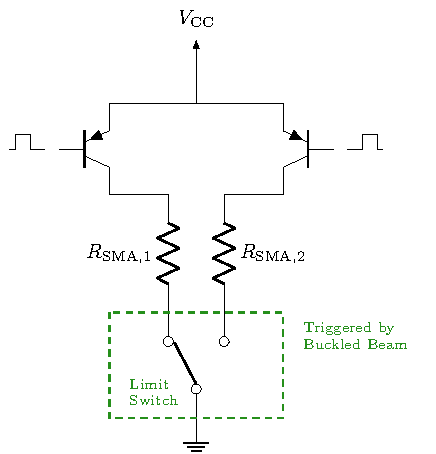
\includegraphics[width=0.5\textwidth]{images/chap6/smabb-circuit-diagram.pdf}
  % \documentclass[margin=1pt]{standalone}
\usepackage{color,xcolor}
\usepackage{makecell}
\usepackage{tikz-qtree, tikz}
\usepackage[utf8]{inputenc}

\usetikzlibrary{spy,shapes.multipart,babel}
\usepackage[siunitx,europeanresistors,EFvoltages]{circuitikz} % To have the european convention for the drawing of electrical components. Also to have the current and voltage arrows going from high to low potential
\ctikzset{voltage/bump b=18pt,voltage/european label distance=15pt,voltage/distance from node=.1}
\definecolor{mygreen}{HTML}{258F1B}

\begin{document}
\renewcommand{\arraystretch}{1} % to increase the space between rows
\begin{tikzpicture}[scale=1.0, transform shape]
    % \draw (-0.25,0) -- (0.25,0);
    \ctikzset{monopoles/vcc/arrow={Latex}}
    \draw (0,0) node[ground] (ground){}-- ++(0,0)node[spdt,anchor=in,scale=1.5,rotate=90] (Sw) {}
        (Sw.out 1) to[/tikz/circuitikz/bipoles/length=1.25cm,american resistor,l=$R_\mathrm{SMA,1}$] ++(0,2) coordinate(sma1top)-- ++(-1,0)node[pnp, anchor=C, xscale=1](pnp1){}
        (Sw.out 2) to[/tikz/circuitikz/bipoles/length=1.25cm,american resistor,l_=$R_\mathrm{SMA,2}$] ++(0,2) coordinate(sma2top)-- ++(1,0)node[pnp, anchor=C, xscale=-1](pnp2){}
        (pnp1.base) ++(-0.25,0)-- ++(-0.25,0)-- ++(0,0.25)-- ++(-0.25,0)-- ++(0,-0.25)-- ++(-0.1,0)
        (pnp2.base) ++(0.25,0)-- ++(0.25,0)-- ++(0,0.25)-- ++(0.25,0)-- ++(0,-0.25)-- ++(0.1,0)
        (pnp1.E) -| (0,6)
        (pnp2.E) -| (0,6)node[vcc,anchor=south]{$V_\mathrm{CC}$};

    \draw[dashed,mygreen,thick] let \p{Sw_i}=(Sw.in), \p{Sw_o1}=(Sw.out 1), \p{Sw_o2}=(Sw.out 2)  in (Sw.in)
    ($(\x{Sw_o1},\y{Sw_o1})+(-1,0)$) |- node[anchor=south west]{\scriptsize \begin{tabular}{l} Limit \\ Switch \end{tabular}} ($(\x{Sw_o2},\y{Sw_i})+(1,0)$) |- node[anchor=north west]{\scriptsize \begin{tabular}{l} Triggered by \\ Buckled Beam \end{tabular}} ($(\x{Sw_o1},\y{Sw_o1})+(-1,0)$);
\end{tikzpicture}
\renewcommand{\arraystretch}{1.5} % to increase the space between rows
\end{document}

  % \resizebox{\textwidth}{!}{\documentclass[margin=1pt]{standalone}
\usepackage{color,xcolor}
\usepackage{makecell}
\usepackage{tikz-qtree, tikz}
\usepackage[utf8]{inputenc}

\usetikzlibrary{spy,shapes.multipart,babel}
\usepackage[siunitx,europeanresistors,EFvoltages]{circuitikz} % To have the european convention for the drawing of electrical components. Also to have the current and voltage arrows going from high to low potential
\ctikzset{voltage/bump b=18pt,voltage/european label distance=15pt,voltage/distance from node=.1}
\definecolor{mygreen}{HTML}{258F1B}

\begin{document}
\renewcommand{\arraystretch}{1} % to increase the space between rows
\begin{tikzpicture}[scale=1.0, transform shape]
    % \draw (-0.25,0) -- (0.25,0);
    \ctikzset{monopoles/vcc/arrow={Latex}}
    \draw (0,0) node[ground] (ground){}-- ++(0,0)node[spdt,anchor=in,scale=1.5,rotate=90] (Sw) {}
        (Sw.out 1) to[/tikz/circuitikz/bipoles/length=1.25cm,american resistor,l=$R_\mathrm{SMA,1}$] ++(0,2) coordinate(sma1top)-- ++(-1,0)node[pnp, anchor=C, xscale=1](pnp1){}
        (Sw.out 2) to[/tikz/circuitikz/bipoles/length=1.25cm,american resistor,l_=$R_\mathrm{SMA,2}$] ++(0,2) coordinate(sma2top)-- ++(1,0)node[pnp, anchor=C, xscale=-1](pnp2){}
        (pnp1.base) ++(-0.25,0)-- ++(-0.25,0)-- ++(0,0.25)-- ++(-0.25,0)-- ++(0,-0.25)-- ++(-0.1,0)
        (pnp2.base) ++(0.25,0)-- ++(0.25,0)-- ++(0,0.25)-- ++(0.25,0)-- ++(0,-0.25)-- ++(0.1,0)
        (pnp1.E) -| (0,6)
        (pnp2.E) -| (0,6)node[vcc,anchor=south]{$V_\mathrm{CC}$};

    \draw[dashed,mygreen,thick] let \p{Sw_i}=(Sw.in), \p{Sw_o1}=(Sw.out 1), \p{Sw_o2}=(Sw.out 2)  in (Sw.in)
    ($(\x{Sw_o1},\y{Sw_o1})+(-1,0)$) |- node[anchor=south west]{\scriptsize \begin{tabular}{l} Limit \\ Switch \end{tabular}} ($(\x{Sw_o2},\y{Sw_i})+(1,0)$) |- node[anchor=north west]{\scriptsize \begin{tabular}{l} Triggered by \\ Buckled Beam \end{tabular}} ($(\x{Sw_o1},\y{Sw_o1})+(-1,0)$);
\end{tikzpicture}
\renewcommand{\arraystretch}{1.5} % to increase the space between rows
\end{document}
}
  \caption{The electrical circuit diagram of the bistable SMA gripper based on the proposed control strategy.}
  \label{fig:smabb-circuit}
\end{figure}

The measurements presented in \cref{fig:smabb-actuation} shows that by using the limit switch design, the gripper switches state and cuts the current across the SMA immediately ensuring that the minimum heating time is obtained and preventing any overheating of the SMA coil. The figure shows the opening and closing sequence of the gripper as the current passes through the coils. The gripper switches very quickly between states, thanks to the buckled beam snap-through. However, it can be observed that the jaws vibrate after the gripper opening around the stable open position. This is due to the fact that the compliant gripper dissipates the energy of the closed to open snap-through very gradually. A damping mechanism could be added to the gripper output to decrease the jaw vibration. During actuation testing, the buckled beam was not fully preloaded showing that the gripper stroke can be adjusted. Similarly, adjusting the preload should allow adapting the gripping force to a given application.

\section{Specifications of the Final Prototype}
Based on the design methodology, the final prototype consists of a flexure-based bistable mechanism that acts as the kinematic stage for the SMA actuator. As mentioned previously, this stage was fabricated using electrical discharge machining from a monolithic block of \textit{Bohler K390} steel, as shown in \cref{fig:final-prototype}. As the entire stage is created from a monolithic block, the system consists of only a single piece and thus, does not require any complex micro-assembly, displaying one of the key advantages of the use of flexure-based structures and this design methodology.

\begin{figure}[hbt!] % t for top of the page, H could be put to impose the position of the float
  \centering
  \begin{subfigure}[b]{0.27\textwidth}
      \begin{tikzpicture}
        \node[anchor=south west,inner sep=0] (graph) at (0,0){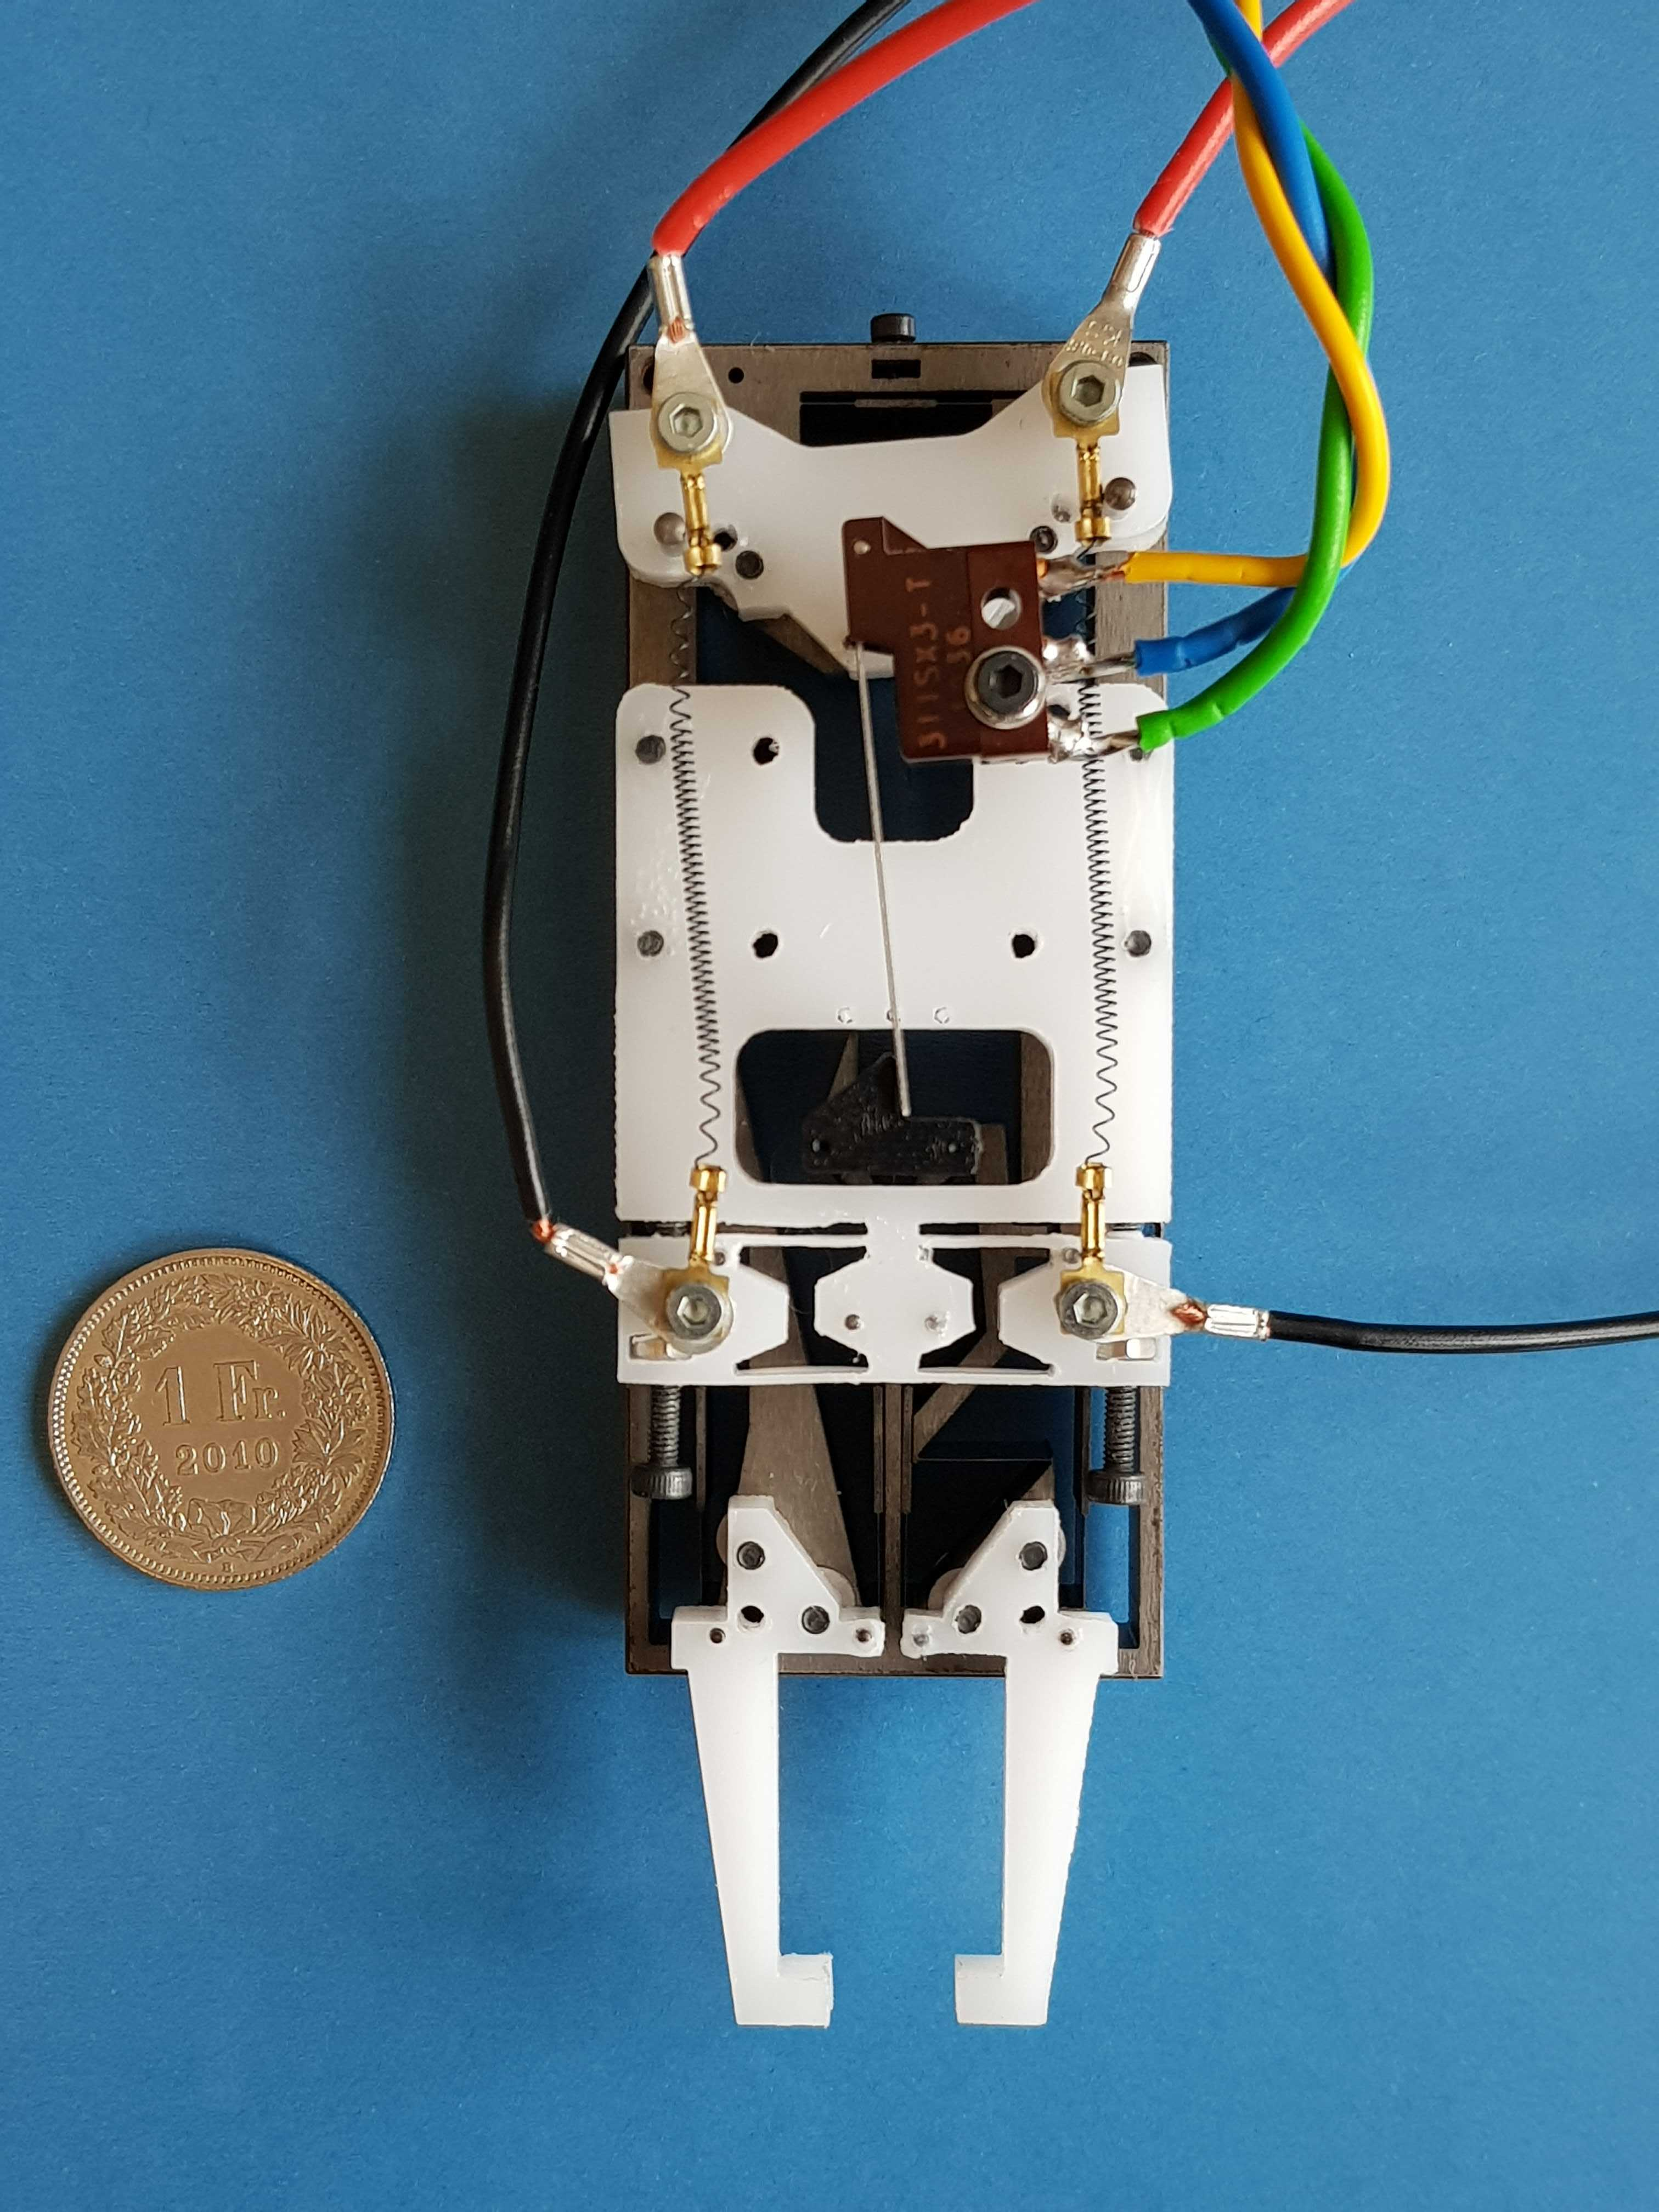
\includegraphics[trim={25cm 4cm 15cm 5cm},clip, width=\textwidth]{images/chap7/smabb-proto-front.jpg}};
        \begin{scope}[x={(graph.south east)},y={(graph.north west)}]
            \fill [white] (0.05, 0.2cm) rectangle (1cm,0.3cm);
            \draw [white] (0.02, 0.3cm) node[anchor=south west] {\scriptsize 10 mm};
            \end{scope}
      \end{tikzpicture}
  \end{subfigure}
  % \begin{subfigure}[b]{0.27\textwidth}
  %     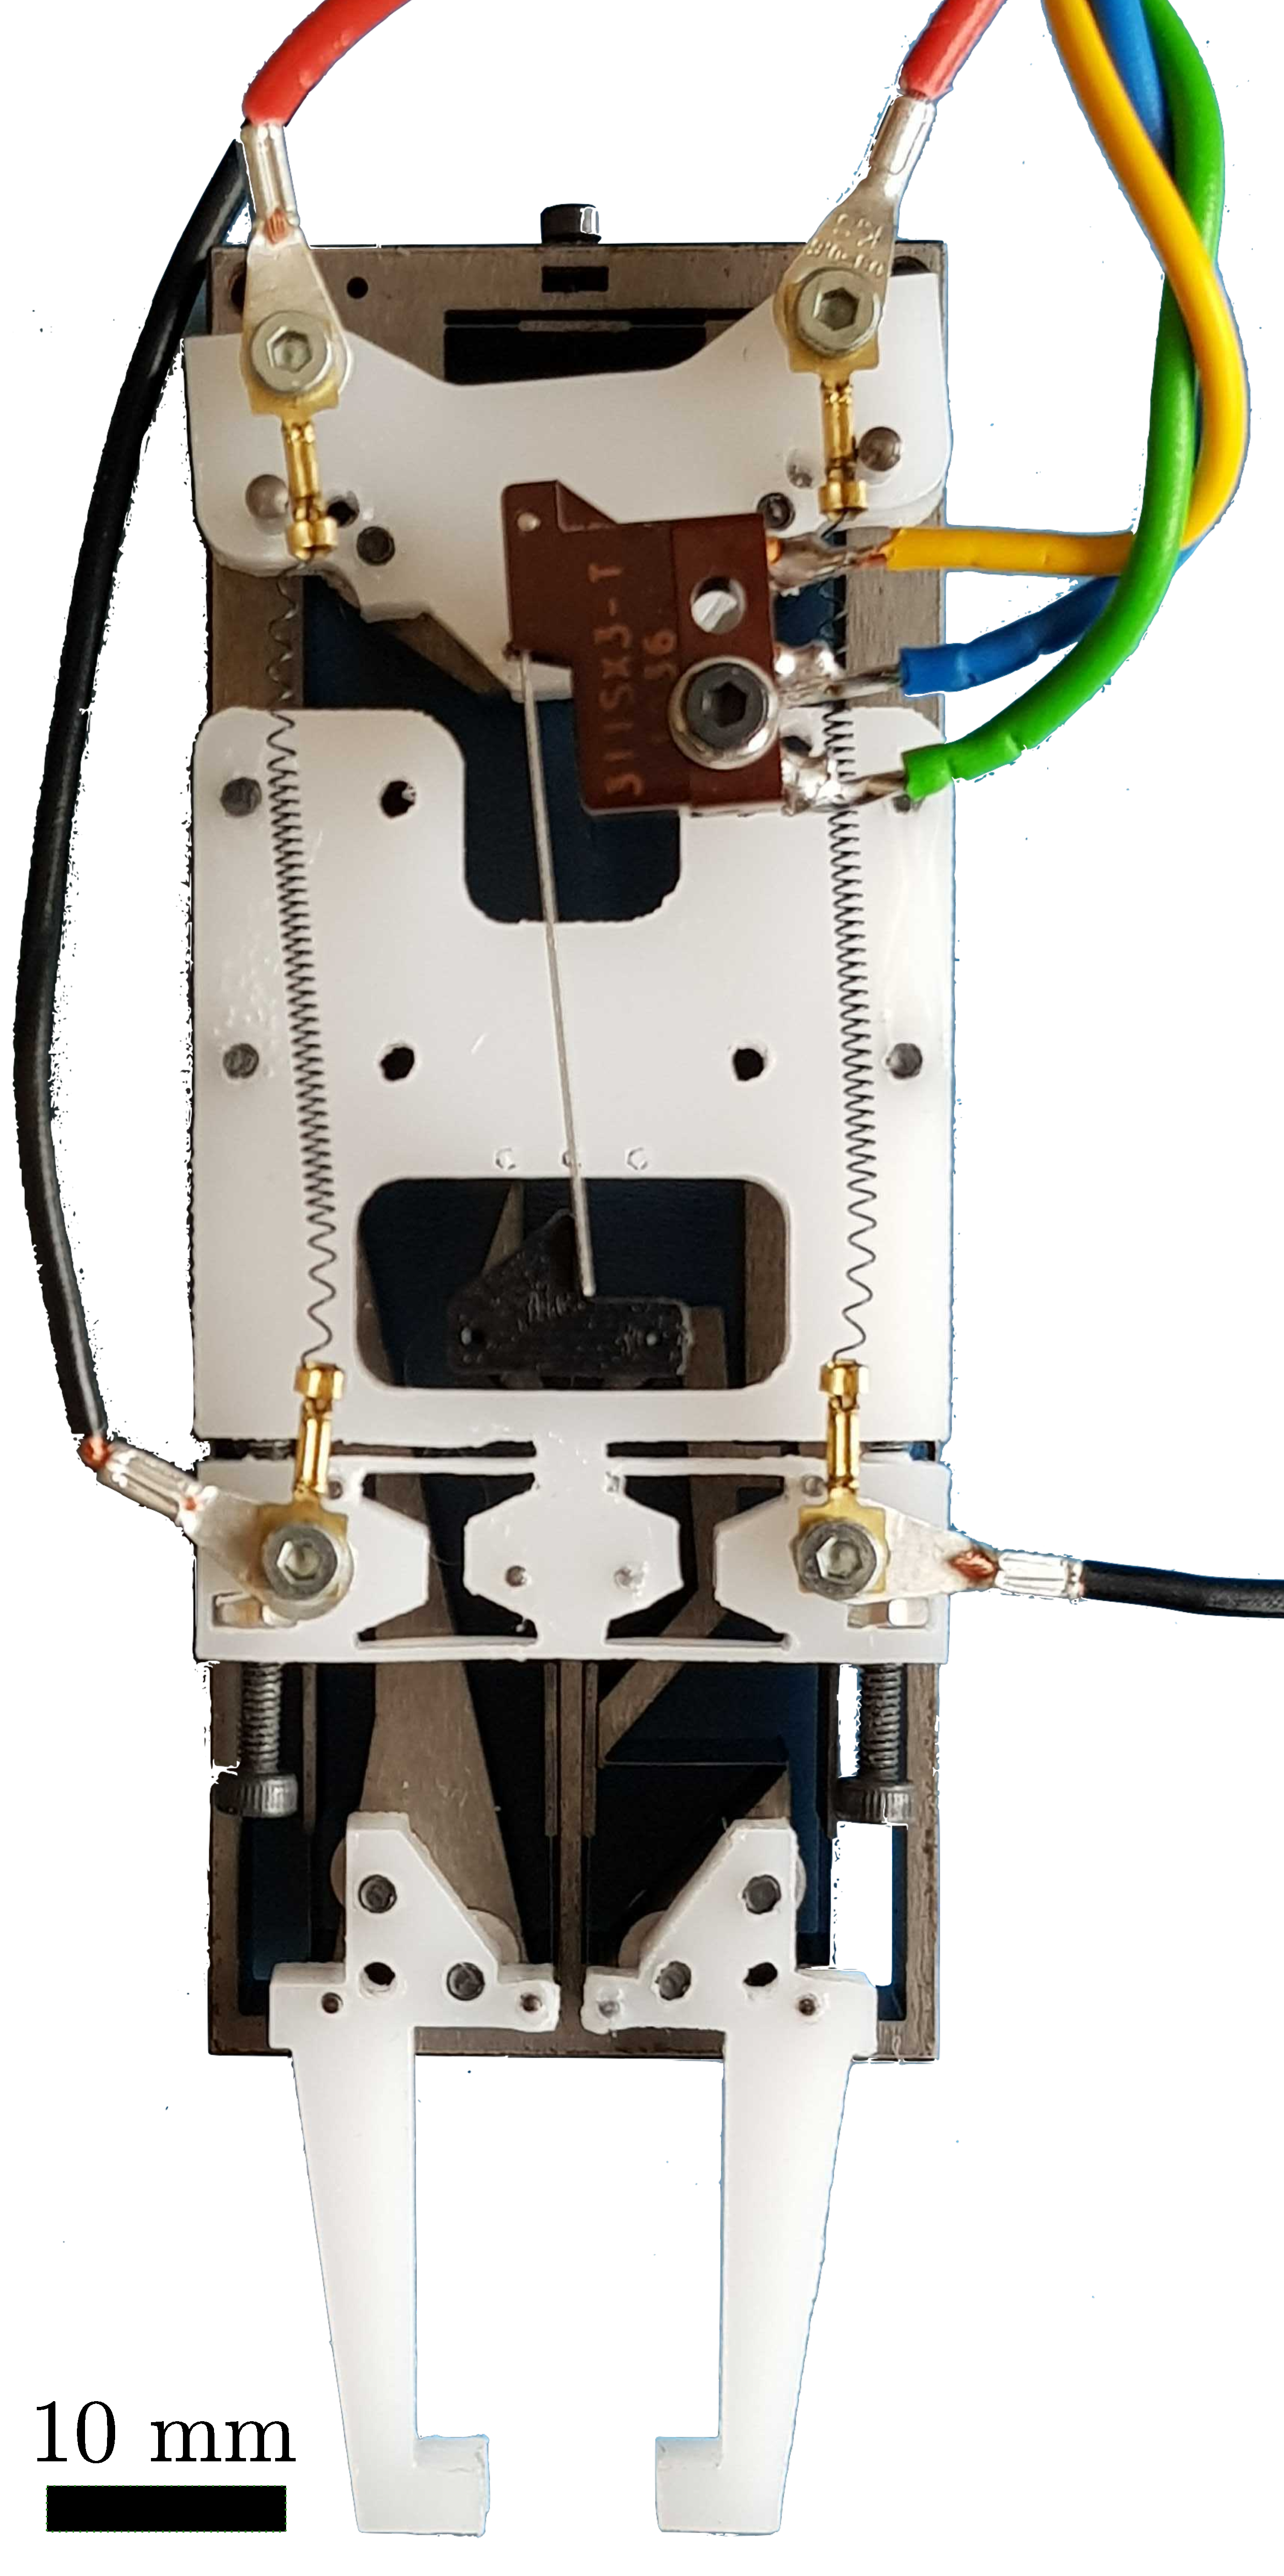
\includegraphics[width=\textwidth]{images/chap7/smabb-proto-front-cropped-scale.pdf}
  % \end{subfigure}
  \begin{subfigure}[b]{0.72\textwidth}
      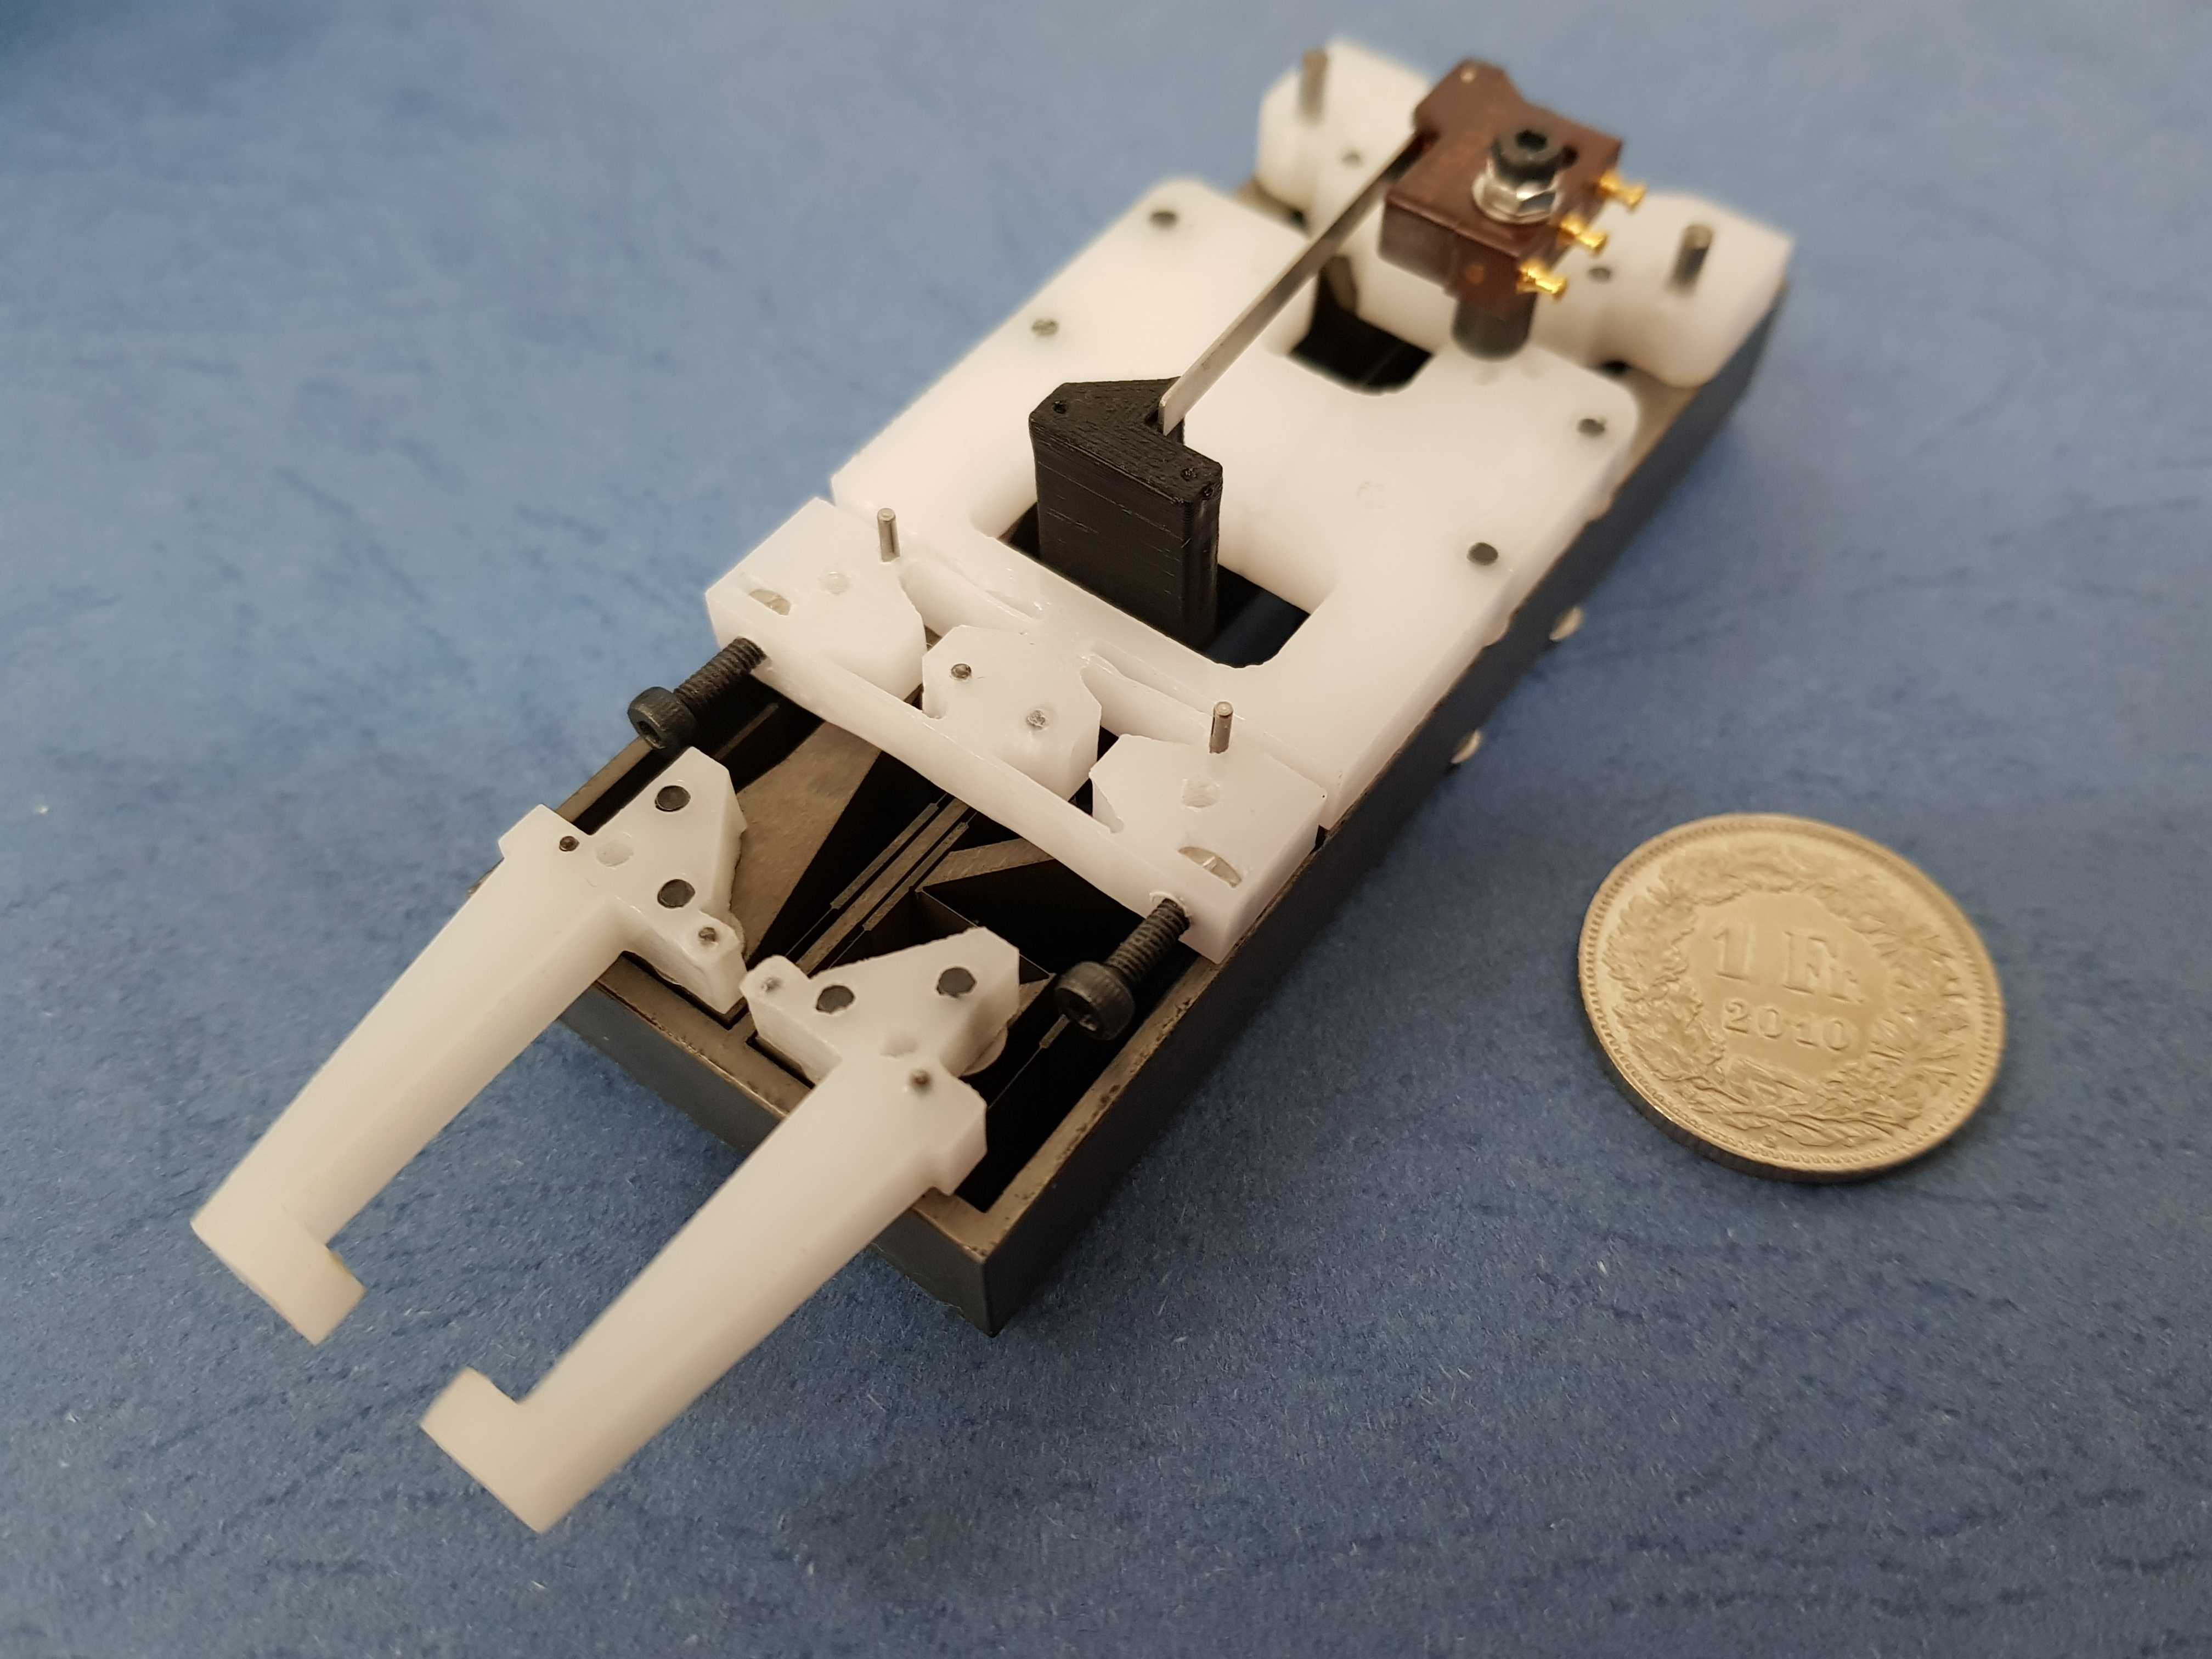
\includegraphics[width=\textwidth]{images/chap7/smabb-proto-iso.jpg}
  \end{subfigure}
  \caption{The fabricated prototype of the bistable gripper with the wiring circuit presented on the left.}
  \label{fig:final-prototype}
\end{figure}

The SMA elements are integrated into the kinematic stage using a 2.5D design where an interface layer is used to actuate the input pivot of the kinematic stage. Using the design methodology, the pair of SMA coils, arranged in an antagonistic manner, is sized such that the thinnest SMA coils are used so as to keep the cooling time below $3$ s. The design methodology takes into account the inherent stiffness of the bistable structure and sizes the SMAs such that there are no unintended operating points during the activation and snap-through of the gripper system. The final gripper has a stroke of $2.5$ mm per jaw and has a gripping force of around $1.4$ N.

Furthermore, the bistable mechanism and the thermoelastic behaviour of the SMA is exploited to create the mechanically-intelligent control strategy based on the proposed design methodology. In the final prototype, the current flowing the limit switch and into the SMA is controlled by the state of the buckled beam. The kinematic stage is able to cut the current across the SMA in less than $10$ ms. Thus, with the use of these proposed design methodologies, the entire kinematic stage with the integrated SMA actuator fits within a volume constraint of $110 \times 34 \times 26$ mm.

\subsection{Comparison of the Proposed Gripper}
Due to the complex nature of the bistable mechanism, the literature on bistable grippers powered by smart materials is limited. However, a comparison of the proposed gripper with other bistable grippers shows the innovative aspects and the advantages of the design methodology. In most cases, as shown in the work by \cite{zhangCompliantBistableGrippers2020} and \cite{scholtesDevelopmentBistableSMA2021}, the bistable gripper requires no holding energy but however also does not provide any gripping force. As the stable state exists at 0 N, the gripping force depends on the size of the object and in the case of the aforementioned works, the grasped object is retained only using friction. In the case of bistable grippers using other smart materials, as shown in \cref{tab:bistable-gripper-comparison}, they often provide lower gripping force. The proposed gripper is able to provide a constant gripping force and stroke and has been sized to show comparable bandwidth. Thus, it is clear to see the primary advantages of the proposed methodology. Additionally, the presented gripper, when compared to other works, is able to produce fixed gripping forces and strokes while also using a compliant structure to provide a parallel gripping motion, compact footprint and a decoupled input-output actuation. Furthermore, the sizing strategy can be adapted to fit the various specifications of the application and the grasped object.

\begin{table}[hbt!]
    \centering
    \caption{Comparison of the proposed bistable gripper against other smart material powered bistable grippers.}
    \label{tab:bistable-gripper-comparison}
    
% !TEX root = ../../sethomas_thesis_main.tex
\documentclass[border=1mm,
               class=article
               preview]{standalone}
\usepackage{tikz}
\begin{document}
{\rowcolors{1}{black!10}{black!5}
% \begin{tabular}{lcccccc}
\begin{tabular}{@{}p{0.19\textwidth-2\tabcolsep}
                P{0.12\textwidth-2\tabcolsep}
                P{0.14\textwidth-2\tabcolsep}
                P{0.14\textwidth-2\tabcolsep}
                P{0.14\textwidth-2\tabcolsep}
                P{0.14\textwidth-2\tabcolsep}
                P{0.11\textwidth-2\tabcolsep}@{}}
\rowcolor{black}                               & \textbf{\color{white} Material} & \textbf{\color{white} Total Weight {[}g{]}} & \textbf{\color{white} Gripping Force {[}N{]}} & \textbf{\color{white} Bandwidth {[}Hz{]}} & \textbf{\color{white} Switching Force {[}N{]}} & \textbf{\color{white} Stroke {[}mm{]}} \\
\textbf{This work}              & SMA                          & 135                             & 1.4                             & 0.33                        & 7.8                              & 5\\
\cite{scholtesDevelopmentBistableSMA2021} & SMA                          & 150                           & -                              & 0.75                        & -                                & 3                        \\
\cite{zhangCompliantBistableGrippers2020}   & DC Motor                     & 8                             & 0                               & 0.5                         & 0.4                              & 20                       \\
\cite{wangDesignAnalysisBistable2018a}    & DEA                          & -                             & 0                               & -                           & 0.05                             & 5.65                     \\
\cite{liuDesignControlNovel2017}     & PZT                          & -                             & 0.6                             & -                           & 0.15                             & 0.2                      \\
\cite{lernerDesignExperimentationVariable2020}   & SMP                          & 6.8                           & 0.2                             & 0.008                       & 0.5                              & 25
\end{tabular}}
\end{document}

\end{table}

\section{Summary and Conclusion}
In this chapter, the design methodology presented in this work was validated using a case study. The described methodology proposed novel ways to design actuators that were compact and integrated. Using the various strategies proposed in the previous chapters, a gripper powered by shape memory alloys is designed and sized such that the resulting gripper presents with a relatively high time response while maintaining a low footprint. Furthermore, using the simplified sizing methodology presented in this work has been implemented in this chapter to create a gripper with reduced cooling times and faster time responses. The methodology allowed the conception of a gripper that can be fabricated and assembled with a reduced number of parts, showing one of the primary advantages of the proposed design methodology.

In this final case study, a bistable SMA-powered gripper was designed and fabricated. Here, the prototype of the gripper consists of a bistable kinematic stage paired with an antagonistic SMA actuator. Furthermore, the kinematic stage and the shape memory effect has been exploited to create an integrated mechanical control that is able to perfectly control the temperature of the SMA coils without any micro-controllers or control logic. The bistable kinematic stage was conceived using flexure-based hinges and sized using the proposed methodology from \cref{chap:design-methodology}. Here, using the validated analytical models of the bistable element, the operating points of the final gripper were estimated and the final behaviour was verified to not present any unexpected operating points. Using the sizing methodology, the SMA coils and the kinematic stage were sized such that the thinnest wires could be used so as to increase the overall time response of the gripper. The prototype, while functioning as intended, could easily be adjusted to show different types of gripping behaviours and be made to grasp various sizes of objects. Furthermore, by using the mechanical integrated control strategy as presented in \cref{chap:integrated-control}, the case study was able to validate the proposed approach. Here, using the bistable element to mechanically control the electrical contacts across the SMA coils, the gripper is able to be actuated without the use of temperature sensors or complex control schemes. Finally, the entire prototype, which fits in a foot print of $110\times34\times26$ mm, exhibits a stroke and gripping force of $2.5$ mm and $1.4$ N, showing the strength of the design strategy in creating compact actuators for application such as industrial pick-and-place grippers. Furthermore, using the novel sizing strategy, the bandwith of the gripper was optimised where the cooling time required by the SMA coils is as low as $2.8$ s.

The gripper, presented in this chapter, is powered using shape memory alloys and are designed using the different design methodologies presented in this work. These gripper, which can be used in industrial or drone related application, can be further optimised for their specific use cases but can also serve as an example for designing future grippers with differing specifications. Furthermore, future work could include using kirigami inspired SMA elements, to remove the need for a lever arm and further reduce the footprint and assembly time of the proposed gripper.


%In this chapter, the designing methodology presented in this work has been validated using two case studies. The methodology proposed a novel way to design compact and integrated SMA actuators. Here, using the proposed approach and techniques, two grippers powered by shape memory alloy coils were conceived and fabricated. The novel methodology also proposed a simplified method with which the SMA and the biasing elements can be sized so as to harness the shape memory effect when a thermal load is applied to the SMA. Finally, the grippers were fabricated using machining techniques that allowed a reduced number of parts and a simplified assembly process, showing one of the key advantages of this proposed integrated approach.
%
% In the first section, a four prong mandrel gripper is designed and fabricated. In this prototype, the gripper consists of just an SMA coil and a kinematic stage. Based on the design methodology, the kinematic stage is created using compliant flexure-based mechanisms that, while acting as a motion conversion mechanism, also behaves as a biasing spring. The kinematic stage conceived using topology optimization and improved using flexure-based hinges is able to convert the shape memory effect of one SMA coil into a more complex multi-output gripping motion. Based on the design approach presented in \cref{chap:design-methodology}, the compliant mechanism has been sized to optimize the stroke of the SMA actuator while reducing the required SMA coil wire diameter. Using the established and validated analytical models of the kinematic stage and the traditional simplified SMA models, the operating points and the stroke of the gripper, around 4 mm, was estimated. The final prototype of this four prong gripper weighs less than 17 g and is able to exert around 1.78 N of force, which leads to a maximum force-weight density of around 105 N/kg. This shows that by using the proposed design methodology, a lightweight and compact gripper can be fabricated for applications such as drone-deliveries.
%
% Lastly, in the final case study, a bistable SMA-powered gripper was designed and fabricated. Here, the prototype of the gripper consists of a bistable kinematic stage paired with an antagonistic SMA actuator. Furthermore, the kinematic stage and the shape memory effect has been exploited to create an integrated mechanical control that is able to perfectly control the temperature of the SMA coils without any micro-controllers or control logic. The bistable kinematic stage was conceived using flexure-based hinges and sized using the proposed methodology from \cref{chap:design-methodology}. Here, using the validated analytical models of the bistable element, the operating points of the final gripper were estimated and the final behaviour was verified to not present any unexpected operating points. Using the sizing methodology, the SMA coils and the kinematic stage were sized such that the thinnest wires could be used so as to increase the overall time response of the gripper. The prototype, while functioning as intended, could easily be adjusted to show different types of gripping behaviours and be made to grasp various sizes of objects. Furthermore, by using the mechanical integrated control strategy as presented in \cref{chap:integrated-control}, the case study was able to validated the proposed approach. Here, using the bistable element to mechanically control the electrical contacts across the SMA coils, the gripper is able to be actuated without the use of temperature sensors or complex control schemes. Finally, the entire prototype, which fits in a foot print of $110\times34\times26$ mm, exhibits a stroke and gripping force of $2.5$ mm and $1.4$ N, showing the strength of the design strategy in creating compact actuators for application such as industrial pick-and-place grippers.
%
% The grippers, presented in this chapter, are powered using shape memory alloys and are designed using the different design methodologies presented in this work. These gripper, which can be used in industrial or drone related application, can be further optimised for their specific use cases but can also serve as an example for designing future grippers with differing specifications.
\vspace*{\fill}
\noindent\hrulefill \\
\textbf{\large Publications related to this chapter :}

\underline{S. Thomas}, L. Tissot-Daguette, Y. Perriard, C. Baur, and L. Borelli, \textit{“Microgripper Device”}, European Patent Application, 21150579.7 - 1016

\underline{S. Thomas}, L. Tissot-Daguette, T. Martinez, C. Baur, and Y. Perriard, \textit{“Design and Modelling of a Flexure-based Bistable Gripper Powered by Shape Memory Alloys,”} Sensors and Actuators A: Physi- cal, p. 8, 2022. (pending)

\underline{S. Thomas}, P. Peralta, R. Mottet, M. Lehmann, Y. Civet, and Y. Perriard, \textit{“Analysis and Reduction of Time Response in Thermally Activated Shape Memory Alloys,”} in 2018 21st International Conference on Electrical Machines and Systems (ICEMS), Oct. 2018, p. 7. doi: 10.23919/ICEMS.2018.8549332.
